\documentclass[twoside]{book}

% Packages required by doxygen
\usepackage{fixltx2e}
\usepackage{calc}
\usepackage{doxygen}
\usepackage[export]{adjustbox} % also loads graphicx
\usepackage{graphicx}
\usepackage[utf8]{inputenc}
\usepackage{makeidx}
\usepackage{multicol}
\usepackage{multirow}
\PassOptionsToPackage{warn}{textcomp}
\usepackage{textcomp}
\usepackage[nointegrals]{wasysym}
\usepackage[table]{xcolor}

% Font selection
\usepackage[T1]{fontenc}
\usepackage[scaled=.90]{helvet}
\usepackage{courier}
\usepackage{amssymb}
\usepackage{sectsty}
\renewcommand{\familydefault}{\sfdefault}
\allsectionsfont{%
  \fontseries{bc}\selectfont%
  \color{darkgray}%
}
\renewcommand{\DoxyLabelFont}{%
  \fontseries{bc}\selectfont%
  \color{darkgray}%
}
\newcommand{\+}{\discretionary{\mbox{\scriptsize$\hookleftarrow$}}{}{}}

% Page & text layout
\usepackage{geometry}
\geometry{%
  a4paper,%
  top=2.5cm,%
  bottom=2.5cm,%
  left=2.5cm,%
  right=2.5cm%
}
\tolerance=750
\hfuzz=15pt
\hbadness=750
\setlength{\emergencystretch}{15pt}
\setlength{\parindent}{0cm}
\setlength{\parskip}{0.2cm}
\makeatletter
\renewcommand{\paragraph}{%
  \@startsection{paragraph}{4}{0ex}{-1.0ex}{1.0ex}{%
    \normalfont\normalsize\bfseries\SS@parafont%
  }%
}
\renewcommand{\subparagraph}{%
  \@startsection{subparagraph}{5}{0ex}{-1.0ex}{1.0ex}{%
    \normalfont\normalsize\bfseries\SS@subparafont%
  }%
}
\makeatother

% Headers & footers
\usepackage{fancyhdr}
\pagestyle{fancyplain}
\fancyhead[LE]{\fancyplain{}{\bfseries\thepage}}
\fancyhead[CE]{\fancyplain{}{}}
\fancyhead[RE]{\fancyplain{}{\bfseries\leftmark}}
\fancyhead[LO]{\fancyplain{}{\bfseries\rightmark}}
\fancyhead[CO]{\fancyplain{}{}}
\fancyhead[RO]{\fancyplain{}{\bfseries\thepage}}
\fancyfoot[LE]{\fancyplain{}{}}
\fancyfoot[CE]{\fancyplain{}{}}
\fancyfoot[RE]{\fancyplain{}{\bfseries\scriptsize Generated on Tue Oct 20 2015 00\+:03\+:03 for anjing by Doxygen }}
\fancyfoot[LO]{\fancyplain{}{\bfseries\scriptsize Generated on Tue Oct 20 2015 00\+:03\+:03 for anjing by Doxygen }}
\fancyfoot[CO]{\fancyplain{}{}}
\fancyfoot[RO]{\fancyplain{}{}}
\renewcommand{\footrulewidth}{0.4pt}
\renewcommand{\chaptermark}[1]{%
  \markboth{#1}{}%
}
\renewcommand{\sectionmark}[1]{%
  \markright{\thesection\ #1}%
}

% Indices & bibliography
\usepackage{natbib}
\usepackage[titles]{tocloft}
\setcounter{tocdepth}{3}
\setcounter{secnumdepth}{5}
\makeindex

% Hyperlinks (required, but should be loaded last)
\usepackage{ifpdf}
\ifpdf
  \usepackage[pdftex,pagebackref=true]{hyperref}
\else
  \usepackage[ps2pdf,pagebackref=true]{hyperref}
\fi
\hypersetup{%
  colorlinks=true,%
  linkcolor=blue,%
  citecolor=blue,%
  unicode%
}

% Custom commands
\newcommand{\clearemptydoublepage}{%
  \newpage{\pagestyle{empty}\cleardoublepage}%
}


%===== C O N T E N T S =====

\begin{document}

% Titlepage & ToC
\hypersetup{pageanchor=false,
             bookmarks=true,
             bookmarksnumbered=true,
             pdfencoding=unicode
            }
\pagenumbering{roman}
\begin{titlepage}
\vspace*{7cm}
\begin{center}%
{\Large anjing }\\
\vspace*{1cm}
{\large Generated by Doxygen 1.8.10}\\
\vspace*{0.5cm}
{\small Tue Oct 20 2015 00:03:03}\\
\end{center}
\end{titlepage}
\clearemptydoublepage
\tableofcontents
\clearemptydoublepage
\pagenumbering{arabic}
\hypersetup{pageanchor=true}

%--- Begin generated contents ---
\chapter{Namespace Index}
\section{Namespace List}
Here is a list of all namespaces with brief descriptions\+:\begin{DoxyCompactList}
\item\contentsline{section}{\hyperlink{namespaceanjing}{anjing} }{\pageref{namespaceanjing}}{}
\end{DoxyCompactList}

\chapter{Hierarchical Index}
\section{Class Hierarchy}
This inheritance list is sorted roughly, but not completely, alphabetically\+:\begin{DoxyCompactList}
\item \contentsline{section}{std\+:\+:tr1\+:\+:gtest\+\_\+internal\+:\+:Add\+Ref$<$ T $>$}{\pageref{structstd_1_1tr1_1_1gtest__internal_1_1_add_ref}}{}
\item \contentsline{section}{std\+:\+:tr1\+:\+:gtest\+\_\+internal\+:\+:Add\+Ref$<$ T \& $>$}{\pageref{structstd_1_1tr1_1_1gtest__internal_1_1_add_ref_3_01_t_01_6_01_4}}{}
\item \contentsline{section}{testing\+:\+:internal\+:\+:Add\+Reference$<$ T $>$}{\pageref{structtesting_1_1internal_1_1_add_reference}}{}
\item \contentsline{section}{testing\+:\+:internal\+:\+:Add\+Reference$<$ T \& $>$}{\pageref{structtesting_1_1internal_1_1_add_reference_3_01_t_01_6_01_4}}{}
\item \contentsline{section}{testing\+:\+:gtest\+\_\+printers\+\_\+test\+:\+:Allows\+Generic\+Streaming}{\pageref{classtesting_1_1gtest__printers__test_1_1_allows_generic_streaming}}{}
\item \contentsline{section}{testing\+:\+:gtest\+\_\+printers\+\_\+test\+:\+:Allows\+Generic\+Streaming\+And\+Implicit\+Conversion\+Template$<$ T $>$}{\pageref{classtesting_1_1gtest__printers__test_1_1_allows_generic_streaming_and_implicit_conversion_template}}{}
\item \contentsline{section}{testing\+:\+:gtest\+\_\+printers\+\_\+test\+:\+:Allows\+Generic\+Streaming\+Template$<$ T $>$}{\pageref{classtesting_1_1gtest__printers__test_1_1_allows_generic_streaming_template}}{}
\item \contentsline{section}{anjing\+:\+:App}{\pageref{classanjing_1_1_app}}{}
\item \contentsline{section}{testing\+:\+:internal\+:\+:Assert\+Helper}{\pageref{classtesting_1_1internal_1_1_assert_helper}}{}
\item \contentsline{section}{testing\+:\+:Assertion\+Result}{\pageref{classtesting_1_1_assertion_result}}{}
\item \contentsline{section}{my\+\_\+namespace\+:\+:testing\+:\+:Assertion\+Result}{\pageref{classmy__namespace_1_1testing_1_1_assertion_result}}{}
\item \contentsline{section}{Base}{\pageref{class_base}}{}
\begin{DoxyCompactList}
\item \contentsline{section}{namespace1\+:\+:My\+Type\+In\+Name\+Space1}{\pageref{classnamespace1_1_1_my_type_in_name_space1}}{}
\item \contentsline{section}{namespace2\+:\+:My\+Type\+In\+Name\+Space2}{\pageref{classnamespace2_1_1_my_type_in_name_space2}}{}
\end{DoxyCompactList}
\item \contentsline{section}{testing\+:\+:internal\+:\+:Base}{\pageref{classtesting_1_1internal_1_1_base}}{}
\begin{DoxyCompactList}
\item \contentsline{section}{testing\+:\+:internal\+:\+:Derived}{\pageref{classtesting_1_1internal_1_1_derived}}{}
\end{DoxyCompactList}
\item \contentsline{section}{testing\+:\+:gtest\+\_\+printers\+\_\+test\+:\+:Big}{\pageref{structtesting_1_1gtest__printers__test_1_1_big}}{}
\item \contentsline{section}{Biggest\+Int\+Convertible}{\pageref{class_biggest_int_convertible}}{}
\item \contentsline{section}{Bool}{\pageref{struct_bool}}{}
\item \contentsline{section}{testing\+:\+:internal\+:\+:bool\+\_\+constant$<$ bool\+\_\+value $>$}{\pageref{structtesting_1_1internal_1_1bool__constant}}{}
\begin{DoxyCompactList}
\item \contentsline{section}{testing\+:\+:internal\+:\+:is\+\_\+pointer$<$ T $>$}{\pageref{structtesting_1_1internal_1_1is__pointer}}{}
\item \contentsline{section}{testing\+:\+:internal\+:\+:is\+\_\+pointer$<$ T $\ast$ $>$}{\pageref{structtesting_1_1internal_1_1is__pointer_3_01_t_01_5_01_4}}{}
\end{DoxyCompactList}
\item \contentsline{section}{testing\+:\+:internal\+:\+:bool\+\_\+constant$<$ Implicitly\+Convertible$<$ const T $\ast$, const \+:\+:Protocol\+Message $\ast$ $>$\+:\+:value$\vert$$\vert$\+Implicitly\+Convertible$<$ const T $\ast$, const \+:\+:proto2\+:\+:Message $\ast$ $>$\+:\+:value $>$}{\pageref{structtesting_1_1internal_1_1bool__constant}}{}
\begin{DoxyCompactList}
\item \contentsline{section}{testing\+:\+:internal\+:\+:Is\+A\+Protocol\+Message$<$ T $>$}{\pageref{structtesting_1_1internal_1_1_is_a_protocol_message}}{}
\end{DoxyCompactList}
\item \contentsline{section}{std\+:\+:tr1\+:\+:gtest\+\_\+internal\+:\+:By\+Ref$<$ T $>$}{\pageref{structstd_1_1tr1_1_1gtest__internal_1_1_by_ref}}{}
\item \contentsline{section}{std\+:\+:tr1\+:\+:gtest\+\_\+internal\+:\+:By\+Ref$<$ T \& $>$}{\pageref{structstd_1_1tr1_1_1gtest__internal_1_1_by_ref_3_01_t_01_6_01_4}}{}
\item \contentsline{section}{testing\+:\+:internal\+:\+:Castable}{\pageref{classtesting_1_1internal_1_1_castable}}{}
\item \contentsline{section}{pump.\+Code\+Node}{\pageref{classpump_1_1_code_node}}{}
\item \contentsline{section}{testing\+:\+:internal\+:\+:Compile\+Assert$<$ bool $>$}{\pageref{structtesting_1_1internal_1_1_compile_assert}}{}
\item \contentsline{section}{testing\+:\+:internal\+:\+:Compile\+Assert\+Types\+Equal$<$ T1, T2 $>$}{\pageref{structtesting_1_1internal_1_1_compile_assert_types_equal}}{}
\item \contentsline{section}{testing\+:\+:internal\+:\+:Compile\+Assert\+Types\+Equal$<$ T, T $>$}{\pageref{structtesting_1_1internal_1_1_compile_assert_types_equal_3_01_t_00_01_t_01_4}}{}
\item \contentsline{section}{testing\+:\+:gtest\+\_\+printers\+\_\+test\+:\+:const\+\_\+iterator}{\pageref{structtesting_1_1gtest__printers__test_1_1const__iterator}}{}
\item \contentsline{section}{testing\+:\+:internal\+:\+:Const\+And\+Non\+Const\+Castable}{\pageref{classtesting_1_1internal_1_1_const_and_non_const_castable}}{}
\item \contentsline{section}{testing\+:\+:internal\+:\+:Const\+Castable}{\pageref{classtesting_1_1internal_1_1_const_castable}}{}
\item \contentsline{section}{testing\+:\+:internal\+:\+:Const\+Char\+Ptr}{\pageref{structtesting_1_1internal_1_1_const_char_ptr}}{}
\item \contentsline{section}{Conversion\+Helper\+Base}{\pageref{class_conversion_helper_base}}{}
\begin{DoxyCompactList}
\item \contentsline{section}{Conversion\+Helper\+Derived}{\pageref{class_conversion_helper_derived}}{}
\end{DoxyCompactList}
\item \contentsline{section}{Counter}{\pageref{class_counter}}{}
\item \contentsline{section}{pump.\+Cursor}{\pageref{classpump_1_1_cursor}}{}
\item \contentsline{section}{pump.\+Else\+Node}{\pageref{classpump_1_1_else_node}}{}
\item \contentsline{section}{testing\+:\+:internal\+:\+:Enable\+If$<$ bool $>$}{\pageref{structtesting_1_1internal_1_1_enable_if}}{}
\item \contentsline{section}{testing\+:\+:internal\+:\+:Enable\+If$<$ true $>$}{\pageref{structtesting_1_1internal_1_1_enable_if_3_01true_01_4}}{}
\item \contentsline{section}{pump.\+Env}{\pageref{classpump_1_1_env}}{}
\item \contentsline{section}{testing\+:\+:Environment}{\pageref{classtesting_1_1_environment}}{}
\begin{DoxyCompactList}
\item \contentsline{section}{Bar\+Environment}{\pageref{class_bar_environment}}{}
\item \contentsline{section}{Foo\+Environment}{\pageref{class_foo_environment}}{}
\item \contentsline{section}{testing\+:\+:internal\+:\+:Environment\+Invocation\+Catcher}{\pageref{classtesting_1_1internal_1_1_environment_invocation_catcher}}{}
\item \contentsline{section}{testing\+:\+:internal\+:\+:Final\+Success\+Checker}{\pageref{classtesting_1_1internal_1_1_final_success_checker}}{}
\end{DoxyCompactList}
\item \contentsline{section}{testing\+:\+:internal\+:\+:Eq\+Helper$<$ lhs\+\_\+is\+\_\+null\+\_\+literal $>$}{\pageref{classtesting_1_1internal_1_1_eq_helper}}{}
\item \contentsline{section}{testing\+:\+:internal\+:\+:Eq\+Helper$<$ true $>$}{\pageref{classtesting_1_1internal_1_1_eq_helper_3_01true_01_4}}{}
\item \contentsline{section}{pump.\+Exp\+Node}{\pageref{classpump_1_1_exp_node}}{}
\item \contentsline{section}{testing\+:\+:internal\+:\+:File\+Path}{\pageref{classtesting_1_1internal_1_1_file_path}}{}
\item \contentsline{section}{testing\+:\+:Flags}{\pageref{structtesting_1_1_flags}}{}
\item \contentsline{section}{testing\+:\+:internal\+:\+:Floating\+Point$<$ Raw\+Type $>$}{\pageref{classtesting_1_1internal_1_1_floating_point}}{}
\item \contentsline{section}{testing\+:\+:gtest\+\_\+printers\+\_\+test\+:\+:Foo}{\pageref{structtesting_1_1gtest__printers__test_1_1_foo}}{}
\item \contentsline{section}{testing\+:\+:internal\+:\+:Format\+For\+Comparison$<$ To\+Print, Other\+Operand $>$}{\pageref{classtesting_1_1internal_1_1_format_for_comparison}}{}
\item \contentsline{section}{testing\+:\+:internal\+:\+:Format\+For\+Comparison$<$ To\+Print\mbox{[}N\mbox{]}, Other\+Operand $>$}{\pageref{classtesting_1_1internal_1_1_format_for_comparison_3_01_to_print[_n]_00_01_other_operand_01_4}}{}
\item \contentsline{section}{pump.\+For\+Node}{\pageref{classpump_1_1_for_node}}{}
\item \contentsline{section}{std\+:\+:tr1\+:\+:gtest\+\_\+internal\+:\+:Get$<$ k $>$}{\pageref{classstd_1_1tr1_1_1gtest__internal_1_1_get}}{}
\item \contentsline{section}{std\+:\+:tr1\+:\+:gtest\+\_\+internal\+:\+:Get$<$ 0 $>$}{\pageref{classstd_1_1tr1_1_1gtest__internal_1_1_get_3_010_01_4}}{}
\item \contentsline{section}{std\+:\+:tr1\+:\+:gtest\+\_\+internal\+:\+:Get$<$ 1 $>$}{\pageref{classstd_1_1tr1_1_1gtest__internal_1_1_get_3_011_01_4}}{}
\item \contentsline{section}{std\+:\+:tr1\+:\+:gtest\+\_\+internal\+:\+:Get$<$ 2 $>$}{\pageref{classstd_1_1tr1_1_1gtest__internal_1_1_get_3_012_01_4}}{}
\item \contentsline{section}{std\+:\+:tr1\+:\+:gtest\+\_\+internal\+:\+:Get$<$ 3 $>$}{\pageref{classstd_1_1tr1_1_1gtest__internal_1_1_get_3_013_01_4}}{}
\item \contentsline{section}{std\+:\+:tr1\+:\+:gtest\+\_\+internal\+:\+:Get$<$ 4 $>$}{\pageref{classstd_1_1tr1_1_1gtest__internal_1_1_get_3_014_01_4}}{}
\item \contentsline{section}{std\+:\+:tr1\+:\+:gtest\+\_\+internal\+:\+:Get$<$ 5 $>$}{\pageref{classstd_1_1tr1_1_1gtest__internal_1_1_get_3_015_01_4}}{}
\item \contentsline{section}{std\+:\+:tr1\+:\+:gtest\+\_\+internal\+:\+:Get$<$ 6 $>$}{\pageref{classstd_1_1tr1_1_1gtest__internal_1_1_get_3_016_01_4}}{}
\item \contentsline{section}{std\+:\+:tr1\+:\+:gtest\+\_\+internal\+:\+:Get$<$ 7 $>$}{\pageref{classstd_1_1tr1_1_1gtest__internal_1_1_get_3_017_01_4}}{}
\item \contentsline{section}{std\+:\+:tr1\+:\+:gtest\+\_\+internal\+:\+:Get$<$ 8 $>$}{\pageref{classstd_1_1tr1_1_1gtest__internal_1_1_get_3_018_01_4}}{}
\item \contentsline{section}{std\+:\+:tr1\+:\+:gtest\+\_\+internal\+:\+:Get$<$ 9 $>$}{\pageref{classstd_1_1tr1_1_1gtest__internal_1_1_get_3_019_01_4}}{}
\item \contentsline{section}{testing\+:\+:internal\+:\+:G\+Test\+Flag\+Saver}{\pageref{classtesting_1_1internal_1_1_g_test_flag_saver}}{}
\item \contentsline{section}{testing\+:\+:internal\+:\+:G\+Test\+Log}{\pageref{classtesting_1_1internal_1_1_g_test_log}}{}
\item \contentsline{section}{testing\+:\+:internal\+:\+:G\+Test\+Mutex\+Lock}{\pageref{classtesting_1_1internal_1_1_g_test_mutex_lock}}{}
\item H\+T\+T\+P\+Error\begin{DoxyCompactList}
\item \contentsline{section}{upload.\+Client\+Login\+Error}{\pageref{classupload_1_1_client_login_error}}{}
\end{DoxyCompactList}
\item \contentsline{section}{pump.\+If\+Node}{\pageref{classpump_1_1_if_node}}{}
\item \contentsline{section}{testing\+:\+:internal\+:\+:Implicitly\+Convertible$<$ From, To $>$}{\pageref{classtesting_1_1internal_1_1_implicitly_convertible}}{}
\item \contentsline{section}{testing\+:\+:gtest\+\_\+printers\+\_\+test\+:\+:iterator}{\pageref{structtesting_1_1gtest__printers__test_1_1iterator}}{}
\item \contentsline{section}{testing\+:\+:internal\+:\+:Iterator\+Traits$<$ Iterator $>$}{\pageref{structtesting_1_1internal_1_1_iterator_traits}}{}
\item \contentsline{section}{testing\+:\+:internal\+:\+:Iterator\+Traits$<$ const T $\ast$ $>$}{\pageref{structtesting_1_1internal_1_1_iterator_traits_3_01const_01_t_01_5_01_4}}{}
\item \contentsline{section}{testing\+:\+:internal\+:\+:Iterator\+Traits$<$ T $\ast$ $>$}{\pageref{structtesting_1_1internal_1_1_iterator_traits_3_01_t_01_5_01_4}}{}
\item \contentsline{section}{testing\+:\+:internal\+:\+:Less\+By\+Name$<$ T $>$}{\pageref{structtesting_1_1internal_1_1_less_by_name}}{}
\item \contentsline{section}{testing\+:\+:internal\+:\+:linked\+\_\+ptr$<$ T $>$}{\pageref{classtesting_1_1internal_1_1linked__ptr}}{}
\item \contentsline{section}{testing\+:\+:internal\+:\+:linked\+\_\+ptr\+\_\+internal}{\pageref{classtesting_1_1internal_1_1linked__ptr__internal}}{}
\item \contentsline{section}{pump.\+Literal\+Dollar\+Node}{\pageref{classpump_1_1_literal_dollar_node}}{}
\item \contentsline{section}{my\+\_\+namespace\+:\+:testing\+:\+:Message}{\pageref{classmy__namespace_1_1testing_1_1_message}}{}
\item \contentsline{section}{testing\+:\+:Message}{\pageref{classtesting_1_1_message}}{}
\item \contentsline{section}{testing\+:\+:internal\+:\+:Mutex}{\pageref{classtesting_1_1internal_1_1_mutex}}{}
\item \contentsline{section}{My\+Array$<$ T, k\+Size $>$}{\pageref{class_my_array}}{}
\item \contentsline{section}{My\+String}{\pageref{class_my_string}}{}
\item \contentsline{section}{My\+Type}{\pageref{class_my_type}}{}
\item \contentsline{section}{testing\+:\+:internal\+:\+:Native\+Array$<$ Element $>$}{\pageref{classtesting_1_1internal_1_1_native_array}}{}
\item \contentsline{section}{testing\+:\+:internal\+:\+:No\+Default\+Contructor}{\pageref{classtesting_1_1internal_1_1_no_default_contructor}}{}
\item \contentsline{section}{Non\+Container}{\pageref{class_non_container}}{}
\item object\begin{DoxyCompactList}
\item \contentsline{section}{upload.\+Abstract\+Rpc\+Server}{\pageref{classupload_1_1_abstract_rpc_server}}{}
\begin{DoxyCompactList}
\item \contentsline{section}{upload.\+Http\+Rpc\+Server}{\pageref{classupload_1_1_http_rpc_server}}{}
\end{DoxyCompactList}
\item \contentsline{section}{upload.\+Version\+Control\+System}{\pageref{classupload_1_1_version_control_system}}{}
\begin{DoxyCompactList}
\item \contentsline{section}{upload.\+Git\+V\+C\+S}{\pageref{classupload_1_1_git_v_c_s}}{}
\item \contentsline{section}{upload.\+Mercurial\+V\+C\+S}{\pageref{classupload_1_1_mercurial_v_c_s}}{}
\item \contentsline{section}{upload.\+Subversion\+V\+C\+S}{\pageref{classupload_1_1_subversion_v_c_s}}{}
\end{DoxyCompactList}
\end{DoxyCompactList}
\item \contentsline{section}{testing\+:\+:internal\+:\+:Os\+Stack\+Trace\+Getter\+Interface}{\pageref{classtesting_1_1internal_1_1_os_stack_trace_getter_interface}}{}
\begin{DoxyCompactList}
\item \contentsline{section}{testing\+:\+:internal\+:\+:Os\+Stack\+Trace\+Getter}{\pageref{classtesting_1_1internal_1_1_os_stack_trace_getter}}{}
\end{DoxyCompactList}
\item \contentsline{section}{pump.\+Output}{\pageref{classpump_1_1_output}}{}
\item \contentsline{section}{foo\+:\+:Pointer\+Printable}{\pageref{structfoo_1_1_pointer_printable}}{}
\item \contentsline{section}{Pred\+Format\+Functor1}{\pageref{struct_pred_format_functor1}}{}
\item \contentsline{section}{Pred\+Format\+Functor2}{\pageref{struct_pred_format_functor2}}{}
\item \contentsline{section}{Pred\+Format\+Functor3}{\pageref{struct_pred_format_functor3}}{}
\item \contentsline{section}{Pred\+Format\+Functor4}{\pageref{struct_pred_format_functor4}}{}
\item \contentsline{section}{Pred\+Format\+Functor5}{\pageref{struct_pred_format_functor5}}{}
\item \contentsline{section}{Pred\+Functor1}{\pageref{struct_pred_functor1}}{}
\item \contentsline{section}{Pred\+Functor2}{\pageref{struct_pred_functor2}}{}
\item \contentsline{section}{Pred\+Functor3}{\pageref{struct_pred_functor3}}{}
\item \contentsline{section}{Pred\+Functor4}{\pageref{struct_pred_functor4}}{}
\item \contentsline{section}{Pred\+Functor5}{\pageref{struct_pred_functor5}}{}
\item \contentsline{section}{Prime\+Table}{\pageref{class_prime_table}}{}
\begin{DoxyCompactList}
\item \contentsline{section}{On\+The\+Fly\+Prime\+Table}{\pageref{class_on_the_fly_prime_table}}{}
\item \contentsline{section}{Pre\+Calculated\+Prime\+Table}{\pageref{class_pre_calculated_prime_table}}{}
\end{DoxyCompactList}
\item \contentsline{section}{foo\+:\+:Printable\+Via\+Print\+To}{\pageref{structfoo_1_1_printable_via_print_to}}{}
\item \contentsline{section}{foo\+:\+:Printable\+Via\+Print\+To\+Template$<$ T $>$}{\pageref{classfoo_1_1_printable_via_print_to_template}}{}
\item \contentsline{section}{Private\+Code}{\pageref{class_private_code}}{}
\item \contentsline{section}{Queue$<$ E $>$}{\pageref{class_queue}}{}
\item \contentsline{section}{Queue$<$ int $>$}{\pageref{class_queue}}{}
\item \contentsline{section}{Queue\+Node$<$ E $>$}{\pageref{class_queue_node}}{}
\item \contentsline{section}{Queue\+Node$<$ int $>$}{\pageref{class_queue_node}}{}
\item \contentsline{section}{testing\+:\+:internal\+:\+:Random}{\pageref{classtesting_1_1internal_1_1_random}}{}
\item \contentsline{section}{pump.\+Range\+Node}{\pageref{classpump_1_1_range_node}}{}
\item \contentsline{section}{pump.\+Raw\+Code\+Node}{\pageref{classpump_1_1_raw_code_node}}{}
\item \contentsline{section}{testing\+:\+:internal\+:\+:R\+E}{\pageref{classtesting_1_1internal_1_1_r_e}}{}
\item \contentsline{section}{testing\+:\+:internal\+:\+:Remove\+Const$<$ T $>$}{\pageref{structtesting_1_1internal_1_1_remove_const}}{}
\item \contentsline{section}{testing\+:\+:internal\+:\+:Remove\+Const$<$ const T $>$}{\pageref{structtesting_1_1internal_1_1_remove_const_3_01const_01_t_01_4}}{}
\item \contentsline{section}{testing\+:\+:internal\+:\+:Remove\+Const$<$ const T\mbox{[}N\mbox{]}$>$}{\pageref{structtesting_1_1internal_1_1_remove_const_3_01const_01_t[_n]_4}}{}
\item \contentsline{section}{testing\+:\+:internal\+:\+:Remove\+Reference$<$ T $>$}{\pageref{structtesting_1_1internal_1_1_remove_reference}}{}
\item \contentsline{section}{testing\+:\+:internal\+:\+:Remove\+Reference$<$ T \& $>$}{\pageref{structtesting_1_1internal_1_1_remove_reference_3_01_t_01_6_01_4}}{}
\item \contentsline{section}{std\+:\+:tr1\+:\+:gtest\+\_\+internal\+:\+:Same\+Size\+Tuple\+Prefix\+Comparator$<$ k\+Size1, k\+Size2 $>$}{\pageref{structstd_1_1tr1_1_1gtest__internal_1_1_same_size_tuple_prefix_comparator}}{}
\item \contentsline{section}{std\+:\+:tr1\+:\+:gtest\+\_\+internal\+:\+:Same\+Size\+Tuple\+Prefix\+Comparator$<$ 0, 0 $>$}{\pageref{structstd_1_1tr1_1_1gtest__internal_1_1_same_size_tuple_prefix_comparator_3_010_00_010_01_4}}{}
\item \contentsline{section}{std\+:\+:tr1\+:\+:gtest\+\_\+internal\+:\+:Same\+Size\+Tuple\+Prefix\+Comparator$<$ k, k $>$}{\pageref{structstd_1_1tr1_1_1gtest__internal_1_1_same_size_tuple_prefix_comparator_3_01k_00_01k_01_4}}{}
\item \contentsline{section}{testing\+:\+:internal\+:\+:scoped\+\_\+ptr$<$ T $>$}{\pageref{classtesting_1_1internal_1_1scoped__ptr}}{}
\item \contentsline{section}{testing\+:\+:internal\+:\+:scoped\+\_\+ptr$<$ \+:\+:std\+:\+:string $>$}{\pageref{classtesting_1_1internal_1_1scoped__ptr}}{}
\item \contentsline{section}{testing\+:\+:internal\+:\+:scoped\+\_\+ptr$<$ \+:\+:std\+:\+:stringstream $>$}{\pageref{classtesting_1_1internal_1_1scoped__ptr}}{}
\item \contentsline{section}{testing\+:\+:internal\+:\+:scoped\+\_\+ptr$<$ const \+:\+:std\+:\+:string $>$}{\pageref{classtesting_1_1internal_1_1scoped__ptr}}{}
\item \contentsline{section}{testing\+:\+:internal\+:\+:Scoped\+Premature\+Exit\+File}{\pageref{classtesting_1_1internal_1_1_scoped_premature_exit_file}}{}
\item \contentsline{section}{testing\+:\+:internal\+:\+:Scoped\+Trace}{\pageref{classtesting_1_1internal_1_1_scoped_trace}}{}
\item \contentsline{section}{testing\+:\+:internal\+:\+:Single\+Failure\+Checker}{\pageref{classtesting_1_1internal_1_1_single_failure_checker}}{}
\item \contentsline{section}{testing\+:\+:internal\+:\+:Static\+Assert\+Type\+Eq\+Helper$<$ T1, T2 $>$}{\pageref{structtesting_1_1internal_1_1_static_assert_type_eq_helper}}{}
\item \contentsline{section}{testing\+:\+:internal\+:\+:Static\+Assert\+Type\+Eq\+Helper$<$ T, T $>$}{\pageref{structtesting_1_1internal_1_1_static_assert_type_eq_helper_3_01_t_00_01_t_01_4}}{}
\item \contentsline{section}{Static\+Assert\+Type\+Eq\+Test\+Helper$<$ T $>$}{\pageref{class_static_assert_type_eq_test_helper}}{}
\item \contentsline{section}{Streamable\+In\+Global}{\pageref{class_streamable_in_global}}{}
\item \contentsline{section}{foo\+:\+:Streamable\+Template\+In\+Foo$<$ T $>$}{\pageref{classfoo_1_1_streamable_template_in_foo}}{}
\item \contentsline{section}{testing\+:\+:internal\+:\+:String}{\pageref{classtesting_1_1internal_1_1_string}}{}
\item \contentsline{section}{gtest\+\_\+test\+\_\+utils.\+Subprocess}{\pageref{classgtest__test__utils_1_1_subprocess}}{}
\item \contentsline{section}{my\+\_\+namespace\+:\+:testing\+:\+:Test}{\pageref{classmy__namespace_1_1testing_1_1_test}}{}
\item \contentsline{section}{testing\+:\+:Test}{\pageref{classtesting_1_1_test}}{}
\begin{DoxyCompactList}
\item \contentsline{section}{bar\+:\+:Mixed\+Up\+Test\+Case\+Test}{\pageref{classbar_1_1_mixed_up_test_case_test}}{}
\item \contentsline{section}{bar\+:\+:Mixed\+Up\+Test\+Case\+With\+Same\+Test\+Name\+Test}{\pageref{classbar_1_1_mixed_up_test_case_with_same_test_name_test}}{}
\item \contentsline{section}{Common\+Test$<$ T $>$}{\pageref{class_common_test}}{}
\item \contentsline{section}{Expect\+Failure\+Test}{\pageref{class_expect_failure_test}}{}
\item \contentsline{section}{Fatal\+Failure\+In\+Fixture\+Constructor\+Test}{\pageref{class_fatal_failure_in_fixture_constructor_test}}{}
\item \contentsline{section}{Fatal\+Failure\+In\+Set\+Up\+Test}{\pageref{class_fatal_failure_in_set_up_test}}{}
\item \contentsline{section}{foo\+:\+:Mixed\+Up\+Test\+Case\+Test}{\pageref{classfoo_1_1_mixed_up_test_case_test}}{}
\item \contentsline{section}{foo\+:\+:Mixed\+Up\+Test\+Case\+With\+Same\+Test\+Name\+Test}{\pageref{classfoo_1_1_mixed_up_test_case_with_same_test_name_test}}{}
\item \contentsline{section}{Foo\+Test}{\pageref{class_foo_test}}{}
\item \contentsline{section}{Foo\+Test}{\pageref{class_foo_test}}{}
\item \contentsline{section}{Non\+Fatal\+Failure\+In\+Fixture\+Constructor\+Test}{\pageref{class_non_fatal_failure_in_fixture_constructor_test}}{}
\item \contentsline{section}{Non\+Fatal\+Failure\+In\+Set\+Up\+Test}{\pageref{class_non_fatal_failure_in_set_up_test}}{}
\item \contentsline{section}{Predicate1\+Test}{\pageref{class_predicate1_test}}{}
\item \contentsline{section}{Predicate2\+Test}{\pageref{class_predicate2_test}}{}
\item \contentsline{section}{Predicate3\+Test}{\pageref{class_predicate3_test}}{}
\item \contentsline{section}{Predicate4\+Test}{\pageref{class_predicate4_test}}{}
\item \contentsline{section}{Predicate5\+Test}{\pageref{class_predicate5_test}}{}
\item \contentsline{section}{Prime\+Table\+Test$<$ T $>$}{\pageref{class_prime_table_test}}{}
\item \contentsline{section}{Property\+One}{\pageref{class_property_one}}{}
\item \contentsline{section}{Property\+Two}{\pageref{class_property_two}}{}
\item \contentsline{section}{Protected\+Fixture\+Methods\+Test}{\pageref{class_protected_fixture_methods_test}}{}
\item \contentsline{section}{Queue\+Test}{\pageref{class_queue_test}}{}
\item \contentsline{section}{Quick\+Test}{\pageref{class_quick_test}}{}
\begin{DoxyCompactList}
\item \contentsline{section}{Integer\+Function\+Test}{\pageref{class_integer_function_test}}{}
\item \contentsline{section}{Queue\+Test}{\pageref{class_queue_test}}{}
\end{DoxyCompactList}
\item \contentsline{section}{T\+E\+S\+T\+\_\+before\+\_\+\+T\+E\+S\+T\+\_\+\+F\+\_\+in\+\_\+same\+\_\+test\+\_\+case}{\pageref{class_t_e_s_t__before___t_e_s_t___f__in__same__test__case}}{}
\item \contentsline{section}{T\+E\+S\+T\+\_\+\+F\+\_\+before\+\_\+\+T\+E\+S\+T\+\_\+in\+\_\+same\+\_\+test\+\_\+case}{\pageref{class_t_e_s_t___f__before___t_e_s_t__in__same__test__case}}{}
\item \contentsline{section}{testing\+:\+:Current\+Test\+Info\+Test}{\pageref{classtesting_1_1_current_test_info_test}}{}
\item \contentsline{section}{testing\+:\+:Init\+Google\+Test\+Test}{\pageref{classtesting_1_1_init_google_test_test}}{}
\item \contentsline{section}{testing\+:\+:internal\+:\+:Listener\+Test}{\pageref{classtesting_1_1internal_1_1_listener_test}}{}
\item \contentsline{section}{testing\+:\+:internal\+:\+:Unit\+Test\+Record\+Property\+Test\+Helper}{\pageref{classtesting_1_1internal_1_1_unit_test_record_property_test_helper}}{}
\item \contentsline{section}{testing\+:\+:Set\+Up\+Test\+Case\+Test}{\pageref{classtesting_1_1_set_up_test_case_test}}{}
\item \contentsline{section}{testing\+:\+:Test\+Info\+Test}{\pageref{classtesting_1_1_test_info_test}}{}
\item \contentsline{section}{Typed\+Test$<$ T $>$}{\pageref{class_typed_test}}{}
\item \contentsline{section}{Type\+Param\+Test$<$ T $>$}{\pageref{class_type_param_test}}{}
\end{DoxyCompactList}
\item Test\begin{DoxyCompactList}
\item \contentsline{section}{Disabled\+Test}{\pageref{class_disabled_test}}{}
\item \contentsline{section}{Failed\+Test}{\pageref{class_failed_test}}{}
\item \contentsline{section}{Property\+Recording\+Test}{\pageref{class_property_recording_test}}{}
\item \contentsline{section}{Successful\+Test}{\pageref{class_successful_test}}{}
\end{DoxyCompactList}
\item \contentsline{section}{testing\+:\+:Test\+Case}{\pageref{classtesting_1_1_test_case}}{}
\item Test\+Case\begin{DoxyCompactList}
\item \contentsline{section}{gtest\+\_\+break\+\_\+on\+\_\+failure\+\_\+unittest.\+G\+Test\+Break\+On\+Failure\+Unit\+Test}{\pageref{classgtest__break__on__failure__unittest_1_1_g_test_break_on_failure_unit_test}}{}
\item \contentsline{section}{gtest\+\_\+catch\+\_\+exceptions\+\_\+test.\+Catch\+Cxx\+Exceptions\+Test}{\pageref{classgtest__catch__exceptions__test_1_1_catch_cxx_exceptions_test}}{}
\item \contentsline{section}{gtest\+\_\+catch\+\_\+exceptions\+\_\+test.\+Catch\+Seh\+Exceptions\+Test}{\pageref{classgtest__catch__exceptions__test_1_1_catch_seh_exceptions_test}}{}
\item \contentsline{section}{gtest\+\_\+color\+\_\+test.\+G\+Test\+Color\+Test}{\pageref{classgtest__color__test_1_1_g_test_color_test}}{}
\item \contentsline{section}{gtest\+\_\+env\+\_\+var\+\_\+test.\+G\+Test\+Env\+Var\+Test}{\pageref{classgtest__env__var__test_1_1_g_test_env_var_test}}{}
\item \contentsline{section}{gtest\+\_\+filter\+\_\+unittest.\+G\+Test\+Filter\+Unit\+Test}{\pageref{classgtest__filter__unittest_1_1_g_test_filter_unit_test}}{}
\item \contentsline{section}{gtest\+\_\+help\+\_\+test.\+G\+Test\+Help\+Test}{\pageref{classgtest__help__test_1_1_g_test_help_test}}{}
\item \contentsline{section}{gtest\+\_\+list\+\_\+tests\+\_\+unittest.\+G\+Test\+List\+Tests\+Unit\+Test}{\pageref{classgtest__list__tests__unittest_1_1_g_test_list_tests_unit_test}}{}
\item \contentsline{section}{gtest\+\_\+output\+\_\+test.\+G\+Test\+Output\+Test}{\pageref{classgtest__output__test_1_1_g_test_output_test}}{}
\item \contentsline{section}{gtest\+\_\+shuffle\+\_\+test.\+G\+Test\+Shuffle\+Unit\+Test}{\pageref{classgtest__shuffle__test_1_1_g_test_shuffle_unit_test}}{}
\item \contentsline{section}{gtest\+\_\+throw\+\_\+on\+\_\+failure\+\_\+test.\+Throw\+On\+Failure\+Test}{\pageref{classgtest__throw__on__failure__test_1_1_throw_on_failure_test}}{}
\item \contentsline{section}{gtest\+\_\+uninitialized\+\_\+test.\+G\+Test\+Uninitialized\+Test}{\pageref{classgtest__uninitialized__test_1_1_g_test_uninitialized_test}}{}
\item \contentsline{section}{gtest\+\_\+xml\+\_\+test\+\_\+utils.\+G\+Test\+X\+M\+L\+Test\+Case}{\pageref{classgtest__xml__test__utils_1_1_g_test_x_m_l_test_case}}{}
\begin{DoxyCompactList}
\item \contentsline{section}{gtest\+\_\+xml\+\_\+outfiles\+\_\+test.\+G\+Test\+X\+M\+L\+Out\+Files\+Test}{\pageref{classgtest__xml__outfiles__test_1_1_g_test_x_m_l_out_files_test}}{}
\item \contentsline{section}{gtest\+\_\+xml\+\_\+output\+\_\+unittest.\+G\+Test\+X\+M\+L\+Output\+Unit\+Test}{\pageref{classgtest__xml__output__unittest_1_1_g_test_x_m_l_output_unit_test}}{}
\end{DoxyCompactList}
\end{DoxyCompactList}
\item \contentsline{section}{testing\+:\+:internal\+:\+:Test\+Case\+Name\+Is}{\pageref{classtesting_1_1internal_1_1_test_case_name_is}}{}
\item \contentsline{section}{testing\+:\+:Test\+Event\+Listener}{\pageref{classtesting_1_1_test_event_listener}}{}
\begin{DoxyCompactList}
\item \contentsline{section}{testing\+:\+:Empty\+Test\+Event\+Listener}{\pageref{classtesting_1_1_empty_test_event_listener}}{}
\begin{DoxyCompactList}
\item \contentsline{section}{Sequence\+Testing\+Listener}{\pageref{class_sequence_testing_listener}}{}
\item \contentsline{section}{testing\+:\+:internal\+:\+:Xml\+Unit\+Test\+Result\+Printer}{\pageref{classtesting_1_1internal_1_1_xml_unit_test_result_printer}}{}
\item \contentsline{section}{Test\+Listener}{\pageref{class_test_listener}}{}
\end{DoxyCompactList}
\item \contentsline{section}{testing\+:\+:internal\+:\+:Event\+Recording\+Listener}{\pageref{classtesting_1_1internal_1_1_event_recording_listener}}{}
\item \contentsline{section}{testing\+:\+:internal\+:\+:Pretty\+Unit\+Test\+Result\+Printer}{\pageref{classtesting_1_1internal_1_1_pretty_unit_test_result_printer}}{}
\item \contentsline{section}{testing\+:\+:internal\+:\+:Test\+Event\+Repeater}{\pageref{classtesting_1_1internal_1_1_test_event_repeater}}{}
\end{DoxyCompactList}
\item \contentsline{section}{testing\+:\+:Test\+Event\+Listeners}{\pageref{classtesting_1_1_test_event_listeners}}{}
\item \contentsline{section}{testing\+:\+:internal\+:\+:Test\+Event\+Listeners\+Accessor}{\pageref{classtesting_1_1internal_1_1_test_event_listeners_accessor}}{}
\item \contentsline{section}{testing\+:\+:internal\+:\+:Test\+Factory\+Base}{\pageref{classtesting_1_1internal_1_1_test_factory_base}}{}
\begin{DoxyCompactList}
\item \contentsline{section}{testing\+:\+:internal\+:\+:Test\+Factory\+Impl$<$ Test\+Class $>$}{\pageref{classtesting_1_1internal_1_1_test_factory_impl}}{}
\end{DoxyCompactList}
\item \contentsline{section}{testing\+:\+:Test\+Info}{\pageref{classtesting_1_1_test_info}}{}
\item \contentsline{section}{testing\+:\+:Test\+Part\+Result}{\pageref{classtesting_1_1_test_part_result}}{}
\item \contentsline{section}{testing\+:\+:Test\+Part\+Result\+Array}{\pageref{classtesting_1_1_test_part_result_array}}{}
\item \contentsline{section}{testing\+:\+:Test\+Part\+Result\+Reporter\+Interface}{\pageref{classtesting_1_1_test_part_result_reporter_interface}}{}
\begin{DoxyCompactList}
\item \contentsline{section}{testing\+:\+:internal\+:\+:Default\+Global\+Test\+Part\+Result\+Reporter}{\pageref{classtesting_1_1internal_1_1_default_global_test_part_result_reporter}}{}
\item \contentsline{section}{testing\+:\+:internal\+:\+:Default\+Per\+Thread\+Test\+Part\+Result\+Reporter}{\pageref{classtesting_1_1internal_1_1_default_per_thread_test_part_result_reporter}}{}
\item \contentsline{section}{testing\+:\+:internal\+:\+:Has\+New\+Fatal\+Failure\+Helper}{\pageref{classtesting_1_1internal_1_1_has_new_fatal_failure_helper}}{}
\item \contentsline{section}{testing\+:\+:Scoped\+Fake\+Test\+Part\+Result\+Reporter}{\pageref{classtesting_1_1_scoped_fake_test_part_result_reporter}}{}
\end{DoxyCompactList}
\item \contentsline{section}{testing\+:\+:Test\+Property}{\pageref{classtesting_1_1_test_property}}{}
\item \contentsline{section}{testing\+:\+:internal\+:\+:Test\+Property\+Key\+Is}{\pageref{classtesting_1_1internal_1_1_test_property_key_is}}{}
\item \contentsline{section}{testing\+:\+:Test\+Result}{\pageref{classtesting_1_1_test_result}}{}
\item \contentsline{section}{testing\+:\+:internal\+:\+:Test\+Result\+Accessor}{\pageref{classtesting_1_1internal_1_1_test_result_accessor}}{}
\item Test\+With\+Param\begin{DoxyCompactList}
\item \contentsline{section}{Failing\+Param\+Test}{\pageref{class_failing_param_test}}{}
\item \contentsline{section}{Value\+Param\+Test}{\pageref{class_value_param_test}}{}
\item \contentsline{section}{Value\+Param\+Test}{\pageref{class_value_param_test}}{}
\end{DoxyCompactList}
\item \contentsline{section}{testing\+:\+:internal\+:\+:Thread\+Local$<$ T $>$}{\pageref{classtesting_1_1internal_1_1_thread_local}}{}
\item \contentsline{section}{testing\+:\+:internal\+:\+:Thread\+Local$<$ std\+:\+:vector$<$ testing\+:\+:internal\+:\+:Trace\+Info $>$ $>$}{\pageref{classtesting_1_1internal_1_1_thread_local}}{}
\item \contentsline{section}{testing\+:\+:internal\+:\+:Thread\+Local$<$ testing\+:\+:Test\+Part\+Result\+Reporter\+Interface $\ast$ $>$}{\pageref{classtesting_1_1internal_1_1_thread_local}}{}
\item \contentsline{section}{testing\+:\+:internal\+:\+:To}{\pageref{classtesting_1_1internal_1_1_to}}{}
\item \contentsline{section}{pump.\+Token}{\pageref{classpump_1_1_token}}{}
\item \contentsline{section}{testing\+:\+:internal\+:\+:Trace\+Info}{\pageref{structtesting_1_1internal_1_1_trace_info}}{}
\item \contentsline{section}{std\+:\+:tr1\+:\+:tuple$<$$>$}{\pageref{classstd_1_1tr1_1_1tuple}}{}
\item \contentsline{section}{std\+:\+:tr1\+:\+:tuple$<$$>$}{\pageref{classstd_1_1tr1_1_1tuple_3_4}}{}
\item \contentsline{section}{std\+:\+:tr1\+:\+:tuple\+\_\+element$<$ k, Tuple $>$}{\pageref{structstd_1_1tr1_1_1tuple__element}}{}
\item \contentsline{section}{std\+:\+:tr1\+:\+:tuple\+\_\+size$<$ Tuple $>$}{\pageref{structstd_1_1tr1_1_1tuple__size}}{}
\item \contentsline{section}{std\+:\+:tr1\+:\+:tuple\+\_\+size$<$ G\+T\+E\+S\+T\+\_\+0\+\_\+\+T\+U\+P\+L\+E\+\_\+(T) $>$}{\pageref{structstd_1_1tr1_1_1tuple__size_3_01_g_t_e_s_t__0___t_u_p_l_e___07_t_08_01_4}}{}
\item \contentsline{section}{std\+:\+:tr1\+:\+:tuple\+\_\+size$<$ G\+T\+E\+S\+T\+\_\+10\+\_\+\+T\+U\+P\+L\+E\+\_\+(T) $>$}{\pageref{structstd_1_1tr1_1_1tuple__size_3_01_g_t_e_s_t__10___t_u_p_l_e___07_t_08_01_4}}{}
\item \contentsline{section}{std\+:\+:tr1\+:\+:tuple\+\_\+size$<$ G\+T\+E\+S\+T\+\_\+1\+\_\+\+T\+U\+P\+L\+E\+\_\+(T) $>$}{\pageref{structstd_1_1tr1_1_1tuple__size_3_01_g_t_e_s_t__1___t_u_p_l_e___07_t_08_01_4}}{}
\item \contentsline{section}{std\+:\+:tr1\+:\+:tuple\+\_\+size$<$ G\+T\+E\+S\+T\+\_\+2\+\_\+\+T\+U\+P\+L\+E\+\_\+(T) $>$}{\pageref{structstd_1_1tr1_1_1tuple__size_3_01_g_t_e_s_t__2___t_u_p_l_e___07_t_08_01_4}}{}
\item \contentsline{section}{std\+:\+:tr1\+:\+:tuple\+\_\+size$<$ G\+T\+E\+S\+T\+\_\+3\+\_\+\+T\+U\+P\+L\+E\+\_\+(T) $>$}{\pageref{structstd_1_1tr1_1_1tuple__size_3_01_g_t_e_s_t__3___t_u_p_l_e___07_t_08_01_4}}{}
\item \contentsline{section}{std\+:\+:tr1\+:\+:tuple\+\_\+size$<$ G\+T\+E\+S\+T\+\_\+4\+\_\+\+T\+U\+P\+L\+E\+\_\+(T) $>$}{\pageref{structstd_1_1tr1_1_1tuple__size_3_01_g_t_e_s_t__4___t_u_p_l_e___07_t_08_01_4}}{}
\item \contentsline{section}{std\+:\+:tr1\+:\+:tuple\+\_\+size$<$ G\+T\+E\+S\+T\+\_\+5\+\_\+\+T\+U\+P\+L\+E\+\_\+(T) $>$}{\pageref{structstd_1_1tr1_1_1tuple__size_3_01_g_t_e_s_t__5___t_u_p_l_e___07_t_08_01_4}}{}
\item \contentsline{section}{std\+:\+:tr1\+:\+:tuple\+\_\+size$<$ G\+T\+E\+S\+T\+\_\+6\+\_\+\+T\+U\+P\+L\+E\+\_\+(T) $>$}{\pageref{structstd_1_1tr1_1_1tuple__size_3_01_g_t_e_s_t__6___t_u_p_l_e___07_t_08_01_4}}{}
\item \contentsline{section}{std\+:\+:tr1\+:\+:tuple\+\_\+size$<$ G\+T\+E\+S\+T\+\_\+7\+\_\+\+T\+U\+P\+L\+E\+\_\+(T) $>$}{\pageref{structstd_1_1tr1_1_1tuple__size_3_01_g_t_e_s_t__7___t_u_p_l_e___07_t_08_01_4}}{}
\item \contentsline{section}{std\+:\+:tr1\+:\+:tuple\+\_\+size$<$ G\+T\+E\+S\+T\+\_\+8\+\_\+\+T\+U\+P\+L\+E\+\_\+(T) $>$}{\pageref{structstd_1_1tr1_1_1tuple__size_3_01_g_t_e_s_t__8___t_u_p_l_e___07_t_08_01_4}}{}
\item \contentsline{section}{std\+:\+:tr1\+:\+:tuple\+\_\+size$<$ G\+T\+E\+S\+T\+\_\+9\+\_\+\+T\+U\+P\+L\+E\+\_\+(T) $>$}{\pageref{structstd_1_1tr1_1_1tuple__size_3_01_g_t_e_s_t__9___t_u_p_l_e___07_t_08_01_4}}{}
\item \contentsline{section}{std\+:\+:tr1\+:\+:gtest\+\_\+internal\+:\+:Tuple\+Element$<$ k\+Index\+Valid, k\+Index, Tuple $>$}{\pageref{structstd_1_1tr1_1_1gtest__internal_1_1_tuple_element}}{}
\item \contentsline{section}{std\+:\+:tr1\+:\+:gtest\+\_\+internal\+:\+:Tuple\+Element$<$ true, 0, G\+T\+E\+S\+T\+\_\+10\+\_\+\+T\+U\+P\+L\+E\+\_\+(T) $>$}{\pageref{structstd_1_1tr1_1_1gtest__internal_1_1_tuple_element_3_01true_00_010_00_01_g_t_e_s_t__10___t_u_p_l_e___07_t_08_01_4}}{}
\item \contentsline{section}{std\+:\+:tr1\+:\+:gtest\+\_\+internal\+:\+:Tuple\+Element$<$ true, 1, G\+T\+E\+S\+T\+\_\+10\+\_\+\+T\+U\+P\+L\+E\+\_\+(T) $>$}{\pageref{structstd_1_1tr1_1_1gtest__internal_1_1_tuple_element_3_01true_00_011_00_01_g_t_e_s_t__10___t_u_p_l_e___07_t_08_01_4}}{}
\item \contentsline{section}{std\+:\+:tr1\+:\+:gtest\+\_\+internal\+:\+:Tuple\+Element$<$ true, 2, G\+T\+E\+S\+T\+\_\+10\+\_\+\+T\+U\+P\+L\+E\+\_\+(T) $>$}{\pageref{structstd_1_1tr1_1_1gtest__internal_1_1_tuple_element_3_01true_00_012_00_01_g_t_e_s_t__10___t_u_p_l_e___07_t_08_01_4}}{}
\item \contentsline{section}{std\+:\+:tr1\+:\+:gtest\+\_\+internal\+:\+:Tuple\+Element$<$ true, 3, G\+T\+E\+S\+T\+\_\+10\+\_\+\+T\+U\+P\+L\+E\+\_\+(T) $>$}{\pageref{structstd_1_1tr1_1_1gtest__internal_1_1_tuple_element_3_01true_00_013_00_01_g_t_e_s_t__10___t_u_p_l_e___07_t_08_01_4}}{}
\item \contentsline{section}{std\+:\+:tr1\+:\+:gtest\+\_\+internal\+:\+:Tuple\+Element$<$ true, 4, G\+T\+E\+S\+T\+\_\+10\+\_\+\+T\+U\+P\+L\+E\+\_\+(T) $>$}{\pageref{structstd_1_1tr1_1_1gtest__internal_1_1_tuple_element_3_01true_00_014_00_01_g_t_e_s_t__10___t_u_p_l_e___07_t_08_01_4}}{}
\item \contentsline{section}{std\+:\+:tr1\+:\+:gtest\+\_\+internal\+:\+:Tuple\+Element$<$ true, 5, G\+T\+E\+S\+T\+\_\+10\+\_\+\+T\+U\+P\+L\+E\+\_\+(T) $>$}{\pageref{structstd_1_1tr1_1_1gtest__internal_1_1_tuple_element_3_01true_00_015_00_01_g_t_e_s_t__10___t_u_p_l_e___07_t_08_01_4}}{}
\item \contentsline{section}{std\+:\+:tr1\+:\+:gtest\+\_\+internal\+:\+:Tuple\+Element$<$ true, 6, G\+T\+E\+S\+T\+\_\+10\+\_\+\+T\+U\+P\+L\+E\+\_\+(T) $>$}{\pageref{structstd_1_1tr1_1_1gtest__internal_1_1_tuple_element_3_01true_00_016_00_01_g_t_e_s_t__10___t_u_p_l_e___07_t_08_01_4}}{}
\item \contentsline{section}{std\+:\+:tr1\+:\+:gtest\+\_\+internal\+:\+:Tuple\+Element$<$ true, 7, G\+T\+E\+S\+T\+\_\+10\+\_\+\+T\+U\+P\+L\+E\+\_\+(T) $>$}{\pageref{structstd_1_1tr1_1_1gtest__internal_1_1_tuple_element_3_01true_00_017_00_01_g_t_e_s_t__10___t_u_p_l_e___07_t_08_01_4}}{}
\item \contentsline{section}{std\+:\+:tr1\+:\+:gtest\+\_\+internal\+:\+:Tuple\+Element$<$ true, 8, G\+T\+E\+S\+T\+\_\+10\+\_\+\+T\+U\+P\+L\+E\+\_\+(T) $>$}{\pageref{structstd_1_1tr1_1_1gtest__internal_1_1_tuple_element_3_01true_00_018_00_01_g_t_e_s_t__10___t_u_p_l_e___07_t_08_01_4}}{}
\item \contentsline{section}{std\+:\+:tr1\+:\+:gtest\+\_\+internal\+:\+:Tuple\+Element$<$ true, 9, G\+T\+E\+S\+T\+\_\+10\+\_\+\+T\+U\+P\+L\+E\+\_\+(T) $>$}{\pageref{structstd_1_1tr1_1_1gtest__internal_1_1_tuple_element_3_01true_00_019_00_01_g_t_e_s_t__10___t_u_p_l_e___07_t_08_01_4}}{}
\item \contentsline{section}{testing\+:\+:internal\+:\+:Type\+Id\+Helper$<$ T $>$}{\pageref{classtesting_1_1internal_1_1_type_id_helper}}{}
\item \contentsline{section}{testing\+:\+:internal2\+:\+:Type\+Without\+Formatter$<$ T, k\+Type\+Kind $>$}{\pageref{classtesting_1_1internal2_1_1_type_without_formatter}}{}
\item \contentsline{section}{testing\+:\+:internal2\+:\+:Type\+Without\+Formatter$<$ T, k\+Convertible\+To\+Integer $>$}{\pageref{classtesting_1_1internal2_1_1_type_without_formatter_3_01_t_00_01k_convertible_to_integer_01_4}}{}
\item \contentsline{section}{testing\+:\+:internal2\+:\+:Type\+Without\+Formatter$<$ T, k\+Protobuf $>$}{\pageref{classtesting_1_1internal2_1_1_type_without_formatter_3_01_t_00_01k_protobuf_01_4}}{}
\item \contentsline{section}{testing\+:\+:internal\+:\+:Type\+With\+Size$<$ size $>$}{\pageref{classtesting_1_1internal_1_1_type_with_size}}{}
\item \contentsline{section}{testing\+:\+:internal\+:\+:Type\+With\+Size$<$ 4 $>$}{\pageref{classtesting_1_1internal_1_1_type_with_size_3_014_01_4}}{}
\item \contentsline{section}{testing\+:\+:internal\+:\+:Type\+With\+Size$<$ 8 $>$}{\pageref{classtesting_1_1internal_1_1_type_with_size_3_018_01_4}}{}
\item \contentsline{section}{testing\+:\+:internal\+:\+:Type\+With\+Size$<$ sizeof(Raw\+Type)$>$}{\pageref{classtesting_1_1internal_1_1_type_with_size}}{}
\item \contentsline{section}{testing\+:\+:Unit\+Test}{\pageref{classtesting_1_1_unit_test}}{}
\item \contentsline{section}{testing\+:\+:internal\+:\+:Unit\+Test\+Helper}{\pageref{classtesting_1_1internal_1_1_unit_test_helper}}{}
\item \contentsline{section}{testing\+:\+:internal\+:\+:Unit\+Test\+Impl}{\pageref{classtesting_1_1internal_1_1_unit_test_impl}}{}
\item \contentsline{section}{testing\+:\+:internal\+:\+:Unit\+Test\+Options}{\pageref{classtesting_1_1internal_1_1_unit_test_options}}{}
\item \contentsline{section}{testing\+:\+:internal\+:\+:Universal\+Printer$<$ T $>$}{\pageref{classtesting_1_1internal_1_1_universal_printer}}{}
\item \contentsline{section}{testing\+:\+:internal\+:\+:Universal\+Printer$<$ T \& $>$}{\pageref{classtesting_1_1internal_1_1_universal_printer_3_01_t_01_6_01_4}}{}
\item \contentsline{section}{testing\+:\+:internal\+:\+:Universal\+Printer$<$ T\mbox{[}N\mbox{]}$>$}{\pageref{classtesting_1_1internal_1_1_universal_printer_3_01_t[_n]_4}}{}
\item \contentsline{section}{testing\+:\+:internal\+:\+:Universal\+Terse\+Printer$<$ T $>$}{\pageref{classtesting_1_1internal_1_1_universal_terse_printer}}{}
\item \contentsline{section}{testing\+:\+:internal\+:\+:Universal\+Terse\+Printer$<$ char $\ast$ $>$}{\pageref{classtesting_1_1internal_1_1_universal_terse_printer_3_01char_01_5_01_4}}{}
\item \contentsline{section}{testing\+:\+:internal\+:\+:Universal\+Terse\+Printer$<$ const char $\ast$ $>$}{\pageref{classtesting_1_1internal_1_1_universal_terse_printer_3_01const_01char_01_5_01_4}}{}
\item \contentsline{section}{testing\+:\+:internal\+:\+:Universal\+Terse\+Printer$<$ T \& $>$}{\pageref{classtesting_1_1internal_1_1_universal_terse_printer_3_01_t_01_6_01_4}}{}
\item \contentsline{section}{testing\+:\+:internal\+:\+:Universal\+Terse\+Printer$<$ T\mbox{[}N\mbox{]}$>$}{\pageref{classtesting_1_1internal_1_1_universal_terse_printer_3_01_t[_n]_4}}{}
\item \contentsline{section}{testing\+:\+:internal\+:\+:Universal\+Terse\+Printer$<$ wchar\+\_\+t $\ast$ $>$}{\pageref{classtesting_1_1internal_1_1_universal_terse_printer_3_01wchar__t_01_5_01_4}}{}
\item \contentsline{section}{foo\+:\+:Unprintable\+In\+Foo}{\pageref{classfoo_1_1_unprintable_in_foo}}{}
\item \contentsline{section}{Unprintable\+Template\+In\+Global$<$ T $>$}{\pageref{class_unprintable_template_in_global}}{}
\item \contentsline{section}{pump.\+Var\+Node}{\pageref{classpump_1_1_var_node}}{}
\item vector\begin{DoxyCompactList}
\item \contentsline{section}{Testing\+Vector}{\pageref{class_testing_vector}}{}
\end{DoxyCompactList}
\item \contentsline{section}{Very\+Loooooooooooooooooooooooooooooooooooooooooooooooooooooooooooooooooooooooooooooooooooooooooooooooooooooooooooooooooooooooooooooooooooooooooooooooooooooooooooooooooooooooooooooooooooooooooooooooooooooooooooooooooooooooooooooooooooooooooooooooooooooooooog\+Name}{\pageref{class_very_loooooooooooooooooooooooooooooooooooooooooooooooooooooooooooooooooooooooooooooooooooo570db76e21fa868abfe0f6323a68c9ba}}{}
\item \contentsline{section}{Widget}{\pageref{class_widget}}{}
\end{DoxyCompactList}

\chapter{Class Index}
\section{Class List}
Here are the classes, structs, unions and interfaces with brief descriptions\+:\begin{DoxyCompactList}
\item\contentsline{section}{\hyperlink{classanjing_1_1_app}{anjing\+::\+App} }{\pageref{classanjing_1_1_app}}{}
\end{DoxyCompactList}

\chapter{File Index}
\section{File List}
Here is a list of all files with brief descriptions\+:\begin{DoxyCompactList}
\item\contentsline{section}{C\+:/\+Users/\+Hilman/\+Desktop/repo/anjing/src/app/\hyperlink{app_8cpp}{app.\+cpp} }{\pageref{app_8cpp}}{}
\item\contentsline{section}{C\+:/\+Users/\+Hilman/\+Desktop/repo/anjing/src/app/\hyperlink{app_8hpp}{app.\+hpp} }{\pageref{app_8hpp}}{}
\item\contentsline{section}{C\+:/\+Users/\+Hilman/\+Desktop/repo/anjing/src/myapp/\hyperlink{main_8cpp}{main.\+cpp} }{\pageref{main_8cpp}}{}
\end{DoxyCompactList}

\chapter{Namespace Documentation}
\hypertarget{namespaceanjing}{}\section{anjing Namespace Reference}
\label{namespaceanjing}\index{anjing@{anjing}}
\subsection*{Classes}
\begin{DoxyCompactItemize}
\item 
class \hyperlink{classanjing_1_1_app}{App}
\end{DoxyCompactItemize}

\hypertarget{namespacebar}{}\section{bar Namespace Reference}
\label{namespacebar}\index{bar@{bar}}
\subsection*{Classes}
\begin{DoxyCompactItemize}
\item 
class \hyperlink{classbar_1_1_mixed_up_test_case_test}{Mixed\+Up\+Test\+Case\+Test}
\item 
class \hyperlink{classbar_1_1_mixed_up_test_case_with_same_test_name_test}{Mixed\+Up\+Test\+Case\+With\+Same\+Test\+Name\+Test}
\end{DoxyCompactItemize}
\subsection*{Functions}
\begin{DoxyCompactItemize}
\item 
\hyperlink{namespacebar_a0e342ef00f400f593f866279689c55ac}{T\+E\+S\+T\+\_\+\+F} (\hyperlink{classbar_1_1_mixed_up_test_case_test}{Mixed\+Up\+Test\+Case\+Test}, This\+Should\+Fail)
\item 
\hyperlink{namespacebar_adf88eb6e7ed65a5bd641aa80b237ea2c}{T\+E\+S\+T\+\_\+\+F} (\hyperlink{classbar_1_1_mixed_up_test_case_test}{Mixed\+Up\+Test\+Case\+Test}, This\+Should\+Fail\+Too)
\item 
\hyperlink{namespacebar_a600f9a0c34015b598089fb6b69adc63a}{T\+E\+S\+T\+\_\+\+F} (\hyperlink{classbar_1_1_mixed_up_test_case_with_same_test_name_test}{Mixed\+Up\+Test\+Case\+With\+Same\+Test\+Name\+Test}, The\+Second\+Test\+With\+This\+Name\+Should\+Fail)
\end{DoxyCompactItemize}


\subsection{Function Documentation}
\hypertarget{namespacebar_a0e342ef00f400f593f866279689c55ac}{}\index{bar@{bar}!T\+E\+S\+T\+\_\+\+F@{T\+E\+S\+T\+\_\+\+F}}
\index{T\+E\+S\+T\+\_\+\+F@{T\+E\+S\+T\+\_\+\+F}!bar@{bar}}
\subsubsection[{T\+E\+S\+T\+\_\+\+F(\+Mixed\+Up\+Test\+Case\+Test, This\+Should\+Fail)}]{\setlength{\rightskip}{0pt plus 5cm}bar\+::\+T\+E\+S\+T\+\_\+\+F (
\begin{DoxyParamCaption}
\item[{{\bf Mixed\+Up\+Test\+Case\+Test}}]{, }
\item[{This\+Should\+Fail}]{}
\end{DoxyParamCaption}
)}\label{namespacebar_a0e342ef00f400f593f866279689c55ac}
\hypertarget{namespacebar_adf88eb6e7ed65a5bd641aa80b237ea2c}{}\index{bar@{bar}!T\+E\+S\+T\+\_\+\+F@{T\+E\+S\+T\+\_\+\+F}}
\index{T\+E\+S\+T\+\_\+\+F@{T\+E\+S\+T\+\_\+\+F}!bar@{bar}}
\subsubsection[{T\+E\+S\+T\+\_\+\+F(\+Mixed\+Up\+Test\+Case\+Test, This\+Should\+Fail\+Too)}]{\setlength{\rightskip}{0pt plus 5cm}bar\+::\+T\+E\+S\+T\+\_\+\+F (
\begin{DoxyParamCaption}
\item[{{\bf Mixed\+Up\+Test\+Case\+Test}}]{, }
\item[{This\+Should\+Fail\+Too}]{}
\end{DoxyParamCaption}
)}\label{namespacebar_adf88eb6e7ed65a5bd641aa80b237ea2c}
\hypertarget{namespacebar_a600f9a0c34015b598089fb6b69adc63a}{}\index{bar@{bar}!T\+E\+S\+T\+\_\+\+F@{T\+E\+S\+T\+\_\+\+F}}
\index{T\+E\+S\+T\+\_\+\+F@{T\+E\+S\+T\+\_\+\+F}!bar@{bar}}
\subsubsection[{T\+E\+S\+T\+\_\+\+F(\+Mixed\+Up\+Test\+Case\+With\+Same\+Test\+Name\+Test, The\+Second\+Test\+With\+This\+Name\+Should\+Fail)}]{\setlength{\rightskip}{0pt plus 5cm}bar\+::\+T\+E\+S\+T\+\_\+\+F (
\begin{DoxyParamCaption}
\item[{{\bf Mixed\+Up\+Test\+Case\+With\+Same\+Test\+Name\+Test}}]{, }
\item[{The\+Second\+Test\+With\+This\+Name\+Should\+Fail}]{}
\end{DoxyParamCaption}
)}\label{namespacebar_a600f9a0c34015b598089fb6b69adc63a}

\hypertarget{namespacefoo}{}\section{foo Namespace Reference}
\label{namespacefoo}\index{foo@{foo}}
\subsection*{Classes}
\begin{DoxyCompactItemize}
\item 
class \hyperlink{classfoo_1_1_mixed_up_test_case_test}{Mixed\+Up\+Test\+Case\+Test}
\item 
class \hyperlink{classfoo_1_1_mixed_up_test_case_with_same_test_name_test}{Mixed\+Up\+Test\+Case\+With\+Same\+Test\+Name\+Test}
\item 
struct \hyperlink{structfoo_1_1_pointer_printable}{Pointer\+Printable}
\item 
struct \hyperlink{structfoo_1_1_printable_via_print_to}{Printable\+Via\+Print\+To}
\item 
class \hyperlink{classfoo_1_1_printable_via_print_to_template}{Printable\+Via\+Print\+To\+Template}
\item 
class \hyperlink{classfoo_1_1_streamable_template_in_foo}{Streamable\+Template\+In\+Foo}
\item 
class \hyperlink{classfoo_1_1_unprintable_in_foo}{Unprintable\+In\+Foo}
\end{DoxyCompactItemize}
\subsection*{Functions}
\begin{DoxyCompactItemize}
\item 
void \hyperlink{namespacefoo_a6808585dc0cb2884adeb4f39e3cb95cf}{Print\+To} (const \hyperlink{structfoo_1_1_printable_via_print_to}{Printable\+Via\+Print\+To} \&x,\+::std\+::ostream $\ast$os)
\item 
\+::std\+::ostream \& \hyperlink{namespacefoo_a65f8809f6af7f69f5cc842493caf4491}{operator$<$$<$} (\+::std\+::ostream \&os, const \hyperlink{structfoo_1_1_pointer_printable}{Pointer\+Printable} $\ast$)
\item 
{\footnotesize template$<$typename T $>$ }\\void \hyperlink{namespacefoo_a27945da9cb5c9d3d51b69e6429c2f46d}{Print\+To} (const \hyperlink{classfoo_1_1_printable_via_print_to_template}{Printable\+Via\+Print\+To\+Template}$<$ T $>$ \&x,\+::std\+::ostream $\ast$os)
\item 
{\footnotesize template$<$typename T $>$ }\\inline\+::std\+::ostream \& \hyperlink{namespacefoo_abe04f604d114085b0b9af25600ef00da}{operator$<$$<$} (\+::std\+::ostream \&os, const \hyperlink{classfoo_1_1_streamable_template_in_foo}{Streamable\+Template\+In\+Foo}$<$ T $>$ \&x)
\item 
\hyperlink{namespacefoo_a0d50eecc97df56ae625078848ba9c98a}{T\+E\+S\+T\+\_\+\+F} (\hyperlink{classfoo_1_1_mixed_up_test_case_test}{Mixed\+Up\+Test\+Case\+Test}, First\+Test\+From\+Namespace\+Foo)
\item 
\hyperlink{namespacefoo_a7911fd62b6ae405016caed779b2f95dc}{T\+E\+S\+T\+\_\+\+F} (\hyperlink{classfoo_1_1_mixed_up_test_case_test}{Mixed\+Up\+Test\+Case\+Test}, Second\+Test\+From\+Namespace\+Foo)
\item 
\hyperlink{namespacefoo_a2bc2a2547ff38da0ecf68676e75583cd}{T\+E\+S\+T\+\_\+\+F} (\hyperlink{classfoo_1_1_mixed_up_test_case_with_same_test_name_test}{Mixed\+Up\+Test\+Case\+With\+Same\+Test\+Name\+Test}, The\+Second\+Test\+With\+This\+Name\+Should\+Fail)
\end{DoxyCompactItemize}


\subsection{Function Documentation}
\hypertarget{namespacefoo_a65f8809f6af7f69f5cc842493caf4491}{}\index{foo@{foo}!operator$<$$<$@{operator$<$$<$}}
\index{operator$<$$<$@{operator$<$$<$}!foo@{foo}}
\subsubsection[{operator$<$$<$(\+::std\+::ostream \&os, const Pointer\+Printable $\ast$)}]{\setlength{\rightskip}{0pt plus 5cm}\+::std\+::ostream\& foo\+::operator$<$$<$ (
\begin{DoxyParamCaption}
\item[{\+::std\+::ostream \&}]{os, }
\item[{const {\bf Pointer\+Printable} $\ast$}]{}
\end{DoxyParamCaption}
)}\label{namespacefoo_a65f8809f6af7f69f5cc842493caf4491}
\hypertarget{namespacefoo_abe04f604d114085b0b9af25600ef00da}{}\index{foo@{foo}!operator$<$$<$@{operator$<$$<$}}
\index{operator$<$$<$@{operator$<$$<$}!foo@{foo}}
\subsubsection[{operator$<$$<$(\+::std\+::ostream \&os, const Streamable\+Template\+In\+Foo$<$ T $>$ \&x)}]{\setlength{\rightskip}{0pt plus 5cm}template$<$typename T $>$ inline \+::std\+::ostream\& foo\+::operator$<$$<$ (
\begin{DoxyParamCaption}
\item[{\+::std\+::ostream \&}]{os, }
\item[{const {\bf Streamable\+Template\+In\+Foo}$<$ T $>$ \&}]{x}
\end{DoxyParamCaption}
)}\label{namespacefoo_abe04f604d114085b0b9af25600ef00da}
\hypertarget{namespacefoo_a6808585dc0cb2884adeb4f39e3cb95cf}{}\index{foo@{foo}!Print\+To@{Print\+To}}
\index{Print\+To@{Print\+To}!foo@{foo}}
\subsubsection[{Print\+To(const Printable\+Via\+Print\+To \&x,\+::std\+::ostream $\ast$os)}]{\setlength{\rightskip}{0pt plus 5cm}void foo\+::\+Print\+To (
\begin{DoxyParamCaption}
\item[{const {\bf Printable\+Via\+Print\+To} \&}]{x, }
\item[{\+::std\+::ostream $\ast$}]{os}
\end{DoxyParamCaption}
)}\label{namespacefoo_a6808585dc0cb2884adeb4f39e3cb95cf}
\hypertarget{namespacefoo_a27945da9cb5c9d3d51b69e6429c2f46d}{}\index{foo@{foo}!Print\+To@{Print\+To}}
\index{Print\+To@{Print\+To}!foo@{foo}}
\subsubsection[{Print\+To(const Printable\+Via\+Print\+To\+Template$<$ T $>$ \&x,\+::std\+::ostream $\ast$os)}]{\setlength{\rightskip}{0pt plus 5cm}template$<$typename T $>$ void foo\+::\+Print\+To (
\begin{DoxyParamCaption}
\item[{const {\bf Printable\+Via\+Print\+To\+Template}$<$ T $>$ \&}]{x, }
\item[{\+::std\+::ostream $\ast$}]{os}
\end{DoxyParamCaption}
)}\label{namespacefoo_a27945da9cb5c9d3d51b69e6429c2f46d}
\hypertarget{namespacefoo_a0d50eecc97df56ae625078848ba9c98a}{}\index{foo@{foo}!T\+E\+S\+T\+\_\+\+F@{T\+E\+S\+T\+\_\+\+F}}
\index{T\+E\+S\+T\+\_\+\+F@{T\+E\+S\+T\+\_\+\+F}!foo@{foo}}
\subsubsection[{T\+E\+S\+T\+\_\+\+F(\+Mixed\+Up\+Test\+Case\+Test, First\+Test\+From\+Namespace\+Foo)}]{\setlength{\rightskip}{0pt plus 5cm}foo\+::\+T\+E\+S\+T\+\_\+\+F (
\begin{DoxyParamCaption}
\item[{{\bf Mixed\+Up\+Test\+Case\+Test}}]{, }
\item[{First\+Test\+From\+Namespace\+Foo}]{}
\end{DoxyParamCaption}
)}\label{namespacefoo_a0d50eecc97df56ae625078848ba9c98a}
\hypertarget{namespacefoo_a7911fd62b6ae405016caed779b2f95dc}{}\index{foo@{foo}!T\+E\+S\+T\+\_\+\+F@{T\+E\+S\+T\+\_\+\+F}}
\index{T\+E\+S\+T\+\_\+\+F@{T\+E\+S\+T\+\_\+\+F}!foo@{foo}}
\subsubsection[{T\+E\+S\+T\+\_\+\+F(\+Mixed\+Up\+Test\+Case\+Test, Second\+Test\+From\+Namespace\+Foo)}]{\setlength{\rightskip}{0pt plus 5cm}foo\+::\+T\+E\+S\+T\+\_\+\+F (
\begin{DoxyParamCaption}
\item[{{\bf Mixed\+Up\+Test\+Case\+Test}}]{, }
\item[{Second\+Test\+From\+Namespace\+Foo}]{}
\end{DoxyParamCaption}
)}\label{namespacefoo_a7911fd62b6ae405016caed779b2f95dc}
\hypertarget{namespacefoo_a2bc2a2547ff38da0ecf68676e75583cd}{}\index{foo@{foo}!T\+E\+S\+T\+\_\+\+F@{T\+E\+S\+T\+\_\+\+F}}
\index{T\+E\+S\+T\+\_\+\+F@{T\+E\+S\+T\+\_\+\+F}!foo@{foo}}
\subsubsection[{T\+E\+S\+T\+\_\+\+F(\+Mixed\+Up\+Test\+Case\+With\+Same\+Test\+Name\+Test, The\+Second\+Test\+With\+This\+Name\+Should\+Fail)}]{\setlength{\rightskip}{0pt plus 5cm}foo\+::\+T\+E\+S\+T\+\_\+\+F (
\begin{DoxyParamCaption}
\item[{{\bf Mixed\+Up\+Test\+Case\+With\+Same\+Test\+Name\+Test}}]{, }
\item[{The\+Second\+Test\+With\+This\+Name\+Should\+Fail}]{}
\end{DoxyParamCaption}
)}\label{namespacefoo_a2bc2a2547ff38da0ecf68676e75583cd}

\hypertarget{namespacefuse__gtest__files}{}\section{fuse\+\_\+gtest\+\_\+files Namespace Reference}
\label{namespacefuse__gtest__files}\index{fuse\+\_\+gtest\+\_\+files@{fuse\+\_\+gtest\+\_\+files}}
\subsection*{Functions}
\begin{DoxyCompactItemize}
\item 
def \hyperlink{namespacefuse__gtest__files_a333eb5237899fe2f80b0c624ddba363d}{Verify\+File\+Exists} (directory, relative\+\_\+path)
\item 
def \hyperlink{namespacefuse__gtest__files_aa53690cd3c4ff01cfeea470f363f1dec}{Validate\+G\+Test\+Root\+Dir} (gtest\+\_\+root)
\item 
def \hyperlink{namespacefuse__gtest__files_ac3cc183b2fc035aff5b7bc07979b486d}{Verify\+Output\+File} (output\+\_\+dir, relative\+\_\+path)
\item 
def \hyperlink{namespacefuse__gtest__files_a9f584226b1f996ffff820e0751dbd458}{Validate\+Output\+Dir} (output\+\_\+dir)
\item 
def \hyperlink{namespacefuse__gtest__files_a95685ab66129ced9d7b3db78e6001c8b}{Fuse\+G\+Test\+H} (gtest\+\_\+root, output\+\_\+dir)
\item 
def \hyperlink{namespacefuse__gtest__files_ae0209897b164dbb8702169630f4bbf61}{Fuse\+G\+Test\+All\+Cc\+To\+File} (gtest\+\_\+root, output\+\_\+file)
\item 
def \hyperlink{namespacefuse__gtest__files_a9bcdfab09f297e2b2097d9cdde5ee092}{Fuse\+G\+Test\+All\+Cc} (gtest\+\_\+root, output\+\_\+dir)
\item 
def \hyperlink{namespacefuse__gtest__files_a4e7007ceec3a7a25617eac3342563ed6}{Fuse\+G\+Test} (gtest\+\_\+root, output\+\_\+dir)
\item 
def \hyperlink{namespacefuse__gtest__files_a5eaf924c10970f574e1b0459cbbda75a}{main} ()
\end{DoxyCompactItemize}
\subsection*{Variables}
\begin{DoxyCompactItemize}
\item 
string \hyperlink{namespacefuse__gtest__files_a33bf00338164b922cf67f159e3cded19}{\+\_\+\+\_\+author\+\_\+\+\_\+} = \textquotesingle{}wan@google.\+com (Zhanyong Wan)\textquotesingle{}
\item 
tuple \hyperlink{namespacefuse__gtest__files_a082a3579288a4359dbf6ad10a74e1726}{D\+E\+F\+A\+U\+L\+T\+\_\+\+G\+T\+E\+S\+T\+\_\+\+R\+O\+O\+T\+\_\+\+D\+I\+R} = os.\+path.\+join(os.\+path.\+dirname(\+\_\+\+\_\+file\+\_\+\+\_\+), \textquotesingle{}..\textquotesingle{})
\item 
tuple \hyperlink{namespacefuse__gtest__files_a726853d43863f4f03df04d2fbc3e5d12}{I\+N\+C\+L\+U\+D\+E\+\_\+\+G\+T\+E\+S\+T\+\_\+\+F\+I\+L\+E\+\_\+\+R\+E\+G\+E\+X} = re.\+compile(r\textquotesingle{}$^\wedge$\textbackslash{}s$\ast$\#\textbackslash{}s$\ast$include\textbackslash{}s$\ast$\char`\"{}(gtest/.+)\char`\"{}\textquotesingle{})
\item 
tuple \hyperlink{namespacefuse__gtest__files_ada118f67eab8eccd71bfac9e6508245b}{I\+N\+C\+L\+U\+D\+E\+\_\+\+S\+R\+C\+\_\+\+F\+I\+L\+E\+\_\+\+R\+E\+G\+E\+X} = re.\+compile(r\textquotesingle{}$^\wedge$\textbackslash{}s$\ast$\#\textbackslash{}s$\ast$include\textbackslash{}s$\ast$\char`\"{}(src/.+)\char`\"{}\textquotesingle{})
\item 
string \hyperlink{namespacefuse__gtest__files_ad897bce28100f2b97216929013519181}{G\+T\+E\+S\+T\+\_\+\+H\+\_\+\+S\+E\+E\+D} = \textquotesingle{}include/gtest/gtest.\+h\textquotesingle{}
\item 
string \hyperlink{namespacefuse__gtest__files_a891d03ce9cfe3577cb4c193f9544f17f}{G\+T\+E\+S\+T\+\_\+\+S\+P\+I\+\_\+\+H\+\_\+\+S\+E\+E\+D} = \textquotesingle{}include/gtest/gtest-\/spi.\+h\textquotesingle{}
\item 
string \hyperlink{namespacefuse__gtest__files_a162a6031d0d5743a37a4f79227d5e916}{G\+T\+E\+S\+T\+\_\+\+A\+L\+L\+\_\+\+C\+C\+\_\+\+S\+E\+E\+D} = \textquotesingle{}src/gtest-\/all.\+cc\textquotesingle{}
\item 
string \hyperlink{namespacefuse__gtest__files_a16437f87d0f7a9800885a9082a0b773e}{G\+T\+E\+S\+T\+\_\+\+H\+\_\+\+O\+U\+T\+P\+U\+T} = \textquotesingle{}gtest/gtest.\+h\textquotesingle{}
\item 
string \hyperlink{namespacefuse__gtest__files_aa66c14474599109c46ec24eaa0ad4217}{G\+T\+E\+S\+T\+\_\+\+A\+L\+L\+\_\+\+C\+C\+\_\+\+O\+U\+T\+P\+U\+T} = \textquotesingle{}gtest/gtest-\/all.\+cc\textquotesingle{}
\end{DoxyCompactItemize}


\subsection{Function Documentation}
\hypertarget{namespacefuse__gtest__files_a4e7007ceec3a7a25617eac3342563ed6}{}\index{fuse\+\_\+gtest\+\_\+files@{fuse\+\_\+gtest\+\_\+files}!Fuse\+G\+Test@{Fuse\+G\+Test}}
\index{Fuse\+G\+Test@{Fuse\+G\+Test}!fuse\+\_\+gtest\+\_\+files@{fuse\+\_\+gtest\+\_\+files}}
\subsubsection[{Fuse\+G\+Test(gtest\+\_\+root, output\+\_\+dir)}]{\setlength{\rightskip}{0pt plus 5cm}def fuse\+\_\+gtest\+\_\+files.\+Fuse\+G\+Test (
\begin{DoxyParamCaption}
\item[{}]{gtest\+\_\+root, }
\item[{}]{output\+\_\+dir}
\end{DoxyParamCaption}
)}\label{namespacefuse__gtest__files_a4e7007ceec3a7a25617eac3342563ed6}
\begin{DoxyVerb}Fuses gtest.h and gtest-all.cc.\end{DoxyVerb}
 \hypertarget{namespacefuse__gtest__files_a9bcdfab09f297e2b2097d9cdde5ee092}{}\index{fuse\+\_\+gtest\+\_\+files@{fuse\+\_\+gtest\+\_\+files}!Fuse\+G\+Test\+All\+Cc@{Fuse\+G\+Test\+All\+Cc}}
\index{Fuse\+G\+Test\+All\+Cc@{Fuse\+G\+Test\+All\+Cc}!fuse\+\_\+gtest\+\_\+files@{fuse\+\_\+gtest\+\_\+files}}
\subsubsection[{Fuse\+G\+Test\+All\+Cc(gtest\+\_\+root, output\+\_\+dir)}]{\setlength{\rightskip}{0pt plus 5cm}def fuse\+\_\+gtest\+\_\+files.\+Fuse\+G\+Test\+All\+Cc (
\begin{DoxyParamCaption}
\item[{}]{gtest\+\_\+root, }
\item[{}]{output\+\_\+dir}
\end{DoxyParamCaption}
)}\label{namespacefuse__gtest__files_a9bcdfab09f297e2b2097d9cdde5ee092}
\begin{DoxyVerb}Scans folder gtest_root to generate gtest/gtest-all.cc in output_dir.\end{DoxyVerb}
 \hypertarget{namespacefuse__gtest__files_ae0209897b164dbb8702169630f4bbf61}{}\index{fuse\+\_\+gtest\+\_\+files@{fuse\+\_\+gtest\+\_\+files}!Fuse\+G\+Test\+All\+Cc\+To\+File@{Fuse\+G\+Test\+All\+Cc\+To\+File}}
\index{Fuse\+G\+Test\+All\+Cc\+To\+File@{Fuse\+G\+Test\+All\+Cc\+To\+File}!fuse\+\_\+gtest\+\_\+files@{fuse\+\_\+gtest\+\_\+files}}
\subsubsection[{Fuse\+G\+Test\+All\+Cc\+To\+File(gtest\+\_\+root, output\+\_\+file)}]{\setlength{\rightskip}{0pt plus 5cm}def fuse\+\_\+gtest\+\_\+files.\+Fuse\+G\+Test\+All\+Cc\+To\+File (
\begin{DoxyParamCaption}
\item[{}]{gtest\+\_\+root, }
\item[{}]{output\+\_\+file}
\end{DoxyParamCaption}
)}\label{namespacefuse__gtest__files_ae0209897b164dbb8702169630f4bbf61}
\begin{DoxyVerb}Scans folder gtest_root to generate gtest/gtest-all.cc in output_file.\end{DoxyVerb}
 \hypertarget{namespacefuse__gtest__files_a95685ab66129ced9d7b3db78e6001c8b}{}\index{fuse\+\_\+gtest\+\_\+files@{fuse\+\_\+gtest\+\_\+files}!Fuse\+G\+Test\+H@{Fuse\+G\+Test\+H}}
\index{Fuse\+G\+Test\+H@{Fuse\+G\+Test\+H}!fuse\+\_\+gtest\+\_\+files@{fuse\+\_\+gtest\+\_\+files}}
\subsubsection[{Fuse\+G\+Test\+H(gtest\+\_\+root, output\+\_\+dir)}]{\setlength{\rightskip}{0pt plus 5cm}def fuse\+\_\+gtest\+\_\+files.\+Fuse\+G\+Test\+H (
\begin{DoxyParamCaption}
\item[{}]{gtest\+\_\+root, }
\item[{}]{output\+\_\+dir}
\end{DoxyParamCaption}
)}\label{namespacefuse__gtest__files_a95685ab66129ced9d7b3db78e6001c8b}
\begin{DoxyVerb}Scans folder gtest_root to generate gtest/gtest.h in output_dir.\end{DoxyVerb}
 \hypertarget{namespacefuse__gtest__files_a5eaf924c10970f574e1b0459cbbda75a}{}\index{fuse\+\_\+gtest\+\_\+files@{fuse\+\_\+gtest\+\_\+files}!main@{main}}
\index{main@{main}!fuse\+\_\+gtest\+\_\+files@{fuse\+\_\+gtest\+\_\+files}}
\subsubsection[{main()}]{\setlength{\rightskip}{0pt plus 5cm}def fuse\+\_\+gtest\+\_\+files.\+main (
\begin{DoxyParamCaption}
{}
\end{DoxyParamCaption}
)}\label{namespacefuse__gtest__files_a5eaf924c10970f574e1b0459cbbda75a}
\hypertarget{namespacefuse__gtest__files_aa53690cd3c4ff01cfeea470f363f1dec}{}\index{fuse\+\_\+gtest\+\_\+files@{fuse\+\_\+gtest\+\_\+files}!Validate\+G\+Test\+Root\+Dir@{Validate\+G\+Test\+Root\+Dir}}
\index{Validate\+G\+Test\+Root\+Dir@{Validate\+G\+Test\+Root\+Dir}!fuse\+\_\+gtest\+\_\+files@{fuse\+\_\+gtest\+\_\+files}}
\subsubsection[{Validate\+G\+Test\+Root\+Dir(gtest\+\_\+root)}]{\setlength{\rightskip}{0pt plus 5cm}def fuse\+\_\+gtest\+\_\+files.\+Validate\+G\+Test\+Root\+Dir (
\begin{DoxyParamCaption}
\item[{}]{gtest\+\_\+root}
\end{DoxyParamCaption}
)}\label{namespacefuse__gtest__files_aa53690cd3c4ff01cfeea470f363f1dec}
\begin{DoxyVerb}Makes sure gtest_root points to a valid gtest root directory.

The function aborts the program on failure.
\end{DoxyVerb}
 \hypertarget{namespacefuse__gtest__files_a9f584226b1f996ffff820e0751dbd458}{}\index{fuse\+\_\+gtest\+\_\+files@{fuse\+\_\+gtest\+\_\+files}!Validate\+Output\+Dir@{Validate\+Output\+Dir}}
\index{Validate\+Output\+Dir@{Validate\+Output\+Dir}!fuse\+\_\+gtest\+\_\+files@{fuse\+\_\+gtest\+\_\+files}}
\subsubsection[{Validate\+Output\+Dir(output\+\_\+dir)}]{\setlength{\rightskip}{0pt plus 5cm}def fuse\+\_\+gtest\+\_\+files.\+Validate\+Output\+Dir (
\begin{DoxyParamCaption}
\item[{}]{output\+\_\+dir}
\end{DoxyParamCaption}
)}\label{namespacefuse__gtest__files_a9f584226b1f996ffff820e0751dbd458}
\begin{DoxyVerb}Makes sure output_dir points to a valid output directory.

The function aborts the program on failure.
\end{DoxyVerb}
 \hypertarget{namespacefuse__gtest__files_a333eb5237899fe2f80b0c624ddba363d}{}\index{fuse\+\_\+gtest\+\_\+files@{fuse\+\_\+gtest\+\_\+files}!Verify\+File\+Exists@{Verify\+File\+Exists}}
\index{Verify\+File\+Exists@{Verify\+File\+Exists}!fuse\+\_\+gtest\+\_\+files@{fuse\+\_\+gtest\+\_\+files}}
\subsubsection[{Verify\+File\+Exists(directory, relative\+\_\+path)}]{\setlength{\rightskip}{0pt plus 5cm}def fuse\+\_\+gtest\+\_\+files.\+Verify\+File\+Exists (
\begin{DoxyParamCaption}
\item[{}]{directory, }
\item[{}]{relative\+\_\+path}
\end{DoxyParamCaption}
)}\label{namespacefuse__gtest__files_a333eb5237899fe2f80b0c624ddba363d}
\begin{DoxyVerb}Verifies that the given file exists; aborts on failure.

relative_path is the file path relative to the given directory.
\end{DoxyVerb}
 \hypertarget{namespacefuse__gtest__files_ac3cc183b2fc035aff5b7bc07979b486d}{}\index{fuse\+\_\+gtest\+\_\+files@{fuse\+\_\+gtest\+\_\+files}!Verify\+Output\+File@{Verify\+Output\+File}}
\index{Verify\+Output\+File@{Verify\+Output\+File}!fuse\+\_\+gtest\+\_\+files@{fuse\+\_\+gtest\+\_\+files}}
\subsubsection[{Verify\+Output\+File(output\+\_\+dir, relative\+\_\+path)}]{\setlength{\rightskip}{0pt plus 5cm}def fuse\+\_\+gtest\+\_\+files.\+Verify\+Output\+File (
\begin{DoxyParamCaption}
\item[{}]{output\+\_\+dir, }
\item[{}]{relative\+\_\+path}
\end{DoxyParamCaption}
)}\label{namespacefuse__gtest__files_ac3cc183b2fc035aff5b7bc07979b486d}
\begin{DoxyVerb}Verifies that the given output file path is valid.

relative_path is relative to the output_dir directory.
\end{DoxyVerb}
 

\subsection{Variable Documentation}
\hypertarget{namespacefuse__gtest__files_a33bf00338164b922cf67f159e3cded19}{}\index{fuse\+\_\+gtest\+\_\+files@{fuse\+\_\+gtest\+\_\+files}!\+\_\+\+\_\+author\+\_\+\+\_\+@{\+\_\+\+\_\+author\+\_\+\+\_\+}}
\index{\+\_\+\+\_\+author\+\_\+\+\_\+@{\+\_\+\+\_\+author\+\_\+\+\_\+}!fuse\+\_\+gtest\+\_\+files@{fuse\+\_\+gtest\+\_\+files}}
\subsubsection[{\+\_\+\+\_\+author\+\_\+\+\_\+}]{\setlength{\rightskip}{0pt plus 5cm}string fuse\+\_\+gtest\+\_\+files.\+\_\+\+\_\+author\+\_\+\+\_\+ = \textquotesingle{}wan@google.\+com (Zhanyong Wan)\textquotesingle{}}\label{namespacefuse__gtest__files_a33bf00338164b922cf67f159e3cded19}
\hypertarget{namespacefuse__gtest__files_a082a3579288a4359dbf6ad10a74e1726}{}\index{fuse\+\_\+gtest\+\_\+files@{fuse\+\_\+gtest\+\_\+files}!D\+E\+F\+A\+U\+L\+T\+\_\+\+G\+T\+E\+S\+T\+\_\+\+R\+O\+O\+T\+\_\+\+D\+I\+R@{D\+E\+F\+A\+U\+L\+T\+\_\+\+G\+T\+E\+S\+T\+\_\+\+R\+O\+O\+T\+\_\+\+D\+I\+R}}
\index{D\+E\+F\+A\+U\+L\+T\+\_\+\+G\+T\+E\+S\+T\+\_\+\+R\+O\+O\+T\+\_\+\+D\+I\+R@{D\+E\+F\+A\+U\+L\+T\+\_\+\+G\+T\+E\+S\+T\+\_\+\+R\+O\+O\+T\+\_\+\+D\+I\+R}!fuse\+\_\+gtest\+\_\+files@{fuse\+\_\+gtest\+\_\+files}}
\subsubsection[{D\+E\+F\+A\+U\+L\+T\+\_\+\+G\+T\+E\+S\+T\+\_\+\+R\+O\+O\+T\+\_\+\+D\+I\+R}]{\setlength{\rightskip}{0pt plus 5cm}tuple fuse\+\_\+gtest\+\_\+files.\+D\+E\+F\+A\+U\+L\+T\+\_\+\+G\+T\+E\+S\+T\+\_\+\+R\+O\+O\+T\+\_\+\+D\+I\+R = os.\+path.\+join(os.\+path.\+dirname(\+\_\+\+\_\+file\+\_\+\+\_\+), \textquotesingle{}..\textquotesingle{})}\label{namespacefuse__gtest__files_a082a3579288a4359dbf6ad10a74e1726}
\hypertarget{namespacefuse__gtest__files_aa66c14474599109c46ec24eaa0ad4217}{}\index{fuse\+\_\+gtest\+\_\+files@{fuse\+\_\+gtest\+\_\+files}!G\+T\+E\+S\+T\+\_\+\+A\+L\+L\+\_\+\+C\+C\+\_\+\+O\+U\+T\+P\+U\+T@{G\+T\+E\+S\+T\+\_\+\+A\+L\+L\+\_\+\+C\+C\+\_\+\+O\+U\+T\+P\+U\+T}}
\index{G\+T\+E\+S\+T\+\_\+\+A\+L\+L\+\_\+\+C\+C\+\_\+\+O\+U\+T\+P\+U\+T@{G\+T\+E\+S\+T\+\_\+\+A\+L\+L\+\_\+\+C\+C\+\_\+\+O\+U\+T\+P\+U\+T}!fuse\+\_\+gtest\+\_\+files@{fuse\+\_\+gtest\+\_\+files}}
\subsubsection[{G\+T\+E\+S\+T\+\_\+\+A\+L\+L\+\_\+\+C\+C\+\_\+\+O\+U\+T\+P\+U\+T}]{\setlength{\rightskip}{0pt plus 5cm}string fuse\+\_\+gtest\+\_\+files.\+G\+T\+E\+S\+T\+\_\+\+A\+L\+L\+\_\+\+C\+C\+\_\+\+O\+U\+T\+P\+U\+T = \textquotesingle{}gtest/gtest-\/all.\+cc\textquotesingle{}}\label{namespacefuse__gtest__files_aa66c14474599109c46ec24eaa0ad4217}
\hypertarget{namespacefuse__gtest__files_a162a6031d0d5743a37a4f79227d5e916}{}\index{fuse\+\_\+gtest\+\_\+files@{fuse\+\_\+gtest\+\_\+files}!G\+T\+E\+S\+T\+\_\+\+A\+L\+L\+\_\+\+C\+C\+\_\+\+S\+E\+E\+D@{G\+T\+E\+S\+T\+\_\+\+A\+L\+L\+\_\+\+C\+C\+\_\+\+S\+E\+E\+D}}
\index{G\+T\+E\+S\+T\+\_\+\+A\+L\+L\+\_\+\+C\+C\+\_\+\+S\+E\+E\+D@{G\+T\+E\+S\+T\+\_\+\+A\+L\+L\+\_\+\+C\+C\+\_\+\+S\+E\+E\+D}!fuse\+\_\+gtest\+\_\+files@{fuse\+\_\+gtest\+\_\+files}}
\subsubsection[{G\+T\+E\+S\+T\+\_\+\+A\+L\+L\+\_\+\+C\+C\+\_\+\+S\+E\+E\+D}]{\setlength{\rightskip}{0pt plus 5cm}string fuse\+\_\+gtest\+\_\+files.\+G\+T\+E\+S\+T\+\_\+\+A\+L\+L\+\_\+\+C\+C\+\_\+\+S\+E\+E\+D = \textquotesingle{}src/gtest-\/all.\+cc\textquotesingle{}}\label{namespacefuse__gtest__files_a162a6031d0d5743a37a4f79227d5e916}
\hypertarget{namespacefuse__gtest__files_a16437f87d0f7a9800885a9082a0b773e}{}\index{fuse\+\_\+gtest\+\_\+files@{fuse\+\_\+gtest\+\_\+files}!G\+T\+E\+S\+T\+\_\+\+H\+\_\+\+O\+U\+T\+P\+U\+T@{G\+T\+E\+S\+T\+\_\+\+H\+\_\+\+O\+U\+T\+P\+U\+T}}
\index{G\+T\+E\+S\+T\+\_\+\+H\+\_\+\+O\+U\+T\+P\+U\+T@{G\+T\+E\+S\+T\+\_\+\+H\+\_\+\+O\+U\+T\+P\+U\+T}!fuse\+\_\+gtest\+\_\+files@{fuse\+\_\+gtest\+\_\+files}}
\subsubsection[{G\+T\+E\+S\+T\+\_\+\+H\+\_\+\+O\+U\+T\+P\+U\+T}]{\setlength{\rightskip}{0pt plus 5cm}string fuse\+\_\+gtest\+\_\+files.\+G\+T\+E\+S\+T\+\_\+\+H\+\_\+\+O\+U\+T\+P\+U\+T = \textquotesingle{}gtest/gtest.\+h\textquotesingle{}}\label{namespacefuse__gtest__files_a16437f87d0f7a9800885a9082a0b773e}
\hypertarget{namespacefuse__gtest__files_ad897bce28100f2b97216929013519181}{}\index{fuse\+\_\+gtest\+\_\+files@{fuse\+\_\+gtest\+\_\+files}!G\+T\+E\+S\+T\+\_\+\+H\+\_\+\+S\+E\+E\+D@{G\+T\+E\+S\+T\+\_\+\+H\+\_\+\+S\+E\+E\+D}}
\index{G\+T\+E\+S\+T\+\_\+\+H\+\_\+\+S\+E\+E\+D@{G\+T\+E\+S\+T\+\_\+\+H\+\_\+\+S\+E\+E\+D}!fuse\+\_\+gtest\+\_\+files@{fuse\+\_\+gtest\+\_\+files}}
\subsubsection[{G\+T\+E\+S\+T\+\_\+\+H\+\_\+\+S\+E\+E\+D}]{\setlength{\rightskip}{0pt plus 5cm}string fuse\+\_\+gtest\+\_\+files.\+G\+T\+E\+S\+T\+\_\+\+H\+\_\+\+S\+E\+E\+D = \textquotesingle{}include/gtest/gtest.\+h\textquotesingle{}}\label{namespacefuse__gtest__files_ad897bce28100f2b97216929013519181}
\hypertarget{namespacefuse__gtest__files_a891d03ce9cfe3577cb4c193f9544f17f}{}\index{fuse\+\_\+gtest\+\_\+files@{fuse\+\_\+gtest\+\_\+files}!G\+T\+E\+S\+T\+\_\+\+S\+P\+I\+\_\+\+H\+\_\+\+S\+E\+E\+D@{G\+T\+E\+S\+T\+\_\+\+S\+P\+I\+\_\+\+H\+\_\+\+S\+E\+E\+D}}
\index{G\+T\+E\+S\+T\+\_\+\+S\+P\+I\+\_\+\+H\+\_\+\+S\+E\+E\+D@{G\+T\+E\+S\+T\+\_\+\+S\+P\+I\+\_\+\+H\+\_\+\+S\+E\+E\+D}!fuse\+\_\+gtest\+\_\+files@{fuse\+\_\+gtest\+\_\+files}}
\subsubsection[{G\+T\+E\+S\+T\+\_\+\+S\+P\+I\+\_\+\+H\+\_\+\+S\+E\+E\+D}]{\setlength{\rightskip}{0pt plus 5cm}string fuse\+\_\+gtest\+\_\+files.\+G\+T\+E\+S\+T\+\_\+\+S\+P\+I\+\_\+\+H\+\_\+\+S\+E\+E\+D = \textquotesingle{}include/gtest/gtest-\/spi.\+h\textquotesingle{}}\label{namespacefuse__gtest__files_a891d03ce9cfe3577cb4c193f9544f17f}
\hypertarget{namespacefuse__gtest__files_a726853d43863f4f03df04d2fbc3e5d12}{}\index{fuse\+\_\+gtest\+\_\+files@{fuse\+\_\+gtest\+\_\+files}!I\+N\+C\+L\+U\+D\+E\+\_\+\+G\+T\+E\+S\+T\+\_\+\+F\+I\+L\+E\+\_\+\+R\+E\+G\+E\+X@{I\+N\+C\+L\+U\+D\+E\+\_\+\+G\+T\+E\+S\+T\+\_\+\+F\+I\+L\+E\+\_\+\+R\+E\+G\+E\+X}}
\index{I\+N\+C\+L\+U\+D\+E\+\_\+\+G\+T\+E\+S\+T\+\_\+\+F\+I\+L\+E\+\_\+\+R\+E\+G\+E\+X@{I\+N\+C\+L\+U\+D\+E\+\_\+\+G\+T\+E\+S\+T\+\_\+\+F\+I\+L\+E\+\_\+\+R\+E\+G\+E\+X}!fuse\+\_\+gtest\+\_\+files@{fuse\+\_\+gtest\+\_\+files}}
\subsubsection[{I\+N\+C\+L\+U\+D\+E\+\_\+\+G\+T\+E\+S\+T\+\_\+\+F\+I\+L\+E\+\_\+\+R\+E\+G\+E\+X}]{\setlength{\rightskip}{0pt plus 5cm}tuple fuse\+\_\+gtest\+\_\+files.\+I\+N\+C\+L\+U\+D\+E\+\_\+\+G\+T\+E\+S\+T\+\_\+\+F\+I\+L\+E\+\_\+\+R\+E\+G\+E\+X = re.\+compile(r\textquotesingle{}$^\wedge$\textbackslash{}s$\ast$\#\textbackslash{}s$\ast$include\textbackslash{}s$\ast$\char`\"{}(gtest/.+)\char`\"{}\textquotesingle{})}\label{namespacefuse__gtest__files_a726853d43863f4f03df04d2fbc3e5d12}
\hypertarget{namespacefuse__gtest__files_ada118f67eab8eccd71bfac9e6508245b}{}\index{fuse\+\_\+gtest\+\_\+files@{fuse\+\_\+gtest\+\_\+files}!I\+N\+C\+L\+U\+D\+E\+\_\+\+S\+R\+C\+\_\+\+F\+I\+L\+E\+\_\+\+R\+E\+G\+E\+X@{I\+N\+C\+L\+U\+D\+E\+\_\+\+S\+R\+C\+\_\+\+F\+I\+L\+E\+\_\+\+R\+E\+G\+E\+X}}
\index{I\+N\+C\+L\+U\+D\+E\+\_\+\+S\+R\+C\+\_\+\+F\+I\+L\+E\+\_\+\+R\+E\+G\+E\+X@{I\+N\+C\+L\+U\+D\+E\+\_\+\+S\+R\+C\+\_\+\+F\+I\+L\+E\+\_\+\+R\+E\+G\+E\+X}!fuse\+\_\+gtest\+\_\+files@{fuse\+\_\+gtest\+\_\+files}}
\subsubsection[{I\+N\+C\+L\+U\+D\+E\+\_\+\+S\+R\+C\+\_\+\+F\+I\+L\+E\+\_\+\+R\+E\+G\+E\+X}]{\setlength{\rightskip}{0pt plus 5cm}tuple fuse\+\_\+gtest\+\_\+files.\+I\+N\+C\+L\+U\+D\+E\+\_\+\+S\+R\+C\+\_\+\+F\+I\+L\+E\+\_\+\+R\+E\+G\+E\+X = re.\+compile(r\textquotesingle{}$^\wedge$\textbackslash{}s$\ast$\#\textbackslash{}s$\ast$include\textbackslash{}s$\ast$\char`\"{}(src/.+)\char`\"{}\textquotesingle{})}\label{namespacefuse__gtest__files_ada118f67eab8eccd71bfac9e6508245b}

\hypertarget{namespacegen__gtest__pred__impl}{}\section{gen\+\_\+gtest\+\_\+pred\+\_\+impl Namespace Reference}
\label{namespacegen__gtest__pred__impl}\index{gen\+\_\+gtest\+\_\+pred\+\_\+impl@{gen\+\_\+gtest\+\_\+pred\+\_\+impl}}
\subsection*{Functions}
\begin{DoxyCompactItemize}
\item 
def \hyperlink{namespacegen__gtest__pred__impl_a0b99cadcffab4bf161654a382163bac8}{Header\+Preamble} (n)
\item 
def \hyperlink{namespacegen__gtest__pred__impl_a5bbb7272f3588b969ab3ded6f49836a1}{Arity} (n)
\item 
def \hyperlink{namespacegen__gtest__pred__impl_ae49dd9bd9152dbcb3ca7994ce04c37ba}{Title} (word)
\item 
def \hyperlink{namespacegen__gtest__pred__impl_a7920598d51c9dded76a4ef9ffde339e4}{One\+To} (n)
\item 
def \hyperlink{namespacegen__gtest__pred__impl_a230080bd07390d99521308904d7f6e3c}{Iter}
\item 
def \hyperlink{namespacegen__gtest__pred__impl_a8c53b141b89f9c05d0131d9756dfeab0}{Implementation\+For\+Arity} (n)
\item 
def \hyperlink{namespacegen__gtest__pred__impl_a3d40c7ef70cf4d46e56c9612f34027bf}{Header\+Postamble} ()
\item 
def \hyperlink{namespacegen__gtest__pred__impl_a16210fe365dfd176e04aa2578ac5a8d9}{Generate\+File} (path, content)
\item 
def \hyperlink{namespacegen__gtest__pred__impl_a6f3039a82a5283846fb272f8a3af6743}{Generate\+Header} (n)
\item 
def \hyperlink{namespacegen__gtest__pred__impl_ae52dc86461d1b666c7b658a8c27c69f9}{Unit\+Test\+Preamble} ()
\item 
def \hyperlink{namespacegen__gtest__pred__impl_ab0da913fa15e5695d5bb2dd1de5dec57}{Tests\+For\+Arity} (n)
\item 
def \hyperlink{namespacegen__gtest__pred__impl_a57b922f50d0807896496dcd883c1f098}{Unit\+Test\+Postamble} ()
\item 
def \hyperlink{namespacegen__gtest__pred__impl_acbd42b5b7fb7ddbb06a4dd58fc37e9ed}{Generate\+Unit\+Test} (n)
\end{DoxyCompactItemize}
\subsection*{Variables}
\begin{DoxyCompactItemize}
\item 
string \hyperlink{namespacegen__gtest__pred__impl_af32e92d473ee6c427929cb7ddb4db7e6}{\+\_\+\+\_\+author\+\_\+\+\_\+} = \textquotesingle{}wan@google.\+com (Zhanyong Wan)\textquotesingle{}
\item 
tuple \hyperlink{namespacegen__gtest__pred__impl_a60983047285657dc05c7df4189780580}{S\+C\+R\+I\+P\+T\+\_\+\+D\+I\+R} = os.\+path.\+dirname(sys.\+argv\mbox{[}0\mbox{]})
\item 
tuple \hyperlink{namespacegen__gtest__pred__impl_aab0c5147255ea91bb78a787c0c75e979}{H\+E\+A\+D\+E\+R} = os.\+path.\+join(\hyperlink{namespacegen__gtest__pred__impl_a60983047285657dc05c7df4189780580}{S\+C\+R\+I\+P\+T\+\_\+\+D\+I\+R}, \textquotesingle{}../include/gtest/gtest\+\_\+pred\+\_\+impl.\+h\textquotesingle{})
\item 
tuple \hyperlink{namespacegen__gtest__pred__impl_a88e9ea29c82704eab46ccc3e1e3468c8}{U\+N\+I\+T\+\_\+\+T\+E\+S\+T} = os.\+path.\+join(\hyperlink{namespacegen__gtest__pred__impl_a60983047285657dc05c7df4189780580}{S\+C\+R\+I\+P\+T\+\_\+\+D\+I\+R}, \textquotesingle{}../test/gtest\+\_\+pred\+\_\+impl\+\_\+unittest.\+cc\textquotesingle{})
\end{DoxyCompactItemize}


\subsection{Function Documentation}
\hypertarget{namespacegen__gtest__pred__impl_a5bbb7272f3588b969ab3ded6f49836a1}{}\index{gen\+\_\+gtest\+\_\+pred\+\_\+impl@{gen\+\_\+gtest\+\_\+pred\+\_\+impl}!Arity@{Arity}}
\index{Arity@{Arity}!gen\+\_\+gtest\+\_\+pred\+\_\+impl@{gen\+\_\+gtest\+\_\+pred\+\_\+impl}}
\subsubsection[{Arity(n)}]{\setlength{\rightskip}{0pt plus 5cm}def gen\+\_\+gtest\+\_\+pred\+\_\+impl.\+Arity (
\begin{DoxyParamCaption}
\item[{}]{n}
\end{DoxyParamCaption}
)}\label{namespacegen__gtest__pred__impl_a5bbb7272f3588b969ab3ded6f49836a1}
\begin{DoxyVerb}Returns the English name of the given arity.\end{DoxyVerb}
 \hypertarget{namespacegen__gtest__pred__impl_a16210fe365dfd176e04aa2578ac5a8d9}{}\index{gen\+\_\+gtest\+\_\+pred\+\_\+impl@{gen\+\_\+gtest\+\_\+pred\+\_\+impl}!Generate\+File@{Generate\+File}}
\index{Generate\+File@{Generate\+File}!gen\+\_\+gtest\+\_\+pred\+\_\+impl@{gen\+\_\+gtest\+\_\+pred\+\_\+impl}}
\subsubsection[{Generate\+File(path, content)}]{\setlength{\rightskip}{0pt plus 5cm}def gen\+\_\+gtest\+\_\+pred\+\_\+impl.\+Generate\+File (
\begin{DoxyParamCaption}
\item[{}]{path, }
\item[{}]{content}
\end{DoxyParamCaption}
)}\label{namespacegen__gtest__pred__impl_a16210fe365dfd176e04aa2578ac5a8d9}
\begin{DoxyVerb}Given a file path and a content string, overwrites it with the
given content.\end{DoxyVerb}
 \hypertarget{namespacegen__gtest__pred__impl_a6f3039a82a5283846fb272f8a3af6743}{}\index{gen\+\_\+gtest\+\_\+pred\+\_\+impl@{gen\+\_\+gtest\+\_\+pred\+\_\+impl}!Generate\+Header@{Generate\+Header}}
\index{Generate\+Header@{Generate\+Header}!gen\+\_\+gtest\+\_\+pred\+\_\+impl@{gen\+\_\+gtest\+\_\+pred\+\_\+impl}}
\subsubsection[{Generate\+Header(n)}]{\setlength{\rightskip}{0pt plus 5cm}def gen\+\_\+gtest\+\_\+pred\+\_\+impl.\+Generate\+Header (
\begin{DoxyParamCaption}
\item[{}]{n}
\end{DoxyParamCaption}
)}\label{namespacegen__gtest__pred__impl_a6f3039a82a5283846fb272f8a3af6743}
\begin{DoxyVerb}Given the maximum arity n, updates the header file that implements
the predicate assertions.\end{DoxyVerb}
 \hypertarget{namespacegen__gtest__pred__impl_acbd42b5b7fb7ddbb06a4dd58fc37e9ed}{}\index{gen\+\_\+gtest\+\_\+pred\+\_\+impl@{gen\+\_\+gtest\+\_\+pred\+\_\+impl}!Generate\+Unit\+Test@{Generate\+Unit\+Test}}
\index{Generate\+Unit\+Test@{Generate\+Unit\+Test}!gen\+\_\+gtest\+\_\+pred\+\_\+impl@{gen\+\_\+gtest\+\_\+pred\+\_\+impl}}
\subsubsection[{Generate\+Unit\+Test(n)}]{\setlength{\rightskip}{0pt plus 5cm}def gen\+\_\+gtest\+\_\+pred\+\_\+impl.\+Generate\+Unit\+Test (
\begin{DoxyParamCaption}
\item[{}]{n}
\end{DoxyParamCaption}
)}\label{namespacegen__gtest__pred__impl_acbd42b5b7fb7ddbb06a4dd58fc37e9ed}
\begin{DoxyVerb}Returns the tests for up-to n-ary predicate assertions.\end{DoxyVerb}
 \hypertarget{namespacegen__gtest__pred__impl_a3d40c7ef70cf4d46e56c9612f34027bf}{}\index{gen\+\_\+gtest\+\_\+pred\+\_\+impl@{gen\+\_\+gtest\+\_\+pred\+\_\+impl}!Header\+Postamble@{Header\+Postamble}}
\index{Header\+Postamble@{Header\+Postamble}!gen\+\_\+gtest\+\_\+pred\+\_\+impl@{gen\+\_\+gtest\+\_\+pred\+\_\+impl}}
\subsubsection[{Header\+Postamble()}]{\setlength{\rightskip}{0pt plus 5cm}def gen\+\_\+gtest\+\_\+pred\+\_\+impl.\+Header\+Postamble (
\begin{DoxyParamCaption}
{}
\end{DoxyParamCaption}
)}\label{namespacegen__gtest__pred__impl_a3d40c7ef70cf4d46e56c9612f34027bf}
\begin{DoxyVerb}Returns the postamble for the header file.\end{DoxyVerb}
 \hypertarget{namespacegen__gtest__pred__impl_a0b99cadcffab4bf161654a382163bac8}{}\index{gen\+\_\+gtest\+\_\+pred\+\_\+impl@{gen\+\_\+gtest\+\_\+pred\+\_\+impl}!Header\+Preamble@{Header\+Preamble}}
\index{Header\+Preamble@{Header\+Preamble}!gen\+\_\+gtest\+\_\+pred\+\_\+impl@{gen\+\_\+gtest\+\_\+pred\+\_\+impl}}
\subsubsection[{Header\+Preamble(n)}]{\setlength{\rightskip}{0pt plus 5cm}def gen\+\_\+gtest\+\_\+pred\+\_\+impl.\+Header\+Preamble (
\begin{DoxyParamCaption}
\item[{}]{n}
\end{DoxyParamCaption}
)}\label{namespacegen__gtest__pred__impl_a0b99cadcffab4bf161654a382163bac8}
\begin{DoxyVerb}Returns the preamble for the header file.

Args:
  n:  the maximum arity of the predicate macros to be generated.
\end{DoxyVerb}
 \hypertarget{namespacegen__gtest__pred__impl_a8c53b141b89f9c05d0131d9756dfeab0}{}\index{gen\+\_\+gtest\+\_\+pred\+\_\+impl@{gen\+\_\+gtest\+\_\+pred\+\_\+impl}!Implementation\+For\+Arity@{Implementation\+For\+Arity}}
\index{Implementation\+For\+Arity@{Implementation\+For\+Arity}!gen\+\_\+gtest\+\_\+pred\+\_\+impl@{gen\+\_\+gtest\+\_\+pred\+\_\+impl}}
\subsubsection[{Implementation\+For\+Arity(n)}]{\setlength{\rightskip}{0pt plus 5cm}def gen\+\_\+gtest\+\_\+pred\+\_\+impl.\+Implementation\+For\+Arity (
\begin{DoxyParamCaption}
\item[{}]{n}
\end{DoxyParamCaption}
)}\label{namespacegen__gtest__pred__impl_a8c53b141b89f9c05d0131d9756dfeab0}
\begin{DoxyVerb}Returns the implementation of n-ary predicate assertions.\end{DoxyVerb}
 \hypertarget{namespacegen__gtest__pred__impl_a230080bd07390d99521308904d7f6e3c}{}\index{gen\+\_\+gtest\+\_\+pred\+\_\+impl@{gen\+\_\+gtest\+\_\+pred\+\_\+impl}!Iter@{Iter}}
\index{Iter@{Iter}!gen\+\_\+gtest\+\_\+pred\+\_\+impl@{gen\+\_\+gtest\+\_\+pred\+\_\+impl}}
\subsubsection[{Iter}]{\setlength{\rightskip}{0pt plus 5cm}def gen\+\_\+gtest\+\_\+pred\+\_\+impl.\+Iter (
\begin{DoxyParamCaption}
\item[{}]{n, }
\item[{}]{format, }
\item[{}]{sep = {\ttfamily \textquotesingle{}\textquotesingle{}}}
\end{DoxyParamCaption}
)}\label{namespacegen__gtest__pred__impl_a230080bd07390d99521308904d7f6e3c}
\begin{DoxyVerb}Given a positive integer n, a format string that contains 0 or
more '%s' format specs, and optionally a separator string, returns
the join of n strings, each formatted with the format string on an
iterator ranged from 1 to n.

Example:

Iter(3, 'v%s', sep=', ') returns 'v1, v2, v3'.
\end{DoxyVerb}
 \hypertarget{namespacegen__gtest__pred__impl_a7920598d51c9dded76a4ef9ffde339e4}{}\index{gen\+\_\+gtest\+\_\+pred\+\_\+impl@{gen\+\_\+gtest\+\_\+pred\+\_\+impl}!One\+To@{One\+To}}
\index{One\+To@{One\+To}!gen\+\_\+gtest\+\_\+pred\+\_\+impl@{gen\+\_\+gtest\+\_\+pred\+\_\+impl}}
\subsubsection[{One\+To(n)}]{\setlength{\rightskip}{0pt plus 5cm}def gen\+\_\+gtest\+\_\+pred\+\_\+impl.\+One\+To (
\begin{DoxyParamCaption}
\item[{}]{n}
\end{DoxyParamCaption}
)}\label{namespacegen__gtest__pred__impl_a7920598d51c9dded76a4ef9ffde339e4}
\begin{DoxyVerb}Returns the list [1, 2, 3, ..., n].\end{DoxyVerb}
 \hypertarget{namespacegen__gtest__pred__impl_ab0da913fa15e5695d5bb2dd1de5dec57}{}\index{gen\+\_\+gtest\+\_\+pred\+\_\+impl@{gen\+\_\+gtest\+\_\+pred\+\_\+impl}!Tests\+For\+Arity@{Tests\+For\+Arity}}
\index{Tests\+For\+Arity@{Tests\+For\+Arity}!gen\+\_\+gtest\+\_\+pred\+\_\+impl@{gen\+\_\+gtest\+\_\+pred\+\_\+impl}}
\subsubsection[{Tests\+For\+Arity(n)}]{\setlength{\rightskip}{0pt plus 5cm}def gen\+\_\+gtest\+\_\+pred\+\_\+impl.\+Tests\+For\+Arity (
\begin{DoxyParamCaption}
\item[{}]{n}
\end{DoxyParamCaption}
)}\label{namespacegen__gtest__pred__impl_ab0da913fa15e5695d5bb2dd1de5dec57}
\begin{DoxyVerb}Returns the tests for n-ary predicate assertions.\end{DoxyVerb}
 \hypertarget{namespacegen__gtest__pred__impl_ae49dd9bd9152dbcb3ca7994ce04c37ba}{}\index{gen\+\_\+gtest\+\_\+pred\+\_\+impl@{gen\+\_\+gtest\+\_\+pred\+\_\+impl}!Title@{Title}}
\index{Title@{Title}!gen\+\_\+gtest\+\_\+pred\+\_\+impl@{gen\+\_\+gtest\+\_\+pred\+\_\+impl}}
\subsubsection[{Title(word)}]{\setlength{\rightskip}{0pt plus 5cm}def gen\+\_\+gtest\+\_\+pred\+\_\+impl.\+Title (
\begin{DoxyParamCaption}
\item[{}]{word}
\end{DoxyParamCaption}
)}\label{namespacegen__gtest__pred__impl_ae49dd9bd9152dbcb3ca7994ce04c37ba}
\begin{DoxyVerb}Returns the given word in title case.  The difference between
this and string's title() method is that Title('4-ary') is '4-ary'
while '4-ary'.title() is '4-Ary'.\end{DoxyVerb}
 \hypertarget{namespacegen__gtest__pred__impl_a57b922f50d0807896496dcd883c1f098}{}\index{gen\+\_\+gtest\+\_\+pred\+\_\+impl@{gen\+\_\+gtest\+\_\+pred\+\_\+impl}!Unit\+Test\+Postamble@{Unit\+Test\+Postamble}}
\index{Unit\+Test\+Postamble@{Unit\+Test\+Postamble}!gen\+\_\+gtest\+\_\+pred\+\_\+impl@{gen\+\_\+gtest\+\_\+pred\+\_\+impl}}
\subsubsection[{Unit\+Test\+Postamble()}]{\setlength{\rightskip}{0pt plus 5cm}def gen\+\_\+gtest\+\_\+pred\+\_\+impl.\+Unit\+Test\+Postamble (
\begin{DoxyParamCaption}
{}
\end{DoxyParamCaption}
)}\label{namespacegen__gtest__pred__impl_a57b922f50d0807896496dcd883c1f098}
\begin{DoxyVerb}Returns the postamble for the tests.\end{DoxyVerb}
 \hypertarget{namespacegen__gtest__pred__impl_ae52dc86461d1b666c7b658a8c27c69f9}{}\index{gen\+\_\+gtest\+\_\+pred\+\_\+impl@{gen\+\_\+gtest\+\_\+pred\+\_\+impl}!Unit\+Test\+Preamble@{Unit\+Test\+Preamble}}
\index{Unit\+Test\+Preamble@{Unit\+Test\+Preamble}!gen\+\_\+gtest\+\_\+pred\+\_\+impl@{gen\+\_\+gtest\+\_\+pred\+\_\+impl}}
\subsubsection[{Unit\+Test\+Preamble()}]{\setlength{\rightskip}{0pt plus 5cm}def gen\+\_\+gtest\+\_\+pred\+\_\+impl.\+Unit\+Test\+Preamble (
\begin{DoxyParamCaption}
{}
\end{DoxyParamCaption}
)}\label{namespacegen__gtest__pred__impl_ae52dc86461d1b666c7b658a8c27c69f9}
\begin{DoxyVerb}Returns the preamble for the unit test file.\end{DoxyVerb}
 

\subsection{Variable Documentation}
\hypertarget{namespacegen__gtest__pred__impl_af32e92d473ee6c427929cb7ddb4db7e6}{}\index{gen\+\_\+gtest\+\_\+pred\+\_\+impl@{gen\+\_\+gtest\+\_\+pred\+\_\+impl}!\+\_\+\+\_\+author\+\_\+\+\_\+@{\+\_\+\+\_\+author\+\_\+\+\_\+}}
\index{\+\_\+\+\_\+author\+\_\+\+\_\+@{\+\_\+\+\_\+author\+\_\+\+\_\+}!gen\+\_\+gtest\+\_\+pred\+\_\+impl@{gen\+\_\+gtest\+\_\+pred\+\_\+impl}}
\subsubsection[{\+\_\+\+\_\+author\+\_\+\+\_\+}]{\setlength{\rightskip}{0pt plus 5cm}string gen\+\_\+gtest\+\_\+pred\+\_\+impl.\+\_\+\+\_\+author\+\_\+\+\_\+ = \textquotesingle{}wan@google.\+com (Zhanyong Wan)\textquotesingle{}}\label{namespacegen__gtest__pred__impl_af32e92d473ee6c427929cb7ddb4db7e6}
\hypertarget{namespacegen__gtest__pred__impl_aab0c5147255ea91bb78a787c0c75e979}{}\index{gen\+\_\+gtest\+\_\+pred\+\_\+impl@{gen\+\_\+gtest\+\_\+pred\+\_\+impl}!H\+E\+A\+D\+E\+R@{H\+E\+A\+D\+E\+R}}
\index{H\+E\+A\+D\+E\+R@{H\+E\+A\+D\+E\+R}!gen\+\_\+gtest\+\_\+pred\+\_\+impl@{gen\+\_\+gtest\+\_\+pred\+\_\+impl}}
\subsubsection[{H\+E\+A\+D\+E\+R}]{\setlength{\rightskip}{0pt plus 5cm}tuple gen\+\_\+gtest\+\_\+pred\+\_\+impl.\+H\+E\+A\+D\+E\+R = os.\+path.\+join({\bf S\+C\+R\+I\+P\+T\+\_\+\+D\+I\+R}, \textquotesingle{}../include/gtest/gtest\+\_\+pred\+\_\+impl.\+h\textquotesingle{})}\label{namespacegen__gtest__pred__impl_aab0c5147255ea91bb78a787c0c75e979}
\hypertarget{namespacegen__gtest__pred__impl_a60983047285657dc05c7df4189780580}{}\index{gen\+\_\+gtest\+\_\+pred\+\_\+impl@{gen\+\_\+gtest\+\_\+pred\+\_\+impl}!S\+C\+R\+I\+P\+T\+\_\+\+D\+I\+R@{S\+C\+R\+I\+P\+T\+\_\+\+D\+I\+R}}
\index{S\+C\+R\+I\+P\+T\+\_\+\+D\+I\+R@{S\+C\+R\+I\+P\+T\+\_\+\+D\+I\+R}!gen\+\_\+gtest\+\_\+pred\+\_\+impl@{gen\+\_\+gtest\+\_\+pred\+\_\+impl}}
\subsubsection[{S\+C\+R\+I\+P\+T\+\_\+\+D\+I\+R}]{\setlength{\rightskip}{0pt plus 5cm}tuple gen\+\_\+gtest\+\_\+pred\+\_\+impl.\+S\+C\+R\+I\+P\+T\+\_\+\+D\+I\+R = os.\+path.\+dirname(sys.\+argv\mbox{[}0\mbox{]})}\label{namespacegen__gtest__pred__impl_a60983047285657dc05c7df4189780580}
\hypertarget{namespacegen__gtest__pred__impl_a88e9ea29c82704eab46ccc3e1e3468c8}{}\index{gen\+\_\+gtest\+\_\+pred\+\_\+impl@{gen\+\_\+gtest\+\_\+pred\+\_\+impl}!U\+N\+I\+T\+\_\+\+T\+E\+S\+T@{U\+N\+I\+T\+\_\+\+T\+E\+S\+T}}
\index{U\+N\+I\+T\+\_\+\+T\+E\+S\+T@{U\+N\+I\+T\+\_\+\+T\+E\+S\+T}!gen\+\_\+gtest\+\_\+pred\+\_\+impl@{gen\+\_\+gtest\+\_\+pred\+\_\+impl}}
\subsubsection[{U\+N\+I\+T\+\_\+\+T\+E\+S\+T}]{\setlength{\rightskip}{0pt plus 5cm}tuple gen\+\_\+gtest\+\_\+pred\+\_\+impl.\+U\+N\+I\+T\+\_\+\+T\+E\+S\+T = os.\+path.\+join({\bf S\+C\+R\+I\+P\+T\+\_\+\+D\+I\+R}, \textquotesingle{}../test/gtest\+\_\+pred\+\_\+impl\+\_\+unittest.\+cc\textquotesingle{})}\label{namespacegen__gtest__pred__impl_a88e9ea29c82704eab46ccc3e1e3468c8}

\hypertarget{namespacegtest__break__on__failure__unittest}{}\section{gtest\+\_\+break\+\_\+on\+\_\+failure\+\_\+unittest Namespace Reference}
\label{namespacegtest__break__on__failure__unittest}\index{gtest\+\_\+break\+\_\+on\+\_\+failure\+\_\+unittest@{gtest\+\_\+break\+\_\+on\+\_\+failure\+\_\+unittest}}
\subsection*{Classes}
\begin{DoxyCompactItemize}
\item 
class \hyperlink{classgtest__break__on__failure__unittest_1_1_g_test_break_on_failure_unit_test}{G\+Test\+Break\+On\+Failure\+Unit\+Test}
\end{DoxyCompactItemize}
\subsection*{Functions}
\begin{DoxyCompactItemize}
\item 
def \hyperlink{namespacegtest__break__on__failure__unittest_a0dd80fec2d9cbd9b6fa70130f7b228ec}{Run} (command)
\end{DoxyCompactItemize}
\subsection*{Variables}
\begin{DoxyCompactItemize}
\item 
string \hyperlink{namespacegtest__break__on__failure__unittest_a3d6a5c600af8e8c6a21407bc2042b38a}{\+\_\+\+\_\+author\+\_\+\+\_\+} = \textquotesingle{}wan@google.\+com (Zhanyong Wan)\textquotesingle{}
\item 
string \hyperlink{namespacegtest__break__on__failure__unittest_aec67fcd1a946db2d8c747f6519a5bb05}{I\+S\+\_\+\+W\+I\+N\+D\+O\+W\+S} = \textquotesingle{}nt\textquotesingle{}
\item 
string \hyperlink{namespacegtest__break__on__failure__unittest_a95b56c611c5844be4247700787a175a1}{B\+R\+E\+A\+K\+\_\+\+O\+N\+\_\+\+F\+A\+I\+L\+U\+R\+E\+\_\+\+E\+N\+V\+\_\+\+V\+A\+R} = \textquotesingle{}G\+T\+E\+S\+T\+\_\+\+B\+R\+E\+A\+K\+\_\+\+O\+N\+\_\+\+F\+A\+I\+L\+U\+R\+E\textquotesingle{}
\item 
string \hyperlink{namespacegtest__break__on__failure__unittest_a04adcb60898d929007033e178c772e88}{B\+R\+E\+A\+K\+\_\+\+O\+N\+\_\+\+F\+A\+I\+L\+U\+R\+E\+\_\+\+F\+L\+A\+G} = \textquotesingle{}gtest\+\_\+break\+\_\+on\+\_\+failure\textquotesingle{}
\item 
string \hyperlink{namespacegtest__break__on__failure__unittest_ac5edd000e7dc4212c8c7ce947ebd3b72}{T\+H\+R\+O\+W\+\_\+\+O\+N\+\_\+\+F\+A\+I\+L\+U\+R\+E\+\_\+\+E\+N\+V\+\_\+\+V\+A\+R} = \textquotesingle{}G\+T\+E\+S\+T\+\_\+\+T\+H\+R\+O\+W\+\_\+\+O\+N\+\_\+\+F\+A\+I\+L\+U\+R\+E\textquotesingle{}
\item 
string \hyperlink{namespacegtest__break__on__failure__unittest_a0c1cd8079b97c6924156075c6c9733c3}{C\+A\+T\+C\+H\+\_\+\+E\+X\+C\+E\+P\+T\+I\+O\+N\+S\+\_\+\+E\+N\+V\+\_\+\+V\+A\+R} = \textquotesingle{}G\+T\+E\+S\+T\+\_\+\+C\+A\+T\+C\+H\+\_\+\+E\+X\+C\+E\+P\+T\+I\+O\+N\+S\textquotesingle{}
\item 
tuple \hyperlink{namespacegtest__break__on__failure__unittest_aa546748fb3f26cc797f240387333fc3a}{E\+X\+E\+\_\+\+P\+A\+T\+H}
\item 
\hyperlink{namespacegtest__break__on__failure__unittest_a6d74240e4ea26e0a68e1025f9b8c878d}{environ} = gtest\+\_\+test\+\_\+utils.\+environ
\item 
\hyperlink{namespacegtest__break__on__failure__unittest_a6d10069714f75f3f755c1d2c9c0ddd15}{Set\+Env\+Var} = gtest\+\_\+test\+\_\+utils.\+Set\+Env\+Var
\end{DoxyCompactItemize}


\subsection{Function Documentation}
\hypertarget{namespacegtest__break__on__failure__unittest_a0dd80fec2d9cbd9b6fa70130f7b228ec}{}\index{gtest\+\_\+break\+\_\+on\+\_\+failure\+\_\+unittest@{gtest\+\_\+break\+\_\+on\+\_\+failure\+\_\+unittest}!Run@{Run}}
\index{Run@{Run}!gtest\+\_\+break\+\_\+on\+\_\+failure\+\_\+unittest@{gtest\+\_\+break\+\_\+on\+\_\+failure\+\_\+unittest}}
\subsubsection[{Run(command)}]{\setlength{\rightskip}{0pt plus 5cm}def gtest\+\_\+break\+\_\+on\+\_\+failure\+\_\+unittest.\+Run (
\begin{DoxyParamCaption}
\item[{}]{command}
\end{DoxyParamCaption}
)}\label{namespacegtest__break__on__failure__unittest_a0dd80fec2d9cbd9b6fa70130f7b228ec}
\begin{DoxyVerb}Runs a command; returns 1 if it was killed by a signal, or 0 otherwise.\end{DoxyVerb}
 

\subsection{Variable Documentation}
\hypertarget{namespacegtest__break__on__failure__unittest_a3d6a5c600af8e8c6a21407bc2042b38a}{}\index{gtest\+\_\+break\+\_\+on\+\_\+failure\+\_\+unittest@{gtest\+\_\+break\+\_\+on\+\_\+failure\+\_\+unittest}!\+\_\+\+\_\+author\+\_\+\+\_\+@{\+\_\+\+\_\+author\+\_\+\+\_\+}}
\index{\+\_\+\+\_\+author\+\_\+\+\_\+@{\+\_\+\+\_\+author\+\_\+\+\_\+}!gtest\+\_\+break\+\_\+on\+\_\+failure\+\_\+unittest@{gtest\+\_\+break\+\_\+on\+\_\+failure\+\_\+unittest}}
\subsubsection[{\+\_\+\+\_\+author\+\_\+\+\_\+}]{\setlength{\rightskip}{0pt plus 5cm}string gtest\+\_\+break\+\_\+on\+\_\+failure\+\_\+unittest.\+\_\+\+\_\+author\+\_\+\+\_\+ = \textquotesingle{}wan@google.\+com (Zhanyong Wan)\textquotesingle{}}\label{namespacegtest__break__on__failure__unittest_a3d6a5c600af8e8c6a21407bc2042b38a}
\hypertarget{namespacegtest__break__on__failure__unittest_a95b56c611c5844be4247700787a175a1}{}\index{gtest\+\_\+break\+\_\+on\+\_\+failure\+\_\+unittest@{gtest\+\_\+break\+\_\+on\+\_\+failure\+\_\+unittest}!B\+R\+E\+A\+K\+\_\+\+O\+N\+\_\+\+F\+A\+I\+L\+U\+R\+E\+\_\+\+E\+N\+V\+\_\+\+V\+A\+R@{B\+R\+E\+A\+K\+\_\+\+O\+N\+\_\+\+F\+A\+I\+L\+U\+R\+E\+\_\+\+E\+N\+V\+\_\+\+V\+A\+R}}
\index{B\+R\+E\+A\+K\+\_\+\+O\+N\+\_\+\+F\+A\+I\+L\+U\+R\+E\+\_\+\+E\+N\+V\+\_\+\+V\+A\+R@{B\+R\+E\+A\+K\+\_\+\+O\+N\+\_\+\+F\+A\+I\+L\+U\+R\+E\+\_\+\+E\+N\+V\+\_\+\+V\+A\+R}!gtest\+\_\+break\+\_\+on\+\_\+failure\+\_\+unittest@{gtest\+\_\+break\+\_\+on\+\_\+failure\+\_\+unittest}}
\subsubsection[{B\+R\+E\+A\+K\+\_\+\+O\+N\+\_\+\+F\+A\+I\+L\+U\+R\+E\+\_\+\+E\+N\+V\+\_\+\+V\+A\+R}]{\setlength{\rightskip}{0pt plus 5cm}string gtest\+\_\+break\+\_\+on\+\_\+failure\+\_\+unittest.\+B\+R\+E\+A\+K\+\_\+\+O\+N\+\_\+\+F\+A\+I\+L\+U\+R\+E\+\_\+\+E\+N\+V\+\_\+\+V\+A\+R = \textquotesingle{}G\+T\+E\+S\+T\+\_\+\+B\+R\+E\+A\+K\+\_\+\+O\+N\+\_\+\+F\+A\+I\+L\+U\+R\+E\textquotesingle{}}\label{namespacegtest__break__on__failure__unittest_a95b56c611c5844be4247700787a175a1}
\hypertarget{namespacegtest__break__on__failure__unittest_a04adcb60898d929007033e178c772e88}{}\index{gtest\+\_\+break\+\_\+on\+\_\+failure\+\_\+unittest@{gtest\+\_\+break\+\_\+on\+\_\+failure\+\_\+unittest}!B\+R\+E\+A\+K\+\_\+\+O\+N\+\_\+\+F\+A\+I\+L\+U\+R\+E\+\_\+\+F\+L\+A\+G@{B\+R\+E\+A\+K\+\_\+\+O\+N\+\_\+\+F\+A\+I\+L\+U\+R\+E\+\_\+\+F\+L\+A\+G}}
\index{B\+R\+E\+A\+K\+\_\+\+O\+N\+\_\+\+F\+A\+I\+L\+U\+R\+E\+\_\+\+F\+L\+A\+G@{B\+R\+E\+A\+K\+\_\+\+O\+N\+\_\+\+F\+A\+I\+L\+U\+R\+E\+\_\+\+F\+L\+A\+G}!gtest\+\_\+break\+\_\+on\+\_\+failure\+\_\+unittest@{gtest\+\_\+break\+\_\+on\+\_\+failure\+\_\+unittest}}
\subsubsection[{B\+R\+E\+A\+K\+\_\+\+O\+N\+\_\+\+F\+A\+I\+L\+U\+R\+E\+\_\+\+F\+L\+A\+G}]{\setlength{\rightskip}{0pt plus 5cm}string gtest\+\_\+break\+\_\+on\+\_\+failure\+\_\+unittest.\+B\+R\+E\+A\+K\+\_\+\+O\+N\+\_\+\+F\+A\+I\+L\+U\+R\+E\+\_\+\+F\+L\+A\+G = \textquotesingle{}gtest\+\_\+break\+\_\+on\+\_\+failure\textquotesingle{}}\label{namespacegtest__break__on__failure__unittest_a04adcb60898d929007033e178c772e88}
\hypertarget{namespacegtest__break__on__failure__unittest_a0c1cd8079b97c6924156075c6c9733c3}{}\index{gtest\+\_\+break\+\_\+on\+\_\+failure\+\_\+unittest@{gtest\+\_\+break\+\_\+on\+\_\+failure\+\_\+unittest}!C\+A\+T\+C\+H\+\_\+\+E\+X\+C\+E\+P\+T\+I\+O\+N\+S\+\_\+\+E\+N\+V\+\_\+\+V\+A\+R@{C\+A\+T\+C\+H\+\_\+\+E\+X\+C\+E\+P\+T\+I\+O\+N\+S\+\_\+\+E\+N\+V\+\_\+\+V\+A\+R}}
\index{C\+A\+T\+C\+H\+\_\+\+E\+X\+C\+E\+P\+T\+I\+O\+N\+S\+\_\+\+E\+N\+V\+\_\+\+V\+A\+R@{C\+A\+T\+C\+H\+\_\+\+E\+X\+C\+E\+P\+T\+I\+O\+N\+S\+\_\+\+E\+N\+V\+\_\+\+V\+A\+R}!gtest\+\_\+break\+\_\+on\+\_\+failure\+\_\+unittest@{gtest\+\_\+break\+\_\+on\+\_\+failure\+\_\+unittest}}
\subsubsection[{C\+A\+T\+C\+H\+\_\+\+E\+X\+C\+E\+P\+T\+I\+O\+N\+S\+\_\+\+E\+N\+V\+\_\+\+V\+A\+R}]{\setlength{\rightskip}{0pt plus 5cm}string gtest\+\_\+break\+\_\+on\+\_\+failure\+\_\+unittest.\+C\+A\+T\+C\+H\+\_\+\+E\+X\+C\+E\+P\+T\+I\+O\+N\+S\+\_\+\+E\+N\+V\+\_\+\+V\+A\+R = \textquotesingle{}G\+T\+E\+S\+T\+\_\+\+C\+A\+T\+C\+H\+\_\+\+E\+X\+C\+E\+P\+T\+I\+O\+N\+S\textquotesingle{}}\label{namespacegtest__break__on__failure__unittest_a0c1cd8079b97c6924156075c6c9733c3}
\hypertarget{namespacegtest__break__on__failure__unittest_a6d74240e4ea26e0a68e1025f9b8c878d}{}\index{gtest\+\_\+break\+\_\+on\+\_\+failure\+\_\+unittest@{gtest\+\_\+break\+\_\+on\+\_\+failure\+\_\+unittest}!environ@{environ}}
\index{environ@{environ}!gtest\+\_\+break\+\_\+on\+\_\+failure\+\_\+unittest@{gtest\+\_\+break\+\_\+on\+\_\+failure\+\_\+unittest}}
\subsubsection[{environ}]{\setlength{\rightskip}{0pt plus 5cm}gtest\+\_\+break\+\_\+on\+\_\+failure\+\_\+unittest.\+environ = gtest\+\_\+test\+\_\+utils.\+environ}\label{namespacegtest__break__on__failure__unittest_a6d74240e4ea26e0a68e1025f9b8c878d}
\hypertarget{namespacegtest__break__on__failure__unittest_aa546748fb3f26cc797f240387333fc3a}{}\index{gtest\+\_\+break\+\_\+on\+\_\+failure\+\_\+unittest@{gtest\+\_\+break\+\_\+on\+\_\+failure\+\_\+unittest}!E\+X\+E\+\_\+\+P\+A\+T\+H@{E\+X\+E\+\_\+\+P\+A\+T\+H}}
\index{E\+X\+E\+\_\+\+P\+A\+T\+H@{E\+X\+E\+\_\+\+P\+A\+T\+H}!gtest\+\_\+break\+\_\+on\+\_\+failure\+\_\+unittest@{gtest\+\_\+break\+\_\+on\+\_\+failure\+\_\+unittest}}
\subsubsection[{E\+X\+E\+\_\+\+P\+A\+T\+H}]{\setlength{\rightskip}{0pt plus 5cm}tuple gtest\+\_\+break\+\_\+on\+\_\+failure\+\_\+unittest.\+E\+X\+E\+\_\+\+P\+A\+T\+H}\label{namespacegtest__break__on__failure__unittest_aa546748fb3f26cc797f240387333fc3a}
{\bfseries Initial value\+:}
\begin{DoxyCode}
1 = \hyperlink{namespacegtest__test__utils_a1bdf3cac86afa675ed37629b183048e9}{gtest\_test\_utils.GetTestExecutablePath}(
2     \textcolor{stringliteral}{'gtest\_break\_on\_failure\_unittest\_'})
\end{DoxyCode}
\hypertarget{namespacegtest__break__on__failure__unittest_aec67fcd1a946db2d8c747f6519a5bb05}{}\index{gtest\+\_\+break\+\_\+on\+\_\+failure\+\_\+unittest@{gtest\+\_\+break\+\_\+on\+\_\+failure\+\_\+unittest}!I\+S\+\_\+\+W\+I\+N\+D\+O\+W\+S@{I\+S\+\_\+\+W\+I\+N\+D\+O\+W\+S}}
\index{I\+S\+\_\+\+W\+I\+N\+D\+O\+W\+S@{I\+S\+\_\+\+W\+I\+N\+D\+O\+W\+S}!gtest\+\_\+break\+\_\+on\+\_\+failure\+\_\+unittest@{gtest\+\_\+break\+\_\+on\+\_\+failure\+\_\+unittest}}
\subsubsection[{I\+S\+\_\+\+W\+I\+N\+D\+O\+W\+S}]{\setlength{\rightskip}{0pt plus 5cm}string gtest\+\_\+break\+\_\+on\+\_\+failure\+\_\+unittest.\+I\+S\+\_\+\+W\+I\+N\+D\+O\+W\+S = \textquotesingle{}nt\textquotesingle{}}\label{namespacegtest__break__on__failure__unittest_aec67fcd1a946db2d8c747f6519a5bb05}
\hypertarget{namespacegtest__break__on__failure__unittest_a6d10069714f75f3f755c1d2c9c0ddd15}{}\index{gtest\+\_\+break\+\_\+on\+\_\+failure\+\_\+unittest@{gtest\+\_\+break\+\_\+on\+\_\+failure\+\_\+unittest}!Set\+Env\+Var@{Set\+Env\+Var}}
\index{Set\+Env\+Var@{Set\+Env\+Var}!gtest\+\_\+break\+\_\+on\+\_\+failure\+\_\+unittest@{gtest\+\_\+break\+\_\+on\+\_\+failure\+\_\+unittest}}
\subsubsection[{Set\+Env\+Var}]{\setlength{\rightskip}{0pt plus 5cm}gtest\+\_\+break\+\_\+on\+\_\+failure\+\_\+unittest.\+Set\+Env\+Var = gtest\+\_\+test\+\_\+utils.\+Set\+Env\+Var}\label{namespacegtest__break__on__failure__unittest_a6d10069714f75f3f755c1d2c9c0ddd15}
\hypertarget{namespacegtest__break__on__failure__unittest_ac5edd000e7dc4212c8c7ce947ebd3b72}{}\index{gtest\+\_\+break\+\_\+on\+\_\+failure\+\_\+unittest@{gtest\+\_\+break\+\_\+on\+\_\+failure\+\_\+unittest}!T\+H\+R\+O\+W\+\_\+\+O\+N\+\_\+\+F\+A\+I\+L\+U\+R\+E\+\_\+\+E\+N\+V\+\_\+\+V\+A\+R@{T\+H\+R\+O\+W\+\_\+\+O\+N\+\_\+\+F\+A\+I\+L\+U\+R\+E\+\_\+\+E\+N\+V\+\_\+\+V\+A\+R}}
\index{T\+H\+R\+O\+W\+\_\+\+O\+N\+\_\+\+F\+A\+I\+L\+U\+R\+E\+\_\+\+E\+N\+V\+\_\+\+V\+A\+R@{T\+H\+R\+O\+W\+\_\+\+O\+N\+\_\+\+F\+A\+I\+L\+U\+R\+E\+\_\+\+E\+N\+V\+\_\+\+V\+A\+R}!gtest\+\_\+break\+\_\+on\+\_\+failure\+\_\+unittest@{gtest\+\_\+break\+\_\+on\+\_\+failure\+\_\+unittest}}
\subsubsection[{T\+H\+R\+O\+W\+\_\+\+O\+N\+\_\+\+F\+A\+I\+L\+U\+R\+E\+\_\+\+E\+N\+V\+\_\+\+V\+A\+R}]{\setlength{\rightskip}{0pt plus 5cm}string gtest\+\_\+break\+\_\+on\+\_\+failure\+\_\+unittest.\+T\+H\+R\+O\+W\+\_\+\+O\+N\+\_\+\+F\+A\+I\+L\+U\+R\+E\+\_\+\+E\+N\+V\+\_\+\+V\+A\+R = \textquotesingle{}G\+T\+E\+S\+T\+\_\+\+T\+H\+R\+O\+W\+\_\+\+O\+N\+\_\+\+F\+A\+I\+L\+U\+R\+E\textquotesingle{}}\label{namespacegtest__break__on__failure__unittest_ac5edd000e7dc4212c8c7ce947ebd3b72}

\hypertarget{namespacegtest__catch__exceptions__test}{}\section{gtest\+\_\+catch\+\_\+exceptions\+\_\+test Namespace Reference}
\label{namespacegtest__catch__exceptions__test}\index{gtest\+\_\+catch\+\_\+exceptions\+\_\+test@{gtest\+\_\+catch\+\_\+exceptions\+\_\+test}}
\subsection*{Classes}
\begin{DoxyCompactItemize}
\item 
class \hyperlink{classgtest__catch__exceptions__test_1_1_catch_cxx_exceptions_test}{Catch\+Cxx\+Exceptions\+Test}
\item 
class \hyperlink{classgtest__catch__exceptions__test_1_1_catch_seh_exceptions_test}{Catch\+Seh\+Exceptions\+Test}
\end{DoxyCompactItemize}
\subsection*{Variables}
\begin{DoxyCompactItemize}
\item 
string \hyperlink{namespacegtest__catch__exceptions__test_a26e1831a55209b037dc7d8d3ca1e4f32}{\+\_\+\+\_\+author\+\_\+\+\_\+} = \textquotesingle{}vladl@google.\+com (Vlad Losev)\textquotesingle{}
\item 
string \hyperlink{namespacegtest__catch__exceptions__test_a2d40f89077ec9fdb51008c263148315f}{F\+L\+A\+G\+\_\+\+P\+R\+E\+F\+I\+X} = \textquotesingle{}-\/-\/gtest\+\_\+\textquotesingle{}
\item 
string \hyperlink{namespacegtest__catch__exceptions__test_a68601cbcd48065a2f656eb8552784f0c}{L\+I\+S\+T\+\_\+\+T\+E\+S\+T\+S\+\_\+\+F\+L\+A\+G} = \hyperlink{namespacegtest__catch__exceptions__test_a2d40f89077ec9fdb51008c263148315f}{F\+L\+A\+G\+\_\+\+P\+R\+E\+F\+I\+X}+\textquotesingle{}list\+\_\+tests\textquotesingle{}
\item 
string \hyperlink{namespacegtest__catch__exceptions__test_af3e2719448df6b24d78c870e5b586e8b}{N\+O\+\_\+\+C\+A\+T\+C\+H\+\_\+\+E\+X\+C\+E\+P\+T\+I\+O\+N\+S\+\_\+\+F\+L\+A\+G} = \hyperlink{namespacegtest__catch__exceptions__test_a2d40f89077ec9fdb51008c263148315f}{F\+L\+A\+G\+\_\+\+P\+R\+E\+F\+I\+X}+\textquotesingle{}catch\+\_\+exceptions=0\textquotesingle{}
\item 
string \hyperlink{namespacegtest__catch__exceptions__test_a1a53cfa4c10fe3bdbc85a14fd9692751}{F\+I\+L\+T\+E\+R\+\_\+\+F\+L\+A\+G} = \hyperlink{namespacegtest__catch__exceptions__test_a2d40f89077ec9fdb51008c263148315f}{F\+L\+A\+G\+\_\+\+P\+R\+E\+F\+I\+X}+\textquotesingle{}filter\textquotesingle{}
\item 
tuple \hyperlink{namespacegtest__catch__exceptions__test_a4789e6b786fb431c8f4e205ac93782b5}{E\+X\+\_\+\+E\+X\+E\+\_\+\+P\+A\+T\+H}
\item 
tuple \hyperlink{namespacegtest__catch__exceptions__test_a9176972ff83182f11532cbbc27f5cb42}{E\+X\+E\+\_\+\+P\+A\+T\+H}
\item 
\hyperlink{namespacegtest__catch__exceptions__test_ae51b794c28e667016c180f1b3fc85292}{environ} = gtest\+\_\+test\+\_\+utils.\+environ
\item 
\hyperlink{namespacegtest__catch__exceptions__test_a60be14c2b88aafb689ba4d3d2578449e}{Set\+Env\+Var} = gtest\+\_\+test\+\_\+utils.\+Set\+Env\+Var
\item 
tuple \hyperlink{namespacegtest__catch__exceptions__test_a47d343e41ab21971800091c7166f6129}{T\+E\+S\+T\+\_\+\+L\+I\+S\+T}
\item 
string \hyperlink{namespacegtest__catch__exceptions__test_a237f68d721da53e9fd4f83b07a1887e3}{S\+U\+P\+P\+O\+R\+T\+S\+\_\+\+S\+E\+H\+\_\+\+E\+X\+C\+E\+P\+T\+I\+O\+N\+S} = \textquotesingle{}Throws\+Seh\+Exception\textquotesingle{}
\item 
tuple \hyperlink{namespacegtest__catch__exceptions__test_a0116f4bc5b12d5f2edf7f0aa5ebdd121}{B\+I\+N\+A\+R\+Y\+\_\+\+O\+U\+T\+P\+U\+T} = \hyperlink{classgtest__test__utils_1_1_subprocess}{gtest\+\_\+test\+\_\+utils.\+Subprocess}(\mbox{[}\hyperlink{namespacegtest__catch__exceptions__test_a9176972ff83182f11532cbbc27f5cb42}{E\+X\+E\+\_\+\+P\+A\+T\+H}\mbox{]}, env=\hyperlink{namespacegtest__catch__exceptions__test_ae51b794c28e667016c180f1b3fc85292}{environ})
\item 
tuple \hyperlink{namespacegtest__catch__exceptions__test_a890b7d8de84d44cf4cd776663654489a}{E\+X\+\_\+\+B\+I\+N\+A\+R\+Y\+\_\+\+O\+U\+T\+P\+U\+T}
\end{DoxyCompactItemize}


\subsection{Variable Documentation}
\hypertarget{namespacegtest__catch__exceptions__test_a26e1831a55209b037dc7d8d3ca1e4f32}{}\index{gtest\+\_\+catch\+\_\+exceptions\+\_\+test@{gtest\+\_\+catch\+\_\+exceptions\+\_\+test}!\+\_\+\+\_\+author\+\_\+\+\_\+@{\+\_\+\+\_\+author\+\_\+\+\_\+}}
\index{\+\_\+\+\_\+author\+\_\+\+\_\+@{\+\_\+\+\_\+author\+\_\+\+\_\+}!gtest\+\_\+catch\+\_\+exceptions\+\_\+test@{gtest\+\_\+catch\+\_\+exceptions\+\_\+test}}
\subsubsection[{\+\_\+\+\_\+author\+\_\+\+\_\+}]{\setlength{\rightskip}{0pt plus 5cm}string gtest\+\_\+catch\+\_\+exceptions\+\_\+test.\+\_\+\+\_\+author\+\_\+\+\_\+ = \textquotesingle{}vladl@google.\+com (Vlad Losev)\textquotesingle{}}\label{namespacegtest__catch__exceptions__test_a26e1831a55209b037dc7d8d3ca1e4f32}
\hypertarget{namespacegtest__catch__exceptions__test_a0116f4bc5b12d5f2edf7f0aa5ebdd121}{}\index{gtest\+\_\+catch\+\_\+exceptions\+\_\+test@{gtest\+\_\+catch\+\_\+exceptions\+\_\+test}!B\+I\+N\+A\+R\+Y\+\_\+\+O\+U\+T\+P\+U\+T@{B\+I\+N\+A\+R\+Y\+\_\+\+O\+U\+T\+P\+U\+T}}
\index{B\+I\+N\+A\+R\+Y\+\_\+\+O\+U\+T\+P\+U\+T@{B\+I\+N\+A\+R\+Y\+\_\+\+O\+U\+T\+P\+U\+T}!gtest\+\_\+catch\+\_\+exceptions\+\_\+test@{gtest\+\_\+catch\+\_\+exceptions\+\_\+test}}
\subsubsection[{B\+I\+N\+A\+R\+Y\+\_\+\+O\+U\+T\+P\+U\+T}]{\setlength{\rightskip}{0pt plus 5cm}tuple gtest\+\_\+catch\+\_\+exceptions\+\_\+test.\+B\+I\+N\+A\+R\+Y\+\_\+\+O\+U\+T\+P\+U\+T = {\bf gtest\+\_\+test\+\_\+utils.\+Subprocess}(\mbox{[}{\bf E\+X\+E\+\_\+\+P\+A\+T\+H}\mbox{]}, env={\bf environ})}\label{namespacegtest__catch__exceptions__test_a0116f4bc5b12d5f2edf7f0aa5ebdd121}
\hypertarget{namespacegtest__catch__exceptions__test_ae51b794c28e667016c180f1b3fc85292}{}\index{gtest\+\_\+catch\+\_\+exceptions\+\_\+test@{gtest\+\_\+catch\+\_\+exceptions\+\_\+test}!environ@{environ}}
\index{environ@{environ}!gtest\+\_\+catch\+\_\+exceptions\+\_\+test@{gtest\+\_\+catch\+\_\+exceptions\+\_\+test}}
\subsubsection[{environ}]{\setlength{\rightskip}{0pt plus 5cm}gtest\+\_\+catch\+\_\+exceptions\+\_\+test.\+environ = gtest\+\_\+test\+\_\+utils.\+environ}\label{namespacegtest__catch__exceptions__test_ae51b794c28e667016c180f1b3fc85292}
\hypertarget{namespacegtest__catch__exceptions__test_a890b7d8de84d44cf4cd776663654489a}{}\index{gtest\+\_\+catch\+\_\+exceptions\+\_\+test@{gtest\+\_\+catch\+\_\+exceptions\+\_\+test}!E\+X\+\_\+\+B\+I\+N\+A\+R\+Y\+\_\+\+O\+U\+T\+P\+U\+T@{E\+X\+\_\+\+B\+I\+N\+A\+R\+Y\+\_\+\+O\+U\+T\+P\+U\+T}}
\index{E\+X\+\_\+\+B\+I\+N\+A\+R\+Y\+\_\+\+O\+U\+T\+P\+U\+T@{E\+X\+\_\+\+B\+I\+N\+A\+R\+Y\+\_\+\+O\+U\+T\+P\+U\+T}!gtest\+\_\+catch\+\_\+exceptions\+\_\+test@{gtest\+\_\+catch\+\_\+exceptions\+\_\+test}}
\subsubsection[{E\+X\+\_\+\+B\+I\+N\+A\+R\+Y\+\_\+\+O\+U\+T\+P\+U\+T}]{\setlength{\rightskip}{0pt plus 5cm}tuple gtest\+\_\+catch\+\_\+exceptions\+\_\+test.\+E\+X\+\_\+\+B\+I\+N\+A\+R\+Y\+\_\+\+O\+U\+T\+P\+U\+T}\label{namespacegtest__catch__exceptions__test_a890b7d8de84d44cf4cd776663654489a}
{\bfseries Initial value\+:}
\begin{DoxyCode}
1 = \hyperlink{classgtest__test__utils_1_1_subprocess}{gtest\_test\_utils.Subprocess}(
2     [EX\_EXE\_PATH], env=environ)
\end{DoxyCode}
\hypertarget{namespacegtest__catch__exceptions__test_a4789e6b786fb431c8f4e205ac93782b5}{}\index{gtest\+\_\+catch\+\_\+exceptions\+\_\+test@{gtest\+\_\+catch\+\_\+exceptions\+\_\+test}!E\+X\+\_\+\+E\+X\+E\+\_\+\+P\+A\+T\+H@{E\+X\+\_\+\+E\+X\+E\+\_\+\+P\+A\+T\+H}}
\index{E\+X\+\_\+\+E\+X\+E\+\_\+\+P\+A\+T\+H@{E\+X\+\_\+\+E\+X\+E\+\_\+\+P\+A\+T\+H}!gtest\+\_\+catch\+\_\+exceptions\+\_\+test@{gtest\+\_\+catch\+\_\+exceptions\+\_\+test}}
\subsubsection[{E\+X\+\_\+\+E\+X\+E\+\_\+\+P\+A\+T\+H}]{\setlength{\rightskip}{0pt plus 5cm}tuple gtest\+\_\+catch\+\_\+exceptions\+\_\+test.\+E\+X\+\_\+\+E\+X\+E\+\_\+\+P\+A\+T\+H}\label{namespacegtest__catch__exceptions__test_a4789e6b786fb431c8f4e205ac93782b5}
{\bfseries Initial value\+:}
\begin{DoxyCode}
1 = \hyperlink{namespacegtest__test__utils_a1bdf3cac86afa675ed37629b183048e9}{gtest\_test\_utils.GetTestExecutablePath}(
2     \textcolor{stringliteral}{'gtest\_catch\_exceptions\_ex\_test\_'})
\end{DoxyCode}
\hypertarget{namespacegtest__catch__exceptions__test_a9176972ff83182f11532cbbc27f5cb42}{}\index{gtest\+\_\+catch\+\_\+exceptions\+\_\+test@{gtest\+\_\+catch\+\_\+exceptions\+\_\+test}!E\+X\+E\+\_\+\+P\+A\+T\+H@{E\+X\+E\+\_\+\+P\+A\+T\+H}}
\index{E\+X\+E\+\_\+\+P\+A\+T\+H@{E\+X\+E\+\_\+\+P\+A\+T\+H}!gtest\+\_\+catch\+\_\+exceptions\+\_\+test@{gtest\+\_\+catch\+\_\+exceptions\+\_\+test}}
\subsubsection[{E\+X\+E\+\_\+\+P\+A\+T\+H}]{\setlength{\rightskip}{0pt plus 5cm}tuple gtest\+\_\+catch\+\_\+exceptions\+\_\+test.\+E\+X\+E\+\_\+\+P\+A\+T\+H}\label{namespacegtest__catch__exceptions__test_a9176972ff83182f11532cbbc27f5cb42}
{\bfseries Initial value\+:}
\begin{DoxyCode}
1 = \hyperlink{namespacegtest__test__utils_a1bdf3cac86afa675ed37629b183048e9}{gtest\_test\_utils.GetTestExecutablePath}(
2     \textcolor{stringliteral}{'gtest\_catch\_exceptions\_no\_ex\_test\_'})
\end{DoxyCode}
\hypertarget{namespacegtest__catch__exceptions__test_a1a53cfa4c10fe3bdbc85a14fd9692751}{}\index{gtest\+\_\+catch\+\_\+exceptions\+\_\+test@{gtest\+\_\+catch\+\_\+exceptions\+\_\+test}!F\+I\+L\+T\+E\+R\+\_\+\+F\+L\+A\+G@{F\+I\+L\+T\+E\+R\+\_\+\+F\+L\+A\+G}}
\index{F\+I\+L\+T\+E\+R\+\_\+\+F\+L\+A\+G@{F\+I\+L\+T\+E\+R\+\_\+\+F\+L\+A\+G}!gtest\+\_\+catch\+\_\+exceptions\+\_\+test@{gtest\+\_\+catch\+\_\+exceptions\+\_\+test}}
\subsubsection[{F\+I\+L\+T\+E\+R\+\_\+\+F\+L\+A\+G}]{\setlength{\rightskip}{0pt plus 5cm}string gtest\+\_\+catch\+\_\+exceptions\+\_\+test.\+F\+I\+L\+T\+E\+R\+\_\+\+F\+L\+A\+G = {\bf F\+L\+A\+G\+\_\+\+P\+R\+E\+F\+I\+X}+\textquotesingle{}filter\textquotesingle{}}\label{namespacegtest__catch__exceptions__test_a1a53cfa4c10fe3bdbc85a14fd9692751}
\hypertarget{namespacegtest__catch__exceptions__test_a2d40f89077ec9fdb51008c263148315f}{}\index{gtest\+\_\+catch\+\_\+exceptions\+\_\+test@{gtest\+\_\+catch\+\_\+exceptions\+\_\+test}!F\+L\+A\+G\+\_\+\+P\+R\+E\+F\+I\+X@{F\+L\+A\+G\+\_\+\+P\+R\+E\+F\+I\+X}}
\index{F\+L\+A\+G\+\_\+\+P\+R\+E\+F\+I\+X@{F\+L\+A\+G\+\_\+\+P\+R\+E\+F\+I\+X}!gtest\+\_\+catch\+\_\+exceptions\+\_\+test@{gtest\+\_\+catch\+\_\+exceptions\+\_\+test}}
\subsubsection[{F\+L\+A\+G\+\_\+\+P\+R\+E\+F\+I\+X}]{\setlength{\rightskip}{0pt plus 5cm}string gtest\+\_\+catch\+\_\+exceptions\+\_\+test.\+F\+L\+A\+G\+\_\+\+P\+R\+E\+F\+I\+X = \textquotesingle{}-\/-\/gtest\+\_\+\textquotesingle{}}\label{namespacegtest__catch__exceptions__test_a2d40f89077ec9fdb51008c263148315f}
\hypertarget{namespacegtest__catch__exceptions__test_a68601cbcd48065a2f656eb8552784f0c}{}\index{gtest\+\_\+catch\+\_\+exceptions\+\_\+test@{gtest\+\_\+catch\+\_\+exceptions\+\_\+test}!L\+I\+S\+T\+\_\+\+T\+E\+S\+T\+S\+\_\+\+F\+L\+A\+G@{L\+I\+S\+T\+\_\+\+T\+E\+S\+T\+S\+\_\+\+F\+L\+A\+G}}
\index{L\+I\+S\+T\+\_\+\+T\+E\+S\+T\+S\+\_\+\+F\+L\+A\+G@{L\+I\+S\+T\+\_\+\+T\+E\+S\+T\+S\+\_\+\+F\+L\+A\+G}!gtest\+\_\+catch\+\_\+exceptions\+\_\+test@{gtest\+\_\+catch\+\_\+exceptions\+\_\+test}}
\subsubsection[{L\+I\+S\+T\+\_\+\+T\+E\+S\+T\+S\+\_\+\+F\+L\+A\+G}]{\setlength{\rightskip}{0pt plus 5cm}string gtest\+\_\+catch\+\_\+exceptions\+\_\+test.\+L\+I\+S\+T\+\_\+\+T\+E\+S\+T\+S\+\_\+\+F\+L\+A\+G = {\bf F\+L\+A\+G\+\_\+\+P\+R\+E\+F\+I\+X}+\textquotesingle{}list\+\_\+tests\textquotesingle{}}\label{namespacegtest__catch__exceptions__test_a68601cbcd48065a2f656eb8552784f0c}
\hypertarget{namespacegtest__catch__exceptions__test_af3e2719448df6b24d78c870e5b586e8b}{}\index{gtest\+\_\+catch\+\_\+exceptions\+\_\+test@{gtest\+\_\+catch\+\_\+exceptions\+\_\+test}!N\+O\+\_\+\+C\+A\+T\+C\+H\+\_\+\+E\+X\+C\+E\+P\+T\+I\+O\+N\+S\+\_\+\+F\+L\+A\+G@{N\+O\+\_\+\+C\+A\+T\+C\+H\+\_\+\+E\+X\+C\+E\+P\+T\+I\+O\+N\+S\+\_\+\+F\+L\+A\+G}}
\index{N\+O\+\_\+\+C\+A\+T\+C\+H\+\_\+\+E\+X\+C\+E\+P\+T\+I\+O\+N\+S\+\_\+\+F\+L\+A\+G@{N\+O\+\_\+\+C\+A\+T\+C\+H\+\_\+\+E\+X\+C\+E\+P\+T\+I\+O\+N\+S\+\_\+\+F\+L\+A\+G}!gtest\+\_\+catch\+\_\+exceptions\+\_\+test@{gtest\+\_\+catch\+\_\+exceptions\+\_\+test}}
\subsubsection[{N\+O\+\_\+\+C\+A\+T\+C\+H\+\_\+\+E\+X\+C\+E\+P\+T\+I\+O\+N\+S\+\_\+\+F\+L\+A\+G}]{\setlength{\rightskip}{0pt plus 5cm}string gtest\+\_\+catch\+\_\+exceptions\+\_\+test.\+N\+O\+\_\+\+C\+A\+T\+C\+H\+\_\+\+E\+X\+C\+E\+P\+T\+I\+O\+N\+S\+\_\+\+F\+L\+A\+G = {\bf F\+L\+A\+G\+\_\+\+P\+R\+E\+F\+I\+X}+\textquotesingle{}catch\+\_\+exceptions=0\textquotesingle{}}\label{namespacegtest__catch__exceptions__test_af3e2719448df6b24d78c870e5b586e8b}
\hypertarget{namespacegtest__catch__exceptions__test_a60be14c2b88aafb689ba4d3d2578449e}{}\index{gtest\+\_\+catch\+\_\+exceptions\+\_\+test@{gtest\+\_\+catch\+\_\+exceptions\+\_\+test}!Set\+Env\+Var@{Set\+Env\+Var}}
\index{Set\+Env\+Var@{Set\+Env\+Var}!gtest\+\_\+catch\+\_\+exceptions\+\_\+test@{gtest\+\_\+catch\+\_\+exceptions\+\_\+test}}
\subsubsection[{Set\+Env\+Var}]{\setlength{\rightskip}{0pt plus 5cm}gtest\+\_\+catch\+\_\+exceptions\+\_\+test.\+Set\+Env\+Var = gtest\+\_\+test\+\_\+utils.\+Set\+Env\+Var}\label{namespacegtest__catch__exceptions__test_a60be14c2b88aafb689ba4d3d2578449e}
\hypertarget{namespacegtest__catch__exceptions__test_a237f68d721da53e9fd4f83b07a1887e3}{}\index{gtest\+\_\+catch\+\_\+exceptions\+\_\+test@{gtest\+\_\+catch\+\_\+exceptions\+\_\+test}!S\+U\+P\+P\+O\+R\+T\+S\+\_\+\+S\+E\+H\+\_\+\+E\+X\+C\+E\+P\+T\+I\+O\+N\+S@{S\+U\+P\+P\+O\+R\+T\+S\+\_\+\+S\+E\+H\+\_\+\+E\+X\+C\+E\+P\+T\+I\+O\+N\+S}}
\index{S\+U\+P\+P\+O\+R\+T\+S\+\_\+\+S\+E\+H\+\_\+\+E\+X\+C\+E\+P\+T\+I\+O\+N\+S@{S\+U\+P\+P\+O\+R\+T\+S\+\_\+\+S\+E\+H\+\_\+\+E\+X\+C\+E\+P\+T\+I\+O\+N\+S}!gtest\+\_\+catch\+\_\+exceptions\+\_\+test@{gtest\+\_\+catch\+\_\+exceptions\+\_\+test}}
\subsubsection[{S\+U\+P\+P\+O\+R\+T\+S\+\_\+\+S\+E\+H\+\_\+\+E\+X\+C\+E\+P\+T\+I\+O\+N\+S}]{\setlength{\rightskip}{0pt plus 5cm}string gtest\+\_\+catch\+\_\+exceptions\+\_\+test.\+S\+U\+P\+P\+O\+R\+T\+S\+\_\+\+S\+E\+H\+\_\+\+E\+X\+C\+E\+P\+T\+I\+O\+N\+S = \textquotesingle{}Throws\+Seh\+Exception\textquotesingle{}}\label{namespacegtest__catch__exceptions__test_a237f68d721da53e9fd4f83b07a1887e3}
\hypertarget{namespacegtest__catch__exceptions__test_a47d343e41ab21971800091c7166f6129}{}\index{gtest\+\_\+catch\+\_\+exceptions\+\_\+test@{gtest\+\_\+catch\+\_\+exceptions\+\_\+test}!T\+E\+S\+T\+\_\+\+L\+I\+S\+T@{T\+E\+S\+T\+\_\+\+L\+I\+S\+T}}
\index{T\+E\+S\+T\+\_\+\+L\+I\+S\+T@{T\+E\+S\+T\+\_\+\+L\+I\+S\+T}!gtest\+\_\+catch\+\_\+exceptions\+\_\+test@{gtest\+\_\+catch\+\_\+exceptions\+\_\+test}}
\subsubsection[{T\+E\+S\+T\+\_\+\+L\+I\+S\+T}]{\setlength{\rightskip}{0pt plus 5cm}tuple gtest\+\_\+catch\+\_\+exceptions\+\_\+test.\+T\+E\+S\+T\+\_\+\+L\+I\+S\+T}\label{namespacegtest__catch__exceptions__test_a47d343e41ab21971800091c7166f6129}
{\bfseries Initial value\+:}
\begin{DoxyCode}
1 = \hyperlink{classgtest__test__utils_1_1_subprocess}{gtest\_test\_utils.Subprocess}(
2     [EXE\_PATH, LIST\_TESTS\_FLAG], env=environ)
\end{DoxyCode}

\hypertarget{namespacegtest__color__test}{}\section{gtest\+\_\+color\+\_\+test Namespace Reference}
\label{namespacegtest__color__test}\index{gtest\+\_\+color\+\_\+test@{gtest\+\_\+color\+\_\+test}}
\subsection*{Classes}
\begin{DoxyCompactItemize}
\item 
class \hyperlink{classgtest__color__test_1_1_g_test_color_test}{G\+Test\+Color\+Test}
\end{DoxyCompactItemize}
\subsection*{Functions}
\begin{DoxyCompactItemize}
\item 
def \hyperlink{namespacegtest__color__test_af8659dcaaf59478690f30d7ac141b1c4}{Set\+Env\+Var} (env\+\_\+var, value)
\item 
def \hyperlink{namespacegtest__color__test_a96a2e5fa77bff1cba4a791ad1e5bdafa}{Uses\+Color} (term, color\+\_\+env\+\_\+var, color\+\_\+flag)
\end{DoxyCompactItemize}
\subsection*{Variables}
\begin{DoxyCompactItemize}
\item 
string \hyperlink{namespacegtest__color__test_aed3212d01eb48ec3b2ce43de461f9e84}{\+\_\+\+\_\+author\+\_\+\+\_\+} = \textquotesingle{}wan@google.\+com (Zhanyong Wan)\textquotesingle{}
\item 
string \hyperlink{namespacegtest__color__test_a0d4451a99f88105308f0842eb3ec2938}{I\+S\+\_\+\+W\+I\+N\+D\+O\+W\+S} = \textquotesingle{}nt\textquotesingle{}
\item 
string \hyperlink{namespacegtest__color__test_aa6deaa7da27bcc115fe666abad13419c}{C\+O\+L\+O\+R\+\_\+\+E\+N\+V\+\_\+\+V\+A\+R} = \textquotesingle{}G\+T\+E\+S\+T\+\_\+\+C\+O\+L\+O\+R\textquotesingle{}
\item 
string \hyperlink{namespacegtest__color__test_af5818cea608c0551909fefbeaf0edf20}{C\+O\+L\+O\+R\+\_\+\+F\+L\+A\+G} = \textquotesingle{}gtest\+\_\+color\textquotesingle{}
\item 
tuple \hyperlink{namespacegtest__color__test_aeea73d02198b607c38e9dccb97235322}{C\+O\+M\+M\+A\+N\+D} = \hyperlink{namespacegtest__test__utils_a1bdf3cac86afa675ed37629b183048e9}{gtest\+\_\+test\+\_\+utils.\+Get\+Test\+Executable\+Path}(\textquotesingle{}gtest\+\_\+color\+\_\+test\+\_\+\textquotesingle{})
\end{DoxyCompactItemize}


\subsection{Function Documentation}
\hypertarget{namespacegtest__color__test_af8659dcaaf59478690f30d7ac141b1c4}{}\index{gtest\+\_\+color\+\_\+test@{gtest\+\_\+color\+\_\+test}!Set\+Env\+Var@{Set\+Env\+Var}}
\index{Set\+Env\+Var@{Set\+Env\+Var}!gtest\+\_\+color\+\_\+test@{gtest\+\_\+color\+\_\+test}}
\subsubsection[{Set\+Env\+Var(env\+\_\+var, value)}]{\setlength{\rightskip}{0pt plus 5cm}def gtest\+\_\+color\+\_\+test.\+Set\+Env\+Var (
\begin{DoxyParamCaption}
\item[{}]{env\+\_\+var, }
\item[{}]{value}
\end{DoxyParamCaption}
)}\label{namespacegtest__color__test_af8659dcaaf59478690f30d7ac141b1c4}
\begin{DoxyVerb}Sets the env variable to 'value'; unsets it when 'value' is None.\end{DoxyVerb}
 \hypertarget{namespacegtest__color__test_a96a2e5fa77bff1cba4a791ad1e5bdafa}{}\index{gtest\+\_\+color\+\_\+test@{gtest\+\_\+color\+\_\+test}!Uses\+Color@{Uses\+Color}}
\index{Uses\+Color@{Uses\+Color}!gtest\+\_\+color\+\_\+test@{gtest\+\_\+color\+\_\+test}}
\subsubsection[{Uses\+Color(term, color\+\_\+env\+\_\+var, color\+\_\+flag)}]{\setlength{\rightskip}{0pt plus 5cm}def gtest\+\_\+color\+\_\+test.\+Uses\+Color (
\begin{DoxyParamCaption}
\item[{}]{term, }
\item[{}]{color\+\_\+env\+\_\+var, }
\item[{}]{color\+\_\+flag}
\end{DoxyParamCaption}
)}\label{namespacegtest__color__test_a96a2e5fa77bff1cba4a791ad1e5bdafa}
\begin{DoxyVerb}Runs gtest_color_test_ and returns its exit code.\end{DoxyVerb}
 

\subsection{Variable Documentation}
\hypertarget{namespacegtest__color__test_aed3212d01eb48ec3b2ce43de461f9e84}{}\index{gtest\+\_\+color\+\_\+test@{gtest\+\_\+color\+\_\+test}!\+\_\+\+\_\+author\+\_\+\+\_\+@{\+\_\+\+\_\+author\+\_\+\+\_\+}}
\index{\+\_\+\+\_\+author\+\_\+\+\_\+@{\+\_\+\+\_\+author\+\_\+\+\_\+}!gtest\+\_\+color\+\_\+test@{gtest\+\_\+color\+\_\+test}}
\subsubsection[{\+\_\+\+\_\+author\+\_\+\+\_\+}]{\setlength{\rightskip}{0pt plus 5cm}string gtest\+\_\+color\+\_\+test.\+\_\+\+\_\+author\+\_\+\+\_\+ = \textquotesingle{}wan@google.\+com (Zhanyong Wan)\textquotesingle{}}\label{namespacegtest__color__test_aed3212d01eb48ec3b2ce43de461f9e84}
\hypertarget{namespacegtest__color__test_aa6deaa7da27bcc115fe666abad13419c}{}\index{gtest\+\_\+color\+\_\+test@{gtest\+\_\+color\+\_\+test}!C\+O\+L\+O\+R\+\_\+\+E\+N\+V\+\_\+\+V\+A\+R@{C\+O\+L\+O\+R\+\_\+\+E\+N\+V\+\_\+\+V\+A\+R}}
\index{C\+O\+L\+O\+R\+\_\+\+E\+N\+V\+\_\+\+V\+A\+R@{C\+O\+L\+O\+R\+\_\+\+E\+N\+V\+\_\+\+V\+A\+R}!gtest\+\_\+color\+\_\+test@{gtest\+\_\+color\+\_\+test}}
\subsubsection[{C\+O\+L\+O\+R\+\_\+\+E\+N\+V\+\_\+\+V\+A\+R}]{\setlength{\rightskip}{0pt plus 5cm}string gtest\+\_\+color\+\_\+test.\+C\+O\+L\+O\+R\+\_\+\+E\+N\+V\+\_\+\+V\+A\+R = \textquotesingle{}G\+T\+E\+S\+T\+\_\+\+C\+O\+L\+O\+R\textquotesingle{}}\label{namespacegtest__color__test_aa6deaa7da27bcc115fe666abad13419c}
\hypertarget{namespacegtest__color__test_af5818cea608c0551909fefbeaf0edf20}{}\index{gtest\+\_\+color\+\_\+test@{gtest\+\_\+color\+\_\+test}!C\+O\+L\+O\+R\+\_\+\+F\+L\+A\+G@{C\+O\+L\+O\+R\+\_\+\+F\+L\+A\+G}}
\index{C\+O\+L\+O\+R\+\_\+\+F\+L\+A\+G@{C\+O\+L\+O\+R\+\_\+\+F\+L\+A\+G}!gtest\+\_\+color\+\_\+test@{gtest\+\_\+color\+\_\+test}}
\subsubsection[{C\+O\+L\+O\+R\+\_\+\+F\+L\+A\+G}]{\setlength{\rightskip}{0pt plus 5cm}string gtest\+\_\+color\+\_\+test.\+C\+O\+L\+O\+R\+\_\+\+F\+L\+A\+G = \textquotesingle{}gtest\+\_\+color\textquotesingle{}}\label{namespacegtest__color__test_af5818cea608c0551909fefbeaf0edf20}
\hypertarget{namespacegtest__color__test_aeea73d02198b607c38e9dccb97235322}{}\index{gtest\+\_\+color\+\_\+test@{gtest\+\_\+color\+\_\+test}!C\+O\+M\+M\+A\+N\+D@{C\+O\+M\+M\+A\+N\+D}}
\index{C\+O\+M\+M\+A\+N\+D@{C\+O\+M\+M\+A\+N\+D}!gtest\+\_\+color\+\_\+test@{gtest\+\_\+color\+\_\+test}}
\subsubsection[{C\+O\+M\+M\+A\+N\+D}]{\setlength{\rightskip}{0pt plus 5cm}tuple gtest\+\_\+color\+\_\+test.\+C\+O\+M\+M\+A\+N\+D = {\bf gtest\+\_\+test\+\_\+utils.\+Get\+Test\+Executable\+Path}(\textquotesingle{}gtest\+\_\+color\+\_\+test\+\_\+\textquotesingle{})}\label{namespacegtest__color__test_aeea73d02198b607c38e9dccb97235322}
\hypertarget{namespacegtest__color__test_a0d4451a99f88105308f0842eb3ec2938}{}\index{gtest\+\_\+color\+\_\+test@{gtest\+\_\+color\+\_\+test}!I\+S\+\_\+\+W\+I\+N\+D\+O\+W\+S@{I\+S\+\_\+\+W\+I\+N\+D\+O\+W\+S}}
\index{I\+S\+\_\+\+W\+I\+N\+D\+O\+W\+S@{I\+S\+\_\+\+W\+I\+N\+D\+O\+W\+S}!gtest\+\_\+color\+\_\+test@{gtest\+\_\+color\+\_\+test}}
\subsubsection[{I\+S\+\_\+\+W\+I\+N\+D\+O\+W\+S}]{\setlength{\rightskip}{0pt plus 5cm}string gtest\+\_\+color\+\_\+test.\+I\+S\+\_\+\+W\+I\+N\+D\+O\+W\+S = \textquotesingle{}nt\textquotesingle{}}\label{namespacegtest__color__test_a0d4451a99f88105308f0842eb3ec2938}

\hypertarget{namespacegtest__env__var__test}{}\section{gtest\+\_\+env\+\_\+var\+\_\+test Namespace Reference}
\label{namespacegtest__env__var__test}\index{gtest\+\_\+env\+\_\+var\+\_\+test@{gtest\+\_\+env\+\_\+var\+\_\+test}}
\subsection*{Classes}
\begin{DoxyCompactItemize}
\item 
class \hyperlink{classgtest__env__var__test_1_1_g_test_env_var_test}{G\+Test\+Env\+Var\+Test}
\end{DoxyCompactItemize}
\subsection*{Functions}
\begin{DoxyCompactItemize}
\item 
def \hyperlink{namespacegtest__env__var__test_a8c94a5abd1117cdd2b402c0059a49a3a}{Assert\+Eq} (expected, actual)
\item 
def \hyperlink{namespacegtest__env__var__test_a634ee0fa1ccf4713411992e7373e49e9}{Set\+Env\+Var} (env\+\_\+var, value)
\item 
def \hyperlink{namespacegtest__env__var__test_a79d5f78f47c7dde37a0941d8604cf857}{Get\+Flag} (flag)
\item 
def \hyperlink{namespacegtest__env__var__test_aa7bb6bbb50ba35349bbdae6d881faee8}{Test\+Flag} (flag, test\+\_\+val, default\+\_\+val)
\end{DoxyCompactItemize}
\subsection*{Variables}
\begin{DoxyCompactItemize}
\item 
string \hyperlink{namespacegtest__env__var__test_a8a712438470c76f2144c66dcee28e326}{\+\_\+\+\_\+author\+\_\+\+\_\+} = \textquotesingle{}wan@google.\+com (Zhanyong Wan)\textquotesingle{}
\item 
string \hyperlink{namespacegtest__env__var__test_af792d1403a09d46bffcd3466821cd0fb}{I\+S\+\_\+\+W\+I\+N\+D\+O\+W\+S} = \textquotesingle{}nt\textquotesingle{}
\item 
string \hyperlink{namespacegtest__env__var__test_a33b1e2e9afe9d59d75503de4a1297486}{I\+S\+\_\+\+L\+I\+N\+U\+X} = \textquotesingle{}posix\textquotesingle{}
\item 
tuple \hyperlink{namespacegtest__env__var__test_a6c739e8ac3f4f184d9351af775d26496}{C\+O\+M\+M\+A\+N\+D} = \hyperlink{namespacegtest__test__utils_a1bdf3cac86afa675ed37629b183048e9}{gtest\+\_\+test\+\_\+utils.\+Get\+Test\+Executable\+Path}(\textquotesingle{}gtest\+\_\+env\+\_\+var\+\_\+test\+\_\+\textquotesingle{})
\item 
tuple \hyperlink{namespacegtest__env__var__test_a5cfdb73835d2006b40151861d9fd1e7c}{environ} = os.\+environ.\+copy()
\end{DoxyCompactItemize}


\subsection{Function Documentation}
\hypertarget{namespacegtest__env__var__test_a8c94a5abd1117cdd2b402c0059a49a3a}{}\index{gtest\+\_\+env\+\_\+var\+\_\+test@{gtest\+\_\+env\+\_\+var\+\_\+test}!Assert\+Eq@{Assert\+Eq}}
\index{Assert\+Eq@{Assert\+Eq}!gtest\+\_\+env\+\_\+var\+\_\+test@{gtest\+\_\+env\+\_\+var\+\_\+test}}
\subsubsection[{Assert\+Eq(expected, actual)}]{\setlength{\rightskip}{0pt plus 5cm}def gtest\+\_\+env\+\_\+var\+\_\+test.\+Assert\+Eq (
\begin{DoxyParamCaption}
\item[{}]{expected, }
\item[{}]{actual}
\end{DoxyParamCaption}
)}\label{namespacegtest__env__var__test_a8c94a5abd1117cdd2b402c0059a49a3a}
\hypertarget{namespacegtest__env__var__test_a79d5f78f47c7dde37a0941d8604cf857}{}\index{gtest\+\_\+env\+\_\+var\+\_\+test@{gtest\+\_\+env\+\_\+var\+\_\+test}!Get\+Flag@{Get\+Flag}}
\index{Get\+Flag@{Get\+Flag}!gtest\+\_\+env\+\_\+var\+\_\+test@{gtest\+\_\+env\+\_\+var\+\_\+test}}
\subsubsection[{Get\+Flag(flag)}]{\setlength{\rightskip}{0pt plus 5cm}def gtest\+\_\+env\+\_\+var\+\_\+test.\+Get\+Flag (
\begin{DoxyParamCaption}
\item[{}]{flag}
\end{DoxyParamCaption}
)}\label{namespacegtest__env__var__test_a79d5f78f47c7dde37a0941d8604cf857}
\begin{DoxyVerb}Runs gtest_env_var_test_ and returns its output.\end{DoxyVerb}
 \hypertarget{namespacegtest__env__var__test_a634ee0fa1ccf4713411992e7373e49e9}{}\index{gtest\+\_\+env\+\_\+var\+\_\+test@{gtest\+\_\+env\+\_\+var\+\_\+test}!Set\+Env\+Var@{Set\+Env\+Var}}
\index{Set\+Env\+Var@{Set\+Env\+Var}!gtest\+\_\+env\+\_\+var\+\_\+test@{gtest\+\_\+env\+\_\+var\+\_\+test}}
\subsubsection[{Set\+Env\+Var(env\+\_\+var, value)}]{\setlength{\rightskip}{0pt plus 5cm}def gtest\+\_\+env\+\_\+var\+\_\+test.\+Set\+Env\+Var (
\begin{DoxyParamCaption}
\item[{}]{env\+\_\+var, }
\item[{}]{value}
\end{DoxyParamCaption}
)}\label{namespacegtest__env__var__test_a634ee0fa1ccf4713411992e7373e49e9}
\begin{DoxyVerb}Sets the env variable to 'value'; unsets it when 'value' is None.\end{DoxyVerb}
 \hypertarget{namespacegtest__env__var__test_aa7bb6bbb50ba35349bbdae6d881faee8}{}\index{gtest\+\_\+env\+\_\+var\+\_\+test@{gtest\+\_\+env\+\_\+var\+\_\+test}!Test\+Flag@{Test\+Flag}}
\index{Test\+Flag@{Test\+Flag}!gtest\+\_\+env\+\_\+var\+\_\+test@{gtest\+\_\+env\+\_\+var\+\_\+test}}
\subsubsection[{Test\+Flag(flag, test\+\_\+val, default\+\_\+val)}]{\setlength{\rightskip}{0pt plus 5cm}def gtest\+\_\+env\+\_\+var\+\_\+test.\+Test\+Flag (
\begin{DoxyParamCaption}
\item[{}]{flag, }
\item[{}]{test\+\_\+val, }
\item[{}]{default\+\_\+val}
\end{DoxyParamCaption}
)}\label{namespacegtest__env__var__test_aa7bb6bbb50ba35349bbdae6d881faee8}
\begin{DoxyVerb}Verifies that the given flag is affected by the corresponding env var.\end{DoxyVerb}
 

\subsection{Variable Documentation}
\hypertarget{namespacegtest__env__var__test_a8a712438470c76f2144c66dcee28e326}{}\index{gtest\+\_\+env\+\_\+var\+\_\+test@{gtest\+\_\+env\+\_\+var\+\_\+test}!\+\_\+\+\_\+author\+\_\+\+\_\+@{\+\_\+\+\_\+author\+\_\+\+\_\+}}
\index{\+\_\+\+\_\+author\+\_\+\+\_\+@{\+\_\+\+\_\+author\+\_\+\+\_\+}!gtest\+\_\+env\+\_\+var\+\_\+test@{gtest\+\_\+env\+\_\+var\+\_\+test}}
\subsubsection[{\+\_\+\+\_\+author\+\_\+\+\_\+}]{\setlength{\rightskip}{0pt plus 5cm}string gtest\+\_\+env\+\_\+var\+\_\+test.\+\_\+\+\_\+author\+\_\+\+\_\+ = \textquotesingle{}wan@google.\+com (Zhanyong Wan)\textquotesingle{}}\label{namespacegtest__env__var__test_a8a712438470c76f2144c66dcee28e326}
\hypertarget{namespacegtest__env__var__test_a6c739e8ac3f4f184d9351af775d26496}{}\index{gtest\+\_\+env\+\_\+var\+\_\+test@{gtest\+\_\+env\+\_\+var\+\_\+test}!C\+O\+M\+M\+A\+N\+D@{C\+O\+M\+M\+A\+N\+D}}
\index{C\+O\+M\+M\+A\+N\+D@{C\+O\+M\+M\+A\+N\+D}!gtest\+\_\+env\+\_\+var\+\_\+test@{gtest\+\_\+env\+\_\+var\+\_\+test}}
\subsubsection[{C\+O\+M\+M\+A\+N\+D}]{\setlength{\rightskip}{0pt plus 5cm}tuple gtest\+\_\+env\+\_\+var\+\_\+test.\+C\+O\+M\+M\+A\+N\+D = {\bf gtest\+\_\+test\+\_\+utils.\+Get\+Test\+Executable\+Path}(\textquotesingle{}gtest\+\_\+env\+\_\+var\+\_\+test\+\_\+\textquotesingle{})}\label{namespacegtest__env__var__test_a6c739e8ac3f4f184d9351af775d26496}
\hypertarget{namespacegtest__env__var__test_a5cfdb73835d2006b40151861d9fd1e7c}{}\index{gtest\+\_\+env\+\_\+var\+\_\+test@{gtest\+\_\+env\+\_\+var\+\_\+test}!environ@{environ}}
\index{environ@{environ}!gtest\+\_\+env\+\_\+var\+\_\+test@{gtest\+\_\+env\+\_\+var\+\_\+test}}
\subsubsection[{environ}]{\setlength{\rightskip}{0pt plus 5cm}tuple gtest\+\_\+env\+\_\+var\+\_\+test.\+environ = os.\+environ.\+copy()}\label{namespacegtest__env__var__test_a5cfdb73835d2006b40151861d9fd1e7c}
\hypertarget{namespacegtest__env__var__test_a33b1e2e9afe9d59d75503de4a1297486}{}\index{gtest\+\_\+env\+\_\+var\+\_\+test@{gtest\+\_\+env\+\_\+var\+\_\+test}!I\+S\+\_\+\+L\+I\+N\+U\+X@{I\+S\+\_\+\+L\+I\+N\+U\+X}}
\index{I\+S\+\_\+\+L\+I\+N\+U\+X@{I\+S\+\_\+\+L\+I\+N\+U\+X}!gtest\+\_\+env\+\_\+var\+\_\+test@{gtest\+\_\+env\+\_\+var\+\_\+test}}
\subsubsection[{I\+S\+\_\+\+L\+I\+N\+U\+X}]{\setlength{\rightskip}{0pt plus 5cm}string gtest\+\_\+env\+\_\+var\+\_\+test.\+I\+S\+\_\+\+L\+I\+N\+U\+X = \textquotesingle{}posix\textquotesingle{}}\label{namespacegtest__env__var__test_a33b1e2e9afe9d59d75503de4a1297486}
\hypertarget{namespacegtest__env__var__test_af792d1403a09d46bffcd3466821cd0fb}{}\index{gtest\+\_\+env\+\_\+var\+\_\+test@{gtest\+\_\+env\+\_\+var\+\_\+test}!I\+S\+\_\+\+W\+I\+N\+D\+O\+W\+S@{I\+S\+\_\+\+W\+I\+N\+D\+O\+W\+S}}
\index{I\+S\+\_\+\+W\+I\+N\+D\+O\+W\+S@{I\+S\+\_\+\+W\+I\+N\+D\+O\+W\+S}!gtest\+\_\+env\+\_\+var\+\_\+test@{gtest\+\_\+env\+\_\+var\+\_\+test}}
\subsubsection[{I\+S\+\_\+\+W\+I\+N\+D\+O\+W\+S}]{\setlength{\rightskip}{0pt plus 5cm}string gtest\+\_\+env\+\_\+var\+\_\+test.\+I\+S\+\_\+\+W\+I\+N\+D\+O\+W\+S = \textquotesingle{}nt\textquotesingle{}}\label{namespacegtest__env__var__test_af792d1403a09d46bffcd3466821cd0fb}

\hypertarget{namespacegtest__filter__unittest}{}\section{gtest\+\_\+filter\+\_\+unittest Namespace Reference}
\label{namespacegtest__filter__unittest}\index{gtest\+\_\+filter\+\_\+unittest@{gtest\+\_\+filter\+\_\+unittest}}
\subsection*{Classes}
\begin{DoxyCompactItemize}
\item 
class \hyperlink{classgtest__filter__unittest_1_1_g_test_filter_unit_test}{G\+Test\+Filter\+Unit\+Test}
\end{DoxyCompactItemize}
\subsection*{Functions}
\begin{DoxyCompactItemize}
\item 
def \hyperlink{namespacegtest__filter__unittest_a8ba027a73134bf97696651252457b492}{Set\+Env\+Var} (env\+\_\+var, value)
\item 
def \hyperlink{namespacegtest__filter__unittest_a0857c50074aab02b06bd5d31a20c3800}{Run\+And\+Return\+Output}
\item 
def \hyperlink{namespacegtest__filter__unittest_ad7b84d938fa6f616b33a47ae169c66e4}{Run\+And\+Extract\+Test\+List}
\item 
def \hyperlink{namespacegtest__filter__unittest_a2bfd6ae10e7002148bc25e505bd61534}{Invoke\+With\+Modified\+Env} (extra\+\_\+env, function, args, kwargs)
\item 
def \hyperlink{namespacegtest__filter__unittest_a4d88cc7e4faf5305640a66dc487b33fb}{Run\+With\+Sharding} (total\+\_\+shards, shard\+\_\+index, command)
\end{DoxyCompactItemize}
\subsection*{Variables}
\begin{DoxyCompactItemize}
\item 
string \hyperlink{namespacegtest__filter__unittest_ab3118d06edfd385e21cdb729ecebb968}{\+\_\+\+\_\+author\+\_\+\+\_\+} = \textquotesingle{}wan@google.\+com (Zhanyong Wan)\textquotesingle{}
\item 
tuple \hyperlink{namespacegtest__filter__unittest_a158829096400f19be6d8a3ef8ca8b76a}{child}
\item 
tuple \hyperlink{namespacegtest__filter__unittest_a18b756ed54ae48287c75fe522af10a9c}{C\+A\+N\+\_\+\+P\+A\+S\+S\+\_\+\+E\+M\+P\+T\+Y\+\_\+\+E\+N\+V} = eval(child.\+output)
\item 
tuple \hyperlink{namespacegtest__filter__unittest_af361c1fbfcd7dccb753d66208bd86a4e}{C\+A\+N\+\_\+\+U\+N\+S\+E\+T\+\_\+\+E\+N\+V} = eval(child.\+output)
\item 
tuple \hyperlink{namespacegtest__filter__unittest_a7afca8c162042da19f58cb569805d627}{C\+A\+N\+\_\+\+T\+E\+S\+T\+\_\+\+E\+M\+P\+T\+Y\+\_\+\+F\+I\+L\+T\+E\+R} = (\hyperlink{namespacegtest__filter__unittest_a18b756ed54ae48287c75fe522af10a9c}{C\+A\+N\+\_\+\+P\+A\+S\+S\+\_\+\+E\+M\+P\+T\+Y\+\_\+\+E\+N\+V} and \hyperlink{namespacegtest__filter__unittest_af361c1fbfcd7dccb753d66208bd86a4e}{C\+A\+N\+\_\+\+U\+N\+S\+E\+T\+\_\+\+E\+N\+V})
\item 
string \hyperlink{namespacegtest__filter__unittest_a3dbe99165209787d4d138d30673c95f5}{F\+I\+L\+T\+E\+R\+\_\+\+E\+N\+V\+\_\+\+V\+A\+R} = \textquotesingle{}G\+T\+E\+S\+T\+\_\+\+F\+I\+L\+T\+E\+R\textquotesingle{}
\item 
string \hyperlink{namespacegtest__filter__unittest_a3b9a50b994f774c1cebbc52971708e4e}{T\+O\+T\+A\+L\+\_\+\+S\+H\+A\+R\+D\+S\+\_\+\+E\+N\+V\+\_\+\+V\+A\+R} = \textquotesingle{}G\+T\+E\+S\+T\+\_\+\+T\+O\+T\+A\+L\+\_\+\+S\+H\+A\+R\+D\+S\textquotesingle{}
\item 
string \hyperlink{namespacegtest__filter__unittest_a082d5120f29f56d497db94401d773ca7}{S\+H\+A\+R\+D\+\_\+\+I\+N\+D\+E\+X\+\_\+\+E\+N\+V\+\_\+\+V\+A\+R} = \textquotesingle{}G\+T\+E\+S\+T\+\_\+\+S\+H\+A\+R\+D\+\_\+\+I\+N\+D\+E\+X\textquotesingle{}
\item 
string \hyperlink{namespacegtest__filter__unittest_acc2e06353cabc6015c98bc37413a63ee}{S\+H\+A\+R\+D\+\_\+\+S\+T\+A\+T\+U\+S\+\_\+\+F\+I\+L\+E\+\_\+\+E\+N\+V\+\_\+\+V\+A\+R} = \textquotesingle{}G\+T\+E\+S\+T\+\_\+\+S\+H\+A\+R\+D\+\_\+\+S\+T\+A\+T\+U\+S\+\_\+\+F\+I\+L\+E\textquotesingle{}
\item 
string \hyperlink{namespacegtest__filter__unittest_a90fceef31e3329f712cd41244c5e923d}{F\+I\+L\+T\+E\+R\+\_\+\+F\+L\+A\+G} = \textquotesingle{}gtest\+\_\+filter\textquotesingle{}
\item 
string \hyperlink{namespacegtest__filter__unittest_aa2da713fbaa08fdbaa7cd78c45974edf}{A\+L\+S\+O\+\_\+\+R\+U\+N\+\_\+\+D\+I\+S\+A\+B\+E\+D\+\_\+\+T\+E\+S\+T\+S\+\_\+\+F\+L\+A\+G} = \textquotesingle{}gtest\+\_\+also\+\_\+run\+\_\+disabled\+\_\+tests\textquotesingle{}
\item 
tuple \hyperlink{namespacegtest__filter__unittest_a37a3f33245e16e9733ae3568e623b837}{C\+O\+M\+M\+A\+N\+D} = \hyperlink{namespacegtest__test__utils_a1bdf3cac86afa675ed37629b183048e9}{gtest\+\_\+test\+\_\+utils.\+Get\+Test\+Executable\+Path}(\textquotesingle{}gtest\+\_\+filter\+\_\+unittest\+\_\+\textquotesingle{})
\item 
tuple \hyperlink{namespacegtest__filter__unittest_a6354bb68724bdd8c64b95b8c3c863ba4}{P\+A\+R\+A\+M\+\_\+\+T\+E\+S\+T\+\_\+\+R\+E\+G\+E\+X} = re.\+compile(r\textquotesingle{}/Param\+Test\textquotesingle{})
\item 
tuple \hyperlink{namespacegtest__filter__unittest_a25a06e9972778e27d6868f141a1e3c3f}{T\+E\+S\+T\+\_\+\+C\+A\+S\+E\+\_\+\+R\+E\+G\+E\+X} = re.\+compile(r\textquotesingle{}$^\wedge$\textbackslash{}\mbox{[}\textbackslash{}-\/+\textbackslash{}\mbox{]} \textbackslash{}d+ tests? from (\textbackslash{}w+(/\textbackslash{}w+)?)\textquotesingle{})
\item 
tuple \hyperlink{namespacegtest__filter__unittest_a4f2249fe4f1b7360c2fe2304a81f9e51}{T\+E\+S\+T\+\_\+\+R\+E\+G\+E\+X} = re.\+compile(r\textquotesingle{}$^\wedge$\textbackslash{}\mbox{[}\textbackslash{}s$\ast$R\+U\+N\textbackslash{}s$\ast$\textbackslash{}\mbox{]}.$\ast$\textbackslash{}.(\textbackslash{}w+(/\textbackslash{}w+)?)\textquotesingle{})
\item 
string \hyperlink{namespacegtest__filter__unittest_a9b3bb8eda9c6b1716e992d433b1e586c}{L\+I\+S\+T\+\_\+\+T\+E\+S\+T\+S\+\_\+\+F\+L\+A\+G} = \textquotesingle{}-\/-\/gtest\+\_\+list\+\_\+tests\textquotesingle{}
\item 
string \hyperlink{namespacegtest__filter__unittest_a660f467579ec78f8f856b588c6f6f270}{S\+U\+P\+P\+O\+R\+T\+S\+\_\+\+D\+E\+A\+T\+H\+\_\+\+T\+E\+S\+T\+S} = \textquotesingle{}Has\+Death\+Test\textquotesingle{}
\item 
list \hyperlink{namespacegtest__filter__unittest_a4c414863f1e2e9ac993ce4afda33f6b9}{P\+A\+R\+A\+M\+\_\+\+T\+E\+S\+T\+S}
\item 
list \hyperlink{namespacegtest__filter__unittest_affe760ab1e8c4c7b61566076c37c1d69}{D\+I\+S\+A\+B\+L\+E\+D\+\_\+\+T\+E\+S\+T\+S}
\item 
list \hyperlink{namespacegtest__filter__unittest_ab14d082dc05c07458595606a64616d0b}{D\+E\+A\+T\+H\+\_\+\+T\+E\+S\+T\+S}
\item 
list \hyperlink{namespacegtest__filter__unittest_a8eb26cb0e0ac81737723cc9d16e1d253}{A\+C\+T\+I\+V\+E\+\_\+\+T\+E\+S\+T\+S}
\item 
\hyperlink{namespacegtest__filter__unittest_aab31f58fd88fa64c14e6ab5dc5fb8da3}{param\+\_\+tests\+\_\+present} = None
\item 
tuple \hyperlink{namespacegtest__filter__unittest_a39a358caaa1ecaa4f0403093c48f08ee}{environ} = os.\+environ.\+copy()
\end{DoxyCompactItemize}


\subsection{Function Documentation}
\hypertarget{namespacegtest__filter__unittest_a2bfd6ae10e7002148bc25e505bd61534}{}\index{gtest\+\_\+filter\+\_\+unittest@{gtest\+\_\+filter\+\_\+unittest}!Invoke\+With\+Modified\+Env@{Invoke\+With\+Modified\+Env}}
\index{Invoke\+With\+Modified\+Env@{Invoke\+With\+Modified\+Env}!gtest\+\_\+filter\+\_\+unittest@{gtest\+\_\+filter\+\_\+unittest}}
\subsubsection[{Invoke\+With\+Modified\+Env(extra\+\_\+env, function, args, kwargs)}]{\setlength{\rightskip}{0pt plus 5cm}def gtest\+\_\+filter\+\_\+unittest.\+Invoke\+With\+Modified\+Env (
\begin{DoxyParamCaption}
\item[{}]{extra\+\_\+env, }
\item[{}]{function, }
\item[{}]{args, }
\item[{}]{kwargs}
\end{DoxyParamCaption}
)}\label{namespacegtest__filter__unittest_a2bfd6ae10e7002148bc25e505bd61534}
\begin{DoxyVerb}Runs the given function and arguments in a modified environment.\end{DoxyVerb}
 \hypertarget{namespacegtest__filter__unittest_ad7b84d938fa6f616b33a47ae169c66e4}{}\index{gtest\+\_\+filter\+\_\+unittest@{gtest\+\_\+filter\+\_\+unittest}!Run\+And\+Extract\+Test\+List@{Run\+And\+Extract\+Test\+List}}
\index{Run\+And\+Extract\+Test\+List@{Run\+And\+Extract\+Test\+List}!gtest\+\_\+filter\+\_\+unittest@{gtest\+\_\+filter\+\_\+unittest}}
\subsubsection[{Run\+And\+Extract\+Test\+List}]{\setlength{\rightskip}{0pt plus 5cm}def gtest\+\_\+filter\+\_\+unittest.\+Run\+And\+Extract\+Test\+List (
\begin{DoxyParamCaption}
\item[{}]{args = {\ttfamily None}}
\end{DoxyParamCaption}
)}\label{namespacegtest__filter__unittest_ad7b84d938fa6f616b33a47ae169c66e4}
\begin{DoxyVerb}Runs the test program and returns its exit code and a list of tests run.\end{DoxyVerb}
 \hypertarget{namespacegtest__filter__unittest_a0857c50074aab02b06bd5d31a20c3800}{}\index{gtest\+\_\+filter\+\_\+unittest@{gtest\+\_\+filter\+\_\+unittest}!Run\+And\+Return\+Output@{Run\+And\+Return\+Output}}
\index{Run\+And\+Return\+Output@{Run\+And\+Return\+Output}!gtest\+\_\+filter\+\_\+unittest@{gtest\+\_\+filter\+\_\+unittest}}
\subsubsection[{Run\+And\+Return\+Output}]{\setlength{\rightskip}{0pt plus 5cm}def gtest\+\_\+filter\+\_\+unittest.\+Run\+And\+Return\+Output (
\begin{DoxyParamCaption}
\item[{}]{args = {\ttfamily None}}
\end{DoxyParamCaption}
)}\label{namespacegtest__filter__unittest_a0857c50074aab02b06bd5d31a20c3800}
\begin{DoxyVerb}Runs the test program and returns its output.\end{DoxyVerb}
 \hypertarget{namespacegtest__filter__unittest_a4d88cc7e4faf5305640a66dc487b33fb}{}\index{gtest\+\_\+filter\+\_\+unittest@{gtest\+\_\+filter\+\_\+unittest}!Run\+With\+Sharding@{Run\+With\+Sharding}}
\index{Run\+With\+Sharding@{Run\+With\+Sharding}!gtest\+\_\+filter\+\_\+unittest@{gtest\+\_\+filter\+\_\+unittest}}
\subsubsection[{Run\+With\+Sharding(total\+\_\+shards, shard\+\_\+index, command)}]{\setlength{\rightskip}{0pt plus 5cm}def gtest\+\_\+filter\+\_\+unittest.\+Run\+With\+Sharding (
\begin{DoxyParamCaption}
\item[{}]{total\+\_\+shards, }
\item[{}]{shard\+\_\+index, }
\item[{}]{command}
\end{DoxyParamCaption}
)}\label{namespacegtest__filter__unittest_a4d88cc7e4faf5305640a66dc487b33fb}
\begin{DoxyVerb}Runs a test program shard and returns exit code and a list of tests run.\end{DoxyVerb}
 \hypertarget{namespacegtest__filter__unittest_a8ba027a73134bf97696651252457b492}{}\index{gtest\+\_\+filter\+\_\+unittest@{gtest\+\_\+filter\+\_\+unittest}!Set\+Env\+Var@{Set\+Env\+Var}}
\index{Set\+Env\+Var@{Set\+Env\+Var}!gtest\+\_\+filter\+\_\+unittest@{gtest\+\_\+filter\+\_\+unittest}}
\subsubsection[{Set\+Env\+Var(env\+\_\+var, value)}]{\setlength{\rightskip}{0pt plus 5cm}def gtest\+\_\+filter\+\_\+unittest.\+Set\+Env\+Var (
\begin{DoxyParamCaption}
\item[{}]{env\+\_\+var, }
\item[{}]{value}
\end{DoxyParamCaption}
)}\label{namespacegtest__filter__unittest_a8ba027a73134bf97696651252457b492}
\begin{DoxyVerb}Sets the env variable to 'value'; unsets it when 'value' is None.\end{DoxyVerb}
 

\subsection{Variable Documentation}
\hypertarget{namespacegtest__filter__unittest_ab3118d06edfd385e21cdb729ecebb968}{}\index{gtest\+\_\+filter\+\_\+unittest@{gtest\+\_\+filter\+\_\+unittest}!\+\_\+\+\_\+author\+\_\+\+\_\+@{\+\_\+\+\_\+author\+\_\+\+\_\+}}
\index{\+\_\+\+\_\+author\+\_\+\+\_\+@{\+\_\+\+\_\+author\+\_\+\+\_\+}!gtest\+\_\+filter\+\_\+unittest@{gtest\+\_\+filter\+\_\+unittest}}
\subsubsection[{\+\_\+\+\_\+author\+\_\+\+\_\+}]{\setlength{\rightskip}{0pt plus 5cm}string gtest\+\_\+filter\+\_\+unittest.\+\_\+\+\_\+author\+\_\+\+\_\+ = \textquotesingle{}wan@google.\+com (Zhanyong Wan)\textquotesingle{}}\label{namespacegtest__filter__unittest_ab3118d06edfd385e21cdb729ecebb968}
\hypertarget{namespacegtest__filter__unittest_a8eb26cb0e0ac81737723cc9d16e1d253}{}\index{gtest\+\_\+filter\+\_\+unittest@{gtest\+\_\+filter\+\_\+unittest}!A\+C\+T\+I\+V\+E\+\_\+\+T\+E\+S\+T\+S@{A\+C\+T\+I\+V\+E\+\_\+\+T\+E\+S\+T\+S}}
\index{A\+C\+T\+I\+V\+E\+\_\+\+T\+E\+S\+T\+S@{A\+C\+T\+I\+V\+E\+\_\+\+T\+E\+S\+T\+S}!gtest\+\_\+filter\+\_\+unittest@{gtest\+\_\+filter\+\_\+unittest}}
\subsubsection[{A\+C\+T\+I\+V\+E\+\_\+\+T\+E\+S\+T\+S}]{\setlength{\rightskip}{0pt plus 5cm}list gtest\+\_\+filter\+\_\+unittest.\+A\+C\+T\+I\+V\+E\+\_\+\+T\+E\+S\+T\+S}\label{namespacegtest__filter__unittest_a8eb26cb0e0ac81737723cc9d16e1d253}
{\bfseries Initial value\+:}
\begin{DoxyCode}
1 = [
2     \textcolor{stringliteral}{'FooTest.Abc'},
3     \textcolor{stringliteral}{'FooTest.Xyz'},
4 
5     \textcolor{stringliteral}{'BarTest.TestOne'},
6     \textcolor{stringliteral}{'BarTest.TestTwo'},
7     \textcolor{stringliteral}{'BarTest.TestThree'},
8 
9     \textcolor{stringliteral}{'BazTest.TestOne'},
10     \textcolor{stringliteral}{'BazTest.TestA'},
11     \textcolor{stringliteral}{'BazTest.TestB'},
12     ]
\end{DoxyCode}
\hypertarget{namespacegtest__filter__unittest_aa2da713fbaa08fdbaa7cd78c45974edf}{}\index{gtest\+\_\+filter\+\_\+unittest@{gtest\+\_\+filter\+\_\+unittest}!A\+L\+S\+O\+\_\+\+R\+U\+N\+\_\+\+D\+I\+S\+A\+B\+E\+D\+\_\+\+T\+E\+S\+T\+S\+\_\+\+F\+L\+A\+G@{A\+L\+S\+O\+\_\+\+R\+U\+N\+\_\+\+D\+I\+S\+A\+B\+E\+D\+\_\+\+T\+E\+S\+T\+S\+\_\+\+F\+L\+A\+G}}
\index{A\+L\+S\+O\+\_\+\+R\+U\+N\+\_\+\+D\+I\+S\+A\+B\+E\+D\+\_\+\+T\+E\+S\+T\+S\+\_\+\+F\+L\+A\+G@{A\+L\+S\+O\+\_\+\+R\+U\+N\+\_\+\+D\+I\+S\+A\+B\+E\+D\+\_\+\+T\+E\+S\+T\+S\+\_\+\+F\+L\+A\+G}!gtest\+\_\+filter\+\_\+unittest@{gtest\+\_\+filter\+\_\+unittest}}
\subsubsection[{A\+L\+S\+O\+\_\+\+R\+U\+N\+\_\+\+D\+I\+S\+A\+B\+E\+D\+\_\+\+T\+E\+S\+T\+S\+\_\+\+F\+L\+A\+G}]{\setlength{\rightskip}{0pt plus 5cm}string gtest\+\_\+filter\+\_\+unittest.\+A\+L\+S\+O\+\_\+\+R\+U\+N\+\_\+\+D\+I\+S\+A\+B\+E\+D\+\_\+\+T\+E\+S\+T\+S\+\_\+\+F\+L\+A\+G = \textquotesingle{}gtest\+\_\+also\+\_\+run\+\_\+disabled\+\_\+tests\textquotesingle{}}\label{namespacegtest__filter__unittest_aa2da713fbaa08fdbaa7cd78c45974edf}
\hypertarget{namespacegtest__filter__unittest_a18b756ed54ae48287c75fe522af10a9c}{}\index{gtest\+\_\+filter\+\_\+unittest@{gtest\+\_\+filter\+\_\+unittest}!C\+A\+N\+\_\+\+P\+A\+S\+S\+\_\+\+E\+M\+P\+T\+Y\+\_\+\+E\+N\+V@{C\+A\+N\+\_\+\+P\+A\+S\+S\+\_\+\+E\+M\+P\+T\+Y\+\_\+\+E\+N\+V}}
\index{C\+A\+N\+\_\+\+P\+A\+S\+S\+\_\+\+E\+M\+P\+T\+Y\+\_\+\+E\+N\+V@{C\+A\+N\+\_\+\+P\+A\+S\+S\+\_\+\+E\+M\+P\+T\+Y\+\_\+\+E\+N\+V}!gtest\+\_\+filter\+\_\+unittest@{gtest\+\_\+filter\+\_\+unittest}}
\subsubsection[{C\+A\+N\+\_\+\+P\+A\+S\+S\+\_\+\+E\+M\+P\+T\+Y\+\_\+\+E\+N\+V}]{\setlength{\rightskip}{0pt plus 5cm}tuple gtest\+\_\+filter\+\_\+unittest.\+C\+A\+N\+\_\+\+P\+A\+S\+S\+\_\+\+E\+M\+P\+T\+Y\+\_\+\+E\+N\+V = eval(child.\+output)}\label{namespacegtest__filter__unittest_a18b756ed54ae48287c75fe522af10a9c}
\hypertarget{namespacegtest__filter__unittest_a7afca8c162042da19f58cb569805d627}{}\index{gtest\+\_\+filter\+\_\+unittest@{gtest\+\_\+filter\+\_\+unittest}!C\+A\+N\+\_\+\+T\+E\+S\+T\+\_\+\+E\+M\+P\+T\+Y\+\_\+\+F\+I\+L\+T\+E\+R@{C\+A\+N\+\_\+\+T\+E\+S\+T\+\_\+\+E\+M\+P\+T\+Y\+\_\+\+F\+I\+L\+T\+E\+R}}
\index{C\+A\+N\+\_\+\+T\+E\+S\+T\+\_\+\+E\+M\+P\+T\+Y\+\_\+\+F\+I\+L\+T\+E\+R@{C\+A\+N\+\_\+\+T\+E\+S\+T\+\_\+\+E\+M\+P\+T\+Y\+\_\+\+F\+I\+L\+T\+E\+R}!gtest\+\_\+filter\+\_\+unittest@{gtest\+\_\+filter\+\_\+unittest}}
\subsubsection[{C\+A\+N\+\_\+\+T\+E\+S\+T\+\_\+\+E\+M\+P\+T\+Y\+\_\+\+F\+I\+L\+T\+E\+R}]{\setlength{\rightskip}{0pt plus 5cm}tuple gtest\+\_\+filter\+\_\+unittest.\+C\+A\+N\+\_\+\+T\+E\+S\+T\+\_\+\+E\+M\+P\+T\+Y\+\_\+\+F\+I\+L\+T\+E\+R = ({\bf C\+A\+N\+\_\+\+P\+A\+S\+S\+\_\+\+E\+M\+P\+T\+Y\+\_\+\+E\+N\+V} and {\bf C\+A\+N\+\_\+\+U\+N\+S\+E\+T\+\_\+\+E\+N\+V})}\label{namespacegtest__filter__unittest_a7afca8c162042da19f58cb569805d627}
\hypertarget{namespacegtest__filter__unittest_af361c1fbfcd7dccb753d66208bd86a4e}{}\index{gtest\+\_\+filter\+\_\+unittest@{gtest\+\_\+filter\+\_\+unittest}!C\+A\+N\+\_\+\+U\+N\+S\+E\+T\+\_\+\+E\+N\+V@{C\+A\+N\+\_\+\+U\+N\+S\+E\+T\+\_\+\+E\+N\+V}}
\index{C\+A\+N\+\_\+\+U\+N\+S\+E\+T\+\_\+\+E\+N\+V@{C\+A\+N\+\_\+\+U\+N\+S\+E\+T\+\_\+\+E\+N\+V}!gtest\+\_\+filter\+\_\+unittest@{gtest\+\_\+filter\+\_\+unittest}}
\subsubsection[{C\+A\+N\+\_\+\+U\+N\+S\+E\+T\+\_\+\+E\+N\+V}]{\setlength{\rightskip}{0pt plus 5cm}tuple gtest\+\_\+filter\+\_\+unittest.\+C\+A\+N\+\_\+\+U\+N\+S\+E\+T\+\_\+\+E\+N\+V = eval(child.\+output)}\label{namespacegtest__filter__unittest_af361c1fbfcd7dccb753d66208bd86a4e}
\hypertarget{namespacegtest__filter__unittest_a158829096400f19be6d8a3ef8ca8b76a}{}\index{gtest\+\_\+filter\+\_\+unittest@{gtest\+\_\+filter\+\_\+unittest}!child@{child}}
\index{child@{child}!gtest\+\_\+filter\+\_\+unittest@{gtest\+\_\+filter\+\_\+unittest}}
\subsubsection[{child}]{\setlength{\rightskip}{0pt plus 5cm}tuple gtest\+\_\+filter\+\_\+unittest.\+child}\label{namespacegtest__filter__unittest_a158829096400f19be6d8a3ef8ca8b76a}
{\bfseries Initial value\+:}
\begin{DoxyCode}
1 = \hyperlink{classgtest__test__utils_1_1_subprocess}{gtest\_test\_utils.Subprocess}(
2     [sys.executable, \textcolor{stringliteral}{'-c'}, \textcolor{stringliteral}{'import os; print \(\backslash\)'EMPTY\_VAR\(\backslash\)' in os.environ'}])
\end{DoxyCode}
\hypertarget{namespacegtest__filter__unittest_a37a3f33245e16e9733ae3568e623b837}{}\index{gtest\+\_\+filter\+\_\+unittest@{gtest\+\_\+filter\+\_\+unittest}!C\+O\+M\+M\+A\+N\+D@{C\+O\+M\+M\+A\+N\+D}}
\index{C\+O\+M\+M\+A\+N\+D@{C\+O\+M\+M\+A\+N\+D}!gtest\+\_\+filter\+\_\+unittest@{gtest\+\_\+filter\+\_\+unittest}}
\subsubsection[{C\+O\+M\+M\+A\+N\+D}]{\setlength{\rightskip}{0pt plus 5cm}tuple gtest\+\_\+filter\+\_\+unittest.\+C\+O\+M\+M\+A\+N\+D = {\bf gtest\+\_\+test\+\_\+utils.\+Get\+Test\+Executable\+Path}(\textquotesingle{}gtest\+\_\+filter\+\_\+unittest\+\_\+\textquotesingle{})}\label{namespacegtest__filter__unittest_a37a3f33245e16e9733ae3568e623b837}
\hypertarget{namespacegtest__filter__unittest_ab14d082dc05c07458595606a64616d0b}{}\index{gtest\+\_\+filter\+\_\+unittest@{gtest\+\_\+filter\+\_\+unittest}!D\+E\+A\+T\+H\+\_\+\+T\+E\+S\+T\+S@{D\+E\+A\+T\+H\+\_\+\+T\+E\+S\+T\+S}}
\index{D\+E\+A\+T\+H\+\_\+\+T\+E\+S\+T\+S@{D\+E\+A\+T\+H\+\_\+\+T\+E\+S\+T\+S}!gtest\+\_\+filter\+\_\+unittest@{gtest\+\_\+filter\+\_\+unittest}}
\subsubsection[{D\+E\+A\+T\+H\+\_\+\+T\+E\+S\+T\+S}]{\setlength{\rightskip}{0pt plus 5cm}list gtest\+\_\+filter\+\_\+unittest.\+D\+E\+A\+T\+H\+\_\+\+T\+E\+S\+T\+S}\label{namespacegtest__filter__unittest_ab14d082dc05c07458595606a64616d0b}
{\bfseries Initial value\+:}
\begin{DoxyCode}
1 = [
2     \textcolor{stringliteral}{'HasDeathTest.Test1'},
3     \textcolor{stringliteral}{'HasDeathTest.Test2'},
4     ]
\end{DoxyCode}
\hypertarget{namespacegtest__filter__unittest_affe760ab1e8c4c7b61566076c37c1d69}{}\index{gtest\+\_\+filter\+\_\+unittest@{gtest\+\_\+filter\+\_\+unittest}!D\+I\+S\+A\+B\+L\+E\+D\+\_\+\+T\+E\+S\+T\+S@{D\+I\+S\+A\+B\+L\+E\+D\+\_\+\+T\+E\+S\+T\+S}}
\index{D\+I\+S\+A\+B\+L\+E\+D\+\_\+\+T\+E\+S\+T\+S@{D\+I\+S\+A\+B\+L\+E\+D\+\_\+\+T\+E\+S\+T\+S}!gtest\+\_\+filter\+\_\+unittest@{gtest\+\_\+filter\+\_\+unittest}}
\subsubsection[{D\+I\+S\+A\+B\+L\+E\+D\+\_\+\+T\+E\+S\+T\+S}]{\setlength{\rightskip}{0pt plus 5cm}list gtest\+\_\+filter\+\_\+unittest.\+D\+I\+S\+A\+B\+L\+E\+D\+\_\+\+T\+E\+S\+T\+S}\label{namespacegtest__filter__unittest_affe760ab1e8c4c7b61566076c37c1d69}
{\bfseries Initial value\+:}
\begin{DoxyCode}
1 = [
2     \textcolor{stringliteral}{'BarTest.DISABLED\_TestFour'},
3     \textcolor{stringliteral}{'BarTest.DISABLED\_TestFive'},
4     \textcolor{stringliteral}{'BazTest.DISABLED\_TestC'},
5     \textcolor{stringliteral}{'DISABLED\_FoobarTest.Test1'},
6     \textcolor{stringliteral}{'DISABLED\_FoobarTest.DISABLED\_Test2'},
7     \textcolor{stringliteral}{'DISABLED\_FoobarbazTest.TestA'},
8     ]
\end{DoxyCode}
\hypertarget{namespacegtest__filter__unittest_a39a358caaa1ecaa4f0403093c48f08ee}{}\index{gtest\+\_\+filter\+\_\+unittest@{gtest\+\_\+filter\+\_\+unittest}!environ@{environ}}
\index{environ@{environ}!gtest\+\_\+filter\+\_\+unittest@{gtest\+\_\+filter\+\_\+unittest}}
\subsubsection[{environ}]{\setlength{\rightskip}{0pt plus 5cm}tuple gtest\+\_\+filter\+\_\+unittest.\+environ = os.\+environ.\+copy()}\label{namespacegtest__filter__unittest_a39a358caaa1ecaa4f0403093c48f08ee}
\hypertarget{namespacegtest__filter__unittest_a3dbe99165209787d4d138d30673c95f5}{}\index{gtest\+\_\+filter\+\_\+unittest@{gtest\+\_\+filter\+\_\+unittest}!F\+I\+L\+T\+E\+R\+\_\+\+E\+N\+V\+\_\+\+V\+A\+R@{F\+I\+L\+T\+E\+R\+\_\+\+E\+N\+V\+\_\+\+V\+A\+R}}
\index{F\+I\+L\+T\+E\+R\+\_\+\+E\+N\+V\+\_\+\+V\+A\+R@{F\+I\+L\+T\+E\+R\+\_\+\+E\+N\+V\+\_\+\+V\+A\+R}!gtest\+\_\+filter\+\_\+unittest@{gtest\+\_\+filter\+\_\+unittest}}
\subsubsection[{F\+I\+L\+T\+E\+R\+\_\+\+E\+N\+V\+\_\+\+V\+A\+R}]{\setlength{\rightskip}{0pt plus 5cm}string gtest\+\_\+filter\+\_\+unittest.\+F\+I\+L\+T\+E\+R\+\_\+\+E\+N\+V\+\_\+\+V\+A\+R = \textquotesingle{}G\+T\+E\+S\+T\+\_\+\+F\+I\+L\+T\+E\+R\textquotesingle{}}\label{namespacegtest__filter__unittest_a3dbe99165209787d4d138d30673c95f5}
\hypertarget{namespacegtest__filter__unittest_a90fceef31e3329f712cd41244c5e923d}{}\index{gtest\+\_\+filter\+\_\+unittest@{gtest\+\_\+filter\+\_\+unittest}!F\+I\+L\+T\+E\+R\+\_\+\+F\+L\+A\+G@{F\+I\+L\+T\+E\+R\+\_\+\+F\+L\+A\+G}}
\index{F\+I\+L\+T\+E\+R\+\_\+\+F\+L\+A\+G@{F\+I\+L\+T\+E\+R\+\_\+\+F\+L\+A\+G}!gtest\+\_\+filter\+\_\+unittest@{gtest\+\_\+filter\+\_\+unittest}}
\subsubsection[{F\+I\+L\+T\+E\+R\+\_\+\+F\+L\+A\+G}]{\setlength{\rightskip}{0pt plus 5cm}string gtest\+\_\+filter\+\_\+unittest.\+F\+I\+L\+T\+E\+R\+\_\+\+F\+L\+A\+G = \textquotesingle{}gtest\+\_\+filter\textquotesingle{}}\label{namespacegtest__filter__unittest_a90fceef31e3329f712cd41244c5e923d}
\hypertarget{namespacegtest__filter__unittest_a9b3bb8eda9c6b1716e992d433b1e586c}{}\index{gtest\+\_\+filter\+\_\+unittest@{gtest\+\_\+filter\+\_\+unittest}!L\+I\+S\+T\+\_\+\+T\+E\+S\+T\+S\+\_\+\+F\+L\+A\+G@{L\+I\+S\+T\+\_\+\+T\+E\+S\+T\+S\+\_\+\+F\+L\+A\+G}}
\index{L\+I\+S\+T\+\_\+\+T\+E\+S\+T\+S\+\_\+\+F\+L\+A\+G@{L\+I\+S\+T\+\_\+\+T\+E\+S\+T\+S\+\_\+\+F\+L\+A\+G}!gtest\+\_\+filter\+\_\+unittest@{gtest\+\_\+filter\+\_\+unittest}}
\subsubsection[{L\+I\+S\+T\+\_\+\+T\+E\+S\+T\+S\+\_\+\+F\+L\+A\+G}]{\setlength{\rightskip}{0pt plus 5cm}string gtest\+\_\+filter\+\_\+unittest.\+L\+I\+S\+T\+\_\+\+T\+E\+S\+T\+S\+\_\+\+F\+L\+A\+G = \textquotesingle{}-\/-\/gtest\+\_\+list\+\_\+tests\textquotesingle{}}\label{namespacegtest__filter__unittest_a9b3bb8eda9c6b1716e992d433b1e586c}
\hypertarget{namespacegtest__filter__unittest_a6354bb68724bdd8c64b95b8c3c863ba4}{}\index{gtest\+\_\+filter\+\_\+unittest@{gtest\+\_\+filter\+\_\+unittest}!P\+A\+R\+A\+M\+\_\+\+T\+E\+S\+T\+\_\+\+R\+E\+G\+E\+X@{P\+A\+R\+A\+M\+\_\+\+T\+E\+S\+T\+\_\+\+R\+E\+G\+E\+X}}
\index{P\+A\+R\+A\+M\+\_\+\+T\+E\+S\+T\+\_\+\+R\+E\+G\+E\+X@{P\+A\+R\+A\+M\+\_\+\+T\+E\+S\+T\+\_\+\+R\+E\+G\+E\+X}!gtest\+\_\+filter\+\_\+unittest@{gtest\+\_\+filter\+\_\+unittest}}
\subsubsection[{P\+A\+R\+A\+M\+\_\+\+T\+E\+S\+T\+\_\+\+R\+E\+G\+E\+X}]{\setlength{\rightskip}{0pt plus 5cm}tuple gtest\+\_\+filter\+\_\+unittest.\+P\+A\+R\+A\+M\+\_\+\+T\+E\+S\+T\+\_\+\+R\+E\+G\+E\+X = re.\+compile(r\textquotesingle{}/Param\+Test\textquotesingle{})}\label{namespacegtest__filter__unittest_a6354bb68724bdd8c64b95b8c3c863ba4}
\hypertarget{namespacegtest__filter__unittest_a4c414863f1e2e9ac993ce4afda33f6b9}{}\index{gtest\+\_\+filter\+\_\+unittest@{gtest\+\_\+filter\+\_\+unittest}!P\+A\+R\+A\+M\+\_\+\+T\+E\+S\+T\+S@{P\+A\+R\+A\+M\+\_\+\+T\+E\+S\+T\+S}}
\index{P\+A\+R\+A\+M\+\_\+\+T\+E\+S\+T\+S@{P\+A\+R\+A\+M\+\_\+\+T\+E\+S\+T\+S}!gtest\+\_\+filter\+\_\+unittest@{gtest\+\_\+filter\+\_\+unittest}}
\subsubsection[{P\+A\+R\+A\+M\+\_\+\+T\+E\+S\+T\+S}]{\setlength{\rightskip}{0pt plus 5cm}list gtest\+\_\+filter\+\_\+unittest.\+P\+A\+R\+A\+M\+\_\+\+T\+E\+S\+T\+S}\label{namespacegtest__filter__unittest_a4c414863f1e2e9ac993ce4afda33f6b9}
{\bfseries Initial value\+:}
\begin{DoxyCode}
1 = [
2     \textcolor{stringliteral}{'SeqP/ParamTest.TestX/0'},
3     \textcolor{stringliteral}{'SeqP/ParamTest.TestX/1'},
4     \textcolor{stringliteral}{'SeqP/ParamTest.TestY/0'},
5     \textcolor{stringliteral}{'SeqP/ParamTest.TestY/1'},
6     \textcolor{stringliteral}{'SeqQ/ParamTest.TestX/0'},
7     \textcolor{stringliteral}{'SeqQ/ParamTest.TestX/1'},
8     \textcolor{stringliteral}{'SeqQ/ParamTest.TestY/0'},
9     \textcolor{stringliteral}{'SeqQ/ParamTest.TestY/1'},
10     ]
\end{DoxyCode}
\hypertarget{namespacegtest__filter__unittest_aab31f58fd88fa64c14e6ab5dc5fb8da3}{}\index{gtest\+\_\+filter\+\_\+unittest@{gtest\+\_\+filter\+\_\+unittest}!param\+\_\+tests\+\_\+present@{param\+\_\+tests\+\_\+present}}
\index{param\+\_\+tests\+\_\+present@{param\+\_\+tests\+\_\+present}!gtest\+\_\+filter\+\_\+unittest@{gtest\+\_\+filter\+\_\+unittest}}
\subsubsection[{param\+\_\+tests\+\_\+present}]{\setlength{\rightskip}{0pt plus 5cm}gtest\+\_\+filter\+\_\+unittest.\+param\+\_\+tests\+\_\+present = None}\label{namespacegtest__filter__unittest_aab31f58fd88fa64c14e6ab5dc5fb8da3}
\hypertarget{namespacegtest__filter__unittest_a082d5120f29f56d497db94401d773ca7}{}\index{gtest\+\_\+filter\+\_\+unittest@{gtest\+\_\+filter\+\_\+unittest}!S\+H\+A\+R\+D\+\_\+\+I\+N\+D\+E\+X\+\_\+\+E\+N\+V\+\_\+\+V\+A\+R@{S\+H\+A\+R\+D\+\_\+\+I\+N\+D\+E\+X\+\_\+\+E\+N\+V\+\_\+\+V\+A\+R}}
\index{S\+H\+A\+R\+D\+\_\+\+I\+N\+D\+E\+X\+\_\+\+E\+N\+V\+\_\+\+V\+A\+R@{S\+H\+A\+R\+D\+\_\+\+I\+N\+D\+E\+X\+\_\+\+E\+N\+V\+\_\+\+V\+A\+R}!gtest\+\_\+filter\+\_\+unittest@{gtest\+\_\+filter\+\_\+unittest}}
\subsubsection[{S\+H\+A\+R\+D\+\_\+\+I\+N\+D\+E\+X\+\_\+\+E\+N\+V\+\_\+\+V\+A\+R}]{\setlength{\rightskip}{0pt plus 5cm}string gtest\+\_\+filter\+\_\+unittest.\+S\+H\+A\+R\+D\+\_\+\+I\+N\+D\+E\+X\+\_\+\+E\+N\+V\+\_\+\+V\+A\+R = \textquotesingle{}G\+T\+E\+S\+T\+\_\+\+S\+H\+A\+R\+D\+\_\+\+I\+N\+D\+E\+X\textquotesingle{}}\label{namespacegtest__filter__unittest_a082d5120f29f56d497db94401d773ca7}
\hypertarget{namespacegtest__filter__unittest_acc2e06353cabc6015c98bc37413a63ee}{}\index{gtest\+\_\+filter\+\_\+unittest@{gtest\+\_\+filter\+\_\+unittest}!S\+H\+A\+R\+D\+\_\+\+S\+T\+A\+T\+U\+S\+\_\+\+F\+I\+L\+E\+\_\+\+E\+N\+V\+\_\+\+V\+A\+R@{S\+H\+A\+R\+D\+\_\+\+S\+T\+A\+T\+U\+S\+\_\+\+F\+I\+L\+E\+\_\+\+E\+N\+V\+\_\+\+V\+A\+R}}
\index{S\+H\+A\+R\+D\+\_\+\+S\+T\+A\+T\+U\+S\+\_\+\+F\+I\+L\+E\+\_\+\+E\+N\+V\+\_\+\+V\+A\+R@{S\+H\+A\+R\+D\+\_\+\+S\+T\+A\+T\+U\+S\+\_\+\+F\+I\+L\+E\+\_\+\+E\+N\+V\+\_\+\+V\+A\+R}!gtest\+\_\+filter\+\_\+unittest@{gtest\+\_\+filter\+\_\+unittest}}
\subsubsection[{S\+H\+A\+R\+D\+\_\+\+S\+T\+A\+T\+U\+S\+\_\+\+F\+I\+L\+E\+\_\+\+E\+N\+V\+\_\+\+V\+A\+R}]{\setlength{\rightskip}{0pt plus 5cm}string gtest\+\_\+filter\+\_\+unittest.\+S\+H\+A\+R\+D\+\_\+\+S\+T\+A\+T\+U\+S\+\_\+\+F\+I\+L\+E\+\_\+\+E\+N\+V\+\_\+\+V\+A\+R = \textquotesingle{}G\+T\+E\+S\+T\+\_\+\+S\+H\+A\+R\+D\+\_\+\+S\+T\+A\+T\+U\+S\+\_\+\+F\+I\+L\+E\textquotesingle{}}\label{namespacegtest__filter__unittest_acc2e06353cabc6015c98bc37413a63ee}
\hypertarget{namespacegtest__filter__unittest_a660f467579ec78f8f856b588c6f6f270}{}\index{gtest\+\_\+filter\+\_\+unittest@{gtest\+\_\+filter\+\_\+unittest}!S\+U\+P\+P\+O\+R\+T\+S\+\_\+\+D\+E\+A\+T\+H\+\_\+\+T\+E\+S\+T\+S@{S\+U\+P\+P\+O\+R\+T\+S\+\_\+\+D\+E\+A\+T\+H\+\_\+\+T\+E\+S\+T\+S}}
\index{S\+U\+P\+P\+O\+R\+T\+S\+\_\+\+D\+E\+A\+T\+H\+\_\+\+T\+E\+S\+T\+S@{S\+U\+P\+P\+O\+R\+T\+S\+\_\+\+D\+E\+A\+T\+H\+\_\+\+T\+E\+S\+T\+S}!gtest\+\_\+filter\+\_\+unittest@{gtest\+\_\+filter\+\_\+unittest}}
\subsubsection[{S\+U\+P\+P\+O\+R\+T\+S\+\_\+\+D\+E\+A\+T\+H\+\_\+\+T\+E\+S\+T\+S}]{\setlength{\rightskip}{0pt plus 5cm}string gtest\+\_\+filter\+\_\+unittest.\+S\+U\+P\+P\+O\+R\+T\+S\+\_\+\+D\+E\+A\+T\+H\+\_\+\+T\+E\+S\+T\+S = \textquotesingle{}Has\+Death\+Test\textquotesingle{}}\label{namespacegtest__filter__unittest_a660f467579ec78f8f856b588c6f6f270}
\hypertarget{namespacegtest__filter__unittest_a25a06e9972778e27d6868f141a1e3c3f}{}\index{gtest\+\_\+filter\+\_\+unittest@{gtest\+\_\+filter\+\_\+unittest}!T\+E\+S\+T\+\_\+\+C\+A\+S\+E\+\_\+\+R\+E\+G\+E\+X@{T\+E\+S\+T\+\_\+\+C\+A\+S\+E\+\_\+\+R\+E\+G\+E\+X}}
\index{T\+E\+S\+T\+\_\+\+C\+A\+S\+E\+\_\+\+R\+E\+G\+E\+X@{T\+E\+S\+T\+\_\+\+C\+A\+S\+E\+\_\+\+R\+E\+G\+E\+X}!gtest\+\_\+filter\+\_\+unittest@{gtest\+\_\+filter\+\_\+unittest}}
\subsubsection[{T\+E\+S\+T\+\_\+\+C\+A\+S\+E\+\_\+\+R\+E\+G\+E\+X}]{\setlength{\rightskip}{0pt plus 5cm}tuple gtest\+\_\+filter\+\_\+unittest.\+T\+E\+S\+T\+\_\+\+C\+A\+S\+E\+\_\+\+R\+E\+G\+E\+X = re.\+compile(r\textquotesingle{}$^\wedge$\textbackslash{}\mbox{[}\textbackslash{}-\/+\textbackslash{}\mbox{]} \textbackslash{}d+ tests? from (\textbackslash{}w+(/\textbackslash{}w+)?)\textquotesingle{})}\label{namespacegtest__filter__unittest_a25a06e9972778e27d6868f141a1e3c3f}
\hypertarget{namespacegtest__filter__unittest_a4f2249fe4f1b7360c2fe2304a81f9e51}{}\index{gtest\+\_\+filter\+\_\+unittest@{gtest\+\_\+filter\+\_\+unittest}!T\+E\+S\+T\+\_\+\+R\+E\+G\+E\+X@{T\+E\+S\+T\+\_\+\+R\+E\+G\+E\+X}}
\index{T\+E\+S\+T\+\_\+\+R\+E\+G\+E\+X@{T\+E\+S\+T\+\_\+\+R\+E\+G\+E\+X}!gtest\+\_\+filter\+\_\+unittest@{gtest\+\_\+filter\+\_\+unittest}}
\subsubsection[{T\+E\+S\+T\+\_\+\+R\+E\+G\+E\+X}]{\setlength{\rightskip}{0pt plus 5cm}tuple gtest\+\_\+filter\+\_\+unittest.\+T\+E\+S\+T\+\_\+\+R\+E\+G\+E\+X = re.\+compile(r\textquotesingle{}$^\wedge$\textbackslash{}\mbox{[}\textbackslash{}s$\ast$R\+U\+N\textbackslash{}s$\ast$\textbackslash{}\mbox{]}.$\ast$\textbackslash{}.(\textbackslash{}w+(/\textbackslash{}w+)?)\textquotesingle{})}\label{namespacegtest__filter__unittest_a4f2249fe4f1b7360c2fe2304a81f9e51}
\hypertarget{namespacegtest__filter__unittest_a3b9a50b994f774c1cebbc52971708e4e}{}\index{gtest\+\_\+filter\+\_\+unittest@{gtest\+\_\+filter\+\_\+unittest}!T\+O\+T\+A\+L\+\_\+\+S\+H\+A\+R\+D\+S\+\_\+\+E\+N\+V\+\_\+\+V\+A\+R@{T\+O\+T\+A\+L\+\_\+\+S\+H\+A\+R\+D\+S\+\_\+\+E\+N\+V\+\_\+\+V\+A\+R}}
\index{T\+O\+T\+A\+L\+\_\+\+S\+H\+A\+R\+D\+S\+\_\+\+E\+N\+V\+\_\+\+V\+A\+R@{T\+O\+T\+A\+L\+\_\+\+S\+H\+A\+R\+D\+S\+\_\+\+E\+N\+V\+\_\+\+V\+A\+R}!gtest\+\_\+filter\+\_\+unittest@{gtest\+\_\+filter\+\_\+unittest}}
\subsubsection[{T\+O\+T\+A\+L\+\_\+\+S\+H\+A\+R\+D\+S\+\_\+\+E\+N\+V\+\_\+\+V\+A\+R}]{\setlength{\rightskip}{0pt plus 5cm}string gtest\+\_\+filter\+\_\+unittest.\+T\+O\+T\+A\+L\+\_\+\+S\+H\+A\+R\+D\+S\+\_\+\+E\+N\+V\+\_\+\+V\+A\+R = \textquotesingle{}G\+T\+E\+S\+T\+\_\+\+T\+O\+T\+A\+L\+\_\+\+S\+H\+A\+R\+D\+S\textquotesingle{}}\label{namespacegtest__filter__unittest_a3b9a50b994f774c1cebbc52971708e4e}

\hypertarget{namespacegtest__help__test}{}\section{gtest\+\_\+help\+\_\+test Namespace Reference}
\label{namespacegtest__help__test}\index{gtest\+\_\+help\+\_\+test@{gtest\+\_\+help\+\_\+test}}
\subsection*{Classes}
\begin{DoxyCompactItemize}
\item 
class \hyperlink{classgtest__help__test_1_1_g_test_help_test}{G\+Test\+Help\+Test}
\end{DoxyCompactItemize}
\subsection*{Functions}
\begin{DoxyCompactItemize}
\item 
def \hyperlink{namespacegtest__help__test_a3d369750dac11a6dca523139fe1e6c86}{Run\+With\+Flag} (flag)
\end{DoxyCompactItemize}
\subsection*{Variables}
\begin{DoxyCompactItemize}
\item 
string \hyperlink{namespacegtest__help__test_aaad2d635f301ee74567f210b26c828b1}{\+\_\+\+\_\+author\+\_\+\+\_\+} = \textquotesingle{}wan@google.\+com (Zhanyong Wan)\textquotesingle{}
\item 
string \hyperlink{namespacegtest__help__test_ae61a149d50be253176a139fbe6712582}{I\+S\+\_\+\+L\+I\+N\+U\+X} = \textquotesingle{}posix\textquotesingle{}
\item 
string \hyperlink{namespacegtest__help__test_a0f8d4b00fc83b1e72bbb5eca5f3bc4d7}{I\+S\+\_\+\+W\+I\+N\+D\+O\+W\+S} = \textquotesingle{}nt\textquotesingle{}
\item 
tuple \hyperlink{namespacegtest__help__test_a8477d662626da4ff2f370c330bfa7e3f}{P\+R\+O\+G\+R\+A\+M\+\_\+\+P\+A\+T\+H} = \hyperlink{namespacegtest__test__utils_a1bdf3cac86afa675ed37629b183048e9}{gtest\+\_\+test\+\_\+utils.\+Get\+Test\+Executable\+Path}(\textquotesingle{}gtest\+\_\+help\+\_\+test\+\_\+\textquotesingle{})
\item 
string \hyperlink{namespacegtest__help__test_a9e357a76dd993057c826ec411c9a4b3c}{F\+L\+A\+G\+\_\+\+P\+R\+E\+F\+I\+X} = \textquotesingle{}-\/-\/gtest\+\_\+\textquotesingle{}
\item 
string \hyperlink{namespacegtest__help__test_a322bbb8bf27d7701c76fb5704a1fda1f}{D\+E\+A\+T\+H\+\_\+\+T\+E\+S\+T\+\_\+\+S\+T\+Y\+L\+E\+\_\+\+F\+L\+A\+G} = \hyperlink{namespacegtest__help__test_a9e357a76dd993057c826ec411c9a4b3c}{F\+L\+A\+G\+\_\+\+P\+R\+E\+F\+I\+X}+\textquotesingle{}death\+\_\+test\+\_\+style\textquotesingle{}
\item 
string \hyperlink{namespacegtest__help__test_a06d67cce3cb57c484c169d1dbe4afd6c}{S\+T\+R\+E\+A\+M\+\_\+\+R\+E\+S\+U\+L\+T\+\_\+\+T\+O\+\_\+\+F\+L\+A\+G} = \hyperlink{namespacegtest__help__test_a9e357a76dd993057c826ec411c9a4b3c}{F\+L\+A\+G\+\_\+\+P\+R\+E\+F\+I\+X}+\textquotesingle{}stream\+\_\+result\+\_\+to\textquotesingle{}
\item 
string \hyperlink{namespacegtest__help__test_a400934cf13530098af31e2a65f1a8d84}{U\+N\+K\+N\+O\+W\+N\+\_\+\+F\+L\+A\+G} = \hyperlink{namespacegtest__help__test_a9e357a76dd993057c826ec411c9a4b3c}{F\+L\+A\+G\+\_\+\+P\+R\+E\+F\+I\+X}+\textquotesingle{}unknown\+\_\+flag\+\_\+for\+\_\+testing\textquotesingle{}
\item 
string \hyperlink{namespacegtest__help__test_a558dea5edfd6fdb48112401b257f5aea}{L\+I\+S\+T\+\_\+\+T\+E\+S\+T\+S\+\_\+\+F\+L\+A\+G} = \hyperlink{namespacegtest__help__test_a9e357a76dd993057c826ec411c9a4b3c}{F\+L\+A\+G\+\_\+\+P\+R\+E\+F\+I\+X}+\textquotesingle{}list\+\_\+tests\textquotesingle{}
\item 
list \hyperlink{namespacegtest__help__test_a6f677b9f975f09db7604a5ee9c4821a3}{I\+N\+C\+O\+R\+R\+E\+C\+T\+\_\+\+F\+L\+A\+G\+\_\+\+V\+A\+R\+I\+A\+N\+T\+S}
\item 
string \hyperlink{namespacegtest__help__test_aa7f487cde98f691eecc5f1f5e67c0a69}{I\+N\+T\+E\+R\+N\+A\+L\+\_\+\+F\+L\+A\+G\+\_\+\+F\+O\+R\+\_\+\+T\+E\+S\+T\+I\+N\+G} = \hyperlink{namespacegtest__help__test_a9e357a76dd993057c826ec411c9a4b3c}{F\+L\+A\+G\+\_\+\+P\+R\+E\+F\+I\+X}+\textquotesingle{}internal\+\_\+flag\+\_\+for\+\_\+testing\textquotesingle{}
\item 
string \hyperlink{namespacegtest__help__test_a70c7e8b24ce75dfa26ff540b861cdc54}{S\+U\+P\+P\+O\+R\+T\+S\+\_\+\+D\+E\+A\+T\+H\+\_\+\+T\+E\+S\+T\+S} = \char`\"{}Death\+Test\char`\"{}
\item 
tuple \hyperlink{namespacegtest__help__test_a0cc445bb25250e09cfa21c64a00e209e}{H\+E\+L\+P\+\_\+\+R\+E\+G\+E\+X}
\end{DoxyCompactItemize}


\subsection{Function Documentation}
\hypertarget{namespacegtest__help__test_a3d369750dac11a6dca523139fe1e6c86}{}\index{gtest\+\_\+help\+\_\+test@{gtest\+\_\+help\+\_\+test}!Run\+With\+Flag@{Run\+With\+Flag}}
\index{Run\+With\+Flag@{Run\+With\+Flag}!gtest\+\_\+help\+\_\+test@{gtest\+\_\+help\+\_\+test}}
\subsubsection[{Run\+With\+Flag(flag)}]{\setlength{\rightskip}{0pt plus 5cm}def gtest\+\_\+help\+\_\+test.\+Run\+With\+Flag (
\begin{DoxyParamCaption}
\item[{}]{flag}
\end{DoxyParamCaption}
)}\label{namespacegtest__help__test_a3d369750dac11a6dca523139fe1e6c86}
\begin{DoxyVerb}Runs gtest_help_test_ with the given flag.

Returns:
  the exit code and the text output as a tuple.
Args:
  flag: the command-line flag to pass to gtest_help_test_, or None.
\end{DoxyVerb}
 

\subsection{Variable Documentation}
\hypertarget{namespacegtest__help__test_aaad2d635f301ee74567f210b26c828b1}{}\index{gtest\+\_\+help\+\_\+test@{gtest\+\_\+help\+\_\+test}!\+\_\+\+\_\+author\+\_\+\+\_\+@{\+\_\+\+\_\+author\+\_\+\+\_\+}}
\index{\+\_\+\+\_\+author\+\_\+\+\_\+@{\+\_\+\+\_\+author\+\_\+\+\_\+}!gtest\+\_\+help\+\_\+test@{gtest\+\_\+help\+\_\+test}}
\subsubsection[{\+\_\+\+\_\+author\+\_\+\+\_\+}]{\setlength{\rightskip}{0pt plus 5cm}string gtest\+\_\+help\+\_\+test.\+\_\+\+\_\+author\+\_\+\+\_\+ = \textquotesingle{}wan@google.\+com (Zhanyong Wan)\textquotesingle{}}\label{namespacegtest__help__test_aaad2d635f301ee74567f210b26c828b1}
\hypertarget{namespacegtest__help__test_a322bbb8bf27d7701c76fb5704a1fda1f}{}\index{gtest\+\_\+help\+\_\+test@{gtest\+\_\+help\+\_\+test}!D\+E\+A\+T\+H\+\_\+\+T\+E\+S\+T\+\_\+\+S\+T\+Y\+L\+E\+\_\+\+F\+L\+A\+G@{D\+E\+A\+T\+H\+\_\+\+T\+E\+S\+T\+\_\+\+S\+T\+Y\+L\+E\+\_\+\+F\+L\+A\+G}}
\index{D\+E\+A\+T\+H\+\_\+\+T\+E\+S\+T\+\_\+\+S\+T\+Y\+L\+E\+\_\+\+F\+L\+A\+G@{D\+E\+A\+T\+H\+\_\+\+T\+E\+S\+T\+\_\+\+S\+T\+Y\+L\+E\+\_\+\+F\+L\+A\+G}!gtest\+\_\+help\+\_\+test@{gtest\+\_\+help\+\_\+test}}
\subsubsection[{D\+E\+A\+T\+H\+\_\+\+T\+E\+S\+T\+\_\+\+S\+T\+Y\+L\+E\+\_\+\+F\+L\+A\+G}]{\setlength{\rightskip}{0pt plus 5cm}string gtest\+\_\+help\+\_\+test.\+D\+E\+A\+T\+H\+\_\+\+T\+E\+S\+T\+\_\+\+S\+T\+Y\+L\+E\+\_\+\+F\+L\+A\+G = {\bf F\+L\+A\+G\+\_\+\+P\+R\+E\+F\+I\+X}+\textquotesingle{}death\+\_\+test\+\_\+style\textquotesingle{}}\label{namespacegtest__help__test_a322bbb8bf27d7701c76fb5704a1fda1f}
\hypertarget{namespacegtest__help__test_a9e357a76dd993057c826ec411c9a4b3c}{}\index{gtest\+\_\+help\+\_\+test@{gtest\+\_\+help\+\_\+test}!F\+L\+A\+G\+\_\+\+P\+R\+E\+F\+I\+X@{F\+L\+A\+G\+\_\+\+P\+R\+E\+F\+I\+X}}
\index{F\+L\+A\+G\+\_\+\+P\+R\+E\+F\+I\+X@{F\+L\+A\+G\+\_\+\+P\+R\+E\+F\+I\+X}!gtest\+\_\+help\+\_\+test@{gtest\+\_\+help\+\_\+test}}
\subsubsection[{F\+L\+A\+G\+\_\+\+P\+R\+E\+F\+I\+X}]{\setlength{\rightskip}{0pt plus 5cm}string gtest\+\_\+help\+\_\+test.\+F\+L\+A\+G\+\_\+\+P\+R\+E\+F\+I\+X = \textquotesingle{}-\/-\/gtest\+\_\+\textquotesingle{}}\label{namespacegtest__help__test_a9e357a76dd993057c826ec411c9a4b3c}
\hypertarget{namespacegtest__help__test_a0cc445bb25250e09cfa21c64a00e209e}{}\index{gtest\+\_\+help\+\_\+test@{gtest\+\_\+help\+\_\+test}!H\+E\+L\+P\+\_\+\+R\+E\+G\+E\+X@{H\+E\+L\+P\+\_\+\+R\+E\+G\+E\+X}}
\index{H\+E\+L\+P\+\_\+\+R\+E\+G\+E\+X@{H\+E\+L\+P\+\_\+\+R\+E\+G\+E\+X}!gtest\+\_\+help\+\_\+test@{gtest\+\_\+help\+\_\+test}}
\subsubsection[{H\+E\+L\+P\+\_\+\+R\+E\+G\+E\+X}]{\setlength{\rightskip}{0pt plus 5cm}tuple gtest\+\_\+help\+\_\+test.\+H\+E\+L\+P\+\_\+\+R\+E\+G\+E\+X}\label{namespacegtest__help__test_a0cc445bb25250e09cfa21c64a00e209e}
{\bfseries Initial value\+:}
\begin{DoxyCode}
1 = re.compile(
2     FLAG\_PREFIX + \textcolor{stringliteral}{r'list\_tests.*'} +
3     FLAG\_PREFIX + \textcolor{stringliteral}{r'filter=.*'} +
4     FLAG\_PREFIX + \textcolor{stringliteral}{r'also\_run\_disabled\_tests.*'} +
5     FLAG\_PREFIX + \textcolor{stringliteral}{r'repeat=.*'} +
6     FLAG\_PREFIX + \textcolor{stringliteral}{r'shuffle.*'} +
7     FLAG\_PREFIX + \textcolor{stringliteral}{r'random\_seed=.*'} +
8     FLAG\_PREFIX + \textcolor{stringliteral}{r'color=.*'} +
9     FLAG\_PREFIX + \textcolor{stringliteral}{r'print\_time.*'} +
10     FLAG\_PREFIX + \textcolor{stringliteral}{r'output=.*'} +
11     FLAG\_PREFIX + \textcolor{stringliteral}{r'break\_on\_failure.*'} +
12     FLAG\_PREFIX + \textcolor{stringliteral}{r'throw\_on\_failure.*'} +
13     FLAG\_PREFIX + \textcolor{stringliteral}{r'catch\_exceptions=0.*'},
14     re.DOTALL)
\end{DoxyCode}
\hypertarget{namespacegtest__help__test_a6f677b9f975f09db7604a5ee9c4821a3}{}\index{gtest\+\_\+help\+\_\+test@{gtest\+\_\+help\+\_\+test}!I\+N\+C\+O\+R\+R\+E\+C\+T\+\_\+\+F\+L\+A\+G\+\_\+\+V\+A\+R\+I\+A\+N\+T\+S@{I\+N\+C\+O\+R\+R\+E\+C\+T\+\_\+\+F\+L\+A\+G\+\_\+\+V\+A\+R\+I\+A\+N\+T\+S}}
\index{I\+N\+C\+O\+R\+R\+E\+C\+T\+\_\+\+F\+L\+A\+G\+\_\+\+V\+A\+R\+I\+A\+N\+T\+S@{I\+N\+C\+O\+R\+R\+E\+C\+T\+\_\+\+F\+L\+A\+G\+\_\+\+V\+A\+R\+I\+A\+N\+T\+S}!gtest\+\_\+help\+\_\+test@{gtest\+\_\+help\+\_\+test}}
\subsubsection[{I\+N\+C\+O\+R\+R\+E\+C\+T\+\_\+\+F\+L\+A\+G\+\_\+\+V\+A\+R\+I\+A\+N\+T\+S}]{\setlength{\rightskip}{0pt plus 5cm}list gtest\+\_\+help\+\_\+test.\+I\+N\+C\+O\+R\+R\+E\+C\+T\+\_\+\+F\+L\+A\+G\+\_\+\+V\+A\+R\+I\+A\+N\+T\+S}\label{namespacegtest__help__test_a6f677b9f975f09db7604a5ee9c4821a3}
{\bfseries Initial value\+:}
\begin{DoxyCode}
1 = [re.sub(\textcolor{stringliteral}{'^--'}, \textcolor{stringliteral}{'-'}, LIST\_TESTS\_FLAG),
2                            re.sub(\textcolor{stringliteral}{'^--'}, \textcolor{stringliteral}{'/'}, LIST\_TESTS\_FLAG),
3                            re.sub(\textcolor{stringliteral}{'\_'}, \textcolor{stringliteral}{'-'}, LIST\_TESTS\_FLAG)]
\end{DoxyCode}
\hypertarget{namespacegtest__help__test_aa7f487cde98f691eecc5f1f5e67c0a69}{}\index{gtest\+\_\+help\+\_\+test@{gtest\+\_\+help\+\_\+test}!I\+N\+T\+E\+R\+N\+A\+L\+\_\+\+F\+L\+A\+G\+\_\+\+F\+O\+R\+\_\+\+T\+E\+S\+T\+I\+N\+G@{I\+N\+T\+E\+R\+N\+A\+L\+\_\+\+F\+L\+A\+G\+\_\+\+F\+O\+R\+\_\+\+T\+E\+S\+T\+I\+N\+G}}
\index{I\+N\+T\+E\+R\+N\+A\+L\+\_\+\+F\+L\+A\+G\+\_\+\+F\+O\+R\+\_\+\+T\+E\+S\+T\+I\+N\+G@{I\+N\+T\+E\+R\+N\+A\+L\+\_\+\+F\+L\+A\+G\+\_\+\+F\+O\+R\+\_\+\+T\+E\+S\+T\+I\+N\+G}!gtest\+\_\+help\+\_\+test@{gtest\+\_\+help\+\_\+test}}
\subsubsection[{I\+N\+T\+E\+R\+N\+A\+L\+\_\+\+F\+L\+A\+G\+\_\+\+F\+O\+R\+\_\+\+T\+E\+S\+T\+I\+N\+G}]{\setlength{\rightskip}{0pt plus 5cm}string gtest\+\_\+help\+\_\+test.\+I\+N\+T\+E\+R\+N\+A\+L\+\_\+\+F\+L\+A\+G\+\_\+\+F\+O\+R\+\_\+\+T\+E\+S\+T\+I\+N\+G = {\bf F\+L\+A\+G\+\_\+\+P\+R\+E\+F\+I\+X}+\textquotesingle{}internal\+\_\+flag\+\_\+for\+\_\+testing\textquotesingle{}}\label{namespacegtest__help__test_aa7f487cde98f691eecc5f1f5e67c0a69}
\hypertarget{namespacegtest__help__test_ae61a149d50be253176a139fbe6712582}{}\index{gtest\+\_\+help\+\_\+test@{gtest\+\_\+help\+\_\+test}!I\+S\+\_\+\+L\+I\+N\+U\+X@{I\+S\+\_\+\+L\+I\+N\+U\+X}}
\index{I\+S\+\_\+\+L\+I\+N\+U\+X@{I\+S\+\_\+\+L\+I\+N\+U\+X}!gtest\+\_\+help\+\_\+test@{gtest\+\_\+help\+\_\+test}}
\subsubsection[{I\+S\+\_\+\+L\+I\+N\+U\+X}]{\setlength{\rightskip}{0pt plus 5cm}string gtest\+\_\+help\+\_\+test.\+I\+S\+\_\+\+L\+I\+N\+U\+X = \textquotesingle{}posix\textquotesingle{}}\label{namespacegtest__help__test_ae61a149d50be253176a139fbe6712582}
\hypertarget{namespacegtest__help__test_a0f8d4b00fc83b1e72bbb5eca5f3bc4d7}{}\index{gtest\+\_\+help\+\_\+test@{gtest\+\_\+help\+\_\+test}!I\+S\+\_\+\+W\+I\+N\+D\+O\+W\+S@{I\+S\+\_\+\+W\+I\+N\+D\+O\+W\+S}}
\index{I\+S\+\_\+\+W\+I\+N\+D\+O\+W\+S@{I\+S\+\_\+\+W\+I\+N\+D\+O\+W\+S}!gtest\+\_\+help\+\_\+test@{gtest\+\_\+help\+\_\+test}}
\subsubsection[{I\+S\+\_\+\+W\+I\+N\+D\+O\+W\+S}]{\setlength{\rightskip}{0pt plus 5cm}string gtest\+\_\+help\+\_\+test.\+I\+S\+\_\+\+W\+I\+N\+D\+O\+W\+S = \textquotesingle{}nt\textquotesingle{}}\label{namespacegtest__help__test_a0f8d4b00fc83b1e72bbb5eca5f3bc4d7}
\hypertarget{namespacegtest__help__test_a558dea5edfd6fdb48112401b257f5aea}{}\index{gtest\+\_\+help\+\_\+test@{gtest\+\_\+help\+\_\+test}!L\+I\+S\+T\+\_\+\+T\+E\+S\+T\+S\+\_\+\+F\+L\+A\+G@{L\+I\+S\+T\+\_\+\+T\+E\+S\+T\+S\+\_\+\+F\+L\+A\+G}}
\index{L\+I\+S\+T\+\_\+\+T\+E\+S\+T\+S\+\_\+\+F\+L\+A\+G@{L\+I\+S\+T\+\_\+\+T\+E\+S\+T\+S\+\_\+\+F\+L\+A\+G}!gtest\+\_\+help\+\_\+test@{gtest\+\_\+help\+\_\+test}}
\subsubsection[{L\+I\+S\+T\+\_\+\+T\+E\+S\+T\+S\+\_\+\+F\+L\+A\+G}]{\setlength{\rightskip}{0pt plus 5cm}string gtest\+\_\+help\+\_\+test.\+L\+I\+S\+T\+\_\+\+T\+E\+S\+T\+S\+\_\+\+F\+L\+A\+G = {\bf F\+L\+A\+G\+\_\+\+P\+R\+E\+F\+I\+X}+\textquotesingle{}list\+\_\+tests\textquotesingle{}}\label{namespacegtest__help__test_a558dea5edfd6fdb48112401b257f5aea}
\hypertarget{namespacegtest__help__test_a8477d662626da4ff2f370c330bfa7e3f}{}\index{gtest\+\_\+help\+\_\+test@{gtest\+\_\+help\+\_\+test}!P\+R\+O\+G\+R\+A\+M\+\_\+\+P\+A\+T\+H@{P\+R\+O\+G\+R\+A\+M\+\_\+\+P\+A\+T\+H}}
\index{P\+R\+O\+G\+R\+A\+M\+\_\+\+P\+A\+T\+H@{P\+R\+O\+G\+R\+A\+M\+\_\+\+P\+A\+T\+H}!gtest\+\_\+help\+\_\+test@{gtest\+\_\+help\+\_\+test}}
\subsubsection[{P\+R\+O\+G\+R\+A\+M\+\_\+\+P\+A\+T\+H}]{\setlength{\rightskip}{0pt plus 5cm}tuple gtest\+\_\+help\+\_\+test.\+P\+R\+O\+G\+R\+A\+M\+\_\+\+P\+A\+T\+H = {\bf gtest\+\_\+test\+\_\+utils.\+Get\+Test\+Executable\+Path}(\textquotesingle{}gtest\+\_\+help\+\_\+test\+\_\+\textquotesingle{})}\label{namespacegtest__help__test_a8477d662626da4ff2f370c330bfa7e3f}
\hypertarget{namespacegtest__help__test_a06d67cce3cb57c484c169d1dbe4afd6c}{}\index{gtest\+\_\+help\+\_\+test@{gtest\+\_\+help\+\_\+test}!S\+T\+R\+E\+A\+M\+\_\+\+R\+E\+S\+U\+L\+T\+\_\+\+T\+O\+\_\+\+F\+L\+A\+G@{S\+T\+R\+E\+A\+M\+\_\+\+R\+E\+S\+U\+L\+T\+\_\+\+T\+O\+\_\+\+F\+L\+A\+G}}
\index{S\+T\+R\+E\+A\+M\+\_\+\+R\+E\+S\+U\+L\+T\+\_\+\+T\+O\+\_\+\+F\+L\+A\+G@{S\+T\+R\+E\+A\+M\+\_\+\+R\+E\+S\+U\+L\+T\+\_\+\+T\+O\+\_\+\+F\+L\+A\+G}!gtest\+\_\+help\+\_\+test@{gtest\+\_\+help\+\_\+test}}
\subsubsection[{S\+T\+R\+E\+A\+M\+\_\+\+R\+E\+S\+U\+L\+T\+\_\+\+T\+O\+\_\+\+F\+L\+A\+G}]{\setlength{\rightskip}{0pt plus 5cm}string gtest\+\_\+help\+\_\+test.\+S\+T\+R\+E\+A\+M\+\_\+\+R\+E\+S\+U\+L\+T\+\_\+\+T\+O\+\_\+\+F\+L\+A\+G = {\bf F\+L\+A\+G\+\_\+\+P\+R\+E\+F\+I\+X}+\textquotesingle{}stream\+\_\+result\+\_\+to\textquotesingle{}}\label{namespacegtest__help__test_a06d67cce3cb57c484c169d1dbe4afd6c}
\hypertarget{namespacegtest__help__test_a70c7e8b24ce75dfa26ff540b861cdc54}{}\index{gtest\+\_\+help\+\_\+test@{gtest\+\_\+help\+\_\+test}!S\+U\+P\+P\+O\+R\+T\+S\+\_\+\+D\+E\+A\+T\+H\+\_\+\+T\+E\+S\+T\+S@{S\+U\+P\+P\+O\+R\+T\+S\+\_\+\+D\+E\+A\+T\+H\+\_\+\+T\+E\+S\+T\+S}}
\index{S\+U\+P\+P\+O\+R\+T\+S\+\_\+\+D\+E\+A\+T\+H\+\_\+\+T\+E\+S\+T\+S@{S\+U\+P\+P\+O\+R\+T\+S\+\_\+\+D\+E\+A\+T\+H\+\_\+\+T\+E\+S\+T\+S}!gtest\+\_\+help\+\_\+test@{gtest\+\_\+help\+\_\+test}}
\subsubsection[{S\+U\+P\+P\+O\+R\+T\+S\+\_\+\+D\+E\+A\+T\+H\+\_\+\+T\+E\+S\+T\+S}]{\setlength{\rightskip}{0pt plus 5cm}string gtest\+\_\+help\+\_\+test.\+S\+U\+P\+P\+O\+R\+T\+S\+\_\+\+D\+E\+A\+T\+H\+\_\+\+T\+E\+S\+T\+S = \char`\"{}Death\+Test\char`\"{}}\label{namespacegtest__help__test_a70c7e8b24ce75dfa26ff540b861cdc54}
\hypertarget{namespacegtest__help__test_a400934cf13530098af31e2a65f1a8d84}{}\index{gtest\+\_\+help\+\_\+test@{gtest\+\_\+help\+\_\+test}!U\+N\+K\+N\+O\+W\+N\+\_\+\+F\+L\+A\+G@{U\+N\+K\+N\+O\+W\+N\+\_\+\+F\+L\+A\+G}}
\index{U\+N\+K\+N\+O\+W\+N\+\_\+\+F\+L\+A\+G@{U\+N\+K\+N\+O\+W\+N\+\_\+\+F\+L\+A\+G}!gtest\+\_\+help\+\_\+test@{gtest\+\_\+help\+\_\+test}}
\subsubsection[{U\+N\+K\+N\+O\+W\+N\+\_\+\+F\+L\+A\+G}]{\setlength{\rightskip}{0pt plus 5cm}string gtest\+\_\+help\+\_\+test.\+U\+N\+K\+N\+O\+W\+N\+\_\+\+F\+L\+A\+G = {\bf F\+L\+A\+G\+\_\+\+P\+R\+E\+F\+I\+X}+\textquotesingle{}unknown\+\_\+flag\+\_\+for\+\_\+testing\textquotesingle{}}\label{namespacegtest__help__test_a400934cf13530098af31e2a65f1a8d84}

\hypertarget{namespacegtest__list__tests__unittest}{}\section{gtest\+\_\+list\+\_\+tests\+\_\+unittest Namespace Reference}
\label{namespacegtest__list__tests__unittest}\index{gtest\+\_\+list\+\_\+tests\+\_\+unittest@{gtest\+\_\+list\+\_\+tests\+\_\+unittest}}
\subsection*{Classes}
\begin{DoxyCompactItemize}
\item 
class \hyperlink{classgtest__list__tests__unittest_1_1_g_test_list_tests_unit_test}{G\+Test\+List\+Tests\+Unit\+Test}
\end{DoxyCompactItemize}
\subsection*{Functions}
\begin{DoxyCompactItemize}
\item 
def \hyperlink{namespacegtest__list__tests__unittest_ae820a362ba09ad61331e3f0c2a9f9cb6}{Run} (args)
\end{DoxyCompactItemize}
\subsection*{Variables}
\begin{DoxyCompactItemize}
\item 
string \hyperlink{namespacegtest__list__tests__unittest_a713be99fff40e5e280886232fa2f35ff}{\+\_\+\+\_\+author\+\_\+\+\_\+} = \textquotesingle{}phanna@google.\+com (Patrick Hanna)\textquotesingle{}
\item 
string \hyperlink{namespacegtest__list__tests__unittest_a658d9ea18c57a13a25d0cce73d314e7a}{L\+I\+S\+T\+\_\+\+T\+E\+S\+T\+S\+\_\+\+F\+L\+A\+G} = \textquotesingle{}gtest\+\_\+list\+\_\+tests\textquotesingle{}
\item 
tuple \hyperlink{namespacegtest__list__tests__unittest_afb67ca7674b402c226255d27f9147409}{E\+X\+E\+\_\+\+P\+A\+T\+H} = \hyperlink{namespacegtest__test__utils_a1bdf3cac86afa675ed37629b183048e9}{gtest\+\_\+test\+\_\+utils.\+Get\+Test\+Executable\+Path}(\textquotesingle{}gtest\+\_\+list\+\_\+tests\+\_\+unittest\+\_\+\textquotesingle{})
\item 
tuple \hyperlink{namespacegtest__list__tests__unittest_a57e38bc2bb7e78ba6b2ae48a1569d1f3}{E\+X\+P\+E\+C\+T\+E\+D\+\_\+\+O\+U\+T\+P\+U\+T\+\_\+\+N\+O\+\_\+\+F\+I\+L\+T\+E\+R\+\_\+\+R\+E} = re.\+compile(r)
\item 
tuple \hyperlink{namespacegtest__list__tests__unittest_a7677a2612a3c6a6ef3fcca86c96a2e99}{E\+X\+P\+E\+C\+T\+E\+D\+\_\+\+O\+U\+T\+P\+U\+T\+\_\+\+F\+I\+L\+T\+E\+R\+\_\+\+F\+O\+O\+\_\+\+R\+E} = re.\+compile(r)
\end{DoxyCompactItemize}


\subsection{Function Documentation}
\hypertarget{namespacegtest__list__tests__unittest_ae820a362ba09ad61331e3f0c2a9f9cb6}{}\index{gtest\+\_\+list\+\_\+tests\+\_\+unittest@{gtest\+\_\+list\+\_\+tests\+\_\+unittest}!Run@{Run}}
\index{Run@{Run}!gtest\+\_\+list\+\_\+tests\+\_\+unittest@{gtest\+\_\+list\+\_\+tests\+\_\+unittest}}
\subsubsection[{Run(args)}]{\setlength{\rightskip}{0pt plus 5cm}def gtest\+\_\+list\+\_\+tests\+\_\+unittest.\+Run (
\begin{DoxyParamCaption}
\item[{}]{args}
\end{DoxyParamCaption}
)}\label{namespacegtest__list__tests__unittest_ae820a362ba09ad61331e3f0c2a9f9cb6}
\begin{DoxyVerb}Runs gtest_list_tests_unittest_ and returns the list of tests printed.\end{DoxyVerb}
 

\subsection{Variable Documentation}
\hypertarget{namespacegtest__list__tests__unittest_a713be99fff40e5e280886232fa2f35ff}{}\index{gtest\+\_\+list\+\_\+tests\+\_\+unittest@{gtest\+\_\+list\+\_\+tests\+\_\+unittest}!\+\_\+\+\_\+author\+\_\+\+\_\+@{\+\_\+\+\_\+author\+\_\+\+\_\+}}
\index{\+\_\+\+\_\+author\+\_\+\+\_\+@{\+\_\+\+\_\+author\+\_\+\+\_\+}!gtest\+\_\+list\+\_\+tests\+\_\+unittest@{gtest\+\_\+list\+\_\+tests\+\_\+unittest}}
\subsubsection[{\+\_\+\+\_\+author\+\_\+\+\_\+}]{\setlength{\rightskip}{0pt plus 5cm}string gtest\+\_\+list\+\_\+tests\+\_\+unittest.\+\_\+\+\_\+author\+\_\+\+\_\+ = \textquotesingle{}phanna@google.\+com (Patrick Hanna)\textquotesingle{}}\label{namespacegtest__list__tests__unittest_a713be99fff40e5e280886232fa2f35ff}
\hypertarget{namespacegtest__list__tests__unittest_afb67ca7674b402c226255d27f9147409}{}\index{gtest\+\_\+list\+\_\+tests\+\_\+unittest@{gtest\+\_\+list\+\_\+tests\+\_\+unittest}!E\+X\+E\+\_\+\+P\+A\+T\+H@{E\+X\+E\+\_\+\+P\+A\+T\+H}}
\index{E\+X\+E\+\_\+\+P\+A\+T\+H@{E\+X\+E\+\_\+\+P\+A\+T\+H}!gtest\+\_\+list\+\_\+tests\+\_\+unittest@{gtest\+\_\+list\+\_\+tests\+\_\+unittest}}
\subsubsection[{E\+X\+E\+\_\+\+P\+A\+T\+H}]{\setlength{\rightskip}{0pt plus 5cm}tuple gtest\+\_\+list\+\_\+tests\+\_\+unittest.\+E\+X\+E\+\_\+\+P\+A\+T\+H = {\bf gtest\+\_\+test\+\_\+utils.\+Get\+Test\+Executable\+Path}(\textquotesingle{}gtest\+\_\+list\+\_\+tests\+\_\+unittest\+\_\+\textquotesingle{})}\label{namespacegtest__list__tests__unittest_afb67ca7674b402c226255d27f9147409}
\hypertarget{namespacegtest__list__tests__unittest_a7677a2612a3c6a6ef3fcca86c96a2e99}{}\index{gtest\+\_\+list\+\_\+tests\+\_\+unittest@{gtest\+\_\+list\+\_\+tests\+\_\+unittest}!E\+X\+P\+E\+C\+T\+E\+D\+\_\+\+O\+U\+T\+P\+U\+T\+\_\+\+F\+I\+L\+T\+E\+R\+\_\+\+F\+O\+O\+\_\+\+R\+E@{E\+X\+P\+E\+C\+T\+E\+D\+\_\+\+O\+U\+T\+P\+U\+T\+\_\+\+F\+I\+L\+T\+E\+R\+\_\+\+F\+O\+O\+\_\+\+R\+E}}
\index{E\+X\+P\+E\+C\+T\+E\+D\+\_\+\+O\+U\+T\+P\+U\+T\+\_\+\+F\+I\+L\+T\+E\+R\+\_\+\+F\+O\+O\+\_\+\+R\+E@{E\+X\+P\+E\+C\+T\+E\+D\+\_\+\+O\+U\+T\+P\+U\+T\+\_\+\+F\+I\+L\+T\+E\+R\+\_\+\+F\+O\+O\+\_\+\+R\+E}!gtest\+\_\+list\+\_\+tests\+\_\+unittest@{gtest\+\_\+list\+\_\+tests\+\_\+unittest}}
\subsubsection[{E\+X\+P\+E\+C\+T\+E\+D\+\_\+\+O\+U\+T\+P\+U\+T\+\_\+\+F\+I\+L\+T\+E\+R\+\_\+\+F\+O\+O\+\_\+\+R\+E}]{\setlength{\rightskip}{0pt plus 5cm}tuple gtest\+\_\+list\+\_\+tests\+\_\+unittest.\+E\+X\+P\+E\+C\+T\+E\+D\+\_\+\+O\+U\+T\+P\+U\+T\+\_\+\+F\+I\+L\+T\+E\+R\+\_\+\+F\+O\+O\+\_\+\+R\+E = re.\+compile(r)}\label{namespacegtest__list__tests__unittest_a7677a2612a3c6a6ef3fcca86c96a2e99}
\hypertarget{namespacegtest__list__tests__unittest_a57e38bc2bb7e78ba6b2ae48a1569d1f3}{}\index{gtest\+\_\+list\+\_\+tests\+\_\+unittest@{gtest\+\_\+list\+\_\+tests\+\_\+unittest}!E\+X\+P\+E\+C\+T\+E\+D\+\_\+\+O\+U\+T\+P\+U\+T\+\_\+\+N\+O\+\_\+\+F\+I\+L\+T\+E\+R\+\_\+\+R\+E@{E\+X\+P\+E\+C\+T\+E\+D\+\_\+\+O\+U\+T\+P\+U\+T\+\_\+\+N\+O\+\_\+\+F\+I\+L\+T\+E\+R\+\_\+\+R\+E}}
\index{E\+X\+P\+E\+C\+T\+E\+D\+\_\+\+O\+U\+T\+P\+U\+T\+\_\+\+N\+O\+\_\+\+F\+I\+L\+T\+E\+R\+\_\+\+R\+E@{E\+X\+P\+E\+C\+T\+E\+D\+\_\+\+O\+U\+T\+P\+U\+T\+\_\+\+N\+O\+\_\+\+F\+I\+L\+T\+E\+R\+\_\+\+R\+E}!gtest\+\_\+list\+\_\+tests\+\_\+unittest@{gtest\+\_\+list\+\_\+tests\+\_\+unittest}}
\subsubsection[{E\+X\+P\+E\+C\+T\+E\+D\+\_\+\+O\+U\+T\+P\+U\+T\+\_\+\+N\+O\+\_\+\+F\+I\+L\+T\+E\+R\+\_\+\+R\+E}]{\setlength{\rightskip}{0pt plus 5cm}tuple gtest\+\_\+list\+\_\+tests\+\_\+unittest.\+E\+X\+P\+E\+C\+T\+E\+D\+\_\+\+O\+U\+T\+P\+U\+T\+\_\+\+N\+O\+\_\+\+F\+I\+L\+T\+E\+R\+\_\+\+R\+E = re.\+compile(r)}\label{namespacegtest__list__tests__unittest_a57e38bc2bb7e78ba6b2ae48a1569d1f3}
\hypertarget{namespacegtest__list__tests__unittest_a658d9ea18c57a13a25d0cce73d314e7a}{}\index{gtest\+\_\+list\+\_\+tests\+\_\+unittest@{gtest\+\_\+list\+\_\+tests\+\_\+unittest}!L\+I\+S\+T\+\_\+\+T\+E\+S\+T\+S\+\_\+\+F\+L\+A\+G@{L\+I\+S\+T\+\_\+\+T\+E\+S\+T\+S\+\_\+\+F\+L\+A\+G}}
\index{L\+I\+S\+T\+\_\+\+T\+E\+S\+T\+S\+\_\+\+F\+L\+A\+G@{L\+I\+S\+T\+\_\+\+T\+E\+S\+T\+S\+\_\+\+F\+L\+A\+G}!gtest\+\_\+list\+\_\+tests\+\_\+unittest@{gtest\+\_\+list\+\_\+tests\+\_\+unittest}}
\subsubsection[{L\+I\+S\+T\+\_\+\+T\+E\+S\+T\+S\+\_\+\+F\+L\+A\+G}]{\setlength{\rightskip}{0pt plus 5cm}string gtest\+\_\+list\+\_\+tests\+\_\+unittest.\+L\+I\+S\+T\+\_\+\+T\+E\+S\+T\+S\+\_\+\+F\+L\+A\+G = \textquotesingle{}gtest\+\_\+list\+\_\+tests\textquotesingle{}}\label{namespacegtest__list__tests__unittest_a658d9ea18c57a13a25d0cce73d314e7a}

\hypertarget{namespacegtest__output__test}{}\section{gtest\+\_\+output\+\_\+test Namespace Reference}
\label{namespacegtest__output__test}\index{gtest\+\_\+output\+\_\+test@{gtest\+\_\+output\+\_\+test}}
\subsection*{Classes}
\begin{DoxyCompactItemize}
\item 
class \hyperlink{classgtest__output__test_1_1_g_test_output_test}{G\+Test\+Output\+Test}
\end{DoxyCompactItemize}
\subsection*{Functions}
\begin{DoxyCompactItemize}
\item 
def \hyperlink{namespacegtest__output__test_aa9ee981e855b986a7fc513a4ab68dd3e}{To\+Unix\+Line\+Ending} (s)
\item 
def \hyperlink{namespacegtest__output__test_ad5ff97e572c5ef7aaf1a414eb52282cf}{Remove\+Locations} (test\+\_\+output)
\item 
def \hyperlink{namespacegtest__output__test_a15bbf618beea12685dc5c9630ec18120}{Remove\+Stack\+Trace\+Details} (\hyperlink{namespacegtest__output__test_a7d428bb6e16eda248484d1428715858b}{output})
\item 
def \hyperlink{namespacegtest__output__test_a5fa2201583a11780279aa720dea5dd4e}{Remove\+Stack\+Traces} (\hyperlink{namespacegtest__output__test_a7d428bb6e16eda248484d1428715858b}{output})
\item 
def \hyperlink{namespacegtest__output__test_a2f40fbdd1c9f47da27109abb3fd2d80d}{Remove\+Time} (\hyperlink{namespacegtest__output__test_a7d428bb6e16eda248484d1428715858b}{output})
\item 
def \hyperlink{namespacegtest__output__test_addbdacea2fbdaacb3a0328425b3218c9}{Remove\+Type\+Info\+Details} (test\+\_\+output)
\item 
def \hyperlink{namespacegtest__output__test_a597325056856f8805a518c2952a3233e}{Normalize\+To\+Current\+Platform} (test\+\_\+output)
\item 
def \hyperlink{namespacegtest__output__test_a74ae74aaa09cc2651aabbec468a878d9}{Remove\+Test\+Counts} (\hyperlink{namespacegtest__output__test_a7d428bb6e16eda248484d1428715858b}{output})
\item 
def \hyperlink{namespacegtest__output__test_ad1c5969bc410dc44be069ab453ce8840}{Remove\+Matching\+Tests} (test\+\_\+output, pattern)
\item 
def \hyperlink{namespacegtest__output__test_a457700303177f330388e249a23b0c63a}{Normalize\+Output} (\hyperlink{namespacegtest__output__test_a7d428bb6e16eda248484d1428715858b}{output})
\item 
def \hyperlink{namespacegtest__output__test_a0dbdd37611259249a58ab13ed60d8172}{Get\+Shell\+Command\+Output} (env\+\_\+cmd)
\item 
def \hyperlink{namespacegtest__output__test_a953ec555d073485fbc7d9a092e8f1dea}{Get\+Command\+Output} (env\+\_\+cmd)
\item 
def \hyperlink{namespacegtest__output__test_a9d88a4a9a91b97a369abac2170a23ebe}{Get\+Output\+Of\+All\+Commands} ()
\end{DoxyCompactItemize}
\subsection*{Variables}
\begin{DoxyCompactItemize}
\item 
string \hyperlink{namespacegtest__output__test_a9549d664d25c13351c08bfe88072f5cf}{\+\_\+\+\_\+author\+\_\+\+\_\+} = \textquotesingle{}wan@google.\+com (Zhanyong Wan)\textquotesingle{}
\item 
string \hyperlink{namespacegtest__output__test_a25addad68fc28461f31e7f473bb7643f}{G\+E\+N\+G\+O\+L\+D\+E\+N\+\_\+\+F\+L\+A\+G} = \textquotesingle{}-\/-\/gengolden\textquotesingle{}
\item 
string \hyperlink{namespacegtest__output__test_a3b2d61497a354f214b5a086dcff420ee}{C\+A\+T\+C\+H\+\_\+\+E\+X\+C\+E\+P\+T\+I\+O\+N\+S\+\_\+\+E\+N\+V\+\_\+\+V\+A\+R\+\_\+\+N\+A\+M\+E} = \textquotesingle{}G\+T\+E\+S\+T\+\_\+\+C\+A\+T\+C\+H\+\_\+\+E\+X\+C\+E\+P\+T\+I\+O\+N\+S\textquotesingle{}
\item 
string \hyperlink{namespacegtest__output__test_a76e823e0e56e3c25aa8b0aab4431f763}{I\+S\+\_\+\+W\+I\+N\+D\+O\+W\+S} = \textquotesingle{}nt\textquotesingle{}
\item 
string \hyperlink{namespacegtest__output__test_a317ece7d11d9103a7bdbf0320b64a981}{G\+O\+L\+D\+E\+N\+\_\+\+N\+A\+M\+E} = \textquotesingle{}gtest\+\_\+output\+\_\+test\+\_\+golden\+\_\+lin.\+txt\textquotesingle{}
\item 
tuple \hyperlink{namespacegtest__output__test_a091d7c2220b9da215ddfa38130aaa49a}{P\+R\+O\+G\+R\+A\+M\+\_\+\+P\+A\+T\+H} = \hyperlink{namespacegtest__test__utils_a1bdf3cac86afa675ed37629b183048e9}{gtest\+\_\+test\+\_\+utils.\+Get\+Test\+Executable\+Path}(\textquotesingle{}gtest\+\_\+output\+\_\+test\+\_\+\textquotesingle{})
\item 
tuple \hyperlink{namespacegtest__output__test_ad57de209fb07e1002c8a929dd8a15dc9}{C\+O\+M\+M\+A\+N\+D\+\_\+\+L\+I\+S\+T\+\_\+\+T\+E\+S\+T\+S} = (\{\}, \mbox{[}\hyperlink{namespacegtest__output__test_a091d7c2220b9da215ddfa38130aaa49a}{P\+R\+O\+G\+R\+A\+M\+\_\+\+P\+A\+T\+H}, \textquotesingle{}-\/-\/gtest\+\_\+list\+\_\+tests\textquotesingle{}\mbox{]})
\item 
tuple \hyperlink{namespacegtest__output__test_adbeb34904b377333d8168d1b54584b53}{C\+O\+M\+M\+A\+N\+D\+\_\+\+W\+I\+T\+H\+\_\+\+C\+O\+L\+O\+R} = (\{\}, \mbox{[}\hyperlink{namespacegtest__output__test_a091d7c2220b9da215ddfa38130aaa49a}{P\+R\+O\+G\+R\+A\+M\+\_\+\+P\+A\+T\+H}, \textquotesingle{}-\/-\/gtest\+\_\+color=yes\textquotesingle{}\mbox{]})
\item 
tuple \hyperlink{namespacegtest__output__test_a1c27d93a57990d21461436f2d5ff3064}{C\+O\+M\+M\+A\+N\+D\+\_\+\+W\+I\+T\+H\+\_\+\+T\+I\+M\+E}
\item 
tuple \hyperlink{namespacegtest__output__test_a0ef963a39dc8e53616ba2dab9f128def}{C\+O\+M\+M\+A\+N\+D\+\_\+\+W\+I\+T\+H\+\_\+\+D\+I\+S\+A\+B\+L\+E\+D}
\item 
tuple \hyperlink{namespacegtest__output__test_a462eef2a00782001d491b7a38a847bec}{C\+O\+M\+M\+A\+N\+D\+\_\+\+W\+I\+T\+H\+\_\+\+S\+H\+A\+R\+D\+I\+N\+G}
\item 
tuple \hyperlink{namespacegtest__output__test_ad37256f6954485deb074fd47ba08e84b}{G\+O\+L\+D\+E\+N\+\_\+\+P\+A\+T\+H} = os.\+path.\+join(\hyperlink{namespacegtest__test__utils_aaff66cb0980804d8bd57dc719d4b5518}{gtest\+\_\+test\+\_\+utils.\+Get\+Source\+Dir}(), \hyperlink{namespacegtest__output__test_a317ece7d11d9103a7bdbf0320b64a981}{G\+O\+L\+D\+E\+N\+\_\+\+N\+A\+M\+E})
\item 
tuple \hyperlink{namespacegtest__output__test_a2da84cfb32bbb8634f1f5853795d6051}{test\+\_\+list} = \hyperlink{namespacegtest__output__test_a0dbdd37611259249a58ab13ed60d8172}{Get\+Shell\+Command\+Output}(\hyperlink{namespacegtest__output__test_ad57de209fb07e1002c8a929dd8a15dc9}{C\+O\+M\+M\+A\+N\+D\+\_\+\+L\+I\+S\+T\+\_\+\+T\+E\+S\+T\+S})
\item 
string \hyperlink{namespacegtest__output__test_a401e837dae10d6c728bd74684884a77f}{S\+U\+P\+P\+O\+R\+T\+S\+\_\+\+D\+E\+A\+T\+H\+\_\+\+T\+E\+S\+T\+S} = \textquotesingle{}Death\+Test\textquotesingle{}
\item 
string \hyperlink{namespacegtest__output__test_aa762abdf62ac6efe1aa2405b3f506380}{S\+U\+P\+P\+O\+R\+T\+S\+\_\+\+T\+Y\+P\+E\+D\+\_\+\+T\+E\+S\+T\+S} = \textquotesingle{}\hyperlink{class_typed_test}{Typed\+Test}\textquotesingle{}
\item 
string \hyperlink{namespacegtest__output__test_a9c611ee196914defbb5d32a47c606640}{S\+U\+P\+P\+O\+R\+T\+S\+\_\+\+T\+H\+R\+E\+A\+D\+S} = \textquotesingle{}Expect\+Failure\+With\+Threads\+Test\textquotesingle{}
\item 
\hyperlink{namespacegtest__output__test_a0bab477a98b8f74922a43ca21f4fca13}{S\+U\+P\+P\+O\+R\+T\+S\+\_\+\+S\+T\+A\+C\+K\+\_\+\+T\+R\+A\+C\+E\+S} = False
\item 
tuple \hyperlink{namespacegtest__output__test_aa370a0da630f54a564d79507df196854}{C\+A\+N\+\_\+\+G\+E\+N\+E\+R\+A\+T\+E\+\_\+\+G\+O\+L\+D\+E\+N\+\_\+\+F\+I\+L\+E}
\item 
tuple \hyperlink{namespacegtest__output__test_a7d428bb6e16eda248484d1428715858b}{output} = \hyperlink{namespacegtest__output__test_a9d88a4a9a91b97a369abac2170a23ebe}{Get\+Output\+Of\+All\+Commands}()
\item 
tuple \hyperlink{namespacegtest__output__test_ae163d7a6ccbd6e49abe6982a89c3bca9}{golden\+\_\+file} = open(\hyperlink{namespacegtest__output__test_ad37256f6954485deb074fd47ba08e84b}{G\+O\+L\+D\+E\+N\+\_\+\+P\+A\+T\+H}, \textquotesingle{}wb\textquotesingle{})
\item 
tuple \hyperlink{namespacegtest__output__test_ac696d0798ad7d08cb2e61070824750e2}{message}
\end{DoxyCompactItemize}


\subsection{Function Documentation}
\hypertarget{namespacegtest__output__test_a953ec555d073485fbc7d9a092e8f1dea}{}\index{gtest\+\_\+output\+\_\+test@{gtest\+\_\+output\+\_\+test}!Get\+Command\+Output@{Get\+Command\+Output}}
\index{Get\+Command\+Output@{Get\+Command\+Output}!gtest\+\_\+output\+\_\+test@{gtest\+\_\+output\+\_\+test}}
\subsubsection[{Get\+Command\+Output(env\+\_\+cmd)}]{\setlength{\rightskip}{0pt plus 5cm}def gtest\+\_\+output\+\_\+test.\+Get\+Command\+Output (
\begin{DoxyParamCaption}
\item[{}]{env\+\_\+cmd}
\end{DoxyParamCaption}
)}\label{namespacegtest__output__test_a953ec555d073485fbc7d9a092e8f1dea}
\begin{DoxyVerb}Runs a command and returns its output with all file location
info stripped off.

Args:
  env_cmd:  The shell command. A 2-tuple where element 0 is a dict of extra
            environment variables to set, and element 1 is a string with
            the command and any flags.
\end{DoxyVerb}
 \hypertarget{namespacegtest__output__test_a9d88a4a9a91b97a369abac2170a23ebe}{}\index{gtest\+\_\+output\+\_\+test@{gtest\+\_\+output\+\_\+test}!Get\+Output\+Of\+All\+Commands@{Get\+Output\+Of\+All\+Commands}}
\index{Get\+Output\+Of\+All\+Commands@{Get\+Output\+Of\+All\+Commands}!gtest\+\_\+output\+\_\+test@{gtest\+\_\+output\+\_\+test}}
\subsubsection[{Get\+Output\+Of\+All\+Commands()}]{\setlength{\rightskip}{0pt plus 5cm}def gtest\+\_\+output\+\_\+test.\+Get\+Output\+Of\+All\+Commands (
\begin{DoxyParamCaption}
{}
\end{DoxyParamCaption}
)}\label{namespacegtest__output__test_a9d88a4a9a91b97a369abac2170a23ebe}
\begin{DoxyVerb}Returns concatenated output from several representative commands.\end{DoxyVerb}
 \hypertarget{namespacegtest__output__test_a0dbdd37611259249a58ab13ed60d8172}{}\index{gtest\+\_\+output\+\_\+test@{gtest\+\_\+output\+\_\+test}!Get\+Shell\+Command\+Output@{Get\+Shell\+Command\+Output}}
\index{Get\+Shell\+Command\+Output@{Get\+Shell\+Command\+Output}!gtest\+\_\+output\+\_\+test@{gtest\+\_\+output\+\_\+test}}
\subsubsection[{Get\+Shell\+Command\+Output(env\+\_\+cmd)}]{\setlength{\rightskip}{0pt plus 5cm}def gtest\+\_\+output\+\_\+test.\+Get\+Shell\+Command\+Output (
\begin{DoxyParamCaption}
\item[{}]{env\+\_\+cmd}
\end{DoxyParamCaption}
)}\label{namespacegtest__output__test_a0dbdd37611259249a58ab13ed60d8172}
\begin{DoxyVerb}Runs a command in a sub-process, and returns its output in a string.

Args:
  env_cmd: The shell command. A 2-tuple where element 0 is a dict of extra
           environment variables to set, and element 1 is a string with
           the command and any flags.

Returns:
  A string with the command's combined standard and diagnostic output.
\end{DoxyVerb}
 \hypertarget{namespacegtest__output__test_a457700303177f330388e249a23b0c63a}{}\index{gtest\+\_\+output\+\_\+test@{gtest\+\_\+output\+\_\+test}!Normalize\+Output@{Normalize\+Output}}
\index{Normalize\+Output@{Normalize\+Output}!gtest\+\_\+output\+\_\+test@{gtest\+\_\+output\+\_\+test}}
\subsubsection[{Normalize\+Output(output)}]{\setlength{\rightskip}{0pt plus 5cm}def gtest\+\_\+output\+\_\+test.\+Normalize\+Output (
\begin{DoxyParamCaption}
\item[{}]{output}
\end{DoxyParamCaption}
)}\label{namespacegtest__output__test_a457700303177f330388e249a23b0c63a}
\begin{DoxyVerb}Normalizes output (the output of gtest_output_test_.exe).\end{DoxyVerb}
 \hypertarget{namespacegtest__output__test_a597325056856f8805a518c2952a3233e}{}\index{gtest\+\_\+output\+\_\+test@{gtest\+\_\+output\+\_\+test}!Normalize\+To\+Current\+Platform@{Normalize\+To\+Current\+Platform}}
\index{Normalize\+To\+Current\+Platform@{Normalize\+To\+Current\+Platform}!gtest\+\_\+output\+\_\+test@{gtest\+\_\+output\+\_\+test}}
\subsubsection[{Normalize\+To\+Current\+Platform(test\+\_\+output)}]{\setlength{\rightskip}{0pt plus 5cm}def gtest\+\_\+output\+\_\+test.\+Normalize\+To\+Current\+Platform (
\begin{DoxyParamCaption}
\item[{}]{test\+\_\+output}
\end{DoxyParamCaption}
)}\label{namespacegtest__output__test_a597325056856f8805a518c2952a3233e}
\begin{DoxyVerb}Normalizes platform specific output details for easier comparison.\end{DoxyVerb}
 \hypertarget{namespacegtest__output__test_ad5ff97e572c5ef7aaf1a414eb52282cf}{}\index{gtest\+\_\+output\+\_\+test@{gtest\+\_\+output\+\_\+test}!Remove\+Locations@{Remove\+Locations}}
\index{Remove\+Locations@{Remove\+Locations}!gtest\+\_\+output\+\_\+test@{gtest\+\_\+output\+\_\+test}}
\subsubsection[{Remove\+Locations(test\+\_\+output)}]{\setlength{\rightskip}{0pt plus 5cm}def gtest\+\_\+output\+\_\+test.\+Remove\+Locations (
\begin{DoxyParamCaption}
\item[{}]{test\+\_\+output}
\end{DoxyParamCaption}
)}\label{namespacegtest__output__test_ad5ff97e572c5ef7aaf1a414eb52282cf}
\begin{DoxyVerb}Removes all file location info from a Google Test program's output.

Args:
     test_output:  the output of a Google Test program.

Returns:
     output with all file location info (in the form of
     'DIRECTORY/FILE_NAME:LINE_NUMBER: 'or
     'DIRECTORY\\FILE_NAME(LINE_NUMBER): ') replaced by
     'FILE_NAME:#: '.
\end{DoxyVerb}
 \hypertarget{namespacegtest__output__test_ad1c5969bc410dc44be069ab453ce8840}{}\index{gtest\+\_\+output\+\_\+test@{gtest\+\_\+output\+\_\+test}!Remove\+Matching\+Tests@{Remove\+Matching\+Tests}}
\index{Remove\+Matching\+Tests@{Remove\+Matching\+Tests}!gtest\+\_\+output\+\_\+test@{gtest\+\_\+output\+\_\+test}}
\subsubsection[{Remove\+Matching\+Tests(test\+\_\+output, pattern)}]{\setlength{\rightskip}{0pt plus 5cm}def gtest\+\_\+output\+\_\+test.\+Remove\+Matching\+Tests (
\begin{DoxyParamCaption}
\item[{}]{test\+\_\+output, }
\item[{}]{pattern}
\end{DoxyParamCaption}
)}\label{namespacegtest__output__test_ad1c5969bc410dc44be069ab453ce8840}
\begin{DoxyVerb}Removes output of specified tests from a Google Test program's output.

This function strips not only the beginning and the end of a test but also
all output in between.

Args:
  test_output:       A string containing the test output.
  pattern:           A regex string that matches names of test cases or
                     tests to remove.

Returns:
  Contents of test_output with tests whose names match pattern removed.
\end{DoxyVerb}
 \hypertarget{namespacegtest__output__test_a15bbf618beea12685dc5c9630ec18120}{}\index{gtest\+\_\+output\+\_\+test@{gtest\+\_\+output\+\_\+test}!Remove\+Stack\+Trace\+Details@{Remove\+Stack\+Trace\+Details}}
\index{Remove\+Stack\+Trace\+Details@{Remove\+Stack\+Trace\+Details}!gtest\+\_\+output\+\_\+test@{gtest\+\_\+output\+\_\+test}}
\subsubsection[{Remove\+Stack\+Trace\+Details(output)}]{\setlength{\rightskip}{0pt plus 5cm}def gtest\+\_\+output\+\_\+test.\+Remove\+Stack\+Trace\+Details (
\begin{DoxyParamCaption}
\item[{}]{output}
\end{DoxyParamCaption}
)}\label{namespacegtest__output__test_a15bbf618beea12685dc5c9630ec18120}
\begin{DoxyVerb}Removes all stack traces from a Google Test program's output.\end{DoxyVerb}
 \hypertarget{namespacegtest__output__test_a5fa2201583a11780279aa720dea5dd4e}{}\index{gtest\+\_\+output\+\_\+test@{gtest\+\_\+output\+\_\+test}!Remove\+Stack\+Traces@{Remove\+Stack\+Traces}}
\index{Remove\+Stack\+Traces@{Remove\+Stack\+Traces}!gtest\+\_\+output\+\_\+test@{gtest\+\_\+output\+\_\+test}}
\subsubsection[{Remove\+Stack\+Traces(output)}]{\setlength{\rightskip}{0pt plus 5cm}def gtest\+\_\+output\+\_\+test.\+Remove\+Stack\+Traces (
\begin{DoxyParamCaption}
\item[{}]{output}
\end{DoxyParamCaption}
)}\label{namespacegtest__output__test_a5fa2201583a11780279aa720dea5dd4e}
\begin{DoxyVerb}Removes all traces of stack traces from a Google Test program's output.\end{DoxyVerb}
 \hypertarget{namespacegtest__output__test_a74ae74aaa09cc2651aabbec468a878d9}{}\index{gtest\+\_\+output\+\_\+test@{gtest\+\_\+output\+\_\+test}!Remove\+Test\+Counts@{Remove\+Test\+Counts}}
\index{Remove\+Test\+Counts@{Remove\+Test\+Counts}!gtest\+\_\+output\+\_\+test@{gtest\+\_\+output\+\_\+test}}
\subsubsection[{Remove\+Test\+Counts(output)}]{\setlength{\rightskip}{0pt plus 5cm}def gtest\+\_\+output\+\_\+test.\+Remove\+Test\+Counts (
\begin{DoxyParamCaption}
\item[{}]{output}
\end{DoxyParamCaption}
)}\label{namespacegtest__output__test_a74ae74aaa09cc2651aabbec468a878d9}
\begin{DoxyVerb}Removes test counts from a Google Test program's output.\end{DoxyVerb}
 \hypertarget{namespacegtest__output__test_a2f40fbdd1c9f47da27109abb3fd2d80d}{}\index{gtest\+\_\+output\+\_\+test@{gtest\+\_\+output\+\_\+test}!Remove\+Time@{Remove\+Time}}
\index{Remove\+Time@{Remove\+Time}!gtest\+\_\+output\+\_\+test@{gtest\+\_\+output\+\_\+test}}
\subsubsection[{Remove\+Time(output)}]{\setlength{\rightskip}{0pt plus 5cm}def gtest\+\_\+output\+\_\+test.\+Remove\+Time (
\begin{DoxyParamCaption}
\item[{}]{output}
\end{DoxyParamCaption}
)}\label{namespacegtest__output__test_a2f40fbdd1c9f47da27109abb3fd2d80d}
\begin{DoxyVerb}Removes all time information from a Google Test program's output.\end{DoxyVerb}
 \hypertarget{namespacegtest__output__test_addbdacea2fbdaacb3a0328425b3218c9}{}\index{gtest\+\_\+output\+\_\+test@{gtest\+\_\+output\+\_\+test}!Remove\+Type\+Info\+Details@{Remove\+Type\+Info\+Details}}
\index{Remove\+Type\+Info\+Details@{Remove\+Type\+Info\+Details}!gtest\+\_\+output\+\_\+test@{gtest\+\_\+output\+\_\+test}}
\subsubsection[{Remove\+Type\+Info\+Details(test\+\_\+output)}]{\setlength{\rightskip}{0pt plus 5cm}def gtest\+\_\+output\+\_\+test.\+Remove\+Type\+Info\+Details (
\begin{DoxyParamCaption}
\item[{}]{test\+\_\+output}
\end{DoxyParamCaption}
)}\label{namespacegtest__output__test_addbdacea2fbdaacb3a0328425b3218c9}
\begin{DoxyVerb}Removes compiler-specific type info from Google Test program's output.

Args:
     test_output:  the output of a Google Test program.

Returns:
     output with type information normalized to canonical form.
\end{DoxyVerb}
 \hypertarget{namespacegtest__output__test_aa9ee981e855b986a7fc513a4ab68dd3e}{}\index{gtest\+\_\+output\+\_\+test@{gtest\+\_\+output\+\_\+test}!To\+Unix\+Line\+Ending@{To\+Unix\+Line\+Ending}}
\index{To\+Unix\+Line\+Ending@{To\+Unix\+Line\+Ending}!gtest\+\_\+output\+\_\+test@{gtest\+\_\+output\+\_\+test}}
\subsubsection[{To\+Unix\+Line\+Ending(s)}]{\setlength{\rightskip}{0pt plus 5cm}def gtest\+\_\+output\+\_\+test.\+To\+Unix\+Line\+Ending (
\begin{DoxyParamCaption}
\item[{}]{s}
\end{DoxyParamCaption}
)}\label{namespacegtest__output__test_aa9ee981e855b986a7fc513a4ab68dd3e}
\begin{DoxyVerb}Changes all Windows/Mac line endings in s to UNIX line endings.\end{DoxyVerb}
 

\subsection{Variable Documentation}
\hypertarget{namespacegtest__output__test_a9549d664d25c13351c08bfe88072f5cf}{}\index{gtest\+\_\+output\+\_\+test@{gtest\+\_\+output\+\_\+test}!\+\_\+\+\_\+author\+\_\+\+\_\+@{\+\_\+\+\_\+author\+\_\+\+\_\+}}
\index{\+\_\+\+\_\+author\+\_\+\+\_\+@{\+\_\+\+\_\+author\+\_\+\+\_\+}!gtest\+\_\+output\+\_\+test@{gtest\+\_\+output\+\_\+test}}
\subsubsection[{\+\_\+\+\_\+author\+\_\+\+\_\+}]{\setlength{\rightskip}{0pt plus 5cm}string gtest\+\_\+output\+\_\+test.\+\_\+\+\_\+author\+\_\+\+\_\+ = \textquotesingle{}wan@google.\+com (Zhanyong Wan)\textquotesingle{}}\label{namespacegtest__output__test_a9549d664d25c13351c08bfe88072f5cf}
\hypertarget{namespacegtest__output__test_aa370a0da630f54a564d79507df196854}{}\index{gtest\+\_\+output\+\_\+test@{gtest\+\_\+output\+\_\+test}!C\+A\+N\+\_\+\+G\+E\+N\+E\+R\+A\+T\+E\+\_\+\+G\+O\+L\+D\+E\+N\+\_\+\+F\+I\+L\+E@{C\+A\+N\+\_\+\+G\+E\+N\+E\+R\+A\+T\+E\+\_\+\+G\+O\+L\+D\+E\+N\+\_\+\+F\+I\+L\+E}}
\index{C\+A\+N\+\_\+\+G\+E\+N\+E\+R\+A\+T\+E\+\_\+\+G\+O\+L\+D\+E\+N\+\_\+\+F\+I\+L\+E@{C\+A\+N\+\_\+\+G\+E\+N\+E\+R\+A\+T\+E\+\_\+\+G\+O\+L\+D\+E\+N\+\_\+\+F\+I\+L\+E}!gtest\+\_\+output\+\_\+test@{gtest\+\_\+output\+\_\+test}}
\subsubsection[{C\+A\+N\+\_\+\+G\+E\+N\+E\+R\+A\+T\+E\+\_\+\+G\+O\+L\+D\+E\+N\+\_\+\+F\+I\+L\+E}]{\setlength{\rightskip}{0pt plus 5cm}tuple gtest\+\_\+output\+\_\+test.\+C\+A\+N\+\_\+\+G\+E\+N\+E\+R\+A\+T\+E\+\_\+\+G\+O\+L\+D\+E\+N\+\_\+\+F\+I\+L\+E}\label{namespacegtest__output__test_aa370a0da630f54a564d79507df196854}
{\bfseries Initial value\+:}
\begin{DoxyCode}
1 = (SUPPORTS\_DEATH\_TESTS \textcolor{keywordflow}{and}
2                             SUPPORTS\_TYPED\_TESTS \textcolor{keywordflow}{and}
3                             SUPPORTS\_THREADS)
\end{DoxyCode}
\hypertarget{namespacegtest__output__test_a3b2d61497a354f214b5a086dcff420ee}{}\index{gtest\+\_\+output\+\_\+test@{gtest\+\_\+output\+\_\+test}!C\+A\+T\+C\+H\+\_\+\+E\+X\+C\+E\+P\+T\+I\+O\+N\+S\+\_\+\+E\+N\+V\+\_\+\+V\+A\+R\+\_\+\+N\+A\+M\+E@{C\+A\+T\+C\+H\+\_\+\+E\+X\+C\+E\+P\+T\+I\+O\+N\+S\+\_\+\+E\+N\+V\+\_\+\+V\+A\+R\+\_\+\+N\+A\+M\+E}}
\index{C\+A\+T\+C\+H\+\_\+\+E\+X\+C\+E\+P\+T\+I\+O\+N\+S\+\_\+\+E\+N\+V\+\_\+\+V\+A\+R\+\_\+\+N\+A\+M\+E@{C\+A\+T\+C\+H\+\_\+\+E\+X\+C\+E\+P\+T\+I\+O\+N\+S\+\_\+\+E\+N\+V\+\_\+\+V\+A\+R\+\_\+\+N\+A\+M\+E}!gtest\+\_\+output\+\_\+test@{gtest\+\_\+output\+\_\+test}}
\subsubsection[{C\+A\+T\+C\+H\+\_\+\+E\+X\+C\+E\+P\+T\+I\+O\+N\+S\+\_\+\+E\+N\+V\+\_\+\+V\+A\+R\+\_\+\+N\+A\+M\+E}]{\setlength{\rightskip}{0pt plus 5cm}string gtest\+\_\+output\+\_\+test.\+C\+A\+T\+C\+H\+\_\+\+E\+X\+C\+E\+P\+T\+I\+O\+N\+S\+\_\+\+E\+N\+V\+\_\+\+V\+A\+R\+\_\+\+N\+A\+M\+E = \textquotesingle{}G\+T\+E\+S\+T\+\_\+\+C\+A\+T\+C\+H\+\_\+\+E\+X\+C\+E\+P\+T\+I\+O\+N\+S\textquotesingle{}}\label{namespacegtest__output__test_a3b2d61497a354f214b5a086dcff420ee}
\hypertarget{namespacegtest__output__test_ad57de209fb07e1002c8a929dd8a15dc9}{}\index{gtest\+\_\+output\+\_\+test@{gtest\+\_\+output\+\_\+test}!C\+O\+M\+M\+A\+N\+D\+\_\+\+L\+I\+S\+T\+\_\+\+T\+E\+S\+T\+S@{C\+O\+M\+M\+A\+N\+D\+\_\+\+L\+I\+S\+T\+\_\+\+T\+E\+S\+T\+S}}
\index{C\+O\+M\+M\+A\+N\+D\+\_\+\+L\+I\+S\+T\+\_\+\+T\+E\+S\+T\+S@{C\+O\+M\+M\+A\+N\+D\+\_\+\+L\+I\+S\+T\+\_\+\+T\+E\+S\+T\+S}!gtest\+\_\+output\+\_\+test@{gtest\+\_\+output\+\_\+test}}
\subsubsection[{C\+O\+M\+M\+A\+N\+D\+\_\+\+L\+I\+S\+T\+\_\+\+T\+E\+S\+T\+S}]{\setlength{\rightskip}{0pt plus 5cm}tuple gtest\+\_\+output\+\_\+test.\+C\+O\+M\+M\+A\+N\+D\+\_\+\+L\+I\+S\+T\+\_\+\+T\+E\+S\+T\+S = (\{\}, \mbox{[}{\bf P\+R\+O\+G\+R\+A\+M\+\_\+\+P\+A\+T\+H}, \textquotesingle{}-\/-\/gtest\+\_\+list\+\_\+tests\textquotesingle{}\mbox{]})}\label{namespacegtest__output__test_ad57de209fb07e1002c8a929dd8a15dc9}
\hypertarget{namespacegtest__output__test_adbeb34904b377333d8168d1b54584b53}{}\index{gtest\+\_\+output\+\_\+test@{gtest\+\_\+output\+\_\+test}!C\+O\+M\+M\+A\+N\+D\+\_\+\+W\+I\+T\+H\+\_\+\+C\+O\+L\+O\+R@{C\+O\+M\+M\+A\+N\+D\+\_\+\+W\+I\+T\+H\+\_\+\+C\+O\+L\+O\+R}}
\index{C\+O\+M\+M\+A\+N\+D\+\_\+\+W\+I\+T\+H\+\_\+\+C\+O\+L\+O\+R@{C\+O\+M\+M\+A\+N\+D\+\_\+\+W\+I\+T\+H\+\_\+\+C\+O\+L\+O\+R}!gtest\+\_\+output\+\_\+test@{gtest\+\_\+output\+\_\+test}}
\subsubsection[{C\+O\+M\+M\+A\+N\+D\+\_\+\+W\+I\+T\+H\+\_\+\+C\+O\+L\+O\+R}]{\setlength{\rightskip}{0pt plus 5cm}tuple gtest\+\_\+output\+\_\+test.\+C\+O\+M\+M\+A\+N\+D\+\_\+\+W\+I\+T\+H\+\_\+\+C\+O\+L\+O\+R = (\{\}, \mbox{[}{\bf P\+R\+O\+G\+R\+A\+M\+\_\+\+P\+A\+T\+H}, \textquotesingle{}-\/-\/gtest\+\_\+color=yes\textquotesingle{}\mbox{]})}\label{namespacegtest__output__test_adbeb34904b377333d8168d1b54584b53}
\hypertarget{namespacegtest__output__test_a0ef963a39dc8e53616ba2dab9f128def}{}\index{gtest\+\_\+output\+\_\+test@{gtest\+\_\+output\+\_\+test}!C\+O\+M\+M\+A\+N\+D\+\_\+\+W\+I\+T\+H\+\_\+\+D\+I\+S\+A\+B\+L\+E\+D@{C\+O\+M\+M\+A\+N\+D\+\_\+\+W\+I\+T\+H\+\_\+\+D\+I\+S\+A\+B\+L\+E\+D}}
\index{C\+O\+M\+M\+A\+N\+D\+\_\+\+W\+I\+T\+H\+\_\+\+D\+I\+S\+A\+B\+L\+E\+D@{C\+O\+M\+M\+A\+N\+D\+\_\+\+W\+I\+T\+H\+\_\+\+D\+I\+S\+A\+B\+L\+E\+D}!gtest\+\_\+output\+\_\+test@{gtest\+\_\+output\+\_\+test}}
\subsubsection[{C\+O\+M\+M\+A\+N\+D\+\_\+\+W\+I\+T\+H\+\_\+\+D\+I\+S\+A\+B\+L\+E\+D}]{\setlength{\rightskip}{0pt plus 5cm}tuple gtest\+\_\+output\+\_\+test.\+C\+O\+M\+M\+A\+N\+D\+\_\+\+W\+I\+T\+H\+\_\+\+D\+I\+S\+A\+B\+L\+E\+D}\label{namespacegtest__output__test_a0ef963a39dc8e53616ba2dab9f128def}
{\bfseries Initial value\+:}
\begin{DoxyCode}
1 = (
2     \{\}, [PROGRAM\_PATH,
3          \textcolor{stringliteral}{'--gtest\_also\_run\_disabled\_tests'},
4          \textcolor{stringliteral}{'--gtest\_internal\_skip\_environment\_and\_ad\_hoc\_tests'},
5          \textcolor{stringliteral}{'--gtest\_filter=*DISABLED\_*'}])
\end{DoxyCode}
\hypertarget{namespacegtest__output__test_a462eef2a00782001d491b7a38a847bec}{}\index{gtest\+\_\+output\+\_\+test@{gtest\+\_\+output\+\_\+test}!C\+O\+M\+M\+A\+N\+D\+\_\+\+W\+I\+T\+H\+\_\+\+S\+H\+A\+R\+D\+I\+N\+G@{C\+O\+M\+M\+A\+N\+D\+\_\+\+W\+I\+T\+H\+\_\+\+S\+H\+A\+R\+D\+I\+N\+G}}
\index{C\+O\+M\+M\+A\+N\+D\+\_\+\+W\+I\+T\+H\+\_\+\+S\+H\+A\+R\+D\+I\+N\+G@{C\+O\+M\+M\+A\+N\+D\+\_\+\+W\+I\+T\+H\+\_\+\+S\+H\+A\+R\+D\+I\+N\+G}!gtest\+\_\+output\+\_\+test@{gtest\+\_\+output\+\_\+test}}
\subsubsection[{C\+O\+M\+M\+A\+N\+D\+\_\+\+W\+I\+T\+H\+\_\+\+S\+H\+A\+R\+D\+I\+N\+G}]{\setlength{\rightskip}{0pt plus 5cm}tuple gtest\+\_\+output\+\_\+test.\+C\+O\+M\+M\+A\+N\+D\+\_\+\+W\+I\+T\+H\+\_\+\+S\+H\+A\+R\+D\+I\+N\+G}\label{namespacegtest__output__test_a462eef2a00782001d491b7a38a847bec}
{\bfseries Initial value\+:}
\begin{DoxyCode}
1 = (
2     \{\textcolor{stringliteral}{'GTEST\_SHARD\_INDEX'}: \textcolor{stringliteral}{'1'}, \textcolor{stringliteral}{'GTEST\_TOTAL\_SHARDS'}: \textcolor{stringliteral}{'2'}\},
3     [PROGRAM\_PATH,
4      \textcolor{stringliteral}{'--gtest\_internal\_skip\_environment\_and\_ad\_hoc\_tests'},
5      \textcolor{stringliteral}{'--gtest\_filter=PassingTest.*'}])
\end{DoxyCode}
\hypertarget{namespacegtest__output__test_a1c27d93a57990d21461436f2d5ff3064}{}\index{gtest\+\_\+output\+\_\+test@{gtest\+\_\+output\+\_\+test}!C\+O\+M\+M\+A\+N\+D\+\_\+\+W\+I\+T\+H\+\_\+\+T\+I\+M\+E@{C\+O\+M\+M\+A\+N\+D\+\_\+\+W\+I\+T\+H\+\_\+\+T\+I\+M\+E}}
\index{C\+O\+M\+M\+A\+N\+D\+\_\+\+W\+I\+T\+H\+\_\+\+T\+I\+M\+E@{C\+O\+M\+M\+A\+N\+D\+\_\+\+W\+I\+T\+H\+\_\+\+T\+I\+M\+E}!gtest\+\_\+output\+\_\+test@{gtest\+\_\+output\+\_\+test}}
\subsubsection[{C\+O\+M\+M\+A\+N\+D\+\_\+\+W\+I\+T\+H\+\_\+\+T\+I\+M\+E}]{\setlength{\rightskip}{0pt plus 5cm}tuple gtest\+\_\+output\+\_\+test.\+C\+O\+M\+M\+A\+N\+D\+\_\+\+W\+I\+T\+H\+\_\+\+T\+I\+M\+E}\label{namespacegtest__output__test_a1c27d93a57990d21461436f2d5ff3064}
{\bfseries Initial value\+:}
\begin{DoxyCode}
1 = (\{\}, [PROGRAM\_PATH,
2                           \textcolor{stringliteral}{'--gtest\_print\_time'},
3                           \textcolor{stringliteral}{'--gtest\_internal\_skip\_environment\_and\_ad\_hoc\_tests'},
4                           \textcolor{stringliteral}{'--gtest\_filter=FatalFailureTest.*:LoggingTest.*'}])
\end{DoxyCode}
\hypertarget{namespacegtest__output__test_a25addad68fc28461f31e7f473bb7643f}{}\index{gtest\+\_\+output\+\_\+test@{gtest\+\_\+output\+\_\+test}!G\+E\+N\+G\+O\+L\+D\+E\+N\+\_\+\+F\+L\+A\+G@{G\+E\+N\+G\+O\+L\+D\+E\+N\+\_\+\+F\+L\+A\+G}}
\index{G\+E\+N\+G\+O\+L\+D\+E\+N\+\_\+\+F\+L\+A\+G@{G\+E\+N\+G\+O\+L\+D\+E\+N\+\_\+\+F\+L\+A\+G}!gtest\+\_\+output\+\_\+test@{gtest\+\_\+output\+\_\+test}}
\subsubsection[{G\+E\+N\+G\+O\+L\+D\+E\+N\+\_\+\+F\+L\+A\+G}]{\setlength{\rightskip}{0pt plus 5cm}string gtest\+\_\+output\+\_\+test.\+G\+E\+N\+G\+O\+L\+D\+E\+N\+\_\+\+F\+L\+A\+G = \textquotesingle{}-\/-\/gengolden\textquotesingle{}}\label{namespacegtest__output__test_a25addad68fc28461f31e7f473bb7643f}
\hypertarget{namespacegtest__output__test_ae163d7a6ccbd6e49abe6982a89c3bca9}{}\index{gtest\+\_\+output\+\_\+test@{gtest\+\_\+output\+\_\+test}!golden\+\_\+file@{golden\+\_\+file}}
\index{golden\+\_\+file@{golden\+\_\+file}!gtest\+\_\+output\+\_\+test@{gtest\+\_\+output\+\_\+test}}
\subsubsection[{golden\+\_\+file}]{\setlength{\rightskip}{0pt plus 5cm}tuple gtest\+\_\+output\+\_\+test.\+golden\+\_\+file = open({\bf G\+O\+L\+D\+E\+N\+\_\+\+P\+A\+T\+H}, \textquotesingle{}wb\textquotesingle{})}\label{namespacegtest__output__test_ae163d7a6ccbd6e49abe6982a89c3bca9}
\hypertarget{namespacegtest__output__test_a317ece7d11d9103a7bdbf0320b64a981}{}\index{gtest\+\_\+output\+\_\+test@{gtest\+\_\+output\+\_\+test}!G\+O\+L\+D\+E\+N\+\_\+\+N\+A\+M\+E@{G\+O\+L\+D\+E\+N\+\_\+\+N\+A\+M\+E}}
\index{G\+O\+L\+D\+E\+N\+\_\+\+N\+A\+M\+E@{G\+O\+L\+D\+E\+N\+\_\+\+N\+A\+M\+E}!gtest\+\_\+output\+\_\+test@{gtest\+\_\+output\+\_\+test}}
\subsubsection[{G\+O\+L\+D\+E\+N\+\_\+\+N\+A\+M\+E}]{\setlength{\rightskip}{0pt plus 5cm}string gtest\+\_\+output\+\_\+test.\+G\+O\+L\+D\+E\+N\+\_\+\+N\+A\+M\+E = \textquotesingle{}gtest\+\_\+output\+\_\+test\+\_\+golden\+\_\+lin.\+txt\textquotesingle{}}\label{namespacegtest__output__test_a317ece7d11d9103a7bdbf0320b64a981}
\hypertarget{namespacegtest__output__test_ad37256f6954485deb074fd47ba08e84b}{}\index{gtest\+\_\+output\+\_\+test@{gtest\+\_\+output\+\_\+test}!G\+O\+L\+D\+E\+N\+\_\+\+P\+A\+T\+H@{G\+O\+L\+D\+E\+N\+\_\+\+P\+A\+T\+H}}
\index{G\+O\+L\+D\+E\+N\+\_\+\+P\+A\+T\+H@{G\+O\+L\+D\+E\+N\+\_\+\+P\+A\+T\+H}!gtest\+\_\+output\+\_\+test@{gtest\+\_\+output\+\_\+test}}
\subsubsection[{G\+O\+L\+D\+E\+N\+\_\+\+P\+A\+T\+H}]{\setlength{\rightskip}{0pt plus 5cm}tuple gtest\+\_\+output\+\_\+test.\+G\+O\+L\+D\+E\+N\+\_\+\+P\+A\+T\+H = os.\+path.\+join({\bf gtest\+\_\+test\+\_\+utils.\+Get\+Source\+Dir}(), {\bf G\+O\+L\+D\+E\+N\+\_\+\+N\+A\+M\+E})}\label{namespacegtest__output__test_ad37256f6954485deb074fd47ba08e84b}
\hypertarget{namespacegtest__output__test_a76e823e0e56e3c25aa8b0aab4431f763}{}\index{gtest\+\_\+output\+\_\+test@{gtest\+\_\+output\+\_\+test}!I\+S\+\_\+\+W\+I\+N\+D\+O\+W\+S@{I\+S\+\_\+\+W\+I\+N\+D\+O\+W\+S}}
\index{I\+S\+\_\+\+W\+I\+N\+D\+O\+W\+S@{I\+S\+\_\+\+W\+I\+N\+D\+O\+W\+S}!gtest\+\_\+output\+\_\+test@{gtest\+\_\+output\+\_\+test}}
\subsubsection[{I\+S\+\_\+\+W\+I\+N\+D\+O\+W\+S}]{\setlength{\rightskip}{0pt plus 5cm}string gtest\+\_\+output\+\_\+test.\+I\+S\+\_\+\+W\+I\+N\+D\+O\+W\+S = \textquotesingle{}nt\textquotesingle{}}\label{namespacegtest__output__test_a76e823e0e56e3c25aa8b0aab4431f763}
\hypertarget{namespacegtest__output__test_ac696d0798ad7d08cb2e61070824750e2}{}\index{gtest\+\_\+output\+\_\+test@{gtest\+\_\+output\+\_\+test}!message@{message}}
\index{message@{message}!gtest\+\_\+output\+\_\+test@{gtest\+\_\+output\+\_\+test}}
\subsubsection[{message}]{\setlength{\rightskip}{0pt plus 5cm}tuple gtest\+\_\+output\+\_\+test.\+message}\label{namespacegtest__output__test_ac696d0798ad7d08cb2e61070824750e2}
{\bfseries Initial value\+:}
\begin{DoxyCode}
1 = (
2           )
\end{DoxyCode}
\hypertarget{namespacegtest__output__test_a7d428bb6e16eda248484d1428715858b}{}\index{gtest\+\_\+output\+\_\+test@{gtest\+\_\+output\+\_\+test}!output@{output}}
\index{output@{output}!gtest\+\_\+output\+\_\+test@{gtest\+\_\+output\+\_\+test}}
\subsubsection[{output}]{\setlength{\rightskip}{0pt plus 5cm}tuple gtest\+\_\+output\+\_\+test.\+output = {\bf Get\+Output\+Of\+All\+Commands}()}\label{namespacegtest__output__test_a7d428bb6e16eda248484d1428715858b}
\hypertarget{namespacegtest__output__test_a091d7c2220b9da215ddfa38130aaa49a}{}\index{gtest\+\_\+output\+\_\+test@{gtest\+\_\+output\+\_\+test}!P\+R\+O\+G\+R\+A\+M\+\_\+\+P\+A\+T\+H@{P\+R\+O\+G\+R\+A\+M\+\_\+\+P\+A\+T\+H}}
\index{P\+R\+O\+G\+R\+A\+M\+\_\+\+P\+A\+T\+H@{P\+R\+O\+G\+R\+A\+M\+\_\+\+P\+A\+T\+H}!gtest\+\_\+output\+\_\+test@{gtest\+\_\+output\+\_\+test}}
\subsubsection[{P\+R\+O\+G\+R\+A\+M\+\_\+\+P\+A\+T\+H}]{\setlength{\rightskip}{0pt plus 5cm}tuple gtest\+\_\+output\+\_\+test.\+P\+R\+O\+G\+R\+A\+M\+\_\+\+P\+A\+T\+H = {\bf gtest\+\_\+test\+\_\+utils.\+Get\+Test\+Executable\+Path}(\textquotesingle{}gtest\+\_\+output\+\_\+test\+\_\+\textquotesingle{})}\label{namespacegtest__output__test_a091d7c2220b9da215ddfa38130aaa49a}
\hypertarget{namespacegtest__output__test_a401e837dae10d6c728bd74684884a77f}{}\index{gtest\+\_\+output\+\_\+test@{gtest\+\_\+output\+\_\+test}!S\+U\+P\+P\+O\+R\+T\+S\+\_\+\+D\+E\+A\+T\+H\+\_\+\+T\+E\+S\+T\+S@{S\+U\+P\+P\+O\+R\+T\+S\+\_\+\+D\+E\+A\+T\+H\+\_\+\+T\+E\+S\+T\+S}}
\index{S\+U\+P\+P\+O\+R\+T\+S\+\_\+\+D\+E\+A\+T\+H\+\_\+\+T\+E\+S\+T\+S@{S\+U\+P\+P\+O\+R\+T\+S\+\_\+\+D\+E\+A\+T\+H\+\_\+\+T\+E\+S\+T\+S}!gtest\+\_\+output\+\_\+test@{gtest\+\_\+output\+\_\+test}}
\subsubsection[{S\+U\+P\+P\+O\+R\+T\+S\+\_\+\+D\+E\+A\+T\+H\+\_\+\+T\+E\+S\+T\+S}]{\setlength{\rightskip}{0pt plus 5cm}string gtest\+\_\+output\+\_\+test.\+S\+U\+P\+P\+O\+R\+T\+S\+\_\+\+D\+E\+A\+T\+H\+\_\+\+T\+E\+S\+T\+S = \textquotesingle{}Death\+Test\textquotesingle{}}\label{namespacegtest__output__test_a401e837dae10d6c728bd74684884a77f}
\hypertarget{namespacegtest__output__test_a0bab477a98b8f74922a43ca21f4fca13}{}\index{gtest\+\_\+output\+\_\+test@{gtest\+\_\+output\+\_\+test}!S\+U\+P\+P\+O\+R\+T\+S\+\_\+\+S\+T\+A\+C\+K\+\_\+\+T\+R\+A\+C\+E\+S@{S\+U\+P\+P\+O\+R\+T\+S\+\_\+\+S\+T\+A\+C\+K\+\_\+\+T\+R\+A\+C\+E\+S}}
\index{S\+U\+P\+P\+O\+R\+T\+S\+\_\+\+S\+T\+A\+C\+K\+\_\+\+T\+R\+A\+C\+E\+S@{S\+U\+P\+P\+O\+R\+T\+S\+\_\+\+S\+T\+A\+C\+K\+\_\+\+T\+R\+A\+C\+E\+S}!gtest\+\_\+output\+\_\+test@{gtest\+\_\+output\+\_\+test}}
\subsubsection[{S\+U\+P\+P\+O\+R\+T\+S\+\_\+\+S\+T\+A\+C\+K\+\_\+\+T\+R\+A\+C\+E\+S}]{\setlength{\rightskip}{0pt plus 5cm}gtest\+\_\+output\+\_\+test.\+S\+U\+P\+P\+O\+R\+T\+S\+\_\+\+S\+T\+A\+C\+K\+\_\+\+T\+R\+A\+C\+E\+S = False}\label{namespacegtest__output__test_a0bab477a98b8f74922a43ca21f4fca13}
\hypertarget{namespacegtest__output__test_a9c611ee196914defbb5d32a47c606640}{}\index{gtest\+\_\+output\+\_\+test@{gtest\+\_\+output\+\_\+test}!S\+U\+P\+P\+O\+R\+T\+S\+\_\+\+T\+H\+R\+E\+A\+D\+S@{S\+U\+P\+P\+O\+R\+T\+S\+\_\+\+T\+H\+R\+E\+A\+D\+S}}
\index{S\+U\+P\+P\+O\+R\+T\+S\+\_\+\+T\+H\+R\+E\+A\+D\+S@{S\+U\+P\+P\+O\+R\+T\+S\+\_\+\+T\+H\+R\+E\+A\+D\+S}!gtest\+\_\+output\+\_\+test@{gtest\+\_\+output\+\_\+test}}
\subsubsection[{S\+U\+P\+P\+O\+R\+T\+S\+\_\+\+T\+H\+R\+E\+A\+D\+S}]{\setlength{\rightskip}{0pt plus 5cm}string gtest\+\_\+output\+\_\+test.\+S\+U\+P\+P\+O\+R\+T\+S\+\_\+\+T\+H\+R\+E\+A\+D\+S = \textquotesingle{}Expect\+Failure\+With\+Threads\+Test\textquotesingle{}}\label{namespacegtest__output__test_a9c611ee196914defbb5d32a47c606640}
\hypertarget{namespacegtest__output__test_aa762abdf62ac6efe1aa2405b3f506380}{}\index{gtest\+\_\+output\+\_\+test@{gtest\+\_\+output\+\_\+test}!S\+U\+P\+P\+O\+R\+T\+S\+\_\+\+T\+Y\+P\+E\+D\+\_\+\+T\+E\+S\+T\+S@{S\+U\+P\+P\+O\+R\+T\+S\+\_\+\+T\+Y\+P\+E\+D\+\_\+\+T\+E\+S\+T\+S}}
\index{S\+U\+P\+P\+O\+R\+T\+S\+\_\+\+T\+Y\+P\+E\+D\+\_\+\+T\+E\+S\+T\+S@{S\+U\+P\+P\+O\+R\+T\+S\+\_\+\+T\+Y\+P\+E\+D\+\_\+\+T\+E\+S\+T\+S}!gtest\+\_\+output\+\_\+test@{gtest\+\_\+output\+\_\+test}}
\subsubsection[{S\+U\+P\+P\+O\+R\+T\+S\+\_\+\+T\+Y\+P\+E\+D\+\_\+\+T\+E\+S\+T\+S}]{\setlength{\rightskip}{0pt plus 5cm}string gtest\+\_\+output\+\_\+test.\+S\+U\+P\+P\+O\+R\+T\+S\+\_\+\+T\+Y\+P\+E\+D\+\_\+\+T\+E\+S\+T\+S = \textquotesingle{}{\bf Typed\+Test}\textquotesingle{}}\label{namespacegtest__output__test_aa762abdf62ac6efe1aa2405b3f506380}
\hypertarget{namespacegtest__output__test_a2da84cfb32bbb8634f1f5853795d6051}{}\index{gtest\+\_\+output\+\_\+test@{gtest\+\_\+output\+\_\+test}!test\+\_\+list@{test\+\_\+list}}
\index{test\+\_\+list@{test\+\_\+list}!gtest\+\_\+output\+\_\+test@{gtest\+\_\+output\+\_\+test}}
\subsubsection[{test\+\_\+list}]{\setlength{\rightskip}{0pt plus 5cm}tuple gtest\+\_\+output\+\_\+test.\+test\+\_\+list = {\bf Get\+Shell\+Command\+Output}({\bf C\+O\+M\+M\+A\+N\+D\+\_\+\+L\+I\+S\+T\+\_\+\+T\+E\+S\+T\+S})}\label{namespacegtest__output__test_a2da84cfb32bbb8634f1f5853795d6051}

\hypertarget{namespacegtest__shuffle__test}{}\section{gtest\+\_\+shuffle\+\_\+test Namespace Reference}
\label{namespacegtest__shuffle__test}\index{gtest\+\_\+shuffle\+\_\+test@{gtest\+\_\+shuffle\+\_\+test}}
\subsection*{Classes}
\begin{DoxyCompactItemize}
\item 
class \hyperlink{classgtest__shuffle__test_1_1_g_test_shuffle_unit_test}{G\+Test\+Shuffle\+Unit\+Test}
\end{DoxyCompactItemize}
\subsection*{Functions}
\begin{DoxyCompactItemize}
\item 
def \hyperlink{namespacegtest__shuffle__test_a91033ae962b37f040a95fb90062aacb3}{Also\+Run\+Disabled\+Tests\+Flag} ()
\item 
def \hyperlink{namespacegtest__shuffle__test_aa849ecba21a2796be477040bd303b700}{Filter\+Flag} (test\+\_\+filter)
\item 
def \hyperlink{namespacegtest__shuffle__test_a193f6cd2eeb35e7925dca6d8f72f75d3}{Repeat\+Flag} (n)
\item 
def \hyperlink{namespacegtest__shuffle__test_ab593e060bf2a9b2f0cb0dc8e18eb2088}{Shuffle\+Flag} ()
\item 
def \hyperlink{namespacegtest__shuffle__test_aaf2a94c748f266c4267ac7e7bb3451fd}{Random\+Seed\+Flag} (n)
\item 
def \hyperlink{namespacegtest__shuffle__test_afbe879c2b3fdfed12b777b813359dbd4}{Run\+And\+Return\+Output} (extra\+\_\+env, args)
\item 
def \hyperlink{namespacegtest__shuffle__test_a18c7606bf0d41acb73a4a6a2994d36fc}{Get\+Tests\+For\+All\+Iterations} (extra\+\_\+env, args)
\item 
def \hyperlink{namespacegtest__shuffle__test_af5328e9cbee0e357d6abf16255df13f7}{Get\+Test\+Cases} (tests)
\item 
def \hyperlink{namespacegtest__shuffle__test_a51dcc55df3ebd76c676298ef9b4fea19}{Calculate\+Test\+Lists} ()
\end{DoxyCompactItemize}
\subsection*{Variables}
\begin{DoxyCompactItemize}
\item 
string \hyperlink{namespacegtest__shuffle__test_a86e1668fd0984b5a9fccd0a2da540ad1}{\+\_\+\+\_\+author\+\_\+\+\_\+} = \textquotesingle{}wan@google.\+com (Zhanyong Wan)\textquotesingle{}
\item 
tuple \hyperlink{namespacegtest__shuffle__test_a743518d873bfee85b04c5e87c27d60e1}{C\+O\+M\+M\+A\+N\+D} = \hyperlink{namespacegtest__test__utils_a1bdf3cac86afa675ed37629b183048e9}{gtest\+\_\+test\+\_\+utils.\+Get\+Test\+Executable\+Path}(\textquotesingle{}gtest\+\_\+shuffle\+\_\+test\+\_\+\textquotesingle{})
\item 
string \hyperlink{namespacegtest__shuffle__test_a29088c2bb51a4550fa2a668d972f973a}{T\+O\+T\+A\+L\+\_\+\+S\+H\+A\+R\+D\+S\+\_\+\+E\+N\+V\+\_\+\+V\+A\+R} = \textquotesingle{}G\+T\+E\+S\+T\+\_\+\+T\+O\+T\+A\+L\+\_\+\+S\+H\+A\+R\+D\+S\textquotesingle{}
\item 
string \hyperlink{namespacegtest__shuffle__test_ab3215c444f0e35ae2764f862194fe743}{S\+H\+A\+R\+D\+\_\+\+I\+N\+D\+E\+X\+\_\+\+E\+N\+V\+\_\+\+V\+A\+R} = \textquotesingle{}G\+T\+E\+S\+T\+\_\+\+S\+H\+A\+R\+D\+\_\+\+I\+N\+D\+E\+X\textquotesingle{}
\item 
string \hyperlink{namespacegtest__shuffle__test_ac2a2a6c7c009be4f94bc9c8bc0c51bb5}{T\+E\+S\+T\+\_\+\+F\+I\+L\+T\+E\+R} = \textquotesingle{}A$\ast$.A\+:\+A$\ast$.B\+:\+C$\ast$\textquotesingle{}
\item 
list \hyperlink{namespacegtest__shuffle__test_aede96442ff7a7c9ac9a8baaaeb48e86c}{A\+L\+L\+\_\+\+T\+E\+S\+T\+S} = \mbox{[}$\,$\mbox{]}
\item 
list \hyperlink{namespacegtest__shuffle__test_acd6d827819dcc06b9bf061cd4849b082}{A\+C\+T\+I\+V\+E\+\_\+\+T\+E\+S\+T\+S} = \mbox{[}$\,$\mbox{]}
\item 
list \hyperlink{namespacegtest__shuffle__test_a35011532d6bd14ac29c891111ce1a911}{F\+I\+L\+T\+E\+R\+E\+D\+\_\+\+T\+E\+S\+T\+S} = \mbox{[}$\,$\mbox{]}
\item 
list \hyperlink{namespacegtest__shuffle__test_ad9bd126c3dc9894a3977a907e97e71e8}{S\+H\+A\+R\+D\+E\+D\+\_\+\+T\+E\+S\+T\+S} = \mbox{[}$\,$\mbox{]}
\item 
list \hyperlink{namespacegtest__shuffle__test_a6128f9c522f40c64ffb3917ff17080b8}{S\+H\+U\+F\+F\+L\+E\+D\+\_\+\+A\+L\+L\+\_\+\+T\+E\+S\+T\+S} = \mbox{[}$\,$\mbox{]}
\item 
list \hyperlink{namespacegtest__shuffle__test_ac3bfd4eae8e6f35a83e73cfd9d9611d5}{S\+H\+U\+F\+F\+L\+E\+D\+\_\+\+A\+C\+T\+I\+V\+E\+\_\+\+T\+E\+S\+T\+S} = \mbox{[}$\,$\mbox{]}
\item 
list \hyperlink{namespacegtest__shuffle__test_aa9502dcb42a1d690d17558cc71388e45}{S\+H\+U\+F\+F\+L\+E\+D\+\_\+\+F\+I\+L\+T\+E\+R\+E\+D\+\_\+\+T\+E\+S\+T\+S} = \mbox{[}$\,$\mbox{]}
\item 
list \hyperlink{namespacegtest__shuffle__test_a3603885677e36438fd2d7521db51bcb4}{S\+H\+U\+F\+F\+L\+E\+D\+\_\+\+S\+H\+A\+R\+D\+E\+D\+\_\+\+T\+E\+S\+T\+S} = \mbox{[}$\,$\mbox{]}
\end{DoxyCompactItemize}


\subsection{Function Documentation}
\hypertarget{namespacegtest__shuffle__test_a91033ae962b37f040a95fb90062aacb3}{}\index{gtest\+\_\+shuffle\+\_\+test@{gtest\+\_\+shuffle\+\_\+test}!Also\+Run\+Disabled\+Tests\+Flag@{Also\+Run\+Disabled\+Tests\+Flag}}
\index{Also\+Run\+Disabled\+Tests\+Flag@{Also\+Run\+Disabled\+Tests\+Flag}!gtest\+\_\+shuffle\+\_\+test@{gtest\+\_\+shuffle\+\_\+test}}
\subsubsection[{Also\+Run\+Disabled\+Tests\+Flag()}]{\setlength{\rightskip}{0pt plus 5cm}def gtest\+\_\+shuffle\+\_\+test.\+Also\+Run\+Disabled\+Tests\+Flag (
\begin{DoxyParamCaption}
{}
\end{DoxyParamCaption}
)}\label{namespacegtest__shuffle__test_a91033ae962b37f040a95fb90062aacb3}
\hypertarget{namespacegtest__shuffle__test_a51dcc55df3ebd76c676298ef9b4fea19}{}\index{gtest\+\_\+shuffle\+\_\+test@{gtest\+\_\+shuffle\+\_\+test}!Calculate\+Test\+Lists@{Calculate\+Test\+Lists}}
\index{Calculate\+Test\+Lists@{Calculate\+Test\+Lists}!gtest\+\_\+shuffle\+\_\+test@{gtest\+\_\+shuffle\+\_\+test}}
\subsubsection[{Calculate\+Test\+Lists()}]{\setlength{\rightskip}{0pt plus 5cm}def gtest\+\_\+shuffle\+\_\+test.\+Calculate\+Test\+Lists (
\begin{DoxyParamCaption}
{}
\end{DoxyParamCaption}
)}\label{namespacegtest__shuffle__test_a51dcc55df3ebd76c676298ef9b4fea19}
\begin{DoxyVerb}Calculates the list of tests run under different flags.\end{DoxyVerb}
 \hypertarget{namespacegtest__shuffle__test_aa849ecba21a2796be477040bd303b700}{}\index{gtest\+\_\+shuffle\+\_\+test@{gtest\+\_\+shuffle\+\_\+test}!Filter\+Flag@{Filter\+Flag}}
\index{Filter\+Flag@{Filter\+Flag}!gtest\+\_\+shuffle\+\_\+test@{gtest\+\_\+shuffle\+\_\+test}}
\subsubsection[{Filter\+Flag(test\+\_\+filter)}]{\setlength{\rightskip}{0pt plus 5cm}def gtest\+\_\+shuffle\+\_\+test.\+Filter\+Flag (
\begin{DoxyParamCaption}
\item[{}]{test\+\_\+filter}
\end{DoxyParamCaption}
)}\label{namespacegtest__shuffle__test_aa849ecba21a2796be477040bd303b700}
\hypertarget{namespacegtest__shuffle__test_af5328e9cbee0e357d6abf16255df13f7}{}\index{gtest\+\_\+shuffle\+\_\+test@{gtest\+\_\+shuffle\+\_\+test}!Get\+Test\+Cases@{Get\+Test\+Cases}}
\index{Get\+Test\+Cases@{Get\+Test\+Cases}!gtest\+\_\+shuffle\+\_\+test@{gtest\+\_\+shuffle\+\_\+test}}
\subsubsection[{Get\+Test\+Cases(tests)}]{\setlength{\rightskip}{0pt plus 5cm}def gtest\+\_\+shuffle\+\_\+test.\+Get\+Test\+Cases (
\begin{DoxyParamCaption}
\item[{}]{tests}
\end{DoxyParamCaption}
)}\label{namespacegtest__shuffle__test_af5328e9cbee0e357d6abf16255df13f7}
\begin{DoxyVerb}Returns a list of test cases in the given full test names.

Args:
  tests: a list of full test names

Returns:
  A list of test cases from 'tests', in their original order.
  Consecutive duplicates are removed.
\end{DoxyVerb}
 \hypertarget{namespacegtest__shuffle__test_a18c7606bf0d41acb73a4a6a2994d36fc}{}\index{gtest\+\_\+shuffle\+\_\+test@{gtest\+\_\+shuffle\+\_\+test}!Get\+Tests\+For\+All\+Iterations@{Get\+Tests\+For\+All\+Iterations}}
\index{Get\+Tests\+For\+All\+Iterations@{Get\+Tests\+For\+All\+Iterations}!gtest\+\_\+shuffle\+\_\+test@{gtest\+\_\+shuffle\+\_\+test}}
\subsubsection[{Get\+Tests\+For\+All\+Iterations(extra\+\_\+env, args)}]{\setlength{\rightskip}{0pt plus 5cm}def gtest\+\_\+shuffle\+\_\+test.\+Get\+Tests\+For\+All\+Iterations (
\begin{DoxyParamCaption}
\item[{}]{extra\+\_\+env, }
\item[{}]{args}
\end{DoxyParamCaption}
)}\label{namespacegtest__shuffle__test_a18c7606bf0d41acb73a4a6a2994d36fc}
\begin{DoxyVerb}Runs the test program and returns a list of test lists.

Args:
  extra_env: a map from environment variables to their values
  args: command line flags to pass to gtest_shuffle_test_

Returns:
  A list where the i-th element is the list of tests run in the i-th
  test iteration.
\end{DoxyVerb}
 \hypertarget{namespacegtest__shuffle__test_aaf2a94c748f266c4267ac7e7bb3451fd}{}\index{gtest\+\_\+shuffle\+\_\+test@{gtest\+\_\+shuffle\+\_\+test}!Random\+Seed\+Flag@{Random\+Seed\+Flag}}
\index{Random\+Seed\+Flag@{Random\+Seed\+Flag}!gtest\+\_\+shuffle\+\_\+test@{gtest\+\_\+shuffle\+\_\+test}}
\subsubsection[{Random\+Seed\+Flag(n)}]{\setlength{\rightskip}{0pt plus 5cm}def gtest\+\_\+shuffle\+\_\+test.\+Random\+Seed\+Flag (
\begin{DoxyParamCaption}
\item[{}]{n}
\end{DoxyParamCaption}
)}\label{namespacegtest__shuffle__test_aaf2a94c748f266c4267ac7e7bb3451fd}
\hypertarget{namespacegtest__shuffle__test_a193f6cd2eeb35e7925dca6d8f72f75d3}{}\index{gtest\+\_\+shuffle\+\_\+test@{gtest\+\_\+shuffle\+\_\+test}!Repeat\+Flag@{Repeat\+Flag}}
\index{Repeat\+Flag@{Repeat\+Flag}!gtest\+\_\+shuffle\+\_\+test@{gtest\+\_\+shuffle\+\_\+test}}
\subsubsection[{Repeat\+Flag(n)}]{\setlength{\rightskip}{0pt plus 5cm}def gtest\+\_\+shuffle\+\_\+test.\+Repeat\+Flag (
\begin{DoxyParamCaption}
\item[{}]{n}
\end{DoxyParamCaption}
)}\label{namespacegtest__shuffle__test_a193f6cd2eeb35e7925dca6d8f72f75d3}
\hypertarget{namespacegtest__shuffle__test_afbe879c2b3fdfed12b777b813359dbd4}{}\index{gtest\+\_\+shuffle\+\_\+test@{gtest\+\_\+shuffle\+\_\+test}!Run\+And\+Return\+Output@{Run\+And\+Return\+Output}}
\index{Run\+And\+Return\+Output@{Run\+And\+Return\+Output}!gtest\+\_\+shuffle\+\_\+test@{gtest\+\_\+shuffle\+\_\+test}}
\subsubsection[{Run\+And\+Return\+Output(extra\+\_\+env, args)}]{\setlength{\rightskip}{0pt plus 5cm}def gtest\+\_\+shuffle\+\_\+test.\+Run\+And\+Return\+Output (
\begin{DoxyParamCaption}
\item[{}]{extra\+\_\+env, }
\item[{}]{args}
\end{DoxyParamCaption}
)}\label{namespacegtest__shuffle__test_afbe879c2b3fdfed12b777b813359dbd4}
\begin{DoxyVerb}Runs the test program and returns its output.\end{DoxyVerb}
 \hypertarget{namespacegtest__shuffle__test_ab593e060bf2a9b2f0cb0dc8e18eb2088}{}\index{gtest\+\_\+shuffle\+\_\+test@{gtest\+\_\+shuffle\+\_\+test}!Shuffle\+Flag@{Shuffle\+Flag}}
\index{Shuffle\+Flag@{Shuffle\+Flag}!gtest\+\_\+shuffle\+\_\+test@{gtest\+\_\+shuffle\+\_\+test}}
\subsubsection[{Shuffle\+Flag()}]{\setlength{\rightskip}{0pt plus 5cm}def gtest\+\_\+shuffle\+\_\+test.\+Shuffle\+Flag (
\begin{DoxyParamCaption}
{}
\end{DoxyParamCaption}
)}\label{namespacegtest__shuffle__test_ab593e060bf2a9b2f0cb0dc8e18eb2088}


\subsection{Variable Documentation}
\hypertarget{namespacegtest__shuffle__test_a86e1668fd0984b5a9fccd0a2da540ad1}{}\index{gtest\+\_\+shuffle\+\_\+test@{gtest\+\_\+shuffle\+\_\+test}!\+\_\+\+\_\+author\+\_\+\+\_\+@{\+\_\+\+\_\+author\+\_\+\+\_\+}}
\index{\+\_\+\+\_\+author\+\_\+\+\_\+@{\+\_\+\+\_\+author\+\_\+\+\_\+}!gtest\+\_\+shuffle\+\_\+test@{gtest\+\_\+shuffle\+\_\+test}}
\subsubsection[{\+\_\+\+\_\+author\+\_\+\+\_\+}]{\setlength{\rightskip}{0pt plus 5cm}string gtest\+\_\+shuffle\+\_\+test.\+\_\+\+\_\+author\+\_\+\+\_\+ = \textquotesingle{}wan@google.\+com (Zhanyong Wan)\textquotesingle{}}\label{namespacegtest__shuffle__test_a86e1668fd0984b5a9fccd0a2da540ad1}
\hypertarget{namespacegtest__shuffle__test_acd6d827819dcc06b9bf061cd4849b082}{}\index{gtest\+\_\+shuffle\+\_\+test@{gtest\+\_\+shuffle\+\_\+test}!A\+C\+T\+I\+V\+E\+\_\+\+T\+E\+S\+T\+S@{A\+C\+T\+I\+V\+E\+\_\+\+T\+E\+S\+T\+S}}
\index{A\+C\+T\+I\+V\+E\+\_\+\+T\+E\+S\+T\+S@{A\+C\+T\+I\+V\+E\+\_\+\+T\+E\+S\+T\+S}!gtest\+\_\+shuffle\+\_\+test@{gtest\+\_\+shuffle\+\_\+test}}
\subsubsection[{A\+C\+T\+I\+V\+E\+\_\+\+T\+E\+S\+T\+S}]{\setlength{\rightskip}{0pt plus 5cm}list gtest\+\_\+shuffle\+\_\+test.\+A\+C\+T\+I\+V\+E\+\_\+\+T\+E\+S\+T\+S = \mbox{[}$\,$\mbox{]}}\label{namespacegtest__shuffle__test_acd6d827819dcc06b9bf061cd4849b082}
\hypertarget{namespacegtest__shuffle__test_aede96442ff7a7c9ac9a8baaaeb48e86c}{}\index{gtest\+\_\+shuffle\+\_\+test@{gtest\+\_\+shuffle\+\_\+test}!A\+L\+L\+\_\+\+T\+E\+S\+T\+S@{A\+L\+L\+\_\+\+T\+E\+S\+T\+S}}
\index{A\+L\+L\+\_\+\+T\+E\+S\+T\+S@{A\+L\+L\+\_\+\+T\+E\+S\+T\+S}!gtest\+\_\+shuffle\+\_\+test@{gtest\+\_\+shuffle\+\_\+test}}
\subsubsection[{A\+L\+L\+\_\+\+T\+E\+S\+T\+S}]{\setlength{\rightskip}{0pt plus 5cm}list gtest\+\_\+shuffle\+\_\+test.\+A\+L\+L\+\_\+\+T\+E\+S\+T\+S = \mbox{[}$\,$\mbox{]}}\label{namespacegtest__shuffle__test_aede96442ff7a7c9ac9a8baaaeb48e86c}
\hypertarget{namespacegtest__shuffle__test_a743518d873bfee85b04c5e87c27d60e1}{}\index{gtest\+\_\+shuffle\+\_\+test@{gtest\+\_\+shuffle\+\_\+test}!C\+O\+M\+M\+A\+N\+D@{C\+O\+M\+M\+A\+N\+D}}
\index{C\+O\+M\+M\+A\+N\+D@{C\+O\+M\+M\+A\+N\+D}!gtest\+\_\+shuffle\+\_\+test@{gtest\+\_\+shuffle\+\_\+test}}
\subsubsection[{C\+O\+M\+M\+A\+N\+D}]{\setlength{\rightskip}{0pt plus 5cm}tuple gtest\+\_\+shuffle\+\_\+test.\+C\+O\+M\+M\+A\+N\+D = {\bf gtest\+\_\+test\+\_\+utils.\+Get\+Test\+Executable\+Path}(\textquotesingle{}gtest\+\_\+shuffle\+\_\+test\+\_\+\textquotesingle{})}\label{namespacegtest__shuffle__test_a743518d873bfee85b04c5e87c27d60e1}
\hypertarget{namespacegtest__shuffle__test_a35011532d6bd14ac29c891111ce1a911}{}\index{gtest\+\_\+shuffle\+\_\+test@{gtest\+\_\+shuffle\+\_\+test}!F\+I\+L\+T\+E\+R\+E\+D\+\_\+\+T\+E\+S\+T\+S@{F\+I\+L\+T\+E\+R\+E\+D\+\_\+\+T\+E\+S\+T\+S}}
\index{F\+I\+L\+T\+E\+R\+E\+D\+\_\+\+T\+E\+S\+T\+S@{F\+I\+L\+T\+E\+R\+E\+D\+\_\+\+T\+E\+S\+T\+S}!gtest\+\_\+shuffle\+\_\+test@{gtest\+\_\+shuffle\+\_\+test}}
\subsubsection[{F\+I\+L\+T\+E\+R\+E\+D\+\_\+\+T\+E\+S\+T\+S}]{\setlength{\rightskip}{0pt plus 5cm}list gtest\+\_\+shuffle\+\_\+test.\+F\+I\+L\+T\+E\+R\+E\+D\+\_\+\+T\+E\+S\+T\+S = \mbox{[}$\,$\mbox{]}}\label{namespacegtest__shuffle__test_a35011532d6bd14ac29c891111ce1a911}
\hypertarget{namespacegtest__shuffle__test_ab3215c444f0e35ae2764f862194fe743}{}\index{gtest\+\_\+shuffle\+\_\+test@{gtest\+\_\+shuffle\+\_\+test}!S\+H\+A\+R\+D\+\_\+\+I\+N\+D\+E\+X\+\_\+\+E\+N\+V\+\_\+\+V\+A\+R@{S\+H\+A\+R\+D\+\_\+\+I\+N\+D\+E\+X\+\_\+\+E\+N\+V\+\_\+\+V\+A\+R}}
\index{S\+H\+A\+R\+D\+\_\+\+I\+N\+D\+E\+X\+\_\+\+E\+N\+V\+\_\+\+V\+A\+R@{S\+H\+A\+R\+D\+\_\+\+I\+N\+D\+E\+X\+\_\+\+E\+N\+V\+\_\+\+V\+A\+R}!gtest\+\_\+shuffle\+\_\+test@{gtest\+\_\+shuffle\+\_\+test}}
\subsubsection[{S\+H\+A\+R\+D\+\_\+\+I\+N\+D\+E\+X\+\_\+\+E\+N\+V\+\_\+\+V\+A\+R}]{\setlength{\rightskip}{0pt plus 5cm}string gtest\+\_\+shuffle\+\_\+test.\+S\+H\+A\+R\+D\+\_\+\+I\+N\+D\+E\+X\+\_\+\+E\+N\+V\+\_\+\+V\+A\+R = \textquotesingle{}G\+T\+E\+S\+T\+\_\+\+S\+H\+A\+R\+D\+\_\+\+I\+N\+D\+E\+X\textquotesingle{}}\label{namespacegtest__shuffle__test_ab3215c444f0e35ae2764f862194fe743}
\hypertarget{namespacegtest__shuffle__test_ad9bd126c3dc9894a3977a907e97e71e8}{}\index{gtest\+\_\+shuffle\+\_\+test@{gtest\+\_\+shuffle\+\_\+test}!S\+H\+A\+R\+D\+E\+D\+\_\+\+T\+E\+S\+T\+S@{S\+H\+A\+R\+D\+E\+D\+\_\+\+T\+E\+S\+T\+S}}
\index{S\+H\+A\+R\+D\+E\+D\+\_\+\+T\+E\+S\+T\+S@{S\+H\+A\+R\+D\+E\+D\+\_\+\+T\+E\+S\+T\+S}!gtest\+\_\+shuffle\+\_\+test@{gtest\+\_\+shuffle\+\_\+test}}
\subsubsection[{S\+H\+A\+R\+D\+E\+D\+\_\+\+T\+E\+S\+T\+S}]{\setlength{\rightskip}{0pt plus 5cm}list gtest\+\_\+shuffle\+\_\+test.\+S\+H\+A\+R\+D\+E\+D\+\_\+\+T\+E\+S\+T\+S = \mbox{[}$\,$\mbox{]}}\label{namespacegtest__shuffle__test_ad9bd126c3dc9894a3977a907e97e71e8}
\hypertarget{namespacegtest__shuffle__test_ac3bfd4eae8e6f35a83e73cfd9d9611d5}{}\index{gtest\+\_\+shuffle\+\_\+test@{gtest\+\_\+shuffle\+\_\+test}!S\+H\+U\+F\+F\+L\+E\+D\+\_\+\+A\+C\+T\+I\+V\+E\+\_\+\+T\+E\+S\+T\+S@{S\+H\+U\+F\+F\+L\+E\+D\+\_\+\+A\+C\+T\+I\+V\+E\+\_\+\+T\+E\+S\+T\+S}}
\index{S\+H\+U\+F\+F\+L\+E\+D\+\_\+\+A\+C\+T\+I\+V\+E\+\_\+\+T\+E\+S\+T\+S@{S\+H\+U\+F\+F\+L\+E\+D\+\_\+\+A\+C\+T\+I\+V\+E\+\_\+\+T\+E\+S\+T\+S}!gtest\+\_\+shuffle\+\_\+test@{gtest\+\_\+shuffle\+\_\+test}}
\subsubsection[{S\+H\+U\+F\+F\+L\+E\+D\+\_\+\+A\+C\+T\+I\+V\+E\+\_\+\+T\+E\+S\+T\+S}]{\setlength{\rightskip}{0pt plus 5cm}list gtest\+\_\+shuffle\+\_\+test.\+S\+H\+U\+F\+F\+L\+E\+D\+\_\+\+A\+C\+T\+I\+V\+E\+\_\+\+T\+E\+S\+T\+S = \mbox{[}$\,$\mbox{]}}\label{namespacegtest__shuffle__test_ac3bfd4eae8e6f35a83e73cfd9d9611d5}
\hypertarget{namespacegtest__shuffle__test_a6128f9c522f40c64ffb3917ff17080b8}{}\index{gtest\+\_\+shuffle\+\_\+test@{gtest\+\_\+shuffle\+\_\+test}!S\+H\+U\+F\+F\+L\+E\+D\+\_\+\+A\+L\+L\+\_\+\+T\+E\+S\+T\+S@{S\+H\+U\+F\+F\+L\+E\+D\+\_\+\+A\+L\+L\+\_\+\+T\+E\+S\+T\+S}}
\index{S\+H\+U\+F\+F\+L\+E\+D\+\_\+\+A\+L\+L\+\_\+\+T\+E\+S\+T\+S@{S\+H\+U\+F\+F\+L\+E\+D\+\_\+\+A\+L\+L\+\_\+\+T\+E\+S\+T\+S}!gtest\+\_\+shuffle\+\_\+test@{gtest\+\_\+shuffle\+\_\+test}}
\subsubsection[{S\+H\+U\+F\+F\+L\+E\+D\+\_\+\+A\+L\+L\+\_\+\+T\+E\+S\+T\+S}]{\setlength{\rightskip}{0pt plus 5cm}list gtest\+\_\+shuffle\+\_\+test.\+S\+H\+U\+F\+F\+L\+E\+D\+\_\+\+A\+L\+L\+\_\+\+T\+E\+S\+T\+S = \mbox{[}$\,$\mbox{]}}\label{namespacegtest__shuffle__test_a6128f9c522f40c64ffb3917ff17080b8}
\hypertarget{namespacegtest__shuffle__test_aa9502dcb42a1d690d17558cc71388e45}{}\index{gtest\+\_\+shuffle\+\_\+test@{gtest\+\_\+shuffle\+\_\+test}!S\+H\+U\+F\+F\+L\+E\+D\+\_\+\+F\+I\+L\+T\+E\+R\+E\+D\+\_\+\+T\+E\+S\+T\+S@{S\+H\+U\+F\+F\+L\+E\+D\+\_\+\+F\+I\+L\+T\+E\+R\+E\+D\+\_\+\+T\+E\+S\+T\+S}}
\index{S\+H\+U\+F\+F\+L\+E\+D\+\_\+\+F\+I\+L\+T\+E\+R\+E\+D\+\_\+\+T\+E\+S\+T\+S@{S\+H\+U\+F\+F\+L\+E\+D\+\_\+\+F\+I\+L\+T\+E\+R\+E\+D\+\_\+\+T\+E\+S\+T\+S}!gtest\+\_\+shuffle\+\_\+test@{gtest\+\_\+shuffle\+\_\+test}}
\subsubsection[{S\+H\+U\+F\+F\+L\+E\+D\+\_\+\+F\+I\+L\+T\+E\+R\+E\+D\+\_\+\+T\+E\+S\+T\+S}]{\setlength{\rightskip}{0pt plus 5cm}list gtest\+\_\+shuffle\+\_\+test.\+S\+H\+U\+F\+F\+L\+E\+D\+\_\+\+F\+I\+L\+T\+E\+R\+E\+D\+\_\+\+T\+E\+S\+T\+S = \mbox{[}$\,$\mbox{]}}\label{namespacegtest__shuffle__test_aa9502dcb42a1d690d17558cc71388e45}
\hypertarget{namespacegtest__shuffle__test_a3603885677e36438fd2d7521db51bcb4}{}\index{gtest\+\_\+shuffle\+\_\+test@{gtest\+\_\+shuffle\+\_\+test}!S\+H\+U\+F\+F\+L\+E\+D\+\_\+\+S\+H\+A\+R\+D\+E\+D\+\_\+\+T\+E\+S\+T\+S@{S\+H\+U\+F\+F\+L\+E\+D\+\_\+\+S\+H\+A\+R\+D\+E\+D\+\_\+\+T\+E\+S\+T\+S}}
\index{S\+H\+U\+F\+F\+L\+E\+D\+\_\+\+S\+H\+A\+R\+D\+E\+D\+\_\+\+T\+E\+S\+T\+S@{S\+H\+U\+F\+F\+L\+E\+D\+\_\+\+S\+H\+A\+R\+D\+E\+D\+\_\+\+T\+E\+S\+T\+S}!gtest\+\_\+shuffle\+\_\+test@{gtest\+\_\+shuffle\+\_\+test}}
\subsubsection[{S\+H\+U\+F\+F\+L\+E\+D\+\_\+\+S\+H\+A\+R\+D\+E\+D\+\_\+\+T\+E\+S\+T\+S}]{\setlength{\rightskip}{0pt plus 5cm}list gtest\+\_\+shuffle\+\_\+test.\+S\+H\+U\+F\+F\+L\+E\+D\+\_\+\+S\+H\+A\+R\+D\+E\+D\+\_\+\+T\+E\+S\+T\+S = \mbox{[}$\,$\mbox{]}}\label{namespacegtest__shuffle__test_a3603885677e36438fd2d7521db51bcb4}
\hypertarget{namespacegtest__shuffle__test_ac2a2a6c7c009be4f94bc9c8bc0c51bb5}{}\index{gtest\+\_\+shuffle\+\_\+test@{gtest\+\_\+shuffle\+\_\+test}!T\+E\+S\+T\+\_\+\+F\+I\+L\+T\+E\+R@{T\+E\+S\+T\+\_\+\+F\+I\+L\+T\+E\+R}}
\index{T\+E\+S\+T\+\_\+\+F\+I\+L\+T\+E\+R@{T\+E\+S\+T\+\_\+\+F\+I\+L\+T\+E\+R}!gtest\+\_\+shuffle\+\_\+test@{gtest\+\_\+shuffle\+\_\+test}}
\subsubsection[{T\+E\+S\+T\+\_\+\+F\+I\+L\+T\+E\+R}]{\setlength{\rightskip}{0pt plus 5cm}string gtest\+\_\+shuffle\+\_\+test.\+T\+E\+S\+T\+\_\+\+F\+I\+L\+T\+E\+R = \textquotesingle{}A$\ast$.A\+:\+A$\ast$.B\+:\+C$\ast$\textquotesingle{}}\label{namespacegtest__shuffle__test_ac2a2a6c7c009be4f94bc9c8bc0c51bb5}
\hypertarget{namespacegtest__shuffle__test_a29088c2bb51a4550fa2a668d972f973a}{}\index{gtest\+\_\+shuffle\+\_\+test@{gtest\+\_\+shuffle\+\_\+test}!T\+O\+T\+A\+L\+\_\+\+S\+H\+A\+R\+D\+S\+\_\+\+E\+N\+V\+\_\+\+V\+A\+R@{T\+O\+T\+A\+L\+\_\+\+S\+H\+A\+R\+D\+S\+\_\+\+E\+N\+V\+\_\+\+V\+A\+R}}
\index{T\+O\+T\+A\+L\+\_\+\+S\+H\+A\+R\+D\+S\+\_\+\+E\+N\+V\+\_\+\+V\+A\+R@{T\+O\+T\+A\+L\+\_\+\+S\+H\+A\+R\+D\+S\+\_\+\+E\+N\+V\+\_\+\+V\+A\+R}!gtest\+\_\+shuffle\+\_\+test@{gtest\+\_\+shuffle\+\_\+test}}
\subsubsection[{T\+O\+T\+A\+L\+\_\+\+S\+H\+A\+R\+D\+S\+\_\+\+E\+N\+V\+\_\+\+V\+A\+R}]{\setlength{\rightskip}{0pt plus 5cm}string gtest\+\_\+shuffle\+\_\+test.\+T\+O\+T\+A\+L\+\_\+\+S\+H\+A\+R\+D\+S\+\_\+\+E\+N\+V\+\_\+\+V\+A\+R = \textquotesingle{}G\+T\+E\+S\+T\+\_\+\+T\+O\+T\+A\+L\+\_\+\+S\+H\+A\+R\+D\+S\textquotesingle{}}\label{namespacegtest__shuffle__test_a29088c2bb51a4550fa2a668d972f973a}

\hypertarget{namespacegtest__test__utils}{}\section{gtest\+\_\+test\+\_\+utils Namespace Reference}
\label{namespacegtest__test__utils}\index{gtest\+\_\+test\+\_\+utils@{gtest\+\_\+test\+\_\+utils}}
\subsection*{Classes}
\begin{DoxyCompactItemize}
\item 
class \hyperlink{classgtest__test__utils_1_1_subprocess}{Subprocess}
\end{DoxyCompactItemize}
\subsection*{Functions}
\begin{DoxyCompactItemize}
\item 
def \hyperlink{namespacegtest__test__utils_a616ee0f04e98e54b128cbe492def9bb1}{Set\+Env\+Var} (env\+\_\+var, value)
\item 
def \hyperlink{namespacegtest__test__utils_a052da74a5e39162480daf3a4d8eff9a6}{Get\+Flag} (flag)
\item 
def \hyperlink{namespacegtest__test__utils_aaff66cb0980804d8bd57dc719d4b5518}{Get\+Source\+Dir} ()
\item 
def \hyperlink{namespacegtest__test__utils_a1eacd9a471dfa6133028923ea755d22c}{Get\+Build\+Dir} ()
\item 
def \hyperlink{namespacegtest__test__utils_a25987e1cd76e93068b2afe6bac909d12}{Get\+Temp\+Dir} ()
\item 
def \hyperlink{namespacegtest__test__utils_a1bdf3cac86afa675ed37629b183048e9}{Get\+Test\+Executable\+Path}
\item 
def \hyperlink{namespacegtest__test__utils_acf8280de4dc027a28ffc9de43f245b50}{Get\+Exit\+Status} (exit\+\_\+code)
\item 
def \hyperlink{namespacegtest__test__utils_a5361b42d9c6843b5b117ead4d1c58cc5}{Main} ()
\end{DoxyCompactItemize}
\subsection*{Variables}
\begin{DoxyCompactItemize}
\item 
string \hyperlink{namespacegtest__test__utils_a221c8f3baa0a26c6158106b76d51e9ce}{\+\_\+\+\_\+author\+\_\+\+\_\+} = \textquotesingle{}wan@google.\+com (Zhanyong Wan)\textquotesingle{}
\item 
\hyperlink{namespacegtest__test__utils_aa19abf2658f4160d2fcb6ce94d16612c}{\+\_\+test\+\_\+module} = unittest
\item 
\hyperlink{namespacegtest__test__utils_af29139d2934cf1c6da2af020a399c36e}{\+\_\+\+S\+U\+B\+P\+R\+O\+C\+E\+S\+S\+\_\+\+M\+O\+D\+U\+L\+E\+\_\+\+A\+V\+A\+I\+L\+A\+B\+L\+E} = True
\item 
string \hyperlink{namespacegtest__test__utils_aeb3755b4dd33aabe1baee781fecc1e66}{G\+T\+E\+S\+T\+\_\+\+O\+U\+T\+P\+U\+T\+\_\+\+V\+A\+R\+\_\+\+N\+A\+M\+E} = \textquotesingle{}G\+T\+E\+S\+T\+\_\+\+O\+U\+T\+P\+U\+T\textquotesingle{}
\item 
string \hyperlink{namespacegtest__test__utils_a7555b17006f1c078cda336750b8613e0}{I\+S\+\_\+\+W\+I\+N\+D\+O\+W\+S} = \textquotesingle{}nt\textquotesingle{}
\item 
string \hyperlink{namespacegtest__test__utils_a6a936096debb3c2e807d000f76245740}{I\+S\+\_\+\+C\+Y\+G\+W\+I\+N} = \textquotesingle{}posix\textquotesingle{}
\item 
string \hyperlink{namespacegtest__test__utils_aa961c38a16224b2e7fd8c93fc1d2a90f}{P\+R\+E\+M\+A\+T\+U\+R\+E\+\_\+\+E\+X\+I\+T\+\_\+\+F\+I\+L\+E\+\_\+\+E\+N\+V\+\_\+\+V\+A\+R} = \textquotesingle{}T\+E\+S\+T\+\_\+\+P\+R\+E\+M\+A\+T\+U\+R\+E\+\_\+\+E\+X\+I\+T\+\_\+\+F\+I\+L\+E\textquotesingle{}
\item 
tuple \hyperlink{namespacegtest__test__utils_abe5d1d27c225592317b5bda5b4309471}{environ} = os.\+environ.\+copy()
\item 
\hyperlink{namespacegtest__test__utils_acb97a85206c09d233db6c7f2362e5428}{Test\+Case} = \+\_\+test\+\_\+module.\+Test\+Case
\item 
dictionary \hyperlink{namespacegtest__test__utils_a2493ee5c4436cfb8b6746e3da0a5d9a1}{\+\_\+flag\+\_\+map}
\item 
\hyperlink{namespacegtest__test__utils_a123ea2b70f6aaf7849d58e68b87a8131}{\+\_\+gtest\+\_\+flags\+\_\+are\+\_\+parsed} = False
\item 
\hyperlink{namespacegtest__test__utils_a63e521665d381cdeddd27066f11bdbbf}{\+\_\+temp\+\_\+dir} = None
\end{DoxyCompactItemize}


\subsection{Function Documentation}
\hypertarget{namespacegtest__test__utils_a1eacd9a471dfa6133028923ea755d22c}{}\index{gtest\+\_\+test\+\_\+utils@{gtest\+\_\+test\+\_\+utils}!Get\+Build\+Dir@{Get\+Build\+Dir}}
\index{Get\+Build\+Dir@{Get\+Build\+Dir}!gtest\+\_\+test\+\_\+utils@{gtest\+\_\+test\+\_\+utils}}
\subsubsection[{Get\+Build\+Dir()}]{\setlength{\rightskip}{0pt plus 5cm}def gtest\+\_\+test\+\_\+utils.\+Get\+Build\+Dir (
\begin{DoxyParamCaption}
{}
\end{DoxyParamCaption}
)}\label{namespacegtest__test__utils_a1eacd9a471dfa6133028923ea755d22c}
\begin{DoxyVerb}Returns the absolute path of the directory where the test binaries are.\end{DoxyVerb}
 \hypertarget{namespacegtest__test__utils_acf8280de4dc027a28ffc9de43f245b50}{}\index{gtest\+\_\+test\+\_\+utils@{gtest\+\_\+test\+\_\+utils}!Get\+Exit\+Status@{Get\+Exit\+Status}}
\index{Get\+Exit\+Status@{Get\+Exit\+Status}!gtest\+\_\+test\+\_\+utils@{gtest\+\_\+test\+\_\+utils}}
\subsubsection[{Get\+Exit\+Status(exit\+\_\+code)}]{\setlength{\rightskip}{0pt plus 5cm}def gtest\+\_\+test\+\_\+utils.\+Get\+Exit\+Status (
\begin{DoxyParamCaption}
\item[{}]{exit\+\_\+code}
\end{DoxyParamCaption}
)}\label{namespacegtest__test__utils_acf8280de4dc027a28ffc9de43f245b50}
\begin{DoxyVerb}Returns the argument to exit(), or -1 if exit() wasn't called.

Args:
  exit_code: the result value of os.system(command).
\end{DoxyVerb}
 \hypertarget{namespacegtest__test__utils_a052da74a5e39162480daf3a4d8eff9a6}{}\index{gtest\+\_\+test\+\_\+utils@{gtest\+\_\+test\+\_\+utils}!Get\+Flag@{Get\+Flag}}
\index{Get\+Flag@{Get\+Flag}!gtest\+\_\+test\+\_\+utils@{gtest\+\_\+test\+\_\+utils}}
\subsubsection[{Get\+Flag(flag)}]{\setlength{\rightskip}{0pt plus 5cm}def gtest\+\_\+test\+\_\+utils.\+Get\+Flag (
\begin{DoxyParamCaption}
\item[{}]{flag}
\end{DoxyParamCaption}
)}\label{namespacegtest__test__utils_a052da74a5e39162480daf3a4d8eff9a6}
\begin{DoxyVerb}Returns the value of the given flag.\end{DoxyVerb}
 \hypertarget{namespacegtest__test__utils_aaff66cb0980804d8bd57dc719d4b5518}{}\index{gtest\+\_\+test\+\_\+utils@{gtest\+\_\+test\+\_\+utils}!Get\+Source\+Dir@{Get\+Source\+Dir}}
\index{Get\+Source\+Dir@{Get\+Source\+Dir}!gtest\+\_\+test\+\_\+utils@{gtest\+\_\+test\+\_\+utils}}
\subsubsection[{Get\+Source\+Dir()}]{\setlength{\rightskip}{0pt plus 5cm}def gtest\+\_\+test\+\_\+utils.\+Get\+Source\+Dir (
\begin{DoxyParamCaption}
{}
\end{DoxyParamCaption}
)}\label{namespacegtest__test__utils_aaff66cb0980804d8bd57dc719d4b5518}
\begin{DoxyVerb}Returns the absolute path of the directory where the .py files are.\end{DoxyVerb}
 \hypertarget{namespacegtest__test__utils_a25987e1cd76e93068b2afe6bac909d12}{}\index{gtest\+\_\+test\+\_\+utils@{gtest\+\_\+test\+\_\+utils}!Get\+Temp\+Dir@{Get\+Temp\+Dir}}
\index{Get\+Temp\+Dir@{Get\+Temp\+Dir}!gtest\+\_\+test\+\_\+utils@{gtest\+\_\+test\+\_\+utils}}
\subsubsection[{Get\+Temp\+Dir()}]{\setlength{\rightskip}{0pt plus 5cm}def gtest\+\_\+test\+\_\+utils.\+Get\+Temp\+Dir (
\begin{DoxyParamCaption}
{}
\end{DoxyParamCaption}
)}\label{namespacegtest__test__utils_a25987e1cd76e93068b2afe6bac909d12}
\begin{DoxyVerb}Returns a directory for temporary files.\end{DoxyVerb}
 \hypertarget{namespacegtest__test__utils_a1bdf3cac86afa675ed37629b183048e9}{}\index{gtest\+\_\+test\+\_\+utils@{gtest\+\_\+test\+\_\+utils}!Get\+Test\+Executable\+Path@{Get\+Test\+Executable\+Path}}
\index{Get\+Test\+Executable\+Path@{Get\+Test\+Executable\+Path}!gtest\+\_\+test\+\_\+utils@{gtest\+\_\+test\+\_\+utils}}
\subsubsection[{Get\+Test\+Executable\+Path}]{\setlength{\rightskip}{0pt plus 5cm}def gtest\+\_\+test\+\_\+utils.\+Get\+Test\+Executable\+Path (
\begin{DoxyParamCaption}
\item[{}]{executable\+\_\+name, }
\item[{}]{build\+\_\+dir = {\ttfamily None}}
\end{DoxyParamCaption}
)}\label{namespacegtest__test__utils_a1bdf3cac86afa675ed37629b183048e9}
\begin{DoxyVerb}Returns the absolute path of the test binary given its name.

The function will print a message and abort the program if the resulting file
doesn't exist.

Args:
  executable_name: name of the test binary that the test script runs.
  build_dir:       directory where to look for executables, by default
                   the result of GetBuildDir().

Returns:
  The absolute path of the test binary.
\end{DoxyVerb}
 \hypertarget{namespacegtest__test__utils_a5361b42d9c6843b5b117ead4d1c58cc5}{}\index{gtest\+\_\+test\+\_\+utils@{gtest\+\_\+test\+\_\+utils}!Main@{Main}}
\index{Main@{Main}!gtest\+\_\+test\+\_\+utils@{gtest\+\_\+test\+\_\+utils}}
\subsubsection[{Main()}]{\setlength{\rightskip}{0pt plus 5cm}def gtest\+\_\+test\+\_\+utils.\+Main (
\begin{DoxyParamCaption}
{}
\end{DoxyParamCaption}
)}\label{namespacegtest__test__utils_a5361b42d9c6843b5b117ead4d1c58cc5}
\begin{DoxyVerb}Runs the unit test.\end{DoxyVerb}
 \hypertarget{namespacegtest__test__utils_a616ee0f04e98e54b128cbe492def9bb1}{}\index{gtest\+\_\+test\+\_\+utils@{gtest\+\_\+test\+\_\+utils}!Set\+Env\+Var@{Set\+Env\+Var}}
\index{Set\+Env\+Var@{Set\+Env\+Var}!gtest\+\_\+test\+\_\+utils@{gtest\+\_\+test\+\_\+utils}}
\subsubsection[{Set\+Env\+Var(env\+\_\+var, value)}]{\setlength{\rightskip}{0pt plus 5cm}def gtest\+\_\+test\+\_\+utils.\+Set\+Env\+Var (
\begin{DoxyParamCaption}
\item[{}]{env\+\_\+var, }
\item[{}]{value}
\end{DoxyParamCaption}
)}\label{namespacegtest__test__utils_a616ee0f04e98e54b128cbe492def9bb1}
\begin{DoxyVerb}Sets/unsets an environment variable to a given value.\end{DoxyVerb}
 

\subsection{Variable Documentation}
\hypertarget{namespacegtest__test__utils_a221c8f3baa0a26c6158106b76d51e9ce}{}\index{gtest\+\_\+test\+\_\+utils@{gtest\+\_\+test\+\_\+utils}!\+\_\+\+\_\+author\+\_\+\+\_\+@{\+\_\+\+\_\+author\+\_\+\+\_\+}}
\index{\+\_\+\+\_\+author\+\_\+\+\_\+@{\+\_\+\+\_\+author\+\_\+\+\_\+}!gtest\+\_\+test\+\_\+utils@{gtest\+\_\+test\+\_\+utils}}
\subsubsection[{\+\_\+\+\_\+author\+\_\+\+\_\+}]{\setlength{\rightskip}{0pt plus 5cm}string gtest\+\_\+test\+\_\+utils.\+\_\+\+\_\+author\+\_\+\+\_\+ = \textquotesingle{}wan@google.\+com (Zhanyong Wan)\textquotesingle{}}\label{namespacegtest__test__utils_a221c8f3baa0a26c6158106b76d51e9ce}
\hypertarget{namespacegtest__test__utils_a2493ee5c4436cfb8b6746e3da0a5d9a1}{}\index{gtest\+\_\+test\+\_\+utils@{gtest\+\_\+test\+\_\+utils}!\+\_\+flag\+\_\+map@{\+\_\+flag\+\_\+map}}
\index{\+\_\+flag\+\_\+map@{\+\_\+flag\+\_\+map}!gtest\+\_\+test\+\_\+utils@{gtest\+\_\+test\+\_\+utils}}
\subsubsection[{\+\_\+flag\+\_\+map}]{\setlength{\rightskip}{0pt plus 5cm}dictionary gtest\+\_\+test\+\_\+utils.\+\_\+flag\+\_\+map}\label{namespacegtest__test__utils_a2493ee5c4436cfb8b6746e3da0a5d9a1}
{\bfseries Initial value\+:}
\begin{DoxyCode}
1 = \{\textcolor{stringliteral}{'source\_dir'}: os.path.dirname(sys.argv[0]),
2              \textcolor{stringliteral}{'build\_dir'}: os.path.dirname(sys.argv[0])\}
\end{DoxyCode}
\hypertarget{namespacegtest__test__utils_a123ea2b70f6aaf7849d58e68b87a8131}{}\index{gtest\+\_\+test\+\_\+utils@{gtest\+\_\+test\+\_\+utils}!\+\_\+gtest\+\_\+flags\+\_\+are\+\_\+parsed@{\+\_\+gtest\+\_\+flags\+\_\+are\+\_\+parsed}}
\index{\+\_\+gtest\+\_\+flags\+\_\+are\+\_\+parsed@{\+\_\+gtest\+\_\+flags\+\_\+are\+\_\+parsed}!gtest\+\_\+test\+\_\+utils@{gtest\+\_\+test\+\_\+utils}}
\subsubsection[{\+\_\+gtest\+\_\+flags\+\_\+are\+\_\+parsed}]{\setlength{\rightskip}{0pt plus 5cm}gtest\+\_\+test\+\_\+utils.\+\_\+gtest\+\_\+flags\+\_\+are\+\_\+parsed = False}\label{namespacegtest__test__utils_a123ea2b70f6aaf7849d58e68b87a8131}
\hypertarget{namespacegtest__test__utils_af29139d2934cf1c6da2af020a399c36e}{}\index{gtest\+\_\+test\+\_\+utils@{gtest\+\_\+test\+\_\+utils}!\+\_\+\+S\+U\+B\+P\+R\+O\+C\+E\+S\+S\+\_\+\+M\+O\+D\+U\+L\+E\+\_\+\+A\+V\+A\+I\+L\+A\+B\+L\+E@{\+\_\+\+S\+U\+B\+P\+R\+O\+C\+E\+S\+S\+\_\+\+M\+O\+D\+U\+L\+E\+\_\+\+A\+V\+A\+I\+L\+A\+B\+L\+E}}
\index{\+\_\+\+S\+U\+B\+P\+R\+O\+C\+E\+S\+S\+\_\+\+M\+O\+D\+U\+L\+E\+\_\+\+A\+V\+A\+I\+L\+A\+B\+L\+E@{\+\_\+\+S\+U\+B\+P\+R\+O\+C\+E\+S\+S\+\_\+\+M\+O\+D\+U\+L\+E\+\_\+\+A\+V\+A\+I\+L\+A\+B\+L\+E}!gtest\+\_\+test\+\_\+utils@{gtest\+\_\+test\+\_\+utils}}
\subsubsection[{\+\_\+\+S\+U\+B\+P\+R\+O\+C\+E\+S\+S\+\_\+\+M\+O\+D\+U\+L\+E\+\_\+\+A\+V\+A\+I\+L\+A\+B\+L\+E}]{\setlength{\rightskip}{0pt plus 5cm}gtest\+\_\+test\+\_\+utils.\+\_\+\+S\+U\+B\+P\+R\+O\+C\+E\+S\+S\+\_\+\+M\+O\+D\+U\+L\+E\+\_\+\+A\+V\+A\+I\+L\+A\+B\+L\+E = True}\label{namespacegtest__test__utils_af29139d2934cf1c6da2af020a399c36e}
\hypertarget{namespacegtest__test__utils_a63e521665d381cdeddd27066f11bdbbf}{}\index{gtest\+\_\+test\+\_\+utils@{gtest\+\_\+test\+\_\+utils}!\+\_\+temp\+\_\+dir@{\+\_\+temp\+\_\+dir}}
\index{\+\_\+temp\+\_\+dir@{\+\_\+temp\+\_\+dir}!gtest\+\_\+test\+\_\+utils@{gtest\+\_\+test\+\_\+utils}}
\subsubsection[{\+\_\+temp\+\_\+dir}]{\setlength{\rightskip}{0pt plus 5cm}gtest\+\_\+test\+\_\+utils.\+\_\+temp\+\_\+dir = None}\label{namespacegtest__test__utils_a63e521665d381cdeddd27066f11bdbbf}
\hypertarget{namespacegtest__test__utils_aa19abf2658f4160d2fcb6ce94d16612c}{}\index{gtest\+\_\+test\+\_\+utils@{gtest\+\_\+test\+\_\+utils}!\+\_\+test\+\_\+module@{\+\_\+test\+\_\+module}}
\index{\+\_\+test\+\_\+module@{\+\_\+test\+\_\+module}!gtest\+\_\+test\+\_\+utils@{gtest\+\_\+test\+\_\+utils}}
\subsubsection[{\+\_\+test\+\_\+module}]{\setlength{\rightskip}{0pt plus 5cm}gtest\+\_\+test\+\_\+utils.\+\_\+test\+\_\+module = unittest}\label{namespacegtest__test__utils_aa19abf2658f4160d2fcb6ce94d16612c}
\hypertarget{namespacegtest__test__utils_abe5d1d27c225592317b5bda5b4309471}{}\index{gtest\+\_\+test\+\_\+utils@{gtest\+\_\+test\+\_\+utils}!environ@{environ}}
\index{environ@{environ}!gtest\+\_\+test\+\_\+utils@{gtest\+\_\+test\+\_\+utils}}
\subsubsection[{environ}]{\setlength{\rightskip}{0pt plus 5cm}tuple gtest\+\_\+test\+\_\+utils.\+environ = os.\+environ.\+copy()}\label{namespacegtest__test__utils_abe5d1d27c225592317b5bda5b4309471}
\hypertarget{namespacegtest__test__utils_aeb3755b4dd33aabe1baee781fecc1e66}{}\index{gtest\+\_\+test\+\_\+utils@{gtest\+\_\+test\+\_\+utils}!G\+T\+E\+S\+T\+\_\+\+O\+U\+T\+P\+U\+T\+\_\+\+V\+A\+R\+\_\+\+N\+A\+M\+E@{G\+T\+E\+S\+T\+\_\+\+O\+U\+T\+P\+U\+T\+\_\+\+V\+A\+R\+\_\+\+N\+A\+M\+E}}
\index{G\+T\+E\+S\+T\+\_\+\+O\+U\+T\+P\+U\+T\+\_\+\+V\+A\+R\+\_\+\+N\+A\+M\+E@{G\+T\+E\+S\+T\+\_\+\+O\+U\+T\+P\+U\+T\+\_\+\+V\+A\+R\+\_\+\+N\+A\+M\+E}!gtest\+\_\+test\+\_\+utils@{gtest\+\_\+test\+\_\+utils}}
\subsubsection[{G\+T\+E\+S\+T\+\_\+\+O\+U\+T\+P\+U\+T\+\_\+\+V\+A\+R\+\_\+\+N\+A\+M\+E}]{\setlength{\rightskip}{0pt plus 5cm}string gtest\+\_\+test\+\_\+utils.\+G\+T\+E\+S\+T\+\_\+\+O\+U\+T\+P\+U\+T\+\_\+\+V\+A\+R\+\_\+\+N\+A\+M\+E = \textquotesingle{}G\+T\+E\+S\+T\+\_\+\+O\+U\+T\+P\+U\+T\textquotesingle{}}\label{namespacegtest__test__utils_aeb3755b4dd33aabe1baee781fecc1e66}
\hypertarget{namespacegtest__test__utils_a6a936096debb3c2e807d000f76245740}{}\index{gtest\+\_\+test\+\_\+utils@{gtest\+\_\+test\+\_\+utils}!I\+S\+\_\+\+C\+Y\+G\+W\+I\+N@{I\+S\+\_\+\+C\+Y\+G\+W\+I\+N}}
\index{I\+S\+\_\+\+C\+Y\+G\+W\+I\+N@{I\+S\+\_\+\+C\+Y\+G\+W\+I\+N}!gtest\+\_\+test\+\_\+utils@{gtest\+\_\+test\+\_\+utils}}
\subsubsection[{I\+S\+\_\+\+C\+Y\+G\+W\+I\+N}]{\setlength{\rightskip}{0pt plus 5cm}string gtest\+\_\+test\+\_\+utils.\+I\+S\+\_\+\+C\+Y\+G\+W\+I\+N = \textquotesingle{}posix\textquotesingle{}}\label{namespacegtest__test__utils_a6a936096debb3c2e807d000f76245740}
\hypertarget{namespacegtest__test__utils_a7555b17006f1c078cda336750b8613e0}{}\index{gtest\+\_\+test\+\_\+utils@{gtest\+\_\+test\+\_\+utils}!I\+S\+\_\+\+W\+I\+N\+D\+O\+W\+S@{I\+S\+\_\+\+W\+I\+N\+D\+O\+W\+S}}
\index{I\+S\+\_\+\+W\+I\+N\+D\+O\+W\+S@{I\+S\+\_\+\+W\+I\+N\+D\+O\+W\+S}!gtest\+\_\+test\+\_\+utils@{gtest\+\_\+test\+\_\+utils}}
\subsubsection[{I\+S\+\_\+\+W\+I\+N\+D\+O\+W\+S}]{\setlength{\rightskip}{0pt plus 5cm}string gtest\+\_\+test\+\_\+utils.\+I\+S\+\_\+\+W\+I\+N\+D\+O\+W\+S = \textquotesingle{}nt\textquotesingle{}}\label{namespacegtest__test__utils_a7555b17006f1c078cda336750b8613e0}
\hypertarget{namespacegtest__test__utils_aa961c38a16224b2e7fd8c93fc1d2a90f}{}\index{gtest\+\_\+test\+\_\+utils@{gtest\+\_\+test\+\_\+utils}!P\+R\+E\+M\+A\+T\+U\+R\+E\+\_\+\+E\+X\+I\+T\+\_\+\+F\+I\+L\+E\+\_\+\+E\+N\+V\+\_\+\+V\+A\+R@{P\+R\+E\+M\+A\+T\+U\+R\+E\+\_\+\+E\+X\+I\+T\+\_\+\+F\+I\+L\+E\+\_\+\+E\+N\+V\+\_\+\+V\+A\+R}}
\index{P\+R\+E\+M\+A\+T\+U\+R\+E\+\_\+\+E\+X\+I\+T\+\_\+\+F\+I\+L\+E\+\_\+\+E\+N\+V\+\_\+\+V\+A\+R@{P\+R\+E\+M\+A\+T\+U\+R\+E\+\_\+\+E\+X\+I\+T\+\_\+\+F\+I\+L\+E\+\_\+\+E\+N\+V\+\_\+\+V\+A\+R}!gtest\+\_\+test\+\_\+utils@{gtest\+\_\+test\+\_\+utils}}
\subsubsection[{P\+R\+E\+M\+A\+T\+U\+R\+E\+\_\+\+E\+X\+I\+T\+\_\+\+F\+I\+L\+E\+\_\+\+E\+N\+V\+\_\+\+V\+A\+R}]{\setlength{\rightskip}{0pt plus 5cm}string gtest\+\_\+test\+\_\+utils.\+P\+R\+E\+M\+A\+T\+U\+R\+E\+\_\+\+E\+X\+I\+T\+\_\+\+F\+I\+L\+E\+\_\+\+E\+N\+V\+\_\+\+V\+A\+R = \textquotesingle{}T\+E\+S\+T\+\_\+\+P\+R\+E\+M\+A\+T\+U\+R\+E\+\_\+\+E\+X\+I\+T\+\_\+\+F\+I\+L\+E\textquotesingle{}}\label{namespacegtest__test__utils_aa961c38a16224b2e7fd8c93fc1d2a90f}
\hypertarget{namespacegtest__test__utils_acb97a85206c09d233db6c7f2362e5428}{}\index{gtest\+\_\+test\+\_\+utils@{gtest\+\_\+test\+\_\+utils}!Test\+Case@{Test\+Case}}
\index{Test\+Case@{Test\+Case}!gtest\+\_\+test\+\_\+utils@{gtest\+\_\+test\+\_\+utils}}
\subsubsection[{Test\+Case}]{\setlength{\rightskip}{0pt plus 5cm}gtest\+\_\+test\+\_\+utils.\+Test\+Case = \+\_\+test\+\_\+module.\+Test\+Case}\label{namespacegtest__test__utils_acb97a85206c09d233db6c7f2362e5428}

\hypertarget{namespacegtest__throw__on__failure__test}{}\section{gtest\+\_\+throw\+\_\+on\+\_\+failure\+\_\+test Namespace Reference}
\label{namespacegtest__throw__on__failure__test}\index{gtest\+\_\+throw\+\_\+on\+\_\+failure\+\_\+test@{gtest\+\_\+throw\+\_\+on\+\_\+failure\+\_\+test}}
\subsection*{Classes}
\begin{DoxyCompactItemize}
\item 
class \hyperlink{classgtest__throw__on__failure__test_1_1_throw_on_failure_test}{Throw\+On\+Failure\+Test}
\end{DoxyCompactItemize}
\subsection*{Functions}
\begin{DoxyCompactItemize}
\item 
def \hyperlink{namespacegtest__throw__on__failure__test_a79d85cfffbf8e8381ba32483ddc305c0}{Set\+Env\+Var} (env\+\_\+var, value)
\item 
def \hyperlink{namespacegtest__throw__on__failure__test_a8ffdd989cd023f53d37f4f7993c017fe}{Run} (command)
\end{DoxyCompactItemize}
\subsection*{Variables}
\begin{DoxyCompactItemize}
\item 
string \hyperlink{namespacegtest__throw__on__failure__test_afd3c4d4809a79f0b4de8b2372cba5bb8}{\+\_\+\+\_\+author\+\_\+\+\_\+} = \textquotesingle{}wan@google.\+com (Zhanyong Wan)\textquotesingle{}
\item 
string \hyperlink{namespacegtest__throw__on__failure__test_af837d05b7ed8498aed8202c1d83d1e7a}{T\+H\+R\+O\+W\+\_\+\+O\+N\+\_\+\+F\+A\+I\+L\+U\+R\+E} = \textquotesingle{}gtest\+\_\+throw\+\_\+on\+\_\+failure\textquotesingle{}
\item 
tuple \hyperlink{namespacegtest__throw__on__failure__test_a21b57c780e17de8f6aa8c88652b290be}{E\+X\+E\+\_\+\+P\+A\+T\+H}
\end{DoxyCompactItemize}


\subsection{Function Documentation}
\hypertarget{namespacegtest__throw__on__failure__test_a8ffdd989cd023f53d37f4f7993c017fe}{}\index{gtest\+\_\+throw\+\_\+on\+\_\+failure\+\_\+test@{gtest\+\_\+throw\+\_\+on\+\_\+failure\+\_\+test}!Run@{Run}}
\index{Run@{Run}!gtest\+\_\+throw\+\_\+on\+\_\+failure\+\_\+test@{gtest\+\_\+throw\+\_\+on\+\_\+failure\+\_\+test}}
\subsubsection[{Run(command)}]{\setlength{\rightskip}{0pt plus 5cm}def gtest\+\_\+throw\+\_\+on\+\_\+failure\+\_\+test.\+Run (
\begin{DoxyParamCaption}
\item[{}]{command}
\end{DoxyParamCaption}
)}\label{namespacegtest__throw__on__failure__test_a8ffdd989cd023f53d37f4f7993c017fe}
\begin{DoxyVerb}Runs a command; returns True/False if its exit code is/isn't 0.\end{DoxyVerb}
 \hypertarget{namespacegtest__throw__on__failure__test_a79d85cfffbf8e8381ba32483ddc305c0}{}\index{gtest\+\_\+throw\+\_\+on\+\_\+failure\+\_\+test@{gtest\+\_\+throw\+\_\+on\+\_\+failure\+\_\+test}!Set\+Env\+Var@{Set\+Env\+Var}}
\index{Set\+Env\+Var@{Set\+Env\+Var}!gtest\+\_\+throw\+\_\+on\+\_\+failure\+\_\+test@{gtest\+\_\+throw\+\_\+on\+\_\+failure\+\_\+test}}
\subsubsection[{Set\+Env\+Var(env\+\_\+var, value)}]{\setlength{\rightskip}{0pt plus 5cm}def gtest\+\_\+throw\+\_\+on\+\_\+failure\+\_\+test.\+Set\+Env\+Var (
\begin{DoxyParamCaption}
\item[{}]{env\+\_\+var, }
\item[{}]{value}
\end{DoxyParamCaption}
)}\label{namespacegtest__throw__on__failure__test_a79d85cfffbf8e8381ba32483ddc305c0}
\begin{DoxyVerb}Sets an environment variable to a given value; unsets it when the
given value is None.
\end{DoxyVerb}
 

\subsection{Variable Documentation}
\hypertarget{namespacegtest__throw__on__failure__test_afd3c4d4809a79f0b4de8b2372cba5bb8}{}\index{gtest\+\_\+throw\+\_\+on\+\_\+failure\+\_\+test@{gtest\+\_\+throw\+\_\+on\+\_\+failure\+\_\+test}!\+\_\+\+\_\+author\+\_\+\+\_\+@{\+\_\+\+\_\+author\+\_\+\+\_\+}}
\index{\+\_\+\+\_\+author\+\_\+\+\_\+@{\+\_\+\+\_\+author\+\_\+\+\_\+}!gtest\+\_\+throw\+\_\+on\+\_\+failure\+\_\+test@{gtest\+\_\+throw\+\_\+on\+\_\+failure\+\_\+test}}
\subsubsection[{\+\_\+\+\_\+author\+\_\+\+\_\+}]{\setlength{\rightskip}{0pt plus 5cm}string gtest\+\_\+throw\+\_\+on\+\_\+failure\+\_\+test.\+\_\+\+\_\+author\+\_\+\+\_\+ = \textquotesingle{}wan@google.\+com (Zhanyong Wan)\textquotesingle{}}\label{namespacegtest__throw__on__failure__test_afd3c4d4809a79f0b4de8b2372cba5bb8}
\hypertarget{namespacegtest__throw__on__failure__test_a21b57c780e17de8f6aa8c88652b290be}{}\index{gtest\+\_\+throw\+\_\+on\+\_\+failure\+\_\+test@{gtest\+\_\+throw\+\_\+on\+\_\+failure\+\_\+test}!E\+X\+E\+\_\+\+P\+A\+T\+H@{E\+X\+E\+\_\+\+P\+A\+T\+H}}
\index{E\+X\+E\+\_\+\+P\+A\+T\+H@{E\+X\+E\+\_\+\+P\+A\+T\+H}!gtest\+\_\+throw\+\_\+on\+\_\+failure\+\_\+test@{gtest\+\_\+throw\+\_\+on\+\_\+failure\+\_\+test}}
\subsubsection[{E\+X\+E\+\_\+\+P\+A\+T\+H}]{\setlength{\rightskip}{0pt plus 5cm}tuple gtest\+\_\+throw\+\_\+on\+\_\+failure\+\_\+test.\+E\+X\+E\+\_\+\+P\+A\+T\+H}\label{namespacegtest__throw__on__failure__test_a21b57c780e17de8f6aa8c88652b290be}
{\bfseries Initial value\+:}
\begin{DoxyCode}
1 = \hyperlink{namespacegtest__test__utils_a1bdf3cac86afa675ed37629b183048e9}{gtest\_test\_utils.GetTestExecutablePath}(
2     \textcolor{stringliteral}{'gtest\_throw\_on\_failure\_test\_'})
\end{DoxyCode}
\hypertarget{namespacegtest__throw__on__failure__test_af837d05b7ed8498aed8202c1d83d1e7a}{}\index{gtest\+\_\+throw\+\_\+on\+\_\+failure\+\_\+test@{gtest\+\_\+throw\+\_\+on\+\_\+failure\+\_\+test}!T\+H\+R\+O\+W\+\_\+\+O\+N\+\_\+\+F\+A\+I\+L\+U\+R\+E@{T\+H\+R\+O\+W\+\_\+\+O\+N\+\_\+\+F\+A\+I\+L\+U\+R\+E}}
\index{T\+H\+R\+O\+W\+\_\+\+O\+N\+\_\+\+F\+A\+I\+L\+U\+R\+E@{T\+H\+R\+O\+W\+\_\+\+O\+N\+\_\+\+F\+A\+I\+L\+U\+R\+E}!gtest\+\_\+throw\+\_\+on\+\_\+failure\+\_\+test@{gtest\+\_\+throw\+\_\+on\+\_\+failure\+\_\+test}}
\subsubsection[{T\+H\+R\+O\+W\+\_\+\+O\+N\+\_\+\+F\+A\+I\+L\+U\+R\+E}]{\setlength{\rightskip}{0pt plus 5cm}string gtest\+\_\+throw\+\_\+on\+\_\+failure\+\_\+test.\+T\+H\+R\+O\+W\+\_\+\+O\+N\+\_\+\+F\+A\+I\+L\+U\+R\+E = \textquotesingle{}gtest\+\_\+throw\+\_\+on\+\_\+failure\textquotesingle{}}\label{namespacegtest__throw__on__failure__test_af837d05b7ed8498aed8202c1d83d1e7a}

\hypertarget{namespacegtest__uninitialized__test}{}\section{gtest\+\_\+uninitialized\+\_\+test Namespace Reference}
\label{namespacegtest__uninitialized__test}\index{gtest\+\_\+uninitialized\+\_\+test@{gtest\+\_\+uninitialized\+\_\+test}}
\subsection*{Classes}
\begin{DoxyCompactItemize}
\item 
class \hyperlink{classgtest__uninitialized__test_1_1_g_test_uninitialized_test}{G\+Test\+Uninitialized\+Test}
\end{DoxyCompactItemize}
\subsection*{Functions}
\begin{DoxyCompactItemize}
\item 
def \hyperlink{namespacegtest__uninitialized__test_ae91f3adf38ca21141f47ac150e4d3e19}{Assert} (condition)
\item 
def \hyperlink{namespacegtest__uninitialized__test_a11a319d03e3ed2f94b95f7166ac1423b}{Assert\+Eq} (expected, actual)
\item 
def \hyperlink{namespacegtest__uninitialized__test_acb743a321be1696fc72ffbdcac897613}{Test\+Exit\+Code\+And\+Output} (command)
\end{DoxyCompactItemize}
\subsection*{Variables}
\begin{DoxyCompactItemize}
\item 
string \hyperlink{namespacegtest__uninitialized__test_aaaf66027b4590f6f1da732c0b2716e10}{\+\_\+\+\_\+author\+\_\+\+\_\+} = \textquotesingle{}wan@google.\+com (Zhanyong Wan)\textquotesingle{}
\item 
tuple \hyperlink{namespacegtest__uninitialized__test_a6341d3bb32a80c46bcca4fe5c72adf3f}{C\+O\+M\+M\+A\+N\+D} = \hyperlink{namespacegtest__test__utils_a1bdf3cac86afa675ed37629b183048e9}{gtest\+\_\+test\+\_\+utils.\+Get\+Test\+Executable\+Path}(\textquotesingle{}gtest\+\_\+uninitialized\+\_\+test\+\_\+\textquotesingle{})
\end{DoxyCompactItemize}


\subsection{Function Documentation}
\hypertarget{namespacegtest__uninitialized__test_ae91f3adf38ca21141f47ac150e4d3e19}{}\index{gtest\+\_\+uninitialized\+\_\+test@{gtest\+\_\+uninitialized\+\_\+test}!Assert@{Assert}}
\index{Assert@{Assert}!gtest\+\_\+uninitialized\+\_\+test@{gtest\+\_\+uninitialized\+\_\+test}}
\subsubsection[{Assert(condition)}]{\setlength{\rightskip}{0pt plus 5cm}def gtest\+\_\+uninitialized\+\_\+test.\+Assert (
\begin{DoxyParamCaption}
\item[{}]{condition}
\end{DoxyParamCaption}
)}\label{namespacegtest__uninitialized__test_ae91f3adf38ca21141f47ac150e4d3e19}
\hypertarget{namespacegtest__uninitialized__test_a11a319d03e3ed2f94b95f7166ac1423b}{}\index{gtest\+\_\+uninitialized\+\_\+test@{gtest\+\_\+uninitialized\+\_\+test}!Assert\+Eq@{Assert\+Eq}}
\index{Assert\+Eq@{Assert\+Eq}!gtest\+\_\+uninitialized\+\_\+test@{gtest\+\_\+uninitialized\+\_\+test}}
\subsubsection[{Assert\+Eq(expected, actual)}]{\setlength{\rightskip}{0pt plus 5cm}def gtest\+\_\+uninitialized\+\_\+test.\+Assert\+Eq (
\begin{DoxyParamCaption}
\item[{}]{expected, }
\item[{}]{actual}
\end{DoxyParamCaption}
)}\label{namespacegtest__uninitialized__test_a11a319d03e3ed2f94b95f7166ac1423b}
\hypertarget{namespacegtest__uninitialized__test_acb743a321be1696fc72ffbdcac897613}{}\index{gtest\+\_\+uninitialized\+\_\+test@{gtest\+\_\+uninitialized\+\_\+test}!Test\+Exit\+Code\+And\+Output@{Test\+Exit\+Code\+And\+Output}}
\index{Test\+Exit\+Code\+And\+Output@{Test\+Exit\+Code\+And\+Output}!gtest\+\_\+uninitialized\+\_\+test@{gtest\+\_\+uninitialized\+\_\+test}}
\subsubsection[{Test\+Exit\+Code\+And\+Output(command)}]{\setlength{\rightskip}{0pt plus 5cm}def gtest\+\_\+uninitialized\+\_\+test.\+Test\+Exit\+Code\+And\+Output (
\begin{DoxyParamCaption}
\item[{}]{command}
\end{DoxyParamCaption}
)}\label{namespacegtest__uninitialized__test_acb743a321be1696fc72ffbdcac897613}
\begin{DoxyVerb}Runs the given command and verifies its exit code and output.\end{DoxyVerb}
 

\subsection{Variable Documentation}
\hypertarget{namespacegtest__uninitialized__test_aaaf66027b4590f6f1da732c0b2716e10}{}\index{gtest\+\_\+uninitialized\+\_\+test@{gtest\+\_\+uninitialized\+\_\+test}!\+\_\+\+\_\+author\+\_\+\+\_\+@{\+\_\+\+\_\+author\+\_\+\+\_\+}}
\index{\+\_\+\+\_\+author\+\_\+\+\_\+@{\+\_\+\+\_\+author\+\_\+\+\_\+}!gtest\+\_\+uninitialized\+\_\+test@{gtest\+\_\+uninitialized\+\_\+test}}
\subsubsection[{\+\_\+\+\_\+author\+\_\+\+\_\+}]{\setlength{\rightskip}{0pt plus 5cm}string gtest\+\_\+uninitialized\+\_\+test.\+\_\+\+\_\+author\+\_\+\+\_\+ = \textquotesingle{}wan@google.\+com (Zhanyong Wan)\textquotesingle{}}\label{namespacegtest__uninitialized__test_aaaf66027b4590f6f1da732c0b2716e10}
\hypertarget{namespacegtest__uninitialized__test_a6341d3bb32a80c46bcca4fe5c72adf3f}{}\index{gtest\+\_\+uninitialized\+\_\+test@{gtest\+\_\+uninitialized\+\_\+test}!C\+O\+M\+M\+A\+N\+D@{C\+O\+M\+M\+A\+N\+D}}
\index{C\+O\+M\+M\+A\+N\+D@{C\+O\+M\+M\+A\+N\+D}!gtest\+\_\+uninitialized\+\_\+test@{gtest\+\_\+uninitialized\+\_\+test}}
\subsubsection[{C\+O\+M\+M\+A\+N\+D}]{\setlength{\rightskip}{0pt plus 5cm}tuple gtest\+\_\+uninitialized\+\_\+test.\+C\+O\+M\+M\+A\+N\+D = {\bf gtest\+\_\+test\+\_\+utils.\+Get\+Test\+Executable\+Path}(\textquotesingle{}gtest\+\_\+uninitialized\+\_\+test\+\_\+\textquotesingle{})}\label{namespacegtest__uninitialized__test_a6341d3bb32a80c46bcca4fe5c72adf3f}

\hypertarget{namespacegtest__xml__outfiles__test}{}\section{gtest\+\_\+xml\+\_\+outfiles\+\_\+test Namespace Reference}
\label{namespacegtest__xml__outfiles__test}\index{gtest\+\_\+xml\+\_\+outfiles\+\_\+test@{gtest\+\_\+xml\+\_\+outfiles\+\_\+test}}
\subsection*{Classes}
\begin{DoxyCompactItemize}
\item 
class \hyperlink{classgtest__xml__outfiles__test_1_1_g_test_x_m_l_out_files_test}{G\+Test\+X\+M\+L\+Out\+Files\+Test}
\end{DoxyCompactItemize}
\subsection*{Variables}
\begin{DoxyCompactItemize}
\item 
string \hyperlink{namespacegtest__xml__outfiles__test_afbbd173129c3129e94bf58faebc4d525}{\+\_\+\+\_\+author\+\_\+\+\_\+} = \char`\"{}keith.\+ray@gmail.\+com (Keith Ray)\char`\"{}
\item 
string \hyperlink{namespacegtest__xml__outfiles__test_a6b3b62791305e64ec137b33bd9351b1a}{G\+T\+E\+S\+T\+\_\+\+O\+U\+T\+P\+U\+T\+\_\+\+S\+U\+B\+D\+I\+R} = \char`\"{}xml\+\_\+outfiles\char`\"{}
\item 
string \hyperlink{namespacegtest__xml__outfiles__test_a92ab09e944d010f8abfaa3ca453fa68c}{G\+T\+E\+S\+T\+\_\+\+O\+U\+T\+P\+U\+T\+\_\+1\+\_\+\+T\+E\+S\+T} = \char`\"{}gtest\+\_\+xml\+\_\+outfile1\+\_\+test\+\_\+\char`\"{}
\item 
string \hyperlink{namespacegtest__xml__outfiles__test_acf82219e56619aab5c114b6f0a7c3a5e}{G\+T\+E\+S\+T\+\_\+\+O\+U\+T\+P\+U\+T\+\_\+2\+\_\+\+T\+E\+S\+T} = \char`\"{}gtest\+\_\+xml\+\_\+outfile2\+\_\+test\+\_\+\char`\"{}
\item 
string \hyperlink{namespacegtest__xml__outfiles__test_a9d7b71e2d97dc7705cbe6e4882824c14}{E\+X\+P\+E\+C\+T\+E\+D\+\_\+\+X\+M\+L\+\_\+1}
\item 
string \hyperlink{namespacegtest__xml__outfiles__test_a765455244a8cd7b3f32a51f0cda4157e}{E\+X\+P\+E\+C\+T\+E\+D\+\_\+\+X\+M\+L\+\_\+2}
\end{DoxyCompactItemize}


\subsection{Variable Documentation}
\hypertarget{namespacegtest__xml__outfiles__test_afbbd173129c3129e94bf58faebc4d525}{}\index{gtest\+\_\+xml\+\_\+outfiles\+\_\+test@{gtest\+\_\+xml\+\_\+outfiles\+\_\+test}!\+\_\+\+\_\+author\+\_\+\+\_\+@{\+\_\+\+\_\+author\+\_\+\+\_\+}}
\index{\+\_\+\+\_\+author\+\_\+\+\_\+@{\+\_\+\+\_\+author\+\_\+\+\_\+}!gtest\+\_\+xml\+\_\+outfiles\+\_\+test@{gtest\+\_\+xml\+\_\+outfiles\+\_\+test}}
\subsubsection[{\+\_\+\+\_\+author\+\_\+\+\_\+}]{\setlength{\rightskip}{0pt plus 5cm}string gtest\+\_\+xml\+\_\+outfiles\+\_\+test.\+\_\+\+\_\+author\+\_\+\+\_\+ = \char`\"{}keith.\+ray@gmail.\+com (Keith Ray)\char`\"{}}\label{namespacegtest__xml__outfiles__test_afbbd173129c3129e94bf58faebc4d525}
\hypertarget{namespacegtest__xml__outfiles__test_a9d7b71e2d97dc7705cbe6e4882824c14}{}\index{gtest\+\_\+xml\+\_\+outfiles\+\_\+test@{gtest\+\_\+xml\+\_\+outfiles\+\_\+test}!E\+X\+P\+E\+C\+T\+E\+D\+\_\+\+X\+M\+L\+\_\+1@{E\+X\+P\+E\+C\+T\+E\+D\+\_\+\+X\+M\+L\+\_\+1}}
\index{E\+X\+P\+E\+C\+T\+E\+D\+\_\+\+X\+M\+L\+\_\+1@{E\+X\+P\+E\+C\+T\+E\+D\+\_\+\+X\+M\+L\+\_\+1}!gtest\+\_\+xml\+\_\+outfiles\+\_\+test@{gtest\+\_\+xml\+\_\+outfiles\+\_\+test}}
\subsubsection[{E\+X\+P\+E\+C\+T\+E\+D\+\_\+\+X\+M\+L\+\_\+1}]{\setlength{\rightskip}{0pt plus 5cm}string gtest\+\_\+xml\+\_\+outfiles\+\_\+test.\+E\+X\+P\+E\+C\+T\+E\+D\+\_\+\+X\+M\+L\+\_\+1}\label{namespacegtest__xml__outfiles__test_a9d7b71e2d97dc7705cbe6e4882824c14}
{\bfseries Initial value\+:}
\begin{DoxyCode}
1 = \textcolor{stringliteral}{"""<?xml version="1.0" encoding="UTF-8"?>}
2 \textcolor{stringliteral}{<testsuites tests="1" failures="0" disabled="0" errors="0" time="*" timestamp="*" name="AllTests">}
3 \textcolor{stringliteral}{  <testsuite name="PropertyOne" tests="1" failures="0" disabled="0" errors="0" time="*">}
4 \textcolor{stringliteral}{    <testcase name="TestSomeProperties" status="run" time="*" classname="PropertyOne" SetUpProp="1"
       TestSomeProperty="1" TearDownProp="1" />}
5 \textcolor{stringliteral}{  </testsuite>}
6 \textcolor{stringliteral}{</testsuites>}
7 \textcolor{stringliteral}{"""}
\end{DoxyCode}
\hypertarget{namespacegtest__xml__outfiles__test_a765455244a8cd7b3f32a51f0cda4157e}{}\index{gtest\+\_\+xml\+\_\+outfiles\+\_\+test@{gtest\+\_\+xml\+\_\+outfiles\+\_\+test}!E\+X\+P\+E\+C\+T\+E\+D\+\_\+\+X\+M\+L\+\_\+2@{E\+X\+P\+E\+C\+T\+E\+D\+\_\+\+X\+M\+L\+\_\+2}}
\index{E\+X\+P\+E\+C\+T\+E\+D\+\_\+\+X\+M\+L\+\_\+2@{E\+X\+P\+E\+C\+T\+E\+D\+\_\+\+X\+M\+L\+\_\+2}!gtest\+\_\+xml\+\_\+outfiles\+\_\+test@{gtest\+\_\+xml\+\_\+outfiles\+\_\+test}}
\subsubsection[{E\+X\+P\+E\+C\+T\+E\+D\+\_\+\+X\+M\+L\+\_\+2}]{\setlength{\rightskip}{0pt plus 5cm}string gtest\+\_\+xml\+\_\+outfiles\+\_\+test.\+E\+X\+P\+E\+C\+T\+E\+D\+\_\+\+X\+M\+L\+\_\+2}\label{namespacegtest__xml__outfiles__test_a765455244a8cd7b3f32a51f0cda4157e}
{\bfseries Initial value\+:}
\begin{DoxyCode}
1 = \textcolor{stringliteral}{"""<?xml version="1.0" encoding="UTF-8"?>}
2 \textcolor{stringliteral}{<testsuites tests="1" failures="0" disabled="0" errors="0" time="*" timestamp="*" name="AllTests">}
3 \textcolor{stringliteral}{  <testsuite name="PropertyTwo" tests="1" failures="0" disabled="0" errors="0" time="*">}
4 \textcolor{stringliteral}{    <testcase name="TestSomeProperties" status="run" time="*" classname="PropertyTwo" SetUpProp="2"
       TestSomeProperty="2" TearDownProp="2" />}
5 \textcolor{stringliteral}{  </testsuite>}
6 \textcolor{stringliteral}{</testsuites>}
7 \textcolor{stringliteral}{"""}
\end{DoxyCode}
\hypertarget{namespacegtest__xml__outfiles__test_a92ab09e944d010f8abfaa3ca453fa68c}{}\index{gtest\+\_\+xml\+\_\+outfiles\+\_\+test@{gtest\+\_\+xml\+\_\+outfiles\+\_\+test}!G\+T\+E\+S\+T\+\_\+\+O\+U\+T\+P\+U\+T\+\_\+1\+\_\+\+T\+E\+S\+T@{G\+T\+E\+S\+T\+\_\+\+O\+U\+T\+P\+U\+T\+\_\+1\+\_\+\+T\+E\+S\+T}}
\index{G\+T\+E\+S\+T\+\_\+\+O\+U\+T\+P\+U\+T\+\_\+1\+\_\+\+T\+E\+S\+T@{G\+T\+E\+S\+T\+\_\+\+O\+U\+T\+P\+U\+T\+\_\+1\+\_\+\+T\+E\+S\+T}!gtest\+\_\+xml\+\_\+outfiles\+\_\+test@{gtest\+\_\+xml\+\_\+outfiles\+\_\+test}}
\subsubsection[{G\+T\+E\+S\+T\+\_\+\+O\+U\+T\+P\+U\+T\+\_\+1\+\_\+\+T\+E\+S\+T}]{\setlength{\rightskip}{0pt plus 5cm}string gtest\+\_\+xml\+\_\+outfiles\+\_\+test.\+G\+T\+E\+S\+T\+\_\+\+O\+U\+T\+P\+U\+T\+\_\+1\+\_\+\+T\+E\+S\+T = \char`\"{}gtest\+\_\+xml\+\_\+outfile1\+\_\+test\+\_\+\char`\"{}}\label{namespacegtest__xml__outfiles__test_a92ab09e944d010f8abfaa3ca453fa68c}
\hypertarget{namespacegtest__xml__outfiles__test_acf82219e56619aab5c114b6f0a7c3a5e}{}\index{gtest\+\_\+xml\+\_\+outfiles\+\_\+test@{gtest\+\_\+xml\+\_\+outfiles\+\_\+test}!G\+T\+E\+S\+T\+\_\+\+O\+U\+T\+P\+U\+T\+\_\+2\+\_\+\+T\+E\+S\+T@{G\+T\+E\+S\+T\+\_\+\+O\+U\+T\+P\+U\+T\+\_\+2\+\_\+\+T\+E\+S\+T}}
\index{G\+T\+E\+S\+T\+\_\+\+O\+U\+T\+P\+U\+T\+\_\+2\+\_\+\+T\+E\+S\+T@{G\+T\+E\+S\+T\+\_\+\+O\+U\+T\+P\+U\+T\+\_\+2\+\_\+\+T\+E\+S\+T}!gtest\+\_\+xml\+\_\+outfiles\+\_\+test@{gtest\+\_\+xml\+\_\+outfiles\+\_\+test}}
\subsubsection[{G\+T\+E\+S\+T\+\_\+\+O\+U\+T\+P\+U\+T\+\_\+2\+\_\+\+T\+E\+S\+T}]{\setlength{\rightskip}{0pt plus 5cm}string gtest\+\_\+xml\+\_\+outfiles\+\_\+test.\+G\+T\+E\+S\+T\+\_\+\+O\+U\+T\+P\+U\+T\+\_\+2\+\_\+\+T\+E\+S\+T = \char`\"{}gtest\+\_\+xml\+\_\+outfile2\+\_\+test\+\_\+\char`\"{}}\label{namespacegtest__xml__outfiles__test_acf82219e56619aab5c114b6f0a7c3a5e}
\hypertarget{namespacegtest__xml__outfiles__test_a6b3b62791305e64ec137b33bd9351b1a}{}\index{gtest\+\_\+xml\+\_\+outfiles\+\_\+test@{gtest\+\_\+xml\+\_\+outfiles\+\_\+test}!G\+T\+E\+S\+T\+\_\+\+O\+U\+T\+P\+U\+T\+\_\+\+S\+U\+B\+D\+I\+R@{G\+T\+E\+S\+T\+\_\+\+O\+U\+T\+P\+U\+T\+\_\+\+S\+U\+B\+D\+I\+R}}
\index{G\+T\+E\+S\+T\+\_\+\+O\+U\+T\+P\+U\+T\+\_\+\+S\+U\+B\+D\+I\+R@{G\+T\+E\+S\+T\+\_\+\+O\+U\+T\+P\+U\+T\+\_\+\+S\+U\+B\+D\+I\+R}!gtest\+\_\+xml\+\_\+outfiles\+\_\+test@{gtest\+\_\+xml\+\_\+outfiles\+\_\+test}}
\subsubsection[{G\+T\+E\+S\+T\+\_\+\+O\+U\+T\+P\+U\+T\+\_\+\+S\+U\+B\+D\+I\+R}]{\setlength{\rightskip}{0pt plus 5cm}string gtest\+\_\+xml\+\_\+outfiles\+\_\+test.\+G\+T\+E\+S\+T\+\_\+\+O\+U\+T\+P\+U\+T\+\_\+\+S\+U\+B\+D\+I\+R = \char`\"{}xml\+\_\+outfiles\char`\"{}}\label{namespacegtest__xml__outfiles__test_a6b3b62791305e64ec137b33bd9351b1a}

\hypertarget{namespacegtest__xml__output__unittest}{}\section{gtest\+\_\+xml\+\_\+output\+\_\+unittest Namespace Reference}
\label{namespacegtest__xml__output__unittest}\index{gtest\+\_\+xml\+\_\+output\+\_\+unittest@{gtest\+\_\+xml\+\_\+output\+\_\+unittest}}
\subsection*{Classes}
\begin{DoxyCompactItemize}
\item 
class \hyperlink{classgtest__xml__output__unittest_1_1_g_test_x_m_l_output_unit_test}{G\+Test\+X\+M\+L\+Output\+Unit\+Test}
\end{DoxyCompactItemize}
\subsection*{Variables}
\begin{DoxyCompactItemize}
\item 
string \hyperlink{namespacegtest__xml__output__unittest_a14db59ae462df049de11ee863be54f09}{\+\_\+\+\_\+author\+\_\+\+\_\+} = \textquotesingle{}eefacm@gmail.\+com (Sean Mcafee)\textquotesingle{}
\item 
string \hyperlink{namespacegtest__xml__output__unittest_ab914acfbfbc3f6f5ee3f1e83134c7204}{G\+T\+E\+S\+T\+\_\+\+F\+I\+L\+T\+E\+R\+\_\+\+F\+L\+A\+G} = \textquotesingle{}-\/-\/gtest\+\_\+filter\textquotesingle{}
\item 
string \hyperlink{namespacegtest__xml__output__unittest_aafe4dd234e72bbb61f4f34689fbca5c4}{G\+T\+E\+S\+T\+\_\+\+L\+I\+S\+T\+\_\+\+T\+E\+S\+T\+S\+\_\+\+F\+L\+A\+G} = \textquotesingle{}-\/-\/gtest\+\_\+list\+\_\+tests\textquotesingle{}
\item 
string \hyperlink{namespacegtest__xml__output__unittest_a96dc60b3ea1b2ced315835227f77e10d}{G\+T\+E\+S\+T\+\_\+\+O\+U\+T\+P\+U\+T\+\_\+\+F\+L\+A\+G} = \char`\"{}-\/-\/gtest\+\_\+output\char`\"{}
\item 
string \hyperlink{namespacegtest__xml__output__unittest_a5591d7d52a46da09d06ed3e9ec18711a}{G\+T\+E\+S\+T\+\_\+\+D\+E\+F\+A\+U\+L\+T\+\_\+\+O\+U\+T\+P\+U\+T\+\_\+\+F\+I\+L\+E} = \char`\"{}test\+\_\+detail.\+xml\char`\"{}
\item 
string \hyperlink{namespacegtest__xml__output__unittest_ab89cc5b402310ef67bcaf38fa5017461}{G\+T\+E\+S\+T\+\_\+\+P\+R\+O\+G\+R\+A\+M\+\_\+\+N\+A\+M\+E} = \char`\"{}gtest\+\_\+xml\+\_\+output\+\_\+unittest\+\_\+\char`\"{}
\item 
\hyperlink{namespacegtest__xml__output__unittest_a519f8e4f456ccde7946910725de578a9}{S\+U\+P\+P\+O\+R\+T\+S\+\_\+\+S\+T\+A\+C\+K\+\_\+\+T\+R\+A\+C\+E\+S} = False
\item 
string \hyperlink{namespacegtest__xml__output__unittest_abd57c1a4124b74d2ba63d03734df491d}{S\+T\+A\+C\+K\+\_\+\+T\+R\+A\+C\+E\+\_\+\+T\+E\+M\+P\+L\+A\+T\+E} = \textquotesingle{}\textbackslash{}n\+Stack trace\+:\textbackslash{}n$\ast$\textquotesingle{}
\item 
string \hyperlink{namespacegtest__xml__output__unittest_ab6a01b4b81a702e476f53b1b3c4983c0}{E\+X\+P\+E\+C\+T\+E\+D\+\_\+\+N\+O\+N\+\_\+\+E\+M\+P\+T\+Y\+\_\+\+X\+M\+L}
\item 
string \hyperlink{namespacegtest__xml__output__unittest_a1adb060422f833cb8b99403d13144399}{E\+X\+P\+E\+C\+T\+E\+D\+\_\+\+F\+I\+L\+T\+E\+R\+E\+D\+\_\+\+T\+E\+S\+T\+\_\+\+X\+M\+L}
\item 
string \hyperlink{namespacegtest__xml__output__unittest_abe1569d019b037f006986004349c7cf3}{E\+X\+P\+E\+C\+T\+E\+D\+\_\+\+E\+M\+P\+T\+Y\+\_\+\+X\+M\+L}
\item 
tuple \hyperlink{namespacegtest__xml__output__unittest_a775ae6280a8c718f2cb0e0a9bad07f2b}{G\+T\+E\+S\+T\+\_\+\+P\+R\+O\+G\+R\+A\+M\+\_\+\+P\+A\+T\+H} = \hyperlink{namespacegtest__test__utils_a1bdf3cac86afa675ed37629b183048e9}{gtest\+\_\+test\+\_\+utils.\+Get\+Test\+Executable\+Path}(\hyperlink{namespacegtest__xml__output__unittest_ab89cc5b402310ef67bcaf38fa5017461}{G\+T\+E\+S\+T\+\_\+\+P\+R\+O\+G\+R\+A\+M\+\_\+\+N\+A\+M\+E})
\item 
string \hyperlink{namespacegtest__xml__output__unittest_a07eecd027d660022c0ab447f3c3e0f2e}{S\+U\+P\+P\+O\+R\+T\+S\+\_\+\+T\+Y\+P\+E\+D\+\_\+\+T\+E\+S\+T\+S} = \textquotesingle{}\hyperlink{class_typed_test}{Typed\+Test}\textquotesingle{}
\end{DoxyCompactItemize}


\subsection{Variable Documentation}
\hypertarget{namespacegtest__xml__output__unittest_a14db59ae462df049de11ee863be54f09}{}\index{gtest\+\_\+xml\+\_\+output\+\_\+unittest@{gtest\+\_\+xml\+\_\+output\+\_\+unittest}!\+\_\+\+\_\+author\+\_\+\+\_\+@{\+\_\+\+\_\+author\+\_\+\+\_\+}}
\index{\+\_\+\+\_\+author\+\_\+\+\_\+@{\+\_\+\+\_\+author\+\_\+\+\_\+}!gtest\+\_\+xml\+\_\+output\+\_\+unittest@{gtest\+\_\+xml\+\_\+output\+\_\+unittest}}
\subsubsection[{\+\_\+\+\_\+author\+\_\+\+\_\+}]{\setlength{\rightskip}{0pt plus 5cm}string gtest\+\_\+xml\+\_\+output\+\_\+unittest.\+\_\+\+\_\+author\+\_\+\+\_\+ = \textquotesingle{}eefacm@gmail.\+com (Sean Mcafee)\textquotesingle{}}\label{namespacegtest__xml__output__unittest_a14db59ae462df049de11ee863be54f09}
\hypertarget{namespacegtest__xml__output__unittest_abe1569d019b037f006986004349c7cf3}{}\index{gtest\+\_\+xml\+\_\+output\+\_\+unittest@{gtest\+\_\+xml\+\_\+output\+\_\+unittest}!E\+X\+P\+E\+C\+T\+E\+D\+\_\+\+E\+M\+P\+T\+Y\+\_\+\+X\+M\+L@{E\+X\+P\+E\+C\+T\+E\+D\+\_\+\+E\+M\+P\+T\+Y\+\_\+\+X\+M\+L}}
\index{E\+X\+P\+E\+C\+T\+E\+D\+\_\+\+E\+M\+P\+T\+Y\+\_\+\+X\+M\+L@{E\+X\+P\+E\+C\+T\+E\+D\+\_\+\+E\+M\+P\+T\+Y\+\_\+\+X\+M\+L}!gtest\+\_\+xml\+\_\+output\+\_\+unittest@{gtest\+\_\+xml\+\_\+output\+\_\+unittest}}
\subsubsection[{E\+X\+P\+E\+C\+T\+E\+D\+\_\+\+E\+M\+P\+T\+Y\+\_\+\+X\+M\+L}]{\setlength{\rightskip}{0pt plus 5cm}string gtest\+\_\+xml\+\_\+output\+\_\+unittest.\+E\+X\+P\+E\+C\+T\+E\+D\+\_\+\+E\+M\+P\+T\+Y\+\_\+\+X\+M\+L}\label{namespacegtest__xml__output__unittest_abe1569d019b037f006986004349c7cf3}
{\bfseries Initial value\+:}
\begin{DoxyCode}
1 = \textcolor{stringliteral}{"""<?xml version="1.0" encoding="UTF-8"?>}
2 \textcolor{stringliteral}{<testsuites tests="0" failures="0" disabled="0" errors="0" time="*"}
3 \textcolor{stringliteral}{            timestamp="*" name="AllTests">}
4 \textcolor{stringliteral}{</testsuites>"""}
\end{DoxyCode}
\hypertarget{namespacegtest__xml__output__unittest_a1adb060422f833cb8b99403d13144399}{}\index{gtest\+\_\+xml\+\_\+output\+\_\+unittest@{gtest\+\_\+xml\+\_\+output\+\_\+unittest}!E\+X\+P\+E\+C\+T\+E\+D\+\_\+\+F\+I\+L\+T\+E\+R\+E\+D\+\_\+\+T\+E\+S\+T\+\_\+\+X\+M\+L@{E\+X\+P\+E\+C\+T\+E\+D\+\_\+\+F\+I\+L\+T\+E\+R\+E\+D\+\_\+\+T\+E\+S\+T\+\_\+\+X\+M\+L}}
\index{E\+X\+P\+E\+C\+T\+E\+D\+\_\+\+F\+I\+L\+T\+E\+R\+E\+D\+\_\+\+T\+E\+S\+T\+\_\+\+X\+M\+L@{E\+X\+P\+E\+C\+T\+E\+D\+\_\+\+F\+I\+L\+T\+E\+R\+E\+D\+\_\+\+T\+E\+S\+T\+\_\+\+X\+M\+L}!gtest\+\_\+xml\+\_\+output\+\_\+unittest@{gtest\+\_\+xml\+\_\+output\+\_\+unittest}}
\subsubsection[{E\+X\+P\+E\+C\+T\+E\+D\+\_\+\+F\+I\+L\+T\+E\+R\+E\+D\+\_\+\+T\+E\+S\+T\+\_\+\+X\+M\+L}]{\setlength{\rightskip}{0pt plus 5cm}string gtest\+\_\+xml\+\_\+output\+\_\+unittest.\+E\+X\+P\+E\+C\+T\+E\+D\+\_\+\+F\+I\+L\+T\+E\+R\+E\+D\+\_\+\+T\+E\+S\+T\+\_\+\+X\+M\+L}\label{namespacegtest__xml__output__unittest_a1adb060422f833cb8b99403d13144399}
{\bfseries Initial value\+:}
\begin{DoxyCode}
1 = \textcolor{stringliteral}{"""<?xml version="1.0" encoding="UTF-8"?>}
2 \textcolor{stringliteral}{<testsuites tests="1" failures="0" disabled="0" errors="0" time="*"}
3 \textcolor{stringliteral}{            timestamp="*" name="AllTests" ad\_hoc\_property="42">}
4 \textcolor{stringliteral}{  <testsuite name="SuccessfulTest" tests="1" failures="0" disabled="0"}
5 \textcolor{stringliteral}{             errors="0" time="*">}
6 \textcolor{stringliteral}{    <testcase name="Succeeds" status="run" time="*" classname="SuccessfulTest"/>}
7 \textcolor{stringliteral}{  </testsuite>}
8 \textcolor{stringliteral}{</testsuites>"""}
\end{DoxyCode}
\hypertarget{namespacegtest__xml__output__unittest_ab6a01b4b81a702e476f53b1b3c4983c0}{}\index{gtest\+\_\+xml\+\_\+output\+\_\+unittest@{gtest\+\_\+xml\+\_\+output\+\_\+unittest}!E\+X\+P\+E\+C\+T\+E\+D\+\_\+\+N\+O\+N\+\_\+\+E\+M\+P\+T\+Y\+\_\+\+X\+M\+L@{E\+X\+P\+E\+C\+T\+E\+D\+\_\+\+N\+O\+N\+\_\+\+E\+M\+P\+T\+Y\+\_\+\+X\+M\+L}}
\index{E\+X\+P\+E\+C\+T\+E\+D\+\_\+\+N\+O\+N\+\_\+\+E\+M\+P\+T\+Y\+\_\+\+X\+M\+L@{E\+X\+P\+E\+C\+T\+E\+D\+\_\+\+N\+O\+N\+\_\+\+E\+M\+P\+T\+Y\+\_\+\+X\+M\+L}!gtest\+\_\+xml\+\_\+output\+\_\+unittest@{gtest\+\_\+xml\+\_\+output\+\_\+unittest}}
\subsubsection[{E\+X\+P\+E\+C\+T\+E\+D\+\_\+\+N\+O\+N\+\_\+\+E\+M\+P\+T\+Y\+\_\+\+X\+M\+L}]{\setlength{\rightskip}{0pt plus 5cm}string gtest\+\_\+xml\+\_\+output\+\_\+unittest.\+E\+X\+P\+E\+C\+T\+E\+D\+\_\+\+N\+O\+N\+\_\+\+E\+M\+P\+T\+Y\+\_\+\+X\+M\+L}\label{namespacegtest__xml__output__unittest_ab6a01b4b81a702e476f53b1b3c4983c0}
\hypertarget{namespacegtest__xml__output__unittest_a5591d7d52a46da09d06ed3e9ec18711a}{}\index{gtest\+\_\+xml\+\_\+output\+\_\+unittest@{gtest\+\_\+xml\+\_\+output\+\_\+unittest}!G\+T\+E\+S\+T\+\_\+\+D\+E\+F\+A\+U\+L\+T\+\_\+\+O\+U\+T\+P\+U\+T\+\_\+\+F\+I\+L\+E@{G\+T\+E\+S\+T\+\_\+\+D\+E\+F\+A\+U\+L\+T\+\_\+\+O\+U\+T\+P\+U\+T\+\_\+\+F\+I\+L\+E}}
\index{G\+T\+E\+S\+T\+\_\+\+D\+E\+F\+A\+U\+L\+T\+\_\+\+O\+U\+T\+P\+U\+T\+\_\+\+F\+I\+L\+E@{G\+T\+E\+S\+T\+\_\+\+D\+E\+F\+A\+U\+L\+T\+\_\+\+O\+U\+T\+P\+U\+T\+\_\+\+F\+I\+L\+E}!gtest\+\_\+xml\+\_\+output\+\_\+unittest@{gtest\+\_\+xml\+\_\+output\+\_\+unittest}}
\subsubsection[{G\+T\+E\+S\+T\+\_\+\+D\+E\+F\+A\+U\+L\+T\+\_\+\+O\+U\+T\+P\+U\+T\+\_\+\+F\+I\+L\+E}]{\setlength{\rightskip}{0pt plus 5cm}string gtest\+\_\+xml\+\_\+output\+\_\+unittest.\+G\+T\+E\+S\+T\+\_\+\+D\+E\+F\+A\+U\+L\+T\+\_\+\+O\+U\+T\+P\+U\+T\+\_\+\+F\+I\+L\+E = \char`\"{}test\+\_\+detail.\+xml\char`\"{}}\label{namespacegtest__xml__output__unittest_a5591d7d52a46da09d06ed3e9ec18711a}
\hypertarget{namespacegtest__xml__output__unittest_ab914acfbfbc3f6f5ee3f1e83134c7204}{}\index{gtest\+\_\+xml\+\_\+output\+\_\+unittest@{gtest\+\_\+xml\+\_\+output\+\_\+unittest}!G\+T\+E\+S\+T\+\_\+\+F\+I\+L\+T\+E\+R\+\_\+\+F\+L\+A\+G@{G\+T\+E\+S\+T\+\_\+\+F\+I\+L\+T\+E\+R\+\_\+\+F\+L\+A\+G}}
\index{G\+T\+E\+S\+T\+\_\+\+F\+I\+L\+T\+E\+R\+\_\+\+F\+L\+A\+G@{G\+T\+E\+S\+T\+\_\+\+F\+I\+L\+T\+E\+R\+\_\+\+F\+L\+A\+G}!gtest\+\_\+xml\+\_\+output\+\_\+unittest@{gtest\+\_\+xml\+\_\+output\+\_\+unittest}}
\subsubsection[{G\+T\+E\+S\+T\+\_\+\+F\+I\+L\+T\+E\+R\+\_\+\+F\+L\+A\+G}]{\setlength{\rightskip}{0pt plus 5cm}string gtest\+\_\+xml\+\_\+output\+\_\+unittest.\+G\+T\+E\+S\+T\+\_\+\+F\+I\+L\+T\+E\+R\+\_\+\+F\+L\+A\+G = \textquotesingle{}-\/-\/gtest\+\_\+filter\textquotesingle{}}\label{namespacegtest__xml__output__unittest_ab914acfbfbc3f6f5ee3f1e83134c7204}
\hypertarget{namespacegtest__xml__output__unittest_aafe4dd234e72bbb61f4f34689fbca5c4}{}\index{gtest\+\_\+xml\+\_\+output\+\_\+unittest@{gtest\+\_\+xml\+\_\+output\+\_\+unittest}!G\+T\+E\+S\+T\+\_\+\+L\+I\+S\+T\+\_\+\+T\+E\+S\+T\+S\+\_\+\+F\+L\+A\+G@{G\+T\+E\+S\+T\+\_\+\+L\+I\+S\+T\+\_\+\+T\+E\+S\+T\+S\+\_\+\+F\+L\+A\+G}}
\index{G\+T\+E\+S\+T\+\_\+\+L\+I\+S\+T\+\_\+\+T\+E\+S\+T\+S\+\_\+\+F\+L\+A\+G@{G\+T\+E\+S\+T\+\_\+\+L\+I\+S\+T\+\_\+\+T\+E\+S\+T\+S\+\_\+\+F\+L\+A\+G}!gtest\+\_\+xml\+\_\+output\+\_\+unittest@{gtest\+\_\+xml\+\_\+output\+\_\+unittest}}
\subsubsection[{G\+T\+E\+S\+T\+\_\+\+L\+I\+S\+T\+\_\+\+T\+E\+S\+T\+S\+\_\+\+F\+L\+A\+G}]{\setlength{\rightskip}{0pt plus 5cm}string gtest\+\_\+xml\+\_\+output\+\_\+unittest.\+G\+T\+E\+S\+T\+\_\+\+L\+I\+S\+T\+\_\+\+T\+E\+S\+T\+S\+\_\+\+F\+L\+A\+G = \textquotesingle{}-\/-\/gtest\+\_\+list\+\_\+tests\textquotesingle{}}\label{namespacegtest__xml__output__unittest_aafe4dd234e72bbb61f4f34689fbca5c4}
\hypertarget{namespacegtest__xml__output__unittest_a96dc60b3ea1b2ced315835227f77e10d}{}\index{gtest\+\_\+xml\+\_\+output\+\_\+unittest@{gtest\+\_\+xml\+\_\+output\+\_\+unittest}!G\+T\+E\+S\+T\+\_\+\+O\+U\+T\+P\+U\+T\+\_\+\+F\+L\+A\+G@{G\+T\+E\+S\+T\+\_\+\+O\+U\+T\+P\+U\+T\+\_\+\+F\+L\+A\+G}}
\index{G\+T\+E\+S\+T\+\_\+\+O\+U\+T\+P\+U\+T\+\_\+\+F\+L\+A\+G@{G\+T\+E\+S\+T\+\_\+\+O\+U\+T\+P\+U\+T\+\_\+\+F\+L\+A\+G}!gtest\+\_\+xml\+\_\+output\+\_\+unittest@{gtest\+\_\+xml\+\_\+output\+\_\+unittest}}
\subsubsection[{G\+T\+E\+S\+T\+\_\+\+O\+U\+T\+P\+U\+T\+\_\+\+F\+L\+A\+G}]{\setlength{\rightskip}{0pt plus 5cm}string gtest\+\_\+xml\+\_\+output\+\_\+unittest.\+G\+T\+E\+S\+T\+\_\+\+O\+U\+T\+P\+U\+T\+\_\+\+F\+L\+A\+G = \char`\"{}-\/-\/gtest\+\_\+output\char`\"{}}\label{namespacegtest__xml__output__unittest_a96dc60b3ea1b2ced315835227f77e10d}
\hypertarget{namespacegtest__xml__output__unittest_ab89cc5b402310ef67bcaf38fa5017461}{}\index{gtest\+\_\+xml\+\_\+output\+\_\+unittest@{gtest\+\_\+xml\+\_\+output\+\_\+unittest}!G\+T\+E\+S\+T\+\_\+\+P\+R\+O\+G\+R\+A\+M\+\_\+\+N\+A\+M\+E@{G\+T\+E\+S\+T\+\_\+\+P\+R\+O\+G\+R\+A\+M\+\_\+\+N\+A\+M\+E}}
\index{G\+T\+E\+S\+T\+\_\+\+P\+R\+O\+G\+R\+A\+M\+\_\+\+N\+A\+M\+E@{G\+T\+E\+S\+T\+\_\+\+P\+R\+O\+G\+R\+A\+M\+\_\+\+N\+A\+M\+E}!gtest\+\_\+xml\+\_\+output\+\_\+unittest@{gtest\+\_\+xml\+\_\+output\+\_\+unittest}}
\subsubsection[{G\+T\+E\+S\+T\+\_\+\+P\+R\+O\+G\+R\+A\+M\+\_\+\+N\+A\+M\+E}]{\setlength{\rightskip}{0pt plus 5cm}string gtest\+\_\+xml\+\_\+output\+\_\+unittest.\+G\+T\+E\+S\+T\+\_\+\+P\+R\+O\+G\+R\+A\+M\+\_\+\+N\+A\+M\+E = \char`\"{}gtest\+\_\+xml\+\_\+output\+\_\+unittest\+\_\+\char`\"{}}\label{namespacegtest__xml__output__unittest_ab89cc5b402310ef67bcaf38fa5017461}
\hypertarget{namespacegtest__xml__output__unittest_a775ae6280a8c718f2cb0e0a9bad07f2b}{}\index{gtest\+\_\+xml\+\_\+output\+\_\+unittest@{gtest\+\_\+xml\+\_\+output\+\_\+unittest}!G\+T\+E\+S\+T\+\_\+\+P\+R\+O\+G\+R\+A\+M\+\_\+\+P\+A\+T\+H@{G\+T\+E\+S\+T\+\_\+\+P\+R\+O\+G\+R\+A\+M\+\_\+\+P\+A\+T\+H}}
\index{G\+T\+E\+S\+T\+\_\+\+P\+R\+O\+G\+R\+A\+M\+\_\+\+P\+A\+T\+H@{G\+T\+E\+S\+T\+\_\+\+P\+R\+O\+G\+R\+A\+M\+\_\+\+P\+A\+T\+H}!gtest\+\_\+xml\+\_\+output\+\_\+unittest@{gtest\+\_\+xml\+\_\+output\+\_\+unittest}}
\subsubsection[{G\+T\+E\+S\+T\+\_\+\+P\+R\+O\+G\+R\+A\+M\+\_\+\+P\+A\+T\+H}]{\setlength{\rightskip}{0pt plus 5cm}tuple gtest\+\_\+xml\+\_\+output\+\_\+unittest.\+G\+T\+E\+S\+T\+\_\+\+P\+R\+O\+G\+R\+A\+M\+\_\+\+P\+A\+T\+H = {\bf gtest\+\_\+test\+\_\+utils.\+Get\+Test\+Executable\+Path}({\bf G\+T\+E\+S\+T\+\_\+\+P\+R\+O\+G\+R\+A\+M\+\_\+\+N\+A\+M\+E})}\label{namespacegtest__xml__output__unittest_a775ae6280a8c718f2cb0e0a9bad07f2b}
\hypertarget{namespacegtest__xml__output__unittest_abd57c1a4124b74d2ba63d03734df491d}{}\index{gtest\+\_\+xml\+\_\+output\+\_\+unittest@{gtest\+\_\+xml\+\_\+output\+\_\+unittest}!S\+T\+A\+C\+K\+\_\+\+T\+R\+A\+C\+E\+\_\+\+T\+E\+M\+P\+L\+A\+T\+E@{S\+T\+A\+C\+K\+\_\+\+T\+R\+A\+C\+E\+\_\+\+T\+E\+M\+P\+L\+A\+T\+E}}
\index{S\+T\+A\+C\+K\+\_\+\+T\+R\+A\+C\+E\+\_\+\+T\+E\+M\+P\+L\+A\+T\+E@{S\+T\+A\+C\+K\+\_\+\+T\+R\+A\+C\+E\+\_\+\+T\+E\+M\+P\+L\+A\+T\+E}!gtest\+\_\+xml\+\_\+output\+\_\+unittest@{gtest\+\_\+xml\+\_\+output\+\_\+unittest}}
\subsubsection[{S\+T\+A\+C\+K\+\_\+\+T\+R\+A\+C\+E\+\_\+\+T\+E\+M\+P\+L\+A\+T\+E}]{\setlength{\rightskip}{0pt plus 5cm}string gtest\+\_\+xml\+\_\+output\+\_\+unittest.\+S\+T\+A\+C\+K\+\_\+\+T\+R\+A\+C\+E\+\_\+\+T\+E\+M\+P\+L\+A\+T\+E = \textquotesingle{}\textbackslash{}n\+Stack trace\+:\textbackslash{}n$\ast$\textquotesingle{}}\label{namespacegtest__xml__output__unittest_abd57c1a4124b74d2ba63d03734df491d}
\hypertarget{namespacegtest__xml__output__unittest_a519f8e4f456ccde7946910725de578a9}{}\index{gtest\+\_\+xml\+\_\+output\+\_\+unittest@{gtest\+\_\+xml\+\_\+output\+\_\+unittest}!S\+U\+P\+P\+O\+R\+T\+S\+\_\+\+S\+T\+A\+C\+K\+\_\+\+T\+R\+A\+C\+E\+S@{S\+U\+P\+P\+O\+R\+T\+S\+\_\+\+S\+T\+A\+C\+K\+\_\+\+T\+R\+A\+C\+E\+S}}
\index{S\+U\+P\+P\+O\+R\+T\+S\+\_\+\+S\+T\+A\+C\+K\+\_\+\+T\+R\+A\+C\+E\+S@{S\+U\+P\+P\+O\+R\+T\+S\+\_\+\+S\+T\+A\+C\+K\+\_\+\+T\+R\+A\+C\+E\+S}!gtest\+\_\+xml\+\_\+output\+\_\+unittest@{gtest\+\_\+xml\+\_\+output\+\_\+unittest}}
\subsubsection[{S\+U\+P\+P\+O\+R\+T\+S\+\_\+\+S\+T\+A\+C\+K\+\_\+\+T\+R\+A\+C\+E\+S}]{\setlength{\rightskip}{0pt plus 5cm}gtest\+\_\+xml\+\_\+output\+\_\+unittest.\+S\+U\+P\+P\+O\+R\+T\+S\+\_\+\+S\+T\+A\+C\+K\+\_\+\+T\+R\+A\+C\+E\+S = False}\label{namespacegtest__xml__output__unittest_a519f8e4f456ccde7946910725de578a9}
\hypertarget{namespacegtest__xml__output__unittest_a07eecd027d660022c0ab447f3c3e0f2e}{}\index{gtest\+\_\+xml\+\_\+output\+\_\+unittest@{gtest\+\_\+xml\+\_\+output\+\_\+unittest}!S\+U\+P\+P\+O\+R\+T\+S\+\_\+\+T\+Y\+P\+E\+D\+\_\+\+T\+E\+S\+T\+S@{S\+U\+P\+P\+O\+R\+T\+S\+\_\+\+T\+Y\+P\+E\+D\+\_\+\+T\+E\+S\+T\+S}}
\index{S\+U\+P\+P\+O\+R\+T\+S\+\_\+\+T\+Y\+P\+E\+D\+\_\+\+T\+E\+S\+T\+S@{S\+U\+P\+P\+O\+R\+T\+S\+\_\+\+T\+Y\+P\+E\+D\+\_\+\+T\+E\+S\+T\+S}!gtest\+\_\+xml\+\_\+output\+\_\+unittest@{gtest\+\_\+xml\+\_\+output\+\_\+unittest}}
\subsubsection[{S\+U\+P\+P\+O\+R\+T\+S\+\_\+\+T\+Y\+P\+E\+D\+\_\+\+T\+E\+S\+T\+S}]{\setlength{\rightskip}{0pt plus 5cm}string gtest\+\_\+xml\+\_\+output\+\_\+unittest.\+S\+U\+P\+P\+O\+R\+T\+S\+\_\+\+T\+Y\+P\+E\+D\+\_\+\+T\+E\+S\+T\+S = \textquotesingle{}{\bf Typed\+Test}\textquotesingle{}}\label{namespacegtest__xml__output__unittest_a07eecd027d660022c0ab447f3c3e0f2e}

\hypertarget{namespacegtest__xml__test__utils}{}\section{gtest\+\_\+xml\+\_\+test\+\_\+utils Namespace Reference}
\label{namespacegtest__xml__test__utils}\index{gtest\+\_\+xml\+\_\+test\+\_\+utils@{gtest\+\_\+xml\+\_\+test\+\_\+utils}}
\subsection*{Classes}
\begin{DoxyCompactItemize}
\item 
class \hyperlink{classgtest__xml__test__utils_1_1_g_test_x_m_l_test_case}{G\+Test\+X\+M\+L\+Test\+Case}
\end{DoxyCompactItemize}
\subsection*{Variables}
\begin{DoxyCompactItemize}
\item 
string \hyperlink{namespacegtest__xml__test__utils_a75e1d6c9e5adaa9add821907994e1a40}{\+\_\+\+\_\+author\+\_\+\+\_\+} = \textquotesingle{}eefacm@gmail.\+com (Sean Mcafee)\textquotesingle{}
\item 
string \hyperlink{namespacegtest__xml__test__utils_aa354c3ca453d90f496f4cbc576406fb2}{G\+T\+E\+S\+T\+\_\+\+O\+U\+T\+P\+U\+T\+\_\+\+F\+L\+A\+G} = \textquotesingle{}-\/-\/gtest\+\_\+output\textquotesingle{}
\item 
string \hyperlink{namespacegtest__xml__test__utils_aebe969ed368778716d0619214ff7b853}{G\+T\+E\+S\+T\+\_\+\+D\+E\+F\+A\+U\+L\+T\+\_\+\+O\+U\+T\+P\+U\+T\+\_\+\+F\+I\+L\+E} = \textquotesingle{}test\+\_\+detail.\+xml\textquotesingle{}
\end{DoxyCompactItemize}


\subsection{Variable Documentation}
\hypertarget{namespacegtest__xml__test__utils_a75e1d6c9e5adaa9add821907994e1a40}{}\index{gtest\+\_\+xml\+\_\+test\+\_\+utils@{gtest\+\_\+xml\+\_\+test\+\_\+utils}!\+\_\+\+\_\+author\+\_\+\+\_\+@{\+\_\+\+\_\+author\+\_\+\+\_\+}}
\index{\+\_\+\+\_\+author\+\_\+\+\_\+@{\+\_\+\+\_\+author\+\_\+\+\_\+}!gtest\+\_\+xml\+\_\+test\+\_\+utils@{gtest\+\_\+xml\+\_\+test\+\_\+utils}}
\subsubsection[{\+\_\+\+\_\+author\+\_\+\+\_\+}]{\setlength{\rightskip}{0pt plus 5cm}string gtest\+\_\+xml\+\_\+test\+\_\+utils.\+\_\+\+\_\+author\+\_\+\+\_\+ = \textquotesingle{}eefacm@gmail.\+com (Sean Mcafee)\textquotesingle{}}\label{namespacegtest__xml__test__utils_a75e1d6c9e5adaa9add821907994e1a40}
\hypertarget{namespacegtest__xml__test__utils_aebe969ed368778716d0619214ff7b853}{}\index{gtest\+\_\+xml\+\_\+test\+\_\+utils@{gtest\+\_\+xml\+\_\+test\+\_\+utils}!G\+T\+E\+S\+T\+\_\+\+D\+E\+F\+A\+U\+L\+T\+\_\+\+O\+U\+T\+P\+U\+T\+\_\+\+F\+I\+L\+E@{G\+T\+E\+S\+T\+\_\+\+D\+E\+F\+A\+U\+L\+T\+\_\+\+O\+U\+T\+P\+U\+T\+\_\+\+F\+I\+L\+E}}
\index{G\+T\+E\+S\+T\+\_\+\+D\+E\+F\+A\+U\+L\+T\+\_\+\+O\+U\+T\+P\+U\+T\+\_\+\+F\+I\+L\+E@{G\+T\+E\+S\+T\+\_\+\+D\+E\+F\+A\+U\+L\+T\+\_\+\+O\+U\+T\+P\+U\+T\+\_\+\+F\+I\+L\+E}!gtest\+\_\+xml\+\_\+test\+\_\+utils@{gtest\+\_\+xml\+\_\+test\+\_\+utils}}
\subsubsection[{G\+T\+E\+S\+T\+\_\+\+D\+E\+F\+A\+U\+L\+T\+\_\+\+O\+U\+T\+P\+U\+T\+\_\+\+F\+I\+L\+E}]{\setlength{\rightskip}{0pt plus 5cm}string gtest\+\_\+xml\+\_\+test\+\_\+utils.\+G\+T\+E\+S\+T\+\_\+\+D\+E\+F\+A\+U\+L\+T\+\_\+\+O\+U\+T\+P\+U\+T\+\_\+\+F\+I\+L\+E = \textquotesingle{}test\+\_\+detail.\+xml\textquotesingle{}}\label{namespacegtest__xml__test__utils_aebe969ed368778716d0619214ff7b853}
\hypertarget{namespacegtest__xml__test__utils_aa354c3ca453d90f496f4cbc576406fb2}{}\index{gtest\+\_\+xml\+\_\+test\+\_\+utils@{gtest\+\_\+xml\+\_\+test\+\_\+utils}!G\+T\+E\+S\+T\+\_\+\+O\+U\+T\+P\+U\+T\+\_\+\+F\+L\+A\+G@{G\+T\+E\+S\+T\+\_\+\+O\+U\+T\+P\+U\+T\+\_\+\+F\+L\+A\+G}}
\index{G\+T\+E\+S\+T\+\_\+\+O\+U\+T\+P\+U\+T\+\_\+\+F\+L\+A\+G@{G\+T\+E\+S\+T\+\_\+\+O\+U\+T\+P\+U\+T\+\_\+\+F\+L\+A\+G}!gtest\+\_\+xml\+\_\+test\+\_\+utils@{gtest\+\_\+xml\+\_\+test\+\_\+utils}}
\subsubsection[{G\+T\+E\+S\+T\+\_\+\+O\+U\+T\+P\+U\+T\+\_\+\+F\+L\+A\+G}]{\setlength{\rightskip}{0pt plus 5cm}string gtest\+\_\+xml\+\_\+test\+\_\+utils.\+G\+T\+E\+S\+T\+\_\+\+O\+U\+T\+P\+U\+T\+\_\+\+F\+L\+A\+G = \textquotesingle{}-\/-\/gtest\+\_\+output\textquotesingle{}}\label{namespacegtest__xml__test__utils_aa354c3ca453d90f496f4cbc576406fb2}

\hypertarget{namespacemy__namespace}{}\section{my\+\_\+namespace Namespace Reference}
\label{namespacemy__namespace}\index{my\+\_\+namespace@{my\+\_\+namespace}}
\subsection*{Namespaces}
\begin{DoxyCompactItemize}
\item 
 \hyperlink{namespacemy__namespace_1_1testing}{testing}
\end{DoxyCompactItemize}

\hypertarget{namespacemy__namespace_1_1testing}{}\section{my\+\_\+namespace\+:\+:testing Namespace Reference}
\label{namespacemy__namespace_1_1testing}\index{my\+\_\+namespace\+::testing@{my\+\_\+namespace\+::testing}}
\subsection*{Classes}
\begin{DoxyCompactItemize}
\item 
class \hyperlink{classmy__namespace_1_1testing_1_1_assertion_result}{Assertion\+Result}
\item 
class \hyperlink{classmy__namespace_1_1testing_1_1_message}{Message}
\item 
class \hyperlink{classmy__namespace_1_1testing_1_1_test}{Test}
\end{DoxyCompactItemize}
\subsection*{Functions}
\begin{DoxyCompactItemize}
\item 
\hyperlink{namespacemy__namespace_1_1testing_ad673a1b79baca8e8c493774b2a4b0127}{T\+E\+S\+T} (Nested\+Testing\+Namespace\+Test, Success)
\item 
\hyperlink{namespacemy__namespace_1_1testing_aa568f6a68b9e42841f6da570ef62b623}{T\+E\+S\+T} (Nested\+Testing\+Namespace\+Test, Failure)
\end{DoxyCompactItemize}


\subsection{Function Documentation}
\hypertarget{namespacemy__namespace_1_1testing_ad673a1b79baca8e8c493774b2a4b0127}{}\index{my\+\_\+namespace\+::testing@{my\+\_\+namespace\+::testing}!T\+E\+S\+T@{T\+E\+S\+T}}
\index{T\+E\+S\+T@{T\+E\+S\+T}!my\+\_\+namespace\+::testing@{my\+\_\+namespace\+::testing}}
\subsubsection[{T\+E\+S\+T(\+Nested\+Testing\+Namespace\+Test, Success)}]{\setlength{\rightskip}{0pt plus 5cm}my\+\_\+namespace\+::testing\+::\+T\+E\+S\+T (
\begin{DoxyParamCaption}
\item[{Nested\+Testing\+Namespace\+Test}]{, }
\item[{Success}]{}
\end{DoxyParamCaption}
)}\label{namespacemy__namespace_1_1testing_ad673a1b79baca8e8c493774b2a4b0127}
\hypertarget{namespacemy__namespace_1_1testing_aa568f6a68b9e42841f6da570ef62b623}{}\index{my\+\_\+namespace\+::testing@{my\+\_\+namespace\+::testing}!T\+E\+S\+T@{T\+E\+S\+T}}
\index{T\+E\+S\+T@{T\+E\+S\+T}!my\+\_\+namespace\+::testing@{my\+\_\+namespace\+::testing}}
\subsubsection[{T\+E\+S\+T(\+Nested\+Testing\+Namespace\+Test, Failure)}]{\setlength{\rightskip}{0pt plus 5cm}my\+\_\+namespace\+::testing\+::\+T\+E\+S\+T (
\begin{DoxyParamCaption}
\item[{Nested\+Testing\+Namespace\+Test}]{, }
\item[{Failure}]{}
\end{DoxyParamCaption}
)}\label{namespacemy__namespace_1_1testing_aa568f6a68b9e42841f6da570ef62b623}

\hypertarget{namespacenamespace1}{}\section{namespace1 Namespace Reference}
\label{namespacenamespace1}\index{namespace1@{namespace1}}
\subsection*{Classes}
\begin{DoxyCompactItemize}
\item 
class \hyperlink{classnamespace1_1_1_my_type_in_name_space1}{My\+Type\+In\+Name\+Space1}
\end{DoxyCompactItemize}
\subsection*{Functions}
\begin{DoxyCompactItemize}
\item 
std\+::ostream \& \hyperlink{namespacenamespace1_acfbce4e68e4055891e9ca30f7d4cbf82}{operator$<$$<$} (std\+::ostream \&os, const \hyperlink{classnamespace1_1_1_my_type_in_name_space1}{My\+Type\+In\+Name\+Space1} \&val)
\item 
std\+::ostream \& \hyperlink{namespacenamespace1_ac377ddc8113167c034b1e3d7a7c6262d}{operator$<$$<$} (std\+::ostream \&os, const \hyperlink{classnamespace1_1_1_my_type_in_name_space1}{My\+Type\+In\+Name\+Space1} $\ast$pointer)
\end{DoxyCompactItemize}


\subsection{Function Documentation}
\hypertarget{namespacenamespace1_acfbce4e68e4055891e9ca30f7d4cbf82}{}\index{namespace1@{namespace1}!operator$<$$<$@{operator$<$$<$}}
\index{operator$<$$<$@{operator$<$$<$}!namespace1@{namespace1}}
\subsubsection[{operator$<$$<$(std\+::ostream \&os, const My\+Type\+In\+Name\+Space1 \&val)}]{\setlength{\rightskip}{0pt plus 5cm}std\+::ostream\& namespace1\+::operator$<$$<$ (
\begin{DoxyParamCaption}
\item[{std\+::ostream \&}]{os, }
\item[{const {\bf My\+Type\+In\+Name\+Space1} \&}]{val}
\end{DoxyParamCaption}
)}\label{namespacenamespace1_acfbce4e68e4055891e9ca30f7d4cbf82}
\hypertarget{namespacenamespace1_ac377ddc8113167c034b1e3d7a7c6262d}{}\index{namespace1@{namespace1}!operator$<$$<$@{operator$<$$<$}}
\index{operator$<$$<$@{operator$<$$<$}!namespace1@{namespace1}}
\subsubsection[{operator$<$$<$(std\+::ostream \&os, const My\+Type\+In\+Name\+Space1 $\ast$pointer)}]{\setlength{\rightskip}{0pt plus 5cm}std\+::ostream\& namespace1\+::operator$<$$<$ (
\begin{DoxyParamCaption}
\item[{std\+::ostream \&}]{os, }
\item[{const {\bf My\+Type\+In\+Name\+Space1} $\ast$}]{pointer}
\end{DoxyParamCaption}
)}\label{namespacenamespace1_ac377ddc8113167c034b1e3d7a7c6262d}

\hypertarget{namespacenamespace2}{}\section{namespace2 Namespace Reference}
\label{namespacenamespace2}\index{namespace2@{namespace2}}
\subsection*{Classes}
\begin{DoxyCompactItemize}
\item 
class \hyperlink{classnamespace2_1_1_my_type_in_name_space2}{My\+Type\+In\+Name\+Space2}
\end{DoxyCompactItemize}

\hypertarget{namespaceproto2}{}\section{proto2 Namespace Reference}
\label{namespaceproto2}\index{proto2@{proto2}}

\hypertarget{namespacepump}{}\section{pump Namespace Reference}
\label{namespacepump}\index{pump@{pump}}
\subsection*{Classes}
\begin{DoxyCompactItemize}
\item 
class \hyperlink{classpump_1_1_code_node}{Code\+Node}
\item 
class \hyperlink{classpump_1_1_cursor}{Cursor}
\item 
class \hyperlink{classpump_1_1_else_node}{Else\+Node}
\item 
class \hyperlink{classpump_1_1_env}{Env}
\item 
class \hyperlink{classpump_1_1_exp_node}{Exp\+Node}
\item 
class \hyperlink{classpump_1_1_for_node}{For\+Node}
\item 
class \hyperlink{classpump_1_1_if_node}{If\+Node}
\item 
class \hyperlink{classpump_1_1_literal_dollar_node}{Literal\+Dollar\+Node}
\item 
class \hyperlink{classpump_1_1_output}{Output}
\item 
class \hyperlink{classpump_1_1_range_node}{Range\+Node}
\item 
class \hyperlink{classpump_1_1_raw_code_node}{Raw\+Code\+Node}
\item 
class \hyperlink{classpump_1_1_token}{Token}
\item 
class \hyperlink{classpump_1_1_var_node}{Var\+Node}
\end{DoxyCompactItemize}
\subsection*{Functions}
\begin{DoxyCompactItemize}
\item 
def \hyperlink{namespacepump_a38844b22bd5a51c098b07c2c36c5c5b3}{Eof} ()
\item 
def \hyperlink{namespacepump_a9353db466a97e632058887a77c3b26aa}{Starts\+With} (lines, pos, string)
\item 
def \hyperlink{namespacepump_af9f92ec64fe45399c7e051115a107ee7}{Find\+First\+In\+Line} (line, token\+\_\+table)
\item 
def \hyperlink{namespacepump_a08f2d05c192d11a134c008287bafef07}{Find\+First} (lines, token\+\_\+table, cursor)
\item 
def \hyperlink{namespacepump_a859edb180cfc24c24fabcfb4f2bedf9e}{Sub\+String} (lines, start, end)
\item 
def \hyperlink{namespacepump_a8c50cb40d65f26771c6f51eb265bb569}{Strip\+Meta\+Comments} (str)
\item 
def \hyperlink{namespacepump_af96d60dc97b160f3a18e63857aabeef7}{Make\+Token} (lines, start, end, token\+\_\+type)
\item 
def \hyperlink{namespacepump_a23761d99dd43d642e94d845218573035}{Parse\+Token} (lines, pos, regex, token\+\_\+type)
\item 
def \hyperlink{namespacepump_a869bd8932d9ee97f3a0e789abd05d590}{Skip} (lines, pos, regex)
\item 
def \hyperlink{namespacepump_a8935d04d89047866b07c59845e2d7d29}{Skip\+Until} (lines, pos, regex, token\+\_\+type)
\item 
def \hyperlink{namespacepump_ae094486db14ecec9347129c5f230042d}{Parse\+Exp\+Token\+In\+Parens} (lines, pos)
\item 
def \hyperlink{namespacepump_ae07150d94399cbe1661abe5929f921e0}{R\+Strip\+New\+Line\+From\+Token} (token)
\item 
def \hyperlink{namespacepump_aa383d59e8e2a9507a576fd4c6b68b6b7}{Tokenize\+Lines} (lines, pos)
\item 
def \hyperlink{namespacepump_aa42c23b1c914c0f86a94f2fa32999905}{Tokenize} (s)
\item 
def \hyperlink{namespacepump_a8e2ff118da88397e88ccf68ebcd2df79}{Pop\+Front} (a\+\_\+list)
\item 
def \hyperlink{namespacepump_a12c70577eb727526ac0ad17bf3b6c3a4}{Push\+Front} (a\+\_\+list, elem)
\item 
def \hyperlink{namespacepump_a40f31f2cc2901242a70790e6076852c2}{Pop\+Token}
\item 
def \hyperlink{namespacepump_ab12085e099ab4bd0cd968efdc435ec31}{Peek\+Token} (a\+\_\+list)
\item 
def \hyperlink{namespacepump_af62b08489d90e69d0577e82c98383ba7}{Parse\+Exp\+Node} (token)
\item 
def \hyperlink{namespacepump_ae40493525a993e81929c6905e329a406}{Parse\+Else\+Node} (tokens)
\item 
def \hyperlink{namespacepump_a5532710f334f026f80fc485decf5078e}{Parse\+Atomic\+Code\+Node} (tokens)
\item 
def \hyperlink{namespacepump_aabbc064b8664abbe05618b3a0f5a6c38}{Parse\+Code\+Node} (tokens)
\item 
def \hyperlink{namespacepump_a56ac10a83a3a875d305c9aae71fc0549}{Parse\+To\+A\+S\+T} (pump\+\_\+src\+\_\+text)
\item 
def \hyperlink{namespacepump_a901e6abd34691a0d779178a615cc09c1}{Run\+Atomic\+Code} (env, node, output)
\item 
def \hyperlink{namespacepump_ac6a714a44e28c2a19a1dfabeb9c9d4f1}{Run\+Code} (env, code\+\_\+node, output)
\item 
def \hyperlink{namespacepump_a417078b1d036b67756c47e5dc50324dc}{Is\+Single\+Line\+Comment} (cur\+\_\+line)
\item 
def \hyperlink{namespacepump_aa33101b01d5781710262f3b5dadd8bc8}{Is\+In\+Preprocessor\+Directive} (prev\+\_\+lines, cur\+\_\+line)
\item 
def \hyperlink{namespacepump_a73951c98652038351b1cd24291433e12}{Wrap\+Comment} (line, output)
\item 
def \hyperlink{namespacepump_a42502545a37fcd4513a0a7ac8ef3c0eb}{Wrap\+Code} (line, line\+\_\+concat, output)
\item 
def \hyperlink{namespacepump_a59e8ae06bae068d2d72df4f0340635d8}{Wrap\+Preprocessor\+Directive} (line, output)
\item 
def \hyperlink{namespacepump_a60723738cc38d8ced7e2cfecc72d8b11}{Wrap\+Plain\+Code} (line, output)
\item 
def \hyperlink{namespacepump_a707a3ff4514c89607e48a87589aed787}{Is\+Multi\+Line\+I\+W\+Y\+U\+Pragma} (line)
\item 
def \hyperlink{namespacepump_ac8a553b60dc83d100361a0e98d98451b}{Is\+Header\+Guard\+Include\+Or\+One\+Line\+I\+W\+Y\+U\+Pragma} (line)
\item 
def \hyperlink{namespacepump_a02427e2ddc80f0f408e27dfc3e38e702}{Wrap\+Long\+Line} (line, output)
\item 
def \hyperlink{namespacepump_a3456db8d85605892d670669c4e238cd7}{Beautify\+Code} (string)
\item 
def \hyperlink{namespacepump_a568fe53d1443489ac15bac4a0f9faf91}{Convert\+From\+Pump\+Source} (src\+\_\+text)
\item 
def \hyperlink{namespacepump_abcf26971f7bdbad77c2c168c110312df}{main} (argv)
\end{DoxyCompactItemize}
\subsection*{Variables}
\begin{DoxyCompactItemize}
\item 
string \hyperlink{namespacepump_ab99a065546038823261c774117df0798}{\+\_\+\+\_\+author\+\_\+\+\_\+} = \textquotesingle{}wan@google.\+com (Zhanyong Wan)\textquotesingle{}
\item 
list \hyperlink{namespacepump_a132b35d1104c7f479aa21c345f413477}{T\+O\+K\+E\+N\+\_\+\+T\+A\+B\+L\+E}
\item 
tuple \hyperlink{namespacepump_a11804cc01a8aef9c8700d3e44e0b518f}{I\+D\+\_\+\+R\+E\+G\+E\+X} = re.\+compile(r\textquotesingle{}\mbox{[}\+\_\+\+A-\/Za-\/z\mbox{]}\textbackslash{}w$\ast$\textquotesingle{})
\item 
tuple \hyperlink{namespacepump_a7f1b6c8a70ec140d90340ae8276143a6}{E\+Q\+\_\+\+R\+E\+G\+E\+X} = re.\+compile(r\textquotesingle{}=\textquotesingle{})
\item 
tuple \hyperlink{namespacepump_a9d83d0ef3310ed836f08fadd37b4409d}{R\+E\+S\+T\+\_\+\+O\+F\+\_\+\+L\+I\+N\+E\+\_\+\+R\+E\+G\+E\+X} = re.\+compile(r\textquotesingle{}.$\ast$?(?=\$$\vert$\textbackslash{}\$\textbackslash{}\$)\textquotesingle{})
\item 
tuple \hyperlink{namespacepump_ad9744f334322fa37e310075e5e1ec40c}{O\+P\+T\+I\+O\+N\+A\+L\+\_\+\+W\+H\+I\+T\+E\+\_\+\+S\+P\+A\+C\+E\+S\+\_\+\+R\+E\+G\+E\+X} = re.\+compile(r\textquotesingle{}\textbackslash{}s$\ast$\textquotesingle{})
\item 
tuple \hyperlink{namespacepump_a2ee63d094f26f3731f6c830b89b7e533}{W\+H\+I\+T\+E\+\_\+\+S\+P\+A\+C\+E\+\_\+\+R\+E\+G\+E\+X} = re.\+compile(r\textquotesingle{}\textbackslash{}s\textquotesingle{})
\item 
tuple \hyperlink{namespacepump_a7ceff323392938f56a70e8612f51294c}{D\+O\+T\+\_\+\+D\+O\+T\+\_\+\+R\+E\+G\+E\+X} = re.\+compile(r\textquotesingle{}\textbackslash{}.\textbackslash{}.\textquotesingle{})
\end{DoxyCompactItemize}


\subsection{Function Documentation}
\hypertarget{namespacepump_a3456db8d85605892d670669c4e238cd7}{}\index{pump@{pump}!Beautify\+Code@{Beautify\+Code}}
\index{Beautify\+Code@{Beautify\+Code}!pump@{pump}}
\subsubsection[{Beautify\+Code(string)}]{\setlength{\rightskip}{0pt plus 5cm}def pump.\+Beautify\+Code (
\begin{DoxyParamCaption}
\item[{}]{string}
\end{DoxyParamCaption}
)}\label{namespacepump_a3456db8d85605892d670669c4e238cd7}
\hypertarget{namespacepump_a568fe53d1443489ac15bac4a0f9faf91}{}\index{pump@{pump}!Convert\+From\+Pump\+Source@{Convert\+From\+Pump\+Source}}
\index{Convert\+From\+Pump\+Source@{Convert\+From\+Pump\+Source}!pump@{pump}}
\subsubsection[{Convert\+From\+Pump\+Source(src\+\_\+text)}]{\setlength{\rightskip}{0pt plus 5cm}def pump.\+Convert\+From\+Pump\+Source (
\begin{DoxyParamCaption}
\item[{}]{src\+\_\+text}
\end{DoxyParamCaption}
)}\label{namespacepump_a568fe53d1443489ac15bac4a0f9faf91}
\begin{DoxyVerb}Return the text generated from the given Pump source text.\end{DoxyVerb}
 \hypertarget{namespacepump_a38844b22bd5a51c098b07c2c36c5c5b3}{}\index{pump@{pump}!Eof@{Eof}}
\index{Eof@{Eof}!pump@{pump}}
\subsubsection[{Eof()}]{\setlength{\rightskip}{0pt plus 5cm}def pump.\+Eof (
\begin{DoxyParamCaption}
{}
\end{DoxyParamCaption}
)}\label{namespacepump_a38844b22bd5a51c098b07c2c36c5c5b3}
\begin{DoxyVerb}Returns the special cursor to denote the end-of-file.\end{DoxyVerb}
 \hypertarget{namespacepump_a08f2d05c192d11a134c008287bafef07}{}\index{pump@{pump}!Find\+First@{Find\+First}}
\index{Find\+First@{Find\+First}!pump@{pump}}
\subsubsection[{Find\+First(lines, token\+\_\+table, cursor)}]{\setlength{\rightskip}{0pt plus 5cm}def pump.\+Find\+First (
\begin{DoxyParamCaption}
\item[{}]{lines, }
\item[{}]{token\+\_\+table, }
\item[{}]{cursor}
\end{DoxyParamCaption}
)}\label{namespacepump_a08f2d05c192d11a134c008287bafef07}
\begin{DoxyVerb}Finds the first occurrence of any string in strings in lines.\end{DoxyVerb}
 \hypertarget{namespacepump_af9f92ec64fe45399c7e051115a107ee7}{}\index{pump@{pump}!Find\+First\+In\+Line@{Find\+First\+In\+Line}}
\index{Find\+First\+In\+Line@{Find\+First\+In\+Line}!pump@{pump}}
\subsubsection[{Find\+First\+In\+Line(line, token\+\_\+table)}]{\setlength{\rightskip}{0pt plus 5cm}def pump.\+Find\+First\+In\+Line (
\begin{DoxyParamCaption}
\item[{}]{line, }
\item[{}]{token\+\_\+table}
\end{DoxyParamCaption}
)}\label{namespacepump_af9f92ec64fe45399c7e051115a107ee7}
\hypertarget{namespacepump_ac8a553b60dc83d100361a0e98d98451b}{}\index{pump@{pump}!Is\+Header\+Guard\+Include\+Or\+One\+Line\+I\+W\+Y\+U\+Pragma@{Is\+Header\+Guard\+Include\+Or\+One\+Line\+I\+W\+Y\+U\+Pragma}}
\index{Is\+Header\+Guard\+Include\+Or\+One\+Line\+I\+W\+Y\+U\+Pragma@{Is\+Header\+Guard\+Include\+Or\+One\+Line\+I\+W\+Y\+U\+Pragma}!pump@{pump}}
\subsubsection[{Is\+Header\+Guard\+Include\+Or\+One\+Line\+I\+W\+Y\+U\+Pragma(line)}]{\setlength{\rightskip}{0pt plus 5cm}def pump.\+Is\+Header\+Guard\+Include\+Or\+One\+Line\+I\+W\+Y\+U\+Pragma (
\begin{DoxyParamCaption}
\item[{}]{line}
\end{DoxyParamCaption}
)}\label{namespacepump_ac8a553b60dc83d100361a0e98d98451b}
\hypertarget{namespacepump_aa33101b01d5781710262f3b5dadd8bc8}{}\index{pump@{pump}!Is\+In\+Preprocessor\+Directive@{Is\+In\+Preprocessor\+Directive}}
\index{Is\+In\+Preprocessor\+Directive@{Is\+In\+Preprocessor\+Directive}!pump@{pump}}
\subsubsection[{Is\+In\+Preprocessor\+Directive(prev\+\_\+lines, cur\+\_\+line)}]{\setlength{\rightskip}{0pt plus 5cm}def pump.\+Is\+In\+Preprocessor\+Directive (
\begin{DoxyParamCaption}
\item[{}]{prev\+\_\+lines, }
\item[{}]{cur\+\_\+line}
\end{DoxyParamCaption}
)}\label{namespacepump_aa33101b01d5781710262f3b5dadd8bc8}
\hypertarget{namespacepump_a707a3ff4514c89607e48a87589aed787}{}\index{pump@{pump}!Is\+Multi\+Line\+I\+W\+Y\+U\+Pragma@{Is\+Multi\+Line\+I\+W\+Y\+U\+Pragma}}
\index{Is\+Multi\+Line\+I\+W\+Y\+U\+Pragma@{Is\+Multi\+Line\+I\+W\+Y\+U\+Pragma}!pump@{pump}}
\subsubsection[{Is\+Multi\+Line\+I\+W\+Y\+U\+Pragma(line)}]{\setlength{\rightskip}{0pt plus 5cm}def pump.\+Is\+Multi\+Line\+I\+W\+Y\+U\+Pragma (
\begin{DoxyParamCaption}
\item[{}]{line}
\end{DoxyParamCaption}
)}\label{namespacepump_a707a3ff4514c89607e48a87589aed787}
\hypertarget{namespacepump_a417078b1d036b67756c47e5dc50324dc}{}\index{pump@{pump}!Is\+Single\+Line\+Comment@{Is\+Single\+Line\+Comment}}
\index{Is\+Single\+Line\+Comment@{Is\+Single\+Line\+Comment}!pump@{pump}}
\subsubsection[{Is\+Single\+Line\+Comment(cur\+\_\+line)}]{\setlength{\rightskip}{0pt plus 5cm}def pump.\+Is\+Single\+Line\+Comment (
\begin{DoxyParamCaption}
\item[{}]{cur\+\_\+line}
\end{DoxyParamCaption}
)}\label{namespacepump_a417078b1d036b67756c47e5dc50324dc}
\hypertarget{namespacepump_abcf26971f7bdbad77c2c168c110312df}{}\index{pump@{pump}!main@{main}}
\index{main@{main}!pump@{pump}}
\subsubsection[{main(argv)}]{\setlength{\rightskip}{0pt plus 5cm}def pump.\+main (
\begin{DoxyParamCaption}
\item[{}]{argv}
\end{DoxyParamCaption}
)}\label{namespacepump_abcf26971f7bdbad77c2c168c110312df}
\hypertarget{namespacepump_af96d60dc97b160f3a18e63857aabeef7}{}\index{pump@{pump}!Make\+Token@{Make\+Token}}
\index{Make\+Token@{Make\+Token}!pump@{pump}}
\subsubsection[{Make\+Token(lines, start, end, token\+\_\+type)}]{\setlength{\rightskip}{0pt plus 5cm}def pump.\+Make\+Token (
\begin{DoxyParamCaption}
\item[{}]{lines, }
\item[{}]{start, }
\item[{}]{end, }
\item[{}]{token\+\_\+type}
\end{DoxyParamCaption}
)}\label{namespacepump_af96d60dc97b160f3a18e63857aabeef7}
\begin{DoxyVerb}Creates a new instance of Token.\end{DoxyVerb}
 \hypertarget{namespacepump_a5532710f334f026f80fc485decf5078e}{}\index{pump@{pump}!Parse\+Atomic\+Code\+Node@{Parse\+Atomic\+Code\+Node}}
\index{Parse\+Atomic\+Code\+Node@{Parse\+Atomic\+Code\+Node}!pump@{pump}}
\subsubsection[{Parse\+Atomic\+Code\+Node(tokens)}]{\setlength{\rightskip}{0pt plus 5cm}def pump.\+Parse\+Atomic\+Code\+Node (
\begin{DoxyParamCaption}
\item[{}]{tokens}
\end{DoxyParamCaption}
)}\label{namespacepump_a5532710f334f026f80fc485decf5078e}
\hypertarget{namespacepump_aabbc064b8664abbe05618b3a0f5a6c38}{}\index{pump@{pump}!Parse\+Code\+Node@{Parse\+Code\+Node}}
\index{Parse\+Code\+Node@{Parse\+Code\+Node}!pump@{pump}}
\subsubsection[{Parse\+Code\+Node(tokens)}]{\setlength{\rightskip}{0pt plus 5cm}def pump.\+Parse\+Code\+Node (
\begin{DoxyParamCaption}
\item[{}]{tokens}
\end{DoxyParamCaption}
)}\label{namespacepump_aabbc064b8664abbe05618b3a0f5a6c38}
\hypertarget{namespacepump_ae40493525a993e81929c6905e329a406}{}\index{pump@{pump}!Parse\+Else\+Node@{Parse\+Else\+Node}}
\index{Parse\+Else\+Node@{Parse\+Else\+Node}!pump@{pump}}
\subsubsection[{Parse\+Else\+Node(tokens)}]{\setlength{\rightskip}{0pt plus 5cm}def pump.\+Parse\+Else\+Node (
\begin{DoxyParamCaption}
\item[{}]{tokens}
\end{DoxyParamCaption}
)}\label{namespacepump_ae40493525a993e81929c6905e329a406}
\hypertarget{namespacepump_af62b08489d90e69d0577e82c98383ba7}{}\index{pump@{pump}!Parse\+Exp\+Node@{Parse\+Exp\+Node}}
\index{Parse\+Exp\+Node@{Parse\+Exp\+Node}!pump@{pump}}
\subsubsection[{Parse\+Exp\+Node(token)}]{\setlength{\rightskip}{0pt plus 5cm}def pump.\+Parse\+Exp\+Node (
\begin{DoxyParamCaption}
\item[{}]{token}
\end{DoxyParamCaption}
)}\label{namespacepump_af62b08489d90e69d0577e82c98383ba7}
\hypertarget{namespacepump_ae094486db14ecec9347129c5f230042d}{}\index{pump@{pump}!Parse\+Exp\+Token\+In\+Parens@{Parse\+Exp\+Token\+In\+Parens}}
\index{Parse\+Exp\+Token\+In\+Parens@{Parse\+Exp\+Token\+In\+Parens}!pump@{pump}}
\subsubsection[{Parse\+Exp\+Token\+In\+Parens(lines, pos)}]{\setlength{\rightskip}{0pt plus 5cm}def pump.\+Parse\+Exp\+Token\+In\+Parens (
\begin{DoxyParamCaption}
\item[{}]{lines, }
\item[{}]{pos}
\end{DoxyParamCaption}
)}\label{namespacepump_ae094486db14ecec9347129c5f230042d}
\hypertarget{namespacepump_a56ac10a83a3a875d305c9aae71fc0549}{}\index{pump@{pump}!Parse\+To\+A\+S\+T@{Parse\+To\+A\+S\+T}}
\index{Parse\+To\+A\+S\+T@{Parse\+To\+A\+S\+T}!pump@{pump}}
\subsubsection[{Parse\+To\+A\+S\+T(pump\+\_\+src\+\_\+text)}]{\setlength{\rightskip}{0pt plus 5cm}def pump.\+Parse\+To\+A\+S\+T (
\begin{DoxyParamCaption}
\item[{}]{pump\+\_\+src\+\_\+text}
\end{DoxyParamCaption}
)}\label{namespacepump_a56ac10a83a3a875d305c9aae71fc0549}
\begin{DoxyVerb}Convert the given Pump source text into an AST.\end{DoxyVerb}
 \hypertarget{namespacepump_a23761d99dd43d642e94d845218573035}{}\index{pump@{pump}!Parse\+Token@{Parse\+Token}}
\index{Parse\+Token@{Parse\+Token}!pump@{pump}}
\subsubsection[{Parse\+Token(lines, pos, regex, token\+\_\+type)}]{\setlength{\rightskip}{0pt plus 5cm}def pump.\+Parse\+Token (
\begin{DoxyParamCaption}
\item[{}]{lines, }
\item[{}]{pos, }
\item[{}]{regex, }
\item[{}]{token\+\_\+type}
\end{DoxyParamCaption}
)}\label{namespacepump_a23761d99dd43d642e94d845218573035}
\hypertarget{namespacepump_ab12085e099ab4bd0cd968efdc435ec31}{}\index{pump@{pump}!Peek\+Token@{Peek\+Token}}
\index{Peek\+Token@{Peek\+Token}!pump@{pump}}
\subsubsection[{Peek\+Token(a\+\_\+list)}]{\setlength{\rightskip}{0pt plus 5cm}def pump.\+Peek\+Token (
\begin{DoxyParamCaption}
\item[{}]{a\+\_\+list}
\end{DoxyParamCaption}
)}\label{namespacepump_ab12085e099ab4bd0cd968efdc435ec31}
\hypertarget{namespacepump_a8e2ff118da88397e88ccf68ebcd2df79}{}\index{pump@{pump}!Pop\+Front@{Pop\+Front}}
\index{Pop\+Front@{Pop\+Front}!pump@{pump}}
\subsubsection[{Pop\+Front(a\+\_\+list)}]{\setlength{\rightskip}{0pt plus 5cm}def pump.\+Pop\+Front (
\begin{DoxyParamCaption}
\item[{}]{a\+\_\+list}
\end{DoxyParamCaption}
)}\label{namespacepump_a8e2ff118da88397e88ccf68ebcd2df79}
\hypertarget{namespacepump_a40f31f2cc2901242a70790e6076852c2}{}\index{pump@{pump}!Pop\+Token@{Pop\+Token}}
\index{Pop\+Token@{Pop\+Token}!pump@{pump}}
\subsubsection[{Pop\+Token}]{\setlength{\rightskip}{0pt plus 5cm}def pump.\+Pop\+Token (
\begin{DoxyParamCaption}
\item[{}]{a\+\_\+list, }
\item[{}]{token\+\_\+type = {\ttfamily None}}
\end{DoxyParamCaption}
)}\label{namespacepump_a40f31f2cc2901242a70790e6076852c2}
\hypertarget{namespacepump_a12c70577eb727526ac0ad17bf3b6c3a4}{}\index{pump@{pump}!Push\+Front@{Push\+Front}}
\index{Push\+Front@{Push\+Front}!pump@{pump}}
\subsubsection[{Push\+Front(a\+\_\+list, elem)}]{\setlength{\rightskip}{0pt plus 5cm}def pump.\+Push\+Front (
\begin{DoxyParamCaption}
\item[{}]{a\+\_\+list, }
\item[{}]{elem}
\end{DoxyParamCaption}
)}\label{namespacepump_a12c70577eb727526ac0ad17bf3b6c3a4}
\hypertarget{namespacepump_ae07150d94399cbe1661abe5929f921e0}{}\index{pump@{pump}!R\+Strip\+New\+Line\+From\+Token@{R\+Strip\+New\+Line\+From\+Token}}
\index{R\+Strip\+New\+Line\+From\+Token@{R\+Strip\+New\+Line\+From\+Token}!pump@{pump}}
\subsubsection[{R\+Strip\+New\+Line\+From\+Token(token)}]{\setlength{\rightskip}{0pt plus 5cm}def pump.\+R\+Strip\+New\+Line\+From\+Token (
\begin{DoxyParamCaption}
\item[{}]{token}
\end{DoxyParamCaption}
)}\label{namespacepump_ae07150d94399cbe1661abe5929f921e0}
\hypertarget{namespacepump_a901e6abd34691a0d779178a615cc09c1}{}\index{pump@{pump}!Run\+Atomic\+Code@{Run\+Atomic\+Code}}
\index{Run\+Atomic\+Code@{Run\+Atomic\+Code}!pump@{pump}}
\subsubsection[{Run\+Atomic\+Code(env, node, output)}]{\setlength{\rightskip}{0pt plus 5cm}def pump.\+Run\+Atomic\+Code (
\begin{DoxyParamCaption}
\item[{}]{env, }
\item[{}]{node, }
\item[{}]{output}
\end{DoxyParamCaption}
)}\label{namespacepump_a901e6abd34691a0d779178a615cc09c1}
\hypertarget{namespacepump_ac6a714a44e28c2a19a1dfabeb9c9d4f1}{}\index{pump@{pump}!Run\+Code@{Run\+Code}}
\index{Run\+Code@{Run\+Code}!pump@{pump}}
\subsubsection[{Run\+Code(env, code\+\_\+node, output)}]{\setlength{\rightskip}{0pt plus 5cm}def pump.\+Run\+Code (
\begin{DoxyParamCaption}
\item[{}]{env, }
\item[{}]{code\+\_\+node, }
\item[{}]{output}
\end{DoxyParamCaption}
)}\label{namespacepump_ac6a714a44e28c2a19a1dfabeb9c9d4f1}
\hypertarget{namespacepump_a869bd8932d9ee97f3a0e789abd05d590}{}\index{pump@{pump}!Skip@{Skip}}
\index{Skip@{Skip}!pump@{pump}}
\subsubsection[{Skip(lines, pos, regex)}]{\setlength{\rightskip}{0pt plus 5cm}def pump.\+Skip (
\begin{DoxyParamCaption}
\item[{}]{lines, }
\item[{}]{pos, }
\item[{}]{regex}
\end{DoxyParamCaption}
)}\label{namespacepump_a869bd8932d9ee97f3a0e789abd05d590}
\hypertarget{namespacepump_a8935d04d89047866b07c59845e2d7d29}{}\index{pump@{pump}!Skip\+Until@{Skip\+Until}}
\index{Skip\+Until@{Skip\+Until}!pump@{pump}}
\subsubsection[{Skip\+Until(lines, pos, regex, token\+\_\+type)}]{\setlength{\rightskip}{0pt plus 5cm}def pump.\+Skip\+Until (
\begin{DoxyParamCaption}
\item[{}]{lines, }
\item[{}]{pos, }
\item[{}]{regex, }
\item[{}]{token\+\_\+type}
\end{DoxyParamCaption}
)}\label{namespacepump_a8935d04d89047866b07c59845e2d7d29}
\hypertarget{namespacepump_a9353db466a97e632058887a77c3b26aa}{}\index{pump@{pump}!Starts\+With@{Starts\+With}}
\index{Starts\+With@{Starts\+With}!pump@{pump}}
\subsubsection[{Starts\+With(lines, pos, string)}]{\setlength{\rightskip}{0pt plus 5cm}def pump.\+Starts\+With (
\begin{DoxyParamCaption}
\item[{}]{lines, }
\item[{}]{pos, }
\item[{}]{string}
\end{DoxyParamCaption}
)}\label{namespacepump_a9353db466a97e632058887a77c3b26aa}
\begin{DoxyVerb}Returns True iff the given position in lines starts with 'string'.\end{DoxyVerb}
 \hypertarget{namespacepump_a8c50cb40d65f26771c6f51eb265bb569}{}\index{pump@{pump}!Strip\+Meta\+Comments@{Strip\+Meta\+Comments}}
\index{Strip\+Meta\+Comments@{Strip\+Meta\+Comments}!pump@{pump}}
\subsubsection[{Strip\+Meta\+Comments(str)}]{\setlength{\rightskip}{0pt plus 5cm}def pump.\+Strip\+Meta\+Comments (
\begin{DoxyParamCaption}
\item[{}]{str}
\end{DoxyParamCaption}
)}\label{namespacepump_a8c50cb40d65f26771c6f51eb265bb569}
\begin{DoxyVerb}Strip meta comments from each line in the given string.\end{DoxyVerb}
 \hypertarget{namespacepump_a859edb180cfc24c24fabcfb4f2bedf9e}{}\index{pump@{pump}!Sub\+String@{Sub\+String}}
\index{Sub\+String@{Sub\+String}!pump@{pump}}
\subsubsection[{Sub\+String(lines, start, end)}]{\setlength{\rightskip}{0pt plus 5cm}def pump.\+Sub\+String (
\begin{DoxyParamCaption}
\item[{}]{lines, }
\item[{}]{start, }
\item[{}]{end}
\end{DoxyParamCaption}
)}\label{namespacepump_a859edb180cfc24c24fabcfb4f2bedf9e}
\begin{DoxyVerb}Returns a substring in lines.\end{DoxyVerb}
 \hypertarget{namespacepump_aa42c23b1c914c0f86a94f2fa32999905}{}\index{pump@{pump}!Tokenize@{Tokenize}}
\index{Tokenize@{Tokenize}!pump@{pump}}
\subsubsection[{Tokenize(s)}]{\setlength{\rightskip}{0pt plus 5cm}def pump.\+Tokenize (
\begin{DoxyParamCaption}
\item[{}]{s}
\end{DoxyParamCaption}
)}\label{namespacepump_aa42c23b1c914c0f86a94f2fa32999905}
\begin{DoxyVerb}A generator that yields the tokens in the given string.\end{DoxyVerb}
 \hypertarget{namespacepump_aa383d59e8e2a9507a576fd4c6b68b6b7}{}\index{pump@{pump}!Tokenize\+Lines@{Tokenize\+Lines}}
\index{Tokenize\+Lines@{Tokenize\+Lines}!pump@{pump}}
\subsubsection[{Tokenize\+Lines(lines, pos)}]{\setlength{\rightskip}{0pt plus 5cm}def pump.\+Tokenize\+Lines (
\begin{DoxyParamCaption}
\item[{}]{lines, }
\item[{}]{pos}
\end{DoxyParamCaption}
)}\label{namespacepump_aa383d59e8e2a9507a576fd4c6b68b6b7}
\hypertarget{namespacepump_a42502545a37fcd4513a0a7ac8ef3c0eb}{}\index{pump@{pump}!Wrap\+Code@{Wrap\+Code}}
\index{Wrap\+Code@{Wrap\+Code}!pump@{pump}}
\subsubsection[{Wrap\+Code(line, line\+\_\+concat, output)}]{\setlength{\rightskip}{0pt plus 5cm}def pump.\+Wrap\+Code (
\begin{DoxyParamCaption}
\item[{}]{line, }
\item[{}]{line\+\_\+concat, }
\item[{}]{output}
\end{DoxyParamCaption}
)}\label{namespacepump_a42502545a37fcd4513a0a7ac8ef3c0eb}
\hypertarget{namespacepump_a73951c98652038351b1cd24291433e12}{}\index{pump@{pump}!Wrap\+Comment@{Wrap\+Comment}}
\index{Wrap\+Comment@{Wrap\+Comment}!pump@{pump}}
\subsubsection[{Wrap\+Comment(line, output)}]{\setlength{\rightskip}{0pt plus 5cm}def pump.\+Wrap\+Comment (
\begin{DoxyParamCaption}
\item[{}]{line, }
\item[{}]{output}
\end{DoxyParamCaption}
)}\label{namespacepump_a73951c98652038351b1cd24291433e12}
\hypertarget{namespacepump_a02427e2ddc80f0f408e27dfc3e38e702}{}\index{pump@{pump}!Wrap\+Long\+Line@{Wrap\+Long\+Line}}
\index{Wrap\+Long\+Line@{Wrap\+Long\+Line}!pump@{pump}}
\subsubsection[{Wrap\+Long\+Line(line, output)}]{\setlength{\rightskip}{0pt plus 5cm}def pump.\+Wrap\+Long\+Line (
\begin{DoxyParamCaption}
\item[{}]{line, }
\item[{}]{output}
\end{DoxyParamCaption}
)}\label{namespacepump_a02427e2ddc80f0f408e27dfc3e38e702}
\hypertarget{namespacepump_a60723738cc38d8ced7e2cfecc72d8b11}{}\index{pump@{pump}!Wrap\+Plain\+Code@{Wrap\+Plain\+Code}}
\index{Wrap\+Plain\+Code@{Wrap\+Plain\+Code}!pump@{pump}}
\subsubsection[{Wrap\+Plain\+Code(line, output)}]{\setlength{\rightskip}{0pt plus 5cm}def pump.\+Wrap\+Plain\+Code (
\begin{DoxyParamCaption}
\item[{}]{line, }
\item[{}]{output}
\end{DoxyParamCaption}
)}\label{namespacepump_a60723738cc38d8ced7e2cfecc72d8b11}
\hypertarget{namespacepump_a59e8ae06bae068d2d72df4f0340635d8}{}\index{pump@{pump}!Wrap\+Preprocessor\+Directive@{Wrap\+Preprocessor\+Directive}}
\index{Wrap\+Preprocessor\+Directive@{Wrap\+Preprocessor\+Directive}!pump@{pump}}
\subsubsection[{Wrap\+Preprocessor\+Directive(line, output)}]{\setlength{\rightskip}{0pt plus 5cm}def pump.\+Wrap\+Preprocessor\+Directive (
\begin{DoxyParamCaption}
\item[{}]{line, }
\item[{}]{output}
\end{DoxyParamCaption}
)}\label{namespacepump_a59e8ae06bae068d2d72df4f0340635d8}


\subsection{Variable Documentation}
\hypertarget{namespacepump_ab99a065546038823261c774117df0798}{}\index{pump@{pump}!\+\_\+\+\_\+author\+\_\+\+\_\+@{\+\_\+\+\_\+author\+\_\+\+\_\+}}
\index{\+\_\+\+\_\+author\+\_\+\+\_\+@{\+\_\+\+\_\+author\+\_\+\+\_\+}!pump@{pump}}
\subsubsection[{\+\_\+\+\_\+author\+\_\+\+\_\+}]{\setlength{\rightskip}{0pt plus 5cm}string pump.\+\_\+\+\_\+author\+\_\+\+\_\+ = \textquotesingle{}wan@google.\+com (Zhanyong Wan)\textquotesingle{}}\label{namespacepump_ab99a065546038823261c774117df0798}
\hypertarget{namespacepump_a7ceff323392938f56a70e8612f51294c}{}\index{pump@{pump}!D\+O\+T\+\_\+\+D\+O\+T\+\_\+\+R\+E\+G\+E\+X@{D\+O\+T\+\_\+\+D\+O\+T\+\_\+\+R\+E\+G\+E\+X}}
\index{D\+O\+T\+\_\+\+D\+O\+T\+\_\+\+R\+E\+G\+E\+X@{D\+O\+T\+\_\+\+D\+O\+T\+\_\+\+R\+E\+G\+E\+X}!pump@{pump}}
\subsubsection[{D\+O\+T\+\_\+\+D\+O\+T\+\_\+\+R\+E\+G\+E\+X}]{\setlength{\rightskip}{0pt plus 5cm}tuple pump.\+D\+O\+T\+\_\+\+D\+O\+T\+\_\+\+R\+E\+G\+E\+X = re.\+compile(r\textquotesingle{}\textbackslash{}.\textbackslash{}.\textquotesingle{})}\label{namespacepump_a7ceff323392938f56a70e8612f51294c}
\hypertarget{namespacepump_a7f1b6c8a70ec140d90340ae8276143a6}{}\index{pump@{pump}!E\+Q\+\_\+\+R\+E\+G\+E\+X@{E\+Q\+\_\+\+R\+E\+G\+E\+X}}
\index{E\+Q\+\_\+\+R\+E\+G\+E\+X@{E\+Q\+\_\+\+R\+E\+G\+E\+X}!pump@{pump}}
\subsubsection[{E\+Q\+\_\+\+R\+E\+G\+E\+X}]{\setlength{\rightskip}{0pt plus 5cm}tuple pump.\+E\+Q\+\_\+\+R\+E\+G\+E\+X = re.\+compile(r\textquotesingle{}=\textquotesingle{})}\label{namespacepump_a7f1b6c8a70ec140d90340ae8276143a6}
\hypertarget{namespacepump_a11804cc01a8aef9c8700d3e44e0b518f}{}\index{pump@{pump}!I\+D\+\_\+\+R\+E\+G\+E\+X@{I\+D\+\_\+\+R\+E\+G\+E\+X}}
\index{I\+D\+\_\+\+R\+E\+G\+E\+X@{I\+D\+\_\+\+R\+E\+G\+E\+X}!pump@{pump}}
\subsubsection[{I\+D\+\_\+\+R\+E\+G\+E\+X}]{\setlength{\rightskip}{0pt plus 5cm}tuple pump.\+I\+D\+\_\+\+R\+E\+G\+E\+X = re.\+compile(r\textquotesingle{}\mbox{[}\+\_\+\+A-\/Za-\/z\mbox{]}\textbackslash{}w$\ast$\textquotesingle{})}\label{namespacepump_a11804cc01a8aef9c8700d3e44e0b518f}
\hypertarget{namespacepump_ad9744f334322fa37e310075e5e1ec40c}{}\index{pump@{pump}!O\+P\+T\+I\+O\+N\+A\+L\+\_\+\+W\+H\+I\+T\+E\+\_\+\+S\+P\+A\+C\+E\+S\+\_\+\+R\+E\+G\+E\+X@{O\+P\+T\+I\+O\+N\+A\+L\+\_\+\+W\+H\+I\+T\+E\+\_\+\+S\+P\+A\+C\+E\+S\+\_\+\+R\+E\+G\+E\+X}}
\index{O\+P\+T\+I\+O\+N\+A\+L\+\_\+\+W\+H\+I\+T\+E\+\_\+\+S\+P\+A\+C\+E\+S\+\_\+\+R\+E\+G\+E\+X@{O\+P\+T\+I\+O\+N\+A\+L\+\_\+\+W\+H\+I\+T\+E\+\_\+\+S\+P\+A\+C\+E\+S\+\_\+\+R\+E\+G\+E\+X}!pump@{pump}}
\subsubsection[{O\+P\+T\+I\+O\+N\+A\+L\+\_\+\+W\+H\+I\+T\+E\+\_\+\+S\+P\+A\+C\+E\+S\+\_\+\+R\+E\+G\+E\+X}]{\setlength{\rightskip}{0pt plus 5cm}tuple pump.\+O\+P\+T\+I\+O\+N\+A\+L\+\_\+\+W\+H\+I\+T\+E\+\_\+\+S\+P\+A\+C\+E\+S\+\_\+\+R\+E\+G\+E\+X = re.\+compile(r\textquotesingle{}\textbackslash{}s$\ast$\textquotesingle{})}\label{namespacepump_ad9744f334322fa37e310075e5e1ec40c}
\hypertarget{namespacepump_a9d83d0ef3310ed836f08fadd37b4409d}{}\index{pump@{pump}!R\+E\+S\+T\+\_\+\+O\+F\+\_\+\+L\+I\+N\+E\+\_\+\+R\+E\+G\+E\+X@{R\+E\+S\+T\+\_\+\+O\+F\+\_\+\+L\+I\+N\+E\+\_\+\+R\+E\+G\+E\+X}}
\index{R\+E\+S\+T\+\_\+\+O\+F\+\_\+\+L\+I\+N\+E\+\_\+\+R\+E\+G\+E\+X@{R\+E\+S\+T\+\_\+\+O\+F\+\_\+\+L\+I\+N\+E\+\_\+\+R\+E\+G\+E\+X}!pump@{pump}}
\subsubsection[{R\+E\+S\+T\+\_\+\+O\+F\+\_\+\+L\+I\+N\+E\+\_\+\+R\+E\+G\+E\+X}]{\setlength{\rightskip}{0pt plus 5cm}tuple pump.\+R\+E\+S\+T\+\_\+\+O\+F\+\_\+\+L\+I\+N\+E\+\_\+\+R\+E\+G\+E\+X = re.\+compile(r\textquotesingle{}.$\ast$?(?=\$$\vert$\textbackslash{}\$\textbackslash{}\$)\textquotesingle{})}\label{namespacepump_a9d83d0ef3310ed836f08fadd37b4409d}
\hypertarget{namespacepump_a132b35d1104c7f479aa21c345f413477}{}\index{pump@{pump}!T\+O\+K\+E\+N\+\_\+\+T\+A\+B\+L\+E@{T\+O\+K\+E\+N\+\_\+\+T\+A\+B\+L\+E}}
\index{T\+O\+K\+E\+N\+\_\+\+T\+A\+B\+L\+E@{T\+O\+K\+E\+N\+\_\+\+T\+A\+B\+L\+E}!pump@{pump}}
\subsubsection[{T\+O\+K\+E\+N\+\_\+\+T\+A\+B\+L\+E}]{\setlength{\rightskip}{0pt plus 5cm}list pump.\+T\+O\+K\+E\+N\+\_\+\+T\+A\+B\+L\+E}\label{namespacepump_a132b35d1104c7f479aa21c345f413477}
{\bfseries Initial value\+:}
\begin{DoxyCode}
1 = [
2     (re.compile(\textcolor{stringliteral}{r'\(\backslash\)$var\(\backslash\)s+'}), \textcolor{stringliteral}{'$var'}),
3     (re.compile(\textcolor{stringliteral}{r'\(\backslash\)$elif\(\backslash\)s+'}), \textcolor{stringliteral}{'$elif'}),
4     (re.compile(\textcolor{stringliteral}{r'\(\backslash\)$else\(\backslash\)s+'}), \textcolor{stringliteral}{'$else'}),
5     (re.compile(\textcolor{stringliteral}{r'\(\backslash\)$for\(\backslash\)s+'}), \textcolor{stringliteral}{'$for'}),
6     (re.compile(\textcolor{stringliteral}{r'\(\backslash\)$if\(\backslash\)s+'}), \textcolor{stringliteral}{'$if'}),
7     (re.compile(\textcolor{stringliteral}{r'\(\backslash\)$range\(\backslash\)s+'}), \textcolor{stringliteral}{'$range'}),
8     (re.compile(\textcolor{stringliteral}{r'\(\backslash\)$[\_A-Za-z]\(\backslash\)w*'}), \textcolor{stringliteral}{'$id'}),
9     (re.compile(\textcolor{stringliteral}{r'\(\backslash\)$\(\backslash\)(\(\backslash\)$\(\backslash\))'}), \textcolor{stringliteral}{'$($)'}),
10     (re.compile(\textcolor{stringliteral}{r'\(\backslash\)$'}), \textcolor{stringliteral}{'$'}),
11     (re.compile(\textcolor{stringliteral}{r'\(\backslash\)[\(\backslash\)[\(\backslash\)n?'}), \textcolor{stringliteral}{'[['}),
12     (re.compile(\textcolor{stringliteral}{r'\(\backslash\)]\(\backslash\)]\(\backslash\)n?'}), \textcolor{stringliteral}{']]'}),
13     ]
\end{DoxyCode}
\hypertarget{namespacepump_a2ee63d094f26f3731f6c830b89b7e533}{}\index{pump@{pump}!W\+H\+I\+T\+E\+\_\+\+S\+P\+A\+C\+E\+\_\+\+R\+E\+G\+E\+X@{W\+H\+I\+T\+E\+\_\+\+S\+P\+A\+C\+E\+\_\+\+R\+E\+G\+E\+X}}
\index{W\+H\+I\+T\+E\+\_\+\+S\+P\+A\+C\+E\+\_\+\+R\+E\+G\+E\+X@{W\+H\+I\+T\+E\+\_\+\+S\+P\+A\+C\+E\+\_\+\+R\+E\+G\+E\+X}!pump@{pump}}
\subsubsection[{W\+H\+I\+T\+E\+\_\+\+S\+P\+A\+C\+E\+\_\+\+R\+E\+G\+E\+X}]{\setlength{\rightskip}{0pt plus 5cm}tuple pump.\+W\+H\+I\+T\+E\+\_\+\+S\+P\+A\+C\+E\+\_\+\+R\+E\+G\+E\+X = re.\+compile(r\textquotesingle{}\textbackslash{}s\textquotesingle{})}\label{namespacepump_a2ee63d094f26f3731f6c830b89b7e533}

\hypertarget{namespacestd}{}\section{std Namespace Reference}
\label{namespacestd}\index{std@{std}}
\subsection*{Namespaces}
\begin{DoxyCompactItemize}
\item 
 \hyperlink{namespacestd_1_1tr1}{tr1}
\end{DoxyCompactItemize}

\hypertarget{namespacestd_1_1tr1}{}\section{std\+:\+:tr1 Namespace Reference}
\label{namespacestd_1_1tr1}\index{std\+::tr1@{std\+::tr1}}
\subsection*{Namespaces}
\begin{DoxyCompactItemize}
\item 
 \hyperlink{namespacestd_1_1tr1_1_1gtest__internal}{gtest\+\_\+internal}
\end{DoxyCompactItemize}
\subsection*{Classes}
\begin{DoxyCompactItemize}
\item 
class \hyperlink{classstd_1_1tr1_1_1tuple}{tuple}
\item 
class \hyperlink{classstd_1_1tr1_1_1tuple_3_4}{tuple$<$$>$}
\item 
struct \hyperlink{structstd_1_1tr1_1_1tuple__element}{tuple\+\_\+element}
\item 
struct \hyperlink{structstd_1_1tr1_1_1tuple__size}{tuple\+\_\+size}
\item 
struct \hyperlink{structstd_1_1tr1_1_1tuple__size_3_01_g_t_e_s_t__0___t_u_p_l_e___07_t_08_01_4}{tuple\+\_\+size$<$ G\+T\+E\+S\+T\+\_\+0\+\_\+\+T\+U\+P\+L\+E\+\_\+(\+T) $>$}
\item 
struct \hyperlink{structstd_1_1tr1_1_1tuple__size_3_01_g_t_e_s_t__10___t_u_p_l_e___07_t_08_01_4}{tuple\+\_\+size$<$ G\+T\+E\+S\+T\+\_\+10\+\_\+\+T\+U\+P\+L\+E\+\_\+(\+T) $>$}
\item 
struct \hyperlink{structstd_1_1tr1_1_1tuple__size_3_01_g_t_e_s_t__1___t_u_p_l_e___07_t_08_01_4}{tuple\+\_\+size$<$ G\+T\+E\+S\+T\+\_\+1\+\_\+\+T\+U\+P\+L\+E\+\_\+(\+T) $>$}
\item 
struct \hyperlink{structstd_1_1tr1_1_1tuple__size_3_01_g_t_e_s_t__2___t_u_p_l_e___07_t_08_01_4}{tuple\+\_\+size$<$ G\+T\+E\+S\+T\+\_\+2\+\_\+\+T\+U\+P\+L\+E\+\_\+(\+T) $>$}
\item 
struct \hyperlink{structstd_1_1tr1_1_1tuple__size_3_01_g_t_e_s_t__3___t_u_p_l_e___07_t_08_01_4}{tuple\+\_\+size$<$ G\+T\+E\+S\+T\+\_\+3\+\_\+\+T\+U\+P\+L\+E\+\_\+(\+T) $>$}
\item 
struct \hyperlink{structstd_1_1tr1_1_1tuple__size_3_01_g_t_e_s_t__4___t_u_p_l_e___07_t_08_01_4}{tuple\+\_\+size$<$ G\+T\+E\+S\+T\+\_\+4\+\_\+\+T\+U\+P\+L\+E\+\_\+(\+T) $>$}
\item 
struct \hyperlink{structstd_1_1tr1_1_1tuple__size_3_01_g_t_e_s_t__5___t_u_p_l_e___07_t_08_01_4}{tuple\+\_\+size$<$ G\+T\+E\+S\+T\+\_\+5\+\_\+\+T\+U\+P\+L\+E\+\_\+(\+T) $>$}
\item 
struct \hyperlink{structstd_1_1tr1_1_1tuple__size_3_01_g_t_e_s_t__6___t_u_p_l_e___07_t_08_01_4}{tuple\+\_\+size$<$ G\+T\+E\+S\+T\+\_\+6\+\_\+\+T\+U\+P\+L\+E\+\_\+(\+T) $>$}
\item 
struct \hyperlink{structstd_1_1tr1_1_1tuple__size_3_01_g_t_e_s_t__7___t_u_p_l_e___07_t_08_01_4}{tuple\+\_\+size$<$ G\+T\+E\+S\+T\+\_\+7\+\_\+\+T\+U\+P\+L\+E\+\_\+(\+T) $>$}
\item 
struct \hyperlink{structstd_1_1tr1_1_1tuple__size_3_01_g_t_e_s_t__8___t_u_p_l_e___07_t_08_01_4}{tuple\+\_\+size$<$ G\+T\+E\+S\+T\+\_\+8\+\_\+\+T\+U\+P\+L\+E\+\_\+(\+T) $>$}
\item 
struct \hyperlink{structstd_1_1tr1_1_1tuple__size_3_01_g_t_e_s_t__9___t_u_p_l_e___07_t_08_01_4}{tuple\+\_\+size$<$ G\+T\+E\+S\+T\+\_\+9\+\_\+\+T\+U\+P\+L\+E\+\_\+(\+T) $>$}
\end{DoxyCompactItemize}
\subsection*{Functions}
\begin{DoxyCompactItemize}
\item 
{\footnotesize template$<$G\+T\+E\+S\+T\+\_\+1\+\_\+\+T\+Y\+P\+E\+N\+A\+M\+E\+S\+\_\+(\+T) $>$ }\\class \hyperlink{namespacestd_1_1tr1_a9971f52f994f142fe36c786b991cfd3e}{G\+T\+E\+S\+T\+\_\+1\+\_\+\+T\+U\+P\+L\+E\+\_\+} (T)
\item 
{\footnotesize template$<$G\+T\+E\+S\+T\+\_\+2\+\_\+\+T\+Y\+P\+E\+N\+A\+M\+E\+S\+\_\+(\+T) $>$ }\\class \hyperlink{namespacestd_1_1tr1_a05651180c3a4c06fe0f3b09144b82b93}{G\+T\+E\+S\+T\+\_\+2\+\_\+\+T\+U\+P\+L\+E\+\_\+} (T)
\item 
{\footnotesize template$<$G\+T\+E\+S\+T\+\_\+3\+\_\+\+T\+Y\+P\+E\+N\+A\+M\+E\+S\+\_\+(\+T) $>$ }\\class \hyperlink{namespacestd_1_1tr1_a368170c49cc7d7f130c0564bbad01205}{G\+T\+E\+S\+T\+\_\+3\+\_\+\+T\+U\+P\+L\+E\+\_\+} (T)
\item 
{\footnotesize template$<$G\+T\+E\+S\+T\+\_\+4\+\_\+\+T\+Y\+P\+E\+N\+A\+M\+E\+S\+\_\+(\+T) $>$ }\\class \hyperlink{namespacestd_1_1tr1_a661b17d2b7137863f06a016762f5c888}{G\+T\+E\+S\+T\+\_\+4\+\_\+\+T\+U\+P\+L\+E\+\_\+} (T)
\item 
{\footnotesize template$<$G\+T\+E\+S\+T\+\_\+5\+\_\+\+T\+Y\+P\+E\+N\+A\+M\+E\+S\+\_\+(\+T) $>$ }\\class \hyperlink{namespacestd_1_1tr1_a51b070e2eb5e6bb83a290f35c19667dd}{G\+T\+E\+S\+T\+\_\+5\+\_\+\+T\+U\+P\+L\+E\+\_\+} (T)
\item 
{\footnotesize template$<$G\+T\+E\+S\+T\+\_\+6\+\_\+\+T\+Y\+P\+E\+N\+A\+M\+E\+S\+\_\+(\+T) $>$ }\\class \hyperlink{namespacestd_1_1tr1_a485b05fdbbcfcf7ad5e4234e17702268}{G\+T\+E\+S\+T\+\_\+6\+\_\+\+T\+U\+P\+L\+E\+\_\+} (T)
\item 
{\footnotesize template$<$G\+T\+E\+S\+T\+\_\+7\+\_\+\+T\+Y\+P\+E\+N\+A\+M\+E\+S\+\_\+(\+T) $>$ }\\class \hyperlink{namespacestd_1_1tr1_ab451b390a95ee0555d7a43b67ea348aa}{G\+T\+E\+S\+T\+\_\+7\+\_\+\+T\+U\+P\+L\+E\+\_\+} (T)
\item 
{\footnotesize template$<$G\+T\+E\+S\+T\+\_\+8\+\_\+\+T\+Y\+P\+E\+N\+A\+M\+E\+S\+\_\+(\+T) $>$ }\\class \hyperlink{namespacestd_1_1tr1_ab2b1c72e9db7436909d9ac011645f29d}{G\+T\+E\+S\+T\+\_\+8\+\_\+\+T\+U\+P\+L\+E\+\_\+} (T)
\item 
{\footnotesize template$<$G\+T\+E\+S\+T\+\_\+9\+\_\+\+T\+Y\+P\+E\+N\+A\+M\+E\+S\+\_\+(\+T) $>$ }\\class \hyperlink{namespacestd_1_1tr1_ab4f2c7d5458171bec6c4330fc5c7aba6}{G\+T\+E\+S\+T\+\_\+9\+\_\+\+T\+U\+P\+L\+E\+\_\+} (T)
\item 
\hyperlink{classstd_1_1tr1_1_1tuple}{tuple} \hyperlink{namespacestd_1_1tr1_af7e12a0f5b5791b5b7c49a5a17b85359}{make\+\_\+tuple} ()
\item 
{\footnotesize template$<$G\+T\+E\+S\+T\+\_\+1\+\_\+\+T\+Y\+P\+E\+N\+A\+M\+E\+S\+\_\+(\+T) $>$ }\\\hyperlink{namespacestd_1_1tr1_a8b196fb65b7521a688f59c51418ab191}{G\+T\+E\+S\+T\+\_\+1\+\_\+\+T\+U\+P\+L\+E\+\_\+} (T) \hyperlink{namespacestd_1_1tr1_af7e12a0f5b5791b5b7c49a5a17b85359}{make\+\_\+tuple}(const T0 \&f0)
\item 
{\footnotesize template$<$G\+T\+E\+S\+T\+\_\+2\+\_\+\+T\+Y\+P\+E\+N\+A\+M\+E\+S\+\_\+(\+T) $>$ }\\\hyperlink{namespacestd_1_1tr1_a90d9f0e7f95fa1c2093372d72493c3c1}{G\+T\+E\+S\+T\+\_\+2\+\_\+\+T\+U\+P\+L\+E\+\_\+} (T) \hyperlink{namespacestd_1_1tr1_af7e12a0f5b5791b5b7c49a5a17b85359}{make\+\_\+tuple}(const T0 \&f0
\item 
{\footnotesize template$<$G\+T\+E\+S\+T\+\_\+3\+\_\+\+T\+Y\+P\+E\+N\+A\+M\+E\+S\+\_\+(\+T) $>$ }\\\hyperlink{namespacestd_1_1tr1_a4493d91e61718415264f7e72fea42930}{G\+T\+E\+S\+T\+\_\+3\+\_\+\+T\+U\+P\+L\+E\+\_\+} (T) \hyperlink{namespacestd_1_1tr1_af7e12a0f5b5791b5b7c49a5a17b85359}{make\+\_\+tuple}(const T0 \&f0
\item 
{\footnotesize template$<$G\+T\+E\+S\+T\+\_\+4\+\_\+\+T\+Y\+P\+E\+N\+A\+M\+E\+S\+\_\+(\+T) $>$ }\\\hyperlink{namespacestd_1_1tr1_a4e57e6fab4219802275bd31821b31b58}{G\+T\+E\+S\+T\+\_\+4\+\_\+\+T\+U\+P\+L\+E\+\_\+} (T) \hyperlink{namespacestd_1_1tr1_af7e12a0f5b5791b5b7c49a5a17b85359}{make\+\_\+tuple}(const T0 \&f0
\item 
{\footnotesize template$<$G\+T\+E\+S\+T\+\_\+5\+\_\+\+T\+Y\+P\+E\+N\+A\+M\+E\+S\+\_\+(\+T) $>$ }\\\hyperlink{namespacestd_1_1tr1_a6f8af2da768a7ea1e48b2700d1288166}{G\+T\+E\+S\+T\+\_\+5\+\_\+\+T\+U\+P\+L\+E\+\_\+} (T) \hyperlink{namespacestd_1_1tr1_af7e12a0f5b5791b5b7c49a5a17b85359}{make\+\_\+tuple}(const T0 \&f0
\item 
{\footnotesize template$<$G\+T\+E\+S\+T\+\_\+6\+\_\+\+T\+Y\+P\+E\+N\+A\+M\+E\+S\+\_\+(\+T) $>$ }\\\hyperlink{namespacestd_1_1tr1_a31cde155977a4544af2b44b51ffe69ac}{G\+T\+E\+S\+T\+\_\+6\+\_\+\+T\+U\+P\+L\+E\+\_\+} (T) \hyperlink{namespacestd_1_1tr1_af7e12a0f5b5791b5b7c49a5a17b85359}{make\+\_\+tuple}(const T0 \&f0
\item 
{\footnotesize template$<$G\+T\+E\+S\+T\+\_\+7\+\_\+\+T\+Y\+P\+E\+N\+A\+M\+E\+S\+\_\+(\+T) $>$ }\\\hyperlink{namespacestd_1_1tr1_a61277f5af24b20fce87a9fd94307ab34}{G\+T\+E\+S\+T\+\_\+7\+\_\+\+T\+U\+P\+L\+E\+\_\+} (T) \hyperlink{namespacestd_1_1tr1_af7e12a0f5b5791b5b7c49a5a17b85359}{make\+\_\+tuple}(const T0 \&f0
\item 
{\footnotesize template$<$G\+T\+E\+S\+T\+\_\+8\+\_\+\+T\+Y\+P\+E\+N\+A\+M\+E\+S\+\_\+(\+T) $>$ }\\\hyperlink{namespacestd_1_1tr1_a29c8efcb79a4749e079b704c418266e6}{G\+T\+E\+S\+T\+\_\+8\+\_\+\+T\+U\+P\+L\+E\+\_\+} (T) \hyperlink{namespacestd_1_1tr1_af7e12a0f5b5791b5b7c49a5a17b85359}{make\+\_\+tuple}(const T0 \&f0
\item 
{\footnotesize template$<$G\+T\+E\+S\+T\+\_\+9\+\_\+\+T\+Y\+P\+E\+N\+A\+M\+E\+S\+\_\+(\+T) $>$ }\\\hyperlink{namespacestd_1_1tr1_a6afad1f98814ccc897d0b02bc6fc4e7d}{G\+T\+E\+S\+T\+\_\+9\+\_\+\+T\+U\+P\+L\+E\+\_\+} (T) \hyperlink{namespacestd_1_1tr1_af7e12a0f5b5791b5b7c49a5a17b85359}{make\+\_\+tuple}(const T0 \&f0
\item 
{\footnotesize template$<$G\+T\+E\+S\+T\+\_\+10\+\_\+\+T\+Y\+P\+E\+N\+A\+M\+E\+S\+\_\+(\+T) $>$ }\\\hyperlink{namespacestd_1_1tr1_aa636d3269bf1f368a7bc09ff158bc482}{G\+T\+E\+S\+T\+\_\+10\+\_\+\+T\+U\+P\+L\+E\+\_\+} (T) \hyperlink{namespacestd_1_1tr1_af7e12a0f5b5791b5b7c49a5a17b85359}{make\+\_\+tuple}(const T0 \&f0
\item 
{\footnotesize template$<$int k, G\+T\+E\+S\+T\+\_\+10\+\_\+\+T\+Y\+P\+E\+N\+A\+M\+E\+S\+\_\+(\+T) $>$ }\\\hyperlink{namespacestd_1_1tr1_ad0769041710d18b917067576f84b0303}{G\+T\+E\+S\+T\+\_\+\+A\+D\+D\+\_\+\+R\+E\+F\+\_\+} (\hyperlink{gtest-tuple_8h_a1b7f133d8aa02e0b7afed7b66781eeb7}{G\+T\+E\+S\+T\+\_\+\+T\+U\+P\+L\+E\+\_\+\+E\+L\+E\+M\+E\+N\+T\+\_\+}(k, \hyperlink{namespacestd_1_1tr1_aa636d3269bf1f368a7bc09ff158bc482}{G\+T\+E\+S\+T\+\_\+10\+\_\+\+T\+U\+P\+L\+E\+\_\+}(T))) get(\hyperlink{namespacestd_1_1tr1_aa636d3269bf1f368a7bc09ff158bc482}{G\+T\+E\+S\+T\+\_\+10\+\_\+\+T\+U\+P\+L\+E\+\_\+}(T)\&t)
\item 
{\footnotesize template$<$int k, G\+T\+E\+S\+T\+\_\+10\+\_\+\+T\+Y\+P\+E\+N\+A\+M\+E\+S\+\_\+(\+T) $>$ }\\\hyperlink{namespacestd_1_1tr1_a7c131d0c2462612a78012be16114f61d}{G\+T\+E\+S\+T\+\_\+\+B\+Y\+\_\+\+R\+E\+F\+\_\+} (\hyperlink{gtest-tuple_8h_a1b7f133d8aa02e0b7afed7b66781eeb7}{G\+T\+E\+S\+T\+\_\+\+T\+U\+P\+L\+E\+\_\+\+E\+L\+E\+M\+E\+N\+T\+\_\+}(k, \hyperlink{namespacestd_1_1tr1_aa636d3269bf1f368a7bc09ff158bc482}{G\+T\+E\+S\+T\+\_\+10\+\_\+\+T\+U\+P\+L\+E\+\_\+}(T))) get(const \hyperlink{namespacestd_1_1tr1_aa636d3269bf1f368a7bc09ff158bc482}{G\+T\+E\+S\+T\+\_\+10\+\_\+\+T\+U\+P\+L\+E\+\_\+}(T)\&t)
\item 
{\footnotesize template$<$G\+T\+E\+S\+T\+\_\+10\+\_\+\+T\+Y\+P\+E\+N\+A\+M\+E\+S\+\_\+(\+T) , G\+T\+E\+S\+T\+\_\+10\+\_\+\+T\+Y\+P\+E\+N\+A\+M\+E\+S\+\_\+(\+U) $>$ }\\bool \hyperlink{namespacestd_1_1tr1_af4516de784404381f9b14797694b6311}{operator==} (const \hyperlink{namespacestd_1_1tr1_aa636d3269bf1f368a7bc09ff158bc482}{G\+T\+E\+S\+T\+\_\+10\+\_\+\+T\+U\+P\+L\+E\+\_\+}(T)\&t, const \hyperlink{namespacestd_1_1tr1_aa636d3269bf1f368a7bc09ff158bc482}{G\+T\+E\+S\+T\+\_\+10\+\_\+\+T\+U\+P\+L\+E\+\_\+}(U)\&u)
\item 
{\footnotesize template$<$G\+T\+E\+S\+T\+\_\+10\+\_\+\+T\+Y\+P\+E\+N\+A\+M\+E\+S\+\_\+(\+T) , G\+T\+E\+S\+T\+\_\+10\+\_\+\+T\+Y\+P\+E\+N\+A\+M\+E\+S\+\_\+(\+U) $>$ }\\bool \hyperlink{namespacestd_1_1tr1_a058882c51de469b5e78d29076f864940}{operator!=} (const \hyperlink{namespacestd_1_1tr1_aa636d3269bf1f368a7bc09ff158bc482}{G\+T\+E\+S\+T\+\_\+10\+\_\+\+T\+U\+P\+L\+E\+\_\+}(T)\&t, const \hyperlink{namespacestd_1_1tr1_aa636d3269bf1f368a7bc09ff158bc482}{G\+T\+E\+S\+T\+\_\+10\+\_\+\+T\+U\+P\+L\+E\+\_\+}(U)\&u)
\end{DoxyCompactItemize}
\subsection*{Variables}
\begin{DoxyCompactItemize}
\item 
const T1 \& \hyperlink{namespacestd_1_1tr1_a9c0fa65b105f8e2f58ba59ecf75fd000}{f1}
\item 
const T1 const T2 \& \hyperlink{namespacestd_1_1tr1_a87dd9e009868361317f587126dba63d4}{f2}
\item 
const T1 const T2 const T3 \& \hyperlink{namespacestd_1_1tr1_a0f7c3b47d27d42d82d1a333ea420ce4e}{f3}
\item 
const T1 const T2 const T3 const T4 \& \hyperlink{namespacestd_1_1tr1_adc796e02b7385d526aff708189564f67}{f4}
\item 
const T1 const T2 const T3 const T4 const T5 \& \hyperlink{namespacestd_1_1tr1_a9c1eb66b2b2fa321942af95405232a0d}{f5}
\item 
const T1 const T2 const T3 const T4 const T5 const T6 \& \hyperlink{namespacestd_1_1tr1_a6b62f32e1e3e21bceb94eb46c4cbfd56}{f6}
\item 
const T1 const T2 const T3 const T4 const T5 const T6 const T7 \& \hyperlink{namespacestd_1_1tr1_a2185f3a1c07f2df072c39cb91ffa89a4}{f7}
\item 
const T1 const T2 const T3 const T4 const T5 const T6 const T7 const T8 \& \hyperlink{namespacestd_1_1tr1_ab998afa41cea8d6d26d7e4288b0bf974}{f8}
\item 
const T1 const T2 const T3 const T4 const T5 const T6 const T7 const T8 const T9 \& \hyperlink{namespacestd_1_1tr1_a216d2c7cdfaaf415caba2f88e2c34413}{f9}
\end{DoxyCompactItemize}


\subsection{Function Documentation}
\hypertarget{namespacestd_1_1tr1_aa636d3269bf1f368a7bc09ff158bc482}{}\index{std\+::tr1@{std\+::tr1}!G\+T\+E\+S\+T\+\_\+10\+\_\+\+T\+U\+P\+L\+E\+\_\+@{G\+T\+E\+S\+T\+\_\+10\+\_\+\+T\+U\+P\+L\+E\+\_\+}}
\index{G\+T\+E\+S\+T\+\_\+10\+\_\+\+T\+U\+P\+L\+E\+\_\+@{G\+T\+E\+S\+T\+\_\+10\+\_\+\+T\+U\+P\+L\+E\+\_\+}!std\+::tr1@{std\+::tr1}}
\subsubsection[{G\+T\+E\+S\+T\+\_\+10\+\_\+\+T\+U\+P\+L\+E\+\_\+(\+T) make\+\_\+tuple(const T0 \&f0}]{\setlength{\rightskip}{0pt plus 5cm}template$<$G\+T\+E\+S\+T\+\_\+10\+\_\+\+T\+Y\+P\+E\+N\+A\+M\+E\+S\+\_\+(\+T) $>$ std\+::tr1\+::\+G\+T\+E\+S\+T\+\_\+10\+\_\+\+T\+U\+P\+L\+E\+\_\+ (
\begin{DoxyParamCaption}
\item[{T}]{}
\end{DoxyParamCaption}
) const\hspace{0.3cm}{\ttfamily [inline]}}\label{namespacestd_1_1tr1_aa636d3269bf1f368a7bc09ff158bc482}
\hypertarget{namespacestd_1_1tr1_a9971f52f994f142fe36c786b991cfd3e}{}\index{std\+::tr1@{std\+::tr1}!G\+T\+E\+S\+T\+\_\+1\+\_\+\+T\+U\+P\+L\+E\+\_\+@{G\+T\+E\+S\+T\+\_\+1\+\_\+\+T\+U\+P\+L\+E\+\_\+}}
\index{G\+T\+E\+S\+T\+\_\+1\+\_\+\+T\+U\+P\+L\+E\+\_\+@{G\+T\+E\+S\+T\+\_\+1\+\_\+\+T\+U\+P\+L\+E\+\_\+}!std\+::tr1@{std\+::tr1}}
\subsubsection[{G\+T\+E\+S\+T\+\_\+1\+\_\+\+T\+U\+P\+L\+E\+\_\+(\+T)}]{\setlength{\rightskip}{0pt plus 5cm}template$<$G\+T\+E\+S\+T\+\_\+1\+\_\+\+T\+Y\+P\+E\+N\+A\+M\+E\+S\+\_\+(\+T) $>$ class std\+::tr1\+::\+G\+T\+E\+S\+T\+\_\+1\+\_\+\+T\+U\+P\+L\+E\+\_\+ (
\begin{DoxyParamCaption}
\item[{T}]{}
\end{DoxyParamCaption}
)}\label{namespacestd_1_1tr1_a9971f52f994f142fe36c786b991cfd3e}
\hypertarget{namespacestd_1_1tr1_a8b196fb65b7521a688f59c51418ab191}{}\index{std\+::tr1@{std\+::tr1}!G\+T\+E\+S\+T\+\_\+1\+\_\+\+T\+U\+P\+L\+E\+\_\+@{G\+T\+E\+S\+T\+\_\+1\+\_\+\+T\+U\+P\+L\+E\+\_\+}}
\index{G\+T\+E\+S\+T\+\_\+1\+\_\+\+T\+U\+P\+L\+E\+\_\+@{G\+T\+E\+S\+T\+\_\+1\+\_\+\+T\+U\+P\+L\+E\+\_\+}!std\+::tr1@{std\+::tr1}}
\subsubsection[{G\+T\+E\+S\+T\+\_\+1\+\_\+\+T\+U\+P\+L\+E\+\_\+(\+T) make\+\_\+tuple(const T0 \&f0)}]{\setlength{\rightskip}{0pt plus 5cm}template$<$G\+T\+E\+S\+T\+\_\+1\+\_\+\+T\+Y\+P\+E\+N\+A\+M\+E\+S\+\_\+(\+T) $>$ std\+::tr1\+::\+G\+T\+E\+S\+T\+\_\+1\+\_\+\+T\+U\+P\+L\+E\+\_\+ (
\begin{DoxyParamCaption}
\item[{T}]{}
\end{DoxyParamCaption}
) const\hspace{0.3cm}{\ttfamily [inline]}}\label{namespacestd_1_1tr1_a8b196fb65b7521a688f59c51418ab191}
\hypertarget{namespacestd_1_1tr1_a05651180c3a4c06fe0f3b09144b82b93}{}\index{std\+::tr1@{std\+::tr1}!G\+T\+E\+S\+T\+\_\+2\+\_\+\+T\+U\+P\+L\+E\+\_\+@{G\+T\+E\+S\+T\+\_\+2\+\_\+\+T\+U\+P\+L\+E\+\_\+}}
\index{G\+T\+E\+S\+T\+\_\+2\+\_\+\+T\+U\+P\+L\+E\+\_\+@{G\+T\+E\+S\+T\+\_\+2\+\_\+\+T\+U\+P\+L\+E\+\_\+}!std\+::tr1@{std\+::tr1}}
\subsubsection[{G\+T\+E\+S\+T\+\_\+2\+\_\+\+T\+U\+P\+L\+E\+\_\+(\+T)}]{\setlength{\rightskip}{0pt plus 5cm}template$<$G\+T\+E\+S\+T\+\_\+2\+\_\+\+T\+Y\+P\+E\+N\+A\+M\+E\+S\+\_\+(\+T) $>$ class std\+::tr1\+::\+G\+T\+E\+S\+T\+\_\+2\+\_\+\+T\+U\+P\+L\+E\+\_\+ (
\begin{DoxyParamCaption}
\item[{T}]{}
\end{DoxyParamCaption}
)}\label{namespacestd_1_1tr1_a05651180c3a4c06fe0f3b09144b82b93}
\hypertarget{namespacestd_1_1tr1_a90d9f0e7f95fa1c2093372d72493c3c1}{}\index{std\+::tr1@{std\+::tr1}!G\+T\+E\+S\+T\+\_\+2\+\_\+\+T\+U\+P\+L\+E\+\_\+@{G\+T\+E\+S\+T\+\_\+2\+\_\+\+T\+U\+P\+L\+E\+\_\+}}
\index{G\+T\+E\+S\+T\+\_\+2\+\_\+\+T\+U\+P\+L\+E\+\_\+@{G\+T\+E\+S\+T\+\_\+2\+\_\+\+T\+U\+P\+L\+E\+\_\+}!std\+::tr1@{std\+::tr1}}
\subsubsection[{G\+T\+E\+S\+T\+\_\+2\+\_\+\+T\+U\+P\+L\+E\+\_\+(\+T) make\+\_\+tuple(const T0 \&f0}]{\setlength{\rightskip}{0pt plus 5cm}template$<$G\+T\+E\+S\+T\+\_\+2\+\_\+\+T\+Y\+P\+E\+N\+A\+M\+E\+S\+\_\+(\+T) $>$ std\+::tr1\+::\+G\+T\+E\+S\+T\+\_\+2\+\_\+\+T\+U\+P\+L\+E\+\_\+ (
\begin{DoxyParamCaption}
\item[{T}]{}
\end{DoxyParamCaption}
) const\hspace{0.3cm}{\ttfamily [inline]}}\label{namespacestd_1_1tr1_a90d9f0e7f95fa1c2093372d72493c3c1}
\hypertarget{namespacestd_1_1tr1_a368170c49cc7d7f130c0564bbad01205}{}\index{std\+::tr1@{std\+::tr1}!G\+T\+E\+S\+T\+\_\+3\+\_\+\+T\+U\+P\+L\+E\+\_\+@{G\+T\+E\+S\+T\+\_\+3\+\_\+\+T\+U\+P\+L\+E\+\_\+}}
\index{G\+T\+E\+S\+T\+\_\+3\+\_\+\+T\+U\+P\+L\+E\+\_\+@{G\+T\+E\+S\+T\+\_\+3\+\_\+\+T\+U\+P\+L\+E\+\_\+}!std\+::tr1@{std\+::tr1}}
\subsubsection[{G\+T\+E\+S\+T\+\_\+3\+\_\+\+T\+U\+P\+L\+E\+\_\+(\+T)}]{\setlength{\rightskip}{0pt plus 5cm}template$<$G\+T\+E\+S\+T\+\_\+3\+\_\+\+T\+Y\+P\+E\+N\+A\+M\+E\+S\+\_\+(\+T) $>$ class std\+::tr1\+::\+G\+T\+E\+S\+T\+\_\+3\+\_\+\+T\+U\+P\+L\+E\+\_\+ (
\begin{DoxyParamCaption}
\item[{T}]{}
\end{DoxyParamCaption}
)}\label{namespacestd_1_1tr1_a368170c49cc7d7f130c0564bbad01205}
\hypertarget{namespacestd_1_1tr1_a4493d91e61718415264f7e72fea42930}{}\index{std\+::tr1@{std\+::tr1}!G\+T\+E\+S\+T\+\_\+3\+\_\+\+T\+U\+P\+L\+E\+\_\+@{G\+T\+E\+S\+T\+\_\+3\+\_\+\+T\+U\+P\+L\+E\+\_\+}}
\index{G\+T\+E\+S\+T\+\_\+3\+\_\+\+T\+U\+P\+L\+E\+\_\+@{G\+T\+E\+S\+T\+\_\+3\+\_\+\+T\+U\+P\+L\+E\+\_\+}!std\+::tr1@{std\+::tr1}}
\subsubsection[{G\+T\+E\+S\+T\+\_\+3\+\_\+\+T\+U\+P\+L\+E\+\_\+(\+T) make\+\_\+tuple(const T0 \&f0}]{\setlength{\rightskip}{0pt plus 5cm}template$<$G\+T\+E\+S\+T\+\_\+3\+\_\+\+T\+Y\+P\+E\+N\+A\+M\+E\+S\+\_\+(\+T) $>$ std\+::tr1\+::\+G\+T\+E\+S\+T\+\_\+3\+\_\+\+T\+U\+P\+L\+E\+\_\+ (
\begin{DoxyParamCaption}
\item[{T}]{}
\end{DoxyParamCaption}
) const\hspace{0.3cm}{\ttfamily [inline]}}\label{namespacestd_1_1tr1_a4493d91e61718415264f7e72fea42930}
\hypertarget{namespacestd_1_1tr1_a661b17d2b7137863f06a016762f5c888}{}\index{std\+::tr1@{std\+::tr1}!G\+T\+E\+S\+T\+\_\+4\+\_\+\+T\+U\+P\+L\+E\+\_\+@{G\+T\+E\+S\+T\+\_\+4\+\_\+\+T\+U\+P\+L\+E\+\_\+}}
\index{G\+T\+E\+S\+T\+\_\+4\+\_\+\+T\+U\+P\+L\+E\+\_\+@{G\+T\+E\+S\+T\+\_\+4\+\_\+\+T\+U\+P\+L\+E\+\_\+}!std\+::tr1@{std\+::tr1}}
\subsubsection[{G\+T\+E\+S\+T\+\_\+4\+\_\+\+T\+U\+P\+L\+E\+\_\+(\+T)}]{\setlength{\rightskip}{0pt plus 5cm}template$<$G\+T\+E\+S\+T\+\_\+4\+\_\+\+T\+Y\+P\+E\+N\+A\+M\+E\+S\+\_\+(\+T) $>$ class std\+::tr1\+::\+G\+T\+E\+S\+T\+\_\+4\+\_\+\+T\+U\+P\+L\+E\+\_\+ (
\begin{DoxyParamCaption}
\item[{T}]{}
\end{DoxyParamCaption}
)}\label{namespacestd_1_1tr1_a661b17d2b7137863f06a016762f5c888}
\hypertarget{namespacestd_1_1tr1_a4e57e6fab4219802275bd31821b31b58}{}\index{std\+::tr1@{std\+::tr1}!G\+T\+E\+S\+T\+\_\+4\+\_\+\+T\+U\+P\+L\+E\+\_\+@{G\+T\+E\+S\+T\+\_\+4\+\_\+\+T\+U\+P\+L\+E\+\_\+}}
\index{G\+T\+E\+S\+T\+\_\+4\+\_\+\+T\+U\+P\+L\+E\+\_\+@{G\+T\+E\+S\+T\+\_\+4\+\_\+\+T\+U\+P\+L\+E\+\_\+}!std\+::tr1@{std\+::tr1}}
\subsubsection[{G\+T\+E\+S\+T\+\_\+4\+\_\+\+T\+U\+P\+L\+E\+\_\+(\+T) make\+\_\+tuple(const T0 \&f0}]{\setlength{\rightskip}{0pt plus 5cm}template$<$G\+T\+E\+S\+T\+\_\+4\+\_\+\+T\+Y\+P\+E\+N\+A\+M\+E\+S\+\_\+(\+T) $>$ std\+::tr1\+::\+G\+T\+E\+S\+T\+\_\+4\+\_\+\+T\+U\+P\+L\+E\+\_\+ (
\begin{DoxyParamCaption}
\item[{T}]{}
\end{DoxyParamCaption}
) const\hspace{0.3cm}{\ttfamily [inline]}}\label{namespacestd_1_1tr1_a4e57e6fab4219802275bd31821b31b58}
\hypertarget{namespacestd_1_1tr1_a51b070e2eb5e6bb83a290f35c19667dd}{}\index{std\+::tr1@{std\+::tr1}!G\+T\+E\+S\+T\+\_\+5\+\_\+\+T\+U\+P\+L\+E\+\_\+@{G\+T\+E\+S\+T\+\_\+5\+\_\+\+T\+U\+P\+L\+E\+\_\+}}
\index{G\+T\+E\+S\+T\+\_\+5\+\_\+\+T\+U\+P\+L\+E\+\_\+@{G\+T\+E\+S\+T\+\_\+5\+\_\+\+T\+U\+P\+L\+E\+\_\+}!std\+::tr1@{std\+::tr1}}
\subsubsection[{G\+T\+E\+S\+T\+\_\+5\+\_\+\+T\+U\+P\+L\+E\+\_\+(\+T)}]{\setlength{\rightskip}{0pt plus 5cm}template$<$G\+T\+E\+S\+T\+\_\+5\+\_\+\+T\+Y\+P\+E\+N\+A\+M\+E\+S\+\_\+(\+T) $>$ class std\+::tr1\+::\+G\+T\+E\+S\+T\+\_\+5\+\_\+\+T\+U\+P\+L\+E\+\_\+ (
\begin{DoxyParamCaption}
\item[{T}]{}
\end{DoxyParamCaption}
)}\label{namespacestd_1_1tr1_a51b070e2eb5e6bb83a290f35c19667dd}
\hypertarget{namespacestd_1_1tr1_a6f8af2da768a7ea1e48b2700d1288166}{}\index{std\+::tr1@{std\+::tr1}!G\+T\+E\+S\+T\+\_\+5\+\_\+\+T\+U\+P\+L\+E\+\_\+@{G\+T\+E\+S\+T\+\_\+5\+\_\+\+T\+U\+P\+L\+E\+\_\+}}
\index{G\+T\+E\+S\+T\+\_\+5\+\_\+\+T\+U\+P\+L\+E\+\_\+@{G\+T\+E\+S\+T\+\_\+5\+\_\+\+T\+U\+P\+L\+E\+\_\+}!std\+::tr1@{std\+::tr1}}
\subsubsection[{G\+T\+E\+S\+T\+\_\+5\+\_\+\+T\+U\+P\+L\+E\+\_\+(\+T) make\+\_\+tuple(const T0 \&f0}]{\setlength{\rightskip}{0pt plus 5cm}template$<$G\+T\+E\+S\+T\+\_\+5\+\_\+\+T\+Y\+P\+E\+N\+A\+M\+E\+S\+\_\+(\+T) $>$ std\+::tr1\+::\+G\+T\+E\+S\+T\+\_\+5\+\_\+\+T\+U\+P\+L\+E\+\_\+ (
\begin{DoxyParamCaption}
\item[{T}]{}
\end{DoxyParamCaption}
) const\hspace{0.3cm}{\ttfamily [inline]}}\label{namespacestd_1_1tr1_a6f8af2da768a7ea1e48b2700d1288166}
\hypertarget{namespacestd_1_1tr1_a485b05fdbbcfcf7ad5e4234e17702268}{}\index{std\+::tr1@{std\+::tr1}!G\+T\+E\+S\+T\+\_\+6\+\_\+\+T\+U\+P\+L\+E\+\_\+@{G\+T\+E\+S\+T\+\_\+6\+\_\+\+T\+U\+P\+L\+E\+\_\+}}
\index{G\+T\+E\+S\+T\+\_\+6\+\_\+\+T\+U\+P\+L\+E\+\_\+@{G\+T\+E\+S\+T\+\_\+6\+\_\+\+T\+U\+P\+L\+E\+\_\+}!std\+::tr1@{std\+::tr1}}
\subsubsection[{G\+T\+E\+S\+T\+\_\+6\+\_\+\+T\+U\+P\+L\+E\+\_\+(\+T)}]{\setlength{\rightskip}{0pt plus 5cm}template$<$G\+T\+E\+S\+T\+\_\+6\+\_\+\+T\+Y\+P\+E\+N\+A\+M\+E\+S\+\_\+(\+T) $>$ class std\+::tr1\+::\+G\+T\+E\+S\+T\+\_\+6\+\_\+\+T\+U\+P\+L\+E\+\_\+ (
\begin{DoxyParamCaption}
\item[{T}]{}
\end{DoxyParamCaption}
)}\label{namespacestd_1_1tr1_a485b05fdbbcfcf7ad5e4234e17702268}
\hypertarget{namespacestd_1_1tr1_a31cde155977a4544af2b44b51ffe69ac}{}\index{std\+::tr1@{std\+::tr1}!G\+T\+E\+S\+T\+\_\+6\+\_\+\+T\+U\+P\+L\+E\+\_\+@{G\+T\+E\+S\+T\+\_\+6\+\_\+\+T\+U\+P\+L\+E\+\_\+}}
\index{G\+T\+E\+S\+T\+\_\+6\+\_\+\+T\+U\+P\+L\+E\+\_\+@{G\+T\+E\+S\+T\+\_\+6\+\_\+\+T\+U\+P\+L\+E\+\_\+}!std\+::tr1@{std\+::tr1}}
\subsubsection[{G\+T\+E\+S\+T\+\_\+6\+\_\+\+T\+U\+P\+L\+E\+\_\+(\+T) make\+\_\+tuple(const T0 \&f0}]{\setlength{\rightskip}{0pt plus 5cm}template$<$G\+T\+E\+S\+T\+\_\+6\+\_\+\+T\+Y\+P\+E\+N\+A\+M\+E\+S\+\_\+(\+T) $>$ std\+::tr1\+::\+G\+T\+E\+S\+T\+\_\+6\+\_\+\+T\+U\+P\+L\+E\+\_\+ (
\begin{DoxyParamCaption}
\item[{T}]{}
\end{DoxyParamCaption}
) const\hspace{0.3cm}{\ttfamily [inline]}}\label{namespacestd_1_1tr1_a31cde155977a4544af2b44b51ffe69ac}
\hypertarget{namespacestd_1_1tr1_ab451b390a95ee0555d7a43b67ea348aa}{}\index{std\+::tr1@{std\+::tr1}!G\+T\+E\+S\+T\+\_\+7\+\_\+\+T\+U\+P\+L\+E\+\_\+@{G\+T\+E\+S\+T\+\_\+7\+\_\+\+T\+U\+P\+L\+E\+\_\+}}
\index{G\+T\+E\+S\+T\+\_\+7\+\_\+\+T\+U\+P\+L\+E\+\_\+@{G\+T\+E\+S\+T\+\_\+7\+\_\+\+T\+U\+P\+L\+E\+\_\+}!std\+::tr1@{std\+::tr1}}
\subsubsection[{G\+T\+E\+S\+T\+\_\+7\+\_\+\+T\+U\+P\+L\+E\+\_\+(\+T)}]{\setlength{\rightskip}{0pt plus 5cm}template$<$G\+T\+E\+S\+T\+\_\+7\+\_\+\+T\+Y\+P\+E\+N\+A\+M\+E\+S\+\_\+(\+T) $>$ class std\+::tr1\+::\+G\+T\+E\+S\+T\+\_\+7\+\_\+\+T\+U\+P\+L\+E\+\_\+ (
\begin{DoxyParamCaption}
\item[{T}]{}
\end{DoxyParamCaption}
)}\label{namespacestd_1_1tr1_ab451b390a95ee0555d7a43b67ea348aa}
\hypertarget{namespacestd_1_1tr1_a61277f5af24b20fce87a9fd94307ab34}{}\index{std\+::tr1@{std\+::tr1}!G\+T\+E\+S\+T\+\_\+7\+\_\+\+T\+U\+P\+L\+E\+\_\+@{G\+T\+E\+S\+T\+\_\+7\+\_\+\+T\+U\+P\+L\+E\+\_\+}}
\index{G\+T\+E\+S\+T\+\_\+7\+\_\+\+T\+U\+P\+L\+E\+\_\+@{G\+T\+E\+S\+T\+\_\+7\+\_\+\+T\+U\+P\+L\+E\+\_\+}!std\+::tr1@{std\+::tr1}}
\subsubsection[{G\+T\+E\+S\+T\+\_\+7\+\_\+\+T\+U\+P\+L\+E\+\_\+(\+T) make\+\_\+tuple(const T0 \&f0}]{\setlength{\rightskip}{0pt plus 5cm}template$<$G\+T\+E\+S\+T\+\_\+7\+\_\+\+T\+Y\+P\+E\+N\+A\+M\+E\+S\+\_\+(\+T) $>$ std\+::tr1\+::\+G\+T\+E\+S\+T\+\_\+7\+\_\+\+T\+U\+P\+L\+E\+\_\+ (
\begin{DoxyParamCaption}
\item[{T}]{}
\end{DoxyParamCaption}
) const\hspace{0.3cm}{\ttfamily [inline]}}\label{namespacestd_1_1tr1_a61277f5af24b20fce87a9fd94307ab34}
\hypertarget{namespacestd_1_1tr1_ab2b1c72e9db7436909d9ac011645f29d}{}\index{std\+::tr1@{std\+::tr1}!G\+T\+E\+S\+T\+\_\+8\+\_\+\+T\+U\+P\+L\+E\+\_\+@{G\+T\+E\+S\+T\+\_\+8\+\_\+\+T\+U\+P\+L\+E\+\_\+}}
\index{G\+T\+E\+S\+T\+\_\+8\+\_\+\+T\+U\+P\+L\+E\+\_\+@{G\+T\+E\+S\+T\+\_\+8\+\_\+\+T\+U\+P\+L\+E\+\_\+}!std\+::tr1@{std\+::tr1}}
\subsubsection[{G\+T\+E\+S\+T\+\_\+8\+\_\+\+T\+U\+P\+L\+E\+\_\+(\+T)}]{\setlength{\rightskip}{0pt plus 5cm}template$<$G\+T\+E\+S\+T\+\_\+8\+\_\+\+T\+Y\+P\+E\+N\+A\+M\+E\+S\+\_\+(\+T) $>$ class std\+::tr1\+::\+G\+T\+E\+S\+T\+\_\+8\+\_\+\+T\+U\+P\+L\+E\+\_\+ (
\begin{DoxyParamCaption}
\item[{T}]{}
\end{DoxyParamCaption}
)}\label{namespacestd_1_1tr1_ab2b1c72e9db7436909d9ac011645f29d}
\hypertarget{namespacestd_1_1tr1_a29c8efcb79a4749e079b704c418266e6}{}\index{std\+::tr1@{std\+::tr1}!G\+T\+E\+S\+T\+\_\+8\+\_\+\+T\+U\+P\+L\+E\+\_\+@{G\+T\+E\+S\+T\+\_\+8\+\_\+\+T\+U\+P\+L\+E\+\_\+}}
\index{G\+T\+E\+S\+T\+\_\+8\+\_\+\+T\+U\+P\+L\+E\+\_\+@{G\+T\+E\+S\+T\+\_\+8\+\_\+\+T\+U\+P\+L\+E\+\_\+}!std\+::tr1@{std\+::tr1}}
\subsubsection[{G\+T\+E\+S\+T\+\_\+8\+\_\+\+T\+U\+P\+L\+E\+\_\+(\+T) make\+\_\+tuple(const T0 \&f0}]{\setlength{\rightskip}{0pt plus 5cm}template$<$G\+T\+E\+S\+T\+\_\+8\+\_\+\+T\+Y\+P\+E\+N\+A\+M\+E\+S\+\_\+(\+T) $>$ std\+::tr1\+::\+G\+T\+E\+S\+T\+\_\+8\+\_\+\+T\+U\+P\+L\+E\+\_\+ (
\begin{DoxyParamCaption}
\item[{T}]{}
\end{DoxyParamCaption}
) const\hspace{0.3cm}{\ttfamily [inline]}}\label{namespacestd_1_1tr1_a29c8efcb79a4749e079b704c418266e6}
\hypertarget{namespacestd_1_1tr1_ab4f2c7d5458171bec6c4330fc5c7aba6}{}\index{std\+::tr1@{std\+::tr1}!G\+T\+E\+S\+T\+\_\+9\+\_\+\+T\+U\+P\+L\+E\+\_\+@{G\+T\+E\+S\+T\+\_\+9\+\_\+\+T\+U\+P\+L\+E\+\_\+}}
\index{G\+T\+E\+S\+T\+\_\+9\+\_\+\+T\+U\+P\+L\+E\+\_\+@{G\+T\+E\+S\+T\+\_\+9\+\_\+\+T\+U\+P\+L\+E\+\_\+}!std\+::tr1@{std\+::tr1}}
\subsubsection[{G\+T\+E\+S\+T\+\_\+9\+\_\+\+T\+U\+P\+L\+E\+\_\+(\+T)}]{\setlength{\rightskip}{0pt plus 5cm}template$<$G\+T\+E\+S\+T\+\_\+9\+\_\+\+T\+Y\+P\+E\+N\+A\+M\+E\+S\+\_\+(\+T) $>$ class std\+::tr1\+::\+G\+T\+E\+S\+T\+\_\+9\+\_\+\+T\+U\+P\+L\+E\+\_\+ (
\begin{DoxyParamCaption}
\item[{T}]{}
\end{DoxyParamCaption}
)}\label{namespacestd_1_1tr1_ab4f2c7d5458171bec6c4330fc5c7aba6}
\hypertarget{namespacestd_1_1tr1_a6afad1f98814ccc897d0b02bc6fc4e7d}{}\index{std\+::tr1@{std\+::tr1}!G\+T\+E\+S\+T\+\_\+9\+\_\+\+T\+U\+P\+L\+E\+\_\+@{G\+T\+E\+S\+T\+\_\+9\+\_\+\+T\+U\+P\+L\+E\+\_\+}}
\index{G\+T\+E\+S\+T\+\_\+9\+\_\+\+T\+U\+P\+L\+E\+\_\+@{G\+T\+E\+S\+T\+\_\+9\+\_\+\+T\+U\+P\+L\+E\+\_\+}!std\+::tr1@{std\+::tr1}}
\subsubsection[{G\+T\+E\+S\+T\+\_\+9\+\_\+\+T\+U\+P\+L\+E\+\_\+(\+T) make\+\_\+tuple(const T0 \&f0}]{\setlength{\rightskip}{0pt plus 5cm}template$<$G\+T\+E\+S\+T\+\_\+9\+\_\+\+T\+Y\+P\+E\+N\+A\+M\+E\+S\+\_\+(\+T) $>$ std\+::tr1\+::\+G\+T\+E\+S\+T\+\_\+9\+\_\+\+T\+U\+P\+L\+E\+\_\+ (
\begin{DoxyParamCaption}
\item[{T}]{}
\end{DoxyParamCaption}
) const\hspace{0.3cm}{\ttfamily [inline]}}\label{namespacestd_1_1tr1_a6afad1f98814ccc897d0b02bc6fc4e7d}
\hypertarget{namespacestd_1_1tr1_ad0769041710d18b917067576f84b0303}{}\index{std\+::tr1@{std\+::tr1}!G\+T\+E\+S\+T\+\_\+\+A\+D\+D\+\_\+\+R\+E\+F\+\_\+@{G\+T\+E\+S\+T\+\_\+\+A\+D\+D\+\_\+\+R\+E\+F\+\_\+}}
\index{G\+T\+E\+S\+T\+\_\+\+A\+D\+D\+\_\+\+R\+E\+F\+\_\+@{G\+T\+E\+S\+T\+\_\+\+A\+D\+D\+\_\+\+R\+E\+F\+\_\+}!std\+::tr1@{std\+::tr1}}
\subsubsection[{G\+T\+E\+S\+T\+\_\+\+A\+D\+D\+\_\+\+R\+E\+F\+\_\+(\+G\+T\+E\+S\+T\+\_\+\+T\+U\+P\+L\+E\+\_\+\+E\+L\+E\+M\+E\+N\+T\+\_\+(k, G\+T\+E\+S\+T\+\_\+10\+\_\+\+T\+U\+P\+L\+E\+\_\+(\+T))) get(\+G\+T\+E\+S\+T\+\_\+10\+\_\+\+T\+U\+P\+L\+E\+\_\+(\+T)\&t)}]{\setlength{\rightskip}{0pt plus 5cm}template$<$int k, G\+T\+E\+S\+T\+\_\+10\+\_\+\+T\+Y\+P\+E\+N\+A\+M\+E\+S\+\_\+(\+T) $>$ std\+::tr1\+::\+G\+T\+E\+S\+T\+\_\+\+A\+D\+D\+\_\+\+R\+E\+F\+\_\+ (
\begin{DoxyParamCaption}
\item[{{\bf G\+T\+E\+S\+T\+\_\+\+T\+U\+P\+L\+E\+\_\+\+E\+L\+E\+M\+E\+N\+T\+\_\+}(k, {\bf G\+T\+E\+S\+T\+\_\+10\+\_\+\+T\+U\+P\+L\+E\+\_\+}(T))}]{}
\end{DoxyParamCaption}
)}\label{namespacestd_1_1tr1_ad0769041710d18b917067576f84b0303}
\hypertarget{namespacestd_1_1tr1_a7c131d0c2462612a78012be16114f61d}{}\index{std\+::tr1@{std\+::tr1}!G\+T\+E\+S\+T\+\_\+\+B\+Y\+\_\+\+R\+E\+F\+\_\+@{G\+T\+E\+S\+T\+\_\+\+B\+Y\+\_\+\+R\+E\+F\+\_\+}}
\index{G\+T\+E\+S\+T\+\_\+\+B\+Y\+\_\+\+R\+E\+F\+\_\+@{G\+T\+E\+S\+T\+\_\+\+B\+Y\+\_\+\+R\+E\+F\+\_\+}!std\+::tr1@{std\+::tr1}}
\subsubsection[{G\+T\+E\+S\+T\+\_\+\+B\+Y\+\_\+\+R\+E\+F\+\_\+(\+G\+T\+E\+S\+T\+\_\+\+T\+U\+P\+L\+E\+\_\+\+E\+L\+E\+M\+E\+N\+T\+\_\+(k, G\+T\+E\+S\+T\+\_\+10\+\_\+\+T\+U\+P\+L\+E\+\_\+(\+T))) get(const G\+T\+E\+S\+T\+\_\+10\+\_\+\+T\+U\+P\+L\+E\+\_\+(\+T)\&t)}]{\setlength{\rightskip}{0pt plus 5cm}template$<$int k, G\+T\+E\+S\+T\+\_\+10\+\_\+\+T\+Y\+P\+E\+N\+A\+M\+E\+S\+\_\+(\+T) $>$ std\+::tr1\+::\+G\+T\+E\+S\+T\+\_\+\+B\+Y\+\_\+\+R\+E\+F\+\_\+ (
\begin{DoxyParamCaption}
\item[{{\bf G\+T\+E\+S\+T\+\_\+\+T\+U\+P\+L\+E\+\_\+\+E\+L\+E\+M\+E\+N\+T\+\_\+}(k, {\bf G\+T\+E\+S\+T\+\_\+10\+\_\+\+T\+U\+P\+L\+E\+\_\+}(T))}]{}
\end{DoxyParamCaption}
) const}\label{namespacestd_1_1tr1_a7c131d0c2462612a78012be16114f61d}
\hypertarget{namespacestd_1_1tr1_af7e12a0f5b5791b5b7c49a5a17b85359}{}\index{std\+::tr1@{std\+::tr1}!make\+\_\+tuple@{make\+\_\+tuple}}
\index{make\+\_\+tuple@{make\+\_\+tuple}!std\+::tr1@{std\+::tr1}}
\subsubsection[{make\+\_\+tuple()}]{\setlength{\rightskip}{0pt plus 5cm}{\bf tuple} std\+::tr1\+::make\+\_\+tuple (
\begin{DoxyParamCaption}
{}
\end{DoxyParamCaption}
)\hspace{0.3cm}{\ttfamily [inline]}}\label{namespacestd_1_1tr1_af7e12a0f5b5791b5b7c49a5a17b85359}
\hypertarget{namespacestd_1_1tr1_a058882c51de469b5e78d29076f864940}{}\index{std\+::tr1@{std\+::tr1}!operator"!=@{operator"!=}}
\index{operator"!=@{operator"!=}!std\+::tr1@{std\+::tr1}}
\subsubsection[{operator"!=(const G\+T\+E\+S\+T\+\_\+10\+\_\+\+T\+U\+P\+L\+E\+\_\+(\+T)\&t, const G\+T\+E\+S\+T\+\_\+10\+\_\+\+T\+U\+P\+L\+E\+\_\+(\+U)\&u)}]{\setlength{\rightskip}{0pt plus 5cm}template$<$G\+T\+E\+S\+T\+\_\+10\+\_\+\+T\+Y\+P\+E\+N\+A\+M\+E\+S\+\_\+(\+T) , G\+T\+E\+S\+T\+\_\+10\+\_\+\+T\+Y\+P\+E\+N\+A\+M\+E\+S\+\_\+(\+U) $>$ bool std\+::tr1\+::operator!= (
\begin{DoxyParamCaption}
\item[{const {\bf G\+T\+E\+S\+T\+\_\+10\+\_\+\+T\+U\+P\+L\+E\+\_\+}(T)\&}]{t, }
\item[{const {\bf G\+T\+E\+S\+T\+\_\+10\+\_\+\+T\+U\+P\+L\+E\+\_\+}(U)\&}]{u}
\end{DoxyParamCaption}
)\hspace{0.3cm}{\ttfamily [inline]}}\label{namespacestd_1_1tr1_a058882c51de469b5e78d29076f864940}
\hypertarget{namespacestd_1_1tr1_af4516de784404381f9b14797694b6311}{}\index{std\+::tr1@{std\+::tr1}!operator==@{operator==}}
\index{operator==@{operator==}!std\+::tr1@{std\+::tr1}}
\subsubsection[{operator==(const G\+T\+E\+S\+T\+\_\+10\+\_\+\+T\+U\+P\+L\+E\+\_\+(\+T)\&t, const G\+T\+E\+S\+T\+\_\+10\+\_\+\+T\+U\+P\+L\+E\+\_\+(\+U)\&u)}]{\setlength{\rightskip}{0pt plus 5cm}template$<$G\+T\+E\+S\+T\+\_\+10\+\_\+\+T\+Y\+P\+E\+N\+A\+M\+E\+S\+\_\+(\+T) , G\+T\+E\+S\+T\+\_\+10\+\_\+\+T\+Y\+P\+E\+N\+A\+M\+E\+S\+\_\+(\+U) $>$ bool std\+::tr1\+::operator== (
\begin{DoxyParamCaption}
\item[{const {\bf G\+T\+E\+S\+T\+\_\+10\+\_\+\+T\+U\+P\+L\+E\+\_\+}(T)\&}]{t, }
\item[{const {\bf G\+T\+E\+S\+T\+\_\+10\+\_\+\+T\+U\+P\+L\+E\+\_\+}(U)\&}]{u}
\end{DoxyParamCaption}
)\hspace{0.3cm}{\ttfamily [inline]}}\label{namespacestd_1_1tr1_af4516de784404381f9b14797694b6311}


\subsection{Variable Documentation}
\hypertarget{namespacestd_1_1tr1_a9c0fa65b105f8e2f58ba59ecf75fd000}{}\index{std\+::tr1@{std\+::tr1}!f1@{f1}}
\index{f1@{f1}!std\+::tr1@{std\+::tr1}}
\subsubsection[{f1}]{\setlength{\rightskip}{0pt plus 5cm}const T1 \& std\+::tr1\+::f1}\label{namespacestd_1_1tr1_a9c0fa65b105f8e2f58ba59ecf75fd000}
{\bfseries Initial value\+:}
\begin{DoxyCode}
\{
  \textcolor{keywordflow}{return} \hyperlink{gtest-tuple_8h_a93229c3f009273c73eca237b4d19f326}{GTEST\_2\_TUPLE\_}(T)(f0, \hyperlink{namespacestd_1_1tr1_a9c0fa65b105f8e2f58ba59ecf75fd000}{f1})
\end{DoxyCode}
\hypertarget{namespacestd_1_1tr1_a87dd9e009868361317f587126dba63d4}{}\index{std\+::tr1@{std\+::tr1}!f2@{f2}}
\index{f2@{f2}!std\+::tr1@{std\+::tr1}}
\subsubsection[{f2}]{\setlength{\rightskip}{0pt plus 5cm}const T1 const T2 \& std\+::tr1\+::f2}\label{namespacestd_1_1tr1_a87dd9e009868361317f587126dba63d4}
{\bfseries Initial value\+:}
\begin{DoxyCode}
\{
  \textcolor{keywordflow}{return} \hyperlink{gtest-tuple_8h_af2c3eab3f1a5197b408fce44eb3ed9da}{GTEST\_3\_TUPLE\_}(T)(f0, \hyperlink{namespacestd_1_1tr1_a9c0fa65b105f8e2f58ba59ecf75fd000}{f1}, \hyperlink{namespacestd_1_1tr1_a87dd9e009868361317f587126dba63d4}{f2})
\end{DoxyCode}
\hypertarget{namespacestd_1_1tr1_a0f7c3b47d27d42d82d1a333ea420ce4e}{}\index{std\+::tr1@{std\+::tr1}!f3@{f3}}
\index{f3@{f3}!std\+::tr1@{std\+::tr1}}
\subsubsection[{f3}]{\setlength{\rightskip}{0pt plus 5cm}const T1 const T2 const T3 \& std\+::tr1\+::f3}\label{namespacestd_1_1tr1_a0f7c3b47d27d42d82d1a333ea420ce4e}
{\bfseries Initial value\+:}
\begin{DoxyCode}
\{
  \textcolor{keywordflow}{return} \hyperlink{gtest-tuple_8h_a3625feb24d5e6eb9926fd558e4a2e3ff}{GTEST\_4\_TUPLE\_}(T)(f0, \hyperlink{namespacestd_1_1tr1_a9c0fa65b105f8e2f58ba59ecf75fd000}{f1}, \hyperlink{namespacestd_1_1tr1_a87dd9e009868361317f587126dba63d4}{f2}, \hyperlink{namespacestd_1_1tr1_a0f7c3b47d27d42d82d1a333ea420ce4e}{f3})
\end{DoxyCode}
\hypertarget{namespacestd_1_1tr1_adc796e02b7385d526aff708189564f67}{}\index{std\+::tr1@{std\+::tr1}!f4@{f4}}
\index{f4@{f4}!std\+::tr1@{std\+::tr1}}
\subsubsection[{f4}]{\setlength{\rightskip}{0pt plus 5cm}const T1 const T2 const T3 const T4 \& std\+::tr1\+::f4}\label{namespacestd_1_1tr1_adc796e02b7385d526aff708189564f67}
{\bfseries Initial value\+:}
\begin{DoxyCode}
\{
  \textcolor{keywordflow}{return} \hyperlink{gtest-tuple_8h_a64e6f4a4cf55f62cde94066c6d5d5c74}{GTEST\_5\_TUPLE\_}(T)(f0, \hyperlink{namespacestd_1_1tr1_a9c0fa65b105f8e2f58ba59ecf75fd000}{f1}, \hyperlink{namespacestd_1_1tr1_a87dd9e009868361317f587126dba63d4}{f2}, \hyperlink{namespacestd_1_1tr1_a0f7c3b47d27d42d82d1a333ea420ce4e}{f3}, \hyperlink{namespacestd_1_1tr1_adc796e02b7385d526aff708189564f67}{f4})
\end{DoxyCode}
\hypertarget{namespacestd_1_1tr1_a9c1eb66b2b2fa321942af95405232a0d}{}\index{std\+::tr1@{std\+::tr1}!f5@{f5}}
\index{f5@{f5}!std\+::tr1@{std\+::tr1}}
\subsubsection[{f5}]{\setlength{\rightskip}{0pt plus 5cm}const T1 const T2 const T3 const T4 const T5 \& std\+::tr1\+::f5}\label{namespacestd_1_1tr1_a9c1eb66b2b2fa321942af95405232a0d}
{\bfseries Initial value\+:}
\begin{DoxyCode}
\{
  \textcolor{keywordflow}{return} \hyperlink{gtest-tuple_8h_a53f36c86a979ed8285bf3c6f82f16483}{GTEST\_6\_TUPLE\_}(T)(f0, \hyperlink{namespacestd_1_1tr1_a9c0fa65b105f8e2f58ba59ecf75fd000}{f1}, \hyperlink{namespacestd_1_1tr1_a87dd9e009868361317f587126dba63d4}{f2}, \hyperlink{namespacestd_1_1tr1_a0f7c3b47d27d42d82d1a333ea420ce4e}{f3}, \hyperlink{namespacestd_1_1tr1_adc796e02b7385d526aff708189564f67}{f4}, \hyperlink{namespacestd_1_1tr1_a9c1eb66b2b2fa321942af95405232a0d}{f5})
\end{DoxyCode}
\hypertarget{namespacestd_1_1tr1_a6b62f32e1e3e21bceb94eb46c4cbfd56}{}\index{std\+::tr1@{std\+::tr1}!f6@{f6}}
\index{f6@{f6}!std\+::tr1@{std\+::tr1}}
\subsubsection[{f6}]{\setlength{\rightskip}{0pt plus 5cm}const T1 const T2 const T3 const T4 const T5 const T6 \& std\+::tr1\+::f6}\label{namespacestd_1_1tr1_a6b62f32e1e3e21bceb94eb46c4cbfd56}
{\bfseries Initial value\+:}
\begin{DoxyCode}
\{
  \textcolor{keywordflow}{return} \hyperlink{gtest-tuple_8h_a8987baf82ee028d1d778447413a02c0c}{GTEST\_7\_TUPLE\_}(T)(f0, \hyperlink{namespacestd_1_1tr1_a9c0fa65b105f8e2f58ba59ecf75fd000}{f1}, \hyperlink{namespacestd_1_1tr1_a87dd9e009868361317f587126dba63d4}{f2}, \hyperlink{namespacestd_1_1tr1_a0f7c3b47d27d42d82d1a333ea420ce4e}{f3}, \hyperlink{namespacestd_1_1tr1_adc796e02b7385d526aff708189564f67}{f4}, \hyperlink{namespacestd_1_1tr1_a9c1eb66b2b2fa321942af95405232a0d}{f5}, \hyperlink{namespacestd_1_1tr1_a6b62f32e1e3e21bceb94eb46c4cbfd56}{f6})
\end{DoxyCode}
\hypertarget{namespacestd_1_1tr1_a2185f3a1c07f2df072c39cb91ffa89a4}{}\index{std\+::tr1@{std\+::tr1}!f7@{f7}}
\index{f7@{f7}!std\+::tr1@{std\+::tr1}}
\subsubsection[{f7}]{\setlength{\rightskip}{0pt plus 5cm}const T1 const T2 const T3 const T4 const T5 const T6 const T7 \& std\+::tr1\+::f7}\label{namespacestd_1_1tr1_a2185f3a1c07f2df072c39cb91ffa89a4}
{\bfseries Initial value\+:}
\begin{DoxyCode}
\{
  \textcolor{keywordflow}{return} \hyperlink{gtest-tuple_8h_a2bc36d1a71a551e6cda2ac5504fb7ce3}{GTEST\_8\_TUPLE\_}(T)(f0, \hyperlink{namespacestd_1_1tr1_a9c0fa65b105f8e2f58ba59ecf75fd000}{f1}, \hyperlink{namespacestd_1_1tr1_a87dd9e009868361317f587126dba63d4}{f2}, \hyperlink{namespacestd_1_1tr1_a0f7c3b47d27d42d82d1a333ea420ce4e}{f3}, \hyperlink{namespacestd_1_1tr1_adc796e02b7385d526aff708189564f67}{f4}, \hyperlink{namespacestd_1_1tr1_a9c1eb66b2b2fa321942af95405232a0d}{f5}, \hyperlink{namespacestd_1_1tr1_a6b62f32e1e3e21bceb94eb46c4cbfd56}{f6}, 
      \hyperlink{namespacestd_1_1tr1_a2185f3a1c07f2df072c39cb91ffa89a4}{f7})
\end{DoxyCode}
\hypertarget{namespacestd_1_1tr1_ab998afa41cea8d6d26d7e4288b0bf974}{}\index{std\+::tr1@{std\+::tr1}!f8@{f8}}
\index{f8@{f8}!std\+::tr1@{std\+::tr1}}
\subsubsection[{f8}]{\setlength{\rightskip}{0pt plus 5cm}const T1 const T2 const T3 const T4 const T5 const T6 const T7 const T8 \& std\+::tr1\+::f8}\label{namespacestd_1_1tr1_ab998afa41cea8d6d26d7e4288b0bf974}
{\bfseries Initial value\+:}
\begin{DoxyCode}
\{
  \textcolor{keywordflow}{return} \hyperlink{gtest-tuple_8h_a1a81c17bfe3cdceb4d56b15985a44a7e}{GTEST\_9\_TUPLE\_}(T)(f0, \hyperlink{namespacestd_1_1tr1_a9c0fa65b105f8e2f58ba59ecf75fd000}{f1}, \hyperlink{namespacestd_1_1tr1_a87dd9e009868361317f587126dba63d4}{f2}, \hyperlink{namespacestd_1_1tr1_a0f7c3b47d27d42d82d1a333ea420ce4e}{f3}, \hyperlink{namespacestd_1_1tr1_adc796e02b7385d526aff708189564f67}{f4}, \hyperlink{namespacestd_1_1tr1_a9c1eb66b2b2fa321942af95405232a0d}{f5}, \hyperlink{namespacestd_1_1tr1_a6b62f32e1e3e21bceb94eb46c4cbfd56}{f6}, 
      \hyperlink{namespacestd_1_1tr1_a2185f3a1c07f2df072c39cb91ffa89a4}{f7}, \hyperlink{namespacestd_1_1tr1_ab998afa41cea8d6d26d7e4288b0bf974}{f8})
\end{DoxyCode}
\hypertarget{namespacestd_1_1tr1_a216d2c7cdfaaf415caba2f88e2c34413}{}\index{std\+::tr1@{std\+::tr1}!f9@{f9}}
\index{f9@{f9}!std\+::tr1@{std\+::tr1}}
\subsubsection[{f9}]{\setlength{\rightskip}{0pt plus 5cm}const T1 const T2 const T3 const T4 const T5 const T6 const T7 const T8 const T9\& std\+::tr1\+::f9}\label{namespacestd_1_1tr1_a216d2c7cdfaaf415caba2f88e2c34413}
{\bfseries Initial value\+:}
\begin{DoxyCode}
\{
  \textcolor{keywordflow}{return} \hyperlink{gtest-tuple_8h_a275e7bcd84299cc44b9c1dba971951c4}{GTEST\_10\_TUPLE\_}(T)(f0, \hyperlink{namespacestd_1_1tr1_a9c0fa65b105f8e2f58ba59ecf75fd000}{f1}, \hyperlink{namespacestd_1_1tr1_a87dd9e009868361317f587126dba63d4}{f2}, \hyperlink{namespacestd_1_1tr1_a0f7c3b47d27d42d82d1a333ea420ce4e}{f3}, \hyperlink{namespacestd_1_1tr1_adc796e02b7385d526aff708189564f67}{f4}, \hyperlink{namespacestd_1_1tr1_a9c1eb66b2b2fa321942af95405232a0d}{f5}, \hyperlink{namespacestd_1_1tr1_a6b62f32e1e3e21bceb94eb46c4cbfd56}{f6}, 
      \hyperlink{namespacestd_1_1tr1_a2185f3a1c07f2df072c39cb91ffa89a4}{f7}, \hyperlink{namespacestd_1_1tr1_ab998afa41cea8d6d26d7e4288b0bf974}{f8}, \hyperlink{namespacestd_1_1tr1_a216d2c7cdfaaf415caba2f88e2c34413}{f9})
\end{DoxyCode}

\hypertarget{namespacestd_1_1tr1_1_1gtest__internal}{}\section{std\+:\+:tr1\+:\+:gtest\+\_\+internal Namespace Reference}
\label{namespacestd_1_1tr1_1_1gtest__internal}\index{std\+::tr1\+::gtest\+\_\+internal@{std\+::tr1\+::gtest\+\_\+internal}}
\subsection*{Classes}
\begin{DoxyCompactItemize}
\item 
struct \hyperlink{structstd_1_1tr1_1_1gtest__internal_1_1_add_ref}{Add\+Ref}
\item 
struct \hyperlink{structstd_1_1tr1_1_1gtest__internal_1_1_add_ref_3_01_t_01_6_01_4}{Add\+Ref$<$ T \& $>$}
\item 
struct \hyperlink{structstd_1_1tr1_1_1gtest__internal_1_1_by_ref}{By\+Ref}
\item 
struct \hyperlink{structstd_1_1tr1_1_1gtest__internal_1_1_by_ref_3_01_t_01_6_01_4}{By\+Ref$<$ T \& $>$}
\item 
class \hyperlink{classstd_1_1tr1_1_1gtest__internal_1_1_get}{Get}
\item 
class \hyperlink{classstd_1_1tr1_1_1gtest__internal_1_1_get_3_010_01_4}{Get$<$ 0 $>$}
\item 
class \hyperlink{classstd_1_1tr1_1_1gtest__internal_1_1_get_3_011_01_4}{Get$<$ 1 $>$}
\item 
class \hyperlink{classstd_1_1tr1_1_1gtest__internal_1_1_get_3_012_01_4}{Get$<$ 2 $>$}
\item 
class \hyperlink{classstd_1_1tr1_1_1gtest__internal_1_1_get_3_013_01_4}{Get$<$ 3 $>$}
\item 
class \hyperlink{classstd_1_1tr1_1_1gtest__internal_1_1_get_3_014_01_4}{Get$<$ 4 $>$}
\item 
class \hyperlink{classstd_1_1tr1_1_1gtest__internal_1_1_get_3_015_01_4}{Get$<$ 5 $>$}
\item 
class \hyperlink{classstd_1_1tr1_1_1gtest__internal_1_1_get_3_016_01_4}{Get$<$ 6 $>$}
\item 
class \hyperlink{classstd_1_1tr1_1_1gtest__internal_1_1_get_3_017_01_4}{Get$<$ 7 $>$}
\item 
class \hyperlink{classstd_1_1tr1_1_1gtest__internal_1_1_get_3_018_01_4}{Get$<$ 8 $>$}
\item 
class \hyperlink{classstd_1_1tr1_1_1gtest__internal_1_1_get_3_019_01_4}{Get$<$ 9 $>$}
\item 
struct \hyperlink{structstd_1_1tr1_1_1gtest__internal_1_1_same_size_tuple_prefix_comparator}{Same\+Size\+Tuple\+Prefix\+Comparator}
\item 
struct \hyperlink{structstd_1_1tr1_1_1gtest__internal_1_1_same_size_tuple_prefix_comparator_3_010_00_010_01_4}{Same\+Size\+Tuple\+Prefix\+Comparator$<$ 0, 0 $>$}
\item 
struct \hyperlink{structstd_1_1tr1_1_1gtest__internal_1_1_same_size_tuple_prefix_comparator_3_01k_00_01k_01_4}{Same\+Size\+Tuple\+Prefix\+Comparator$<$ k, k $>$}
\item 
struct \hyperlink{structstd_1_1tr1_1_1gtest__internal_1_1_tuple_element}{Tuple\+Element}
\item 
struct \hyperlink{structstd_1_1tr1_1_1gtest__internal_1_1_tuple_element_3_01true_00_010_00_01_g_t_e_s_t__10___t_u_p_l_e___07_t_08_01_4}{Tuple\+Element$<$ true, 0, G\+T\+E\+S\+T\+\_\+10\+\_\+\+T\+U\+P\+L\+E\+\_\+(\+T) $>$}
\item 
struct \hyperlink{structstd_1_1tr1_1_1gtest__internal_1_1_tuple_element_3_01true_00_011_00_01_g_t_e_s_t__10___t_u_p_l_e___07_t_08_01_4}{Tuple\+Element$<$ true, 1, G\+T\+E\+S\+T\+\_\+10\+\_\+\+T\+U\+P\+L\+E\+\_\+(\+T) $>$}
\item 
struct \hyperlink{structstd_1_1tr1_1_1gtest__internal_1_1_tuple_element_3_01true_00_012_00_01_g_t_e_s_t__10___t_u_p_l_e___07_t_08_01_4}{Tuple\+Element$<$ true, 2, G\+T\+E\+S\+T\+\_\+10\+\_\+\+T\+U\+P\+L\+E\+\_\+(\+T) $>$}
\item 
struct \hyperlink{structstd_1_1tr1_1_1gtest__internal_1_1_tuple_element_3_01true_00_013_00_01_g_t_e_s_t__10___t_u_p_l_e___07_t_08_01_4}{Tuple\+Element$<$ true, 3, G\+T\+E\+S\+T\+\_\+10\+\_\+\+T\+U\+P\+L\+E\+\_\+(\+T) $>$}
\item 
struct \hyperlink{structstd_1_1tr1_1_1gtest__internal_1_1_tuple_element_3_01true_00_014_00_01_g_t_e_s_t__10___t_u_p_l_e___07_t_08_01_4}{Tuple\+Element$<$ true, 4, G\+T\+E\+S\+T\+\_\+10\+\_\+\+T\+U\+P\+L\+E\+\_\+(\+T) $>$}
\item 
struct \hyperlink{structstd_1_1tr1_1_1gtest__internal_1_1_tuple_element_3_01true_00_015_00_01_g_t_e_s_t__10___t_u_p_l_e___07_t_08_01_4}{Tuple\+Element$<$ true, 5, G\+T\+E\+S\+T\+\_\+10\+\_\+\+T\+U\+P\+L\+E\+\_\+(\+T) $>$}
\item 
struct \hyperlink{structstd_1_1tr1_1_1gtest__internal_1_1_tuple_element_3_01true_00_016_00_01_g_t_e_s_t__10___t_u_p_l_e___07_t_08_01_4}{Tuple\+Element$<$ true, 6, G\+T\+E\+S\+T\+\_\+10\+\_\+\+T\+U\+P\+L\+E\+\_\+(\+T) $>$}
\item 
struct \hyperlink{structstd_1_1tr1_1_1gtest__internal_1_1_tuple_element_3_01true_00_017_00_01_g_t_e_s_t__10___t_u_p_l_e___07_t_08_01_4}{Tuple\+Element$<$ true, 7, G\+T\+E\+S\+T\+\_\+10\+\_\+\+T\+U\+P\+L\+E\+\_\+(\+T) $>$}
\item 
struct \hyperlink{structstd_1_1tr1_1_1gtest__internal_1_1_tuple_element_3_01true_00_018_00_01_g_t_e_s_t__10___t_u_p_l_e___07_t_08_01_4}{Tuple\+Element$<$ true, 8, G\+T\+E\+S\+T\+\_\+10\+\_\+\+T\+U\+P\+L\+E\+\_\+(\+T) $>$}
\item 
struct \hyperlink{structstd_1_1tr1_1_1gtest__internal_1_1_tuple_element_3_01true_00_019_00_01_g_t_e_s_t__10___t_u_p_l_e___07_t_08_01_4}{Tuple\+Element$<$ true, 9, G\+T\+E\+S\+T\+\_\+10\+\_\+\+T\+U\+P\+L\+E\+\_\+(\+T) $>$}
\end{DoxyCompactItemize}

\hypertarget{namespacetesting}{}\section{testing Namespace Reference}
\label{namespacetesting}\index{testing@{testing}}
\subsection*{Namespaces}
\begin{DoxyCompactItemize}
\item 
 \hyperlink{namespacetesting_1_1gtest__printers__test}{gtest\+\_\+printers\+\_\+test}
\item 
 \hyperlink{namespacetesting_1_1internal}{internal}
\item 
 \hyperlink{namespacetesting_1_1internal2}{internal2}
\end{DoxyCompactItemize}
\subsection*{Classes}
\begin{DoxyCompactItemize}
\item 
class \hyperlink{classtesting_1_1_assertion_result}{Assertion\+Result}
\item 
class \hyperlink{classtesting_1_1_current_test_info_test}{Current\+Test\+Info\+Test}
\item 
class \hyperlink{classtesting_1_1_empty_test_event_listener}{Empty\+Test\+Event\+Listener}
\item 
class \hyperlink{classtesting_1_1_environment}{Environment}
\item 
struct \hyperlink{structtesting_1_1_flags}{Flags}
\item 
class \hyperlink{classtesting_1_1_init_google_test_test}{Init\+Google\+Test\+Test}
\item 
class \hyperlink{classtesting_1_1_message}{Message}
\item 
class \hyperlink{classtesting_1_1_scoped_fake_test_part_result_reporter}{Scoped\+Fake\+Test\+Part\+Result\+Reporter}
\item 
class \hyperlink{classtesting_1_1_set_up_test_case_test}{Set\+Up\+Test\+Case\+Test}
\item 
class \hyperlink{classtesting_1_1_test}{Test}
\item 
class \hyperlink{classtesting_1_1_test_case}{Test\+Case}
\item 
class \hyperlink{classtesting_1_1_test_event_listener}{Test\+Event\+Listener}
\item 
class \hyperlink{classtesting_1_1_test_event_listeners}{Test\+Event\+Listeners}
\item 
class \hyperlink{classtesting_1_1_test_info}{Test\+Info}
\item 
class \hyperlink{classtesting_1_1_test_info_test}{Test\+Info\+Test}
\item 
class \hyperlink{classtesting_1_1_test_part_result}{Test\+Part\+Result}
\item 
class \hyperlink{classtesting_1_1_test_part_result_array}{Test\+Part\+Result\+Array}
\item 
class \hyperlink{classtesting_1_1_test_part_result_reporter_interface}{Test\+Part\+Result\+Reporter\+Interface}
\item 
class \hyperlink{classtesting_1_1_test_property}{Test\+Property}
\item 
class \hyperlink{classtesting_1_1_test_result}{Test\+Result}
\item 
class \hyperlink{classtesting_1_1_unit_test}{Unit\+Test}
\end{DoxyCompactItemize}
\subsection*{Typedefs}
\begin{DoxyCompactItemize}
\item 
typedef \hyperlink{namespacetesting_1_1internal_a66a845df404b38fe85c5e14a069f255a}{internal\+::\+Time\+In\+Millis} \hyperlink{namespacetesting_a992de1d091ce660f451d1e8b3ce30fd6}{Time\+In\+Millis}
\end{DoxyCompactItemize}
\subsection*{Functions}
\begin{DoxyCompactItemize}
\item 
\hyperlink{namespacetesting_a37b7e87f0a5f502c6918f37d1768c1f3}{G\+T\+E\+S\+T\+\_\+\+D\+E\+C\+L\+A\+R\+E\+\_\+string\+\_\+} (death\+\_\+test\+\_\+style)
\item 
std\+::ostream \& \hyperlink{namespacetesting_a7b802e532fd68749765cb7dc156130db}{operator$<$$<$} (std\+::ostream \&os, const \hyperlink{classtesting_1_1_message}{Message} \&sb)
\item 
{\footnotesize template$<$typename T $>$ }\\\+::std\+::string \hyperlink{namespacetesting_aa5717bb1144edd1d262d310ba70c82ed}{Print\+To\+String} (const T \&value)
\item 
std\+::ostream \& \hyperlink{namespacetesting_a7c88897836b9f492190fb2b9dfa3a327}{operator$<$$<$} (std\+::ostream \&os, const \hyperlink{classtesting_1_1_test_part_result}{Test\+Part\+Result} \&result)
\item 
\hyperlink{namespacetesting_a4c08ba9fcb0581c61e25968e520efa48}{G\+T\+E\+S\+T\+\_\+\+D\+E\+C\+L\+A\+R\+E\+\_\+bool\+\_\+} (also\+\_\+run\+\_\+disabled\+\_\+tests)
\item 
\hyperlink{namespacetesting_a5868c3980b2f69f511fc8c3de7cdfc17}{G\+T\+E\+S\+T\+\_\+\+D\+E\+C\+L\+A\+R\+E\+\_\+bool\+\_\+} (break\+\_\+on\+\_\+failure)
\item 
\hyperlink{namespacetesting_ab6f1777f7b740f31e41f7da017447b58}{G\+T\+E\+S\+T\+\_\+\+D\+E\+C\+L\+A\+R\+E\+\_\+bool\+\_\+} (catch\+\_\+exceptions)
\item 
\hyperlink{namespacetesting_a0f658c915a1e60996a2ab00a06612723}{G\+T\+E\+S\+T\+\_\+\+D\+E\+C\+L\+A\+R\+E\+\_\+string\+\_\+} (color)
\item 
\hyperlink{namespacetesting_a20d69860ce843142c7f740262e6b0c9a}{G\+T\+E\+S\+T\+\_\+\+D\+E\+C\+L\+A\+R\+E\+\_\+string\+\_\+} (filter)
\item 
\hyperlink{namespacetesting_af2cd3595c571ca408afc337bc4bb2619}{G\+T\+E\+S\+T\+\_\+\+D\+E\+C\+L\+A\+R\+E\+\_\+bool\+\_\+} (list\+\_\+tests)
\item 
\hyperlink{namespacetesting_a3fe54dd551f1c36cfdd1b36cd6881a44}{G\+T\+E\+S\+T\+\_\+\+D\+E\+C\+L\+A\+R\+E\+\_\+string\+\_\+} (output)
\item 
\hyperlink{namespacetesting_aeccefd463a0942da24750e1bbee76041}{G\+T\+E\+S\+T\+\_\+\+D\+E\+C\+L\+A\+R\+E\+\_\+bool\+\_\+} (print\+\_\+time)
\item 
\hyperlink{namespacetesting_ae754999b59509808254d39e3a3cf38e0}{G\+T\+E\+S\+T\+\_\+\+D\+E\+C\+L\+A\+R\+E\+\_\+int32\+\_\+} (random\+\_\+seed)
\item 
\hyperlink{namespacetesting_a315ef0647e4f2795bf1705de8e9c9659}{G\+T\+E\+S\+T\+\_\+\+D\+E\+C\+L\+A\+R\+E\+\_\+int32\+\_\+} (repeat)
\item 
\hyperlink{namespacetesting_af37b9206b938bb8b7d398a1379eb7482}{G\+T\+E\+S\+T\+\_\+\+D\+E\+C\+L\+A\+R\+E\+\_\+bool\+\_\+} (show\+\_\+internal\+\_\+stack\+\_\+frames)
\item 
\hyperlink{namespacetesting_a6d87f7374e105483905a305328856f4b}{G\+T\+E\+S\+T\+\_\+\+D\+E\+C\+L\+A\+R\+E\+\_\+bool\+\_\+} (shuffle)
\item 
\hyperlink{namespacetesting_adba6f8afa0f8695956d0134f1629a10b}{G\+T\+E\+S\+T\+\_\+\+D\+E\+C\+L\+A\+R\+E\+\_\+int32\+\_\+} (stack\+\_\+trace\+\_\+depth)
\item 
\hyperlink{namespacetesting_ac69f2aeeb84dc5f49bd3d040a6f32d17}{G\+T\+E\+S\+T\+\_\+\+D\+E\+C\+L\+A\+R\+E\+\_\+bool\+\_\+} (throw\+\_\+on\+\_\+failure)
\item 
\hyperlink{namespacetesting_ad4d1ea63037fc21018dbe997cb0041d1}{G\+T\+E\+S\+T\+\_\+\+D\+E\+C\+L\+A\+R\+E\+\_\+string\+\_\+} (stream\+\_\+result\+\_\+to)
\item 
\hyperlink{gtest-port_8h_aa73be6f0ba4a7456180a94904ce17790}{G\+T\+E\+S\+T\+\_\+\+A\+P\+I\+\_\+} \hyperlink{classtesting_1_1_assertion_result}{Assertion\+Result} \hyperlink{namespacetesting_ac1d0baedb17286c5c6c87bd1a45da8ac}{Assertion\+Success} ()
\item 
\hyperlink{gtest-port_8h_aa73be6f0ba4a7456180a94904ce17790}{G\+T\+E\+S\+T\+\_\+\+A\+P\+I\+\_\+} \hyperlink{classtesting_1_1_assertion_result}{Assertion\+Result} \hyperlink{namespacetesting_a75cb789614cb1c28c34627a4a3c053df}{Assertion\+Failure} ()
\item 
\hyperlink{gtest-port_8h_aa73be6f0ba4a7456180a94904ce17790}{G\+T\+E\+S\+T\+\_\+\+A\+P\+I\+\_\+} \hyperlink{classtesting_1_1_assertion_result}{Assertion\+Result} \hyperlink{namespacetesting_a6bdf82adf159dcda822d75746937ffa9}{Assertion\+Failure} (const \hyperlink{classtesting_1_1_message}{Message} \&msg)
\item 
\hyperlink{classtesting_1_1_environment}{Environment} $\ast$ \hyperlink{namespacetesting_a460d7b998622e332392c1e00be3a60d5}{Add\+Global\+Test\+Environment} (\hyperlink{classtesting_1_1_environment}{Environment} $\ast$env)
\item 
\hyperlink{gtest-port_8h_aa73be6f0ba4a7456180a94904ce17790}{G\+T\+E\+S\+T\+\_\+\+A\+P\+I\+\_\+} void \hyperlink{namespacetesting_afd726ae08c9bd16dc52f78c822d9946b}{Init\+Google\+Test} (int $\ast$argc, char $\ast$$\ast$argv)
\item 
\hyperlink{gtest-port_8h_aa73be6f0ba4a7456180a94904ce17790}{G\+T\+E\+S\+T\+\_\+\+A\+P\+I\+\_\+} void \hyperlink{namespacetesting_ae5a88709a4a7529e30c83242156556b3}{Init\+Google\+Test} (int $\ast$argc, wchar\+\_\+t $\ast$$\ast$argv)
\item 
\hyperlink{gtest-port_8h_aa73be6f0ba4a7456180a94904ce17790}{G\+T\+E\+S\+T\+\_\+\+A\+P\+I\+\_\+} \hyperlink{classtesting_1_1_assertion_result}{Assertion\+Result} \hyperlink{namespacetesting_a390c4f66fe7e9098117eb77e5fffa4ad}{Is\+Substring} (const char $\ast$needle\+\_\+expr, const char $\ast$haystack\+\_\+expr, const char $\ast$needle, const char $\ast$haystack)
\item 
\hyperlink{gtest-port_8h_aa73be6f0ba4a7456180a94904ce17790}{G\+T\+E\+S\+T\+\_\+\+A\+P\+I\+\_\+} \hyperlink{classtesting_1_1_assertion_result}{Assertion\+Result} \hyperlink{namespacetesting_aa1c82529c7591d2a9fd016de45dd9113}{Is\+Substring} (const char $\ast$needle\+\_\+expr, const char $\ast$haystack\+\_\+expr, const wchar\+\_\+t $\ast$needle, const wchar\+\_\+t $\ast$haystack)
\item 
\hyperlink{gtest-port_8h_aa73be6f0ba4a7456180a94904ce17790}{G\+T\+E\+S\+T\+\_\+\+A\+P\+I\+\_\+} \hyperlink{classtesting_1_1_assertion_result}{Assertion\+Result} \hyperlink{namespacetesting_a2288dcf4249f88af67dcd46544dc49a6}{Is\+Not\+Substring} (const char $\ast$needle\+\_\+expr, const char $\ast$haystack\+\_\+expr, const char $\ast$needle, const char $\ast$haystack)
\item 
\hyperlink{gtest-port_8h_aa73be6f0ba4a7456180a94904ce17790}{G\+T\+E\+S\+T\+\_\+\+A\+P\+I\+\_\+} \hyperlink{classtesting_1_1_assertion_result}{Assertion\+Result} \hyperlink{namespacetesting_a53e5c6e91ea429c43de7f4f57e33d166}{Is\+Not\+Substring} (const char $\ast$needle\+\_\+expr, const char $\ast$haystack\+\_\+expr, const wchar\+\_\+t $\ast$needle, const wchar\+\_\+t $\ast$haystack)
\item 
\hyperlink{gtest-port_8h_aa73be6f0ba4a7456180a94904ce17790}{G\+T\+E\+S\+T\+\_\+\+A\+P\+I\+\_\+} \hyperlink{classtesting_1_1_assertion_result}{Assertion\+Result} \hyperlink{namespacetesting_a571c7edcfc574269833ebe3e7d338ec5}{Is\+Substring} (const char $\ast$needle\+\_\+expr, const char $\ast$haystack\+\_\+expr, const \+::std\+::string \&needle, const \+::std\+::string \&haystack)
\item 
\hyperlink{gtest-port_8h_aa73be6f0ba4a7456180a94904ce17790}{G\+T\+E\+S\+T\+\_\+\+A\+P\+I\+\_\+} \hyperlink{classtesting_1_1_assertion_result}{Assertion\+Result} \hyperlink{namespacetesting_abe7b3fa1c9528745f934d4a14155ea87}{Is\+Not\+Substring} (const char $\ast$needle\+\_\+expr, const char $\ast$haystack\+\_\+expr, const \+::std\+::string \&needle, const \+::std\+::string \&haystack)
\item 
\hyperlink{gtest-port_8h_aa73be6f0ba4a7456180a94904ce17790}{G\+T\+E\+S\+T\+\_\+\+A\+P\+I\+\_\+} \hyperlink{classtesting_1_1_assertion_result}{Assertion\+Result} \hyperlink{namespacetesting_a2c9a2a391c72a7b02ea3024586e33af0}{Float\+L\+E} (const char $\ast$expr1, const char $\ast$expr2, float val1, float val2)
\item 
\hyperlink{gtest-port_8h_aa73be6f0ba4a7456180a94904ce17790}{G\+T\+E\+S\+T\+\_\+\+A\+P\+I\+\_\+} \hyperlink{classtesting_1_1_assertion_result}{Assertion\+Result} \hyperlink{namespacetesting_ae10e2bb304b74abd1b06a2d912a8b43b}{Double\+L\+E} (const char $\ast$expr1, const char $\ast$expr2, double val1, double val2)
\item 
{\footnotesize template$<$typename T1 , typename T2 $>$ }\\bool \hyperlink{namespacetesting_a661e70fc6afeb5c085eed3716aa45059}{Static\+Assert\+Type\+Eq} ()
\item 
\hyperlink{namespacetesting_ad93c9ec89517d047ed323b79d96df251}{G\+T\+E\+S\+T\+\_\+\+D\+E\+F\+I\+N\+E\+\_\+string\+\_\+} (death\+\_\+test\+\_\+style, \hyperlink{namespacetesting_1_1internal_a7ed785df46a339403b0f749d3a879201}{internal\+::\+String\+From\+G\+Test\+Env}(\char`\"{}death\+\_\+test\+\_\+style\char`\"{}, k\+Default\+Death\+Test\+Style),\char`\"{}Indicates how to run a death test in a forked child process\+: \char`\"{}\char`\"{}\textbackslash{}\char`\"{}threadsafe\textbackslash{}\char`\"{} (child process re-\/executes the test binary \char`\"{}\char`\"{}from the beginning, running only the specific death test) or \char`\"{}\char`\"{}\textbackslash{}\char`\"{}fast\textbackslash{}\char`\"{} (child process runs the death test immediately \char`\"{}\char`\"{}after forking).\char`\"{})
\item 
\hyperlink{namespacetesting_afee59458b05682d57d3a389e0903bc01}{G\+T\+E\+S\+T\+\_\+\+D\+E\+F\+I\+N\+E\+\_\+bool\+\_\+} (death\+\_\+test\+\_\+use\+\_\+fork, \hyperlink{namespacetesting_1_1internal_a67132cdce23fb71b6c38ee34ef81eb4c}{internal\+::\+Bool\+From\+G\+Test\+Env}(\char`\"{}death\+\_\+test\+\_\+use\+\_\+fork\char`\"{}, false),\char`\"{}Instructs to use fork()/\+\_\+exit() instead of clone() in death tests. \char`\"{}\char`\"{}Ignored and always uses fork() on P\+O\+S\+I\+X systems where clone() is not \char`\"{}\char`\"{}implemented. Useful when running under valgrind or similar tools if \char`\"{}\char`\"{}those do not support clone(). Valgrind 3.\+3.\+1 will just fail if \char`\"{}\char`\"{}it sees an unsupported combination of clone() flags. \char`\"{}\char`\"{}It is not recommended to use this flag w/o valgrind though it will \char`\"{}\char`\"{}work in 99\% of the cases. Once valgrind is fixed, this flag will \char`\"{}\char`\"{}most likely be removed.\char`\"{})
\item 
\hyperlink{namespacetesting_a534f0743e7c42c55d27dcd0dd3d38f18}{G\+T\+E\+S\+T\+\_\+\+D\+E\+C\+L\+A\+R\+E\+\_\+bool\+\_\+} (death\+\_\+test\+\_\+use\+\_\+fork)
\item 
\hyperlink{namespacetesting_aaead7d1aa21cf4a222e10e4c91c21ee5}{G\+T\+E\+S\+T\+\_\+\+D\+E\+F\+I\+N\+E\+\_\+bool\+\_\+} (also\+\_\+run\+\_\+disabled\+\_\+tests, \hyperlink{namespacetesting_1_1internal_a67132cdce23fb71b6c38ee34ef81eb4c}{internal\+::\+Bool\+From\+G\+Test\+Env}(\char`\"{}also\+\_\+run\+\_\+disabled\+\_\+tests\char`\"{}, false),\char`\"{}Run disabled tests too, in addition to the tests normally being run.\char`\"{})
\item 
\hyperlink{namespacetesting_a5c9316c2f726f836c50fcfc1065d718c}{G\+T\+E\+S\+T\+\_\+\+D\+E\+F\+I\+N\+E\+\_\+bool\+\_\+} (break\+\_\+on\+\_\+failure, \hyperlink{namespacetesting_1_1internal_a67132cdce23fb71b6c38ee34ef81eb4c}{internal\+::\+Bool\+From\+G\+Test\+Env}(\char`\"{}break\+\_\+on\+\_\+failure\char`\"{}, false),\char`\"{}True iff a failed assertion should be a debugger break-\/point.\char`\"{})
\item 
\hyperlink{namespacetesting_a16f63f28356f1843888013487da9f89d}{G\+T\+E\+S\+T\+\_\+\+D\+E\+F\+I\+N\+E\+\_\+bool\+\_\+} (catch\+\_\+exceptions, \hyperlink{namespacetesting_1_1internal_a67132cdce23fb71b6c38ee34ef81eb4c}{internal\+::\+Bool\+From\+G\+Test\+Env}(\char`\"{}catch\+\_\+exceptions\char`\"{}, true),\char`\"{}True iff \char`\"{}G\+T\+E\+S\+T\+\_\+\+N\+A\+M\+E\+\_\+\char`\"{} should catch exceptions and treat them as test failures.\char`\"{})
\item 
\hyperlink{namespacetesting_a00b4a4eabdef5927208aeabd81220069}{G\+T\+E\+S\+T\+\_\+\+D\+E\+F\+I\+N\+E\+\_\+string\+\_\+} (color, \hyperlink{namespacetesting_1_1internal_a7ed785df46a339403b0f749d3a879201}{internal\+::\+String\+From\+G\+Test\+Env}(\char`\"{}color\char`\"{},\char`\"{}auto\char`\"{}),\char`\"{}Whether to use colors in the output.  Valid values\+: yes, no, \char`\"{}\char`\"{}and auto.  \textquotesingle{}auto\textquotesingle{} means to use colors if the output is \char`\"{}\char`\"{}being sent to a terminal and the T\+E\+R\+M environment variable \char`\"{}\char`\"{}is set to a terminal type that supports colors.\char`\"{})
\item 
\hyperlink{namespacetesting_aa7039e72c7b7041f11d2619c93a934d6}{G\+T\+E\+S\+T\+\_\+\+D\+E\+F\+I\+N\+E\+\_\+string\+\_\+} (filter, \hyperlink{namespacetesting_1_1internal_a7ed785df46a339403b0f749d3a879201}{internal\+::\+String\+From\+G\+Test\+Env}(\char`\"{}filter\char`\"{}, Get\+Default\+Filter()),\char`\"{}A colon-\/separated list of glob (not regex) patterns \char`\"{}\char`\"{}for filtering the tests to run, optionally followed by a \char`\"{}\char`\"{}\textquotesingle{}-\/\textquotesingle{} and a \+: separated list of negative patterns (tests to \char`\"{}\char`\"{}exclude).  A test is run if it matches one of the positive \char`\"{}\char`\"{}patterns and does not match any of the negative patterns.\char`\"{})
\item 
\hyperlink{namespacetesting_a9ef54a5b29ac4b2a1e086e77224a0b19}{G\+T\+E\+S\+T\+\_\+\+D\+E\+F\+I\+N\+E\+\_\+bool\+\_\+} (list\+\_\+tests, false,\char`\"{}List all tests without running them.\char`\"{})
\item 
\hyperlink{namespacetesting_a9f8de43b364103bafa1e8ca4bebe9d58}{G\+T\+E\+S\+T\+\_\+\+D\+E\+F\+I\+N\+E\+\_\+string\+\_\+} (output, \hyperlink{namespacetesting_1_1internal_a7ed785df46a339403b0f749d3a879201}{internal\+::\+String\+From\+G\+Test\+Env}(\char`\"{}output\char`\"{},\char`\"{}\char`\"{}),\char`\"{}A format (currently must be \textbackslash{}\char`\"{}xml\textbackslash{}\char`\"{}), optionally followed \char`\"{}\char`\"{}by a colon and an output file name or directory. A directory \char`\"{}\char`\"{}is indicated by a trailing pathname separator. \char`\"{}\char`\"{}Examples\+: \textbackslash{}\char`\"{}xml\+:filename.\+xml\textbackslash{}\char`\"{}, \textbackslash{}\char`\"{}xml\+::directoryname/\textbackslash{}\char`\"{}. \char`\"{}\char`\"{}If a directory is specified, output files will be created \char`\"{}\char`\"{}within that directory, with file-\/names based on the test \char`\"{}\char`\"{}executable\textquotesingle{}s name and, if necessary, made unique by adding \char`\"{}\char`\"{}digits.\char`\"{})
\item 
\hyperlink{namespacetesting_a51fb68302e8e3fce5bd61340843a6e6a}{G\+T\+E\+S\+T\+\_\+\+D\+E\+F\+I\+N\+E\+\_\+bool\+\_\+} (print\+\_\+time, \hyperlink{namespacetesting_1_1internal_a67132cdce23fb71b6c38ee34ef81eb4c}{internal\+::\+Bool\+From\+G\+Test\+Env}(\char`\"{}print\+\_\+time\char`\"{}, true),\char`\"{}True iff \char`\"{}G\+T\+E\+S\+T\+\_\+\+N\+A\+M\+E\+\_\+\char`\"{} should display elapsed time in text output.\char`\"{})
\item 
\hyperlink{namespacetesting_a25e098abb7ce93d06582d48434be90c7}{G\+T\+E\+S\+T\+\_\+\+D\+E\+F\+I\+N\+E\+\_\+int32\+\_\+} (random\+\_\+seed, \hyperlink{namespacetesting_1_1internal_a0f7e728793f9e6cb0aa2b69eaa468bf3}{internal\+::\+Int32\+From\+G\+Test\+Env}(\char`\"{}random\+\_\+seed\char`\"{}, 0),\char`\"{}Random number seed to use when shuffling test orders.  Must be in range \char`\"{}\char`\"{}\mbox{[}1, 99999\mbox{]}, or 0 to use a seed based on the current time.\char`\"{})
\item 
\hyperlink{namespacetesting_a8b2c1dad0764e0984486bae49a988f0e}{G\+T\+E\+S\+T\+\_\+\+D\+E\+F\+I\+N\+E\+\_\+int32\+\_\+} (repeat, \hyperlink{namespacetesting_1_1internal_a0f7e728793f9e6cb0aa2b69eaa468bf3}{internal\+::\+Int32\+From\+G\+Test\+Env}(\char`\"{}repeat\char`\"{}, 1),\char`\"{}How many times to repeat each test.  Specify a negative number \char`\"{}\char`\"{}for repeating forever.  Useful for shaking out flaky tests.\char`\"{})
\item 
\hyperlink{namespacetesting_a5982e64522de6804cbf5d1732fd62751}{G\+T\+E\+S\+T\+\_\+\+D\+E\+F\+I\+N\+E\+\_\+bool\+\_\+} (show\+\_\+internal\+\_\+stack\+\_\+frames, false,\char`\"{}True iff \char`\"{}G\+T\+E\+S\+T\+\_\+\+N\+A\+M\+E\+\_\+\char`\"{} should include internal stack frames when \char`\"{}\char`\"{}printing test failure stack traces.\char`\"{})
\item 
\hyperlink{namespacetesting_acc11444cd1c18500658a35e02d4f2cf9}{G\+T\+E\+S\+T\+\_\+\+D\+E\+F\+I\+N\+E\+\_\+bool\+\_\+} (shuffle, \hyperlink{namespacetesting_1_1internal_a67132cdce23fb71b6c38ee34ef81eb4c}{internal\+::\+Bool\+From\+G\+Test\+Env}(\char`\"{}shuffle\char`\"{}, false),\char`\"{}True iff \char`\"{}G\+T\+E\+S\+T\+\_\+\+N\+A\+M\+E\+\_\+\char`\"{} should randomize tests\textquotesingle{} order on every run.\char`\"{})
\item 
\hyperlink{namespacetesting_aaedd7015b957f3c37662c289b645e7d9}{G\+T\+E\+S\+T\+\_\+\+D\+E\+F\+I\+N\+E\+\_\+int32\+\_\+} (stack\+\_\+trace\+\_\+depth, \hyperlink{namespacetesting_1_1internal_a0f7e728793f9e6cb0aa2b69eaa468bf3}{internal\+::\+Int32\+From\+G\+Test\+Env}(\char`\"{}stack\+\_\+trace\+\_\+depth\char`\"{}, k\+Max\+Stack\+Trace\+Depth),\char`\"{}The maximum number of stack frames to print when an \char`\"{}\char`\"{}assertion fails.  The valid range is 0 through 100, inclusive.\char`\"{})
\item 
\hyperlink{namespacetesting_a0422a6f971513cf559a8575a0533b235}{G\+T\+E\+S\+T\+\_\+\+D\+E\+F\+I\+N\+E\+\_\+string\+\_\+} (stream\+\_\+result\+\_\+to, \hyperlink{namespacetesting_1_1internal_a7ed785df46a339403b0f749d3a879201}{internal\+::\+String\+From\+G\+Test\+Env}(\char`\"{}stream\+\_\+result\+\_\+to\char`\"{},\char`\"{}\char`\"{}),\char`\"{}This flag specifies the host name and the port number on which to stream \char`\"{}\char`\"{}test results. Example\+: \textbackslash{}\char`\"{}localhost\+:555\textbackslash{}\char`\"{}. The flag is effective only on \char`\"{}\char`\"{}Linux.\char`\"{})
\item 
\hyperlink{namespacetesting_a05ff4385edff6d44f6823f5eade7abe2}{G\+T\+E\+S\+T\+\_\+\+D\+E\+F\+I\+N\+E\+\_\+bool\+\_\+} (throw\+\_\+on\+\_\+failure, \hyperlink{namespacetesting_1_1internal_a67132cdce23fb71b6c38ee34ef81eb4c}{internal\+::\+Bool\+From\+G\+Test\+Env}(\char`\"{}throw\+\_\+on\+\_\+failure\char`\"{}, false),\char`\"{}When this flag is specified, a failed assertion will throw an exception \char`\"{}\char`\"{}if exceptions are enabled or exit the program with a non-\/zero code \char`\"{}\char`\"{}otherwise.\char`\"{})
\item 
{\footnotesize template$<$int k\+Size$>$ }\\std\+::vector$<$ std\+::string $>$ \hyperlink{namespacetesting_a956d4c522454fa6dfd75b5bbbefe8f9e}{Array\+As\+Vector} (const char $\ast$const (\&array)\mbox{[}k\+Size\mbox{]})
\item 
bool \hyperlink{namespacetesting_a4c9bd414747bf0563bfdb32a2307dcdf}{Validate\+Test\+Property\+Name} (const std\+::string \&property\+\_\+name, const std\+::vector$<$ std\+::string $>$ \&reserved\+\_\+names)
\item 
\hyperlink{namespacetesting_af4187d1b48a2812f1335721ed8f30a99}{T\+E\+S\+T} (G\+Test\+Env\+Var\+Test, Dummy)
\item 
void \hyperlink{namespacetesting_a9863402455bfcf9be5fc0b1453a6d97d}{Print\+Flag} (const char $\ast$flag)
\item 
\hyperlink{namespacetesting_ae0cbea692840c88ab0b03285eb69ac97}{T\+E\+S\+T} (Successful\+Assertion\+Test, \hyperlink{gtest_8h_a75adcdf89f69b0b615e395daafc315af}{S\+U\+C\+C\+E\+E\+D})
\item 
\hyperlink{namespacetesting_af6c8f998f934372e5687d3998068e5e4}{T\+E\+S\+T} (Successful\+Assertion\+Test, E\+X\+P\+E\+C\+T)
\item 
\hyperlink{namespacetesting_a9b1e4b53f277d25e6d6413a0004481bb}{T\+E\+S\+T} (Successful\+Assertion\+Test, E\+X\+P\+E\+C\+T\+\_\+\+S\+T\+R)
\item 
\hyperlink{namespacetesting_afbe4c8233faff6eba04902b3cb041632}{T\+E\+S\+T} (Successful\+Assertion\+Test, A\+S\+S\+E\+R\+T)
\item 
\hyperlink{namespacetesting_a83dfac108c207258287b9f7aa9171e8a}{T\+E\+S\+T} (Successful\+Assertion\+Test, A\+S\+S\+E\+R\+T\+\_\+\+S\+T\+R)
\item 
\hyperlink{namespacetesting_acd53db89097aba1468724d6446069b1e}{T\+E\+S\+T\+\_\+\+F} (\hyperlink{classtesting_1_1_test_info_test}{Test\+Info\+Test}, Names)
\item 
\hyperlink{namespacetesting_ab00e29c00b3e29cdfa21d23b79dd3776}{T\+E\+S\+T\+\_\+\+F} (\hyperlink{classtesting_1_1_test_info_test}{Test\+Info\+Test}, result)
\item 
\hyperlink{namespacetesting_a01e948eb5427d31f70eafaf472e2bfa8}{T\+E\+S\+T\+\_\+\+F} (\hyperlink{classtesting_1_1_set_up_test_case_test}{Set\+Up\+Test\+Case\+Test}, Test1)
\item 
\hyperlink{namespacetesting_a8fc2e448ce96e4da357a2129d49e86e3}{T\+E\+S\+T\+\_\+\+F} (\hyperlink{classtesting_1_1_set_up_test_case_test}{Set\+Up\+Test\+Case\+Test}, Test2)
\item 
\hyperlink{namespacetesting_ae80ccfaa178730f49af649cd044e84e4}{T\+E\+S\+T\+\_\+\+F} (\hyperlink{classtesting_1_1_init_google_test_test}{Init\+Google\+Test\+Test}, Empty)
\item 
\hyperlink{namespacetesting_add96563b5ca11c20fe2766a848c2bb63}{T\+E\+S\+T\+\_\+\+F} (\hyperlink{classtesting_1_1_init_google_test_test}{Init\+Google\+Test\+Test}, No\+Flag)
\item 
\hyperlink{namespacetesting_ab368a135e5a7a59bceb912a5f636004a}{T\+E\+S\+T\+\_\+\+F} (\hyperlink{classtesting_1_1_init_google_test_test}{Init\+Google\+Test\+Test}, Filter\+Bad)
\item 
\hyperlink{namespacetesting_a04d011d2e5695513c45216ae1b98095b}{T\+E\+S\+T\+\_\+\+F} (\hyperlink{classtesting_1_1_init_google_test_test}{Init\+Google\+Test\+Test}, Filter\+Empty)
\item 
\hyperlink{namespacetesting_a69dcb047e8cf4f93e8132faf11ba7110}{T\+E\+S\+T\+\_\+\+F} (\hyperlink{classtesting_1_1_init_google_test_test}{Init\+Google\+Test\+Test}, Filter\+Non\+Empty)
\item 
\hyperlink{namespacetesting_afc3e46c96f27aa2b502b15e8e4bab2ca}{T\+E\+S\+T\+\_\+\+F} (\hyperlink{classtesting_1_1_init_google_test_test}{Init\+Google\+Test\+Test}, Break\+On\+Failure\+Without\+Value)
\item 
\hyperlink{namespacetesting_abd2b3ac615374fbe560ba35be4c4e928}{T\+E\+S\+T\+\_\+\+F} (\hyperlink{classtesting_1_1_init_google_test_test}{Init\+Google\+Test\+Test}, Break\+On\+Failure\+False\+\_\+0)
\item 
\hyperlink{namespacetesting_abb038e044a4f2142414624e482b48eeb}{T\+E\+S\+T\+\_\+\+F} (\hyperlink{classtesting_1_1_init_google_test_test}{Init\+Google\+Test\+Test}, Break\+On\+Failure\+False\+\_\+f)
\item 
\hyperlink{namespacetesting_aec19373865e49dbd1fe7f22c8db4a256}{T\+E\+S\+T\+\_\+\+F} (\hyperlink{classtesting_1_1_init_google_test_test}{Init\+Google\+Test\+Test}, Break\+On\+Failure\+False\+\_\+\+F)
\item 
\hyperlink{namespacetesting_aaf881d7ee8cfa238e9a66d0562937fde}{T\+E\+S\+T\+\_\+\+F} (\hyperlink{classtesting_1_1_init_google_test_test}{Init\+Google\+Test\+Test}, Break\+On\+Failure\+True)
\item 
\hyperlink{namespacetesting_af59442310531cd96d8aa3ce5acb2d025}{T\+E\+S\+T\+\_\+\+F} (\hyperlink{classtesting_1_1_init_google_test_test}{Init\+Google\+Test\+Test}, Catch\+Exceptions)
\item 
\hyperlink{namespacetesting_aa5259681257cd3654f34dc81212c82bc}{T\+E\+S\+T\+\_\+\+F} (\hyperlink{classtesting_1_1_init_google_test_test}{Init\+Google\+Test\+Test}, Death\+Test\+Use\+Fork)
\item 
\hyperlink{namespacetesting_a34b640eb46cf4189bed01f18d42d3277}{T\+E\+S\+T\+\_\+\+F} (\hyperlink{classtesting_1_1_init_google_test_test}{Init\+Google\+Test\+Test}, Duplicated\+Flags)
\item 
\hyperlink{namespacetesting_a1572c861f65ca8d5dfb61246a32a2799}{T\+E\+S\+T\+\_\+\+F} (\hyperlink{classtesting_1_1_init_google_test_test}{Init\+Google\+Test\+Test}, Unrecognized\+Flag)
\item 
\hyperlink{namespacetesting_a1d111e67e0c6411085ff6d0911f50d18}{T\+E\+S\+T\+\_\+\+F} (\hyperlink{classtesting_1_1_init_google_test_test}{Init\+Google\+Test\+Test}, List\+Tests\+Flag)
\item 
\hyperlink{namespacetesting_a000181c6b1ac347a3d7797324808ea8d}{T\+E\+S\+T\+\_\+\+F} (\hyperlink{classtesting_1_1_init_google_test_test}{Init\+Google\+Test\+Test}, List\+Tests\+True)
\item 
\hyperlink{namespacetesting_acc2334b947370b550b7d6241e0d34124}{T\+E\+S\+T\+\_\+\+F} (\hyperlink{classtesting_1_1_init_google_test_test}{Init\+Google\+Test\+Test}, List\+Tests\+False)
\item 
\hyperlink{namespacetesting_a60e2b7e1cf88c2af6e04055b3afe7cbe}{T\+E\+S\+T\+\_\+\+F} (\hyperlink{classtesting_1_1_init_google_test_test}{Init\+Google\+Test\+Test}, List\+Tests\+False\+\_\+f)
\item 
\hyperlink{namespacetesting_a4933b012108ecb88243c2dbc13d7665b}{T\+E\+S\+T\+\_\+\+F} (\hyperlink{classtesting_1_1_init_google_test_test}{Init\+Google\+Test\+Test}, List\+Tests\+False\+\_\+\+F)
\item 
\hyperlink{namespacetesting_a121894d4edf72b1dbabdcde2bebd745d}{T\+E\+S\+T\+\_\+\+F} (\hyperlink{classtesting_1_1_init_google_test_test}{Init\+Google\+Test\+Test}, Output\+Empty)
\item 
\hyperlink{namespacetesting_a90df70c45f67d4c0dbc5bd29f7be3361}{T\+E\+S\+T\+\_\+\+F} (\hyperlink{classtesting_1_1_init_google_test_test}{Init\+Google\+Test\+Test}, Output\+Xml)
\item 
\hyperlink{namespacetesting_a810f99da1185404f8a899c919ee6433e}{T\+E\+S\+T\+\_\+\+F} (\hyperlink{classtesting_1_1_init_google_test_test}{Init\+Google\+Test\+Test}, Output\+Xml\+File)
\item 
\hyperlink{namespacetesting_ac351c3065ee89f7eb2fbba809db5c61d}{T\+E\+S\+T\+\_\+\+F} (\hyperlink{classtesting_1_1_init_google_test_test}{Init\+Google\+Test\+Test}, Output\+Xml\+Directory)
\item 
\hyperlink{namespacetesting_aa832ff8ffe6b687c7025cbc766973e0b}{T\+E\+S\+T\+\_\+\+F} (\hyperlink{classtesting_1_1_init_google_test_test}{Init\+Google\+Test\+Test}, Print\+Time\+Flag)
\item 
\hyperlink{namespacetesting_ae0f76bbca8e2bf7d9de60c4b8b0dfa16}{T\+E\+S\+T\+\_\+\+F} (\hyperlink{classtesting_1_1_init_google_test_test}{Init\+Google\+Test\+Test}, Print\+Time\+True)
\item 
\hyperlink{namespacetesting_a1ec71efef2639ccb137ac5b7ccd8c9d1}{T\+E\+S\+T\+\_\+\+F} (\hyperlink{classtesting_1_1_init_google_test_test}{Init\+Google\+Test\+Test}, Print\+Time\+False)
\item 
\hyperlink{namespacetesting_af87ac7e6dc7c0ea1d85eaa3a57358d29}{T\+E\+S\+T\+\_\+\+F} (\hyperlink{classtesting_1_1_init_google_test_test}{Init\+Google\+Test\+Test}, Print\+Time\+False\+\_\+f)
\item 
\hyperlink{namespacetesting_a337ddb6629adb42219e612b67d18c6f1}{T\+E\+S\+T\+\_\+\+F} (\hyperlink{classtesting_1_1_init_google_test_test}{Init\+Google\+Test\+Test}, Print\+Time\+False\+\_\+\+F)
\item 
\hyperlink{namespacetesting_a2a1e31fea507bdd6e011450e2f316bcf}{T\+E\+S\+T\+\_\+\+F} (\hyperlink{classtesting_1_1_init_google_test_test}{Init\+Google\+Test\+Test}, Random\+Seed)
\item 
\hyperlink{namespacetesting_a254368f412c980556143a9182f451981}{T\+E\+S\+T\+\_\+\+F} (\hyperlink{classtesting_1_1_init_google_test_test}{Init\+Google\+Test\+Test}, Repeat)
\item 
\hyperlink{namespacetesting_ab6624d856abda0913f536a4e719dd769}{T\+E\+S\+T\+\_\+\+F} (\hyperlink{classtesting_1_1_init_google_test_test}{Init\+Google\+Test\+Test}, Also\+Run\+Disabled\+Tests\+Flag)
\item 
\hyperlink{namespacetesting_a3e73dbd19fb50e5ad516de9592963033}{T\+E\+S\+T\+\_\+\+F} (\hyperlink{classtesting_1_1_init_google_test_test}{Init\+Google\+Test\+Test}, Also\+Run\+Disabled\+Tests\+True)
\item 
\hyperlink{namespacetesting_a1c50ef2a972315130f1613c69204e259}{T\+E\+S\+T\+\_\+\+F} (\hyperlink{classtesting_1_1_init_google_test_test}{Init\+Google\+Test\+Test}, Also\+Run\+Disabled\+Tests\+False)
\item 
\hyperlink{namespacetesting_a2f1fd86207e6c7085455dc2d582d1d12}{T\+E\+S\+T\+\_\+\+F} (\hyperlink{classtesting_1_1_init_google_test_test}{Init\+Google\+Test\+Test}, Shuffle\+Without\+Value)
\item 
\hyperlink{namespacetesting_a1acc3dcde65e75293451073528cb1c5a}{T\+E\+S\+T\+\_\+\+F} (\hyperlink{classtesting_1_1_init_google_test_test}{Init\+Google\+Test\+Test}, Shuffle\+False\+\_\+0)
\item 
\hyperlink{namespacetesting_a24bb2b3783b9e0c419db7f974b641cd4}{T\+E\+S\+T\+\_\+\+F} (\hyperlink{classtesting_1_1_init_google_test_test}{Init\+Google\+Test\+Test}, Shuffle\+True)
\item 
\hyperlink{namespacetesting_af8579f8ad3383827814d1fbea4fdeee9}{T\+E\+S\+T\+\_\+\+F} (\hyperlink{classtesting_1_1_init_google_test_test}{Init\+Google\+Test\+Test}, Stack\+Trace\+Depth)
\item 
\hyperlink{namespacetesting_ad9cf0c452b4d2645b037725957021c6c}{T\+E\+S\+T\+\_\+\+F} (\hyperlink{classtesting_1_1_init_google_test_test}{Init\+Google\+Test\+Test}, Stream\+Result\+To)
\item 
\hyperlink{namespacetesting_a2824800277b4a1e8732abd5d7c2349d1}{T\+E\+S\+T\+\_\+\+F} (\hyperlink{classtesting_1_1_init_google_test_test}{Init\+Google\+Test\+Test}, Throw\+On\+Failure\+Without\+Value)
\item 
\hyperlink{namespacetesting_adfcdbd6b2715fddd03a47a822517ddea}{T\+E\+S\+T\+\_\+\+F} (\hyperlink{classtesting_1_1_init_google_test_test}{Init\+Google\+Test\+Test}, Throw\+On\+Failure\+False\+\_\+0)
\item 
\hyperlink{namespacetesting_ad7513c23ff21a4d2761cadfd2afe87e1}{T\+E\+S\+T\+\_\+\+F} (\hyperlink{classtesting_1_1_init_google_test_test}{Init\+Google\+Test\+Test}, Throw\+On\+Failure\+True)
\item 
\hyperlink{namespacetesting_a1e55a3ca18d877e1e83ce0ed9e7b5c79}{T\+E\+S\+T\+\_\+\+F} (\hyperlink{classtesting_1_1_current_test_info_test}{Current\+Test\+Info\+Test}, Works\+For\+First\+Test\+In\+A\+Test\+Case)
\item 
\hyperlink{namespacetesting_a3775bdbb5d24619425c52103e7ae6434}{T\+E\+S\+T\+\_\+\+F} (\hyperlink{classtesting_1_1_current_test_info_test}{Current\+Test\+Info\+Test}, Works\+For\+Second\+Test\+In\+A\+Test\+Case)
\end{DoxyCompactItemize}
\subsection*{Variables}
\begin{DoxyCompactItemize}
\item 
const int \hyperlink{namespacetesting_ae605f2ccac04616bb7812ca72e517082}{k\+Max\+Stack\+Trace\+Depth} = 100
\end{DoxyCompactItemize}


\subsection{Typedef Documentation}
\hypertarget{namespacetesting_a992de1d091ce660f451d1e8b3ce30fd6}{}\index{testing@{testing}!Time\+In\+Millis@{Time\+In\+Millis}}
\index{Time\+In\+Millis@{Time\+In\+Millis}!testing@{testing}}
\subsubsection[{Time\+In\+Millis}]{\setlength{\rightskip}{0pt plus 5cm}typedef {\bf internal\+::\+Time\+In\+Millis} {\bf testing\+::\+Time\+In\+Millis}}\label{namespacetesting_a992de1d091ce660f451d1e8b3ce30fd6}


\subsection{Function Documentation}
\hypertarget{namespacetesting_a460d7b998622e332392c1e00be3a60d5}{}\index{testing@{testing}!Add\+Global\+Test\+Environment@{Add\+Global\+Test\+Environment}}
\index{Add\+Global\+Test\+Environment@{Add\+Global\+Test\+Environment}!testing@{testing}}
\subsubsection[{Add\+Global\+Test\+Environment(\+Environment $\ast$env)}]{\setlength{\rightskip}{0pt plus 5cm}{\bf Environment}$\ast$ testing\+::\+Add\+Global\+Test\+Environment (
\begin{DoxyParamCaption}
\item[{{\bf Environment} $\ast$}]{env}
\end{DoxyParamCaption}
)\hspace{0.3cm}{\ttfamily [inline]}}\label{namespacetesting_a460d7b998622e332392c1e00be3a60d5}
\hypertarget{namespacetesting_a956d4c522454fa6dfd75b5bbbefe8f9e}{}\index{testing@{testing}!Array\+As\+Vector@{Array\+As\+Vector}}
\index{Array\+As\+Vector@{Array\+As\+Vector}!testing@{testing}}
\subsubsection[{Array\+As\+Vector(const char $\ast$const (\&array)[k\+Size])}]{\setlength{\rightskip}{0pt plus 5cm}template$<$int k\+Size$>$ std\+::vector$<$std\+::string$>$ testing\+::\+Array\+As\+Vector (
\begin{DoxyParamCaption}
\item[{const char $\ast$const (\&)}]{array\mbox{[}k\+Size\mbox{]}}
\end{DoxyParamCaption}
)}\label{namespacetesting_a956d4c522454fa6dfd75b5bbbefe8f9e}
\hypertarget{namespacetesting_a75cb789614cb1c28c34627a4a3c053df}{}\index{testing@{testing}!Assertion\+Failure@{Assertion\+Failure}}
\index{Assertion\+Failure@{Assertion\+Failure}!testing@{testing}}
\subsubsection[{Assertion\+Failure()}]{\setlength{\rightskip}{0pt plus 5cm}{\bf Assertion\+Result} testing\+::\+Assertion\+Failure (
\begin{DoxyParamCaption}
{}
\end{DoxyParamCaption}
)}\label{namespacetesting_a75cb789614cb1c28c34627a4a3c053df}
\hypertarget{namespacetesting_a6bdf82adf159dcda822d75746937ffa9}{}\index{testing@{testing}!Assertion\+Failure@{Assertion\+Failure}}
\index{Assertion\+Failure@{Assertion\+Failure}!testing@{testing}}
\subsubsection[{Assertion\+Failure(const Message \&msg)}]{\setlength{\rightskip}{0pt plus 5cm}{\bf Assertion\+Result} testing\+::\+Assertion\+Failure (
\begin{DoxyParamCaption}
\item[{const {\bf Message} \&}]{msg}
\end{DoxyParamCaption}
)}\label{namespacetesting_a6bdf82adf159dcda822d75746937ffa9}
\hypertarget{namespacetesting_ac1d0baedb17286c5c6c87bd1a45da8ac}{}\index{testing@{testing}!Assertion\+Success@{Assertion\+Success}}
\index{Assertion\+Success@{Assertion\+Success}!testing@{testing}}
\subsubsection[{Assertion\+Success()}]{\setlength{\rightskip}{0pt plus 5cm}{\bf Assertion\+Result} testing\+::\+Assertion\+Success (
\begin{DoxyParamCaption}
{}
\end{DoxyParamCaption}
)}\label{namespacetesting_ac1d0baedb17286c5c6c87bd1a45da8ac}
\hypertarget{namespacetesting_ae10e2bb304b74abd1b06a2d912a8b43b}{}\index{testing@{testing}!Double\+L\+E@{Double\+L\+E}}
\index{Double\+L\+E@{Double\+L\+E}!testing@{testing}}
\subsubsection[{Double\+L\+E(const char $\ast$expr1, const char $\ast$expr2, double val1, double val2)}]{\setlength{\rightskip}{0pt plus 5cm}{\bf Assertion\+Result} testing\+::\+Double\+L\+E (
\begin{DoxyParamCaption}
\item[{const char $\ast$}]{expr1, }
\item[{const char $\ast$}]{expr2, }
\item[{double}]{val1, }
\item[{double}]{val2}
\end{DoxyParamCaption}
)}\label{namespacetesting_ae10e2bb304b74abd1b06a2d912a8b43b}
\hypertarget{namespacetesting_a2c9a2a391c72a7b02ea3024586e33af0}{}\index{testing@{testing}!Float\+L\+E@{Float\+L\+E}}
\index{Float\+L\+E@{Float\+L\+E}!testing@{testing}}
\subsubsection[{Float\+L\+E(const char $\ast$expr1, const char $\ast$expr2, float val1, float val2)}]{\setlength{\rightskip}{0pt plus 5cm}{\bf Assertion\+Result} testing\+::\+Float\+L\+E (
\begin{DoxyParamCaption}
\item[{const char $\ast$}]{expr1, }
\item[{const char $\ast$}]{expr2, }
\item[{float}]{val1, }
\item[{float}]{val2}
\end{DoxyParamCaption}
)}\label{namespacetesting_a2c9a2a391c72a7b02ea3024586e33af0}
\hypertarget{namespacetesting_a534f0743e7c42c55d27dcd0dd3d38f18}{}\index{testing@{testing}!G\+T\+E\+S\+T\+\_\+\+D\+E\+C\+L\+A\+R\+E\+\_\+bool\+\_\+@{G\+T\+E\+S\+T\+\_\+\+D\+E\+C\+L\+A\+R\+E\+\_\+bool\+\_\+}}
\index{G\+T\+E\+S\+T\+\_\+\+D\+E\+C\+L\+A\+R\+E\+\_\+bool\+\_\+@{G\+T\+E\+S\+T\+\_\+\+D\+E\+C\+L\+A\+R\+E\+\_\+bool\+\_\+}!testing@{testing}}
\subsubsection[{G\+T\+E\+S\+T\+\_\+\+D\+E\+C\+L\+A\+R\+E\+\_\+bool\+\_\+(death\+\_\+test\+\_\+use\+\_\+fork)}]{\setlength{\rightskip}{0pt plus 5cm}testing\+::\+G\+T\+E\+S\+T\+\_\+\+D\+E\+C\+L\+A\+R\+E\+\_\+bool\+\_\+ (
\begin{DoxyParamCaption}
\item[{death\+\_\+test\+\_\+use\+\_\+fork}]{}
\end{DoxyParamCaption}
)}\label{namespacetesting_a534f0743e7c42c55d27dcd0dd3d38f18}
\hypertarget{namespacetesting_a4c08ba9fcb0581c61e25968e520efa48}{}\index{testing@{testing}!G\+T\+E\+S\+T\+\_\+\+D\+E\+C\+L\+A\+R\+E\+\_\+bool\+\_\+@{G\+T\+E\+S\+T\+\_\+\+D\+E\+C\+L\+A\+R\+E\+\_\+bool\+\_\+}}
\index{G\+T\+E\+S\+T\+\_\+\+D\+E\+C\+L\+A\+R\+E\+\_\+bool\+\_\+@{G\+T\+E\+S\+T\+\_\+\+D\+E\+C\+L\+A\+R\+E\+\_\+bool\+\_\+}!testing@{testing}}
\subsubsection[{G\+T\+E\+S\+T\+\_\+\+D\+E\+C\+L\+A\+R\+E\+\_\+bool\+\_\+(also\+\_\+run\+\_\+disabled\+\_\+tests)}]{\setlength{\rightskip}{0pt plus 5cm}testing\+::\+G\+T\+E\+S\+T\+\_\+\+D\+E\+C\+L\+A\+R\+E\+\_\+bool\+\_\+ (
\begin{DoxyParamCaption}
\item[{also\+\_\+run\+\_\+disabled\+\_\+tests}]{}
\end{DoxyParamCaption}
)}\label{namespacetesting_a4c08ba9fcb0581c61e25968e520efa48}
\hypertarget{namespacetesting_a5868c3980b2f69f511fc8c3de7cdfc17}{}\index{testing@{testing}!G\+T\+E\+S\+T\+\_\+\+D\+E\+C\+L\+A\+R\+E\+\_\+bool\+\_\+@{G\+T\+E\+S\+T\+\_\+\+D\+E\+C\+L\+A\+R\+E\+\_\+bool\+\_\+}}
\index{G\+T\+E\+S\+T\+\_\+\+D\+E\+C\+L\+A\+R\+E\+\_\+bool\+\_\+@{G\+T\+E\+S\+T\+\_\+\+D\+E\+C\+L\+A\+R\+E\+\_\+bool\+\_\+}!testing@{testing}}
\subsubsection[{G\+T\+E\+S\+T\+\_\+\+D\+E\+C\+L\+A\+R\+E\+\_\+bool\+\_\+(break\+\_\+on\+\_\+failure)}]{\setlength{\rightskip}{0pt plus 5cm}testing\+::\+G\+T\+E\+S\+T\+\_\+\+D\+E\+C\+L\+A\+R\+E\+\_\+bool\+\_\+ (
\begin{DoxyParamCaption}
\item[{break\+\_\+on\+\_\+failure}]{}
\end{DoxyParamCaption}
)}\label{namespacetesting_a5868c3980b2f69f511fc8c3de7cdfc17}
\hypertarget{namespacetesting_ab6f1777f7b740f31e41f7da017447b58}{}\index{testing@{testing}!G\+T\+E\+S\+T\+\_\+\+D\+E\+C\+L\+A\+R\+E\+\_\+bool\+\_\+@{G\+T\+E\+S\+T\+\_\+\+D\+E\+C\+L\+A\+R\+E\+\_\+bool\+\_\+}}
\index{G\+T\+E\+S\+T\+\_\+\+D\+E\+C\+L\+A\+R\+E\+\_\+bool\+\_\+@{G\+T\+E\+S\+T\+\_\+\+D\+E\+C\+L\+A\+R\+E\+\_\+bool\+\_\+}!testing@{testing}}
\subsubsection[{G\+T\+E\+S\+T\+\_\+\+D\+E\+C\+L\+A\+R\+E\+\_\+bool\+\_\+(catch\+\_\+exceptions)}]{\setlength{\rightskip}{0pt plus 5cm}testing\+::\+G\+T\+E\+S\+T\+\_\+\+D\+E\+C\+L\+A\+R\+E\+\_\+bool\+\_\+ (
\begin{DoxyParamCaption}
\item[{catch\+\_\+exceptions}]{}
\end{DoxyParamCaption}
)}\label{namespacetesting_ab6f1777f7b740f31e41f7da017447b58}
\hypertarget{namespacetesting_af2cd3595c571ca408afc337bc4bb2619}{}\index{testing@{testing}!G\+T\+E\+S\+T\+\_\+\+D\+E\+C\+L\+A\+R\+E\+\_\+bool\+\_\+@{G\+T\+E\+S\+T\+\_\+\+D\+E\+C\+L\+A\+R\+E\+\_\+bool\+\_\+}}
\index{G\+T\+E\+S\+T\+\_\+\+D\+E\+C\+L\+A\+R\+E\+\_\+bool\+\_\+@{G\+T\+E\+S\+T\+\_\+\+D\+E\+C\+L\+A\+R\+E\+\_\+bool\+\_\+}!testing@{testing}}
\subsubsection[{G\+T\+E\+S\+T\+\_\+\+D\+E\+C\+L\+A\+R\+E\+\_\+bool\+\_\+(list\+\_\+tests)}]{\setlength{\rightskip}{0pt plus 5cm}testing\+::\+G\+T\+E\+S\+T\+\_\+\+D\+E\+C\+L\+A\+R\+E\+\_\+bool\+\_\+ (
\begin{DoxyParamCaption}
\item[{list\+\_\+tests}]{}
\end{DoxyParamCaption}
)}\label{namespacetesting_af2cd3595c571ca408afc337bc4bb2619}
\hypertarget{namespacetesting_aeccefd463a0942da24750e1bbee76041}{}\index{testing@{testing}!G\+T\+E\+S\+T\+\_\+\+D\+E\+C\+L\+A\+R\+E\+\_\+bool\+\_\+@{G\+T\+E\+S\+T\+\_\+\+D\+E\+C\+L\+A\+R\+E\+\_\+bool\+\_\+}}
\index{G\+T\+E\+S\+T\+\_\+\+D\+E\+C\+L\+A\+R\+E\+\_\+bool\+\_\+@{G\+T\+E\+S\+T\+\_\+\+D\+E\+C\+L\+A\+R\+E\+\_\+bool\+\_\+}!testing@{testing}}
\subsubsection[{G\+T\+E\+S\+T\+\_\+\+D\+E\+C\+L\+A\+R\+E\+\_\+bool\+\_\+(print\+\_\+time)}]{\setlength{\rightskip}{0pt plus 5cm}testing\+::\+G\+T\+E\+S\+T\+\_\+\+D\+E\+C\+L\+A\+R\+E\+\_\+bool\+\_\+ (
\begin{DoxyParamCaption}
\item[{print\+\_\+time}]{}
\end{DoxyParamCaption}
)}\label{namespacetesting_aeccefd463a0942da24750e1bbee76041}
\hypertarget{namespacetesting_af37b9206b938bb8b7d398a1379eb7482}{}\index{testing@{testing}!G\+T\+E\+S\+T\+\_\+\+D\+E\+C\+L\+A\+R\+E\+\_\+bool\+\_\+@{G\+T\+E\+S\+T\+\_\+\+D\+E\+C\+L\+A\+R\+E\+\_\+bool\+\_\+}}
\index{G\+T\+E\+S\+T\+\_\+\+D\+E\+C\+L\+A\+R\+E\+\_\+bool\+\_\+@{G\+T\+E\+S\+T\+\_\+\+D\+E\+C\+L\+A\+R\+E\+\_\+bool\+\_\+}!testing@{testing}}
\subsubsection[{G\+T\+E\+S\+T\+\_\+\+D\+E\+C\+L\+A\+R\+E\+\_\+bool\+\_\+(show\+\_\+internal\+\_\+stack\+\_\+frames)}]{\setlength{\rightskip}{0pt plus 5cm}testing\+::\+G\+T\+E\+S\+T\+\_\+\+D\+E\+C\+L\+A\+R\+E\+\_\+bool\+\_\+ (
\begin{DoxyParamCaption}
\item[{show\+\_\+internal\+\_\+stack\+\_\+frames}]{}
\end{DoxyParamCaption}
)}\label{namespacetesting_af37b9206b938bb8b7d398a1379eb7482}
\hypertarget{namespacetesting_a6d87f7374e105483905a305328856f4b}{}\index{testing@{testing}!G\+T\+E\+S\+T\+\_\+\+D\+E\+C\+L\+A\+R\+E\+\_\+bool\+\_\+@{G\+T\+E\+S\+T\+\_\+\+D\+E\+C\+L\+A\+R\+E\+\_\+bool\+\_\+}}
\index{G\+T\+E\+S\+T\+\_\+\+D\+E\+C\+L\+A\+R\+E\+\_\+bool\+\_\+@{G\+T\+E\+S\+T\+\_\+\+D\+E\+C\+L\+A\+R\+E\+\_\+bool\+\_\+}!testing@{testing}}
\subsubsection[{G\+T\+E\+S\+T\+\_\+\+D\+E\+C\+L\+A\+R\+E\+\_\+bool\+\_\+(shuffle)}]{\setlength{\rightskip}{0pt plus 5cm}testing\+::\+G\+T\+E\+S\+T\+\_\+\+D\+E\+C\+L\+A\+R\+E\+\_\+bool\+\_\+ (
\begin{DoxyParamCaption}
\item[{shuffle}]{}
\end{DoxyParamCaption}
)}\label{namespacetesting_a6d87f7374e105483905a305328856f4b}
\hypertarget{namespacetesting_ac69f2aeeb84dc5f49bd3d040a6f32d17}{}\index{testing@{testing}!G\+T\+E\+S\+T\+\_\+\+D\+E\+C\+L\+A\+R\+E\+\_\+bool\+\_\+@{G\+T\+E\+S\+T\+\_\+\+D\+E\+C\+L\+A\+R\+E\+\_\+bool\+\_\+}}
\index{G\+T\+E\+S\+T\+\_\+\+D\+E\+C\+L\+A\+R\+E\+\_\+bool\+\_\+@{G\+T\+E\+S\+T\+\_\+\+D\+E\+C\+L\+A\+R\+E\+\_\+bool\+\_\+}!testing@{testing}}
\subsubsection[{G\+T\+E\+S\+T\+\_\+\+D\+E\+C\+L\+A\+R\+E\+\_\+bool\+\_\+(throw\+\_\+on\+\_\+failure)}]{\setlength{\rightskip}{0pt plus 5cm}testing\+::\+G\+T\+E\+S\+T\+\_\+\+D\+E\+C\+L\+A\+R\+E\+\_\+bool\+\_\+ (
\begin{DoxyParamCaption}
\item[{throw\+\_\+on\+\_\+failure}]{}
\end{DoxyParamCaption}
)}\label{namespacetesting_ac69f2aeeb84dc5f49bd3d040a6f32d17}
\hypertarget{namespacetesting_ae754999b59509808254d39e3a3cf38e0}{}\index{testing@{testing}!G\+T\+E\+S\+T\+\_\+\+D\+E\+C\+L\+A\+R\+E\+\_\+int32\+\_\+@{G\+T\+E\+S\+T\+\_\+\+D\+E\+C\+L\+A\+R\+E\+\_\+int32\+\_\+}}
\index{G\+T\+E\+S\+T\+\_\+\+D\+E\+C\+L\+A\+R\+E\+\_\+int32\+\_\+@{G\+T\+E\+S\+T\+\_\+\+D\+E\+C\+L\+A\+R\+E\+\_\+int32\+\_\+}!testing@{testing}}
\subsubsection[{G\+T\+E\+S\+T\+\_\+\+D\+E\+C\+L\+A\+R\+E\+\_\+int32\+\_\+(random\+\_\+seed)}]{\setlength{\rightskip}{0pt plus 5cm}testing\+::\+G\+T\+E\+S\+T\+\_\+\+D\+E\+C\+L\+A\+R\+E\+\_\+int32\+\_\+ (
\begin{DoxyParamCaption}
\item[{random\+\_\+seed}]{}
\end{DoxyParamCaption}
)}\label{namespacetesting_ae754999b59509808254d39e3a3cf38e0}
\hypertarget{namespacetesting_a315ef0647e4f2795bf1705de8e9c9659}{}\index{testing@{testing}!G\+T\+E\+S\+T\+\_\+\+D\+E\+C\+L\+A\+R\+E\+\_\+int32\+\_\+@{G\+T\+E\+S\+T\+\_\+\+D\+E\+C\+L\+A\+R\+E\+\_\+int32\+\_\+}}
\index{G\+T\+E\+S\+T\+\_\+\+D\+E\+C\+L\+A\+R\+E\+\_\+int32\+\_\+@{G\+T\+E\+S\+T\+\_\+\+D\+E\+C\+L\+A\+R\+E\+\_\+int32\+\_\+}!testing@{testing}}
\subsubsection[{G\+T\+E\+S\+T\+\_\+\+D\+E\+C\+L\+A\+R\+E\+\_\+int32\+\_\+(repeat)}]{\setlength{\rightskip}{0pt plus 5cm}testing\+::\+G\+T\+E\+S\+T\+\_\+\+D\+E\+C\+L\+A\+R\+E\+\_\+int32\+\_\+ (
\begin{DoxyParamCaption}
\item[{repeat}]{}
\end{DoxyParamCaption}
)}\label{namespacetesting_a315ef0647e4f2795bf1705de8e9c9659}
\hypertarget{namespacetesting_adba6f8afa0f8695956d0134f1629a10b}{}\index{testing@{testing}!G\+T\+E\+S\+T\+\_\+\+D\+E\+C\+L\+A\+R\+E\+\_\+int32\+\_\+@{G\+T\+E\+S\+T\+\_\+\+D\+E\+C\+L\+A\+R\+E\+\_\+int32\+\_\+}}
\index{G\+T\+E\+S\+T\+\_\+\+D\+E\+C\+L\+A\+R\+E\+\_\+int32\+\_\+@{G\+T\+E\+S\+T\+\_\+\+D\+E\+C\+L\+A\+R\+E\+\_\+int32\+\_\+}!testing@{testing}}
\subsubsection[{G\+T\+E\+S\+T\+\_\+\+D\+E\+C\+L\+A\+R\+E\+\_\+int32\+\_\+(stack\+\_\+trace\+\_\+depth)}]{\setlength{\rightskip}{0pt plus 5cm}testing\+::\+G\+T\+E\+S\+T\+\_\+\+D\+E\+C\+L\+A\+R\+E\+\_\+int32\+\_\+ (
\begin{DoxyParamCaption}
\item[{stack\+\_\+trace\+\_\+depth}]{}
\end{DoxyParamCaption}
)}\label{namespacetesting_adba6f8afa0f8695956d0134f1629a10b}
\hypertarget{namespacetesting_a37b7e87f0a5f502c6918f37d1768c1f3}{}\index{testing@{testing}!G\+T\+E\+S\+T\+\_\+\+D\+E\+C\+L\+A\+R\+E\+\_\+string\+\_\+@{G\+T\+E\+S\+T\+\_\+\+D\+E\+C\+L\+A\+R\+E\+\_\+string\+\_\+}}
\index{G\+T\+E\+S\+T\+\_\+\+D\+E\+C\+L\+A\+R\+E\+\_\+string\+\_\+@{G\+T\+E\+S\+T\+\_\+\+D\+E\+C\+L\+A\+R\+E\+\_\+string\+\_\+}!testing@{testing}}
\subsubsection[{G\+T\+E\+S\+T\+\_\+\+D\+E\+C\+L\+A\+R\+E\+\_\+string\+\_\+(death\+\_\+test\+\_\+style)}]{\setlength{\rightskip}{0pt plus 5cm}testing\+::\+G\+T\+E\+S\+T\+\_\+\+D\+E\+C\+L\+A\+R\+E\+\_\+string\+\_\+ (
\begin{DoxyParamCaption}
\item[{death\+\_\+test\+\_\+style}]{}
\end{DoxyParamCaption}
)}\label{namespacetesting_a37b7e87f0a5f502c6918f37d1768c1f3}
\hypertarget{namespacetesting_a0f658c915a1e60996a2ab00a06612723}{}\index{testing@{testing}!G\+T\+E\+S\+T\+\_\+\+D\+E\+C\+L\+A\+R\+E\+\_\+string\+\_\+@{G\+T\+E\+S\+T\+\_\+\+D\+E\+C\+L\+A\+R\+E\+\_\+string\+\_\+}}
\index{G\+T\+E\+S\+T\+\_\+\+D\+E\+C\+L\+A\+R\+E\+\_\+string\+\_\+@{G\+T\+E\+S\+T\+\_\+\+D\+E\+C\+L\+A\+R\+E\+\_\+string\+\_\+}!testing@{testing}}
\subsubsection[{G\+T\+E\+S\+T\+\_\+\+D\+E\+C\+L\+A\+R\+E\+\_\+string\+\_\+(color)}]{\setlength{\rightskip}{0pt plus 5cm}testing\+::\+G\+T\+E\+S\+T\+\_\+\+D\+E\+C\+L\+A\+R\+E\+\_\+string\+\_\+ (
\begin{DoxyParamCaption}
\item[{color}]{}
\end{DoxyParamCaption}
)}\label{namespacetesting_a0f658c915a1e60996a2ab00a06612723}
\hypertarget{namespacetesting_a20d69860ce843142c7f740262e6b0c9a}{}\index{testing@{testing}!G\+T\+E\+S\+T\+\_\+\+D\+E\+C\+L\+A\+R\+E\+\_\+string\+\_\+@{G\+T\+E\+S\+T\+\_\+\+D\+E\+C\+L\+A\+R\+E\+\_\+string\+\_\+}}
\index{G\+T\+E\+S\+T\+\_\+\+D\+E\+C\+L\+A\+R\+E\+\_\+string\+\_\+@{G\+T\+E\+S\+T\+\_\+\+D\+E\+C\+L\+A\+R\+E\+\_\+string\+\_\+}!testing@{testing}}
\subsubsection[{G\+T\+E\+S\+T\+\_\+\+D\+E\+C\+L\+A\+R\+E\+\_\+string\+\_\+(filter)}]{\setlength{\rightskip}{0pt plus 5cm}testing\+::\+G\+T\+E\+S\+T\+\_\+\+D\+E\+C\+L\+A\+R\+E\+\_\+string\+\_\+ (
\begin{DoxyParamCaption}
\item[{filter}]{}
\end{DoxyParamCaption}
)}\label{namespacetesting_a20d69860ce843142c7f740262e6b0c9a}
\hypertarget{namespacetesting_a3fe54dd551f1c36cfdd1b36cd6881a44}{}\index{testing@{testing}!G\+T\+E\+S\+T\+\_\+\+D\+E\+C\+L\+A\+R\+E\+\_\+string\+\_\+@{G\+T\+E\+S\+T\+\_\+\+D\+E\+C\+L\+A\+R\+E\+\_\+string\+\_\+}}
\index{G\+T\+E\+S\+T\+\_\+\+D\+E\+C\+L\+A\+R\+E\+\_\+string\+\_\+@{G\+T\+E\+S\+T\+\_\+\+D\+E\+C\+L\+A\+R\+E\+\_\+string\+\_\+}!testing@{testing}}
\subsubsection[{G\+T\+E\+S\+T\+\_\+\+D\+E\+C\+L\+A\+R\+E\+\_\+string\+\_\+(output)}]{\setlength{\rightskip}{0pt plus 5cm}testing\+::\+G\+T\+E\+S\+T\+\_\+\+D\+E\+C\+L\+A\+R\+E\+\_\+string\+\_\+ (
\begin{DoxyParamCaption}
\item[{output}]{}
\end{DoxyParamCaption}
)}\label{namespacetesting_a3fe54dd551f1c36cfdd1b36cd6881a44}
\hypertarget{namespacetesting_ad4d1ea63037fc21018dbe997cb0041d1}{}\index{testing@{testing}!G\+T\+E\+S\+T\+\_\+\+D\+E\+C\+L\+A\+R\+E\+\_\+string\+\_\+@{G\+T\+E\+S\+T\+\_\+\+D\+E\+C\+L\+A\+R\+E\+\_\+string\+\_\+}}
\index{G\+T\+E\+S\+T\+\_\+\+D\+E\+C\+L\+A\+R\+E\+\_\+string\+\_\+@{G\+T\+E\+S\+T\+\_\+\+D\+E\+C\+L\+A\+R\+E\+\_\+string\+\_\+}!testing@{testing}}
\subsubsection[{G\+T\+E\+S\+T\+\_\+\+D\+E\+C\+L\+A\+R\+E\+\_\+string\+\_\+(stream\+\_\+result\+\_\+to)}]{\setlength{\rightskip}{0pt plus 5cm}testing\+::\+G\+T\+E\+S\+T\+\_\+\+D\+E\+C\+L\+A\+R\+E\+\_\+string\+\_\+ (
\begin{DoxyParamCaption}
\item[{stream\+\_\+result\+\_\+to}]{}
\end{DoxyParamCaption}
)}\label{namespacetesting_ad4d1ea63037fc21018dbe997cb0041d1}
\hypertarget{namespacetesting_afee59458b05682d57d3a389e0903bc01}{}\index{testing@{testing}!G\+T\+E\+S\+T\+\_\+\+D\+E\+F\+I\+N\+E\+\_\+bool\+\_\+@{G\+T\+E\+S\+T\+\_\+\+D\+E\+F\+I\+N\+E\+\_\+bool\+\_\+}}
\index{G\+T\+E\+S\+T\+\_\+\+D\+E\+F\+I\+N\+E\+\_\+bool\+\_\+@{G\+T\+E\+S\+T\+\_\+\+D\+E\+F\+I\+N\+E\+\_\+bool\+\_\+}!testing@{testing}}
\subsubsection[{G\+T\+E\+S\+T\+\_\+\+D\+E\+F\+I\+N\+E\+\_\+bool\+\_\+(death\+\_\+test\+\_\+use\+\_\+fork, internal\+::\+Bool\+From\+G\+Test\+Env(""death\+\_\+test\+\_\+use\+\_\+fork"", false),""Instructs to use fork()/\+\_\+exit() instead of clone() in death tests. """"Ignored and always uses fork() on P\+O\+S\+I\+X systems where clone() is not """"implemented. Useful when running under valgrind or similar tools if """"those do not support clone(). Valgrind 3.\+3.\+1 will just fail if """"it sees an unsupported combination of clone() flags. """"It is not recommended to use this flag w/o valgrind though it will """"work in 99\% of the cases. Once valgrind is fixed, this flag will """"most likely be removed."")}]{\setlength{\rightskip}{0pt plus 5cm}testing\+::\+G\+T\+E\+S\+T\+\_\+\+D\+E\+F\+I\+N\+E\+\_\+bool\+\_\+ (
\begin{DoxyParamCaption}
\item[{death\+\_\+test\+\_\+use\+\_\+fork}]{, }
\item[{internal\+::}]{Bool\+From\+G\+Test\+Env\char`\"{}death\+\_\+test\+\_\+use\+\_\+fork\char`\"{}, false, }
\item[{\char`\"{}Instructs to use fork()/\+\_\+exit() instead of clone() in death tests. \char`\"{}\char`\"{}Ignored and always uses fork() on P\+O\+S\+I\+X systems where clone() is not \char`\"{}\char`\"{}implemented. Useful when running under valgrind or similar tools if \char`\"{}\char`\"{}those do not support clone(). Valgrind 3.\+3.\+1 will just fail if \char`\"{}\char`\"{}it sees an unsupported combination of clone() flags. \char`\"{}\char`\"{}It is not recommended to use this flag w/o valgrind though it will \char`\"{}\char`\"{}work in 99\% of the cases. Once valgrind is}]{fixed, }
\item[{this flag will\char`\"{}\char`\"{}most likely be removed.\char`\"{}}]{}
\end{DoxyParamCaption}
)}\label{namespacetesting_afee59458b05682d57d3a389e0903bc01}
\hypertarget{namespacetesting_aaead7d1aa21cf4a222e10e4c91c21ee5}{}\index{testing@{testing}!G\+T\+E\+S\+T\+\_\+\+D\+E\+F\+I\+N\+E\+\_\+bool\+\_\+@{G\+T\+E\+S\+T\+\_\+\+D\+E\+F\+I\+N\+E\+\_\+bool\+\_\+}}
\index{G\+T\+E\+S\+T\+\_\+\+D\+E\+F\+I\+N\+E\+\_\+bool\+\_\+@{G\+T\+E\+S\+T\+\_\+\+D\+E\+F\+I\+N\+E\+\_\+bool\+\_\+}!testing@{testing}}
\subsubsection[{G\+T\+E\+S\+T\+\_\+\+D\+E\+F\+I\+N\+E\+\_\+bool\+\_\+(also\+\_\+run\+\_\+disabled\+\_\+tests, internal\+::\+Bool\+From\+G\+Test\+Env(""also\+\_\+run\+\_\+disabled\+\_\+tests"", false),""Run disabled tests too, in addition to the tests normally being run."")}]{\setlength{\rightskip}{0pt plus 5cm}testing\+::\+G\+T\+E\+S\+T\+\_\+\+D\+E\+F\+I\+N\+E\+\_\+bool\+\_\+ (
\begin{DoxyParamCaption}
\item[{also\+\_\+run\+\_\+disabled\+\_\+tests}]{, }
\item[{internal\+::}]{Bool\+From\+G\+Test\+Env\char`\"{}also\+\_\+run\+\_\+disabled\+\_\+tests\char`\"{}, false, }
\item[{\char`\"{}Run disabled tests}]{too, }
\item[{in addition to the tests normally being run.\char`\"{}}]{}
\end{DoxyParamCaption}
)}\label{namespacetesting_aaead7d1aa21cf4a222e10e4c91c21ee5}
\hypertarget{namespacetesting_a5c9316c2f726f836c50fcfc1065d718c}{}\index{testing@{testing}!G\+T\+E\+S\+T\+\_\+\+D\+E\+F\+I\+N\+E\+\_\+bool\+\_\+@{G\+T\+E\+S\+T\+\_\+\+D\+E\+F\+I\+N\+E\+\_\+bool\+\_\+}}
\index{G\+T\+E\+S\+T\+\_\+\+D\+E\+F\+I\+N\+E\+\_\+bool\+\_\+@{G\+T\+E\+S\+T\+\_\+\+D\+E\+F\+I\+N\+E\+\_\+bool\+\_\+}!testing@{testing}}
\subsubsection[{G\+T\+E\+S\+T\+\_\+\+D\+E\+F\+I\+N\+E\+\_\+bool\+\_\+(break\+\_\+on\+\_\+failure, internal\+::\+Bool\+From\+G\+Test\+Env(""break\+\_\+on\+\_\+failure"", false),""True iff a failed assertion should be a debugger break-\/point."")}]{\setlength{\rightskip}{0pt plus 5cm}testing\+::\+G\+T\+E\+S\+T\+\_\+\+D\+E\+F\+I\+N\+E\+\_\+bool\+\_\+ (
\begin{DoxyParamCaption}
\item[{break\+\_\+on\+\_\+failure}]{, }
\item[{internal\+::}]{Bool\+From\+G\+Test\+Env\char`\"{}break\+\_\+on\+\_\+failure\char`\"{}, false, }
\item[{\char`\"{}True iff a failed assertion should be a debugger break-\/point.\char`\"{}}]{}
\end{DoxyParamCaption}
)}\label{namespacetesting_a5c9316c2f726f836c50fcfc1065d718c}
\hypertarget{namespacetesting_a16f63f28356f1843888013487da9f89d}{}\index{testing@{testing}!G\+T\+E\+S\+T\+\_\+\+D\+E\+F\+I\+N\+E\+\_\+bool\+\_\+@{G\+T\+E\+S\+T\+\_\+\+D\+E\+F\+I\+N\+E\+\_\+bool\+\_\+}}
\index{G\+T\+E\+S\+T\+\_\+\+D\+E\+F\+I\+N\+E\+\_\+bool\+\_\+@{G\+T\+E\+S\+T\+\_\+\+D\+E\+F\+I\+N\+E\+\_\+bool\+\_\+}!testing@{testing}}
\subsubsection[{G\+T\+E\+S\+T\+\_\+\+D\+E\+F\+I\+N\+E\+\_\+bool\+\_\+(catch\+\_\+exceptions, internal\+::\+Bool\+From\+G\+Test\+Env(""catch\+\_\+exceptions"", true),""True iff ""G\+T\+E\+S\+T\+\_\+\+N\+A\+M\+E\+\_\+"" should catch exceptions and treat them as test failures."")}]{\setlength{\rightskip}{0pt plus 5cm}testing\+::\+G\+T\+E\+S\+T\+\_\+\+D\+E\+F\+I\+N\+E\+\_\+bool\+\_\+ (
\begin{DoxyParamCaption}
\item[{catch\+\_\+exceptions}]{, }
\item[{internal\+::}]{Bool\+From\+G\+Test\+Env\char`\"{}catch\+\_\+exceptions\char`\"{}, true, }
\item[{\char`\"{}True iff \char`\"{}G\+T\+E\+S\+T\+\_\+\+N\+A\+M\+E\+\_\+\char`\"{} should catch exceptions and treat them as test failures.\char`\"{}}]{}
\end{DoxyParamCaption}
)}\label{namespacetesting_a16f63f28356f1843888013487da9f89d}
\hypertarget{namespacetesting_a9ef54a5b29ac4b2a1e086e77224a0b19}{}\index{testing@{testing}!G\+T\+E\+S\+T\+\_\+\+D\+E\+F\+I\+N\+E\+\_\+bool\+\_\+@{G\+T\+E\+S\+T\+\_\+\+D\+E\+F\+I\+N\+E\+\_\+bool\+\_\+}}
\index{G\+T\+E\+S\+T\+\_\+\+D\+E\+F\+I\+N\+E\+\_\+bool\+\_\+@{G\+T\+E\+S\+T\+\_\+\+D\+E\+F\+I\+N\+E\+\_\+bool\+\_\+}!testing@{testing}}
\subsubsection[{G\+T\+E\+S\+T\+\_\+\+D\+E\+F\+I\+N\+E\+\_\+bool\+\_\+(list\+\_\+tests, false,""List all tests without running them."")}]{\setlength{\rightskip}{0pt plus 5cm}testing\+::\+G\+T\+E\+S\+T\+\_\+\+D\+E\+F\+I\+N\+E\+\_\+bool\+\_\+ (
\begin{DoxyParamCaption}
\item[{list\+\_\+tests}]{, }
\item[{false}]{, }
\item[{\char`\"{}List all tests without running them.\char`\"{}}]{}
\end{DoxyParamCaption}
)}\label{namespacetesting_a9ef54a5b29ac4b2a1e086e77224a0b19}
\hypertarget{namespacetesting_a51fb68302e8e3fce5bd61340843a6e6a}{}\index{testing@{testing}!G\+T\+E\+S\+T\+\_\+\+D\+E\+F\+I\+N\+E\+\_\+bool\+\_\+@{G\+T\+E\+S\+T\+\_\+\+D\+E\+F\+I\+N\+E\+\_\+bool\+\_\+}}
\index{G\+T\+E\+S\+T\+\_\+\+D\+E\+F\+I\+N\+E\+\_\+bool\+\_\+@{G\+T\+E\+S\+T\+\_\+\+D\+E\+F\+I\+N\+E\+\_\+bool\+\_\+}!testing@{testing}}
\subsubsection[{G\+T\+E\+S\+T\+\_\+\+D\+E\+F\+I\+N\+E\+\_\+bool\+\_\+(print\+\_\+time, internal\+::\+Bool\+From\+G\+Test\+Env(""print\+\_\+time"", true),""True iff ""G\+T\+E\+S\+T\+\_\+\+N\+A\+M\+E\+\_\+"" should display elapsed time in text output."")}]{\setlength{\rightskip}{0pt plus 5cm}testing\+::\+G\+T\+E\+S\+T\+\_\+\+D\+E\+F\+I\+N\+E\+\_\+bool\+\_\+ (
\begin{DoxyParamCaption}
\item[{print\+\_\+time}]{, }
\item[{internal\+::}]{Bool\+From\+G\+Test\+Env\char`\"{}print\+\_\+time\char`\"{}, true, }
\item[{\char`\"{}True iff \char`\"{}G\+T\+E\+S\+T\+\_\+\+N\+A\+M\+E\+\_\+\char`\"{} should display elapsed time in text output.\char`\"{}}]{}
\end{DoxyParamCaption}
)}\label{namespacetesting_a51fb68302e8e3fce5bd61340843a6e6a}
\hypertarget{namespacetesting_a5982e64522de6804cbf5d1732fd62751}{}\index{testing@{testing}!G\+T\+E\+S\+T\+\_\+\+D\+E\+F\+I\+N\+E\+\_\+bool\+\_\+@{G\+T\+E\+S\+T\+\_\+\+D\+E\+F\+I\+N\+E\+\_\+bool\+\_\+}}
\index{G\+T\+E\+S\+T\+\_\+\+D\+E\+F\+I\+N\+E\+\_\+bool\+\_\+@{G\+T\+E\+S\+T\+\_\+\+D\+E\+F\+I\+N\+E\+\_\+bool\+\_\+}!testing@{testing}}
\subsubsection[{G\+T\+E\+S\+T\+\_\+\+D\+E\+F\+I\+N\+E\+\_\+bool\+\_\+(show\+\_\+internal\+\_\+stack\+\_\+frames, false,""True iff ""G\+T\+E\+S\+T\+\_\+\+N\+A\+M\+E\+\_\+"" should include internal stack frames when """"printing test failure stack traces."")}]{\setlength{\rightskip}{0pt plus 5cm}testing\+::\+G\+T\+E\+S\+T\+\_\+\+D\+E\+F\+I\+N\+E\+\_\+bool\+\_\+ (
\begin{DoxyParamCaption}
\item[{show\+\_\+internal\+\_\+stack\+\_\+frames}]{, }
\item[{false}]{, }
\item[{\char`\"{}True iff \char`\"{}G\+T\+E\+S\+T\+\_\+\+N\+A\+M\+E\+\_\+\char`\"{} should include internal stack frames when \char`\"{}\char`\"{}printing test failure stack traces.\char`\"{}}]{}
\end{DoxyParamCaption}
)}\label{namespacetesting_a5982e64522de6804cbf5d1732fd62751}
\hypertarget{namespacetesting_acc11444cd1c18500658a35e02d4f2cf9}{}\index{testing@{testing}!G\+T\+E\+S\+T\+\_\+\+D\+E\+F\+I\+N\+E\+\_\+bool\+\_\+@{G\+T\+E\+S\+T\+\_\+\+D\+E\+F\+I\+N\+E\+\_\+bool\+\_\+}}
\index{G\+T\+E\+S\+T\+\_\+\+D\+E\+F\+I\+N\+E\+\_\+bool\+\_\+@{G\+T\+E\+S\+T\+\_\+\+D\+E\+F\+I\+N\+E\+\_\+bool\+\_\+}!testing@{testing}}
\subsubsection[{G\+T\+E\+S\+T\+\_\+\+D\+E\+F\+I\+N\+E\+\_\+bool\+\_\+(shuffle, internal\+::\+Bool\+From\+G\+Test\+Env(""shuffle"", false),""True iff ""G\+T\+E\+S\+T\+\_\+\+N\+A\+M\+E\+\_\+"" should randomize tests\textquotesingle{} order on every run."")}]{\setlength{\rightskip}{0pt plus 5cm}testing\+::\+G\+T\+E\+S\+T\+\_\+\+D\+E\+F\+I\+N\+E\+\_\+bool\+\_\+ (
\begin{DoxyParamCaption}
\item[{shuffle}]{, }
\item[{internal\+::}]{Bool\+From\+G\+Test\+Env\char`\"{}shuffle\char`\"{}, false, }
\item[{\char`\"{}True iff \char`\"{}G\+T\+E\+S\+T\+\_\+\+N\+A\+M\+E\+\_\+\char`\"{} should randomize tests\textquotesingle{} order on every run.\char`\"{}}]{}
\end{DoxyParamCaption}
)}\label{namespacetesting_acc11444cd1c18500658a35e02d4f2cf9}
\hypertarget{namespacetesting_a05ff4385edff6d44f6823f5eade7abe2}{}\index{testing@{testing}!G\+T\+E\+S\+T\+\_\+\+D\+E\+F\+I\+N\+E\+\_\+bool\+\_\+@{G\+T\+E\+S\+T\+\_\+\+D\+E\+F\+I\+N\+E\+\_\+bool\+\_\+}}
\index{G\+T\+E\+S\+T\+\_\+\+D\+E\+F\+I\+N\+E\+\_\+bool\+\_\+@{G\+T\+E\+S\+T\+\_\+\+D\+E\+F\+I\+N\+E\+\_\+bool\+\_\+}!testing@{testing}}
\subsubsection[{G\+T\+E\+S\+T\+\_\+\+D\+E\+F\+I\+N\+E\+\_\+bool\+\_\+(throw\+\_\+on\+\_\+failure, internal\+::\+Bool\+From\+G\+Test\+Env(""throw\+\_\+on\+\_\+failure"", false),""When this flag is specified, a failed assertion will throw an exception """"if exceptions are enabled or exit the program with a non-\/zero code """"otherwise."")}]{\setlength{\rightskip}{0pt plus 5cm}testing\+::\+G\+T\+E\+S\+T\+\_\+\+D\+E\+F\+I\+N\+E\+\_\+bool\+\_\+ (
\begin{DoxyParamCaption}
\item[{throw\+\_\+on\+\_\+failure}]{, }
\item[{internal\+::}]{Bool\+From\+G\+Test\+Env\char`\"{}throw\+\_\+on\+\_\+failure\char`\"{}, false, }
\item[{\char`\"{}When this flag is}]{specified, }
\item[{a failed assertion will throw an exception\char`\"{}\char`\"{}if exceptions are enabled or exit the program with a non-\/zero code\char`\"{}\char`\"{}otherwise.\char`\"{}}]{}
\end{DoxyParamCaption}
)}\label{namespacetesting_a05ff4385edff6d44f6823f5eade7abe2}
\hypertarget{namespacetesting_a25e098abb7ce93d06582d48434be90c7}{}\index{testing@{testing}!G\+T\+E\+S\+T\+\_\+\+D\+E\+F\+I\+N\+E\+\_\+int32\+\_\+@{G\+T\+E\+S\+T\+\_\+\+D\+E\+F\+I\+N\+E\+\_\+int32\+\_\+}}
\index{G\+T\+E\+S\+T\+\_\+\+D\+E\+F\+I\+N\+E\+\_\+int32\+\_\+@{G\+T\+E\+S\+T\+\_\+\+D\+E\+F\+I\+N\+E\+\_\+int32\+\_\+}!testing@{testing}}
\subsubsection[{G\+T\+E\+S\+T\+\_\+\+D\+E\+F\+I\+N\+E\+\_\+int32\+\_\+(random\+\_\+seed, internal\+::\+Int32\+From\+G\+Test\+Env(""random\+\_\+seed"", 0),""Random number seed to use when shuffling test orders.  Must be in range """"[1, 99999], or 0 to use a seed based on the current time."")}]{\setlength{\rightskip}{0pt plus 5cm}testing\+::\+G\+T\+E\+S\+T\+\_\+\+D\+E\+F\+I\+N\+E\+\_\+int32\+\_\+ (
\begin{DoxyParamCaption}
\item[{random\+\_\+seed}]{, }
\item[{internal\+::}]{Int32\+From\+G\+Test\+Env\char`\"{}random\+\_\+seed\char`\"{}, 0, }
\item[{\char`\"{}Random number seed to use when shuffling test orders. Must be in range \char`\"{}\char`\"{}}]{\mbox{[}1, 99999\mbox{]}, }
\item[{or 0 to use a seed based on the current time.\char`\"{}}]{}
\end{DoxyParamCaption}
)}\label{namespacetesting_a25e098abb7ce93d06582d48434be90c7}
\hypertarget{namespacetesting_a8b2c1dad0764e0984486bae49a988f0e}{}\index{testing@{testing}!G\+T\+E\+S\+T\+\_\+\+D\+E\+F\+I\+N\+E\+\_\+int32\+\_\+@{G\+T\+E\+S\+T\+\_\+\+D\+E\+F\+I\+N\+E\+\_\+int32\+\_\+}}
\index{G\+T\+E\+S\+T\+\_\+\+D\+E\+F\+I\+N\+E\+\_\+int32\+\_\+@{G\+T\+E\+S\+T\+\_\+\+D\+E\+F\+I\+N\+E\+\_\+int32\+\_\+}!testing@{testing}}
\subsubsection[{G\+T\+E\+S\+T\+\_\+\+D\+E\+F\+I\+N\+E\+\_\+int32\+\_\+(repeat, internal\+::\+Int32\+From\+G\+Test\+Env(""repeat"", 1),""How many times to repeat each test.  Specify a negative number """"for repeating forever.  Useful for shaking out flaky tests."")}]{\setlength{\rightskip}{0pt plus 5cm}testing\+::\+G\+T\+E\+S\+T\+\_\+\+D\+E\+F\+I\+N\+E\+\_\+int32\+\_\+ (
\begin{DoxyParamCaption}
\item[{repeat}]{, }
\item[{internal\+::}]{Int32\+From\+G\+Test\+Env\char`\"{}repeat\char`\"{}, 1, }
\item[{\char`\"{}How many times to repeat each test. Specify a negative number \char`\"{}\char`\"{}for repeating forever. Useful for shaking out flaky tests.\char`\"{}}]{}
\end{DoxyParamCaption}
)}\label{namespacetesting_a8b2c1dad0764e0984486bae49a988f0e}
\hypertarget{namespacetesting_aaedd7015b957f3c37662c289b645e7d9}{}\index{testing@{testing}!G\+T\+E\+S\+T\+\_\+\+D\+E\+F\+I\+N\+E\+\_\+int32\+\_\+@{G\+T\+E\+S\+T\+\_\+\+D\+E\+F\+I\+N\+E\+\_\+int32\+\_\+}}
\index{G\+T\+E\+S\+T\+\_\+\+D\+E\+F\+I\+N\+E\+\_\+int32\+\_\+@{G\+T\+E\+S\+T\+\_\+\+D\+E\+F\+I\+N\+E\+\_\+int32\+\_\+}!testing@{testing}}
\subsubsection[{G\+T\+E\+S\+T\+\_\+\+D\+E\+F\+I\+N\+E\+\_\+int32\+\_\+(stack\+\_\+trace\+\_\+depth, internal\+::\+Int32\+From\+G\+Test\+Env(""stack\+\_\+trace\+\_\+depth"", k\+Max\+Stack\+Trace\+Depth),""The maximum number of stack frames to print when an """"assertion fails.  The valid range is 0 through 100, inclusive."")}]{\setlength{\rightskip}{0pt plus 5cm}testing\+::\+G\+T\+E\+S\+T\+\_\+\+D\+E\+F\+I\+N\+E\+\_\+int32\+\_\+ (
\begin{DoxyParamCaption}
\item[{stack\+\_\+trace\+\_\+depth}]{, }
\item[{internal\+::}]{Int32\+From\+G\+Test\+Env\char`\"{}stack\+\_\+trace\+\_\+depth\char`\"{}, k\+Max\+Stack\+Trace\+Depth, }
\item[{\char`\"{}The maximum number of stack frames to print when an \char`\"{}\char`\"{}assertion fails. The valid range is 0 through}]{100, }
\item[{inclusive.\char`\"{}}]{}
\end{DoxyParamCaption}
)}\label{namespacetesting_aaedd7015b957f3c37662c289b645e7d9}
\hypertarget{namespacetesting_ad93c9ec89517d047ed323b79d96df251}{}\index{testing@{testing}!G\+T\+E\+S\+T\+\_\+\+D\+E\+F\+I\+N\+E\+\_\+string\+\_\+@{G\+T\+E\+S\+T\+\_\+\+D\+E\+F\+I\+N\+E\+\_\+string\+\_\+}}
\index{G\+T\+E\+S\+T\+\_\+\+D\+E\+F\+I\+N\+E\+\_\+string\+\_\+@{G\+T\+E\+S\+T\+\_\+\+D\+E\+F\+I\+N\+E\+\_\+string\+\_\+}!testing@{testing}}
\subsubsection[{G\+T\+E\+S\+T\+\_\+\+D\+E\+F\+I\+N\+E\+\_\+string\+\_\+(death\+\_\+test\+\_\+style, internal\+::\+String\+From\+G\+Test\+Env(""death\+\_\+test\+\_\+style"", k\+Default\+Death\+Test\+Style),""Indicates how to run a death test in a forked child process\+: """"\textbackslash{}""threadsafe\textbackslash{}"" (child process re-\/executes the test binary """"from the beginning, running only the specific death test) or """"\textbackslash{}""fast\textbackslash{}"" (child process runs the death test immediately """"after forking)."")}]{\setlength{\rightskip}{0pt plus 5cm}testing\+::\+G\+T\+E\+S\+T\+\_\+\+D\+E\+F\+I\+N\+E\+\_\+string\+\_\+ (
\begin{DoxyParamCaption}
\item[{death\+\_\+test\+\_\+style}]{, }
\item[{internal\+::}]{String\+From\+G\+Test\+Env\char`\"{}death\+\_\+test\+\_\+style\char`\"{}, k\+Default\+Death\+Test\+Style, }
\item[{\char`\"{}Indicates how to run a death test in a forked child process\+: \char`\"{}\char`\"{}\textbackslash{}\char`\"{}threadsafe\textbackslash{}\char`\"{} (child process re-\/executes the test binary \char`\"{}\char`\"{}from the beginning, running only the specific death test) or \char`\"{}\char`\"{}\textbackslash{}\char`\"{}fast\textbackslash{}\char`\"{} (child process runs the death test immediately \char`\"{}\char`\"{}after forking).\char`\"{}}]{}
\end{DoxyParamCaption}
)}\label{namespacetesting_ad93c9ec89517d047ed323b79d96df251}
\hypertarget{namespacetesting_a00b4a4eabdef5927208aeabd81220069}{}\index{testing@{testing}!G\+T\+E\+S\+T\+\_\+\+D\+E\+F\+I\+N\+E\+\_\+string\+\_\+@{G\+T\+E\+S\+T\+\_\+\+D\+E\+F\+I\+N\+E\+\_\+string\+\_\+}}
\index{G\+T\+E\+S\+T\+\_\+\+D\+E\+F\+I\+N\+E\+\_\+string\+\_\+@{G\+T\+E\+S\+T\+\_\+\+D\+E\+F\+I\+N\+E\+\_\+string\+\_\+}!testing@{testing}}
\subsubsection[{G\+T\+E\+S\+T\+\_\+\+D\+E\+F\+I\+N\+E\+\_\+string\+\_\+(color, internal\+::\+String\+From\+G\+Test\+Env(""color"",""auto""),""Whether to use colors in the output.  Valid values\+: yes, no, """"and auto.  \textquotesingle{}auto\textquotesingle{} means to use colors if the output is """"being sent to a terminal and the T\+E\+R\+M environment variable """"is set to a terminal type that supports colors."")}]{\setlength{\rightskip}{0pt plus 5cm}testing\+::\+G\+T\+E\+S\+T\+\_\+\+D\+E\+F\+I\+N\+E\+\_\+string\+\_\+ (
\begin{DoxyParamCaption}
\item[{color}]{, }
\item[{internal\+::}]{String\+From\+G\+Test\+Env\char`\"{}color\char`\"{},\char`\"{}auto\char`\"{}, }
\item[{\char`\"{}Whether to use colors in the output. Valid values\+:}]{yes, }
\item[{no}]{, }
\item[{\char`\"{}\char`\"{}and auto. \textquotesingle{}auto\textquotesingle{}means to use colors if the output is\char`\"{}\char`\"{}being sent to a terminal and the T\+E\+R\+M environment variable\char`\"{}\char`\"{}is set to a terminal type that supports colors.\char`\"{}}]{}
\end{DoxyParamCaption}
)}\label{namespacetesting_a00b4a4eabdef5927208aeabd81220069}
\hypertarget{namespacetesting_aa7039e72c7b7041f11d2619c93a934d6}{}\index{testing@{testing}!G\+T\+E\+S\+T\+\_\+\+D\+E\+F\+I\+N\+E\+\_\+string\+\_\+@{G\+T\+E\+S\+T\+\_\+\+D\+E\+F\+I\+N\+E\+\_\+string\+\_\+}}
\index{G\+T\+E\+S\+T\+\_\+\+D\+E\+F\+I\+N\+E\+\_\+string\+\_\+@{G\+T\+E\+S\+T\+\_\+\+D\+E\+F\+I\+N\+E\+\_\+string\+\_\+}!testing@{testing}}
\subsubsection[{G\+T\+E\+S\+T\+\_\+\+D\+E\+F\+I\+N\+E\+\_\+string\+\_\+(filter, internal\+::\+String\+From\+G\+Test\+Env(""filter"", Get\+Default\+Filter()),""A colon-\/separated list of glob (not regex) patterns """"for filtering the tests to run, optionally followed by a """"\textquotesingle{}-\/\textquotesingle{} and a \+: separated list of negative patterns (tests to """"exclude).  A test is run if it matches one of the positive """"patterns and does not match any of the negative patterns."")}]{\setlength{\rightskip}{0pt plus 5cm}testing\+::\+G\+T\+E\+S\+T\+\_\+\+D\+E\+F\+I\+N\+E\+\_\+string\+\_\+ (
\begin{DoxyParamCaption}
\item[{filter}]{, }
\item[{internal\+::}]{String\+From\+G\+Test\+Env\char`\"{}filter\char`\"{}, Get\+Default\+Filter(), }
\item[{\char`\"{}A colon-\/separated list of glob (not regex) patterns \char`\"{}\char`\"{}for filtering the tests to}]{run, }
\item[{optionally followed by a\char`\"{}\char`\"{}\textquotesingle{}-\/\textquotesingle{}and a\+:separated list of negative patterns(tests to\char`\"{}\char`\"{}exclude).A test is run if it matches one of the positive\char`\"{}\char`\"{}patterns and does not match any of the negative patterns.\char`\"{}}]{}
\end{DoxyParamCaption}
)}\label{namespacetesting_aa7039e72c7b7041f11d2619c93a934d6}
\hypertarget{namespacetesting_a9f8de43b364103bafa1e8ca4bebe9d58}{}\index{testing@{testing}!G\+T\+E\+S\+T\+\_\+\+D\+E\+F\+I\+N\+E\+\_\+string\+\_\+@{G\+T\+E\+S\+T\+\_\+\+D\+E\+F\+I\+N\+E\+\_\+string\+\_\+}}
\index{G\+T\+E\+S\+T\+\_\+\+D\+E\+F\+I\+N\+E\+\_\+string\+\_\+@{G\+T\+E\+S\+T\+\_\+\+D\+E\+F\+I\+N\+E\+\_\+string\+\_\+}!testing@{testing}}
\subsubsection[{G\+T\+E\+S\+T\+\_\+\+D\+E\+F\+I\+N\+E\+\_\+string\+\_\+(output, internal\+::\+String\+From\+G\+Test\+Env(""output"",""""),""A format (currently must be \textbackslash{}""xml\textbackslash{}""), optionally followed """"by a colon and an output file name or directory. A directory """"is indicated by a trailing pathname separator. """"Examples\+: \textbackslash{}""xml\+:filename.\+xml\textbackslash{}"", \textbackslash{}""xml\+::directoryname/\textbackslash{}"". """"If a directory is specified, output files will be created """"within that directory, with file-\/names based on the test """"executable\textquotesingle{}s name and, if necessary, made unique by adding """"digits."")}]{\setlength{\rightskip}{0pt plus 5cm}testing\+::\+G\+T\+E\+S\+T\+\_\+\+D\+E\+F\+I\+N\+E\+\_\+string\+\_\+ (
\begin{DoxyParamCaption}
\item[{output}]{, }
\item[{internal\+::}]{String\+From\+G\+Test\+Env\char`\"{}output\char`\"{},\char`\"{}\char`\"{}, }
\item[{\char`\"{}A format }]{currently must be \textbackslash{}\char`\"{}xml\textbackslash{}\char`\"{}, }
\item[{optionally followed\char`\"{}\char`\"{}by a colon and an output file name or directory.\+A directory\char`\"{}\char`\"{}is indicated by a trailing pathname separator.\char`\"{}\char`\"{}Examples\+:\textbackslash{}\char`\"{}xml\+:filename.\+xml\textbackslash{}\char`\"{}}]{, }
\item[{\textbackslash{}\char`\"{}xml\+::directoryname/\textbackslash{}\char`\"{}. \char`\"{}\char`\"{}If a directory is}]{specified, }
\item[{output files will be created\char`\"{}\char`\"{}within that}]{directory, }
\item[{with file-\/names based on the test\char`\"{}\char`\"{}executable\textquotesingle{}s name}]{and, }
\item[{if}]{necessary, }
\item[{made unique by adding\char`\"{}\char`\"{}digits.\char`\"{}}]{}
\end{DoxyParamCaption}
)}\label{namespacetesting_a9f8de43b364103bafa1e8ca4bebe9d58}
\hypertarget{namespacetesting_a0422a6f971513cf559a8575a0533b235}{}\index{testing@{testing}!G\+T\+E\+S\+T\+\_\+\+D\+E\+F\+I\+N\+E\+\_\+string\+\_\+@{G\+T\+E\+S\+T\+\_\+\+D\+E\+F\+I\+N\+E\+\_\+string\+\_\+}}
\index{G\+T\+E\+S\+T\+\_\+\+D\+E\+F\+I\+N\+E\+\_\+string\+\_\+@{G\+T\+E\+S\+T\+\_\+\+D\+E\+F\+I\+N\+E\+\_\+string\+\_\+}!testing@{testing}}
\subsubsection[{G\+T\+E\+S\+T\+\_\+\+D\+E\+F\+I\+N\+E\+\_\+string\+\_\+(stream\+\_\+result\+\_\+to, internal\+::\+String\+From\+G\+Test\+Env(""stream\+\_\+result\+\_\+to"",""""),""This flag specifies the host name and the port number on which to stream """"test results. Example\+: \textbackslash{}""localhost\+:555\textbackslash{}"". The flag is effective only on """"Linux."")}]{\setlength{\rightskip}{0pt plus 5cm}testing\+::\+G\+T\+E\+S\+T\+\_\+\+D\+E\+F\+I\+N\+E\+\_\+string\+\_\+ (
\begin{DoxyParamCaption}
\item[{stream\+\_\+result\+\_\+to}]{, }
\item[{internal\+::}]{String\+From\+G\+Test\+Env\char`\"{}stream\+\_\+result\+\_\+to\char`\"{},\char`\"{}\char`\"{}, }
\item[{\char`\"{}This flag specifies the host name and the port number on which to stream \char`\"{}\char`\"{}test results. Example\+: \textbackslash{}\char`\"{}localhost\+:555\textbackslash{}\char`\"{}. The flag is effective only on \char`\"{}\char`\"{}Linux.\char`\"{}}]{}
\end{DoxyParamCaption}
)}\label{namespacetesting_a0422a6f971513cf559a8575a0533b235}
\hypertarget{namespacetesting_afd726ae08c9bd16dc52f78c822d9946b}{}\index{testing@{testing}!Init\+Google\+Test@{Init\+Google\+Test}}
\index{Init\+Google\+Test@{Init\+Google\+Test}!testing@{testing}}
\subsubsection[{Init\+Google\+Test(int $\ast$argc, char $\ast$$\ast$argv)}]{\setlength{\rightskip}{0pt plus 5cm}void testing\+::\+Init\+Google\+Test (
\begin{DoxyParamCaption}
\item[{int $\ast$}]{argc, }
\item[{char $\ast$$\ast$}]{argv}
\end{DoxyParamCaption}
)}\label{namespacetesting_afd726ae08c9bd16dc52f78c822d9946b}
\hypertarget{namespacetesting_ae5a88709a4a7529e30c83242156556b3}{}\index{testing@{testing}!Init\+Google\+Test@{Init\+Google\+Test}}
\index{Init\+Google\+Test@{Init\+Google\+Test}!testing@{testing}}
\subsubsection[{Init\+Google\+Test(int $\ast$argc, wchar\+\_\+t $\ast$$\ast$argv)}]{\setlength{\rightskip}{0pt plus 5cm}void testing\+::\+Init\+Google\+Test (
\begin{DoxyParamCaption}
\item[{int $\ast$}]{argc, }
\item[{wchar\+\_\+t $\ast$$\ast$}]{argv}
\end{DoxyParamCaption}
)}\label{namespacetesting_ae5a88709a4a7529e30c83242156556b3}
\hypertarget{namespacetesting_a2288dcf4249f88af67dcd46544dc49a6}{}\index{testing@{testing}!Is\+Not\+Substring@{Is\+Not\+Substring}}
\index{Is\+Not\+Substring@{Is\+Not\+Substring}!testing@{testing}}
\subsubsection[{Is\+Not\+Substring(const char $\ast$needle\+\_\+expr, const char $\ast$haystack\+\_\+expr, const char $\ast$needle, const char $\ast$haystack)}]{\setlength{\rightskip}{0pt plus 5cm}{\bf Assertion\+Result} testing\+::\+Is\+Not\+Substring (
\begin{DoxyParamCaption}
\item[{const char $\ast$}]{needle\+\_\+expr, }
\item[{const char $\ast$}]{haystack\+\_\+expr, }
\item[{const char $\ast$}]{needle, }
\item[{const char $\ast$}]{haystack}
\end{DoxyParamCaption}
)}\label{namespacetesting_a2288dcf4249f88af67dcd46544dc49a6}
\hypertarget{namespacetesting_a53e5c6e91ea429c43de7f4f57e33d166}{}\index{testing@{testing}!Is\+Not\+Substring@{Is\+Not\+Substring}}
\index{Is\+Not\+Substring@{Is\+Not\+Substring}!testing@{testing}}
\subsubsection[{Is\+Not\+Substring(const char $\ast$needle\+\_\+expr, const char $\ast$haystack\+\_\+expr, const wchar\+\_\+t $\ast$needle, const wchar\+\_\+t $\ast$haystack)}]{\setlength{\rightskip}{0pt plus 5cm}{\bf Assertion\+Result} testing\+::\+Is\+Not\+Substring (
\begin{DoxyParamCaption}
\item[{const char $\ast$}]{needle\+\_\+expr, }
\item[{const char $\ast$}]{haystack\+\_\+expr, }
\item[{const wchar\+\_\+t $\ast$}]{needle, }
\item[{const wchar\+\_\+t $\ast$}]{haystack}
\end{DoxyParamCaption}
)}\label{namespacetesting_a53e5c6e91ea429c43de7f4f57e33d166}
\hypertarget{namespacetesting_abe7b3fa1c9528745f934d4a14155ea87}{}\index{testing@{testing}!Is\+Not\+Substring@{Is\+Not\+Substring}}
\index{Is\+Not\+Substring@{Is\+Not\+Substring}!testing@{testing}}
\subsubsection[{Is\+Not\+Substring(const char $\ast$needle\+\_\+expr, const char $\ast$haystack\+\_\+expr, const \+::std\+::string \&needle, const \+::std\+::string \&haystack)}]{\setlength{\rightskip}{0pt plus 5cm}{\bf Assertion\+Result} testing\+::\+Is\+Not\+Substring (
\begin{DoxyParamCaption}
\item[{const char $\ast$}]{needle\+\_\+expr, }
\item[{const char $\ast$}]{haystack\+\_\+expr, }
\item[{const \+::std\+::string \&}]{needle, }
\item[{const \+::std\+::string \&}]{haystack}
\end{DoxyParamCaption}
)}\label{namespacetesting_abe7b3fa1c9528745f934d4a14155ea87}
\hypertarget{namespacetesting_a390c4f66fe7e9098117eb77e5fffa4ad}{}\index{testing@{testing}!Is\+Substring@{Is\+Substring}}
\index{Is\+Substring@{Is\+Substring}!testing@{testing}}
\subsubsection[{Is\+Substring(const char $\ast$needle\+\_\+expr, const char $\ast$haystack\+\_\+expr, const char $\ast$needle, const char $\ast$haystack)}]{\setlength{\rightskip}{0pt plus 5cm}{\bf Assertion\+Result} testing\+::\+Is\+Substring (
\begin{DoxyParamCaption}
\item[{const char $\ast$}]{needle\+\_\+expr, }
\item[{const char $\ast$}]{haystack\+\_\+expr, }
\item[{const char $\ast$}]{needle, }
\item[{const char $\ast$}]{haystack}
\end{DoxyParamCaption}
)}\label{namespacetesting_a390c4f66fe7e9098117eb77e5fffa4ad}
\hypertarget{namespacetesting_aa1c82529c7591d2a9fd016de45dd9113}{}\index{testing@{testing}!Is\+Substring@{Is\+Substring}}
\index{Is\+Substring@{Is\+Substring}!testing@{testing}}
\subsubsection[{Is\+Substring(const char $\ast$needle\+\_\+expr, const char $\ast$haystack\+\_\+expr, const wchar\+\_\+t $\ast$needle, const wchar\+\_\+t $\ast$haystack)}]{\setlength{\rightskip}{0pt plus 5cm}{\bf Assertion\+Result} testing\+::\+Is\+Substring (
\begin{DoxyParamCaption}
\item[{const char $\ast$}]{needle\+\_\+expr, }
\item[{const char $\ast$}]{haystack\+\_\+expr, }
\item[{const wchar\+\_\+t $\ast$}]{needle, }
\item[{const wchar\+\_\+t $\ast$}]{haystack}
\end{DoxyParamCaption}
)}\label{namespacetesting_aa1c82529c7591d2a9fd016de45dd9113}
\hypertarget{namespacetesting_a571c7edcfc574269833ebe3e7d338ec5}{}\index{testing@{testing}!Is\+Substring@{Is\+Substring}}
\index{Is\+Substring@{Is\+Substring}!testing@{testing}}
\subsubsection[{Is\+Substring(const char $\ast$needle\+\_\+expr, const char $\ast$haystack\+\_\+expr, const \+::std\+::string \&needle, const \+::std\+::string \&haystack)}]{\setlength{\rightskip}{0pt plus 5cm}{\bf Assertion\+Result} testing\+::\+Is\+Substring (
\begin{DoxyParamCaption}
\item[{const char $\ast$}]{needle\+\_\+expr, }
\item[{const char $\ast$}]{haystack\+\_\+expr, }
\item[{const \+::std\+::string \&}]{needle, }
\item[{const \+::std\+::string \&}]{haystack}
\end{DoxyParamCaption}
)}\label{namespacetesting_a571c7edcfc574269833ebe3e7d338ec5}
\hypertarget{namespacetesting_a7c88897836b9f492190fb2b9dfa3a327}{}\index{testing@{testing}!operator$<$$<$@{operator$<$$<$}}
\index{operator$<$$<$@{operator$<$$<$}!testing@{testing}}
\subsubsection[{operator$<$$<$(std\+::ostream \&os, const Test\+Part\+Result \&result)}]{\setlength{\rightskip}{0pt plus 5cm}std\+::ostream \& testing\+::operator$<$$<$ (
\begin{DoxyParamCaption}
\item[{std\+::ostream \&}]{os, }
\item[{const {\bf Test\+Part\+Result} \&}]{result}
\end{DoxyParamCaption}
)}\label{namespacetesting_a7c88897836b9f492190fb2b9dfa3a327}
\hypertarget{namespacetesting_a7b802e532fd68749765cb7dc156130db}{}\index{testing@{testing}!operator$<$$<$@{operator$<$$<$}}
\index{operator$<$$<$@{operator$<$$<$}!testing@{testing}}
\subsubsection[{operator$<$$<$(std\+::ostream \&os, const Message \&sb)}]{\setlength{\rightskip}{0pt plus 5cm}std\+::ostream\& testing\+::operator$<$$<$ (
\begin{DoxyParamCaption}
\item[{std\+::ostream \&}]{os, }
\item[{const {\bf Message} \&}]{sb}
\end{DoxyParamCaption}
)\hspace{0.3cm}{\ttfamily [inline]}}\label{namespacetesting_a7b802e532fd68749765cb7dc156130db}
\hypertarget{namespacetesting_a9863402455bfcf9be5fc0b1453a6d97d}{}\index{testing@{testing}!Print\+Flag@{Print\+Flag}}
\index{Print\+Flag@{Print\+Flag}!testing@{testing}}
\subsubsection[{Print\+Flag(const char $\ast$flag)}]{\setlength{\rightskip}{0pt plus 5cm}void testing\+::\+Print\+Flag (
\begin{DoxyParamCaption}
\item[{const char $\ast$}]{flag}
\end{DoxyParamCaption}
)}\label{namespacetesting_a9863402455bfcf9be5fc0b1453a6d97d}
\hypertarget{namespacetesting_aa5717bb1144edd1d262d310ba70c82ed}{}\index{testing@{testing}!Print\+To\+String@{Print\+To\+String}}
\index{Print\+To\+String@{Print\+To\+String}!testing@{testing}}
\subsubsection[{Print\+To\+String(const T \&value)}]{\setlength{\rightskip}{0pt plus 5cm}template$<$typename T $>$ \+::std\+::string testing\+::\+Print\+To\+String (
\begin{DoxyParamCaption}
\item[{const T \&}]{value}
\end{DoxyParamCaption}
)}\label{namespacetesting_aa5717bb1144edd1d262d310ba70c82ed}
\hypertarget{namespacetesting_a661e70fc6afeb5c085eed3716aa45059}{}\index{testing@{testing}!Static\+Assert\+Type\+Eq@{Static\+Assert\+Type\+Eq}}
\index{Static\+Assert\+Type\+Eq@{Static\+Assert\+Type\+Eq}!testing@{testing}}
\subsubsection[{Static\+Assert\+Type\+Eq()}]{\setlength{\rightskip}{0pt plus 5cm}template$<$typename T1 , typename T2 $>$ bool testing\+::\+Static\+Assert\+Type\+Eq (
\begin{DoxyParamCaption}
{}
\end{DoxyParamCaption}
)}\label{namespacetesting_a661e70fc6afeb5c085eed3716aa45059}
\hypertarget{namespacetesting_af4187d1b48a2812f1335721ed8f30a99}{}\index{testing@{testing}!T\+E\+S\+T@{T\+E\+S\+T}}
\index{T\+E\+S\+T@{T\+E\+S\+T}!testing@{testing}}
\subsubsection[{T\+E\+S\+T(\+G\+Test\+Env\+Var\+Test, Dummy)}]{\setlength{\rightskip}{0pt plus 5cm}testing\+::\+T\+E\+S\+T (
\begin{DoxyParamCaption}
\item[{G\+Test\+Env\+Var\+Test}]{, }
\item[{Dummy}]{}
\end{DoxyParamCaption}
)}\label{namespacetesting_af4187d1b48a2812f1335721ed8f30a99}
\hypertarget{namespacetesting_ae0cbea692840c88ab0b03285eb69ac97}{}\index{testing@{testing}!T\+E\+S\+T@{T\+E\+S\+T}}
\index{T\+E\+S\+T@{T\+E\+S\+T}!testing@{testing}}
\subsubsection[{T\+E\+S\+T(\+Successful\+Assertion\+Test, S\+U\+C\+C\+E\+E\+D)}]{\setlength{\rightskip}{0pt plus 5cm}testing\+::\+T\+E\+S\+T (
\begin{DoxyParamCaption}
\item[{Successful\+Assertion\+Test}]{, }
\item[{{\bf S\+U\+C\+C\+E\+E\+D}}]{}
\end{DoxyParamCaption}
)}\label{namespacetesting_ae0cbea692840c88ab0b03285eb69ac97}
\hypertarget{namespacetesting_af6c8f998f934372e5687d3998068e5e4}{}\index{testing@{testing}!T\+E\+S\+T@{T\+E\+S\+T}}
\index{T\+E\+S\+T@{T\+E\+S\+T}!testing@{testing}}
\subsubsection[{T\+E\+S\+T(\+Successful\+Assertion\+Test, E\+X\+P\+E\+C\+T)}]{\setlength{\rightskip}{0pt plus 5cm}testing\+::\+T\+E\+S\+T (
\begin{DoxyParamCaption}
\item[{Successful\+Assertion\+Test}]{, }
\item[{E\+X\+P\+E\+C\+T}]{}
\end{DoxyParamCaption}
)}\label{namespacetesting_af6c8f998f934372e5687d3998068e5e4}
\hypertarget{namespacetesting_a9b1e4b53f277d25e6d6413a0004481bb}{}\index{testing@{testing}!T\+E\+S\+T@{T\+E\+S\+T}}
\index{T\+E\+S\+T@{T\+E\+S\+T}!testing@{testing}}
\subsubsection[{T\+E\+S\+T(\+Successful\+Assertion\+Test, E\+X\+P\+E\+C\+T\+\_\+\+S\+T\+R)}]{\setlength{\rightskip}{0pt plus 5cm}testing\+::\+T\+E\+S\+T (
\begin{DoxyParamCaption}
\item[{Successful\+Assertion\+Test}]{, }
\item[{E\+X\+P\+E\+C\+T\+\_\+\+S\+T\+R}]{}
\end{DoxyParamCaption}
)}\label{namespacetesting_a9b1e4b53f277d25e6d6413a0004481bb}
\hypertarget{namespacetesting_afbe4c8233faff6eba04902b3cb041632}{}\index{testing@{testing}!T\+E\+S\+T@{T\+E\+S\+T}}
\index{T\+E\+S\+T@{T\+E\+S\+T}!testing@{testing}}
\subsubsection[{T\+E\+S\+T(\+Successful\+Assertion\+Test, A\+S\+S\+E\+R\+T)}]{\setlength{\rightskip}{0pt plus 5cm}testing\+::\+T\+E\+S\+T (
\begin{DoxyParamCaption}
\item[{Successful\+Assertion\+Test}]{, }
\item[{A\+S\+S\+E\+R\+T}]{}
\end{DoxyParamCaption}
)}\label{namespacetesting_afbe4c8233faff6eba04902b3cb041632}
\hypertarget{namespacetesting_a83dfac108c207258287b9f7aa9171e8a}{}\index{testing@{testing}!T\+E\+S\+T@{T\+E\+S\+T}}
\index{T\+E\+S\+T@{T\+E\+S\+T}!testing@{testing}}
\subsubsection[{T\+E\+S\+T(\+Successful\+Assertion\+Test, A\+S\+S\+E\+R\+T\+\_\+\+S\+T\+R)}]{\setlength{\rightskip}{0pt plus 5cm}testing\+::\+T\+E\+S\+T (
\begin{DoxyParamCaption}
\item[{Successful\+Assertion\+Test}]{, }
\item[{A\+S\+S\+E\+R\+T\+\_\+\+S\+T\+R}]{}
\end{DoxyParamCaption}
)}\label{namespacetesting_a83dfac108c207258287b9f7aa9171e8a}
\hypertarget{namespacetesting_acd53db89097aba1468724d6446069b1e}{}\index{testing@{testing}!T\+E\+S\+T\+\_\+\+F@{T\+E\+S\+T\+\_\+\+F}}
\index{T\+E\+S\+T\+\_\+\+F@{T\+E\+S\+T\+\_\+\+F}!testing@{testing}}
\subsubsection[{T\+E\+S\+T\+\_\+\+F(\+Test\+Info\+Test, Names)}]{\setlength{\rightskip}{0pt plus 5cm}testing\+::\+T\+E\+S\+T\+\_\+\+F (
\begin{DoxyParamCaption}
\item[{{\bf Test\+Info\+Test}}]{, }
\item[{Names}]{}
\end{DoxyParamCaption}
)}\label{namespacetesting_acd53db89097aba1468724d6446069b1e}
\hypertarget{namespacetesting_ab00e29c00b3e29cdfa21d23b79dd3776}{}\index{testing@{testing}!T\+E\+S\+T\+\_\+\+F@{T\+E\+S\+T\+\_\+\+F}}
\index{T\+E\+S\+T\+\_\+\+F@{T\+E\+S\+T\+\_\+\+F}!testing@{testing}}
\subsubsection[{T\+E\+S\+T\+\_\+\+F(\+Test\+Info\+Test, result)}]{\setlength{\rightskip}{0pt plus 5cm}testing\+::\+T\+E\+S\+T\+\_\+\+F (
\begin{DoxyParamCaption}
\item[{{\bf Test\+Info\+Test}}]{, }
\item[{result}]{}
\end{DoxyParamCaption}
)}\label{namespacetesting_ab00e29c00b3e29cdfa21d23b79dd3776}
\hypertarget{namespacetesting_a01e948eb5427d31f70eafaf472e2bfa8}{}\index{testing@{testing}!T\+E\+S\+T\+\_\+\+F@{T\+E\+S\+T\+\_\+\+F}}
\index{T\+E\+S\+T\+\_\+\+F@{T\+E\+S\+T\+\_\+\+F}!testing@{testing}}
\subsubsection[{T\+E\+S\+T\+\_\+\+F(\+Set\+Up\+Test\+Case\+Test, Test1)}]{\setlength{\rightskip}{0pt plus 5cm}testing\+::\+T\+E\+S\+T\+\_\+\+F (
\begin{DoxyParamCaption}
\item[{{\bf Set\+Up\+Test\+Case\+Test}}]{, }
\item[{Test1}]{}
\end{DoxyParamCaption}
)}\label{namespacetesting_a01e948eb5427d31f70eafaf472e2bfa8}
\hypertarget{namespacetesting_a8fc2e448ce96e4da357a2129d49e86e3}{}\index{testing@{testing}!T\+E\+S\+T\+\_\+\+F@{T\+E\+S\+T\+\_\+\+F}}
\index{T\+E\+S\+T\+\_\+\+F@{T\+E\+S\+T\+\_\+\+F}!testing@{testing}}
\subsubsection[{T\+E\+S\+T\+\_\+\+F(\+Set\+Up\+Test\+Case\+Test, Test2)}]{\setlength{\rightskip}{0pt plus 5cm}testing\+::\+T\+E\+S\+T\+\_\+\+F (
\begin{DoxyParamCaption}
\item[{{\bf Set\+Up\+Test\+Case\+Test}}]{, }
\item[{Test2}]{}
\end{DoxyParamCaption}
)}\label{namespacetesting_a8fc2e448ce96e4da357a2129d49e86e3}
\hypertarget{namespacetesting_ae80ccfaa178730f49af649cd044e84e4}{}\index{testing@{testing}!T\+E\+S\+T\+\_\+\+F@{T\+E\+S\+T\+\_\+\+F}}
\index{T\+E\+S\+T\+\_\+\+F@{T\+E\+S\+T\+\_\+\+F}!testing@{testing}}
\subsubsection[{T\+E\+S\+T\+\_\+\+F(\+Init\+Google\+Test\+Test, Empty)}]{\setlength{\rightskip}{0pt plus 5cm}testing\+::\+T\+E\+S\+T\+\_\+\+F (
\begin{DoxyParamCaption}
\item[{{\bf Init\+Google\+Test\+Test}}]{, }
\item[{Empty}]{}
\end{DoxyParamCaption}
)}\label{namespacetesting_ae80ccfaa178730f49af649cd044e84e4}
\hypertarget{namespacetesting_add96563b5ca11c20fe2766a848c2bb63}{}\index{testing@{testing}!T\+E\+S\+T\+\_\+\+F@{T\+E\+S\+T\+\_\+\+F}}
\index{T\+E\+S\+T\+\_\+\+F@{T\+E\+S\+T\+\_\+\+F}!testing@{testing}}
\subsubsection[{T\+E\+S\+T\+\_\+\+F(\+Init\+Google\+Test\+Test, No\+Flag)}]{\setlength{\rightskip}{0pt plus 5cm}testing\+::\+T\+E\+S\+T\+\_\+\+F (
\begin{DoxyParamCaption}
\item[{{\bf Init\+Google\+Test\+Test}}]{, }
\item[{No\+Flag}]{}
\end{DoxyParamCaption}
)}\label{namespacetesting_add96563b5ca11c20fe2766a848c2bb63}
\hypertarget{namespacetesting_ab368a135e5a7a59bceb912a5f636004a}{}\index{testing@{testing}!T\+E\+S\+T\+\_\+\+F@{T\+E\+S\+T\+\_\+\+F}}
\index{T\+E\+S\+T\+\_\+\+F@{T\+E\+S\+T\+\_\+\+F}!testing@{testing}}
\subsubsection[{T\+E\+S\+T\+\_\+\+F(\+Init\+Google\+Test\+Test, Filter\+Bad)}]{\setlength{\rightskip}{0pt plus 5cm}testing\+::\+T\+E\+S\+T\+\_\+\+F (
\begin{DoxyParamCaption}
\item[{{\bf Init\+Google\+Test\+Test}}]{, }
\item[{Filter\+Bad}]{}
\end{DoxyParamCaption}
)}\label{namespacetesting_ab368a135e5a7a59bceb912a5f636004a}
\hypertarget{namespacetesting_a04d011d2e5695513c45216ae1b98095b}{}\index{testing@{testing}!T\+E\+S\+T\+\_\+\+F@{T\+E\+S\+T\+\_\+\+F}}
\index{T\+E\+S\+T\+\_\+\+F@{T\+E\+S\+T\+\_\+\+F}!testing@{testing}}
\subsubsection[{T\+E\+S\+T\+\_\+\+F(\+Init\+Google\+Test\+Test, Filter\+Empty)}]{\setlength{\rightskip}{0pt plus 5cm}testing\+::\+T\+E\+S\+T\+\_\+\+F (
\begin{DoxyParamCaption}
\item[{{\bf Init\+Google\+Test\+Test}}]{, }
\item[{Filter\+Empty}]{}
\end{DoxyParamCaption}
)}\label{namespacetesting_a04d011d2e5695513c45216ae1b98095b}
\hypertarget{namespacetesting_a69dcb047e8cf4f93e8132faf11ba7110}{}\index{testing@{testing}!T\+E\+S\+T\+\_\+\+F@{T\+E\+S\+T\+\_\+\+F}}
\index{T\+E\+S\+T\+\_\+\+F@{T\+E\+S\+T\+\_\+\+F}!testing@{testing}}
\subsubsection[{T\+E\+S\+T\+\_\+\+F(\+Init\+Google\+Test\+Test, Filter\+Non\+Empty)}]{\setlength{\rightskip}{0pt plus 5cm}testing\+::\+T\+E\+S\+T\+\_\+\+F (
\begin{DoxyParamCaption}
\item[{{\bf Init\+Google\+Test\+Test}}]{, }
\item[{Filter\+Non\+Empty}]{}
\end{DoxyParamCaption}
)}\label{namespacetesting_a69dcb047e8cf4f93e8132faf11ba7110}
\hypertarget{namespacetesting_afc3e46c96f27aa2b502b15e8e4bab2ca}{}\index{testing@{testing}!T\+E\+S\+T\+\_\+\+F@{T\+E\+S\+T\+\_\+\+F}}
\index{T\+E\+S\+T\+\_\+\+F@{T\+E\+S\+T\+\_\+\+F}!testing@{testing}}
\subsubsection[{T\+E\+S\+T\+\_\+\+F(\+Init\+Google\+Test\+Test, Break\+On\+Failure\+Without\+Value)}]{\setlength{\rightskip}{0pt plus 5cm}testing\+::\+T\+E\+S\+T\+\_\+\+F (
\begin{DoxyParamCaption}
\item[{{\bf Init\+Google\+Test\+Test}}]{, }
\item[{Break\+On\+Failure\+Without\+Value}]{}
\end{DoxyParamCaption}
)}\label{namespacetesting_afc3e46c96f27aa2b502b15e8e4bab2ca}
\hypertarget{namespacetesting_abd2b3ac615374fbe560ba35be4c4e928}{}\index{testing@{testing}!T\+E\+S\+T\+\_\+\+F@{T\+E\+S\+T\+\_\+\+F}}
\index{T\+E\+S\+T\+\_\+\+F@{T\+E\+S\+T\+\_\+\+F}!testing@{testing}}
\subsubsection[{T\+E\+S\+T\+\_\+\+F(\+Init\+Google\+Test\+Test, Break\+On\+Failure\+False\+\_\+0)}]{\setlength{\rightskip}{0pt plus 5cm}testing\+::\+T\+E\+S\+T\+\_\+\+F (
\begin{DoxyParamCaption}
\item[{{\bf Init\+Google\+Test\+Test}}]{, }
\item[{Break\+On\+Failure\+False\+\_\+0}]{}
\end{DoxyParamCaption}
)}\label{namespacetesting_abd2b3ac615374fbe560ba35be4c4e928}
\hypertarget{namespacetesting_abb038e044a4f2142414624e482b48eeb}{}\index{testing@{testing}!T\+E\+S\+T\+\_\+\+F@{T\+E\+S\+T\+\_\+\+F}}
\index{T\+E\+S\+T\+\_\+\+F@{T\+E\+S\+T\+\_\+\+F}!testing@{testing}}
\subsubsection[{T\+E\+S\+T\+\_\+\+F(\+Init\+Google\+Test\+Test, Break\+On\+Failure\+False\+\_\+f)}]{\setlength{\rightskip}{0pt plus 5cm}testing\+::\+T\+E\+S\+T\+\_\+\+F (
\begin{DoxyParamCaption}
\item[{{\bf Init\+Google\+Test\+Test}}]{, }
\item[{Break\+On\+Failure\+False\+\_\+f}]{}
\end{DoxyParamCaption}
)}\label{namespacetesting_abb038e044a4f2142414624e482b48eeb}
\hypertarget{namespacetesting_aec19373865e49dbd1fe7f22c8db4a256}{}\index{testing@{testing}!T\+E\+S\+T\+\_\+\+F@{T\+E\+S\+T\+\_\+\+F}}
\index{T\+E\+S\+T\+\_\+\+F@{T\+E\+S\+T\+\_\+\+F}!testing@{testing}}
\subsubsection[{T\+E\+S\+T\+\_\+\+F(\+Init\+Google\+Test\+Test, Break\+On\+Failure\+False\+\_\+\+F)}]{\setlength{\rightskip}{0pt plus 5cm}testing\+::\+T\+E\+S\+T\+\_\+\+F (
\begin{DoxyParamCaption}
\item[{{\bf Init\+Google\+Test\+Test}}]{, }
\item[{Break\+On\+Failure\+False\+\_\+\+F}]{}
\end{DoxyParamCaption}
)}\label{namespacetesting_aec19373865e49dbd1fe7f22c8db4a256}
\hypertarget{namespacetesting_aaf881d7ee8cfa238e9a66d0562937fde}{}\index{testing@{testing}!T\+E\+S\+T\+\_\+\+F@{T\+E\+S\+T\+\_\+\+F}}
\index{T\+E\+S\+T\+\_\+\+F@{T\+E\+S\+T\+\_\+\+F}!testing@{testing}}
\subsubsection[{T\+E\+S\+T\+\_\+\+F(\+Init\+Google\+Test\+Test, Break\+On\+Failure\+True)}]{\setlength{\rightskip}{0pt plus 5cm}testing\+::\+T\+E\+S\+T\+\_\+\+F (
\begin{DoxyParamCaption}
\item[{{\bf Init\+Google\+Test\+Test}}]{, }
\item[{Break\+On\+Failure\+True}]{}
\end{DoxyParamCaption}
)}\label{namespacetesting_aaf881d7ee8cfa238e9a66d0562937fde}
\hypertarget{namespacetesting_af59442310531cd96d8aa3ce5acb2d025}{}\index{testing@{testing}!T\+E\+S\+T\+\_\+\+F@{T\+E\+S\+T\+\_\+\+F}}
\index{T\+E\+S\+T\+\_\+\+F@{T\+E\+S\+T\+\_\+\+F}!testing@{testing}}
\subsubsection[{T\+E\+S\+T\+\_\+\+F(\+Init\+Google\+Test\+Test, Catch\+Exceptions)}]{\setlength{\rightskip}{0pt plus 5cm}testing\+::\+T\+E\+S\+T\+\_\+\+F (
\begin{DoxyParamCaption}
\item[{{\bf Init\+Google\+Test\+Test}}]{, }
\item[{Catch\+Exceptions}]{}
\end{DoxyParamCaption}
)}\label{namespacetesting_af59442310531cd96d8aa3ce5acb2d025}
\hypertarget{namespacetesting_aa5259681257cd3654f34dc81212c82bc}{}\index{testing@{testing}!T\+E\+S\+T\+\_\+\+F@{T\+E\+S\+T\+\_\+\+F}}
\index{T\+E\+S\+T\+\_\+\+F@{T\+E\+S\+T\+\_\+\+F}!testing@{testing}}
\subsubsection[{T\+E\+S\+T\+\_\+\+F(\+Init\+Google\+Test\+Test, Death\+Test\+Use\+Fork)}]{\setlength{\rightskip}{0pt plus 5cm}testing\+::\+T\+E\+S\+T\+\_\+\+F (
\begin{DoxyParamCaption}
\item[{{\bf Init\+Google\+Test\+Test}}]{, }
\item[{Death\+Test\+Use\+Fork}]{}
\end{DoxyParamCaption}
)}\label{namespacetesting_aa5259681257cd3654f34dc81212c82bc}
\hypertarget{namespacetesting_a34b640eb46cf4189bed01f18d42d3277}{}\index{testing@{testing}!T\+E\+S\+T\+\_\+\+F@{T\+E\+S\+T\+\_\+\+F}}
\index{T\+E\+S\+T\+\_\+\+F@{T\+E\+S\+T\+\_\+\+F}!testing@{testing}}
\subsubsection[{T\+E\+S\+T\+\_\+\+F(\+Init\+Google\+Test\+Test, Duplicated\+Flags)}]{\setlength{\rightskip}{0pt plus 5cm}testing\+::\+T\+E\+S\+T\+\_\+\+F (
\begin{DoxyParamCaption}
\item[{{\bf Init\+Google\+Test\+Test}}]{, }
\item[{Duplicated\+Flags}]{}
\end{DoxyParamCaption}
)}\label{namespacetesting_a34b640eb46cf4189bed01f18d42d3277}
\hypertarget{namespacetesting_a1572c861f65ca8d5dfb61246a32a2799}{}\index{testing@{testing}!T\+E\+S\+T\+\_\+\+F@{T\+E\+S\+T\+\_\+\+F}}
\index{T\+E\+S\+T\+\_\+\+F@{T\+E\+S\+T\+\_\+\+F}!testing@{testing}}
\subsubsection[{T\+E\+S\+T\+\_\+\+F(\+Init\+Google\+Test\+Test, Unrecognized\+Flag)}]{\setlength{\rightskip}{0pt plus 5cm}testing\+::\+T\+E\+S\+T\+\_\+\+F (
\begin{DoxyParamCaption}
\item[{{\bf Init\+Google\+Test\+Test}}]{, }
\item[{Unrecognized\+Flag}]{}
\end{DoxyParamCaption}
)}\label{namespacetesting_a1572c861f65ca8d5dfb61246a32a2799}
\hypertarget{namespacetesting_a1d111e67e0c6411085ff6d0911f50d18}{}\index{testing@{testing}!T\+E\+S\+T\+\_\+\+F@{T\+E\+S\+T\+\_\+\+F}}
\index{T\+E\+S\+T\+\_\+\+F@{T\+E\+S\+T\+\_\+\+F}!testing@{testing}}
\subsubsection[{T\+E\+S\+T\+\_\+\+F(\+Init\+Google\+Test\+Test, List\+Tests\+Flag)}]{\setlength{\rightskip}{0pt plus 5cm}testing\+::\+T\+E\+S\+T\+\_\+\+F (
\begin{DoxyParamCaption}
\item[{{\bf Init\+Google\+Test\+Test}}]{, }
\item[{List\+Tests\+Flag}]{}
\end{DoxyParamCaption}
)}\label{namespacetesting_a1d111e67e0c6411085ff6d0911f50d18}
\hypertarget{namespacetesting_a000181c6b1ac347a3d7797324808ea8d}{}\index{testing@{testing}!T\+E\+S\+T\+\_\+\+F@{T\+E\+S\+T\+\_\+\+F}}
\index{T\+E\+S\+T\+\_\+\+F@{T\+E\+S\+T\+\_\+\+F}!testing@{testing}}
\subsubsection[{T\+E\+S\+T\+\_\+\+F(\+Init\+Google\+Test\+Test, List\+Tests\+True)}]{\setlength{\rightskip}{0pt plus 5cm}testing\+::\+T\+E\+S\+T\+\_\+\+F (
\begin{DoxyParamCaption}
\item[{{\bf Init\+Google\+Test\+Test}}]{, }
\item[{List\+Tests\+True}]{}
\end{DoxyParamCaption}
)}\label{namespacetesting_a000181c6b1ac347a3d7797324808ea8d}
\hypertarget{namespacetesting_acc2334b947370b550b7d6241e0d34124}{}\index{testing@{testing}!T\+E\+S\+T\+\_\+\+F@{T\+E\+S\+T\+\_\+\+F}}
\index{T\+E\+S\+T\+\_\+\+F@{T\+E\+S\+T\+\_\+\+F}!testing@{testing}}
\subsubsection[{T\+E\+S\+T\+\_\+\+F(\+Init\+Google\+Test\+Test, List\+Tests\+False)}]{\setlength{\rightskip}{0pt plus 5cm}testing\+::\+T\+E\+S\+T\+\_\+\+F (
\begin{DoxyParamCaption}
\item[{{\bf Init\+Google\+Test\+Test}}]{, }
\item[{List\+Tests\+False}]{}
\end{DoxyParamCaption}
)}\label{namespacetesting_acc2334b947370b550b7d6241e0d34124}
\hypertarget{namespacetesting_a60e2b7e1cf88c2af6e04055b3afe7cbe}{}\index{testing@{testing}!T\+E\+S\+T\+\_\+\+F@{T\+E\+S\+T\+\_\+\+F}}
\index{T\+E\+S\+T\+\_\+\+F@{T\+E\+S\+T\+\_\+\+F}!testing@{testing}}
\subsubsection[{T\+E\+S\+T\+\_\+\+F(\+Init\+Google\+Test\+Test, List\+Tests\+False\+\_\+f)}]{\setlength{\rightskip}{0pt plus 5cm}testing\+::\+T\+E\+S\+T\+\_\+\+F (
\begin{DoxyParamCaption}
\item[{{\bf Init\+Google\+Test\+Test}}]{, }
\item[{List\+Tests\+False\+\_\+f}]{}
\end{DoxyParamCaption}
)}\label{namespacetesting_a60e2b7e1cf88c2af6e04055b3afe7cbe}
\hypertarget{namespacetesting_a4933b012108ecb88243c2dbc13d7665b}{}\index{testing@{testing}!T\+E\+S\+T\+\_\+\+F@{T\+E\+S\+T\+\_\+\+F}}
\index{T\+E\+S\+T\+\_\+\+F@{T\+E\+S\+T\+\_\+\+F}!testing@{testing}}
\subsubsection[{T\+E\+S\+T\+\_\+\+F(\+Init\+Google\+Test\+Test, List\+Tests\+False\+\_\+\+F)}]{\setlength{\rightskip}{0pt plus 5cm}testing\+::\+T\+E\+S\+T\+\_\+\+F (
\begin{DoxyParamCaption}
\item[{{\bf Init\+Google\+Test\+Test}}]{, }
\item[{List\+Tests\+False\+\_\+\+F}]{}
\end{DoxyParamCaption}
)}\label{namespacetesting_a4933b012108ecb88243c2dbc13d7665b}
\hypertarget{namespacetesting_a121894d4edf72b1dbabdcde2bebd745d}{}\index{testing@{testing}!T\+E\+S\+T\+\_\+\+F@{T\+E\+S\+T\+\_\+\+F}}
\index{T\+E\+S\+T\+\_\+\+F@{T\+E\+S\+T\+\_\+\+F}!testing@{testing}}
\subsubsection[{T\+E\+S\+T\+\_\+\+F(\+Init\+Google\+Test\+Test, Output\+Empty)}]{\setlength{\rightskip}{0pt plus 5cm}testing\+::\+T\+E\+S\+T\+\_\+\+F (
\begin{DoxyParamCaption}
\item[{{\bf Init\+Google\+Test\+Test}}]{, }
\item[{Output\+Empty}]{}
\end{DoxyParamCaption}
)}\label{namespacetesting_a121894d4edf72b1dbabdcde2bebd745d}
\hypertarget{namespacetesting_a90df70c45f67d4c0dbc5bd29f7be3361}{}\index{testing@{testing}!T\+E\+S\+T\+\_\+\+F@{T\+E\+S\+T\+\_\+\+F}}
\index{T\+E\+S\+T\+\_\+\+F@{T\+E\+S\+T\+\_\+\+F}!testing@{testing}}
\subsubsection[{T\+E\+S\+T\+\_\+\+F(\+Init\+Google\+Test\+Test, Output\+Xml)}]{\setlength{\rightskip}{0pt plus 5cm}testing\+::\+T\+E\+S\+T\+\_\+\+F (
\begin{DoxyParamCaption}
\item[{{\bf Init\+Google\+Test\+Test}}]{, }
\item[{Output\+Xml}]{}
\end{DoxyParamCaption}
)}\label{namespacetesting_a90df70c45f67d4c0dbc5bd29f7be3361}
\hypertarget{namespacetesting_a810f99da1185404f8a899c919ee6433e}{}\index{testing@{testing}!T\+E\+S\+T\+\_\+\+F@{T\+E\+S\+T\+\_\+\+F}}
\index{T\+E\+S\+T\+\_\+\+F@{T\+E\+S\+T\+\_\+\+F}!testing@{testing}}
\subsubsection[{T\+E\+S\+T\+\_\+\+F(\+Init\+Google\+Test\+Test, Output\+Xml\+File)}]{\setlength{\rightskip}{0pt plus 5cm}testing\+::\+T\+E\+S\+T\+\_\+\+F (
\begin{DoxyParamCaption}
\item[{{\bf Init\+Google\+Test\+Test}}]{, }
\item[{Output\+Xml\+File}]{}
\end{DoxyParamCaption}
)}\label{namespacetesting_a810f99da1185404f8a899c919ee6433e}
\hypertarget{namespacetesting_ac351c3065ee89f7eb2fbba809db5c61d}{}\index{testing@{testing}!T\+E\+S\+T\+\_\+\+F@{T\+E\+S\+T\+\_\+\+F}}
\index{T\+E\+S\+T\+\_\+\+F@{T\+E\+S\+T\+\_\+\+F}!testing@{testing}}
\subsubsection[{T\+E\+S\+T\+\_\+\+F(\+Init\+Google\+Test\+Test, Output\+Xml\+Directory)}]{\setlength{\rightskip}{0pt plus 5cm}testing\+::\+T\+E\+S\+T\+\_\+\+F (
\begin{DoxyParamCaption}
\item[{{\bf Init\+Google\+Test\+Test}}]{, }
\item[{Output\+Xml\+Directory}]{}
\end{DoxyParamCaption}
)}\label{namespacetesting_ac351c3065ee89f7eb2fbba809db5c61d}
\hypertarget{namespacetesting_aa832ff8ffe6b687c7025cbc766973e0b}{}\index{testing@{testing}!T\+E\+S\+T\+\_\+\+F@{T\+E\+S\+T\+\_\+\+F}}
\index{T\+E\+S\+T\+\_\+\+F@{T\+E\+S\+T\+\_\+\+F}!testing@{testing}}
\subsubsection[{T\+E\+S\+T\+\_\+\+F(\+Init\+Google\+Test\+Test, Print\+Time\+Flag)}]{\setlength{\rightskip}{0pt plus 5cm}testing\+::\+T\+E\+S\+T\+\_\+\+F (
\begin{DoxyParamCaption}
\item[{{\bf Init\+Google\+Test\+Test}}]{, }
\item[{Print\+Time\+Flag}]{}
\end{DoxyParamCaption}
)}\label{namespacetesting_aa832ff8ffe6b687c7025cbc766973e0b}
\hypertarget{namespacetesting_ae0f76bbca8e2bf7d9de60c4b8b0dfa16}{}\index{testing@{testing}!T\+E\+S\+T\+\_\+\+F@{T\+E\+S\+T\+\_\+\+F}}
\index{T\+E\+S\+T\+\_\+\+F@{T\+E\+S\+T\+\_\+\+F}!testing@{testing}}
\subsubsection[{T\+E\+S\+T\+\_\+\+F(\+Init\+Google\+Test\+Test, Print\+Time\+True)}]{\setlength{\rightskip}{0pt plus 5cm}testing\+::\+T\+E\+S\+T\+\_\+\+F (
\begin{DoxyParamCaption}
\item[{{\bf Init\+Google\+Test\+Test}}]{, }
\item[{Print\+Time\+True}]{}
\end{DoxyParamCaption}
)}\label{namespacetesting_ae0f76bbca8e2bf7d9de60c4b8b0dfa16}
\hypertarget{namespacetesting_a1ec71efef2639ccb137ac5b7ccd8c9d1}{}\index{testing@{testing}!T\+E\+S\+T\+\_\+\+F@{T\+E\+S\+T\+\_\+\+F}}
\index{T\+E\+S\+T\+\_\+\+F@{T\+E\+S\+T\+\_\+\+F}!testing@{testing}}
\subsubsection[{T\+E\+S\+T\+\_\+\+F(\+Init\+Google\+Test\+Test, Print\+Time\+False)}]{\setlength{\rightskip}{0pt plus 5cm}testing\+::\+T\+E\+S\+T\+\_\+\+F (
\begin{DoxyParamCaption}
\item[{{\bf Init\+Google\+Test\+Test}}]{, }
\item[{Print\+Time\+False}]{}
\end{DoxyParamCaption}
)}\label{namespacetesting_a1ec71efef2639ccb137ac5b7ccd8c9d1}
\hypertarget{namespacetesting_af87ac7e6dc7c0ea1d85eaa3a57358d29}{}\index{testing@{testing}!T\+E\+S\+T\+\_\+\+F@{T\+E\+S\+T\+\_\+\+F}}
\index{T\+E\+S\+T\+\_\+\+F@{T\+E\+S\+T\+\_\+\+F}!testing@{testing}}
\subsubsection[{T\+E\+S\+T\+\_\+\+F(\+Init\+Google\+Test\+Test, Print\+Time\+False\+\_\+f)}]{\setlength{\rightskip}{0pt plus 5cm}testing\+::\+T\+E\+S\+T\+\_\+\+F (
\begin{DoxyParamCaption}
\item[{{\bf Init\+Google\+Test\+Test}}]{, }
\item[{Print\+Time\+False\+\_\+f}]{}
\end{DoxyParamCaption}
)}\label{namespacetesting_af87ac7e6dc7c0ea1d85eaa3a57358d29}
\hypertarget{namespacetesting_a337ddb6629adb42219e612b67d18c6f1}{}\index{testing@{testing}!T\+E\+S\+T\+\_\+\+F@{T\+E\+S\+T\+\_\+\+F}}
\index{T\+E\+S\+T\+\_\+\+F@{T\+E\+S\+T\+\_\+\+F}!testing@{testing}}
\subsubsection[{T\+E\+S\+T\+\_\+\+F(\+Init\+Google\+Test\+Test, Print\+Time\+False\+\_\+\+F)}]{\setlength{\rightskip}{0pt plus 5cm}testing\+::\+T\+E\+S\+T\+\_\+\+F (
\begin{DoxyParamCaption}
\item[{{\bf Init\+Google\+Test\+Test}}]{, }
\item[{Print\+Time\+False\+\_\+\+F}]{}
\end{DoxyParamCaption}
)}\label{namespacetesting_a337ddb6629adb42219e612b67d18c6f1}
\hypertarget{namespacetesting_a2a1e31fea507bdd6e011450e2f316bcf}{}\index{testing@{testing}!T\+E\+S\+T\+\_\+\+F@{T\+E\+S\+T\+\_\+\+F}}
\index{T\+E\+S\+T\+\_\+\+F@{T\+E\+S\+T\+\_\+\+F}!testing@{testing}}
\subsubsection[{T\+E\+S\+T\+\_\+\+F(\+Init\+Google\+Test\+Test, Random\+Seed)}]{\setlength{\rightskip}{0pt plus 5cm}testing\+::\+T\+E\+S\+T\+\_\+\+F (
\begin{DoxyParamCaption}
\item[{{\bf Init\+Google\+Test\+Test}}]{, }
\item[{Random\+Seed}]{}
\end{DoxyParamCaption}
)}\label{namespacetesting_a2a1e31fea507bdd6e011450e2f316bcf}
\hypertarget{namespacetesting_a254368f412c980556143a9182f451981}{}\index{testing@{testing}!T\+E\+S\+T\+\_\+\+F@{T\+E\+S\+T\+\_\+\+F}}
\index{T\+E\+S\+T\+\_\+\+F@{T\+E\+S\+T\+\_\+\+F}!testing@{testing}}
\subsubsection[{T\+E\+S\+T\+\_\+\+F(\+Init\+Google\+Test\+Test, Repeat)}]{\setlength{\rightskip}{0pt plus 5cm}testing\+::\+T\+E\+S\+T\+\_\+\+F (
\begin{DoxyParamCaption}
\item[{{\bf Init\+Google\+Test\+Test}}]{, }
\item[{Repeat}]{}
\end{DoxyParamCaption}
)}\label{namespacetesting_a254368f412c980556143a9182f451981}
\hypertarget{namespacetesting_ab6624d856abda0913f536a4e719dd769}{}\index{testing@{testing}!T\+E\+S\+T\+\_\+\+F@{T\+E\+S\+T\+\_\+\+F}}
\index{T\+E\+S\+T\+\_\+\+F@{T\+E\+S\+T\+\_\+\+F}!testing@{testing}}
\subsubsection[{T\+E\+S\+T\+\_\+\+F(\+Init\+Google\+Test\+Test, Also\+Run\+Disabled\+Tests\+Flag)}]{\setlength{\rightskip}{0pt plus 5cm}testing\+::\+T\+E\+S\+T\+\_\+\+F (
\begin{DoxyParamCaption}
\item[{{\bf Init\+Google\+Test\+Test}}]{, }
\item[{Also\+Run\+Disabled\+Tests\+Flag}]{}
\end{DoxyParamCaption}
)}\label{namespacetesting_ab6624d856abda0913f536a4e719dd769}
\hypertarget{namespacetesting_a3e73dbd19fb50e5ad516de9592963033}{}\index{testing@{testing}!T\+E\+S\+T\+\_\+\+F@{T\+E\+S\+T\+\_\+\+F}}
\index{T\+E\+S\+T\+\_\+\+F@{T\+E\+S\+T\+\_\+\+F}!testing@{testing}}
\subsubsection[{T\+E\+S\+T\+\_\+\+F(\+Init\+Google\+Test\+Test, Also\+Run\+Disabled\+Tests\+True)}]{\setlength{\rightskip}{0pt plus 5cm}testing\+::\+T\+E\+S\+T\+\_\+\+F (
\begin{DoxyParamCaption}
\item[{{\bf Init\+Google\+Test\+Test}}]{, }
\item[{Also\+Run\+Disabled\+Tests\+True}]{}
\end{DoxyParamCaption}
)}\label{namespacetesting_a3e73dbd19fb50e5ad516de9592963033}
\hypertarget{namespacetesting_a1c50ef2a972315130f1613c69204e259}{}\index{testing@{testing}!T\+E\+S\+T\+\_\+\+F@{T\+E\+S\+T\+\_\+\+F}}
\index{T\+E\+S\+T\+\_\+\+F@{T\+E\+S\+T\+\_\+\+F}!testing@{testing}}
\subsubsection[{T\+E\+S\+T\+\_\+\+F(\+Init\+Google\+Test\+Test, Also\+Run\+Disabled\+Tests\+False)}]{\setlength{\rightskip}{0pt plus 5cm}testing\+::\+T\+E\+S\+T\+\_\+\+F (
\begin{DoxyParamCaption}
\item[{{\bf Init\+Google\+Test\+Test}}]{, }
\item[{Also\+Run\+Disabled\+Tests\+False}]{}
\end{DoxyParamCaption}
)}\label{namespacetesting_a1c50ef2a972315130f1613c69204e259}
\hypertarget{namespacetesting_a2f1fd86207e6c7085455dc2d582d1d12}{}\index{testing@{testing}!T\+E\+S\+T\+\_\+\+F@{T\+E\+S\+T\+\_\+\+F}}
\index{T\+E\+S\+T\+\_\+\+F@{T\+E\+S\+T\+\_\+\+F}!testing@{testing}}
\subsubsection[{T\+E\+S\+T\+\_\+\+F(\+Init\+Google\+Test\+Test, Shuffle\+Without\+Value)}]{\setlength{\rightskip}{0pt plus 5cm}testing\+::\+T\+E\+S\+T\+\_\+\+F (
\begin{DoxyParamCaption}
\item[{{\bf Init\+Google\+Test\+Test}}]{, }
\item[{Shuffle\+Without\+Value}]{}
\end{DoxyParamCaption}
)}\label{namespacetesting_a2f1fd86207e6c7085455dc2d582d1d12}
\hypertarget{namespacetesting_a1acc3dcde65e75293451073528cb1c5a}{}\index{testing@{testing}!T\+E\+S\+T\+\_\+\+F@{T\+E\+S\+T\+\_\+\+F}}
\index{T\+E\+S\+T\+\_\+\+F@{T\+E\+S\+T\+\_\+\+F}!testing@{testing}}
\subsubsection[{T\+E\+S\+T\+\_\+\+F(\+Init\+Google\+Test\+Test, Shuffle\+False\+\_\+0)}]{\setlength{\rightskip}{0pt plus 5cm}testing\+::\+T\+E\+S\+T\+\_\+\+F (
\begin{DoxyParamCaption}
\item[{{\bf Init\+Google\+Test\+Test}}]{, }
\item[{Shuffle\+False\+\_\+0}]{}
\end{DoxyParamCaption}
)}\label{namespacetesting_a1acc3dcde65e75293451073528cb1c5a}
\hypertarget{namespacetesting_a24bb2b3783b9e0c419db7f974b641cd4}{}\index{testing@{testing}!T\+E\+S\+T\+\_\+\+F@{T\+E\+S\+T\+\_\+\+F}}
\index{T\+E\+S\+T\+\_\+\+F@{T\+E\+S\+T\+\_\+\+F}!testing@{testing}}
\subsubsection[{T\+E\+S\+T\+\_\+\+F(\+Init\+Google\+Test\+Test, Shuffle\+True)}]{\setlength{\rightskip}{0pt plus 5cm}testing\+::\+T\+E\+S\+T\+\_\+\+F (
\begin{DoxyParamCaption}
\item[{{\bf Init\+Google\+Test\+Test}}]{, }
\item[{Shuffle\+True}]{}
\end{DoxyParamCaption}
)}\label{namespacetesting_a24bb2b3783b9e0c419db7f974b641cd4}
\hypertarget{namespacetesting_af8579f8ad3383827814d1fbea4fdeee9}{}\index{testing@{testing}!T\+E\+S\+T\+\_\+\+F@{T\+E\+S\+T\+\_\+\+F}}
\index{T\+E\+S\+T\+\_\+\+F@{T\+E\+S\+T\+\_\+\+F}!testing@{testing}}
\subsubsection[{T\+E\+S\+T\+\_\+\+F(\+Init\+Google\+Test\+Test, Stack\+Trace\+Depth)}]{\setlength{\rightskip}{0pt plus 5cm}testing\+::\+T\+E\+S\+T\+\_\+\+F (
\begin{DoxyParamCaption}
\item[{{\bf Init\+Google\+Test\+Test}}]{, }
\item[{Stack\+Trace\+Depth}]{}
\end{DoxyParamCaption}
)}\label{namespacetesting_af8579f8ad3383827814d1fbea4fdeee9}
\hypertarget{namespacetesting_ad9cf0c452b4d2645b037725957021c6c}{}\index{testing@{testing}!T\+E\+S\+T\+\_\+\+F@{T\+E\+S\+T\+\_\+\+F}}
\index{T\+E\+S\+T\+\_\+\+F@{T\+E\+S\+T\+\_\+\+F}!testing@{testing}}
\subsubsection[{T\+E\+S\+T\+\_\+\+F(\+Init\+Google\+Test\+Test, Stream\+Result\+To)}]{\setlength{\rightskip}{0pt plus 5cm}testing\+::\+T\+E\+S\+T\+\_\+\+F (
\begin{DoxyParamCaption}
\item[{{\bf Init\+Google\+Test\+Test}}]{, }
\item[{Stream\+Result\+To}]{}
\end{DoxyParamCaption}
)}\label{namespacetesting_ad9cf0c452b4d2645b037725957021c6c}
\hypertarget{namespacetesting_a2824800277b4a1e8732abd5d7c2349d1}{}\index{testing@{testing}!T\+E\+S\+T\+\_\+\+F@{T\+E\+S\+T\+\_\+\+F}}
\index{T\+E\+S\+T\+\_\+\+F@{T\+E\+S\+T\+\_\+\+F}!testing@{testing}}
\subsubsection[{T\+E\+S\+T\+\_\+\+F(\+Init\+Google\+Test\+Test, Throw\+On\+Failure\+Without\+Value)}]{\setlength{\rightskip}{0pt plus 5cm}testing\+::\+T\+E\+S\+T\+\_\+\+F (
\begin{DoxyParamCaption}
\item[{{\bf Init\+Google\+Test\+Test}}]{, }
\item[{Throw\+On\+Failure\+Without\+Value}]{}
\end{DoxyParamCaption}
)}\label{namespacetesting_a2824800277b4a1e8732abd5d7c2349d1}
\hypertarget{namespacetesting_adfcdbd6b2715fddd03a47a822517ddea}{}\index{testing@{testing}!T\+E\+S\+T\+\_\+\+F@{T\+E\+S\+T\+\_\+\+F}}
\index{T\+E\+S\+T\+\_\+\+F@{T\+E\+S\+T\+\_\+\+F}!testing@{testing}}
\subsubsection[{T\+E\+S\+T\+\_\+\+F(\+Init\+Google\+Test\+Test, Throw\+On\+Failure\+False\+\_\+0)}]{\setlength{\rightskip}{0pt plus 5cm}testing\+::\+T\+E\+S\+T\+\_\+\+F (
\begin{DoxyParamCaption}
\item[{{\bf Init\+Google\+Test\+Test}}]{, }
\item[{Throw\+On\+Failure\+False\+\_\+0}]{}
\end{DoxyParamCaption}
)}\label{namespacetesting_adfcdbd6b2715fddd03a47a822517ddea}
\hypertarget{namespacetesting_ad7513c23ff21a4d2761cadfd2afe87e1}{}\index{testing@{testing}!T\+E\+S\+T\+\_\+\+F@{T\+E\+S\+T\+\_\+\+F}}
\index{T\+E\+S\+T\+\_\+\+F@{T\+E\+S\+T\+\_\+\+F}!testing@{testing}}
\subsubsection[{T\+E\+S\+T\+\_\+\+F(\+Init\+Google\+Test\+Test, Throw\+On\+Failure\+True)}]{\setlength{\rightskip}{0pt plus 5cm}testing\+::\+T\+E\+S\+T\+\_\+\+F (
\begin{DoxyParamCaption}
\item[{{\bf Init\+Google\+Test\+Test}}]{, }
\item[{Throw\+On\+Failure\+True}]{}
\end{DoxyParamCaption}
)}\label{namespacetesting_ad7513c23ff21a4d2761cadfd2afe87e1}
\hypertarget{namespacetesting_a1e55a3ca18d877e1e83ce0ed9e7b5c79}{}\index{testing@{testing}!T\+E\+S\+T\+\_\+\+F@{T\+E\+S\+T\+\_\+\+F}}
\index{T\+E\+S\+T\+\_\+\+F@{T\+E\+S\+T\+\_\+\+F}!testing@{testing}}
\subsubsection[{T\+E\+S\+T\+\_\+\+F(\+Current\+Test\+Info\+Test, Works\+For\+First\+Test\+In\+A\+Test\+Case)}]{\setlength{\rightskip}{0pt plus 5cm}testing\+::\+T\+E\+S\+T\+\_\+\+F (
\begin{DoxyParamCaption}
\item[{{\bf Current\+Test\+Info\+Test}}]{, }
\item[{Works\+For\+First\+Test\+In\+A\+Test\+Case}]{}
\end{DoxyParamCaption}
)}\label{namespacetesting_a1e55a3ca18d877e1e83ce0ed9e7b5c79}
\hypertarget{namespacetesting_a3775bdbb5d24619425c52103e7ae6434}{}\index{testing@{testing}!T\+E\+S\+T\+\_\+\+F@{T\+E\+S\+T\+\_\+\+F}}
\index{T\+E\+S\+T\+\_\+\+F@{T\+E\+S\+T\+\_\+\+F}!testing@{testing}}
\subsubsection[{T\+E\+S\+T\+\_\+\+F(\+Current\+Test\+Info\+Test, Works\+For\+Second\+Test\+In\+A\+Test\+Case)}]{\setlength{\rightskip}{0pt plus 5cm}testing\+::\+T\+E\+S\+T\+\_\+\+F (
\begin{DoxyParamCaption}
\item[{{\bf Current\+Test\+Info\+Test}}]{, }
\item[{Works\+For\+Second\+Test\+In\+A\+Test\+Case}]{}
\end{DoxyParamCaption}
)}\label{namespacetesting_a3775bdbb5d24619425c52103e7ae6434}
\hypertarget{namespacetesting_a4c9bd414747bf0563bfdb32a2307dcdf}{}\index{testing@{testing}!Validate\+Test\+Property\+Name@{Validate\+Test\+Property\+Name}}
\index{Validate\+Test\+Property\+Name@{Validate\+Test\+Property\+Name}!testing@{testing}}
\subsubsection[{Validate\+Test\+Property\+Name(const std\+::string \&property\+\_\+name, const std\+::vector$<$ std\+::string $>$ \&reserved\+\_\+names)}]{\setlength{\rightskip}{0pt plus 5cm}bool testing\+::\+Validate\+Test\+Property\+Name (
\begin{DoxyParamCaption}
\item[{const std\+::string \&}]{property\+\_\+name, }
\item[{const std\+::vector$<$ std\+::string $>$ \&}]{reserved\+\_\+names}
\end{DoxyParamCaption}
)}\label{namespacetesting_a4c9bd414747bf0563bfdb32a2307dcdf}


\subsection{Variable Documentation}
\hypertarget{namespacetesting_ae605f2ccac04616bb7812ca72e517082}{}\index{testing@{testing}!k\+Max\+Stack\+Trace\+Depth@{k\+Max\+Stack\+Trace\+Depth}}
\index{k\+Max\+Stack\+Trace\+Depth@{k\+Max\+Stack\+Trace\+Depth}!testing@{testing}}
\subsubsection[{k\+Max\+Stack\+Trace\+Depth}]{\setlength{\rightskip}{0pt plus 5cm}const int testing\+::k\+Max\+Stack\+Trace\+Depth = 100}\label{namespacetesting_ae605f2ccac04616bb7812ca72e517082}

\hypertarget{namespacetesting_1_1gtest__printers__test}{}\section{testing\+:\+:gtest\+\_\+printers\+\_\+test Namespace Reference}
\label{namespacetesting_1_1gtest__printers__test}\index{testing\+::gtest\+\_\+printers\+\_\+test@{testing\+::gtest\+\_\+printers\+\_\+test}}
\subsection*{Classes}
\begin{DoxyCompactItemize}
\item 
class \hyperlink{classtesting_1_1gtest__printers__test_1_1_allows_generic_streaming}{Allows\+Generic\+Streaming}
\item 
class \hyperlink{classtesting_1_1gtest__printers__test_1_1_allows_generic_streaming_and_implicit_conversion_template}{Allows\+Generic\+Streaming\+And\+Implicit\+Conversion\+Template}
\item 
class \hyperlink{classtesting_1_1gtest__printers__test_1_1_allows_generic_streaming_template}{Allows\+Generic\+Streaming\+Template}
\item 
struct \hyperlink{structtesting_1_1gtest__printers__test_1_1_big}{Big}
\item 
struct \hyperlink{structtesting_1_1gtest__printers__test_1_1const__iterator}{const\+\_\+iterator}
\item 
struct \hyperlink{structtesting_1_1gtest__printers__test_1_1_foo}{Foo}
\item 
struct \hyperlink{structtesting_1_1gtest__printers__test_1_1iterator}{iterator}
\end{DoxyCompactItemize}
\subsection*{Functions}
\begin{DoxyCompactItemize}
\item 
{\footnotesize template$<$typename T $>$ }\\string \hyperlink{namespacetesting_1_1gtest__printers__test_adab26e59d2d7781c06a2c1c5948a8f65}{Print} (const T \&value)
\item 
{\footnotesize template$<$typename T $>$ }\\string \hyperlink{namespacetesting_1_1gtest__printers__test_a8e4be1dea6a05e53db4fd20d259ffdd7}{Print\+By\+Ref} (const T \&value)
\item 
\hyperlink{namespacetesting_1_1gtest__printers__test_ac79ac1529e754dddbaff5ba108ba3de3}{T\+E\+S\+T} (Print\+Enum\+Test, \hyperlink{gtest-printers__test_8cc_a7a5ee9fe858568a85d80af1312aefb8b}{Anonymous\+Enum})
\item 
\hyperlink{namespacetesting_1_1gtest__printers__test_ae435934e9be88c7813ac6aee2ce0ce53}{T\+E\+S\+T} (Print\+Enum\+Test, \hyperlink{gtest-printers__test_8cc_a404f735da62338180a19ae16f80e09c8}{Enum\+Without\+Printer})
\item 
\hyperlink{namespacetesting_1_1gtest__printers__test_a152cda5e11caecc372208103022726d1}{T\+E\+S\+T} (Print\+Enum\+Test, \hyperlink{gtest-printers__test_8cc_a52d9f846ca7a081ba3acf88dd6cd46dc}{Enum\+With\+Streaming})
\item 
\hyperlink{namespacetesting_1_1gtest__printers__test_a171e23e5a52e6b7355c00daf8391ec12}{T\+E\+S\+T} (Print\+Enum\+Test, \hyperlink{gtest-printers__test_8cc_a904d619d593201ed509be794aed041ec}{Enum\+With\+Print\+To})
\item 
\hyperlink{namespacetesting_1_1gtest__printers__test_a46ee2873cfeb51db5f56be0960ce333b}{T\+E\+S\+T} (Print\+Class\+Test, \hyperlink{class_biggest_int_convertible}{Biggest\+Int\+Convertible})
\item 
\hyperlink{namespacetesting_1_1gtest__printers__test_aa0a012b88bd8dee46707bf308aa312d1}{T\+E\+S\+T} (Print\+Char\+Test, Plain\+Char)
\item 
\hyperlink{namespacetesting_1_1gtest__printers__test_a08fe11b61c0ff62931f0172dc05c971b}{T\+E\+S\+T} (Print\+Char\+Test, Signed\+Char)
\item 
\hyperlink{namespacetesting_1_1gtest__printers__test_a54554ba079349cf09dcb6d522cfb70de}{T\+E\+S\+T} (Print\+Char\+Test, Unsigned\+Char)
\item 
\hyperlink{namespacetesting_1_1gtest__printers__test_a6f08c464dc0b8eb822368f552d4467ad}{T\+E\+S\+T} (Print\+Built\+In\+Type\+Test, \hyperlink{struct_bool}{Bool})
\item 
\hyperlink{namespacetesting_1_1gtest__printers__test_ab567ebd97eff0a4b9a20a5f5cb77d678}{T\+E\+S\+T} (Print\+Built\+In\+Type\+Test, Wchar\+\_\+t)
\item 
\hyperlink{namespacetesting_1_1gtest__printers__test_a705ec4c2886606a22194107397fceea6}{T\+E\+S\+T} (Print\+Type\+Size\+Test, Wchar\+\_\+t)
\item 
\hyperlink{namespacetesting_1_1gtest__printers__test_a278d53e99390c7b31ff531524fe5e86e}{T\+E\+S\+T} (Print\+Built\+In\+Type\+Test, Integer)
\item 
\hyperlink{namespacetesting_1_1gtest__printers__test_a991dc124d153742c3ca126b2fa9ccab5}{T\+E\+S\+T} (Print\+Built\+In\+Type\+Test, Size\+\_\+t)
\item 
\hyperlink{namespacetesting_1_1gtest__printers__test_acde0b28d177604ddb5e185d7b107f6f7}{T\+E\+S\+T} (Print\+Built\+In\+Type\+Test, Floating\+Points)
\item 
\hyperlink{namespacetesting_1_1gtest__printers__test_a6cd47b21ad8d9ac66ba57b5b6415a924}{T\+E\+S\+T} (Print\+C\+String\+Test, Const)
\item 
\hyperlink{namespacetesting_1_1gtest__printers__test_a89d9905fecee1b976c26d35498734dd4}{T\+E\+S\+T} (Print\+C\+String\+Test, Non\+Const)
\item 
\hyperlink{namespacetesting_1_1gtest__printers__test_ad29b97d58a4d1e5e8dd4d854f66b9e22}{T\+E\+S\+T} (Print\+C\+String\+Test, Null)
\item 
\hyperlink{namespacetesting_1_1gtest__printers__test_a140030b990011abab91d4c0b59f21edd}{T\+E\+S\+T} (Print\+C\+String\+Test, Escapes\+Properly)
\item 
\hyperlink{namespacetesting_1_1gtest__printers__test_a4caa1f81979cdc6f5ada95e01a4fae63}{T\+E\+S\+T} (Print\+Wide\+C\+String\+Test, Const)
\item 
\hyperlink{namespacetesting_1_1gtest__printers__test_a8812b5f088e13083ebb8a7e35fbcdae7}{T\+E\+S\+T} (Print\+Wide\+C\+String\+Test, Non\+Const)
\item 
\hyperlink{namespacetesting_1_1gtest__printers__test_acd1267d49d61ad53b2b8a88f68fca3a7}{T\+E\+S\+T} (Print\+Wide\+C\+String\+Test, Null)
\item 
\hyperlink{namespacetesting_1_1gtest__printers__test_aa80d6bb47e6bf997dacf0c75322d12cf}{T\+E\+S\+T} (Print\+Wide\+C\+String\+Test, Escapes\+Properly)
\item 
\hyperlink{namespacetesting_1_1gtest__printers__test_acd7a56709621a91dca669023d192bdc7}{T\+E\+S\+T} (Print\+Char\+Pointer\+Test, Signed\+Char)
\item 
\hyperlink{namespacetesting_1_1gtest__printers__test_ae854b0ca4d06ffc273c391f262884681}{T\+E\+S\+T} (Print\+Char\+Pointer\+Test, Const\+Signed\+Char)
\item 
\hyperlink{namespacetesting_1_1gtest__printers__test_afb9a6a26323b287b7666b6adb5bdb149}{T\+E\+S\+T} (Print\+Char\+Pointer\+Test, Unsigned\+Char)
\item 
\hyperlink{namespacetesting_1_1gtest__printers__test_aa0487f8fd5052f7d6afe2b18ad7931f9}{T\+E\+S\+T} (Print\+Char\+Pointer\+Test, Const\+Unsigned\+Char)
\item 
\hyperlink{namespacetesting_1_1gtest__printers__test_ad08dcd672b1e66a802a564eb974c400a}{T\+E\+S\+T} (Print\+Pointer\+To\+Built\+In\+Type\+Test, \hyperlink{struct_bool}{Bool})
\item 
\hyperlink{namespacetesting_1_1gtest__printers__test_ac6d8b84db9386b399eb431b5b1668e87}{T\+E\+S\+T} (Print\+Pointer\+To\+Built\+In\+Type\+Test, Void)
\item 
\hyperlink{namespacetesting_1_1gtest__printers__test_a8819fb42392faae72e8bc594d498085d}{T\+E\+S\+T} (Print\+Pointer\+To\+Built\+In\+Type\+Test, Const\+Void)
\item 
\hyperlink{namespacetesting_1_1gtest__printers__test_afee54807b15b623718c62008bd743d4b}{T\+E\+S\+T} (Print\+Pointer\+To\+Pointer\+Test, Int\+Pointer\+Pointer)
\item 
void \hyperlink{namespacetesting_1_1gtest__printers__test_adf0e590d6776ecb7095a989ff2272d7b}{My\+Function} (int)
\item 
\hyperlink{namespacetesting_1_1gtest__printers__test_aa3cb60cf6f3a4a0cd7d9873cd597ffd8}{T\+E\+S\+T} (Print\+Pointer\+Test, Non\+Member\+Function\+Pointer)
\item 
{\footnotesize template$<$typename String\+Type $>$ }\\\hyperlink{classtesting_1_1_assertion_result}{Assertion\+Result} \hyperlink{namespacetesting_1_1gtest__printers__test_abbd436200da6c80944c8a7504fb56ea1}{Has\+Prefix} (const String\+Type \&str, const String\+Type \&prefix)
\item 
\hyperlink{namespacetesting_1_1gtest__printers__test_a434cafcc1dbee409992bbb1593034480}{T\+E\+S\+T} (Print\+Pointer\+Test, Member\+Variable\+Pointer)
\item 
\hyperlink{namespacetesting_1_1gtest__printers__test_a9d998b210890d3d7e085d01c457f650f}{T\+E\+S\+T} (Print\+Pointer\+Test, Member\+Function\+Pointer)
\item 
{\footnotesize template$<$typename T , size\+\_\+t N$>$ }\\string \hyperlink{namespacetesting_1_1gtest__printers__test_a10300ded1e327c98c6a36beb7ad49e58}{Print\+Array\+Helper} (T(\&a)\mbox{[}N\mbox{]})
\item 
\hyperlink{namespacetesting_1_1gtest__printers__test_a3845c4717b03cb5ad309c7d9a37acb0a}{T\+E\+S\+T} (Print\+Array\+Test, One\+Dimensional\+Array)
\item 
\hyperlink{namespacetesting_1_1gtest__printers__test_ac366b9ec749b2499d21583d3b8f86273}{T\+E\+S\+T} (Print\+Array\+Test, Two\+Dimensional\+Array)
\item 
\hyperlink{namespacetesting_1_1gtest__printers__test_a8b5638f178c12f58707ca0f02a3b4d41}{T\+E\+S\+T} (Print\+Array\+Test, Const\+Array)
\item 
\hyperlink{namespacetesting_1_1gtest__printers__test_a3bae023a42049745b49fa1f2db9a0cb2}{T\+E\+S\+T} (Print\+Array\+Test, Char\+Array\+With\+No\+Terminating\+Nul)
\item 
\hyperlink{namespacetesting_1_1gtest__printers__test_ab51b9ecaca7d635326101b23d5e8afd2}{T\+E\+S\+T} (Print\+Array\+Test, Const\+Char\+Array\+With\+Terminating\+Nul)
\item 
\hyperlink{namespacetesting_1_1gtest__printers__test_ac19ec2732031bfe83b30ea9f00259ef3}{T\+E\+S\+T} (Print\+Array\+Test, W\+Char\+Array\+With\+No\+Terminating\+Nul)
\item 
\hyperlink{namespacetesting_1_1gtest__printers__test_a6a7cbcdbe748a1d4e90658f48f36c9da}{T\+E\+S\+T} (Print\+Array\+Test, W\+Const\+Char\+Array\+With\+Terminating\+Nul)
\item 
\hyperlink{namespacetesting_1_1gtest__printers__test_af91d8ad9d6c7547913fe05c7acc44114}{T\+E\+S\+T} (Print\+Array\+Test, Object\+Array)
\item 
\hyperlink{namespacetesting_1_1gtest__printers__test_a596493b56489aa1571fa26d1402e7116}{T\+E\+S\+T} (Print\+Array\+Test, Big\+Array)
\item 
\hyperlink{namespacetesting_1_1gtest__printers__test_abbd355e76033f0defd76c37523ad0f60}{T\+E\+S\+T} (Print\+String\+Test, String\+In\+Std\+Namespace)
\item 
\hyperlink{namespacetesting_1_1gtest__printers__test_ac20ee165500471e363011c3f664d2fb8}{T\+E\+S\+T} (Print\+String\+Test, String\+Ambiguous\+Hex)
\item 
{\footnotesize template$<$typename Char , typename Char\+Traits $>$ }\\std\+::basic\+\_\+ostream$<$ Char, Char\+Traits $>$ \& \hyperlink{namespacetesting_1_1gtest__printers__test_a1eb0213095e639d357692066e8505887}{operator$<$$<$} (std\+::basic\+\_\+ostream$<$ Char, Char\+Traits $>$ \&os, const \hyperlink{classtesting_1_1gtest__printers__test_1_1_allows_generic_streaming}{Allows\+Generic\+Streaming} \&)
\item 
\hyperlink{namespacetesting_1_1gtest__printers__test_a9272037c799c4779e1d79476dad66cb6}{T\+E\+S\+T} (Print\+Type\+With\+Generic\+Streaming\+Test, Non\+Template\+Type)
\item 
{\footnotesize template$<$typename Char , typename Char\+Traits , typename T $>$ }\\std\+::basic\+\_\+ostream$<$ Char, Char\+Traits $>$ \& \hyperlink{namespacetesting_1_1gtest__printers__test_a5464168e925b1adf29986c8e544e908e}{operator$<$$<$} (std\+::basic\+\_\+ostream$<$ Char, Char\+Traits $>$ \&os, const \hyperlink{classtesting_1_1gtest__printers__test_1_1_allows_generic_streaming_template}{Allows\+Generic\+Streaming\+Template}$<$ T $>$ \&)
\item 
\hyperlink{namespacetesting_1_1gtest__printers__test_a6e180c85f307712a995985f7bc735fd1}{T\+E\+S\+T} (Print\+Type\+With\+Generic\+Streaming\+Test, Template\+Type)
\item 
{\footnotesize template$<$typename Char , typename Char\+Traits , typename T $>$ }\\std\+::basic\+\_\+ostream$<$ Char, Char\+Traits $>$ \& \hyperlink{namespacetesting_1_1gtest__printers__test_a09eedfbca613302efe6438d2a537f419}{operator$<$$<$} (std\+::basic\+\_\+ostream$<$ Char, Char\+Traits $>$ \&os, const \hyperlink{classtesting_1_1gtest__printers__test_1_1_allows_generic_streaming_and_implicit_conversion_template}{Allows\+Generic\+Streaming\+And\+Implicit\+Conversion\+Template}$<$ T $>$ \&)
\item 
\hyperlink{namespacetesting_1_1gtest__printers__test_a68877c5e1ec7a53281798310c30e1776}{T\+E\+S\+T} (Print\+Type\+With\+Generic\+Streaming\+Test, Type\+Implicitly\+Convertible)
\item 
\hyperlink{namespacetesting_1_1gtest__printers__test_a1ce10b8a3634e0f6bfbfbb5888c04a95}{T\+E\+S\+T} (Print\+Stl\+Container\+Test, Empty\+Deque)
\item 
\hyperlink{namespacetesting_1_1gtest__printers__test_a249d482cf4a1525bd043489dcbd3e200}{T\+E\+S\+T} (Print\+Stl\+Container\+Test, Non\+Empty\+Deque)
\item 
\hyperlink{namespacetesting_1_1gtest__printers__test_aaa135672ff79ecaef82c6046f2ab8d29}{T\+E\+S\+T} (Print\+Stl\+Container\+Test, List)
\item 
\hyperlink{namespacetesting_1_1gtest__printers__test_a3d701a1866f260a42411e9041894c49c}{T\+E\+S\+T} (Print\+Stl\+Container\+Test, Map)
\item 
\hyperlink{namespacetesting_1_1gtest__printers__test_a8a498c956a5b1c0358d126e1ad56fac0}{T\+E\+S\+T} (Print\+Stl\+Container\+Test, Multi\+Map)
\item 
\hyperlink{namespacetesting_1_1gtest__printers__test_abdc498462741033074f8e86b7c0bd480}{T\+E\+S\+T} (Print\+Stl\+Container\+Test, Set)
\item 
\hyperlink{namespacetesting_1_1gtest__printers__test_adaa3e1cfa3feca377b3958edb41fc0f1}{T\+E\+S\+T} (Print\+Stl\+Container\+Test, Multi\+Set)
\item 
\hyperlink{namespacetesting_1_1gtest__printers__test_ad5d3e873b00c1c9e3f5924e106dd7831}{T\+E\+S\+T} (Print\+Stl\+Container\+Test, Pair)
\item 
\hyperlink{namespacetesting_1_1gtest__printers__test_abfab1ea62f0285c0cdbcca500be0dac8}{T\+E\+S\+T} (Print\+Stl\+Container\+Test, Vector)
\item 
\hyperlink{namespacetesting_1_1gtest__printers__test_a55eca253f3365ad26183bcc711cb257a}{T\+E\+S\+T} (Print\+Stl\+Container\+Test, Long\+Sequence)
\item 
\hyperlink{namespacetesting_1_1gtest__printers__test_ad8fb463805baecdfb95154dec6ec4f27}{T\+E\+S\+T} (Print\+Stl\+Container\+Test, Nested\+Container)
\item 
\hyperlink{namespacetesting_1_1gtest__printers__test_a6dd59bbdea483f662fe62e2c55c106ce}{T\+E\+S\+T} (Print\+Stl\+Container\+Test, One\+Dimensional\+Native\+Array)
\item 
\hyperlink{namespacetesting_1_1gtest__printers__test_aca371c218e2248562ed258eaf385f4d1}{T\+E\+S\+T} (Print\+Stl\+Container\+Test, Two\+Dimensional\+Native\+Array)
\item 
\hyperlink{namespacetesting_1_1gtest__printers__test_a01ec32faf0032f9fbcf4895d8d6e4aa9}{T\+E\+S\+T} (Print\+Stl\+Container\+Test, Iterator)
\item 
\hyperlink{namespacetesting_1_1gtest__printers__test_a3b54f9a039804190b7ff2e818169c0f2}{T\+E\+S\+T} (Print\+Stl\+Container\+Test, Const\+Iterator)
\item 
\hyperlink{namespacetesting_1_1gtest__printers__test_a805264fd24de8e65cba977a798abc54c}{T\+E\+S\+T} (Print\+Unprintable\+Type\+Test, In\+Global\+Namespace)
\item 
\hyperlink{namespacetesting_1_1gtest__printers__test_a0aa1499e978bdde6c71e49ecc9db695b}{T\+E\+S\+T} (Print\+Unprintable\+Type\+Test, In\+User\+Namespace)
\item 
\hyperlink{namespacetesting_1_1gtest__printers__test_a6b6fba2a191094244f8aa78a4933a2c5}{T\+E\+S\+T} (Print\+Unpritable\+Type\+Test, Big\+Object)
\item 
\hyperlink{namespacetesting_1_1gtest__printers__test_a80fe9d71227a97b12fd5336a823c3d17}{T\+E\+S\+T} (Print\+Streamable\+Type\+Test, In\+Global\+Namespace)
\item 
\hyperlink{namespacetesting_1_1gtest__printers__test_a8ccd96504d676671a0429073d5012ff1}{T\+E\+S\+T} (Print\+Streamable\+Type\+Test, Template\+Type\+In\+User\+Namespace)
\item 
\hyperlink{namespacetesting_1_1gtest__printers__test_a52f5df394111bcc55aecc59ce426088d}{T\+E\+S\+T} (Print\+Printable\+Type\+Test, In\+User\+Namespace)
\item 
\hyperlink{namespacetesting_1_1gtest__printers__test_a3da6191eff6b016540024c2bfccdd90b}{T\+E\+S\+T} (Print\+Printable\+Type\+Test, Pointer\+In\+User\+Namespace)
\item 
\hyperlink{namespacetesting_1_1gtest__printers__test_aa697a3cf25b7f51f26ab49ed8ac3dd31}{T\+E\+S\+T} (Print\+Printable\+Type\+Test, Template\+In\+User\+Namespace)
\item 
\hyperlink{namespacetesting_1_1gtest__printers__test_aeae9b61a9fe582c72580db1466631846}{T\+E\+S\+T} (Print\+Reference\+Test, Prints\+Address\+And\+Value)
\item 
\hyperlink{namespacetesting_1_1gtest__printers__test_aab47074bb60b087e80675a44ad8c88ba}{T\+E\+S\+T} (Print\+Reference\+Test, Handles\+Function\+Pointer)
\item 
\hyperlink{namespacetesting_1_1gtest__printers__test_a88f9089e0b19be4bda74a953d6a47d7b}{T\+E\+S\+T} (Print\+Reference\+Test, Handles\+Member\+Function\+Pointer)
\item 
\hyperlink{namespacetesting_1_1gtest__printers__test_af9c63486049ac0ec2a1db65904702eb3}{T\+E\+S\+T} (Print\+Reference\+Test, Handles\+Member\+Variable\+Pointer)
\item 
\hyperlink{namespacetesting_1_1gtest__printers__test_aa7429c3701e464d0047a82686a5e8a46}{T\+E\+S\+T} (Format\+For\+Comparison\+Failure\+Message\+Test, Works\+For\+Scalar)
\item 
\hyperlink{namespacetesting_1_1gtest__printers__test_adb093d9323bfb766be8c91215c46056e}{T\+E\+S\+T} (Format\+For\+Comparison\+Failure\+Message\+Test, Works\+For\+Non\+Char\+Pointer)
\item 
\hyperlink{namespacetesting_1_1gtest__printers__test_a3571808f93f419268b6aed1aa127ea30}{T\+E\+S\+T} (Format\+For\+Comparison\+Failure\+Message\+Test, Formats\+Non\+Char\+Array\+As\+Pointer)
\item 
\hyperlink{namespacetesting_1_1gtest__printers__test_a1694d4063da702f5379495d3cb2cbc91}{T\+E\+S\+T} (Format\+For\+Comparison\+Failure\+Message\+Test, Works\+For\+Char\+Pointer\+Vs\+Pointer)
\item 
\hyperlink{namespacetesting_1_1gtest__printers__test_a735171f4ba0a9dffee9c4c7321107822}{T\+E\+S\+T} (Format\+For\+Comparison\+Failure\+Message\+Test, Works\+For\+W\+Char\+Pointer\+Vs\+Pointer)
\item 
\hyperlink{namespacetesting_1_1gtest__printers__test_ab5a910170489276c14b817b70d4feb96}{T\+E\+S\+T} (Format\+For\+Comparison\+Failure\+Message\+Test, Works\+For\+Char\+Pointer\+Vs\+Std\+String)
\item 
\hyperlink{namespacetesting_1_1gtest__printers__test_ac25834e0463cf9f3d231db24e7b220e5}{T\+E\+S\+T} (Format\+For\+Comparison\+Failure\+Message\+Test, Works\+For\+Char\+Array\+Vs\+Pointer)
\item 
\hyperlink{namespacetesting_1_1gtest__printers__test_aba32640344f0186de5fbb6bb47e0c5a5}{T\+E\+S\+T} (Format\+For\+Comparison\+Failure\+Message\+Test, Works\+For\+Char\+Array\+Vs\+Char\+Array)
\item 
\hyperlink{namespacetesting_1_1gtest__printers__test_a1e95289500400eff5fdcd45c5864a6d2}{T\+E\+S\+T} (Format\+For\+Comparison\+Failure\+Message\+Test, Works\+For\+W\+Char\+Array\+Vs\+Pointer)
\item 
\hyperlink{namespacetesting_1_1gtest__printers__test_af4b502fb5745d2ee0bfb81d1c8eb95f6}{T\+E\+S\+T} (Format\+For\+Comparison\+Failure\+Message\+Test, Works\+For\+W\+Char\+Array\+Vs\+W\+Char\+Array)
\item 
\hyperlink{namespacetesting_1_1gtest__printers__test_ac2300073f401f783ff7b1ef97d2cbd6d}{T\+E\+S\+T} (Format\+For\+Comparison\+Failure\+Message\+Test, Works\+For\+Char\+Array\+Vs\+Std\+String)
\item 
\hyperlink{namespacetesting_1_1gtest__printers__test_a5d1bc4b12c18ccaec2ced9f45c092567}{T\+E\+S\+T} (Print\+To\+String\+Test, Works\+For\+Scalar)
\item 
\hyperlink{namespacetesting_1_1gtest__printers__test_a68100148758516ebab9c761ca7778586}{T\+E\+S\+T} (Print\+To\+String\+Test, Works\+For\+Pointer\+To\+Const\+Char)
\item 
\hyperlink{namespacetesting_1_1gtest__printers__test_a1db34d8760c17157572ce2877007d15a}{T\+E\+S\+T} (Print\+To\+String\+Test, Works\+For\+Pointer\+To\+Non\+Const\+Char)
\item 
\hyperlink{namespacetesting_1_1gtest__printers__test_ab8fce4287e837cfcd851ded56b62f9ce}{T\+E\+S\+T} (Print\+To\+String\+Test, Escapes\+For\+Pointer\+To\+Const\+Char)
\item 
\hyperlink{namespacetesting_1_1gtest__printers__test_a7203081ef422f0835643d2c54b8ebf28}{T\+E\+S\+T} (Print\+To\+String\+Test, Escapes\+For\+Pointer\+To\+Non\+Const\+Char)
\item 
\hyperlink{namespacetesting_1_1gtest__printers__test_a78bd89af8a8505880b78ec2a001d3cb8}{T\+E\+S\+T} (Print\+To\+String\+Test, Works\+For\+Array)
\item 
\hyperlink{namespacetesting_1_1gtest__printers__test_ad122dc21e7ebad023d7048ef117a1129}{T\+E\+S\+T} (Print\+To\+String\+Test, Works\+For\+Char\+Array)
\item 
\hyperlink{namespacetesting_1_1gtest__printers__test_a65e208358dddc7747f4519410c71d877}{T\+E\+S\+T} (Print\+To\+String\+Test, Works\+For\+Char\+Array\+With\+Embedded\+Nul)
\item 
\hyperlink{namespacetesting_1_1gtest__printers__test_ab49ff6527b0b01411b725fe46e1af65c}{T\+E\+S\+T} (Universal\+Terse\+Print\+Test, Works\+For\+Non\+Reference)
\item 
\hyperlink{namespacetesting_1_1gtest__printers__test_ab7adb58a0e08e0830157a5a1c7bceac5}{T\+E\+S\+T} (Universal\+Terse\+Print\+Test, Works\+For\+Reference)
\item 
\hyperlink{namespacetesting_1_1gtest__printers__test_ab11252e228a240a349d747546bc222d2}{T\+E\+S\+T} (Universal\+Terse\+Print\+Test, Works\+For\+C\+String)
\item 
\hyperlink{namespacetesting_1_1gtest__printers__test_a43d4efc91c2ea7d8220891df9b0437df}{T\+E\+S\+T} (Universal\+Print\+Test, Works\+For\+Non\+Reference)
\item 
\hyperlink{namespacetesting_1_1gtest__printers__test_a58ad7c81884e852b09646764ce14a47e}{T\+E\+S\+T} (Universal\+Print\+Test, Works\+For\+Reference)
\item 
\hyperlink{namespacetesting_1_1gtest__printers__test_ac20aca012aca1ca9589dbf7483fbbbd1}{T\+E\+S\+T} (Universal\+Print\+Test, Works\+For\+C\+String)
\item 
\hyperlink{namespacetesting_1_1gtest__printers__test_a23a9eda97679bfc29c87b8de17cc35bf}{T\+E\+S\+T} (Universal\+Print\+Test, Works\+For\+Char\+Array)
\end{DoxyCompactItemize}


\subsection{Function Documentation}
\hypertarget{namespacetesting_1_1gtest__printers__test_abbd436200da6c80944c8a7504fb56ea1}{}\index{testing\+::gtest\+\_\+printers\+\_\+test@{testing\+::gtest\+\_\+printers\+\_\+test}!Has\+Prefix@{Has\+Prefix}}
\index{Has\+Prefix@{Has\+Prefix}!testing\+::gtest\+\_\+printers\+\_\+test@{testing\+::gtest\+\_\+printers\+\_\+test}}
\subsubsection[{Has\+Prefix(const String\+Type \&str, const String\+Type \&prefix)}]{\setlength{\rightskip}{0pt plus 5cm}template$<$typename String\+Type $>$ {\bf Assertion\+Result} testing\+::gtest\+\_\+printers\+\_\+test\+::\+Has\+Prefix (
\begin{DoxyParamCaption}
\item[{const String\+Type \&}]{str, }
\item[{const String\+Type \&}]{prefix}
\end{DoxyParamCaption}
)}\label{namespacetesting_1_1gtest__printers__test_abbd436200da6c80944c8a7504fb56ea1}
\hypertarget{namespacetesting_1_1gtest__printers__test_adf0e590d6776ecb7095a989ff2272d7b}{}\index{testing\+::gtest\+\_\+printers\+\_\+test@{testing\+::gtest\+\_\+printers\+\_\+test}!My\+Function@{My\+Function}}
\index{My\+Function@{My\+Function}!testing\+::gtest\+\_\+printers\+\_\+test@{testing\+::gtest\+\_\+printers\+\_\+test}}
\subsubsection[{My\+Function(int)}]{\setlength{\rightskip}{0pt plus 5cm}void testing\+::gtest\+\_\+printers\+\_\+test\+::\+My\+Function (
\begin{DoxyParamCaption}
\item[{int}]{}
\end{DoxyParamCaption}
)}\label{namespacetesting_1_1gtest__printers__test_adf0e590d6776ecb7095a989ff2272d7b}
\hypertarget{namespacetesting_1_1gtest__printers__test_a1eb0213095e639d357692066e8505887}{}\index{testing\+::gtest\+\_\+printers\+\_\+test@{testing\+::gtest\+\_\+printers\+\_\+test}!operator$<$$<$@{operator$<$$<$}}
\index{operator$<$$<$@{operator$<$$<$}!testing\+::gtest\+\_\+printers\+\_\+test@{testing\+::gtest\+\_\+printers\+\_\+test}}
\subsubsection[{operator$<$$<$(std\+::basic\+\_\+ostream$<$ Char, Char\+Traits $>$ \&os, const Allows\+Generic\+Streaming \&)}]{\setlength{\rightskip}{0pt plus 5cm}template$<$typename Char , typename Char\+Traits $>$ std\+::basic\+\_\+ostream$<$Char, Char\+Traits$>$\& testing\+::gtest\+\_\+printers\+\_\+test\+::operator$<$$<$ (
\begin{DoxyParamCaption}
\item[{std\+::basic\+\_\+ostream$<$ Char, Char\+Traits $>$ \&}]{os, }
\item[{const {\bf Allows\+Generic\+Streaming} \&}]{}
\end{DoxyParamCaption}
)}\label{namespacetesting_1_1gtest__printers__test_a1eb0213095e639d357692066e8505887}
\hypertarget{namespacetesting_1_1gtest__printers__test_a5464168e925b1adf29986c8e544e908e}{}\index{testing\+::gtest\+\_\+printers\+\_\+test@{testing\+::gtest\+\_\+printers\+\_\+test}!operator$<$$<$@{operator$<$$<$}}
\index{operator$<$$<$@{operator$<$$<$}!testing\+::gtest\+\_\+printers\+\_\+test@{testing\+::gtest\+\_\+printers\+\_\+test}}
\subsubsection[{operator$<$$<$(std\+::basic\+\_\+ostream$<$ Char, Char\+Traits $>$ \&os, const Allows\+Generic\+Streaming\+Template$<$ T $>$ \&)}]{\setlength{\rightskip}{0pt plus 5cm}template$<$typename Char , typename Char\+Traits , typename T $>$ std\+::basic\+\_\+ostream$<$Char, Char\+Traits$>$\& testing\+::gtest\+\_\+printers\+\_\+test\+::operator$<$$<$ (
\begin{DoxyParamCaption}
\item[{std\+::basic\+\_\+ostream$<$ Char, Char\+Traits $>$ \&}]{os, }
\item[{const {\bf Allows\+Generic\+Streaming\+Template}$<$ T $>$ \&}]{}
\end{DoxyParamCaption}
)}\label{namespacetesting_1_1gtest__printers__test_a5464168e925b1adf29986c8e544e908e}
\hypertarget{namespacetesting_1_1gtest__printers__test_a09eedfbca613302efe6438d2a537f419}{}\index{testing\+::gtest\+\_\+printers\+\_\+test@{testing\+::gtest\+\_\+printers\+\_\+test}!operator$<$$<$@{operator$<$$<$}}
\index{operator$<$$<$@{operator$<$$<$}!testing\+::gtest\+\_\+printers\+\_\+test@{testing\+::gtest\+\_\+printers\+\_\+test}}
\subsubsection[{operator$<$$<$(std\+::basic\+\_\+ostream$<$ Char, Char\+Traits $>$ \&os, const Allows\+Generic\+Streaming\+And\+Implicit\+Conversion\+Template$<$ T $>$ \&)}]{\setlength{\rightskip}{0pt plus 5cm}template$<$typename Char , typename Char\+Traits , typename T $>$ std\+::basic\+\_\+ostream$<$Char, Char\+Traits$>$\& testing\+::gtest\+\_\+printers\+\_\+test\+::operator$<$$<$ (
\begin{DoxyParamCaption}
\item[{std\+::basic\+\_\+ostream$<$ Char, Char\+Traits $>$ \&}]{os, }
\item[{const {\bf Allows\+Generic\+Streaming\+And\+Implicit\+Conversion\+Template}$<$ T $>$ \&}]{}
\end{DoxyParamCaption}
)}\label{namespacetesting_1_1gtest__printers__test_a09eedfbca613302efe6438d2a537f419}
\hypertarget{namespacetesting_1_1gtest__printers__test_adab26e59d2d7781c06a2c1c5948a8f65}{}\index{testing\+::gtest\+\_\+printers\+\_\+test@{testing\+::gtest\+\_\+printers\+\_\+test}!Print@{Print}}
\index{Print@{Print}!testing\+::gtest\+\_\+printers\+\_\+test@{testing\+::gtest\+\_\+printers\+\_\+test}}
\subsubsection[{Print(const T \&value)}]{\setlength{\rightskip}{0pt plus 5cm}template$<$typename T $>$ string testing\+::gtest\+\_\+printers\+\_\+test\+::\+Print (
\begin{DoxyParamCaption}
\item[{const T \&}]{value}
\end{DoxyParamCaption}
)}\label{namespacetesting_1_1gtest__printers__test_adab26e59d2d7781c06a2c1c5948a8f65}
\hypertarget{namespacetesting_1_1gtest__printers__test_a10300ded1e327c98c6a36beb7ad49e58}{}\index{testing\+::gtest\+\_\+printers\+\_\+test@{testing\+::gtest\+\_\+printers\+\_\+test}!Print\+Array\+Helper@{Print\+Array\+Helper}}
\index{Print\+Array\+Helper@{Print\+Array\+Helper}!testing\+::gtest\+\_\+printers\+\_\+test@{testing\+::gtest\+\_\+printers\+\_\+test}}
\subsubsection[{Print\+Array\+Helper(\+T(\&a)[N])}]{\setlength{\rightskip}{0pt plus 5cm}template$<$typename T , size\+\_\+t N$>$ string testing\+::gtest\+\_\+printers\+\_\+test\+::\+Print\+Array\+Helper (
\begin{DoxyParamCaption}
\item[{T(\&)}]{a\mbox{[}\+N\mbox{]}}
\end{DoxyParamCaption}
)}\label{namespacetesting_1_1gtest__printers__test_a10300ded1e327c98c6a36beb7ad49e58}
\hypertarget{namespacetesting_1_1gtest__printers__test_a8e4be1dea6a05e53db4fd20d259ffdd7}{}\index{testing\+::gtest\+\_\+printers\+\_\+test@{testing\+::gtest\+\_\+printers\+\_\+test}!Print\+By\+Ref@{Print\+By\+Ref}}
\index{Print\+By\+Ref@{Print\+By\+Ref}!testing\+::gtest\+\_\+printers\+\_\+test@{testing\+::gtest\+\_\+printers\+\_\+test}}
\subsubsection[{Print\+By\+Ref(const T \&value)}]{\setlength{\rightskip}{0pt plus 5cm}template$<$typename T $>$ string testing\+::gtest\+\_\+printers\+\_\+test\+::\+Print\+By\+Ref (
\begin{DoxyParamCaption}
\item[{const T \&}]{value}
\end{DoxyParamCaption}
)}\label{namespacetesting_1_1gtest__printers__test_a8e4be1dea6a05e53db4fd20d259ffdd7}
\hypertarget{namespacetesting_1_1gtest__printers__test_ac79ac1529e754dddbaff5ba108ba3de3}{}\index{testing\+::gtest\+\_\+printers\+\_\+test@{testing\+::gtest\+\_\+printers\+\_\+test}!T\+E\+S\+T@{T\+E\+S\+T}}
\index{T\+E\+S\+T@{T\+E\+S\+T}!testing\+::gtest\+\_\+printers\+\_\+test@{testing\+::gtest\+\_\+printers\+\_\+test}}
\subsubsection[{T\+E\+S\+T(\+Print\+Enum\+Test, Anonymous\+Enum)}]{\setlength{\rightskip}{0pt plus 5cm}testing\+::gtest\+\_\+printers\+\_\+test\+::\+T\+E\+S\+T (
\begin{DoxyParamCaption}
\item[{Print\+Enum\+Test}]{, }
\item[{{\bf Anonymous\+Enum}}]{}
\end{DoxyParamCaption}
)}\label{namespacetesting_1_1gtest__printers__test_ac79ac1529e754dddbaff5ba108ba3de3}
\hypertarget{namespacetesting_1_1gtest__printers__test_ae435934e9be88c7813ac6aee2ce0ce53}{}\index{testing\+::gtest\+\_\+printers\+\_\+test@{testing\+::gtest\+\_\+printers\+\_\+test}!T\+E\+S\+T@{T\+E\+S\+T}}
\index{T\+E\+S\+T@{T\+E\+S\+T}!testing\+::gtest\+\_\+printers\+\_\+test@{testing\+::gtest\+\_\+printers\+\_\+test}}
\subsubsection[{T\+E\+S\+T(\+Print\+Enum\+Test, Enum\+Without\+Printer)}]{\setlength{\rightskip}{0pt plus 5cm}testing\+::gtest\+\_\+printers\+\_\+test\+::\+T\+E\+S\+T (
\begin{DoxyParamCaption}
\item[{Print\+Enum\+Test}]{, }
\item[{{\bf Enum\+Without\+Printer}}]{}
\end{DoxyParamCaption}
)}\label{namespacetesting_1_1gtest__printers__test_ae435934e9be88c7813ac6aee2ce0ce53}
\hypertarget{namespacetesting_1_1gtest__printers__test_a152cda5e11caecc372208103022726d1}{}\index{testing\+::gtest\+\_\+printers\+\_\+test@{testing\+::gtest\+\_\+printers\+\_\+test}!T\+E\+S\+T@{T\+E\+S\+T}}
\index{T\+E\+S\+T@{T\+E\+S\+T}!testing\+::gtest\+\_\+printers\+\_\+test@{testing\+::gtest\+\_\+printers\+\_\+test}}
\subsubsection[{T\+E\+S\+T(\+Print\+Enum\+Test, Enum\+With\+Streaming)}]{\setlength{\rightskip}{0pt plus 5cm}testing\+::gtest\+\_\+printers\+\_\+test\+::\+T\+E\+S\+T (
\begin{DoxyParamCaption}
\item[{Print\+Enum\+Test}]{, }
\item[{{\bf Enum\+With\+Streaming}}]{}
\end{DoxyParamCaption}
)}\label{namespacetesting_1_1gtest__printers__test_a152cda5e11caecc372208103022726d1}
\hypertarget{namespacetesting_1_1gtest__printers__test_a171e23e5a52e6b7355c00daf8391ec12}{}\index{testing\+::gtest\+\_\+printers\+\_\+test@{testing\+::gtest\+\_\+printers\+\_\+test}!T\+E\+S\+T@{T\+E\+S\+T}}
\index{T\+E\+S\+T@{T\+E\+S\+T}!testing\+::gtest\+\_\+printers\+\_\+test@{testing\+::gtest\+\_\+printers\+\_\+test}}
\subsubsection[{T\+E\+S\+T(\+Print\+Enum\+Test, Enum\+With\+Print\+To)}]{\setlength{\rightskip}{0pt plus 5cm}testing\+::gtest\+\_\+printers\+\_\+test\+::\+T\+E\+S\+T (
\begin{DoxyParamCaption}
\item[{Print\+Enum\+Test}]{, }
\item[{{\bf Enum\+With\+Print\+To}}]{}
\end{DoxyParamCaption}
)}\label{namespacetesting_1_1gtest__printers__test_a171e23e5a52e6b7355c00daf8391ec12}
\hypertarget{namespacetesting_1_1gtest__printers__test_a46ee2873cfeb51db5f56be0960ce333b}{}\index{testing\+::gtest\+\_\+printers\+\_\+test@{testing\+::gtest\+\_\+printers\+\_\+test}!T\+E\+S\+T@{T\+E\+S\+T}}
\index{T\+E\+S\+T@{T\+E\+S\+T}!testing\+::gtest\+\_\+printers\+\_\+test@{testing\+::gtest\+\_\+printers\+\_\+test}}
\subsubsection[{T\+E\+S\+T(\+Print\+Class\+Test, Biggest\+Int\+Convertible)}]{\setlength{\rightskip}{0pt plus 5cm}testing\+::gtest\+\_\+printers\+\_\+test\+::\+T\+E\+S\+T (
\begin{DoxyParamCaption}
\item[{Print\+Class\+Test}]{, }
\item[{{\bf Biggest\+Int\+Convertible}}]{}
\end{DoxyParamCaption}
)}\label{namespacetesting_1_1gtest__printers__test_a46ee2873cfeb51db5f56be0960ce333b}
\hypertarget{namespacetesting_1_1gtest__printers__test_aa0a012b88bd8dee46707bf308aa312d1}{}\index{testing\+::gtest\+\_\+printers\+\_\+test@{testing\+::gtest\+\_\+printers\+\_\+test}!T\+E\+S\+T@{T\+E\+S\+T}}
\index{T\+E\+S\+T@{T\+E\+S\+T}!testing\+::gtest\+\_\+printers\+\_\+test@{testing\+::gtest\+\_\+printers\+\_\+test}}
\subsubsection[{T\+E\+S\+T(\+Print\+Char\+Test, Plain\+Char)}]{\setlength{\rightskip}{0pt plus 5cm}testing\+::gtest\+\_\+printers\+\_\+test\+::\+T\+E\+S\+T (
\begin{DoxyParamCaption}
\item[{Print\+Char\+Test}]{, }
\item[{Plain\+Char}]{}
\end{DoxyParamCaption}
)}\label{namespacetesting_1_1gtest__printers__test_aa0a012b88bd8dee46707bf308aa312d1}
\hypertarget{namespacetesting_1_1gtest__printers__test_a08fe11b61c0ff62931f0172dc05c971b}{}\index{testing\+::gtest\+\_\+printers\+\_\+test@{testing\+::gtest\+\_\+printers\+\_\+test}!T\+E\+S\+T@{T\+E\+S\+T}}
\index{T\+E\+S\+T@{T\+E\+S\+T}!testing\+::gtest\+\_\+printers\+\_\+test@{testing\+::gtest\+\_\+printers\+\_\+test}}
\subsubsection[{T\+E\+S\+T(\+Print\+Char\+Test, Signed\+Char)}]{\setlength{\rightskip}{0pt plus 5cm}testing\+::gtest\+\_\+printers\+\_\+test\+::\+T\+E\+S\+T (
\begin{DoxyParamCaption}
\item[{Print\+Char\+Test}]{, }
\item[{Signed\+Char}]{}
\end{DoxyParamCaption}
)}\label{namespacetesting_1_1gtest__printers__test_a08fe11b61c0ff62931f0172dc05c971b}
\hypertarget{namespacetesting_1_1gtest__printers__test_a54554ba079349cf09dcb6d522cfb70de}{}\index{testing\+::gtest\+\_\+printers\+\_\+test@{testing\+::gtest\+\_\+printers\+\_\+test}!T\+E\+S\+T@{T\+E\+S\+T}}
\index{T\+E\+S\+T@{T\+E\+S\+T}!testing\+::gtest\+\_\+printers\+\_\+test@{testing\+::gtest\+\_\+printers\+\_\+test}}
\subsubsection[{T\+E\+S\+T(\+Print\+Char\+Test, Unsigned\+Char)}]{\setlength{\rightskip}{0pt plus 5cm}testing\+::gtest\+\_\+printers\+\_\+test\+::\+T\+E\+S\+T (
\begin{DoxyParamCaption}
\item[{Print\+Char\+Test}]{, }
\item[{Unsigned\+Char}]{}
\end{DoxyParamCaption}
)}\label{namespacetesting_1_1gtest__printers__test_a54554ba079349cf09dcb6d522cfb70de}
\hypertarget{namespacetesting_1_1gtest__printers__test_a6f08c464dc0b8eb822368f552d4467ad}{}\index{testing\+::gtest\+\_\+printers\+\_\+test@{testing\+::gtest\+\_\+printers\+\_\+test}!T\+E\+S\+T@{T\+E\+S\+T}}
\index{T\+E\+S\+T@{T\+E\+S\+T}!testing\+::gtest\+\_\+printers\+\_\+test@{testing\+::gtest\+\_\+printers\+\_\+test}}
\subsubsection[{T\+E\+S\+T(\+Print\+Built\+In\+Type\+Test, Bool)}]{\setlength{\rightskip}{0pt plus 5cm}testing\+::gtest\+\_\+printers\+\_\+test\+::\+T\+E\+S\+T (
\begin{DoxyParamCaption}
\item[{Print\+Built\+In\+Type\+Test}]{, }
\item[{{\bf Bool}}]{}
\end{DoxyParamCaption}
)}\label{namespacetesting_1_1gtest__printers__test_a6f08c464dc0b8eb822368f552d4467ad}
\hypertarget{namespacetesting_1_1gtest__printers__test_ab567ebd97eff0a4b9a20a5f5cb77d678}{}\index{testing\+::gtest\+\_\+printers\+\_\+test@{testing\+::gtest\+\_\+printers\+\_\+test}!T\+E\+S\+T@{T\+E\+S\+T}}
\index{T\+E\+S\+T@{T\+E\+S\+T}!testing\+::gtest\+\_\+printers\+\_\+test@{testing\+::gtest\+\_\+printers\+\_\+test}}
\subsubsection[{T\+E\+S\+T(\+Print\+Built\+In\+Type\+Test, Wchar\+\_\+t)}]{\setlength{\rightskip}{0pt plus 5cm}testing\+::gtest\+\_\+printers\+\_\+test\+::\+T\+E\+S\+T (
\begin{DoxyParamCaption}
\item[{Print\+Built\+In\+Type\+Test}]{, }
\item[{Wchar\+\_\+t}]{}
\end{DoxyParamCaption}
)}\label{namespacetesting_1_1gtest__printers__test_ab567ebd97eff0a4b9a20a5f5cb77d678}
\hypertarget{namespacetesting_1_1gtest__printers__test_a705ec4c2886606a22194107397fceea6}{}\index{testing\+::gtest\+\_\+printers\+\_\+test@{testing\+::gtest\+\_\+printers\+\_\+test}!T\+E\+S\+T@{T\+E\+S\+T}}
\index{T\+E\+S\+T@{T\+E\+S\+T}!testing\+::gtest\+\_\+printers\+\_\+test@{testing\+::gtest\+\_\+printers\+\_\+test}}
\subsubsection[{T\+E\+S\+T(\+Print\+Type\+Size\+Test, Wchar\+\_\+t)}]{\setlength{\rightskip}{0pt plus 5cm}testing\+::gtest\+\_\+printers\+\_\+test\+::\+T\+E\+S\+T (
\begin{DoxyParamCaption}
\item[{Print\+Type\+Size\+Test}]{, }
\item[{Wchar\+\_\+t}]{}
\end{DoxyParamCaption}
)}\label{namespacetesting_1_1gtest__printers__test_a705ec4c2886606a22194107397fceea6}
\hypertarget{namespacetesting_1_1gtest__printers__test_a278d53e99390c7b31ff531524fe5e86e}{}\index{testing\+::gtest\+\_\+printers\+\_\+test@{testing\+::gtest\+\_\+printers\+\_\+test}!T\+E\+S\+T@{T\+E\+S\+T}}
\index{T\+E\+S\+T@{T\+E\+S\+T}!testing\+::gtest\+\_\+printers\+\_\+test@{testing\+::gtest\+\_\+printers\+\_\+test}}
\subsubsection[{T\+E\+S\+T(\+Print\+Built\+In\+Type\+Test, Integer)}]{\setlength{\rightskip}{0pt plus 5cm}testing\+::gtest\+\_\+printers\+\_\+test\+::\+T\+E\+S\+T (
\begin{DoxyParamCaption}
\item[{Print\+Built\+In\+Type\+Test}]{, }
\item[{Integer}]{}
\end{DoxyParamCaption}
)}\label{namespacetesting_1_1gtest__printers__test_a278d53e99390c7b31ff531524fe5e86e}
\hypertarget{namespacetesting_1_1gtest__printers__test_a991dc124d153742c3ca126b2fa9ccab5}{}\index{testing\+::gtest\+\_\+printers\+\_\+test@{testing\+::gtest\+\_\+printers\+\_\+test}!T\+E\+S\+T@{T\+E\+S\+T}}
\index{T\+E\+S\+T@{T\+E\+S\+T}!testing\+::gtest\+\_\+printers\+\_\+test@{testing\+::gtest\+\_\+printers\+\_\+test}}
\subsubsection[{T\+E\+S\+T(\+Print\+Built\+In\+Type\+Test, Size\+\_\+t)}]{\setlength{\rightskip}{0pt plus 5cm}testing\+::gtest\+\_\+printers\+\_\+test\+::\+T\+E\+S\+T (
\begin{DoxyParamCaption}
\item[{Print\+Built\+In\+Type\+Test}]{, }
\item[{Size\+\_\+t}]{}
\end{DoxyParamCaption}
)}\label{namespacetesting_1_1gtest__printers__test_a991dc124d153742c3ca126b2fa9ccab5}
\hypertarget{namespacetesting_1_1gtest__printers__test_acde0b28d177604ddb5e185d7b107f6f7}{}\index{testing\+::gtest\+\_\+printers\+\_\+test@{testing\+::gtest\+\_\+printers\+\_\+test}!T\+E\+S\+T@{T\+E\+S\+T}}
\index{T\+E\+S\+T@{T\+E\+S\+T}!testing\+::gtest\+\_\+printers\+\_\+test@{testing\+::gtest\+\_\+printers\+\_\+test}}
\subsubsection[{T\+E\+S\+T(\+Print\+Built\+In\+Type\+Test, Floating\+Points)}]{\setlength{\rightskip}{0pt plus 5cm}testing\+::gtest\+\_\+printers\+\_\+test\+::\+T\+E\+S\+T (
\begin{DoxyParamCaption}
\item[{Print\+Built\+In\+Type\+Test}]{, }
\item[{Floating\+Points}]{}
\end{DoxyParamCaption}
)}\label{namespacetesting_1_1gtest__printers__test_acde0b28d177604ddb5e185d7b107f6f7}
\hypertarget{namespacetesting_1_1gtest__printers__test_a6cd47b21ad8d9ac66ba57b5b6415a924}{}\index{testing\+::gtest\+\_\+printers\+\_\+test@{testing\+::gtest\+\_\+printers\+\_\+test}!T\+E\+S\+T@{T\+E\+S\+T}}
\index{T\+E\+S\+T@{T\+E\+S\+T}!testing\+::gtest\+\_\+printers\+\_\+test@{testing\+::gtest\+\_\+printers\+\_\+test}}
\subsubsection[{T\+E\+S\+T(\+Print\+C\+String\+Test, Const)}]{\setlength{\rightskip}{0pt plus 5cm}testing\+::gtest\+\_\+printers\+\_\+test\+::\+T\+E\+S\+T (
\begin{DoxyParamCaption}
\item[{Print\+C\+String\+Test}]{, }
\item[{Const}]{}
\end{DoxyParamCaption}
)}\label{namespacetesting_1_1gtest__printers__test_a6cd47b21ad8d9ac66ba57b5b6415a924}
\hypertarget{namespacetesting_1_1gtest__printers__test_a89d9905fecee1b976c26d35498734dd4}{}\index{testing\+::gtest\+\_\+printers\+\_\+test@{testing\+::gtest\+\_\+printers\+\_\+test}!T\+E\+S\+T@{T\+E\+S\+T}}
\index{T\+E\+S\+T@{T\+E\+S\+T}!testing\+::gtest\+\_\+printers\+\_\+test@{testing\+::gtest\+\_\+printers\+\_\+test}}
\subsubsection[{T\+E\+S\+T(\+Print\+C\+String\+Test, Non\+Const)}]{\setlength{\rightskip}{0pt plus 5cm}testing\+::gtest\+\_\+printers\+\_\+test\+::\+T\+E\+S\+T (
\begin{DoxyParamCaption}
\item[{Print\+C\+String\+Test}]{, }
\item[{Non\+Const}]{}
\end{DoxyParamCaption}
)}\label{namespacetesting_1_1gtest__printers__test_a89d9905fecee1b976c26d35498734dd4}
\hypertarget{namespacetesting_1_1gtest__printers__test_ad29b97d58a4d1e5e8dd4d854f66b9e22}{}\index{testing\+::gtest\+\_\+printers\+\_\+test@{testing\+::gtest\+\_\+printers\+\_\+test}!T\+E\+S\+T@{T\+E\+S\+T}}
\index{T\+E\+S\+T@{T\+E\+S\+T}!testing\+::gtest\+\_\+printers\+\_\+test@{testing\+::gtest\+\_\+printers\+\_\+test}}
\subsubsection[{T\+E\+S\+T(\+Print\+C\+String\+Test, Null)}]{\setlength{\rightskip}{0pt plus 5cm}testing\+::gtest\+\_\+printers\+\_\+test\+::\+T\+E\+S\+T (
\begin{DoxyParamCaption}
\item[{Print\+C\+String\+Test}]{, }
\item[{Null}]{}
\end{DoxyParamCaption}
)}\label{namespacetesting_1_1gtest__printers__test_ad29b97d58a4d1e5e8dd4d854f66b9e22}
\hypertarget{namespacetesting_1_1gtest__printers__test_a140030b990011abab91d4c0b59f21edd}{}\index{testing\+::gtest\+\_\+printers\+\_\+test@{testing\+::gtest\+\_\+printers\+\_\+test}!T\+E\+S\+T@{T\+E\+S\+T}}
\index{T\+E\+S\+T@{T\+E\+S\+T}!testing\+::gtest\+\_\+printers\+\_\+test@{testing\+::gtest\+\_\+printers\+\_\+test}}
\subsubsection[{T\+E\+S\+T(\+Print\+C\+String\+Test, Escapes\+Properly)}]{\setlength{\rightskip}{0pt plus 5cm}testing\+::gtest\+\_\+printers\+\_\+test\+::\+T\+E\+S\+T (
\begin{DoxyParamCaption}
\item[{Print\+C\+String\+Test}]{, }
\item[{Escapes\+Properly}]{}
\end{DoxyParamCaption}
)}\label{namespacetesting_1_1gtest__printers__test_a140030b990011abab91d4c0b59f21edd}
\hypertarget{namespacetesting_1_1gtest__printers__test_a4caa1f81979cdc6f5ada95e01a4fae63}{}\index{testing\+::gtest\+\_\+printers\+\_\+test@{testing\+::gtest\+\_\+printers\+\_\+test}!T\+E\+S\+T@{T\+E\+S\+T}}
\index{T\+E\+S\+T@{T\+E\+S\+T}!testing\+::gtest\+\_\+printers\+\_\+test@{testing\+::gtest\+\_\+printers\+\_\+test}}
\subsubsection[{T\+E\+S\+T(\+Print\+Wide\+C\+String\+Test, Const)}]{\setlength{\rightskip}{0pt plus 5cm}testing\+::gtest\+\_\+printers\+\_\+test\+::\+T\+E\+S\+T (
\begin{DoxyParamCaption}
\item[{Print\+Wide\+C\+String\+Test}]{, }
\item[{Const}]{}
\end{DoxyParamCaption}
)}\label{namespacetesting_1_1gtest__printers__test_a4caa1f81979cdc6f5ada95e01a4fae63}
\hypertarget{namespacetesting_1_1gtest__printers__test_a8812b5f088e13083ebb8a7e35fbcdae7}{}\index{testing\+::gtest\+\_\+printers\+\_\+test@{testing\+::gtest\+\_\+printers\+\_\+test}!T\+E\+S\+T@{T\+E\+S\+T}}
\index{T\+E\+S\+T@{T\+E\+S\+T}!testing\+::gtest\+\_\+printers\+\_\+test@{testing\+::gtest\+\_\+printers\+\_\+test}}
\subsubsection[{T\+E\+S\+T(\+Print\+Wide\+C\+String\+Test, Non\+Const)}]{\setlength{\rightskip}{0pt plus 5cm}testing\+::gtest\+\_\+printers\+\_\+test\+::\+T\+E\+S\+T (
\begin{DoxyParamCaption}
\item[{Print\+Wide\+C\+String\+Test}]{, }
\item[{Non\+Const}]{}
\end{DoxyParamCaption}
)}\label{namespacetesting_1_1gtest__printers__test_a8812b5f088e13083ebb8a7e35fbcdae7}
\hypertarget{namespacetesting_1_1gtest__printers__test_acd1267d49d61ad53b2b8a88f68fca3a7}{}\index{testing\+::gtest\+\_\+printers\+\_\+test@{testing\+::gtest\+\_\+printers\+\_\+test}!T\+E\+S\+T@{T\+E\+S\+T}}
\index{T\+E\+S\+T@{T\+E\+S\+T}!testing\+::gtest\+\_\+printers\+\_\+test@{testing\+::gtest\+\_\+printers\+\_\+test}}
\subsubsection[{T\+E\+S\+T(\+Print\+Wide\+C\+String\+Test, Null)}]{\setlength{\rightskip}{0pt plus 5cm}testing\+::gtest\+\_\+printers\+\_\+test\+::\+T\+E\+S\+T (
\begin{DoxyParamCaption}
\item[{Print\+Wide\+C\+String\+Test}]{, }
\item[{Null}]{}
\end{DoxyParamCaption}
)}\label{namespacetesting_1_1gtest__printers__test_acd1267d49d61ad53b2b8a88f68fca3a7}
\hypertarget{namespacetesting_1_1gtest__printers__test_aa80d6bb47e6bf997dacf0c75322d12cf}{}\index{testing\+::gtest\+\_\+printers\+\_\+test@{testing\+::gtest\+\_\+printers\+\_\+test}!T\+E\+S\+T@{T\+E\+S\+T}}
\index{T\+E\+S\+T@{T\+E\+S\+T}!testing\+::gtest\+\_\+printers\+\_\+test@{testing\+::gtest\+\_\+printers\+\_\+test}}
\subsubsection[{T\+E\+S\+T(\+Print\+Wide\+C\+String\+Test, Escapes\+Properly)}]{\setlength{\rightskip}{0pt plus 5cm}testing\+::gtest\+\_\+printers\+\_\+test\+::\+T\+E\+S\+T (
\begin{DoxyParamCaption}
\item[{Print\+Wide\+C\+String\+Test}]{, }
\item[{Escapes\+Properly}]{}
\end{DoxyParamCaption}
)}\label{namespacetesting_1_1gtest__printers__test_aa80d6bb47e6bf997dacf0c75322d12cf}
\hypertarget{namespacetesting_1_1gtest__printers__test_acd7a56709621a91dca669023d192bdc7}{}\index{testing\+::gtest\+\_\+printers\+\_\+test@{testing\+::gtest\+\_\+printers\+\_\+test}!T\+E\+S\+T@{T\+E\+S\+T}}
\index{T\+E\+S\+T@{T\+E\+S\+T}!testing\+::gtest\+\_\+printers\+\_\+test@{testing\+::gtest\+\_\+printers\+\_\+test}}
\subsubsection[{T\+E\+S\+T(\+Print\+Char\+Pointer\+Test, Signed\+Char)}]{\setlength{\rightskip}{0pt plus 5cm}testing\+::gtest\+\_\+printers\+\_\+test\+::\+T\+E\+S\+T (
\begin{DoxyParamCaption}
\item[{Print\+Char\+Pointer\+Test}]{, }
\item[{Signed\+Char}]{}
\end{DoxyParamCaption}
)}\label{namespacetesting_1_1gtest__printers__test_acd7a56709621a91dca669023d192bdc7}
\hypertarget{namespacetesting_1_1gtest__printers__test_ae854b0ca4d06ffc273c391f262884681}{}\index{testing\+::gtest\+\_\+printers\+\_\+test@{testing\+::gtest\+\_\+printers\+\_\+test}!T\+E\+S\+T@{T\+E\+S\+T}}
\index{T\+E\+S\+T@{T\+E\+S\+T}!testing\+::gtest\+\_\+printers\+\_\+test@{testing\+::gtest\+\_\+printers\+\_\+test}}
\subsubsection[{T\+E\+S\+T(\+Print\+Char\+Pointer\+Test, Const\+Signed\+Char)}]{\setlength{\rightskip}{0pt plus 5cm}testing\+::gtest\+\_\+printers\+\_\+test\+::\+T\+E\+S\+T (
\begin{DoxyParamCaption}
\item[{Print\+Char\+Pointer\+Test}]{, }
\item[{Const\+Signed\+Char}]{}
\end{DoxyParamCaption}
)}\label{namespacetesting_1_1gtest__printers__test_ae854b0ca4d06ffc273c391f262884681}
\hypertarget{namespacetesting_1_1gtest__printers__test_afb9a6a26323b287b7666b6adb5bdb149}{}\index{testing\+::gtest\+\_\+printers\+\_\+test@{testing\+::gtest\+\_\+printers\+\_\+test}!T\+E\+S\+T@{T\+E\+S\+T}}
\index{T\+E\+S\+T@{T\+E\+S\+T}!testing\+::gtest\+\_\+printers\+\_\+test@{testing\+::gtest\+\_\+printers\+\_\+test}}
\subsubsection[{T\+E\+S\+T(\+Print\+Char\+Pointer\+Test, Unsigned\+Char)}]{\setlength{\rightskip}{0pt plus 5cm}testing\+::gtest\+\_\+printers\+\_\+test\+::\+T\+E\+S\+T (
\begin{DoxyParamCaption}
\item[{Print\+Char\+Pointer\+Test}]{, }
\item[{Unsigned\+Char}]{}
\end{DoxyParamCaption}
)}\label{namespacetesting_1_1gtest__printers__test_afb9a6a26323b287b7666b6adb5bdb149}
\hypertarget{namespacetesting_1_1gtest__printers__test_aa0487f8fd5052f7d6afe2b18ad7931f9}{}\index{testing\+::gtest\+\_\+printers\+\_\+test@{testing\+::gtest\+\_\+printers\+\_\+test}!T\+E\+S\+T@{T\+E\+S\+T}}
\index{T\+E\+S\+T@{T\+E\+S\+T}!testing\+::gtest\+\_\+printers\+\_\+test@{testing\+::gtest\+\_\+printers\+\_\+test}}
\subsubsection[{T\+E\+S\+T(\+Print\+Char\+Pointer\+Test, Const\+Unsigned\+Char)}]{\setlength{\rightskip}{0pt plus 5cm}testing\+::gtest\+\_\+printers\+\_\+test\+::\+T\+E\+S\+T (
\begin{DoxyParamCaption}
\item[{Print\+Char\+Pointer\+Test}]{, }
\item[{Const\+Unsigned\+Char}]{}
\end{DoxyParamCaption}
)}\label{namespacetesting_1_1gtest__printers__test_aa0487f8fd5052f7d6afe2b18ad7931f9}
\hypertarget{namespacetesting_1_1gtest__printers__test_ad08dcd672b1e66a802a564eb974c400a}{}\index{testing\+::gtest\+\_\+printers\+\_\+test@{testing\+::gtest\+\_\+printers\+\_\+test}!T\+E\+S\+T@{T\+E\+S\+T}}
\index{T\+E\+S\+T@{T\+E\+S\+T}!testing\+::gtest\+\_\+printers\+\_\+test@{testing\+::gtest\+\_\+printers\+\_\+test}}
\subsubsection[{T\+E\+S\+T(\+Print\+Pointer\+To\+Built\+In\+Type\+Test, Bool)}]{\setlength{\rightskip}{0pt plus 5cm}testing\+::gtest\+\_\+printers\+\_\+test\+::\+T\+E\+S\+T (
\begin{DoxyParamCaption}
\item[{Print\+Pointer\+To\+Built\+In\+Type\+Test}]{, }
\item[{{\bf Bool}}]{}
\end{DoxyParamCaption}
)}\label{namespacetesting_1_1gtest__printers__test_ad08dcd672b1e66a802a564eb974c400a}
\hypertarget{namespacetesting_1_1gtest__printers__test_ac6d8b84db9386b399eb431b5b1668e87}{}\index{testing\+::gtest\+\_\+printers\+\_\+test@{testing\+::gtest\+\_\+printers\+\_\+test}!T\+E\+S\+T@{T\+E\+S\+T}}
\index{T\+E\+S\+T@{T\+E\+S\+T}!testing\+::gtest\+\_\+printers\+\_\+test@{testing\+::gtest\+\_\+printers\+\_\+test}}
\subsubsection[{T\+E\+S\+T(\+Print\+Pointer\+To\+Built\+In\+Type\+Test, Void)}]{\setlength{\rightskip}{0pt plus 5cm}testing\+::gtest\+\_\+printers\+\_\+test\+::\+T\+E\+S\+T (
\begin{DoxyParamCaption}
\item[{Print\+Pointer\+To\+Built\+In\+Type\+Test}]{, }
\item[{Void}]{}
\end{DoxyParamCaption}
)}\label{namespacetesting_1_1gtest__printers__test_ac6d8b84db9386b399eb431b5b1668e87}
\hypertarget{namespacetesting_1_1gtest__printers__test_a8819fb42392faae72e8bc594d498085d}{}\index{testing\+::gtest\+\_\+printers\+\_\+test@{testing\+::gtest\+\_\+printers\+\_\+test}!T\+E\+S\+T@{T\+E\+S\+T}}
\index{T\+E\+S\+T@{T\+E\+S\+T}!testing\+::gtest\+\_\+printers\+\_\+test@{testing\+::gtest\+\_\+printers\+\_\+test}}
\subsubsection[{T\+E\+S\+T(\+Print\+Pointer\+To\+Built\+In\+Type\+Test, Const\+Void)}]{\setlength{\rightskip}{0pt plus 5cm}testing\+::gtest\+\_\+printers\+\_\+test\+::\+T\+E\+S\+T (
\begin{DoxyParamCaption}
\item[{Print\+Pointer\+To\+Built\+In\+Type\+Test}]{, }
\item[{Const\+Void}]{}
\end{DoxyParamCaption}
)}\label{namespacetesting_1_1gtest__printers__test_a8819fb42392faae72e8bc594d498085d}
\hypertarget{namespacetesting_1_1gtest__printers__test_afee54807b15b623718c62008bd743d4b}{}\index{testing\+::gtest\+\_\+printers\+\_\+test@{testing\+::gtest\+\_\+printers\+\_\+test}!T\+E\+S\+T@{T\+E\+S\+T}}
\index{T\+E\+S\+T@{T\+E\+S\+T}!testing\+::gtest\+\_\+printers\+\_\+test@{testing\+::gtest\+\_\+printers\+\_\+test}}
\subsubsection[{T\+E\+S\+T(\+Print\+Pointer\+To\+Pointer\+Test, Int\+Pointer\+Pointer)}]{\setlength{\rightskip}{0pt plus 5cm}testing\+::gtest\+\_\+printers\+\_\+test\+::\+T\+E\+S\+T (
\begin{DoxyParamCaption}
\item[{Print\+Pointer\+To\+Pointer\+Test}]{, }
\item[{Int\+Pointer\+Pointer}]{}
\end{DoxyParamCaption}
)}\label{namespacetesting_1_1gtest__printers__test_afee54807b15b623718c62008bd743d4b}
\hypertarget{namespacetesting_1_1gtest__printers__test_aa3cb60cf6f3a4a0cd7d9873cd597ffd8}{}\index{testing\+::gtest\+\_\+printers\+\_\+test@{testing\+::gtest\+\_\+printers\+\_\+test}!T\+E\+S\+T@{T\+E\+S\+T}}
\index{T\+E\+S\+T@{T\+E\+S\+T}!testing\+::gtest\+\_\+printers\+\_\+test@{testing\+::gtest\+\_\+printers\+\_\+test}}
\subsubsection[{T\+E\+S\+T(\+Print\+Pointer\+Test, Non\+Member\+Function\+Pointer)}]{\setlength{\rightskip}{0pt plus 5cm}testing\+::gtest\+\_\+printers\+\_\+test\+::\+T\+E\+S\+T (
\begin{DoxyParamCaption}
\item[{Print\+Pointer\+Test}]{, }
\item[{Non\+Member\+Function\+Pointer}]{}
\end{DoxyParamCaption}
)}\label{namespacetesting_1_1gtest__printers__test_aa3cb60cf6f3a4a0cd7d9873cd597ffd8}
\hypertarget{namespacetesting_1_1gtest__printers__test_a434cafcc1dbee409992bbb1593034480}{}\index{testing\+::gtest\+\_\+printers\+\_\+test@{testing\+::gtest\+\_\+printers\+\_\+test}!T\+E\+S\+T@{T\+E\+S\+T}}
\index{T\+E\+S\+T@{T\+E\+S\+T}!testing\+::gtest\+\_\+printers\+\_\+test@{testing\+::gtest\+\_\+printers\+\_\+test}}
\subsubsection[{T\+E\+S\+T(\+Print\+Pointer\+Test, Member\+Variable\+Pointer)}]{\setlength{\rightskip}{0pt plus 5cm}testing\+::gtest\+\_\+printers\+\_\+test\+::\+T\+E\+S\+T (
\begin{DoxyParamCaption}
\item[{Print\+Pointer\+Test}]{, }
\item[{Member\+Variable\+Pointer}]{}
\end{DoxyParamCaption}
)}\label{namespacetesting_1_1gtest__printers__test_a434cafcc1dbee409992bbb1593034480}
\hypertarget{namespacetesting_1_1gtest__printers__test_a9d998b210890d3d7e085d01c457f650f}{}\index{testing\+::gtest\+\_\+printers\+\_\+test@{testing\+::gtest\+\_\+printers\+\_\+test}!T\+E\+S\+T@{T\+E\+S\+T}}
\index{T\+E\+S\+T@{T\+E\+S\+T}!testing\+::gtest\+\_\+printers\+\_\+test@{testing\+::gtest\+\_\+printers\+\_\+test}}
\subsubsection[{T\+E\+S\+T(\+Print\+Pointer\+Test, Member\+Function\+Pointer)}]{\setlength{\rightskip}{0pt plus 5cm}testing\+::gtest\+\_\+printers\+\_\+test\+::\+T\+E\+S\+T (
\begin{DoxyParamCaption}
\item[{Print\+Pointer\+Test}]{, }
\item[{Member\+Function\+Pointer}]{}
\end{DoxyParamCaption}
)}\label{namespacetesting_1_1gtest__printers__test_a9d998b210890d3d7e085d01c457f650f}
\hypertarget{namespacetesting_1_1gtest__printers__test_a3845c4717b03cb5ad309c7d9a37acb0a}{}\index{testing\+::gtest\+\_\+printers\+\_\+test@{testing\+::gtest\+\_\+printers\+\_\+test}!T\+E\+S\+T@{T\+E\+S\+T}}
\index{T\+E\+S\+T@{T\+E\+S\+T}!testing\+::gtest\+\_\+printers\+\_\+test@{testing\+::gtest\+\_\+printers\+\_\+test}}
\subsubsection[{T\+E\+S\+T(\+Print\+Array\+Test, One\+Dimensional\+Array)}]{\setlength{\rightskip}{0pt plus 5cm}testing\+::gtest\+\_\+printers\+\_\+test\+::\+T\+E\+S\+T (
\begin{DoxyParamCaption}
\item[{Print\+Array\+Test}]{, }
\item[{One\+Dimensional\+Array}]{}
\end{DoxyParamCaption}
)}\label{namespacetesting_1_1gtest__printers__test_a3845c4717b03cb5ad309c7d9a37acb0a}
\hypertarget{namespacetesting_1_1gtest__printers__test_ac366b9ec749b2499d21583d3b8f86273}{}\index{testing\+::gtest\+\_\+printers\+\_\+test@{testing\+::gtest\+\_\+printers\+\_\+test}!T\+E\+S\+T@{T\+E\+S\+T}}
\index{T\+E\+S\+T@{T\+E\+S\+T}!testing\+::gtest\+\_\+printers\+\_\+test@{testing\+::gtest\+\_\+printers\+\_\+test}}
\subsubsection[{T\+E\+S\+T(\+Print\+Array\+Test, Two\+Dimensional\+Array)}]{\setlength{\rightskip}{0pt plus 5cm}testing\+::gtest\+\_\+printers\+\_\+test\+::\+T\+E\+S\+T (
\begin{DoxyParamCaption}
\item[{Print\+Array\+Test}]{, }
\item[{Two\+Dimensional\+Array}]{}
\end{DoxyParamCaption}
)}\label{namespacetesting_1_1gtest__printers__test_ac366b9ec749b2499d21583d3b8f86273}
\hypertarget{namespacetesting_1_1gtest__printers__test_a8b5638f178c12f58707ca0f02a3b4d41}{}\index{testing\+::gtest\+\_\+printers\+\_\+test@{testing\+::gtest\+\_\+printers\+\_\+test}!T\+E\+S\+T@{T\+E\+S\+T}}
\index{T\+E\+S\+T@{T\+E\+S\+T}!testing\+::gtest\+\_\+printers\+\_\+test@{testing\+::gtest\+\_\+printers\+\_\+test}}
\subsubsection[{T\+E\+S\+T(\+Print\+Array\+Test, Const\+Array)}]{\setlength{\rightskip}{0pt plus 5cm}testing\+::gtest\+\_\+printers\+\_\+test\+::\+T\+E\+S\+T (
\begin{DoxyParamCaption}
\item[{Print\+Array\+Test}]{, }
\item[{Const\+Array}]{}
\end{DoxyParamCaption}
)}\label{namespacetesting_1_1gtest__printers__test_a8b5638f178c12f58707ca0f02a3b4d41}
\hypertarget{namespacetesting_1_1gtest__printers__test_a3bae023a42049745b49fa1f2db9a0cb2}{}\index{testing\+::gtest\+\_\+printers\+\_\+test@{testing\+::gtest\+\_\+printers\+\_\+test}!T\+E\+S\+T@{T\+E\+S\+T}}
\index{T\+E\+S\+T@{T\+E\+S\+T}!testing\+::gtest\+\_\+printers\+\_\+test@{testing\+::gtest\+\_\+printers\+\_\+test}}
\subsubsection[{T\+E\+S\+T(\+Print\+Array\+Test, Char\+Array\+With\+No\+Terminating\+Nul)}]{\setlength{\rightskip}{0pt plus 5cm}testing\+::gtest\+\_\+printers\+\_\+test\+::\+T\+E\+S\+T (
\begin{DoxyParamCaption}
\item[{Print\+Array\+Test}]{, }
\item[{Char\+Array\+With\+No\+Terminating\+Nul}]{}
\end{DoxyParamCaption}
)}\label{namespacetesting_1_1gtest__printers__test_a3bae023a42049745b49fa1f2db9a0cb2}
\hypertarget{namespacetesting_1_1gtest__printers__test_ab51b9ecaca7d635326101b23d5e8afd2}{}\index{testing\+::gtest\+\_\+printers\+\_\+test@{testing\+::gtest\+\_\+printers\+\_\+test}!T\+E\+S\+T@{T\+E\+S\+T}}
\index{T\+E\+S\+T@{T\+E\+S\+T}!testing\+::gtest\+\_\+printers\+\_\+test@{testing\+::gtest\+\_\+printers\+\_\+test}}
\subsubsection[{T\+E\+S\+T(\+Print\+Array\+Test, Const\+Char\+Array\+With\+Terminating\+Nul)}]{\setlength{\rightskip}{0pt plus 5cm}testing\+::gtest\+\_\+printers\+\_\+test\+::\+T\+E\+S\+T (
\begin{DoxyParamCaption}
\item[{Print\+Array\+Test}]{, }
\item[{Const\+Char\+Array\+With\+Terminating\+Nul}]{}
\end{DoxyParamCaption}
)}\label{namespacetesting_1_1gtest__printers__test_ab51b9ecaca7d635326101b23d5e8afd2}
\hypertarget{namespacetesting_1_1gtest__printers__test_ac19ec2732031bfe83b30ea9f00259ef3}{}\index{testing\+::gtest\+\_\+printers\+\_\+test@{testing\+::gtest\+\_\+printers\+\_\+test}!T\+E\+S\+T@{T\+E\+S\+T}}
\index{T\+E\+S\+T@{T\+E\+S\+T}!testing\+::gtest\+\_\+printers\+\_\+test@{testing\+::gtest\+\_\+printers\+\_\+test}}
\subsubsection[{T\+E\+S\+T(\+Print\+Array\+Test, W\+Char\+Array\+With\+No\+Terminating\+Nul)}]{\setlength{\rightskip}{0pt plus 5cm}testing\+::gtest\+\_\+printers\+\_\+test\+::\+T\+E\+S\+T (
\begin{DoxyParamCaption}
\item[{Print\+Array\+Test}]{, }
\item[{W\+Char\+Array\+With\+No\+Terminating\+Nul}]{}
\end{DoxyParamCaption}
)}\label{namespacetesting_1_1gtest__printers__test_ac19ec2732031bfe83b30ea9f00259ef3}
\hypertarget{namespacetesting_1_1gtest__printers__test_a6a7cbcdbe748a1d4e90658f48f36c9da}{}\index{testing\+::gtest\+\_\+printers\+\_\+test@{testing\+::gtest\+\_\+printers\+\_\+test}!T\+E\+S\+T@{T\+E\+S\+T}}
\index{T\+E\+S\+T@{T\+E\+S\+T}!testing\+::gtest\+\_\+printers\+\_\+test@{testing\+::gtest\+\_\+printers\+\_\+test}}
\subsubsection[{T\+E\+S\+T(\+Print\+Array\+Test, W\+Const\+Char\+Array\+With\+Terminating\+Nul)}]{\setlength{\rightskip}{0pt plus 5cm}testing\+::gtest\+\_\+printers\+\_\+test\+::\+T\+E\+S\+T (
\begin{DoxyParamCaption}
\item[{Print\+Array\+Test}]{, }
\item[{W\+Const\+Char\+Array\+With\+Terminating\+Nul}]{}
\end{DoxyParamCaption}
)}\label{namespacetesting_1_1gtest__printers__test_a6a7cbcdbe748a1d4e90658f48f36c9da}
\hypertarget{namespacetesting_1_1gtest__printers__test_af91d8ad9d6c7547913fe05c7acc44114}{}\index{testing\+::gtest\+\_\+printers\+\_\+test@{testing\+::gtest\+\_\+printers\+\_\+test}!T\+E\+S\+T@{T\+E\+S\+T}}
\index{T\+E\+S\+T@{T\+E\+S\+T}!testing\+::gtest\+\_\+printers\+\_\+test@{testing\+::gtest\+\_\+printers\+\_\+test}}
\subsubsection[{T\+E\+S\+T(\+Print\+Array\+Test, Object\+Array)}]{\setlength{\rightskip}{0pt plus 5cm}testing\+::gtest\+\_\+printers\+\_\+test\+::\+T\+E\+S\+T (
\begin{DoxyParamCaption}
\item[{Print\+Array\+Test}]{, }
\item[{Object\+Array}]{}
\end{DoxyParamCaption}
)}\label{namespacetesting_1_1gtest__printers__test_af91d8ad9d6c7547913fe05c7acc44114}
\hypertarget{namespacetesting_1_1gtest__printers__test_a596493b56489aa1571fa26d1402e7116}{}\index{testing\+::gtest\+\_\+printers\+\_\+test@{testing\+::gtest\+\_\+printers\+\_\+test}!T\+E\+S\+T@{T\+E\+S\+T}}
\index{T\+E\+S\+T@{T\+E\+S\+T}!testing\+::gtest\+\_\+printers\+\_\+test@{testing\+::gtest\+\_\+printers\+\_\+test}}
\subsubsection[{T\+E\+S\+T(\+Print\+Array\+Test, Big\+Array)}]{\setlength{\rightskip}{0pt plus 5cm}testing\+::gtest\+\_\+printers\+\_\+test\+::\+T\+E\+S\+T (
\begin{DoxyParamCaption}
\item[{Print\+Array\+Test}]{, }
\item[{Big\+Array}]{}
\end{DoxyParamCaption}
)}\label{namespacetesting_1_1gtest__printers__test_a596493b56489aa1571fa26d1402e7116}
\hypertarget{namespacetesting_1_1gtest__printers__test_abbd355e76033f0defd76c37523ad0f60}{}\index{testing\+::gtest\+\_\+printers\+\_\+test@{testing\+::gtest\+\_\+printers\+\_\+test}!T\+E\+S\+T@{T\+E\+S\+T}}
\index{T\+E\+S\+T@{T\+E\+S\+T}!testing\+::gtest\+\_\+printers\+\_\+test@{testing\+::gtest\+\_\+printers\+\_\+test}}
\subsubsection[{T\+E\+S\+T(\+Print\+String\+Test, String\+In\+Std\+Namespace)}]{\setlength{\rightskip}{0pt plus 5cm}testing\+::gtest\+\_\+printers\+\_\+test\+::\+T\+E\+S\+T (
\begin{DoxyParamCaption}
\item[{Print\+String\+Test}]{, }
\item[{String\+In\+Std\+Namespace}]{}
\end{DoxyParamCaption}
)}\label{namespacetesting_1_1gtest__printers__test_abbd355e76033f0defd76c37523ad0f60}
\hypertarget{namespacetesting_1_1gtest__printers__test_ac20ee165500471e363011c3f664d2fb8}{}\index{testing\+::gtest\+\_\+printers\+\_\+test@{testing\+::gtest\+\_\+printers\+\_\+test}!T\+E\+S\+T@{T\+E\+S\+T}}
\index{T\+E\+S\+T@{T\+E\+S\+T}!testing\+::gtest\+\_\+printers\+\_\+test@{testing\+::gtest\+\_\+printers\+\_\+test}}
\subsubsection[{T\+E\+S\+T(\+Print\+String\+Test, String\+Ambiguous\+Hex)}]{\setlength{\rightskip}{0pt plus 5cm}testing\+::gtest\+\_\+printers\+\_\+test\+::\+T\+E\+S\+T (
\begin{DoxyParamCaption}
\item[{Print\+String\+Test}]{, }
\item[{String\+Ambiguous\+Hex}]{}
\end{DoxyParamCaption}
)}\label{namespacetesting_1_1gtest__printers__test_ac20ee165500471e363011c3f664d2fb8}
\hypertarget{namespacetesting_1_1gtest__printers__test_a9272037c799c4779e1d79476dad66cb6}{}\index{testing\+::gtest\+\_\+printers\+\_\+test@{testing\+::gtest\+\_\+printers\+\_\+test}!T\+E\+S\+T@{T\+E\+S\+T}}
\index{T\+E\+S\+T@{T\+E\+S\+T}!testing\+::gtest\+\_\+printers\+\_\+test@{testing\+::gtest\+\_\+printers\+\_\+test}}
\subsubsection[{T\+E\+S\+T(\+Print\+Type\+With\+Generic\+Streaming\+Test, Non\+Template\+Type)}]{\setlength{\rightskip}{0pt plus 5cm}testing\+::gtest\+\_\+printers\+\_\+test\+::\+T\+E\+S\+T (
\begin{DoxyParamCaption}
\item[{Print\+Type\+With\+Generic\+Streaming\+Test}]{, }
\item[{Non\+Template\+Type}]{}
\end{DoxyParamCaption}
)}\label{namespacetesting_1_1gtest__printers__test_a9272037c799c4779e1d79476dad66cb6}
\hypertarget{namespacetesting_1_1gtest__printers__test_a6e180c85f307712a995985f7bc735fd1}{}\index{testing\+::gtest\+\_\+printers\+\_\+test@{testing\+::gtest\+\_\+printers\+\_\+test}!T\+E\+S\+T@{T\+E\+S\+T}}
\index{T\+E\+S\+T@{T\+E\+S\+T}!testing\+::gtest\+\_\+printers\+\_\+test@{testing\+::gtest\+\_\+printers\+\_\+test}}
\subsubsection[{T\+E\+S\+T(\+Print\+Type\+With\+Generic\+Streaming\+Test, Template\+Type)}]{\setlength{\rightskip}{0pt plus 5cm}testing\+::gtest\+\_\+printers\+\_\+test\+::\+T\+E\+S\+T (
\begin{DoxyParamCaption}
\item[{Print\+Type\+With\+Generic\+Streaming\+Test}]{, }
\item[{Template\+Type}]{}
\end{DoxyParamCaption}
)}\label{namespacetesting_1_1gtest__printers__test_a6e180c85f307712a995985f7bc735fd1}
\hypertarget{namespacetesting_1_1gtest__printers__test_a68877c5e1ec7a53281798310c30e1776}{}\index{testing\+::gtest\+\_\+printers\+\_\+test@{testing\+::gtest\+\_\+printers\+\_\+test}!T\+E\+S\+T@{T\+E\+S\+T}}
\index{T\+E\+S\+T@{T\+E\+S\+T}!testing\+::gtest\+\_\+printers\+\_\+test@{testing\+::gtest\+\_\+printers\+\_\+test}}
\subsubsection[{T\+E\+S\+T(\+Print\+Type\+With\+Generic\+Streaming\+Test, Type\+Implicitly\+Convertible)}]{\setlength{\rightskip}{0pt plus 5cm}testing\+::gtest\+\_\+printers\+\_\+test\+::\+T\+E\+S\+T (
\begin{DoxyParamCaption}
\item[{Print\+Type\+With\+Generic\+Streaming\+Test}]{, }
\item[{Type\+Implicitly\+Convertible}]{}
\end{DoxyParamCaption}
)}\label{namespacetesting_1_1gtest__printers__test_a68877c5e1ec7a53281798310c30e1776}
\hypertarget{namespacetesting_1_1gtest__printers__test_a1ce10b8a3634e0f6bfbfbb5888c04a95}{}\index{testing\+::gtest\+\_\+printers\+\_\+test@{testing\+::gtest\+\_\+printers\+\_\+test}!T\+E\+S\+T@{T\+E\+S\+T}}
\index{T\+E\+S\+T@{T\+E\+S\+T}!testing\+::gtest\+\_\+printers\+\_\+test@{testing\+::gtest\+\_\+printers\+\_\+test}}
\subsubsection[{T\+E\+S\+T(\+Print\+Stl\+Container\+Test, Empty\+Deque)}]{\setlength{\rightskip}{0pt plus 5cm}testing\+::gtest\+\_\+printers\+\_\+test\+::\+T\+E\+S\+T (
\begin{DoxyParamCaption}
\item[{Print\+Stl\+Container\+Test}]{, }
\item[{Empty\+Deque}]{}
\end{DoxyParamCaption}
)}\label{namespacetesting_1_1gtest__printers__test_a1ce10b8a3634e0f6bfbfbb5888c04a95}
\hypertarget{namespacetesting_1_1gtest__printers__test_a249d482cf4a1525bd043489dcbd3e200}{}\index{testing\+::gtest\+\_\+printers\+\_\+test@{testing\+::gtest\+\_\+printers\+\_\+test}!T\+E\+S\+T@{T\+E\+S\+T}}
\index{T\+E\+S\+T@{T\+E\+S\+T}!testing\+::gtest\+\_\+printers\+\_\+test@{testing\+::gtest\+\_\+printers\+\_\+test}}
\subsubsection[{T\+E\+S\+T(\+Print\+Stl\+Container\+Test, Non\+Empty\+Deque)}]{\setlength{\rightskip}{0pt plus 5cm}testing\+::gtest\+\_\+printers\+\_\+test\+::\+T\+E\+S\+T (
\begin{DoxyParamCaption}
\item[{Print\+Stl\+Container\+Test}]{, }
\item[{Non\+Empty\+Deque}]{}
\end{DoxyParamCaption}
)}\label{namespacetesting_1_1gtest__printers__test_a249d482cf4a1525bd043489dcbd3e200}
\hypertarget{namespacetesting_1_1gtest__printers__test_aaa135672ff79ecaef82c6046f2ab8d29}{}\index{testing\+::gtest\+\_\+printers\+\_\+test@{testing\+::gtest\+\_\+printers\+\_\+test}!T\+E\+S\+T@{T\+E\+S\+T}}
\index{T\+E\+S\+T@{T\+E\+S\+T}!testing\+::gtest\+\_\+printers\+\_\+test@{testing\+::gtest\+\_\+printers\+\_\+test}}
\subsubsection[{T\+E\+S\+T(\+Print\+Stl\+Container\+Test, List)}]{\setlength{\rightskip}{0pt plus 5cm}testing\+::gtest\+\_\+printers\+\_\+test\+::\+T\+E\+S\+T (
\begin{DoxyParamCaption}
\item[{Print\+Stl\+Container\+Test}]{, }
\item[{List}]{}
\end{DoxyParamCaption}
)}\label{namespacetesting_1_1gtest__printers__test_aaa135672ff79ecaef82c6046f2ab8d29}
\hypertarget{namespacetesting_1_1gtest__printers__test_a3d701a1866f260a42411e9041894c49c}{}\index{testing\+::gtest\+\_\+printers\+\_\+test@{testing\+::gtest\+\_\+printers\+\_\+test}!T\+E\+S\+T@{T\+E\+S\+T}}
\index{T\+E\+S\+T@{T\+E\+S\+T}!testing\+::gtest\+\_\+printers\+\_\+test@{testing\+::gtest\+\_\+printers\+\_\+test}}
\subsubsection[{T\+E\+S\+T(\+Print\+Stl\+Container\+Test, Map)}]{\setlength{\rightskip}{0pt plus 5cm}testing\+::gtest\+\_\+printers\+\_\+test\+::\+T\+E\+S\+T (
\begin{DoxyParamCaption}
\item[{Print\+Stl\+Container\+Test}]{, }
\item[{Map}]{}
\end{DoxyParamCaption}
)}\label{namespacetesting_1_1gtest__printers__test_a3d701a1866f260a42411e9041894c49c}
\hypertarget{namespacetesting_1_1gtest__printers__test_a8a498c956a5b1c0358d126e1ad56fac0}{}\index{testing\+::gtest\+\_\+printers\+\_\+test@{testing\+::gtest\+\_\+printers\+\_\+test}!T\+E\+S\+T@{T\+E\+S\+T}}
\index{T\+E\+S\+T@{T\+E\+S\+T}!testing\+::gtest\+\_\+printers\+\_\+test@{testing\+::gtest\+\_\+printers\+\_\+test}}
\subsubsection[{T\+E\+S\+T(\+Print\+Stl\+Container\+Test, Multi\+Map)}]{\setlength{\rightskip}{0pt plus 5cm}testing\+::gtest\+\_\+printers\+\_\+test\+::\+T\+E\+S\+T (
\begin{DoxyParamCaption}
\item[{Print\+Stl\+Container\+Test}]{, }
\item[{Multi\+Map}]{}
\end{DoxyParamCaption}
)}\label{namespacetesting_1_1gtest__printers__test_a8a498c956a5b1c0358d126e1ad56fac0}
\hypertarget{namespacetesting_1_1gtest__printers__test_abdc498462741033074f8e86b7c0bd480}{}\index{testing\+::gtest\+\_\+printers\+\_\+test@{testing\+::gtest\+\_\+printers\+\_\+test}!T\+E\+S\+T@{T\+E\+S\+T}}
\index{T\+E\+S\+T@{T\+E\+S\+T}!testing\+::gtest\+\_\+printers\+\_\+test@{testing\+::gtest\+\_\+printers\+\_\+test}}
\subsubsection[{T\+E\+S\+T(\+Print\+Stl\+Container\+Test, Set)}]{\setlength{\rightskip}{0pt plus 5cm}testing\+::gtest\+\_\+printers\+\_\+test\+::\+T\+E\+S\+T (
\begin{DoxyParamCaption}
\item[{Print\+Stl\+Container\+Test}]{, }
\item[{Set}]{}
\end{DoxyParamCaption}
)}\label{namespacetesting_1_1gtest__printers__test_abdc498462741033074f8e86b7c0bd480}
\hypertarget{namespacetesting_1_1gtest__printers__test_adaa3e1cfa3feca377b3958edb41fc0f1}{}\index{testing\+::gtest\+\_\+printers\+\_\+test@{testing\+::gtest\+\_\+printers\+\_\+test}!T\+E\+S\+T@{T\+E\+S\+T}}
\index{T\+E\+S\+T@{T\+E\+S\+T}!testing\+::gtest\+\_\+printers\+\_\+test@{testing\+::gtest\+\_\+printers\+\_\+test}}
\subsubsection[{T\+E\+S\+T(\+Print\+Stl\+Container\+Test, Multi\+Set)}]{\setlength{\rightskip}{0pt plus 5cm}testing\+::gtest\+\_\+printers\+\_\+test\+::\+T\+E\+S\+T (
\begin{DoxyParamCaption}
\item[{Print\+Stl\+Container\+Test}]{, }
\item[{Multi\+Set}]{}
\end{DoxyParamCaption}
)}\label{namespacetesting_1_1gtest__printers__test_adaa3e1cfa3feca377b3958edb41fc0f1}
\hypertarget{namespacetesting_1_1gtest__printers__test_ad5d3e873b00c1c9e3f5924e106dd7831}{}\index{testing\+::gtest\+\_\+printers\+\_\+test@{testing\+::gtest\+\_\+printers\+\_\+test}!T\+E\+S\+T@{T\+E\+S\+T}}
\index{T\+E\+S\+T@{T\+E\+S\+T}!testing\+::gtest\+\_\+printers\+\_\+test@{testing\+::gtest\+\_\+printers\+\_\+test}}
\subsubsection[{T\+E\+S\+T(\+Print\+Stl\+Container\+Test, Pair)}]{\setlength{\rightskip}{0pt plus 5cm}testing\+::gtest\+\_\+printers\+\_\+test\+::\+T\+E\+S\+T (
\begin{DoxyParamCaption}
\item[{Print\+Stl\+Container\+Test}]{, }
\item[{Pair}]{}
\end{DoxyParamCaption}
)}\label{namespacetesting_1_1gtest__printers__test_ad5d3e873b00c1c9e3f5924e106dd7831}
\hypertarget{namespacetesting_1_1gtest__printers__test_abfab1ea62f0285c0cdbcca500be0dac8}{}\index{testing\+::gtest\+\_\+printers\+\_\+test@{testing\+::gtest\+\_\+printers\+\_\+test}!T\+E\+S\+T@{T\+E\+S\+T}}
\index{T\+E\+S\+T@{T\+E\+S\+T}!testing\+::gtest\+\_\+printers\+\_\+test@{testing\+::gtest\+\_\+printers\+\_\+test}}
\subsubsection[{T\+E\+S\+T(\+Print\+Stl\+Container\+Test, Vector)}]{\setlength{\rightskip}{0pt plus 5cm}testing\+::gtest\+\_\+printers\+\_\+test\+::\+T\+E\+S\+T (
\begin{DoxyParamCaption}
\item[{Print\+Stl\+Container\+Test}]{, }
\item[{Vector}]{}
\end{DoxyParamCaption}
)}\label{namespacetesting_1_1gtest__printers__test_abfab1ea62f0285c0cdbcca500be0dac8}
\hypertarget{namespacetesting_1_1gtest__printers__test_a55eca253f3365ad26183bcc711cb257a}{}\index{testing\+::gtest\+\_\+printers\+\_\+test@{testing\+::gtest\+\_\+printers\+\_\+test}!T\+E\+S\+T@{T\+E\+S\+T}}
\index{T\+E\+S\+T@{T\+E\+S\+T}!testing\+::gtest\+\_\+printers\+\_\+test@{testing\+::gtest\+\_\+printers\+\_\+test}}
\subsubsection[{T\+E\+S\+T(\+Print\+Stl\+Container\+Test, Long\+Sequence)}]{\setlength{\rightskip}{0pt plus 5cm}testing\+::gtest\+\_\+printers\+\_\+test\+::\+T\+E\+S\+T (
\begin{DoxyParamCaption}
\item[{Print\+Stl\+Container\+Test}]{, }
\item[{Long\+Sequence}]{}
\end{DoxyParamCaption}
)}\label{namespacetesting_1_1gtest__printers__test_a55eca253f3365ad26183bcc711cb257a}
\hypertarget{namespacetesting_1_1gtest__printers__test_ad8fb463805baecdfb95154dec6ec4f27}{}\index{testing\+::gtest\+\_\+printers\+\_\+test@{testing\+::gtest\+\_\+printers\+\_\+test}!T\+E\+S\+T@{T\+E\+S\+T}}
\index{T\+E\+S\+T@{T\+E\+S\+T}!testing\+::gtest\+\_\+printers\+\_\+test@{testing\+::gtest\+\_\+printers\+\_\+test}}
\subsubsection[{T\+E\+S\+T(\+Print\+Stl\+Container\+Test, Nested\+Container)}]{\setlength{\rightskip}{0pt plus 5cm}testing\+::gtest\+\_\+printers\+\_\+test\+::\+T\+E\+S\+T (
\begin{DoxyParamCaption}
\item[{Print\+Stl\+Container\+Test}]{, }
\item[{Nested\+Container}]{}
\end{DoxyParamCaption}
)}\label{namespacetesting_1_1gtest__printers__test_ad8fb463805baecdfb95154dec6ec4f27}
\hypertarget{namespacetesting_1_1gtest__printers__test_a6dd59bbdea483f662fe62e2c55c106ce}{}\index{testing\+::gtest\+\_\+printers\+\_\+test@{testing\+::gtest\+\_\+printers\+\_\+test}!T\+E\+S\+T@{T\+E\+S\+T}}
\index{T\+E\+S\+T@{T\+E\+S\+T}!testing\+::gtest\+\_\+printers\+\_\+test@{testing\+::gtest\+\_\+printers\+\_\+test}}
\subsubsection[{T\+E\+S\+T(\+Print\+Stl\+Container\+Test, One\+Dimensional\+Native\+Array)}]{\setlength{\rightskip}{0pt plus 5cm}testing\+::gtest\+\_\+printers\+\_\+test\+::\+T\+E\+S\+T (
\begin{DoxyParamCaption}
\item[{Print\+Stl\+Container\+Test}]{, }
\item[{One\+Dimensional\+Native\+Array}]{}
\end{DoxyParamCaption}
)}\label{namespacetesting_1_1gtest__printers__test_a6dd59bbdea483f662fe62e2c55c106ce}
\hypertarget{namespacetesting_1_1gtest__printers__test_aca371c218e2248562ed258eaf385f4d1}{}\index{testing\+::gtest\+\_\+printers\+\_\+test@{testing\+::gtest\+\_\+printers\+\_\+test}!T\+E\+S\+T@{T\+E\+S\+T}}
\index{T\+E\+S\+T@{T\+E\+S\+T}!testing\+::gtest\+\_\+printers\+\_\+test@{testing\+::gtest\+\_\+printers\+\_\+test}}
\subsubsection[{T\+E\+S\+T(\+Print\+Stl\+Container\+Test, Two\+Dimensional\+Native\+Array)}]{\setlength{\rightskip}{0pt plus 5cm}testing\+::gtest\+\_\+printers\+\_\+test\+::\+T\+E\+S\+T (
\begin{DoxyParamCaption}
\item[{Print\+Stl\+Container\+Test}]{, }
\item[{Two\+Dimensional\+Native\+Array}]{}
\end{DoxyParamCaption}
)}\label{namespacetesting_1_1gtest__printers__test_aca371c218e2248562ed258eaf385f4d1}
\hypertarget{namespacetesting_1_1gtest__printers__test_a01ec32faf0032f9fbcf4895d8d6e4aa9}{}\index{testing\+::gtest\+\_\+printers\+\_\+test@{testing\+::gtest\+\_\+printers\+\_\+test}!T\+E\+S\+T@{T\+E\+S\+T}}
\index{T\+E\+S\+T@{T\+E\+S\+T}!testing\+::gtest\+\_\+printers\+\_\+test@{testing\+::gtest\+\_\+printers\+\_\+test}}
\subsubsection[{T\+E\+S\+T(\+Print\+Stl\+Container\+Test, Iterator)}]{\setlength{\rightskip}{0pt plus 5cm}testing\+::gtest\+\_\+printers\+\_\+test\+::\+T\+E\+S\+T (
\begin{DoxyParamCaption}
\item[{Print\+Stl\+Container\+Test}]{, }
\item[{Iterator}]{}
\end{DoxyParamCaption}
)}\label{namespacetesting_1_1gtest__printers__test_a01ec32faf0032f9fbcf4895d8d6e4aa9}
\hypertarget{namespacetesting_1_1gtest__printers__test_a3b54f9a039804190b7ff2e818169c0f2}{}\index{testing\+::gtest\+\_\+printers\+\_\+test@{testing\+::gtest\+\_\+printers\+\_\+test}!T\+E\+S\+T@{T\+E\+S\+T}}
\index{T\+E\+S\+T@{T\+E\+S\+T}!testing\+::gtest\+\_\+printers\+\_\+test@{testing\+::gtest\+\_\+printers\+\_\+test}}
\subsubsection[{T\+E\+S\+T(\+Print\+Stl\+Container\+Test, Const\+Iterator)}]{\setlength{\rightskip}{0pt plus 5cm}testing\+::gtest\+\_\+printers\+\_\+test\+::\+T\+E\+S\+T (
\begin{DoxyParamCaption}
\item[{Print\+Stl\+Container\+Test}]{, }
\item[{Const\+Iterator}]{}
\end{DoxyParamCaption}
)}\label{namespacetesting_1_1gtest__printers__test_a3b54f9a039804190b7ff2e818169c0f2}
\hypertarget{namespacetesting_1_1gtest__printers__test_a805264fd24de8e65cba977a798abc54c}{}\index{testing\+::gtest\+\_\+printers\+\_\+test@{testing\+::gtest\+\_\+printers\+\_\+test}!T\+E\+S\+T@{T\+E\+S\+T}}
\index{T\+E\+S\+T@{T\+E\+S\+T}!testing\+::gtest\+\_\+printers\+\_\+test@{testing\+::gtest\+\_\+printers\+\_\+test}}
\subsubsection[{T\+E\+S\+T(\+Print\+Unprintable\+Type\+Test, In\+Global\+Namespace)}]{\setlength{\rightskip}{0pt plus 5cm}testing\+::gtest\+\_\+printers\+\_\+test\+::\+T\+E\+S\+T (
\begin{DoxyParamCaption}
\item[{Print\+Unprintable\+Type\+Test}]{, }
\item[{In\+Global\+Namespace}]{}
\end{DoxyParamCaption}
)}\label{namespacetesting_1_1gtest__printers__test_a805264fd24de8e65cba977a798abc54c}
\hypertarget{namespacetesting_1_1gtest__printers__test_a0aa1499e978bdde6c71e49ecc9db695b}{}\index{testing\+::gtest\+\_\+printers\+\_\+test@{testing\+::gtest\+\_\+printers\+\_\+test}!T\+E\+S\+T@{T\+E\+S\+T}}
\index{T\+E\+S\+T@{T\+E\+S\+T}!testing\+::gtest\+\_\+printers\+\_\+test@{testing\+::gtest\+\_\+printers\+\_\+test}}
\subsubsection[{T\+E\+S\+T(\+Print\+Unprintable\+Type\+Test, In\+User\+Namespace)}]{\setlength{\rightskip}{0pt plus 5cm}testing\+::gtest\+\_\+printers\+\_\+test\+::\+T\+E\+S\+T (
\begin{DoxyParamCaption}
\item[{Print\+Unprintable\+Type\+Test}]{, }
\item[{In\+User\+Namespace}]{}
\end{DoxyParamCaption}
)}\label{namespacetesting_1_1gtest__printers__test_a0aa1499e978bdde6c71e49ecc9db695b}
\hypertarget{namespacetesting_1_1gtest__printers__test_a6b6fba2a191094244f8aa78a4933a2c5}{}\index{testing\+::gtest\+\_\+printers\+\_\+test@{testing\+::gtest\+\_\+printers\+\_\+test}!T\+E\+S\+T@{T\+E\+S\+T}}
\index{T\+E\+S\+T@{T\+E\+S\+T}!testing\+::gtest\+\_\+printers\+\_\+test@{testing\+::gtest\+\_\+printers\+\_\+test}}
\subsubsection[{T\+E\+S\+T(\+Print\+Unpritable\+Type\+Test, Big\+Object)}]{\setlength{\rightskip}{0pt plus 5cm}testing\+::gtest\+\_\+printers\+\_\+test\+::\+T\+E\+S\+T (
\begin{DoxyParamCaption}
\item[{Print\+Unpritable\+Type\+Test}]{, }
\item[{Big\+Object}]{}
\end{DoxyParamCaption}
)}\label{namespacetesting_1_1gtest__printers__test_a6b6fba2a191094244f8aa78a4933a2c5}
\hypertarget{namespacetesting_1_1gtest__printers__test_a80fe9d71227a97b12fd5336a823c3d17}{}\index{testing\+::gtest\+\_\+printers\+\_\+test@{testing\+::gtest\+\_\+printers\+\_\+test}!T\+E\+S\+T@{T\+E\+S\+T}}
\index{T\+E\+S\+T@{T\+E\+S\+T}!testing\+::gtest\+\_\+printers\+\_\+test@{testing\+::gtest\+\_\+printers\+\_\+test}}
\subsubsection[{T\+E\+S\+T(\+Print\+Streamable\+Type\+Test, In\+Global\+Namespace)}]{\setlength{\rightskip}{0pt plus 5cm}testing\+::gtest\+\_\+printers\+\_\+test\+::\+T\+E\+S\+T (
\begin{DoxyParamCaption}
\item[{Print\+Streamable\+Type\+Test}]{, }
\item[{In\+Global\+Namespace}]{}
\end{DoxyParamCaption}
)}\label{namespacetesting_1_1gtest__printers__test_a80fe9d71227a97b12fd5336a823c3d17}
\hypertarget{namespacetesting_1_1gtest__printers__test_a8ccd96504d676671a0429073d5012ff1}{}\index{testing\+::gtest\+\_\+printers\+\_\+test@{testing\+::gtest\+\_\+printers\+\_\+test}!T\+E\+S\+T@{T\+E\+S\+T}}
\index{T\+E\+S\+T@{T\+E\+S\+T}!testing\+::gtest\+\_\+printers\+\_\+test@{testing\+::gtest\+\_\+printers\+\_\+test}}
\subsubsection[{T\+E\+S\+T(\+Print\+Streamable\+Type\+Test, Template\+Type\+In\+User\+Namespace)}]{\setlength{\rightskip}{0pt plus 5cm}testing\+::gtest\+\_\+printers\+\_\+test\+::\+T\+E\+S\+T (
\begin{DoxyParamCaption}
\item[{Print\+Streamable\+Type\+Test}]{, }
\item[{Template\+Type\+In\+User\+Namespace}]{}
\end{DoxyParamCaption}
)}\label{namespacetesting_1_1gtest__printers__test_a8ccd96504d676671a0429073d5012ff1}
\hypertarget{namespacetesting_1_1gtest__printers__test_a52f5df394111bcc55aecc59ce426088d}{}\index{testing\+::gtest\+\_\+printers\+\_\+test@{testing\+::gtest\+\_\+printers\+\_\+test}!T\+E\+S\+T@{T\+E\+S\+T}}
\index{T\+E\+S\+T@{T\+E\+S\+T}!testing\+::gtest\+\_\+printers\+\_\+test@{testing\+::gtest\+\_\+printers\+\_\+test}}
\subsubsection[{T\+E\+S\+T(\+Print\+Printable\+Type\+Test, In\+User\+Namespace)}]{\setlength{\rightskip}{0pt plus 5cm}testing\+::gtest\+\_\+printers\+\_\+test\+::\+T\+E\+S\+T (
\begin{DoxyParamCaption}
\item[{Print\+Printable\+Type\+Test}]{, }
\item[{In\+User\+Namespace}]{}
\end{DoxyParamCaption}
)}\label{namespacetesting_1_1gtest__printers__test_a52f5df394111bcc55aecc59ce426088d}
\hypertarget{namespacetesting_1_1gtest__printers__test_a3da6191eff6b016540024c2bfccdd90b}{}\index{testing\+::gtest\+\_\+printers\+\_\+test@{testing\+::gtest\+\_\+printers\+\_\+test}!T\+E\+S\+T@{T\+E\+S\+T}}
\index{T\+E\+S\+T@{T\+E\+S\+T}!testing\+::gtest\+\_\+printers\+\_\+test@{testing\+::gtest\+\_\+printers\+\_\+test}}
\subsubsection[{T\+E\+S\+T(\+Print\+Printable\+Type\+Test, Pointer\+In\+User\+Namespace)}]{\setlength{\rightskip}{0pt plus 5cm}testing\+::gtest\+\_\+printers\+\_\+test\+::\+T\+E\+S\+T (
\begin{DoxyParamCaption}
\item[{Print\+Printable\+Type\+Test}]{, }
\item[{Pointer\+In\+User\+Namespace}]{}
\end{DoxyParamCaption}
)}\label{namespacetesting_1_1gtest__printers__test_a3da6191eff6b016540024c2bfccdd90b}
\hypertarget{namespacetesting_1_1gtest__printers__test_aa697a3cf25b7f51f26ab49ed8ac3dd31}{}\index{testing\+::gtest\+\_\+printers\+\_\+test@{testing\+::gtest\+\_\+printers\+\_\+test}!T\+E\+S\+T@{T\+E\+S\+T}}
\index{T\+E\+S\+T@{T\+E\+S\+T}!testing\+::gtest\+\_\+printers\+\_\+test@{testing\+::gtest\+\_\+printers\+\_\+test}}
\subsubsection[{T\+E\+S\+T(\+Print\+Printable\+Type\+Test, Template\+In\+User\+Namespace)}]{\setlength{\rightskip}{0pt plus 5cm}testing\+::gtest\+\_\+printers\+\_\+test\+::\+T\+E\+S\+T (
\begin{DoxyParamCaption}
\item[{Print\+Printable\+Type\+Test}]{, }
\item[{Template\+In\+User\+Namespace}]{}
\end{DoxyParamCaption}
)}\label{namespacetesting_1_1gtest__printers__test_aa697a3cf25b7f51f26ab49ed8ac3dd31}
\hypertarget{namespacetesting_1_1gtest__printers__test_aeae9b61a9fe582c72580db1466631846}{}\index{testing\+::gtest\+\_\+printers\+\_\+test@{testing\+::gtest\+\_\+printers\+\_\+test}!T\+E\+S\+T@{T\+E\+S\+T}}
\index{T\+E\+S\+T@{T\+E\+S\+T}!testing\+::gtest\+\_\+printers\+\_\+test@{testing\+::gtest\+\_\+printers\+\_\+test}}
\subsubsection[{T\+E\+S\+T(\+Print\+Reference\+Test, Prints\+Address\+And\+Value)}]{\setlength{\rightskip}{0pt plus 5cm}testing\+::gtest\+\_\+printers\+\_\+test\+::\+T\+E\+S\+T (
\begin{DoxyParamCaption}
\item[{Print\+Reference\+Test}]{, }
\item[{Prints\+Address\+And\+Value}]{}
\end{DoxyParamCaption}
)}\label{namespacetesting_1_1gtest__printers__test_aeae9b61a9fe582c72580db1466631846}
\hypertarget{namespacetesting_1_1gtest__printers__test_aab47074bb60b087e80675a44ad8c88ba}{}\index{testing\+::gtest\+\_\+printers\+\_\+test@{testing\+::gtest\+\_\+printers\+\_\+test}!T\+E\+S\+T@{T\+E\+S\+T}}
\index{T\+E\+S\+T@{T\+E\+S\+T}!testing\+::gtest\+\_\+printers\+\_\+test@{testing\+::gtest\+\_\+printers\+\_\+test}}
\subsubsection[{T\+E\+S\+T(\+Print\+Reference\+Test, Handles\+Function\+Pointer)}]{\setlength{\rightskip}{0pt plus 5cm}testing\+::gtest\+\_\+printers\+\_\+test\+::\+T\+E\+S\+T (
\begin{DoxyParamCaption}
\item[{Print\+Reference\+Test}]{, }
\item[{Handles\+Function\+Pointer}]{}
\end{DoxyParamCaption}
)}\label{namespacetesting_1_1gtest__printers__test_aab47074bb60b087e80675a44ad8c88ba}
\hypertarget{namespacetesting_1_1gtest__printers__test_a88f9089e0b19be4bda74a953d6a47d7b}{}\index{testing\+::gtest\+\_\+printers\+\_\+test@{testing\+::gtest\+\_\+printers\+\_\+test}!T\+E\+S\+T@{T\+E\+S\+T}}
\index{T\+E\+S\+T@{T\+E\+S\+T}!testing\+::gtest\+\_\+printers\+\_\+test@{testing\+::gtest\+\_\+printers\+\_\+test}}
\subsubsection[{T\+E\+S\+T(\+Print\+Reference\+Test, Handles\+Member\+Function\+Pointer)}]{\setlength{\rightskip}{0pt plus 5cm}testing\+::gtest\+\_\+printers\+\_\+test\+::\+T\+E\+S\+T (
\begin{DoxyParamCaption}
\item[{Print\+Reference\+Test}]{, }
\item[{Handles\+Member\+Function\+Pointer}]{}
\end{DoxyParamCaption}
)}\label{namespacetesting_1_1gtest__printers__test_a88f9089e0b19be4bda74a953d6a47d7b}
\hypertarget{namespacetesting_1_1gtest__printers__test_af9c63486049ac0ec2a1db65904702eb3}{}\index{testing\+::gtest\+\_\+printers\+\_\+test@{testing\+::gtest\+\_\+printers\+\_\+test}!T\+E\+S\+T@{T\+E\+S\+T}}
\index{T\+E\+S\+T@{T\+E\+S\+T}!testing\+::gtest\+\_\+printers\+\_\+test@{testing\+::gtest\+\_\+printers\+\_\+test}}
\subsubsection[{T\+E\+S\+T(\+Print\+Reference\+Test, Handles\+Member\+Variable\+Pointer)}]{\setlength{\rightskip}{0pt plus 5cm}testing\+::gtest\+\_\+printers\+\_\+test\+::\+T\+E\+S\+T (
\begin{DoxyParamCaption}
\item[{Print\+Reference\+Test}]{, }
\item[{Handles\+Member\+Variable\+Pointer}]{}
\end{DoxyParamCaption}
)}\label{namespacetesting_1_1gtest__printers__test_af9c63486049ac0ec2a1db65904702eb3}
\hypertarget{namespacetesting_1_1gtest__printers__test_aa7429c3701e464d0047a82686a5e8a46}{}\index{testing\+::gtest\+\_\+printers\+\_\+test@{testing\+::gtest\+\_\+printers\+\_\+test}!T\+E\+S\+T@{T\+E\+S\+T}}
\index{T\+E\+S\+T@{T\+E\+S\+T}!testing\+::gtest\+\_\+printers\+\_\+test@{testing\+::gtest\+\_\+printers\+\_\+test}}
\subsubsection[{T\+E\+S\+T(\+Format\+For\+Comparison\+Failure\+Message\+Test, Works\+For\+Scalar)}]{\setlength{\rightskip}{0pt plus 5cm}testing\+::gtest\+\_\+printers\+\_\+test\+::\+T\+E\+S\+T (
\begin{DoxyParamCaption}
\item[{Format\+For\+Comparison\+Failure\+Message\+Test}]{, }
\item[{Works\+For\+Scalar}]{}
\end{DoxyParamCaption}
)}\label{namespacetesting_1_1gtest__printers__test_aa7429c3701e464d0047a82686a5e8a46}
\hypertarget{namespacetesting_1_1gtest__printers__test_adb093d9323bfb766be8c91215c46056e}{}\index{testing\+::gtest\+\_\+printers\+\_\+test@{testing\+::gtest\+\_\+printers\+\_\+test}!T\+E\+S\+T@{T\+E\+S\+T}}
\index{T\+E\+S\+T@{T\+E\+S\+T}!testing\+::gtest\+\_\+printers\+\_\+test@{testing\+::gtest\+\_\+printers\+\_\+test}}
\subsubsection[{T\+E\+S\+T(\+Format\+For\+Comparison\+Failure\+Message\+Test, Works\+For\+Non\+Char\+Pointer)}]{\setlength{\rightskip}{0pt plus 5cm}testing\+::gtest\+\_\+printers\+\_\+test\+::\+T\+E\+S\+T (
\begin{DoxyParamCaption}
\item[{Format\+For\+Comparison\+Failure\+Message\+Test}]{, }
\item[{Works\+For\+Non\+Char\+Pointer}]{}
\end{DoxyParamCaption}
)}\label{namespacetesting_1_1gtest__printers__test_adb093d9323bfb766be8c91215c46056e}
\hypertarget{namespacetesting_1_1gtest__printers__test_a3571808f93f419268b6aed1aa127ea30}{}\index{testing\+::gtest\+\_\+printers\+\_\+test@{testing\+::gtest\+\_\+printers\+\_\+test}!T\+E\+S\+T@{T\+E\+S\+T}}
\index{T\+E\+S\+T@{T\+E\+S\+T}!testing\+::gtest\+\_\+printers\+\_\+test@{testing\+::gtest\+\_\+printers\+\_\+test}}
\subsubsection[{T\+E\+S\+T(\+Format\+For\+Comparison\+Failure\+Message\+Test, Formats\+Non\+Char\+Array\+As\+Pointer)}]{\setlength{\rightskip}{0pt plus 5cm}testing\+::gtest\+\_\+printers\+\_\+test\+::\+T\+E\+S\+T (
\begin{DoxyParamCaption}
\item[{Format\+For\+Comparison\+Failure\+Message\+Test}]{, }
\item[{Formats\+Non\+Char\+Array\+As\+Pointer}]{}
\end{DoxyParamCaption}
)}\label{namespacetesting_1_1gtest__printers__test_a3571808f93f419268b6aed1aa127ea30}
\hypertarget{namespacetesting_1_1gtest__printers__test_a1694d4063da702f5379495d3cb2cbc91}{}\index{testing\+::gtest\+\_\+printers\+\_\+test@{testing\+::gtest\+\_\+printers\+\_\+test}!T\+E\+S\+T@{T\+E\+S\+T}}
\index{T\+E\+S\+T@{T\+E\+S\+T}!testing\+::gtest\+\_\+printers\+\_\+test@{testing\+::gtest\+\_\+printers\+\_\+test}}
\subsubsection[{T\+E\+S\+T(\+Format\+For\+Comparison\+Failure\+Message\+Test, Works\+For\+Char\+Pointer\+Vs\+Pointer)}]{\setlength{\rightskip}{0pt plus 5cm}testing\+::gtest\+\_\+printers\+\_\+test\+::\+T\+E\+S\+T (
\begin{DoxyParamCaption}
\item[{Format\+For\+Comparison\+Failure\+Message\+Test}]{, }
\item[{Works\+For\+Char\+Pointer\+Vs\+Pointer}]{}
\end{DoxyParamCaption}
)}\label{namespacetesting_1_1gtest__printers__test_a1694d4063da702f5379495d3cb2cbc91}
\hypertarget{namespacetesting_1_1gtest__printers__test_a735171f4ba0a9dffee9c4c7321107822}{}\index{testing\+::gtest\+\_\+printers\+\_\+test@{testing\+::gtest\+\_\+printers\+\_\+test}!T\+E\+S\+T@{T\+E\+S\+T}}
\index{T\+E\+S\+T@{T\+E\+S\+T}!testing\+::gtest\+\_\+printers\+\_\+test@{testing\+::gtest\+\_\+printers\+\_\+test}}
\subsubsection[{T\+E\+S\+T(\+Format\+For\+Comparison\+Failure\+Message\+Test, Works\+For\+W\+Char\+Pointer\+Vs\+Pointer)}]{\setlength{\rightskip}{0pt plus 5cm}testing\+::gtest\+\_\+printers\+\_\+test\+::\+T\+E\+S\+T (
\begin{DoxyParamCaption}
\item[{Format\+For\+Comparison\+Failure\+Message\+Test}]{, }
\item[{Works\+For\+W\+Char\+Pointer\+Vs\+Pointer}]{}
\end{DoxyParamCaption}
)}\label{namespacetesting_1_1gtest__printers__test_a735171f4ba0a9dffee9c4c7321107822}
\hypertarget{namespacetesting_1_1gtest__printers__test_ab5a910170489276c14b817b70d4feb96}{}\index{testing\+::gtest\+\_\+printers\+\_\+test@{testing\+::gtest\+\_\+printers\+\_\+test}!T\+E\+S\+T@{T\+E\+S\+T}}
\index{T\+E\+S\+T@{T\+E\+S\+T}!testing\+::gtest\+\_\+printers\+\_\+test@{testing\+::gtest\+\_\+printers\+\_\+test}}
\subsubsection[{T\+E\+S\+T(\+Format\+For\+Comparison\+Failure\+Message\+Test, Works\+For\+Char\+Pointer\+Vs\+Std\+String)}]{\setlength{\rightskip}{0pt plus 5cm}testing\+::gtest\+\_\+printers\+\_\+test\+::\+T\+E\+S\+T (
\begin{DoxyParamCaption}
\item[{Format\+For\+Comparison\+Failure\+Message\+Test}]{, }
\item[{Works\+For\+Char\+Pointer\+Vs\+Std\+String}]{}
\end{DoxyParamCaption}
)}\label{namespacetesting_1_1gtest__printers__test_ab5a910170489276c14b817b70d4feb96}
\hypertarget{namespacetesting_1_1gtest__printers__test_ac25834e0463cf9f3d231db24e7b220e5}{}\index{testing\+::gtest\+\_\+printers\+\_\+test@{testing\+::gtest\+\_\+printers\+\_\+test}!T\+E\+S\+T@{T\+E\+S\+T}}
\index{T\+E\+S\+T@{T\+E\+S\+T}!testing\+::gtest\+\_\+printers\+\_\+test@{testing\+::gtest\+\_\+printers\+\_\+test}}
\subsubsection[{T\+E\+S\+T(\+Format\+For\+Comparison\+Failure\+Message\+Test, Works\+For\+Char\+Array\+Vs\+Pointer)}]{\setlength{\rightskip}{0pt plus 5cm}testing\+::gtest\+\_\+printers\+\_\+test\+::\+T\+E\+S\+T (
\begin{DoxyParamCaption}
\item[{Format\+For\+Comparison\+Failure\+Message\+Test}]{, }
\item[{Works\+For\+Char\+Array\+Vs\+Pointer}]{}
\end{DoxyParamCaption}
)}\label{namespacetesting_1_1gtest__printers__test_ac25834e0463cf9f3d231db24e7b220e5}
\hypertarget{namespacetesting_1_1gtest__printers__test_aba32640344f0186de5fbb6bb47e0c5a5}{}\index{testing\+::gtest\+\_\+printers\+\_\+test@{testing\+::gtest\+\_\+printers\+\_\+test}!T\+E\+S\+T@{T\+E\+S\+T}}
\index{T\+E\+S\+T@{T\+E\+S\+T}!testing\+::gtest\+\_\+printers\+\_\+test@{testing\+::gtest\+\_\+printers\+\_\+test}}
\subsubsection[{T\+E\+S\+T(\+Format\+For\+Comparison\+Failure\+Message\+Test, Works\+For\+Char\+Array\+Vs\+Char\+Array)}]{\setlength{\rightskip}{0pt plus 5cm}testing\+::gtest\+\_\+printers\+\_\+test\+::\+T\+E\+S\+T (
\begin{DoxyParamCaption}
\item[{Format\+For\+Comparison\+Failure\+Message\+Test}]{, }
\item[{Works\+For\+Char\+Array\+Vs\+Char\+Array}]{}
\end{DoxyParamCaption}
)}\label{namespacetesting_1_1gtest__printers__test_aba32640344f0186de5fbb6bb47e0c5a5}
\hypertarget{namespacetesting_1_1gtest__printers__test_a1e95289500400eff5fdcd45c5864a6d2}{}\index{testing\+::gtest\+\_\+printers\+\_\+test@{testing\+::gtest\+\_\+printers\+\_\+test}!T\+E\+S\+T@{T\+E\+S\+T}}
\index{T\+E\+S\+T@{T\+E\+S\+T}!testing\+::gtest\+\_\+printers\+\_\+test@{testing\+::gtest\+\_\+printers\+\_\+test}}
\subsubsection[{T\+E\+S\+T(\+Format\+For\+Comparison\+Failure\+Message\+Test, Works\+For\+W\+Char\+Array\+Vs\+Pointer)}]{\setlength{\rightskip}{0pt plus 5cm}testing\+::gtest\+\_\+printers\+\_\+test\+::\+T\+E\+S\+T (
\begin{DoxyParamCaption}
\item[{Format\+For\+Comparison\+Failure\+Message\+Test}]{, }
\item[{Works\+For\+W\+Char\+Array\+Vs\+Pointer}]{}
\end{DoxyParamCaption}
)}\label{namespacetesting_1_1gtest__printers__test_a1e95289500400eff5fdcd45c5864a6d2}
\hypertarget{namespacetesting_1_1gtest__printers__test_af4b502fb5745d2ee0bfb81d1c8eb95f6}{}\index{testing\+::gtest\+\_\+printers\+\_\+test@{testing\+::gtest\+\_\+printers\+\_\+test}!T\+E\+S\+T@{T\+E\+S\+T}}
\index{T\+E\+S\+T@{T\+E\+S\+T}!testing\+::gtest\+\_\+printers\+\_\+test@{testing\+::gtest\+\_\+printers\+\_\+test}}
\subsubsection[{T\+E\+S\+T(\+Format\+For\+Comparison\+Failure\+Message\+Test, Works\+For\+W\+Char\+Array\+Vs\+W\+Char\+Array)}]{\setlength{\rightskip}{0pt plus 5cm}testing\+::gtest\+\_\+printers\+\_\+test\+::\+T\+E\+S\+T (
\begin{DoxyParamCaption}
\item[{Format\+For\+Comparison\+Failure\+Message\+Test}]{, }
\item[{Works\+For\+W\+Char\+Array\+Vs\+W\+Char\+Array}]{}
\end{DoxyParamCaption}
)}\label{namespacetesting_1_1gtest__printers__test_af4b502fb5745d2ee0bfb81d1c8eb95f6}
\hypertarget{namespacetesting_1_1gtest__printers__test_ac2300073f401f783ff7b1ef97d2cbd6d}{}\index{testing\+::gtest\+\_\+printers\+\_\+test@{testing\+::gtest\+\_\+printers\+\_\+test}!T\+E\+S\+T@{T\+E\+S\+T}}
\index{T\+E\+S\+T@{T\+E\+S\+T}!testing\+::gtest\+\_\+printers\+\_\+test@{testing\+::gtest\+\_\+printers\+\_\+test}}
\subsubsection[{T\+E\+S\+T(\+Format\+For\+Comparison\+Failure\+Message\+Test, Works\+For\+Char\+Array\+Vs\+Std\+String)}]{\setlength{\rightskip}{0pt plus 5cm}testing\+::gtest\+\_\+printers\+\_\+test\+::\+T\+E\+S\+T (
\begin{DoxyParamCaption}
\item[{Format\+For\+Comparison\+Failure\+Message\+Test}]{, }
\item[{Works\+For\+Char\+Array\+Vs\+Std\+String}]{}
\end{DoxyParamCaption}
)}\label{namespacetesting_1_1gtest__printers__test_ac2300073f401f783ff7b1ef97d2cbd6d}
\hypertarget{namespacetesting_1_1gtest__printers__test_a5d1bc4b12c18ccaec2ced9f45c092567}{}\index{testing\+::gtest\+\_\+printers\+\_\+test@{testing\+::gtest\+\_\+printers\+\_\+test}!T\+E\+S\+T@{T\+E\+S\+T}}
\index{T\+E\+S\+T@{T\+E\+S\+T}!testing\+::gtest\+\_\+printers\+\_\+test@{testing\+::gtest\+\_\+printers\+\_\+test}}
\subsubsection[{T\+E\+S\+T(\+Print\+To\+String\+Test, Works\+For\+Scalar)}]{\setlength{\rightskip}{0pt plus 5cm}testing\+::gtest\+\_\+printers\+\_\+test\+::\+T\+E\+S\+T (
\begin{DoxyParamCaption}
\item[{Print\+To\+String\+Test}]{, }
\item[{Works\+For\+Scalar}]{}
\end{DoxyParamCaption}
)}\label{namespacetesting_1_1gtest__printers__test_a5d1bc4b12c18ccaec2ced9f45c092567}
\hypertarget{namespacetesting_1_1gtest__printers__test_a68100148758516ebab9c761ca7778586}{}\index{testing\+::gtest\+\_\+printers\+\_\+test@{testing\+::gtest\+\_\+printers\+\_\+test}!T\+E\+S\+T@{T\+E\+S\+T}}
\index{T\+E\+S\+T@{T\+E\+S\+T}!testing\+::gtest\+\_\+printers\+\_\+test@{testing\+::gtest\+\_\+printers\+\_\+test}}
\subsubsection[{T\+E\+S\+T(\+Print\+To\+String\+Test, Works\+For\+Pointer\+To\+Const\+Char)}]{\setlength{\rightskip}{0pt plus 5cm}testing\+::gtest\+\_\+printers\+\_\+test\+::\+T\+E\+S\+T (
\begin{DoxyParamCaption}
\item[{Print\+To\+String\+Test}]{, }
\item[{Works\+For\+Pointer\+To\+Const\+Char}]{}
\end{DoxyParamCaption}
)}\label{namespacetesting_1_1gtest__printers__test_a68100148758516ebab9c761ca7778586}
\hypertarget{namespacetesting_1_1gtest__printers__test_a1db34d8760c17157572ce2877007d15a}{}\index{testing\+::gtest\+\_\+printers\+\_\+test@{testing\+::gtest\+\_\+printers\+\_\+test}!T\+E\+S\+T@{T\+E\+S\+T}}
\index{T\+E\+S\+T@{T\+E\+S\+T}!testing\+::gtest\+\_\+printers\+\_\+test@{testing\+::gtest\+\_\+printers\+\_\+test}}
\subsubsection[{T\+E\+S\+T(\+Print\+To\+String\+Test, Works\+For\+Pointer\+To\+Non\+Const\+Char)}]{\setlength{\rightskip}{0pt plus 5cm}testing\+::gtest\+\_\+printers\+\_\+test\+::\+T\+E\+S\+T (
\begin{DoxyParamCaption}
\item[{Print\+To\+String\+Test}]{, }
\item[{Works\+For\+Pointer\+To\+Non\+Const\+Char}]{}
\end{DoxyParamCaption}
)}\label{namespacetesting_1_1gtest__printers__test_a1db34d8760c17157572ce2877007d15a}
\hypertarget{namespacetesting_1_1gtest__printers__test_ab8fce4287e837cfcd851ded56b62f9ce}{}\index{testing\+::gtest\+\_\+printers\+\_\+test@{testing\+::gtest\+\_\+printers\+\_\+test}!T\+E\+S\+T@{T\+E\+S\+T}}
\index{T\+E\+S\+T@{T\+E\+S\+T}!testing\+::gtest\+\_\+printers\+\_\+test@{testing\+::gtest\+\_\+printers\+\_\+test}}
\subsubsection[{T\+E\+S\+T(\+Print\+To\+String\+Test, Escapes\+For\+Pointer\+To\+Const\+Char)}]{\setlength{\rightskip}{0pt plus 5cm}testing\+::gtest\+\_\+printers\+\_\+test\+::\+T\+E\+S\+T (
\begin{DoxyParamCaption}
\item[{Print\+To\+String\+Test}]{, }
\item[{Escapes\+For\+Pointer\+To\+Const\+Char}]{}
\end{DoxyParamCaption}
)}\label{namespacetesting_1_1gtest__printers__test_ab8fce4287e837cfcd851ded56b62f9ce}
\hypertarget{namespacetesting_1_1gtest__printers__test_a7203081ef422f0835643d2c54b8ebf28}{}\index{testing\+::gtest\+\_\+printers\+\_\+test@{testing\+::gtest\+\_\+printers\+\_\+test}!T\+E\+S\+T@{T\+E\+S\+T}}
\index{T\+E\+S\+T@{T\+E\+S\+T}!testing\+::gtest\+\_\+printers\+\_\+test@{testing\+::gtest\+\_\+printers\+\_\+test}}
\subsubsection[{T\+E\+S\+T(\+Print\+To\+String\+Test, Escapes\+For\+Pointer\+To\+Non\+Const\+Char)}]{\setlength{\rightskip}{0pt plus 5cm}testing\+::gtest\+\_\+printers\+\_\+test\+::\+T\+E\+S\+T (
\begin{DoxyParamCaption}
\item[{Print\+To\+String\+Test}]{, }
\item[{Escapes\+For\+Pointer\+To\+Non\+Const\+Char}]{}
\end{DoxyParamCaption}
)}\label{namespacetesting_1_1gtest__printers__test_a7203081ef422f0835643d2c54b8ebf28}
\hypertarget{namespacetesting_1_1gtest__printers__test_a78bd89af8a8505880b78ec2a001d3cb8}{}\index{testing\+::gtest\+\_\+printers\+\_\+test@{testing\+::gtest\+\_\+printers\+\_\+test}!T\+E\+S\+T@{T\+E\+S\+T}}
\index{T\+E\+S\+T@{T\+E\+S\+T}!testing\+::gtest\+\_\+printers\+\_\+test@{testing\+::gtest\+\_\+printers\+\_\+test}}
\subsubsection[{T\+E\+S\+T(\+Print\+To\+String\+Test, Works\+For\+Array)}]{\setlength{\rightskip}{0pt plus 5cm}testing\+::gtest\+\_\+printers\+\_\+test\+::\+T\+E\+S\+T (
\begin{DoxyParamCaption}
\item[{Print\+To\+String\+Test}]{, }
\item[{Works\+For\+Array}]{}
\end{DoxyParamCaption}
)}\label{namespacetesting_1_1gtest__printers__test_a78bd89af8a8505880b78ec2a001d3cb8}
\hypertarget{namespacetesting_1_1gtest__printers__test_ad122dc21e7ebad023d7048ef117a1129}{}\index{testing\+::gtest\+\_\+printers\+\_\+test@{testing\+::gtest\+\_\+printers\+\_\+test}!T\+E\+S\+T@{T\+E\+S\+T}}
\index{T\+E\+S\+T@{T\+E\+S\+T}!testing\+::gtest\+\_\+printers\+\_\+test@{testing\+::gtest\+\_\+printers\+\_\+test}}
\subsubsection[{T\+E\+S\+T(\+Print\+To\+String\+Test, Works\+For\+Char\+Array)}]{\setlength{\rightskip}{0pt plus 5cm}testing\+::gtest\+\_\+printers\+\_\+test\+::\+T\+E\+S\+T (
\begin{DoxyParamCaption}
\item[{Print\+To\+String\+Test}]{, }
\item[{Works\+For\+Char\+Array}]{}
\end{DoxyParamCaption}
)}\label{namespacetesting_1_1gtest__printers__test_ad122dc21e7ebad023d7048ef117a1129}
\hypertarget{namespacetesting_1_1gtest__printers__test_a65e208358dddc7747f4519410c71d877}{}\index{testing\+::gtest\+\_\+printers\+\_\+test@{testing\+::gtest\+\_\+printers\+\_\+test}!T\+E\+S\+T@{T\+E\+S\+T}}
\index{T\+E\+S\+T@{T\+E\+S\+T}!testing\+::gtest\+\_\+printers\+\_\+test@{testing\+::gtest\+\_\+printers\+\_\+test}}
\subsubsection[{T\+E\+S\+T(\+Print\+To\+String\+Test, Works\+For\+Char\+Array\+With\+Embedded\+Nul)}]{\setlength{\rightskip}{0pt plus 5cm}testing\+::gtest\+\_\+printers\+\_\+test\+::\+T\+E\+S\+T (
\begin{DoxyParamCaption}
\item[{Print\+To\+String\+Test}]{, }
\item[{Works\+For\+Char\+Array\+With\+Embedded\+Nul}]{}
\end{DoxyParamCaption}
)}\label{namespacetesting_1_1gtest__printers__test_a65e208358dddc7747f4519410c71d877}
\hypertarget{namespacetesting_1_1gtest__printers__test_ab49ff6527b0b01411b725fe46e1af65c}{}\index{testing\+::gtest\+\_\+printers\+\_\+test@{testing\+::gtest\+\_\+printers\+\_\+test}!T\+E\+S\+T@{T\+E\+S\+T}}
\index{T\+E\+S\+T@{T\+E\+S\+T}!testing\+::gtest\+\_\+printers\+\_\+test@{testing\+::gtest\+\_\+printers\+\_\+test}}
\subsubsection[{T\+E\+S\+T(\+Universal\+Terse\+Print\+Test, Works\+For\+Non\+Reference)}]{\setlength{\rightskip}{0pt plus 5cm}testing\+::gtest\+\_\+printers\+\_\+test\+::\+T\+E\+S\+T (
\begin{DoxyParamCaption}
\item[{Universal\+Terse\+Print\+Test}]{, }
\item[{Works\+For\+Non\+Reference}]{}
\end{DoxyParamCaption}
)}\label{namespacetesting_1_1gtest__printers__test_ab49ff6527b0b01411b725fe46e1af65c}
\hypertarget{namespacetesting_1_1gtest__printers__test_ab7adb58a0e08e0830157a5a1c7bceac5}{}\index{testing\+::gtest\+\_\+printers\+\_\+test@{testing\+::gtest\+\_\+printers\+\_\+test}!T\+E\+S\+T@{T\+E\+S\+T}}
\index{T\+E\+S\+T@{T\+E\+S\+T}!testing\+::gtest\+\_\+printers\+\_\+test@{testing\+::gtest\+\_\+printers\+\_\+test}}
\subsubsection[{T\+E\+S\+T(\+Universal\+Terse\+Print\+Test, Works\+For\+Reference)}]{\setlength{\rightskip}{0pt plus 5cm}testing\+::gtest\+\_\+printers\+\_\+test\+::\+T\+E\+S\+T (
\begin{DoxyParamCaption}
\item[{Universal\+Terse\+Print\+Test}]{, }
\item[{Works\+For\+Reference}]{}
\end{DoxyParamCaption}
)}\label{namespacetesting_1_1gtest__printers__test_ab7adb58a0e08e0830157a5a1c7bceac5}
\hypertarget{namespacetesting_1_1gtest__printers__test_ab11252e228a240a349d747546bc222d2}{}\index{testing\+::gtest\+\_\+printers\+\_\+test@{testing\+::gtest\+\_\+printers\+\_\+test}!T\+E\+S\+T@{T\+E\+S\+T}}
\index{T\+E\+S\+T@{T\+E\+S\+T}!testing\+::gtest\+\_\+printers\+\_\+test@{testing\+::gtest\+\_\+printers\+\_\+test}}
\subsubsection[{T\+E\+S\+T(\+Universal\+Terse\+Print\+Test, Works\+For\+C\+String)}]{\setlength{\rightskip}{0pt plus 5cm}testing\+::gtest\+\_\+printers\+\_\+test\+::\+T\+E\+S\+T (
\begin{DoxyParamCaption}
\item[{Universal\+Terse\+Print\+Test}]{, }
\item[{Works\+For\+C\+String}]{}
\end{DoxyParamCaption}
)}\label{namespacetesting_1_1gtest__printers__test_ab11252e228a240a349d747546bc222d2}
\hypertarget{namespacetesting_1_1gtest__printers__test_a43d4efc91c2ea7d8220891df9b0437df}{}\index{testing\+::gtest\+\_\+printers\+\_\+test@{testing\+::gtest\+\_\+printers\+\_\+test}!T\+E\+S\+T@{T\+E\+S\+T}}
\index{T\+E\+S\+T@{T\+E\+S\+T}!testing\+::gtest\+\_\+printers\+\_\+test@{testing\+::gtest\+\_\+printers\+\_\+test}}
\subsubsection[{T\+E\+S\+T(\+Universal\+Print\+Test, Works\+For\+Non\+Reference)}]{\setlength{\rightskip}{0pt plus 5cm}testing\+::gtest\+\_\+printers\+\_\+test\+::\+T\+E\+S\+T (
\begin{DoxyParamCaption}
\item[{Universal\+Print\+Test}]{, }
\item[{Works\+For\+Non\+Reference}]{}
\end{DoxyParamCaption}
)}\label{namespacetesting_1_1gtest__printers__test_a43d4efc91c2ea7d8220891df9b0437df}
\hypertarget{namespacetesting_1_1gtest__printers__test_a58ad7c81884e852b09646764ce14a47e}{}\index{testing\+::gtest\+\_\+printers\+\_\+test@{testing\+::gtest\+\_\+printers\+\_\+test}!T\+E\+S\+T@{T\+E\+S\+T}}
\index{T\+E\+S\+T@{T\+E\+S\+T}!testing\+::gtest\+\_\+printers\+\_\+test@{testing\+::gtest\+\_\+printers\+\_\+test}}
\subsubsection[{T\+E\+S\+T(\+Universal\+Print\+Test, Works\+For\+Reference)}]{\setlength{\rightskip}{0pt plus 5cm}testing\+::gtest\+\_\+printers\+\_\+test\+::\+T\+E\+S\+T (
\begin{DoxyParamCaption}
\item[{Universal\+Print\+Test}]{, }
\item[{Works\+For\+Reference}]{}
\end{DoxyParamCaption}
)}\label{namespacetesting_1_1gtest__printers__test_a58ad7c81884e852b09646764ce14a47e}
\hypertarget{namespacetesting_1_1gtest__printers__test_ac20aca012aca1ca9589dbf7483fbbbd1}{}\index{testing\+::gtest\+\_\+printers\+\_\+test@{testing\+::gtest\+\_\+printers\+\_\+test}!T\+E\+S\+T@{T\+E\+S\+T}}
\index{T\+E\+S\+T@{T\+E\+S\+T}!testing\+::gtest\+\_\+printers\+\_\+test@{testing\+::gtest\+\_\+printers\+\_\+test}}
\subsubsection[{T\+E\+S\+T(\+Universal\+Print\+Test, Works\+For\+C\+String)}]{\setlength{\rightskip}{0pt plus 5cm}testing\+::gtest\+\_\+printers\+\_\+test\+::\+T\+E\+S\+T (
\begin{DoxyParamCaption}
\item[{Universal\+Print\+Test}]{, }
\item[{Works\+For\+C\+String}]{}
\end{DoxyParamCaption}
)}\label{namespacetesting_1_1gtest__printers__test_ac20aca012aca1ca9589dbf7483fbbbd1}
\hypertarget{namespacetesting_1_1gtest__printers__test_a23a9eda97679bfc29c87b8de17cc35bf}{}\index{testing\+::gtest\+\_\+printers\+\_\+test@{testing\+::gtest\+\_\+printers\+\_\+test}!T\+E\+S\+T@{T\+E\+S\+T}}
\index{T\+E\+S\+T@{T\+E\+S\+T}!testing\+::gtest\+\_\+printers\+\_\+test@{testing\+::gtest\+\_\+printers\+\_\+test}}
\subsubsection[{T\+E\+S\+T(\+Universal\+Print\+Test, Works\+For\+Char\+Array)}]{\setlength{\rightskip}{0pt plus 5cm}testing\+::gtest\+\_\+printers\+\_\+test\+::\+T\+E\+S\+T (
\begin{DoxyParamCaption}
\item[{Universal\+Print\+Test}]{, }
\item[{Works\+For\+Char\+Array}]{}
\end{DoxyParamCaption}
)}\label{namespacetesting_1_1gtest__printers__test_a23a9eda97679bfc29c87b8de17cc35bf}

\hypertarget{namespacetesting_1_1internal}{}\section{testing\+:\+:internal Namespace Reference}
\label{namespacetesting_1_1internal}\index{testing\+::internal@{testing\+::internal}}
\subsection*{Namespaces}
\begin{DoxyCompactItemize}
\item 
 \hyperlink{namespacetesting_1_1internal_1_1posix}{posix}
\end{DoxyCompactItemize}
\subsection*{Classes}
\begin{DoxyCompactItemize}
\item 
struct \hyperlink{structtesting_1_1internal_1_1_add_reference}{Add\+Reference}
\item 
struct \hyperlink{structtesting_1_1internal_1_1_add_reference_3_01_t_01_6_01_4}{Add\+Reference$<$ T \& $>$}
\item 
class \hyperlink{classtesting_1_1internal_1_1_assert_helper}{Assert\+Helper}
\item 
class \hyperlink{classtesting_1_1internal_1_1_base}{Base}
\item 
struct \hyperlink{structtesting_1_1internal_1_1bool__constant}{bool\+\_\+constant}
\item 
class \hyperlink{classtesting_1_1internal_1_1_castable}{Castable}
\item 
struct \hyperlink{structtesting_1_1internal_1_1_compile_assert}{Compile\+Assert}
\item 
struct \hyperlink{structtesting_1_1internal_1_1_compile_assert_types_equal}{Compile\+Assert\+Types\+Equal}
\item 
struct \hyperlink{structtesting_1_1internal_1_1_compile_assert_types_equal_3_01_t_00_01_t_01_4}{Compile\+Assert\+Types\+Equal$<$ T, T $>$}
\item 
class \hyperlink{classtesting_1_1internal_1_1_const_and_non_const_castable}{Const\+And\+Non\+Const\+Castable}
\item 
class \hyperlink{classtesting_1_1internal_1_1_const_castable}{Const\+Castable}
\item 
struct \hyperlink{structtesting_1_1internal_1_1_const_char_ptr}{Const\+Char\+Ptr}
\item 
class \hyperlink{classtesting_1_1internal_1_1_default_global_test_part_result_reporter}{Default\+Global\+Test\+Part\+Result\+Reporter}
\item 
class \hyperlink{classtesting_1_1internal_1_1_default_per_thread_test_part_result_reporter}{Default\+Per\+Thread\+Test\+Part\+Result\+Reporter}
\item 
class \hyperlink{classtesting_1_1internal_1_1_derived}{Derived}
\item 
struct \hyperlink{structtesting_1_1internal_1_1_enable_if}{Enable\+If}
\item 
struct \hyperlink{structtesting_1_1internal_1_1_enable_if_3_01true_01_4}{Enable\+If$<$ true $>$}
\item 
class \hyperlink{classtesting_1_1internal_1_1_environment_invocation_catcher}{Environment\+Invocation\+Catcher}
\item 
class \hyperlink{classtesting_1_1internal_1_1_eq_helper}{Eq\+Helper}
\item 
class \hyperlink{classtesting_1_1internal_1_1_eq_helper_3_01true_01_4}{Eq\+Helper$<$ true $>$}
\item 
class \hyperlink{classtesting_1_1internal_1_1_event_recording_listener}{Event\+Recording\+Listener}
\item 
class \hyperlink{classtesting_1_1internal_1_1_file_path}{File\+Path}
\item 
class \hyperlink{classtesting_1_1internal_1_1_final_success_checker}{Final\+Success\+Checker}
\item 
class \hyperlink{classtesting_1_1internal_1_1_floating_point}{Floating\+Point}
\item 
class \hyperlink{classtesting_1_1internal_1_1_format_for_comparison}{Format\+For\+Comparison}
\item 
class \hyperlink{classtesting_1_1internal_1_1_format_for_comparison_3_01_to_print[_n]_00_01_other_operand_01_4}{Format\+For\+Comparison$<$ To\+Print\mbox{[}\+N\mbox{]}, Other\+Operand $>$}
\item 
class \hyperlink{classtesting_1_1internal_1_1_g_test_flag_saver}{G\+Test\+Flag\+Saver}
\item 
class \hyperlink{classtesting_1_1internal_1_1_g_test_log}{G\+Test\+Log}
\item 
class \hyperlink{classtesting_1_1internal_1_1_g_test_mutex_lock}{G\+Test\+Mutex\+Lock}
\item 
class \hyperlink{classtesting_1_1internal_1_1_has_new_fatal_failure_helper}{Has\+New\+Fatal\+Failure\+Helper}
\item 
class \hyperlink{classtesting_1_1internal_1_1_implicitly_convertible}{Implicitly\+Convertible}
\item 
struct \hyperlink{structtesting_1_1internal_1_1is__pointer}{is\+\_\+pointer}
\item 
struct \hyperlink{structtesting_1_1internal_1_1is__pointer_3_01_t_01_5_01_4}{is\+\_\+pointer$<$ T $\ast$ $>$}
\item 
struct \hyperlink{structtesting_1_1internal_1_1_is_a_protocol_message}{Is\+A\+Protocol\+Message}
\item 
struct \hyperlink{structtesting_1_1internal_1_1_iterator_traits}{Iterator\+Traits}
\item 
struct \hyperlink{structtesting_1_1internal_1_1_iterator_traits_3_01const_01_t_01_5_01_4}{Iterator\+Traits$<$ const T $\ast$ $>$}
\item 
struct \hyperlink{structtesting_1_1internal_1_1_iterator_traits_3_01_t_01_5_01_4}{Iterator\+Traits$<$ T $\ast$ $>$}
\item 
struct \hyperlink{structtesting_1_1internal_1_1_less_by_name}{Less\+By\+Name}
\item 
class \hyperlink{classtesting_1_1internal_1_1linked__ptr}{linked\+\_\+ptr}
\item 
class \hyperlink{classtesting_1_1internal_1_1linked__ptr__internal}{linked\+\_\+ptr\+\_\+internal}
\item 
class \hyperlink{classtesting_1_1internal_1_1_listener_test}{Listener\+Test}
\item 
class \hyperlink{classtesting_1_1internal_1_1_mutex}{Mutex}
\item 
class \hyperlink{classtesting_1_1internal_1_1_native_array}{Native\+Array}
\item 
class \hyperlink{classtesting_1_1internal_1_1_no_default_contructor}{No\+Default\+Contructor}
\item 
class \hyperlink{classtesting_1_1internal_1_1_os_stack_trace_getter}{Os\+Stack\+Trace\+Getter}
\item 
class \hyperlink{classtesting_1_1internal_1_1_os_stack_trace_getter_interface}{Os\+Stack\+Trace\+Getter\+Interface}
\item 
class \hyperlink{classtesting_1_1internal_1_1_pretty_unit_test_result_printer}{Pretty\+Unit\+Test\+Result\+Printer}
\item 
class \hyperlink{classtesting_1_1internal_1_1_random}{Random}
\item 
class \hyperlink{classtesting_1_1internal_1_1_r_e}{R\+E}
\item 
struct \hyperlink{structtesting_1_1internal_1_1_remove_const}{Remove\+Const}
\item 
struct \hyperlink{structtesting_1_1internal_1_1_remove_const_3_01const_01_t_01_4}{Remove\+Const$<$ const T $>$}
\item 
struct \hyperlink{structtesting_1_1internal_1_1_remove_const_3_01const_01_t[_n]_4}{Remove\+Const$<$ const T\mbox{[}\+N\mbox{]}$>$}
\item 
struct \hyperlink{structtesting_1_1internal_1_1_remove_reference}{Remove\+Reference}
\item 
struct \hyperlink{structtesting_1_1internal_1_1_remove_reference_3_01_t_01_6_01_4}{Remove\+Reference$<$ T \& $>$}
\item 
class \hyperlink{classtesting_1_1internal_1_1scoped__ptr}{scoped\+\_\+ptr}
\item 
class \hyperlink{classtesting_1_1internal_1_1_scoped_premature_exit_file}{Scoped\+Premature\+Exit\+File}
\item 
class \hyperlink{classtesting_1_1internal_1_1_scoped_trace}{Scoped\+Trace}
\item 
class \hyperlink{classtesting_1_1internal_1_1_single_failure_checker}{Single\+Failure\+Checker}
\item 
struct \hyperlink{structtesting_1_1internal_1_1_static_assert_type_eq_helper}{Static\+Assert\+Type\+Eq\+Helper}
\item 
struct \hyperlink{structtesting_1_1internal_1_1_static_assert_type_eq_helper_3_01_t_00_01_t_01_4}{Static\+Assert\+Type\+Eq\+Helper$<$ T, T $>$}
\item 
class \hyperlink{classtesting_1_1internal_1_1_string}{String}
\item 
class \hyperlink{classtesting_1_1internal_1_1_test_case_name_is}{Test\+Case\+Name\+Is}
\item 
class \hyperlink{classtesting_1_1internal_1_1_test_event_listeners_accessor}{Test\+Event\+Listeners\+Accessor}
\item 
class \hyperlink{classtesting_1_1internal_1_1_test_event_repeater}{Test\+Event\+Repeater}
\item 
class \hyperlink{classtesting_1_1internal_1_1_test_factory_base}{Test\+Factory\+Base}
\item 
class \hyperlink{classtesting_1_1internal_1_1_test_factory_impl}{Test\+Factory\+Impl}
\item 
class \hyperlink{classtesting_1_1internal_1_1_test_property_key_is}{Test\+Property\+Key\+Is}
\item 
class \hyperlink{classtesting_1_1internal_1_1_test_result_accessor}{Test\+Result\+Accessor}
\item 
class \hyperlink{classtesting_1_1internal_1_1_thread_local}{Thread\+Local}
\item 
class \hyperlink{classtesting_1_1internal_1_1_to}{To}
\item 
struct \hyperlink{structtesting_1_1internal_1_1_trace_info}{Trace\+Info}
\item 
class \hyperlink{classtesting_1_1internal_1_1_type_id_helper}{Type\+Id\+Helper}
\item 
class \hyperlink{classtesting_1_1internal_1_1_type_with_size}{Type\+With\+Size}
\item 
class \hyperlink{classtesting_1_1internal_1_1_type_with_size_3_014_01_4}{Type\+With\+Size$<$ 4 $>$}
\item 
class \hyperlink{classtesting_1_1internal_1_1_type_with_size_3_018_01_4}{Type\+With\+Size$<$ 8 $>$}
\item 
class \hyperlink{classtesting_1_1internal_1_1_unit_test_helper}{Unit\+Test\+Helper}
\item 
class \hyperlink{classtesting_1_1internal_1_1_unit_test_impl}{Unit\+Test\+Impl}
\item 
class \hyperlink{classtesting_1_1internal_1_1_unit_test_options}{Unit\+Test\+Options}
\item 
class \hyperlink{classtesting_1_1internal_1_1_unit_test_record_property_test_helper}{Unit\+Test\+Record\+Property\+Test\+Helper}
\item 
class \hyperlink{classtesting_1_1internal_1_1_universal_printer}{Universal\+Printer}
\item 
class \hyperlink{classtesting_1_1internal_1_1_universal_printer_3_01_t_01_6_01_4}{Universal\+Printer$<$ T \& $>$}
\item 
class \hyperlink{classtesting_1_1internal_1_1_universal_printer_3_01_t[_n]_4}{Universal\+Printer$<$ T\mbox{[}\+N\mbox{]}$>$}
\item 
class \hyperlink{classtesting_1_1internal_1_1_universal_terse_printer}{Universal\+Terse\+Printer}
\item 
class \hyperlink{classtesting_1_1internal_1_1_universal_terse_printer_3_01char_01_5_01_4}{Universal\+Terse\+Printer$<$ char $\ast$ $>$}
\item 
class \hyperlink{classtesting_1_1internal_1_1_universal_terse_printer_3_01const_01char_01_5_01_4}{Universal\+Terse\+Printer$<$ const char $\ast$ $>$}
\item 
class \hyperlink{classtesting_1_1internal_1_1_universal_terse_printer_3_01_t_01_6_01_4}{Universal\+Terse\+Printer$<$ T \& $>$}
\item 
class \hyperlink{classtesting_1_1internal_1_1_universal_terse_printer_3_01_t[_n]_4}{Universal\+Terse\+Printer$<$ T\mbox{[}\+N\mbox{]}$>$}
\item 
class \hyperlink{classtesting_1_1internal_1_1_universal_terse_printer_3_01wchar__t_01_5_01_4}{Universal\+Terse\+Printer$<$ wchar\+\_\+t $\ast$ $>$}
\item 
class \hyperlink{classtesting_1_1internal_1_1_xml_unit_test_result_printer}{Xml\+Unit\+Test\+Result\+Printer}
\end{DoxyCompactItemize}
\subsection*{Typedefs}
\begin{DoxyCompactItemize}
\item 
typedef \hyperlink{classtesting_1_1internal_1_1_floating_point}{Floating\+Point}$<$ float $>$ \hyperlink{namespacetesting_1_1internal_a02e1981f5ff70609e6ac06e006ff519a}{Float}
\item 
typedef \hyperlink{classtesting_1_1internal_1_1_floating_point}{Floating\+Point}$<$ double $>$ \hyperlink{namespacetesting_1_1internal_a66a7579b1893b260c31dad577f7a5c48}{Double}
\item 
typedef const void $\ast$ \hyperlink{namespacetesting_1_1internal_ab1114197d3c657d8b7f8e0c5caa12d00}{Type\+Id}
\item 
typedef void($\ast$ \hyperlink{namespacetesting_1_1internal_a30037044c0b57cdd647c7e2e97cb2cff}{Set\+Up\+Test\+Case\+Func}) ()
\item 
typedef void($\ast$ \hyperlink{namespacetesting_1_1internal_a085e31321d0d029c04d2a79234f60c1a}{Tear\+Down\+Test\+Case\+Func}) ()
\item 
typedef int \hyperlink{namespacetesting_1_1internal_ad8f0c2883245f1df2a53618a49f0deb3}{Is\+Container}
\item 
typedef char \hyperlink{namespacetesting_1_1internal_abf080521ce135deb510e0a7830fd3d33}{Is\+Not\+Container}
\item 
typedef \+::std\+::string \hyperlink{namespacetesting_1_1internal_a8e8ff5b11e64078831112677156cb111}{string}
\item 
typedef \+::std\+::wstring \hyperlink{namespacetesting_1_1internal_a3f543179329c353aee1d7b54a9a8e335}{wstring}
\item 
typedef \hyperlink{classtesting_1_1internal_1_1_g_test_mutex_lock}{G\+Test\+Mutex\+Lock} \hyperlink{namespacetesting_1_1internal_a08b187c6cc4e28400aadf9a32fccc8de}{Mutex\+Lock}
\item 
typedef \hyperlink{structtesting_1_1internal_1_1bool__constant}{bool\+\_\+constant}$<$ false $>$ \hyperlink{namespacetesting_1_1internal_abb1d0789f19bdde21affccbd1078b525}{false\+\_\+type}
\item 
typedef \hyperlink{structtesting_1_1internal_1_1bool__constant}{bool\+\_\+constant}$<$ true $>$ \hyperlink{namespacetesting_1_1internal_a62f917c3424d8841de9b49b5ec28edb4}{true\+\_\+type}
\item 
typedef long long \hyperlink{namespacetesting_1_1internal_a05c6bd9ede5ccdf25191a590d610dcc6}{Biggest\+Int}
\item 
typedef \hyperlink{classtesting_1_1internal_1_1_type_with_size}{Type\+With\+Size}$<$ 4 $>$\+::Int \hyperlink{namespacetesting_1_1internal_a8ee38faaf875f133358abaf9bc056cec}{Int32}
\item 
typedef \hyperlink{classtesting_1_1internal_1_1_type_with_size}{Type\+With\+Size}$<$ 4 $>$\+::U\+Int \hyperlink{namespacetesting_1_1internal_a40d4fffcd2bf56f18b1c380615aa85e3}{U\+Int32}
\item 
typedef \hyperlink{classtesting_1_1internal_1_1_type_with_size}{Type\+With\+Size}$<$ 8 $>$\+::Int \hyperlink{namespacetesting_1_1internal_a271c563fec38b804ddab0677f51f70a8}{Int64}
\item 
typedef \hyperlink{classtesting_1_1internal_1_1_type_with_size}{Type\+With\+Size}$<$ 8 $>$\+::U\+Int \hyperlink{namespacetesting_1_1internal_aa6a1ac454e6d7e550fa4925c62c35caa}{U\+Int64}
\item 
typedef \hyperlink{classtesting_1_1internal_1_1_type_with_size}{Type\+With\+Size}$<$ 8 $>$\+::Int \hyperlink{namespacetesting_1_1internal_a66a845df404b38fe85c5e14a069f255a}{Time\+In\+Millis}
\end{DoxyCompactItemize}
\subsection*{Enumerations}
\begin{DoxyCompactItemize}
\item 
enum \hyperlink{namespacetesting_1_1internal_aec4f0eeb60b6b8af8dcf979578bbf3bb}{Relation\+To\+Source} \{ \hyperlink{namespacetesting_1_1internal_aec4f0eeb60b6b8af8dcf979578bbf3bba75535e620e7496a433bf008ea81358a1}{k\+Reference}, 
\hyperlink{namespacetesting_1_1internal_aec4f0eeb60b6b8af8dcf979578bbf3bba272b78aee8068aa2392dbdcf69dfe3a4}{k\+Copy}
 \}
\item 
enum \hyperlink{namespacetesting_1_1internal_aa6255ef3b023c5b4e1a2198d887fb977}{G\+Test\+Log\+Severity} \{ \hyperlink{namespacetesting_1_1internal_aa6255ef3b023c5b4e1a2198d887fb977aff315e0913fcda86fe4de882bf5e33e9}{G\+T\+E\+S\+T\+\_\+\+I\+N\+F\+O}, 
\hyperlink{namespacetesting_1_1internal_aa6255ef3b023c5b4e1a2198d887fb977a7a051bc2794f15a4bf0eab40562a304c}{G\+T\+E\+S\+T\+\_\+\+W\+A\+R\+N\+I\+N\+G}, 
\hyperlink{namespacetesting_1_1internal_aa6255ef3b023c5b4e1a2198d887fb977a651e9cd2a904e0c8210536271b875f75}{G\+T\+E\+S\+T\+\_\+\+E\+R\+R\+O\+R}, 
\hyperlink{namespacetesting_1_1internal_aa6255ef3b023c5b4e1a2198d887fb977a75063567740f6bf7da419b1b9197b12e}{G\+T\+E\+S\+T\+\_\+\+F\+A\+T\+A\+L}
 \}
\item 
enum \hyperlink{namespacetesting_1_1internal_ae2ef98247c76a50cdc80ceb4a6c81793}{Char\+Format} \{ \hyperlink{namespacetesting_1_1internal_ae2ef98247c76a50cdc80ceb4a6c81793af7038866be92e9978360b831e376ffaa}{k\+As\+Is}, 
\hyperlink{namespacetesting_1_1internal_ae2ef98247c76a50cdc80ceb4a6c81793aebfa5293302338a8e8678744c103f113}{k\+Hex\+Escape}, 
\hyperlink{namespacetesting_1_1internal_ae2ef98247c76a50cdc80ceb4a6c81793ae1211108e9f35f891d9951da64794d03}{k\+Special\+Escape}
 \}
\item 
enum \hyperlink{namespacetesting_1_1internal_a648c1bc94c2ef9e868ff3f9dff0f9c4e}{G\+Test\+Color} \{ \hyperlink{namespacetesting_1_1internal_a648c1bc94c2ef9e868ff3f9dff0f9c4eafcd8803dc9e37e374d5a4486afc230b7}{C\+O\+L\+O\+R\+\_\+\+D\+E\+F\+A\+U\+L\+T}, 
\hyperlink{namespacetesting_1_1internal_a648c1bc94c2ef9e868ff3f9dff0f9c4ea9ebb3ddab9391781f6ee5021e1e443c3}{C\+O\+L\+O\+R\+\_\+\+R\+E\+D}, 
\hyperlink{namespacetesting_1_1internal_a648c1bc94c2ef9e868ff3f9dff0f9c4ea3b1e81f5b14a17b35a8672d57d166507}{C\+O\+L\+O\+R\+\_\+\+G\+R\+E\+E\+N}, 
\hyperlink{namespacetesting_1_1internal_a648c1bc94c2ef9e868ff3f9dff0f9c4ea2cca441161aca75a208ff08d07f5b1a5}{C\+O\+L\+O\+R\+\_\+\+Y\+E\+L\+L\+O\+W}
 \}
\end{DoxyCompactItemize}
\subsection*{Functions}
\begin{DoxyCompactItemize}
\item 
{\footnotesize template$<$typename T $>$ }\\std\+::string \hyperlink{namespacetesting_1_1internal_aad4beed95d0846e6ffc5da0978ef3bb9}{Streamable\+To\+String} (const T \&streamable)
\item 
{\footnotesize template$<$typename T $>$ }\\void \hyperlink{namespacetesting_1_1internal_ad121a890bddf866e59605d1a0198dada}{Universal\+Print} (const T \&value,\+::std\+::ostream $\ast$os)
\item 
{\footnotesize template$<$typename C $>$ }\\void \hyperlink{namespacetesting_1_1internal_a729016f07085b1cfb44d21331f791141}{Default\+Print\+To} (\hyperlink{namespacetesting_1_1internal_ad8f0c2883245f1df2a53618a49f0deb3}{Is\+Container}, \hyperlink{namespacetesting_1_1internal_abb1d0789f19bdde21affccbd1078b525}{false\+\_\+type}, const C \&container,\+::std\+::ostream $\ast$os)
\item 
{\footnotesize template$<$typename T $>$ }\\void \hyperlink{namespacetesting_1_1internal_aa8dafaf55c18333baa5fdb858e69be96}{Default\+Print\+To} (\hyperlink{namespacetesting_1_1internal_abf080521ce135deb510e0a7830fd3d33}{Is\+Not\+Container}, \hyperlink{namespacetesting_1_1internal_a62f917c3424d8841de9b49b5ec28edb4}{true\+\_\+type}, T $\ast$p,\+::std\+::ostream $\ast$os)
\item 
{\footnotesize template$<$typename T $>$ }\\void \hyperlink{namespacetesting_1_1internal_a29e705ab252af57e825a086bb49c4831}{Default\+Print\+To} (\hyperlink{namespacetesting_1_1internal_abf080521ce135deb510e0a7830fd3d33}{Is\+Not\+Container}, \hyperlink{namespacetesting_1_1internal_abb1d0789f19bdde21affccbd1078b525}{false\+\_\+type}, const T \&value,\+::std\+::ostream $\ast$os)
\item 
{\footnotesize template$<$typename T $>$ }\\void \hyperlink{namespacetesting_1_1internal_a46859938b459a1581ec760755bc81fc7}{Print\+To} (const T \&value,\+::std\+::ostream $\ast$os)
\item 
\hyperlink{gtest-port_8h_aa73be6f0ba4a7456180a94904ce17790}{G\+T\+E\+S\+T\+\_\+\+A\+P\+I\+\_\+} void \hyperlink{namespacetesting_1_1internal_abae1a8d465376b68576918205ad706a9}{Print\+To} (unsigned char c,\+::std\+::ostream $\ast$os)
\item 
\hyperlink{gtest-port_8h_aa73be6f0ba4a7456180a94904ce17790}{G\+T\+E\+S\+T\+\_\+\+A\+P\+I\+\_\+} void \hyperlink{namespacetesting_1_1internal_a09f551128c4d165c37004e36ccc87aa0}{Print\+To} (signed char c,\+::std\+::ostream $\ast$os)
\item 
void \hyperlink{namespacetesting_1_1internal_ae91b06a9e343f5ddabff85626a7d507a}{Print\+To} (char c,\+::std\+::ostream $\ast$os)
\item 
void \hyperlink{namespacetesting_1_1internal_a832beb8c56070fc5c175b8bfd8bbeba0}{Print\+To} (bool x,\+::std\+::ostream $\ast$os)
\item 
\hyperlink{gtest-port_8h_aa73be6f0ba4a7456180a94904ce17790}{G\+T\+E\+S\+T\+\_\+\+A\+P\+I\+\_\+} void \hyperlink{namespacetesting_1_1internal_a3802453cf4e3f4870f589c69c7b43b2b}{Print\+To} (wchar\+\_\+t wc,\+::std\+::ostream $\ast$os)
\item 
\hyperlink{gtest-port_8h_aa73be6f0ba4a7456180a94904ce17790}{G\+T\+E\+S\+T\+\_\+\+A\+P\+I\+\_\+} void \hyperlink{namespacetesting_1_1internal_afc6dad64c4dd4799036f252c07d8a59f}{Print\+To} (const char $\ast$s,\+::std\+::ostream $\ast$os)
\item 
void \hyperlink{namespacetesting_1_1internal_ae04a499cedbda0b244c216211081a8b6}{Print\+To} (char $\ast$s,\+::std\+::ostream $\ast$os)
\item 
void \hyperlink{namespacetesting_1_1internal_af4616278b2c3ac265ad80481e0ce8da7}{Print\+To} (const signed char $\ast$s,\+::std\+::ostream $\ast$os)
\item 
void \hyperlink{namespacetesting_1_1internal_abac47db29a65b1633028fe8001f57212}{Print\+To} (signed char $\ast$s,\+::std\+::ostream $\ast$os)
\item 
void \hyperlink{namespacetesting_1_1internal_a96409c0b7d8ce520c40a0aa5eb9280b6}{Print\+To} (const unsigned char $\ast$s,\+::std\+::ostream $\ast$os)
\item 
void \hyperlink{namespacetesting_1_1internal_a10f8d85ee591c315557372669c02fbb7}{Print\+To} (unsigned char $\ast$s,\+::std\+::ostream $\ast$os)
\item 
\hyperlink{gtest-port_8h_aa73be6f0ba4a7456180a94904ce17790}{G\+T\+E\+S\+T\+\_\+\+A\+P\+I\+\_\+} void \hyperlink{namespacetesting_1_1internal_a9f0cce661c0cff119402169bb08131fa}{Print\+To} (const wchar\+\_\+t $\ast$s,\+::std\+::ostream $\ast$os)
\item 
void \hyperlink{namespacetesting_1_1internal_a43ae763e7cd5602ebbd9bdc5884203f0}{Print\+To} (wchar\+\_\+t $\ast$s,\+::std\+::ostream $\ast$os)
\item 
{\footnotesize template$<$typename T $>$ }\\void \hyperlink{namespacetesting_1_1internal_aba630c2fa49dd2b4bce3de24e70aec9f}{Print\+Raw\+Array\+To} (const T a\mbox{[}$\,$\mbox{]}, size\+\_\+t count,\+::std\+::ostream $\ast$os)
\item 
\hyperlink{gtest-port_8h_aa73be6f0ba4a7456180a94904ce17790}{G\+T\+E\+S\+T\+\_\+\+A\+P\+I\+\_\+} void \hyperlink{namespacetesting_1_1internal_a0b11505e1a4527c1f1d8c1c5cdfb71b5}{Print\+String\+To} (const \+::std\+::string \&s,\+::std\+::ostream $\ast$os)
\item 
void \hyperlink{namespacetesting_1_1internal_a1bcff7765fb78cedada8d09f7159ab7e}{Print\+To} (const \+::std\+::string \&s,\+::std\+::ostream $\ast$os)
\item 
{\footnotesize template$<$typename T1 , typename T2 $>$ }\\void \hyperlink{namespacetesting_1_1internal_a5759c5abed8ebab0e1a8a0f8aadab768}{Print\+To} (const \+::std\+::pair$<$ T1, T2 $>$ \&value,\+::std\+::ostream $\ast$os)
\item 
{\footnotesize template$<$typename T $>$ }\\void \hyperlink{namespacetesting_1_1internal_a73b5046a2ed65d0e2fb7cdc9bdaee3fe}{Universal\+Print\+Array} (const T $\ast$begin, size\+\_\+t len,\+::std\+::ostream $\ast$os)
\item 
\hyperlink{gtest-port_8h_aa73be6f0ba4a7456180a94904ce17790}{G\+T\+E\+S\+T\+\_\+\+A\+P\+I\+\_\+} void \hyperlink{namespacetesting_1_1internal_a3fac293aeb6e7e6b3ff3e27404f6588b}{Universal\+Print\+Array} (const char $\ast$begin, size\+\_\+t len,\+::std\+::ostream $\ast$os)
\item 
\hyperlink{gtest-port_8h_aa73be6f0ba4a7456180a94904ce17790}{G\+T\+E\+S\+T\+\_\+\+A\+P\+I\+\_\+} void \hyperlink{namespacetesting_1_1internal_ae95ea0aea80977c0870df98b27a17cac}{Universal\+Print\+Array} (const wchar\+\_\+t $\ast$begin, size\+\_\+t len,\+::std\+::ostream $\ast$os)
\item 
{\footnotesize template$<$typename T $>$ }\\void \hyperlink{namespacetesting_1_1internal_ab3d834fb6c31d29e36400cc19905294b}{Universal\+Terse\+Print} (const T \&value,\+::std\+::ostream $\ast$os)
\item 
class \hyperlink{classtesting_1_1internal_1_1_unit_test_impl}{Unit\+Test\+Impl} $\ast$ \hyperlink{namespacetesting_1_1internal_a9bd0caf5d16512de38b39599c13ee634}{Get\+Unit\+Test\+Impl} ()
\item 
void \hyperlink{namespacetesting_1_1internal_a85f6ff0e40f9a5f10af66a73cf1364fa}{Report\+Failure\+In\+Unknown\+Location} (\hyperlink{classtesting_1_1_test_part_result_a65ae656b33fdfdfffaf34858778a52d5}{Test\+Part\+Result\+::\+Type} result\+\_\+type, const std\+::string \&message)
\item 
\hyperlink{namespacetesting_1_1internal_a3682f962ae0ec1c0eca6444ca0a09e91}{G\+T\+E\+S\+T\+\_\+\+I\+M\+P\+L\+\_\+\+F\+O\+R\+M\+A\+T\+\_\+\+C\+\_\+\+S\+T\+R\+I\+N\+G\+\_\+\+A\+S\+\_\+\+P\+O\+I\+N\+T\+E\+R\+\_\+} (char)
\item 
\hyperlink{namespacetesting_1_1internal_a85e08f00d443221e529a0a85a90fbaeb}{G\+T\+E\+S\+T\+\_\+\+I\+M\+P\+L\+\_\+\+F\+O\+R\+M\+A\+T\+\_\+\+C\+\_\+\+S\+T\+R\+I\+N\+G\+\_\+\+A\+S\+\_\+\+P\+O\+I\+N\+T\+E\+R\+\_\+} (wchar\+\_\+t)
\item 
\hyperlink{namespacetesting_1_1internal_a9dceb71a64d780beb2db1ed5bf24ad3f}{G\+T\+E\+S\+T\+\_\+\+I\+M\+P\+L\+\_\+\+F\+O\+R\+M\+A\+T\+\_\+\+C\+\_\+\+S\+T\+R\+I\+N\+G\+\_\+\+A\+S\+\_\+\+S\+T\+R\+I\+N\+G\+\_\+} (char,\+::std\+::string)
\item 
{\footnotesize template$<$typename T1 , typename T2 $>$ }\\std\+::string \hyperlink{namespacetesting_1_1internal_a91ab078f10adc669f09b7f604975c518}{Format\+For\+Comparison\+Failure\+Message} (const T1 \&value, const T2 \&)
\item 
{\footnotesize template$<$typename T1 , typename T2 $>$ }\\\hyperlink{classtesting_1_1_assertion_result}{Assertion\+Result} \hyperlink{namespacetesting_1_1internal_a36f7c44fad92225cbb45fde1642cf30e}{Cmp\+Helper\+E\+Q} (const char $\ast$expected\+\_\+expression, const char $\ast$actual\+\_\+expression, const T1 \&expected, const T2 \&actual)
\item 
\hyperlink{gtest-port_8h_aa73be6f0ba4a7456180a94904ce17790}{G\+T\+E\+S\+T\+\_\+\+A\+P\+I\+\_\+} \hyperlink{classtesting_1_1_assertion_result}{Assertion\+Result} \hyperlink{namespacetesting_1_1internal_ae82c79cea2973bbbfbd0f2aca7a6f349}{Cmp\+Helper\+E\+Q} (const char $\ast$expected\+\_\+expression, const char $\ast$actual\+\_\+expression, \hyperlink{namespacetesting_1_1internal_a05c6bd9ede5ccdf25191a590d610dcc6}{Biggest\+Int} expected, \hyperlink{namespacetesting_1_1internal_a05c6bd9ede5ccdf25191a590d610dcc6}{Biggest\+Int} actual)
\item 
\hyperlink{namespacetesting_1_1internal_aa3a0659f0e495c276d69bc9beddb268a}{G\+T\+E\+S\+T\+\_\+\+I\+M\+P\+L\+\_\+\+C\+M\+P\+\_\+\+H\+E\+L\+P\+E\+R\+\_\+} (N\+E,!=)
\item 
\hyperlink{namespacetesting_1_1internal_ade60646b18728043fff84d7b4125de2c}{G\+T\+E\+S\+T\+\_\+\+I\+M\+P\+L\+\_\+\+C\+M\+P\+\_\+\+H\+E\+L\+P\+E\+R\+\_\+} (L\+E,$<$=)
\item 
\hyperlink{namespacetesting_1_1internal_aabcbff15eac496f8487699d19f42c274}{G\+T\+E\+S\+T\+\_\+\+I\+M\+P\+L\+\_\+\+C\+M\+P\+\_\+\+H\+E\+L\+P\+E\+R\+\_\+} (L\+T,$<$)
\item 
\hyperlink{namespacetesting_1_1internal_af969886067930ce70f6405cd5aa8b06b}{G\+T\+E\+S\+T\+\_\+\+I\+M\+P\+L\+\_\+\+C\+M\+P\+\_\+\+H\+E\+L\+P\+E\+R\+\_\+} (G\+E, $>$=)
\item 
\hyperlink{namespacetesting_1_1internal_a7fdb4fc164db83c51dfad17640bfeae9}{G\+T\+E\+S\+T\+\_\+\+I\+M\+P\+L\+\_\+\+C\+M\+P\+\_\+\+H\+E\+L\+P\+E\+R\+\_\+} (G\+T, $>$)
\item 
\hyperlink{gtest-port_8h_aa73be6f0ba4a7456180a94904ce17790}{G\+T\+E\+S\+T\+\_\+\+A\+P\+I\+\_\+} \hyperlink{classtesting_1_1_assertion_result}{Assertion\+Result} \hyperlink{namespacetesting_1_1internal_a11ff4bc46dddd8bb07c0e247a603695d}{Cmp\+Helper\+S\+T\+R\+E\+Q} (const char $\ast$expected\+\_\+expression, const char $\ast$actual\+\_\+expression, const char $\ast$expected, const char $\ast$actual)
\item 
\hyperlink{gtest-port_8h_aa73be6f0ba4a7456180a94904ce17790}{G\+T\+E\+S\+T\+\_\+\+A\+P\+I\+\_\+} \hyperlink{classtesting_1_1_assertion_result}{Assertion\+Result} \hyperlink{namespacetesting_1_1internal_a802d9586d870a90e6a850953c167654d}{Cmp\+Helper\+S\+T\+R\+C\+A\+S\+E\+E\+Q} (const char $\ast$expected\+\_\+expression, const char $\ast$actual\+\_\+expression, const char $\ast$expected, const char $\ast$actual)
\item 
\hyperlink{gtest-port_8h_aa73be6f0ba4a7456180a94904ce17790}{G\+T\+E\+S\+T\+\_\+\+A\+P\+I\+\_\+} \hyperlink{classtesting_1_1_assertion_result}{Assertion\+Result} \hyperlink{namespacetesting_1_1internal_af2d31c77ce73e1003a64bd7ca3564bbe}{Cmp\+Helper\+S\+T\+R\+N\+E} (const char $\ast$s1\+\_\+expression, const char $\ast$s2\+\_\+expression, const char $\ast$s1, const char $\ast$s2)
\item 
\hyperlink{gtest-port_8h_aa73be6f0ba4a7456180a94904ce17790}{G\+T\+E\+S\+T\+\_\+\+A\+P\+I\+\_\+} \hyperlink{classtesting_1_1_assertion_result}{Assertion\+Result} \hyperlink{namespacetesting_1_1internal_a7e31d489f06ab8f6a81a7729f0c377e7}{Cmp\+Helper\+S\+T\+R\+C\+A\+S\+E\+N\+E} (const char $\ast$s1\+\_\+expression, const char $\ast$s2\+\_\+expression, const char $\ast$s1, const char $\ast$s2)
\item 
\hyperlink{gtest-port_8h_aa73be6f0ba4a7456180a94904ce17790}{G\+T\+E\+S\+T\+\_\+\+A\+P\+I\+\_\+} \hyperlink{classtesting_1_1_assertion_result}{Assertion\+Result} \hyperlink{namespacetesting_1_1internal_a5a60e3eb4490e67f00fdb62dd147cd89}{Cmp\+Helper\+S\+T\+R\+E\+Q} (const char $\ast$expected\+\_\+expression, const char $\ast$actual\+\_\+expression, const wchar\+\_\+t $\ast$expected, const wchar\+\_\+t $\ast$actual)
\item 
\hyperlink{gtest-port_8h_aa73be6f0ba4a7456180a94904ce17790}{G\+T\+E\+S\+T\+\_\+\+A\+P\+I\+\_\+} \hyperlink{classtesting_1_1_assertion_result}{Assertion\+Result} \hyperlink{namespacetesting_1_1internal_a415a953647bbc9469f062dc966061efb}{Cmp\+Helper\+S\+T\+R\+N\+E} (const char $\ast$s1\+\_\+expression, const char $\ast$s2\+\_\+expression, const wchar\+\_\+t $\ast$s1, const wchar\+\_\+t $\ast$s2)
\item 
{\footnotesize template$<$typename Raw\+Type $>$ }\\\hyperlink{classtesting_1_1_assertion_result}{Assertion\+Result} \hyperlink{namespacetesting_1_1internal_aaf581f35dfe9f1a3705f99b455a18abd}{Cmp\+Helper\+Floating\+Point\+E\+Q} (const char $\ast$expected\+\_\+expression, const char $\ast$actual\+\_\+expression, Raw\+Type expected, Raw\+Type actual)
\item 
\hyperlink{gtest-port_8h_aa73be6f0ba4a7456180a94904ce17790}{G\+T\+E\+S\+T\+\_\+\+A\+P\+I\+\_\+} \hyperlink{classtesting_1_1_assertion_result}{Assertion\+Result} \hyperlink{namespacetesting_1_1internal_a4f70b36c624b54c2362aeecc2f05ee8c}{Double\+Near\+Pred\+Format} (const char $\ast$expr1, const char $\ast$expr2, const char $\ast$abs\+\_\+error\+\_\+expr, double val1, double val2, double abs\+\_\+error)
\item 
\hyperlink{namespacetesting_1_1internal_ac20f635c3285878fc1195ce687f23950}{G\+T\+E\+S\+T\+\_\+\+D\+E\+C\+L\+A\+R\+E\+\_\+string\+\_\+} (internal\+\_\+run\+\_\+death\+\_\+test)
\item 
char \hyperlink{namespacetesting_1_1internal_afb0731ba39ffef1fa1730ac0699c9025}{Is\+Null\+Literal\+Helper} (Secret $\ast$p)
\item 
char(\& \hyperlink{namespacetesting_1_1internal_ab53ecfa1632a871ce7c692d722a75a57}{Is\+Null\+Literal\+Helper} (...))\mbox{[}2\mbox{]}
\item 
\hyperlink{gtest-port_8h_aa73be6f0ba4a7456180a94904ce17790}{G\+T\+E\+S\+T\+\_\+\+A\+P\+I\+\_\+} std\+::string \hyperlink{namespacetesting_1_1internal_ae475a090bca903bb222dd389eb189166}{Append\+User\+Message} (const std\+::string \&gtest\+\_\+msg, const \hyperlink{classtesting_1_1_message}{Message} \&user\+\_\+msg)
\item 
\hyperlink{gtest-port_8h_aa73be6f0ba4a7456180a94904ce17790}{G\+T\+E\+S\+T\+\_\+\+A\+P\+I\+\_\+} \hyperlink{classtesting_1_1_assertion_result}{Assertion\+Result} \hyperlink{namespacetesting_1_1internal_a08725846ff184d3e79bcf5be4df19157}{Eq\+Failure} (const char $\ast$expected\+\_\+expression, const char $\ast$actual\+\_\+expression, const std\+::string \&expected\+\_\+value, const std\+::string \&actual\+\_\+value, bool ignoring\+\_\+case)
\item 
\hyperlink{gtest-port_8h_aa73be6f0ba4a7456180a94904ce17790}{G\+T\+E\+S\+T\+\_\+\+A\+P\+I\+\_\+} std\+::string \hyperlink{namespacetesting_1_1internal_a5fd6e5dc9eb20ab3c3a80e24d89dfac6}{Get\+Bool\+Assertion\+Failure\+Message} (const \hyperlink{classtesting_1_1_assertion_result}{Assertion\+Result} \&assertion\+\_\+result, const char $\ast$expression\+\_\+text, const char $\ast$actual\+\_\+predicate\+\_\+value, const char $\ast$expected\+\_\+predicate\+\_\+value)
\item 
{\footnotesize template$<$typename T $>$ }\\\hyperlink{namespacetesting_1_1internal_ab1114197d3c657d8b7f8e0c5caa12d00}{Type\+Id} \hyperlink{namespacetesting_1_1internal_a6b108e56fdc68ea937ffb3759fb55ab0}{Get\+Type\+Id} ()
\item 
\hyperlink{gtest-port_8h_aa73be6f0ba4a7456180a94904ce17790}{G\+T\+E\+S\+T\+\_\+\+A\+P\+I\+\_\+} \hyperlink{namespacetesting_1_1internal_ab1114197d3c657d8b7f8e0c5caa12d00}{Type\+Id} \hyperlink{namespacetesting_1_1internal_ad0d66d56ead224263cd100c1d6bfc562}{Get\+Test\+Type\+Id} ()
\item 
\hyperlink{gtest-port_8h_aa73be6f0ba4a7456180a94904ce17790}{G\+T\+E\+S\+T\+\_\+\+A\+P\+I\+\_\+} \hyperlink{classtesting_1_1_test_info}{Test\+Info} $\ast$ \hyperlink{namespacetesting_1_1internal_a8280dfb4f7c8d5b71184f91f4725f759}{Make\+And\+Register\+Test\+Info} (const char $\ast$test\+\_\+case\+\_\+name, const char $\ast$name, const char $\ast$type\+\_\+param, const char $\ast$value\+\_\+param, \hyperlink{namespacetesting_1_1internal_ab1114197d3c657d8b7f8e0c5caa12d00}{Type\+Id} fixture\+\_\+class\+\_\+id, \hyperlink{namespacetesting_1_1internal_a30037044c0b57cdd647c7e2e97cb2cff}{Set\+Up\+Test\+Case\+Func} set\+\_\+up\+\_\+tc, \hyperlink{namespacetesting_1_1internal_a085e31321d0d029c04d2a79234f60c1a}{Tear\+Down\+Test\+Case\+Func} tear\+\_\+down\+\_\+tc, \hyperlink{classtesting_1_1internal_1_1_test_factory_base}{Test\+Factory\+Base} $\ast$factory)
\item 
\hyperlink{gtest-port_8h_aa73be6f0ba4a7456180a94904ce17790}{G\+T\+E\+S\+T\+\_\+\+A\+P\+I\+\_\+} bool \hyperlink{namespacetesting_1_1internal_a244d9a3765727306b597b8992ab84036}{Skip\+Prefix} (const char $\ast$prefix, const char $\ast$$\ast$pstr)
\item 
\hyperlink{gtest-port_8h_aa73be6f0ba4a7456180a94904ce17790}{G\+T\+E\+S\+T\+\_\+\+A\+P\+I\+\_\+} std\+::string \hyperlink{namespacetesting_1_1internal_aeb475922b8cd1e6c60ac052bbc396e62}{Get\+Current\+Os\+Stack\+Trace\+Except\+Top} (\hyperlink{classtesting_1_1_unit_test}{Unit\+Test} $\ast$unit\+\_\+test, int skip\+\_\+count)
\item 
\hyperlink{gtest-port_8h_aa73be6f0ba4a7456180a94904ce17790}{G\+T\+E\+S\+T\+\_\+\+A\+P\+I\+\_\+} bool \hyperlink{namespacetesting_1_1internal_a922c9da63cd4bf94fc473b9ecac76414}{Always\+True} ()
\item 
bool \hyperlink{namespacetesting_1_1internal_a4b24c851ab13569b1b15b3d259b60d2e}{Always\+False} ()
\item 
{\footnotesize template$<$class C $>$ }\\\hyperlink{namespacetesting_1_1internal_ad8f0c2883245f1df2a53618a49f0deb3}{Is\+Container} \hyperlink{namespacetesting_1_1internal_acb6ea1086293c1d6636e3c67941351fb}{Is\+Container\+Test} (int, typename C\+::iterator $\ast$=N\+U\+L\+L, typename C\+::const\+\_\+iterator $\ast$=N\+U\+L\+L)
\item 
{\footnotesize template$<$class C $>$ }\\\hyperlink{namespacetesting_1_1internal_abf080521ce135deb510e0a7830fd3d33}{Is\+Not\+Container} \hyperlink{namespacetesting_1_1internal_af545a2ae928b8a9e7581978234464275}{Is\+Container\+Test} (long)
\item 
{\footnotesize template$<$typename T , typename U $>$ }\\bool \hyperlink{namespacetesting_1_1internal_af4bebf36baf0b0a5b26d051dde55fa47}{Array\+Eq} (const T $\ast$lhs, size\+\_\+t size, const U $\ast$rhs)
\item 
{\footnotesize template$<$typename T , typename U $>$ }\\bool \hyperlink{namespacetesting_1_1internal_a49b4d0ee49c0f8c93bab29ebd20630cc}{Array\+Eq} (const T \&lhs, const U \&rhs)
\item 
{\footnotesize template$<$typename T , typename U , size\+\_\+t N$>$ }\\bool \hyperlink{namespacetesting_1_1internal_a5cb6f81ee827130024261121c742b26c}{Array\+Eq} (const T(\&lhs)\mbox{[}N\mbox{]}, const U(\&rhs)\mbox{[}N\mbox{]})
\item 
{\footnotesize template$<$typename Iter , typename Element $>$ }\\Iter \hyperlink{namespacetesting_1_1internal_a94a857fe6ff32cf4fdc4769a4071f239}{Array\+Aware\+Find} (Iter begin, Iter end, const Element \&elem)
\item 
{\footnotesize template$<$typename T , typename U $>$ }\\void \hyperlink{namespacetesting_1_1internal_afb1b9728aaaf6d9fe6246a19cfe3f7f5}{Copy\+Array} (const T $\ast$from, size\+\_\+t size, U $\ast$to)
\item 
{\footnotesize template$<$typename T , typename U $>$ }\\void \hyperlink{namespacetesting_1_1internal_a84d0e746ba0827cc52b53d22000de0e8}{Copy\+Array} (const T \&from, U $\ast$to)
\item 
{\footnotesize template$<$typename T , typename U , size\+\_\+t N$>$ }\\void \hyperlink{namespacetesting_1_1internal_a1e7ae855686720615dcd5754c8181c62}{Copy\+Array} (const T(\&from)\mbox{[}N\mbox{]}, U($\ast$to)\mbox{[}N\mbox{]})
\item 
\hyperlink{gtest-port_8h_aa73be6f0ba4a7456180a94904ce17790}{G\+T\+E\+S\+T\+\_\+\+A\+P\+I\+\_\+} \hyperlink{namespacetesting_1_1internal_ad7c5625384cf5f6b714188f274537ef6}{G\+T\+E\+S\+T\+\_\+\+D\+E\+C\+L\+A\+R\+E\+\_\+\+S\+T\+A\+T\+I\+C\+\_\+\+M\+U\+T\+E\+X\+\_\+} (g\+\_\+linked\+\_\+ptr\+\_\+mutex)
\item 
{\footnotesize template$<$typename T $>$ }\\bool \hyperlink{namespacetesting_1_1internal_ad1cb54a206a209ddace17a05359d38ae}{operator==} (T $\ast$ptr, const \hyperlink{classtesting_1_1internal_1_1linked__ptr}{linked\+\_\+ptr}$<$ T $>$ \&x)
\item 
{\footnotesize template$<$typename T $>$ }\\bool \hyperlink{namespacetesting_1_1internal_a6910869259f8f31825b471e9190fa09a}{operator!=} (T $\ast$ptr, const \hyperlink{classtesting_1_1internal_1_1linked__ptr}{linked\+\_\+ptr}$<$ T $>$ \&x)
\item 
{\footnotesize template$<$typename T $>$ }\\\hyperlink{classtesting_1_1internal_1_1linked__ptr}{linked\+\_\+ptr}$<$ T $>$ \hyperlink{namespacetesting_1_1internal_a0d79fad1f772844eff35dfe955f24fd6}{make\+\_\+linked\+\_\+ptr} (T $\ast$ptr)
\item 
\hyperlink{gtest-port_8h_aa73be6f0ba4a7456180a94904ce17790}{G\+T\+E\+S\+T\+\_\+\+A\+P\+I\+\_\+} bool \hyperlink{namespacetesting_1_1internal_a527b9bcc13669b9a16400c8514266254}{Is\+True} (bool condition)
\item 
G\+T\+E\+S\+T\+\_\+\+A\+P\+I\+\_\+\+::std\+::string \hyperlink{namespacetesting_1_1internal_a31b7c3abed4a7c395f42c61e993989f4}{Format\+File\+Location} (const char $\ast$file, int line)
\item 
G\+T\+E\+S\+T\+\_\+\+A\+P\+I\+\_\+\+::std\+::string \hyperlink{namespacetesting_1_1internal_a1ee4cde97868c53e442d3182496a9f3c}{Format\+Compiler\+Independent\+File\+Location} (const char $\ast$file, int line)
\item 
void \hyperlink{namespacetesting_1_1internal_a06b1b20029fbd1dbeb59752f914fab84}{Log\+To\+Stderr} ()
\item 
void \hyperlink{namespacetesting_1_1internal_a2135f223bf6b527729aeaa651115183b}{Flush\+Info\+Log} ()
\item 
{\footnotesize template$<$typename To $>$ }\\\hyperlink{classtesting_1_1internal_1_1_to}{To} \hyperlink{namespacetesting_1_1internal_a982df3f369643b175f79cda4048bc3b9}{Implicit\+Cast\+\_\+} (\hyperlink{classtesting_1_1internal_1_1_to}{To} x)
\item 
{\footnotesize template$<$typename To , typename From $>$ }\\\hyperlink{classtesting_1_1internal_1_1_to}{To} \hyperlink{namespacetesting_1_1internal_a1a1a1aed3fe00908b8a45d5ab4a33665}{Down\+Cast\+\_\+} (From $\ast$f)
\item 
{\footnotesize template$<$class Derived , class Base $>$ }\\\hyperlink{classtesting_1_1internal_1_1_derived}{Derived} $\ast$ \hyperlink{namespacetesting_1_1internal_abfe9bfb020d38aa4e0e12c001911b22b}{Checked\+Downcast\+To\+Actual\+Type} (\hyperlink{classtesting_1_1internal_1_1_base}{Base} $\ast$base)
\item 
\hyperlink{gtest-port_8h_aa73be6f0ba4a7456180a94904ce17790}{G\+T\+E\+S\+T\+\_\+\+A\+P\+I\+\_\+} void \hyperlink{namespacetesting_1_1internal_acba06d4f0343dec407738ba5544af990}{Capture\+Stdout} ()
\item 
\hyperlink{gtest-port_8h_aa73be6f0ba4a7456180a94904ce17790}{G\+T\+E\+S\+T\+\_\+\+A\+P\+I\+\_\+} std\+::string \hyperlink{namespacetesting_1_1internal_aed657219a9856a8d249a3230de0c54ce}{Get\+Captured\+Stdout} ()
\item 
\hyperlink{gtest-port_8h_aa73be6f0ba4a7456180a94904ce17790}{G\+T\+E\+S\+T\+\_\+\+A\+P\+I\+\_\+} void \hyperlink{namespacetesting_1_1internal_a8ec00d458d0d442bd64af7b5f9c22dda}{Capture\+Stderr} ()
\item 
\hyperlink{gtest-port_8h_aa73be6f0ba4a7456180a94904ce17790}{G\+T\+E\+S\+T\+\_\+\+A\+P\+I\+\_\+} std\+::string \hyperlink{namespacetesting_1_1internal_a374156401da17704099d0c33fa53adfb}{Get\+Captured\+Stderr} ()
\item 
\hyperlink{gtest-port_8h_aa73be6f0ba4a7456180a94904ce17790}{G\+T\+E\+S\+T\+\_\+\+A\+P\+I\+\_\+} size\+\_\+t \hyperlink{namespacetesting_1_1internal_a3b9b3649cd04558bf46c75de52a7ef34}{Get\+Thread\+Count} ()
\item 
bool \hyperlink{namespacetesting_1_1internal_aeb957087fd6bbf9db98ab7cd41b0c129}{Is\+Alpha} (char ch)
\item 
bool \hyperlink{namespacetesting_1_1internal_a83802e7f23324cd512232203662e1a98}{Is\+Al\+Num} (char ch)
\item 
bool \hyperlink{namespacetesting_1_1internal_a4bd96b7fa6486802d33ddc217af55a39}{Is\+Digit} (char ch)
\item 
bool \hyperlink{namespacetesting_1_1internal_ac26ce3883bc8919c27074975e958f3b7}{Is\+Lower} (char ch)
\item 
bool \hyperlink{namespacetesting_1_1internal_af429e04f70f9c10f6aa76a5d1ccd389f}{Is\+Space} (char ch)
\item 
bool \hyperlink{namespacetesting_1_1internal_a84f3baa379fec6bf5947cb5165aa8cc9}{Is\+Upper} (char ch)
\item 
bool \hyperlink{namespacetesting_1_1internal_aa234ef141278263fb143b616c74c86e7}{Is\+X\+Digit} (char ch)
\item 
bool \hyperlink{namespacetesting_1_1internal_a6ab68a30f8291c09b2289c132bbe3b16}{Is\+X\+Digit} (wchar\+\_\+t ch)
\item 
char \hyperlink{namespacetesting_1_1internal_ad9c627ef2a94245e3fd69e7ab3d49b42}{To\+Lower} (char ch)
\item 
char \hyperlink{namespacetesting_1_1internal_ac1b876a8133895bd553d4780ecaa1e3a}{To\+Upper} (char ch)
\item 
bool \hyperlink{namespacetesting_1_1internal_ac06fc81336a3d80755f4020d34321766}{Parse\+Int32} (const \hyperlink{classtesting_1_1_message}{Message} \&src\+\_\+text, const char $\ast$str, \hyperlink{namespacetesting_1_1internal_a8ee38faaf875f133358abaf9bc056cec}{Int32} $\ast$value)
\item 
bool \hyperlink{namespacetesting_1_1internal_a67132cdce23fb71b6c38ee34ef81eb4c}{Bool\+From\+G\+Test\+Env} (const char $\ast$flag, bool default\+\_\+val)
\item 
\hyperlink{gtest-port_8h_aa73be6f0ba4a7456180a94904ce17790}{G\+T\+E\+S\+T\+\_\+\+A\+P\+I\+\_\+} \hyperlink{namespacetesting_1_1internal_a8ee38faaf875f133358abaf9bc056cec}{Int32} \hyperlink{namespacetesting_1_1internal_a0f7e728793f9e6cb0aa2b69eaa468bf3}{Int32\+From\+G\+Test\+Env} (const char $\ast$flag, \hyperlink{namespacetesting_1_1internal_a8ee38faaf875f133358abaf9bc056cec}{Int32} default\+\_\+val)
\item 
const char $\ast$ \hyperlink{namespacetesting_1_1internal_a7ed785df46a339403b0f749d3a879201}{String\+From\+G\+Test\+Env} (const char $\ast$flag, const char $\ast$default\+\_\+val)
\item 
\hyperlink{gtest-port_8h_aa73be6f0ba4a7456180a94904ce17790}{G\+T\+E\+S\+T\+\_\+\+A\+P\+I\+\_\+} std\+::string \hyperlink{namespacetesting_1_1internal_ac0a2b7f69fc829d80a39e925b6417e39}{String\+Stream\+To\+String} (\+::std\+::stringstream $\ast$stream)
\item 
{\footnotesize template$<$typename T $>$ }\\std\+::string \hyperlink{namespacetesting_1_1internal_a635606b4731f843c86ec8ca51cab83a1}{Get\+Type\+Name} ()
\item 
\hyperlink{namespacetesting_1_1internal_a1b4d550272b7346726a5b4976d5c7aca}{G\+T\+E\+S\+T\+\_\+\+D\+E\+F\+I\+N\+E\+\_\+string\+\_\+} (internal\+\_\+run\+\_\+death\+\_\+test,\char`\"{}\char`\"{},\char`\"{}Indicates the file, line number, temporal index of \char`\"{}\char`\"{}the single death test to run, and a file descriptor to \char`\"{}\char`\"{}which a success code may be sent, all separated by \char`\"{}\char`\"{}the \textquotesingle{}$\vert$\textquotesingle{} characters.  This flag is specified if and only if the current \char`\"{}\char`\"{}process is a sub-\/process launched for running a thread-\/safe \char`\"{}\char`\"{}death test.  F\+O\+R I\+N\+T\+E\+R\+N\+A\+L U\+S\+E O\+N\+L\+Y.\char`\"{})
\item 
\hyperlink{gtest-port_8h_aa73be6f0ba4a7456180a94904ce17790}{G\+T\+E\+S\+T\+\_\+\+A\+P\+I\+\_\+} \hyperlink{namespacetesting_1_1internal_a66a845df404b38fe85c5e14a069f255a}{Time\+In\+Millis} \hyperlink{namespacetesting_1_1internal_ae66b46943a429e6efb1db456d4cae90c}{Get\+Time\+In\+Millis} ()
\item 
\hyperlink{gtest-port_8h_aa73be6f0ba4a7456180a94904ce17790}{G\+T\+E\+S\+T\+\_\+\+A\+P\+I\+\_\+} bool \hyperlink{namespacetesting_1_1internal_ac1db1b4603967a6c4404f31cbbac31a6}{Should\+Use\+Color} (bool stdout\+\_\+is\+\_\+tty)
\item 
\hyperlink{gtest-port_8h_aa73be6f0ba4a7456180a94904ce17790}{G\+T\+E\+S\+T\+\_\+\+A\+P\+I\+\_\+} std\+::string \hyperlink{namespacetesting_1_1internal_a904485f27a54be8a5a92856e2d838797}{Format\+Time\+In\+Millis\+As\+Seconds} (\hyperlink{namespacetesting_1_1internal_a66a845df404b38fe85c5e14a069f255a}{Time\+In\+Millis} ms)
\item 
\hyperlink{gtest-port_8h_aa73be6f0ba4a7456180a94904ce17790}{G\+T\+E\+S\+T\+\_\+\+A\+P\+I\+\_\+} std\+::string \hyperlink{namespacetesting_1_1internal_a5ef227c4a610e7ff638b12dfb25b068e}{Format\+Epoch\+Time\+In\+Millis\+As\+Iso8601} (\hyperlink{namespacetesting_1_1internal_a66a845df404b38fe85c5e14a069f255a}{Time\+In\+Millis} ms)
\item 
\hyperlink{gtest-port_8h_aa73be6f0ba4a7456180a94904ce17790}{G\+T\+E\+S\+T\+\_\+\+A\+P\+I\+\_\+} bool \hyperlink{namespacetesting_1_1internal_ae3449e173767750b613114ceac6d916a}{Parse\+Int32\+Flag} (const char $\ast$str, const char $\ast$flag, \hyperlink{namespacetesting_1_1internal_a8ee38faaf875f133358abaf9bc056cec}{Int32} $\ast$value)
\item 
int \hyperlink{namespacetesting_1_1internal_ae74fedbdaebaac8d1202192266243b9e}{Get\+Random\+Seed\+From\+Flag} (\hyperlink{namespacetesting_1_1internal_a8ee38faaf875f133358abaf9bc056cec}{Int32} random\+\_\+seed\+\_\+flag)
\item 
int \hyperlink{namespacetesting_1_1internal_a6e07a655cb987d131cd8fbeba9a7f1eb}{Get\+Next\+Random\+Seed} (int seed)
\item 
\hyperlink{gtest-port_8h_aa73be6f0ba4a7456180a94904ce17790}{G\+T\+E\+S\+T\+\_\+\+A\+P\+I\+\_\+} std\+::string \hyperlink{namespacetesting_1_1internal_a0c0f9558efb9abb965851c4738cdc725}{Code\+Point\+To\+Utf8} (\hyperlink{namespacetesting_1_1internal_a40d4fffcd2bf56f18b1c380615aa85e3}{U\+Int32} code\+\_\+point)
\item 
\hyperlink{gtest-port_8h_aa73be6f0ba4a7456180a94904ce17790}{G\+T\+E\+S\+T\+\_\+\+A\+P\+I\+\_\+} std\+::string \hyperlink{namespacetesting_1_1internal_a05b8c86ff38243f34d8f839a0eadefb1}{Wide\+String\+To\+Utf8} (const wchar\+\_\+t $\ast$str, int num\+\_\+chars)
\item 
void \hyperlink{namespacetesting_1_1internal_a19b35b39782d41e6ef76e1910a3a502e}{Write\+To\+Shard\+Status\+File\+If\+Needed} ()
\item 
\hyperlink{gtest-port_8h_aa73be6f0ba4a7456180a94904ce17790}{G\+T\+E\+S\+T\+\_\+\+A\+P\+I\+\_\+} bool \hyperlink{namespacetesting_1_1internal_a0fe41657b1d1ab7ec4e37ec07403ee6c}{Should\+Shard} (const char $\ast$total\+\_\+shards\+\_\+str, const char $\ast$shard\+\_\+index\+\_\+str, bool in\+\_\+subprocess\+\_\+for\+\_\+death\+\_\+test)
\item 
\hyperlink{gtest-port_8h_aa73be6f0ba4a7456180a94904ce17790}{G\+T\+E\+S\+T\+\_\+\+A\+P\+I\+\_\+} \hyperlink{namespacetesting_1_1internal_a8ee38faaf875f133358abaf9bc056cec}{Int32} \hyperlink{namespacetesting_1_1internal_aaa576613655c2f380278c255c3ec5fef}{Int32\+From\+Env\+Or\+Die} (const char $\ast$env\+\_\+var, \hyperlink{namespacetesting_1_1internal_a8ee38faaf875f133358abaf9bc056cec}{Int32} default\+\_\+val)
\item 
\hyperlink{gtest-port_8h_aa73be6f0ba4a7456180a94904ce17790}{G\+T\+E\+S\+T\+\_\+\+A\+P\+I\+\_\+} bool \hyperlink{namespacetesting_1_1internal_a437bd89f5bc532778d7467600e210395}{Should\+Run\+Test\+On\+Shard} (int total\+\_\+shards, int shard\+\_\+index, int test\+\_\+id)
\item 
{\footnotesize template$<$class Container , typename Predicate $>$ }\\int \hyperlink{namespacetesting_1_1internal_a1e77a774d910346eff11a86d8df783a5}{Count\+If} (const Container \&c, Predicate predicate)
\item 
{\footnotesize template$<$class Container , typename Functor $>$ }\\void \hyperlink{namespacetesting_1_1internal_a52f5504ed65d116201ccb8f99a44fd7e}{For\+Each} (const Container \&c, Functor functor)
\item 
{\footnotesize template$<$typename E $>$ }\\E \hyperlink{namespacetesting_1_1internal_a71fdd20a0686bea3dc0cdcd95e0bca1c}{Get\+Element\+Or} (const std\+::vector$<$ E $>$ \&v, int i, E default\+\_\+value)
\item 
{\footnotesize template$<$typename E $>$ }\\void \hyperlink{namespacetesting_1_1internal_a0e1d3dc36138a591769412d4c7779861}{Shuffle\+Range} (\hyperlink{classtesting_1_1internal_1_1_random}{internal\+::\+Random} $\ast$random, int begin, int end, std\+::vector$<$ E $>$ $\ast$v)
\item 
{\footnotesize template$<$typename E $>$ }\\void \hyperlink{namespacetesting_1_1internal_a90d9e6ffe8522a7eb1b2ce9b1a0c4673}{Shuffle} (\hyperlink{classtesting_1_1internal_1_1_random}{internal\+::\+Random} $\ast$random, std\+::vector$<$ E $>$ $\ast$v)
\item 
\hyperlink{gtest-port_8h_aa73be6f0ba4a7456180a94904ce17790}{G\+T\+E\+S\+T\+\_\+\+A\+P\+I\+\_\+} \hyperlink{classtesting_1_1internal_1_1_file_path}{File\+Path} \hyperlink{namespacetesting_1_1internal_a7a2bbf069f75bc99873976ad6fc356ad}{Get\+Current\+Executable\+Name} ()
\item 
\hyperlink{gtest-port_8h_aa73be6f0ba4a7456180a94904ce17790}{G\+T\+E\+S\+T\+\_\+\+A\+P\+I\+\_\+} void \hyperlink{namespacetesting_1_1internal_a472880afbcc592a41e3d623e2dec8412}{Parse\+Google\+Test\+Flags\+Only} (int $\ast$argc, char $\ast$$\ast$argv)
\item 
\hyperlink{gtest-port_8h_aa73be6f0ba4a7456180a94904ce17790}{G\+T\+E\+S\+T\+\_\+\+A\+P\+I\+\_\+} void \hyperlink{namespacetesting_1_1internal_aa3c81a67914856448d0778990d9d9cab}{Parse\+Google\+Test\+Flags\+Only} (int $\ast$argc, wchar\+\_\+t $\ast$$\ast$argv)
\item 
bool \hyperlink{namespacetesting_1_1internal_a744a6dd74c12d1e2c16b3c03e14ed4d4}{Is\+Printable\+Ascii} (wchar\+\_\+t c)
\item 
{\footnotesize template$<$typename Unsigned\+Char , typename Char $>$ }\\void \hyperlink{namespacetesting_1_1internal_a0c577e598e61d339ba45dd6643fb1969}{Print\+Char\+And\+Code\+To} (Char c, ostream $\ast$os)
\item 
void \hyperlink{namespacetesting_1_1internal_aa74ea9d64f76ce69eceb225ca5ebef58}{Print\+To} (wchar\+\_\+t wc, ostream $\ast$os)
\item 
void \hyperlink{namespacetesting_1_1internal_a070107e7a8205ad6ec4d538d52b15b38}{Universal\+Print\+Array} (const char $\ast$begin, size\+\_\+t len, ostream $\ast$os)
\item 
void \hyperlink{namespacetesting_1_1internal_a52394019018eb5079f9f1bcca23dcd60}{Universal\+Print\+Array} (const wchar\+\_\+t $\ast$begin, size\+\_\+t len, ostream $\ast$os)
\item 
void \hyperlink{namespacetesting_1_1internal_adc6c98306d40b53fd07be4e295102a0a}{Print\+To} (const char $\ast$s, ostream $\ast$os)
\item 
void \hyperlink{namespacetesting_1_1internal_afc20fb56b2547a8f91f9ff99650f2024}{Print\+To} (const wchar\+\_\+t $\ast$s, ostream $\ast$os)
\item 
void \hyperlink{namespacetesting_1_1internal_ad609167d8d6792b0fb186539e0e159bd}{Print\+String\+To} (const \+::std\+::string \&s, ostream $\ast$os)
\item 
\hyperlink{gtest-port_8h_aa73be6f0ba4a7456180a94904ce17790}{G\+T\+E\+S\+T\+\_\+\+A\+P\+I\+\_\+} \hyperlink{namespacetesting_1_1internal_aff419d76acc3727be48d195f927189c9}{G\+T\+E\+S\+T\+\_\+\+D\+E\+F\+I\+N\+E\+\_\+\+S\+T\+A\+T\+I\+C\+\_\+\+M\+U\+T\+E\+X\+\_\+} (g\+\_\+linked\+\_\+ptr\+\_\+mutex)
\item 
\hyperlink{classtesting_1_1_assertion_result}{Assertion\+Result} \hyperlink{namespacetesting_1_1internal_a14ff02e6d151f45e998657674e9af88a}{Has\+One\+Failure} (const char $\ast$, const char $\ast$, const char $\ast$, const \hyperlink{classtesting_1_1_test_part_result_array}{Test\+Part\+Result\+Array} \&results, \hyperlink{classtesting_1_1_test_part_result_a65ae656b33fdfdfffaf34858778a52d5}{Test\+Part\+Result\+::\+Type} type, const \hyperlink{namespacetesting_1_1internal_a8e8ff5b11e64078831112677156cb111}{string} \&substr)
\item 
{\footnotesize template$<$typename Raw\+Type $>$ }\\\hyperlink{classtesting_1_1_assertion_result}{Assertion\+Result} \hyperlink{namespacetesting_1_1internal_a17b52b6b1f81f6dcad5cc4d12e5173a6}{Floating\+Point\+L\+E} (const char $\ast$expr1, const char $\ast$expr2, Raw\+Type val1, Raw\+Type val2)
\item 
\hyperlink{namespacetesting_1_1internal_a40d4fffcd2bf56f18b1c380615aa85e3}{U\+Int32} \hyperlink{namespacetesting_1_1internal_a2c54b453387aa8a18f2f3e09f10b5a7d}{Chop\+Low\+Bits} (\hyperlink{namespacetesting_1_1internal_a40d4fffcd2bf56f18b1c380615aa85e3}{U\+Int32} $\ast$bits, int n)
\item 
bool \hyperlink{namespacetesting_1_1internal_a681895f8cc32286211be9889da107394}{Is\+Utf16\+Surrogate\+Pair} (wchar\+\_\+t first, wchar\+\_\+t second)
\item 
\hyperlink{namespacetesting_1_1internal_a40d4fffcd2bf56f18b1c380615aa85e3}{U\+Int32} \hyperlink{namespacetesting_1_1internal_ac8ef1bb10cd9e69de939789b759e6bc9}{Create\+Code\+Point\+From\+Utf16\+Surrogate\+Pair} (wchar\+\_\+t first, wchar\+\_\+t second)
\item 
{\footnotesize template$<$class T , typename Result $>$ }\\Result \hyperlink{namespacetesting_1_1internal_ac5293b438139ef7ed05cb7fcaaf63545}{Handle\+Seh\+Exceptions\+In\+Method\+If\+Supported} (T $\ast$object, Result(T\+::$\ast$method)(), const char $\ast$location)
\item 
{\footnotesize template$<$class T , typename Result $>$ }\\Result \hyperlink{namespacetesting_1_1internal_addb2ed165b92b74e25fe9ebe9e46b9f9}{Handle\+Exceptions\+In\+Method\+If\+Supported} (T $\ast$object, Result(T\+::$\ast$method)(), const char $\ast$location)
\item 
const char $\ast$ \hyperlink{namespacetesting_1_1internal_a0aefb9deb60e90f19c236559837303d8}{Get\+Ansi\+Color\+Code} (\hyperlink{namespacetesting_1_1internal_a648c1bc94c2ef9e868ff3f9dff0f9c4e}{G\+Test\+Color} color)
\item 
void \hyperlink{namespacetesting_1_1internal_adef3055706176001364e54eb73a87e31}{Colored\+Printf} (\hyperlink{namespacetesting_1_1internal_a648c1bc94c2ef9e868ff3f9dff0f9c4e}{G\+Test\+Color} color, const char $\ast$fmt,...)
\item 
void \hyperlink{namespacetesting_1_1internal_a7a85ebe3b4de93a1edb091f92f1fb393}{Print\+Full\+Test\+Comment\+If\+Present} (const \hyperlink{classtesting_1_1_test_info}{Test\+Info} \&test\+\_\+info)
\item 
const char $\ast$ \hyperlink{namespacetesting_1_1internal_a8bfd56af5e4a89bfb76f7e1723e41b03}{Parse\+Flag\+Value} (const char $\ast$str, const char $\ast$flag, bool def\+\_\+optional)
\item 
bool \hyperlink{namespacetesting_1_1internal_ada3b98e7cfe93f4ba2053c470d9e3e51}{Parse\+Bool\+Flag} (const char $\ast$str, const char $\ast$flag, bool $\ast$value)
\item 
bool \hyperlink{namespacetesting_1_1internal_aa4ce312efaaf7a97aac2303173afe021}{Parse\+String\+Flag} (const char $\ast$str, const char $\ast$flag, std\+::string $\ast$value)
\item 
{\footnotesize template$<$typename Char\+Type $>$ }\\void \hyperlink{namespacetesting_1_1internal_ae4c46ce8c3d016848fff52cc5133f2ac}{Parse\+Google\+Test\+Flags\+Only\+Impl} (int $\ast$argc, Char\+Type $\ast$$\ast$argv)
\item 
{\footnotesize template$<$typename Char\+Type $>$ }\\void \hyperlink{namespacetesting_1_1internal_ac3c6fa93391768aa91c6238b31aaeeb5}{Init\+Google\+Test\+Impl} (int $\ast$argc, Char\+Type $\ast$$\ast$argv)
\item 
\hyperlink{namespacetesting_1_1internal_a7e113e9c70d45d89fe1703e58ff083b9}{T\+E\+S\+T\+\_\+\+F} (\hyperlink{classtesting_1_1internal_1_1_listener_test}{Listener\+Test}, Does\+Foo)
\item 
\hyperlink{namespacetesting_1_1internal_a02cef32090020d164460dd3d9f8e2852}{T\+E\+S\+T\+\_\+\+F} (\hyperlink{classtesting_1_1internal_1_1_listener_test}{Listener\+Test}, Does\+Bar)
\item 
\hyperlink{namespacetesting_1_1internal_a0c1e055c001e4dbb874f00a46c25bb00}{T\+E\+S\+T} (Is\+X\+Digit\+Test, Works\+For\+Narrow\+Ascii)
\item 
\hyperlink{namespacetesting_1_1internal_a7cd9d67d4164d2aeb4ceb3ed253c7d2d}{T\+E\+S\+T} (Is\+X\+Digit\+Test, Returns\+False\+For\+Narrow\+Non\+Ascii)
\item 
\hyperlink{namespacetesting_1_1internal_af76bca685fddffc0ecda1464b1b6a0a4}{T\+E\+S\+T} (Is\+X\+Digit\+Test, Works\+For\+Wide\+Ascii)
\item 
\hyperlink{namespacetesting_1_1internal_a771232ed3801fa49cbd4bbe11b318fe3}{T\+E\+S\+T} (Is\+X\+Digit\+Test, Returns\+False\+For\+Wide\+Non\+Ascii)
\item 
\hyperlink{namespacetesting_1_1internal_a5d2ec1128c80363b06070f403f682490}{T\+E\+S\+T} (Implicit\+Cast\+Test, Converts\+Pointers)
\item 
\hyperlink{namespacetesting_1_1internal_a1b304dcd3ac71095f2e7d9e9b43c4755}{T\+E\+S\+T} (Implicit\+Cast\+Test, Can\+Use\+Inheritance)
\item 
\hyperlink{namespacetesting_1_1internal_a8554484c7c0ea536bc393c254490aaff}{T\+E\+S\+T} (Implicit\+Cast\+Test, Can\+Use\+Non\+Const\+Cast\+Operator)
\item 
\hyperlink{namespacetesting_1_1internal_af7f631f9fbde27b19a65d50fc29e1420}{T\+E\+S\+T} (Implicit\+Cast\+Test, Can\+Use\+Const\+Cast\+Operator\+On\+Const\+Values)
\item 
\hyperlink{namespacetesting_1_1internal_a62a3b62658f9d47733cb7b5c8f69b2ad}{T\+E\+S\+T} (Implicit\+Cast\+Test, Can\+Select\+Between\+Const\+And\+Non\+Const\+Casr\+Appropriately)
\item 
\hyperlink{namespacetesting_1_1internal_ad5c2cf37cc5aa78744012255cae78f9b}{T\+E\+S\+T} (Implicit\+Cast\+Test, Can\+Use\+Implicit\+Constructor)
\item 
\hyperlink{namespacetesting_1_1internal_abd56ca990c5b8c1aea44d15028a74f33}{T\+E\+S\+T} (Iterator\+Traits\+Test, Works\+For\+S\+T\+L\+Container\+Iterators)
\item 
\hyperlink{namespacetesting_1_1internal_a642234d85836450bb8795cf0a8a9f908}{T\+E\+S\+T} (Iterator\+Traits\+Test, Works\+For\+Pointer\+To\+Non\+Const)
\item 
\hyperlink{namespacetesting_1_1internal_afc0e95a0472d243967fd4720c681c478}{T\+E\+S\+T} (Iterator\+Traits\+Test, Works\+For\+Pointer\+To\+Const)
\item 
\hyperlink{namespacetesting_1_1internal_a99f56e2e9d5b30a879f877cc72bb0c0c}{T\+E\+S\+T} (Scoped\+Ptr\+Test, Defines\+Element\+Type)
\item 
\hyperlink{namespacetesting_1_1internal_a26d00130a017a66d0d60dc5a02a13d25}{T\+E\+S\+T} (Gtest\+Check\+Syntax\+Test, Behaves\+Like\+A\+Single\+Statement)
\item 
\hyperlink{namespacetesting_1_1internal_a4dfd147ff396984fca799878cb53dcea}{T\+E\+S\+T} (Gtest\+Check\+Syntax\+Test, Works\+With\+Switch)
\item 
\hyperlink{namespacetesting_1_1internal_a1a1c20d78e9e75b9c7f2b767eb62611b}{T\+E\+S\+T} (Format\+File\+Location\+Test, Formats\+File\+Location)
\item 
\hyperlink{namespacetesting_1_1internal_ace2f5407afdfb0767035d44b6758e4a0}{T\+E\+S\+T} (Format\+File\+Location\+Test, Formats\+Unknown\+File)
\item 
\hyperlink{namespacetesting_1_1internal_a17d1f472b6c1154de7b5b008b964ee32}{T\+E\+S\+T} (Format\+File\+Location\+Test, Formats\+Uknown\+Line)
\item 
\hyperlink{namespacetesting_1_1internal_a1195aaf7258c5442de7aebd95acefb9f}{T\+E\+S\+T} (Format\+File\+Location\+Test, Formats\+Uknown\+File\+And\+Line)
\item 
\hyperlink{namespacetesting_1_1internal_a9c12f8c1ebb19906e8fa0c430d139076}{T\+E\+S\+T} (Format\+Compiler\+Independent\+File\+Location\+Test, Formats\+File\+Location)
\item 
\hyperlink{namespacetesting_1_1internal_a65ad1cad17717c1b8ac4c2d4bef5e079}{T\+E\+S\+T} (Format\+Compiler\+Independent\+File\+Location\+Test, Formats\+Uknown\+File)
\item 
\hyperlink{namespacetesting_1_1internal_a0315a64a661f249628f2884080e0614f}{T\+E\+S\+T} (Format\+Compiler\+Independent\+File\+Location\+Test, Formats\+Uknown\+Line)
\item 
\hyperlink{namespacetesting_1_1internal_a8b9aee556f3dec6e67c35830ba55e0bd}{T\+E\+S\+T} (Format\+Compiler\+Independent\+File\+Location\+Test, Formats\+Uknown\+File\+And\+Line)
\item 
\hyperlink{namespacetesting_1_1internal_a5ad8299ae9325382f01b945f4f81711e}{T\+E\+S\+T} (Get\+Thread\+Count\+Test, Returns\+Zero\+When\+Unable\+To\+Count\+Threads)
\item 
\hyperlink{namespacetesting_1_1internal_afabff70df09a0e4fcda96dd36460c2b9}{T\+E\+S\+T} (Gtest\+Check\+Death\+Test, Dies\+With\+Correct\+Output\+On\+Failure)
\item 
\hyperlink{namespacetesting_1_1internal_a198f7132f76dd44d48dac54dc5d38fbb}{T\+E\+S\+T} (Regex\+Engine\+Selection\+Test, Selects\+Correct\+Regex\+Engine)
\item 
\hyperlink{namespacetesting_1_1internal_a0b658d88cea3a2fe6775b1b269c0204b}{T\+E\+S\+T} (Capture\+Test, Captures\+Stdout)
\item 
\hyperlink{namespacetesting_1_1internal_abbc9510a4f690912c32835213d95198f}{T\+E\+S\+T} (Capture\+Test, Captures\+Stderr)
\item 
\hyperlink{namespacetesting_1_1internal_a341ff65f3ca44b27fc51f03a9a05bee8}{T\+E\+S\+T} (Capture\+Test, Captures\+Stdout\+And\+Stderr)
\item 
\hyperlink{namespacetesting_1_1internal_a325a786fb22b87e5aa8d8f584b42ab09}{T\+E\+S\+T} (Capture\+Death\+Test, Cannot\+Reenter\+Stdout\+Capture)
\item 
\hyperlink{namespacetesting_1_1internal_af366e28e373f36480decc2ea586f48f0}{T\+E\+S\+T} (Thread\+Local\+Test, Default\+Constructor\+Initializes\+To\+Default\+Values)
\item 
\hyperlink{namespacetesting_1_1internal_a5a52dd578217050e621ebd2aace97a70}{T\+E\+S\+T} (Thread\+Local\+Test, Single\+Param\+Constructor\+Initializes\+To\+Param)
\item 
\hyperlink{namespacetesting_1_1internal_a6dffc8331590224259b60e855ad07d03}{T\+E\+S\+T} (Thread\+Local\+Test, Value\+Default\+Contructor\+Is\+Not\+Required\+For\+Param\+Version)
\item 
\hyperlink{namespacetesting_1_1internal_a0e7c2d58a313bec0821df19f44351d84}{T\+E\+S\+T} (Thread\+Local\+Test, Get\+And\+Pointer\+Return\+Same\+Value)
\item 
\hyperlink{namespacetesting_1_1internal_aaed45d6ba960f02e8d3d042c606bc98e}{T\+E\+S\+T} (Thread\+Local\+Test, Pointer\+And\+Const\+Pointer\+Return\+Same\+Value)
\item 
\hyperlink{namespacetesting_1_1internal_a9ac879683abb06d1c0bba3a339ea2f40}{T\+E\+S\+T} (Api\+Test, Unit\+Test\+Immutable\+Accessors\+Work)
\item 
\hyperlink{classtesting_1_1_assertion_result}{Assertion\+Result} \hyperlink{namespacetesting_1_1internal_adcfd37a66bc4cb0e8291cf46e1a6c72b}{Is\+Null} (const char $\ast$str)
\item 
\hyperlink{namespacetesting_1_1internal_a33809333fe5b5f33c2bd56ddcdd1dbb6}{T\+E\+S\+T} (Api\+Test, Test\+Case\+Immutable\+Accessors\+Work)
\item 
\hyperlink{namespacetesting_1_1internal_a459d693357db8f8f48c26a8bee3ffb84}{T\+E\+S\+T} (Api\+Test, Test\+Case\+Disabled\+Accessors\+Work)
\item 
\hyperlink{namespacetesting_1_1internal_a9ed5f89c92532506899e3908e79af4de}{T\+E\+S\+T} (Api\+Test, D\+I\+S\+A\+B\+L\+E\+D\+\_\+\+Dummy1)
\item 
\hyperlink{namespacetesting_1_1internal_a4a84433419426d1c1b87ce998267b0d4}{T\+E\+S\+T} (D\+I\+S\+A\+B\+L\+E\+D\+\_\+\+Test, Dummy2)
\end{DoxyCompactItemize}
\subsection*{Variables}
\begin{DoxyCompactItemize}
\item 
const char \hyperlink{namespacetesting_1_1internal_a008ebfe0c0347d65e5e06e4d310981b3}{k\+Death\+Test\+Style\+Flag} \mbox{[}$\,$\mbox{]} = \char`\"{}death\+\_\+test\+\_\+style\char`\"{}
\item 
const char \hyperlink{namespacetesting_1_1internal_a32051e2574562b548be3e26a52eaa553}{k\+Death\+Test\+Use\+Fork} \mbox{[}$\,$\mbox{]} = \char`\"{}death\+\_\+test\+\_\+use\+\_\+fork\char`\"{}
\item 
const char \hyperlink{namespacetesting_1_1internal_a8572303d929880adf30db00952e1c45d}{k\+Internal\+Run\+Death\+Test\+Flag} \mbox{[}$\,$\mbox{]} = \char`\"{}internal\+\_\+run\+\_\+death\+\_\+test\char`\"{}
\item 
\hyperlink{gtest-port_8h_aa73be6f0ba4a7456180a94904ce17790}{G\+T\+E\+S\+T\+\_\+\+A\+P\+I\+\_\+} int \hyperlink{namespacetesting_1_1internal_ac2e10dd08851d714ed2cc52e0b0d72b9}{g\+\_\+init\+\_\+gtest\+\_\+count} = 0
\item 
\hyperlink{gtest-port_8h_aa73be6f0ba4a7456180a94904ce17790}{G\+T\+E\+S\+T\+\_\+\+A\+P\+I\+\_\+} const char \hyperlink{namespacetesting_1_1internal_abb38528ca6a45df265b19f5ccb3d16d9}{k\+Stack\+Trace\+Marker} \mbox{[}$\,$\mbox{]} = \char`\"{}\textbackslash{}n\+Stack trace\+:\textbackslash{}n\char`\"{}
\item 
class \hyperlink{gtest-port_8h_aa73be6f0ba4a7456180a94904ce17790}{G\+T\+E\+S\+T\+\_\+\+A\+P\+I\+\_\+} \hyperlink{classtesting_1_1internal_1_1_scoped_trace}{testing\+::internal\+::\+Scoped\+Trace} \hyperlink{namespacetesting_1_1internal_a581ac897511489c75a06aa328dcfb62f}{G\+T\+E\+S\+T\+\_\+\+A\+T\+T\+R\+I\+B\+U\+T\+E\+\_\+\+U\+N\+U\+S\+E\+D\+\_\+}
\item 
const \hyperlink{namespacetesting_1_1internal_a05c6bd9ede5ccdf25191a590d610dcc6}{Biggest\+Int} \hyperlink{namespacetesting_1_1internal_ad901880198832bc166d2493096b451f7}{k\+Max\+Biggest\+Int}
\item 
const char \hyperlink{namespacetesting_1_1internal_afcd71adaa9d1e6df7b282a17fc48125c}{k\+Path\+Separator} = \textquotesingle{}/\textquotesingle{}
\item 
const char \hyperlink{namespacetesting_1_1internal_ab8904ed136370f97cef4fd6d9eeb8439}{k\+Path\+Separator\+String} \mbox{[}$\,$\mbox{]} = \char`\"{}/\char`\"{}
\item 
const char \hyperlink{namespacetesting_1_1internal_a23a8e9527d0e544e7df2d64ad549ce3e}{k\+Current\+Directory\+String} \mbox{[}$\,$\mbox{]} = \char`\"{}./\char`\"{}
\item 
\hyperlink{gtest-port_8h_aa73be6f0ba4a7456180a94904ce17790}{G\+T\+E\+S\+T\+\_\+\+A\+P\+I\+\_\+} const \hyperlink{namespacetesting_1_1internal_ab1114197d3c657d8b7f8e0c5caa12d00}{Type\+Id} \hyperlink{namespacetesting_1_1internal_acac7993efabbd9dd62c1e9c7d143a72f}{k\+Test\+Type\+Id\+In\+Google\+Test} = \hyperlink{namespacetesting_1_1internal_ad0d66d56ead224263cd100c1d6bfc562}{Get\+Test\+Type\+Id}()
\item 
const char \hyperlink{namespacetesting_1_1internal_ad5882ed0ceadc0f23090f0f08b5d495b}{k\+Also\+Run\+Disabled\+Tests\+Flag} \mbox{[}$\,$\mbox{]} = \char`\"{}also\+\_\+run\+\_\+disabled\+\_\+tests\char`\"{}
\item 
const char \hyperlink{namespacetesting_1_1internal_a804c907155bfee3a6616ae3ca04048d0}{k\+Break\+On\+Failure\+Flag} \mbox{[}$\,$\mbox{]} = \char`\"{}break\+\_\+on\+\_\+failure\char`\"{}
\item 
const char \hyperlink{namespacetesting_1_1internal_af4bb309802e83df0927097e6e4201a38}{k\+Catch\+Exceptions\+Flag} \mbox{[}$\,$\mbox{]} = \char`\"{}catch\+\_\+exceptions\char`\"{}
\item 
const char \hyperlink{namespacetesting_1_1internal_a884ff13b75232fbe7daa0caf46f1de66}{k\+Color\+Flag} \mbox{[}$\,$\mbox{]} = \char`\"{}color\char`\"{}
\item 
const char \hyperlink{namespacetesting_1_1internal_a8cb8ee7fe7659e6916a0108dffa2f7dc}{k\+Filter\+Flag} \mbox{[}$\,$\mbox{]} = \char`\"{}filter\char`\"{}
\item 
const char \hyperlink{namespacetesting_1_1internal_a1d3cfebffefbf35f7033d4941493a8ff}{k\+List\+Tests\+Flag} \mbox{[}$\,$\mbox{]} = \char`\"{}list\+\_\+tests\char`\"{}
\item 
const char \hyperlink{namespacetesting_1_1internal_abd5368e00a31d175c6696cf76cbbde10}{k\+Output\+Flag} \mbox{[}$\,$\mbox{]} = \char`\"{}output\char`\"{}
\item 
const char \hyperlink{namespacetesting_1_1internal_aa6c13109bb4c78740ddb082b1ec0de56}{k\+Print\+Time\+Flag} \mbox{[}$\,$\mbox{]} = \char`\"{}print\+\_\+time\char`\"{}
\item 
const char \hyperlink{namespacetesting_1_1internal_a964ad71443cfda304b3208bf5d2daa75}{k\+Random\+Seed\+Flag} \mbox{[}$\,$\mbox{]} = \char`\"{}random\+\_\+seed\char`\"{}
\item 
const char \hyperlink{namespacetesting_1_1internal_a764ee423d39ebb8e10c53ab9b685cd9b}{k\+Repeat\+Flag} \mbox{[}$\,$\mbox{]} = \char`\"{}repeat\char`\"{}
\item 
const char \hyperlink{namespacetesting_1_1internal_affd2c1118505cb97d8ff728c95fc722b}{k\+Shuffle\+Flag} \mbox{[}$\,$\mbox{]} = \char`\"{}shuffle\char`\"{}
\item 
const char \hyperlink{namespacetesting_1_1internal_ad6f90e66d431ca3a9084408878c2cc77}{k\+Stack\+Trace\+Depth\+Flag} \mbox{[}$\,$\mbox{]} = \char`\"{}stack\+\_\+trace\+\_\+depth\char`\"{}
\item 
const char \hyperlink{namespacetesting_1_1internal_a84f8a2102d45c8b2b35be06d14ffefb8}{k\+Stream\+Result\+To\+Flag} \mbox{[}$\,$\mbox{]} = \char`\"{}stream\+\_\+result\+\_\+to\char`\"{}
\item 
const char \hyperlink{namespacetesting_1_1internal_ad9efcf363de3483afd91c7393a4fefb8}{k\+Throw\+On\+Failure\+Flag} \mbox{[}$\,$\mbox{]} = \char`\"{}throw\+\_\+on\+\_\+failure\char`\"{}
\item 
const int \hyperlink{namespacetesting_1_1internal_a41bd421ace53d23dbe85d9618c3afaee}{k\+Max\+Random\+Seed} = 99999
\item 
\hyperlink{gtest-port_8h_aa73be6f0ba4a7456180a94904ce17790}{G\+T\+E\+S\+T\+\_\+\+A\+P\+I\+\_\+} bool \hyperlink{namespacetesting_1_1internal_a93a772f5e51973b105d91cbb66a203f4}{g\+\_\+help\+\_\+flag} = false
\item 
const int \hyperlink{namespacetesting_1_1internal_a24f0a3d50cac54a9132f4828ec9b96d9}{k\+Std\+Out\+Fileno} = S\+T\+D\+O\+U\+T\+\_\+\+F\+I\+L\+E\+N\+O
\item 
const int \hyperlink{namespacetesting_1_1internal_a747eccfdbdee3ff8af3bedc476a57c85}{k\+Std\+Err\+Fileno} = S\+T\+D\+E\+R\+R\+\_\+\+F\+I\+L\+E\+N\+O
\item 
const char \hyperlink{namespacetesting_1_1internal_abae7a5775c901f2fd12b058b00d09840}{k\+Unknown\+File} \mbox{[}$\,$\mbox{]} = \char`\"{}unknown file\char`\"{}
\item 
std\+::string \hyperlink{namespacetesting_1_1internal_a378aeb636e57d85615c466189e84417b}{g\+\_\+executable\+\_\+path}
\item 
const \hyperlink{namespacetesting_1_1internal_a40d4fffcd2bf56f18b1c380615aa85e3}{U\+Int32} \hyperlink{namespacetesting_1_1internal_a128515c8ed6c0fe98e498c8042da2060}{k\+Max\+Code\+Point1} = (static\+\_\+cast$<$\hyperlink{namespacetesting_1_1internal_a40d4fffcd2bf56f18b1c380615aa85e3}{U\+Int32}$>$(1) $<$$<$ 7) -\/ 1
\item 
const \hyperlink{namespacetesting_1_1internal_a40d4fffcd2bf56f18b1c380615aa85e3}{U\+Int32} \hyperlink{namespacetesting_1_1internal_ab8f4a5ed784352f00342cfeadc72337e}{k\+Max\+Code\+Point2} = (static\+\_\+cast$<$\hyperlink{namespacetesting_1_1internal_a40d4fffcd2bf56f18b1c380615aa85e3}{U\+Int32}$>$(1) $<$$<$ (5 + 6)) -\/ 1
\item 
const \hyperlink{namespacetesting_1_1internal_a40d4fffcd2bf56f18b1c380615aa85e3}{U\+Int32} \hyperlink{namespacetesting_1_1internal_aa42bd507418e570402996e33582beed3}{k\+Max\+Code\+Point3} = (static\+\_\+cast$<$\hyperlink{namespacetesting_1_1internal_a40d4fffcd2bf56f18b1c380615aa85e3}{U\+Int32}$>$(1) $<$$<$ (4 + 2$\ast$6)) -\/ 1
\item 
const \hyperlink{namespacetesting_1_1internal_a40d4fffcd2bf56f18b1c380615aa85e3}{U\+Int32} \hyperlink{namespacetesting_1_1internal_acd87c60be9b5fedb2d017503d8834474}{k\+Max\+Code\+Point4} = (static\+\_\+cast$<$\hyperlink{namespacetesting_1_1internal_a40d4fffcd2bf56f18b1c380615aa85e3}{U\+Int32}$>$(1) $<$$<$ (3 + 3$\ast$6)) -\/ 1
\item 
const int \hyperlink{namespacetesting_1_1internal_a685ea5332074ae63b0ded2b184ac2271}{k\+Typed\+Test\+Cases} = 0
\item 
const int \hyperlink{namespacetesting_1_1internal_a53ee2d113744f9ba1d89469db4d7388b}{k\+Typed\+Tests} = 0
\end{DoxyCompactItemize}


\subsection{Typedef Documentation}
\hypertarget{namespacetesting_1_1internal_a05c6bd9ede5ccdf25191a590d610dcc6}{}\index{testing\+::internal@{testing\+::internal}!Biggest\+Int@{Biggest\+Int}}
\index{Biggest\+Int@{Biggest\+Int}!testing\+::internal@{testing\+::internal}}
\subsubsection[{Biggest\+Int}]{\setlength{\rightskip}{0pt plus 5cm}typedef long long {\bf testing\+::internal\+::\+Biggest\+Int}}\label{namespacetesting_1_1internal_a05c6bd9ede5ccdf25191a590d610dcc6}
\hypertarget{namespacetesting_1_1internal_a66a7579b1893b260c31dad577f7a5c48}{}\index{testing\+::internal@{testing\+::internal}!Double@{Double}}
\index{Double@{Double}!testing\+::internal@{testing\+::internal}}
\subsubsection[{Double}]{\setlength{\rightskip}{0pt plus 5cm}typedef {\bf Floating\+Point}$<$double$>$ {\bf testing\+::internal\+::\+Double}}\label{namespacetesting_1_1internal_a66a7579b1893b260c31dad577f7a5c48}
\hypertarget{namespacetesting_1_1internal_abb1d0789f19bdde21affccbd1078b525}{}\index{testing\+::internal@{testing\+::internal}!false\+\_\+type@{false\+\_\+type}}
\index{false\+\_\+type@{false\+\_\+type}!testing\+::internal@{testing\+::internal}}
\subsubsection[{false\+\_\+type}]{\setlength{\rightskip}{0pt plus 5cm}typedef {\bf bool\+\_\+constant}$<$false$>$ {\bf testing\+::internal\+::false\+\_\+type}}\label{namespacetesting_1_1internal_abb1d0789f19bdde21affccbd1078b525}
\hypertarget{namespacetesting_1_1internal_a02e1981f5ff70609e6ac06e006ff519a}{}\index{testing\+::internal@{testing\+::internal}!Float@{Float}}
\index{Float@{Float}!testing\+::internal@{testing\+::internal}}
\subsubsection[{Float}]{\setlength{\rightskip}{0pt plus 5cm}typedef {\bf Floating\+Point}$<$float$>$ {\bf testing\+::internal\+::\+Float}}\label{namespacetesting_1_1internal_a02e1981f5ff70609e6ac06e006ff519a}
\hypertarget{namespacetesting_1_1internal_a8ee38faaf875f133358abaf9bc056cec}{}\index{testing\+::internal@{testing\+::internal}!Int32@{Int32}}
\index{Int32@{Int32}!testing\+::internal@{testing\+::internal}}
\subsubsection[{Int32}]{\setlength{\rightskip}{0pt plus 5cm}typedef {\bf Type\+With\+Size}$<$4$>$\+::Int {\bf testing\+::internal\+::\+Int32}}\label{namespacetesting_1_1internal_a8ee38faaf875f133358abaf9bc056cec}
\hypertarget{namespacetesting_1_1internal_a271c563fec38b804ddab0677f51f70a8}{}\index{testing\+::internal@{testing\+::internal}!Int64@{Int64}}
\index{Int64@{Int64}!testing\+::internal@{testing\+::internal}}
\subsubsection[{Int64}]{\setlength{\rightskip}{0pt plus 5cm}typedef {\bf Type\+With\+Size}$<$8$>$\+::Int {\bf testing\+::internal\+::\+Int64}}\label{namespacetesting_1_1internal_a271c563fec38b804ddab0677f51f70a8}
\hypertarget{namespacetesting_1_1internal_ad8f0c2883245f1df2a53618a49f0deb3}{}\index{testing\+::internal@{testing\+::internal}!Is\+Container@{Is\+Container}}
\index{Is\+Container@{Is\+Container}!testing\+::internal@{testing\+::internal}}
\subsubsection[{Is\+Container}]{\setlength{\rightskip}{0pt plus 5cm}typedef int {\bf testing\+::internal\+::\+Is\+Container}}\label{namespacetesting_1_1internal_ad8f0c2883245f1df2a53618a49f0deb3}
\hypertarget{namespacetesting_1_1internal_abf080521ce135deb510e0a7830fd3d33}{}\index{testing\+::internal@{testing\+::internal}!Is\+Not\+Container@{Is\+Not\+Container}}
\index{Is\+Not\+Container@{Is\+Not\+Container}!testing\+::internal@{testing\+::internal}}
\subsubsection[{Is\+Not\+Container}]{\setlength{\rightskip}{0pt plus 5cm}typedef char {\bf testing\+::internal\+::\+Is\+Not\+Container}}\label{namespacetesting_1_1internal_abf080521ce135deb510e0a7830fd3d33}
\hypertarget{namespacetesting_1_1internal_a08b187c6cc4e28400aadf9a32fccc8de}{}\index{testing\+::internal@{testing\+::internal}!Mutex\+Lock@{Mutex\+Lock}}
\index{Mutex\+Lock@{Mutex\+Lock}!testing\+::internal@{testing\+::internal}}
\subsubsection[{Mutex\+Lock}]{\setlength{\rightskip}{0pt plus 5cm}typedef {\bf G\+Test\+Mutex\+Lock} {\bf testing\+::internal\+::\+Mutex\+Lock}}\label{namespacetesting_1_1internal_a08b187c6cc4e28400aadf9a32fccc8de}
\hypertarget{namespacetesting_1_1internal_a30037044c0b57cdd647c7e2e97cb2cff}{}\index{testing\+::internal@{testing\+::internal}!Set\+Up\+Test\+Case\+Func@{Set\+Up\+Test\+Case\+Func}}
\index{Set\+Up\+Test\+Case\+Func@{Set\+Up\+Test\+Case\+Func}!testing\+::internal@{testing\+::internal}}
\subsubsection[{Set\+Up\+Test\+Case\+Func}]{\setlength{\rightskip}{0pt plus 5cm}typedef void($\ast$ testing\+::internal\+::\+Set\+Up\+Test\+Case\+Func) ()}\label{namespacetesting_1_1internal_a30037044c0b57cdd647c7e2e97cb2cff}
\hypertarget{namespacetesting_1_1internal_a8e8ff5b11e64078831112677156cb111}{}\index{testing\+::internal@{testing\+::internal}!string@{string}}
\index{string@{string}!testing\+::internal@{testing\+::internal}}
\subsubsection[{string}]{\setlength{\rightskip}{0pt plus 5cm}typedef \+::std\+::string {\bf testing\+::internal\+::string}}\label{namespacetesting_1_1internal_a8e8ff5b11e64078831112677156cb111}
\hypertarget{namespacetesting_1_1internal_a085e31321d0d029c04d2a79234f60c1a}{}\index{testing\+::internal@{testing\+::internal}!Tear\+Down\+Test\+Case\+Func@{Tear\+Down\+Test\+Case\+Func}}
\index{Tear\+Down\+Test\+Case\+Func@{Tear\+Down\+Test\+Case\+Func}!testing\+::internal@{testing\+::internal}}
\subsubsection[{Tear\+Down\+Test\+Case\+Func}]{\setlength{\rightskip}{0pt plus 5cm}typedef void($\ast$ testing\+::internal\+::\+Tear\+Down\+Test\+Case\+Func) ()}\label{namespacetesting_1_1internal_a085e31321d0d029c04d2a79234f60c1a}
\hypertarget{namespacetesting_1_1internal_a66a845df404b38fe85c5e14a069f255a}{}\index{testing\+::internal@{testing\+::internal}!Time\+In\+Millis@{Time\+In\+Millis}}
\index{Time\+In\+Millis@{Time\+In\+Millis}!testing\+::internal@{testing\+::internal}}
\subsubsection[{Time\+In\+Millis}]{\setlength{\rightskip}{0pt plus 5cm}typedef {\bf Type\+With\+Size}$<$8$>$\+::Int {\bf testing\+::internal\+::\+Time\+In\+Millis}}\label{namespacetesting_1_1internal_a66a845df404b38fe85c5e14a069f255a}
\hypertarget{namespacetesting_1_1internal_a62f917c3424d8841de9b49b5ec28edb4}{}\index{testing\+::internal@{testing\+::internal}!true\+\_\+type@{true\+\_\+type}}
\index{true\+\_\+type@{true\+\_\+type}!testing\+::internal@{testing\+::internal}}
\subsubsection[{true\+\_\+type}]{\setlength{\rightskip}{0pt plus 5cm}typedef {\bf bool\+\_\+constant}$<$true$>$ {\bf testing\+::internal\+::true\+\_\+type}}\label{namespacetesting_1_1internal_a62f917c3424d8841de9b49b5ec28edb4}
\hypertarget{namespacetesting_1_1internal_ab1114197d3c657d8b7f8e0c5caa12d00}{}\index{testing\+::internal@{testing\+::internal}!Type\+Id@{Type\+Id}}
\index{Type\+Id@{Type\+Id}!testing\+::internal@{testing\+::internal}}
\subsubsection[{Type\+Id}]{\setlength{\rightskip}{0pt plus 5cm}typedef const void$\ast$ {\bf testing\+::internal\+::\+Type\+Id}}\label{namespacetesting_1_1internal_ab1114197d3c657d8b7f8e0c5caa12d00}
\hypertarget{namespacetesting_1_1internal_a40d4fffcd2bf56f18b1c380615aa85e3}{}\index{testing\+::internal@{testing\+::internal}!U\+Int32@{U\+Int32}}
\index{U\+Int32@{U\+Int32}!testing\+::internal@{testing\+::internal}}
\subsubsection[{U\+Int32}]{\setlength{\rightskip}{0pt plus 5cm}typedef {\bf Type\+With\+Size}$<$4$>$\+::U\+Int {\bf testing\+::internal\+::\+U\+Int32}}\label{namespacetesting_1_1internal_a40d4fffcd2bf56f18b1c380615aa85e3}
\hypertarget{namespacetesting_1_1internal_aa6a1ac454e6d7e550fa4925c62c35caa}{}\index{testing\+::internal@{testing\+::internal}!U\+Int64@{U\+Int64}}
\index{U\+Int64@{U\+Int64}!testing\+::internal@{testing\+::internal}}
\subsubsection[{U\+Int64}]{\setlength{\rightskip}{0pt plus 5cm}typedef {\bf Type\+With\+Size}$<$8$>$\+::U\+Int {\bf testing\+::internal\+::\+U\+Int64}}\label{namespacetesting_1_1internal_aa6a1ac454e6d7e550fa4925c62c35caa}
\hypertarget{namespacetesting_1_1internal_a3f543179329c353aee1d7b54a9a8e335}{}\index{testing\+::internal@{testing\+::internal}!wstring@{wstring}}
\index{wstring@{wstring}!testing\+::internal@{testing\+::internal}}
\subsubsection[{wstring}]{\setlength{\rightskip}{0pt plus 5cm}typedef \+::std\+::wstring {\bf testing\+::internal\+::wstring}}\label{namespacetesting_1_1internal_a3f543179329c353aee1d7b54a9a8e335}


\subsection{Enumeration Type Documentation}
\hypertarget{namespacetesting_1_1internal_ae2ef98247c76a50cdc80ceb4a6c81793}{}\index{testing\+::internal@{testing\+::internal}!Char\+Format@{Char\+Format}}
\index{Char\+Format@{Char\+Format}!testing\+::internal@{testing\+::internal}}
\subsubsection[{Char\+Format}]{\setlength{\rightskip}{0pt plus 5cm}enum {\bf testing\+::internal\+::\+Char\+Format}}\label{namespacetesting_1_1internal_ae2ef98247c76a50cdc80ceb4a6c81793}
\begin{Desc}
\item[Enumerator]\par
\begin{description}
\index{k\+As\+Is@{k\+As\+Is}!testing\+::internal@{testing\+::internal}}\index{testing\+::internal@{testing\+::internal}!k\+As\+Is@{k\+As\+Is}}\item[{\em 
\hypertarget{namespacetesting_1_1internal_ae2ef98247c76a50cdc80ceb4a6c81793af7038866be92e9978360b831e376ffaa}{}k\+As\+Is\label{namespacetesting_1_1internal_ae2ef98247c76a50cdc80ceb4a6c81793af7038866be92e9978360b831e376ffaa}
}]\index{k\+Hex\+Escape@{k\+Hex\+Escape}!testing\+::internal@{testing\+::internal}}\index{testing\+::internal@{testing\+::internal}!k\+Hex\+Escape@{k\+Hex\+Escape}}\item[{\em 
\hypertarget{namespacetesting_1_1internal_ae2ef98247c76a50cdc80ceb4a6c81793aebfa5293302338a8e8678744c103f113}{}k\+Hex\+Escape\label{namespacetesting_1_1internal_ae2ef98247c76a50cdc80ceb4a6c81793aebfa5293302338a8e8678744c103f113}
}]\index{k\+Special\+Escape@{k\+Special\+Escape}!testing\+::internal@{testing\+::internal}}\index{testing\+::internal@{testing\+::internal}!k\+Special\+Escape@{k\+Special\+Escape}}\item[{\em 
\hypertarget{namespacetesting_1_1internal_ae2ef98247c76a50cdc80ceb4a6c81793ae1211108e9f35f891d9951da64794d03}{}k\+Special\+Escape\label{namespacetesting_1_1internal_ae2ef98247c76a50cdc80ceb4a6c81793ae1211108e9f35f891d9951da64794d03}
}]\end{description}
\end{Desc}
\hypertarget{namespacetesting_1_1internal_a648c1bc94c2ef9e868ff3f9dff0f9c4e}{}\index{testing\+::internal@{testing\+::internal}!G\+Test\+Color@{G\+Test\+Color}}
\index{G\+Test\+Color@{G\+Test\+Color}!testing\+::internal@{testing\+::internal}}
\subsubsection[{G\+Test\+Color}]{\setlength{\rightskip}{0pt plus 5cm}enum {\bf testing\+::internal\+::\+G\+Test\+Color}}\label{namespacetesting_1_1internal_a648c1bc94c2ef9e868ff3f9dff0f9c4e}
\begin{Desc}
\item[Enumerator]\par
\begin{description}
\index{C\+O\+L\+O\+R\+\_\+\+D\+E\+F\+A\+U\+L\+T@{C\+O\+L\+O\+R\+\_\+\+D\+E\+F\+A\+U\+L\+T}!testing\+::internal@{testing\+::internal}}\index{testing\+::internal@{testing\+::internal}!C\+O\+L\+O\+R\+\_\+\+D\+E\+F\+A\+U\+L\+T@{C\+O\+L\+O\+R\+\_\+\+D\+E\+F\+A\+U\+L\+T}}\item[{\em 
\hypertarget{namespacetesting_1_1internal_a648c1bc94c2ef9e868ff3f9dff0f9c4eafcd8803dc9e37e374d5a4486afc230b7}{}C\+O\+L\+O\+R\+\_\+\+D\+E\+F\+A\+U\+L\+T\label{namespacetesting_1_1internal_a648c1bc94c2ef9e868ff3f9dff0f9c4eafcd8803dc9e37e374d5a4486afc230b7}
}]\index{C\+O\+L\+O\+R\+\_\+\+R\+E\+D@{C\+O\+L\+O\+R\+\_\+\+R\+E\+D}!testing\+::internal@{testing\+::internal}}\index{testing\+::internal@{testing\+::internal}!C\+O\+L\+O\+R\+\_\+\+R\+E\+D@{C\+O\+L\+O\+R\+\_\+\+R\+E\+D}}\item[{\em 
\hypertarget{namespacetesting_1_1internal_a648c1bc94c2ef9e868ff3f9dff0f9c4ea9ebb3ddab9391781f6ee5021e1e443c3}{}C\+O\+L\+O\+R\+\_\+\+R\+E\+D\label{namespacetesting_1_1internal_a648c1bc94c2ef9e868ff3f9dff0f9c4ea9ebb3ddab9391781f6ee5021e1e443c3}
}]\index{C\+O\+L\+O\+R\+\_\+\+G\+R\+E\+E\+N@{C\+O\+L\+O\+R\+\_\+\+G\+R\+E\+E\+N}!testing\+::internal@{testing\+::internal}}\index{testing\+::internal@{testing\+::internal}!C\+O\+L\+O\+R\+\_\+\+G\+R\+E\+E\+N@{C\+O\+L\+O\+R\+\_\+\+G\+R\+E\+E\+N}}\item[{\em 
\hypertarget{namespacetesting_1_1internal_a648c1bc94c2ef9e868ff3f9dff0f9c4ea3b1e81f5b14a17b35a8672d57d166507}{}C\+O\+L\+O\+R\+\_\+\+G\+R\+E\+E\+N\label{namespacetesting_1_1internal_a648c1bc94c2ef9e868ff3f9dff0f9c4ea3b1e81f5b14a17b35a8672d57d166507}
}]\index{C\+O\+L\+O\+R\+\_\+\+Y\+E\+L\+L\+O\+W@{C\+O\+L\+O\+R\+\_\+\+Y\+E\+L\+L\+O\+W}!testing\+::internal@{testing\+::internal}}\index{testing\+::internal@{testing\+::internal}!C\+O\+L\+O\+R\+\_\+\+Y\+E\+L\+L\+O\+W@{C\+O\+L\+O\+R\+\_\+\+Y\+E\+L\+L\+O\+W}}\item[{\em 
\hypertarget{namespacetesting_1_1internal_a648c1bc94c2ef9e868ff3f9dff0f9c4ea2cca441161aca75a208ff08d07f5b1a5}{}C\+O\+L\+O\+R\+\_\+\+Y\+E\+L\+L\+O\+W\label{namespacetesting_1_1internal_a648c1bc94c2ef9e868ff3f9dff0f9c4ea2cca441161aca75a208ff08d07f5b1a5}
}]\end{description}
\end{Desc}
\hypertarget{namespacetesting_1_1internal_aa6255ef3b023c5b4e1a2198d887fb977}{}\index{testing\+::internal@{testing\+::internal}!G\+Test\+Log\+Severity@{G\+Test\+Log\+Severity}}
\index{G\+Test\+Log\+Severity@{G\+Test\+Log\+Severity}!testing\+::internal@{testing\+::internal}}
\subsubsection[{G\+Test\+Log\+Severity}]{\setlength{\rightskip}{0pt plus 5cm}enum {\bf testing\+::internal\+::\+G\+Test\+Log\+Severity}}\label{namespacetesting_1_1internal_aa6255ef3b023c5b4e1a2198d887fb977}
\begin{Desc}
\item[Enumerator]\par
\begin{description}
\index{G\+T\+E\+S\+T\+\_\+\+I\+N\+F\+O@{G\+T\+E\+S\+T\+\_\+\+I\+N\+F\+O}!testing\+::internal@{testing\+::internal}}\index{testing\+::internal@{testing\+::internal}!G\+T\+E\+S\+T\+\_\+\+I\+N\+F\+O@{G\+T\+E\+S\+T\+\_\+\+I\+N\+F\+O}}\item[{\em 
\hypertarget{namespacetesting_1_1internal_aa6255ef3b023c5b4e1a2198d887fb977aff315e0913fcda86fe4de882bf5e33e9}{}G\+T\+E\+S\+T\+\_\+\+I\+N\+F\+O\label{namespacetesting_1_1internal_aa6255ef3b023c5b4e1a2198d887fb977aff315e0913fcda86fe4de882bf5e33e9}
}]\index{G\+T\+E\+S\+T\+\_\+\+W\+A\+R\+N\+I\+N\+G@{G\+T\+E\+S\+T\+\_\+\+W\+A\+R\+N\+I\+N\+G}!testing\+::internal@{testing\+::internal}}\index{testing\+::internal@{testing\+::internal}!G\+T\+E\+S\+T\+\_\+\+W\+A\+R\+N\+I\+N\+G@{G\+T\+E\+S\+T\+\_\+\+W\+A\+R\+N\+I\+N\+G}}\item[{\em 
\hypertarget{namespacetesting_1_1internal_aa6255ef3b023c5b4e1a2198d887fb977a7a051bc2794f15a4bf0eab40562a304c}{}G\+T\+E\+S\+T\+\_\+\+W\+A\+R\+N\+I\+N\+G\label{namespacetesting_1_1internal_aa6255ef3b023c5b4e1a2198d887fb977a7a051bc2794f15a4bf0eab40562a304c}
}]\index{G\+T\+E\+S\+T\+\_\+\+E\+R\+R\+O\+R@{G\+T\+E\+S\+T\+\_\+\+E\+R\+R\+O\+R}!testing\+::internal@{testing\+::internal}}\index{testing\+::internal@{testing\+::internal}!G\+T\+E\+S\+T\+\_\+\+E\+R\+R\+O\+R@{G\+T\+E\+S\+T\+\_\+\+E\+R\+R\+O\+R}}\item[{\em 
\hypertarget{namespacetesting_1_1internal_aa6255ef3b023c5b4e1a2198d887fb977a651e9cd2a904e0c8210536271b875f75}{}G\+T\+E\+S\+T\+\_\+\+E\+R\+R\+O\+R\label{namespacetesting_1_1internal_aa6255ef3b023c5b4e1a2198d887fb977a651e9cd2a904e0c8210536271b875f75}
}]\index{G\+T\+E\+S\+T\+\_\+\+F\+A\+T\+A\+L@{G\+T\+E\+S\+T\+\_\+\+F\+A\+T\+A\+L}!testing\+::internal@{testing\+::internal}}\index{testing\+::internal@{testing\+::internal}!G\+T\+E\+S\+T\+\_\+\+F\+A\+T\+A\+L@{G\+T\+E\+S\+T\+\_\+\+F\+A\+T\+A\+L}}\item[{\em 
\hypertarget{namespacetesting_1_1internal_aa6255ef3b023c5b4e1a2198d887fb977a75063567740f6bf7da419b1b9197b12e}{}G\+T\+E\+S\+T\+\_\+\+F\+A\+T\+A\+L\label{namespacetesting_1_1internal_aa6255ef3b023c5b4e1a2198d887fb977a75063567740f6bf7da419b1b9197b12e}
}]\end{description}
\end{Desc}
\hypertarget{namespacetesting_1_1internal_aec4f0eeb60b6b8af8dcf979578bbf3bb}{}\index{testing\+::internal@{testing\+::internal}!Relation\+To\+Source@{Relation\+To\+Source}}
\index{Relation\+To\+Source@{Relation\+To\+Source}!testing\+::internal@{testing\+::internal}}
\subsubsection[{Relation\+To\+Source}]{\setlength{\rightskip}{0pt plus 5cm}enum {\bf testing\+::internal\+::\+Relation\+To\+Source}}\label{namespacetesting_1_1internal_aec4f0eeb60b6b8af8dcf979578bbf3bb}
\begin{Desc}
\item[Enumerator]\par
\begin{description}
\index{k\+Reference@{k\+Reference}!testing\+::internal@{testing\+::internal}}\index{testing\+::internal@{testing\+::internal}!k\+Reference@{k\+Reference}}\item[{\em 
\hypertarget{namespacetesting_1_1internal_aec4f0eeb60b6b8af8dcf979578bbf3bba75535e620e7496a433bf008ea81358a1}{}k\+Reference\label{namespacetesting_1_1internal_aec4f0eeb60b6b8af8dcf979578bbf3bba75535e620e7496a433bf008ea81358a1}
}]\index{k\+Copy@{k\+Copy}!testing\+::internal@{testing\+::internal}}\index{testing\+::internal@{testing\+::internal}!k\+Copy@{k\+Copy}}\item[{\em 
\hypertarget{namespacetesting_1_1internal_aec4f0eeb60b6b8af8dcf979578bbf3bba272b78aee8068aa2392dbdcf69dfe3a4}{}k\+Copy\label{namespacetesting_1_1internal_aec4f0eeb60b6b8af8dcf979578bbf3bba272b78aee8068aa2392dbdcf69dfe3a4}
}]\end{description}
\end{Desc}


\subsection{Function Documentation}
\hypertarget{namespacetesting_1_1internal_a4b24c851ab13569b1b15b3d259b60d2e}{}\index{testing\+::internal@{testing\+::internal}!Always\+False@{Always\+False}}
\index{Always\+False@{Always\+False}!testing\+::internal@{testing\+::internal}}
\subsubsection[{Always\+False()}]{\setlength{\rightskip}{0pt plus 5cm}bool testing\+::internal\+::\+Always\+False (
\begin{DoxyParamCaption}
{}
\end{DoxyParamCaption}
)\hspace{0.3cm}{\ttfamily [inline]}}\label{namespacetesting_1_1internal_a4b24c851ab13569b1b15b3d259b60d2e}
\hypertarget{namespacetesting_1_1internal_a922c9da63cd4bf94fc473b9ecac76414}{}\index{testing\+::internal@{testing\+::internal}!Always\+True@{Always\+True}}
\index{Always\+True@{Always\+True}!testing\+::internal@{testing\+::internal}}
\subsubsection[{Always\+True()}]{\setlength{\rightskip}{0pt plus 5cm}bool testing\+::internal\+::\+Always\+True (
\begin{DoxyParamCaption}
{}
\end{DoxyParamCaption}
)}\label{namespacetesting_1_1internal_a922c9da63cd4bf94fc473b9ecac76414}
\hypertarget{namespacetesting_1_1internal_ae475a090bca903bb222dd389eb189166}{}\index{testing\+::internal@{testing\+::internal}!Append\+User\+Message@{Append\+User\+Message}}
\index{Append\+User\+Message@{Append\+User\+Message}!testing\+::internal@{testing\+::internal}}
\subsubsection[{Append\+User\+Message(const std\+::string \&gtest\+\_\+msg, const Message \&user\+\_\+msg)}]{\setlength{\rightskip}{0pt plus 5cm}std\+::string testing\+::internal\+::\+Append\+User\+Message (
\begin{DoxyParamCaption}
\item[{const std\+::string \&}]{gtest\+\_\+msg, }
\item[{const {\bf Message} \&}]{user\+\_\+msg}
\end{DoxyParamCaption}
)}\label{namespacetesting_1_1internal_ae475a090bca903bb222dd389eb189166}
\hypertarget{namespacetesting_1_1internal_a94a857fe6ff32cf4fdc4769a4071f239}{}\index{testing\+::internal@{testing\+::internal}!Array\+Aware\+Find@{Array\+Aware\+Find}}
\index{Array\+Aware\+Find@{Array\+Aware\+Find}!testing\+::internal@{testing\+::internal}}
\subsubsection[{Array\+Aware\+Find(\+Iter begin, Iter end, const Element \&elem)}]{\setlength{\rightskip}{0pt plus 5cm}template$<$typename Iter , typename Element $>$ Iter testing\+::internal\+::\+Array\+Aware\+Find (
\begin{DoxyParamCaption}
\item[{Iter}]{begin, }
\item[{Iter}]{end, }
\item[{const Element \&}]{elem}
\end{DoxyParamCaption}
)}\label{namespacetesting_1_1internal_a94a857fe6ff32cf4fdc4769a4071f239}
\hypertarget{namespacetesting_1_1internal_af4bebf36baf0b0a5b26d051dde55fa47}{}\index{testing\+::internal@{testing\+::internal}!Array\+Eq@{Array\+Eq}}
\index{Array\+Eq@{Array\+Eq}!testing\+::internal@{testing\+::internal}}
\subsubsection[{Array\+Eq(const T $\ast$lhs, size\+\_\+t size, const U $\ast$rhs)}]{\setlength{\rightskip}{0pt plus 5cm}template$<$typename T , typename U $>$ bool testing\+::internal\+::\+Array\+Eq (
\begin{DoxyParamCaption}
\item[{const T $\ast$}]{lhs, }
\item[{size\+\_\+t}]{size, }
\item[{const U $\ast$}]{rhs}
\end{DoxyParamCaption}
)}\label{namespacetesting_1_1internal_af4bebf36baf0b0a5b26d051dde55fa47}
\hypertarget{namespacetesting_1_1internal_a49b4d0ee49c0f8c93bab29ebd20630cc}{}\index{testing\+::internal@{testing\+::internal}!Array\+Eq@{Array\+Eq}}
\index{Array\+Eq@{Array\+Eq}!testing\+::internal@{testing\+::internal}}
\subsubsection[{Array\+Eq(const T \&lhs, const U \&rhs)}]{\setlength{\rightskip}{0pt plus 5cm}template$<$typename T , typename U $>$ bool testing\+::internal\+::\+Array\+Eq (
\begin{DoxyParamCaption}
\item[{const T \&}]{lhs, }
\item[{const U \&}]{rhs}
\end{DoxyParamCaption}
)\hspace{0.3cm}{\ttfamily [inline]}}\label{namespacetesting_1_1internal_a49b4d0ee49c0f8c93bab29ebd20630cc}
\hypertarget{namespacetesting_1_1internal_a5cb6f81ee827130024261121c742b26c}{}\index{testing\+::internal@{testing\+::internal}!Array\+Eq@{Array\+Eq}}
\index{Array\+Eq@{Array\+Eq}!testing\+::internal@{testing\+::internal}}
\subsubsection[{Array\+Eq(const T(\&lhs)[N], const U(\&rhs)[N])}]{\setlength{\rightskip}{0pt plus 5cm}template$<$typename T , typename U , size\+\_\+t N$>$ bool testing\+::internal\+::\+Array\+Eq (
\begin{DoxyParamCaption}
\item[{const T(\&)}]{lhs\mbox{[}\+N\mbox{]}, }
\item[{const U(\&)}]{rhs\mbox{[}\+N\mbox{]}}
\end{DoxyParamCaption}
)\hspace{0.3cm}{\ttfamily [inline]}}\label{namespacetesting_1_1internal_a5cb6f81ee827130024261121c742b26c}
\hypertarget{namespacetesting_1_1internal_a67132cdce23fb71b6c38ee34ef81eb4c}{}\index{testing\+::internal@{testing\+::internal}!Bool\+From\+G\+Test\+Env@{Bool\+From\+G\+Test\+Env}}
\index{Bool\+From\+G\+Test\+Env@{Bool\+From\+G\+Test\+Env}!testing\+::internal@{testing\+::internal}}
\subsubsection[{Bool\+From\+G\+Test\+Env(const char $\ast$flag, bool default\+\_\+val)}]{\setlength{\rightskip}{0pt plus 5cm}bool testing\+::internal\+::\+Bool\+From\+G\+Test\+Env (
\begin{DoxyParamCaption}
\item[{const char $\ast$}]{flag, }
\item[{bool}]{default\+\_\+val}
\end{DoxyParamCaption}
)}\label{namespacetesting_1_1internal_a67132cdce23fb71b6c38ee34ef81eb4c}
\hypertarget{namespacetesting_1_1internal_a8ec00d458d0d442bd64af7b5f9c22dda}{}\index{testing\+::internal@{testing\+::internal}!Capture\+Stderr@{Capture\+Stderr}}
\index{Capture\+Stderr@{Capture\+Stderr}!testing\+::internal@{testing\+::internal}}
\subsubsection[{Capture\+Stderr()}]{\setlength{\rightskip}{0pt plus 5cm}{\bf G\+T\+E\+S\+T\+\_\+\+A\+P\+I\+\_\+} void testing\+::internal\+::\+Capture\+Stderr (
\begin{DoxyParamCaption}
{}
\end{DoxyParamCaption}
)}\label{namespacetesting_1_1internal_a8ec00d458d0d442bd64af7b5f9c22dda}
\hypertarget{namespacetesting_1_1internal_acba06d4f0343dec407738ba5544af990}{}\index{testing\+::internal@{testing\+::internal}!Capture\+Stdout@{Capture\+Stdout}}
\index{Capture\+Stdout@{Capture\+Stdout}!testing\+::internal@{testing\+::internal}}
\subsubsection[{Capture\+Stdout()}]{\setlength{\rightskip}{0pt plus 5cm}{\bf G\+T\+E\+S\+T\+\_\+\+A\+P\+I\+\_\+} void testing\+::internal\+::\+Capture\+Stdout (
\begin{DoxyParamCaption}
{}
\end{DoxyParamCaption}
)}\label{namespacetesting_1_1internal_acba06d4f0343dec407738ba5544af990}
\hypertarget{namespacetesting_1_1internal_abfe9bfb020d38aa4e0e12c001911b22b}{}\index{testing\+::internal@{testing\+::internal}!Checked\+Downcast\+To\+Actual\+Type@{Checked\+Downcast\+To\+Actual\+Type}}
\index{Checked\+Downcast\+To\+Actual\+Type@{Checked\+Downcast\+To\+Actual\+Type}!testing\+::internal@{testing\+::internal}}
\subsubsection[{Checked\+Downcast\+To\+Actual\+Type(\+Base $\ast$base)}]{\setlength{\rightskip}{0pt plus 5cm}template$<$class Derived , class Base $>$ {\bf Derived}$\ast$ testing\+::internal\+::\+Checked\+Downcast\+To\+Actual\+Type (
\begin{DoxyParamCaption}
\item[{{\bf Base} $\ast$}]{base}
\end{DoxyParamCaption}
)}\label{namespacetesting_1_1internal_abfe9bfb020d38aa4e0e12c001911b22b}
\hypertarget{namespacetesting_1_1internal_a2c54b453387aa8a18f2f3e09f10b5a7d}{}\index{testing\+::internal@{testing\+::internal}!Chop\+Low\+Bits@{Chop\+Low\+Bits}}
\index{Chop\+Low\+Bits@{Chop\+Low\+Bits}!testing\+::internal@{testing\+::internal}}
\subsubsection[{Chop\+Low\+Bits(\+U\+Int32 $\ast$bits, int n)}]{\setlength{\rightskip}{0pt plus 5cm}{\bf U\+Int32} testing\+::internal\+::\+Chop\+Low\+Bits (
\begin{DoxyParamCaption}
\item[{{\bf U\+Int32} $\ast$}]{bits, }
\item[{int}]{n}
\end{DoxyParamCaption}
)\hspace{0.3cm}{\ttfamily [inline]}}\label{namespacetesting_1_1internal_a2c54b453387aa8a18f2f3e09f10b5a7d}
\hypertarget{namespacetesting_1_1internal_a36f7c44fad92225cbb45fde1642cf30e}{}\index{testing\+::internal@{testing\+::internal}!Cmp\+Helper\+E\+Q@{Cmp\+Helper\+E\+Q}}
\index{Cmp\+Helper\+E\+Q@{Cmp\+Helper\+E\+Q}!testing\+::internal@{testing\+::internal}}
\subsubsection[{Cmp\+Helper\+E\+Q(const char $\ast$expected\+\_\+expression, const char $\ast$actual\+\_\+expression, const T1 \&expected, const T2 \&actual)}]{\setlength{\rightskip}{0pt plus 5cm}template$<$typename T1 , typename T2 $>$ {\bf Assertion\+Result} testing\+::internal\+::\+Cmp\+Helper\+E\+Q (
\begin{DoxyParamCaption}
\item[{const char $\ast$}]{expected\+\_\+expression, }
\item[{const char $\ast$}]{actual\+\_\+expression, }
\item[{const T1 \&}]{expected, }
\item[{const T2 \&}]{actual}
\end{DoxyParamCaption}
)}\label{namespacetesting_1_1internal_a36f7c44fad92225cbb45fde1642cf30e}
\hypertarget{namespacetesting_1_1internal_ae82c79cea2973bbbfbd0f2aca7a6f349}{}\index{testing\+::internal@{testing\+::internal}!Cmp\+Helper\+E\+Q@{Cmp\+Helper\+E\+Q}}
\index{Cmp\+Helper\+E\+Q@{Cmp\+Helper\+E\+Q}!testing\+::internal@{testing\+::internal}}
\subsubsection[{Cmp\+Helper\+E\+Q(const char $\ast$expected\+\_\+expression, const char $\ast$actual\+\_\+expression, Biggest\+Int expected, Biggest\+Int actual)}]{\setlength{\rightskip}{0pt plus 5cm}{\bf Assertion\+Result} testing\+::internal\+::\+Cmp\+Helper\+E\+Q (
\begin{DoxyParamCaption}
\item[{const char $\ast$}]{expected\+\_\+expression, }
\item[{const char $\ast$}]{actual\+\_\+expression, }
\item[{{\bf Biggest\+Int}}]{expected, }
\item[{{\bf Biggest\+Int}}]{actual}
\end{DoxyParamCaption}
)}\label{namespacetesting_1_1internal_ae82c79cea2973bbbfbd0f2aca7a6f349}
\hypertarget{namespacetesting_1_1internal_aaf581f35dfe9f1a3705f99b455a18abd}{}\index{testing\+::internal@{testing\+::internal}!Cmp\+Helper\+Floating\+Point\+E\+Q@{Cmp\+Helper\+Floating\+Point\+E\+Q}}
\index{Cmp\+Helper\+Floating\+Point\+E\+Q@{Cmp\+Helper\+Floating\+Point\+E\+Q}!testing\+::internal@{testing\+::internal}}
\subsubsection[{Cmp\+Helper\+Floating\+Point\+E\+Q(const char $\ast$expected\+\_\+expression, const char $\ast$actual\+\_\+expression, Raw\+Type expected, Raw\+Type actual)}]{\setlength{\rightskip}{0pt plus 5cm}template$<$typename Raw\+Type $>$ {\bf Assertion\+Result} testing\+::internal\+::\+Cmp\+Helper\+Floating\+Point\+E\+Q (
\begin{DoxyParamCaption}
\item[{const char $\ast$}]{expected\+\_\+expression, }
\item[{const char $\ast$}]{actual\+\_\+expression, }
\item[{Raw\+Type}]{expected, }
\item[{Raw\+Type}]{actual}
\end{DoxyParamCaption}
)}\label{namespacetesting_1_1internal_aaf581f35dfe9f1a3705f99b455a18abd}
\hypertarget{namespacetesting_1_1internal_a802d9586d870a90e6a850953c167654d}{}\index{testing\+::internal@{testing\+::internal}!Cmp\+Helper\+S\+T\+R\+C\+A\+S\+E\+E\+Q@{Cmp\+Helper\+S\+T\+R\+C\+A\+S\+E\+E\+Q}}
\index{Cmp\+Helper\+S\+T\+R\+C\+A\+S\+E\+E\+Q@{Cmp\+Helper\+S\+T\+R\+C\+A\+S\+E\+E\+Q}!testing\+::internal@{testing\+::internal}}
\subsubsection[{Cmp\+Helper\+S\+T\+R\+C\+A\+S\+E\+E\+Q(const char $\ast$expected\+\_\+expression, const char $\ast$actual\+\_\+expression, const char $\ast$expected, const char $\ast$actual)}]{\setlength{\rightskip}{0pt plus 5cm}{\bf Assertion\+Result} testing\+::internal\+::\+Cmp\+Helper\+S\+T\+R\+C\+A\+S\+E\+E\+Q (
\begin{DoxyParamCaption}
\item[{const char $\ast$}]{expected\+\_\+expression, }
\item[{const char $\ast$}]{actual\+\_\+expression, }
\item[{const char $\ast$}]{expected, }
\item[{const char $\ast$}]{actual}
\end{DoxyParamCaption}
)}\label{namespacetesting_1_1internal_a802d9586d870a90e6a850953c167654d}
\hypertarget{namespacetesting_1_1internal_a7e31d489f06ab8f6a81a7729f0c377e7}{}\index{testing\+::internal@{testing\+::internal}!Cmp\+Helper\+S\+T\+R\+C\+A\+S\+E\+N\+E@{Cmp\+Helper\+S\+T\+R\+C\+A\+S\+E\+N\+E}}
\index{Cmp\+Helper\+S\+T\+R\+C\+A\+S\+E\+N\+E@{Cmp\+Helper\+S\+T\+R\+C\+A\+S\+E\+N\+E}!testing\+::internal@{testing\+::internal}}
\subsubsection[{Cmp\+Helper\+S\+T\+R\+C\+A\+S\+E\+N\+E(const char $\ast$s1\+\_\+expression, const char $\ast$s2\+\_\+expression, const char $\ast$s1, const char $\ast$s2)}]{\setlength{\rightskip}{0pt plus 5cm}{\bf Assertion\+Result} testing\+::internal\+::\+Cmp\+Helper\+S\+T\+R\+C\+A\+S\+E\+N\+E (
\begin{DoxyParamCaption}
\item[{const char $\ast$}]{s1\+\_\+expression, }
\item[{const char $\ast$}]{s2\+\_\+expression, }
\item[{const char $\ast$}]{s1, }
\item[{const char $\ast$}]{s2}
\end{DoxyParamCaption}
)}\label{namespacetesting_1_1internal_a7e31d489f06ab8f6a81a7729f0c377e7}
\hypertarget{namespacetesting_1_1internal_a11ff4bc46dddd8bb07c0e247a603695d}{}\index{testing\+::internal@{testing\+::internal}!Cmp\+Helper\+S\+T\+R\+E\+Q@{Cmp\+Helper\+S\+T\+R\+E\+Q}}
\index{Cmp\+Helper\+S\+T\+R\+E\+Q@{Cmp\+Helper\+S\+T\+R\+E\+Q}!testing\+::internal@{testing\+::internal}}
\subsubsection[{Cmp\+Helper\+S\+T\+R\+E\+Q(const char $\ast$expected\+\_\+expression, const char $\ast$actual\+\_\+expression, const char $\ast$expected, const char $\ast$actual)}]{\setlength{\rightskip}{0pt plus 5cm}{\bf Assertion\+Result} testing\+::internal\+::\+Cmp\+Helper\+S\+T\+R\+E\+Q (
\begin{DoxyParamCaption}
\item[{const char $\ast$}]{expected\+\_\+expression, }
\item[{const char $\ast$}]{actual\+\_\+expression, }
\item[{const char $\ast$}]{expected, }
\item[{const char $\ast$}]{actual}
\end{DoxyParamCaption}
)}\label{namespacetesting_1_1internal_a11ff4bc46dddd8bb07c0e247a603695d}
\hypertarget{namespacetesting_1_1internal_a5a60e3eb4490e67f00fdb62dd147cd89}{}\index{testing\+::internal@{testing\+::internal}!Cmp\+Helper\+S\+T\+R\+E\+Q@{Cmp\+Helper\+S\+T\+R\+E\+Q}}
\index{Cmp\+Helper\+S\+T\+R\+E\+Q@{Cmp\+Helper\+S\+T\+R\+E\+Q}!testing\+::internal@{testing\+::internal}}
\subsubsection[{Cmp\+Helper\+S\+T\+R\+E\+Q(const char $\ast$expected\+\_\+expression, const char $\ast$actual\+\_\+expression, const wchar\+\_\+t $\ast$expected, const wchar\+\_\+t $\ast$actual)}]{\setlength{\rightskip}{0pt plus 5cm}{\bf Assertion\+Result} testing\+::internal\+::\+Cmp\+Helper\+S\+T\+R\+E\+Q (
\begin{DoxyParamCaption}
\item[{const char $\ast$}]{expected\+\_\+expression, }
\item[{const char $\ast$}]{actual\+\_\+expression, }
\item[{const wchar\+\_\+t $\ast$}]{expected, }
\item[{const wchar\+\_\+t $\ast$}]{actual}
\end{DoxyParamCaption}
)}\label{namespacetesting_1_1internal_a5a60e3eb4490e67f00fdb62dd147cd89}
\hypertarget{namespacetesting_1_1internal_af2d31c77ce73e1003a64bd7ca3564bbe}{}\index{testing\+::internal@{testing\+::internal}!Cmp\+Helper\+S\+T\+R\+N\+E@{Cmp\+Helper\+S\+T\+R\+N\+E}}
\index{Cmp\+Helper\+S\+T\+R\+N\+E@{Cmp\+Helper\+S\+T\+R\+N\+E}!testing\+::internal@{testing\+::internal}}
\subsubsection[{Cmp\+Helper\+S\+T\+R\+N\+E(const char $\ast$s1\+\_\+expression, const char $\ast$s2\+\_\+expression, const char $\ast$s1, const char $\ast$s2)}]{\setlength{\rightskip}{0pt plus 5cm}{\bf Assertion\+Result} testing\+::internal\+::\+Cmp\+Helper\+S\+T\+R\+N\+E (
\begin{DoxyParamCaption}
\item[{const char $\ast$}]{s1\+\_\+expression, }
\item[{const char $\ast$}]{s2\+\_\+expression, }
\item[{const char $\ast$}]{s1, }
\item[{const char $\ast$}]{s2}
\end{DoxyParamCaption}
)}\label{namespacetesting_1_1internal_af2d31c77ce73e1003a64bd7ca3564bbe}
\hypertarget{namespacetesting_1_1internal_a415a953647bbc9469f062dc966061efb}{}\index{testing\+::internal@{testing\+::internal}!Cmp\+Helper\+S\+T\+R\+N\+E@{Cmp\+Helper\+S\+T\+R\+N\+E}}
\index{Cmp\+Helper\+S\+T\+R\+N\+E@{Cmp\+Helper\+S\+T\+R\+N\+E}!testing\+::internal@{testing\+::internal}}
\subsubsection[{Cmp\+Helper\+S\+T\+R\+N\+E(const char $\ast$s1\+\_\+expression, const char $\ast$s2\+\_\+expression, const wchar\+\_\+t $\ast$s1, const wchar\+\_\+t $\ast$s2)}]{\setlength{\rightskip}{0pt plus 5cm}{\bf Assertion\+Result} testing\+::internal\+::\+Cmp\+Helper\+S\+T\+R\+N\+E (
\begin{DoxyParamCaption}
\item[{const char $\ast$}]{s1\+\_\+expression, }
\item[{const char $\ast$}]{s2\+\_\+expression, }
\item[{const wchar\+\_\+t $\ast$}]{s1, }
\item[{const wchar\+\_\+t $\ast$}]{s2}
\end{DoxyParamCaption}
)}\label{namespacetesting_1_1internal_a415a953647bbc9469f062dc966061efb}
\hypertarget{namespacetesting_1_1internal_a0c0f9558efb9abb965851c4738cdc725}{}\index{testing\+::internal@{testing\+::internal}!Code\+Point\+To\+Utf8@{Code\+Point\+To\+Utf8}}
\index{Code\+Point\+To\+Utf8@{Code\+Point\+To\+Utf8}!testing\+::internal@{testing\+::internal}}
\subsubsection[{Code\+Point\+To\+Utf8(\+U\+Int32 code\+\_\+point)}]{\setlength{\rightskip}{0pt plus 5cm}std\+::string testing\+::internal\+::\+Code\+Point\+To\+Utf8 (
\begin{DoxyParamCaption}
\item[{{\bf U\+Int32}}]{code\+\_\+point}
\end{DoxyParamCaption}
)}\label{namespacetesting_1_1internal_a0c0f9558efb9abb965851c4738cdc725}
\hypertarget{namespacetesting_1_1internal_adef3055706176001364e54eb73a87e31}{}\index{testing\+::internal@{testing\+::internal}!Colored\+Printf@{Colored\+Printf}}
\index{Colored\+Printf@{Colored\+Printf}!testing\+::internal@{testing\+::internal}}
\subsubsection[{Colored\+Printf(\+G\+Test\+Color color, const char $\ast$fmt,...)}]{\setlength{\rightskip}{0pt plus 5cm}void testing\+::internal\+::\+Colored\+Printf (
\begin{DoxyParamCaption}
\item[{{\bf G\+Test\+Color}}]{color, }
\item[{const char $\ast$}]{fmt, }
\item[{}]{...}
\end{DoxyParamCaption}
)}\label{namespacetesting_1_1internal_adef3055706176001364e54eb73a87e31}
\hypertarget{namespacetesting_1_1internal_afb1b9728aaaf6d9fe6246a19cfe3f7f5}{}\index{testing\+::internal@{testing\+::internal}!Copy\+Array@{Copy\+Array}}
\index{Copy\+Array@{Copy\+Array}!testing\+::internal@{testing\+::internal}}
\subsubsection[{Copy\+Array(const T $\ast$from, size\+\_\+t size, U $\ast$to)}]{\setlength{\rightskip}{0pt plus 5cm}template$<$typename T , typename U $>$ void testing\+::internal\+::\+Copy\+Array (
\begin{DoxyParamCaption}
\item[{const T $\ast$}]{from, }
\item[{size\+\_\+t}]{size, }
\item[{U $\ast$}]{to}
\end{DoxyParamCaption}
)}\label{namespacetesting_1_1internal_afb1b9728aaaf6d9fe6246a19cfe3f7f5}
\hypertarget{namespacetesting_1_1internal_a84d0e746ba0827cc52b53d22000de0e8}{}\index{testing\+::internal@{testing\+::internal}!Copy\+Array@{Copy\+Array}}
\index{Copy\+Array@{Copy\+Array}!testing\+::internal@{testing\+::internal}}
\subsubsection[{Copy\+Array(const T \&from, U $\ast$to)}]{\setlength{\rightskip}{0pt plus 5cm}template$<$typename T , typename U $>$ void testing\+::internal\+::\+Copy\+Array (
\begin{DoxyParamCaption}
\item[{const T \&}]{from, }
\item[{U $\ast$}]{to}
\end{DoxyParamCaption}
)\hspace{0.3cm}{\ttfamily [inline]}}\label{namespacetesting_1_1internal_a84d0e746ba0827cc52b53d22000de0e8}
\hypertarget{namespacetesting_1_1internal_a1e7ae855686720615dcd5754c8181c62}{}\index{testing\+::internal@{testing\+::internal}!Copy\+Array@{Copy\+Array}}
\index{Copy\+Array@{Copy\+Array}!testing\+::internal@{testing\+::internal}}
\subsubsection[{Copy\+Array(const T(\&from)[N], U($\ast$to)[N])}]{\setlength{\rightskip}{0pt plus 5cm}template$<$typename T , typename U , size\+\_\+t N$>$ void testing\+::internal\+::\+Copy\+Array (
\begin{DoxyParamCaption}
\item[{const T(\&)}]{from\mbox{[}\+N\mbox{]}, }
\item[{U($\ast$)}]{to\mbox{[}\+N\mbox{]}}
\end{DoxyParamCaption}
)\hspace{0.3cm}{\ttfamily [inline]}}\label{namespacetesting_1_1internal_a1e7ae855686720615dcd5754c8181c62}
\hypertarget{namespacetesting_1_1internal_a1e77a774d910346eff11a86d8df783a5}{}\index{testing\+::internal@{testing\+::internal}!Count\+If@{Count\+If}}
\index{Count\+If@{Count\+If}!testing\+::internal@{testing\+::internal}}
\subsubsection[{Count\+If(const Container \&c, Predicate predicate)}]{\setlength{\rightskip}{0pt plus 5cm}template$<$class Container , typename Predicate $>$ int testing\+::internal\+::\+Count\+If (
\begin{DoxyParamCaption}
\item[{const Container \&}]{c, }
\item[{Predicate}]{predicate}
\end{DoxyParamCaption}
)\hspace{0.3cm}{\ttfamily [inline]}}\label{namespacetesting_1_1internal_a1e77a774d910346eff11a86d8df783a5}
\hypertarget{namespacetesting_1_1internal_ac8ef1bb10cd9e69de939789b759e6bc9}{}\index{testing\+::internal@{testing\+::internal}!Create\+Code\+Point\+From\+Utf16\+Surrogate\+Pair@{Create\+Code\+Point\+From\+Utf16\+Surrogate\+Pair}}
\index{Create\+Code\+Point\+From\+Utf16\+Surrogate\+Pair@{Create\+Code\+Point\+From\+Utf16\+Surrogate\+Pair}!testing\+::internal@{testing\+::internal}}
\subsubsection[{Create\+Code\+Point\+From\+Utf16\+Surrogate\+Pair(wchar\+\_\+t first, wchar\+\_\+t second)}]{\setlength{\rightskip}{0pt plus 5cm}{\bf U\+Int32} testing\+::internal\+::\+Create\+Code\+Point\+From\+Utf16\+Surrogate\+Pair (
\begin{DoxyParamCaption}
\item[{wchar\+\_\+t}]{first, }
\item[{wchar\+\_\+t}]{second}
\end{DoxyParamCaption}
)\hspace{0.3cm}{\ttfamily [inline]}}\label{namespacetesting_1_1internal_ac8ef1bb10cd9e69de939789b759e6bc9}
\hypertarget{namespacetesting_1_1internal_a729016f07085b1cfb44d21331f791141}{}\index{testing\+::internal@{testing\+::internal}!Default\+Print\+To@{Default\+Print\+To}}
\index{Default\+Print\+To@{Default\+Print\+To}!testing\+::internal@{testing\+::internal}}
\subsubsection[{Default\+Print\+To(\+Is\+Container, false\+\_\+type, const C \&container,\+::std\+::ostream $\ast$os)}]{\setlength{\rightskip}{0pt plus 5cm}template$<$typename C $>$ void testing\+::internal\+::\+Default\+Print\+To (
\begin{DoxyParamCaption}
\item[{{\bf Is\+Container}}]{, }
\item[{{\bf false\+\_\+type}}]{, }
\item[{const C \&}]{container, }
\item[{\+::std\+::ostream $\ast$}]{os}
\end{DoxyParamCaption}
)}\label{namespacetesting_1_1internal_a729016f07085b1cfb44d21331f791141}
\hypertarget{namespacetesting_1_1internal_aa8dafaf55c18333baa5fdb858e69be96}{}\index{testing\+::internal@{testing\+::internal}!Default\+Print\+To@{Default\+Print\+To}}
\index{Default\+Print\+To@{Default\+Print\+To}!testing\+::internal@{testing\+::internal}}
\subsubsection[{Default\+Print\+To(\+Is\+Not\+Container, true\+\_\+type, T $\ast$p,\+::std\+::ostream $\ast$os)}]{\setlength{\rightskip}{0pt plus 5cm}template$<$typename T $>$ void testing\+::internal\+::\+Default\+Print\+To (
\begin{DoxyParamCaption}
\item[{{\bf Is\+Not\+Container}}]{, }
\item[{{\bf true\+\_\+type}}]{, }
\item[{T $\ast$}]{p, }
\item[{\+::std\+::ostream $\ast$}]{os}
\end{DoxyParamCaption}
)}\label{namespacetesting_1_1internal_aa8dafaf55c18333baa5fdb858e69be96}
\hypertarget{namespacetesting_1_1internal_a29e705ab252af57e825a086bb49c4831}{}\index{testing\+::internal@{testing\+::internal}!Default\+Print\+To@{Default\+Print\+To}}
\index{Default\+Print\+To@{Default\+Print\+To}!testing\+::internal@{testing\+::internal}}
\subsubsection[{Default\+Print\+To(\+Is\+Not\+Container, false\+\_\+type, const T \&value,\+::std\+::ostream $\ast$os)}]{\setlength{\rightskip}{0pt plus 5cm}template$<$typename T $>$ void testing\+::internal\+::\+Default\+Print\+To (
\begin{DoxyParamCaption}
\item[{{\bf Is\+Not\+Container}}]{, }
\item[{{\bf false\+\_\+type}}]{, }
\item[{const T \&}]{value, }
\item[{\+::std\+::ostream $\ast$}]{os}
\end{DoxyParamCaption}
)}\label{namespacetesting_1_1internal_a29e705ab252af57e825a086bb49c4831}
\hypertarget{namespacetesting_1_1internal_a4f70b36c624b54c2362aeecc2f05ee8c}{}\index{testing\+::internal@{testing\+::internal}!Double\+Near\+Pred\+Format@{Double\+Near\+Pred\+Format}}
\index{Double\+Near\+Pred\+Format@{Double\+Near\+Pred\+Format}!testing\+::internal@{testing\+::internal}}
\subsubsection[{Double\+Near\+Pred\+Format(const char $\ast$expr1, const char $\ast$expr2, const char $\ast$abs\+\_\+error\+\_\+expr, double val1, double val2, double abs\+\_\+error)}]{\setlength{\rightskip}{0pt plus 5cm}{\bf Assertion\+Result} testing\+::internal\+::\+Double\+Near\+Pred\+Format (
\begin{DoxyParamCaption}
\item[{const char $\ast$}]{expr1, }
\item[{const char $\ast$}]{expr2, }
\item[{const char $\ast$}]{abs\+\_\+error\+\_\+expr, }
\item[{double}]{val1, }
\item[{double}]{val2, }
\item[{double}]{abs\+\_\+error}
\end{DoxyParamCaption}
)}\label{namespacetesting_1_1internal_a4f70b36c624b54c2362aeecc2f05ee8c}
\hypertarget{namespacetesting_1_1internal_a1a1a1aed3fe00908b8a45d5ab4a33665}{}\index{testing\+::internal@{testing\+::internal}!Down\+Cast\+\_\+@{Down\+Cast\+\_\+}}
\index{Down\+Cast\+\_\+@{Down\+Cast\+\_\+}!testing\+::internal@{testing\+::internal}}
\subsubsection[{Down\+Cast\+\_\+(\+From $\ast$f)}]{\setlength{\rightskip}{0pt plus 5cm}template$<$typename To , typename From $>$ {\bf To} testing\+::internal\+::\+Down\+Cast\+\_\+ (
\begin{DoxyParamCaption}
\item[{From $\ast$}]{f}
\end{DoxyParamCaption}
)\hspace{0.3cm}{\ttfamily [inline]}}\label{namespacetesting_1_1internal_a1a1a1aed3fe00908b8a45d5ab4a33665}
\hypertarget{namespacetesting_1_1internal_a08725846ff184d3e79bcf5be4df19157}{}\index{testing\+::internal@{testing\+::internal}!Eq\+Failure@{Eq\+Failure}}
\index{Eq\+Failure@{Eq\+Failure}!testing\+::internal@{testing\+::internal}}
\subsubsection[{Eq\+Failure(const char $\ast$expected\+\_\+expression, const char $\ast$actual\+\_\+expression, const std\+::string \&expected\+\_\+value, const std\+::string \&actual\+\_\+value, bool ignoring\+\_\+case)}]{\setlength{\rightskip}{0pt plus 5cm}{\bf Assertion\+Result} testing\+::internal\+::\+Eq\+Failure (
\begin{DoxyParamCaption}
\item[{const char $\ast$}]{expected\+\_\+expression, }
\item[{const char $\ast$}]{actual\+\_\+expression, }
\item[{const std\+::string \&}]{expected\+\_\+value, }
\item[{const std\+::string \&}]{actual\+\_\+value, }
\item[{bool}]{ignoring\+\_\+case}
\end{DoxyParamCaption}
)}\label{namespacetesting_1_1internal_a08725846ff184d3e79bcf5be4df19157}
\hypertarget{namespacetesting_1_1internal_a17b52b6b1f81f6dcad5cc4d12e5173a6}{}\index{testing\+::internal@{testing\+::internal}!Floating\+Point\+L\+E@{Floating\+Point\+L\+E}}
\index{Floating\+Point\+L\+E@{Floating\+Point\+L\+E}!testing\+::internal@{testing\+::internal}}
\subsubsection[{Floating\+Point\+L\+E(const char $\ast$expr1, const char $\ast$expr2, Raw\+Type val1, Raw\+Type val2)}]{\setlength{\rightskip}{0pt plus 5cm}template$<$typename Raw\+Type $>$ {\bf Assertion\+Result} testing\+::internal\+::\+Floating\+Point\+L\+E (
\begin{DoxyParamCaption}
\item[{const char $\ast$}]{expr1, }
\item[{const char $\ast$}]{expr2, }
\item[{Raw\+Type}]{val1, }
\item[{Raw\+Type}]{val2}
\end{DoxyParamCaption}
)}\label{namespacetesting_1_1internal_a17b52b6b1f81f6dcad5cc4d12e5173a6}
\hypertarget{namespacetesting_1_1internal_a2135f223bf6b527729aeaa651115183b}{}\index{testing\+::internal@{testing\+::internal}!Flush\+Info\+Log@{Flush\+Info\+Log}}
\index{Flush\+Info\+Log@{Flush\+Info\+Log}!testing\+::internal@{testing\+::internal}}
\subsubsection[{Flush\+Info\+Log()}]{\setlength{\rightskip}{0pt plus 5cm}void testing\+::internal\+::\+Flush\+Info\+Log (
\begin{DoxyParamCaption}
{}
\end{DoxyParamCaption}
)\hspace{0.3cm}{\ttfamily [inline]}}\label{namespacetesting_1_1internal_a2135f223bf6b527729aeaa651115183b}
\hypertarget{namespacetesting_1_1internal_a52f5504ed65d116201ccb8f99a44fd7e}{}\index{testing\+::internal@{testing\+::internal}!For\+Each@{For\+Each}}
\index{For\+Each@{For\+Each}!testing\+::internal@{testing\+::internal}}
\subsubsection[{For\+Each(const Container \&c, Functor functor)}]{\setlength{\rightskip}{0pt plus 5cm}template$<$class Container , typename Functor $>$ void testing\+::internal\+::\+For\+Each (
\begin{DoxyParamCaption}
\item[{const Container \&}]{c, }
\item[{Functor}]{functor}
\end{DoxyParamCaption}
)}\label{namespacetesting_1_1internal_a52f5504ed65d116201ccb8f99a44fd7e}
\hypertarget{namespacetesting_1_1internal_a1ee4cde97868c53e442d3182496a9f3c}{}\index{testing\+::internal@{testing\+::internal}!Format\+Compiler\+Independent\+File\+Location@{Format\+Compiler\+Independent\+File\+Location}}
\index{Format\+Compiler\+Independent\+File\+Location@{Format\+Compiler\+Independent\+File\+Location}!testing\+::internal@{testing\+::internal}}
\subsubsection[{Format\+Compiler\+Independent\+File\+Location(const char $\ast$file, int line)}]{\setlength{\rightskip}{0pt plus 5cm}G\+T\+E\+S\+T\+\_\+\+A\+P\+I\+\_\+\+::std\+::string testing\+::internal\+::\+Format\+Compiler\+Independent\+File\+Location (
\begin{DoxyParamCaption}
\item[{const char $\ast$}]{file, }
\item[{int}]{line}
\end{DoxyParamCaption}
)}\label{namespacetesting_1_1internal_a1ee4cde97868c53e442d3182496a9f3c}
\hypertarget{namespacetesting_1_1internal_a5ef227c4a610e7ff638b12dfb25b068e}{}\index{testing\+::internal@{testing\+::internal}!Format\+Epoch\+Time\+In\+Millis\+As\+Iso8601@{Format\+Epoch\+Time\+In\+Millis\+As\+Iso8601}}
\index{Format\+Epoch\+Time\+In\+Millis\+As\+Iso8601@{Format\+Epoch\+Time\+In\+Millis\+As\+Iso8601}!testing\+::internal@{testing\+::internal}}
\subsubsection[{Format\+Epoch\+Time\+In\+Millis\+As\+Iso8601(\+Time\+In\+Millis ms)}]{\setlength{\rightskip}{0pt plus 5cm}std\+::string testing\+::internal\+::\+Format\+Epoch\+Time\+In\+Millis\+As\+Iso8601 (
\begin{DoxyParamCaption}
\item[{{\bf Time\+In\+Millis}}]{ms}
\end{DoxyParamCaption}
)}\label{namespacetesting_1_1internal_a5ef227c4a610e7ff638b12dfb25b068e}
\hypertarget{namespacetesting_1_1internal_a31b7c3abed4a7c395f42c61e993989f4}{}\index{testing\+::internal@{testing\+::internal}!Format\+File\+Location@{Format\+File\+Location}}
\index{Format\+File\+Location@{Format\+File\+Location}!testing\+::internal@{testing\+::internal}}
\subsubsection[{Format\+File\+Location(const char $\ast$file, int line)}]{\setlength{\rightskip}{0pt plus 5cm}G\+T\+E\+S\+T\+\_\+\+A\+P\+I\+\_\+\+::std\+::string testing\+::internal\+::\+Format\+File\+Location (
\begin{DoxyParamCaption}
\item[{const char $\ast$}]{file, }
\item[{int}]{line}
\end{DoxyParamCaption}
)}\label{namespacetesting_1_1internal_a31b7c3abed4a7c395f42c61e993989f4}
\hypertarget{namespacetesting_1_1internal_a91ab078f10adc669f09b7f604975c518}{}\index{testing\+::internal@{testing\+::internal}!Format\+For\+Comparison\+Failure\+Message@{Format\+For\+Comparison\+Failure\+Message}}
\index{Format\+For\+Comparison\+Failure\+Message@{Format\+For\+Comparison\+Failure\+Message}!testing\+::internal@{testing\+::internal}}
\subsubsection[{Format\+For\+Comparison\+Failure\+Message(const T1 \&value, const T2 \&)}]{\setlength{\rightskip}{0pt plus 5cm}template$<$typename T1 , typename T2 $>$ std\+::string testing\+::internal\+::\+Format\+For\+Comparison\+Failure\+Message (
\begin{DoxyParamCaption}
\item[{const T1 \&}]{value, }
\item[{const T2 \&}]{}
\end{DoxyParamCaption}
)}\label{namespacetesting_1_1internal_a91ab078f10adc669f09b7f604975c518}
\hypertarget{namespacetesting_1_1internal_a904485f27a54be8a5a92856e2d838797}{}\index{testing\+::internal@{testing\+::internal}!Format\+Time\+In\+Millis\+As\+Seconds@{Format\+Time\+In\+Millis\+As\+Seconds}}
\index{Format\+Time\+In\+Millis\+As\+Seconds@{Format\+Time\+In\+Millis\+As\+Seconds}!testing\+::internal@{testing\+::internal}}
\subsubsection[{Format\+Time\+In\+Millis\+As\+Seconds(\+Time\+In\+Millis ms)}]{\setlength{\rightskip}{0pt plus 5cm}std\+::string testing\+::internal\+::\+Format\+Time\+In\+Millis\+As\+Seconds (
\begin{DoxyParamCaption}
\item[{{\bf Time\+In\+Millis}}]{ms}
\end{DoxyParamCaption}
)}\label{namespacetesting_1_1internal_a904485f27a54be8a5a92856e2d838797}
\hypertarget{namespacetesting_1_1internal_a0aefb9deb60e90f19c236559837303d8}{}\index{testing\+::internal@{testing\+::internal}!Get\+Ansi\+Color\+Code@{Get\+Ansi\+Color\+Code}}
\index{Get\+Ansi\+Color\+Code@{Get\+Ansi\+Color\+Code}!testing\+::internal@{testing\+::internal}}
\subsubsection[{Get\+Ansi\+Color\+Code(\+G\+Test\+Color color)}]{\setlength{\rightskip}{0pt plus 5cm}const char$\ast$ testing\+::internal\+::\+Get\+Ansi\+Color\+Code (
\begin{DoxyParamCaption}
\item[{{\bf G\+Test\+Color}}]{color}
\end{DoxyParamCaption}
)}\label{namespacetesting_1_1internal_a0aefb9deb60e90f19c236559837303d8}
\hypertarget{namespacetesting_1_1internal_a5fd6e5dc9eb20ab3c3a80e24d89dfac6}{}\index{testing\+::internal@{testing\+::internal}!Get\+Bool\+Assertion\+Failure\+Message@{Get\+Bool\+Assertion\+Failure\+Message}}
\index{Get\+Bool\+Assertion\+Failure\+Message@{Get\+Bool\+Assertion\+Failure\+Message}!testing\+::internal@{testing\+::internal}}
\subsubsection[{Get\+Bool\+Assertion\+Failure\+Message(const Assertion\+Result \&assertion\+\_\+result, const char $\ast$expression\+\_\+text, const char $\ast$actual\+\_\+predicate\+\_\+value, const char $\ast$expected\+\_\+predicate\+\_\+value)}]{\setlength{\rightskip}{0pt plus 5cm}std\+::string testing\+::internal\+::\+Get\+Bool\+Assertion\+Failure\+Message (
\begin{DoxyParamCaption}
\item[{const {\bf Assertion\+Result} \&}]{assertion\+\_\+result, }
\item[{const char $\ast$}]{expression\+\_\+text, }
\item[{const char $\ast$}]{actual\+\_\+predicate\+\_\+value, }
\item[{const char $\ast$}]{expected\+\_\+predicate\+\_\+value}
\end{DoxyParamCaption}
)}\label{namespacetesting_1_1internal_a5fd6e5dc9eb20ab3c3a80e24d89dfac6}
\hypertarget{namespacetesting_1_1internal_a374156401da17704099d0c33fa53adfb}{}\index{testing\+::internal@{testing\+::internal}!Get\+Captured\+Stderr@{Get\+Captured\+Stderr}}
\index{Get\+Captured\+Stderr@{Get\+Captured\+Stderr}!testing\+::internal@{testing\+::internal}}
\subsubsection[{Get\+Captured\+Stderr()}]{\setlength{\rightskip}{0pt plus 5cm}{\bf G\+T\+E\+S\+T\+\_\+\+A\+P\+I\+\_\+} std\+::string testing\+::internal\+::\+Get\+Captured\+Stderr (
\begin{DoxyParamCaption}
{}
\end{DoxyParamCaption}
)}\label{namespacetesting_1_1internal_a374156401da17704099d0c33fa53adfb}
\hypertarget{namespacetesting_1_1internal_aed657219a9856a8d249a3230de0c54ce}{}\index{testing\+::internal@{testing\+::internal}!Get\+Captured\+Stdout@{Get\+Captured\+Stdout}}
\index{Get\+Captured\+Stdout@{Get\+Captured\+Stdout}!testing\+::internal@{testing\+::internal}}
\subsubsection[{Get\+Captured\+Stdout()}]{\setlength{\rightskip}{0pt plus 5cm}{\bf G\+T\+E\+S\+T\+\_\+\+A\+P\+I\+\_\+} std\+::string testing\+::internal\+::\+Get\+Captured\+Stdout (
\begin{DoxyParamCaption}
{}
\end{DoxyParamCaption}
)}\label{namespacetesting_1_1internal_aed657219a9856a8d249a3230de0c54ce}
\hypertarget{namespacetesting_1_1internal_a7a2bbf069f75bc99873976ad6fc356ad}{}\index{testing\+::internal@{testing\+::internal}!Get\+Current\+Executable\+Name@{Get\+Current\+Executable\+Name}}
\index{Get\+Current\+Executable\+Name@{Get\+Current\+Executable\+Name}!testing\+::internal@{testing\+::internal}}
\subsubsection[{Get\+Current\+Executable\+Name()}]{\setlength{\rightskip}{0pt plus 5cm}{\bf File\+Path} testing\+::internal\+::\+Get\+Current\+Executable\+Name (
\begin{DoxyParamCaption}
{}
\end{DoxyParamCaption}
)}\label{namespacetesting_1_1internal_a7a2bbf069f75bc99873976ad6fc356ad}
\hypertarget{namespacetesting_1_1internal_aeb475922b8cd1e6c60ac052bbc396e62}{}\index{testing\+::internal@{testing\+::internal}!Get\+Current\+Os\+Stack\+Trace\+Except\+Top@{Get\+Current\+Os\+Stack\+Trace\+Except\+Top}}
\index{Get\+Current\+Os\+Stack\+Trace\+Except\+Top@{Get\+Current\+Os\+Stack\+Trace\+Except\+Top}!testing\+::internal@{testing\+::internal}}
\subsubsection[{Get\+Current\+Os\+Stack\+Trace\+Except\+Top(\+Unit\+Test $\ast$unit\+\_\+test, int skip\+\_\+count)}]{\setlength{\rightskip}{0pt plus 5cm}std\+::string testing\+::internal\+::\+Get\+Current\+Os\+Stack\+Trace\+Except\+Top (
\begin{DoxyParamCaption}
\item[{{\bf Unit\+Test} $\ast$}]{unit\+\_\+test, }
\item[{int}]{skip\+\_\+count}
\end{DoxyParamCaption}
)}\label{namespacetesting_1_1internal_aeb475922b8cd1e6c60ac052bbc396e62}
\hypertarget{namespacetesting_1_1internal_a71fdd20a0686bea3dc0cdcd95e0bca1c}{}\index{testing\+::internal@{testing\+::internal}!Get\+Element\+Or@{Get\+Element\+Or}}
\index{Get\+Element\+Or@{Get\+Element\+Or}!testing\+::internal@{testing\+::internal}}
\subsubsection[{Get\+Element\+Or(const std\+::vector$<$ E $>$ \&v, int i, E default\+\_\+value)}]{\setlength{\rightskip}{0pt plus 5cm}template$<$typename E $>$ E testing\+::internal\+::\+Get\+Element\+Or (
\begin{DoxyParamCaption}
\item[{const std\+::vector$<$ E $>$ \&}]{v, }
\item[{int}]{i, }
\item[{E}]{default\+\_\+value}
\end{DoxyParamCaption}
)\hspace{0.3cm}{\ttfamily [inline]}}\label{namespacetesting_1_1internal_a71fdd20a0686bea3dc0cdcd95e0bca1c}
\hypertarget{namespacetesting_1_1internal_a6e07a655cb987d131cd8fbeba9a7f1eb}{}\index{testing\+::internal@{testing\+::internal}!Get\+Next\+Random\+Seed@{Get\+Next\+Random\+Seed}}
\index{Get\+Next\+Random\+Seed@{Get\+Next\+Random\+Seed}!testing\+::internal@{testing\+::internal}}
\subsubsection[{Get\+Next\+Random\+Seed(int seed)}]{\setlength{\rightskip}{0pt plus 5cm}int testing\+::internal\+::\+Get\+Next\+Random\+Seed (
\begin{DoxyParamCaption}
\item[{int}]{seed}
\end{DoxyParamCaption}
)\hspace{0.3cm}{\ttfamily [inline]}}\label{namespacetesting_1_1internal_a6e07a655cb987d131cd8fbeba9a7f1eb}
\hypertarget{namespacetesting_1_1internal_ae74fedbdaebaac8d1202192266243b9e}{}\index{testing\+::internal@{testing\+::internal}!Get\+Random\+Seed\+From\+Flag@{Get\+Random\+Seed\+From\+Flag}}
\index{Get\+Random\+Seed\+From\+Flag@{Get\+Random\+Seed\+From\+Flag}!testing\+::internal@{testing\+::internal}}
\subsubsection[{Get\+Random\+Seed\+From\+Flag(\+Int32 random\+\_\+seed\+\_\+flag)}]{\setlength{\rightskip}{0pt plus 5cm}int testing\+::internal\+::\+Get\+Random\+Seed\+From\+Flag (
\begin{DoxyParamCaption}
\item[{{\bf Int32}}]{random\+\_\+seed\+\_\+flag}
\end{DoxyParamCaption}
)\hspace{0.3cm}{\ttfamily [inline]}}\label{namespacetesting_1_1internal_ae74fedbdaebaac8d1202192266243b9e}
\hypertarget{namespacetesting_1_1internal_ad0d66d56ead224263cd100c1d6bfc562}{}\index{testing\+::internal@{testing\+::internal}!Get\+Test\+Type\+Id@{Get\+Test\+Type\+Id}}
\index{Get\+Test\+Type\+Id@{Get\+Test\+Type\+Id}!testing\+::internal@{testing\+::internal}}
\subsubsection[{Get\+Test\+Type\+Id()}]{\setlength{\rightskip}{0pt plus 5cm}{\bf Type\+Id} testing\+::internal\+::\+Get\+Test\+Type\+Id (
\begin{DoxyParamCaption}
{}
\end{DoxyParamCaption}
)}\label{namespacetesting_1_1internal_ad0d66d56ead224263cd100c1d6bfc562}
\hypertarget{namespacetesting_1_1internal_a3b9b3649cd04558bf46c75de52a7ef34}{}\index{testing\+::internal@{testing\+::internal}!Get\+Thread\+Count@{Get\+Thread\+Count}}
\index{Get\+Thread\+Count@{Get\+Thread\+Count}!testing\+::internal@{testing\+::internal}}
\subsubsection[{Get\+Thread\+Count()}]{\setlength{\rightskip}{0pt plus 5cm}size\+\_\+t testing\+::internal\+::\+Get\+Thread\+Count (
\begin{DoxyParamCaption}
{}
\end{DoxyParamCaption}
)}\label{namespacetesting_1_1internal_a3b9b3649cd04558bf46c75de52a7ef34}
\hypertarget{namespacetesting_1_1internal_ae66b46943a429e6efb1db456d4cae90c}{}\index{testing\+::internal@{testing\+::internal}!Get\+Time\+In\+Millis@{Get\+Time\+In\+Millis}}
\index{Get\+Time\+In\+Millis@{Get\+Time\+In\+Millis}!testing\+::internal@{testing\+::internal}}
\subsubsection[{Get\+Time\+In\+Millis()}]{\setlength{\rightskip}{0pt plus 5cm}{\bf Time\+In\+Millis} testing\+::internal\+::\+Get\+Time\+In\+Millis (
\begin{DoxyParamCaption}
{}
\end{DoxyParamCaption}
)}\label{namespacetesting_1_1internal_ae66b46943a429e6efb1db456d4cae90c}
\hypertarget{namespacetesting_1_1internal_a6b108e56fdc68ea937ffb3759fb55ab0}{}\index{testing\+::internal@{testing\+::internal}!Get\+Type\+Id@{Get\+Type\+Id}}
\index{Get\+Type\+Id@{Get\+Type\+Id}!testing\+::internal@{testing\+::internal}}
\subsubsection[{Get\+Type\+Id()}]{\setlength{\rightskip}{0pt plus 5cm}template$<$typename T $>$ {\bf Type\+Id} testing\+::internal\+::\+Get\+Type\+Id (
\begin{DoxyParamCaption}
{}
\end{DoxyParamCaption}
)}\label{namespacetesting_1_1internal_a6b108e56fdc68ea937ffb3759fb55ab0}
\hypertarget{namespacetesting_1_1internal_a635606b4731f843c86ec8ca51cab83a1}{}\index{testing\+::internal@{testing\+::internal}!Get\+Type\+Name@{Get\+Type\+Name}}
\index{Get\+Type\+Name@{Get\+Type\+Name}!testing\+::internal@{testing\+::internal}}
\subsubsection[{Get\+Type\+Name()}]{\setlength{\rightskip}{0pt plus 5cm}template$<$typename T $>$ std\+::string testing\+::internal\+::\+Get\+Type\+Name (
\begin{DoxyParamCaption}
{}
\end{DoxyParamCaption}
)}\label{namespacetesting_1_1internal_a635606b4731f843c86ec8ca51cab83a1}
\hypertarget{namespacetesting_1_1internal_a9bd0caf5d16512de38b39599c13ee634}{}\index{testing\+::internal@{testing\+::internal}!Get\+Unit\+Test\+Impl@{Get\+Unit\+Test\+Impl}}
\index{Get\+Unit\+Test\+Impl@{Get\+Unit\+Test\+Impl}!testing\+::internal@{testing\+::internal}}
\subsubsection[{Get\+Unit\+Test\+Impl()}]{\setlength{\rightskip}{0pt plus 5cm}{\bf Unit\+Test\+Impl} $\ast$ testing\+::internal\+::\+Get\+Unit\+Test\+Impl (
\begin{DoxyParamCaption}
{}
\end{DoxyParamCaption}
)\hspace{0.3cm}{\ttfamily [inline]}}\label{namespacetesting_1_1internal_a9bd0caf5d16512de38b39599c13ee634}
\hypertarget{namespacetesting_1_1internal_ad7c5625384cf5f6b714188f274537ef6}{}\index{testing\+::internal@{testing\+::internal}!G\+T\+E\+S\+T\+\_\+\+D\+E\+C\+L\+A\+R\+E\+\_\+\+S\+T\+A\+T\+I\+C\+\_\+\+M\+U\+T\+E\+X\+\_\+@{G\+T\+E\+S\+T\+\_\+\+D\+E\+C\+L\+A\+R\+E\+\_\+\+S\+T\+A\+T\+I\+C\+\_\+\+M\+U\+T\+E\+X\+\_\+}}
\index{G\+T\+E\+S\+T\+\_\+\+D\+E\+C\+L\+A\+R\+E\+\_\+\+S\+T\+A\+T\+I\+C\+\_\+\+M\+U\+T\+E\+X\+\_\+@{G\+T\+E\+S\+T\+\_\+\+D\+E\+C\+L\+A\+R\+E\+\_\+\+S\+T\+A\+T\+I\+C\+\_\+\+M\+U\+T\+E\+X\+\_\+}!testing\+::internal@{testing\+::internal}}
\subsubsection[{G\+T\+E\+S\+T\+\_\+\+D\+E\+C\+L\+A\+R\+E\+\_\+\+S\+T\+A\+T\+I\+C\+\_\+\+M\+U\+T\+E\+X\+\_\+(g\+\_\+linked\+\_\+ptr\+\_\+mutex)}]{\setlength{\rightskip}{0pt plus 5cm}{\bf G\+T\+E\+S\+T\+\_\+\+A\+P\+I\+\_\+} testing\+::internal\+::\+G\+T\+E\+S\+T\+\_\+\+D\+E\+C\+L\+A\+R\+E\+\_\+\+S\+T\+A\+T\+I\+C\+\_\+\+M\+U\+T\+E\+X\+\_\+ (
\begin{DoxyParamCaption}
\item[{g\+\_\+linked\+\_\+ptr\+\_\+mutex}]{}
\end{DoxyParamCaption}
)}\label{namespacetesting_1_1internal_ad7c5625384cf5f6b714188f274537ef6}
\hypertarget{namespacetesting_1_1internal_ac20f635c3285878fc1195ce687f23950}{}\index{testing\+::internal@{testing\+::internal}!G\+T\+E\+S\+T\+\_\+\+D\+E\+C\+L\+A\+R\+E\+\_\+string\+\_\+@{G\+T\+E\+S\+T\+\_\+\+D\+E\+C\+L\+A\+R\+E\+\_\+string\+\_\+}}
\index{G\+T\+E\+S\+T\+\_\+\+D\+E\+C\+L\+A\+R\+E\+\_\+string\+\_\+@{G\+T\+E\+S\+T\+\_\+\+D\+E\+C\+L\+A\+R\+E\+\_\+string\+\_\+}!testing\+::internal@{testing\+::internal}}
\subsubsection[{G\+T\+E\+S\+T\+\_\+\+D\+E\+C\+L\+A\+R\+E\+\_\+string\+\_\+(internal\+\_\+run\+\_\+death\+\_\+test)}]{\setlength{\rightskip}{0pt plus 5cm}testing\+::internal\+::\+G\+T\+E\+S\+T\+\_\+\+D\+E\+C\+L\+A\+R\+E\+\_\+string\+\_\+ (
\begin{DoxyParamCaption}
\item[{internal\+\_\+run\+\_\+death\+\_\+test}]{}
\end{DoxyParamCaption}
)}\label{namespacetesting_1_1internal_ac20f635c3285878fc1195ce687f23950}
\hypertarget{namespacetesting_1_1internal_aff419d76acc3727be48d195f927189c9}{}\index{testing\+::internal@{testing\+::internal}!G\+T\+E\+S\+T\+\_\+\+D\+E\+F\+I\+N\+E\+\_\+\+S\+T\+A\+T\+I\+C\+\_\+\+M\+U\+T\+E\+X\+\_\+@{G\+T\+E\+S\+T\+\_\+\+D\+E\+F\+I\+N\+E\+\_\+\+S\+T\+A\+T\+I\+C\+\_\+\+M\+U\+T\+E\+X\+\_\+}}
\index{G\+T\+E\+S\+T\+\_\+\+D\+E\+F\+I\+N\+E\+\_\+\+S\+T\+A\+T\+I\+C\+\_\+\+M\+U\+T\+E\+X\+\_\+@{G\+T\+E\+S\+T\+\_\+\+D\+E\+F\+I\+N\+E\+\_\+\+S\+T\+A\+T\+I\+C\+\_\+\+M\+U\+T\+E\+X\+\_\+}!testing\+::internal@{testing\+::internal}}
\subsubsection[{G\+T\+E\+S\+T\+\_\+\+D\+E\+F\+I\+N\+E\+\_\+\+S\+T\+A\+T\+I\+C\+\_\+\+M\+U\+T\+E\+X\+\_\+(g\+\_\+linked\+\_\+ptr\+\_\+mutex)}]{\setlength{\rightskip}{0pt plus 5cm}{\bf G\+T\+E\+S\+T\+\_\+\+A\+P\+I\+\_\+} testing\+::internal\+::\+G\+T\+E\+S\+T\+\_\+\+D\+E\+F\+I\+N\+E\+\_\+\+S\+T\+A\+T\+I\+C\+\_\+\+M\+U\+T\+E\+X\+\_\+ (
\begin{DoxyParamCaption}
\item[{g\+\_\+linked\+\_\+ptr\+\_\+mutex}]{}
\end{DoxyParamCaption}
)}\label{namespacetesting_1_1internal_aff419d76acc3727be48d195f927189c9}
\hypertarget{namespacetesting_1_1internal_a1b4d550272b7346726a5b4976d5c7aca}{}\index{testing\+::internal@{testing\+::internal}!G\+T\+E\+S\+T\+\_\+\+D\+E\+F\+I\+N\+E\+\_\+string\+\_\+@{G\+T\+E\+S\+T\+\_\+\+D\+E\+F\+I\+N\+E\+\_\+string\+\_\+}}
\index{G\+T\+E\+S\+T\+\_\+\+D\+E\+F\+I\+N\+E\+\_\+string\+\_\+@{G\+T\+E\+S\+T\+\_\+\+D\+E\+F\+I\+N\+E\+\_\+string\+\_\+}!testing\+::internal@{testing\+::internal}}
\subsubsection[{G\+T\+E\+S\+T\+\_\+\+D\+E\+F\+I\+N\+E\+\_\+string\+\_\+(internal\+\_\+run\+\_\+death\+\_\+test,"""",""Indicates the file, line number, temporal index of """"the single death test to run, and a file descriptor to """"which a success code may be sent, all separated by """"the \textquotesingle{}\texttt{"|}\textquotesingle{} characters.  This flag is specified if and only if the current """"process is a sub-\/process launched for running a thread-\/safe """"death test.  F\+O\+R I\+N\+T\+E\+R\+N\+A\+L U\+S\+E O\+N\+L\+Y."")}]{\setlength{\rightskip}{0pt plus 5cm}testing\+::internal\+::\+G\+T\+E\+S\+T\+\_\+\+D\+E\+F\+I\+N\+E\+\_\+string\+\_\+ (
\begin{DoxyParamCaption}
\item[{internal\+\_\+run\+\_\+death\+\_\+test}]{, }
\item[{\char`\"{}\char`\"{}}]{, }
\item[{\char`\"{}Indicates the}]{file, }
\item[{line}]{number, }
\item[{temporal index of\char`\"{}\char`\"{}the single death test to}]{run, }
\item[{and a file descriptor to\char`\"{}\char`\"{}which a success code may be}]{sent, }
\item[{all separated by\char`\"{}\char`\"{}the \textquotesingle{}$\vert$\textquotesingle{}characters.\+This flag is specified if and only if the current\char`\"{}\char`\"{}process is a sub-\/process launched for running a thread-\/safe\char`\"{}\char`\"{}death test.\+F\+O\+R I\+N\+T\+E\+R\+N\+A\+L U\+S\+E O\+N\+L\+Y.\char`\"{}}]{}
\end{DoxyParamCaption}
)}\label{namespacetesting_1_1internal_a1b4d550272b7346726a5b4976d5c7aca}
\hypertarget{namespacetesting_1_1internal_aa3a0659f0e495c276d69bc9beddb268a}{}\index{testing\+::internal@{testing\+::internal}!G\+T\+E\+S\+T\+\_\+\+I\+M\+P\+L\+\_\+\+C\+M\+P\+\_\+\+H\+E\+L\+P\+E\+R\+\_\+@{G\+T\+E\+S\+T\+\_\+\+I\+M\+P\+L\+\_\+\+C\+M\+P\+\_\+\+H\+E\+L\+P\+E\+R\+\_\+}}
\index{G\+T\+E\+S\+T\+\_\+\+I\+M\+P\+L\+\_\+\+C\+M\+P\+\_\+\+H\+E\+L\+P\+E\+R\+\_\+@{G\+T\+E\+S\+T\+\_\+\+I\+M\+P\+L\+\_\+\+C\+M\+P\+\_\+\+H\+E\+L\+P\+E\+R\+\_\+}!testing\+::internal@{testing\+::internal}}
\subsubsection[{G\+T\+E\+S\+T\+\_\+\+I\+M\+P\+L\+\_\+\+C\+M\+P\+\_\+\+H\+E\+L\+P\+E\+R\+\_\+(\+N\+E,"!=)}]{\setlength{\rightskip}{0pt plus 5cm}testing\+::internal\+::\+G\+T\+E\+S\+T\+\_\+\+I\+M\+P\+L\+\_\+\+C\+M\+P\+\_\+\+H\+E\+L\+P\+E\+R\+\_\+ (
\begin{DoxyParamCaption}
\item[{N\+E}]{, }
\item[{!}]{}
\end{DoxyParamCaption}
)}\label{namespacetesting_1_1internal_aa3a0659f0e495c276d69bc9beddb268a}
\hypertarget{namespacetesting_1_1internal_ade60646b18728043fff84d7b4125de2c}{}\index{testing\+::internal@{testing\+::internal}!G\+T\+E\+S\+T\+\_\+\+I\+M\+P\+L\+\_\+\+C\+M\+P\+\_\+\+H\+E\+L\+P\+E\+R\+\_\+@{G\+T\+E\+S\+T\+\_\+\+I\+M\+P\+L\+\_\+\+C\+M\+P\+\_\+\+H\+E\+L\+P\+E\+R\+\_\+}}
\index{G\+T\+E\+S\+T\+\_\+\+I\+M\+P\+L\+\_\+\+C\+M\+P\+\_\+\+H\+E\+L\+P\+E\+R\+\_\+@{G\+T\+E\+S\+T\+\_\+\+I\+M\+P\+L\+\_\+\+C\+M\+P\+\_\+\+H\+E\+L\+P\+E\+R\+\_\+}!testing\+::internal@{testing\+::internal}}
\subsubsection[{G\+T\+E\+S\+T\+\_\+\+I\+M\+P\+L\+\_\+\+C\+M\+P\+\_\+\+H\+E\+L\+P\+E\+R\+\_\+(\+L\+E,$<$=)}]{\setlength{\rightskip}{0pt plus 5cm}testing\+::internal\+::\+G\+T\+E\+S\+T\+\_\+\+I\+M\+P\+L\+\_\+\+C\+M\+P\+\_\+\+H\+E\+L\+P\+E\+R\+\_\+ (
\begin{DoxyParamCaption}
\item[{L\+E}]{, }
\item[{$<$=}]{}
\end{DoxyParamCaption}
)}\label{namespacetesting_1_1internal_ade60646b18728043fff84d7b4125de2c}
\hypertarget{namespacetesting_1_1internal_aabcbff15eac496f8487699d19f42c274}{}\index{testing\+::internal@{testing\+::internal}!G\+T\+E\+S\+T\+\_\+\+I\+M\+P\+L\+\_\+\+C\+M\+P\+\_\+\+H\+E\+L\+P\+E\+R\+\_\+@{G\+T\+E\+S\+T\+\_\+\+I\+M\+P\+L\+\_\+\+C\+M\+P\+\_\+\+H\+E\+L\+P\+E\+R\+\_\+}}
\index{G\+T\+E\+S\+T\+\_\+\+I\+M\+P\+L\+\_\+\+C\+M\+P\+\_\+\+H\+E\+L\+P\+E\+R\+\_\+@{G\+T\+E\+S\+T\+\_\+\+I\+M\+P\+L\+\_\+\+C\+M\+P\+\_\+\+H\+E\+L\+P\+E\+R\+\_\+}!testing\+::internal@{testing\+::internal}}
\subsubsection[{G\+T\+E\+S\+T\+\_\+\+I\+M\+P\+L\+\_\+\+C\+M\+P\+\_\+\+H\+E\+L\+P\+E\+R\+\_\+(\+L\+T,$<$)}]{\setlength{\rightskip}{0pt plus 5cm}testing\+::internal\+::\+G\+T\+E\+S\+T\+\_\+\+I\+M\+P\+L\+\_\+\+C\+M\+P\+\_\+\+H\+E\+L\+P\+E\+R\+\_\+ (
\begin{DoxyParamCaption}
\item[{L\+T}]{}
\end{DoxyParamCaption}
)}\label{namespacetesting_1_1internal_aabcbff15eac496f8487699d19f42c274}
\hypertarget{namespacetesting_1_1internal_af969886067930ce70f6405cd5aa8b06b}{}\index{testing\+::internal@{testing\+::internal}!G\+T\+E\+S\+T\+\_\+\+I\+M\+P\+L\+\_\+\+C\+M\+P\+\_\+\+H\+E\+L\+P\+E\+R\+\_\+@{G\+T\+E\+S\+T\+\_\+\+I\+M\+P\+L\+\_\+\+C\+M\+P\+\_\+\+H\+E\+L\+P\+E\+R\+\_\+}}
\index{G\+T\+E\+S\+T\+\_\+\+I\+M\+P\+L\+\_\+\+C\+M\+P\+\_\+\+H\+E\+L\+P\+E\+R\+\_\+@{G\+T\+E\+S\+T\+\_\+\+I\+M\+P\+L\+\_\+\+C\+M\+P\+\_\+\+H\+E\+L\+P\+E\+R\+\_\+}!testing\+::internal@{testing\+::internal}}
\subsubsection[{G\+T\+E\+S\+T\+\_\+\+I\+M\+P\+L\+\_\+\+C\+M\+P\+\_\+\+H\+E\+L\+P\+E\+R\+\_\+(\+G\+E, $>$=)}]{\setlength{\rightskip}{0pt plus 5cm}testing\+::internal\+::\+G\+T\+E\+S\+T\+\_\+\+I\+M\+P\+L\+\_\+\+C\+M\+P\+\_\+\+H\+E\+L\+P\+E\+R\+\_\+ (
\begin{DoxyParamCaption}
\item[{G\+E}]{, }
\item[{$>$=}]{}
\end{DoxyParamCaption}
)}\label{namespacetesting_1_1internal_af969886067930ce70f6405cd5aa8b06b}
\hypertarget{namespacetesting_1_1internal_a7fdb4fc164db83c51dfad17640bfeae9}{}\index{testing\+::internal@{testing\+::internal}!G\+T\+E\+S\+T\+\_\+\+I\+M\+P\+L\+\_\+\+C\+M\+P\+\_\+\+H\+E\+L\+P\+E\+R\+\_\+@{G\+T\+E\+S\+T\+\_\+\+I\+M\+P\+L\+\_\+\+C\+M\+P\+\_\+\+H\+E\+L\+P\+E\+R\+\_\+}}
\index{G\+T\+E\+S\+T\+\_\+\+I\+M\+P\+L\+\_\+\+C\+M\+P\+\_\+\+H\+E\+L\+P\+E\+R\+\_\+@{G\+T\+E\+S\+T\+\_\+\+I\+M\+P\+L\+\_\+\+C\+M\+P\+\_\+\+H\+E\+L\+P\+E\+R\+\_\+}!testing\+::internal@{testing\+::internal}}
\subsubsection[{G\+T\+E\+S\+T\+\_\+\+I\+M\+P\+L\+\_\+\+C\+M\+P\+\_\+\+H\+E\+L\+P\+E\+R\+\_\+(\+G\+T, $>$)}]{\setlength{\rightskip}{0pt plus 5cm}testing\+::internal\+::\+G\+T\+E\+S\+T\+\_\+\+I\+M\+P\+L\+\_\+\+C\+M\+P\+\_\+\+H\+E\+L\+P\+E\+R\+\_\+ (
\begin{DoxyParamCaption}
\item[{G\+T}]{}
\end{DoxyParamCaption}
)}\label{namespacetesting_1_1internal_a7fdb4fc164db83c51dfad17640bfeae9}
\hypertarget{namespacetesting_1_1internal_a3682f962ae0ec1c0eca6444ca0a09e91}{}\index{testing\+::internal@{testing\+::internal}!G\+T\+E\+S\+T\+\_\+\+I\+M\+P\+L\+\_\+\+F\+O\+R\+M\+A\+T\+\_\+\+C\+\_\+\+S\+T\+R\+I\+N\+G\+\_\+\+A\+S\+\_\+\+P\+O\+I\+N\+T\+E\+R\+\_\+@{G\+T\+E\+S\+T\+\_\+\+I\+M\+P\+L\+\_\+\+F\+O\+R\+M\+A\+T\+\_\+\+C\+\_\+\+S\+T\+R\+I\+N\+G\+\_\+\+A\+S\+\_\+\+P\+O\+I\+N\+T\+E\+R\+\_\+}}
\index{G\+T\+E\+S\+T\+\_\+\+I\+M\+P\+L\+\_\+\+F\+O\+R\+M\+A\+T\+\_\+\+C\+\_\+\+S\+T\+R\+I\+N\+G\+\_\+\+A\+S\+\_\+\+P\+O\+I\+N\+T\+E\+R\+\_\+@{G\+T\+E\+S\+T\+\_\+\+I\+M\+P\+L\+\_\+\+F\+O\+R\+M\+A\+T\+\_\+\+C\+\_\+\+S\+T\+R\+I\+N\+G\+\_\+\+A\+S\+\_\+\+P\+O\+I\+N\+T\+E\+R\+\_\+}!testing\+::internal@{testing\+::internal}}
\subsubsection[{G\+T\+E\+S\+T\+\_\+\+I\+M\+P\+L\+\_\+\+F\+O\+R\+M\+A\+T\+\_\+\+C\+\_\+\+S\+T\+R\+I\+N\+G\+\_\+\+A\+S\+\_\+\+P\+O\+I\+N\+T\+E\+R\+\_\+(char)}]{\setlength{\rightskip}{0pt plus 5cm}testing\+::internal\+::\+G\+T\+E\+S\+T\+\_\+\+I\+M\+P\+L\+\_\+\+F\+O\+R\+M\+A\+T\+\_\+\+C\+\_\+\+S\+T\+R\+I\+N\+G\+\_\+\+A\+S\+\_\+\+P\+O\+I\+N\+T\+E\+R\+\_\+ (
\begin{DoxyParamCaption}
\item[{char}]{}
\end{DoxyParamCaption}
)}\label{namespacetesting_1_1internal_a3682f962ae0ec1c0eca6444ca0a09e91}
\hypertarget{namespacetesting_1_1internal_a85e08f00d443221e529a0a85a90fbaeb}{}\index{testing\+::internal@{testing\+::internal}!G\+T\+E\+S\+T\+\_\+\+I\+M\+P\+L\+\_\+\+F\+O\+R\+M\+A\+T\+\_\+\+C\+\_\+\+S\+T\+R\+I\+N\+G\+\_\+\+A\+S\+\_\+\+P\+O\+I\+N\+T\+E\+R\+\_\+@{G\+T\+E\+S\+T\+\_\+\+I\+M\+P\+L\+\_\+\+F\+O\+R\+M\+A\+T\+\_\+\+C\+\_\+\+S\+T\+R\+I\+N\+G\+\_\+\+A\+S\+\_\+\+P\+O\+I\+N\+T\+E\+R\+\_\+}}
\index{G\+T\+E\+S\+T\+\_\+\+I\+M\+P\+L\+\_\+\+F\+O\+R\+M\+A\+T\+\_\+\+C\+\_\+\+S\+T\+R\+I\+N\+G\+\_\+\+A\+S\+\_\+\+P\+O\+I\+N\+T\+E\+R\+\_\+@{G\+T\+E\+S\+T\+\_\+\+I\+M\+P\+L\+\_\+\+F\+O\+R\+M\+A\+T\+\_\+\+C\+\_\+\+S\+T\+R\+I\+N\+G\+\_\+\+A\+S\+\_\+\+P\+O\+I\+N\+T\+E\+R\+\_\+}!testing\+::internal@{testing\+::internal}}
\subsubsection[{G\+T\+E\+S\+T\+\_\+\+I\+M\+P\+L\+\_\+\+F\+O\+R\+M\+A\+T\+\_\+\+C\+\_\+\+S\+T\+R\+I\+N\+G\+\_\+\+A\+S\+\_\+\+P\+O\+I\+N\+T\+E\+R\+\_\+(wchar\+\_\+t)}]{\setlength{\rightskip}{0pt plus 5cm}testing\+::internal\+::\+G\+T\+E\+S\+T\+\_\+\+I\+M\+P\+L\+\_\+\+F\+O\+R\+M\+A\+T\+\_\+\+C\+\_\+\+S\+T\+R\+I\+N\+G\+\_\+\+A\+S\+\_\+\+P\+O\+I\+N\+T\+E\+R\+\_\+ (
\begin{DoxyParamCaption}
\item[{wchar\+\_\+t}]{}
\end{DoxyParamCaption}
)}\label{namespacetesting_1_1internal_a85e08f00d443221e529a0a85a90fbaeb}
\hypertarget{namespacetesting_1_1internal_a9dceb71a64d780beb2db1ed5bf24ad3f}{}\index{testing\+::internal@{testing\+::internal}!G\+T\+E\+S\+T\+\_\+\+I\+M\+P\+L\+\_\+\+F\+O\+R\+M\+A\+T\+\_\+\+C\+\_\+\+S\+T\+R\+I\+N\+G\+\_\+\+A\+S\+\_\+\+S\+T\+R\+I\+N\+G\+\_\+@{G\+T\+E\+S\+T\+\_\+\+I\+M\+P\+L\+\_\+\+F\+O\+R\+M\+A\+T\+\_\+\+C\+\_\+\+S\+T\+R\+I\+N\+G\+\_\+\+A\+S\+\_\+\+S\+T\+R\+I\+N\+G\+\_\+}}
\index{G\+T\+E\+S\+T\+\_\+\+I\+M\+P\+L\+\_\+\+F\+O\+R\+M\+A\+T\+\_\+\+C\+\_\+\+S\+T\+R\+I\+N\+G\+\_\+\+A\+S\+\_\+\+S\+T\+R\+I\+N\+G\+\_\+@{G\+T\+E\+S\+T\+\_\+\+I\+M\+P\+L\+\_\+\+F\+O\+R\+M\+A\+T\+\_\+\+C\+\_\+\+S\+T\+R\+I\+N\+G\+\_\+\+A\+S\+\_\+\+S\+T\+R\+I\+N\+G\+\_\+}!testing\+::internal@{testing\+::internal}}
\subsubsection[{G\+T\+E\+S\+T\+\_\+\+I\+M\+P\+L\+\_\+\+F\+O\+R\+M\+A\+T\+\_\+\+C\+\_\+\+S\+T\+R\+I\+N\+G\+\_\+\+A\+S\+\_\+\+S\+T\+R\+I\+N\+G\+\_\+(char,\+::std\+::string)}]{\setlength{\rightskip}{0pt plus 5cm}testing\+::internal\+::\+G\+T\+E\+S\+T\+\_\+\+I\+M\+P\+L\+\_\+\+F\+O\+R\+M\+A\+T\+\_\+\+C\+\_\+\+S\+T\+R\+I\+N\+G\+\_\+\+A\+S\+\_\+\+S\+T\+R\+I\+N\+G\+\_\+ (
\begin{DoxyParamCaption}
\item[{char}]{, }
\item[{\+::std\+::string}]{}
\end{DoxyParamCaption}
)}\label{namespacetesting_1_1internal_a9dceb71a64d780beb2db1ed5bf24ad3f}
\hypertarget{namespacetesting_1_1internal_addb2ed165b92b74e25fe9ebe9e46b9f9}{}\index{testing\+::internal@{testing\+::internal}!Handle\+Exceptions\+In\+Method\+If\+Supported@{Handle\+Exceptions\+In\+Method\+If\+Supported}}
\index{Handle\+Exceptions\+In\+Method\+If\+Supported@{Handle\+Exceptions\+In\+Method\+If\+Supported}!testing\+::internal@{testing\+::internal}}
\subsubsection[{Handle\+Exceptions\+In\+Method\+If\+Supported(\+T $\ast$object, Result(\+T\+::$\ast$method)(), const char $\ast$location)}]{\setlength{\rightskip}{0pt plus 5cm}template$<$class T , typename Result $>$ Result testing\+::internal\+::\+Handle\+Exceptions\+In\+Method\+If\+Supported (
\begin{DoxyParamCaption}
\item[{T $\ast$}]{object, }
\item[{Result(T\+::$\ast$)()}]{method, }
\item[{const char $\ast$}]{location}
\end{DoxyParamCaption}
)}\label{namespacetesting_1_1internal_addb2ed165b92b74e25fe9ebe9e46b9f9}
\hypertarget{namespacetesting_1_1internal_ac5293b438139ef7ed05cb7fcaaf63545}{}\index{testing\+::internal@{testing\+::internal}!Handle\+Seh\+Exceptions\+In\+Method\+If\+Supported@{Handle\+Seh\+Exceptions\+In\+Method\+If\+Supported}}
\index{Handle\+Seh\+Exceptions\+In\+Method\+If\+Supported@{Handle\+Seh\+Exceptions\+In\+Method\+If\+Supported}!testing\+::internal@{testing\+::internal}}
\subsubsection[{Handle\+Seh\+Exceptions\+In\+Method\+If\+Supported(\+T $\ast$object, Result(\+T\+::$\ast$method)(), const char $\ast$location)}]{\setlength{\rightskip}{0pt plus 5cm}template$<$class T , typename Result $>$ Result testing\+::internal\+::\+Handle\+Seh\+Exceptions\+In\+Method\+If\+Supported (
\begin{DoxyParamCaption}
\item[{T $\ast$}]{object, }
\item[{Result(T\+::$\ast$)()}]{method, }
\item[{const char $\ast$}]{location}
\end{DoxyParamCaption}
)}\label{namespacetesting_1_1internal_ac5293b438139ef7ed05cb7fcaaf63545}
\hypertarget{namespacetesting_1_1internal_a14ff02e6d151f45e998657674e9af88a}{}\index{testing\+::internal@{testing\+::internal}!Has\+One\+Failure@{Has\+One\+Failure}}
\index{Has\+One\+Failure@{Has\+One\+Failure}!testing\+::internal@{testing\+::internal}}
\subsubsection[{Has\+One\+Failure(const char $\ast$, const char $\ast$, const char $\ast$, const Test\+Part\+Result\+Array \&results, Test\+Part\+Result\+::\+Type type, const string \&substr)}]{\setlength{\rightskip}{0pt plus 5cm}{\bf Assertion\+Result} testing\+::internal\+::\+Has\+One\+Failure (
\begin{DoxyParamCaption}
\item[{const char $\ast$}]{, }
\item[{const char $\ast$}]{, }
\item[{const char $\ast$}]{, }
\item[{const {\bf Test\+Part\+Result\+Array} \&}]{results, }
\item[{{\bf Test\+Part\+Result\+::\+Type}}]{type, }
\item[{const {\bf string} \&}]{substr}
\end{DoxyParamCaption}
)}\label{namespacetesting_1_1internal_a14ff02e6d151f45e998657674e9af88a}
\hypertarget{namespacetesting_1_1internal_a982df3f369643b175f79cda4048bc3b9}{}\index{testing\+::internal@{testing\+::internal}!Implicit\+Cast\+\_\+@{Implicit\+Cast\+\_\+}}
\index{Implicit\+Cast\+\_\+@{Implicit\+Cast\+\_\+}!testing\+::internal@{testing\+::internal}}
\subsubsection[{Implicit\+Cast\+\_\+(\+To x)}]{\setlength{\rightskip}{0pt plus 5cm}template$<$typename To $>$ {\bf To} testing\+::internal\+::\+Implicit\+Cast\+\_\+ (
\begin{DoxyParamCaption}
\item[{{\bf To}}]{x}
\end{DoxyParamCaption}
)\hspace{0.3cm}{\ttfamily [inline]}}\label{namespacetesting_1_1internal_a982df3f369643b175f79cda4048bc3b9}
\hypertarget{namespacetesting_1_1internal_ac3c6fa93391768aa91c6238b31aaeeb5}{}\index{testing\+::internal@{testing\+::internal}!Init\+Google\+Test\+Impl@{Init\+Google\+Test\+Impl}}
\index{Init\+Google\+Test\+Impl@{Init\+Google\+Test\+Impl}!testing\+::internal@{testing\+::internal}}
\subsubsection[{Init\+Google\+Test\+Impl(int $\ast$argc, Char\+Type $\ast$$\ast$argv)}]{\setlength{\rightskip}{0pt plus 5cm}template$<$typename Char\+Type $>$ void testing\+::internal\+::\+Init\+Google\+Test\+Impl (
\begin{DoxyParamCaption}
\item[{int $\ast$}]{argc, }
\item[{Char\+Type $\ast$$\ast$}]{argv}
\end{DoxyParamCaption}
)}\label{namespacetesting_1_1internal_ac3c6fa93391768aa91c6238b31aaeeb5}
\hypertarget{namespacetesting_1_1internal_aaa576613655c2f380278c255c3ec5fef}{}\index{testing\+::internal@{testing\+::internal}!Int32\+From\+Env\+Or\+Die@{Int32\+From\+Env\+Or\+Die}}
\index{Int32\+From\+Env\+Or\+Die@{Int32\+From\+Env\+Or\+Die}!testing\+::internal@{testing\+::internal}}
\subsubsection[{Int32\+From\+Env\+Or\+Die(const char $\ast$env\+\_\+var, Int32 default\+\_\+val)}]{\setlength{\rightskip}{0pt plus 5cm}{\bf Int32} testing\+::internal\+::\+Int32\+From\+Env\+Or\+Die (
\begin{DoxyParamCaption}
\item[{const char $\ast$}]{env\+\_\+var, }
\item[{{\bf Int32}}]{default\+\_\+val}
\end{DoxyParamCaption}
)}\label{namespacetesting_1_1internal_aaa576613655c2f380278c255c3ec5fef}
\hypertarget{namespacetesting_1_1internal_a0f7e728793f9e6cb0aa2b69eaa468bf3}{}\index{testing\+::internal@{testing\+::internal}!Int32\+From\+G\+Test\+Env@{Int32\+From\+G\+Test\+Env}}
\index{Int32\+From\+G\+Test\+Env@{Int32\+From\+G\+Test\+Env}!testing\+::internal@{testing\+::internal}}
\subsubsection[{Int32\+From\+G\+Test\+Env(const char $\ast$flag, Int32 default\+\_\+val)}]{\setlength{\rightskip}{0pt plus 5cm}{\bf Int32} testing\+::internal\+::\+Int32\+From\+G\+Test\+Env (
\begin{DoxyParamCaption}
\item[{const char $\ast$}]{flag, }
\item[{{\bf Int32}}]{default\+\_\+val}
\end{DoxyParamCaption}
)}\label{namespacetesting_1_1internal_a0f7e728793f9e6cb0aa2b69eaa468bf3}
\hypertarget{namespacetesting_1_1internal_a83802e7f23324cd512232203662e1a98}{}\index{testing\+::internal@{testing\+::internal}!Is\+Al\+Num@{Is\+Al\+Num}}
\index{Is\+Al\+Num@{Is\+Al\+Num}!testing\+::internal@{testing\+::internal}}
\subsubsection[{Is\+Al\+Num(char ch)}]{\setlength{\rightskip}{0pt plus 5cm}bool testing\+::internal\+::\+Is\+Al\+Num (
\begin{DoxyParamCaption}
\item[{char}]{ch}
\end{DoxyParamCaption}
)\hspace{0.3cm}{\ttfamily [inline]}}\label{namespacetesting_1_1internal_a83802e7f23324cd512232203662e1a98}
\hypertarget{namespacetesting_1_1internal_aeb957087fd6bbf9db98ab7cd41b0c129}{}\index{testing\+::internal@{testing\+::internal}!Is\+Alpha@{Is\+Alpha}}
\index{Is\+Alpha@{Is\+Alpha}!testing\+::internal@{testing\+::internal}}
\subsubsection[{Is\+Alpha(char ch)}]{\setlength{\rightskip}{0pt plus 5cm}bool testing\+::internal\+::\+Is\+Alpha (
\begin{DoxyParamCaption}
\item[{char}]{ch}
\end{DoxyParamCaption}
)\hspace{0.3cm}{\ttfamily [inline]}}\label{namespacetesting_1_1internal_aeb957087fd6bbf9db98ab7cd41b0c129}
\hypertarget{namespacetesting_1_1internal_acb6ea1086293c1d6636e3c67941351fb}{}\index{testing\+::internal@{testing\+::internal}!Is\+Container\+Test@{Is\+Container\+Test}}
\index{Is\+Container\+Test@{Is\+Container\+Test}!testing\+::internal@{testing\+::internal}}
\subsubsection[{Is\+Container\+Test(int, typename C\+::iterator $\ast$=\+N\+U\+L\+L, typename C\+::const\+\_\+iterator $\ast$=\+N\+U\+L\+L)}]{\setlength{\rightskip}{0pt plus 5cm}template$<$class C $>$ {\bf Is\+Container} testing\+::internal\+::\+Is\+Container\+Test (
\begin{DoxyParamCaption}
\item[{int}]{, }
\item[{typename C\+::iterator $\ast$}]{ = {\ttfamily NULL}, }
\item[{typename C\+::const\+\_\+iterator $\ast$}]{ = {\ttfamily NULL}}
\end{DoxyParamCaption}
)}\label{namespacetesting_1_1internal_acb6ea1086293c1d6636e3c67941351fb}
\hypertarget{namespacetesting_1_1internal_af545a2ae928b8a9e7581978234464275}{}\index{testing\+::internal@{testing\+::internal}!Is\+Container\+Test@{Is\+Container\+Test}}
\index{Is\+Container\+Test@{Is\+Container\+Test}!testing\+::internal@{testing\+::internal}}
\subsubsection[{Is\+Container\+Test(long)}]{\setlength{\rightskip}{0pt plus 5cm}template$<$class C $>$ {\bf Is\+Not\+Container} testing\+::internal\+::\+Is\+Container\+Test (
\begin{DoxyParamCaption}
\item[{long}]{}
\end{DoxyParamCaption}
)}\label{namespacetesting_1_1internal_af545a2ae928b8a9e7581978234464275}
\hypertarget{namespacetesting_1_1internal_a4bd96b7fa6486802d33ddc217af55a39}{}\index{testing\+::internal@{testing\+::internal}!Is\+Digit@{Is\+Digit}}
\index{Is\+Digit@{Is\+Digit}!testing\+::internal@{testing\+::internal}}
\subsubsection[{Is\+Digit(char ch)}]{\setlength{\rightskip}{0pt plus 5cm}bool testing\+::internal\+::\+Is\+Digit (
\begin{DoxyParamCaption}
\item[{char}]{ch}
\end{DoxyParamCaption}
)\hspace{0.3cm}{\ttfamily [inline]}}\label{namespacetesting_1_1internal_a4bd96b7fa6486802d33ddc217af55a39}
\hypertarget{namespacetesting_1_1internal_ac26ce3883bc8919c27074975e958f3b7}{}\index{testing\+::internal@{testing\+::internal}!Is\+Lower@{Is\+Lower}}
\index{Is\+Lower@{Is\+Lower}!testing\+::internal@{testing\+::internal}}
\subsubsection[{Is\+Lower(char ch)}]{\setlength{\rightskip}{0pt plus 5cm}bool testing\+::internal\+::\+Is\+Lower (
\begin{DoxyParamCaption}
\item[{char}]{ch}
\end{DoxyParamCaption}
)\hspace{0.3cm}{\ttfamily [inline]}}\label{namespacetesting_1_1internal_ac26ce3883bc8919c27074975e958f3b7}
\hypertarget{namespacetesting_1_1internal_adcfd37a66bc4cb0e8291cf46e1a6c72b}{}\index{testing\+::internal@{testing\+::internal}!Is\+Null@{Is\+Null}}
\index{Is\+Null@{Is\+Null}!testing\+::internal@{testing\+::internal}}
\subsubsection[{Is\+Null(const char $\ast$str)}]{\setlength{\rightskip}{0pt plus 5cm}{\bf Assertion\+Result} testing\+::internal\+::\+Is\+Null (
\begin{DoxyParamCaption}
\item[{const char $\ast$}]{str}
\end{DoxyParamCaption}
)}\label{namespacetesting_1_1internal_adcfd37a66bc4cb0e8291cf46e1a6c72b}
\hypertarget{namespacetesting_1_1internal_afb0731ba39ffef1fa1730ac0699c9025}{}\index{testing\+::internal@{testing\+::internal}!Is\+Null\+Literal\+Helper@{Is\+Null\+Literal\+Helper}}
\index{Is\+Null\+Literal\+Helper@{Is\+Null\+Literal\+Helper}!testing\+::internal@{testing\+::internal}}
\subsubsection[{Is\+Null\+Literal\+Helper(\+Secret $\ast$p)}]{\setlength{\rightskip}{0pt plus 5cm}char testing\+::internal\+::\+Is\+Null\+Literal\+Helper (
\begin{DoxyParamCaption}
\item[{Secret $\ast$}]{p}
\end{DoxyParamCaption}
)}\label{namespacetesting_1_1internal_afb0731ba39ffef1fa1730ac0699c9025}
\hypertarget{namespacetesting_1_1internal_ab53ecfa1632a871ce7c692d722a75a57}{}\index{testing\+::internal@{testing\+::internal}!Is\+Null\+Literal\+Helper@{Is\+Null\+Literal\+Helper}}
\index{Is\+Null\+Literal\+Helper@{Is\+Null\+Literal\+Helper}!testing\+::internal@{testing\+::internal}}
\subsubsection[{Is\+Null\+Literal\+Helper(...))[2]}]{\setlength{\rightskip}{0pt plus 5cm}char(\& testing\+::internal\+::\+Is\+Null\+Literal\+Helper (
\begin{DoxyParamCaption}
\item[{}]{...}
\end{DoxyParamCaption}
))\mbox{[}2\mbox{]}}\label{namespacetesting_1_1internal_ab53ecfa1632a871ce7c692d722a75a57}
\hypertarget{namespacetesting_1_1internal_a744a6dd74c12d1e2c16b3c03e14ed4d4}{}\index{testing\+::internal@{testing\+::internal}!Is\+Printable\+Ascii@{Is\+Printable\+Ascii}}
\index{Is\+Printable\+Ascii@{Is\+Printable\+Ascii}!testing\+::internal@{testing\+::internal}}
\subsubsection[{Is\+Printable\+Ascii(wchar\+\_\+t c)}]{\setlength{\rightskip}{0pt plus 5cm}bool testing\+::internal\+::\+Is\+Printable\+Ascii (
\begin{DoxyParamCaption}
\item[{wchar\+\_\+t}]{c}
\end{DoxyParamCaption}
)\hspace{0.3cm}{\ttfamily [inline]}}\label{namespacetesting_1_1internal_a744a6dd74c12d1e2c16b3c03e14ed4d4}
\hypertarget{namespacetesting_1_1internal_af429e04f70f9c10f6aa76a5d1ccd389f}{}\index{testing\+::internal@{testing\+::internal}!Is\+Space@{Is\+Space}}
\index{Is\+Space@{Is\+Space}!testing\+::internal@{testing\+::internal}}
\subsubsection[{Is\+Space(char ch)}]{\setlength{\rightskip}{0pt plus 5cm}bool testing\+::internal\+::\+Is\+Space (
\begin{DoxyParamCaption}
\item[{char}]{ch}
\end{DoxyParamCaption}
)\hspace{0.3cm}{\ttfamily [inline]}}\label{namespacetesting_1_1internal_af429e04f70f9c10f6aa76a5d1ccd389f}
\hypertarget{namespacetesting_1_1internal_a527b9bcc13669b9a16400c8514266254}{}\index{testing\+::internal@{testing\+::internal}!Is\+True@{Is\+True}}
\index{Is\+True@{Is\+True}!testing\+::internal@{testing\+::internal}}
\subsubsection[{Is\+True(bool condition)}]{\setlength{\rightskip}{0pt plus 5cm}bool testing\+::internal\+::\+Is\+True (
\begin{DoxyParamCaption}
\item[{bool}]{condition}
\end{DoxyParamCaption}
)}\label{namespacetesting_1_1internal_a527b9bcc13669b9a16400c8514266254}
\hypertarget{namespacetesting_1_1internal_a84f3baa379fec6bf5947cb5165aa8cc9}{}\index{testing\+::internal@{testing\+::internal}!Is\+Upper@{Is\+Upper}}
\index{Is\+Upper@{Is\+Upper}!testing\+::internal@{testing\+::internal}}
\subsubsection[{Is\+Upper(char ch)}]{\setlength{\rightskip}{0pt plus 5cm}bool testing\+::internal\+::\+Is\+Upper (
\begin{DoxyParamCaption}
\item[{char}]{ch}
\end{DoxyParamCaption}
)\hspace{0.3cm}{\ttfamily [inline]}}\label{namespacetesting_1_1internal_a84f3baa379fec6bf5947cb5165aa8cc9}
\hypertarget{namespacetesting_1_1internal_a681895f8cc32286211be9889da107394}{}\index{testing\+::internal@{testing\+::internal}!Is\+Utf16\+Surrogate\+Pair@{Is\+Utf16\+Surrogate\+Pair}}
\index{Is\+Utf16\+Surrogate\+Pair@{Is\+Utf16\+Surrogate\+Pair}!testing\+::internal@{testing\+::internal}}
\subsubsection[{Is\+Utf16\+Surrogate\+Pair(wchar\+\_\+t first, wchar\+\_\+t second)}]{\setlength{\rightskip}{0pt plus 5cm}bool testing\+::internal\+::\+Is\+Utf16\+Surrogate\+Pair (
\begin{DoxyParamCaption}
\item[{wchar\+\_\+t}]{first, }
\item[{wchar\+\_\+t}]{second}
\end{DoxyParamCaption}
)\hspace{0.3cm}{\ttfamily [inline]}}\label{namespacetesting_1_1internal_a681895f8cc32286211be9889da107394}
\hypertarget{namespacetesting_1_1internal_aa234ef141278263fb143b616c74c86e7}{}\index{testing\+::internal@{testing\+::internal}!Is\+X\+Digit@{Is\+X\+Digit}}
\index{Is\+X\+Digit@{Is\+X\+Digit}!testing\+::internal@{testing\+::internal}}
\subsubsection[{Is\+X\+Digit(char ch)}]{\setlength{\rightskip}{0pt plus 5cm}bool testing\+::internal\+::\+Is\+X\+Digit (
\begin{DoxyParamCaption}
\item[{char}]{ch}
\end{DoxyParamCaption}
)\hspace{0.3cm}{\ttfamily [inline]}}\label{namespacetesting_1_1internal_aa234ef141278263fb143b616c74c86e7}
\hypertarget{namespacetesting_1_1internal_a6ab68a30f8291c09b2289c132bbe3b16}{}\index{testing\+::internal@{testing\+::internal}!Is\+X\+Digit@{Is\+X\+Digit}}
\index{Is\+X\+Digit@{Is\+X\+Digit}!testing\+::internal@{testing\+::internal}}
\subsubsection[{Is\+X\+Digit(wchar\+\_\+t ch)}]{\setlength{\rightskip}{0pt plus 5cm}bool testing\+::internal\+::\+Is\+X\+Digit (
\begin{DoxyParamCaption}
\item[{wchar\+\_\+t}]{ch}
\end{DoxyParamCaption}
)\hspace{0.3cm}{\ttfamily [inline]}}\label{namespacetesting_1_1internal_a6ab68a30f8291c09b2289c132bbe3b16}
\hypertarget{namespacetesting_1_1internal_a06b1b20029fbd1dbeb59752f914fab84}{}\index{testing\+::internal@{testing\+::internal}!Log\+To\+Stderr@{Log\+To\+Stderr}}
\index{Log\+To\+Stderr@{Log\+To\+Stderr}!testing\+::internal@{testing\+::internal}}
\subsubsection[{Log\+To\+Stderr()}]{\setlength{\rightskip}{0pt plus 5cm}void testing\+::internal\+::\+Log\+To\+Stderr (
\begin{DoxyParamCaption}
{}
\end{DoxyParamCaption}
)\hspace{0.3cm}{\ttfamily [inline]}}\label{namespacetesting_1_1internal_a06b1b20029fbd1dbeb59752f914fab84}
\hypertarget{namespacetesting_1_1internal_a0d79fad1f772844eff35dfe955f24fd6}{}\index{testing\+::internal@{testing\+::internal}!make\+\_\+linked\+\_\+ptr@{make\+\_\+linked\+\_\+ptr}}
\index{make\+\_\+linked\+\_\+ptr@{make\+\_\+linked\+\_\+ptr}!testing\+::internal@{testing\+::internal}}
\subsubsection[{make\+\_\+linked\+\_\+ptr(\+T $\ast$ptr)}]{\setlength{\rightskip}{0pt plus 5cm}template$<$typename T $>$ {\bf linked\+\_\+ptr}$<$T$>$ testing\+::internal\+::make\+\_\+linked\+\_\+ptr (
\begin{DoxyParamCaption}
\item[{T $\ast$}]{ptr}
\end{DoxyParamCaption}
)}\label{namespacetesting_1_1internal_a0d79fad1f772844eff35dfe955f24fd6}
\hypertarget{namespacetesting_1_1internal_a8280dfb4f7c8d5b71184f91f4725f759}{}\index{testing\+::internal@{testing\+::internal}!Make\+And\+Register\+Test\+Info@{Make\+And\+Register\+Test\+Info}}
\index{Make\+And\+Register\+Test\+Info@{Make\+And\+Register\+Test\+Info}!testing\+::internal@{testing\+::internal}}
\subsubsection[{Make\+And\+Register\+Test\+Info(const char $\ast$test\+\_\+case\+\_\+name, const char $\ast$name, const char $\ast$type\+\_\+param, const char $\ast$value\+\_\+param, Type\+Id fixture\+\_\+class\+\_\+id, Set\+Up\+Test\+Case\+Func set\+\_\+up\+\_\+tc, Tear\+Down\+Test\+Case\+Func tear\+\_\+down\+\_\+tc, Test\+Factory\+Base $\ast$factory)}]{\setlength{\rightskip}{0pt plus 5cm}{\bf Test\+Info} $\ast$ testing\+::internal\+::\+Make\+And\+Register\+Test\+Info (
\begin{DoxyParamCaption}
\item[{const char $\ast$}]{test\+\_\+case\+\_\+name, }
\item[{const char $\ast$}]{name, }
\item[{const char $\ast$}]{type\+\_\+param, }
\item[{const char $\ast$}]{value\+\_\+param, }
\item[{{\bf Type\+Id}}]{fixture\+\_\+class\+\_\+id, }
\item[{{\bf Set\+Up\+Test\+Case\+Func}}]{set\+\_\+up\+\_\+tc, }
\item[{{\bf Tear\+Down\+Test\+Case\+Func}}]{tear\+\_\+down\+\_\+tc, }
\item[{{\bf Test\+Factory\+Base} $\ast$}]{factory}
\end{DoxyParamCaption}
)}\label{namespacetesting_1_1internal_a8280dfb4f7c8d5b71184f91f4725f759}
\hypertarget{namespacetesting_1_1internal_a6910869259f8f31825b471e9190fa09a}{}\index{testing\+::internal@{testing\+::internal}!operator"!=@{operator"!=}}
\index{operator"!=@{operator"!=}!testing\+::internal@{testing\+::internal}}
\subsubsection[{operator"!=(\+T $\ast$ptr, const linked\+\_\+ptr$<$ T $>$ \&x)}]{\setlength{\rightskip}{0pt plus 5cm}template$<$typename T $>$ bool testing\+::internal\+::operator!= (
\begin{DoxyParamCaption}
\item[{T $\ast$}]{ptr, }
\item[{const {\bf linked\+\_\+ptr}$<$ T $>$ \&}]{x}
\end{DoxyParamCaption}
)\hspace{0.3cm}{\ttfamily [inline]}}\label{namespacetesting_1_1internal_a6910869259f8f31825b471e9190fa09a}
\hypertarget{namespacetesting_1_1internal_ad1cb54a206a209ddace17a05359d38ae}{}\index{testing\+::internal@{testing\+::internal}!operator==@{operator==}}
\index{operator==@{operator==}!testing\+::internal@{testing\+::internal}}
\subsubsection[{operator==(\+T $\ast$ptr, const linked\+\_\+ptr$<$ T $>$ \&x)}]{\setlength{\rightskip}{0pt plus 5cm}template$<$typename T $>$ bool testing\+::internal\+::operator== (
\begin{DoxyParamCaption}
\item[{T $\ast$}]{ptr, }
\item[{const {\bf linked\+\_\+ptr}$<$ T $>$ \&}]{x}
\end{DoxyParamCaption}
)\hspace{0.3cm}{\ttfamily [inline]}}\label{namespacetesting_1_1internal_ad1cb54a206a209ddace17a05359d38ae}
\hypertarget{namespacetesting_1_1internal_ada3b98e7cfe93f4ba2053c470d9e3e51}{}\index{testing\+::internal@{testing\+::internal}!Parse\+Bool\+Flag@{Parse\+Bool\+Flag}}
\index{Parse\+Bool\+Flag@{Parse\+Bool\+Flag}!testing\+::internal@{testing\+::internal}}
\subsubsection[{Parse\+Bool\+Flag(const char $\ast$str, const char $\ast$flag, bool $\ast$value)}]{\setlength{\rightskip}{0pt plus 5cm}bool testing\+::internal\+::\+Parse\+Bool\+Flag (
\begin{DoxyParamCaption}
\item[{const char $\ast$}]{str, }
\item[{const char $\ast$}]{flag, }
\item[{bool $\ast$}]{value}
\end{DoxyParamCaption}
)}\label{namespacetesting_1_1internal_ada3b98e7cfe93f4ba2053c470d9e3e51}
\hypertarget{namespacetesting_1_1internal_a8bfd56af5e4a89bfb76f7e1723e41b03}{}\index{testing\+::internal@{testing\+::internal}!Parse\+Flag\+Value@{Parse\+Flag\+Value}}
\index{Parse\+Flag\+Value@{Parse\+Flag\+Value}!testing\+::internal@{testing\+::internal}}
\subsubsection[{Parse\+Flag\+Value(const char $\ast$str, const char $\ast$flag, bool def\+\_\+optional)}]{\setlength{\rightskip}{0pt plus 5cm}const char$\ast$ testing\+::internal\+::\+Parse\+Flag\+Value (
\begin{DoxyParamCaption}
\item[{const char $\ast$}]{str, }
\item[{const char $\ast$}]{flag, }
\item[{bool}]{def\+\_\+optional}
\end{DoxyParamCaption}
)}\label{namespacetesting_1_1internal_a8bfd56af5e4a89bfb76f7e1723e41b03}
\hypertarget{namespacetesting_1_1internal_a472880afbcc592a41e3d623e2dec8412}{}\index{testing\+::internal@{testing\+::internal}!Parse\+Google\+Test\+Flags\+Only@{Parse\+Google\+Test\+Flags\+Only}}
\index{Parse\+Google\+Test\+Flags\+Only@{Parse\+Google\+Test\+Flags\+Only}!testing\+::internal@{testing\+::internal}}
\subsubsection[{Parse\+Google\+Test\+Flags\+Only(int $\ast$argc, char $\ast$$\ast$argv)}]{\setlength{\rightskip}{0pt plus 5cm}void testing\+::internal\+::\+Parse\+Google\+Test\+Flags\+Only (
\begin{DoxyParamCaption}
\item[{int $\ast$}]{argc, }
\item[{char $\ast$$\ast$}]{argv}
\end{DoxyParamCaption}
)}\label{namespacetesting_1_1internal_a472880afbcc592a41e3d623e2dec8412}
\hypertarget{namespacetesting_1_1internal_aa3c81a67914856448d0778990d9d9cab}{}\index{testing\+::internal@{testing\+::internal}!Parse\+Google\+Test\+Flags\+Only@{Parse\+Google\+Test\+Flags\+Only}}
\index{Parse\+Google\+Test\+Flags\+Only@{Parse\+Google\+Test\+Flags\+Only}!testing\+::internal@{testing\+::internal}}
\subsubsection[{Parse\+Google\+Test\+Flags\+Only(int $\ast$argc, wchar\+\_\+t $\ast$$\ast$argv)}]{\setlength{\rightskip}{0pt plus 5cm}void testing\+::internal\+::\+Parse\+Google\+Test\+Flags\+Only (
\begin{DoxyParamCaption}
\item[{int $\ast$}]{argc, }
\item[{wchar\+\_\+t $\ast$$\ast$}]{argv}
\end{DoxyParamCaption}
)}\label{namespacetesting_1_1internal_aa3c81a67914856448d0778990d9d9cab}
\hypertarget{namespacetesting_1_1internal_ae4c46ce8c3d016848fff52cc5133f2ac}{}\index{testing\+::internal@{testing\+::internal}!Parse\+Google\+Test\+Flags\+Only\+Impl@{Parse\+Google\+Test\+Flags\+Only\+Impl}}
\index{Parse\+Google\+Test\+Flags\+Only\+Impl@{Parse\+Google\+Test\+Flags\+Only\+Impl}!testing\+::internal@{testing\+::internal}}
\subsubsection[{Parse\+Google\+Test\+Flags\+Only\+Impl(int $\ast$argc, Char\+Type $\ast$$\ast$argv)}]{\setlength{\rightskip}{0pt plus 5cm}template$<$typename Char\+Type $>$ void testing\+::internal\+::\+Parse\+Google\+Test\+Flags\+Only\+Impl (
\begin{DoxyParamCaption}
\item[{int $\ast$}]{argc, }
\item[{Char\+Type $\ast$$\ast$}]{argv}
\end{DoxyParamCaption}
)}\label{namespacetesting_1_1internal_ae4c46ce8c3d016848fff52cc5133f2ac}
\hypertarget{namespacetesting_1_1internal_ac06fc81336a3d80755f4020d34321766}{}\index{testing\+::internal@{testing\+::internal}!Parse\+Int32@{Parse\+Int32}}
\index{Parse\+Int32@{Parse\+Int32}!testing\+::internal@{testing\+::internal}}
\subsubsection[{Parse\+Int32(const Message \&src\+\_\+text, const char $\ast$str, Int32 $\ast$value)}]{\setlength{\rightskip}{0pt plus 5cm}bool testing\+::internal\+::\+Parse\+Int32 (
\begin{DoxyParamCaption}
\item[{const {\bf Message} \&}]{src\+\_\+text, }
\item[{const char $\ast$}]{str, }
\item[{{\bf Int32} $\ast$}]{value}
\end{DoxyParamCaption}
)}\label{namespacetesting_1_1internal_ac06fc81336a3d80755f4020d34321766}
\hypertarget{namespacetesting_1_1internal_ae3449e173767750b613114ceac6d916a}{}\index{testing\+::internal@{testing\+::internal}!Parse\+Int32\+Flag@{Parse\+Int32\+Flag}}
\index{Parse\+Int32\+Flag@{Parse\+Int32\+Flag}!testing\+::internal@{testing\+::internal}}
\subsubsection[{Parse\+Int32\+Flag(const char $\ast$str, const char $\ast$flag, Int32 $\ast$value)}]{\setlength{\rightskip}{0pt plus 5cm}bool testing\+::internal\+::\+Parse\+Int32\+Flag (
\begin{DoxyParamCaption}
\item[{const char $\ast$}]{str, }
\item[{const char $\ast$}]{flag, }
\item[{{\bf Int32} $\ast$}]{value}
\end{DoxyParamCaption}
)}\label{namespacetesting_1_1internal_ae3449e173767750b613114ceac6d916a}
\hypertarget{namespacetesting_1_1internal_aa4ce312efaaf7a97aac2303173afe021}{}\index{testing\+::internal@{testing\+::internal}!Parse\+String\+Flag@{Parse\+String\+Flag}}
\index{Parse\+String\+Flag@{Parse\+String\+Flag}!testing\+::internal@{testing\+::internal}}
\subsubsection[{Parse\+String\+Flag(const char $\ast$str, const char $\ast$flag, std\+::string $\ast$value)}]{\setlength{\rightskip}{0pt plus 5cm}bool testing\+::internal\+::\+Parse\+String\+Flag (
\begin{DoxyParamCaption}
\item[{const char $\ast$}]{str, }
\item[{const char $\ast$}]{flag, }
\item[{std\+::string $\ast$}]{value}
\end{DoxyParamCaption}
)}\label{namespacetesting_1_1internal_aa4ce312efaaf7a97aac2303173afe021}
\hypertarget{namespacetesting_1_1internal_a0c577e598e61d339ba45dd6643fb1969}{}\index{testing\+::internal@{testing\+::internal}!Print\+Char\+And\+Code\+To@{Print\+Char\+And\+Code\+To}}
\index{Print\+Char\+And\+Code\+To@{Print\+Char\+And\+Code\+To}!testing\+::internal@{testing\+::internal}}
\subsubsection[{Print\+Char\+And\+Code\+To(\+Char c, ostream $\ast$os)}]{\setlength{\rightskip}{0pt plus 5cm}template$<$typename Unsigned\+Char , typename Char $>$ void testing\+::internal\+::\+Print\+Char\+And\+Code\+To (
\begin{DoxyParamCaption}
\item[{Char}]{c, }
\item[{ostream $\ast$}]{os}
\end{DoxyParamCaption}
)}\label{namespacetesting_1_1internal_a0c577e598e61d339ba45dd6643fb1969}
\hypertarget{namespacetesting_1_1internal_a7a85ebe3b4de93a1edb091f92f1fb393}{}\index{testing\+::internal@{testing\+::internal}!Print\+Full\+Test\+Comment\+If\+Present@{Print\+Full\+Test\+Comment\+If\+Present}}
\index{Print\+Full\+Test\+Comment\+If\+Present@{Print\+Full\+Test\+Comment\+If\+Present}!testing\+::internal@{testing\+::internal}}
\subsubsection[{Print\+Full\+Test\+Comment\+If\+Present(const Test\+Info \&test\+\_\+info)}]{\setlength{\rightskip}{0pt plus 5cm}void testing\+::internal\+::\+Print\+Full\+Test\+Comment\+If\+Present (
\begin{DoxyParamCaption}
\item[{const {\bf Test\+Info} \&}]{test\+\_\+info}
\end{DoxyParamCaption}
)}\label{namespacetesting_1_1internal_a7a85ebe3b4de93a1edb091f92f1fb393}
\hypertarget{namespacetesting_1_1internal_aba630c2fa49dd2b4bce3de24e70aec9f}{}\index{testing\+::internal@{testing\+::internal}!Print\+Raw\+Array\+To@{Print\+Raw\+Array\+To}}
\index{Print\+Raw\+Array\+To@{Print\+Raw\+Array\+To}!testing\+::internal@{testing\+::internal}}
\subsubsection[{Print\+Raw\+Array\+To(const T a[], size\+\_\+t count,\+::std\+::ostream $\ast$os)}]{\setlength{\rightskip}{0pt plus 5cm}template$<$typename T $>$ void testing\+::internal\+::\+Print\+Raw\+Array\+To (
\begin{DoxyParamCaption}
\item[{const T}]{a\mbox{[}$\,$\mbox{]}, }
\item[{size\+\_\+t}]{count, }
\item[{\+::std\+::ostream $\ast$}]{os}
\end{DoxyParamCaption}
)}\label{namespacetesting_1_1internal_aba630c2fa49dd2b4bce3de24e70aec9f}
\hypertarget{namespacetesting_1_1internal_ad609167d8d6792b0fb186539e0e159bd}{}\index{testing\+::internal@{testing\+::internal}!Print\+String\+To@{Print\+String\+To}}
\index{Print\+String\+To@{Print\+String\+To}!testing\+::internal@{testing\+::internal}}
\subsubsection[{Print\+String\+To(const \+::std\+::string \&s, ostream $\ast$os)}]{\setlength{\rightskip}{0pt plus 5cm}void testing\+::internal\+::\+Print\+String\+To (
\begin{DoxyParamCaption}
\item[{const \+::std\+::string \&}]{s, }
\item[{ostream $\ast$}]{os}
\end{DoxyParamCaption}
)}\label{namespacetesting_1_1internal_ad609167d8d6792b0fb186539e0e159bd}
\hypertarget{namespacetesting_1_1internal_a0b11505e1a4527c1f1d8c1c5cdfb71b5}{}\index{testing\+::internal@{testing\+::internal}!Print\+String\+To@{Print\+String\+To}}
\index{Print\+String\+To@{Print\+String\+To}!testing\+::internal@{testing\+::internal}}
\subsubsection[{Print\+String\+To(const \+::std\+::string \&s,\+::std\+::ostream $\ast$os)}]{\setlength{\rightskip}{0pt plus 5cm}{\bf G\+T\+E\+S\+T\+\_\+\+A\+P\+I\+\_\+} void testing\+::internal\+::\+Print\+String\+To (
\begin{DoxyParamCaption}
\item[{const \+::std\+::string \&}]{s, }
\item[{\+::std\+::ostream $\ast$}]{os}
\end{DoxyParamCaption}
)}\label{namespacetesting_1_1internal_a0b11505e1a4527c1f1d8c1c5cdfb71b5}
\hypertarget{namespacetesting_1_1internal_aa74ea9d64f76ce69eceb225ca5ebef58}{}\index{testing\+::internal@{testing\+::internal}!Print\+To@{Print\+To}}
\index{Print\+To@{Print\+To}!testing\+::internal@{testing\+::internal}}
\subsubsection[{Print\+To(wchar\+\_\+t wc, ostream $\ast$os)}]{\setlength{\rightskip}{0pt plus 5cm}void testing\+::internal\+::\+Print\+To (
\begin{DoxyParamCaption}
\item[{wchar\+\_\+t}]{wc, }
\item[{ostream $\ast$}]{os}
\end{DoxyParamCaption}
)}\label{namespacetesting_1_1internal_aa74ea9d64f76ce69eceb225ca5ebef58}
\hypertarget{namespacetesting_1_1internal_adc6c98306d40b53fd07be4e295102a0a}{}\index{testing\+::internal@{testing\+::internal}!Print\+To@{Print\+To}}
\index{Print\+To@{Print\+To}!testing\+::internal@{testing\+::internal}}
\subsubsection[{Print\+To(const char $\ast$s, ostream $\ast$os)}]{\setlength{\rightskip}{0pt plus 5cm}void testing\+::internal\+::\+Print\+To (
\begin{DoxyParamCaption}
\item[{const char $\ast$}]{s, }
\item[{ostream $\ast$}]{os}
\end{DoxyParamCaption}
)}\label{namespacetesting_1_1internal_adc6c98306d40b53fd07be4e295102a0a}
\hypertarget{namespacetesting_1_1internal_afc20fb56b2547a8f91f9ff99650f2024}{}\index{testing\+::internal@{testing\+::internal}!Print\+To@{Print\+To}}
\index{Print\+To@{Print\+To}!testing\+::internal@{testing\+::internal}}
\subsubsection[{Print\+To(const wchar\+\_\+t $\ast$s, ostream $\ast$os)}]{\setlength{\rightskip}{0pt plus 5cm}void testing\+::internal\+::\+Print\+To (
\begin{DoxyParamCaption}
\item[{const wchar\+\_\+t $\ast$}]{s, }
\item[{ostream $\ast$}]{os}
\end{DoxyParamCaption}
)}\label{namespacetesting_1_1internal_afc20fb56b2547a8f91f9ff99650f2024}
\hypertarget{namespacetesting_1_1internal_a46859938b459a1581ec760755bc81fc7}{}\index{testing\+::internal@{testing\+::internal}!Print\+To@{Print\+To}}
\index{Print\+To@{Print\+To}!testing\+::internal@{testing\+::internal}}
\subsubsection[{Print\+To(const T \&value,\+::std\+::ostream $\ast$os)}]{\setlength{\rightskip}{0pt plus 5cm}template$<$typename T $>$ void testing\+::internal\+::\+Print\+To (
\begin{DoxyParamCaption}
\item[{const T \&}]{value, }
\item[{\+::std\+::ostream $\ast$}]{os}
\end{DoxyParamCaption}
)}\label{namespacetesting_1_1internal_a46859938b459a1581ec760755bc81fc7}
\hypertarget{namespacetesting_1_1internal_abae1a8d465376b68576918205ad706a9}{}\index{testing\+::internal@{testing\+::internal}!Print\+To@{Print\+To}}
\index{Print\+To@{Print\+To}!testing\+::internal@{testing\+::internal}}
\subsubsection[{Print\+To(unsigned char c,\+::std\+::ostream $\ast$os)}]{\setlength{\rightskip}{0pt plus 5cm}void testing\+::internal\+::\+Print\+To (
\begin{DoxyParamCaption}
\item[{unsigned char}]{c, }
\item[{\+::std\+::ostream $\ast$}]{os}
\end{DoxyParamCaption}
)}\label{namespacetesting_1_1internal_abae1a8d465376b68576918205ad706a9}
\hypertarget{namespacetesting_1_1internal_a09f551128c4d165c37004e36ccc87aa0}{}\index{testing\+::internal@{testing\+::internal}!Print\+To@{Print\+To}}
\index{Print\+To@{Print\+To}!testing\+::internal@{testing\+::internal}}
\subsubsection[{Print\+To(signed char c,\+::std\+::ostream $\ast$os)}]{\setlength{\rightskip}{0pt plus 5cm}void testing\+::internal\+::\+Print\+To (
\begin{DoxyParamCaption}
\item[{signed char}]{c, }
\item[{\+::std\+::ostream $\ast$}]{os}
\end{DoxyParamCaption}
)}\label{namespacetesting_1_1internal_a09f551128c4d165c37004e36ccc87aa0}
\hypertarget{namespacetesting_1_1internal_ae91b06a9e343f5ddabff85626a7d507a}{}\index{testing\+::internal@{testing\+::internal}!Print\+To@{Print\+To}}
\index{Print\+To@{Print\+To}!testing\+::internal@{testing\+::internal}}
\subsubsection[{Print\+To(char c,\+::std\+::ostream $\ast$os)}]{\setlength{\rightskip}{0pt plus 5cm}void testing\+::internal\+::\+Print\+To (
\begin{DoxyParamCaption}
\item[{char}]{c, }
\item[{\+::std\+::ostream $\ast$}]{os}
\end{DoxyParamCaption}
)\hspace{0.3cm}{\ttfamily [inline]}}\label{namespacetesting_1_1internal_ae91b06a9e343f5ddabff85626a7d507a}
\hypertarget{namespacetesting_1_1internal_a832beb8c56070fc5c175b8bfd8bbeba0}{}\index{testing\+::internal@{testing\+::internal}!Print\+To@{Print\+To}}
\index{Print\+To@{Print\+To}!testing\+::internal@{testing\+::internal}}
\subsubsection[{Print\+To(bool x,\+::std\+::ostream $\ast$os)}]{\setlength{\rightskip}{0pt plus 5cm}void testing\+::internal\+::\+Print\+To (
\begin{DoxyParamCaption}
\item[{bool}]{x, }
\item[{\+::std\+::ostream $\ast$}]{os}
\end{DoxyParamCaption}
)\hspace{0.3cm}{\ttfamily [inline]}}\label{namespacetesting_1_1internal_a832beb8c56070fc5c175b8bfd8bbeba0}
\hypertarget{namespacetesting_1_1internal_a3802453cf4e3f4870f589c69c7b43b2b}{}\index{testing\+::internal@{testing\+::internal}!Print\+To@{Print\+To}}
\index{Print\+To@{Print\+To}!testing\+::internal@{testing\+::internal}}
\subsubsection[{Print\+To(wchar\+\_\+t wc,\+::std\+::ostream $\ast$os)}]{\setlength{\rightskip}{0pt plus 5cm}{\bf G\+T\+E\+S\+T\+\_\+\+A\+P\+I\+\_\+} void testing\+::internal\+::\+Print\+To (
\begin{DoxyParamCaption}
\item[{wchar\+\_\+t}]{wc, }
\item[{\+::std\+::ostream $\ast$}]{os}
\end{DoxyParamCaption}
)}\label{namespacetesting_1_1internal_a3802453cf4e3f4870f589c69c7b43b2b}
\hypertarget{namespacetesting_1_1internal_afc6dad64c4dd4799036f252c07d8a59f}{}\index{testing\+::internal@{testing\+::internal}!Print\+To@{Print\+To}}
\index{Print\+To@{Print\+To}!testing\+::internal@{testing\+::internal}}
\subsubsection[{Print\+To(const char $\ast$s,\+::std\+::ostream $\ast$os)}]{\setlength{\rightskip}{0pt plus 5cm}{\bf G\+T\+E\+S\+T\+\_\+\+A\+P\+I\+\_\+} void testing\+::internal\+::\+Print\+To (
\begin{DoxyParamCaption}
\item[{const char $\ast$}]{s, }
\item[{\+::std\+::ostream $\ast$}]{os}
\end{DoxyParamCaption}
)}\label{namespacetesting_1_1internal_afc6dad64c4dd4799036f252c07d8a59f}
\hypertarget{namespacetesting_1_1internal_ae04a499cedbda0b244c216211081a8b6}{}\index{testing\+::internal@{testing\+::internal}!Print\+To@{Print\+To}}
\index{Print\+To@{Print\+To}!testing\+::internal@{testing\+::internal}}
\subsubsection[{Print\+To(char $\ast$s,\+::std\+::ostream $\ast$os)}]{\setlength{\rightskip}{0pt plus 5cm}void testing\+::internal\+::\+Print\+To (
\begin{DoxyParamCaption}
\item[{char $\ast$}]{s, }
\item[{\+::std\+::ostream $\ast$}]{os}
\end{DoxyParamCaption}
)\hspace{0.3cm}{\ttfamily [inline]}}\label{namespacetesting_1_1internal_ae04a499cedbda0b244c216211081a8b6}
\hypertarget{namespacetesting_1_1internal_af4616278b2c3ac265ad80481e0ce8da7}{}\index{testing\+::internal@{testing\+::internal}!Print\+To@{Print\+To}}
\index{Print\+To@{Print\+To}!testing\+::internal@{testing\+::internal}}
\subsubsection[{Print\+To(const signed char $\ast$s,\+::std\+::ostream $\ast$os)}]{\setlength{\rightskip}{0pt plus 5cm}void testing\+::internal\+::\+Print\+To (
\begin{DoxyParamCaption}
\item[{const signed char $\ast$}]{s, }
\item[{\+::std\+::ostream $\ast$}]{os}
\end{DoxyParamCaption}
)\hspace{0.3cm}{\ttfamily [inline]}}\label{namespacetesting_1_1internal_af4616278b2c3ac265ad80481e0ce8da7}
\hypertarget{namespacetesting_1_1internal_abac47db29a65b1633028fe8001f57212}{}\index{testing\+::internal@{testing\+::internal}!Print\+To@{Print\+To}}
\index{Print\+To@{Print\+To}!testing\+::internal@{testing\+::internal}}
\subsubsection[{Print\+To(signed char $\ast$s,\+::std\+::ostream $\ast$os)}]{\setlength{\rightskip}{0pt plus 5cm}void testing\+::internal\+::\+Print\+To (
\begin{DoxyParamCaption}
\item[{signed char $\ast$}]{s, }
\item[{\+::std\+::ostream $\ast$}]{os}
\end{DoxyParamCaption}
)\hspace{0.3cm}{\ttfamily [inline]}}\label{namespacetesting_1_1internal_abac47db29a65b1633028fe8001f57212}
\hypertarget{namespacetesting_1_1internal_a96409c0b7d8ce520c40a0aa5eb9280b6}{}\index{testing\+::internal@{testing\+::internal}!Print\+To@{Print\+To}}
\index{Print\+To@{Print\+To}!testing\+::internal@{testing\+::internal}}
\subsubsection[{Print\+To(const unsigned char $\ast$s,\+::std\+::ostream $\ast$os)}]{\setlength{\rightskip}{0pt plus 5cm}void testing\+::internal\+::\+Print\+To (
\begin{DoxyParamCaption}
\item[{const unsigned char $\ast$}]{s, }
\item[{\+::std\+::ostream $\ast$}]{os}
\end{DoxyParamCaption}
)\hspace{0.3cm}{\ttfamily [inline]}}\label{namespacetesting_1_1internal_a96409c0b7d8ce520c40a0aa5eb9280b6}
\hypertarget{namespacetesting_1_1internal_a10f8d85ee591c315557372669c02fbb7}{}\index{testing\+::internal@{testing\+::internal}!Print\+To@{Print\+To}}
\index{Print\+To@{Print\+To}!testing\+::internal@{testing\+::internal}}
\subsubsection[{Print\+To(unsigned char $\ast$s,\+::std\+::ostream $\ast$os)}]{\setlength{\rightskip}{0pt plus 5cm}void testing\+::internal\+::\+Print\+To (
\begin{DoxyParamCaption}
\item[{unsigned char $\ast$}]{s, }
\item[{\+::std\+::ostream $\ast$}]{os}
\end{DoxyParamCaption}
)\hspace{0.3cm}{\ttfamily [inline]}}\label{namespacetesting_1_1internal_a10f8d85ee591c315557372669c02fbb7}
\hypertarget{namespacetesting_1_1internal_a9f0cce661c0cff119402169bb08131fa}{}\index{testing\+::internal@{testing\+::internal}!Print\+To@{Print\+To}}
\index{Print\+To@{Print\+To}!testing\+::internal@{testing\+::internal}}
\subsubsection[{Print\+To(const wchar\+\_\+t $\ast$s,\+::std\+::ostream $\ast$os)}]{\setlength{\rightskip}{0pt plus 5cm}{\bf G\+T\+E\+S\+T\+\_\+\+A\+P\+I\+\_\+} void testing\+::internal\+::\+Print\+To (
\begin{DoxyParamCaption}
\item[{const wchar\+\_\+t $\ast$}]{s, }
\item[{\+::std\+::ostream $\ast$}]{os}
\end{DoxyParamCaption}
)}\label{namespacetesting_1_1internal_a9f0cce661c0cff119402169bb08131fa}
\hypertarget{namespacetesting_1_1internal_a43ae763e7cd5602ebbd9bdc5884203f0}{}\index{testing\+::internal@{testing\+::internal}!Print\+To@{Print\+To}}
\index{Print\+To@{Print\+To}!testing\+::internal@{testing\+::internal}}
\subsubsection[{Print\+To(wchar\+\_\+t $\ast$s,\+::std\+::ostream $\ast$os)}]{\setlength{\rightskip}{0pt plus 5cm}void testing\+::internal\+::\+Print\+To (
\begin{DoxyParamCaption}
\item[{wchar\+\_\+t $\ast$}]{s, }
\item[{\+::std\+::ostream $\ast$}]{os}
\end{DoxyParamCaption}
)\hspace{0.3cm}{\ttfamily [inline]}}\label{namespacetesting_1_1internal_a43ae763e7cd5602ebbd9bdc5884203f0}
\hypertarget{namespacetesting_1_1internal_a1bcff7765fb78cedada8d09f7159ab7e}{}\index{testing\+::internal@{testing\+::internal}!Print\+To@{Print\+To}}
\index{Print\+To@{Print\+To}!testing\+::internal@{testing\+::internal}}
\subsubsection[{Print\+To(const \+::std\+::string \&s,\+::std\+::ostream $\ast$os)}]{\setlength{\rightskip}{0pt plus 5cm}void testing\+::internal\+::\+Print\+To (
\begin{DoxyParamCaption}
\item[{const \+::std\+::string \&}]{s, }
\item[{\+::std\+::ostream $\ast$}]{os}
\end{DoxyParamCaption}
)\hspace{0.3cm}{\ttfamily [inline]}}\label{namespacetesting_1_1internal_a1bcff7765fb78cedada8d09f7159ab7e}
\hypertarget{namespacetesting_1_1internal_a5759c5abed8ebab0e1a8a0f8aadab768}{}\index{testing\+::internal@{testing\+::internal}!Print\+To@{Print\+To}}
\index{Print\+To@{Print\+To}!testing\+::internal@{testing\+::internal}}
\subsubsection[{Print\+To(const \+::std\+::pair$<$ T1, T2 $>$ \&value,\+::std\+::ostream $\ast$os)}]{\setlength{\rightskip}{0pt plus 5cm}template$<$typename T1 , typename T2 $>$ void testing\+::internal\+::\+Print\+To (
\begin{DoxyParamCaption}
\item[{const \+::std\+::pair$<$ T1, T2 $>$ \&}]{value, }
\item[{\+::std\+::ostream $\ast$}]{os}
\end{DoxyParamCaption}
)}\label{namespacetesting_1_1internal_a5759c5abed8ebab0e1a8a0f8aadab768}
\hypertarget{namespacetesting_1_1internal_a85f6ff0e40f9a5f10af66a73cf1364fa}{}\index{testing\+::internal@{testing\+::internal}!Report\+Failure\+In\+Unknown\+Location@{Report\+Failure\+In\+Unknown\+Location}}
\index{Report\+Failure\+In\+Unknown\+Location@{Report\+Failure\+In\+Unknown\+Location}!testing\+::internal@{testing\+::internal}}
\subsubsection[{Report\+Failure\+In\+Unknown\+Location(\+Test\+Part\+Result\+::\+Type result\+\_\+type, const std\+::string \&message)}]{\setlength{\rightskip}{0pt plus 5cm}void testing\+::internal\+::\+Report\+Failure\+In\+Unknown\+Location (
\begin{DoxyParamCaption}
\item[{{\bf Test\+Part\+Result\+::\+Type}}]{result\+\_\+type, }
\item[{const std\+::string \&}]{message}
\end{DoxyParamCaption}
)}\label{namespacetesting_1_1internal_a85f6ff0e40f9a5f10af66a73cf1364fa}
\hypertarget{namespacetesting_1_1internal_a437bd89f5bc532778d7467600e210395}{}\index{testing\+::internal@{testing\+::internal}!Should\+Run\+Test\+On\+Shard@{Should\+Run\+Test\+On\+Shard}}
\index{Should\+Run\+Test\+On\+Shard@{Should\+Run\+Test\+On\+Shard}!testing\+::internal@{testing\+::internal}}
\subsubsection[{Should\+Run\+Test\+On\+Shard(int total\+\_\+shards, int shard\+\_\+index, int test\+\_\+id)}]{\setlength{\rightskip}{0pt plus 5cm}bool testing\+::internal\+::\+Should\+Run\+Test\+On\+Shard (
\begin{DoxyParamCaption}
\item[{int}]{total\+\_\+shards, }
\item[{int}]{shard\+\_\+index, }
\item[{int}]{test\+\_\+id}
\end{DoxyParamCaption}
)}\label{namespacetesting_1_1internal_a437bd89f5bc532778d7467600e210395}
\hypertarget{namespacetesting_1_1internal_a0fe41657b1d1ab7ec4e37ec07403ee6c}{}\index{testing\+::internal@{testing\+::internal}!Should\+Shard@{Should\+Shard}}
\index{Should\+Shard@{Should\+Shard}!testing\+::internal@{testing\+::internal}}
\subsubsection[{Should\+Shard(const char $\ast$total\+\_\+shards\+\_\+str, const char $\ast$shard\+\_\+index\+\_\+str, bool in\+\_\+subprocess\+\_\+for\+\_\+death\+\_\+test)}]{\setlength{\rightskip}{0pt plus 5cm}bool testing\+::internal\+::\+Should\+Shard (
\begin{DoxyParamCaption}
\item[{const char $\ast$}]{total\+\_\+shards\+\_\+str, }
\item[{const char $\ast$}]{shard\+\_\+index\+\_\+str, }
\item[{bool}]{in\+\_\+subprocess\+\_\+for\+\_\+death\+\_\+test}
\end{DoxyParamCaption}
)}\label{namespacetesting_1_1internal_a0fe41657b1d1ab7ec4e37ec07403ee6c}
\hypertarget{namespacetesting_1_1internal_ac1db1b4603967a6c4404f31cbbac31a6}{}\index{testing\+::internal@{testing\+::internal}!Should\+Use\+Color@{Should\+Use\+Color}}
\index{Should\+Use\+Color@{Should\+Use\+Color}!testing\+::internal@{testing\+::internal}}
\subsubsection[{Should\+Use\+Color(bool stdout\+\_\+is\+\_\+tty)}]{\setlength{\rightskip}{0pt plus 5cm}bool testing\+::internal\+::\+Should\+Use\+Color (
\begin{DoxyParamCaption}
\item[{bool}]{stdout\+\_\+is\+\_\+tty}
\end{DoxyParamCaption}
)}\label{namespacetesting_1_1internal_ac1db1b4603967a6c4404f31cbbac31a6}
\hypertarget{namespacetesting_1_1internal_a90d9e6ffe8522a7eb1b2ce9b1a0c4673}{}\index{testing\+::internal@{testing\+::internal}!Shuffle@{Shuffle}}
\index{Shuffle@{Shuffle}!testing\+::internal@{testing\+::internal}}
\subsubsection[{Shuffle(internal\+::\+Random $\ast$random, std\+::vector$<$ E $>$ $\ast$v)}]{\setlength{\rightskip}{0pt plus 5cm}template$<$typename E $>$ void testing\+::internal\+::\+Shuffle (
\begin{DoxyParamCaption}
\item[{{\bf internal\+::\+Random} $\ast$}]{random, }
\item[{std\+::vector$<$ E $>$ $\ast$}]{v}
\end{DoxyParamCaption}
)\hspace{0.3cm}{\ttfamily [inline]}}\label{namespacetesting_1_1internal_a90d9e6ffe8522a7eb1b2ce9b1a0c4673}
\hypertarget{namespacetesting_1_1internal_a0e1d3dc36138a591769412d4c7779861}{}\index{testing\+::internal@{testing\+::internal}!Shuffle\+Range@{Shuffle\+Range}}
\index{Shuffle\+Range@{Shuffle\+Range}!testing\+::internal@{testing\+::internal}}
\subsubsection[{Shuffle\+Range(internal\+::\+Random $\ast$random, int begin, int end, std\+::vector$<$ E $>$ $\ast$v)}]{\setlength{\rightskip}{0pt plus 5cm}template$<$typename E $>$ void testing\+::internal\+::\+Shuffle\+Range (
\begin{DoxyParamCaption}
\item[{{\bf internal\+::\+Random} $\ast$}]{random, }
\item[{int}]{begin, }
\item[{int}]{end, }
\item[{std\+::vector$<$ E $>$ $\ast$}]{v}
\end{DoxyParamCaption}
)}\label{namespacetesting_1_1internal_a0e1d3dc36138a591769412d4c7779861}
\hypertarget{namespacetesting_1_1internal_a244d9a3765727306b597b8992ab84036}{}\index{testing\+::internal@{testing\+::internal}!Skip\+Prefix@{Skip\+Prefix}}
\index{Skip\+Prefix@{Skip\+Prefix}!testing\+::internal@{testing\+::internal}}
\subsubsection[{Skip\+Prefix(const char $\ast$prefix, const char $\ast$$\ast$pstr)}]{\setlength{\rightskip}{0pt plus 5cm}bool testing\+::internal\+::\+Skip\+Prefix (
\begin{DoxyParamCaption}
\item[{const char $\ast$}]{prefix, }
\item[{const char $\ast$$\ast$}]{pstr}
\end{DoxyParamCaption}
)}\label{namespacetesting_1_1internal_a244d9a3765727306b597b8992ab84036}
\hypertarget{namespacetesting_1_1internal_aad4beed95d0846e6ffc5da0978ef3bb9}{}\index{testing\+::internal@{testing\+::internal}!Streamable\+To\+String@{Streamable\+To\+String}}
\index{Streamable\+To\+String@{Streamable\+To\+String}!testing\+::internal@{testing\+::internal}}
\subsubsection[{Streamable\+To\+String(const T \&streamable)}]{\setlength{\rightskip}{0pt plus 5cm}template$<$typename T $>$ std\+::string testing\+::internal\+::\+Streamable\+To\+String (
\begin{DoxyParamCaption}
\item[{const T \&}]{streamable}
\end{DoxyParamCaption}
)}\label{namespacetesting_1_1internal_aad4beed95d0846e6ffc5da0978ef3bb9}
\hypertarget{namespacetesting_1_1internal_a7ed785df46a339403b0f749d3a879201}{}\index{testing\+::internal@{testing\+::internal}!String\+From\+G\+Test\+Env@{String\+From\+G\+Test\+Env}}
\index{String\+From\+G\+Test\+Env@{String\+From\+G\+Test\+Env}!testing\+::internal@{testing\+::internal}}
\subsubsection[{String\+From\+G\+Test\+Env(const char $\ast$flag, const char $\ast$default\+\_\+val)}]{\setlength{\rightskip}{0pt plus 5cm}const char $\ast$ testing\+::internal\+::\+String\+From\+G\+Test\+Env (
\begin{DoxyParamCaption}
\item[{const char $\ast$}]{flag, }
\item[{const char $\ast$}]{default\+\_\+val}
\end{DoxyParamCaption}
)}\label{namespacetesting_1_1internal_a7ed785df46a339403b0f749d3a879201}
\hypertarget{namespacetesting_1_1internal_ac0a2b7f69fc829d80a39e925b6417e39}{}\index{testing\+::internal@{testing\+::internal}!String\+Stream\+To\+String@{String\+Stream\+To\+String}}
\index{String\+Stream\+To\+String@{String\+Stream\+To\+String}!testing\+::internal@{testing\+::internal}}
\subsubsection[{String\+Stream\+To\+String(\+::std\+::stringstream $\ast$stream)}]{\setlength{\rightskip}{0pt plus 5cm}std\+::string testing\+::internal\+::\+String\+Stream\+To\+String (
\begin{DoxyParamCaption}
\item[{\+::std\+::stringstream $\ast$}]{stream}
\end{DoxyParamCaption}
)}\label{namespacetesting_1_1internal_ac0a2b7f69fc829d80a39e925b6417e39}
\hypertarget{namespacetesting_1_1internal_a0c1e055c001e4dbb874f00a46c25bb00}{}\index{testing\+::internal@{testing\+::internal}!T\+E\+S\+T@{T\+E\+S\+T}}
\index{T\+E\+S\+T@{T\+E\+S\+T}!testing\+::internal@{testing\+::internal}}
\subsubsection[{T\+E\+S\+T(\+Is\+X\+Digit\+Test, Works\+For\+Narrow\+Ascii)}]{\setlength{\rightskip}{0pt plus 5cm}testing\+::internal\+::\+T\+E\+S\+T (
\begin{DoxyParamCaption}
\item[{Is\+X\+Digit\+Test}]{, }
\item[{Works\+For\+Narrow\+Ascii}]{}
\end{DoxyParamCaption}
)}\label{namespacetesting_1_1internal_a0c1e055c001e4dbb874f00a46c25bb00}
\hypertarget{namespacetesting_1_1internal_a7cd9d67d4164d2aeb4ceb3ed253c7d2d}{}\index{testing\+::internal@{testing\+::internal}!T\+E\+S\+T@{T\+E\+S\+T}}
\index{T\+E\+S\+T@{T\+E\+S\+T}!testing\+::internal@{testing\+::internal}}
\subsubsection[{T\+E\+S\+T(\+Is\+X\+Digit\+Test, Returns\+False\+For\+Narrow\+Non\+Ascii)}]{\setlength{\rightskip}{0pt plus 5cm}testing\+::internal\+::\+T\+E\+S\+T (
\begin{DoxyParamCaption}
\item[{Is\+X\+Digit\+Test}]{, }
\item[{Returns\+False\+For\+Narrow\+Non\+Ascii}]{}
\end{DoxyParamCaption}
)}\label{namespacetesting_1_1internal_a7cd9d67d4164d2aeb4ceb3ed253c7d2d}
\hypertarget{namespacetesting_1_1internal_af76bca685fddffc0ecda1464b1b6a0a4}{}\index{testing\+::internal@{testing\+::internal}!T\+E\+S\+T@{T\+E\+S\+T}}
\index{T\+E\+S\+T@{T\+E\+S\+T}!testing\+::internal@{testing\+::internal}}
\subsubsection[{T\+E\+S\+T(\+Is\+X\+Digit\+Test, Works\+For\+Wide\+Ascii)}]{\setlength{\rightskip}{0pt plus 5cm}testing\+::internal\+::\+T\+E\+S\+T (
\begin{DoxyParamCaption}
\item[{Is\+X\+Digit\+Test}]{, }
\item[{Works\+For\+Wide\+Ascii}]{}
\end{DoxyParamCaption}
)}\label{namespacetesting_1_1internal_af76bca685fddffc0ecda1464b1b6a0a4}
\hypertarget{namespacetesting_1_1internal_a771232ed3801fa49cbd4bbe11b318fe3}{}\index{testing\+::internal@{testing\+::internal}!T\+E\+S\+T@{T\+E\+S\+T}}
\index{T\+E\+S\+T@{T\+E\+S\+T}!testing\+::internal@{testing\+::internal}}
\subsubsection[{T\+E\+S\+T(\+Is\+X\+Digit\+Test, Returns\+False\+For\+Wide\+Non\+Ascii)}]{\setlength{\rightskip}{0pt plus 5cm}testing\+::internal\+::\+T\+E\+S\+T (
\begin{DoxyParamCaption}
\item[{Is\+X\+Digit\+Test}]{, }
\item[{Returns\+False\+For\+Wide\+Non\+Ascii}]{}
\end{DoxyParamCaption}
)}\label{namespacetesting_1_1internal_a771232ed3801fa49cbd4bbe11b318fe3}
\hypertarget{namespacetesting_1_1internal_a9ac879683abb06d1c0bba3a339ea2f40}{}\index{testing\+::internal@{testing\+::internal}!T\+E\+S\+T@{T\+E\+S\+T}}
\index{T\+E\+S\+T@{T\+E\+S\+T}!testing\+::internal@{testing\+::internal}}
\subsubsection[{T\+E\+S\+T(\+Api\+Test, Unit\+Test\+Immutable\+Accessors\+Work)}]{\setlength{\rightskip}{0pt plus 5cm}testing\+::internal\+::\+T\+E\+S\+T (
\begin{DoxyParamCaption}
\item[{Api\+Test}]{, }
\item[{Unit\+Test\+Immutable\+Accessors\+Work}]{}
\end{DoxyParamCaption}
)}\label{namespacetesting_1_1internal_a9ac879683abb06d1c0bba3a339ea2f40}
\hypertarget{namespacetesting_1_1internal_a5d2ec1128c80363b06070f403f682490}{}\index{testing\+::internal@{testing\+::internal}!T\+E\+S\+T@{T\+E\+S\+T}}
\index{T\+E\+S\+T@{T\+E\+S\+T}!testing\+::internal@{testing\+::internal}}
\subsubsection[{T\+E\+S\+T(\+Implicit\+Cast\+Test, Converts\+Pointers)}]{\setlength{\rightskip}{0pt plus 5cm}testing\+::internal\+::\+T\+E\+S\+T (
\begin{DoxyParamCaption}
\item[{Implicit\+Cast\+Test}]{, }
\item[{Converts\+Pointers}]{}
\end{DoxyParamCaption}
)}\label{namespacetesting_1_1internal_a5d2ec1128c80363b06070f403f682490}
\hypertarget{namespacetesting_1_1internal_a1b304dcd3ac71095f2e7d9e9b43c4755}{}\index{testing\+::internal@{testing\+::internal}!T\+E\+S\+T@{T\+E\+S\+T}}
\index{T\+E\+S\+T@{T\+E\+S\+T}!testing\+::internal@{testing\+::internal}}
\subsubsection[{T\+E\+S\+T(\+Implicit\+Cast\+Test, Can\+Use\+Inheritance)}]{\setlength{\rightskip}{0pt plus 5cm}testing\+::internal\+::\+T\+E\+S\+T (
\begin{DoxyParamCaption}
\item[{Implicit\+Cast\+Test}]{, }
\item[{Can\+Use\+Inheritance}]{}
\end{DoxyParamCaption}
)}\label{namespacetesting_1_1internal_a1b304dcd3ac71095f2e7d9e9b43c4755}
\hypertarget{namespacetesting_1_1internal_a8554484c7c0ea536bc393c254490aaff}{}\index{testing\+::internal@{testing\+::internal}!T\+E\+S\+T@{T\+E\+S\+T}}
\index{T\+E\+S\+T@{T\+E\+S\+T}!testing\+::internal@{testing\+::internal}}
\subsubsection[{T\+E\+S\+T(\+Implicit\+Cast\+Test, Can\+Use\+Non\+Const\+Cast\+Operator)}]{\setlength{\rightskip}{0pt plus 5cm}testing\+::internal\+::\+T\+E\+S\+T (
\begin{DoxyParamCaption}
\item[{Implicit\+Cast\+Test}]{, }
\item[{Can\+Use\+Non\+Const\+Cast\+Operator}]{}
\end{DoxyParamCaption}
)}\label{namespacetesting_1_1internal_a8554484c7c0ea536bc393c254490aaff}
\hypertarget{namespacetesting_1_1internal_a33809333fe5b5f33c2bd56ddcdd1dbb6}{}\index{testing\+::internal@{testing\+::internal}!T\+E\+S\+T@{T\+E\+S\+T}}
\index{T\+E\+S\+T@{T\+E\+S\+T}!testing\+::internal@{testing\+::internal}}
\subsubsection[{T\+E\+S\+T(\+Api\+Test, Test\+Case\+Immutable\+Accessors\+Work)}]{\setlength{\rightskip}{0pt plus 5cm}testing\+::internal\+::\+T\+E\+S\+T (
\begin{DoxyParamCaption}
\item[{Api\+Test}]{, }
\item[{Test\+Case\+Immutable\+Accessors\+Work}]{}
\end{DoxyParamCaption}
)}\label{namespacetesting_1_1internal_a33809333fe5b5f33c2bd56ddcdd1dbb6}
\hypertarget{namespacetesting_1_1internal_af7f631f9fbde27b19a65d50fc29e1420}{}\index{testing\+::internal@{testing\+::internal}!T\+E\+S\+T@{T\+E\+S\+T}}
\index{T\+E\+S\+T@{T\+E\+S\+T}!testing\+::internal@{testing\+::internal}}
\subsubsection[{T\+E\+S\+T(\+Implicit\+Cast\+Test, Can\+Use\+Const\+Cast\+Operator\+On\+Const\+Values)}]{\setlength{\rightskip}{0pt plus 5cm}testing\+::internal\+::\+T\+E\+S\+T (
\begin{DoxyParamCaption}
\item[{Implicit\+Cast\+Test}]{, }
\item[{Can\+Use\+Const\+Cast\+Operator\+On\+Const\+Values}]{}
\end{DoxyParamCaption}
)}\label{namespacetesting_1_1internal_af7f631f9fbde27b19a65d50fc29e1420}
\hypertarget{namespacetesting_1_1internal_a62a3b62658f9d47733cb7b5c8f69b2ad}{}\index{testing\+::internal@{testing\+::internal}!T\+E\+S\+T@{T\+E\+S\+T}}
\index{T\+E\+S\+T@{T\+E\+S\+T}!testing\+::internal@{testing\+::internal}}
\subsubsection[{T\+E\+S\+T(\+Implicit\+Cast\+Test, Can\+Select\+Between\+Const\+And\+Non\+Const\+Casr\+Appropriately)}]{\setlength{\rightskip}{0pt plus 5cm}testing\+::internal\+::\+T\+E\+S\+T (
\begin{DoxyParamCaption}
\item[{Implicit\+Cast\+Test}]{, }
\item[{Can\+Select\+Between\+Const\+And\+Non\+Const\+Casr\+Appropriately}]{}
\end{DoxyParamCaption}
)}\label{namespacetesting_1_1internal_a62a3b62658f9d47733cb7b5c8f69b2ad}
\hypertarget{namespacetesting_1_1internal_ad5c2cf37cc5aa78744012255cae78f9b}{}\index{testing\+::internal@{testing\+::internal}!T\+E\+S\+T@{T\+E\+S\+T}}
\index{T\+E\+S\+T@{T\+E\+S\+T}!testing\+::internal@{testing\+::internal}}
\subsubsection[{T\+E\+S\+T(\+Implicit\+Cast\+Test, Can\+Use\+Implicit\+Constructor)}]{\setlength{\rightskip}{0pt plus 5cm}testing\+::internal\+::\+T\+E\+S\+T (
\begin{DoxyParamCaption}
\item[{Implicit\+Cast\+Test}]{, }
\item[{Can\+Use\+Implicit\+Constructor}]{}
\end{DoxyParamCaption}
)}\label{namespacetesting_1_1internal_ad5c2cf37cc5aa78744012255cae78f9b}
\hypertarget{namespacetesting_1_1internal_a459d693357db8f8f48c26a8bee3ffb84}{}\index{testing\+::internal@{testing\+::internal}!T\+E\+S\+T@{T\+E\+S\+T}}
\index{T\+E\+S\+T@{T\+E\+S\+T}!testing\+::internal@{testing\+::internal}}
\subsubsection[{T\+E\+S\+T(\+Api\+Test, Test\+Case\+Disabled\+Accessors\+Work)}]{\setlength{\rightskip}{0pt plus 5cm}testing\+::internal\+::\+T\+E\+S\+T (
\begin{DoxyParamCaption}
\item[{Api\+Test}]{, }
\item[{Test\+Case\+Disabled\+Accessors\+Work}]{}
\end{DoxyParamCaption}
)}\label{namespacetesting_1_1internal_a459d693357db8f8f48c26a8bee3ffb84}
\hypertarget{namespacetesting_1_1internal_abd56ca990c5b8c1aea44d15028a74f33}{}\index{testing\+::internal@{testing\+::internal}!T\+E\+S\+T@{T\+E\+S\+T}}
\index{T\+E\+S\+T@{T\+E\+S\+T}!testing\+::internal@{testing\+::internal}}
\subsubsection[{T\+E\+S\+T(\+Iterator\+Traits\+Test, Works\+For\+S\+T\+L\+Container\+Iterators)}]{\setlength{\rightskip}{0pt plus 5cm}testing\+::internal\+::\+T\+E\+S\+T (
\begin{DoxyParamCaption}
\item[{Iterator\+Traits\+Test}]{, }
\item[{Works\+For\+S\+T\+L\+Container\+Iterators}]{}
\end{DoxyParamCaption}
)}\label{namespacetesting_1_1internal_abd56ca990c5b8c1aea44d15028a74f33}
\hypertarget{namespacetesting_1_1internal_a642234d85836450bb8795cf0a8a9f908}{}\index{testing\+::internal@{testing\+::internal}!T\+E\+S\+T@{T\+E\+S\+T}}
\index{T\+E\+S\+T@{T\+E\+S\+T}!testing\+::internal@{testing\+::internal}}
\subsubsection[{T\+E\+S\+T(\+Iterator\+Traits\+Test, Works\+For\+Pointer\+To\+Non\+Const)}]{\setlength{\rightskip}{0pt plus 5cm}testing\+::internal\+::\+T\+E\+S\+T (
\begin{DoxyParamCaption}
\item[{Iterator\+Traits\+Test}]{, }
\item[{Works\+For\+Pointer\+To\+Non\+Const}]{}
\end{DoxyParamCaption}
)}\label{namespacetesting_1_1internal_a642234d85836450bb8795cf0a8a9f908}
\hypertarget{namespacetesting_1_1internal_afc0e95a0472d243967fd4720c681c478}{}\index{testing\+::internal@{testing\+::internal}!T\+E\+S\+T@{T\+E\+S\+T}}
\index{T\+E\+S\+T@{T\+E\+S\+T}!testing\+::internal@{testing\+::internal}}
\subsubsection[{T\+E\+S\+T(\+Iterator\+Traits\+Test, Works\+For\+Pointer\+To\+Const)}]{\setlength{\rightskip}{0pt plus 5cm}testing\+::internal\+::\+T\+E\+S\+T (
\begin{DoxyParamCaption}
\item[{Iterator\+Traits\+Test}]{, }
\item[{Works\+For\+Pointer\+To\+Const}]{}
\end{DoxyParamCaption}
)}\label{namespacetesting_1_1internal_afc0e95a0472d243967fd4720c681c478}
\hypertarget{namespacetesting_1_1internal_a9ed5f89c92532506899e3908e79af4de}{}\index{testing\+::internal@{testing\+::internal}!T\+E\+S\+T@{T\+E\+S\+T}}
\index{T\+E\+S\+T@{T\+E\+S\+T}!testing\+::internal@{testing\+::internal}}
\subsubsection[{T\+E\+S\+T(\+Api\+Test, D\+I\+S\+A\+B\+L\+E\+D\+\_\+\+Dummy1)}]{\setlength{\rightskip}{0pt plus 5cm}testing\+::internal\+::\+T\+E\+S\+T (
\begin{DoxyParamCaption}
\item[{Api\+Test}]{, }
\item[{D\+I\+S\+A\+B\+L\+E\+D\+\_\+\+Dummy1}]{}
\end{DoxyParamCaption}
)}\label{namespacetesting_1_1internal_a9ed5f89c92532506899e3908e79af4de}
\hypertarget{namespacetesting_1_1internal_a4a84433419426d1c1b87ce998267b0d4}{}\index{testing\+::internal@{testing\+::internal}!T\+E\+S\+T@{T\+E\+S\+T}}
\index{T\+E\+S\+T@{T\+E\+S\+T}!testing\+::internal@{testing\+::internal}}
\subsubsection[{T\+E\+S\+T(\+D\+I\+S\+A\+B\+L\+E\+D\+\_\+\+Test, Dummy2)}]{\setlength{\rightskip}{0pt plus 5cm}testing\+::internal\+::\+T\+E\+S\+T (
\begin{DoxyParamCaption}
\item[{D\+I\+S\+A\+B\+L\+E\+D\+\_\+\+Test}]{, }
\item[{Dummy2}]{}
\end{DoxyParamCaption}
)}\label{namespacetesting_1_1internal_a4a84433419426d1c1b87ce998267b0d4}
\hypertarget{namespacetesting_1_1internal_a99f56e2e9d5b30a879f877cc72bb0c0c}{}\index{testing\+::internal@{testing\+::internal}!T\+E\+S\+T@{T\+E\+S\+T}}
\index{T\+E\+S\+T@{T\+E\+S\+T}!testing\+::internal@{testing\+::internal}}
\subsubsection[{T\+E\+S\+T(\+Scoped\+Ptr\+Test, Defines\+Element\+Type)}]{\setlength{\rightskip}{0pt plus 5cm}testing\+::internal\+::\+T\+E\+S\+T (
\begin{DoxyParamCaption}
\item[{Scoped\+Ptr\+Test}]{, }
\item[{Defines\+Element\+Type}]{}
\end{DoxyParamCaption}
)}\label{namespacetesting_1_1internal_a99f56e2e9d5b30a879f877cc72bb0c0c}
\hypertarget{namespacetesting_1_1internal_a26d00130a017a66d0d60dc5a02a13d25}{}\index{testing\+::internal@{testing\+::internal}!T\+E\+S\+T@{T\+E\+S\+T}}
\index{T\+E\+S\+T@{T\+E\+S\+T}!testing\+::internal@{testing\+::internal}}
\subsubsection[{T\+E\+S\+T(\+Gtest\+Check\+Syntax\+Test, Behaves\+Like\+A\+Single\+Statement)}]{\setlength{\rightskip}{0pt plus 5cm}testing\+::internal\+::\+T\+E\+S\+T (
\begin{DoxyParamCaption}
\item[{Gtest\+Check\+Syntax\+Test}]{, }
\item[{Behaves\+Like\+A\+Single\+Statement}]{}
\end{DoxyParamCaption}
)}\label{namespacetesting_1_1internal_a26d00130a017a66d0d60dc5a02a13d25}
\hypertarget{namespacetesting_1_1internal_a4dfd147ff396984fca799878cb53dcea}{}\index{testing\+::internal@{testing\+::internal}!T\+E\+S\+T@{T\+E\+S\+T}}
\index{T\+E\+S\+T@{T\+E\+S\+T}!testing\+::internal@{testing\+::internal}}
\subsubsection[{T\+E\+S\+T(\+Gtest\+Check\+Syntax\+Test, Works\+With\+Switch)}]{\setlength{\rightskip}{0pt plus 5cm}testing\+::internal\+::\+T\+E\+S\+T (
\begin{DoxyParamCaption}
\item[{Gtest\+Check\+Syntax\+Test}]{, }
\item[{Works\+With\+Switch}]{}
\end{DoxyParamCaption}
)}\label{namespacetesting_1_1internal_a4dfd147ff396984fca799878cb53dcea}
\hypertarget{namespacetesting_1_1internal_a1a1c20d78e9e75b9c7f2b767eb62611b}{}\index{testing\+::internal@{testing\+::internal}!T\+E\+S\+T@{T\+E\+S\+T}}
\index{T\+E\+S\+T@{T\+E\+S\+T}!testing\+::internal@{testing\+::internal}}
\subsubsection[{T\+E\+S\+T(\+Format\+File\+Location\+Test, Formats\+File\+Location)}]{\setlength{\rightskip}{0pt plus 5cm}testing\+::internal\+::\+T\+E\+S\+T (
\begin{DoxyParamCaption}
\item[{Format\+File\+Location\+Test}]{, }
\item[{Formats\+File\+Location}]{}
\end{DoxyParamCaption}
)}\label{namespacetesting_1_1internal_a1a1c20d78e9e75b9c7f2b767eb62611b}
\hypertarget{namespacetesting_1_1internal_ace2f5407afdfb0767035d44b6758e4a0}{}\index{testing\+::internal@{testing\+::internal}!T\+E\+S\+T@{T\+E\+S\+T}}
\index{T\+E\+S\+T@{T\+E\+S\+T}!testing\+::internal@{testing\+::internal}}
\subsubsection[{T\+E\+S\+T(\+Format\+File\+Location\+Test, Formats\+Unknown\+File)}]{\setlength{\rightskip}{0pt plus 5cm}testing\+::internal\+::\+T\+E\+S\+T (
\begin{DoxyParamCaption}
\item[{Format\+File\+Location\+Test}]{, }
\item[{Formats\+Unknown\+File}]{}
\end{DoxyParamCaption}
)}\label{namespacetesting_1_1internal_ace2f5407afdfb0767035d44b6758e4a0}
\hypertarget{namespacetesting_1_1internal_a17d1f472b6c1154de7b5b008b964ee32}{}\index{testing\+::internal@{testing\+::internal}!T\+E\+S\+T@{T\+E\+S\+T}}
\index{T\+E\+S\+T@{T\+E\+S\+T}!testing\+::internal@{testing\+::internal}}
\subsubsection[{T\+E\+S\+T(\+Format\+File\+Location\+Test, Formats\+Uknown\+Line)}]{\setlength{\rightskip}{0pt plus 5cm}testing\+::internal\+::\+T\+E\+S\+T (
\begin{DoxyParamCaption}
\item[{Format\+File\+Location\+Test}]{, }
\item[{Formats\+Uknown\+Line}]{}
\end{DoxyParamCaption}
)}\label{namespacetesting_1_1internal_a17d1f472b6c1154de7b5b008b964ee32}
\hypertarget{namespacetesting_1_1internal_a1195aaf7258c5442de7aebd95acefb9f}{}\index{testing\+::internal@{testing\+::internal}!T\+E\+S\+T@{T\+E\+S\+T}}
\index{T\+E\+S\+T@{T\+E\+S\+T}!testing\+::internal@{testing\+::internal}}
\subsubsection[{T\+E\+S\+T(\+Format\+File\+Location\+Test, Formats\+Uknown\+File\+And\+Line)}]{\setlength{\rightskip}{0pt plus 5cm}testing\+::internal\+::\+T\+E\+S\+T (
\begin{DoxyParamCaption}
\item[{Format\+File\+Location\+Test}]{, }
\item[{Formats\+Uknown\+File\+And\+Line}]{}
\end{DoxyParamCaption}
)}\label{namespacetesting_1_1internal_a1195aaf7258c5442de7aebd95acefb9f}
\hypertarget{namespacetesting_1_1internal_a9c12f8c1ebb19906e8fa0c430d139076}{}\index{testing\+::internal@{testing\+::internal}!T\+E\+S\+T@{T\+E\+S\+T}}
\index{T\+E\+S\+T@{T\+E\+S\+T}!testing\+::internal@{testing\+::internal}}
\subsubsection[{T\+E\+S\+T(\+Format\+Compiler\+Independent\+File\+Location\+Test, Formats\+File\+Location)}]{\setlength{\rightskip}{0pt plus 5cm}testing\+::internal\+::\+T\+E\+S\+T (
\begin{DoxyParamCaption}
\item[{Format\+Compiler\+Independent\+File\+Location\+Test}]{, }
\item[{Formats\+File\+Location}]{}
\end{DoxyParamCaption}
)}\label{namespacetesting_1_1internal_a9c12f8c1ebb19906e8fa0c430d139076}
\hypertarget{namespacetesting_1_1internal_a65ad1cad17717c1b8ac4c2d4bef5e079}{}\index{testing\+::internal@{testing\+::internal}!T\+E\+S\+T@{T\+E\+S\+T}}
\index{T\+E\+S\+T@{T\+E\+S\+T}!testing\+::internal@{testing\+::internal}}
\subsubsection[{T\+E\+S\+T(\+Format\+Compiler\+Independent\+File\+Location\+Test, Formats\+Uknown\+File)}]{\setlength{\rightskip}{0pt plus 5cm}testing\+::internal\+::\+T\+E\+S\+T (
\begin{DoxyParamCaption}
\item[{Format\+Compiler\+Independent\+File\+Location\+Test}]{, }
\item[{Formats\+Uknown\+File}]{}
\end{DoxyParamCaption}
)}\label{namespacetesting_1_1internal_a65ad1cad17717c1b8ac4c2d4bef5e079}
\hypertarget{namespacetesting_1_1internal_a0315a64a661f249628f2884080e0614f}{}\index{testing\+::internal@{testing\+::internal}!T\+E\+S\+T@{T\+E\+S\+T}}
\index{T\+E\+S\+T@{T\+E\+S\+T}!testing\+::internal@{testing\+::internal}}
\subsubsection[{T\+E\+S\+T(\+Format\+Compiler\+Independent\+File\+Location\+Test, Formats\+Uknown\+Line)}]{\setlength{\rightskip}{0pt plus 5cm}testing\+::internal\+::\+T\+E\+S\+T (
\begin{DoxyParamCaption}
\item[{Format\+Compiler\+Independent\+File\+Location\+Test}]{, }
\item[{Formats\+Uknown\+Line}]{}
\end{DoxyParamCaption}
)}\label{namespacetesting_1_1internal_a0315a64a661f249628f2884080e0614f}
\hypertarget{namespacetesting_1_1internal_a8b9aee556f3dec6e67c35830ba55e0bd}{}\index{testing\+::internal@{testing\+::internal}!T\+E\+S\+T@{T\+E\+S\+T}}
\index{T\+E\+S\+T@{T\+E\+S\+T}!testing\+::internal@{testing\+::internal}}
\subsubsection[{T\+E\+S\+T(\+Format\+Compiler\+Independent\+File\+Location\+Test, Formats\+Uknown\+File\+And\+Line)}]{\setlength{\rightskip}{0pt plus 5cm}testing\+::internal\+::\+T\+E\+S\+T (
\begin{DoxyParamCaption}
\item[{Format\+Compiler\+Independent\+File\+Location\+Test}]{, }
\item[{Formats\+Uknown\+File\+And\+Line}]{}
\end{DoxyParamCaption}
)}\label{namespacetesting_1_1internal_a8b9aee556f3dec6e67c35830ba55e0bd}
\hypertarget{namespacetesting_1_1internal_a5ad8299ae9325382f01b945f4f81711e}{}\index{testing\+::internal@{testing\+::internal}!T\+E\+S\+T@{T\+E\+S\+T}}
\index{T\+E\+S\+T@{T\+E\+S\+T}!testing\+::internal@{testing\+::internal}}
\subsubsection[{T\+E\+S\+T(\+Get\+Thread\+Count\+Test, Returns\+Zero\+When\+Unable\+To\+Count\+Threads)}]{\setlength{\rightskip}{0pt plus 5cm}testing\+::internal\+::\+T\+E\+S\+T (
\begin{DoxyParamCaption}
\item[{Get\+Thread\+Count\+Test}]{, }
\item[{Returns\+Zero\+When\+Unable\+To\+Count\+Threads}]{}
\end{DoxyParamCaption}
)}\label{namespacetesting_1_1internal_a5ad8299ae9325382f01b945f4f81711e}
\hypertarget{namespacetesting_1_1internal_afabff70df09a0e4fcda96dd36460c2b9}{}\index{testing\+::internal@{testing\+::internal}!T\+E\+S\+T@{T\+E\+S\+T}}
\index{T\+E\+S\+T@{T\+E\+S\+T}!testing\+::internal@{testing\+::internal}}
\subsubsection[{T\+E\+S\+T(\+Gtest\+Check\+Death\+Test, Dies\+With\+Correct\+Output\+On\+Failure)}]{\setlength{\rightskip}{0pt plus 5cm}testing\+::internal\+::\+T\+E\+S\+T (
\begin{DoxyParamCaption}
\item[{Gtest\+Check\+Death\+Test}]{, }
\item[{Dies\+With\+Correct\+Output\+On\+Failure}]{}
\end{DoxyParamCaption}
)}\label{namespacetesting_1_1internal_afabff70df09a0e4fcda96dd36460c2b9}
\hypertarget{namespacetesting_1_1internal_a198f7132f76dd44d48dac54dc5d38fbb}{}\index{testing\+::internal@{testing\+::internal}!T\+E\+S\+T@{T\+E\+S\+T}}
\index{T\+E\+S\+T@{T\+E\+S\+T}!testing\+::internal@{testing\+::internal}}
\subsubsection[{T\+E\+S\+T(\+Regex\+Engine\+Selection\+Test, Selects\+Correct\+Regex\+Engine)}]{\setlength{\rightskip}{0pt plus 5cm}testing\+::internal\+::\+T\+E\+S\+T (
\begin{DoxyParamCaption}
\item[{Regex\+Engine\+Selection\+Test}]{, }
\item[{Selects\+Correct\+Regex\+Engine}]{}
\end{DoxyParamCaption}
)}\label{namespacetesting_1_1internal_a198f7132f76dd44d48dac54dc5d38fbb}
\hypertarget{namespacetesting_1_1internal_a0b658d88cea3a2fe6775b1b269c0204b}{}\index{testing\+::internal@{testing\+::internal}!T\+E\+S\+T@{T\+E\+S\+T}}
\index{T\+E\+S\+T@{T\+E\+S\+T}!testing\+::internal@{testing\+::internal}}
\subsubsection[{T\+E\+S\+T(\+Capture\+Test, Captures\+Stdout)}]{\setlength{\rightskip}{0pt plus 5cm}testing\+::internal\+::\+T\+E\+S\+T (
\begin{DoxyParamCaption}
\item[{Capture\+Test}]{, }
\item[{Captures\+Stdout}]{}
\end{DoxyParamCaption}
)}\label{namespacetesting_1_1internal_a0b658d88cea3a2fe6775b1b269c0204b}
\hypertarget{namespacetesting_1_1internal_abbc9510a4f690912c32835213d95198f}{}\index{testing\+::internal@{testing\+::internal}!T\+E\+S\+T@{T\+E\+S\+T}}
\index{T\+E\+S\+T@{T\+E\+S\+T}!testing\+::internal@{testing\+::internal}}
\subsubsection[{T\+E\+S\+T(\+Capture\+Test, Captures\+Stderr)}]{\setlength{\rightskip}{0pt plus 5cm}testing\+::internal\+::\+T\+E\+S\+T (
\begin{DoxyParamCaption}
\item[{Capture\+Test}]{, }
\item[{Captures\+Stderr}]{}
\end{DoxyParamCaption}
)}\label{namespacetesting_1_1internal_abbc9510a4f690912c32835213d95198f}
\hypertarget{namespacetesting_1_1internal_a341ff65f3ca44b27fc51f03a9a05bee8}{}\index{testing\+::internal@{testing\+::internal}!T\+E\+S\+T@{T\+E\+S\+T}}
\index{T\+E\+S\+T@{T\+E\+S\+T}!testing\+::internal@{testing\+::internal}}
\subsubsection[{T\+E\+S\+T(\+Capture\+Test, Captures\+Stdout\+And\+Stderr)}]{\setlength{\rightskip}{0pt plus 5cm}testing\+::internal\+::\+T\+E\+S\+T (
\begin{DoxyParamCaption}
\item[{Capture\+Test}]{, }
\item[{Captures\+Stdout\+And\+Stderr}]{}
\end{DoxyParamCaption}
)}\label{namespacetesting_1_1internal_a341ff65f3ca44b27fc51f03a9a05bee8}
\hypertarget{namespacetesting_1_1internal_a325a786fb22b87e5aa8d8f584b42ab09}{}\index{testing\+::internal@{testing\+::internal}!T\+E\+S\+T@{T\+E\+S\+T}}
\index{T\+E\+S\+T@{T\+E\+S\+T}!testing\+::internal@{testing\+::internal}}
\subsubsection[{T\+E\+S\+T(\+Capture\+Death\+Test, Cannot\+Reenter\+Stdout\+Capture)}]{\setlength{\rightskip}{0pt plus 5cm}testing\+::internal\+::\+T\+E\+S\+T (
\begin{DoxyParamCaption}
\item[{Capture\+Death\+Test}]{, }
\item[{Cannot\+Reenter\+Stdout\+Capture}]{}
\end{DoxyParamCaption}
)}\label{namespacetesting_1_1internal_a325a786fb22b87e5aa8d8f584b42ab09}
\hypertarget{namespacetesting_1_1internal_af366e28e373f36480decc2ea586f48f0}{}\index{testing\+::internal@{testing\+::internal}!T\+E\+S\+T@{T\+E\+S\+T}}
\index{T\+E\+S\+T@{T\+E\+S\+T}!testing\+::internal@{testing\+::internal}}
\subsubsection[{T\+E\+S\+T(\+Thread\+Local\+Test, Default\+Constructor\+Initializes\+To\+Default\+Values)}]{\setlength{\rightskip}{0pt plus 5cm}testing\+::internal\+::\+T\+E\+S\+T (
\begin{DoxyParamCaption}
\item[{Thread\+Local\+Test}]{, }
\item[{Default\+Constructor\+Initializes\+To\+Default\+Values}]{}
\end{DoxyParamCaption}
)}\label{namespacetesting_1_1internal_af366e28e373f36480decc2ea586f48f0}
\hypertarget{namespacetesting_1_1internal_a5a52dd578217050e621ebd2aace97a70}{}\index{testing\+::internal@{testing\+::internal}!T\+E\+S\+T@{T\+E\+S\+T}}
\index{T\+E\+S\+T@{T\+E\+S\+T}!testing\+::internal@{testing\+::internal}}
\subsubsection[{T\+E\+S\+T(\+Thread\+Local\+Test, Single\+Param\+Constructor\+Initializes\+To\+Param)}]{\setlength{\rightskip}{0pt plus 5cm}testing\+::internal\+::\+T\+E\+S\+T (
\begin{DoxyParamCaption}
\item[{Thread\+Local\+Test}]{, }
\item[{Single\+Param\+Constructor\+Initializes\+To\+Param}]{}
\end{DoxyParamCaption}
)}\label{namespacetesting_1_1internal_a5a52dd578217050e621ebd2aace97a70}
\hypertarget{namespacetesting_1_1internal_a6dffc8331590224259b60e855ad07d03}{}\index{testing\+::internal@{testing\+::internal}!T\+E\+S\+T@{T\+E\+S\+T}}
\index{T\+E\+S\+T@{T\+E\+S\+T}!testing\+::internal@{testing\+::internal}}
\subsubsection[{T\+E\+S\+T(\+Thread\+Local\+Test, Value\+Default\+Contructor\+Is\+Not\+Required\+For\+Param\+Version)}]{\setlength{\rightskip}{0pt plus 5cm}testing\+::internal\+::\+T\+E\+S\+T (
\begin{DoxyParamCaption}
\item[{Thread\+Local\+Test}]{, }
\item[{Value\+Default\+Contructor\+Is\+Not\+Required\+For\+Param\+Version}]{}
\end{DoxyParamCaption}
)}\label{namespacetesting_1_1internal_a6dffc8331590224259b60e855ad07d03}
\hypertarget{namespacetesting_1_1internal_a0e7c2d58a313bec0821df19f44351d84}{}\index{testing\+::internal@{testing\+::internal}!T\+E\+S\+T@{T\+E\+S\+T}}
\index{T\+E\+S\+T@{T\+E\+S\+T}!testing\+::internal@{testing\+::internal}}
\subsubsection[{T\+E\+S\+T(\+Thread\+Local\+Test, Get\+And\+Pointer\+Return\+Same\+Value)}]{\setlength{\rightskip}{0pt plus 5cm}testing\+::internal\+::\+T\+E\+S\+T (
\begin{DoxyParamCaption}
\item[{Thread\+Local\+Test}]{, }
\item[{Get\+And\+Pointer\+Return\+Same\+Value}]{}
\end{DoxyParamCaption}
)}\label{namespacetesting_1_1internal_a0e7c2d58a313bec0821df19f44351d84}
\hypertarget{namespacetesting_1_1internal_aaed45d6ba960f02e8d3d042c606bc98e}{}\index{testing\+::internal@{testing\+::internal}!T\+E\+S\+T@{T\+E\+S\+T}}
\index{T\+E\+S\+T@{T\+E\+S\+T}!testing\+::internal@{testing\+::internal}}
\subsubsection[{T\+E\+S\+T(\+Thread\+Local\+Test, Pointer\+And\+Const\+Pointer\+Return\+Same\+Value)}]{\setlength{\rightskip}{0pt plus 5cm}testing\+::internal\+::\+T\+E\+S\+T (
\begin{DoxyParamCaption}
\item[{Thread\+Local\+Test}]{, }
\item[{Pointer\+And\+Const\+Pointer\+Return\+Same\+Value}]{}
\end{DoxyParamCaption}
)}\label{namespacetesting_1_1internal_aaed45d6ba960f02e8d3d042c606bc98e}
\hypertarget{namespacetesting_1_1internal_a7e113e9c70d45d89fe1703e58ff083b9}{}\index{testing\+::internal@{testing\+::internal}!T\+E\+S\+T\+\_\+\+F@{T\+E\+S\+T\+\_\+\+F}}
\index{T\+E\+S\+T\+\_\+\+F@{T\+E\+S\+T\+\_\+\+F}!testing\+::internal@{testing\+::internal}}
\subsubsection[{T\+E\+S\+T\+\_\+\+F(\+Listener\+Test, Does\+Foo)}]{\setlength{\rightskip}{0pt plus 5cm}testing\+::internal\+::\+T\+E\+S\+T\+\_\+\+F (
\begin{DoxyParamCaption}
\item[{{\bf Listener\+Test}}]{, }
\item[{Does\+Foo}]{}
\end{DoxyParamCaption}
)}\label{namespacetesting_1_1internal_a7e113e9c70d45d89fe1703e58ff083b9}
\hypertarget{namespacetesting_1_1internal_a02cef32090020d164460dd3d9f8e2852}{}\index{testing\+::internal@{testing\+::internal}!T\+E\+S\+T\+\_\+\+F@{T\+E\+S\+T\+\_\+\+F}}
\index{T\+E\+S\+T\+\_\+\+F@{T\+E\+S\+T\+\_\+\+F}!testing\+::internal@{testing\+::internal}}
\subsubsection[{T\+E\+S\+T\+\_\+\+F(\+Listener\+Test, Does\+Bar)}]{\setlength{\rightskip}{0pt plus 5cm}testing\+::internal\+::\+T\+E\+S\+T\+\_\+\+F (
\begin{DoxyParamCaption}
\item[{{\bf Listener\+Test}}]{, }
\item[{Does\+Bar}]{}
\end{DoxyParamCaption}
)}\label{namespacetesting_1_1internal_a02cef32090020d164460dd3d9f8e2852}
\hypertarget{namespacetesting_1_1internal_ad9c627ef2a94245e3fd69e7ab3d49b42}{}\index{testing\+::internal@{testing\+::internal}!To\+Lower@{To\+Lower}}
\index{To\+Lower@{To\+Lower}!testing\+::internal@{testing\+::internal}}
\subsubsection[{To\+Lower(char ch)}]{\setlength{\rightskip}{0pt plus 5cm}char testing\+::internal\+::\+To\+Lower (
\begin{DoxyParamCaption}
\item[{char}]{ch}
\end{DoxyParamCaption}
)\hspace{0.3cm}{\ttfamily [inline]}}\label{namespacetesting_1_1internal_ad9c627ef2a94245e3fd69e7ab3d49b42}
\hypertarget{namespacetesting_1_1internal_ac1b876a8133895bd553d4780ecaa1e3a}{}\index{testing\+::internal@{testing\+::internal}!To\+Upper@{To\+Upper}}
\index{To\+Upper@{To\+Upper}!testing\+::internal@{testing\+::internal}}
\subsubsection[{To\+Upper(char ch)}]{\setlength{\rightskip}{0pt plus 5cm}char testing\+::internal\+::\+To\+Upper (
\begin{DoxyParamCaption}
\item[{char}]{ch}
\end{DoxyParamCaption}
)\hspace{0.3cm}{\ttfamily [inline]}}\label{namespacetesting_1_1internal_ac1b876a8133895bd553d4780ecaa1e3a}
\hypertarget{namespacetesting_1_1internal_ad121a890bddf866e59605d1a0198dada}{}\index{testing\+::internal@{testing\+::internal}!Universal\+Print@{Universal\+Print}}
\index{Universal\+Print@{Universal\+Print}!testing\+::internal@{testing\+::internal}}
\subsubsection[{Universal\+Print(const T \&value,\+::std\+::ostream $\ast$os)}]{\setlength{\rightskip}{0pt plus 5cm}template$<$typename T $>$ void testing\+::internal\+::\+Universal\+Print (
\begin{DoxyParamCaption}
\item[{const T \&}]{value, }
\item[{\+::std\+::ostream $\ast$}]{os}
\end{DoxyParamCaption}
)}\label{namespacetesting_1_1internal_ad121a890bddf866e59605d1a0198dada}
\hypertarget{namespacetesting_1_1internal_a070107e7a8205ad6ec4d538d52b15b38}{}\index{testing\+::internal@{testing\+::internal}!Universal\+Print\+Array@{Universal\+Print\+Array}}
\index{Universal\+Print\+Array@{Universal\+Print\+Array}!testing\+::internal@{testing\+::internal}}
\subsubsection[{Universal\+Print\+Array(const char $\ast$begin, size\+\_\+t len, ostream $\ast$os)}]{\setlength{\rightskip}{0pt plus 5cm}void testing\+::internal\+::\+Universal\+Print\+Array (
\begin{DoxyParamCaption}
\item[{const char $\ast$}]{begin, }
\item[{size\+\_\+t}]{len, }
\item[{ostream $\ast$}]{os}
\end{DoxyParamCaption}
)}\label{namespacetesting_1_1internal_a070107e7a8205ad6ec4d538d52b15b38}
\hypertarget{namespacetesting_1_1internal_a52394019018eb5079f9f1bcca23dcd60}{}\index{testing\+::internal@{testing\+::internal}!Universal\+Print\+Array@{Universal\+Print\+Array}}
\index{Universal\+Print\+Array@{Universal\+Print\+Array}!testing\+::internal@{testing\+::internal}}
\subsubsection[{Universal\+Print\+Array(const wchar\+\_\+t $\ast$begin, size\+\_\+t len, ostream $\ast$os)}]{\setlength{\rightskip}{0pt plus 5cm}void testing\+::internal\+::\+Universal\+Print\+Array (
\begin{DoxyParamCaption}
\item[{const wchar\+\_\+t $\ast$}]{begin, }
\item[{size\+\_\+t}]{len, }
\item[{ostream $\ast$}]{os}
\end{DoxyParamCaption}
)}\label{namespacetesting_1_1internal_a52394019018eb5079f9f1bcca23dcd60}
\hypertarget{namespacetesting_1_1internal_a73b5046a2ed65d0e2fb7cdc9bdaee3fe}{}\index{testing\+::internal@{testing\+::internal}!Universal\+Print\+Array@{Universal\+Print\+Array}}
\index{Universal\+Print\+Array@{Universal\+Print\+Array}!testing\+::internal@{testing\+::internal}}
\subsubsection[{Universal\+Print\+Array(const T $\ast$begin, size\+\_\+t len,\+::std\+::ostream $\ast$os)}]{\setlength{\rightskip}{0pt plus 5cm}template$<$typename T $>$ void testing\+::internal\+::\+Universal\+Print\+Array (
\begin{DoxyParamCaption}
\item[{const T $\ast$}]{begin, }
\item[{size\+\_\+t}]{len, }
\item[{\+::std\+::ostream $\ast$}]{os}
\end{DoxyParamCaption}
)}\label{namespacetesting_1_1internal_a73b5046a2ed65d0e2fb7cdc9bdaee3fe}
\hypertarget{namespacetesting_1_1internal_a3fac293aeb6e7e6b3ff3e27404f6588b}{}\index{testing\+::internal@{testing\+::internal}!Universal\+Print\+Array@{Universal\+Print\+Array}}
\index{Universal\+Print\+Array@{Universal\+Print\+Array}!testing\+::internal@{testing\+::internal}}
\subsubsection[{Universal\+Print\+Array(const char $\ast$begin, size\+\_\+t len,\+::std\+::ostream $\ast$os)}]{\setlength{\rightskip}{0pt plus 5cm}{\bf G\+T\+E\+S\+T\+\_\+\+A\+P\+I\+\_\+} void testing\+::internal\+::\+Universal\+Print\+Array (
\begin{DoxyParamCaption}
\item[{const char $\ast$}]{begin, }
\item[{size\+\_\+t}]{len, }
\item[{\+::std\+::ostream $\ast$}]{os}
\end{DoxyParamCaption}
)}\label{namespacetesting_1_1internal_a3fac293aeb6e7e6b3ff3e27404f6588b}
\hypertarget{namespacetesting_1_1internal_ae95ea0aea80977c0870df98b27a17cac}{}\index{testing\+::internal@{testing\+::internal}!Universal\+Print\+Array@{Universal\+Print\+Array}}
\index{Universal\+Print\+Array@{Universal\+Print\+Array}!testing\+::internal@{testing\+::internal}}
\subsubsection[{Universal\+Print\+Array(const wchar\+\_\+t $\ast$begin, size\+\_\+t len,\+::std\+::ostream $\ast$os)}]{\setlength{\rightskip}{0pt plus 5cm}{\bf G\+T\+E\+S\+T\+\_\+\+A\+P\+I\+\_\+} void testing\+::internal\+::\+Universal\+Print\+Array (
\begin{DoxyParamCaption}
\item[{const wchar\+\_\+t $\ast$}]{begin, }
\item[{size\+\_\+t}]{len, }
\item[{\+::std\+::ostream $\ast$}]{os}
\end{DoxyParamCaption}
)}\label{namespacetesting_1_1internal_ae95ea0aea80977c0870df98b27a17cac}
\hypertarget{namespacetesting_1_1internal_ab3d834fb6c31d29e36400cc19905294b}{}\index{testing\+::internal@{testing\+::internal}!Universal\+Terse\+Print@{Universal\+Terse\+Print}}
\index{Universal\+Terse\+Print@{Universal\+Terse\+Print}!testing\+::internal@{testing\+::internal}}
\subsubsection[{Universal\+Terse\+Print(const T \&value,\+::std\+::ostream $\ast$os)}]{\setlength{\rightskip}{0pt plus 5cm}template$<$typename T $>$ void testing\+::internal\+::\+Universal\+Terse\+Print (
\begin{DoxyParamCaption}
\item[{const T \&}]{value, }
\item[{\+::std\+::ostream $\ast$}]{os}
\end{DoxyParamCaption}
)}\label{namespacetesting_1_1internal_ab3d834fb6c31d29e36400cc19905294b}
\hypertarget{namespacetesting_1_1internal_a05b8c86ff38243f34d8f839a0eadefb1}{}\index{testing\+::internal@{testing\+::internal}!Wide\+String\+To\+Utf8@{Wide\+String\+To\+Utf8}}
\index{Wide\+String\+To\+Utf8@{Wide\+String\+To\+Utf8}!testing\+::internal@{testing\+::internal}}
\subsubsection[{Wide\+String\+To\+Utf8(const wchar\+\_\+t $\ast$str, int num\+\_\+chars)}]{\setlength{\rightskip}{0pt plus 5cm}std\+::string testing\+::internal\+::\+Wide\+String\+To\+Utf8 (
\begin{DoxyParamCaption}
\item[{const wchar\+\_\+t $\ast$}]{str, }
\item[{int}]{num\+\_\+chars}
\end{DoxyParamCaption}
)}\label{namespacetesting_1_1internal_a05b8c86ff38243f34d8f839a0eadefb1}
\hypertarget{namespacetesting_1_1internal_a19b35b39782d41e6ef76e1910a3a502e}{}\index{testing\+::internal@{testing\+::internal}!Write\+To\+Shard\+Status\+File\+If\+Needed@{Write\+To\+Shard\+Status\+File\+If\+Needed}}
\index{Write\+To\+Shard\+Status\+File\+If\+Needed@{Write\+To\+Shard\+Status\+File\+If\+Needed}!testing\+::internal@{testing\+::internal}}
\subsubsection[{Write\+To\+Shard\+Status\+File\+If\+Needed()}]{\setlength{\rightskip}{0pt plus 5cm}void testing\+::internal\+::\+Write\+To\+Shard\+Status\+File\+If\+Needed (
\begin{DoxyParamCaption}
{}
\end{DoxyParamCaption}
)}\label{namespacetesting_1_1internal_a19b35b39782d41e6ef76e1910a3a502e}


\subsection{Variable Documentation}
\hypertarget{namespacetesting_1_1internal_a378aeb636e57d85615c466189e84417b}{}\index{testing\+::internal@{testing\+::internal}!g\+\_\+executable\+\_\+path@{g\+\_\+executable\+\_\+path}}
\index{g\+\_\+executable\+\_\+path@{g\+\_\+executable\+\_\+path}!testing\+::internal@{testing\+::internal}}
\subsubsection[{g\+\_\+executable\+\_\+path}]{\setlength{\rightskip}{0pt plus 5cm}std\+::string testing\+::internal\+::g\+\_\+executable\+\_\+path}\label{namespacetesting_1_1internal_a378aeb636e57d85615c466189e84417b}
\hypertarget{namespacetesting_1_1internal_a93a772f5e51973b105d91cbb66a203f4}{}\index{testing\+::internal@{testing\+::internal}!g\+\_\+help\+\_\+flag@{g\+\_\+help\+\_\+flag}}
\index{g\+\_\+help\+\_\+flag@{g\+\_\+help\+\_\+flag}!testing\+::internal@{testing\+::internal}}
\subsubsection[{g\+\_\+help\+\_\+flag}]{\setlength{\rightskip}{0pt plus 5cm}bool testing\+::internal\+::g\+\_\+help\+\_\+flag = false}\label{namespacetesting_1_1internal_a93a772f5e51973b105d91cbb66a203f4}
\hypertarget{namespacetesting_1_1internal_ac2e10dd08851d714ed2cc52e0b0d72b9}{}\index{testing\+::internal@{testing\+::internal}!g\+\_\+init\+\_\+gtest\+\_\+count@{g\+\_\+init\+\_\+gtest\+\_\+count}}
\index{g\+\_\+init\+\_\+gtest\+\_\+count@{g\+\_\+init\+\_\+gtest\+\_\+count}!testing\+::internal@{testing\+::internal}}
\subsubsection[{g\+\_\+init\+\_\+gtest\+\_\+count}]{\setlength{\rightskip}{0pt plus 5cm}{\bf G\+T\+E\+S\+T\+\_\+\+A\+P\+I\+\_\+} int testing\+::internal\+::g\+\_\+init\+\_\+gtest\+\_\+count = 0}\label{namespacetesting_1_1internal_ac2e10dd08851d714ed2cc52e0b0d72b9}
\hypertarget{namespacetesting_1_1internal_a581ac897511489c75a06aa328dcfb62f}{}\index{testing\+::internal@{testing\+::internal}!G\+T\+E\+S\+T\+\_\+\+A\+T\+T\+R\+I\+B\+U\+T\+E\+\_\+\+U\+N\+U\+S\+E\+D\+\_\+@{G\+T\+E\+S\+T\+\_\+\+A\+T\+T\+R\+I\+B\+U\+T\+E\+\_\+\+U\+N\+U\+S\+E\+D\+\_\+}}
\index{G\+T\+E\+S\+T\+\_\+\+A\+T\+T\+R\+I\+B\+U\+T\+E\+\_\+\+U\+N\+U\+S\+E\+D\+\_\+@{G\+T\+E\+S\+T\+\_\+\+A\+T\+T\+R\+I\+B\+U\+T\+E\+\_\+\+U\+N\+U\+S\+E\+D\+\_\+}!testing\+::internal@{testing\+::internal}}
\subsubsection[{G\+T\+E\+S\+T\+\_\+\+A\+T\+T\+R\+I\+B\+U\+T\+E\+\_\+\+U\+N\+U\+S\+E\+D\+\_\+}]{\setlength{\rightskip}{0pt plus 5cm}class {\bf testing\+::internal\+::\+G\+Test\+Flag\+Saver} testing\+::internal\+::\+G\+T\+E\+S\+T\+\_\+\+A\+T\+T\+R\+I\+B\+U\+T\+E\+\_\+\+U\+N\+U\+S\+E\+D\+\_\+}\label{namespacetesting_1_1internal_a581ac897511489c75a06aa328dcfb62f}
\hypertarget{namespacetesting_1_1internal_ad5882ed0ceadc0f23090f0f08b5d495b}{}\index{testing\+::internal@{testing\+::internal}!k\+Also\+Run\+Disabled\+Tests\+Flag@{k\+Also\+Run\+Disabled\+Tests\+Flag}}
\index{k\+Also\+Run\+Disabled\+Tests\+Flag@{k\+Also\+Run\+Disabled\+Tests\+Flag}!testing\+::internal@{testing\+::internal}}
\subsubsection[{k\+Also\+Run\+Disabled\+Tests\+Flag}]{\setlength{\rightskip}{0pt plus 5cm}const char testing\+::internal\+::k\+Also\+Run\+Disabled\+Tests\+Flag\mbox{[}$\,$\mbox{]} = \char`\"{}also\+\_\+run\+\_\+disabled\+\_\+tests\char`\"{}}\label{namespacetesting_1_1internal_ad5882ed0ceadc0f23090f0f08b5d495b}
\hypertarget{namespacetesting_1_1internal_a804c907155bfee3a6616ae3ca04048d0}{}\index{testing\+::internal@{testing\+::internal}!k\+Break\+On\+Failure\+Flag@{k\+Break\+On\+Failure\+Flag}}
\index{k\+Break\+On\+Failure\+Flag@{k\+Break\+On\+Failure\+Flag}!testing\+::internal@{testing\+::internal}}
\subsubsection[{k\+Break\+On\+Failure\+Flag}]{\setlength{\rightskip}{0pt plus 5cm}const char testing\+::internal\+::k\+Break\+On\+Failure\+Flag\mbox{[}$\,$\mbox{]} = \char`\"{}break\+\_\+on\+\_\+failure\char`\"{}}\label{namespacetesting_1_1internal_a804c907155bfee3a6616ae3ca04048d0}
\hypertarget{namespacetesting_1_1internal_af4bb309802e83df0927097e6e4201a38}{}\index{testing\+::internal@{testing\+::internal}!k\+Catch\+Exceptions\+Flag@{k\+Catch\+Exceptions\+Flag}}
\index{k\+Catch\+Exceptions\+Flag@{k\+Catch\+Exceptions\+Flag}!testing\+::internal@{testing\+::internal}}
\subsubsection[{k\+Catch\+Exceptions\+Flag}]{\setlength{\rightskip}{0pt plus 5cm}const char testing\+::internal\+::k\+Catch\+Exceptions\+Flag\mbox{[}$\,$\mbox{]} = \char`\"{}catch\+\_\+exceptions\char`\"{}}\label{namespacetesting_1_1internal_af4bb309802e83df0927097e6e4201a38}
\hypertarget{namespacetesting_1_1internal_a884ff13b75232fbe7daa0caf46f1de66}{}\index{testing\+::internal@{testing\+::internal}!k\+Color\+Flag@{k\+Color\+Flag}}
\index{k\+Color\+Flag@{k\+Color\+Flag}!testing\+::internal@{testing\+::internal}}
\subsubsection[{k\+Color\+Flag}]{\setlength{\rightskip}{0pt plus 5cm}const char testing\+::internal\+::k\+Color\+Flag\mbox{[}$\,$\mbox{]} = \char`\"{}color\char`\"{}}\label{namespacetesting_1_1internal_a884ff13b75232fbe7daa0caf46f1de66}
\hypertarget{namespacetesting_1_1internal_a23a8e9527d0e544e7df2d64ad549ce3e}{}\index{testing\+::internal@{testing\+::internal}!k\+Current\+Directory\+String@{k\+Current\+Directory\+String}}
\index{k\+Current\+Directory\+String@{k\+Current\+Directory\+String}!testing\+::internal@{testing\+::internal}}
\subsubsection[{k\+Current\+Directory\+String}]{\setlength{\rightskip}{0pt plus 5cm}const char testing\+::internal\+::k\+Current\+Directory\+String\mbox{[}$\,$\mbox{]} = \char`\"{}./\char`\"{}}\label{namespacetesting_1_1internal_a23a8e9527d0e544e7df2d64ad549ce3e}
\hypertarget{namespacetesting_1_1internal_a008ebfe0c0347d65e5e06e4d310981b3}{}\index{testing\+::internal@{testing\+::internal}!k\+Death\+Test\+Style\+Flag@{k\+Death\+Test\+Style\+Flag}}
\index{k\+Death\+Test\+Style\+Flag@{k\+Death\+Test\+Style\+Flag}!testing\+::internal@{testing\+::internal}}
\subsubsection[{k\+Death\+Test\+Style\+Flag}]{\setlength{\rightskip}{0pt plus 5cm}const char testing\+::internal\+::k\+Death\+Test\+Style\+Flag\mbox{[}$\,$\mbox{]} = \char`\"{}death\+\_\+test\+\_\+style\char`\"{}}\label{namespacetesting_1_1internal_a008ebfe0c0347d65e5e06e4d310981b3}
\hypertarget{namespacetesting_1_1internal_a32051e2574562b548be3e26a52eaa553}{}\index{testing\+::internal@{testing\+::internal}!k\+Death\+Test\+Use\+Fork@{k\+Death\+Test\+Use\+Fork}}
\index{k\+Death\+Test\+Use\+Fork@{k\+Death\+Test\+Use\+Fork}!testing\+::internal@{testing\+::internal}}
\subsubsection[{k\+Death\+Test\+Use\+Fork}]{\setlength{\rightskip}{0pt plus 5cm}const char testing\+::internal\+::k\+Death\+Test\+Use\+Fork\mbox{[}$\,$\mbox{]} = \char`\"{}death\+\_\+test\+\_\+use\+\_\+fork\char`\"{}}\label{namespacetesting_1_1internal_a32051e2574562b548be3e26a52eaa553}
\hypertarget{namespacetesting_1_1internal_a8cb8ee7fe7659e6916a0108dffa2f7dc}{}\index{testing\+::internal@{testing\+::internal}!k\+Filter\+Flag@{k\+Filter\+Flag}}
\index{k\+Filter\+Flag@{k\+Filter\+Flag}!testing\+::internal@{testing\+::internal}}
\subsubsection[{k\+Filter\+Flag}]{\setlength{\rightskip}{0pt plus 5cm}const char testing\+::internal\+::k\+Filter\+Flag\mbox{[}$\,$\mbox{]} = \char`\"{}filter\char`\"{}}\label{namespacetesting_1_1internal_a8cb8ee7fe7659e6916a0108dffa2f7dc}
\hypertarget{namespacetesting_1_1internal_a8572303d929880adf30db00952e1c45d}{}\index{testing\+::internal@{testing\+::internal}!k\+Internal\+Run\+Death\+Test\+Flag@{k\+Internal\+Run\+Death\+Test\+Flag}}
\index{k\+Internal\+Run\+Death\+Test\+Flag@{k\+Internal\+Run\+Death\+Test\+Flag}!testing\+::internal@{testing\+::internal}}
\subsubsection[{k\+Internal\+Run\+Death\+Test\+Flag}]{\setlength{\rightskip}{0pt plus 5cm}const char testing\+::internal\+::k\+Internal\+Run\+Death\+Test\+Flag\mbox{[}$\,$\mbox{]} = \char`\"{}internal\+\_\+run\+\_\+death\+\_\+test\char`\"{}}\label{namespacetesting_1_1internal_a8572303d929880adf30db00952e1c45d}
\hypertarget{namespacetesting_1_1internal_a1d3cfebffefbf35f7033d4941493a8ff}{}\index{testing\+::internal@{testing\+::internal}!k\+List\+Tests\+Flag@{k\+List\+Tests\+Flag}}
\index{k\+List\+Tests\+Flag@{k\+List\+Tests\+Flag}!testing\+::internal@{testing\+::internal}}
\subsubsection[{k\+List\+Tests\+Flag}]{\setlength{\rightskip}{0pt plus 5cm}const char testing\+::internal\+::k\+List\+Tests\+Flag\mbox{[}$\,$\mbox{]} = \char`\"{}list\+\_\+tests\char`\"{}}\label{namespacetesting_1_1internal_a1d3cfebffefbf35f7033d4941493a8ff}
\hypertarget{namespacetesting_1_1internal_ad901880198832bc166d2493096b451f7}{}\index{testing\+::internal@{testing\+::internal}!k\+Max\+Biggest\+Int@{k\+Max\+Biggest\+Int}}
\index{k\+Max\+Biggest\+Int@{k\+Max\+Biggest\+Int}!testing\+::internal@{testing\+::internal}}
\subsubsection[{k\+Max\+Biggest\+Int}]{\setlength{\rightskip}{0pt plus 5cm}const {\bf Biggest\+Int} testing\+::internal\+::k\+Max\+Biggest\+Int}\label{namespacetesting_1_1internal_ad901880198832bc166d2493096b451f7}
{\bfseries Initial value\+:}
\begin{DoxyCode}
=
    ~(\textcolor{keyword}{static\_cast<}\hyperlink{namespacetesting_1_1internal_a05c6bd9ede5ccdf25191a590d610dcc6}{BiggestInt}\textcolor{keyword}{>}(1) << (8*\textcolor{keyword}{sizeof}(\hyperlink{namespacetesting_1_1internal_a05c6bd9ede5ccdf25191a590d610dcc6}{BiggestInt}) - 1))
\end{DoxyCode}
\hypertarget{namespacetesting_1_1internal_a128515c8ed6c0fe98e498c8042da2060}{}\index{testing\+::internal@{testing\+::internal}!k\+Max\+Code\+Point1@{k\+Max\+Code\+Point1}}
\index{k\+Max\+Code\+Point1@{k\+Max\+Code\+Point1}!testing\+::internal@{testing\+::internal}}
\subsubsection[{k\+Max\+Code\+Point1}]{\setlength{\rightskip}{0pt plus 5cm}const {\bf U\+Int32} testing\+::internal\+::k\+Max\+Code\+Point1 = (static\+\_\+cast$<${\bf U\+Int32}$>$(1) $<$$<$ 7) -\/ 1}\label{namespacetesting_1_1internal_a128515c8ed6c0fe98e498c8042da2060}
\hypertarget{namespacetesting_1_1internal_ab8f4a5ed784352f00342cfeadc72337e}{}\index{testing\+::internal@{testing\+::internal}!k\+Max\+Code\+Point2@{k\+Max\+Code\+Point2}}
\index{k\+Max\+Code\+Point2@{k\+Max\+Code\+Point2}!testing\+::internal@{testing\+::internal}}
\subsubsection[{k\+Max\+Code\+Point2}]{\setlength{\rightskip}{0pt plus 5cm}const {\bf U\+Int32} testing\+::internal\+::k\+Max\+Code\+Point2 = (static\+\_\+cast$<${\bf U\+Int32}$>$(1) $<$$<$ (5 + 6)) -\/ 1}\label{namespacetesting_1_1internal_ab8f4a5ed784352f00342cfeadc72337e}
\hypertarget{namespacetesting_1_1internal_aa42bd507418e570402996e33582beed3}{}\index{testing\+::internal@{testing\+::internal}!k\+Max\+Code\+Point3@{k\+Max\+Code\+Point3}}
\index{k\+Max\+Code\+Point3@{k\+Max\+Code\+Point3}!testing\+::internal@{testing\+::internal}}
\subsubsection[{k\+Max\+Code\+Point3}]{\setlength{\rightskip}{0pt plus 5cm}const {\bf U\+Int32} testing\+::internal\+::k\+Max\+Code\+Point3 = (static\+\_\+cast$<${\bf U\+Int32}$>$(1) $<$$<$ (4 + 2$\ast$6)) -\/ 1}\label{namespacetesting_1_1internal_aa42bd507418e570402996e33582beed3}
\hypertarget{namespacetesting_1_1internal_acd87c60be9b5fedb2d017503d8834474}{}\index{testing\+::internal@{testing\+::internal}!k\+Max\+Code\+Point4@{k\+Max\+Code\+Point4}}
\index{k\+Max\+Code\+Point4@{k\+Max\+Code\+Point4}!testing\+::internal@{testing\+::internal}}
\subsubsection[{k\+Max\+Code\+Point4}]{\setlength{\rightskip}{0pt plus 5cm}const {\bf U\+Int32} testing\+::internal\+::k\+Max\+Code\+Point4 = (static\+\_\+cast$<${\bf U\+Int32}$>$(1) $<$$<$ (3 + 3$\ast$6)) -\/ 1}\label{namespacetesting_1_1internal_acd87c60be9b5fedb2d017503d8834474}
\hypertarget{namespacetesting_1_1internal_a41bd421ace53d23dbe85d9618c3afaee}{}\index{testing\+::internal@{testing\+::internal}!k\+Max\+Random\+Seed@{k\+Max\+Random\+Seed}}
\index{k\+Max\+Random\+Seed@{k\+Max\+Random\+Seed}!testing\+::internal@{testing\+::internal}}
\subsubsection[{k\+Max\+Random\+Seed}]{\setlength{\rightskip}{0pt plus 5cm}const int testing\+::internal\+::k\+Max\+Random\+Seed = 99999}\label{namespacetesting_1_1internal_a41bd421ace53d23dbe85d9618c3afaee}
\hypertarget{namespacetesting_1_1internal_abd5368e00a31d175c6696cf76cbbde10}{}\index{testing\+::internal@{testing\+::internal}!k\+Output\+Flag@{k\+Output\+Flag}}
\index{k\+Output\+Flag@{k\+Output\+Flag}!testing\+::internal@{testing\+::internal}}
\subsubsection[{k\+Output\+Flag}]{\setlength{\rightskip}{0pt plus 5cm}const char testing\+::internal\+::k\+Output\+Flag\mbox{[}$\,$\mbox{]} = \char`\"{}output\char`\"{}}\label{namespacetesting_1_1internal_abd5368e00a31d175c6696cf76cbbde10}
\hypertarget{namespacetesting_1_1internal_afcd71adaa9d1e6df7b282a17fc48125c}{}\index{testing\+::internal@{testing\+::internal}!k\+Path\+Separator@{k\+Path\+Separator}}
\index{k\+Path\+Separator@{k\+Path\+Separator}!testing\+::internal@{testing\+::internal}}
\subsubsection[{k\+Path\+Separator}]{\setlength{\rightskip}{0pt plus 5cm}const char testing\+::internal\+::k\+Path\+Separator = \textquotesingle{}/\textquotesingle{}}\label{namespacetesting_1_1internal_afcd71adaa9d1e6df7b282a17fc48125c}
\hypertarget{namespacetesting_1_1internal_ab8904ed136370f97cef4fd6d9eeb8439}{}\index{testing\+::internal@{testing\+::internal}!k\+Path\+Separator\+String@{k\+Path\+Separator\+String}}
\index{k\+Path\+Separator\+String@{k\+Path\+Separator\+String}!testing\+::internal@{testing\+::internal}}
\subsubsection[{k\+Path\+Separator\+String}]{\setlength{\rightskip}{0pt plus 5cm}const char testing\+::internal\+::k\+Path\+Separator\+String\mbox{[}$\,$\mbox{]} = \char`\"{}/\char`\"{}}\label{namespacetesting_1_1internal_ab8904ed136370f97cef4fd6d9eeb8439}
\hypertarget{namespacetesting_1_1internal_aa6c13109bb4c78740ddb082b1ec0de56}{}\index{testing\+::internal@{testing\+::internal}!k\+Print\+Time\+Flag@{k\+Print\+Time\+Flag}}
\index{k\+Print\+Time\+Flag@{k\+Print\+Time\+Flag}!testing\+::internal@{testing\+::internal}}
\subsubsection[{k\+Print\+Time\+Flag}]{\setlength{\rightskip}{0pt plus 5cm}const char testing\+::internal\+::k\+Print\+Time\+Flag\mbox{[}$\,$\mbox{]} = \char`\"{}print\+\_\+time\char`\"{}}\label{namespacetesting_1_1internal_aa6c13109bb4c78740ddb082b1ec0de56}
\hypertarget{namespacetesting_1_1internal_a964ad71443cfda304b3208bf5d2daa75}{}\index{testing\+::internal@{testing\+::internal}!k\+Random\+Seed\+Flag@{k\+Random\+Seed\+Flag}}
\index{k\+Random\+Seed\+Flag@{k\+Random\+Seed\+Flag}!testing\+::internal@{testing\+::internal}}
\subsubsection[{k\+Random\+Seed\+Flag}]{\setlength{\rightskip}{0pt plus 5cm}const char testing\+::internal\+::k\+Random\+Seed\+Flag\mbox{[}$\,$\mbox{]} = \char`\"{}random\+\_\+seed\char`\"{}}\label{namespacetesting_1_1internal_a964ad71443cfda304b3208bf5d2daa75}
\hypertarget{namespacetesting_1_1internal_a764ee423d39ebb8e10c53ab9b685cd9b}{}\index{testing\+::internal@{testing\+::internal}!k\+Repeat\+Flag@{k\+Repeat\+Flag}}
\index{k\+Repeat\+Flag@{k\+Repeat\+Flag}!testing\+::internal@{testing\+::internal}}
\subsubsection[{k\+Repeat\+Flag}]{\setlength{\rightskip}{0pt plus 5cm}const char testing\+::internal\+::k\+Repeat\+Flag\mbox{[}$\,$\mbox{]} = \char`\"{}repeat\char`\"{}}\label{namespacetesting_1_1internal_a764ee423d39ebb8e10c53ab9b685cd9b}
\hypertarget{namespacetesting_1_1internal_affd2c1118505cb97d8ff728c95fc722b}{}\index{testing\+::internal@{testing\+::internal}!k\+Shuffle\+Flag@{k\+Shuffle\+Flag}}
\index{k\+Shuffle\+Flag@{k\+Shuffle\+Flag}!testing\+::internal@{testing\+::internal}}
\subsubsection[{k\+Shuffle\+Flag}]{\setlength{\rightskip}{0pt plus 5cm}const char testing\+::internal\+::k\+Shuffle\+Flag\mbox{[}$\,$\mbox{]} = \char`\"{}shuffle\char`\"{}}\label{namespacetesting_1_1internal_affd2c1118505cb97d8ff728c95fc722b}
\hypertarget{namespacetesting_1_1internal_ad6f90e66d431ca3a9084408878c2cc77}{}\index{testing\+::internal@{testing\+::internal}!k\+Stack\+Trace\+Depth\+Flag@{k\+Stack\+Trace\+Depth\+Flag}}
\index{k\+Stack\+Trace\+Depth\+Flag@{k\+Stack\+Trace\+Depth\+Flag}!testing\+::internal@{testing\+::internal}}
\subsubsection[{k\+Stack\+Trace\+Depth\+Flag}]{\setlength{\rightskip}{0pt plus 5cm}const char testing\+::internal\+::k\+Stack\+Trace\+Depth\+Flag\mbox{[}$\,$\mbox{]} = \char`\"{}stack\+\_\+trace\+\_\+depth\char`\"{}}\label{namespacetesting_1_1internal_ad6f90e66d431ca3a9084408878c2cc77}
\hypertarget{namespacetesting_1_1internal_abb38528ca6a45df265b19f5ccb3d16d9}{}\index{testing\+::internal@{testing\+::internal}!k\+Stack\+Trace\+Marker@{k\+Stack\+Trace\+Marker}}
\index{k\+Stack\+Trace\+Marker@{k\+Stack\+Trace\+Marker}!testing\+::internal@{testing\+::internal}}
\subsubsection[{k\+Stack\+Trace\+Marker}]{\setlength{\rightskip}{0pt plus 5cm}const char testing\+::internal\+::k\+Stack\+Trace\+Marker = \char`\"{}\textbackslash{}n\+Stack trace\+:\textbackslash{}n\char`\"{}}\label{namespacetesting_1_1internal_abb38528ca6a45df265b19f5ccb3d16d9}
\hypertarget{namespacetesting_1_1internal_a747eccfdbdee3ff8af3bedc476a57c85}{}\index{testing\+::internal@{testing\+::internal}!k\+Std\+Err\+Fileno@{k\+Std\+Err\+Fileno}}
\index{k\+Std\+Err\+Fileno@{k\+Std\+Err\+Fileno}!testing\+::internal@{testing\+::internal}}
\subsubsection[{k\+Std\+Err\+Fileno}]{\setlength{\rightskip}{0pt plus 5cm}const int testing\+::internal\+::k\+Std\+Err\+Fileno = S\+T\+D\+E\+R\+R\+\_\+\+F\+I\+L\+E\+N\+O}\label{namespacetesting_1_1internal_a747eccfdbdee3ff8af3bedc476a57c85}
\hypertarget{namespacetesting_1_1internal_a24f0a3d50cac54a9132f4828ec9b96d9}{}\index{testing\+::internal@{testing\+::internal}!k\+Std\+Out\+Fileno@{k\+Std\+Out\+Fileno}}
\index{k\+Std\+Out\+Fileno@{k\+Std\+Out\+Fileno}!testing\+::internal@{testing\+::internal}}
\subsubsection[{k\+Std\+Out\+Fileno}]{\setlength{\rightskip}{0pt plus 5cm}const int testing\+::internal\+::k\+Std\+Out\+Fileno = S\+T\+D\+O\+U\+T\+\_\+\+F\+I\+L\+E\+N\+O}\label{namespacetesting_1_1internal_a24f0a3d50cac54a9132f4828ec9b96d9}
\hypertarget{namespacetesting_1_1internal_a84f8a2102d45c8b2b35be06d14ffefb8}{}\index{testing\+::internal@{testing\+::internal}!k\+Stream\+Result\+To\+Flag@{k\+Stream\+Result\+To\+Flag}}
\index{k\+Stream\+Result\+To\+Flag@{k\+Stream\+Result\+To\+Flag}!testing\+::internal@{testing\+::internal}}
\subsubsection[{k\+Stream\+Result\+To\+Flag}]{\setlength{\rightskip}{0pt plus 5cm}const char testing\+::internal\+::k\+Stream\+Result\+To\+Flag\mbox{[}$\,$\mbox{]} = \char`\"{}stream\+\_\+result\+\_\+to\char`\"{}}\label{namespacetesting_1_1internal_a84f8a2102d45c8b2b35be06d14ffefb8}
\hypertarget{namespacetesting_1_1internal_acac7993efabbd9dd62c1e9c7d143a72f}{}\index{testing\+::internal@{testing\+::internal}!k\+Test\+Type\+Id\+In\+Google\+Test@{k\+Test\+Type\+Id\+In\+Google\+Test}}
\index{k\+Test\+Type\+Id\+In\+Google\+Test@{k\+Test\+Type\+Id\+In\+Google\+Test}!testing\+::internal@{testing\+::internal}}
\subsubsection[{k\+Test\+Type\+Id\+In\+Google\+Test}]{\setlength{\rightskip}{0pt plus 5cm}const {\bf Type\+Id} testing\+::internal\+::k\+Test\+Type\+Id\+In\+Google\+Test = {\bf Get\+Test\+Type\+Id}()}\label{namespacetesting_1_1internal_acac7993efabbd9dd62c1e9c7d143a72f}
\hypertarget{namespacetesting_1_1internal_ad9efcf363de3483afd91c7393a4fefb8}{}\index{testing\+::internal@{testing\+::internal}!k\+Throw\+On\+Failure\+Flag@{k\+Throw\+On\+Failure\+Flag}}
\index{k\+Throw\+On\+Failure\+Flag@{k\+Throw\+On\+Failure\+Flag}!testing\+::internal@{testing\+::internal}}
\subsubsection[{k\+Throw\+On\+Failure\+Flag}]{\setlength{\rightskip}{0pt plus 5cm}const char testing\+::internal\+::k\+Throw\+On\+Failure\+Flag\mbox{[}$\,$\mbox{]} = \char`\"{}throw\+\_\+on\+\_\+failure\char`\"{}}\label{namespacetesting_1_1internal_ad9efcf363de3483afd91c7393a4fefb8}
\hypertarget{namespacetesting_1_1internal_a685ea5332074ae63b0ded2b184ac2271}{}\index{testing\+::internal@{testing\+::internal}!k\+Typed\+Test\+Cases@{k\+Typed\+Test\+Cases}}
\index{k\+Typed\+Test\+Cases@{k\+Typed\+Test\+Cases}!testing\+::internal@{testing\+::internal}}
\subsubsection[{k\+Typed\+Test\+Cases}]{\setlength{\rightskip}{0pt plus 5cm}const int testing\+::internal\+::k\+Typed\+Test\+Cases = 0}\label{namespacetesting_1_1internal_a685ea5332074ae63b0ded2b184ac2271}
\hypertarget{namespacetesting_1_1internal_a53ee2d113744f9ba1d89469db4d7388b}{}\index{testing\+::internal@{testing\+::internal}!k\+Typed\+Tests@{k\+Typed\+Tests}}
\index{k\+Typed\+Tests@{k\+Typed\+Tests}!testing\+::internal@{testing\+::internal}}
\subsubsection[{k\+Typed\+Tests}]{\setlength{\rightskip}{0pt plus 5cm}const int testing\+::internal\+::k\+Typed\+Tests = 0}\label{namespacetesting_1_1internal_a53ee2d113744f9ba1d89469db4d7388b}
\hypertarget{namespacetesting_1_1internal_abae7a5775c901f2fd12b058b00d09840}{}\index{testing\+::internal@{testing\+::internal}!k\+Unknown\+File@{k\+Unknown\+File}}
\index{k\+Unknown\+File@{k\+Unknown\+File}!testing\+::internal@{testing\+::internal}}
\subsubsection[{k\+Unknown\+File}]{\setlength{\rightskip}{0pt plus 5cm}const char testing\+::internal\+::k\+Unknown\+File\mbox{[}$\,$\mbox{]} = \char`\"{}unknown file\char`\"{}}\label{namespacetesting_1_1internal_abae7a5775c901f2fd12b058b00d09840}

\hypertarget{namespacetesting_1_1internal2}{}\section{testing\+:\+:internal2 Namespace Reference}
\label{namespacetesting_1_1internal2}\index{testing\+::internal2@{testing\+::internal2}}
\subsection*{Classes}
\begin{DoxyCompactItemize}
\item 
class \hyperlink{classtesting_1_1internal2_1_1_type_without_formatter}{Type\+Without\+Formatter}
\item 
class \hyperlink{classtesting_1_1internal2_1_1_type_without_formatter_3_01_t_00_01k_convertible_to_integer_01_4}{Type\+Without\+Formatter$<$ T, k\+Convertible\+To\+Integer $>$}
\item 
class \hyperlink{classtesting_1_1internal2_1_1_type_without_formatter_3_01_t_00_01k_protobuf_01_4}{Type\+Without\+Formatter$<$ T, k\+Protobuf $>$}
\end{DoxyCompactItemize}
\subsection*{Enumerations}
\begin{DoxyCompactItemize}
\item 
enum \hyperlink{namespacetesting_1_1internal2_aeb8161b0b3ee503347b0662d7028fd57}{Type\+Kind} \{ \hyperlink{namespacetesting_1_1internal2_aeb8161b0b3ee503347b0662d7028fd57a14aaf98a2547ecf43eef0868d54b1383}{k\+Protobuf}, 
\hyperlink{namespacetesting_1_1internal2_aeb8161b0b3ee503347b0662d7028fd57a9bdcf3f1548f498b2b7f097306ea0224}{k\+Convertible\+To\+Integer}, 
\hyperlink{namespacetesting_1_1internal2_aeb8161b0b3ee503347b0662d7028fd57abe8aaea44751d6ebd0cdf5bd94451db1}{k\+Other\+Type}
 \}
\end{DoxyCompactItemize}
\subsection*{Functions}
\begin{DoxyCompactItemize}
\item 
\hyperlink{gtest-port_8h_aa73be6f0ba4a7456180a94904ce17790}{G\+T\+E\+S\+T\+\_\+\+A\+P\+I\+\_\+} void \hyperlink{namespacetesting_1_1internal2_a04a384ee5de3a9f4f00a6052ea79b495}{Print\+Bytes\+In\+Object\+To} (const unsigned char $\ast$obj\+\_\+bytes, size\+\_\+t count,\+::std\+::ostream $\ast$os)
\item 
{\footnotesize template$<$typename Char , typename Char\+Traits , typename T $>$ }\\\+::std\+::basic\+\_\+ostream$<$ Char, Char\+Traits $>$ \& \hyperlink{namespacetesting_1_1internal2_a07dbe129beb8952074f04b599dfce39b}{operator$<$$<$} (\+::std\+::basic\+\_\+ostream$<$ Char, Char\+Traits $>$ \&os, const T \&x)
\item 
void \hyperlink{namespacetesting_1_1internal2_abfb9aa80365f93b952e9a4bea09947a8}{Print\+Bytes\+In\+Object\+To} (const unsigned char $\ast$obj\+\_\+bytes, size\+\_\+t count, ostream $\ast$os)
\end{DoxyCompactItemize}
\subsection*{Variables}
\begin{DoxyCompactItemize}
\item 
const size\+\_\+t \hyperlink{namespacetesting_1_1internal2_a140c8efd51e63a3def98445bff107518}{k\+Protobuf\+One\+Liner\+Max\+Length} = 50
\end{DoxyCompactItemize}


\subsection{Enumeration Type Documentation}
\hypertarget{namespacetesting_1_1internal2_aeb8161b0b3ee503347b0662d7028fd57}{}\index{testing\+::internal2@{testing\+::internal2}!Type\+Kind@{Type\+Kind}}
\index{Type\+Kind@{Type\+Kind}!testing\+::internal2@{testing\+::internal2}}
\subsubsection[{Type\+Kind}]{\setlength{\rightskip}{0pt plus 5cm}enum {\bf testing\+::internal2\+::\+Type\+Kind}}\label{namespacetesting_1_1internal2_aeb8161b0b3ee503347b0662d7028fd57}
\begin{Desc}
\item[Enumerator]\par
\begin{description}
\index{k\+Protobuf@{k\+Protobuf}!testing\+::internal2@{testing\+::internal2}}\index{testing\+::internal2@{testing\+::internal2}!k\+Protobuf@{k\+Protobuf}}\item[{\em 
\hypertarget{namespacetesting_1_1internal2_aeb8161b0b3ee503347b0662d7028fd57a14aaf98a2547ecf43eef0868d54b1383}{}k\+Protobuf\label{namespacetesting_1_1internal2_aeb8161b0b3ee503347b0662d7028fd57a14aaf98a2547ecf43eef0868d54b1383}
}]\index{k\+Convertible\+To\+Integer@{k\+Convertible\+To\+Integer}!testing\+::internal2@{testing\+::internal2}}\index{testing\+::internal2@{testing\+::internal2}!k\+Convertible\+To\+Integer@{k\+Convertible\+To\+Integer}}\item[{\em 
\hypertarget{namespacetesting_1_1internal2_aeb8161b0b3ee503347b0662d7028fd57a9bdcf3f1548f498b2b7f097306ea0224}{}k\+Convertible\+To\+Integer\label{namespacetesting_1_1internal2_aeb8161b0b3ee503347b0662d7028fd57a9bdcf3f1548f498b2b7f097306ea0224}
}]\index{k\+Other\+Type@{k\+Other\+Type}!testing\+::internal2@{testing\+::internal2}}\index{testing\+::internal2@{testing\+::internal2}!k\+Other\+Type@{k\+Other\+Type}}\item[{\em 
\hypertarget{namespacetesting_1_1internal2_aeb8161b0b3ee503347b0662d7028fd57abe8aaea44751d6ebd0cdf5bd94451db1}{}k\+Other\+Type\label{namespacetesting_1_1internal2_aeb8161b0b3ee503347b0662d7028fd57abe8aaea44751d6ebd0cdf5bd94451db1}
}]\end{description}
\end{Desc}


\subsection{Function Documentation}
\hypertarget{namespacetesting_1_1internal2_a07dbe129beb8952074f04b599dfce39b}{}\index{testing\+::internal2@{testing\+::internal2}!operator$<$$<$@{operator$<$$<$}}
\index{operator$<$$<$@{operator$<$$<$}!testing\+::internal2@{testing\+::internal2}}
\subsubsection[{operator$<$$<$(\+::std\+::basic\+\_\+ostream$<$ Char, Char\+Traits $>$ \&os, const T \&x)}]{\setlength{\rightskip}{0pt plus 5cm}template$<$typename Char , typename Char\+Traits , typename T $>$ \+::std\+::basic\+\_\+ostream$<$Char, Char\+Traits$>$\& testing\+::internal2\+::operator$<$$<$ (
\begin{DoxyParamCaption}
\item[{\+::std\+::basic\+\_\+ostream$<$ Char, Char\+Traits $>$ \&}]{os, }
\item[{const T \&}]{x}
\end{DoxyParamCaption}
)}\label{namespacetesting_1_1internal2_a07dbe129beb8952074f04b599dfce39b}
\hypertarget{namespacetesting_1_1internal2_abfb9aa80365f93b952e9a4bea09947a8}{}\index{testing\+::internal2@{testing\+::internal2}!Print\+Bytes\+In\+Object\+To@{Print\+Bytes\+In\+Object\+To}}
\index{Print\+Bytes\+In\+Object\+To@{Print\+Bytes\+In\+Object\+To}!testing\+::internal2@{testing\+::internal2}}
\subsubsection[{Print\+Bytes\+In\+Object\+To(const unsigned char $\ast$obj\+\_\+bytes, size\+\_\+t count, ostream $\ast$os)}]{\setlength{\rightskip}{0pt plus 5cm}void testing\+::internal2\+::\+Print\+Bytes\+In\+Object\+To (
\begin{DoxyParamCaption}
\item[{const unsigned char $\ast$}]{obj\+\_\+bytes, }
\item[{size\+\_\+t}]{count, }
\item[{ostream $\ast$}]{os}
\end{DoxyParamCaption}
)}\label{namespacetesting_1_1internal2_abfb9aa80365f93b952e9a4bea09947a8}
\hypertarget{namespacetesting_1_1internal2_a04a384ee5de3a9f4f00a6052ea79b495}{}\index{testing\+::internal2@{testing\+::internal2}!Print\+Bytes\+In\+Object\+To@{Print\+Bytes\+In\+Object\+To}}
\index{Print\+Bytes\+In\+Object\+To@{Print\+Bytes\+In\+Object\+To}!testing\+::internal2@{testing\+::internal2}}
\subsubsection[{Print\+Bytes\+In\+Object\+To(const unsigned char $\ast$obj\+\_\+bytes, size\+\_\+t count,\+::std\+::ostream $\ast$os)}]{\setlength{\rightskip}{0pt plus 5cm}{\bf G\+T\+E\+S\+T\+\_\+\+A\+P\+I\+\_\+} void testing\+::internal2\+::\+Print\+Bytes\+In\+Object\+To (
\begin{DoxyParamCaption}
\item[{const unsigned char $\ast$}]{obj\+\_\+bytes, }
\item[{size\+\_\+t}]{count, }
\item[{\+::std\+::ostream $\ast$}]{os}
\end{DoxyParamCaption}
)}\label{namespacetesting_1_1internal2_a04a384ee5de3a9f4f00a6052ea79b495}


\subsection{Variable Documentation}
\hypertarget{namespacetesting_1_1internal2_a140c8efd51e63a3def98445bff107518}{}\index{testing\+::internal2@{testing\+::internal2}!k\+Protobuf\+One\+Liner\+Max\+Length@{k\+Protobuf\+One\+Liner\+Max\+Length}}
\index{k\+Protobuf\+One\+Liner\+Max\+Length@{k\+Protobuf\+One\+Liner\+Max\+Length}!testing\+::internal2@{testing\+::internal2}}
\subsubsection[{k\+Protobuf\+One\+Liner\+Max\+Length}]{\setlength{\rightskip}{0pt plus 5cm}const size\+\_\+t testing\+::internal2\+::k\+Protobuf\+One\+Liner\+Max\+Length = 50}\label{namespacetesting_1_1internal2_a140c8efd51e63a3def98445bff107518}

\hypertarget{namespacetesting_1_1internal_1_1posix}{}\section{testing\+:\+:internal\+:\+:posix Namespace Reference}
\label{namespacetesting_1_1internal_1_1posix}\index{testing\+::internal\+::posix@{testing\+::internal\+::posix}}
\subsection*{Typedefs}
\begin{DoxyCompactItemize}
\item 
typedef struct stat \hyperlink{namespacetesting_1_1internal_1_1posix_a8eb9f08d3af29941c2d2a964cfff3ecb}{Stat\+Struct}
\end{DoxyCompactItemize}
\subsection*{Functions}
\begin{DoxyCompactItemize}
\item 
int \hyperlink{namespacetesting_1_1internal_1_1posix_a3117b067e1f942a2031e666953120ccc}{File\+No} (F\+I\+L\+E $\ast$file)
\item 
int \hyperlink{namespacetesting_1_1internal_1_1posix_a16ebe936b3a8ea462a94191635aedc27}{Is\+A\+T\+T\+Y} (int fd)
\item 
int \hyperlink{namespacetesting_1_1internal_1_1posix_a2b87b7ff647a128614daf50667eb9304}{Stat} (const char $\ast$path, \hyperlink{namespacetesting_1_1internal_1_1posix_a8eb9f08d3af29941c2d2a964cfff3ecb}{Stat\+Struct} $\ast$buf)
\item 
int \hyperlink{namespacetesting_1_1internal_1_1posix_a1ef2385a7f8e4c706054da35967e76bd}{Str\+Case\+Cmp} (const char $\ast$s1, const char $\ast$s2)
\item 
char $\ast$ \hyperlink{namespacetesting_1_1internal_1_1posix_a8e352884793a65ae8be144676f1a9136}{Str\+Dup} (const char $\ast$src)
\item 
int \hyperlink{namespacetesting_1_1internal_1_1posix_acbad5d4ea5b73fd1765f5f760642932a}{Rm\+Dir} (const char $\ast$dir)
\item 
bool \hyperlink{namespacetesting_1_1internal_1_1posix_af0d04ed5baeed28353fa38742748a421}{Is\+Dir} (const \hyperlink{namespacetesting_1_1internal_1_1posix_a8eb9f08d3af29941c2d2a964cfff3ecb}{Stat\+Struct} \&st)
\item 
const char $\ast$ \hyperlink{namespacetesting_1_1internal_1_1posix_a36fca815713332e5c6dc92c98b6b2574}{Str\+N\+Cpy} (char $\ast$dest, const char $\ast$src, size\+\_\+t n)
\item 
int \hyperlink{namespacetesting_1_1internal_1_1posix_a1ddc8a4fc6bb21da372307485591a212}{Ch\+Dir} (const char $\ast$dir)
\item 
F\+I\+L\+E $\ast$ \hyperlink{namespacetesting_1_1internal_1_1posix_a4042201dcc4932641d484e7ddf94de7d}{F\+Open} (const char $\ast$path, const char $\ast$mode)
\item 
F\+I\+L\+E $\ast$ \hyperlink{namespacetesting_1_1internal_1_1posix_a9ef6d089cdae03f9d9e0e6d379c40703}{F\+Reopen} (const char $\ast$path, const char $\ast$mode, F\+I\+L\+E $\ast$stream)
\item 
F\+I\+L\+E $\ast$ \hyperlink{namespacetesting_1_1internal_1_1posix_af7c268eba32d5a718b36b6b3801302e0}{F\+D\+Open} (int fd, const char $\ast$mode)
\item 
int \hyperlink{namespacetesting_1_1internal_1_1posix_af4beeaaa8d62916d5e3b644a1ddfbd6b}{F\+Close} (F\+I\+L\+E $\ast$fp)
\item 
int \hyperlink{namespacetesting_1_1internal_1_1posix_a3c6ab13e581a56f1b02f3eb7536c97fd}{Read} (int fd, void $\ast$buf, unsigned int count)
\item 
int \hyperlink{namespacetesting_1_1internal_1_1posix_af4acf9f78d55f815a18b43786511abef}{Write} (int fd, const void $\ast$buf, unsigned int count)
\item 
int \hyperlink{namespacetesting_1_1internal_1_1posix_a15e5b8f2a535ef1b2529b85b861e4846}{Close} (int fd)
\item 
const char $\ast$ \hyperlink{namespacetesting_1_1internal_1_1posix_a4b77b14af6f4d18f83d303b98e9349c4}{Str\+Error} (int errnum)
\item 
const char $\ast$ \hyperlink{namespacetesting_1_1internal_1_1posix_a1d5e3da5a27eed25986859fa83cafe95}{Get\+Env} (const char $\ast$name)
\item 
void \hyperlink{namespacetesting_1_1internal_1_1posix_a69b8278c59359dd6a6f941b4643db9fb}{Abort} ()
\end{DoxyCompactItemize}


\subsection{Typedef Documentation}
\hypertarget{namespacetesting_1_1internal_1_1posix_a8eb9f08d3af29941c2d2a964cfff3ecb}{}\index{testing\+::internal\+::posix@{testing\+::internal\+::posix}!Stat\+Struct@{Stat\+Struct}}
\index{Stat\+Struct@{Stat\+Struct}!testing\+::internal\+::posix@{testing\+::internal\+::posix}}
\subsubsection[{Stat\+Struct}]{\setlength{\rightskip}{0pt plus 5cm}typedef struct stat {\bf testing\+::internal\+::posix\+::\+Stat\+Struct}}\label{namespacetesting_1_1internal_1_1posix_a8eb9f08d3af29941c2d2a964cfff3ecb}


\subsection{Function Documentation}
\hypertarget{namespacetesting_1_1internal_1_1posix_a69b8278c59359dd6a6f941b4643db9fb}{}\index{testing\+::internal\+::posix@{testing\+::internal\+::posix}!Abort@{Abort}}
\index{Abort@{Abort}!testing\+::internal\+::posix@{testing\+::internal\+::posix}}
\subsubsection[{Abort()}]{\setlength{\rightskip}{0pt plus 5cm}void testing\+::internal\+::posix\+::\+Abort (
\begin{DoxyParamCaption}
{}
\end{DoxyParamCaption}
)\hspace{0.3cm}{\ttfamily [inline]}}\label{namespacetesting_1_1internal_1_1posix_a69b8278c59359dd6a6f941b4643db9fb}
\hypertarget{namespacetesting_1_1internal_1_1posix_a1ddc8a4fc6bb21da372307485591a212}{}\index{testing\+::internal\+::posix@{testing\+::internal\+::posix}!Ch\+Dir@{Ch\+Dir}}
\index{Ch\+Dir@{Ch\+Dir}!testing\+::internal\+::posix@{testing\+::internal\+::posix}}
\subsubsection[{Ch\+Dir(const char $\ast$dir)}]{\setlength{\rightskip}{0pt plus 5cm}int testing\+::internal\+::posix\+::\+Ch\+Dir (
\begin{DoxyParamCaption}
\item[{const char $\ast$}]{dir}
\end{DoxyParamCaption}
)\hspace{0.3cm}{\ttfamily [inline]}}\label{namespacetesting_1_1internal_1_1posix_a1ddc8a4fc6bb21da372307485591a212}
\hypertarget{namespacetesting_1_1internal_1_1posix_a15e5b8f2a535ef1b2529b85b861e4846}{}\index{testing\+::internal\+::posix@{testing\+::internal\+::posix}!Close@{Close}}
\index{Close@{Close}!testing\+::internal\+::posix@{testing\+::internal\+::posix}}
\subsubsection[{Close(int fd)}]{\setlength{\rightskip}{0pt plus 5cm}int testing\+::internal\+::posix\+::\+Close (
\begin{DoxyParamCaption}
\item[{int}]{fd}
\end{DoxyParamCaption}
)\hspace{0.3cm}{\ttfamily [inline]}}\label{namespacetesting_1_1internal_1_1posix_a15e5b8f2a535ef1b2529b85b861e4846}
\hypertarget{namespacetesting_1_1internal_1_1posix_af4beeaaa8d62916d5e3b644a1ddfbd6b}{}\index{testing\+::internal\+::posix@{testing\+::internal\+::posix}!F\+Close@{F\+Close}}
\index{F\+Close@{F\+Close}!testing\+::internal\+::posix@{testing\+::internal\+::posix}}
\subsubsection[{F\+Close(\+F\+I\+L\+E $\ast$fp)}]{\setlength{\rightskip}{0pt plus 5cm}int testing\+::internal\+::posix\+::\+F\+Close (
\begin{DoxyParamCaption}
\item[{F\+I\+L\+E $\ast$}]{fp}
\end{DoxyParamCaption}
)\hspace{0.3cm}{\ttfamily [inline]}}\label{namespacetesting_1_1internal_1_1posix_af4beeaaa8d62916d5e3b644a1ddfbd6b}
\hypertarget{namespacetesting_1_1internal_1_1posix_af7c268eba32d5a718b36b6b3801302e0}{}\index{testing\+::internal\+::posix@{testing\+::internal\+::posix}!F\+D\+Open@{F\+D\+Open}}
\index{F\+D\+Open@{F\+D\+Open}!testing\+::internal\+::posix@{testing\+::internal\+::posix}}
\subsubsection[{F\+D\+Open(int fd, const char $\ast$mode)}]{\setlength{\rightskip}{0pt plus 5cm}F\+I\+L\+E$\ast$ testing\+::internal\+::posix\+::\+F\+D\+Open (
\begin{DoxyParamCaption}
\item[{int}]{fd, }
\item[{const char $\ast$}]{mode}
\end{DoxyParamCaption}
)\hspace{0.3cm}{\ttfamily [inline]}}\label{namespacetesting_1_1internal_1_1posix_af7c268eba32d5a718b36b6b3801302e0}
\hypertarget{namespacetesting_1_1internal_1_1posix_a3117b067e1f942a2031e666953120ccc}{}\index{testing\+::internal\+::posix@{testing\+::internal\+::posix}!File\+No@{File\+No}}
\index{File\+No@{File\+No}!testing\+::internal\+::posix@{testing\+::internal\+::posix}}
\subsubsection[{File\+No(\+F\+I\+L\+E $\ast$file)}]{\setlength{\rightskip}{0pt plus 5cm}int testing\+::internal\+::posix\+::\+File\+No (
\begin{DoxyParamCaption}
\item[{F\+I\+L\+E $\ast$}]{file}
\end{DoxyParamCaption}
)\hspace{0.3cm}{\ttfamily [inline]}}\label{namespacetesting_1_1internal_1_1posix_a3117b067e1f942a2031e666953120ccc}
\hypertarget{namespacetesting_1_1internal_1_1posix_a4042201dcc4932641d484e7ddf94de7d}{}\index{testing\+::internal\+::posix@{testing\+::internal\+::posix}!F\+Open@{F\+Open}}
\index{F\+Open@{F\+Open}!testing\+::internal\+::posix@{testing\+::internal\+::posix}}
\subsubsection[{F\+Open(const char $\ast$path, const char $\ast$mode)}]{\setlength{\rightskip}{0pt plus 5cm}F\+I\+L\+E$\ast$ testing\+::internal\+::posix\+::\+F\+Open (
\begin{DoxyParamCaption}
\item[{const char $\ast$}]{path, }
\item[{const char $\ast$}]{mode}
\end{DoxyParamCaption}
)\hspace{0.3cm}{\ttfamily [inline]}}\label{namespacetesting_1_1internal_1_1posix_a4042201dcc4932641d484e7ddf94de7d}
\hypertarget{namespacetesting_1_1internal_1_1posix_a9ef6d089cdae03f9d9e0e6d379c40703}{}\index{testing\+::internal\+::posix@{testing\+::internal\+::posix}!F\+Reopen@{F\+Reopen}}
\index{F\+Reopen@{F\+Reopen}!testing\+::internal\+::posix@{testing\+::internal\+::posix}}
\subsubsection[{F\+Reopen(const char $\ast$path, const char $\ast$mode, F\+I\+L\+E $\ast$stream)}]{\setlength{\rightskip}{0pt plus 5cm}F\+I\+L\+E$\ast$ testing\+::internal\+::posix\+::\+F\+Reopen (
\begin{DoxyParamCaption}
\item[{const char $\ast$}]{path, }
\item[{const char $\ast$}]{mode, }
\item[{F\+I\+L\+E $\ast$}]{stream}
\end{DoxyParamCaption}
)\hspace{0.3cm}{\ttfamily [inline]}}\label{namespacetesting_1_1internal_1_1posix_a9ef6d089cdae03f9d9e0e6d379c40703}
\hypertarget{namespacetesting_1_1internal_1_1posix_a1d5e3da5a27eed25986859fa83cafe95}{}\index{testing\+::internal\+::posix@{testing\+::internal\+::posix}!Get\+Env@{Get\+Env}}
\index{Get\+Env@{Get\+Env}!testing\+::internal\+::posix@{testing\+::internal\+::posix}}
\subsubsection[{Get\+Env(const char $\ast$name)}]{\setlength{\rightskip}{0pt plus 5cm}const char$\ast$ testing\+::internal\+::posix\+::\+Get\+Env (
\begin{DoxyParamCaption}
\item[{const char $\ast$}]{name}
\end{DoxyParamCaption}
)\hspace{0.3cm}{\ttfamily [inline]}}\label{namespacetesting_1_1internal_1_1posix_a1d5e3da5a27eed25986859fa83cafe95}
\hypertarget{namespacetesting_1_1internal_1_1posix_a16ebe936b3a8ea462a94191635aedc27}{}\index{testing\+::internal\+::posix@{testing\+::internal\+::posix}!Is\+A\+T\+T\+Y@{Is\+A\+T\+T\+Y}}
\index{Is\+A\+T\+T\+Y@{Is\+A\+T\+T\+Y}!testing\+::internal\+::posix@{testing\+::internal\+::posix}}
\subsubsection[{Is\+A\+T\+T\+Y(int fd)}]{\setlength{\rightskip}{0pt plus 5cm}int testing\+::internal\+::posix\+::\+Is\+A\+T\+T\+Y (
\begin{DoxyParamCaption}
\item[{int}]{fd}
\end{DoxyParamCaption}
)\hspace{0.3cm}{\ttfamily [inline]}}\label{namespacetesting_1_1internal_1_1posix_a16ebe936b3a8ea462a94191635aedc27}
\hypertarget{namespacetesting_1_1internal_1_1posix_af0d04ed5baeed28353fa38742748a421}{}\index{testing\+::internal\+::posix@{testing\+::internal\+::posix}!Is\+Dir@{Is\+Dir}}
\index{Is\+Dir@{Is\+Dir}!testing\+::internal\+::posix@{testing\+::internal\+::posix}}
\subsubsection[{Is\+Dir(const Stat\+Struct \&st)}]{\setlength{\rightskip}{0pt plus 5cm}bool testing\+::internal\+::posix\+::\+Is\+Dir (
\begin{DoxyParamCaption}
\item[{const {\bf Stat\+Struct} \&}]{st}
\end{DoxyParamCaption}
)\hspace{0.3cm}{\ttfamily [inline]}}\label{namespacetesting_1_1internal_1_1posix_af0d04ed5baeed28353fa38742748a421}
\hypertarget{namespacetesting_1_1internal_1_1posix_a3c6ab13e581a56f1b02f3eb7536c97fd}{}\index{testing\+::internal\+::posix@{testing\+::internal\+::posix}!Read@{Read}}
\index{Read@{Read}!testing\+::internal\+::posix@{testing\+::internal\+::posix}}
\subsubsection[{Read(int fd, void $\ast$buf, unsigned int count)}]{\setlength{\rightskip}{0pt plus 5cm}int testing\+::internal\+::posix\+::\+Read (
\begin{DoxyParamCaption}
\item[{int}]{fd, }
\item[{void $\ast$}]{buf, }
\item[{unsigned int}]{count}
\end{DoxyParamCaption}
)\hspace{0.3cm}{\ttfamily [inline]}}\label{namespacetesting_1_1internal_1_1posix_a3c6ab13e581a56f1b02f3eb7536c97fd}
\hypertarget{namespacetesting_1_1internal_1_1posix_acbad5d4ea5b73fd1765f5f760642932a}{}\index{testing\+::internal\+::posix@{testing\+::internal\+::posix}!Rm\+Dir@{Rm\+Dir}}
\index{Rm\+Dir@{Rm\+Dir}!testing\+::internal\+::posix@{testing\+::internal\+::posix}}
\subsubsection[{Rm\+Dir(const char $\ast$dir)}]{\setlength{\rightskip}{0pt plus 5cm}int testing\+::internal\+::posix\+::\+Rm\+Dir (
\begin{DoxyParamCaption}
\item[{const char $\ast$}]{dir}
\end{DoxyParamCaption}
)\hspace{0.3cm}{\ttfamily [inline]}}\label{namespacetesting_1_1internal_1_1posix_acbad5d4ea5b73fd1765f5f760642932a}
\hypertarget{namespacetesting_1_1internal_1_1posix_a2b87b7ff647a128614daf50667eb9304}{}\index{testing\+::internal\+::posix@{testing\+::internal\+::posix}!Stat@{Stat}}
\index{Stat@{Stat}!testing\+::internal\+::posix@{testing\+::internal\+::posix}}
\subsubsection[{Stat(const char $\ast$path, Stat\+Struct $\ast$buf)}]{\setlength{\rightskip}{0pt plus 5cm}int testing\+::internal\+::posix\+::\+Stat (
\begin{DoxyParamCaption}
\item[{const char $\ast$}]{path, }
\item[{{\bf Stat\+Struct} $\ast$}]{buf}
\end{DoxyParamCaption}
)\hspace{0.3cm}{\ttfamily [inline]}}\label{namespacetesting_1_1internal_1_1posix_a2b87b7ff647a128614daf50667eb9304}
\hypertarget{namespacetesting_1_1internal_1_1posix_a1ef2385a7f8e4c706054da35967e76bd}{}\index{testing\+::internal\+::posix@{testing\+::internal\+::posix}!Str\+Case\+Cmp@{Str\+Case\+Cmp}}
\index{Str\+Case\+Cmp@{Str\+Case\+Cmp}!testing\+::internal\+::posix@{testing\+::internal\+::posix}}
\subsubsection[{Str\+Case\+Cmp(const char $\ast$s1, const char $\ast$s2)}]{\setlength{\rightskip}{0pt plus 5cm}int testing\+::internal\+::posix\+::\+Str\+Case\+Cmp (
\begin{DoxyParamCaption}
\item[{const char $\ast$}]{s1, }
\item[{const char $\ast$}]{s2}
\end{DoxyParamCaption}
)\hspace{0.3cm}{\ttfamily [inline]}}\label{namespacetesting_1_1internal_1_1posix_a1ef2385a7f8e4c706054da35967e76bd}
\hypertarget{namespacetesting_1_1internal_1_1posix_a8e352884793a65ae8be144676f1a9136}{}\index{testing\+::internal\+::posix@{testing\+::internal\+::posix}!Str\+Dup@{Str\+Dup}}
\index{Str\+Dup@{Str\+Dup}!testing\+::internal\+::posix@{testing\+::internal\+::posix}}
\subsubsection[{Str\+Dup(const char $\ast$src)}]{\setlength{\rightskip}{0pt plus 5cm}char$\ast$ testing\+::internal\+::posix\+::\+Str\+Dup (
\begin{DoxyParamCaption}
\item[{const char $\ast$}]{src}
\end{DoxyParamCaption}
)\hspace{0.3cm}{\ttfamily [inline]}}\label{namespacetesting_1_1internal_1_1posix_a8e352884793a65ae8be144676f1a9136}
\hypertarget{namespacetesting_1_1internal_1_1posix_a4b77b14af6f4d18f83d303b98e9349c4}{}\index{testing\+::internal\+::posix@{testing\+::internal\+::posix}!Str\+Error@{Str\+Error}}
\index{Str\+Error@{Str\+Error}!testing\+::internal\+::posix@{testing\+::internal\+::posix}}
\subsubsection[{Str\+Error(int errnum)}]{\setlength{\rightskip}{0pt plus 5cm}const char$\ast$ testing\+::internal\+::posix\+::\+Str\+Error (
\begin{DoxyParamCaption}
\item[{int}]{errnum}
\end{DoxyParamCaption}
)\hspace{0.3cm}{\ttfamily [inline]}}\label{namespacetesting_1_1internal_1_1posix_a4b77b14af6f4d18f83d303b98e9349c4}
\hypertarget{namespacetesting_1_1internal_1_1posix_a36fca815713332e5c6dc92c98b6b2574}{}\index{testing\+::internal\+::posix@{testing\+::internal\+::posix}!Str\+N\+Cpy@{Str\+N\+Cpy}}
\index{Str\+N\+Cpy@{Str\+N\+Cpy}!testing\+::internal\+::posix@{testing\+::internal\+::posix}}
\subsubsection[{Str\+N\+Cpy(char $\ast$dest, const char $\ast$src, size\+\_\+t n)}]{\setlength{\rightskip}{0pt plus 5cm}const char$\ast$ testing\+::internal\+::posix\+::\+Str\+N\+Cpy (
\begin{DoxyParamCaption}
\item[{char $\ast$}]{dest, }
\item[{const char $\ast$}]{src, }
\item[{size\+\_\+t}]{n}
\end{DoxyParamCaption}
)\hspace{0.3cm}{\ttfamily [inline]}}\label{namespacetesting_1_1internal_1_1posix_a36fca815713332e5c6dc92c98b6b2574}
\hypertarget{namespacetesting_1_1internal_1_1posix_af4acf9f78d55f815a18b43786511abef}{}\index{testing\+::internal\+::posix@{testing\+::internal\+::posix}!Write@{Write}}
\index{Write@{Write}!testing\+::internal\+::posix@{testing\+::internal\+::posix}}
\subsubsection[{Write(int fd, const void $\ast$buf, unsigned int count)}]{\setlength{\rightskip}{0pt plus 5cm}int testing\+::internal\+::posix\+::\+Write (
\begin{DoxyParamCaption}
\item[{int}]{fd, }
\item[{const void $\ast$}]{buf, }
\item[{unsigned int}]{count}
\end{DoxyParamCaption}
)\hspace{0.3cm}{\ttfamily [inline]}}\label{namespacetesting_1_1internal_1_1posix_af4acf9f78d55f815a18b43786511abef}

\hypertarget{namespacetesting__internal}{}\section{testing\+\_\+internal Namespace Reference}
\label{namespacetesting__internal}\index{testing\+\_\+internal@{testing\+\_\+internal}}
\subsection*{Functions}
\begin{DoxyCompactItemize}
\item 
{\footnotesize template$<$typename T $>$ }\\void \hyperlink{namespacetesting__internal_ad4e5852805f397248a0867c0c4265ea5}{Default\+Print\+Non\+Container\+To} (const T \&value,\+::std\+::ostream $\ast$os)
\end{DoxyCompactItemize}


\subsection{Function Documentation}
\hypertarget{namespacetesting__internal_ad4e5852805f397248a0867c0c4265ea5}{}\index{testing\+\_\+internal@{testing\+\_\+internal}!Default\+Print\+Non\+Container\+To@{Default\+Print\+Non\+Container\+To}}
\index{Default\+Print\+Non\+Container\+To@{Default\+Print\+Non\+Container\+To}!testing\+\_\+internal@{testing\+\_\+internal}}
\subsubsection[{Default\+Print\+Non\+Container\+To(const T \&value,\+::std\+::ostream $\ast$os)}]{\setlength{\rightskip}{0pt plus 5cm}template$<$typename T $>$ void testing\+\_\+internal\+::\+Default\+Print\+Non\+Container\+To (
\begin{DoxyParamCaption}
\item[{const T \&}]{value, }
\item[{\+::std\+::ostream $\ast$}]{os}
\end{DoxyParamCaption}
)}\label{namespacetesting__internal_ad4e5852805f397248a0867c0c4265ea5}

\hypertarget{namespaceupload}{}\section{upload Namespace Reference}
\label{namespaceupload}\index{upload@{upload}}
\subsection*{Classes}
\begin{DoxyCompactItemize}
\item 
class \hyperlink{classupload_1_1_abstract_rpc_server}{Abstract\+Rpc\+Server}
\item 
class \hyperlink{classupload_1_1_client_login_error}{Client\+Login\+Error}
\item 
class \hyperlink{classupload_1_1_git_v_c_s}{Git\+V\+C\+S}
\item 
class \hyperlink{classupload_1_1_http_rpc_server}{Http\+Rpc\+Server}
\begin{DoxyCompactList}\small\item\em elif e.\+code $>$= 500 and e.\+code $<$ 600\+: \subsection*{Server Error -\/ try again.}\end{DoxyCompactList}\item 
class \hyperlink{classupload_1_1_mercurial_v_c_s}{Mercurial\+V\+C\+S}
\item 
class \hyperlink{classupload_1_1_subversion_v_c_s}{Subversion\+V\+C\+S}
\item 
class \hyperlink{classupload_1_1_version_control_system}{Version\+Control\+System}
\end{DoxyCompactItemize}
\subsection*{Functions}
\begin{DoxyCompactItemize}
\item 
def \hyperlink{namespaceupload_a5d38be419531db48619dd15895bb67b7}{Get\+Email} (prompt)
\item 
def \hyperlink{namespaceupload_ae1674a40fdaa1839c11d66e3ba377138}{Status\+Update} (msg)
\item 
def \hyperlink{namespaceupload_a62a45286d011ff9bc7b679df11b76782}{Error\+Exit} (msg)
\item 
def \hyperlink{namespaceupload_addd6526452ebad88b42feca6af5ba49e}{Get\+Rpc\+Server} (options)
\item 
def \hyperlink{namespaceupload_a8c5b852d69edf142bee8a9eada1bd3dd}{Encode\+Multipart\+Form\+Data} (fields, files)
\item 
def \hyperlink{namespaceupload_a2569514a52ec5cea9b1e637c00770ab4}{Get\+Content\+Type} (filename)
\item 
def \hyperlink{namespaceupload_ad1411f9f420adfc252e08a739383a935}{Run\+Shell\+With\+Return\+Code}
\item 
def \hyperlink{namespaceupload_a21aed715c06af727c8a004a3d07538aa}{Run\+Shell}
\item 
def \hyperlink{namespaceupload_a904be9e77711330f4d81c2dcaf6f30af}{Split\+Patch} (data)
\item 
def \hyperlink{namespaceupload_ac5434675f0e62750ef604dc2395868e6}{Upload\+Separate\+Patches} (issue, rpc\+\_\+server, patchset, data, options)
\item 
def \hyperlink{namespaceupload_acb0e8edddfef1f8efca706623d9fb11f}{Guess\+V\+C\+S} (options)
\item 
def \hyperlink{namespaceupload_acec50a5988a3b92a044a95b5f044b58a}{Real\+Main}
\item 
def \hyperlink{namespaceupload_a4a0f807918a7bab9916e0a59891b560a}{main} ()
\end{DoxyCompactItemize}
\subsection*{Variables}
\begin{DoxyCompactItemize}
\item 
int \hyperlink{namespaceupload_a6e5956e7e291024e2fcf32034f7cf7a7}{verbosity} = 1
\item 
int \hyperlink{namespaceupload_a6966fd583e8e019501eed303639d79b4}{M\+A\+X\+\_\+\+U\+P\+L\+O\+A\+D\+\_\+\+S\+I\+Z\+E} = 900
\item 
tuple \hyperlink{namespaceupload_ab5aa3907065d7ff1de1405c141940845}{parser} = optparse.\+Option\+Parser(usage=\char`\"{}\%prog \mbox{[}options\mbox{]} \mbox{[}-\/-\/ diff\+\_\+options\mbox{]}\char`\"{})
\item 
string \hyperlink{namespaceupload_acddb2d9bf09b98fb6a205c368a8d8b1b}{dest} = \char`\"{}assume\+\_\+yes\char`\"{}
\item 
string \hyperlink{namespaceupload_a97085e2702061014275516de621b2143}{help} = \char`\"{}Assume that the answer to yes/no questions is \textquotesingle{}yes\textquotesingle{}.\char`\"{}
\item 
tuple \hyperlink{namespaceupload_a10f18f5b0686cf8efd48bed3c7531198}{group} = parser.\+add\+\_\+option\+\_\+group(\char`\"{}Logging options\char`\"{})
\item 
string \hyperlink{namespaceupload_af4be925d9a50d5ad134d86400509d0f2}{default} = \char`\"{}codereview.\+appspot.\+com\char`\"{}
\item 
string \hyperlink{namespaceupload_a058e182e9caed3e0dde4d45270b26ebd}{metavar} = \char`\"{}S\+E\+R\+V\+E\+R\char`\"{}
\item 
tuple \hyperlink{namespaceupload_a9e2d52f1f1f7d80f35bbdf032e04893c}{use\+\_\+shell} = sys.\+platform.\+startswith(\char`\"{}win\char`\"{})
\end{DoxyCompactItemize}


\subsection{Function Documentation}
\hypertarget{namespaceupload_a8c5b852d69edf142bee8a9eada1bd3dd}{}\index{upload@{upload}!Encode\+Multipart\+Form\+Data@{Encode\+Multipart\+Form\+Data}}
\index{Encode\+Multipart\+Form\+Data@{Encode\+Multipart\+Form\+Data}!upload@{upload}}
\subsubsection[{Encode\+Multipart\+Form\+Data(fields, files)}]{\setlength{\rightskip}{0pt plus 5cm}def upload.\+Encode\+Multipart\+Form\+Data (
\begin{DoxyParamCaption}
\item[{}]{fields, }
\item[{}]{files}
\end{DoxyParamCaption}
)}\label{namespaceupload_a8c5b852d69edf142bee8a9eada1bd3dd}
\begin{DoxyVerb}Encode form fields for multipart/form-data.

Args:
  fields: A sequence of (name, value) elements for regular form fields.
  files: A sequence of (name, filename, value) elements for data to be
         uploaded as files.
Returns:
  (content_type, body) ready for httplib.HTTP instance.

Source:
  http://aspn.activestate.com/ASPN/Cookbook/Python/Recipe/146306
\end{DoxyVerb}
 \hypertarget{namespaceupload_a62a45286d011ff9bc7b679df11b76782}{}\index{upload@{upload}!Error\+Exit@{Error\+Exit}}
\index{Error\+Exit@{Error\+Exit}!upload@{upload}}
\subsubsection[{Error\+Exit(msg)}]{\setlength{\rightskip}{0pt plus 5cm}def upload.\+Error\+Exit (
\begin{DoxyParamCaption}
\item[{}]{msg}
\end{DoxyParamCaption}
)}\label{namespaceupload_a62a45286d011ff9bc7b679df11b76782}
\begin{DoxyVerb}Print an error message to stderr and exit.\end{DoxyVerb}
 \hypertarget{namespaceupload_a2569514a52ec5cea9b1e637c00770ab4}{}\index{upload@{upload}!Get\+Content\+Type@{Get\+Content\+Type}}
\index{Get\+Content\+Type@{Get\+Content\+Type}!upload@{upload}}
\subsubsection[{Get\+Content\+Type(filename)}]{\setlength{\rightskip}{0pt plus 5cm}def upload.\+Get\+Content\+Type (
\begin{DoxyParamCaption}
\item[{}]{filename}
\end{DoxyParamCaption}
)}\label{namespaceupload_a2569514a52ec5cea9b1e637c00770ab4}
\begin{DoxyVerb}Helper to guess the content-type from the filename.\end{DoxyVerb}
 \hypertarget{namespaceupload_a5d38be419531db48619dd15895bb67b7}{}\index{upload@{upload}!Get\+Email@{Get\+Email}}
\index{Get\+Email@{Get\+Email}!upload@{upload}}
\subsubsection[{Get\+Email(prompt)}]{\setlength{\rightskip}{0pt plus 5cm}def upload.\+Get\+Email (
\begin{DoxyParamCaption}
\item[{}]{prompt}
\end{DoxyParamCaption}
)}\label{namespaceupload_a5d38be419531db48619dd15895bb67b7}
\begin{DoxyVerb}Prompts the user for their email address and returns it.

The last used email address is saved to a file and offered up as a suggestion
to the user. If the user presses enter without typing in anything the last
used email address is used. If the user enters a new address, it is saved
for next time we prompt.\end{DoxyVerb}
 \hypertarget{namespaceupload_addd6526452ebad88b42feca6af5ba49e}{}\index{upload@{upload}!Get\+Rpc\+Server@{Get\+Rpc\+Server}}
\index{Get\+Rpc\+Server@{Get\+Rpc\+Server}!upload@{upload}}
\subsubsection[{Get\+Rpc\+Server(options)}]{\setlength{\rightskip}{0pt plus 5cm}def upload.\+Get\+Rpc\+Server (
\begin{DoxyParamCaption}
\item[{}]{options}
\end{DoxyParamCaption}
)}\label{namespaceupload_addd6526452ebad88b42feca6af5ba49e}
\begin{DoxyVerb}Returns an instance of an AbstractRpcServer.

Returns:
  A new AbstractRpcServer, on which RPC calls can be made.
\end{DoxyVerb}
 \hypertarget{namespaceupload_acb0e8edddfef1f8efca706623d9fb11f}{}\index{upload@{upload}!Guess\+V\+C\+S@{Guess\+V\+C\+S}}
\index{Guess\+V\+C\+S@{Guess\+V\+C\+S}!upload@{upload}}
\subsubsection[{Guess\+V\+C\+S(options)}]{\setlength{\rightskip}{0pt plus 5cm}def upload.\+Guess\+V\+C\+S (
\begin{DoxyParamCaption}
\item[{}]{options}
\end{DoxyParamCaption}
)}\label{namespaceupload_acb0e8edddfef1f8efca706623d9fb11f}
\begin{DoxyVerb}Helper to guess the version control system.

This examines the current directory, guesses which VersionControlSystem
we're using, and returns an instance of the appropriate class.  Exit with an
error if we can't figure it out.

Returns:
  A VersionControlSystem instance. Exits if the VCS can't be guessed.
\end{DoxyVerb}
 \hypertarget{namespaceupload_a4a0f807918a7bab9916e0a59891b560a}{}\index{upload@{upload}!main@{main}}
\index{main@{main}!upload@{upload}}
\subsubsection[{main()}]{\setlength{\rightskip}{0pt plus 5cm}def upload.\+main (
\begin{DoxyParamCaption}
{}
\end{DoxyParamCaption}
)}\label{namespaceupload_a4a0f807918a7bab9916e0a59891b560a}
\hypertarget{namespaceupload_acec50a5988a3b92a044a95b5f044b58a}{}\index{upload@{upload}!Real\+Main@{Real\+Main}}
\index{Real\+Main@{Real\+Main}!upload@{upload}}
\subsubsection[{Real\+Main}]{\setlength{\rightskip}{0pt plus 5cm}def upload.\+Real\+Main (
\begin{DoxyParamCaption}
\item[{}]{argv, }
\item[{}]{data = {\ttfamily None}}
\end{DoxyParamCaption}
)}\label{namespaceupload_acec50a5988a3b92a044a95b5f044b58a}
\begin{DoxyVerb}The real main function.

Args:
  argv: Command line arguments.
  data: Diff contents. If None (default) the diff is generated by
    the VersionControlSystem implementation returned by GuessVCS().

Returns:
  A 2-tuple (issue id, patchset id).
  The patchset id is None if the base files are not uploaded by this
  script (applies only to SVN checkouts).
\end{DoxyVerb}
 \hypertarget{namespaceupload_a21aed715c06af727c8a004a3d07538aa}{}\index{upload@{upload}!Run\+Shell@{Run\+Shell}}
\index{Run\+Shell@{Run\+Shell}!upload@{upload}}
\subsubsection[{Run\+Shell}]{\setlength{\rightskip}{0pt plus 5cm}def upload.\+Run\+Shell (
\begin{DoxyParamCaption}
\item[{}]{command, }
\item[{}]{silent\+\_\+ok = {\ttfamily False}, }
\item[{}]{universal\+\_\+newlines = {\ttfamily True}, }
\item[{}]{print\+\_\+output = {\ttfamily False}}
\end{DoxyParamCaption}
)}\label{namespaceupload_a21aed715c06af727c8a004a3d07538aa}
\hypertarget{namespaceupload_ad1411f9f420adfc252e08a739383a935}{}\index{upload@{upload}!Run\+Shell\+With\+Return\+Code@{Run\+Shell\+With\+Return\+Code}}
\index{Run\+Shell\+With\+Return\+Code@{Run\+Shell\+With\+Return\+Code}!upload@{upload}}
\subsubsection[{Run\+Shell\+With\+Return\+Code}]{\setlength{\rightskip}{0pt plus 5cm}def upload.\+Run\+Shell\+With\+Return\+Code (
\begin{DoxyParamCaption}
\item[{}]{command, }
\item[{}]{print\+\_\+output = {\ttfamily False}, }
\item[{}]{universal\+\_\+newlines = {\ttfamily True}}
\end{DoxyParamCaption}
)}\label{namespaceupload_ad1411f9f420adfc252e08a739383a935}
\begin{DoxyVerb}Executes a command and returns the output from stdout and the return code.

Args:
  command: Command to execute.
  print_output: If True, the output is printed to stdout.
                If False, both stdout and stderr are ignored.
  universal_newlines: Use universal_newlines flag (default: True).

Returns:
  Tuple (output, return code)
\end{DoxyVerb}
 \hypertarget{namespaceupload_a904be9e77711330f4d81c2dcaf6f30af}{}\index{upload@{upload}!Split\+Patch@{Split\+Patch}}
\index{Split\+Patch@{Split\+Patch}!upload@{upload}}
\subsubsection[{Split\+Patch(data)}]{\setlength{\rightskip}{0pt plus 5cm}def upload.\+Split\+Patch (
\begin{DoxyParamCaption}
\item[{}]{data}
\end{DoxyParamCaption}
)}\label{namespaceupload_a904be9e77711330f4d81c2dcaf6f30af}
\begin{DoxyVerb}Splits a patch into separate pieces for each file.

Args:
  data: A string containing the output of svn diff.

Returns:
  A list of 2-tuple (filename, text) where text is the svn diff output
    pertaining to filename.
\end{DoxyVerb}
 \hypertarget{namespaceupload_ae1674a40fdaa1839c11d66e3ba377138}{}\index{upload@{upload}!Status\+Update@{Status\+Update}}
\index{Status\+Update@{Status\+Update}!upload@{upload}}
\subsubsection[{Status\+Update(msg)}]{\setlength{\rightskip}{0pt plus 5cm}def upload.\+Status\+Update (
\begin{DoxyParamCaption}
\item[{}]{msg}
\end{DoxyParamCaption}
)}\label{namespaceupload_ae1674a40fdaa1839c11d66e3ba377138}
\begin{DoxyVerb}Print a status message to stdout.

If 'verbosity' is greater than 0, print the message.

Args:
  msg: The string to print.
\end{DoxyVerb}
 \hypertarget{namespaceupload_ac5434675f0e62750ef604dc2395868e6}{}\index{upload@{upload}!Upload\+Separate\+Patches@{Upload\+Separate\+Patches}}
\index{Upload\+Separate\+Patches@{Upload\+Separate\+Patches}!upload@{upload}}
\subsubsection[{Upload\+Separate\+Patches(issue, rpc\+\_\+server, patchset, data, options)}]{\setlength{\rightskip}{0pt plus 5cm}def upload.\+Upload\+Separate\+Patches (
\begin{DoxyParamCaption}
\item[{}]{issue, }
\item[{}]{rpc\+\_\+server, }
\item[{}]{patchset, }
\item[{}]{data, }
\item[{}]{options}
\end{DoxyParamCaption}
)}\label{namespaceupload_ac5434675f0e62750ef604dc2395868e6}
\begin{DoxyVerb}Uploads a separate patch for each file in the diff output.

Returns a list of [patch_key, filename] for each file.
\end{DoxyVerb}
 

\subsection{Variable Documentation}
\hypertarget{namespaceupload_af4be925d9a50d5ad134d86400509d0f2}{}\index{upload@{upload}!default@{default}}
\index{default@{default}!upload@{upload}}
\subsubsection[{default}]{\setlength{\rightskip}{0pt plus 5cm}upload.\+default = \char`\"{}codereview.\+appspot.\+com\char`\"{}}\label{namespaceupload_af4be925d9a50d5ad134d86400509d0f2}
\hypertarget{namespaceupload_acddb2d9bf09b98fb6a205c368a8d8b1b}{}\index{upload@{upload}!dest@{dest}}
\index{dest@{dest}!upload@{upload}}
\subsubsection[{dest}]{\setlength{\rightskip}{0pt plus 5cm}string upload.\+dest = \char`\"{}assume\+\_\+yes\char`\"{}}\label{namespaceupload_acddb2d9bf09b98fb6a205c368a8d8b1b}
\hypertarget{namespaceupload_a10f18f5b0686cf8efd48bed3c7531198}{}\index{upload@{upload}!group@{group}}
\index{group@{group}!upload@{upload}}
\subsubsection[{group}]{\setlength{\rightskip}{0pt plus 5cm}tuple upload.\+group = parser.\+add\+\_\+option\+\_\+group(\char`\"{}Logging options\char`\"{})}\label{namespaceupload_a10f18f5b0686cf8efd48bed3c7531198}
\hypertarget{namespaceupload_a97085e2702061014275516de621b2143}{}\index{upload@{upload}!help@{help}}
\index{help@{help}!upload@{upload}}
\subsubsection[{help}]{\setlength{\rightskip}{0pt plus 5cm}string upload.\+help = \char`\"{}Assume that the answer to yes/no questions is \textquotesingle{}yes\textquotesingle{}.\char`\"{}}\label{namespaceupload_a97085e2702061014275516de621b2143}
\hypertarget{namespaceupload_a6966fd583e8e019501eed303639d79b4}{}\index{upload@{upload}!M\+A\+X\+\_\+\+U\+P\+L\+O\+A\+D\+\_\+\+S\+I\+Z\+E@{M\+A\+X\+\_\+\+U\+P\+L\+O\+A\+D\+\_\+\+S\+I\+Z\+E}}
\index{M\+A\+X\+\_\+\+U\+P\+L\+O\+A\+D\+\_\+\+S\+I\+Z\+E@{M\+A\+X\+\_\+\+U\+P\+L\+O\+A\+D\+\_\+\+S\+I\+Z\+E}!upload@{upload}}
\subsubsection[{M\+A\+X\+\_\+\+U\+P\+L\+O\+A\+D\+\_\+\+S\+I\+Z\+E}]{\setlength{\rightskip}{0pt plus 5cm}int upload.\+M\+A\+X\+\_\+\+U\+P\+L\+O\+A\+D\+\_\+\+S\+I\+Z\+E = 900}\label{namespaceupload_a6966fd583e8e019501eed303639d79b4}
\hypertarget{namespaceupload_a058e182e9caed3e0dde4d45270b26ebd}{}\index{upload@{upload}!metavar@{metavar}}
\index{metavar@{metavar}!upload@{upload}}
\subsubsection[{metavar}]{\setlength{\rightskip}{0pt plus 5cm}string upload.\+metavar = \char`\"{}S\+E\+R\+V\+E\+R\char`\"{}}\label{namespaceupload_a058e182e9caed3e0dde4d45270b26ebd}
\hypertarget{namespaceupload_ab5aa3907065d7ff1de1405c141940845}{}\index{upload@{upload}!parser@{parser}}
\index{parser@{parser}!upload@{upload}}
\subsubsection[{parser}]{\setlength{\rightskip}{0pt plus 5cm}tuple upload.\+parser = optparse.\+Option\+Parser(usage=\char`\"{}\%prog \mbox{[}options\mbox{]} \mbox{[}-\/-\/ diff\+\_\+options\mbox{]}\char`\"{})}\label{namespaceupload_ab5aa3907065d7ff1de1405c141940845}
\hypertarget{namespaceupload_a9e2d52f1f1f7d80f35bbdf032e04893c}{}\index{upload@{upload}!use\+\_\+shell@{use\+\_\+shell}}
\index{use\+\_\+shell@{use\+\_\+shell}!upload@{upload}}
\subsubsection[{use\+\_\+shell}]{\setlength{\rightskip}{0pt plus 5cm}tuple upload.\+use\+\_\+shell = sys.\+platform.\+startswith(\char`\"{}win\char`\"{})}\label{namespaceupload_a9e2d52f1f1f7d80f35bbdf032e04893c}
\hypertarget{namespaceupload_a6e5956e7e291024e2fcf32034f7cf7a7}{}\index{upload@{upload}!verbosity@{verbosity}}
\index{verbosity@{verbosity}!upload@{upload}}
\subsubsection[{verbosity}]{\setlength{\rightskip}{0pt plus 5cm}int upload.\+verbosity = 1}\label{namespaceupload_a6e5956e7e291024e2fcf32034f7cf7a7}

\hypertarget{namespaceupload__gtest}{}\section{upload\+\_\+gtest Namespace Reference}
\label{namespaceupload__gtest}\index{upload\+\_\+gtest@{upload\+\_\+gtest}}
\subsection*{Functions}
\begin{DoxyCompactItemize}
\item 
def \hyperlink{namespaceupload__gtest_ab5bef7b968c54c632a52c1b4a3d37bdd}{main} ()
\end{DoxyCompactItemize}
\subsection*{Variables}
\begin{DoxyCompactItemize}
\item 
string \hyperlink{namespaceupload__gtest_ae7f6ee6ec8f85faa6fb72465afce7c0d}{\+\_\+\+\_\+author\+\_\+\+\_\+} = \textquotesingle{}wan@google.\+com (Zhanyong Wan)\textquotesingle{}
\item 
string \hyperlink{namespaceupload__gtest_a83f0946f9ee3731253fc622acd581fc2}{C\+C\+\_\+\+F\+L\+A\+G} = \textquotesingle{}-\/-\/cc=\textquotesingle{}
\item 
string \hyperlink{namespaceupload__gtest_af282f4c60bf6069ed0abf4e06d9b70ab}{G\+T\+E\+S\+T\+\_\+\+G\+R\+O\+U\+P} = \textquotesingle{}googletestframework@googlegroups.\+com\textquotesingle{}
\end{DoxyCompactItemize}


\subsection{Function Documentation}
\hypertarget{namespaceupload__gtest_ab5bef7b968c54c632a52c1b4a3d37bdd}{}\index{upload\+\_\+gtest@{upload\+\_\+gtest}!main@{main}}
\index{main@{main}!upload\+\_\+gtest@{upload\+\_\+gtest}}
\subsubsection[{main()}]{\setlength{\rightskip}{0pt plus 5cm}def upload\+\_\+gtest.\+main (
\begin{DoxyParamCaption}
{}
\end{DoxyParamCaption}
)}\label{namespaceupload__gtest_ab5bef7b968c54c632a52c1b4a3d37bdd}


\subsection{Variable Documentation}
\hypertarget{namespaceupload__gtest_ae7f6ee6ec8f85faa6fb72465afce7c0d}{}\index{upload\+\_\+gtest@{upload\+\_\+gtest}!\+\_\+\+\_\+author\+\_\+\+\_\+@{\+\_\+\+\_\+author\+\_\+\+\_\+}}
\index{\+\_\+\+\_\+author\+\_\+\+\_\+@{\+\_\+\+\_\+author\+\_\+\+\_\+}!upload\+\_\+gtest@{upload\+\_\+gtest}}
\subsubsection[{\+\_\+\+\_\+author\+\_\+\+\_\+}]{\setlength{\rightskip}{0pt plus 5cm}string upload\+\_\+gtest.\+\_\+\+\_\+author\+\_\+\+\_\+ = \textquotesingle{}wan@google.\+com (Zhanyong Wan)\textquotesingle{}}\label{namespaceupload__gtest_ae7f6ee6ec8f85faa6fb72465afce7c0d}
\hypertarget{namespaceupload__gtest_a83f0946f9ee3731253fc622acd581fc2}{}\index{upload\+\_\+gtest@{upload\+\_\+gtest}!C\+C\+\_\+\+F\+L\+A\+G@{C\+C\+\_\+\+F\+L\+A\+G}}
\index{C\+C\+\_\+\+F\+L\+A\+G@{C\+C\+\_\+\+F\+L\+A\+G}!upload\+\_\+gtest@{upload\+\_\+gtest}}
\subsubsection[{C\+C\+\_\+\+F\+L\+A\+G}]{\setlength{\rightskip}{0pt plus 5cm}string upload\+\_\+gtest.\+C\+C\+\_\+\+F\+L\+A\+G = \textquotesingle{}-\/-\/cc=\textquotesingle{}}\label{namespaceupload__gtest_a83f0946f9ee3731253fc622acd581fc2}
\hypertarget{namespaceupload__gtest_af282f4c60bf6069ed0abf4e06d9b70ab}{}\index{upload\+\_\+gtest@{upload\+\_\+gtest}!G\+T\+E\+S\+T\+\_\+\+G\+R\+O\+U\+P@{G\+T\+E\+S\+T\+\_\+\+G\+R\+O\+U\+P}}
\index{G\+T\+E\+S\+T\+\_\+\+G\+R\+O\+U\+P@{G\+T\+E\+S\+T\+\_\+\+G\+R\+O\+U\+P}!upload\+\_\+gtest@{upload\+\_\+gtest}}
\subsubsection[{G\+T\+E\+S\+T\+\_\+\+G\+R\+O\+U\+P}]{\setlength{\rightskip}{0pt plus 5cm}string upload\+\_\+gtest.\+G\+T\+E\+S\+T\+\_\+\+G\+R\+O\+U\+P = \textquotesingle{}googletestframework@googlegroups.\+com\textquotesingle{}}\label{namespaceupload__gtest_af282f4c60bf6069ed0abf4e06d9b70ab}

\hypertarget{namespaceversiongenerate}{}\section{versiongenerate Namespace Reference}
\label{namespaceversiongenerate}\index{versiongenerate@{versiongenerate}}
\subsection*{Variables}
\begin{DoxyCompactItemize}
\item 
list \hyperlink{namespaceversiongenerate_a035dbc8bc18034df9f39d74ef7b63f04}{input\+\_\+dir} = sys.\+argv\mbox{[}1\mbox{]}
\item 
list \hyperlink{namespaceversiongenerate_a66aeb3b9df50fe61aa16e436b75f5a9a}{output\+\_\+dir} = sys.\+argv\mbox{[}2\mbox{]}
\item 
tuple \hyperlink{namespaceversiongenerate_a83593153f3d0b56342efa807726b5d39}{config\+\_\+file} = open(\char`\"{}\%s/configure.\+ac\char`\"{} \% input\+\_\+dir, \textquotesingle{}r\textquotesingle{})
\item 
int \hyperlink{namespaceversiongenerate_a5656c48d43f7e869041b6a30c124702e}{buffer\+\_\+size} = 1024
\item 
tuple \hyperlink{namespaceversiongenerate_a6adb70bc03a954c71bcf964a1cb51523}{opening\+\_\+string} = config\+\_\+file.\+read(\hyperlink{namespaceversiongenerate_a5656c48d43f7e869041b6a30c124702e}{buffer\+\_\+size})
\item 
tuple \hyperlink{namespaceversiongenerate_a7f509e15e9ef2fe82d5fad077a0f901c}{version\+\_\+expression}
\item 
tuple \hyperlink{namespaceversiongenerate_aec88e2b4a2964885f9e88c055cc0cf69}{version\+\_\+values} = version\+\_\+expression.\+search(\hyperlink{namespaceversiongenerate_a6adb70bc03a954c71bcf964a1cb51523}{opening\+\_\+string})
\item 
tuple \hyperlink{namespaceversiongenerate_a792a7f9df0084617e1ddaf10548bbaf8}{major\+\_\+version} = version\+\_\+values.\+group(1)
\item 
tuple \hyperlink{namespaceversiongenerate_a09b0aa308f4f63c03e547bac116061f1}{minor\+\_\+version} = version\+\_\+values.\+group(2)
\item 
tuple \hyperlink{namespaceversiongenerate_a409471f03e765e6658400941518fde18}{fix\+\_\+version} = version\+\_\+values.\+group(3)
\item 
string \hyperlink{namespaceversiongenerate_aa7a8a587902d8dc493945992ec3fcf60}{file\+\_\+data}
\item 
tuple \hyperlink{namespaceversiongenerate_af3ac1aa2af0e761691fdda9a58f461a4}{version\+\_\+file} = open(\char`\"{}\%s/Version.\+h\char`\"{} \% output\+\_\+dir, \textquotesingle{}w\textquotesingle{})
\end{DoxyCompactItemize}


\subsection{Variable Documentation}
\hypertarget{namespaceversiongenerate_a5656c48d43f7e869041b6a30c124702e}{}\index{versiongenerate@{versiongenerate}!buffer\+\_\+size@{buffer\+\_\+size}}
\index{buffer\+\_\+size@{buffer\+\_\+size}!versiongenerate@{versiongenerate}}
\subsubsection[{buffer\+\_\+size}]{\setlength{\rightskip}{0pt plus 5cm}int versiongenerate.\+buffer\+\_\+size = 1024}\label{namespaceversiongenerate_a5656c48d43f7e869041b6a30c124702e}
\hypertarget{namespaceversiongenerate_a83593153f3d0b56342efa807726b5d39}{}\index{versiongenerate@{versiongenerate}!config\+\_\+file@{config\+\_\+file}}
\index{config\+\_\+file@{config\+\_\+file}!versiongenerate@{versiongenerate}}
\subsubsection[{config\+\_\+file}]{\setlength{\rightskip}{0pt plus 5cm}tuple versiongenerate.\+config\+\_\+file = open(\char`\"{}\%s/configure.\+ac\char`\"{} \% input\+\_\+dir, \textquotesingle{}r\textquotesingle{})}\label{namespaceversiongenerate_a83593153f3d0b56342efa807726b5d39}
\hypertarget{namespaceversiongenerate_aa7a8a587902d8dc493945992ec3fcf60}{}\index{versiongenerate@{versiongenerate}!file\+\_\+data@{file\+\_\+data}}
\index{file\+\_\+data@{file\+\_\+data}!versiongenerate@{versiongenerate}}
\subsubsection[{file\+\_\+data}]{\setlength{\rightskip}{0pt plus 5cm}string versiongenerate.\+file\+\_\+data}\label{namespaceversiongenerate_aa7a8a587902d8dc493945992ec3fcf60}
{\bfseries Initial value\+:}
\begin{DoxyCode}
1 = \textcolor{stringliteral}{"""//}
2 \textcolor{stringliteral}{// DO NOT MODIFY THIS FILE (but you can delete it)}
3 \textcolor{stringliteral}{//}
4 \textcolor{stringliteral}{// This file is autogenerated by the versiongenerate.py script. This script}
5 \textcolor{stringliteral}{// is executed in a "Run Script" build phase when creating gtest.framework. This}
6 \textcolor{stringliteral}{// header file is not used during compilation of C-source. Rather, it simply}
7 \textcolor{stringliteral}{// defines some version strings for substitution in the Info.plist. Because of}
8 \textcolor{stringliteral}{// this, we are not not restricted to C-syntax nor are we using include guards.}
9 \textcolor{stringliteral}{//}
10 \textcolor{stringliteral}{}
11 \textcolor{stringliteral}{#define GTEST\_VERSIONINFO\_SHORT %s.%s}
12 \textcolor{stringliteral}{#define GTEST\_VERSIONINFO\_LONG %s.%s.%s}
13 \textcolor{stringliteral}{}
14 \textcolor{stringliteral}{"""}
\end{DoxyCode}
\hypertarget{namespaceversiongenerate_a409471f03e765e6658400941518fde18}{}\index{versiongenerate@{versiongenerate}!fix\+\_\+version@{fix\+\_\+version}}
\index{fix\+\_\+version@{fix\+\_\+version}!versiongenerate@{versiongenerate}}
\subsubsection[{fix\+\_\+version}]{\setlength{\rightskip}{0pt plus 5cm}tuple versiongenerate.\+fix\+\_\+version = version\+\_\+values.\+group(3)}\label{namespaceversiongenerate_a409471f03e765e6658400941518fde18}
\hypertarget{namespaceversiongenerate_a035dbc8bc18034df9f39d74ef7b63f04}{}\index{versiongenerate@{versiongenerate}!input\+\_\+dir@{input\+\_\+dir}}
\index{input\+\_\+dir@{input\+\_\+dir}!versiongenerate@{versiongenerate}}
\subsubsection[{input\+\_\+dir}]{\setlength{\rightskip}{0pt plus 5cm}list versiongenerate.\+input\+\_\+dir = sys.\+argv\mbox{[}1\mbox{]}}\label{namespaceversiongenerate_a035dbc8bc18034df9f39d74ef7b63f04}
\hypertarget{namespaceversiongenerate_a792a7f9df0084617e1ddaf10548bbaf8}{}\index{versiongenerate@{versiongenerate}!major\+\_\+version@{major\+\_\+version}}
\index{major\+\_\+version@{major\+\_\+version}!versiongenerate@{versiongenerate}}
\subsubsection[{major\+\_\+version}]{\setlength{\rightskip}{0pt plus 5cm}tuple versiongenerate.\+major\+\_\+version = version\+\_\+values.\+group(1)}\label{namespaceversiongenerate_a792a7f9df0084617e1ddaf10548bbaf8}
\hypertarget{namespaceversiongenerate_a09b0aa308f4f63c03e547bac116061f1}{}\index{versiongenerate@{versiongenerate}!minor\+\_\+version@{minor\+\_\+version}}
\index{minor\+\_\+version@{minor\+\_\+version}!versiongenerate@{versiongenerate}}
\subsubsection[{minor\+\_\+version}]{\setlength{\rightskip}{0pt plus 5cm}tuple versiongenerate.\+minor\+\_\+version = version\+\_\+values.\+group(2)}\label{namespaceversiongenerate_a09b0aa308f4f63c03e547bac116061f1}
\hypertarget{namespaceversiongenerate_a6adb70bc03a954c71bcf964a1cb51523}{}\index{versiongenerate@{versiongenerate}!opening\+\_\+string@{opening\+\_\+string}}
\index{opening\+\_\+string@{opening\+\_\+string}!versiongenerate@{versiongenerate}}
\subsubsection[{opening\+\_\+string}]{\setlength{\rightskip}{0pt plus 5cm}tuple versiongenerate.\+opening\+\_\+string = config\+\_\+file.\+read({\bf buffer\+\_\+size})}\label{namespaceversiongenerate_a6adb70bc03a954c71bcf964a1cb51523}
\hypertarget{namespaceversiongenerate_a66aeb3b9df50fe61aa16e436b75f5a9a}{}\index{versiongenerate@{versiongenerate}!output\+\_\+dir@{output\+\_\+dir}}
\index{output\+\_\+dir@{output\+\_\+dir}!versiongenerate@{versiongenerate}}
\subsubsection[{output\+\_\+dir}]{\setlength{\rightskip}{0pt plus 5cm}list versiongenerate.\+output\+\_\+dir = sys.\+argv\mbox{[}2\mbox{]}}\label{namespaceversiongenerate_a66aeb3b9df50fe61aa16e436b75f5a9a}
\hypertarget{namespaceversiongenerate_a7f509e15e9ef2fe82d5fad077a0f901c}{}\index{versiongenerate@{versiongenerate}!version\+\_\+expression@{version\+\_\+expression}}
\index{version\+\_\+expression@{version\+\_\+expression}!versiongenerate@{versiongenerate}}
\subsubsection[{version\+\_\+expression}]{\setlength{\rightskip}{0pt plus 5cm}tuple versiongenerate.\+version\+\_\+expression}\label{namespaceversiongenerate_a7f509e15e9ef2fe82d5fad077a0f901c}
{\bfseries Initial value\+:}
\begin{DoxyCode}
1 = re.compile(\textcolor{stringliteral}{r"AC\_INIT\(\backslash\)(.*?\(\backslash\)[(\(\backslash\)d+)\(\backslash\).(\(\backslash\)d+)\(\backslash\).(\(\backslash\)d+)\(\backslash\)].*?\(\backslash\))"},
2                                 re.DOTALL)
\end{DoxyCode}
\hypertarget{namespaceversiongenerate_af3ac1aa2af0e761691fdda9a58f461a4}{}\index{versiongenerate@{versiongenerate}!version\+\_\+file@{version\+\_\+file}}
\index{version\+\_\+file@{version\+\_\+file}!versiongenerate@{versiongenerate}}
\subsubsection[{version\+\_\+file}]{\setlength{\rightskip}{0pt plus 5cm}tuple versiongenerate.\+version\+\_\+file = open(\char`\"{}\%s/Version.\+h\char`\"{} \% output\+\_\+dir, \textquotesingle{}w\textquotesingle{})}\label{namespaceversiongenerate_af3ac1aa2af0e761691fdda9a58f461a4}
\hypertarget{namespaceversiongenerate_aec88e2b4a2964885f9e88c055cc0cf69}{}\index{versiongenerate@{versiongenerate}!version\+\_\+values@{version\+\_\+values}}
\index{version\+\_\+values@{version\+\_\+values}!versiongenerate@{versiongenerate}}
\subsubsection[{version\+\_\+values}]{\setlength{\rightskip}{0pt plus 5cm}tuple versiongenerate.\+version\+\_\+values = version\+\_\+expression.\+search({\bf opening\+\_\+string})}\label{namespaceversiongenerate_aec88e2b4a2964885f9e88c055cc0cf69}

\chapter{Class Documentation}
\hypertarget{classupload_1_1_abstract_rpc_server}{}\section{upload.\+Abstract\+Rpc\+Server Class Reference}
\label{classupload_1_1_abstract_rpc_server}\index{upload.\+Abstract\+Rpc\+Server@{upload.\+Abstract\+Rpc\+Server}}
Inheritance diagram for upload.\+Abstract\+Rpc\+Server\+:\begin{figure}[H]
\begin{center}
\leavevmode
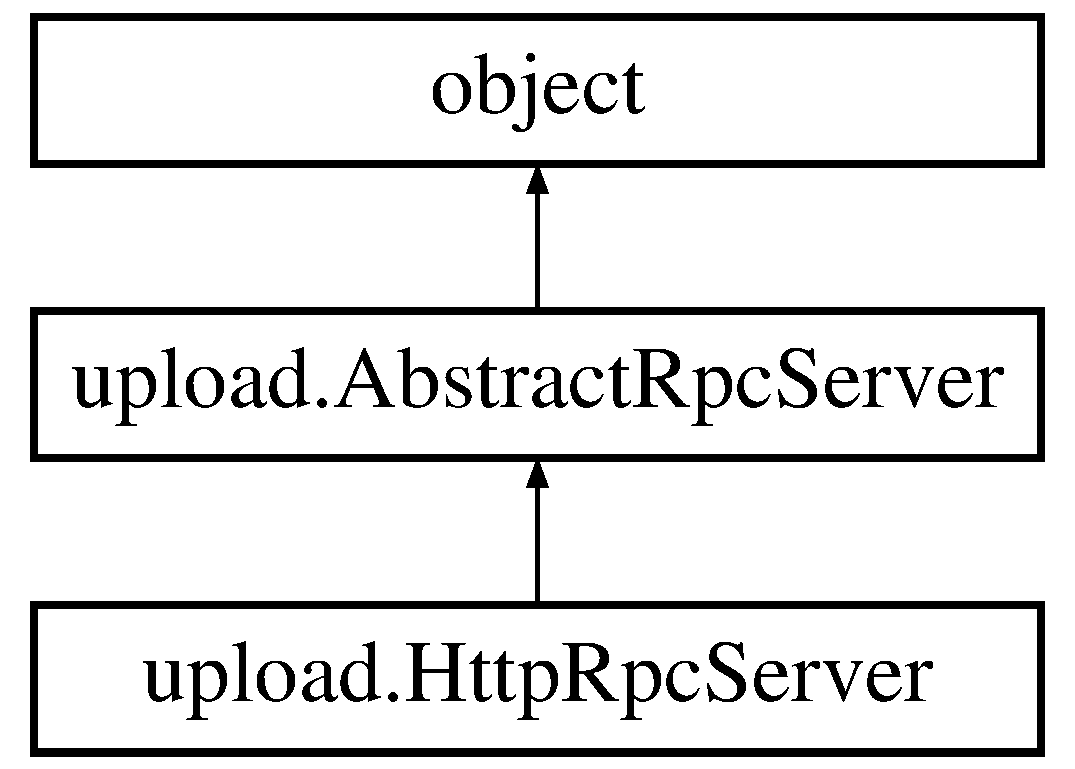
\includegraphics[height=3.000000cm]{classupload_1_1_abstract_rpc_server}
\end{center}
\end{figure}
\subsection*{Public Member Functions}
\begin{DoxyCompactItemize}
\item 
def \hyperlink{classupload_1_1_abstract_rpc_server_a87618fdb401f36dd7aaf2196bb65d35e}{\+\_\+\+\_\+init\+\_\+\+\_\+}
\item 
def \hyperlink{classupload_1_1_abstract_rpc_server_ac1b913f8bd00da4741c47ab49ea94cb5}{Send} (self, request\+\_\+path, payload=None, content\+\_\+type=\char`\"{}application/octet-\/stream\char`\"{}, timeout=None, kwargs)
\end{DoxyCompactItemize}
\subsection*{Public Attributes}
\begin{DoxyCompactItemize}
\item 
\hyperlink{classupload_1_1_abstract_rpc_server_ab7188d827e2faddcf970f524f5856192}{host}
\item 
\hyperlink{classupload_1_1_abstract_rpc_server_a783a4a7e4ffb776a57a3f267300a213b}{host\+\_\+override}
\item 
\hyperlink{classupload_1_1_abstract_rpc_server_aee0090a3bcf07b913a7dd596a5dabb8f}{auth\+\_\+function}
\item 
\hyperlink{classupload_1_1_abstract_rpc_server_a692955750c802e461c6336d3000cd365}{authenticated}
\item 
\hyperlink{classupload_1_1_abstract_rpc_server_adbbf0109afc13d58d7815fa143cb779f}{extra\+\_\+headers}
\item 
\hyperlink{classupload_1_1_abstract_rpc_server_affe342205c4647d41b127f5a5634858b}{save\+\_\+cookies}
\item 
\hyperlink{classupload_1_1_abstract_rpc_server_aa931446476e0e86f3ade7fef0a0aea5a}{opener}
\end{DoxyCompactItemize}


\subsection{Detailed Description}
\begin{DoxyVerb}Provides a common interface for a simple RPC server.\end{DoxyVerb}
 

\subsection{Constructor \& Destructor Documentation}
\hypertarget{classupload_1_1_abstract_rpc_server_a87618fdb401f36dd7aaf2196bb65d35e}{}\index{upload\+::\+Abstract\+Rpc\+Server@{upload\+::\+Abstract\+Rpc\+Server}!\+\_\+\+\_\+init\+\_\+\+\_\+@{\+\_\+\+\_\+init\+\_\+\+\_\+}}
\index{\+\_\+\+\_\+init\+\_\+\+\_\+@{\+\_\+\+\_\+init\+\_\+\+\_\+}!upload\+::\+Abstract\+Rpc\+Server@{upload\+::\+Abstract\+Rpc\+Server}}
\subsubsection[{\+\_\+\+\_\+init\+\_\+\+\_\+}]{\setlength{\rightskip}{0pt plus 5cm}def upload.\+Abstract\+Rpc\+Server.\+\_\+\+\_\+init\+\_\+\+\_\+ (
\begin{DoxyParamCaption}
\item[{}]{self, }
\item[{}]{host, }
\item[{}]{auth\+\_\+function, }
\item[{}]{host\+\_\+override = {\ttfamily None}, }
\item[{}]{extra\+\_\+headers = {\ttfamily \{\}}, }
\item[{}]{save\+\_\+cookies = {\ttfamily False}}
\end{DoxyParamCaption}
)}\label{classupload_1_1_abstract_rpc_server_a87618fdb401f36dd7aaf2196bb65d35e}
\begin{DoxyVerb}Creates a new HttpRpcServer.

Args:
  host: The host to send requests to.
  auth_function: A function that takes no arguments and returns an
(email, password) tuple when called. Will be called if authentication
is required.
  host_override: The host header to send to the server (defaults to host).
  extra_headers: A dict of extra headers to append to every request.
  save_cookies: If True, save the authentication cookies to local disk.
If False, use an in-memory cookiejar instead.  Subclasses must
implement this functionality.  Defaults to False.
\end{DoxyVerb}
 

\subsection{Member Function Documentation}
\hypertarget{classupload_1_1_abstract_rpc_server_ac1b913f8bd00da4741c47ab49ea94cb5}{}\index{upload\+::\+Abstract\+Rpc\+Server@{upload\+::\+Abstract\+Rpc\+Server}!Send@{Send}}
\index{Send@{Send}!upload\+::\+Abstract\+Rpc\+Server@{upload\+::\+Abstract\+Rpc\+Server}}
\subsubsection[{Send(self, request\+\_\+path, payload=\+None, content\+\_\+type=""application/octet-\/stream"", timeout=\+None, kwargs)}]{\setlength{\rightskip}{0pt plus 5cm}def upload.\+Abstract\+Rpc\+Server.\+Send (
\begin{DoxyParamCaption}
\item[{}]{self, }
\item[{}]{request\+\_\+path, }
\item[{}]{payload = {\ttfamily None}, }
\item[{}]{content\+\_\+type = {\ttfamily \char`\"{}application/octet-\/stream\char`\"{}}, }
\item[{}]{timeout = {\ttfamily None}, }
\item[{}]{kwargs}
\end{DoxyParamCaption}
)}\label{classupload_1_1_abstract_rpc_server_ac1b913f8bd00da4741c47ab49ea94cb5}
\begin{DoxyVerb}Sends an RPC and returns the response.

Args:
  request_path: The path to send the request to, eg /api/appversion/create.
  payload: The body of the request, or None to send an empty request.
  content_type: The Content-Type header to use.
  timeout: timeout in seconds; default None i.e. no timeout.
(Note: for large requests on OS X, the timeout doesn't work right.)
  kwargs: Any keyword arguments are converted into query string parameters.

Returns:
  The response body, as a string.
\end{DoxyVerb}
 

\subsection{Member Data Documentation}
\hypertarget{classupload_1_1_abstract_rpc_server_aee0090a3bcf07b913a7dd596a5dabb8f}{}\index{upload\+::\+Abstract\+Rpc\+Server@{upload\+::\+Abstract\+Rpc\+Server}!auth\+\_\+function@{auth\+\_\+function}}
\index{auth\+\_\+function@{auth\+\_\+function}!upload\+::\+Abstract\+Rpc\+Server@{upload\+::\+Abstract\+Rpc\+Server}}
\subsubsection[{auth\+\_\+function}]{\setlength{\rightskip}{0pt plus 5cm}upload.\+Abstract\+Rpc\+Server.\+auth\+\_\+function}\label{classupload_1_1_abstract_rpc_server_aee0090a3bcf07b913a7dd596a5dabb8f}
\hypertarget{classupload_1_1_abstract_rpc_server_a692955750c802e461c6336d3000cd365}{}\index{upload\+::\+Abstract\+Rpc\+Server@{upload\+::\+Abstract\+Rpc\+Server}!authenticated@{authenticated}}
\index{authenticated@{authenticated}!upload\+::\+Abstract\+Rpc\+Server@{upload\+::\+Abstract\+Rpc\+Server}}
\subsubsection[{authenticated}]{\setlength{\rightskip}{0pt plus 5cm}upload.\+Abstract\+Rpc\+Server.\+authenticated}\label{classupload_1_1_abstract_rpc_server_a692955750c802e461c6336d3000cd365}
\hypertarget{classupload_1_1_abstract_rpc_server_adbbf0109afc13d58d7815fa143cb779f}{}\index{upload\+::\+Abstract\+Rpc\+Server@{upload\+::\+Abstract\+Rpc\+Server}!extra\+\_\+headers@{extra\+\_\+headers}}
\index{extra\+\_\+headers@{extra\+\_\+headers}!upload\+::\+Abstract\+Rpc\+Server@{upload\+::\+Abstract\+Rpc\+Server}}
\subsubsection[{extra\+\_\+headers}]{\setlength{\rightskip}{0pt plus 5cm}upload.\+Abstract\+Rpc\+Server.\+extra\+\_\+headers}\label{classupload_1_1_abstract_rpc_server_adbbf0109afc13d58d7815fa143cb779f}
\hypertarget{classupload_1_1_abstract_rpc_server_ab7188d827e2faddcf970f524f5856192}{}\index{upload\+::\+Abstract\+Rpc\+Server@{upload\+::\+Abstract\+Rpc\+Server}!host@{host}}
\index{host@{host}!upload\+::\+Abstract\+Rpc\+Server@{upload\+::\+Abstract\+Rpc\+Server}}
\subsubsection[{host}]{\setlength{\rightskip}{0pt plus 5cm}upload.\+Abstract\+Rpc\+Server.\+host}\label{classupload_1_1_abstract_rpc_server_ab7188d827e2faddcf970f524f5856192}
\hypertarget{classupload_1_1_abstract_rpc_server_a783a4a7e4ffb776a57a3f267300a213b}{}\index{upload\+::\+Abstract\+Rpc\+Server@{upload\+::\+Abstract\+Rpc\+Server}!host\+\_\+override@{host\+\_\+override}}
\index{host\+\_\+override@{host\+\_\+override}!upload\+::\+Abstract\+Rpc\+Server@{upload\+::\+Abstract\+Rpc\+Server}}
\subsubsection[{host\+\_\+override}]{\setlength{\rightskip}{0pt plus 5cm}upload.\+Abstract\+Rpc\+Server.\+host\+\_\+override}\label{classupload_1_1_abstract_rpc_server_a783a4a7e4ffb776a57a3f267300a213b}
\hypertarget{classupload_1_1_abstract_rpc_server_aa931446476e0e86f3ade7fef0a0aea5a}{}\index{upload\+::\+Abstract\+Rpc\+Server@{upload\+::\+Abstract\+Rpc\+Server}!opener@{opener}}
\index{opener@{opener}!upload\+::\+Abstract\+Rpc\+Server@{upload\+::\+Abstract\+Rpc\+Server}}
\subsubsection[{opener}]{\setlength{\rightskip}{0pt plus 5cm}upload.\+Abstract\+Rpc\+Server.\+opener}\label{classupload_1_1_abstract_rpc_server_aa931446476e0e86f3ade7fef0a0aea5a}
\hypertarget{classupload_1_1_abstract_rpc_server_affe342205c4647d41b127f5a5634858b}{}\index{upload\+::\+Abstract\+Rpc\+Server@{upload\+::\+Abstract\+Rpc\+Server}!save\+\_\+cookies@{save\+\_\+cookies}}
\index{save\+\_\+cookies@{save\+\_\+cookies}!upload\+::\+Abstract\+Rpc\+Server@{upload\+::\+Abstract\+Rpc\+Server}}
\subsubsection[{save\+\_\+cookies}]{\setlength{\rightskip}{0pt plus 5cm}upload.\+Abstract\+Rpc\+Server.\+save\+\_\+cookies}\label{classupload_1_1_abstract_rpc_server_affe342205c4647d41b127f5a5634858b}


The documentation for this class was generated from the following file\+:\begin{DoxyCompactItemize}
\item 
C\+:/\+Users/\+Hilman/\+Desktop/repo/anjing/src/third\+\_\+party/googletest/scripts/\hyperlink{upload_8py}{upload.\+py}\end{DoxyCompactItemize}

\hypertarget{structstd_1_1tr1_1_1gtest__internal_1_1_add_ref}{}\section{std\+:\+:tr1\+:\+:gtest\+\_\+internal\+:\+:Add\+Ref$<$ T $>$ Struct Template Reference}
\label{structstd_1_1tr1_1_1gtest__internal_1_1_add_ref}\index{std\+::tr1\+::gtest\+\_\+internal\+::\+Add\+Ref$<$ T $>$@{std\+::tr1\+::gtest\+\_\+internal\+::\+Add\+Ref$<$ T $>$}}


{\ttfamily \#include $<$gtest-\/tuple.\+h$>$}

\subsection*{Public Types}
\begin{DoxyCompactItemize}
\item 
typedef T \& \hyperlink{structstd_1_1tr1_1_1gtest__internal_1_1_add_ref_a1e5616e414125574c1653e3a1fc68491}{type}
\end{DoxyCompactItemize}


\subsection{Member Typedef Documentation}
\hypertarget{structstd_1_1tr1_1_1gtest__internal_1_1_add_ref_a1e5616e414125574c1653e3a1fc68491}{}\index{std\+::tr1\+::gtest\+\_\+internal\+::\+Add\+Ref@{std\+::tr1\+::gtest\+\_\+internal\+::\+Add\+Ref}!type@{type}}
\index{type@{type}!std\+::tr1\+::gtest\+\_\+internal\+::\+Add\+Ref@{std\+::tr1\+::gtest\+\_\+internal\+::\+Add\+Ref}}
\subsubsection[{type}]{\setlength{\rightskip}{0pt plus 5cm}template$<$typename T $>$ typedef T\& {\bf std\+::tr1\+::gtest\+\_\+internal\+::\+Add\+Ref}$<$ T $>$\+::{\bf type}}\label{structstd_1_1tr1_1_1gtest__internal_1_1_add_ref_a1e5616e414125574c1653e3a1fc68491}


The documentation for this struct was generated from the following file\+:\begin{DoxyCompactItemize}
\item 
C\+:/\+Users/\+Hilman/\+Desktop/repo/anjing/src/third\+\_\+party/googletest/include/gtest/internal/\hyperlink{gtest-tuple_8h}{gtest-\/tuple.\+h}\end{DoxyCompactItemize}

\hypertarget{structstd_1_1tr1_1_1gtest__internal_1_1_add_ref_3_01_t_01_6_01_4}{}\section{std\+:\+:tr1\+:\+:gtest\+\_\+internal\+:\+:Add\+Ref$<$ T \& $>$ Struct Template Reference}
\label{structstd_1_1tr1_1_1gtest__internal_1_1_add_ref_3_01_t_01_6_01_4}\index{std\+::tr1\+::gtest\+\_\+internal\+::\+Add\+Ref$<$ T \& $>$@{std\+::tr1\+::gtest\+\_\+internal\+::\+Add\+Ref$<$ T \& $>$}}


{\ttfamily \#include $<$gtest-\/tuple.\+h$>$}

\subsection*{Public Types}
\begin{DoxyCompactItemize}
\item 
typedef T \& \hyperlink{structstd_1_1tr1_1_1gtest__internal_1_1_add_ref_3_01_t_01_6_01_4_a9cb3b0992c2a9e7df42d01fb64c2dc88}{type}
\end{DoxyCompactItemize}


\subsection{Member Typedef Documentation}
\hypertarget{structstd_1_1tr1_1_1gtest__internal_1_1_add_ref_3_01_t_01_6_01_4_a9cb3b0992c2a9e7df42d01fb64c2dc88}{}\index{std\+::tr1\+::gtest\+\_\+internal\+::\+Add\+Ref$<$ T \& $>$@{std\+::tr1\+::gtest\+\_\+internal\+::\+Add\+Ref$<$ T \& $>$}!type@{type}}
\index{type@{type}!std\+::tr1\+::gtest\+\_\+internal\+::\+Add\+Ref$<$ T \& $>$@{std\+::tr1\+::gtest\+\_\+internal\+::\+Add\+Ref$<$ T \& $>$}}
\subsubsection[{type}]{\setlength{\rightskip}{0pt plus 5cm}template$<$typename T $>$ typedef T\& {\bf std\+::tr1\+::gtest\+\_\+internal\+::\+Add\+Ref}$<$ T \& $>$\+::{\bf type}}\label{structstd_1_1tr1_1_1gtest__internal_1_1_add_ref_3_01_t_01_6_01_4_a9cb3b0992c2a9e7df42d01fb64c2dc88}


The documentation for this struct was generated from the following file\+:\begin{DoxyCompactItemize}
\item 
C\+:/\+Users/\+Hilman/\+Desktop/repo/anjing/src/third\+\_\+party/googletest/include/gtest/internal/\hyperlink{gtest-tuple_8h}{gtest-\/tuple.\+h}\end{DoxyCompactItemize}

\hypertarget{structtesting_1_1internal_1_1_add_reference}{}\section{testing\+:\+:internal\+:\+:Add\+Reference$<$ T $>$ Struct Template Reference}
\label{structtesting_1_1internal_1_1_add_reference}\index{testing\+::internal\+::\+Add\+Reference$<$ T $>$@{testing\+::internal\+::\+Add\+Reference$<$ T $>$}}


{\ttfamily \#include $<$gtest-\/internal.\+h$>$}

\subsection*{Public Types}
\begin{DoxyCompactItemize}
\item 
typedef T \& \hyperlink{structtesting_1_1internal_1_1_add_reference_a2df8dd7c4e41f6390e6e66b1a9a67bb4}{type}
\end{DoxyCompactItemize}


\subsection{Member Typedef Documentation}
\hypertarget{structtesting_1_1internal_1_1_add_reference_a2df8dd7c4e41f6390e6e66b1a9a67bb4}{}\index{testing\+::internal\+::\+Add\+Reference@{testing\+::internal\+::\+Add\+Reference}!type@{type}}
\index{type@{type}!testing\+::internal\+::\+Add\+Reference@{testing\+::internal\+::\+Add\+Reference}}
\subsubsection[{type}]{\setlength{\rightskip}{0pt plus 5cm}template$<$typename T $>$ typedef T\& {\bf testing\+::internal\+::\+Add\+Reference}$<$ T $>$\+::{\bf type}}\label{structtesting_1_1internal_1_1_add_reference_a2df8dd7c4e41f6390e6e66b1a9a67bb4}


The documentation for this struct was generated from the following file\+:\begin{DoxyCompactItemize}
\item 
C\+:/\+Users/\+Hilman/\+Desktop/repo/anjing/src/third\+\_\+party/googletest/include/gtest/internal/\hyperlink{gtest-internal_8h}{gtest-\/internal.\+h}\end{DoxyCompactItemize}

\hypertarget{structtesting_1_1internal_1_1_add_reference_3_01_t_01_6_01_4}{}\section{testing\+:\+:internal\+:\+:Add\+Reference$<$ T \& $>$ Struct Template Reference}
\label{structtesting_1_1internal_1_1_add_reference_3_01_t_01_6_01_4}\index{testing\+::internal\+::\+Add\+Reference$<$ T \& $>$@{testing\+::internal\+::\+Add\+Reference$<$ T \& $>$}}


{\ttfamily \#include $<$gtest-\/internal.\+h$>$}

\subsection*{Public Types}
\begin{DoxyCompactItemize}
\item 
typedef T \& \hyperlink{structtesting_1_1internal_1_1_add_reference_3_01_t_01_6_01_4_a93c064cdcdaced0abd167258425e57af}{type}
\end{DoxyCompactItemize}


\subsection{Member Typedef Documentation}
\hypertarget{structtesting_1_1internal_1_1_add_reference_3_01_t_01_6_01_4_a93c064cdcdaced0abd167258425e57af}{}\index{testing\+::internal\+::\+Add\+Reference$<$ T \& $>$@{testing\+::internal\+::\+Add\+Reference$<$ T \& $>$}!type@{type}}
\index{type@{type}!testing\+::internal\+::\+Add\+Reference$<$ T \& $>$@{testing\+::internal\+::\+Add\+Reference$<$ T \& $>$}}
\subsubsection[{type}]{\setlength{\rightskip}{0pt plus 5cm}template$<$typename T $>$ typedef T\& {\bf testing\+::internal\+::\+Add\+Reference}$<$ T \& $>$\+::{\bf type}}\label{structtesting_1_1internal_1_1_add_reference_3_01_t_01_6_01_4_a93c064cdcdaced0abd167258425e57af}


The documentation for this struct was generated from the following file\+:\begin{DoxyCompactItemize}
\item 
C\+:/\+Users/\+Hilman/\+Desktop/repo/anjing/src/third\+\_\+party/googletest/include/gtest/internal/\hyperlink{gtest-internal_8h}{gtest-\/internal.\+h}\end{DoxyCompactItemize}

\hypertarget{classtesting_1_1gtest__printers__test_1_1_allows_generic_streaming}{}\section{testing\+:\+:gtest\+\_\+printers\+\_\+test\+:\+:Allows\+Generic\+Streaming Class Reference}
\label{classtesting_1_1gtest__printers__test_1_1_allows_generic_streaming}\index{testing\+::gtest\+\_\+printers\+\_\+test\+::\+Allows\+Generic\+Streaming@{testing\+::gtest\+\_\+printers\+\_\+test\+::\+Allows\+Generic\+Streaming}}


The documentation for this class was generated from the following file\+:\begin{DoxyCompactItemize}
\item 
C\+:/\+Users/\+Hilman/\+Desktop/repo/anjing/src/third\+\_\+party/googletest/test/\hyperlink{gtest-printers__test_8cc}{gtest-\/printers\+\_\+test.\+cc}\end{DoxyCompactItemize}

\hypertarget{classtesting_1_1gtest__printers__test_1_1_allows_generic_streaming_and_implicit_conversion_template}{}\section{testing\+:\+:gtest\+\_\+printers\+\_\+test\+:\+:Allows\+Generic\+Streaming\+And\+Implicit\+Conversion\+Template$<$ T $>$ Class Template Reference}
\label{classtesting_1_1gtest__printers__test_1_1_allows_generic_streaming_and_implicit_conversion_template}\index{testing\+::gtest\+\_\+printers\+\_\+test\+::\+Allows\+Generic\+Streaming\+And\+Implicit\+Conversion\+Template$<$ T $>$@{testing\+::gtest\+\_\+printers\+\_\+test\+::\+Allows\+Generic\+Streaming\+And\+Implicit\+Conversion\+Template$<$ T $>$}}
\subsection*{Public Member Functions}
\begin{DoxyCompactItemize}
\item 
\hyperlink{classtesting_1_1gtest__printers__test_1_1_allows_generic_streaming_and_implicit_conversion_template_a149a95a572a5ef546d852ba012c6226c}{operator bool} () const 
\end{DoxyCompactItemize}


\subsection{Member Function Documentation}
\hypertarget{classtesting_1_1gtest__printers__test_1_1_allows_generic_streaming_and_implicit_conversion_template_a149a95a572a5ef546d852ba012c6226c}{}\index{testing\+::gtest\+\_\+printers\+\_\+test\+::\+Allows\+Generic\+Streaming\+And\+Implicit\+Conversion\+Template@{testing\+::gtest\+\_\+printers\+\_\+test\+::\+Allows\+Generic\+Streaming\+And\+Implicit\+Conversion\+Template}!operator bool@{operator bool}}
\index{operator bool@{operator bool}!testing\+::gtest\+\_\+printers\+\_\+test\+::\+Allows\+Generic\+Streaming\+And\+Implicit\+Conversion\+Template@{testing\+::gtest\+\_\+printers\+\_\+test\+::\+Allows\+Generic\+Streaming\+And\+Implicit\+Conversion\+Template}}
\subsubsection[{operator bool() const }]{\setlength{\rightskip}{0pt plus 5cm}template$<$typename T $>$ {\bf testing\+::gtest\+\_\+printers\+\_\+test\+::\+Allows\+Generic\+Streaming\+And\+Implicit\+Conversion\+Template}$<$ T $>$\+::operator bool (
\begin{DoxyParamCaption}
{}
\end{DoxyParamCaption}
) const\hspace{0.3cm}{\ttfamily [inline]}}\label{classtesting_1_1gtest__printers__test_1_1_allows_generic_streaming_and_implicit_conversion_template_a149a95a572a5ef546d852ba012c6226c}


The documentation for this class was generated from the following file\+:\begin{DoxyCompactItemize}
\item 
C\+:/\+Users/\+Hilman/\+Desktop/repo/anjing/src/third\+\_\+party/googletest/test/\hyperlink{gtest-printers__test_8cc}{gtest-\/printers\+\_\+test.\+cc}\end{DoxyCompactItemize}

\hypertarget{classtesting_1_1gtest__printers__test_1_1_allows_generic_streaming_template}{}\section{testing\+:\+:gtest\+\_\+printers\+\_\+test\+:\+:Allows\+Generic\+Streaming\+Template$<$ T $>$ Class Template Reference}
\label{classtesting_1_1gtest__printers__test_1_1_allows_generic_streaming_template}\index{testing\+::gtest\+\_\+printers\+\_\+test\+::\+Allows\+Generic\+Streaming\+Template$<$ T $>$@{testing\+::gtest\+\_\+printers\+\_\+test\+::\+Allows\+Generic\+Streaming\+Template$<$ T $>$}}


The documentation for this class was generated from the following file\+:\begin{DoxyCompactItemize}
\item 
C\+:/\+Users/\+Hilman/\+Desktop/repo/anjing/src/third\+\_\+party/googletest/test/\hyperlink{gtest-printers__test_8cc}{gtest-\/printers\+\_\+test.\+cc}\end{DoxyCompactItemize}

\hypertarget{classanjing_1_1_app}{}\section{anjing\+:\+:App Class Reference}
\label{classanjing_1_1_app}\index{anjing\+::\+App@{anjing\+::\+App}}


{\ttfamily \#include $<$app.\+hpp$>$}

\subsection*{Static Public Member Functions}
\begin{DoxyCompactItemize}
\item 
static int \hyperlink{classanjing_1_1_app_af7dd6e06068a1433dc51c6944eceb141}{Start\+Application} (\hyperlink{classanjing_1_1_app}{App} $\ast$app, int width, int height, int fps, const std\+::string \&title)
\begin{DoxyCompactList}\small\item\em Create the applications\textquotesingle{} window, initialize the app, S\+D\+L, and Open\+G\+L. \end{DoxyCompactList}\end{DoxyCompactItemize}
\subsection*{Protected Member Functions}
\begin{DoxyCompactItemize}
\item 
virtual int \hyperlink{classanjing_1_1_app_ac21568a309981fcb0beafd2c8c92cd8a}{Init} ()
\begin{DoxyCompactList}\small\item\em Init will get called after app is ready to be used (at the end of Start\+Application function call) \end{DoxyCompactList}\item 
virtual void \hyperlink{classanjing_1_1_app_abfa119eea6fe448f6c1328d66d86b2e5}{Clean} ()
\begin{DoxyCompactList}\small\item\em Release all app\textquotesingle{}s memory. \end{DoxyCompactList}\end{DoxyCompactItemize}


\subsection{Member Function Documentation}
\hypertarget{classanjing_1_1_app_abfa119eea6fe448f6c1328d66d86b2e5}{}\index{anjing\+::\+App@{anjing\+::\+App}!Clean@{Clean}}
\index{Clean@{Clean}!anjing\+::\+App@{anjing\+::\+App}}
\subsubsection[{Clean()}]{\setlength{\rightskip}{0pt plus 5cm}void App\+::\+Clean (
\begin{DoxyParamCaption}
{}
\end{DoxyParamCaption}
)\hspace{0.3cm}{\ttfamily [protected]}, {\ttfamily [virtual]}}\label{classanjing_1_1_app_abfa119eea6fe448f6c1328d66d86b2e5}


Release all app\textquotesingle{}s memory. 

\hypertarget{classanjing_1_1_app_ac21568a309981fcb0beafd2c8c92cd8a}{}\index{anjing\+::\+App@{anjing\+::\+App}!Init@{Init}}
\index{Init@{Init}!anjing\+::\+App@{anjing\+::\+App}}
\subsubsection[{Init()}]{\setlength{\rightskip}{0pt plus 5cm}int App\+::\+Init (
\begin{DoxyParamCaption}
{}
\end{DoxyParamCaption}
)\hspace{0.3cm}{\ttfamily [protected]}, {\ttfamily [virtual]}}\label{classanjing_1_1_app_ac21568a309981fcb0beafd2c8c92cd8a}


Init will get called after app is ready to be used (at the end of Start\+Application function call) 

\hypertarget{classanjing_1_1_app_af7dd6e06068a1433dc51c6944eceb141}{}\index{anjing\+::\+App@{anjing\+::\+App}!Start\+Application@{Start\+Application}}
\index{Start\+Application@{Start\+Application}!anjing\+::\+App@{anjing\+::\+App}}
\subsubsection[{Start\+Application(\+App $\ast$app, int width, int height, int fps, const std\+::string \&title)}]{\setlength{\rightskip}{0pt plus 5cm}int App\+::\+Start\+Application (
\begin{DoxyParamCaption}
\item[{{\bf App} $\ast$}]{app, }
\item[{int}]{width, }
\item[{int}]{height, }
\item[{int}]{fps, }
\item[{const std\+::string \&}]{title}
\end{DoxyParamCaption}
)\hspace{0.3cm}{\ttfamily [static]}}\label{classanjing_1_1_app_af7dd6e06068a1433dc51c6944eceb141}


Create the applications\textquotesingle{} window, initialize the app, S\+D\+L, and Open\+G\+L. 



The documentation for this class was generated from the following files\+:\begin{DoxyCompactItemize}
\item 
C\+:/\+Users/\+Hilman/\+Desktop/repo/anjing/src/app/\hyperlink{app_8hpp}{app.\+hpp}\item 
C\+:/\+Users/\+Hilman/\+Desktop/repo/anjing/src/app/\hyperlink{app_8cpp}{app.\+cpp}\end{DoxyCompactItemize}

\hypertarget{classtesting_1_1internal_1_1_assert_helper}{}\section{testing\+:\+:internal\+:\+:Assert\+Helper Class Reference}
\label{classtesting_1_1internal_1_1_assert_helper}\index{testing\+::internal\+::\+Assert\+Helper@{testing\+::internal\+::\+Assert\+Helper}}


{\ttfamily \#include $<$gtest.\+h$>$}

\subsection*{Public Member Functions}
\begin{DoxyCompactItemize}
\item 
\hyperlink{classtesting_1_1internal_1_1_assert_helper_ac2c9334518fd4087189b4505567a3c90}{Assert\+Helper} (\hyperlink{classtesting_1_1_test_part_result_a65ae656b33fdfdfffaf34858778a52d5}{Test\+Part\+Result\+::\+Type} type, const char $\ast$file, int line, const char $\ast$message)
\item 
\hyperlink{classtesting_1_1internal_1_1_assert_helper_a51c640785d4ed4a0155cc9aa857d8931}{$\sim$\+Assert\+Helper} ()
\item 
void \hyperlink{classtesting_1_1internal_1_1_assert_helper_ab721be11cb9aca8a361ca1f014ca5f80}{operator=} (const \hyperlink{classtesting_1_1_message}{Message} \&message) const 
\end{DoxyCompactItemize}


\subsection{Constructor \& Destructor Documentation}
\hypertarget{classtesting_1_1internal_1_1_assert_helper_ac2c9334518fd4087189b4505567a3c90}{}\index{testing\+::internal\+::\+Assert\+Helper@{testing\+::internal\+::\+Assert\+Helper}!Assert\+Helper@{Assert\+Helper}}
\index{Assert\+Helper@{Assert\+Helper}!testing\+::internal\+::\+Assert\+Helper@{testing\+::internal\+::\+Assert\+Helper}}
\subsubsection[{Assert\+Helper(\+Test\+Part\+Result\+::\+Type type, const char $\ast$file, int line, const char $\ast$message)}]{\setlength{\rightskip}{0pt plus 5cm}testing\+::internal\+::\+Assert\+Helper\+::\+Assert\+Helper (
\begin{DoxyParamCaption}
\item[{{\bf Test\+Part\+Result\+::\+Type}}]{type, }
\item[{const char $\ast$}]{file, }
\item[{int}]{line, }
\item[{const char $\ast$}]{message}
\end{DoxyParamCaption}
)}\label{classtesting_1_1internal_1_1_assert_helper_ac2c9334518fd4087189b4505567a3c90}
\hypertarget{classtesting_1_1internal_1_1_assert_helper_a51c640785d4ed4a0155cc9aa857d8931}{}\index{testing\+::internal\+::\+Assert\+Helper@{testing\+::internal\+::\+Assert\+Helper}!````~Assert\+Helper@{$\sim$\+Assert\+Helper}}
\index{````~Assert\+Helper@{$\sim$\+Assert\+Helper}!testing\+::internal\+::\+Assert\+Helper@{testing\+::internal\+::\+Assert\+Helper}}
\subsubsection[{$\sim$\+Assert\+Helper()}]{\setlength{\rightskip}{0pt plus 5cm}testing\+::internal\+::\+Assert\+Helper\+::$\sim$\+Assert\+Helper (
\begin{DoxyParamCaption}
{}
\end{DoxyParamCaption}
)}\label{classtesting_1_1internal_1_1_assert_helper_a51c640785d4ed4a0155cc9aa857d8931}


\subsection{Member Function Documentation}
\hypertarget{classtesting_1_1internal_1_1_assert_helper_ab721be11cb9aca8a361ca1f014ca5f80}{}\index{testing\+::internal\+::\+Assert\+Helper@{testing\+::internal\+::\+Assert\+Helper}!operator=@{operator=}}
\index{operator=@{operator=}!testing\+::internal\+::\+Assert\+Helper@{testing\+::internal\+::\+Assert\+Helper}}
\subsubsection[{operator=(const Message \&message) const }]{\setlength{\rightskip}{0pt plus 5cm}void testing\+::internal\+::\+Assert\+Helper\+::operator= (
\begin{DoxyParamCaption}
\item[{const {\bf Message} \&}]{message}
\end{DoxyParamCaption}
) const}\label{classtesting_1_1internal_1_1_assert_helper_ab721be11cb9aca8a361ca1f014ca5f80}


The documentation for this class was generated from the following files\+:\begin{DoxyCompactItemize}
\item 
C\+:/\+Users/\+Hilman/\+Desktop/repo/anjing/src/third\+\_\+party/googletest/include/gtest/\hyperlink{gtest_8h}{gtest.\+h}\item 
C\+:/\+Users/\+Hilman/\+Desktop/repo/anjing/src/third\+\_\+party/googletest/src/\hyperlink{gtest_8cc}{gtest.\+cc}\end{DoxyCompactItemize}

\hypertarget{classtesting_1_1_assertion_result}{}\section{testing\+:\+:Assertion\+Result Class Reference}
\label{classtesting_1_1_assertion_result}\index{testing\+::\+Assertion\+Result@{testing\+::\+Assertion\+Result}}


{\ttfamily \#include $<$gtest.\+h$>$}

\subsection*{Public Member Functions}
\begin{DoxyCompactItemize}
\item 
\hyperlink{classtesting_1_1_assertion_result_a27788116f03f90aec4daf592fd809ead}{Assertion\+Result} (const \hyperlink{classtesting_1_1_assertion_result}{Assertion\+Result} \&other)
\item 
\hyperlink{classtesting_1_1_assertion_result_ade695178c05c4b2f82e92930c912fc25}{Assertion\+Result} (bool success)
\item 
\hyperlink{classtesting_1_1_assertion_result_af85b7852e6399467cd74df539810abcd}{operator bool} () const 
\item 
\hyperlink{classtesting_1_1_assertion_result}{Assertion\+Result} \hyperlink{classtesting_1_1_assertion_result_a85301ba52aa1efe89b79d1e3b59160cd}{operator!} () const 
\item 
const char $\ast$ \hyperlink{classtesting_1_1_assertion_result_ab20c91eba13e20f1b4ad89e3d15f69a8}{message} () const 
\item 
const char $\ast$ \hyperlink{classtesting_1_1_assertion_result_ae54fa82506c507a9dbc0f85d2cec652a}{failure\+\_\+message} () const 
\item 
{\footnotesize template$<$typename T $>$ }\\\hyperlink{classtesting_1_1_assertion_result}{Assertion\+Result} \& \hyperlink{classtesting_1_1_assertion_result_a3230efa81aafe7c61f5fb878cfa39e91}{operator$<$$<$} (const T \&value)
\item 
\hyperlink{classtesting_1_1_assertion_result}{Assertion\+Result} \& \hyperlink{classtesting_1_1_assertion_result_a43ae8a260843ce2ff3dc9af262672b8b}{operator$<$$<$} (\+::std\+::ostream \&($\ast$basic\+\_\+manipulator)(\+::std\+::ostream \&stream))
\end{DoxyCompactItemize}


\subsection{Constructor \& Destructor Documentation}
\hypertarget{classtesting_1_1_assertion_result_a27788116f03f90aec4daf592fd809ead}{}\index{testing\+::\+Assertion\+Result@{testing\+::\+Assertion\+Result}!Assertion\+Result@{Assertion\+Result}}
\index{Assertion\+Result@{Assertion\+Result}!testing\+::\+Assertion\+Result@{testing\+::\+Assertion\+Result}}
\subsubsection[{Assertion\+Result(const Assertion\+Result \&other)}]{\setlength{\rightskip}{0pt plus 5cm}testing\+::\+Assertion\+Result\+::\+Assertion\+Result (
\begin{DoxyParamCaption}
\item[{const {\bf Assertion\+Result} \&}]{other}
\end{DoxyParamCaption}
)}\label{classtesting_1_1_assertion_result_a27788116f03f90aec4daf592fd809ead}
\hypertarget{classtesting_1_1_assertion_result_ade695178c05c4b2f82e92930c912fc25}{}\index{testing\+::\+Assertion\+Result@{testing\+::\+Assertion\+Result}!Assertion\+Result@{Assertion\+Result}}
\index{Assertion\+Result@{Assertion\+Result}!testing\+::\+Assertion\+Result@{testing\+::\+Assertion\+Result}}
\subsubsection[{Assertion\+Result(bool success)}]{\setlength{\rightskip}{0pt plus 5cm}testing\+::\+Assertion\+Result\+::\+Assertion\+Result (
\begin{DoxyParamCaption}
\item[{bool}]{success}
\end{DoxyParamCaption}
)\hspace{0.3cm}{\ttfamily [inline]}, {\ttfamily [explicit]}}\label{classtesting_1_1_assertion_result_ade695178c05c4b2f82e92930c912fc25}


\subsection{Member Function Documentation}
\hypertarget{classtesting_1_1_assertion_result_ae54fa82506c507a9dbc0f85d2cec652a}{}\index{testing\+::\+Assertion\+Result@{testing\+::\+Assertion\+Result}!failure\+\_\+message@{failure\+\_\+message}}
\index{failure\+\_\+message@{failure\+\_\+message}!testing\+::\+Assertion\+Result@{testing\+::\+Assertion\+Result}}
\subsubsection[{failure\+\_\+message() const }]{\setlength{\rightskip}{0pt plus 5cm}const char$\ast$ testing\+::\+Assertion\+Result\+::failure\+\_\+message (
\begin{DoxyParamCaption}
{}
\end{DoxyParamCaption}
) const\hspace{0.3cm}{\ttfamily [inline]}}\label{classtesting_1_1_assertion_result_ae54fa82506c507a9dbc0f85d2cec652a}
\hypertarget{classtesting_1_1_assertion_result_ab20c91eba13e20f1b4ad89e3d15f69a8}{}\index{testing\+::\+Assertion\+Result@{testing\+::\+Assertion\+Result}!message@{message}}
\index{message@{message}!testing\+::\+Assertion\+Result@{testing\+::\+Assertion\+Result}}
\subsubsection[{message() const }]{\setlength{\rightskip}{0pt plus 5cm}const char$\ast$ testing\+::\+Assertion\+Result\+::message (
\begin{DoxyParamCaption}
{}
\end{DoxyParamCaption}
) const\hspace{0.3cm}{\ttfamily [inline]}}\label{classtesting_1_1_assertion_result_ab20c91eba13e20f1b4ad89e3d15f69a8}
\hypertarget{classtesting_1_1_assertion_result_af85b7852e6399467cd74df539810abcd}{}\index{testing\+::\+Assertion\+Result@{testing\+::\+Assertion\+Result}!operator bool@{operator bool}}
\index{operator bool@{operator bool}!testing\+::\+Assertion\+Result@{testing\+::\+Assertion\+Result}}
\subsubsection[{operator bool() const }]{\setlength{\rightskip}{0pt plus 5cm}testing\+::\+Assertion\+Result\+::operator bool (
\begin{DoxyParamCaption}
{}
\end{DoxyParamCaption}
) const\hspace{0.3cm}{\ttfamily [inline]}}\label{classtesting_1_1_assertion_result_af85b7852e6399467cd74df539810abcd}
\hypertarget{classtesting_1_1_assertion_result_a85301ba52aa1efe89b79d1e3b59160cd}{}\index{testing\+::\+Assertion\+Result@{testing\+::\+Assertion\+Result}!operator"!@{operator"!}}
\index{operator"!@{operator"!}!testing\+::\+Assertion\+Result@{testing\+::\+Assertion\+Result}}
\subsubsection[{operator"!() const }]{\setlength{\rightskip}{0pt plus 5cm}{\bf Assertion\+Result} testing\+::\+Assertion\+Result\+::operator! (
\begin{DoxyParamCaption}
{}
\end{DoxyParamCaption}
) const}\label{classtesting_1_1_assertion_result_a85301ba52aa1efe89b79d1e3b59160cd}
\hypertarget{classtesting_1_1_assertion_result_a3230efa81aafe7c61f5fb878cfa39e91}{}\index{testing\+::\+Assertion\+Result@{testing\+::\+Assertion\+Result}!operator$<$$<$@{operator$<$$<$}}
\index{operator$<$$<$@{operator$<$$<$}!testing\+::\+Assertion\+Result@{testing\+::\+Assertion\+Result}}
\subsubsection[{operator$<$$<$(const T \&value)}]{\setlength{\rightskip}{0pt plus 5cm}template$<$typename T $>$ {\bf Assertion\+Result}\& testing\+::\+Assertion\+Result\+::operator$<$$<$ (
\begin{DoxyParamCaption}
\item[{const T \&}]{value}
\end{DoxyParamCaption}
)\hspace{0.3cm}{\ttfamily [inline]}}\label{classtesting_1_1_assertion_result_a3230efa81aafe7c61f5fb878cfa39e91}
\hypertarget{classtesting_1_1_assertion_result_a43ae8a260843ce2ff3dc9af262672b8b}{}\index{testing\+::\+Assertion\+Result@{testing\+::\+Assertion\+Result}!operator$<$$<$@{operator$<$$<$}}
\index{operator$<$$<$@{operator$<$$<$}!testing\+::\+Assertion\+Result@{testing\+::\+Assertion\+Result}}
\subsubsection[{operator$<$$<$(\+::std\+::ostream \&($\ast$basic\+\_\+manipulator)(\+::std\+::ostream \&stream))}]{\setlength{\rightskip}{0pt plus 5cm}{\bf Assertion\+Result}\& testing\+::\+Assertion\+Result\+::operator$<$$<$ (
\begin{DoxyParamCaption}
\item[{\+::std\+::ostream \&($\ast$)(\+::std\+::ostream \&stream)}]{basic\+\_\+manipulator}
\end{DoxyParamCaption}
)\hspace{0.3cm}{\ttfamily [inline]}}\label{classtesting_1_1_assertion_result_a43ae8a260843ce2ff3dc9af262672b8b}


The documentation for this class was generated from the following files\+:\begin{DoxyCompactItemize}
\item 
C\+:/\+Users/\+Hilman/\+Desktop/repo/anjing/src/third\+\_\+party/googletest/include/gtest/\hyperlink{gtest_8h}{gtest.\+h}\item 
C\+:/\+Users/\+Hilman/\+Desktop/repo/anjing/src/third\+\_\+party/googletest/src/\hyperlink{gtest_8cc}{gtest.\+cc}\end{DoxyCompactItemize}

\hypertarget{classmy__namespace_1_1testing_1_1_assertion_result}{}\section{my\+\_\+namespace\+:\+:testing\+:\+:Assertion\+Result Class Reference}
\label{classmy__namespace_1_1testing_1_1_assertion_result}\index{my\+\_\+namespace\+::testing\+::\+Assertion\+Result@{my\+\_\+namespace\+::testing\+::\+Assertion\+Result}}


The documentation for this class was generated from the following file\+:\begin{DoxyCompactItemize}
\item 
C\+:/\+Users/\+Hilman/\+Desktop/repo/anjing/src/third\+\_\+party/googletest/test/\hyperlink{gtest__unittest_8cc}{gtest\+\_\+unittest.\+cc}\end{DoxyCompactItemize}

\hypertarget{class_bar_environment}{}\section{Bar\+Environment Class Reference}
\label{class_bar_environment}\index{Bar\+Environment@{Bar\+Environment}}
Inheritance diagram for Bar\+Environment\+:\begin{figure}[H]
\begin{center}
\leavevmode
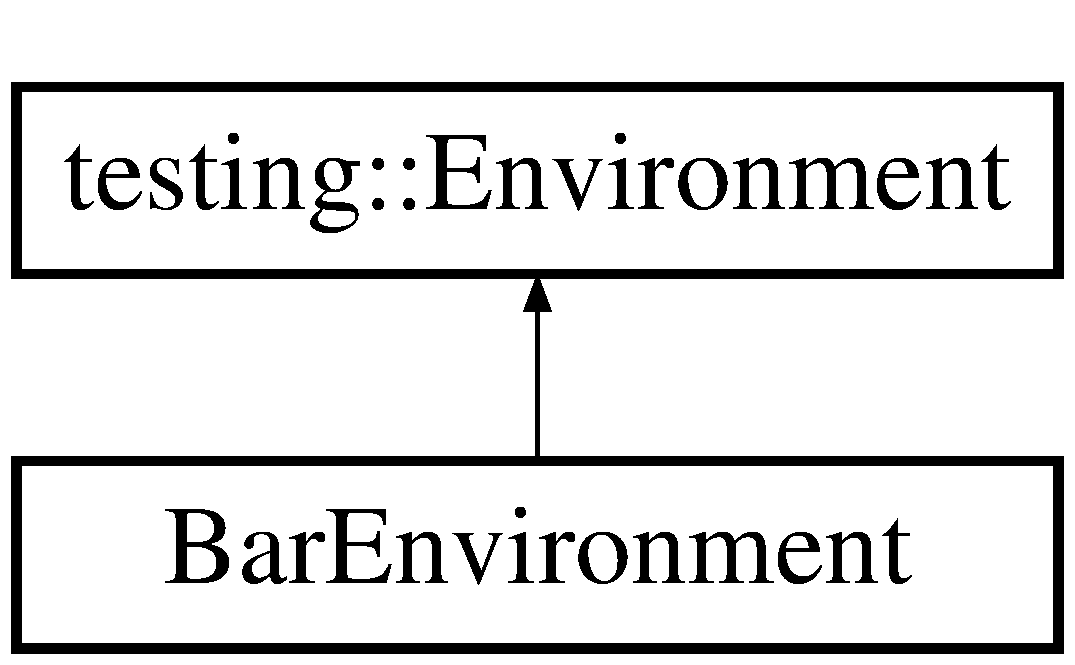
\includegraphics[height=2.000000cm]{class_bar_environment}
\end{center}
\end{figure}
\subsection*{Public Member Functions}
\begin{DoxyCompactItemize}
\item 
virtual void \hyperlink{class_bar_environment_a88e17c5dd1dcea7a4538f2f3c6bf7bdd}{Set\+Up} ()
\item 
virtual void \hyperlink{class_bar_environment_a384f951da72a2a18bb0c2b3506376b09}{Tear\+Down} ()
\end{DoxyCompactItemize}


\subsection{Member Function Documentation}
\hypertarget{class_bar_environment_a88e17c5dd1dcea7a4538f2f3c6bf7bdd}{}\index{Bar\+Environment@{Bar\+Environment}!Set\+Up@{Set\+Up}}
\index{Set\+Up@{Set\+Up}!Bar\+Environment@{Bar\+Environment}}
\subsubsection[{Set\+Up()}]{\setlength{\rightskip}{0pt plus 5cm}virtual void Bar\+Environment\+::\+Set\+Up (
\begin{DoxyParamCaption}
{}
\end{DoxyParamCaption}
)\hspace{0.3cm}{\ttfamily [inline]}, {\ttfamily [virtual]}}\label{class_bar_environment_a88e17c5dd1dcea7a4538f2f3c6bf7bdd}


Reimplemented from \hyperlink{classtesting_1_1_environment_a1bf8cafaa9d4eba9feb98655ee434eb3}{testing\+::\+Environment}.

\hypertarget{class_bar_environment_a384f951da72a2a18bb0c2b3506376b09}{}\index{Bar\+Environment@{Bar\+Environment}!Tear\+Down@{Tear\+Down}}
\index{Tear\+Down@{Tear\+Down}!Bar\+Environment@{Bar\+Environment}}
\subsubsection[{Tear\+Down()}]{\setlength{\rightskip}{0pt plus 5cm}virtual void Bar\+Environment\+::\+Tear\+Down (
\begin{DoxyParamCaption}
{}
\end{DoxyParamCaption}
)\hspace{0.3cm}{\ttfamily [inline]}, {\ttfamily [virtual]}}\label{class_bar_environment_a384f951da72a2a18bb0c2b3506376b09}


Reimplemented from \hyperlink{classtesting_1_1_environment_a039bdaa705c46b9b88234cf4d3bb6254}{testing\+::\+Environment}.



The documentation for this class was generated from the following file\+:\begin{DoxyCompactItemize}
\item 
C\+:/\+Users/\+Hilman/\+Desktop/repo/anjing/src/third\+\_\+party/googletest/test/\hyperlink{gtest__output__test___8cc}{gtest\+\_\+output\+\_\+test\+\_\+.\+cc}\end{DoxyCompactItemize}

\hypertarget{class_base}{}\section{Base Class Reference}
\label{class_base}\index{Base@{Base}}
Inheritance diagram for Base\+:\begin{figure}[H]
\begin{center}
\leavevmode
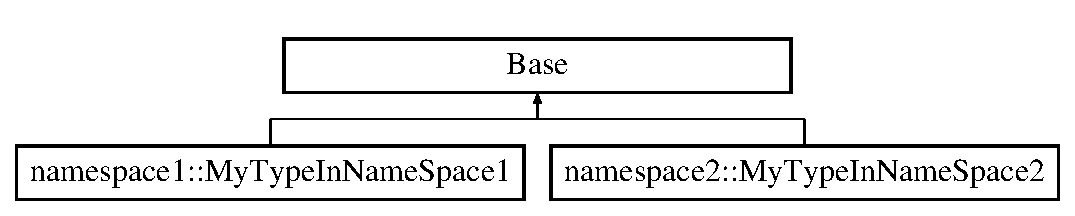
\includegraphics[height=2.000000cm]{class_base}
\end{center}
\end{figure}
\subsection*{Public Member Functions}
\begin{DoxyCompactItemize}
\item 
\hyperlink{class_base_a1d5f3fb92f8cbc687705785bdc6abd18}{Base} (int an\+\_\+x)
\item 
int \hyperlink{class_base_a963687d3b65f99407cc6f90172806fae}{x} () const 
\end{DoxyCompactItemize}


\subsection{Constructor \& Destructor Documentation}
\hypertarget{class_base_a1d5f3fb92f8cbc687705785bdc6abd18}{}\index{Base@{Base}!Base@{Base}}
\index{Base@{Base}!Base@{Base}}
\subsubsection[{Base(int an\+\_\+x)}]{\setlength{\rightskip}{0pt plus 5cm}Base\+::\+Base (
\begin{DoxyParamCaption}
\item[{int}]{an\+\_\+x}
\end{DoxyParamCaption}
)\hspace{0.3cm}{\ttfamily [inline]}, {\ttfamily [explicit]}}\label{class_base_a1d5f3fb92f8cbc687705785bdc6abd18}


\subsection{Member Function Documentation}
\hypertarget{class_base_a963687d3b65f99407cc6f90172806fae}{}\index{Base@{Base}!x@{x}}
\index{x@{x}!Base@{Base}}
\subsubsection[{x() const }]{\setlength{\rightskip}{0pt plus 5cm}int Base\+::x (
\begin{DoxyParamCaption}
{}
\end{DoxyParamCaption}
) const\hspace{0.3cm}{\ttfamily [inline]}}\label{class_base_a963687d3b65f99407cc6f90172806fae}


The documentation for this class was generated from the following file\+:\begin{DoxyCompactItemize}
\item 
C\+:/\+Users/\+Hilman/\+Desktop/repo/anjing/src/third\+\_\+party/googletest/test/\hyperlink{gtest__unittest_8cc}{gtest\+\_\+unittest.\+cc}\end{DoxyCompactItemize}

\hypertarget{classtesting_1_1internal_1_1_base}{}\section{testing\+:\+:internal\+:\+:Base Class Reference}
\label{classtesting_1_1internal_1_1_base}\index{testing\+::internal\+::\+Base@{testing\+::internal\+::\+Base}}
Inheritance diagram for testing\+:\+:internal\+:\+:Base\+:\begin{figure}[H]
\begin{center}
\leavevmode
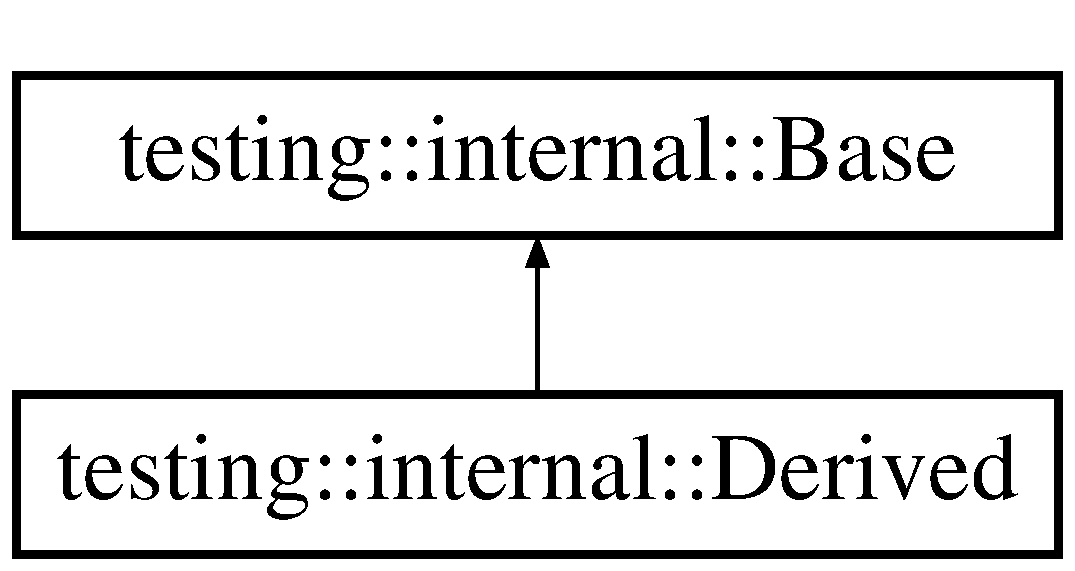
\includegraphics[height=2.000000cm]{classtesting_1_1internal_1_1_base}
\end{center}
\end{figure}
\subsection*{Public Member Functions}
\begin{DoxyCompactItemize}
\item 
\hyperlink{classtesting_1_1internal_1_1_base_a6b29f1a7192b126e6fa0aae31200b5ca}{Base} ()
\item 
\hyperlink{classtesting_1_1internal_1_1_base_a255d105410a1eeb5f4690c9c8cd8e104}{Base} (int n)
\item 
virtual \hyperlink{classtesting_1_1internal_1_1_base_afb29c9032fb50cc6520014aad9d68328}{$\sim$\+Base} ()
\item 
int \hyperlink{classtesting_1_1internal_1_1_base_a7ddba6221b56613be545544b7ef6214c}{member} ()
\end{DoxyCompactItemize}


\subsection{Constructor \& Destructor Documentation}
\hypertarget{classtesting_1_1internal_1_1_base_a6b29f1a7192b126e6fa0aae31200b5ca}{}\index{testing\+::internal\+::\+Base@{testing\+::internal\+::\+Base}!Base@{Base}}
\index{Base@{Base}!testing\+::internal\+::\+Base@{testing\+::internal\+::\+Base}}
\subsubsection[{Base()}]{\setlength{\rightskip}{0pt plus 5cm}testing\+::internal\+::\+Base\+::\+Base (
\begin{DoxyParamCaption}
{}
\end{DoxyParamCaption}
)\hspace{0.3cm}{\ttfamily [inline]}}\label{classtesting_1_1internal_1_1_base_a6b29f1a7192b126e6fa0aae31200b5ca}
\hypertarget{classtesting_1_1internal_1_1_base_a255d105410a1eeb5f4690c9c8cd8e104}{}\index{testing\+::internal\+::\+Base@{testing\+::internal\+::\+Base}!Base@{Base}}
\index{Base@{Base}!testing\+::internal\+::\+Base@{testing\+::internal\+::\+Base}}
\subsubsection[{Base(int n)}]{\setlength{\rightskip}{0pt plus 5cm}testing\+::internal\+::\+Base\+::\+Base (
\begin{DoxyParamCaption}
\item[{int}]{n}
\end{DoxyParamCaption}
)\hspace{0.3cm}{\ttfamily [inline]}, {\ttfamily [explicit]}}\label{classtesting_1_1internal_1_1_base_a255d105410a1eeb5f4690c9c8cd8e104}
\hypertarget{classtesting_1_1internal_1_1_base_afb29c9032fb50cc6520014aad9d68328}{}\index{testing\+::internal\+::\+Base@{testing\+::internal\+::\+Base}!````~Base@{$\sim$\+Base}}
\index{````~Base@{$\sim$\+Base}!testing\+::internal\+::\+Base@{testing\+::internal\+::\+Base}}
\subsubsection[{$\sim$\+Base()}]{\setlength{\rightskip}{0pt plus 5cm}virtual testing\+::internal\+::\+Base\+::$\sim$\+Base (
\begin{DoxyParamCaption}
{}
\end{DoxyParamCaption}
)\hspace{0.3cm}{\ttfamily [inline]}, {\ttfamily [virtual]}}\label{classtesting_1_1internal_1_1_base_afb29c9032fb50cc6520014aad9d68328}


\subsection{Member Function Documentation}
\hypertarget{classtesting_1_1internal_1_1_base_a7ddba6221b56613be545544b7ef6214c}{}\index{testing\+::internal\+::\+Base@{testing\+::internal\+::\+Base}!member@{member}}
\index{member@{member}!testing\+::internal\+::\+Base@{testing\+::internal\+::\+Base}}
\subsubsection[{member()}]{\setlength{\rightskip}{0pt plus 5cm}int testing\+::internal\+::\+Base\+::member (
\begin{DoxyParamCaption}
{}
\end{DoxyParamCaption}
)\hspace{0.3cm}{\ttfamily [inline]}}\label{classtesting_1_1internal_1_1_base_a7ddba6221b56613be545544b7ef6214c}


The documentation for this class was generated from the following file\+:\begin{DoxyCompactItemize}
\item 
C\+:/\+Users/\+Hilman/\+Desktop/repo/anjing/src/third\+\_\+party/googletest/test/\hyperlink{gtest-port__test_8cc}{gtest-\/port\+\_\+test.\+cc}\end{DoxyCompactItemize}

\hypertarget{structtesting_1_1gtest__printers__test_1_1_big}{}\section{testing\+:\+:gtest\+\_\+printers\+\_\+test\+:\+:Big Struct Reference}
\label{structtesting_1_1gtest__printers__test_1_1_big}\index{testing\+::gtest\+\_\+printers\+\_\+test\+::\+Big@{testing\+::gtest\+\_\+printers\+\_\+test\+::\+Big}}
\subsection*{Public Member Functions}
\begin{DoxyCompactItemize}
\item 
\hyperlink{structtesting_1_1gtest__printers__test_1_1_big_adb57fb0e14adb81177e3bfd7ed39966c}{Big} ()
\end{DoxyCompactItemize}
\subsection*{Public Attributes}
\begin{DoxyCompactItemize}
\item 
char \hyperlink{structtesting_1_1gtest__printers__test_1_1_big_a863911a8ec5c3bbe79c44d399f1de61f}{array} \mbox{[}257\mbox{]}
\end{DoxyCompactItemize}


\subsection{Constructor \& Destructor Documentation}
\hypertarget{structtesting_1_1gtest__printers__test_1_1_big_adb57fb0e14adb81177e3bfd7ed39966c}{}\index{testing\+::gtest\+\_\+printers\+\_\+test\+::\+Big@{testing\+::gtest\+\_\+printers\+\_\+test\+::\+Big}!Big@{Big}}
\index{Big@{Big}!testing\+::gtest\+\_\+printers\+\_\+test\+::\+Big@{testing\+::gtest\+\_\+printers\+\_\+test\+::\+Big}}
\subsubsection[{Big()}]{\setlength{\rightskip}{0pt plus 5cm}testing\+::gtest\+\_\+printers\+\_\+test\+::\+Big\+::\+Big (
\begin{DoxyParamCaption}
{}
\end{DoxyParamCaption}
)\hspace{0.3cm}{\ttfamily [inline]}}\label{structtesting_1_1gtest__printers__test_1_1_big_adb57fb0e14adb81177e3bfd7ed39966c}


\subsection{Member Data Documentation}
\hypertarget{structtesting_1_1gtest__printers__test_1_1_big_a863911a8ec5c3bbe79c44d399f1de61f}{}\index{testing\+::gtest\+\_\+printers\+\_\+test\+::\+Big@{testing\+::gtest\+\_\+printers\+\_\+test\+::\+Big}!array@{array}}
\index{array@{array}!testing\+::gtest\+\_\+printers\+\_\+test\+::\+Big@{testing\+::gtest\+\_\+printers\+\_\+test\+::\+Big}}
\subsubsection[{array}]{\setlength{\rightskip}{0pt plus 5cm}char testing\+::gtest\+\_\+printers\+\_\+test\+::\+Big\+::array\mbox{[}257\mbox{]}}\label{structtesting_1_1gtest__printers__test_1_1_big_a863911a8ec5c3bbe79c44d399f1de61f}


The documentation for this struct was generated from the following file\+:\begin{DoxyCompactItemize}
\item 
C\+:/\+Users/\+Hilman/\+Desktop/repo/anjing/src/third\+\_\+party/googletest/test/\hyperlink{gtest-printers__test_8cc}{gtest-\/printers\+\_\+test.\+cc}\end{DoxyCompactItemize}

\hypertarget{class_biggest_int_convertible}{}\section{Biggest\+Int\+Convertible Class Reference}
\label{class_biggest_int_convertible}\index{Biggest\+Int\+Convertible@{Biggest\+Int\+Convertible}}
\subsection*{Public Member Functions}
\begin{DoxyCompactItemize}
\item 
\hyperlink{class_biggest_int_convertible_ab8e66c4adee8172528c4070f19d47058}{operator\+::testing\+::internal\+::\+Biggest\+Int} () const 
\end{DoxyCompactItemize}


\subsection{Member Function Documentation}
\hypertarget{class_biggest_int_convertible_ab8e66c4adee8172528c4070f19d47058}{}\index{Biggest\+Int\+Convertible@{Biggest\+Int\+Convertible}!operator\+::testing\+::internal\+::\+Biggest\+Int@{operator\+::testing\+::internal\+::\+Biggest\+Int}}
\index{operator\+::testing\+::internal\+::\+Biggest\+Int@{operator\+::testing\+::internal\+::\+Biggest\+Int}!Biggest\+Int\+Convertible@{Biggest\+Int\+Convertible}}
\subsubsection[{operator\+::testing\+::internal\+::\+Biggest\+Int() const }]{\setlength{\rightskip}{0pt plus 5cm}Biggest\+Int\+Convertible\+::operator\+::testing\+::internal\+::\+Biggest\+Int (
\begin{DoxyParamCaption}
{}
\end{DoxyParamCaption}
) const\hspace{0.3cm}{\ttfamily [inline]}}\label{class_biggest_int_convertible_ab8e66c4adee8172528c4070f19d47058}


The documentation for this class was generated from the following file\+:\begin{DoxyCompactItemize}
\item 
C\+:/\+Users/\+Hilman/\+Desktop/repo/anjing/src/third\+\_\+party/googletest/test/\hyperlink{gtest-printers__test_8cc}{gtest-\/printers\+\_\+test.\+cc}\end{DoxyCompactItemize}

\hypertarget{struct_bool}{}\section{Bool Struct Reference}
\label{struct_bool}\index{Bool@{Bool}}
\subsection*{Public Member Functions}
\begin{DoxyCompactItemize}
\item 
\hyperlink{struct_bool_a03dfd4851b13abb29414887fcada7fca}{Bool} (int val)
\item 
bool \hyperlink{struct_bool_a812f0599da778aa0399cffa1a2687f6e}{operator$>$} (int n) const 
\item 
\hyperlink{struct_bool}{Bool} \hyperlink{struct_bool_a5d6f8c4a1def861f9b1c24e46b1228ca}{operator+} (const \hyperlink{struct_bool}{Bool} \&rhs) const 
\item 
bool \hyperlink{struct_bool_a1e885f75c224ea1fba1cbce11c888716}{operator==} (const \hyperlink{struct_bool}{Bool} \&rhs) const 
\end{DoxyCompactItemize}
\subsection*{Public Attributes}
\begin{DoxyCompactItemize}
\item 
bool \hyperlink{struct_bool_a16be863c269f988cdcbe59f9d846a141}{value}
\end{DoxyCompactItemize}


\subsection{Constructor \& Destructor Documentation}
\hypertarget{struct_bool_a03dfd4851b13abb29414887fcada7fca}{}\index{Bool@{Bool}!Bool@{Bool}}
\index{Bool@{Bool}!Bool@{Bool}}
\subsubsection[{Bool(int val)}]{\setlength{\rightskip}{0pt plus 5cm}Bool\+::\+Bool (
\begin{DoxyParamCaption}
\item[{int}]{val}
\end{DoxyParamCaption}
)\hspace{0.3cm}{\ttfamily [inline]}, {\ttfamily [explicit]}}\label{struct_bool_a03dfd4851b13abb29414887fcada7fca}


\subsection{Member Function Documentation}
\hypertarget{struct_bool_a5d6f8c4a1def861f9b1c24e46b1228ca}{}\index{Bool@{Bool}!operator+@{operator+}}
\index{operator+@{operator+}!Bool@{Bool}}
\subsubsection[{operator+(const Bool \&rhs) const }]{\setlength{\rightskip}{0pt plus 5cm}{\bf Bool} Bool\+::operator+ (
\begin{DoxyParamCaption}
\item[{const {\bf Bool} \&}]{rhs}
\end{DoxyParamCaption}
) const\hspace{0.3cm}{\ttfamily [inline]}}\label{struct_bool_a5d6f8c4a1def861f9b1c24e46b1228ca}
\hypertarget{struct_bool_a1e885f75c224ea1fba1cbce11c888716}{}\index{Bool@{Bool}!operator==@{operator==}}
\index{operator==@{operator==}!Bool@{Bool}}
\subsubsection[{operator==(const Bool \&rhs) const }]{\setlength{\rightskip}{0pt plus 5cm}bool Bool\+::operator== (
\begin{DoxyParamCaption}
\item[{const {\bf Bool} \&}]{rhs}
\end{DoxyParamCaption}
) const\hspace{0.3cm}{\ttfamily [inline]}}\label{struct_bool_a1e885f75c224ea1fba1cbce11c888716}
\hypertarget{struct_bool_a812f0599da778aa0399cffa1a2687f6e}{}\index{Bool@{Bool}!operator$>$@{operator$>$}}
\index{operator$>$@{operator$>$}!Bool@{Bool}}
\subsubsection[{operator$>$(int n) const }]{\setlength{\rightskip}{0pt plus 5cm}bool Bool\+::operator$>$ (
\begin{DoxyParamCaption}
\item[{int}]{n}
\end{DoxyParamCaption}
) const\hspace{0.3cm}{\ttfamily [inline]}}\label{struct_bool_a812f0599da778aa0399cffa1a2687f6e}


\subsection{Member Data Documentation}
\hypertarget{struct_bool_a16be863c269f988cdcbe59f9d846a141}{}\index{Bool@{Bool}!value@{value}}
\index{value@{value}!Bool@{Bool}}
\subsubsection[{value}]{\setlength{\rightskip}{0pt plus 5cm}bool Bool\+::value}\label{struct_bool_a16be863c269f988cdcbe59f9d846a141}


The documentation for this struct was generated from the following file\+:\begin{DoxyCompactItemize}
\item 
C\+:/\+Users/\+Hilman/\+Desktop/repo/anjing/src/third\+\_\+party/googletest/test/\hyperlink{gtest__pred__impl__unittest_8cc}{gtest\+\_\+pred\+\_\+impl\+\_\+unittest.\+cc}\end{DoxyCompactItemize}

\hypertarget{structtesting_1_1internal_1_1bool__constant}{}\section{testing\+:\+:internal\+:\+:bool\+\_\+constant$<$ bool\+\_\+value $>$ Struct Template Reference}
\label{structtesting_1_1internal_1_1bool__constant}\index{testing\+::internal\+::bool\+\_\+constant$<$ bool\+\_\+value $>$@{testing\+::internal\+::bool\+\_\+constant$<$ bool\+\_\+value $>$}}


{\ttfamily \#include $<$gtest-\/port.\+h$>$}

Inheritance diagram for testing\+:\+:internal\+:\+:bool\+\_\+constant$<$ bool\+\_\+value $>$\+:\begin{figure}[H]
\begin{center}
\leavevmode
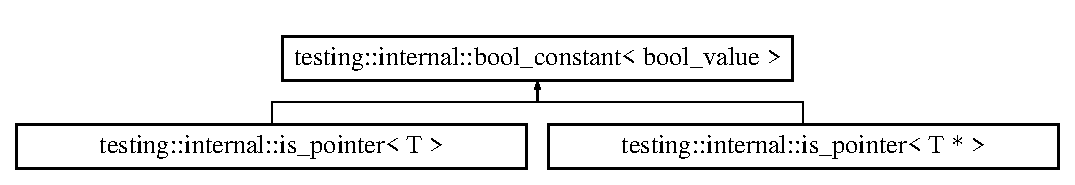
\includegraphics[height=2.000000cm]{structtesting_1_1internal_1_1bool__constant}
\end{center}
\end{figure}
\subsection*{Public Types}
\begin{DoxyCompactItemize}
\item 
typedef \hyperlink{structtesting_1_1internal_1_1bool__constant}{bool\+\_\+constant}$<$ bool\+\_\+value $>$ \hyperlink{structtesting_1_1internal_1_1bool__constant_aba6d09ecf7eecea6c93480f0d627a167}{type}
\end{DoxyCompactItemize}
\subsection*{Static Public Attributes}
\begin{DoxyCompactItemize}
\item 
static const bool \hyperlink{structtesting_1_1internal_1_1bool__constant_a499fba6576296b04d99690a486424b32}{value} = bool\+\_\+value
\end{DoxyCompactItemize}


\subsection{Member Typedef Documentation}
\hypertarget{structtesting_1_1internal_1_1bool__constant_aba6d09ecf7eecea6c93480f0d627a167}{}\index{testing\+::internal\+::bool\+\_\+constant@{testing\+::internal\+::bool\+\_\+constant}!type@{type}}
\index{type@{type}!testing\+::internal\+::bool\+\_\+constant@{testing\+::internal\+::bool\+\_\+constant}}
\subsubsection[{type}]{\setlength{\rightskip}{0pt plus 5cm}template$<$bool bool\+\_\+value$>$ typedef {\bf bool\+\_\+constant}$<$bool\+\_\+value$>$ {\bf testing\+::internal\+::bool\+\_\+constant}$<$ bool\+\_\+value $>$\+::{\bf type}}\label{structtesting_1_1internal_1_1bool__constant_aba6d09ecf7eecea6c93480f0d627a167}


\subsection{Member Data Documentation}
\hypertarget{structtesting_1_1internal_1_1bool__constant_a499fba6576296b04d99690a486424b32}{}\index{testing\+::internal\+::bool\+\_\+constant@{testing\+::internal\+::bool\+\_\+constant}!value@{value}}
\index{value@{value}!testing\+::internal\+::bool\+\_\+constant@{testing\+::internal\+::bool\+\_\+constant}}
\subsubsection[{value}]{\setlength{\rightskip}{0pt plus 5cm}template$<$bool bool\+\_\+value$>$ const bool {\bf testing\+::internal\+::bool\+\_\+constant}$<$ bool\+\_\+value $>$\+::value = bool\+\_\+value\hspace{0.3cm}{\ttfamily [static]}}\label{structtesting_1_1internal_1_1bool__constant_a499fba6576296b04d99690a486424b32}


The documentation for this struct was generated from the following file\+:\begin{DoxyCompactItemize}
\item 
C\+:/\+Users/\+Hilman/\+Desktop/repo/anjing/src/third\+\_\+party/googletest/include/gtest/internal/\hyperlink{gtest-port_8h}{gtest-\/port.\+h}\end{DoxyCompactItemize}

\hypertarget{structstd_1_1tr1_1_1gtest__internal_1_1_by_ref}{}\section{std\+:\+:tr1\+:\+:gtest\+\_\+internal\+:\+:By\+Ref$<$ T $>$ Struct Template Reference}
\label{structstd_1_1tr1_1_1gtest__internal_1_1_by_ref}\index{std\+::tr1\+::gtest\+\_\+internal\+::\+By\+Ref$<$ T $>$@{std\+::tr1\+::gtest\+\_\+internal\+::\+By\+Ref$<$ T $>$}}


{\ttfamily \#include $<$gtest-\/tuple.\+h$>$}

\subsection*{Public Types}
\begin{DoxyCompactItemize}
\item 
typedef const T \& \hyperlink{structstd_1_1tr1_1_1gtest__internal_1_1_by_ref_ac42ad942ee1cfa86b2abcce9b88ac10e}{type}
\end{DoxyCompactItemize}


\subsection{Member Typedef Documentation}
\hypertarget{structstd_1_1tr1_1_1gtest__internal_1_1_by_ref_ac42ad942ee1cfa86b2abcce9b88ac10e}{}\index{std\+::tr1\+::gtest\+\_\+internal\+::\+By\+Ref@{std\+::tr1\+::gtest\+\_\+internal\+::\+By\+Ref}!type@{type}}
\index{type@{type}!std\+::tr1\+::gtest\+\_\+internal\+::\+By\+Ref@{std\+::tr1\+::gtest\+\_\+internal\+::\+By\+Ref}}
\subsubsection[{type}]{\setlength{\rightskip}{0pt plus 5cm}template$<$typename T $>$ typedef const T\& {\bf std\+::tr1\+::gtest\+\_\+internal\+::\+By\+Ref}$<$ T $>$\+::{\bf type}}\label{structstd_1_1tr1_1_1gtest__internal_1_1_by_ref_ac42ad942ee1cfa86b2abcce9b88ac10e}


The documentation for this struct was generated from the following file\+:\begin{DoxyCompactItemize}
\item 
C\+:/\+Users/\+Hilman/\+Desktop/repo/anjing/src/third\+\_\+party/googletest/include/gtest/internal/\hyperlink{gtest-tuple_8h}{gtest-\/tuple.\+h}\end{DoxyCompactItemize}

\hypertarget{structstd_1_1tr1_1_1gtest__internal_1_1_by_ref_3_01_t_01_6_01_4}{}\section{std\+:\+:tr1\+:\+:gtest\+\_\+internal\+:\+:By\+Ref$<$ T \& $>$ Struct Template Reference}
\label{structstd_1_1tr1_1_1gtest__internal_1_1_by_ref_3_01_t_01_6_01_4}\index{std\+::tr1\+::gtest\+\_\+internal\+::\+By\+Ref$<$ T \& $>$@{std\+::tr1\+::gtest\+\_\+internal\+::\+By\+Ref$<$ T \& $>$}}


{\ttfamily \#include $<$gtest-\/tuple.\+h$>$}

\subsection*{Public Types}
\begin{DoxyCompactItemize}
\item 
typedef T \& \hyperlink{structstd_1_1tr1_1_1gtest__internal_1_1_by_ref_3_01_t_01_6_01_4_a512382574dbdd736320d68e313801122}{type}
\end{DoxyCompactItemize}


\subsection{Member Typedef Documentation}
\hypertarget{structstd_1_1tr1_1_1gtest__internal_1_1_by_ref_3_01_t_01_6_01_4_a512382574dbdd736320d68e313801122}{}\index{std\+::tr1\+::gtest\+\_\+internal\+::\+By\+Ref$<$ T \& $>$@{std\+::tr1\+::gtest\+\_\+internal\+::\+By\+Ref$<$ T \& $>$}!type@{type}}
\index{type@{type}!std\+::tr1\+::gtest\+\_\+internal\+::\+By\+Ref$<$ T \& $>$@{std\+::tr1\+::gtest\+\_\+internal\+::\+By\+Ref$<$ T \& $>$}}
\subsubsection[{type}]{\setlength{\rightskip}{0pt plus 5cm}template$<$typename T $>$ typedef T\& {\bf std\+::tr1\+::gtest\+\_\+internal\+::\+By\+Ref}$<$ T \& $>$\+::{\bf type}}\label{structstd_1_1tr1_1_1gtest__internal_1_1_by_ref_3_01_t_01_6_01_4_a512382574dbdd736320d68e313801122}


The documentation for this struct was generated from the following file\+:\begin{DoxyCompactItemize}
\item 
C\+:/\+Users/\+Hilman/\+Desktop/repo/anjing/src/third\+\_\+party/googletest/include/gtest/internal/\hyperlink{gtest-tuple_8h}{gtest-\/tuple.\+h}\end{DoxyCompactItemize}

\hypertarget{classtesting_1_1internal_1_1_castable}{}\section{testing\+:\+:internal\+:\+:Castable Class Reference}
\label{classtesting_1_1internal_1_1_castable}\index{testing\+::internal\+::\+Castable@{testing\+::internal\+::\+Castable}}
\subsection*{Public Member Functions}
\begin{DoxyCompactItemize}
\item 
\hyperlink{classtesting_1_1internal_1_1_castable_a705d519a227d38ff5c174905316f62c4}{Castable} (bool $\ast$converted)
\item 
\hyperlink{classtesting_1_1internal_1_1_castable_ac60b2e7885f3b09defb829eddaa0afd9}{operator Base} ()
\end{DoxyCompactItemize}


\subsection{Constructor \& Destructor Documentation}
\hypertarget{classtesting_1_1internal_1_1_castable_a705d519a227d38ff5c174905316f62c4}{}\index{testing\+::internal\+::\+Castable@{testing\+::internal\+::\+Castable}!Castable@{Castable}}
\index{Castable@{Castable}!testing\+::internal\+::\+Castable@{testing\+::internal\+::\+Castable}}
\subsubsection[{Castable(bool $\ast$converted)}]{\setlength{\rightskip}{0pt plus 5cm}testing\+::internal\+::\+Castable\+::\+Castable (
\begin{DoxyParamCaption}
\item[{bool $\ast$}]{converted}
\end{DoxyParamCaption}
)\hspace{0.3cm}{\ttfamily [inline]}, {\ttfamily [explicit]}}\label{classtesting_1_1internal_1_1_castable_a705d519a227d38ff5c174905316f62c4}


\subsection{Member Function Documentation}
\hypertarget{classtesting_1_1internal_1_1_castable_ac60b2e7885f3b09defb829eddaa0afd9}{}\index{testing\+::internal\+::\+Castable@{testing\+::internal\+::\+Castable}!operator Base@{operator Base}}
\index{operator Base@{operator Base}!testing\+::internal\+::\+Castable@{testing\+::internal\+::\+Castable}}
\subsubsection[{operator Base()}]{\setlength{\rightskip}{0pt plus 5cm}testing\+::internal\+::\+Castable\+::operator {\bf Base} (
\begin{DoxyParamCaption}
{}
\end{DoxyParamCaption}
)\hspace{0.3cm}{\ttfamily [inline]}}\label{classtesting_1_1internal_1_1_castable_ac60b2e7885f3b09defb829eddaa0afd9}


The documentation for this class was generated from the following file\+:\begin{DoxyCompactItemize}
\item 
C\+:/\+Users/\+Hilman/\+Desktop/repo/anjing/src/third\+\_\+party/googletest/test/\hyperlink{gtest-port__test_8cc}{gtest-\/port\+\_\+test.\+cc}\end{DoxyCompactItemize}

\hypertarget{classgtest__catch__exceptions__test_1_1_catch_cxx_exceptions_test}{}\section{gtest\+\_\+catch\+\_\+exceptions\+\_\+test.\+Catch\+Cxx\+Exceptions\+Test Class Reference}
\label{classgtest__catch__exceptions__test_1_1_catch_cxx_exceptions_test}\index{gtest\+\_\+catch\+\_\+exceptions\+\_\+test.\+Catch\+Cxx\+Exceptions\+Test@{gtest\+\_\+catch\+\_\+exceptions\+\_\+test.\+Catch\+Cxx\+Exceptions\+Test}}
Inheritance diagram for gtest\+\_\+catch\+\_\+exceptions\+\_\+test.\+Catch\+Cxx\+Exceptions\+Test\+:\begin{figure}[H]
\begin{center}
\leavevmode
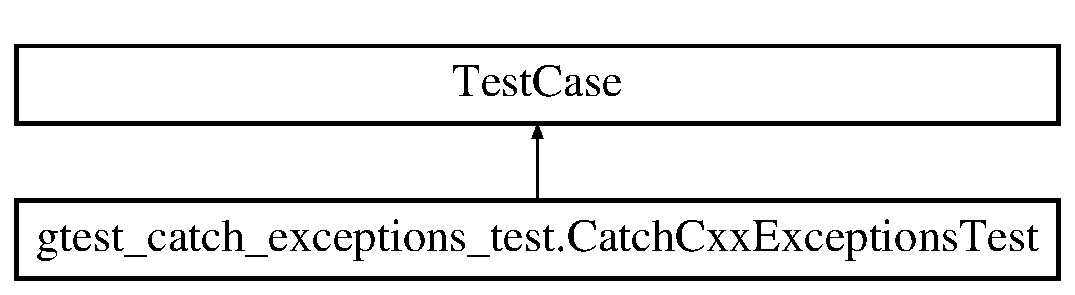
\includegraphics[height=2.000000cm]{classgtest__catch__exceptions__test_1_1_catch_cxx_exceptions_test}
\end{center}
\end{figure}
\subsection*{Public Member Functions}
\begin{DoxyCompactItemize}
\item 
def \hyperlink{classgtest__catch__exceptions__test_1_1_catch_cxx_exceptions_test_a7d02a890df0e3990aa107288c21f7dc7}{test\+Catches\+Cxx\+Exceptions\+In\+Fixture\+Constructor} (self)
\item 
def \hyperlink{classgtest__catch__exceptions__test_1_1_catch_cxx_exceptions_test_a3fe17da71b72c1693fa358f71c6b31be}{test\+Catches\+Cxx\+Exceptions\+In\+Fixture\+Destructor} (self)
\item 
def \hyperlink{classgtest__catch__exceptions__test_1_1_catch_cxx_exceptions_test_a8e791760b553d92490005deea0812f44}{test\+Catches\+Cxx\+Exceptions\+In\+Set\+Up\+Test\+Case} (self)
\item 
def \hyperlink{classgtest__catch__exceptions__test_1_1_catch_cxx_exceptions_test_a56c906c34e689ee016ab1bf14fe5220c}{test\+Catches\+Cxx\+Exceptions\+In\+Tear\+Down\+Test\+Case} (self)
\item 
def \hyperlink{classgtest__catch__exceptions__test_1_1_catch_cxx_exceptions_test_a6451307941e063bcc3927992c1f2df54}{test\+Catches\+Cxx\+Exceptions\+In\+Set\+Up} (self)
\item 
def \hyperlink{classgtest__catch__exceptions__test_1_1_catch_cxx_exceptions_test_a40ba50bf018753b7b21ed93ed60e4e1c}{test\+Catches\+Cxx\+Exceptions\+In\+Tear\+Down} (self)
\item 
def \hyperlink{classgtest__catch__exceptions__test_1_1_catch_cxx_exceptions_test_ac73b336590a3d1c242124e9ea5464a42}{test\+Catches\+Cxx\+Exceptions\+In\+Test\+Body} (self)
\item 
def \hyperlink{classgtest__catch__exceptions__test_1_1_catch_cxx_exceptions_test_a922cb0b598034924c19e6695cc9f7513}{test\+Catches\+Non\+Std\+Cxx\+Exceptions} (self)
\item 
def \hyperlink{classgtest__catch__exceptions__test_1_1_catch_cxx_exceptions_test_af3a794d5af0b3d72789293531468050a}{test\+Unhandled\+Cxx\+Exceptions\+Abort\+The\+Program} (self)
\end{DoxyCompactItemize}


\subsection{Detailed Description}
\begin{DoxyVerb}Tests C++ exception-catching behavior.

   Tests in this test case verify that:
   * C++ exceptions are caught and logged as C++ (not SEH) exceptions
   * Exception thrown affect the remainder of the test work flow in the
     expected manner.
\end{DoxyVerb}
 

\subsection{Member Function Documentation}
\hypertarget{classgtest__catch__exceptions__test_1_1_catch_cxx_exceptions_test_a7d02a890df0e3990aa107288c21f7dc7}{}\index{gtest\+\_\+catch\+\_\+exceptions\+\_\+test\+::\+Catch\+Cxx\+Exceptions\+Test@{gtest\+\_\+catch\+\_\+exceptions\+\_\+test\+::\+Catch\+Cxx\+Exceptions\+Test}!test\+Catches\+Cxx\+Exceptions\+In\+Fixture\+Constructor@{test\+Catches\+Cxx\+Exceptions\+In\+Fixture\+Constructor}}
\index{test\+Catches\+Cxx\+Exceptions\+In\+Fixture\+Constructor@{test\+Catches\+Cxx\+Exceptions\+In\+Fixture\+Constructor}!gtest\+\_\+catch\+\_\+exceptions\+\_\+test\+::\+Catch\+Cxx\+Exceptions\+Test@{gtest\+\_\+catch\+\_\+exceptions\+\_\+test\+::\+Catch\+Cxx\+Exceptions\+Test}}
\subsubsection[{test\+Catches\+Cxx\+Exceptions\+In\+Fixture\+Constructor(self)}]{\setlength{\rightskip}{0pt plus 5cm}def gtest\+\_\+catch\+\_\+exceptions\+\_\+test.\+Catch\+Cxx\+Exceptions\+Test.\+test\+Catches\+Cxx\+Exceptions\+In\+Fixture\+Constructor (
\begin{DoxyParamCaption}
\item[{}]{self}
\end{DoxyParamCaption}
)}\label{classgtest__catch__exceptions__test_1_1_catch_cxx_exceptions_test_a7d02a890df0e3990aa107288c21f7dc7}
\hypertarget{classgtest__catch__exceptions__test_1_1_catch_cxx_exceptions_test_a3fe17da71b72c1693fa358f71c6b31be}{}\index{gtest\+\_\+catch\+\_\+exceptions\+\_\+test\+::\+Catch\+Cxx\+Exceptions\+Test@{gtest\+\_\+catch\+\_\+exceptions\+\_\+test\+::\+Catch\+Cxx\+Exceptions\+Test}!test\+Catches\+Cxx\+Exceptions\+In\+Fixture\+Destructor@{test\+Catches\+Cxx\+Exceptions\+In\+Fixture\+Destructor}}
\index{test\+Catches\+Cxx\+Exceptions\+In\+Fixture\+Destructor@{test\+Catches\+Cxx\+Exceptions\+In\+Fixture\+Destructor}!gtest\+\_\+catch\+\_\+exceptions\+\_\+test\+::\+Catch\+Cxx\+Exceptions\+Test@{gtest\+\_\+catch\+\_\+exceptions\+\_\+test\+::\+Catch\+Cxx\+Exceptions\+Test}}
\subsubsection[{test\+Catches\+Cxx\+Exceptions\+In\+Fixture\+Destructor(self)}]{\setlength{\rightskip}{0pt plus 5cm}def gtest\+\_\+catch\+\_\+exceptions\+\_\+test.\+Catch\+Cxx\+Exceptions\+Test.\+test\+Catches\+Cxx\+Exceptions\+In\+Fixture\+Destructor (
\begin{DoxyParamCaption}
\item[{}]{self}
\end{DoxyParamCaption}
)}\label{classgtest__catch__exceptions__test_1_1_catch_cxx_exceptions_test_a3fe17da71b72c1693fa358f71c6b31be}
\hypertarget{classgtest__catch__exceptions__test_1_1_catch_cxx_exceptions_test_a6451307941e063bcc3927992c1f2df54}{}\index{gtest\+\_\+catch\+\_\+exceptions\+\_\+test\+::\+Catch\+Cxx\+Exceptions\+Test@{gtest\+\_\+catch\+\_\+exceptions\+\_\+test\+::\+Catch\+Cxx\+Exceptions\+Test}!test\+Catches\+Cxx\+Exceptions\+In\+Set\+Up@{test\+Catches\+Cxx\+Exceptions\+In\+Set\+Up}}
\index{test\+Catches\+Cxx\+Exceptions\+In\+Set\+Up@{test\+Catches\+Cxx\+Exceptions\+In\+Set\+Up}!gtest\+\_\+catch\+\_\+exceptions\+\_\+test\+::\+Catch\+Cxx\+Exceptions\+Test@{gtest\+\_\+catch\+\_\+exceptions\+\_\+test\+::\+Catch\+Cxx\+Exceptions\+Test}}
\subsubsection[{test\+Catches\+Cxx\+Exceptions\+In\+Set\+Up(self)}]{\setlength{\rightskip}{0pt plus 5cm}def gtest\+\_\+catch\+\_\+exceptions\+\_\+test.\+Catch\+Cxx\+Exceptions\+Test.\+test\+Catches\+Cxx\+Exceptions\+In\+Set\+Up (
\begin{DoxyParamCaption}
\item[{}]{self}
\end{DoxyParamCaption}
)}\label{classgtest__catch__exceptions__test_1_1_catch_cxx_exceptions_test_a6451307941e063bcc3927992c1f2df54}
\hypertarget{classgtest__catch__exceptions__test_1_1_catch_cxx_exceptions_test_a8e791760b553d92490005deea0812f44}{}\index{gtest\+\_\+catch\+\_\+exceptions\+\_\+test\+::\+Catch\+Cxx\+Exceptions\+Test@{gtest\+\_\+catch\+\_\+exceptions\+\_\+test\+::\+Catch\+Cxx\+Exceptions\+Test}!test\+Catches\+Cxx\+Exceptions\+In\+Set\+Up\+Test\+Case@{test\+Catches\+Cxx\+Exceptions\+In\+Set\+Up\+Test\+Case}}
\index{test\+Catches\+Cxx\+Exceptions\+In\+Set\+Up\+Test\+Case@{test\+Catches\+Cxx\+Exceptions\+In\+Set\+Up\+Test\+Case}!gtest\+\_\+catch\+\_\+exceptions\+\_\+test\+::\+Catch\+Cxx\+Exceptions\+Test@{gtest\+\_\+catch\+\_\+exceptions\+\_\+test\+::\+Catch\+Cxx\+Exceptions\+Test}}
\subsubsection[{test\+Catches\+Cxx\+Exceptions\+In\+Set\+Up\+Test\+Case(self)}]{\setlength{\rightskip}{0pt plus 5cm}def gtest\+\_\+catch\+\_\+exceptions\+\_\+test.\+Catch\+Cxx\+Exceptions\+Test.\+test\+Catches\+Cxx\+Exceptions\+In\+Set\+Up\+Test\+Case (
\begin{DoxyParamCaption}
\item[{}]{self}
\end{DoxyParamCaption}
)}\label{classgtest__catch__exceptions__test_1_1_catch_cxx_exceptions_test_a8e791760b553d92490005deea0812f44}
\hypertarget{classgtest__catch__exceptions__test_1_1_catch_cxx_exceptions_test_a40ba50bf018753b7b21ed93ed60e4e1c}{}\index{gtest\+\_\+catch\+\_\+exceptions\+\_\+test\+::\+Catch\+Cxx\+Exceptions\+Test@{gtest\+\_\+catch\+\_\+exceptions\+\_\+test\+::\+Catch\+Cxx\+Exceptions\+Test}!test\+Catches\+Cxx\+Exceptions\+In\+Tear\+Down@{test\+Catches\+Cxx\+Exceptions\+In\+Tear\+Down}}
\index{test\+Catches\+Cxx\+Exceptions\+In\+Tear\+Down@{test\+Catches\+Cxx\+Exceptions\+In\+Tear\+Down}!gtest\+\_\+catch\+\_\+exceptions\+\_\+test\+::\+Catch\+Cxx\+Exceptions\+Test@{gtest\+\_\+catch\+\_\+exceptions\+\_\+test\+::\+Catch\+Cxx\+Exceptions\+Test}}
\subsubsection[{test\+Catches\+Cxx\+Exceptions\+In\+Tear\+Down(self)}]{\setlength{\rightskip}{0pt plus 5cm}def gtest\+\_\+catch\+\_\+exceptions\+\_\+test.\+Catch\+Cxx\+Exceptions\+Test.\+test\+Catches\+Cxx\+Exceptions\+In\+Tear\+Down (
\begin{DoxyParamCaption}
\item[{}]{self}
\end{DoxyParamCaption}
)}\label{classgtest__catch__exceptions__test_1_1_catch_cxx_exceptions_test_a40ba50bf018753b7b21ed93ed60e4e1c}
\hypertarget{classgtest__catch__exceptions__test_1_1_catch_cxx_exceptions_test_a56c906c34e689ee016ab1bf14fe5220c}{}\index{gtest\+\_\+catch\+\_\+exceptions\+\_\+test\+::\+Catch\+Cxx\+Exceptions\+Test@{gtest\+\_\+catch\+\_\+exceptions\+\_\+test\+::\+Catch\+Cxx\+Exceptions\+Test}!test\+Catches\+Cxx\+Exceptions\+In\+Tear\+Down\+Test\+Case@{test\+Catches\+Cxx\+Exceptions\+In\+Tear\+Down\+Test\+Case}}
\index{test\+Catches\+Cxx\+Exceptions\+In\+Tear\+Down\+Test\+Case@{test\+Catches\+Cxx\+Exceptions\+In\+Tear\+Down\+Test\+Case}!gtest\+\_\+catch\+\_\+exceptions\+\_\+test\+::\+Catch\+Cxx\+Exceptions\+Test@{gtest\+\_\+catch\+\_\+exceptions\+\_\+test\+::\+Catch\+Cxx\+Exceptions\+Test}}
\subsubsection[{test\+Catches\+Cxx\+Exceptions\+In\+Tear\+Down\+Test\+Case(self)}]{\setlength{\rightskip}{0pt plus 5cm}def gtest\+\_\+catch\+\_\+exceptions\+\_\+test.\+Catch\+Cxx\+Exceptions\+Test.\+test\+Catches\+Cxx\+Exceptions\+In\+Tear\+Down\+Test\+Case (
\begin{DoxyParamCaption}
\item[{}]{self}
\end{DoxyParamCaption}
)}\label{classgtest__catch__exceptions__test_1_1_catch_cxx_exceptions_test_a56c906c34e689ee016ab1bf14fe5220c}
\hypertarget{classgtest__catch__exceptions__test_1_1_catch_cxx_exceptions_test_ac73b336590a3d1c242124e9ea5464a42}{}\index{gtest\+\_\+catch\+\_\+exceptions\+\_\+test\+::\+Catch\+Cxx\+Exceptions\+Test@{gtest\+\_\+catch\+\_\+exceptions\+\_\+test\+::\+Catch\+Cxx\+Exceptions\+Test}!test\+Catches\+Cxx\+Exceptions\+In\+Test\+Body@{test\+Catches\+Cxx\+Exceptions\+In\+Test\+Body}}
\index{test\+Catches\+Cxx\+Exceptions\+In\+Test\+Body@{test\+Catches\+Cxx\+Exceptions\+In\+Test\+Body}!gtest\+\_\+catch\+\_\+exceptions\+\_\+test\+::\+Catch\+Cxx\+Exceptions\+Test@{gtest\+\_\+catch\+\_\+exceptions\+\_\+test\+::\+Catch\+Cxx\+Exceptions\+Test}}
\subsubsection[{test\+Catches\+Cxx\+Exceptions\+In\+Test\+Body(self)}]{\setlength{\rightskip}{0pt plus 5cm}def gtest\+\_\+catch\+\_\+exceptions\+\_\+test.\+Catch\+Cxx\+Exceptions\+Test.\+test\+Catches\+Cxx\+Exceptions\+In\+Test\+Body (
\begin{DoxyParamCaption}
\item[{}]{self}
\end{DoxyParamCaption}
)}\label{classgtest__catch__exceptions__test_1_1_catch_cxx_exceptions_test_ac73b336590a3d1c242124e9ea5464a42}
\hypertarget{classgtest__catch__exceptions__test_1_1_catch_cxx_exceptions_test_a922cb0b598034924c19e6695cc9f7513}{}\index{gtest\+\_\+catch\+\_\+exceptions\+\_\+test\+::\+Catch\+Cxx\+Exceptions\+Test@{gtest\+\_\+catch\+\_\+exceptions\+\_\+test\+::\+Catch\+Cxx\+Exceptions\+Test}!test\+Catches\+Non\+Std\+Cxx\+Exceptions@{test\+Catches\+Non\+Std\+Cxx\+Exceptions}}
\index{test\+Catches\+Non\+Std\+Cxx\+Exceptions@{test\+Catches\+Non\+Std\+Cxx\+Exceptions}!gtest\+\_\+catch\+\_\+exceptions\+\_\+test\+::\+Catch\+Cxx\+Exceptions\+Test@{gtest\+\_\+catch\+\_\+exceptions\+\_\+test\+::\+Catch\+Cxx\+Exceptions\+Test}}
\subsubsection[{test\+Catches\+Non\+Std\+Cxx\+Exceptions(self)}]{\setlength{\rightskip}{0pt plus 5cm}def gtest\+\_\+catch\+\_\+exceptions\+\_\+test.\+Catch\+Cxx\+Exceptions\+Test.\+test\+Catches\+Non\+Std\+Cxx\+Exceptions (
\begin{DoxyParamCaption}
\item[{}]{self}
\end{DoxyParamCaption}
)}\label{classgtest__catch__exceptions__test_1_1_catch_cxx_exceptions_test_a922cb0b598034924c19e6695cc9f7513}
\hypertarget{classgtest__catch__exceptions__test_1_1_catch_cxx_exceptions_test_af3a794d5af0b3d72789293531468050a}{}\index{gtest\+\_\+catch\+\_\+exceptions\+\_\+test\+::\+Catch\+Cxx\+Exceptions\+Test@{gtest\+\_\+catch\+\_\+exceptions\+\_\+test\+::\+Catch\+Cxx\+Exceptions\+Test}!test\+Unhandled\+Cxx\+Exceptions\+Abort\+The\+Program@{test\+Unhandled\+Cxx\+Exceptions\+Abort\+The\+Program}}
\index{test\+Unhandled\+Cxx\+Exceptions\+Abort\+The\+Program@{test\+Unhandled\+Cxx\+Exceptions\+Abort\+The\+Program}!gtest\+\_\+catch\+\_\+exceptions\+\_\+test\+::\+Catch\+Cxx\+Exceptions\+Test@{gtest\+\_\+catch\+\_\+exceptions\+\_\+test\+::\+Catch\+Cxx\+Exceptions\+Test}}
\subsubsection[{test\+Unhandled\+Cxx\+Exceptions\+Abort\+The\+Program(self)}]{\setlength{\rightskip}{0pt plus 5cm}def gtest\+\_\+catch\+\_\+exceptions\+\_\+test.\+Catch\+Cxx\+Exceptions\+Test.\+test\+Unhandled\+Cxx\+Exceptions\+Abort\+The\+Program (
\begin{DoxyParamCaption}
\item[{}]{self}
\end{DoxyParamCaption}
)}\label{classgtest__catch__exceptions__test_1_1_catch_cxx_exceptions_test_af3a794d5af0b3d72789293531468050a}


The documentation for this class was generated from the following file\+:\begin{DoxyCompactItemize}
\item 
C\+:/\+Users/\+Hilman/\+Desktop/repo/anjing/src/third\+\_\+party/googletest/test/\hyperlink{gtest__catch__exceptions__test_8py}{gtest\+\_\+catch\+\_\+exceptions\+\_\+test.\+py}\end{DoxyCompactItemize}

\hypertarget{classgtest__catch__exceptions__test_1_1_catch_seh_exceptions_test}{}\section{gtest\+\_\+catch\+\_\+exceptions\+\_\+test.\+Catch\+Seh\+Exceptions\+Test Class Reference}
\label{classgtest__catch__exceptions__test_1_1_catch_seh_exceptions_test}\index{gtest\+\_\+catch\+\_\+exceptions\+\_\+test.\+Catch\+Seh\+Exceptions\+Test@{gtest\+\_\+catch\+\_\+exceptions\+\_\+test.\+Catch\+Seh\+Exceptions\+Test}}
Inheritance diagram for gtest\+\_\+catch\+\_\+exceptions\+\_\+test.\+Catch\+Seh\+Exceptions\+Test\+:\begin{figure}[H]
\begin{center}
\leavevmode
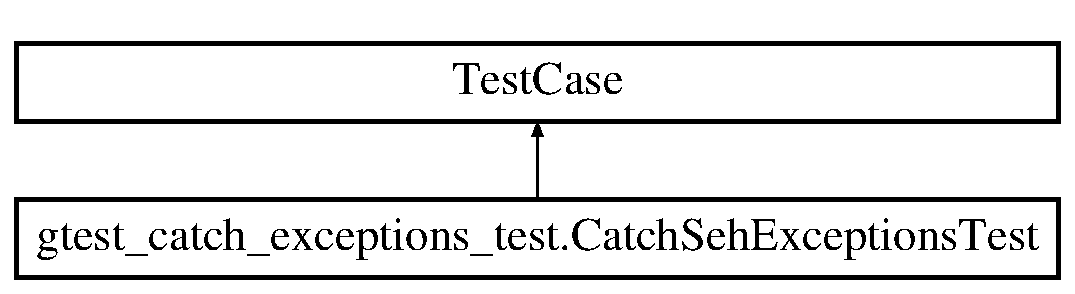
\includegraphics[height=2.000000cm]{classgtest__catch__exceptions__test_1_1_catch_seh_exceptions_test}
\end{center}
\end{figure}
\subsection*{Public Member Functions}
\begin{DoxyCompactItemize}
\item 
def \hyperlink{classgtest__catch__exceptions__test_1_1_catch_seh_exceptions_test_a737bbcc64405854aa8e0aea87ca5850b}{Test\+Seh\+Exceptions} (self, test\+\_\+output)
\item 
def \hyperlink{classgtest__catch__exceptions__test_1_1_catch_seh_exceptions_test_a02d06790fb52416a9da6a28b624e9cd9}{test\+Catches\+Seh\+Exceptions\+With\+Cxx\+Exceptions\+Enabled} (self)
\item 
def \hyperlink{classgtest__catch__exceptions__test_1_1_catch_seh_exceptions_test_a4a181de9de2b147eff55ed7a1d7d40c4}{test\+Catches\+Seh\+Exceptions\+With\+Cxx\+Exceptions\+Disabled} (self)
\end{DoxyCompactItemize}


\subsection{Detailed Description}
\begin{DoxyVerb}Tests exception-catching behavior.\end{DoxyVerb}
 

\subsection{Member Function Documentation}
\hypertarget{classgtest__catch__exceptions__test_1_1_catch_seh_exceptions_test_a4a181de9de2b147eff55ed7a1d7d40c4}{}\index{gtest\+\_\+catch\+\_\+exceptions\+\_\+test\+::\+Catch\+Seh\+Exceptions\+Test@{gtest\+\_\+catch\+\_\+exceptions\+\_\+test\+::\+Catch\+Seh\+Exceptions\+Test}!test\+Catches\+Seh\+Exceptions\+With\+Cxx\+Exceptions\+Disabled@{test\+Catches\+Seh\+Exceptions\+With\+Cxx\+Exceptions\+Disabled}}
\index{test\+Catches\+Seh\+Exceptions\+With\+Cxx\+Exceptions\+Disabled@{test\+Catches\+Seh\+Exceptions\+With\+Cxx\+Exceptions\+Disabled}!gtest\+\_\+catch\+\_\+exceptions\+\_\+test\+::\+Catch\+Seh\+Exceptions\+Test@{gtest\+\_\+catch\+\_\+exceptions\+\_\+test\+::\+Catch\+Seh\+Exceptions\+Test}}
\subsubsection[{test\+Catches\+Seh\+Exceptions\+With\+Cxx\+Exceptions\+Disabled(self)}]{\setlength{\rightskip}{0pt plus 5cm}def gtest\+\_\+catch\+\_\+exceptions\+\_\+test.\+Catch\+Seh\+Exceptions\+Test.\+test\+Catches\+Seh\+Exceptions\+With\+Cxx\+Exceptions\+Disabled (
\begin{DoxyParamCaption}
\item[{}]{self}
\end{DoxyParamCaption}
)}\label{classgtest__catch__exceptions__test_1_1_catch_seh_exceptions_test_a4a181de9de2b147eff55ed7a1d7d40c4}
\hypertarget{classgtest__catch__exceptions__test_1_1_catch_seh_exceptions_test_a02d06790fb52416a9da6a28b624e9cd9}{}\index{gtest\+\_\+catch\+\_\+exceptions\+\_\+test\+::\+Catch\+Seh\+Exceptions\+Test@{gtest\+\_\+catch\+\_\+exceptions\+\_\+test\+::\+Catch\+Seh\+Exceptions\+Test}!test\+Catches\+Seh\+Exceptions\+With\+Cxx\+Exceptions\+Enabled@{test\+Catches\+Seh\+Exceptions\+With\+Cxx\+Exceptions\+Enabled}}
\index{test\+Catches\+Seh\+Exceptions\+With\+Cxx\+Exceptions\+Enabled@{test\+Catches\+Seh\+Exceptions\+With\+Cxx\+Exceptions\+Enabled}!gtest\+\_\+catch\+\_\+exceptions\+\_\+test\+::\+Catch\+Seh\+Exceptions\+Test@{gtest\+\_\+catch\+\_\+exceptions\+\_\+test\+::\+Catch\+Seh\+Exceptions\+Test}}
\subsubsection[{test\+Catches\+Seh\+Exceptions\+With\+Cxx\+Exceptions\+Enabled(self)}]{\setlength{\rightskip}{0pt plus 5cm}def gtest\+\_\+catch\+\_\+exceptions\+\_\+test.\+Catch\+Seh\+Exceptions\+Test.\+test\+Catches\+Seh\+Exceptions\+With\+Cxx\+Exceptions\+Enabled (
\begin{DoxyParamCaption}
\item[{}]{self}
\end{DoxyParamCaption}
)}\label{classgtest__catch__exceptions__test_1_1_catch_seh_exceptions_test_a02d06790fb52416a9da6a28b624e9cd9}
\hypertarget{classgtest__catch__exceptions__test_1_1_catch_seh_exceptions_test_a737bbcc64405854aa8e0aea87ca5850b}{}\index{gtest\+\_\+catch\+\_\+exceptions\+\_\+test\+::\+Catch\+Seh\+Exceptions\+Test@{gtest\+\_\+catch\+\_\+exceptions\+\_\+test\+::\+Catch\+Seh\+Exceptions\+Test}!Test\+Seh\+Exceptions@{Test\+Seh\+Exceptions}}
\index{Test\+Seh\+Exceptions@{Test\+Seh\+Exceptions}!gtest\+\_\+catch\+\_\+exceptions\+\_\+test\+::\+Catch\+Seh\+Exceptions\+Test@{gtest\+\_\+catch\+\_\+exceptions\+\_\+test\+::\+Catch\+Seh\+Exceptions\+Test}}
\subsubsection[{Test\+Seh\+Exceptions(self, test\+\_\+output)}]{\setlength{\rightskip}{0pt plus 5cm}def gtest\+\_\+catch\+\_\+exceptions\+\_\+test.\+Catch\+Seh\+Exceptions\+Test.\+Test\+Seh\+Exceptions (
\begin{DoxyParamCaption}
\item[{}]{self, }
\item[{}]{test\+\_\+output}
\end{DoxyParamCaption}
)}\label{classgtest__catch__exceptions__test_1_1_catch_seh_exceptions_test_a737bbcc64405854aa8e0aea87ca5850b}


The documentation for this class was generated from the following file\+:\begin{DoxyCompactItemize}
\item 
C\+:/\+Users/\+Hilman/\+Desktop/repo/anjing/src/third\+\_\+party/googletest/test/\hyperlink{gtest__catch__exceptions__test_8py}{gtest\+\_\+catch\+\_\+exceptions\+\_\+test.\+py}\end{DoxyCompactItemize}

\hypertarget{classupload_1_1_client_login_error}{}\section{upload.\+Client\+Login\+Error Class Reference}
\label{classupload_1_1_client_login_error}\index{upload.\+Client\+Login\+Error@{upload.\+Client\+Login\+Error}}
Inheritance diagram for upload.\+Client\+Login\+Error\+:\begin{figure}[H]
\begin{center}
\leavevmode
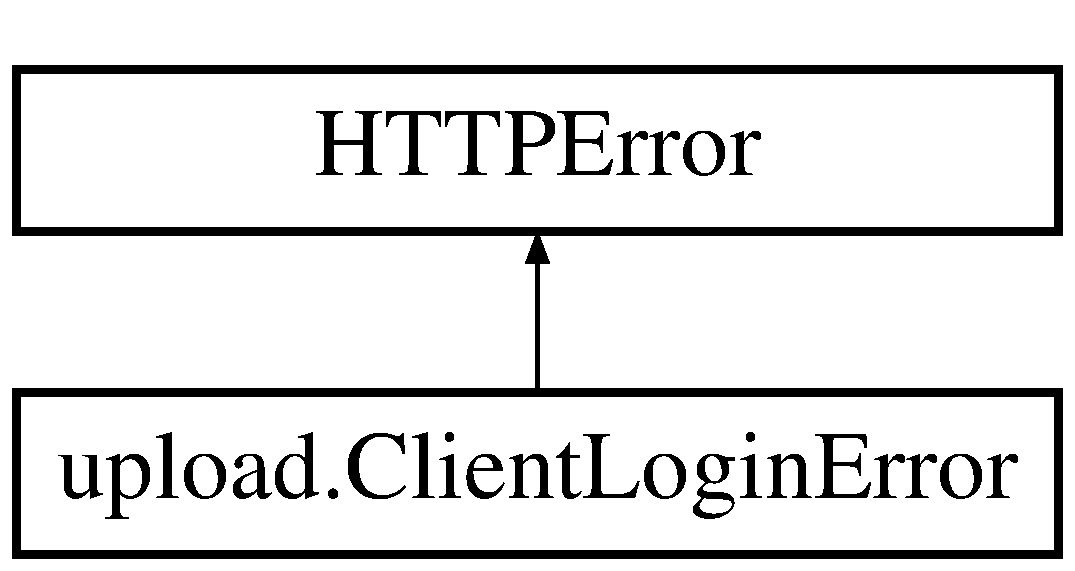
\includegraphics[height=2.000000cm]{classupload_1_1_client_login_error}
\end{center}
\end{figure}
\subsection*{Public Member Functions}
\begin{DoxyCompactItemize}
\item 
def \hyperlink{classupload_1_1_client_login_error_a1e590616c2976d881e155958cedbbe47}{\+\_\+\+\_\+init\+\_\+\+\_\+} (self, url, code, msg, headers, \hyperlink{classupload_1_1_client_login_error_ac300a0b034b2bc64cedc51e09fb6d663}{args})
\end{DoxyCompactItemize}
\subsection*{Public Attributes}
\begin{DoxyCompactItemize}
\item 
\hyperlink{classupload_1_1_client_login_error_ac300a0b034b2bc64cedc51e09fb6d663}{args}
\item 
\hyperlink{classupload_1_1_client_login_error_ae0555feb182d89d1e4d7944afbfe14e5}{reason}
\end{DoxyCompactItemize}


\subsection{Detailed Description}
\begin{DoxyVerb}Raised to indicate there was an error authenticating with ClientLogin.\end{DoxyVerb}
 

\subsection{Constructor \& Destructor Documentation}
\hypertarget{classupload_1_1_client_login_error_a1e590616c2976d881e155958cedbbe47}{}\index{upload\+::\+Client\+Login\+Error@{upload\+::\+Client\+Login\+Error}!\+\_\+\+\_\+init\+\_\+\+\_\+@{\+\_\+\+\_\+init\+\_\+\+\_\+}}
\index{\+\_\+\+\_\+init\+\_\+\+\_\+@{\+\_\+\+\_\+init\+\_\+\+\_\+}!upload\+::\+Client\+Login\+Error@{upload\+::\+Client\+Login\+Error}}
\subsubsection[{\+\_\+\+\_\+init\+\_\+\+\_\+(self, url, code, msg, headers, args)}]{\setlength{\rightskip}{0pt plus 5cm}def upload.\+Client\+Login\+Error.\+\_\+\+\_\+init\+\_\+\+\_\+ (
\begin{DoxyParamCaption}
\item[{}]{self, }
\item[{}]{url, }
\item[{}]{code, }
\item[{}]{msg, }
\item[{}]{headers, }
\item[{}]{args}
\end{DoxyParamCaption}
)}\label{classupload_1_1_client_login_error_a1e590616c2976d881e155958cedbbe47}


\subsection{Member Data Documentation}
\hypertarget{classupload_1_1_client_login_error_ac300a0b034b2bc64cedc51e09fb6d663}{}\index{upload\+::\+Client\+Login\+Error@{upload\+::\+Client\+Login\+Error}!args@{args}}
\index{args@{args}!upload\+::\+Client\+Login\+Error@{upload\+::\+Client\+Login\+Error}}
\subsubsection[{args}]{\setlength{\rightskip}{0pt plus 5cm}upload.\+Client\+Login\+Error.\+args}\label{classupload_1_1_client_login_error_ac300a0b034b2bc64cedc51e09fb6d663}
\hypertarget{classupload_1_1_client_login_error_ae0555feb182d89d1e4d7944afbfe14e5}{}\index{upload\+::\+Client\+Login\+Error@{upload\+::\+Client\+Login\+Error}!reason@{reason}}
\index{reason@{reason}!upload\+::\+Client\+Login\+Error@{upload\+::\+Client\+Login\+Error}}
\subsubsection[{reason}]{\setlength{\rightskip}{0pt plus 5cm}upload.\+Client\+Login\+Error.\+reason}\label{classupload_1_1_client_login_error_ae0555feb182d89d1e4d7944afbfe14e5}


The documentation for this class was generated from the following file\+:\begin{DoxyCompactItemize}
\item 
C\+:/\+Users/\+Hilman/\+Desktop/repo/anjing/src/third\+\_\+party/googletest/scripts/\hyperlink{upload_8py}{upload.\+py}\end{DoxyCompactItemize}

\hypertarget{classpump_1_1_code_node}{}\section{pump.\+Code\+Node Class Reference}
\label{classpump_1_1_code_node}\index{pump.\+Code\+Node@{pump.\+Code\+Node}}
\subsection*{Public Member Functions}
\begin{DoxyCompactItemize}
\item 
def \hyperlink{classpump_1_1_code_node_a0c5ed29f9d8b3192e29e51e933340de3}{\+\_\+\+\_\+init\+\_\+\+\_\+}
\end{DoxyCompactItemize}
\subsection*{Public Attributes}
\begin{DoxyCompactItemize}
\item 
\hyperlink{classpump_1_1_code_node_ac7251110cc987c709e0e17d95521993e}{atomic\+\_\+code}
\end{DoxyCompactItemize}


\subsection{Constructor \& Destructor Documentation}
\hypertarget{classpump_1_1_code_node_a0c5ed29f9d8b3192e29e51e933340de3}{}\index{pump\+::\+Code\+Node@{pump\+::\+Code\+Node}!\+\_\+\+\_\+init\+\_\+\+\_\+@{\+\_\+\+\_\+init\+\_\+\+\_\+}}
\index{\+\_\+\+\_\+init\+\_\+\+\_\+@{\+\_\+\+\_\+init\+\_\+\+\_\+}!pump\+::\+Code\+Node@{pump\+::\+Code\+Node}}
\subsubsection[{\+\_\+\+\_\+init\+\_\+\+\_\+}]{\setlength{\rightskip}{0pt plus 5cm}def pump.\+Code\+Node.\+\_\+\+\_\+init\+\_\+\+\_\+ (
\begin{DoxyParamCaption}
\item[{}]{self, }
\item[{}]{atomic\+\_\+code\+\_\+list = {\ttfamily None}}
\end{DoxyParamCaption}
)}\label{classpump_1_1_code_node_a0c5ed29f9d8b3192e29e51e933340de3}


\subsection{Member Data Documentation}
\hypertarget{classpump_1_1_code_node_ac7251110cc987c709e0e17d95521993e}{}\index{pump\+::\+Code\+Node@{pump\+::\+Code\+Node}!atomic\+\_\+code@{atomic\+\_\+code}}
\index{atomic\+\_\+code@{atomic\+\_\+code}!pump\+::\+Code\+Node@{pump\+::\+Code\+Node}}
\subsubsection[{atomic\+\_\+code}]{\setlength{\rightskip}{0pt plus 5cm}pump.\+Code\+Node.\+atomic\+\_\+code}\label{classpump_1_1_code_node_ac7251110cc987c709e0e17d95521993e}


The documentation for this class was generated from the following file\+:\begin{DoxyCompactItemize}
\item 
C\+:/\+Users/\+Hilman/\+Desktop/repo/anjing/src/third\+\_\+party/googletest/scripts/\hyperlink{pump_8py}{pump.\+py}\end{DoxyCompactItemize}

\hypertarget{class_common_test}{}\section{Common\+Test$<$ T $>$ Class Template Reference}
\label{class_common_test}\index{Common\+Test$<$ T $>$@{Common\+Test$<$ T $>$}}
Inheritance diagram for Common\+Test$<$ T $>$\+:\begin{figure}[H]
\begin{center}
\leavevmode
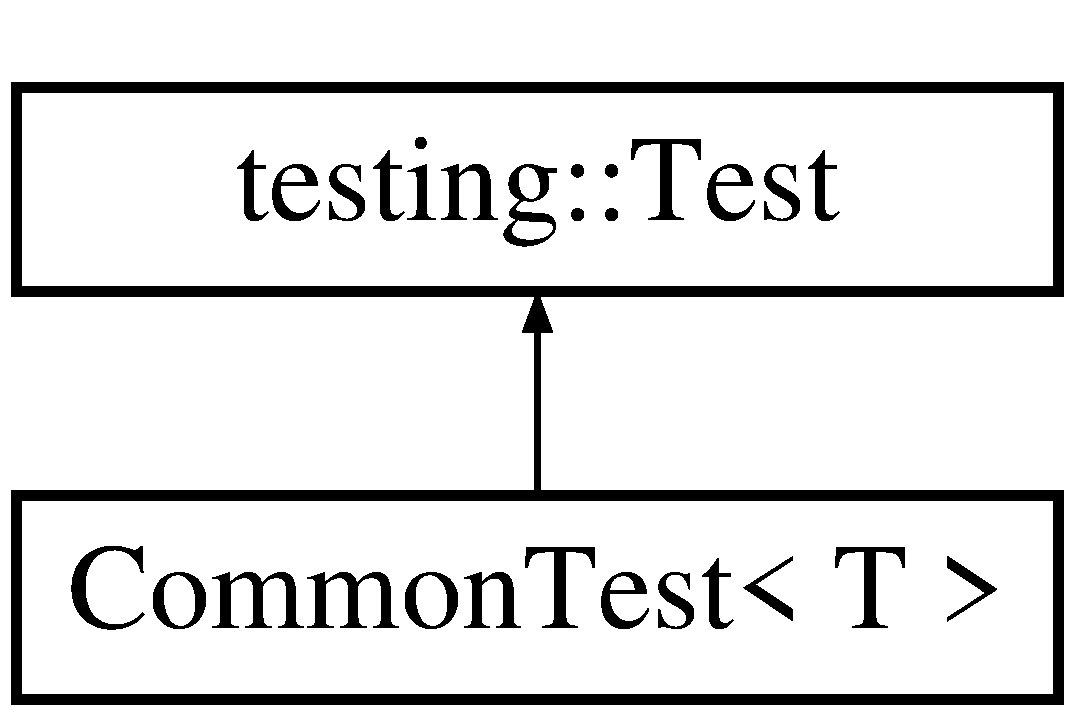
\includegraphics[height=2.000000cm]{class_common_test}
\end{center}
\end{figure}
\subsection*{Static Public Member Functions}
\begin{DoxyCompactItemize}
\item 
static void \hyperlink{class_common_test_a6edd90f32f45cc49e4a423b22bd770ce}{Set\+Up\+Test\+Case} ()
\item 
static void \hyperlink{class_common_test_a68d2bf5108cf28478331588fbdff4838}{Tear\+Down\+Test\+Case} ()
\end{DoxyCompactItemize}
\subsection*{Protected Types}
\begin{DoxyCompactItemize}
\item 
typedef std\+::vector$<$ T $>$ \hyperlink{class_common_test_a6dfdcede6964887b9f4254a0e0478e37}{Vector}
\item 
typedef std\+::set$<$ int $>$ \hyperlink{class_common_test_a62827e9d3064cddf4a8698747f1bd434}{Int\+Set}
\end{DoxyCompactItemize}
\subsection*{Protected Member Functions}
\begin{DoxyCompactItemize}
\item 
\hyperlink{class_common_test_abd5ec205d90f4b81efab2a6f972f3db0}{Common\+Test} ()
\item 
virtual \hyperlink{class_common_test_a675a632fcf7b1fd961fefc619d6a458d}{$\sim$\+Common\+Test} ()
\item 
virtual void \hyperlink{class_common_test_a4c7bf7889ce48a9d06530bc4a437f3f5}{Set\+Up} ()
\item 
virtual void \hyperlink{class_common_test_aeae195c2cefa956c6ae5be1226e6ecd8}{Tear\+Down} ()
\end{DoxyCompactItemize}
\subsection*{Protected Attributes}
\begin{DoxyCompactItemize}
\item 
T \hyperlink{class_common_test_ae59c4abcb833625a7baeb2048531ebec}{value\+\_\+}
\end{DoxyCompactItemize}
\subsection*{Static Protected Attributes}
\begin{DoxyCompactItemize}
\item 
static T $\ast$ \hyperlink{class_common_test_a52368ce1e65a865db9bdccbcc2cedaac}{shared\+\_\+} = N\+U\+L\+L
\end{DoxyCompactItemize}
\subsection*{Additional Inherited Members}


\subsection{Member Typedef Documentation}
\hypertarget{class_common_test_a62827e9d3064cddf4a8698747f1bd434}{}\index{Common\+Test@{Common\+Test}!Int\+Set@{Int\+Set}}
\index{Int\+Set@{Int\+Set}!Common\+Test@{Common\+Test}}
\subsubsection[{Int\+Set}]{\setlength{\rightskip}{0pt plus 5cm}template$<$typename T $>$ typedef std\+::set$<$int$>$ {\bf Common\+Test}$<$ T $>$\+::{\bf Int\+Set}\hspace{0.3cm}{\ttfamily [protected]}}\label{class_common_test_a62827e9d3064cddf4a8698747f1bd434}
\hypertarget{class_common_test_a6dfdcede6964887b9f4254a0e0478e37}{}\index{Common\+Test@{Common\+Test}!Vector@{Vector}}
\index{Vector@{Vector}!Common\+Test@{Common\+Test}}
\subsubsection[{Vector}]{\setlength{\rightskip}{0pt plus 5cm}template$<$typename T $>$ typedef std\+::vector$<$T$>$ {\bf Common\+Test}$<$ T $>$\+::{\bf Vector}\hspace{0.3cm}{\ttfamily [protected]}}\label{class_common_test_a6dfdcede6964887b9f4254a0e0478e37}


\subsection{Constructor \& Destructor Documentation}
\hypertarget{class_common_test_abd5ec205d90f4b81efab2a6f972f3db0}{}\index{Common\+Test@{Common\+Test}!Common\+Test@{Common\+Test}}
\index{Common\+Test@{Common\+Test}!Common\+Test@{Common\+Test}}
\subsubsection[{Common\+Test()}]{\setlength{\rightskip}{0pt plus 5cm}template$<$typename T $>$ {\bf Common\+Test}$<$ T $>$\+::{\bf Common\+Test} (
\begin{DoxyParamCaption}
{}
\end{DoxyParamCaption}
)\hspace{0.3cm}{\ttfamily [inline]}, {\ttfamily [protected]}}\label{class_common_test_abd5ec205d90f4b81efab2a6f972f3db0}
\hypertarget{class_common_test_a675a632fcf7b1fd961fefc619d6a458d}{}\index{Common\+Test@{Common\+Test}!````~Common\+Test@{$\sim$\+Common\+Test}}
\index{````~Common\+Test@{$\sim$\+Common\+Test}!Common\+Test@{Common\+Test}}
\subsubsection[{$\sim$\+Common\+Test()}]{\setlength{\rightskip}{0pt plus 5cm}template$<$typename T $>$ virtual {\bf Common\+Test}$<$ T $>$\+::$\sim${\bf Common\+Test} (
\begin{DoxyParamCaption}
{}
\end{DoxyParamCaption}
)\hspace{0.3cm}{\ttfamily [inline]}, {\ttfamily [protected]}, {\ttfamily [virtual]}}\label{class_common_test_a675a632fcf7b1fd961fefc619d6a458d}


\subsection{Member Function Documentation}
\hypertarget{class_common_test_a4c7bf7889ce48a9d06530bc4a437f3f5}{}\index{Common\+Test@{Common\+Test}!Set\+Up@{Set\+Up}}
\index{Set\+Up@{Set\+Up}!Common\+Test@{Common\+Test}}
\subsubsection[{Set\+Up()}]{\setlength{\rightskip}{0pt plus 5cm}template$<$typename T $>$ virtual void {\bf Common\+Test}$<$ T $>$\+::Set\+Up (
\begin{DoxyParamCaption}
{}
\end{DoxyParamCaption}
)\hspace{0.3cm}{\ttfamily [inline]}, {\ttfamily [protected]}, {\ttfamily [virtual]}}\label{class_common_test_a4c7bf7889ce48a9d06530bc4a437f3f5}


Reimplemented from \hyperlink{classtesting_1_1_test_a190315150c303ddf801313fd1a777733}{testing\+::\+Test}.

\hypertarget{class_common_test_a6edd90f32f45cc49e4a423b22bd770ce}{}\index{Common\+Test@{Common\+Test}!Set\+Up\+Test\+Case@{Set\+Up\+Test\+Case}}
\index{Set\+Up\+Test\+Case@{Set\+Up\+Test\+Case}!Common\+Test@{Common\+Test}}
\subsubsection[{Set\+Up\+Test\+Case()}]{\setlength{\rightskip}{0pt plus 5cm}template$<$typename T $>$ static void {\bf Common\+Test}$<$ T $>$\+::Set\+Up\+Test\+Case (
\begin{DoxyParamCaption}
{}
\end{DoxyParamCaption}
)\hspace{0.3cm}{\ttfamily [inline]}, {\ttfamily [static]}}\label{class_common_test_a6edd90f32f45cc49e4a423b22bd770ce}
\hypertarget{class_common_test_aeae195c2cefa956c6ae5be1226e6ecd8}{}\index{Common\+Test@{Common\+Test}!Tear\+Down@{Tear\+Down}}
\index{Tear\+Down@{Tear\+Down}!Common\+Test@{Common\+Test}}
\subsubsection[{Tear\+Down()}]{\setlength{\rightskip}{0pt plus 5cm}template$<$typename T $>$ virtual void {\bf Common\+Test}$<$ T $>$\+::Tear\+Down (
\begin{DoxyParamCaption}
{}
\end{DoxyParamCaption}
)\hspace{0.3cm}{\ttfamily [inline]}, {\ttfamily [protected]}, {\ttfamily [virtual]}}\label{class_common_test_aeae195c2cefa956c6ae5be1226e6ecd8}


Reimplemented from \hyperlink{classtesting_1_1_test_a5f0ab439802cbe0ef7552f1a9f791923}{testing\+::\+Test}.

\hypertarget{class_common_test_a68d2bf5108cf28478331588fbdff4838}{}\index{Common\+Test@{Common\+Test}!Tear\+Down\+Test\+Case@{Tear\+Down\+Test\+Case}}
\index{Tear\+Down\+Test\+Case@{Tear\+Down\+Test\+Case}!Common\+Test@{Common\+Test}}
\subsubsection[{Tear\+Down\+Test\+Case()}]{\setlength{\rightskip}{0pt plus 5cm}template$<$typename T $>$ static void {\bf Common\+Test}$<$ T $>$\+::Tear\+Down\+Test\+Case (
\begin{DoxyParamCaption}
{}
\end{DoxyParamCaption}
)\hspace{0.3cm}{\ttfamily [inline]}, {\ttfamily [static]}}\label{class_common_test_a68d2bf5108cf28478331588fbdff4838}


\subsection{Member Data Documentation}
\hypertarget{class_common_test_a52368ce1e65a865db9bdccbcc2cedaac}{}\index{Common\+Test@{Common\+Test}!shared\+\_\+@{shared\+\_\+}}
\index{shared\+\_\+@{shared\+\_\+}!Common\+Test@{Common\+Test}}
\subsubsection[{shared\+\_\+}]{\setlength{\rightskip}{0pt plus 5cm}template$<$typename T $>$ T $\ast$ {\bf Common\+Test}$<$ T $>$\+::shared\+\_\+ = N\+U\+L\+L\hspace{0.3cm}{\ttfamily [static]}, {\ttfamily [protected]}}\label{class_common_test_a52368ce1e65a865db9bdccbcc2cedaac}
\hypertarget{class_common_test_ae59c4abcb833625a7baeb2048531ebec}{}\index{Common\+Test@{Common\+Test}!value\+\_\+@{value\+\_\+}}
\index{value\+\_\+@{value\+\_\+}!Common\+Test@{Common\+Test}}
\subsubsection[{value\+\_\+}]{\setlength{\rightskip}{0pt plus 5cm}template$<$typename T $>$ T {\bf Common\+Test}$<$ T $>$\+::value\+\_\+\hspace{0.3cm}{\ttfamily [protected]}}\label{class_common_test_ae59c4abcb833625a7baeb2048531ebec}


The documentation for this class was generated from the following file\+:\begin{DoxyCompactItemize}
\item 
C\+:/\+Users/\+Hilman/\+Desktop/repo/anjing/src/third\+\_\+party/googletest/test/\hyperlink{gtest-typed-test__test_8cc}{gtest-\/typed-\/test\+\_\+test.\+cc}\end{DoxyCompactItemize}

\hypertarget{structtesting_1_1internal_1_1_compile_assert}{}\section{testing\+:\+:internal\+:\+:Compile\+Assert$<$ bool $>$ Struct Template Reference}
\label{structtesting_1_1internal_1_1_compile_assert}\index{testing\+::internal\+::\+Compile\+Assert$<$ bool $>$@{testing\+::internal\+::\+Compile\+Assert$<$ bool $>$}}


{\ttfamily \#include $<$gtest-\/port.\+h$>$}



The documentation for this struct was generated from the following file\+:\begin{DoxyCompactItemize}
\item 
C\+:/\+Users/\+Hilman/\+Desktop/repo/anjing/src/third\+\_\+party/googletest/include/gtest/internal/\hyperlink{gtest-port_8h}{gtest-\/port.\+h}\end{DoxyCompactItemize}

\hypertarget{structtesting_1_1internal_1_1_compile_assert_types_equal}{}\section{testing\+:\+:internal\+:\+:Compile\+Assert\+Types\+Equal$<$ T1, T2 $>$ Struct Template Reference}
\label{structtesting_1_1internal_1_1_compile_assert_types_equal}\index{testing\+::internal\+::\+Compile\+Assert\+Types\+Equal$<$ T1, T2 $>$@{testing\+::internal\+::\+Compile\+Assert\+Types\+Equal$<$ T1, T2 $>$}}


{\ttfamily \#include $<$gtest-\/internal.\+h$>$}



The documentation for this struct was generated from the following file\+:\begin{DoxyCompactItemize}
\item 
C\+:/\+Users/\+Hilman/\+Desktop/repo/anjing/src/third\+\_\+party/googletest/include/gtest/internal/\hyperlink{gtest-internal_8h}{gtest-\/internal.\+h}\end{DoxyCompactItemize}

\hypertarget{structtesting_1_1internal_1_1_compile_assert_types_equal_3_01_t_00_01_t_01_4}{}\section{testing\+:\+:internal\+:\+:Compile\+Assert\+Types\+Equal$<$ T, T $>$ Struct Template Reference}
\label{structtesting_1_1internal_1_1_compile_assert_types_equal_3_01_t_00_01_t_01_4}\index{testing\+::internal\+::\+Compile\+Assert\+Types\+Equal$<$ T, T $>$@{testing\+::internal\+::\+Compile\+Assert\+Types\+Equal$<$ T, T $>$}}


{\ttfamily \#include $<$gtest-\/internal.\+h$>$}



The documentation for this struct was generated from the following file\+:\begin{DoxyCompactItemize}
\item 
C\+:/\+Users/\+Hilman/\+Desktop/repo/anjing/src/third\+\_\+party/googletest/include/gtest/internal/\hyperlink{gtest-internal_8h}{gtest-\/internal.\+h}\end{DoxyCompactItemize}

\hypertarget{structtesting_1_1gtest__printers__test_1_1const__iterator}{}\section{testing\+:\+:gtest\+\_\+printers\+\_\+test\+:\+:const\+\_\+iterator Struct Reference}
\label{structtesting_1_1gtest__printers__test_1_1const__iterator}\index{testing\+::gtest\+\_\+printers\+\_\+test\+::const\+\_\+iterator@{testing\+::gtest\+\_\+printers\+\_\+test\+::const\+\_\+iterator}}
\subsection*{Public Attributes}
\begin{DoxyCompactItemize}
\item 
char \hyperlink{structtesting_1_1gtest__printers__test_1_1const__iterator_a4412dbc1c37c2bc5211971f0c8176d6b}{x}
\end{DoxyCompactItemize}


\subsection{Member Data Documentation}
\hypertarget{structtesting_1_1gtest__printers__test_1_1const__iterator_a4412dbc1c37c2bc5211971f0c8176d6b}{}\index{testing\+::gtest\+\_\+printers\+\_\+test\+::const\+\_\+iterator@{testing\+::gtest\+\_\+printers\+\_\+test\+::const\+\_\+iterator}!x@{x}}
\index{x@{x}!testing\+::gtest\+\_\+printers\+\_\+test\+::const\+\_\+iterator@{testing\+::gtest\+\_\+printers\+\_\+test\+::const\+\_\+iterator}}
\subsubsection[{x}]{\setlength{\rightskip}{0pt plus 5cm}char testing\+::gtest\+\_\+printers\+\_\+test\+::const\+\_\+iterator\+::x}\label{structtesting_1_1gtest__printers__test_1_1const__iterator_a4412dbc1c37c2bc5211971f0c8176d6b}


The documentation for this struct was generated from the following file\+:\begin{DoxyCompactItemize}
\item 
C\+:/\+Users/\+Hilman/\+Desktop/repo/anjing/src/third\+\_\+party/googletest/test/\hyperlink{gtest-printers__test_8cc}{gtest-\/printers\+\_\+test.\+cc}\end{DoxyCompactItemize}

\hypertarget{classtesting_1_1internal_1_1_const_and_non_const_castable}{}\section{testing\+:\+:internal\+:\+:Const\+And\+Non\+Const\+Castable Class Reference}
\label{classtesting_1_1internal_1_1_const_and_non_const_castable}\index{testing\+::internal\+::\+Const\+And\+Non\+Const\+Castable@{testing\+::internal\+::\+Const\+And\+Non\+Const\+Castable}}
\subsection*{Public Member Functions}
\begin{DoxyCompactItemize}
\item 
\hyperlink{classtesting_1_1internal_1_1_const_and_non_const_castable_aebe0ef6897b7f805e227bb969d4ee034}{Const\+And\+Non\+Const\+Castable} (bool $\ast$converted, bool $\ast$const\+\_\+converted)
\item 
\hyperlink{classtesting_1_1internal_1_1_const_and_non_const_castable_aff0c372d429d76d002bb29f83f2429fa}{operator Base} ()
\item 
\hyperlink{classtesting_1_1internal_1_1_const_and_non_const_castable_accd7e89982de250ed6c1b3ad1a5813df}{operator Base} () const 
\end{DoxyCompactItemize}


\subsection{Constructor \& Destructor Documentation}
\hypertarget{classtesting_1_1internal_1_1_const_and_non_const_castable_aebe0ef6897b7f805e227bb969d4ee034}{}\index{testing\+::internal\+::\+Const\+And\+Non\+Const\+Castable@{testing\+::internal\+::\+Const\+And\+Non\+Const\+Castable}!Const\+And\+Non\+Const\+Castable@{Const\+And\+Non\+Const\+Castable}}
\index{Const\+And\+Non\+Const\+Castable@{Const\+And\+Non\+Const\+Castable}!testing\+::internal\+::\+Const\+And\+Non\+Const\+Castable@{testing\+::internal\+::\+Const\+And\+Non\+Const\+Castable}}
\subsubsection[{Const\+And\+Non\+Const\+Castable(bool $\ast$converted, bool $\ast$const\+\_\+converted)}]{\setlength{\rightskip}{0pt plus 5cm}testing\+::internal\+::\+Const\+And\+Non\+Const\+Castable\+::\+Const\+And\+Non\+Const\+Castable (
\begin{DoxyParamCaption}
\item[{bool $\ast$}]{converted, }
\item[{bool $\ast$}]{const\+\_\+converted}
\end{DoxyParamCaption}
)\hspace{0.3cm}{\ttfamily [inline]}}\label{classtesting_1_1internal_1_1_const_and_non_const_castable_aebe0ef6897b7f805e227bb969d4ee034}


\subsection{Member Function Documentation}
\hypertarget{classtesting_1_1internal_1_1_const_and_non_const_castable_aff0c372d429d76d002bb29f83f2429fa}{}\index{testing\+::internal\+::\+Const\+And\+Non\+Const\+Castable@{testing\+::internal\+::\+Const\+And\+Non\+Const\+Castable}!operator Base@{operator Base}}
\index{operator Base@{operator Base}!testing\+::internal\+::\+Const\+And\+Non\+Const\+Castable@{testing\+::internal\+::\+Const\+And\+Non\+Const\+Castable}}
\subsubsection[{operator Base()}]{\setlength{\rightskip}{0pt plus 5cm}testing\+::internal\+::\+Const\+And\+Non\+Const\+Castable\+::operator {\bf Base} (
\begin{DoxyParamCaption}
{}
\end{DoxyParamCaption}
)\hspace{0.3cm}{\ttfamily [inline]}}\label{classtesting_1_1internal_1_1_const_and_non_const_castable_aff0c372d429d76d002bb29f83f2429fa}
\hypertarget{classtesting_1_1internal_1_1_const_and_non_const_castable_accd7e89982de250ed6c1b3ad1a5813df}{}\index{testing\+::internal\+::\+Const\+And\+Non\+Const\+Castable@{testing\+::internal\+::\+Const\+And\+Non\+Const\+Castable}!operator Base@{operator Base}}
\index{operator Base@{operator Base}!testing\+::internal\+::\+Const\+And\+Non\+Const\+Castable@{testing\+::internal\+::\+Const\+And\+Non\+Const\+Castable}}
\subsubsection[{operator Base() const }]{\setlength{\rightskip}{0pt plus 5cm}testing\+::internal\+::\+Const\+And\+Non\+Const\+Castable\+::operator {\bf Base} (
\begin{DoxyParamCaption}
{}
\end{DoxyParamCaption}
) const\hspace{0.3cm}{\ttfamily [inline]}}\label{classtesting_1_1internal_1_1_const_and_non_const_castable_accd7e89982de250ed6c1b3ad1a5813df}


The documentation for this class was generated from the following file\+:\begin{DoxyCompactItemize}
\item 
C\+:/\+Users/\+Hilman/\+Desktop/repo/anjing/src/third\+\_\+party/googletest/test/\hyperlink{gtest-port__test_8cc}{gtest-\/port\+\_\+test.\+cc}\end{DoxyCompactItemize}

\hypertarget{classtesting_1_1internal_1_1_const_castable}{}\section{testing\+:\+:internal\+:\+:Const\+Castable Class Reference}
\label{classtesting_1_1internal_1_1_const_castable}\index{testing\+::internal\+::\+Const\+Castable@{testing\+::internal\+::\+Const\+Castable}}
\subsection*{Public Member Functions}
\begin{DoxyCompactItemize}
\item 
\hyperlink{classtesting_1_1internal_1_1_const_castable_a78eba470cc71528237a33a10a92fba7e}{Const\+Castable} (bool $\ast$converted)
\item 
\hyperlink{classtesting_1_1internal_1_1_const_castable_ad25d1fcc7288a3cf9160620949e37712}{operator Base} () const 
\end{DoxyCompactItemize}


\subsection{Constructor \& Destructor Documentation}
\hypertarget{classtesting_1_1internal_1_1_const_castable_a78eba470cc71528237a33a10a92fba7e}{}\index{testing\+::internal\+::\+Const\+Castable@{testing\+::internal\+::\+Const\+Castable}!Const\+Castable@{Const\+Castable}}
\index{Const\+Castable@{Const\+Castable}!testing\+::internal\+::\+Const\+Castable@{testing\+::internal\+::\+Const\+Castable}}
\subsubsection[{Const\+Castable(bool $\ast$converted)}]{\setlength{\rightskip}{0pt plus 5cm}testing\+::internal\+::\+Const\+Castable\+::\+Const\+Castable (
\begin{DoxyParamCaption}
\item[{bool $\ast$}]{converted}
\end{DoxyParamCaption}
)\hspace{0.3cm}{\ttfamily [inline]}, {\ttfamily [explicit]}}\label{classtesting_1_1internal_1_1_const_castable_a78eba470cc71528237a33a10a92fba7e}


\subsection{Member Function Documentation}
\hypertarget{classtesting_1_1internal_1_1_const_castable_ad25d1fcc7288a3cf9160620949e37712}{}\index{testing\+::internal\+::\+Const\+Castable@{testing\+::internal\+::\+Const\+Castable}!operator Base@{operator Base}}
\index{operator Base@{operator Base}!testing\+::internal\+::\+Const\+Castable@{testing\+::internal\+::\+Const\+Castable}}
\subsubsection[{operator Base() const }]{\setlength{\rightskip}{0pt plus 5cm}testing\+::internal\+::\+Const\+Castable\+::operator {\bf Base} (
\begin{DoxyParamCaption}
{}
\end{DoxyParamCaption}
) const\hspace{0.3cm}{\ttfamily [inline]}}\label{classtesting_1_1internal_1_1_const_castable_ad25d1fcc7288a3cf9160620949e37712}


The documentation for this class was generated from the following file\+:\begin{DoxyCompactItemize}
\item 
C\+:/\+Users/\+Hilman/\+Desktop/repo/anjing/src/third\+\_\+party/googletest/test/\hyperlink{gtest-port__test_8cc}{gtest-\/port\+\_\+test.\+cc}\end{DoxyCompactItemize}

\hypertarget{structtesting_1_1internal_1_1_const_char_ptr}{}\section{testing\+:\+:internal\+:\+:Const\+Char\+Ptr Struct Reference}
\label{structtesting_1_1internal_1_1_const_char_ptr}\index{testing\+::internal\+::\+Const\+Char\+Ptr@{testing\+::internal\+::\+Const\+Char\+Ptr}}


{\ttfamily \#include $<$gtest-\/internal.\+h$>$}

\subsection*{Public Member Functions}
\begin{DoxyCompactItemize}
\item 
\hyperlink{structtesting_1_1internal_1_1_const_char_ptr_ae94f6453fa679d815994eccc63062907}{Const\+Char\+Ptr} (const char $\ast$str)
\item 
\hyperlink{structtesting_1_1internal_1_1_const_char_ptr_a891bc286350b81d1a147101c0bae5b1d}{operator bool} () const 
\end{DoxyCompactItemize}
\subsection*{Public Attributes}
\begin{DoxyCompactItemize}
\item 
const char $\ast$ \hyperlink{structtesting_1_1internal_1_1_const_char_ptr_adba40d23d5986904b605946f643cf26e}{value}
\end{DoxyCompactItemize}


\subsection{Constructor \& Destructor Documentation}
\hypertarget{structtesting_1_1internal_1_1_const_char_ptr_ae94f6453fa679d815994eccc63062907}{}\index{testing\+::internal\+::\+Const\+Char\+Ptr@{testing\+::internal\+::\+Const\+Char\+Ptr}!Const\+Char\+Ptr@{Const\+Char\+Ptr}}
\index{Const\+Char\+Ptr@{Const\+Char\+Ptr}!testing\+::internal\+::\+Const\+Char\+Ptr@{testing\+::internal\+::\+Const\+Char\+Ptr}}
\subsubsection[{Const\+Char\+Ptr(const char $\ast$str)}]{\setlength{\rightskip}{0pt plus 5cm}testing\+::internal\+::\+Const\+Char\+Ptr\+::\+Const\+Char\+Ptr (
\begin{DoxyParamCaption}
\item[{const char $\ast$}]{str}
\end{DoxyParamCaption}
)\hspace{0.3cm}{\ttfamily [inline]}}\label{structtesting_1_1internal_1_1_const_char_ptr_ae94f6453fa679d815994eccc63062907}


\subsection{Member Function Documentation}
\hypertarget{structtesting_1_1internal_1_1_const_char_ptr_a891bc286350b81d1a147101c0bae5b1d}{}\index{testing\+::internal\+::\+Const\+Char\+Ptr@{testing\+::internal\+::\+Const\+Char\+Ptr}!operator bool@{operator bool}}
\index{operator bool@{operator bool}!testing\+::internal\+::\+Const\+Char\+Ptr@{testing\+::internal\+::\+Const\+Char\+Ptr}}
\subsubsection[{operator bool() const }]{\setlength{\rightskip}{0pt plus 5cm}testing\+::internal\+::\+Const\+Char\+Ptr\+::operator bool (
\begin{DoxyParamCaption}
{}
\end{DoxyParamCaption}
) const\hspace{0.3cm}{\ttfamily [inline]}}\label{structtesting_1_1internal_1_1_const_char_ptr_a891bc286350b81d1a147101c0bae5b1d}


\subsection{Member Data Documentation}
\hypertarget{structtesting_1_1internal_1_1_const_char_ptr_adba40d23d5986904b605946f643cf26e}{}\index{testing\+::internal\+::\+Const\+Char\+Ptr@{testing\+::internal\+::\+Const\+Char\+Ptr}!value@{value}}
\index{value@{value}!testing\+::internal\+::\+Const\+Char\+Ptr@{testing\+::internal\+::\+Const\+Char\+Ptr}}
\subsubsection[{value}]{\setlength{\rightskip}{0pt plus 5cm}const char$\ast$ testing\+::internal\+::\+Const\+Char\+Ptr\+::value}\label{structtesting_1_1internal_1_1_const_char_ptr_adba40d23d5986904b605946f643cf26e}


The documentation for this struct was generated from the following file\+:\begin{DoxyCompactItemize}
\item 
C\+:/\+Users/\+Hilman/\+Desktop/repo/anjing/src/third\+\_\+party/googletest/include/gtest/internal/\hyperlink{gtest-internal_8h}{gtest-\/internal.\+h}\end{DoxyCompactItemize}

\hypertarget{class_conversion_helper_base}{}\section{Conversion\+Helper\+Base Class Reference}
\label{class_conversion_helper_base}\index{Conversion\+Helper\+Base@{Conversion\+Helper\+Base}}
Inheritance diagram for Conversion\+Helper\+Base\+:\begin{figure}[H]
\begin{center}
\leavevmode
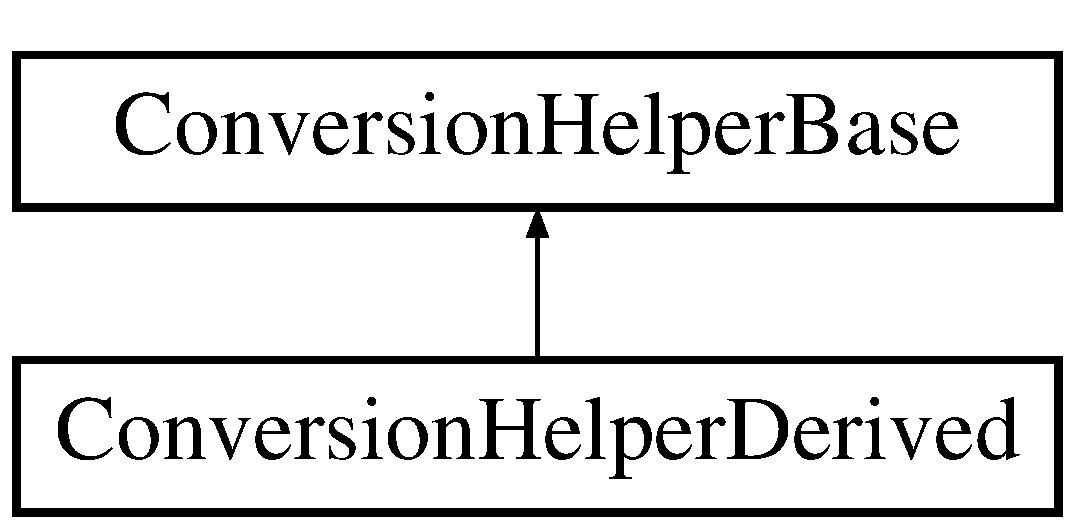
\includegraphics[height=2.000000cm]{class_conversion_helper_base}
\end{center}
\end{figure}


The documentation for this class was generated from the following file\+:\begin{DoxyCompactItemize}
\item 
C\+:/\+Users/\+Hilman/\+Desktop/repo/anjing/src/third\+\_\+party/googletest/test/\hyperlink{gtest__unittest_8cc}{gtest\+\_\+unittest.\+cc}\end{DoxyCompactItemize}

\hypertarget{class_conversion_helper_derived}{}\section{Conversion\+Helper\+Derived Class Reference}
\label{class_conversion_helper_derived}\index{Conversion\+Helper\+Derived@{Conversion\+Helper\+Derived}}
Inheritance diagram for Conversion\+Helper\+Derived\+:\begin{figure}[H]
\begin{center}
\leavevmode
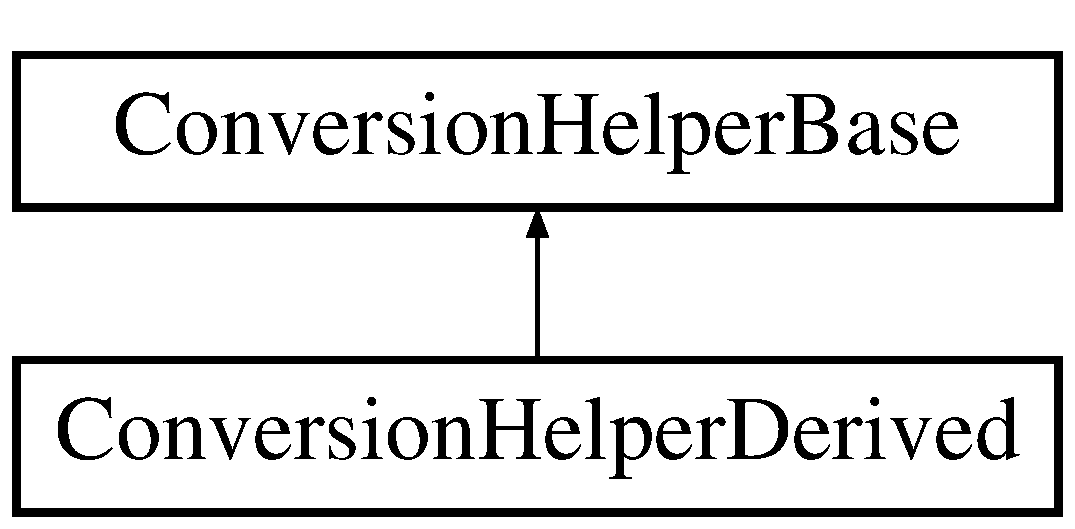
\includegraphics[height=2.000000cm]{class_conversion_helper_derived}
\end{center}
\end{figure}


The documentation for this class was generated from the following file\+:\begin{DoxyCompactItemize}
\item 
C\+:/\+Users/\+Hilman/\+Desktop/repo/anjing/src/third\+\_\+party/googletest/test/\hyperlink{gtest__unittest_8cc}{gtest\+\_\+unittest.\+cc}\end{DoxyCompactItemize}

\hypertarget{class_counter}{}\section{Counter Class Reference}
\label{class_counter}\index{Counter@{Counter}}


{\ttfamily \#include $<$sample4.\+h$>$}

\subsection*{Public Member Functions}
\begin{DoxyCompactItemize}
\item 
\hyperlink{class_counter_a1e05f69b5240fbab3e7ab351672167f0}{Counter} ()
\item 
int \hyperlink{class_counter_a0a0ca9fdb580a2aec9a5a62ebed2b5ab}{Increment} ()
\item 
void \hyperlink{class_counter_a435e7bc009682cea425e71acd490f3c4}{Print} () const 
\end{DoxyCompactItemize}


\subsection{Constructor \& Destructor Documentation}
\hypertarget{class_counter_a1e05f69b5240fbab3e7ab351672167f0}{}\index{Counter@{Counter}!Counter@{Counter}}
\index{Counter@{Counter}!Counter@{Counter}}
\subsubsection[{Counter()}]{\setlength{\rightskip}{0pt plus 5cm}Counter\+::\+Counter (
\begin{DoxyParamCaption}
{}
\end{DoxyParamCaption}
)\hspace{0.3cm}{\ttfamily [inline]}}\label{class_counter_a1e05f69b5240fbab3e7ab351672167f0}


\subsection{Member Function Documentation}
\hypertarget{class_counter_a0a0ca9fdb580a2aec9a5a62ebed2b5ab}{}\index{Counter@{Counter}!Increment@{Increment}}
\index{Increment@{Increment}!Counter@{Counter}}
\subsubsection[{Increment()}]{\setlength{\rightskip}{0pt plus 5cm}int Counter\+::\+Increment (
\begin{DoxyParamCaption}
{}
\end{DoxyParamCaption}
)}\label{class_counter_a0a0ca9fdb580a2aec9a5a62ebed2b5ab}
\hypertarget{class_counter_a435e7bc009682cea425e71acd490f3c4}{}\index{Counter@{Counter}!Print@{Print}}
\index{Print@{Print}!Counter@{Counter}}
\subsubsection[{Print() const }]{\setlength{\rightskip}{0pt plus 5cm}void Counter\+::\+Print (
\begin{DoxyParamCaption}
{}
\end{DoxyParamCaption}
) const}\label{class_counter_a435e7bc009682cea425e71acd490f3c4}


The documentation for this class was generated from the following files\+:\begin{DoxyCompactItemize}
\item 
C\+:/\+Users/\+Hilman/\+Desktop/repo/anjing/src/third\+\_\+party/googletest/samples/\hyperlink{sample4_8h}{sample4.\+h}\item 
C\+:/\+Users/\+Hilman/\+Desktop/repo/anjing/src/third\+\_\+party/googletest/samples/\hyperlink{sample4_8cc}{sample4.\+cc}\end{DoxyCompactItemize}

\hypertarget{classtesting_1_1_current_test_info_test}{}\section{testing\+:\+:Current\+Test\+Info\+Test Class Reference}
\label{classtesting_1_1_current_test_info_test}\index{testing\+::\+Current\+Test\+Info\+Test@{testing\+::\+Current\+Test\+Info\+Test}}
Inheritance diagram for testing\+:\+:Current\+Test\+Info\+Test\+:\begin{figure}[H]
\begin{center}
\leavevmode
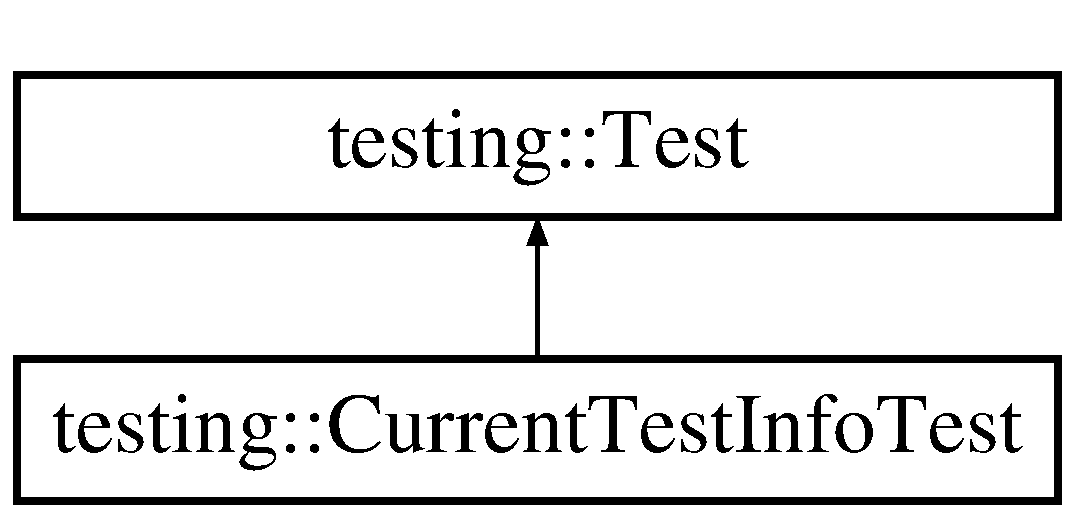
\includegraphics[height=2.000000cm]{classtesting_1_1_current_test_info_test}
\end{center}
\end{figure}
\subsection*{Static Protected Member Functions}
\begin{DoxyCompactItemize}
\item 
static void \hyperlink{classtesting_1_1_current_test_info_test_a61bad7ce29923afd464daf9684b6269e}{Set\+Up\+Test\+Case} ()
\item 
static void \hyperlink{classtesting_1_1_current_test_info_test_a9a80a5a3e6e70c619870c2ae9df892a6}{Tear\+Down\+Test\+Case} ()
\end{DoxyCompactItemize}
\subsection*{Additional Inherited Members}


\subsection{Member Function Documentation}
\hypertarget{classtesting_1_1_current_test_info_test_a61bad7ce29923afd464daf9684b6269e}{}\index{testing\+::\+Current\+Test\+Info\+Test@{testing\+::\+Current\+Test\+Info\+Test}!Set\+Up\+Test\+Case@{Set\+Up\+Test\+Case}}
\index{Set\+Up\+Test\+Case@{Set\+Up\+Test\+Case}!testing\+::\+Current\+Test\+Info\+Test@{testing\+::\+Current\+Test\+Info\+Test}}
\subsubsection[{Set\+Up\+Test\+Case()}]{\setlength{\rightskip}{0pt plus 5cm}static void testing\+::\+Current\+Test\+Info\+Test\+::\+Set\+Up\+Test\+Case (
\begin{DoxyParamCaption}
{}
\end{DoxyParamCaption}
)\hspace{0.3cm}{\ttfamily [inline]}, {\ttfamily [static]}, {\ttfamily [protected]}}\label{classtesting_1_1_current_test_info_test_a61bad7ce29923afd464daf9684b6269e}
\hypertarget{classtesting_1_1_current_test_info_test_a9a80a5a3e6e70c619870c2ae9df892a6}{}\index{testing\+::\+Current\+Test\+Info\+Test@{testing\+::\+Current\+Test\+Info\+Test}!Tear\+Down\+Test\+Case@{Tear\+Down\+Test\+Case}}
\index{Tear\+Down\+Test\+Case@{Tear\+Down\+Test\+Case}!testing\+::\+Current\+Test\+Info\+Test@{testing\+::\+Current\+Test\+Info\+Test}}
\subsubsection[{Tear\+Down\+Test\+Case()}]{\setlength{\rightskip}{0pt plus 5cm}static void testing\+::\+Current\+Test\+Info\+Test\+::\+Tear\+Down\+Test\+Case (
\begin{DoxyParamCaption}
{}
\end{DoxyParamCaption}
)\hspace{0.3cm}{\ttfamily [inline]}, {\ttfamily [static]}, {\ttfamily [protected]}}\label{classtesting_1_1_current_test_info_test_a9a80a5a3e6e70c619870c2ae9df892a6}


The documentation for this class was generated from the following file\+:\begin{DoxyCompactItemize}
\item 
C\+:/\+Users/\+Hilman/\+Desktop/repo/anjing/src/third\+\_\+party/googletest/test/\hyperlink{gtest__unittest_8cc}{gtest\+\_\+unittest.\+cc}\end{DoxyCompactItemize}

\hypertarget{classpump_1_1_cursor}{}\section{pump.\+Cursor Class Reference}
\label{classpump_1_1_cursor}\index{pump.\+Cursor@{pump.\+Cursor}}
\subsection*{Public Member Functions}
\begin{DoxyCompactItemize}
\item 
def \hyperlink{classpump_1_1_cursor_a8b444121a5ae7d520551323c61138f0f}{\+\_\+\+\_\+init\+\_\+\+\_\+}
\item 
def \hyperlink{classpump_1_1_cursor_ab430cfd4cfd2fa2b57ea31b128e56f22}{\+\_\+\+\_\+eq\+\_\+\+\_\+} (self, rhs)
\item 
def \hyperlink{classpump_1_1_cursor_a7bcfe24fa4e5df6ed12f627b8d3b3ba3}{\+\_\+\+\_\+ne\+\_\+\+\_\+} (self, rhs)
\item 
def \hyperlink{classpump_1_1_cursor_a4f846e3cf80aa45853b1fb7a03863745}{\+\_\+\+\_\+lt\+\_\+\+\_\+} (self, rhs)
\item 
def \hyperlink{classpump_1_1_cursor_a7652488b46ecf1dfa4d0a83bff9411ab}{\+\_\+\+\_\+le\+\_\+\+\_\+} (self, rhs)
\item 
def \hyperlink{classpump_1_1_cursor_aa6109b9e7048e6260c2018a6d8878739}{\+\_\+\+\_\+gt\+\_\+\+\_\+} (self, rhs)
\item 
def \hyperlink{classpump_1_1_cursor_aeadc1924f4435a1a67fada88b0bce40a}{\+\_\+\+\_\+ge\+\_\+\+\_\+} (self, rhs)
\item 
def \hyperlink{classpump_1_1_cursor_ada8d922763be27a0b1745e94748de2c3}{\+\_\+\+\_\+str\+\_\+\+\_\+} (self)
\item 
def \hyperlink{classpump_1_1_cursor_a75b9a3cf0d49413437c8d4fc0d1d5ff3}{\+\_\+\+\_\+add\+\_\+\+\_\+} (self, offset)
\item 
def \hyperlink{classpump_1_1_cursor_a297cc8271af2aade66acb5fa5973a748}{\+\_\+\+\_\+sub\+\_\+\+\_\+} (self, offset)
\item 
def \hyperlink{classpump_1_1_cursor_af68c9be83b0af87db441b21bc6ce8114}{Clone} (self)
\end{DoxyCompactItemize}
\subsection*{Public Attributes}
\begin{DoxyCompactItemize}
\item 
\hyperlink{classpump_1_1_cursor_aee8d8b67360da7fc4e635540cb41d48c}{line}
\item 
\hyperlink{classpump_1_1_cursor_ae73db76c3a845a82afb334633864254e}{column}
\end{DoxyCompactItemize}


\subsection{Detailed Description}
\begin{DoxyVerb}Represents a position (line and column) in a text file.\end{DoxyVerb}
 

\subsection{Constructor \& Destructor Documentation}
\hypertarget{classpump_1_1_cursor_a8b444121a5ae7d520551323c61138f0f}{}\index{pump\+::\+Cursor@{pump\+::\+Cursor}!\+\_\+\+\_\+init\+\_\+\+\_\+@{\+\_\+\+\_\+init\+\_\+\+\_\+}}
\index{\+\_\+\+\_\+init\+\_\+\+\_\+@{\+\_\+\+\_\+init\+\_\+\+\_\+}!pump\+::\+Cursor@{pump\+::\+Cursor}}
\subsubsection[{\+\_\+\+\_\+init\+\_\+\+\_\+}]{\setlength{\rightskip}{0pt plus 5cm}def pump.\+Cursor.\+\_\+\+\_\+init\+\_\+\+\_\+ (
\begin{DoxyParamCaption}
\item[{}]{self, }
\item[{}]{line = {\ttfamily -\/1}, }
\item[{}]{column = {\ttfamily -\/1}}
\end{DoxyParamCaption}
)}\label{classpump_1_1_cursor_a8b444121a5ae7d520551323c61138f0f}


\subsection{Member Function Documentation}
\hypertarget{classpump_1_1_cursor_a75b9a3cf0d49413437c8d4fc0d1d5ff3}{}\index{pump\+::\+Cursor@{pump\+::\+Cursor}!\+\_\+\+\_\+add\+\_\+\+\_\+@{\+\_\+\+\_\+add\+\_\+\+\_\+}}
\index{\+\_\+\+\_\+add\+\_\+\+\_\+@{\+\_\+\+\_\+add\+\_\+\+\_\+}!pump\+::\+Cursor@{pump\+::\+Cursor}}
\subsubsection[{\+\_\+\+\_\+add\+\_\+\+\_\+(self, offset)}]{\setlength{\rightskip}{0pt plus 5cm}def pump.\+Cursor.\+\_\+\+\_\+add\+\_\+\+\_\+ (
\begin{DoxyParamCaption}
\item[{}]{self, }
\item[{}]{offset}
\end{DoxyParamCaption}
)}\label{classpump_1_1_cursor_a75b9a3cf0d49413437c8d4fc0d1d5ff3}
\hypertarget{classpump_1_1_cursor_ab430cfd4cfd2fa2b57ea31b128e56f22}{}\index{pump\+::\+Cursor@{pump\+::\+Cursor}!\+\_\+\+\_\+eq\+\_\+\+\_\+@{\+\_\+\+\_\+eq\+\_\+\+\_\+}}
\index{\+\_\+\+\_\+eq\+\_\+\+\_\+@{\+\_\+\+\_\+eq\+\_\+\+\_\+}!pump\+::\+Cursor@{pump\+::\+Cursor}}
\subsubsection[{\+\_\+\+\_\+eq\+\_\+\+\_\+(self, rhs)}]{\setlength{\rightskip}{0pt plus 5cm}def pump.\+Cursor.\+\_\+\+\_\+eq\+\_\+\+\_\+ (
\begin{DoxyParamCaption}
\item[{}]{self, }
\item[{}]{rhs}
\end{DoxyParamCaption}
)}\label{classpump_1_1_cursor_ab430cfd4cfd2fa2b57ea31b128e56f22}
\hypertarget{classpump_1_1_cursor_aeadc1924f4435a1a67fada88b0bce40a}{}\index{pump\+::\+Cursor@{pump\+::\+Cursor}!\+\_\+\+\_\+ge\+\_\+\+\_\+@{\+\_\+\+\_\+ge\+\_\+\+\_\+}}
\index{\+\_\+\+\_\+ge\+\_\+\+\_\+@{\+\_\+\+\_\+ge\+\_\+\+\_\+}!pump\+::\+Cursor@{pump\+::\+Cursor}}
\subsubsection[{\+\_\+\+\_\+ge\+\_\+\+\_\+(self, rhs)}]{\setlength{\rightskip}{0pt plus 5cm}def pump.\+Cursor.\+\_\+\+\_\+ge\+\_\+\+\_\+ (
\begin{DoxyParamCaption}
\item[{}]{self, }
\item[{}]{rhs}
\end{DoxyParamCaption}
)}\label{classpump_1_1_cursor_aeadc1924f4435a1a67fada88b0bce40a}
\hypertarget{classpump_1_1_cursor_aa6109b9e7048e6260c2018a6d8878739}{}\index{pump\+::\+Cursor@{pump\+::\+Cursor}!\+\_\+\+\_\+gt\+\_\+\+\_\+@{\+\_\+\+\_\+gt\+\_\+\+\_\+}}
\index{\+\_\+\+\_\+gt\+\_\+\+\_\+@{\+\_\+\+\_\+gt\+\_\+\+\_\+}!pump\+::\+Cursor@{pump\+::\+Cursor}}
\subsubsection[{\+\_\+\+\_\+gt\+\_\+\+\_\+(self, rhs)}]{\setlength{\rightskip}{0pt plus 5cm}def pump.\+Cursor.\+\_\+\+\_\+gt\+\_\+\+\_\+ (
\begin{DoxyParamCaption}
\item[{}]{self, }
\item[{}]{rhs}
\end{DoxyParamCaption}
)}\label{classpump_1_1_cursor_aa6109b9e7048e6260c2018a6d8878739}
\hypertarget{classpump_1_1_cursor_a7652488b46ecf1dfa4d0a83bff9411ab}{}\index{pump\+::\+Cursor@{pump\+::\+Cursor}!\+\_\+\+\_\+le\+\_\+\+\_\+@{\+\_\+\+\_\+le\+\_\+\+\_\+}}
\index{\+\_\+\+\_\+le\+\_\+\+\_\+@{\+\_\+\+\_\+le\+\_\+\+\_\+}!pump\+::\+Cursor@{pump\+::\+Cursor}}
\subsubsection[{\+\_\+\+\_\+le\+\_\+\+\_\+(self, rhs)}]{\setlength{\rightskip}{0pt plus 5cm}def pump.\+Cursor.\+\_\+\+\_\+le\+\_\+\+\_\+ (
\begin{DoxyParamCaption}
\item[{}]{self, }
\item[{}]{rhs}
\end{DoxyParamCaption}
)}\label{classpump_1_1_cursor_a7652488b46ecf1dfa4d0a83bff9411ab}
\hypertarget{classpump_1_1_cursor_a4f846e3cf80aa45853b1fb7a03863745}{}\index{pump\+::\+Cursor@{pump\+::\+Cursor}!\+\_\+\+\_\+lt\+\_\+\+\_\+@{\+\_\+\+\_\+lt\+\_\+\+\_\+}}
\index{\+\_\+\+\_\+lt\+\_\+\+\_\+@{\+\_\+\+\_\+lt\+\_\+\+\_\+}!pump\+::\+Cursor@{pump\+::\+Cursor}}
\subsubsection[{\+\_\+\+\_\+lt\+\_\+\+\_\+(self, rhs)}]{\setlength{\rightskip}{0pt plus 5cm}def pump.\+Cursor.\+\_\+\+\_\+lt\+\_\+\+\_\+ (
\begin{DoxyParamCaption}
\item[{}]{self, }
\item[{}]{rhs}
\end{DoxyParamCaption}
)}\label{classpump_1_1_cursor_a4f846e3cf80aa45853b1fb7a03863745}
\hypertarget{classpump_1_1_cursor_a7bcfe24fa4e5df6ed12f627b8d3b3ba3}{}\index{pump\+::\+Cursor@{pump\+::\+Cursor}!\+\_\+\+\_\+ne\+\_\+\+\_\+@{\+\_\+\+\_\+ne\+\_\+\+\_\+}}
\index{\+\_\+\+\_\+ne\+\_\+\+\_\+@{\+\_\+\+\_\+ne\+\_\+\+\_\+}!pump\+::\+Cursor@{pump\+::\+Cursor}}
\subsubsection[{\+\_\+\+\_\+ne\+\_\+\+\_\+(self, rhs)}]{\setlength{\rightskip}{0pt plus 5cm}def pump.\+Cursor.\+\_\+\+\_\+ne\+\_\+\+\_\+ (
\begin{DoxyParamCaption}
\item[{}]{self, }
\item[{}]{rhs}
\end{DoxyParamCaption}
)}\label{classpump_1_1_cursor_a7bcfe24fa4e5df6ed12f627b8d3b3ba3}
\hypertarget{classpump_1_1_cursor_ada8d922763be27a0b1745e94748de2c3}{}\index{pump\+::\+Cursor@{pump\+::\+Cursor}!\+\_\+\+\_\+str\+\_\+\+\_\+@{\+\_\+\+\_\+str\+\_\+\+\_\+}}
\index{\+\_\+\+\_\+str\+\_\+\+\_\+@{\+\_\+\+\_\+str\+\_\+\+\_\+}!pump\+::\+Cursor@{pump\+::\+Cursor}}
\subsubsection[{\+\_\+\+\_\+str\+\_\+\+\_\+(self)}]{\setlength{\rightskip}{0pt plus 5cm}def pump.\+Cursor.\+\_\+\+\_\+str\+\_\+\+\_\+ (
\begin{DoxyParamCaption}
\item[{}]{self}
\end{DoxyParamCaption}
)}\label{classpump_1_1_cursor_ada8d922763be27a0b1745e94748de2c3}
\hypertarget{classpump_1_1_cursor_a297cc8271af2aade66acb5fa5973a748}{}\index{pump\+::\+Cursor@{pump\+::\+Cursor}!\+\_\+\+\_\+sub\+\_\+\+\_\+@{\+\_\+\+\_\+sub\+\_\+\+\_\+}}
\index{\+\_\+\+\_\+sub\+\_\+\+\_\+@{\+\_\+\+\_\+sub\+\_\+\+\_\+}!pump\+::\+Cursor@{pump\+::\+Cursor}}
\subsubsection[{\+\_\+\+\_\+sub\+\_\+\+\_\+(self, offset)}]{\setlength{\rightskip}{0pt plus 5cm}def pump.\+Cursor.\+\_\+\+\_\+sub\+\_\+\+\_\+ (
\begin{DoxyParamCaption}
\item[{}]{self, }
\item[{}]{offset}
\end{DoxyParamCaption}
)}\label{classpump_1_1_cursor_a297cc8271af2aade66acb5fa5973a748}
\hypertarget{classpump_1_1_cursor_af68c9be83b0af87db441b21bc6ce8114}{}\index{pump\+::\+Cursor@{pump\+::\+Cursor}!Clone@{Clone}}
\index{Clone@{Clone}!pump\+::\+Cursor@{pump\+::\+Cursor}}
\subsubsection[{Clone(self)}]{\setlength{\rightskip}{0pt plus 5cm}def pump.\+Cursor.\+Clone (
\begin{DoxyParamCaption}
\item[{}]{self}
\end{DoxyParamCaption}
)}\label{classpump_1_1_cursor_af68c9be83b0af87db441b21bc6ce8114}
\begin{DoxyVerb}Returns a copy of self.\end{DoxyVerb}
 

\subsection{Member Data Documentation}
\hypertarget{classpump_1_1_cursor_ae73db76c3a845a82afb334633864254e}{}\index{pump\+::\+Cursor@{pump\+::\+Cursor}!column@{column}}
\index{column@{column}!pump\+::\+Cursor@{pump\+::\+Cursor}}
\subsubsection[{column}]{\setlength{\rightskip}{0pt plus 5cm}pump.\+Cursor.\+column}\label{classpump_1_1_cursor_ae73db76c3a845a82afb334633864254e}
\hypertarget{classpump_1_1_cursor_aee8d8b67360da7fc4e635540cb41d48c}{}\index{pump\+::\+Cursor@{pump\+::\+Cursor}!line@{line}}
\index{line@{line}!pump\+::\+Cursor@{pump\+::\+Cursor}}
\subsubsection[{line}]{\setlength{\rightskip}{0pt plus 5cm}pump.\+Cursor.\+line}\label{classpump_1_1_cursor_aee8d8b67360da7fc4e635540cb41d48c}


The documentation for this class was generated from the following file\+:\begin{DoxyCompactItemize}
\item 
C\+:/\+Users/\+Hilman/\+Desktop/repo/anjing/src/third\+\_\+party/googletest/scripts/\hyperlink{pump_8py}{pump.\+py}\end{DoxyCompactItemize}

\hypertarget{classtesting_1_1internal_1_1_default_global_test_part_result_reporter}{}\section{testing\+:\+:internal\+:\+:Default\+Global\+Test\+Part\+Result\+Reporter Class Reference}
\label{classtesting_1_1internal_1_1_default_global_test_part_result_reporter}\index{testing\+::internal\+::\+Default\+Global\+Test\+Part\+Result\+Reporter@{testing\+::internal\+::\+Default\+Global\+Test\+Part\+Result\+Reporter}}


{\ttfamily \#include $<$gtest-\/internal-\/inl.\+h$>$}

Inheritance diagram for testing\+:\+:internal\+:\+:Default\+Global\+Test\+Part\+Result\+Reporter\+:\begin{figure}[H]
\begin{center}
\leavevmode
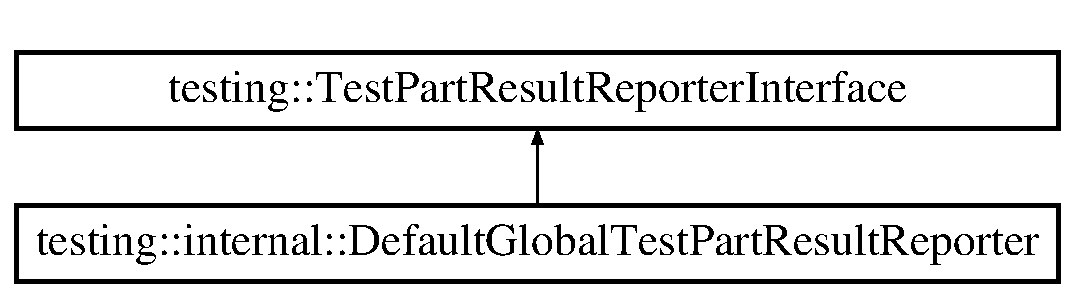
\includegraphics[height=2.000000cm]{classtesting_1_1internal_1_1_default_global_test_part_result_reporter}
\end{center}
\end{figure}
\subsection*{Public Member Functions}
\begin{DoxyCompactItemize}
\item 
\hyperlink{classtesting_1_1internal_1_1_default_global_test_part_result_reporter_a3900ea7f34b34afd48c7d1d0312a1488}{Default\+Global\+Test\+Part\+Result\+Reporter} (\hyperlink{classtesting_1_1internal_1_1_unit_test_impl}{Unit\+Test\+Impl} $\ast$unit\+\_\+test)
\item 
virtual void \hyperlink{classtesting_1_1internal_1_1_default_global_test_part_result_reporter_a6081576a23b964cfecab1e424d8044fc}{Report\+Test\+Part\+Result} (const \hyperlink{classtesting_1_1_test_part_result}{Test\+Part\+Result} \&result)
\end{DoxyCompactItemize}


\subsection{Constructor \& Destructor Documentation}
\hypertarget{classtesting_1_1internal_1_1_default_global_test_part_result_reporter_a3900ea7f34b34afd48c7d1d0312a1488}{}\index{testing\+::internal\+::\+Default\+Global\+Test\+Part\+Result\+Reporter@{testing\+::internal\+::\+Default\+Global\+Test\+Part\+Result\+Reporter}!Default\+Global\+Test\+Part\+Result\+Reporter@{Default\+Global\+Test\+Part\+Result\+Reporter}}
\index{Default\+Global\+Test\+Part\+Result\+Reporter@{Default\+Global\+Test\+Part\+Result\+Reporter}!testing\+::internal\+::\+Default\+Global\+Test\+Part\+Result\+Reporter@{testing\+::internal\+::\+Default\+Global\+Test\+Part\+Result\+Reporter}}
\subsubsection[{Default\+Global\+Test\+Part\+Result\+Reporter(\+Unit\+Test\+Impl $\ast$unit\+\_\+test)}]{\setlength{\rightskip}{0pt plus 5cm}testing\+::internal\+::\+Default\+Global\+Test\+Part\+Result\+Reporter\+::\+Default\+Global\+Test\+Part\+Result\+Reporter (
\begin{DoxyParamCaption}
\item[{{\bf Unit\+Test\+Impl} $\ast$}]{unit\+\_\+test}
\end{DoxyParamCaption}
)\hspace{0.3cm}{\ttfamily [explicit]}}\label{classtesting_1_1internal_1_1_default_global_test_part_result_reporter_a3900ea7f34b34afd48c7d1d0312a1488}


\subsection{Member Function Documentation}
\hypertarget{classtesting_1_1internal_1_1_default_global_test_part_result_reporter_a6081576a23b964cfecab1e424d8044fc}{}\index{testing\+::internal\+::\+Default\+Global\+Test\+Part\+Result\+Reporter@{testing\+::internal\+::\+Default\+Global\+Test\+Part\+Result\+Reporter}!Report\+Test\+Part\+Result@{Report\+Test\+Part\+Result}}
\index{Report\+Test\+Part\+Result@{Report\+Test\+Part\+Result}!testing\+::internal\+::\+Default\+Global\+Test\+Part\+Result\+Reporter@{testing\+::internal\+::\+Default\+Global\+Test\+Part\+Result\+Reporter}}
\subsubsection[{Report\+Test\+Part\+Result(const Test\+Part\+Result \&result)}]{\setlength{\rightskip}{0pt plus 5cm}void testing\+::internal\+::\+Default\+Global\+Test\+Part\+Result\+Reporter\+::\+Report\+Test\+Part\+Result (
\begin{DoxyParamCaption}
\item[{const {\bf Test\+Part\+Result} \&}]{result}
\end{DoxyParamCaption}
)\hspace{0.3cm}{\ttfamily [virtual]}}\label{classtesting_1_1internal_1_1_default_global_test_part_result_reporter_a6081576a23b964cfecab1e424d8044fc}


Implements \hyperlink{classtesting_1_1_test_part_result_reporter_interface_aa2f920e7a5a0a6d0faf19e3727928c22}{testing\+::\+Test\+Part\+Result\+Reporter\+Interface}.



The documentation for this class was generated from the following files\+:\begin{DoxyCompactItemize}
\item 
C\+:/\+Users/\+Hilman/\+Desktop/repo/anjing/src/third\+\_\+party/googletest/src/\hyperlink{gtest-internal-inl_8h}{gtest-\/internal-\/inl.\+h}\item 
C\+:/\+Users/\+Hilman/\+Desktop/repo/anjing/src/third\+\_\+party/googletest/src/\hyperlink{gtest_8cc}{gtest.\+cc}\end{DoxyCompactItemize}

\hypertarget{classtesting_1_1internal_1_1_default_per_thread_test_part_result_reporter}{}\section{testing\+:\+:internal\+:\+:Default\+Per\+Thread\+Test\+Part\+Result\+Reporter Class Reference}
\label{classtesting_1_1internal_1_1_default_per_thread_test_part_result_reporter}\index{testing\+::internal\+::\+Default\+Per\+Thread\+Test\+Part\+Result\+Reporter@{testing\+::internal\+::\+Default\+Per\+Thread\+Test\+Part\+Result\+Reporter}}


{\ttfamily \#include $<$gtest-\/internal-\/inl.\+h$>$}

Inheritance diagram for testing\+:\+:internal\+:\+:Default\+Per\+Thread\+Test\+Part\+Result\+Reporter\+:\begin{figure}[H]
\begin{center}
\leavevmode
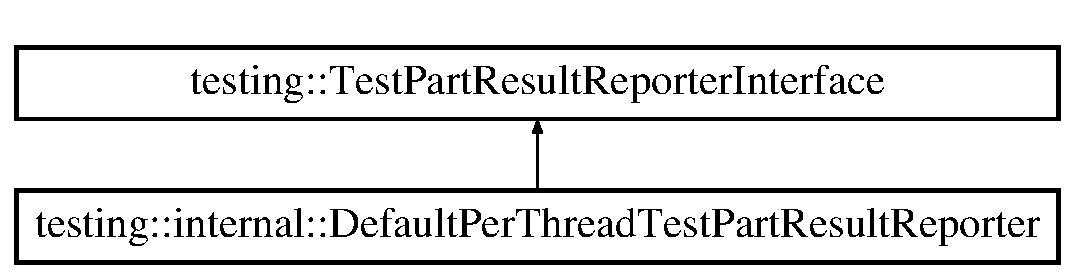
\includegraphics[height=2.000000cm]{classtesting_1_1internal_1_1_default_per_thread_test_part_result_reporter}
\end{center}
\end{figure}
\subsection*{Public Member Functions}
\begin{DoxyCompactItemize}
\item 
\hyperlink{classtesting_1_1internal_1_1_default_per_thread_test_part_result_reporter_a968a846e5a90d2ffea8b2ce2746099bd}{Default\+Per\+Thread\+Test\+Part\+Result\+Reporter} (\hyperlink{classtesting_1_1internal_1_1_unit_test_impl}{Unit\+Test\+Impl} $\ast$unit\+\_\+test)
\item 
virtual void \hyperlink{classtesting_1_1internal_1_1_default_per_thread_test_part_result_reporter_ac6dc08eadc4e5a2a64a91d0b6c6b3aad}{Report\+Test\+Part\+Result} (const \hyperlink{classtesting_1_1_test_part_result}{Test\+Part\+Result} \&result)
\end{DoxyCompactItemize}


\subsection{Constructor \& Destructor Documentation}
\hypertarget{classtesting_1_1internal_1_1_default_per_thread_test_part_result_reporter_a968a846e5a90d2ffea8b2ce2746099bd}{}\index{testing\+::internal\+::\+Default\+Per\+Thread\+Test\+Part\+Result\+Reporter@{testing\+::internal\+::\+Default\+Per\+Thread\+Test\+Part\+Result\+Reporter}!Default\+Per\+Thread\+Test\+Part\+Result\+Reporter@{Default\+Per\+Thread\+Test\+Part\+Result\+Reporter}}
\index{Default\+Per\+Thread\+Test\+Part\+Result\+Reporter@{Default\+Per\+Thread\+Test\+Part\+Result\+Reporter}!testing\+::internal\+::\+Default\+Per\+Thread\+Test\+Part\+Result\+Reporter@{testing\+::internal\+::\+Default\+Per\+Thread\+Test\+Part\+Result\+Reporter}}
\subsubsection[{Default\+Per\+Thread\+Test\+Part\+Result\+Reporter(\+Unit\+Test\+Impl $\ast$unit\+\_\+test)}]{\setlength{\rightskip}{0pt plus 5cm}testing\+::internal\+::\+Default\+Per\+Thread\+Test\+Part\+Result\+Reporter\+::\+Default\+Per\+Thread\+Test\+Part\+Result\+Reporter (
\begin{DoxyParamCaption}
\item[{{\bf Unit\+Test\+Impl} $\ast$}]{unit\+\_\+test}
\end{DoxyParamCaption}
)\hspace{0.3cm}{\ttfamily [explicit]}}\label{classtesting_1_1internal_1_1_default_per_thread_test_part_result_reporter_a968a846e5a90d2ffea8b2ce2746099bd}


\subsection{Member Function Documentation}
\hypertarget{classtesting_1_1internal_1_1_default_per_thread_test_part_result_reporter_ac6dc08eadc4e5a2a64a91d0b6c6b3aad}{}\index{testing\+::internal\+::\+Default\+Per\+Thread\+Test\+Part\+Result\+Reporter@{testing\+::internal\+::\+Default\+Per\+Thread\+Test\+Part\+Result\+Reporter}!Report\+Test\+Part\+Result@{Report\+Test\+Part\+Result}}
\index{Report\+Test\+Part\+Result@{Report\+Test\+Part\+Result}!testing\+::internal\+::\+Default\+Per\+Thread\+Test\+Part\+Result\+Reporter@{testing\+::internal\+::\+Default\+Per\+Thread\+Test\+Part\+Result\+Reporter}}
\subsubsection[{Report\+Test\+Part\+Result(const Test\+Part\+Result \&result)}]{\setlength{\rightskip}{0pt plus 5cm}void testing\+::internal\+::\+Default\+Per\+Thread\+Test\+Part\+Result\+Reporter\+::\+Report\+Test\+Part\+Result (
\begin{DoxyParamCaption}
\item[{const {\bf Test\+Part\+Result} \&}]{result}
\end{DoxyParamCaption}
)\hspace{0.3cm}{\ttfamily [virtual]}}\label{classtesting_1_1internal_1_1_default_per_thread_test_part_result_reporter_ac6dc08eadc4e5a2a64a91d0b6c6b3aad}


Implements \hyperlink{classtesting_1_1_test_part_result_reporter_interface_aa2f920e7a5a0a6d0faf19e3727928c22}{testing\+::\+Test\+Part\+Result\+Reporter\+Interface}.



The documentation for this class was generated from the following files\+:\begin{DoxyCompactItemize}
\item 
C\+:/\+Users/\+Hilman/\+Desktop/repo/anjing/src/third\+\_\+party/googletest/src/\hyperlink{gtest-internal-inl_8h}{gtest-\/internal-\/inl.\+h}\item 
C\+:/\+Users/\+Hilman/\+Desktop/repo/anjing/src/third\+\_\+party/googletest/src/\hyperlink{gtest_8cc}{gtest.\+cc}\end{DoxyCompactItemize}

\hypertarget{classtesting_1_1internal_1_1_derived}{}\section{testing\+:\+:internal\+:\+:Derived Class Reference}
\label{classtesting_1_1internal_1_1_derived}\index{testing\+::internal\+::\+Derived@{testing\+::internal\+::\+Derived}}
Inheritance diagram for testing\+:\+:internal\+:\+:Derived\+:\begin{figure}[H]
\begin{center}
\leavevmode
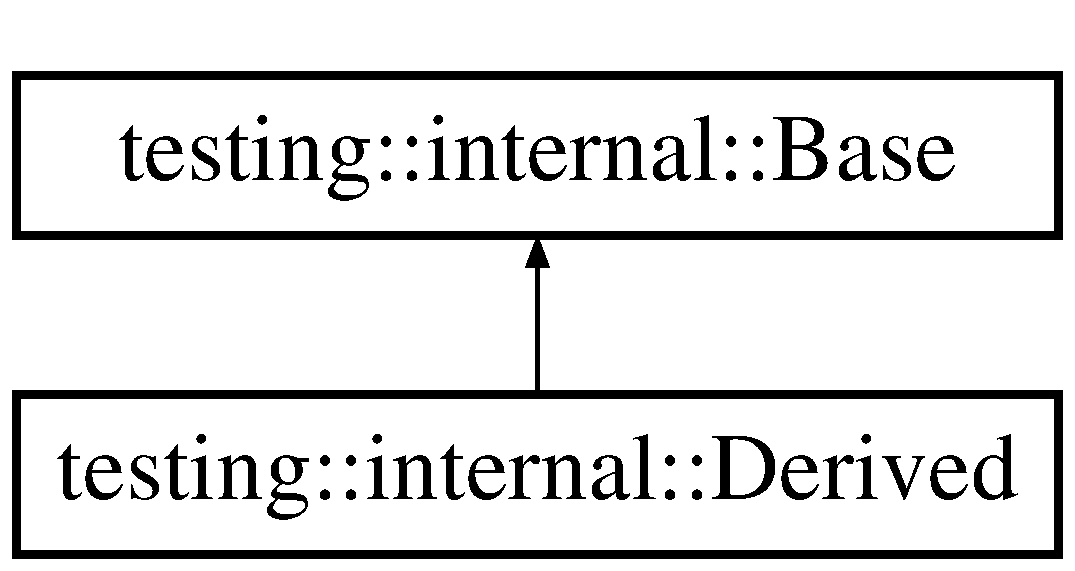
\includegraphics[height=2.000000cm]{classtesting_1_1internal_1_1_derived}
\end{center}
\end{figure}
\subsection*{Public Member Functions}
\begin{DoxyCompactItemize}
\item 
\hyperlink{classtesting_1_1internal_1_1_derived_a05a8e8354c7c09a9f3728a96c96f1edd}{Derived} (int n)
\end{DoxyCompactItemize}


\subsection{Constructor \& Destructor Documentation}
\hypertarget{classtesting_1_1internal_1_1_derived_a05a8e8354c7c09a9f3728a96c96f1edd}{}\index{testing\+::internal\+::\+Derived@{testing\+::internal\+::\+Derived}!Derived@{Derived}}
\index{Derived@{Derived}!testing\+::internal\+::\+Derived@{testing\+::internal\+::\+Derived}}
\subsubsection[{Derived(int n)}]{\setlength{\rightskip}{0pt plus 5cm}testing\+::internal\+::\+Derived\+::\+Derived (
\begin{DoxyParamCaption}
\item[{int}]{n}
\end{DoxyParamCaption}
)\hspace{0.3cm}{\ttfamily [inline]}, {\ttfamily [explicit]}}\label{classtesting_1_1internal_1_1_derived_a05a8e8354c7c09a9f3728a96c96f1edd}


The documentation for this class was generated from the following file\+:\begin{DoxyCompactItemize}
\item 
C\+:/\+Users/\+Hilman/\+Desktop/repo/anjing/src/third\+\_\+party/googletest/test/\hyperlink{gtest-port__test_8cc}{gtest-\/port\+\_\+test.\+cc}\end{DoxyCompactItemize}

\hypertarget{class_disabled_test}{}\section{Disabled\+Test Class Reference}
\label{class_disabled_test}\index{Disabled\+Test@{Disabled\+Test}}
Inheritance diagram for Disabled\+Test\+:\begin{figure}[H]
\begin{center}
\leavevmode
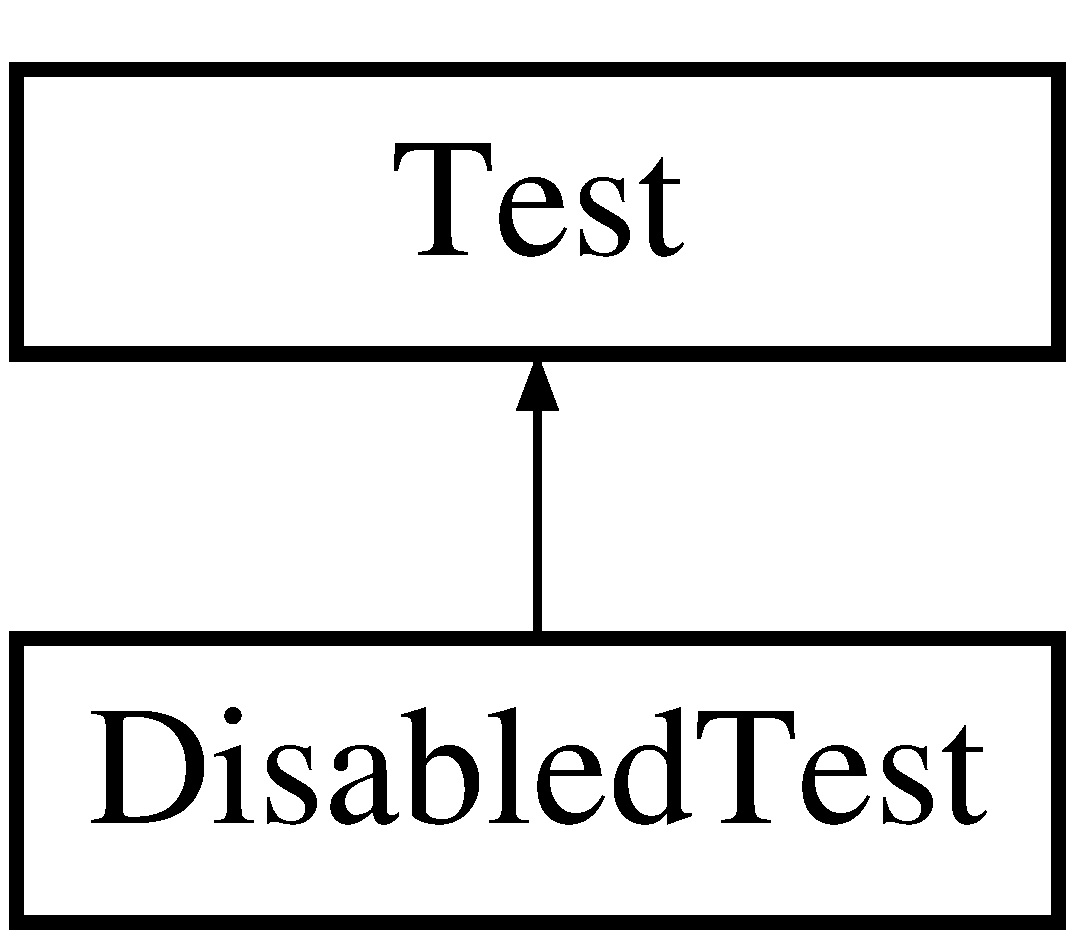
\includegraphics[height=2.000000cm]{class_disabled_test}
\end{center}
\end{figure}


The documentation for this class was generated from the following file\+:\begin{DoxyCompactItemize}
\item 
C\+:/\+Users/\+Hilman/\+Desktop/repo/anjing/src/third\+\_\+party/googletest/test/\hyperlink{gtest__xml__output__unittest___8cc}{gtest\+\_\+xml\+\_\+output\+\_\+unittest\+\_\+.\+cc}\end{DoxyCompactItemize}

\hypertarget{classpump_1_1_else_node}{}\section{pump.\+Else\+Node Class Reference}
\label{classpump_1_1_else_node}\index{pump.\+Else\+Node@{pump.\+Else\+Node}}
\subsection*{Public Member Functions}
\begin{DoxyCompactItemize}
\item 
def \hyperlink{classpump_1_1_else_node_a42d7c962c6ea6e4a69b3418749e4208d}{\+\_\+\+\_\+init\+\_\+\+\_\+}
\end{DoxyCompactItemize}
\subsection*{Public Attributes}
\begin{DoxyCompactItemize}
\item 
\hyperlink{classpump_1_1_else_node_ac838a0fe9f5d713c7f56939eed5e128d}{else\+\_\+branch}
\end{DoxyCompactItemize}


\subsection{Constructor \& Destructor Documentation}
\hypertarget{classpump_1_1_else_node_a42d7c962c6ea6e4a69b3418749e4208d}{}\index{pump\+::\+Else\+Node@{pump\+::\+Else\+Node}!\+\_\+\+\_\+init\+\_\+\+\_\+@{\+\_\+\+\_\+init\+\_\+\+\_\+}}
\index{\+\_\+\+\_\+init\+\_\+\+\_\+@{\+\_\+\+\_\+init\+\_\+\+\_\+}!pump\+::\+Else\+Node@{pump\+::\+Else\+Node}}
\subsubsection[{\+\_\+\+\_\+init\+\_\+\+\_\+}]{\setlength{\rightskip}{0pt plus 5cm}def pump.\+Else\+Node.\+\_\+\+\_\+init\+\_\+\+\_\+ (
\begin{DoxyParamCaption}
\item[{}]{self, }
\item[{}]{else\+\_\+branch = {\ttfamily None}}
\end{DoxyParamCaption}
)}\label{classpump_1_1_else_node_a42d7c962c6ea6e4a69b3418749e4208d}


\subsection{Member Data Documentation}
\hypertarget{classpump_1_1_else_node_ac838a0fe9f5d713c7f56939eed5e128d}{}\index{pump\+::\+Else\+Node@{pump\+::\+Else\+Node}!else\+\_\+branch@{else\+\_\+branch}}
\index{else\+\_\+branch@{else\+\_\+branch}!pump\+::\+Else\+Node@{pump\+::\+Else\+Node}}
\subsubsection[{else\+\_\+branch}]{\setlength{\rightskip}{0pt plus 5cm}pump.\+Else\+Node.\+else\+\_\+branch}\label{classpump_1_1_else_node_ac838a0fe9f5d713c7f56939eed5e128d}


The documentation for this class was generated from the following file\+:\begin{DoxyCompactItemize}
\item 
C\+:/\+Users/\+Hilman/\+Desktop/repo/anjing/src/third\+\_\+party/googletest/scripts/\hyperlink{pump_8py}{pump.\+py}\end{DoxyCompactItemize}

\hypertarget{classtesting_1_1_empty_test_event_listener}{}\section{testing\+:\+:Empty\+Test\+Event\+Listener Class Reference}
\label{classtesting_1_1_empty_test_event_listener}\index{testing\+::\+Empty\+Test\+Event\+Listener@{testing\+::\+Empty\+Test\+Event\+Listener}}


{\ttfamily \#include $<$gtest.\+h$>$}

Inheritance diagram for testing\+:\+:Empty\+Test\+Event\+Listener\+:\begin{figure}[H]
\begin{center}
\leavevmode
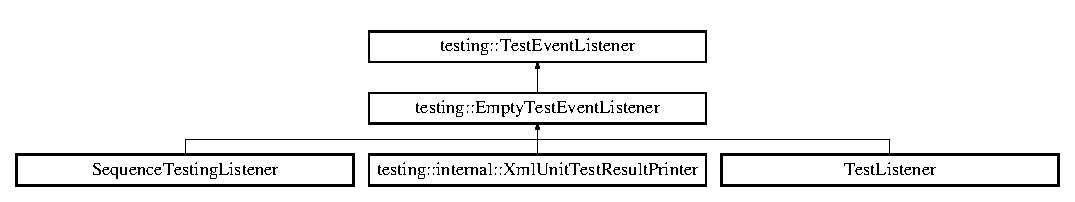
\includegraphics[height=2.267207cm]{classtesting_1_1_empty_test_event_listener}
\end{center}
\end{figure}
\subsection*{Public Member Functions}
\begin{DoxyCompactItemize}
\item 
virtual void \hyperlink{classtesting_1_1_empty_test_event_listener_aa3847c8a3c22d8d69a6006dfdd6589fc}{On\+Test\+Program\+Start} (const \hyperlink{classtesting_1_1_unit_test}{Unit\+Test} \&)
\item 
virtual void \hyperlink{classtesting_1_1_empty_test_event_listener_a836f05829855dc60d13ba99ad712c0dd}{On\+Test\+Iteration\+Start} (const \hyperlink{classtesting_1_1_unit_test}{Unit\+Test} \&, int)
\item 
virtual void \hyperlink{classtesting_1_1_empty_test_event_listener_a156d1965248fbdced6aabacadfa2d63f}{On\+Environments\+Set\+Up\+Start} (const \hyperlink{classtesting_1_1_unit_test}{Unit\+Test} \&)
\item 
virtual void \hyperlink{classtesting_1_1_empty_test_event_listener_abc481c6648d15d4242245195a06f5aa0}{On\+Environments\+Set\+Up\+End} (const \hyperlink{classtesting_1_1_unit_test}{Unit\+Test} \&)
\item 
virtual void \hyperlink{classtesting_1_1_empty_test_event_listener_ae4707ed9cc7ace5241bc8ccc4051209b}{On\+Test\+Case\+Start} (const \hyperlink{classtesting_1_1_test_case}{Test\+Case} \&)
\item 
virtual void \hyperlink{classtesting_1_1_empty_test_event_listener_a84fa74cc9ba742f9f847ea405ca84e5e}{On\+Test\+Start} (const \hyperlink{classtesting_1_1_test_info}{Test\+Info} \&)
\item 
virtual void \hyperlink{classtesting_1_1_empty_test_event_listener_a59e7f7d9f2e2d089a6e8c1e2577f4718}{On\+Test\+Part\+Result} (const \hyperlink{classtesting_1_1_test_part_result}{Test\+Part\+Result} \&)
\item 
virtual void \hyperlink{classtesting_1_1_empty_test_event_listener_afd58d21005f0d0d0399fb114627545d3}{On\+Test\+End} (const \hyperlink{classtesting_1_1_test_info}{Test\+Info} \&)
\item 
virtual void \hyperlink{classtesting_1_1_empty_test_event_listener_a6bec703158283104c4298f7d8a528515}{On\+Test\+Case\+End} (const \hyperlink{classtesting_1_1_test_case}{Test\+Case} \&)
\item 
virtual void \hyperlink{classtesting_1_1_empty_test_event_listener_a00fa1a4ea5831e20746188414268e7c6}{On\+Environments\+Tear\+Down\+Start} (const \hyperlink{classtesting_1_1_unit_test}{Unit\+Test} \&)
\item 
virtual void \hyperlink{classtesting_1_1_empty_test_event_listener_aea64c83c415b33a4c0b0239bafd1438d}{On\+Environments\+Tear\+Down\+End} (const \hyperlink{classtesting_1_1_unit_test}{Unit\+Test} \&)
\item 
virtual void \hyperlink{classtesting_1_1_empty_test_event_listener_a2253e5a18b3cf7bccd349567a252209d}{On\+Test\+Iteration\+End} (const \hyperlink{classtesting_1_1_unit_test}{Unit\+Test} \&, int)
\item 
virtual void \hyperlink{classtesting_1_1_empty_test_event_listener_a0abcc02bd2331a2e29ad6f4d9daf2a32}{On\+Test\+Program\+End} (const \hyperlink{classtesting_1_1_unit_test}{Unit\+Test} \&)
\end{DoxyCompactItemize}


\subsection{Member Function Documentation}
\hypertarget{classtesting_1_1_empty_test_event_listener_abc481c6648d15d4242245195a06f5aa0}{}\index{testing\+::\+Empty\+Test\+Event\+Listener@{testing\+::\+Empty\+Test\+Event\+Listener}!On\+Environments\+Set\+Up\+End@{On\+Environments\+Set\+Up\+End}}
\index{On\+Environments\+Set\+Up\+End@{On\+Environments\+Set\+Up\+End}!testing\+::\+Empty\+Test\+Event\+Listener@{testing\+::\+Empty\+Test\+Event\+Listener}}
\subsubsection[{On\+Environments\+Set\+Up\+End(const Unit\+Test \&)}]{\setlength{\rightskip}{0pt plus 5cm}virtual void testing\+::\+Empty\+Test\+Event\+Listener\+::\+On\+Environments\+Set\+Up\+End (
\begin{DoxyParamCaption}
\item[{const {\bf Unit\+Test} \&}]{}
\end{DoxyParamCaption}
)\hspace{0.3cm}{\ttfamily [inline]}, {\ttfamily [virtual]}}\label{classtesting_1_1_empty_test_event_listener_abc481c6648d15d4242245195a06f5aa0}


Implements \hyperlink{classtesting_1_1_test_event_listener_aaa1021d75f5dbf3f05c829c1cc520341}{testing\+::\+Test\+Event\+Listener}.

\hypertarget{classtesting_1_1_empty_test_event_listener_a156d1965248fbdced6aabacadfa2d63f}{}\index{testing\+::\+Empty\+Test\+Event\+Listener@{testing\+::\+Empty\+Test\+Event\+Listener}!On\+Environments\+Set\+Up\+Start@{On\+Environments\+Set\+Up\+Start}}
\index{On\+Environments\+Set\+Up\+Start@{On\+Environments\+Set\+Up\+Start}!testing\+::\+Empty\+Test\+Event\+Listener@{testing\+::\+Empty\+Test\+Event\+Listener}}
\subsubsection[{On\+Environments\+Set\+Up\+Start(const Unit\+Test \&)}]{\setlength{\rightskip}{0pt plus 5cm}virtual void testing\+::\+Empty\+Test\+Event\+Listener\+::\+On\+Environments\+Set\+Up\+Start (
\begin{DoxyParamCaption}
\item[{const {\bf Unit\+Test} \&}]{}
\end{DoxyParamCaption}
)\hspace{0.3cm}{\ttfamily [inline]}, {\ttfamily [virtual]}}\label{classtesting_1_1_empty_test_event_listener_a156d1965248fbdced6aabacadfa2d63f}


Implements \hyperlink{classtesting_1_1_test_event_listener_aa6502e534919605be45f26a6daf9a40c}{testing\+::\+Test\+Event\+Listener}.

\hypertarget{classtesting_1_1_empty_test_event_listener_aea64c83c415b33a4c0b0239bafd1438d}{}\index{testing\+::\+Empty\+Test\+Event\+Listener@{testing\+::\+Empty\+Test\+Event\+Listener}!On\+Environments\+Tear\+Down\+End@{On\+Environments\+Tear\+Down\+End}}
\index{On\+Environments\+Tear\+Down\+End@{On\+Environments\+Tear\+Down\+End}!testing\+::\+Empty\+Test\+Event\+Listener@{testing\+::\+Empty\+Test\+Event\+Listener}}
\subsubsection[{On\+Environments\+Tear\+Down\+End(const Unit\+Test \&)}]{\setlength{\rightskip}{0pt plus 5cm}virtual void testing\+::\+Empty\+Test\+Event\+Listener\+::\+On\+Environments\+Tear\+Down\+End (
\begin{DoxyParamCaption}
\item[{const {\bf Unit\+Test} \&}]{}
\end{DoxyParamCaption}
)\hspace{0.3cm}{\ttfamily [inline]}, {\ttfamily [virtual]}}\label{classtesting_1_1_empty_test_event_listener_aea64c83c415b33a4c0b0239bafd1438d}


Implements \hyperlink{classtesting_1_1_test_event_listener_a9ea04fa7f447865ba76df35e12ba2092}{testing\+::\+Test\+Event\+Listener}.

\hypertarget{classtesting_1_1_empty_test_event_listener_a00fa1a4ea5831e20746188414268e7c6}{}\index{testing\+::\+Empty\+Test\+Event\+Listener@{testing\+::\+Empty\+Test\+Event\+Listener}!On\+Environments\+Tear\+Down\+Start@{On\+Environments\+Tear\+Down\+Start}}
\index{On\+Environments\+Tear\+Down\+Start@{On\+Environments\+Tear\+Down\+Start}!testing\+::\+Empty\+Test\+Event\+Listener@{testing\+::\+Empty\+Test\+Event\+Listener}}
\subsubsection[{On\+Environments\+Tear\+Down\+Start(const Unit\+Test \&)}]{\setlength{\rightskip}{0pt plus 5cm}virtual void testing\+::\+Empty\+Test\+Event\+Listener\+::\+On\+Environments\+Tear\+Down\+Start (
\begin{DoxyParamCaption}
\item[{const {\bf Unit\+Test} \&}]{}
\end{DoxyParamCaption}
)\hspace{0.3cm}{\ttfamily [inline]}, {\ttfamily [virtual]}}\label{classtesting_1_1_empty_test_event_listener_a00fa1a4ea5831e20746188414268e7c6}


Implements \hyperlink{classtesting_1_1_test_event_listener_a468b5e6701bcb86cb2c956caadbba5e4}{testing\+::\+Test\+Event\+Listener}.

\hypertarget{classtesting_1_1_empty_test_event_listener_a6bec703158283104c4298f7d8a528515}{}\index{testing\+::\+Empty\+Test\+Event\+Listener@{testing\+::\+Empty\+Test\+Event\+Listener}!On\+Test\+Case\+End@{On\+Test\+Case\+End}}
\index{On\+Test\+Case\+End@{On\+Test\+Case\+End}!testing\+::\+Empty\+Test\+Event\+Listener@{testing\+::\+Empty\+Test\+Event\+Listener}}
\subsubsection[{On\+Test\+Case\+End(const Test\+Case \&)}]{\setlength{\rightskip}{0pt plus 5cm}virtual void testing\+::\+Empty\+Test\+Event\+Listener\+::\+On\+Test\+Case\+End (
\begin{DoxyParamCaption}
\item[{const {\bf Test\+Case} \&}]{}
\end{DoxyParamCaption}
)\hspace{0.3cm}{\ttfamily [inline]}, {\ttfamily [virtual]}}\label{classtesting_1_1_empty_test_event_listener_a6bec703158283104c4298f7d8a528515}


Implements \hyperlink{classtesting_1_1_test_event_listener_ae61985e2ef76ac78379b077be57a9c36}{testing\+::\+Test\+Event\+Listener}.

\hypertarget{classtesting_1_1_empty_test_event_listener_ae4707ed9cc7ace5241bc8ccc4051209b}{}\index{testing\+::\+Empty\+Test\+Event\+Listener@{testing\+::\+Empty\+Test\+Event\+Listener}!On\+Test\+Case\+Start@{On\+Test\+Case\+Start}}
\index{On\+Test\+Case\+Start@{On\+Test\+Case\+Start}!testing\+::\+Empty\+Test\+Event\+Listener@{testing\+::\+Empty\+Test\+Event\+Listener}}
\subsubsection[{On\+Test\+Case\+Start(const Test\+Case \&)}]{\setlength{\rightskip}{0pt plus 5cm}virtual void testing\+::\+Empty\+Test\+Event\+Listener\+::\+On\+Test\+Case\+Start (
\begin{DoxyParamCaption}
\item[{const {\bf Test\+Case} \&}]{}
\end{DoxyParamCaption}
)\hspace{0.3cm}{\ttfamily [inline]}, {\ttfamily [virtual]}}\label{classtesting_1_1_empty_test_event_listener_ae4707ed9cc7ace5241bc8ccc4051209b}


Implements \hyperlink{classtesting_1_1_test_event_listener_ab4ed885d63f5bbff8076c1329b3dfe36}{testing\+::\+Test\+Event\+Listener}.

\hypertarget{classtesting_1_1_empty_test_event_listener_afd58d21005f0d0d0399fb114627545d3}{}\index{testing\+::\+Empty\+Test\+Event\+Listener@{testing\+::\+Empty\+Test\+Event\+Listener}!On\+Test\+End@{On\+Test\+End}}
\index{On\+Test\+End@{On\+Test\+End}!testing\+::\+Empty\+Test\+Event\+Listener@{testing\+::\+Empty\+Test\+Event\+Listener}}
\subsubsection[{On\+Test\+End(const Test\+Info \&)}]{\setlength{\rightskip}{0pt plus 5cm}virtual void testing\+::\+Empty\+Test\+Event\+Listener\+::\+On\+Test\+End (
\begin{DoxyParamCaption}
\item[{const {\bf Test\+Info} \&}]{}
\end{DoxyParamCaption}
)\hspace{0.3cm}{\ttfamily [inline]}, {\ttfamily [virtual]}}\label{classtesting_1_1_empty_test_event_listener_afd58d21005f0d0d0399fb114627545d3}


Implements \hyperlink{classtesting_1_1_test_event_listener_abb1c44525ef038500608b5dc2f17099b}{testing\+::\+Test\+Event\+Listener}.

\hypertarget{classtesting_1_1_empty_test_event_listener_a2253e5a18b3cf7bccd349567a252209d}{}\index{testing\+::\+Empty\+Test\+Event\+Listener@{testing\+::\+Empty\+Test\+Event\+Listener}!On\+Test\+Iteration\+End@{On\+Test\+Iteration\+End}}
\index{On\+Test\+Iteration\+End@{On\+Test\+Iteration\+End}!testing\+::\+Empty\+Test\+Event\+Listener@{testing\+::\+Empty\+Test\+Event\+Listener}}
\subsubsection[{On\+Test\+Iteration\+End(const Unit\+Test \&, int)}]{\setlength{\rightskip}{0pt plus 5cm}virtual void testing\+::\+Empty\+Test\+Event\+Listener\+::\+On\+Test\+Iteration\+End (
\begin{DoxyParamCaption}
\item[{const {\bf Unit\+Test} \&}]{, }
\item[{int}]{}
\end{DoxyParamCaption}
)\hspace{0.3cm}{\ttfamily [inline]}, {\ttfamily [virtual]}}\label{classtesting_1_1_empty_test_event_listener_a2253e5a18b3cf7bccd349567a252209d}


Implements \hyperlink{classtesting_1_1_test_event_listener_a550fdb3e55726e4cefa09f5697941425}{testing\+::\+Test\+Event\+Listener}.



Reimplemented in \hyperlink{class_sequence_testing_listener_a783bc01e2a95f5bf73bbde4d96832e0f}{Sequence\+Testing\+Listener}, and \hyperlink{classtesting_1_1internal_1_1_xml_unit_test_result_printer_a2ae986dd2f4f2aed31cc6f3bc8c56898}{testing\+::internal\+::\+Xml\+Unit\+Test\+Result\+Printer}.

\hypertarget{classtesting_1_1_empty_test_event_listener_a836f05829855dc60d13ba99ad712c0dd}{}\index{testing\+::\+Empty\+Test\+Event\+Listener@{testing\+::\+Empty\+Test\+Event\+Listener}!On\+Test\+Iteration\+Start@{On\+Test\+Iteration\+Start}}
\index{On\+Test\+Iteration\+Start@{On\+Test\+Iteration\+Start}!testing\+::\+Empty\+Test\+Event\+Listener@{testing\+::\+Empty\+Test\+Event\+Listener}}
\subsubsection[{On\+Test\+Iteration\+Start(const Unit\+Test \&, int)}]{\setlength{\rightskip}{0pt plus 5cm}virtual void testing\+::\+Empty\+Test\+Event\+Listener\+::\+On\+Test\+Iteration\+Start (
\begin{DoxyParamCaption}
\item[{const {\bf Unit\+Test} \&}]{, }
\item[{int}]{}
\end{DoxyParamCaption}
)\hspace{0.3cm}{\ttfamily [inline]}, {\ttfamily [virtual]}}\label{classtesting_1_1_empty_test_event_listener_a836f05829855dc60d13ba99ad712c0dd}


Implements \hyperlink{classtesting_1_1_test_event_listener_a60cc09b7907cb329d152eb5e7133bdeb}{testing\+::\+Test\+Event\+Listener}.



Reimplemented in \hyperlink{class_sequence_testing_listener_a345641262fa10cc4b251ac54116db74b}{Sequence\+Testing\+Listener}.

\hypertarget{classtesting_1_1_empty_test_event_listener_a59e7f7d9f2e2d089a6e8c1e2577f4718}{}\index{testing\+::\+Empty\+Test\+Event\+Listener@{testing\+::\+Empty\+Test\+Event\+Listener}!On\+Test\+Part\+Result@{On\+Test\+Part\+Result}}
\index{On\+Test\+Part\+Result@{On\+Test\+Part\+Result}!testing\+::\+Empty\+Test\+Event\+Listener@{testing\+::\+Empty\+Test\+Event\+Listener}}
\subsubsection[{On\+Test\+Part\+Result(const Test\+Part\+Result \&)}]{\setlength{\rightskip}{0pt plus 5cm}virtual void testing\+::\+Empty\+Test\+Event\+Listener\+::\+On\+Test\+Part\+Result (
\begin{DoxyParamCaption}
\item[{const {\bf Test\+Part\+Result} \&}]{}
\end{DoxyParamCaption}
)\hspace{0.3cm}{\ttfamily [inline]}, {\ttfamily [virtual]}}\label{classtesting_1_1_empty_test_event_listener_a59e7f7d9f2e2d089a6e8c1e2577f4718}


Implements \hyperlink{classtesting_1_1_test_event_listener_a054f8705c883fa120b91473aff38f2ee}{testing\+::\+Test\+Event\+Listener}.

\hypertarget{classtesting_1_1_empty_test_event_listener_a0abcc02bd2331a2e29ad6f4d9daf2a32}{}\index{testing\+::\+Empty\+Test\+Event\+Listener@{testing\+::\+Empty\+Test\+Event\+Listener}!On\+Test\+Program\+End@{On\+Test\+Program\+End}}
\index{On\+Test\+Program\+End@{On\+Test\+Program\+End}!testing\+::\+Empty\+Test\+Event\+Listener@{testing\+::\+Empty\+Test\+Event\+Listener}}
\subsubsection[{On\+Test\+Program\+End(const Unit\+Test \&)}]{\setlength{\rightskip}{0pt plus 5cm}virtual void testing\+::\+Empty\+Test\+Event\+Listener\+::\+On\+Test\+Program\+End (
\begin{DoxyParamCaption}
\item[{const {\bf Unit\+Test} \&}]{}
\end{DoxyParamCaption}
)\hspace{0.3cm}{\ttfamily [inline]}, {\ttfamily [virtual]}}\label{classtesting_1_1_empty_test_event_listener_a0abcc02bd2331a2e29ad6f4d9daf2a32}


Implements \hyperlink{classtesting_1_1_test_event_listener_ad15b6246d94c268e233487a86463ef3d}{testing\+::\+Test\+Event\+Listener}.



Reimplemented in \hyperlink{class_sequence_testing_listener_aacac5e15bac089460841ff63a5c31f57}{Sequence\+Testing\+Listener}.

\hypertarget{classtesting_1_1_empty_test_event_listener_aa3847c8a3c22d8d69a6006dfdd6589fc}{}\index{testing\+::\+Empty\+Test\+Event\+Listener@{testing\+::\+Empty\+Test\+Event\+Listener}!On\+Test\+Program\+Start@{On\+Test\+Program\+Start}}
\index{On\+Test\+Program\+Start@{On\+Test\+Program\+Start}!testing\+::\+Empty\+Test\+Event\+Listener@{testing\+::\+Empty\+Test\+Event\+Listener}}
\subsubsection[{On\+Test\+Program\+Start(const Unit\+Test \&)}]{\setlength{\rightskip}{0pt plus 5cm}virtual void testing\+::\+Empty\+Test\+Event\+Listener\+::\+On\+Test\+Program\+Start (
\begin{DoxyParamCaption}
\item[{const {\bf Unit\+Test} \&}]{}
\end{DoxyParamCaption}
)\hspace{0.3cm}{\ttfamily [inline]}, {\ttfamily [virtual]}}\label{classtesting_1_1_empty_test_event_listener_aa3847c8a3c22d8d69a6006dfdd6589fc}


Implements \hyperlink{classtesting_1_1_test_event_listener_a5f6c84f39851e8a603a2d2e10063816b}{testing\+::\+Test\+Event\+Listener}.



Reimplemented in \hyperlink{class_sequence_testing_listener_a25b96acdbaa6f582e583e6b56bd39b42}{Sequence\+Testing\+Listener}, and \hyperlink{class_test_listener_a6218f522f5b6b37050ff0ea630ac5fd3}{Test\+Listener}.

\hypertarget{classtesting_1_1_empty_test_event_listener_a84fa74cc9ba742f9f847ea405ca84e5e}{}\index{testing\+::\+Empty\+Test\+Event\+Listener@{testing\+::\+Empty\+Test\+Event\+Listener}!On\+Test\+Start@{On\+Test\+Start}}
\index{On\+Test\+Start@{On\+Test\+Start}!testing\+::\+Empty\+Test\+Event\+Listener@{testing\+::\+Empty\+Test\+Event\+Listener}}
\subsubsection[{On\+Test\+Start(const Test\+Info \&)}]{\setlength{\rightskip}{0pt plus 5cm}virtual void testing\+::\+Empty\+Test\+Event\+Listener\+::\+On\+Test\+Start (
\begin{DoxyParamCaption}
\item[{const {\bf Test\+Info} \&}]{}
\end{DoxyParamCaption}
)\hspace{0.3cm}{\ttfamily [inline]}, {\ttfamily [virtual]}}\label{classtesting_1_1_empty_test_event_listener_a84fa74cc9ba742f9f847ea405ca84e5e}


Implements \hyperlink{classtesting_1_1_test_event_listener_ab4f6a0ca16ae75daf385b3b5914e1048}{testing\+::\+Test\+Event\+Listener}.



The documentation for this class was generated from the following file\+:\begin{DoxyCompactItemize}
\item 
C\+:/\+Users/\+Hilman/\+Desktop/repo/anjing/src/third\+\_\+party/googletest/include/gtest/\hyperlink{gtest_8h}{gtest.\+h}\end{DoxyCompactItemize}

\hypertarget{structtesting_1_1internal_1_1_enable_if}{}\section{testing\+:\+:internal\+:\+:Enable\+If$<$ bool $>$ Struct Template Reference}
\label{structtesting_1_1internal_1_1_enable_if}\index{testing\+::internal\+::\+Enable\+If$<$ bool $>$@{testing\+::internal\+::\+Enable\+If$<$ bool $>$}}


{\ttfamily \#include $<$gtest-\/internal.\+h$>$}



The documentation for this struct was generated from the following file\+:\begin{DoxyCompactItemize}
\item 
C\+:/\+Users/\+Hilman/\+Desktop/repo/anjing/src/third\+\_\+party/googletest/include/gtest/internal/\hyperlink{gtest-internal_8h}{gtest-\/internal.\+h}\end{DoxyCompactItemize}

\hypertarget{structtesting_1_1internal_1_1_enable_if_3_01true_01_4}{}\section{testing\+:\+:internal\+:\+:Enable\+If$<$ true $>$ Struct Template Reference}
\label{structtesting_1_1internal_1_1_enable_if_3_01true_01_4}\index{testing\+::internal\+::\+Enable\+If$<$ true $>$@{testing\+::internal\+::\+Enable\+If$<$ true $>$}}


{\ttfamily \#include $<$gtest-\/internal.\+h$>$}

\subsection*{Public Types}
\begin{DoxyCompactItemize}
\item 
typedef void \hyperlink{structtesting_1_1internal_1_1_enable_if_3_01true_01_4_a9398d803f1fdd99ff41823746f6299ff}{type}
\end{DoxyCompactItemize}


\subsection{Member Typedef Documentation}
\hypertarget{structtesting_1_1internal_1_1_enable_if_3_01true_01_4_a9398d803f1fdd99ff41823746f6299ff}{}\index{testing\+::internal\+::\+Enable\+If$<$ true $>$@{testing\+::internal\+::\+Enable\+If$<$ true $>$}!type@{type}}
\index{type@{type}!testing\+::internal\+::\+Enable\+If$<$ true $>$@{testing\+::internal\+::\+Enable\+If$<$ true $>$}}
\subsubsection[{type}]{\setlength{\rightskip}{0pt plus 5cm}typedef void {\bf testing\+::internal\+::\+Enable\+If}$<$ true $>$\+::{\bf type}}\label{structtesting_1_1internal_1_1_enable_if_3_01true_01_4_a9398d803f1fdd99ff41823746f6299ff}


The documentation for this struct was generated from the following file\+:\begin{DoxyCompactItemize}
\item 
C\+:/\+Users/\+Hilman/\+Desktop/repo/anjing/src/third\+\_\+party/googletest/include/gtest/internal/\hyperlink{gtest-internal_8h}{gtest-\/internal.\+h}\end{DoxyCompactItemize}

\hypertarget{classpump_1_1_env}{}\section{pump.\+Env Class Reference}
\label{classpump_1_1_env}\index{pump.\+Env@{pump.\+Env}}
\subsection*{Public Member Functions}
\begin{DoxyCompactItemize}
\item 
def \hyperlink{classpump_1_1_env_a803732618a49ab4a2edf098b78081611}{\+\_\+\+\_\+init\+\_\+\+\_\+} (self)
\item 
def \hyperlink{classpump_1_1_env_a4c1b156cfa4aec708746bbe07dae5f1a}{Clone} (self)
\item 
def \hyperlink{classpump_1_1_env_ae0abc25733c61a8cc010cc5d76dd0dd8}{Push\+Variable} (self, var, value)
\item 
def \hyperlink{classpump_1_1_env_abf35f8b971acedb275bb92bb29fcd587}{Pop\+Variable} (self)
\item 
def \hyperlink{classpump_1_1_env_a600c34cac1e4ba75406efeadb2d7dd95}{Push\+Range} (self, var, lower, upper)
\item 
def \hyperlink{classpump_1_1_env_a45474355fc03b69e7449199cc8012ba9}{Pop\+Range} (self)
\item 
def \hyperlink{classpump_1_1_env_a43c3609179d5e458266731199e35313b}{Get\+Value} (self, identifier)
\item 
def \hyperlink{classpump_1_1_env_a29fa1ceb1f7c22e8e982133f4808317f}{Eval\+Exp} (self, exp)
\item 
def \hyperlink{classpump_1_1_env_a1df05a550bdcfe4bb8c5b1608484a6dc}{Get\+Range} (self, identifier)
\end{DoxyCompactItemize}
\subsection*{Public Attributes}
\begin{DoxyCompactItemize}
\item 
\hyperlink{classpump_1_1_env_aba6456f3d0d23ac92bc9508c1b966bcd}{variables}
\item 
\hyperlink{classpump_1_1_env_a8d5fec087c1a9108de9b105922b34309}{ranges}
\end{DoxyCompactItemize}


\subsection{Constructor \& Destructor Documentation}
\hypertarget{classpump_1_1_env_a803732618a49ab4a2edf098b78081611}{}\index{pump\+::\+Env@{pump\+::\+Env}!\+\_\+\+\_\+init\+\_\+\+\_\+@{\+\_\+\+\_\+init\+\_\+\+\_\+}}
\index{\+\_\+\+\_\+init\+\_\+\+\_\+@{\+\_\+\+\_\+init\+\_\+\+\_\+}!pump\+::\+Env@{pump\+::\+Env}}
\subsubsection[{\+\_\+\+\_\+init\+\_\+\+\_\+(self)}]{\setlength{\rightskip}{0pt plus 5cm}def pump.\+Env.\+\_\+\+\_\+init\+\_\+\+\_\+ (
\begin{DoxyParamCaption}
\item[{}]{self}
\end{DoxyParamCaption}
)}\label{classpump_1_1_env_a803732618a49ab4a2edf098b78081611}


\subsection{Member Function Documentation}
\hypertarget{classpump_1_1_env_a4c1b156cfa4aec708746bbe07dae5f1a}{}\index{pump\+::\+Env@{pump\+::\+Env}!Clone@{Clone}}
\index{Clone@{Clone}!pump\+::\+Env@{pump\+::\+Env}}
\subsubsection[{Clone(self)}]{\setlength{\rightskip}{0pt plus 5cm}def pump.\+Env.\+Clone (
\begin{DoxyParamCaption}
\item[{}]{self}
\end{DoxyParamCaption}
)}\label{classpump_1_1_env_a4c1b156cfa4aec708746bbe07dae5f1a}
\hypertarget{classpump_1_1_env_a29fa1ceb1f7c22e8e982133f4808317f}{}\index{pump\+::\+Env@{pump\+::\+Env}!Eval\+Exp@{Eval\+Exp}}
\index{Eval\+Exp@{Eval\+Exp}!pump\+::\+Env@{pump\+::\+Env}}
\subsubsection[{Eval\+Exp(self, exp)}]{\setlength{\rightskip}{0pt plus 5cm}def pump.\+Env.\+Eval\+Exp (
\begin{DoxyParamCaption}
\item[{}]{self, }
\item[{}]{exp}
\end{DoxyParamCaption}
)}\label{classpump_1_1_env_a29fa1ceb1f7c22e8e982133f4808317f}
\hypertarget{classpump_1_1_env_a1df05a550bdcfe4bb8c5b1608484a6dc}{}\index{pump\+::\+Env@{pump\+::\+Env}!Get\+Range@{Get\+Range}}
\index{Get\+Range@{Get\+Range}!pump\+::\+Env@{pump\+::\+Env}}
\subsubsection[{Get\+Range(self, identifier)}]{\setlength{\rightskip}{0pt plus 5cm}def pump.\+Env.\+Get\+Range (
\begin{DoxyParamCaption}
\item[{}]{self, }
\item[{}]{identifier}
\end{DoxyParamCaption}
)}\label{classpump_1_1_env_a1df05a550bdcfe4bb8c5b1608484a6dc}
\hypertarget{classpump_1_1_env_a43c3609179d5e458266731199e35313b}{}\index{pump\+::\+Env@{pump\+::\+Env}!Get\+Value@{Get\+Value}}
\index{Get\+Value@{Get\+Value}!pump\+::\+Env@{pump\+::\+Env}}
\subsubsection[{Get\+Value(self, identifier)}]{\setlength{\rightskip}{0pt plus 5cm}def pump.\+Env.\+Get\+Value (
\begin{DoxyParamCaption}
\item[{}]{self, }
\item[{}]{identifier}
\end{DoxyParamCaption}
)}\label{classpump_1_1_env_a43c3609179d5e458266731199e35313b}
\hypertarget{classpump_1_1_env_a45474355fc03b69e7449199cc8012ba9}{}\index{pump\+::\+Env@{pump\+::\+Env}!Pop\+Range@{Pop\+Range}}
\index{Pop\+Range@{Pop\+Range}!pump\+::\+Env@{pump\+::\+Env}}
\subsubsection[{Pop\+Range(self)}]{\setlength{\rightskip}{0pt plus 5cm}def pump.\+Env.\+Pop\+Range (
\begin{DoxyParamCaption}
\item[{}]{self}
\end{DoxyParamCaption}
)}\label{classpump_1_1_env_a45474355fc03b69e7449199cc8012ba9}
\hypertarget{classpump_1_1_env_abf35f8b971acedb275bb92bb29fcd587}{}\index{pump\+::\+Env@{pump\+::\+Env}!Pop\+Variable@{Pop\+Variable}}
\index{Pop\+Variable@{Pop\+Variable}!pump\+::\+Env@{pump\+::\+Env}}
\subsubsection[{Pop\+Variable(self)}]{\setlength{\rightskip}{0pt plus 5cm}def pump.\+Env.\+Pop\+Variable (
\begin{DoxyParamCaption}
\item[{}]{self}
\end{DoxyParamCaption}
)}\label{classpump_1_1_env_abf35f8b971acedb275bb92bb29fcd587}
\hypertarget{classpump_1_1_env_a600c34cac1e4ba75406efeadb2d7dd95}{}\index{pump\+::\+Env@{pump\+::\+Env}!Push\+Range@{Push\+Range}}
\index{Push\+Range@{Push\+Range}!pump\+::\+Env@{pump\+::\+Env}}
\subsubsection[{Push\+Range(self, var, lower, upper)}]{\setlength{\rightskip}{0pt plus 5cm}def pump.\+Env.\+Push\+Range (
\begin{DoxyParamCaption}
\item[{}]{self, }
\item[{}]{var, }
\item[{}]{lower, }
\item[{}]{upper}
\end{DoxyParamCaption}
)}\label{classpump_1_1_env_a600c34cac1e4ba75406efeadb2d7dd95}
\hypertarget{classpump_1_1_env_ae0abc25733c61a8cc010cc5d76dd0dd8}{}\index{pump\+::\+Env@{pump\+::\+Env}!Push\+Variable@{Push\+Variable}}
\index{Push\+Variable@{Push\+Variable}!pump\+::\+Env@{pump\+::\+Env}}
\subsubsection[{Push\+Variable(self, var, value)}]{\setlength{\rightskip}{0pt plus 5cm}def pump.\+Env.\+Push\+Variable (
\begin{DoxyParamCaption}
\item[{}]{self, }
\item[{}]{var, }
\item[{}]{value}
\end{DoxyParamCaption}
)}\label{classpump_1_1_env_ae0abc25733c61a8cc010cc5d76dd0dd8}


\subsection{Member Data Documentation}
\hypertarget{classpump_1_1_env_a8d5fec087c1a9108de9b105922b34309}{}\index{pump\+::\+Env@{pump\+::\+Env}!ranges@{ranges}}
\index{ranges@{ranges}!pump\+::\+Env@{pump\+::\+Env}}
\subsubsection[{ranges}]{\setlength{\rightskip}{0pt plus 5cm}pump.\+Env.\+ranges}\label{classpump_1_1_env_a8d5fec087c1a9108de9b105922b34309}
\hypertarget{classpump_1_1_env_aba6456f3d0d23ac92bc9508c1b966bcd}{}\index{pump\+::\+Env@{pump\+::\+Env}!variables@{variables}}
\index{variables@{variables}!pump\+::\+Env@{pump\+::\+Env}}
\subsubsection[{variables}]{\setlength{\rightskip}{0pt plus 5cm}pump.\+Env.\+variables}\label{classpump_1_1_env_aba6456f3d0d23ac92bc9508c1b966bcd}


The documentation for this class was generated from the following file\+:\begin{DoxyCompactItemize}
\item 
C\+:/\+Users/\+Hilman/\+Desktop/repo/anjing/src/third\+\_\+party/googletest/scripts/\hyperlink{pump_8py}{pump.\+py}\end{DoxyCompactItemize}

\hypertarget{classtesting_1_1_environment}{}\section{testing\+:\+:Environment Class Reference}
\label{classtesting_1_1_environment}\index{testing\+::\+Environment@{testing\+::\+Environment}}


{\ttfamily \#include $<$gtest.\+h$>$}

Inheritance diagram for testing\+:\+:Environment\+:\begin{figure}[H]
\begin{center}
\leavevmode
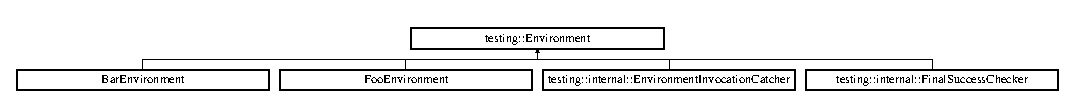
\includegraphics[height=0.989399cm]{classtesting_1_1_environment}
\end{center}
\end{figure}
\subsection*{Public Member Functions}
\begin{DoxyCompactItemize}
\item 
virtual \hyperlink{classtesting_1_1_environment_a0e41c320362576d752cd1f44cabd57d4}{$\sim$\+Environment} ()
\item 
virtual void \hyperlink{classtesting_1_1_environment_a1bf8cafaa9d4eba9feb98655ee434eb3}{Set\+Up} ()
\item 
virtual void \hyperlink{classtesting_1_1_environment_a039bdaa705c46b9b88234cf4d3bb6254}{Tear\+Down} ()
\end{DoxyCompactItemize}


\subsection{Constructor \& Destructor Documentation}
\hypertarget{classtesting_1_1_environment_a0e41c320362576d752cd1f44cabd57d4}{}\index{testing\+::\+Environment@{testing\+::\+Environment}!````~Environment@{$\sim$\+Environment}}
\index{````~Environment@{$\sim$\+Environment}!testing\+::\+Environment@{testing\+::\+Environment}}
\subsubsection[{$\sim$\+Environment()}]{\setlength{\rightskip}{0pt plus 5cm}virtual testing\+::\+Environment\+::$\sim$\+Environment (
\begin{DoxyParamCaption}
{}
\end{DoxyParamCaption}
)\hspace{0.3cm}{\ttfamily [inline]}, {\ttfamily [virtual]}}\label{classtesting_1_1_environment_a0e41c320362576d752cd1f44cabd57d4}


\subsection{Member Function Documentation}
\hypertarget{classtesting_1_1_environment_a1bf8cafaa9d4eba9feb98655ee434eb3}{}\index{testing\+::\+Environment@{testing\+::\+Environment}!Set\+Up@{Set\+Up}}
\index{Set\+Up@{Set\+Up}!testing\+::\+Environment@{testing\+::\+Environment}}
\subsubsection[{Set\+Up()}]{\setlength{\rightskip}{0pt plus 5cm}virtual void testing\+::\+Environment\+::\+Set\+Up (
\begin{DoxyParamCaption}
{}
\end{DoxyParamCaption}
)\hspace{0.3cm}{\ttfamily [inline]}, {\ttfamily [virtual]}}\label{classtesting_1_1_environment_a1bf8cafaa9d4eba9feb98655ee434eb3}


Reimplemented in \hyperlink{class_bar_environment_a88e17c5dd1dcea7a4538f2f3c6bf7bdd}{Bar\+Environment}, \hyperlink{class_foo_environment_a7db8d8b312805aff437ae8534132a56d}{Foo\+Environment}, and \hyperlink{classtesting_1_1internal_1_1_environment_invocation_catcher_a325365b0ecfa71a4a767d7a1817c9663}{testing\+::internal\+::\+Environment\+Invocation\+Catcher}.

\hypertarget{classtesting_1_1_environment_a039bdaa705c46b9b88234cf4d3bb6254}{}\index{testing\+::\+Environment@{testing\+::\+Environment}!Tear\+Down@{Tear\+Down}}
\index{Tear\+Down@{Tear\+Down}!testing\+::\+Environment@{testing\+::\+Environment}}
\subsubsection[{Tear\+Down()}]{\setlength{\rightskip}{0pt plus 5cm}virtual void testing\+::\+Environment\+::\+Tear\+Down (
\begin{DoxyParamCaption}
{}
\end{DoxyParamCaption}
)\hspace{0.3cm}{\ttfamily [inline]}, {\ttfamily [virtual]}}\label{classtesting_1_1_environment_a039bdaa705c46b9b88234cf4d3bb6254}


Reimplemented in \hyperlink{class_bar_environment_a384f951da72a2a18bb0c2b3506376b09}{Bar\+Environment}, \hyperlink{class_foo_environment_a99a2c9df52106cce9e7a4bdda53df802}{Foo\+Environment}, \hyperlink{classtesting_1_1internal_1_1_final_success_checker_a8f39d12a1f2bfe8c6c04b5c6749382c9}{testing\+::internal\+::\+Final\+Success\+Checker}, and \hyperlink{classtesting_1_1internal_1_1_environment_invocation_catcher_afc89ee0a8e32e6746a89fcc1682f62e9}{testing\+::internal\+::\+Environment\+Invocation\+Catcher}.



The documentation for this class was generated from the following file\+:\begin{DoxyCompactItemize}
\item 
C\+:/\+Users/\+Hilman/\+Desktop/repo/anjing/src/third\+\_\+party/googletest/include/gtest/\hyperlink{gtest_8h}{gtest.\+h}\end{DoxyCompactItemize}

\hypertarget{classtesting_1_1internal_1_1_environment_invocation_catcher}{}\section{testing\+:\+:internal\+:\+:Environment\+Invocation\+Catcher Class Reference}
\label{classtesting_1_1internal_1_1_environment_invocation_catcher}\index{testing\+::internal\+::\+Environment\+Invocation\+Catcher@{testing\+::internal\+::\+Environment\+Invocation\+Catcher}}
Inheritance diagram for testing\+:\+:internal\+:\+:Environment\+Invocation\+Catcher\+:\begin{figure}[H]
\begin{center}
\leavevmode
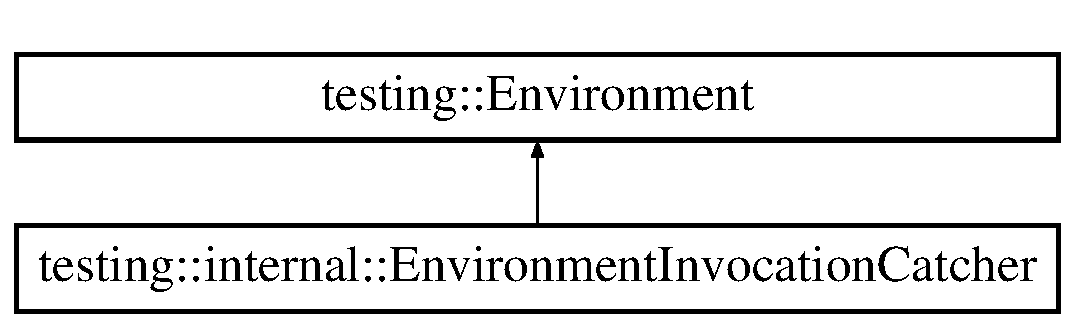
\includegraphics[height=2.000000cm]{classtesting_1_1internal_1_1_environment_invocation_catcher}
\end{center}
\end{figure}
\subsection*{Protected Member Functions}
\begin{DoxyCompactItemize}
\item 
virtual void \hyperlink{classtesting_1_1internal_1_1_environment_invocation_catcher_a325365b0ecfa71a4a767d7a1817c9663}{Set\+Up} ()
\item 
virtual void \hyperlink{classtesting_1_1internal_1_1_environment_invocation_catcher_afc89ee0a8e32e6746a89fcc1682f62e9}{Tear\+Down} ()
\end{DoxyCompactItemize}
\subsection*{Additional Inherited Members}


\subsection{Member Function Documentation}
\hypertarget{classtesting_1_1internal_1_1_environment_invocation_catcher_a325365b0ecfa71a4a767d7a1817c9663}{}\index{testing\+::internal\+::\+Environment\+Invocation\+Catcher@{testing\+::internal\+::\+Environment\+Invocation\+Catcher}!Set\+Up@{Set\+Up}}
\index{Set\+Up@{Set\+Up}!testing\+::internal\+::\+Environment\+Invocation\+Catcher@{testing\+::internal\+::\+Environment\+Invocation\+Catcher}}
\subsubsection[{Set\+Up()}]{\setlength{\rightskip}{0pt plus 5cm}virtual void testing\+::internal\+::\+Environment\+Invocation\+Catcher\+::\+Set\+Up (
\begin{DoxyParamCaption}
{}
\end{DoxyParamCaption}
)\hspace{0.3cm}{\ttfamily [inline]}, {\ttfamily [protected]}, {\ttfamily [virtual]}}\label{classtesting_1_1internal_1_1_environment_invocation_catcher_a325365b0ecfa71a4a767d7a1817c9663}


Reimplemented from \hyperlink{classtesting_1_1_environment_a1bf8cafaa9d4eba9feb98655ee434eb3}{testing\+::\+Environment}.

\hypertarget{classtesting_1_1internal_1_1_environment_invocation_catcher_afc89ee0a8e32e6746a89fcc1682f62e9}{}\index{testing\+::internal\+::\+Environment\+Invocation\+Catcher@{testing\+::internal\+::\+Environment\+Invocation\+Catcher}!Tear\+Down@{Tear\+Down}}
\index{Tear\+Down@{Tear\+Down}!testing\+::internal\+::\+Environment\+Invocation\+Catcher@{testing\+::internal\+::\+Environment\+Invocation\+Catcher}}
\subsubsection[{Tear\+Down()}]{\setlength{\rightskip}{0pt plus 5cm}virtual void testing\+::internal\+::\+Environment\+Invocation\+Catcher\+::\+Tear\+Down (
\begin{DoxyParamCaption}
{}
\end{DoxyParamCaption}
)\hspace{0.3cm}{\ttfamily [inline]}, {\ttfamily [protected]}, {\ttfamily [virtual]}}\label{classtesting_1_1internal_1_1_environment_invocation_catcher_afc89ee0a8e32e6746a89fcc1682f62e9}


Reimplemented from \hyperlink{classtesting_1_1_environment_a039bdaa705c46b9b88234cf4d3bb6254}{testing\+::\+Environment}.



The documentation for this class was generated from the following file\+:\begin{DoxyCompactItemize}
\item 
C\+:/\+Users/\+Hilman/\+Desktop/repo/anjing/src/third\+\_\+party/googletest/test/\hyperlink{gtest-listener__test_8cc}{gtest-\/listener\+\_\+test.\+cc}\end{DoxyCompactItemize}

\hypertarget{classtesting_1_1internal_1_1_eq_helper}{}\section{testing\+:\+:internal\+:\+:Eq\+Helper$<$ lhs\+\_\+is\+\_\+null\+\_\+literal $>$ Class Template Reference}
\label{classtesting_1_1internal_1_1_eq_helper}\index{testing\+::internal\+::\+Eq\+Helper$<$ lhs\+\_\+is\+\_\+null\+\_\+literal $>$@{testing\+::internal\+::\+Eq\+Helper$<$ lhs\+\_\+is\+\_\+null\+\_\+literal $>$}}


{\ttfamily \#include $<$gtest.\+h$>$}

\subsection*{Static Public Member Functions}
\begin{DoxyCompactItemize}
\item 
{\footnotesize template$<$typename T1 , typename T2 $>$ }\\static \hyperlink{classtesting_1_1_assertion_result}{Assertion\+Result} \hyperlink{classtesting_1_1internal_1_1_eq_helper_ac2977ed90cd3c88607f804e43b86b92c}{Compare} (const char $\ast$expected\+\_\+expression, const char $\ast$actual\+\_\+expression, const T1 \&expected, const T2 \&actual)
\item 
static \hyperlink{classtesting_1_1_assertion_result}{Assertion\+Result} \hyperlink{classtesting_1_1internal_1_1_eq_helper_a3de996954b41d484c065ed824fe7eac9}{Compare} (const char $\ast$expected\+\_\+expression, const char $\ast$actual\+\_\+expression, \hyperlink{namespacetesting_1_1internal_a05c6bd9ede5ccdf25191a590d610dcc6}{Biggest\+Int} expected, \hyperlink{namespacetesting_1_1internal_a05c6bd9ede5ccdf25191a590d610dcc6}{Biggest\+Int} actual)
\end{DoxyCompactItemize}


\subsection{Member Function Documentation}
\hypertarget{classtesting_1_1internal_1_1_eq_helper_ac2977ed90cd3c88607f804e43b86b92c}{}\index{testing\+::internal\+::\+Eq\+Helper@{testing\+::internal\+::\+Eq\+Helper}!Compare@{Compare}}
\index{Compare@{Compare}!testing\+::internal\+::\+Eq\+Helper@{testing\+::internal\+::\+Eq\+Helper}}
\subsubsection[{Compare(const char $\ast$expected\+\_\+expression, const char $\ast$actual\+\_\+expression, const T1 \&expected, const T2 \&actual)}]{\setlength{\rightskip}{0pt plus 5cm}template$<$bool lhs\+\_\+is\+\_\+null\+\_\+literal$>$ template$<$typename T1 , typename T2 $>$ static {\bf Assertion\+Result} {\bf testing\+::internal\+::\+Eq\+Helper}$<$ lhs\+\_\+is\+\_\+null\+\_\+literal $>$\+::Compare (
\begin{DoxyParamCaption}
\item[{const char $\ast$}]{expected\+\_\+expression, }
\item[{const char $\ast$}]{actual\+\_\+expression, }
\item[{const T1 \&}]{expected, }
\item[{const T2 \&}]{actual}
\end{DoxyParamCaption}
)\hspace{0.3cm}{\ttfamily [inline]}, {\ttfamily [static]}}\label{classtesting_1_1internal_1_1_eq_helper_ac2977ed90cd3c88607f804e43b86b92c}
\hypertarget{classtesting_1_1internal_1_1_eq_helper_a3de996954b41d484c065ed824fe7eac9}{}\index{testing\+::internal\+::\+Eq\+Helper@{testing\+::internal\+::\+Eq\+Helper}!Compare@{Compare}}
\index{Compare@{Compare}!testing\+::internal\+::\+Eq\+Helper@{testing\+::internal\+::\+Eq\+Helper}}
\subsubsection[{Compare(const char $\ast$expected\+\_\+expression, const char $\ast$actual\+\_\+expression, Biggest\+Int expected, Biggest\+Int actual)}]{\setlength{\rightskip}{0pt plus 5cm}template$<$bool lhs\+\_\+is\+\_\+null\+\_\+literal$>$ static {\bf Assertion\+Result} {\bf testing\+::internal\+::\+Eq\+Helper}$<$ lhs\+\_\+is\+\_\+null\+\_\+literal $>$\+::Compare (
\begin{DoxyParamCaption}
\item[{const char $\ast$}]{expected\+\_\+expression, }
\item[{const char $\ast$}]{actual\+\_\+expression, }
\item[{{\bf Biggest\+Int}}]{expected, }
\item[{{\bf Biggest\+Int}}]{actual}
\end{DoxyParamCaption}
)\hspace{0.3cm}{\ttfamily [inline]}, {\ttfamily [static]}}\label{classtesting_1_1internal_1_1_eq_helper_a3de996954b41d484c065ed824fe7eac9}


The documentation for this class was generated from the following file\+:\begin{DoxyCompactItemize}
\item 
C\+:/\+Users/\+Hilman/\+Desktop/repo/anjing/src/third\+\_\+party/googletest/include/gtest/\hyperlink{gtest_8h}{gtest.\+h}\end{DoxyCompactItemize}

\hypertarget{classtesting_1_1internal_1_1_eq_helper_3_01true_01_4}{}\section{testing\+:\+:internal\+:\+:Eq\+Helper$<$ true $>$ Class Template Reference}
\label{classtesting_1_1internal_1_1_eq_helper_3_01true_01_4}\index{testing\+::internal\+::\+Eq\+Helper$<$ true $>$@{testing\+::internal\+::\+Eq\+Helper$<$ true $>$}}


{\ttfamily \#include $<$gtest.\+h$>$}

\subsection*{Static Public Member Functions}
\begin{DoxyCompactItemize}
\item 
{\footnotesize template$<$typename T1 , typename T2 $>$ }\\static \hyperlink{classtesting_1_1_assertion_result}{Assertion\+Result} \hyperlink{classtesting_1_1internal_1_1_eq_helper_3_01true_01_4_a43a207030451389f902ed12a35eda97d}{Compare} (const char $\ast$expected\+\_\+expression, const char $\ast$actual\+\_\+expression, const T1 \&expected, const T2 \&actual,               typename \hyperlink{structtesting_1_1internal_1_1_enable_if}{Enable\+If}$<$!\hyperlink{structtesting_1_1internal_1_1is__pointer}{is\+\_\+pointer}$<$ T2 $>$\+::value $>$\+::type $\ast$=0)
\item 
{\footnotesize template$<$typename T $>$ }\\static \hyperlink{classtesting_1_1_assertion_result}{Assertion\+Result} \hyperlink{classtesting_1_1internal_1_1_eq_helper_3_01true_01_4_a0be110f9570165cfd7544228fae50b49}{Compare} (const char $\ast$expected\+\_\+expression, const char $\ast$actual\+\_\+expression,                   Secret $\ast$, T $\ast$actual)
\end{DoxyCompactItemize}


\subsection{Member Function Documentation}
\hypertarget{classtesting_1_1internal_1_1_eq_helper_3_01true_01_4_a43a207030451389f902ed12a35eda97d}{}\index{testing\+::internal\+::\+Eq\+Helper$<$ true $>$@{testing\+::internal\+::\+Eq\+Helper$<$ true $>$}!Compare@{Compare}}
\index{Compare@{Compare}!testing\+::internal\+::\+Eq\+Helper$<$ true $>$@{testing\+::internal\+::\+Eq\+Helper$<$ true $>$}}
\subsubsection[{Compare(const char $\ast$expected\+\_\+expression, const char $\ast$actual\+\_\+expression, const T1 \&expected, const T2 \&actual,               typename Enable\+If$<$"!is\+\_\+pointer$<$ T2 $>$\+::value $>$\+::type $\ast$=0)}]{\setlength{\rightskip}{0pt plus 5cm}template$<$typename T1 , typename T2 $>$ static {\bf Assertion\+Result} {\bf testing\+::internal\+::\+Eq\+Helper}$<$ true $>$\+::Compare (
\begin{DoxyParamCaption}
\item[{const char $\ast$}]{expected\+\_\+expression, }
\item[{const char $\ast$}]{actual\+\_\+expression, }
\item[{const T1 \&}]{expected, }
\item[{const T2 \&}]{actual, }
\item[{typename {\bf Enable\+If}$<$!{\bf is\+\_\+pointer}$<$ T2 $>$\+::value $>$\+::type $\ast$}]{ = {\ttfamily 0}}
\end{DoxyParamCaption}
)\hspace{0.3cm}{\ttfamily [inline]}, {\ttfamily [static]}}\label{classtesting_1_1internal_1_1_eq_helper_3_01true_01_4_a43a207030451389f902ed12a35eda97d}
\hypertarget{classtesting_1_1internal_1_1_eq_helper_3_01true_01_4_a0be110f9570165cfd7544228fae50b49}{}\index{testing\+::internal\+::\+Eq\+Helper$<$ true $>$@{testing\+::internal\+::\+Eq\+Helper$<$ true $>$}!Compare@{Compare}}
\index{Compare@{Compare}!testing\+::internal\+::\+Eq\+Helper$<$ true $>$@{testing\+::internal\+::\+Eq\+Helper$<$ true $>$}}
\subsubsection[{Compare(const char $\ast$expected\+\_\+expression, const char $\ast$actual\+\_\+expression,                   Secret $\ast$, T $\ast$actual)}]{\setlength{\rightskip}{0pt plus 5cm}template$<$typename T $>$ static {\bf Assertion\+Result} {\bf testing\+::internal\+::\+Eq\+Helper}$<$ true $>$\+::Compare (
\begin{DoxyParamCaption}
\item[{const char $\ast$}]{expected\+\_\+expression, }
\item[{const char $\ast$}]{actual\+\_\+expression, }
\item[{Secret $\ast$}]{, }
\item[{T $\ast$}]{actual}
\end{DoxyParamCaption}
)\hspace{0.3cm}{\ttfamily [inline]}, {\ttfamily [static]}}\label{classtesting_1_1internal_1_1_eq_helper_3_01true_01_4_a0be110f9570165cfd7544228fae50b49}


The documentation for this class was generated from the following file\+:\begin{DoxyCompactItemize}
\item 
C\+:/\+Users/\+Hilman/\+Desktop/repo/anjing/src/third\+\_\+party/googletest/include/gtest/\hyperlink{gtest_8h}{gtest.\+h}\end{DoxyCompactItemize}

\hypertarget{classtesting_1_1internal_1_1_event_recording_listener}{}\section{testing\+:\+:internal\+:\+:Event\+Recording\+Listener Class Reference}
\label{classtesting_1_1internal_1_1_event_recording_listener}\index{testing\+::internal\+::\+Event\+Recording\+Listener@{testing\+::internal\+::\+Event\+Recording\+Listener}}
Inheritance diagram for testing\+:\+:internal\+:\+:Event\+Recording\+Listener\+:\begin{figure}[H]
\begin{center}
\leavevmode
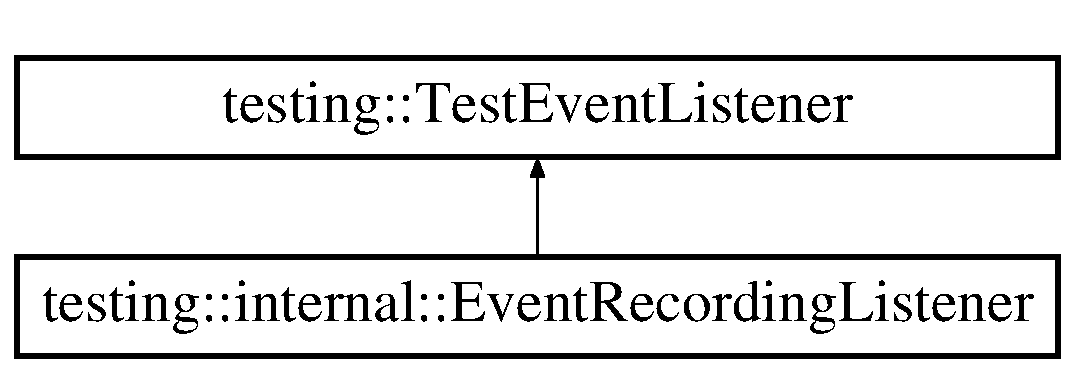
\includegraphics[height=2.000000cm]{classtesting_1_1internal_1_1_event_recording_listener}
\end{center}
\end{figure}
\subsection*{Public Member Functions}
\begin{DoxyCompactItemize}
\item 
\hyperlink{classtesting_1_1internal_1_1_event_recording_listener_a7b0254c15d6b8468e1441ee572fee707}{Event\+Recording\+Listener} (const char $\ast$name)
\end{DoxyCompactItemize}
\subsection*{Protected Member Functions}
\begin{DoxyCompactItemize}
\item 
virtual void \hyperlink{classtesting_1_1internal_1_1_event_recording_listener_aff89fdd3ae889a54a2ba2f3d4c98d3f6}{On\+Test\+Program\+Start} (const \hyperlink{classtesting_1_1_unit_test}{Unit\+Test} \&)
\item 
virtual void \hyperlink{classtesting_1_1internal_1_1_event_recording_listener_a0bfa276def9594b2a119c2c370f59281}{On\+Test\+Iteration\+Start} (const \hyperlink{classtesting_1_1_unit_test}{Unit\+Test} \&, int iteration)
\item 
virtual void \hyperlink{classtesting_1_1internal_1_1_event_recording_listener_add61e6e7ebffb8afc90ccabcdc9f9982}{On\+Environments\+Set\+Up\+Start} (const \hyperlink{classtesting_1_1_unit_test}{Unit\+Test} \&)
\item 
virtual void \hyperlink{classtesting_1_1internal_1_1_event_recording_listener_a40b4c5e05abd1aa11a030f999f6adb8f}{On\+Environments\+Set\+Up\+End} (const \hyperlink{classtesting_1_1_unit_test}{Unit\+Test} \&)
\item 
virtual void \hyperlink{classtesting_1_1internal_1_1_event_recording_listener_a18c28e1d1c3a1e74e225966456786f8e}{On\+Test\+Case\+Start} (const \hyperlink{classtesting_1_1_test_case}{Test\+Case} \&)
\item 
virtual void \hyperlink{classtesting_1_1internal_1_1_event_recording_listener_aebd488b780fc172d6058ca07ca8f7145}{On\+Test\+Start} (const \hyperlink{classtesting_1_1_test_info}{Test\+Info} \&)
\item 
virtual void \hyperlink{classtesting_1_1internal_1_1_event_recording_listener_a4a6685d894923f1691ad9c6a4311470e}{On\+Test\+Part\+Result} (const \hyperlink{classtesting_1_1_test_part_result}{Test\+Part\+Result} \&)
\item 
virtual void \hyperlink{classtesting_1_1internal_1_1_event_recording_listener_adb076f145cc20d9b27441b9c75da4b81}{On\+Test\+End} (const \hyperlink{classtesting_1_1_test_info}{Test\+Info} \&)
\item 
virtual void \hyperlink{classtesting_1_1internal_1_1_event_recording_listener_a4d0cb8a389c7339bce0aa6128291529f}{On\+Test\+Case\+End} (const \hyperlink{classtesting_1_1_test_case}{Test\+Case} \&)
\item 
virtual void \hyperlink{classtesting_1_1internal_1_1_event_recording_listener_a17eebd7bb5cc6bab53b20794919ca5ae}{On\+Environments\+Tear\+Down\+Start} (const \hyperlink{classtesting_1_1_unit_test}{Unit\+Test} \&)
\item 
virtual void \hyperlink{classtesting_1_1internal_1_1_event_recording_listener_acd5a3dc070265166a7da68222031fd61}{On\+Environments\+Tear\+Down\+End} (const \hyperlink{classtesting_1_1_unit_test}{Unit\+Test} \&)
\item 
virtual void \hyperlink{classtesting_1_1internal_1_1_event_recording_listener_ab0cc007bcfaf06cd383d574c88f62aea}{On\+Test\+Iteration\+End} (const \hyperlink{classtesting_1_1_unit_test}{Unit\+Test} \&, int iteration)
\item 
virtual void \hyperlink{classtesting_1_1internal_1_1_event_recording_listener_a21fe9c3c519c4599a48b16ddfb734aa3}{On\+Test\+Program\+End} (const \hyperlink{classtesting_1_1_unit_test}{Unit\+Test} \&)
\end{DoxyCompactItemize}


\subsection{Constructor \& Destructor Documentation}
\hypertarget{classtesting_1_1internal_1_1_event_recording_listener_a7b0254c15d6b8468e1441ee572fee707}{}\index{testing\+::internal\+::\+Event\+Recording\+Listener@{testing\+::internal\+::\+Event\+Recording\+Listener}!Event\+Recording\+Listener@{Event\+Recording\+Listener}}
\index{Event\+Recording\+Listener@{Event\+Recording\+Listener}!testing\+::internal\+::\+Event\+Recording\+Listener@{testing\+::internal\+::\+Event\+Recording\+Listener}}
\subsubsection[{Event\+Recording\+Listener(const char $\ast$name)}]{\setlength{\rightskip}{0pt plus 5cm}testing\+::internal\+::\+Event\+Recording\+Listener\+::\+Event\+Recording\+Listener (
\begin{DoxyParamCaption}
\item[{const char $\ast$}]{name}
\end{DoxyParamCaption}
)\hspace{0.3cm}{\ttfamily [inline]}, {\ttfamily [explicit]}}\label{classtesting_1_1internal_1_1_event_recording_listener_a7b0254c15d6b8468e1441ee572fee707}


\subsection{Member Function Documentation}
\hypertarget{classtesting_1_1internal_1_1_event_recording_listener_a40b4c5e05abd1aa11a030f999f6adb8f}{}\index{testing\+::internal\+::\+Event\+Recording\+Listener@{testing\+::internal\+::\+Event\+Recording\+Listener}!On\+Environments\+Set\+Up\+End@{On\+Environments\+Set\+Up\+End}}
\index{On\+Environments\+Set\+Up\+End@{On\+Environments\+Set\+Up\+End}!testing\+::internal\+::\+Event\+Recording\+Listener@{testing\+::internal\+::\+Event\+Recording\+Listener}}
\subsubsection[{On\+Environments\+Set\+Up\+End(const Unit\+Test \&)}]{\setlength{\rightskip}{0pt plus 5cm}virtual void testing\+::internal\+::\+Event\+Recording\+Listener\+::\+On\+Environments\+Set\+Up\+End (
\begin{DoxyParamCaption}
\item[{const {\bf Unit\+Test} \&}]{}
\end{DoxyParamCaption}
)\hspace{0.3cm}{\ttfamily [inline]}, {\ttfamily [protected]}, {\ttfamily [virtual]}}\label{classtesting_1_1internal_1_1_event_recording_listener_a40b4c5e05abd1aa11a030f999f6adb8f}


Implements \hyperlink{classtesting_1_1_test_event_listener_aaa1021d75f5dbf3f05c829c1cc520341}{testing\+::\+Test\+Event\+Listener}.

\hypertarget{classtesting_1_1internal_1_1_event_recording_listener_add61e6e7ebffb8afc90ccabcdc9f9982}{}\index{testing\+::internal\+::\+Event\+Recording\+Listener@{testing\+::internal\+::\+Event\+Recording\+Listener}!On\+Environments\+Set\+Up\+Start@{On\+Environments\+Set\+Up\+Start}}
\index{On\+Environments\+Set\+Up\+Start@{On\+Environments\+Set\+Up\+Start}!testing\+::internal\+::\+Event\+Recording\+Listener@{testing\+::internal\+::\+Event\+Recording\+Listener}}
\subsubsection[{On\+Environments\+Set\+Up\+Start(const Unit\+Test \&)}]{\setlength{\rightskip}{0pt plus 5cm}virtual void testing\+::internal\+::\+Event\+Recording\+Listener\+::\+On\+Environments\+Set\+Up\+Start (
\begin{DoxyParamCaption}
\item[{const {\bf Unit\+Test} \&}]{}
\end{DoxyParamCaption}
)\hspace{0.3cm}{\ttfamily [inline]}, {\ttfamily [protected]}, {\ttfamily [virtual]}}\label{classtesting_1_1internal_1_1_event_recording_listener_add61e6e7ebffb8afc90ccabcdc9f9982}


Implements \hyperlink{classtesting_1_1_test_event_listener_aa6502e534919605be45f26a6daf9a40c}{testing\+::\+Test\+Event\+Listener}.

\hypertarget{classtesting_1_1internal_1_1_event_recording_listener_acd5a3dc070265166a7da68222031fd61}{}\index{testing\+::internal\+::\+Event\+Recording\+Listener@{testing\+::internal\+::\+Event\+Recording\+Listener}!On\+Environments\+Tear\+Down\+End@{On\+Environments\+Tear\+Down\+End}}
\index{On\+Environments\+Tear\+Down\+End@{On\+Environments\+Tear\+Down\+End}!testing\+::internal\+::\+Event\+Recording\+Listener@{testing\+::internal\+::\+Event\+Recording\+Listener}}
\subsubsection[{On\+Environments\+Tear\+Down\+End(const Unit\+Test \&)}]{\setlength{\rightskip}{0pt plus 5cm}virtual void testing\+::internal\+::\+Event\+Recording\+Listener\+::\+On\+Environments\+Tear\+Down\+End (
\begin{DoxyParamCaption}
\item[{const {\bf Unit\+Test} \&}]{}
\end{DoxyParamCaption}
)\hspace{0.3cm}{\ttfamily [inline]}, {\ttfamily [protected]}, {\ttfamily [virtual]}}\label{classtesting_1_1internal_1_1_event_recording_listener_acd5a3dc070265166a7da68222031fd61}


Implements \hyperlink{classtesting_1_1_test_event_listener_a9ea04fa7f447865ba76df35e12ba2092}{testing\+::\+Test\+Event\+Listener}.

\hypertarget{classtesting_1_1internal_1_1_event_recording_listener_a17eebd7bb5cc6bab53b20794919ca5ae}{}\index{testing\+::internal\+::\+Event\+Recording\+Listener@{testing\+::internal\+::\+Event\+Recording\+Listener}!On\+Environments\+Tear\+Down\+Start@{On\+Environments\+Tear\+Down\+Start}}
\index{On\+Environments\+Tear\+Down\+Start@{On\+Environments\+Tear\+Down\+Start}!testing\+::internal\+::\+Event\+Recording\+Listener@{testing\+::internal\+::\+Event\+Recording\+Listener}}
\subsubsection[{On\+Environments\+Tear\+Down\+Start(const Unit\+Test \&)}]{\setlength{\rightskip}{0pt plus 5cm}virtual void testing\+::internal\+::\+Event\+Recording\+Listener\+::\+On\+Environments\+Tear\+Down\+Start (
\begin{DoxyParamCaption}
\item[{const {\bf Unit\+Test} \&}]{}
\end{DoxyParamCaption}
)\hspace{0.3cm}{\ttfamily [inline]}, {\ttfamily [protected]}, {\ttfamily [virtual]}}\label{classtesting_1_1internal_1_1_event_recording_listener_a17eebd7bb5cc6bab53b20794919ca5ae}


Implements \hyperlink{classtesting_1_1_test_event_listener_a468b5e6701bcb86cb2c956caadbba5e4}{testing\+::\+Test\+Event\+Listener}.

\hypertarget{classtesting_1_1internal_1_1_event_recording_listener_a4d0cb8a389c7339bce0aa6128291529f}{}\index{testing\+::internal\+::\+Event\+Recording\+Listener@{testing\+::internal\+::\+Event\+Recording\+Listener}!On\+Test\+Case\+End@{On\+Test\+Case\+End}}
\index{On\+Test\+Case\+End@{On\+Test\+Case\+End}!testing\+::internal\+::\+Event\+Recording\+Listener@{testing\+::internal\+::\+Event\+Recording\+Listener}}
\subsubsection[{On\+Test\+Case\+End(const Test\+Case \&)}]{\setlength{\rightskip}{0pt plus 5cm}virtual void testing\+::internal\+::\+Event\+Recording\+Listener\+::\+On\+Test\+Case\+End (
\begin{DoxyParamCaption}
\item[{const {\bf Test\+Case} \&}]{}
\end{DoxyParamCaption}
)\hspace{0.3cm}{\ttfamily [inline]}, {\ttfamily [protected]}, {\ttfamily [virtual]}}\label{classtesting_1_1internal_1_1_event_recording_listener_a4d0cb8a389c7339bce0aa6128291529f}


Implements \hyperlink{classtesting_1_1_test_event_listener_ae61985e2ef76ac78379b077be57a9c36}{testing\+::\+Test\+Event\+Listener}.

\hypertarget{classtesting_1_1internal_1_1_event_recording_listener_a18c28e1d1c3a1e74e225966456786f8e}{}\index{testing\+::internal\+::\+Event\+Recording\+Listener@{testing\+::internal\+::\+Event\+Recording\+Listener}!On\+Test\+Case\+Start@{On\+Test\+Case\+Start}}
\index{On\+Test\+Case\+Start@{On\+Test\+Case\+Start}!testing\+::internal\+::\+Event\+Recording\+Listener@{testing\+::internal\+::\+Event\+Recording\+Listener}}
\subsubsection[{On\+Test\+Case\+Start(const Test\+Case \&)}]{\setlength{\rightskip}{0pt plus 5cm}virtual void testing\+::internal\+::\+Event\+Recording\+Listener\+::\+On\+Test\+Case\+Start (
\begin{DoxyParamCaption}
\item[{const {\bf Test\+Case} \&}]{}
\end{DoxyParamCaption}
)\hspace{0.3cm}{\ttfamily [inline]}, {\ttfamily [protected]}, {\ttfamily [virtual]}}\label{classtesting_1_1internal_1_1_event_recording_listener_a18c28e1d1c3a1e74e225966456786f8e}


Implements \hyperlink{classtesting_1_1_test_event_listener_ab4ed885d63f5bbff8076c1329b3dfe36}{testing\+::\+Test\+Event\+Listener}.

\hypertarget{classtesting_1_1internal_1_1_event_recording_listener_adb076f145cc20d9b27441b9c75da4b81}{}\index{testing\+::internal\+::\+Event\+Recording\+Listener@{testing\+::internal\+::\+Event\+Recording\+Listener}!On\+Test\+End@{On\+Test\+End}}
\index{On\+Test\+End@{On\+Test\+End}!testing\+::internal\+::\+Event\+Recording\+Listener@{testing\+::internal\+::\+Event\+Recording\+Listener}}
\subsubsection[{On\+Test\+End(const Test\+Info \&)}]{\setlength{\rightskip}{0pt plus 5cm}virtual void testing\+::internal\+::\+Event\+Recording\+Listener\+::\+On\+Test\+End (
\begin{DoxyParamCaption}
\item[{const {\bf Test\+Info} \&}]{}
\end{DoxyParamCaption}
)\hspace{0.3cm}{\ttfamily [inline]}, {\ttfamily [protected]}, {\ttfamily [virtual]}}\label{classtesting_1_1internal_1_1_event_recording_listener_adb076f145cc20d9b27441b9c75da4b81}


Implements \hyperlink{classtesting_1_1_test_event_listener_abb1c44525ef038500608b5dc2f17099b}{testing\+::\+Test\+Event\+Listener}.

\hypertarget{classtesting_1_1internal_1_1_event_recording_listener_ab0cc007bcfaf06cd383d574c88f62aea}{}\index{testing\+::internal\+::\+Event\+Recording\+Listener@{testing\+::internal\+::\+Event\+Recording\+Listener}!On\+Test\+Iteration\+End@{On\+Test\+Iteration\+End}}
\index{On\+Test\+Iteration\+End@{On\+Test\+Iteration\+End}!testing\+::internal\+::\+Event\+Recording\+Listener@{testing\+::internal\+::\+Event\+Recording\+Listener}}
\subsubsection[{On\+Test\+Iteration\+End(const Unit\+Test \&, int iteration)}]{\setlength{\rightskip}{0pt plus 5cm}virtual void testing\+::internal\+::\+Event\+Recording\+Listener\+::\+On\+Test\+Iteration\+End (
\begin{DoxyParamCaption}
\item[{const {\bf Unit\+Test} \&}]{, }
\item[{int}]{iteration}
\end{DoxyParamCaption}
)\hspace{0.3cm}{\ttfamily [inline]}, {\ttfamily [protected]}, {\ttfamily [virtual]}}\label{classtesting_1_1internal_1_1_event_recording_listener_ab0cc007bcfaf06cd383d574c88f62aea}


Implements \hyperlink{classtesting_1_1_test_event_listener_a550fdb3e55726e4cefa09f5697941425}{testing\+::\+Test\+Event\+Listener}.

\hypertarget{classtesting_1_1internal_1_1_event_recording_listener_a0bfa276def9594b2a119c2c370f59281}{}\index{testing\+::internal\+::\+Event\+Recording\+Listener@{testing\+::internal\+::\+Event\+Recording\+Listener}!On\+Test\+Iteration\+Start@{On\+Test\+Iteration\+Start}}
\index{On\+Test\+Iteration\+Start@{On\+Test\+Iteration\+Start}!testing\+::internal\+::\+Event\+Recording\+Listener@{testing\+::internal\+::\+Event\+Recording\+Listener}}
\subsubsection[{On\+Test\+Iteration\+Start(const Unit\+Test \&, int iteration)}]{\setlength{\rightskip}{0pt plus 5cm}virtual void testing\+::internal\+::\+Event\+Recording\+Listener\+::\+On\+Test\+Iteration\+Start (
\begin{DoxyParamCaption}
\item[{const {\bf Unit\+Test} \&}]{, }
\item[{int}]{iteration}
\end{DoxyParamCaption}
)\hspace{0.3cm}{\ttfamily [inline]}, {\ttfamily [protected]}, {\ttfamily [virtual]}}\label{classtesting_1_1internal_1_1_event_recording_listener_a0bfa276def9594b2a119c2c370f59281}


Implements \hyperlink{classtesting_1_1_test_event_listener_a60cc09b7907cb329d152eb5e7133bdeb}{testing\+::\+Test\+Event\+Listener}.

\hypertarget{classtesting_1_1internal_1_1_event_recording_listener_a4a6685d894923f1691ad9c6a4311470e}{}\index{testing\+::internal\+::\+Event\+Recording\+Listener@{testing\+::internal\+::\+Event\+Recording\+Listener}!On\+Test\+Part\+Result@{On\+Test\+Part\+Result}}
\index{On\+Test\+Part\+Result@{On\+Test\+Part\+Result}!testing\+::internal\+::\+Event\+Recording\+Listener@{testing\+::internal\+::\+Event\+Recording\+Listener}}
\subsubsection[{On\+Test\+Part\+Result(const Test\+Part\+Result \&)}]{\setlength{\rightskip}{0pt plus 5cm}virtual void testing\+::internal\+::\+Event\+Recording\+Listener\+::\+On\+Test\+Part\+Result (
\begin{DoxyParamCaption}
\item[{const {\bf Test\+Part\+Result} \&}]{}
\end{DoxyParamCaption}
)\hspace{0.3cm}{\ttfamily [inline]}, {\ttfamily [protected]}, {\ttfamily [virtual]}}\label{classtesting_1_1internal_1_1_event_recording_listener_a4a6685d894923f1691ad9c6a4311470e}


Implements \hyperlink{classtesting_1_1_test_event_listener_a054f8705c883fa120b91473aff38f2ee}{testing\+::\+Test\+Event\+Listener}.

\hypertarget{classtesting_1_1internal_1_1_event_recording_listener_a21fe9c3c519c4599a48b16ddfb734aa3}{}\index{testing\+::internal\+::\+Event\+Recording\+Listener@{testing\+::internal\+::\+Event\+Recording\+Listener}!On\+Test\+Program\+End@{On\+Test\+Program\+End}}
\index{On\+Test\+Program\+End@{On\+Test\+Program\+End}!testing\+::internal\+::\+Event\+Recording\+Listener@{testing\+::internal\+::\+Event\+Recording\+Listener}}
\subsubsection[{On\+Test\+Program\+End(const Unit\+Test \&)}]{\setlength{\rightskip}{0pt plus 5cm}virtual void testing\+::internal\+::\+Event\+Recording\+Listener\+::\+On\+Test\+Program\+End (
\begin{DoxyParamCaption}
\item[{const {\bf Unit\+Test} \&}]{}
\end{DoxyParamCaption}
)\hspace{0.3cm}{\ttfamily [inline]}, {\ttfamily [protected]}, {\ttfamily [virtual]}}\label{classtesting_1_1internal_1_1_event_recording_listener_a21fe9c3c519c4599a48b16ddfb734aa3}


Implements \hyperlink{classtesting_1_1_test_event_listener_ad15b6246d94c268e233487a86463ef3d}{testing\+::\+Test\+Event\+Listener}.

\hypertarget{classtesting_1_1internal_1_1_event_recording_listener_aff89fdd3ae889a54a2ba2f3d4c98d3f6}{}\index{testing\+::internal\+::\+Event\+Recording\+Listener@{testing\+::internal\+::\+Event\+Recording\+Listener}!On\+Test\+Program\+Start@{On\+Test\+Program\+Start}}
\index{On\+Test\+Program\+Start@{On\+Test\+Program\+Start}!testing\+::internal\+::\+Event\+Recording\+Listener@{testing\+::internal\+::\+Event\+Recording\+Listener}}
\subsubsection[{On\+Test\+Program\+Start(const Unit\+Test \&)}]{\setlength{\rightskip}{0pt plus 5cm}virtual void testing\+::internal\+::\+Event\+Recording\+Listener\+::\+On\+Test\+Program\+Start (
\begin{DoxyParamCaption}
\item[{const {\bf Unit\+Test} \&}]{}
\end{DoxyParamCaption}
)\hspace{0.3cm}{\ttfamily [inline]}, {\ttfamily [protected]}, {\ttfamily [virtual]}}\label{classtesting_1_1internal_1_1_event_recording_listener_aff89fdd3ae889a54a2ba2f3d4c98d3f6}


Implements \hyperlink{classtesting_1_1_test_event_listener_a5f6c84f39851e8a603a2d2e10063816b}{testing\+::\+Test\+Event\+Listener}.

\hypertarget{classtesting_1_1internal_1_1_event_recording_listener_aebd488b780fc172d6058ca07ca8f7145}{}\index{testing\+::internal\+::\+Event\+Recording\+Listener@{testing\+::internal\+::\+Event\+Recording\+Listener}!On\+Test\+Start@{On\+Test\+Start}}
\index{On\+Test\+Start@{On\+Test\+Start}!testing\+::internal\+::\+Event\+Recording\+Listener@{testing\+::internal\+::\+Event\+Recording\+Listener}}
\subsubsection[{On\+Test\+Start(const Test\+Info \&)}]{\setlength{\rightskip}{0pt plus 5cm}virtual void testing\+::internal\+::\+Event\+Recording\+Listener\+::\+On\+Test\+Start (
\begin{DoxyParamCaption}
\item[{const {\bf Test\+Info} \&}]{}
\end{DoxyParamCaption}
)\hspace{0.3cm}{\ttfamily [inline]}, {\ttfamily [protected]}, {\ttfamily [virtual]}}\label{classtesting_1_1internal_1_1_event_recording_listener_aebd488b780fc172d6058ca07ca8f7145}


Implements \hyperlink{classtesting_1_1_test_event_listener_ab4f6a0ca16ae75daf385b3b5914e1048}{testing\+::\+Test\+Event\+Listener}.



The documentation for this class was generated from the following file\+:\begin{DoxyCompactItemize}
\item 
C\+:/\+Users/\+Hilman/\+Desktop/repo/anjing/src/third\+\_\+party/googletest/test/\hyperlink{gtest-listener__test_8cc}{gtest-\/listener\+\_\+test.\+cc}\end{DoxyCompactItemize}

\hypertarget{class_expect_failure_test}{}\section{Expect\+Failure\+Test Class Reference}
\label{class_expect_failure_test}\index{Expect\+Failure\+Test@{Expect\+Failure\+Test}}
Inheritance diagram for Expect\+Failure\+Test\+:\begin{figure}[H]
\begin{center}
\leavevmode
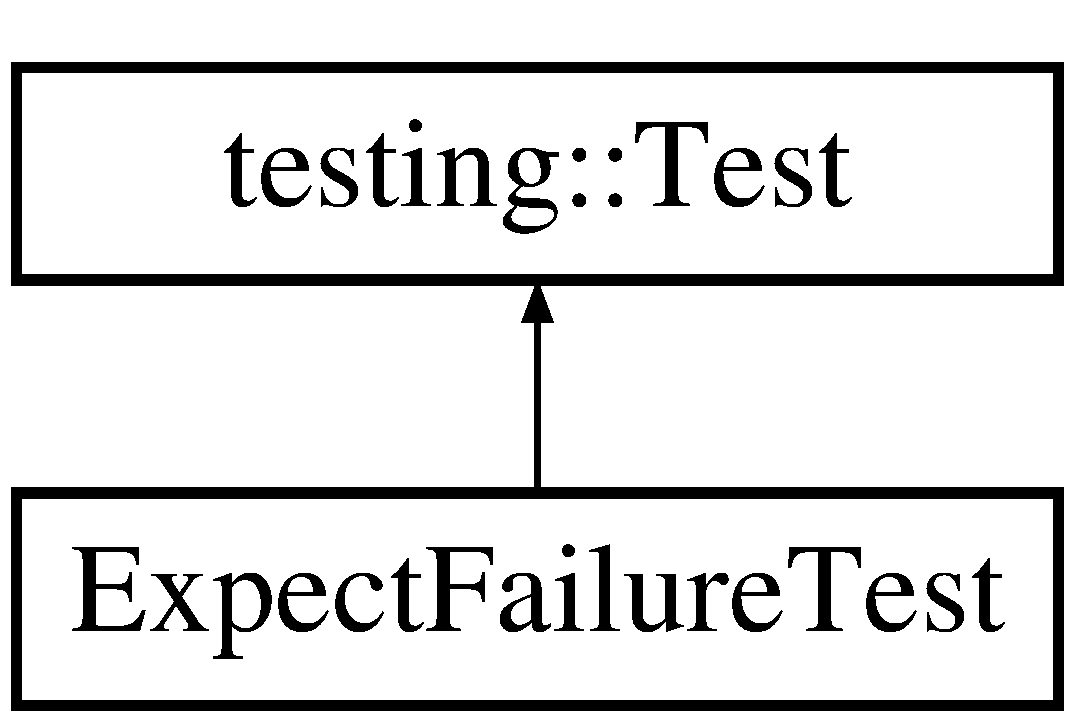
\includegraphics[height=2.000000cm]{class_expect_failure_test}
\end{center}
\end{figure}
\subsection*{Public Types}
\begin{DoxyCompactItemize}
\item 
enum \hyperlink{class_expect_failure_test_aad05da10bb15d21a434eba3b37011406}{Failure\+Mode} \{ \hyperlink{class_expect_failure_test_aad05da10bb15d21a434eba3b37011406a3d618496b7e2a2c256e02186bddee4ec}{F\+A\+T\+A\+L\+\_\+\+F\+A\+I\+L\+U\+R\+E}, 
\hyperlink{class_expect_failure_test_aad05da10bb15d21a434eba3b37011406aeabdbecc0c4550d4f46cd44ac62fb92b}{N\+O\+N\+F\+A\+T\+A\+L\+\_\+\+F\+A\+I\+L\+U\+R\+E}
 \}
\end{DoxyCompactItemize}
\subsection*{Static Public Member Functions}
\begin{DoxyCompactItemize}
\item 
static void \hyperlink{class_expect_failure_test_ab9aeb7820ff7953fc2975ecc5abd046b}{Add\+Failure} (\hyperlink{class_expect_failure_test_aad05da10bb15d21a434eba3b37011406}{Failure\+Mode} failure)
\end{DoxyCompactItemize}
\subsection*{Additional Inherited Members}


\subsection{Member Enumeration Documentation}
\hypertarget{class_expect_failure_test_aad05da10bb15d21a434eba3b37011406}{}\index{Expect\+Failure\+Test@{Expect\+Failure\+Test}!Failure\+Mode@{Failure\+Mode}}
\index{Failure\+Mode@{Failure\+Mode}!Expect\+Failure\+Test@{Expect\+Failure\+Test}}
\subsubsection[{Failure\+Mode}]{\setlength{\rightskip}{0pt plus 5cm}enum {\bf Expect\+Failure\+Test\+::\+Failure\+Mode}}\label{class_expect_failure_test_aad05da10bb15d21a434eba3b37011406}
\begin{Desc}
\item[Enumerator]\par
\begin{description}
\index{F\+A\+T\+A\+L\+\_\+\+F\+A\+I\+L\+U\+R\+E@{F\+A\+T\+A\+L\+\_\+\+F\+A\+I\+L\+U\+R\+E}!Expect\+Failure\+Test@{Expect\+Failure\+Test}}\index{Expect\+Failure\+Test@{Expect\+Failure\+Test}!F\+A\+T\+A\+L\+\_\+\+F\+A\+I\+L\+U\+R\+E@{F\+A\+T\+A\+L\+\_\+\+F\+A\+I\+L\+U\+R\+E}}\item[{\em 
\hypertarget{class_expect_failure_test_aad05da10bb15d21a434eba3b37011406a3d618496b7e2a2c256e02186bddee4ec}{}F\+A\+T\+A\+L\+\_\+\+F\+A\+I\+L\+U\+R\+E\label{class_expect_failure_test_aad05da10bb15d21a434eba3b37011406a3d618496b7e2a2c256e02186bddee4ec}
}]\index{N\+O\+N\+F\+A\+T\+A\+L\+\_\+\+F\+A\+I\+L\+U\+R\+E@{N\+O\+N\+F\+A\+T\+A\+L\+\_\+\+F\+A\+I\+L\+U\+R\+E}!Expect\+Failure\+Test@{Expect\+Failure\+Test}}\index{Expect\+Failure\+Test@{Expect\+Failure\+Test}!N\+O\+N\+F\+A\+T\+A\+L\+\_\+\+F\+A\+I\+L\+U\+R\+E@{N\+O\+N\+F\+A\+T\+A\+L\+\_\+\+F\+A\+I\+L\+U\+R\+E}}\item[{\em 
\hypertarget{class_expect_failure_test_aad05da10bb15d21a434eba3b37011406aeabdbecc0c4550d4f46cd44ac62fb92b}{}N\+O\+N\+F\+A\+T\+A\+L\+\_\+\+F\+A\+I\+L\+U\+R\+E\label{class_expect_failure_test_aad05da10bb15d21a434eba3b37011406aeabdbecc0c4550d4f46cd44ac62fb92b}
}]\end{description}
\end{Desc}


\subsection{Member Function Documentation}
\hypertarget{class_expect_failure_test_ab9aeb7820ff7953fc2975ecc5abd046b}{}\index{Expect\+Failure\+Test@{Expect\+Failure\+Test}!Add\+Failure@{Add\+Failure}}
\index{Add\+Failure@{Add\+Failure}!Expect\+Failure\+Test@{Expect\+Failure\+Test}}
\subsubsection[{Add\+Failure(\+Failure\+Mode failure)}]{\setlength{\rightskip}{0pt plus 5cm}static void Expect\+Failure\+Test\+::\+Add\+Failure (
\begin{DoxyParamCaption}
\item[{{\bf Failure\+Mode}}]{failure}
\end{DoxyParamCaption}
)\hspace{0.3cm}{\ttfamily [inline]}, {\ttfamily [static]}}\label{class_expect_failure_test_ab9aeb7820ff7953fc2975ecc5abd046b}


The documentation for this class was generated from the following file\+:\begin{DoxyCompactItemize}
\item 
C\+:/\+Users/\+Hilman/\+Desktop/repo/anjing/src/third\+\_\+party/googletest/test/\hyperlink{gtest__output__test___8cc}{gtest\+\_\+output\+\_\+test\+\_\+.\+cc}\end{DoxyCompactItemize}

\hypertarget{classpump_1_1_exp_node}{}\section{pump.\+Exp\+Node Class Reference}
\label{classpump_1_1_exp_node}\index{pump.\+Exp\+Node@{pump.\+Exp\+Node}}
\subsection*{Public Member Functions}
\begin{DoxyCompactItemize}
\item 
def \hyperlink{classpump_1_1_exp_node_a0808c394c4d3c8ac875005caa1b3e1b3}{\+\_\+\+\_\+init\+\_\+\+\_\+} (self, \hyperlink{classpump_1_1_exp_node_ade05a5a32535d717dc5c194569aaf356}{token}, \hyperlink{classpump_1_1_exp_node_adccfe4778c2e34f6b2c88118c0f1587f}{python\+\_\+exp})
\end{DoxyCompactItemize}
\subsection*{Public Attributes}
\begin{DoxyCompactItemize}
\item 
\hyperlink{classpump_1_1_exp_node_ade05a5a32535d717dc5c194569aaf356}{token}
\item 
\hyperlink{classpump_1_1_exp_node_adccfe4778c2e34f6b2c88118c0f1587f}{python\+\_\+exp}
\end{DoxyCompactItemize}


\subsection{Constructor \& Destructor Documentation}
\hypertarget{classpump_1_1_exp_node_a0808c394c4d3c8ac875005caa1b3e1b3}{}\index{pump\+::\+Exp\+Node@{pump\+::\+Exp\+Node}!\+\_\+\+\_\+init\+\_\+\+\_\+@{\+\_\+\+\_\+init\+\_\+\+\_\+}}
\index{\+\_\+\+\_\+init\+\_\+\+\_\+@{\+\_\+\+\_\+init\+\_\+\+\_\+}!pump\+::\+Exp\+Node@{pump\+::\+Exp\+Node}}
\subsubsection[{\+\_\+\+\_\+init\+\_\+\+\_\+(self, token, python\+\_\+exp)}]{\setlength{\rightskip}{0pt plus 5cm}def pump.\+Exp\+Node.\+\_\+\+\_\+init\+\_\+\+\_\+ (
\begin{DoxyParamCaption}
\item[{}]{self, }
\item[{}]{token, }
\item[{}]{python\+\_\+exp}
\end{DoxyParamCaption}
)}\label{classpump_1_1_exp_node_a0808c394c4d3c8ac875005caa1b3e1b3}


\subsection{Member Data Documentation}
\hypertarget{classpump_1_1_exp_node_adccfe4778c2e34f6b2c88118c0f1587f}{}\index{pump\+::\+Exp\+Node@{pump\+::\+Exp\+Node}!python\+\_\+exp@{python\+\_\+exp}}
\index{python\+\_\+exp@{python\+\_\+exp}!pump\+::\+Exp\+Node@{pump\+::\+Exp\+Node}}
\subsubsection[{python\+\_\+exp}]{\setlength{\rightskip}{0pt plus 5cm}pump.\+Exp\+Node.\+python\+\_\+exp}\label{classpump_1_1_exp_node_adccfe4778c2e34f6b2c88118c0f1587f}
\hypertarget{classpump_1_1_exp_node_ade05a5a32535d717dc5c194569aaf356}{}\index{pump\+::\+Exp\+Node@{pump\+::\+Exp\+Node}!token@{token}}
\index{token@{token}!pump\+::\+Exp\+Node@{pump\+::\+Exp\+Node}}
\subsubsection[{token}]{\setlength{\rightskip}{0pt plus 5cm}pump.\+Exp\+Node.\+token}\label{classpump_1_1_exp_node_ade05a5a32535d717dc5c194569aaf356}


The documentation for this class was generated from the following file\+:\begin{DoxyCompactItemize}
\item 
C\+:/\+Users/\+Hilman/\+Desktop/repo/anjing/src/third\+\_\+party/googletest/scripts/\hyperlink{pump_8py}{pump.\+py}\end{DoxyCompactItemize}

\hypertarget{class_failed_test}{}\section{Failed\+Test Class Reference}
\label{class_failed_test}\index{Failed\+Test@{Failed\+Test}}
Inheritance diagram for Failed\+Test\+:\begin{figure}[H]
\begin{center}
\leavevmode
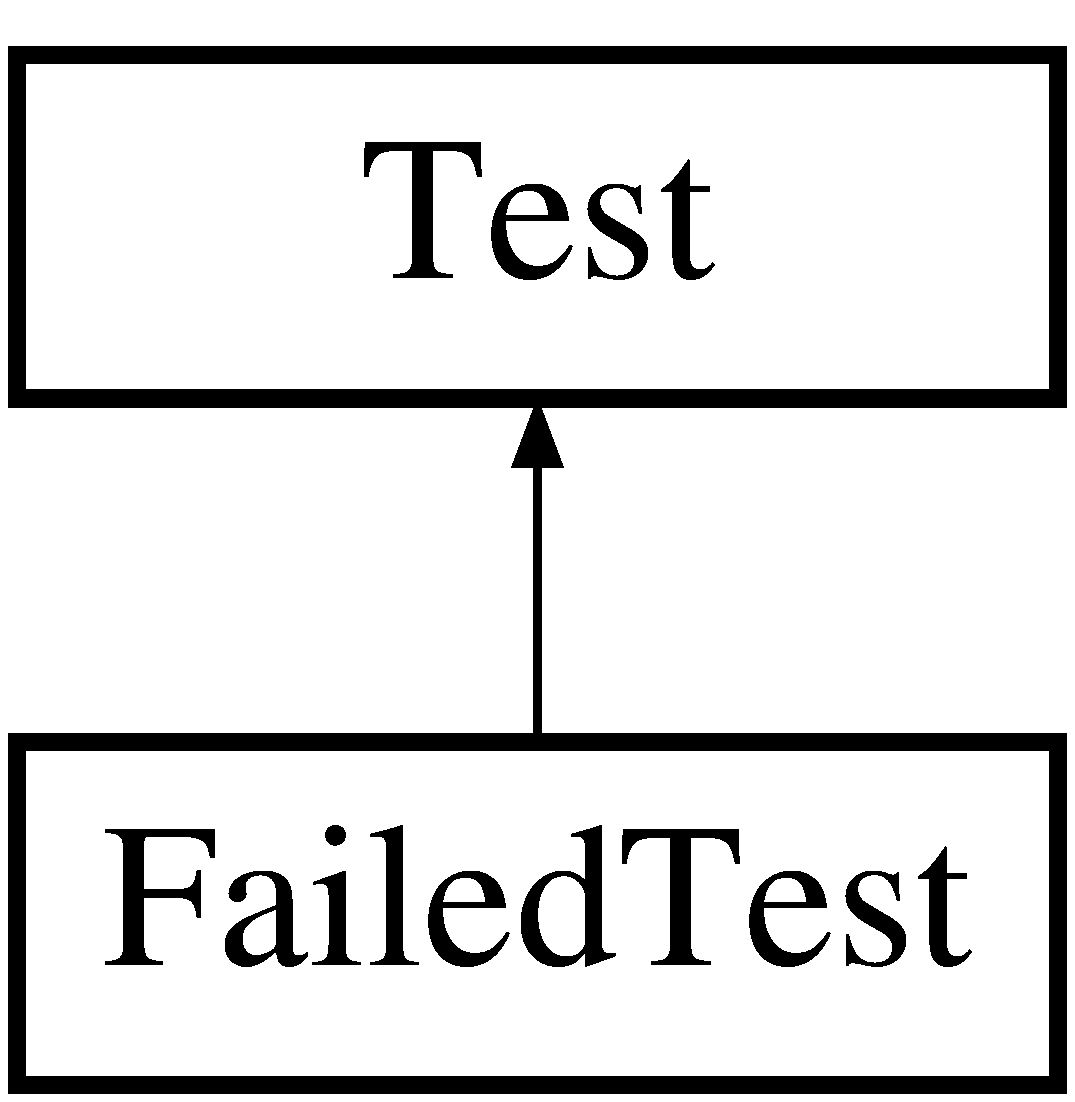
\includegraphics[height=2.000000cm]{class_failed_test}
\end{center}
\end{figure}


The documentation for this class was generated from the following file\+:\begin{DoxyCompactItemize}
\item 
C\+:/\+Users/\+Hilman/\+Desktop/repo/anjing/src/third\+\_\+party/googletest/test/\hyperlink{gtest__xml__output__unittest___8cc}{gtest\+\_\+xml\+\_\+output\+\_\+unittest\+\_\+.\+cc}\end{DoxyCompactItemize}

\hypertarget{class_failing_param_test}{}\section{Failing\+Param\+Test Class Reference}
\label{class_failing_param_test}\index{Failing\+Param\+Test@{Failing\+Param\+Test}}
Inheritance diagram for Failing\+Param\+Test\+:\begin{figure}[H]
\begin{center}
\leavevmode
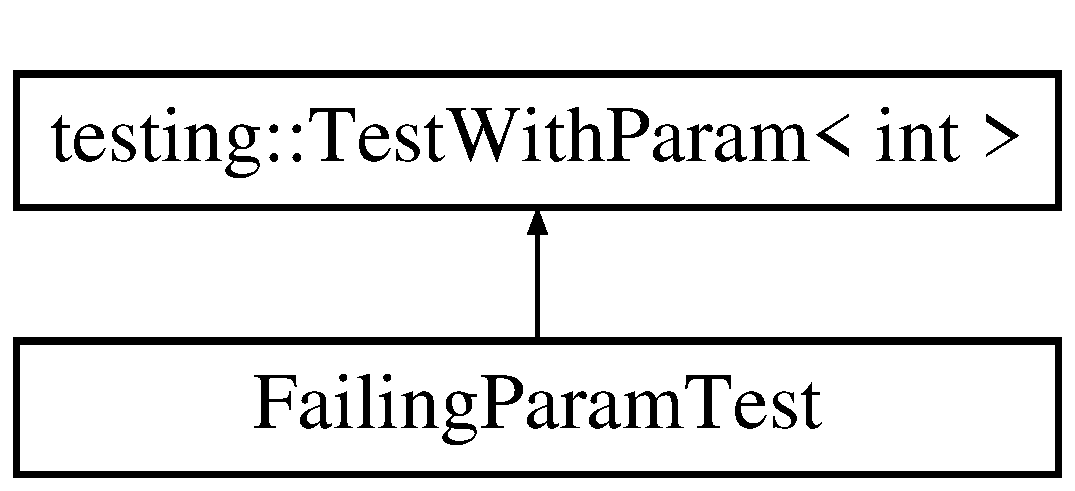
\includegraphics[height=2.000000cm]{class_failing_param_test}
\end{center}
\end{figure}


The documentation for this class was generated from the following file\+:\begin{DoxyCompactItemize}
\item 
C\+:/\+Users/\+Hilman/\+Desktop/repo/anjing/src/third\+\_\+party/googletest/test/\hyperlink{gtest__output__test___8cc}{gtest\+\_\+output\+\_\+test\+\_\+.\+cc}\end{DoxyCompactItemize}

\hypertarget{class_fatal_failure_in_fixture_constructor_test}{}\section{Fatal\+Failure\+In\+Fixture\+Constructor\+Test Class Reference}
\label{class_fatal_failure_in_fixture_constructor_test}\index{Fatal\+Failure\+In\+Fixture\+Constructor\+Test@{Fatal\+Failure\+In\+Fixture\+Constructor\+Test}}
Inheritance diagram for Fatal\+Failure\+In\+Fixture\+Constructor\+Test\+:\begin{figure}[H]
\begin{center}
\leavevmode
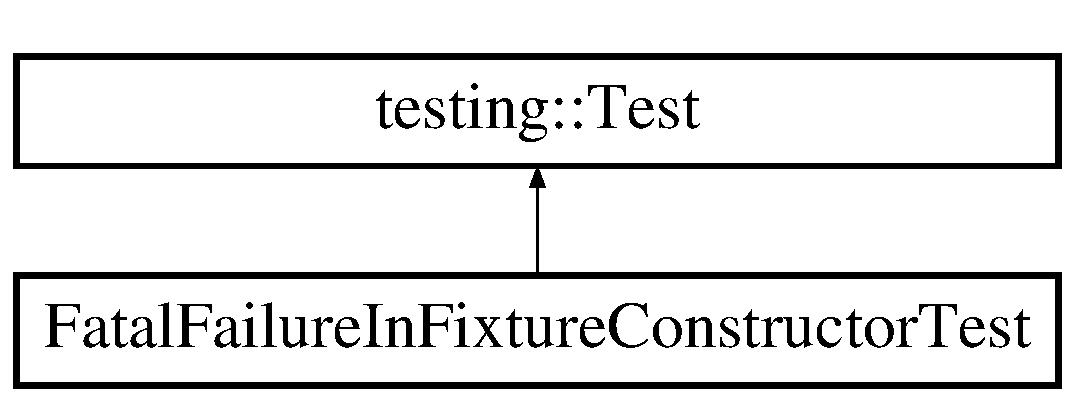
\includegraphics[height=2.000000cm]{class_fatal_failure_in_fixture_constructor_test}
\end{center}
\end{figure}
\subsection*{Protected Member Functions}
\begin{DoxyCompactItemize}
\item 
\hyperlink{class_fatal_failure_in_fixture_constructor_test_a1dc9a5fcf0e1f22d614990a0fe2cb504}{Fatal\+Failure\+In\+Fixture\+Constructor\+Test} ()
\item 
\hyperlink{class_fatal_failure_in_fixture_constructor_test_a514709af7159172a12193a7508683c46}{$\sim$\+Fatal\+Failure\+In\+Fixture\+Constructor\+Test} ()
\item 
virtual void \hyperlink{class_fatal_failure_in_fixture_constructor_test_a006d3ac0e7a4ad3c469c3b41dc7c42c3}{Set\+Up} ()
\item 
virtual void \hyperlink{class_fatal_failure_in_fixture_constructor_test_a2763026a557e1fce4e59bd16c4eced57}{Tear\+Down} ()
\end{DoxyCompactItemize}
\subsection*{Additional Inherited Members}


\subsection{Constructor \& Destructor Documentation}
\hypertarget{class_fatal_failure_in_fixture_constructor_test_a1dc9a5fcf0e1f22d614990a0fe2cb504}{}\index{Fatal\+Failure\+In\+Fixture\+Constructor\+Test@{Fatal\+Failure\+In\+Fixture\+Constructor\+Test}!Fatal\+Failure\+In\+Fixture\+Constructor\+Test@{Fatal\+Failure\+In\+Fixture\+Constructor\+Test}}
\index{Fatal\+Failure\+In\+Fixture\+Constructor\+Test@{Fatal\+Failure\+In\+Fixture\+Constructor\+Test}!Fatal\+Failure\+In\+Fixture\+Constructor\+Test@{Fatal\+Failure\+In\+Fixture\+Constructor\+Test}}
\subsubsection[{Fatal\+Failure\+In\+Fixture\+Constructor\+Test()}]{\setlength{\rightskip}{0pt plus 5cm}Fatal\+Failure\+In\+Fixture\+Constructor\+Test\+::\+Fatal\+Failure\+In\+Fixture\+Constructor\+Test (
\begin{DoxyParamCaption}
{}
\end{DoxyParamCaption}
)\hspace{0.3cm}{\ttfamily [inline]}, {\ttfamily [protected]}}\label{class_fatal_failure_in_fixture_constructor_test_a1dc9a5fcf0e1f22d614990a0fe2cb504}
\hypertarget{class_fatal_failure_in_fixture_constructor_test_a514709af7159172a12193a7508683c46}{}\index{Fatal\+Failure\+In\+Fixture\+Constructor\+Test@{Fatal\+Failure\+In\+Fixture\+Constructor\+Test}!````~Fatal\+Failure\+In\+Fixture\+Constructor\+Test@{$\sim$\+Fatal\+Failure\+In\+Fixture\+Constructor\+Test}}
\index{````~Fatal\+Failure\+In\+Fixture\+Constructor\+Test@{$\sim$\+Fatal\+Failure\+In\+Fixture\+Constructor\+Test}!Fatal\+Failure\+In\+Fixture\+Constructor\+Test@{Fatal\+Failure\+In\+Fixture\+Constructor\+Test}}
\subsubsection[{$\sim$\+Fatal\+Failure\+In\+Fixture\+Constructor\+Test()}]{\setlength{\rightskip}{0pt plus 5cm}Fatal\+Failure\+In\+Fixture\+Constructor\+Test\+::$\sim$\+Fatal\+Failure\+In\+Fixture\+Constructor\+Test (
\begin{DoxyParamCaption}
{}
\end{DoxyParamCaption}
)\hspace{0.3cm}{\ttfamily [inline]}, {\ttfamily [protected]}}\label{class_fatal_failure_in_fixture_constructor_test_a514709af7159172a12193a7508683c46}


\subsection{Member Function Documentation}
\hypertarget{class_fatal_failure_in_fixture_constructor_test_a006d3ac0e7a4ad3c469c3b41dc7c42c3}{}\index{Fatal\+Failure\+In\+Fixture\+Constructor\+Test@{Fatal\+Failure\+In\+Fixture\+Constructor\+Test}!Set\+Up@{Set\+Up}}
\index{Set\+Up@{Set\+Up}!Fatal\+Failure\+In\+Fixture\+Constructor\+Test@{Fatal\+Failure\+In\+Fixture\+Constructor\+Test}}
\subsubsection[{Set\+Up()}]{\setlength{\rightskip}{0pt plus 5cm}virtual void Fatal\+Failure\+In\+Fixture\+Constructor\+Test\+::\+Set\+Up (
\begin{DoxyParamCaption}
{}
\end{DoxyParamCaption}
)\hspace{0.3cm}{\ttfamily [inline]}, {\ttfamily [protected]}, {\ttfamily [virtual]}}\label{class_fatal_failure_in_fixture_constructor_test_a006d3ac0e7a4ad3c469c3b41dc7c42c3}


Reimplemented from \hyperlink{classtesting_1_1_test_a190315150c303ddf801313fd1a777733}{testing\+::\+Test}.

\hypertarget{class_fatal_failure_in_fixture_constructor_test_a2763026a557e1fce4e59bd16c4eced57}{}\index{Fatal\+Failure\+In\+Fixture\+Constructor\+Test@{Fatal\+Failure\+In\+Fixture\+Constructor\+Test}!Tear\+Down@{Tear\+Down}}
\index{Tear\+Down@{Tear\+Down}!Fatal\+Failure\+In\+Fixture\+Constructor\+Test@{Fatal\+Failure\+In\+Fixture\+Constructor\+Test}}
\subsubsection[{Tear\+Down()}]{\setlength{\rightskip}{0pt plus 5cm}virtual void Fatal\+Failure\+In\+Fixture\+Constructor\+Test\+::\+Tear\+Down (
\begin{DoxyParamCaption}
{}
\end{DoxyParamCaption}
)\hspace{0.3cm}{\ttfamily [inline]}, {\ttfamily [protected]}, {\ttfamily [virtual]}}\label{class_fatal_failure_in_fixture_constructor_test_a2763026a557e1fce4e59bd16c4eced57}


Reimplemented from \hyperlink{classtesting_1_1_test_a5f0ab439802cbe0ef7552f1a9f791923}{testing\+::\+Test}.



The documentation for this class was generated from the following file\+:\begin{DoxyCompactItemize}
\item 
C\+:/\+Users/\+Hilman/\+Desktop/repo/anjing/src/third\+\_\+party/googletest/test/\hyperlink{gtest__output__test___8cc}{gtest\+\_\+output\+\_\+test\+\_\+.\+cc}\end{DoxyCompactItemize}

\hypertarget{class_fatal_failure_in_set_up_test}{}\section{Fatal\+Failure\+In\+Set\+Up\+Test Class Reference}
\label{class_fatal_failure_in_set_up_test}\index{Fatal\+Failure\+In\+Set\+Up\+Test@{Fatal\+Failure\+In\+Set\+Up\+Test}}
Inheritance diagram for Fatal\+Failure\+In\+Set\+Up\+Test\+:\begin{figure}[H]
\begin{center}
\leavevmode
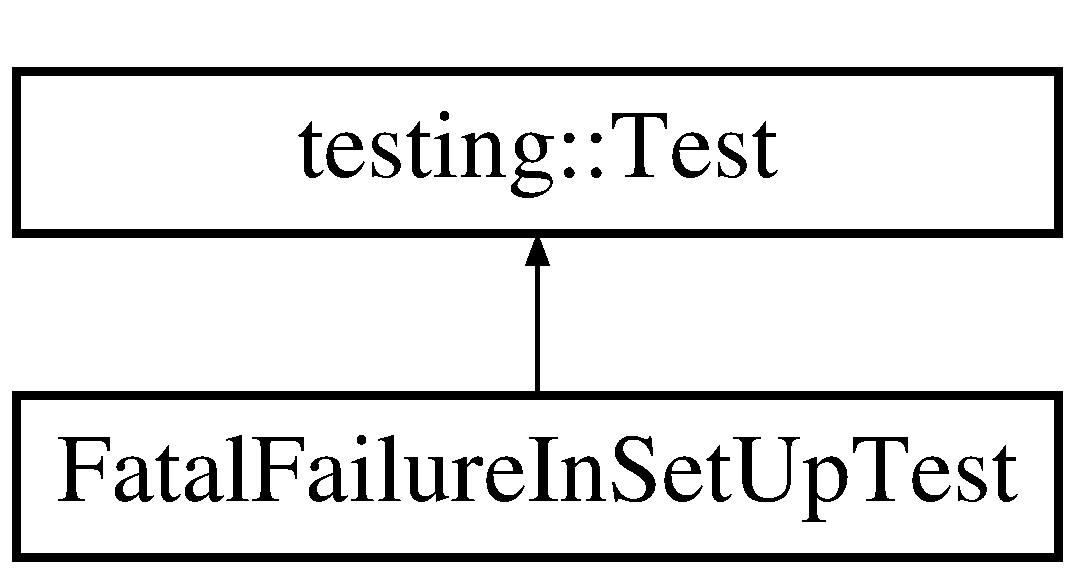
\includegraphics[height=2.000000cm]{class_fatal_failure_in_set_up_test}
\end{center}
\end{figure}
\subsection*{Protected Member Functions}
\begin{DoxyCompactItemize}
\item 
virtual \hyperlink{class_fatal_failure_in_set_up_test_a915ca362b046259c3586c1ab72bb0a93}{$\sim$\+Fatal\+Failure\+In\+Set\+Up\+Test} ()
\item 
virtual void \hyperlink{class_fatal_failure_in_set_up_test_a455696f86fb5f5393624221ccb79b373}{Set\+Up} ()
\item 
virtual void \hyperlink{class_fatal_failure_in_set_up_test_a457707161063e08f7b6600ec5db449e4}{Tear\+Down} ()
\end{DoxyCompactItemize}
\subsection*{Additional Inherited Members}


\subsection{Constructor \& Destructor Documentation}
\hypertarget{class_fatal_failure_in_set_up_test_a915ca362b046259c3586c1ab72bb0a93}{}\index{Fatal\+Failure\+In\+Set\+Up\+Test@{Fatal\+Failure\+In\+Set\+Up\+Test}!````~Fatal\+Failure\+In\+Set\+Up\+Test@{$\sim$\+Fatal\+Failure\+In\+Set\+Up\+Test}}
\index{````~Fatal\+Failure\+In\+Set\+Up\+Test@{$\sim$\+Fatal\+Failure\+In\+Set\+Up\+Test}!Fatal\+Failure\+In\+Set\+Up\+Test@{Fatal\+Failure\+In\+Set\+Up\+Test}}
\subsubsection[{$\sim$\+Fatal\+Failure\+In\+Set\+Up\+Test()}]{\setlength{\rightskip}{0pt plus 5cm}virtual Fatal\+Failure\+In\+Set\+Up\+Test\+::$\sim$\+Fatal\+Failure\+In\+Set\+Up\+Test (
\begin{DoxyParamCaption}
{}
\end{DoxyParamCaption}
)\hspace{0.3cm}{\ttfamily [inline]}, {\ttfamily [protected]}, {\ttfamily [virtual]}}\label{class_fatal_failure_in_set_up_test_a915ca362b046259c3586c1ab72bb0a93}


\subsection{Member Function Documentation}
\hypertarget{class_fatal_failure_in_set_up_test_a455696f86fb5f5393624221ccb79b373}{}\index{Fatal\+Failure\+In\+Set\+Up\+Test@{Fatal\+Failure\+In\+Set\+Up\+Test}!Set\+Up@{Set\+Up}}
\index{Set\+Up@{Set\+Up}!Fatal\+Failure\+In\+Set\+Up\+Test@{Fatal\+Failure\+In\+Set\+Up\+Test}}
\subsubsection[{Set\+Up()}]{\setlength{\rightskip}{0pt plus 5cm}virtual void Fatal\+Failure\+In\+Set\+Up\+Test\+::\+Set\+Up (
\begin{DoxyParamCaption}
{}
\end{DoxyParamCaption}
)\hspace{0.3cm}{\ttfamily [inline]}, {\ttfamily [protected]}, {\ttfamily [virtual]}}\label{class_fatal_failure_in_set_up_test_a455696f86fb5f5393624221ccb79b373}


Reimplemented from \hyperlink{classtesting_1_1_test_a190315150c303ddf801313fd1a777733}{testing\+::\+Test}.

\hypertarget{class_fatal_failure_in_set_up_test_a457707161063e08f7b6600ec5db449e4}{}\index{Fatal\+Failure\+In\+Set\+Up\+Test@{Fatal\+Failure\+In\+Set\+Up\+Test}!Tear\+Down@{Tear\+Down}}
\index{Tear\+Down@{Tear\+Down}!Fatal\+Failure\+In\+Set\+Up\+Test@{Fatal\+Failure\+In\+Set\+Up\+Test}}
\subsubsection[{Tear\+Down()}]{\setlength{\rightskip}{0pt plus 5cm}virtual void Fatal\+Failure\+In\+Set\+Up\+Test\+::\+Tear\+Down (
\begin{DoxyParamCaption}
{}
\end{DoxyParamCaption}
)\hspace{0.3cm}{\ttfamily [inline]}, {\ttfamily [protected]}, {\ttfamily [virtual]}}\label{class_fatal_failure_in_set_up_test_a457707161063e08f7b6600ec5db449e4}


Reimplemented from \hyperlink{classtesting_1_1_test_a5f0ab439802cbe0ef7552f1a9f791923}{testing\+::\+Test}.



The documentation for this class was generated from the following file\+:\begin{DoxyCompactItemize}
\item 
C\+:/\+Users/\+Hilman/\+Desktop/repo/anjing/src/third\+\_\+party/googletest/test/\hyperlink{gtest__output__test___8cc}{gtest\+\_\+output\+\_\+test\+\_\+.\+cc}\end{DoxyCompactItemize}

\hypertarget{classtesting_1_1internal_1_1_file_path}{}\section{testing\+:\+:internal\+:\+:File\+Path Class Reference}
\label{classtesting_1_1internal_1_1_file_path}\index{testing\+::internal\+::\+File\+Path@{testing\+::internal\+::\+File\+Path}}


{\ttfamily \#include $<$gtest-\/filepath.\+h$>$}

\subsection*{Public Member Functions}
\begin{DoxyCompactItemize}
\item 
\hyperlink{classtesting_1_1internal_1_1_file_path_a3504a51accbca78a52fe586133ea5499}{File\+Path} ()
\item 
\hyperlink{classtesting_1_1internal_1_1_file_path_ae9efd0fee56c6e3e2d659b464250b112}{File\+Path} (const \hyperlink{classtesting_1_1internal_1_1_file_path}{File\+Path} \&rhs)
\item 
\hyperlink{classtesting_1_1internal_1_1_file_path_a9fc072b140aa0652a7022fb809fe3abe}{File\+Path} (const std\+::string \&pathname)
\item 
\hyperlink{classtesting_1_1internal_1_1_file_path}{File\+Path} \& \hyperlink{classtesting_1_1internal_1_1_file_path_a8d9c1bafb90f10bcd5611a54d8f326ef}{operator=} (const \hyperlink{classtesting_1_1internal_1_1_file_path}{File\+Path} \&rhs)
\item 
void \hyperlink{classtesting_1_1internal_1_1_file_path_a15a42de7518e89254e0640dd9317d5f7}{Set} (const \hyperlink{classtesting_1_1internal_1_1_file_path}{File\+Path} \&rhs)
\item 
const std\+::string \& \hyperlink{classtesting_1_1internal_1_1_file_path_a7c544a30af67e2da5ce7e625f8402818}{string} () const 
\item 
const char $\ast$ \hyperlink{classtesting_1_1internal_1_1_file_path_a85297234dac0acd936632dff8634c2b9}{c\+\_\+str} () const 
\item 
bool \hyperlink{classtesting_1_1internal_1_1_file_path_a44543ff34ae757038ab20925659b447a}{Is\+Empty} () const 
\item 
\hyperlink{classtesting_1_1internal_1_1_file_path}{File\+Path} \hyperlink{classtesting_1_1internal_1_1_file_path_a952e1b2a9909cdeaf25de5fcdf069b3a}{Remove\+Trailing\+Path\+Separator} () const 
\item 
\hyperlink{classtesting_1_1internal_1_1_file_path}{File\+Path} \hyperlink{classtesting_1_1internal_1_1_file_path_a2852e5a759ff2e2620c7317b8121d757}{Remove\+Directory\+Name} () const 
\item 
\hyperlink{classtesting_1_1internal_1_1_file_path}{File\+Path} \hyperlink{classtesting_1_1internal_1_1_file_path_aed3abcd0b8a7f6ed1ff0e7743ef8bf1e}{Remove\+File\+Name} () const 
\item 
\hyperlink{classtesting_1_1internal_1_1_file_path}{File\+Path} \hyperlink{classtesting_1_1internal_1_1_file_path_ab2a25cc916c111597b94d006aa973c3d}{Remove\+Extension} (const char $\ast$extension) const 
\item 
bool \hyperlink{classtesting_1_1internal_1_1_file_path_afccf35a45e209c22e68c6f8e86036c12}{Create\+Directories\+Recursively} () const 
\item 
bool \hyperlink{classtesting_1_1internal_1_1_file_path_a303cdda61bee6e8a0b0303e8fc857e36}{Create\+Folder} () const 
\item 
bool \hyperlink{classtesting_1_1internal_1_1_file_path_a3548d3ead0e94701669afc64d765ece7}{File\+Or\+Directory\+Exists} () const 
\item 
bool \hyperlink{classtesting_1_1internal_1_1_file_path_a3546b3f926935fefddb9a808e7e2be47}{Directory\+Exists} () const 
\item 
bool \hyperlink{classtesting_1_1internal_1_1_file_path_a918336f16efa8e07d4b94192d6a89f44}{Is\+Directory} () const 
\item 
bool \hyperlink{classtesting_1_1internal_1_1_file_path_a7d31c82f3f979c54e5a985382b52feb1}{Is\+Root\+Directory} () const 
\item 
bool \hyperlink{classtesting_1_1internal_1_1_file_path_a720a5f0fd00f3e98d6f3518f4dadfff5}{Is\+Absolute\+Path} () const 
\end{DoxyCompactItemize}
\subsection*{Static Public Member Functions}
\begin{DoxyCompactItemize}
\item 
static \hyperlink{classtesting_1_1internal_1_1_file_path}{File\+Path} \hyperlink{classtesting_1_1internal_1_1_file_path_aaff39ccd7bfb7a1c09c0220a64326387}{Get\+Current\+Dir} ()
\item 
static \hyperlink{classtesting_1_1internal_1_1_file_path}{File\+Path} \hyperlink{classtesting_1_1internal_1_1_file_path_aa8c102da670261eb4fa8e2f2481df139}{Make\+File\+Name} (const \hyperlink{classtesting_1_1internal_1_1_file_path}{File\+Path} \&directory, const \hyperlink{classtesting_1_1internal_1_1_file_path}{File\+Path} \&base\+\_\+name, int number, const char $\ast$extension)
\item 
static \hyperlink{classtesting_1_1internal_1_1_file_path}{File\+Path} \hyperlink{classtesting_1_1internal_1_1_file_path_ac9d57987f60ac43f0c57b89e333e531e}{Concat\+Paths} (const \hyperlink{classtesting_1_1internal_1_1_file_path}{File\+Path} \&directory, const \hyperlink{classtesting_1_1internal_1_1_file_path}{File\+Path} \&relative\+\_\+path)
\item 
static \hyperlink{classtesting_1_1internal_1_1_file_path}{File\+Path} \hyperlink{classtesting_1_1internal_1_1_file_path_a2280a77adb394cf80bb5f73fc292e8c8}{Generate\+Unique\+File\+Name} (const \hyperlink{classtesting_1_1internal_1_1_file_path}{File\+Path} \&directory, const \hyperlink{classtesting_1_1internal_1_1_file_path}{File\+Path} \&base\+\_\+name, const char $\ast$extension)
\end{DoxyCompactItemize}


\subsection{Constructor \& Destructor Documentation}
\hypertarget{classtesting_1_1internal_1_1_file_path_a3504a51accbca78a52fe586133ea5499}{}\index{testing\+::internal\+::\+File\+Path@{testing\+::internal\+::\+File\+Path}!File\+Path@{File\+Path}}
\index{File\+Path@{File\+Path}!testing\+::internal\+::\+File\+Path@{testing\+::internal\+::\+File\+Path}}
\subsubsection[{File\+Path()}]{\setlength{\rightskip}{0pt plus 5cm}testing\+::internal\+::\+File\+Path\+::\+File\+Path (
\begin{DoxyParamCaption}
{}
\end{DoxyParamCaption}
)\hspace{0.3cm}{\ttfamily [inline]}}\label{classtesting_1_1internal_1_1_file_path_a3504a51accbca78a52fe586133ea5499}
\hypertarget{classtesting_1_1internal_1_1_file_path_ae9efd0fee56c6e3e2d659b464250b112}{}\index{testing\+::internal\+::\+File\+Path@{testing\+::internal\+::\+File\+Path}!File\+Path@{File\+Path}}
\index{File\+Path@{File\+Path}!testing\+::internal\+::\+File\+Path@{testing\+::internal\+::\+File\+Path}}
\subsubsection[{File\+Path(const File\+Path \&rhs)}]{\setlength{\rightskip}{0pt plus 5cm}testing\+::internal\+::\+File\+Path\+::\+File\+Path (
\begin{DoxyParamCaption}
\item[{const {\bf File\+Path} \&}]{rhs}
\end{DoxyParamCaption}
)\hspace{0.3cm}{\ttfamily [inline]}}\label{classtesting_1_1internal_1_1_file_path_ae9efd0fee56c6e3e2d659b464250b112}
\hypertarget{classtesting_1_1internal_1_1_file_path_a9fc072b140aa0652a7022fb809fe3abe}{}\index{testing\+::internal\+::\+File\+Path@{testing\+::internal\+::\+File\+Path}!File\+Path@{File\+Path}}
\index{File\+Path@{File\+Path}!testing\+::internal\+::\+File\+Path@{testing\+::internal\+::\+File\+Path}}
\subsubsection[{File\+Path(const std\+::string \&pathname)}]{\setlength{\rightskip}{0pt plus 5cm}testing\+::internal\+::\+File\+Path\+::\+File\+Path (
\begin{DoxyParamCaption}
\item[{const std\+::string \&}]{pathname}
\end{DoxyParamCaption}
)\hspace{0.3cm}{\ttfamily [inline]}, {\ttfamily [explicit]}}\label{classtesting_1_1internal_1_1_file_path_a9fc072b140aa0652a7022fb809fe3abe}


\subsection{Member Function Documentation}
\hypertarget{classtesting_1_1internal_1_1_file_path_a85297234dac0acd936632dff8634c2b9}{}\index{testing\+::internal\+::\+File\+Path@{testing\+::internal\+::\+File\+Path}!c\+\_\+str@{c\+\_\+str}}
\index{c\+\_\+str@{c\+\_\+str}!testing\+::internal\+::\+File\+Path@{testing\+::internal\+::\+File\+Path}}
\subsubsection[{c\+\_\+str() const }]{\setlength{\rightskip}{0pt plus 5cm}const char$\ast$ testing\+::internal\+::\+File\+Path\+::c\+\_\+str (
\begin{DoxyParamCaption}
{}
\end{DoxyParamCaption}
) const\hspace{0.3cm}{\ttfamily [inline]}}\label{classtesting_1_1internal_1_1_file_path_a85297234dac0acd936632dff8634c2b9}
\hypertarget{classtesting_1_1internal_1_1_file_path_ac9d57987f60ac43f0c57b89e333e531e}{}\index{testing\+::internal\+::\+File\+Path@{testing\+::internal\+::\+File\+Path}!Concat\+Paths@{Concat\+Paths}}
\index{Concat\+Paths@{Concat\+Paths}!testing\+::internal\+::\+File\+Path@{testing\+::internal\+::\+File\+Path}}
\subsubsection[{Concat\+Paths(const File\+Path \&directory, const File\+Path \&relative\+\_\+path)}]{\setlength{\rightskip}{0pt plus 5cm}{\bf File\+Path} testing\+::internal\+::\+File\+Path\+::\+Concat\+Paths (
\begin{DoxyParamCaption}
\item[{const {\bf File\+Path} \&}]{directory, }
\item[{const {\bf File\+Path} \&}]{relative\+\_\+path}
\end{DoxyParamCaption}
)\hspace{0.3cm}{\ttfamily [static]}}\label{classtesting_1_1internal_1_1_file_path_ac9d57987f60ac43f0c57b89e333e531e}
\hypertarget{classtesting_1_1internal_1_1_file_path_afccf35a45e209c22e68c6f8e86036c12}{}\index{testing\+::internal\+::\+File\+Path@{testing\+::internal\+::\+File\+Path}!Create\+Directories\+Recursively@{Create\+Directories\+Recursively}}
\index{Create\+Directories\+Recursively@{Create\+Directories\+Recursively}!testing\+::internal\+::\+File\+Path@{testing\+::internal\+::\+File\+Path}}
\subsubsection[{Create\+Directories\+Recursively() const }]{\setlength{\rightskip}{0pt plus 5cm}bool testing\+::internal\+::\+File\+Path\+::\+Create\+Directories\+Recursively (
\begin{DoxyParamCaption}
{}
\end{DoxyParamCaption}
) const}\label{classtesting_1_1internal_1_1_file_path_afccf35a45e209c22e68c6f8e86036c12}
\hypertarget{classtesting_1_1internal_1_1_file_path_a303cdda61bee6e8a0b0303e8fc857e36}{}\index{testing\+::internal\+::\+File\+Path@{testing\+::internal\+::\+File\+Path}!Create\+Folder@{Create\+Folder}}
\index{Create\+Folder@{Create\+Folder}!testing\+::internal\+::\+File\+Path@{testing\+::internal\+::\+File\+Path}}
\subsubsection[{Create\+Folder() const }]{\setlength{\rightskip}{0pt plus 5cm}bool testing\+::internal\+::\+File\+Path\+::\+Create\+Folder (
\begin{DoxyParamCaption}
{}
\end{DoxyParamCaption}
) const}\label{classtesting_1_1internal_1_1_file_path_a303cdda61bee6e8a0b0303e8fc857e36}
\hypertarget{classtesting_1_1internal_1_1_file_path_a3546b3f926935fefddb9a808e7e2be47}{}\index{testing\+::internal\+::\+File\+Path@{testing\+::internal\+::\+File\+Path}!Directory\+Exists@{Directory\+Exists}}
\index{Directory\+Exists@{Directory\+Exists}!testing\+::internal\+::\+File\+Path@{testing\+::internal\+::\+File\+Path}}
\subsubsection[{Directory\+Exists() const }]{\setlength{\rightskip}{0pt plus 5cm}bool testing\+::internal\+::\+File\+Path\+::\+Directory\+Exists (
\begin{DoxyParamCaption}
{}
\end{DoxyParamCaption}
) const}\label{classtesting_1_1internal_1_1_file_path_a3546b3f926935fefddb9a808e7e2be47}
\hypertarget{classtesting_1_1internal_1_1_file_path_a3548d3ead0e94701669afc64d765ece7}{}\index{testing\+::internal\+::\+File\+Path@{testing\+::internal\+::\+File\+Path}!File\+Or\+Directory\+Exists@{File\+Or\+Directory\+Exists}}
\index{File\+Or\+Directory\+Exists@{File\+Or\+Directory\+Exists}!testing\+::internal\+::\+File\+Path@{testing\+::internal\+::\+File\+Path}}
\subsubsection[{File\+Or\+Directory\+Exists() const }]{\setlength{\rightskip}{0pt plus 5cm}bool testing\+::internal\+::\+File\+Path\+::\+File\+Or\+Directory\+Exists (
\begin{DoxyParamCaption}
{}
\end{DoxyParamCaption}
) const}\label{classtesting_1_1internal_1_1_file_path_a3548d3ead0e94701669afc64d765ece7}
\hypertarget{classtesting_1_1internal_1_1_file_path_a2280a77adb394cf80bb5f73fc292e8c8}{}\index{testing\+::internal\+::\+File\+Path@{testing\+::internal\+::\+File\+Path}!Generate\+Unique\+File\+Name@{Generate\+Unique\+File\+Name}}
\index{Generate\+Unique\+File\+Name@{Generate\+Unique\+File\+Name}!testing\+::internal\+::\+File\+Path@{testing\+::internal\+::\+File\+Path}}
\subsubsection[{Generate\+Unique\+File\+Name(const File\+Path \&directory, const File\+Path \&base\+\_\+name, const char $\ast$extension)}]{\setlength{\rightskip}{0pt plus 5cm}{\bf File\+Path} testing\+::internal\+::\+File\+Path\+::\+Generate\+Unique\+File\+Name (
\begin{DoxyParamCaption}
\item[{const {\bf File\+Path} \&}]{directory, }
\item[{const {\bf File\+Path} \&}]{base\+\_\+name, }
\item[{const char $\ast$}]{extension}
\end{DoxyParamCaption}
)\hspace{0.3cm}{\ttfamily [static]}}\label{classtesting_1_1internal_1_1_file_path_a2280a77adb394cf80bb5f73fc292e8c8}
\hypertarget{classtesting_1_1internal_1_1_file_path_aaff39ccd7bfb7a1c09c0220a64326387}{}\index{testing\+::internal\+::\+File\+Path@{testing\+::internal\+::\+File\+Path}!Get\+Current\+Dir@{Get\+Current\+Dir}}
\index{Get\+Current\+Dir@{Get\+Current\+Dir}!testing\+::internal\+::\+File\+Path@{testing\+::internal\+::\+File\+Path}}
\subsubsection[{Get\+Current\+Dir()}]{\setlength{\rightskip}{0pt plus 5cm}{\bf File\+Path} testing\+::internal\+::\+File\+Path\+::\+Get\+Current\+Dir (
\begin{DoxyParamCaption}
{}
\end{DoxyParamCaption}
)\hspace{0.3cm}{\ttfamily [static]}}\label{classtesting_1_1internal_1_1_file_path_aaff39ccd7bfb7a1c09c0220a64326387}
\hypertarget{classtesting_1_1internal_1_1_file_path_a720a5f0fd00f3e98d6f3518f4dadfff5}{}\index{testing\+::internal\+::\+File\+Path@{testing\+::internal\+::\+File\+Path}!Is\+Absolute\+Path@{Is\+Absolute\+Path}}
\index{Is\+Absolute\+Path@{Is\+Absolute\+Path}!testing\+::internal\+::\+File\+Path@{testing\+::internal\+::\+File\+Path}}
\subsubsection[{Is\+Absolute\+Path() const }]{\setlength{\rightskip}{0pt plus 5cm}bool testing\+::internal\+::\+File\+Path\+::\+Is\+Absolute\+Path (
\begin{DoxyParamCaption}
{}
\end{DoxyParamCaption}
) const}\label{classtesting_1_1internal_1_1_file_path_a720a5f0fd00f3e98d6f3518f4dadfff5}
\hypertarget{classtesting_1_1internal_1_1_file_path_a918336f16efa8e07d4b94192d6a89f44}{}\index{testing\+::internal\+::\+File\+Path@{testing\+::internal\+::\+File\+Path}!Is\+Directory@{Is\+Directory}}
\index{Is\+Directory@{Is\+Directory}!testing\+::internal\+::\+File\+Path@{testing\+::internal\+::\+File\+Path}}
\subsubsection[{Is\+Directory() const }]{\setlength{\rightskip}{0pt plus 5cm}bool testing\+::internal\+::\+File\+Path\+::\+Is\+Directory (
\begin{DoxyParamCaption}
{}
\end{DoxyParamCaption}
) const}\label{classtesting_1_1internal_1_1_file_path_a918336f16efa8e07d4b94192d6a89f44}
\hypertarget{classtesting_1_1internal_1_1_file_path_a44543ff34ae757038ab20925659b447a}{}\index{testing\+::internal\+::\+File\+Path@{testing\+::internal\+::\+File\+Path}!Is\+Empty@{Is\+Empty}}
\index{Is\+Empty@{Is\+Empty}!testing\+::internal\+::\+File\+Path@{testing\+::internal\+::\+File\+Path}}
\subsubsection[{Is\+Empty() const }]{\setlength{\rightskip}{0pt plus 5cm}bool testing\+::internal\+::\+File\+Path\+::\+Is\+Empty (
\begin{DoxyParamCaption}
{}
\end{DoxyParamCaption}
) const\hspace{0.3cm}{\ttfamily [inline]}}\label{classtesting_1_1internal_1_1_file_path_a44543ff34ae757038ab20925659b447a}
\hypertarget{classtesting_1_1internal_1_1_file_path_a7d31c82f3f979c54e5a985382b52feb1}{}\index{testing\+::internal\+::\+File\+Path@{testing\+::internal\+::\+File\+Path}!Is\+Root\+Directory@{Is\+Root\+Directory}}
\index{Is\+Root\+Directory@{Is\+Root\+Directory}!testing\+::internal\+::\+File\+Path@{testing\+::internal\+::\+File\+Path}}
\subsubsection[{Is\+Root\+Directory() const }]{\setlength{\rightskip}{0pt plus 5cm}bool testing\+::internal\+::\+File\+Path\+::\+Is\+Root\+Directory (
\begin{DoxyParamCaption}
{}
\end{DoxyParamCaption}
) const}\label{classtesting_1_1internal_1_1_file_path_a7d31c82f3f979c54e5a985382b52feb1}
\hypertarget{classtesting_1_1internal_1_1_file_path_aa8c102da670261eb4fa8e2f2481df139}{}\index{testing\+::internal\+::\+File\+Path@{testing\+::internal\+::\+File\+Path}!Make\+File\+Name@{Make\+File\+Name}}
\index{Make\+File\+Name@{Make\+File\+Name}!testing\+::internal\+::\+File\+Path@{testing\+::internal\+::\+File\+Path}}
\subsubsection[{Make\+File\+Name(const File\+Path \&directory, const File\+Path \&base\+\_\+name, int number, const char $\ast$extension)}]{\setlength{\rightskip}{0pt plus 5cm}{\bf File\+Path} testing\+::internal\+::\+File\+Path\+::\+Make\+File\+Name (
\begin{DoxyParamCaption}
\item[{const {\bf File\+Path} \&}]{directory, }
\item[{const {\bf File\+Path} \&}]{base\+\_\+name, }
\item[{int}]{number, }
\item[{const char $\ast$}]{extension}
\end{DoxyParamCaption}
)\hspace{0.3cm}{\ttfamily [static]}}\label{classtesting_1_1internal_1_1_file_path_aa8c102da670261eb4fa8e2f2481df139}
\hypertarget{classtesting_1_1internal_1_1_file_path_a8d9c1bafb90f10bcd5611a54d8f326ef}{}\index{testing\+::internal\+::\+File\+Path@{testing\+::internal\+::\+File\+Path}!operator=@{operator=}}
\index{operator=@{operator=}!testing\+::internal\+::\+File\+Path@{testing\+::internal\+::\+File\+Path}}
\subsubsection[{operator=(const File\+Path \&rhs)}]{\setlength{\rightskip}{0pt plus 5cm}{\bf File\+Path}\& testing\+::internal\+::\+File\+Path\+::operator= (
\begin{DoxyParamCaption}
\item[{const {\bf File\+Path} \&}]{rhs}
\end{DoxyParamCaption}
)\hspace{0.3cm}{\ttfamily [inline]}}\label{classtesting_1_1internal_1_1_file_path_a8d9c1bafb90f10bcd5611a54d8f326ef}
\hypertarget{classtesting_1_1internal_1_1_file_path_a2852e5a759ff2e2620c7317b8121d757}{}\index{testing\+::internal\+::\+File\+Path@{testing\+::internal\+::\+File\+Path}!Remove\+Directory\+Name@{Remove\+Directory\+Name}}
\index{Remove\+Directory\+Name@{Remove\+Directory\+Name}!testing\+::internal\+::\+File\+Path@{testing\+::internal\+::\+File\+Path}}
\subsubsection[{Remove\+Directory\+Name() const }]{\setlength{\rightskip}{0pt plus 5cm}{\bf File\+Path} testing\+::internal\+::\+File\+Path\+::\+Remove\+Directory\+Name (
\begin{DoxyParamCaption}
{}
\end{DoxyParamCaption}
) const}\label{classtesting_1_1internal_1_1_file_path_a2852e5a759ff2e2620c7317b8121d757}
\hypertarget{classtesting_1_1internal_1_1_file_path_ab2a25cc916c111597b94d006aa973c3d}{}\index{testing\+::internal\+::\+File\+Path@{testing\+::internal\+::\+File\+Path}!Remove\+Extension@{Remove\+Extension}}
\index{Remove\+Extension@{Remove\+Extension}!testing\+::internal\+::\+File\+Path@{testing\+::internal\+::\+File\+Path}}
\subsubsection[{Remove\+Extension(const char $\ast$extension) const }]{\setlength{\rightskip}{0pt plus 5cm}{\bf File\+Path} testing\+::internal\+::\+File\+Path\+::\+Remove\+Extension (
\begin{DoxyParamCaption}
\item[{const char $\ast$}]{extension}
\end{DoxyParamCaption}
) const}\label{classtesting_1_1internal_1_1_file_path_ab2a25cc916c111597b94d006aa973c3d}
\hypertarget{classtesting_1_1internal_1_1_file_path_aed3abcd0b8a7f6ed1ff0e7743ef8bf1e}{}\index{testing\+::internal\+::\+File\+Path@{testing\+::internal\+::\+File\+Path}!Remove\+File\+Name@{Remove\+File\+Name}}
\index{Remove\+File\+Name@{Remove\+File\+Name}!testing\+::internal\+::\+File\+Path@{testing\+::internal\+::\+File\+Path}}
\subsubsection[{Remove\+File\+Name() const }]{\setlength{\rightskip}{0pt plus 5cm}{\bf File\+Path} testing\+::internal\+::\+File\+Path\+::\+Remove\+File\+Name (
\begin{DoxyParamCaption}
{}
\end{DoxyParamCaption}
) const}\label{classtesting_1_1internal_1_1_file_path_aed3abcd0b8a7f6ed1ff0e7743ef8bf1e}
\hypertarget{classtesting_1_1internal_1_1_file_path_a952e1b2a9909cdeaf25de5fcdf069b3a}{}\index{testing\+::internal\+::\+File\+Path@{testing\+::internal\+::\+File\+Path}!Remove\+Trailing\+Path\+Separator@{Remove\+Trailing\+Path\+Separator}}
\index{Remove\+Trailing\+Path\+Separator@{Remove\+Trailing\+Path\+Separator}!testing\+::internal\+::\+File\+Path@{testing\+::internal\+::\+File\+Path}}
\subsubsection[{Remove\+Trailing\+Path\+Separator() const }]{\setlength{\rightskip}{0pt plus 5cm}{\bf File\+Path} testing\+::internal\+::\+File\+Path\+::\+Remove\+Trailing\+Path\+Separator (
\begin{DoxyParamCaption}
{}
\end{DoxyParamCaption}
) const}\label{classtesting_1_1internal_1_1_file_path_a952e1b2a9909cdeaf25de5fcdf069b3a}
\hypertarget{classtesting_1_1internal_1_1_file_path_a15a42de7518e89254e0640dd9317d5f7}{}\index{testing\+::internal\+::\+File\+Path@{testing\+::internal\+::\+File\+Path}!Set@{Set}}
\index{Set@{Set}!testing\+::internal\+::\+File\+Path@{testing\+::internal\+::\+File\+Path}}
\subsubsection[{Set(const File\+Path \&rhs)}]{\setlength{\rightskip}{0pt plus 5cm}void testing\+::internal\+::\+File\+Path\+::\+Set (
\begin{DoxyParamCaption}
\item[{const {\bf File\+Path} \&}]{rhs}
\end{DoxyParamCaption}
)\hspace{0.3cm}{\ttfamily [inline]}}\label{classtesting_1_1internal_1_1_file_path_a15a42de7518e89254e0640dd9317d5f7}
\hypertarget{classtesting_1_1internal_1_1_file_path_a7c544a30af67e2da5ce7e625f8402818}{}\index{testing\+::internal\+::\+File\+Path@{testing\+::internal\+::\+File\+Path}!string@{string}}
\index{string@{string}!testing\+::internal\+::\+File\+Path@{testing\+::internal\+::\+File\+Path}}
\subsubsection[{string() const }]{\setlength{\rightskip}{0pt plus 5cm}const std\+::string\& testing\+::internal\+::\+File\+Path\+::string (
\begin{DoxyParamCaption}
{}
\end{DoxyParamCaption}
) const\hspace{0.3cm}{\ttfamily [inline]}}\label{classtesting_1_1internal_1_1_file_path_a7c544a30af67e2da5ce7e625f8402818}


The documentation for this class was generated from the following files\+:\begin{DoxyCompactItemize}
\item 
C\+:/\+Users/\+Hilman/\+Desktop/repo/anjing/src/third\+\_\+party/googletest/include/gtest/internal/\hyperlink{gtest-filepath_8h}{gtest-\/filepath.\+h}\item 
C\+:/\+Users/\+Hilman/\+Desktop/repo/anjing/src/third\+\_\+party/googletest/src/\hyperlink{gtest-filepath_8cc}{gtest-\/filepath.\+cc}\end{DoxyCompactItemize}

\hypertarget{classtesting_1_1internal_1_1_final_success_checker}{}\section{testing\+:\+:internal\+:\+:Final\+Success\+Checker Class Reference}
\label{classtesting_1_1internal_1_1_final_success_checker}\index{testing\+::internal\+::\+Final\+Success\+Checker@{testing\+::internal\+::\+Final\+Success\+Checker}}
Inheritance diagram for testing\+:\+:internal\+:\+:Final\+Success\+Checker\+:\begin{figure}[H]
\begin{center}
\leavevmode
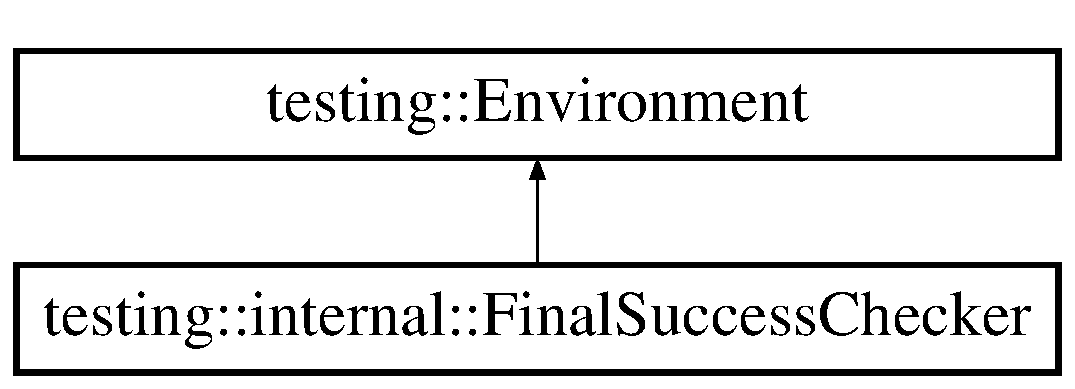
\includegraphics[height=2.000000cm]{classtesting_1_1internal_1_1_final_success_checker}
\end{center}
\end{figure}
\subsection*{Protected Member Functions}
\begin{DoxyCompactItemize}
\item 
virtual void \hyperlink{classtesting_1_1internal_1_1_final_success_checker_a8f39d12a1f2bfe8c6c04b5c6749382c9}{Tear\+Down} ()
\end{DoxyCompactItemize}
\subsection*{Additional Inherited Members}


\subsection{Member Function Documentation}
\hypertarget{classtesting_1_1internal_1_1_final_success_checker_a8f39d12a1f2bfe8c6c04b5c6749382c9}{}\index{testing\+::internal\+::\+Final\+Success\+Checker@{testing\+::internal\+::\+Final\+Success\+Checker}!Tear\+Down@{Tear\+Down}}
\index{Tear\+Down@{Tear\+Down}!testing\+::internal\+::\+Final\+Success\+Checker@{testing\+::internal\+::\+Final\+Success\+Checker}}
\subsubsection[{Tear\+Down()}]{\setlength{\rightskip}{0pt plus 5cm}virtual void testing\+::internal\+::\+Final\+Success\+Checker\+::\+Tear\+Down (
\begin{DoxyParamCaption}
{}
\end{DoxyParamCaption}
)\hspace{0.3cm}{\ttfamily [inline]}, {\ttfamily [protected]}, {\ttfamily [virtual]}}\label{classtesting_1_1internal_1_1_final_success_checker_a8f39d12a1f2bfe8c6c04b5c6749382c9}


Reimplemented from \hyperlink{classtesting_1_1_environment_a039bdaa705c46b9b88234cf4d3bb6254}{testing\+::\+Environment}.



The documentation for this class was generated from the following file\+:\begin{DoxyCompactItemize}
\item 
C\+:/\+Users/\+Hilman/\+Desktop/repo/anjing/src/third\+\_\+party/googletest/test/\hyperlink{gtest-unittest-api__test_8cc}{gtest-\/unittest-\/api\+\_\+test.\+cc}\end{DoxyCompactItemize}

\hypertarget{structtesting_1_1_flags}{}\section{testing\+:\+:Flags Struct Reference}
\label{structtesting_1_1_flags}\index{testing\+::\+Flags@{testing\+::\+Flags}}
\subsection*{Public Member Functions}
\begin{DoxyCompactItemize}
\item 
\hyperlink{structtesting_1_1_flags_a41dc8942bec08ebc7f74dee545e6ad7e}{Flags} ()
\end{DoxyCompactItemize}
\subsection*{Static Public Member Functions}
\begin{DoxyCompactItemize}
\item 
static \hyperlink{structtesting_1_1_flags}{Flags} \hyperlink{structtesting_1_1_flags_a8bee2b5f94d8248b6791d6b005db146f}{Also\+Run\+Disabled\+Tests} (bool \hyperlink{structtesting_1_1_flags_a8ebf8c68f918b9039926b569c880f910}{also\+\_\+run\+\_\+disabled\+\_\+tests})
\item 
static \hyperlink{structtesting_1_1_flags}{Flags} \hyperlink{structtesting_1_1_flags_a62660e44922321f7640bc951a04c2296}{Break\+On\+Failure} (bool \hyperlink{structtesting_1_1_flags_acccce2a9673bb61751269d2ef9c21c89}{break\+\_\+on\+\_\+failure})
\item 
static \hyperlink{structtesting_1_1_flags}{Flags} \hyperlink{structtesting_1_1_flags_a2c7d89f62f4328ae0ced66154ef96b44}{Catch\+Exceptions} (bool \hyperlink{structtesting_1_1_flags_a06984d0553f09716e1bd9f159e7cc644}{catch\+\_\+exceptions})
\item 
static \hyperlink{structtesting_1_1_flags}{Flags} \hyperlink{structtesting_1_1_flags_a4468e5625833043596c44be174349d8c}{Death\+Test\+Use\+Fork} (bool \hyperlink{structtesting_1_1_flags_a7cdef4e6e102771fc15940931dd07e5c}{death\+\_\+test\+\_\+use\+\_\+fork})
\item 
static \hyperlink{structtesting_1_1_flags}{Flags} \hyperlink{structtesting_1_1_flags_afc7350b7c1ac4c0e0efe2d9a94729eb7}{Filter} (const char $\ast$\hyperlink{structtesting_1_1_flags_aa52c1048a7e3cbe726ed4160f2e05d14}{filter})
\item 
static \hyperlink{structtesting_1_1_flags}{Flags} \hyperlink{structtesting_1_1_flags_a825a5d763a31fe6c28f543990bd336df}{List\+Tests} (bool \hyperlink{structtesting_1_1_flags_a3c73f29131074146224018066379fb2f}{list\+\_\+tests})
\item 
static \hyperlink{structtesting_1_1_flags}{Flags} \hyperlink{structtesting_1_1_flags_a507916734a6d7ff2dd02891d7849f2d3}{Output} (const char $\ast$\hyperlink{structtesting_1_1_flags_a8c8289b3af9310744bc25280e3980e4b}{output})
\item 
static \hyperlink{structtesting_1_1_flags}{Flags} \hyperlink{structtesting_1_1_flags_af4dc8454995fb3691399a049e95de179}{Print\+Time} (bool \hyperlink{structtesting_1_1_flags_a8758d574ce5513402679df258f788733}{print\+\_\+time})
\item 
static \hyperlink{structtesting_1_1_flags}{Flags} \hyperlink{structtesting_1_1_flags_a695cd8b8ab44df5eaa371bacded78c05}{Random\+Seed} (Int32 \hyperlink{structtesting_1_1_flags_a4728bce63433f711205fd7b427e57f1b}{random\+\_\+seed})
\item 
static \hyperlink{structtesting_1_1_flags}{Flags} \hyperlink{structtesting_1_1_flags_a19d47e87d77a18ef4fa8a85b74e25956}{Repeat} (Int32 \hyperlink{structtesting_1_1_flags_a61614dd07f97f6e04d27c004ff15195e}{repeat})
\item 
static \hyperlink{structtesting_1_1_flags}{Flags} \hyperlink{structtesting_1_1_flags_a19ddbbaed61bda44a1940333b7c5a469}{Shuffle} (bool \hyperlink{structtesting_1_1_flags_a51c689e47e0f55c16116ac2a1d3b05d6}{shuffle})
\item 
static \hyperlink{structtesting_1_1_flags}{Flags} \hyperlink{structtesting_1_1_flags_a16b01d8bcceaa9fa8211fd24faa75b5a}{Stack\+Trace\+Depth} (Int32 \hyperlink{structtesting_1_1_flags_a20c6592453909c1adace64bf6a2bc2de}{stack\+\_\+trace\+\_\+depth})
\item 
static \hyperlink{structtesting_1_1_flags}{Flags} \hyperlink{structtesting_1_1_flags_a9cf0f64310b28eadbbfbb35584ebfc71}{Stream\+Result\+To} (const char $\ast$\hyperlink{structtesting_1_1_flags_ab09849fd3e095d5628dec65ec4dce9e1}{stream\+\_\+result\+\_\+to})
\item 
static \hyperlink{structtesting_1_1_flags}{Flags} \hyperlink{structtesting_1_1_flags_ad856df862414ed0dadf80b5e03829cc7}{Throw\+On\+Failure} (bool \hyperlink{structtesting_1_1_flags_ab8e7d21e31e641efe47b8050759e001a}{throw\+\_\+on\+\_\+failure})
\end{DoxyCompactItemize}
\subsection*{Public Attributes}
\begin{DoxyCompactItemize}
\item 
bool \hyperlink{structtesting_1_1_flags_a8ebf8c68f918b9039926b569c880f910}{also\+\_\+run\+\_\+disabled\+\_\+tests}
\item 
bool \hyperlink{structtesting_1_1_flags_acccce2a9673bb61751269d2ef9c21c89}{break\+\_\+on\+\_\+failure}
\item 
bool \hyperlink{structtesting_1_1_flags_a06984d0553f09716e1bd9f159e7cc644}{catch\+\_\+exceptions}
\item 
bool \hyperlink{structtesting_1_1_flags_a7cdef4e6e102771fc15940931dd07e5c}{death\+\_\+test\+\_\+use\+\_\+fork}
\item 
const char $\ast$ \hyperlink{structtesting_1_1_flags_aa52c1048a7e3cbe726ed4160f2e05d14}{filter}
\item 
bool \hyperlink{structtesting_1_1_flags_a3c73f29131074146224018066379fb2f}{list\+\_\+tests}
\item 
const char $\ast$ \hyperlink{structtesting_1_1_flags_a8c8289b3af9310744bc25280e3980e4b}{output}
\item 
bool \hyperlink{structtesting_1_1_flags_a8758d574ce5513402679df258f788733}{print\+\_\+time}
\item 
Int32 \hyperlink{structtesting_1_1_flags_a4728bce63433f711205fd7b427e57f1b}{random\+\_\+seed}
\item 
Int32 \hyperlink{structtesting_1_1_flags_a61614dd07f97f6e04d27c004ff15195e}{repeat}
\item 
bool \hyperlink{structtesting_1_1_flags_a51c689e47e0f55c16116ac2a1d3b05d6}{shuffle}
\item 
Int32 \hyperlink{structtesting_1_1_flags_a20c6592453909c1adace64bf6a2bc2de}{stack\+\_\+trace\+\_\+depth}
\item 
const char $\ast$ \hyperlink{structtesting_1_1_flags_ab09849fd3e095d5628dec65ec4dce9e1}{stream\+\_\+result\+\_\+to}
\item 
bool \hyperlink{structtesting_1_1_flags_ab8e7d21e31e641efe47b8050759e001a}{throw\+\_\+on\+\_\+failure}
\end{DoxyCompactItemize}


\subsection{Constructor \& Destructor Documentation}
\hypertarget{structtesting_1_1_flags_a41dc8942bec08ebc7f74dee545e6ad7e}{}\index{testing\+::\+Flags@{testing\+::\+Flags}!Flags@{Flags}}
\index{Flags@{Flags}!testing\+::\+Flags@{testing\+::\+Flags}}
\subsubsection[{Flags()}]{\setlength{\rightskip}{0pt plus 5cm}testing\+::\+Flags\+::\+Flags (
\begin{DoxyParamCaption}
{}
\end{DoxyParamCaption}
)\hspace{0.3cm}{\ttfamily [inline]}}\label{structtesting_1_1_flags_a41dc8942bec08ebc7f74dee545e6ad7e}


\subsection{Member Function Documentation}
\hypertarget{structtesting_1_1_flags_a8bee2b5f94d8248b6791d6b005db146f}{}\index{testing\+::\+Flags@{testing\+::\+Flags}!Also\+Run\+Disabled\+Tests@{Also\+Run\+Disabled\+Tests}}
\index{Also\+Run\+Disabled\+Tests@{Also\+Run\+Disabled\+Tests}!testing\+::\+Flags@{testing\+::\+Flags}}
\subsubsection[{Also\+Run\+Disabled\+Tests(bool also\+\_\+run\+\_\+disabled\+\_\+tests)}]{\setlength{\rightskip}{0pt plus 5cm}static {\bf Flags} testing\+::\+Flags\+::\+Also\+Run\+Disabled\+Tests (
\begin{DoxyParamCaption}
\item[{bool}]{also\+\_\+run\+\_\+disabled\+\_\+tests}
\end{DoxyParamCaption}
)\hspace{0.3cm}{\ttfamily [inline]}, {\ttfamily [static]}}\label{structtesting_1_1_flags_a8bee2b5f94d8248b6791d6b005db146f}
\hypertarget{structtesting_1_1_flags_a62660e44922321f7640bc951a04c2296}{}\index{testing\+::\+Flags@{testing\+::\+Flags}!Break\+On\+Failure@{Break\+On\+Failure}}
\index{Break\+On\+Failure@{Break\+On\+Failure}!testing\+::\+Flags@{testing\+::\+Flags}}
\subsubsection[{Break\+On\+Failure(bool break\+\_\+on\+\_\+failure)}]{\setlength{\rightskip}{0pt plus 5cm}static {\bf Flags} testing\+::\+Flags\+::\+Break\+On\+Failure (
\begin{DoxyParamCaption}
\item[{bool}]{break\+\_\+on\+\_\+failure}
\end{DoxyParamCaption}
)\hspace{0.3cm}{\ttfamily [inline]}, {\ttfamily [static]}}\label{structtesting_1_1_flags_a62660e44922321f7640bc951a04c2296}
\hypertarget{structtesting_1_1_flags_a2c7d89f62f4328ae0ced66154ef96b44}{}\index{testing\+::\+Flags@{testing\+::\+Flags}!Catch\+Exceptions@{Catch\+Exceptions}}
\index{Catch\+Exceptions@{Catch\+Exceptions}!testing\+::\+Flags@{testing\+::\+Flags}}
\subsubsection[{Catch\+Exceptions(bool catch\+\_\+exceptions)}]{\setlength{\rightskip}{0pt plus 5cm}static {\bf Flags} testing\+::\+Flags\+::\+Catch\+Exceptions (
\begin{DoxyParamCaption}
\item[{bool}]{catch\+\_\+exceptions}
\end{DoxyParamCaption}
)\hspace{0.3cm}{\ttfamily [inline]}, {\ttfamily [static]}}\label{structtesting_1_1_flags_a2c7d89f62f4328ae0ced66154ef96b44}
\hypertarget{structtesting_1_1_flags_a4468e5625833043596c44be174349d8c}{}\index{testing\+::\+Flags@{testing\+::\+Flags}!Death\+Test\+Use\+Fork@{Death\+Test\+Use\+Fork}}
\index{Death\+Test\+Use\+Fork@{Death\+Test\+Use\+Fork}!testing\+::\+Flags@{testing\+::\+Flags}}
\subsubsection[{Death\+Test\+Use\+Fork(bool death\+\_\+test\+\_\+use\+\_\+fork)}]{\setlength{\rightskip}{0pt plus 5cm}static {\bf Flags} testing\+::\+Flags\+::\+Death\+Test\+Use\+Fork (
\begin{DoxyParamCaption}
\item[{bool}]{death\+\_\+test\+\_\+use\+\_\+fork}
\end{DoxyParamCaption}
)\hspace{0.3cm}{\ttfamily [inline]}, {\ttfamily [static]}}\label{structtesting_1_1_flags_a4468e5625833043596c44be174349d8c}
\hypertarget{structtesting_1_1_flags_afc7350b7c1ac4c0e0efe2d9a94729eb7}{}\index{testing\+::\+Flags@{testing\+::\+Flags}!Filter@{Filter}}
\index{Filter@{Filter}!testing\+::\+Flags@{testing\+::\+Flags}}
\subsubsection[{Filter(const char $\ast$filter)}]{\setlength{\rightskip}{0pt plus 5cm}static {\bf Flags} testing\+::\+Flags\+::\+Filter (
\begin{DoxyParamCaption}
\item[{const char $\ast$}]{filter}
\end{DoxyParamCaption}
)\hspace{0.3cm}{\ttfamily [inline]}, {\ttfamily [static]}}\label{structtesting_1_1_flags_afc7350b7c1ac4c0e0efe2d9a94729eb7}
\hypertarget{structtesting_1_1_flags_a825a5d763a31fe6c28f543990bd336df}{}\index{testing\+::\+Flags@{testing\+::\+Flags}!List\+Tests@{List\+Tests}}
\index{List\+Tests@{List\+Tests}!testing\+::\+Flags@{testing\+::\+Flags}}
\subsubsection[{List\+Tests(bool list\+\_\+tests)}]{\setlength{\rightskip}{0pt plus 5cm}static {\bf Flags} testing\+::\+Flags\+::\+List\+Tests (
\begin{DoxyParamCaption}
\item[{bool}]{list\+\_\+tests}
\end{DoxyParamCaption}
)\hspace{0.3cm}{\ttfamily [inline]}, {\ttfamily [static]}}\label{structtesting_1_1_flags_a825a5d763a31fe6c28f543990bd336df}
\hypertarget{structtesting_1_1_flags_a507916734a6d7ff2dd02891d7849f2d3}{}\index{testing\+::\+Flags@{testing\+::\+Flags}!Output@{Output}}
\index{Output@{Output}!testing\+::\+Flags@{testing\+::\+Flags}}
\subsubsection[{Output(const char $\ast$output)}]{\setlength{\rightskip}{0pt plus 5cm}static {\bf Flags} testing\+::\+Flags\+::\+Output (
\begin{DoxyParamCaption}
\item[{const char $\ast$}]{output}
\end{DoxyParamCaption}
)\hspace{0.3cm}{\ttfamily [inline]}, {\ttfamily [static]}}\label{structtesting_1_1_flags_a507916734a6d7ff2dd02891d7849f2d3}
\hypertarget{structtesting_1_1_flags_af4dc8454995fb3691399a049e95de179}{}\index{testing\+::\+Flags@{testing\+::\+Flags}!Print\+Time@{Print\+Time}}
\index{Print\+Time@{Print\+Time}!testing\+::\+Flags@{testing\+::\+Flags}}
\subsubsection[{Print\+Time(bool print\+\_\+time)}]{\setlength{\rightskip}{0pt plus 5cm}static {\bf Flags} testing\+::\+Flags\+::\+Print\+Time (
\begin{DoxyParamCaption}
\item[{bool}]{print\+\_\+time}
\end{DoxyParamCaption}
)\hspace{0.3cm}{\ttfamily [inline]}, {\ttfamily [static]}}\label{structtesting_1_1_flags_af4dc8454995fb3691399a049e95de179}
\hypertarget{structtesting_1_1_flags_a695cd8b8ab44df5eaa371bacded78c05}{}\index{testing\+::\+Flags@{testing\+::\+Flags}!Random\+Seed@{Random\+Seed}}
\index{Random\+Seed@{Random\+Seed}!testing\+::\+Flags@{testing\+::\+Flags}}
\subsubsection[{Random\+Seed(\+Int32 random\+\_\+seed)}]{\setlength{\rightskip}{0pt plus 5cm}static {\bf Flags} testing\+::\+Flags\+::\+Random\+Seed (
\begin{DoxyParamCaption}
\item[{Int32}]{random\+\_\+seed}
\end{DoxyParamCaption}
)\hspace{0.3cm}{\ttfamily [inline]}, {\ttfamily [static]}}\label{structtesting_1_1_flags_a695cd8b8ab44df5eaa371bacded78c05}
\hypertarget{structtesting_1_1_flags_a19d47e87d77a18ef4fa8a85b74e25956}{}\index{testing\+::\+Flags@{testing\+::\+Flags}!Repeat@{Repeat}}
\index{Repeat@{Repeat}!testing\+::\+Flags@{testing\+::\+Flags}}
\subsubsection[{Repeat(\+Int32 repeat)}]{\setlength{\rightskip}{0pt plus 5cm}static {\bf Flags} testing\+::\+Flags\+::\+Repeat (
\begin{DoxyParamCaption}
\item[{Int32}]{repeat}
\end{DoxyParamCaption}
)\hspace{0.3cm}{\ttfamily [inline]}, {\ttfamily [static]}}\label{structtesting_1_1_flags_a19d47e87d77a18ef4fa8a85b74e25956}
\hypertarget{structtesting_1_1_flags_a19ddbbaed61bda44a1940333b7c5a469}{}\index{testing\+::\+Flags@{testing\+::\+Flags}!Shuffle@{Shuffle}}
\index{Shuffle@{Shuffle}!testing\+::\+Flags@{testing\+::\+Flags}}
\subsubsection[{Shuffle(bool shuffle)}]{\setlength{\rightskip}{0pt plus 5cm}static {\bf Flags} testing\+::\+Flags\+::\+Shuffle (
\begin{DoxyParamCaption}
\item[{bool}]{shuffle}
\end{DoxyParamCaption}
)\hspace{0.3cm}{\ttfamily [inline]}, {\ttfamily [static]}}\label{structtesting_1_1_flags_a19ddbbaed61bda44a1940333b7c5a469}
\hypertarget{structtesting_1_1_flags_a16b01d8bcceaa9fa8211fd24faa75b5a}{}\index{testing\+::\+Flags@{testing\+::\+Flags}!Stack\+Trace\+Depth@{Stack\+Trace\+Depth}}
\index{Stack\+Trace\+Depth@{Stack\+Trace\+Depth}!testing\+::\+Flags@{testing\+::\+Flags}}
\subsubsection[{Stack\+Trace\+Depth(\+Int32 stack\+\_\+trace\+\_\+depth)}]{\setlength{\rightskip}{0pt plus 5cm}static {\bf Flags} testing\+::\+Flags\+::\+Stack\+Trace\+Depth (
\begin{DoxyParamCaption}
\item[{Int32}]{stack\+\_\+trace\+\_\+depth}
\end{DoxyParamCaption}
)\hspace{0.3cm}{\ttfamily [inline]}, {\ttfamily [static]}}\label{structtesting_1_1_flags_a16b01d8bcceaa9fa8211fd24faa75b5a}
\hypertarget{structtesting_1_1_flags_a9cf0f64310b28eadbbfbb35584ebfc71}{}\index{testing\+::\+Flags@{testing\+::\+Flags}!Stream\+Result\+To@{Stream\+Result\+To}}
\index{Stream\+Result\+To@{Stream\+Result\+To}!testing\+::\+Flags@{testing\+::\+Flags}}
\subsubsection[{Stream\+Result\+To(const char $\ast$stream\+\_\+result\+\_\+to)}]{\setlength{\rightskip}{0pt plus 5cm}static {\bf Flags} testing\+::\+Flags\+::\+Stream\+Result\+To (
\begin{DoxyParamCaption}
\item[{const char $\ast$}]{stream\+\_\+result\+\_\+to}
\end{DoxyParamCaption}
)\hspace{0.3cm}{\ttfamily [inline]}, {\ttfamily [static]}}\label{structtesting_1_1_flags_a9cf0f64310b28eadbbfbb35584ebfc71}
\hypertarget{structtesting_1_1_flags_ad856df862414ed0dadf80b5e03829cc7}{}\index{testing\+::\+Flags@{testing\+::\+Flags}!Throw\+On\+Failure@{Throw\+On\+Failure}}
\index{Throw\+On\+Failure@{Throw\+On\+Failure}!testing\+::\+Flags@{testing\+::\+Flags}}
\subsubsection[{Throw\+On\+Failure(bool throw\+\_\+on\+\_\+failure)}]{\setlength{\rightskip}{0pt plus 5cm}static {\bf Flags} testing\+::\+Flags\+::\+Throw\+On\+Failure (
\begin{DoxyParamCaption}
\item[{bool}]{throw\+\_\+on\+\_\+failure}
\end{DoxyParamCaption}
)\hspace{0.3cm}{\ttfamily [inline]}, {\ttfamily [static]}}\label{structtesting_1_1_flags_ad856df862414ed0dadf80b5e03829cc7}


\subsection{Member Data Documentation}
\hypertarget{structtesting_1_1_flags_a8ebf8c68f918b9039926b569c880f910}{}\index{testing\+::\+Flags@{testing\+::\+Flags}!also\+\_\+run\+\_\+disabled\+\_\+tests@{also\+\_\+run\+\_\+disabled\+\_\+tests}}
\index{also\+\_\+run\+\_\+disabled\+\_\+tests@{also\+\_\+run\+\_\+disabled\+\_\+tests}!testing\+::\+Flags@{testing\+::\+Flags}}
\subsubsection[{also\+\_\+run\+\_\+disabled\+\_\+tests}]{\setlength{\rightskip}{0pt plus 5cm}bool testing\+::\+Flags\+::also\+\_\+run\+\_\+disabled\+\_\+tests}\label{structtesting_1_1_flags_a8ebf8c68f918b9039926b569c880f910}
\hypertarget{structtesting_1_1_flags_acccce2a9673bb61751269d2ef9c21c89}{}\index{testing\+::\+Flags@{testing\+::\+Flags}!break\+\_\+on\+\_\+failure@{break\+\_\+on\+\_\+failure}}
\index{break\+\_\+on\+\_\+failure@{break\+\_\+on\+\_\+failure}!testing\+::\+Flags@{testing\+::\+Flags}}
\subsubsection[{break\+\_\+on\+\_\+failure}]{\setlength{\rightskip}{0pt plus 5cm}bool testing\+::\+Flags\+::break\+\_\+on\+\_\+failure}\label{structtesting_1_1_flags_acccce2a9673bb61751269d2ef9c21c89}
\hypertarget{structtesting_1_1_flags_a06984d0553f09716e1bd9f159e7cc644}{}\index{testing\+::\+Flags@{testing\+::\+Flags}!catch\+\_\+exceptions@{catch\+\_\+exceptions}}
\index{catch\+\_\+exceptions@{catch\+\_\+exceptions}!testing\+::\+Flags@{testing\+::\+Flags}}
\subsubsection[{catch\+\_\+exceptions}]{\setlength{\rightskip}{0pt plus 5cm}bool testing\+::\+Flags\+::catch\+\_\+exceptions}\label{structtesting_1_1_flags_a06984d0553f09716e1bd9f159e7cc644}
\hypertarget{structtesting_1_1_flags_a7cdef4e6e102771fc15940931dd07e5c}{}\index{testing\+::\+Flags@{testing\+::\+Flags}!death\+\_\+test\+\_\+use\+\_\+fork@{death\+\_\+test\+\_\+use\+\_\+fork}}
\index{death\+\_\+test\+\_\+use\+\_\+fork@{death\+\_\+test\+\_\+use\+\_\+fork}!testing\+::\+Flags@{testing\+::\+Flags}}
\subsubsection[{death\+\_\+test\+\_\+use\+\_\+fork}]{\setlength{\rightskip}{0pt plus 5cm}bool testing\+::\+Flags\+::death\+\_\+test\+\_\+use\+\_\+fork}\label{structtesting_1_1_flags_a7cdef4e6e102771fc15940931dd07e5c}
\hypertarget{structtesting_1_1_flags_aa52c1048a7e3cbe726ed4160f2e05d14}{}\index{testing\+::\+Flags@{testing\+::\+Flags}!filter@{filter}}
\index{filter@{filter}!testing\+::\+Flags@{testing\+::\+Flags}}
\subsubsection[{filter}]{\setlength{\rightskip}{0pt plus 5cm}const char$\ast$ testing\+::\+Flags\+::filter}\label{structtesting_1_1_flags_aa52c1048a7e3cbe726ed4160f2e05d14}
\hypertarget{structtesting_1_1_flags_a3c73f29131074146224018066379fb2f}{}\index{testing\+::\+Flags@{testing\+::\+Flags}!list\+\_\+tests@{list\+\_\+tests}}
\index{list\+\_\+tests@{list\+\_\+tests}!testing\+::\+Flags@{testing\+::\+Flags}}
\subsubsection[{list\+\_\+tests}]{\setlength{\rightskip}{0pt plus 5cm}bool testing\+::\+Flags\+::list\+\_\+tests}\label{structtesting_1_1_flags_a3c73f29131074146224018066379fb2f}
\hypertarget{structtesting_1_1_flags_a8c8289b3af9310744bc25280e3980e4b}{}\index{testing\+::\+Flags@{testing\+::\+Flags}!output@{output}}
\index{output@{output}!testing\+::\+Flags@{testing\+::\+Flags}}
\subsubsection[{output}]{\setlength{\rightskip}{0pt plus 5cm}const char$\ast$ testing\+::\+Flags\+::output}\label{structtesting_1_1_flags_a8c8289b3af9310744bc25280e3980e4b}
\hypertarget{structtesting_1_1_flags_a8758d574ce5513402679df258f788733}{}\index{testing\+::\+Flags@{testing\+::\+Flags}!print\+\_\+time@{print\+\_\+time}}
\index{print\+\_\+time@{print\+\_\+time}!testing\+::\+Flags@{testing\+::\+Flags}}
\subsubsection[{print\+\_\+time}]{\setlength{\rightskip}{0pt plus 5cm}bool testing\+::\+Flags\+::print\+\_\+time}\label{structtesting_1_1_flags_a8758d574ce5513402679df258f788733}
\hypertarget{structtesting_1_1_flags_a4728bce63433f711205fd7b427e57f1b}{}\index{testing\+::\+Flags@{testing\+::\+Flags}!random\+\_\+seed@{random\+\_\+seed}}
\index{random\+\_\+seed@{random\+\_\+seed}!testing\+::\+Flags@{testing\+::\+Flags}}
\subsubsection[{random\+\_\+seed}]{\setlength{\rightskip}{0pt plus 5cm}Int32 testing\+::\+Flags\+::random\+\_\+seed}\label{structtesting_1_1_flags_a4728bce63433f711205fd7b427e57f1b}
\hypertarget{structtesting_1_1_flags_a61614dd07f97f6e04d27c004ff15195e}{}\index{testing\+::\+Flags@{testing\+::\+Flags}!repeat@{repeat}}
\index{repeat@{repeat}!testing\+::\+Flags@{testing\+::\+Flags}}
\subsubsection[{repeat}]{\setlength{\rightskip}{0pt plus 5cm}Int32 testing\+::\+Flags\+::repeat}\label{structtesting_1_1_flags_a61614dd07f97f6e04d27c004ff15195e}
\hypertarget{structtesting_1_1_flags_a51c689e47e0f55c16116ac2a1d3b05d6}{}\index{testing\+::\+Flags@{testing\+::\+Flags}!shuffle@{shuffle}}
\index{shuffle@{shuffle}!testing\+::\+Flags@{testing\+::\+Flags}}
\subsubsection[{shuffle}]{\setlength{\rightskip}{0pt plus 5cm}bool testing\+::\+Flags\+::shuffle}\label{structtesting_1_1_flags_a51c689e47e0f55c16116ac2a1d3b05d6}
\hypertarget{structtesting_1_1_flags_a20c6592453909c1adace64bf6a2bc2de}{}\index{testing\+::\+Flags@{testing\+::\+Flags}!stack\+\_\+trace\+\_\+depth@{stack\+\_\+trace\+\_\+depth}}
\index{stack\+\_\+trace\+\_\+depth@{stack\+\_\+trace\+\_\+depth}!testing\+::\+Flags@{testing\+::\+Flags}}
\subsubsection[{stack\+\_\+trace\+\_\+depth}]{\setlength{\rightskip}{0pt plus 5cm}Int32 testing\+::\+Flags\+::stack\+\_\+trace\+\_\+depth}\label{structtesting_1_1_flags_a20c6592453909c1adace64bf6a2bc2de}
\hypertarget{structtesting_1_1_flags_ab09849fd3e095d5628dec65ec4dce9e1}{}\index{testing\+::\+Flags@{testing\+::\+Flags}!stream\+\_\+result\+\_\+to@{stream\+\_\+result\+\_\+to}}
\index{stream\+\_\+result\+\_\+to@{stream\+\_\+result\+\_\+to}!testing\+::\+Flags@{testing\+::\+Flags}}
\subsubsection[{stream\+\_\+result\+\_\+to}]{\setlength{\rightskip}{0pt plus 5cm}const char$\ast$ testing\+::\+Flags\+::stream\+\_\+result\+\_\+to}\label{structtesting_1_1_flags_ab09849fd3e095d5628dec65ec4dce9e1}
\hypertarget{structtesting_1_1_flags_ab8e7d21e31e641efe47b8050759e001a}{}\index{testing\+::\+Flags@{testing\+::\+Flags}!throw\+\_\+on\+\_\+failure@{throw\+\_\+on\+\_\+failure}}
\index{throw\+\_\+on\+\_\+failure@{throw\+\_\+on\+\_\+failure}!testing\+::\+Flags@{testing\+::\+Flags}}
\subsubsection[{throw\+\_\+on\+\_\+failure}]{\setlength{\rightskip}{0pt plus 5cm}bool testing\+::\+Flags\+::throw\+\_\+on\+\_\+failure}\label{structtesting_1_1_flags_ab8e7d21e31e641efe47b8050759e001a}


The documentation for this struct was generated from the following file\+:\begin{DoxyCompactItemize}
\item 
C\+:/\+Users/\+Hilman/\+Desktop/repo/anjing/src/third\+\_\+party/googletest/test/\hyperlink{gtest__unittest_8cc}{gtest\+\_\+unittest.\+cc}\end{DoxyCompactItemize}

\hypertarget{classtesting_1_1internal_1_1_floating_point}{}\section{testing\+:\+:internal\+:\+:Floating\+Point$<$ Raw\+Type $>$ Class Template Reference}
\label{classtesting_1_1internal_1_1_floating_point}\index{testing\+::internal\+::\+Floating\+Point$<$ Raw\+Type $>$@{testing\+::internal\+::\+Floating\+Point$<$ Raw\+Type $>$}}


{\ttfamily \#include $<$gtest-\/internal.\+h$>$}

\subsection*{Public Types}
\begin{DoxyCompactItemize}
\item 
typedef \hyperlink{classtesting_1_1internal_1_1_type_with_size}{Type\+With\+Size}$<$ sizeof(Raw\+Type)$>$\+::U\+Int \hyperlink{classtesting_1_1internal_1_1_floating_point_abf228bf6cd48f12c8b44c85b4971a731}{Bits}
\end{DoxyCompactItemize}
\subsection*{Public Member Functions}
\begin{DoxyCompactItemize}
\item 
\hyperlink{classtesting_1_1internal_1_1_floating_point_a0dabf840863e0df84046f171c891fe71}{Floating\+Point} (const Raw\+Type \&x)
\item 
const \hyperlink{classtesting_1_1internal_1_1_floating_point_abf228bf6cd48f12c8b44c85b4971a731}{Bits} \& \hyperlink{classtesting_1_1internal_1_1_floating_point_abead51f16ec6ea84360a976da1cd1387}{bits} () const 
\item 
\hyperlink{classtesting_1_1internal_1_1_floating_point_abf228bf6cd48f12c8b44c85b4971a731}{Bits} \hyperlink{classtesting_1_1internal_1_1_floating_point_af53c50b85408c582540d6244c026ce2b}{exponent\+\_\+bits} () const 
\item 
\hyperlink{classtesting_1_1internal_1_1_floating_point_abf228bf6cd48f12c8b44c85b4971a731}{Bits} \hyperlink{classtesting_1_1internal_1_1_floating_point_aa0167b7b10a934b743ba3c1f47421e63}{fraction\+\_\+bits} () const 
\item 
\hyperlink{classtesting_1_1internal_1_1_floating_point_abf228bf6cd48f12c8b44c85b4971a731}{Bits} \hyperlink{classtesting_1_1internal_1_1_floating_point_a6176cc4d443724477f2799bcbd9f020a}{sign\+\_\+bit} () const 
\item 
bool \hyperlink{classtesting_1_1internal_1_1_floating_point_aaef2fd2cd8cdf791206a5e9fed8ef90d}{is\+\_\+nan} () const 
\item 
bool \hyperlink{classtesting_1_1internal_1_1_floating_point_adb0fe9ab1d9e5288f8e5550234211166}{Almost\+Equals} (const \hyperlink{classtesting_1_1internal_1_1_floating_point}{Floating\+Point} \&rhs) const 
\item 
{\footnotesize template$<$$>$ }\\float \hyperlink{classtesting_1_1internal_1_1_floating_point_af2eda9331e679229a1baa3404b57b51d}{Max} ()
\item 
{\footnotesize template$<$$>$ }\\double \hyperlink{classtesting_1_1internal_1_1_floating_point_afc2e85c0e886cb13b2300e961c9a9648}{Max} ()
\end{DoxyCompactItemize}
\subsection*{Static Public Member Functions}
\begin{DoxyCompactItemize}
\item 
static Raw\+Type \hyperlink{classtesting_1_1internal_1_1_floating_point_ac551f793522e54fbd8a25acb79eac5b1}{Reinterpret\+Bits} (const \hyperlink{classtesting_1_1internal_1_1_floating_point_abf228bf6cd48f12c8b44c85b4971a731}{Bits} \hyperlink{classtesting_1_1internal_1_1_floating_point_abead51f16ec6ea84360a976da1cd1387}{bits})
\item 
static Raw\+Type \hyperlink{classtesting_1_1internal_1_1_floating_point_a460027cc19cf01ae8e09cc3796b2b575}{Infinity} ()
\item 
static Raw\+Type \hyperlink{classtesting_1_1internal_1_1_floating_point_aae5954d8a57d3ff0987c6930cb68e114}{Max} ()
\end{DoxyCompactItemize}
\subsection*{Static Public Attributes}
\begin{DoxyCompactItemize}
\item 
static const size\+\_\+t \hyperlink{classtesting_1_1internal_1_1_floating_point_ab819d2e8f93e9e482373999f0f8d71b9}{k\+Bit\+Count} = 8$\ast$sizeof(Raw\+Type)
\item 
static const size\+\_\+t \hyperlink{classtesting_1_1internal_1_1_floating_point_a0b756a6d2a4f5f5b41ca79651c06c043}{k\+Fraction\+Bit\+Count}
\item 
static const size\+\_\+t \hyperlink{classtesting_1_1internal_1_1_floating_point_a1973d843c00781053d3073daa8a40119}{k\+Exponent\+Bit\+Count} = \hyperlink{classtesting_1_1internal_1_1_floating_point_ab819d2e8f93e9e482373999f0f8d71b9}{k\+Bit\+Count} -\/ 1 -\/ \hyperlink{classtesting_1_1internal_1_1_floating_point_a0b756a6d2a4f5f5b41ca79651c06c043}{k\+Fraction\+Bit\+Count}
\item 
static const \hyperlink{classtesting_1_1internal_1_1_floating_point_abf228bf6cd48f12c8b44c85b4971a731}{Bits} \hyperlink{classtesting_1_1internal_1_1_floating_point_aca98b5ea6f2222a66a82e52421682efa}{k\+Sign\+Bit\+Mask} = static\+\_\+cast$<$\hyperlink{classtesting_1_1internal_1_1_floating_point_abf228bf6cd48f12c8b44c85b4971a731}{Bits}$>$(1) $<$$<$ (\hyperlink{classtesting_1_1internal_1_1_floating_point_ab819d2e8f93e9e482373999f0f8d71b9}{k\+Bit\+Count} -\/ 1)
\item 
static const \hyperlink{classtesting_1_1internal_1_1_floating_point_abf228bf6cd48f12c8b44c85b4971a731}{Bits} \hyperlink{classtesting_1_1internal_1_1_floating_point_a0ac75d4ffd24f14bca452abe8a718da1}{k\+Fraction\+Bit\+Mask}
\item 
static const \hyperlink{classtesting_1_1internal_1_1_floating_point_abf228bf6cd48f12c8b44c85b4971a731}{Bits} \hyperlink{classtesting_1_1internal_1_1_floating_point_a66065dfc4d5f41100f686159637af23b}{k\+Exponent\+Bit\+Mask} = $\sim$(\hyperlink{classtesting_1_1internal_1_1_floating_point_aca98b5ea6f2222a66a82e52421682efa}{k\+Sign\+Bit\+Mask} $\vert$ \hyperlink{classtesting_1_1internal_1_1_floating_point_a0ac75d4ffd24f14bca452abe8a718da1}{k\+Fraction\+Bit\+Mask})
\item 
static const size\+\_\+t \hyperlink{classtesting_1_1internal_1_1_floating_point_aac498b3714d93f8e88cdc30e4c5935f6}{k\+Max\+Ulps} = 4
\end{DoxyCompactItemize}


\subsection{Member Typedef Documentation}
\hypertarget{classtesting_1_1internal_1_1_floating_point_abf228bf6cd48f12c8b44c85b4971a731}{}\index{testing\+::internal\+::\+Floating\+Point@{testing\+::internal\+::\+Floating\+Point}!Bits@{Bits}}
\index{Bits@{Bits}!testing\+::internal\+::\+Floating\+Point@{testing\+::internal\+::\+Floating\+Point}}
\subsubsection[{Bits}]{\setlength{\rightskip}{0pt plus 5cm}template$<$typename Raw\+Type$>$ typedef {\bf Type\+With\+Size}$<$sizeof(Raw\+Type)$>$\+::U\+Int {\bf testing\+::internal\+::\+Floating\+Point}$<$ Raw\+Type $>$\+::{\bf Bits}}\label{classtesting_1_1internal_1_1_floating_point_abf228bf6cd48f12c8b44c85b4971a731}


\subsection{Constructor \& Destructor Documentation}
\hypertarget{classtesting_1_1internal_1_1_floating_point_a0dabf840863e0df84046f171c891fe71}{}\index{testing\+::internal\+::\+Floating\+Point@{testing\+::internal\+::\+Floating\+Point}!Floating\+Point@{Floating\+Point}}
\index{Floating\+Point@{Floating\+Point}!testing\+::internal\+::\+Floating\+Point@{testing\+::internal\+::\+Floating\+Point}}
\subsubsection[{Floating\+Point(const Raw\+Type \&x)}]{\setlength{\rightskip}{0pt plus 5cm}template$<$typename Raw\+Type$>$ {\bf testing\+::internal\+::\+Floating\+Point}$<$ Raw\+Type $>$\+::{\bf Floating\+Point} (
\begin{DoxyParamCaption}
\item[{const Raw\+Type \&}]{x}
\end{DoxyParamCaption}
)\hspace{0.3cm}{\ttfamily [inline]}, {\ttfamily [explicit]}}\label{classtesting_1_1internal_1_1_floating_point_a0dabf840863e0df84046f171c891fe71}


\subsection{Member Function Documentation}
\hypertarget{classtesting_1_1internal_1_1_floating_point_adb0fe9ab1d9e5288f8e5550234211166}{}\index{testing\+::internal\+::\+Floating\+Point@{testing\+::internal\+::\+Floating\+Point}!Almost\+Equals@{Almost\+Equals}}
\index{Almost\+Equals@{Almost\+Equals}!testing\+::internal\+::\+Floating\+Point@{testing\+::internal\+::\+Floating\+Point}}
\subsubsection[{Almost\+Equals(const Floating\+Point \&rhs) const }]{\setlength{\rightskip}{0pt plus 5cm}template$<$typename Raw\+Type$>$ bool {\bf testing\+::internal\+::\+Floating\+Point}$<$ Raw\+Type $>$\+::Almost\+Equals (
\begin{DoxyParamCaption}
\item[{const {\bf Floating\+Point}$<$ Raw\+Type $>$ \&}]{rhs}
\end{DoxyParamCaption}
) const\hspace{0.3cm}{\ttfamily [inline]}}\label{classtesting_1_1internal_1_1_floating_point_adb0fe9ab1d9e5288f8e5550234211166}
\hypertarget{classtesting_1_1internal_1_1_floating_point_abead51f16ec6ea84360a976da1cd1387}{}\index{testing\+::internal\+::\+Floating\+Point@{testing\+::internal\+::\+Floating\+Point}!bits@{bits}}
\index{bits@{bits}!testing\+::internal\+::\+Floating\+Point@{testing\+::internal\+::\+Floating\+Point}}
\subsubsection[{bits() const }]{\setlength{\rightskip}{0pt plus 5cm}template$<$typename Raw\+Type$>$ const {\bf Bits}\& {\bf testing\+::internal\+::\+Floating\+Point}$<$ Raw\+Type $>$\+::bits (
\begin{DoxyParamCaption}
{}
\end{DoxyParamCaption}
) const\hspace{0.3cm}{\ttfamily [inline]}}\label{classtesting_1_1internal_1_1_floating_point_abead51f16ec6ea84360a976da1cd1387}
\hypertarget{classtesting_1_1internal_1_1_floating_point_af53c50b85408c582540d6244c026ce2b}{}\index{testing\+::internal\+::\+Floating\+Point@{testing\+::internal\+::\+Floating\+Point}!exponent\+\_\+bits@{exponent\+\_\+bits}}
\index{exponent\+\_\+bits@{exponent\+\_\+bits}!testing\+::internal\+::\+Floating\+Point@{testing\+::internal\+::\+Floating\+Point}}
\subsubsection[{exponent\+\_\+bits() const }]{\setlength{\rightskip}{0pt plus 5cm}template$<$typename Raw\+Type$>$ {\bf Bits} {\bf testing\+::internal\+::\+Floating\+Point}$<$ Raw\+Type $>$\+::exponent\+\_\+bits (
\begin{DoxyParamCaption}
{}
\end{DoxyParamCaption}
) const\hspace{0.3cm}{\ttfamily [inline]}}\label{classtesting_1_1internal_1_1_floating_point_af53c50b85408c582540d6244c026ce2b}
\hypertarget{classtesting_1_1internal_1_1_floating_point_aa0167b7b10a934b743ba3c1f47421e63}{}\index{testing\+::internal\+::\+Floating\+Point@{testing\+::internal\+::\+Floating\+Point}!fraction\+\_\+bits@{fraction\+\_\+bits}}
\index{fraction\+\_\+bits@{fraction\+\_\+bits}!testing\+::internal\+::\+Floating\+Point@{testing\+::internal\+::\+Floating\+Point}}
\subsubsection[{fraction\+\_\+bits() const }]{\setlength{\rightskip}{0pt plus 5cm}template$<$typename Raw\+Type$>$ {\bf Bits} {\bf testing\+::internal\+::\+Floating\+Point}$<$ Raw\+Type $>$\+::fraction\+\_\+bits (
\begin{DoxyParamCaption}
{}
\end{DoxyParamCaption}
) const\hspace{0.3cm}{\ttfamily [inline]}}\label{classtesting_1_1internal_1_1_floating_point_aa0167b7b10a934b743ba3c1f47421e63}
\hypertarget{classtesting_1_1internal_1_1_floating_point_a460027cc19cf01ae8e09cc3796b2b575}{}\index{testing\+::internal\+::\+Floating\+Point@{testing\+::internal\+::\+Floating\+Point}!Infinity@{Infinity}}
\index{Infinity@{Infinity}!testing\+::internal\+::\+Floating\+Point@{testing\+::internal\+::\+Floating\+Point}}
\subsubsection[{Infinity()}]{\setlength{\rightskip}{0pt plus 5cm}template$<$typename Raw\+Type$>$ static Raw\+Type {\bf testing\+::internal\+::\+Floating\+Point}$<$ Raw\+Type $>$\+::Infinity (
\begin{DoxyParamCaption}
{}
\end{DoxyParamCaption}
)\hspace{0.3cm}{\ttfamily [inline]}, {\ttfamily [static]}}\label{classtesting_1_1internal_1_1_floating_point_a460027cc19cf01ae8e09cc3796b2b575}
\hypertarget{classtesting_1_1internal_1_1_floating_point_aaef2fd2cd8cdf791206a5e9fed8ef90d}{}\index{testing\+::internal\+::\+Floating\+Point@{testing\+::internal\+::\+Floating\+Point}!is\+\_\+nan@{is\+\_\+nan}}
\index{is\+\_\+nan@{is\+\_\+nan}!testing\+::internal\+::\+Floating\+Point@{testing\+::internal\+::\+Floating\+Point}}
\subsubsection[{is\+\_\+nan() const }]{\setlength{\rightskip}{0pt plus 5cm}template$<$typename Raw\+Type$>$ bool {\bf testing\+::internal\+::\+Floating\+Point}$<$ Raw\+Type $>$\+::is\+\_\+nan (
\begin{DoxyParamCaption}
{}
\end{DoxyParamCaption}
) const\hspace{0.3cm}{\ttfamily [inline]}}\label{classtesting_1_1internal_1_1_floating_point_aaef2fd2cd8cdf791206a5e9fed8ef90d}
\hypertarget{classtesting_1_1internal_1_1_floating_point_aae5954d8a57d3ff0987c6930cb68e114}{}\index{testing\+::internal\+::\+Floating\+Point@{testing\+::internal\+::\+Floating\+Point}!Max@{Max}}
\index{Max@{Max}!testing\+::internal\+::\+Floating\+Point@{testing\+::internal\+::\+Floating\+Point}}
\subsubsection[{Max()}]{\setlength{\rightskip}{0pt plus 5cm}template$<$typename Raw\+Type$>$ static Raw\+Type {\bf testing\+::internal\+::\+Floating\+Point}$<$ Raw\+Type $>$\+::Max (
\begin{DoxyParamCaption}
{}
\end{DoxyParamCaption}
)\hspace{0.3cm}{\ttfamily [static]}}\label{classtesting_1_1internal_1_1_floating_point_aae5954d8a57d3ff0987c6930cb68e114}
\hypertarget{classtesting_1_1internal_1_1_floating_point_af2eda9331e679229a1baa3404b57b51d}{}\index{testing\+::internal\+::\+Floating\+Point@{testing\+::internal\+::\+Floating\+Point}!Max@{Max}}
\index{Max@{Max}!testing\+::internal\+::\+Floating\+Point@{testing\+::internal\+::\+Floating\+Point}}
\subsubsection[{Max()}]{\setlength{\rightskip}{0pt plus 5cm}template$<$$>$ float {\bf testing\+::internal\+::\+Floating\+Point}$<$ float $>$\+::Max (
\begin{DoxyParamCaption}
{}
\end{DoxyParamCaption}
)\hspace{0.3cm}{\ttfamily [inline]}}\label{classtesting_1_1internal_1_1_floating_point_af2eda9331e679229a1baa3404b57b51d}
\hypertarget{classtesting_1_1internal_1_1_floating_point_afc2e85c0e886cb13b2300e961c9a9648}{}\index{testing\+::internal\+::\+Floating\+Point@{testing\+::internal\+::\+Floating\+Point}!Max@{Max}}
\index{Max@{Max}!testing\+::internal\+::\+Floating\+Point@{testing\+::internal\+::\+Floating\+Point}}
\subsubsection[{Max()}]{\setlength{\rightskip}{0pt plus 5cm}template$<$$>$ double {\bf testing\+::internal\+::\+Floating\+Point}$<$ double $>$\+::Max (
\begin{DoxyParamCaption}
{}
\end{DoxyParamCaption}
)\hspace{0.3cm}{\ttfamily [inline]}}\label{classtesting_1_1internal_1_1_floating_point_afc2e85c0e886cb13b2300e961c9a9648}
\hypertarget{classtesting_1_1internal_1_1_floating_point_ac551f793522e54fbd8a25acb79eac5b1}{}\index{testing\+::internal\+::\+Floating\+Point@{testing\+::internal\+::\+Floating\+Point}!Reinterpret\+Bits@{Reinterpret\+Bits}}
\index{Reinterpret\+Bits@{Reinterpret\+Bits}!testing\+::internal\+::\+Floating\+Point@{testing\+::internal\+::\+Floating\+Point}}
\subsubsection[{Reinterpret\+Bits(const Bits bits)}]{\setlength{\rightskip}{0pt plus 5cm}template$<$typename Raw\+Type$>$ static Raw\+Type {\bf testing\+::internal\+::\+Floating\+Point}$<$ Raw\+Type $>$\+::Reinterpret\+Bits (
\begin{DoxyParamCaption}
\item[{const {\bf Bits}}]{bits}
\end{DoxyParamCaption}
)\hspace{0.3cm}{\ttfamily [inline]}, {\ttfamily [static]}}\label{classtesting_1_1internal_1_1_floating_point_ac551f793522e54fbd8a25acb79eac5b1}
\hypertarget{classtesting_1_1internal_1_1_floating_point_a6176cc4d443724477f2799bcbd9f020a}{}\index{testing\+::internal\+::\+Floating\+Point@{testing\+::internal\+::\+Floating\+Point}!sign\+\_\+bit@{sign\+\_\+bit}}
\index{sign\+\_\+bit@{sign\+\_\+bit}!testing\+::internal\+::\+Floating\+Point@{testing\+::internal\+::\+Floating\+Point}}
\subsubsection[{sign\+\_\+bit() const }]{\setlength{\rightskip}{0pt plus 5cm}template$<$typename Raw\+Type$>$ {\bf Bits} {\bf testing\+::internal\+::\+Floating\+Point}$<$ Raw\+Type $>$\+::sign\+\_\+bit (
\begin{DoxyParamCaption}
{}
\end{DoxyParamCaption}
) const\hspace{0.3cm}{\ttfamily [inline]}}\label{classtesting_1_1internal_1_1_floating_point_a6176cc4d443724477f2799bcbd9f020a}


\subsection{Member Data Documentation}
\hypertarget{classtesting_1_1internal_1_1_floating_point_ab819d2e8f93e9e482373999f0f8d71b9}{}\index{testing\+::internal\+::\+Floating\+Point@{testing\+::internal\+::\+Floating\+Point}!k\+Bit\+Count@{k\+Bit\+Count}}
\index{k\+Bit\+Count@{k\+Bit\+Count}!testing\+::internal\+::\+Floating\+Point@{testing\+::internal\+::\+Floating\+Point}}
\subsubsection[{k\+Bit\+Count}]{\setlength{\rightskip}{0pt plus 5cm}template$<$typename Raw\+Type$>$ const size\+\_\+t {\bf testing\+::internal\+::\+Floating\+Point}$<$ Raw\+Type $>$\+::k\+Bit\+Count = 8$\ast$sizeof(Raw\+Type)\hspace{0.3cm}{\ttfamily [static]}}\label{classtesting_1_1internal_1_1_floating_point_ab819d2e8f93e9e482373999f0f8d71b9}
\hypertarget{classtesting_1_1internal_1_1_floating_point_a1973d843c00781053d3073daa8a40119}{}\index{testing\+::internal\+::\+Floating\+Point@{testing\+::internal\+::\+Floating\+Point}!k\+Exponent\+Bit\+Count@{k\+Exponent\+Bit\+Count}}
\index{k\+Exponent\+Bit\+Count@{k\+Exponent\+Bit\+Count}!testing\+::internal\+::\+Floating\+Point@{testing\+::internal\+::\+Floating\+Point}}
\subsubsection[{k\+Exponent\+Bit\+Count}]{\setlength{\rightskip}{0pt plus 5cm}template$<$typename Raw\+Type$>$ const size\+\_\+t {\bf testing\+::internal\+::\+Floating\+Point}$<$ Raw\+Type $>$\+::k\+Exponent\+Bit\+Count = {\bf k\+Bit\+Count} -\/ 1 -\/ {\bf k\+Fraction\+Bit\+Count}\hspace{0.3cm}{\ttfamily [static]}}\label{classtesting_1_1internal_1_1_floating_point_a1973d843c00781053d3073daa8a40119}
\hypertarget{classtesting_1_1internal_1_1_floating_point_a66065dfc4d5f41100f686159637af23b}{}\index{testing\+::internal\+::\+Floating\+Point@{testing\+::internal\+::\+Floating\+Point}!k\+Exponent\+Bit\+Mask@{k\+Exponent\+Bit\+Mask}}
\index{k\+Exponent\+Bit\+Mask@{k\+Exponent\+Bit\+Mask}!testing\+::internal\+::\+Floating\+Point@{testing\+::internal\+::\+Floating\+Point}}
\subsubsection[{k\+Exponent\+Bit\+Mask}]{\setlength{\rightskip}{0pt plus 5cm}template$<$typename Raw\+Type$>$ const {\bf Bits} {\bf testing\+::internal\+::\+Floating\+Point}$<$ Raw\+Type $>$\+::k\+Exponent\+Bit\+Mask = $\sim$({\bf k\+Sign\+Bit\+Mask} $\vert$ {\bf k\+Fraction\+Bit\+Mask})\hspace{0.3cm}{\ttfamily [static]}}\label{classtesting_1_1internal_1_1_floating_point_a66065dfc4d5f41100f686159637af23b}
\hypertarget{classtesting_1_1internal_1_1_floating_point_a0b756a6d2a4f5f5b41ca79651c06c043}{}\index{testing\+::internal\+::\+Floating\+Point@{testing\+::internal\+::\+Floating\+Point}!k\+Fraction\+Bit\+Count@{k\+Fraction\+Bit\+Count}}
\index{k\+Fraction\+Bit\+Count@{k\+Fraction\+Bit\+Count}!testing\+::internal\+::\+Floating\+Point@{testing\+::internal\+::\+Floating\+Point}}
\subsubsection[{k\+Fraction\+Bit\+Count}]{\setlength{\rightskip}{0pt plus 5cm}template$<$typename Raw\+Type$>$ const size\+\_\+t {\bf testing\+::internal\+::\+Floating\+Point}$<$ Raw\+Type $>$\+::k\+Fraction\+Bit\+Count\hspace{0.3cm}{\ttfamily [static]}}\label{classtesting_1_1internal_1_1_floating_point_a0b756a6d2a4f5f5b41ca79651c06c043}
{\bfseries Initial value\+:}
\begin{DoxyCode}
=
    std::numeric\_limits<RawType>::digits - 1
\end{DoxyCode}
\hypertarget{classtesting_1_1internal_1_1_floating_point_a0ac75d4ffd24f14bca452abe8a718da1}{}\index{testing\+::internal\+::\+Floating\+Point@{testing\+::internal\+::\+Floating\+Point}!k\+Fraction\+Bit\+Mask@{k\+Fraction\+Bit\+Mask}}
\index{k\+Fraction\+Bit\+Mask@{k\+Fraction\+Bit\+Mask}!testing\+::internal\+::\+Floating\+Point@{testing\+::internal\+::\+Floating\+Point}}
\subsubsection[{k\+Fraction\+Bit\+Mask}]{\setlength{\rightskip}{0pt plus 5cm}template$<$typename Raw\+Type$>$ const {\bf Bits} {\bf testing\+::internal\+::\+Floating\+Point}$<$ Raw\+Type $>$\+::k\+Fraction\+Bit\+Mask\hspace{0.3cm}{\ttfamily [static]}}\label{classtesting_1_1internal_1_1_floating_point_a0ac75d4ffd24f14bca452abe8a718da1}
{\bfseries Initial value\+:}
\begin{DoxyCode}
=
    ~static\_cast<\hyperlink{classtesting_1_1internal_1_1_floating_point_abf228bf6cd48f12c8b44c85b4971a731}{Bits}>(0) >> (\hyperlink{classtesting_1_1internal_1_1_floating_point_a1973d843c00781053d3073daa8a40119}{kExponentBitCount} + 1)
\end{DoxyCode}
\hypertarget{classtesting_1_1internal_1_1_floating_point_aac498b3714d93f8e88cdc30e4c5935f6}{}\index{testing\+::internal\+::\+Floating\+Point@{testing\+::internal\+::\+Floating\+Point}!k\+Max\+Ulps@{k\+Max\+Ulps}}
\index{k\+Max\+Ulps@{k\+Max\+Ulps}!testing\+::internal\+::\+Floating\+Point@{testing\+::internal\+::\+Floating\+Point}}
\subsubsection[{k\+Max\+Ulps}]{\setlength{\rightskip}{0pt plus 5cm}template$<$typename Raw\+Type$>$ const size\+\_\+t {\bf testing\+::internal\+::\+Floating\+Point}$<$ Raw\+Type $>$\+::k\+Max\+Ulps = 4\hspace{0.3cm}{\ttfamily [static]}}\label{classtesting_1_1internal_1_1_floating_point_aac498b3714d93f8e88cdc30e4c5935f6}
\hypertarget{classtesting_1_1internal_1_1_floating_point_aca98b5ea6f2222a66a82e52421682efa}{}\index{testing\+::internal\+::\+Floating\+Point@{testing\+::internal\+::\+Floating\+Point}!k\+Sign\+Bit\+Mask@{k\+Sign\+Bit\+Mask}}
\index{k\+Sign\+Bit\+Mask@{k\+Sign\+Bit\+Mask}!testing\+::internal\+::\+Floating\+Point@{testing\+::internal\+::\+Floating\+Point}}
\subsubsection[{k\+Sign\+Bit\+Mask}]{\setlength{\rightskip}{0pt plus 5cm}template$<$typename Raw\+Type$>$ const {\bf Bits} {\bf testing\+::internal\+::\+Floating\+Point}$<$ Raw\+Type $>$\+::k\+Sign\+Bit\+Mask = static\+\_\+cast$<${\bf Bits}$>$(1) $<$$<$ ({\bf k\+Bit\+Count} -\/ 1)\hspace{0.3cm}{\ttfamily [static]}}\label{classtesting_1_1internal_1_1_floating_point_aca98b5ea6f2222a66a82e52421682efa}


The documentation for this class was generated from the following file\+:\begin{DoxyCompactItemize}
\item 
C\+:/\+Users/\+Hilman/\+Desktop/repo/anjing/src/third\+\_\+party/googletest/include/gtest/internal/\hyperlink{gtest-internal_8h}{gtest-\/internal.\+h}\end{DoxyCompactItemize}

\hypertarget{structtesting_1_1gtest__printers__test_1_1_foo}{}\section{testing\+:\+:gtest\+\_\+printers\+\_\+test\+:\+:Foo Struct Reference}
\label{structtesting_1_1gtest__printers__test_1_1_foo}\index{testing\+::gtest\+\_\+printers\+\_\+test\+::\+Foo@{testing\+::gtest\+\_\+printers\+\_\+test\+::\+Foo}}
\subsection*{Public Member Functions}
\begin{DoxyCompactItemize}
\item 
virtual \hyperlink{structtesting_1_1gtest__printers__test_1_1_foo_a3797cc88591e06b40208ea7535cf33f6}{$\sim$\+Foo} ()
\item 
int \hyperlink{structtesting_1_1gtest__printers__test_1_1_foo_a703c1159114f3a640b16d470a9613672}{My\+Method} (char x)
\item 
virtual char \hyperlink{structtesting_1_1gtest__printers__test_1_1_foo_a368dc5150b27c2aaca6034830334e1cd}{My\+Virtual\+Method} (int)
\end{DoxyCompactItemize}
\subsection*{Public Attributes}
\begin{DoxyCompactItemize}
\item 
int \hyperlink{structtesting_1_1gtest__printers__test_1_1_foo_a8171a69191d34071ea4448d2dda501ec}{value}
\end{DoxyCompactItemize}


\subsection{Constructor \& Destructor Documentation}
\hypertarget{structtesting_1_1gtest__printers__test_1_1_foo_a3797cc88591e06b40208ea7535cf33f6}{}\index{testing\+::gtest\+\_\+printers\+\_\+test\+::\+Foo@{testing\+::gtest\+\_\+printers\+\_\+test\+::\+Foo}!````~Foo@{$\sim$\+Foo}}
\index{````~Foo@{$\sim$\+Foo}!testing\+::gtest\+\_\+printers\+\_\+test\+::\+Foo@{testing\+::gtest\+\_\+printers\+\_\+test\+::\+Foo}}
\subsubsection[{$\sim$\+Foo()}]{\setlength{\rightskip}{0pt plus 5cm}virtual testing\+::gtest\+\_\+printers\+\_\+test\+::\+Foo\+::$\sim$\+Foo (
\begin{DoxyParamCaption}
{}
\end{DoxyParamCaption}
)\hspace{0.3cm}{\ttfamily [inline]}, {\ttfamily [virtual]}}\label{structtesting_1_1gtest__printers__test_1_1_foo_a3797cc88591e06b40208ea7535cf33f6}


\subsection{Member Function Documentation}
\hypertarget{structtesting_1_1gtest__printers__test_1_1_foo_a703c1159114f3a640b16d470a9613672}{}\index{testing\+::gtest\+\_\+printers\+\_\+test\+::\+Foo@{testing\+::gtest\+\_\+printers\+\_\+test\+::\+Foo}!My\+Method@{My\+Method}}
\index{My\+Method@{My\+Method}!testing\+::gtest\+\_\+printers\+\_\+test\+::\+Foo@{testing\+::gtest\+\_\+printers\+\_\+test\+::\+Foo}}
\subsubsection[{My\+Method(char x)}]{\setlength{\rightskip}{0pt plus 5cm}int testing\+::gtest\+\_\+printers\+\_\+test\+::\+Foo\+::\+My\+Method (
\begin{DoxyParamCaption}
\item[{char}]{x}
\end{DoxyParamCaption}
)\hspace{0.3cm}{\ttfamily [inline]}}\label{structtesting_1_1gtest__printers__test_1_1_foo_a703c1159114f3a640b16d470a9613672}
\hypertarget{structtesting_1_1gtest__printers__test_1_1_foo_a368dc5150b27c2aaca6034830334e1cd}{}\index{testing\+::gtest\+\_\+printers\+\_\+test\+::\+Foo@{testing\+::gtest\+\_\+printers\+\_\+test\+::\+Foo}!My\+Virtual\+Method@{My\+Virtual\+Method}}
\index{My\+Virtual\+Method@{My\+Virtual\+Method}!testing\+::gtest\+\_\+printers\+\_\+test\+::\+Foo@{testing\+::gtest\+\_\+printers\+\_\+test\+::\+Foo}}
\subsubsection[{My\+Virtual\+Method(int)}]{\setlength{\rightskip}{0pt plus 5cm}virtual char testing\+::gtest\+\_\+printers\+\_\+test\+::\+Foo\+::\+My\+Virtual\+Method (
\begin{DoxyParamCaption}
\item[{int}]{}
\end{DoxyParamCaption}
)\hspace{0.3cm}{\ttfamily [inline]}, {\ttfamily [virtual]}}\label{structtesting_1_1gtest__printers__test_1_1_foo_a368dc5150b27c2aaca6034830334e1cd}


\subsection{Member Data Documentation}
\hypertarget{structtesting_1_1gtest__printers__test_1_1_foo_a8171a69191d34071ea4448d2dda501ec}{}\index{testing\+::gtest\+\_\+printers\+\_\+test\+::\+Foo@{testing\+::gtest\+\_\+printers\+\_\+test\+::\+Foo}!value@{value}}
\index{value@{value}!testing\+::gtest\+\_\+printers\+\_\+test\+::\+Foo@{testing\+::gtest\+\_\+printers\+\_\+test\+::\+Foo}}
\subsubsection[{value}]{\setlength{\rightskip}{0pt plus 5cm}int testing\+::gtest\+\_\+printers\+\_\+test\+::\+Foo\+::value}\label{structtesting_1_1gtest__printers__test_1_1_foo_a8171a69191d34071ea4448d2dda501ec}


The documentation for this struct was generated from the following file\+:\begin{DoxyCompactItemize}
\item 
C\+:/\+Users/\+Hilman/\+Desktop/repo/anjing/src/third\+\_\+party/googletest/test/\hyperlink{gtest-printers__test_8cc}{gtest-\/printers\+\_\+test.\+cc}\end{DoxyCompactItemize}

\hypertarget{class_foo_environment}{}\section{Foo\+Environment Class Reference}
\label{class_foo_environment}\index{Foo\+Environment@{Foo\+Environment}}
Inheritance diagram for Foo\+Environment\+:\begin{figure}[H]
\begin{center}
\leavevmode
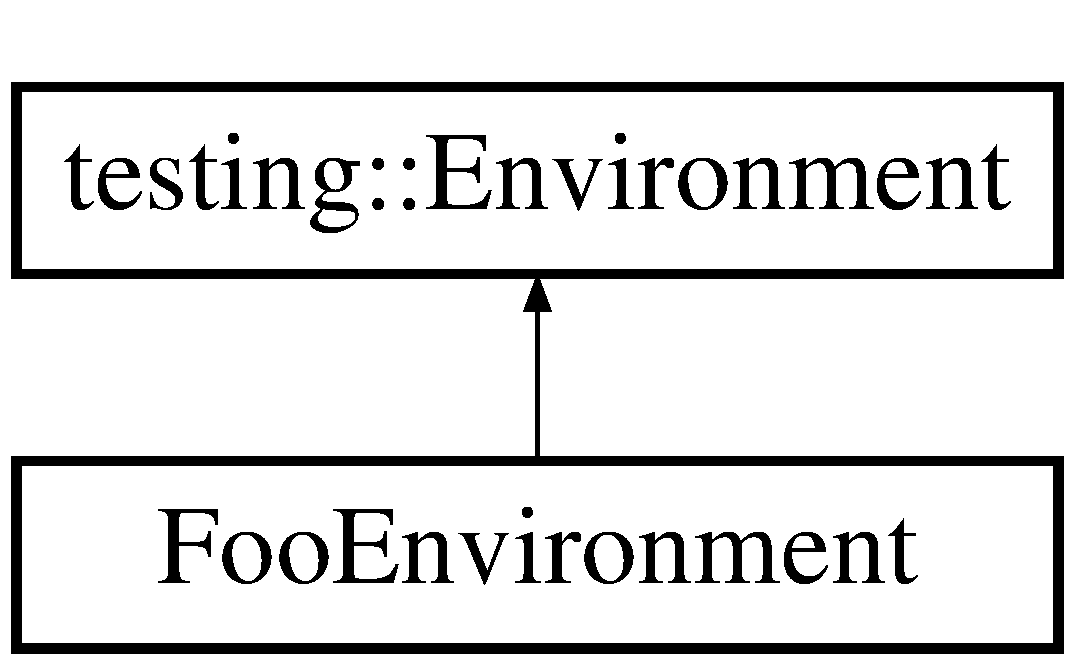
\includegraphics[height=2.000000cm]{class_foo_environment}
\end{center}
\end{figure}
\subsection*{Public Member Functions}
\begin{DoxyCompactItemize}
\item 
virtual void \hyperlink{class_foo_environment_a7db8d8b312805aff437ae8534132a56d}{Set\+Up} ()
\item 
virtual void \hyperlink{class_foo_environment_a99a2c9df52106cce9e7a4bdda53df802}{Tear\+Down} ()
\end{DoxyCompactItemize}


\subsection{Member Function Documentation}
\hypertarget{class_foo_environment_a7db8d8b312805aff437ae8534132a56d}{}\index{Foo\+Environment@{Foo\+Environment}!Set\+Up@{Set\+Up}}
\index{Set\+Up@{Set\+Up}!Foo\+Environment@{Foo\+Environment}}
\subsubsection[{Set\+Up()}]{\setlength{\rightskip}{0pt plus 5cm}virtual void Foo\+Environment\+::\+Set\+Up (
\begin{DoxyParamCaption}
{}
\end{DoxyParamCaption}
)\hspace{0.3cm}{\ttfamily [inline]}, {\ttfamily [virtual]}}\label{class_foo_environment_a7db8d8b312805aff437ae8534132a56d}


Reimplemented from \hyperlink{classtesting_1_1_environment_a1bf8cafaa9d4eba9feb98655ee434eb3}{testing\+::\+Environment}.

\hypertarget{class_foo_environment_a99a2c9df52106cce9e7a4bdda53df802}{}\index{Foo\+Environment@{Foo\+Environment}!Tear\+Down@{Tear\+Down}}
\index{Tear\+Down@{Tear\+Down}!Foo\+Environment@{Foo\+Environment}}
\subsubsection[{Tear\+Down()}]{\setlength{\rightskip}{0pt plus 5cm}virtual void Foo\+Environment\+::\+Tear\+Down (
\begin{DoxyParamCaption}
{}
\end{DoxyParamCaption}
)\hspace{0.3cm}{\ttfamily [inline]}, {\ttfamily [virtual]}}\label{class_foo_environment_a99a2c9df52106cce9e7a4bdda53df802}


Reimplemented from \hyperlink{classtesting_1_1_environment_a039bdaa705c46b9b88234cf4d3bb6254}{testing\+::\+Environment}.



The documentation for this class was generated from the following file\+:\begin{DoxyCompactItemize}
\item 
C\+:/\+Users/\+Hilman/\+Desktop/repo/anjing/src/third\+\_\+party/googletest/test/\hyperlink{gtest__output__test___8cc}{gtest\+\_\+output\+\_\+test\+\_\+.\+cc}\end{DoxyCompactItemize}

\hypertarget{class_foo_test}{}\section{Foo\+Test Class Reference}
\label{class_foo_test}\index{Foo\+Test@{Foo\+Test}}
Inheritance diagram for Foo\+Test\+:\begin{figure}[H]
\begin{center}
\leavevmode
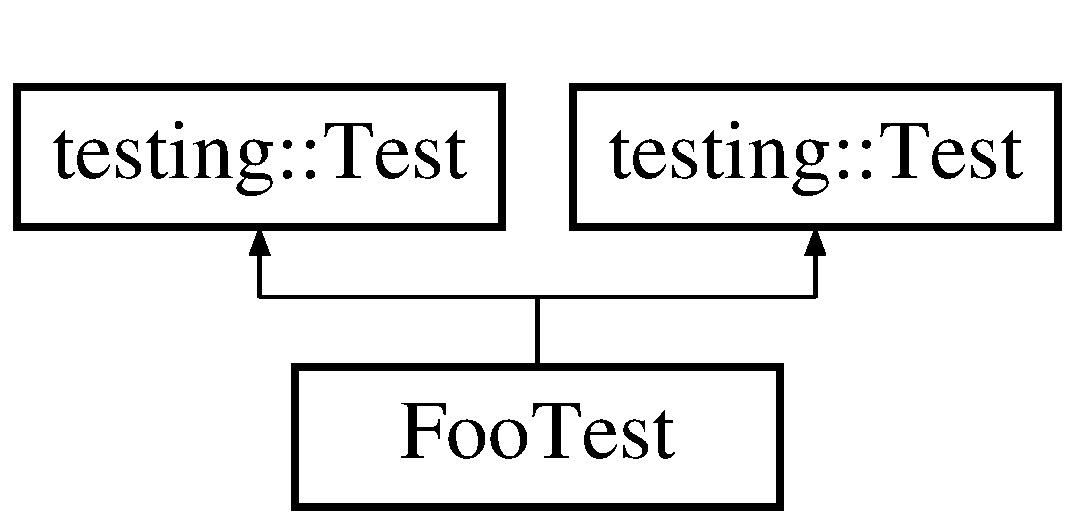
\includegraphics[height=2.000000cm]{class_foo_test}
\end{center}
\end{figure}
\subsection*{Additional Inherited Members}


The documentation for this class was generated from the following file\+:\begin{DoxyCompactItemize}
\item 
C\+:/\+Users/\+Hilman/\+Desktop/repo/anjing/src/third\+\_\+party/googletest/test/\hyperlink{gtest__list__tests__unittest___8cc}{gtest\+\_\+list\+\_\+tests\+\_\+unittest\+\_\+.\+cc}\end{DoxyCompactItemize}

\hypertarget{classtesting_1_1internal_1_1_format_for_comparison}{}\section{testing\+:\+:internal\+:\+:Format\+For\+Comparison$<$ To\+Print, Other\+Operand $>$ Class Template Reference}
\label{classtesting_1_1internal_1_1_format_for_comparison}\index{testing\+::internal\+::\+Format\+For\+Comparison$<$ To\+Print, Other\+Operand $>$@{testing\+::internal\+::\+Format\+For\+Comparison$<$ To\+Print, Other\+Operand $>$}}


{\ttfamily \#include $<$gtest.\+h$>$}

\subsection*{Static Public Member Functions}
\begin{DoxyCompactItemize}
\item 
\+::std\+::string \hyperlink{classtesting_1_1internal_1_1_format_for_comparison_a2aeb688fc55b57abd3021d82eccad896}{Format} (const To\+Print \&value)
\end{DoxyCompactItemize}


\subsection{Member Function Documentation}
\hypertarget{classtesting_1_1internal_1_1_format_for_comparison_a2aeb688fc55b57abd3021d82eccad896}{}\index{testing\+::internal\+::\+Format\+For\+Comparison@{testing\+::internal\+::\+Format\+For\+Comparison}!Format@{Format}}
\index{Format@{Format}!testing\+::internal\+::\+Format\+For\+Comparison@{testing\+::internal\+::\+Format\+For\+Comparison}}
\subsubsection[{Format(const To\+Print \&value)}]{\setlength{\rightskip}{0pt plus 5cm}template$<$typename To\+Print , typename Other\+Operand $>$ \+::std\+::string {\bf testing\+::internal\+::\+Format\+For\+Comparison}$<$ To\+Print, Other\+Operand $>$\+::Format (
\begin{DoxyParamCaption}
\item[{const To\+Print \&}]{value}
\end{DoxyParamCaption}
)\hspace{0.3cm}{\ttfamily [inline]}, {\ttfamily [static]}}\label{classtesting_1_1internal_1_1_format_for_comparison_a2aeb688fc55b57abd3021d82eccad896}


The documentation for this class was generated from the following file\+:\begin{DoxyCompactItemize}
\item 
C\+:/\+Users/\+Hilman/\+Desktop/repo/anjing/src/third\+\_\+party/googletest/include/gtest/\hyperlink{gtest_8h}{gtest.\+h}\end{DoxyCompactItemize}

\hypertarget{classtesting_1_1internal_1_1_format_for_comparison_3_01_to_print[_n]_00_01_other_operand_01_4}{}\section{testing\+:\+:internal\+:\+:Format\+For\+Comparison$<$ To\+Print\mbox{[}N\mbox{]}, Other\+Operand $>$ Class Template Reference}
\label{classtesting_1_1internal_1_1_format_for_comparison_3_01_to_print[_n]_00_01_other_operand_01_4}\index{testing\+::internal\+::\+Format\+For\+Comparison$<$ To\+Print\mbox{[}\+N\mbox{]}, Other\+Operand $>$@{testing\+::internal\+::\+Format\+For\+Comparison$<$ To\+Print[N], Other\+Operand $>$}}


{\ttfamily \#include $<$gtest.\+h$>$}

\subsection*{Static Public Member Functions}
\begin{DoxyCompactItemize}
\item 
\+::std\+::string \hyperlink{classtesting_1_1internal_1_1_format_for_comparison_3_01_to_print[_n]_00_01_other_operand_01_4_a76c526461c8fa7df75f7b32ab889b9e0}{Format} (const To\+Print $\ast$value)
\end{DoxyCompactItemize}


\subsection{Member Function Documentation}
\hypertarget{classtesting_1_1internal_1_1_format_for_comparison_3_01_to_print[_n]_00_01_other_operand_01_4_a76c526461c8fa7df75f7b32ab889b9e0}{}\index{testing\+::internal\+::\+Format\+For\+Comparison$<$ To\+Print\mbox{[}\+N\mbox{]}, Other\+Operand $>$@{testing\+::internal\+::\+Format\+For\+Comparison$<$ To\+Print[N], Other\+Operand $>$}!Format@{Format}}
\index{Format@{Format}!testing\+::internal\+::\+Format\+For\+Comparison$<$ To\+Print\mbox{[}\+N\mbox{]}, Other\+Operand $>$@{testing\+::internal\+::\+Format\+For\+Comparison$<$ To\+Print[N], Other\+Operand $>$}}
\subsubsection[{Format(const To\+Print $\ast$value)}]{\setlength{\rightskip}{0pt plus 5cm}template$<$typename To\+Print , size\+\_\+t N, typename Other\+Operand $>$ \+::std\+::string {\bf testing\+::internal\+::\+Format\+For\+Comparison}$<$ To\+Print\mbox{[}N\mbox{]}, Other\+Operand $>$\+::Format (
\begin{DoxyParamCaption}
\item[{const To\+Print $\ast$}]{value}
\end{DoxyParamCaption}
)\hspace{0.3cm}{\ttfamily [inline]}, {\ttfamily [static]}}\label{classtesting_1_1internal_1_1_format_for_comparison_3_01_to_print[_n]_00_01_other_operand_01_4_a76c526461c8fa7df75f7b32ab889b9e0}


The documentation for this class was generated from the following file\+:\begin{DoxyCompactItemize}
\item 
C\+:/\+Users/\+Hilman/\+Desktop/repo/anjing/src/third\+\_\+party/googletest/include/gtest/\hyperlink{gtest_8h}{gtest.\+h}\end{DoxyCompactItemize}

\hypertarget{classpump_1_1_for_node}{}\section{pump.\+For\+Node Class Reference}
\label{classpump_1_1_for_node}\index{pump.\+For\+Node@{pump.\+For\+Node}}
\subsection*{Public Member Functions}
\begin{DoxyCompactItemize}
\item 
def \hyperlink{classpump_1_1_for_node_ac973aef6c55a94796df5427d7df6e0fa}{\+\_\+\+\_\+init\+\_\+\+\_\+}
\end{DoxyCompactItemize}
\subsection*{Public Attributes}
\begin{DoxyCompactItemize}
\item 
\hyperlink{classpump_1_1_for_node_a2444199e135e43696b3a006bd0d38982}{identifier}
\item 
\hyperlink{classpump_1_1_for_node_a06b493278b3c1ad53363a2bcc3b8efb3}{sep}
\item 
\hyperlink{classpump_1_1_for_node_afdb5f4f2a3bc772bbc6ea777dfde898e}{code}
\end{DoxyCompactItemize}


\subsection{Constructor \& Destructor Documentation}
\hypertarget{classpump_1_1_for_node_ac973aef6c55a94796df5427d7df6e0fa}{}\index{pump\+::\+For\+Node@{pump\+::\+For\+Node}!\+\_\+\+\_\+init\+\_\+\+\_\+@{\+\_\+\+\_\+init\+\_\+\+\_\+}}
\index{\+\_\+\+\_\+init\+\_\+\+\_\+@{\+\_\+\+\_\+init\+\_\+\+\_\+}!pump\+::\+For\+Node@{pump\+::\+For\+Node}}
\subsubsection[{\+\_\+\+\_\+init\+\_\+\+\_\+}]{\setlength{\rightskip}{0pt plus 5cm}def pump.\+For\+Node.\+\_\+\+\_\+init\+\_\+\+\_\+ (
\begin{DoxyParamCaption}
\item[{}]{self, }
\item[{}]{identifier = {\ttfamily None}, }
\item[{}]{sep = {\ttfamily None}, }
\item[{}]{code = {\ttfamily None}}
\end{DoxyParamCaption}
)}\label{classpump_1_1_for_node_ac973aef6c55a94796df5427d7df6e0fa}


\subsection{Member Data Documentation}
\hypertarget{classpump_1_1_for_node_afdb5f4f2a3bc772bbc6ea777dfde898e}{}\index{pump\+::\+For\+Node@{pump\+::\+For\+Node}!code@{code}}
\index{code@{code}!pump\+::\+For\+Node@{pump\+::\+For\+Node}}
\subsubsection[{code}]{\setlength{\rightskip}{0pt plus 5cm}pump.\+For\+Node.\+code}\label{classpump_1_1_for_node_afdb5f4f2a3bc772bbc6ea777dfde898e}
\hypertarget{classpump_1_1_for_node_a2444199e135e43696b3a006bd0d38982}{}\index{pump\+::\+For\+Node@{pump\+::\+For\+Node}!identifier@{identifier}}
\index{identifier@{identifier}!pump\+::\+For\+Node@{pump\+::\+For\+Node}}
\subsubsection[{identifier}]{\setlength{\rightskip}{0pt plus 5cm}pump.\+For\+Node.\+identifier}\label{classpump_1_1_for_node_a2444199e135e43696b3a006bd0d38982}
\hypertarget{classpump_1_1_for_node_a06b493278b3c1ad53363a2bcc3b8efb3}{}\index{pump\+::\+For\+Node@{pump\+::\+For\+Node}!sep@{sep}}
\index{sep@{sep}!pump\+::\+For\+Node@{pump\+::\+For\+Node}}
\subsubsection[{sep}]{\setlength{\rightskip}{0pt plus 5cm}pump.\+For\+Node.\+sep}\label{classpump_1_1_for_node_a06b493278b3c1ad53363a2bcc3b8efb3}


The documentation for this class was generated from the following file\+:\begin{DoxyCompactItemize}
\item 
C\+:/\+Users/\+Hilman/\+Desktop/repo/anjing/src/third\+\_\+party/googletest/scripts/\hyperlink{pump_8py}{pump.\+py}\end{DoxyCompactItemize}

\hypertarget{classstd_1_1tr1_1_1gtest__internal_1_1_get}{}\section{std\+:\+:tr1\+:\+:gtest\+\_\+internal\+:\+:Get$<$ k $>$ Class Template Reference}
\label{classstd_1_1tr1_1_1gtest__internal_1_1_get}\index{std\+::tr1\+::gtest\+\_\+internal\+::\+Get$<$ k $>$@{std\+::tr1\+::gtest\+\_\+internal\+::\+Get$<$ k $>$}}


{\ttfamily \#include $<$gtest-\/tuple.\+h$>$}



The documentation for this class was generated from the following file\+:\begin{DoxyCompactItemize}
\item 
C\+:/\+Users/\+Hilman/\+Desktop/repo/anjing/src/third\+\_\+party/googletest/include/gtest/internal/\hyperlink{gtest-tuple_8h}{gtest-\/tuple.\+h}\end{DoxyCompactItemize}

\hypertarget{classstd_1_1tr1_1_1gtest__internal_1_1_get_3_010_01_4}{}\section{std\+:\+:tr1\+:\+:gtest\+\_\+internal\+:\+:Get$<$ 0 $>$ Class Template Reference}
\label{classstd_1_1tr1_1_1gtest__internal_1_1_get_3_010_01_4}\index{std\+::tr1\+::gtest\+\_\+internal\+::\+Get$<$ 0 $>$@{std\+::tr1\+::gtest\+\_\+internal\+::\+Get$<$ 0 $>$}}


{\ttfamily \#include $<$gtest-\/tuple.\+h$>$}

\subsection*{Static Public Member Functions}
\begin{DoxyCompactItemize}
\item 
{\footnotesize template$<$class Tuple $>$ }\\static \hyperlink{classstd_1_1tr1_1_1gtest__internal_1_1_get_3_010_01_4_a74beca3869fddfe42ee608b7f4cacb96}{G\+T\+E\+S\+T\+\_\+\+A\+D\+D\+\_\+\+R\+E\+F\+\_\+} (\hyperlink{gtest-tuple_8h_a1b7f133d8aa02e0b7afed7b66781eeb7}{G\+T\+E\+S\+T\+\_\+\+T\+U\+P\+L\+E\+\_\+\+E\+L\+E\+M\+E\+N\+T\+\_\+}(0, Tuple)) Field(Tuple \&t)
\item 
{\footnotesize template$<$class Tuple $>$ }\\static \hyperlink{classstd_1_1tr1_1_1gtest__internal_1_1_get_3_010_01_4_a195b3853de45077f9a324c455f22d7e2}{G\+T\+E\+S\+T\+\_\+\+B\+Y\+\_\+\+R\+E\+F\+\_\+} (\hyperlink{gtest-tuple_8h_a1b7f133d8aa02e0b7afed7b66781eeb7}{G\+T\+E\+S\+T\+\_\+\+T\+U\+P\+L\+E\+\_\+\+E\+L\+E\+M\+E\+N\+T\+\_\+}(0, Tuple)) Const\+Field(const Tuple \&t)
\end{DoxyCompactItemize}


\subsection{Member Function Documentation}
\hypertarget{classstd_1_1tr1_1_1gtest__internal_1_1_get_3_010_01_4_a74beca3869fddfe42ee608b7f4cacb96}{}\index{std\+::tr1\+::gtest\+\_\+internal\+::\+Get$<$ 0 $>$@{std\+::tr1\+::gtest\+\_\+internal\+::\+Get$<$ 0 $>$}!G\+T\+E\+S\+T\+\_\+\+A\+D\+D\+\_\+\+R\+E\+F\+\_\+@{G\+T\+E\+S\+T\+\_\+\+A\+D\+D\+\_\+\+R\+E\+F\+\_\+}}
\index{G\+T\+E\+S\+T\+\_\+\+A\+D\+D\+\_\+\+R\+E\+F\+\_\+@{G\+T\+E\+S\+T\+\_\+\+A\+D\+D\+\_\+\+R\+E\+F\+\_\+}!std\+::tr1\+::gtest\+\_\+internal\+::\+Get$<$ 0 $>$@{std\+::tr1\+::gtest\+\_\+internal\+::\+Get$<$ 0 $>$}}
\subsubsection[{G\+T\+E\+S\+T\+\_\+\+A\+D\+D\+\_\+\+R\+E\+F\+\_\+(\+G\+T\+E\+S\+T\+\_\+\+T\+U\+P\+L\+E\+\_\+\+E\+L\+E\+M\+E\+N\+T\+\_\+(0, Tuple)) Field(\+Tuple \&t)}]{\setlength{\rightskip}{0pt plus 5cm}template$<$class Tuple $>$ static {\bf std\+::tr1\+::gtest\+\_\+internal\+::\+Get}$<$ 0 $>$\+::G\+T\+E\+S\+T\+\_\+\+A\+D\+D\+\_\+\+R\+E\+F\+\_\+ (
\begin{DoxyParamCaption}
\item[{{\bf G\+T\+E\+S\+T\+\_\+\+T\+U\+P\+L\+E\+\_\+\+E\+L\+E\+M\+E\+N\+T\+\_\+}(0, Tuple)}]{}
\end{DoxyParamCaption}
)\hspace{0.3cm}{\ttfamily [inline]}, {\ttfamily [static]}}\label{classstd_1_1tr1_1_1gtest__internal_1_1_get_3_010_01_4_a74beca3869fddfe42ee608b7f4cacb96}
\hypertarget{classstd_1_1tr1_1_1gtest__internal_1_1_get_3_010_01_4_a195b3853de45077f9a324c455f22d7e2}{}\index{std\+::tr1\+::gtest\+\_\+internal\+::\+Get$<$ 0 $>$@{std\+::tr1\+::gtest\+\_\+internal\+::\+Get$<$ 0 $>$}!G\+T\+E\+S\+T\+\_\+\+B\+Y\+\_\+\+R\+E\+F\+\_\+@{G\+T\+E\+S\+T\+\_\+\+B\+Y\+\_\+\+R\+E\+F\+\_\+}}
\index{G\+T\+E\+S\+T\+\_\+\+B\+Y\+\_\+\+R\+E\+F\+\_\+@{G\+T\+E\+S\+T\+\_\+\+B\+Y\+\_\+\+R\+E\+F\+\_\+}!std\+::tr1\+::gtest\+\_\+internal\+::\+Get$<$ 0 $>$@{std\+::tr1\+::gtest\+\_\+internal\+::\+Get$<$ 0 $>$}}
\subsubsection[{G\+T\+E\+S\+T\+\_\+\+B\+Y\+\_\+\+R\+E\+F\+\_\+(\+G\+T\+E\+S\+T\+\_\+\+T\+U\+P\+L\+E\+\_\+\+E\+L\+E\+M\+E\+N\+T\+\_\+(0, Tuple)) Const\+Field(const Tuple \&t)}]{\setlength{\rightskip}{0pt plus 5cm}template$<$class Tuple $>$ static {\bf std\+::tr1\+::gtest\+\_\+internal\+::\+Get}$<$ 0 $>$\+::G\+T\+E\+S\+T\+\_\+\+B\+Y\+\_\+\+R\+E\+F\+\_\+ (
\begin{DoxyParamCaption}
\item[{{\bf G\+T\+E\+S\+T\+\_\+\+T\+U\+P\+L\+E\+\_\+\+E\+L\+E\+M\+E\+N\+T\+\_\+}(0, Tuple)}]{}
\end{DoxyParamCaption}
) const\hspace{0.3cm}{\ttfamily [inline]}, {\ttfamily [static]}}\label{classstd_1_1tr1_1_1gtest__internal_1_1_get_3_010_01_4_a195b3853de45077f9a324c455f22d7e2}


The documentation for this class was generated from the following file\+:\begin{DoxyCompactItemize}
\item 
C\+:/\+Users/\+Hilman/\+Desktop/repo/anjing/src/third\+\_\+party/googletest/include/gtest/internal/\hyperlink{gtest-tuple_8h}{gtest-\/tuple.\+h}\end{DoxyCompactItemize}

\hypertarget{classstd_1_1tr1_1_1gtest__internal_1_1_get_3_011_01_4}{}\section{std\+:\+:tr1\+:\+:gtest\+\_\+internal\+:\+:Get$<$ 1 $>$ Class Template Reference}
\label{classstd_1_1tr1_1_1gtest__internal_1_1_get_3_011_01_4}\index{std\+::tr1\+::gtest\+\_\+internal\+::\+Get$<$ 1 $>$@{std\+::tr1\+::gtest\+\_\+internal\+::\+Get$<$ 1 $>$}}


{\ttfamily \#include $<$gtest-\/tuple.\+h$>$}

\subsection*{Static Public Member Functions}
\begin{DoxyCompactItemize}
\item 
{\footnotesize template$<$class Tuple $>$ }\\static \hyperlink{classstd_1_1tr1_1_1gtest__internal_1_1_get_3_011_01_4_a52b2f5d2bc283d76a3e8dede84dba154}{G\+T\+E\+S\+T\+\_\+\+A\+D\+D\+\_\+\+R\+E\+F\+\_\+} (\hyperlink{gtest-tuple_8h_a1b7f133d8aa02e0b7afed7b66781eeb7}{G\+T\+E\+S\+T\+\_\+\+T\+U\+P\+L\+E\+\_\+\+E\+L\+E\+M\+E\+N\+T\+\_\+}(1, Tuple)) Field(Tuple \&t)
\item 
{\footnotesize template$<$class Tuple $>$ }\\static \hyperlink{classstd_1_1tr1_1_1gtest__internal_1_1_get_3_011_01_4_a481a2bf839c758408d46a1d0d41ff8f4}{G\+T\+E\+S\+T\+\_\+\+B\+Y\+\_\+\+R\+E\+F\+\_\+} (\hyperlink{gtest-tuple_8h_a1b7f133d8aa02e0b7afed7b66781eeb7}{G\+T\+E\+S\+T\+\_\+\+T\+U\+P\+L\+E\+\_\+\+E\+L\+E\+M\+E\+N\+T\+\_\+}(1, Tuple)) Const\+Field(const Tuple \&t)
\end{DoxyCompactItemize}


\subsection{Member Function Documentation}
\hypertarget{classstd_1_1tr1_1_1gtest__internal_1_1_get_3_011_01_4_a52b2f5d2bc283d76a3e8dede84dba154}{}\index{std\+::tr1\+::gtest\+\_\+internal\+::\+Get$<$ 1 $>$@{std\+::tr1\+::gtest\+\_\+internal\+::\+Get$<$ 1 $>$}!G\+T\+E\+S\+T\+\_\+\+A\+D\+D\+\_\+\+R\+E\+F\+\_\+@{G\+T\+E\+S\+T\+\_\+\+A\+D\+D\+\_\+\+R\+E\+F\+\_\+}}
\index{G\+T\+E\+S\+T\+\_\+\+A\+D\+D\+\_\+\+R\+E\+F\+\_\+@{G\+T\+E\+S\+T\+\_\+\+A\+D\+D\+\_\+\+R\+E\+F\+\_\+}!std\+::tr1\+::gtest\+\_\+internal\+::\+Get$<$ 1 $>$@{std\+::tr1\+::gtest\+\_\+internal\+::\+Get$<$ 1 $>$}}
\subsubsection[{G\+T\+E\+S\+T\+\_\+\+A\+D\+D\+\_\+\+R\+E\+F\+\_\+(\+G\+T\+E\+S\+T\+\_\+\+T\+U\+P\+L\+E\+\_\+\+E\+L\+E\+M\+E\+N\+T\+\_\+(1, Tuple)) Field(\+Tuple \&t)}]{\setlength{\rightskip}{0pt plus 5cm}template$<$class Tuple $>$ static {\bf std\+::tr1\+::gtest\+\_\+internal\+::\+Get}$<$ 1 $>$\+::G\+T\+E\+S\+T\+\_\+\+A\+D\+D\+\_\+\+R\+E\+F\+\_\+ (
\begin{DoxyParamCaption}
\item[{{\bf G\+T\+E\+S\+T\+\_\+\+T\+U\+P\+L\+E\+\_\+\+E\+L\+E\+M\+E\+N\+T\+\_\+}(1, Tuple)}]{}
\end{DoxyParamCaption}
)\hspace{0.3cm}{\ttfamily [inline]}, {\ttfamily [static]}}\label{classstd_1_1tr1_1_1gtest__internal_1_1_get_3_011_01_4_a52b2f5d2bc283d76a3e8dede84dba154}
\hypertarget{classstd_1_1tr1_1_1gtest__internal_1_1_get_3_011_01_4_a481a2bf839c758408d46a1d0d41ff8f4}{}\index{std\+::tr1\+::gtest\+\_\+internal\+::\+Get$<$ 1 $>$@{std\+::tr1\+::gtest\+\_\+internal\+::\+Get$<$ 1 $>$}!G\+T\+E\+S\+T\+\_\+\+B\+Y\+\_\+\+R\+E\+F\+\_\+@{G\+T\+E\+S\+T\+\_\+\+B\+Y\+\_\+\+R\+E\+F\+\_\+}}
\index{G\+T\+E\+S\+T\+\_\+\+B\+Y\+\_\+\+R\+E\+F\+\_\+@{G\+T\+E\+S\+T\+\_\+\+B\+Y\+\_\+\+R\+E\+F\+\_\+}!std\+::tr1\+::gtest\+\_\+internal\+::\+Get$<$ 1 $>$@{std\+::tr1\+::gtest\+\_\+internal\+::\+Get$<$ 1 $>$}}
\subsubsection[{G\+T\+E\+S\+T\+\_\+\+B\+Y\+\_\+\+R\+E\+F\+\_\+(\+G\+T\+E\+S\+T\+\_\+\+T\+U\+P\+L\+E\+\_\+\+E\+L\+E\+M\+E\+N\+T\+\_\+(1, Tuple)) Const\+Field(const Tuple \&t)}]{\setlength{\rightskip}{0pt plus 5cm}template$<$class Tuple $>$ static {\bf std\+::tr1\+::gtest\+\_\+internal\+::\+Get}$<$ 1 $>$\+::G\+T\+E\+S\+T\+\_\+\+B\+Y\+\_\+\+R\+E\+F\+\_\+ (
\begin{DoxyParamCaption}
\item[{{\bf G\+T\+E\+S\+T\+\_\+\+T\+U\+P\+L\+E\+\_\+\+E\+L\+E\+M\+E\+N\+T\+\_\+}(1, Tuple)}]{}
\end{DoxyParamCaption}
) const\hspace{0.3cm}{\ttfamily [inline]}, {\ttfamily [static]}}\label{classstd_1_1tr1_1_1gtest__internal_1_1_get_3_011_01_4_a481a2bf839c758408d46a1d0d41ff8f4}


The documentation for this class was generated from the following file\+:\begin{DoxyCompactItemize}
\item 
C\+:/\+Users/\+Hilman/\+Desktop/repo/anjing/src/third\+\_\+party/googletest/include/gtest/internal/\hyperlink{gtest-tuple_8h}{gtest-\/tuple.\+h}\end{DoxyCompactItemize}

\hypertarget{classstd_1_1tr1_1_1gtest__internal_1_1_get_3_012_01_4}{}\section{std\+:\+:tr1\+:\+:gtest\+\_\+internal\+:\+:Get$<$ 2 $>$ Class Template Reference}
\label{classstd_1_1tr1_1_1gtest__internal_1_1_get_3_012_01_4}\index{std\+::tr1\+::gtest\+\_\+internal\+::\+Get$<$ 2 $>$@{std\+::tr1\+::gtest\+\_\+internal\+::\+Get$<$ 2 $>$}}


{\ttfamily \#include $<$gtest-\/tuple.\+h$>$}

\subsection*{Static Public Member Functions}
\begin{DoxyCompactItemize}
\item 
{\footnotesize template$<$class Tuple $>$ }\\static \hyperlink{classstd_1_1tr1_1_1gtest__internal_1_1_get_3_012_01_4_a8dfe7b5c1c915f10181e3fb5952ba6d8}{G\+T\+E\+S\+T\+\_\+\+A\+D\+D\+\_\+\+R\+E\+F\+\_\+} (\hyperlink{gtest-tuple_8h_a1b7f133d8aa02e0b7afed7b66781eeb7}{G\+T\+E\+S\+T\+\_\+\+T\+U\+P\+L\+E\+\_\+\+E\+L\+E\+M\+E\+N\+T\+\_\+}(2, Tuple)) Field(Tuple \&t)
\item 
{\footnotesize template$<$class Tuple $>$ }\\static \hyperlink{classstd_1_1tr1_1_1gtest__internal_1_1_get_3_012_01_4_a76127c9c03c1f0caa61fb87d4d756b5b}{G\+T\+E\+S\+T\+\_\+\+B\+Y\+\_\+\+R\+E\+F\+\_\+} (\hyperlink{gtest-tuple_8h_a1b7f133d8aa02e0b7afed7b66781eeb7}{G\+T\+E\+S\+T\+\_\+\+T\+U\+P\+L\+E\+\_\+\+E\+L\+E\+M\+E\+N\+T\+\_\+}(2, Tuple)) Const\+Field(const Tuple \&t)
\end{DoxyCompactItemize}


\subsection{Member Function Documentation}
\hypertarget{classstd_1_1tr1_1_1gtest__internal_1_1_get_3_012_01_4_a8dfe7b5c1c915f10181e3fb5952ba6d8}{}\index{std\+::tr1\+::gtest\+\_\+internal\+::\+Get$<$ 2 $>$@{std\+::tr1\+::gtest\+\_\+internal\+::\+Get$<$ 2 $>$}!G\+T\+E\+S\+T\+\_\+\+A\+D\+D\+\_\+\+R\+E\+F\+\_\+@{G\+T\+E\+S\+T\+\_\+\+A\+D\+D\+\_\+\+R\+E\+F\+\_\+}}
\index{G\+T\+E\+S\+T\+\_\+\+A\+D\+D\+\_\+\+R\+E\+F\+\_\+@{G\+T\+E\+S\+T\+\_\+\+A\+D\+D\+\_\+\+R\+E\+F\+\_\+}!std\+::tr1\+::gtest\+\_\+internal\+::\+Get$<$ 2 $>$@{std\+::tr1\+::gtest\+\_\+internal\+::\+Get$<$ 2 $>$}}
\subsubsection[{G\+T\+E\+S\+T\+\_\+\+A\+D\+D\+\_\+\+R\+E\+F\+\_\+(\+G\+T\+E\+S\+T\+\_\+\+T\+U\+P\+L\+E\+\_\+\+E\+L\+E\+M\+E\+N\+T\+\_\+(2, Tuple)) Field(\+Tuple \&t)}]{\setlength{\rightskip}{0pt plus 5cm}template$<$class Tuple $>$ static {\bf std\+::tr1\+::gtest\+\_\+internal\+::\+Get}$<$ 2 $>$\+::G\+T\+E\+S\+T\+\_\+\+A\+D\+D\+\_\+\+R\+E\+F\+\_\+ (
\begin{DoxyParamCaption}
\item[{{\bf G\+T\+E\+S\+T\+\_\+\+T\+U\+P\+L\+E\+\_\+\+E\+L\+E\+M\+E\+N\+T\+\_\+}(2, Tuple)}]{}
\end{DoxyParamCaption}
)\hspace{0.3cm}{\ttfamily [inline]}, {\ttfamily [static]}}\label{classstd_1_1tr1_1_1gtest__internal_1_1_get_3_012_01_4_a8dfe7b5c1c915f10181e3fb5952ba6d8}
\hypertarget{classstd_1_1tr1_1_1gtest__internal_1_1_get_3_012_01_4_a76127c9c03c1f0caa61fb87d4d756b5b}{}\index{std\+::tr1\+::gtest\+\_\+internal\+::\+Get$<$ 2 $>$@{std\+::tr1\+::gtest\+\_\+internal\+::\+Get$<$ 2 $>$}!G\+T\+E\+S\+T\+\_\+\+B\+Y\+\_\+\+R\+E\+F\+\_\+@{G\+T\+E\+S\+T\+\_\+\+B\+Y\+\_\+\+R\+E\+F\+\_\+}}
\index{G\+T\+E\+S\+T\+\_\+\+B\+Y\+\_\+\+R\+E\+F\+\_\+@{G\+T\+E\+S\+T\+\_\+\+B\+Y\+\_\+\+R\+E\+F\+\_\+}!std\+::tr1\+::gtest\+\_\+internal\+::\+Get$<$ 2 $>$@{std\+::tr1\+::gtest\+\_\+internal\+::\+Get$<$ 2 $>$}}
\subsubsection[{G\+T\+E\+S\+T\+\_\+\+B\+Y\+\_\+\+R\+E\+F\+\_\+(\+G\+T\+E\+S\+T\+\_\+\+T\+U\+P\+L\+E\+\_\+\+E\+L\+E\+M\+E\+N\+T\+\_\+(2, Tuple)) Const\+Field(const Tuple \&t)}]{\setlength{\rightskip}{0pt plus 5cm}template$<$class Tuple $>$ static {\bf std\+::tr1\+::gtest\+\_\+internal\+::\+Get}$<$ 2 $>$\+::G\+T\+E\+S\+T\+\_\+\+B\+Y\+\_\+\+R\+E\+F\+\_\+ (
\begin{DoxyParamCaption}
\item[{{\bf G\+T\+E\+S\+T\+\_\+\+T\+U\+P\+L\+E\+\_\+\+E\+L\+E\+M\+E\+N\+T\+\_\+}(2, Tuple)}]{}
\end{DoxyParamCaption}
) const\hspace{0.3cm}{\ttfamily [inline]}, {\ttfamily [static]}}\label{classstd_1_1tr1_1_1gtest__internal_1_1_get_3_012_01_4_a76127c9c03c1f0caa61fb87d4d756b5b}


The documentation for this class was generated from the following file\+:\begin{DoxyCompactItemize}
\item 
C\+:/\+Users/\+Hilman/\+Desktop/repo/anjing/src/third\+\_\+party/googletest/include/gtest/internal/\hyperlink{gtest-tuple_8h}{gtest-\/tuple.\+h}\end{DoxyCompactItemize}

\hypertarget{classstd_1_1tr1_1_1gtest__internal_1_1_get_3_013_01_4}{}\section{std\+:\+:tr1\+:\+:gtest\+\_\+internal\+:\+:Get$<$ 3 $>$ Class Template Reference}
\label{classstd_1_1tr1_1_1gtest__internal_1_1_get_3_013_01_4}\index{std\+::tr1\+::gtest\+\_\+internal\+::\+Get$<$ 3 $>$@{std\+::tr1\+::gtest\+\_\+internal\+::\+Get$<$ 3 $>$}}


{\ttfamily \#include $<$gtest-\/tuple.\+h$>$}

\subsection*{Static Public Member Functions}
\begin{DoxyCompactItemize}
\item 
{\footnotesize template$<$class Tuple $>$ }\\static \hyperlink{classstd_1_1tr1_1_1gtest__internal_1_1_get_3_013_01_4_aa2ebd71eca812f06bad0773a7e2f6788}{G\+T\+E\+S\+T\+\_\+\+A\+D\+D\+\_\+\+R\+E\+F\+\_\+} (\hyperlink{gtest-tuple_8h_a1b7f133d8aa02e0b7afed7b66781eeb7}{G\+T\+E\+S\+T\+\_\+\+T\+U\+P\+L\+E\+\_\+\+E\+L\+E\+M\+E\+N\+T\+\_\+}(3, Tuple)) Field(Tuple \&t)
\item 
{\footnotesize template$<$class Tuple $>$ }\\static \hyperlink{classstd_1_1tr1_1_1gtest__internal_1_1_get_3_013_01_4_ab8c5283e6776308abc41aaad518a23c7}{G\+T\+E\+S\+T\+\_\+\+B\+Y\+\_\+\+R\+E\+F\+\_\+} (\hyperlink{gtest-tuple_8h_a1b7f133d8aa02e0b7afed7b66781eeb7}{G\+T\+E\+S\+T\+\_\+\+T\+U\+P\+L\+E\+\_\+\+E\+L\+E\+M\+E\+N\+T\+\_\+}(3, Tuple)) Const\+Field(const Tuple \&t)
\end{DoxyCompactItemize}


\subsection{Member Function Documentation}
\hypertarget{classstd_1_1tr1_1_1gtest__internal_1_1_get_3_013_01_4_aa2ebd71eca812f06bad0773a7e2f6788}{}\index{std\+::tr1\+::gtest\+\_\+internal\+::\+Get$<$ 3 $>$@{std\+::tr1\+::gtest\+\_\+internal\+::\+Get$<$ 3 $>$}!G\+T\+E\+S\+T\+\_\+\+A\+D\+D\+\_\+\+R\+E\+F\+\_\+@{G\+T\+E\+S\+T\+\_\+\+A\+D\+D\+\_\+\+R\+E\+F\+\_\+}}
\index{G\+T\+E\+S\+T\+\_\+\+A\+D\+D\+\_\+\+R\+E\+F\+\_\+@{G\+T\+E\+S\+T\+\_\+\+A\+D\+D\+\_\+\+R\+E\+F\+\_\+}!std\+::tr1\+::gtest\+\_\+internal\+::\+Get$<$ 3 $>$@{std\+::tr1\+::gtest\+\_\+internal\+::\+Get$<$ 3 $>$}}
\subsubsection[{G\+T\+E\+S\+T\+\_\+\+A\+D\+D\+\_\+\+R\+E\+F\+\_\+(\+G\+T\+E\+S\+T\+\_\+\+T\+U\+P\+L\+E\+\_\+\+E\+L\+E\+M\+E\+N\+T\+\_\+(3, Tuple)) Field(\+Tuple \&t)}]{\setlength{\rightskip}{0pt plus 5cm}template$<$class Tuple $>$ static {\bf std\+::tr1\+::gtest\+\_\+internal\+::\+Get}$<$ 3 $>$\+::G\+T\+E\+S\+T\+\_\+\+A\+D\+D\+\_\+\+R\+E\+F\+\_\+ (
\begin{DoxyParamCaption}
\item[{{\bf G\+T\+E\+S\+T\+\_\+\+T\+U\+P\+L\+E\+\_\+\+E\+L\+E\+M\+E\+N\+T\+\_\+}(3, Tuple)}]{}
\end{DoxyParamCaption}
)\hspace{0.3cm}{\ttfamily [inline]}, {\ttfamily [static]}}\label{classstd_1_1tr1_1_1gtest__internal_1_1_get_3_013_01_4_aa2ebd71eca812f06bad0773a7e2f6788}
\hypertarget{classstd_1_1tr1_1_1gtest__internal_1_1_get_3_013_01_4_ab8c5283e6776308abc41aaad518a23c7}{}\index{std\+::tr1\+::gtest\+\_\+internal\+::\+Get$<$ 3 $>$@{std\+::tr1\+::gtest\+\_\+internal\+::\+Get$<$ 3 $>$}!G\+T\+E\+S\+T\+\_\+\+B\+Y\+\_\+\+R\+E\+F\+\_\+@{G\+T\+E\+S\+T\+\_\+\+B\+Y\+\_\+\+R\+E\+F\+\_\+}}
\index{G\+T\+E\+S\+T\+\_\+\+B\+Y\+\_\+\+R\+E\+F\+\_\+@{G\+T\+E\+S\+T\+\_\+\+B\+Y\+\_\+\+R\+E\+F\+\_\+}!std\+::tr1\+::gtest\+\_\+internal\+::\+Get$<$ 3 $>$@{std\+::tr1\+::gtest\+\_\+internal\+::\+Get$<$ 3 $>$}}
\subsubsection[{G\+T\+E\+S\+T\+\_\+\+B\+Y\+\_\+\+R\+E\+F\+\_\+(\+G\+T\+E\+S\+T\+\_\+\+T\+U\+P\+L\+E\+\_\+\+E\+L\+E\+M\+E\+N\+T\+\_\+(3, Tuple)) Const\+Field(const Tuple \&t)}]{\setlength{\rightskip}{0pt plus 5cm}template$<$class Tuple $>$ static {\bf std\+::tr1\+::gtest\+\_\+internal\+::\+Get}$<$ 3 $>$\+::G\+T\+E\+S\+T\+\_\+\+B\+Y\+\_\+\+R\+E\+F\+\_\+ (
\begin{DoxyParamCaption}
\item[{{\bf G\+T\+E\+S\+T\+\_\+\+T\+U\+P\+L\+E\+\_\+\+E\+L\+E\+M\+E\+N\+T\+\_\+}(3, Tuple)}]{}
\end{DoxyParamCaption}
) const\hspace{0.3cm}{\ttfamily [inline]}, {\ttfamily [static]}}\label{classstd_1_1tr1_1_1gtest__internal_1_1_get_3_013_01_4_ab8c5283e6776308abc41aaad518a23c7}


The documentation for this class was generated from the following file\+:\begin{DoxyCompactItemize}
\item 
C\+:/\+Users/\+Hilman/\+Desktop/repo/anjing/src/third\+\_\+party/googletest/include/gtest/internal/\hyperlink{gtest-tuple_8h}{gtest-\/tuple.\+h}\end{DoxyCompactItemize}

\hypertarget{classstd_1_1tr1_1_1gtest__internal_1_1_get_3_014_01_4}{}\section{std\+:\+:tr1\+:\+:gtest\+\_\+internal\+:\+:Get$<$ 4 $>$ Class Template Reference}
\label{classstd_1_1tr1_1_1gtest__internal_1_1_get_3_014_01_4}\index{std\+::tr1\+::gtest\+\_\+internal\+::\+Get$<$ 4 $>$@{std\+::tr1\+::gtest\+\_\+internal\+::\+Get$<$ 4 $>$}}


{\ttfamily \#include $<$gtest-\/tuple.\+h$>$}

\subsection*{Static Public Member Functions}
\begin{DoxyCompactItemize}
\item 
{\footnotesize template$<$class Tuple $>$ }\\static \hyperlink{classstd_1_1tr1_1_1gtest__internal_1_1_get_3_014_01_4_a5c7a91c681118bb7253e305f8ff42be4}{G\+T\+E\+S\+T\+\_\+\+A\+D\+D\+\_\+\+R\+E\+F\+\_\+} (\hyperlink{gtest-tuple_8h_a1b7f133d8aa02e0b7afed7b66781eeb7}{G\+T\+E\+S\+T\+\_\+\+T\+U\+P\+L\+E\+\_\+\+E\+L\+E\+M\+E\+N\+T\+\_\+}(4, Tuple)) Field(Tuple \&t)
\item 
{\footnotesize template$<$class Tuple $>$ }\\static \hyperlink{classstd_1_1tr1_1_1gtest__internal_1_1_get_3_014_01_4_a04794c398bbe81e4de0915b79da2166a}{G\+T\+E\+S\+T\+\_\+\+B\+Y\+\_\+\+R\+E\+F\+\_\+} (\hyperlink{gtest-tuple_8h_a1b7f133d8aa02e0b7afed7b66781eeb7}{G\+T\+E\+S\+T\+\_\+\+T\+U\+P\+L\+E\+\_\+\+E\+L\+E\+M\+E\+N\+T\+\_\+}(4, Tuple)) Const\+Field(const Tuple \&t)
\end{DoxyCompactItemize}


\subsection{Member Function Documentation}
\hypertarget{classstd_1_1tr1_1_1gtest__internal_1_1_get_3_014_01_4_a5c7a91c681118bb7253e305f8ff42be4}{}\index{std\+::tr1\+::gtest\+\_\+internal\+::\+Get$<$ 4 $>$@{std\+::tr1\+::gtest\+\_\+internal\+::\+Get$<$ 4 $>$}!G\+T\+E\+S\+T\+\_\+\+A\+D\+D\+\_\+\+R\+E\+F\+\_\+@{G\+T\+E\+S\+T\+\_\+\+A\+D\+D\+\_\+\+R\+E\+F\+\_\+}}
\index{G\+T\+E\+S\+T\+\_\+\+A\+D\+D\+\_\+\+R\+E\+F\+\_\+@{G\+T\+E\+S\+T\+\_\+\+A\+D\+D\+\_\+\+R\+E\+F\+\_\+}!std\+::tr1\+::gtest\+\_\+internal\+::\+Get$<$ 4 $>$@{std\+::tr1\+::gtest\+\_\+internal\+::\+Get$<$ 4 $>$}}
\subsubsection[{G\+T\+E\+S\+T\+\_\+\+A\+D\+D\+\_\+\+R\+E\+F\+\_\+(\+G\+T\+E\+S\+T\+\_\+\+T\+U\+P\+L\+E\+\_\+\+E\+L\+E\+M\+E\+N\+T\+\_\+(4, Tuple)) Field(\+Tuple \&t)}]{\setlength{\rightskip}{0pt plus 5cm}template$<$class Tuple $>$ static {\bf std\+::tr1\+::gtest\+\_\+internal\+::\+Get}$<$ 4 $>$\+::G\+T\+E\+S\+T\+\_\+\+A\+D\+D\+\_\+\+R\+E\+F\+\_\+ (
\begin{DoxyParamCaption}
\item[{{\bf G\+T\+E\+S\+T\+\_\+\+T\+U\+P\+L\+E\+\_\+\+E\+L\+E\+M\+E\+N\+T\+\_\+}(4, Tuple)}]{}
\end{DoxyParamCaption}
)\hspace{0.3cm}{\ttfamily [inline]}, {\ttfamily [static]}}\label{classstd_1_1tr1_1_1gtest__internal_1_1_get_3_014_01_4_a5c7a91c681118bb7253e305f8ff42be4}
\hypertarget{classstd_1_1tr1_1_1gtest__internal_1_1_get_3_014_01_4_a04794c398bbe81e4de0915b79da2166a}{}\index{std\+::tr1\+::gtest\+\_\+internal\+::\+Get$<$ 4 $>$@{std\+::tr1\+::gtest\+\_\+internal\+::\+Get$<$ 4 $>$}!G\+T\+E\+S\+T\+\_\+\+B\+Y\+\_\+\+R\+E\+F\+\_\+@{G\+T\+E\+S\+T\+\_\+\+B\+Y\+\_\+\+R\+E\+F\+\_\+}}
\index{G\+T\+E\+S\+T\+\_\+\+B\+Y\+\_\+\+R\+E\+F\+\_\+@{G\+T\+E\+S\+T\+\_\+\+B\+Y\+\_\+\+R\+E\+F\+\_\+}!std\+::tr1\+::gtest\+\_\+internal\+::\+Get$<$ 4 $>$@{std\+::tr1\+::gtest\+\_\+internal\+::\+Get$<$ 4 $>$}}
\subsubsection[{G\+T\+E\+S\+T\+\_\+\+B\+Y\+\_\+\+R\+E\+F\+\_\+(\+G\+T\+E\+S\+T\+\_\+\+T\+U\+P\+L\+E\+\_\+\+E\+L\+E\+M\+E\+N\+T\+\_\+(4, Tuple)) Const\+Field(const Tuple \&t)}]{\setlength{\rightskip}{0pt plus 5cm}template$<$class Tuple $>$ static {\bf std\+::tr1\+::gtest\+\_\+internal\+::\+Get}$<$ 4 $>$\+::G\+T\+E\+S\+T\+\_\+\+B\+Y\+\_\+\+R\+E\+F\+\_\+ (
\begin{DoxyParamCaption}
\item[{{\bf G\+T\+E\+S\+T\+\_\+\+T\+U\+P\+L\+E\+\_\+\+E\+L\+E\+M\+E\+N\+T\+\_\+}(4, Tuple)}]{}
\end{DoxyParamCaption}
) const\hspace{0.3cm}{\ttfamily [inline]}, {\ttfamily [static]}}\label{classstd_1_1tr1_1_1gtest__internal_1_1_get_3_014_01_4_a04794c398bbe81e4de0915b79da2166a}


The documentation for this class was generated from the following file\+:\begin{DoxyCompactItemize}
\item 
C\+:/\+Users/\+Hilman/\+Desktop/repo/anjing/src/third\+\_\+party/googletest/include/gtest/internal/\hyperlink{gtest-tuple_8h}{gtest-\/tuple.\+h}\end{DoxyCompactItemize}

\hypertarget{classstd_1_1tr1_1_1gtest__internal_1_1_get_3_015_01_4}{}\section{std\+:\+:tr1\+:\+:gtest\+\_\+internal\+:\+:Get$<$ 5 $>$ Class Template Reference}
\label{classstd_1_1tr1_1_1gtest__internal_1_1_get_3_015_01_4}\index{std\+::tr1\+::gtest\+\_\+internal\+::\+Get$<$ 5 $>$@{std\+::tr1\+::gtest\+\_\+internal\+::\+Get$<$ 5 $>$}}


{\ttfamily \#include $<$gtest-\/tuple.\+h$>$}

\subsection*{Static Public Member Functions}
\begin{DoxyCompactItemize}
\item 
{\footnotesize template$<$class Tuple $>$ }\\static \hyperlink{classstd_1_1tr1_1_1gtest__internal_1_1_get_3_015_01_4_a0a337088bab3f824f67d1607229fdcc2}{G\+T\+E\+S\+T\+\_\+\+A\+D\+D\+\_\+\+R\+E\+F\+\_\+} (\hyperlink{gtest-tuple_8h_a1b7f133d8aa02e0b7afed7b66781eeb7}{G\+T\+E\+S\+T\+\_\+\+T\+U\+P\+L\+E\+\_\+\+E\+L\+E\+M\+E\+N\+T\+\_\+}(5, Tuple)) Field(Tuple \&t)
\item 
{\footnotesize template$<$class Tuple $>$ }\\static \hyperlink{classstd_1_1tr1_1_1gtest__internal_1_1_get_3_015_01_4_ae10fe16450db82d69b9a4d0b149ca75d}{G\+T\+E\+S\+T\+\_\+\+B\+Y\+\_\+\+R\+E\+F\+\_\+} (\hyperlink{gtest-tuple_8h_a1b7f133d8aa02e0b7afed7b66781eeb7}{G\+T\+E\+S\+T\+\_\+\+T\+U\+P\+L\+E\+\_\+\+E\+L\+E\+M\+E\+N\+T\+\_\+}(5, Tuple)) Const\+Field(const Tuple \&t)
\end{DoxyCompactItemize}


\subsection{Member Function Documentation}
\hypertarget{classstd_1_1tr1_1_1gtest__internal_1_1_get_3_015_01_4_a0a337088bab3f824f67d1607229fdcc2}{}\index{std\+::tr1\+::gtest\+\_\+internal\+::\+Get$<$ 5 $>$@{std\+::tr1\+::gtest\+\_\+internal\+::\+Get$<$ 5 $>$}!G\+T\+E\+S\+T\+\_\+\+A\+D\+D\+\_\+\+R\+E\+F\+\_\+@{G\+T\+E\+S\+T\+\_\+\+A\+D\+D\+\_\+\+R\+E\+F\+\_\+}}
\index{G\+T\+E\+S\+T\+\_\+\+A\+D\+D\+\_\+\+R\+E\+F\+\_\+@{G\+T\+E\+S\+T\+\_\+\+A\+D\+D\+\_\+\+R\+E\+F\+\_\+}!std\+::tr1\+::gtest\+\_\+internal\+::\+Get$<$ 5 $>$@{std\+::tr1\+::gtest\+\_\+internal\+::\+Get$<$ 5 $>$}}
\subsubsection[{G\+T\+E\+S\+T\+\_\+\+A\+D\+D\+\_\+\+R\+E\+F\+\_\+(\+G\+T\+E\+S\+T\+\_\+\+T\+U\+P\+L\+E\+\_\+\+E\+L\+E\+M\+E\+N\+T\+\_\+(5, Tuple)) Field(\+Tuple \&t)}]{\setlength{\rightskip}{0pt plus 5cm}template$<$class Tuple $>$ static {\bf std\+::tr1\+::gtest\+\_\+internal\+::\+Get}$<$ 5 $>$\+::G\+T\+E\+S\+T\+\_\+\+A\+D\+D\+\_\+\+R\+E\+F\+\_\+ (
\begin{DoxyParamCaption}
\item[{{\bf G\+T\+E\+S\+T\+\_\+\+T\+U\+P\+L\+E\+\_\+\+E\+L\+E\+M\+E\+N\+T\+\_\+}(5, Tuple)}]{}
\end{DoxyParamCaption}
)\hspace{0.3cm}{\ttfamily [inline]}, {\ttfamily [static]}}\label{classstd_1_1tr1_1_1gtest__internal_1_1_get_3_015_01_4_a0a337088bab3f824f67d1607229fdcc2}
\hypertarget{classstd_1_1tr1_1_1gtest__internal_1_1_get_3_015_01_4_ae10fe16450db82d69b9a4d0b149ca75d}{}\index{std\+::tr1\+::gtest\+\_\+internal\+::\+Get$<$ 5 $>$@{std\+::tr1\+::gtest\+\_\+internal\+::\+Get$<$ 5 $>$}!G\+T\+E\+S\+T\+\_\+\+B\+Y\+\_\+\+R\+E\+F\+\_\+@{G\+T\+E\+S\+T\+\_\+\+B\+Y\+\_\+\+R\+E\+F\+\_\+}}
\index{G\+T\+E\+S\+T\+\_\+\+B\+Y\+\_\+\+R\+E\+F\+\_\+@{G\+T\+E\+S\+T\+\_\+\+B\+Y\+\_\+\+R\+E\+F\+\_\+}!std\+::tr1\+::gtest\+\_\+internal\+::\+Get$<$ 5 $>$@{std\+::tr1\+::gtest\+\_\+internal\+::\+Get$<$ 5 $>$}}
\subsubsection[{G\+T\+E\+S\+T\+\_\+\+B\+Y\+\_\+\+R\+E\+F\+\_\+(\+G\+T\+E\+S\+T\+\_\+\+T\+U\+P\+L\+E\+\_\+\+E\+L\+E\+M\+E\+N\+T\+\_\+(5, Tuple)) Const\+Field(const Tuple \&t)}]{\setlength{\rightskip}{0pt plus 5cm}template$<$class Tuple $>$ static {\bf std\+::tr1\+::gtest\+\_\+internal\+::\+Get}$<$ 5 $>$\+::G\+T\+E\+S\+T\+\_\+\+B\+Y\+\_\+\+R\+E\+F\+\_\+ (
\begin{DoxyParamCaption}
\item[{{\bf G\+T\+E\+S\+T\+\_\+\+T\+U\+P\+L\+E\+\_\+\+E\+L\+E\+M\+E\+N\+T\+\_\+}(5, Tuple)}]{}
\end{DoxyParamCaption}
) const\hspace{0.3cm}{\ttfamily [inline]}, {\ttfamily [static]}}\label{classstd_1_1tr1_1_1gtest__internal_1_1_get_3_015_01_4_ae10fe16450db82d69b9a4d0b149ca75d}


The documentation for this class was generated from the following file\+:\begin{DoxyCompactItemize}
\item 
C\+:/\+Users/\+Hilman/\+Desktop/repo/anjing/src/third\+\_\+party/googletest/include/gtest/internal/\hyperlink{gtest-tuple_8h}{gtest-\/tuple.\+h}\end{DoxyCompactItemize}

\hypertarget{classstd_1_1tr1_1_1gtest__internal_1_1_get_3_016_01_4}{}\section{std\+:\+:tr1\+:\+:gtest\+\_\+internal\+:\+:Get$<$ 6 $>$ Class Template Reference}
\label{classstd_1_1tr1_1_1gtest__internal_1_1_get_3_016_01_4}\index{std\+::tr1\+::gtest\+\_\+internal\+::\+Get$<$ 6 $>$@{std\+::tr1\+::gtest\+\_\+internal\+::\+Get$<$ 6 $>$}}


{\ttfamily \#include $<$gtest-\/tuple.\+h$>$}

\subsection*{Static Public Member Functions}
\begin{DoxyCompactItemize}
\item 
{\footnotesize template$<$class Tuple $>$ }\\static \hyperlink{classstd_1_1tr1_1_1gtest__internal_1_1_get_3_016_01_4_a28034152d066c8644fa55e9fc0e3a12d}{G\+T\+E\+S\+T\+\_\+\+A\+D\+D\+\_\+\+R\+E\+F\+\_\+} (\hyperlink{gtest-tuple_8h_a1b7f133d8aa02e0b7afed7b66781eeb7}{G\+T\+E\+S\+T\+\_\+\+T\+U\+P\+L\+E\+\_\+\+E\+L\+E\+M\+E\+N\+T\+\_\+}(6, Tuple)) Field(Tuple \&t)
\item 
{\footnotesize template$<$class Tuple $>$ }\\static \hyperlink{classstd_1_1tr1_1_1gtest__internal_1_1_get_3_016_01_4_a6e396b998757e0ab9b75db0c68a7c360}{G\+T\+E\+S\+T\+\_\+\+B\+Y\+\_\+\+R\+E\+F\+\_\+} (\hyperlink{gtest-tuple_8h_a1b7f133d8aa02e0b7afed7b66781eeb7}{G\+T\+E\+S\+T\+\_\+\+T\+U\+P\+L\+E\+\_\+\+E\+L\+E\+M\+E\+N\+T\+\_\+}(6, Tuple)) Const\+Field(const Tuple \&t)
\end{DoxyCompactItemize}


\subsection{Member Function Documentation}
\hypertarget{classstd_1_1tr1_1_1gtest__internal_1_1_get_3_016_01_4_a28034152d066c8644fa55e9fc0e3a12d}{}\index{std\+::tr1\+::gtest\+\_\+internal\+::\+Get$<$ 6 $>$@{std\+::tr1\+::gtest\+\_\+internal\+::\+Get$<$ 6 $>$}!G\+T\+E\+S\+T\+\_\+\+A\+D\+D\+\_\+\+R\+E\+F\+\_\+@{G\+T\+E\+S\+T\+\_\+\+A\+D\+D\+\_\+\+R\+E\+F\+\_\+}}
\index{G\+T\+E\+S\+T\+\_\+\+A\+D\+D\+\_\+\+R\+E\+F\+\_\+@{G\+T\+E\+S\+T\+\_\+\+A\+D\+D\+\_\+\+R\+E\+F\+\_\+}!std\+::tr1\+::gtest\+\_\+internal\+::\+Get$<$ 6 $>$@{std\+::tr1\+::gtest\+\_\+internal\+::\+Get$<$ 6 $>$}}
\subsubsection[{G\+T\+E\+S\+T\+\_\+\+A\+D\+D\+\_\+\+R\+E\+F\+\_\+(\+G\+T\+E\+S\+T\+\_\+\+T\+U\+P\+L\+E\+\_\+\+E\+L\+E\+M\+E\+N\+T\+\_\+(6, Tuple)) Field(\+Tuple \&t)}]{\setlength{\rightskip}{0pt plus 5cm}template$<$class Tuple $>$ static {\bf std\+::tr1\+::gtest\+\_\+internal\+::\+Get}$<$ 6 $>$\+::G\+T\+E\+S\+T\+\_\+\+A\+D\+D\+\_\+\+R\+E\+F\+\_\+ (
\begin{DoxyParamCaption}
\item[{{\bf G\+T\+E\+S\+T\+\_\+\+T\+U\+P\+L\+E\+\_\+\+E\+L\+E\+M\+E\+N\+T\+\_\+}(6, Tuple)}]{}
\end{DoxyParamCaption}
)\hspace{0.3cm}{\ttfamily [inline]}, {\ttfamily [static]}}\label{classstd_1_1tr1_1_1gtest__internal_1_1_get_3_016_01_4_a28034152d066c8644fa55e9fc0e3a12d}
\hypertarget{classstd_1_1tr1_1_1gtest__internal_1_1_get_3_016_01_4_a6e396b998757e0ab9b75db0c68a7c360}{}\index{std\+::tr1\+::gtest\+\_\+internal\+::\+Get$<$ 6 $>$@{std\+::tr1\+::gtest\+\_\+internal\+::\+Get$<$ 6 $>$}!G\+T\+E\+S\+T\+\_\+\+B\+Y\+\_\+\+R\+E\+F\+\_\+@{G\+T\+E\+S\+T\+\_\+\+B\+Y\+\_\+\+R\+E\+F\+\_\+}}
\index{G\+T\+E\+S\+T\+\_\+\+B\+Y\+\_\+\+R\+E\+F\+\_\+@{G\+T\+E\+S\+T\+\_\+\+B\+Y\+\_\+\+R\+E\+F\+\_\+}!std\+::tr1\+::gtest\+\_\+internal\+::\+Get$<$ 6 $>$@{std\+::tr1\+::gtest\+\_\+internal\+::\+Get$<$ 6 $>$}}
\subsubsection[{G\+T\+E\+S\+T\+\_\+\+B\+Y\+\_\+\+R\+E\+F\+\_\+(\+G\+T\+E\+S\+T\+\_\+\+T\+U\+P\+L\+E\+\_\+\+E\+L\+E\+M\+E\+N\+T\+\_\+(6, Tuple)) Const\+Field(const Tuple \&t)}]{\setlength{\rightskip}{0pt plus 5cm}template$<$class Tuple $>$ static {\bf std\+::tr1\+::gtest\+\_\+internal\+::\+Get}$<$ 6 $>$\+::G\+T\+E\+S\+T\+\_\+\+B\+Y\+\_\+\+R\+E\+F\+\_\+ (
\begin{DoxyParamCaption}
\item[{{\bf G\+T\+E\+S\+T\+\_\+\+T\+U\+P\+L\+E\+\_\+\+E\+L\+E\+M\+E\+N\+T\+\_\+}(6, Tuple)}]{}
\end{DoxyParamCaption}
) const\hspace{0.3cm}{\ttfamily [inline]}, {\ttfamily [static]}}\label{classstd_1_1tr1_1_1gtest__internal_1_1_get_3_016_01_4_a6e396b998757e0ab9b75db0c68a7c360}


The documentation for this class was generated from the following file\+:\begin{DoxyCompactItemize}
\item 
C\+:/\+Users/\+Hilman/\+Desktop/repo/anjing/src/third\+\_\+party/googletest/include/gtest/internal/\hyperlink{gtest-tuple_8h}{gtest-\/tuple.\+h}\end{DoxyCompactItemize}

\hypertarget{classstd_1_1tr1_1_1gtest__internal_1_1_get_3_017_01_4}{}\section{std\+:\+:tr1\+:\+:gtest\+\_\+internal\+:\+:Get$<$ 7 $>$ Class Template Reference}
\label{classstd_1_1tr1_1_1gtest__internal_1_1_get_3_017_01_4}\index{std\+::tr1\+::gtest\+\_\+internal\+::\+Get$<$ 7 $>$@{std\+::tr1\+::gtest\+\_\+internal\+::\+Get$<$ 7 $>$}}


{\ttfamily \#include $<$gtest-\/tuple.\+h$>$}

\subsection*{Static Public Member Functions}
\begin{DoxyCompactItemize}
\item 
{\footnotesize template$<$class Tuple $>$ }\\static \hyperlink{classstd_1_1tr1_1_1gtest__internal_1_1_get_3_017_01_4_ae1245f00b2ad610a130681b5bc81051c}{G\+T\+E\+S\+T\+\_\+\+A\+D\+D\+\_\+\+R\+E\+F\+\_\+} (\hyperlink{gtest-tuple_8h_a1b7f133d8aa02e0b7afed7b66781eeb7}{G\+T\+E\+S\+T\+\_\+\+T\+U\+P\+L\+E\+\_\+\+E\+L\+E\+M\+E\+N\+T\+\_\+}(7, Tuple)) Field(Tuple \&t)
\item 
{\footnotesize template$<$class Tuple $>$ }\\static \hyperlink{classstd_1_1tr1_1_1gtest__internal_1_1_get_3_017_01_4_afb7bd56e0697304325cd157d11df4a7b}{G\+T\+E\+S\+T\+\_\+\+B\+Y\+\_\+\+R\+E\+F\+\_\+} (\hyperlink{gtest-tuple_8h_a1b7f133d8aa02e0b7afed7b66781eeb7}{G\+T\+E\+S\+T\+\_\+\+T\+U\+P\+L\+E\+\_\+\+E\+L\+E\+M\+E\+N\+T\+\_\+}(7, Tuple)) Const\+Field(const Tuple \&t)
\end{DoxyCompactItemize}


\subsection{Member Function Documentation}
\hypertarget{classstd_1_1tr1_1_1gtest__internal_1_1_get_3_017_01_4_ae1245f00b2ad610a130681b5bc81051c}{}\index{std\+::tr1\+::gtest\+\_\+internal\+::\+Get$<$ 7 $>$@{std\+::tr1\+::gtest\+\_\+internal\+::\+Get$<$ 7 $>$}!G\+T\+E\+S\+T\+\_\+\+A\+D\+D\+\_\+\+R\+E\+F\+\_\+@{G\+T\+E\+S\+T\+\_\+\+A\+D\+D\+\_\+\+R\+E\+F\+\_\+}}
\index{G\+T\+E\+S\+T\+\_\+\+A\+D\+D\+\_\+\+R\+E\+F\+\_\+@{G\+T\+E\+S\+T\+\_\+\+A\+D\+D\+\_\+\+R\+E\+F\+\_\+}!std\+::tr1\+::gtest\+\_\+internal\+::\+Get$<$ 7 $>$@{std\+::tr1\+::gtest\+\_\+internal\+::\+Get$<$ 7 $>$}}
\subsubsection[{G\+T\+E\+S\+T\+\_\+\+A\+D\+D\+\_\+\+R\+E\+F\+\_\+(\+G\+T\+E\+S\+T\+\_\+\+T\+U\+P\+L\+E\+\_\+\+E\+L\+E\+M\+E\+N\+T\+\_\+(7, Tuple)) Field(\+Tuple \&t)}]{\setlength{\rightskip}{0pt plus 5cm}template$<$class Tuple $>$ static {\bf std\+::tr1\+::gtest\+\_\+internal\+::\+Get}$<$ 7 $>$\+::G\+T\+E\+S\+T\+\_\+\+A\+D\+D\+\_\+\+R\+E\+F\+\_\+ (
\begin{DoxyParamCaption}
\item[{{\bf G\+T\+E\+S\+T\+\_\+\+T\+U\+P\+L\+E\+\_\+\+E\+L\+E\+M\+E\+N\+T\+\_\+}(7, Tuple)}]{}
\end{DoxyParamCaption}
)\hspace{0.3cm}{\ttfamily [inline]}, {\ttfamily [static]}}\label{classstd_1_1tr1_1_1gtest__internal_1_1_get_3_017_01_4_ae1245f00b2ad610a130681b5bc81051c}
\hypertarget{classstd_1_1tr1_1_1gtest__internal_1_1_get_3_017_01_4_afb7bd56e0697304325cd157d11df4a7b}{}\index{std\+::tr1\+::gtest\+\_\+internal\+::\+Get$<$ 7 $>$@{std\+::tr1\+::gtest\+\_\+internal\+::\+Get$<$ 7 $>$}!G\+T\+E\+S\+T\+\_\+\+B\+Y\+\_\+\+R\+E\+F\+\_\+@{G\+T\+E\+S\+T\+\_\+\+B\+Y\+\_\+\+R\+E\+F\+\_\+}}
\index{G\+T\+E\+S\+T\+\_\+\+B\+Y\+\_\+\+R\+E\+F\+\_\+@{G\+T\+E\+S\+T\+\_\+\+B\+Y\+\_\+\+R\+E\+F\+\_\+}!std\+::tr1\+::gtest\+\_\+internal\+::\+Get$<$ 7 $>$@{std\+::tr1\+::gtest\+\_\+internal\+::\+Get$<$ 7 $>$}}
\subsubsection[{G\+T\+E\+S\+T\+\_\+\+B\+Y\+\_\+\+R\+E\+F\+\_\+(\+G\+T\+E\+S\+T\+\_\+\+T\+U\+P\+L\+E\+\_\+\+E\+L\+E\+M\+E\+N\+T\+\_\+(7, Tuple)) Const\+Field(const Tuple \&t)}]{\setlength{\rightskip}{0pt plus 5cm}template$<$class Tuple $>$ static {\bf std\+::tr1\+::gtest\+\_\+internal\+::\+Get}$<$ 7 $>$\+::G\+T\+E\+S\+T\+\_\+\+B\+Y\+\_\+\+R\+E\+F\+\_\+ (
\begin{DoxyParamCaption}
\item[{{\bf G\+T\+E\+S\+T\+\_\+\+T\+U\+P\+L\+E\+\_\+\+E\+L\+E\+M\+E\+N\+T\+\_\+}(7, Tuple)}]{}
\end{DoxyParamCaption}
) const\hspace{0.3cm}{\ttfamily [inline]}, {\ttfamily [static]}}\label{classstd_1_1tr1_1_1gtest__internal_1_1_get_3_017_01_4_afb7bd56e0697304325cd157d11df4a7b}


The documentation for this class was generated from the following file\+:\begin{DoxyCompactItemize}
\item 
C\+:/\+Users/\+Hilman/\+Desktop/repo/anjing/src/third\+\_\+party/googletest/include/gtest/internal/\hyperlink{gtest-tuple_8h}{gtest-\/tuple.\+h}\end{DoxyCompactItemize}

\hypertarget{classstd_1_1tr1_1_1gtest__internal_1_1_get_3_018_01_4}{}\section{std\+:\+:tr1\+:\+:gtest\+\_\+internal\+:\+:Get$<$ 8 $>$ Class Template Reference}
\label{classstd_1_1tr1_1_1gtest__internal_1_1_get_3_018_01_4}\index{std\+::tr1\+::gtest\+\_\+internal\+::\+Get$<$ 8 $>$@{std\+::tr1\+::gtest\+\_\+internal\+::\+Get$<$ 8 $>$}}


{\ttfamily \#include $<$gtest-\/tuple.\+h$>$}

\subsection*{Static Public Member Functions}
\begin{DoxyCompactItemize}
\item 
{\footnotesize template$<$class Tuple $>$ }\\static \hyperlink{classstd_1_1tr1_1_1gtest__internal_1_1_get_3_018_01_4_adf667300b7efed278f4ee3bf4d2edb85}{G\+T\+E\+S\+T\+\_\+\+A\+D\+D\+\_\+\+R\+E\+F\+\_\+} (\hyperlink{gtest-tuple_8h_a1b7f133d8aa02e0b7afed7b66781eeb7}{G\+T\+E\+S\+T\+\_\+\+T\+U\+P\+L\+E\+\_\+\+E\+L\+E\+M\+E\+N\+T\+\_\+}(8, Tuple)) Field(Tuple \&t)
\item 
{\footnotesize template$<$class Tuple $>$ }\\static \hyperlink{classstd_1_1tr1_1_1gtest__internal_1_1_get_3_018_01_4_ab9645513ad2f983157f4062c89e910e7}{G\+T\+E\+S\+T\+\_\+\+B\+Y\+\_\+\+R\+E\+F\+\_\+} (\hyperlink{gtest-tuple_8h_a1b7f133d8aa02e0b7afed7b66781eeb7}{G\+T\+E\+S\+T\+\_\+\+T\+U\+P\+L\+E\+\_\+\+E\+L\+E\+M\+E\+N\+T\+\_\+}(8, Tuple)) Const\+Field(const Tuple \&t)
\end{DoxyCompactItemize}


\subsection{Member Function Documentation}
\hypertarget{classstd_1_1tr1_1_1gtest__internal_1_1_get_3_018_01_4_adf667300b7efed278f4ee3bf4d2edb85}{}\index{std\+::tr1\+::gtest\+\_\+internal\+::\+Get$<$ 8 $>$@{std\+::tr1\+::gtest\+\_\+internal\+::\+Get$<$ 8 $>$}!G\+T\+E\+S\+T\+\_\+\+A\+D\+D\+\_\+\+R\+E\+F\+\_\+@{G\+T\+E\+S\+T\+\_\+\+A\+D\+D\+\_\+\+R\+E\+F\+\_\+}}
\index{G\+T\+E\+S\+T\+\_\+\+A\+D\+D\+\_\+\+R\+E\+F\+\_\+@{G\+T\+E\+S\+T\+\_\+\+A\+D\+D\+\_\+\+R\+E\+F\+\_\+}!std\+::tr1\+::gtest\+\_\+internal\+::\+Get$<$ 8 $>$@{std\+::tr1\+::gtest\+\_\+internal\+::\+Get$<$ 8 $>$}}
\subsubsection[{G\+T\+E\+S\+T\+\_\+\+A\+D\+D\+\_\+\+R\+E\+F\+\_\+(\+G\+T\+E\+S\+T\+\_\+\+T\+U\+P\+L\+E\+\_\+\+E\+L\+E\+M\+E\+N\+T\+\_\+(8, Tuple)) Field(\+Tuple \&t)}]{\setlength{\rightskip}{0pt plus 5cm}template$<$class Tuple $>$ static {\bf std\+::tr1\+::gtest\+\_\+internal\+::\+Get}$<$ 8 $>$\+::G\+T\+E\+S\+T\+\_\+\+A\+D\+D\+\_\+\+R\+E\+F\+\_\+ (
\begin{DoxyParamCaption}
\item[{{\bf G\+T\+E\+S\+T\+\_\+\+T\+U\+P\+L\+E\+\_\+\+E\+L\+E\+M\+E\+N\+T\+\_\+}(8, Tuple)}]{}
\end{DoxyParamCaption}
)\hspace{0.3cm}{\ttfamily [inline]}, {\ttfamily [static]}}\label{classstd_1_1tr1_1_1gtest__internal_1_1_get_3_018_01_4_adf667300b7efed278f4ee3bf4d2edb85}
\hypertarget{classstd_1_1tr1_1_1gtest__internal_1_1_get_3_018_01_4_ab9645513ad2f983157f4062c89e910e7}{}\index{std\+::tr1\+::gtest\+\_\+internal\+::\+Get$<$ 8 $>$@{std\+::tr1\+::gtest\+\_\+internal\+::\+Get$<$ 8 $>$}!G\+T\+E\+S\+T\+\_\+\+B\+Y\+\_\+\+R\+E\+F\+\_\+@{G\+T\+E\+S\+T\+\_\+\+B\+Y\+\_\+\+R\+E\+F\+\_\+}}
\index{G\+T\+E\+S\+T\+\_\+\+B\+Y\+\_\+\+R\+E\+F\+\_\+@{G\+T\+E\+S\+T\+\_\+\+B\+Y\+\_\+\+R\+E\+F\+\_\+}!std\+::tr1\+::gtest\+\_\+internal\+::\+Get$<$ 8 $>$@{std\+::tr1\+::gtest\+\_\+internal\+::\+Get$<$ 8 $>$}}
\subsubsection[{G\+T\+E\+S\+T\+\_\+\+B\+Y\+\_\+\+R\+E\+F\+\_\+(\+G\+T\+E\+S\+T\+\_\+\+T\+U\+P\+L\+E\+\_\+\+E\+L\+E\+M\+E\+N\+T\+\_\+(8, Tuple)) Const\+Field(const Tuple \&t)}]{\setlength{\rightskip}{0pt plus 5cm}template$<$class Tuple $>$ static {\bf std\+::tr1\+::gtest\+\_\+internal\+::\+Get}$<$ 8 $>$\+::G\+T\+E\+S\+T\+\_\+\+B\+Y\+\_\+\+R\+E\+F\+\_\+ (
\begin{DoxyParamCaption}
\item[{{\bf G\+T\+E\+S\+T\+\_\+\+T\+U\+P\+L\+E\+\_\+\+E\+L\+E\+M\+E\+N\+T\+\_\+}(8, Tuple)}]{}
\end{DoxyParamCaption}
) const\hspace{0.3cm}{\ttfamily [inline]}, {\ttfamily [static]}}\label{classstd_1_1tr1_1_1gtest__internal_1_1_get_3_018_01_4_ab9645513ad2f983157f4062c89e910e7}


The documentation for this class was generated from the following file\+:\begin{DoxyCompactItemize}
\item 
C\+:/\+Users/\+Hilman/\+Desktop/repo/anjing/src/third\+\_\+party/googletest/include/gtest/internal/\hyperlink{gtest-tuple_8h}{gtest-\/tuple.\+h}\end{DoxyCompactItemize}

\hypertarget{classstd_1_1tr1_1_1gtest__internal_1_1_get_3_019_01_4}{}\section{std\+:\+:tr1\+:\+:gtest\+\_\+internal\+:\+:Get$<$ 9 $>$ Class Template Reference}
\label{classstd_1_1tr1_1_1gtest__internal_1_1_get_3_019_01_4}\index{std\+::tr1\+::gtest\+\_\+internal\+::\+Get$<$ 9 $>$@{std\+::tr1\+::gtest\+\_\+internal\+::\+Get$<$ 9 $>$}}


{\ttfamily \#include $<$gtest-\/tuple.\+h$>$}

\subsection*{Static Public Member Functions}
\begin{DoxyCompactItemize}
\item 
{\footnotesize template$<$class Tuple $>$ }\\static \hyperlink{classstd_1_1tr1_1_1gtest__internal_1_1_get_3_019_01_4_add31197dfdb381d265e221ed62129f45}{G\+T\+E\+S\+T\+\_\+\+A\+D\+D\+\_\+\+R\+E\+F\+\_\+} (\hyperlink{gtest-tuple_8h_a1b7f133d8aa02e0b7afed7b66781eeb7}{G\+T\+E\+S\+T\+\_\+\+T\+U\+P\+L\+E\+\_\+\+E\+L\+E\+M\+E\+N\+T\+\_\+}(9, Tuple)) Field(Tuple \&t)
\item 
{\footnotesize template$<$class Tuple $>$ }\\static \hyperlink{classstd_1_1tr1_1_1gtest__internal_1_1_get_3_019_01_4_a5205e8da729e2bee446f5be0c65390af}{G\+T\+E\+S\+T\+\_\+\+B\+Y\+\_\+\+R\+E\+F\+\_\+} (\hyperlink{gtest-tuple_8h_a1b7f133d8aa02e0b7afed7b66781eeb7}{G\+T\+E\+S\+T\+\_\+\+T\+U\+P\+L\+E\+\_\+\+E\+L\+E\+M\+E\+N\+T\+\_\+}(9, Tuple)) Const\+Field(const Tuple \&t)
\end{DoxyCompactItemize}


\subsection{Member Function Documentation}
\hypertarget{classstd_1_1tr1_1_1gtest__internal_1_1_get_3_019_01_4_add31197dfdb381d265e221ed62129f45}{}\index{std\+::tr1\+::gtest\+\_\+internal\+::\+Get$<$ 9 $>$@{std\+::tr1\+::gtest\+\_\+internal\+::\+Get$<$ 9 $>$}!G\+T\+E\+S\+T\+\_\+\+A\+D\+D\+\_\+\+R\+E\+F\+\_\+@{G\+T\+E\+S\+T\+\_\+\+A\+D\+D\+\_\+\+R\+E\+F\+\_\+}}
\index{G\+T\+E\+S\+T\+\_\+\+A\+D\+D\+\_\+\+R\+E\+F\+\_\+@{G\+T\+E\+S\+T\+\_\+\+A\+D\+D\+\_\+\+R\+E\+F\+\_\+}!std\+::tr1\+::gtest\+\_\+internal\+::\+Get$<$ 9 $>$@{std\+::tr1\+::gtest\+\_\+internal\+::\+Get$<$ 9 $>$}}
\subsubsection[{G\+T\+E\+S\+T\+\_\+\+A\+D\+D\+\_\+\+R\+E\+F\+\_\+(\+G\+T\+E\+S\+T\+\_\+\+T\+U\+P\+L\+E\+\_\+\+E\+L\+E\+M\+E\+N\+T\+\_\+(9, Tuple)) Field(\+Tuple \&t)}]{\setlength{\rightskip}{0pt plus 5cm}template$<$class Tuple $>$ static {\bf std\+::tr1\+::gtest\+\_\+internal\+::\+Get}$<$ 9 $>$\+::G\+T\+E\+S\+T\+\_\+\+A\+D\+D\+\_\+\+R\+E\+F\+\_\+ (
\begin{DoxyParamCaption}
\item[{{\bf G\+T\+E\+S\+T\+\_\+\+T\+U\+P\+L\+E\+\_\+\+E\+L\+E\+M\+E\+N\+T\+\_\+}(9, Tuple)}]{}
\end{DoxyParamCaption}
)\hspace{0.3cm}{\ttfamily [inline]}, {\ttfamily [static]}}\label{classstd_1_1tr1_1_1gtest__internal_1_1_get_3_019_01_4_add31197dfdb381d265e221ed62129f45}
\hypertarget{classstd_1_1tr1_1_1gtest__internal_1_1_get_3_019_01_4_a5205e8da729e2bee446f5be0c65390af}{}\index{std\+::tr1\+::gtest\+\_\+internal\+::\+Get$<$ 9 $>$@{std\+::tr1\+::gtest\+\_\+internal\+::\+Get$<$ 9 $>$}!G\+T\+E\+S\+T\+\_\+\+B\+Y\+\_\+\+R\+E\+F\+\_\+@{G\+T\+E\+S\+T\+\_\+\+B\+Y\+\_\+\+R\+E\+F\+\_\+}}
\index{G\+T\+E\+S\+T\+\_\+\+B\+Y\+\_\+\+R\+E\+F\+\_\+@{G\+T\+E\+S\+T\+\_\+\+B\+Y\+\_\+\+R\+E\+F\+\_\+}!std\+::tr1\+::gtest\+\_\+internal\+::\+Get$<$ 9 $>$@{std\+::tr1\+::gtest\+\_\+internal\+::\+Get$<$ 9 $>$}}
\subsubsection[{G\+T\+E\+S\+T\+\_\+\+B\+Y\+\_\+\+R\+E\+F\+\_\+(\+G\+T\+E\+S\+T\+\_\+\+T\+U\+P\+L\+E\+\_\+\+E\+L\+E\+M\+E\+N\+T\+\_\+(9, Tuple)) Const\+Field(const Tuple \&t)}]{\setlength{\rightskip}{0pt plus 5cm}template$<$class Tuple $>$ static {\bf std\+::tr1\+::gtest\+\_\+internal\+::\+Get}$<$ 9 $>$\+::G\+T\+E\+S\+T\+\_\+\+B\+Y\+\_\+\+R\+E\+F\+\_\+ (
\begin{DoxyParamCaption}
\item[{{\bf G\+T\+E\+S\+T\+\_\+\+T\+U\+P\+L\+E\+\_\+\+E\+L\+E\+M\+E\+N\+T\+\_\+}(9, Tuple)}]{}
\end{DoxyParamCaption}
) const\hspace{0.3cm}{\ttfamily [inline]}, {\ttfamily [static]}}\label{classstd_1_1tr1_1_1gtest__internal_1_1_get_3_019_01_4_a5205e8da729e2bee446f5be0c65390af}


The documentation for this class was generated from the following file\+:\begin{DoxyCompactItemize}
\item 
C\+:/\+Users/\+Hilman/\+Desktop/repo/anjing/src/third\+\_\+party/googletest/include/gtest/internal/\hyperlink{gtest-tuple_8h}{gtest-\/tuple.\+h}\end{DoxyCompactItemize}

\hypertarget{classupload_1_1_git_v_c_s}{}\section{upload.\+Git\+V\+C\+S Class Reference}
\label{classupload_1_1_git_v_c_s}\index{upload.\+Git\+V\+C\+S@{upload.\+Git\+V\+C\+S}}
Inheritance diagram for upload.\+Git\+V\+C\+S\+:\begin{figure}[H]
\begin{center}
\leavevmode
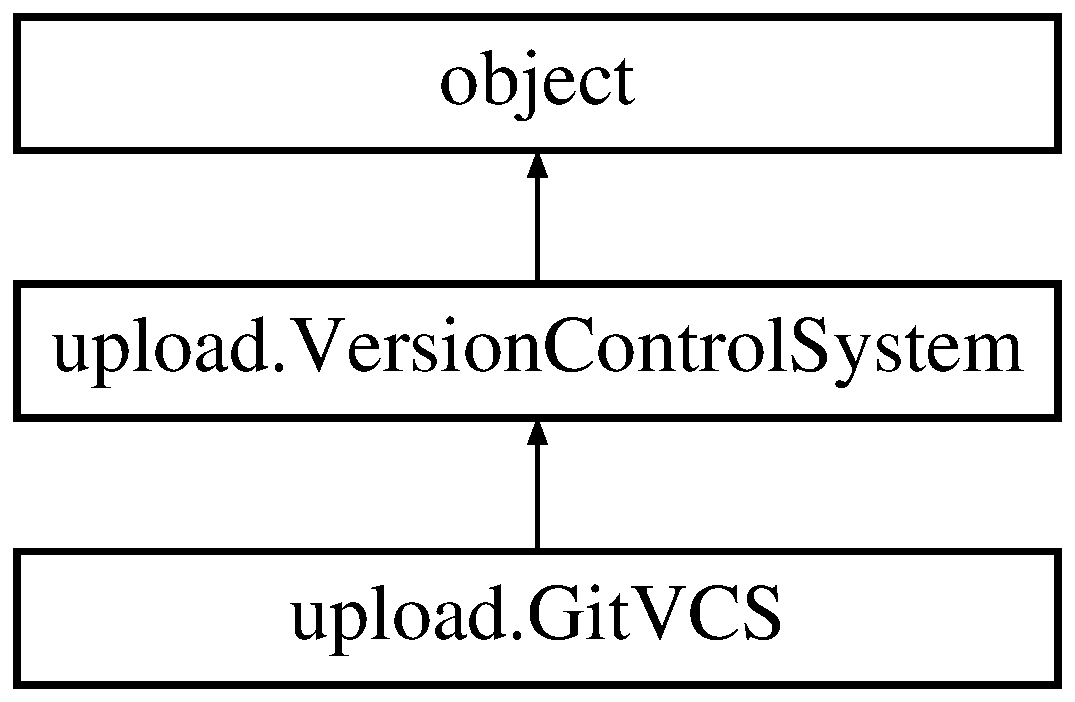
\includegraphics[height=3.000000cm]{classupload_1_1_git_v_c_s}
\end{center}
\end{figure}
\subsection*{Public Member Functions}
\begin{DoxyCompactItemize}
\item 
def \hyperlink{classupload_1_1_git_v_c_s_aba4e1dca1c4b3e5db7ba07f6bce3c839}{\+\_\+\+\_\+init\+\_\+\+\_\+} (self, \hyperlink{classupload_1_1_version_control_system_a4d57d043bc408887b94269fe4cea9556}{options})
\item 
def \hyperlink{classupload_1_1_git_v_c_s_a3ebfc01cebc9b585706ad3f4389a8833}{Generate\+Diff} (self, extra\+\_\+args)
\item 
def \hyperlink{classupload_1_1_git_v_c_s_ae4e8c0e9fa01619c6a5c76d1ab84b995}{Get\+Unknown\+Files} (self)
\item 
def \hyperlink{classupload_1_1_git_v_c_s_a70ddb65a6b512b8cb8cc4affa37ff9b4}{Get\+Base\+File} (self, filename)
\end{DoxyCompactItemize}
\subsection*{Public Attributes}
\begin{DoxyCompactItemize}
\item 
\hyperlink{classupload_1_1_git_v_c_s_a07e9469050a157f34fe804cdf6ecddac}{base\+\_\+hashes}
\end{DoxyCompactItemize}


\subsection{Detailed Description}
\begin{DoxyVerb}Implementation of the VersionControlSystem interface for Git.\end{DoxyVerb}
 

\subsection{Constructor \& Destructor Documentation}
\hypertarget{classupload_1_1_git_v_c_s_aba4e1dca1c4b3e5db7ba07f6bce3c839}{}\index{upload\+::\+Git\+V\+C\+S@{upload\+::\+Git\+V\+C\+S}!\+\_\+\+\_\+init\+\_\+\+\_\+@{\+\_\+\+\_\+init\+\_\+\+\_\+}}
\index{\+\_\+\+\_\+init\+\_\+\+\_\+@{\+\_\+\+\_\+init\+\_\+\+\_\+}!upload\+::\+Git\+V\+C\+S@{upload\+::\+Git\+V\+C\+S}}
\subsubsection[{\+\_\+\+\_\+init\+\_\+\+\_\+(self, options)}]{\setlength{\rightskip}{0pt plus 5cm}def upload.\+Git\+V\+C\+S.\+\_\+\+\_\+init\+\_\+\+\_\+ (
\begin{DoxyParamCaption}
\item[{}]{self, }
\item[{}]{options}
\end{DoxyParamCaption}
)}\label{classupload_1_1_git_v_c_s_aba4e1dca1c4b3e5db7ba07f6bce3c839}


\subsection{Member Function Documentation}
\hypertarget{classupload_1_1_git_v_c_s_a3ebfc01cebc9b585706ad3f4389a8833}{}\index{upload\+::\+Git\+V\+C\+S@{upload\+::\+Git\+V\+C\+S}!Generate\+Diff@{Generate\+Diff}}
\index{Generate\+Diff@{Generate\+Diff}!upload\+::\+Git\+V\+C\+S@{upload\+::\+Git\+V\+C\+S}}
\subsubsection[{Generate\+Diff(self, extra\+\_\+args)}]{\setlength{\rightskip}{0pt plus 5cm}def upload.\+Git\+V\+C\+S.\+Generate\+Diff (
\begin{DoxyParamCaption}
\item[{}]{self, }
\item[{}]{extra\+\_\+args}
\end{DoxyParamCaption}
)}\label{classupload_1_1_git_v_c_s_a3ebfc01cebc9b585706ad3f4389a8833}
\hypertarget{classupload_1_1_git_v_c_s_a70ddb65a6b512b8cb8cc4affa37ff9b4}{}\index{upload\+::\+Git\+V\+C\+S@{upload\+::\+Git\+V\+C\+S}!Get\+Base\+File@{Get\+Base\+File}}
\index{Get\+Base\+File@{Get\+Base\+File}!upload\+::\+Git\+V\+C\+S@{upload\+::\+Git\+V\+C\+S}}
\subsubsection[{Get\+Base\+File(self, filename)}]{\setlength{\rightskip}{0pt plus 5cm}def upload.\+Git\+V\+C\+S.\+Get\+Base\+File (
\begin{DoxyParamCaption}
\item[{}]{self, }
\item[{}]{filename}
\end{DoxyParamCaption}
)}\label{classupload_1_1_git_v_c_s_a70ddb65a6b512b8cb8cc4affa37ff9b4}
\hypertarget{classupload_1_1_git_v_c_s_ae4e8c0e9fa01619c6a5c76d1ab84b995}{}\index{upload\+::\+Git\+V\+C\+S@{upload\+::\+Git\+V\+C\+S}!Get\+Unknown\+Files@{Get\+Unknown\+Files}}
\index{Get\+Unknown\+Files@{Get\+Unknown\+Files}!upload\+::\+Git\+V\+C\+S@{upload\+::\+Git\+V\+C\+S}}
\subsubsection[{Get\+Unknown\+Files(self)}]{\setlength{\rightskip}{0pt plus 5cm}def upload.\+Git\+V\+C\+S.\+Get\+Unknown\+Files (
\begin{DoxyParamCaption}
\item[{}]{self}
\end{DoxyParamCaption}
)}\label{classupload_1_1_git_v_c_s_ae4e8c0e9fa01619c6a5c76d1ab84b995}


\subsection{Member Data Documentation}
\hypertarget{classupload_1_1_git_v_c_s_a07e9469050a157f34fe804cdf6ecddac}{}\index{upload\+::\+Git\+V\+C\+S@{upload\+::\+Git\+V\+C\+S}!base\+\_\+hashes@{base\+\_\+hashes}}
\index{base\+\_\+hashes@{base\+\_\+hashes}!upload\+::\+Git\+V\+C\+S@{upload\+::\+Git\+V\+C\+S}}
\subsubsection[{base\+\_\+hashes}]{\setlength{\rightskip}{0pt plus 5cm}upload.\+Git\+V\+C\+S.\+base\+\_\+hashes}\label{classupload_1_1_git_v_c_s_a07e9469050a157f34fe804cdf6ecddac}


The documentation for this class was generated from the following file\+:\begin{DoxyCompactItemize}
\item 
C\+:/\+Users/\+Hilman/\+Desktop/repo/anjing/src/third\+\_\+party/googletest/scripts/\hyperlink{upload_8py}{upload.\+py}\end{DoxyCompactItemize}

\hypertarget{classgtest__break__on__failure__unittest_1_1_g_test_break_on_failure_unit_test}{}\section{gtest\+\_\+break\+\_\+on\+\_\+failure\+\_\+unittest.\+G\+Test\+Break\+On\+Failure\+Unit\+Test Class Reference}
\label{classgtest__break__on__failure__unittest_1_1_g_test_break_on_failure_unit_test}\index{gtest\+\_\+break\+\_\+on\+\_\+failure\+\_\+unittest.\+G\+Test\+Break\+On\+Failure\+Unit\+Test@{gtest\+\_\+break\+\_\+on\+\_\+failure\+\_\+unittest.\+G\+Test\+Break\+On\+Failure\+Unit\+Test}}
Inheritance diagram for gtest\+\_\+break\+\_\+on\+\_\+failure\+\_\+unittest.\+G\+Test\+Break\+On\+Failure\+Unit\+Test\+:\begin{figure}[H]
\begin{center}
\leavevmode
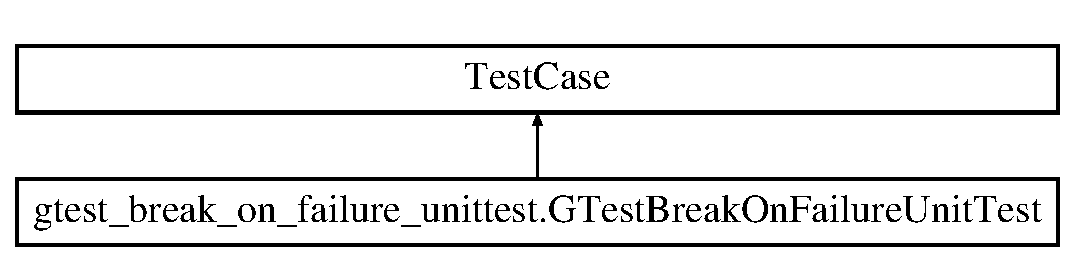
\includegraphics[height=2.000000cm]{classgtest__break__on__failure__unittest_1_1_g_test_break_on_failure_unit_test}
\end{center}
\end{figure}
\subsection*{Public Member Functions}
\begin{DoxyCompactItemize}
\item 
def \hyperlink{classgtest__break__on__failure__unittest_1_1_g_test_break_on_failure_unit_test_a0a66475873f545d88655b8bb14368f2e}{Run\+And\+Verify} (self, env\+\_\+var\+\_\+value, flag\+\_\+value, expect\+\_\+seg\+\_\+fault)
\item 
def \hyperlink{classgtest__break__on__failure__unittest_1_1_g_test_break_on_failure_unit_test_a8c21b7ecccc27268cb6c3d30b933b812}{test\+Default\+Behavior} (self)
\item 
def \hyperlink{classgtest__break__on__failure__unittest_1_1_g_test_break_on_failure_unit_test_a2beae948940a4fd898c8183c3bb221da}{test\+Env\+Var} (self)
\item 
def \hyperlink{classgtest__break__on__failure__unittest_1_1_g_test_break_on_failure_unit_test_af6018e5253c1107c5afaba3e2cb573fe}{test\+Flag} (self)
\item 
def \hyperlink{classgtest__break__on__failure__unittest_1_1_g_test_break_on_failure_unit_test_a15836ddb27e51e9aaf2f8aad84f5cef7}{test\+Flag\+Overrides\+Env\+Var} (self)
\item 
def \hyperlink{classgtest__break__on__failure__unittest_1_1_g_test_break_on_failure_unit_test_a3c5855e045236a309a5bff73ee6b503e}{test\+Break\+On\+Failure\+Overrides\+Throw\+On\+Failure} (self)
\item 
def \hyperlink{classgtest__break__on__failure__unittest_1_1_g_test_break_on_failure_unit_test_a70cc7732ac68ffe587657a3a5309aa4a}{test\+Catch\+Exceptions\+Does\+Not\+Interfere} (self)
\end{DoxyCompactItemize}


\subsection{Detailed Description}
\begin{DoxyVerb}Tests using the GTEST_BREAK_ON_FAILURE environment variable or
the --gtest_break_on_failure flag to turn assertion failures into
segmentation faults.
\end{DoxyVerb}
 

\subsection{Member Function Documentation}
\hypertarget{classgtest__break__on__failure__unittest_1_1_g_test_break_on_failure_unit_test_a0a66475873f545d88655b8bb14368f2e}{}\index{gtest\+\_\+break\+\_\+on\+\_\+failure\+\_\+unittest\+::\+G\+Test\+Break\+On\+Failure\+Unit\+Test@{gtest\+\_\+break\+\_\+on\+\_\+failure\+\_\+unittest\+::\+G\+Test\+Break\+On\+Failure\+Unit\+Test}!Run\+And\+Verify@{Run\+And\+Verify}}
\index{Run\+And\+Verify@{Run\+And\+Verify}!gtest\+\_\+break\+\_\+on\+\_\+failure\+\_\+unittest\+::\+G\+Test\+Break\+On\+Failure\+Unit\+Test@{gtest\+\_\+break\+\_\+on\+\_\+failure\+\_\+unittest\+::\+G\+Test\+Break\+On\+Failure\+Unit\+Test}}
\subsubsection[{Run\+And\+Verify(self, env\+\_\+var\+\_\+value, flag\+\_\+value, expect\+\_\+seg\+\_\+fault)}]{\setlength{\rightskip}{0pt plus 5cm}def gtest\+\_\+break\+\_\+on\+\_\+failure\+\_\+unittest.\+G\+Test\+Break\+On\+Failure\+Unit\+Test.\+Run\+And\+Verify (
\begin{DoxyParamCaption}
\item[{}]{self, }
\item[{}]{env\+\_\+var\+\_\+value, }
\item[{}]{flag\+\_\+value, }
\item[{}]{expect\+\_\+seg\+\_\+fault}
\end{DoxyParamCaption}
)}\label{classgtest__break__on__failure__unittest_1_1_g_test_break_on_failure_unit_test_a0a66475873f545d88655b8bb14368f2e}
\begin{DoxyVerb}Runs gtest_break_on_failure_unittest_ and verifies that it does
(or does not) have a seg-fault.

Args:
  env_var_value:    value of the GTEST_BREAK_ON_FAILURE environment
                variable; None if the variable should be unset.
  flag_value:       value of the --gtest_break_on_failure flag;
                None if the flag should not be present.
  expect_seg_fault: 1 if the program is expected to generate a seg-fault;
                0 otherwise.
\end{DoxyVerb}
 \hypertarget{classgtest__break__on__failure__unittest_1_1_g_test_break_on_failure_unit_test_a3c5855e045236a309a5bff73ee6b503e}{}\index{gtest\+\_\+break\+\_\+on\+\_\+failure\+\_\+unittest\+::\+G\+Test\+Break\+On\+Failure\+Unit\+Test@{gtest\+\_\+break\+\_\+on\+\_\+failure\+\_\+unittest\+::\+G\+Test\+Break\+On\+Failure\+Unit\+Test}!test\+Break\+On\+Failure\+Overrides\+Throw\+On\+Failure@{test\+Break\+On\+Failure\+Overrides\+Throw\+On\+Failure}}
\index{test\+Break\+On\+Failure\+Overrides\+Throw\+On\+Failure@{test\+Break\+On\+Failure\+Overrides\+Throw\+On\+Failure}!gtest\+\_\+break\+\_\+on\+\_\+failure\+\_\+unittest\+::\+G\+Test\+Break\+On\+Failure\+Unit\+Test@{gtest\+\_\+break\+\_\+on\+\_\+failure\+\_\+unittest\+::\+G\+Test\+Break\+On\+Failure\+Unit\+Test}}
\subsubsection[{test\+Break\+On\+Failure\+Overrides\+Throw\+On\+Failure(self)}]{\setlength{\rightskip}{0pt plus 5cm}def gtest\+\_\+break\+\_\+on\+\_\+failure\+\_\+unittest.\+G\+Test\+Break\+On\+Failure\+Unit\+Test.\+test\+Break\+On\+Failure\+Overrides\+Throw\+On\+Failure (
\begin{DoxyParamCaption}
\item[{}]{self}
\end{DoxyParamCaption}
)}\label{classgtest__break__on__failure__unittest_1_1_g_test_break_on_failure_unit_test_a3c5855e045236a309a5bff73ee6b503e}
\begin{DoxyVerb}Tests that gtest_break_on_failure overrides gtest_throw_on_failure.\end{DoxyVerb}
 \hypertarget{classgtest__break__on__failure__unittest_1_1_g_test_break_on_failure_unit_test_a70cc7732ac68ffe587657a3a5309aa4a}{}\index{gtest\+\_\+break\+\_\+on\+\_\+failure\+\_\+unittest\+::\+G\+Test\+Break\+On\+Failure\+Unit\+Test@{gtest\+\_\+break\+\_\+on\+\_\+failure\+\_\+unittest\+::\+G\+Test\+Break\+On\+Failure\+Unit\+Test}!test\+Catch\+Exceptions\+Does\+Not\+Interfere@{test\+Catch\+Exceptions\+Does\+Not\+Interfere}}
\index{test\+Catch\+Exceptions\+Does\+Not\+Interfere@{test\+Catch\+Exceptions\+Does\+Not\+Interfere}!gtest\+\_\+break\+\_\+on\+\_\+failure\+\_\+unittest\+::\+G\+Test\+Break\+On\+Failure\+Unit\+Test@{gtest\+\_\+break\+\_\+on\+\_\+failure\+\_\+unittest\+::\+G\+Test\+Break\+On\+Failure\+Unit\+Test}}
\subsubsection[{test\+Catch\+Exceptions\+Does\+Not\+Interfere(self)}]{\setlength{\rightskip}{0pt plus 5cm}def gtest\+\_\+break\+\_\+on\+\_\+failure\+\_\+unittest.\+G\+Test\+Break\+On\+Failure\+Unit\+Test.\+test\+Catch\+Exceptions\+Does\+Not\+Interfere (
\begin{DoxyParamCaption}
\item[{}]{self}
\end{DoxyParamCaption}
)}\label{classgtest__break__on__failure__unittest_1_1_g_test_break_on_failure_unit_test_a70cc7732ac68ffe587657a3a5309aa4a}
\begin{DoxyVerb}Tests that gtest_catch_exceptions doesn't interfere.\end{DoxyVerb}
 \hypertarget{classgtest__break__on__failure__unittest_1_1_g_test_break_on_failure_unit_test_a8c21b7ecccc27268cb6c3d30b933b812}{}\index{gtest\+\_\+break\+\_\+on\+\_\+failure\+\_\+unittest\+::\+G\+Test\+Break\+On\+Failure\+Unit\+Test@{gtest\+\_\+break\+\_\+on\+\_\+failure\+\_\+unittest\+::\+G\+Test\+Break\+On\+Failure\+Unit\+Test}!test\+Default\+Behavior@{test\+Default\+Behavior}}
\index{test\+Default\+Behavior@{test\+Default\+Behavior}!gtest\+\_\+break\+\_\+on\+\_\+failure\+\_\+unittest\+::\+G\+Test\+Break\+On\+Failure\+Unit\+Test@{gtest\+\_\+break\+\_\+on\+\_\+failure\+\_\+unittest\+::\+G\+Test\+Break\+On\+Failure\+Unit\+Test}}
\subsubsection[{test\+Default\+Behavior(self)}]{\setlength{\rightskip}{0pt plus 5cm}def gtest\+\_\+break\+\_\+on\+\_\+failure\+\_\+unittest.\+G\+Test\+Break\+On\+Failure\+Unit\+Test.\+test\+Default\+Behavior (
\begin{DoxyParamCaption}
\item[{}]{self}
\end{DoxyParamCaption}
)}\label{classgtest__break__on__failure__unittest_1_1_g_test_break_on_failure_unit_test_a8c21b7ecccc27268cb6c3d30b933b812}
\begin{DoxyVerb}Tests the behavior of the default mode.\end{DoxyVerb}
 \hypertarget{classgtest__break__on__failure__unittest_1_1_g_test_break_on_failure_unit_test_a2beae948940a4fd898c8183c3bb221da}{}\index{gtest\+\_\+break\+\_\+on\+\_\+failure\+\_\+unittest\+::\+G\+Test\+Break\+On\+Failure\+Unit\+Test@{gtest\+\_\+break\+\_\+on\+\_\+failure\+\_\+unittest\+::\+G\+Test\+Break\+On\+Failure\+Unit\+Test}!test\+Env\+Var@{test\+Env\+Var}}
\index{test\+Env\+Var@{test\+Env\+Var}!gtest\+\_\+break\+\_\+on\+\_\+failure\+\_\+unittest\+::\+G\+Test\+Break\+On\+Failure\+Unit\+Test@{gtest\+\_\+break\+\_\+on\+\_\+failure\+\_\+unittest\+::\+G\+Test\+Break\+On\+Failure\+Unit\+Test}}
\subsubsection[{test\+Env\+Var(self)}]{\setlength{\rightskip}{0pt plus 5cm}def gtest\+\_\+break\+\_\+on\+\_\+failure\+\_\+unittest.\+G\+Test\+Break\+On\+Failure\+Unit\+Test.\+test\+Env\+Var (
\begin{DoxyParamCaption}
\item[{}]{self}
\end{DoxyParamCaption}
)}\label{classgtest__break__on__failure__unittest_1_1_g_test_break_on_failure_unit_test_a2beae948940a4fd898c8183c3bb221da}
\begin{DoxyVerb}Tests using the GTEST_BREAK_ON_FAILURE environment variable.\end{DoxyVerb}
 \hypertarget{classgtest__break__on__failure__unittest_1_1_g_test_break_on_failure_unit_test_af6018e5253c1107c5afaba3e2cb573fe}{}\index{gtest\+\_\+break\+\_\+on\+\_\+failure\+\_\+unittest\+::\+G\+Test\+Break\+On\+Failure\+Unit\+Test@{gtest\+\_\+break\+\_\+on\+\_\+failure\+\_\+unittest\+::\+G\+Test\+Break\+On\+Failure\+Unit\+Test}!test\+Flag@{test\+Flag}}
\index{test\+Flag@{test\+Flag}!gtest\+\_\+break\+\_\+on\+\_\+failure\+\_\+unittest\+::\+G\+Test\+Break\+On\+Failure\+Unit\+Test@{gtest\+\_\+break\+\_\+on\+\_\+failure\+\_\+unittest\+::\+G\+Test\+Break\+On\+Failure\+Unit\+Test}}
\subsubsection[{test\+Flag(self)}]{\setlength{\rightskip}{0pt plus 5cm}def gtest\+\_\+break\+\_\+on\+\_\+failure\+\_\+unittest.\+G\+Test\+Break\+On\+Failure\+Unit\+Test.\+test\+Flag (
\begin{DoxyParamCaption}
\item[{}]{self}
\end{DoxyParamCaption}
)}\label{classgtest__break__on__failure__unittest_1_1_g_test_break_on_failure_unit_test_af6018e5253c1107c5afaba3e2cb573fe}
\begin{DoxyVerb}Tests using the --gtest_break_on_failure flag.\end{DoxyVerb}
 \hypertarget{classgtest__break__on__failure__unittest_1_1_g_test_break_on_failure_unit_test_a15836ddb27e51e9aaf2f8aad84f5cef7}{}\index{gtest\+\_\+break\+\_\+on\+\_\+failure\+\_\+unittest\+::\+G\+Test\+Break\+On\+Failure\+Unit\+Test@{gtest\+\_\+break\+\_\+on\+\_\+failure\+\_\+unittest\+::\+G\+Test\+Break\+On\+Failure\+Unit\+Test}!test\+Flag\+Overrides\+Env\+Var@{test\+Flag\+Overrides\+Env\+Var}}
\index{test\+Flag\+Overrides\+Env\+Var@{test\+Flag\+Overrides\+Env\+Var}!gtest\+\_\+break\+\_\+on\+\_\+failure\+\_\+unittest\+::\+G\+Test\+Break\+On\+Failure\+Unit\+Test@{gtest\+\_\+break\+\_\+on\+\_\+failure\+\_\+unittest\+::\+G\+Test\+Break\+On\+Failure\+Unit\+Test}}
\subsubsection[{test\+Flag\+Overrides\+Env\+Var(self)}]{\setlength{\rightskip}{0pt plus 5cm}def gtest\+\_\+break\+\_\+on\+\_\+failure\+\_\+unittest.\+G\+Test\+Break\+On\+Failure\+Unit\+Test.\+test\+Flag\+Overrides\+Env\+Var (
\begin{DoxyParamCaption}
\item[{}]{self}
\end{DoxyParamCaption}
)}\label{classgtest__break__on__failure__unittest_1_1_g_test_break_on_failure_unit_test_a15836ddb27e51e9aaf2f8aad84f5cef7}
\begin{DoxyVerb}Tests that the flag overrides the environment variable.\end{DoxyVerb}
 

The documentation for this class was generated from the following file\+:\begin{DoxyCompactItemize}
\item 
C\+:/\+Users/\+Hilman/\+Desktop/repo/anjing/src/third\+\_\+party/googletest/test/\hyperlink{gtest__break__on__failure__unittest_8py}{gtest\+\_\+break\+\_\+on\+\_\+failure\+\_\+unittest.\+py}\end{DoxyCompactItemize}

\hypertarget{classgtest__color__test_1_1_g_test_color_test}{}\section{gtest\+\_\+color\+\_\+test.\+G\+Test\+Color\+Test Class Reference}
\label{classgtest__color__test_1_1_g_test_color_test}\index{gtest\+\_\+color\+\_\+test.\+G\+Test\+Color\+Test@{gtest\+\_\+color\+\_\+test.\+G\+Test\+Color\+Test}}
Inheritance diagram for gtest\+\_\+color\+\_\+test.\+G\+Test\+Color\+Test\+:\begin{figure}[H]
\begin{center}
\leavevmode
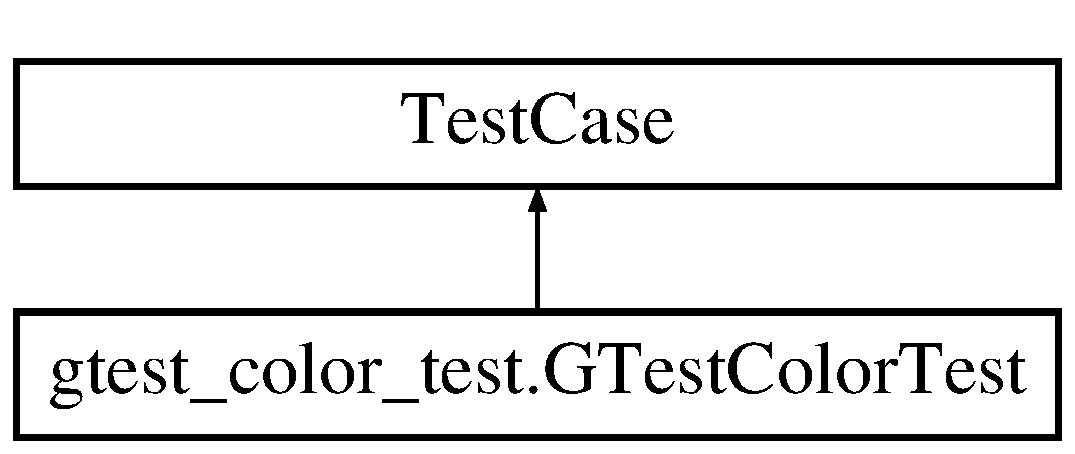
\includegraphics[height=2.000000cm]{classgtest__color__test_1_1_g_test_color_test}
\end{center}
\end{figure}
\subsection*{Public Member Functions}
\begin{DoxyCompactItemize}
\item 
def \hyperlink{classgtest__color__test_1_1_g_test_color_test_a22bf83ab416dc3ccd3c1b771ff74022c}{test\+No\+Env\+Var\+No\+Flag} (self)
\item 
def \hyperlink{classgtest__color__test_1_1_g_test_color_test_abc4c056b8e703e83516f9e5aea8dd25d}{test\+Flag\+Only} (self)
\item 
def \hyperlink{classgtest__color__test_1_1_g_test_color_test_aedb7bbaa0d6acff3628d91a471f4ceb5}{test\+Env\+Var\+Only} (self)
\item 
def \hyperlink{classgtest__color__test_1_1_g_test_color_test_ae88e8ec526135ed1448e83fc4ec7cd15}{test\+Env\+Var\+And\+Flag} (self)
\item 
def \hyperlink{classgtest__color__test_1_1_g_test_color_test_aaf2110e359494dc711e87d29d351dc47}{test\+Aliases\+Of\+Yes\+And\+No} (self)
\end{DoxyCompactItemize}


\subsection{Member Function Documentation}
\hypertarget{classgtest__color__test_1_1_g_test_color_test_aaf2110e359494dc711e87d29d351dc47}{}\index{gtest\+\_\+color\+\_\+test\+::\+G\+Test\+Color\+Test@{gtest\+\_\+color\+\_\+test\+::\+G\+Test\+Color\+Test}!test\+Aliases\+Of\+Yes\+And\+No@{test\+Aliases\+Of\+Yes\+And\+No}}
\index{test\+Aliases\+Of\+Yes\+And\+No@{test\+Aliases\+Of\+Yes\+And\+No}!gtest\+\_\+color\+\_\+test\+::\+G\+Test\+Color\+Test@{gtest\+\_\+color\+\_\+test\+::\+G\+Test\+Color\+Test}}
\subsubsection[{test\+Aliases\+Of\+Yes\+And\+No(self)}]{\setlength{\rightskip}{0pt plus 5cm}def gtest\+\_\+color\+\_\+test.\+G\+Test\+Color\+Test.\+test\+Aliases\+Of\+Yes\+And\+No (
\begin{DoxyParamCaption}
\item[{}]{self}
\end{DoxyParamCaption}
)}\label{classgtest__color__test_1_1_g_test_color_test_aaf2110e359494dc711e87d29d351dc47}
\begin{DoxyVerb}Tests using aliases in specifying --gtest_color.\end{DoxyVerb}
 \hypertarget{classgtest__color__test_1_1_g_test_color_test_ae88e8ec526135ed1448e83fc4ec7cd15}{}\index{gtest\+\_\+color\+\_\+test\+::\+G\+Test\+Color\+Test@{gtest\+\_\+color\+\_\+test\+::\+G\+Test\+Color\+Test}!test\+Env\+Var\+And\+Flag@{test\+Env\+Var\+And\+Flag}}
\index{test\+Env\+Var\+And\+Flag@{test\+Env\+Var\+And\+Flag}!gtest\+\_\+color\+\_\+test\+::\+G\+Test\+Color\+Test@{gtest\+\_\+color\+\_\+test\+::\+G\+Test\+Color\+Test}}
\subsubsection[{test\+Env\+Var\+And\+Flag(self)}]{\setlength{\rightskip}{0pt plus 5cm}def gtest\+\_\+color\+\_\+test.\+G\+Test\+Color\+Test.\+test\+Env\+Var\+And\+Flag (
\begin{DoxyParamCaption}
\item[{}]{self}
\end{DoxyParamCaption}
)}\label{classgtest__color__test_1_1_g_test_color_test_ae88e8ec526135ed1448e83fc4ec7cd15}
\begin{DoxyVerb}Tests the case when there are both GTEST_COLOR and --gtest_color.\end{DoxyVerb}
 \hypertarget{classgtest__color__test_1_1_g_test_color_test_aedb7bbaa0d6acff3628d91a471f4ceb5}{}\index{gtest\+\_\+color\+\_\+test\+::\+G\+Test\+Color\+Test@{gtest\+\_\+color\+\_\+test\+::\+G\+Test\+Color\+Test}!test\+Env\+Var\+Only@{test\+Env\+Var\+Only}}
\index{test\+Env\+Var\+Only@{test\+Env\+Var\+Only}!gtest\+\_\+color\+\_\+test\+::\+G\+Test\+Color\+Test@{gtest\+\_\+color\+\_\+test\+::\+G\+Test\+Color\+Test}}
\subsubsection[{test\+Env\+Var\+Only(self)}]{\setlength{\rightskip}{0pt plus 5cm}def gtest\+\_\+color\+\_\+test.\+G\+Test\+Color\+Test.\+test\+Env\+Var\+Only (
\begin{DoxyParamCaption}
\item[{}]{self}
\end{DoxyParamCaption}
)}\label{classgtest__color__test_1_1_g_test_color_test_aedb7bbaa0d6acff3628d91a471f4ceb5}
\begin{DoxyVerb}Tests the case when there's GTEST_COLOR but not --gtest_color.\end{DoxyVerb}
 \hypertarget{classgtest__color__test_1_1_g_test_color_test_abc4c056b8e703e83516f9e5aea8dd25d}{}\index{gtest\+\_\+color\+\_\+test\+::\+G\+Test\+Color\+Test@{gtest\+\_\+color\+\_\+test\+::\+G\+Test\+Color\+Test}!test\+Flag\+Only@{test\+Flag\+Only}}
\index{test\+Flag\+Only@{test\+Flag\+Only}!gtest\+\_\+color\+\_\+test\+::\+G\+Test\+Color\+Test@{gtest\+\_\+color\+\_\+test\+::\+G\+Test\+Color\+Test}}
\subsubsection[{test\+Flag\+Only(self)}]{\setlength{\rightskip}{0pt plus 5cm}def gtest\+\_\+color\+\_\+test.\+G\+Test\+Color\+Test.\+test\+Flag\+Only (
\begin{DoxyParamCaption}
\item[{}]{self}
\end{DoxyParamCaption}
)}\label{classgtest__color__test_1_1_g_test_color_test_abc4c056b8e703e83516f9e5aea8dd25d}
\begin{DoxyVerb}Tests the case when there's --gtest_color but not GTEST_COLOR.\end{DoxyVerb}
 \hypertarget{classgtest__color__test_1_1_g_test_color_test_a22bf83ab416dc3ccd3c1b771ff74022c}{}\index{gtest\+\_\+color\+\_\+test\+::\+G\+Test\+Color\+Test@{gtest\+\_\+color\+\_\+test\+::\+G\+Test\+Color\+Test}!test\+No\+Env\+Var\+No\+Flag@{test\+No\+Env\+Var\+No\+Flag}}
\index{test\+No\+Env\+Var\+No\+Flag@{test\+No\+Env\+Var\+No\+Flag}!gtest\+\_\+color\+\_\+test\+::\+G\+Test\+Color\+Test@{gtest\+\_\+color\+\_\+test\+::\+G\+Test\+Color\+Test}}
\subsubsection[{test\+No\+Env\+Var\+No\+Flag(self)}]{\setlength{\rightskip}{0pt plus 5cm}def gtest\+\_\+color\+\_\+test.\+G\+Test\+Color\+Test.\+test\+No\+Env\+Var\+No\+Flag (
\begin{DoxyParamCaption}
\item[{}]{self}
\end{DoxyParamCaption}
)}\label{classgtest__color__test_1_1_g_test_color_test_a22bf83ab416dc3ccd3c1b771ff74022c}
\begin{DoxyVerb}Tests the case when there's neither GTEST_COLOR nor --gtest_color.\end{DoxyVerb}
 

The documentation for this class was generated from the following file\+:\begin{DoxyCompactItemize}
\item 
C\+:/\+Users/\+Hilman/\+Desktop/repo/anjing/src/third\+\_\+party/googletest/test/\hyperlink{gtest__color__test_8py}{gtest\+\_\+color\+\_\+test.\+py}\end{DoxyCompactItemize}

\hypertarget{classgtest__env__var__test_1_1_g_test_env_var_test}{}\section{gtest\+\_\+env\+\_\+var\+\_\+test.\+G\+Test\+Env\+Var\+Test Class Reference}
\label{classgtest__env__var__test_1_1_g_test_env_var_test}\index{gtest\+\_\+env\+\_\+var\+\_\+test.\+G\+Test\+Env\+Var\+Test@{gtest\+\_\+env\+\_\+var\+\_\+test.\+G\+Test\+Env\+Var\+Test}}
Inheritance diagram for gtest\+\_\+env\+\_\+var\+\_\+test.\+G\+Test\+Env\+Var\+Test\+:\begin{figure}[H]
\begin{center}
\leavevmode
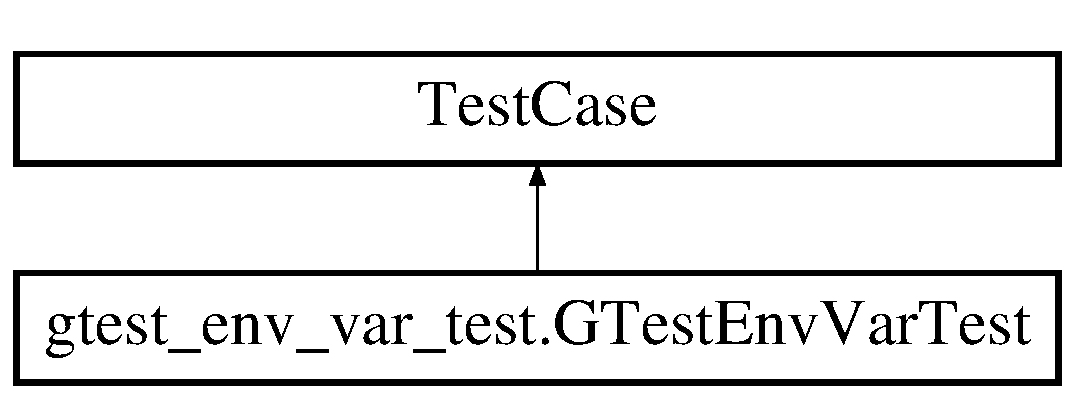
\includegraphics[height=2.000000cm]{classgtest__env__var__test_1_1_g_test_env_var_test}
\end{center}
\end{figure}
\subsection*{Public Member Functions}
\begin{DoxyCompactItemize}
\item 
def \hyperlink{classgtest__env__var__test_1_1_g_test_env_var_test_ad169061caa22a6cd510535d6da94b97e}{test\+Env\+Var\+Affects\+Flag} (self)
\end{DoxyCompactItemize}


\subsection{Member Function Documentation}
\hypertarget{classgtest__env__var__test_1_1_g_test_env_var_test_ad169061caa22a6cd510535d6da94b97e}{}\index{gtest\+\_\+env\+\_\+var\+\_\+test\+::\+G\+Test\+Env\+Var\+Test@{gtest\+\_\+env\+\_\+var\+\_\+test\+::\+G\+Test\+Env\+Var\+Test}!test\+Env\+Var\+Affects\+Flag@{test\+Env\+Var\+Affects\+Flag}}
\index{test\+Env\+Var\+Affects\+Flag@{test\+Env\+Var\+Affects\+Flag}!gtest\+\_\+env\+\_\+var\+\_\+test\+::\+G\+Test\+Env\+Var\+Test@{gtest\+\_\+env\+\_\+var\+\_\+test\+::\+G\+Test\+Env\+Var\+Test}}
\subsubsection[{test\+Env\+Var\+Affects\+Flag(self)}]{\setlength{\rightskip}{0pt plus 5cm}def gtest\+\_\+env\+\_\+var\+\_\+test.\+G\+Test\+Env\+Var\+Test.\+test\+Env\+Var\+Affects\+Flag (
\begin{DoxyParamCaption}
\item[{}]{self}
\end{DoxyParamCaption}
)}\label{classgtest__env__var__test_1_1_g_test_env_var_test_ad169061caa22a6cd510535d6da94b97e}
\begin{DoxyVerb}Tests that environment variable should affect the corresponding flag.\end{DoxyVerb}
 

The documentation for this class was generated from the following file\+:\begin{DoxyCompactItemize}
\item 
C\+:/\+Users/\+Hilman/\+Desktop/repo/anjing/src/third\+\_\+party/googletest/test/\hyperlink{gtest__env__var__test_8py}{gtest\+\_\+env\+\_\+var\+\_\+test.\+py}\end{DoxyCompactItemize}

\hypertarget{classgtest__filter__unittest_1_1_g_test_filter_unit_test}{}\section{gtest\+\_\+filter\+\_\+unittest.\+G\+Test\+Filter\+Unit\+Test Class Reference}
\label{classgtest__filter__unittest_1_1_g_test_filter_unit_test}\index{gtest\+\_\+filter\+\_\+unittest.\+G\+Test\+Filter\+Unit\+Test@{gtest\+\_\+filter\+\_\+unittest.\+G\+Test\+Filter\+Unit\+Test}}
Inheritance diagram for gtest\+\_\+filter\+\_\+unittest.\+G\+Test\+Filter\+Unit\+Test\+:\begin{figure}[H]
\begin{center}
\leavevmode
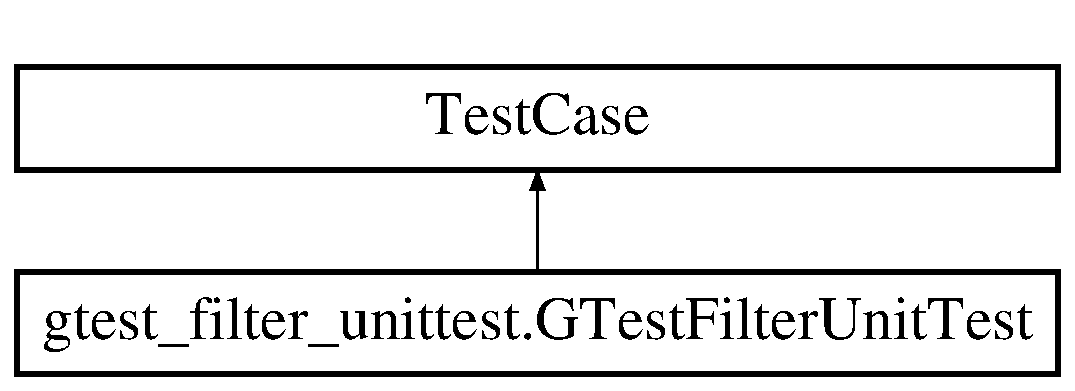
\includegraphics[height=2.000000cm]{classgtest__filter__unittest_1_1_g_test_filter_unit_test}
\end{center}
\end{figure}
\subsection*{Public Member Functions}
\begin{DoxyCompactItemize}
\item 
def \hyperlink{classgtest__filter__unittest_1_1_g_test_filter_unit_test_aeebdbdcc59594ad0a69cf11eafe94997}{Assert\+Set\+Equal} (self, lhs, rhs)
\item 
def \hyperlink{classgtest__filter__unittest_1_1_g_test_filter_unit_test_a87656eac0cf4136252eef43da0121381}{Assert\+Partition\+Is\+Valid} (self, set\+\_\+var, list\+\_\+of\+\_\+sets)
\item 
def \hyperlink{classgtest__filter__unittest_1_1_g_test_filter_unit_test_a11c48bf404bca6806b14a1a71d169ace}{Adjust\+For\+Parameterized\+Tests} (self, tests\+\_\+to\+\_\+run)
\item 
def \hyperlink{classgtest__filter__unittest_1_1_g_test_filter_unit_test_acf341ed9a265b346a050afa9a9a85c65}{Run\+And\+Verify} (self, gtest\+\_\+filter, tests\+\_\+to\+\_\+run)
\item 
def \hyperlink{classgtest__filter__unittest_1_1_g_test_filter_unit_test_a6d37b9fb87437097a5d5794ec2ba522e}{Run\+And\+Verify\+With\+Sharding}
\item 
def \hyperlink{classgtest__filter__unittest_1_1_g_test_filter_unit_test_ae52bd70ef1dcb68c83c0379ddfb987a9}{Run\+And\+Verify\+Allowing\+Disabled} (self, gtest\+\_\+filter, tests\+\_\+to\+\_\+run)
\item 
def \hyperlink{classgtest__filter__unittest_1_1_g_test_filter_unit_test_af20a71b1659314a5cc1093d77a673495}{set\+Up} (self)
\item 
def \hyperlink{classgtest__filter__unittest_1_1_g_test_filter_unit_test_adef3a9b539c73bda785a631a5aac424f}{test\+Default\+Behavior} (self)
\item 
def \hyperlink{classgtest__filter__unittest_1_1_g_test_filter_unit_test_a8d5ad564f41c052864a3957a71daa535}{test\+Default\+Behavior\+With\+Shards} (self)
\item 
def \hyperlink{classgtest__filter__unittest_1_1_g_test_filter_unit_test_afce65847b463ec5bca4458e9348d9a9f}{test\+Empty\+Filter} (self)
\item 
def \hyperlink{classgtest__filter__unittest_1_1_g_test_filter_unit_test_a2456062c177350a53244aea030aaf617}{test\+Bad\+Filter} (self)
\item 
def \hyperlink{classgtest__filter__unittest_1_1_g_test_filter_unit_test_a336d9203e26493bae11fbb514af38a6b}{test\+Full\+Name} (self)
\item 
def \hyperlink{classgtest__filter__unittest_1_1_g_test_filter_unit_test_ae9da48a79483e22e3f986e57de0dee37}{test\+Universal\+Filters} (self)
\item 
def \hyperlink{classgtest__filter__unittest_1_1_g_test_filter_unit_test_ac59206c94324afdc09adbe5853856174}{test\+Filter\+By\+Test\+Case} (self)
\item 
def \hyperlink{classgtest__filter__unittest_1_1_g_test_filter_unit_test_aaea691324a6c0765403b26a895702a63}{test\+Filter\+By\+Test} (self)
\item 
def \hyperlink{classgtest__filter__unittest_1_1_g_test_filter_unit_test_a6d962adae2ee2697b3b92e84b60a795a}{test\+Filter\+Disabled\+Tests} (self)
\item 
def \hyperlink{classgtest__filter__unittest_1_1_g_test_filter_unit_test_af855132606c1fa02fb765e8619108114}{test\+Wildcard\+In\+Test\+Case\+Name} (self)
\item 
def \hyperlink{classgtest__filter__unittest_1_1_g_test_filter_unit_test_a9b1e6b35e158d7c6d11b8f4d2cb600cb}{test\+Wildcard\+In\+Test\+Name} (self)
\item 
def \hyperlink{classgtest__filter__unittest_1_1_g_test_filter_unit_test_a874aea28690300d8c0dc0910304f7ab2}{test\+Filter\+Without\+Dot} (self)
\item 
def \hyperlink{classgtest__filter__unittest_1_1_g_test_filter_unit_test_a2563885e647205586b135c5ead55e6ab}{test\+Two\+Patterns} (self)
\item 
def \hyperlink{classgtest__filter__unittest_1_1_g_test_filter_unit_test_af4858e153245f0974632fd36dc1dd804}{test\+Three\+Patterns} (self)
\item 
def \hyperlink{classgtest__filter__unittest_1_1_g_test_filter_unit_test_aff878809d524797f62e2fe38bbfcc8da}{test\+Negative\+Filters} (self)
\item 
def \hyperlink{classgtest__filter__unittest_1_1_g_test_filter_unit_test_a81e4256da0e0ad8cb4b764ffd573cc6d}{test\+Flag\+Overrides\+Env\+Var} (self)
\item 
def \hyperlink{classgtest__filter__unittest_1_1_g_test_filter_unit_test_a7a2c7b8d758abba0ae883bbb272f344b}{test\+Shard\+Status\+File\+Is\+Created} (self)
\item 
def \hyperlink{classgtest__filter__unittest_1_1_g_test_filter_unit_test_a1dac68948f6170e39ae9ee7bca0bc1eb}{test\+Shard\+Status\+File\+Is\+Created\+With\+List\+Tests} (self)
\item 
def \hyperlink{classgtest__filter__unittest_1_1_g_test_filter_unit_test_a4b4f7428d9219dff5960968477927626}{test\+Sharding\+Works\+With\+Death\+Tests} (self)
\end{DoxyCompactItemize}


\subsection{Detailed Description}
\begin{DoxyVerb}Tests the env variable or the command line flag to filter tests.\end{DoxyVerb}
 

\subsection{Member Function Documentation}
\hypertarget{classgtest__filter__unittest_1_1_g_test_filter_unit_test_a11c48bf404bca6806b14a1a71d169ace}{}\index{gtest\+\_\+filter\+\_\+unittest\+::\+G\+Test\+Filter\+Unit\+Test@{gtest\+\_\+filter\+\_\+unittest\+::\+G\+Test\+Filter\+Unit\+Test}!Adjust\+For\+Parameterized\+Tests@{Adjust\+For\+Parameterized\+Tests}}
\index{Adjust\+For\+Parameterized\+Tests@{Adjust\+For\+Parameterized\+Tests}!gtest\+\_\+filter\+\_\+unittest\+::\+G\+Test\+Filter\+Unit\+Test@{gtest\+\_\+filter\+\_\+unittest\+::\+G\+Test\+Filter\+Unit\+Test}}
\subsubsection[{Adjust\+For\+Parameterized\+Tests(self, tests\+\_\+to\+\_\+run)}]{\setlength{\rightskip}{0pt plus 5cm}def gtest\+\_\+filter\+\_\+unittest.\+G\+Test\+Filter\+Unit\+Test.\+Adjust\+For\+Parameterized\+Tests (
\begin{DoxyParamCaption}
\item[{}]{self, }
\item[{}]{tests\+\_\+to\+\_\+run}
\end{DoxyParamCaption}
)}\label{classgtest__filter__unittest_1_1_g_test_filter_unit_test_a11c48bf404bca6806b14a1a71d169ace}
\begin{DoxyVerb}Adjust tests_to_run in case value parameterized tests are disabled.\end{DoxyVerb}
 \hypertarget{classgtest__filter__unittest_1_1_g_test_filter_unit_test_a87656eac0cf4136252eef43da0121381}{}\index{gtest\+\_\+filter\+\_\+unittest\+::\+G\+Test\+Filter\+Unit\+Test@{gtest\+\_\+filter\+\_\+unittest\+::\+G\+Test\+Filter\+Unit\+Test}!Assert\+Partition\+Is\+Valid@{Assert\+Partition\+Is\+Valid}}
\index{Assert\+Partition\+Is\+Valid@{Assert\+Partition\+Is\+Valid}!gtest\+\_\+filter\+\_\+unittest\+::\+G\+Test\+Filter\+Unit\+Test@{gtest\+\_\+filter\+\_\+unittest\+::\+G\+Test\+Filter\+Unit\+Test}}
\subsubsection[{Assert\+Partition\+Is\+Valid(self, set\+\_\+var, list\+\_\+of\+\_\+sets)}]{\setlength{\rightskip}{0pt plus 5cm}def gtest\+\_\+filter\+\_\+unittest.\+G\+Test\+Filter\+Unit\+Test.\+Assert\+Partition\+Is\+Valid (
\begin{DoxyParamCaption}
\item[{}]{self, }
\item[{}]{set\+\_\+var, }
\item[{}]{list\+\_\+of\+\_\+sets}
\end{DoxyParamCaption}
)}\label{classgtest__filter__unittest_1_1_g_test_filter_unit_test_a87656eac0cf4136252eef43da0121381}
\begin{DoxyVerb}Asserts that list_of_sets is a valid partition of set_var.\end{DoxyVerb}
 \hypertarget{classgtest__filter__unittest_1_1_g_test_filter_unit_test_aeebdbdcc59594ad0a69cf11eafe94997}{}\index{gtest\+\_\+filter\+\_\+unittest\+::\+G\+Test\+Filter\+Unit\+Test@{gtest\+\_\+filter\+\_\+unittest\+::\+G\+Test\+Filter\+Unit\+Test}!Assert\+Set\+Equal@{Assert\+Set\+Equal}}
\index{Assert\+Set\+Equal@{Assert\+Set\+Equal}!gtest\+\_\+filter\+\_\+unittest\+::\+G\+Test\+Filter\+Unit\+Test@{gtest\+\_\+filter\+\_\+unittest\+::\+G\+Test\+Filter\+Unit\+Test}}
\subsubsection[{Assert\+Set\+Equal(self, lhs, rhs)}]{\setlength{\rightskip}{0pt plus 5cm}def gtest\+\_\+filter\+\_\+unittest.\+G\+Test\+Filter\+Unit\+Test.\+Assert\+Set\+Equal (
\begin{DoxyParamCaption}
\item[{}]{self, }
\item[{}]{lhs, }
\item[{}]{rhs}
\end{DoxyParamCaption}
)}\label{classgtest__filter__unittest_1_1_g_test_filter_unit_test_aeebdbdcc59594ad0a69cf11eafe94997}
\begin{DoxyVerb}Asserts that two sets are equal.\end{DoxyVerb}
 \hypertarget{classgtest__filter__unittest_1_1_g_test_filter_unit_test_acf341ed9a265b346a050afa9a9a85c65}{}\index{gtest\+\_\+filter\+\_\+unittest\+::\+G\+Test\+Filter\+Unit\+Test@{gtest\+\_\+filter\+\_\+unittest\+::\+G\+Test\+Filter\+Unit\+Test}!Run\+And\+Verify@{Run\+And\+Verify}}
\index{Run\+And\+Verify@{Run\+And\+Verify}!gtest\+\_\+filter\+\_\+unittest\+::\+G\+Test\+Filter\+Unit\+Test@{gtest\+\_\+filter\+\_\+unittest\+::\+G\+Test\+Filter\+Unit\+Test}}
\subsubsection[{Run\+And\+Verify(self, gtest\+\_\+filter, tests\+\_\+to\+\_\+run)}]{\setlength{\rightskip}{0pt plus 5cm}def gtest\+\_\+filter\+\_\+unittest.\+G\+Test\+Filter\+Unit\+Test.\+Run\+And\+Verify (
\begin{DoxyParamCaption}
\item[{}]{self, }
\item[{}]{gtest\+\_\+filter, }
\item[{}]{tests\+\_\+to\+\_\+run}
\end{DoxyParamCaption}
)}\label{classgtest__filter__unittest_1_1_g_test_filter_unit_test_acf341ed9a265b346a050afa9a9a85c65}
\begin{DoxyVerb}Checks that the binary runs correct set of tests for a given filter.\end{DoxyVerb}
 \hypertarget{classgtest__filter__unittest_1_1_g_test_filter_unit_test_ae52bd70ef1dcb68c83c0379ddfb987a9}{}\index{gtest\+\_\+filter\+\_\+unittest\+::\+G\+Test\+Filter\+Unit\+Test@{gtest\+\_\+filter\+\_\+unittest\+::\+G\+Test\+Filter\+Unit\+Test}!Run\+And\+Verify\+Allowing\+Disabled@{Run\+And\+Verify\+Allowing\+Disabled}}
\index{Run\+And\+Verify\+Allowing\+Disabled@{Run\+And\+Verify\+Allowing\+Disabled}!gtest\+\_\+filter\+\_\+unittest\+::\+G\+Test\+Filter\+Unit\+Test@{gtest\+\_\+filter\+\_\+unittest\+::\+G\+Test\+Filter\+Unit\+Test}}
\subsubsection[{Run\+And\+Verify\+Allowing\+Disabled(self, gtest\+\_\+filter, tests\+\_\+to\+\_\+run)}]{\setlength{\rightskip}{0pt plus 5cm}def gtest\+\_\+filter\+\_\+unittest.\+G\+Test\+Filter\+Unit\+Test.\+Run\+And\+Verify\+Allowing\+Disabled (
\begin{DoxyParamCaption}
\item[{}]{self, }
\item[{}]{gtest\+\_\+filter, }
\item[{}]{tests\+\_\+to\+\_\+run}
\end{DoxyParamCaption}
)}\label{classgtest__filter__unittest_1_1_g_test_filter_unit_test_ae52bd70ef1dcb68c83c0379ddfb987a9}
\begin{DoxyVerb}Checks that the binary runs correct set of tests for the given filter.

Runs gtest_filter_unittest_ with the given filter, and enables
disabled tests. Verifies that the right set of tests were run.

Args:
  gtest_filter: A filter to apply to the tests.
  tests_to_run: A set of tests expected to run.
\end{DoxyVerb}
 \hypertarget{classgtest__filter__unittest_1_1_g_test_filter_unit_test_a6d37b9fb87437097a5d5794ec2ba522e}{}\index{gtest\+\_\+filter\+\_\+unittest\+::\+G\+Test\+Filter\+Unit\+Test@{gtest\+\_\+filter\+\_\+unittest\+::\+G\+Test\+Filter\+Unit\+Test}!Run\+And\+Verify\+With\+Sharding@{Run\+And\+Verify\+With\+Sharding}}
\index{Run\+And\+Verify\+With\+Sharding@{Run\+And\+Verify\+With\+Sharding}!gtest\+\_\+filter\+\_\+unittest\+::\+G\+Test\+Filter\+Unit\+Test@{gtest\+\_\+filter\+\_\+unittest\+::\+G\+Test\+Filter\+Unit\+Test}}
\subsubsection[{Run\+And\+Verify\+With\+Sharding}]{\setlength{\rightskip}{0pt plus 5cm}def gtest\+\_\+filter\+\_\+unittest.\+G\+Test\+Filter\+Unit\+Test.\+Run\+And\+Verify\+With\+Sharding (
\begin{DoxyParamCaption}
\item[{}]{self, }
\item[{}]{gtest\+\_\+filter, }
\item[{}]{total\+\_\+shards, }
\item[{}]{tests\+\_\+to\+\_\+run, }
\item[{}]{args = {\ttfamily None}, }
\item[{}]{check\+\_\+exit\+\_\+0 = {\ttfamily False}}
\end{DoxyParamCaption}
)}\label{classgtest__filter__unittest_1_1_g_test_filter_unit_test_a6d37b9fb87437097a5d5794ec2ba522e}
\begin{DoxyVerb}Checks that binary runs correct tests for the given filter and shard.

Runs all shards of gtest_filter_unittest_ with the given filter, and
verifies that the right set of tests were run. The union of tests run
on each shard should be identical to tests_to_run, without duplicates.

Args:
  gtest_filter: A filter to apply to the tests.
  total_shards: A total number of shards to split test run into.
  tests_to_run: A set of tests expected to run.
  args   :      Arguments to pass to the to the test binary.
  check_exit_0: When set to a true value, make sure that all shards
            return 0.
\end{DoxyVerb}
 \hypertarget{classgtest__filter__unittest_1_1_g_test_filter_unit_test_af20a71b1659314a5cc1093d77a673495}{}\index{gtest\+\_\+filter\+\_\+unittest\+::\+G\+Test\+Filter\+Unit\+Test@{gtest\+\_\+filter\+\_\+unittest\+::\+G\+Test\+Filter\+Unit\+Test}!set\+Up@{set\+Up}}
\index{set\+Up@{set\+Up}!gtest\+\_\+filter\+\_\+unittest\+::\+G\+Test\+Filter\+Unit\+Test@{gtest\+\_\+filter\+\_\+unittest\+::\+G\+Test\+Filter\+Unit\+Test}}
\subsubsection[{set\+Up(self)}]{\setlength{\rightskip}{0pt plus 5cm}def gtest\+\_\+filter\+\_\+unittest.\+G\+Test\+Filter\+Unit\+Test.\+set\+Up (
\begin{DoxyParamCaption}
\item[{}]{self}
\end{DoxyParamCaption}
)}\label{classgtest__filter__unittest_1_1_g_test_filter_unit_test_af20a71b1659314a5cc1093d77a673495}
\begin{DoxyVerb}Sets up test case.

Determines whether value-parameterized tests are enabled in the binary and
sets the flags accordingly.
\end{DoxyVerb}
 \hypertarget{classgtest__filter__unittest_1_1_g_test_filter_unit_test_a2456062c177350a53244aea030aaf617}{}\index{gtest\+\_\+filter\+\_\+unittest\+::\+G\+Test\+Filter\+Unit\+Test@{gtest\+\_\+filter\+\_\+unittest\+::\+G\+Test\+Filter\+Unit\+Test}!test\+Bad\+Filter@{test\+Bad\+Filter}}
\index{test\+Bad\+Filter@{test\+Bad\+Filter}!gtest\+\_\+filter\+\_\+unittest\+::\+G\+Test\+Filter\+Unit\+Test@{gtest\+\_\+filter\+\_\+unittest\+::\+G\+Test\+Filter\+Unit\+Test}}
\subsubsection[{test\+Bad\+Filter(self)}]{\setlength{\rightskip}{0pt plus 5cm}def gtest\+\_\+filter\+\_\+unittest.\+G\+Test\+Filter\+Unit\+Test.\+test\+Bad\+Filter (
\begin{DoxyParamCaption}
\item[{}]{self}
\end{DoxyParamCaption}
)}\label{classgtest__filter__unittest_1_1_g_test_filter_unit_test_a2456062c177350a53244aea030aaf617}
\begin{DoxyVerb}Tests a filter that matches nothing.\end{DoxyVerb}
 \hypertarget{classgtest__filter__unittest_1_1_g_test_filter_unit_test_adef3a9b539c73bda785a631a5aac424f}{}\index{gtest\+\_\+filter\+\_\+unittest\+::\+G\+Test\+Filter\+Unit\+Test@{gtest\+\_\+filter\+\_\+unittest\+::\+G\+Test\+Filter\+Unit\+Test}!test\+Default\+Behavior@{test\+Default\+Behavior}}
\index{test\+Default\+Behavior@{test\+Default\+Behavior}!gtest\+\_\+filter\+\_\+unittest\+::\+G\+Test\+Filter\+Unit\+Test@{gtest\+\_\+filter\+\_\+unittest\+::\+G\+Test\+Filter\+Unit\+Test}}
\subsubsection[{test\+Default\+Behavior(self)}]{\setlength{\rightskip}{0pt plus 5cm}def gtest\+\_\+filter\+\_\+unittest.\+G\+Test\+Filter\+Unit\+Test.\+test\+Default\+Behavior (
\begin{DoxyParamCaption}
\item[{}]{self}
\end{DoxyParamCaption}
)}\label{classgtest__filter__unittest_1_1_g_test_filter_unit_test_adef3a9b539c73bda785a631a5aac424f}
\begin{DoxyVerb}Tests the behavior of not specifying the filter.\end{DoxyVerb}
 \hypertarget{classgtest__filter__unittest_1_1_g_test_filter_unit_test_a8d5ad564f41c052864a3957a71daa535}{}\index{gtest\+\_\+filter\+\_\+unittest\+::\+G\+Test\+Filter\+Unit\+Test@{gtest\+\_\+filter\+\_\+unittest\+::\+G\+Test\+Filter\+Unit\+Test}!test\+Default\+Behavior\+With\+Shards@{test\+Default\+Behavior\+With\+Shards}}
\index{test\+Default\+Behavior\+With\+Shards@{test\+Default\+Behavior\+With\+Shards}!gtest\+\_\+filter\+\_\+unittest\+::\+G\+Test\+Filter\+Unit\+Test@{gtest\+\_\+filter\+\_\+unittest\+::\+G\+Test\+Filter\+Unit\+Test}}
\subsubsection[{test\+Default\+Behavior\+With\+Shards(self)}]{\setlength{\rightskip}{0pt plus 5cm}def gtest\+\_\+filter\+\_\+unittest.\+G\+Test\+Filter\+Unit\+Test.\+test\+Default\+Behavior\+With\+Shards (
\begin{DoxyParamCaption}
\item[{}]{self}
\end{DoxyParamCaption}
)}\label{classgtest__filter__unittest_1_1_g_test_filter_unit_test_a8d5ad564f41c052864a3957a71daa535}
\begin{DoxyVerb}Tests the behavior without the filter, with sharding enabled.\end{DoxyVerb}
 \hypertarget{classgtest__filter__unittest_1_1_g_test_filter_unit_test_afce65847b463ec5bca4458e9348d9a9f}{}\index{gtest\+\_\+filter\+\_\+unittest\+::\+G\+Test\+Filter\+Unit\+Test@{gtest\+\_\+filter\+\_\+unittest\+::\+G\+Test\+Filter\+Unit\+Test}!test\+Empty\+Filter@{test\+Empty\+Filter}}
\index{test\+Empty\+Filter@{test\+Empty\+Filter}!gtest\+\_\+filter\+\_\+unittest\+::\+G\+Test\+Filter\+Unit\+Test@{gtest\+\_\+filter\+\_\+unittest\+::\+G\+Test\+Filter\+Unit\+Test}}
\subsubsection[{test\+Empty\+Filter(self)}]{\setlength{\rightskip}{0pt plus 5cm}def gtest\+\_\+filter\+\_\+unittest.\+G\+Test\+Filter\+Unit\+Test.\+test\+Empty\+Filter (
\begin{DoxyParamCaption}
\item[{}]{self}
\end{DoxyParamCaption}
)}\label{classgtest__filter__unittest_1_1_g_test_filter_unit_test_afce65847b463ec5bca4458e9348d9a9f}
\begin{DoxyVerb}Tests an empty filter.\end{DoxyVerb}
 \hypertarget{classgtest__filter__unittest_1_1_g_test_filter_unit_test_aaea691324a6c0765403b26a895702a63}{}\index{gtest\+\_\+filter\+\_\+unittest\+::\+G\+Test\+Filter\+Unit\+Test@{gtest\+\_\+filter\+\_\+unittest\+::\+G\+Test\+Filter\+Unit\+Test}!test\+Filter\+By\+Test@{test\+Filter\+By\+Test}}
\index{test\+Filter\+By\+Test@{test\+Filter\+By\+Test}!gtest\+\_\+filter\+\_\+unittest\+::\+G\+Test\+Filter\+Unit\+Test@{gtest\+\_\+filter\+\_\+unittest\+::\+G\+Test\+Filter\+Unit\+Test}}
\subsubsection[{test\+Filter\+By\+Test(self)}]{\setlength{\rightskip}{0pt plus 5cm}def gtest\+\_\+filter\+\_\+unittest.\+G\+Test\+Filter\+Unit\+Test.\+test\+Filter\+By\+Test (
\begin{DoxyParamCaption}
\item[{}]{self}
\end{DoxyParamCaption}
)}\label{classgtest__filter__unittest_1_1_g_test_filter_unit_test_aaea691324a6c0765403b26a895702a63}
\begin{DoxyVerb}Tests filtering by test name.\end{DoxyVerb}
 \hypertarget{classgtest__filter__unittest_1_1_g_test_filter_unit_test_ac59206c94324afdc09adbe5853856174}{}\index{gtest\+\_\+filter\+\_\+unittest\+::\+G\+Test\+Filter\+Unit\+Test@{gtest\+\_\+filter\+\_\+unittest\+::\+G\+Test\+Filter\+Unit\+Test}!test\+Filter\+By\+Test\+Case@{test\+Filter\+By\+Test\+Case}}
\index{test\+Filter\+By\+Test\+Case@{test\+Filter\+By\+Test\+Case}!gtest\+\_\+filter\+\_\+unittest\+::\+G\+Test\+Filter\+Unit\+Test@{gtest\+\_\+filter\+\_\+unittest\+::\+G\+Test\+Filter\+Unit\+Test}}
\subsubsection[{test\+Filter\+By\+Test\+Case(self)}]{\setlength{\rightskip}{0pt plus 5cm}def gtest\+\_\+filter\+\_\+unittest.\+G\+Test\+Filter\+Unit\+Test.\+test\+Filter\+By\+Test\+Case (
\begin{DoxyParamCaption}
\item[{}]{self}
\end{DoxyParamCaption}
)}\label{classgtest__filter__unittest_1_1_g_test_filter_unit_test_ac59206c94324afdc09adbe5853856174}
\begin{DoxyVerb}Tests filtering by test case name.\end{DoxyVerb}
 \hypertarget{classgtest__filter__unittest_1_1_g_test_filter_unit_test_a6d962adae2ee2697b3b92e84b60a795a}{}\index{gtest\+\_\+filter\+\_\+unittest\+::\+G\+Test\+Filter\+Unit\+Test@{gtest\+\_\+filter\+\_\+unittest\+::\+G\+Test\+Filter\+Unit\+Test}!test\+Filter\+Disabled\+Tests@{test\+Filter\+Disabled\+Tests}}
\index{test\+Filter\+Disabled\+Tests@{test\+Filter\+Disabled\+Tests}!gtest\+\_\+filter\+\_\+unittest\+::\+G\+Test\+Filter\+Unit\+Test@{gtest\+\_\+filter\+\_\+unittest\+::\+G\+Test\+Filter\+Unit\+Test}}
\subsubsection[{test\+Filter\+Disabled\+Tests(self)}]{\setlength{\rightskip}{0pt plus 5cm}def gtest\+\_\+filter\+\_\+unittest.\+G\+Test\+Filter\+Unit\+Test.\+test\+Filter\+Disabled\+Tests (
\begin{DoxyParamCaption}
\item[{}]{self}
\end{DoxyParamCaption}
)}\label{classgtest__filter__unittest_1_1_g_test_filter_unit_test_a6d962adae2ee2697b3b92e84b60a795a}
\begin{DoxyVerb}Select only the disabled tests to run.\end{DoxyVerb}
 \hypertarget{classgtest__filter__unittest_1_1_g_test_filter_unit_test_a874aea28690300d8c0dc0910304f7ab2}{}\index{gtest\+\_\+filter\+\_\+unittest\+::\+G\+Test\+Filter\+Unit\+Test@{gtest\+\_\+filter\+\_\+unittest\+::\+G\+Test\+Filter\+Unit\+Test}!test\+Filter\+Without\+Dot@{test\+Filter\+Without\+Dot}}
\index{test\+Filter\+Without\+Dot@{test\+Filter\+Without\+Dot}!gtest\+\_\+filter\+\_\+unittest\+::\+G\+Test\+Filter\+Unit\+Test@{gtest\+\_\+filter\+\_\+unittest\+::\+G\+Test\+Filter\+Unit\+Test}}
\subsubsection[{test\+Filter\+Without\+Dot(self)}]{\setlength{\rightskip}{0pt plus 5cm}def gtest\+\_\+filter\+\_\+unittest.\+G\+Test\+Filter\+Unit\+Test.\+test\+Filter\+Without\+Dot (
\begin{DoxyParamCaption}
\item[{}]{self}
\end{DoxyParamCaption}
)}\label{classgtest__filter__unittest_1_1_g_test_filter_unit_test_a874aea28690300d8c0dc0910304f7ab2}
\begin{DoxyVerb}Tests a filter that has no '.' in it.\end{DoxyVerb}
 \hypertarget{classgtest__filter__unittest_1_1_g_test_filter_unit_test_a81e4256da0e0ad8cb4b764ffd573cc6d}{}\index{gtest\+\_\+filter\+\_\+unittest\+::\+G\+Test\+Filter\+Unit\+Test@{gtest\+\_\+filter\+\_\+unittest\+::\+G\+Test\+Filter\+Unit\+Test}!test\+Flag\+Overrides\+Env\+Var@{test\+Flag\+Overrides\+Env\+Var}}
\index{test\+Flag\+Overrides\+Env\+Var@{test\+Flag\+Overrides\+Env\+Var}!gtest\+\_\+filter\+\_\+unittest\+::\+G\+Test\+Filter\+Unit\+Test@{gtest\+\_\+filter\+\_\+unittest\+::\+G\+Test\+Filter\+Unit\+Test}}
\subsubsection[{test\+Flag\+Overrides\+Env\+Var(self)}]{\setlength{\rightskip}{0pt plus 5cm}def gtest\+\_\+filter\+\_\+unittest.\+G\+Test\+Filter\+Unit\+Test.\+test\+Flag\+Overrides\+Env\+Var (
\begin{DoxyParamCaption}
\item[{}]{self}
\end{DoxyParamCaption}
)}\label{classgtest__filter__unittest_1_1_g_test_filter_unit_test_a81e4256da0e0ad8cb4b764ffd573cc6d}
\begin{DoxyVerb}Tests that the filter flag overrides the filtering env. variable.\end{DoxyVerb}
 \hypertarget{classgtest__filter__unittest_1_1_g_test_filter_unit_test_a336d9203e26493bae11fbb514af38a6b}{}\index{gtest\+\_\+filter\+\_\+unittest\+::\+G\+Test\+Filter\+Unit\+Test@{gtest\+\_\+filter\+\_\+unittest\+::\+G\+Test\+Filter\+Unit\+Test}!test\+Full\+Name@{test\+Full\+Name}}
\index{test\+Full\+Name@{test\+Full\+Name}!gtest\+\_\+filter\+\_\+unittest\+::\+G\+Test\+Filter\+Unit\+Test@{gtest\+\_\+filter\+\_\+unittest\+::\+G\+Test\+Filter\+Unit\+Test}}
\subsubsection[{test\+Full\+Name(self)}]{\setlength{\rightskip}{0pt plus 5cm}def gtest\+\_\+filter\+\_\+unittest.\+G\+Test\+Filter\+Unit\+Test.\+test\+Full\+Name (
\begin{DoxyParamCaption}
\item[{}]{self}
\end{DoxyParamCaption}
)}\label{classgtest__filter__unittest_1_1_g_test_filter_unit_test_a336d9203e26493bae11fbb514af38a6b}
\begin{DoxyVerb}Tests filtering by full name.\end{DoxyVerb}
 \hypertarget{classgtest__filter__unittest_1_1_g_test_filter_unit_test_aff878809d524797f62e2fe38bbfcc8da}{}\index{gtest\+\_\+filter\+\_\+unittest\+::\+G\+Test\+Filter\+Unit\+Test@{gtest\+\_\+filter\+\_\+unittest\+::\+G\+Test\+Filter\+Unit\+Test}!test\+Negative\+Filters@{test\+Negative\+Filters}}
\index{test\+Negative\+Filters@{test\+Negative\+Filters}!gtest\+\_\+filter\+\_\+unittest\+::\+G\+Test\+Filter\+Unit\+Test@{gtest\+\_\+filter\+\_\+unittest\+::\+G\+Test\+Filter\+Unit\+Test}}
\subsubsection[{test\+Negative\+Filters(self)}]{\setlength{\rightskip}{0pt plus 5cm}def gtest\+\_\+filter\+\_\+unittest.\+G\+Test\+Filter\+Unit\+Test.\+test\+Negative\+Filters (
\begin{DoxyParamCaption}
\item[{}]{self}
\end{DoxyParamCaption}
)}\label{classgtest__filter__unittest_1_1_g_test_filter_unit_test_aff878809d524797f62e2fe38bbfcc8da}
\hypertarget{classgtest__filter__unittest_1_1_g_test_filter_unit_test_a4b4f7428d9219dff5960968477927626}{}\index{gtest\+\_\+filter\+\_\+unittest\+::\+G\+Test\+Filter\+Unit\+Test@{gtest\+\_\+filter\+\_\+unittest\+::\+G\+Test\+Filter\+Unit\+Test}!test\+Sharding\+Works\+With\+Death\+Tests@{test\+Sharding\+Works\+With\+Death\+Tests}}
\index{test\+Sharding\+Works\+With\+Death\+Tests@{test\+Sharding\+Works\+With\+Death\+Tests}!gtest\+\_\+filter\+\_\+unittest\+::\+G\+Test\+Filter\+Unit\+Test@{gtest\+\_\+filter\+\_\+unittest\+::\+G\+Test\+Filter\+Unit\+Test}}
\subsubsection[{test\+Sharding\+Works\+With\+Death\+Tests(self)}]{\setlength{\rightskip}{0pt plus 5cm}def gtest\+\_\+filter\+\_\+unittest.\+G\+Test\+Filter\+Unit\+Test.\+test\+Sharding\+Works\+With\+Death\+Tests (
\begin{DoxyParamCaption}
\item[{}]{self}
\end{DoxyParamCaption}
)}\label{classgtest__filter__unittest_1_1_g_test_filter_unit_test_a4b4f7428d9219dff5960968477927626}
\begin{DoxyVerb}Tests integration with death tests and sharding.\end{DoxyVerb}
 \hypertarget{classgtest__filter__unittest_1_1_g_test_filter_unit_test_a7a2c7b8d758abba0ae883bbb272f344b}{}\index{gtest\+\_\+filter\+\_\+unittest\+::\+G\+Test\+Filter\+Unit\+Test@{gtest\+\_\+filter\+\_\+unittest\+::\+G\+Test\+Filter\+Unit\+Test}!test\+Shard\+Status\+File\+Is\+Created@{test\+Shard\+Status\+File\+Is\+Created}}
\index{test\+Shard\+Status\+File\+Is\+Created@{test\+Shard\+Status\+File\+Is\+Created}!gtest\+\_\+filter\+\_\+unittest\+::\+G\+Test\+Filter\+Unit\+Test@{gtest\+\_\+filter\+\_\+unittest\+::\+G\+Test\+Filter\+Unit\+Test}}
\subsubsection[{test\+Shard\+Status\+File\+Is\+Created(self)}]{\setlength{\rightskip}{0pt plus 5cm}def gtest\+\_\+filter\+\_\+unittest.\+G\+Test\+Filter\+Unit\+Test.\+test\+Shard\+Status\+File\+Is\+Created (
\begin{DoxyParamCaption}
\item[{}]{self}
\end{DoxyParamCaption}
)}\label{classgtest__filter__unittest_1_1_g_test_filter_unit_test_a7a2c7b8d758abba0ae883bbb272f344b}
\begin{DoxyVerb}Tests that the shard file is created if specified in the environment.\end{DoxyVerb}
 \hypertarget{classgtest__filter__unittest_1_1_g_test_filter_unit_test_a1dac68948f6170e39ae9ee7bca0bc1eb}{}\index{gtest\+\_\+filter\+\_\+unittest\+::\+G\+Test\+Filter\+Unit\+Test@{gtest\+\_\+filter\+\_\+unittest\+::\+G\+Test\+Filter\+Unit\+Test}!test\+Shard\+Status\+File\+Is\+Created\+With\+List\+Tests@{test\+Shard\+Status\+File\+Is\+Created\+With\+List\+Tests}}
\index{test\+Shard\+Status\+File\+Is\+Created\+With\+List\+Tests@{test\+Shard\+Status\+File\+Is\+Created\+With\+List\+Tests}!gtest\+\_\+filter\+\_\+unittest\+::\+G\+Test\+Filter\+Unit\+Test@{gtest\+\_\+filter\+\_\+unittest\+::\+G\+Test\+Filter\+Unit\+Test}}
\subsubsection[{test\+Shard\+Status\+File\+Is\+Created\+With\+List\+Tests(self)}]{\setlength{\rightskip}{0pt plus 5cm}def gtest\+\_\+filter\+\_\+unittest.\+G\+Test\+Filter\+Unit\+Test.\+test\+Shard\+Status\+File\+Is\+Created\+With\+List\+Tests (
\begin{DoxyParamCaption}
\item[{}]{self}
\end{DoxyParamCaption}
)}\label{classgtest__filter__unittest_1_1_g_test_filter_unit_test_a1dac68948f6170e39ae9ee7bca0bc1eb}
\begin{DoxyVerb}Tests that the shard file is created with the "list_tests" flag.\end{DoxyVerb}
 \hypertarget{classgtest__filter__unittest_1_1_g_test_filter_unit_test_af4858e153245f0974632fd36dc1dd804}{}\index{gtest\+\_\+filter\+\_\+unittest\+::\+G\+Test\+Filter\+Unit\+Test@{gtest\+\_\+filter\+\_\+unittest\+::\+G\+Test\+Filter\+Unit\+Test}!test\+Three\+Patterns@{test\+Three\+Patterns}}
\index{test\+Three\+Patterns@{test\+Three\+Patterns}!gtest\+\_\+filter\+\_\+unittest\+::\+G\+Test\+Filter\+Unit\+Test@{gtest\+\_\+filter\+\_\+unittest\+::\+G\+Test\+Filter\+Unit\+Test}}
\subsubsection[{test\+Three\+Patterns(self)}]{\setlength{\rightskip}{0pt plus 5cm}def gtest\+\_\+filter\+\_\+unittest.\+G\+Test\+Filter\+Unit\+Test.\+test\+Three\+Patterns (
\begin{DoxyParamCaption}
\item[{}]{self}
\end{DoxyParamCaption}
)}\label{classgtest__filter__unittest_1_1_g_test_filter_unit_test_af4858e153245f0974632fd36dc1dd804}
\begin{DoxyVerb}Tests filters that consist of three patterns.\end{DoxyVerb}
 \hypertarget{classgtest__filter__unittest_1_1_g_test_filter_unit_test_a2563885e647205586b135c5ead55e6ab}{}\index{gtest\+\_\+filter\+\_\+unittest\+::\+G\+Test\+Filter\+Unit\+Test@{gtest\+\_\+filter\+\_\+unittest\+::\+G\+Test\+Filter\+Unit\+Test}!test\+Two\+Patterns@{test\+Two\+Patterns}}
\index{test\+Two\+Patterns@{test\+Two\+Patterns}!gtest\+\_\+filter\+\_\+unittest\+::\+G\+Test\+Filter\+Unit\+Test@{gtest\+\_\+filter\+\_\+unittest\+::\+G\+Test\+Filter\+Unit\+Test}}
\subsubsection[{test\+Two\+Patterns(self)}]{\setlength{\rightskip}{0pt plus 5cm}def gtest\+\_\+filter\+\_\+unittest.\+G\+Test\+Filter\+Unit\+Test.\+test\+Two\+Patterns (
\begin{DoxyParamCaption}
\item[{}]{self}
\end{DoxyParamCaption}
)}\label{classgtest__filter__unittest_1_1_g_test_filter_unit_test_a2563885e647205586b135c5ead55e6ab}
\begin{DoxyVerb}Tests filters that consist of two patterns.\end{DoxyVerb}
 \hypertarget{classgtest__filter__unittest_1_1_g_test_filter_unit_test_ae9da48a79483e22e3f986e57de0dee37}{}\index{gtest\+\_\+filter\+\_\+unittest\+::\+G\+Test\+Filter\+Unit\+Test@{gtest\+\_\+filter\+\_\+unittest\+::\+G\+Test\+Filter\+Unit\+Test}!test\+Universal\+Filters@{test\+Universal\+Filters}}
\index{test\+Universal\+Filters@{test\+Universal\+Filters}!gtest\+\_\+filter\+\_\+unittest\+::\+G\+Test\+Filter\+Unit\+Test@{gtest\+\_\+filter\+\_\+unittest\+::\+G\+Test\+Filter\+Unit\+Test}}
\subsubsection[{test\+Universal\+Filters(self)}]{\setlength{\rightskip}{0pt plus 5cm}def gtest\+\_\+filter\+\_\+unittest.\+G\+Test\+Filter\+Unit\+Test.\+test\+Universal\+Filters (
\begin{DoxyParamCaption}
\item[{}]{self}
\end{DoxyParamCaption}
)}\label{classgtest__filter__unittest_1_1_g_test_filter_unit_test_ae9da48a79483e22e3f986e57de0dee37}
\begin{DoxyVerb}Tests filters that match everything.\end{DoxyVerb}
 \hypertarget{classgtest__filter__unittest_1_1_g_test_filter_unit_test_af855132606c1fa02fb765e8619108114}{}\index{gtest\+\_\+filter\+\_\+unittest\+::\+G\+Test\+Filter\+Unit\+Test@{gtest\+\_\+filter\+\_\+unittest\+::\+G\+Test\+Filter\+Unit\+Test}!test\+Wildcard\+In\+Test\+Case\+Name@{test\+Wildcard\+In\+Test\+Case\+Name}}
\index{test\+Wildcard\+In\+Test\+Case\+Name@{test\+Wildcard\+In\+Test\+Case\+Name}!gtest\+\_\+filter\+\_\+unittest\+::\+G\+Test\+Filter\+Unit\+Test@{gtest\+\_\+filter\+\_\+unittest\+::\+G\+Test\+Filter\+Unit\+Test}}
\subsubsection[{test\+Wildcard\+In\+Test\+Case\+Name(self)}]{\setlength{\rightskip}{0pt plus 5cm}def gtest\+\_\+filter\+\_\+unittest.\+G\+Test\+Filter\+Unit\+Test.\+test\+Wildcard\+In\+Test\+Case\+Name (
\begin{DoxyParamCaption}
\item[{}]{self}
\end{DoxyParamCaption}
)}\label{classgtest__filter__unittest_1_1_g_test_filter_unit_test_af855132606c1fa02fb765e8619108114}
\begin{DoxyVerb}Tests using wildcard in the test case name.\end{DoxyVerb}
 \hypertarget{classgtest__filter__unittest_1_1_g_test_filter_unit_test_a9b1e6b35e158d7c6d11b8f4d2cb600cb}{}\index{gtest\+\_\+filter\+\_\+unittest\+::\+G\+Test\+Filter\+Unit\+Test@{gtest\+\_\+filter\+\_\+unittest\+::\+G\+Test\+Filter\+Unit\+Test}!test\+Wildcard\+In\+Test\+Name@{test\+Wildcard\+In\+Test\+Name}}
\index{test\+Wildcard\+In\+Test\+Name@{test\+Wildcard\+In\+Test\+Name}!gtest\+\_\+filter\+\_\+unittest\+::\+G\+Test\+Filter\+Unit\+Test@{gtest\+\_\+filter\+\_\+unittest\+::\+G\+Test\+Filter\+Unit\+Test}}
\subsubsection[{test\+Wildcard\+In\+Test\+Name(self)}]{\setlength{\rightskip}{0pt plus 5cm}def gtest\+\_\+filter\+\_\+unittest.\+G\+Test\+Filter\+Unit\+Test.\+test\+Wildcard\+In\+Test\+Name (
\begin{DoxyParamCaption}
\item[{}]{self}
\end{DoxyParamCaption}
)}\label{classgtest__filter__unittest_1_1_g_test_filter_unit_test_a9b1e6b35e158d7c6d11b8f4d2cb600cb}
\begin{DoxyVerb}Tests using wildcard in the test name.\end{DoxyVerb}
 

The documentation for this class was generated from the following file\+:\begin{DoxyCompactItemize}
\item 
C\+:/\+Users/\+Hilman/\+Desktop/repo/anjing/src/third\+\_\+party/googletest/test/\hyperlink{gtest__filter__unittest_8py}{gtest\+\_\+filter\+\_\+unittest.\+py}\end{DoxyCompactItemize}

\hypertarget{classtesting_1_1internal_1_1_g_test_flag_saver}{}\section{testing\+:\+:internal\+:\+:G\+Test\+Flag\+Saver Class Reference}
\label{classtesting_1_1internal_1_1_g_test_flag_saver}\index{testing\+::internal\+::\+G\+Test\+Flag\+Saver@{testing\+::internal\+::\+G\+Test\+Flag\+Saver}}


{\ttfamily \#include $<$gtest-\/internal-\/inl.\+h$>$}

\subsection*{Public Member Functions}
\begin{DoxyCompactItemize}
\item 
\hyperlink{classtesting_1_1internal_1_1_g_test_flag_saver_ad94262f7765927bbe9a08e25f9c67530}{G\+Test\+Flag\+Saver} ()
\item 
\hyperlink{classtesting_1_1internal_1_1_g_test_flag_saver_a5f00786b5c9045fd5dd7c42fd7dd1476}{$\sim$\+G\+Test\+Flag\+Saver} ()
\end{DoxyCompactItemize}


\subsection{Constructor \& Destructor Documentation}
\hypertarget{classtesting_1_1internal_1_1_g_test_flag_saver_ad94262f7765927bbe9a08e25f9c67530}{}\index{testing\+::internal\+::\+G\+Test\+Flag\+Saver@{testing\+::internal\+::\+G\+Test\+Flag\+Saver}!G\+Test\+Flag\+Saver@{G\+Test\+Flag\+Saver}}
\index{G\+Test\+Flag\+Saver@{G\+Test\+Flag\+Saver}!testing\+::internal\+::\+G\+Test\+Flag\+Saver@{testing\+::internal\+::\+G\+Test\+Flag\+Saver}}
\subsubsection[{G\+Test\+Flag\+Saver()}]{\setlength{\rightskip}{0pt plus 5cm}testing\+::internal\+::\+G\+Test\+Flag\+Saver\+::\+G\+Test\+Flag\+Saver (
\begin{DoxyParamCaption}
{}
\end{DoxyParamCaption}
)\hspace{0.3cm}{\ttfamily [inline]}}\label{classtesting_1_1internal_1_1_g_test_flag_saver_ad94262f7765927bbe9a08e25f9c67530}
\hypertarget{classtesting_1_1internal_1_1_g_test_flag_saver_a5f00786b5c9045fd5dd7c42fd7dd1476}{}\index{testing\+::internal\+::\+G\+Test\+Flag\+Saver@{testing\+::internal\+::\+G\+Test\+Flag\+Saver}!````~G\+Test\+Flag\+Saver@{$\sim$\+G\+Test\+Flag\+Saver}}
\index{````~G\+Test\+Flag\+Saver@{$\sim$\+G\+Test\+Flag\+Saver}!testing\+::internal\+::\+G\+Test\+Flag\+Saver@{testing\+::internal\+::\+G\+Test\+Flag\+Saver}}
\subsubsection[{$\sim$\+G\+Test\+Flag\+Saver()}]{\setlength{\rightskip}{0pt plus 5cm}testing\+::internal\+::\+G\+Test\+Flag\+Saver\+::$\sim$\+G\+Test\+Flag\+Saver (
\begin{DoxyParamCaption}
{}
\end{DoxyParamCaption}
)\hspace{0.3cm}{\ttfamily [inline]}}\label{classtesting_1_1internal_1_1_g_test_flag_saver_a5f00786b5c9045fd5dd7c42fd7dd1476}


The documentation for this class was generated from the following file\+:\begin{DoxyCompactItemize}
\item 
C\+:/\+Users/\+Hilman/\+Desktop/repo/anjing/src/third\+\_\+party/googletest/src/\hyperlink{gtest-internal-inl_8h}{gtest-\/internal-\/inl.\+h}\end{DoxyCompactItemize}

\hypertarget{classgtest__help__test_1_1_g_test_help_test}{}\section{gtest\+\_\+help\+\_\+test.\+G\+Test\+Help\+Test Class Reference}
\label{classgtest__help__test_1_1_g_test_help_test}\index{gtest\+\_\+help\+\_\+test.\+G\+Test\+Help\+Test@{gtest\+\_\+help\+\_\+test.\+G\+Test\+Help\+Test}}
Inheritance diagram for gtest\+\_\+help\+\_\+test.\+G\+Test\+Help\+Test\+:\begin{figure}[H]
\begin{center}
\leavevmode
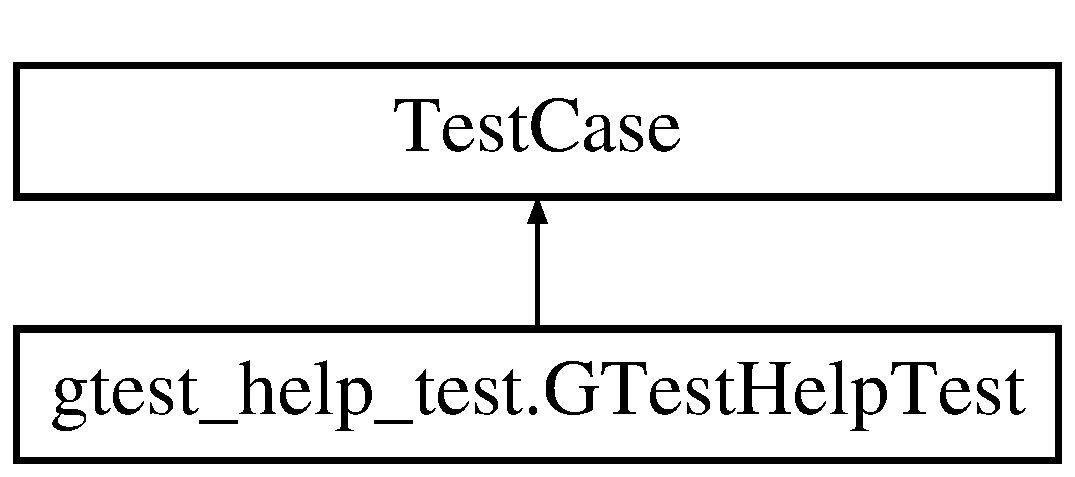
\includegraphics[height=2.000000cm]{classgtest__help__test_1_1_g_test_help_test}
\end{center}
\end{figure}
\subsection*{Public Member Functions}
\begin{DoxyCompactItemize}
\item 
def \hyperlink{classgtest__help__test_1_1_g_test_help_test_a26cc1a64bd67278252ebfcd0ac0dca0c}{Test\+Help\+Flag} (self, flag)
\item 
def \hyperlink{classgtest__help__test_1_1_g_test_help_test_a03ffa91ecf6193ed2ed80b53933112ab}{Test\+Non\+Help\+Flag} (self, flag)
\item 
def \hyperlink{classgtest__help__test_1_1_g_test_help_test_ad91b46ad4506ff52b337b63f6b6c2ad1}{test\+Prints\+Help\+With\+Full\+Flag} (self)
\item 
def \hyperlink{classgtest__help__test_1_1_g_test_help_test_a3dd96058d093a89350769b4e2cc36563}{test\+Prints\+Help\+With\+Short\+Flag} (self)
\item 
def \hyperlink{classgtest__help__test_1_1_g_test_help_test_aafd4d1857c2538c8b1f7cc5a5d1e38b4}{test\+Prints\+Help\+With\+Question\+Flag} (self)
\item 
def \hyperlink{classgtest__help__test_1_1_g_test_help_test_a7be99cd30193e2eecf79f9d65f561afc}{test\+Prints\+Help\+With\+Windows\+Style\+Question\+Flag} (self)
\item 
def \hyperlink{classgtest__help__test_1_1_g_test_help_test_a701abb8f34df726b9129d7654cb32066}{test\+Prints\+Help\+With\+Unrecognized\+Google\+Test\+Flag} (self)
\item 
def \hyperlink{classgtest__help__test_1_1_g_test_help_test_ab8d379bbb0da7403ced599f4ee498728}{test\+Prints\+Help\+With\+Incorrect\+Flag\+Style} (self)
\item 
def \hyperlink{classgtest__help__test_1_1_g_test_help_test_ae7831f92e8e3763c07afb908915b3d20}{test\+Runs\+Tests\+Without\+Help\+Flag} (self)
\item 
def \hyperlink{classgtest__help__test_1_1_g_test_help_test_a0ebec2e3154d22a63e362d2196f9c638}{test\+Runs\+Tests\+With\+Gtest\+Internal\+Flag} (self)
\end{DoxyCompactItemize}


\subsection{Detailed Description}
\begin{DoxyVerb}Tests the --help flag and its equivalent forms.\end{DoxyVerb}
 

\subsection{Member Function Documentation}
\hypertarget{classgtest__help__test_1_1_g_test_help_test_a26cc1a64bd67278252ebfcd0ac0dca0c}{}\index{gtest\+\_\+help\+\_\+test\+::\+G\+Test\+Help\+Test@{gtest\+\_\+help\+\_\+test\+::\+G\+Test\+Help\+Test}!Test\+Help\+Flag@{Test\+Help\+Flag}}
\index{Test\+Help\+Flag@{Test\+Help\+Flag}!gtest\+\_\+help\+\_\+test\+::\+G\+Test\+Help\+Test@{gtest\+\_\+help\+\_\+test\+::\+G\+Test\+Help\+Test}}
\subsubsection[{Test\+Help\+Flag(self, flag)}]{\setlength{\rightskip}{0pt plus 5cm}def gtest\+\_\+help\+\_\+test.\+G\+Test\+Help\+Test.\+Test\+Help\+Flag (
\begin{DoxyParamCaption}
\item[{}]{self, }
\item[{}]{flag}
\end{DoxyParamCaption}
)}\label{classgtest__help__test_1_1_g_test_help_test_a26cc1a64bd67278252ebfcd0ac0dca0c}
\begin{DoxyVerb}Verifies correct behavior when help flag is specified.

The right message must be printed and the tests must
skipped when the given flag is specified.

Args:
  flag:  A flag to pass to the binary or None.
\end{DoxyVerb}
 \hypertarget{classgtest__help__test_1_1_g_test_help_test_a03ffa91ecf6193ed2ed80b53933112ab}{}\index{gtest\+\_\+help\+\_\+test\+::\+G\+Test\+Help\+Test@{gtest\+\_\+help\+\_\+test\+::\+G\+Test\+Help\+Test}!Test\+Non\+Help\+Flag@{Test\+Non\+Help\+Flag}}
\index{Test\+Non\+Help\+Flag@{Test\+Non\+Help\+Flag}!gtest\+\_\+help\+\_\+test\+::\+G\+Test\+Help\+Test@{gtest\+\_\+help\+\_\+test\+::\+G\+Test\+Help\+Test}}
\subsubsection[{Test\+Non\+Help\+Flag(self, flag)}]{\setlength{\rightskip}{0pt plus 5cm}def gtest\+\_\+help\+\_\+test.\+G\+Test\+Help\+Test.\+Test\+Non\+Help\+Flag (
\begin{DoxyParamCaption}
\item[{}]{self, }
\item[{}]{flag}
\end{DoxyParamCaption}
)}\label{classgtest__help__test_1_1_g_test_help_test_a03ffa91ecf6193ed2ed80b53933112ab}
\begin{DoxyVerb}Verifies correct behavior when no help flag is specified.

Verifies that when no help flag is specified, the tests are run
and the help message is not printed.

Args:
  flag:  A flag to pass to the binary or None.
\end{DoxyVerb}
 \hypertarget{classgtest__help__test_1_1_g_test_help_test_ad91b46ad4506ff52b337b63f6b6c2ad1}{}\index{gtest\+\_\+help\+\_\+test\+::\+G\+Test\+Help\+Test@{gtest\+\_\+help\+\_\+test\+::\+G\+Test\+Help\+Test}!test\+Prints\+Help\+With\+Full\+Flag@{test\+Prints\+Help\+With\+Full\+Flag}}
\index{test\+Prints\+Help\+With\+Full\+Flag@{test\+Prints\+Help\+With\+Full\+Flag}!gtest\+\_\+help\+\_\+test\+::\+G\+Test\+Help\+Test@{gtest\+\_\+help\+\_\+test\+::\+G\+Test\+Help\+Test}}
\subsubsection[{test\+Prints\+Help\+With\+Full\+Flag(self)}]{\setlength{\rightskip}{0pt plus 5cm}def gtest\+\_\+help\+\_\+test.\+G\+Test\+Help\+Test.\+test\+Prints\+Help\+With\+Full\+Flag (
\begin{DoxyParamCaption}
\item[{}]{self}
\end{DoxyParamCaption}
)}\label{classgtest__help__test_1_1_g_test_help_test_ad91b46ad4506ff52b337b63f6b6c2ad1}
\hypertarget{classgtest__help__test_1_1_g_test_help_test_ab8d379bbb0da7403ced599f4ee498728}{}\index{gtest\+\_\+help\+\_\+test\+::\+G\+Test\+Help\+Test@{gtest\+\_\+help\+\_\+test\+::\+G\+Test\+Help\+Test}!test\+Prints\+Help\+With\+Incorrect\+Flag\+Style@{test\+Prints\+Help\+With\+Incorrect\+Flag\+Style}}
\index{test\+Prints\+Help\+With\+Incorrect\+Flag\+Style@{test\+Prints\+Help\+With\+Incorrect\+Flag\+Style}!gtest\+\_\+help\+\_\+test\+::\+G\+Test\+Help\+Test@{gtest\+\_\+help\+\_\+test\+::\+G\+Test\+Help\+Test}}
\subsubsection[{test\+Prints\+Help\+With\+Incorrect\+Flag\+Style(self)}]{\setlength{\rightskip}{0pt plus 5cm}def gtest\+\_\+help\+\_\+test.\+G\+Test\+Help\+Test.\+test\+Prints\+Help\+With\+Incorrect\+Flag\+Style (
\begin{DoxyParamCaption}
\item[{}]{self}
\end{DoxyParamCaption}
)}\label{classgtest__help__test_1_1_g_test_help_test_ab8d379bbb0da7403ced599f4ee498728}
\hypertarget{classgtest__help__test_1_1_g_test_help_test_aafd4d1857c2538c8b1f7cc5a5d1e38b4}{}\index{gtest\+\_\+help\+\_\+test\+::\+G\+Test\+Help\+Test@{gtest\+\_\+help\+\_\+test\+::\+G\+Test\+Help\+Test}!test\+Prints\+Help\+With\+Question\+Flag@{test\+Prints\+Help\+With\+Question\+Flag}}
\index{test\+Prints\+Help\+With\+Question\+Flag@{test\+Prints\+Help\+With\+Question\+Flag}!gtest\+\_\+help\+\_\+test\+::\+G\+Test\+Help\+Test@{gtest\+\_\+help\+\_\+test\+::\+G\+Test\+Help\+Test}}
\subsubsection[{test\+Prints\+Help\+With\+Question\+Flag(self)}]{\setlength{\rightskip}{0pt plus 5cm}def gtest\+\_\+help\+\_\+test.\+G\+Test\+Help\+Test.\+test\+Prints\+Help\+With\+Question\+Flag (
\begin{DoxyParamCaption}
\item[{}]{self}
\end{DoxyParamCaption}
)}\label{classgtest__help__test_1_1_g_test_help_test_aafd4d1857c2538c8b1f7cc5a5d1e38b4}
\hypertarget{classgtest__help__test_1_1_g_test_help_test_a3dd96058d093a89350769b4e2cc36563}{}\index{gtest\+\_\+help\+\_\+test\+::\+G\+Test\+Help\+Test@{gtest\+\_\+help\+\_\+test\+::\+G\+Test\+Help\+Test}!test\+Prints\+Help\+With\+Short\+Flag@{test\+Prints\+Help\+With\+Short\+Flag}}
\index{test\+Prints\+Help\+With\+Short\+Flag@{test\+Prints\+Help\+With\+Short\+Flag}!gtest\+\_\+help\+\_\+test\+::\+G\+Test\+Help\+Test@{gtest\+\_\+help\+\_\+test\+::\+G\+Test\+Help\+Test}}
\subsubsection[{test\+Prints\+Help\+With\+Short\+Flag(self)}]{\setlength{\rightskip}{0pt plus 5cm}def gtest\+\_\+help\+\_\+test.\+G\+Test\+Help\+Test.\+test\+Prints\+Help\+With\+Short\+Flag (
\begin{DoxyParamCaption}
\item[{}]{self}
\end{DoxyParamCaption}
)}\label{classgtest__help__test_1_1_g_test_help_test_a3dd96058d093a89350769b4e2cc36563}
\hypertarget{classgtest__help__test_1_1_g_test_help_test_a701abb8f34df726b9129d7654cb32066}{}\index{gtest\+\_\+help\+\_\+test\+::\+G\+Test\+Help\+Test@{gtest\+\_\+help\+\_\+test\+::\+G\+Test\+Help\+Test}!test\+Prints\+Help\+With\+Unrecognized\+Google\+Test\+Flag@{test\+Prints\+Help\+With\+Unrecognized\+Google\+Test\+Flag}}
\index{test\+Prints\+Help\+With\+Unrecognized\+Google\+Test\+Flag@{test\+Prints\+Help\+With\+Unrecognized\+Google\+Test\+Flag}!gtest\+\_\+help\+\_\+test\+::\+G\+Test\+Help\+Test@{gtest\+\_\+help\+\_\+test\+::\+G\+Test\+Help\+Test}}
\subsubsection[{test\+Prints\+Help\+With\+Unrecognized\+Google\+Test\+Flag(self)}]{\setlength{\rightskip}{0pt plus 5cm}def gtest\+\_\+help\+\_\+test.\+G\+Test\+Help\+Test.\+test\+Prints\+Help\+With\+Unrecognized\+Google\+Test\+Flag (
\begin{DoxyParamCaption}
\item[{}]{self}
\end{DoxyParamCaption}
)}\label{classgtest__help__test_1_1_g_test_help_test_a701abb8f34df726b9129d7654cb32066}
\hypertarget{classgtest__help__test_1_1_g_test_help_test_a7be99cd30193e2eecf79f9d65f561afc}{}\index{gtest\+\_\+help\+\_\+test\+::\+G\+Test\+Help\+Test@{gtest\+\_\+help\+\_\+test\+::\+G\+Test\+Help\+Test}!test\+Prints\+Help\+With\+Windows\+Style\+Question\+Flag@{test\+Prints\+Help\+With\+Windows\+Style\+Question\+Flag}}
\index{test\+Prints\+Help\+With\+Windows\+Style\+Question\+Flag@{test\+Prints\+Help\+With\+Windows\+Style\+Question\+Flag}!gtest\+\_\+help\+\_\+test\+::\+G\+Test\+Help\+Test@{gtest\+\_\+help\+\_\+test\+::\+G\+Test\+Help\+Test}}
\subsubsection[{test\+Prints\+Help\+With\+Windows\+Style\+Question\+Flag(self)}]{\setlength{\rightskip}{0pt plus 5cm}def gtest\+\_\+help\+\_\+test.\+G\+Test\+Help\+Test.\+test\+Prints\+Help\+With\+Windows\+Style\+Question\+Flag (
\begin{DoxyParamCaption}
\item[{}]{self}
\end{DoxyParamCaption}
)}\label{classgtest__help__test_1_1_g_test_help_test_a7be99cd30193e2eecf79f9d65f561afc}
\hypertarget{classgtest__help__test_1_1_g_test_help_test_a0ebec2e3154d22a63e362d2196f9c638}{}\index{gtest\+\_\+help\+\_\+test\+::\+G\+Test\+Help\+Test@{gtest\+\_\+help\+\_\+test\+::\+G\+Test\+Help\+Test}!test\+Runs\+Tests\+With\+Gtest\+Internal\+Flag@{test\+Runs\+Tests\+With\+Gtest\+Internal\+Flag}}
\index{test\+Runs\+Tests\+With\+Gtest\+Internal\+Flag@{test\+Runs\+Tests\+With\+Gtest\+Internal\+Flag}!gtest\+\_\+help\+\_\+test\+::\+G\+Test\+Help\+Test@{gtest\+\_\+help\+\_\+test\+::\+G\+Test\+Help\+Test}}
\subsubsection[{test\+Runs\+Tests\+With\+Gtest\+Internal\+Flag(self)}]{\setlength{\rightskip}{0pt plus 5cm}def gtest\+\_\+help\+\_\+test.\+G\+Test\+Help\+Test.\+test\+Runs\+Tests\+With\+Gtest\+Internal\+Flag (
\begin{DoxyParamCaption}
\item[{}]{self}
\end{DoxyParamCaption}
)}\label{classgtest__help__test_1_1_g_test_help_test_a0ebec2e3154d22a63e362d2196f9c638}
\begin{DoxyVerb}Verifies that the tests are run and no help message is printed when
a flag starting with Google Test prefix and 'internal_' is supplied.\end{DoxyVerb}
 \hypertarget{classgtest__help__test_1_1_g_test_help_test_ae7831f92e8e3763c07afb908915b3d20}{}\index{gtest\+\_\+help\+\_\+test\+::\+G\+Test\+Help\+Test@{gtest\+\_\+help\+\_\+test\+::\+G\+Test\+Help\+Test}!test\+Runs\+Tests\+Without\+Help\+Flag@{test\+Runs\+Tests\+Without\+Help\+Flag}}
\index{test\+Runs\+Tests\+Without\+Help\+Flag@{test\+Runs\+Tests\+Without\+Help\+Flag}!gtest\+\_\+help\+\_\+test\+::\+G\+Test\+Help\+Test@{gtest\+\_\+help\+\_\+test\+::\+G\+Test\+Help\+Test}}
\subsubsection[{test\+Runs\+Tests\+Without\+Help\+Flag(self)}]{\setlength{\rightskip}{0pt plus 5cm}def gtest\+\_\+help\+\_\+test.\+G\+Test\+Help\+Test.\+test\+Runs\+Tests\+Without\+Help\+Flag (
\begin{DoxyParamCaption}
\item[{}]{self}
\end{DoxyParamCaption}
)}\label{classgtest__help__test_1_1_g_test_help_test_ae7831f92e8e3763c07afb908915b3d20}
\begin{DoxyVerb}Verifies that when no help flag is specified, the tests are run
and the help message is not printed.\end{DoxyVerb}
 

The documentation for this class was generated from the following file\+:\begin{DoxyCompactItemize}
\item 
C\+:/\+Users/\+Hilman/\+Desktop/repo/anjing/src/third\+\_\+party/googletest/test/\hyperlink{gtest__help__test_8py}{gtest\+\_\+help\+\_\+test.\+py}\end{DoxyCompactItemize}

\hypertarget{classgtest__list__tests__unittest_1_1_g_test_list_tests_unit_test}{}\section{gtest\+\_\+list\+\_\+tests\+\_\+unittest.\+G\+Test\+List\+Tests\+Unit\+Test Class Reference}
\label{classgtest__list__tests__unittest_1_1_g_test_list_tests_unit_test}\index{gtest\+\_\+list\+\_\+tests\+\_\+unittest.\+G\+Test\+List\+Tests\+Unit\+Test@{gtest\+\_\+list\+\_\+tests\+\_\+unittest.\+G\+Test\+List\+Tests\+Unit\+Test}}
Inheritance diagram for gtest\+\_\+list\+\_\+tests\+\_\+unittest.\+G\+Test\+List\+Tests\+Unit\+Test\+:\begin{figure}[H]
\begin{center}
\leavevmode
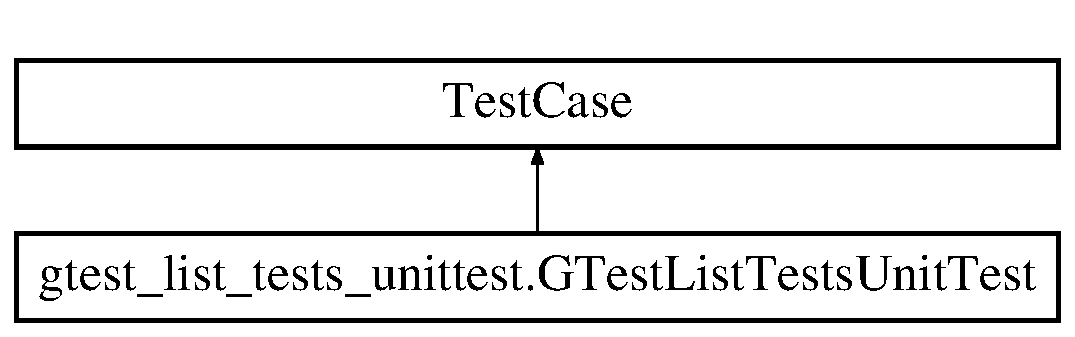
\includegraphics[height=2.000000cm]{classgtest__list__tests__unittest_1_1_g_test_list_tests_unit_test}
\end{center}
\end{figure}
\subsection*{Public Member Functions}
\begin{DoxyCompactItemize}
\item 
def \hyperlink{classgtest__list__tests__unittest_1_1_g_test_list_tests_unit_test_a965601cd1882fdeca94d2461bd033c40}{Run\+And\+Verify} (self, flag\+\_\+value, expected\+\_\+output\+\_\+re, other\+\_\+flag)
\item 
def \hyperlink{classgtest__list__tests__unittest_1_1_g_test_list_tests_unit_test_a4168d086b7ec31f86ab548b6fd79b27e}{test\+Default\+Behavior} (self)
\item 
def \hyperlink{classgtest__list__tests__unittest_1_1_g_test_list_tests_unit_test_a6d3e8738bd4b7494867cac464d342944}{test\+Flag} (self)
\item 
def \hyperlink{classgtest__list__tests__unittest_1_1_g_test_list_tests_unit_test_ae1ccba3f21c8e25968834607f7db2b10}{test\+Override\+Non\+Filter\+Flags} (self)
\item 
def \hyperlink{classgtest__list__tests__unittest_1_1_g_test_list_tests_unit_test_ac5bef6c9fb78b8eef84427de811fd70f}{test\+With\+Filter\+Flags} (self)
\end{DoxyCompactItemize}


\subsection{Detailed Description}
\begin{DoxyVerb}Tests using the --gtest_list_tests flag to list all tests.\end{DoxyVerb}
 

\subsection{Member Function Documentation}
\hypertarget{classgtest__list__tests__unittest_1_1_g_test_list_tests_unit_test_a965601cd1882fdeca94d2461bd033c40}{}\index{gtest\+\_\+list\+\_\+tests\+\_\+unittest\+::\+G\+Test\+List\+Tests\+Unit\+Test@{gtest\+\_\+list\+\_\+tests\+\_\+unittest\+::\+G\+Test\+List\+Tests\+Unit\+Test}!Run\+And\+Verify@{Run\+And\+Verify}}
\index{Run\+And\+Verify@{Run\+And\+Verify}!gtest\+\_\+list\+\_\+tests\+\_\+unittest\+::\+G\+Test\+List\+Tests\+Unit\+Test@{gtest\+\_\+list\+\_\+tests\+\_\+unittest\+::\+G\+Test\+List\+Tests\+Unit\+Test}}
\subsubsection[{Run\+And\+Verify(self, flag\+\_\+value, expected\+\_\+output\+\_\+re, other\+\_\+flag)}]{\setlength{\rightskip}{0pt plus 5cm}def gtest\+\_\+list\+\_\+tests\+\_\+unittest.\+G\+Test\+List\+Tests\+Unit\+Test.\+Run\+And\+Verify (
\begin{DoxyParamCaption}
\item[{}]{self, }
\item[{}]{flag\+\_\+value, }
\item[{}]{expected\+\_\+output\+\_\+re, }
\item[{}]{other\+\_\+flag}
\end{DoxyParamCaption}
)}\label{classgtest__list__tests__unittest_1_1_g_test_list_tests_unit_test_a965601cd1882fdeca94d2461bd033c40}
\begin{DoxyVerb}Runs gtest_list_tests_unittest_ and verifies that it prints
the correct tests.

Args:
  flag_value:         value of the --gtest_list_tests flag;
                  None if the flag should not be present.
  expected_output_re: regular expression that matches the expected
                  output after running command;
  other_flag:         a different flag to be passed to command
                  along with gtest_list_tests;
                  None if the flag should not be present.
\end{DoxyVerb}
 \hypertarget{classgtest__list__tests__unittest_1_1_g_test_list_tests_unit_test_a4168d086b7ec31f86ab548b6fd79b27e}{}\index{gtest\+\_\+list\+\_\+tests\+\_\+unittest\+::\+G\+Test\+List\+Tests\+Unit\+Test@{gtest\+\_\+list\+\_\+tests\+\_\+unittest\+::\+G\+Test\+List\+Tests\+Unit\+Test}!test\+Default\+Behavior@{test\+Default\+Behavior}}
\index{test\+Default\+Behavior@{test\+Default\+Behavior}!gtest\+\_\+list\+\_\+tests\+\_\+unittest\+::\+G\+Test\+List\+Tests\+Unit\+Test@{gtest\+\_\+list\+\_\+tests\+\_\+unittest\+::\+G\+Test\+List\+Tests\+Unit\+Test}}
\subsubsection[{test\+Default\+Behavior(self)}]{\setlength{\rightskip}{0pt plus 5cm}def gtest\+\_\+list\+\_\+tests\+\_\+unittest.\+G\+Test\+List\+Tests\+Unit\+Test.\+test\+Default\+Behavior (
\begin{DoxyParamCaption}
\item[{}]{self}
\end{DoxyParamCaption}
)}\label{classgtest__list__tests__unittest_1_1_g_test_list_tests_unit_test_a4168d086b7ec31f86ab548b6fd79b27e}
\begin{DoxyVerb}Tests the behavior of the default mode.\end{DoxyVerb}
 \hypertarget{classgtest__list__tests__unittest_1_1_g_test_list_tests_unit_test_a6d3e8738bd4b7494867cac464d342944}{}\index{gtest\+\_\+list\+\_\+tests\+\_\+unittest\+::\+G\+Test\+List\+Tests\+Unit\+Test@{gtest\+\_\+list\+\_\+tests\+\_\+unittest\+::\+G\+Test\+List\+Tests\+Unit\+Test}!test\+Flag@{test\+Flag}}
\index{test\+Flag@{test\+Flag}!gtest\+\_\+list\+\_\+tests\+\_\+unittest\+::\+G\+Test\+List\+Tests\+Unit\+Test@{gtest\+\_\+list\+\_\+tests\+\_\+unittest\+::\+G\+Test\+List\+Tests\+Unit\+Test}}
\subsubsection[{test\+Flag(self)}]{\setlength{\rightskip}{0pt plus 5cm}def gtest\+\_\+list\+\_\+tests\+\_\+unittest.\+G\+Test\+List\+Tests\+Unit\+Test.\+test\+Flag (
\begin{DoxyParamCaption}
\item[{}]{self}
\end{DoxyParamCaption}
)}\label{classgtest__list__tests__unittest_1_1_g_test_list_tests_unit_test_a6d3e8738bd4b7494867cac464d342944}
\begin{DoxyVerb}Tests using the --gtest_list_tests flag.\end{DoxyVerb}
 \hypertarget{classgtest__list__tests__unittest_1_1_g_test_list_tests_unit_test_ae1ccba3f21c8e25968834607f7db2b10}{}\index{gtest\+\_\+list\+\_\+tests\+\_\+unittest\+::\+G\+Test\+List\+Tests\+Unit\+Test@{gtest\+\_\+list\+\_\+tests\+\_\+unittest\+::\+G\+Test\+List\+Tests\+Unit\+Test}!test\+Override\+Non\+Filter\+Flags@{test\+Override\+Non\+Filter\+Flags}}
\index{test\+Override\+Non\+Filter\+Flags@{test\+Override\+Non\+Filter\+Flags}!gtest\+\_\+list\+\_\+tests\+\_\+unittest\+::\+G\+Test\+List\+Tests\+Unit\+Test@{gtest\+\_\+list\+\_\+tests\+\_\+unittest\+::\+G\+Test\+List\+Tests\+Unit\+Test}}
\subsubsection[{test\+Override\+Non\+Filter\+Flags(self)}]{\setlength{\rightskip}{0pt plus 5cm}def gtest\+\_\+list\+\_\+tests\+\_\+unittest.\+G\+Test\+List\+Tests\+Unit\+Test.\+test\+Override\+Non\+Filter\+Flags (
\begin{DoxyParamCaption}
\item[{}]{self}
\end{DoxyParamCaption}
)}\label{classgtest__list__tests__unittest_1_1_g_test_list_tests_unit_test_ae1ccba3f21c8e25968834607f7db2b10}
\begin{DoxyVerb}Tests that --gtest_list_tests overrides the non-filter flags.\end{DoxyVerb}
 \hypertarget{classgtest__list__tests__unittest_1_1_g_test_list_tests_unit_test_ac5bef6c9fb78b8eef84427de811fd70f}{}\index{gtest\+\_\+list\+\_\+tests\+\_\+unittest\+::\+G\+Test\+List\+Tests\+Unit\+Test@{gtest\+\_\+list\+\_\+tests\+\_\+unittest\+::\+G\+Test\+List\+Tests\+Unit\+Test}!test\+With\+Filter\+Flags@{test\+With\+Filter\+Flags}}
\index{test\+With\+Filter\+Flags@{test\+With\+Filter\+Flags}!gtest\+\_\+list\+\_\+tests\+\_\+unittest\+::\+G\+Test\+List\+Tests\+Unit\+Test@{gtest\+\_\+list\+\_\+tests\+\_\+unittest\+::\+G\+Test\+List\+Tests\+Unit\+Test}}
\subsubsection[{test\+With\+Filter\+Flags(self)}]{\setlength{\rightskip}{0pt plus 5cm}def gtest\+\_\+list\+\_\+tests\+\_\+unittest.\+G\+Test\+List\+Tests\+Unit\+Test.\+test\+With\+Filter\+Flags (
\begin{DoxyParamCaption}
\item[{}]{self}
\end{DoxyParamCaption}
)}\label{classgtest__list__tests__unittest_1_1_g_test_list_tests_unit_test_ac5bef6c9fb78b8eef84427de811fd70f}
\begin{DoxyVerb}Tests that --gtest_list_tests takes into account the
--gtest_filter flag.\end{DoxyVerb}
 

The documentation for this class was generated from the following file\+:\begin{DoxyCompactItemize}
\item 
C\+:/\+Users/\+Hilman/\+Desktop/repo/anjing/src/third\+\_\+party/googletest/test/\hyperlink{gtest__list__tests__unittest_8py}{gtest\+\_\+list\+\_\+tests\+\_\+unittest.\+py}\end{DoxyCompactItemize}

\hypertarget{classtesting_1_1internal_1_1_g_test_log}{}\section{testing\+:\+:internal\+:\+:G\+Test\+Log Class Reference}
\label{classtesting_1_1internal_1_1_g_test_log}\index{testing\+::internal\+::\+G\+Test\+Log@{testing\+::internal\+::\+G\+Test\+Log}}


{\ttfamily \#include $<$gtest-\/port.\+h$>$}

\subsection*{Public Member Functions}
\begin{DoxyCompactItemize}
\item 
\hyperlink{classtesting_1_1internal_1_1_g_test_log_a364691bf972983a59cfa2891062a64af}{G\+Test\+Log} (\hyperlink{namespacetesting_1_1internal_aa6255ef3b023c5b4e1a2198d887fb977}{G\+Test\+Log\+Severity} severity, const char $\ast$file, int line)
\item 
\hyperlink{classtesting_1_1internal_1_1_g_test_log_a978a099703bbaa0f380216e8d7ee03d3}{$\sim$\+G\+Test\+Log} ()
\item 
\+::std\+::ostream \& \hyperlink{classtesting_1_1internal_1_1_g_test_log_aebb92e67d98eca69f0347d5121dab27a}{Get\+Stream} ()
\end{DoxyCompactItemize}


\subsection{Constructor \& Destructor Documentation}
\hypertarget{classtesting_1_1internal_1_1_g_test_log_a364691bf972983a59cfa2891062a64af}{}\index{testing\+::internal\+::\+G\+Test\+Log@{testing\+::internal\+::\+G\+Test\+Log}!G\+Test\+Log@{G\+Test\+Log}}
\index{G\+Test\+Log@{G\+Test\+Log}!testing\+::internal\+::\+G\+Test\+Log@{testing\+::internal\+::\+G\+Test\+Log}}
\subsubsection[{G\+Test\+Log(\+G\+Test\+Log\+Severity severity, const char $\ast$file, int line)}]{\setlength{\rightskip}{0pt plus 5cm}testing\+::internal\+::\+G\+Test\+Log\+::\+G\+Test\+Log (
\begin{DoxyParamCaption}
\item[{{\bf G\+Test\+Log\+Severity}}]{severity, }
\item[{const char $\ast$}]{file, }
\item[{int}]{line}
\end{DoxyParamCaption}
)}\label{classtesting_1_1internal_1_1_g_test_log_a364691bf972983a59cfa2891062a64af}
\hypertarget{classtesting_1_1internal_1_1_g_test_log_a978a099703bbaa0f380216e8d7ee03d3}{}\index{testing\+::internal\+::\+G\+Test\+Log@{testing\+::internal\+::\+G\+Test\+Log}!````~G\+Test\+Log@{$\sim$\+G\+Test\+Log}}
\index{````~G\+Test\+Log@{$\sim$\+G\+Test\+Log}!testing\+::internal\+::\+G\+Test\+Log@{testing\+::internal\+::\+G\+Test\+Log}}
\subsubsection[{$\sim$\+G\+Test\+Log()}]{\setlength{\rightskip}{0pt plus 5cm}testing\+::internal\+::\+G\+Test\+Log\+::$\sim$\+G\+Test\+Log (
\begin{DoxyParamCaption}
{}
\end{DoxyParamCaption}
)}\label{classtesting_1_1internal_1_1_g_test_log_a978a099703bbaa0f380216e8d7ee03d3}


\subsection{Member Function Documentation}
\hypertarget{classtesting_1_1internal_1_1_g_test_log_aebb92e67d98eca69f0347d5121dab27a}{}\index{testing\+::internal\+::\+G\+Test\+Log@{testing\+::internal\+::\+G\+Test\+Log}!Get\+Stream@{Get\+Stream}}
\index{Get\+Stream@{Get\+Stream}!testing\+::internal\+::\+G\+Test\+Log@{testing\+::internal\+::\+G\+Test\+Log}}
\subsubsection[{Get\+Stream()}]{\setlength{\rightskip}{0pt plus 5cm}\+::std\+::ostream\& testing\+::internal\+::\+G\+Test\+Log\+::\+Get\+Stream (
\begin{DoxyParamCaption}
{}
\end{DoxyParamCaption}
)\hspace{0.3cm}{\ttfamily [inline]}}\label{classtesting_1_1internal_1_1_g_test_log_aebb92e67d98eca69f0347d5121dab27a}


The documentation for this class was generated from the following files\+:\begin{DoxyCompactItemize}
\item 
C\+:/\+Users/\+Hilman/\+Desktop/repo/anjing/src/third\+\_\+party/googletest/include/gtest/internal/\hyperlink{gtest-port_8h}{gtest-\/port.\+h}\item 
C\+:/\+Users/\+Hilman/\+Desktop/repo/anjing/src/third\+\_\+party/googletest/src/\hyperlink{gtest-port_8cc}{gtest-\/port.\+cc}\end{DoxyCompactItemize}

\hypertarget{classtesting_1_1internal_1_1_g_test_mutex_lock}{}\section{testing\+:\+:internal\+:\+:G\+Test\+Mutex\+Lock Class Reference}
\label{classtesting_1_1internal_1_1_g_test_mutex_lock}\index{testing\+::internal\+::\+G\+Test\+Mutex\+Lock@{testing\+::internal\+::\+G\+Test\+Mutex\+Lock}}


{\ttfamily \#include $<$gtest-\/port.\+h$>$}

\subsection*{Public Member Functions}
\begin{DoxyCompactItemize}
\item 
\hyperlink{classtesting_1_1internal_1_1_g_test_mutex_lock_a77e3cba326d5356b4a1dea3790559c26}{G\+Test\+Mutex\+Lock} (\hyperlink{classtesting_1_1internal_1_1_mutex}{Mutex} $\ast$)
\end{DoxyCompactItemize}


\subsection{Constructor \& Destructor Documentation}
\hypertarget{classtesting_1_1internal_1_1_g_test_mutex_lock_a77e3cba326d5356b4a1dea3790559c26}{}\index{testing\+::internal\+::\+G\+Test\+Mutex\+Lock@{testing\+::internal\+::\+G\+Test\+Mutex\+Lock}!G\+Test\+Mutex\+Lock@{G\+Test\+Mutex\+Lock}}
\index{G\+Test\+Mutex\+Lock@{G\+Test\+Mutex\+Lock}!testing\+::internal\+::\+G\+Test\+Mutex\+Lock@{testing\+::internal\+::\+G\+Test\+Mutex\+Lock}}
\subsubsection[{G\+Test\+Mutex\+Lock(\+Mutex $\ast$)}]{\setlength{\rightskip}{0pt plus 5cm}testing\+::internal\+::\+G\+Test\+Mutex\+Lock\+::\+G\+Test\+Mutex\+Lock (
\begin{DoxyParamCaption}
\item[{{\bf Mutex} $\ast$}]{}
\end{DoxyParamCaption}
)\hspace{0.3cm}{\ttfamily [inline]}, {\ttfamily [explicit]}}\label{classtesting_1_1internal_1_1_g_test_mutex_lock_a77e3cba326d5356b4a1dea3790559c26}


The documentation for this class was generated from the following file\+:\begin{DoxyCompactItemize}
\item 
C\+:/\+Users/\+Hilman/\+Desktop/repo/anjing/src/third\+\_\+party/googletest/include/gtest/internal/\hyperlink{gtest-port_8h}{gtest-\/port.\+h}\end{DoxyCompactItemize}

\hypertarget{classgtest__output__test_1_1_g_test_output_test}{}\section{gtest\+\_\+output\+\_\+test.\+G\+Test\+Output\+Test Class Reference}
\label{classgtest__output__test_1_1_g_test_output_test}\index{gtest\+\_\+output\+\_\+test.\+G\+Test\+Output\+Test@{gtest\+\_\+output\+\_\+test.\+G\+Test\+Output\+Test}}
Inheritance diagram for gtest\+\_\+output\+\_\+test.\+G\+Test\+Output\+Test\+:\begin{figure}[H]
\begin{center}
\leavevmode
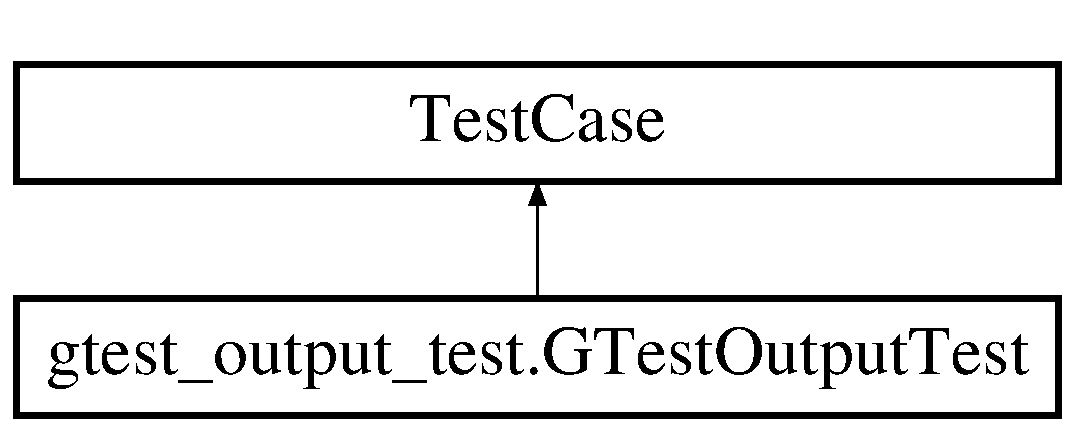
\includegraphics[height=2.000000cm]{classgtest__output__test_1_1_g_test_output_test}
\end{center}
\end{figure}
\subsection*{Public Member Functions}
\begin{DoxyCompactItemize}
\item 
def \hyperlink{classgtest__output__test_1_1_g_test_output_test_a63f62268f795adfc5ca91514dbec2873}{Remove\+Unsupported\+Tests} (self, test\+\_\+output)
\item 
def \hyperlink{classgtest__output__test_1_1_g_test_output_test_a1e6b96f68c5bcb8271de3208fa7f9f64}{test\+Output} (self)
\end{DoxyCompactItemize}


\subsection{Member Function Documentation}
\hypertarget{classgtest__output__test_1_1_g_test_output_test_a63f62268f795adfc5ca91514dbec2873}{}\index{gtest\+\_\+output\+\_\+test\+::\+G\+Test\+Output\+Test@{gtest\+\_\+output\+\_\+test\+::\+G\+Test\+Output\+Test}!Remove\+Unsupported\+Tests@{Remove\+Unsupported\+Tests}}
\index{Remove\+Unsupported\+Tests@{Remove\+Unsupported\+Tests}!gtest\+\_\+output\+\_\+test\+::\+G\+Test\+Output\+Test@{gtest\+\_\+output\+\_\+test\+::\+G\+Test\+Output\+Test}}
\subsubsection[{Remove\+Unsupported\+Tests(self, test\+\_\+output)}]{\setlength{\rightskip}{0pt plus 5cm}def gtest\+\_\+output\+\_\+test.\+G\+Test\+Output\+Test.\+Remove\+Unsupported\+Tests (
\begin{DoxyParamCaption}
\item[{}]{self, }
\item[{}]{test\+\_\+output}
\end{DoxyParamCaption}
)}\label{classgtest__output__test_1_1_g_test_output_test_a63f62268f795adfc5ca91514dbec2873}
\hypertarget{classgtest__output__test_1_1_g_test_output_test_a1e6b96f68c5bcb8271de3208fa7f9f64}{}\index{gtest\+\_\+output\+\_\+test\+::\+G\+Test\+Output\+Test@{gtest\+\_\+output\+\_\+test\+::\+G\+Test\+Output\+Test}!test\+Output@{test\+Output}}
\index{test\+Output@{test\+Output}!gtest\+\_\+output\+\_\+test\+::\+G\+Test\+Output\+Test@{gtest\+\_\+output\+\_\+test\+::\+G\+Test\+Output\+Test}}
\subsubsection[{test\+Output(self)}]{\setlength{\rightskip}{0pt plus 5cm}def gtest\+\_\+output\+\_\+test.\+G\+Test\+Output\+Test.\+test\+Output (
\begin{DoxyParamCaption}
\item[{}]{self}
\end{DoxyParamCaption}
)}\label{classgtest__output__test_1_1_g_test_output_test_a1e6b96f68c5bcb8271de3208fa7f9f64}


The documentation for this class was generated from the following file\+:\begin{DoxyCompactItemize}
\item 
C\+:/\+Users/\+Hilman/\+Desktop/repo/anjing/src/third\+\_\+party/googletest/test/\hyperlink{gtest__output__test_8py}{gtest\+\_\+output\+\_\+test.\+py}\end{DoxyCompactItemize}

\hypertarget{classgtest__shuffle__test_1_1_g_test_shuffle_unit_test}{}\section{gtest\+\_\+shuffle\+\_\+test.\+G\+Test\+Shuffle\+Unit\+Test Class Reference}
\label{classgtest__shuffle__test_1_1_g_test_shuffle_unit_test}\index{gtest\+\_\+shuffle\+\_\+test.\+G\+Test\+Shuffle\+Unit\+Test@{gtest\+\_\+shuffle\+\_\+test.\+G\+Test\+Shuffle\+Unit\+Test}}
Inheritance diagram for gtest\+\_\+shuffle\+\_\+test.\+G\+Test\+Shuffle\+Unit\+Test\+:\begin{figure}[H]
\begin{center}
\leavevmode
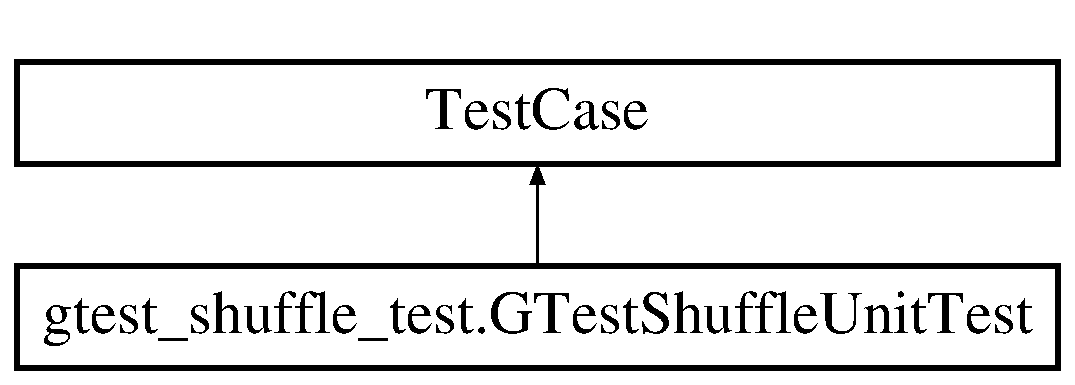
\includegraphics[height=2.000000cm]{classgtest__shuffle__test_1_1_g_test_shuffle_unit_test}
\end{center}
\end{figure}
\subsection*{Public Member Functions}
\begin{DoxyCompactItemize}
\item 
def \hyperlink{classgtest__shuffle__test_1_1_g_test_shuffle_unit_test_adf9841ae9c86eaafc3c3f7c9690c7bd8}{set\+Up} (self)
\item 
def \hyperlink{classgtest__shuffle__test_1_1_g_test_shuffle_unit_test_aafc33d6129c37043ef5c95dbe766a8db}{test\+Shuffle\+Preserves\+Number\+Of\+Tests} (self)
\item 
def \hyperlink{classgtest__shuffle__test_1_1_g_test_shuffle_unit_test_a0ba25ee553b62281e16b6a28873abc01}{test\+Shuffle\+Changes\+Test\+Order} (self)
\item 
def \hyperlink{classgtest__shuffle__test_1_1_g_test_shuffle_unit_test_a8a82320ea310d1e3660bef2efb665bd2}{test\+Shuffle\+Changes\+Test\+Case\+Order} (self)
\item 
def \hyperlink{classgtest__shuffle__test_1_1_g_test_shuffle_unit_test_a7537baa50e9e14b430fb80eaf4ea18f6}{test\+Shuffle\+Does\+Not\+Repeat\+Test} (self)
\item 
def \hyperlink{classgtest__shuffle__test_1_1_g_test_shuffle_unit_test_aeea745f7ce2ab19a067c5cde6e083ba7}{test\+Shuffle\+Does\+Not\+Create\+New\+Test} (self)
\item 
def \hyperlink{classgtest__shuffle__test_1_1_g_test_shuffle_unit_test_ab9e25e62817f7cdbd32833f9b2be5794}{test\+Shuffle\+Includes\+All\+Tests} (self)
\item 
def \hyperlink{classgtest__shuffle__test_1_1_g_test_shuffle_unit_test_a6fa91b262595e35bd3e9b52e188dc634}{test\+Shuffle\+Leaves\+Death\+Tests\+At\+Front} (self)
\item 
def \hyperlink{classgtest__shuffle__test_1_1_g_test_shuffle_unit_test_a34bfc9696191f4c2782327e1e35ae902}{test\+Shuffle\+Does\+Not\+Interleave\+Test\+Cases} (self)
\item 
def \hyperlink{classgtest__shuffle__test_1_1_g_test_shuffle_unit_test_a77b83a9870ad8d68524e1177f5320fb0}{test\+Shuffle\+Restores\+Order\+After\+Each\+Iteration} (self)
\item 
def \hyperlink{classgtest__shuffle__test_1_1_g_test_shuffle_unit_test_ada78bae27e0d82d07bd663d53a36552b}{test\+Shuffle\+Generates\+New\+Order\+In\+Each\+Iteration} (self)
\item 
def \hyperlink{classgtest__shuffle__test_1_1_g_test_shuffle_unit_test_abd33c5ef01ce6d1d025ebcc816d47c19}{test\+Shuffle\+Sharded\+Tests\+Preserves\+Partition} (self)
\end{DoxyCompactItemize}


\subsection{Detailed Description}
\begin{DoxyVerb}Tests test shuffling.\end{DoxyVerb}
 

\subsection{Member Function Documentation}
\hypertarget{classgtest__shuffle__test_1_1_g_test_shuffle_unit_test_adf9841ae9c86eaafc3c3f7c9690c7bd8}{}\index{gtest\+\_\+shuffle\+\_\+test\+::\+G\+Test\+Shuffle\+Unit\+Test@{gtest\+\_\+shuffle\+\_\+test\+::\+G\+Test\+Shuffle\+Unit\+Test}!set\+Up@{set\+Up}}
\index{set\+Up@{set\+Up}!gtest\+\_\+shuffle\+\_\+test\+::\+G\+Test\+Shuffle\+Unit\+Test@{gtest\+\_\+shuffle\+\_\+test\+::\+G\+Test\+Shuffle\+Unit\+Test}}
\subsubsection[{set\+Up(self)}]{\setlength{\rightskip}{0pt plus 5cm}def gtest\+\_\+shuffle\+\_\+test.\+G\+Test\+Shuffle\+Unit\+Test.\+set\+Up (
\begin{DoxyParamCaption}
\item[{}]{self}
\end{DoxyParamCaption}
)}\label{classgtest__shuffle__test_1_1_g_test_shuffle_unit_test_adf9841ae9c86eaafc3c3f7c9690c7bd8}
\hypertarget{classgtest__shuffle__test_1_1_g_test_shuffle_unit_test_a8a82320ea310d1e3660bef2efb665bd2}{}\index{gtest\+\_\+shuffle\+\_\+test\+::\+G\+Test\+Shuffle\+Unit\+Test@{gtest\+\_\+shuffle\+\_\+test\+::\+G\+Test\+Shuffle\+Unit\+Test}!test\+Shuffle\+Changes\+Test\+Case\+Order@{test\+Shuffle\+Changes\+Test\+Case\+Order}}
\index{test\+Shuffle\+Changes\+Test\+Case\+Order@{test\+Shuffle\+Changes\+Test\+Case\+Order}!gtest\+\_\+shuffle\+\_\+test\+::\+G\+Test\+Shuffle\+Unit\+Test@{gtest\+\_\+shuffle\+\_\+test\+::\+G\+Test\+Shuffle\+Unit\+Test}}
\subsubsection[{test\+Shuffle\+Changes\+Test\+Case\+Order(self)}]{\setlength{\rightskip}{0pt plus 5cm}def gtest\+\_\+shuffle\+\_\+test.\+G\+Test\+Shuffle\+Unit\+Test.\+test\+Shuffle\+Changes\+Test\+Case\+Order (
\begin{DoxyParamCaption}
\item[{}]{self}
\end{DoxyParamCaption}
)}\label{classgtest__shuffle__test_1_1_g_test_shuffle_unit_test_a8a82320ea310d1e3660bef2efb665bd2}
\hypertarget{classgtest__shuffle__test_1_1_g_test_shuffle_unit_test_a0ba25ee553b62281e16b6a28873abc01}{}\index{gtest\+\_\+shuffle\+\_\+test\+::\+G\+Test\+Shuffle\+Unit\+Test@{gtest\+\_\+shuffle\+\_\+test\+::\+G\+Test\+Shuffle\+Unit\+Test}!test\+Shuffle\+Changes\+Test\+Order@{test\+Shuffle\+Changes\+Test\+Order}}
\index{test\+Shuffle\+Changes\+Test\+Order@{test\+Shuffle\+Changes\+Test\+Order}!gtest\+\_\+shuffle\+\_\+test\+::\+G\+Test\+Shuffle\+Unit\+Test@{gtest\+\_\+shuffle\+\_\+test\+::\+G\+Test\+Shuffle\+Unit\+Test}}
\subsubsection[{test\+Shuffle\+Changes\+Test\+Order(self)}]{\setlength{\rightskip}{0pt plus 5cm}def gtest\+\_\+shuffle\+\_\+test.\+G\+Test\+Shuffle\+Unit\+Test.\+test\+Shuffle\+Changes\+Test\+Order (
\begin{DoxyParamCaption}
\item[{}]{self}
\end{DoxyParamCaption}
)}\label{classgtest__shuffle__test_1_1_g_test_shuffle_unit_test_a0ba25ee553b62281e16b6a28873abc01}
\hypertarget{classgtest__shuffle__test_1_1_g_test_shuffle_unit_test_aeea745f7ce2ab19a067c5cde6e083ba7}{}\index{gtest\+\_\+shuffle\+\_\+test\+::\+G\+Test\+Shuffle\+Unit\+Test@{gtest\+\_\+shuffle\+\_\+test\+::\+G\+Test\+Shuffle\+Unit\+Test}!test\+Shuffle\+Does\+Not\+Create\+New\+Test@{test\+Shuffle\+Does\+Not\+Create\+New\+Test}}
\index{test\+Shuffle\+Does\+Not\+Create\+New\+Test@{test\+Shuffle\+Does\+Not\+Create\+New\+Test}!gtest\+\_\+shuffle\+\_\+test\+::\+G\+Test\+Shuffle\+Unit\+Test@{gtest\+\_\+shuffle\+\_\+test\+::\+G\+Test\+Shuffle\+Unit\+Test}}
\subsubsection[{test\+Shuffle\+Does\+Not\+Create\+New\+Test(self)}]{\setlength{\rightskip}{0pt plus 5cm}def gtest\+\_\+shuffle\+\_\+test.\+G\+Test\+Shuffle\+Unit\+Test.\+test\+Shuffle\+Does\+Not\+Create\+New\+Test (
\begin{DoxyParamCaption}
\item[{}]{self}
\end{DoxyParamCaption}
)}\label{classgtest__shuffle__test_1_1_g_test_shuffle_unit_test_aeea745f7ce2ab19a067c5cde6e083ba7}
\hypertarget{classgtest__shuffle__test_1_1_g_test_shuffle_unit_test_a34bfc9696191f4c2782327e1e35ae902}{}\index{gtest\+\_\+shuffle\+\_\+test\+::\+G\+Test\+Shuffle\+Unit\+Test@{gtest\+\_\+shuffle\+\_\+test\+::\+G\+Test\+Shuffle\+Unit\+Test}!test\+Shuffle\+Does\+Not\+Interleave\+Test\+Cases@{test\+Shuffle\+Does\+Not\+Interleave\+Test\+Cases}}
\index{test\+Shuffle\+Does\+Not\+Interleave\+Test\+Cases@{test\+Shuffle\+Does\+Not\+Interleave\+Test\+Cases}!gtest\+\_\+shuffle\+\_\+test\+::\+G\+Test\+Shuffle\+Unit\+Test@{gtest\+\_\+shuffle\+\_\+test\+::\+G\+Test\+Shuffle\+Unit\+Test}}
\subsubsection[{test\+Shuffle\+Does\+Not\+Interleave\+Test\+Cases(self)}]{\setlength{\rightskip}{0pt plus 5cm}def gtest\+\_\+shuffle\+\_\+test.\+G\+Test\+Shuffle\+Unit\+Test.\+test\+Shuffle\+Does\+Not\+Interleave\+Test\+Cases (
\begin{DoxyParamCaption}
\item[{}]{self}
\end{DoxyParamCaption}
)}\label{classgtest__shuffle__test_1_1_g_test_shuffle_unit_test_a34bfc9696191f4c2782327e1e35ae902}
\hypertarget{classgtest__shuffle__test_1_1_g_test_shuffle_unit_test_a7537baa50e9e14b430fb80eaf4ea18f6}{}\index{gtest\+\_\+shuffle\+\_\+test\+::\+G\+Test\+Shuffle\+Unit\+Test@{gtest\+\_\+shuffle\+\_\+test\+::\+G\+Test\+Shuffle\+Unit\+Test}!test\+Shuffle\+Does\+Not\+Repeat\+Test@{test\+Shuffle\+Does\+Not\+Repeat\+Test}}
\index{test\+Shuffle\+Does\+Not\+Repeat\+Test@{test\+Shuffle\+Does\+Not\+Repeat\+Test}!gtest\+\_\+shuffle\+\_\+test\+::\+G\+Test\+Shuffle\+Unit\+Test@{gtest\+\_\+shuffle\+\_\+test\+::\+G\+Test\+Shuffle\+Unit\+Test}}
\subsubsection[{test\+Shuffle\+Does\+Not\+Repeat\+Test(self)}]{\setlength{\rightskip}{0pt plus 5cm}def gtest\+\_\+shuffle\+\_\+test.\+G\+Test\+Shuffle\+Unit\+Test.\+test\+Shuffle\+Does\+Not\+Repeat\+Test (
\begin{DoxyParamCaption}
\item[{}]{self}
\end{DoxyParamCaption}
)}\label{classgtest__shuffle__test_1_1_g_test_shuffle_unit_test_a7537baa50e9e14b430fb80eaf4ea18f6}
\hypertarget{classgtest__shuffle__test_1_1_g_test_shuffle_unit_test_ada78bae27e0d82d07bd663d53a36552b}{}\index{gtest\+\_\+shuffle\+\_\+test\+::\+G\+Test\+Shuffle\+Unit\+Test@{gtest\+\_\+shuffle\+\_\+test\+::\+G\+Test\+Shuffle\+Unit\+Test}!test\+Shuffle\+Generates\+New\+Order\+In\+Each\+Iteration@{test\+Shuffle\+Generates\+New\+Order\+In\+Each\+Iteration}}
\index{test\+Shuffle\+Generates\+New\+Order\+In\+Each\+Iteration@{test\+Shuffle\+Generates\+New\+Order\+In\+Each\+Iteration}!gtest\+\_\+shuffle\+\_\+test\+::\+G\+Test\+Shuffle\+Unit\+Test@{gtest\+\_\+shuffle\+\_\+test\+::\+G\+Test\+Shuffle\+Unit\+Test}}
\subsubsection[{test\+Shuffle\+Generates\+New\+Order\+In\+Each\+Iteration(self)}]{\setlength{\rightskip}{0pt plus 5cm}def gtest\+\_\+shuffle\+\_\+test.\+G\+Test\+Shuffle\+Unit\+Test.\+test\+Shuffle\+Generates\+New\+Order\+In\+Each\+Iteration (
\begin{DoxyParamCaption}
\item[{}]{self}
\end{DoxyParamCaption}
)}\label{classgtest__shuffle__test_1_1_g_test_shuffle_unit_test_ada78bae27e0d82d07bd663d53a36552b}
\hypertarget{classgtest__shuffle__test_1_1_g_test_shuffle_unit_test_ab9e25e62817f7cdbd32833f9b2be5794}{}\index{gtest\+\_\+shuffle\+\_\+test\+::\+G\+Test\+Shuffle\+Unit\+Test@{gtest\+\_\+shuffle\+\_\+test\+::\+G\+Test\+Shuffle\+Unit\+Test}!test\+Shuffle\+Includes\+All\+Tests@{test\+Shuffle\+Includes\+All\+Tests}}
\index{test\+Shuffle\+Includes\+All\+Tests@{test\+Shuffle\+Includes\+All\+Tests}!gtest\+\_\+shuffle\+\_\+test\+::\+G\+Test\+Shuffle\+Unit\+Test@{gtest\+\_\+shuffle\+\_\+test\+::\+G\+Test\+Shuffle\+Unit\+Test}}
\subsubsection[{test\+Shuffle\+Includes\+All\+Tests(self)}]{\setlength{\rightskip}{0pt plus 5cm}def gtest\+\_\+shuffle\+\_\+test.\+G\+Test\+Shuffle\+Unit\+Test.\+test\+Shuffle\+Includes\+All\+Tests (
\begin{DoxyParamCaption}
\item[{}]{self}
\end{DoxyParamCaption}
)}\label{classgtest__shuffle__test_1_1_g_test_shuffle_unit_test_ab9e25e62817f7cdbd32833f9b2be5794}
\hypertarget{classgtest__shuffle__test_1_1_g_test_shuffle_unit_test_a6fa91b262595e35bd3e9b52e188dc634}{}\index{gtest\+\_\+shuffle\+\_\+test\+::\+G\+Test\+Shuffle\+Unit\+Test@{gtest\+\_\+shuffle\+\_\+test\+::\+G\+Test\+Shuffle\+Unit\+Test}!test\+Shuffle\+Leaves\+Death\+Tests\+At\+Front@{test\+Shuffle\+Leaves\+Death\+Tests\+At\+Front}}
\index{test\+Shuffle\+Leaves\+Death\+Tests\+At\+Front@{test\+Shuffle\+Leaves\+Death\+Tests\+At\+Front}!gtest\+\_\+shuffle\+\_\+test\+::\+G\+Test\+Shuffle\+Unit\+Test@{gtest\+\_\+shuffle\+\_\+test\+::\+G\+Test\+Shuffle\+Unit\+Test}}
\subsubsection[{test\+Shuffle\+Leaves\+Death\+Tests\+At\+Front(self)}]{\setlength{\rightskip}{0pt plus 5cm}def gtest\+\_\+shuffle\+\_\+test.\+G\+Test\+Shuffle\+Unit\+Test.\+test\+Shuffle\+Leaves\+Death\+Tests\+At\+Front (
\begin{DoxyParamCaption}
\item[{}]{self}
\end{DoxyParamCaption}
)}\label{classgtest__shuffle__test_1_1_g_test_shuffle_unit_test_a6fa91b262595e35bd3e9b52e188dc634}
\hypertarget{classgtest__shuffle__test_1_1_g_test_shuffle_unit_test_aafc33d6129c37043ef5c95dbe766a8db}{}\index{gtest\+\_\+shuffle\+\_\+test\+::\+G\+Test\+Shuffle\+Unit\+Test@{gtest\+\_\+shuffle\+\_\+test\+::\+G\+Test\+Shuffle\+Unit\+Test}!test\+Shuffle\+Preserves\+Number\+Of\+Tests@{test\+Shuffle\+Preserves\+Number\+Of\+Tests}}
\index{test\+Shuffle\+Preserves\+Number\+Of\+Tests@{test\+Shuffle\+Preserves\+Number\+Of\+Tests}!gtest\+\_\+shuffle\+\_\+test\+::\+G\+Test\+Shuffle\+Unit\+Test@{gtest\+\_\+shuffle\+\_\+test\+::\+G\+Test\+Shuffle\+Unit\+Test}}
\subsubsection[{test\+Shuffle\+Preserves\+Number\+Of\+Tests(self)}]{\setlength{\rightskip}{0pt plus 5cm}def gtest\+\_\+shuffle\+\_\+test.\+G\+Test\+Shuffle\+Unit\+Test.\+test\+Shuffle\+Preserves\+Number\+Of\+Tests (
\begin{DoxyParamCaption}
\item[{}]{self}
\end{DoxyParamCaption}
)}\label{classgtest__shuffle__test_1_1_g_test_shuffle_unit_test_aafc33d6129c37043ef5c95dbe766a8db}
\hypertarget{classgtest__shuffle__test_1_1_g_test_shuffle_unit_test_a77b83a9870ad8d68524e1177f5320fb0}{}\index{gtest\+\_\+shuffle\+\_\+test\+::\+G\+Test\+Shuffle\+Unit\+Test@{gtest\+\_\+shuffle\+\_\+test\+::\+G\+Test\+Shuffle\+Unit\+Test}!test\+Shuffle\+Restores\+Order\+After\+Each\+Iteration@{test\+Shuffle\+Restores\+Order\+After\+Each\+Iteration}}
\index{test\+Shuffle\+Restores\+Order\+After\+Each\+Iteration@{test\+Shuffle\+Restores\+Order\+After\+Each\+Iteration}!gtest\+\_\+shuffle\+\_\+test\+::\+G\+Test\+Shuffle\+Unit\+Test@{gtest\+\_\+shuffle\+\_\+test\+::\+G\+Test\+Shuffle\+Unit\+Test}}
\subsubsection[{test\+Shuffle\+Restores\+Order\+After\+Each\+Iteration(self)}]{\setlength{\rightskip}{0pt plus 5cm}def gtest\+\_\+shuffle\+\_\+test.\+G\+Test\+Shuffle\+Unit\+Test.\+test\+Shuffle\+Restores\+Order\+After\+Each\+Iteration (
\begin{DoxyParamCaption}
\item[{}]{self}
\end{DoxyParamCaption}
)}\label{classgtest__shuffle__test_1_1_g_test_shuffle_unit_test_a77b83a9870ad8d68524e1177f5320fb0}
\hypertarget{classgtest__shuffle__test_1_1_g_test_shuffle_unit_test_abd33c5ef01ce6d1d025ebcc816d47c19}{}\index{gtest\+\_\+shuffle\+\_\+test\+::\+G\+Test\+Shuffle\+Unit\+Test@{gtest\+\_\+shuffle\+\_\+test\+::\+G\+Test\+Shuffle\+Unit\+Test}!test\+Shuffle\+Sharded\+Tests\+Preserves\+Partition@{test\+Shuffle\+Sharded\+Tests\+Preserves\+Partition}}
\index{test\+Shuffle\+Sharded\+Tests\+Preserves\+Partition@{test\+Shuffle\+Sharded\+Tests\+Preserves\+Partition}!gtest\+\_\+shuffle\+\_\+test\+::\+G\+Test\+Shuffle\+Unit\+Test@{gtest\+\_\+shuffle\+\_\+test\+::\+G\+Test\+Shuffle\+Unit\+Test}}
\subsubsection[{test\+Shuffle\+Sharded\+Tests\+Preserves\+Partition(self)}]{\setlength{\rightskip}{0pt plus 5cm}def gtest\+\_\+shuffle\+\_\+test.\+G\+Test\+Shuffle\+Unit\+Test.\+test\+Shuffle\+Sharded\+Tests\+Preserves\+Partition (
\begin{DoxyParamCaption}
\item[{}]{self}
\end{DoxyParamCaption}
)}\label{classgtest__shuffle__test_1_1_g_test_shuffle_unit_test_abd33c5ef01ce6d1d025ebcc816d47c19}


The documentation for this class was generated from the following file\+:\begin{DoxyCompactItemize}
\item 
C\+:/\+Users/\+Hilman/\+Desktop/repo/anjing/src/third\+\_\+party/googletest/test/\hyperlink{gtest__shuffle__test_8py}{gtest\+\_\+shuffle\+\_\+test.\+py}\end{DoxyCompactItemize}

\hypertarget{classgtest__uninitialized__test_1_1_g_test_uninitialized_test}{}\section{gtest\+\_\+uninitialized\+\_\+test.\+G\+Test\+Uninitialized\+Test Class Reference}
\label{classgtest__uninitialized__test_1_1_g_test_uninitialized_test}\index{gtest\+\_\+uninitialized\+\_\+test.\+G\+Test\+Uninitialized\+Test@{gtest\+\_\+uninitialized\+\_\+test.\+G\+Test\+Uninitialized\+Test}}
Inheritance diagram for gtest\+\_\+uninitialized\+\_\+test.\+G\+Test\+Uninitialized\+Test\+:\begin{figure}[H]
\begin{center}
\leavevmode
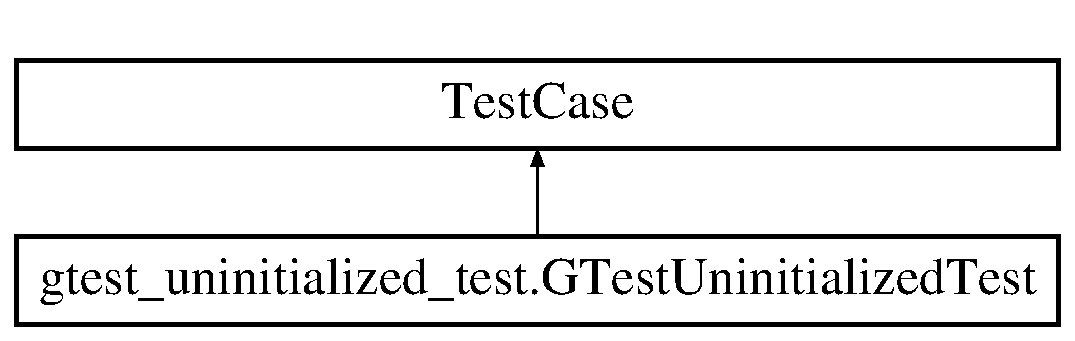
\includegraphics[height=2.000000cm]{classgtest__uninitialized__test_1_1_g_test_uninitialized_test}
\end{center}
\end{figure}
\subsection*{Public Member Functions}
\begin{DoxyCompactItemize}
\item 
def \hyperlink{classgtest__uninitialized__test_1_1_g_test_uninitialized_test_ace4bbad0abec476b03a91bb453e6451c}{test\+Exit\+Code\+And\+Output} (self)
\end{DoxyCompactItemize}


\subsection{Member Function Documentation}
\hypertarget{classgtest__uninitialized__test_1_1_g_test_uninitialized_test_ace4bbad0abec476b03a91bb453e6451c}{}\index{gtest\+\_\+uninitialized\+\_\+test\+::\+G\+Test\+Uninitialized\+Test@{gtest\+\_\+uninitialized\+\_\+test\+::\+G\+Test\+Uninitialized\+Test}!test\+Exit\+Code\+And\+Output@{test\+Exit\+Code\+And\+Output}}
\index{test\+Exit\+Code\+And\+Output@{test\+Exit\+Code\+And\+Output}!gtest\+\_\+uninitialized\+\_\+test\+::\+G\+Test\+Uninitialized\+Test@{gtest\+\_\+uninitialized\+\_\+test\+::\+G\+Test\+Uninitialized\+Test}}
\subsubsection[{test\+Exit\+Code\+And\+Output(self)}]{\setlength{\rightskip}{0pt plus 5cm}def gtest\+\_\+uninitialized\+\_\+test.\+G\+Test\+Uninitialized\+Test.\+test\+Exit\+Code\+And\+Output (
\begin{DoxyParamCaption}
\item[{}]{self}
\end{DoxyParamCaption}
)}\label{classgtest__uninitialized__test_1_1_g_test_uninitialized_test_ace4bbad0abec476b03a91bb453e6451c}


The documentation for this class was generated from the following file\+:\begin{DoxyCompactItemize}
\item 
C\+:/\+Users/\+Hilman/\+Desktop/repo/anjing/src/third\+\_\+party/googletest/test/\hyperlink{gtest__uninitialized__test_8py}{gtest\+\_\+uninitialized\+\_\+test.\+py}\end{DoxyCompactItemize}

\hypertarget{classgtest__xml__outfiles__test_1_1_g_test_x_m_l_out_files_test}{}\section{gtest\+\_\+xml\+\_\+outfiles\+\_\+test.\+G\+Test\+X\+M\+L\+Out\+Files\+Test Class Reference}
\label{classgtest__xml__outfiles__test_1_1_g_test_x_m_l_out_files_test}\index{gtest\+\_\+xml\+\_\+outfiles\+\_\+test.\+G\+Test\+X\+M\+L\+Out\+Files\+Test@{gtest\+\_\+xml\+\_\+outfiles\+\_\+test.\+G\+Test\+X\+M\+L\+Out\+Files\+Test}}
Inheritance diagram for gtest\+\_\+xml\+\_\+outfiles\+\_\+test.\+G\+Test\+X\+M\+L\+Out\+Files\+Test\+:\begin{figure}[H]
\begin{center}
\leavevmode
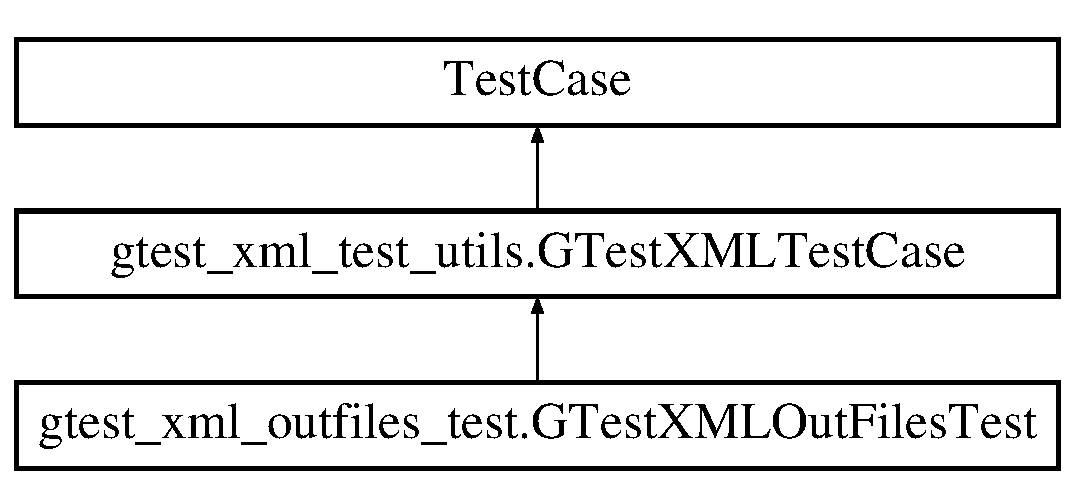
\includegraphics[height=3.000000cm]{classgtest__xml__outfiles__test_1_1_g_test_x_m_l_out_files_test}
\end{center}
\end{figure}
\subsection*{Public Member Functions}
\begin{DoxyCompactItemize}
\item 
def \hyperlink{classgtest__xml__outfiles__test_1_1_g_test_x_m_l_out_files_test_a56550f293277d18c36e868a637fe1153}{set\+Up} (self)
\item 
def \hyperlink{classgtest__xml__outfiles__test_1_1_g_test_x_m_l_out_files_test_a49d1d410370ba8a3cfcc281eaadb5706}{tear\+Down} (self)
\item 
def \hyperlink{classgtest__xml__outfiles__test_1_1_g_test_x_m_l_out_files_test_a503d2fbc9cd782ae57ac4307d2db43e1}{Delete\+Files\+And\+Dir} (self)
\item 
def \hyperlink{classgtest__xml__outfiles__test_1_1_g_test_x_m_l_out_files_test_a034738bbc00ac46d00f183402c561228}{test\+Outfile1} (self)
\item 
def \hyperlink{classgtest__xml__outfiles__test_1_1_g_test_x_m_l_out_files_test_a3c02687f092a482d0d0260c7ed94c618}{test\+Outfile2} (self)
\end{DoxyCompactItemize}
\subsection*{Public Attributes}
\begin{DoxyCompactItemize}
\item 
\hyperlink{classgtest__xml__outfiles__test_1_1_g_test_x_m_l_out_files_test_aa5c31cd97047bc1d3060f4d27bc956a4}{output\+\_\+dir\+\_\+}
\end{DoxyCompactItemize}
\subsection*{Additional Inherited Members}


\subsection{Detailed Description}
\begin{DoxyVerb}Unit test for Google Test's XML output functionality.\end{DoxyVerb}
 

\subsection{Member Function Documentation}
\hypertarget{classgtest__xml__outfiles__test_1_1_g_test_x_m_l_out_files_test_a503d2fbc9cd782ae57ac4307d2db43e1}{}\index{gtest\+\_\+xml\+\_\+outfiles\+\_\+test\+::\+G\+Test\+X\+M\+L\+Out\+Files\+Test@{gtest\+\_\+xml\+\_\+outfiles\+\_\+test\+::\+G\+Test\+X\+M\+L\+Out\+Files\+Test}!Delete\+Files\+And\+Dir@{Delete\+Files\+And\+Dir}}
\index{Delete\+Files\+And\+Dir@{Delete\+Files\+And\+Dir}!gtest\+\_\+xml\+\_\+outfiles\+\_\+test\+::\+G\+Test\+X\+M\+L\+Out\+Files\+Test@{gtest\+\_\+xml\+\_\+outfiles\+\_\+test\+::\+G\+Test\+X\+M\+L\+Out\+Files\+Test}}
\subsubsection[{Delete\+Files\+And\+Dir(self)}]{\setlength{\rightskip}{0pt plus 5cm}def gtest\+\_\+xml\+\_\+outfiles\+\_\+test.\+G\+Test\+X\+M\+L\+Out\+Files\+Test.\+Delete\+Files\+And\+Dir (
\begin{DoxyParamCaption}
\item[{}]{self}
\end{DoxyParamCaption}
)}\label{classgtest__xml__outfiles__test_1_1_g_test_x_m_l_out_files_test_a503d2fbc9cd782ae57ac4307d2db43e1}
\hypertarget{classgtest__xml__outfiles__test_1_1_g_test_x_m_l_out_files_test_a56550f293277d18c36e868a637fe1153}{}\index{gtest\+\_\+xml\+\_\+outfiles\+\_\+test\+::\+G\+Test\+X\+M\+L\+Out\+Files\+Test@{gtest\+\_\+xml\+\_\+outfiles\+\_\+test\+::\+G\+Test\+X\+M\+L\+Out\+Files\+Test}!set\+Up@{set\+Up}}
\index{set\+Up@{set\+Up}!gtest\+\_\+xml\+\_\+outfiles\+\_\+test\+::\+G\+Test\+X\+M\+L\+Out\+Files\+Test@{gtest\+\_\+xml\+\_\+outfiles\+\_\+test\+::\+G\+Test\+X\+M\+L\+Out\+Files\+Test}}
\subsubsection[{set\+Up(self)}]{\setlength{\rightskip}{0pt plus 5cm}def gtest\+\_\+xml\+\_\+outfiles\+\_\+test.\+G\+Test\+X\+M\+L\+Out\+Files\+Test.\+set\+Up (
\begin{DoxyParamCaption}
\item[{}]{self}
\end{DoxyParamCaption}
)}\label{classgtest__xml__outfiles__test_1_1_g_test_x_m_l_out_files_test_a56550f293277d18c36e868a637fe1153}
\hypertarget{classgtest__xml__outfiles__test_1_1_g_test_x_m_l_out_files_test_a49d1d410370ba8a3cfcc281eaadb5706}{}\index{gtest\+\_\+xml\+\_\+outfiles\+\_\+test\+::\+G\+Test\+X\+M\+L\+Out\+Files\+Test@{gtest\+\_\+xml\+\_\+outfiles\+\_\+test\+::\+G\+Test\+X\+M\+L\+Out\+Files\+Test}!tear\+Down@{tear\+Down}}
\index{tear\+Down@{tear\+Down}!gtest\+\_\+xml\+\_\+outfiles\+\_\+test\+::\+G\+Test\+X\+M\+L\+Out\+Files\+Test@{gtest\+\_\+xml\+\_\+outfiles\+\_\+test\+::\+G\+Test\+X\+M\+L\+Out\+Files\+Test}}
\subsubsection[{tear\+Down(self)}]{\setlength{\rightskip}{0pt plus 5cm}def gtest\+\_\+xml\+\_\+outfiles\+\_\+test.\+G\+Test\+X\+M\+L\+Out\+Files\+Test.\+tear\+Down (
\begin{DoxyParamCaption}
\item[{}]{self}
\end{DoxyParamCaption}
)}\label{classgtest__xml__outfiles__test_1_1_g_test_x_m_l_out_files_test_a49d1d410370ba8a3cfcc281eaadb5706}
\hypertarget{classgtest__xml__outfiles__test_1_1_g_test_x_m_l_out_files_test_a034738bbc00ac46d00f183402c561228}{}\index{gtest\+\_\+xml\+\_\+outfiles\+\_\+test\+::\+G\+Test\+X\+M\+L\+Out\+Files\+Test@{gtest\+\_\+xml\+\_\+outfiles\+\_\+test\+::\+G\+Test\+X\+M\+L\+Out\+Files\+Test}!test\+Outfile1@{test\+Outfile1}}
\index{test\+Outfile1@{test\+Outfile1}!gtest\+\_\+xml\+\_\+outfiles\+\_\+test\+::\+G\+Test\+X\+M\+L\+Out\+Files\+Test@{gtest\+\_\+xml\+\_\+outfiles\+\_\+test\+::\+G\+Test\+X\+M\+L\+Out\+Files\+Test}}
\subsubsection[{test\+Outfile1(self)}]{\setlength{\rightskip}{0pt plus 5cm}def gtest\+\_\+xml\+\_\+outfiles\+\_\+test.\+G\+Test\+X\+M\+L\+Out\+Files\+Test.\+test\+Outfile1 (
\begin{DoxyParamCaption}
\item[{}]{self}
\end{DoxyParamCaption}
)}\label{classgtest__xml__outfiles__test_1_1_g_test_x_m_l_out_files_test_a034738bbc00ac46d00f183402c561228}
\hypertarget{classgtest__xml__outfiles__test_1_1_g_test_x_m_l_out_files_test_a3c02687f092a482d0d0260c7ed94c618}{}\index{gtest\+\_\+xml\+\_\+outfiles\+\_\+test\+::\+G\+Test\+X\+M\+L\+Out\+Files\+Test@{gtest\+\_\+xml\+\_\+outfiles\+\_\+test\+::\+G\+Test\+X\+M\+L\+Out\+Files\+Test}!test\+Outfile2@{test\+Outfile2}}
\index{test\+Outfile2@{test\+Outfile2}!gtest\+\_\+xml\+\_\+outfiles\+\_\+test\+::\+G\+Test\+X\+M\+L\+Out\+Files\+Test@{gtest\+\_\+xml\+\_\+outfiles\+\_\+test\+::\+G\+Test\+X\+M\+L\+Out\+Files\+Test}}
\subsubsection[{test\+Outfile2(self)}]{\setlength{\rightskip}{0pt plus 5cm}def gtest\+\_\+xml\+\_\+outfiles\+\_\+test.\+G\+Test\+X\+M\+L\+Out\+Files\+Test.\+test\+Outfile2 (
\begin{DoxyParamCaption}
\item[{}]{self}
\end{DoxyParamCaption}
)}\label{classgtest__xml__outfiles__test_1_1_g_test_x_m_l_out_files_test_a3c02687f092a482d0d0260c7ed94c618}


\subsection{Member Data Documentation}
\hypertarget{classgtest__xml__outfiles__test_1_1_g_test_x_m_l_out_files_test_aa5c31cd97047bc1d3060f4d27bc956a4}{}\index{gtest\+\_\+xml\+\_\+outfiles\+\_\+test\+::\+G\+Test\+X\+M\+L\+Out\+Files\+Test@{gtest\+\_\+xml\+\_\+outfiles\+\_\+test\+::\+G\+Test\+X\+M\+L\+Out\+Files\+Test}!output\+\_\+dir\+\_\+@{output\+\_\+dir\+\_\+}}
\index{output\+\_\+dir\+\_\+@{output\+\_\+dir\+\_\+}!gtest\+\_\+xml\+\_\+outfiles\+\_\+test\+::\+G\+Test\+X\+M\+L\+Out\+Files\+Test@{gtest\+\_\+xml\+\_\+outfiles\+\_\+test\+::\+G\+Test\+X\+M\+L\+Out\+Files\+Test}}
\subsubsection[{output\+\_\+dir\+\_\+}]{\setlength{\rightskip}{0pt plus 5cm}gtest\+\_\+xml\+\_\+outfiles\+\_\+test.\+G\+Test\+X\+M\+L\+Out\+Files\+Test.\+output\+\_\+dir\+\_\+}\label{classgtest__xml__outfiles__test_1_1_g_test_x_m_l_out_files_test_aa5c31cd97047bc1d3060f4d27bc956a4}


The documentation for this class was generated from the following file\+:\begin{DoxyCompactItemize}
\item 
C\+:/\+Users/\+Hilman/\+Desktop/repo/anjing/src/third\+\_\+party/googletest/test/\hyperlink{gtest__xml__outfiles__test_8py}{gtest\+\_\+xml\+\_\+outfiles\+\_\+test.\+py}\end{DoxyCompactItemize}

\hypertarget{classgtest__xml__output__unittest_1_1_g_test_x_m_l_output_unit_test}{}\section{gtest\+\_\+xml\+\_\+output\+\_\+unittest.\+G\+Test\+X\+M\+L\+Output\+Unit\+Test Class Reference}
\label{classgtest__xml__output__unittest_1_1_g_test_x_m_l_output_unit_test}\index{gtest\+\_\+xml\+\_\+output\+\_\+unittest.\+G\+Test\+X\+M\+L\+Output\+Unit\+Test@{gtest\+\_\+xml\+\_\+output\+\_\+unittest.\+G\+Test\+X\+M\+L\+Output\+Unit\+Test}}
Inheritance diagram for gtest\+\_\+xml\+\_\+output\+\_\+unittest.\+G\+Test\+X\+M\+L\+Output\+Unit\+Test\+:\begin{figure}[H]
\begin{center}
\leavevmode
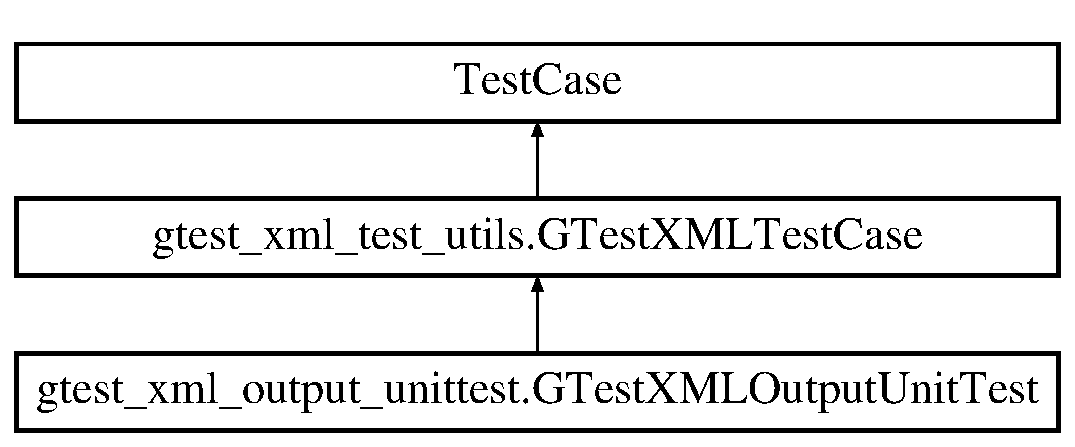
\includegraphics[height=3.000000cm]{classgtest__xml__output__unittest_1_1_g_test_x_m_l_output_unit_test}
\end{center}
\end{figure}
\subsection*{Public Member Functions}
\begin{DoxyCompactItemize}
\item 
def \hyperlink{classgtest__xml__output__unittest_1_1_g_test_x_m_l_output_unit_test_a310c136c1eb2b421f57651a7d358b17a}{test\+Non\+Empty\+Xml\+Output} (self)
\item 
def \hyperlink{classgtest__xml__output__unittest_1_1_g_test_x_m_l_output_unit_test_a9602f91fe2e9d1e09171a032e94a5619}{test\+Empty\+Xml\+Output} (self)
\item 
def \hyperlink{classgtest__xml__output__unittest_1_1_g_test_x_m_l_output_unit_test_a828521a7ae57f650e1e9ca4beb34336a}{test\+Timestamp\+Value} (self)
\item 
def \hyperlink{classgtest__xml__output__unittest_1_1_g_test_x_m_l_output_unit_test_a01ca66e14468028e5c4eb809987113cf}{test\+Default\+Output\+File} (self)
\item 
def \hyperlink{classgtest__xml__output__unittest_1_1_g_test_x_m_l_output_unit_test_ac6df46d6831892e4c14dbdfae0049618}{test\+Suppressed\+Xml\+Output} (self)
\item 
def \hyperlink{classgtest__xml__output__unittest_1_1_g_test_x_m_l_output_unit_test_a572b6d49e8f4d646ebdadcced3d260ef}{test\+Filtered\+Test\+Xml\+Output} (self)
\end{DoxyCompactItemize}
\subsection*{Additional Inherited Members}


\subsection{Detailed Description}
\begin{DoxyVerb}Unit test for Google Test's XML output functionality.
\end{DoxyVerb}
 

\subsection{Member Function Documentation}
\hypertarget{classgtest__xml__output__unittest_1_1_g_test_x_m_l_output_unit_test_a01ca66e14468028e5c4eb809987113cf}{}\index{gtest\+\_\+xml\+\_\+output\+\_\+unittest\+::\+G\+Test\+X\+M\+L\+Output\+Unit\+Test@{gtest\+\_\+xml\+\_\+output\+\_\+unittest\+::\+G\+Test\+X\+M\+L\+Output\+Unit\+Test}!test\+Default\+Output\+File@{test\+Default\+Output\+File}}
\index{test\+Default\+Output\+File@{test\+Default\+Output\+File}!gtest\+\_\+xml\+\_\+output\+\_\+unittest\+::\+G\+Test\+X\+M\+L\+Output\+Unit\+Test@{gtest\+\_\+xml\+\_\+output\+\_\+unittest\+::\+G\+Test\+X\+M\+L\+Output\+Unit\+Test}}
\subsubsection[{test\+Default\+Output\+File(self)}]{\setlength{\rightskip}{0pt plus 5cm}def gtest\+\_\+xml\+\_\+output\+\_\+unittest.\+G\+Test\+X\+M\+L\+Output\+Unit\+Test.\+test\+Default\+Output\+File (
\begin{DoxyParamCaption}
\item[{}]{self}
\end{DoxyParamCaption}
)}\label{classgtest__xml__output__unittest_1_1_g_test_x_m_l_output_unit_test_a01ca66e14468028e5c4eb809987113cf}
\begin{DoxyVerb}Confirms that Google Test produces an XML output file with the expected
default name if no name is explicitly specified.
\end{DoxyVerb}
 \hypertarget{classgtest__xml__output__unittest_1_1_g_test_x_m_l_output_unit_test_a9602f91fe2e9d1e09171a032e94a5619}{}\index{gtest\+\_\+xml\+\_\+output\+\_\+unittest\+::\+G\+Test\+X\+M\+L\+Output\+Unit\+Test@{gtest\+\_\+xml\+\_\+output\+\_\+unittest\+::\+G\+Test\+X\+M\+L\+Output\+Unit\+Test}!test\+Empty\+Xml\+Output@{test\+Empty\+Xml\+Output}}
\index{test\+Empty\+Xml\+Output@{test\+Empty\+Xml\+Output}!gtest\+\_\+xml\+\_\+output\+\_\+unittest\+::\+G\+Test\+X\+M\+L\+Output\+Unit\+Test@{gtest\+\_\+xml\+\_\+output\+\_\+unittest\+::\+G\+Test\+X\+M\+L\+Output\+Unit\+Test}}
\subsubsection[{test\+Empty\+Xml\+Output(self)}]{\setlength{\rightskip}{0pt plus 5cm}def gtest\+\_\+xml\+\_\+output\+\_\+unittest.\+G\+Test\+X\+M\+L\+Output\+Unit\+Test.\+test\+Empty\+Xml\+Output (
\begin{DoxyParamCaption}
\item[{}]{self}
\end{DoxyParamCaption}
)}\label{classgtest__xml__output__unittest_1_1_g_test_x_m_l_output_unit_test_a9602f91fe2e9d1e09171a032e94a5619}
\begin{DoxyVerb}Verifies XML output for a Google Test binary without actual tests.

Runs a test program that generates an empty XML output, and
tests that the XML output is expected.
\end{DoxyVerb}
 \hypertarget{classgtest__xml__output__unittest_1_1_g_test_x_m_l_output_unit_test_a572b6d49e8f4d646ebdadcced3d260ef}{}\index{gtest\+\_\+xml\+\_\+output\+\_\+unittest\+::\+G\+Test\+X\+M\+L\+Output\+Unit\+Test@{gtest\+\_\+xml\+\_\+output\+\_\+unittest\+::\+G\+Test\+X\+M\+L\+Output\+Unit\+Test}!test\+Filtered\+Test\+Xml\+Output@{test\+Filtered\+Test\+Xml\+Output}}
\index{test\+Filtered\+Test\+Xml\+Output@{test\+Filtered\+Test\+Xml\+Output}!gtest\+\_\+xml\+\_\+output\+\_\+unittest\+::\+G\+Test\+X\+M\+L\+Output\+Unit\+Test@{gtest\+\_\+xml\+\_\+output\+\_\+unittest\+::\+G\+Test\+X\+M\+L\+Output\+Unit\+Test}}
\subsubsection[{test\+Filtered\+Test\+Xml\+Output(self)}]{\setlength{\rightskip}{0pt plus 5cm}def gtest\+\_\+xml\+\_\+output\+\_\+unittest.\+G\+Test\+X\+M\+L\+Output\+Unit\+Test.\+test\+Filtered\+Test\+Xml\+Output (
\begin{DoxyParamCaption}
\item[{}]{self}
\end{DoxyParamCaption}
)}\label{classgtest__xml__output__unittest_1_1_g_test_x_m_l_output_unit_test_a572b6d49e8f4d646ebdadcced3d260ef}
\begin{DoxyVerb}Verifies XML output when a filter is applied.

Runs a test program that executes only some tests and verifies that
non-selected tests do not show up in the XML output.
\end{DoxyVerb}
 \hypertarget{classgtest__xml__output__unittest_1_1_g_test_x_m_l_output_unit_test_a310c136c1eb2b421f57651a7d358b17a}{}\index{gtest\+\_\+xml\+\_\+output\+\_\+unittest\+::\+G\+Test\+X\+M\+L\+Output\+Unit\+Test@{gtest\+\_\+xml\+\_\+output\+\_\+unittest\+::\+G\+Test\+X\+M\+L\+Output\+Unit\+Test}!test\+Non\+Empty\+Xml\+Output@{test\+Non\+Empty\+Xml\+Output}}
\index{test\+Non\+Empty\+Xml\+Output@{test\+Non\+Empty\+Xml\+Output}!gtest\+\_\+xml\+\_\+output\+\_\+unittest\+::\+G\+Test\+X\+M\+L\+Output\+Unit\+Test@{gtest\+\_\+xml\+\_\+output\+\_\+unittest\+::\+G\+Test\+X\+M\+L\+Output\+Unit\+Test}}
\subsubsection[{test\+Non\+Empty\+Xml\+Output(self)}]{\setlength{\rightskip}{0pt plus 5cm}def gtest\+\_\+xml\+\_\+output\+\_\+unittest.\+G\+Test\+X\+M\+L\+Output\+Unit\+Test.\+test\+Non\+Empty\+Xml\+Output (
\begin{DoxyParamCaption}
\item[{}]{self}
\end{DoxyParamCaption}
)}\label{classgtest__xml__output__unittest_1_1_g_test_x_m_l_output_unit_test_a310c136c1eb2b421f57651a7d358b17a}
\begin{DoxyVerb}Runs a test program that generates a non-empty XML output, and
tests that the XML output is expected.
\end{DoxyVerb}
 \hypertarget{classgtest__xml__output__unittest_1_1_g_test_x_m_l_output_unit_test_ac6df46d6831892e4c14dbdfae0049618}{}\index{gtest\+\_\+xml\+\_\+output\+\_\+unittest\+::\+G\+Test\+X\+M\+L\+Output\+Unit\+Test@{gtest\+\_\+xml\+\_\+output\+\_\+unittest\+::\+G\+Test\+X\+M\+L\+Output\+Unit\+Test}!test\+Suppressed\+Xml\+Output@{test\+Suppressed\+Xml\+Output}}
\index{test\+Suppressed\+Xml\+Output@{test\+Suppressed\+Xml\+Output}!gtest\+\_\+xml\+\_\+output\+\_\+unittest\+::\+G\+Test\+X\+M\+L\+Output\+Unit\+Test@{gtest\+\_\+xml\+\_\+output\+\_\+unittest\+::\+G\+Test\+X\+M\+L\+Output\+Unit\+Test}}
\subsubsection[{test\+Suppressed\+Xml\+Output(self)}]{\setlength{\rightskip}{0pt plus 5cm}def gtest\+\_\+xml\+\_\+output\+\_\+unittest.\+G\+Test\+X\+M\+L\+Output\+Unit\+Test.\+test\+Suppressed\+Xml\+Output (
\begin{DoxyParamCaption}
\item[{}]{self}
\end{DoxyParamCaption}
)}\label{classgtest__xml__output__unittest_1_1_g_test_x_m_l_output_unit_test_ac6df46d6831892e4c14dbdfae0049618}
\begin{DoxyVerb}Tests that no XML file is generated if the default XML listener is
shut down before RUN_ALL_TESTS is invoked.
\end{DoxyVerb}
 \hypertarget{classgtest__xml__output__unittest_1_1_g_test_x_m_l_output_unit_test_a828521a7ae57f650e1e9ca4beb34336a}{}\index{gtest\+\_\+xml\+\_\+output\+\_\+unittest\+::\+G\+Test\+X\+M\+L\+Output\+Unit\+Test@{gtest\+\_\+xml\+\_\+output\+\_\+unittest\+::\+G\+Test\+X\+M\+L\+Output\+Unit\+Test}!test\+Timestamp\+Value@{test\+Timestamp\+Value}}
\index{test\+Timestamp\+Value@{test\+Timestamp\+Value}!gtest\+\_\+xml\+\_\+output\+\_\+unittest\+::\+G\+Test\+X\+M\+L\+Output\+Unit\+Test@{gtest\+\_\+xml\+\_\+output\+\_\+unittest\+::\+G\+Test\+X\+M\+L\+Output\+Unit\+Test}}
\subsubsection[{test\+Timestamp\+Value(self)}]{\setlength{\rightskip}{0pt plus 5cm}def gtest\+\_\+xml\+\_\+output\+\_\+unittest.\+G\+Test\+X\+M\+L\+Output\+Unit\+Test.\+test\+Timestamp\+Value (
\begin{DoxyParamCaption}
\item[{}]{self}
\end{DoxyParamCaption}
)}\label{classgtest__xml__output__unittest_1_1_g_test_x_m_l_output_unit_test_a828521a7ae57f650e1e9ca4beb34336a}
\begin{DoxyVerb}Checks whether the timestamp attribute in the XML output is valid.

Runs a test program that generates an empty XML output, and checks if
the timestamp attribute in the testsuites tag is valid.
\end{DoxyVerb}
 

The documentation for this class was generated from the following file\+:\begin{DoxyCompactItemize}
\item 
C\+:/\+Users/\+Hilman/\+Desktop/repo/anjing/src/third\+\_\+party/googletest/test/\hyperlink{gtest__xml__output__unittest_8py}{gtest\+\_\+xml\+\_\+output\+\_\+unittest.\+py}\end{DoxyCompactItemize}

\hypertarget{classgtest__xml__test__utils_1_1_g_test_x_m_l_test_case}{}\section{gtest\+\_\+xml\+\_\+test\+\_\+utils.\+G\+Test\+X\+M\+L\+Test\+Case Class Reference}
\label{classgtest__xml__test__utils_1_1_g_test_x_m_l_test_case}\index{gtest\+\_\+xml\+\_\+test\+\_\+utils.\+G\+Test\+X\+M\+L\+Test\+Case@{gtest\+\_\+xml\+\_\+test\+\_\+utils.\+G\+Test\+X\+M\+L\+Test\+Case}}
Inheritance diagram for gtest\+\_\+xml\+\_\+test\+\_\+utils.\+G\+Test\+X\+M\+L\+Test\+Case\+:\begin{figure}[H]
\begin{center}
\leavevmode
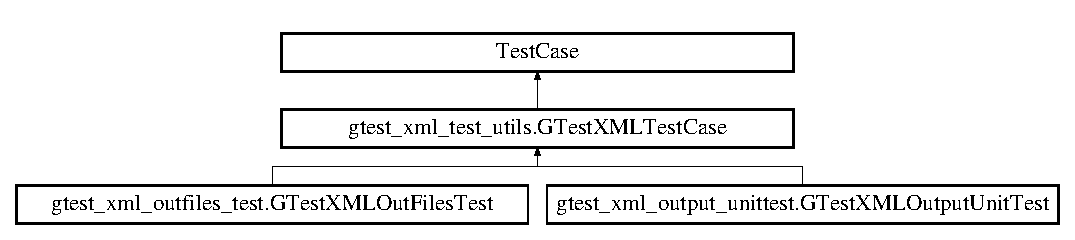
\includegraphics[height=2.781457cm]{classgtest__xml__test__utils_1_1_g_test_x_m_l_test_case}
\end{center}
\end{figure}
\subsection*{Public Member Functions}
\begin{DoxyCompactItemize}
\item 
def \hyperlink{classgtest__xml__test__utils_1_1_g_test_x_m_l_test_case_a977273e8863f4f41d121bb5a64b08d32}{Assert\+Equivalent\+Nodes} (self, expected\+\_\+node, actual\+\_\+node)
\item 
def \hyperlink{classgtest__xml__test__utils_1_1_g_test_x_m_l_test_case_ac4823e96c3b5327b25a340a3605447d9}{Normalize\+Xml} (self, element)
\end{DoxyCompactItemize}
\subsection*{Static Public Attributes}
\begin{DoxyCompactItemize}
\item 
dictionary \hyperlink{classgtest__xml__test__utils_1_1_g_test_x_m_l_test_case_a0e3a4e84e18f29d2248dcd670a0a6ae6}{identifying\+\_\+attribute}
\end{DoxyCompactItemize}


\subsection{Detailed Description}
\begin{DoxyVerb}Base class for tests of Google Test's XML output functionality.
\end{DoxyVerb}
 

\subsection{Member Function Documentation}
\hypertarget{classgtest__xml__test__utils_1_1_g_test_x_m_l_test_case_a977273e8863f4f41d121bb5a64b08d32}{}\index{gtest\+\_\+xml\+\_\+test\+\_\+utils\+::\+G\+Test\+X\+M\+L\+Test\+Case@{gtest\+\_\+xml\+\_\+test\+\_\+utils\+::\+G\+Test\+X\+M\+L\+Test\+Case}!Assert\+Equivalent\+Nodes@{Assert\+Equivalent\+Nodes}}
\index{Assert\+Equivalent\+Nodes@{Assert\+Equivalent\+Nodes}!gtest\+\_\+xml\+\_\+test\+\_\+utils\+::\+G\+Test\+X\+M\+L\+Test\+Case@{gtest\+\_\+xml\+\_\+test\+\_\+utils\+::\+G\+Test\+X\+M\+L\+Test\+Case}}
\subsubsection[{Assert\+Equivalent\+Nodes(self, expected\+\_\+node, actual\+\_\+node)}]{\setlength{\rightskip}{0pt plus 5cm}def gtest\+\_\+xml\+\_\+test\+\_\+utils.\+G\+Test\+X\+M\+L\+Test\+Case.\+Assert\+Equivalent\+Nodes (
\begin{DoxyParamCaption}
\item[{}]{self, }
\item[{}]{expected\+\_\+node, }
\item[{}]{actual\+\_\+node}
\end{DoxyParamCaption}
)}\label{classgtest__xml__test__utils_1_1_g_test_x_m_l_test_case_a977273e8863f4f41d121bb5a64b08d32}
\begin{DoxyVerb}Asserts that actual_node (a DOM node object) is equivalent to
expected_node (another DOM node object), in that either both of
them are CDATA nodes and have the same value, or both are DOM
elements and actual_node meets all of the following conditions:

*  It has the same tag name as expected_node.
*  It has the same set of attributes as expected_node, each with
   the same value as the corresponding attribute of expected_node.
   Exceptions are any attribute named "time", which needs only be
   convertible to a floating-point number and any attribute named
   "type_param" which only has to be non-empty.
*  It has an equivalent set of child nodes (including elements and
   CDATA sections) as expected_node.  Note that we ignore the
   order of the children as they are not guaranteed to be in any
   particular order.
\end{DoxyVerb}
 \hypertarget{classgtest__xml__test__utils_1_1_g_test_x_m_l_test_case_ac4823e96c3b5327b25a340a3605447d9}{}\index{gtest\+\_\+xml\+\_\+test\+\_\+utils\+::\+G\+Test\+X\+M\+L\+Test\+Case@{gtest\+\_\+xml\+\_\+test\+\_\+utils\+::\+G\+Test\+X\+M\+L\+Test\+Case}!Normalize\+Xml@{Normalize\+Xml}}
\index{Normalize\+Xml@{Normalize\+Xml}!gtest\+\_\+xml\+\_\+test\+\_\+utils\+::\+G\+Test\+X\+M\+L\+Test\+Case@{gtest\+\_\+xml\+\_\+test\+\_\+utils\+::\+G\+Test\+X\+M\+L\+Test\+Case}}
\subsubsection[{Normalize\+Xml(self, element)}]{\setlength{\rightskip}{0pt plus 5cm}def gtest\+\_\+xml\+\_\+test\+\_\+utils.\+G\+Test\+X\+M\+L\+Test\+Case.\+Normalize\+Xml (
\begin{DoxyParamCaption}
\item[{}]{self, }
\item[{}]{element}
\end{DoxyParamCaption}
)}\label{classgtest__xml__test__utils_1_1_g_test_x_m_l_test_case_ac4823e96c3b5327b25a340a3605447d9}
\begin{DoxyVerb}Normalizes Google Test's XML output to eliminate references to transient
information that may change from run to run.

*  The "time" attribute of <testsuites>, <testsuite> and <testcase>
   elements is replaced with a single asterisk, if it contains
   only digit characters.
*  The "timestamp" attribute of <testsuites> elements is replaced with a
   single asterisk, if it contains a valid ISO8601 datetime value.
*  The "type_param" attribute of <testcase> elements is replaced with a
   single asterisk (if it sn non-empty) as it is the type name returned
   by the compiler and is platform dependent.
*  The line info reported in the first line of the "message"
   attribute and CDATA section of <failure> elements is replaced with the
   file's basename and a single asterisk for the line number.
*  The directory names in file paths are removed.
*  The stack traces are removed.
\end{DoxyVerb}
 

\subsection{Member Data Documentation}
\hypertarget{classgtest__xml__test__utils_1_1_g_test_x_m_l_test_case_a0e3a4e84e18f29d2248dcd670a0a6ae6}{}\index{gtest\+\_\+xml\+\_\+test\+\_\+utils\+::\+G\+Test\+X\+M\+L\+Test\+Case@{gtest\+\_\+xml\+\_\+test\+\_\+utils\+::\+G\+Test\+X\+M\+L\+Test\+Case}!identifying\+\_\+attribute@{identifying\+\_\+attribute}}
\index{identifying\+\_\+attribute@{identifying\+\_\+attribute}!gtest\+\_\+xml\+\_\+test\+\_\+utils\+::\+G\+Test\+X\+M\+L\+Test\+Case@{gtest\+\_\+xml\+\_\+test\+\_\+utils\+::\+G\+Test\+X\+M\+L\+Test\+Case}}
\subsubsection[{identifying\+\_\+attribute}]{\setlength{\rightskip}{0pt plus 5cm}dictionary gtest\+\_\+xml\+\_\+test\+\_\+utils.\+G\+Test\+X\+M\+L\+Test\+Case.\+identifying\+\_\+attribute\hspace{0.3cm}{\ttfamily [static]}}\label{classgtest__xml__test__utils_1_1_g_test_x_m_l_test_case_a0e3a4e84e18f29d2248dcd670a0a6ae6}
{\bfseries Initial value\+:}
\begin{DoxyCode}
1 = \{
2     \textcolor{stringliteral}{'testsuites'}: \textcolor{stringliteral}{'name'},
3     \textcolor{stringliteral}{'testsuite'}: \textcolor{stringliteral}{'name'},
4     \textcolor{stringliteral}{'testcase'}:  \textcolor{stringliteral}{'name'},
5     \textcolor{stringliteral}{'failure'}:   \textcolor{stringliteral}{'message'},
6     \}
\end{DoxyCode}


The documentation for this class was generated from the following file\+:\begin{DoxyCompactItemize}
\item 
C\+:/\+Users/\+Hilman/\+Desktop/repo/anjing/src/third\+\_\+party/googletest/test/\hyperlink{gtest__xml__test__utils_8py}{gtest\+\_\+xml\+\_\+test\+\_\+utils.\+py}\end{DoxyCompactItemize}

\hypertarget{classtesting_1_1internal_1_1_has_new_fatal_failure_helper}{}\section{testing\+:\+:internal\+:\+:Has\+New\+Fatal\+Failure\+Helper Class Reference}
\label{classtesting_1_1internal_1_1_has_new_fatal_failure_helper}\index{testing\+::internal\+::\+Has\+New\+Fatal\+Failure\+Helper@{testing\+::internal\+::\+Has\+New\+Fatal\+Failure\+Helper}}


{\ttfamily \#include $<$gtest-\/test-\/part.\+h$>$}

Inheritance diagram for testing\+:\+:internal\+:\+:Has\+New\+Fatal\+Failure\+Helper\+:\begin{figure}[H]
\begin{center}
\leavevmode
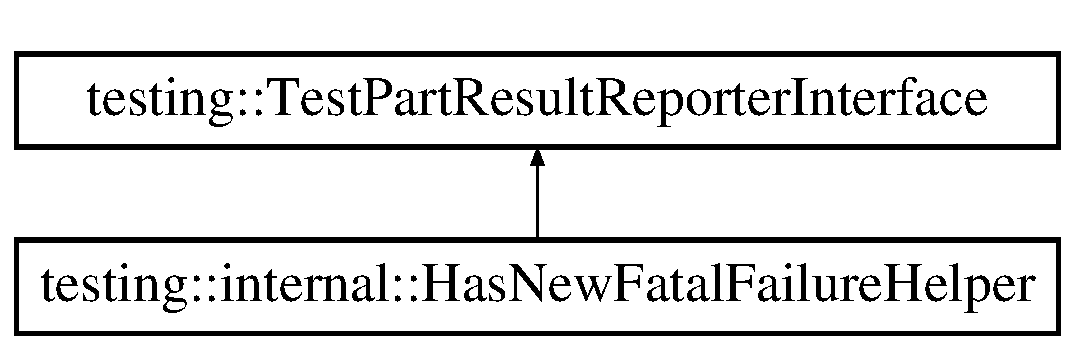
\includegraphics[height=2.000000cm]{classtesting_1_1internal_1_1_has_new_fatal_failure_helper}
\end{center}
\end{figure}
\subsection*{Public Member Functions}
\begin{DoxyCompactItemize}
\item 
\hyperlink{classtesting_1_1internal_1_1_has_new_fatal_failure_helper_a59190a7188db558c00b4c6bf9251859a}{Has\+New\+Fatal\+Failure\+Helper} ()
\item 
virtual \hyperlink{classtesting_1_1internal_1_1_has_new_fatal_failure_helper_a913b1bc7c372868c9b2dbb009044ee97}{$\sim$\+Has\+New\+Fatal\+Failure\+Helper} ()
\item 
virtual void \hyperlink{classtesting_1_1internal_1_1_has_new_fatal_failure_helper_a2d2e1faa1f3669b82810df97ac678a27}{Report\+Test\+Part\+Result} (const \hyperlink{classtesting_1_1_test_part_result}{Test\+Part\+Result} \&result)
\item 
bool \hyperlink{classtesting_1_1internal_1_1_has_new_fatal_failure_helper_ae137e639098071f11f531bbd72dde1c7}{has\+\_\+new\+\_\+fatal\+\_\+failure} () const 
\end{DoxyCompactItemize}


\subsection{Constructor \& Destructor Documentation}
\hypertarget{classtesting_1_1internal_1_1_has_new_fatal_failure_helper_a59190a7188db558c00b4c6bf9251859a}{}\index{testing\+::internal\+::\+Has\+New\+Fatal\+Failure\+Helper@{testing\+::internal\+::\+Has\+New\+Fatal\+Failure\+Helper}!Has\+New\+Fatal\+Failure\+Helper@{Has\+New\+Fatal\+Failure\+Helper}}
\index{Has\+New\+Fatal\+Failure\+Helper@{Has\+New\+Fatal\+Failure\+Helper}!testing\+::internal\+::\+Has\+New\+Fatal\+Failure\+Helper@{testing\+::internal\+::\+Has\+New\+Fatal\+Failure\+Helper}}
\subsubsection[{Has\+New\+Fatal\+Failure\+Helper()}]{\setlength{\rightskip}{0pt plus 5cm}testing\+::internal\+::\+Has\+New\+Fatal\+Failure\+Helper\+::\+Has\+New\+Fatal\+Failure\+Helper (
\begin{DoxyParamCaption}
{}
\end{DoxyParamCaption}
)}\label{classtesting_1_1internal_1_1_has_new_fatal_failure_helper_a59190a7188db558c00b4c6bf9251859a}
\hypertarget{classtesting_1_1internal_1_1_has_new_fatal_failure_helper_a913b1bc7c372868c9b2dbb009044ee97}{}\index{testing\+::internal\+::\+Has\+New\+Fatal\+Failure\+Helper@{testing\+::internal\+::\+Has\+New\+Fatal\+Failure\+Helper}!````~Has\+New\+Fatal\+Failure\+Helper@{$\sim$\+Has\+New\+Fatal\+Failure\+Helper}}
\index{````~Has\+New\+Fatal\+Failure\+Helper@{$\sim$\+Has\+New\+Fatal\+Failure\+Helper}!testing\+::internal\+::\+Has\+New\+Fatal\+Failure\+Helper@{testing\+::internal\+::\+Has\+New\+Fatal\+Failure\+Helper}}
\subsubsection[{$\sim$\+Has\+New\+Fatal\+Failure\+Helper()}]{\setlength{\rightskip}{0pt plus 5cm}testing\+::internal\+::\+Has\+New\+Fatal\+Failure\+Helper\+::$\sim$\+Has\+New\+Fatal\+Failure\+Helper (
\begin{DoxyParamCaption}
{}
\end{DoxyParamCaption}
)\hspace{0.3cm}{\ttfamily [virtual]}}\label{classtesting_1_1internal_1_1_has_new_fatal_failure_helper_a913b1bc7c372868c9b2dbb009044ee97}


\subsection{Member Function Documentation}
\hypertarget{classtesting_1_1internal_1_1_has_new_fatal_failure_helper_ae137e639098071f11f531bbd72dde1c7}{}\index{testing\+::internal\+::\+Has\+New\+Fatal\+Failure\+Helper@{testing\+::internal\+::\+Has\+New\+Fatal\+Failure\+Helper}!has\+\_\+new\+\_\+fatal\+\_\+failure@{has\+\_\+new\+\_\+fatal\+\_\+failure}}
\index{has\+\_\+new\+\_\+fatal\+\_\+failure@{has\+\_\+new\+\_\+fatal\+\_\+failure}!testing\+::internal\+::\+Has\+New\+Fatal\+Failure\+Helper@{testing\+::internal\+::\+Has\+New\+Fatal\+Failure\+Helper}}
\subsubsection[{has\+\_\+new\+\_\+fatal\+\_\+failure() const }]{\setlength{\rightskip}{0pt plus 5cm}bool testing\+::internal\+::\+Has\+New\+Fatal\+Failure\+Helper\+::has\+\_\+new\+\_\+fatal\+\_\+failure (
\begin{DoxyParamCaption}
{}
\end{DoxyParamCaption}
) const\hspace{0.3cm}{\ttfamily [inline]}}\label{classtesting_1_1internal_1_1_has_new_fatal_failure_helper_ae137e639098071f11f531bbd72dde1c7}
\hypertarget{classtesting_1_1internal_1_1_has_new_fatal_failure_helper_a2d2e1faa1f3669b82810df97ac678a27}{}\index{testing\+::internal\+::\+Has\+New\+Fatal\+Failure\+Helper@{testing\+::internal\+::\+Has\+New\+Fatal\+Failure\+Helper}!Report\+Test\+Part\+Result@{Report\+Test\+Part\+Result}}
\index{Report\+Test\+Part\+Result@{Report\+Test\+Part\+Result}!testing\+::internal\+::\+Has\+New\+Fatal\+Failure\+Helper@{testing\+::internal\+::\+Has\+New\+Fatal\+Failure\+Helper}}
\subsubsection[{Report\+Test\+Part\+Result(const Test\+Part\+Result \&result)}]{\setlength{\rightskip}{0pt plus 5cm}void testing\+::internal\+::\+Has\+New\+Fatal\+Failure\+Helper\+::\+Report\+Test\+Part\+Result (
\begin{DoxyParamCaption}
\item[{const {\bf Test\+Part\+Result} \&}]{result}
\end{DoxyParamCaption}
)\hspace{0.3cm}{\ttfamily [virtual]}}\label{classtesting_1_1internal_1_1_has_new_fatal_failure_helper_a2d2e1faa1f3669b82810df97ac678a27}


Implements \hyperlink{classtesting_1_1_test_part_result_reporter_interface_aa2f920e7a5a0a6d0faf19e3727928c22}{testing\+::\+Test\+Part\+Result\+Reporter\+Interface}.



The documentation for this class was generated from the following files\+:\begin{DoxyCompactItemize}
\item 
C\+:/\+Users/\+Hilman/\+Desktop/repo/anjing/src/third\+\_\+party/googletest/include/gtest/\hyperlink{gtest-test-part_8h}{gtest-\/test-\/part.\+h}\item 
C\+:/\+Users/\+Hilman/\+Desktop/repo/anjing/src/third\+\_\+party/googletest/src/\hyperlink{gtest-test-part_8cc}{gtest-\/test-\/part.\+cc}\end{DoxyCompactItemize}

\hypertarget{classupload_1_1_http_rpc_server}{}\section{upload.\+Http\+Rpc\+Server Class Reference}
\label{classupload_1_1_http_rpc_server}\index{upload.\+Http\+Rpc\+Server@{upload.\+Http\+Rpc\+Server}}


elif e.\+code $>$= 500 and e.\+code $<$ 600\+: \subsection*{Server Error -\/ try again.} 


Inheritance diagram for upload.\+Http\+Rpc\+Server\+:\begin{figure}[H]
\begin{center}
\leavevmode
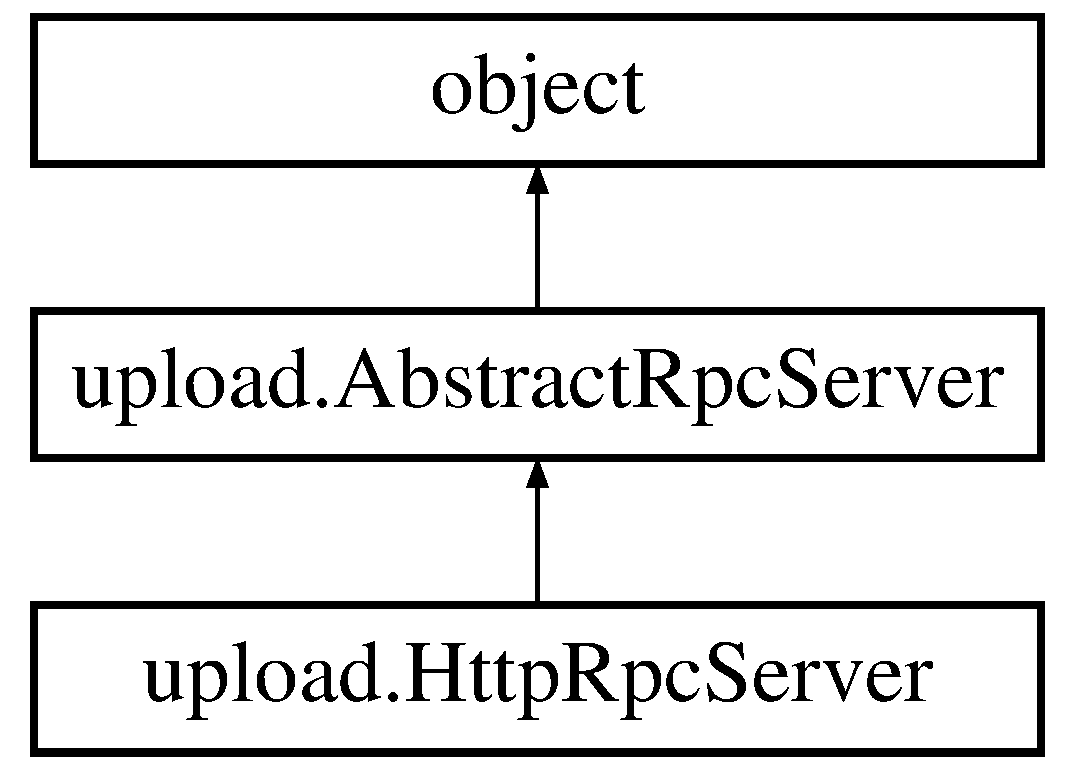
\includegraphics[height=3.000000cm]{classupload_1_1_http_rpc_server}
\end{center}
\end{figure}
\subsection*{Public Attributes}
\begin{DoxyCompactItemize}
\item 
\hyperlink{classupload_1_1_http_rpc_server_ad5c1a730c030f9d3b5f70c2e0d8b9a1d}{cookie\+\_\+file}
\item 
\hyperlink{classupload_1_1_http_rpc_server_a1b9c9af7f0a46afd84a9d524782323bf}{cookie\+\_\+jar}
\item 
\hyperlink{classupload_1_1_http_rpc_server_aaa356e2491537dd0d4bfc5b1bb0fec96}{authenticated}
\end{DoxyCompactItemize}
\subsection*{Additional Inherited Members}


\subsection{Detailed Description}
elif e.\+code $>$= 500 and e.\+code $<$ 600\+: \subsection*{Server Error -\/ try again.}

continue \begin{DoxyVerb}Provides a simplified RPC-style interface for HTTP requests.\end{DoxyVerb}
 

\subsection{Member Data Documentation}
\hypertarget{classupload_1_1_http_rpc_server_aaa356e2491537dd0d4bfc5b1bb0fec96}{}\index{upload\+::\+Http\+Rpc\+Server@{upload\+::\+Http\+Rpc\+Server}!authenticated@{authenticated}}
\index{authenticated@{authenticated}!upload\+::\+Http\+Rpc\+Server@{upload\+::\+Http\+Rpc\+Server}}
\subsubsection[{authenticated}]{\setlength{\rightskip}{0pt plus 5cm}upload.\+Http\+Rpc\+Server.\+authenticated}\label{classupload_1_1_http_rpc_server_aaa356e2491537dd0d4bfc5b1bb0fec96}
\hypertarget{classupload_1_1_http_rpc_server_ad5c1a730c030f9d3b5f70c2e0d8b9a1d}{}\index{upload\+::\+Http\+Rpc\+Server@{upload\+::\+Http\+Rpc\+Server}!cookie\+\_\+file@{cookie\+\_\+file}}
\index{cookie\+\_\+file@{cookie\+\_\+file}!upload\+::\+Http\+Rpc\+Server@{upload\+::\+Http\+Rpc\+Server}}
\subsubsection[{cookie\+\_\+file}]{\setlength{\rightskip}{0pt plus 5cm}upload.\+Http\+Rpc\+Server.\+cookie\+\_\+file}\label{classupload_1_1_http_rpc_server_ad5c1a730c030f9d3b5f70c2e0d8b9a1d}
\hypertarget{classupload_1_1_http_rpc_server_a1b9c9af7f0a46afd84a9d524782323bf}{}\index{upload\+::\+Http\+Rpc\+Server@{upload\+::\+Http\+Rpc\+Server}!cookie\+\_\+jar@{cookie\+\_\+jar}}
\index{cookie\+\_\+jar@{cookie\+\_\+jar}!upload\+::\+Http\+Rpc\+Server@{upload\+::\+Http\+Rpc\+Server}}
\subsubsection[{cookie\+\_\+jar}]{\setlength{\rightskip}{0pt plus 5cm}upload.\+Http\+Rpc\+Server.\+cookie\+\_\+jar}\label{classupload_1_1_http_rpc_server_a1b9c9af7f0a46afd84a9d524782323bf}


The documentation for this class was generated from the following file\+:\begin{DoxyCompactItemize}
\item 
C\+:/\+Users/\+Hilman/\+Desktop/repo/anjing/src/third\+\_\+party/googletest/scripts/\hyperlink{upload_8py}{upload.\+py}\end{DoxyCompactItemize}

\hypertarget{classpump_1_1_if_node}{}\section{pump.\+If\+Node Class Reference}
\label{classpump_1_1_if_node}\index{pump.\+If\+Node@{pump.\+If\+Node}}
\subsection*{Public Member Functions}
\begin{DoxyCompactItemize}
\item 
def \hyperlink{classpump_1_1_if_node_ad60806028d00c492533cf1081b560c66}{\+\_\+\+\_\+init\+\_\+\+\_\+}
\end{DoxyCompactItemize}
\subsection*{Public Attributes}
\begin{DoxyCompactItemize}
\item 
\hyperlink{classpump_1_1_if_node_a92042e4262196ffd7366350539f512d8}{exp}
\item 
\hyperlink{classpump_1_1_if_node_aa9e2e488564629f8dc0d64d165a19ffa}{then\+\_\+branch}
\item 
\hyperlink{classpump_1_1_if_node_a12e422b16ed4291f15cd95cd6e7f81eb}{else\+\_\+branch}
\end{DoxyCompactItemize}


\subsection{Constructor \& Destructor Documentation}
\hypertarget{classpump_1_1_if_node_ad60806028d00c492533cf1081b560c66}{}\index{pump\+::\+If\+Node@{pump\+::\+If\+Node}!\+\_\+\+\_\+init\+\_\+\+\_\+@{\+\_\+\+\_\+init\+\_\+\+\_\+}}
\index{\+\_\+\+\_\+init\+\_\+\+\_\+@{\+\_\+\+\_\+init\+\_\+\+\_\+}!pump\+::\+If\+Node@{pump\+::\+If\+Node}}
\subsubsection[{\+\_\+\+\_\+init\+\_\+\+\_\+}]{\setlength{\rightskip}{0pt plus 5cm}def pump.\+If\+Node.\+\_\+\+\_\+init\+\_\+\+\_\+ (
\begin{DoxyParamCaption}
\item[{}]{self, }
\item[{}]{exp = {\ttfamily None}, }
\item[{}]{then\+\_\+branch = {\ttfamily None}, }
\item[{}]{else\+\_\+branch = {\ttfamily None}}
\end{DoxyParamCaption}
)}\label{classpump_1_1_if_node_ad60806028d00c492533cf1081b560c66}


\subsection{Member Data Documentation}
\hypertarget{classpump_1_1_if_node_a12e422b16ed4291f15cd95cd6e7f81eb}{}\index{pump\+::\+If\+Node@{pump\+::\+If\+Node}!else\+\_\+branch@{else\+\_\+branch}}
\index{else\+\_\+branch@{else\+\_\+branch}!pump\+::\+If\+Node@{pump\+::\+If\+Node}}
\subsubsection[{else\+\_\+branch}]{\setlength{\rightskip}{0pt plus 5cm}pump.\+If\+Node.\+else\+\_\+branch}\label{classpump_1_1_if_node_a12e422b16ed4291f15cd95cd6e7f81eb}
\hypertarget{classpump_1_1_if_node_a92042e4262196ffd7366350539f512d8}{}\index{pump\+::\+If\+Node@{pump\+::\+If\+Node}!exp@{exp}}
\index{exp@{exp}!pump\+::\+If\+Node@{pump\+::\+If\+Node}}
\subsubsection[{exp}]{\setlength{\rightskip}{0pt plus 5cm}pump.\+If\+Node.\+exp}\label{classpump_1_1_if_node_a92042e4262196ffd7366350539f512d8}
\hypertarget{classpump_1_1_if_node_aa9e2e488564629f8dc0d64d165a19ffa}{}\index{pump\+::\+If\+Node@{pump\+::\+If\+Node}!then\+\_\+branch@{then\+\_\+branch}}
\index{then\+\_\+branch@{then\+\_\+branch}!pump\+::\+If\+Node@{pump\+::\+If\+Node}}
\subsubsection[{then\+\_\+branch}]{\setlength{\rightskip}{0pt plus 5cm}pump.\+If\+Node.\+then\+\_\+branch}\label{classpump_1_1_if_node_aa9e2e488564629f8dc0d64d165a19ffa}


The documentation for this class was generated from the following file\+:\begin{DoxyCompactItemize}
\item 
C\+:/\+Users/\+Hilman/\+Desktop/repo/anjing/src/third\+\_\+party/googletest/scripts/\hyperlink{pump_8py}{pump.\+py}\end{DoxyCompactItemize}

\hypertarget{classtesting_1_1internal_1_1_implicitly_convertible}{}\section{testing\+:\+:internal\+:\+:Implicitly\+Convertible$<$ From, To $>$ Class Template Reference}
\label{classtesting_1_1internal_1_1_implicitly_convertible}\index{testing\+::internal\+::\+Implicitly\+Convertible$<$ From, To $>$@{testing\+::internal\+::\+Implicitly\+Convertible$<$ From, To $>$}}


{\ttfamily \#include $<$gtest-\/internal.\+h$>$}

\subsection*{Static Public Attributes}
\begin{DoxyCompactItemize}
\item 
static const bool \hyperlink{classtesting_1_1internal_1_1_implicitly_convertible_aea51cecabca681fb75659e224771b7b7}{value}
\end{DoxyCompactItemize}


\subsection{Member Data Documentation}
\hypertarget{classtesting_1_1internal_1_1_implicitly_convertible_aea51cecabca681fb75659e224771b7b7}{}\index{testing\+::internal\+::\+Implicitly\+Convertible@{testing\+::internal\+::\+Implicitly\+Convertible}!value@{value}}
\index{value@{value}!testing\+::internal\+::\+Implicitly\+Convertible@{testing\+::internal\+::\+Implicitly\+Convertible}}
\subsubsection[{value}]{\setlength{\rightskip}{0pt plus 5cm}template$<$typename From , typename To $>$ const bool {\bf testing\+::internal\+::\+Implicitly\+Convertible}$<$ From, {\bf To} $>$\+::value\hspace{0.3cm}{\ttfamily [static]}}\label{classtesting_1_1internal_1_1_implicitly_convertible_aea51cecabca681fb75659e224771b7b7}
{\bfseries Initial value\+:}
\begin{DoxyCode}
=
      \textcolor{keyword}{sizeof}(Helper(ImplicitlyConvertible::MakeFrom())) == 1
\end{DoxyCode}


The documentation for this class was generated from the following file\+:\begin{DoxyCompactItemize}
\item 
C\+:/\+Users/\+Hilman/\+Desktop/repo/anjing/src/third\+\_\+party/googletest/include/gtest/internal/\hyperlink{gtest-internal_8h}{gtest-\/internal.\+h}\end{DoxyCompactItemize}

\hypertarget{classtesting_1_1_init_google_test_test}{}\section{testing\+:\+:Init\+Google\+Test\+Test Class Reference}
\label{classtesting_1_1_init_google_test_test}\index{testing\+::\+Init\+Google\+Test\+Test@{testing\+::\+Init\+Google\+Test\+Test}}
Inheritance diagram for testing\+:\+:Init\+Google\+Test\+Test\+:\begin{figure}[H]
\begin{center}
\leavevmode
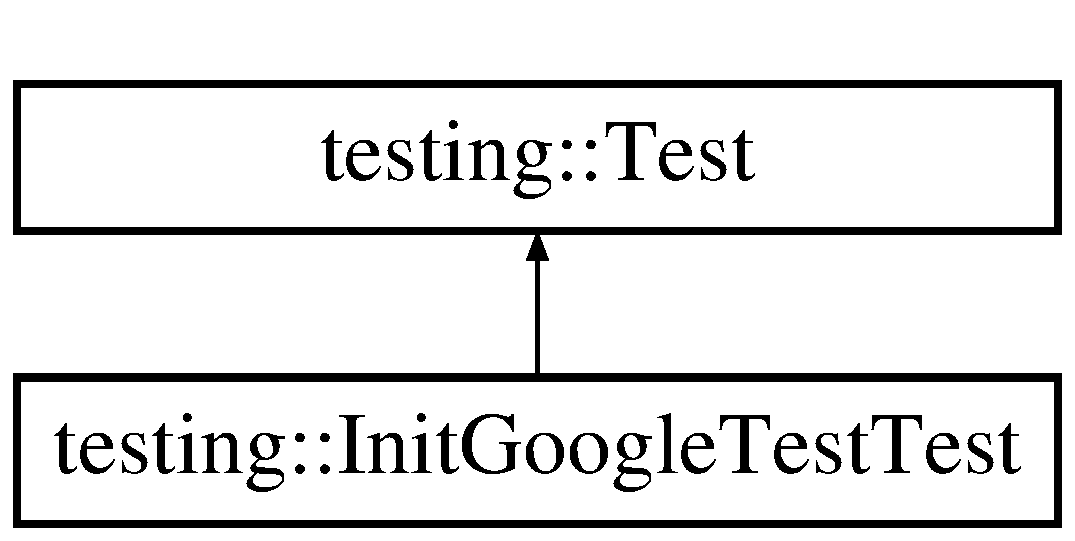
\includegraphics[height=2.000000cm]{classtesting_1_1_init_google_test_test}
\end{center}
\end{figure}
\subsection*{Protected Member Functions}
\begin{DoxyCompactItemize}
\item 
virtual void \hyperlink{classtesting_1_1_init_google_test_test_a49de9e552ea788c4b79924ec4135ca7a}{Set\+Up} ()
\end{DoxyCompactItemize}
\subsection*{Static Protected Member Functions}
\begin{DoxyCompactItemize}
\item 
{\footnotesize template$<$typename Char\+Type $>$ }\\static void \hyperlink{classtesting_1_1_init_google_test_test_af32acd91b1185c6868072009dce55a7b}{Assert\+String\+Array\+Eq} (size\+\_\+t size1, Char\+Type $\ast$$\ast$array1, size\+\_\+t size2, Char\+Type $\ast$$\ast$array2)
\item 
static void \hyperlink{classtesting_1_1_init_google_test_test_aac37d5d592202bf6614b02fe0b4da9d2}{Check\+Flags} (const \hyperlink{structtesting_1_1_flags}{Flags} \&expected)
\item 
{\footnotesize template$<$typename Char\+Type $>$ }\\static void \hyperlink{classtesting_1_1_init_google_test_test_add290338cf429308d0ab275ae4c46e69}{Test\+Parsing\+Flags} (int argc1, const Char\+Type $\ast$$\ast$argv1, int argc2, const Char\+Type $\ast$$\ast$argv2, const \hyperlink{structtesting_1_1_flags}{Flags} \&expected, bool should\+\_\+print\+\_\+help)
\end{DoxyCompactItemize}
\subsection*{Additional Inherited Members}


\subsection{Member Function Documentation}
\hypertarget{classtesting_1_1_init_google_test_test_af32acd91b1185c6868072009dce55a7b}{}\index{testing\+::\+Init\+Google\+Test\+Test@{testing\+::\+Init\+Google\+Test\+Test}!Assert\+String\+Array\+Eq@{Assert\+String\+Array\+Eq}}
\index{Assert\+String\+Array\+Eq@{Assert\+String\+Array\+Eq}!testing\+::\+Init\+Google\+Test\+Test@{testing\+::\+Init\+Google\+Test\+Test}}
\subsubsection[{Assert\+String\+Array\+Eq(size\+\_\+t size1, Char\+Type $\ast$$\ast$array1, size\+\_\+t size2, Char\+Type $\ast$$\ast$array2)}]{\setlength{\rightskip}{0pt plus 5cm}template$<$typename Char\+Type $>$ static void testing\+::\+Init\+Google\+Test\+Test\+::\+Assert\+String\+Array\+Eq (
\begin{DoxyParamCaption}
\item[{size\+\_\+t}]{size1, }
\item[{Char\+Type $\ast$$\ast$}]{array1, }
\item[{size\+\_\+t}]{size2, }
\item[{Char\+Type $\ast$$\ast$}]{array2}
\end{DoxyParamCaption}
)\hspace{0.3cm}{\ttfamily [inline]}, {\ttfamily [static]}, {\ttfamily [protected]}}\label{classtesting_1_1_init_google_test_test_af32acd91b1185c6868072009dce55a7b}
\hypertarget{classtesting_1_1_init_google_test_test_aac37d5d592202bf6614b02fe0b4da9d2}{}\index{testing\+::\+Init\+Google\+Test\+Test@{testing\+::\+Init\+Google\+Test\+Test}!Check\+Flags@{Check\+Flags}}
\index{Check\+Flags@{Check\+Flags}!testing\+::\+Init\+Google\+Test\+Test@{testing\+::\+Init\+Google\+Test\+Test}}
\subsubsection[{Check\+Flags(const Flags \&expected)}]{\setlength{\rightskip}{0pt plus 5cm}static void testing\+::\+Init\+Google\+Test\+Test\+::\+Check\+Flags (
\begin{DoxyParamCaption}
\item[{const {\bf Flags} \&}]{expected}
\end{DoxyParamCaption}
)\hspace{0.3cm}{\ttfamily [inline]}, {\ttfamily [static]}, {\ttfamily [protected]}}\label{classtesting_1_1_init_google_test_test_aac37d5d592202bf6614b02fe0b4da9d2}
\hypertarget{classtesting_1_1_init_google_test_test_a49de9e552ea788c4b79924ec4135ca7a}{}\index{testing\+::\+Init\+Google\+Test\+Test@{testing\+::\+Init\+Google\+Test\+Test}!Set\+Up@{Set\+Up}}
\index{Set\+Up@{Set\+Up}!testing\+::\+Init\+Google\+Test\+Test@{testing\+::\+Init\+Google\+Test\+Test}}
\subsubsection[{Set\+Up()}]{\setlength{\rightskip}{0pt plus 5cm}virtual void testing\+::\+Init\+Google\+Test\+Test\+::\+Set\+Up (
\begin{DoxyParamCaption}
{}
\end{DoxyParamCaption}
)\hspace{0.3cm}{\ttfamily [inline]}, {\ttfamily [protected]}, {\ttfamily [virtual]}}\label{classtesting_1_1_init_google_test_test_a49de9e552ea788c4b79924ec4135ca7a}


Reimplemented from \hyperlink{classtesting_1_1_test_a190315150c303ddf801313fd1a777733}{testing\+::\+Test}.

\hypertarget{classtesting_1_1_init_google_test_test_add290338cf429308d0ab275ae4c46e69}{}\index{testing\+::\+Init\+Google\+Test\+Test@{testing\+::\+Init\+Google\+Test\+Test}!Test\+Parsing\+Flags@{Test\+Parsing\+Flags}}
\index{Test\+Parsing\+Flags@{Test\+Parsing\+Flags}!testing\+::\+Init\+Google\+Test\+Test@{testing\+::\+Init\+Google\+Test\+Test}}
\subsubsection[{Test\+Parsing\+Flags(int argc1, const Char\+Type $\ast$$\ast$argv1, int argc2, const Char\+Type $\ast$$\ast$argv2, const Flags \&expected, bool should\+\_\+print\+\_\+help)}]{\setlength{\rightskip}{0pt plus 5cm}template$<$typename Char\+Type $>$ static void testing\+::\+Init\+Google\+Test\+Test\+::\+Test\+Parsing\+Flags (
\begin{DoxyParamCaption}
\item[{int}]{argc1, }
\item[{const Char\+Type $\ast$$\ast$}]{argv1, }
\item[{int}]{argc2, }
\item[{const Char\+Type $\ast$$\ast$}]{argv2, }
\item[{const {\bf Flags} \&}]{expected, }
\item[{bool}]{should\+\_\+print\+\_\+help}
\end{DoxyParamCaption}
)\hspace{0.3cm}{\ttfamily [inline]}, {\ttfamily [static]}, {\ttfamily [protected]}}\label{classtesting_1_1_init_google_test_test_add290338cf429308d0ab275ae4c46e69}


The documentation for this class was generated from the following file\+:\begin{DoxyCompactItemize}
\item 
C\+:/\+Users/\+Hilman/\+Desktop/repo/anjing/src/third\+\_\+party/googletest/test/\hyperlink{gtest__unittest_8cc}{gtest\+\_\+unittest.\+cc}\end{DoxyCompactItemize}

\hypertarget{class_integer_function_test}{}\section{Integer\+Function\+Test Class Reference}
\label{class_integer_function_test}\index{Integer\+Function\+Test@{Integer\+Function\+Test}}
Inheritance diagram for Integer\+Function\+Test\+:\begin{figure}[H]
\begin{center}
\leavevmode
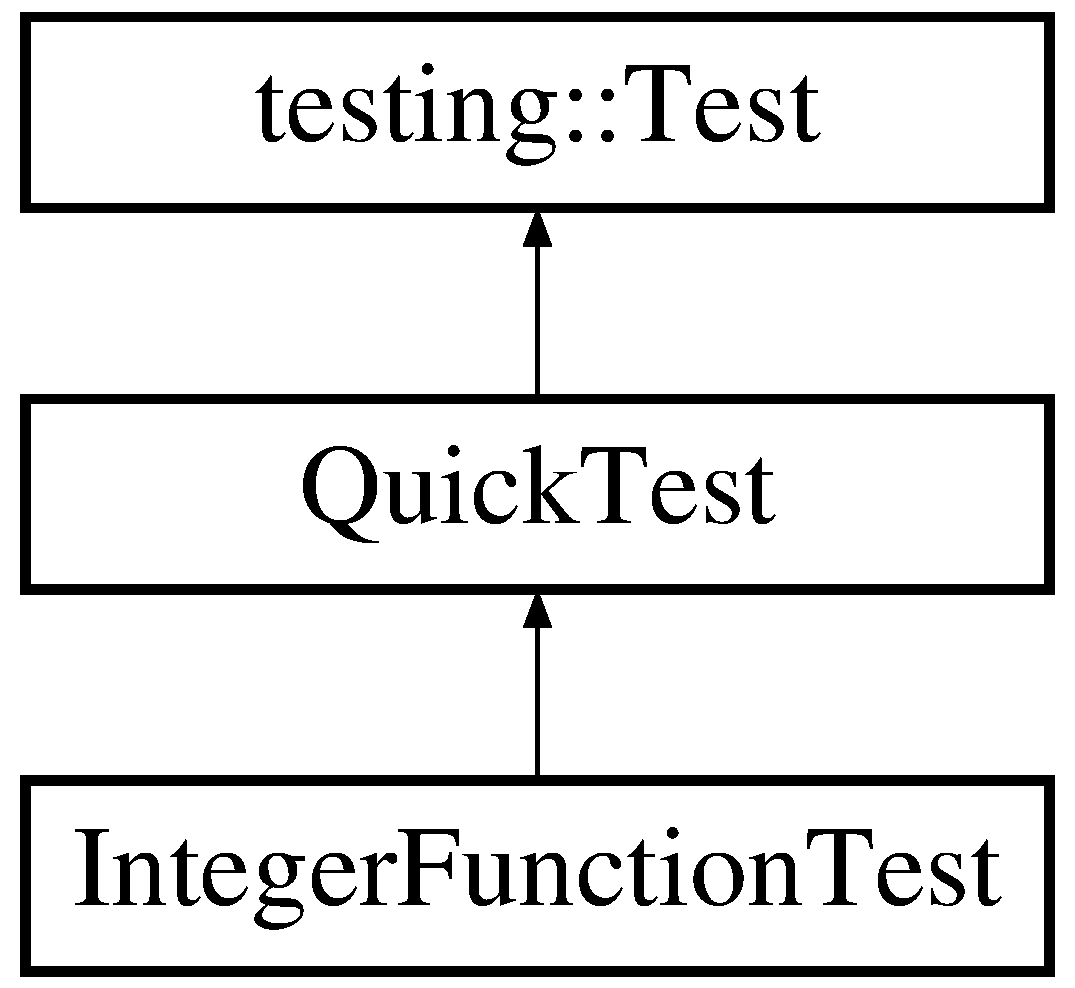
\includegraphics[height=3.000000cm]{class_integer_function_test}
\end{center}
\end{figure}
\subsection*{Additional Inherited Members}


The documentation for this class was generated from the following file\+:\begin{DoxyCompactItemize}
\item 
C\+:/\+Users/\+Hilman/\+Desktop/repo/anjing/src/third\+\_\+party/googletest/samples/\hyperlink{sample5__unittest_8cc}{sample5\+\_\+unittest.\+cc}\end{DoxyCompactItemize}

\hypertarget{structtesting_1_1internal_1_1is__pointer}{}\section{testing\+:\+:internal\+:\+:is\+\_\+pointer$<$ T $>$ Struct Template Reference}
\label{structtesting_1_1internal_1_1is__pointer}\index{testing\+::internal\+::is\+\_\+pointer$<$ T $>$@{testing\+::internal\+::is\+\_\+pointer$<$ T $>$}}


{\ttfamily \#include $<$gtest-\/port.\+h$>$}

Inheritance diagram for testing\+:\+:internal\+:\+:is\+\_\+pointer$<$ T $>$\+:\begin{figure}[H]
\begin{center}
\leavevmode
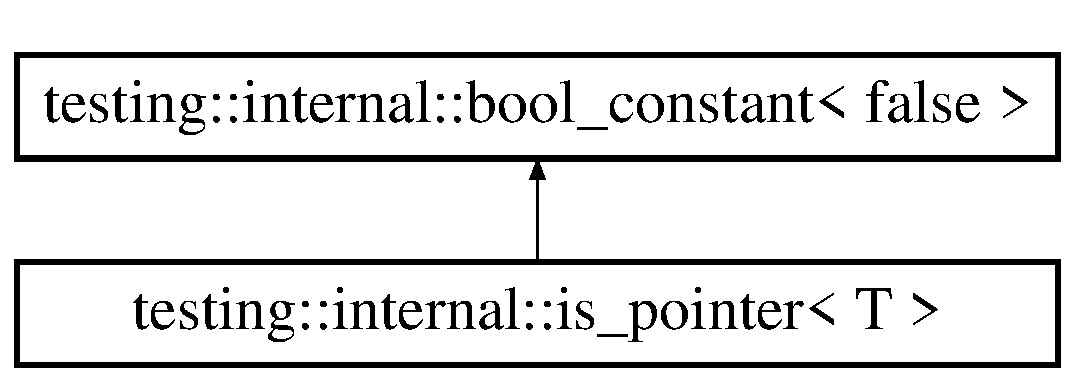
\includegraphics[height=2.000000cm]{structtesting_1_1internal_1_1is__pointer}
\end{center}
\end{figure}
\subsection*{Additional Inherited Members}


The documentation for this struct was generated from the following file\+:\begin{DoxyCompactItemize}
\item 
C\+:/\+Users/\+Hilman/\+Desktop/repo/anjing/src/third\+\_\+party/googletest/include/gtest/internal/\hyperlink{gtest-port_8h}{gtest-\/port.\+h}\end{DoxyCompactItemize}

\hypertarget{structtesting_1_1internal_1_1is__pointer_3_01_t_01_5_01_4}{}\section{testing\+:\+:internal\+:\+:is\+\_\+pointer$<$ T $\ast$ $>$ Struct Template Reference}
\label{structtesting_1_1internal_1_1is__pointer_3_01_t_01_5_01_4}\index{testing\+::internal\+::is\+\_\+pointer$<$ T $\ast$ $>$@{testing\+::internal\+::is\+\_\+pointer$<$ T $\ast$ $>$}}


{\ttfamily \#include $<$gtest-\/port.\+h$>$}

Inheritance diagram for testing\+:\+:internal\+:\+:is\+\_\+pointer$<$ T $\ast$ $>$\+:\begin{figure}[H]
\begin{center}
\leavevmode
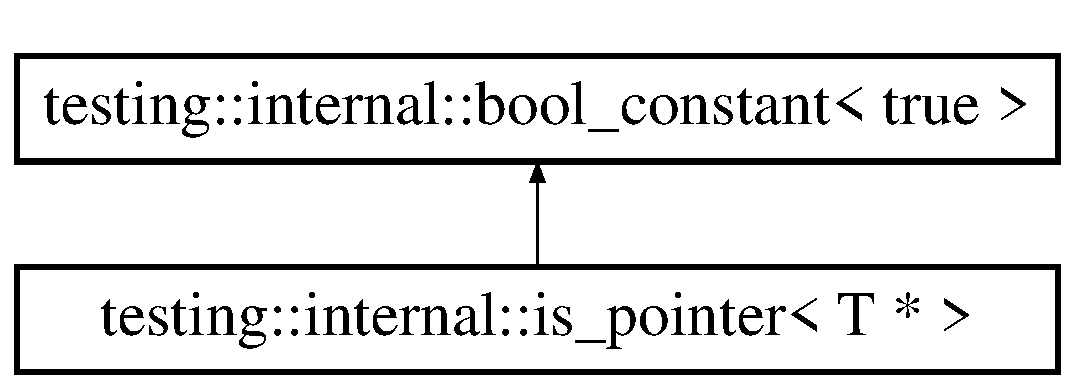
\includegraphics[height=2.000000cm]{structtesting_1_1internal_1_1is__pointer_3_01_t_01_5_01_4}
\end{center}
\end{figure}
\subsection*{Additional Inherited Members}


The documentation for this struct was generated from the following file\+:\begin{DoxyCompactItemize}
\item 
C\+:/\+Users/\+Hilman/\+Desktop/repo/anjing/src/third\+\_\+party/googletest/include/gtest/internal/\hyperlink{gtest-port_8h}{gtest-\/port.\+h}\end{DoxyCompactItemize}

\hypertarget{structtesting_1_1internal_1_1_is_a_protocol_message}{}\section{testing\+:\+:internal\+:\+:Is\+A\+Protocol\+Message$<$ T $>$ Struct Template Reference}
\label{structtesting_1_1internal_1_1_is_a_protocol_message}\index{testing\+::internal\+::\+Is\+A\+Protocol\+Message$<$ T $>$@{testing\+::internal\+::\+Is\+A\+Protocol\+Message$<$ T $>$}}


{\ttfamily \#include $<$gtest-\/internal.\+h$>$}

Inheritance diagram for testing\+:\+:internal\+:\+:Is\+A\+Protocol\+Message$<$ T $>$\+:\begin{figure}[H]
\begin{center}
\leavevmode
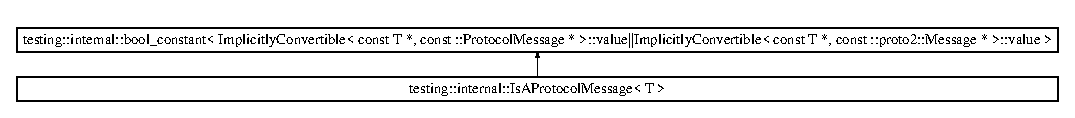
\includegraphics[height=1.132457cm]{structtesting_1_1internal_1_1_is_a_protocol_message}
\end{center}
\end{figure}
\subsection*{Additional Inherited Members}


The documentation for this struct was generated from the following file\+:\begin{DoxyCompactItemize}
\item 
C\+:/\+Users/\+Hilman/\+Desktop/repo/anjing/src/third\+\_\+party/googletest/include/gtest/internal/\hyperlink{gtest-internal_8h}{gtest-\/internal.\+h}\end{DoxyCompactItemize}

\hypertarget{structtesting_1_1gtest__printers__test_1_1iterator}{}\section{testing\+:\+:gtest\+\_\+printers\+\_\+test\+:\+:iterator Struct Reference}
\label{structtesting_1_1gtest__printers__test_1_1iterator}\index{testing\+::gtest\+\_\+printers\+\_\+test\+::iterator@{testing\+::gtest\+\_\+printers\+\_\+test\+::iterator}}
\subsection*{Public Attributes}
\begin{DoxyCompactItemize}
\item 
char \hyperlink{structtesting_1_1gtest__printers__test_1_1iterator_a3d4d056077d3b3869259bdfd60a0778f}{x}
\end{DoxyCompactItemize}


\subsection{Member Data Documentation}
\hypertarget{structtesting_1_1gtest__printers__test_1_1iterator_a3d4d056077d3b3869259bdfd60a0778f}{}\index{testing\+::gtest\+\_\+printers\+\_\+test\+::iterator@{testing\+::gtest\+\_\+printers\+\_\+test\+::iterator}!x@{x}}
\index{x@{x}!testing\+::gtest\+\_\+printers\+\_\+test\+::iterator@{testing\+::gtest\+\_\+printers\+\_\+test\+::iterator}}
\subsubsection[{x}]{\setlength{\rightskip}{0pt plus 5cm}char testing\+::gtest\+\_\+printers\+\_\+test\+::iterator\+::x}\label{structtesting_1_1gtest__printers__test_1_1iterator_a3d4d056077d3b3869259bdfd60a0778f}


The documentation for this struct was generated from the following file\+:\begin{DoxyCompactItemize}
\item 
C\+:/\+Users/\+Hilman/\+Desktop/repo/anjing/src/third\+\_\+party/googletest/test/\hyperlink{gtest-printers__test_8cc}{gtest-\/printers\+\_\+test.\+cc}\end{DoxyCompactItemize}

\hypertarget{structtesting_1_1internal_1_1_iterator_traits}{}\section{testing\+:\+:internal\+:\+:Iterator\+Traits$<$ Iterator $>$ Struct Template Reference}
\label{structtesting_1_1internal_1_1_iterator_traits}\index{testing\+::internal\+::\+Iterator\+Traits$<$ Iterator $>$@{testing\+::internal\+::\+Iterator\+Traits$<$ Iterator $>$}}


{\ttfamily \#include $<$gtest-\/port.\+h$>$}

\subsection*{Public Types}
\begin{DoxyCompactItemize}
\item 
typedef Iterator\+::value\+\_\+type \hyperlink{structtesting_1_1internal_1_1_iterator_traits_a29de4320a9c53ce438d3561b94e515bb}{value\+\_\+type}
\end{DoxyCompactItemize}


\subsection{Member Typedef Documentation}
\hypertarget{structtesting_1_1internal_1_1_iterator_traits_a29de4320a9c53ce438d3561b94e515bb}{}\index{testing\+::internal\+::\+Iterator\+Traits@{testing\+::internal\+::\+Iterator\+Traits}!value\+\_\+type@{value\+\_\+type}}
\index{value\+\_\+type@{value\+\_\+type}!testing\+::internal\+::\+Iterator\+Traits@{testing\+::internal\+::\+Iterator\+Traits}}
\subsubsection[{value\+\_\+type}]{\setlength{\rightskip}{0pt plus 5cm}template$<$typename Iterator $>$ typedef Iterator\+::value\+\_\+type {\bf testing\+::internal\+::\+Iterator\+Traits}$<$ Iterator $>$\+::{\bf value\+\_\+type}}\label{structtesting_1_1internal_1_1_iterator_traits_a29de4320a9c53ce438d3561b94e515bb}


The documentation for this struct was generated from the following file\+:\begin{DoxyCompactItemize}
\item 
C\+:/\+Users/\+Hilman/\+Desktop/repo/anjing/src/third\+\_\+party/googletest/include/gtest/internal/\hyperlink{gtest-port_8h}{gtest-\/port.\+h}\end{DoxyCompactItemize}

\hypertarget{structtesting_1_1internal_1_1_iterator_traits_3_01const_01_t_01_5_01_4}{}\section{testing\+:\+:internal\+:\+:Iterator\+Traits$<$ const T $\ast$ $>$ Struct Template Reference}
\label{structtesting_1_1internal_1_1_iterator_traits_3_01const_01_t_01_5_01_4}\index{testing\+::internal\+::\+Iterator\+Traits$<$ const T $\ast$ $>$@{testing\+::internal\+::\+Iterator\+Traits$<$ const T $\ast$ $>$}}


{\ttfamily \#include $<$gtest-\/port.\+h$>$}

\subsection*{Public Types}
\begin{DoxyCompactItemize}
\item 
typedef T \hyperlink{structtesting_1_1internal_1_1_iterator_traits_3_01const_01_t_01_5_01_4_ae7c8867223e106f374b56a7dc4a85547}{value\+\_\+type}
\end{DoxyCompactItemize}


\subsection{Member Typedef Documentation}
\hypertarget{structtesting_1_1internal_1_1_iterator_traits_3_01const_01_t_01_5_01_4_ae7c8867223e106f374b56a7dc4a85547}{}\index{testing\+::internal\+::\+Iterator\+Traits$<$ const T $\ast$ $>$@{testing\+::internal\+::\+Iterator\+Traits$<$ const T $\ast$ $>$}!value\+\_\+type@{value\+\_\+type}}
\index{value\+\_\+type@{value\+\_\+type}!testing\+::internal\+::\+Iterator\+Traits$<$ const T $\ast$ $>$@{testing\+::internal\+::\+Iterator\+Traits$<$ const T $\ast$ $>$}}
\subsubsection[{value\+\_\+type}]{\setlength{\rightskip}{0pt plus 5cm}template$<$typename T $>$ typedef T {\bf testing\+::internal\+::\+Iterator\+Traits}$<$ const T $\ast$ $>$\+::{\bf value\+\_\+type}}\label{structtesting_1_1internal_1_1_iterator_traits_3_01const_01_t_01_5_01_4_ae7c8867223e106f374b56a7dc4a85547}


The documentation for this struct was generated from the following file\+:\begin{DoxyCompactItemize}
\item 
C\+:/\+Users/\+Hilman/\+Desktop/repo/anjing/src/third\+\_\+party/googletest/include/gtest/internal/\hyperlink{gtest-port_8h}{gtest-\/port.\+h}\end{DoxyCompactItemize}

\hypertarget{structtesting_1_1internal_1_1_iterator_traits_3_01_t_01_5_01_4}{}\section{testing\+:\+:internal\+:\+:Iterator\+Traits$<$ T $\ast$ $>$ Struct Template Reference}
\label{structtesting_1_1internal_1_1_iterator_traits_3_01_t_01_5_01_4}\index{testing\+::internal\+::\+Iterator\+Traits$<$ T $\ast$ $>$@{testing\+::internal\+::\+Iterator\+Traits$<$ T $\ast$ $>$}}


{\ttfamily \#include $<$gtest-\/port.\+h$>$}

\subsection*{Public Types}
\begin{DoxyCompactItemize}
\item 
typedef T \hyperlink{structtesting_1_1internal_1_1_iterator_traits_3_01_t_01_5_01_4_a7e46869ed36cc5aea898e243d270a8be}{value\+\_\+type}
\end{DoxyCompactItemize}


\subsection{Member Typedef Documentation}
\hypertarget{structtesting_1_1internal_1_1_iterator_traits_3_01_t_01_5_01_4_a7e46869ed36cc5aea898e243d270a8be}{}\index{testing\+::internal\+::\+Iterator\+Traits$<$ T $\ast$ $>$@{testing\+::internal\+::\+Iterator\+Traits$<$ T $\ast$ $>$}!value\+\_\+type@{value\+\_\+type}}
\index{value\+\_\+type@{value\+\_\+type}!testing\+::internal\+::\+Iterator\+Traits$<$ T $\ast$ $>$@{testing\+::internal\+::\+Iterator\+Traits$<$ T $\ast$ $>$}}
\subsubsection[{value\+\_\+type}]{\setlength{\rightskip}{0pt plus 5cm}template$<$typename T $>$ typedef T {\bf testing\+::internal\+::\+Iterator\+Traits}$<$ T $\ast$ $>$\+::{\bf value\+\_\+type}}\label{structtesting_1_1internal_1_1_iterator_traits_3_01_t_01_5_01_4_a7e46869ed36cc5aea898e243d270a8be}


The documentation for this struct was generated from the following file\+:\begin{DoxyCompactItemize}
\item 
C\+:/\+Users/\+Hilman/\+Desktop/repo/anjing/src/third\+\_\+party/googletest/include/gtest/internal/\hyperlink{gtest-port_8h}{gtest-\/port.\+h}\end{DoxyCompactItemize}

\hypertarget{structtesting_1_1internal_1_1_less_by_name}{}\section{testing\+:\+:internal\+:\+:Less\+By\+Name$<$ T $>$ Struct Template Reference}
\label{structtesting_1_1internal_1_1_less_by_name}\index{testing\+::internal\+::\+Less\+By\+Name$<$ T $>$@{testing\+::internal\+::\+Less\+By\+Name$<$ T $>$}}
\subsection*{Public Member Functions}
\begin{DoxyCompactItemize}
\item 
bool \hyperlink{structtesting_1_1internal_1_1_less_by_name_a62386ac7750bfc035536be55d90a52eb}{operator()} (const T $\ast$a, const T $\ast$b)
\end{DoxyCompactItemize}


\subsection{Member Function Documentation}
\hypertarget{structtesting_1_1internal_1_1_less_by_name_a62386ac7750bfc035536be55d90a52eb}{}\index{testing\+::internal\+::\+Less\+By\+Name@{testing\+::internal\+::\+Less\+By\+Name}!operator()@{operator()}}
\index{operator()@{operator()}!testing\+::internal\+::\+Less\+By\+Name@{testing\+::internal\+::\+Less\+By\+Name}}
\subsubsection[{operator()(const T $\ast$a, const T $\ast$b)}]{\setlength{\rightskip}{0pt plus 5cm}template$<$typename T $>$ bool {\bf testing\+::internal\+::\+Less\+By\+Name}$<$ T $>$\+::operator() (
\begin{DoxyParamCaption}
\item[{const T $\ast$}]{a, }
\item[{const T $\ast$}]{b}
\end{DoxyParamCaption}
)\hspace{0.3cm}{\ttfamily [inline]}}\label{structtesting_1_1internal_1_1_less_by_name_a62386ac7750bfc035536be55d90a52eb}


The documentation for this struct was generated from the following file\+:\begin{DoxyCompactItemize}
\item 
C\+:/\+Users/\+Hilman/\+Desktop/repo/anjing/src/third\+\_\+party/googletest/test/\hyperlink{gtest-unittest-api__test_8cc}{gtest-\/unittest-\/api\+\_\+test.\+cc}\end{DoxyCompactItemize}

\hypertarget{classtesting_1_1internal_1_1linked__ptr}{}\section{testing\+:\+:internal\+:\+:linked\+\_\+ptr$<$ T $>$ Class Template Reference}
\label{classtesting_1_1internal_1_1linked__ptr}\index{testing\+::internal\+::linked\+\_\+ptr$<$ T $>$@{testing\+::internal\+::linked\+\_\+ptr$<$ T $>$}}


{\ttfamily \#include $<$gtest-\/linked\+\_\+ptr.\+h$>$}

\subsection*{Public Types}
\begin{DoxyCompactItemize}
\item 
typedef T \hyperlink{classtesting_1_1internal_1_1linked__ptr_a295c7d1ee4100d916514c4e4385a0063}{element\+\_\+type}
\end{DoxyCompactItemize}
\subsection*{Public Member Functions}
\begin{DoxyCompactItemize}
\item 
\hyperlink{classtesting_1_1internal_1_1linked__ptr_ae805418b9f03f14ff49649e710475dba}{linked\+\_\+ptr} (T $\ast$ptr=N\+U\+L\+L)
\item 
\hyperlink{classtesting_1_1internal_1_1linked__ptr_af99460fd09ca0f83e061ea480ef1a45e}{$\sim$linked\+\_\+ptr} ()
\item 
{\footnotesize template$<$typename U $>$ }\\\hyperlink{classtesting_1_1internal_1_1linked__ptr_a7597ed91006edd0467c99bd1aaab07f5}{linked\+\_\+ptr} (\hyperlink{classtesting_1_1internal_1_1linked__ptr}{linked\+\_\+ptr}$<$ U $>$ const \&ptr)
\item 
\hyperlink{classtesting_1_1internal_1_1linked__ptr_abc076b5678cc7f64306d5ecfefc93aff}{linked\+\_\+ptr} (\hyperlink{classtesting_1_1internal_1_1linked__ptr}{linked\+\_\+ptr} const \&ptr)
\item 
{\footnotesize template$<$typename U $>$ }\\\hyperlink{classtesting_1_1internal_1_1linked__ptr}{linked\+\_\+ptr} \& \hyperlink{classtesting_1_1internal_1_1linked__ptr_a82608d98869b750d9ab729f1450a9a45}{operator=} (\hyperlink{classtesting_1_1internal_1_1linked__ptr}{linked\+\_\+ptr}$<$ U $>$ const \&ptr)
\item 
\hyperlink{classtesting_1_1internal_1_1linked__ptr}{linked\+\_\+ptr} \& \hyperlink{classtesting_1_1internal_1_1linked__ptr_a1f40b5e66e6cf7b661ea116c806f952e}{operator=} (\hyperlink{classtesting_1_1internal_1_1linked__ptr}{linked\+\_\+ptr} const \&ptr)
\item 
void \hyperlink{classtesting_1_1internal_1_1linked__ptr_a95ba3b7b66ed0193c779976c6e126ab6}{reset} (T $\ast$ptr=N\+U\+L\+L)
\item 
T $\ast$ \hyperlink{classtesting_1_1internal_1_1linked__ptr_a6ea8584d9bcad13c3266834f5ce5e771}{get} () const 
\item 
T $\ast$ \hyperlink{classtesting_1_1internal_1_1linked__ptr_aa878c3e874242fb3cd2aa14ec603aa25}{operator-\/$>$} () const 
\item 
T \& \hyperlink{classtesting_1_1internal_1_1linked__ptr_aec393cbd60f96defde36ef8a69d94254}{operator$\ast$} () const 
\item 
bool \hyperlink{classtesting_1_1internal_1_1linked__ptr_abe2154fd3ad3574dfe6f2320bc1debc4}{operator==} (T $\ast$p) const 
\item 
bool \hyperlink{classtesting_1_1internal_1_1linked__ptr_a3685f9661bbe410cfa58fea2f14396b7}{operator!=} (T $\ast$p) const 
\item 
{\footnotesize template$<$typename U $>$ }\\bool \hyperlink{classtesting_1_1internal_1_1linked__ptr_a3b46c9ecfd928673a524dcb3c70fd2ad}{operator==} (\hyperlink{classtesting_1_1internal_1_1linked__ptr}{linked\+\_\+ptr}$<$ U $>$ const \&ptr) const 
\item 
{\footnotesize template$<$typename U $>$ }\\bool \hyperlink{classtesting_1_1internal_1_1linked__ptr_a6449584b90a09a313300599fb3a23633}{operator!=} (\hyperlink{classtesting_1_1internal_1_1linked__ptr}{linked\+\_\+ptr}$<$ U $>$ const \&ptr) const 
\end{DoxyCompactItemize}
\subsection*{Friends}
\begin{DoxyCompactItemize}
\item 
{\footnotesize template$<$typename U $>$ }\\class \hyperlink{classtesting_1_1internal_1_1linked__ptr_a7763f286ca03a7f7363a033d996c8c1c}{linked\+\_\+ptr}
\end{DoxyCompactItemize}


\subsection{Member Typedef Documentation}
\hypertarget{classtesting_1_1internal_1_1linked__ptr_a295c7d1ee4100d916514c4e4385a0063}{}\index{testing\+::internal\+::linked\+\_\+ptr@{testing\+::internal\+::linked\+\_\+ptr}!element\+\_\+type@{element\+\_\+type}}
\index{element\+\_\+type@{element\+\_\+type}!testing\+::internal\+::linked\+\_\+ptr@{testing\+::internal\+::linked\+\_\+ptr}}
\subsubsection[{element\+\_\+type}]{\setlength{\rightskip}{0pt plus 5cm}template$<$typename T$>$ typedef T {\bf testing\+::internal\+::linked\+\_\+ptr}$<$ T $>$\+::{\bf element\+\_\+type}}\label{classtesting_1_1internal_1_1linked__ptr_a295c7d1ee4100d916514c4e4385a0063}


\subsection{Constructor \& Destructor Documentation}
\hypertarget{classtesting_1_1internal_1_1linked__ptr_ae805418b9f03f14ff49649e710475dba}{}\index{testing\+::internal\+::linked\+\_\+ptr@{testing\+::internal\+::linked\+\_\+ptr}!linked\+\_\+ptr@{linked\+\_\+ptr}}
\index{linked\+\_\+ptr@{linked\+\_\+ptr}!testing\+::internal\+::linked\+\_\+ptr@{testing\+::internal\+::linked\+\_\+ptr}}
\subsubsection[{linked\+\_\+ptr(\+T $\ast$ptr=\+N\+U\+L\+L)}]{\setlength{\rightskip}{0pt plus 5cm}template$<$typename T$>$ {\bf testing\+::internal\+::linked\+\_\+ptr}$<$ T $>$\+::{\bf linked\+\_\+ptr} (
\begin{DoxyParamCaption}
\item[{T $\ast$}]{ptr = {\ttfamily NULL}}
\end{DoxyParamCaption}
)\hspace{0.3cm}{\ttfamily [inline]}, {\ttfamily [explicit]}}\label{classtesting_1_1internal_1_1linked__ptr_ae805418b9f03f14ff49649e710475dba}
\hypertarget{classtesting_1_1internal_1_1linked__ptr_af99460fd09ca0f83e061ea480ef1a45e}{}\index{testing\+::internal\+::linked\+\_\+ptr@{testing\+::internal\+::linked\+\_\+ptr}!````~linked\+\_\+ptr@{$\sim$linked\+\_\+ptr}}
\index{````~linked\+\_\+ptr@{$\sim$linked\+\_\+ptr}!testing\+::internal\+::linked\+\_\+ptr@{testing\+::internal\+::linked\+\_\+ptr}}
\subsubsection[{$\sim$linked\+\_\+ptr()}]{\setlength{\rightskip}{0pt plus 5cm}template$<$typename T$>$ {\bf testing\+::internal\+::linked\+\_\+ptr}$<$ T $>$\+::$\sim${\bf linked\+\_\+ptr} (
\begin{DoxyParamCaption}
{}
\end{DoxyParamCaption}
)\hspace{0.3cm}{\ttfamily [inline]}}\label{classtesting_1_1internal_1_1linked__ptr_af99460fd09ca0f83e061ea480ef1a45e}
\hypertarget{classtesting_1_1internal_1_1linked__ptr_a7597ed91006edd0467c99bd1aaab07f5}{}\index{testing\+::internal\+::linked\+\_\+ptr@{testing\+::internal\+::linked\+\_\+ptr}!linked\+\_\+ptr@{linked\+\_\+ptr}}
\index{linked\+\_\+ptr@{linked\+\_\+ptr}!testing\+::internal\+::linked\+\_\+ptr@{testing\+::internal\+::linked\+\_\+ptr}}
\subsubsection[{linked\+\_\+ptr(linked\+\_\+ptr$<$ U $>$ const \&ptr)}]{\setlength{\rightskip}{0pt plus 5cm}template$<$typename T$>$ template$<$typename U $>$ {\bf testing\+::internal\+::linked\+\_\+ptr}$<$ T $>$\+::{\bf linked\+\_\+ptr} (
\begin{DoxyParamCaption}
\item[{{\bf linked\+\_\+ptr}$<$ U $>$ const \&}]{ptr}
\end{DoxyParamCaption}
)\hspace{0.3cm}{\ttfamily [inline]}}\label{classtesting_1_1internal_1_1linked__ptr_a7597ed91006edd0467c99bd1aaab07f5}
\hypertarget{classtesting_1_1internal_1_1linked__ptr_abc076b5678cc7f64306d5ecfefc93aff}{}\index{testing\+::internal\+::linked\+\_\+ptr@{testing\+::internal\+::linked\+\_\+ptr}!linked\+\_\+ptr@{linked\+\_\+ptr}}
\index{linked\+\_\+ptr@{linked\+\_\+ptr}!testing\+::internal\+::linked\+\_\+ptr@{testing\+::internal\+::linked\+\_\+ptr}}
\subsubsection[{linked\+\_\+ptr(linked\+\_\+ptr const \&ptr)}]{\setlength{\rightskip}{0pt plus 5cm}template$<$typename T$>$ {\bf testing\+::internal\+::linked\+\_\+ptr}$<$ T $>$\+::{\bf linked\+\_\+ptr} (
\begin{DoxyParamCaption}
\item[{{\bf linked\+\_\+ptr}$<$ T $>$ const \&}]{ptr}
\end{DoxyParamCaption}
)\hspace{0.3cm}{\ttfamily [inline]}}\label{classtesting_1_1internal_1_1linked__ptr_abc076b5678cc7f64306d5ecfefc93aff}


\subsection{Member Function Documentation}
\hypertarget{classtesting_1_1internal_1_1linked__ptr_a6ea8584d9bcad13c3266834f5ce5e771}{}\index{testing\+::internal\+::linked\+\_\+ptr@{testing\+::internal\+::linked\+\_\+ptr}!get@{get}}
\index{get@{get}!testing\+::internal\+::linked\+\_\+ptr@{testing\+::internal\+::linked\+\_\+ptr}}
\subsubsection[{get() const }]{\setlength{\rightskip}{0pt plus 5cm}template$<$typename T$>$ T$\ast$ {\bf testing\+::internal\+::linked\+\_\+ptr}$<$ T $>$\+::get (
\begin{DoxyParamCaption}
{}
\end{DoxyParamCaption}
) const\hspace{0.3cm}{\ttfamily [inline]}}\label{classtesting_1_1internal_1_1linked__ptr_a6ea8584d9bcad13c3266834f5ce5e771}
\hypertarget{classtesting_1_1internal_1_1linked__ptr_a3685f9661bbe410cfa58fea2f14396b7}{}\index{testing\+::internal\+::linked\+\_\+ptr@{testing\+::internal\+::linked\+\_\+ptr}!operator"!=@{operator"!=}}
\index{operator"!=@{operator"!=}!testing\+::internal\+::linked\+\_\+ptr@{testing\+::internal\+::linked\+\_\+ptr}}
\subsubsection[{operator"!=(\+T $\ast$p) const }]{\setlength{\rightskip}{0pt plus 5cm}template$<$typename T$>$ bool {\bf testing\+::internal\+::linked\+\_\+ptr}$<$ T $>$\+::operator!= (
\begin{DoxyParamCaption}
\item[{T $\ast$}]{p}
\end{DoxyParamCaption}
) const\hspace{0.3cm}{\ttfamily [inline]}}\label{classtesting_1_1internal_1_1linked__ptr_a3685f9661bbe410cfa58fea2f14396b7}
\hypertarget{classtesting_1_1internal_1_1linked__ptr_a6449584b90a09a313300599fb3a23633}{}\index{testing\+::internal\+::linked\+\_\+ptr@{testing\+::internal\+::linked\+\_\+ptr}!operator"!=@{operator"!=}}
\index{operator"!=@{operator"!=}!testing\+::internal\+::linked\+\_\+ptr@{testing\+::internal\+::linked\+\_\+ptr}}
\subsubsection[{operator"!=(linked\+\_\+ptr$<$ U $>$ const \&ptr) const }]{\setlength{\rightskip}{0pt plus 5cm}template$<$typename T$>$ template$<$typename U $>$ bool {\bf testing\+::internal\+::linked\+\_\+ptr}$<$ T $>$\+::operator!= (
\begin{DoxyParamCaption}
\item[{{\bf linked\+\_\+ptr}$<$ U $>$ const \&}]{ptr}
\end{DoxyParamCaption}
) const\hspace{0.3cm}{\ttfamily [inline]}}\label{classtesting_1_1internal_1_1linked__ptr_a6449584b90a09a313300599fb3a23633}
\hypertarget{classtesting_1_1internal_1_1linked__ptr_aec393cbd60f96defde36ef8a69d94254}{}\index{testing\+::internal\+::linked\+\_\+ptr@{testing\+::internal\+::linked\+\_\+ptr}!operator$\ast$@{operator$\ast$}}
\index{operator$\ast$@{operator$\ast$}!testing\+::internal\+::linked\+\_\+ptr@{testing\+::internal\+::linked\+\_\+ptr}}
\subsubsection[{operator$\ast$() const }]{\setlength{\rightskip}{0pt plus 5cm}template$<$typename T$>$ T\& {\bf testing\+::internal\+::linked\+\_\+ptr}$<$ T $>$\+::operator$\ast$ (
\begin{DoxyParamCaption}
{}
\end{DoxyParamCaption}
) const\hspace{0.3cm}{\ttfamily [inline]}}\label{classtesting_1_1internal_1_1linked__ptr_aec393cbd60f96defde36ef8a69d94254}
\hypertarget{classtesting_1_1internal_1_1linked__ptr_aa878c3e874242fb3cd2aa14ec603aa25}{}\index{testing\+::internal\+::linked\+\_\+ptr@{testing\+::internal\+::linked\+\_\+ptr}!operator-\/$>$@{operator-\/$>$}}
\index{operator-\/$>$@{operator-\/$>$}!testing\+::internal\+::linked\+\_\+ptr@{testing\+::internal\+::linked\+\_\+ptr}}
\subsubsection[{operator-\/$>$() const }]{\setlength{\rightskip}{0pt plus 5cm}template$<$typename T$>$ T$\ast$ {\bf testing\+::internal\+::linked\+\_\+ptr}$<$ T $>$\+::operator-\/$>$ (
\begin{DoxyParamCaption}
{}
\end{DoxyParamCaption}
) const\hspace{0.3cm}{\ttfamily [inline]}}\label{classtesting_1_1internal_1_1linked__ptr_aa878c3e874242fb3cd2aa14ec603aa25}
\hypertarget{classtesting_1_1internal_1_1linked__ptr_a82608d98869b750d9ab729f1450a9a45}{}\index{testing\+::internal\+::linked\+\_\+ptr@{testing\+::internal\+::linked\+\_\+ptr}!operator=@{operator=}}
\index{operator=@{operator=}!testing\+::internal\+::linked\+\_\+ptr@{testing\+::internal\+::linked\+\_\+ptr}}
\subsubsection[{operator=(linked\+\_\+ptr$<$ U $>$ const \&ptr)}]{\setlength{\rightskip}{0pt plus 5cm}template$<$typename T$>$ template$<$typename U $>$ {\bf linked\+\_\+ptr}\& {\bf testing\+::internal\+::linked\+\_\+ptr}$<$ T $>$\+::operator= (
\begin{DoxyParamCaption}
\item[{{\bf linked\+\_\+ptr}$<$ U $>$ const \&}]{ptr}
\end{DoxyParamCaption}
)\hspace{0.3cm}{\ttfamily [inline]}}\label{classtesting_1_1internal_1_1linked__ptr_a82608d98869b750d9ab729f1450a9a45}
\hypertarget{classtesting_1_1internal_1_1linked__ptr_a1f40b5e66e6cf7b661ea116c806f952e}{}\index{testing\+::internal\+::linked\+\_\+ptr@{testing\+::internal\+::linked\+\_\+ptr}!operator=@{operator=}}
\index{operator=@{operator=}!testing\+::internal\+::linked\+\_\+ptr@{testing\+::internal\+::linked\+\_\+ptr}}
\subsubsection[{operator=(linked\+\_\+ptr const \&ptr)}]{\setlength{\rightskip}{0pt plus 5cm}template$<$typename T$>$ {\bf linked\+\_\+ptr}\& {\bf testing\+::internal\+::linked\+\_\+ptr}$<$ T $>$\+::operator= (
\begin{DoxyParamCaption}
\item[{{\bf linked\+\_\+ptr}$<$ T $>$ const \&}]{ptr}
\end{DoxyParamCaption}
)\hspace{0.3cm}{\ttfamily [inline]}}\label{classtesting_1_1internal_1_1linked__ptr_a1f40b5e66e6cf7b661ea116c806f952e}
\hypertarget{classtesting_1_1internal_1_1linked__ptr_abe2154fd3ad3574dfe6f2320bc1debc4}{}\index{testing\+::internal\+::linked\+\_\+ptr@{testing\+::internal\+::linked\+\_\+ptr}!operator==@{operator==}}
\index{operator==@{operator==}!testing\+::internal\+::linked\+\_\+ptr@{testing\+::internal\+::linked\+\_\+ptr}}
\subsubsection[{operator==(\+T $\ast$p) const }]{\setlength{\rightskip}{0pt plus 5cm}template$<$typename T$>$ bool {\bf testing\+::internal\+::linked\+\_\+ptr}$<$ T $>$\+::operator== (
\begin{DoxyParamCaption}
\item[{T $\ast$}]{p}
\end{DoxyParamCaption}
) const\hspace{0.3cm}{\ttfamily [inline]}}\label{classtesting_1_1internal_1_1linked__ptr_abe2154fd3ad3574dfe6f2320bc1debc4}
\hypertarget{classtesting_1_1internal_1_1linked__ptr_a3b46c9ecfd928673a524dcb3c70fd2ad}{}\index{testing\+::internal\+::linked\+\_\+ptr@{testing\+::internal\+::linked\+\_\+ptr}!operator==@{operator==}}
\index{operator==@{operator==}!testing\+::internal\+::linked\+\_\+ptr@{testing\+::internal\+::linked\+\_\+ptr}}
\subsubsection[{operator==(linked\+\_\+ptr$<$ U $>$ const \&ptr) const }]{\setlength{\rightskip}{0pt plus 5cm}template$<$typename T$>$ template$<$typename U $>$ bool {\bf testing\+::internal\+::linked\+\_\+ptr}$<$ T $>$\+::operator== (
\begin{DoxyParamCaption}
\item[{{\bf linked\+\_\+ptr}$<$ U $>$ const \&}]{ptr}
\end{DoxyParamCaption}
) const\hspace{0.3cm}{\ttfamily [inline]}}\label{classtesting_1_1internal_1_1linked__ptr_a3b46c9ecfd928673a524dcb3c70fd2ad}
\hypertarget{classtesting_1_1internal_1_1linked__ptr_a95ba3b7b66ed0193c779976c6e126ab6}{}\index{testing\+::internal\+::linked\+\_\+ptr@{testing\+::internal\+::linked\+\_\+ptr}!reset@{reset}}
\index{reset@{reset}!testing\+::internal\+::linked\+\_\+ptr@{testing\+::internal\+::linked\+\_\+ptr}}
\subsubsection[{reset(\+T $\ast$ptr=\+N\+U\+L\+L)}]{\setlength{\rightskip}{0pt plus 5cm}template$<$typename T$>$ void {\bf testing\+::internal\+::linked\+\_\+ptr}$<$ T $>$\+::reset (
\begin{DoxyParamCaption}
\item[{T $\ast$}]{ptr = {\ttfamily NULL}}
\end{DoxyParamCaption}
)\hspace{0.3cm}{\ttfamily [inline]}}\label{classtesting_1_1internal_1_1linked__ptr_a95ba3b7b66ed0193c779976c6e126ab6}


\subsection{Friends And Related Function Documentation}
\hypertarget{classtesting_1_1internal_1_1linked__ptr_a7763f286ca03a7f7363a033d996c8c1c}{}\index{testing\+::internal\+::linked\+\_\+ptr@{testing\+::internal\+::linked\+\_\+ptr}!linked\+\_\+ptr@{linked\+\_\+ptr}}
\index{linked\+\_\+ptr@{linked\+\_\+ptr}!testing\+::internal\+::linked\+\_\+ptr@{testing\+::internal\+::linked\+\_\+ptr}}
\subsubsection[{linked\+\_\+ptr}]{\setlength{\rightskip}{0pt plus 5cm}template$<$typename T$>$ template$<$typename U $>$ friend class {\bf linked\+\_\+ptr}\hspace{0.3cm}{\ttfamily [friend]}}\label{classtesting_1_1internal_1_1linked__ptr_a7763f286ca03a7f7363a033d996c8c1c}


The documentation for this class was generated from the following file\+:\begin{DoxyCompactItemize}
\item 
C\+:/\+Users/\+Hilman/\+Desktop/repo/anjing/src/third\+\_\+party/googletest/include/gtest/internal/\hyperlink{gtest-linked__ptr_8h}{gtest-\/linked\+\_\+ptr.\+h}\end{DoxyCompactItemize}

\hypertarget{classtesting_1_1internal_1_1linked__ptr__internal}{}\section{testing\+:\+:internal\+:\+:linked\+\_\+ptr\+\_\+internal Class Reference}
\label{classtesting_1_1internal_1_1linked__ptr__internal}\index{testing\+::internal\+::linked\+\_\+ptr\+\_\+internal@{testing\+::internal\+::linked\+\_\+ptr\+\_\+internal}}


{\ttfamily \#include $<$gtest-\/linked\+\_\+ptr.\+h$>$}

\subsection*{Public Member Functions}
\begin{DoxyCompactItemize}
\item 
void \hyperlink{classtesting_1_1internal_1_1linked__ptr__internal_a742af1f65df2d5e2b7198a1b74264a83}{join\+\_\+new} ()
\item 
void \hyperlink{classtesting_1_1internal_1_1linked__ptr__internal_acd5a341459f7e81b10b4112d8c764e2a}{join} (\hyperlink{classtesting_1_1internal_1_1linked__ptr__internal}{linked\+\_\+ptr\+\_\+internal} const $\ast$ptr) \hyperlink{gtest-port_8h_a69abff5a4efdd07bd5faebe3dd318d06}{G\+T\+E\+S\+T\+\_\+\+L\+O\+C\+K\+\_\+\+E\+X\+C\+L\+U\+D\+E\+D\+\_\+}(g\+\_\+linked\+\_\+ptr\+\_\+mutex)
\item 
bool \hyperlink{classtesting_1_1internal_1_1linked__ptr__internal_a8699e539d9702d363ef0351012d1b3ca}{depart} () \hyperlink{gtest-port_8h_a69abff5a4efdd07bd5faebe3dd318d06}{G\+T\+E\+S\+T\+\_\+\+L\+O\+C\+K\+\_\+\+E\+X\+C\+L\+U\+D\+E\+D\+\_\+}(g\+\_\+linked\+\_\+ptr\+\_\+mutex)
\end{DoxyCompactItemize}


\subsection{Member Function Documentation}
\hypertarget{classtesting_1_1internal_1_1linked__ptr__internal_a8699e539d9702d363ef0351012d1b3ca}{}\index{testing\+::internal\+::linked\+\_\+ptr\+\_\+internal@{testing\+::internal\+::linked\+\_\+ptr\+\_\+internal}!depart@{depart}}
\index{depart@{depart}!testing\+::internal\+::linked\+\_\+ptr\+\_\+internal@{testing\+::internal\+::linked\+\_\+ptr\+\_\+internal}}
\subsubsection[{depart() G\+T\+E\+S\+T\+\_\+\+L\+O\+C\+K\+\_\+\+E\+X\+C\+L\+U\+D\+E\+D\+\_\+(g\+\_\+linked\+\_\+ptr\+\_\+mutex)}]{\setlength{\rightskip}{0pt plus 5cm}bool testing\+::internal\+::linked\+\_\+ptr\+\_\+internal\+::depart (
\begin{DoxyParamCaption}
{}
\end{DoxyParamCaption}
)\hspace{0.3cm}{\ttfamily [inline]}}\label{classtesting_1_1internal_1_1linked__ptr__internal_a8699e539d9702d363ef0351012d1b3ca}
\hypertarget{classtesting_1_1internal_1_1linked__ptr__internal_acd5a341459f7e81b10b4112d8c764e2a}{}\index{testing\+::internal\+::linked\+\_\+ptr\+\_\+internal@{testing\+::internal\+::linked\+\_\+ptr\+\_\+internal}!join@{join}}
\index{join@{join}!testing\+::internal\+::linked\+\_\+ptr\+\_\+internal@{testing\+::internal\+::linked\+\_\+ptr\+\_\+internal}}
\subsubsection[{join(linked\+\_\+ptr\+\_\+internal const $\ast$ptr) G\+T\+E\+S\+T\+\_\+\+L\+O\+C\+K\+\_\+\+E\+X\+C\+L\+U\+D\+E\+D\+\_\+(g\+\_\+linked\+\_\+ptr\+\_\+mutex)}]{\setlength{\rightskip}{0pt plus 5cm}void testing\+::internal\+::linked\+\_\+ptr\+\_\+internal\+::join (
\begin{DoxyParamCaption}
\item[{{\bf linked\+\_\+ptr\+\_\+internal} const $\ast$}]{ptr}
\end{DoxyParamCaption}
)\hspace{0.3cm}{\ttfamily [inline]}}\label{classtesting_1_1internal_1_1linked__ptr__internal_acd5a341459f7e81b10b4112d8c764e2a}
\hypertarget{classtesting_1_1internal_1_1linked__ptr__internal_a742af1f65df2d5e2b7198a1b74264a83}{}\index{testing\+::internal\+::linked\+\_\+ptr\+\_\+internal@{testing\+::internal\+::linked\+\_\+ptr\+\_\+internal}!join\+\_\+new@{join\+\_\+new}}
\index{join\+\_\+new@{join\+\_\+new}!testing\+::internal\+::linked\+\_\+ptr\+\_\+internal@{testing\+::internal\+::linked\+\_\+ptr\+\_\+internal}}
\subsubsection[{join\+\_\+new()}]{\setlength{\rightskip}{0pt plus 5cm}void testing\+::internal\+::linked\+\_\+ptr\+\_\+internal\+::join\+\_\+new (
\begin{DoxyParamCaption}
{}
\end{DoxyParamCaption}
)\hspace{0.3cm}{\ttfamily [inline]}}\label{classtesting_1_1internal_1_1linked__ptr__internal_a742af1f65df2d5e2b7198a1b74264a83}


The documentation for this class was generated from the following file\+:\begin{DoxyCompactItemize}
\item 
C\+:/\+Users/\+Hilman/\+Desktop/repo/anjing/src/third\+\_\+party/googletest/include/gtest/internal/\hyperlink{gtest-linked__ptr_8h}{gtest-\/linked\+\_\+ptr.\+h}\end{DoxyCompactItemize}

\hypertarget{classtesting_1_1internal_1_1_listener_test}{}\section{testing\+:\+:internal\+:\+:Listener\+Test Class Reference}
\label{classtesting_1_1internal_1_1_listener_test}\index{testing\+::internal\+::\+Listener\+Test@{testing\+::internal\+::\+Listener\+Test}}
Inheritance diagram for testing\+:\+:internal\+:\+:Listener\+Test\+:\begin{figure}[H]
\begin{center}
\leavevmode
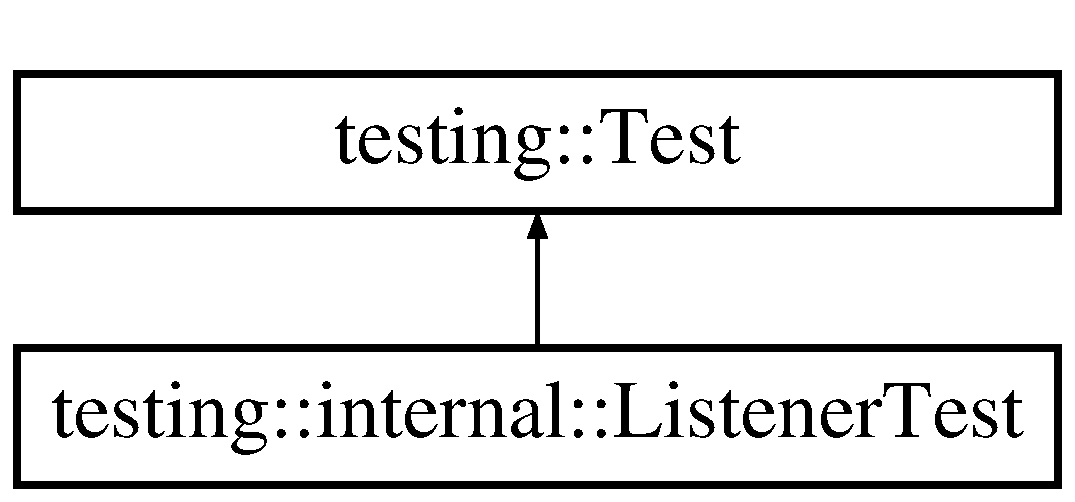
\includegraphics[height=2.000000cm]{classtesting_1_1internal_1_1_listener_test}
\end{center}
\end{figure}
\subsection*{Protected Member Functions}
\begin{DoxyCompactItemize}
\item 
virtual void \hyperlink{classtesting_1_1internal_1_1_listener_test_ace3dbe36b705ddf320518e6cdd919bc8}{Set\+Up} ()
\item 
virtual void \hyperlink{classtesting_1_1internal_1_1_listener_test_ad112535025d668e3ea14e71d8741c810}{Tear\+Down} ()
\end{DoxyCompactItemize}
\subsection*{Static Protected Member Functions}
\begin{DoxyCompactItemize}
\item 
static void \hyperlink{classtesting_1_1internal_1_1_listener_test_a7cbc298576e584b4021d0375204b7391}{Set\+Up\+Test\+Case} ()
\item 
static void \hyperlink{classtesting_1_1internal_1_1_listener_test_aa35b5f1c6235f0fe98aa2c7f35bb8fe1}{Tear\+Down\+Test\+Case} ()
\end{DoxyCompactItemize}
\subsection*{Additional Inherited Members}


\subsection{Member Function Documentation}
\hypertarget{classtesting_1_1internal_1_1_listener_test_ace3dbe36b705ddf320518e6cdd919bc8}{}\index{testing\+::internal\+::\+Listener\+Test@{testing\+::internal\+::\+Listener\+Test}!Set\+Up@{Set\+Up}}
\index{Set\+Up@{Set\+Up}!testing\+::internal\+::\+Listener\+Test@{testing\+::internal\+::\+Listener\+Test}}
\subsubsection[{Set\+Up()}]{\setlength{\rightskip}{0pt plus 5cm}virtual void testing\+::internal\+::\+Listener\+Test\+::\+Set\+Up (
\begin{DoxyParamCaption}
{}
\end{DoxyParamCaption}
)\hspace{0.3cm}{\ttfamily [inline]}, {\ttfamily [protected]}, {\ttfamily [virtual]}}\label{classtesting_1_1internal_1_1_listener_test_ace3dbe36b705ddf320518e6cdd919bc8}


Reimplemented from \hyperlink{classtesting_1_1_test_a190315150c303ddf801313fd1a777733}{testing\+::\+Test}.

\hypertarget{classtesting_1_1internal_1_1_listener_test_a7cbc298576e584b4021d0375204b7391}{}\index{testing\+::internal\+::\+Listener\+Test@{testing\+::internal\+::\+Listener\+Test}!Set\+Up\+Test\+Case@{Set\+Up\+Test\+Case}}
\index{Set\+Up\+Test\+Case@{Set\+Up\+Test\+Case}!testing\+::internal\+::\+Listener\+Test@{testing\+::internal\+::\+Listener\+Test}}
\subsubsection[{Set\+Up\+Test\+Case()}]{\setlength{\rightskip}{0pt plus 5cm}static void testing\+::internal\+::\+Listener\+Test\+::\+Set\+Up\+Test\+Case (
\begin{DoxyParamCaption}
{}
\end{DoxyParamCaption}
)\hspace{0.3cm}{\ttfamily [inline]}, {\ttfamily [static]}, {\ttfamily [protected]}}\label{classtesting_1_1internal_1_1_listener_test_a7cbc298576e584b4021d0375204b7391}
\hypertarget{classtesting_1_1internal_1_1_listener_test_ad112535025d668e3ea14e71d8741c810}{}\index{testing\+::internal\+::\+Listener\+Test@{testing\+::internal\+::\+Listener\+Test}!Tear\+Down@{Tear\+Down}}
\index{Tear\+Down@{Tear\+Down}!testing\+::internal\+::\+Listener\+Test@{testing\+::internal\+::\+Listener\+Test}}
\subsubsection[{Tear\+Down()}]{\setlength{\rightskip}{0pt plus 5cm}virtual void testing\+::internal\+::\+Listener\+Test\+::\+Tear\+Down (
\begin{DoxyParamCaption}
{}
\end{DoxyParamCaption}
)\hspace{0.3cm}{\ttfamily [inline]}, {\ttfamily [protected]}, {\ttfamily [virtual]}}\label{classtesting_1_1internal_1_1_listener_test_ad112535025d668e3ea14e71d8741c810}


Reimplemented from \hyperlink{classtesting_1_1_test_a5f0ab439802cbe0ef7552f1a9f791923}{testing\+::\+Test}.

\hypertarget{classtesting_1_1internal_1_1_listener_test_aa35b5f1c6235f0fe98aa2c7f35bb8fe1}{}\index{testing\+::internal\+::\+Listener\+Test@{testing\+::internal\+::\+Listener\+Test}!Tear\+Down\+Test\+Case@{Tear\+Down\+Test\+Case}}
\index{Tear\+Down\+Test\+Case@{Tear\+Down\+Test\+Case}!testing\+::internal\+::\+Listener\+Test@{testing\+::internal\+::\+Listener\+Test}}
\subsubsection[{Tear\+Down\+Test\+Case()}]{\setlength{\rightskip}{0pt plus 5cm}static void testing\+::internal\+::\+Listener\+Test\+::\+Tear\+Down\+Test\+Case (
\begin{DoxyParamCaption}
{}
\end{DoxyParamCaption}
)\hspace{0.3cm}{\ttfamily [inline]}, {\ttfamily [static]}, {\ttfamily [protected]}}\label{classtesting_1_1internal_1_1_listener_test_aa35b5f1c6235f0fe98aa2c7f35bb8fe1}


The documentation for this class was generated from the following file\+:\begin{DoxyCompactItemize}
\item 
C\+:/\+Users/\+Hilman/\+Desktop/repo/anjing/src/third\+\_\+party/googletest/test/\hyperlink{gtest-listener__test_8cc}{gtest-\/listener\+\_\+test.\+cc}\end{DoxyCompactItemize}

\hypertarget{classpump_1_1_literal_dollar_node}{}\section{pump.\+Literal\+Dollar\+Node Class Reference}
\label{classpump_1_1_literal_dollar_node}\index{pump.\+Literal\+Dollar\+Node@{pump.\+Literal\+Dollar\+Node}}
\subsection*{Public Member Functions}
\begin{DoxyCompactItemize}
\item 
def \hyperlink{classpump_1_1_literal_dollar_node_a181cccad8a48f7dfdd0716e427897e0b}{\+\_\+\+\_\+init\+\_\+\+\_\+} (self, \hyperlink{classpump_1_1_literal_dollar_node_ab4c6e209635b8868bcdf0fe8053431c6}{token})
\end{DoxyCompactItemize}
\subsection*{Public Attributes}
\begin{DoxyCompactItemize}
\item 
\hyperlink{classpump_1_1_literal_dollar_node_ab4c6e209635b8868bcdf0fe8053431c6}{token}
\end{DoxyCompactItemize}


\subsection{Constructor \& Destructor Documentation}
\hypertarget{classpump_1_1_literal_dollar_node_a181cccad8a48f7dfdd0716e427897e0b}{}\index{pump\+::\+Literal\+Dollar\+Node@{pump\+::\+Literal\+Dollar\+Node}!\+\_\+\+\_\+init\+\_\+\+\_\+@{\+\_\+\+\_\+init\+\_\+\+\_\+}}
\index{\+\_\+\+\_\+init\+\_\+\+\_\+@{\+\_\+\+\_\+init\+\_\+\+\_\+}!pump\+::\+Literal\+Dollar\+Node@{pump\+::\+Literal\+Dollar\+Node}}
\subsubsection[{\+\_\+\+\_\+init\+\_\+\+\_\+(self, token)}]{\setlength{\rightskip}{0pt plus 5cm}def pump.\+Literal\+Dollar\+Node.\+\_\+\+\_\+init\+\_\+\+\_\+ (
\begin{DoxyParamCaption}
\item[{}]{self, }
\item[{}]{token}
\end{DoxyParamCaption}
)}\label{classpump_1_1_literal_dollar_node_a181cccad8a48f7dfdd0716e427897e0b}


\subsection{Member Data Documentation}
\hypertarget{classpump_1_1_literal_dollar_node_ab4c6e209635b8868bcdf0fe8053431c6}{}\index{pump\+::\+Literal\+Dollar\+Node@{pump\+::\+Literal\+Dollar\+Node}!token@{token}}
\index{token@{token}!pump\+::\+Literal\+Dollar\+Node@{pump\+::\+Literal\+Dollar\+Node}}
\subsubsection[{token}]{\setlength{\rightskip}{0pt plus 5cm}pump.\+Literal\+Dollar\+Node.\+token}\label{classpump_1_1_literal_dollar_node_ab4c6e209635b8868bcdf0fe8053431c6}


The documentation for this class was generated from the following file\+:\begin{DoxyCompactItemize}
\item 
C\+:/\+Users/\+Hilman/\+Desktop/repo/anjing/src/third\+\_\+party/googletest/scripts/\hyperlink{pump_8py}{pump.\+py}\end{DoxyCompactItemize}

\hypertarget{classupload_1_1_mercurial_v_c_s}{}\section{upload.\+Mercurial\+V\+C\+S Class Reference}
\label{classupload_1_1_mercurial_v_c_s}\index{upload.\+Mercurial\+V\+C\+S@{upload.\+Mercurial\+V\+C\+S}}
Inheritance diagram for upload.\+Mercurial\+V\+C\+S\+:\begin{figure}[H]
\begin{center}
\leavevmode
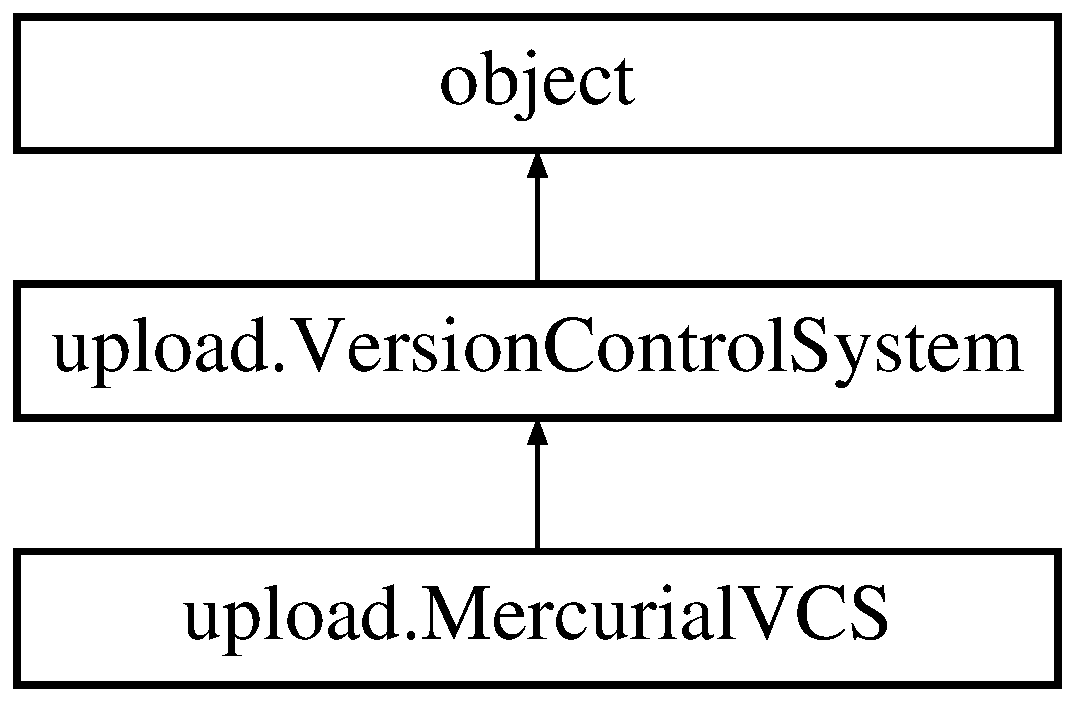
\includegraphics[height=3.000000cm]{classupload_1_1_mercurial_v_c_s}
\end{center}
\end{figure}
\subsection*{Public Member Functions}
\begin{DoxyCompactItemize}
\item 
def \hyperlink{classupload_1_1_mercurial_v_c_s_a33890f442dedbb7d9fd45c08b5baed56}{\+\_\+\+\_\+init\+\_\+\+\_\+} (self, \hyperlink{classupload_1_1_version_control_system_a4d57d043bc408887b94269fe4cea9556}{options}, \hyperlink{classupload_1_1_mercurial_v_c_s_a219c1e0ab9ce864e3231913762ea489b}{repo\+\_\+dir})
\item 
def \hyperlink{classupload_1_1_mercurial_v_c_s_a6c05746012d8cd435c94ace1465671ef}{Generate\+Diff} (self, extra\+\_\+args)
\item 
def \hyperlink{classupload_1_1_mercurial_v_c_s_a6190899fb86cd09ad84cc5d4b0ebd2f3}{Get\+Unknown\+Files} (self)
\item 
def \hyperlink{classupload_1_1_mercurial_v_c_s_a0cdc0cbe6ac4daab82f5f01e6ae2e670}{Get\+Base\+File} (self, filename)
\end{DoxyCompactItemize}
\subsection*{Public Attributes}
\begin{DoxyCompactItemize}
\item 
\hyperlink{classupload_1_1_mercurial_v_c_s_a219c1e0ab9ce864e3231913762ea489b}{repo\+\_\+dir}
\item 
\hyperlink{classupload_1_1_mercurial_v_c_s_a0dad32e621f5523e3430d867184f0b42}{subdir}
\item 
\hyperlink{classupload_1_1_mercurial_v_c_s_a41faae7820d5a015f4a42476e5e4ab8c}{base\+\_\+rev}
\end{DoxyCompactItemize}


\subsection{Detailed Description}
\begin{DoxyVerb}Implementation of the VersionControlSystem interface for Mercurial.\end{DoxyVerb}
 

\subsection{Constructor \& Destructor Documentation}
\hypertarget{classupload_1_1_mercurial_v_c_s_a33890f442dedbb7d9fd45c08b5baed56}{}\index{upload\+::\+Mercurial\+V\+C\+S@{upload\+::\+Mercurial\+V\+C\+S}!\+\_\+\+\_\+init\+\_\+\+\_\+@{\+\_\+\+\_\+init\+\_\+\+\_\+}}
\index{\+\_\+\+\_\+init\+\_\+\+\_\+@{\+\_\+\+\_\+init\+\_\+\+\_\+}!upload\+::\+Mercurial\+V\+C\+S@{upload\+::\+Mercurial\+V\+C\+S}}
\subsubsection[{\+\_\+\+\_\+init\+\_\+\+\_\+(self, options, repo\+\_\+dir)}]{\setlength{\rightskip}{0pt plus 5cm}def upload.\+Mercurial\+V\+C\+S.\+\_\+\+\_\+init\+\_\+\+\_\+ (
\begin{DoxyParamCaption}
\item[{}]{self, }
\item[{}]{options, }
\item[{}]{repo\+\_\+dir}
\end{DoxyParamCaption}
)}\label{classupload_1_1_mercurial_v_c_s_a33890f442dedbb7d9fd45c08b5baed56}


\subsection{Member Function Documentation}
\hypertarget{classupload_1_1_mercurial_v_c_s_a6c05746012d8cd435c94ace1465671ef}{}\index{upload\+::\+Mercurial\+V\+C\+S@{upload\+::\+Mercurial\+V\+C\+S}!Generate\+Diff@{Generate\+Diff}}
\index{Generate\+Diff@{Generate\+Diff}!upload\+::\+Mercurial\+V\+C\+S@{upload\+::\+Mercurial\+V\+C\+S}}
\subsubsection[{Generate\+Diff(self, extra\+\_\+args)}]{\setlength{\rightskip}{0pt plus 5cm}def upload.\+Mercurial\+V\+C\+S.\+Generate\+Diff (
\begin{DoxyParamCaption}
\item[{}]{self, }
\item[{}]{extra\+\_\+args}
\end{DoxyParamCaption}
)}\label{classupload_1_1_mercurial_v_c_s_a6c05746012d8cd435c94ace1465671ef}
\hypertarget{classupload_1_1_mercurial_v_c_s_a0cdc0cbe6ac4daab82f5f01e6ae2e670}{}\index{upload\+::\+Mercurial\+V\+C\+S@{upload\+::\+Mercurial\+V\+C\+S}!Get\+Base\+File@{Get\+Base\+File}}
\index{Get\+Base\+File@{Get\+Base\+File}!upload\+::\+Mercurial\+V\+C\+S@{upload\+::\+Mercurial\+V\+C\+S}}
\subsubsection[{Get\+Base\+File(self, filename)}]{\setlength{\rightskip}{0pt plus 5cm}def upload.\+Mercurial\+V\+C\+S.\+Get\+Base\+File (
\begin{DoxyParamCaption}
\item[{}]{self, }
\item[{}]{filename}
\end{DoxyParamCaption}
)}\label{classupload_1_1_mercurial_v_c_s_a0cdc0cbe6ac4daab82f5f01e6ae2e670}
\hypertarget{classupload_1_1_mercurial_v_c_s_a6190899fb86cd09ad84cc5d4b0ebd2f3}{}\index{upload\+::\+Mercurial\+V\+C\+S@{upload\+::\+Mercurial\+V\+C\+S}!Get\+Unknown\+Files@{Get\+Unknown\+Files}}
\index{Get\+Unknown\+Files@{Get\+Unknown\+Files}!upload\+::\+Mercurial\+V\+C\+S@{upload\+::\+Mercurial\+V\+C\+S}}
\subsubsection[{Get\+Unknown\+Files(self)}]{\setlength{\rightskip}{0pt plus 5cm}def upload.\+Mercurial\+V\+C\+S.\+Get\+Unknown\+Files (
\begin{DoxyParamCaption}
\item[{}]{self}
\end{DoxyParamCaption}
)}\label{classupload_1_1_mercurial_v_c_s_a6190899fb86cd09ad84cc5d4b0ebd2f3}
\begin{DoxyVerb}Return a list of files unknown to the VCS.\end{DoxyVerb}
 

\subsection{Member Data Documentation}
\hypertarget{classupload_1_1_mercurial_v_c_s_a41faae7820d5a015f4a42476e5e4ab8c}{}\index{upload\+::\+Mercurial\+V\+C\+S@{upload\+::\+Mercurial\+V\+C\+S}!base\+\_\+rev@{base\+\_\+rev}}
\index{base\+\_\+rev@{base\+\_\+rev}!upload\+::\+Mercurial\+V\+C\+S@{upload\+::\+Mercurial\+V\+C\+S}}
\subsubsection[{base\+\_\+rev}]{\setlength{\rightskip}{0pt plus 5cm}upload.\+Mercurial\+V\+C\+S.\+base\+\_\+rev}\label{classupload_1_1_mercurial_v_c_s_a41faae7820d5a015f4a42476e5e4ab8c}
\hypertarget{classupload_1_1_mercurial_v_c_s_a219c1e0ab9ce864e3231913762ea489b}{}\index{upload\+::\+Mercurial\+V\+C\+S@{upload\+::\+Mercurial\+V\+C\+S}!repo\+\_\+dir@{repo\+\_\+dir}}
\index{repo\+\_\+dir@{repo\+\_\+dir}!upload\+::\+Mercurial\+V\+C\+S@{upload\+::\+Mercurial\+V\+C\+S}}
\subsubsection[{repo\+\_\+dir}]{\setlength{\rightskip}{0pt plus 5cm}upload.\+Mercurial\+V\+C\+S.\+repo\+\_\+dir}\label{classupload_1_1_mercurial_v_c_s_a219c1e0ab9ce864e3231913762ea489b}
\hypertarget{classupload_1_1_mercurial_v_c_s_a0dad32e621f5523e3430d867184f0b42}{}\index{upload\+::\+Mercurial\+V\+C\+S@{upload\+::\+Mercurial\+V\+C\+S}!subdir@{subdir}}
\index{subdir@{subdir}!upload\+::\+Mercurial\+V\+C\+S@{upload\+::\+Mercurial\+V\+C\+S}}
\subsubsection[{subdir}]{\setlength{\rightskip}{0pt plus 5cm}upload.\+Mercurial\+V\+C\+S.\+subdir}\label{classupload_1_1_mercurial_v_c_s_a0dad32e621f5523e3430d867184f0b42}


The documentation for this class was generated from the following file\+:\begin{DoxyCompactItemize}
\item 
C\+:/\+Users/\+Hilman/\+Desktop/repo/anjing/src/third\+\_\+party/googletest/scripts/\hyperlink{upload_8py}{upload.\+py}\end{DoxyCompactItemize}

\hypertarget{classmy__namespace_1_1testing_1_1_message}{}\section{my\+\_\+namespace\+:\+:testing\+:\+:Message Class Reference}
\label{classmy__namespace_1_1testing_1_1_message}\index{my\+\_\+namespace\+::testing\+::\+Message@{my\+\_\+namespace\+::testing\+::\+Message}}


The documentation for this class was generated from the following file\+:\begin{DoxyCompactItemize}
\item 
C\+:/\+Users/\+Hilman/\+Desktop/repo/anjing/src/third\+\_\+party/googletest/test/\hyperlink{gtest__unittest_8cc}{gtest\+\_\+unittest.\+cc}\end{DoxyCompactItemize}

\hypertarget{classtesting_1_1_message}{}\section{testing\+:\+:Message Class Reference}
\label{classtesting_1_1_message}\index{testing\+::\+Message@{testing\+::\+Message}}


{\ttfamily \#include $<$gtest-\/message.\+h$>$}

\subsection*{Public Member Functions}
\begin{DoxyCompactItemize}
\item 
\hyperlink{classtesting_1_1_message_af5ba7216630df9845f18feb64b1a5383}{Message} ()
\item 
\hyperlink{classtesting_1_1_message_ac126e24804817a053bebba0920d94a11}{Message} (const \hyperlink{classtesting_1_1_message}{Message} \&msg)
\item 
\hyperlink{classtesting_1_1_message_a9de694ca239486809fc99fbbea8ac21d}{Message} (const char $\ast$str)
\item 
{\footnotesize template$<$typename T $>$ }\\\hyperlink{classtesting_1_1_message}{Message} \& \hyperlink{classtesting_1_1_message_a2e0e71be52d54c20a75a55fca812721f}{operator$<$$<$} (const T \&val)
\item 
{\footnotesize template$<$typename T $>$ }\\\hyperlink{classtesting_1_1_message}{Message} \& \hyperlink{classtesting_1_1_message_aa3ab685879958f90d2d8cd5b68d10c34}{operator$<$$<$} (T $\ast$const \&pointer)
\item 
\hyperlink{classtesting_1_1_message}{Message} \& \hyperlink{classtesting_1_1_message_a3a71a1c1c8ea52de5852d75483d41453}{operator$<$$<$} (Basic\+Narrow\+Io\+Manip val)
\item 
\hyperlink{classtesting_1_1_message}{Message} \& \hyperlink{classtesting_1_1_message_a3e1e04f23b1bdfe18adfd59928296346}{operator$<$$<$} (bool b)
\item 
\hyperlink{classtesting_1_1_message}{Message} \& \hyperlink{classtesting_1_1_message_ac0db9c22535b28bc863bfd0a1fdf7e14}{operator$<$$<$} (const wchar\+\_\+t $\ast$wide\+\_\+c\+\_\+str)
\item 
\hyperlink{classtesting_1_1_message}{Message} \& \hyperlink{classtesting_1_1_message_ac1d3a041ac4bb9c929ee746b31a13d6a}{operator$<$$<$} (wchar\+\_\+t $\ast$wide\+\_\+c\+\_\+str)
\item 
std\+::string \hyperlink{classtesting_1_1_message_abe8c1b7584aa670dd0e2413e8317a937}{Get\+String} () const 
\end{DoxyCompactItemize}


\subsection{Constructor \& Destructor Documentation}
\hypertarget{classtesting_1_1_message_af5ba7216630df9845f18feb64b1a5383}{}\index{testing\+::\+Message@{testing\+::\+Message}!Message@{Message}}
\index{Message@{Message}!testing\+::\+Message@{testing\+::\+Message}}
\subsubsection[{Message()}]{\setlength{\rightskip}{0pt plus 5cm}testing\+::\+Message\+::\+Message (
\begin{DoxyParamCaption}
{}
\end{DoxyParamCaption}
)}\label{classtesting_1_1_message_af5ba7216630df9845f18feb64b1a5383}
\hypertarget{classtesting_1_1_message_ac126e24804817a053bebba0920d94a11}{}\index{testing\+::\+Message@{testing\+::\+Message}!Message@{Message}}
\index{Message@{Message}!testing\+::\+Message@{testing\+::\+Message}}
\subsubsection[{Message(const Message \&msg)}]{\setlength{\rightskip}{0pt plus 5cm}testing\+::\+Message\+::\+Message (
\begin{DoxyParamCaption}
\item[{const {\bf Message} \&}]{msg}
\end{DoxyParamCaption}
)\hspace{0.3cm}{\ttfamily [inline]}}\label{classtesting_1_1_message_ac126e24804817a053bebba0920d94a11}
\hypertarget{classtesting_1_1_message_a9de694ca239486809fc99fbbea8ac21d}{}\index{testing\+::\+Message@{testing\+::\+Message}!Message@{Message}}
\index{Message@{Message}!testing\+::\+Message@{testing\+::\+Message}}
\subsubsection[{Message(const char $\ast$str)}]{\setlength{\rightskip}{0pt plus 5cm}testing\+::\+Message\+::\+Message (
\begin{DoxyParamCaption}
\item[{const char $\ast$}]{str}
\end{DoxyParamCaption}
)\hspace{0.3cm}{\ttfamily [inline]}, {\ttfamily [explicit]}}\label{classtesting_1_1_message_a9de694ca239486809fc99fbbea8ac21d}


\subsection{Member Function Documentation}
\hypertarget{classtesting_1_1_message_abe8c1b7584aa670dd0e2413e8317a937}{}\index{testing\+::\+Message@{testing\+::\+Message}!Get\+String@{Get\+String}}
\index{Get\+String@{Get\+String}!testing\+::\+Message@{testing\+::\+Message}}
\subsubsection[{Get\+String() const }]{\setlength{\rightskip}{0pt plus 5cm}std\+::string testing\+::\+Message\+::\+Get\+String (
\begin{DoxyParamCaption}
{}
\end{DoxyParamCaption}
) const}\label{classtesting_1_1_message_abe8c1b7584aa670dd0e2413e8317a937}
\hypertarget{classtesting_1_1_message_a2e0e71be52d54c20a75a55fca812721f}{}\index{testing\+::\+Message@{testing\+::\+Message}!operator$<$$<$@{operator$<$$<$}}
\index{operator$<$$<$@{operator$<$$<$}!testing\+::\+Message@{testing\+::\+Message}}
\subsubsection[{operator$<$$<$(const T \&val)}]{\setlength{\rightskip}{0pt plus 5cm}template$<$typename T $>$ {\bf Message}\& testing\+::\+Message\+::operator$<$$<$ (
\begin{DoxyParamCaption}
\item[{const T \&}]{val}
\end{DoxyParamCaption}
)\hspace{0.3cm}{\ttfamily [inline]}}\label{classtesting_1_1_message_a2e0e71be52d54c20a75a55fca812721f}
\hypertarget{classtesting_1_1_message_aa3ab685879958f90d2d8cd5b68d10c34}{}\index{testing\+::\+Message@{testing\+::\+Message}!operator$<$$<$@{operator$<$$<$}}
\index{operator$<$$<$@{operator$<$$<$}!testing\+::\+Message@{testing\+::\+Message}}
\subsubsection[{operator$<$$<$(\+T $\ast$const \&pointer)}]{\setlength{\rightskip}{0pt plus 5cm}template$<$typename T $>$ {\bf Message}\& testing\+::\+Message\+::operator$<$$<$ (
\begin{DoxyParamCaption}
\item[{T $\ast$const \&}]{pointer}
\end{DoxyParamCaption}
)\hspace{0.3cm}{\ttfamily [inline]}}\label{classtesting_1_1_message_aa3ab685879958f90d2d8cd5b68d10c34}
\hypertarget{classtesting_1_1_message_a3a71a1c1c8ea52de5852d75483d41453}{}\index{testing\+::\+Message@{testing\+::\+Message}!operator$<$$<$@{operator$<$$<$}}
\index{operator$<$$<$@{operator$<$$<$}!testing\+::\+Message@{testing\+::\+Message}}
\subsubsection[{operator$<$$<$(\+Basic\+Narrow\+Io\+Manip val)}]{\setlength{\rightskip}{0pt plus 5cm}{\bf Message}\& testing\+::\+Message\+::operator$<$$<$ (
\begin{DoxyParamCaption}
\item[{Basic\+Narrow\+Io\+Manip}]{val}
\end{DoxyParamCaption}
)\hspace{0.3cm}{\ttfamily [inline]}}\label{classtesting_1_1_message_a3a71a1c1c8ea52de5852d75483d41453}
\hypertarget{classtesting_1_1_message_a3e1e04f23b1bdfe18adfd59928296346}{}\index{testing\+::\+Message@{testing\+::\+Message}!operator$<$$<$@{operator$<$$<$}}
\index{operator$<$$<$@{operator$<$$<$}!testing\+::\+Message@{testing\+::\+Message}}
\subsubsection[{operator$<$$<$(bool b)}]{\setlength{\rightskip}{0pt plus 5cm}{\bf Message}\& testing\+::\+Message\+::operator$<$$<$ (
\begin{DoxyParamCaption}
\item[{bool}]{b}
\end{DoxyParamCaption}
)\hspace{0.3cm}{\ttfamily [inline]}}\label{classtesting_1_1_message_a3e1e04f23b1bdfe18adfd59928296346}
\hypertarget{classtesting_1_1_message_ac0db9c22535b28bc863bfd0a1fdf7e14}{}\index{testing\+::\+Message@{testing\+::\+Message}!operator$<$$<$@{operator$<$$<$}}
\index{operator$<$$<$@{operator$<$$<$}!testing\+::\+Message@{testing\+::\+Message}}
\subsubsection[{operator$<$$<$(const wchar\+\_\+t $\ast$wide\+\_\+c\+\_\+str)}]{\setlength{\rightskip}{0pt plus 5cm}{\bf Message} \& testing\+::\+Message\+::operator$<$$<$ (
\begin{DoxyParamCaption}
\item[{const wchar\+\_\+t $\ast$}]{wide\+\_\+c\+\_\+str}
\end{DoxyParamCaption}
)}\label{classtesting_1_1_message_ac0db9c22535b28bc863bfd0a1fdf7e14}
\hypertarget{classtesting_1_1_message_ac1d3a041ac4bb9c929ee746b31a13d6a}{}\index{testing\+::\+Message@{testing\+::\+Message}!operator$<$$<$@{operator$<$$<$}}
\index{operator$<$$<$@{operator$<$$<$}!testing\+::\+Message@{testing\+::\+Message}}
\subsubsection[{operator$<$$<$(wchar\+\_\+t $\ast$wide\+\_\+c\+\_\+str)}]{\setlength{\rightskip}{0pt plus 5cm}{\bf Message} \& testing\+::\+Message\+::operator$<$$<$ (
\begin{DoxyParamCaption}
\item[{wchar\+\_\+t $\ast$}]{wide\+\_\+c\+\_\+str}
\end{DoxyParamCaption}
)}\label{classtesting_1_1_message_ac1d3a041ac4bb9c929ee746b31a13d6a}


The documentation for this class was generated from the following files\+:\begin{DoxyCompactItemize}
\item 
C\+:/\+Users/\+Hilman/\+Desktop/repo/anjing/src/third\+\_\+party/googletest/include/gtest/\hyperlink{gtest-message_8h}{gtest-\/message.\+h}\item 
C\+:/\+Users/\+Hilman/\+Desktop/repo/anjing/src/third\+\_\+party/googletest/src/\hyperlink{gtest_8cc}{gtest.\+cc}\end{DoxyCompactItemize}

\hypertarget{classfoo_1_1_mixed_up_test_case_test}{}\section{foo\+:\+:Mixed\+Up\+Test\+Case\+Test Class Reference}
\label{classfoo_1_1_mixed_up_test_case_test}\index{foo\+::\+Mixed\+Up\+Test\+Case\+Test@{foo\+::\+Mixed\+Up\+Test\+Case\+Test}}
Inheritance diagram for foo\+:\+:Mixed\+Up\+Test\+Case\+Test\+:\begin{figure}[H]
\begin{center}
\leavevmode
\includegraphics[height=2.000000cm]{classfoo_1_1_mixed_up_test_case_test}
\end{center}
\end{figure}
\subsection*{Additional Inherited Members}


The documentation for this class was generated from the following file\+:\begin{DoxyCompactItemize}
\item 
C\+:/\+Users/\+Hilman/\+Desktop/repo/anjing/src/third\+\_\+party/googletest/test/\hyperlink{gtest__output__test___8cc}{gtest\+\_\+output\+\_\+test\+\_\+.\+cc}\end{DoxyCompactItemize}

\hypertarget{classbar_1_1_mixed_up_test_case_test}{}\section{bar\+:\+:Mixed\+Up\+Test\+Case\+Test Class Reference}
\label{classbar_1_1_mixed_up_test_case_test}\index{bar\+::\+Mixed\+Up\+Test\+Case\+Test@{bar\+::\+Mixed\+Up\+Test\+Case\+Test}}
Inheritance diagram for bar\+:\+:Mixed\+Up\+Test\+Case\+Test\+:\begin{figure}[H]
\begin{center}
\leavevmode
\includegraphics[height=2.000000cm]{classbar_1_1_mixed_up_test_case_test}
\end{center}
\end{figure}
\subsection*{Additional Inherited Members}


The documentation for this class was generated from the following file\+:\begin{DoxyCompactItemize}
\item 
C\+:/\+Users/\+Hilman/\+Desktop/repo/anjing/src/third\+\_\+party/googletest/test/\hyperlink{gtest__output__test___8cc}{gtest\+\_\+output\+\_\+test\+\_\+.\+cc}\end{DoxyCompactItemize}

\hypertarget{classfoo_1_1_mixed_up_test_case_with_same_test_name_test}{}\section{foo\+:\+:Mixed\+Up\+Test\+Case\+With\+Same\+Test\+Name\+Test Class Reference}
\label{classfoo_1_1_mixed_up_test_case_with_same_test_name_test}\index{foo\+::\+Mixed\+Up\+Test\+Case\+With\+Same\+Test\+Name\+Test@{foo\+::\+Mixed\+Up\+Test\+Case\+With\+Same\+Test\+Name\+Test}}
Inheritance diagram for foo\+:\+:Mixed\+Up\+Test\+Case\+With\+Same\+Test\+Name\+Test\+:\begin{figure}[H]
\begin{center}
\leavevmode
\includegraphics[height=2.000000cm]{classfoo_1_1_mixed_up_test_case_with_same_test_name_test}
\end{center}
\end{figure}
\subsection*{Additional Inherited Members}


The documentation for this class was generated from the following file\+:\begin{DoxyCompactItemize}
\item 
C\+:/\+Users/\+Hilman/\+Desktop/repo/anjing/src/third\+\_\+party/googletest/test/\hyperlink{gtest__output__test___8cc}{gtest\+\_\+output\+\_\+test\+\_\+.\+cc}\end{DoxyCompactItemize}

\hypertarget{classbar_1_1_mixed_up_test_case_with_same_test_name_test}{}\section{bar\+:\+:Mixed\+Up\+Test\+Case\+With\+Same\+Test\+Name\+Test Class Reference}
\label{classbar_1_1_mixed_up_test_case_with_same_test_name_test}\index{bar\+::\+Mixed\+Up\+Test\+Case\+With\+Same\+Test\+Name\+Test@{bar\+::\+Mixed\+Up\+Test\+Case\+With\+Same\+Test\+Name\+Test}}
Inheritance diagram for bar\+:\+:Mixed\+Up\+Test\+Case\+With\+Same\+Test\+Name\+Test\+:\begin{figure}[H]
\begin{center}
\leavevmode
\includegraphics[height=2.000000cm]{classbar_1_1_mixed_up_test_case_with_same_test_name_test}
\end{center}
\end{figure}
\subsection*{Additional Inherited Members}


The documentation for this class was generated from the following file\+:\begin{DoxyCompactItemize}
\item 
C\+:/\+Users/\+Hilman/\+Desktop/repo/anjing/src/third\+\_\+party/googletest/test/\hyperlink{gtest__output__test___8cc}{gtest\+\_\+output\+\_\+test\+\_\+.\+cc}\end{DoxyCompactItemize}

\hypertarget{classtesting_1_1internal_1_1_mutex}{}\section{testing\+:\+:internal\+:\+:Mutex Class Reference}
\label{classtesting_1_1internal_1_1_mutex}\index{testing\+::internal\+::\+Mutex@{testing\+::internal\+::\+Mutex}}


{\ttfamily \#include $<$gtest-\/port.\+h$>$}

\subsection*{Public Member Functions}
\begin{DoxyCompactItemize}
\item 
\hyperlink{classtesting_1_1internal_1_1_mutex_a38e1833a78e3eec81ad23ce1b056b40e}{Mutex} ()
\item 
void \hyperlink{classtesting_1_1internal_1_1_mutex_ae7e2191886c00182176b23c4f4d049f8}{Lock} ()
\item 
void \hyperlink{classtesting_1_1internal_1_1_mutex_a315188055de1be98884519ad84eff2e6}{Unlock} ()
\item 
void \hyperlink{classtesting_1_1internal_1_1_mutex_a3a0530bca3110025d85b2aa51f3ca0d7}{Assert\+Held} () const 
\end{DoxyCompactItemize}


\subsection{Constructor \& Destructor Documentation}
\hypertarget{classtesting_1_1internal_1_1_mutex_a38e1833a78e3eec81ad23ce1b056b40e}{}\index{testing\+::internal\+::\+Mutex@{testing\+::internal\+::\+Mutex}!Mutex@{Mutex}}
\index{Mutex@{Mutex}!testing\+::internal\+::\+Mutex@{testing\+::internal\+::\+Mutex}}
\subsubsection[{Mutex()}]{\setlength{\rightskip}{0pt plus 5cm}testing\+::internal\+::\+Mutex\+::\+Mutex (
\begin{DoxyParamCaption}
{}
\end{DoxyParamCaption}
)\hspace{0.3cm}{\ttfamily [inline]}}\label{classtesting_1_1internal_1_1_mutex_a38e1833a78e3eec81ad23ce1b056b40e}


\subsection{Member Function Documentation}
\hypertarget{classtesting_1_1internal_1_1_mutex_a3a0530bca3110025d85b2aa51f3ca0d7}{}\index{testing\+::internal\+::\+Mutex@{testing\+::internal\+::\+Mutex}!Assert\+Held@{Assert\+Held}}
\index{Assert\+Held@{Assert\+Held}!testing\+::internal\+::\+Mutex@{testing\+::internal\+::\+Mutex}}
\subsubsection[{Assert\+Held() const }]{\setlength{\rightskip}{0pt plus 5cm}void testing\+::internal\+::\+Mutex\+::\+Assert\+Held (
\begin{DoxyParamCaption}
{}
\end{DoxyParamCaption}
) const\hspace{0.3cm}{\ttfamily [inline]}}\label{classtesting_1_1internal_1_1_mutex_a3a0530bca3110025d85b2aa51f3ca0d7}
\hypertarget{classtesting_1_1internal_1_1_mutex_ae7e2191886c00182176b23c4f4d049f8}{}\index{testing\+::internal\+::\+Mutex@{testing\+::internal\+::\+Mutex}!Lock@{Lock}}
\index{Lock@{Lock}!testing\+::internal\+::\+Mutex@{testing\+::internal\+::\+Mutex}}
\subsubsection[{Lock()}]{\setlength{\rightskip}{0pt plus 5cm}void testing\+::internal\+::\+Mutex\+::\+Lock (
\begin{DoxyParamCaption}
{}
\end{DoxyParamCaption}
)\hspace{0.3cm}{\ttfamily [inline]}}\label{classtesting_1_1internal_1_1_mutex_ae7e2191886c00182176b23c4f4d049f8}
\hypertarget{classtesting_1_1internal_1_1_mutex_a315188055de1be98884519ad84eff2e6}{}\index{testing\+::internal\+::\+Mutex@{testing\+::internal\+::\+Mutex}!Unlock@{Unlock}}
\index{Unlock@{Unlock}!testing\+::internal\+::\+Mutex@{testing\+::internal\+::\+Mutex}}
\subsubsection[{Unlock()}]{\setlength{\rightskip}{0pt plus 5cm}void testing\+::internal\+::\+Mutex\+::\+Unlock (
\begin{DoxyParamCaption}
{}
\end{DoxyParamCaption}
)\hspace{0.3cm}{\ttfamily [inline]}}\label{classtesting_1_1internal_1_1_mutex_a315188055de1be98884519ad84eff2e6}


The documentation for this class was generated from the following file\+:\begin{DoxyCompactItemize}
\item 
C\+:/\+Users/\+Hilman/\+Desktop/repo/anjing/src/third\+\_\+party/googletest/include/gtest/internal/\hyperlink{gtest-port_8h}{gtest-\/port.\+h}\end{DoxyCompactItemize}

\hypertarget{class_my_array}{}\section{My\+Array$<$ T, k\+Size $>$ Class Template Reference}
\label{class_my_array}\index{My\+Array$<$ T, k\+Size $>$@{My\+Array$<$ T, k\+Size $>$}}


The documentation for this class was generated from the following file\+:\begin{DoxyCompactItemize}
\item 
C\+:/\+Users/\+Hilman/\+Desktop/repo/anjing/src/third\+\_\+party/googletest/test/\hyperlink{gtest__list__tests__unittest___8cc}{gtest\+\_\+list\+\_\+tests\+\_\+unittest\+\_\+.\+cc}\end{DoxyCompactItemize}

\hypertarget{class_my_string}{}\section{My\+String Class Reference}
\label{class_my_string}\index{My\+String@{My\+String}}


{\ttfamily \#include $<$sample2.\+h$>$}

\subsection*{Public Member Functions}
\begin{DoxyCompactItemize}
\item 
\hyperlink{class_my_string_a1cb17852b83614394b59720779c5f918}{My\+String} ()
\item 
\hyperlink{class_my_string_a28134eb91b6698f46b12accefa157d0f}{My\+String} (const char $\ast$a\+\_\+c\+\_\+string)
\item 
\hyperlink{class_my_string_ae24c7cf89a58dd2287303df2ac054c66}{My\+String} (const \hyperlink{class_my_string}{My\+String} \&string)
\item 
\hyperlink{class_my_string_a7bee4fe8ad82a0b7b8f65b02054b156b}{$\sim$\+My\+String} ()
\item 
const char $\ast$ \hyperlink{class_my_string_a0089588935fc8235124f58f514cb07a1}{c\+\_\+string} () const 
\item 
size\+\_\+t \hyperlink{class_my_string_a878f7e0a327814729a04a412d7b95801}{Length} () const 
\item 
void \hyperlink{class_my_string_a521c4cd7eccac6ce554d8a51505e4970}{Set} (const char $\ast$\hyperlink{class_my_string_a0089588935fc8235124f58f514cb07a1}{c\+\_\+string})
\end{DoxyCompactItemize}
\subsection*{Static Public Member Functions}
\begin{DoxyCompactItemize}
\item 
static const char $\ast$ \hyperlink{class_my_string_a40753dcfa3314a8993f32bdd75d67ce2}{Clone\+C\+String} (const char $\ast$a\+\_\+c\+\_\+string)
\end{DoxyCompactItemize}


\subsection{Constructor \& Destructor Documentation}
\hypertarget{class_my_string_a1cb17852b83614394b59720779c5f918}{}\index{My\+String@{My\+String}!My\+String@{My\+String}}
\index{My\+String@{My\+String}!My\+String@{My\+String}}
\subsubsection[{My\+String()}]{\setlength{\rightskip}{0pt plus 5cm}My\+String\+::\+My\+String (
\begin{DoxyParamCaption}
{}
\end{DoxyParamCaption}
)\hspace{0.3cm}{\ttfamily [inline]}}\label{class_my_string_a1cb17852b83614394b59720779c5f918}
\hypertarget{class_my_string_a28134eb91b6698f46b12accefa157d0f}{}\index{My\+String@{My\+String}!My\+String@{My\+String}}
\index{My\+String@{My\+String}!My\+String@{My\+String}}
\subsubsection[{My\+String(const char $\ast$a\+\_\+c\+\_\+string)}]{\setlength{\rightskip}{0pt plus 5cm}My\+String\+::\+My\+String (
\begin{DoxyParamCaption}
\item[{const char $\ast$}]{a\+\_\+c\+\_\+string}
\end{DoxyParamCaption}
)\hspace{0.3cm}{\ttfamily [inline]}, {\ttfamily [explicit]}}\label{class_my_string_a28134eb91b6698f46b12accefa157d0f}
\hypertarget{class_my_string_ae24c7cf89a58dd2287303df2ac054c66}{}\index{My\+String@{My\+String}!My\+String@{My\+String}}
\index{My\+String@{My\+String}!My\+String@{My\+String}}
\subsubsection[{My\+String(const My\+String \&string)}]{\setlength{\rightskip}{0pt plus 5cm}My\+String\+::\+My\+String (
\begin{DoxyParamCaption}
\item[{const {\bf My\+String} \&}]{string}
\end{DoxyParamCaption}
)\hspace{0.3cm}{\ttfamily [inline]}}\label{class_my_string_ae24c7cf89a58dd2287303df2ac054c66}
\hypertarget{class_my_string_a7bee4fe8ad82a0b7b8f65b02054b156b}{}\index{My\+String@{My\+String}!````~My\+String@{$\sim$\+My\+String}}
\index{````~My\+String@{$\sim$\+My\+String}!My\+String@{My\+String}}
\subsubsection[{$\sim$\+My\+String()}]{\setlength{\rightskip}{0pt plus 5cm}My\+String\+::$\sim$\+My\+String (
\begin{DoxyParamCaption}
{}
\end{DoxyParamCaption}
)\hspace{0.3cm}{\ttfamily [inline]}}\label{class_my_string_a7bee4fe8ad82a0b7b8f65b02054b156b}


\subsection{Member Function Documentation}
\hypertarget{class_my_string_a0089588935fc8235124f58f514cb07a1}{}\index{My\+String@{My\+String}!c\+\_\+string@{c\+\_\+string}}
\index{c\+\_\+string@{c\+\_\+string}!My\+String@{My\+String}}
\subsubsection[{c\+\_\+string() const }]{\setlength{\rightskip}{0pt plus 5cm}const char$\ast$ My\+String\+::c\+\_\+string (
\begin{DoxyParamCaption}
{}
\end{DoxyParamCaption}
) const\hspace{0.3cm}{\ttfamily [inline]}}\label{class_my_string_a0089588935fc8235124f58f514cb07a1}
\hypertarget{class_my_string_a40753dcfa3314a8993f32bdd75d67ce2}{}\index{My\+String@{My\+String}!Clone\+C\+String@{Clone\+C\+String}}
\index{Clone\+C\+String@{Clone\+C\+String}!My\+String@{My\+String}}
\subsubsection[{Clone\+C\+String(const char $\ast$a\+\_\+c\+\_\+string)}]{\setlength{\rightskip}{0pt plus 5cm}const char $\ast$ My\+String\+::\+Clone\+C\+String (
\begin{DoxyParamCaption}
\item[{const char $\ast$}]{a\+\_\+c\+\_\+string}
\end{DoxyParamCaption}
)\hspace{0.3cm}{\ttfamily [static]}}\label{class_my_string_a40753dcfa3314a8993f32bdd75d67ce2}
\hypertarget{class_my_string_a878f7e0a327814729a04a412d7b95801}{}\index{My\+String@{My\+String}!Length@{Length}}
\index{Length@{Length}!My\+String@{My\+String}}
\subsubsection[{Length() const }]{\setlength{\rightskip}{0pt plus 5cm}size\+\_\+t My\+String\+::\+Length (
\begin{DoxyParamCaption}
{}
\end{DoxyParamCaption}
) const\hspace{0.3cm}{\ttfamily [inline]}}\label{class_my_string_a878f7e0a327814729a04a412d7b95801}
\hypertarget{class_my_string_a521c4cd7eccac6ce554d8a51505e4970}{}\index{My\+String@{My\+String}!Set@{Set}}
\index{Set@{Set}!My\+String@{My\+String}}
\subsubsection[{Set(const char $\ast$c\+\_\+string)}]{\setlength{\rightskip}{0pt plus 5cm}void My\+String\+::\+Set (
\begin{DoxyParamCaption}
\item[{const char $\ast$}]{c\+\_\+string}
\end{DoxyParamCaption}
)}\label{class_my_string_a521c4cd7eccac6ce554d8a51505e4970}


The documentation for this class was generated from the following files\+:\begin{DoxyCompactItemize}
\item 
C\+:/\+Users/\+Hilman/\+Desktop/repo/anjing/src/third\+\_\+party/googletest/samples/\hyperlink{sample2_8h}{sample2.\+h}\item 
C\+:/\+Users/\+Hilman/\+Desktop/repo/anjing/src/third\+\_\+party/googletest/samples/\hyperlink{sample2_8cc}{sample2.\+cc}\end{DoxyCompactItemize}

\hypertarget{class_my_type}{}\section{My\+Type Class Reference}
\label{class_my_type}\index{My\+Type@{My\+Type}}
\subsection*{Public Member Functions}
\begin{DoxyCompactItemize}
\item 
\hyperlink{class_my_type_a74d6f29a06e298321a6e5f0b91b020e7}{My\+Type} (const std\+::string \&a\+\_\+value)
\item 
const std\+::string \& \hyperlink{class_my_type_a2c8074a0ef1f1c5e19490b9e118d69ca}{value} () const 
\end{DoxyCompactItemize}


\subsection{Constructor \& Destructor Documentation}
\hypertarget{class_my_type_a74d6f29a06e298321a6e5f0b91b020e7}{}\index{My\+Type@{My\+Type}!My\+Type@{My\+Type}}
\index{My\+Type@{My\+Type}!My\+Type@{My\+Type}}
\subsubsection[{My\+Type(const std\+::string \&a\+\_\+value)}]{\setlength{\rightskip}{0pt plus 5cm}My\+Type\+::\+My\+Type (
\begin{DoxyParamCaption}
\item[{const std\+::string \&}]{a\+\_\+value}
\end{DoxyParamCaption}
)\hspace{0.3cm}{\ttfamily [inline]}, {\ttfamily [explicit]}}\label{class_my_type_a74d6f29a06e298321a6e5f0b91b020e7}


\subsection{Member Function Documentation}
\hypertarget{class_my_type_a2c8074a0ef1f1c5e19490b9e118d69ca}{}\index{My\+Type@{My\+Type}!value@{value}}
\index{value@{value}!My\+Type@{My\+Type}}
\subsubsection[{value() const }]{\setlength{\rightskip}{0pt plus 5cm}const std\+::string\& My\+Type\+::value (
\begin{DoxyParamCaption}
{}
\end{DoxyParamCaption}
) const\hspace{0.3cm}{\ttfamily [inline]}}\label{class_my_type_a2c8074a0ef1f1c5e19490b9e118d69ca}


The documentation for this class was generated from the following file\+:\begin{DoxyCompactItemize}
\item 
C\+:/\+Users/\+Hilman/\+Desktop/repo/anjing/src/third\+\_\+party/googletest/test/\hyperlink{gtest__list__tests__unittest___8cc}{gtest\+\_\+list\+\_\+tests\+\_\+unittest\+\_\+.\+cc}\end{DoxyCompactItemize}

\hypertarget{classnamespace1_1_1_my_type_in_name_space1}{}\section{namespace1\+:\+:My\+Type\+In\+Name\+Space1 Class Reference}
\label{classnamespace1_1_1_my_type_in_name_space1}\index{namespace1\+::\+My\+Type\+In\+Name\+Space1@{namespace1\+::\+My\+Type\+In\+Name\+Space1}}
Inheritance diagram for namespace1\+:\+:My\+Type\+In\+Name\+Space1\+:\begin{figure}[H]
\begin{center}
\leavevmode
\includegraphics[height=2.000000cm]{classnamespace1_1_1_my_type_in_name_space1}
\end{center}
\end{figure}
\subsection*{Public Member Functions}
\begin{DoxyCompactItemize}
\item 
\hyperlink{classnamespace1_1_1_my_type_in_name_space1_a2e4277aa118e9b83045a18392188a0d8}{My\+Type\+In\+Name\+Space1} (int an\+\_\+x)
\end{DoxyCompactItemize}


\subsection{Constructor \& Destructor Documentation}
\hypertarget{classnamespace1_1_1_my_type_in_name_space1_a2e4277aa118e9b83045a18392188a0d8}{}\index{namespace1\+::\+My\+Type\+In\+Name\+Space1@{namespace1\+::\+My\+Type\+In\+Name\+Space1}!My\+Type\+In\+Name\+Space1@{My\+Type\+In\+Name\+Space1}}
\index{My\+Type\+In\+Name\+Space1@{My\+Type\+In\+Name\+Space1}!namespace1\+::\+My\+Type\+In\+Name\+Space1@{namespace1\+::\+My\+Type\+In\+Name\+Space1}}
\subsubsection[{My\+Type\+In\+Name\+Space1(int an\+\_\+x)}]{\setlength{\rightskip}{0pt plus 5cm}namespace1\+::\+My\+Type\+In\+Name\+Space1\+::\+My\+Type\+In\+Name\+Space1 (
\begin{DoxyParamCaption}
\item[{int}]{an\+\_\+x}
\end{DoxyParamCaption}
)\hspace{0.3cm}{\ttfamily [inline]}, {\ttfamily [explicit]}}\label{classnamespace1_1_1_my_type_in_name_space1_a2e4277aa118e9b83045a18392188a0d8}


The documentation for this class was generated from the following file\+:\begin{DoxyCompactItemize}
\item 
C\+:/\+Users/\+Hilman/\+Desktop/repo/anjing/src/third\+\_\+party/googletest/test/\hyperlink{gtest__unittest_8cc}{gtest\+\_\+unittest.\+cc}\end{DoxyCompactItemize}

\hypertarget{classnamespace2_1_1_my_type_in_name_space2}{}\section{namespace2\+:\+:My\+Type\+In\+Name\+Space2 Class Reference}
\label{classnamespace2_1_1_my_type_in_name_space2}\index{namespace2\+::\+My\+Type\+In\+Name\+Space2@{namespace2\+::\+My\+Type\+In\+Name\+Space2}}
Inheritance diagram for namespace2\+:\+:My\+Type\+In\+Name\+Space2\+:\begin{figure}[H]
\begin{center}
\leavevmode
\includegraphics[height=2.000000cm]{classnamespace2_1_1_my_type_in_name_space2}
\end{center}
\end{figure}
\subsection*{Public Member Functions}
\begin{DoxyCompactItemize}
\item 
\hyperlink{classnamespace2_1_1_my_type_in_name_space2_a033025628289dbf29022b2bfbe66f53e}{My\+Type\+In\+Name\+Space2} (int an\+\_\+x)
\end{DoxyCompactItemize}


\subsection{Constructor \& Destructor Documentation}
\hypertarget{classnamespace2_1_1_my_type_in_name_space2_a033025628289dbf29022b2bfbe66f53e}{}\index{namespace2\+::\+My\+Type\+In\+Name\+Space2@{namespace2\+::\+My\+Type\+In\+Name\+Space2}!My\+Type\+In\+Name\+Space2@{My\+Type\+In\+Name\+Space2}}
\index{My\+Type\+In\+Name\+Space2@{My\+Type\+In\+Name\+Space2}!namespace2\+::\+My\+Type\+In\+Name\+Space2@{namespace2\+::\+My\+Type\+In\+Name\+Space2}}
\subsubsection[{My\+Type\+In\+Name\+Space2(int an\+\_\+x)}]{\setlength{\rightskip}{0pt plus 5cm}namespace2\+::\+My\+Type\+In\+Name\+Space2\+::\+My\+Type\+In\+Name\+Space2 (
\begin{DoxyParamCaption}
\item[{int}]{an\+\_\+x}
\end{DoxyParamCaption}
)\hspace{0.3cm}{\ttfamily [inline]}, {\ttfamily [explicit]}}\label{classnamespace2_1_1_my_type_in_name_space2_a033025628289dbf29022b2bfbe66f53e}


The documentation for this class was generated from the following file\+:\begin{DoxyCompactItemize}
\item 
C\+:/\+Users/\+Hilman/\+Desktop/repo/anjing/src/third\+\_\+party/googletest/test/\hyperlink{gtest__unittest_8cc}{gtest\+\_\+unittest.\+cc}\end{DoxyCompactItemize}

\hypertarget{classtesting_1_1internal_1_1_native_array}{}\section{testing\+:\+:internal\+:\+:Native\+Array$<$ Element $>$ Class Template Reference}
\label{classtesting_1_1internal_1_1_native_array}\index{testing\+::internal\+::\+Native\+Array$<$ Element $>$@{testing\+::internal\+::\+Native\+Array$<$ Element $>$}}


{\ttfamily \#include $<$gtest-\/internal.\+h$>$}

\subsection*{Public Types}
\begin{DoxyCompactItemize}
\item 
typedef Element \hyperlink{classtesting_1_1internal_1_1_native_array_a12216d686e16e4cc63d952fada5b2ba9}{value\+\_\+type}
\item 
typedef Element $\ast$ \hyperlink{classtesting_1_1internal_1_1_native_array_ac1301a57977b57a1ad013e4e25fc2a72}{iterator}
\item 
typedef const Element $\ast$ \hyperlink{classtesting_1_1internal_1_1_native_array_a9ce7c8408460d7158a2870456d134557}{const\+\_\+iterator}
\end{DoxyCompactItemize}
\subsection*{Public Member Functions}
\begin{DoxyCompactItemize}
\item 
\hyperlink{classtesting_1_1internal_1_1_native_array_a568de999aca0fc0c2cc574fac2405872}{Native\+Array} (const Element $\ast$array, size\+\_\+t count, \hyperlink{namespacetesting_1_1internal_aec4f0eeb60b6b8af8dcf979578bbf3bb}{Relation\+To\+Source} relation)
\item 
\hyperlink{classtesting_1_1internal_1_1_native_array_abb346ac3040f5da733f594cc2d5958bc}{Native\+Array} (const \hyperlink{classtesting_1_1internal_1_1_native_array}{Native\+Array} \&rhs)
\item 
\hyperlink{classtesting_1_1internal_1_1_native_array_a55ab5948d473a487303dcf6e02ad1f60}{$\sim$\+Native\+Array} ()
\item 
size\+\_\+t \hyperlink{classtesting_1_1internal_1_1_native_array_a45de2485baac8bf148e2943828094a40}{size} () const 
\item 
\hyperlink{classtesting_1_1internal_1_1_native_array_a9ce7c8408460d7158a2870456d134557}{const\+\_\+iterator} \hyperlink{classtesting_1_1internal_1_1_native_array_a49c534d29034d9230372ada54ef961bb}{begin} () const 
\item 
\hyperlink{classtesting_1_1internal_1_1_native_array_a9ce7c8408460d7158a2870456d134557}{const\+\_\+iterator} \hyperlink{classtesting_1_1internal_1_1_native_array_a4957ad1ebf7c21eab07d5e0ae2bb17aa}{end} () const 
\item 
bool \hyperlink{classtesting_1_1internal_1_1_native_array_a60af8d9c429771ee131b5ddf7e06e3c9}{operator==} (const \hyperlink{classtesting_1_1internal_1_1_native_array}{Native\+Array} \&rhs) const 
\end{DoxyCompactItemize}


\subsection{Member Typedef Documentation}
\hypertarget{classtesting_1_1internal_1_1_native_array_a9ce7c8408460d7158a2870456d134557}{}\index{testing\+::internal\+::\+Native\+Array@{testing\+::internal\+::\+Native\+Array}!const\+\_\+iterator@{const\+\_\+iterator}}
\index{const\+\_\+iterator@{const\+\_\+iterator}!testing\+::internal\+::\+Native\+Array@{testing\+::internal\+::\+Native\+Array}}
\subsubsection[{const\+\_\+iterator}]{\setlength{\rightskip}{0pt plus 5cm}template$<$typename Element $>$ typedef const Element$\ast$ {\bf testing\+::internal\+::\+Native\+Array}$<$ Element $>$\+::{\bf const\+\_\+iterator}}\label{classtesting_1_1internal_1_1_native_array_a9ce7c8408460d7158a2870456d134557}
\hypertarget{classtesting_1_1internal_1_1_native_array_ac1301a57977b57a1ad013e4e25fc2a72}{}\index{testing\+::internal\+::\+Native\+Array@{testing\+::internal\+::\+Native\+Array}!iterator@{iterator}}
\index{iterator@{iterator}!testing\+::internal\+::\+Native\+Array@{testing\+::internal\+::\+Native\+Array}}
\subsubsection[{iterator}]{\setlength{\rightskip}{0pt plus 5cm}template$<$typename Element $>$ typedef Element$\ast$ {\bf testing\+::internal\+::\+Native\+Array}$<$ Element $>$\+::{\bf iterator}}\label{classtesting_1_1internal_1_1_native_array_ac1301a57977b57a1ad013e4e25fc2a72}
\hypertarget{classtesting_1_1internal_1_1_native_array_a12216d686e16e4cc63d952fada5b2ba9}{}\index{testing\+::internal\+::\+Native\+Array@{testing\+::internal\+::\+Native\+Array}!value\+\_\+type@{value\+\_\+type}}
\index{value\+\_\+type@{value\+\_\+type}!testing\+::internal\+::\+Native\+Array@{testing\+::internal\+::\+Native\+Array}}
\subsubsection[{value\+\_\+type}]{\setlength{\rightskip}{0pt plus 5cm}template$<$typename Element $>$ typedef Element {\bf testing\+::internal\+::\+Native\+Array}$<$ Element $>$\+::{\bf value\+\_\+type}}\label{classtesting_1_1internal_1_1_native_array_a12216d686e16e4cc63d952fada5b2ba9}


\subsection{Constructor \& Destructor Documentation}
\hypertarget{classtesting_1_1internal_1_1_native_array_a568de999aca0fc0c2cc574fac2405872}{}\index{testing\+::internal\+::\+Native\+Array@{testing\+::internal\+::\+Native\+Array}!Native\+Array@{Native\+Array}}
\index{Native\+Array@{Native\+Array}!testing\+::internal\+::\+Native\+Array@{testing\+::internal\+::\+Native\+Array}}
\subsubsection[{Native\+Array(const Element $\ast$array, size\+\_\+t count, Relation\+To\+Source relation)}]{\setlength{\rightskip}{0pt plus 5cm}template$<$typename Element $>$ {\bf testing\+::internal\+::\+Native\+Array}$<$ Element $>$\+::{\bf Native\+Array} (
\begin{DoxyParamCaption}
\item[{const Element $\ast$}]{array, }
\item[{size\+\_\+t}]{count, }
\item[{{\bf Relation\+To\+Source}}]{relation}
\end{DoxyParamCaption}
)\hspace{0.3cm}{\ttfamily [inline]}}\label{classtesting_1_1internal_1_1_native_array_a568de999aca0fc0c2cc574fac2405872}
\hypertarget{classtesting_1_1internal_1_1_native_array_abb346ac3040f5da733f594cc2d5958bc}{}\index{testing\+::internal\+::\+Native\+Array@{testing\+::internal\+::\+Native\+Array}!Native\+Array@{Native\+Array}}
\index{Native\+Array@{Native\+Array}!testing\+::internal\+::\+Native\+Array@{testing\+::internal\+::\+Native\+Array}}
\subsubsection[{Native\+Array(const Native\+Array \&rhs)}]{\setlength{\rightskip}{0pt plus 5cm}template$<$typename Element $>$ {\bf testing\+::internal\+::\+Native\+Array}$<$ Element $>$\+::{\bf Native\+Array} (
\begin{DoxyParamCaption}
\item[{const {\bf Native\+Array}$<$ Element $>$ \&}]{rhs}
\end{DoxyParamCaption}
)\hspace{0.3cm}{\ttfamily [inline]}}\label{classtesting_1_1internal_1_1_native_array_abb346ac3040f5da733f594cc2d5958bc}
\hypertarget{classtesting_1_1internal_1_1_native_array_a55ab5948d473a487303dcf6e02ad1f60}{}\index{testing\+::internal\+::\+Native\+Array@{testing\+::internal\+::\+Native\+Array}!````~Native\+Array@{$\sim$\+Native\+Array}}
\index{````~Native\+Array@{$\sim$\+Native\+Array}!testing\+::internal\+::\+Native\+Array@{testing\+::internal\+::\+Native\+Array}}
\subsubsection[{$\sim$\+Native\+Array()}]{\setlength{\rightskip}{0pt plus 5cm}template$<$typename Element $>$ {\bf testing\+::internal\+::\+Native\+Array}$<$ Element $>$\+::$\sim${\bf Native\+Array} (
\begin{DoxyParamCaption}
{}
\end{DoxyParamCaption}
)\hspace{0.3cm}{\ttfamily [inline]}}\label{classtesting_1_1internal_1_1_native_array_a55ab5948d473a487303dcf6e02ad1f60}


\subsection{Member Function Documentation}
\hypertarget{classtesting_1_1internal_1_1_native_array_a49c534d29034d9230372ada54ef961bb}{}\index{testing\+::internal\+::\+Native\+Array@{testing\+::internal\+::\+Native\+Array}!begin@{begin}}
\index{begin@{begin}!testing\+::internal\+::\+Native\+Array@{testing\+::internal\+::\+Native\+Array}}
\subsubsection[{begin() const }]{\setlength{\rightskip}{0pt plus 5cm}template$<$typename Element $>$ {\bf const\+\_\+iterator} {\bf testing\+::internal\+::\+Native\+Array}$<$ Element $>$\+::begin (
\begin{DoxyParamCaption}
{}
\end{DoxyParamCaption}
) const\hspace{0.3cm}{\ttfamily [inline]}}\label{classtesting_1_1internal_1_1_native_array_a49c534d29034d9230372ada54ef961bb}
\hypertarget{classtesting_1_1internal_1_1_native_array_a4957ad1ebf7c21eab07d5e0ae2bb17aa}{}\index{testing\+::internal\+::\+Native\+Array@{testing\+::internal\+::\+Native\+Array}!end@{end}}
\index{end@{end}!testing\+::internal\+::\+Native\+Array@{testing\+::internal\+::\+Native\+Array}}
\subsubsection[{end() const }]{\setlength{\rightskip}{0pt plus 5cm}template$<$typename Element $>$ {\bf const\+\_\+iterator} {\bf testing\+::internal\+::\+Native\+Array}$<$ Element $>$\+::end (
\begin{DoxyParamCaption}
{}
\end{DoxyParamCaption}
) const\hspace{0.3cm}{\ttfamily [inline]}}\label{classtesting_1_1internal_1_1_native_array_a4957ad1ebf7c21eab07d5e0ae2bb17aa}
\hypertarget{classtesting_1_1internal_1_1_native_array_a60af8d9c429771ee131b5ddf7e06e3c9}{}\index{testing\+::internal\+::\+Native\+Array@{testing\+::internal\+::\+Native\+Array}!operator==@{operator==}}
\index{operator==@{operator==}!testing\+::internal\+::\+Native\+Array@{testing\+::internal\+::\+Native\+Array}}
\subsubsection[{operator==(const Native\+Array \&rhs) const }]{\setlength{\rightskip}{0pt plus 5cm}template$<$typename Element $>$ bool {\bf testing\+::internal\+::\+Native\+Array}$<$ Element $>$\+::operator== (
\begin{DoxyParamCaption}
\item[{const {\bf Native\+Array}$<$ Element $>$ \&}]{rhs}
\end{DoxyParamCaption}
) const\hspace{0.3cm}{\ttfamily [inline]}}\label{classtesting_1_1internal_1_1_native_array_a60af8d9c429771ee131b5ddf7e06e3c9}
\hypertarget{classtesting_1_1internal_1_1_native_array_a45de2485baac8bf148e2943828094a40}{}\index{testing\+::internal\+::\+Native\+Array@{testing\+::internal\+::\+Native\+Array}!size@{size}}
\index{size@{size}!testing\+::internal\+::\+Native\+Array@{testing\+::internal\+::\+Native\+Array}}
\subsubsection[{size() const }]{\setlength{\rightskip}{0pt plus 5cm}template$<$typename Element $>$ size\+\_\+t {\bf testing\+::internal\+::\+Native\+Array}$<$ Element $>$\+::size (
\begin{DoxyParamCaption}
{}
\end{DoxyParamCaption}
) const\hspace{0.3cm}{\ttfamily [inline]}}\label{classtesting_1_1internal_1_1_native_array_a45de2485baac8bf148e2943828094a40}


The documentation for this class was generated from the following file\+:\begin{DoxyCompactItemize}
\item 
C\+:/\+Users/\+Hilman/\+Desktop/repo/anjing/src/third\+\_\+party/googletest/include/gtest/internal/\hyperlink{gtest-internal_8h}{gtest-\/internal.\+h}\end{DoxyCompactItemize}

\hypertarget{classtesting_1_1internal_1_1_no_default_contructor}{}\section{testing\+:\+:internal\+:\+:No\+Default\+Contructor Class Reference}
\label{classtesting_1_1internal_1_1_no_default_contructor}\index{testing\+::internal\+::\+No\+Default\+Contructor@{testing\+::internal\+::\+No\+Default\+Contructor}}
\subsection*{Public Member Functions}
\begin{DoxyCompactItemize}
\item 
\hyperlink{classtesting_1_1internal_1_1_no_default_contructor_a34c9cdf833476a9718141dcff931ba42}{No\+Default\+Contructor} (const char $\ast$)
\item 
\hyperlink{classtesting_1_1internal_1_1_no_default_contructor_acba74b55a8c5341808ecb5b9318eaecf}{No\+Default\+Contructor} (const \hyperlink{classtesting_1_1internal_1_1_no_default_contructor}{No\+Default\+Contructor} \&)
\end{DoxyCompactItemize}


\subsection{Constructor \& Destructor Documentation}
\hypertarget{classtesting_1_1internal_1_1_no_default_contructor_a34c9cdf833476a9718141dcff931ba42}{}\index{testing\+::internal\+::\+No\+Default\+Contructor@{testing\+::internal\+::\+No\+Default\+Contructor}!No\+Default\+Contructor@{No\+Default\+Contructor}}
\index{No\+Default\+Contructor@{No\+Default\+Contructor}!testing\+::internal\+::\+No\+Default\+Contructor@{testing\+::internal\+::\+No\+Default\+Contructor}}
\subsubsection[{No\+Default\+Contructor(const char $\ast$)}]{\setlength{\rightskip}{0pt plus 5cm}testing\+::internal\+::\+No\+Default\+Contructor\+::\+No\+Default\+Contructor (
\begin{DoxyParamCaption}
\item[{const char $\ast$}]{}
\end{DoxyParamCaption}
)\hspace{0.3cm}{\ttfamily [inline]}, {\ttfamily [explicit]}}\label{classtesting_1_1internal_1_1_no_default_contructor_a34c9cdf833476a9718141dcff931ba42}
\hypertarget{classtesting_1_1internal_1_1_no_default_contructor_acba74b55a8c5341808ecb5b9318eaecf}{}\index{testing\+::internal\+::\+No\+Default\+Contructor@{testing\+::internal\+::\+No\+Default\+Contructor}!No\+Default\+Contructor@{No\+Default\+Contructor}}
\index{No\+Default\+Contructor@{No\+Default\+Contructor}!testing\+::internal\+::\+No\+Default\+Contructor@{testing\+::internal\+::\+No\+Default\+Contructor}}
\subsubsection[{No\+Default\+Contructor(const No\+Default\+Contructor \&)}]{\setlength{\rightskip}{0pt plus 5cm}testing\+::internal\+::\+No\+Default\+Contructor\+::\+No\+Default\+Contructor (
\begin{DoxyParamCaption}
\item[{const {\bf No\+Default\+Contructor} \&}]{}
\end{DoxyParamCaption}
)\hspace{0.3cm}{\ttfamily [inline]}}\label{classtesting_1_1internal_1_1_no_default_contructor_acba74b55a8c5341808ecb5b9318eaecf}


The documentation for this class was generated from the following file\+:\begin{DoxyCompactItemize}
\item 
C\+:/\+Users/\+Hilman/\+Desktop/repo/anjing/src/third\+\_\+party/googletest/test/\hyperlink{gtest-port__test_8cc}{gtest-\/port\+\_\+test.\+cc}\end{DoxyCompactItemize}

\hypertarget{class_non_container}{}\section{Non\+Container Class Reference}
\label{class_non_container}\index{Non\+Container@{Non\+Container}}


The documentation for this class was generated from the following file\+:\begin{DoxyCompactItemize}
\item 
C\+:/\+Users/\+Hilman/\+Desktop/repo/anjing/src/third\+\_\+party/googletest/test/\hyperlink{gtest__unittest_8cc}{gtest\+\_\+unittest.\+cc}\end{DoxyCompactItemize}

\hypertarget{class_non_fatal_failure_in_fixture_constructor_test}{}\section{Non\+Fatal\+Failure\+In\+Fixture\+Constructor\+Test Class Reference}
\label{class_non_fatal_failure_in_fixture_constructor_test}\index{Non\+Fatal\+Failure\+In\+Fixture\+Constructor\+Test@{Non\+Fatal\+Failure\+In\+Fixture\+Constructor\+Test}}
Inheritance diagram for Non\+Fatal\+Failure\+In\+Fixture\+Constructor\+Test\+:\begin{figure}[H]
\begin{center}
\leavevmode
\includegraphics[height=2.000000cm]{class_non_fatal_failure_in_fixture_constructor_test}
\end{center}
\end{figure}
\subsection*{Protected Member Functions}
\begin{DoxyCompactItemize}
\item 
\hyperlink{class_non_fatal_failure_in_fixture_constructor_test_a87a70e2b18b981c627c43f2af85a9345}{Non\+Fatal\+Failure\+In\+Fixture\+Constructor\+Test} ()
\item 
\hyperlink{class_non_fatal_failure_in_fixture_constructor_test_a732fa961c4bb68b3390e4a49a8375619}{$\sim$\+Non\+Fatal\+Failure\+In\+Fixture\+Constructor\+Test} ()
\item 
virtual void \hyperlink{class_non_fatal_failure_in_fixture_constructor_test_a7d951f8fbf7b2ac5046be8d8ee7b03d3}{Set\+Up} ()
\item 
virtual void \hyperlink{class_non_fatal_failure_in_fixture_constructor_test_ab76d79c346d9a378d625fde5739e8ad6}{Tear\+Down} ()
\end{DoxyCompactItemize}
\subsection*{Additional Inherited Members}


\subsection{Constructor \& Destructor Documentation}
\hypertarget{class_non_fatal_failure_in_fixture_constructor_test_a87a70e2b18b981c627c43f2af85a9345}{}\index{Non\+Fatal\+Failure\+In\+Fixture\+Constructor\+Test@{Non\+Fatal\+Failure\+In\+Fixture\+Constructor\+Test}!Non\+Fatal\+Failure\+In\+Fixture\+Constructor\+Test@{Non\+Fatal\+Failure\+In\+Fixture\+Constructor\+Test}}
\index{Non\+Fatal\+Failure\+In\+Fixture\+Constructor\+Test@{Non\+Fatal\+Failure\+In\+Fixture\+Constructor\+Test}!Non\+Fatal\+Failure\+In\+Fixture\+Constructor\+Test@{Non\+Fatal\+Failure\+In\+Fixture\+Constructor\+Test}}
\subsubsection[{Non\+Fatal\+Failure\+In\+Fixture\+Constructor\+Test()}]{\setlength{\rightskip}{0pt plus 5cm}Non\+Fatal\+Failure\+In\+Fixture\+Constructor\+Test\+::\+Non\+Fatal\+Failure\+In\+Fixture\+Constructor\+Test (
\begin{DoxyParamCaption}
{}
\end{DoxyParamCaption}
)\hspace{0.3cm}{\ttfamily [inline]}, {\ttfamily [protected]}}\label{class_non_fatal_failure_in_fixture_constructor_test_a87a70e2b18b981c627c43f2af85a9345}
\hypertarget{class_non_fatal_failure_in_fixture_constructor_test_a732fa961c4bb68b3390e4a49a8375619}{}\index{Non\+Fatal\+Failure\+In\+Fixture\+Constructor\+Test@{Non\+Fatal\+Failure\+In\+Fixture\+Constructor\+Test}!````~Non\+Fatal\+Failure\+In\+Fixture\+Constructor\+Test@{$\sim$\+Non\+Fatal\+Failure\+In\+Fixture\+Constructor\+Test}}
\index{````~Non\+Fatal\+Failure\+In\+Fixture\+Constructor\+Test@{$\sim$\+Non\+Fatal\+Failure\+In\+Fixture\+Constructor\+Test}!Non\+Fatal\+Failure\+In\+Fixture\+Constructor\+Test@{Non\+Fatal\+Failure\+In\+Fixture\+Constructor\+Test}}
\subsubsection[{$\sim$\+Non\+Fatal\+Failure\+In\+Fixture\+Constructor\+Test()}]{\setlength{\rightskip}{0pt plus 5cm}Non\+Fatal\+Failure\+In\+Fixture\+Constructor\+Test\+::$\sim$\+Non\+Fatal\+Failure\+In\+Fixture\+Constructor\+Test (
\begin{DoxyParamCaption}
{}
\end{DoxyParamCaption}
)\hspace{0.3cm}{\ttfamily [inline]}, {\ttfamily [protected]}}\label{class_non_fatal_failure_in_fixture_constructor_test_a732fa961c4bb68b3390e4a49a8375619}


\subsection{Member Function Documentation}
\hypertarget{class_non_fatal_failure_in_fixture_constructor_test_a7d951f8fbf7b2ac5046be8d8ee7b03d3}{}\index{Non\+Fatal\+Failure\+In\+Fixture\+Constructor\+Test@{Non\+Fatal\+Failure\+In\+Fixture\+Constructor\+Test}!Set\+Up@{Set\+Up}}
\index{Set\+Up@{Set\+Up}!Non\+Fatal\+Failure\+In\+Fixture\+Constructor\+Test@{Non\+Fatal\+Failure\+In\+Fixture\+Constructor\+Test}}
\subsubsection[{Set\+Up()}]{\setlength{\rightskip}{0pt plus 5cm}virtual void Non\+Fatal\+Failure\+In\+Fixture\+Constructor\+Test\+::\+Set\+Up (
\begin{DoxyParamCaption}
{}
\end{DoxyParamCaption}
)\hspace{0.3cm}{\ttfamily [inline]}, {\ttfamily [protected]}, {\ttfamily [virtual]}}\label{class_non_fatal_failure_in_fixture_constructor_test_a7d951f8fbf7b2ac5046be8d8ee7b03d3}


Reimplemented from \hyperlink{classtesting_1_1_test_a190315150c303ddf801313fd1a777733}{testing\+::\+Test}.

\hypertarget{class_non_fatal_failure_in_fixture_constructor_test_ab76d79c346d9a378d625fde5739e8ad6}{}\index{Non\+Fatal\+Failure\+In\+Fixture\+Constructor\+Test@{Non\+Fatal\+Failure\+In\+Fixture\+Constructor\+Test}!Tear\+Down@{Tear\+Down}}
\index{Tear\+Down@{Tear\+Down}!Non\+Fatal\+Failure\+In\+Fixture\+Constructor\+Test@{Non\+Fatal\+Failure\+In\+Fixture\+Constructor\+Test}}
\subsubsection[{Tear\+Down()}]{\setlength{\rightskip}{0pt plus 5cm}virtual void Non\+Fatal\+Failure\+In\+Fixture\+Constructor\+Test\+::\+Tear\+Down (
\begin{DoxyParamCaption}
{}
\end{DoxyParamCaption}
)\hspace{0.3cm}{\ttfamily [inline]}, {\ttfamily [protected]}, {\ttfamily [virtual]}}\label{class_non_fatal_failure_in_fixture_constructor_test_ab76d79c346d9a378d625fde5739e8ad6}


Reimplemented from \hyperlink{classtesting_1_1_test_a5f0ab439802cbe0ef7552f1a9f791923}{testing\+::\+Test}.



The documentation for this class was generated from the following file\+:\begin{DoxyCompactItemize}
\item 
C\+:/\+Users/\+Hilman/\+Desktop/repo/anjing/src/third\+\_\+party/googletest/test/\hyperlink{gtest__output__test___8cc}{gtest\+\_\+output\+\_\+test\+\_\+.\+cc}\end{DoxyCompactItemize}

\hypertarget{class_non_fatal_failure_in_set_up_test}{}\section{Non\+Fatal\+Failure\+In\+Set\+Up\+Test Class Reference}
\label{class_non_fatal_failure_in_set_up_test}\index{Non\+Fatal\+Failure\+In\+Set\+Up\+Test@{Non\+Fatal\+Failure\+In\+Set\+Up\+Test}}
Inheritance diagram for Non\+Fatal\+Failure\+In\+Set\+Up\+Test\+:\begin{figure}[H]
\begin{center}
\leavevmode
\includegraphics[height=2.000000cm]{class_non_fatal_failure_in_set_up_test}
\end{center}
\end{figure}
\subsection*{Protected Member Functions}
\begin{DoxyCompactItemize}
\item 
virtual \hyperlink{class_non_fatal_failure_in_set_up_test_ae4b4ee1812e3427cf82b155256547442}{$\sim$\+Non\+Fatal\+Failure\+In\+Set\+Up\+Test} ()
\item 
virtual void \hyperlink{class_non_fatal_failure_in_set_up_test_ae24c724bae1fcd2601f58fa9c26adca3}{Set\+Up} ()
\item 
virtual void \hyperlink{class_non_fatal_failure_in_set_up_test_a36abc808b11afc6a9bfa20dac5c28c30}{Tear\+Down} ()
\end{DoxyCompactItemize}
\subsection*{Additional Inherited Members}


\subsection{Constructor \& Destructor Documentation}
\hypertarget{class_non_fatal_failure_in_set_up_test_ae4b4ee1812e3427cf82b155256547442}{}\index{Non\+Fatal\+Failure\+In\+Set\+Up\+Test@{Non\+Fatal\+Failure\+In\+Set\+Up\+Test}!````~Non\+Fatal\+Failure\+In\+Set\+Up\+Test@{$\sim$\+Non\+Fatal\+Failure\+In\+Set\+Up\+Test}}
\index{````~Non\+Fatal\+Failure\+In\+Set\+Up\+Test@{$\sim$\+Non\+Fatal\+Failure\+In\+Set\+Up\+Test}!Non\+Fatal\+Failure\+In\+Set\+Up\+Test@{Non\+Fatal\+Failure\+In\+Set\+Up\+Test}}
\subsubsection[{$\sim$\+Non\+Fatal\+Failure\+In\+Set\+Up\+Test()}]{\setlength{\rightskip}{0pt plus 5cm}virtual Non\+Fatal\+Failure\+In\+Set\+Up\+Test\+::$\sim$\+Non\+Fatal\+Failure\+In\+Set\+Up\+Test (
\begin{DoxyParamCaption}
{}
\end{DoxyParamCaption}
)\hspace{0.3cm}{\ttfamily [inline]}, {\ttfamily [protected]}, {\ttfamily [virtual]}}\label{class_non_fatal_failure_in_set_up_test_ae4b4ee1812e3427cf82b155256547442}


\subsection{Member Function Documentation}
\hypertarget{class_non_fatal_failure_in_set_up_test_ae24c724bae1fcd2601f58fa9c26adca3}{}\index{Non\+Fatal\+Failure\+In\+Set\+Up\+Test@{Non\+Fatal\+Failure\+In\+Set\+Up\+Test}!Set\+Up@{Set\+Up}}
\index{Set\+Up@{Set\+Up}!Non\+Fatal\+Failure\+In\+Set\+Up\+Test@{Non\+Fatal\+Failure\+In\+Set\+Up\+Test}}
\subsubsection[{Set\+Up()}]{\setlength{\rightskip}{0pt plus 5cm}virtual void Non\+Fatal\+Failure\+In\+Set\+Up\+Test\+::\+Set\+Up (
\begin{DoxyParamCaption}
{}
\end{DoxyParamCaption}
)\hspace{0.3cm}{\ttfamily [inline]}, {\ttfamily [protected]}, {\ttfamily [virtual]}}\label{class_non_fatal_failure_in_set_up_test_ae24c724bae1fcd2601f58fa9c26adca3}


Reimplemented from \hyperlink{classtesting_1_1_test_a190315150c303ddf801313fd1a777733}{testing\+::\+Test}.

\hypertarget{class_non_fatal_failure_in_set_up_test_a36abc808b11afc6a9bfa20dac5c28c30}{}\index{Non\+Fatal\+Failure\+In\+Set\+Up\+Test@{Non\+Fatal\+Failure\+In\+Set\+Up\+Test}!Tear\+Down@{Tear\+Down}}
\index{Tear\+Down@{Tear\+Down}!Non\+Fatal\+Failure\+In\+Set\+Up\+Test@{Non\+Fatal\+Failure\+In\+Set\+Up\+Test}}
\subsubsection[{Tear\+Down()}]{\setlength{\rightskip}{0pt plus 5cm}virtual void Non\+Fatal\+Failure\+In\+Set\+Up\+Test\+::\+Tear\+Down (
\begin{DoxyParamCaption}
{}
\end{DoxyParamCaption}
)\hspace{0.3cm}{\ttfamily [inline]}, {\ttfamily [protected]}, {\ttfamily [virtual]}}\label{class_non_fatal_failure_in_set_up_test_a36abc808b11afc6a9bfa20dac5c28c30}


Reimplemented from \hyperlink{classtesting_1_1_test_a5f0ab439802cbe0ef7552f1a9f791923}{testing\+::\+Test}.



The documentation for this class was generated from the following file\+:\begin{DoxyCompactItemize}
\item 
C\+:/\+Users/\+Hilman/\+Desktop/repo/anjing/src/third\+\_\+party/googletest/test/\hyperlink{gtest__output__test___8cc}{gtest\+\_\+output\+\_\+test\+\_\+.\+cc}\end{DoxyCompactItemize}

\hypertarget{class_on_the_fly_prime_table}{}\section{On\+The\+Fly\+Prime\+Table Class Reference}
\label{class_on_the_fly_prime_table}\index{On\+The\+Fly\+Prime\+Table@{On\+The\+Fly\+Prime\+Table}}


{\ttfamily \#include $<$prime\+\_\+tables.\+h$>$}

Inheritance diagram for On\+The\+Fly\+Prime\+Table\+:\begin{figure}[H]
\begin{center}
\leavevmode
\includegraphics[height=2.000000cm]{class_on_the_fly_prime_table}
\end{center}
\end{figure}
\subsection*{Public Member Functions}
\begin{DoxyCompactItemize}
\item 
virtual bool \hyperlink{class_on_the_fly_prime_table_a40ad721709e2b6fdf550c19680869d6b}{Is\+Prime} (int n) const 
\item 
virtual int \hyperlink{class_on_the_fly_prime_table_a9c5d9e00ed58d56dcf899a2f9eb0e544}{Get\+Next\+Prime} (int p) const 
\end{DoxyCompactItemize}


\subsection{Member Function Documentation}
\hypertarget{class_on_the_fly_prime_table_a9c5d9e00ed58d56dcf899a2f9eb0e544}{}\index{On\+The\+Fly\+Prime\+Table@{On\+The\+Fly\+Prime\+Table}!Get\+Next\+Prime@{Get\+Next\+Prime}}
\index{Get\+Next\+Prime@{Get\+Next\+Prime}!On\+The\+Fly\+Prime\+Table@{On\+The\+Fly\+Prime\+Table}}
\subsubsection[{Get\+Next\+Prime(int p) const }]{\setlength{\rightskip}{0pt plus 5cm}virtual int On\+The\+Fly\+Prime\+Table\+::\+Get\+Next\+Prime (
\begin{DoxyParamCaption}
\item[{int}]{p}
\end{DoxyParamCaption}
) const\hspace{0.3cm}{\ttfamily [inline]}, {\ttfamily [virtual]}}\label{class_on_the_fly_prime_table_a9c5d9e00ed58d56dcf899a2f9eb0e544}


Implements \hyperlink{class_prime_table_a66746ba0cdf0633743a654e93ce5325a}{Prime\+Table}.

\hypertarget{class_on_the_fly_prime_table_a40ad721709e2b6fdf550c19680869d6b}{}\index{On\+The\+Fly\+Prime\+Table@{On\+The\+Fly\+Prime\+Table}!Is\+Prime@{Is\+Prime}}
\index{Is\+Prime@{Is\+Prime}!On\+The\+Fly\+Prime\+Table@{On\+The\+Fly\+Prime\+Table}}
\subsubsection[{Is\+Prime(int n) const }]{\setlength{\rightskip}{0pt plus 5cm}virtual bool On\+The\+Fly\+Prime\+Table\+::\+Is\+Prime (
\begin{DoxyParamCaption}
\item[{int}]{n}
\end{DoxyParamCaption}
) const\hspace{0.3cm}{\ttfamily [inline]}, {\ttfamily [virtual]}}\label{class_on_the_fly_prime_table_a40ad721709e2b6fdf550c19680869d6b}


Implements \hyperlink{class_prime_table_ac595f924eb2255f1ac0b33c0e6b971ec}{Prime\+Table}.



The documentation for this class was generated from the following file\+:\begin{DoxyCompactItemize}
\item 
C\+:/\+Users/\+Hilman/\+Desktop/repo/anjing/src/third\+\_\+party/googletest/samples/\hyperlink{prime__tables_8h}{prime\+\_\+tables.\+h}\end{DoxyCompactItemize}

\hypertarget{classtesting_1_1internal_1_1_os_stack_trace_getter}{}\section{testing\+:\+:internal\+:\+:Os\+Stack\+Trace\+Getter Class Reference}
\label{classtesting_1_1internal_1_1_os_stack_trace_getter}\index{testing\+::internal\+::\+Os\+Stack\+Trace\+Getter@{testing\+::internal\+::\+Os\+Stack\+Trace\+Getter}}


{\ttfamily \#include $<$gtest-\/internal-\/inl.\+h$>$}

Inheritance diagram for testing\+:\+:internal\+:\+:Os\+Stack\+Trace\+Getter\+:\begin{figure}[H]
\begin{center}
\leavevmode
\includegraphics[height=2.000000cm]{classtesting_1_1internal_1_1_os_stack_trace_getter}
\end{center}
\end{figure}
\subsection*{Public Member Functions}
\begin{DoxyCompactItemize}
\item 
\hyperlink{classtesting_1_1internal_1_1_os_stack_trace_getter_aa40b3120c0ae4ec640de8b577ab7da17}{Os\+Stack\+Trace\+Getter} ()
\item 
virtual \hyperlink{namespacetesting_1_1internal_a8e8ff5b11e64078831112677156cb111}{string} \hyperlink{classtesting_1_1internal_1_1_os_stack_trace_getter_afe0f7539f1a325eec1adf0625bbdfbd7}{Current\+Stack\+Trace} (int max\+\_\+depth, int skip\+\_\+count) \hyperlink{gtest-port_8h_a69abff5a4efdd07bd5faebe3dd318d06}{G\+T\+E\+S\+T\+\_\+\+L\+O\+C\+K\+\_\+\+E\+X\+C\+L\+U\+D\+E\+D\+\_\+}(mutex\+\_\+)
\item 
virtual void \hyperlink{classtesting_1_1internal_1_1_os_stack_trace_getter_abdfefeba8ffb0f1031491e4bd1a7fad9}{Upon\+Leaving\+G\+Test} () \hyperlink{gtest-port_8h_a69abff5a4efdd07bd5faebe3dd318d06}{G\+T\+E\+S\+T\+\_\+\+L\+O\+C\+K\+\_\+\+E\+X\+C\+L\+U\+D\+E\+D\+\_\+}(mutex\+\_\+)
\end{DoxyCompactItemize}
\subsection*{Static Public Attributes}
\begin{DoxyCompactItemize}
\item 
static const char $\ast$const \hyperlink{classtesting_1_1internal_1_1_os_stack_trace_getter_aa736c26a4ba2b59a7572e7f44bfe269e}{k\+Elided\+Frames\+Marker}
\end{DoxyCompactItemize}


\subsection{Constructor \& Destructor Documentation}
\hypertarget{classtesting_1_1internal_1_1_os_stack_trace_getter_aa40b3120c0ae4ec640de8b577ab7da17}{}\index{testing\+::internal\+::\+Os\+Stack\+Trace\+Getter@{testing\+::internal\+::\+Os\+Stack\+Trace\+Getter}!Os\+Stack\+Trace\+Getter@{Os\+Stack\+Trace\+Getter}}
\index{Os\+Stack\+Trace\+Getter@{Os\+Stack\+Trace\+Getter}!testing\+::internal\+::\+Os\+Stack\+Trace\+Getter@{testing\+::internal\+::\+Os\+Stack\+Trace\+Getter}}
\subsubsection[{Os\+Stack\+Trace\+Getter()}]{\setlength{\rightskip}{0pt plus 5cm}testing\+::internal\+::\+Os\+Stack\+Trace\+Getter\+::\+Os\+Stack\+Trace\+Getter (
\begin{DoxyParamCaption}
{}
\end{DoxyParamCaption}
)\hspace{0.3cm}{\ttfamily [inline]}}\label{classtesting_1_1internal_1_1_os_stack_trace_getter_aa40b3120c0ae4ec640de8b577ab7da17}


\subsection{Member Function Documentation}
\hypertarget{classtesting_1_1internal_1_1_os_stack_trace_getter_afe0f7539f1a325eec1adf0625bbdfbd7}{}\index{testing\+::internal\+::\+Os\+Stack\+Trace\+Getter@{testing\+::internal\+::\+Os\+Stack\+Trace\+Getter}!Current\+Stack\+Trace@{Current\+Stack\+Trace}}
\index{Current\+Stack\+Trace@{Current\+Stack\+Trace}!testing\+::internal\+::\+Os\+Stack\+Trace\+Getter@{testing\+::internal\+::\+Os\+Stack\+Trace\+Getter}}
\subsubsection[{Current\+Stack\+Trace(int max\+\_\+depth, int skip\+\_\+count) G\+T\+E\+S\+T\+\_\+\+L\+O\+C\+K\+\_\+\+E\+X\+C\+L\+U\+D\+E\+D\+\_\+(mutex\+\_\+)}]{\setlength{\rightskip}{0pt plus 5cm}{\bf string} testing\+::internal\+::\+Os\+Stack\+Trace\+Getter\+::\+Current\+Stack\+Trace (
\begin{DoxyParamCaption}
\item[{int}]{max\+\_\+depth, }
\item[{int}]{skip\+\_\+count}
\end{DoxyParamCaption}
)\hspace{0.3cm}{\ttfamily [virtual]}}\label{classtesting_1_1internal_1_1_os_stack_trace_getter_afe0f7539f1a325eec1adf0625bbdfbd7}


Implements \hyperlink{classtesting_1_1internal_1_1_os_stack_trace_getter_interface_a6965eadb9b340808718fab9f1475c49a}{testing\+::internal\+::\+Os\+Stack\+Trace\+Getter\+Interface}.

\hypertarget{classtesting_1_1internal_1_1_os_stack_trace_getter_abdfefeba8ffb0f1031491e4bd1a7fad9}{}\index{testing\+::internal\+::\+Os\+Stack\+Trace\+Getter@{testing\+::internal\+::\+Os\+Stack\+Trace\+Getter}!Upon\+Leaving\+G\+Test@{Upon\+Leaving\+G\+Test}}
\index{Upon\+Leaving\+G\+Test@{Upon\+Leaving\+G\+Test}!testing\+::internal\+::\+Os\+Stack\+Trace\+Getter@{testing\+::internal\+::\+Os\+Stack\+Trace\+Getter}}
\subsubsection[{Upon\+Leaving\+G\+Test() G\+T\+E\+S\+T\+\_\+\+L\+O\+C\+K\+\_\+\+E\+X\+C\+L\+U\+D\+E\+D\+\_\+(mutex\+\_\+)}]{\setlength{\rightskip}{0pt plus 5cm}void testing\+::internal\+::\+Os\+Stack\+Trace\+Getter\+::\+Upon\+Leaving\+G\+Test (
\begin{DoxyParamCaption}
{}
\end{DoxyParamCaption}
)\hspace{0.3cm}{\ttfamily [virtual]}}\label{classtesting_1_1internal_1_1_os_stack_trace_getter_abdfefeba8ffb0f1031491e4bd1a7fad9}


Implements \hyperlink{classtesting_1_1internal_1_1_os_stack_trace_getter_interface_a791bd120428b5a53d5eeba1b27296a39}{testing\+::internal\+::\+Os\+Stack\+Trace\+Getter\+Interface}.



\subsection{Member Data Documentation}
\hypertarget{classtesting_1_1internal_1_1_os_stack_trace_getter_aa736c26a4ba2b59a7572e7f44bfe269e}{}\index{testing\+::internal\+::\+Os\+Stack\+Trace\+Getter@{testing\+::internal\+::\+Os\+Stack\+Trace\+Getter}!k\+Elided\+Frames\+Marker@{k\+Elided\+Frames\+Marker}}
\index{k\+Elided\+Frames\+Marker@{k\+Elided\+Frames\+Marker}!testing\+::internal\+::\+Os\+Stack\+Trace\+Getter@{testing\+::internal\+::\+Os\+Stack\+Trace\+Getter}}
\subsubsection[{k\+Elided\+Frames\+Marker}]{\setlength{\rightskip}{0pt plus 5cm}const char $\ast$const testing\+::internal\+::\+Os\+Stack\+Trace\+Getter\+::k\+Elided\+Frames\+Marker\hspace{0.3cm}{\ttfamily [static]}}\label{classtesting_1_1internal_1_1_os_stack_trace_getter_aa736c26a4ba2b59a7572e7f44bfe269e}
{\bfseries Initial value\+:}
\begin{DoxyCode}
=
    \textcolor{stringliteral}{"... "} \hyperlink{gtest-port_8h_a13d98c217176bd8722c395b9225fc19d}{GTEST\_NAME\_} \textcolor{stringliteral}{" internal frames ..."}
\end{DoxyCode}


The documentation for this class was generated from the following files\+:\begin{DoxyCompactItemize}
\item 
C\+:/\+Users/\+Hilman/\+Desktop/repo/anjing/src/third\+\_\+party/googletest/src/\hyperlink{gtest-internal-inl_8h}{gtest-\/internal-\/inl.\+h}\item 
C\+:/\+Users/\+Hilman/\+Desktop/repo/anjing/src/third\+\_\+party/googletest/src/\hyperlink{gtest_8cc}{gtest.\+cc}\end{DoxyCompactItemize}

\hypertarget{classtesting_1_1internal_1_1_os_stack_trace_getter_interface}{}\section{testing\+:\+:internal\+:\+:Os\+Stack\+Trace\+Getter\+Interface Class Reference}
\label{classtesting_1_1internal_1_1_os_stack_trace_getter_interface}\index{testing\+::internal\+::\+Os\+Stack\+Trace\+Getter\+Interface@{testing\+::internal\+::\+Os\+Stack\+Trace\+Getter\+Interface}}


{\ttfamily \#include $<$gtest-\/internal-\/inl.\+h$>$}

Inheritance diagram for testing\+:\+:internal\+:\+:Os\+Stack\+Trace\+Getter\+Interface\+:\begin{figure}[H]
\begin{center}
\leavevmode
\includegraphics[height=2.000000cm]{classtesting_1_1internal_1_1_os_stack_trace_getter_interface}
\end{center}
\end{figure}
\subsection*{Public Member Functions}
\begin{DoxyCompactItemize}
\item 
\hyperlink{classtesting_1_1internal_1_1_os_stack_trace_getter_interface_afbe9eb0ca8775fbb98ff0720011b6708}{Os\+Stack\+Trace\+Getter\+Interface} ()
\item 
virtual \hyperlink{classtesting_1_1internal_1_1_os_stack_trace_getter_interface_a193f4a1de4af9b78010c659912df5a15}{$\sim$\+Os\+Stack\+Trace\+Getter\+Interface} ()
\item 
virtual \hyperlink{namespacetesting_1_1internal_a8e8ff5b11e64078831112677156cb111}{string} \hyperlink{classtesting_1_1internal_1_1_os_stack_trace_getter_interface_a6965eadb9b340808718fab9f1475c49a}{Current\+Stack\+Trace} (int max\+\_\+depth, int skip\+\_\+count)=0
\item 
virtual void \hyperlink{classtesting_1_1internal_1_1_os_stack_trace_getter_interface_a791bd120428b5a53d5eeba1b27296a39}{Upon\+Leaving\+G\+Test} ()=0
\end{DoxyCompactItemize}


\subsection{Constructor \& Destructor Documentation}
\hypertarget{classtesting_1_1internal_1_1_os_stack_trace_getter_interface_afbe9eb0ca8775fbb98ff0720011b6708}{}\index{testing\+::internal\+::\+Os\+Stack\+Trace\+Getter\+Interface@{testing\+::internal\+::\+Os\+Stack\+Trace\+Getter\+Interface}!Os\+Stack\+Trace\+Getter\+Interface@{Os\+Stack\+Trace\+Getter\+Interface}}
\index{Os\+Stack\+Trace\+Getter\+Interface@{Os\+Stack\+Trace\+Getter\+Interface}!testing\+::internal\+::\+Os\+Stack\+Trace\+Getter\+Interface@{testing\+::internal\+::\+Os\+Stack\+Trace\+Getter\+Interface}}
\subsubsection[{Os\+Stack\+Trace\+Getter\+Interface()}]{\setlength{\rightskip}{0pt plus 5cm}testing\+::internal\+::\+Os\+Stack\+Trace\+Getter\+Interface\+::\+Os\+Stack\+Trace\+Getter\+Interface (
\begin{DoxyParamCaption}
{}
\end{DoxyParamCaption}
)\hspace{0.3cm}{\ttfamily [inline]}}\label{classtesting_1_1internal_1_1_os_stack_trace_getter_interface_afbe9eb0ca8775fbb98ff0720011b6708}
\hypertarget{classtesting_1_1internal_1_1_os_stack_trace_getter_interface_a193f4a1de4af9b78010c659912df5a15}{}\index{testing\+::internal\+::\+Os\+Stack\+Trace\+Getter\+Interface@{testing\+::internal\+::\+Os\+Stack\+Trace\+Getter\+Interface}!````~Os\+Stack\+Trace\+Getter\+Interface@{$\sim$\+Os\+Stack\+Trace\+Getter\+Interface}}
\index{````~Os\+Stack\+Trace\+Getter\+Interface@{$\sim$\+Os\+Stack\+Trace\+Getter\+Interface}!testing\+::internal\+::\+Os\+Stack\+Trace\+Getter\+Interface@{testing\+::internal\+::\+Os\+Stack\+Trace\+Getter\+Interface}}
\subsubsection[{$\sim$\+Os\+Stack\+Trace\+Getter\+Interface()}]{\setlength{\rightskip}{0pt plus 5cm}virtual testing\+::internal\+::\+Os\+Stack\+Trace\+Getter\+Interface\+::$\sim$\+Os\+Stack\+Trace\+Getter\+Interface (
\begin{DoxyParamCaption}
{}
\end{DoxyParamCaption}
)\hspace{0.3cm}{\ttfamily [inline]}, {\ttfamily [virtual]}}\label{classtesting_1_1internal_1_1_os_stack_trace_getter_interface_a193f4a1de4af9b78010c659912df5a15}


\subsection{Member Function Documentation}
\hypertarget{classtesting_1_1internal_1_1_os_stack_trace_getter_interface_a6965eadb9b340808718fab9f1475c49a}{}\index{testing\+::internal\+::\+Os\+Stack\+Trace\+Getter\+Interface@{testing\+::internal\+::\+Os\+Stack\+Trace\+Getter\+Interface}!Current\+Stack\+Trace@{Current\+Stack\+Trace}}
\index{Current\+Stack\+Trace@{Current\+Stack\+Trace}!testing\+::internal\+::\+Os\+Stack\+Trace\+Getter\+Interface@{testing\+::internal\+::\+Os\+Stack\+Trace\+Getter\+Interface}}
\subsubsection[{Current\+Stack\+Trace(int max\+\_\+depth, int skip\+\_\+count)=0}]{\setlength{\rightskip}{0pt plus 5cm}virtual {\bf string} testing\+::internal\+::\+Os\+Stack\+Trace\+Getter\+Interface\+::\+Current\+Stack\+Trace (
\begin{DoxyParamCaption}
\item[{int}]{max\+\_\+depth, }
\item[{int}]{skip\+\_\+count}
\end{DoxyParamCaption}
)\hspace{0.3cm}{\ttfamily [pure virtual]}}\label{classtesting_1_1internal_1_1_os_stack_trace_getter_interface_a6965eadb9b340808718fab9f1475c49a}


Implemented in \hyperlink{classtesting_1_1internal_1_1_os_stack_trace_getter_afe0f7539f1a325eec1adf0625bbdfbd7}{testing\+::internal\+::\+Os\+Stack\+Trace\+Getter}.

\hypertarget{classtesting_1_1internal_1_1_os_stack_trace_getter_interface_a791bd120428b5a53d5eeba1b27296a39}{}\index{testing\+::internal\+::\+Os\+Stack\+Trace\+Getter\+Interface@{testing\+::internal\+::\+Os\+Stack\+Trace\+Getter\+Interface}!Upon\+Leaving\+G\+Test@{Upon\+Leaving\+G\+Test}}
\index{Upon\+Leaving\+G\+Test@{Upon\+Leaving\+G\+Test}!testing\+::internal\+::\+Os\+Stack\+Trace\+Getter\+Interface@{testing\+::internal\+::\+Os\+Stack\+Trace\+Getter\+Interface}}
\subsubsection[{Upon\+Leaving\+G\+Test()=0}]{\setlength{\rightskip}{0pt plus 5cm}virtual void testing\+::internal\+::\+Os\+Stack\+Trace\+Getter\+Interface\+::\+Upon\+Leaving\+G\+Test (
\begin{DoxyParamCaption}
{}
\end{DoxyParamCaption}
)\hspace{0.3cm}{\ttfamily [pure virtual]}}\label{classtesting_1_1internal_1_1_os_stack_trace_getter_interface_a791bd120428b5a53d5eeba1b27296a39}


Implemented in \hyperlink{classtesting_1_1internal_1_1_os_stack_trace_getter_abdfefeba8ffb0f1031491e4bd1a7fad9}{testing\+::internal\+::\+Os\+Stack\+Trace\+Getter}.



The documentation for this class was generated from the following file\+:\begin{DoxyCompactItemize}
\item 
C\+:/\+Users/\+Hilman/\+Desktop/repo/anjing/src/third\+\_\+party/googletest/src/\hyperlink{gtest-internal-inl_8h}{gtest-\/internal-\/inl.\+h}\end{DoxyCompactItemize}

\hypertarget{classpump_1_1_output}{}\section{pump.\+Output Class Reference}
\label{classpump_1_1_output}\index{pump.\+Output@{pump.\+Output}}
\subsection*{Public Member Functions}
\begin{DoxyCompactItemize}
\item 
def \hyperlink{classpump_1_1_output_a01a703055e40078561bd4a5011de4a6d}{\+\_\+\+\_\+init\+\_\+\+\_\+} (self)
\item 
def \hyperlink{classpump_1_1_output_a6ece94d24be171bae2a2234c052b4c58}{Get\+Last\+Line} (self)
\item 
def \hyperlink{classpump_1_1_output_a6f284bb3f80e03594bc28286c695f5a7}{Append} (self, s)
\end{DoxyCompactItemize}
\subsection*{Public Attributes}
\begin{DoxyCompactItemize}
\item 
\hyperlink{classpump_1_1_output_a8786848ab3d235189379c449a446f883}{string}
\end{DoxyCompactItemize}


\subsection{Constructor \& Destructor Documentation}
\hypertarget{classpump_1_1_output_a01a703055e40078561bd4a5011de4a6d}{}\index{pump\+::\+Output@{pump\+::\+Output}!\+\_\+\+\_\+init\+\_\+\+\_\+@{\+\_\+\+\_\+init\+\_\+\+\_\+}}
\index{\+\_\+\+\_\+init\+\_\+\+\_\+@{\+\_\+\+\_\+init\+\_\+\+\_\+}!pump\+::\+Output@{pump\+::\+Output}}
\subsubsection[{\+\_\+\+\_\+init\+\_\+\+\_\+(self)}]{\setlength{\rightskip}{0pt plus 5cm}def pump.\+Output.\+\_\+\+\_\+init\+\_\+\+\_\+ (
\begin{DoxyParamCaption}
\item[{}]{self}
\end{DoxyParamCaption}
)}\label{classpump_1_1_output_a01a703055e40078561bd4a5011de4a6d}


\subsection{Member Function Documentation}
\hypertarget{classpump_1_1_output_a6f284bb3f80e03594bc28286c695f5a7}{}\index{pump\+::\+Output@{pump\+::\+Output}!Append@{Append}}
\index{Append@{Append}!pump\+::\+Output@{pump\+::\+Output}}
\subsubsection[{Append(self, s)}]{\setlength{\rightskip}{0pt plus 5cm}def pump.\+Output.\+Append (
\begin{DoxyParamCaption}
\item[{}]{self, }
\item[{}]{s}
\end{DoxyParamCaption}
)}\label{classpump_1_1_output_a6f284bb3f80e03594bc28286c695f5a7}
\hypertarget{classpump_1_1_output_a6ece94d24be171bae2a2234c052b4c58}{}\index{pump\+::\+Output@{pump\+::\+Output}!Get\+Last\+Line@{Get\+Last\+Line}}
\index{Get\+Last\+Line@{Get\+Last\+Line}!pump\+::\+Output@{pump\+::\+Output}}
\subsubsection[{Get\+Last\+Line(self)}]{\setlength{\rightskip}{0pt plus 5cm}def pump.\+Output.\+Get\+Last\+Line (
\begin{DoxyParamCaption}
\item[{}]{self}
\end{DoxyParamCaption}
)}\label{classpump_1_1_output_a6ece94d24be171bae2a2234c052b4c58}


\subsection{Member Data Documentation}
\hypertarget{classpump_1_1_output_a8786848ab3d235189379c449a446f883}{}\index{pump\+::\+Output@{pump\+::\+Output}!string@{string}}
\index{string@{string}!pump\+::\+Output@{pump\+::\+Output}}
\subsubsection[{string}]{\setlength{\rightskip}{0pt plus 5cm}pump.\+Output.\+string}\label{classpump_1_1_output_a8786848ab3d235189379c449a446f883}


The documentation for this class was generated from the following file\+:\begin{DoxyCompactItemize}
\item 
C\+:/\+Users/\+Hilman/\+Desktop/repo/anjing/src/third\+\_\+party/googletest/scripts/\hyperlink{pump_8py}{pump.\+py}\end{DoxyCompactItemize}

\hypertarget{structfoo_1_1_pointer_printable}{}\section{foo\+:\+:Pointer\+Printable Struct Reference}
\label{structfoo_1_1_pointer_printable}\index{foo\+::\+Pointer\+Printable@{foo\+::\+Pointer\+Printable}}


The documentation for this struct was generated from the following file\+:\begin{DoxyCompactItemize}
\item 
C\+:/\+Users/\+Hilman/\+Desktop/repo/anjing/src/third\+\_\+party/googletest/test/\hyperlink{gtest-printers__test_8cc}{gtest-\/printers\+\_\+test.\+cc}\end{DoxyCompactItemize}

\hypertarget{class_pre_calculated_prime_table}{}\section{Pre\+Calculated\+Prime\+Table Class Reference}
\label{class_pre_calculated_prime_table}\index{Pre\+Calculated\+Prime\+Table@{Pre\+Calculated\+Prime\+Table}}


{\ttfamily \#include $<$prime\+\_\+tables.\+h$>$}

Inheritance diagram for Pre\+Calculated\+Prime\+Table\+:\begin{figure}[H]
\begin{center}
\leavevmode
\includegraphics[height=2.000000cm]{class_pre_calculated_prime_table}
\end{center}
\end{figure}
\subsection*{Public Member Functions}
\begin{DoxyCompactItemize}
\item 
\hyperlink{class_pre_calculated_prime_table_a6bb947504421e31da70d2c71576be350}{Pre\+Calculated\+Prime\+Table} (int max)
\item 
virtual \hyperlink{class_pre_calculated_prime_table_a6ceab295f80dbe2766b8d4f54138bbc4}{$\sim$\+Pre\+Calculated\+Prime\+Table} ()
\item 
virtual bool \hyperlink{class_pre_calculated_prime_table_ae3d0da99f18f4b57d8d63ecebfd65106}{Is\+Prime} (int n) const 
\item 
virtual int \hyperlink{class_pre_calculated_prime_table_a405c77ebe22cd11d7782ea264502ed39}{Get\+Next\+Prime} (int p) const 
\end{DoxyCompactItemize}


\subsection{Constructor \& Destructor Documentation}
\hypertarget{class_pre_calculated_prime_table_a6bb947504421e31da70d2c71576be350}{}\index{Pre\+Calculated\+Prime\+Table@{Pre\+Calculated\+Prime\+Table}!Pre\+Calculated\+Prime\+Table@{Pre\+Calculated\+Prime\+Table}}
\index{Pre\+Calculated\+Prime\+Table@{Pre\+Calculated\+Prime\+Table}!Pre\+Calculated\+Prime\+Table@{Pre\+Calculated\+Prime\+Table}}
\subsubsection[{Pre\+Calculated\+Prime\+Table(int max)}]{\setlength{\rightskip}{0pt plus 5cm}Pre\+Calculated\+Prime\+Table\+::\+Pre\+Calculated\+Prime\+Table (
\begin{DoxyParamCaption}
\item[{int}]{max}
\end{DoxyParamCaption}
)\hspace{0.3cm}{\ttfamily [inline]}, {\ttfamily [explicit]}}\label{class_pre_calculated_prime_table_a6bb947504421e31da70d2c71576be350}
\hypertarget{class_pre_calculated_prime_table_a6ceab295f80dbe2766b8d4f54138bbc4}{}\index{Pre\+Calculated\+Prime\+Table@{Pre\+Calculated\+Prime\+Table}!````~Pre\+Calculated\+Prime\+Table@{$\sim$\+Pre\+Calculated\+Prime\+Table}}
\index{````~Pre\+Calculated\+Prime\+Table@{$\sim$\+Pre\+Calculated\+Prime\+Table}!Pre\+Calculated\+Prime\+Table@{Pre\+Calculated\+Prime\+Table}}
\subsubsection[{$\sim$\+Pre\+Calculated\+Prime\+Table()}]{\setlength{\rightskip}{0pt plus 5cm}virtual Pre\+Calculated\+Prime\+Table\+::$\sim$\+Pre\+Calculated\+Prime\+Table (
\begin{DoxyParamCaption}
{}
\end{DoxyParamCaption}
)\hspace{0.3cm}{\ttfamily [inline]}, {\ttfamily [virtual]}}\label{class_pre_calculated_prime_table_a6ceab295f80dbe2766b8d4f54138bbc4}


\subsection{Member Function Documentation}
\hypertarget{class_pre_calculated_prime_table_a405c77ebe22cd11d7782ea264502ed39}{}\index{Pre\+Calculated\+Prime\+Table@{Pre\+Calculated\+Prime\+Table}!Get\+Next\+Prime@{Get\+Next\+Prime}}
\index{Get\+Next\+Prime@{Get\+Next\+Prime}!Pre\+Calculated\+Prime\+Table@{Pre\+Calculated\+Prime\+Table}}
\subsubsection[{Get\+Next\+Prime(int p) const }]{\setlength{\rightskip}{0pt plus 5cm}virtual int Pre\+Calculated\+Prime\+Table\+::\+Get\+Next\+Prime (
\begin{DoxyParamCaption}
\item[{int}]{p}
\end{DoxyParamCaption}
) const\hspace{0.3cm}{\ttfamily [inline]}, {\ttfamily [virtual]}}\label{class_pre_calculated_prime_table_a405c77ebe22cd11d7782ea264502ed39}


Implements \hyperlink{class_prime_table_a66746ba0cdf0633743a654e93ce5325a}{Prime\+Table}.

\hypertarget{class_pre_calculated_prime_table_ae3d0da99f18f4b57d8d63ecebfd65106}{}\index{Pre\+Calculated\+Prime\+Table@{Pre\+Calculated\+Prime\+Table}!Is\+Prime@{Is\+Prime}}
\index{Is\+Prime@{Is\+Prime}!Pre\+Calculated\+Prime\+Table@{Pre\+Calculated\+Prime\+Table}}
\subsubsection[{Is\+Prime(int n) const }]{\setlength{\rightskip}{0pt plus 5cm}virtual bool Pre\+Calculated\+Prime\+Table\+::\+Is\+Prime (
\begin{DoxyParamCaption}
\item[{int}]{n}
\end{DoxyParamCaption}
) const\hspace{0.3cm}{\ttfamily [inline]}, {\ttfamily [virtual]}}\label{class_pre_calculated_prime_table_ae3d0da99f18f4b57d8d63ecebfd65106}


Implements \hyperlink{class_prime_table_ac595f924eb2255f1ac0b33c0e6b971ec}{Prime\+Table}.



The documentation for this class was generated from the following file\+:\begin{DoxyCompactItemize}
\item 
C\+:/\+Users/\+Hilman/\+Desktop/repo/anjing/src/third\+\_\+party/googletest/samples/\hyperlink{prime__tables_8h}{prime\+\_\+tables.\+h}\end{DoxyCompactItemize}

\hypertarget{struct_pred_format_functor1}{}\section{Pred\+Format\+Functor1 Struct Reference}
\label{struct_pred_format_functor1}\index{Pred\+Format\+Functor1@{Pred\+Format\+Functor1}}
\subsection*{Public Member Functions}
\begin{DoxyCompactItemize}
\item 
{\footnotesize template$<$typename T1 $>$ }\\\hyperlink{classtesting_1_1_assertion_result}{testing\+::\+Assertion\+Result} \hyperlink{struct_pred_format_functor1_a9efece13374c71ae996d2c5677ee4a33}{operator()} (const char $\ast$e1, const T1 \&v1) const 
\end{DoxyCompactItemize}


\subsection{Member Function Documentation}
\hypertarget{struct_pred_format_functor1_a9efece13374c71ae996d2c5677ee4a33}{}\index{Pred\+Format\+Functor1@{Pred\+Format\+Functor1}!operator()@{operator()}}
\index{operator()@{operator()}!Pred\+Format\+Functor1@{Pred\+Format\+Functor1}}
\subsubsection[{operator()(const char $\ast$e1, const T1 \&v1) const }]{\setlength{\rightskip}{0pt plus 5cm}template$<$typename T1 $>$ {\bf testing\+::\+Assertion\+Result} Pred\+Format\+Functor1\+::operator() (
\begin{DoxyParamCaption}
\item[{const char $\ast$}]{e1, }
\item[{const T1 \&}]{v1}
\end{DoxyParamCaption}
) const\hspace{0.3cm}{\ttfamily [inline]}}\label{struct_pred_format_functor1_a9efece13374c71ae996d2c5677ee4a33}


The documentation for this struct was generated from the following file\+:\begin{DoxyCompactItemize}
\item 
C\+:/\+Users/\+Hilman/\+Desktop/repo/anjing/src/third\+\_\+party/googletest/test/\hyperlink{gtest__pred__impl__unittest_8cc}{gtest\+\_\+pred\+\_\+impl\+\_\+unittest.\+cc}\end{DoxyCompactItemize}

\hypertarget{struct_pred_format_functor2}{}\section{Pred\+Format\+Functor2 Struct Reference}
\label{struct_pred_format_functor2}\index{Pred\+Format\+Functor2@{Pred\+Format\+Functor2}}
\subsection*{Public Member Functions}
\begin{DoxyCompactItemize}
\item 
{\footnotesize template$<$typename T1 , typename T2 $>$ }\\\hyperlink{classtesting_1_1_assertion_result}{testing\+::\+Assertion\+Result} \hyperlink{struct_pred_format_functor2_a572c986e060248f6242d09e723b38135}{operator()} (const char $\ast$e1, const char $\ast$e2, const T1 \&v1, const T2 \&v2) const 
\end{DoxyCompactItemize}


\subsection{Member Function Documentation}
\hypertarget{struct_pred_format_functor2_a572c986e060248f6242d09e723b38135}{}\index{Pred\+Format\+Functor2@{Pred\+Format\+Functor2}!operator()@{operator()}}
\index{operator()@{operator()}!Pred\+Format\+Functor2@{Pred\+Format\+Functor2}}
\subsubsection[{operator()(const char $\ast$e1, const char $\ast$e2, const T1 \&v1, const T2 \&v2) const }]{\setlength{\rightskip}{0pt plus 5cm}template$<$typename T1 , typename T2 $>$ {\bf testing\+::\+Assertion\+Result} Pred\+Format\+Functor2\+::operator() (
\begin{DoxyParamCaption}
\item[{const char $\ast$}]{e1, }
\item[{const char $\ast$}]{e2, }
\item[{const T1 \&}]{v1, }
\item[{const T2 \&}]{v2}
\end{DoxyParamCaption}
) const\hspace{0.3cm}{\ttfamily [inline]}}\label{struct_pred_format_functor2_a572c986e060248f6242d09e723b38135}


The documentation for this struct was generated from the following file\+:\begin{DoxyCompactItemize}
\item 
C\+:/\+Users/\+Hilman/\+Desktop/repo/anjing/src/third\+\_\+party/googletest/test/\hyperlink{gtest__pred__impl__unittest_8cc}{gtest\+\_\+pred\+\_\+impl\+\_\+unittest.\+cc}\end{DoxyCompactItemize}

\hypertarget{struct_pred_format_functor3}{}\section{Pred\+Format\+Functor3 Struct Reference}
\label{struct_pred_format_functor3}\index{Pred\+Format\+Functor3@{Pred\+Format\+Functor3}}
\subsection*{Public Member Functions}
\begin{DoxyCompactItemize}
\item 
{\footnotesize template$<$typename T1 , typename T2 , typename T3 $>$ }\\\hyperlink{classtesting_1_1_assertion_result}{testing\+::\+Assertion\+Result} \hyperlink{struct_pred_format_functor3_a2d8c56ffa13a5c09b65db52f168e0db6}{operator()} (const char $\ast$e1, const char $\ast$e2, const char $\ast$e3, const T1 \&v1, const T2 \&v2, const T3 \&v3) const 
\end{DoxyCompactItemize}


\subsection{Member Function Documentation}
\hypertarget{struct_pred_format_functor3_a2d8c56ffa13a5c09b65db52f168e0db6}{}\index{Pred\+Format\+Functor3@{Pred\+Format\+Functor3}!operator()@{operator()}}
\index{operator()@{operator()}!Pred\+Format\+Functor3@{Pred\+Format\+Functor3}}
\subsubsection[{operator()(const char $\ast$e1, const char $\ast$e2, const char $\ast$e3, const T1 \&v1, const T2 \&v2, const T3 \&v3) const }]{\setlength{\rightskip}{0pt plus 5cm}template$<$typename T1 , typename T2 , typename T3 $>$ {\bf testing\+::\+Assertion\+Result} Pred\+Format\+Functor3\+::operator() (
\begin{DoxyParamCaption}
\item[{const char $\ast$}]{e1, }
\item[{const char $\ast$}]{e2, }
\item[{const char $\ast$}]{e3, }
\item[{const T1 \&}]{v1, }
\item[{const T2 \&}]{v2, }
\item[{const T3 \&}]{v3}
\end{DoxyParamCaption}
) const\hspace{0.3cm}{\ttfamily [inline]}}\label{struct_pred_format_functor3_a2d8c56ffa13a5c09b65db52f168e0db6}


The documentation for this struct was generated from the following file\+:\begin{DoxyCompactItemize}
\item 
C\+:/\+Users/\+Hilman/\+Desktop/repo/anjing/src/third\+\_\+party/googletest/test/\hyperlink{gtest__pred__impl__unittest_8cc}{gtest\+\_\+pred\+\_\+impl\+\_\+unittest.\+cc}\end{DoxyCompactItemize}

\hypertarget{struct_pred_format_functor4}{}\section{Pred\+Format\+Functor4 Struct Reference}
\label{struct_pred_format_functor4}\index{Pred\+Format\+Functor4@{Pred\+Format\+Functor4}}
\subsection*{Public Member Functions}
\begin{DoxyCompactItemize}
\item 
{\footnotesize template$<$typename T1 , typename T2 , typename T3 , typename T4 $>$ }\\\hyperlink{classtesting_1_1_assertion_result}{testing\+::\+Assertion\+Result} \hyperlink{struct_pred_format_functor4_a006f7a2c91db1288b68b5c44614dc4d7}{operator()} (const char $\ast$e1, const char $\ast$e2, const char $\ast$e3, const char $\ast$e4, const T1 \&v1, const T2 \&v2, const T3 \&v3, const T4 \&v4) const 
\end{DoxyCompactItemize}


\subsection{Member Function Documentation}
\hypertarget{struct_pred_format_functor4_a006f7a2c91db1288b68b5c44614dc4d7}{}\index{Pred\+Format\+Functor4@{Pred\+Format\+Functor4}!operator()@{operator()}}
\index{operator()@{operator()}!Pred\+Format\+Functor4@{Pred\+Format\+Functor4}}
\subsubsection[{operator()(const char $\ast$e1, const char $\ast$e2, const char $\ast$e3, const char $\ast$e4, const T1 \&v1, const T2 \&v2, const T3 \&v3, const T4 \&v4) const }]{\setlength{\rightskip}{0pt plus 5cm}template$<$typename T1 , typename T2 , typename T3 , typename T4 $>$ {\bf testing\+::\+Assertion\+Result} Pred\+Format\+Functor4\+::operator() (
\begin{DoxyParamCaption}
\item[{const char $\ast$}]{e1, }
\item[{const char $\ast$}]{e2, }
\item[{const char $\ast$}]{e3, }
\item[{const char $\ast$}]{e4, }
\item[{const T1 \&}]{v1, }
\item[{const T2 \&}]{v2, }
\item[{const T3 \&}]{v3, }
\item[{const T4 \&}]{v4}
\end{DoxyParamCaption}
) const\hspace{0.3cm}{\ttfamily [inline]}}\label{struct_pred_format_functor4_a006f7a2c91db1288b68b5c44614dc4d7}


The documentation for this struct was generated from the following file\+:\begin{DoxyCompactItemize}
\item 
C\+:/\+Users/\+Hilman/\+Desktop/repo/anjing/src/third\+\_\+party/googletest/test/\hyperlink{gtest__pred__impl__unittest_8cc}{gtest\+\_\+pred\+\_\+impl\+\_\+unittest.\+cc}\end{DoxyCompactItemize}

\hypertarget{struct_pred_format_functor5}{}\section{Pred\+Format\+Functor5 Struct Reference}
\label{struct_pred_format_functor5}\index{Pred\+Format\+Functor5@{Pred\+Format\+Functor5}}
\subsection*{Public Member Functions}
\begin{DoxyCompactItemize}
\item 
{\footnotesize template$<$typename T1 , typename T2 , typename T3 , typename T4 , typename T5 $>$ }\\\hyperlink{classtesting_1_1_assertion_result}{testing\+::\+Assertion\+Result} \hyperlink{struct_pred_format_functor5_afbadd6fc310c388477ce0c13aea58b30}{operator()} (const char $\ast$e1, const char $\ast$e2, const char $\ast$e3, const char $\ast$e4, const char $\ast$e5, const T1 \&v1, const T2 \&v2, const T3 \&v3, const T4 \&v4, const T5 \&v5) const 
\end{DoxyCompactItemize}


\subsection{Member Function Documentation}
\hypertarget{struct_pred_format_functor5_afbadd6fc310c388477ce0c13aea58b30}{}\index{Pred\+Format\+Functor5@{Pred\+Format\+Functor5}!operator()@{operator()}}
\index{operator()@{operator()}!Pred\+Format\+Functor5@{Pred\+Format\+Functor5}}
\subsubsection[{operator()(const char $\ast$e1, const char $\ast$e2, const char $\ast$e3, const char $\ast$e4, const char $\ast$e5, const T1 \&v1, const T2 \&v2, const T3 \&v3, const T4 \&v4, const T5 \&v5) const }]{\setlength{\rightskip}{0pt plus 5cm}template$<$typename T1 , typename T2 , typename T3 , typename T4 , typename T5 $>$ {\bf testing\+::\+Assertion\+Result} Pred\+Format\+Functor5\+::operator() (
\begin{DoxyParamCaption}
\item[{const char $\ast$}]{e1, }
\item[{const char $\ast$}]{e2, }
\item[{const char $\ast$}]{e3, }
\item[{const char $\ast$}]{e4, }
\item[{const char $\ast$}]{e5, }
\item[{const T1 \&}]{v1, }
\item[{const T2 \&}]{v2, }
\item[{const T3 \&}]{v3, }
\item[{const T4 \&}]{v4, }
\item[{const T5 \&}]{v5}
\end{DoxyParamCaption}
) const\hspace{0.3cm}{\ttfamily [inline]}}\label{struct_pred_format_functor5_afbadd6fc310c388477ce0c13aea58b30}


The documentation for this struct was generated from the following file\+:\begin{DoxyCompactItemize}
\item 
C\+:/\+Users/\+Hilman/\+Desktop/repo/anjing/src/third\+\_\+party/googletest/test/\hyperlink{gtest__pred__impl__unittest_8cc}{gtest\+\_\+pred\+\_\+impl\+\_\+unittest.\+cc}\end{DoxyCompactItemize}

\hypertarget{struct_pred_functor1}{}\section{Pred\+Functor1 Struct Reference}
\label{struct_pred_functor1}\index{Pred\+Functor1@{Pred\+Functor1}}
\subsection*{Public Member Functions}
\begin{DoxyCompactItemize}
\item 
{\footnotesize template$<$typename T1 $>$ }\\bool \hyperlink{struct_pred_functor1_a78d81d1bac0ee7f81ea631c49bfab3e2}{operator()} (const T1 \&v1)
\end{DoxyCompactItemize}


\subsection{Member Function Documentation}
\hypertarget{struct_pred_functor1_a78d81d1bac0ee7f81ea631c49bfab3e2}{}\index{Pred\+Functor1@{Pred\+Functor1}!operator()@{operator()}}
\index{operator()@{operator()}!Pred\+Functor1@{Pred\+Functor1}}
\subsubsection[{operator()(const T1 \&v1)}]{\setlength{\rightskip}{0pt plus 5cm}template$<$typename T1 $>$ bool Pred\+Functor1\+::operator() (
\begin{DoxyParamCaption}
\item[{const T1 \&}]{v1}
\end{DoxyParamCaption}
)\hspace{0.3cm}{\ttfamily [inline]}}\label{struct_pred_functor1_a78d81d1bac0ee7f81ea631c49bfab3e2}


The documentation for this struct was generated from the following file\+:\begin{DoxyCompactItemize}
\item 
C\+:/\+Users/\+Hilman/\+Desktop/repo/anjing/src/third\+\_\+party/googletest/test/\hyperlink{gtest__pred__impl__unittest_8cc}{gtest\+\_\+pred\+\_\+impl\+\_\+unittest.\+cc}\end{DoxyCompactItemize}

\hypertarget{struct_pred_functor2}{}\section{Pred\+Functor2 Struct Reference}
\label{struct_pred_functor2}\index{Pred\+Functor2@{Pred\+Functor2}}
\subsection*{Public Member Functions}
\begin{DoxyCompactItemize}
\item 
{\footnotesize template$<$typename T1 , typename T2 $>$ }\\bool \hyperlink{struct_pred_functor2_a2142c86e4c0a3139e167dd3f13eb7f6f}{operator()} (const T1 \&v1, const T2 \&v2)
\end{DoxyCompactItemize}


\subsection{Member Function Documentation}
\hypertarget{struct_pred_functor2_a2142c86e4c0a3139e167dd3f13eb7f6f}{}\index{Pred\+Functor2@{Pred\+Functor2}!operator()@{operator()}}
\index{operator()@{operator()}!Pred\+Functor2@{Pred\+Functor2}}
\subsubsection[{operator()(const T1 \&v1, const T2 \&v2)}]{\setlength{\rightskip}{0pt plus 5cm}template$<$typename T1 , typename T2 $>$ bool Pred\+Functor2\+::operator() (
\begin{DoxyParamCaption}
\item[{const T1 \&}]{v1, }
\item[{const T2 \&}]{v2}
\end{DoxyParamCaption}
)\hspace{0.3cm}{\ttfamily [inline]}}\label{struct_pred_functor2_a2142c86e4c0a3139e167dd3f13eb7f6f}


The documentation for this struct was generated from the following file\+:\begin{DoxyCompactItemize}
\item 
C\+:/\+Users/\+Hilman/\+Desktop/repo/anjing/src/third\+\_\+party/googletest/test/\hyperlink{gtest__pred__impl__unittest_8cc}{gtest\+\_\+pred\+\_\+impl\+\_\+unittest.\+cc}\end{DoxyCompactItemize}

\hypertarget{struct_pred_functor3}{}\section{Pred\+Functor3 Struct Reference}
\label{struct_pred_functor3}\index{Pred\+Functor3@{Pred\+Functor3}}
\subsection*{Public Member Functions}
\begin{DoxyCompactItemize}
\item 
{\footnotesize template$<$typename T1 , typename T2 , typename T3 $>$ }\\bool \hyperlink{struct_pred_functor3_a08b0c59189570fb8eb7e2c7452fec995}{operator()} (const T1 \&v1, const T2 \&v2, const T3 \&v3)
\end{DoxyCompactItemize}


\subsection{Member Function Documentation}
\hypertarget{struct_pred_functor3_a08b0c59189570fb8eb7e2c7452fec995}{}\index{Pred\+Functor3@{Pred\+Functor3}!operator()@{operator()}}
\index{operator()@{operator()}!Pred\+Functor3@{Pred\+Functor3}}
\subsubsection[{operator()(const T1 \&v1, const T2 \&v2, const T3 \&v3)}]{\setlength{\rightskip}{0pt plus 5cm}template$<$typename T1 , typename T2 , typename T3 $>$ bool Pred\+Functor3\+::operator() (
\begin{DoxyParamCaption}
\item[{const T1 \&}]{v1, }
\item[{const T2 \&}]{v2, }
\item[{const T3 \&}]{v3}
\end{DoxyParamCaption}
)\hspace{0.3cm}{\ttfamily [inline]}}\label{struct_pred_functor3_a08b0c59189570fb8eb7e2c7452fec995}


The documentation for this struct was generated from the following file\+:\begin{DoxyCompactItemize}
\item 
C\+:/\+Users/\+Hilman/\+Desktop/repo/anjing/src/third\+\_\+party/googletest/test/\hyperlink{gtest__pred__impl__unittest_8cc}{gtest\+\_\+pred\+\_\+impl\+\_\+unittest.\+cc}\end{DoxyCompactItemize}

\hypertarget{struct_pred_functor4}{}\section{Pred\+Functor4 Struct Reference}
\label{struct_pred_functor4}\index{Pred\+Functor4@{Pred\+Functor4}}
\subsection*{Public Member Functions}
\begin{DoxyCompactItemize}
\item 
{\footnotesize template$<$typename T1 , typename T2 , typename T3 , typename T4 $>$ }\\bool \hyperlink{struct_pred_functor4_a6cfb6ccd9a66bf93d9c43a49575e3869}{operator()} (const T1 \&v1, const T2 \&v2, const T3 \&v3, const T4 \&v4)
\end{DoxyCompactItemize}


\subsection{Member Function Documentation}
\hypertarget{struct_pred_functor4_a6cfb6ccd9a66bf93d9c43a49575e3869}{}\index{Pred\+Functor4@{Pred\+Functor4}!operator()@{operator()}}
\index{operator()@{operator()}!Pred\+Functor4@{Pred\+Functor4}}
\subsubsection[{operator()(const T1 \&v1, const T2 \&v2, const T3 \&v3, const T4 \&v4)}]{\setlength{\rightskip}{0pt plus 5cm}template$<$typename T1 , typename T2 , typename T3 , typename T4 $>$ bool Pred\+Functor4\+::operator() (
\begin{DoxyParamCaption}
\item[{const T1 \&}]{v1, }
\item[{const T2 \&}]{v2, }
\item[{const T3 \&}]{v3, }
\item[{const T4 \&}]{v4}
\end{DoxyParamCaption}
)\hspace{0.3cm}{\ttfamily [inline]}}\label{struct_pred_functor4_a6cfb6ccd9a66bf93d9c43a49575e3869}


The documentation for this struct was generated from the following file\+:\begin{DoxyCompactItemize}
\item 
C\+:/\+Users/\+Hilman/\+Desktop/repo/anjing/src/third\+\_\+party/googletest/test/\hyperlink{gtest__pred__impl__unittest_8cc}{gtest\+\_\+pred\+\_\+impl\+\_\+unittest.\+cc}\end{DoxyCompactItemize}

\hypertarget{struct_pred_functor5}{}\section{Pred\+Functor5 Struct Reference}
\label{struct_pred_functor5}\index{Pred\+Functor5@{Pred\+Functor5}}
\subsection*{Public Member Functions}
\begin{DoxyCompactItemize}
\item 
{\footnotesize template$<$typename T1 , typename T2 , typename T3 , typename T4 , typename T5 $>$ }\\bool \hyperlink{struct_pred_functor5_af9decf4d509848479ccdc4fe90129a06}{operator()} (const T1 \&v1, const T2 \&v2, const T3 \&v3, const T4 \&v4, const T5 \&v5)
\end{DoxyCompactItemize}


\subsection{Member Function Documentation}
\hypertarget{struct_pred_functor5_af9decf4d509848479ccdc4fe90129a06}{}\index{Pred\+Functor5@{Pred\+Functor5}!operator()@{operator()}}
\index{operator()@{operator()}!Pred\+Functor5@{Pred\+Functor5}}
\subsubsection[{operator()(const T1 \&v1, const T2 \&v2, const T3 \&v3, const T4 \&v4, const T5 \&v5)}]{\setlength{\rightskip}{0pt plus 5cm}template$<$typename T1 , typename T2 , typename T3 , typename T4 , typename T5 $>$ bool Pred\+Functor5\+::operator() (
\begin{DoxyParamCaption}
\item[{const T1 \&}]{v1, }
\item[{const T2 \&}]{v2, }
\item[{const T3 \&}]{v3, }
\item[{const T4 \&}]{v4, }
\item[{const T5 \&}]{v5}
\end{DoxyParamCaption}
)\hspace{0.3cm}{\ttfamily [inline]}}\label{struct_pred_functor5_af9decf4d509848479ccdc4fe90129a06}


The documentation for this struct was generated from the following file\+:\begin{DoxyCompactItemize}
\item 
C\+:/\+Users/\+Hilman/\+Desktop/repo/anjing/src/third\+\_\+party/googletest/test/\hyperlink{gtest__pred__impl__unittest_8cc}{gtest\+\_\+pred\+\_\+impl\+\_\+unittest.\+cc}\end{DoxyCompactItemize}

\hypertarget{class_predicate1_test}{}\section{Predicate1\+Test Class Reference}
\label{class_predicate1_test}\index{Predicate1\+Test@{Predicate1\+Test}}
Inheritance diagram for Predicate1\+Test\+:\begin{figure}[H]
\begin{center}
\leavevmode
\includegraphics[height=2.000000cm]{class_predicate1_test}
\end{center}
\end{figure}
\subsection*{Protected Member Functions}
\begin{DoxyCompactItemize}
\item 
virtual void \hyperlink{class_predicate1_test_a481704a09f73a37158513f9a336dbdd9}{Set\+Up} ()
\item 
virtual void \hyperlink{class_predicate1_test_ad2974af5c6abc508847c3a9912b24a90}{Tear\+Down} ()
\end{DoxyCompactItemize}
\subsection*{Static Protected Attributes}
\begin{DoxyCompactItemize}
\item 
static bool \hyperlink{class_predicate1_test_ad91cfa58e6352d53abacce32df2ef635}{expected\+\_\+to\+\_\+finish\+\_\+}
\item 
static bool \hyperlink{class_predicate1_test_a6d45fb2d1f01a5c8baf28f60039c244e}{finished\+\_\+}
\item 
static int \hyperlink{class_predicate1_test_a528d9f7f618b17802962a3824eea11e3}{n1\+\_\+}
\end{DoxyCompactItemize}
\subsection*{Additional Inherited Members}


\subsection{Member Function Documentation}
\hypertarget{class_predicate1_test_a481704a09f73a37158513f9a336dbdd9}{}\index{Predicate1\+Test@{Predicate1\+Test}!Set\+Up@{Set\+Up}}
\index{Set\+Up@{Set\+Up}!Predicate1\+Test@{Predicate1\+Test}}
\subsubsection[{Set\+Up()}]{\setlength{\rightskip}{0pt plus 5cm}virtual void Predicate1\+Test\+::\+Set\+Up (
\begin{DoxyParamCaption}
{}
\end{DoxyParamCaption}
)\hspace{0.3cm}{\ttfamily [inline]}, {\ttfamily [protected]}, {\ttfamily [virtual]}}\label{class_predicate1_test_a481704a09f73a37158513f9a336dbdd9}


Reimplemented from \hyperlink{classtesting_1_1_test_a190315150c303ddf801313fd1a777733}{testing\+::\+Test}.

\hypertarget{class_predicate1_test_ad2974af5c6abc508847c3a9912b24a90}{}\index{Predicate1\+Test@{Predicate1\+Test}!Tear\+Down@{Tear\+Down}}
\index{Tear\+Down@{Tear\+Down}!Predicate1\+Test@{Predicate1\+Test}}
\subsubsection[{Tear\+Down()}]{\setlength{\rightskip}{0pt plus 5cm}virtual void Predicate1\+Test\+::\+Tear\+Down (
\begin{DoxyParamCaption}
{}
\end{DoxyParamCaption}
)\hspace{0.3cm}{\ttfamily [inline]}, {\ttfamily [protected]}, {\ttfamily [virtual]}}\label{class_predicate1_test_ad2974af5c6abc508847c3a9912b24a90}


Reimplemented from \hyperlink{classtesting_1_1_test_a5f0ab439802cbe0ef7552f1a9f791923}{testing\+::\+Test}.



\subsection{Member Data Documentation}
\hypertarget{class_predicate1_test_ad91cfa58e6352d53abacce32df2ef635}{}\index{Predicate1\+Test@{Predicate1\+Test}!expected\+\_\+to\+\_\+finish\+\_\+@{expected\+\_\+to\+\_\+finish\+\_\+}}
\index{expected\+\_\+to\+\_\+finish\+\_\+@{expected\+\_\+to\+\_\+finish\+\_\+}!Predicate1\+Test@{Predicate1\+Test}}
\subsubsection[{expected\+\_\+to\+\_\+finish\+\_\+}]{\setlength{\rightskip}{0pt plus 5cm}bool Predicate1\+Test\+::expected\+\_\+to\+\_\+finish\+\_\+\hspace{0.3cm}{\ttfamily [static]}, {\ttfamily [protected]}}\label{class_predicate1_test_ad91cfa58e6352d53abacce32df2ef635}
\hypertarget{class_predicate1_test_a6d45fb2d1f01a5c8baf28f60039c244e}{}\index{Predicate1\+Test@{Predicate1\+Test}!finished\+\_\+@{finished\+\_\+}}
\index{finished\+\_\+@{finished\+\_\+}!Predicate1\+Test@{Predicate1\+Test}}
\subsubsection[{finished\+\_\+}]{\setlength{\rightskip}{0pt plus 5cm}bool Predicate1\+Test\+::finished\+\_\+\hspace{0.3cm}{\ttfamily [static]}, {\ttfamily [protected]}}\label{class_predicate1_test_a6d45fb2d1f01a5c8baf28f60039c244e}
\hypertarget{class_predicate1_test_a528d9f7f618b17802962a3824eea11e3}{}\index{Predicate1\+Test@{Predicate1\+Test}!n1\+\_\+@{n1\+\_\+}}
\index{n1\+\_\+@{n1\+\_\+}!Predicate1\+Test@{Predicate1\+Test}}
\subsubsection[{n1\+\_\+}]{\setlength{\rightskip}{0pt plus 5cm}int Predicate1\+Test\+::n1\+\_\+\hspace{0.3cm}{\ttfamily [static]}, {\ttfamily [protected]}}\label{class_predicate1_test_a528d9f7f618b17802962a3824eea11e3}


The documentation for this class was generated from the following file\+:\begin{DoxyCompactItemize}
\item 
C\+:/\+Users/\+Hilman/\+Desktop/repo/anjing/src/third\+\_\+party/googletest/test/\hyperlink{gtest__pred__impl__unittest_8cc}{gtest\+\_\+pred\+\_\+impl\+\_\+unittest.\+cc}\end{DoxyCompactItemize}

\hypertarget{class_predicate2_test}{}\section{Predicate2\+Test Class Reference}
\label{class_predicate2_test}\index{Predicate2\+Test@{Predicate2\+Test}}
Inheritance diagram for Predicate2\+Test\+:\begin{figure}[H]
\begin{center}
\leavevmode
\includegraphics[height=2.000000cm]{class_predicate2_test}
\end{center}
\end{figure}
\subsection*{Protected Member Functions}
\begin{DoxyCompactItemize}
\item 
virtual void \hyperlink{class_predicate2_test_a9778563daf4846327d32061c1a8ccba0}{Set\+Up} ()
\item 
virtual void \hyperlink{class_predicate2_test_a7379f8f7772af6b4c76edcc90b6aaaeb}{Tear\+Down} ()
\end{DoxyCompactItemize}
\subsection*{Static Protected Attributes}
\begin{DoxyCompactItemize}
\item 
static bool \hyperlink{class_predicate2_test_a56cf1f0f556addd9a62e0644dc1a86fc}{expected\+\_\+to\+\_\+finish\+\_\+}
\item 
static bool \hyperlink{class_predicate2_test_a30f4ef76d3004253078e767e5c653b85}{finished\+\_\+}
\item 
static int \hyperlink{class_predicate2_test_ac002d8e279b24e75906fd19973fc2170}{n1\+\_\+}
\item 
static int \hyperlink{class_predicate2_test_a9dbe5173570b9b911af2df889c287027}{n2\+\_\+}
\end{DoxyCompactItemize}
\subsection*{Additional Inherited Members}


\subsection{Member Function Documentation}
\hypertarget{class_predicate2_test_a9778563daf4846327d32061c1a8ccba0}{}\index{Predicate2\+Test@{Predicate2\+Test}!Set\+Up@{Set\+Up}}
\index{Set\+Up@{Set\+Up}!Predicate2\+Test@{Predicate2\+Test}}
\subsubsection[{Set\+Up()}]{\setlength{\rightskip}{0pt plus 5cm}virtual void Predicate2\+Test\+::\+Set\+Up (
\begin{DoxyParamCaption}
{}
\end{DoxyParamCaption}
)\hspace{0.3cm}{\ttfamily [inline]}, {\ttfamily [protected]}, {\ttfamily [virtual]}}\label{class_predicate2_test_a9778563daf4846327d32061c1a8ccba0}


Reimplemented from \hyperlink{classtesting_1_1_test_a190315150c303ddf801313fd1a777733}{testing\+::\+Test}.

\hypertarget{class_predicate2_test_a7379f8f7772af6b4c76edcc90b6aaaeb}{}\index{Predicate2\+Test@{Predicate2\+Test}!Tear\+Down@{Tear\+Down}}
\index{Tear\+Down@{Tear\+Down}!Predicate2\+Test@{Predicate2\+Test}}
\subsubsection[{Tear\+Down()}]{\setlength{\rightskip}{0pt plus 5cm}virtual void Predicate2\+Test\+::\+Tear\+Down (
\begin{DoxyParamCaption}
{}
\end{DoxyParamCaption}
)\hspace{0.3cm}{\ttfamily [inline]}, {\ttfamily [protected]}, {\ttfamily [virtual]}}\label{class_predicate2_test_a7379f8f7772af6b4c76edcc90b6aaaeb}


Reimplemented from \hyperlink{classtesting_1_1_test_a5f0ab439802cbe0ef7552f1a9f791923}{testing\+::\+Test}.



\subsection{Member Data Documentation}
\hypertarget{class_predicate2_test_a56cf1f0f556addd9a62e0644dc1a86fc}{}\index{Predicate2\+Test@{Predicate2\+Test}!expected\+\_\+to\+\_\+finish\+\_\+@{expected\+\_\+to\+\_\+finish\+\_\+}}
\index{expected\+\_\+to\+\_\+finish\+\_\+@{expected\+\_\+to\+\_\+finish\+\_\+}!Predicate2\+Test@{Predicate2\+Test}}
\subsubsection[{expected\+\_\+to\+\_\+finish\+\_\+}]{\setlength{\rightskip}{0pt plus 5cm}bool Predicate2\+Test\+::expected\+\_\+to\+\_\+finish\+\_\+\hspace{0.3cm}{\ttfamily [static]}, {\ttfamily [protected]}}\label{class_predicate2_test_a56cf1f0f556addd9a62e0644dc1a86fc}
\hypertarget{class_predicate2_test_a30f4ef76d3004253078e767e5c653b85}{}\index{Predicate2\+Test@{Predicate2\+Test}!finished\+\_\+@{finished\+\_\+}}
\index{finished\+\_\+@{finished\+\_\+}!Predicate2\+Test@{Predicate2\+Test}}
\subsubsection[{finished\+\_\+}]{\setlength{\rightskip}{0pt plus 5cm}bool Predicate2\+Test\+::finished\+\_\+\hspace{0.3cm}{\ttfamily [static]}, {\ttfamily [protected]}}\label{class_predicate2_test_a30f4ef76d3004253078e767e5c653b85}
\hypertarget{class_predicate2_test_ac002d8e279b24e75906fd19973fc2170}{}\index{Predicate2\+Test@{Predicate2\+Test}!n1\+\_\+@{n1\+\_\+}}
\index{n1\+\_\+@{n1\+\_\+}!Predicate2\+Test@{Predicate2\+Test}}
\subsubsection[{n1\+\_\+}]{\setlength{\rightskip}{0pt plus 5cm}int Predicate2\+Test\+::n1\+\_\+\hspace{0.3cm}{\ttfamily [static]}, {\ttfamily [protected]}}\label{class_predicate2_test_ac002d8e279b24e75906fd19973fc2170}
\hypertarget{class_predicate2_test_a9dbe5173570b9b911af2df889c287027}{}\index{Predicate2\+Test@{Predicate2\+Test}!n2\+\_\+@{n2\+\_\+}}
\index{n2\+\_\+@{n2\+\_\+}!Predicate2\+Test@{Predicate2\+Test}}
\subsubsection[{n2\+\_\+}]{\setlength{\rightskip}{0pt plus 5cm}int Predicate2\+Test\+::n2\+\_\+\hspace{0.3cm}{\ttfamily [static]}, {\ttfamily [protected]}}\label{class_predicate2_test_a9dbe5173570b9b911af2df889c287027}


The documentation for this class was generated from the following file\+:\begin{DoxyCompactItemize}
\item 
C\+:/\+Users/\+Hilman/\+Desktop/repo/anjing/src/third\+\_\+party/googletest/test/\hyperlink{gtest__pred__impl__unittest_8cc}{gtest\+\_\+pred\+\_\+impl\+\_\+unittest.\+cc}\end{DoxyCompactItemize}

\hypertarget{class_predicate3_test}{}\section{Predicate3\+Test Class Reference}
\label{class_predicate3_test}\index{Predicate3\+Test@{Predicate3\+Test}}
Inheritance diagram for Predicate3\+Test\+:\begin{figure}[H]
\begin{center}
\leavevmode
\includegraphics[height=2.000000cm]{class_predicate3_test}
\end{center}
\end{figure}
\subsection*{Protected Member Functions}
\begin{DoxyCompactItemize}
\item 
virtual void \hyperlink{class_predicate3_test_a92aad9566e0737b6739d1db14e7912be}{Set\+Up} ()
\item 
virtual void \hyperlink{class_predicate3_test_aa4dc395bded849b6e5175566d791aba7}{Tear\+Down} ()
\end{DoxyCompactItemize}
\subsection*{Static Protected Attributes}
\begin{DoxyCompactItemize}
\item 
static bool \hyperlink{class_predicate3_test_a42c11555410ee89bf6e59d39336a212c}{expected\+\_\+to\+\_\+finish\+\_\+}
\item 
static bool \hyperlink{class_predicate3_test_aa2ef0fa6aed09d872fb9ae36961b49eb}{finished\+\_\+}
\item 
static int \hyperlink{class_predicate3_test_ac232320a93f0c1e09886148a3e1929a5}{n1\+\_\+}
\item 
static int \hyperlink{class_predicate3_test_a11049ef16bcaadc8262faf7349c7676e}{n2\+\_\+}
\item 
static int \hyperlink{class_predicate3_test_afc1df6b079ffe22b87479b161d2ad2f7}{n3\+\_\+}
\end{DoxyCompactItemize}
\subsection*{Additional Inherited Members}


\subsection{Member Function Documentation}
\hypertarget{class_predicate3_test_a92aad9566e0737b6739d1db14e7912be}{}\index{Predicate3\+Test@{Predicate3\+Test}!Set\+Up@{Set\+Up}}
\index{Set\+Up@{Set\+Up}!Predicate3\+Test@{Predicate3\+Test}}
\subsubsection[{Set\+Up()}]{\setlength{\rightskip}{0pt plus 5cm}virtual void Predicate3\+Test\+::\+Set\+Up (
\begin{DoxyParamCaption}
{}
\end{DoxyParamCaption}
)\hspace{0.3cm}{\ttfamily [inline]}, {\ttfamily [protected]}, {\ttfamily [virtual]}}\label{class_predicate3_test_a92aad9566e0737b6739d1db14e7912be}


Reimplemented from \hyperlink{classtesting_1_1_test_a190315150c303ddf801313fd1a777733}{testing\+::\+Test}.

\hypertarget{class_predicate3_test_aa4dc395bded849b6e5175566d791aba7}{}\index{Predicate3\+Test@{Predicate3\+Test}!Tear\+Down@{Tear\+Down}}
\index{Tear\+Down@{Tear\+Down}!Predicate3\+Test@{Predicate3\+Test}}
\subsubsection[{Tear\+Down()}]{\setlength{\rightskip}{0pt plus 5cm}virtual void Predicate3\+Test\+::\+Tear\+Down (
\begin{DoxyParamCaption}
{}
\end{DoxyParamCaption}
)\hspace{0.3cm}{\ttfamily [inline]}, {\ttfamily [protected]}, {\ttfamily [virtual]}}\label{class_predicate3_test_aa4dc395bded849b6e5175566d791aba7}


Reimplemented from \hyperlink{classtesting_1_1_test_a5f0ab439802cbe0ef7552f1a9f791923}{testing\+::\+Test}.



\subsection{Member Data Documentation}
\hypertarget{class_predicate3_test_a42c11555410ee89bf6e59d39336a212c}{}\index{Predicate3\+Test@{Predicate3\+Test}!expected\+\_\+to\+\_\+finish\+\_\+@{expected\+\_\+to\+\_\+finish\+\_\+}}
\index{expected\+\_\+to\+\_\+finish\+\_\+@{expected\+\_\+to\+\_\+finish\+\_\+}!Predicate3\+Test@{Predicate3\+Test}}
\subsubsection[{expected\+\_\+to\+\_\+finish\+\_\+}]{\setlength{\rightskip}{0pt plus 5cm}bool Predicate3\+Test\+::expected\+\_\+to\+\_\+finish\+\_\+\hspace{0.3cm}{\ttfamily [static]}, {\ttfamily [protected]}}\label{class_predicate3_test_a42c11555410ee89bf6e59d39336a212c}
\hypertarget{class_predicate3_test_aa2ef0fa6aed09d872fb9ae36961b49eb}{}\index{Predicate3\+Test@{Predicate3\+Test}!finished\+\_\+@{finished\+\_\+}}
\index{finished\+\_\+@{finished\+\_\+}!Predicate3\+Test@{Predicate3\+Test}}
\subsubsection[{finished\+\_\+}]{\setlength{\rightskip}{0pt plus 5cm}bool Predicate3\+Test\+::finished\+\_\+\hspace{0.3cm}{\ttfamily [static]}, {\ttfamily [protected]}}\label{class_predicate3_test_aa2ef0fa6aed09d872fb9ae36961b49eb}
\hypertarget{class_predicate3_test_ac232320a93f0c1e09886148a3e1929a5}{}\index{Predicate3\+Test@{Predicate3\+Test}!n1\+\_\+@{n1\+\_\+}}
\index{n1\+\_\+@{n1\+\_\+}!Predicate3\+Test@{Predicate3\+Test}}
\subsubsection[{n1\+\_\+}]{\setlength{\rightskip}{0pt plus 5cm}int Predicate3\+Test\+::n1\+\_\+\hspace{0.3cm}{\ttfamily [static]}, {\ttfamily [protected]}}\label{class_predicate3_test_ac232320a93f0c1e09886148a3e1929a5}
\hypertarget{class_predicate3_test_a11049ef16bcaadc8262faf7349c7676e}{}\index{Predicate3\+Test@{Predicate3\+Test}!n2\+\_\+@{n2\+\_\+}}
\index{n2\+\_\+@{n2\+\_\+}!Predicate3\+Test@{Predicate3\+Test}}
\subsubsection[{n2\+\_\+}]{\setlength{\rightskip}{0pt plus 5cm}int Predicate3\+Test\+::n2\+\_\+\hspace{0.3cm}{\ttfamily [static]}, {\ttfamily [protected]}}\label{class_predicate3_test_a11049ef16bcaadc8262faf7349c7676e}
\hypertarget{class_predicate3_test_afc1df6b079ffe22b87479b161d2ad2f7}{}\index{Predicate3\+Test@{Predicate3\+Test}!n3\+\_\+@{n3\+\_\+}}
\index{n3\+\_\+@{n3\+\_\+}!Predicate3\+Test@{Predicate3\+Test}}
\subsubsection[{n3\+\_\+}]{\setlength{\rightskip}{0pt plus 5cm}int Predicate3\+Test\+::n3\+\_\+\hspace{0.3cm}{\ttfamily [static]}, {\ttfamily [protected]}}\label{class_predicate3_test_afc1df6b079ffe22b87479b161d2ad2f7}


The documentation for this class was generated from the following file\+:\begin{DoxyCompactItemize}
\item 
C\+:/\+Users/\+Hilman/\+Desktop/repo/anjing/src/third\+\_\+party/googletest/test/\hyperlink{gtest__pred__impl__unittest_8cc}{gtest\+\_\+pred\+\_\+impl\+\_\+unittest.\+cc}\end{DoxyCompactItemize}

\hypertarget{class_predicate4_test}{}\section{Predicate4\+Test Class Reference}
\label{class_predicate4_test}\index{Predicate4\+Test@{Predicate4\+Test}}
Inheritance diagram for Predicate4\+Test\+:\begin{figure}[H]
\begin{center}
\leavevmode
\includegraphics[height=2.000000cm]{class_predicate4_test}
\end{center}
\end{figure}
\subsection*{Protected Member Functions}
\begin{DoxyCompactItemize}
\item 
virtual void \hyperlink{class_predicate4_test_afcf9db5dc68e97291813cdfeb2aaa5d2}{Set\+Up} ()
\item 
virtual void \hyperlink{class_predicate4_test_ab61983a4cdf3657b02bc2b81b67729c4}{Tear\+Down} ()
\end{DoxyCompactItemize}
\subsection*{Static Protected Attributes}
\begin{DoxyCompactItemize}
\item 
static bool \hyperlink{class_predicate4_test_a20600b5eda187c42ce4e812e77269654}{expected\+\_\+to\+\_\+finish\+\_\+}
\item 
static bool \hyperlink{class_predicate4_test_acfd174bf9dfb5a91afbcdca17e797888}{finished\+\_\+}
\item 
static int \hyperlink{class_predicate4_test_a8eb30cd283e613f7a2e501a3969be9ae}{n1\+\_\+}
\item 
static int \hyperlink{class_predicate4_test_a088fce743c747e3851c926cb3a87fda3}{n2\+\_\+}
\item 
static int \hyperlink{class_predicate4_test_a00ae6ae54c7d6639d448c036aedb6114}{n3\+\_\+}
\item 
static int \hyperlink{class_predicate4_test_ae42e23ce11e3f1c6b813496d6180cc67}{n4\+\_\+}
\end{DoxyCompactItemize}
\subsection*{Additional Inherited Members}


\subsection{Member Function Documentation}
\hypertarget{class_predicate4_test_afcf9db5dc68e97291813cdfeb2aaa5d2}{}\index{Predicate4\+Test@{Predicate4\+Test}!Set\+Up@{Set\+Up}}
\index{Set\+Up@{Set\+Up}!Predicate4\+Test@{Predicate4\+Test}}
\subsubsection[{Set\+Up()}]{\setlength{\rightskip}{0pt plus 5cm}virtual void Predicate4\+Test\+::\+Set\+Up (
\begin{DoxyParamCaption}
{}
\end{DoxyParamCaption}
)\hspace{0.3cm}{\ttfamily [inline]}, {\ttfamily [protected]}, {\ttfamily [virtual]}}\label{class_predicate4_test_afcf9db5dc68e97291813cdfeb2aaa5d2}


Reimplemented from \hyperlink{classtesting_1_1_test_a190315150c303ddf801313fd1a777733}{testing\+::\+Test}.

\hypertarget{class_predicate4_test_ab61983a4cdf3657b02bc2b81b67729c4}{}\index{Predicate4\+Test@{Predicate4\+Test}!Tear\+Down@{Tear\+Down}}
\index{Tear\+Down@{Tear\+Down}!Predicate4\+Test@{Predicate4\+Test}}
\subsubsection[{Tear\+Down()}]{\setlength{\rightskip}{0pt plus 5cm}virtual void Predicate4\+Test\+::\+Tear\+Down (
\begin{DoxyParamCaption}
{}
\end{DoxyParamCaption}
)\hspace{0.3cm}{\ttfamily [inline]}, {\ttfamily [protected]}, {\ttfamily [virtual]}}\label{class_predicate4_test_ab61983a4cdf3657b02bc2b81b67729c4}


Reimplemented from \hyperlink{classtesting_1_1_test_a5f0ab439802cbe0ef7552f1a9f791923}{testing\+::\+Test}.



\subsection{Member Data Documentation}
\hypertarget{class_predicate4_test_a20600b5eda187c42ce4e812e77269654}{}\index{Predicate4\+Test@{Predicate4\+Test}!expected\+\_\+to\+\_\+finish\+\_\+@{expected\+\_\+to\+\_\+finish\+\_\+}}
\index{expected\+\_\+to\+\_\+finish\+\_\+@{expected\+\_\+to\+\_\+finish\+\_\+}!Predicate4\+Test@{Predicate4\+Test}}
\subsubsection[{expected\+\_\+to\+\_\+finish\+\_\+}]{\setlength{\rightskip}{0pt plus 5cm}bool Predicate4\+Test\+::expected\+\_\+to\+\_\+finish\+\_\+\hspace{0.3cm}{\ttfamily [static]}, {\ttfamily [protected]}}\label{class_predicate4_test_a20600b5eda187c42ce4e812e77269654}
\hypertarget{class_predicate4_test_acfd174bf9dfb5a91afbcdca17e797888}{}\index{Predicate4\+Test@{Predicate4\+Test}!finished\+\_\+@{finished\+\_\+}}
\index{finished\+\_\+@{finished\+\_\+}!Predicate4\+Test@{Predicate4\+Test}}
\subsubsection[{finished\+\_\+}]{\setlength{\rightskip}{0pt plus 5cm}bool Predicate4\+Test\+::finished\+\_\+\hspace{0.3cm}{\ttfamily [static]}, {\ttfamily [protected]}}\label{class_predicate4_test_acfd174bf9dfb5a91afbcdca17e797888}
\hypertarget{class_predicate4_test_a8eb30cd283e613f7a2e501a3969be9ae}{}\index{Predicate4\+Test@{Predicate4\+Test}!n1\+\_\+@{n1\+\_\+}}
\index{n1\+\_\+@{n1\+\_\+}!Predicate4\+Test@{Predicate4\+Test}}
\subsubsection[{n1\+\_\+}]{\setlength{\rightskip}{0pt plus 5cm}int Predicate4\+Test\+::n1\+\_\+\hspace{0.3cm}{\ttfamily [static]}, {\ttfamily [protected]}}\label{class_predicate4_test_a8eb30cd283e613f7a2e501a3969be9ae}
\hypertarget{class_predicate4_test_a088fce743c747e3851c926cb3a87fda3}{}\index{Predicate4\+Test@{Predicate4\+Test}!n2\+\_\+@{n2\+\_\+}}
\index{n2\+\_\+@{n2\+\_\+}!Predicate4\+Test@{Predicate4\+Test}}
\subsubsection[{n2\+\_\+}]{\setlength{\rightskip}{0pt plus 5cm}int Predicate4\+Test\+::n2\+\_\+\hspace{0.3cm}{\ttfamily [static]}, {\ttfamily [protected]}}\label{class_predicate4_test_a088fce743c747e3851c926cb3a87fda3}
\hypertarget{class_predicate4_test_a00ae6ae54c7d6639d448c036aedb6114}{}\index{Predicate4\+Test@{Predicate4\+Test}!n3\+\_\+@{n3\+\_\+}}
\index{n3\+\_\+@{n3\+\_\+}!Predicate4\+Test@{Predicate4\+Test}}
\subsubsection[{n3\+\_\+}]{\setlength{\rightskip}{0pt plus 5cm}int Predicate4\+Test\+::n3\+\_\+\hspace{0.3cm}{\ttfamily [static]}, {\ttfamily [protected]}}\label{class_predicate4_test_a00ae6ae54c7d6639d448c036aedb6114}
\hypertarget{class_predicate4_test_ae42e23ce11e3f1c6b813496d6180cc67}{}\index{Predicate4\+Test@{Predicate4\+Test}!n4\+\_\+@{n4\+\_\+}}
\index{n4\+\_\+@{n4\+\_\+}!Predicate4\+Test@{Predicate4\+Test}}
\subsubsection[{n4\+\_\+}]{\setlength{\rightskip}{0pt plus 5cm}int Predicate4\+Test\+::n4\+\_\+\hspace{0.3cm}{\ttfamily [static]}, {\ttfamily [protected]}}\label{class_predicate4_test_ae42e23ce11e3f1c6b813496d6180cc67}


The documentation for this class was generated from the following file\+:\begin{DoxyCompactItemize}
\item 
C\+:/\+Users/\+Hilman/\+Desktop/repo/anjing/src/third\+\_\+party/googletest/test/\hyperlink{gtest__pred__impl__unittest_8cc}{gtest\+\_\+pred\+\_\+impl\+\_\+unittest.\+cc}\end{DoxyCompactItemize}

\hypertarget{class_predicate5_test}{}\section{Predicate5\+Test Class Reference}
\label{class_predicate5_test}\index{Predicate5\+Test@{Predicate5\+Test}}
Inheritance diagram for Predicate5\+Test\+:\begin{figure}[H]
\begin{center}
\leavevmode
\includegraphics[height=2.000000cm]{class_predicate5_test}
\end{center}
\end{figure}
\subsection*{Protected Member Functions}
\begin{DoxyCompactItemize}
\item 
virtual void \hyperlink{class_predicate5_test_a42bf622b4f2134d0497cd42fd2e3e1df}{Set\+Up} ()
\item 
virtual void \hyperlink{class_predicate5_test_ab7bc4521d96174d5ef96156edc15444d}{Tear\+Down} ()
\end{DoxyCompactItemize}
\subsection*{Static Protected Attributes}
\begin{DoxyCompactItemize}
\item 
static bool \hyperlink{class_predicate5_test_aa502b7a330cc5c64785ff59aad3ef180}{expected\+\_\+to\+\_\+finish\+\_\+}
\item 
static bool \hyperlink{class_predicate5_test_a5003aada64accf06cdb28b1ff1797353}{finished\+\_\+}
\item 
static int \hyperlink{class_predicate5_test_a356c8e361185b234a417ed895eb14e38}{n1\+\_\+}
\item 
static int \hyperlink{class_predicate5_test_a5bf48ba65b7baf20abe1d2af90779ce0}{n2\+\_\+}
\item 
static int \hyperlink{class_predicate5_test_a63723efb915dbf418c31b97b64dabc0e}{n3\+\_\+}
\item 
static int \hyperlink{class_predicate5_test_a5d66aa58badddc8d3d8070a93c0558d6}{n4\+\_\+}
\item 
static int \hyperlink{class_predicate5_test_a96badba6366235a2771b27ea014bd9ce}{n5\+\_\+}
\end{DoxyCompactItemize}
\subsection*{Additional Inherited Members}


\subsection{Member Function Documentation}
\hypertarget{class_predicate5_test_a42bf622b4f2134d0497cd42fd2e3e1df}{}\index{Predicate5\+Test@{Predicate5\+Test}!Set\+Up@{Set\+Up}}
\index{Set\+Up@{Set\+Up}!Predicate5\+Test@{Predicate5\+Test}}
\subsubsection[{Set\+Up()}]{\setlength{\rightskip}{0pt plus 5cm}virtual void Predicate5\+Test\+::\+Set\+Up (
\begin{DoxyParamCaption}
{}
\end{DoxyParamCaption}
)\hspace{0.3cm}{\ttfamily [inline]}, {\ttfamily [protected]}, {\ttfamily [virtual]}}\label{class_predicate5_test_a42bf622b4f2134d0497cd42fd2e3e1df}


Reimplemented from \hyperlink{classtesting_1_1_test_a190315150c303ddf801313fd1a777733}{testing\+::\+Test}.

\hypertarget{class_predicate5_test_ab7bc4521d96174d5ef96156edc15444d}{}\index{Predicate5\+Test@{Predicate5\+Test}!Tear\+Down@{Tear\+Down}}
\index{Tear\+Down@{Tear\+Down}!Predicate5\+Test@{Predicate5\+Test}}
\subsubsection[{Tear\+Down()}]{\setlength{\rightskip}{0pt plus 5cm}virtual void Predicate5\+Test\+::\+Tear\+Down (
\begin{DoxyParamCaption}
{}
\end{DoxyParamCaption}
)\hspace{0.3cm}{\ttfamily [inline]}, {\ttfamily [protected]}, {\ttfamily [virtual]}}\label{class_predicate5_test_ab7bc4521d96174d5ef96156edc15444d}


Reimplemented from \hyperlink{classtesting_1_1_test_a5f0ab439802cbe0ef7552f1a9f791923}{testing\+::\+Test}.



\subsection{Member Data Documentation}
\hypertarget{class_predicate5_test_aa502b7a330cc5c64785ff59aad3ef180}{}\index{Predicate5\+Test@{Predicate5\+Test}!expected\+\_\+to\+\_\+finish\+\_\+@{expected\+\_\+to\+\_\+finish\+\_\+}}
\index{expected\+\_\+to\+\_\+finish\+\_\+@{expected\+\_\+to\+\_\+finish\+\_\+}!Predicate5\+Test@{Predicate5\+Test}}
\subsubsection[{expected\+\_\+to\+\_\+finish\+\_\+}]{\setlength{\rightskip}{0pt plus 5cm}bool Predicate5\+Test\+::expected\+\_\+to\+\_\+finish\+\_\+\hspace{0.3cm}{\ttfamily [static]}, {\ttfamily [protected]}}\label{class_predicate5_test_aa502b7a330cc5c64785ff59aad3ef180}
\hypertarget{class_predicate5_test_a5003aada64accf06cdb28b1ff1797353}{}\index{Predicate5\+Test@{Predicate5\+Test}!finished\+\_\+@{finished\+\_\+}}
\index{finished\+\_\+@{finished\+\_\+}!Predicate5\+Test@{Predicate5\+Test}}
\subsubsection[{finished\+\_\+}]{\setlength{\rightskip}{0pt plus 5cm}bool Predicate5\+Test\+::finished\+\_\+\hspace{0.3cm}{\ttfamily [static]}, {\ttfamily [protected]}}\label{class_predicate5_test_a5003aada64accf06cdb28b1ff1797353}
\hypertarget{class_predicate5_test_a356c8e361185b234a417ed895eb14e38}{}\index{Predicate5\+Test@{Predicate5\+Test}!n1\+\_\+@{n1\+\_\+}}
\index{n1\+\_\+@{n1\+\_\+}!Predicate5\+Test@{Predicate5\+Test}}
\subsubsection[{n1\+\_\+}]{\setlength{\rightskip}{0pt plus 5cm}int Predicate5\+Test\+::n1\+\_\+\hspace{0.3cm}{\ttfamily [static]}, {\ttfamily [protected]}}\label{class_predicate5_test_a356c8e361185b234a417ed895eb14e38}
\hypertarget{class_predicate5_test_a5bf48ba65b7baf20abe1d2af90779ce0}{}\index{Predicate5\+Test@{Predicate5\+Test}!n2\+\_\+@{n2\+\_\+}}
\index{n2\+\_\+@{n2\+\_\+}!Predicate5\+Test@{Predicate5\+Test}}
\subsubsection[{n2\+\_\+}]{\setlength{\rightskip}{0pt plus 5cm}int Predicate5\+Test\+::n2\+\_\+\hspace{0.3cm}{\ttfamily [static]}, {\ttfamily [protected]}}\label{class_predicate5_test_a5bf48ba65b7baf20abe1d2af90779ce0}
\hypertarget{class_predicate5_test_a63723efb915dbf418c31b97b64dabc0e}{}\index{Predicate5\+Test@{Predicate5\+Test}!n3\+\_\+@{n3\+\_\+}}
\index{n3\+\_\+@{n3\+\_\+}!Predicate5\+Test@{Predicate5\+Test}}
\subsubsection[{n3\+\_\+}]{\setlength{\rightskip}{0pt plus 5cm}int Predicate5\+Test\+::n3\+\_\+\hspace{0.3cm}{\ttfamily [static]}, {\ttfamily [protected]}}\label{class_predicate5_test_a63723efb915dbf418c31b97b64dabc0e}
\hypertarget{class_predicate5_test_a5d66aa58badddc8d3d8070a93c0558d6}{}\index{Predicate5\+Test@{Predicate5\+Test}!n4\+\_\+@{n4\+\_\+}}
\index{n4\+\_\+@{n4\+\_\+}!Predicate5\+Test@{Predicate5\+Test}}
\subsubsection[{n4\+\_\+}]{\setlength{\rightskip}{0pt plus 5cm}int Predicate5\+Test\+::n4\+\_\+\hspace{0.3cm}{\ttfamily [static]}, {\ttfamily [protected]}}\label{class_predicate5_test_a5d66aa58badddc8d3d8070a93c0558d6}
\hypertarget{class_predicate5_test_a96badba6366235a2771b27ea014bd9ce}{}\index{Predicate5\+Test@{Predicate5\+Test}!n5\+\_\+@{n5\+\_\+}}
\index{n5\+\_\+@{n5\+\_\+}!Predicate5\+Test@{Predicate5\+Test}}
\subsubsection[{n5\+\_\+}]{\setlength{\rightskip}{0pt plus 5cm}int Predicate5\+Test\+::n5\+\_\+\hspace{0.3cm}{\ttfamily [static]}, {\ttfamily [protected]}}\label{class_predicate5_test_a96badba6366235a2771b27ea014bd9ce}


The documentation for this class was generated from the following file\+:\begin{DoxyCompactItemize}
\item 
C\+:/\+Users/\+Hilman/\+Desktop/repo/anjing/src/third\+\_\+party/googletest/test/\hyperlink{gtest__pred__impl__unittest_8cc}{gtest\+\_\+pred\+\_\+impl\+\_\+unittest.\+cc}\end{DoxyCompactItemize}

\hypertarget{classtesting_1_1internal_1_1_pretty_unit_test_result_printer}{}\section{testing\+:\+:internal\+:\+:Pretty\+Unit\+Test\+Result\+Printer Class Reference}
\label{classtesting_1_1internal_1_1_pretty_unit_test_result_printer}\index{testing\+::internal\+::\+Pretty\+Unit\+Test\+Result\+Printer@{testing\+::internal\+::\+Pretty\+Unit\+Test\+Result\+Printer}}
Inheritance diagram for testing\+:\+:internal\+:\+:Pretty\+Unit\+Test\+Result\+Printer\+:\begin{figure}[H]
\begin{center}
\leavevmode
\includegraphics[height=2.000000cm]{classtesting_1_1internal_1_1_pretty_unit_test_result_printer}
\end{center}
\end{figure}
\subsection*{Public Member Functions}
\begin{DoxyCompactItemize}
\item 
\hyperlink{classtesting_1_1internal_1_1_pretty_unit_test_result_printer_a9219a4263ef0057c98a2a2a41f35ee15}{Pretty\+Unit\+Test\+Result\+Printer} ()
\item 
virtual void \hyperlink{classtesting_1_1internal_1_1_pretty_unit_test_result_printer_a7a6b6de195b4ef3c9f2edd2e6c270f3e}{On\+Test\+Program\+Start} (const \hyperlink{classtesting_1_1_unit_test}{Unit\+Test} \&)
\item 
virtual void \hyperlink{classtesting_1_1internal_1_1_pretty_unit_test_result_printer_abdba10a8c97e272ab4cee97cb652c957}{On\+Test\+Iteration\+Start} (const \hyperlink{classtesting_1_1_unit_test}{Unit\+Test} \&unit\+\_\+test, int iteration)
\item 
virtual void \hyperlink{classtesting_1_1internal_1_1_pretty_unit_test_result_printer_a846a5e82b421e04fcdd2b1b2b64b162f}{On\+Environments\+Set\+Up\+Start} (const \hyperlink{classtesting_1_1_unit_test}{Unit\+Test} \&unit\+\_\+test)
\item 
virtual void \hyperlink{classtesting_1_1internal_1_1_pretty_unit_test_result_printer_aadba892f02606a8b0c5f5982b3553aac}{On\+Environments\+Set\+Up\+End} (const \hyperlink{classtesting_1_1_unit_test}{Unit\+Test} \&)
\item 
virtual void \hyperlink{classtesting_1_1internal_1_1_pretty_unit_test_result_printer_adcb68c729565d4bcdf8418a52902c3de}{On\+Test\+Case\+Start} (const \hyperlink{classtesting_1_1_test_case}{Test\+Case} \&test\+\_\+case)
\item 
virtual void \hyperlink{classtesting_1_1internal_1_1_pretty_unit_test_result_printer_a5078ee71cfa97e37ae7a9366149195c5}{On\+Test\+Start} (const \hyperlink{classtesting_1_1_test_info}{Test\+Info} \&test\+\_\+info)
\item 
virtual void \hyperlink{classtesting_1_1internal_1_1_pretty_unit_test_result_printer_a7589e8df7485349498a3a81bf16e2f68}{On\+Test\+Part\+Result} (const \hyperlink{classtesting_1_1_test_part_result}{Test\+Part\+Result} \&result)
\item 
virtual void \hyperlink{classtesting_1_1internal_1_1_pretty_unit_test_result_printer_a06749ff2b32a16c127374ecd015f13e0}{On\+Test\+End} (const \hyperlink{classtesting_1_1_test_info}{Test\+Info} \&test\+\_\+info)
\item 
virtual void \hyperlink{classtesting_1_1internal_1_1_pretty_unit_test_result_printer_a7a62fe58fa6f6aace813eb62b31e5a51}{On\+Test\+Case\+End} (const \hyperlink{classtesting_1_1_test_case}{Test\+Case} \&test\+\_\+case)
\item 
virtual void \hyperlink{classtesting_1_1internal_1_1_pretty_unit_test_result_printer_afea9dc849c92fdbc1d8505f4c74ffc1a}{On\+Environments\+Tear\+Down\+Start} (const \hyperlink{classtesting_1_1_unit_test}{Unit\+Test} \&unit\+\_\+test)
\item 
virtual void \hyperlink{classtesting_1_1internal_1_1_pretty_unit_test_result_printer_ab23094ef3b714778b2f742d39818c280}{On\+Environments\+Tear\+Down\+End} (const \hyperlink{classtesting_1_1_unit_test}{Unit\+Test} \&)
\item 
virtual void \hyperlink{classtesting_1_1internal_1_1_pretty_unit_test_result_printer_ac29b30216023baddda04ef5889f484ff}{On\+Test\+Iteration\+End} (const \hyperlink{classtesting_1_1_unit_test}{Unit\+Test} \&unit\+\_\+test, int iteration)
\item 
virtual void \hyperlink{classtesting_1_1internal_1_1_pretty_unit_test_result_printer_a8c92c062889abdb940b04ffe113f5980}{On\+Test\+Program\+End} (const \hyperlink{classtesting_1_1_unit_test}{Unit\+Test} \&)
\end{DoxyCompactItemize}
\subsection*{Static Public Member Functions}
\begin{DoxyCompactItemize}
\item 
static void \hyperlink{classtesting_1_1internal_1_1_pretty_unit_test_result_printer_a5b60a9aed1db02837b11450f6e8d0f71}{Print\+Test\+Name} (const char $\ast$test\+\_\+case, const char $\ast$test)
\end{DoxyCompactItemize}


\subsection{Constructor \& Destructor Documentation}
\hypertarget{classtesting_1_1internal_1_1_pretty_unit_test_result_printer_a9219a4263ef0057c98a2a2a41f35ee15}{}\index{testing\+::internal\+::\+Pretty\+Unit\+Test\+Result\+Printer@{testing\+::internal\+::\+Pretty\+Unit\+Test\+Result\+Printer}!Pretty\+Unit\+Test\+Result\+Printer@{Pretty\+Unit\+Test\+Result\+Printer}}
\index{Pretty\+Unit\+Test\+Result\+Printer@{Pretty\+Unit\+Test\+Result\+Printer}!testing\+::internal\+::\+Pretty\+Unit\+Test\+Result\+Printer@{testing\+::internal\+::\+Pretty\+Unit\+Test\+Result\+Printer}}
\subsubsection[{Pretty\+Unit\+Test\+Result\+Printer()}]{\setlength{\rightskip}{0pt plus 5cm}testing\+::internal\+::\+Pretty\+Unit\+Test\+Result\+Printer\+::\+Pretty\+Unit\+Test\+Result\+Printer (
\begin{DoxyParamCaption}
{}
\end{DoxyParamCaption}
)\hspace{0.3cm}{\ttfamily [inline]}}\label{classtesting_1_1internal_1_1_pretty_unit_test_result_printer_a9219a4263ef0057c98a2a2a41f35ee15}


\subsection{Member Function Documentation}
\hypertarget{classtesting_1_1internal_1_1_pretty_unit_test_result_printer_aadba892f02606a8b0c5f5982b3553aac}{}\index{testing\+::internal\+::\+Pretty\+Unit\+Test\+Result\+Printer@{testing\+::internal\+::\+Pretty\+Unit\+Test\+Result\+Printer}!On\+Environments\+Set\+Up\+End@{On\+Environments\+Set\+Up\+End}}
\index{On\+Environments\+Set\+Up\+End@{On\+Environments\+Set\+Up\+End}!testing\+::internal\+::\+Pretty\+Unit\+Test\+Result\+Printer@{testing\+::internal\+::\+Pretty\+Unit\+Test\+Result\+Printer}}
\subsubsection[{On\+Environments\+Set\+Up\+End(const Unit\+Test \&)}]{\setlength{\rightskip}{0pt plus 5cm}virtual void testing\+::internal\+::\+Pretty\+Unit\+Test\+Result\+Printer\+::\+On\+Environments\+Set\+Up\+End (
\begin{DoxyParamCaption}
\item[{const {\bf Unit\+Test} \&}]{}
\end{DoxyParamCaption}
)\hspace{0.3cm}{\ttfamily [inline]}, {\ttfamily [virtual]}}\label{classtesting_1_1internal_1_1_pretty_unit_test_result_printer_aadba892f02606a8b0c5f5982b3553aac}


Implements \hyperlink{classtesting_1_1_test_event_listener_aaa1021d75f5dbf3f05c829c1cc520341}{testing\+::\+Test\+Event\+Listener}.

\hypertarget{classtesting_1_1internal_1_1_pretty_unit_test_result_printer_a846a5e82b421e04fcdd2b1b2b64b162f}{}\index{testing\+::internal\+::\+Pretty\+Unit\+Test\+Result\+Printer@{testing\+::internal\+::\+Pretty\+Unit\+Test\+Result\+Printer}!On\+Environments\+Set\+Up\+Start@{On\+Environments\+Set\+Up\+Start}}
\index{On\+Environments\+Set\+Up\+Start@{On\+Environments\+Set\+Up\+Start}!testing\+::internal\+::\+Pretty\+Unit\+Test\+Result\+Printer@{testing\+::internal\+::\+Pretty\+Unit\+Test\+Result\+Printer}}
\subsubsection[{On\+Environments\+Set\+Up\+Start(const Unit\+Test \&unit\+\_\+test)}]{\setlength{\rightskip}{0pt plus 5cm}void testing\+::internal\+::\+Pretty\+Unit\+Test\+Result\+Printer\+::\+On\+Environments\+Set\+Up\+Start (
\begin{DoxyParamCaption}
\item[{const {\bf Unit\+Test} \&}]{unit\+\_\+test}
\end{DoxyParamCaption}
)\hspace{0.3cm}{\ttfamily [virtual]}}\label{classtesting_1_1internal_1_1_pretty_unit_test_result_printer_a846a5e82b421e04fcdd2b1b2b64b162f}


Implements \hyperlink{classtesting_1_1_test_event_listener_aa6502e534919605be45f26a6daf9a40c}{testing\+::\+Test\+Event\+Listener}.

\hypertarget{classtesting_1_1internal_1_1_pretty_unit_test_result_printer_ab23094ef3b714778b2f742d39818c280}{}\index{testing\+::internal\+::\+Pretty\+Unit\+Test\+Result\+Printer@{testing\+::internal\+::\+Pretty\+Unit\+Test\+Result\+Printer}!On\+Environments\+Tear\+Down\+End@{On\+Environments\+Tear\+Down\+End}}
\index{On\+Environments\+Tear\+Down\+End@{On\+Environments\+Tear\+Down\+End}!testing\+::internal\+::\+Pretty\+Unit\+Test\+Result\+Printer@{testing\+::internal\+::\+Pretty\+Unit\+Test\+Result\+Printer}}
\subsubsection[{On\+Environments\+Tear\+Down\+End(const Unit\+Test \&)}]{\setlength{\rightskip}{0pt plus 5cm}virtual void testing\+::internal\+::\+Pretty\+Unit\+Test\+Result\+Printer\+::\+On\+Environments\+Tear\+Down\+End (
\begin{DoxyParamCaption}
\item[{const {\bf Unit\+Test} \&}]{}
\end{DoxyParamCaption}
)\hspace{0.3cm}{\ttfamily [inline]}, {\ttfamily [virtual]}}\label{classtesting_1_1internal_1_1_pretty_unit_test_result_printer_ab23094ef3b714778b2f742d39818c280}


Implements \hyperlink{classtesting_1_1_test_event_listener_a9ea04fa7f447865ba76df35e12ba2092}{testing\+::\+Test\+Event\+Listener}.

\hypertarget{classtesting_1_1internal_1_1_pretty_unit_test_result_printer_afea9dc849c92fdbc1d8505f4c74ffc1a}{}\index{testing\+::internal\+::\+Pretty\+Unit\+Test\+Result\+Printer@{testing\+::internal\+::\+Pretty\+Unit\+Test\+Result\+Printer}!On\+Environments\+Tear\+Down\+Start@{On\+Environments\+Tear\+Down\+Start}}
\index{On\+Environments\+Tear\+Down\+Start@{On\+Environments\+Tear\+Down\+Start}!testing\+::internal\+::\+Pretty\+Unit\+Test\+Result\+Printer@{testing\+::internal\+::\+Pretty\+Unit\+Test\+Result\+Printer}}
\subsubsection[{On\+Environments\+Tear\+Down\+Start(const Unit\+Test \&unit\+\_\+test)}]{\setlength{\rightskip}{0pt plus 5cm}void testing\+::internal\+::\+Pretty\+Unit\+Test\+Result\+Printer\+::\+On\+Environments\+Tear\+Down\+Start (
\begin{DoxyParamCaption}
\item[{const {\bf Unit\+Test} \&}]{unit\+\_\+test}
\end{DoxyParamCaption}
)\hspace{0.3cm}{\ttfamily [virtual]}}\label{classtesting_1_1internal_1_1_pretty_unit_test_result_printer_afea9dc849c92fdbc1d8505f4c74ffc1a}


Implements \hyperlink{classtesting_1_1_test_event_listener_a468b5e6701bcb86cb2c956caadbba5e4}{testing\+::\+Test\+Event\+Listener}.

\hypertarget{classtesting_1_1internal_1_1_pretty_unit_test_result_printer_a7a62fe58fa6f6aace813eb62b31e5a51}{}\index{testing\+::internal\+::\+Pretty\+Unit\+Test\+Result\+Printer@{testing\+::internal\+::\+Pretty\+Unit\+Test\+Result\+Printer}!On\+Test\+Case\+End@{On\+Test\+Case\+End}}
\index{On\+Test\+Case\+End@{On\+Test\+Case\+End}!testing\+::internal\+::\+Pretty\+Unit\+Test\+Result\+Printer@{testing\+::internal\+::\+Pretty\+Unit\+Test\+Result\+Printer}}
\subsubsection[{On\+Test\+Case\+End(const Test\+Case \&test\+\_\+case)}]{\setlength{\rightskip}{0pt plus 5cm}void testing\+::internal\+::\+Pretty\+Unit\+Test\+Result\+Printer\+::\+On\+Test\+Case\+End (
\begin{DoxyParamCaption}
\item[{const {\bf Test\+Case} \&}]{test\+\_\+case}
\end{DoxyParamCaption}
)\hspace{0.3cm}{\ttfamily [virtual]}}\label{classtesting_1_1internal_1_1_pretty_unit_test_result_printer_a7a62fe58fa6f6aace813eb62b31e5a51}


Implements \hyperlink{classtesting_1_1_test_event_listener_ae61985e2ef76ac78379b077be57a9c36}{testing\+::\+Test\+Event\+Listener}.

\hypertarget{classtesting_1_1internal_1_1_pretty_unit_test_result_printer_adcb68c729565d4bcdf8418a52902c3de}{}\index{testing\+::internal\+::\+Pretty\+Unit\+Test\+Result\+Printer@{testing\+::internal\+::\+Pretty\+Unit\+Test\+Result\+Printer}!On\+Test\+Case\+Start@{On\+Test\+Case\+Start}}
\index{On\+Test\+Case\+Start@{On\+Test\+Case\+Start}!testing\+::internal\+::\+Pretty\+Unit\+Test\+Result\+Printer@{testing\+::internal\+::\+Pretty\+Unit\+Test\+Result\+Printer}}
\subsubsection[{On\+Test\+Case\+Start(const Test\+Case \&test\+\_\+case)}]{\setlength{\rightskip}{0pt plus 5cm}void testing\+::internal\+::\+Pretty\+Unit\+Test\+Result\+Printer\+::\+On\+Test\+Case\+Start (
\begin{DoxyParamCaption}
\item[{const {\bf Test\+Case} \&}]{test\+\_\+case}
\end{DoxyParamCaption}
)\hspace{0.3cm}{\ttfamily [virtual]}}\label{classtesting_1_1internal_1_1_pretty_unit_test_result_printer_adcb68c729565d4bcdf8418a52902c3de}


Implements \hyperlink{classtesting_1_1_test_event_listener_ab4ed885d63f5bbff8076c1329b3dfe36}{testing\+::\+Test\+Event\+Listener}.

\hypertarget{classtesting_1_1internal_1_1_pretty_unit_test_result_printer_a06749ff2b32a16c127374ecd015f13e0}{}\index{testing\+::internal\+::\+Pretty\+Unit\+Test\+Result\+Printer@{testing\+::internal\+::\+Pretty\+Unit\+Test\+Result\+Printer}!On\+Test\+End@{On\+Test\+End}}
\index{On\+Test\+End@{On\+Test\+End}!testing\+::internal\+::\+Pretty\+Unit\+Test\+Result\+Printer@{testing\+::internal\+::\+Pretty\+Unit\+Test\+Result\+Printer}}
\subsubsection[{On\+Test\+End(const Test\+Info \&test\+\_\+info)}]{\setlength{\rightskip}{0pt plus 5cm}void testing\+::internal\+::\+Pretty\+Unit\+Test\+Result\+Printer\+::\+On\+Test\+End (
\begin{DoxyParamCaption}
\item[{const {\bf Test\+Info} \&}]{test\+\_\+info}
\end{DoxyParamCaption}
)\hspace{0.3cm}{\ttfamily [virtual]}}\label{classtesting_1_1internal_1_1_pretty_unit_test_result_printer_a06749ff2b32a16c127374ecd015f13e0}


Implements \hyperlink{classtesting_1_1_test_event_listener_abb1c44525ef038500608b5dc2f17099b}{testing\+::\+Test\+Event\+Listener}.

\hypertarget{classtesting_1_1internal_1_1_pretty_unit_test_result_printer_ac29b30216023baddda04ef5889f484ff}{}\index{testing\+::internal\+::\+Pretty\+Unit\+Test\+Result\+Printer@{testing\+::internal\+::\+Pretty\+Unit\+Test\+Result\+Printer}!On\+Test\+Iteration\+End@{On\+Test\+Iteration\+End}}
\index{On\+Test\+Iteration\+End@{On\+Test\+Iteration\+End}!testing\+::internal\+::\+Pretty\+Unit\+Test\+Result\+Printer@{testing\+::internal\+::\+Pretty\+Unit\+Test\+Result\+Printer}}
\subsubsection[{On\+Test\+Iteration\+End(const Unit\+Test \&unit\+\_\+test, int iteration)}]{\setlength{\rightskip}{0pt plus 5cm}void testing\+::internal\+::\+Pretty\+Unit\+Test\+Result\+Printer\+::\+On\+Test\+Iteration\+End (
\begin{DoxyParamCaption}
\item[{const {\bf Unit\+Test} \&}]{unit\+\_\+test, }
\item[{int}]{iteration}
\end{DoxyParamCaption}
)\hspace{0.3cm}{\ttfamily [virtual]}}\label{classtesting_1_1internal_1_1_pretty_unit_test_result_printer_ac29b30216023baddda04ef5889f484ff}


Implements \hyperlink{classtesting_1_1_test_event_listener_a550fdb3e55726e4cefa09f5697941425}{testing\+::\+Test\+Event\+Listener}.

\hypertarget{classtesting_1_1internal_1_1_pretty_unit_test_result_printer_abdba10a8c97e272ab4cee97cb652c957}{}\index{testing\+::internal\+::\+Pretty\+Unit\+Test\+Result\+Printer@{testing\+::internal\+::\+Pretty\+Unit\+Test\+Result\+Printer}!On\+Test\+Iteration\+Start@{On\+Test\+Iteration\+Start}}
\index{On\+Test\+Iteration\+Start@{On\+Test\+Iteration\+Start}!testing\+::internal\+::\+Pretty\+Unit\+Test\+Result\+Printer@{testing\+::internal\+::\+Pretty\+Unit\+Test\+Result\+Printer}}
\subsubsection[{On\+Test\+Iteration\+Start(const Unit\+Test \&unit\+\_\+test, int iteration)}]{\setlength{\rightskip}{0pt plus 5cm}void testing\+::internal\+::\+Pretty\+Unit\+Test\+Result\+Printer\+::\+On\+Test\+Iteration\+Start (
\begin{DoxyParamCaption}
\item[{const {\bf Unit\+Test} \&}]{unit\+\_\+test, }
\item[{int}]{iteration}
\end{DoxyParamCaption}
)\hspace{0.3cm}{\ttfamily [virtual]}}\label{classtesting_1_1internal_1_1_pretty_unit_test_result_printer_abdba10a8c97e272ab4cee97cb652c957}


Implements \hyperlink{classtesting_1_1_test_event_listener_a60cc09b7907cb329d152eb5e7133bdeb}{testing\+::\+Test\+Event\+Listener}.

\hypertarget{classtesting_1_1internal_1_1_pretty_unit_test_result_printer_a7589e8df7485349498a3a81bf16e2f68}{}\index{testing\+::internal\+::\+Pretty\+Unit\+Test\+Result\+Printer@{testing\+::internal\+::\+Pretty\+Unit\+Test\+Result\+Printer}!On\+Test\+Part\+Result@{On\+Test\+Part\+Result}}
\index{On\+Test\+Part\+Result@{On\+Test\+Part\+Result}!testing\+::internal\+::\+Pretty\+Unit\+Test\+Result\+Printer@{testing\+::internal\+::\+Pretty\+Unit\+Test\+Result\+Printer}}
\subsubsection[{On\+Test\+Part\+Result(const Test\+Part\+Result \&result)}]{\setlength{\rightskip}{0pt plus 5cm}void testing\+::internal\+::\+Pretty\+Unit\+Test\+Result\+Printer\+::\+On\+Test\+Part\+Result (
\begin{DoxyParamCaption}
\item[{const {\bf Test\+Part\+Result} \&}]{result}
\end{DoxyParamCaption}
)\hspace{0.3cm}{\ttfamily [virtual]}}\label{classtesting_1_1internal_1_1_pretty_unit_test_result_printer_a7589e8df7485349498a3a81bf16e2f68}


Implements \hyperlink{classtesting_1_1_test_event_listener_a054f8705c883fa120b91473aff38f2ee}{testing\+::\+Test\+Event\+Listener}.

\hypertarget{classtesting_1_1internal_1_1_pretty_unit_test_result_printer_a8c92c062889abdb940b04ffe113f5980}{}\index{testing\+::internal\+::\+Pretty\+Unit\+Test\+Result\+Printer@{testing\+::internal\+::\+Pretty\+Unit\+Test\+Result\+Printer}!On\+Test\+Program\+End@{On\+Test\+Program\+End}}
\index{On\+Test\+Program\+End@{On\+Test\+Program\+End}!testing\+::internal\+::\+Pretty\+Unit\+Test\+Result\+Printer@{testing\+::internal\+::\+Pretty\+Unit\+Test\+Result\+Printer}}
\subsubsection[{On\+Test\+Program\+End(const Unit\+Test \&)}]{\setlength{\rightskip}{0pt plus 5cm}virtual void testing\+::internal\+::\+Pretty\+Unit\+Test\+Result\+Printer\+::\+On\+Test\+Program\+End (
\begin{DoxyParamCaption}
\item[{const {\bf Unit\+Test} \&}]{}
\end{DoxyParamCaption}
)\hspace{0.3cm}{\ttfamily [inline]}, {\ttfamily [virtual]}}\label{classtesting_1_1internal_1_1_pretty_unit_test_result_printer_a8c92c062889abdb940b04ffe113f5980}


Implements \hyperlink{classtesting_1_1_test_event_listener_ad15b6246d94c268e233487a86463ef3d}{testing\+::\+Test\+Event\+Listener}.

\hypertarget{classtesting_1_1internal_1_1_pretty_unit_test_result_printer_a7a6b6de195b4ef3c9f2edd2e6c270f3e}{}\index{testing\+::internal\+::\+Pretty\+Unit\+Test\+Result\+Printer@{testing\+::internal\+::\+Pretty\+Unit\+Test\+Result\+Printer}!On\+Test\+Program\+Start@{On\+Test\+Program\+Start}}
\index{On\+Test\+Program\+Start@{On\+Test\+Program\+Start}!testing\+::internal\+::\+Pretty\+Unit\+Test\+Result\+Printer@{testing\+::internal\+::\+Pretty\+Unit\+Test\+Result\+Printer}}
\subsubsection[{On\+Test\+Program\+Start(const Unit\+Test \&)}]{\setlength{\rightskip}{0pt plus 5cm}virtual void testing\+::internal\+::\+Pretty\+Unit\+Test\+Result\+Printer\+::\+On\+Test\+Program\+Start (
\begin{DoxyParamCaption}
\item[{const {\bf Unit\+Test} \&}]{}
\end{DoxyParamCaption}
)\hspace{0.3cm}{\ttfamily [inline]}, {\ttfamily [virtual]}}\label{classtesting_1_1internal_1_1_pretty_unit_test_result_printer_a7a6b6de195b4ef3c9f2edd2e6c270f3e}


Implements \hyperlink{classtesting_1_1_test_event_listener_a5f6c84f39851e8a603a2d2e10063816b}{testing\+::\+Test\+Event\+Listener}.

\hypertarget{classtesting_1_1internal_1_1_pretty_unit_test_result_printer_a5078ee71cfa97e37ae7a9366149195c5}{}\index{testing\+::internal\+::\+Pretty\+Unit\+Test\+Result\+Printer@{testing\+::internal\+::\+Pretty\+Unit\+Test\+Result\+Printer}!On\+Test\+Start@{On\+Test\+Start}}
\index{On\+Test\+Start@{On\+Test\+Start}!testing\+::internal\+::\+Pretty\+Unit\+Test\+Result\+Printer@{testing\+::internal\+::\+Pretty\+Unit\+Test\+Result\+Printer}}
\subsubsection[{On\+Test\+Start(const Test\+Info \&test\+\_\+info)}]{\setlength{\rightskip}{0pt plus 5cm}void testing\+::internal\+::\+Pretty\+Unit\+Test\+Result\+Printer\+::\+On\+Test\+Start (
\begin{DoxyParamCaption}
\item[{const {\bf Test\+Info} \&}]{test\+\_\+info}
\end{DoxyParamCaption}
)\hspace{0.3cm}{\ttfamily [virtual]}}\label{classtesting_1_1internal_1_1_pretty_unit_test_result_printer_a5078ee71cfa97e37ae7a9366149195c5}


Implements \hyperlink{classtesting_1_1_test_event_listener_ab4f6a0ca16ae75daf385b3b5914e1048}{testing\+::\+Test\+Event\+Listener}.

\hypertarget{classtesting_1_1internal_1_1_pretty_unit_test_result_printer_a5b60a9aed1db02837b11450f6e8d0f71}{}\index{testing\+::internal\+::\+Pretty\+Unit\+Test\+Result\+Printer@{testing\+::internal\+::\+Pretty\+Unit\+Test\+Result\+Printer}!Print\+Test\+Name@{Print\+Test\+Name}}
\index{Print\+Test\+Name@{Print\+Test\+Name}!testing\+::internal\+::\+Pretty\+Unit\+Test\+Result\+Printer@{testing\+::internal\+::\+Pretty\+Unit\+Test\+Result\+Printer}}
\subsubsection[{Print\+Test\+Name(const char $\ast$test\+\_\+case, const char $\ast$test)}]{\setlength{\rightskip}{0pt plus 5cm}static void testing\+::internal\+::\+Pretty\+Unit\+Test\+Result\+Printer\+::\+Print\+Test\+Name (
\begin{DoxyParamCaption}
\item[{const char $\ast$}]{test\+\_\+case, }
\item[{const char $\ast$}]{test}
\end{DoxyParamCaption}
)\hspace{0.3cm}{\ttfamily [inline]}, {\ttfamily [static]}}\label{classtesting_1_1internal_1_1_pretty_unit_test_result_printer_a5b60a9aed1db02837b11450f6e8d0f71}


The documentation for this class was generated from the following file\+:\begin{DoxyCompactItemize}
\item 
C\+:/\+Users/\+Hilman/\+Desktop/repo/anjing/src/third\+\_\+party/googletest/src/\hyperlink{gtest_8cc}{gtest.\+cc}\end{DoxyCompactItemize}

\hypertarget{class_prime_table}{}\section{Prime\+Table Class Reference}
\label{class_prime_table}\index{Prime\+Table@{Prime\+Table}}


{\ttfamily \#include $<$prime\+\_\+tables.\+h$>$}

Inheritance diagram for Prime\+Table\+:\begin{figure}[H]
\begin{center}
\leavevmode
\includegraphics[height=2.000000cm]{class_prime_table}
\end{center}
\end{figure}
\subsection*{Public Member Functions}
\begin{DoxyCompactItemize}
\item 
virtual \hyperlink{class_prime_table_af2cdea4896fd86a42b4dfd5e5027d640}{$\sim$\+Prime\+Table} ()
\item 
virtual bool \hyperlink{class_prime_table_ac595f924eb2255f1ac0b33c0e6b971ec}{Is\+Prime} (int n) const  =0
\item 
virtual int \hyperlink{class_prime_table_a66746ba0cdf0633743a654e93ce5325a}{Get\+Next\+Prime} (int p) const  =0
\end{DoxyCompactItemize}


\subsection{Constructor \& Destructor Documentation}
\hypertarget{class_prime_table_af2cdea4896fd86a42b4dfd5e5027d640}{}\index{Prime\+Table@{Prime\+Table}!````~Prime\+Table@{$\sim$\+Prime\+Table}}
\index{````~Prime\+Table@{$\sim$\+Prime\+Table}!Prime\+Table@{Prime\+Table}}
\subsubsection[{$\sim$\+Prime\+Table()}]{\setlength{\rightskip}{0pt plus 5cm}virtual Prime\+Table\+::$\sim$\+Prime\+Table (
\begin{DoxyParamCaption}
{}
\end{DoxyParamCaption}
)\hspace{0.3cm}{\ttfamily [inline]}, {\ttfamily [virtual]}}\label{class_prime_table_af2cdea4896fd86a42b4dfd5e5027d640}


\subsection{Member Function Documentation}
\hypertarget{class_prime_table_a66746ba0cdf0633743a654e93ce5325a}{}\index{Prime\+Table@{Prime\+Table}!Get\+Next\+Prime@{Get\+Next\+Prime}}
\index{Get\+Next\+Prime@{Get\+Next\+Prime}!Prime\+Table@{Prime\+Table}}
\subsubsection[{Get\+Next\+Prime(int p) const  =0}]{\setlength{\rightskip}{0pt plus 5cm}virtual int Prime\+Table\+::\+Get\+Next\+Prime (
\begin{DoxyParamCaption}
\item[{int}]{p}
\end{DoxyParamCaption}
) const\hspace{0.3cm}{\ttfamily [pure virtual]}}\label{class_prime_table_a66746ba0cdf0633743a654e93ce5325a}


Implemented in \hyperlink{class_pre_calculated_prime_table_a405c77ebe22cd11d7782ea264502ed39}{Pre\+Calculated\+Prime\+Table}, and \hyperlink{class_on_the_fly_prime_table_a9c5d9e00ed58d56dcf899a2f9eb0e544}{On\+The\+Fly\+Prime\+Table}.

\hypertarget{class_prime_table_ac595f924eb2255f1ac0b33c0e6b971ec}{}\index{Prime\+Table@{Prime\+Table}!Is\+Prime@{Is\+Prime}}
\index{Is\+Prime@{Is\+Prime}!Prime\+Table@{Prime\+Table}}
\subsubsection[{Is\+Prime(int n) const  =0}]{\setlength{\rightskip}{0pt plus 5cm}virtual bool Prime\+Table\+::\+Is\+Prime (
\begin{DoxyParamCaption}
\item[{int}]{n}
\end{DoxyParamCaption}
) const\hspace{0.3cm}{\ttfamily [pure virtual]}}\label{class_prime_table_ac595f924eb2255f1ac0b33c0e6b971ec}


Implemented in \hyperlink{class_pre_calculated_prime_table_ae3d0da99f18f4b57d8d63ecebfd65106}{Pre\+Calculated\+Prime\+Table}, and \hyperlink{class_on_the_fly_prime_table_a40ad721709e2b6fdf550c19680869d6b}{On\+The\+Fly\+Prime\+Table}.



The documentation for this class was generated from the following file\+:\begin{DoxyCompactItemize}
\item 
C\+:/\+Users/\+Hilman/\+Desktop/repo/anjing/src/third\+\_\+party/googletest/samples/\hyperlink{prime__tables_8h}{prime\+\_\+tables.\+h}\end{DoxyCompactItemize}

\hypertarget{class_prime_table_test}{}\section{Prime\+Table\+Test$<$ T $>$ Class Template Reference}
\label{class_prime_table_test}\index{Prime\+Table\+Test$<$ T $>$@{Prime\+Table\+Test$<$ T $>$}}
Inheritance diagram for Prime\+Table\+Test$<$ T $>$\+:\begin{figure}[H]
\begin{center}
\leavevmode
\includegraphics[height=2.000000cm]{class_prime_table_test}
\end{center}
\end{figure}
\subsection*{Protected Member Functions}
\begin{DoxyCompactItemize}
\item 
\hyperlink{class_prime_table_test_ab83d0b24b41bff1ace55f9a8d5ea6dcf}{Prime\+Table\+Test} ()
\item 
virtual \hyperlink{class_prime_table_test_a4fb27ce277675d58ea3f8db99e3bb2b4}{$\sim$\+Prime\+Table\+Test} ()
\end{DoxyCompactItemize}
\subsection*{Protected Attributes}
\begin{DoxyCompactItemize}
\item 
\hyperlink{class_prime_table}{Prime\+Table} $\ast$const \hyperlink{class_prime_table_test_a86da90fc6d5cef6386d0cd8fb52b4046}{table\+\_\+}
\end{DoxyCompactItemize}
\subsection*{Additional Inherited Members}


\subsection{Constructor \& Destructor Documentation}
\hypertarget{class_prime_table_test_ab83d0b24b41bff1ace55f9a8d5ea6dcf}{}\index{Prime\+Table\+Test@{Prime\+Table\+Test}!Prime\+Table\+Test@{Prime\+Table\+Test}}
\index{Prime\+Table\+Test@{Prime\+Table\+Test}!Prime\+Table\+Test@{Prime\+Table\+Test}}
\subsubsection[{Prime\+Table\+Test()}]{\setlength{\rightskip}{0pt plus 5cm}template$<$class T $>$ {\bf Prime\+Table\+Test}$<$ T $>$\+::{\bf Prime\+Table\+Test} (
\begin{DoxyParamCaption}
{}
\end{DoxyParamCaption}
)\hspace{0.3cm}{\ttfamily [inline]}, {\ttfamily [protected]}}\label{class_prime_table_test_ab83d0b24b41bff1ace55f9a8d5ea6dcf}
\hypertarget{class_prime_table_test_a4fb27ce277675d58ea3f8db99e3bb2b4}{}\index{Prime\+Table\+Test@{Prime\+Table\+Test}!````~Prime\+Table\+Test@{$\sim$\+Prime\+Table\+Test}}
\index{````~Prime\+Table\+Test@{$\sim$\+Prime\+Table\+Test}!Prime\+Table\+Test@{Prime\+Table\+Test}}
\subsubsection[{$\sim$\+Prime\+Table\+Test()}]{\setlength{\rightskip}{0pt plus 5cm}template$<$class T $>$ virtual {\bf Prime\+Table\+Test}$<$ T $>$\+::$\sim${\bf Prime\+Table\+Test} (
\begin{DoxyParamCaption}
{}
\end{DoxyParamCaption}
)\hspace{0.3cm}{\ttfamily [inline]}, {\ttfamily [protected]}, {\ttfamily [virtual]}}\label{class_prime_table_test_a4fb27ce277675d58ea3f8db99e3bb2b4}


\subsection{Member Data Documentation}
\hypertarget{class_prime_table_test_a86da90fc6d5cef6386d0cd8fb52b4046}{}\index{Prime\+Table\+Test@{Prime\+Table\+Test}!table\+\_\+@{table\+\_\+}}
\index{table\+\_\+@{table\+\_\+}!Prime\+Table\+Test@{Prime\+Table\+Test}}
\subsubsection[{table\+\_\+}]{\setlength{\rightskip}{0pt plus 5cm}template$<$class T $>$ {\bf Prime\+Table}$\ast$ const {\bf Prime\+Table\+Test}$<$ T $>$\+::table\+\_\+\hspace{0.3cm}{\ttfamily [protected]}}\label{class_prime_table_test_a86da90fc6d5cef6386d0cd8fb52b4046}


The documentation for this class was generated from the following file\+:\begin{DoxyCompactItemize}
\item 
C\+:/\+Users/\+Hilman/\+Desktop/repo/anjing/src/third\+\_\+party/googletest/samples/\hyperlink{sample6__unittest_8cc}{sample6\+\_\+unittest.\+cc}\end{DoxyCompactItemize}

\hypertarget{structfoo_1_1_printable_via_print_to}{}\section{foo\+:\+:Printable\+Via\+Print\+To Struct Reference}
\label{structfoo_1_1_printable_via_print_to}\index{foo\+::\+Printable\+Via\+Print\+To@{foo\+::\+Printable\+Via\+Print\+To}}
\subsection*{Public Member Functions}
\begin{DoxyCompactItemize}
\item 
\hyperlink{structfoo_1_1_printable_via_print_to_aa0b30386f09ac39f88e3b54a9397ea01}{Printable\+Via\+Print\+To} ()
\end{DoxyCompactItemize}
\subsection*{Public Attributes}
\begin{DoxyCompactItemize}
\item 
int \hyperlink{structfoo_1_1_printable_via_print_to_a16f8c6420275d86f0d0112ca5a41bca2}{value}
\end{DoxyCompactItemize}


\subsection{Constructor \& Destructor Documentation}
\hypertarget{structfoo_1_1_printable_via_print_to_aa0b30386f09ac39f88e3b54a9397ea01}{}\index{foo\+::\+Printable\+Via\+Print\+To@{foo\+::\+Printable\+Via\+Print\+To}!Printable\+Via\+Print\+To@{Printable\+Via\+Print\+To}}
\index{Printable\+Via\+Print\+To@{Printable\+Via\+Print\+To}!foo\+::\+Printable\+Via\+Print\+To@{foo\+::\+Printable\+Via\+Print\+To}}
\subsubsection[{Printable\+Via\+Print\+To()}]{\setlength{\rightskip}{0pt plus 5cm}foo\+::\+Printable\+Via\+Print\+To\+::\+Printable\+Via\+Print\+To (
\begin{DoxyParamCaption}
{}
\end{DoxyParamCaption}
)\hspace{0.3cm}{\ttfamily [inline]}}\label{structfoo_1_1_printable_via_print_to_aa0b30386f09ac39f88e3b54a9397ea01}


\subsection{Member Data Documentation}
\hypertarget{structfoo_1_1_printable_via_print_to_a16f8c6420275d86f0d0112ca5a41bca2}{}\index{foo\+::\+Printable\+Via\+Print\+To@{foo\+::\+Printable\+Via\+Print\+To}!value@{value}}
\index{value@{value}!foo\+::\+Printable\+Via\+Print\+To@{foo\+::\+Printable\+Via\+Print\+To}}
\subsubsection[{value}]{\setlength{\rightskip}{0pt plus 5cm}int foo\+::\+Printable\+Via\+Print\+To\+::value}\label{structfoo_1_1_printable_via_print_to_a16f8c6420275d86f0d0112ca5a41bca2}


The documentation for this struct was generated from the following file\+:\begin{DoxyCompactItemize}
\item 
C\+:/\+Users/\+Hilman/\+Desktop/repo/anjing/src/third\+\_\+party/googletest/test/\hyperlink{gtest-printers__test_8cc}{gtest-\/printers\+\_\+test.\+cc}\end{DoxyCompactItemize}

\hypertarget{classfoo_1_1_printable_via_print_to_template}{}\section{foo\+:\+:Printable\+Via\+Print\+To\+Template$<$ T $>$ Class Template Reference}
\label{classfoo_1_1_printable_via_print_to_template}\index{foo\+::\+Printable\+Via\+Print\+To\+Template$<$ T $>$@{foo\+::\+Printable\+Via\+Print\+To\+Template$<$ T $>$}}
\subsection*{Public Member Functions}
\begin{DoxyCompactItemize}
\item 
\hyperlink{classfoo_1_1_printable_via_print_to_template_a8fef9e8b59c9415624230b73469b517e}{Printable\+Via\+Print\+To\+Template} (const T \&a\+\_\+value)
\item 
const T \& \hyperlink{classfoo_1_1_printable_via_print_to_template_ab8ffa6e2171a76ff21322844bdcf1294}{value} () const 
\end{DoxyCompactItemize}


\subsection{Constructor \& Destructor Documentation}
\hypertarget{classfoo_1_1_printable_via_print_to_template_a8fef9e8b59c9415624230b73469b517e}{}\index{foo\+::\+Printable\+Via\+Print\+To\+Template@{foo\+::\+Printable\+Via\+Print\+To\+Template}!Printable\+Via\+Print\+To\+Template@{Printable\+Via\+Print\+To\+Template}}
\index{Printable\+Via\+Print\+To\+Template@{Printable\+Via\+Print\+To\+Template}!foo\+::\+Printable\+Via\+Print\+To\+Template@{foo\+::\+Printable\+Via\+Print\+To\+Template}}
\subsubsection[{Printable\+Via\+Print\+To\+Template(const T \&a\+\_\+value)}]{\setlength{\rightskip}{0pt plus 5cm}template$<$typename T $>$ {\bf foo\+::\+Printable\+Via\+Print\+To\+Template}$<$ T $>$\+::{\bf Printable\+Via\+Print\+To\+Template} (
\begin{DoxyParamCaption}
\item[{const T \&}]{a\+\_\+value}
\end{DoxyParamCaption}
)\hspace{0.3cm}{\ttfamily [inline]}, {\ttfamily [explicit]}}\label{classfoo_1_1_printable_via_print_to_template_a8fef9e8b59c9415624230b73469b517e}


\subsection{Member Function Documentation}
\hypertarget{classfoo_1_1_printable_via_print_to_template_ab8ffa6e2171a76ff21322844bdcf1294}{}\index{foo\+::\+Printable\+Via\+Print\+To\+Template@{foo\+::\+Printable\+Via\+Print\+To\+Template}!value@{value}}
\index{value@{value}!foo\+::\+Printable\+Via\+Print\+To\+Template@{foo\+::\+Printable\+Via\+Print\+To\+Template}}
\subsubsection[{value() const }]{\setlength{\rightskip}{0pt plus 5cm}template$<$typename T $>$ const T\& {\bf foo\+::\+Printable\+Via\+Print\+To\+Template}$<$ T $>$\+::value (
\begin{DoxyParamCaption}
{}
\end{DoxyParamCaption}
) const\hspace{0.3cm}{\ttfamily [inline]}}\label{classfoo_1_1_printable_via_print_to_template_ab8ffa6e2171a76ff21322844bdcf1294}


The documentation for this class was generated from the following file\+:\begin{DoxyCompactItemize}
\item 
C\+:/\+Users/\+Hilman/\+Desktop/repo/anjing/src/third\+\_\+party/googletest/test/\hyperlink{gtest-printers__test_8cc}{gtest-\/printers\+\_\+test.\+cc}\end{DoxyCompactItemize}

\hypertarget{class_private_code}{}\section{Private\+Code Class Reference}
\label{class_private_code}\index{Private\+Code@{Private\+Code}}


{\ttfamily \#include $<$production.\+h$>$}

\subsection*{Public Member Functions}
\begin{DoxyCompactItemize}
\item 
\hyperlink{class_private_code_a9a74a333501232539ab1636f0928d8f2}{F\+R\+I\+E\+N\+D\+\_\+\+T\+E\+S\+T} (Private\+Code\+Test, Can\+Access\+Private\+Members)
\item 
\hyperlink{class_private_code_a29b6823300f68d78691476eeeaed8a7c}{F\+R\+I\+E\+N\+D\+\_\+\+T\+E\+S\+T} (\hyperlink{gtest__prod__test_8cc_a89debba10c803e339ce0f9b0b34a2267}{Private\+Code\+Fixture\+Test}, Can\+Access\+Private\+Members)
\item 
\hyperlink{class_private_code_affe538411a99919d24ef09dffe1bb3eb}{Private\+Code} ()
\item 
int \hyperlink{class_private_code_a498ca4a1f33008f20569823125222d55}{x} () const 
\end{DoxyCompactItemize}


\subsection{Constructor \& Destructor Documentation}
\hypertarget{class_private_code_affe538411a99919d24ef09dffe1bb3eb}{}\index{Private\+Code@{Private\+Code}!Private\+Code@{Private\+Code}}
\index{Private\+Code@{Private\+Code}!Private\+Code@{Private\+Code}}
\subsubsection[{Private\+Code()}]{\setlength{\rightskip}{0pt plus 5cm}Private\+Code\+::\+Private\+Code (
\begin{DoxyParamCaption}
{}
\end{DoxyParamCaption}
)}\label{class_private_code_affe538411a99919d24ef09dffe1bb3eb}


\subsection{Member Function Documentation}
\hypertarget{class_private_code_a9a74a333501232539ab1636f0928d8f2}{}\index{Private\+Code@{Private\+Code}!F\+R\+I\+E\+N\+D\+\_\+\+T\+E\+S\+T@{F\+R\+I\+E\+N\+D\+\_\+\+T\+E\+S\+T}}
\index{F\+R\+I\+E\+N\+D\+\_\+\+T\+E\+S\+T@{F\+R\+I\+E\+N\+D\+\_\+\+T\+E\+S\+T}!Private\+Code@{Private\+Code}}
\subsubsection[{F\+R\+I\+E\+N\+D\+\_\+\+T\+E\+S\+T(\+Private\+Code\+Test, Can\+Access\+Private\+Members)}]{\setlength{\rightskip}{0pt plus 5cm}Private\+Code\+::\+F\+R\+I\+E\+N\+D\+\_\+\+T\+E\+S\+T (
\begin{DoxyParamCaption}
\item[{Private\+Code\+Test}]{, }
\item[{Can\+Access\+Private\+Members}]{}
\end{DoxyParamCaption}
)}\label{class_private_code_a9a74a333501232539ab1636f0928d8f2}
\hypertarget{class_private_code_a29b6823300f68d78691476eeeaed8a7c}{}\index{Private\+Code@{Private\+Code}!F\+R\+I\+E\+N\+D\+\_\+\+T\+E\+S\+T@{F\+R\+I\+E\+N\+D\+\_\+\+T\+E\+S\+T}}
\index{F\+R\+I\+E\+N\+D\+\_\+\+T\+E\+S\+T@{F\+R\+I\+E\+N\+D\+\_\+\+T\+E\+S\+T}!Private\+Code@{Private\+Code}}
\subsubsection[{F\+R\+I\+E\+N\+D\+\_\+\+T\+E\+S\+T(\+Private\+Code\+Fixture\+Test, Can\+Access\+Private\+Members)}]{\setlength{\rightskip}{0pt plus 5cm}Private\+Code\+::\+F\+R\+I\+E\+N\+D\+\_\+\+T\+E\+S\+T (
\begin{DoxyParamCaption}
\item[{{\bf Private\+Code\+Fixture\+Test}}]{, }
\item[{Can\+Access\+Private\+Members}]{}
\end{DoxyParamCaption}
)}\label{class_private_code_a29b6823300f68d78691476eeeaed8a7c}
\hypertarget{class_private_code_a498ca4a1f33008f20569823125222d55}{}\index{Private\+Code@{Private\+Code}!x@{x}}
\index{x@{x}!Private\+Code@{Private\+Code}}
\subsubsection[{x() const }]{\setlength{\rightskip}{0pt plus 5cm}int Private\+Code\+::x (
\begin{DoxyParamCaption}
{}
\end{DoxyParamCaption}
) const\hspace{0.3cm}{\ttfamily [inline]}}\label{class_private_code_a498ca4a1f33008f20569823125222d55}


The documentation for this class was generated from the following files\+:\begin{DoxyCompactItemize}
\item 
C\+:/\+Users/\+Hilman/\+Desktop/repo/anjing/src/third\+\_\+party/googletest/test/\hyperlink{production_8h}{production.\+h}\item 
C\+:/\+Users/\+Hilman/\+Desktop/repo/anjing/src/third\+\_\+party/googletest/test/\hyperlink{production_8cc}{production.\+cc}\end{DoxyCompactItemize}

\hypertarget{class_property_one}{}\section{Property\+One Class Reference}
\label{class_property_one}\index{Property\+One@{Property\+One}}
Inheritance diagram for Property\+One\+:\begin{figure}[H]
\begin{center}
\leavevmode
\includegraphics[height=2.000000cm]{class_property_one}
\end{center}
\end{figure}
\subsection*{Protected Member Functions}
\begin{DoxyCompactItemize}
\item 
virtual void \hyperlink{class_property_one_a9cb7d7cb508d5f1a6fc7cfead81ebc2b}{Set\+Up} ()
\item 
virtual void \hyperlink{class_property_one_a3ed895113848403d5ea27f52a1bb0545}{Tear\+Down} ()
\end{DoxyCompactItemize}
\subsection*{Additional Inherited Members}


\subsection{Member Function Documentation}
\hypertarget{class_property_one_a9cb7d7cb508d5f1a6fc7cfead81ebc2b}{}\index{Property\+One@{Property\+One}!Set\+Up@{Set\+Up}}
\index{Set\+Up@{Set\+Up}!Property\+One@{Property\+One}}
\subsubsection[{Set\+Up()}]{\setlength{\rightskip}{0pt plus 5cm}virtual void Property\+One\+::\+Set\+Up (
\begin{DoxyParamCaption}
{}
\end{DoxyParamCaption}
)\hspace{0.3cm}{\ttfamily [inline]}, {\ttfamily [protected]}, {\ttfamily [virtual]}}\label{class_property_one_a9cb7d7cb508d5f1a6fc7cfead81ebc2b}


Reimplemented from \hyperlink{classtesting_1_1_test_a190315150c303ddf801313fd1a777733}{testing\+::\+Test}.

\hypertarget{class_property_one_a3ed895113848403d5ea27f52a1bb0545}{}\index{Property\+One@{Property\+One}!Tear\+Down@{Tear\+Down}}
\index{Tear\+Down@{Tear\+Down}!Property\+One@{Property\+One}}
\subsubsection[{Tear\+Down()}]{\setlength{\rightskip}{0pt plus 5cm}virtual void Property\+One\+::\+Tear\+Down (
\begin{DoxyParamCaption}
{}
\end{DoxyParamCaption}
)\hspace{0.3cm}{\ttfamily [inline]}, {\ttfamily [protected]}, {\ttfamily [virtual]}}\label{class_property_one_a3ed895113848403d5ea27f52a1bb0545}


Reimplemented from \hyperlink{classtesting_1_1_test_a5f0ab439802cbe0ef7552f1a9f791923}{testing\+::\+Test}.



The documentation for this class was generated from the following file\+:\begin{DoxyCompactItemize}
\item 
C\+:/\+Users/\+Hilman/\+Desktop/repo/anjing/src/third\+\_\+party/googletest/test/\hyperlink{gtest__xml__outfile1__test___8cc}{gtest\+\_\+xml\+\_\+outfile1\+\_\+test\+\_\+.\+cc}\end{DoxyCompactItemize}

\hypertarget{class_property_recording_test}{}\section{Property\+Recording\+Test Class Reference}
\label{class_property_recording_test}\index{Property\+Recording\+Test@{Property\+Recording\+Test}}
Inheritance diagram for Property\+Recording\+Test\+:\begin{figure}[H]
\begin{center}
\leavevmode
\includegraphics[height=2.000000cm]{class_property_recording_test}
\end{center}
\end{figure}
\subsection*{Static Public Member Functions}
\begin{DoxyCompactItemize}
\item 
static void \hyperlink{class_property_recording_test_a673c9dfcd9f0c8d10d0df765852c1669}{Set\+Up\+Test\+Case} ()
\item 
static void \hyperlink{class_property_recording_test_ac0d2d47efbdc4399777dffca6071d15d}{Tear\+Down\+Test\+Case} ()
\end{DoxyCompactItemize}


\subsection{Member Function Documentation}
\hypertarget{class_property_recording_test_a673c9dfcd9f0c8d10d0df765852c1669}{}\index{Property\+Recording\+Test@{Property\+Recording\+Test}!Set\+Up\+Test\+Case@{Set\+Up\+Test\+Case}}
\index{Set\+Up\+Test\+Case@{Set\+Up\+Test\+Case}!Property\+Recording\+Test@{Property\+Recording\+Test}}
\subsubsection[{Set\+Up\+Test\+Case()}]{\setlength{\rightskip}{0pt plus 5cm}static void Property\+Recording\+Test\+::\+Set\+Up\+Test\+Case (
\begin{DoxyParamCaption}
{}
\end{DoxyParamCaption}
)\hspace{0.3cm}{\ttfamily [inline]}, {\ttfamily [static]}}\label{class_property_recording_test_a673c9dfcd9f0c8d10d0df765852c1669}
\hypertarget{class_property_recording_test_ac0d2d47efbdc4399777dffca6071d15d}{}\index{Property\+Recording\+Test@{Property\+Recording\+Test}!Tear\+Down\+Test\+Case@{Tear\+Down\+Test\+Case}}
\index{Tear\+Down\+Test\+Case@{Tear\+Down\+Test\+Case}!Property\+Recording\+Test@{Property\+Recording\+Test}}
\subsubsection[{Tear\+Down\+Test\+Case()}]{\setlength{\rightskip}{0pt plus 5cm}static void Property\+Recording\+Test\+::\+Tear\+Down\+Test\+Case (
\begin{DoxyParamCaption}
{}
\end{DoxyParamCaption}
)\hspace{0.3cm}{\ttfamily [inline]}, {\ttfamily [static]}}\label{class_property_recording_test_ac0d2d47efbdc4399777dffca6071d15d}


The documentation for this class was generated from the following file\+:\begin{DoxyCompactItemize}
\item 
C\+:/\+Users/\+Hilman/\+Desktop/repo/anjing/src/third\+\_\+party/googletest/test/\hyperlink{gtest__xml__output__unittest___8cc}{gtest\+\_\+xml\+\_\+output\+\_\+unittest\+\_\+.\+cc}\end{DoxyCompactItemize}

\hypertarget{class_property_two}{}\section{Property\+Two Class Reference}
\label{class_property_two}\index{Property\+Two@{Property\+Two}}
Inheritance diagram for Property\+Two\+:\begin{figure}[H]
\begin{center}
\leavevmode
\includegraphics[height=2.000000cm]{class_property_two}
\end{center}
\end{figure}
\subsection*{Protected Member Functions}
\begin{DoxyCompactItemize}
\item 
virtual void \hyperlink{class_property_two_aa3ab39cf4e6c751cb0788c575bf92ca2}{Set\+Up} ()
\item 
virtual void \hyperlink{class_property_two_aa4ffb2b9dddeba69f0f9baf133f06ef2}{Tear\+Down} ()
\end{DoxyCompactItemize}
\subsection*{Additional Inherited Members}


\subsection{Member Function Documentation}
\hypertarget{class_property_two_aa3ab39cf4e6c751cb0788c575bf92ca2}{}\index{Property\+Two@{Property\+Two}!Set\+Up@{Set\+Up}}
\index{Set\+Up@{Set\+Up}!Property\+Two@{Property\+Two}}
\subsubsection[{Set\+Up()}]{\setlength{\rightskip}{0pt plus 5cm}virtual void Property\+Two\+::\+Set\+Up (
\begin{DoxyParamCaption}
{}
\end{DoxyParamCaption}
)\hspace{0.3cm}{\ttfamily [inline]}, {\ttfamily [protected]}, {\ttfamily [virtual]}}\label{class_property_two_aa3ab39cf4e6c751cb0788c575bf92ca2}


Reimplemented from \hyperlink{classtesting_1_1_test_a190315150c303ddf801313fd1a777733}{testing\+::\+Test}.

\hypertarget{class_property_two_aa4ffb2b9dddeba69f0f9baf133f06ef2}{}\index{Property\+Two@{Property\+Two}!Tear\+Down@{Tear\+Down}}
\index{Tear\+Down@{Tear\+Down}!Property\+Two@{Property\+Two}}
\subsubsection[{Tear\+Down()}]{\setlength{\rightskip}{0pt plus 5cm}virtual void Property\+Two\+::\+Tear\+Down (
\begin{DoxyParamCaption}
{}
\end{DoxyParamCaption}
)\hspace{0.3cm}{\ttfamily [inline]}, {\ttfamily [protected]}, {\ttfamily [virtual]}}\label{class_property_two_aa4ffb2b9dddeba69f0f9baf133f06ef2}


Reimplemented from \hyperlink{classtesting_1_1_test_a5f0ab439802cbe0ef7552f1a9f791923}{testing\+::\+Test}.



The documentation for this class was generated from the following file\+:\begin{DoxyCompactItemize}
\item 
C\+:/\+Users/\+Hilman/\+Desktop/repo/anjing/src/third\+\_\+party/googletest/test/\hyperlink{gtest__xml__outfile2__test___8cc}{gtest\+\_\+xml\+\_\+outfile2\+\_\+test\+\_\+.\+cc}\end{DoxyCompactItemize}

\hypertarget{class_protected_fixture_methods_test}{}\section{Protected\+Fixture\+Methods\+Test Class Reference}
\label{class_protected_fixture_methods_test}\index{Protected\+Fixture\+Methods\+Test@{Protected\+Fixture\+Methods\+Test}}
Inheritance diagram for Protected\+Fixture\+Methods\+Test\+:\begin{figure}[H]
\begin{center}
\leavevmode
\includegraphics[height=2.000000cm]{class_protected_fixture_methods_test}
\end{center}
\end{figure}
\subsection*{Protected Member Functions}
\begin{DoxyCompactItemize}
\item 
virtual void \hyperlink{class_protected_fixture_methods_test_a5184c708ac89cfb69f0e4c742e93398a}{Set\+Up} ()
\item 
virtual void \hyperlink{class_protected_fixture_methods_test_aa143dff0a99903cde207b6fd0042c03c}{Tear\+Down} ()
\end{DoxyCompactItemize}
\subsection*{Additional Inherited Members}


\subsection{Member Function Documentation}
\hypertarget{class_protected_fixture_methods_test_a5184c708ac89cfb69f0e4c742e93398a}{}\index{Protected\+Fixture\+Methods\+Test@{Protected\+Fixture\+Methods\+Test}!Set\+Up@{Set\+Up}}
\index{Set\+Up@{Set\+Up}!Protected\+Fixture\+Methods\+Test@{Protected\+Fixture\+Methods\+Test}}
\subsubsection[{Set\+Up()}]{\setlength{\rightskip}{0pt plus 5cm}virtual void Protected\+Fixture\+Methods\+Test\+::\+Set\+Up (
\begin{DoxyParamCaption}
{}
\end{DoxyParamCaption}
)\hspace{0.3cm}{\ttfamily [inline]}, {\ttfamily [protected]}, {\ttfamily [virtual]}}\label{class_protected_fixture_methods_test_a5184c708ac89cfb69f0e4c742e93398a}


Reimplemented from \hyperlink{classtesting_1_1_test_a190315150c303ddf801313fd1a777733}{testing\+::\+Test}.

\hypertarget{class_protected_fixture_methods_test_aa143dff0a99903cde207b6fd0042c03c}{}\index{Protected\+Fixture\+Methods\+Test@{Protected\+Fixture\+Methods\+Test}!Tear\+Down@{Tear\+Down}}
\index{Tear\+Down@{Tear\+Down}!Protected\+Fixture\+Methods\+Test@{Protected\+Fixture\+Methods\+Test}}
\subsubsection[{Tear\+Down()}]{\setlength{\rightskip}{0pt plus 5cm}virtual void Protected\+Fixture\+Methods\+Test\+::\+Tear\+Down (
\begin{DoxyParamCaption}
{}
\end{DoxyParamCaption}
)\hspace{0.3cm}{\ttfamily [inline]}, {\ttfamily [protected]}, {\ttfamily [virtual]}}\label{class_protected_fixture_methods_test_aa143dff0a99903cde207b6fd0042c03c}


Reimplemented from \hyperlink{classtesting_1_1_test_a5f0ab439802cbe0ef7552f1a9f791923}{testing\+::\+Test}.



The documentation for this class was generated from the following file\+:\begin{DoxyCompactItemize}
\item 
C\+:/\+Users/\+Hilman/\+Desktop/repo/anjing/src/third\+\_\+party/googletest/test/\hyperlink{gtest__unittest_8cc}{gtest\+\_\+unittest.\+cc}\end{DoxyCompactItemize}

\hypertarget{class_queue}{}\section{Queue$<$ E $>$ Class Template Reference}
\label{class_queue}\index{Queue$<$ E $>$@{Queue$<$ E $>$}}


{\ttfamily \#include $<$sample3-\/inl.\+h$>$}

\subsection*{Public Member Functions}
\begin{DoxyCompactItemize}
\item 
\hyperlink{class_queue_ab09891e54b51dc677ee6efb350687ae4}{Queue} ()
\item 
\hyperlink{class_queue_a49fe82adb8dc2fb62ab53876a6933d0f}{$\sim$\+Queue} ()
\item 
void \hyperlink{class_queue_acfdd5f9f7e936ca30dcf877370ef9510}{Clear} ()
\item 
size\+\_\+t \hyperlink{class_queue_a8d69a34b2dfccbf1343b7fc4ba35da90}{Size} () const 
\item 
\hyperlink{class_queue_node}{Queue\+Node}$<$ E $>$ $\ast$ \hyperlink{class_queue_a71aa0154ef75bb87a53b6af1829fcd5e}{Head} ()
\item 
const \hyperlink{class_queue_node}{Queue\+Node}$<$ E $>$ $\ast$ \hyperlink{class_queue_a877051b27c1c844ab5d5455116a54e57}{Head} () const 
\item 
\hyperlink{class_queue_node}{Queue\+Node}$<$ E $>$ $\ast$ \hyperlink{class_queue_a430aca3d3b9f5fd588b215028d134b74}{Last} ()
\item 
const \hyperlink{class_queue_node}{Queue\+Node}$<$ E $>$ $\ast$ \hyperlink{class_queue_a9b162059e84011b0088b22fc6dc8d188}{Last} () const 
\item 
void \hyperlink{class_queue_abaa2e7175457307bca74f5562cbdaaa9}{Enqueue} (const E \&element)
\item 
E $\ast$ \hyperlink{class_queue_a434d465001c3078e999f7a89a8af84c0}{Dequeue} ()
\item 
{\footnotesize template$<$typename F $>$ }\\\hyperlink{class_queue}{Queue} $\ast$ \hyperlink{class_queue_a7cb2f6585319ba1fd19d2347d95e71c1}{Map} (F function) const 
\end{DoxyCompactItemize}


\subsection{Constructor \& Destructor Documentation}
\hypertarget{class_queue_ab09891e54b51dc677ee6efb350687ae4}{}\index{Queue@{Queue}!Queue@{Queue}}
\index{Queue@{Queue}!Queue@{Queue}}
\subsubsection[{Queue()}]{\setlength{\rightskip}{0pt plus 5cm}template$<$typename E$>$ {\bf Queue}$<$ E $>$\+::{\bf Queue} (
\begin{DoxyParamCaption}
{}
\end{DoxyParamCaption}
)\hspace{0.3cm}{\ttfamily [inline]}}\label{class_queue_ab09891e54b51dc677ee6efb350687ae4}
\hypertarget{class_queue_a49fe82adb8dc2fb62ab53876a6933d0f}{}\index{Queue@{Queue}!````~Queue@{$\sim$\+Queue}}
\index{````~Queue@{$\sim$\+Queue}!Queue@{Queue}}
\subsubsection[{$\sim$\+Queue()}]{\setlength{\rightskip}{0pt plus 5cm}template$<$typename E$>$ {\bf Queue}$<$ E $>$\+::$\sim${\bf Queue} (
\begin{DoxyParamCaption}
{}
\end{DoxyParamCaption}
)\hspace{0.3cm}{\ttfamily [inline]}}\label{class_queue_a49fe82adb8dc2fb62ab53876a6933d0f}


\subsection{Member Function Documentation}
\hypertarget{class_queue_acfdd5f9f7e936ca30dcf877370ef9510}{}\index{Queue@{Queue}!Clear@{Clear}}
\index{Clear@{Clear}!Queue@{Queue}}
\subsubsection[{Clear()}]{\setlength{\rightskip}{0pt plus 5cm}template$<$typename E$>$ void {\bf Queue}$<$ E $>$\+::Clear (
\begin{DoxyParamCaption}
{}
\end{DoxyParamCaption}
)\hspace{0.3cm}{\ttfamily [inline]}}\label{class_queue_acfdd5f9f7e936ca30dcf877370ef9510}
\hypertarget{class_queue_a434d465001c3078e999f7a89a8af84c0}{}\index{Queue@{Queue}!Dequeue@{Dequeue}}
\index{Dequeue@{Dequeue}!Queue@{Queue}}
\subsubsection[{Dequeue()}]{\setlength{\rightskip}{0pt plus 5cm}template$<$typename E$>$ E$\ast$ {\bf Queue}$<$ E $>$\+::Dequeue (
\begin{DoxyParamCaption}
{}
\end{DoxyParamCaption}
)\hspace{0.3cm}{\ttfamily [inline]}}\label{class_queue_a434d465001c3078e999f7a89a8af84c0}
\hypertarget{class_queue_abaa2e7175457307bca74f5562cbdaaa9}{}\index{Queue@{Queue}!Enqueue@{Enqueue}}
\index{Enqueue@{Enqueue}!Queue@{Queue}}
\subsubsection[{Enqueue(const E \&element)}]{\setlength{\rightskip}{0pt plus 5cm}template$<$typename E$>$ void {\bf Queue}$<$ E $>$\+::Enqueue (
\begin{DoxyParamCaption}
\item[{const E \&}]{element}
\end{DoxyParamCaption}
)\hspace{0.3cm}{\ttfamily [inline]}}\label{class_queue_abaa2e7175457307bca74f5562cbdaaa9}
\hypertarget{class_queue_a71aa0154ef75bb87a53b6af1829fcd5e}{}\index{Queue@{Queue}!Head@{Head}}
\index{Head@{Head}!Queue@{Queue}}
\subsubsection[{Head()}]{\setlength{\rightskip}{0pt plus 5cm}template$<$typename E$>$ {\bf Queue\+Node}$<$E$>$$\ast$ {\bf Queue}$<$ E $>$\+::Head (
\begin{DoxyParamCaption}
{}
\end{DoxyParamCaption}
)\hspace{0.3cm}{\ttfamily [inline]}}\label{class_queue_a71aa0154ef75bb87a53b6af1829fcd5e}
\hypertarget{class_queue_a877051b27c1c844ab5d5455116a54e57}{}\index{Queue@{Queue}!Head@{Head}}
\index{Head@{Head}!Queue@{Queue}}
\subsubsection[{Head() const }]{\setlength{\rightskip}{0pt plus 5cm}template$<$typename E$>$ const {\bf Queue\+Node}$<$E$>$$\ast$ {\bf Queue}$<$ E $>$\+::Head (
\begin{DoxyParamCaption}
{}
\end{DoxyParamCaption}
) const\hspace{0.3cm}{\ttfamily [inline]}}\label{class_queue_a877051b27c1c844ab5d5455116a54e57}
\hypertarget{class_queue_a430aca3d3b9f5fd588b215028d134b74}{}\index{Queue@{Queue}!Last@{Last}}
\index{Last@{Last}!Queue@{Queue}}
\subsubsection[{Last()}]{\setlength{\rightskip}{0pt plus 5cm}template$<$typename E$>$ {\bf Queue\+Node}$<$E$>$$\ast$ {\bf Queue}$<$ E $>$\+::Last (
\begin{DoxyParamCaption}
{}
\end{DoxyParamCaption}
)\hspace{0.3cm}{\ttfamily [inline]}}\label{class_queue_a430aca3d3b9f5fd588b215028d134b74}
\hypertarget{class_queue_a9b162059e84011b0088b22fc6dc8d188}{}\index{Queue@{Queue}!Last@{Last}}
\index{Last@{Last}!Queue@{Queue}}
\subsubsection[{Last() const }]{\setlength{\rightskip}{0pt plus 5cm}template$<$typename E$>$ const {\bf Queue\+Node}$<$E$>$$\ast$ {\bf Queue}$<$ E $>$\+::Last (
\begin{DoxyParamCaption}
{}
\end{DoxyParamCaption}
) const\hspace{0.3cm}{\ttfamily [inline]}}\label{class_queue_a9b162059e84011b0088b22fc6dc8d188}
\hypertarget{class_queue_a7cb2f6585319ba1fd19d2347d95e71c1}{}\index{Queue@{Queue}!Map@{Map}}
\index{Map@{Map}!Queue@{Queue}}
\subsubsection[{Map(\+F function) const }]{\setlength{\rightskip}{0pt plus 5cm}template$<$typename E$>$ template$<$typename F $>$ {\bf Queue}$\ast$ {\bf Queue}$<$ E $>$\+::Map (
\begin{DoxyParamCaption}
\item[{F}]{function}
\end{DoxyParamCaption}
) const\hspace{0.3cm}{\ttfamily [inline]}}\label{class_queue_a7cb2f6585319ba1fd19d2347d95e71c1}
\hypertarget{class_queue_a8d69a34b2dfccbf1343b7fc4ba35da90}{}\index{Queue@{Queue}!Size@{Size}}
\index{Size@{Size}!Queue@{Queue}}
\subsubsection[{Size() const }]{\setlength{\rightskip}{0pt plus 5cm}template$<$typename E$>$ size\+\_\+t {\bf Queue}$<$ E $>$\+::Size (
\begin{DoxyParamCaption}
{}
\end{DoxyParamCaption}
) const\hspace{0.3cm}{\ttfamily [inline]}}\label{class_queue_a8d69a34b2dfccbf1343b7fc4ba35da90}


The documentation for this class was generated from the following file\+:\begin{DoxyCompactItemize}
\item 
C\+:/\+Users/\+Hilman/\+Desktop/repo/anjing/src/third\+\_\+party/googletest/samples/\hyperlink{sample3-inl_8h}{sample3-\/inl.\+h}\end{DoxyCompactItemize}

\hypertarget{class_queue_node}{}\section{Queue\+Node$<$ E $>$ Class Template Reference}
\label{class_queue_node}\index{Queue\+Node$<$ E $>$@{Queue\+Node$<$ E $>$}}


{\ttfamily \#include $<$sample3-\/inl.\+h$>$}

\subsection*{Public Member Functions}
\begin{DoxyCompactItemize}
\item 
const E \& \hyperlink{class_queue_node_a0a51093418d7aefcfc2876bfe217b0fc}{element} () const 
\item 
\hyperlink{class_queue_node}{Queue\+Node} $\ast$ \hyperlink{class_queue_node_a8a9fdf488da06533360999ef85db56ea}{next} ()
\item 
const \hyperlink{class_queue_node}{Queue\+Node} $\ast$ \hyperlink{class_queue_node_a220a47895c5ccc0fb9ae3ef73cfe2512}{next} () const 
\end{DoxyCompactItemize}
\subsection*{Friends}
\begin{DoxyCompactItemize}
\item 
class \hyperlink{class_queue_node_ad4336229b1d7c3626e4ba69f236b202d}{Queue$<$ E $>$}
\end{DoxyCompactItemize}


\subsection{Member Function Documentation}
\hypertarget{class_queue_node_a0a51093418d7aefcfc2876bfe217b0fc}{}\index{Queue\+Node@{Queue\+Node}!element@{element}}
\index{element@{element}!Queue\+Node@{Queue\+Node}}
\subsubsection[{element() const }]{\setlength{\rightskip}{0pt plus 5cm}template$<$typename E$>$ const E\& {\bf Queue\+Node}$<$ E $>$\+::element (
\begin{DoxyParamCaption}
{}
\end{DoxyParamCaption}
) const\hspace{0.3cm}{\ttfamily [inline]}}\label{class_queue_node_a0a51093418d7aefcfc2876bfe217b0fc}
\hypertarget{class_queue_node_a8a9fdf488da06533360999ef85db56ea}{}\index{Queue\+Node@{Queue\+Node}!next@{next}}
\index{next@{next}!Queue\+Node@{Queue\+Node}}
\subsubsection[{next()}]{\setlength{\rightskip}{0pt plus 5cm}template$<$typename E$>$ {\bf Queue\+Node}$\ast$ {\bf Queue\+Node}$<$ E $>$\+::next (
\begin{DoxyParamCaption}
{}
\end{DoxyParamCaption}
)\hspace{0.3cm}{\ttfamily [inline]}}\label{class_queue_node_a8a9fdf488da06533360999ef85db56ea}
\hypertarget{class_queue_node_a220a47895c5ccc0fb9ae3ef73cfe2512}{}\index{Queue\+Node@{Queue\+Node}!next@{next}}
\index{next@{next}!Queue\+Node@{Queue\+Node}}
\subsubsection[{next() const }]{\setlength{\rightskip}{0pt plus 5cm}template$<$typename E$>$ const {\bf Queue\+Node}$\ast$ {\bf Queue\+Node}$<$ E $>$\+::next (
\begin{DoxyParamCaption}
{}
\end{DoxyParamCaption}
) const\hspace{0.3cm}{\ttfamily [inline]}}\label{class_queue_node_a220a47895c5ccc0fb9ae3ef73cfe2512}


\subsection{Friends And Related Function Documentation}
\hypertarget{class_queue_node_ad4336229b1d7c3626e4ba69f236b202d}{}\index{Queue\+Node@{Queue\+Node}!Queue$<$ E $>$@{Queue$<$ E $>$}}
\index{Queue$<$ E $>$@{Queue$<$ E $>$}!Queue\+Node@{Queue\+Node}}
\subsubsection[{Queue$<$ E $>$}]{\setlength{\rightskip}{0pt plus 5cm}template$<$typename E$>$ friend class {\bf Queue}$<$ E $>$\hspace{0.3cm}{\ttfamily [friend]}}\label{class_queue_node_ad4336229b1d7c3626e4ba69f236b202d}


The documentation for this class was generated from the following file\+:\begin{DoxyCompactItemize}
\item 
C\+:/\+Users/\+Hilman/\+Desktop/repo/anjing/src/third\+\_\+party/googletest/samples/\hyperlink{sample3-inl_8h}{sample3-\/inl.\+h}\end{DoxyCompactItemize}

\hypertarget{class_queue_test}{}\section{Queue\+Test Class Reference}
\label{class_queue_test}\index{Queue\+Test@{Queue\+Test}}
Inheritance diagram for Queue\+Test\+:\begin{figure}[H]
\begin{center}
\leavevmode
\includegraphics[height=3.000000cm]{class_queue_test}
\end{center}
\end{figure}
\subsection*{Protected Member Functions}
\begin{DoxyCompactItemize}
\item 
virtual void \hyperlink{class_queue_test_a91e69958f086239a523864d6b94ab174}{Set\+Up} ()
\item 
void \hyperlink{class_queue_test_a7f1661cd16c428a130d6ac1e4246eaab}{Map\+Tester} (const \hyperlink{class_queue}{Queue}$<$ int $>$ $\ast$q)
\item 
virtual void \hyperlink{class_queue_test_a91e69958f086239a523864d6b94ab174}{Set\+Up} ()
\end{DoxyCompactItemize}
\subsection*{Static Protected Member Functions}
\begin{DoxyCompactItemize}
\item 
static int \hyperlink{class_queue_test_a2c7e0d1edb558dbbc4c085316d3d1ee6}{Double} (int n)
\end{DoxyCompactItemize}
\subsection*{Protected Attributes}
\begin{DoxyCompactItemize}
\item 
\hyperlink{class_queue}{Queue}$<$ int $>$ \hyperlink{class_queue_test_a0eba1fe2b31d75abd2df688ca5245e22}{q0\+\_\+}
\item 
\hyperlink{class_queue}{Queue}$<$ int $>$ \hyperlink{class_queue_test_a1e55594e71820ba0f1b09591fb328c30}{q1\+\_\+}
\item 
\hyperlink{class_queue}{Queue}$<$ int $>$ \hyperlink{class_queue_test_aeb7a2e3f6ce2d97d84eb1e01468adc2f}{q2\+\_\+}
\end{DoxyCompactItemize}
\subsection*{Additional Inherited Members}


\subsection{Member Function Documentation}
\hypertarget{class_queue_test_a2c7e0d1edb558dbbc4c085316d3d1ee6}{}\index{Queue\+Test@{Queue\+Test}!Double@{Double}}
\index{Double@{Double}!Queue\+Test@{Queue\+Test}}
\subsubsection[{Double(int n)}]{\setlength{\rightskip}{0pt plus 5cm}static int Queue\+Test\+::\+Double (
\begin{DoxyParamCaption}
\item[{int}]{n}
\end{DoxyParamCaption}
)\hspace{0.3cm}{\ttfamily [inline]}, {\ttfamily [static]}, {\ttfamily [protected]}}\label{class_queue_test_a2c7e0d1edb558dbbc4c085316d3d1ee6}
\hypertarget{class_queue_test_a7f1661cd16c428a130d6ac1e4246eaab}{}\index{Queue\+Test@{Queue\+Test}!Map\+Tester@{Map\+Tester}}
\index{Map\+Tester@{Map\+Tester}!Queue\+Test@{Queue\+Test}}
\subsubsection[{Map\+Tester(const Queue$<$ int $>$ $\ast$q)}]{\setlength{\rightskip}{0pt plus 5cm}void Queue\+Test\+::\+Map\+Tester (
\begin{DoxyParamCaption}
\item[{const {\bf Queue}$<$ int $>$ $\ast$}]{q}
\end{DoxyParamCaption}
)\hspace{0.3cm}{\ttfamily [inline]}, {\ttfamily [protected]}}\label{class_queue_test_a7f1661cd16c428a130d6ac1e4246eaab}
\hypertarget{class_queue_test_a91e69958f086239a523864d6b94ab174}{}\index{Queue\+Test@{Queue\+Test}!Set\+Up@{Set\+Up}}
\index{Set\+Up@{Set\+Up}!Queue\+Test@{Queue\+Test}}
\subsubsection[{Set\+Up()}]{\setlength{\rightskip}{0pt plus 5cm}virtual void Queue\+Test\+::\+Set\+Up (
\begin{DoxyParamCaption}
{}
\end{DoxyParamCaption}
)\hspace{0.3cm}{\ttfamily [inline]}, {\ttfamily [protected]}, {\ttfamily [virtual]}}\label{class_queue_test_a91e69958f086239a523864d6b94ab174}


Reimplemented from \hyperlink{classtesting_1_1_test_a190315150c303ddf801313fd1a777733}{testing\+::\+Test}.

\hypertarget{class_queue_test_a91e69958f086239a523864d6b94ab174}{}\index{Queue\+Test@{Queue\+Test}!Set\+Up@{Set\+Up}}
\index{Set\+Up@{Set\+Up}!Queue\+Test@{Queue\+Test}}
\subsubsection[{Set\+Up()}]{\setlength{\rightskip}{0pt plus 5cm}virtual void Queue\+Test\+::\+Set\+Up (
\begin{DoxyParamCaption}
{}
\end{DoxyParamCaption}
)\hspace{0.3cm}{\ttfamily [inline]}, {\ttfamily [protected]}, {\ttfamily [virtual]}}\label{class_queue_test_a91e69958f086239a523864d6b94ab174}


Reimplemented from \hyperlink{classtesting_1_1_test_a190315150c303ddf801313fd1a777733}{testing\+::\+Test}.



\subsection{Member Data Documentation}
\hypertarget{class_queue_test_a0eba1fe2b31d75abd2df688ca5245e22}{}\index{Queue\+Test@{Queue\+Test}!q0\+\_\+@{q0\+\_\+}}
\index{q0\+\_\+@{q0\+\_\+}!Queue\+Test@{Queue\+Test}}
\subsubsection[{q0\+\_\+}]{\setlength{\rightskip}{0pt plus 5cm}{\bf Queue}$<$ int $>$ Queue\+Test\+::q0\+\_\+\hspace{0.3cm}{\ttfamily [protected]}}\label{class_queue_test_a0eba1fe2b31d75abd2df688ca5245e22}
\hypertarget{class_queue_test_a1e55594e71820ba0f1b09591fb328c30}{}\index{Queue\+Test@{Queue\+Test}!q1\+\_\+@{q1\+\_\+}}
\index{q1\+\_\+@{q1\+\_\+}!Queue\+Test@{Queue\+Test}}
\subsubsection[{q1\+\_\+}]{\setlength{\rightskip}{0pt plus 5cm}{\bf Queue}$<$ int $>$ Queue\+Test\+::q1\+\_\+\hspace{0.3cm}{\ttfamily [protected]}}\label{class_queue_test_a1e55594e71820ba0f1b09591fb328c30}
\hypertarget{class_queue_test_aeb7a2e3f6ce2d97d84eb1e01468adc2f}{}\index{Queue\+Test@{Queue\+Test}!q2\+\_\+@{q2\+\_\+}}
\index{q2\+\_\+@{q2\+\_\+}!Queue\+Test@{Queue\+Test}}
\subsubsection[{q2\+\_\+}]{\setlength{\rightskip}{0pt plus 5cm}{\bf Queue}$<$ int $>$ Queue\+Test\+::q2\+\_\+\hspace{0.3cm}{\ttfamily [protected]}}\label{class_queue_test_aeb7a2e3f6ce2d97d84eb1e01468adc2f}


The documentation for this class was generated from the following files\+:\begin{DoxyCompactItemize}
\item 
C\+:/\+Users/\+Hilman/\+Desktop/repo/anjing/src/third\+\_\+party/googletest/samples/\hyperlink{sample3__unittest_8cc}{sample3\+\_\+unittest.\+cc}\item 
C\+:/\+Users/\+Hilman/\+Desktop/repo/anjing/src/third\+\_\+party/googletest/samples/\hyperlink{sample5__unittest_8cc}{sample5\+\_\+unittest.\+cc}\end{DoxyCompactItemize}

\hypertarget{class_quick_test}{}\section{Quick\+Test Class Reference}
\label{class_quick_test}\index{Quick\+Test@{Quick\+Test}}
Inheritance diagram for Quick\+Test\+:\begin{figure}[H]
\begin{center}
\leavevmode
\includegraphics[height=3.000000cm]{class_quick_test}
\end{center}
\end{figure}
\subsection*{Protected Member Functions}
\begin{DoxyCompactItemize}
\item 
virtual void \hyperlink{class_quick_test_ae52ad082887512b92240ce40a1a05650}{Set\+Up} ()
\item 
virtual void \hyperlink{class_quick_test_a6b2d16cc0c69d30a16fe612db5abfc39}{Tear\+Down} ()
\end{DoxyCompactItemize}
\subsection*{Protected Attributes}
\begin{DoxyCompactItemize}
\item 
time\+\_\+t \hyperlink{class_quick_test_aba6a28bbd733e72e3b088a0b66386809}{start\+\_\+time\+\_\+}
\end{DoxyCompactItemize}
\subsection*{Additional Inherited Members}


\subsection{Member Function Documentation}
\hypertarget{class_quick_test_ae52ad082887512b92240ce40a1a05650}{}\index{Quick\+Test@{Quick\+Test}!Set\+Up@{Set\+Up}}
\index{Set\+Up@{Set\+Up}!Quick\+Test@{Quick\+Test}}
\subsubsection[{Set\+Up()}]{\setlength{\rightskip}{0pt plus 5cm}virtual void Quick\+Test\+::\+Set\+Up (
\begin{DoxyParamCaption}
{}
\end{DoxyParamCaption}
)\hspace{0.3cm}{\ttfamily [inline]}, {\ttfamily [protected]}, {\ttfamily [virtual]}}\label{class_quick_test_ae52ad082887512b92240ce40a1a05650}


Reimplemented from \hyperlink{classtesting_1_1_test_a190315150c303ddf801313fd1a777733}{testing\+::\+Test}.



Reimplemented in \hyperlink{class_queue_test_a91e69958f086239a523864d6b94ab174}{Queue\+Test}, and \hyperlink{class_queue_test_a91e69958f086239a523864d6b94ab174}{Queue\+Test}.

\hypertarget{class_quick_test_a6b2d16cc0c69d30a16fe612db5abfc39}{}\index{Quick\+Test@{Quick\+Test}!Tear\+Down@{Tear\+Down}}
\index{Tear\+Down@{Tear\+Down}!Quick\+Test@{Quick\+Test}}
\subsubsection[{Tear\+Down()}]{\setlength{\rightskip}{0pt plus 5cm}virtual void Quick\+Test\+::\+Tear\+Down (
\begin{DoxyParamCaption}
{}
\end{DoxyParamCaption}
)\hspace{0.3cm}{\ttfamily [inline]}, {\ttfamily [protected]}, {\ttfamily [virtual]}}\label{class_quick_test_a6b2d16cc0c69d30a16fe612db5abfc39}


Reimplemented from \hyperlink{classtesting_1_1_test_a5f0ab439802cbe0ef7552f1a9f791923}{testing\+::\+Test}.



\subsection{Member Data Documentation}
\hypertarget{class_quick_test_aba6a28bbd733e72e3b088a0b66386809}{}\index{Quick\+Test@{Quick\+Test}!start\+\_\+time\+\_\+@{start\+\_\+time\+\_\+}}
\index{start\+\_\+time\+\_\+@{start\+\_\+time\+\_\+}!Quick\+Test@{Quick\+Test}}
\subsubsection[{start\+\_\+time\+\_\+}]{\setlength{\rightskip}{0pt plus 5cm}time\+\_\+t Quick\+Test\+::start\+\_\+time\+\_\+\hspace{0.3cm}{\ttfamily [protected]}}\label{class_quick_test_aba6a28bbd733e72e3b088a0b66386809}


The documentation for this class was generated from the following file\+:\begin{DoxyCompactItemize}
\item 
C\+:/\+Users/\+Hilman/\+Desktop/repo/anjing/src/third\+\_\+party/googletest/samples/\hyperlink{sample5__unittest_8cc}{sample5\+\_\+unittest.\+cc}\end{DoxyCompactItemize}

\hypertarget{classtesting_1_1internal_1_1_random}{}\section{testing\+:\+:internal\+:\+:Random Class Reference}
\label{classtesting_1_1internal_1_1_random}\index{testing\+::internal\+::\+Random@{testing\+::internal\+::\+Random}}


{\ttfamily \#include $<$gtest-\/internal.\+h$>$}

\subsection*{Public Member Functions}
\begin{DoxyCompactItemize}
\item 
\hyperlink{classtesting_1_1internal_1_1_random_a6e112be5e7cce00551f6383025f69460}{Random} (\hyperlink{namespacetesting_1_1internal_a40d4fffcd2bf56f18b1c380615aa85e3}{U\+Int32} seed)
\item 
void \hyperlink{classtesting_1_1internal_1_1_random_adf2f24199318a46f885c78f50d89a69e}{Reseed} (\hyperlink{namespacetesting_1_1internal_a40d4fffcd2bf56f18b1c380615aa85e3}{U\+Int32} seed)
\item 
\hyperlink{namespacetesting_1_1internal_a40d4fffcd2bf56f18b1c380615aa85e3}{U\+Int32} \hyperlink{classtesting_1_1internal_1_1_random_a9315b7fb621cbcfdf92ed4b5e584c0db}{Generate} (\hyperlink{namespacetesting_1_1internal_a40d4fffcd2bf56f18b1c380615aa85e3}{U\+Int32} range)
\end{DoxyCompactItemize}
\subsection*{Static Public Attributes}
\begin{DoxyCompactItemize}
\item 
static const \hyperlink{namespacetesting_1_1internal_a40d4fffcd2bf56f18b1c380615aa85e3}{U\+Int32} \hyperlink{classtesting_1_1internal_1_1_random_a36d72dd7063d0b5338f229e75382fdd2}{k\+Max\+Range} = 1u $<$$<$ 31
\end{DoxyCompactItemize}


\subsection{Constructor \& Destructor Documentation}
\hypertarget{classtesting_1_1internal_1_1_random_a6e112be5e7cce00551f6383025f69460}{}\index{testing\+::internal\+::\+Random@{testing\+::internal\+::\+Random}!Random@{Random}}
\index{Random@{Random}!testing\+::internal\+::\+Random@{testing\+::internal\+::\+Random}}
\subsubsection[{Random(\+U\+Int32 seed)}]{\setlength{\rightskip}{0pt plus 5cm}testing\+::internal\+::\+Random\+::\+Random (
\begin{DoxyParamCaption}
\item[{{\bf U\+Int32}}]{seed}
\end{DoxyParamCaption}
)\hspace{0.3cm}{\ttfamily [inline]}, {\ttfamily [explicit]}}\label{classtesting_1_1internal_1_1_random_a6e112be5e7cce00551f6383025f69460}


\subsection{Member Function Documentation}
\hypertarget{classtesting_1_1internal_1_1_random_a9315b7fb621cbcfdf92ed4b5e584c0db}{}\index{testing\+::internal\+::\+Random@{testing\+::internal\+::\+Random}!Generate@{Generate}}
\index{Generate@{Generate}!testing\+::internal\+::\+Random@{testing\+::internal\+::\+Random}}
\subsubsection[{Generate(\+U\+Int32 range)}]{\setlength{\rightskip}{0pt plus 5cm}{\bf U\+Int32} testing\+::internal\+::\+Random\+::\+Generate (
\begin{DoxyParamCaption}
\item[{{\bf U\+Int32}}]{range}
\end{DoxyParamCaption}
)}\label{classtesting_1_1internal_1_1_random_a9315b7fb621cbcfdf92ed4b5e584c0db}
\hypertarget{classtesting_1_1internal_1_1_random_adf2f24199318a46f885c78f50d89a69e}{}\index{testing\+::internal\+::\+Random@{testing\+::internal\+::\+Random}!Reseed@{Reseed}}
\index{Reseed@{Reseed}!testing\+::internal\+::\+Random@{testing\+::internal\+::\+Random}}
\subsubsection[{Reseed(\+U\+Int32 seed)}]{\setlength{\rightskip}{0pt plus 5cm}void testing\+::internal\+::\+Random\+::\+Reseed (
\begin{DoxyParamCaption}
\item[{{\bf U\+Int32}}]{seed}
\end{DoxyParamCaption}
)\hspace{0.3cm}{\ttfamily [inline]}}\label{classtesting_1_1internal_1_1_random_adf2f24199318a46f885c78f50d89a69e}


\subsection{Member Data Documentation}
\hypertarget{classtesting_1_1internal_1_1_random_a36d72dd7063d0b5338f229e75382fdd2}{}\index{testing\+::internal\+::\+Random@{testing\+::internal\+::\+Random}!k\+Max\+Range@{k\+Max\+Range}}
\index{k\+Max\+Range@{k\+Max\+Range}!testing\+::internal\+::\+Random@{testing\+::internal\+::\+Random}}
\subsubsection[{k\+Max\+Range}]{\setlength{\rightskip}{0pt plus 5cm}const {\bf U\+Int32} testing\+::internal\+::\+Random\+::k\+Max\+Range = 1u $<$$<$ 31\hspace{0.3cm}{\ttfamily [static]}}\label{classtesting_1_1internal_1_1_random_a36d72dd7063d0b5338f229e75382fdd2}


The documentation for this class was generated from the following files\+:\begin{DoxyCompactItemize}
\item 
C\+:/\+Users/\+Hilman/\+Desktop/repo/anjing/src/third\+\_\+party/googletest/include/gtest/internal/\hyperlink{gtest-internal_8h}{gtest-\/internal.\+h}\item 
C\+:/\+Users/\+Hilman/\+Desktop/repo/anjing/src/third\+\_\+party/googletest/src/\hyperlink{gtest_8cc}{gtest.\+cc}\end{DoxyCompactItemize}

\hypertarget{classpump_1_1_range_node}{}\section{pump.\+Range\+Node Class Reference}
\label{classpump_1_1_range_node}\index{pump.\+Range\+Node@{pump.\+Range\+Node}}
\subsection*{Public Member Functions}
\begin{DoxyCompactItemize}
\item 
def \hyperlink{classpump_1_1_range_node_a8ad5c2dd709415f402bca323b19343ac}{\+\_\+\+\_\+init\+\_\+\+\_\+}
\end{DoxyCompactItemize}
\subsection*{Public Attributes}
\begin{DoxyCompactItemize}
\item 
\hyperlink{classpump_1_1_range_node_ae75b9f31ba8c3bd048cf09b22035efa0}{identifier}
\item 
\hyperlink{classpump_1_1_range_node_acbb59f8c5e23d23563ca03f21574ce63}{exp1}
\item 
\hyperlink{classpump_1_1_range_node_afe153ee472b121652a51c62c1522cc13}{exp2}
\end{DoxyCompactItemize}


\subsection{Constructor \& Destructor Documentation}
\hypertarget{classpump_1_1_range_node_a8ad5c2dd709415f402bca323b19343ac}{}\index{pump\+::\+Range\+Node@{pump\+::\+Range\+Node}!\+\_\+\+\_\+init\+\_\+\+\_\+@{\+\_\+\+\_\+init\+\_\+\+\_\+}}
\index{\+\_\+\+\_\+init\+\_\+\+\_\+@{\+\_\+\+\_\+init\+\_\+\+\_\+}!pump\+::\+Range\+Node@{pump\+::\+Range\+Node}}
\subsubsection[{\+\_\+\+\_\+init\+\_\+\+\_\+}]{\setlength{\rightskip}{0pt plus 5cm}def pump.\+Range\+Node.\+\_\+\+\_\+init\+\_\+\+\_\+ (
\begin{DoxyParamCaption}
\item[{}]{self, }
\item[{}]{identifier = {\ttfamily None}, }
\item[{}]{exp1 = {\ttfamily None}, }
\item[{}]{exp2 = {\ttfamily None}}
\end{DoxyParamCaption}
)}\label{classpump_1_1_range_node_a8ad5c2dd709415f402bca323b19343ac}


\subsection{Member Data Documentation}
\hypertarget{classpump_1_1_range_node_acbb59f8c5e23d23563ca03f21574ce63}{}\index{pump\+::\+Range\+Node@{pump\+::\+Range\+Node}!exp1@{exp1}}
\index{exp1@{exp1}!pump\+::\+Range\+Node@{pump\+::\+Range\+Node}}
\subsubsection[{exp1}]{\setlength{\rightskip}{0pt plus 5cm}pump.\+Range\+Node.\+exp1}\label{classpump_1_1_range_node_acbb59f8c5e23d23563ca03f21574ce63}
\hypertarget{classpump_1_1_range_node_afe153ee472b121652a51c62c1522cc13}{}\index{pump\+::\+Range\+Node@{pump\+::\+Range\+Node}!exp2@{exp2}}
\index{exp2@{exp2}!pump\+::\+Range\+Node@{pump\+::\+Range\+Node}}
\subsubsection[{exp2}]{\setlength{\rightskip}{0pt plus 5cm}pump.\+Range\+Node.\+exp2}\label{classpump_1_1_range_node_afe153ee472b121652a51c62c1522cc13}
\hypertarget{classpump_1_1_range_node_ae75b9f31ba8c3bd048cf09b22035efa0}{}\index{pump\+::\+Range\+Node@{pump\+::\+Range\+Node}!identifier@{identifier}}
\index{identifier@{identifier}!pump\+::\+Range\+Node@{pump\+::\+Range\+Node}}
\subsubsection[{identifier}]{\setlength{\rightskip}{0pt plus 5cm}pump.\+Range\+Node.\+identifier}\label{classpump_1_1_range_node_ae75b9f31ba8c3bd048cf09b22035efa0}


The documentation for this class was generated from the following file\+:\begin{DoxyCompactItemize}
\item 
C\+:/\+Users/\+Hilman/\+Desktop/repo/anjing/src/third\+\_\+party/googletest/scripts/\hyperlink{pump_8py}{pump.\+py}\end{DoxyCompactItemize}

\hypertarget{classpump_1_1_raw_code_node}{}\section{pump.\+Raw\+Code\+Node Class Reference}
\label{classpump_1_1_raw_code_node}\index{pump.\+Raw\+Code\+Node@{pump.\+Raw\+Code\+Node}}
\subsection*{Public Member Functions}
\begin{DoxyCompactItemize}
\item 
def \hyperlink{classpump_1_1_raw_code_node_af65aec909f4e082e6460de9e98b49f7d}{\+\_\+\+\_\+init\+\_\+\+\_\+}
\end{DoxyCompactItemize}
\subsection*{Public Attributes}
\begin{DoxyCompactItemize}
\item 
\hyperlink{classpump_1_1_raw_code_node_ab36224d959e0d8f803e9fac8e6a0baab}{raw\+\_\+code}
\end{DoxyCompactItemize}


\subsection{Constructor \& Destructor Documentation}
\hypertarget{classpump_1_1_raw_code_node_af65aec909f4e082e6460de9e98b49f7d}{}\index{pump\+::\+Raw\+Code\+Node@{pump\+::\+Raw\+Code\+Node}!\+\_\+\+\_\+init\+\_\+\+\_\+@{\+\_\+\+\_\+init\+\_\+\+\_\+}}
\index{\+\_\+\+\_\+init\+\_\+\+\_\+@{\+\_\+\+\_\+init\+\_\+\+\_\+}!pump\+::\+Raw\+Code\+Node@{pump\+::\+Raw\+Code\+Node}}
\subsubsection[{\+\_\+\+\_\+init\+\_\+\+\_\+}]{\setlength{\rightskip}{0pt plus 5cm}def pump.\+Raw\+Code\+Node.\+\_\+\+\_\+init\+\_\+\+\_\+ (
\begin{DoxyParamCaption}
\item[{}]{self, }
\item[{}]{token = {\ttfamily None}}
\end{DoxyParamCaption}
)}\label{classpump_1_1_raw_code_node_af65aec909f4e082e6460de9e98b49f7d}


\subsection{Member Data Documentation}
\hypertarget{classpump_1_1_raw_code_node_ab36224d959e0d8f803e9fac8e6a0baab}{}\index{pump\+::\+Raw\+Code\+Node@{pump\+::\+Raw\+Code\+Node}!raw\+\_\+code@{raw\+\_\+code}}
\index{raw\+\_\+code@{raw\+\_\+code}!pump\+::\+Raw\+Code\+Node@{pump\+::\+Raw\+Code\+Node}}
\subsubsection[{raw\+\_\+code}]{\setlength{\rightskip}{0pt plus 5cm}pump.\+Raw\+Code\+Node.\+raw\+\_\+code}\label{classpump_1_1_raw_code_node_ab36224d959e0d8f803e9fac8e6a0baab}


The documentation for this class was generated from the following file\+:\begin{DoxyCompactItemize}
\item 
C\+:/\+Users/\+Hilman/\+Desktop/repo/anjing/src/third\+\_\+party/googletest/scripts/\hyperlink{pump_8py}{pump.\+py}\end{DoxyCompactItemize}

\hypertarget{classtesting_1_1internal_1_1_r_e}{}\section{testing\+:\+:internal\+:\+:R\+E Class Reference}
\label{classtesting_1_1internal_1_1_r_e}\index{testing\+::internal\+::\+R\+E@{testing\+::internal\+::\+R\+E}}


{\ttfamily \#include $<$gtest-\/port.\+h$>$}

\subsection*{Public Member Functions}
\begin{DoxyCompactItemize}
\item 
\hyperlink{classtesting_1_1internal_1_1_r_e_ab215dbc2565fce641e1746ca43e9d68a}{R\+E} (const \hyperlink{classtesting_1_1internal_1_1_r_e}{R\+E} \&other)
\item 
\hyperlink{classtesting_1_1internal_1_1_r_e_a8840bd639642f3d4769a94a68ce463c2}{R\+E} (const \+::std\+::string \&regex)
\item 
\hyperlink{classtesting_1_1internal_1_1_r_e_a908ea936a5b7a14479a1b292a7189ca6}{R\+E} (const char $\ast$regex)
\item 
\hyperlink{classtesting_1_1internal_1_1_r_e_af3ad18e6c0b433f3d85ed23eda8119f3}{$\sim$\+R\+E} ()
\item 
const char $\ast$ \hyperlink{classtesting_1_1internal_1_1_r_e_acb67d77f53e73af81cce6dcd663c94df}{pattern} () const 
\end{DoxyCompactItemize}
\subsection*{Static Public Member Functions}
\begin{DoxyCompactItemize}
\item 
static bool \hyperlink{classtesting_1_1internal_1_1_r_e_aa79a950758d0f1d62f7762d1e9cefe86}{Full\+Match} (const \+::std\+::string \&str, const \hyperlink{classtesting_1_1internal_1_1_r_e}{R\+E} \&re)
\item 
static bool \hyperlink{classtesting_1_1internal_1_1_r_e_a1e81f9a87211bdca645e025f8f0236c8}{Partial\+Match} (const \+::std\+::string \&str, const \hyperlink{classtesting_1_1internal_1_1_r_e}{R\+E} \&re)
\item 
static bool \hyperlink{classtesting_1_1internal_1_1_r_e_a2b13ec1f6ccd6c32f7efa01e21588f0b}{Full\+Match} (const char $\ast$str, const \hyperlink{classtesting_1_1internal_1_1_r_e}{R\+E} \&re)
\item 
static bool \hyperlink{classtesting_1_1internal_1_1_r_e_a97495dd4c2bb9589522823f060c8e8ba}{Partial\+Match} (const char $\ast$str, const \hyperlink{classtesting_1_1internal_1_1_r_e}{R\+E} \&re)
\end{DoxyCompactItemize}


\subsection{Constructor \& Destructor Documentation}
\hypertarget{classtesting_1_1internal_1_1_r_e_ab215dbc2565fce641e1746ca43e9d68a}{}\index{testing\+::internal\+::\+R\+E@{testing\+::internal\+::\+R\+E}!R\+E@{R\+E}}
\index{R\+E@{R\+E}!testing\+::internal\+::\+R\+E@{testing\+::internal\+::\+R\+E}}
\subsubsection[{R\+E(const R\+E \&other)}]{\setlength{\rightskip}{0pt plus 5cm}testing\+::internal\+::\+R\+E\+::\+R\+E (
\begin{DoxyParamCaption}
\item[{const {\bf R\+E} \&}]{other}
\end{DoxyParamCaption}
)\hspace{0.3cm}{\ttfamily [inline]}}\label{classtesting_1_1internal_1_1_r_e_ab215dbc2565fce641e1746ca43e9d68a}
\hypertarget{classtesting_1_1internal_1_1_r_e_a8840bd639642f3d4769a94a68ce463c2}{}\index{testing\+::internal\+::\+R\+E@{testing\+::internal\+::\+R\+E}!R\+E@{R\+E}}
\index{R\+E@{R\+E}!testing\+::internal\+::\+R\+E@{testing\+::internal\+::\+R\+E}}
\subsubsection[{R\+E(const \+::std\+::string \&regex)}]{\setlength{\rightskip}{0pt plus 5cm}testing\+::internal\+::\+R\+E\+::\+R\+E (
\begin{DoxyParamCaption}
\item[{const \+::std\+::string \&}]{regex}
\end{DoxyParamCaption}
)\hspace{0.3cm}{\ttfamily [inline]}}\label{classtesting_1_1internal_1_1_r_e_a8840bd639642f3d4769a94a68ce463c2}
\hypertarget{classtesting_1_1internal_1_1_r_e_a908ea936a5b7a14479a1b292a7189ca6}{}\index{testing\+::internal\+::\+R\+E@{testing\+::internal\+::\+R\+E}!R\+E@{R\+E}}
\index{R\+E@{R\+E}!testing\+::internal\+::\+R\+E@{testing\+::internal\+::\+R\+E}}
\subsubsection[{R\+E(const char $\ast$regex)}]{\setlength{\rightskip}{0pt plus 5cm}testing\+::internal\+::\+R\+E\+::\+R\+E (
\begin{DoxyParamCaption}
\item[{const char $\ast$}]{regex}
\end{DoxyParamCaption}
)\hspace{0.3cm}{\ttfamily [inline]}}\label{classtesting_1_1internal_1_1_r_e_a908ea936a5b7a14479a1b292a7189ca6}
\hypertarget{classtesting_1_1internal_1_1_r_e_af3ad18e6c0b433f3d85ed23eda8119f3}{}\index{testing\+::internal\+::\+R\+E@{testing\+::internal\+::\+R\+E}!````~R\+E@{$\sim$\+R\+E}}
\index{````~R\+E@{$\sim$\+R\+E}!testing\+::internal\+::\+R\+E@{testing\+::internal\+::\+R\+E}}
\subsubsection[{$\sim$\+R\+E()}]{\setlength{\rightskip}{0pt plus 5cm}testing\+::internal\+::\+R\+E\+::$\sim$\+R\+E (
\begin{DoxyParamCaption}
{}
\end{DoxyParamCaption}
)}\label{classtesting_1_1internal_1_1_r_e_af3ad18e6c0b433f3d85ed23eda8119f3}


\subsection{Member Function Documentation}
\hypertarget{classtesting_1_1internal_1_1_r_e_aa79a950758d0f1d62f7762d1e9cefe86}{}\index{testing\+::internal\+::\+R\+E@{testing\+::internal\+::\+R\+E}!Full\+Match@{Full\+Match}}
\index{Full\+Match@{Full\+Match}!testing\+::internal\+::\+R\+E@{testing\+::internal\+::\+R\+E}}
\subsubsection[{Full\+Match(const \+::std\+::string \&str, const R\+E \&re)}]{\setlength{\rightskip}{0pt plus 5cm}static bool testing\+::internal\+::\+R\+E\+::\+Full\+Match (
\begin{DoxyParamCaption}
\item[{const \+::std\+::string \&}]{str, }
\item[{const {\bf R\+E} \&}]{re}
\end{DoxyParamCaption}
)\hspace{0.3cm}{\ttfamily [inline]}, {\ttfamily [static]}}\label{classtesting_1_1internal_1_1_r_e_aa79a950758d0f1d62f7762d1e9cefe86}
\hypertarget{classtesting_1_1internal_1_1_r_e_a2b13ec1f6ccd6c32f7efa01e21588f0b}{}\index{testing\+::internal\+::\+R\+E@{testing\+::internal\+::\+R\+E}!Full\+Match@{Full\+Match}}
\index{Full\+Match@{Full\+Match}!testing\+::internal\+::\+R\+E@{testing\+::internal\+::\+R\+E}}
\subsubsection[{Full\+Match(const char $\ast$str, const R\+E \&re)}]{\setlength{\rightskip}{0pt plus 5cm}static bool testing\+::internal\+::\+R\+E\+::\+Full\+Match (
\begin{DoxyParamCaption}
\item[{const char $\ast$}]{str, }
\item[{const {\bf R\+E} \&}]{re}
\end{DoxyParamCaption}
)\hspace{0.3cm}{\ttfamily [static]}}\label{classtesting_1_1internal_1_1_r_e_a2b13ec1f6ccd6c32f7efa01e21588f0b}
\hypertarget{classtesting_1_1internal_1_1_r_e_a1e81f9a87211bdca645e025f8f0236c8}{}\index{testing\+::internal\+::\+R\+E@{testing\+::internal\+::\+R\+E}!Partial\+Match@{Partial\+Match}}
\index{Partial\+Match@{Partial\+Match}!testing\+::internal\+::\+R\+E@{testing\+::internal\+::\+R\+E}}
\subsubsection[{Partial\+Match(const \+::std\+::string \&str, const R\+E \&re)}]{\setlength{\rightskip}{0pt plus 5cm}static bool testing\+::internal\+::\+R\+E\+::\+Partial\+Match (
\begin{DoxyParamCaption}
\item[{const \+::std\+::string \&}]{str, }
\item[{const {\bf R\+E} \&}]{re}
\end{DoxyParamCaption}
)\hspace{0.3cm}{\ttfamily [inline]}, {\ttfamily [static]}}\label{classtesting_1_1internal_1_1_r_e_a1e81f9a87211bdca645e025f8f0236c8}
\hypertarget{classtesting_1_1internal_1_1_r_e_a97495dd4c2bb9589522823f060c8e8ba}{}\index{testing\+::internal\+::\+R\+E@{testing\+::internal\+::\+R\+E}!Partial\+Match@{Partial\+Match}}
\index{Partial\+Match@{Partial\+Match}!testing\+::internal\+::\+R\+E@{testing\+::internal\+::\+R\+E}}
\subsubsection[{Partial\+Match(const char $\ast$str, const R\+E \&re)}]{\setlength{\rightskip}{0pt plus 5cm}static bool testing\+::internal\+::\+R\+E\+::\+Partial\+Match (
\begin{DoxyParamCaption}
\item[{const char $\ast$}]{str, }
\item[{const {\bf R\+E} \&}]{re}
\end{DoxyParamCaption}
)\hspace{0.3cm}{\ttfamily [static]}}\label{classtesting_1_1internal_1_1_r_e_a97495dd4c2bb9589522823f060c8e8ba}
\hypertarget{classtesting_1_1internal_1_1_r_e_acb67d77f53e73af81cce6dcd663c94df}{}\index{testing\+::internal\+::\+R\+E@{testing\+::internal\+::\+R\+E}!pattern@{pattern}}
\index{pattern@{pattern}!testing\+::internal\+::\+R\+E@{testing\+::internal\+::\+R\+E}}
\subsubsection[{pattern() const }]{\setlength{\rightskip}{0pt plus 5cm}const char$\ast$ testing\+::internal\+::\+R\+E\+::pattern (
\begin{DoxyParamCaption}
{}
\end{DoxyParamCaption}
) const\hspace{0.3cm}{\ttfamily [inline]}}\label{classtesting_1_1internal_1_1_r_e_acb67d77f53e73af81cce6dcd663c94df}


The documentation for this class was generated from the following file\+:\begin{DoxyCompactItemize}
\item 
C\+:/\+Users/\+Hilman/\+Desktop/repo/anjing/src/third\+\_\+party/googletest/include/gtest/internal/\hyperlink{gtest-port_8h}{gtest-\/port.\+h}\end{DoxyCompactItemize}

\hypertarget{structtesting_1_1internal_1_1_remove_const}{}\section{testing\+:\+:internal\+:\+:Remove\+Const$<$ T $>$ Struct Template Reference}
\label{structtesting_1_1internal_1_1_remove_const}\index{testing\+::internal\+::\+Remove\+Const$<$ T $>$@{testing\+::internal\+::\+Remove\+Const$<$ T $>$}}


{\ttfamily \#include $<$gtest-\/internal.\+h$>$}

\subsection*{Public Types}
\begin{DoxyCompactItemize}
\item 
typedef T \hyperlink{structtesting_1_1internal_1_1_remove_const_a1be32027ea4edcc0d15abd59aba4a97f}{type}
\end{DoxyCompactItemize}


\subsection{Member Typedef Documentation}
\hypertarget{structtesting_1_1internal_1_1_remove_const_a1be32027ea4edcc0d15abd59aba4a97f}{}\index{testing\+::internal\+::\+Remove\+Const@{testing\+::internal\+::\+Remove\+Const}!type@{type}}
\index{type@{type}!testing\+::internal\+::\+Remove\+Const@{testing\+::internal\+::\+Remove\+Const}}
\subsubsection[{type}]{\setlength{\rightskip}{0pt plus 5cm}template$<$typename T$>$ typedef T {\bf testing\+::internal\+::\+Remove\+Const}$<$ T $>$\+::{\bf type}}\label{structtesting_1_1internal_1_1_remove_const_a1be32027ea4edcc0d15abd59aba4a97f}


The documentation for this struct was generated from the following file\+:\begin{DoxyCompactItemize}
\item 
C\+:/\+Users/\+Hilman/\+Desktop/repo/anjing/src/third\+\_\+party/googletest/include/gtest/internal/\hyperlink{gtest-internal_8h}{gtest-\/internal.\+h}\end{DoxyCompactItemize}

\hypertarget{structtesting_1_1internal_1_1_remove_const_3_01const_01_t_01_4}{}\section{testing\+:\+:internal\+:\+:Remove\+Const$<$ const T $>$ Struct Template Reference}
\label{structtesting_1_1internal_1_1_remove_const_3_01const_01_t_01_4}\index{testing\+::internal\+::\+Remove\+Const$<$ const T $>$@{testing\+::internal\+::\+Remove\+Const$<$ const T $>$}}


{\ttfamily \#include $<$gtest-\/internal.\+h$>$}

\subsection*{Public Types}
\begin{DoxyCompactItemize}
\item 
typedef T \hyperlink{structtesting_1_1internal_1_1_remove_const_3_01const_01_t_01_4_ac88c6824d228ab05091e5a4f1c1a95fc}{type}
\end{DoxyCompactItemize}


\subsection{Member Typedef Documentation}
\hypertarget{structtesting_1_1internal_1_1_remove_const_3_01const_01_t_01_4_ac88c6824d228ab05091e5a4f1c1a95fc}{}\index{testing\+::internal\+::\+Remove\+Const$<$ const T $>$@{testing\+::internal\+::\+Remove\+Const$<$ const T $>$}!type@{type}}
\index{type@{type}!testing\+::internal\+::\+Remove\+Const$<$ const T $>$@{testing\+::internal\+::\+Remove\+Const$<$ const T $>$}}
\subsubsection[{type}]{\setlength{\rightskip}{0pt plus 5cm}template$<$typename T $>$ typedef T {\bf testing\+::internal\+::\+Remove\+Const}$<$ const T $>$\+::{\bf type}}\label{structtesting_1_1internal_1_1_remove_const_3_01const_01_t_01_4_ac88c6824d228ab05091e5a4f1c1a95fc}


The documentation for this struct was generated from the following file\+:\begin{DoxyCompactItemize}
\item 
C\+:/\+Users/\+Hilman/\+Desktop/repo/anjing/src/third\+\_\+party/googletest/include/gtest/internal/\hyperlink{gtest-internal_8h}{gtest-\/internal.\+h}\end{DoxyCompactItemize}

\hypertarget{structtesting_1_1internal_1_1_remove_const_3_01const_01_t[_n]_4}{}\section{testing\+:\+:internal\+:\+:Remove\+Const$<$ const T\mbox{[}N\mbox{]}$>$ Struct Template Reference}
\label{structtesting_1_1internal_1_1_remove_const_3_01const_01_t[_n]_4}\index{testing\+::internal\+::\+Remove\+Const$<$ const T\mbox{[}\+N\mbox{]}$>$@{testing\+::internal\+::\+Remove\+Const$<$ const T[N]$>$}}


{\ttfamily \#include $<$gtest-\/internal.\+h$>$}

\subsection*{Public Types}
\begin{DoxyCompactItemize}
\item 
typedef \hyperlink{structtesting_1_1internal_1_1_remove_const}{Remove\+Const}$<$ T $>$\+::type \hyperlink{structtesting_1_1internal_1_1_remove_const_3_01const_01_t[_n]_4_ac976b53cb5d031a120fafbe790650068}{type}\mbox{[}N\mbox{]}
\end{DoxyCompactItemize}


\subsection{Member Typedef Documentation}
\hypertarget{structtesting_1_1internal_1_1_remove_const_3_01const_01_t[_n]_4_ac976b53cb5d031a120fafbe790650068}{}\index{testing\+::internal\+::\+Remove\+Const$<$ const T\mbox{[}\+N\mbox{]}$>$@{testing\+::internal\+::\+Remove\+Const$<$ const T[N]$>$}!type@{type}}
\index{type@{type}!testing\+::internal\+::\+Remove\+Const$<$ const T\mbox{[}\+N\mbox{]}$>$@{testing\+::internal\+::\+Remove\+Const$<$ const T[N]$>$}}
\subsubsection[{type}]{\setlength{\rightskip}{0pt plus 5cm}template$<$typename T , size\+\_\+t N$>$ typedef {\bf Remove\+Const}$<$T$>$\+::type {\bf testing\+::internal\+::\+Remove\+Const}$<$ const T\mbox{[}N\mbox{]}$>$\+::type\mbox{[}N\mbox{]}}\label{structtesting_1_1internal_1_1_remove_const_3_01const_01_t[_n]_4_ac976b53cb5d031a120fafbe790650068}


The documentation for this struct was generated from the following file\+:\begin{DoxyCompactItemize}
\item 
C\+:/\+Users/\+Hilman/\+Desktop/repo/anjing/src/third\+\_\+party/googletest/include/gtest/internal/\hyperlink{gtest-internal_8h}{gtest-\/internal.\+h}\end{DoxyCompactItemize}

\hypertarget{structtesting_1_1internal_1_1_remove_reference}{}\section{testing\+:\+:internal\+:\+:Remove\+Reference$<$ T $>$ Struct Template Reference}
\label{structtesting_1_1internal_1_1_remove_reference}\index{testing\+::internal\+::\+Remove\+Reference$<$ T $>$@{testing\+::internal\+::\+Remove\+Reference$<$ T $>$}}


{\ttfamily \#include $<$gtest-\/internal.\+h$>$}

\subsection*{Public Types}
\begin{DoxyCompactItemize}
\item 
typedef T \hyperlink{structtesting_1_1internal_1_1_remove_reference_a9ca4f6499579225f7986b789ee4b2895}{type}
\end{DoxyCompactItemize}


\subsection{Member Typedef Documentation}
\hypertarget{structtesting_1_1internal_1_1_remove_reference_a9ca4f6499579225f7986b789ee4b2895}{}\index{testing\+::internal\+::\+Remove\+Reference@{testing\+::internal\+::\+Remove\+Reference}!type@{type}}
\index{type@{type}!testing\+::internal\+::\+Remove\+Reference@{testing\+::internal\+::\+Remove\+Reference}}
\subsubsection[{type}]{\setlength{\rightskip}{0pt plus 5cm}template$<$typename T $>$ typedef T {\bf testing\+::internal\+::\+Remove\+Reference}$<$ T $>$\+::{\bf type}}\label{structtesting_1_1internal_1_1_remove_reference_a9ca4f6499579225f7986b789ee4b2895}


The documentation for this struct was generated from the following file\+:\begin{DoxyCompactItemize}
\item 
C\+:/\+Users/\+Hilman/\+Desktop/repo/anjing/src/third\+\_\+party/googletest/include/gtest/internal/\hyperlink{gtest-internal_8h}{gtest-\/internal.\+h}\end{DoxyCompactItemize}

\hypertarget{structtesting_1_1internal_1_1_remove_reference_3_01_t_01_6_01_4}{}\section{testing\+:\+:internal\+:\+:Remove\+Reference$<$ T \& $>$ Struct Template Reference}
\label{structtesting_1_1internal_1_1_remove_reference_3_01_t_01_6_01_4}\index{testing\+::internal\+::\+Remove\+Reference$<$ T \& $>$@{testing\+::internal\+::\+Remove\+Reference$<$ T \& $>$}}


{\ttfamily \#include $<$gtest-\/internal.\+h$>$}

\subsection*{Public Types}
\begin{DoxyCompactItemize}
\item 
typedef T \hyperlink{structtesting_1_1internal_1_1_remove_reference_3_01_t_01_6_01_4_a3d0f32a66759f333c2dd66aa31005e6d}{type}
\end{DoxyCompactItemize}


\subsection{Member Typedef Documentation}
\hypertarget{structtesting_1_1internal_1_1_remove_reference_3_01_t_01_6_01_4_a3d0f32a66759f333c2dd66aa31005e6d}{}\index{testing\+::internal\+::\+Remove\+Reference$<$ T \& $>$@{testing\+::internal\+::\+Remove\+Reference$<$ T \& $>$}!type@{type}}
\index{type@{type}!testing\+::internal\+::\+Remove\+Reference$<$ T \& $>$@{testing\+::internal\+::\+Remove\+Reference$<$ T \& $>$}}
\subsubsection[{type}]{\setlength{\rightskip}{0pt plus 5cm}template$<$typename T $>$ typedef T {\bf testing\+::internal\+::\+Remove\+Reference}$<$ T \& $>$\+::{\bf type}}\label{structtesting_1_1internal_1_1_remove_reference_3_01_t_01_6_01_4_a3d0f32a66759f333c2dd66aa31005e6d}


The documentation for this struct was generated from the following file\+:\begin{DoxyCompactItemize}
\item 
C\+:/\+Users/\+Hilman/\+Desktop/repo/anjing/src/third\+\_\+party/googletest/include/gtest/internal/\hyperlink{gtest-internal_8h}{gtest-\/internal.\+h}\end{DoxyCompactItemize}

\hypertarget{structstd_1_1tr1_1_1gtest__internal_1_1_same_size_tuple_prefix_comparator}{}\section{std\+:\+:tr1\+:\+:gtest\+\_\+internal\+:\+:Same\+Size\+Tuple\+Prefix\+Comparator$<$ k\+Size1, k\+Size2 $>$ Struct Template Reference}
\label{structstd_1_1tr1_1_1gtest__internal_1_1_same_size_tuple_prefix_comparator}\index{std\+::tr1\+::gtest\+\_\+internal\+::\+Same\+Size\+Tuple\+Prefix\+Comparator$<$ k\+Size1, k\+Size2 $>$@{std\+::tr1\+::gtest\+\_\+internal\+::\+Same\+Size\+Tuple\+Prefix\+Comparator$<$ k\+Size1, k\+Size2 $>$}}


{\ttfamily \#include $<$gtest-\/tuple.\+h$>$}



The documentation for this struct was generated from the following file\+:\begin{DoxyCompactItemize}
\item 
C\+:/\+Users/\+Hilman/\+Desktop/repo/anjing/src/third\+\_\+party/googletest/include/gtest/internal/\hyperlink{gtest-tuple_8h}{gtest-\/tuple.\+h}\end{DoxyCompactItemize}

\hypertarget{structstd_1_1tr1_1_1gtest__internal_1_1_same_size_tuple_prefix_comparator_3_010_00_010_01_4}{}\section{std\+:\+:tr1\+:\+:gtest\+\_\+internal\+:\+:Same\+Size\+Tuple\+Prefix\+Comparator$<$ 0, 0 $>$ Struct Template Reference}
\label{structstd_1_1tr1_1_1gtest__internal_1_1_same_size_tuple_prefix_comparator_3_010_00_010_01_4}\index{std\+::tr1\+::gtest\+\_\+internal\+::\+Same\+Size\+Tuple\+Prefix\+Comparator$<$ 0, 0 $>$@{std\+::tr1\+::gtest\+\_\+internal\+::\+Same\+Size\+Tuple\+Prefix\+Comparator$<$ 0, 0 $>$}}


{\ttfamily \#include $<$gtest-\/tuple.\+h$>$}

\subsection*{Static Public Member Functions}
\begin{DoxyCompactItemize}
\item 
{\footnotesize template$<$class Tuple1 , class Tuple2 $>$ }\\static bool \hyperlink{structstd_1_1tr1_1_1gtest__internal_1_1_same_size_tuple_prefix_comparator_3_010_00_010_01_4_a4f209822266c6bb1832c49750a11ef95}{Eq} (const Tuple1 \&, const Tuple2 \&)
\end{DoxyCompactItemize}


\subsection{Member Function Documentation}
\hypertarget{structstd_1_1tr1_1_1gtest__internal_1_1_same_size_tuple_prefix_comparator_3_010_00_010_01_4_a4f209822266c6bb1832c49750a11ef95}{}\index{std\+::tr1\+::gtest\+\_\+internal\+::\+Same\+Size\+Tuple\+Prefix\+Comparator$<$ 0, 0 $>$@{std\+::tr1\+::gtest\+\_\+internal\+::\+Same\+Size\+Tuple\+Prefix\+Comparator$<$ 0, 0 $>$}!Eq@{Eq}}
\index{Eq@{Eq}!std\+::tr1\+::gtest\+\_\+internal\+::\+Same\+Size\+Tuple\+Prefix\+Comparator$<$ 0, 0 $>$@{std\+::tr1\+::gtest\+\_\+internal\+::\+Same\+Size\+Tuple\+Prefix\+Comparator$<$ 0, 0 $>$}}
\subsubsection[{Eq(const Tuple1 \&, const Tuple2 \&)}]{\setlength{\rightskip}{0pt plus 5cm}template$<$class Tuple1 , class Tuple2 $>$ static bool {\bf std\+::tr1\+::gtest\+\_\+internal\+::\+Same\+Size\+Tuple\+Prefix\+Comparator}$<$ 0, 0 $>$\+::Eq (
\begin{DoxyParamCaption}
\item[{const Tuple1 \&}]{, }
\item[{const Tuple2 \&}]{}
\end{DoxyParamCaption}
)\hspace{0.3cm}{\ttfamily [inline]}, {\ttfamily [static]}}\label{structstd_1_1tr1_1_1gtest__internal_1_1_same_size_tuple_prefix_comparator_3_010_00_010_01_4_a4f209822266c6bb1832c49750a11ef95}


The documentation for this struct was generated from the following file\+:\begin{DoxyCompactItemize}
\item 
C\+:/\+Users/\+Hilman/\+Desktop/repo/anjing/src/third\+\_\+party/googletest/include/gtest/internal/\hyperlink{gtest-tuple_8h}{gtest-\/tuple.\+h}\end{DoxyCompactItemize}

\hypertarget{structstd_1_1tr1_1_1gtest__internal_1_1_same_size_tuple_prefix_comparator_3_01k_00_01k_01_4}{}\section{std\+:\+:tr1\+:\+:gtest\+\_\+internal\+:\+:Same\+Size\+Tuple\+Prefix\+Comparator$<$ k, k $>$ Struct Template Reference}
\label{structstd_1_1tr1_1_1gtest__internal_1_1_same_size_tuple_prefix_comparator_3_01k_00_01k_01_4}\index{std\+::tr1\+::gtest\+\_\+internal\+::\+Same\+Size\+Tuple\+Prefix\+Comparator$<$ k, k $>$@{std\+::tr1\+::gtest\+\_\+internal\+::\+Same\+Size\+Tuple\+Prefix\+Comparator$<$ k, k $>$}}


{\ttfamily \#include $<$gtest-\/tuple.\+h$>$}

\subsection*{Static Public Member Functions}
\begin{DoxyCompactItemize}
\item 
{\footnotesize template$<$class Tuple1 , class Tuple2 $>$ }\\static bool \hyperlink{structstd_1_1tr1_1_1gtest__internal_1_1_same_size_tuple_prefix_comparator_3_01k_00_01k_01_4_a5564fbade05a2d0522d9899da62c2119}{Eq} (const Tuple1 \&t1, const Tuple2 \&t2)
\end{DoxyCompactItemize}


\subsection{Member Function Documentation}
\hypertarget{structstd_1_1tr1_1_1gtest__internal_1_1_same_size_tuple_prefix_comparator_3_01k_00_01k_01_4_a5564fbade05a2d0522d9899da62c2119}{}\index{std\+::tr1\+::gtest\+\_\+internal\+::\+Same\+Size\+Tuple\+Prefix\+Comparator$<$ k, k $>$@{std\+::tr1\+::gtest\+\_\+internal\+::\+Same\+Size\+Tuple\+Prefix\+Comparator$<$ k, k $>$}!Eq@{Eq}}
\index{Eq@{Eq}!std\+::tr1\+::gtest\+\_\+internal\+::\+Same\+Size\+Tuple\+Prefix\+Comparator$<$ k, k $>$@{std\+::tr1\+::gtest\+\_\+internal\+::\+Same\+Size\+Tuple\+Prefix\+Comparator$<$ k, k $>$}}
\subsubsection[{Eq(const Tuple1 \&t1, const Tuple2 \&t2)}]{\setlength{\rightskip}{0pt plus 5cm}template$<$int k$>$ template$<$class Tuple1 , class Tuple2 $>$ static bool {\bf std\+::tr1\+::gtest\+\_\+internal\+::\+Same\+Size\+Tuple\+Prefix\+Comparator}$<$ k, k $>$\+::Eq (
\begin{DoxyParamCaption}
\item[{const Tuple1 \&}]{t1, }
\item[{const Tuple2 \&}]{t2}
\end{DoxyParamCaption}
)\hspace{0.3cm}{\ttfamily [inline]}, {\ttfamily [static]}}\label{structstd_1_1tr1_1_1gtest__internal_1_1_same_size_tuple_prefix_comparator_3_01k_00_01k_01_4_a5564fbade05a2d0522d9899da62c2119}


The documentation for this struct was generated from the following file\+:\begin{DoxyCompactItemize}
\item 
C\+:/\+Users/\+Hilman/\+Desktop/repo/anjing/src/third\+\_\+party/googletest/include/gtest/internal/\hyperlink{gtest-tuple_8h}{gtest-\/tuple.\+h}\end{DoxyCompactItemize}

\hypertarget{classtesting_1_1internal_1_1scoped__ptr}{}\section{testing\+:\+:internal\+:\+:scoped\+\_\+ptr$<$ T $>$ Class Template Reference}
\label{classtesting_1_1internal_1_1scoped__ptr}\index{testing\+::internal\+::scoped\+\_\+ptr$<$ T $>$@{testing\+::internal\+::scoped\+\_\+ptr$<$ T $>$}}


{\ttfamily \#include $<$gtest-\/port.\+h$>$}

\subsection*{Public Types}
\begin{DoxyCompactItemize}
\item 
typedef T \hyperlink{classtesting_1_1internal_1_1scoped__ptr_ae755ffeebada8e20b68c1d1ffa91cf13}{element\+\_\+type}
\end{DoxyCompactItemize}
\subsection*{Public Member Functions}
\begin{DoxyCompactItemize}
\item 
\hyperlink{classtesting_1_1internal_1_1scoped__ptr_adb972432999a0c63720df148964ac2a5}{scoped\+\_\+ptr} (T $\ast$p=N\+U\+L\+L)
\item 
\hyperlink{classtesting_1_1internal_1_1scoped__ptr_ab721de9bf4369f002fb563e82352ee36}{$\sim$scoped\+\_\+ptr} ()
\item 
T \& \hyperlink{classtesting_1_1internal_1_1scoped__ptr_ab197837f87062de69d9d6e04539bbabe}{operator$\ast$} () const 
\item 
T $\ast$ \hyperlink{classtesting_1_1internal_1_1scoped__ptr_adc38310fbbe400faf9279e36000a17c4}{operator-\/$>$} () const 
\item 
T $\ast$ \hyperlink{classtesting_1_1internal_1_1scoped__ptr_adc8f8fcb63ce69f80f011456e6d2f08d}{get} () const 
\item 
T $\ast$ \hyperlink{classtesting_1_1internal_1_1scoped__ptr_a7a4f3e568d81a5d8bcb5f8d6bf5130b1}{release} ()
\item 
void \hyperlink{classtesting_1_1internal_1_1scoped__ptr_acac03266a43359801aff0de5c990bec0}{reset} (T $\ast$p=N\+U\+L\+L)
\end{DoxyCompactItemize}


\subsection{Member Typedef Documentation}
\hypertarget{classtesting_1_1internal_1_1scoped__ptr_ae755ffeebada8e20b68c1d1ffa91cf13}{}\index{testing\+::internal\+::scoped\+\_\+ptr@{testing\+::internal\+::scoped\+\_\+ptr}!element\+\_\+type@{element\+\_\+type}}
\index{element\+\_\+type@{element\+\_\+type}!testing\+::internal\+::scoped\+\_\+ptr@{testing\+::internal\+::scoped\+\_\+ptr}}
\subsubsection[{element\+\_\+type}]{\setlength{\rightskip}{0pt plus 5cm}template$<$typename T$>$ typedef T {\bf testing\+::internal\+::scoped\+\_\+ptr}$<$ T $>$\+::{\bf element\+\_\+type}}\label{classtesting_1_1internal_1_1scoped__ptr_ae755ffeebada8e20b68c1d1ffa91cf13}


\subsection{Constructor \& Destructor Documentation}
\hypertarget{classtesting_1_1internal_1_1scoped__ptr_adb972432999a0c63720df148964ac2a5}{}\index{testing\+::internal\+::scoped\+\_\+ptr@{testing\+::internal\+::scoped\+\_\+ptr}!scoped\+\_\+ptr@{scoped\+\_\+ptr}}
\index{scoped\+\_\+ptr@{scoped\+\_\+ptr}!testing\+::internal\+::scoped\+\_\+ptr@{testing\+::internal\+::scoped\+\_\+ptr}}
\subsubsection[{scoped\+\_\+ptr(\+T $\ast$p=\+N\+U\+L\+L)}]{\setlength{\rightskip}{0pt plus 5cm}template$<$typename T$>$ {\bf testing\+::internal\+::scoped\+\_\+ptr}$<$ T $>$\+::{\bf scoped\+\_\+ptr} (
\begin{DoxyParamCaption}
\item[{T $\ast$}]{p = {\ttfamily NULL}}
\end{DoxyParamCaption}
)\hspace{0.3cm}{\ttfamily [inline]}, {\ttfamily [explicit]}}\label{classtesting_1_1internal_1_1scoped__ptr_adb972432999a0c63720df148964ac2a5}
\hypertarget{classtesting_1_1internal_1_1scoped__ptr_ab721de9bf4369f002fb563e82352ee36}{}\index{testing\+::internal\+::scoped\+\_\+ptr@{testing\+::internal\+::scoped\+\_\+ptr}!````~scoped\+\_\+ptr@{$\sim$scoped\+\_\+ptr}}
\index{````~scoped\+\_\+ptr@{$\sim$scoped\+\_\+ptr}!testing\+::internal\+::scoped\+\_\+ptr@{testing\+::internal\+::scoped\+\_\+ptr}}
\subsubsection[{$\sim$scoped\+\_\+ptr()}]{\setlength{\rightskip}{0pt plus 5cm}template$<$typename T$>$ {\bf testing\+::internal\+::scoped\+\_\+ptr}$<$ T $>$\+::$\sim${\bf scoped\+\_\+ptr} (
\begin{DoxyParamCaption}
{}
\end{DoxyParamCaption}
)\hspace{0.3cm}{\ttfamily [inline]}}\label{classtesting_1_1internal_1_1scoped__ptr_ab721de9bf4369f002fb563e82352ee36}


\subsection{Member Function Documentation}
\hypertarget{classtesting_1_1internal_1_1scoped__ptr_adc8f8fcb63ce69f80f011456e6d2f08d}{}\index{testing\+::internal\+::scoped\+\_\+ptr@{testing\+::internal\+::scoped\+\_\+ptr}!get@{get}}
\index{get@{get}!testing\+::internal\+::scoped\+\_\+ptr@{testing\+::internal\+::scoped\+\_\+ptr}}
\subsubsection[{get() const }]{\setlength{\rightskip}{0pt plus 5cm}template$<$typename T$>$ T$\ast$ {\bf testing\+::internal\+::scoped\+\_\+ptr}$<$ T $>$\+::get (
\begin{DoxyParamCaption}
{}
\end{DoxyParamCaption}
) const\hspace{0.3cm}{\ttfamily [inline]}}\label{classtesting_1_1internal_1_1scoped__ptr_adc8f8fcb63ce69f80f011456e6d2f08d}
\hypertarget{classtesting_1_1internal_1_1scoped__ptr_ab197837f87062de69d9d6e04539bbabe}{}\index{testing\+::internal\+::scoped\+\_\+ptr@{testing\+::internal\+::scoped\+\_\+ptr}!operator$\ast$@{operator$\ast$}}
\index{operator$\ast$@{operator$\ast$}!testing\+::internal\+::scoped\+\_\+ptr@{testing\+::internal\+::scoped\+\_\+ptr}}
\subsubsection[{operator$\ast$() const }]{\setlength{\rightskip}{0pt plus 5cm}template$<$typename T$>$ T\& {\bf testing\+::internal\+::scoped\+\_\+ptr}$<$ T $>$\+::operator$\ast$ (
\begin{DoxyParamCaption}
{}
\end{DoxyParamCaption}
) const\hspace{0.3cm}{\ttfamily [inline]}}\label{classtesting_1_1internal_1_1scoped__ptr_ab197837f87062de69d9d6e04539bbabe}
\hypertarget{classtesting_1_1internal_1_1scoped__ptr_adc38310fbbe400faf9279e36000a17c4}{}\index{testing\+::internal\+::scoped\+\_\+ptr@{testing\+::internal\+::scoped\+\_\+ptr}!operator-\/$>$@{operator-\/$>$}}
\index{operator-\/$>$@{operator-\/$>$}!testing\+::internal\+::scoped\+\_\+ptr@{testing\+::internal\+::scoped\+\_\+ptr}}
\subsubsection[{operator-\/$>$() const }]{\setlength{\rightskip}{0pt plus 5cm}template$<$typename T$>$ T$\ast$ {\bf testing\+::internal\+::scoped\+\_\+ptr}$<$ T $>$\+::operator-\/$>$ (
\begin{DoxyParamCaption}
{}
\end{DoxyParamCaption}
) const\hspace{0.3cm}{\ttfamily [inline]}}\label{classtesting_1_1internal_1_1scoped__ptr_adc38310fbbe400faf9279e36000a17c4}
\hypertarget{classtesting_1_1internal_1_1scoped__ptr_a7a4f3e568d81a5d8bcb5f8d6bf5130b1}{}\index{testing\+::internal\+::scoped\+\_\+ptr@{testing\+::internal\+::scoped\+\_\+ptr}!release@{release}}
\index{release@{release}!testing\+::internal\+::scoped\+\_\+ptr@{testing\+::internal\+::scoped\+\_\+ptr}}
\subsubsection[{release()}]{\setlength{\rightskip}{0pt plus 5cm}template$<$typename T$>$ T$\ast$ {\bf testing\+::internal\+::scoped\+\_\+ptr}$<$ T $>$\+::release (
\begin{DoxyParamCaption}
{}
\end{DoxyParamCaption}
)\hspace{0.3cm}{\ttfamily [inline]}}\label{classtesting_1_1internal_1_1scoped__ptr_a7a4f3e568d81a5d8bcb5f8d6bf5130b1}
\hypertarget{classtesting_1_1internal_1_1scoped__ptr_acac03266a43359801aff0de5c990bec0}{}\index{testing\+::internal\+::scoped\+\_\+ptr@{testing\+::internal\+::scoped\+\_\+ptr}!reset@{reset}}
\index{reset@{reset}!testing\+::internal\+::scoped\+\_\+ptr@{testing\+::internal\+::scoped\+\_\+ptr}}
\subsubsection[{reset(\+T $\ast$p=\+N\+U\+L\+L)}]{\setlength{\rightskip}{0pt plus 5cm}template$<$typename T$>$ void {\bf testing\+::internal\+::scoped\+\_\+ptr}$<$ T $>$\+::reset (
\begin{DoxyParamCaption}
\item[{T $\ast$}]{p = {\ttfamily NULL}}
\end{DoxyParamCaption}
)\hspace{0.3cm}{\ttfamily [inline]}}\label{classtesting_1_1internal_1_1scoped__ptr_acac03266a43359801aff0de5c990bec0}


The documentation for this class was generated from the following file\+:\begin{DoxyCompactItemize}
\item 
C\+:/\+Users/\+Hilman/\+Desktop/repo/anjing/src/third\+\_\+party/googletest/include/gtest/internal/\hyperlink{gtest-port_8h}{gtest-\/port.\+h}\end{DoxyCompactItemize}

\hypertarget{classtesting_1_1_scoped_fake_test_part_result_reporter}{}\section{testing\+:\+:Scoped\+Fake\+Test\+Part\+Result\+Reporter Class Reference}
\label{classtesting_1_1_scoped_fake_test_part_result_reporter}\index{testing\+::\+Scoped\+Fake\+Test\+Part\+Result\+Reporter@{testing\+::\+Scoped\+Fake\+Test\+Part\+Result\+Reporter}}


{\ttfamily \#include $<$gtest-\/spi.\+h$>$}

Inheritance diagram for testing\+:\+:Scoped\+Fake\+Test\+Part\+Result\+Reporter\+:\begin{figure}[H]
\begin{center}
\leavevmode
\includegraphics[height=2.000000cm]{classtesting_1_1_scoped_fake_test_part_result_reporter}
\end{center}
\end{figure}
\subsection*{Public Types}
\begin{DoxyCompactItemize}
\item 
enum \hyperlink{classtesting_1_1_scoped_fake_test_part_result_reporter_a82f6209b3cf5c4b15ec8bd8041dbc2d5}{Intercept\+Mode} \{ \hyperlink{classtesting_1_1_scoped_fake_test_part_result_reporter_a82f6209b3cf5c4b15ec8bd8041dbc2d5aed6c5f87d33207768db503526e6a1e8a}{I\+N\+T\+E\+R\+C\+E\+P\+T\+\_\+\+O\+N\+L\+Y\+\_\+\+C\+U\+R\+R\+E\+N\+T\+\_\+\+T\+H\+R\+E\+A\+D}, 
\hyperlink{classtesting_1_1_scoped_fake_test_part_result_reporter_a82f6209b3cf5c4b15ec8bd8041dbc2d5a187f4164aad7fbb9414b263c68a693cd}{I\+N\+T\+E\+R\+C\+E\+P\+T\+\_\+\+A\+L\+L\+\_\+\+T\+H\+R\+E\+A\+D\+S}
 \}
\end{DoxyCompactItemize}
\subsection*{Public Member Functions}
\begin{DoxyCompactItemize}
\item 
\hyperlink{classtesting_1_1_scoped_fake_test_part_result_reporter_aa0100ecf4799fb51d45167be6a5de1d5}{Scoped\+Fake\+Test\+Part\+Result\+Reporter} (\hyperlink{classtesting_1_1_test_part_result_array}{Test\+Part\+Result\+Array} $\ast$result)
\item 
\hyperlink{classtesting_1_1_scoped_fake_test_part_result_reporter_a57cbc09ed48627c8a73e622618dc4b4f}{Scoped\+Fake\+Test\+Part\+Result\+Reporter} (\hyperlink{classtesting_1_1_scoped_fake_test_part_result_reporter_a82f6209b3cf5c4b15ec8bd8041dbc2d5}{Intercept\+Mode} intercept\+\_\+mode, \hyperlink{classtesting_1_1_test_part_result_array}{Test\+Part\+Result\+Array} $\ast$result)
\item 
virtual \hyperlink{classtesting_1_1_scoped_fake_test_part_result_reporter_a4817d59ca70228ebd5d5c3c4e8dd729d}{$\sim$\+Scoped\+Fake\+Test\+Part\+Result\+Reporter} ()
\item 
virtual void \hyperlink{classtesting_1_1_scoped_fake_test_part_result_reporter_a82531434f51632d98ed7cdcdb10b8b92}{Report\+Test\+Part\+Result} (const \hyperlink{classtesting_1_1_test_part_result}{Test\+Part\+Result} \&result)
\end{DoxyCompactItemize}


\subsection{Member Enumeration Documentation}
\hypertarget{classtesting_1_1_scoped_fake_test_part_result_reporter_a82f6209b3cf5c4b15ec8bd8041dbc2d5}{}\index{testing\+::\+Scoped\+Fake\+Test\+Part\+Result\+Reporter@{testing\+::\+Scoped\+Fake\+Test\+Part\+Result\+Reporter}!Intercept\+Mode@{Intercept\+Mode}}
\index{Intercept\+Mode@{Intercept\+Mode}!testing\+::\+Scoped\+Fake\+Test\+Part\+Result\+Reporter@{testing\+::\+Scoped\+Fake\+Test\+Part\+Result\+Reporter}}
\subsubsection[{Intercept\+Mode}]{\setlength{\rightskip}{0pt plus 5cm}enum {\bf testing\+::\+Scoped\+Fake\+Test\+Part\+Result\+Reporter\+::\+Intercept\+Mode}}\label{classtesting_1_1_scoped_fake_test_part_result_reporter_a82f6209b3cf5c4b15ec8bd8041dbc2d5}
\begin{Desc}
\item[Enumerator]\par
\begin{description}
\index{I\+N\+T\+E\+R\+C\+E\+P\+T\+\_\+\+O\+N\+L\+Y\+\_\+\+C\+U\+R\+R\+E\+N\+T\+\_\+\+T\+H\+R\+E\+A\+D@{I\+N\+T\+E\+R\+C\+E\+P\+T\+\_\+\+O\+N\+L\+Y\+\_\+\+C\+U\+R\+R\+E\+N\+T\+\_\+\+T\+H\+R\+E\+A\+D}!testing\+::\+Scoped\+Fake\+Test\+Part\+Result\+Reporter@{testing\+::\+Scoped\+Fake\+Test\+Part\+Result\+Reporter}}\index{testing\+::\+Scoped\+Fake\+Test\+Part\+Result\+Reporter@{testing\+::\+Scoped\+Fake\+Test\+Part\+Result\+Reporter}!I\+N\+T\+E\+R\+C\+E\+P\+T\+\_\+\+O\+N\+L\+Y\+\_\+\+C\+U\+R\+R\+E\+N\+T\+\_\+\+T\+H\+R\+E\+A\+D@{I\+N\+T\+E\+R\+C\+E\+P\+T\+\_\+\+O\+N\+L\+Y\+\_\+\+C\+U\+R\+R\+E\+N\+T\+\_\+\+T\+H\+R\+E\+A\+D}}\item[{\em 
\hypertarget{classtesting_1_1_scoped_fake_test_part_result_reporter_a82f6209b3cf5c4b15ec8bd8041dbc2d5aed6c5f87d33207768db503526e6a1e8a}{}I\+N\+T\+E\+R\+C\+E\+P\+T\+\_\+\+O\+N\+L\+Y\+\_\+\+C\+U\+R\+R\+E\+N\+T\+\_\+\+T\+H\+R\+E\+A\+D\label{classtesting_1_1_scoped_fake_test_part_result_reporter_a82f6209b3cf5c4b15ec8bd8041dbc2d5aed6c5f87d33207768db503526e6a1e8a}
}]\index{I\+N\+T\+E\+R\+C\+E\+P\+T\+\_\+\+A\+L\+L\+\_\+\+T\+H\+R\+E\+A\+D\+S@{I\+N\+T\+E\+R\+C\+E\+P\+T\+\_\+\+A\+L\+L\+\_\+\+T\+H\+R\+E\+A\+D\+S}!testing\+::\+Scoped\+Fake\+Test\+Part\+Result\+Reporter@{testing\+::\+Scoped\+Fake\+Test\+Part\+Result\+Reporter}}\index{testing\+::\+Scoped\+Fake\+Test\+Part\+Result\+Reporter@{testing\+::\+Scoped\+Fake\+Test\+Part\+Result\+Reporter}!I\+N\+T\+E\+R\+C\+E\+P\+T\+\_\+\+A\+L\+L\+\_\+\+T\+H\+R\+E\+A\+D\+S@{I\+N\+T\+E\+R\+C\+E\+P\+T\+\_\+\+A\+L\+L\+\_\+\+T\+H\+R\+E\+A\+D\+S}}\item[{\em 
\hypertarget{classtesting_1_1_scoped_fake_test_part_result_reporter_a82f6209b3cf5c4b15ec8bd8041dbc2d5a187f4164aad7fbb9414b263c68a693cd}{}I\+N\+T\+E\+R\+C\+E\+P\+T\+\_\+\+A\+L\+L\+\_\+\+T\+H\+R\+E\+A\+D\+S\label{classtesting_1_1_scoped_fake_test_part_result_reporter_a82f6209b3cf5c4b15ec8bd8041dbc2d5a187f4164aad7fbb9414b263c68a693cd}
}]\end{description}
\end{Desc}


\subsection{Constructor \& Destructor Documentation}
\hypertarget{classtesting_1_1_scoped_fake_test_part_result_reporter_aa0100ecf4799fb51d45167be6a5de1d5}{}\index{testing\+::\+Scoped\+Fake\+Test\+Part\+Result\+Reporter@{testing\+::\+Scoped\+Fake\+Test\+Part\+Result\+Reporter}!Scoped\+Fake\+Test\+Part\+Result\+Reporter@{Scoped\+Fake\+Test\+Part\+Result\+Reporter}}
\index{Scoped\+Fake\+Test\+Part\+Result\+Reporter@{Scoped\+Fake\+Test\+Part\+Result\+Reporter}!testing\+::\+Scoped\+Fake\+Test\+Part\+Result\+Reporter@{testing\+::\+Scoped\+Fake\+Test\+Part\+Result\+Reporter}}
\subsubsection[{Scoped\+Fake\+Test\+Part\+Result\+Reporter(\+Test\+Part\+Result\+Array $\ast$result)}]{\setlength{\rightskip}{0pt plus 5cm}testing\+::\+Scoped\+Fake\+Test\+Part\+Result\+Reporter\+::\+Scoped\+Fake\+Test\+Part\+Result\+Reporter (
\begin{DoxyParamCaption}
\item[{{\bf Test\+Part\+Result\+Array} $\ast$}]{result}
\end{DoxyParamCaption}
)\hspace{0.3cm}{\ttfamily [explicit]}}\label{classtesting_1_1_scoped_fake_test_part_result_reporter_aa0100ecf4799fb51d45167be6a5de1d5}
\hypertarget{classtesting_1_1_scoped_fake_test_part_result_reporter_a57cbc09ed48627c8a73e622618dc4b4f}{}\index{testing\+::\+Scoped\+Fake\+Test\+Part\+Result\+Reporter@{testing\+::\+Scoped\+Fake\+Test\+Part\+Result\+Reporter}!Scoped\+Fake\+Test\+Part\+Result\+Reporter@{Scoped\+Fake\+Test\+Part\+Result\+Reporter}}
\index{Scoped\+Fake\+Test\+Part\+Result\+Reporter@{Scoped\+Fake\+Test\+Part\+Result\+Reporter}!testing\+::\+Scoped\+Fake\+Test\+Part\+Result\+Reporter@{testing\+::\+Scoped\+Fake\+Test\+Part\+Result\+Reporter}}
\subsubsection[{Scoped\+Fake\+Test\+Part\+Result\+Reporter(\+Intercept\+Mode intercept\+\_\+mode, Test\+Part\+Result\+Array $\ast$result)}]{\setlength{\rightskip}{0pt plus 5cm}testing\+::\+Scoped\+Fake\+Test\+Part\+Result\+Reporter\+::\+Scoped\+Fake\+Test\+Part\+Result\+Reporter (
\begin{DoxyParamCaption}
\item[{{\bf Intercept\+Mode}}]{intercept\+\_\+mode, }
\item[{{\bf Test\+Part\+Result\+Array} $\ast$}]{result}
\end{DoxyParamCaption}
)}\label{classtesting_1_1_scoped_fake_test_part_result_reporter_a57cbc09ed48627c8a73e622618dc4b4f}
\hypertarget{classtesting_1_1_scoped_fake_test_part_result_reporter_a4817d59ca70228ebd5d5c3c4e8dd729d}{}\index{testing\+::\+Scoped\+Fake\+Test\+Part\+Result\+Reporter@{testing\+::\+Scoped\+Fake\+Test\+Part\+Result\+Reporter}!````~Scoped\+Fake\+Test\+Part\+Result\+Reporter@{$\sim$\+Scoped\+Fake\+Test\+Part\+Result\+Reporter}}
\index{````~Scoped\+Fake\+Test\+Part\+Result\+Reporter@{$\sim$\+Scoped\+Fake\+Test\+Part\+Result\+Reporter}!testing\+::\+Scoped\+Fake\+Test\+Part\+Result\+Reporter@{testing\+::\+Scoped\+Fake\+Test\+Part\+Result\+Reporter}}
\subsubsection[{$\sim$\+Scoped\+Fake\+Test\+Part\+Result\+Reporter()}]{\setlength{\rightskip}{0pt plus 5cm}testing\+::\+Scoped\+Fake\+Test\+Part\+Result\+Reporter\+::$\sim$\+Scoped\+Fake\+Test\+Part\+Result\+Reporter (
\begin{DoxyParamCaption}
{}
\end{DoxyParamCaption}
)\hspace{0.3cm}{\ttfamily [virtual]}}\label{classtesting_1_1_scoped_fake_test_part_result_reporter_a4817d59ca70228ebd5d5c3c4e8dd729d}


\subsection{Member Function Documentation}
\hypertarget{classtesting_1_1_scoped_fake_test_part_result_reporter_a82531434f51632d98ed7cdcdb10b8b92}{}\index{testing\+::\+Scoped\+Fake\+Test\+Part\+Result\+Reporter@{testing\+::\+Scoped\+Fake\+Test\+Part\+Result\+Reporter}!Report\+Test\+Part\+Result@{Report\+Test\+Part\+Result}}
\index{Report\+Test\+Part\+Result@{Report\+Test\+Part\+Result}!testing\+::\+Scoped\+Fake\+Test\+Part\+Result\+Reporter@{testing\+::\+Scoped\+Fake\+Test\+Part\+Result\+Reporter}}
\subsubsection[{Report\+Test\+Part\+Result(const Test\+Part\+Result \&result)}]{\setlength{\rightskip}{0pt plus 5cm}void testing\+::\+Scoped\+Fake\+Test\+Part\+Result\+Reporter\+::\+Report\+Test\+Part\+Result (
\begin{DoxyParamCaption}
\item[{const {\bf Test\+Part\+Result} \&}]{result}
\end{DoxyParamCaption}
)\hspace{0.3cm}{\ttfamily [virtual]}}\label{classtesting_1_1_scoped_fake_test_part_result_reporter_a82531434f51632d98ed7cdcdb10b8b92}


Implements \hyperlink{classtesting_1_1_test_part_result_reporter_interface_aa2f920e7a5a0a6d0faf19e3727928c22}{testing\+::\+Test\+Part\+Result\+Reporter\+Interface}.



The documentation for this class was generated from the following files\+:\begin{DoxyCompactItemize}
\item 
C\+:/\+Users/\+Hilman/\+Desktop/repo/anjing/src/third\+\_\+party/googletest/include/gtest/\hyperlink{gtest-spi_8h}{gtest-\/spi.\+h}\item 
C\+:/\+Users/\+Hilman/\+Desktop/repo/anjing/src/third\+\_\+party/googletest/src/\hyperlink{gtest_8cc}{gtest.\+cc}\end{DoxyCompactItemize}

\hypertarget{classtesting_1_1internal_1_1_scoped_premature_exit_file}{}\section{testing\+:\+:internal\+:\+:Scoped\+Premature\+Exit\+File Class Reference}
\label{classtesting_1_1internal_1_1_scoped_premature_exit_file}\index{testing\+::internal\+::\+Scoped\+Premature\+Exit\+File@{testing\+::internal\+::\+Scoped\+Premature\+Exit\+File}}
\subsection*{Public Member Functions}
\begin{DoxyCompactItemize}
\item 
\hyperlink{classtesting_1_1internal_1_1_scoped_premature_exit_file_ae520883b8a6984a864ce675acedff4a2}{Scoped\+Premature\+Exit\+File} (const char $\ast$premature\+\_\+exit\+\_\+filepath)
\item 
\hyperlink{classtesting_1_1internal_1_1_scoped_premature_exit_file_afa2ddc9bc1c2a90fd0dd82bb11fddc79}{$\sim$\+Scoped\+Premature\+Exit\+File} ()
\end{DoxyCompactItemize}


\subsection{Constructor \& Destructor Documentation}
\hypertarget{classtesting_1_1internal_1_1_scoped_premature_exit_file_ae520883b8a6984a864ce675acedff4a2}{}\index{testing\+::internal\+::\+Scoped\+Premature\+Exit\+File@{testing\+::internal\+::\+Scoped\+Premature\+Exit\+File}!Scoped\+Premature\+Exit\+File@{Scoped\+Premature\+Exit\+File}}
\index{Scoped\+Premature\+Exit\+File@{Scoped\+Premature\+Exit\+File}!testing\+::internal\+::\+Scoped\+Premature\+Exit\+File@{testing\+::internal\+::\+Scoped\+Premature\+Exit\+File}}
\subsubsection[{Scoped\+Premature\+Exit\+File(const char $\ast$premature\+\_\+exit\+\_\+filepath)}]{\setlength{\rightskip}{0pt plus 5cm}testing\+::internal\+::\+Scoped\+Premature\+Exit\+File\+::\+Scoped\+Premature\+Exit\+File (
\begin{DoxyParamCaption}
\item[{const char $\ast$}]{premature\+\_\+exit\+\_\+filepath}
\end{DoxyParamCaption}
)\hspace{0.3cm}{\ttfamily [inline]}, {\ttfamily [explicit]}}\label{classtesting_1_1internal_1_1_scoped_premature_exit_file_ae520883b8a6984a864ce675acedff4a2}
\hypertarget{classtesting_1_1internal_1_1_scoped_premature_exit_file_afa2ddc9bc1c2a90fd0dd82bb11fddc79}{}\index{testing\+::internal\+::\+Scoped\+Premature\+Exit\+File@{testing\+::internal\+::\+Scoped\+Premature\+Exit\+File}!````~Scoped\+Premature\+Exit\+File@{$\sim$\+Scoped\+Premature\+Exit\+File}}
\index{````~Scoped\+Premature\+Exit\+File@{$\sim$\+Scoped\+Premature\+Exit\+File}!testing\+::internal\+::\+Scoped\+Premature\+Exit\+File@{testing\+::internal\+::\+Scoped\+Premature\+Exit\+File}}
\subsubsection[{$\sim$\+Scoped\+Premature\+Exit\+File()}]{\setlength{\rightskip}{0pt plus 5cm}testing\+::internal\+::\+Scoped\+Premature\+Exit\+File\+::$\sim$\+Scoped\+Premature\+Exit\+File (
\begin{DoxyParamCaption}
{}
\end{DoxyParamCaption}
)\hspace{0.3cm}{\ttfamily [inline]}}\label{classtesting_1_1internal_1_1_scoped_premature_exit_file_afa2ddc9bc1c2a90fd0dd82bb11fddc79}


The documentation for this class was generated from the following file\+:\begin{DoxyCompactItemize}
\item 
C\+:/\+Users/\+Hilman/\+Desktop/repo/anjing/src/third\+\_\+party/googletest/src/\hyperlink{gtest_8cc}{gtest.\+cc}\end{DoxyCompactItemize}

\hypertarget{classtesting_1_1internal_1_1_scoped_trace}{}\section{testing\+:\+:internal\+:\+:Scoped\+Trace Class Reference}
\label{classtesting_1_1internal_1_1_scoped_trace}\index{testing\+::internal\+::\+Scoped\+Trace@{testing\+::internal\+::\+Scoped\+Trace}}


{\ttfamily \#include $<$gtest-\/internal.\+h$>$}

\subsection*{Public Member Functions}
\begin{DoxyCompactItemize}
\item 
\hyperlink{classtesting_1_1internal_1_1_scoped_trace_ab965d7010bbbc82c1bef6ebf8748bede}{Scoped\+Trace} (const char $\ast$file, int line, const \hyperlink{classtesting_1_1_message}{Message} \&message)
\item 
\hyperlink{classtesting_1_1internal_1_1_scoped_trace_a658c7c098ff48337058bfa2ccab65881}{$\sim$\+Scoped\+Trace} ()
\end{DoxyCompactItemize}


\subsection{Constructor \& Destructor Documentation}
\hypertarget{classtesting_1_1internal_1_1_scoped_trace_ab965d7010bbbc82c1bef6ebf8748bede}{}\index{testing\+::internal\+::\+Scoped\+Trace@{testing\+::internal\+::\+Scoped\+Trace}!Scoped\+Trace@{Scoped\+Trace}}
\index{Scoped\+Trace@{Scoped\+Trace}!testing\+::internal\+::\+Scoped\+Trace@{testing\+::internal\+::\+Scoped\+Trace}}
\subsubsection[{Scoped\+Trace(const char $\ast$file, int line, const Message \&message)}]{\setlength{\rightskip}{0pt plus 5cm}testing\+::internal\+::\+Scoped\+Trace\+::\+Scoped\+Trace (
\begin{DoxyParamCaption}
\item[{const char $\ast$}]{file, }
\item[{int}]{line, }
\item[{const {\bf Message} \&}]{message}
\end{DoxyParamCaption}
)}\label{classtesting_1_1internal_1_1_scoped_trace_ab965d7010bbbc82c1bef6ebf8748bede}
\hypertarget{classtesting_1_1internal_1_1_scoped_trace_a658c7c098ff48337058bfa2ccab65881}{}\index{testing\+::internal\+::\+Scoped\+Trace@{testing\+::internal\+::\+Scoped\+Trace}!````~Scoped\+Trace@{$\sim$\+Scoped\+Trace}}
\index{````~Scoped\+Trace@{$\sim$\+Scoped\+Trace}!testing\+::internal\+::\+Scoped\+Trace@{testing\+::internal\+::\+Scoped\+Trace}}
\subsubsection[{$\sim$\+Scoped\+Trace()}]{\setlength{\rightskip}{0pt plus 5cm}testing\+::internal\+::\+Scoped\+Trace\+::$\sim$\+Scoped\+Trace (
\begin{DoxyParamCaption}
{}
\end{DoxyParamCaption}
)}\label{classtesting_1_1internal_1_1_scoped_trace_a658c7c098ff48337058bfa2ccab65881}


The documentation for this class was generated from the following files\+:\begin{DoxyCompactItemize}
\item 
C\+:/\+Users/\+Hilman/\+Desktop/repo/anjing/src/third\+\_\+party/googletest/include/gtest/internal/\hyperlink{gtest-internal_8h}{gtest-\/internal.\+h}\item 
C\+:/\+Users/\+Hilman/\+Desktop/repo/anjing/src/third\+\_\+party/googletest/src/\hyperlink{gtest_8cc}{gtest.\+cc}\end{DoxyCompactItemize}

\hypertarget{class_sequence_testing_listener}{}\section{Sequence\+Testing\+Listener Class Reference}
\label{class_sequence_testing_listener}\index{Sequence\+Testing\+Listener@{Sequence\+Testing\+Listener}}
Inheritance diagram for Sequence\+Testing\+Listener\+:\begin{figure}[H]
\begin{center}
\leavevmode
\includegraphics[height=3.000000cm]{class_sequence_testing_listener}
\end{center}
\end{figure}
\subsection*{Public Member Functions}
\begin{DoxyCompactItemize}
\item 
\hyperlink{class_sequence_testing_listener_ac0fcb350d20876f8273621ad4c79ba7a}{Sequence\+Testing\+Listener} (std\+::vector$<$ std\+::string $>$ $\ast$vector, const char $\ast$id)
\end{DoxyCompactItemize}
\subsection*{Protected Member Functions}
\begin{DoxyCompactItemize}
\item 
virtual void \hyperlink{class_sequence_testing_listener_a25b96acdbaa6f582e583e6b56bd39b42}{On\+Test\+Program\+Start} (const \hyperlink{classtesting_1_1_unit_test}{Unit\+Test} \&)
\item 
virtual void \hyperlink{class_sequence_testing_listener_aacac5e15bac089460841ff63a5c31f57}{On\+Test\+Program\+End} (const \hyperlink{classtesting_1_1_unit_test}{Unit\+Test} \&)
\item 
virtual void \hyperlink{class_sequence_testing_listener_a345641262fa10cc4b251ac54116db74b}{On\+Test\+Iteration\+Start} (const \hyperlink{classtesting_1_1_unit_test}{Unit\+Test} \&, int)
\item 
virtual void \hyperlink{class_sequence_testing_listener_a783bc01e2a95f5bf73bbde4d96832e0f}{On\+Test\+Iteration\+End} (const \hyperlink{classtesting_1_1_unit_test}{Unit\+Test} \&, int)
\end{DoxyCompactItemize}


\subsection{Constructor \& Destructor Documentation}
\hypertarget{class_sequence_testing_listener_ac0fcb350d20876f8273621ad4c79ba7a}{}\index{Sequence\+Testing\+Listener@{Sequence\+Testing\+Listener}!Sequence\+Testing\+Listener@{Sequence\+Testing\+Listener}}
\index{Sequence\+Testing\+Listener@{Sequence\+Testing\+Listener}!Sequence\+Testing\+Listener@{Sequence\+Testing\+Listener}}
\subsubsection[{Sequence\+Testing\+Listener(std\+::vector$<$ std\+::string $>$ $\ast$vector, const char $\ast$id)}]{\setlength{\rightskip}{0pt plus 5cm}Sequence\+Testing\+Listener\+::\+Sequence\+Testing\+Listener (
\begin{DoxyParamCaption}
\item[{std\+::vector$<$ std\+::string $>$ $\ast$}]{vector, }
\item[{const char $\ast$}]{id}
\end{DoxyParamCaption}
)\hspace{0.3cm}{\ttfamily [inline]}}\label{class_sequence_testing_listener_ac0fcb350d20876f8273621ad4c79ba7a}


\subsection{Member Function Documentation}
\hypertarget{class_sequence_testing_listener_a783bc01e2a95f5bf73bbde4d96832e0f}{}\index{Sequence\+Testing\+Listener@{Sequence\+Testing\+Listener}!On\+Test\+Iteration\+End@{On\+Test\+Iteration\+End}}
\index{On\+Test\+Iteration\+End@{On\+Test\+Iteration\+End}!Sequence\+Testing\+Listener@{Sequence\+Testing\+Listener}}
\subsubsection[{On\+Test\+Iteration\+End(const Unit\+Test \&, int)}]{\setlength{\rightskip}{0pt plus 5cm}virtual void Sequence\+Testing\+Listener\+::\+On\+Test\+Iteration\+End (
\begin{DoxyParamCaption}
\item[{const {\bf Unit\+Test} \&}]{, }
\item[{int}]{}
\end{DoxyParamCaption}
)\hspace{0.3cm}{\ttfamily [inline]}, {\ttfamily [protected]}, {\ttfamily [virtual]}}\label{class_sequence_testing_listener_a783bc01e2a95f5bf73bbde4d96832e0f}


Reimplemented from \hyperlink{classtesting_1_1_empty_test_event_listener_a2253e5a18b3cf7bccd349567a252209d}{testing\+::\+Empty\+Test\+Event\+Listener}.

\hypertarget{class_sequence_testing_listener_a345641262fa10cc4b251ac54116db74b}{}\index{Sequence\+Testing\+Listener@{Sequence\+Testing\+Listener}!On\+Test\+Iteration\+Start@{On\+Test\+Iteration\+Start}}
\index{On\+Test\+Iteration\+Start@{On\+Test\+Iteration\+Start}!Sequence\+Testing\+Listener@{Sequence\+Testing\+Listener}}
\subsubsection[{On\+Test\+Iteration\+Start(const Unit\+Test \&, int)}]{\setlength{\rightskip}{0pt plus 5cm}virtual void Sequence\+Testing\+Listener\+::\+On\+Test\+Iteration\+Start (
\begin{DoxyParamCaption}
\item[{const {\bf Unit\+Test} \&}]{, }
\item[{int}]{}
\end{DoxyParamCaption}
)\hspace{0.3cm}{\ttfamily [inline]}, {\ttfamily [protected]}, {\ttfamily [virtual]}}\label{class_sequence_testing_listener_a345641262fa10cc4b251ac54116db74b}


Reimplemented from \hyperlink{classtesting_1_1_empty_test_event_listener_a836f05829855dc60d13ba99ad712c0dd}{testing\+::\+Empty\+Test\+Event\+Listener}.

\hypertarget{class_sequence_testing_listener_aacac5e15bac089460841ff63a5c31f57}{}\index{Sequence\+Testing\+Listener@{Sequence\+Testing\+Listener}!On\+Test\+Program\+End@{On\+Test\+Program\+End}}
\index{On\+Test\+Program\+End@{On\+Test\+Program\+End}!Sequence\+Testing\+Listener@{Sequence\+Testing\+Listener}}
\subsubsection[{On\+Test\+Program\+End(const Unit\+Test \&)}]{\setlength{\rightskip}{0pt plus 5cm}virtual void Sequence\+Testing\+Listener\+::\+On\+Test\+Program\+End (
\begin{DoxyParamCaption}
\item[{const {\bf Unit\+Test} \&}]{}
\end{DoxyParamCaption}
)\hspace{0.3cm}{\ttfamily [inline]}, {\ttfamily [protected]}, {\ttfamily [virtual]}}\label{class_sequence_testing_listener_aacac5e15bac089460841ff63a5c31f57}


Reimplemented from \hyperlink{classtesting_1_1_empty_test_event_listener_a0abcc02bd2331a2e29ad6f4d9daf2a32}{testing\+::\+Empty\+Test\+Event\+Listener}.

\hypertarget{class_sequence_testing_listener_a25b96acdbaa6f582e583e6b56bd39b42}{}\index{Sequence\+Testing\+Listener@{Sequence\+Testing\+Listener}!On\+Test\+Program\+Start@{On\+Test\+Program\+Start}}
\index{On\+Test\+Program\+Start@{On\+Test\+Program\+Start}!Sequence\+Testing\+Listener@{Sequence\+Testing\+Listener}}
\subsubsection[{On\+Test\+Program\+Start(const Unit\+Test \&)}]{\setlength{\rightskip}{0pt plus 5cm}virtual void Sequence\+Testing\+Listener\+::\+On\+Test\+Program\+Start (
\begin{DoxyParamCaption}
\item[{const {\bf Unit\+Test} \&}]{}
\end{DoxyParamCaption}
)\hspace{0.3cm}{\ttfamily [inline]}, {\ttfamily [protected]}, {\ttfamily [virtual]}}\label{class_sequence_testing_listener_a25b96acdbaa6f582e583e6b56bd39b42}


Reimplemented from \hyperlink{classtesting_1_1_empty_test_event_listener_aa3847c8a3c22d8d69a6006dfdd6589fc}{testing\+::\+Empty\+Test\+Event\+Listener}.



The documentation for this class was generated from the following file\+:\begin{DoxyCompactItemize}
\item 
C\+:/\+Users/\+Hilman/\+Desktop/repo/anjing/src/third\+\_\+party/googletest/test/\hyperlink{gtest__unittest_8cc}{gtest\+\_\+unittest.\+cc}\end{DoxyCompactItemize}

\hypertarget{classtesting_1_1_set_up_test_case_test}{}\section{testing\+:\+:Set\+Up\+Test\+Case\+Test Class Reference}
\label{classtesting_1_1_set_up_test_case_test}\index{testing\+::\+Set\+Up\+Test\+Case\+Test@{testing\+::\+Set\+Up\+Test\+Case\+Test}}
Inheritance diagram for testing\+:\+:Set\+Up\+Test\+Case\+Test\+:\begin{figure}[H]
\begin{center}
\leavevmode
\includegraphics[height=2.000000cm]{classtesting_1_1_set_up_test_case_test}
\end{center}
\end{figure}
\subsection*{Protected Member Functions}
\begin{DoxyCompactItemize}
\item 
virtual void \hyperlink{classtesting_1_1_set_up_test_case_test_a4b44551ccf73e66de7ec95b2ab3b2085}{Set\+Up} ()
\end{DoxyCompactItemize}
\subsection*{Static Protected Member Functions}
\begin{DoxyCompactItemize}
\item 
static void \hyperlink{classtesting_1_1_set_up_test_case_test_a50732abc0bcb3725e6dfd6a2d487e944}{Set\+Up\+Test\+Case} ()
\item 
static void \hyperlink{classtesting_1_1_set_up_test_case_test_abdc133cd161ff2fa317f489da9bdccf3}{Tear\+Down\+Test\+Case} ()
\end{DoxyCompactItemize}
\subsection*{Static Protected Attributes}
\begin{DoxyCompactItemize}
\item 
static int \hyperlink{classtesting_1_1_set_up_test_case_test_a5b6e811128d35389be49f6569bf93817}{counter\+\_\+} = 0
\item 
static const char $\ast$ \hyperlink{classtesting_1_1_set_up_test_case_test_a904e77fd9a628b6a9aca0280665fd040}{shared\+\_\+resource\+\_\+} = N\+U\+L\+L
\end{DoxyCompactItemize}
\subsection*{Additional Inherited Members}


\subsection{Member Function Documentation}
\hypertarget{classtesting_1_1_set_up_test_case_test_a4b44551ccf73e66de7ec95b2ab3b2085}{}\index{testing\+::\+Set\+Up\+Test\+Case\+Test@{testing\+::\+Set\+Up\+Test\+Case\+Test}!Set\+Up@{Set\+Up}}
\index{Set\+Up@{Set\+Up}!testing\+::\+Set\+Up\+Test\+Case\+Test@{testing\+::\+Set\+Up\+Test\+Case\+Test}}
\subsubsection[{Set\+Up()}]{\setlength{\rightskip}{0pt plus 5cm}virtual void testing\+::\+Set\+Up\+Test\+Case\+Test\+::\+Set\+Up (
\begin{DoxyParamCaption}
{}
\end{DoxyParamCaption}
)\hspace{0.3cm}{\ttfamily [inline]}, {\ttfamily [protected]}, {\ttfamily [virtual]}}\label{classtesting_1_1_set_up_test_case_test_a4b44551ccf73e66de7ec95b2ab3b2085}


Reimplemented from \hyperlink{classtesting_1_1_test_a190315150c303ddf801313fd1a777733}{testing\+::\+Test}.

\hypertarget{classtesting_1_1_set_up_test_case_test_a50732abc0bcb3725e6dfd6a2d487e944}{}\index{testing\+::\+Set\+Up\+Test\+Case\+Test@{testing\+::\+Set\+Up\+Test\+Case\+Test}!Set\+Up\+Test\+Case@{Set\+Up\+Test\+Case}}
\index{Set\+Up\+Test\+Case@{Set\+Up\+Test\+Case}!testing\+::\+Set\+Up\+Test\+Case\+Test@{testing\+::\+Set\+Up\+Test\+Case\+Test}}
\subsubsection[{Set\+Up\+Test\+Case()}]{\setlength{\rightskip}{0pt plus 5cm}static void testing\+::\+Set\+Up\+Test\+Case\+Test\+::\+Set\+Up\+Test\+Case (
\begin{DoxyParamCaption}
{}
\end{DoxyParamCaption}
)\hspace{0.3cm}{\ttfamily [inline]}, {\ttfamily [static]}, {\ttfamily [protected]}}\label{classtesting_1_1_set_up_test_case_test_a50732abc0bcb3725e6dfd6a2d487e944}
\hypertarget{classtesting_1_1_set_up_test_case_test_abdc133cd161ff2fa317f489da9bdccf3}{}\index{testing\+::\+Set\+Up\+Test\+Case\+Test@{testing\+::\+Set\+Up\+Test\+Case\+Test}!Tear\+Down\+Test\+Case@{Tear\+Down\+Test\+Case}}
\index{Tear\+Down\+Test\+Case@{Tear\+Down\+Test\+Case}!testing\+::\+Set\+Up\+Test\+Case\+Test@{testing\+::\+Set\+Up\+Test\+Case\+Test}}
\subsubsection[{Tear\+Down\+Test\+Case()}]{\setlength{\rightskip}{0pt plus 5cm}static void testing\+::\+Set\+Up\+Test\+Case\+Test\+::\+Tear\+Down\+Test\+Case (
\begin{DoxyParamCaption}
{}
\end{DoxyParamCaption}
)\hspace{0.3cm}{\ttfamily [inline]}, {\ttfamily [static]}, {\ttfamily [protected]}}\label{classtesting_1_1_set_up_test_case_test_abdc133cd161ff2fa317f489da9bdccf3}


\subsection{Member Data Documentation}
\hypertarget{classtesting_1_1_set_up_test_case_test_a5b6e811128d35389be49f6569bf93817}{}\index{testing\+::\+Set\+Up\+Test\+Case\+Test@{testing\+::\+Set\+Up\+Test\+Case\+Test}!counter\+\_\+@{counter\+\_\+}}
\index{counter\+\_\+@{counter\+\_\+}!testing\+::\+Set\+Up\+Test\+Case\+Test@{testing\+::\+Set\+Up\+Test\+Case\+Test}}
\subsubsection[{counter\+\_\+}]{\setlength{\rightskip}{0pt plus 5cm}int testing\+::\+Set\+Up\+Test\+Case\+Test\+::counter\+\_\+ = 0\hspace{0.3cm}{\ttfamily [static]}, {\ttfamily [protected]}}\label{classtesting_1_1_set_up_test_case_test_a5b6e811128d35389be49f6569bf93817}
\hypertarget{classtesting_1_1_set_up_test_case_test_a904e77fd9a628b6a9aca0280665fd040}{}\index{testing\+::\+Set\+Up\+Test\+Case\+Test@{testing\+::\+Set\+Up\+Test\+Case\+Test}!shared\+\_\+resource\+\_\+@{shared\+\_\+resource\+\_\+}}
\index{shared\+\_\+resource\+\_\+@{shared\+\_\+resource\+\_\+}!testing\+::\+Set\+Up\+Test\+Case\+Test@{testing\+::\+Set\+Up\+Test\+Case\+Test}}
\subsubsection[{shared\+\_\+resource\+\_\+}]{\setlength{\rightskip}{0pt plus 5cm}const char $\ast$ testing\+::\+Set\+Up\+Test\+Case\+Test\+::shared\+\_\+resource\+\_\+ = N\+U\+L\+L\hspace{0.3cm}{\ttfamily [static]}, {\ttfamily [protected]}}\label{classtesting_1_1_set_up_test_case_test_a904e77fd9a628b6a9aca0280665fd040}


The documentation for this class was generated from the following file\+:\begin{DoxyCompactItemize}
\item 
C\+:/\+Users/\+Hilman/\+Desktop/repo/anjing/src/third\+\_\+party/googletest/test/\hyperlink{gtest__unittest_8cc}{gtest\+\_\+unittest.\+cc}\end{DoxyCompactItemize}

\hypertarget{classtesting_1_1internal_1_1_single_failure_checker}{}\section{testing\+:\+:internal\+:\+:Single\+Failure\+Checker Class Reference}
\label{classtesting_1_1internal_1_1_single_failure_checker}\index{testing\+::internal\+::\+Single\+Failure\+Checker@{testing\+::internal\+::\+Single\+Failure\+Checker}}


{\ttfamily \#include $<$gtest-\/spi.\+h$>$}

\subsection*{Public Member Functions}
\begin{DoxyCompactItemize}
\item 
\hyperlink{classtesting_1_1internal_1_1_single_failure_checker_a6d350d385526c97c9982e928f5f8fb56}{Single\+Failure\+Checker} (const \hyperlink{classtesting_1_1_test_part_result_array}{Test\+Part\+Result\+Array} $\ast$results, \hyperlink{classtesting_1_1_test_part_result_a65ae656b33fdfdfffaf34858778a52d5}{Test\+Part\+Result\+::\+Type} type, const \hyperlink{namespacetesting_1_1internal_a8e8ff5b11e64078831112677156cb111}{string} \&substr)
\item 
\hyperlink{classtesting_1_1internal_1_1_single_failure_checker_a4b0a907c9c1b350c79d70af138e9f0bf}{$\sim$\+Single\+Failure\+Checker} ()
\end{DoxyCompactItemize}


\subsection{Constructor \& Destructor Documentation}
\hypertarget{classtesting_1_1internal_1_1_single_failure_checker_a6d350d385526c97c9982e928f5f8fb56}{}\index{testing\+::internal\+::\+Single\+Failure\+Checker@{testing\+::internal\+::\+Single\+Failure\+Checker}!Single\+Failure\+Checker@{Single\+Failure\+Checker}}
\index{Single\+Failure\+Checker@{Single\+Failure\+Checker}!testing\+::internal\+::\+Single\+Failure\+Checker@{testing\+::internal\+::\+Single\+Failure\+Checker}}
\subsubsection[{Single\+Failure\+Checker(const Test\+Part\+Result\+Array $\ast$results, Test\+Part\+Result\+::\+Type type, const string \&substr)}]{\setlength{\rightskip}{0pt plus 5cm}testing\+::internal\+::\+Single\+Failure\+Checker\+::\+Single\+Failure\+Checker (
\begin{DoxyParamCaption}
\item[{const {\bf Test\+Part\+Result\+Array} $\ast$}]{results, }
\item[{{\bf Test\+Part\+Result\+::\+Type}}]{type, }
\item[{const {\bf string} \&}]{substr}
\end{DoxyParamCaption}
)}\label{classtesting_1_1internal_1_1_single_failure_checker_a6d350d385526c97c9982e928f5f8fb56}
\hypertarget{classtesting_1_1internal_1_1_single_failure_checker_a4b0a907c9c1b350c79d70af138e9f0bf}{}\index{testing\+::internal\+::\+Single\+Failure\+Checker@{testing\+::internal\+::\+Single\+Failure\+Checker}!````~Single\+Failure\+Checker@{$\sim$\+Single\+Failure\+Checker}}
\index{````~Single\+Failure\+Checker@{$\sim$\+Single\+Failure\+Checker}!testing\+::internal\+::\+Single\+Failure\+Checker@{testing\+::internal\+::\+Single\+Failure\+Checker}}
\subsubsection[{$\sim$\+Single\+Failure\+Checker()}]{\setlength{\rightskip}{0pt plus 5cm}testing\+::internal\+::\+Single\+Failure\+Checker\+::$\sim$\+Single\+Failure\+Checker (
\begin{DoxyParamCaption}
{}
\end{DoxyParamCaption}
)}\label{classtesting_1_1internal_1_1_single_failure_checker_a4b0a907c9c1b350c79d70af138e9f0bf}


The documentation for this class was generated from the following files\+:\begin{DoxyCompactItemize}
\item 
C\+:/\+Users/\+Hilman/\+Desktop/repo/anjing/src/third\+\_\+party/googletest/include/gtest/\hyperlink{gtest-spi_8h}{gtest-\/spi.\+h}\item 
C\+:/\+Users/\+Hilman/\+Desktop/repo/anjing/src/third\+\_\+party/googletest/src/\hyperlink{gtest_8cc}{gtest.\+cc}\end{DoxyCompactItemize}

\hypertarget{structtesting_1_1internal_1_1_static_assert_type_eq_helper}{}\section{testing\+:\+:internal\+:\+:Static\+Assert\+Type\+Eq\+Helper$<$ T1, T2 $>$ Struct Template Reference}
\label{structtesting_1_1internal_1_1_static_assert_type_eq_helper}\index{testing\+::internal\+::\+Static\+Assert\+Type\+Eq\+Helper$<$ T1, T2 $>$@{testing\+::internal\+::\+Static\+Assert\+Type\+Eq\+Helper$<$ T1, T2 $>$}}


{\ttfamily \#include $<$gtest-\/port.\+h$>$}



The documentation for this struct was generated from the following file\+:\begin{DoxyCompactItemize}
\item 
C\+:/\+Users/\+Hilman/\+Desktop/repo/anjing/src/third\+\_\+party/googletest/include/gtest/internal/\hyperlink{gtest-port_8h}{gtest-\/port.\+h}\end{DoxyCompactItemize}

\hypertarget{structtesting_1_1internal_1_1_static_assert_type_eq_helper_3_01_t_00_01_t_01_4}{}\section{testing\+:\+:internal\+:\+:Static\+Assert\+Type\+Eq\+Helper$<$ T, T $>$ Struct Template Reference}
\label{structtesting_1_1internal_1_1_static_assert_type_eq_helper_3_01_t_00_01_t_01_4}\index{testing\+::internal\+::\+Static\+Assert\+Type\+Eq\+Helper$<$ T, T $>$@{testing\+::internal\+::\+Static\+Assert\+Type\+Eq\+Helper$<$ T, T $>$}}


{\ttfamily \#include $<$gtest-\/port.\+h$>$}



The documentation for this struct was generated from the following file\+:\begin{DoxyCompactItemize}
\item 
C\+:/\+Users/\+Hilman/\+Desktop/repo/anjing/src/third\+\_\+party/googletest/include/gtest/internal/\hyperlink{gtest-port_8h}{gtest-\/port.\+h}\end{DoxyCompactItemize}

\hypertarget{class_static_assert_type_eq_test_helper}{}\section{Static\+Assert\+Type\+Eq\+Test\+Helper$<$ T $>$ Class Template Reference}
\label{class_static_assert_type_eq_test_helper}\index{Static\+Assert\+Type\+Eq\+Test\+Helper$<$ T $>$@{Static\+Assert\+Type\+Eq\+Test\+Helper$<$ T $>$}}
\subsection*{Public Member Functions}
\begin{DoxyCompactItemize}
\item 
\hyperlink{class_static_assert_type_eq_test_helper_a9b567f0542f353d536119dae01e1ee1d}{Static\+Assert\+Type\+Eq\+Test\+Helper} ()
\end{DoxyCompactItemize}


\subsection{Constructor \& Destructor Documentation}
\hypertarget{class_static_assert_type_eq_test_helper_a9b567f0542f353d536119dae01e1ee1d}{}\index{Static\+Assert\+Type\+Eq\+Test\+Helper@{Static\+Assert\+Type\+Eq\+Test\+Helper}!Static\+Assert\+Type\+Eq\+Test\+Helper@{Static\+Assert\+Type\+Eq\+Test\+Helper}}
\index{Static\+Assert\+Type\+Eq\+Test\+Helper@{Static\+Assert\+Type\+Eq\+Test\+Helper}!Static\+Assert\+Type\+Eq\+Test\+Helper@{Static\+Assert\+Type\+Eq\+Test\+Helper}}
\subsubsection[{Static\+Assert\+Type\+Eq\+Test\+Helper()}]{\setlength{\rightskip}{0pt plus 5cm}template$<$typename T $>$ {\bf Static\+Assert\+Type\+Eq\+Test\+Helper}$<$ T $>$\+::{\bf Static\+Assert\+Type\+Eq\+Test\+Helper} (
\begin{DoxyParamCaption}
{}
\end{DoxyParamCaption}
)\hspace{0.3cm}{\ttfamily [inline]}}\label{class_static_assert_type_eq_test_helper_a9b567f0542f353d536119dae01e1ee1d}


The documentation for this class was generated from the following file\+:\begin{DoxyCompactItemize}
\item 
C\+:/\+Users/\+Hilman/\+Desktop/repo/anjing/src/third\+\_\+party/googletest/test/\hyperlink{gtest__unittest_8cc}{gtest\+\_\+unittest.\+cc}\end{DoxyCompactItemize}

\hypertarget{class_streamable_in_global}{}\section{Streamable\+In\+Global Class Reference}
\label{class_streamable_in_global}\index{Streamable\+In\+Global@{Streamable\+In\+Global}}
\subsection*{Public Member Functions}
\begin{DoxyCompactItemize}
\item 
virtual \hyperlink{class_streamable_in_global_a20cd7676e22a7a8bbad17c42681d46bf}{$\sim$\+Streamable\+In\+Global} ()
\end{DoxyCompactItemize}


\subsection{Constructor \& Destructor Documentation}
\hypertarget{class_streamable_in_global_a20cd7676e22a7a8bbad17c42681d46bf}{}\index{Streamable\+In\+Global@{Streamable\+In\+Global}!````~Streamable\+In\+Global@{$\sim$\+Streamable\+In\+Global}}
\index{````~Streamable\+In\+Global@{$\sim$\+Streamable\+In\+Global}!Streamable\+In\+Global@{Streamable\+In\+Global}}
\subsubsection[{$\sim$\+Streamable\+In\+Global()}]{\setlength{\rightskip}{0pt plus 5cm}virtual Streamable\+In\+Global\+::$\sim$\+Streamable\+In\+Global (
\begin{DoxyParamCaption}
{}
\end{DoxyParamCaption}
)\hspace{0.3cm}{\ttfamily [inline]}, {\ttfamily [virtual]}}\label{class_streamable_in_global_a20cd7676e22a7a8bbad17c42681d46bf}


The documentation for this class was generated from the following file\+:\begin{DoxyCompactItemize}
\item 
C\+:/\+Users/\+Hilman/\+Desktop/repo/anjing/src/third\+\_\+party/googletest/test/\hyperlink{gtest-printers__test_8cc}{gtest-\/printers\+\_\+test.\+cc}\end{DoxyCompactItemize}

\hypertarget{classfoo_1_1_streamable_template_in_foo}{}\section{foo\+:\+:Streamable\+Template\+In\+Foo$<$ T $>$ Class Template Reference}
\label{classfoo_1_1_streamable_template_in_foo}\index{foo\+::\+Streamable\+Template\+In\+Foo$<$ T $>$@{foo\+::\+Streamable\+Template\+In\+Foo$<$ T $>$}}
\subsection*{Public Member Functions}
\begin{DoxyCompactItemize}
\item 
\hyperlink{classfoo_1_1_streamable_template_in_foo_a0e5d7147d321adf8a2ec348243da70ea}{Streamable\+Template\+In\+Foo} ()
\item 
const T \& \hyperlink{classfoo_1_1_streamable_template_in_foo_a3e660d1eb09d54cba1d045867d73ad87}{value} () const 
\end{DoxyCompactItemize}


\subsection{Constructor \& Destructor Documentation}
\hypertarget{classfoo_1_1_streamable_template_in_foo_a0e5d7147d321adf8a2ec348243da70ea}{}\index{foo\+::\+Streamable\+Template\+In\+Foo@{foo\+::\+Streamable\+Template\+In\+Foo}!Streamable\+Template\+In\+Foo@{Streamable\+Template\+In\+Foo}}
\index{Streamable\+Template\+In\+Foo@{Streamable\+Template\+In\+Foo}!foo\+::\+Streamable\+Template\+In\+Foo@{foo\+::\+Streamable\+Template\+In\+Foo}}
\subsubsection[{Streamable\+Template\+In\+Foo()}]{\setlength{\rightskip}{0pt plus 5cm}template$<$typename T $>$ {\bf foo\+::\+Streamable\+Template\+In\+Foo}$<$ T $>$\+::{\bf Streamable\+Template\+In\+Foo} (
\begin{DoxyParamCaption}
{}
\end{DoxyParamCaption}
)\hspace{0.3cm}{\ttfamily [inline]}}\label{classfoo_1_1_streamable_template_in_foo_a0e5d7147d321adf8a2ec348243da70ea}


\subsection{Member Function Documentation}
\hypertarget{classfoo_1_1_streamable_template_in_foo_a3e660d1eb09d54cba1d045867d73ad87}{}\index{foo\+::\+Streamable\+Template\+In\+Foo@{foo\+::\+Streamable\+Template\+In\+Foo}!value@{value}}
\index{value@{value}!foo\+::\+Streamable\+Template\+In\+Foo@{foo\+::\+Streamable\+Template\+In\+Foo}}
\subsubsection[{value() const }]{\setlength{\rightskip}{0pt plus 5cm}template$<$typename T $>$ const T\& {\bf foo\+::\+Streamable\+Template\+In\+Foo}$<$ T $>$\+::value (
\begin{DoxyParamCaption}
{}
\end{DoxyParamCaption}
) const\hspace{0.3cm}{\ttfamily [inline]}}\label{classfoo_1_1_streamable_template_in_foo_a3e660d1eb09d54cba1d045867d73ad87}


The documentation for this class was generated from the following file\+:\begin{DoxyCompactItemize}
\item 
C\+:/\+Users/\+Hilman/\+Desktop/repo/anjing/src/third\+\_\+party/googletest/test/\hyperlink{gtest-printers__test_8cc}{gtest-\/printers\+\_\+test.\+cc}\end{DoxyCompactItemize}

\hypertarget{classtesting_1_1internal_1_1_string}{}\section{testing\+:\+:internal\+:\+:String Class Reference}
\label{classtesting_1_1internal_1_1_string}\index{testing\+::internal\+::\+String@{testing\+::internal\+::\+String}}


{\ttfamily \#include $<$gtest-\/string.\+h$>$}

\subsection*{Static Public Member Functions}
\begin{DoxyCompactItemize}
\item 
static const char $\ast$ \hyperlink{classtesting_1_1internal_1_1_string_a8bce6b1281ae3d2f9061b920aa78aca0}{Clone\+C\+String} (const char $\ast$c\+\_\+str)
\item 
static bool \hyperlink{classtesting_1_1internal_1_1_string_a8bea7b33e7effbd299a0b4a5522ea96e}{C\+String\+Equals} (const char $\ast$lhs, const char $\ast$rhs)
\item 
static std\+::string \hyperlink{classtesting_1_1internal_1_1_string_aaf7e376ff580677ea4954d5913d5b917}{Show\+Wide\+C\+String} (const wchar\+\_\+t $\ast$wide\+\_\+c\+\_\+str)
\item 
static bool \hyperlink{classtesting_1_1internal_1_1_string_ab0373bf6e96453d6ca0de2e68df13d3a}{Wide\+C\+String\+Equals} (const wchar\+\_\+t $\ast$lhs, const wchar\+\_\+t $\ast$rhs)
\item 
static bool \hyperlink{classtesting_1_1internal_1_1_string_a116ca435d63306927ba19f90a3596787}{Case\+Insensitive\+C\+String\+Equals} (const char $\ast$lhs, const char $\ast$rhs)
\item 
static bool \hyperlink{classtesting_1_1internal_1_1_string_a1f12d1780ca7afbf8975f5d425b9f362}{Case\+Insensitive\+Wide\+C\+String\+Equals} (const wchar\+\_\+t $\ast$lhs, const wchar\+\_\+t $\ast$rhs)
\item 
static bool \hyperlink{classtesting_1_1internal_1_1_string_a968f242b709f8c7c0ed5ecf246553321}{Ends\+With\+Case\+Insensitive} (const std\+::string \&str, const std\+::string \&suffix)
\item 
static std\+::string \hyperlink{classtesting_1_1internal_1_1_string_af50b18d588355871e1982c4043523e0f}{Format\+Int\+Width2} (int value)
\item 
static std\+::string \hyperlink{classtesting_1_1internal_1_1_string_affe59102e49092fc0684388e9b0c5c1e}{Format\+Hex\+Int} (int value)
\item 
static std\+::string \hyperlink{classtesting_1_1internal_1_1_string_af702dc7cbd569589d8e3ff215a7cafa9}{Format\+Byte} (unsigned char value)
\end{DoxyCompactItemize}


\subsection{Member Function Documentation}
\hypertarget{classtesting_1_1internal_1_1_string_a116ca435d63306927ba19f90a3596787}{}\index{testing\+::internal\+::\+String@{testing\+::internal\+::\+String}!Case\+Insensitive\+C\+String\+Equals@{Case\+Insensitive\+C\+String\+Equals}}
\index{Case\+Insensitive\+C\+String\+Equals@{Case\+Insensitive\+C\+String\+Equals}!testing\+::internal\+::\+String@{testing\+::internal\+::\+String}}
\subsubsection[{Case\+Insensitive\+C\+String\+Equals(const char $\ast$lhs, const char $\ast$rhs)}]{\setlength{\rightskip}{0pt plus 5cm}bool testing\+::internal\+::\+String\+::\+Case\+Insensitive\+C\+String\+Equals (
\begin{DoxyParamCaption}
\item[{const char $\ast$}]{lhs, }
\item[{const char $\ast$}]{rhs}
\end{DoxyParamCaption}
)\hspace{0.3cm}{\ttfamily [static]}}\label{classtesting_1_1internal_1_1_string_a116ca435d63306927ba19f90a3596787}
\hypertarget{classtesting_1_1internal_1_1_string_a1f12d1780ca7afbf8975f5d425b9f362}{}\index{testing\+::internal\+::\+String@{testing\+::internal\+::\+String}!Case\+Insensitive\+Wide\+C\+String\+Equals@{Case\+Insensitive\+Wide\+C\+String\+Equals}}
\index{Case\+Insensitive\+Wide\+C\+String\+Equals@{Case\+Insensitive\+Wide\+C\+String\+Equals}!testing\+::internal\+::\+String@{testing\+::internal\+::\+String}}
\subsubsection[{Case\+Insensitive\+Wide\+C\+String\+Equals(const wchar\+\_\+t $\ast$lhs, const wchar\+\_\+t $\ast$rhs)}]{\setlength{\rightskip}{0pt plus 5cm}bool testing\+::internal\+::\+String\+::\+Case\+Insensitive\+Wide\+C\+String\+Equals (
\begin{DoxyParamCaption}
\item[{const wchar\+\_\+t $\ast$}]{lhs, }
\item[{const wchar\+\_\+t $\ast$}]{rhs}
\end{DoxyParamCaption}
)\hspace{0.3cm}{\ttfamily [static]}}\label{classtesting_1_1internal_1_1_string_a1f12d1780ca7afbf8975f5d425b9f362}
\hypertarget{classtesting_1_1internal_1_1_string_a8bce6b1281ae3d2f9061b920aa78aca0}{}\index{testing\+::internal\+::\+String@{testing\+::internal\+::\+String}!Clone\+C\+String@{Clone\+C\+String}}
\index{Clone\+C\+String@{Clone\+C\+String}!testing\+::internal\+::\+String@{testing\+::internal\+::\+String}}
\subsubsection[{Clone\+C\+String(const char $\ast$c\+\_\+str)}]{\setlength{\rightskip}{0pt plus 5cm}static const char$\ast$ testing\+::internal\+::\+String\+::\+Clone\+C\+String (
\begin{DoxyParamCaption}
\item[{const char $\ast$}]{c\+\_\+str}
\end{DoxyParamCaption}
)\hspace{0.3cm}{\ttfamily [static]}}\label{classtesting_1_1internal_1_1_string_a8bce6b1281ae3d2f9061b920aa78aca0}
\hypertarget{classtesting_1_1internal_1_1_string_a8bea7b33e7effbd299a0b4a5522ea96e}{}\index{testing\+::internal\+::\+String@{testing\+::internal\+::\+String}!C\+String\+Equals@{C\+String\+Equals}}
\index{C\+String\+Equals@{C\+String\+Equals}!testing\+::internal\+::\+String@{testing\+::internal\+::\+String}}
\subsubsection[{C\+String\+Equals(const char $\ast$lhs, const char $\ast$rhs)}]{\setlength{\rightskip}{0pt plus 5cm}bool testing\+::internal\+::\+String\+::\+C\+String\+Equals (
\begin{DoxyParamCaption}
\item[{const char $\ast$}]{lhs, }
\item[{const char $\ast$}]{rhs}
\end{DoxyParamCaption}
)\hspace{0.3cm}{\ttfamily [static]}}\label{classtesting_1_1internal_1_1_string_a8bea7b33e7effbd299a0b4a5522ea96e}
\hypertarget{classtesting_1_1internal_1_1_string_a968f242b709f8c7c0ed5ecf246553321}{}\index{testing\+::internal\+::\+String@{testing\+::internal\+::\+String}!Ends\+With\+Case\+Insensitive@{Ends\+With\+Case\+Insensitive}}
\index{Ends\+With\+Case\+Insensitive@{Ends\+With\+Case\+Insensitive}!testing\+::internal\+::\+String@{testing\+::internal\+::\+String}}
\subsubsection[{Ends\+With\+Case\+Insensitive(const std\+::string \&str, const std\+::string \&suffix)}]{\setlength{\rightskip}{0pt plus 5cm}bool testing\+::internal\+::\+String\+::\+Ends\+With\+Case\+Insensitive (
\begin{DoxyParamCaption}
\item[{const std\+::string \&}]{str, }
\item[{const std\+::string \&}]{suffix}
\end{DoxyParamCaption}
)\hspace{0.3cm}{\ttfamily [static]}}\label{classtesting_1_1internal_1_1_string_a968f242b709f8c7c0ed5ecf246553321}
\hypertarget{classtesting_1_1internal_1_1_string_af702dc7cbd569589d8e3ff215a7cafa9}{}\index{testing\+::internal\+::\+String@{testing\+::internal\+::\+String}!Format\+Byte@{Format\+Byte}}
\index{Format\+Byte@{Format\+Byte}!testing\+::internal\+::\+String@{testing\+::internal\+::\+String}}
\subsubsection[{Format\+Byte(unsigned char value)}]{\setlength{\rightskip}{0pt plus 5cm}std\+::string testing\+::internal\+::\+String\+::\+Format\+Byte (
\begin{DoxyParamCaption}
\item[{unsigned char}]{value}
\end{DoxyParamCaption}
)\hspace{0.3cm}{\ttfamily [static]}}\label{classtesting_1_1internal_1_1_string_af702dc7cbd569589d8e3ff215a7cafa9}
\hypertarget{classtesting_1_1internal_1_1_string_affe59102e49092fc0684388e9b0c5c1e}{}\index{testing\+::internal\+::\+String@{testing\+::internal\+::\+String}!Format\+Hex\+Int@{Format\+Hex\+Int}}
\index{Format\+Hex\+Int@{Format\+Hex\+Int}!testing\+::internal\+::\+String@{testing\+::internal\+::\+String}}
\subsubsection[{Format\+Hex\+Int(int value)}]{\setlength{\rightskip}{0pt plus 5cm}std\+::string testing\+::internal\+::\+String\+::\+Format\+Hex\+Int (
\begin{DoxyParamCaption}
\item[{int}]{value}
\end{DoxyParamCaption}
)\hspace{0.3cm}{\ttfamily [static]}}\label{classtesting_1_1internal_1_1_string_affe59102e49092fc0684388e9b0c5c1e}
\hypertarget{classtesting_1_1internal_1_1_string_af50b18d588355871e1982c4043523e0f}{}\index{testing\+::internal\+::\+String@{testing\+::internal\+::\+String}!Format\+Int\+Width2@{Format\+Int\+Width2}}
\index{Format\+Int\+Width2@{Format\+Int\+Width2}!testing\+::internal\+::\+String@{testing\+::internal\+::\+String}}
\subsubsection[{Format\+Int\+Width2(int value)}]{\setlength{\rightskip}{0pt plus 5cm}std\+::string testing\+::internal\+::\+String\+::\+Format\+Int\+Width2 (
\begin{DoxyParamCaption}
\item[{int}]{value}
\end{DoxyParamCaption}
)\hspace{0.3cm}{\ttfamily [static]}}\label{classtesting_1_1internal_1_1_string_af50b18d588355871e1982c4043523e0f}
\hypertarget{classtesting_1_1internal_1_1_string_aaf7e376ff580677ea4954d5913d5b917}{}\index{testing\+::internal\+::\+String@{testing\+::internal\+::\+String}!Show\+Wide\+C\+String@{Show\+Wide\+C\+String}}
\index{Show\+Wide\+C\+String@{Show\+Wide\+C\+String}!testing\+::internal\+::\+String@{testing\+::internal\+::\+String}}
\subsubsection[{Show\+Wide\+C\+String(const wchar\+\_\+t $\ast$wide\+\_\+c\+\_\+str)}]{\setlength{\rightskip}{0pt plus 5cm}std\+::string testing\+::internal\+::\+String\+::\+Show\+Wide\+C\+String (
\begin{DoxyParamCaption}
\item[{const wchar\+\_\+t $\ast$}]{wide\+\_\+c\+\_\+str}
\end{DoxyParamCaption}
)\hspace{0.3cm}{\ttfamily [static]}}\label{classtesting_1_1internal_1_1_string_aaf7e376ff580677ea4954d5913d5b917}
\hypertarget{classtesting_1_1internal_1_1_string_ab0373bf6e96453d6ca0de2e68df13d3a}{}\index{testing\+::internal\+::\+String@{testing\+::internal\+::\+String}!Wide\+C\+String\+Equals@{Wide\+C\+String\+Equals}}
\index{Wide\+C\+String\+Equals@{Wide\+C\+String\+Equals}!testing\+::internal\+::\+String@{testing\+::internal\+::\+String}}
\subsubsection[{Wide\+C\+String\+Equals(const wchar\+\_\+t $\ast$lhs, const wchar\+\_\+t $\ast$rhs)}]{\setlength{\rightskip}{0pt plus 5cm}bool testing\+::internal\+::\+String\+::\+Wide\+C\+String\+Equals (
\begin{DoxyParamCaption}
\item[{const wchar\+\_\+t $\ast$}]{lhs, }
\item[{const wchar\+\_\+t $\ast$}]{rhs}
\end{DoxyParamCaption}
)\hspace{0.3cm}{\ttfamily [static]}}\label{classtesting_1_1internal_1_1_string_ab0373bf6e96453d6ca0de2e68df13d3a}


The documentation for this class was generated from the following files\+:\begin{DoxyCompactItemize}
\item 
C\+:/\+Users/\+Hilman/\+Desktop/repo/anjing/src/third\+\_\+party/googletest/include/gtest/internal/\hyperlink{gtest-string_8h}{gtest-\/string.\+h}\item 
C\+:/\+Users/\+Hilman/\+Desktop/repo/anjing/src/third\+\_\+party/googletest/src/\hyperlink{gtest_8cc}{gtest.\+cc}\end{DoxyCompactItemize}

\hypertarget{classgtest__test__utils_1_1_subprocess}{}\section{gtest\+\_\+test\+\_\+utils.\+Subprocess Class Reference}
\label{classgtest__test__utils_1_1_subprocess}\index{gtest\+\_\+test\+\_\+utils.\+Subprocess@{gtest\+\_\+test\+\_\+utils.\+Subprocess}}
\subsection*{Public Member Functions}
\begin{DoxyCompactItemize}
\item 
def \hyperlink{classgtest__test__utils_1_1_subprocess_af9df76a6fe0bb7bbf4988c22bb79ed36}{\+\_\+\+\_\+init\+\_\+\+\_\+}
\end{DoxyCompactItemize}
\subsection*{Public Attributes}
\begin{DoxyCompactItemize}
\item 
\hyperlink{classgtest__test__utils_1_1_subprocess_a170f722b867e51f3e97b5b60399988cf}{output}
\item 
\hyperlink{classgtest__test__utils_1_1_subprocess_a9654b9eddd43c93acf66d5c7b0026fca}{terminated\+\_\+by\+\_\+signal}
\item 
\hyperlink{classgtest__test__utils_1_1_subprocess_a020b5fa8268b9eaf1c4a57cbd53c104d}{exited}
\item 
\hyperlink{classgtest__test__utils_1_1_subprocess_af083cd9621a5d5346ffe800191678ea3}{signal}
\item 
\hyperlink{classgtest__test__utils_1_1_subprocess_a01acee4476fd01ccf017d1351cf46c08}{exit\+\_\+code}
\end{DoxyCompactItemize}


\subsection{Constructor \& Destructor Documentation}
\hypertarget{classgtest__test__utils_1_1_subprocess_af9df76a6fe0bb7bbf4988c22bb79ed36}{}\index{gtest\+\_\+test\+\_\+utils\+::\+Subprocess@{gtest\+\_\+test\+\_\+utils\+::\+Subprocess}!\+\_\+\+\_\+init\+\_\+\+\_\+@{\+\_\+\+\_\+init\+\_\+\+\_\+}}
\index{\+\_\+\+\_\+init\+\_\+\+\_\+@{\+\_\+\+\_\+init\+\_\+\+\_\+}!gtest\+\_\+test\+\_\+utils\+::\+Subprocess@{gtest\+\_\+test\+\_\+utils\+::\+Subprocess}}
\subsubsection[{\+\_\+\+\_\+init\+\_\+\+\_\+}]{\setlength{\rightskip}{0pt plus 5cm}def gtest\+\_\+test\+\_\+utils.\+Subprocess.\+\_\+\+\_\+init\+\_\+\+\_\+ (
\begin{DoxyParamCaption}
\item[{}]{self, }
\item[{}]{command, }
\item[{}]{working\+\_\+dir = {\ttfamily None}, }
\item[{}]{capture\+\_\+stderr = {\ttfamily True}, }
\item[{}]{env = {\ttfamily None}}
\end{DoxyParamCaption}
)}\label{classgtest__test__utils_1_1_subprocess_af9df76a6fe0bb7bbf4988c22bb79ed36}
\begin{DoxyVerb}Changes into a specified directory, if provided, and executes a command.

Restores the old directory afterwards.

Args:
  command:        The command to run, in the form of sys.argv.
  working_dir:    The directory to change into.
  capture_stderr: Determines whether to capture stderr in the output member
              or to discard it.
  env:            Dictionary with environment to pass to the subprocess.

Returns:
  An object that represents outcome of the executed process. It has the
  following attributes:
terminated_by_signal   True iff the child process has been terminated
                       by a signal.
signal                 Sygnal that terminated the child process.
exited                 True iff the child process exited normally.
exit_code              The code with which the child process exited.
output                 Child process's stdout and stderr output
                       combined in a string.
\end{DoxyVerb}
 

\subsection{Member Data Documentation}
\hypertarget{classgtest__test__utils_1_1_subprocess_a01acee4476fd01ccf017d1351cf46c08}{}\index{gtest\+\_\+test\+\_\+utils\+::\+Subprocess@{gtest\+\_\+test\+\_\+utils\+::\+Subprocess}!exit\+\_\+code@{exit\+\_\+code}}
\index{exit\+\_\+code@{exit\+\_\+code}!gtest\+\_\+test\+\_\+utils\+::\+Subprocess@{gtest\+\_\+test\+\_\+utils\+::\+Subprocess}}
\subsubsection[{exit\+\_\+code}]{\setlength{\rightskip}{0pt plus 5cm}gtest\+\_\+test\+\_\+utils.\+Subprocess.\+exit\+\_\+code}\label{classgtest__test__utils_1_1_subprocess_a01acee4476fd01ccf017d1351cf46c08}
\hypertarget{classgtest__test__utils_1_1_subprocess_a020b5fa8268b9eaf1c4a57cbd53c104d}{}\index{gtest\+\_\+test\+\_\+utils\+::\+Subprocess@{gtest\+\_\+test\+\_\+utils\+::\+Subprocess}!exited@{exited}}
\index{exited@{exited}!gtest\+\_\+test\+\_\+utils\+::\+Subprocess@{gtest\+\_\+test\+\_\+utils\+::\+Subprocess}}
\subsubsection[{exited}]{\setlength{\rightskip}{0pt plus 5cm}gtest\+\_\+test\+\_\+utils.\+Subprocess.\+exited}\label{classgtest__test__utils_1_1_subprocess_a020b5fa8268b9eaf1c4a57cbd53c104d}
\hypertarget{classgtest__test__utils_1_1_subprocess_a170f722b867e51f3e97b5b60399988cf}{}\index{gtest\+\_\+test\+\_\+utils\+::\+Subprocess@{gtest\+\_\+test\+\_\+utils\+::\+Subprocess}!output@{output}}
\index{output@{output}!gtest\+\_\+test\+\_\+utils\+::\+Subprocess@{gtest\+\_\+test\+\_\+utils\+::\+Subprocess}}
\subsubsection[{output}]{\setlength{\rightskip}{0pt plus 5cm}gtest\+\_\+test\+\_\+utils.\+Subprocess.\+output}\label{classgtest__test__utils_1_1_subprocess_a170f722b867e51f3e97b5b60399988cf}
\hypertarget{classgtest__test__utils_1_1_subprocess_af083cd9621a5d5346ffe800191678ea3}{}\index{gtest\+\_\+test\+\_\+utils\+::\+Subprocess@{gtest\+\_\+test\+\_\+utils\+::\+Subprocess}!signal@{signal}}
\index{signal@{signal}!gtest\+\_\+test\+\_\+utils\+::\+Subprocess@{gtest\+\_\+test\+\_\+utils\+::\+Subprocess}}
\subsubsection[{signal}]{\setlength{\rightskip}{0pt plus 5cm}gtest\+\_\+test\+\_\+utils.\+Subprocess.\+signal}\label{classgtest__test__utils_1_1_subprocess_af083cd9621a5d5346ffe800191678ea3}
\hypertarget{classgtest__test__utils_1_1_subprocess_a9654b9eddd43c93acf66d5c7b0026fca}{}\index{gtest\+\_\+test\+\_\+utils\+::\+Subprocess@{gtest\+\_\+test\+\_\+utils\+::\+Subprocess}!terminated\+\_\+by\+\_\+signal@{terminated\+\_\+by\+\_\+signal}}
\index{terminated\+\_\+by\+\_\+signal@{terminated\+\_\+by\+\_\+signal}!gtest\+\_\+test\+\_\+utils\+::\+Subprocess@{gtest\+\_\+test\+\_\+utils\+::\+Subprocess}}
\subsubsection[{terminated\+\_\+by\+\_\+signal}]{\setlength{\rightskip}{0pt plus 5cm}gtest\+\_\+test\+\_\+utils.\+Subprocess.\+terminated\+\_\+by\+\_\+signal}\label{classgtest__test__utils_1_1_subprocess_a9654b9eddd43c93acf66d5c7b0026fca}


The documentation for this class was generated from the following file\+:\begin{DoxyCompactItemize}
\item 
C\+:/\+Users/\+Hilman/\+Desktop/repo/anjing/src/third\+\_\+party/googletest/test/\hyperlink{gtest__test__utils_8py}{gtest\+\_\+test\+\_\+utils.\+py}\end{DoxyCompactItemize}

\hypertarget{classupload_1_1_subversion_v_c_s}{}\section{upload.\+Subversion\+V\+C\+S Class Reference}
\label{classupload_1_1_subversion_v_c_s}\index{upload.\+Subversion\+V\+C\+S@{upload.\+Subversion\+V\+C\+S}}
Inheritance diagram for upload.\+Subversion\+V\+C\+S\+:\begin{figure}[H]
\begin{center}
\leavevmode
\includegraphics[height=3.000000cm]{classupload_1_1_subversion_v_c_s}
\end{center}
\end{figure}
\subsection*{Public Member Functions}
\begin{DoxyCompactItemize}
\item 
def \hyperlink{classupload_1_1_subversion_v_c_s_a8333f94e27335ce83eed0cc3f5a1eeb0}{\+\_\+\+\_\+init\+\_\+\+\_\+} (self, \hyperlink{classupload_1_1_version_control_system_a4d57d043bc408887b94269fe4cea9556}{options})
\item 
def \hyperlink{classupload_1_1_subversion_v_c_s_a7d22d459469a757270502ce0dccacbd2}{Guess\+Base} (self, required)
\item 
def \hyperlink{classupload_1_1_subversion_v_c_s_a07c2d341f2c7df2772dd7f85e89b0212}{Generate\+Diff} (self, args)
\item 
def \hyperlink{classupload_1_1_subversion_v_c_s_a494ba1010992d83cac015bc396ab693a}{Get\+Unknown\+Files} (self)
\item 
def \hyperlink{classupload_1_1_subversion_v_c_s_a340d269b74386ac863636f6b0683d9f4}{Read\+File} (self, filename)
\item 
def \hyperlink{classupload_1_1_subversion_v_c_s_ac3785eb1fa561088206d01570f9fe982}{Get\+Status} (self, filename)
\item 
def \hyperlink{classupload_1_1_subversion_v_c_s_a29dec4941de0824734d6842a2f33ffc3}{Get\+Base\+File} (self, filename)
\end{DoxyCompactItemize}
\subsection*{Public Attributes}
\begin{DoxyCompactItemize}
\item 
\hyperlink{classupload_1_1_subversion_v_c_s_ad1553a69f4a790309273dbdeb9077732}{rev\+\_\+start}
\item 
\hyperlink{classupload_1_1_subversion_v_c_s_ac0bb07a099c722b7f8622de4b225904f}{rev\+\_\+end}
\item 
\hyperlink{classupload_1_1_subversion_v_c_s_aa801782f807674b06f491df5d7ca9942}{svnls\+\_\+cache}
\item 
\hyperlink{classupload_1_1_subversion_v_c_s_a60645c40d2fea4cd52881576bd13341f}{svn\+\_\+base}
\end{DoxyCompactItemize}


\subsection{Detailed Description}
\begin{DoxyVerb}Implementation of the VersionControlSystem interface for Subversion.\end{DoxyVerb}
 

\subsection{Constructor \& Destructor Documentation}
\hypertarget{classupload_1_1_subversion_v_c_s_a8333f94e27335ce83eed0cc3f5a1eeb0}{}\index{upload\+::\+Subversion\+V\+C\+S@{upload\+::\+Subversion\+V\+C\+S}!\+\_\+\+\_\+init\+\_\+\+\_\+@{\+\_\+\+\_\+init\+\_\+\+\_\+}}
\index{\+\_\+\+\_\+init\+\_\+\+\_\+@{\+\_\+\+\_\+init\+\_\+\+\_\+}!upload\+::\+Subversion\+V\+C\+S@{upload\+::\+Subversion\+V\+C\+S}}
\subsubsection[{\+\_\+\+\_\+init\+\_\+\+\_\+(self, options)}]{\setlength{\rightskip}{0pt plus 5cm}def upload.\+Subversion\+V\+C\+S.\+\_\+\+\_\+init\+\_\+\+\_\+ (
\begin{DoxyParamCaption}
\item[{}]{self, }
\item[{}]{options}
\end{DoxyParamCaption}
)}\label{classupload_1_1_subversion_v_c_s_a8333f94e27335ce83eed0cc3f5a1eeb0}


\subsection{Member Function Documentation}
\hypertarget{classupload_1_1_subversion_v_c_s_a07c2d341f2c7df2772dd7f85e89b0212}{}\index{upload\+::\+Subversion\+V\+C\+S@{upload\+::\+Subversion\+V\+C\+S}!Generate\+Diff@{Generate\+Diff}}
\index{Generate\+Diff@{Generate\+Diff}!upload\+::\+Subversion\+V\+C\+S@{upload\+::\+Subversion\+V\+C\+S}}
\subsubsection[{Generate\+Diff(self, args)}]{\setlength{\rightskip}{0pt plus 5cm}def upload.\+Subversion\+V\+C\+S.\+Generate\+Diff (
\begin{DoxyParamCaption}
\item[{}]{self, }
\item[{}]{args}
\end{DoxyParamCaption}
)}\label{classupload_1_1_subversion_v_c_s_a07c2d341f2c7df2772dd7f85e89b0212}
\hypertarget{classupload_1_1_subversion_v_c_s_a29dec4941de0824734d6842a2f33ffc3}{}\index{upload\+::\+Subversion\+V\+C\+S@{upload\+::\+Subversion\+V\+C\+S}!Get\+Base\+File@{Get\+Base\+File}}
\index{Get\+Base\+File@{Get\+Base\+File}!upload\+::\+Subversion\+V\+C\+S@{upload\+::\+Subversion\+V\+C\+S}}
\subsubsection[{Get\+Base\+File(self, filename)}]{\setlength{\rightskip}{0pt plus 5cm}def upload.\+Subversion\+V\+C\+S.\+Get\+Base\+File (
\begin{DoxyParamCaption}
\item[{}]{self, }
\item[{}]{filename}
\end{DoxyParamCaption}
)}\label{classupload_1_1_subversion_v_c_s_a29dec4941de0824734d6842a2f33ffc3}
\hypertarget{classupload_1_1_subversion_v_c_s_ac3785eb1fa561088206d01570f9fe982}{}\index{upload\+::\+Subversion\+V\+C\+S@{upload\+::\+Subversion\+V\+C\+S}!Get\+Status@{Get\+Status}}
\index{Get\+Status@{Get\+Status}!upload\+::\+Subversion\+V\+C\+S@{upload\+::\+Subversion\+V\+C\+S}}
\subsubsection[{Get\+Status(self, filename)}]{\setlength{\rightskip}{0pt plus 5cm}def upload.\+Subversion\+V\+C\+S.\+Get\+Status (
\begin{DoxyParamCaption}
\item[{}]{self, }
\item[{}]{filename}
\end{DoxyParamCaption}
)}\label{classupload_1_1_subversion_v_c_s_ac3785eb1fa561088206d01570f9fe982}
\begin{DoxyVerb}Returns the status of a file.\end{DoxyVerb}
 \hypertarget{classupload_1_1_subversion_v_c_s_a494ba1010992d83cac015bc396ab693a}{}\index{upload\+::\+Subversion\+V\+C\+S@{upload\+::\+Subversion\+V\+C\+S}!Get\+Unknown\+Files@{Get\+Unknown\+Files}}
\index{Get\+Unknown\+Files@{Get\+Unknown\+Files}!upload\+::\+Subversion\+V\+C\+S@{upload\+::\+Subversion\+V\+C\+S}}
\subsubsection[{Get\+Unknown\+Files(self)}]{\setlength{\rightskip}{0pt plus 5cm}def upload.\+Subversion\+V\+C\+S.\+Get\+Unknown\+Files (
\begin{DoxyParamCaption}
\item[{}]{self}
\end{DoxyParamCaption}
)}\label{classupload_1_1_subversion_v_c_s_a494ba1010992d83cac015bc396ab693a}
\hypertarget{classupload_1_1_subversion_v_c_s_a7d22d459469a757270502ce0dccacbd2}{}\index{upload\+::\+Subversion\+V\+C\+S@{upload\+::\+Subversion\+V\+C\+S}!Guess\+Base@{Guess\+Base}}
\index{Guess\+Base@{Guess\+Base}!upload\+::\+Subversion\+V\+C\+S@{upload\+::\+Subversion\+V\+C\+S}}
\subsubsection[{Guess\+Base(self, required)}]{\setlength{\rightskip}{0pt plus 5cm}def upload.\+Subversion\+V\+C\+S.\+Guess\+Base (
\begin{DoxyParamCaption}
\item[{}]{self, }
\item[{}]{required}
\end{DoxyParamCaption}
)}\label{classupload_1_1_subversion_v_c_s_a7d22d459469a757270502ce0dccacbd2}
\begin{DoxyVerb}Wrapper for _GuessBase.\end{DoxyVerb}
 \hypertarget{classupload_1_1_subversion_v_c_s_a340d269b74386ac863636f6b0683d9f4}{}\index{upload\+::\+Subversion\+V\+C\+S@{upload\+::\+Subversion\+V\+C\+S}!Read\+File@{Read\+File}}
\index{Read\+File@{Read\+File}!upload\+::\+Subversion\+V\+C\+S@{upload\+::\+Subversion\+V\+C\+S}}
\subsubsection[{Read\+File(self, filename)}]{\setlength{\rightskip}{0pt plus 5cm}def upload.\+Subversion\+V\+C\+S.\+Read\+File (
\begin{DoxyParamCaption}
\item[{}]{self, }
\item[{}]{filename}
\end{DoxyParamCaption}
)}\label{classupload_1_1_subversion_v_c_s_a340d269b74386ac863636f6b0683d9f4}
\begin{DoxyVerb}Returns the contents of a file.\end{DoxyVerb}
 

\subsection{Member Data Documentation}
\hypertarget{classupload_1_1_subversion_v_c_s_ac0bb07a099c722b7f8622de4b225904f}{}\index{upload\+::\+Subversion\+V\+C\+S@{upload\+::\+Subversion\+V\+C\+S}!rev\+\_\+end@{rev\+\_\+end}}
\index{rev\+\_\+end@{rev\+\_\+end}!upload\+::\+Subversion\+V\+C\+S@{upload\+::\+Subversion\+V\+C\+S}}
\subsubsection[{rev\+\_\+end}]{\setlength{\rightskip}{0pt plus 5cm}upload.\+Subversion\+V\+C\+S.\+rev\+\_\+end}\label{classupload_1_1_subversion_v_c_s_ac0bb07a099c722b7f8622de4b225904f}
\hypertarget{classupload_1_1_subversion_v_c_s_ad1553a69f4a790309273dbdeb9077732}{}\index{upload\+::\+Subversion\+V\+C\+S@{upload\+::\+Subversion\+V\+C\+S}!rev\+\_\+start@{rev\+\_\+start}}
\index{rev\+\_\+start@{rev\+\_\+start}!upload\+::\+Subversion\+V\+C\+S@{upload\+::\+Subversion\+V\+C\+S}}
\subsubsection[{rev\+\_\+start}]{\setlength{\rightskip}{0pt plus 5cm}upload.\+Subversion\+V\+C\+S.\+rev\+\_\+start}\label{classupload_1_1_subversion_v_c_s_ad1553a69f4a790309273dbdeb9077732}
\hypertarget{classupload_1_1_subversion_v_c_s_a60645c40d2fea4cd52881576bd13341f}{}\index{upload\+::\+Subversion\+V\+C\+S@{upload\+::\+Subversion\+V\+C\+S}!svn\+\_\+base@{svn\+\_\+base}}
\index{svn\+\_\+base@{svn\+\_\+base}!upload\+::\+Subversion\+V\+C\+S@{upload\+::\+Subversion\+V\+C\+S}}
\subsubsection[{svn\+\_\+base}]{\setlength{\rightskip}{0pt plus 5cm}upload.\+Subversion\+V\+C\+S.\+svn\+\_\+base}\label{classupload_1_1_subversion_v_c_s_a60645c40d2fea4cd52881576bd13341f}
\hypertarget{classupload_1_1_subversion_v_c_s_aa801782f807674b06f491df5d7ca9942}{}\index{upload\+::\+Subversion\+V\+C\+S@{upload\+::\+Subversion\+V\+C\+S}!svnls\+\_\+cache@{svnls\+\_\+cache}}
\index{svnls\+\_\+cache@{svnls\+\_\+cache}!upload\+::\+Subversion\+V\+C\+S@{upload\+::\+Subversion\+V\+C\+S}}
\subsubsection[{svnls\+\_\+cache}]{\setlength{\rightskip}{0pt plus 5cm}upload.\+Subversion\+V\+C\+S.\+svnls\+\_\+cache}\label{classupload_1_1_subversion_v_c_s_aa801782f807674b06f491df5d7ca9942}


The documentation for this class was generated from the following file\+:\begin{DoxyCompactItemize}
\item 
C\+:/\+Users/\+Hilman/\+Desktop/repo/anjing/src/third\+\_\+party/googletest/scripts/\hyperlink{upload_8py}{upload.\+py}\end{DoxyCompactItemize}

\hypertarget{class_successful_test}{}\section{Successful\+Test Class Reference}
\label{class_successful_test}\index{Successful\+Test@{Successful\+Test}}
Inheritance diagram for Successful\+Test\+:\begin{figure}[H]
\begin{center}
\leavevmode
\includegraphics[height=2.000000cm]{class_successful_test}
\end{center}
\end{figure}


The documentation for this class was generated from the following file\+:\begin{DoxyCompactItemize}
\item 
C\+:/\+Users/\+Hilman/\+Desktop/repo/anjing/src/third\+\_\+party/googletest/test/\hyperlink{gtest__xml__output__unittest___8cc}{gtest\+\_\+xml\+\_\+output\+\_\+unittest\+\_\+.\+cc}\end{DoxyCompactItemize}

\hypertarget{classmy__namespace_1_1testing_1_1_test}{}\section{my\+\_\+namespace\+:\+:testing\+:\+:Test Class Reference}
\label{classmy__namespace_1_1testing_1_1_test}\index{my\+\_\+namespace\+::testing\+::\+Test@{my\+\_\+namespace\+::testing\+::\+Test}}


The documentation for this class was generated from the following file\+:\begin{DoxyCompactItemize}
\item 
C\+:/\+Users/\+Hilman/\+Desktop/repo/anjing/src/third\+\_\+party/googletest/test/\hyperlink{gtest__unittest_8cc}{gtest\+\_\+unittest.\+cc}\end{DoxyCompactItemize}

\hypertarget{classtesting_1_1_test}{}\section{testing\+:\+:Test Class Reference}
\label{classtesting_1_1_test}\index{testing\+::\+Test@{testing\+::\+Test}}


{\ttfamily \#include $<$gtest.\+h$>$}

Inheritance diagram for testing\+:\+:Test\+:\begin{figure}[H]
\begin{center}
\leavevmode
\includegraphics[height=12.000000cm]{classtesting_1_1_test}
\end{center}
\end{figure}
\subsection*{Public Types}
\begin{DoxyCompactItemize}
\item 
typedef internal\+::\+Set\+Up\+Test\+Case\+Func \hyperlink{classtesting_1_1_test_a5f2a051d1d99c9b784c666c586186cf9}{Set\+Up\+Test\+Case\+Func}
\item 
typedef internal\+::\+Tear\+Down\+Test\+Case\+Func \hyperlink{classtesting_1_1_test_aa0f532e93b9f3500144c53f31466976c}{Tear\+Down\+Test\+Case\+Func}
\end{DoxyCompactItemize}
\subsection*{Public Member Functions}
\begin{DoxyCompactItemize}
\item 
virtual \hyperlink{classtesting_1_1_test_a2b0a62f1e667bbe8d8cb18d785bfa991}{$\sim$\+Test} ()
\end{DoxyCompactItemize}
\subsection*{Static Public Member Functions}
\begin{DoxyCompactItemize}
\item 
static void \hyperlink{classtesting_1_1_test_a5ccbac42fee8c5b00b0bfe89b6c49d79}{Set\+Up\+Test\+Case} ()
\item 
static void \hyperlink{classtesting_1_1_test_af374706cbaf0ffc460f4fd04e7c150f1}{Tear\+Down\+Test\+Case} ()
\item 
static bool \hyperlink{classtesting_1_1_test_a5e83604628ef542af888d631566ff60c}{Has\+Fatal\+Failure} ()
\item 
static bool \hyperlink{classtesting_1_1_test_a8c00e8cc6fe10616b480bd54d2a426cb}{Has\+Nonfatal\+Failure} ()
\item 
static bool \hyperlink{classtesting_1_1_test_a7a00be7dd0a6bfdc8d47a1b784623613}{Has\+Failure} ()
\item 
static void \hyperlink{classtesting_1_1_test_a1559ce1c83f56993b582650c091535a7}{Record\+Property} (const std\+::string \&key, const std\+::string \&value)
\item 
static void \hyperlink{classtesting_1_1_test_a373da47b491b1e64e355d22d6ec99b5b}{Record\+Property} (const std\+::string \&key, int value)
\end{DoxyCompactItemize}
\subsection*{Protected Member Functions}
\begin{DoxyCompactItemize}
\item 
\hyperlink{classtesting_1_1_test_a99f2bbfac6c95612322b0f10e607ebe5}{Test} ()
\item 
virtual void \hyperlink{classtesting_1_1_test_a190315150c303ddf801313fd1a777733}{Set\+Up} ()
\item 
virtual void \hyperlink{classtesting_1_1_test_a5f0ab439802cbe0ef7552f1a9f791923}{Tear\+Down} ()
\end{DoxyCompactItemize}
\subsection*{Friends}
\begin{DoxyCompactItemize}
\item 
class \hyperlink{classtesting_1_1_test_a4c49c2cdb6c328e6b709b4542f23de3c}{Test\+Info}
\end{DoxyCompactItemize}


\subsection{Member Typedef Documentation}
\hypertarget{classtesting_1_1_test_a5f2a051d1d99c9b784c666c586186cf9}{}\index{testing\+::\+Test@{testing\+::\+Test}!Set\+Up\+Test\+Case\+Func@{Set\+Up\+Test\+Case\+Func}}
\index{Set\+Up\+Test\+Case\+Func@{Set\+Up\+Test\+Case\+Func}!testing\+::\+Test@{testing\+::\+Test}}
\subsubsection[{Set\+Up\+Test\+Case\+Func}]{\setlength{\rightskip}{0pt plus 5cm}typedef internal\+::\+Set\+Up\+Test\+Case\+Func {\bf testing\+::\+Test\+::\+Set\+Up\+Test\+Case\+Func}}\label{classtesting_1_1_test_a5f2a051d1d99c9b784c666c586186cf9}
\hypertarget{classtesting_1_1_test_aa0f532e93b9f3500144c53f31466976c}{}\index{testing\+::\+Test@{testing\+::\+Test}!Tear\+Down\+Test\+Case\+Func@{Tear\+Down\+Test\+Case\+Func}}
\index{Tear\+Down\+Test\+Case\+Func@{Tear\+Down\+Test\+Case\+Func}!testing\+::\+Test@{testing\+::\+Test}}
\subsubsection[{Tear\+Down\+Test\+Case\+Func}]{\setlength{\rightskip}{0pt plus 5cm}typedef internal\+::\+Tear\+Down\+Test\+Case\+Func {\bf testing\+::\+Test\+::\+Tear\+Down\+Test\+Case\+Func}}\label{classtesting_1_1_test_aa0f532e93b9f3500144c53f31466976c}


\subsection{Constructor \& Destructor Documentation}
\hypertarget{classtesting_1_1_test_a2b0a62f1e667bbe8d8cb18d785bfa991}{}\index{testing\+::\+Test@{testing\+::\+Test}!````~Test@{$\sim$\+Test}}
\index{````~Test@{$\sim$\+Test}!testing\+::\+Test@{testing\+::\+Test}}
\subsubsection[{$\sim$\+Test()}]{\setlength{\rightskip}{0pt plus 5cm}Test\+::$\sim$\+Test (
\begin{DoxyParamCaption}
{}
\end{DoxyParamCaption}
)\hspace{0.3cm}{\ttfamily [virtual]}}\label{classtesting_1_1_test_a2b0a62f1e667bbe8d8cb18d785bfa991}
\hypertarget{classtesting_1_1_test_a99f2bbfac6c95612322b0f10e607ebe5}{}\index{testing\+::\+Test@{testing\+::\+Test}!Test@{Test}}
\index{Test@{Test}!testing\+::\+Test@{testing\+::\+Test}}
\subsubsection[{Test()}]{\setlength{\rightskip}{0pt plus 5cm}Test\+::\+Test (
\begin{DoxyParamCaption}
{}
\end{DoxyParamCaption}
)\hspace{0.3cm}{\ttfamily [protected]}}\label{classtesting_1_1_test_a99f2bbfac6c95612322b0f10e607ebe5}


\subsection{Member Function Documentation}
\hypertarget{classtesting_1_1_test_a7a00be7dd0a6bfdc8d47a1b784623613}{}\index{testing\+::\+Test@{testing\+::\+Test}!Has\+Failure@{Has\+Failure}}
\index{Has\+Failure@{Has\+Failure}!testing\+::\+Test@{testing\+::\+Test}}
\subsubsection[{Has\+Failure()}]{\setlength{\rightskip}{0pt plus 5cm}static bool testing\+::\+Test\+::\+Has\+Failure (
\begin{DoxyParamCaption}
{}
\end{DoxyParamCaption}
)\hspace{0.3cm}{\ttfamily [inline]}, {\ttfamily [static]}}\label{classtesting_1_1_test_a7a00be7dd0a6bfdc8d47a1b784623613}
\hypertarget{classtesting_1_1_test_a5e83604628ef542af888d631566ff60c}{}\index{testing\+::\+Test@{testing\+::\+Test}!Has\+Fatal\+Failure@{Has\+Fatal\+Failure}}
\index{Has\+Fatal\+Failure@{Has\+Fatal\+Failure}!testing\+::\+Test@{testing\+::\+Test}}
\subsubsection[{Has\+Fatal\+Failure()}]{\setlength{\rightskip}{0pt plus 5cm}bool Test\+::\+Has\+Fatal\+Failure (
\begin{DoxyParamCaption}
{}
\end{DoxyParamCaption}
)\hspace{0.3cm}{\ttfamily [static]}}\label{classtesting_1_1_test_a5e83604628ef542af888d631566ff60c}
\hypertarget{classtesting_1_1_test_a8c00e8cc6fe10616b480bd54d2a426cb}{}\index{testing\+::\+Test@{testing\+::\+Test}!Has\+Nonfatal\+Failure@{Has\+Nonfatal\+Failure}}
\index{Has\+Nonfatal\+Failure@{Has\+Nonfatal\+Failure}!testing\+::\+Test@{testing\+::\+Test}}
\subsubsection[{Has\+Nonfatal\+Failure()}]{\setlength{\rightskip}{0pt plus 5cm}bool Test\+::\+Has\+Nonfatal\+Failure (
\begin{DoxyParamCaption}
{}
\end{DoxyParamCaption}
)\hspace{0.3cm}{\ttfamily [static]}}\label{classtesting_1_1_test_a8c00e8cc6fe10616b480bd54d2a426cb}
\hypertarget{classtesting_1_1_test_a1559ce1c83f56993b582650c091535a7}{}\index{testing\+::\+Test@{testing\+::\+Test}!Record\+Property@{Record\+Property}}
\index{Record\+Property@{Record\+Property}!testing\+::\+Test@{testing\+::\+Test}}
\subsubsection[{Record\+Property(const std\+::string \&key, const std\+::string \&value)}]{\setlength{\rightskip}{0pt plus 5cm}void Test\+::\+Record\+Property (
\begin{DoxyParamCaption}
\item[{const std\+::string \&}]{key, }
\item[{const std\+::string \&}]{value}
\end{DoxyParamCaption}
)\hspace{0.3cm}{\ttfamily [static]}}\label{classtesting_1_1_test_a1559ce1c83f56993b582650c091535a7}
\hypertarget{classtesting_1_1_test_a373da47b491b1e64e355d22d6ec99b5b}{}\index{testing\+::\+Test@{testing\+::\+Test}!Record\+Property@{Record\+Property}}
\index{Record\+Property@{Record\+Property}!testing\+::\+Test@{testing\+::\+Test}}
\subsubsection[{Record\+Property(const std\+::string \&key, int value)}]{\setlength{\rightskip}{0pt plus 5cm}void Test\+::\+Record\+Property (
\begin{DoxyParamCaption}
\item[{const std\+::string \&}]{key, }
\item[{int}]{value}
\end{DoxyParamCaption}
)\hspace{0.3cm}{\ttfamily [static]}}\label{classtesting_1_1_test_a373da47b491b1e64e355d22d6ec99b5b}
\hypertarget{classtesting_1_1_test_a190315150c303ddf801313fd1a777733}{}\index{testing\+::\+Test@{testing\+::\+Test}!Set\+Up@{Set\+Up}}
\index{Set\+Up@{Set\+Up}!testing\+::\+Test@{testing\+::\+Test}}
\subsubsection[{Set\+Up()}]{\setlength{\rightskip}{0pt plus 5cm}void Test\+::\+Set\+Up (
\begin{DoxyParamCaption}
{}
\end{DoxyParamCaption}
)\hspace{0.3cm}{\ttfamily [protected]}, {\ttfamily [virtual]}}\label{classtesting_1_1_test_a190315150c303ddf801313fd1a777733}


Reimplemented in \hyperlink{class_protected_fixture_methods_test_a5184c708ac89cfb69f0e4c742e93398a}{Protected\+Fixture\+Methods\+Test}, \hyperlink{classtesting_1_1_init_google_test_test_a49de9e552ea788c4b79924ec4135ca7a}{testing\+::\+Init\+Google\+Test\+Test}, \hyperlink{classtesting_1_1_set_up_test_case_test_a4b44551ccf73e66de7ec95b2ab3b2085}{testing\+::\+Set\+Up\+Test\+Case\+Test}, \hyperlink{class_predicate5_test_a42bf622b4f2134d0497cd42fd2e3e1df}{Predicate5\+Test}, \hyperlink{class_predicate4_test_afcf9db5dc68e97291813cdfeb2aaa5d2}{Predicate4\+Test}, \hyperlink{class_predicate3_test_a92aad9566e0737b6739d1db14e7912be}{Predicate3\+Test}, \hyperlink{class_predicate2_test_a9778563daf4846327d32061c1a8ccba0}{Predicate2\+Test}, \hyperlink{class_fatal_failure_in_set_up_test_a455696f86fb5f5393624221ccb79b373}{Fatal\+Failure\+In\+Set\+Up\+Test}, \hyperlink{class_non_fatal_failure_in_set_up_test_ae24c724bae1fcd2601f58fa9c26adca3}{Non\+Fatal\+Failure\+In\+Set\+Up\+Test}, \hyperlink{class_fatal_failure_in_fixture_constructor_test_a006d3ac0e7a4ad3c469c3b41dc7c42c3}{Fatal\+Failure\+In\+Fixture\+Constructor\+Test}, \hyperlink{class_non_fatal_failure_in_fixture_constructor_test_a7d951f8fbf7b2ac5046be8d8ee7b03d3}{Non\+Fatal\+Failure\+In\+Fixture\+Constructor\+Test}, \hyperlink{classtesting_1_1internal_1_1_listener_test_ace3dbe36b705ddf320518e6cdd919bc8}{testing\+::internal\+::\+Listener\+Test}, \hyperlink{class_queue_test_a91e69958f086239a523864d6b94ab174}{Queue\+Test}, \hyperlink{class_predicate1_test_a481704a09f73a37158513f9a336dbdd9}{Predicate1\+Test}, \hyperlink{class_queue_test_a91e69958f086239a523864d6b94ab174}{Queue\+Test}, \hyperlink{class_common_test_a4c7bf7889ce48a9d06530bc4a437f3f5}{Common\+Test$<$ T $>$}, \hyperlink{class_quick_test_ae52ad082887512b92240ce40a1a05650}{Quick\+Test}, \hyperlink{class_property_one_a9cb7d7cb508d5f1a6fc7cfead81ebc2b}{Property\+One}, and \hyperlink{class_property_two_aa3ab39cf4e6c751cb0788c575bf92ca2}{Property\+Two}.

\hypertarget{classtesting_1_1_test_a5ccbac42fee8c5b00b0bfe89b6c49d79}{}\index{testing\+::\+Test@{testing\+::\+Test}!Set\+Up\+Test\+Case@{Set\+Up\+Test\+Case}}
\index{Set\+Up\+Test\+Case@{Set\+Up\+Test\+Case}!testing\+::\+Test@{testing\+::\+Test}}
\subsubsection[{Set\+Up\+Test\+Case()}]{\setlength{\rightskip}{0pt plus 5cm}static void testing\+::\+Test\+::\+Set\+Up\+Test\+Case (
\begin{DoxyParamCaption}
{}
\end{DoxyParamCaption}
)\hspace{0.3cm}{\ttfamily [inline]}, {\ttfamily [static]}}\label{classtesting_1_1_test_a5ccbac42fee8c5b00b0bfe89b6c49d79}
\hypertarget{classtesting_1_1_test_a5f0ab439802cbe0ef7552f1a9f791923}{}\index{testing\+::\+Test@{testing\+::\+Test}!Tear\+Down@{Tear\+Down}}
\index{Tear\+Down@{Tear\+Down}!testing\+::\+Test@{testing\+::\+Test}}
\subsubsection[{Tear\+Down()}]{\setlength{\rightskip}{0pt plus 5cm}void Test\+::\+Tear\+Down (
\begin{DoxyParamCaption}
{}
\end{DoxyParamCaption}
)\hspace{0.3cm}{\ttfamily [protected]}, {\ttfamily [virtual]}}\label{classtesting_1_1_test_a5f0ab439802cbe0ef7552f1a9f791923}


Reimplemented in \hyperlink{class_protected_fixture_methods_test_aa143dff0a99903cde207b6fd0042c03c}{Protected\+Fixture\+Methods\+Test}, \hyperlink{class_predicate5_test_ab7bc4521d96174d5ef96156edc15444d}{Predicate5\+Test}, \hyperlink{class_predicate4_test_ab61983a4cdf3657b02bc2b81b67729c4}{Predicate4\+Test}, \hyperlink{class_predicate3_test_aa4dc395bded849b6e5175566d791aba7}{Predicate3\+Test}, \hyperlink{class_predicate2_test_a7379f8f7772af6b4c76edcc90b6aaaeb}{Predicate2\+Test}, \hyperlink{class_fatal_failure_in_set_up_test_a457707161063e08f7b6600ec5db449e4}{Fatal\+Failure\+In\+Set\+Up\+Test}, \hyperlink{class_non_fatal_failure_in_set_up_test_a36abc808b11afc6a9bfa20dac5c28c30}{Non\+Fatal\+Failure\+In\+Set\+Up\+Test}, \hyperlink{class_fatal_failure_in_fixture_constructor_test_a2763026a557e1fce4e59bd16c4eced57}{Fatal\+Failure\+In\+Fixture\+Constructor\+Test}, \hyperlink{class_non_fatal_failure_in_fixture_constructor_test_ab76d79c346d9a378d625fde5739e8ad6}{Non\+Fatal\+Failure\+In\+Fixture\+Constructor\+Test}, \hyperlink{classtesting_1_1internal_1_1_listener_test_ad112535025d668e3ea14e71d8741c810}{testing\+::internal\+::\+Listener\+Test}, \hyperlink{class_predicate1_test_ad2974af5c6abc508847c3a9912b24a90}{Predicate1\+Test}, \hyperlink{class_common_test_aeae195c2cefa956c6ae5be1226e6ecd8}{Common\+Test$<$ T $>$}, \hyperlink{class_quick_test_a6b2d16cc0c69d30a16fe612db5abfc39}{Quick\+Test}, \hyperlink{class_property_one_a3ed895113848403d5ea27f52a1bb0545}{Property\+One}, and \hyperlink{class_property_two_aa4ffb2b9dddeba69f0f9baf133f06ef2}{Property\+Two}.

\hypertarget{classtesting_1_1_test_af374706cbaf0ffc460f4fd04e7c150f1}{}\index{testing\+::\+Test@{testing\+::\+Test}!Tear\+Down\+Test\+Case@{Tear\+Down\+Test\+Case}}
\index{Tear\+Down\+Test\+Case@{Tear\+Down\+Test\+Case}!testing\+::\+Test@{testing\+::\+Test}}
\subsubsection[{Tear\+Down\+Test\+Case()}]{\setlength{\rightskip}{0pt plus 5cm}static void testing\+::\+Test\+::\+Tear\+Down\+Test\+Case (
\begin{DoxyParamCaption}
{}
\end{DoxyParamCaption}
)\hspace{0.3cm}{\ttfamily [inline]}, {\ttfamily [static]}}\label{classtesting_1_1_test_af374706cbaf0ffc460f4fd04e7c150f1}


\subsection{Friends And Related Function Documentation}
\hypertarget{classtesting_1_1_test_a4c49c2cdb6c328e6b709b4542f23de3c}{}\index{testing\+::\+Test@{testing\+::\+Test}!Test\+Info@{Test\+Info}}
\index{Test\+Info@{Test\+Info}!testing\+::\+Test@{testing\+::\+Test}}
\subsubsection[{Test\+Info}]{\setlength{\rightskip}{0pt plus 5cm}friend class {\bf Test\+Info}\hspace{0.3cm}{\ttfamily [friend]}}\label{classtesting_1_1_test_a4c49c2cdb6c328e6b709b4542f23de3c}


The documentation for this class was generated from the following files\+:\begin{DoxyCompactItemize}
\item 
C\+:/\+Users/\+Hilman/\+Desktop/repo/anjing/src/third\+\_\+party/googletest/include/gtest/\hyperlink{gtest_8h}{gtest.\+h}\item 
C\+:/\+Users/\+Hilman/\+Desktop/repo/anjing/src/third\+\_\+party/googletest/src/\hyperlink{gtest_8cc}{gtest.\+cc}\end{DoxyCompactItemize}

\hypertarget{class_t_e_s_t__before___t_e_s_t___f__in__same__test__case}{}\section{T\+E\+S\+T\+\_\+before\+\_\+\+T\+E\+S\+T\+\_\+\+F\+\_\+in\+\_\+same\+\_\+test\+\_\+case Class Reference}
\label{class_t_e_s_t__before___t_e_s_t___f__in__same__test__case}\index{T\+E\+S\+T\+\_\+before\+\_\+\+T\+E\+S\+T\+\_\+\+F\+\_\+in\+\_\+same\+\_\+test\+\_\+case@{T\+E\+S\+T\+\_\+before\+\_\+\+T\+E\+S\+T\+\_\+\+F\+\_\+in\+\_\+same\+\_\+test\+\_\+case}}
Inheritance diagram for T\+E\+S\+T\+\_\+before\+\_\+\+T\+E\+S\+T\+\_\+\+F\+\_\+in\+\_\+same\+\_\+test\+\_\+case\+:\begin{figure}[H]
\begin{center}
\leavevmode
\includegraphics[height=2.000000cm]{class_t_e_s_t__before___t_e_s_t___f__in__same__test__case}
\end{center}
\end{figure}
\subsection*{Additional Inherited Members}


The documentation for this class was generated from the following file\+:\begin{DoxyCompactItemize}
\item 
C\+:/\+Users/\+Hilman/\+Desktop/repo/anjing/src/third\+\_\+party/googletest/test/\hyperlink{gtest__output__test___8cc}{gtest\+\_\+output\+\_\+test\+\_\+.\+cc}\end{DoxyCompactItemize}

\hypertarget{class_t_e_s_t___f__before___t_e_s_t__in__same__test__case}{}\section{T\+E\+S\+T\+\_\+\+F\+\_\+before\+\_\+\+T\+E\+S\+T\+\_\+in\+\_\+same\+\_\+test\+\_\+case Class Reference}
\label{class_t_e_s_t___f__before___t_e_s_t__in__same__test__case}\index{T\+E\+S\+T\+\_\+\+F\+\_\+before\+\_\+\+T\+E\+S\+T\+\_\+in\+\_\+same\+\_\+test\+\_\+case@{T\+E\+S\+T\+\_\+\+F\+\_\+before\+\_\+\+T\+E\+S\+T\+\_\+in\+\_\+same\+\_\+test\+\_\+case}}
Inheritance diagram for T\+E\+S\+T\+\_\+\+F\+\_\+before\+\_\+\+T\+E\+S\+T\+\_\+in\+\_\+same\+\_\+test\+\_\+case\+:\begin{figure}[H]
\begin{center}
\leavevmode
\includegraphics[height=2.000000cm]{class_t_e_s_t___f__before___t_e_s_t__in__same__test__case}
\end{center}
\end{figure}
\subsection*{Additional Inherited Members}


The documentation for this class was generated from the following file\+:\begin{DoxyCompactItemize}
\item 
C\+:/\+Users/\+Hilman/\+Desktop/repo/anjing/src/third\+\_\+party/googletest/test/\hyperlink{gtest__output__test___8cc}{gtest\+\_\+output\+\_\+test\+\_\+.\+cc}\end{DoxyCompactItemize}

\hypertarget{classtesting_1_1_test_case}{}\section{testing\+:\+:Test\+Case Class Reference}
\label{classtesting_1_1_test_case}\index{testing\+::\+Test\+Case@{testing\+::\+Test\+Case}}


{\ttfamily \#include $<$gtest.\+h$>$}

\subsection*{Public Member Functions}
\begin{DoxyCompactItemize}
\item 
\hyperlink{classtesting_1_1_test_case_a8a43b04703bfc7d56597fcb9b76ffbf5}{Test\+Case} (const char $\ast$\hyperlink{classtesting_1_1_test_case_af4dfd4ece8e66520a30e6a9fbd9d43aa}{name}, const char $\ast$a\+\_\+type\+\_\+param, \hyperlink{classtesting_1_1_test_a5f2a051d1d99c9b784c666c586186cf9}{Test\+::\+Set\+Up\+Test\+Case\+Func} set\+\_\+up\+\_\+tc, \hyperlink{classtesting_1_1_test_aa0f532e93b9f3500144c53f31466976c}{Test\+::\+Tear\+Down\+Test\+Case\+Func} tear\+\_\+down\+\_\+tc)
\item 
virtual \hyperlink{classtesting_1_1_test_case_a96ab68dd1f8f64a7087ac34ff64a2e46}{$\sim$\+Test\+Case} ()
\item 
const char $\ast$ \hyperlink{classtesting_1_1_test_case_af4dfd4ece8e66520a30e6a9fbd9d43aa}{name} () const 
\item 
const char $\ast$ \hyperlink{classtesting_1_1_test_case_a2052c095bc6ac9c0ab1cae6f0e2d9fc9}{type\+\_\+param} () const 
\item 
bool \hyperlink{classtesting_1_1_test_case_a0e49de754452943d88e3083e6cdded00}{should\+\_\+run} () const 
\item 
int \hyperlink{classtesting_1_1_test_case_a8fb3974ccb5242ad9d1d633d53c0f730}{successful\+\_\+test\+\_\+count} () const 
\item 
int \hyperlink{classtesting_1_1_test_case_ae74e7a2e75d07f9feca2c3384604cb01}{failed\+\_\+test\+\_\+count} () const 
\item 
int \hyperlink{classtesting_1_1_test_case_a4ec19c0058282562c0cc2c0e87d4b211}{reportable\+\_\+disabled\+\_\+test\+\_\+count} () const 
\item 
int \hyperlink{classtesting_1_1_test_case_ac1e3cd2b598f19ce10e42b3421508a9e}{disabled\+\_\+test\+\_\+count} () const 
\item 
int \hyperlink{classtesting_1_1_test_case_a7693150fa71d460a19b291ed6f5c18bd}{reportable\+\_\+test\+\_\+count} () const 
\item 
int \hyperlink{classtesting_1_1_test_case_a47de0cf87858370388275c9d995f1ff4}{test\+\_\+to\+\_\+run\+\_\+count} () const 
\item 
int \hyperlink{classtesting_1_1_test_case_ac7b2ed22822735b7b9ae2740162332c9}{total\+\_\+test\+\_\+count} () const 
\item 
bool \hyperlink{classtesting_1_1_test_case_ad093a04334d7eb8d707a7f1a321b040f}{Passed} () const 
\item 
bool \hyperlink{classtesting_1_1_test_case_a5c0922d310f860e78cca7e215f2fa0e4}{Failed} () const 
\item 
\hyperlink{namespacetesting_a992de1d091ce660f451d1e8b3ce30fd6}{Time\+In\+Millis} \hyperlink{classtesting_1_1_test_case_a80f163d2826ba8586fffb41e8d686727}{elapsed\+\_\+time} () const 
\item 
const \hyperlink{classtesting_1_1_test_info}{Test\+Info} $\ast$ \hyperlink{classtesting_1_1_test_case_a9a7d5757d4b352cda2dddd0fda714a88}{Get\+Test\+Info} (int i) const 
\item 
const \hyperlink{classtesting_1_1_test_result}{Test\+Result} \& \hyperlink{classtesting_1_1_test_case_a3993481a8f0c2253653b5e1ec5934432}{ad\+\_\+hoc\+\_\+test\+\_\+result} () const 
\end{DoxyCompactItemize}
\subsection*{Friends}
\begin{DoxyCompactItemize}
\item 
class \hyperlink{classtesting_1_1_test_case_a5b78b1c2e1fa07ffed92da365593eaa4}{Test}
\item 
class \hyperlink{classtesting_1_1_test_case_acc0a5e7573fd6ae7ad1878613bb86853}{internal\+::\+Unit\+Test\+Impl}
\end{DoxyCompactItemize}


\subsection{Constructor \& Destructor Documentation}
\hypertarget{classtesting_1_1_test_case_a8a43b04703bfc7d56597fcb9b76ffbf5}{}\index{testing\+::\+Test\+Case@{testing\+::\+Test\+Case}!Test\+Case@{Test\+Case}}
\index{Test\+Case@{Test\+Case}!testing\+::\+Test\+Case@{testing\+::\+Test\+Case}}
\subsubsection[{Test\+Case(const char $\ast$name, const char $\ast$a\+\_\+type\+\_\+param, Test\+::\+Set\+Up\+Test\+Case\+Func set\+\_\+up\+\_\+tc, Test\+::\+Tear\+Down\+Test\+Case\+Func tear\+\_\+down\+\_\+tc)}]{\setlength{\rightskip}{0pt plus 5cm}testing\+::\+Test\+Case\+::\+Test\+Case (
\begin{DoxyParamCaption}
\item[{const char $\ast$}]{name, }
\item[{const char $\ast$}]{a\+\_\+type\+\_\+param, }
\item[{{\bf Test\+::\+Set\+Up\+Test\+Case\+Func}}]{set\+\_\+up\+\_\+tc, }
\item[{{\bf Test\+::\+Tear\+Down\+Test\+Case\+Func}}]{tear\+\_\+down\+\_\+tc}
\end{DoxyParamCaption}
)}\label{classtesting_1_1_test_case_a8a43b04703bfc7d56597fcb9b76ffbf5}
\hypertarget{classtesting_1_1_test_case_a96ab68dd1f8f64a7087ac34ff64a2e46}{}\index{testing\+::\+Test\+Case@{testing\+::\+Test\+Case}!````~Test\+Case@{$\sim$\+Test\+Case}}
\index{````~Test\+Case@{$\sim$\+Test\+Case}!testing\+::\+Test\+Case@{testing\+::\+Test\+Case}}
\subsubsection[{$\sim$\+Test\+Case()}]{\setlength{\rightskip}{0pt plus 5cm}testing\+::\+Test\+Case\+::$\sim$\+Test\+Case (
\begin{DoxyParamCaption}
{}
\end{DoxyParamCaption}
)\hspace{0.3cm}{\ttfamily [virtual]}}\label{classtesting_1_1_test_case_a96ab68dd1f8f64a7087ac34ff64a2e46}


\subsection{Member Function Documentation}
\hypertarget{classtesting_1_1_test_case_a3993481a8f0c2253653b5e1ec5934432}{}\index{testing\+::\+Test\+Case@{testing\+::\+Test\+Case}!ad\+\_\+hoc\+\_\+test\+\_\+result@{ad\+\_\+hoc\+\_\+test\+\_\+result}}
\index{ad\+\_\+hoc\+\_\+test\+\_\+result@{ad\+\_\+hoc\+\_\+test\+\_\+result}!testing\+::\+Test\+Case@{testing\+::\+Test\+Case}}
\subsubsection[{ad\+\_\+hoc\+\_\+test\+\_\+result() const }]{\setlength{\rightskip}{0pt plus 5cm}const {\bf Test\+Result}\& testing\+::\+Test\+Case\+::ad\+\_\+hoc\+\_\+test\+\_\+result (
\begin{DoxyParamCaption}
{}
\end{DoxyParamCaption}
) const\hspace{0.3cm}{\ttfamily [inline]}}\label{classtesting_1_1_test_case_a3993481a8f0c2253653b5e1ec5934432}
\hypertarget{classtesting_1_1_test_case_ac1e3cd2b598f19ce10e42b3421508a9e}{}\index{testing\+::\+Test\+Case@{testing\+::\+Test\+Case}!disabled\+\_\+test\+\_\+count@{disabled\+\_\+test\+\_\+count}}
\index{disabled\+\_\+test\+\_\+count@{disabled\+\_\+test\+\_\+count}!testing\+::\+Test\+Case@{testing\+::\+Test\+Case}}
\subsubsection[{disabled\+\_\+test\+\_\+count() const }]{\setlength{\rightskip}{0pt plus 5cm}int testing\+::\+Test\+Case\+::disabled\+\_\+test\+\_\+count (
\begin{DoxyParamCaption}
{}
\end{DoxyParamCaption}
) const}\label{classtesting_1_1_test_case_ac1e3cd2b598f19ce10e42b3421508a9e}
\hypertarget{classtesting_1_1_test_case_a80f163d2826ba8586fffb41e8d686727}{}\index{testing\+::\+Test\+Case@{testing\+::\+Test\+Case}!elapsed\+\_\+time@{elapsed\+\_\+time}}
\index{elapsed\+\_\+time@{elapsed\+\_\+time}!testing\+::\+Test\+Case@{testing\+::\+Test\+Case}}
\subsubsection[{elapsed\+\_\+time() const }]{\setlength{\rightskip}{0pt plus 5cm}{\bf Time\+In\+Millis} testing\+::\+Test\+Case\+::elapsed\+\_\+time (
\begin{DoxyParamCaption}
{}
\end{DoxyParamCaption}
) const\hspace{0.3cm}{\ttfamily [inline]}}\label{classtesting_1_1_test_case_a80f163d2826ba8586fffb41e8d686727}
\hypertarget{classtesting_1_1_test_case_a5c0922d310f860e78cca7e215f2fa0e4}{}\index{testing\+::\+Test\+Case@{testing\+::\+Test\+Case}!Failed@{Failed}}
\index{Failed@{Failed}!testing\+::\+Test\+Case@{testing\+::\+Test\+Case}}
\subsubsection[{Failed() const }]{\setlength{\rightskip}{0pt plus 5cm}bool testing\+::\+Test\+Case\+::\+Failed (
\begin{DoxyParamCaption}
{}
\end{DoxyParamCaption}
) const\hspace{0.3cm}{\ttfamily [inline]}}\label{classtesting_1_1_test_case_a5c0922d310f860e78cca7e215f2fa0e4}
\hypertarget{classtesting_1_1_test_case_ae74e7a2e75d07f9feca2c3384604cb01}{}\index{testing\+::\+Test\+Case@{testing\+::\+Test\+Case}!failed\+\_\+test\+\_\+count@{failed\+\_\+test\+\_\+count}}
\index{failed\+\_\+test\+\_\+count@{failed\+\_\+test\+\_\+count}!testing\+::\+Test\+Case@{testing\+::\+Test\+Case}}
\subsubsection[{failed\+\_\+test\+\_\+count() const }]{\setlength{\rightskip}{0pt plus 5cm}int testing\+::\+Test\+Case\+::failed\+\_\+test\+\_\+count (
\begin{DoxyParamCaption}
{}
\end{DoxyParamCaption}
) const}\label{classtesting_1_1_test_case_ae74e7a2e75d07f9feca2c3384604cb01}
\hypertarget{classtesting_1_1_test_case_a9a7d5757d4b352cda2dddd0fda714a88}{}\index{testing\+::\+Test\+Case@{testing\+::\+Test\+Case}!Get\+Test\+Info@{Get\+Test\+Info}}
\index{Get\+Test\+Info@{Get\+Test\+Info}!testing\+::\+Test\+Case@{testing\+::\+Test\+Case}}
\subsubsection[{Get\+Test\+Info(int i) const }]{\setlength{\rightskip}{0pt plus 5cm}const {\bf Test\+Info} $\ast$ testing\+::\+Test\+Case\+::\+Get\+Test\+Info (
\begin{DoxyParamCaption}
\item[{int}]{i}
\end{DoxyParamCaption}
) const}\label{classtesting_1_1_test_case_a9a7d5757d4b352cda2dddd0fda714a88}
\hypertarget{classtesting_1_1_test_case_af4dfd4ece8e66520a30e6a9fbd9d43aa}{}\index{testing\+::\+Test\+Case@{testing\+::\+Test\+Case}!name@{name}}
\index{name@{name}!testing\+::\+Test\+Case@{testing\+::\+Test\+Case}}
\subsubsection[{name() const }]{\setlength{\rightskip}{0pt plus 5cm}const char$\ast$ testing\+::\+Test\+Case\+::name (
\begin{DoxyParamCaption}
{}
\end{DoxyParamCaption}
) const\hspace{0.3cm}{\ttfamily [inline]}}\label{classtesting_1_1_test_case_af4dfd4ece8e66520a30e6a9fbd9d43aa}
\hypertarget{classtesting_1_1_test_case_ad093a04334d7eb8d707a7f1a321b040f}{}\index{testing\+::\+Test\+Case@{testing\+::\+Test\+Case}!Passed@{Passed}}
\index{Passed@{Passed}!testing\+::\+Test\+Case@{testing\+::\+Test\+Case}}
\subsubsection[{Passed() const }]{\setlength{\rightskip}{0pt plus 5cm}bool testing\+::\+Test\+Case\+::\+Passed (
\begin{DoxyParamCaption}
{}
\end{DoxyParamCaption}
) const\hspace{0.3cm}{\ttfamily [inline]}}\label{classtesting_1_1_test_case_ad093a04334d7eb8d707a7f1a321b040f}
\hypertarget{classtesting_1_1_test_case_a4ec19c0058282562c0cc2c0e87d4b211}{}\index{testing\+::\+Test\+Case@{testing\+::\+Test\+Case}!reportable\+\_\+disabled\+\_\+test\+\_\+count@{reportable\+\_\+disabled\+\_\+test\+\_\+count}}
\index{reportable\+\_\+disabled\+\_\+test\+\_\+count@{reportable\+\_\+disabled\+\_\+test\+\_\+count}!testing\+::\+Test\+Case@{testing\+::\+Test\+Case}}
\subsubsection[{reportable\+\_\+disabled\+\_\+test\+\_\+count() const }]{\setlength{\rightskip}{0pt plus 5cm}int testing\+::\+Test\+Case\+::reportable\+\_\+disabled\+\_\+test\+\_\+count (
\begin{DoxyParamCaption}
{}
\end{DoxyParamCaption}
) const}\label{classtesting_1_1_test_case_a4ec19c0058282562c0cc2c0e87d4b211}
\hypertarget{classtesting_1_1_test_case_a7693150fa71d460a19b291ed6f5c18bd}{}\index{testing\+::\+Test\+Case@{testing\+::\+Test\+Case}!reportable\+\_\+test\+\_\+count@{reportable\+\_\+test\+\_\+count}}
\index{reportable\+\_\+test\+\_\+count@{reportable\+\_\+test\+\_\+count}!testing\+::\+Test\+Case@{testing\+::\+Test\+Case}}
\subsubsection[{reportable\+\_\+test\+\_\+count() const }]{\setlength{\rightskip}{0pt plus 5cm}int testing\+::\+Test\+Case\+::reportable\+\_\+test\+\_\+count (
\begin{DoxyParamCaption}
{}
\end{DoxyParamCaption}
) const}\label{classtesting_1_1_test_case_a7693150fa71d460a19b291ed6f5c18bd}
\hypertarget{classtesting_1_1_test_case_a0e49de754452943d88e3083e6cdded00}{}\index{testing\+::\+Test\+Case@{testing\+::\+Test\+Case}!should\+\_\+run@{should\+\_\+run}}
\index{should\+\_\+run@{should\+\_\+run}!testing\+::\+Test\+Case@{testing\+::\+Test\+Case}}
\subsubsection[{should\+\_\+run() const }]{\setlength{\rightskip}{0pt plus 5cm}bool testing\+::\+Test\+Case\+::should\+\_\+run (
\begin{DoxyParamCaption}
{}
\end{DoxyParamCaption}
) const\hspace{0.3cm}{\ttfamily [inline]}}\label{classtesting_1_1_test_case_a0e49de754452943d88e3083e6cdded00}
\hypertarget{classtesting_1_1_test_case_a8fb3974ccb5242ad9d1d633d53c0f730}{}\index{testing\+::\+Test\+Case@{testing\+::\+Test\+Case}!successful\+\_\+test\+\_\+count@{successful\+\_\+test\+\_\+count}}
\index{successful\+\_\+test\+\_\+count@{successful\+\_\+test\+\_\+count}!testing\+::\+Test\+Case@{testing\+::\+Test\+Case}}
\subsubsection[{successful\+\_\+test\+\_\+count() const }]{\setlength{\rightskip}{0pt plus 5cm}int testing\+::\+Test\+Case\+::successful\+\_\+test\+\_\+count (
\begin{DoxyParamCaption}
{}
\end{DoxyParamCaption}
) const}\label{classtesting_1_1_test_case_a8fb3974ccb5242ad9d1d633d53c0f730}
\hypertarget{classtesting_1_1_test_case_a47de0cf87858370388275c9d995f1ff4}{}\index{testing\+::\+Test\+Case@{testing\+::\+Test\+Case}!test\+\_\+to\+\_\+run\+\_\+count@{test\+\_\+to\+\_\+run\+\_\+count}}
\index{test\+\_\+to\+\_\+run\+\_\+count@{test\+\_\+to\+\_\+run\+\_\+count}!testing\+::\+Test\+Case@{testing\+::\+Test\+Case}}
\subsubsection[{test\+\_\+to\+\_\+run\+\_\+count() const }]{\setlength{\rightskip}{0pt plus 5cm}int testing\+::\+Test\+Case\+::test\+\_\+to\+\_\+run\+\_\+count (
\begin{DoxyParamCaption}
{}
\end{DoxyParamCaption}
) const}\label{classtesting_1_1_test_case_a47de0cf87858370388275c9d995f1ff4}
\hypertarget{classtesting_1_1_test_case_ac7b2ed22822735b7b9ae2740162332c9}{}\index{testing\+::\+Test\+Case@{testing\+::\+Test\+Case}!total\+\_\+test\+\_\+count@{total\+\_\+test\+\_\+count}}
\index{total\+\_\+test\+\_\+count@{total\+\_\+test\+\_\+count}!testing\+::\+Test\+Case@{testing\+::\+Test\+Case}}
\subsubsection[{total\+\_\+test\+\_\+count() const }]{\setlength{\rightskip}{0pt plus 5cm}int testing\+::\+Test\+Case\+::total\+\_\+test\+\_\+count (
\begin{DoxyParamCaption}
{}
\end{DoxyParamCaption}
) const}\label{classtesting_1_1_test_case_ac7b2ed22822735b7b9ae2740162332c9}
\hypertarget{classtesting_1_1_test_case_a2052c095bc6ac9c0ab1cae6f0e2d9fc9}{}\index{testing\+::\+Test\+Case@{testing\+::\+Test\+Case}!type\+\_\+param@{type\+\_\+param}}
\index{type\+\_\+param@{type\+\_\+param}!testing\+::\+Test\+Case@{testing\+::\+Test\+Case}}
\subsubsection[{type\+\_\+param() const }]{\setlength{\rightskip}{0pt plus 5cm}const char$\ast$ testing\+::\+Test\+Case\+::type\+\_\+param (
\begin{DoxyParamCaption}
{}
\end{DoxyParamCaption}
) const\hspace{0.3cm}{\ttfamily [inline]}}\label{classtesting_1_1_test_case_a2052c095bc6ac9c0ab1cae6f0e2d9fc9}


\subsection{Friends And Related Function Documentation}
\hypertarget{classtesting_1_1_test_case_acc0a5e7573fd6ae7ad1878613bb86853}{}\index{testing\+::\+Test\+Case@{testing\+::\+Test\+Case}!internal\+::\+Unit\+Test\+Impl@{internal\+::\+Unit\+Test\+Impl}}
\index{internal\+::\+Unit\+Test\+Impl@{internal\+::\+Unit\+Test\+Impl}!testing\+::\+Test\+Case@{testing\+::\+Test\+Case}}
\subsubsection[{internal\+::\+Unit\+Test\+Impl}]{\setlength{\rightskip}{0pt plus 5cm}friend class {\bf internal\+::\+Unit\+Test\+Impl}\hspace{0.3cm}{\ttfamily [friend]}}\label{classtesting_1_1_test_case_acc0a5e7573fd6ae7ad1878613bb86853}
\hypertarget{classtesting_1_1_test_case_a5b78b1c2e1fa07ffed92da365593eaa4}{}\index{testing\+::\+Test\+Case@{testing\+::\+Test\+Case}!Test@{Test}}
\index{Test@{Test}!testing\+::\+Test\+Case@{testing\+::\+Test\+Case}}
\subsubsection[{Test}]{\setlength{\rightskip}{0pt plus 5cm}friend class {\bf Test}\hspace{0.3cm}{\ttfamily [friend]}}\label{classtesting_1_1_test_case_a5b78b1c2e1fa07ffed92da365593eaa4}


The documentation for this class was generated from the following files\+:\begin{DoxyCompactItemize}
\item 
C\+:/\+Users/\+Hilman/\+Desktop/repo/anjing/src/third\+\_\+party/googletest/include/gtest/\hyperlink{gtest_8h}{gtest.\+h}\item 
C\+:/\+Users/\+Hilman/\+Desktop/repo/anjing/src/third\+\_\+party/googletest/src/\hyperlink{gtest_8cc}{gtest.\+cc}\end{DoxyCompactItemize}

\hypertarget{classtesting_1_1internal_1_1_test_case_name_is}{}\section{testing\+:\+:internal\+:\+:Test\+Case\+Name\+Is Class Reference}
\label{classtesting_1_1internal_1_1_test_case_name_is}\index{testing\+::internal\+::\+Test\+Case\+Name\+Is@{testing\+::internal\+::\+Test\+Case\+Name\+Is}}
\subsection*{Public Member Functions}
\begin{DoxyCompactItemize}
\item 
\hyperlink{classtesting_1_1internal_1_1_test_case_name_is_a7c983707f4cfe7f36dbabc95da5113c4}{Test\+Case\+Name\+Is} (const std\+::string \&name)
\item 
bool \hyperlink{classtesting_1_1internal_1_1_test_case_name_is_a6d6b1bf43aa7105aee9ef44edbc6d2e8}{operator()} (const \hyperlink{classtesting_1_1_test_case}{Test\+Case} $\ast$test\+\_\+case) const 
\end{DoxyCompactItemize}


\subsection{Constructor \& Destructor Documentation}
\hypertarget{classtesting_1_1internal_1_1_test_case_name_is_a7c983707f4cfe7f36dbabc95da5113c4}{}\index{testing\+::internal\+::\+Test\+Case\+Name\+Is@{testing\+::internal\+::\+Test\+Case\+Name\+Is}!Test\+Case\+Name\+Is@{Test\+Case\+Name\+Is}}
\index{Test\+Case\+Name\+Is@{Test\+Case\+Name\+Is}!testing\+::internal\+::\+Test\+Case\+Name\+Is@{testing\+::internal\+::\+Test\+Case\+Name\+Is}}
\subsubsection[{Test\+Case\+Name\+Is(const std\+::string \&name)}]{\setlength{\rightskip}{0pt plus 5cm}testing\+::internal\+::\+Test\+Case\+Name\+Is\+::\+Test\+Case\+Name\+Is (
\begin{DoxyParamCaption}
\item[{const std\+::string \&}]{name}
\end{DoxyParamCaption}
)\hspace{0.3cm}{\ttfamily [inline]}, {\ttfamily [explicit]}}\label{classtesting_1_1internal_1_1_test_case_name_is_a7c983707f4cfe7f36dbabc95da5113c4}


\subsection{Member Function Documentation}
\hypertarget{classtesting_1_1internal_1_1_test_case_name_is_a6d6b1bf43aa7105aee9ef44edbc6d2e8}{}\index{testing\+::internal\+::\+Test\+Case\+Name\+Is@{testing\+::internal\+::\+Test\+Case\+Name\+Is}!operator()@{operator()}}
\index{operator()@{operator()}!testing\+::internal\+::\+Test\+Case\+Name\+Is@{testing\+::internal\+::\+Test\+Case\+Name\+Is}}
\subsubsection[{operator()(const Test\+Case $\ast$test\+\_\+case) const }]{\setlength{\rightskip}{0pt plus 5cm}bool testing\+::internal\+::\+Test\+Case\+Name\+Is\+::operator() (
\begin{DoxyParamCaption}
\item[{const {\bf Test\+Case} $\ast$}]{test\+\_\+case}
\end{DoxyParamCaption}
) const\hspace{0.3cm}{\ttfamily [inline]}}\label{classtesting_1_1internal_1_1_test_case_name_is_a6d6b1bf43aa7105aee9ef44edbc6d2e8}


The documentation for this class was generated from the following file\+:\begin{DoxyCompactItemize}
\item 
C\+:/\+Users/\+Hilman/\+Desktop/repo/anjing/src/third\+\_\+party/googletest/src/\hyperlink{gtest_8cc}{gtest.\+cc}\end{DoxyCompactItemize}

\hypertarget{classtesting_1_1_test_event_listener}{}\section{testing\+:\+:Test\+Event\+Listener Class Reference}
\label{classtesting_1_1_test_event_listener}\index{testing\+::\+Test\+Event\+Listener@{testing\+::\+Test\+Event\+Listener}}


{\ttfamily \#include $<$gtest.\+h$>$}

Inheritance diagram for testing\+:\+:Test\+Event\+Listener\+:\begin{figure}[H]
\begin{center}
\leavevmode
\includegraphics[height=1.297297cm]{classtesting_1_1_test_event_listener}
\end{center}
\end{figure}
\subsection*{Public Member Functions}
\begin{DoxyCompactItemize}
\item 
virtual \hyperlink{classtesting_1_1_test_event_listener_a4512d19e7a108ec4926239ec1ea85d63}{$\sim$\+Test\+Event\+Listener} ()
\item 
virtual void \hyperlink{classtesting_1_1_test_event_listener_a5f6c84f39851e8a603a2d2e10063816b}{On\+Test\+Program\+Start} (const \hyperlink{classtesting_1_1_unit_test}{Unit\+Test} \&unit\+\_\+test)=0
\item 
virtual void \hyperlink{classtesting_1_1_test_event_listener_a60cc09b7907cb329d152eb5e7133bdeb}{On\+Test\+Iteration\+Start} (const \hyperlink{classtesting_1_1_unit_test}{Unit\+Test} \&unit\+\_\+test, int iteration)=0
\item 
virtual void \hyperlink{classtesting_1_1_test_event_listener_aa6502e534919605be45f26a6daf9a40c}{On\+Environments\+Set\+Up\+Start} (const \hyperlink{classtesting_1_1_unit_test}{Unit\+Test} \&unit\+\_\+test)=0
\item 
virtual void \hyperlink{classtesting_1_1_test_event_listener_aaa1021d75f5dbf3f05c829c1cc520341}{On\+Environments\+Set\+Up\+End} (const \hyperlink{classtesting_1_1_unit_test}{Unit\+Test} \&unit\+\_\+test)=0
\item 
virtual void \hyperlink{classtesting_1_1_test_event_listener_ab4ed885d63f5bbff8076c1329b3dfe36}{On\+Test\+Case\+Start} (const \hyperlink{classtesting_1_1_test_case}{Test\+Case} \&test\+\_\+case)=0
\item 
virtual void \hyperlink{classtesting_1_1_test_event_listener_ab4f6a0ca16ae75daf385b3b5914e1048}{On\+Test\+Start} (const \hyperlink{classtesting_1_1_test_info}{Test\+Info} \&test\+\_\+info)=0
\item 
virtual void \hyperlink{classtesting_1_1_test_event_listener_a054f8705c883fa120b91473aff38f2ee}{On\+Test\+Part\+Result} (const \hyperlink{classtesting_1_1_test_part_result}{Test\+Part\+Result} \&test\+\_\+part\+\_\+result)=0
\item 
virtual void \hyperlink{classtesting_1_1_test_event_listener_abb1c44525ef038500608b5dc2f17099b}{On\+Test\+End} (const \hyperlink{classtesting_1_1_test_info}{Test\+Info} \&test\+\_\+info)=0
\item 
virtual void \hyperlink{classtesting_1_1_test_event_listener_ae61985e2ef76ac78379b077be57a9c36}{On\+Test\+Case\+End} (const \hyperlink{classtesting_1_1_test_case}{Test\+Case} \&test\+\_\+case)=0
\item 
virtual void \hyperlink{classtesting_1_1_test_event_listener_a468b5e6701bcb86cb2c956caadbba5e4}{On\+Environments\+Tear\+Down\+Start} (const \hyperlink{classtesting_1_1_unit_test}{Unit\+Test} \&unit\+\_\+test)=0
\item 
virtual void \hyperlink{classtesting_1_1_test_event_listener_a9ea04fa7f447865ba76df35e12ba2092}{On\+Environments\+Tear\+Down\+End} (const \hyperlink{classtesting_1_1_unit_test}{Unit\+Test} \&unit\+\_\+test)=0
\item 
virtual void \hyperlink{classtesting_1_1_test_event_listener_a550fdb3e55726e4cefa09f5697941425}{On\+Test\+Iteration\+End} (const \hyperlink{classtesting_1_1_unit_test}{Unit\+Test} \&unit\+\_\+test, int iteration)=0
\item 
virtual void \hyperlink{classtesting_1_1_test_event_listener_ad15b6246d94c268e233487a86463ef3d}{On\+Test\+Program\+End} (const \hyperlink{classtesting_1_1_unit_test}{Unit\+Test} \&unit\+\_\+test)=0
\end{DoxyCompactItemize}


\subsection{Constructor \& Destructor Documentation}
\hypertarget{classtesting_1_1_test_event_listener_a4512d19e7a108ec4926239ec1ea85d63}{}\index{testing\+::\+Test\+Event\+Listener@{testing\+::\+Test\+Event\+Listener}!````~Test\+Event\+Listener@{$\sim$\+Test\+Event\+Listener}}
\index{````~Test\+Event\+Listener@{$\sim$\+Test\+Event\+Listener}!testing\+::\+Test\+Event\+Listener@{testing\+::\+Test\+Event\+Listener}}
\subsubsection[{$\sim$\+Test\+Event\+Listener()}]{\setlength{\rightskip}{0pt plus 5cm}virtual testing\+::\+Test\+Event\+Listener\+::$\sim$\+Test\+Event\+Listener (
\begin{DoxyParamCaption}
{}
\end{DoxyParamCaption}
)\hspace{0.3cm}{\ttfamily [inline]}, {\ttfamily [virtual]}}\label{classtesting_1_1_test_event_listener_a4512d19e7a108ec4926239ec1ea85d63}


\subsection{Member Function Documentation}
\hypertarget{classtesting_1_1_test_event_listener_aaa1021d75f5dbf3f05c829c1cc520341}{}\index{testing\+::\+Test\+Event\+Listener@{testing\+::\+Test\+Event\+Listener}!On\+Environments\+Set\+Up\+End@{On\+Environments\+Set\+Up\+End}}
\index{On\+Environments\+Set\+Up\+End@{On\+Environments\+Set\+Up\+End}!testing\+::\+Test\+Event\+Listener@{testing\+::\+Test\+Event\+Listener}}
\subsubsection[{On\+Environments\+Set\+Up\+End(const Unit\+Test \&unit\+\_\+test)=0}]{\setlength{\rightskip}{0pt plus 5cm}virtual void testing\+::\+Test\+Event\+Listener\+::\+On\+Environments\+Set\+Up\+End (
\begin{DoxyParamCaption}
\item[{const {\bf Unit\+Test} \&}]{unit\+\_\+test}
\end{DoxyParamCaption}
)\hspace{0.3cm}{\ttfamily [pure virtual]}}\label{classtesting_1_1_test_event_listener_aaa1021d75f5dbf3f05c829c1cc520341}


Implemented in \hyperlink{classtesting_1_1internal_1_1_test_event_repeater_a3a92696df942dc92f985e52fddd6d303}{testing\+::internal\+::\+Test\+Event\+Repeater}, \hyperlink{classtesting_1_1internal_1_1_pretty_unit_test_result_printer_aadba892f02606a8b0c5f5982b3553aac}{testing\+::internal\+::\+Pretty\+Unit\+Test\+Result\+Printer}, \hyperlink{classtesting_1_1_empty_test_event_listener_abc481c6648d15d4242245195a06f5aa0}{testing\+::\+Empty\+Test\+Event\+Listener}, and \hyperlink{classtesting_1_1internal_1_1_event_recording_listener_a40b4c5e05abd1aa11a030f999f6adb8f}{testing\+::internal\+::\+Event\+Recording\+Listener}.

\hypertarget{classtesting_1_1_test_event_listener_aa6502e534919605be45f26a6daf9a40c}{}\index{testing\+::\+Test\+Event\+Listener@{testing\+::\+Test\+Event\+Listener}!On\+Environments\+Set\+Up\+Start@{On\+Environments\+Set\+Up\+Start}}
\index{On\+Environments\+Set\+Up\+Start@{On\+Environments\+Set\+Up\+Start}!testing\+::\+Test\+Event\+Listener@{testing\+::\+Test\+Event\+Listener}}
\subsubsection[{On\+Environments\+Set\+Up\+Start(const Unit\+Test \&unit\+\_\+test)=0}]{\setlength{\rightskip}{0pt plus 5cm}virtual void testing\+::\+Test\+Event\+Listener\+::\+On\+Environments\+Set\+Up\+Start (
\begin{DoxyParamCaption}
\item[{const {\bf Unit\+Test} \&}]{unit\+\_\+test}
\end{DoxyParamCaption}
)\hspace{0.3cm}{\ttfamily [pure virtual]}}\label{classtesting_1_1_test_event_listener_aa6502e534919605be45f26a6daf9a40c}


Implemented in \hyperlink{classtesting_1_1internal_1_1_test_event_repeater_ae71819925adec0471fa7abc5072b8244}{testing\+::internal\+::\+Test\+Event\+Repeater}, \hyperlink{classtesting_1_1internal_1_1_pretty_unit_test_result_printer_a846a5e82b421e04fcdd2b1b2b64b162f}{testing\+::internal\+::\+Pretty\+Unit\+Test\+Result\+Printer}, \hyperlink{classtesting_1_1_empty_test_event_listener_a156d1965248fbdced6aabacadfa2d63f}{testing\+::\+Empty\+Test\+Event\+Listener}, and \hyperlink{classtesting_1_1internal_1_1_event_recording_listener_add61e6e7ebffb8afc90ccabcdc9f9982}{testing\+::internal\+::\+Event\+Recording\+Listener}.

\hypertarget{classtesting_1_1_test_event_listener_a9ea04fa7f447865ba76df35e12ba2092}{}\index{testing\+::\+Test\+Event\+Listener@{testing\+::\+Test\+Event\+Listener}!On\+Environments\+Tear\+Down\+End@{On\+Environments\+Tear\+Down\+End}}
\index{On\+Environments\+Tear\+Down\+End@{On\+Environments\+Tear\+Down\+End}!testing\+::\+Test\+Event\+Listener@{testing\+::\+Test\+Event\+Listener}}
\subsubsection[{On\+Environments\+Tear\+Down\+End(const Unit\+Test \&unit\+\_\+test)=0}]{\setlength{\rightskip}{0pt plus 5cm}virtual void testing\+::\+Test\+Event\+Listener\+::\+On\+Environments\+Tear\+Down\+End (
\begin{DoxyParamCaption}
\item[{const {\bf Unit\+Test} \&}]{unit\+\_\+test}
\end{DoxyParamCaption}
)\hspace{0.3cm}{\ttfamily [pure virtual]}}\label{classtesting_1_1_test_event_listener_a9ea04fa7f447865ba76df35e12ba2092}


Implemented in \hyperlink{classtesting_1_1internal_1_1_test_event_repeater_a8428220c4cf9f0cea2dfd9a70f07ab7f}{testing\+::internal\+::\+Test\+Event\+Repeater}, \hyperlink{classtesting_1_1internal_1_1_pretty_unit_test_result_printer_ab23094ef3b714778b2f742d39818c280}{testing\+::internal\+::\+Pretty\+Unit\+Test\+Result\+Printer}, \hyperlink{classtesting_1_1_empty_test_event_listener_aea64c83c415b33a4c0b0239bafd1438d}{testing\+::\+Empty\+Test\+Event\+Listener}, and \hyperlink{classtesting_1_1internal_1_1_event_recording_listener_acd5a3dc070265166a7da68222031fd61}{testing\+::internal\+::\+Event\+Recording\+Listener}.

\hypertarget{classtesting_1_1_test_event_listener_a468b5e6701bcb86cb2c956caadbba5e4}{}\index{testing\+::\+Test\+Event\+Listener@{testing\+::\+Test\+Event\+Listener}!On\+Environments\+Tear\+Down\+Start@{On\+Environments\+Tear\+Down\+Start}}
\index{On\+Environments\+Tear\+Down\+Start@{On\+Environments\+Tear\+Down\+Start}!testing\+::\+Test\+Event\+Listener@{testing\+::\+Test\+Event\+Listener}}
\subsubsection[{On\+Environments\+Tear\+Down\+Start(const Unit\+Test \&unit\+\_\+test)=0}]{\setlength{\rightskip}{0pt plus 5cm}virtual void testing\+::\+Test\+Event\+Listener\+::\+On\+Environments\+Tear\+Down\+Start (
\begin{DoxyParamCaption}
\item[{const {\bf Unit\+Test} \&}]{unit\+\_\+test}
\end{DoxyParamCaption}
)\hspace{0.3cm}{\ttfamily [pure virtual]}}\label{classtesting_1_1_test_event_listener_a468b5e6701bcb86cb2c956caadbba5e4}


Implemented in \hyperlink{classtesting_1_1internal_1_1_test_event_repeater_a30db75df2d9a65d787f31e16004613c2}{testing\+::internal\+::\+Test\+Event\+Repeater}, \hyperlink{classtesting_1_1internal_1_1_pretty_unit_test_result_printer_afea9dc849c92fdbc1d8505f4c74ffc1a}{testing\+::internal\+::\+Pretty\+Unit\+Test\+Result\+Printer}, \hyperlink{classtesting_1_1_empty_test_event_listener_a00fa1a4ea5831e20746188414268e7c6}{testing\+::\+Empty\+Test\+Event\+Listener}, and \hyperlink{classtesting_1_1internal_1_1_event_recording_listener_a17eebd7bb5cc6bab53b20794919ca5ae}{testing\+::internal\+::\+Event\+Recording\+Listener}.

\hypertarget{classtesting_1_1_test_event_listener_ae61985e2ef76ac78379b077be57a9c36}{}\index{testing\+::\+Test\+Event\+Listener@{testing\+::\+Test\+Event\+Listener}!On\+Test\+Case\+End@{On\+Test\+Case\+End}}
\index{On\+Test\+Case\+End@{On\+Test\+Case\+End}!testing\+::\+Test\+Event\+Listener@{testing\+::\+Test\+Event\+Listener}}
\subsubsection[{On\+Test\+Case\+End(const Test\+Case \&test\+\_\+case)=0}]{\setlength{\rightskip}{0pt plus 5cm}virtual void testing\+::\+Test\+Event\+Listener\+::\+On\+Test\+Case\+End (
\begin{DoxyParamCaption}
\item[{const {\bf Test\+Case} \&}]{test\+\_\+case}
\end{DoxyParamCaption}
)\hspace{0.3cm}{\ttfamily [pure virtual]}}\label{classtesting_1_1_test_event_listener_ae61985e2ef76ac78379b077be57a9c36}


Implemented in \hyperlink{classtesting_1_1internal_1_1_test_event_repeater_a0a335e1c3957a8c699ed56e37ea7b978}{testing\+::internal\+::\+Test\+Event\+Repeater}, \hyperlink{classtesting_1_1internal_1_1_pretty_unit_test_result_printer_a7a62fe58fa6f6aace813eb62b31e5a51}{testing\+::internal\+::\+Pretty\+Unit\+Test\+Result\+Printer}, \hyperlink{classtesting_1_1_empty_test_event_listener_a6bec703158283104c4298f7d8a528515}{testing\+::\+Empty\+Test\+Event\+Listener}, and \hyperlink{classtesting_1_1internal_1_1_event_recording_listener_a4d0cb8a389c7339bce0aa6128291529f}{testing\+::internal\+::\+Event\+Recording\+Listener}.

\hypertarget{classtesting_1_1_test_event_listener_ab4ed885d63f5bbff8076c1329b3dfe36}{}\index{testing\+::\+Test\+Event\+Listener@{testing\+::\+Test\+Event\+Listener}!On\+Test\+Case\+Start@{On\+Test\+Case\+Start}}
\index{On\+Test\+Case\+Start@{On\+Test\+Case\+Start}!testing\+::\+Test\+Event\+Listener@{testing\+::\+Test\+Event\+Listener}}
\subsubsection[{On\+Test\+Case\+Start(const Test\+Case \&test\+\_\+case)=0}]{\setlength{\rightskip}{0pt plus 5cm}virtual void testing\+::\+Test\+Event\+Listener\+::\+On\+Test\+Case\+Start (
\begin{DoxyParamCaption}
\item[{const {\bf Test\+Case} \&}]{test\+\_\+case}
\end{DoxyParamCaption}
)\hspace{0.3cm}{\ttfamily [pure virtual]}}\label{classtesting_1_1_test_event_listener_ab4ed885d63f5bbff8076c1329b3dfe36}


Implemented in \hyperlink{classtesting_1_1internal_1_1_test_event_repeater_a70124c738caa338bcd723eb2a51c8b3e}{testing\+::internal\+::\+Test\+Event\+Repeater}, \hyperlink{classtesting_1_1internal_1_1_pretty_unit_test_result_printer_adcb68c729565d4bcdf8418a52902c3de}{testing\+::internal\+::\+Pretty\+Unit\+Test\+Result\+Printer}, \hyperlink{classtesting_1_1_empty_test_event_listener_ae4707ed9cc7ace5241bc8ccc4051209b}{testing\+::\+Empty\+Test\+Event\+Listener}, and \hyperlink{classtesting_1_1internal_1_1_event_recording_listener_a18c28e1d1c3a1e74e225966456786f8e}{testing\+::internal\+::\+Event\+Recording\+Listener}.

\hypertarget{classtesting_1_1_test_event_listener_abb1c44525ef038500608b5dc2f17099b}{}\index{testing\+::\+Test\+Event\+Listener@{testing\+::\+Test\+Event\+Listener}!On\+Test\+End@{On\+Test\+End}}
\index{On\+Test\+End@{On\+Test\+End}!testing\+::\+Test\+Event\+Listener@{testing\+::\+Test\+Event\+Listener}}
\subsubsection[{On\+Test\+End(const Test\+Info \&test\+\_\+info)=0}]{\setlength{\rightskip}{0pt plus 5cm}virtual void testing\+::\+Test\+Event\+Listener\+::\+On\+Test\+End (
\begin{DoxyParamCaption}
\item[{const {\bf Test\+Info} \&}]{test\+\_\+info}
\end{DoxyParamCaption}
)\hspace{0.3cm}{\ttfamily [pure virtual]}}\label{classtesting_1_1_test_event_listener_abb1c44525ef038500608b5dc2f17099b}


Implemented in \hyperlink{classtesting_1_1internal_1_1_test_event_repeater_aa0f13bded9369aae1c78583d7276f8b1}{testing\+::internal\+::\+Test\+Event\+Repeater}, \hyperlink{classtesting_1_1internal_1_1_pretty_unit_test_result_printer_a06749ff2b32a16c127374ecd015f13e0}{testing\+::internal\+::\+Pretty\+Unit\+Test\+Result\+Printer}, \hyperlink{classtesting_1_1_empty_test_event_listener_afd58d21005f0d0d0399fb114627545d3}{testing\+::\+Empty\+Test\+Event\+Listener}, and \hyperlink{classtesting_1_1internal_1_1_event_recording_listener_adb076f145cc20d9b27441b9c75da4b81}{testing\+::internal\+::\+Event\+Recording\+Listener}.

\hypertarget{classtesting_1_1_test_event_listener_a550fdb3e55726e4cefa09f5697941425}{}\index{testing\+::\+Test\+Event\+Listener@{testing\+::\+Test\+Event\+Listener}!On\+Test\+Iteration\+End@{On\+Test\+Iteration\+End}}
\index{On\+Test\+Iteration\+End@{On\+Test\+Iteration\+End}!testing\+::\+Test\+Event\+Listener@{testing\+::\+Test\+Event\+Listener}}
\subsubsection[{On\+Test\+Iteration\+End(const Unit\+Test \&unit\+\_\+test, int iteration)=0}]{\setlength{\rightskip}{0pt plus 5cm}virtual void testing\+::\+Test\+Event\+Listener\+::\+On\+Test\+Iteration\+End (
\begin{DoxyParamCaption}
\item[{const {\bf Unit\+Test} \&}]{unit\+\_\+test, }
\item[{int}]{iteration}
\end{DoxyParamCaption}
)\hspace{0.3cm}{\ttfamily [pure virtual]}}\label{classtesting_1_1_test_event_listener_a550fdb3e55726e4cefa09f5697941425}


Implemented in \hyperlink{class_sequence_testing_listener_a783bc01e2a95f5bf73bbde4d96832e0f}{Sequence\+Testing\+Listener}, \hyperlink{classtesting_1_1internal_1_1_xml_unit_test_result_printer_a2ae986dd2f4f2aed31cc6f3bc8c56898}{testing\+::internal\+::\+Xml\+Unit\+Test\+Result\+Printer}, \hyperlink{classtesting_1_1internal_1_1_test_event_repeater_a94253e3c11753328e8a031f39352708f}{testing\+::internal\+::\+Test\+Event\+Repeater}, \hyperlink{classtesting_1_1internal_1_1_pretty_unit_test_result_printer_ac29b30216023baddda04ef5889f484ff}{testing\+::internal\+::\+Pretty\+Unit\+Test\+Result\+Printer}, \hyperlink{classtesting_1_1_empty_test_event_listener_a2253e5a18b3cf7bccd349567a252209d}{testing\+::\+Empty\+Test\+Event\+Listener}, and \hyperlink{classtesting_1_1internal_1_1_event_recording_listener_ab0cc007bcfaf06cd383d574c88f62aea}{testing\+::internal\+::\+Event\+Recording\+Listener}.

\hypertarget{classtesting_1_1_test_event_listener_a60cc09b7907cb329d152eb5e7133bdeb}{}\index{testing\+::\+Test\+Event\+Listener@{testing\+::\+Test\+Event\+Listener}!On\+Test\+Iteration\+Start@{On\+Test\+Iteration\+Start}}
\index{On\+Test\+Iteration\+Start@{On\+Test\+Iteration\+Start}!testing\+::\+Test\+Event\+Listener@{testing\+::\+Test\+Event\+Listener}}
\subsubsection[{On\+Test\+Iteration\+Start(const Unit\+Test \&unit\+\_\+test, int iteration)=0}]{\setlength{\rightskip}{0pt plus 5cm}virtual void testing\+::\+Test\+Event\+Listener\+::\+On\+Test\+Iteration\+Start (
\begin{DoxyParamCaption}
\item[{const {\bf Unit\+Test} \&}]{unit\+\_\+test, }
\item[{int}]{iteration}
\end{DoxyParamCaption}
)\hspace{0.3cm}{\ttfamily [pure virtual]}}\label{classtesting_1_1_test_event_listener_a60cc09b7907cb329d152eb5e7133bdeb}


Implemented in \hyperlink{class_sequence_testing_listener_a345641262fa10cc4b251ac54116db74b}{Sequence\+Testing\+Listener}, \hyperlink{classtesting_1_1internal_1_1_test_event_repeater_a4062b3f070bb6531ab8494c13d3635d3}{testing\+::internal\+::\+Test\+Event\+Repeater}, \hyperlink{classtesting_1_1internal_1_1_pretty_unit_test_result_printer_abdba10a8c97e272ab4cee97cb652c957}{testing\+::internal\+::\+Pretty\+Unit\+Test\+Result\+Printer}, \hyperlink{classtesting_1_1_empty_test_event_listener_a836f05829855dc60d13ba99ad712c0dd}{testing\+::\+Empty\+Test\+Event\+Listener}, and \hyperlink{classtesting_1_1internal_1_1_event_recording_listener_a0bfa276def9594b2a119c2c370f59281}{testing\+::internal\+::\+Event\+Recording\+Listener}.

\hypertarget{classtesting_1_1_test_event_listener_a054f8705c883fa120b91473aff38f2ee}{}\index{testing\+::\+Test\+Event\+Listener@{testing\+::\+Test\+Event\+Listener}!On\+Test\+Part\+Result@{On\+Test\+Part\+Result}}
\index{On\+Test\+Part\+Result@{On\+Test\+Part\+Result}!testing\+::\+Test\+Event\+Listener@{testing\+::\+Test\+Event\+Listener}}
\subsubsection[{On\+Test\+Part\+Result(const Test\+Part\+Result \&test\+\_\+part\+\_\+result)=0}]{\setlength{\rightskip}{0pt plus 5cm}virtual void testing\+::\+Test\+Event\+Listener\+::\+On\+Test\+Part\+Result (
\begin{DoxyParamCaption}
\item[{const {\bf Test\+Part\+Result} \&}]{test\+\_\+part\+\_\+result}
\end{DoxyParamCaption}
)\hspace{0.3cm}{\ttfamily [pure virtual]}}\label{classtesting_1_1_test_event_listener_a054f8705c883fa120b91473aff38f2ee}


Implemented in \hyperlink{classtesting_1_1internal_1_1_test_event_repeater_ac8fb21da6802b1ebab9cad3eee9150eb}{testing\+::internal\+::\+Test\+Event\+Repeater}, \hyperlink{classtesting_1_1internal_1_1_pretty_unit_test_result_printer_a7589e8df7485349498a3a81bf16e2f68}{testing\+::internal\+::\+Pretty\+Unit\+Test\+Result\+Printer}, \hyperlink{classtesting_1_1_empty_test_event_listener_a59e7f7d9f2e2d089a6e8c1e2577f4718}{testing\+::\+Empty\+Test\+Event\+Listener}, and \hyperlink{classtesting_1_1internal_1_1_event_recording_listener_a4a6685d894923f1691ad9c6a4311470e}{testing\+::internal\+::\+Event\+Recording\+Listener}.

\hypertarget{classtesting_1_1_test_event_listener_ad15b6246d94c268e233487a86463ef3d}{}\index{testing\+::\+Test\+Event\+Listener@{testing\+::\+Test\+Event\+Listener}!On\+Test\+Program\+End@{On\+Test\+Program\+End}}
\index{On\+Test\+Program\+End@{On\+Test\+Program\+End}!testing\+::\+Test\+Event\+Listener@{testing\+::\+Test\+Event\+Listener}}
\subsubsection[{On\+Test\+Program\+End(const Unit\+Test \&unit\+\_\+test)=0}]{\setlength{\rightskip}{0pt plus 5cm}virtual void testing\+::\+Test\+Event\+Listener\+::\+On\+Test\+Program\+End (
\begin{DoxyParamCaption}
\item[{const {\bf Unit\+Test} \&}]{unit\+\_\+test}
\end{DoxyParamCaption}
)\hspace{0.3cm}{\ttfamily [pure virtual]}}\label{classtesting_1_1_test_event_listener_ad15b6246d94c268e233487a86463ef3d}


Implemented in \hyperlink{class_sequence_testing_listener_aacac5e15bac089460841ff63a5c31f57}{Sequence\+Testing\+Listener}, \hyperlink{classtesting_1_1internal_1_1_test_event_repeater_a4622616259747dbcc23f5ee39ef99ec0}{testing\+::internal\+::\+Test\+Event\+Repeater}, \hyperlink{classtesting_1_1internal_1_1_pretty_unit_test_result_printer_a8c92c062889abdb940b04ffe113f5980}{testing\+::internal\+::\+Pretty\+Unit\+Test\+Result\+Printer}, \hyperlink{classtesting_1_1_empty_test_event_listener_a0abcc02bd2331a2e29ad6f4d9daf2a32}{testing\+::\+Empty\+Test\+Event\+Listener}, and \hyperlink{classtesting_1_1internal_1_1_event_recording_listener_a21fe9c3c519c4599a48b16ddfb734aa3}{testing\+::internal\+::\+Event\+Recording\+Listener}.

\hypertarget{classtesting_1_1_test_event_listener_a5f6c84f39851e8a603a2d2e10063816b}{}\index{testing\+::\+Test\+Event\+Listener@{testing\+::\+Test\+Event\+Listener}!On\+Test\+Program\+Start@{On\+Test\+Program\+Start}}
\index{On\+Test\+Program\+Start@{On\+Test\+Program\+Start}!testing\+::\+Test\+Event\+Listener@{testing\+::\+Test\+Event\+Listener}}
\subsubsection[{On\+Test\+Program\+Start(const Unit\+Test \&unit\+\_\+test)=0}]{\setlength{\rightskip}{0pt plus 5cm}virtual void testing\+::\+Test\+Event\+Listener\+::\+On\+Test\+Program\+Start (
\begin{DoxyParamCaption}
\item[{const {\bf Unit\+Test} \&}]{unit\+\_\+test}
\end{DoxyParamCaption}
)\hspace{0.3cm}{\ttfamily [pure virtual]}}\label{classtesting_1_1_test_event_listener_a5f6c84f39851e8a603a2d2e10063816b}


Implemented in \hyperlink{class_sequence_testing_listener_a25b96acdbaa6f582e583e6b56bd39b42}{Sequence\+Testing\+Listener}, \hyperlink{class_test_listener_a6218f522f5b6b37050ff0ea630ac5fd3}{Test\+Listener}, \hyperlink{classtesting_1_1internal_1_1_test_event_repeater_a15ee2ff051063088d3a89a266d5ffcc4}{testing\+::internal\+::\+Test\+Event\+Repeater}, \hyperlink{classtesting_1_1internal_1_1_pretty_unit_test_result_printer_a7a6b6de195b4ef3c9f2edd2e6c270f3e}{testing\+::internal\+::\+Pretty\+Unit\+Test\+Result\+Printer}, \hyperlink{classtesting_1_1_empty_test_event_listener_aa3847c8a3c22d8d69a6006dfdd6589fc}{testing\+::\+Empty\+Test\+Event\+Listener}, and \hyperlink{classtesting_1_1internal_1_1_event_recording_listener_aff89fdd3ae889a54a2ba2f3d4c98d3f6}{testing\+::internal\+::\+Event\+Recording\+Listener}.

\hypertarget{classtesting_1_1_test_event_listener_ab4f6a0ca16ae75daf385b3b5914e1048}{}\index{testing\+::\+Test\+Event\+Listener@{testing\+::\+Test\+Event\+Listener}!On\+Test\+Start@{On\+Test\+Start}}
\index{On\+Test\+Start@{On\+Test\+Start}!testing\+::\+Test\+Event\+Listener@{testing\+::\+Test\+Event\+Listener}}
\subsubsection[{On\+Test\+Start(const Test\+Info \&test\+\_\+info)=0}]{\setlength{\rightskip}{0pt plus 5cm}virtual void testing\+::\+Test\+Event\+Listener\+::\+On\+Test\+Start (
\begin{DoxyParamCaption}
\item[{const {\bf Test\+Info} \&}]{test\+\_\+info}
\end{DoxyParamCaption}
)\hspace{0.3cm}{\ttfamily [pure virtual]}}\label{classtesting_1_1_test_event_listener_ab4f6a0ca16ae75daf385b3b5914e1048}


Implemented in \hyperlink{classtesting_1_1internal_1_1_test_event_repeater_a70d694ca5010cc86cd458f7f529e6fbe}{testing\+::internal\+::\+Test\+Event\+Repeater}, \hyperlink{classtesting_1_1internal_1_1_pretty_unit_test_result_printer_a5078ee71cfa97e37ae7a9366149195c5}{testing\+::internal\+::\+Pretty\+Unit\+Test\+Result\+Printer}, \hyperlink{classtesting_1_1_empty_test_event_listener_a84fa74cc9ba742f9f847ea405ca84e5e}{testing\+::\+Empty\+Test\+Event\+Listener}, and \hyperlink{classtesting_1_1internal_1_1_event_recording_listener_aebd488b780fc172d6058ca07ca8f7145}{testing\+::internal\+::\+Event\+Recording\+Listener}.



The documentation for this class was generated from the following file\+:\begin{DoxyCompactItemize}
\item 
C\+:/\+Users/\+Hilman/\+Desktop/repo/anjing/src/third\+\_\+party/googletest/include/gtest/\hyperlink{gtest_8h}{gtest.\+h}\end{DoxyCompactItemize}

\hypertarget{classtesting_1_1_test_event_listeners}{}\section{testing\+:\+:Test\+Event\+Listeners Class Reference}
\label{classtesting_1_1_test_event_listeners}\index{testing\+::\+Test\+Event\+Listeners@{testing\+::\+Test\+Event\+Listeners}}


{\ttfamily \#include $<$gtest.\+h$>$}

\subsection*{Public Member Functions}
\begin{DoxyCompactItemize}
\item 
\hyperlink{classtesting_1_1_test_event_listeners_af0716e4067a6f357ee5ea18802a591dd}{Test\+Event\+Listeners} ()
\item 
\hyperlink{classtesting_1_1_test_event_listeners_abe9fbbbedf7f55fa898abfae60aa4913}{$\sim$\+Test\+Event\+Listeners} ()
\item 
void \hyperlink{classtesting_1_1_test_event_listeners_a1207dce74d64c1c39ffa6105560536a0}{Append} (\hyperlink{classtesting_1_1_test_event_listener}{Test\+Event\+Listener} $\ast$listener)
\item 
\hyperlink{classtesting_1_1_test_event_listener}{Test\+Event\+Listener} $\ast$ \hyperlink{classtesting_1_1_test_event_listeners_a038c9fa1975f84d6f3d25b52bc7bccdd}{Release} (\hyperlink{classtesting_1_1_test_event_listener}{Test\+Event\+Listener} $\ast$listener)
\item 
\hyperlink{classtesting_1_1_test_event_listener}{Test\+Event\+Listener} $\ast$ \hyperlink{classtesting_1_1_test_event_listeners_a0a69b6a19e27d53d9ef4683c05e9f75a}{default\+\_\+result\+\_\+printer} () const 
\item 
\hyperlink{classtesting_1_1_test_event_listener}{Test\+Event\+Listener} $\ast$ \hyperlink{classtesting_1_1_test_event_listeners_a9867c9af50e8d2934a2475286c7cebc5}{default\+\_\+xml\+\_\+generator} () const 
\end{DoxyCompactItemize}
\subsection*{Friends}
\begin{DoxyCompactItemize}
\item 
class \hyperlink{classtesting_1_1_test_event_listeners_aff779e55b06adfa7c0088bd10253f0f0}{Test\+Case}
\item 
class \hyperlink{classtesting_1_1_test_event_listeners_a4c49c2cdb6c328e6b709b4542f23de3c}{Test\+Info}
\item 
class \hyperlink{classtesting_1_1_test_event_listeners_abae39633da9932847b41cb80efd62115}{internal\+::\+Default\+Global\+Test\+Part\+Result\+Reporter}
\item 
class \hyperlink{classtesting_1_1_test_event_listeners_afddba49fdf3f493532b4d5efb9814f4e}{internal\+::\+No\+Exec\+Death\+Test}
\item 
class \hyperlink{classtesting_1_1_test_event_listeners_addbc107b6b445617c880182bd4f44cf9}{internal\+::\+Test\+Event\+Listeners\+Accessor}
\item 
class \hyperlink{classtesting_1_1_test_event_listeners_acc0a5e7573fd6ae7ad1878613bb86853}{internal\+::\+Unit\+Test\+Impl}
\end{DoxyCompactItemize}


\subsection{Constructor \& Destructor Documentation}
\hypertarget{classtesting_1_1_test_event_listeners_af0716e4067a6f357ee5ea18802a591dd}{}\index{testing\+::\+Test\+Event\+Listeners@{testing\+::\+Test\+Event\+Listeners}!Test\+Event\+Listeners@{Test\+Event\+Listeners}}
\index{Test\+Event\+Listeners@{Test\+Event\+Listeners}!testing\+::\+Test\+Event\+Listeners@{testing\+::\+Test\+Event\+Listeners}}
\subsubsection[{Test\+Event\+Listeners()}]{\setlength{\rightskip}{0pt plus 5cm}testing\+::\+Test\+Event\+Listeners\+::\+Test\+Event\+Listeners (
\begin{DoxyParamCaption}
{}
\end{DoxyParamCaption}
)}\label{classtesting_1_1_test_event_listeners_af0716e4067a6f357ee5ea18802a591dd}
\hypertarget{classtesting_1_1_test_event_listeners_abe9fbbbedf7f55fa898abfae60aa4913}{}\index{testing\+::\+Test\+Event\+Listeners@{testing\+::\+Test\+Event\+Listeners}!````~Test\+Event\+Listeners@{$\sim$\+Test\+Event\+Listeners}}
\index{````~Test\+Event\+Listeners@{$\sim$\+Test\+Event\+Listeners}!testing\+::\+Test\+Event\+Listeners@{testing\+::\+Test\+Event\+Listeners}}
\subsubsection[{$\sim$\+Test\+Event\+Listeners()}]{\setlength{\rightskip}{0pt plus 5cm}testing\+::\+Test\+Event\+Listeners\+::$\sim$\+Test\+Event\+Listeners (
\begin{DoxyParamCaption}
{}
\end{DoxyParamCaption}
)}\label{classtesting_1_1_test_event_listeners_abe9fbbbedf7f55fa898abfae60aa4913}


\subsection{Member Function Documentation}
\hypertarget{classtesting_1_1_test_event_listeners_a1207dce74d64c1c39ffa6105560536a0}{}\index{testing\+::\+Test\+Event\+Listeners@{testing\+::\+Test\+Event\+Listeners}!Append@{Append}}
\index{Append@{Append}!testing\+::\+Test\+Event\+Listeners@{testing\+::\+Test\+Event\+Listeners}}
\subsubsection[{Append(\+Test\+Event\+Listener $\ast$listener)}]{\setlength{\rightskip}{0pt plus 5cm}void testing\+::\+Test\+Event\+Listeners\+::\+Append (
\begin{DoxyParamCaption}
\item[{{\bf Test\+Event\+Listener} $\ast$}]{listener}
\end{DoxyParamCaption}
)}\label{classtesting_1_1_test_event_listeners_a1207dce74d64c1c39ffa6105560536a0}
\hypertarget{classtesting_1_1_test_event_listeners_a0a69b6a19e27d53d9ef4683c05e9f75a}{}\index{testing\+::\+Test\+Event\+Listeners@{testing\+::\+Test\+Event\+Listeners}!default\+\_\+result\+\_\+printer@{default\+\_\+result\+\_\+printer}}
\index{default\+\_\+result\+\_\+printer@{default\+\_\+result\+\_\+printer}!testing\+::\+Test\+Event\+Listeners@{testing\+::\+Test\+Event\+Listeners}}
\subsubsection[{default\+\_\+result\+\_\+printer() const }]{\setlength{\rightskip}{0pt plus 5cm}{\bf Test\+Event\+Listener}$\ast$ testing\+::\+Test\+Event\+Listeners\+::default\+\_\+result\+\_\+printer (
\begin{DoxyParamCaption}
{}
\end{DoxyParamCaption}
) const\hspace{0.3cm}{\ttfamily [inline]}}\label{classtesting_1_1_test_event_listeners_a0a69b6a19e27d53d9ef4683c05e9f75a}
\hypertarget{classtesting_1_1_test_event_listeners_a9867c9af50e8d2934a2475286c7cebc5}{}\index{testing\+::\+Test\+Event\+Listeners@{testing\+::\+Test\+Event\+Listeners}!default\+\_\+xml\+\_\+generator@{default\+\_\+xml\+\_\+generator}}
\index{default\+\_\+xml\+\_\+generator@{default\+\_\+xml\+\_\+generator}!testing\+::\+Test\+Event\+Listeners@{testing\+::\+Test\+Event\+Listeners}}
\subsubsection[{default\+\_\+xml\+\_\+generator() const }]{\setlength{\rightskip}{0pt plus 5cm}{\bf Test\+Event\+Listener}$\ast$ testing\+::\+Test\+Event\+Listeners\+::default\+\_\+xml\+\_\+generator (
\begin{DoxyParamCaption}
{}
\end{DoxyParamCaption}
) const\hspace{0.3cm}{\ttfamily [inline]}}\label{classtesting_1_1_test_event_listeners_a9867c9af50e8d2934a2475286c7cebc5}
\hypertarget{classtesting_1_1_test_event_listeners_a038c9fa1975f84d6f3d25b52bc7bccdd}{}\index{testing\+::\+Test\+Event\+Listeners@{testing\+::\+Test\+Event\+Listeners}!Release@{Release}}
\index{Release@{Release}!testing\+::\+Test\+Event\+Listeners@{testing\+::\+Test\+Event\+Listeners}}
\subsubsection[{Release(\+Test\+Event\+Listener $\ast$listener)}]{\setlength{\rightskip}{0pt plus 5cm}{\bf Test\+Event\+Listener} $\ast$ testing\+::\+Test\+Event\+Listeners\+::\+Release (
\begin{DoxyParamCaption}
\item[{{\bf Test\+Event\+Listener} $\ast$}]{listener}
\end{DoxyParamCaption}
)}\label{classtesting_1_1_test_event_listeners_a038c9fa1975f84d6f3d25b52bc7bccdd}


\subsection{Friends And Related Function Documentation}
\hypertarget{classtesting_1_1_test_event_listeners_abae39633da9932847b41cb80efd62115}{}\index{testing\+::\+Test\+Event\+Listeners@{testing\+::\+Test\+Event\+Listeners}!internal\+::\+Default\+Global\+Test\+Part\+Result\+Reporter@{internal\+::\+Default\+Global\+Test\+Part\+Result\+Reporter}}
\index{internal\+::\+Default\+Global\+Test\+Part\+Result\+Reporter@{internal\+::\+Default\+Global\+Test\+Part\+Result\+Reporter}!testing\+::\+Test\+Event\+Listeners@{testing\+::\+Test\+Event\+Listeners}}
\subsubsection[{internal\+::\+Default\+Global\+Test\+Part\+Result\+Reporter}]{\setlength{\rightskip}{0pt plus 5cm}friend class {\bf internal\+::\+Default\+Global\+Test\+Part\+Result\+Reporter}\hspace{0.3cm}{\ttfamily [friend]}}\label{classtesting_1_1_test_event_listeners_abae39633da9932847b41cb80efd62115}
\hypertarget{classtesting_1_1_test_event_listeners_afddba49fdf3f493532b4d5efb9814f4e}{}\index{testing\+::\+Test\+Event\+Listeners@{testing\+::\+Test\+Event\+Listeners}!internal\+::\+No\+Exec\+Death\+Test@{internal\+::\+No\+Exec\+Death\+Test}}
\index{internal\+::\+No\+Exec\+Death\+Test@{internal\+::\+No\+Exec\+Death\+Test}!testing\+::\+Test\+Event\+Listeners@{testing\+::\+Test\+Event\+Listeners}}
\subsubsection[{internal\+::\+No\+Exec\+Death\+Test}]{\setlength{\rightskip}{0pt plus 5cm}friend class internal\+::\+No\+Exec\+Death\+Test\hspace{0.3cm}{\ttfamily [friend]}}\label{classtesting_1_1_test_event_listeners_afddba49fdf3f493532b4d5efb9814f4e}
\hypertarget{classtesting_1_1_test_event_listeners_addbc107b6b445617c880182bd4f44cf9}{}\index{testing\+::\+Test\+Event\+Listeners@{testing\+::\+Test\+Event\+Listeners}!internal\+::\+Test\+Event\+Listeners\+Accessor@{internal\+::\+Test\+Event\+Listeners\+Accessor}}
\index{internal\+::\+Test\+Event\+Listeners\+Accessor@{internal\+::\+Test\+Event\+Listeners\+Accessor}!testing\+::\+Test\+Event\+Listeners@{testing\+::\+Test\+Event\+Listeners}}
\subsubsection[{internal\+::\+Test\+Event\+Listeners\+Accessor}]{\setlength{\rightskip}{0pt plus 5cm}friend class {\bf internal\+::\+Test\+Event\+Listeners\+Accessor}\hspace{0.3cm}{\ttfamily [friend]}}\label{classtesting_1_1_test_event_listeners_addbc107b6b445617c880182bd4f44cf9}
\hypertarget{classtesting_1_1_test_event_listeners_acc0a5e7573fd6ae7ad1878613bb86853}{}\index{testing\+::\+Test\+Event\+Listeners@{testing\+::\+Test\+Event\+Listeners}!internal\+::\+Unit\+Test\+Impl@{internal\+::\+Unit\+Test\+Impl}}
\index{internal\+::\+Unit\+Test\+Impl@{internal\+::\+Unit\+Test\+Impl}!testing\+::\+Test\+Event\+Listeners@{testing\+::\+Test\+Event\+Listeners}}
\subsubsection[{internal\+::\+Unit\+Test\+Impl}]{\setlength{\rightskip}{0pt plus 5cm}friend class {\bf internal\+::\+Unit\+Test\+Impl}\hspace{0.3cm}{\ttfamily [friend]}}\label{classtesting_1_1_test_event_listeners_acc0a5e7573fd6ae7ad1878613bb86853}
\hypertarget{classtesting_1_1_test_event_listeners_aff779e55b06adfa7c0088bd10253f0f0}{}\index{testing\+::\+Test\+Event\+Listeners@{testing\+::\+Test\+Event\+Listeners}!Test\+Case@{Test\+Case}}
\index{Test\+Case@{Test\+Case}!testing\+::\+Test\+Event\+Listeners@{testing\+::\+Test\+Event\+Listeners}}
\subsubsection[{Test\+Case}]{\setlength{\rightskip}{0pt plus 5cm}friend class {\bf Test\+Case}\hspace{0.3cm}{\ttfamily [friend]}}\label{classtesting_1_1_test_event_listeners_aff779e55b06adfa7c0088bd10253f0f0}
\hypertarget{classtesting_1_1_test_event_listeners_a4c49c2cdb6c328e6b709b4542f23de3c}{}\index{testing\+::\+Test\+Event\+Listeners@{testing\+::\+Test\+Event\+Listeners}!Test\+Info@{Test\+Info}}
\index{Test\+Info@{Test\+Info}!testing\+::\+Test\+Event\+Listeners@{testing\+::\+Test\+Event\+Listeners}}
\subsubsection[{Test\+Info}]{\setlength{\rightskip}{0pt plus 5cm}friend class {\bf Test\+Info}\hspace{0.3cm}{\ttfamily [friend]}}\label{classtesting_1_1_test_event_listeners_a4c49c2cdb6c328e6b709b4542f23de3c}


The documentation for this class was generated from the following files\+:\begin{DoxyCompactItemize}
\item 
C\+:/\+Users/\+Hilman/\+Desktop/repo/anjing/src/third\+\_\+party/googletest/include/gtest/\hyperlink{gtest_8h}{gtest.\+h}\item 
C\+:/\+Users/\+Hilman/\+Desktop/repo/anjing/src/third\+\_\+party/googletest/src/\hyperlink{gtest_8cc}{gtest.\+cc}\end{DoxyCompactItemize}

\hypertarget{classtesting_1_1internal_1_1_test_event_listeners_accessor}{}\section{testing\+:\+:internal\+:\+:Test\+Event\+Listeners\+Accessor Class Reference}
\label{classtesting_1_1internal_1_1_test_event_listeners_accessor}\index{testing\+::internal\+::\+Test\+Event\+Listeners\+Accessor@{testing\+::internal\+::\+Test\+Event\+Listeners\+Accessor}}
\subsection*{Static Public Member Functions}
\begin{DoxyCompactItemize}
\item 
static \hyperlink{classtesting_1_1_test_event_listener}{Test\+Event\+Listener} $\ast$ \hyperlink{classtesting_1_1internal_1_1_test_event_listeners_accessor_a07c6f8644e509d0f23c0c16a60856387}{Get\+Repeater} (\hyperlink{classtesting_1_1_test_event_listeners}{Test\+Event\+Listeners} $\ast$listeners)
\item 
static void \hyperlink{classtesting_1_1internal_1_1_test_event_listeners_accessor_ac8886c7cea5a4ad39aed276d3f58da75}{Set\+Default\+Result\+Printer} (\hyperlink{classtesting_1_1_test_event_listeners}{Test\+Event\+Listeners} $\ast$listeners, \hyperlink{classtesting_1_1_test_event_listener}{Test\+Event\+Listener} $\ast$listener)
\item 
static void \hyperlink{classtesting_1_1internal_1_1_test_event_listeners_accessor_a8c04463b5ba5ee6d6da36e2171c7fff0}{Set\+Default\+Xml\+Generator} (\hyperlink{classtesting_1_1_test_event_listeners}{Test\+Event\+Listeners} $\ast$listeners, \hyperlink{classtesting_1_1_test_event_listener}{Test\+Event\+Listener} $\ast$listener)
\item 
static bool \hyperlink{classtesting_1_1internal_1_1_test_event_listeners_accessor_a4a7522557045cb55eb037dc61429d71c}{Event\+Forwarding\+Enabled} (const \hyperlink{classtesting_1_1_test_event_listeners}{Test\+Event\+Listeners} \&listeners)
\item 
static void \hyperlink{classtesting_1_1internal_1_1_test_event_listeners_accessor_abfc0a0f8163465f4f5d42436ec8c7cb3}{Suppress\+Event\+Forwarding} (\hyperlink{classtesting_1_1_test_event_listeners}{Test\+Event\+Listeners} $\ast$listeners)
\end{DoxyCompactItemize}


\subsection{Member Function Documentation}
\hypertarget{classtesting_1_1internal_1_1_test_event_listeners_accessor_a4a7522557045cb55eb037dc61429d71c}{}\index{testing\+::internal\+::\+Test\+Event\+Listeners\+Accessor@{testing\+::internal\+::\+Test\+Event\+Listeners\+Accessor}!Event\+Forwarding\+Enabled@{Event\+Forwarding\+Enabled}}
\index{Event\+Forwarding\+Enabled@{Event\+Forwarding\+Enabled}!testing\+::internal\+::\+Test\+Event\+Listeners\+Accessor@{testing\+::internal\+::\+Test\+Event\+Listeners\+Accessor}}
\subsubsection[{Event\+Forwarding\+Enabled(const Test\+Event\+Listeners \&listeners)}]{\setlength{\rightskip}{0pt plus 5cm}static bool testing\+::internal\+::\+Test\+Event\+Listeners\+Accessor\+::\+Event\+Forwarding\+Enabled (
\begin{DoxyParamCaption}
\item[{const {\bf Test\+Event\+Listeners} \&}]{listeners}
\end{DoxyParamCaption}
)\hspace{0.3cm}{\ttfamily [inline]}, {\ttfamily [static]}}\label{classtesting_1_1internal_1_1_test_event_listeners_accessor_a4a7522557045cb55eb037dc61429d71c}
\hypertarget{classtesting_1_1internal_1_1_test_event_listeners_accessor_a07c6f8644e509d0f23c0c16a60856387}{}\index{testing\+::internal\+::\+Test\+Event\+Listeners\+Accessor@{testing\+::internal\+::\+Test\+Event\+Listeners\+Accessor}!Get\+Repeater@{Get\+Repeater}}
\index{Get\+Repeater@{Get\+Repeater}!testing\+::internal\+::\+Test\+Event\+Listeners\+Accessor@{testing\+::internal\+::\+Test\+Event\+Listeners\+Accessor}}
\subsubsection[{Get\+Repeater(\+Test\+Event\+Listeners $\ast$listeners)}]{\setlength{\rightskip}{0pt plus 5cm}static {\bf Test\+Event\+Listener}$\ast$ testing\+::internal\+::\+Test\+Event\+Listeners\+Accessor\+::\+Get\+Repeater (
\begin{DoxyParamCaption}
\item[{{\bf Test\+Event\+Listeners} $\ast$}]{listeners}
\end{DoxyParamCaption}
)\hspace{0.3cm}{\ttfamily [inline]}, {\ttfamily [static]}}\label{classtesting_1_1internal_1_1_test_event_listeners_accessor_a07c6f8644e509d0f23c0c16a60856387}
\hypertarget{classtesting_1_1internal_1_1_test_event_listeners_accessor_ac8886c7cea5a4ad39aed276d3f58da75}{}\index{testing\+::internal\+::\+Test\+Event\+Listeners\+Accessor@{testing\+::internal\+::\+Test\+Event\+Listeners\+Accessor}!Set\+Default\+Result\+Printer@{Set\+Default\+Result\+Printer}}
\index{Set\+Default\+Result\+Printer@{Set\+Default\+Result\+Printer}!testing\+::internal\+::\+Test\+Event\+Listeners\+Accessor@{testing\+::internal\+::\+Test\+Event\+Listeners\+Accessor}}
\subsubsection[{Set\+Default\+Result\+Printer(\+Test\+Event\+Listeners $\ast$listeners, Test\+Event\+Listener $\ast$listener)}]{\setlength{\rightskip}{0pt plus 5cm}static void testing\+::internal\+::\+Test\+Event\+Listeners\+Accessor\+::\+Set\+Default\+Result\+Printer (
\begin{DoxyParamCaption}
\item[{{\bf Test\+Event\+Listeners} $\ast$}]{listeners, }
\item[{{\bf Test\+Event\+Listener} $\ast$}]{listener}
\end{DoxyParamCaption}
)\hspace{0.3cm}{\ttfamily [inline]}, {\ttfamily [static]}}\label{classtesting_1_1internal_1_1_test_event_listeners_accessor_ac8886c7cea5a4ad39aed276d3f58da75}
\hypertarget{classtesting_1_1internal_1_1_test_event_listeners_accessor_a8c04463b5ba5ee6d6da36e2171c7fff0}{}\index{testing\+::internal\+::\+Test\+Event\+Listeners\+Accessor@{testing\+::internal\+::\+Test\+Event\+Listeners\+Accessor}!Set\+Default\+Xml\+Generator@{Set\+Default\+Xml\+Generator}}
\index{Set\+Default\+Xml\+Generator@{Set\+Default\+Xml\+Generator}!testing\+::internal\+::\+Test\+Event\+Listeners\+Accessor@{testing\+::internal\+::\+Test\+Event\+Listeners\+Accessor}}
\subsubsection[{Set\+Default\+Xml\+Generator(\+Test\+Event\+Listeners $\ast$listeners, Test\+Event\+Listener $\ast$listener)}]{\setlength{\rightskip}{0pt plus 5cm}static void testing\+::internal\+::\+Test\+Event\+Listeners\+Accessor\+::\+Set\+Default\+Xml\+Generator (
\begin{DoxyParamCaption}
\item[{{\bf Test\+Event\+Listeners} $\ast$}]{listeners, }
\item[{{\bf Test\+Event\+Listener} $\ast$}]{listener}
\end{DoxyParamCaption}
)\hspace{0.3cm}{\ttfamily [inline]}, {\ttfamily [static]}}\label{classtesting_1_1internal_1_1_test_event_listeners_accessor_a8c04463b5ba5ee6d6da36e2171c7fff0}
\hypertarget{classtesting_1_1internal_1_1_test_event_listeners_accessor_abfc0a0f8163465f4f5d42436ec8c7cb3}{}\index{testing\+::internal\+::\+Test\+Event\+Listeners\+Accessor@{testing\+::internal\+::\+Test\+Event\+Listeners\+Accessor}!Suppress\+Event\+Forwarding@{Suppress\+Event\+Forwarding}}
\index{Suppress\+Event\+Forwarding@{Suppress\+Event\+Forwarding}!testing\+::internal\+::\+Test\+Event\+Listeners\+Accessor@{testing\+::internal\+::\+Test\+Event\+Listeners\+Accessor}}
\subsubsection[{Suppress\+Event\+Forwarding(\+Test\+Event\+Listeners $\ast$listeners)}]{\setlength{\rightskip}{0pt plus 5cm}static void testing\+::internal\+::\+Test\+Event\+Listeners\+Accessor\+::\+Suppress\+Event\+Forwarding (
\begin{DoxyParamCaption}
\item[{{\bf Test\+Event\+Listeners} $\ast$}]{listeners}
\end{DoxyParamCaption}
)\hspace{0.3cm}{\ttfamily [inline]}, {\ttfamily [static]}}\label{classtesting_1_1internal_1_1_test_event_listeners_accessor_abfc0a0f8163465f4f5d42436ec8c7cb3}


The documentation for this class was generated from the following file\+:\begin{DoxyCompactItemize}
\item 
C\+:/\+Users/\+Hilman/\+Desktop/repo/anjing/src/third\+\_\+party/googletest/test/\hyperlink{gtest__unittest_8cc}{gtest\+\_\+unittest.\+cc}\end{DoxyCompactItemize}

\hypertarget{classtesting_1_1internal_1_1_test_event_repeater}{}\section{testing\+:\+:internal\+:\+:Test\+Event\+Repeater Class Reference}
\label{classtesting_1_1internal_1_1_test_event_repeater}\index{testing\+::internal\+::\+Test\+Event\+Repeater@{testing\+::internal\+::\+Test\+Event\+Repeater}}
Inheritance diagram for testing\+:\+:internal\+:\+:Test\+Event\+Repeater\+:\begin{figure}[H]
\begin{center}
\leavevmode
\includegraphics[height=2.000000cm]{classtesting_1_1internal_1_1_test_event_repeater}
\end{center}
\end{figure}
\subsection*{Public Member Functions}
\begin{DoxyCompactItemize}
\item 
\hyperlink{classtesting_1_1internal_1_1_test_event_repeater_a97dc3b08bd62c615f16e4c73ed0b3894}{Test\+Event\+Repeater} ()
\item 
virtual \hyperlink{classtesting_1_1internal_1_1_test_event_repeater_a0f7129002fc4a33e29ce76a3b6df8d1b}{$\sim$\+Test\+Event\+Repeater} ()
\item 
void \hyperlink{classtesting_1_1internal_1_1_test_event_repeater_ad154ce021881721a5c46994316b14cb1}{Append} (\hyperlink{classtesting_1_1_test_event_listener}{Test\+Event\+Listener} $\ast$listener)
\item 
\hyperlink{classtesting_1_1_test_event_listener}{Test\+Event\+Listener} $\ast$ \hyperlink{classtesting_1_1internal_1_1_test_event_repeater_ac77a3d127e4726e11694e4ee9cf3b793}{Release} (\hyperlink{classtesting_1_1_test_event_listener}{Test\+Event\+Listener} $\ast$listener)
\item 
bool \hyperlink{classtesting_1_1internal_1_1_test_event_repeater_a65c4a855a505ff74c843cf50ad56b4c1}{forwarding\+\_\+enabled} () const 
\item 
void \hyperlink{classtesting_1_1internal_1_1_test_event_repeater_a86c52e311b70598a385a0589277e92e0}{set\+\_\+forwarding\+\_\+enabled} (bool enable)
\item 
virtual void \hyperlink{classtesting_1_1internal_1_1_test_event_repeater_a15ee2ff051063088d3a89a266d5ffcc4}{On\+Test\+Program\+Start} (const \hyperlink{classtesting_1_1_unit_test}{Unit\+Test} \&unit\+\_\+test)
\item 
virtual void \hyperlink{classtesting_1_1internal_1_1_test_event_repeater_a4062b3f070bb6531ab8494c13d3635d3}{On\+Test\+Iteration\+Start} (const \hyperlink{classtesting_1_1_unit_test}{Unit\+Test} \&unit\+\_\+test, int iteration)
\item 
virtual void \hyperlink{classtesting_1_1internal_1_1_test_event_repeater_ae71819925adec0471fa7abc5072b8244}{On\+Environments\+Set\+Up\+Start} (const \hyperlink{classtesting_1_1_unit_test}{Unit\+Test} \&unit\+\_\+test)
\item 
virtual void \hyperlink{classtesting_1_1internal_1_1_test_event_repeater_a3a92696df942dc92f985e52fddd6d303}{On\+Environments\+Set\+Up\+End} (const \hyperlink{classtesting_1_1_unit_test}{Unit\+Test} \&unit\+\_\+test)
\item 
virtual void \hyperlink{classtesting_1_1internal_1_1_test_event_repeater_a70124c738caa338bcd723eb2a51c8b3e}{On\+Test\+Case\+Start} (const \hyperlink{classtesting_1_1_test_case}{Test\+Case} \&test\+\_\+case)
\item 
virtual void \hyperlink{classtesting_1_1internal_1_1_test_event_repeater_a70d694ca5010cc86cd458f7f529e6fbe}{On\+Test\+Start} (const \hyperlink{classtesting_1_1_test_info}{Test\+Info} \&test\+\_\+info)
\item 
virtual void \hyperlink{classtesting_1_1internal_1_1_test_event_repeater_ac8fb21da6802b1ebab9cad3eee9150eb}{On\+Test\+Part\+Result} (const \hyperlink{classtesting_1_1_test_part_result}{Test\+Part\+Result} \&result)
\item 
virtual void \hyperlink{classtesting_1_1internal_1_1_test_event_repeater_aa0f13bded9369aae1c78583d7276f8b1}{On\+Test\+End} (const \hyperlink{classtesting_1_1_test_info}{Test\+Info} \&test\+\_\+info)
\item 
virtual void \hyperlink{classtesting_1_1internal_1_1_test_event_repeater_a0a335e1c3957a8c699ed56e37ea7b978}{On\+Test\+Case\+End} (const \hyperlink{classtesting_1_1_test_case}{Test\+Case} \&test\+\_\+case)
\item 
virtual void \hyperlink{classtesting_1_1internal_1_1_test_event_repeater_a30db75df2d9a65d787f31e16004613c2}{On\+Environments\+Tear\+Down\+Start} (const \hyperlink{classtesting_1_1_unit_test}{Unit\+Test} \&unit\+\_\+test)
\item 
virtual void \hyperlink{classtesting_1_1internal_1_1_test_event_repeater_a8428220c4cf9f0cea2dfd9a70f07ab7f}{On\+Environments\+Tear\+Down\+End} (const \hyperlink{classtesting_1_1_unit_test}{Unit\+Test} \&unit\+\_\+test)
\item 
virtual void \hyperlink{classtesting_1_1internal_1_1_test_event_repeater_a94253e3c11753328e8a031f39352708f}{On\+Test\+Iteration\+End} (const \hyperlink{classtesting_1_1_unit_test}{Unit\+Test} \&unit\+\_\+test, int iteration)
\item 
virtual void \hyperlink{classtesting_1_1internal_1_1_test_event_repeater_a4622616259747dbcc23f5ee39ef99ec0}{On\+Test\+Program\+End} (const \hyperlink{classtesting_1_1_unit_test}{Unit\+Test} \&unit\+\_\+test)
\end{DoxyCompactItemize}


\subsection{Constructor \& Destructor Documentation}
\hypertarget{classtesting_1_1internal_1_1_test_event_repeater_a97dc3b08bd62c615f16e4c73ed0b3894}{}\index{testing\+::internal\+::\+Test\+Event\+Repeater@{testing\+::internal\+::\+Test\+Event\+Repeater}!Test\+Event\+Repeater@{Test\+Event\+Repeater}}
\index{Test\+Event\+Repeater@{Test\+Event\+Repeater}!testing\+::internal\+::\+Test\+Event\+Repeater@{testing\+::internal\+::\+Test\+Event\+Repeater}}
\subsubsection[{Test\+Event\+Repeater()}]{\setlength{\rightskip}{0pt plus 5cm}testing\+::internal\+::\+Test\+Event\+Repeater\+::\+Test\+Event\+Repeater (
\begin{DoxyParamCaption}
{}
\end{DoxyParamCaption}
)\hspace{0.3cm}{\ttfamily [inline]}}\label{classtesting_1_1internal_1_1_test_event_repeater_a97dc3b08bd62c615f16e4c73ed0b3894}
\hypertarget{classtesting_1_1internal_1_1_test_event_repeater_a0f7129002fc4a33e29ce76a3b6df8d1b}{}\index{testing\+::internal\+::\+Test\+Event\+Repeater@{testing\+::internal\+::\+Test\+Event\+Repeater}!````~Test\+Event\+Repeater@{$\sim$\+Test\+Event\+Repeater}}
\index{````~Test\+Event\+Repeater@{$\sim$\+Test\+Event\+Repeater}!testing\+::internal\+::\+Test\+Event\+Repeater@{testing\+::internal\+::\+Test\+Event\+Repeater}}
\subsubsection[{$\sim$\+Test\+Event\+Repeater()}]{\setlength{\rightskip}{0pt plus 5cm}testing\+::internal\+::\+Test\+Event\+Repeater\+::$\sim$\+Test\+Event\+Repeater (
\begin{DoxyParamCaption}
{}
\end{DoxyParamCaption}
)\hspace{0.3cm}{\ttfamily [virtual]}}\label{classtesting_1_1internal_1_1_test_event_repeater_a0f7129002fc4a33e29ce76a3b6df8d1b}


\subsection{Member Function Documentation}
\hypertarget{classtesting_1_1internal_1_1_test_event_repeater_ad154ce021881721a5c46994316b14cb1}{}\index{testing\+::internal\+::\+Test\+Event\+Repeater@{testing\+::internal\+::\+Test\+Event\+Repeater}!Append@{Append}}
\index{Append@{Append}!testing\+::internal\+::\+Test\+Event\+Repeater@{testing\+::internal\+::\+Test\+Event\+Repeater}}
\subsubsection[{Append(\+Test\+Event\+Listener $\ast$listener)}]{\setlength{\rightskip}{0pt plus 5cm}void testing\+::internal\+::\+Test\+Event\+Repeater\+::\+Append (
\begin{DoxyParamCaption}
\item[{{\bf Test\+Event\+Listener} $\ast$}]{listener}
\end{DoxyParamCaption}
)}\label{classtesting_1_1internal_1_1_test_event_repeater_ad154ce021881721a5c46994316b14cb1}
\hypertarget{classtesting_1_1internal_1_1_test_event_repeater_a65c4a855a505ff74c843cf50ad56b4c1}{}\index{testing\+::internal\+::\+Test\+Event\+Repeater@{testing\+::internal\+::\+Test\+Event\+Repeater}!forwarding\+\_\+enabled@{forwarding\+\_\+enabled}}
\index{forwarding\+\_\+enabled@{forwarding\+\_\+enabled}!testing\+::internal\+::\+Test\+Event\+Repeater@{testing\+::internal\+::\+Test\+Event\+Repeater}}
\subsubsection[{forwarding\+\_\+enabled() const }]{\setlength{\rightskip}{0pt plus 5cm}bool testing\+::internal\+::\+Test\+Event\+Repeater\+::forwarding\+\_\+enabled (
\begin{DoxyParamCaption}
{}
\end{DoxyParamCaption}
) const\hspace{0.3cm}{\ttfamily [inline]}}\label{classtesting_1_1internal_1_1_test_event_repeater_a65c4a855a505ff74c843cf50ad56b4c1}
\hypertarget{classtesting_1_1internal_1_1_test_event_repeater_a3a92696df942dc92f985e52fddd6d303}{}\index{testing\+::internal\+::\+Test\+Event\+Repeater@{testing\+::internal\+::\+Test\+Event\+Repeater}!On\+Environments\+Set\+Up\+End@{On\+Environments\+Set\+Up\+End}}
\index{On\+Environments\+Set\+Up\+End@{On\+Environments\+Set\+Up\+End}!testing\+::internal\+::\+Test\+Event\+Repeater@{testing\+::internal\+::\+Test\+Event\+Repeater}}
\subsubsection[{On\+Environments\+Set\+Up\+End(const Unit\+Test \&unit\+\_\+test)}]{\setlength{\rightskip}{0pt plus 5cm}virtual void testing\+::internal\+::\+Test\+Event\+Repeater\+::\+On\+Environments\+Set\+Up\+End (
\begin{DoxyParamCaption}
\item[{const {\bf Unit\+Test} \&}]{unit\+\_\+test}
\end{DoxyParamCaption}
)\hspace{0.3cm}{\ttfamily [virtual]}}\label{classtesting_1_1internal_1_1_test_event_repeater_a3a92696df942dc92f985e52fddd6d303}


Implements \hyperlink{classtesting_1_1_test_event_listener_aaa1021d75f5dbf3f05c829c1cc520341}{testing\+::\+Test\+Event\+Listener}.

\hypertarget{classtesting_1_1internal_1_1_test_event_repeater_ae71819925adec0471fa7abc5072b8244}{}\index{testing\+::internal\+::\+Test\+Event\+Repeater@{testing\+::internal\+::\+Test\+Event\+Repeater}!On\+Environments\+Set\+Up\+Start@{On\+Environments\+Set\+Up\+Start}}
\index{On\+Environments\+Set\+Up\+Start@{On\+Environments\+Set\+Up\+Start}!testing\+::internal\+::\+Test\+Event\+Repeater@{testing\+::internal\+::\+Test\+Event\+Repeater}}
\subsubsection[{On\+Environments\+Set\+Up\+Start(const Unit\+Test \&unit\+\_\+test)}]{\setlength{\rightskip}{0pt plus 5cm}virtual void testing\+::internal\+::\+Test\+Event\+Repeater\+::\+On\+Environments\+Set\+Up\+Start (
\begin{DoxyParamCaption}
\item[{const {\bf Unit\+Test} \&}]{unit\+\_\+test}
\end{DoxyParamCaption}
)\hspace{0.3cm}{\ttfamily [virtual]}}\label{classtesting_1_1internal_1_1_test_event_repeater_ae71819925adec0471fa7abc5072b8244}


Implements \hyperlink{classtesting_1_1_test_event_listener_aa6502e534919605be45f26a6daf9a40c}{testing\+::\+Test\+Event\+Listener}.

\hypertarget{classtesting_1_1internal_1_1_test_event_repeater_a8428220c4cf9f0cea2dfd9a70f07ab7f}{}\index{testing\+::internal\+::\+Test\+Event\+Repeater@{testing\+::internal\+::\+Test\+Event\+Repeater}!On\+Environments\+Tear\+Down\+End@{On\+Environments\+Tear\+Down\+End}}
\index{On\+Environments\+Tear\+Down\+End@{On\+Environments\+Tear\+Down\+End}!testing\+::internal\+::\+Test\+Event\+Repeater@{testing\+::internal\+::\+Test\+Event\+Repeater}}
\subsubsection[{On\+Environments\+Tear\+Down\+End(const Unit\+Test \&unit\+\_\+test)}]{\setlength{\rightskip}{0pt plus 5cm}virtual void testing\+::internal\+::\+Test\+Event\+Repeater\+::\+On\+Environments\+Tear\+Down\+End (
\begin{DoxyParamCaption}
\item[{const {\bf Unit\+Test} \&}]{unit\+\_\+test}
\end{DoxyParamCaption}
)\hspace{0.3cm}{\ttfamily [virtual]}}\label{classtesting_1_1internal_1_1_test_event_repeater_a8428220c4cf9f0cea2dfd9a70f07ab7f}


Implements \hyperlink{classtesting_1_1_test_event_listener_a9ea04fa7f447865ba76df35e12ba2092}{testing\+::\+Test\+Event\+Listener}.

\hypertarget{classtesting_1_1internal_1_1_test_event_repeater_a30db75df2d9a65d787f31e16004613c2}{}\index{testing\+::internal\+::\+Test\+Event\+Repeater@{testing\+::internal\+::\+Test\+Event\+Repeater}!On\+Environments\+Tear\+Down\+Start@{On\+Environments\+Tear\+Down\+Start}}
\index{On\+Environments\+Tear\+Down\+Start@{On\+Environments\+Tear\+Down\+Start}!testing\+::internal\+::\+Test\+Event\+Repeater@{testing\+::internal\+::\+Test\+Event\+Repeater}}
\subsubsection[{On\+Environments\+Tear\+Down\+Start(const Unit\+Test \&unit\+\_\+test)}]{\setlength{\rightskip}{0pt plus 5cm}virtual void testing\+::internal\+::\+Test\+Event\+Repeater\+::\+On\+Environments\+Tear\+Down\+Start (
\begin{DoxyParamCaption}
\item[{const {\bf Unit\+Test} \&}]{unit\+\_\+test}
\end{DoxyParamCaption}
)\hspace{0.3cm}{\ttfamily [virtual]}}\label{classtesting_1_1internal_1_1_test_event_repeater_a30db75df2d9a65d787f31e16004613c2}


Implements \hyperlink{classtesting_1_1_test_event_listener_a468b5e6701bcb86cb2c956caadbba5e4}{testing\+::\+Test\+Event\+Listener}.

\hypertarget{classtesting_1_1internal_1_1_test_event_repeater_a0a335e1c3957a8c699ed56e37ea7b978}{}\index{testing\+::internal\+::\+Test\+Event\+Repeater@{testing\+::internal\+::\+Test\+Event\+Repeater}!On\+Test\+Case\+End@{On\+Test\+Case\+End}}
\index{On\+Test\+Case\+End@{On\+Test\+Case\+End}!testing\+::internal\+::\+Test\+Event\+Repeater@{testing\+::internal\+::\+Test\+Event\+Repeater}}
\subsubsection[{On\+Test\+Case\+End(const Test\+Case \&test\+\_\+case)}]{\setlength{\rightskip}{0pt plus 5cm}virtual void testing\+::internal\+::\+Test\+Event\+Repeater\+::\+On\+Test\+Case\+End (
\begin{DoxyParamCaption}
\item[{const {\bf Test\+Case} \&}]{test\+\_\+case}
\end{DoxyParamCaption}
)\hspace{0.3cm}{\ttfamily [virtual]}}\label{classtesting_1_1internal_1_1_test_event_repeater_a0a335e1c3957a8c699ed56e37ea7b978}


Implements \hyperlink{classtesting_1_1_test_event_listener_ae61985e2ef76ac78379b077be57a9c36}{testing\+::\+Test\+Event\+Listener}.

\hypertarget{classtesting_1_1internal_1_1_test_event_repeater_a70124c738caa338bcd723eb2a51c8b3e}{}\index{testing\+::internal\+::\+Test\+Event\+Repeater@{testing\+::internal\+::\+Test\+Event\+Repeater}!On\+Test\+Case\+Start@{On\+Test\+Case\+Start}}
\index{On\+Test\+Case\+Start@{On\+Test\+Case\+Start}!testing\+::internal\+::\+Test\+Event\+Repeater@{testing\+::internal\+::\+Test\+Event\+Repeater}}
\subsubsection[{On\+Test\+Case\+Start(const Test\+Case \&test\+\_\+case)}]{\setlength{\rightskip}{0pt plus 5cm}virtual void testing\+::internal\+::\+Test\+Event\+Repeater\+::\+On\+Test\+Case\+Start (
\begin{DoxyParamCaption}
\item[{const {\bf Test\+Case} \&}]{test\+\_\+case}
\end{DoxyParamCaption}
)\hspace{0.3cm}{\ttfamily [virtual]}}\label{classtesting_1_1internal_1_1_test_event_repeater_a70124c738caa338bcd723eb2a51c8b3e}


Implements \hyperlink{classtesting_1_1_test_event_listener_ab4ed885d63f5bbff8076c1329b3dfe36}{testing\+::\+Test\+Event\+Listener}.

\hypertarget{classtesting_1_1internal_1_1_test_event_repeater_aa0f13bded9369aae1c78583d7276f8b1}{}\index{testing\+::internal\+::\+Test\+Event\+Repeater@{testing\+::internal\+::\+Test\+Event\+Repeater}!On\+Test\+End@{On\+Test\+End}}
\index{On\+Test\+End@{On\+Test\+End}!testing\+::internal\+::\+Test\+Event\+Repeater@{testing\+::internal\+::\+Test\+Event\+Repeater}}
\subsubsection[{On\+Test\+End(const Test\+Info \&test\+\_\+info)}]{\setlength{\rightskip}{0pt plus 5cm}virtual void testing\+::internal\+::\+Test\+Event\+Repeater\+::\+On\+Test\+End (
\begin{DoxyParamCaption}
\item[{const {\bf Test\+Info} \&}]{test\+\_\+info}
\end{DoxyParamCaption}
)\hspace{0.3cm}{\ttfamily [virtual]}}\label{classtesting_1_1internal_1_1_test_event_repeater_aa0f13bded9369aae1c78583d7276f8b1}


Implements \hyperlink{classtesting_1_1_test_event_listener_abb1c44525ef038500608b5dc2f17099b}{testing\+::\+Test\+Event\+Listener}.

\hypertarget{classtesting_1_1internal_1_1_test_event_repeater_a94253e3c11753328e8a031f39352708f}{}\index{testing\+::internal\+::\+Test\+Event\+Repeater@{testing\+::internal\+::\+Test\+Event\+Repeater}!On\+Test\+Iteration\+End@{On\+Test\+Iteration\+End}}
\index{On\+Test\+Iteration\+End@{On\+Test\+Iteration\+End}!testing\+::internal\+::\+Test\+Event\+Repeater@{testing\+::internal\+::\+Test\+Event\+Repeater}}
\subsubsection[{On\+Test\+Iteration\+End(const Unit\+Test \&unit\+\_\+test, int iteration)}]{\setlength{\rightskip}{0pt plus 5cm}void testing\+::internal\+::\+Test\+Event\+Repeater\+::\+On\+Test\+Iteration\+End (
\begin{DoxyParamCaption}
\item[{const {\bf Unit\+Test} \&}]{unit\+\_\+test, }
\item[{int}]{iteration}
\end{DoxyParamCaption}
)\hspace{0.3cm}{\ttfamily [virtual]}}\label{classtesting_1_1internal_1_1_test_event_repeater_a94253e3c11753328e8a031f39352708f}


Implements \hyperlink{classtesting_1_1_test_event_listener_a550fdb3e55726e4cefa09f5697941425}{testing\+::\+Test\+Event\+Listener}.

\hypertarget{classtesting_1_1internal_1_1_test_event_repeater_a4062b3f070bb6531ab8494c13d3635d3}{}\index{testing\+::internal\+::\+Test\+Event\+Repeater@{testing\+::internal\+::\+Test\+Event\+Repeater}!On\+Test\+Iteration\+Start@{On\+Test\+Iteration\+Start}}
\index{On\+Test\+Iteration\+Start@{On\+Test\+Iteration\+Start}!testing\+::internal\+::\+Test\+Event\+Repeater@{testing\+::internal\+::\+Test\+Event\+Repeater}}
\subsubsection[{On\+Test\+Iteration\+Start(const Unit\+Test \&unit\+\_\+test, int iteration)}]{\setlength{\rightskip}{0pt plus 5cm}void testing\+::internal\+::\+Test\+Event\+Repeater\+::\+On\+Test\+Iteration\+Start (
\begin{DoxyParamCaption}
\item[{const {\bf Unit\+Test} \&}]{unit\+\_\+test, }
\item[{int}]{iteration}
\end{DoxyParamCaption}
)\hspace{0.3cm}{\ttfamily [virtual]}}\label{classtesting_1_1internal_1_1_test_event_repeater_a4062b3f070bb6531ab8494c13d3635d3}


Implements \hyperlink{classtesting_1_1_test_event_listener_a60cc09b7907cb329d152eb5e7133bdeb}{testing\+::\+Test\+Event\+Listener}.

\hypertarget{classtesting_1_1internal_1_1_test_event_repeater_ac8fb21da6802b1ebab9cad3eee9150eb}{}\index{testing\+::internal\+::\+Test\+Event\+Repeater@{testing\+::internal\+::\+Test\+Event\+Repeater}!On\+Test\+Part\+Result@{On\+Test\+Part\+Result}}
\index{On\+Test\+Part\+Result@{On\+Test\+Part\+Result}!testing\+::internal\+::\+Test\+Event\+Repeater@{testing\+::internal\+::\+Test\+Event\+Repeater}}
\subsubsection[{On\+Test\+Part\+Result(const Test\+Part\+Result \&result)}]{\setlength{\rightskip}{0pt plus 5cm}virtual void testing\+::internal\+::\+Test\+Event\+Repeater\+::\+On\+Test\+Part\+Result (
\begin{DoxyParamCaption}
\item[{const {\bf Test\+Part\+Result} \&}]{result}
\end{DoxyParamCaption}
)\hspace{0.3cm}{\ttfamily [virtual]}}\label{classtesting_1_1internal_1_1_test_event_repeater_ac8fb21da6802b1ebab9cad3eee9150eb}


Implements \hyperlink{classtesting_1_1_test_event_listener_a054f8705c883fa120b91473aff38f2ee}{testing\+::\+Test\+Event\+Listener}.

\hypertarget{classtesting_1_1internal_1_1_test_event_repeater_a4622616259747dbcc23f5ee39ef99ec0}{}\index{testing\+::internal\+::\+Test\+Event\+Repeater@{testing\+::internal\+::\+Test\+Event\+Repeater}!On\+Test\+Program\+End@{On\+Test\+Program\+End}}
\index{On\+Test\+Program\+End@{On\+Test\+Program\+End}!testing\+::internal\+::\+Test\+Event\+Repeater@{testing\+::internal\+::\+Test\+Event\+Repeater}}
\subsubsection[{On\+Test\+Program\+End(const Unit\+Test \&unit\+\_\+test)}]{\setlength{\rightskip}{0pt plus 5cm}virtual void testing\+::internal\+::\+Test\+Event\+Repeater\+::\+On\+Test\+Program\+End (
\begin{DoxyParamCaption}
\item[{const {\bf Unit\+Test} \&}]{unit\+\_\+test}
\end{DoxyParamCaption}
)\hspace{0.3cm}{\ttfamily [virtual]}}\label{classtesting_1_1internal_1_1_test_event_repeater_a4622616259747dbcc23f5ee39ef99ec0}


Implements \hyperlink{classtesting_1_1_test_event_listener_ad15b6246d94c268e233487a86463ef3d}{testing\+::\+Test\+Event\+Listener}.

\hypertarget{classtesting_1_1internal_1_1_test_event_repeater_a15ee2ff051063088d3a89a266d5ffcc4}{}\index{testing\+::internal\+::\+Test\+Event\+Repeater@{testing\+::internal\+::\+Test\+Event\+Repeater}!On\+Test\+Program\+Start@{On\+Test\+Program\+Start}}
\index{On\+Test\+Program\+Start@{On\+Test\+Program\+Start}!testing\+::internal\+::\+Test\+Event\+Repeater@{testing\+::internal\+::\+Test\+Event\+Repeater}}
\subsubsection[{On\+Test\+Program\+Start(const Unit\+Test \&unit\+\_\+test)}]{\setlength{\rightskip}{0pt plus 5cm}virtual void testing\+::internal\+::\+Test\+Event\+Repeater\+::\+On\+Test\+Program\+Start (
\begin{DoxyParamCaption}
\item[{const {\bf Unit\+Test} \&}]{unit\+\_\+test}
\end{DoxyParamCaption}
)\hspace{0.3cm}{\ttfamily [virtual]}}\label{classtesting_1_1internal_1_1_test_event_repeater_a15ee2ff051063088d3a89a266d5ffcc4}


Implements \hyperlink{classtesting_1_1_test_event_listener_a5f6c84f39851e8a603a2d2e10063816b}{testing\+::\+Test\+Event\+Listener}.

\hypertarget{classtesting_1_1internal_1_1_test_event_repeater_a70d694ca5010cc86cd458f7f529e6fbe}{}\index{testing\+::internal\+::\+Test\+Event\+Repeater@{testing\+::internal\+::\+Test\+Event\+Repeater}!On\+Test\+Start@{On\+Test\+Start}}
\index{On\+Test\+Start@{On\+Test\+Start}!testing\+::internal\+::\+Test\+Event\+Repeater@{testing\+::internal\+::\+Test\+Event\+Repeater}}
\subsubsection[{On\+Test\+Start(const Test\+Info \&test\+\_\+info)}]{\setlength{\rightskip}{0pt plus 5cm}virtual void testing\+::internal\+::\+Test\+Event\+Repeater\+::\+On\+Test\+Start (
\begin{DoxyParamCaption}
\item[{const {\bf Test\+Info} \&}]{test\+\_\+info}
\end{DoxyParamCaption}
)\hspace{0.3cm}{\ttfamily [virtual]}}\label{classtesting_1_1internal_1_1_test_event_repeater_a70d694ca5010cc86cd458f7f529e6fbe}


Implements \hyperlink{classtesting_1_1_test_event_listener_ab4f6a0ca16ae75daf385b3b5914e1048}{testing\+::\+Test\+Event\+Listener}.

\hypertarget{classtesting_1_1internal_1_1_test_event_repeater_ac77a3d127e4726e11694e4ee9cf3b793}{}\index{testing\+::internal\+::\+Test\+Event\+Repeater@{testing\+::internal\+::\+Test\+Event\+Repeater}!Release@{Release}}
\index{Release@{Release}!testing\+::internal\+::\+Test\+Event\+Repeater@{testing\+::internal\+::\+Test\+Event\+Repeater}}
\subsubsection[{Release(\+Test\+Event\+Listener $\ast$listener)}]{\setlength{\rightskip}{0pt plus 5cm}{\bf Test\+Event\+Listener} $\ast$ testing\+::internal\+::\+Test\+Event\+Repeater\+::\+Release (
\begin{DoxyParamCaption}
\item[{{\bf Test\+Event\+Listener} $\ast$}]{listener}
\end{DoxyParamCaption}
)}\label{classtesting_1_1internal_1_1_test_event_repeater_ac77a3d127e4726e11694e4ee9cf3b793}
\hypertarget{classtesting_1_1internal_1_1_test_event_repeater_a86c52e311b70598a385a0589277e92e0}{}\index{testing\+::internal\+::\+Test\+Event\+Repeater@{testing\+::internal\+::\+Test\+Event\+Repeater}!set\+\_\+forwarding\+\_\+enabled@{set\+\_\+forwarding\+\_\+enabled}}
\index{set\+\_\+forwarding\+\_\+enabled@{set\+\_\+forwarding\+\_\+enabled}!testing\+::internal\+::\+Test\+Event\+Repeater@{testing\+::internal\+::\+Test\+Event\+Repeater}}
\subsubsection[{set\+\_\+forwarding\+\_\+enabled(bool enable)}]{\setlength{\rightskip}{0pt plus 5cm}void testing\+::internal\+::\+Test\+Event\+Repeater\+::set\+\_\+forwarding\+\_\+enabled (
\begin{DoxyParamCaption}
\item[{bool}]{enable}
\end{DoxyParamCaption}
)\hspace{0.3cm}{\ttfamily [inline]}}\label{classtesting_1_1internal_1_1_test_event_repeater_a86c52e311b70598a385a0589277e92e0}


The documentation for this class was generated from the following file\+:\begin{DoxyCompactItemize}
\item 
C\+:/\+Users/\+Hilman/\+Desktop/repo/anjing/src/third\+\_\+party/googletest/src/\hyperlink{gtest_8cc}{gtest.\+cc}\end{DoxyCompactItemize}

\hypertarget{classtesting_1_1internal_1_1_test_factory_base}{}\section{testing\+:\+:internal\+:\+:Test\+Factory\+Base Class Reference}
\label{classtesting_1_1internal_1_1_test_factory_base}\index{testing\+::internal\+::\+Test\+Factory\+Base@{testing\+::internal\+::\+Test\+Factory\+Base}}


{\ttfamily \#include $<$gtest-\/internal.\+h$>$}

Inheritance diagram for testing\+:\+:internal\+:\+:Test\+Factory\+Base\+:\begin{figure}[H]
\begin{center}
\leavevmode
\includegraphics[height=2.000000cm]{classtesting_1_1internal_1_1_test_factory_base}
\end{center}
\end{figure}
\subsection*{Public Member Functions}
\begin{DoxyCompactItemize}
\item 
virtual \hyperlink{classtesting_1_1internal_1_1_test_factory_base_a18f22a7594336a36642289c1decddc9e}{$\sim$\+Test\+Factory\+Base} ()
\item 
virtual \hyperlink{classtesting_1_1_test}{Test} $\ast$ \hyperlink{classtesting_1_1internal_1_1_test_factory_base_a07ac3ca0b196cdb092da0bb186b7c030}{Create\+Test} ()=0
\end{DoxyCompactItemize}
\subsection*{Protected Member Functions}
\begin{DoxyCompactItemize}
\item 
\hyperlink{classtesting_1_1internal_1_1_test_factory_base_afedbf147b2a213517b315880d8c81427}{Test\+Factory\+Base} ()
\end{DoxyCompactItemize}


\subsection{Constructor \& Destructor Documentation}
\hypertarget{classtesting_1_1internal_1_1_test_factory_base_a18f22a7594336a36642289c1decddc9e}{}\index{testing\+::internal\+::\+Test\+Factory\+Base@{testing\+::internal\+::\+Test\+Factory\+Base}!````~Test\+Factory\+Base@{$\sim$\+Test\+Factory\+Base}}
\index{````~Test\+Factory\+Base@{$\sim$\+Test\+Factory\+Base}!testing\+::internal\+::\+Test\+Factory\+Base@{testing\+::internal\+::\+Test\+Factory\+Base}}
\subsubsection[{$\sim$\+Test\+Factory\+Base()}]{\setlength{\rightskip}{0pt plus 5cm}virtual testing\+::internal\+::\+Test\+Factory\+Base\+::$\sim$\+Test\+Factory\+Base (
\begin{DoxyParamCaption}
{}
\end{DoxyParamCaption}
)\hspace{0.3cm}{\ttfamily [inline]}, {\ttfamily [virtual]}}\label{classtesting_1_1internal_1_1_test_factory_base_a18f22a7594336a36642289c1decddc9e}
\hypertarget{classtesting_1_1internal_1_1_test_factory_base_afedbf147b2a213517b315880d8c81427}{}\index{testing\+::internal\+::\+Test\+Factory\+Base@{testing\+::internal\+::\+Test\+Factory\+Base}!Test\+Factory\+Base@{Test\+Factory\+Base}}
\index{Test\+Factory\+Base@{Test\+Factory\+Base}!testing\+::internal\+::\+Test\+Factory\+Base@{testing\+::internal\+::\+Test\+Factory\+Base}}
\subsubsection[{Test\+Factory\+Base()}]{\setlength{\rightskip}{0pt plus 5cm}testing\+::internal\+::\+Test\+Factory\+Base\+::\+Test\+Factory\+Base (
\begin{DoxyParamCaption}
{}
\end{DoxyParamCaption}
)\hspace{0.3cm}{\ttfamily [inline]}, {\ttfamily [protected]}}\label{classtesting_1_1internal_1_1_test_factory_base_afedbf147b2a213517b315880d8c81427}


\subsection{Member Function Documentation}
\hypertarget{classtesting_1_1internal_1_1_test_factory_base_a07ac3ca0b196cdb092da0bb186b7c030}{}\index{testing\+::internal\+::\+Test\+Factory\+Base@{testing\+::internal\+::\+Test\+Factory\+Base}!Create\+Test@{Create\+Test}}
\index{Create\+Test@{Create\+Test}!testing\+::internal\+::\+Test\+Factory\+Base@{testing\+::internal\+::\+Test\+Factory\+Base}}
\subsubsection[{Create\+Test()=0}]{\setlength{\rightskip}{0pt plus 5cm}virtual {\bf Test}$\ast$ testing\+::internal\+::\+Test\+Factory\+Base\+::\+Create\+Test (
\begin{DoxyParamCaption}
{}
\end{DoxyParamCaption}
)\hspace{0.3cm}{\ttfamily [pure virtual]}}\label{classtesting_1_1internal_1_1_test_factory_base_a07ac3ca0b196cdb092da0bb186b7c030}


Implemented in \hyperlink{classtesting_1_1internal_1_1_test_factory_impl_a8860c89bdb06450a5d5e8137ebd9d775}{testing\+::internal\+::\+Test\+Factory\+Impl$<$ Test\+Class $>$}.



The documentation for this class was generated from the following file\+:\begin{DoxyCompactItemize}
\item 
C\+:/\+Users/\+Hilman/\+Desktop/repo/anjing/src/third\+\_\+party/googletest/include/gtest/internal/\hyperlink{gtest-internal_8h}{gtest-\/internal.\+h}\end{DoxyCompactItemize}

\hypertarget{classtesting_1_1internal_1_1_test_factory_impl}{}\section{testing\+:\+:internal\+:\+:Test\+Factory\+Impl$<$ Test\+Class $>$ Class Template Reference}
\label{classtesting_1_1internal_1_1_test_factory_impl}\index{testing\+::internal\+::\+Test\+Factory\+Impl$<$ Test\+Class $>$@{testing\+::internal\+::\+Test\+Factory\+Impl$<$ Test\+Class $>$}}


{\ttfamily \#include $<$gtest-\/internal.\+h$>$}

Inheritance diagram for testing\+:\+:internal\+:\+:Test\+Factory\+Impl$<$ Test\+Class $>$\+:\begin{figure}[H]
\begin{center}
\leavevmode
\includegraphics[height=2.000000cm]{classtesting_1_1internal_1_1_test_factory_impl}
\end{center}
\end{figure}
\subsection*{Public Member Functions}
\begin{DoxyCompactItemize}
\item 
virtual \hyperlink{classtesting_1_1_test}{Test} $\ast$ \hyperlink{classtesting_1_1internal_1_1_test_factory_impl_a8860c89bdb06450a5d5e8137ebd9d775}{Create\+Test} ()
\end{DoxyCompactItemize}
\subsection*{Additional Inherited Members}


\subsection{Member Function Documentation}
\hypertarget{classtesting_1_1internal_1_1_test_factory_impl_a8860c89bdb06450a5d5e8137ebd9d775}{}\index{testing\+::internal\+::\+Test\+Factory\+Impl@{testing\+::internal\+::\+Test\+Factory\+Impl}!Create\+Test@{Create\+Test}}
\index{Create\+Test@{Create\+Test}!testing\+::internal\+::\+Test\+Factory\+Impl@{testing\+::internal\+::\+Test\+Factory\+Impl}}
\subsubsection[{Create\+Test()}]{\setlength{\rightskip}{0pt plus 5cm}template$<$class Test\+Class $>$ virtual {\bf Test}$\ast$ {\bf testing\+::internal\+::\+Test\+Factory\+Impl}$<$ Test\+Class $>$\+::Create\+Test (
\begin{DoxyParamCaption}
{}
\end{DoxyParamCaption}
)\hspace{0.3cm}{\ttfamily [inline]}, {\ttfamily [virtual]}}\label{classtesting_1_1internal_1_1_test_factory_impl_a8860c89bdb06450a5d5e8137ebd9d775}


Implements \hyperlink{classtesting_1_1internal_1_1_test_factory_base_a07ac3ca0b196cdb092da0bb186b7c030}{testing\+::internal\+::\+Test\+Factory\+Base}.



The documentation for this class was generated from the following file\+:\begin{DoxyCompactItemize}
\item 
C\+:/\+Users/\+Hilman/\+Desktop/repo/anjing/src/third\+\_\+party/googletest/include/gtest/internal/\hyperlink{gtest-internal_8h}{gtest-\/internal.\+h}\end{DoxyCompactItemize}

\hypertarget{classtesting_1_1_test_info}{}\section{testing\+:\+:Test\+Info Class Reference}
\label{classtesting_1_1_test_info}\index{testing\+::\+Test\+Info@{testing\+::\+Test\+Info}}


{\ttfamily \#include $<$gtest.\+h$>$}

\subsection*{Public Member Functions}
\begin{DoxyCompactItemize}
\item 
\hyperlink{classtesting_1_1_test_info_a8d382c1b1b511f0d9112c14684809852}{$\sim$\+Test\+Info} ()
\item 
const char $\ast$ \hyperlink{classtesting_1_1_test_info_a26d22556d04b94c9cd15e28d74fef91c}{test\+\_\+case\+\_\+name} () const 
\item 
const char $\ast$ \hyperlink{classtesting_1_1_test_info_ab3d24cad310f0cde29a80b9a83949ff5}{name} () const 
\item 
const char $\ast$ \hyperlink{classtesting_1_1_test_info_af15d5c533a7237ffc183bc4c924dfcf4}{type\+\_\+param} () const 
\item 
const char $\ast$ \hyperlink{classtesting_1_1_test_info_a9671fbc0effcb32e98803888dc166a66}{value\+\_\+param} () const 
\item 
bool \hyperlink{classtesting_1_1_test_info_a240c9fb051d7b0586ed380c6b4e729e4}{should\+\_\+run} () const 
\item 
bool \hyperlink{classtesting_1_1_test_info_a7ad90aeebb1d6fe3a43c6e3e3427e382}{is\+\_\+reportable} () const 
\item 
const \hyperlink{classtesting_1_1_test_result}{Test\+Result} $\ast$ \hyperlink{classtesting_1_1_test_info_addea8766df3b8abe4cc4103218a49a65}{result} () const 
\end{DoxyCompactItemize}
\subsection*{Friends}
\begin{DoxyCompactItemize}
\item 
class \hyperlink{classtesting_1_1_test_info_a5b78b1c2e1fa07ffed92da365593eaa4}{Test}
\item 
class \hyperlink{classtesting_1_1_test_info_aff779e55b06adfa7c0088bd10253f0f0}{Test\+Case}
\item 
class \hyperlink{classtesting_1_1_test_info_acc0a5e7573fd6ae7ad1878613bb86853}{internal\+::\+Unit\+Test\+Impl}
\item 
class \hyperlink{classtesting_1_1_test_info_adc037d188dab349a94868991955c9cd4}{internal\+::\+Streaming\+Listener\+Test}
\item 
\hyperlink{classtesting_1_1_test_info}{Test\+Info} $\ast$ \hyperlink{classtesting_1_1_test_info_a3e27fa5e97044d379b1e3b2a753f56f8}{internal\+::\+Make\+And\+Register\+Test\+Info} (const char $\ast$\hyperlink{classtesting_1_1_test_info_a26d22556d04b94c9cd15e28d74fef91c}{test\+\_\+case\+\_\+name}, const char $\ast$\hyperlink{classtesting_1_1_test_info_ab3d24cad310f0cde29a80b9a83949ff5}{name}, const char $\ast$\hyperlink{classtesting_1_1_test_info_af15d5c533a7237ffc183bc4c924dfcf4}{type\+\_\+param}, const char $\ast$\hyperlink{classtesting_1_1_test_info_a9671fbc0effcb32e98803888dc166a66}{value\+\_\+param}, \hyperlink{namespacetesting_1_1internal_ab1114197d3c657d8b7f8e0c5caa12d00}{internal\+::\+Type\+Id} fixture\+\_\+class\+\_\+id, \hyperlink{classtesting_1_1_test_a5f2a051d1d99c9b784c666c586186cf9}{Test\+::\+Set\+Up\+Test\+Case\+Func} set\+\_\+up\+\_\+tc, \hyperlink{classtesting_1_1_test_aa0f532e93b9f3500144c53f31466976c}{Test\+::\+Tear\+Down\+Test\+Case\+Func} tear\+\_\+down\+\_\+tc, \hyperlink{classtesting_1_1internal_1_1_test_factory_base}{internal\+::\+Test\+Factory\+Base} $\ast$factory)
\end{DoxyCompactItemize}


\subsection{Constructor \& Destructor Documentation}
\hypertarget{classtesting_1_1_test_info_a8d382c1b1b511f0d9112c14684809852}{}\index{testing\+::\+Test\+Info@{testing\+::\+Test\+Info}!````~Test\+Info@{$\sim$\+Test\+Info}}
\index{````~Test\+Info@{$\sim$\+Test\+Info}!testing\+::\+Test\+Info@{testing\+::\+Test\+Info}}
\subsubsection[{$\sim$\+Test\+Info()}]{\setlength{\rightskip}{0pt plus 5cm}testing\+::\+Test\+Info\+::$\sim$\+Test\+Info (
\begin{DoxyParamCaption}
{}
\end{DoxyParamCaption}
)}\label{classtesting_1_1_test_info_a8d382c1b1b511f0d9112c14684809852}


\subsection{Member Function Documentation}
\hypertarget{classtesting_1_1_test_info_a7ad90aeebb1d6fe3a43c6e3e3427e382}{}\index{testing\+::\+Test\+Info@{testing\+::\+Test\+Info}!is\+\_\+reportable@{is\+\_\+reportable}}
\index{is\+\_\+reportable@{is\+\_\+reportable}!testing\+::\+Test\+Info@{testing\+::\+Test\+Info}}
\subsubsection[{is\+\_\+reportable() const }]{\setlength{\rightskip}{0pt plus 5cm}bool testing\+::\+Test\+Info\+::is\+\_\+reportable (
\begin{DoxyParamCaption}
{}
\end{DoxyParamCaption}
) const\hspace{0.3cm}{\ttfamily [inline]}}\label{classtesting_1_1_test_info_a7ad90aeebb1d6fe3a43c6e3e3427e382}
\hypertarget{classtesting_1_1_test_info_ab3d24cad310f0cde29a80b9a83949ff5}{}\index{testing\+::\+Test\+Info@{testing\+::\+Test\+Info}!name@{name}}
\index{name@{name}!testing\+::\+Test\+Info@{testing\+::\+Test\+Info}}
\subsubsection[{name() const }]{\setlength{\rightskip}{0pt plus 5cm}const char$\ast$ testing\+::\+Test\+Info\+::name (
\begin{DoxyParamCaption}
{}
\end{DoxyParamCaption}
) const\hspace{0.3cm}{\ttfamily [inline]}}\label{classtesting_1_1_test_info_ab3d24cad310f0cde29a80b9a83949ff5}
\hypertarget{classtesting_1_1_test_info_addea8766df3b8abe4cc4103218a49a65}{}\index{testing\+::\+Test\+Info@{testing\+::\+Test\+Info}!result@{result}}
\index{result@{result}!testing\+::\+Test\+Info@{testing\+::\+Test\+Info}}
\subsubsection[{result() const }]{\setlength{\rightskip}{0pt plus 5cm}const {\bf Test\+Result}$\ast$ testing\+::\+Test\+Info\+::result (
\begin{DoxyParamCaption}
{}
\end{DoxyParamCaption}
) const\hspace{0.3cm}{\ttfamily [inline]}}\label{classtesting_1_1_test_info_addea8766df3b8abe4cc4103218a49a65}
\hypertarget{classtesting_1_1_test_info_a240c9fb051d7b0586ed380c6b4e729e4}{}\index{testing\+::\+Test\+Info@{testing\+::\+Test\+Info}!should\+\_\+run@{should\+\_\+run}}
\index{should\+\_\+run@{should\+\_\+run}!testing\+::\+Test\+Info@{testing\+::\+Test\+Info}}
\subsubsection[{should\+\_\+run() const }]{\setlength{\rightskip}{0pt plus 5cm}bool testing\+::\+Test\+Info\+::should\+\_\+run (
\begin{DoxyParamCaption}
{}
\end{DoxyParamCaption}
) const\hspace{0.3cm}{\ttfamily [inline]}}\label{classtesting_1_1_test_info_a240c9fb051d7b0586ed380c6b4e729e4}
\hypertarget{classtesting_1_1_test_info_a26d22556d04b94c9cd15e28d74fef91c}{}\index{testing\+::\+Test\+Info@{testing\+::\+Test\+Info}!test\+\_\+case\+\_\+name@{test\+\_\+case\+\_\+name}}
\index{test\+\_\+case\+\_\+name@{test\+\_\+case\+\_\+name}!testing\+::\+Test\+Info@{testing\+::\+Test\+Info}}
\subsubsection[{test\+\_\+case\+\_\+name() const }]{\setlength{\rightskip}{0pt plus 5cm}const char$\ast$ testing\+::\+Test\+Info\+::test\+\_\+case\+\_\+name (
\begin{DoxyParamCaption}
{}
\end{DoxyParamCaption}
) const\hspace{0.3cm}{\ttfamily [inline]}}\label{classtesting_1_1_test_info_a26d22556d04b94c9cd15e28d74fef91c}
\hypertarget{classtesting_1_1_test_info_af15d5c533a7237ffc183bc4c924dfcf4}{}\index{testing\+::\+Test\+Info@{testing\+::\+Test\+Info}!type\+\_\+param@{type\+\_\+param}}
\index{type\+\_\+param@{type\+\_\+param}!testing\+::\+Test\+Info@{testing\+::\+Test\+Info}}
\subsubsection[{type\+\_\+param() const }]{\setlength{\rightskip}{0pt plus 5cm}const char$\ast$ testing\+::\+Test\+Info\+::type\+\_\+param (
\begin{DoxyParamCaption}
{}
\end{DoxyParamCaption}
) const\hspace{0.3cm}{\ttfamily [inline]}}\label{classtesting_1_1_test_info_af15d5c533a7237ffc183bc4c924dfcf4}
\hypertarget{classtesting_1_1_test_info_a9671fbc0effcb32e98803888dc166a66}{}\index{testing\+::\+Test\+Info@{testing\+::\+Test\+Info}!value\+\_\+param@{value\+\_\+param}}
\index{value\+\_\+param@{value\+\_\+param}!testing\+::\+Test\+Info@{testing\+::\+Test\+Info}}
\subsubsection[{value\+\_\+param() const }]{\setlength{\rightskip}{0pt plus 5cm}const char$\ast$ testing\+::\+Test\+Info\+::value\+\_\+param (
\begin{DoxyParamCaption}
{}
\end{DoxyParamCaption}
) const\hspace{0.3cm}{\ttfamily [inline]}}\label{classtesting_1_1_test_info_a9671fbc0effcb32e98803888dc166a66}


\subsection{Friends And Related Function Documentation}
\hypertarget{classtesting_1_1_test_info_a3e27fa5e97044d379b1e3b2a753f56f8}{}\index{testing\+::\+Test\+Info@{testing\+::\+Test\+Info}!internal\+::\+Make\+And\+Register\+Test\+Info@{internal\+::\+Make\+And\+Register\+Test\+Info}}
\index{internal\+::\+Make\+And\+Register\+Test\+Info@{internal\+::\+Make\+And\+Register\+Test\+Info}!testing\+::\+Test\+Info@{testing\+::\+Test\+Info}}
\subsubsection[{internal\+::\+Make\+And\+Register\+Test\+Info}]{\setlength{\rightskip}{0pt plus 5cm}{\bf Test\+Info}$\ast$ {\bf internal\+::\+Make\+And\+Register\+Test\+Info} (
\begin{DoxyParamCaption}
\item[{const char $\ast$}]{test\+\_\+case\+\_\+name, }
\item[{const char $\ast$}]{name, }
\item[{const char $\ast$}]{type\+\_\+param, }
\item[{const char $\ast$}]{value\+\_\+param, }
\item[{{\bf internal\+::\+Type\+Id}}]{fixture\+\_\+class\+\_\+id, }
\item[{{\bf Test\+::\+Set\+Up\+Test\+Case\+Func}}]{set\+\_\+up\+\_\+tc, }
\item[{{\bf Test\+::\+Tear\+Down\+Test\+Case\+Func}}]{tear\+\_\+down\+\_\+tc, }
\item[{{\bf internal\+::\+Test\+Factory\+Base} $\ast$}]{factory}
\end{DoxyParamCaption}
)\hspace{0.3cm}{\ttfamily [friend]}}\label{classtesting_1_1_test_info_a3e27fa5e97044d379b1e3b2a753f56f8}
\hypertarget{classtesting_1_1_test_info_adc037d188dab349a94868991955c9cd4}{}\index{testing\+::\+Test\+Info@{testing\+::\+Test\+Info}!internal\+::\+Streaming\+Listener\+Test@{internal\+::\+Streaming\+Listener\+Test}}
\index{internal\+::\+Streaming\+Listener\+Test@{internal\+::\+Streaming\+Listener\+Test}!testing\+::\+Test\+Info@{testing\+::\+Test\+Info}}
\subsubsection[{internal\+::\+Streaming\+Listener\+Test}]{\setlength{\rightskip}{0pt plus 5cm}friend class internal\+::\+Streaming\+Listener\+Test\hspace{0.3cm}{\ttfamily [friend]}}\label{classtesting_1_1_test_info_adc037d188dab349a94868991955c9cd4}
\hypertarget{classtesting_1_1_test_info_acc0a5e7573fd6ae7ad1878613bb86853}{}\index{testing\+::\+Test\+Info@{testing\+::\+Test\+Info}!internal\+::\+Unit\+Test\+Impl@{internal\+::\+Unit\+Test\+Impl}}
\index{internal\+::\+Unit\+Test\+Impl@{internal\+::\+Unit\+Test\+Impl}!testing\+::\+Test\+Info@{testing\+::\+Test\+Info}}
\subsubsection[{internal\+::\+Unit\+Test\+Impl}]{\setlength{\rightskip}{0pt plus 5cm}friend class {\bf internal\+::\+Unit\+Test\+Impl}\hspace{0.3cm}{\ttfamily [friend]}}\label{classtesting_1_1_test_info_acc0a5e7573fd6ae7ad1878613bb86853}
\hypertarget{classtesting_1_1_test_info_a5b78b1c2e1fa07ffed92da365593eaa4}{}\index{testing\+::\+Test\+Info@{testing\+::\+Test\+Info}!Test@{Test}}
\index{Test@{Test}!testing\+::\+Test\+Info@{testing\+::\+Test\+Info}}
\subsubsection[{Test}]{\setlength{\rightskip}{0pt plus 5cm}friend class {\bf Test}\hspace{0.3cm}{\ttfamily [friend]}}\label{classtesting_1_1_test_info_a5b78b1c2e1fa07ffed92da365593eaa4}
\hypertarget{classtesting_1_1_test_info_aff779e55b06adfa7c0088bd10253f0f0}{}\index{testing\+::\+Test\+Info@{testing\+::\+Test\+Info}!Test\+Case@{Test\+Case}}
\index{Test\+Case@{Test\+Case}!testing\+::\+Test\+Info@{testing\+::\+Test\+Info}}
\subsubsection[{Test\+Case}]{\setlength{\rightskip}{0pt plus 5cm}friend class {\bf Test\+Case}\hspace{0.3cm}{\ttfamily [friend]}}\label{classtesting_1_1_test_info_aff779e55b06adfa7c0088bd10253f0f0}


The documentation for this class was generated from the following files\+:\begin{DoxyCompactItemize}
\item 
C\+:/\+Users/\+Hilman/\+Desktop/repo/anjing/src/third\+\_\+party/googletest/include/gtest/\hyperlink{gtest_8h}{gtest.\+h}\item 
C\+:/\+Users/\+Hilman/\+Desktop/repo/anjing/src/third\+\_\+party/googletest/src/\hyperlink{gtest_8cc}{gtest.\+cc}\end{DoxyCompactItemize}

\hypertarget{classtesting_1_1_test_info_test}{}\section{testing\+:\+:Test\+Info\+Test Class Reference}
\label{classtesting_1_1_test_info_test}\index{testing\+::\+Test\+Info\+Test@{testing\+::\+Test\+Info\+Test}}
Inheritance diagram for testing\+:\+:Test\+Info\+Test\+:\begin{figure}[H]
\begin{center}
\leavevmode
\includegraphics[height=2.000000cm]{classtesting_1_1_test_info_test}
\end{center}
\end{figure}
\subsection*{Static Protected Member Functions}
\begin{DoxyCompactItemize}
\item 
static const \hyperlink{classtesting_1_1_test_info}{Test\+Info} $\ast$ \hyperlink{classtesting_1_1_test_info_test_a4140c1302bf53c7f1375a23923624f04}{Get\+Test\+Info} (const char $\ast$test\+\_\+name)
\item 
static const \hyperlink{classtesting_1_1_test_result}{Test\+Result} $\ast$ \hyperlink{classtesting_1_1_test_info_test_a154b3679b1aa00ad037ce46eb60d18c3}{Get\+Test\+Result} (const \hyperlink{classtesting_1_1_test_info}{Test\+Info} $\ast$test\+\_\+info)
\end{DoxyCompactItemize}
\subsection*{Additional Inherited Members}


\subsection{Member Function Documentation}
\hypertarget{classtesting_1_1_test_info_test_a4140c1302bf53c7f1375a23923624f04}{}\index{testing\+::\+Test\+Info\+Test@{testing\+::\+Test\+Info\+Test}!Get\+Test\+Info@{Get\+Test\+Info}}
\index{Get\+Test\+Info@{Get\+Test\+Info}!testing\+::\+Test\+Info\+Test@{testing\+::\+Test\+Info\+Test}}
\subsubsection[{Get\+Test\+Info(const char $\ast$test\+\_\+name)}]{\setlength{\rightskip}{0pt plus 5cm}static const {\bf Test\+Info}$\ast$ testing\+::\+Test\+Info\+Test\+::\+Get\+Test\+Info (
\begin{DoxyParamCaption}
\item[{const char $\ast$}]{test\+\_\+name}
\end{DoxyParamCaption}
)\hspace{0.3cm}{\ttfamily [inline]}, {\ttfamily [static]}, {\ttfamily [protected]}}\label{classtesting_1_1_test_info_test_a4140c1302bf53c7f1375a23923624f04}
\hypertarget{classtesting_1_1_test_info_test_a154b3679b1aa00ad037ce46eb60d18c3}{}\index{testing\+::\+Test\+Info\+Test@{testing\+::\+Test\+Info\+Test}!Get\+Test\+Result@{Get\+Test\+Result}}
\index{Get\+Test\+Result@{Get\+Test\+Result}!testing\+::\+Test\+Info\+Test@{testing\+::\+Test\+Info\+Test}}
\subsubsection[{Get\+Test\+Result(const Test\+Info $\ast$test\+\_\+info)}]{\setlength{\rightskip}{0pt plus 5cm}static const {\bf Test\+Result}$\ast$ testing\+::\+Test\+Info\+Test\+::\+Get\+Test\+Result (
\begin{DoxyParamCaption}
\item[{const {\bf Test\+Info} $\ast$}]{test\+\_\+info}
\end{DoxyParamCaption}
)\hspace{0.3cm}{\ttfamily [inline]}, {\ttfamily [static]}, {\ttfamily [protected]}}\label{classtesting_1_1_test_info_test_a154b3679b1aa00ad037ce46eb60d18c3}


The documentation for this class was generated from the following file\+:\begin{DoxyCompactItemize}
\item 
C\+:/\+Users/\+Hilman/\+Desktop/repo/anjing/src/third\+\_\+party/googletest/test/\hyperlink{gtest__unittest_8cc}{gtest\+\_\+unittest.\+cc}\end{DoxyCompactItemize}

\hypertarget{class_testing_vector}{}\section{Testing\+Vector Class Reference}
\label{class_testing_vector}\index{Testing\+Vector@{Testing\+Vector}}
Inheritance diagram for Testing\+Vector\+:\begin{figure}[H]
\begin{center}
\leavevmode
\includegraphics[height=2.000000cm]{class_testing_vector}
\end{center}
\end{figure}


The documentation for this class was generated from the following file\+:\begin{DoxyCompactItemize}
\item 
C\+:/\+Users/\+Hilman/\+Desktop/repo/anjing/src/third\+\_\+party/googletest/test/\hyperlink{gtest__unittest_8cc}{gtest\+\_\+unittest.\+cc}\end{DoxyCompactItemize}

\hypertarget{class_test_listener}{}\section{Test\+Listener Class Reference}
\label{class_test_listener}\index{Test\+Listener@{Test\+Listener}}
Inheritance diagram for Test\+Listener\+:\begin{figure}[H]
\begin{center}
\leavevmode
\includegraphics[height=3.000000cm]{class_test_listener}
\end{center}
\end{figure}
\subsection*{Public Member Functions}
\begin{DoxyCompactItemize}
\item 
\hyperlink{class_test_listener_ae20c874ce92777371de6d024df229e9f}{Test\+Listener} ()
\item 
\hyperlink{class_test_listener_ab65604c6c3742c494e9378e770da5d42}{Test\+Listener} (int $\ast$on\+\_\+start\+\_\+counter, bool $\ast$is\+\_\+destroyed)
\item 
virtual \hyperlink{class_test_listener_ae59dec3ae673618185eebf71881902e9}{$\sim$\+Test\+Listener} ()
\end{DoxyCompactItemize}
\subsection*{Protected Member Functions}
\begin{DoxyCompactItemize}
\item 
virtual void \hyperlink{class_test_listener_a6218f522f5b6b37050ff0ea630ac5fd3}{On\+Test\+Program\+Start} (const \hyperlink{classtesting_1_1_unit_test}{Unit\+Test} \&)
\end{DoxyCompactItemize}


\subsection{Constructor \& Destructor Documentation}
\hypertarget{class_test_listener_ae20c874ce92777371de6d024df229e9f}{}\index{Test\+Listener@{Test\+Listener}!Test\+Listener@{Test\+Listener}}
\index{Test\+Listener@{Test\+Listener}!Test\+Listener@{Test\+Listener}}
\subsubsection[{Test\+Listener()}]{\setlength{\rightskip}{0pt plus 5cm}Test\+Listener\+::\+Test\+Listener (
\begin{DoxyParamCaption}
{}
\end{DoxyParamCaption}
)\hspace{0.3cm}{\ttfamily [inline]}}\label{class_test_listener_ae20c874ce92777371de6d024df229e9f}
\hypertarget{class_test_listener_ab65604c6c3742c494e9378e770da5d42}{}\index{Test\+Listener@{Test\+Listener}!Test\+Listener@{Test\+Listener}}
\index{Test\+Listener@{Test\+Listener}!Test\+Listener@{Test\+Listener}}
\subsubsection[{Test\+Listener(int $\ast$on\+\_\+start\+\_\+counter, bool $\ast$is\+\_\+destroyed)}]{\setlength{\rightskip}{0pt plus 5cm}Test\+Listener\+::\+Test\+Listener (
\begin{DoxyParamCaption}
\item[{int $\ast$}]{on\+\_\+start\+\_\+counter, }
\item[{bool $\ast$}]{is\+\_\+destroyed}
\end{DoxyParamCaption}
)\hspace{0.3cm}{\ttfamily [inline]}}\label{class_test_listener_ab65604c6c3742c494e9378e770da5d42}
\hypertarget{class_test_listener_ae59dec3ae673618185eebf71881902e9}{}\index{Test\+Listener@{Test\+Listener}!````~Test\+Listener@{$\sim$\+Test\+Listener}}
\index{````~Test\+Listener@{$\sim$\+Test\+Listener}!Test\+Listener@{Test\+Listener}}
\subsubsection[{$\sim$\+Test\+Listener()}]{\setlength{\rightskip}{0pt plus 5cm}virtual Test\+Listener\+::$\sim$\+Test\+Listener (
\begin{DoxyParamCaption}
{}
\end{DoxyParamCaption}
)\hspace{0.3cm}{\ttfamily [inline]}, {\ttfamily [virtual]}}\label{class_test_listener_ae59dec3ae673618185eebf71881902e9}


\subsection{Member Function Documentation}
\hypertarget{class_test_listener_a6218f522f5b6b37050ff0ea630ac5fd3}{}\index{Test\+Listener@{Test\+Listener}!On\+Test\+Program\+Start@{On\+Test\+Program\+Start}}
\index{On\+Test\+Program\+Start@{On\+Test\+Program\+Start}!Test\+Listener@{Test\+Listener}}
\subsubsection[{On\+Test\+Program\+Start(const Unit\+Test \&)}]{\setlength{\rightskip}{0pt plus 5cm}virtual void Test\+Listener\+::\+On\+Test\+Program\+Start (
\begin{DoxyParamCaption}
\item[{const {\bf Unit\+Test} \&}]{}
\end{DoxyParamCaption}
)\hspace{0.3cm}{\ttfamily [inline]}, {\ttfamily [protected]}, {\ttfamily [virtual]}}\label{class_test_listener_a6218f522f5b6b37050ff0ea630ac5fd3}


Reimplemented from \hyperlink{classtesting_1_1_empty_test_event_listener_aa3847c8a3c22d8d69a6006dfdd6589fc}{testing\+::\+Empty\+Test\+Event\+Listener}.



The documentation for this class was generated from the following file\+:\begin{DoxyCompactItemize}
\item 
C\+:/\+Users/\+Hilman/\+Desktop/repo/anjing/src/third\+\_\+party/googletest/test/\hyperlink{gtest__unittest_8cc}{gtest\+\_\+unittest.\+cc}\end{DoxyCompactItemize}

\hypertarget{classtesting_1_1_test_part_result}{}\section{testing\+:\+:Test\+Part\+Result Class Reference}
\label{classtesting_1_1_test_part_result}\index{testing\+::\+Test\+Part\+Result@{testing\+::\+Test\+Part\+Result}}


{\ttfamily \#include $<$gtest-\/test-\/part.\+h$>$}

\subsection*{Public Types}
\begin{DoxyCompactItemize}
\item 
enum \hyperlink{classtesting_1_1_test_part_result_a65ae656b33fdfdfffaf34858778a52d5}{Type} \{ \hyperlink{classtesting_1_1_test_part_result_a65ae656b33fdfdfffaf34858778a52d5a8fa3d06b2baad8bf7c1f17dea314983e}{k\+Success}, 
\hyperlink{classtesting_1_1_test_part_result_a65ae656b33fdfdfffaf34858778a52d5a00a755614f8ec3f78b2e951f8c91cd92}{k\+Non\+Fatal\+Failure}, 
\hyperlink{classtesting_1_1_test_part_result_a65ae656b33fdfdfffaf34858778a52d5ae1bf0b610b697a43fee97628cdab4ea1}{k\+Fatal\+Failure}
 \}
\end{DoxyCompactItemize}
\subsection*{Public Member Functions}
\begin{DoxyCompactItemize}
\item 
\hyperlink{classtesting_1_1_test_part_result_a6409eb519c1cd514aab2426c8f40737f}{Test\+Part\+Result} (\hyperlink{classtesting_1_1_test_part_result_a65ae656b33fdfdfffaf34858778a52d5}{Type} a\+\_\+type, const char $\ast$a\+\_\+file\+\_\+name, int a\+\_\+line\+\_\+number, const char $\ast$a\+\_\+message)
\item 
\hyperlink{classtesting_1_1_test_part_result_a65ae656b33fdfdfffaf34858778a52d5}{Type} \hyperlink{classtesting_1_1_test_part_result_ae852bf8693f066078c74c34345531940}{type} () const 
\item 
const char $\ast$ \hyperlink{classtesting_1_1_test_part_result_a5d8742dc28ddb880cd2391edb9fc2c9b}{file\+\_\+name} () const 
\item 
int \hyperlink{classtesting_1_1_test_part_result_a174900cf4403d23784af34f50e7b0a46}{line\+\_\+number} () const 
\item 
const char $\ast$ \hyperlink{classtesting_1_1_test_part_result_af0d4f960b453ce087c581fe13817b2a3}{summary} () const 
\item 
const char $\ast$ \hyperlink{classtesting_1_1_test_part_result_aae73962246be4d200e2c1d04246a708a}{message} () const 
\item 
bool \hyperlink{classtesting_1_1_test_part_result_a901bd62d9fbe7f39826a9d02ab2bdaec}{passed} () const 
\item 
bool \hyperlink{classtesting_1_1_test_part_result_aaf835515fb53eb1aa01c1798b05e61f6}{failed} () const 
\item 
bool \hyperlink{classtesting_1_1_test_part_result_a7bb08c87fbc1664f9fcca1504339ed29}{nonfatally\+\_\+failed} () const 
\item 
bool \hyperlink{classtesting_1_1_test_part_result_a34d31718b5fc6c06f73d03e8dbb1aa9e}{fatally\+\_\+failed} () const 
\end{DoxyCompactItemize}


\subsection{Member Enumeration Documentation}
\hypertarget{classtesting_1_1_test_part_result_a65ae656b33fdfdfffaf34858778a52d5}{}\index{testing\+::\+Test\+Part\+Result@{testing\+::\+Test\+Part\+Result}!Type@{Type}}
\index{Type@{Type}!testing\+::\+Test\+Part\+Result@{testing\+::\+Test\+Part\+Result}}
\subsubsection[{Type}]{\setlength{\rightskip}{0pt plus 5cm}enum {\bf testing\+::\+Test\+Part\+Result\+::\+Type}}\label{classtesting_1_1_test_part_result_a65ae656b33fdfdfffaf34858778a52d5}
\begin{Desc}
\item[Enumerator]\par
\begin{description}
\index{k\+Success@{k\+Success}!testing\+::\+Test\+Part\+Result@{testing\+::\+Test\+Part\+Result}}\index{testing\+::\+Test\+Part\+Result@{testing\+::\+Test\+Part\+Result}!k\+Success@{k\+Success}}\item[{\em 
\hypertarget{classtesting_1_1_test_part_result_a65ae656b33fdfdfffaf34858778a52d5a8fa3d06b2baad8bf7c1f17dea314983e}{}k\+Success\label{classtesting_1_1_test_part_result_a65ae656b33fdfdfffaf34858778a52d5a8fa3d06b2baad8bf7c1f17dea314983e}
}]\index{k\+Non\+Fatal\+Failure@{k\+Non\+Fatal\+Failure}!testing\+::\+Test\+Part\+Result@{testing\+::\+Test\+Part\+Result}}\index{testing\+::\+Test\+Part\+Result@{testing\+::\+Test\+Part\+Result}!k\+Non\+Fatal\+Failure@{k\+Non\+Fatal\+Failure}}\item[{\em 
\hypertarget{classtesting_1_1_test_part_result_a65ae656b33fdfdfffaf34858778a52d5a00a755614f8ec3f78b2e951f8c91cd92}{}k\+Non\+Fatal\+Failure\label{classtesting_1_1_test_part_result_a65ae656b33fdfdfffaf34858778a52d5a00a755614f8ec3f78b2e951f8c91cd92}
}]\index{k\+Fatal\+Failure@{k\+Fatal\+Failure}!testing\+::\+Test\+Part\+Result@{testing\+::\+Test\+Part\+Result}}\index{testing\+::\+Test\+Part\+Result@{testing\+::\+Test\+Part\+Result}!k\+Fatal\+Failure@{k\+Fatal\+Failure}}\item[{\em 
\hypertarget{classtesting_1_1_test_part_result_a65ae656b33fdfdfffaf34858778a52d5ae1bf0b610b697a43fee97628cdab4ea1}{}k\+Fatal\+Failure\label{classtesting_1_1_test_part_result_a65ae656b33fdfdfffaf34858778a52d5ae1bf0b610b697a43fee97628cdab4ea1}
}]\end{description}
\end{Desc}


\subsection{Constructor \& Destructor Documentation}
\hypertarget{classtesting_1_1_test_part_result_a6409eb519c1cd514aab2426c8f40737f}{}\index{testing\+::\+Test\+Part\+Result@{testing\+::\+Test\+Part\+Result}!Test\+Part\+Result@{Test\+Part\+Result}}
\index{Test\+Part\+Result@{Test\+Part\+Result}!testing\+::\+Test\+Part\+Result@{testing\+::\+Test\+Part\+Result}}
\subsubsection[{Test\+Part\+Result(\+Type a\+\_\+type, const char $\ast$a\+\_\+file\+\_\+name, int a\+\_\+line\+\_\+number, const char $\ast$a\+\_\+message)}]{\setlength{\rightskip}{0pt plus 5cm}testing\+::\+Test\+Part\+Result\+::\+Test\+Part\+Result (
\begin{DoxyParamCaption}
\item[{{\bf Type}}]{a\+\_\+type, }
\item[{const char $\ast$}]{a\+\_\+file\+\_\+name, }
\item[{int}]{a\+\_\+line\+\_\+number, }
\item[{const char $\ast$}]{a\+\_\+message}
\end{DoxyParamCaption}
)\hspace{0.3cm}{\ttfamily [inline]}}\label{classtesting_1_1_test_part_result_a6409eb519c1cd514aab2426c8f40737f}


\subsection{Member Function Documentation}
\hypertarget{classtesting_1_1_test_part_result_aaf835515fb53eb1aa01c1798b05e61f6}{}\index{testing\+::\+Test\+Part\+Result@{testing\+::\+Test\+Part\+Result}!failed@{failed}}
\index{failed@{failed}!testing\+::\+Test\+Part\+Result@{testing\+::\+Test\+Part\+Result}}
\subsubsection[{failed() const }]{\setlength{\rightskip}{0pt plus 5cm}bool testing\+::\+Test\+Part\+Result\+::failed (
\begin{DoxyParamCaption}
{}
\end{DoxyParamCaption}
) const\hspace{0.3cm}{\ttfamily [inline]}}\label{classtesting_1_1_test_part_result_aaf835515fb53eb1aa01c1798b05e61f6}
\hypertarget{classtesting_1_1_test_part_result_a34d31718b5fc6c06f73d03e8dbb1aa9e}{}\index{testing\+::\+Test\+Part\+Result@{testing\+::\+Test\+Part\+Result}!fatally\+\_\+failed@{fatally\+\_\+failed}}
\index{fatally\+\_\+failed@{fatally\+\_\+failed}!testing\+::\+Test\+Part\+Result@{testing\+::\+Test\+Part\+Result}}
\subsubsection[{fatally\+\_\+failed() const }]{\setlength{\rightskip}{0pt plus 5cm}bool testing\+::\+Test\+Part\+Result\+::fatally\+\_\+failed (
\begin{DoxyParamCaption}
{}
\end{DoxyParamCaption}
) const\hspace{0.3cm}{\ttfamily [inline]}}\label{classtesting_1_1_test_part_result_a34d31718b5fc6c06f73d03e8dbb1aa9e}
\hypertarget{classtesting_1_1_test_part_result_a5d8742dc28ddb880cd2391edb9fc2c9b}{}\index{testing\+::\+Test\+Part\+Result@{testing\+::\+Test\+Part\+Result}!file\+\_\+name@{file\+\_\+name}}
\index{file\+\_\+name@{file\+\_\+name}!testing\+::\+Test\+Part\+Result@{testing\+::\+Test\+Part\+Result}}
\subsubsection[{file\+\_\+name() const }]{\setlength{\rightskip}{0pt plus 5cm}const char$\ast$ testing\+::\+Test\+Part\+Result\+::file\+\_\+name (
\begin{DoxyParamCaption}
{}
\end{DoxyParamCaption}
) const\hspace{0.3cm}{\ttfamily [inline]}}\label{classtesting_1_1_test_part_result_a5d8742dc28ddb880cd2391edb9fc2c9b}
\hypertarget{classtesting_1_1_test_part_result_a174900cf4403d23784af34f50e7b0a46}{}\index{testing\+::\+Test\+Part\+Result@{testing\+::\+Test\+Part\+Result}!line\+\_\+number@{line\+\_\+number}}
\index{line\+\_\+number@{line\+\_\+number}!testing\+::\+Test\+Part\+Result@{testing\+::\+Test\+Part\+Result}}
\subsubsection[{line\+\_\+number() const }]{\setlength{\rightskip}{0pt plus 5cm}int testing\+::\+Test\+Part\+Result\+::line\+\_\+number (
\begin{DoxyParamCaption}
{}
\end{DoxyParamCaption}
) const\hspace{0.3cm}{\ttfamily [inline]}}\label{classtesting_1_1_test_part_result_a174900cf4403d23784af34f50e7b0a46}
\hypertarget{classtesting_1_1_test_part_result_aae73962246be4d200e2c1d04246a708a}{}\index{testing\+::\+Test\+Part\+Result@{testing\+::\+Test\+Part\+Result}!message@{message}}
\index{message@{message}!testing\+::\+Test\+Part\+Result@{testing\+::\+Test\+Part\+Result}}
\subsubsection[{message() const }]{\setlength{\rightskip}{0pt plus 5cm}const char$\ast$ testing\+::\+Test\+Part\+Result\+::message (
\begin{DoxyParamCaption}
{}
\end{DoxyParamCaption}
) const\hspace{0.3cm}{\ttfamily [inline]}}\label{classtesting_1_1_test_part_result_aae73962246be4d200e2c1d04246a708a}
\hypertarget{classtesting_1_1_test_part_result_a7bb08c87fbc1664f9fcca1504339ed29}{}\index{testing\+::\+Test\+Part\+Result@{testing\+::\+Test\+Part\+Result}!nonfatally\+\_\+failed@{nonfatally\+\_\+failed}}
\index{nonfatally\+\_\+failed@{nonfatally\+\_\+failed}!testing\+::\+Test\+Part\+Result@{testing\+::\+Test\+Part\+Result}}
\subsubsection[{nonfatally\+\_\+failed() const }]{\setlength{\rightskip}{0pt plus 5cm}bool testing\+::\+Test\+Part\+Result\+::nonfatally\+\_\+failed (
\begin{DoxyParamCaption}
{}
\end{DoxyParamCaption}
) const\hspace{0.3cm}{\ttfamily [inline]}}\label{classtesting_1_1_test_part_result_a7bb08c87fbc1664f9fcca1504339ed29}
\hypertarget{classtesting_1_1_test_part_result_a901bd62d9fbe7f39826a9d02ab2bdaec}{}\index{testing\+::\+Test\+Part\+Result@{testing\+::\+Test\+Part\+Result}!passed@{passed}}
\index{passed@{passed}!testing\+::\+Test\+Part\+Result@{testing\+::\+Test\+Part\+Result}}
\subsubsection[{passed() const }]{\setlength{\rightskip}{0pt plus 5cm}bool testing\+::\+Test\+Part\+Result\+::passed (
\begin{DoxyParamCaption}
{}
\end{DoxyParamCaption}
) const\hspace{0.3cm}{\ttfamily [inline]}}\label{classtesting_1_1_test_part_result_a901bd62d9fbe7f39826a9d02ab2bdaec}
\hypertarget{classtesting_1_1_test_part_result_af0d4f960b453ce087c581fe13817b2a3}{}\index{testing\+::\+Test\+Part\+Result@{testing\+::\+Test\+Part\+Result}!summary@{summary}}
\index{summary@{summary}!testing\+::\+Test\+Part\+Result@{testing\+::\+Test\+Part\+Result}}
\subsubsection[{summary() const }]{\setlength{\rightskip}{0pt plus 5cm}const char$\ast$ testing\+::\+Test\+Part\+Result\+::summary (
\begin{DoxyParamCaption}
{}
\end{DoxyParamCaption}
) const\hspace{0.3cm}{\ttfamily [inline]}}\label{classtesting_1_1_test_part_result_af0d4f960b453ce087c581fe13817b2a3}
\hypertarget{classtesting_1_1_test_part_result_ae852bf8693f066078c74c34345531940}{}\index{testing\+::\+Test\+Part\+Result@{testing\+::\+Test\+Part\+Result}!type@{type}}
\index{type@{type}!testing\+::\+Test\+Part\+Result@{testing\+::\+Test\+Part\+Result}}
\subsubsection[{type() const }]{\setlength{\rightskip}{0pt plus 5cm}{\bf Type} testing\+::\+Test\+Part\+Result\+::type (
\begin{DoxyParamCaption}
{}
\end{DoxyParamCaption}
) const\hspace{0.3cm}{\ttfamily [inline]}}\label{classtesting_1_1_test_part_result_ae852bf8693f066078c74c34345531940}


The documentation for this class was generated from the following files\+:\begin{DoxyCompactItemize}
\item 
C\+:/\+Users/\+Hilman/\+Desktop/repo/anjing/src/third\+\_\+party/googletest/include/gtest/\hyperlink{gtest-test-part_8h}{gtest-\/test-\/part.\+h}\item 
C\+:/\+Users/\+Hilman/\+Desktop/repo/anjing/src/third\+\_\+party/googletest/src/\hyperlink{gtest-test-part_8cc}{gtest-\/test-\/part.\+cc}\end{DoxyCompactItemize}

\hypertarget{classtesting_1_1_test_part_result_array}{}\section{testing\+:\+:Test\+Part\+Result\+Array Class Reference}
\label{classtesting_1_1_test_part_result_array}\index{testing\+::\+Test\+Part\+Result\+Array@{testing\+::\+Test\+Part\+Result\+Array}}


{\ttfamily \#include $<$gtest-\/test-\/part.\+h$>$}

\subsection*{Public Member Functions}
\begin{DoxyCompactItemize}
\item 
\hyperlink{classtesting_1_1_test_part_result_array_ac9bfc830989c5328d7ff2ba8fa3c072b}{Test\+Part\+Result\+Array} ()
\item 
void \hyperlink{classtesting_1_1_test_part_result_array_a01844bd505b18a666324617a1b459558}{Append} (const \hyperlink{classtesting_1_1_test_part_result}{Test\+Part\+Result} \&result)
\item 
const \hyperlink{classtesting_1_1_test_part_result}{Test\+Part\+Result} \& \hyperlink{classtesting_1_1_test_part_result_array_a799a09c9ad8c1c8875400af78efe4b17}{Get\+Test\+Part\+Result} (int index) const 
\item 
int \hyperlink{classtesting_1_1_test_part_result_array_acd805ad4edda06d983456b2a30760dce}{size} () const 
\end{DoxyCompactItemize}


\subsection{Constructor \& Destructor Documentation}
\hypertarget{classtesting_1_1_test_part_result_array_ac9bfc830989c5328d7ff2ba8fa3c072b}{}\index{testing\+::\+Test\+Part\+Result\+Array@{testing\+::\+Test\+Part\+Result\+Array}!Test\+Part\+Result\+Array@{Test\+Part\+Result\+Array}}
\index{Test\+Part\+Result\+Array@{Test\+Part\+Result\+Array}!testing\+::\+Test\+Part\+Result\+Array@{testing\+::\+Test\+Part\+Result\+Array}}
\subsubsection[{Test\+Part\+Result\+Array()}]{\setlength{\rightskip}{0pt plus 5cm}testing\+::\+Test\+Part\+Result\+Array\+::\+Test\+Part\+Result\+Array (
\begin{DoxyParamCaption}
{}
\end{DoxyParamCaption}
)\hspace{0.3cm}{\ttfamily [inline]}}\label{classtesting_1_1_test_part_result_array_ac9bfc830989c5328d7ff2ba8fa3c072b}


\subsection{Member Function Documentation}
\hypertarget{classtesting_1_1_test_part_result_array_a01844bd505b18a666324617a1b459558}{}\index{testing\+::\+Test\+Part\+Result\+Array@{testing\+::\+Test\+Part\+Result\+Array}!Append@{Append}}
\index{Append@{Append}!testing\+::\+Test\+Part\+Result\+Array@{testing\+::\+Test\+Part\+Result\+Array}}
\subsubsection[{Append(const Test\+Part\+Result \&result)}]{\setlength{\rightskip}{0pt plus 5cm}void testing\+::\+Test\+Part\+Result\+Array\+::\+Append (
\begin{DoxyParamCaption}
\item[{const {\bf Test\+Part\+Result} \&}]{result}
\end{DoxyParamCaption}
)}\label{classtesting_1_1_test_part_result_array_a01844bd505b18a666324617a1b459558}
\hypertarget{classtesting_1_1_test_part_result_array_a799a09c9ad8c1c8875400af78efe4b17}{}\index{testing\+::\+Test\+Part\+Result\+Array@{testing\+::\+Test\+Part\+Result\+Array}!Get\+Test\+Part\+Result@{Get\+Test\+Part\+Result}}
\index{Get\+Test\+Part\+Result@{Get\+Test\+Part\+Result}!testing\+::\+Test\+Part\+Result\+Array@{testing\+::\+Test\+Part\+Result\+Array}}
\subsubsection[{Get\+Test\+Part\+Result(int index) const }]{\setlength{\rightskip}{0pt plus 5cm}const {\bf Test\+Part\+Result} \& testing\+::\+Test\+Part\+Result\+Array\+::\+Get\+Test\+Part\+Result (
\begin{DoxyParamCaption}
\item[{int}]{index}
\end{DoxyParamCaption}
) const}\label{classtesting_1_1_test_part_result_array_a799a09c9ad8c1c8875400af78efe4b17}
\hypertarget{classtesting_1_1_test_part_result_array_acd805ad4edda06d983456b2a30760dce}{}\index{testing\+::\+Test\+Part\+Result\+Array@{testing\+::\+Test\+Part\+Result\+Array}!size@{size}}
\index{size@{size}!testing\+::\+Test\+Part\+Result\+Array@{testing\+::\+Test\+Part\+Result\+Array}}
\subsubsection[{size() const }]{\setlength{\rightskip}{0pt plus 5cm}int testing\+::\+Test\+Part\+Result\+Array\+::size (
\begin{DoxyParamCaption}
{}
\end{DoxyParamCaption}
) const}\label{classtesting_1_1_test_part_result_array_acd805ad4edda06d983456b2a30760dce}


The documentation for this class was generated from the following files\+:\begin{DoxyCompactItemize}
\item 
C\+:/\+Users/\+Hilman/\+Desktop/repo/anjing/src/third\+\_\+party/googletest/include/gtest/\hyperlink{gtest-test-part_8h}{gtest-\/test-\/part.\+h}\item 
C\+:/\+Users/\+Hilman/\+Desktop/repo/anjing/src/third\+\_\+party/googletest/src/\hyperlink{gtest-test-part_8cc}{gtest-\/test-\/part.\+cc}\end{DoxyCompactItemize}

\hypertarget{classtesting_1_1_test_part_result_reporter_interface}{}\section{testing\+:\+:Test\+Part\+Result\+Reporter\+Interface Class Reference}
\label{classtesting_1_1_test_part_result_reporter_interface}\index{testing\+::\+Test\+Part\+Result\+Reporter\+Interface@{testing\+::\+Test\+Part\+Result\+Reporter\+Interface}}


{\ttfamily \#include $<$gtest-\/test-\/part.\+h$>$}

Inheritance diagram for testing\+:\+:Test\+Part\+Result\+Reporter\+Interface\+:\begin{figure}[H]
\begin{center}
\leavevmode
\includegraphics[height=0.825959cm]{classtesting_1_1_test_part_result_reporter_interface}
\end{center}
\end{figure}
\subsection*{Public Member Functions}
\begin{DoxyCompactItemize}
\item 
virtual \hyperlink{classtesting_1_1_test_part_result_reporter_interface_a338b51591ed654f84dc0feaaf2b66917}{$\sim$\+Test\+Part\+Result\+Reporter\+Interface} ()
\item 
virtual void \hyperlink{classtesting_1_1_test_part_result_reporter_interface_aa2f920e7a5a0a6d0faf19e3727928c22}{Report\+Test\+Part\+Result} (const \hyperlink{classtesting_1_1_test_part_result}{Test\+Part\+Result} \&result)=0
\end{DoxyCompactItemize}


\subsection{Constructor \& Destructor Documentation}
\hypertarget{classtesting_1_1_test_part_result_reporter_interface_a338b51591ed654f84dc0feaaf2b66917}{}\index{testing\+::\+Test\+Part\+Result\+Reporter\+Interface@{testing\+::\+Test\+Part\+Result\+Reporter\+Interface}!````~Test\+Part\+Result\+Reporter\+Interface@{$\sim$\+Test\+Part\+Result\+Reporter\+Interface}}
\index{````~Test\+Part\+Result\+Reporter\+Interface@{$\sim$\+Test\+Part\+Result\+Reporter\+Interface}!testing\+::\+Test\+Part\+Result\+Reporter\+Interface@{testing\+::\+Test\+Part\+Result\+Reporter\+Interface}}
\subsubsection[{$\sim$\+Test\+Part\+Result\+Reporter\+Interface()}]{\setlength{\rightskip}{0pt plus 5cm}virtual testing\+::\+Test\+Part\+Result\+Reporter\+Interface\+::$\sim$\+Test\+Part\+Result\+Reporter\+Interface (
\begin{DoxyParamCaption}
{}
\end{DoxyParamCaption}
)\hspace{0.3cm}{\ttfamily [inline]}, {\ttfamily [virtual]}}\label{classtesting_1_1_test_part_result_reporter_interface_a338b51591ed654f84dc0feaaf2b66917}


\subsection{Member Function Documentation}
\hypertarget{classtesting_1_1_test_part_result_reporter_interface_aa2f920e7a5a0a6d0faf19e3727928c22}{}\index{testing\+::\+Test\+Part\+Result\+Reporter\+Interface@{testing\+::\+Test\+Part\+Result\+Reporter\+Interface}!Report\+Test\+Part\+Result@{Report\+Test\+Part\+Result}}
\index{Report\+Test\+Part\+Result@{Report\+Test\+Part\+Result}!testing\+::\+Test\+Part\+Result\+Reporter\+Interface@{testing\+::\+Test\+Part\+Result\+Reporter\+Interface}}
\subsubsection[{Report\+Test\+Part\+Result(const Test\+Part\+Result \&result)=0}]{\setlength{\rightskip}{0pt plus 5cm}virtual void testing\+::\+Test\+Part\+Result\+Reporter\+Interface\+::\+Report\+Test\+Part\+Result (
\begin{DoxyParamCaption}
\item[{const {\bf Test\+Part\+Result} \&}]{result}
\end{DoxyParamCaption}
)\hspace{0.3cm}{\ttfamily [pure virtual]}}\label{classtesting_1_1_test_part_result_reporter_interface_aa2f920e7a5a0a6d0faf19e3727928c22}


Implemented in \hyperlink{classtesting_1_1internal_1_1_default_per_thread_test_part_result_reporter_ac6dc08eadc4e5a2a64a91d0b6c6b3aad}{testing\+::internal\+::\+Default\+Per\+Thread\+Test\+Part\+Result\+Reporter}, \hyperlink{classtesting_1_1internal_1_1_default_global_test_part_result_reporter_a6081576a23b964cfecab1e424d8044fc}{testing\+::internal\+::\+Default\+Global\+Test\+Part\+Result\+Reporter}, \hyperlink{classtesting_1_1internal_1_1_has_new_fatal_failure_helper_a2d2e1faa1f3669b82810df97ac678a27}{testing\+::internal\+::\+Has\+New\+Fatal\+Failure\+Helper}, and \hyperlink{classtesting_1_1_scoped_fake_test_part_result_reporter_a82531434f51632d98ed7cdcdb10b8b92}{testing\+::\+Scoped\+Fake\+Test\+Part\+Result\+Reporter}.



The documentation for this class was generated from the following file\+:\begin{DoxyCompactItemize}
\item 
C\+:/\+Users/\+Hilman/\+Desktop/repo/anjing/src/third\+\_\+party/googletest/include/gtest/\hyperlink{gtest-test-part_8h}{gtest-\/test-\/part.\+h}\end{DoxyCompactItemize}

\hypertarget{classtesting_1_1_test_property}{}\section{testing\+:\+:Test\+Property Class Reference}
\label{classtesting_1_1_test_property}\index{testing\+::\+Test\+Property@{testing\+::\+Test\+Property}}


{\ttfamily \#include $<$gtest.\+h$>$}

\subsection*{Public Member Functions}
\begin{DoxyCompactItemize}
\item 
\hyperlink{classtesting_1_1_test_property_a25a0ccf1c75a92af46a48d3c2a873e6d}{Test\+Property} (const std\+::string \&a\+\_\+key, const std\+::string \&a\+\_\+value)
\item 
const char $\ast$ \hyperlink{classtesting_1_1_test_property_a2c569d47685b89aa64e737fb11df3aba}{key} () const 
\item 
const char $\ast$ \hyperlink{classtesting_1_1_test_property_ad46323c18491f365d72d8a4288f54bd6}{value} () const 
\item 
void \hyperlink{classtesting_1_1_test_property_a377245335d9f614cd06d1650e3358e1d}{Set\+Value} (const std\+::string \&new\+\_\+value)
\end{DoxyCompactItemize}


\subsection{Constructor \& Destructor Documentation}
\hypertarget{classtesting_1_1_test_property_a25a0ccf1c75a92af46a48d3c2a873e6d}{}\index{testing\+::\+Test\+Property@{testing\+::\+Test\+Property}!Test\+Property@{Test\+Property}}
\index{Test\+Property@{Test\+Property}!testing\+::\+Test\+Property@{testing\+::\+Test\+Property}}
\subsubsection[{Test\+Property(const std\+::string \&a\+\_\+key, const std\+::string \&a\+\_\+value)}]{\setlength{\rightskip}{0pt plus 5cm}testing\+::\+Test\+Property\+::\+Test\+Property (
\begin{DoxyParamCaption}
\item[{const std\+::string \&}]{a\+\_\+key, }
\item[{const std\+::string \&}]{a\+\_\+value}
\end{DoxyParamCaption}
)\hspace{0.3cm}{\ttfamily [inline]}}\label{classtesting_1_1_test_property_a25a0ccf1c75a92af46a48d3c2a873e6d}


\subsection{Member Function Documentation}
\hypertarget{classtesting_1_1_test_property_a2c569d47685b89aa64e737fb11df3aba}{}\index{testing\+::\+Test\+Property@{testing\+::\+Test\+Property}!key@{key}}
\index{key@{key}!testing\+::\+Test\+Property@{testing\+::\+Test\+Property}}
\subsubsection[{key() const }]{\setlength{\rightskip}{0pt plus 5cm}const char$\ast$ testing\+::\+Test\+Property\+::key (
\begin{DoxyParamCaption}
{}
\end{DoxyParamCaption}
) const\hspace{0.3cm}{\ttfamily [inline]}}\label{classtesting_1_1_test_property_a2c569d47685b89aa64e737fb11df3aba}
\hypertarget{classtesting_1_1_test_property_a377245335d9f614cd06d1650e3358e1d}{}\index{testing\+::\+Test\+Property@{testing\+::\+Test\+Property}!Set\+Value@{Set\+Value}}
\index{Set\+Value@{Set\+Value}!testing\+::\+Test\+Property@{testing\+::\+Test\+Property}}
\subsubsection[{Set\+Value(const std\+::string \&new\+\_\+value)}]{\setlength{\rightskip}{0pt plus 5cm}void testing\+::\+Test\+Property\+::\+Set\+Value (
\begin{DoxyParamCaption}
\item[{const std\+::string \&}]{new\+\_\+value}
\end{DoxyParamCaption}
)\hspace{0.3cm}{\ttfamily [inline]}}\label{classtesting_1_1_test_property_a377245335d9f614cd06d1650e3358e1d}
\hypertarget{classtesting_1_1_test_property_ad46323c18491f365d72d8a4288f54bd6}{}\index{testing\+::\+Test\+Property@{testing\+::\+Test\+Property}!value@{value}}
\index{value@{value}!testing\+::\+Test\+Property@{testing\+::\+Test\+Property}}
\subsubsection[{value() const }]{\setlength{\rightskip}{0pt plus 5cm}const char$\ast$ testing\+::\+Test\+Property\+::value (
\begin{DoxyParamCaption}
{}
\end{DoxyParamCaption}
) const\hspace{0.3cm}{\ttfamily [inline]}}\label{classtesting_1_1_test_property_ad46323c18491f365d72d8a4288f54bd6}


The documentation for this class was generated from the following file\+:\begin{DoxyCompactItemize}
\item 
C\+:/\+Users/\+Hilman/\+Desktop/repo/anjing/src/third\+\_\+party/googletest/include/gtest/\hyperlink{gtest_8h}{gtest.\+h}\end{DoxyCompactItemize}

\hypertarget{classtesting_1_1internal_1_1_test_property_key_is}{}\section{testing\+:\+:internal\+:\+:Test\+Property\+Key\+Is Class Reference}
\label{classtesting_1_1internal_1_1_test_property_key_is}\index{testing\+::internal\+::\+Test\+Property\+Key\+Is@{testing\+::internal\+::\+Test\+Property\+Key\+Is}}


{\ttfamily \#include $<$gtest-\/internal-\/inl.\+h$>$}

\subsection*{Public Member Functions}
\begin{DoxyCompactItemize}
\item 
\hyperlink{classtesting_1_1internal_1_1_test_property_key_is_a509ed1271caa1032e40c5d811b3da385}{Test\+Property\+Key\+Is} (const std\+::string \&key)
\item 
bool \hyperlink{classtesting_1_1internal_1_1_test_property_key_is_aed5dfb89159b3a071a8f3521fa1f8eb0}{operator()} (const \hyperlink{classtesting_1_1_test_property}{Test\+Property} \&test\+\_\+property) const 
\end{DoxyCompactItemize}


\subsection{Constructor \& Destructor Documentation}
\hypertarget{classtesting_1_1internal_1_1_test_property_key_is_a509ed1271caa1032e40c5d811b3da385}{}\index{testing\+::internal\+::\+Test\+Property\+Key\+Is@{testing\+::internal\+::\+Test\+Property\+Key\+Is}!Test\+Property\+Key\+Is@{Test\+Property\+Key\+Is}}
\index{Test\+Property\+Key\+Is@{Test\+Property\+Key\+Is}!testing\+::internal\+::\+Test\+Property\+Key\+Is@{testing\+::internal\+::\+Test\+Property\+Key\+Is}}
\subsubsection[{Test\+Property\+Key\+Is(const std\+::string \&key)}]{\setlength{\rightskip}{0pt plus 5cm}testing\+::internal\+::\+Test\+Property\+Key\+Is\+::\+Test\+Property\+Key\+Is (
\begin{DoxyParamCaption}
\item[{const std\+::string \&}]{key}
\end{DoxyParamCaption}
)\hspace{0.3cm}{\ttfamily [inline]}, {\ttfamily [explicit]}}\label{classtesting_1_1internal_1_1_test_property_key_is_a509ed1271caa1032e40c5d811b3da385}


\subsection{Member Function Documentation}
\hypertarget{classtesting_1_1internal_1_1_test_property_key_is_aed5dfb89159b3a071a8f3521fa1f8eb0}{}\index{testing\+::internal\+::\+Test\+Property\+Key\+Is@{testing\+::internal\+::\+Test\+Property\+Key\+Is}!operator()@{operator()}}
\index{operator()@{operator()}!testing\+::internal\+::\+Test\+Property\+Key\+Is@{testing\+::internal\+::\+Test\+Property\+Key\+Is}}
\subsubsection[{operator()(const Test\+Property \&test\+\_\+property) const }]{\setlength{\rightskip}{0pt plus 5cm}bool testing\+::internal\+::\+Test\+Property\+Key\+Is\+::operator() (
\begin{DoxyParamCaption}
\item[{const {\bf Test\+Property} \&}]{test\+\_\+property}
\end{DoxyParamCaption}
) const\hspace{0.3cm}{\ttfamily [inline]}}\label{classtesting_1_1internal_1_1_test_property_key_is_aed5dfb89159b3a071a8f3521fa1f8eb0}


The documentation for this class was generated from the following file\+:\begin{DoxyCompactItemize}
\item 
C\+:/\+Users/\+Hilman/\+Desktop/repo/anjing/src/third\+\_\+party/googletest/src/\hyperlink{gtest-internal-inl_8h}{gtest-\/internal-\/inl.\+h}\end{DoxyCompactItemize}

\hypertarget{classtesting_1_1_test_result}{}\section{testing\+:\+:Test\+Result Class Reference}
\label{classtesting_1_1_test_result}\index{testing\+::\+Test\+Result@{testing\+::\+Test\+Result}}


{\ttfamily \#include $<$gtest.\+h$>$}

\subsection*{Public Member Functions}
\begin{DoxyCompactItemize}
\item 
\hyperlink{classtesting_1_1_test_result_a5cf5dd6f416b7334ea601aab21a2fda5}{Test\+Result} ()
\item 
\hyperlink{classtesting_1_1_test_result_a41f407680b725b75d7eadc3230bc3315}{$\sim$\+Test\+Result} ()
\item 
int \hyperlink{classtesting_1_1_test_result_ae6a378ec743edfbed55890c955d0adc8}{total\+\_\+part\+\_\+count} () const 
\item 
int \hyperlink{classtesting_1_1_test_result_a5075f9d595d51c7cc2f5c0921e622831}{test\+\_\+property\+\_\+count} () const 
\item 
bool \hyperlink{classtesting_1_1_test_result_aa46a04342f02ec297357f47288da3ef3}{Passed} () const 
\item 
bool \hyperlink{classtesting_1_1_test_result_abb5d051bf958071c14020132a4d6cc07}{Failed} () const 
\item 
bool \hyperlink{classtesting_1_1_test_result_ace61ce992083a9124f9ff0e99a2041cc}{Has\+Fatal\+Failure} () const 
\item 
bool \hyperlink{classtesting_1_1_test_result_a34e6901b9772f51ce4f17a5517c26607}{Has\+Nonfatal\+Failure} () const 
\item 
\hyperlink{namespacetesting_a992de1d091ce660f451d1e8b3ce30fd6}{Time\+In\+Millis} \hyperlink{classtesting_1_1_test_result_a582f6383265d0619df812b75499d0616}{elapsed\+\_\+time} () const 
\item 
const \hyperlink{classtesting_1_1_test_part_result}{Test\+Part\+Result} \& \hyperlink{classtesting_1_1_test_result_a08b680f63d91391db4161f909da2bbcc}{Get\+Test\+Part\+Result} (int i) const 
\item 
const \hyperlink{classtesting_1_1_test_property}{Test\+Property} \& \hyperlink{classtesting_1_1_test_result_a2cb23a457a444ba85684dd655895f08e}{Get\+Test\+Property} (int i) const 
\end{DoxyCompactItemize}
\subsection*{Friends}
\begin{DoxyCompactItemize}
\item 
class \hyperlink{classtesting_1_1_test_result_a4c49c2cdb6c328e6b709b4542f23de3c}{Test\+Info}
\item 
class \hyperlink{classtesting_1_1_test_result_aff779e55b06adfa7c0088bd10253f0f0}{Test\+Case}
\item 
class \hyperlink{classtesting_1_1_test_result_a832b4d233efee1a32feb0f4190b30d39}{Unit\+Test}
\item 
class \hyperlink{classtesting_1_1_test_result_abae39633da9932847b41cb80efd62115}{internal\+::\+Default\+Global\+Test\+Part\+Result\+Reporter}
\item 
class \hyperlink{classtesting_1_1_test_result_adf5553cae6aea6f8648d47e299237e34}{internal\+::\+Exec\+Death\+Test}
\item 
class \hyperlink{classtesting_1_1_test_result_ae762da04e74a0d3b0daded3c5bd4a8e8}{internal\+::\+Test\+Result\+Accessor}
\item 
class \hyperlink{classtesting_1_1_test_result_acc0a5e7573fd6ae7ad1878613bb86853}{internal\+::\+Unit\+Test\+Impl}
\item 
class \hyperlink{classtesting_1_1_test_result_a6aeedc04a0590fcc1b3c5f687dbb0f9f}{internal\+::\+Windows\+Death\+Test}
\end{DoxyCompactItemize}


\subsection{Constructor \& Destructor Documentation}
\hypertarget{classtesting_1_1_test_result_a5cf5dd6f416b7334ea601aab21a2fda5}{}\index{testing\+::\+Test\+Result@{testing\+::\+Test\+Result}!Test\+Result@{Test\+Result}}
\index{Test\+Result@{Test\+Result}!testing\+::\+Test\+Result@{testing\+::\+Test\+Result}}
\subsubsection[{Test\+Result()}]{\setlength{\rightskip}{0pt plus 5cm}testing\+::\+Test\+Result\+::\+Test\+Result (
\begin{DoxyParamCaption}
{}
\end{DoxyParamCaption}
)}\label{classtesting_1_1_test_result_a5cf5dd6f416b7334ea601aab21a2fda5}
\hypertarget{classtesting_1_1_test_result_a41f407680b725b75d7eadc3230bc3315}{}\index{testing\+::\+Test\+Result@{testing\+::\+Test\+Result}!````~Test\+Result@{$\sim$\+Test\+Result}}
\index{````~Test\+Result@{$\sim$\+Test\+Result}!testing\+::\+Test\+Result@{testing\+::\+Test\+Result}}
\subsubsection[{$\sim$\+Test\+Result()}]{\setlength{\rightskip}{0pt plus 5cm}testing\+::\+Test\+Result\+::$\sim$\+Test\+Result (
\begin{DoxyParamCaption}
{}
\end{DoxyParamCaption}
)}\label{classtesting_1_1_test_result_a41f407680b725b75d7eadc3230bc3315}


\subsection{Member Function Documentation}
\hypertarget{classtesting_1_1_test_result_a582f6383265d0619df812b75499d0616}{}\index{testing\+::\+Test\+Result@{testing\+::\+Test\+Result}!elapsed\+\_\+time@{elapsed\+\_\+time}}
\index{elapsed\+\_\+time@{elapsed\+\_\+time}!testing\+::\+Test\+Result@{testing\+::\+Test\+Result}}
\subsubsection[{elapsed\+\_\+time() const }]{\setlength{\rightskip}{0pt plus 5cm}{\bf Time\+In\+Millis} testing\+::\+Test\+Result\+::elapsed\+\_\+time (
\begin{DoxyParamCaption}
{}
\end{DoxyParamCaption}
) const\hspace{0.3cm}{\ttfamily [inline]}}\label{classtesting_1_1_test_result_a582f6383265d0619df812b75499d0616}
\hypertarget{classtesting_1_1_test_result_abb5d051bf958071c14020132a4d6cc07}{}\index{testing\+::\+Test\+Result@{testing\+::\+Test\+Result}!Failed@{Failed}}
\index{Failed@{Failed}!testing\+::\+Test\+Result@{testing\+::\+Test\+Result}}
\subsubsection[{Failed() const }]{\setlength{\rightskip}{0pt plus 5cm}bool testing\+::\+Test\+Result\+::\+Failed (
\begin{DoxyParamCaption}
{}
\end{DoxyParamCaption}
) const}\label{classtesting_1_1_test_result_abb5d051bf958071c14020132a4d6cc07}
\hypertarget{classtesting_1_1_test_result_a08b680f63d91391db4161f909da2bbcc}{}\index{testing\+::\+Test\+Result@{testing\+::\+Test\+Result}!Get\+Test\+Part\+Result@{Get\+Test\+Part\+Result}}
\index{Get\+Test\+Part\+Result@{Get\+Test\+Part\+Result}!testing\+::\+Test\+Result@{testing\+::\+Test\+Result}}
\subsubsection[{Get\+Test\+Part\+Result(int i) const }]{\setlength{\rightskip}{0pt plus 5cm}const {\bf Test\+Part\+Result} \& testing\+::\+Test\+Result\+::\+Get\+Test\+Part\+Result (
\begin{DoxyParamCaption}
\item[{int}]{i}
\end{DoxyParamCaption}
) const}\label{classtesting_1_1_test_result_a08b680f63d91391db4161f909da2bbcc}
\hypertarget{classtesting_1_1_test_result_a2cb23a457a444ba85684dd655895f08e}{}\index{testing\+::\+Test\+Result@{testing\+::\+Test\+Result}!Get\+Test\+Property@{Get\+Test\+Property}}
\index{Get\+Test\+Property@{Get\+Test\+Property}!testing\+::\+Test\+Result@{testing\+::\+Test\+Result}}
\subsubsection[{Get\+Test\+Property(int i) const }]{\setlength{\rightskip}{0pt plus 5cm}const {\bf Test\+Property} \& testing\+::\+Test\+Result\+::\+Get\+Test\+Property (
\begin{DoxyParamCaption}
\item[{int}]{i}
\end{DoxyParamCaption}
) const}\label{classtesting_1_1_test_result_a2cb23a457a444ba85684dd655895f08e}
\hypertarget{classtesting_1_1_test_result_ace61ce992083a9124f9ff0e99a2041cc}{}\index{testing\+::\+Test\+Result@{testing\+::\+Test\+Result}!Has\+Fatal\+Failure@{Has\+Fatal\+Failure}}
\index{Has\+Fatal\+Failure@{Has\+Fatal\+Failure}!testing\+::\+Test\+Result@{testing\+::\+Test\+Result}}
\subsubsection[{Has\+Fatal\+Failure() const }]{\setlength{\rightskip}{0pt plus 5cm}bool testing\+::\+Test\+Result\+::\+Has\+Fatal\+Failure (
\begin{DoxyParamCaption}
{}
\end{DoxyParamCaption}
) const}\label{classtesting_1_1_test_result_ace61ce992083a9124f9ff0e99a2041cc}
\hypertarget{classtesting_1_1_test_result_a34e6901b9772f51ce4f17a5517c26607}{}\index{testing\+::\+Test\+Result@{testing\+::\+Test\+Result}!Has\+Nonfatal\+Failure@{Has\+Nonfatal\+Failure}}
\index{Has\+Nonfatal\+Failure@{Has\+Nonfatal\+Failure}!testing\+::\+Test\+Result@{testing\+::\+Test\+Result}}
\subsubsection[{Has\+Nonfatal\+Failure() const }]{\setlength{\rightskip}{0pt plus 5cm}bool testing\+::\+Test\+Result\+::\+Has\+Nonfatal\+Failure (
\begin{DoxyParamCaption}
{}
\end{DoxyParamCaption}
) const}\label{classtesting_1_1_test_result_a34e6901b9772f51ce4f17a5517c26607}
\hypertarget{classtesting_1_1_test_result_aa46a04342f02ec297357f47288da3ef3}{}\index{testing\+::\+Test\+Result@{testing\+::\+Test\+Result}!Passed@{Passed}}
\index{Passed@{Passed}!testing\+::\+Test\+Result@{testing\+::\+Test\+Result}}
\subsubsection[{Passed() const }]{\setlength{\rightskip}{0pt plus 5cm}bool testing\+::\+Test\+Result\+::\+Passed (
\begin{DoxyParamCaption}
{}
\end{DoxyParamCaption}
) const\hspace{0.3cm}{\ttfamily [inline]}}\label{classtesting_1_1_test_result_aa46a04342f02ec297357f47288da3ef3}
\hypertarget{classtesting_1_1_test_result_a5075f9d595d51c7cc2f5c0921e622831}{}\index{testing\+::\+Test\+Result@{testing\+::\+Test\+Result}!test\+\_\+property\+\_\+count@{test\+\_\+property\+\_\+count}}
\index{test\+\_\+property\+\_\+count@{test\+\_\+property\+\_\+count}!testing\+::\+Test\+Result@{testing\+::\+Test\+Result}}
\subsubsection[{test\+\_\+property\+\_\+count() const }]{\setlength{\rightskip}{0pt plus 5cm}int testing\+::\+Test\+Result\+::test\+\_\+property\+\_\+count (
\begin{DoxyParamCaption}
{}
\end{DoxyParamCaption}
) const}\label{classtesting_1_1_test_result_a5075f9d595d51c7cc2f5c0921e622831}
\hypertarget{classtesting_1_1_test_result_ae6a378ec743edfbed55890c955d0adc8}{}\index{testing\+::\+Test\+Result@{testing\+::\+Test\+Result}!total\+\_\+part\+\_\+count@{total\+\_\+part\+\_\+count}}
\index{total\+\_\+part\+\_\+count@{total\+\_\+part\+\_\+count}!testing\+::\+Test\+Result@{testing\+::\+Test\+Result}}
\subsubsection[{total\+\_\+part\+\_\+count() const }]{\setlength{\rightskip}{0pt plus 5cm}int testing\+::\+Test\+Result\+::total\+\_\+part\+\_\+count (
\begin{DoxyParamCaption}
{}
\end{DoxyParamCaption}
) const}\label{classtesting_1_1_test_result_ae6a378ec743edfbed55890c955d0adc8}


\subsection{Friends And Related Function Documentation}
\hypertarget{classtesting_1_1_test_result_abae39633da9932847b41cb80efd62115}{}\index{testing\+::\+Test\+Result@{testing\+::\+Test\+Result}!internal\+::\+Default\+Global\+Test\+Part\+Result\+Reporter@{internal\+::\+Default\+Global\+Test\+Part\+Result\+Reporter}}
\index{internal\+::\+Default\+Global\+Test\+Part\+Result\+Reporter@{internal\+::\+Default\+Global\+Test\+Part\+Result\+Reporter}!testing\+::\+Test\+Result@{testing\+::\+Test\+Result}}
\subsubsection[{internal\+::\+Default\+Global\+Test\+Part\+Result\+Reporter}]{\setlength{\rightskip}{0pt plus 5cm}friend class {\bf internal\+::\+Default\+Global\+Test\+Part\+Result\+Reporter}\hspace{0.3cm}{\ttfamily [friend]}}\label{classtesting_1_1_test_result_abae39633da9932847b41cb80efd62115}
\hypertarget{classtesting_1_1_test_result_adf5553cae6aea6f8648d47e299237e34}{}\index{testing\+::\+Test\+Result@{testing\+::\+Test\+Result}!internal\+::\+Exec\+Death\+Test@{internal\+::\+Exec\+Death\+Test}}
\index{internal\+::\+Exec\+Death\+Test@{internal\+::\+Exec\+Death\+Test}!testing\+::\+Test\+Result@{testing\+::\+Test\+Result}}
\subsubsection[{internal\+::\+Exec\+Death\+Test}]{\setlength{\rightskip}{0pt plus 5cm}friend class internal\+::\+Exec\+Death\+Test\hspace{0.3cm}{\ttfamily [friend]}}\label{classtesting_1_1_test_result_adf5553cae6aea6f8648d47e299237e34}
\hypertarget{classtesting_1_1_test_result_ae762da04e74a0d3b0daded3c5bd4a8e8}{}\index{testing\+::\+Test\+Result@{testing\+::\+Test\+Result}!internal\+::\+Test\+Result\+Accessor@{internal\+::\+Test\+Result\+Accessor}}
\index{internal\+::\+Test\+Result\+Accessor@{internal\+::\+Test\+Result\+Accessor}!testing\+::\+Test\+Result@{testing\+::\+Test\+Result}}
\subsubsection[{internal\+::\+Test\+Result\+Accessor}]{\setlength{\rightskip}{0pt plus 5cm}friend class {\bf internal\+::\+Test\+Result\+Accessor}\hspace{0.3cm}{\ttfamily [friend]}}\label{classtesting_1_1_test_result_ae762da04e74a0d3b0daded3c5bd4a8e8}
\hypertarget{classtesting_1_1_test_result_acc0a5e7573fd6ae7ad1878613bb86853}{}\index{testing\+::\+Test\+Result@{testing\+::\+Test\+Result}!internal\+::\+Unit\+Test\+Impl@{internal\+::\+Unit\+Test\+Impl}}
\index{internal\+::\+Unit\+Test\+Impl@{internal\+::\+Unit\+Test\+Impl}!testing\+::\+Test\+Result@{testing\+::\+Test\+Result}}
\subsubsection[{internal\+::\+Unit\+Test\+Impl}]{\setlength{\rightskip}{0pt plus 5cm}friend class {\bf internal\+::\+Unit\+Test\+Impl}\hspace{0.3cm}{\ttfamily [friend]}}\label{classtesting_1_1_test_result_acc0a5e7573fd6ae7ad1878613bb86853}
\hypertarget{classtesting_1_1_test_result_a6aeedc04a0590fcc1b3c5f687dbb0f9f}{}\index{testing\+::\+Test\+Result@{testing\+::\+Test\+Result}!internal\+::\+Windows\+Death\+Test@{internal\+::\+Windows\+Death\+Test}}
\index{internal\+::\+Windows\+Death\+Test@{internal\+::\+Windows\+Death\+Test}!testing\+::\+Test\+Result@{testing\+::\+Test\+Result}}
\subsubsection[{internal\+::\+Windows\+Death\+Test}]{\setlength{\rightskip}{0pt plus 5cm}friend class internal\+::\+Windows\+Death\+Test\hspace{0.3cm}{\ttfamily [friend]}}\label{classtesting_1_1_test_result_a6aeedc04a0590fcc1b3c5f687dbb0f9f}
\hypertarget{classtesting_1_1_test_result_aff779e55b06adfa7c0088bd10253f0f0}{}\index{testing\+::\+Test\+Result@{testing\+::\+Test\+Result}!Test\+Case@{Test\+Case}}
\index{Test\+Case@{Test\+Case}!testing\+::\+Test\+Result@{testing\+::\+Test\+Result}}
\subsubsection[{Test\+Case}]{\setlength{\rightskip}{0pt plus 5cm}friend class {\bf Test\+Case}\hspace{0.3cm}{\ttfamily [friend]}}\label{classtesting_1_1_test_result_aff779e55b06adfa7c0088bd10253f0f0}
\hypertarget{classtesting_1_1_test_result_a4c49c2cdb6c328e6b709b4542f23de3c}{}\index{testing\+::\+Test\+Result@{testing\+::\+Test\+Result}!Test\+Info@{Test\+Info}}
\index{Test\+Info@{Test\+Info}!testing\+::\+Test\+Result@{testing\+::\+Test\+Result}}
\subsubsection[{Test\+Info}]{\setlength{\rightskip}{0pt plus 5cm}friend class {\bf Test\+Info}\hspace{0.3cm}{\ttfamily [friend]}}\label{classtesting_1_1_test_result_a4c49c2cdb6c328e6b709b4542f23de3c}
\hypertarget{classtesting_1_1_test_result_a832b4d233efee1a32feb0f4190b30d39}{}\index{testing\+::\+Test\+Result@{testing\+::\+Test\+Result}!Unit\+Test@{Unit\+Test}}
\index{Unit\+Test@{Unit\+Test}!testing\+::\+Test\+Result@{testing\+::\+Test\+Result}}
\subsubsection[{Unit\+Test}]{\setlength{\rightskip}{0pt plus 5cm}friend class {\bf Unit\+Test}\hspace{0.3cm}{\ttfamily [friend]}}\label{classtesting_1_1_test_result_a832b4d233efee1a32feb0f4190b30d39}


The documentation for this class was generated from the following files\+:\begin{DoxyCompactItemize}
\item 
C\+:/\+Users/\+Hilman/\+Desktop/repo/anjing/src/third\+\_\+party/googletest/include/gtest/\hyperlink{gtest_8h}{gtest.\+h}\item 
C\+:/\+Users/\+Hilman/\+Desktop/repo/anjing/src/third\+\_\+party/googletest/src/\hyperlink{gtest_8cc}{gtest.\+cc}\end{DoxyCompactItemize}

\hypertarget{classtesting_1_1internal_1_1_test_result_accessor}{}\section{testing\+:\+:internal\+:\+:Test\+Result\+Accessor Class Reference}
\label{classtesting_1_1internal_1_1_test_result_accessor}\index{testing\+::internal\+::\+Test\+Result\+Accessor@{testing\+::internal\+::\+Test\+Result\+Accessor}}


{\ttfamily \#include $<$gtest-\/internal-\/inl.\+h$>$}

\subsection*{Static Public Member Functions}
\begin{DoxyCompactItemize}
\item 
static void \hyperlink{classtesting_1_1internal_1_1_test_result_accessor_abcc4b32d1b201eeef92f0ec0ae161cf9}{Record\+Property} (\hyperlink{classtesting_1_1_test_result}{Test\+Result} $\ast$test\+\_\+result, const std\+::string \&xml\+\_\+element, const \hyperlink{classtesting_1_1_test_property}{Test\+Property} \&property)
\item 
static void \hyperlink{classtesting_1_1internal_1_1_test_result_accessor_a53c626632bac65d82d88e432072b866b}{Clear\+Test\+Part\+Results} (\hyperlink{classtesting_1_1_test_result}{Test\+Result} $\ast$test\+\_\+result)
\item 
static const std\+::vector$<$ \hyperlink{classtesting_1_1_test_part_result}{testing\+::\+Test\+Part\+Result} $>$ \& \hyperlink{classtesting_1_1internal_1_1_test_result_accessor_a55d771904317c1b0cc380104d175f1db}{test\+\_\+part\+\_\+results} (const \hyperlink{classtesting_1_1_test_result}{Test\+Result} \&test\+\_\+result)
\end{DoxyCompactItemize}


\subsection{Member Function Documentation}
\hypertarget{classtesting_1_1internal_1_1_test_result_accessor_a53c626632bac65d82d88e432072b866b}{}\index{testing\+::internal\+::\+Test\+Result\+Accessor@{testing\+::internal\+::\+Test\+Result\+Accessor}!Clear\+Test\+Part\+Results@{Clear\+Test\+Part\+Results}}
\index{Clear\+Test\+Part\+Results@{Clear\+Test\+Part\+Results}!testing\+::internal\+::\+Test\+Result\+Accessor@{testing\+::internal\+::\+Test\+Result\+Accessor}}
\subsubsection[{Clear\+Test\+Part\+Results(\+Test\+Result $\ast$test\+\_\+result)}]{\setlength{\rightskip}{0pt plus 5cm}static void testing\+::internal\+::\+Test\+Result\+Accessor\+::\+Clear\+Test\+Part\+Results (
\begin{DoxyParamCaption}
\item[{{\bf Test\+Result} $\ast$}]{test\+\_\+result}
\end{DoxyParamCaption}
)\hspace{0.3cm}{\ttfamily [inline]}, {\ttfamily [static]}}\label{classtesting_1_1internal_1_1_test_result_accessor_a53c626632bac65d82d88e432072b866b}
\hypertarget{classtesting_1_1internal_1_1_test_result_accessor_abcc4b32d1b201eeef92f0ec0ae161cf9}{}\index{testing\+::internal\+::\+Test\+Result\+Accessor@{testing\+::internal\+::\+Test\+Result\+Accessor}!Record\+Property@{Record\+Property}}
\index{Record\+Property@{Record\+Property}!testing\+::internal\+::\+Test\+Result\+Accessor@{testing\+::internal\+::\+Test\+Result\+Accessor}}
\subsubsection[{Record\+Property(\+Test\+Result $\ast$test\+\_\+result, const std\+::string \&xml\+\_\+element, const Test\+Property \&property)}]{\setlength{\rightskip}{0pt plus 5cm}static void testing\+::internal\+::\+Test\+Result\+Accessor\+::\+Record\+Property (
\begin{DoxyParamCaption}
\item[{{\bf Test\+Result} $\ast$}]{test\+\_\+result, }
\item[{const std\+::string \&}]{xml\+\_\+element, }
\item[{const {\bf Test\+Property} \&}]{property}
\end{DoxyParamCaption}
)\hspace{0.3cm}{\ttfamily [inline]}, {\ttfamily [static]}}\label{classtesting_1_1internal_1_1_test_result_accessor_abcc4b32d1b201eeef92f0ec0ae161cf9}
\hypertarget{classtesting_1_1internal_1_1_test_result_accessor_a55d771904317c1b0cc380104d175f1db}{}\index{testing\+::internal\+::\+Test\+Result\+Accessor@{testing\+::internal\+::\+Test\+Result\+Accessor}!test\+\_\+part\+\_\+results@{test\+\_\+part\+\_\+results}}
\index{test\+\_\+part\+\_\+results@{test\+\_\+part\+\_\+results}!testing\+::internal\+::\+Test\+Result\+Accessor@{testing\+::internal\+::\+Test\+Result\+Accessor}}
\subsubsection[{test\+\_\+part\+\_\+results(const Test\+Result \&test\+\_\+result)}]{\setlength{\rightskip}{0pt plus 5cm}static const std\+::vector$<${\bf testing\+::\+Test\+Part\+Result}$>$\& testing\+::internal\+::\+Test\+Result\+Accessor\+::test\+\_\+part\+\_\+results (
\begin{DoxyParamCaption}
\item[{const {\bf Test\+Result} \&}]{test\+\_\+result}
\end{DoxyParamCaption}
)\hspace{0.3cm}{\ttfamily [inline]}, {\ttfamily [static]}}\label{classtesting_1_1internal_1_1_test_result_accessor_a55d771904317c1b0cc380104d175f1db}


The documentation for this class was generated from the following file\+:\begin{DoxyCompactItemize}
\item 
C\+:/\+Users/\+Hilman/\+Desktop/repo/anjing/src/third\+\_\+party/googletest/src/\hyperlink{gtest-internal-inl_8h}{gtest-\/internal-\/inl.\+h}\end{DoxyCompactItemize}

\hypertarget{classtesting_1_1internal_1_1_thread_local}{}\section{testing\+:\+:internal\+:\+:Thread\+Local$<$ T $>$ Class Template Reference}
\label{classtesting_1_1internal_1_1_thread_local}\index{testing\+::internal\+::\+Thread\+Local$<$ T $>$@{testing\+::internal\+::\+Thread\+Local$<$ T $>$}}


{\ttfamily \#include $<$gtest-\/port.\+h$>$}

\subsection*{Public Member Functions}
\begin{DoxyCompactItemize}
\item 
\hyperlink{classtesting_1_1internal_1_1_thread_local_a106f3a3ad15d08f95f9887105d2a1af5}{Thread\+Local} ()
\item 
\hyperlink{classtesting_1_1internal_1_1_thread_local_a85610bdfdbc93a4c56215e0aad7da870}{Thread\+Local} (const T \&value)
\item 
T $\ast$ \hyperlink{classtesting_1_1internal_1_1_thread_local_a882f57fed4b074de83693c0c0fe62858}{pointer} ()
\item 
const T $\ast$ \hyperlink{classtesting_1_1internal_1_1_thread_local_af4b33c12fd2da7d43d8654feccca77f7}{pointer} () const 
\item 
const T \& \hyperlink{classtesting_1_1internal_1_1_thread_local_a9cfa47ae6e9e8c19fe8782e2e9c1b13e}{get} () const 
\item 
void \hyperlink{classtesting_1_1internal_1_1_thread_local_ab5ebc7ba07426cef7167afa2a7707eb4}{set} (const T \&value)
\end{DoxyCompactItemize}


\subsection{Constructor \& Destructor Documentation}
\hypertarget{classtesting_1_1internal_1_1_thread_local_a106f3a3ad15d08f95f9887105d2a1af5}{}\index{testing\+::internal\+::\+Thread\+Local@{testing\+::internal\+::\+Thread\+Local}!Thread\+Local@{Thread\+Local}}
\index{Thread\+Local@{Thread\+Local}!testing\+::internal\+::\+Thread\+Local@{testing\+::internal\+::\+Thread\+Local}}
\subsubsection[{Thread\+Local()}]{\setlength{\rightskip}{0pt plus 5cm}template$<$typename T$>$ {\bf testing\+::internal\+::\+Thread\+Local}$<$ T $>$\+::{\bf Thread\+Local} (
\begin{DoxyParamCaption}
{}
\end{DoxyParamCaption}
)\hspace{0.3cm}{\ttfamily [inline]}}\label{classtesting_1_1internal_1_1_thread_local_a106f3a3ad15d08f95f9887105d2a1af5}
\hypertarget{classtesting_1_1internal_1_1_thread_local_a85610bdfdbc93a4c56215e0aad7da870}{}\index{testing\+::internal\+::\+Thread\+Local@{testing\+::internal\+::\+Thread\+Local}!Thread\+Local@{Thread\+Local}}
\index{Thread\+Local@{Thread\+Local}!testing\+::internal\+::\+Thread\+Local@{testing\+::internal\+::\+Thread\+Local}}
\subsubsection[{Thread\+Local(const T \&value)}]{\setlength{\rightskip}{0pt plus 5cm}template$<$typename T$>$ {\bf testing\+::internal\+::\+Thread\+Local}$<$ T $>$\+::{\bf Thread\+Local} (
\begin{DoxyParamCaption}
\item[{const T \&}]{value}
\end{DoxyParamCaption}
)\hspace{0.3cm}{\ttfamily [inline]}, {\ttfamily [explicit]}}\label{classtesting_1_1internal_1_1_thread_local_a85610bdfdbc93a4c56215e0aad7da870}


\subsection{Member Function Documentation}
\hypertarget{classtesting_1_1internal_1_1_thread_local_a9cfa47ae6e9e8c19fe8782e2e9c1b13e}{}\index{testing\+::internal\+::\+Thread\+Local@{testing\+::internal\+::\+Thread\+Local}!get@{get}}
\index{get@{get}!testing\+::internal\+::\+Thread\+Local@{testing\+::internal\+::\+Thread\+Local}}
\subsubsection[{get() const }]{\setlength{\rightskip}{0pt plus 5cm}template$<$typename T$>$ const T\& {\bf testing\+::internal\+::\+Thread\+Local}$<$ T $>$\+::get (
\begin{DoxyParamCaption}
{}
\end{DoxyParamCaption}
) const\hspace{0.3cm}{\ttfamily [inline]}}\label{classtesting_1_1internal_1_1_thread_local_a9cfa47ae6e9e8c19fe8782e2e9c1b13e}
\hypertarget{classtesting_1_1internal_1_1_thread_local_a882f57fed4b074de83693c0c0fe62858}{}\index{testing\+::internal\+::\+Thread\+Local@{testing\+::internal\+::\+Thread\+Local}!pointer@{pointer}}
\index{pointer@{pointer}!testing\+::internal\+::\+Thread\+Local@{testing\+::internal\+::\+Thread\+Local}}
\subsubsection[{pointer()}]{\setlength{\rightskip}{0pt plus 5cm}template$<$typename T$>$ T$\ast$ {\bf testing\+::internal\+::\+Thread\+Local}$<$ T $>$\+::pointer (
\begin{DoxyParamCaption}
{}
\end{DoxyParamCaption}
)\hspace{0.3cm}{\ttfamily [inline]}}\label{classtesting_1_1internal_1_1_thread_local_a882f57fed4b074de83693c0c0fe62858}
\hypertarget{classtesting_1_1internal_1_1_thread_local_af4b33c12fd2da7d43d8654feccca77f7}{}\index{testing\+::internal\+::\+Thread\+Local@{testing\+::internal\+::\+Thread\+Local}!pointer@{pointer}}
\index{pointer@{pointer}!testing\+::internal\+::\+Thread\+Local@{testing\+::internal\+::\+Thread\+Local}}
\subsubsection[{pointer() const }]{\setlength{\rightskip}{0pt plus 5cm}template$<$typename T$>$ const T$\ast$ {\bf testing\+::internal\+::\+Thread\+Local}$<$ T $>$\+::pointer (
\begin{DoxyParamCaption}
{}
\end{DoxyParamCaption}
) const\hspace{0.3cm}{\ttfamily [inline]}}\label{classtesting_1_1internal_1_1_thread_local_af4b33c12fd2da7d43d8654feccca77f7}
\hypertarget{classtesting_1_1internal_1_1_thread_local_ab5ebc7ba07426cef7167afa2a7707eb4}{}\index{testing\+::internal\+::\+Thread\+Local@{testing\+::internal\+::\+Thread\+Local}!set@{set}}
\index{set@{set}!testing\+::internal\+::\+Thread\+Local@{testing\+::internal\+::\+Thread\+Local}}
\subsubsection[{set(const T \&value)}]{\setlength{\rightskip}{0pt plus 5cm}template$<$typename T$>$ void {\bf testing\+::internal\+::\+Thread\+Local}$<$ T $>$\+::set (
\begin{DoxyParamCaption}
\item[{const T \&}]{value}
\end{DoxyParamCaption}
)\hspace{0.3cm}{\ttfamily [inline]}}\label{classtesting_1_1internal_1_1_thread_local_ab5ebc7ba07426cef7167afa2a7707eb4}


The documentation for this class was generated from the following file\+:\begin{DoxyCompactItemize}
\item 
C\+:/\+Users/\+Hilman/\+Desktop/repo/anjing/src/third\+\_\+party/googletest/include/gtest/internal/\hyperlink{gtest-port_8h}{gtest-\/port.\+h}\end{DoxyCompactItemize}

\hypertarget{classgtest__throw__on__failure__test_1_1_throw_on_failure_test}{}\section{gtest\+\_\+throw\+\_\+on\+\_\+failure\+\_\+test.\+Throw\+On\+Failure\+Test Class Reference}
\label{classgtest__throw__on__failure__test_1_1_throw_on_failure_test}\index{gtest\+\_\+throw\+\_\+on\+\_\+failure\+\_\+test.\+Throw\+On\+Failure\+Test@{gtest\+\_\+throw\+\_\+on\+\_\+failure\+\_\+test.\+Throw\+On\+Failure\+Test}}
Inheritance diagram for gtest\+\_\+throw\+\_\+on\+\_\+failure\+\_\+test.\+Throw\+On\+Failure\+Test\+:\begin{figure}[H]
\begin{center}
\leavevmode
\includegraphics[height=2.000000cm]{classgtest__throw__on__failure__test_1_1_throw_on_failure_test}
\end{center}
\end{figure}
\subsection*{Public Member Functions}
\begin{DoxyCompactItemize}
\item 
def \hyperlink{classgtest__throw__on__failure__test_1_1_throw_on_failure_test_a29114050e4e9163d8b046451a9850839}{Run\+And\+Verify} (self, env\+\_\+var\+\_\+value, flag\+\_\+value, should\+\_\+fail)
\item 
def \hyperlink{classgtest__throw__on__failure__test_1_1_throw_on_failure_test_a596d5e2dbeb51751a6fb6d3852fdd54a}{test\+Default\+Behavior} (self)
\item 
def \hyperlink{classgtest__throw__on__failure__test_1_1_throw_on_failure_test_af1cecdf19bf8ff7261e9f832c4d1b3ad}{test\+Throw\+On\+Failure\+Env\+Var} (self)
\item 
def \hyperlink{classgtest__throw__on__failure__test_1_1_throw_on_failure_test_ae1383974161c2d1dc8b5e74ebc12db38}{test\+Throw\+On\+Failure\+Flag} (self)
\item 
def \hyperlink{classgtest__throw__on__failure__test_1_1_throw_on_failure_test_ab63f8f491aeaaa04ba3fc7ae3bca6de8}{test\+Throw\+On\+Failure\+Flag\+Overrides\+Env\+Var} (self)
\end{DoxyCompactItemize}


\subsection{Detailed Description}
\begin{DoxyVerb}Tests the throw-on-failure mode.\end{DoxyVerb}
 

\subsection{Member Function Documentation}
\hypertarget{classgtest__throw__on__failure__test_1_1_throw_on_failure_test_a29114050e4e9163d8b046451a9850839}{}\index{gtest\+\_\+throw\+\_\+on\+\_\+failure\+\_\+test\+::\+Throw\+On\+Failure\+Test@{gtest\+\_\+throw\+\_\+on\+\_\+failure\+\_\+test\+::\+Throw\+On\+Failure\+Test}!Run\+And\+Verify@{Run\+And\+Verify}}
\index{Run\+And\+Verify@{Run\+And\+Verify}!gtest\+\_\+throw\+\_\+on\+\_\+failure\+\_\+test\+::\+Throw\+On\+Failure\+Test@{gtest\+\_\+throw\+\_\+on\+\_\+failure\+\_\+test\+::\+Throw\+On\+Failure\+Test}}
\subsubsection[{Run\+And\+Verify(self, env\+\_\+var\+\_\+value, flag\+\_\+value, should\+\_\+fail)}]{\setlength{\rightskip}{0pt plus 5cm}def gtest\+\_\+throw\+\_\+on\+\_\+failure\+\_\+test.\+Throw\+On\+Failure\+Test.\+Run\+And\+Verify (
\begin{DoxyParamCaption}
\item[{}]{self, }
\item[{}]{env\+\_\+var\+\_\+value, }
\item[{}]{flag\+\_\+value, }
\item[{}]{should\+\_\+fail}
\end{DoxyParamCaption}
)}\label{classgtest__throw__on__failure__test_1_1_throw_on_failure_test_a29114050e4e9163d8b046451a9850839}
\begin{DoxyVerb}Runs gtest_throw_on_failure_test_ and verifies that it does
(or does not) exit with a non-zero code.

Args:
  env_var_value:    value of the GTEST_BREAK_ON_FAILURE environment
                variable; None if the variable should be unset.
  flag_value:       value of the --gtest_break_on_failure flag;
                None if the flag should not be present.
  should_fail:      True iff the program is expected to fail.
\end{DoxyVerb}
 \hypertarget{classgtest__throw__on__failure__test_1_1_throw_on_failure_test_a596d5e2dbeb51751a6fb6d3852fdd54a}{}\index{gtest\+\_\+throw\+\_\+on\+\_\+failure\+\_\+test\+::\+Throw\+On\+Failure\+Test@{gtest\+\_\+throw\+\_\+on\+\_\+failure\+\_\+test\+::\+Throw\+On\+Failure\+Test}!test\+Default\+Behavior@{test\+Default\+Behavior}}
\index{test\+Default\+Behavior@{test\+Default\+Behavior}!gtest\+\_\+throw\+\_\+on\+\_\+failure\+\_\+test\+::\+Throw\+On\+Failure\+Test@{gtest\+\_\+throw\+\_\+on\+\_\+failure\+\_\+test\+::\+Throw\+On\+Failure\+Test}}
\subsubsection[{test\+Default\+Behavior(self)}]{\setlength{\rightskip}{0pt plus 5cm}def gtest\+\_\+throw\+\_\+on\+\_\+failure\+\_\+test.\+Throw\+On\+Failure\+Test.\+test\+Default\+Behavior (
\begin{DoxyParamCaption}
\item[{}]{self}
\end{DoxyParamCaption}
)}\label{classgtest__throw__on__failure__test_1_1_throw_on_failure_test_a596d5e2dbeb51751a6fb6d3852fdd54a}
\begin{DoxyVerb}Tests the behavior of the default mode.\end{DoxyVerb}
 \hypertarget{classgtest__throw__on__failure__test_1_1_throw_on_failure_test_af1cecdf19bf8ff7261e9f832c4d1b3ad}{}\index{gtest\+\_\+throw\+\_\+on\+\_\+failure\+\_\+test\+::\+Throw\+On\+Failure\+Test@{gtest\+\_\+throw\+\_\+on\+\_\+failure\+\_\+test\+::\+Throw\+On\+Failure\+Test}!test\+Throw\+On\+Failure\+Env\+Var@{test\+Throw\+On\+Failure\+Env\+Var}}
\index{test\+Throw\+On\+Failure\+Env\+Var@{test\+Throw\+On\+Failure\+Env\+Var}!gtest\+\_\+throw\+\_\+on\+\_\+failure\+\_\+test\+::\+Throw\+On\+Failure\+Test@{gtest\+\_\+throw\+\_\+on\+\_\+failure\+\_\+test\+::\+Throw\+On\+Failure\+Test}}
\subsubsection[{test\+Throw\+On\+Failure\+Env\+Var(self)}]{\setlength{\rightskip}{0pt plus 5cm}def gtest\+\_\+throw\+\_\+on\+\_\+failure\+\_\+test.\+Throw\+On\+Failure\+Test.\+test\+Throw\+On\+Failure\+Env\+Var (
\begin{DoxyParamCaption}
\item[{}]{self}
\end{DoxyParamCaption}
)}\label{classgtest__throw__on__failure__test_1_1_throw_on_failure_test_af1cecdf19bf8ff7261e9f832c4d1b3ad}
\begin{DoxyVerb}Tests using the GTEST_THROW_ON_FAILURE environment variable.\end{DoxyVerb}
 \hypertarget{classgtest__throw__on__failure__test_1_1_throw_on_failure_test_ae1383974161c2d1dc8b5e74ebc12db38}{}\index{gtest\+\_\+throw\+\_\+on\+\_\+failure\+\_\+test\+::\+Throw\+On\+Failure\+Test@{gtest\+\_\+throw\+\_\+on\+\_\+failure\+\_\+test\+::\+Throw\+On\+Failure\+Test}!test\+Throw\+On\+Failure\+Flag@{test\+Throw\+On\+Failure\+Flag}}
\index{test\+Throw\+On\+Failure\+Flag@{test\+Throw\+On\+Failure\+Flag}!gtest\+\_\+throw\+\_\+on\+\_\+failure\+\_\+test\+::\+Throw\+On\+Failure\+Test@{gtest\+\_\+throw\+\_\+on\+\_\+failure\+\_\+test\+::\+Throw\+On\+Failure\+Test}}
\subsubsection[{test\+Throw\+On\+Failure\+Flag(self)}]{\setlength{\rightskip}{0pt plus 5cm}def gtest\+\_\+throw\+\_\+on\+\_\+failure\+\_\+test.\+Throw\+On\+Failure\+Test.\+test\+Throw\+On\+Failure\+Flag (
\begin{DoxyParamCaption}
\item[{}]{self}
\end{DoxyParamCaption}
)}\label{classgtest__throw__on__failure__test_1_1_throw_on_failure_test_ae1383974161c2d1dc8b5e74ebc12db38}
\begin{DoxyVerb}Tests using the --gtest_throw_on_failure flag.\end{DoxyVerb}
 \hypertarget{classgtest__throw__on__failure__test_1_1_throw_on_failure_test_ab63f8f491aeaaa04ba3fc7ae3bca6de8}{}\index{gtest\+\_\+throw\+\_\+on\+\_\+failure\+\_\+test\+::\+Throw\+On\+Failure\+Test@{gtest\+\_\+throw\+\_\+on\+\_\+failure\+\_\+test\+::\+Throw\+On\+Failure\+Test}!test\+Throw\+On\+Failure\+Flag\+Overrides\+Env\+Var@{test\+Throw\+On\+Failure\+Flag\+Overrides\+Env\+Var}}
\index{test\+Throw\+On\+Failure\+Flag\+Overrides\+Env\+Var@{test\+Throw\+On\+Failure\+Flag\+Overrides\+Env\+Var}!gtest\+\_\+throw\+\_\+on\+\_\+failure\+\_\+test\+::\+Throw\+On\+Failure\+Test@{gtest\+\_\+throw\+\_\+on\+\_\+failure\+\_\+test\+::\+Throw\+On\+Failure\+Test}}
\subsubsection[{test\+Throw\+On\+Failure\+Flag\+Overrides\+Env\+Var(self)}]{\setlength{\rightskip}{0pt plus 5cm}def gtest\+\_\+throw\+\_\+on\+\_\+failure\+\_\+test.\+Throw\+On\+Failure\+Test.\+test\+Throw\+On\+Failure\+Flag\+Overrides\+Env\+Var (
\begin{DoxyParamCaption}
\item[{}]{self}
\end{DoxyParamCaption}
)}\label{classgtest__throw__on__failure__test_1_1_throw_on_failure_test_ab63f8f491aeaaa04ba3fc7ae3bca6de8}
\begin{DoxyVerb}Tests that --gtest_throw_on_failure overrides GTEST_THROW_ON_FAILURE.\end{DoxyVerb}
 

The documentation for this class was generated from the following file\+:\begin{DoxyCompactItemize}
\item 
C\+:/\+Users/\+Hilman/\+Desktop/repo/anjing/src/third\+\_\+party/googletest/test/\hyperlink{gtest__throw__on__failure__test_8py}{gtest\+\_\+throw\+\_\+on\+\_\+failure\+\_\+test.\+py}\end{DoxyCompactItemize}

\hypertarget{classtesting_1_1internal_1_1_to}{}\section{testing\+:\+:internal\+:\+:To Class Reference}
\label{classtesting_1_1internal_1_1_to}\index{testing\+::internal\+::\+To@{testing\+::internal\+::\+To}}
\subsection*{Public Member Functions}
\begin{DoxyCompactItemize}
\item 
\hyperlink{classtesting_1_1internal_1_1_to_a447354e55d855ed0f1a1de8b2b54d345}{To} (bool $\ast$converted)
\end{DoxyCompactItemize}


\subsection{Constructor \& Destructor Documentation}
\hypertarget{classtesting_1_1internal_1_1_to_a447354e55d855ed0f1a1de8b2b54d345}{}\index{testing\+::internal\+::\+To@{testing\+::internal\+::\+To}!To@{To}}
\index{To@{To}!testing\+::internal\+::\+To@{testing\+::internal\+::\+To}}
\subsubsection[{To(bool $\ast$converted)}]{\setlength{\rightskip}{0pt plus 5cm}testing\+::internal\+::\+To\+::\+To (
\begin{DoxyParamCaption}
\item[{bool $\ast$}]{converted}
\end{DoxyParamCaption}
)\hspace{0.3cm}{\ttfamily [inline]}}\label{classtesting_1_1internal_1_1_to_a447354e55d855ed0f1a1de8b2b54d345}


The documentation for this class was generated from the following file\+:\begin{DoxyCompactItemize}
\item 
C\+:/\+Users/\+Hilman/\+Desktop/repo/anjing/src/third\+\_\+party/googletest/test/\hyperlink{gtest-port__test_8cc}{gtest-\/port\+\_\+test.\+cc}\end{DoxyCompactItemize}

\hypertarget{classpump_1_1_token}{}\section{pump.\+Token Class Reference}
\label{classpump_1_1_token}\index{pump.\+Token@{pump.\+Token}}
\subsection*{Public Member Functions}
\begin{DoxyCompactItemize}
\item 
def \hyperlink{classpump_1_1_token_a3b3ced23ee340e022ef7213dc271930c}{\+\_\+\+\_\+init\+\_\+\+\_\+}
\item 
def \hyperlink{classpump_1_1_token_ad0079ae4449d89bc2d5756488099cb33}{\+\_\+\+\_\+str\+\_\+\+\_\+} (self)
\item 
def \hyperlink{classpump_1_1_token_abc0f2d2a0bcad953f5fc85a4e52076eb}{Clone} (self)
\end{DoxyCompactItemize}
\subsection*{Public Attributes}
\begin{DoxyCompactItemize}
\item 
\hyperlink{classpump_1_1_token_a53e3333a770bc8773224a5af78bca5bb}{start}
\item 
\hyperlink{classpump_1_1_token_abb88c0ece4274cfd974fd01d0468953c}{end}
\item 
\hyperlink{classpump_1_1_token_a5b7ab395a380b775b2bf0a8b0abfda86}{value}
\item 
\hyperlink{classpump_1_1_token_aeac105b76f6af13c8c64ba0a94e37d90}{token\+\_\+type}
\end{DoxyCompactItemize}


\subsection{Detailed Description}
\begin{DoxyVerb}Represents a token in a Pump source file.\end{DoxyVerb}
 

\subsection{Constructor \& Destructor Documentation}
\hypertarget{classpump_1_1_token_a3b3ced23ee340e022ef7213dc271930c}{}\index{pump\+::\+Token@{pump\+::\+Token}!\+\_\+\+\_\+init\+\_\+\+\_\+@{\+\_\+\+\_\+init\+\_\+\+\_\+}}
\index{\+\_\+\+\_\+init\+\_\+\+\_\+@{\+\_\+\+\_\+init\+\_\+\+\_\+}!pump\+::\+Token@{pump\+::\+Token}}
\subsubsection[{\+\_\+\+\_\+init\+\_\+\+\_\+}]{\setlength{\rightskip}{0pt plus 5cm}def pump.\+Token.\+\_\+\+\_\+init\+\_\+\+\_\+ (
\begin{DoxyParamCaption}
\item[{}]{self, }
\item[{}]{start = {\ttfamily None}, }
\item[{}]{end = {\ttfamily None}, }
\item[{}]{value = {\ttfamily None}, }
\item[{}]{token\+\_\+type = {\ttfamily None}}
\end{DoxyParamCaption}
)}\label{classpump_1_1_token_a3b3ced23ee340e022ef7213dc271930c}


\subsection{Member Function Documentation}
\hypertarget{classpump_1_1_token_ad0079ae4449d89bc2d5756488099cb33}{}\index{pump\+::\+Token@{pump\+::\+Token}!\+\_\+\+\_\+str\+\_\+\+\_\+@{\+\_\+\+\_\+str\+\_\+\+\_\+}}
\index{\+\_\+\+\_\+str\+\_\+\+\_\+@{\+\_\+\+\_\+str\+\_\+\+\_\+}!pump\+::\+Token@{pump\+::\+Token}}
\subsubsection[{\+\_\+\+\_\+str\+\_\+\+\_\+(self)}]{\setlength{\rightskip}{0pt plus 5cm}def pump.\+Token.\+\_\+\+\_\+str\+\_\+\+\_\+ (
\begin{DoxyParamCaption}
\item[{}]{self}
\end{DoxyParamCaption}
)}\label{classpump_1_1_token_ad0079ae4449d89bc2d5756488099cb33}
\hypertarget{classpump_1_1_token_abc0f2d2a0bcad953f5fc85a4e52076eb}{}\index{pump\+::\+Token@{pump\+::\+Token}!Clone@{Clone}}
\index{Clone@{Clone}!pump\+::\+Token@{pump\+::\+Token}}
\subsubsection[{Clone(self)}]{\setlength{\rightskip}{0pt plus 5cm}def pump.\+Token.\+Clone (
\begin{DoxyParamCaption}
\item[{}]{self}
\end{DoxyParamCaption}
)}\label{classpump_1_1_token_abc0f2d2a0bcad953f5fc85a4e52076eb}
\begin{DoxyVerb}Returns a copy of self.\end{DoxyVerb}
 

\subsection{Member Data Documentation}
\hypertarget{classpump_1_1_token_abb88c0ece4274cfd974fd01d0468953c}{}\index{pump\+::\+Token@{pump\+::\+Token}!end@{end}}
\index{end@{end}!pump\+::\+Token@{pump\+::\+Token}}
\subsubsection[{end}]{\setlength{\rightskip}{0pt plus 5cm}pump.\+Token.\+end}\label{classpump_1_1_token_abb88c0ece4274cfd974fd01d0468953c}
\hypertarget{classpump_1_1_token_a53e3333a770bc8773224a5af78bca5bb}{}\index{pump\+::\+Token@{pump\+::\+Token}!start@{start}}
\index{start@{start}!pump\+::\+Token@{pump\+::\+Token}}
\subsubsection[{start}]{\setlength{\rightskip}{0pt plus 5cm}pump.\+Token.\+start}\label{classpump_1_1_token_a53e3333a770bc8773224a5af78bca5bb}
\hypertarget{classpump_1_1_token_aeac105b76f6af13c8c64ba0a94e37d90}{}\index{pump\+::\+Token@{pump\+::\+Token}!token\+\_\+type@{token\+\_\+type}}
\index{token\+\_\+type@{token\+\_\+type}!pump\+::\+Token@{pump\+::\+Token}}
\subsubsection[{token\+\_\+type}]{\setlength{\rightskip}{0pt plus 5cm}pump.\+Token.\+token\+\_\+type}\label{classpump_1_1_token_aeac105b76f6af13c8c64ba0a94e37d90}
\hypertarget{classpump_1_1_token_a5b7ab395a380b775b2bf0a8b0abfda86}{}\index{pump\+::\+Token@{pump\+::\+Token}!value@{value}}
\index{value@{value}!pump\+::\+Token@{pump\+::\+Token}}
\subsubsection[{value}]{\setlength{\rightskip}{0pt plus 5cm}pump.\+Token.\+value}\label{classpump_1_1_token_a5b7ab395a380b775b2bf0a8b0abfda86}


The documentation for this class was generated from the following file\+:\begin{DoxyCompactItemize}
\item 
C\+:/\+Users/\+Hilman/\+Desktop/repo/anjing/src/third\+\_\+party/googletest/scripts/\hyperlink{pump_8py}{pump.\+py}\end{DoxyCompactItemize}

\hypertarget{structtesting_1_1internal_1_1_trace_info}{}\section{testing\+:\+:internal\+:\+:Trace\+Info Struct Reference}
\label{structtesting_1_1internal_1_1_trace_info}\index{testing\+::internal\+::\+Trace\+Info@{testing\+::internal\+::\+Trace\+Info}}


{\ttfamily \#include $<$gtest-\/internal-\/inl.\+h$>$}

\subsection*{Public Attributes}
\begin{DoxyCompactItemize}
\item 
const char $\ast$ \hyperlink{structtesting_1_1internal_1_1_trace_info_a5d801209d3c0840aa55cfd4b67504254}{file}
\item 
int \hyperlink{structtesting_1_1internal_1_1_trace_info_ae9d269de1b77f4a3180d0d34acb4d7ff}{line}
\item 
std\+::string \hyperlink{structtesting_1_1internal_1_1_trace_info_a39e74f39ce6d5fdbac799abdb1c27f90}{message}
\end{DoxyCompactItemize}


\subsection{Member Data Documentation}
\hypertarget{structtesting_1_1internal_1_1_trace_info_a5d801209d3c0840aa55cfd4b67504254}{}\index{testing\+::internal\+::\+Trace\+Info@{testing\+::internal\+::\+Trace\+Info}!file@{file}}
\index{file@{file}!testing\+::internal\+::\+Trace\+Info@{testing\+::internal\+::\+Trace\+Info}}
\subsubsection[{file}]{\setlength{\rightskip}{0pt plus 5cm}const char$\ast$ testing\+::internal\+::\+Trace\+Info\+::file}\label{structtesting_1_1internal_1_1_trace_info_a5d801209d3c0840aa55cfd4b67504254}
\hypertarget{structtesting_1_1internal_1_1_trace_info_ae9d269de1b77f4a3180d0d34acb4d7ff}{}\index{testing\+::internal\+::\+Trace\+Info@{testing\+::internal\+::\+Trace\+Info}!line@{line}}
\index{line@{line}!testing\+::internal\+::\+Trace\+Info@{testing\+::internal\+::\+Trace\+Info}}
\subsubsection[{line}]{\setlength{\rightskip}{0pt plus 5cm}int testing\+::internal\+::\+Trace\+Info\+::line}\label{structtesting_1_1internal_1_1_trace_info_ae9d269de1b77f4a3180d0d34acb4d7ff}
\hypertarget{structtesting_1_1internal_1_1_trace_info_a39e74f39ce6d5fdbac799abdb1c27f90}{}\index{testing\+::internal\+::\+Trace\+Info@{testing\+::internal\+::\+Trace\+Info}!message@{message}}
\index{message@{message}!testing\+::internal\+::\+Trace\+Info@{testing\+::internal\+::\+Trace\+Info}}
\subsubsection[{message}]{\setlength{\rightskip}{0pt plus 5cm}std\+::string testing\+::internal\+::\+Trace\+Info\+::message}\label{structtesting_1_1internal_1_1_trace_info_a39e74f39ce6d5fdbac799abdb1c27f90}


The documentation for this struct was generated from the following file\+:\begin{DoxyCompactItemize}
\item 
C\+:/\+Users/\+Hilman/\+Desktop/repo/anjing/src/third\+\_\+party/googletest/src/\hyperlink{gtest-internal-inl_8h}{gtest-\/internal-\/inl.\+h}\end{DoxyCompactItemize}

\hypertarget{classstd_1_1tr1_1_1tuple}{}\section{std\+:\+:tr1\+:\+:tuple$<$$>$ Class Template Reference}
\label{classstd_1_1tr1_1_1tuple}\index{std\+::tr1\+::tuple$<$$>$@{std\+::tr1\+::tuple$<$$>$}}


{\ttfamily \#include $<$gtest-\/tuple.\+h$>$}

\subsection*{Public Member Functions}
\begin{DoxyCompactItemize}
\item 
\hyperlink{classstd_1_1tr1_1_1tuple_adcea1a41d0521157971339d279aad469}{tuple} ()
\item 
\hyperlink{classstd_1_1tr1_1_1tuple_a349b7948d183b7f05c1a5fd6aa4eaeb8}{tuple} (\hyperlink{namespacestd_1_1tr1_a7c131d0c2462612a78012be16114f61d}{G\+T\+E\+S\+T\+\_\+\+B\+Y\+\_\+\+R\+E\+F\+\_\+}(T0) f0, \hyperlink{namespacestd_1_1tr1_a7c131d0c2462612a78012be16114f61d}{G\+T\+E\+S\+T\+\_\+\+B\+Y\+\_\+\+R\+E\+F\+\_\+}(T1) \hyperlink{namespacestd_1_1tr1_a9c0fa65b105f8e2f58ba59ecf75fd000}{f1}, \hyperlink{namespacestd_1_1tr1_a7c131d0c2462612a78012be16114f61d}{G\+T\+E\+S\+T\+\_\+\+B\+Y\+\_\+\+R\+E\+F\+\_\+}(T2) \hyperlink{namespacestd_1_1tr1_a87dd9e009868361317f587126dba63d4}{f2}, \hyperlink{namespacestd_1_1tr1_a7c131d0c2462612a78012be16114f61d}{G\+T\+E\+S\+T\+\_\+\+B\+Y\+\_\+\+R\+E\+F\+\_\+}(T3) \hyperlink{namespacestd_1_1tr1_a0f7c3b47d27d42d82d1a333ea420ce4e}{f3}, \hyperlink{namespacestd_1_1tr1_a7c131d0c2462612a78012be16114f61d}{G\+T\+E\+S\+T\+\_\+\+B\+Y\+\_\+\+R\+E\+F\+\_\+}(T4) \hyperlink{namespacestd_1_1tr1_adc796e02b7385d526aff708189564f67}{f4}, \hyperlink{namespacestd_1_1tr1_a7c131d0c2462612a78012be16114f61d}{G\+T\+E\+S\+T\+\_\+\+B\+Y\+\_\+\+R\+E\+F\+\_\+}(T5) \hyperlink{namespacestd_1_1tr1_a9c1eb66b2b2fa321942af95405232a0d}{f5}, \hyperlink{namespacestd_1_1tr1_a7c131d0c2462612a78012be16114f61d}{G\+T\+E\+S\+T\+\_\+\+B\+Y\+\_\+\+R\+E\+F\+\_\+}(T6) \hyperlink{namespacestd_1_1tr1_a6b62f32e1e3e21bceb94eb46c4cbfd56}{f6}, \hyperlink{namespacestd_1_1tr1_a7c131d0c2462612a78012be16114f61d}{G\+T\+E\+S\+T\+\_\+\+B\+Y\+\_\+\+R\+E\+F\+\_\+}(T7) \hyperlink{namespacestd_1_1tr1_a2185f3a1c07f2df072c39cb91ffa89a4}{f7}, \hyperlink{namespacestd_1_1tr1_a7c131d0c2462612a78012be16114f61d}{G\+T\+E\+S\+T\+\_\+\+B\+Y\+\_\+\+R\+E\+F\+\_\+}(T8) \hyperlink{namespacestd_1_1tr1_ab998afa41cea8d6d26d7e4288b0bf974}{f8}, \hyperlink{namespacestd_1_1tr1_a7c131d0c2462612a78012be16114f61d}{G\+T\+E\+S\+T\+\_\+\+B\+Y\+\_\+\+R\+E\+F\+\_\+}(T9) \hyperlink{namespacestd_1_1tr1_a216d2c7cdfaaf415caba2f88e2c34413}{f9})
\item 
\hyperlink{classstd_1_1tr1_1_1tuple_ade1807f6e6b36daa6387c3b00dbd3be6}{tuple} (const \hyperlink{classstd_1_1tr1_1_1tuple}{tuple} \&t)
\item 
{\footnotesize template$<$G\+T\+E\+S\+T\+\_\+10\+\_\+\+T\+Y\+P\+E\+N\+A\+M\+E\+S\+\_\+(\+U) $>$ }\\\hyperlink{classstd_1_1tr1_1_1tuple_a7ff289d5c5a605e4a4f8fb56913f7370}{tuple} (const \hyperlink{namespacestd_1_1tr1_aa636d3269bf1f368a7bc09ff158bc482}{G\+T\+E\+S\+T\+\_\+10\+\_\+\+T\+U\+P\+L\+E\+\_\+}(U)\&t)
\item 
\hyperlink{classstd_1_1tr1_1_1tuple}{tuple} \& \hyperlink{classstd_1_1tr1_1_1tuple_ae52bd211e87c30ea7243246fa06bf038}{operator=} (const \hyperlink{classstd_1_1tr1_1_1tuple}{tuple} \&t)
\item 
{\footnotesize template$<$G\+T\+E\+S\+T\+\_\+10\+\_\+\+T\+Y\+P\+E\+N\+A\+M\+E\+S\+\_\+(\+U) $>$ }\\\hyperlink{classstd_1_1tr1_1_1tuple}{tuple} \& \hyperlink{classstd_1_1tr1_1_1tuple_a9ed59ab84e2ff750d0a188c3d9dac819}{operator=} (const \hyperlink{namespacestd_1_1tr1_aa636d3269bf1f368a7bc09ff158bc482}{G\+T\+E\+S\+T\+\_\+10\+\_\+\+T\+U\+P\+L\+E\+\_\+}(U)\&t)
\item 
{\footnotesize template$<$G\+T\+E\+S\+T\+\_\+10\+\_\+\+T\+Y\+P\+E\+N\+A\+M\+E\+S\+\_\+(\+U) $>$ }\\\hyperlink{gtest-tuple_8h_a2b20671273f514a88a6e9b8328e5f257}{G\+T\+E\+S\+T\+\_\+\+D\+E\+C\+L\+A\+R\+E\+\_\+\+T\+U\+P\+L\+E\+\_\+\+A\+S\+\_\+\+F\+R\+I\+E\+N\+D\+\_\+} \hyperlink{classstd_1_1tr1_1_1tuple}{tuple} \& \hyperlink{classstd_1_1tr1_1_1tuple_a3d06fb121d18b6e1c10d14f9e966618d}{Copy\+From} (const \hyperlink{namespacestd_1_1tr1_aa636d3269bf1f368a7bc09ff158bc482}{G\+T\+E\+S\+T\+\_\+10\+\_\+\+T\+U\+P\+L\+E\+\_\+}(U)\&t)
\end{DoxyCompactItemize}
\subsection*{Public Attributes}
\begin{DoxyCompactItemize}
\item 
T0 \hyperlink{classstd_1_1tr1_1_1tuple_a771b1d99e8800fb284acd04bca838cbb}{f0\+\_\+}
\item 
T1 \hyperlink{classstd_1_1tr1_1_1tuple_a7cccf899dedc626c51fa4f6921d0ac52}{f1\+\_\+}
\item 
T2 \hyperlink{classstd_1_1tr1_1_1tuple_aaec06c27366502dc332ef96878628f84}{f2\+\_\+}
\item 
T3 \hyperlink{classstd_1_1tr1_1_1tuple_ad4d3673e0d5c07c392c02e335fe978ff}{f3\+\_\+}
\item 
T4 \hyperlink{classstd_1_1tr1_1_1tuple_ab662f1051c2302d065796383848db6c4}{f4\+\_\+}
\item 
T5 \hyperlink{classstd_1_1tr1_1_1tuple_a32d8cd6f180c0a77d83733fc65423657}{f5\+\_\+}
\item 
T6 \hyperlink{classstd_1_1tr1_1_1tuple_a597beab3af3f95c84408491ab14632b0}{f6\+\_\+}
\item 
T7 \hyperlink{classstd_1_1tr1_1_1tuple_a7c28780e616d382833e844f62672c6bc}{f7\+\_\+}
\item 
T8 \hyperlink{classstd_1_1tr1_1_1tuple_ae859012c83943e54e035a4a32089ccb6}{f8\+\_\+}
\item 
T9 \hyperlink{classstd_1_1tr1_1_1tuple_a336d5e582fd34e45ec88c78d473671dd}{f9\+\_\+}
\end{DoxyCompactItemize}
\subsection*{Friends}
\begin{DoxyCompactItemize}
\item 
{\footnotesize template$<$int k$>$ }\\class \hyperlink{classstd_1_1tr1_1_1tuple_aeeed38755abdaa78587dd1eac9ccc950}{gtest\+\_\+internal\+::\+Get}
\end{DoxyCompactItemize}


\subsection{Constructor \& Destructor Documentation}
\hypertarget{classstd_1_1tr1_1_1tuple_adcea1a41d0521157971339d279aad469}{}\index{std\+::tr1\+::tuple@{std\+::tr1\+::tuple}!tuple@{tuple}}
\index{tuple@{tuple}!std\+::tr1\+::tuple@{std\+::tr1\+::tuple}}
\subsubsection[{tuple()}]{\setlength{\rightskip}{0pt plus 5cm}template$<$G\+T\+E\+S\+T\+\_\+10\+\_\+\+T\+Y\+P\+E\+N\+A\+M\+E\+S\+\_\+(\+T) $>$ {\bf std\+::tr1\+::tuple}$<$$>$\+::{\bf tuple} (
\begin{DoxyParamCaption}
{}
\end{DoxyParamCaption}
)\hspace{0.3cm}{\ttfamily [inline]}}\label{classstd_1_1tr1_1_1tuple_adcea1a41d0521157971339d279aad469}
\hypertarget{classstd_1_1tr1_1_1tuple_a349b7948d183b7f05c1a5fd6aa4eaeb8}{}\index{std\+::tr1\+::tuple@{std\+::tr1\+::tuple}!tuple@{tuple}}
\index{tuple@{tuple}!std\+::tr1\+::tuple@{std\+::tr1\+::tuple}}
\subsubsection[{tuple(\+G\+T\+E\+S\+T\+\_\+\+B\+Y\+\_\+\+R\+E\+F\+\_\+(\+T0) f0, G\+T\+E\+S\+T\+\_\+\+B\+Y\+\_\+\+R\+E\+F\+\_\+(\+T1) f1, G\+T\+E\+S\+T\+\_\+\+B\+Y\+\_\+\+R\+E\+F\+\_\+(\+T2) f2, G\+T\+E\+S\+T\+\_\+\+B\+Y\+\_\+\+R\+E\+F\+\_\+(\+T3) f3, G\+T\+E\+S\+T\+\_\+\+B\+Y\+\_\+\+R\+E\+F\+\_\+(\+T4) f4, G\+T\+E\+S\+T\+\_\+\+B\+Y\+\_\+\+R\+E\+F\+\_\+(\+T5) f5, G\+T\+E\+S\+T\+\_\+\+B\+Y\+\_\+\+R\+E\+F\+\_\+(\+T6) f6, G\+T\+E\+S\+T\+\_\+\+B\+Y\+\_\+\+R\+E\+F\+\_\+(\+T7) f7, G\+T\+E\+S\+T\+\_\+\+B\+Y\+\_\+\+R\+E\+F\+\_\+(\+T8) f8, G\+T\+E\+S\+T\+\_\+\+B\+Y\+\_\+\+R\+E\+F\+\_\+(\+T9) f9)}]{\setlength{\rightskip}{0pt plus 5cm}template$<$G\+T\+E\+S\+T\+\_\+10\+\_\+\+T\+Y\+P\+E\+N\+A\+M\+E\+S\+\_\+(\+T) $>$ {\bf std\+::tr1\+::tuple}$<$$>$\+::{\bf tuple} (
\begin{DoxyParamCaption}
\item[{{\bf G\+T\+E\+S\+T\+\_\+\+B\+Y\+\_\+\+R\+E\+F\+\_\+}(T0)}]{f0, }
\item[{{\bf G\+T\+E\+S\+T\+\_\+\+B\+Y\+\_\+\+R\+E\+F\+\_\+}(T1)}]{f1, }
\item[{{\bf G\+T\+E\+S\+T\+\_\+\+B\+Y\+\_\+\+R\+E\+F\+\_\+}(T2)}]{f2, }
\item[{{\bf G\+T\+E\+S\+T\+\_\+\+B\+Y\+\_\+\+R\+E\+F\+\_\+}(T3)}]{f3, }
\item[{{\bf G\+T\+E\+S\+T\+\_\+\+B\+Y\+\_\+\+R\+E\+F\+\_\+}(T4)}]{f4, }
\item[{{\bf G\+T\+E\+S\+T\+\_\+\+B\+Y\+\_\+\+R\+E\+F\+\_\+}(T5)}]{f5, }
\item[{{\bf G\+T\+E\+S\+T\+\_\+\+B\+Y\+\_\+\+R\+E\+F\+\_\+}(T6)}]{f6, }
\item[{{\bf G\+T\+E\+S\+T\+\_\+\+B\+Y\+\_\+\+R\+E\+F\+\_\+}(T7)}]{f7, }
\item[{{\bf G\+T\+E\+S\+T\+\_\+\+B\+Y\+\_\+\+R\+E\+F\+\_\+}(T8)}]{f8, }
\item[{{\bf G\+T\+E\+S\+T\+\_\+\+B\+Y\+\_\+\+R\+E\+F\+\_\+}(T9)}]{f9}
\end{DoxyParamCaption}
)\hspace{0.3cm}{\ttfamily [inline]}, {\ttfamily [explicit]}}\label{classstd_1_1tr1_1_1tuple_a349b7948d183b7f05c1a5fd6aa4eaeb8}
\hypertarget{classstd_1_1tr1_1_1tuple_ade1807f6e6b36daa6387c3b00dbd3be6}{}\index{std\+::tr1\+::tuple@{std\+::tr1\+::tuple}!tuple@{tuple}}
\index{tuple@{tuple}!std\+::tr1\+::tuple@{std\+::tr1\+::tuple}}
\subsubsection[{tuple(const tuple \&t)}]{\setlength{\rightskip}{0pt plus 5cm}template$<$G\+T\+E\+S\+T\+\_\+10\+\_\+\+T\+Y\+P\+E\+N\+A\+M\+E\+S\+\_\+(\+T) $>$ {\bf std\+::tr1\+::tuple}$<$$>$\+::{\bf tuple} (
\begin{DoxyParamCaption}
\item[{const {\bf tuple}$<$$>$ \&}]{t}
\end{DoxyParamCaption}
)\hspace{0.3cm}{\ttfamily [inline]}}\label{classstd_1_1tr1_1_1tuple_ade1807f6e6b36daa6387c3b00dbd3be6}
\hypertarget{classstd_1_1tr1_1_1tuple_a7ff289d5c5a605e4a4f8fb56913f7370}{}\index{std\+::tr1\+::tuple@{std\+::tr1\+::tuple}!tuple@{tuple}}
\index{tuple@{tuple}!std\+::tr1\+::tuple@{std\+::tr1\+::tuple}}
\subsubsection[{tuple(const G\+T\+E\+S\+T\+\_\+10\+\_\+\+T\+U\+P\+L\+E\+\_\+(\+U)\&t)}]{\setlength{\rightskip}{0pt plus 5cm}template$<$G\+T\+E\+S\+T\+\_\+10\+\_\+\+T\+Y\+P\+E\+N\+A\+M\+E\+S\+\_\+(\+T) $>$ template$<$G\+T\+E\+S\+T\+\_\+10\+\_\+\+T\+Y\+P\+E\+N\+A\+M\+E\+S\+\_\+(\+U) $>$ {\bf std\+::tr1\+::tuple}$<$$>$\+::{\bf tuple} (
\begin{DoxyParamCaption}
\item[{const {\bf G\+T\+E\+S\+T\+\_\+10\+\_\+\+T\+U\+P\+L\+E\+\_\+}(U)\&}]{t}
\end{DoxyParamCaption}
)\hspace{0.3cm}{\ttfamily [inline]}}\label{classstd_1_1tr1_1_1tuple_a7ff289d5c5a605e4a4f8fb56913f7370}


\subsection{Member Function Documentation}
\hypertarget{classstd_1_1tr1_1_1tuple_a3d06fb121d18b6e1c10d14f9e966618d}{}\index{std\+::tr1\+::tuple@{std\+::tr1\+::tuple}!Copy\+From@{Copy\+From}}
\index{Copy\+From@{Copy\+From}!std\+::tr1\+::tuple@{std\+::tr1\+::tuple}}
\subsubsection[{Copy\+From(const G\+T\+E\+S\+T\+\_\+10\+\_\+\+T\+U\+P\+L\+E\+\_\+(\+U)\&t)}]{\setlength{\rightskip}{0pt plus 5cm}template$<$G\+T\+E\+S\+T\+\_\+10\+\_\+\+T\+Y\+P\+E\+N\+A\+M\+E\+S\+\_\+(\+T) $>$ template$<$G\+T\+E\+S\+T\+\_\+10\+\_\+\+T\+Y\+P\+E\+N\+A\+M\+E\+S\+\_\+(\+U) $>$ {\bf G\+T\+E\+S\+T\+\_\+\+D\+E\+C\+L\+A\+R\+E\+\_\+\+T\+U\+P\+L\+E\+\_\+\+A\+S\+\_\+\+F\+R\+I\+E\+N\+D\+\_\+} {\bf tuple}\& {\bf std\+::tr1\+::tuple}$<$$>$\+::Copy\+From (
\begin{DoxyParamCaption}
\item[{const {\bf G\+T\+E\+S\+T\+\_\+10\+\_\+\+T\+U\+P\+L\+E\+\_\+}(U)\&}]{t}
\end{DoxyParamCaption}
)\hspace{0.3cm}{\ttfamily [inline]}}\label{classstd_1_1tr1_1_1tuple_a3d06fb121d18b6e1c10d14f9e966618d}
\hypertarget{classstd_1_1tr1_1_1tuple_ae52bd211e87c30ea7243246fa06bf038}{}\index{std\+::tr1\+::tuple@{std\+::tr1\+::tuple}!operator=@{operator=}}
\index{operator=@{operator=}!std\+::tr1\+::tuple@{std\+::tr1\+::tuple}}
\subsubsection[{operator=(const tuple \&t)}]{\setlength{\rightskip}{0pt plus 5cm}template$<$G\+T\+E\+S\+T\+\_\+10\+\_\+\+T\+Y\+P\+E\+N\+A\+M\+E\+S\+\_\+(\+T) $>$ {\bf tuple}\& {\bf std\+::tr1\+::tuple}$<$$>$\+::operator= (
\begin{DoxyParamCaption}
\item[{const {\bf tuple}$<$$>$ \&}]{t}
\end{DoxyParamCaption}
)\hspace{0.3cm}{\ttfamily [inline]}}\label{classstd_1_1tr1_1_1tuple_ae52bd211e87c30ea7243246fa06bf038}
\hypertarget{classstd_1_1tr1_1_1tuple_a9ed59ab84e2ff750d0a188c3d9dac819}{}\index{std\+::tr1\+::tuple@{std\+::tr1\+::tuple}!operator=@{operator=}}
\index{operator=@{operator=}!std\+::tr1\+::tuple@{std\+::tr1\+::tuple}}
\subsubsection[{operator=(const G\+T\+E\+S\+T\+\_\+10\+\_\+\+T\+U\+P\+L\+E\+\_\+(\+U)\&t)}]{\setlength{\rightskip}{0pt plus 5cm}template$<$G\+T\+E\+S\+T\+\_\+10\+\_\+\+T\+Y\+P\+E\+N\+A\+M\+E\+S\+\_\+(\+T) $>$ template$<$G\+T\+E\+S\+T\+\_\+10\+\_\+\+T\+Y\+P\+E\+N\+A\+M\+E\+S\+\_\+(\+U) $>$ {\bf tuple}\& {\bf std\+::tr1\+::tuple}$<$$>$\+::operator= (
\begin{DoxyParamCaption}
\item[{const {\bf G\+T\+E\+S\+T\+\_\+10\+\_\+\+T\+U\+P\+L\+E\+\_\+}(U)\&}]{t}
\end{DoxyParamCaption}
)\hspace{0.3cm}{\ttfamily [inline]}}\label{classstd_1_1tr1_1_1tuple_a9ed59ab84e2ff750d0a188c3d9dac819}


\subsection{Friends And Related Function Documentation}
\hypertarget{classstd_1_1tr1_1_1tuple_aeeed38755abdaa78587dd1eac9ccc950}{}\index{std\+::tr1\+::tuple@{std\+::tr1\+::tuple}!gtest\+\_\+internal\+::\+Get@{gtest\+\_\+internal\+::\+Get}}
\index{gtest\+\_\+internal\+::\+Get@{gtest\+\_\+internal\+::\+Get}!std\+::tr1\+::tuple@{std\+::tr1\+::tuple}}
\subsubsection[{gtest\+\_\+internal\+::\+Get}]{\setlength{\rightskip}{0pt plus 5cm}template$<$G\+T\+E\+S\+T\+\_\+10\+\_\+\+T\+Y\+P\+E\+N\+A\+M\+E\+S\+\_\+(\+T) $>$ template$<$int k$>$ friend class {\bf gtest\+\_\+internal\+::\+Get}\hspace{0.3cm}{\ttfamily [friend]}}\label{classstd_1_1tr1_1_1tuple_aeeed38755abdaa78587dd1eac9ccc950}


\subsection{Member Data Documentation}
\hypertarget{classstd_1_1tr1_1_1tuple_a771b1d99e8800fb284acd04bca838cbb}{}\index{std\+::tr1\+::tuple@{std\+::tr1\+::tuple}!f0\+\_\+@{f0\+\_\+}}
\index{f0\+\_\+@{f0\+\_\+}!std\+::tr1\+::tuple@{std\+::tr1\+::tuple}}
\subsubsection[{f0\+\_\+}]{\setlength{\rightskip}{0pt plus 5cm}template$<$G\+T\+E\+S\+T\+\_\+10\+\_\+\+T\+Y\+P\+E\+N\+A\+M\+E\+S\+\_\+(\+T) $>$ T0 {\bf std\+::tr1\+::tuple}$<$$>$\+::f0\+\_\+}\label{classstd_1_1tr1_1_1tuple_a771b1d99e8800fb284acd04bca838cbb}
\hypertarget{classstd_1_1tr1_1_1tuple_a7cccf899dedc626c51fa4f6921d0ac52}{}\index{std\+::tr1\+::tuple@{std\+::tr1\+::tuple}!f1\+\_\+@{f1\+\_\+}}
\index{f1\+\_\+@{f1\+\_\+}!std\+::tr1\+::tuple@{std\+::tr1\+::tuple}}
\subsubsection[{f1\+\_\+}]{\setlength{\rightskip}{0pt plus 5cm}template$<$G\+T\+E\+S\+T\+\_\+10\+\_\+\+T\+Y\+P\+E\+N\+A\+M\+E\+S\+\_\+(\+T) $>$ T1 {\bf std\+::tr1\+::tuple}$<$$>$\+::f1\+\_\+}\label{classstd_1_1tr1_1_1tuple_a7cccf899dedc626c51fa4f6921d0ac52}
\hypertarget{classstd_1_1tr1_1_1tuple_aaec06c27366502dc332ef96878628f84}{}\index{std\+::tr1\+::tuple@{std\+::tr1\+::tuple}!f2\+\_\+@{f2\+\_\+}}
\index{f2\+\_\+@{f2\+\_\+}!std\+::tr1\+::tuple@{std\+::tr1\+::tuple}}
\subsubsection[{f2\+\_\+}]{\setlength{\rightskip}{0pt plus 5cm}template$<$G\+T\+E\+S\+T\+\_\+10\+\_\+\+T\+Y\+P\+E\+N\+A\+M\+E\+S\+\_\+(\+T) $>$ T2 {\bf std\+::tr1\+::tuple}$<$$>$\+::f2\+\_\+}\label{classstd_1_1tr1_1_1tuple_aaec06c27366502dc332ef96878628f84}
\hypertarget{classstd_1_1tr1_1_1tuple_ad4d3673e0d5c07c392c02e335fe978ff}{}\index{std\+::tr1\+::tuple@{std\+::tr1\+::tuple}!f3\+\_\+@{f3\+\_\+}}
\index{f3\+\_\+@{f3\+\_\+}!std\+::tr1\+::tuple@{std\+::tr1\+::tuple}}
\subsubsection[{f3\+\_\+}]{\setlength{\rightskip}{0pt plus 5cm}template$<$G\+T\+E\+S\+T\+\_\+10\+\_\+\+T\+Y\+P\+E\+N\+A\+M\+E\+S\+\_\+(\+T) $>$ T3 {\bf std\+::tr1\+::tuple}$<$$>$\+::f3\+\_\+}\label{classstd_1_1tr1_1_1tuple_ad4d3673e0d5c07c392c02e335fe978ff}
\hypertarget{classstd_1_1tr1_1_1tuple_ab662f1051c2302d065796383848db6c4}{}\index{std\+::tr1\+::tuple@{std\+::tr1\+::tuple}!f4\+\_\+@{f4\+\_\+}}
\index{f4\+\_\+@{f4\+\_\+}!std\+::tr1\+::tuple@{std\+::tr1\+::tuple}}
\subsubsection[{f4\+\_\+}]{\setlength{\rightskip}{0pt plus 5cm}template$<$G\+T\+E\+S\+T\+\_\+10\+\_\+\+T\+Y\+P\+E\+N\+A\+M\+E\+S\+\_\+(\+T) $>$ T4 {\bf std\+::tr1\+::tuple}$<$$>$\+::f4\+\_\+}\label{classstd_1_1tr1_1_1tuple_ab662f1051c2302d065796383848db6c4}
\hypertarget{classstd_1_1tr1_1_1tuple_a32d8cd6f180c0a77d83733fc65423657}{}\index{std\+::tr1\+::tuple@{std\+::tr1\+::tuple}!f5\+\_\+@{f5\+\_\+}}
\index{f5\+\_\+@{f5\+\_\+}!std\+::tr1\+::tuple@{std\+::tr1\+::tuple}}
\subsubsection[{f5\+\_\+}]{\setlength{\rightskip}{0pt plus 5cm}template$<$G\+T\+E\+S\+T\+\_\+10\+\_\+\+T\+Y\+P\+E\+N\+A\+M\+E\+S\+\_\+(\+T) $>$ T5 {\bf std\+::tr1\+::tuple}$<$$>$\+::f5\+\_\+}\label{classstd_1_1tr1_1_1tuple_a32d8cd6f180c0a77d83733fc65423657}
\hypertarget{classstd_1_1tr1_1_1tuple_a597beab3af3f95c84408491ab14632b0}{}\index{std\+::tr1\+::tuple@{std\+::tr1\+::tuple}!f6\+\_\+@{f6\+\_\+}}
\index{f6\+\_\+@{f6\+\_\+}!std\+::tr1\+::tuple@{std\+::tr1\+::tuple}}
\subsubsection[{f6\+\_\+}]{\setlength{\rightskip}{0pt plus 5cm}template$<$G\+T\+E\+S\+T\+\_\+10\+\_\+\+T\+Y\+P\+E\+N\+A\+M\+E\+S\+\_\+(\+T) $>$ T6 {\bf std\+::tr1\+::tuple}$<$$>$\+::f6\+\_\+}\label{classstd_1_1tr1_1_1tuple_a597beab3af3f95c84408491ab14632b0}
\hypertarget{classstd_1_1tr1_1_1tuple_a7c28780e616d382833e844f62672c6bc}{}\index{std\+::tr1\+::tuple@{std\+::tr1\+::tuple}!f7\+\_\+@{f7\+\_\+}}
\index{f7\+\_\+@{f7\+\_\+}!std\+::tr1\+::tuple@{std\+::tr1\+::tuple}}
\subsubsection[{f7\+\_\+}]{\setlength{\rightskip}{0pt plus 5cm}template$<$G\+T\+E\+S\+T\+\_\+10\+\_\+\+T\+Y\+P\+E\+N\+A\+M\+E\+S\+\_\+(\+T) $>$ T7 {\bf std\+::tr1\+::tuple}$<$$>$\+::f7\+\_\+}\label{classstd_1_1tr1_1_1tuple_a7c28780e616d382833e844f62672c6bc}
\hypertarget{classstd_1_1tr1_1_1tuple_ae859012c83943e54e035a4a32089ccb6}{}\index{std\+::tr1\+::tuple@{std\+::tr1\+::tuple}!f8\+\_\+@{f8\+\_\+}}
\index{f8\+\_\+@{f8\+\_\+}!std\+::tr1\+::tuple@{std\+::tr1\+::tuple}}
\subsubsection[{f8\+\_\+}]{\setlength{\rightskip}{0pt plus 5cm}template$<$G\+T\+E\+S\+T\+\_\+10\+\_\+\+T\+Y\+P\+E\+N\+A\+M\+E\+S\+\_\+(\+T) $>$ T8 {\bf std\+::tr1\+::tuple}$<$$>$\+::f8\+\_\+}\label{classstd_1_1tr1_1_1tuple_ae859012c83943e54e035a4a32089ccb6}
\hypertarget{classstd_1_1tr1_1_1tuple_a336d5e582fd34e45ec88c78d473671dd}{}\index{std\+::tr1\+::tuple@{std\+::tr1\+::tuple}!f9\+\_\+@{f9\+\_\+}}
\index{f9\+\_\+@{f9\+\_\+}!std\+::tr1\+::tuple@{std\+::tr1\+::tuple}}
\subsubsection[{f9\+\_\+}]{\setlength{\rightskip}{0pt plus 5cm}template$<$G\+T\+E\+S\+T\+\_\+10\+\_\+\+T\+Y\+P\+E\+N\+A\+M\+E\+S\+\_\+(\+T) $>$ T9 {\bf std\+::tr1\+::tuple}$<$$>$\+::f9\+\_\+}\label{classstd_1_1tr1_1_1tuple_a336d5e582fd34e45ec88c78d473671dd}


The documentation for this class was generated from the following file\+:\begin{DoxyCompactItemize}
\item 
C\+:/\+Users/\+Hilman/\+Desktop/repo/anjing/src/third\+\_\+party/googletest/include/gtest/internal/\hyperlink{gtest-tuple_8h}{gtest-\/tuple.\+h}\end{DoxyCompactItemize}

\hypertarget{classstd_1_1tr1_1_1tuple_3_4}{}\section{std\+:\+:tr1\+:\+:tuple$<$$>$ Class Template Reference}
\label{classstd_1_1tr1_1_1tuple_3_4}\index{std\+::tr1\+::tuple$<$$>$@{std\+::tr1\+::tuple$<$$>$}}


{\ttfamily \#include $<$gtest-\/tuple.\+h$>$}

\subsection*{Public Member Functions}
\begin{DoxyCompactItemize}
\item 
\hyperlink{classstd_1_1tr1_1_1tuple_3_4_adcea1a41d0521157971339d279aad469}{tuple} ()
\item 
\hyperlink{classstd_1_1tr1_1_1tuple_3_4_aa857599acb126134e29dc5e53fd9d1a7}{tuple} (const \hyperlink{classstd_1_1tr1_1_1tuple}{tuple} \&)
\item 
\hyperlink{classstd_1_1tr1_1_1tuple}{tuple} \& \hyperlink{classstd_1_1tr1_1_1tuple_3_4_a93ddab6f662662fc49635608619150c8}{operator=} (const \hyperlink{classstd_1_1tr1_1_1tuple}{tuple} \&)
\end{DoxyCompactItemize}


\subsection{Constructor \& Destructor Documentation}
\hypertarget{classstd_1_1tr1_1_1tuple_3_4_adcea1a41d0521157971339d279aad469}{}\index{std\+::tr1\+::tuple$<$$>$@{std\+::tr1\+::tuple$<$$>$}!tuple@{tuple}}
\index{tuple@{tuple}!std\+::tr1\+::tuple$<$$>$@{std\+::tr1\+::tuple$<$$>$}}
\subsubsection[{tuple()}]{\setlength{\rightskip}{0pt plus 5cm}{\bf std\+::tr1\+::tuple}$<$$>$\+::{\bf tuple} (
\begin{DoxyParamCaption}
{}
\end{DoxyParamCaption}
)\hspace{0.3cm}{\ttfamily [inline]}}\label{classstd_1_1tr1_1_1tuple_3_4_adcea1a41d0521157971339d279aad469}
\hypertarget{classstd_1_1tr1_1_1tuple_3_4_aa857599acb126134e29dc5e53fd9d1a7}{}\index{std\+::tr1\+::tuple$<$$>$@{std\+::tr1\+::tuple$<$$>$}!tuple@{tuple}}
\index{tuple@{tuple}!std\+::tr1\+::tuple$<$$>$@{std\+::tr1\+::tuple$<$$>$}}
\subsubsection[{tuple(const tuple \&)}]{\setlength{\rightskip}{0pt plus 5cm}{\bf std\+::tr1\+::tuple}$<$$>$\+::{\bf tuple} (
\begin{DoxyParamCaption}
\item[{const {\bf tuple}$<$$>$ \&}]{}
\end{DoxyParamCaption}
)\hspace{0.3cm}{\ttfamily [inline]}}\label{classstd_1_1tr1_1_1tuple_3_4_aa857599acb126134e29dc5e53fd9d1a7}


\subsection{Member Function Documentation}
\hypertarget{classstd_1_1tr1_1_1tuple_3_4_a93ddab6f662662fc49635608619150c8}{}\index{std\+::tr1\+::tuple$<$$>$@{std\+::tr1\+::tuple$<$$>$}!operator=@{operator=}}
\index{operator=@{operator=}!std\+::tr1\+::tuple$<$$>$@{std\+::tr1\+::tuple$<$$>$}}
\subsubsection[{operator=(const tuple \&)}]{\setlength{\rightskip}{0pt plus 5cm}{\bf tuple}\& {\bf std\+::tr1\+::tuple}$<$$>$\+::operator= (
\begin{DoxyParamCaption}
\item[{const {\bf tuple}$<$$>$ \&}]{}
\end{DoxyParamCaption}
)\hspace{0.3cm}{\ttfamily [inline]}}\label{classstd_1_1tr1_1_1tuple_3_4_a93ddab6f662662fc49635608619150c8}


The documentation for this class was generated from the following file\+:\begin{DoxyCompactItemize}
\item 
C\+:/\+Users/\+Hilman/\+Desktop/repo/anjing/src/third\+\_\+party/googletest/include/gtest/internal/\hyperlink{gtest-tuple_8h}{gtest-\/tuple.\+h}\end{DoxyCompactItemize}

\hypertarget{structstd_1_1tr1_1_1tuple__element}{}\section{std\+:\+:tr1\+:\+:tuple\+\_\+element$<$ k, Tuple $>$ Struct Template Reference}
\label{structstd_1_1tr1_1_1tuple__element}\index{std\+::tr1\+::tuple\+\_\+element$<$ k, Tuple $>$@{std\+::tr1\+::tuple\+\_\+element$<$ k, Tuple $>$}}


{\ttfamily \#include $<$gtest-\/tuple.\+h$>$}



The documentation for this struct was generated from the following file\+:\begin{DoxyCompactItemize}
\item 
C\+:/\+Users/\+Hilman/\+Desktop/repo/anjing/src/third\+\_\+party/googletest/include/gtest/internal/\hyperlink{gtest-tuple_8h}{gtest-\/tuple.\+h}\end{DoxyCompactItemize}

\hypertarget{structstd_1_1tr1_1_1tuple__size}{}\section{std\+:\+:tr1\+:\+:tuple\+\_\+size$<$ Tuple $>$ Struct Template Reference}
\label{structstd_1_1tr1_1_1tuple__size}\index{std\+::tr1\+::tuple\+\_\+size$<$ Tuple $>$@{std\+::tr1\+::tuple\+\_\+size$<$ Tuple $>$}}


{\ttfamily \#include $<$gtest-\/tuple.\+h$>$}



The documentation for this struct was generated from the following file\+:\begin{DoxyCompactItemize}
\item 
C\+:/\+Users/\+Hilman/\+Desktop/repo/anjing/src/third\+\_\+party/googletest/include/gtest/internal/\hyperlink{gtest-tuple_8h}{gtest-\/tuple.\+h}\end{DoxyCompactItemize}

\hypertarget{structstd_1_1tr1_1_1tuple__size_3_01_g_t_e_s_t__0___t_u_p_l_e___07_t_08_01_4}{}\section{std\+:\+:tr1\+:\+:tuple\+\_\+size$<$ G\+T\+E\+S\+T\+\_\+0\+\_\+\+T\+U\+P\+L\+E\+\_\+(T) $>$ Struct Template Reference}
\label{structstd_1_1tr1_1_1tuple__size_3_01_g_t_e_s_t__0___t_u_p_l_e___07_t_08_01_4}\index{std\+::tr1\+::tuple\+\_\+size$<$ G\+T\+E\+S\+T\+\_\+0\+\_\+\+T\+U\+P\+L\+E\+\_\+(\+T) $>$@{std\+::tr1\+::tuple\+\_\+size$<$ G\+T\+E\+S\+T\+\_\+0\+\_\+\+T\+U\+P\+L\+E\+\_\+(\+T) $>$}}


{\ttfamily \#include $<$gtest-\/tuple.\+h$>$}

\subsection*{Static Public Attributes}
\begin{DoxyCompactItemize}
\item 
static const int \hyperlink{structstd_1_1tr1_1_1tuple__size_3_01_g_t_e_s_t__0___t_u_p_l_e___07_t_08_01_4_af34d6d0b87d7379b14817a386c1e18ee}{value} = 0
\end{DoxyCompactItemize}


\subsection{Member Data Documentation}
\hypertarget{structstd_1_1tr1_1_1tuple__size_3_01_g_t_e_s_t__0___t_u_p_l_e___07_t_08_01_4_af34d6d0b87d7379b14817a386c1e18ee}{}\index{std\+::tr1\+::tuple\+\_\+size$<$ G\+T\+E\+S\+T\+\_\+0\+\_\+\+T\+U\+P\+L\+E\+\_\+(\+T) $>$@{std\+::tr1\+::tuple\+\_\+size$<$ G\+T\+E\+S\+T\+\_\+0\+\_\+\+T\+U\+P\+L\+E\+\_\+(\+T) $>$}!value@{value}}
\index{value@{value}!std\+::tr1\+::tuple\+\_\+size$<$ G\+T\+E\+S\+T\+\_\+0\+\_\+\+T\+U\+P\+L\+E\+\_\+(\+T) $>$@{std\+::tr1\+::tuple\+\_\+size$<$ G\+T\+E\+S\+T\+\_\+0\+\_\+\+T\+U\+P\+L\+E\+\_\+(\+T) $>$}}
\subsubsection[{value}]{\setlength{\rightskip}{0pt plus 5cm}template$<$G\+T\+E\+S\+T\+\_\+0\+\_\+\+T\+Y\+P\+E\+N\+A\+M\+E\+S\+\_\+(\+T) $>$ const int {\bf std\+::tr1\+::tuple\+\_\+size}$<$ {\bf G\+T\+E\+S\+T\+\_\+0\+\_\+\+T\+U\+P\+L\+E\+\_\+}(T) $>$\+::value = 0\hspace{0.3cm}{\ttfamily [static]}}\label{structstd_1_1tr1_1_1tuple__size_3_01_g_t_e_s_t__0___t_u_p_l_e___07_t_08_01_4_af34d6d0b87d7379b14817a386c1e18ee}


The documentation for this struct was generated from the following file\+:\begin{DoxyCompactItemize}
\item 
C\+:/\+Users/\+Hilman/\+Desktop/repo/anjing/src/third\+\_\+party/googletest/include/gtest/internal/\hyperlink{gtest-tuple_8h}{gtest-\/tuple.\+h}\end{DoxyCompactItemize}

\hypertarget{structstd_1_1tr1_1_1tuple__size_3_01_g_t_e_s_t__10___t_u_p_l_e___07_t_08_01_4}{}\section{std\+:\+:tr1\+:\+:tuple\+\_\+size$<$ G\+T\+E\+S\+T\+\_\+10\+\_\+\+T\+U\+P\+L\+E\+\_\+(T) $>$ Struct Template Reference}
\label{structstd_1_1tr1_1_1tuple__size_3_01_g_t_e_s_t__10___t_u_p_l_e___07_t_08_01_4}\index{std\+::tr1\+::tuple\+\_\+size$<$ G\+T\+E\+S\+T\+\_\+10\+\_\+\+T\+U\+P\+L\+E\+\_\+(\+T) $>$@{std\+::tr1\+::tuple\+\_\+size$<$ G\+T\+E\+S\+T\+\_\+10\+\_\+\+T\+U\+P\+L\+E\+\_\+(\+T) $>$}}


{\ttfamily \#include $<$gtest-\/tuple.\+h$>$}

\subsection*{Static Public Attributes}
\begin{DoxyCompactItemize}
\item 
static const int \hyperlink{structstd_1_1tr1_1_1tuple__size_3_01_g_t_e_s_t__10___t_u_p_l_e___07_t_08_01_4_a8181de395f9761be991e4cbdef144373}{value} = 10
\end{DoxyCompactItemize}


\subsection{Member Data Documentation}
\hypertarget{structstd_1_1tr1_1_1tuple__size_3_01_g_t_e_s_t__10___t_u_p_l_e___07_t_08_01_4_a8181de395f9761be991e4cbdef144373}{}\index{std\+::tr1\+::tuple\+\_\+size$<$ G\+T\+E\+S\+T\+\_\+10\+\_\+\+T\+U\+P\+L\+E\+\_\+(\+T) $>$@{std\+::tr1\+::tuple\+\_\+size$<$ G\+T\+E\+S\+T\+\_\+10\+\_\+\+T\+U\+P\+L\+E\+\_\+(\+T) $>$}!value@{value}}
\index{value@{value}!std\+::tr1\+::tuple\+\_\+size$<$ G\+T\+E\+S\+T\+\_\+10\+\_\+\+T\+U\+P\+L\+E\+\_\+(\+T) $>$@{std\+::tr1\+::tuple\+\_\+size$<$ G\+T\+E\+S\+T\+\_\+10\+\_\+\+T\+U\+P\+L\+E\+\_\+(\+T) $>$}}
\subsubsection[{value}]{\setlength{\rightskip}{0pt plus 5cm}template$<$G\+T\+E\+S\+T\+\_\+10\+\_\+\+T\+Y\+P\+E\+N\+A\+M\+E\+S\+\_\+(\+T) $>$ const int {\bf std\+::tr1\+::tuple\+\_\+size}$<$ {\bf G\+T\+E\+S\+T\+\_\+10\+\_\+\+T\+U\+P\+L\+E\+\_\+}(T) $>$\+::value = 10\hspace{0.3cm}{\ttfamily [static]}}\label{structstd_1_1tr1_1_1tuple__size_3_01_g_t_e_s_t__10___t_u_p_l_e___07_t_08_01_4_a8181de395f9761be991e4cbdef144373}


The documentation for this struct was generated from the following file\+:\begin{DoxyCompactItemize}
\item 
C\+:/\+Users/\+Hilman/\+Desktop/repo/anjing/src/third\+\_\+party/googletest/include/gtest/internal/\hyperlink{gtest-tuple_8h}{gtest-\/tuple.\+h}\end{DoxyCompactItemize}

\hypertarget{structstd_1_1tr1_1_1tuple__size_3_01_g_t_e_s_t__1___t_u_p_l_e___07_t_08_01_4}{}\section{std\+:\+:tr1\+:\+:tuple\+\_\+size$<$ G\+T\+E\+S\+T\+\_\+1\+\_\+\+T\+U\+P\+L\+E\+\_\+(T) $>$ Struct Template Reference}
\label{structstd_1_1tr1_1_1tuple__size_3_01_g_t_e_s_t__1___t_u_p_l_e___07_t_08_01_4}\index{std\+::tr1\+::tuple\+\_\+size$<$ G\+T\+E\+S\+T\+\_\+1\+\_\+\+T\+U\+P\+L\+E\+\_\+(\+T) $>$@{std\+::tr1\+::tuple\+\_\+size$<$ G\+T\+E\+S\+T\+\_\+1\+\_\+\+T\+U\+P\+L\+E\+\_\+(\+T) $>$}}


{\ttfamily \#include $<$gtest-\/tuple.\+h$>$}

\subsection*{Static Public Attributes}
\begin{DoxyCompactItemize}
\item 
static const int \hyperlink{structstd_1_1tr1_1_1tuple__size_3_01_g_t_e_s_t__1___t_u_p_l_e___07_t_08_01_4_a02cb0da1163ad7eb74782b8f63420d5a}{value} = 1
\end{DoxyCompactItemize}


\subsection{Member Data Documentation}
\hypertarget{structstd_1_1tr1_1_1tuple__size_3_01_g_t_e_s_t__1___t_u_p_l_e___07_t_08_01_4_a02cb0da1163ad7eb74782b8f63420d5a}{}\index{std\+::tr1\+::tuple\+\_\+size$<$ G\+T\+E\+S\+T\+\_\+1\+\_\+\+T\+U\+P\+L\+E\+\_\+(\+T) $>$@{std\+::tr1\+::tuple\+\_\+size$<$ G\+T\+E\+S\+T\+\_\+1\+\_\+\+T\+U\+P\+L\+E\+\_\+(\+T) $>$}!value@{value}}
\index{value@{value}!std\+::tr1\+::tuple\+\_\+size$<$ G\+T\+E\+S\+T\+\_\+1\+\_\+\+T\+U\+P\+L\+E\+\_\+(\+T) $>$@{std\+::tr1\+::tuple\+\_\+size$<$ G\+T\+E\+S\+T\+\_\+1\+\_\+\+T\+U\+P\+L\+E\+\_\+(\+T) $>$}}
\subsubsection[{value}]{\setlength{\rightskip}{0pt plus 5cm}template$<$G\+T\+E\+S\+T\+\_\+1\+\_\+\+T\+Y\+P\+E\+N\+A\+M\+E\+S\+\_\+(\+T) $>$ const int {\bf std\+::tr1\+::tuple\+\_\+size}$<$ {\bf G\+T\+E\+S\+T\+\_\+1\+\_\+\+T\+U\+P\+L\+E\+\_\+}(T) $>$\+::value = 1\hspace{0.3cm}{\ttfamily [static]}}\label{structstd_1_1tr1_1_1tuple__size_3_01_g_t_e_s_t__1___t_u_p_l_e___07_t_08_01_4_a02cb0da1163ad7eb74782b8f63420d5a}


The documentation for this struct was generated from the following file\+:\begin{DoxyCompactItemize}
\item 
C\+:/\+Users/\+Hilman/\+Desktop/repo/anjing/src/third\+\_\+party/googletest/include/gtest/internal/\hyperlink{gtest-tuple_8h}{gtest-\/tuple.\+h}\end{DoxyCompactItemize}

\hypertarget{structstd_1_1tr1_1_1tuple__size_3_01_g_t_e_s_t__2___t_u_p_l_e___07_t_08_01_4}{}\section{std\+:\+:tr1\+:\+:tuple\+\_\+size$<$ G\+T\+E\+S\+T\+\_\+2\+\_\+\+T\+U\+P\+L\+E\+\_\+(T) $>$ Struct Template Reference}
\label{structstd_1_1tr1_1_1tuple__size_3_01_g_t_e_s_t__2___t_u_p_l_e___07_t_08_01_4}\index{std\+::tr1\+::tuple\+\_\+size$<$ G\+T\+E\+S\+T\+\_\+2\+\_\+\+T\+U\+P\+L\+E\+\_\+(\+T) $>$@{std\+::tr1\+::tuple\+\_\+size$<$ G\+T\+E\+S\+T\+\_\+2\+\_\+\+T\+U\+P\+L\+E\+\_\+(\+T) $>$}}


{\ttfamily \#include $<$gtest-\/tuple.\+h$>$}

\subsection*{Static Public Attributes}
\begin{DoxyCompactItemize}
\item 
static const int \hyperlink{structstd_1_1tr1_1_1tuple__size_3_01_g_t_e_s_t__2___t_u_p_l_e___07_t_08_01_4_a18545d733fa1f811712aa1153d8ba5d9}{value} = 2
\end{DoxyCompactItemize}


\subsection{Member Data Documentation}
\hypertarget{structstd_1_1tr1_1_1tuple__size_3_01_g_t_e_s_t__2___t_u_p_l_e___07_t_08_01_4_a18545d733fa1f811712aa1153d8ba5d9}{}\index{std\+::tr1\+::tuple\+\_\+size$<$ G\+T\+E\+S\+T\+\_\+2\+\_\+\+T\+U\+P\+L\+E\+\_\+(\+T) $>$@{std\+::tr1\+::tuple\+\_\+size$<$ G\+T\+E\+S\+T\+\_\+2\+\_\+\+T\+U\+P\+L\+E\+\_\+(\+T) $>$}!value@{value}}
\index{value@{value}!std\+::tr1\+::tuple\+\_\+size$<$ G\+T\+E\+S\+T\+\_\+2\+\_\+\+T\+U\+P\+L\+E\+\_\+(\+T) $>$@{std\+::tr1\+::tuple\+\_\+size$<$ G\+T\+E\+S\+T\+\_\+2\+\_\+\+T\+U\+P\+L\+E\+\_\+(\+T) $>$}}
\subsubsection[{value}]{\setlength{\rightskip}{0pt plus 5cm}template$<$G\+T\+E\+S\+T\+\_\+2\+\_\+\+T\+Y\+P\+E\+N\+A\+M\+E\+S\+\_\+(\+T) $>$ const int {\bf std\+::tr1\+::tuple\+\_\+size}$<$ {\bf G\+T\+E\+S\+T\+\_\+2\+\_\+\+T\+U\+P\+L\+E\+\_\+}(T) $>$\+::value = 2\hspace{0.3cm}{\ttfamily [static]}}\label{structstd_1_1tr1_1_1tuple__size_3_01_g_t_e_s_t__2___t_u_p_l_e___07_t_08_01_4_a18545d733fa1f811712aa1153d8ba5d9}


The documentation for this struct was generated from the following file\+:\begin{DoxyCompactItemize}
\item 
C\+:/\+Users/\+Hilman/\+Desktop/repo/anjing/src/third\+\_\+party/googletest/include/gtest/internal/\hyperlink{gtest-tuple_8h}{gtest-\/tuple.\+h}\end{DoxyCompactItemize}

\hypertarget{structstd_1_1tr1_1_1tuple__size_3_01_g_t_e_s_t__3___t_u_p_l_e___07_t_08_01_4}{}\section{std\+:\+:tr1\+:\+:tuple\+\_\+size$<$ G\+T\+E\+S\+T\+\_\+3\+\_\+\+T\+U\+P\+L\+E\+\_\+(T) $>$ Struct Template Reference}
\label{structstd_1_1tr1_1_1tuple__size_3_01_g_t_e_s_t__3___t_u_p_l_e___07_t_08_01_4}\index{std\+::tr1\+::tuple\+\_\+size$<$ G\+T\+E\+S\+T\+\_\+3\+\_\+\+T\+U\+P\+L\+E\+\_\+(\+T) $>$@{std\+::tr1\+::tuple\+\_\+size$<$ G\+T\+E\+S\+T\+\_\+3\+\_\+\+T\+U\+P\+L\+E\+\_\+(\+T) $>$}}


{\ttfamily \#include $<$gtest-\/tuple.\+h$>$}

\subsection*{Static Public Attributes}
\begin{DoxyCompactItemize}
\item 
static const int \hyperlink{structstd_1_1tr1_1_1tuple__size_3_01_g_t_e_s_t__3___t_u_p_l_e___07_t_08_01_4_ac1e2e7bb87bad1d33e4373b3e1af37c3}{value} = 3
\end{DoxyCompactItemize}


\subsection{Member Data Documentation}
\hypertarget{structstd_1_1tr1_1_1tuple__size_3_01_g_t_e_s_t__3___t_u_p_l_e___07_t_08_01_4_ac1e2e7bb87bad1d33e4373b3e1af37c3}{}\index{std\+::tr1\+::tuple\+\_\+size$<$ G\+T\+E\+S\+T\+\_\+3\+\_\+\+T\+U\+P\+L\+E\+\_\+(\+T) $>$@{std\+::tr1\+::tuple\+\_\+size$<$ G\+T\+E\+S\+T\+\_\+3\+\_\+\+T\+U\+P\+L\+E\+\_\+(\+T) $>$}!value@{value}}
\index{value@{value}!std\+::tr1\+::tuple\+\_\+size$<$ G\+T\+E\+S\+T\+\_\+3\+\_\+\+T\+U\+P\+L\+E\+\_\+(\+T) $>$@{std\+::tr1\+::tuple\+\_\+size$<$ G\+T\+E\+S\+T\+\_\+3\+\_\+\+T\+U\+P\+L\+E\+\_\+(\+T) $>$}}
\subsubsection[{value}]{\setlength{\rightskip}{0pt plus 5cm}template$<$G\+T\+E\+S\+T\+\_\+3\+\_\+\+T\+Y\+P\+E\+N\+A\+M\+E\+S\+\_\+(\+T) $>$ const int {\bf std\+::tr1\+::tuple\+\_\+size}$<$ {\bf G\+T\+E\+S\+T\+\_\+3\+\_\+\+T\+U\+P\+L\+E\+\_\+}(T) $>$\+::value = 3\hspace{0.3cm}{\ttfamily [static]}}\label{structstd_1_1tr1_1_1tuple__size_3_01_g_t_e_s_t__3___t_u_p_l_e___07_t_08_01_4_ac1e2e7bb87bad1d33e4373b3e1af37c3}


The documentation for this struct was generated from the following file\+:\begin{DoxyCompactItemize}
\item 
C\+:/\+Users/\+Hilman/\+Desktop/repo/anjing/src/third\+\_\+party/googletest/include/gtest/internal/\hyperlink{gtest-tuple_8h}{gtest-\/tuple.\+h}\end{DoxyCompactItemize}

\hypertarget{structstd_1_1tr1_1_1tuple__size_3_01_g_t_e_s_t__4___t_u_p_l_e___07_t_08_01_4}{}\section{std\+:\+:tr1\+:\+:tuple\+\_\+size$<$ G\+T\+E\+S\+T\+\_\+4\+\_\+\+T\+U\+P\+L\+E\+\_\+(T) $>$ Struct Template Reference}
\label{structstd_1_1tr1_1_1tuple__size_3_01_g_t_e_s_t__4___t_u_p_l_e___07_t_08_01_4}\index{std\+::tr1\+::tuple\+\_\+size$<$ G\+T\+E\+S\+T\+\_\+4\+\_\+\+T\+U\+P\+L\+E\+\_\+(\+T) $>$@{std\+::tr1\+::tuple\+\_\+size$<$ G\+T\+E\+S\+T\+\_\+4\+\_\+\+T\+U\+P\+L\+E\+\_\+(\+T) $>$}}


{\ttfamily \#include $<$gtest-\/tuple.\+h$>$}

\subsection*{Static Public Attributes}
\begin{DoxyCompactItemize}
\item 
static const int \hyperlink{structstd_1_1tr1_1_1tuple__size_3_01_g_t_e_s_t__4___t_u_p_l_e___07_t_08_01_4_a21078ed0600d243c5b82f7ba12269a53}{value} = 4
\end{DoxyCompactItemize}


\subsection{Member Data Documentation}
\hypertarget{structstd_1_1tr1_1_1tuple__size_3_01_g_t_e_s_t__4___t_u_p_l_e___07_t_08_01_4_a21078ed0600d243c5b82f7ba12269a53}{}\index{std\+::tr1\+::tuple\+\_\+size$<$ G\+T\+E\+S\+T\+\_\+4\+\_\+\+T\+U\+P\+L\+E\+\_\+(\+T) $>$@{std\+::tr1\+::tuple\+\_\+size$<$ G\+T\+E\+S\+T\+\_\+4\+\_\+\+T\+U\+P\+L\+E\+\_\+(\+T) $>$}!value@{value}}
\index{value@{value}!std\+::tr1\+::tuple\+\_\+size$<$ G\+T\+E\+S\+T\+\_\+4\+\_\+\+T\+U\+P\+L\+E\+\_\+(\+T) $>$@{std\+::tr1\+::tuple\+\_\+size$<$ G\+T\+E\+S\+T\+\_\+4\+\_\+\+T\+U\+P\+L\+E\+\_\+(\+T) $>$}}
\subsubsection[{value}]{\setlength{\rightskip}{0pt plus 5cm}template$<$G\+T\+E\+S\+T\+\_\+4\+\_\+\+T\+Y\+P\+E\+N\+A\+M\+E\+S\+\_\+(\+T) $>$ const int {\bf std\+::tr1\+::tuple\+\_\+size}$<$ {\bf G\+T\+E\+S\+T\+\_\+4\+\_\+\+T\+U\+P\+L\+E\+\_\+}(T) $>$\+::value = 4\hspace{0.3cm}{\ttfamily [static]}}\label{structstd_1_1tr1_1_1tuple__size_3_01_g_t_e_s_t__4___t_u_p_l_e___07_t_08_01_4_a21078ed0600d243c5b82f7ba12269a53}


The documentation for this struct was generated from the following file\+:\begin{DoxyCompactItemize}
\item 
C\+:/\+Users/\+Hilman/\+Desktop/repo/anjing/src/third\+\_\+party/googletest/include/gtest/internal/\hyperlink{gtest-tuple_8h}{gtest-\/tuple.\+h}\end{DoxyCompactItemize}

\hypertarget{structstd_1_1tr1_1_1tuple__size_3_01_g_t_e_s_t__5___t_u_p_l_e___07_t_08_01_4}{}\section{std\+:\+:tr1\+:\+:tuple\+\_\+size$<$ G\+T\+E\+S\+T\+\_\+5\+\_\+\+T\+U\+P\+L\+E\+\_\+(T) $>$ Struct Template Reference}
\label{structstd_1_1tr1_1_1tuple__size_3_01_g_t_e_s_t__5___t_u_p_l_e___07_t_08_01_4}\index{std\+::tr1\+::tuple\+\_\+size$<$ G\+T\+E\+S\+T\+\_\+5\+\_\+\+T\+U\+P\+L\+E\+\_\+(\+T) $>$@{std\+::tr1\+::tuple\+\_\+size$<$ G\+T\+E\+S\+T\+\_\+5\+\_\+\+T\+U\+P\+L\+E\+\_\+(\+T) $>$}}


{\ttfamily \#include $<$gtest-\/tuple.\+h$>$}

\subsection*{Static Public Attributes}
\begin{DoxyCompactItemize}
\item 
static const int \hyperlink{structstd_1_1tr1_1_1tuple__size_3_01_g_t_e_s_t__5___t_u_p_l_e___07_t_08_01_4_a83d207f8b8e95d9b747a586550feefcb}{value} = 5
\end{DoxyCompactItemize}


\subsection{Member Data Documentation}
\hypertarget{structstd_1_1tr1_1_1tuple__size_3_01_g_t_e_s_t__5___t_u_p_l_e___07_t_08_01_4_a83d207f8b8e95d9b747a586550feefcb}{}\index{std\+::tr1\+::tuple\+\_\+size$<$ G\+T\+E\+S\+T\+\_\+5\+\_\+\+T\+U\+P\+L\+E\+\_\+(\+T) $>$@{std\+::tr1\+::tuple\+\_\+size$<$ G\+T\+E\+S\+T\+\_\+5\+\_\+\+T\+U\+P\+L\+E\+\_\+(\+T) $>$}!value@{value}}
\index{value@{value}!std\+::tr1\+::tuple\+\_\+size$<$ G\+T\+E\+S\+T\+\_\+5\+\_\+\+T\+U\+P\+L\+E\+\_\+(\+T) $>$@{std\+::tr1\+::tuple\+\_\+size$<$ G\+T\+E\+S\+T\+\_\+5\+\_\+\+T\+U\+P\+L\+E\+\_\+(\+T) $>$}}
\subsubsection[{value}]{\setlength{\rightskip}{0pt plus 5cm}template$<$G\+T\+E\+S\+T\+\_\+5\+\_\+\+T\+Y\+P\+E\+N\+A\+M\+E\+S\+\_\+(\+T) $>$ const int {\bf std\+::tr1\+::tuple\+\_\+size}$<$ {\bf G\+T\+E\+S\+T\+\_\+5\+\_\+\+T\+U\+P\+L\+E\+\_\+}(T) $>$\+::value = 5\hspace{0.3cm}{\ttfamily [static]}}\label{structstd_1_1tr1_1_1tuple__size_3_01_g_t_e_s_t__5___t_u_p_l_e___07_t_08_01_4_a83d207f8b8e95d9b747a586550feefcb}


The documentation for this struct was generated from the following file\+:\begin{DoxyCompactItemize}
\item 
C\+:/\+Users/\+Hilman/\+Desktop/repo/anjing/src/third\+\_\+party/googletest/include/gtest/internal/\hyperlink{gtest-tuple_8h}{gtest-\/tuple.\+h}\end{DoxyCompactItemize}

\hypertarget{structstd_1_1tr1_1_1tuple__size_3_01_g_t_e_s_t__6___t_u_p_l_e___07_t_08_01_4}{}\section{std\+:\+:tr1\+:\+:tuple\+\_\+size$<$ G\+T\+E\+S\+T\+\_\+6\+\_\+\+T\+U\+P\+L\+E\+\_\+(T) $>$ Struct Template Reference}
\label{structstd_1_1tr1_1_1tuple__size_3_01_g_t_e_s_t__6___t_u_p_l_e___07_t_08_01_4}\index{std\+::tr1\+::tuple\+\_\+size$<$ G\+T\+E\+S\+T\+\_\+6\+\_\+\+T\+U\+P\+L\+E\+\_\+(\+T) $>$@{std\+::tr1\+::tuple\+\_\+size$<$ G\+T\+E\+S\+T\+\_\+6\+\_\+\+T\+U\+P\+L\+E\+\_\+(\+T) $>$}}


{\ttfamily \#include $<$gtest-\/tuple.\+h$>$}

\subsection*{Static Public Attributes}
\begin{DoxyCompactItemize}
\item 
static const int \hyperlink{structstd_1_1tr1_1_1tuple__size_3_01_g_t_e_s_t__6___t_u_p_l_e___07_t_08_01_4_a8c6740533d301f5d47f86ef5370a4b06}{value} = 6
\end{DoxyCompactItemize}


\subsection{Member Data Documentation}
\hypertarget{structstd_1_1tr1_1_1tuple__size_3_01_g_t_e_s_t__6___t_u_p_l_e___07_t_08_01_4_a8c6740533d301f5d47f86ef5370a4b06}{}\index{std\+::tr1\+::tuple\+\_\+size$<$ G\+T\+E\+S\+T\+\_\+6\+\_\+\+T\+U\+P\+L\+E\+\_\+(\+T) $>$@{std\+::tr1\+::tuple\+\_\+size$<$ G\+T\+E\+S\+T\+\_\+6\+\_\+\+T\+U\+P\+L\+E\+\_\+(\+T) $>$}!value@{value}}
\index{value@{value}!std\+::tr1\+::tuple\+\_\+size$<$ G\+T\+E\+S\+T\+\_\+6\+\_\+\+T\+U\+P\+L\+E\+\_\+(\+T) $>$@{std\+::tr1\+::tuple\+\_\+size$<$ G\+T\+E\+S\+T\+\_\+6\+\_\+\+T\+U\+P\+L\+E\+\_\+(\+T) $>$}}
\subsubsection[{value}]{\setlength{\rightskip}{0pt plus 5cm}template$<$G\+T\+E\+S\+T\+\_\+6\+\_\+\+T\+Y\+P\+E\+N\+A\+M\+E\+S\+\_\+(\+T) $>$ const int {\bf std\+::tr1\+::tuple\+\_\+size}$<$ {\bf G\+T\+E\+S\+T\+\_\+6\+\_\+\+T\+U\+P\+L\+E\+\_\+}(T) $>$\+::value = 6\hspace{0.3cm}{\ttfamily [static]}}\label{structstd_1_1tr1_1_1tuple__size_3_01_g_t_e_s_t__6___t_u_p_l_e___07_t_08_01_4_a8c6740533d301f5d47f86ef5370a4b06}


The documentation for this struct was generated from the following file\+:\begin{DoxyCompactItemize}
\item 
C\+:/\+Users/\+Hilman/\+Desktop/repo/anjing/src/third\+\_\+party/googletest/include/gtest/internal/\hyperlink{gtest-tuple_8h}{gtest-\/tuple.\+h}\end{DoxyCompactItemize}

\hypertarget{structstd_1_1tr1_1_1tuple__size_3_01_g_t_e_s_t__7___t_u_p_l_e___07_t_08_01_4}{}\section{std\+:\+:tr1\+:\+:tuple\+\_\+size$<$ G\+T\+E\+S\+T\+\_\+7\+\_\+\+T\+U\+P\+L\+E\+\_\+(T) $>$ Struct Template Reference}
\label{structstd_1_1tr1_1_1tuple__size_3_01_g_t_e_s_t__7___t_u_p_l_e___07_t_08_01_4}\index{std\+::tr1\+::tuple\+\_\+size$<$ G\+T\+E\+S\+T\+\_\+7\+\_\+\+T\+U\+P\+L\+E\+\_\+(\+T) $>$@{std\+::tr1\+::tuple\+\_\+size$<$ G\+T\+E\+S\+T\+\_\+7\+\_\+\+T\+U\+P\+L\+E\+\_\+(\+T) $>$}}


{\ttfamily \#include $<$gtest-\/tuple.\+h$>$}

\subsection*{Static Public Attributes}
\begin{DoxyCompactItemize}
\item 
static const int \hyperlink{structstd_1_1tr1_1_1tuple__size_3_01_g_t_e_s_t__7___t_u_p_l_e___07_t_08_01_4_a9ccabab5024fd1be44276a58c88817c3}{value} = 7
\end{DoxyCompactItemize}


\subsection{Member Data Documentation}
\hypertarget{structstd_1_1tr1_1_1tuple__size_3_01_g_t_e_s_t__7___t_u_p_l_e___07_t_08_01_4_a9ccabab5024fd1be44276a58c88817c3}{}\index{std\+::tr1\+::tuple\+\_\+size$<$ G\+T\+E\+S\+T\+\_\+7\+\_\+\+T\+U\+P\+L\+E\+\_\+(\+T) $>$@{std\+::tr1\+::tuple\+\_\+size$<$ G\+T\+E\+S\+T\+\_\+7\+\_\+\+T\+U\+P\+L\+E\+\_\+(\+T) $>$}!value@{value}}
\index{value@{value}!std\+::tr1\+::tuple\+\_\+size$<$ G\+T\+E\+S\+T\+\_\+7\+\_\+\+T\+U\+P\+L\+E\+\_\+(\+T) $>$@{std\+::tr1\+::tuple\+\_\+size$<$ G\+T\+E\+S\+T\+\_\+7\+\_\+\+T\+U\+P\+L\+E\+\_\+(\+T) $>$}}
\subsubsection[{value}]{\setlength{\rightskip}{0pt plus 5cm}template$<$G\+T\+E\+S\+T\+\_\+7\+\_\+\+T\+Y\+P\+E\+N\+A\+M\+E\+S\+\_\+(\+T) $>$ const int {\bf std\+::tr1\+::tuple\+\_\+size}$<$ {\bf G\+T\+E\+S\+T\+\_\+7\+\_\+\+T\+U\+P\+L\+E\+\_\+}(T) $>$\+::value = 7\hspace{0.3cm}{\ttfamily [static]}}\label{structstd_1_1tr1_1_1tuple__size_3_01_g_t_e_s_t__7___t_u_p_l_e___07_t_08_01_4_a9ccabab5024fd1be44276a58c88817c3}


The documentation for this struct was generated from the following file\+:\begin{DoxyCompactItemize}
\item 
C\+:/\+Users/\+Hilman/\+Desktop/repo/anjing/src/third\+\_\+party/googletest/include/gtest/internal/\hyperlink{gtest-tuple_8h}{gtest-\/tuple.\+h}\end{DoxyCompactItemize}

\hypertarget{structstd_1_1tr1_1_1tuple__size_3_01_g_t_e_s_t__8___t_u_p_l_e___07_t_08_01_4}{}\section{std\+:\+:tr1\+:\+:tuple\+\_\+size$<$ G\+T\+E\+S\+T\+\_\+8\+\_\+\+T\+U\+P\+L\+E\+\_\+(T) $>$ Struct Template Reference}
\label{structstd_1_1tr1_1_1tuple__size_3_01_g_t_e_s_t__8___t_u_p_l_e___07_t_08_01_4}\index{std\+::tr1\+::tuple\+\_\+size$<$ G\+T\+E\+S\+T\+\_\+8\+\_\+\+T\+U\+P\+L\+E\+\_\+(\+T) $>$@{std\+::tr1\+::tuple\+\_\+size$<$ G\+T\+E\+S\+T\+\_\+8\+\_\+\+T\+U\+P\+L\+E\+\_\+(\+T) $>$}}


{\ttfamily \#include $<$gtest-\/tuple.\+h$>$}

\subsection*{Static Public Attributes}
\begin{DoxyCompactItemize}
\item 
static const int \hyperlink{structstd_1_1tr1_1_1tuple__size_3_01_g_t_e_s_t__8___t_u_p_l_e___07_t_08_01_4_a71abbf8156b1b110d3b8894ce02a44d8}{value} = 8
\end{DoxyCompactItemize}


\subsection{Member Data Documentation}
\hypertarget{structstd_1_1tr1_1_1tuple__size_3_01_g_t_e_s_t__8___t_u_p_l_e___07_t_08_01_4_a71abbf8156b1b110d3b8894ce02a44d8}{}\index{std\+::tr1\+::tuple\+\_\+size$<$ G\+T\+E\+S\+T\+\_\+8\+\_\+\+T\+U\+P\+L\+E\+\_\+(\+T) $>$@{std\+::tr1\+::tuple\+\_\+size$<$ G\+T\+E\+S\+T\+\_\+8\+\_\+\+T\+U\+P\+L\+E\+\_\+(\+T) $>$}!value@{value}}
\index{value@{value}!std\+::tr1\+::tuple\+\_\+size$<$ G\+T\+E\+S\+T\+\_\+8\+\_\+\+T\+U\+P\+L\+E\+\_\+(\+T) $>$@{std\+::tr1\+::tuple\+\_\+size$<$ G\+T\+E\+S\+T\+\_\+8\+\_\+\+T\+U\+P\+L\+E\+\_\+(\+T) $>$}}
\subsubsection[{value}]{\setlength{\rightskip}{0pt plus 5cm}template$<$G\+T\+E\+S\+T\+\_\+8\+\_\+\+T\+Y\+P\+E\+N\+A\+M\+E\+S\+\_\+(\+T) $>$ const int {\bf std\+::tr1\+::tuple\+\_\+size}$<$ {\bf G\+T\+E\+S\+T\+\_\+8\+\_\+\+T\+U\+P\+L\+E\+\_\+}(T) $>$\+::value = 8\hspace{0.3cm}{\ttfamily [static]}}\label{structstd_1_1tr1_1_1tuple__size_3_01_g_t_e_s_t__8___t_u_p_l_e___07_t_08_01_4_a71abbf8156b1b110d3b8894ce02a44d8}


The documentation for this struct was generated from the following file\+:\begin{DoxyCompactItemize}
\item 
C\+:/\+Users/\+Hilman/\+Desktop/repo/anjing/src/third\+\_\+party/googletest/include/gtest/internal/\hyperlink{gtest-tuple_8h}{gtest-\/tuple.\+h}\end{DoxyCompactItemize}

\hypertarget{structstd_1_1tr1_1_1tuple__size_3_01_g_t_e_s_t__9___t_u_p_l_e___07_t_08_01_4}{}\section{std\+:\+:tr1\+:\+:tuple\+\_\+size$<$ G\+T\+E\+S\+T\+\_\+9\+\_\+\+T\+U\+P\+L\+E\+\_\+(T) $>$ Struct Template Reference}
\label{structstd_1_1tr1_1_1tuple__size_3_01_g_t_e_s_t__9___t_u_p_l_e___07_t_08_01_4}\index{std\+::tr1\+::tuple\+\_\+size$<$ G\+T\+E\+S\+T\+\_\+9\+\_\+\+T\+U\+P\+L\+E\+\_\+(\+T) $>$@{std\+::tr1\+::tuple\+\_\+size$<$ G\+T\+E\+S\+T\+\_\+9\+\_\+\+T\+U\+P\+L\+E\+\_\+(\+T) $>$}}


{\ttfamily \#include $<$gtest-\/tuple.\+h$>$}

\subsection*{Static Public Attributes}
\begin{DoxyCompactItemize}
\item 
static const int \hyperlink{structstd_1_1tr1_1_1tuple__size_3_01_g_t_e_s_t__9___t_u_p_l_e___07_t_08_01_4_aea347b00f3a9643d02e322d5cc6648e4}{value} = 9
\end{DoxyCompactItemize}


\subsection{Member Data Documentation}
\hypertarget{structstd_1_1tr1_1_1tuple__size_3_01_g_t_e_s_t__9___t_u_p_l_e___07_t_08_01_4_aea347b00f3a9643d02e322d5cc6648e4}{}\index{std\+::tr1\+::tuple\+\_\+size$<$ G\+T\+E\+S\+T\+\_\+9\+\_\+\+T\+U\+P\+L\+E\+\_\+(\+T) $>$@{std\+::tr1\+::tuple\+\_\+size$<$ G\+T\+E\+S\+T\+\_\+9\+\_\+\+T\+U\+P\+L\+E\+\_\+(\+T) $>$}!value@{value}}
\index{value@{value}!std\+::tr1\+::tuple\+\_\+size$<$ G\+T\+E\+S\+T\+\_\+9\+\_\+\+T\+U\+P\+L\+E\+\_\+(\+T) $>$@{std\+::tr1\+::tuple\+\_\+size$<$ G\+T\+E\+S\+T\+\_\+9\+\_\+\+T\+U\+P\+L\+E\+\_\+(\+T) $>$}}
\subsubsection[{value}]{\setlength{\rightskip}{0pt plus 5cm}template$<$G\+T\+E\+S\+T\+\_\+9\+\_\+\+T\+Y\+P\+E\+N\+A\+M\+E\+S\+\_\+(\+T) $>$ const int {\bf std\+::tr1\+::tuple\+\_\+size}$<$ {\bf G\+T\+E\+S\+T\+\_\+9\+\_\+\+T\+U\+P\+L\+E\+\_\+}(T) $>$\+::value = 9\hspace{0.3cm}{\ttfamily [static]}}\label{structstd_1_1tr1_1_1tuple__size_3_01_g_t_e_s_t__9___t_u_p_l_e___07_t_08_01_4_aea347b00f3a9643d02e322d5cc6648e4}


The documentation for this struct was generated from the following file\+:\begin{DoxyCompactItemize}
\item 
C\+:/\+Users/\+Hilman/\+Desktop/repo/anjing/src/third\+\_\+party/googletest/include/gtest/internal/\hyperlink{gtest-tuple_8h}{gtest-\/tuple.\+h}\end{DoxyCompactItemize}

\hypertarget{structstd_1_1tr1_1_1gtest__internal_1_1_tuple_element}{}\section{std\+:\+:tr1\+:\+:gtest\+\_\+internal\+:\+:Tuple\+Element$<$ k\+Index\+Valid, k\+Index, Tuple $>$ Struct Template Reference}
\label{structstd_1_1tr1_1_1gtest__internal_1_1_tuple_element}\index{std\+::tr1\+::gtest\+\_\+internal\+::\+Tuple\+Element$<$ k\+Index\+Valid, k\+Index, Tuple $>$@{std\+::tr1\+::gtest\+\_\+internal\+::\+Tuple\+Element$<$ k\+Index\+Valid, k\+Index, Tuple $>$}}


{\ttfamily \#include $<$gtest-\/tuple.\+h$>$}



The documentation for this struct was generated from the following file\+:\begin{DoxyCompactItemize}
\item 
C\+:/\+Users/\+Hilman/\+Desktop/repo/anjing/src/third\+\_\+party/googletest/include/gtest/internal/\hyperlink{gtest-tuple_8h}{gtest-\/tuple.\+h}\end{DoxyCompactItemize}

\hypertarget{structstd_1_1tr1_1_1gtest__internal_1_1_tuple_element_3_01true_00_010_00_01_g_t_e_s_t__10___t_u_p_l_e___07_t_08_01_4}{}\section{std\+:\+:tr1\+:\+:gtest\+\_\+internal\+:\+:Tuple\+Element$<$ true, 0, G\+T\+E\+S\+T\+\_\+10\+\_\+\+T\+U\+P\+L\+E\+\_\+(T) $>$ Struct Template Reference}
\label{structstd_1_1tr1_1_1gtest__internal_1_1_tuple_element_3_01true_00_010_00_01_g_t_e_s_t__10___t_u_p_l_e___07_t_08_01_4}\index{std\+::tr1\+::gtest\+\_\+internal\+::\+Tuple\+Element$<$ true, 0, G\+T\+E\+S\+T\+\_\+10\+\_\+\+T\+U\+P\+L\+E\+\_\+(\+T) $>$@{std\+::tr1\+::gtest\+\_\+internal\+::\+Tuple\+Element$<$ true, 0, G\+T\+E\+S\+T\+\_\+10\+\_\+\+T\+U\+P\+L\+E\+\_\+(\+T) $>$}}


{\ttfamily \#include $<$gtest-\/tuple.\+h$>$}

\subsection*{Public Types}
\begin{DoxyCompactItemize}
\item 
typedef T0 \hyperlink{structstd_1_1tr1_1_1gtest__internal_1_1_tuple_element_3_01true_00_010_00_01_g_t_e_s_t__10___t_u_p_l_e___07_t_08_01_4_a9884837daf9c541890f3bce26e90981b}{type}
\end{DoxyCompactItemize}


\subsection{Member Typedef Documentation}
\hypertarget{structstd_1_1tr1_1_1gtest__internal_1_1_tuple_element_3_01true_00_010_00_01_g_t_e_s_t__10___t_u_p_l_e___07_t_08_01_4_a9884837daf9c541890f3bce26e90981b}{}\index{std\+::tr1\+::gtest\+\_\+internal\+::\+Tuple\+Element$<$ true, 0, G\+T\+E\+S\+T\+\_\+10\+\_\+\+T\+U\+P\+L\+E\+\_\+(\+T) $>$@{std\+::tr1\+::gtest\+\_\+internal\+::\+Tuple\+Element$<$ true, 0, G\+T\+E\+S\+T\+\_\+10\+\_\+\+T\+U\+P\+L\+E\+\_\+(\+T) $>$}!type@{type}}
\index{type@{type}!std\+::tr1\+::gtest\+\_\+internal\+::\+Tuple\+Element$<$ true, 0, G\+T\+E\+S\+T\+\_\+10\+\_\+\+T\+U\+P\+L\+E\+\_\+(\+T) $>$@{std\+::tr1\+::gtest\+\_\+internal\+::\+Tuple\+Element$<$ true, 0, G\+T\+E\+S\+T\+\_\+10\+\_\+\+T\+U\+P\+L\+E\+\_\+(\+T) $>$}}
\subsubsection[{type}]{\setlength{\rightskip}{0pt plus 5cm}template$<$G\+T\+E\+S\+T\+\_\+10\+\_\+\+T\+Y\+P\+E\+N\+A\+M\+E\+S\+\_\+(\+T) $>$ typedef T0 {\bf std\+::tr1\+::gtest\+\_\+internal\+::\+Tuple\+Element}$<$ true, 0, {\bf G\+T\+E\+S\+T\+\_\+10\+\_\+\+T\+U\+P\+L\+E\+\_\+}(T) $>$\+::{\bf type}}\label{structstd_1_1tr1_1_1gtest__internal_1_1_tuple_element_3_01true_00_010_00_01_g_t_e_s_t__10___t_u_p_l_e___07_t_08_01_4_a9884837daf9c541890f3bce26e90981b}


The documentation for this struct was generated from the following file\+:\begin{DoxyCompactItemize}
\item 
C\+:/\+Users/\+Hilman/\+Desktop/repo/anjing/src/third\+\_\+party/googletest/include/gtest/internal/\hyperlink{gtest-tuple_8h}{gtest-\/tuple.\+h}\end{DoxyCompactItemize}

\hypertarget{structstd_1_1tr1_1_1gtest__internal_1_1_tuple_element_3_01true_00_011_00_01_g_t_e_s_t__10___t_u_p_l_e___07_t_08_01_4}{}\section{std\+:\+:tr1\+:\+:gtest\+\_\+internal\+:\+:Tuple\+Element$<$ true, 1, G\+T\+E\+S\+T\+\_\+10\+\_\+\+T\+U\+P\+L\+E\+\_\+(T) $>$ Struct Template Reference}
\label{structstd_1_1tr1_1_1gtest__internal_1_1_tuple_element_3_01true_00_011_00_01_g_t_e_s_t__10___t_u_p_l_e___07_t_08_01_4}\index{std\+::tr1\+::gtest\+\_\+internal\+::\+Tuple\+Element$<$ true, 1, G\+T\+E\+S\+T\+\_\+10\+\_\+\+T\+U\+P\+L\+E\+\_\+(\+T) $>$@{std\+::tr1\+::gtest\+\_\+internal\+::\+Tuple\+Element$<$ true, 1, G\+T\+E\+S\+T\+\_\+10\+\_\+\+T\+U\+P\+L\+E\+\_\+(\+T) $>$}}


{\ttfamily \#include $<$gtest-\/tuple.\+h$>$}

\subsection*{Public Types}
\begin{DoxyCompactItemize}
\item 
typedef T1 \hyperlink{structstd_1_1tr1_1_1gtest__internal_1_1_tuple_element_3_01true_00_011_00_01_g_t_e_s_t__10___t_u_p_l_e___07_t_08_01_4_a485ca13c9a68cc87072ef1592f97665e}{type}
\end{DoxyCompactItemize}


\subsection{Member Typedef Documentation}
\hypertarget{structstd_1_1tr1_1_1gtest__internal_1_1_tuple_element_3_01true_00_011_00_01_g_t_e_s_t__10___t_u_p_l_e___07_t_08_01_4_a485ca13c9a68cc87072ef1592f97665e}{}\index{std\+::tr1\+::gtest\+\_\+internal\+::\+Tuple\+Element$<$ true, 1, G\+T\+E\+S\+T\+\_\+10\+\_\+\+T\+U\+P\+L\+E\+\_\+(\+T) $>$@{std\+::tr1\+::gtest\+\_\+internal\+::\+Tuple\+Element$<$ true, 1, G\+T\+E\+S\+T\+\_\+10\+\_\+\+T\+U\+P\+L\+E\+\_\+(\+T) $>$}!type@{type}}
\index{type@{type}!std\+::tr1\+::gtest\+\_\+internal\+::\+Tuple\+Element$<$ true, 1, G\+T\+E\+S\+T\+\_\+10\+\_\+\+T\+U\+P\+L\+E\+\_\+(\+T) $>$@{std\+::tr1\+::gtest\+\_\+internal\+::\+Tuple\+Element$<$ true, 1, G\+T\+E\+S\+T\+\_\+10\+\_\+\+T\+U\+P\+L\+E\+\_\+(\+T) $>$}}
\subsubsection[{type}]{\setlength{\rightskip}{0pt plus 5cm}template$<$G\+T\+E\+S\+T\+\_\+10\+\_\+\+T\+Y\+P\+E\+N\+A\+M\+E\+S\+\_\+(\+T) $>$ typedef T1 {\bf std\+::tr1\+::gtest\+\_\+internal\+::\+Tuple\+Element}$<$ true, 1, {\bf G\+T\+E\+S\+T\+\_\+10\+\_\+\+T\+U\+P\+L\+E\+\_\+}(T) $>$\+::{\bf type}}\label{structstd_1_1tr1_1_1gtest__internal_1_1_tuple_element_3_01true_00_011_00_01_g_t_e_s_t__10___t_u_p_l_e___07_t_08_01_4_a485ca13c9a68cc87072ef1592f97665e}


The documentation for this struct was generated from the following file\+:\begin{DoxyCompactItemize}
\item 
C\+:/\+Users/\+Hilman/\+Desktop/repo/anjing/src/third\+\_\+party/googletest/include/gtest/internal/\hyperlink{gtest-tuple_8h}{gtest-\/tuple.\+h}\end{DoxyCompactItemize}

\hypertarget{structstd_1_1tr1_1_1gtest__internal_1_1_tuple_element_3_01true_00_012_00_01_g_t_e_s_t__10___t_u_p_l_e___07_t_08_01_4}{}\section{std\+:\+:tr1\+:\+:gtest\+\_\+internal\+:\+:Tuple\+Element$<$ true, 2, G\+T\+E\+S\+T\+\_\+10\+\_\+\+T\+U\+P\+L\+E\+\_\+(T) $>$ Struct Template Reference}
\label{structstd_1_1tr1_1_1gtest__internal_1_1_tuple_element_3_01true_00_012_00_01_g_t_e_s_t__10___t_u_p_l_e___07_t_08_01_4}\index{std\+::tr1\+::gtest\+\_\+internal\+::\+Tuple\+Element$<$ true, 2, G\+T\+E\+S\+T\+\_\+10\+\_\+\+T\+U\+P\+L\+E\+\_\+(\+T) $>$@{std\+::tr1\+::gtest\+\_\+internal\+::\+Tuple\+Element$<$ true, 2, G\+T\+E\+S\+T\+\_\+10\+\_\+\+T\+U\+P\+L\+E\+\_\+(\+T) $>$}}


{\ttfamily \#include $<$gtest-\/tuple.\+h$>$}

\subsection*{Public Types}
\begin{DoxyCompactItemize}
\item 
typedef T2 \hyperlink{structstd_1_1tr1_1_1gtest__internal_1_1_tuple_element_3_01true_00_012_00_01_g_t_e_s_t__10___t_u_p_l_e___07_t_08_01_4_a2162d0e4f4c93fb1fdedb1938b844fbe}{type}
\end{DoxyCompactItemize}


\subsection{Member Typedef Documentation}
\hypertarget{structstd_1_1tr1_1_1gtest__internal_1_1_tuple_element_3_01true_00_012_00_01_g_t_e_s_t__10___t_u_p_l_e___07_t_08_01_4_a2162d0e4f4c93fb1fdedb1938b844fbe}{}\index{std\+::tr1\+::gtest\+\_\+internal\+::\+Tuple\+Element$<$ true, 2, G\+T\+E\+S\+T\+\_\+10\+\_\+\+T\+U\+P\+L\+E\+\_\+(\+T) $>$@{std\+::tr1\+::gtest\+\_\+internal\+::\+Tuple\+Element$<$ true, 2, G\+T\+E\+S\+T\+\_\+10\+\_\+\+T\+U\+P\+L\+E\+\_\+(\+T) $>$}!type@{type}}
\index{type@{type}!std\+::tr1\+::gtest\+\_\+internal\+::\+Tuple\+Element$<$ true, 2, G\+T\+E\+S\+T\+\_\+10\+\_\+\+T\+U\+P\+L\+E\+\_\+(\+T) $>$@{std\+::tr1\+::gtest\+\_\+internal\+::\+Tuple\+Element$<$ true, 2, G\+T\+E\+S\+T\+\_\+10\+\_\+\+T\+U\+P\+L\+E\+\_\+(\+T) $>$}}
\subsubsection[{type}]{\setlength{\rightskip}{0pt plus 5cm}template$<$G\+T\+E\+S\+T\+\_\+10\+\_\+\+T\+Y\+P\+E\+N\+A\+M\+E\+S\+\_\+(\+T) $>$ typedef T2 {\bf std\+::tr1\+::gtest\+\_\+internal\+::\+Tuple\+Element}$<$ true, 2, {\bf G\+T\+E\+S\+T\+\_\+10\+\_\+\+T\+U\+P\+L\+E\+\_\+}(T) $>$\+::{\bf type}}\label{structstd_1_1tr1_1_1gtest__internal_1_1_tuple_element_3_01true_00_012_00_01_g_t_e_s_t__10___t_u_p_l_e___07_t_08_01_4_a2162d0e4f4c93fb1fdedb1938b844fbe}


The documentation for this struct was generated from the following file\+:\begin{DoxyCompactItemize}
\item 
C\+:/\+Users/\+Hilman/\+Desktop/repo/anjing/src/third\+\_\+party/googletest/include/gtest/internal/\hyperlink{gtest-tuple_8h}{gtest-\/tuple.\+h}\end{DoxyCompactItemize}

\hypertarget{structstd_1_1tr1_1_1gtest__internal_1_1_tuple_element_3_01true_00_013_00_01_g_t_e_s_t__10___t_u_p_l_e___07_t_08_01_4}{}\section{std\+:\+:tr1\+:\+:gtest\+\_\+internal\+:\+:Tuple\+Element$<$ true, 3, G\+T\+E\+S\+T\+\_\+10\+\_\+\+T\+U\+P\+L\+E\+\_\+(T) $>$ Struct Template Reference}
\label{structstd_1_1tr1_1_1gtest__internal_1_1_tuple_element_3_01true_00_013_00_01_g_t_e_s_t__10___t_u_p_l_e___07_t_08_01_4}\index{std\+::tr1\+::gtest\+\_\+internal\+::\+Tuple\+Element$<$ true, 3, G\+T\+E\+S\+T\+\_\+10\+\_\+\+T\+U\+P\+L\+E\+\_\+(\+T) $>$@{std\+::tr1\+::gtest\+\_\+internal\+::\+Tuple\+Element$<$ true, 3, G\+T\+E\+S\+T\+\_\+10\+\_\+\+T\+U\+P\+L\+E\+\_\+(\+T) $>$}}


{\ttfamily \#include $<$gtest-\/tuple.\+h$>$}

\subsection*{Public Types}
\begin{DoxyCompactItemize}
\item 
typedef T3 \hyperlink{structstd_1_1tr1_1_1gtest__internal_1_1_tuple_element_3_01true_00_013_00_01_g_t_e_s_t__10___t_u_p_l_e___07_t_08_01_4_a0abc8519ff756a7736076063626a2718}{type}
\end{DoxyCompactItemize}


\subsection{Member Typedef Documentation}
\hypertarget{structstd_1_1tr1_1_1gtest__internal_1_1_tuple_element_3_01true_00_013_00_01_g_t_e_s_t__10___t_u_p_l_e___07_t_08_01_4_a0abc8519ff756a7736076063626a2718}{}\index{std\+::tr1\+::gtest\+\_\+internal\+::\+Tuple\+Element$<$ true, 3, G\+T\+E\+S\+T\+\_\+10\+\_\+\+T\+U\+P\+L\+E\+\_\+(\+T) $>$@{std\+::tr1\+::gtest\+\_\+internal\+::\+Tuple\+Element$<$ true, 3, G\+T\+E\+S\+T\+\_\+10\+\_\+\+T\+U\+P\+L\+E\+\_\+(\+T) $>$}!type@{type}}
\index{type@{type}!std\+::tr1\+::gtest\+\_\+internal\+::\+Tuple\+Element$<$ true, 3, G\+T\+E\+S\+T\+\_\+10\+\_\+\+T\+U\+P\+L\+E\+\_\+(\+T) $>$@{std\+::tr1\+::gtest\+\_\+internal\+::\+Tuple\+Element$<$ true, 3, G\+T\+E\+S\+T\+\_\+10\+\_\+\+T\+U\+P\+L\+E\+\_\+(\+T) $>$}}
\subsubsection[{type}]{\setlength{\rightskip}{0pt plus 5cm}template$<$G\+T\+E\+S\+T\+\_\+10\+\_\+\+T\+Y\+P\+E\+N\+A\+M\+E\+S\+\_\+(\+T) $>$ typedef T3 {\bf std\+::tr1\+::gtest\+\_\+internal\+::\+Tuple\+Element}$<$ true, 3, {\bf G\+T\+E\+S\+T\+\_\+10\+\_\+\+T\+U\+P\+L\+E\+\_\+}(T) $>$\+::{\bf type}}\label{structstd_1_1tr1_1_1gtest__internal_1_1_tuple_element_3_01true_00_013_00_01_g_t_e_s_t__10___t_u_p_l_e___07_t_08_01_4_a0abc8519ff756a7736076063626a2718}


The documentation for this struct was generated from the following file\+:\begin{DoxyCompactItemize}
\item 
C\+:/\+Users/\+Hilman/\+Desktop/repo/anjing/src/third\+\_\+party/googletest/include/gtest/internal/\hyperlink{gtest-tuple_8h}{gtest-\/tuple.\+h}\end{DoxyCompactItemize}

\hypertarget{structstd_1_1tr1_1_1gtest__internal_1_1_tuple_element_3_01true_00_014_00_01_g_t_e_s_t__10___t_u_p_l_e___07_t_08_01_4}{}\section{std\+:\+:tr1\+:\+:gtest\+\_\+internal\+:\+:Tuple\+Element$<$ true, 4, G\+T\+E\+S\+T\+\_\+10\+\_\+\+T\+U\+P\+L\+E\+\_\+(T) $>$ Struct Template Reference}
\label{structstd_1_1tr1_1_1gtest__internal_1_1_tuple_element_3_01true_00_014_00_01_g_t_e_s_t__10___t_u_p_l_e___07_t_08_01_4}\index{std\+::tr1\+::gtest\+\_\+internal\+::\+Tuple\+Element$<$ true, 4, G\+T\+E\+S\+T\+\_\+10\+\_\+\+T\+U\+P\+L\+E\+\_\+(\+T) $>$@{std\+::tr1\+::gtest\+\_\+internal\+::\+Tuple\+Element$<$ true, 4, G\+T\+E\+S\+T\+\_\+10\+\_\+\+T\+U\+P\+L\+E\+\_\+(\+T) $>$}}


{\ttfamily \#include $<$gtest-\/tuple.\+h$>$}

\subsection*{Public Types}
\begin{DoxyCompactItemize}
\item 
typedef T4 \hyperlink{structstd_1_1tr1_1_1gtest__internal_1_1_tuple_element_3_01true_00_014_00_01_g_t_e_s_t__10___t_u_p_l_e___07_t_08_01_4_a8603bb94254b60248157a92e486b2d62}{type}
\end{DoxyCompactItemize}


\subsection{Member Typedef Documentation}
\hypertarget{structstd_1_1tr1_1_1gtest__internal_1_1_tuple_element_3_01true_00_014_00_01_g_t_e_s_t__10___t_u_p_l_e___07_t_08_01_4_a8603bb94254b60248157a92e486b2d62}{}\index{std\+::tr1\+::gtest\+\_\+internal\+::\+Tuple\+Element$<$ true, 4, G\+T\+E\+S\+T\+\_\+10\+\_\+\+T\+U\+P\+L\+E\+\_\+(\+T) $>$@{std\+::tr1\+::gtest\+\_\+internal\+::\+Tuple\+Element$<$ true, 4, G\+T\+E\+S\+T\+\_\+10\+\_\+\+T\+U\+P\+L\+E\+\_\+(\+T) $>$}!type@{type}}
\index{type@{type}!std\+::tr1\+::gtest\+\_\+internal\+::\+Tuple\+Element$<$ true, 4, G\+T\+E\+S\+T\+\_\+10\+\_\+\+T\+U\+P\+L\+E\+\_\+(\+T) $>$@{std\+::tr1\+::gtest\+\_\+internal\+::\+Tuple\+Element$<$ true, 4, G\+T\+E\+S\+T\+\_\+10\+\_\+\+T\+U\+P\+L\+E\+\_\+(\+T) $>$}}
\subsubsection[{type}]{\setlength{\rightskip}{0pt plus 5cm}template$<$G\+T\+E\+S\+T\+\_\+10\+\_\+\+T\+Y\+P\+E\+N\+A\+M\+E\+S\+\_\+(\+T) $>$ typedef T4 {\bf std\+::tr1\+::gtest\+\_\+internal\+::\+Tuple\+Element}$<$ true, 4, {\bf G\+T\+E\+S\+T\+\_\+10\+\_\+\+T\+U\+P\+L\+E\+\_\+}(T) $>$\+::{\bf type}}\label{structstd_1_1tr1_1_1gtest__internal_1_1_tuple_element_3_01true_00_014_00_01_g_t_e_s_t__10___t_u_p_l_e___07_t_08_01_4_a8603bb94254b60248157a92e486b2d62}


The documentation for this struct was generated from the following file\+:\begin{DoxyCompactItemize}
\item 
C\+:/\+Users/\+Hilman/\+Desktop/repo/anjing/src/third\+\_\+party/googletest/include/gtest/internal/\hyperlink{gtest-tuple_8h}{gtest-\/tuple.\+h}\end{DoxyCompactItemize}

\hypertarget{structstd_1_1tr1_1_1gtest__internal_1_1_tuple_element_3_01true_00_015_00_01_g_t_e_s_t__10___t_u_p_l_e___07_t_08_01_4}{}\section{std\+:\+:tr1\+:\+:gtest\+\_\+internal\+:\+:Tuple\+Element$<$ true, 5, G\+T\+E\+S\+T\+\_\+10\+\_\+\+T\+U\+P\+L\+E\+\_\+(T) $>$ Struct Template Reference}
\label{structstd_1_1tr1_1_1gtest__internal_1_1_tuple_element_3_01true_00_015_00_01_g_t_e_s_t__10___t_u_p_l_e___07_t_08_01_4}\index{std\+::tr1\+::gtest\+\_\+internal\+::\+Tuple\+Element$<$ true, 5, G\+T\+E\+S\+T\+\_\+10\+\_\+\+T\+U\+P\+L\+E\+\_\+(\+T) $>$@{std\+::tr1\+::gtest\+\_\+internal\+::\+Tuple\+Element$<$ true, 5, G\+T\+E\+S\+T\+\_\+10\+\_\+\+T\+U\+P\+L\+E\+\_\+(\+T) $>$}}


{\ttfamily \#include $<$gtest-\/tuple.\+h$>$}

\subsection*{Public Types}
\begin{DoxyCompactItemize}
\item 
typedef T5 \hyperlink{structstd_1_1tr1_1_1gtest__internal_1_1_tuple_element_3_01true_00_015_00_01_g_t_e_s_t__10___t_u_p_l_e___07_t_08_01_4_a9f0364ab4515993fe6694026ff6ba13c}{type}
\end{DoxyCompactItemize}


\subsection{Member Typedef Documentation}
\hypertarget{structstd_1_1tr1_1_1gtest__internal_1_1_tuple_element_3_01true_00_015_00_01_g_t_e_s_t__10___t_u_p_l_e___07_t_08_01_4_a9f0364ab4515993fe6694026ff6ba13c}{}\index{std\+::tr1\+::gtest\+\_\+internal\+::\+Tuple\+Element$<$ true, 5, G\+T\+E\+S\+T\+\_\+10\+\_\+\+T\+U\+P\+L\+E\+\_\+(\+T) $>$@{std\+::tr1\+::gtest\+\_\+internal\+::\+Tuple\+Element$<$ true, 5, G\+T\+E\+S\+T\+\_\+10\+\_\+\+T\+U\+P\+L\+E\+\_\+(\+T) $>$}!type@{type}}
\index{type@{type}!std\+::tr1\+::gtest\+\_\+internal\+::\+Tuple\+Element$<$ true, 5, G\+T\+E\+S\+T\+\_\+10\+\_\+\+T\+U\+P\+L\+E\+\_\+(\+T) $>$@{std\+::tr1\+::gtest\+\_\+internal\+::\+Tuple\+Element$<$ true, 5, G\+T\+E\+S\+T\+\_\+10\+\_\+\+T\+U\+P\+L\+E\+\_\+(\+T) $>$}}
\subsubsection[{type}]{\setlength{\rightskip}{0pt plus 5cm}template$<$G\+T\+E\+S\+T\+\_\+10\+\_\+\+T\+Y\+P\+E\+N\+A\+M\+E\+S\+\_\+(\+T) $>$ typedef T5 {\bf std\+::tr1\+::gtest\+\_\+internal\+::\+Tuple\+Element}$<$ true, 5, {\bf G\+T\+E\+S\+T\+\_\+10\+\_\+\+T\+U\+P\+L\+E\+\_\+}(T) $>$\+::{\bf type}}\label{structstd_1_1tr1_1_1gtest__internal_1_1_tuple_element_3_01true_00_015_00_01_g_t_e_s_t__10___t_u_p_l_e___07_t_08_01_4_a9f0364ab4515993fe6694026ff6ba13c}


The documentation for this struct was generated from the following file\+:\begin{DoxyCompactItemize}
\item 
C\+:/\+Users/\+Hilman/\+Desktop/repo/anjing/src/third\+\_\+party/googletest/include/gtest/internal/\hyperlink{gtest-tuple_8h}{gtest-\/tuple.\+h}\end{DoxyCompactItemize}

\hypertarget{structstd_1_1tr1_1_1gtest__internal_1_1_tuple_element_3_01true_00_016_00_01_g_t_e_s_t__10___t_u_p_l_e___07_t_08_01_4}{}\section{std\+:\+:tr1\+:\+:gtest\+\_\+internal\+:\+:Tuple\+Element$<$ true, 6, G\+T\+E\+S\+T\+\_\+10\+\_\+\+T\+U\+P\+L\+E\+\_\+(T) $>$ Struct Template Reference}
\label{structstd_1_1tr1_1_1gtest__internal_1_1_tuple_element_3_01true_00_016_00_01_g_t_e_s_t__10___t_u_p_l_e___07_t_08_01_4}\index{std\+::tr1\+::gtest\+\_\+internal\+::\+Tuple\+Element$<$ true, 6, G\+T\+E\+S\+T\+\_\+10\+\_\+\+T\+U\+P\+L\+E\+\_\+(\+T) $>$@{std\+::tr1\+::gtest\+\_\+internal\+::\+Tuple\+Element$<$ true, 6, G\+T\+E\+S\+T\+\_\+10\+\_\+\+T\+U\+P\+L\+E\+\_\+(\+T) $>$}}


{\ttfamily \#include $<$gtest-\/tuple.\+h$>$}

\subsection*{Public Types}
\begin{DoxyCompactItemize}
\item 
typedef T6 \hyperlink{structstd_1_1tr1_1_1gtest__internal_1_1_tuple_element_3_01true_00_016_00_01_g_t_e_s_t__10___t_u_p_l_e___07_t_08_01_4_a929a5e4d1a751f3d1a5780643f69a121}{type}
\end{DoxyCompactItemize}


\subsection{Member Typedef Documentation}
\hypertarget{structstd_1_1tr1_1_1gtest__internal_1_1_tuple_element_3_01true_00_016_00_01_g_t_e_s_t__10___t_u_p_l_e___07_t_08_01_4_a929a5e4d1a751f3d1a5780643f69a121}{}\index{std\+::tr1\+::gtest\+\_\+internal\+::\+Tuple\+Element$<$ true, 6, G\+T\+E\+S\+T\+\_\+10\+\_\+\+T\+U\+P\+L\+E\+\_\+(\+T) $>$@{std\+::tr1\+::gtest\+\_\+internal\+::\+Tuple\+Element$<$ true, 6, G\+T\+E\+S\+T\+\_\+10\+\_\+\+T\+U\+P\+L\+E\+\_\+(\+T) $>$}!type@{type}}
\index{type@{type}!std\+::tr1\+::gtest\+\_\+internal\+::\+Tuple\+Element$<$ true, 6, G\+T\+E\+S\+T\+\_\+10\+\_\+\+T\+U\+P\+L\+E\+\_\+(\+T) $>$@{std\+::tr1\+::gtest\+\_\+internal\+::\+Tuple\+Element$<$ true, 6, G\+T\+E\+S\+T\+\_\+10\+\_\+\+T\+U\+P\+L\+E\+\_\+(\+T) $>$}}
\subsubsection[{type}]{\setlength{\rightskip}{0pt plus 5cm}template$<$G\+T\+E\+S\+T\+\_\+10\+\_\+\+T\+Y\+P\+E\+N\+A\+M\+E\+S\+\_\+(\+T) $>$ typedef T6 {\bf std\+::tr1\+::gtest\+\_\+internal\+::\+Tuple\+Element}$<$ true, 6, {\bf G\+T\+E\+S\+T\+\_\+10\+\_\+\+T\+U\+P\+L\+E\+\_\+}(T) $>$\+::{\bf type}}\label{structstd_1_1tr1_1_1gtest__internal_1_1_tuple_element_3_01true_00_016_00_01_g_t_e_s_t__10___t_u_p_l_e___07_t_08_01_4_a929a5e4d1a751f3d1a5780643f69a121}


The documentation for this struct was generated from the following file\+:\begin{DoxyCompactItemize}
\item 
C\+:/\+Users/\+Hilman/\+Desktop/repo/anjing/src/third\+\_\+party/googletest/include/gtest/internal/\hyperlink{gtest-tuple_8h}{gtest-\/tuple.\+h}\end{DoxyCompactItemize}

\hypertarget{structstd_1_1tr1_1_1gtest__internal_1_1_tuple_element_3_01true_00_017_00_01_g_t_e_s_t__10___t_u_p_l_e___07_t_08_01_4}{}\section{std\+:\+:tr1\+:\+:gtest\+\_\+internal\+:\+:Tuple\+Element$<$ true, 7, G\+T\+E\+S\+T\+\_\+10\+\_\+\+T\+U\+P\+L\+E\+\_\+(T) $>$ Struct Template Reference}
\label{structstd_1_1tr1_1_1gtest__internal_1_1_tuple_element_3_01true_00_017_00_01_g_t_e_s_t__10___t_u_p_l_e___07_t_08_01_4}\index{std\+::tr1\+::gtest\+\_\+internal\+::\+Tuple\+Element$<$ true, 7, G\+T\+E\+S\+T\+\_\+10\+\_\+\+T\+U\+P\+L\+E\+\_\+(\+T) $>$@{std\+::tr1\+::gtest\+\_\+internal\+::\+Tuple\+Element$<$ true, 7, G\+T\+E\+S\+T\+\_\+10\+\_\+\+T\+U\+P\+L\+E\+\_\+(\+T) $>$}}


{\ttfamily \#include $<$gtest-\/tuple.\+h$>$}

\subsection*{Public Types}
\begin{DoxyCompactItemize}
\item 
typedef T7 \hyperlink{structstd_1_1tr1_1_1gtest__internal_1_1_tuple_element_3_01true_00_017_00_01_g_t_e_s_t__10___t_u_p_l_e___07_t_08_01_4_afc625b9bf1ae4c5c51a968134dc9b30a}{type}
\end{DoxyCompactItemize}


\subsection{Member Typedef Documentation}
\hypertarget{structstd_1_1tr1_1_1gtest__internal_1_1_tuple_element_3_01true_00_017_00_01_g_t_e_s_t__10___t_u_p_l_e___07_t_08_01_4_afc625b9bf1ae4c5c51a968134dc9b30a}{}\index{std\+::tr1\+::gtest\+\_\+internal\+::\+Tuple\+Element$<$ true, 7, G\+T\+E\+S\+T\+\_\+10\+\_\+\+T\+U\+P\+L\+E\+\_\+(\+T) $>$@{std\+::tr1\+::gtest\+\_\+internal\+::\+Tuple\+Element$<$ true, 7, G\+T\+E\+S\+T\+\_\+10\+\_\+\+T\+U\+P\+L\+E\+\_\+(\+T) $>$}!type@{type}}
\index{type@{type}!std\+::tr1\+::gtest\+\_\+internal\+::\+Tuple\+Element$<$ true, 7, G\+T\+E\+S\+T\+\_\+10\+\_\+\+T\+U\+P\+L\+E\+\_\+(\+T) $>$@{std\+::tr1\+::gtest\+\_\+internal\+::\+Tuple\+Element$<$ true, 7, G\+T\+E\+S\+T\+\_\+10\+\_\+\+T\+U\+P\+L\+E\+\_\+(\+T) $>$}}
\subsubsection[{type}]{\setlength{\rightskip}{0pt plus 5cm}template$<$G\+T\+E\+S\+T\+\_\+10\+\_\+\+T\+Y\+P\+E\+N\+A\+M\+E\+S\+\_\+(\+T) $>$ typedef T7 {\bf std\+::tr1\+::gtest\+\_\+internal\+::\+Tuple\+Element}$<$ true, 7, {\bf G\+T\+E\+S\+T\+\_\+10\+\_\+\+T\+U\+P\+L\+E\+\_\+}(T) $>$\+::{\bf type}}\label{structstd_1_1tr1_1_1gtest__internal_1_1_tuple_element_3_01true_00_017_00_01_g_t_e_s_t__10___t_u_p_l_e___07_t_08_01_4_afc625b9bf1ae4c5c51a968134dc9b30a}


The documentation for this struct was generated from the following file\+:\begin{DoxyCompactItemize}
\item 
C\+:/\+Users/\+Hilman/\+Desktop/repo/anjing/src/third\+\_\+party/googletest/include/gtest/internal/\hyperlink{gtest-tuple_8h}{gtest-\/tuple.\+h}\end{DoxyCompactItemize}

\hypertarget{structstd_1_1tr1_1_1gtest__internal_1_1_tuple_element_3_01true_00_018_00_01_g_t_e_s_t__10___t_u_p_l_e___07_t_08_01_4}{}\section{std\+:\+:tr1\+:\+:gtest\+\_\+internal\+:\+:Tuple\+Element$<$ true, 8, G\+T\+E\+S\+T\+\_\+10\+\_\+\+T\+U\+P\+L\+E\+\_\+(T) $>$ Struct Template Reference}
\label{structstd_1_1tr1_1_1gtest__internal_1_1_tuple_element_3_01true_00_018_00_01_g_t_e_s_t__10___t_u_p_l_e___07_t_08_01_4}\index{std\+::tr1\+::gtest\+\_\+internal\+::\+Tuple\+Element$<$ true, 8, G\+T\+E\+S\+T\+\_\+10\+\_\+\+T\+U\+P\+L\+E\+\_\+(\+T) $>$@{std\+::tr1\+::gtest\+\_\+internal\+::\+Tuple\+Element$<$ true, 8, G\+T\+E\+S\+T\+\_\+10\+\_\+\+T\+U\+P\+L\+E\+\_\+(\+T) $>$}}


{\ttfamily \#include $<$gtest-\/tuple.\+h$>$}

\subsection*{Public Types}
\begin{DoxyCompactItemize}
\item 
typedef T8 \hyperlink{structstd_1_1tr1_1_1gtest__internal_1_1_tuple_element_3_01true_00_018_00_01_g_t_e_s_t__10___t_u_p_l_e___07_t_08_01_4_a7b4d456a790291b651b4179650754587}{type}
\end{DoxyCompactItemize}


\subsection{Member Typedef Documentation}
\hypertarget{structstd_1_1tr1_1_1gtest__internal_1_1_tuple_element_3_01true_00_018_00_01_g_t_e_s_t__10___t_u_p_l_e___07_t_08_01_4_a7b4d456a790291b651b4179650754587}{}\index{std\+::tr1\+::gtest\+\_\+internal\+::\+Tuple\+Element$<$ true, 8, G\+T\+E\+S\+T\+\_\+10\+\_\+\+T\+U\+P\+L\+E\+\_\+(\+T) $>$@{std\+::tr1\+::gtest\+\_\+internal\+::\+Tuple\+Element$<$ true, 8, G\+T\+E\+S\+T\+\_\+10\+\_\+\+T\+U\+P\+L\+E\+\_\+(\+T) $>$}!type@{type}}
\index{type@{type}!std\+::tr1\+::gtest\+\_\+internal\+::\+Tuple\+Element$<$ true, 8, G\+T\+E\+S\+T\+\_\+10\+\_\+\+T\+U\+P\+L\+E\+\_\+(\+T) $>$@{std\+::tr1\+::gtest\+\_\+internal\+::\+Tuple\+Element$<$ true, 8, G\+T\+E\+S\+T\+\_\+10\+\_\+\+T\+U\+P\+L\+E\+\_\+(\+T) $>$}}
\subsubsection[{type}]{\setlength{\rightskip}{0pt plus 5cm}template$<$G\+T\+E\+S\+T\+\_\+10\+\_\+\+T\+Y\+P\+E\+N\+A\+M\+E\+S\+\_\+(\+T) $>$ typedef T8 {\bf std\+::tr1\+::gtest\+\_\+internal\+::\+Tuple\+Element}$<$ true, 8, {\bf G\+T\+E\+S\+T\+\_\+10\+\_\+\+T\+U\+P\+L\+E\+\_\+}(T) $>$\+::{\bf type}}\label{structstd_1_1tr1_1_1gtest__internal_1_1_tuple_element_3_01true_00_018_00_01_g_t_e_s_t__10___t_u_p_l_e___07_t_08_01_4_a7b4d456a790291b651b4179650754587}


The documentation for this struct was generated from the following file\+:\begin{DoxyCompactItemize}
\item 
C\+:/\+Users/\+Hilman/\+Desktop/repo/anjing/src/third\+\_\+party/googletest/include/gtest/internal/\hyperlink{gtest-tuple_8h}{gtest-\/tuple.\+h}\end{DoxyCompactItemize}

\hypertarget{structstd_1_1tr1_1_1gtest__internal_1_1_tuple_element_3_01true_00_019_00_01_g_t_e_s_t__10___t_u_p_l_e___07_t_08_01_4}{}\section{std\+:\+:tr1\+:\+:gtest\+\_\+internal\+:\+:Tuple\+Element$<$ true, 9, G\+T\+E\+S\+T\+\_\+10\+\_\+\+T\+U\+P\+L\+E\+\_\+(T) $>$ Struct Template Reference}
\label{structstd_1_1tr1_1_1gtest__internal_1_1_tuple_element_3_01true_00_019_00_01_g_t_e_s_t__10___t_u_p_l_e___07_t_08_01_4}\index{std\+::tr1\+::gtest\+\_\+internal\+::\+Tuple\+Element$<$ true, 9, G\+T\+E\+S\+T\+\_\+10\+\_\+\+T\+U\+P\+L\+E\+\_\+(\+T) $>$@{std\+::tr1\+::gtest\+\_\+internal\+::\+Tuple\+Element$<$ true, 9, G\+T\+E\+S\+T\+\_\+10\+\_\+\+T\+U\+P\+L\+E\+\_\+(\+T) $>$}}


{\ttfamily \#include $<$gtest-\/tuple.\+h$>$}

\subsection*{Public Types}
\begin{DoxyCompactItemize}
\item 
typedef T9 \hyperlink{structstd_1_1tr1_1_1gtest__internal_1_1_tuple_element_3_01true_00_019_00_01_g_t_e_s_t__10___t_u_p_l_e___07_t_08_01_4_a4ee11fd8d3873bfa7cce21c1ed2ea770}{type}
\end{DoxyCompactItemize}


\subsection{Member Typedef Documentation}
\hypertarget{structstd_1_1tr1_1_1gtest__internal_1_1_tuple_element_3_01true_00_019_00_01_g_t_e_s_t__10___t_u_p_l_e___07_t_08_01_4_a4ee11fd8d3873bfa7cce21c1ed2ea770}{}\index{std\+::tr1\+::gtest\+\_\+internal\+::\+Tuple\+Element$<$ true, 9, G\+T\+E\+S\+T\+\_\+10\+\_\+\+T\+U\+P\+L\+E\+\_\+(\+T) $>$@{std\+::tr1\+::gtest\+\_\+internal\+::\+Tuple\+Element$<$ true, 9, G\+T\+E\+S\+T\+\_\+10\+\_\+\+T\+U\+P\+L\+E\+\_\+(\+T) $>$}!type@{type}}
\index{type@{type}!std\+::tr1\+::gtest\+\_\+internal\+::\+Tuple\+Element$<$ true, 9, G\+T\+E\+S\+T\+\_\+10\+\_\+\+T\+U\+P\+L\+E\+\_\+(\+T) $>$@{std\+::tr1\+::gtest\+\_\+internal\+::\+Tuple\+Element$<$ true, 9, G\+T\+E\+S\+T\+\_\+10\+\_\+\+T\+U\+P\+L\+E\+\_\+(\+T) $>$}}
\subsubsection[{type}]{\setlength{\rightskip}{0pt plus 5cm}template$<$G\+T\+E\+S\+T\+\_\+10\+\_\+\+T\+Y\+P\+E\+N\+A\+M\+E\+S\+\_\+(\+T) $>$ typedef T9 {\bf std\+::tr1\+::gtest\+\_\+internal\+::\+Tuple\+Element}$<$ true, 9, {\bf G\+T\+E\+S\+T\+\_\+10\+\_\+\+T\+U\+P\+L\+E\+\_\+}(T) $>$\+::{\bf type}}\label{structstd_1_1tr1_1_1gtest__internal_1_1_tuple_element_3_01true_00_019_00_01_g_t_e_s_t__10___t_u_p_l_e___07_t_08_01_4_a4ee11fd8d3873bfa7cce21c1ed2ea770}


The documentation for this struct was generated from the following file\+:\begin{DoxyCompactItemize}
\item 
C\+:/\+Users/\+Hilman/\+Desktop/repo/anjing/src/third\+\_\+party/googletest/include/gtest/internal/\hyperlink{gtest-tuple_8h}{gtest-\/tuple.\+h}\end{DoxyCompactItemize}

\hypertarget{class_typed_test}{}\section{Typed\+Test$<$ T $>$ Class Template Reference}
\label{class_typed_test}\index{Typed\+Test$<$ T $>$@{Typed\+Test$<$ T $>$}}
Inheritance diagram for Typed\+Test$<$ T $>$\+:\begin{figure}[H]
\begin{center}
\leavevmode
\includegraphics[height=2.000000cm]{class_typed_test}
\end{center}
\end{figure}
\subsection*{Additional Inherited Members}


The documentation for this class was generated from the following file\+:\begin{DoxyCompactItemize}
\item 
C\+:/\+Users/\+Hilman/\+Desktop/repo/anjing/src/third\+\_\+party/googletest/test/\hyperlink{gtest__list__tests__unittest___8cc}{gtest\+\_\+list\+\_\+tests\+\_\+unittest\+\_\+.\+cc}\end{DoxyCompactItemize}

\hypertarget{classtesting_1_1internal_1_1_type_id_helper}{}\section{testing\+:\+:internal\+:\+:Type\+Id\+Helper$<$ T $>$ Class Template Reference}
\label{classtesting_1_1internal_1_1_type_id_helper}\index{testing\+::internal\+::\+Type\+Id\+Helper$<$ T $>$@{testing\+::internal\+::\+Type\+Id\+Helper$<$ T $>$}}


{\ttfamily \#include $<$gtest-\/internal.\+h$>$}

\subsection*{Static Public Attributes}
\begin{DoxyCompactItemize}
\item 
static bool \hyperlink{classtesting_1_1internal_1_1_type_id_helper_a372268b1520d965d0bdf01ebad3d270e}{dummy\+\_\+} = false
\end{DoxyCompactItemize}


\subsection{Member Data Documentation}
\hypertarget{classtesting_1_1internal_1_1_type_id_helper_a372268b1520d965d0bdf01ebad3d270e}{}\index{testing\+::internal\+::\+Type\+Id\+Helper@{testing\+::internal\+::\+Type\+Id\+Helper}!dummy\+\_\+@{dummy\+\_\+}}
\index{dummy\+\_\+@{dummy\+\_\+}!testing\+::internal\+::\+Type\+Id\+Helper@{testing\+::internal\+::\+Type\+Id\+Helper}}
\subsubsection[{dummy\+\_\+}]{\setlength{\rightskip}{0pt plus 5cm}template$<$typename T $>$ bool {\bf testing\+::internal\+::\+Type\+Id\+Helper}$<$ T $>$\+::dummy\+\_\+ = false\hspace{0.3cm}{\ttfamily [static]}}\label{classtesting_1_1internal_1_1_type_id_helper_a372268b1520d965d0bdf01ebad3d270e}


The documentation for this class was generated from the following file\+:\begin{DoxyCompactItemize}
\item 
C\+:/\+Users/\+Hilman/\+Desktop/repo/anjing/src/third\+\_\+party/googletest/include/gtest/internal/\hyperlink{gtest-internal_8h}{gtest-\/internal.\+h}\end{DoxyCompactItemize}

\hypertarget{class_type_param_test}{}\section{Type\+Param\+Test$<$ T $>$ Class Template Reference}
\label{class_type_param_test}\index{Type\+Param\+Test$<$ T $>$@{Type\+Param\+Test$<$ T $>$}}
Inheritance diagram for Type\+Param\+Test$<$ T $>$\+:\begin{figure}[H]
\begin{center}
\leavevmode
\includegraphics[height=2.000000cm]{class_type_param_test}
\end{center}
\end{figure}
\subsection*{Additional Inherited Members}


The documentation for this class was generated from the following file\+:\begin{DoxyCompactItemize}
\item 
C\+:/\+Users/\+Hilman/\+Desktop/repo/anjing/src/third\+\_\+party/googletest/test/\hyperlink{gtest__list__tests__unittest___8cc}{gtest\+\_\+list\+\_\+tests\+\_\+unittest\+\_\+.\+cc}\end{DoxyCompactItemize}

\hypertarget{classtesting_1_1internal2_1_1_type_without_formatter}{}\section{testing\+:\+:internal2\+:\+:Type\+Without\+Formatter$<$ T, k\+Type\+Kind $>$ Class Template Reference}
\label{classtesting_1_1internal2_1_1_type_without_formatter}\index{testing\+::internal2\+::\+Type\+Without\+Formatter$<$ T, k\+Type\+Kind $>$@{testing\+::internal2\+::\+Type\+Without\+Formatter$<$ T, k\+Type\+Kind $>$}}


{\ttfamily \#include $<$gtest-\/printers.\+h$>$}

\subsection*{Static Public Member Functions}
\begin{DoxyCompactItemize}
\item 
static void \hyperlink{classtesting_1_1internal2_1_1_type_without_formatter_a6c377c9580fce3a0226911417053f417}{Print\+Value} (const T \&value,\+::std\+::ostream $\ast$os)
\end{DoxyCompactItemize}


\subsection{Member Function Documentation}
\hypertarget{classtesting_1_1internal2_1_1_type_without_formatter_a6c377c9580fce3a0226911417053f417}{}\index{testing\+::internal2\+::\+Type\+Without\+Formatter@{testing\+::internal2\+::\+Type\+Without\+Formatter}!Print\+Value@{Print\+Value}}
\index{Print\+Value@{Print\+Value}!testing\+::internal2\+::\+Type\+Without\+Formatter@{testing\+::internal2\+::\+Type\+Without\+Formatter}}
\subsubsection[{Print\+Value(const T \&value,\+::std\+::ostream $\ast$os)}]{\setlength{\rightskip}{0pt plus 5cm}template$<$typename T , Type\+Kind k\+Type\+Kind$>$ static void {\bf testing\+::internal2\+::\+Type\+Without\+Formatter}$<$ T, k\+Type\+Kind $>$\+::Print\+Value (
\begin{DoxyParamCaption}
\item[{const T \&}]{value, }
\item[{\+::std\+::ostream $\ast$}]{os}
\end{DoxyParamCaption}
)\hspace{0.3cm}{\ttfamily [inline]}, {\ttfamily [static]}}\label{classtesting_1_1internal2_1_1_type_without_formatter_a6c377c9580fce3a0226911417053f417}


The documentation for this class was generated from the following file\+:\begin{DoxyCompactItemize}
\item 
C\+:/\+Users/\+Hilman/\+Desktop/repo/anjing/src/third\+\_\+party/googletest/include/gtest/\hyperlink{gtest-printers_8h}{gtest-\/printers.\+h}\end{DoxyCompactItemize}

\hypertarget{classtesting_1_1internal2_1_1_type_without_formatter_3_01_t_00_01k_convertible_to_integer_01_4}{}\section{testing\+:\+:internal2\+:\+:Type\+Without\+Formatter$<$ T, k\+Convertible\+To\+Integer $>$ Class Template Reference}
\label{classtesting_1_1internal2_1_1_type_without_formatter_3_01_t_00_01k_convertible_to_integer_01_4}\index{testing\+::internal2\+::\+Type\+Without\+Formatter$<$ T, k\+Convertible\+To\+Integer $>$@{testing\+::internal2\+::\+Type\+Without\+Formatter$<$ T, k\+Convertible\+To\+Integer $>$}}


{\ttfamily \#include $<$gtest-\/printers.\+h$>$}

\subsection*{Static Public Member Functions}
\begin{DoxyCompactItemize}
\item 
static void \hyperlink{classtesting_1_1internal2_1_1_type_without_formatter_3_01_t_00_01k_convertible_to_integer_01_4_a6b293e13b58e50bba0e220c25e0614b7}{Print\+Value} (const T \&value,\+::std\+::ostream $\ast$os)
\end{DoxyCompactItemize}


\subsection{Member Function Documentation}
\hypertarget{classtesting_1_1internal2_1_1_type_without_formatter_3_01_t_00_01k_convertible_to_integer_01_4_a6b293e13b58e50bba0e220c25e0614b7}{}\index{testing\+::internal2\+::\+Type\+Without\+Formatter$<$ T, k\+Convertible\+To\+Integer $>$@{testing\+::internal2\+::\+Type\+Without\+Formatter$<$ T, k\+Convertible\+To\+Integer $>$}!Print\+Value@{Print\+Value}}
\index{Print\+Value@{Print\+Value}!testing\+::internal2\+::\+Type\+Without\+Formatter$<$ T, k\+Convertible\+To\+Integer $>$@{testing\+::internal2\+::\+Type\+Without\+Formatter$<$ T, k\+Convertible\+To\+Integer $>$}}
\subsubsection[{Print\+Value(const T \&value,\+::std\+::ostream $\ast$os)}]{\setlength{\rightskip}{0pt plus 5cm}template$<$typename T $>$ static void {\bf testing\+::internal2\+::\+Type\+Without\+Formatter}$<$ T, {\bf k\+Convertible\+To\+Integer} $>$\+::Print\+Value (
\begin{DoxyParamCaption}
\item[{const T \&}]{value, }
\item[{\+::std\+::ostream $\ast$}]{os}
\end{DoxyParamCaption}
)\hspace{0.3cm}{\ttfamily [inline]}, {\ttfamily [static]}}\label{classtesting_1_1internal2_1_1_type_without_formatter_3_01_t_00_01k_convertible_to_integer_01_4_a6b293e13b58e50bba0e220c25e0614b7}


The documentation for this class was generated from the following file\+:\begin{DoxyCompactItemize}
\item 
C\+:/\+Users/\+Hilman/\+Desktop/repo/anjing/src/third\+\_\+party/googletest/include/gtest/\hyperlink{gtest-printers_8h}{gtest-\/printers.\+h}\end{DoxyCompactItemize}

\hypertarget{classtesting_1_1internal2_1_1_type_without_formatter_3_01_t_00_01k_protobuf_01_4}{}\section{testing\+:\+:internal2\+:\+:Type\+Without\+Formatter$<$ T, k\+Protobuf $>$ Class Template Reference}
\label{classtesting_1_1internal2_1_1_type_without_formatter_3_01_t_00_01k_protobuf_01_4}\index{testing\+::internal2\+::\+Type\+Without\+Formatter$<$ T, k\+Protobuf $>$@{testing\+::internal2\+::\+Type\+Without\+Formatter$<$ T, k\+Protobuf $>$}}


{\ttfamily \#include $<$gtest-\/printers.\+h$>$}

\subsection*{Static Public Member Functions}
\begin{DoxyCompactItemize}
\item 
static void \hyperlink{classtesting_1_1internal2_1_1_type_without_formatter_3_01_t_00_01k_protobuf_01_4_a714da93952c590db954228bd9cc60abf}{Print\+Value} (const T \&value,\+::std\+::ostream $\ast$os)
\end{DoxyCompactItemize}


\subsection{Member Function Documentation}
\hypertarget{classtesting_1_1internal2_1_1_type_without_formatter_3_01_t_00_01k_protobuf_01_4_a714da93952c590db954228bd9cc60abf}{}\index{testing\+::internal2\+::\+Type\+Without\+Formatter$<$ T, k\+Protobuf $>$@{testing\+::internal2\+::\+Type\+Without\+Formatter$<$ T, k\+Protobuf $>$}!Print\+Value@{Print\+Value}}
\index{Print\+Value@{Print\+Value}!testing\+::internal2\+::\+Type\+Without\+Formatter$<$ T, k\+Protobuf $>$@{testing\+::internal2\+::\+Type\+Without\+Formatter$<$ T, k\+Protobuf $>$}}
\subsubsection[{Print\+Value(const T \&value,\+::std\+::ostream $\ast$os)}]{\setlength{\rightskip}{0pt plus 5cm}template$<$typename T $>$ static void {\bf testing\+::internal2\+::\+Type\+Without\+Formatter}$<$ T, {\bf k\+Protobuf} $>$\+::Print\+Value (
\begin{DoxyParamCaption}
\item[{const T \&}]{value, }
\item[{\+::std\+::ostream $\ast$}]{os}
\end{DoxyParamCaption}
)\hspace{0.3cm}{\ttfamily [inline]}, {\ttfamily [static]}}\label{classtesting_1_1internal2_1_1_type_without_formatter_3_01_t_00_01k_protobuf_01_4_a714da93952c590db954228bd9cc60abf}


The documentation for this class was generated from the following file\+:\begin{DoxyCompactItemize}
\item 
C\+:/\+Users/\+Hilman/\+Desktop/repo/anjing/src/third\+\_\+party/googletest/include/gtest/\hyperlink{gtest-printers_8h}{gtest-\/printers.\+h}\end{DoxyCompactItemize}

\hypertarget{classtesting_1_1internal_1_1_type_with_size}{}\section{testing\+:\+:internal\+:\+:Type\+With\+Size$<$ size $>$ Class Template Reference}
\label{classtesting_1_1internal_1_1_type_with_size}\index{testing\+::internal\+::\+Type\+With\+Size$<$ size $>$@{testing\+::internal\+::\+Type\+With\+Size$<$ size $>$}}


{\ttfamily \#include $<$gtest-\/port.\+h$>$}

\subsection*{Public Types}
\begin{DoxyCompactItemize}
\item 
typedef void \hyperlink{classtesting_1_1internal_1_1_type_with_size_a3898640d9f6c1e18110eef90f47a5d7b}{U\+Int}
\end{DoxyCompactItemize}


\subsection{Member Typedef Documentation}
\hypertarget{classtesting_1_1internal_1_1_type_with_size_a3898640d9f6c1e18110eef90f47a5d7b}{}\index{testing\+::internal\+::\+Type\+With\+Size@{testing\+::internal\+::\+Type\+With\+Size}!U\+Int@{U\+Int}}
\index{U\+Int@{U\+Int}!testing\+::internal\+::\+Type\+With\+Size@{testing\+::internal\+::\+Type\+With\+Size}}
\subsubsection[{U\+Int}]{\setlength{\rightskip}{0pt plus 5cm}template$<$size\+\_\+t size$>$ typedef void {\bf testing\+::internal\+::\+Type\+With\+Size}$<$ size $>$\+::{\bf U\+Int}}\label{classtesting_1_1internal_1_1_type_with_size_a3898640d9f6c1e18110eef90f47a5d7b}


The documentation for this class was generated from the following file\+:\begin{DoxyCompactItemize}
\item 
C\+:/\+Users/\+Hilman/\+Desktop/repo/anjing/src/third\+\_\+party/googletest/include/gtest/internal/\hyperlink{gtest-port_8h}{gtest-\/port.\+h}\end{DoxyCompactItemize}

\hypertarget{classtesting_1_1internal_1_1_type_with_size_3_014_01_4}{}\section{testing\+:\+:internal\+:\+:Type\+With\+Size$<$ 4 $>$ Class Template Reference}
\label{classtesting_1_1internal_1_1_type_with_size_3_014_01_4}\index{testing\+::internal\+::\+Type\+With\+Size$<$ 4 $>$@{testing\+::internal\+::\+Type\+With\+Size$<$ 4 $>$}}


{\ttfamily \#include $<$gtest-\/port.\+h$>$}

\subsection*{Public Types}
\begin{DoxyCompactItemize}
\item 
typedef int \hyperlink{classtesting_1_1internal_1_1_type_with_size_3_014_01_4_a80351860c00ed665e73f952143f4484a}{Int}
\item 
typedef unsigned int \hyperlink{classtesting_1_1internal_1_1_type_with_size_3_014_01_4_a7d559570f830bf35d095eeb94d98de58}{U\+Int}
\end{DoxyCompactItemize}


\subsection{Member Typedef Documentation}
\hypertarget{classtesting_1_1internal_1_1_type_with_size_3_014_01_4_a80351860c00ed665e73f952143f4484a}{}\index{testing\+::internal\+::\+Type\+With\+Size$<$ 4 $>$@{testing\+::internal\+::\+Type\+With\+Size$<$ 4 $>$}!Int@{Int}}
\index{Int@{Int}!testing\+::internal\+::\+Type\+With\+Size$<$ 4 $>$@{testing\+::internal\+::\+Type\+With\+Size$<$ 4 $>$}}
\subsubsection[{Int}]{\setlength{\rightskip}{0pt plus 5cm}typedef int {\bf testing\+::internal\+::\+Type\+With\+Size}$<$ 4 $>$\+::{\bf Int}}\label{classtesting_1_1internal_1_1_type_with_size_3_014_01_4_a80351860c00ed665e73f952143f4484a}
\hypertarget{classtesting_1_1internal_1_1_type_with_size_3_014_01_4_a7d559570f830bf35d095eeb94d98de58}{}\index{testing\+::internal\+::\+Type\+With\+Size$<$ 4 $>$@{testing\+::internal\+::\+Type\+With\+Size$<$ 4 $>$}!U\+Int@{U\+Int}}
\index{U\+Int@{U\+Int}!testing\+::internal\+::\+Type\+With\+Size$<$ 4 $>$@{testing\+::internal\+::\+Type\+With\+Size$<$ 4 $>$}}
\subsubsection[{U\+Int}]{\setlength{\rightskip}{0pt plus 5cm}typedef unsigned int {\bf testing\+::internal\+::\+Type\+With\+Size}$<$ 4 $>$\+::{\bf U\+Int}}\label{classtesting_1_1internal_1_1_type_with_size_3_014_01_4_a7d559570f830bf35d095eeb94d98de58}


The documentation for this class was generated from the following file\+:\begin{DoxyCompactItemize}
\item 
C\+:/\+Users/\+Hilman/\+Desktop/repo/anjing/src/third\+\_\+party/googletest/include/gtest/internal/\hyperlink{gtest-port_8h}{gtest-\/port.\+h}\end{DoxyCompactItemize}

\hypertarget{classtesting_1_1internal_1_1_type_with_size_3_018_01_4}{}\section{testing\+:\+:internal\+:\+:Type\+With\+Size$<$ 8 $>$ Class Template Reference}
\label{classtesting_1_1internal_1_1_type_with_size_3_018_01_4}\index{testing\+::internal\+::\+Type\+With\+Size$<$ 8 $>$@{testing\+::internal\+::\+Type\+With\+Size$<$ 8 $>$}}


{\ttfamily \#include $<$gtest-\/port.\+h$>$}

\subsection*{Public Types}
\begin{DoxyCompactItemize}
\item 
typedef long long \hyperlink{classtesting_1_1internal_1_1_type_with_size_3_018_01_4_a36d5697e5f5254b0495f13c97d747e36}{Int}
\item 
typedef unsigned long long \hyperlink{classtesting_1_1internal_1_1_type_with_size_3_018_01_4_a747e21c5aee8faf07ec65cd4c3d1ca62}{U\+Int}
\end{DoxyCompactItemize}


\subsection{Member Typedef Documentation}
\hypertarget{classtesting_1_1internal_1_1_type_with_size_3_018_01_4_a36d5697e5f5254b0495f13c97d747e36}{}\index{testing\+::internal\+::\+Type\+With\+Size$<$ 8 $>$@{testing\+::internal\+::\+Type\+With\+Size$<$ 8 $>$}!Int@{Int}}
\index{Int@{Int}!testing\+::internal\+::\+Type\+With\+Size$<$ 8 $>$@{testing\+::internal\+::\+Type\+With\+Size$<$ 8 $>$}}
\subsubsection[{Int}]{\setlength{\rightskip}{0pt plus 5cm}typedef long long {\bf testing\+::internal\+::\+Type\+With\+Size}$<$ 8 $>$\+::{\bf Int}}\label{classtesting_1_1internal_1_1_type_with_size_3_018_01_4_a36d5697e5f5254b0495f13c97d747e36}
\hypertarget{classtesting_1_1internal_1_1_type_with_size_3_018_01_4_a747e21c5aee8faf07ec65cd4c3d1ca62}{}\index{testing\+::internal\+::\+Type\+With\+Size$<$ 8 $>$@{testing\+::internal\+::\+Type\+With\+Size$<$ 8 $>$}!U\+Int@{U\+Int}}
\index{U\+Int@{U\+Int}!testing\+::internal\+::\+Type\+With\+Size$<$ 8 $>$@{testing\+::internal\+::\+Type\+With\+Size$<$ 8 $>$}}
\subsubsection[{U\+Int}]{\setlength{\rightskip}{0pt plus 5cm}typedef unsigned long long {\bf testing\+::internal\+::\+Type\+With\+Size}$<$ 8 $>$\+::{\bf U\+Int}}\label{classtesting_1_1internal_1_1_type_with_size_3_018_01_4_a747e21c5aee8faf07ec65cd4c3d1ca62}


The documentation for this class was generated from the following file\+:\begin{DoxyCompactItemize}
\item 
C\+:/\+Users/\+Hilman/\+Desktop/repo/anjing/src/third\+\_\+party/googletest/include/gtest/internal/\hyperlink{gtest-port_8h}{gtest-\/port.\+h}\end{DoxyCompactItemize}

\hypertarget{classtesting_1_1_unit_test}{}\section{testing\+:\+:Unit\+Test Class Reference}
\label{classtesting_1_1_unit_test}\index{testing\+::\+Unit\+Test@{testing\+::\+Unit\+Test}}


{\ttfamily \#include $<$gtest.\+h$>$}

\subsection*{Public Member Functions}
\begin{DoxyCompactItemize}
\item 
int \hyperlink{classtesting_1_1_unit_test_a2febc800536b44500565f4c423f359d3}{Run} () \hyperlink{gtest-port_8h_a8e5aab8276b2645f64f41c9e3021b935}{G\+T\+E\+S\+T\+\_\+\+M\+U\+S\+T\+\_\+\+U\+S\+E\+\_\+\+R\+E\+S\+U\+L\+T\+\_\+}
\item 
const char $\ast$ \hyperlink{classtesting_1_1_unit_test_a275c8d3b385106ee981f74980c34e99d}{original\+\_\+working\+\_\+dir} () const 
\item 
const \hyperlink{classtesting_1_1_test_case}{Test\+Case} $\ast$ \hyperlink{classtesting_1_1_unit_test_a2bf61896036ae03edbd7bceed14f9e18}{current\+\_\+test\+\_\+case} () const \hyperlink{gtest-port_8h_a69abff5a4efdd07bd5faebe3dd318d06}{G\+T\+E\+S\+T\+\_\+\+L\+O\+C\+K\+\_\+\+E\+X\+C\+L\+U\+D\+E\+D\+\_\+}(mutex\+\_\+)
\item 
const \hyperlink{classtesting_1_1_test_info}{Test\+Info} $\ast$ \hyperlink{classtesting_1_1_unit_test_a088eaf814a33085ace3d881d22e6bdea}{current\+\_\+test\+\_\+info} () const \hyperlink{gtest-port_8h_a69abff5a4efdd07bd5faebe3dd318d06}{G\+T\+E\+S\+T\+\_\+\+L\+O\+C\+K\+\_\+\+E\+X\+C\+L\+U\+D\+E\+D\+\_\+}(mutex\+\_\+)
\item 
int \hyperlink{classtesting_1_1_unit_test_a6fa3161a230329e07fc31a339b682a20}{random\+\_\+seed} () const 
\item 
int \hyperlink{classtesting_1_1_unit_test_a1761c6274386032db8315156632eab6d}{successful\+\_\+test\+\_\+case\+\_\+count} () const 
\item 
int \hyperlink{classtesting_1_1_unit_test_a1084a93a4b92c6506738e309b0a9eeea}{failed\+\_\+test\+\_\+case\+\_\+count} () const 
\item 
int \hyperlink{classtesting_1_1_unit_test_a6802793a0be9cee17380fdd8c7161fcd}{total\+\_\+test\+\_\+case\+\_\+count} () const 
\item 
int \hyperlink{classtesting_1_1_unit_test_abb7330165eb5be7beac3f7e6ced5fcdd}{test\+\_\+case\+\_\+to\+\_\+run\+\_\+count} () const 
\item 
int \hyperlink{classtesting_1_1_unit_test_a4795d58351f03498d5823a743b0722c5}{successful\+\_\+test\+\_\+count} () const 
\item 
int \hyperlink{classtesting_1_1_unit_test_aeda0f8ca87adf65f634c3d6d9ab98598}{failed\+\_\+test\+\_\+count} () const 
\item 
int \hyperlink{classtesting_1_1_unit_test_aa5eaf98c5d9cc0afe501ac03e6414188}{reportable\+\_\+disabled\+\_\+test\+\_\+count} () const 
\item 
int \hyperlink{classtesting_1_1_unit_test_a4cbd084447b74784d1bb85c1ed4b96d5}{disabled\+\_\+test\+\_\+count} () const 
\item 
int \hyperlink{classtesting_1_1_unit_test_aa32cb4f3cd34564a5c641bd409f8f83b}{reportable\+\_\+test\+\_\+count} () const 
\item 
int \hyperlink{classtesting_1_1_unit_test_a54315b233d354693b9aa1184cf2996de}{total\+\_\+test\+\_\+count} () const 
\item 
int \hyperlink{classtesting_1_1_unit_test_a953a52f89898a04ee4a4e08469407cd3}{test\+\_\+to\+\_\+run\+\_\+count} () const 
\item 
\hyperlink{namespacetesting_a992de1d091ce660f451d1e8b3ce30fd6}{Time\+In\+Millis} \hyperlink{classtesting_1_1_unit_test_aa7d2853c08558b685df818d47f44a10c}{start\+\_\+timestamp} () const 
\item 
\hyperlink{namespacetesting_a992de1d091ce660f451d1e8b3ce30fd6}{Time\+In\+Millis} \hyperlink{classtesting_1_1_unit_test_aeff5643edc3624e49085e2850512a7de}{elapsed\+\_\+time} () const 
\item 
bool \hyperlink{classtesting_1_1_unit_test_a4ef49e958702bf741e7eaa4864e28a48}{Passed} () const 
\item 
bool \hyperlink{classtesting_1_1_unit_test_ad7711156d07d6037d8f497e5c385f78d}{Failed} () const 
\item 
const \hyperlink{classtesting_1_1_test_case}{Test\+Case} $\ast$ \hyperlink{classtesting_1_1_unit_test_a3f324a8067d56044b56cec58d1edf7ac}{Get\+Test\+Case} (int i) const 
\item 
const \hyperlink{classtesting_1_1_test_result}{Test\+Result} \& \hyperlink{classtesting_1_1_unit_test_ad9f058c36dab7e276322969160ed6f06}{ad\+\_\+hoc\+\_\+test\+\_\+result} () const 
\item 
\hyperlink{classtesting_1_1_test_event_listeners}{Test\+Event\+Listeners} \& \hyperlink{classtesting_1_1_unit_test_aac10085cf7c0d1751306db10cdd953cb}{listeners} ()
\end{DoxyCompactItemize}
\subsection*{Static Public Member Functions}
\begin{DoxyCompactItemize}
\item 
static \hyperlink{classtesting_1_1_unit_test}{Unit\+Test} $\ast$ \hyperlink{classtesting_1_1_unit_test_a24192400b70b3b946746954e9574fb8e}{Get\+Instance} ()
\end{DoxyCompactItemize}
\subsection*{Friends}
\begin{DoxyCompactItemize}
\item 
class \hyperlink{classtesting_1_1_unit_test_a5b78b1c2e1fa07ffed92da365593eaa4}{Test}
\item 
class \hyperlink{classtesting_1_1_unit_test_a183151aa061362c87572e743fe233db1}{internal\+::\+Assert\+Helper}
\item 
class \hyperlink{classtesting_1_1_unit_test_afa3927576c08d7b1e197ba16b2b3dcb7}{internal\+::\+Scoped\+Trace}
\item 
class \hyperlink{classtesting_1_1_unit_test_adc037d188dab349a94868991955c9cd4}{internal\+::\+Streaming\+Listener\+Test}
\item 
class \hyperlink{classtesting_1_1_unit_test_ae970f89a9f477a349fe5778be85ef42e}{internal\+::\+Unit\+Test\+Record\+Property\+Test\+Helper}
\item 
\hyperlink{classtesting_1_1_environment}{Environment} $\ast$ \hyperlink{classtesting_1_1_unit_test_a5ec26e4c31220ff8e769cc09689a4d6d}{Add\+Global\+Test\+Environment} (\hyperlink{classtesting_1_1_environment}{Environment} $\ast$env)
\item 
\hyperlink{classtesting_1_1internal_1_1_unit_test_impl}{internal\+::\+Unit\+Test\+Impl} $\ast$ \hyperlink{classtesting_1_1_unit_test_a56e56be7066957d612e53b5c60f6ac08}{internal\+::\+Get\+Unit\+Test\+Impl} ()
\item 
void \hyperlink{classtesting_1_1_unit_test_a73f5a158c13793b90c80d854c9a75120}{internal\+::\+Report\+Failure\+In\+Unknown\+Location} (\hyperlink{classtesting_1_1_test_part_result_a65ae656b33fdfdfffaf34858778a52d5}{Test\+Part\+Result\+::\+Type} result\+\_\+type, const std\+::string \&message)
\end{DoxyCompactItemize}


\subsection{Member Function Documentation}
\hypertarget{classtesting_1_1_unit_test_ad9f058c36dab7e276322969160ed6f06}{}\index{testing\+::\+Unit\+Test@{testing\+::\+Unit\+Test}!ad\+\_\+hoc\+\_\+test\+\_\+result@{ad\+\_\+hoc\+\_\+test\+\_\+result}}
\index{ad\+\_\+hoc\+\_\+test\+\_\+result@{ad\+\_\+hoc\+\_\+test\+\_\+result}!testing\+::\+Unit\+Test@{testing\+::\+Unit\+Test}}
\subsubsection[{ad\+\_\+hoc\+\_\+test\+\_\+result() const }]{\setlength{\rightskip}{0pt plus 5cm}const {\bf Test\+Result} \& testing\+::\+Unit\+Test\+::ad\+\_\+hoc\+\_\+test\+\_\+result (
\begin{DoxyParamCaption}
{}
\end{DoxyParamCaption}
) const}\label{classtesting_1_1_unit_test_ad9f058c36dab7e276322969160ed6f06}
\hypertarget{classtesting_1_1_unit_test_a2bf61896036ae03edbd7bceed14f9e18}{}\index{testing\+::\+Unit\+Test@{testing\+::\+Unit\+Test}!current\+\_\+test\+\_\+case@{current\+\_\+test\+\_\+case}}
\index{current\+\_\+test\+\_\+case@{current\+\_\+test\+\_\+case}!testing\+::\+Unit\+Test@{testing\+::\+Unit\+Test}}
\subsubsection[{current\+\_\+test\+\_\+case() const G\+T\+E\+S\+T\+\_\+\+L\+O\+C\+K\+\_\+\+E\+X\+C\+L\+U\+D\+E\+D\+\_\+(mutex\+\_\+)}]{\setlength{\rightskip}{0pt plus 5cm}const {\bf Test\+Case} $\ast$ testing\+::\+Unit\+Test\+::current\+\_\+test\+\_\+case (
\begin{DoxyParamCaption}
{}
\end{DoxyParamCaption}
) const}\label{classtesting_1_1_unit_test_a2bf61896036ae03edbd7bceed14f9e18}
\hypertarget{classtesting_1_1_unit_test_a088eaf814a33085ace3d881d22e6bdea}{}\index{testing\+::\+Unit\+Test@{testing\+::\+Unit\+Test}!current\+\_\+test\+\_\+info@{current\+\_\+test\+\_\+info}}
\index{current\+\_\+test\+\_\+info@{current\+\_\+test\+\_\+info}!testing\+::\+Unit\+Test@{testing\+::\+Unit\+Test}}
\subsubsection[{current\+\_\+test\+\_\+info() const G\+T\+E\+S\+T\+\_\+\+L\+O\+C\+K\+\_\+\+E\+X\+C\+L\+U\+D\+E\+D\+\_\+(mutex\+\_\+)}]{\setlength{\rightskip}{0pt plus 5cm}const {\bf Test\+Info} $\ast$ testing\+::\+Unit\+Test\+::current\+\_\+test\+\_\+info (
\begin{DoxyParamCaption}
{}
\end{DoxyParamCaption}
) const}\label{classtesting_1_1_unit_test_a088eaf814a33085ace3d881d22e6bdea}
\hypertarget{classtesting_1_1_unit_test_a4cbd084447b74784d1bb85c1ed4b96d5}{}\index{testing\+::\+Unit\+Test@{testing\+::\+Unit\+Test}!disabled\+\_\+test\+\_\+count@{disabled\+\_\+test\+\_\+count}}
\index{disabled\+\_\+test\+\_\+count@{disabled\+\_\+test\+\_\+count}!testing\+::\+Unit\+Test@{testing\+::\+Unit\+Test}}
\subsubsection[{disabled\+\_\+test\+\_\+count() const }]{\setlength{\rightskip}{0pt plus 5cm}int testing\+::\+Unit\+Test\+::disabled\+\_\+test\+\_\+count (
\begin{DoxyParamCaption}
{}
\end{DoxyParamCaption}
) const}\label{classtesting_1_1_unit_test_a4cbd084447b74784d1bb85c1ed4b96d5}
\hypertarget{classtesting_1_1_unit_test_aeff5643edc3624e49085e2850512a7de}{}\index{testing\+::\+Unit\+Test@{testing\+::\+Unit\+Test}!elapsed\+\_\+time@{elapsed\+\_\+time}}
\index{elapsed\+\_\+time@{elapsed\+\_\+time}!testing\+::\+Unit\+Test@{testing\+::\+Unit\+Test}}
\subsubsection[{elapsed\+\_\+time() const }]{\setlength{\rightskip}{0pt plus 5cm}{\bf internal\+::\+Time\+In\+Millis} testing\+::\+Unit\+Test\+::elapsed\+\_\+time (
\begin{DoxyParamCaption}
{}
\end{DoxyParamCaption}
) const}\label{classtesting_1_1_unit_test_aeff5643edc3624e49085e2850512a7de}
\hypertarget{classtesting_1_1_unit_test_ad7711156d07d6037d8f497e5c385f78d}{}\index{testing\+::\+Unit\+Test@{testing\+::\+Unit\+Test}!Failed@{Failed}}
\index{Failed@{Failed}!testing\+::\+Unit\+Test@{testing\+::\+Unit\+Test}}
\subsubsection[{Failed() const }]{\setlength{\rightskip}{0pt plus 5cm}bool testing\+::\+Unit\+Test\+::\+Failed (
\begin{DoxyParamCaption}
{}
\end{DoxyParamCaption}
) const}\label{classtesting_1_1_unit_test_ad7711156d07d6037d8f497e5c385f78d}
\hypertarget{classtesting_1_1_unit_test_a1084a93a4b92c6506738e309b0a9eeea}{}\index{testing\+::\+Unit\+Test@{testing\+::\+Unit\+Test}!failed\+\_\+test\+\_\+case\+\_\+count@{failed\+\_\+test\+\_\+case\+\_\+count}}
\index{failed\+\_\+test\+\_\+case\+\_\+count@{failed\+\_\+test\+\_\+case\+\_\+count}!testing\+::\+Unit\+Test@{testing\+::\+Unit\+Test}}
\subsubsection[{failed\+\_\+test\+\_\+case\+\_\+count() const }]{\setlength{\rightskip}{0pt plus 5cm}int testing\+::\+Unit\+Test\+::failed\+\_\+test\+\_\+case\+\_\+count (
\begin{DoxyParamCaption}
{}
\end{DoxyParamCaption}
) const}\label{classtesting_1_1_unit_test_a1084a93a4b92c6506738e309b0a9eeea}
\hypertarget{classtesting_1_1_unit_test_aeda0f8ca87adf65f634c3d6d9ab98598}{}\index{testing\+::\+Unit\+Test@{testing\+::\+Unit\+Test}!failed\+\_\+test\+\_\+count@{failed\+\_\+test\+\_\+count}}
\index{failed\+\_\+test\+\_\+count@{failed\+\_\+test\+\_\+count}!testing\+::\+Unit\+Test@{testing\+::\+Unit\+Test}}
\subsubsection[{failed\+\_\+test\+\_\+count() const }]{\setlength{\rightskip}{0pt plus 5cm}int testing\+::\+Unit\+Test\+::failed\+\_\+test\+\_\+count (
\begin{DoxyParamCaption}
{}
\end{DoxyParamCaption}
) const}\label{classtesting_1_1_unit_test_aeda0f8ca87adf65f634c3d6d9ab98598}
\hypertarget{classtesting_1_1_unit_test_a24192400b70b3b946746954e9574fb8e}{}\index{testing\+::\+Unit\+Test@{testing\+::\+Unit\+Test}!Get\+Instance@{Get\+Instance}}
\index{Get\+Instance@{Get\+Instance}!testing\+::\+Unit\+Test@{testing\+::\+Unit\+Test}}
\subsubsection[{Get\+Instance()}]{\setlength{\rightskip}{0pt plus 5cm}{\bf Unit\+Test} $\ast$ testing\+::\+Unit\+Test\+::\+Get\+Instance (
\begin{DoxyParamCaption}
{}
\end{DoxyParamCaption}
)\hspace{0.3cm}{\ttfamily [static]}}\label{classtesting_1_1_unit_test_a24192400b70b3b946746954e9574fb8e}
\hypertarget{classtesting_1_1_unit_test_a3f324a8067d56044b56cec58d1edf7ac}{}\index{testing\+::\+Unit\+Test@{testing\+::\+Unit\+Test}!Get\+Test\+Case@{Get\+Test\+Case}}
\index{Get\+Test\+Case@{Get\+Test\+Case}!testing\+::\+Unit\+Test@{testing\+::\+Unit\+Test}}
\subsubsection[{Get\+Test\+Case(int i) const }]{\setlength{\rightskip}{0pt plus 5cm}const {\bf Test\+Case} $\ast$ testing\+::\+Unit\+Test\+::\+Get\+Test\+Case (
\begin{DoxyParamCaption}
\item[{int}]{i}
\end{DoxyParamCaption}
) const}\label{classtesting_1_1_unit_test_a3f324a8067d56044b56cec58d1edf7ac}
\hypertarget{classtesting_1_1_unit_test_aac10085cf7c0d1751306db10cdd953cb}{}\index{testing\+::\+Unit\+Test@{testing\+::\+Unit\+Test}!listeners@{listeners}}
\index{listeners@{listeners}!testing\+::\+Unit\+Test@{testing\+::\+Unit\+Test}}
\subsubsection[{listeners()}]{\setlength{\rightskip}{0pt plus 5cm}{\bf Test\+Event\+Listeners} \& testing\+::\+Unit\+Test\+::listeners (
\begin{DoxyParamCaption}
{}
\end{DoxyParamCaption}
)}\label{classtesting_1_1_unit_test_aac10085cf7c0d1751306db10cdd953cb}
\hypertarget{classtesting_1_1_unit_test_a275c8d3b385106ee981f74980c34e99d}{}\index{testing\+::\+Unit\+Test@{testing\+::\+Unit\+Test}!original\+\_\+working\+\_\+dir@{original\+\_\+working\+\_\+dir}}
\index{original\+\_\+working\+\_\+dir@{original\+\_\+working\+\_\+dir}!testing\+::\+Unit\+Test@{testing\+::\+Unit\+Test}}
\subsubsection[{original\+\_\+working\+\_\+dir() const }]{\setlength{\rightskip}{0pt plus 5cm}const char $\ast$ testing\+::\+Unit\+Test\+::original\+\_\+working\+\_\+dir (
\begin{DoxyParamCaption}
{}
\end{DoxyParamCaption}
) const}\label{classtesting_1_1_unit_test_a275c8d3b385106ee981f74980c34e99d}
\hypertarget{classtesting_1_1_unit_test_a4ef49e958702bf741e7eaa4864e28a48}{}\index{testing\+::\+Unit\+Test@{testing\+::\+Unit\+Test}!Passed@{Passed}}
\index{Passed@{Passed}!testing\+::\+Unit\+Test@{testing\+::\+Unit\+Test}}
\subsubsection[{Passed() const }]{\setlength{\rightskip}{0pt plus 5cm}bool testing\+::\+Unit\+Test\+::\+Passed (
\begin{DoxyParamCaption}
{}
\end{DoxyParamCaption}
) const}\label{classtesting_1_1_unit_test_a4ef49e958702bf741e7eaa4864e28a48}
\hypertarget{classtesting_1_1_unit_test_a6fa3161a230329e07fc31a339b682a20}{}\index{testing\+::\+Unit\+Test@{testing\+::\+Unit\+Test}!random\+\_\+seed@{random\+\_\+seed}}
\index{random\+\_\+seed@{random\+\_\+seed}!testing\+::\+Unit\+Test@{testing\+::\+Unit\+Test}}
\subsubsection[{random\+\_\+seed() const }]{\setlength{\rightskip}{0pt plus 5cm}int testing\+::\+Unit\+Test\+::random\+\_\+seed (
\begin{DoxyParamCaption}
{}
\end{DoxyParamCaption}
) const}\label{classtesting_1_1_unit_test_a6fa3161a230329e07fc31a339b682a20}
\hypertarget{classtesting_1_1_unit_test_aa5eaf98c5d9cc0afe501ac03e6414188}{}\index{testing\+::\+Unit\+Test@{testing\+::\+Unit\+Test}!reportable\+\_\+disabled\+\_\+test\+\_\+count@{reportable\+\_\+disabled\+\_\+test\+\_\+count}}
\index{reportable\+\_\+disabled\+\_\+test\+\_\+count@{reportable\+\_\+disabled\+\_\+test\+\_\+count}!testing\+::\+Unit\+Test@{testing\+::\+Unit\+Test}}
\subsubsection[{reportable\+\_\+disabled\+\_\+test\+\_\+count() const }]{\setlength{\rightskip}{0pt plus 5cm}int testing\+::\+Unit\+Test\+::reportable\+\_\+disabled\+\_\+test\+\_\+count (
\begin{DoxyParamCaption}
{}
\end{DoxyParamCaption}
) const}\label{classtesting_1_1_unit_test_aa5eaf98c5d9cc0afe501ac03e6414188}
\hypertarget{classtesting_1_1_unit_test_aa32cb4f3cd34564a5c641bd409f8f83b}{}\index{testing\+::\+Unit\+Test@{testing\+::\+Unit\+Test}!reportable\+\_\+test\+\_\+count@{reportable\+\_\+test\+\_\+count}}
\index{reportable\+\_\+test\+\_\+count@{reportable\+\_\+test\+\_\+count}!testing\+::\+Unit\+Test@{testing\+::\+Unit\+Test}}
\subsubsection[{reportable\+\_\+test\+\_\+count() const }]{\setlength{\rightskip}{0pt plus 5cm}int testing\+::\+Unit\+Test\+::reportable\+\_\+test\+\_\+count (
\begin{DoxyParamCaption}
{}
\end{DoxyParamCaption}
) const}\label{classtesting_1_1_unit_test_aa32cb4f3cd34564a5c641bd409f8f83b}
\hypertarget{classtesting_1_1_unit_test_a2febc800536b44500565f4c423f359d3}{}\index{testing\+::\+Unit\+Test@{testing\+::\+Unit\+Test}!Run@{Run}}
\index{Run@{Run}!testing\+::\+Unit\+Test@{testing\+::\+Unit\+Test}}
\subsubsection[{Run() G\+T\+E\+S\+T\+\_\+\+M\+U\+S\+T\+\_\+\+U\+S\+E\+\_\+\+R\+E\+S\+U\+L\+T\+\_\+}]{\setlength{\rightskip}{0pt plus 5cm}int testing\+::\+Unit\+Test\+::\+Run (
\begin{DoxyParamCaption}
{}
\end{DoxyParamCaption}
)}\label{classtesting_1_1_unit_test_a2febc800536b44500565f4c423f359d3}
\hypertarget{classtesting_1_1_unit_test_aa7d2853c08558b685df818d47f44a10c}{}\index{testing\+::\+Unit\+Test@{testing\+::\+Unit\+Test}!start\+\_\+timestamp@{start\+\_\+timestamp}}
\index{start\+\_\+timestamp@{start\+\_\+timestamp}!testing\+::\+Unit\+Test@{testing\+::\+Unit\+Test}}
\subsubsection[{start\+\_\+timestamp() const }]{\setlength{\rightskip}{0pt plus 5cm}{\bf internal\+::\+Time\+In\+Millis} testing\+::\+Unit\+Test\+::start\+\_\+timestamp (
\begin{DoxyParamCaption}
{}
\end{DoxyParamCaption}
) const}\label{classtesting_1_1_unit_test_aa7d2853c08558b685df818d47f44a10c}
\hypertarget{classtesting_1_1_unit_test_a1761c6274386032db8315156632eab6d}{}\index{testing\+::\+Unit\+Test@{testing\+::\+Unit\+Test}!successful\+\_\+test\+\_\+case\+\_\+count@{successful\+\_\+test\+\_\+case\+\_\+count}}
\index{successful\+\_\+test\+\_\+case\+\_\+count@{successful\+\_\+test\+\_\+case\+\_\+count}!testing\+::\+Unit\+Test@{testing\+::\+Unit\+Test}}
\subsubsection[{successful\+\_\+test\+\_\+case\+\_\+count() const }]{\setlength{\rightskip}{0pt plus 5cm}int testing\+::\+Unit\+Test\+::successful\+\_\+test\+\_\+case\+\_\+count (
\begin{DoxyParamCaption}
{}
\end{DoxyParamCaption}
) const}\label{classtesting_1_1_unit_test_a1761c6274386032db8315156632eab6d}
\hypertarget{classtesting_1_1_unit_test_a4795d58351f03498d5823a743b0722c5}{}\index{testing\+::\+Unit\+Test@{testing\+::\+Unit\+Test}!successful\+\_\+test\+\_\+count@{successful\+\_\+test\+\_\+count}}
\index{successful\+\_\+test\+\_\+count@{successful\+\_\+test\+\_\+count}!testing\+::\+Unit\+Test@{testing\+::\+Unit\+Test}}
\subsubsection[{successful\+\_\+test\+\_\+count() const }]{\setlength{\rightskip}{0pt plus 5cm}int testing\+::\+Unit\+Test\+::successful\+\_\+test\+\_\+count (
\begin{DoxyParamCaption}
{}
\end{DoxyParamCaption}
) const}\label{classtesting_1_1_unit_test_a4795d58351f03498d5823a743b0722c5}
\hypertarget{classtesting_1_1_unit_test_abb7330165eb5be7beac3f7e6ced5fcdd}{}\index{testing\+::\+Unit\+Test@{testing\+::\+Unit\+Test}!test\+\_\+case\+\_\+to\+\_\+run\+\_\+count@{test\+\_\+case\+\_\+to\+\_\+run\+\_\+count}}
\index{test\+\_\+case\+\_\+to\+\_\+run\+\_\+count@{test\+\_\+case\+\_\+to\+\_\+run\+\_\+count}!testing\+::\+Unit\+Test@{testing\+::\+Unit\+Test}}
\subsubsection[{test\+\_\+case\+\_\+to\+\_\+run\+\_\+count() const }]{\setlength{\rightskip}{0pt plus 5cm}int testing\+::\+Unit\+Test\+::test\+\_\+case\+\_\+to\+\_\+run\+\_\+count (
\begin{DoxyParamCaption}
{}
\end{DoxyParamCaption}
) const}\label{classtesting_1_1_unit_test_abb7330165eb5be7beac3f7e6ced5fcdd}
\hypertarget{classtesting_1_1_unit_test_a953a52f89898a04ee4a4e08469407cd3}{}\index{testing\+::\+Unit\+Test@{testing\+::\+Unit\+Test}!test\+\_\+to\+\_\+run\+\_\+count@{test\+\_\+to\+\_\+run\+\_\+count}}
\index{test\+\_\+to\+\_\+run\+\_\+count@{test\+\_\+to\+\_\+run\+\_\+count}!testing\+::\+Unit\+Test@{testing\+::\+Unit\+Test}}
\subsubsection[{test\+\_\+to\+\_\+run\+\_\+count() const }]{\setlength{\rightskip}{0pt plus 5cm}int testing\+::\+Unit\+Test\+::test\+\_\+to\+\_\+run\+\_\+count (
\begin{DoxyParamCaption}
{}
\end{DoxyParamCaption}
) const}\label{classtesting_1_1_unit_test_a953a52f89898a04ee4a4e08469407cd3}
\hypertarget{classtesting_1_1_unit_test_a6802793a0be9cee17380fdd8c7161fcd}{}\index{testing\+::\+Unit\+Test@{testing\+::\+Unit\+Test}!total\+\_\+test\+\_\+case\+\_\+count@{total\+\_\+test\+\_\+case\+\_\+count}}
\index{total\+\_\+test\+\_\+case\+\_\+count@{total\+\_\+test\+\_\+case\+\_\+count}!testing\+::\+Unit\+Test@{testing\+::\+Unit\+Test}}
\subsubsection[{total\+\_\+test\+\_\+case\+\_\+count() const }]{\setlength{\rightskip}{0pt plus 5cm}int testing\+::\+Unit\+Test\+::total\+\_\+test\+\_\+case\+\_\+count (
\begin{DoxyParamCaption}
{}
\end{DoxyParamCaption}
) const}\label{classtesting_1_1_unit_test_a6802793a0be9cee17380fdd8c7161fcd}
\hypertarget{classtesting_1_1_unit_test_a54315b233d354693b9aa1184cf2996de}{}\index{testing\+::\+Unit\+Test@{testing\+::\+Unit\+Test}!total\+\_\+test\+\_\+count@{total\+\_\+test\+\_\+count}}
\index{total\+\_\+test\+\_\+count@{total\+\_\+test\+\_\+count}!testing\+::\+Unit\+Test@{testing\+::\+Unit\+Test}}
\subsubsection[{total\+\_\+test\+\_\+count() const }]{\setlength{\rightskip}{0pt plus 5cm}int testing\+::\+Unit\+Test\+::total\+\_\+test\+\_\+count (
\begin{DoxyParamCaption}
{}
\end{DoxyParamCaption}
) const}\label{classtesting_1_1_unit_test_a54315b233d354693b9aa1184cf2996de}


\subsection{Friends And Related Function Documentation}
\hypertarget{classtesting_1_1_unit_test_a5ec26e4c31220ff8e769cc09689a4d6d}{}\index{testing\+::\+Unit\+Test@{testing\+::\+Unit\+Test}!Add\+Global\+Test\+Environment@{Add\+Global\+Test\+Environment}}
\index{Add\+Global\+Test\+Environment@{Add\+Global\+Test\+Environment}!testing\+::\+Unit\+Test@{testing\+::\+Unit\+Test}}
\subsubsection[{Add\+Global\+Test\+Environment}]{\setlength{\rightskip}{0pt plus 5cm}{\bf Environment}$\ast$ Add\+Global\+Test\+Environment (
\begin{DoxyParamCaption}
\item[{{\bf Environment} $\ast$}]{env}
\end{DoxyParamCaption}
)\hspace{0.3cm}{\ttfamily [friend]}}\label{classtesting_1_1_unit_test_a5ec26e4c31220ff8e769cc09689a4d6d}
\hypertarget{classtesting_1_1_unit_test_a183151aa061362c87572e743fe233db1}{}\index{testing\+::\+Unit\+Test@{testing\+::\+Unit\+Test}!internal\+::\+Assert\+Helper@{internal\+::\+Assert\+Helper}}
\index{internal\+::\+Assert\+Helper@{internal\+::\+Assert\+Helper}!testing\+::\+Unit\+Test@{testing\+::\+Unit\+Test}}
\subsubsection[{internal\+::\+Assert\+Helper}]{\setlength{\rightskip}{0pt plus 5cm}friend class {\bf internal\+::\+Assert\+Helper}\hspace{0.3cm}{\ttfamily [friend]}}\label{classtesting_1_1_unit_test_a183151aa061362c87572e743fe233db1}
\hypertarget{classtesting_1_1_unit_test_a56e56be7066957d612e53b5c60f6ac08}{}\index{testing\+::\+Unit\+Test@{testing\+::\+Unit\+Test}!internal\+::\+Get\+Unit\+Test\+Impl@{internal\+::\+Get\+Unit\+Test\+Impl}}
\index{internal\+::\+Get\+Unit\+Test\+Impl@{internal\+::\+Get\+Unit\+Test\+Impl}!testing\+::\+Unit\+Test@{testing\+::\+Unit\+Test}}
\subsubsection[{internal\+::\+Get\+Unit\+Test\+Impl}]{\setlength{\rightskip}{0pt plus 5cm}{\bf internal\+::\+Unit\+Test\+Impl}$\ast$ {\bf internal\+::\+Get\+Unit\+Test\+Impl} (
\begin{DoxyParamCaption}
{}
\end{DoxyParamCaption}
)\hspace{0.3cm}{\ttfamily [friend]}}\label{classtesting_1_1_unit_test_a56e56be7066957d612e53b5c60f6ac08}
\hypertarget{classtesting_1_1_unit_test_a73f5a158c13793b90c80d854c9a75120}{}\index{testing\+::\+Unit\+Test@{testing\+::\+Unit\+Test}!internal\+::\+Report\+Failure\+In\+Unknown\+Location@{internal\+::\+Report\+Failure\+In\+Unknown\+Location}}
\index{internal\+::\+Report\+Failure\+In\+Unknown\+Location@{internal\+::\+Report\+Failure\+In\+Unknown\+Location}!testing\+::\+Unit\+Test@{testing\+::\+Unit\+Test}}
\subsubsection[{internal\+::\+Report\+Failure\+In\+Unknown\+Location}]{\setlength{\rightskip}{0pt plus 5cm}void {\bf internal\+::\+Report\+Failure\+In\+Unknown\+Location} (
\begin{DoxyParamCaption}
\item[{{\bf Test\+Part\+Result\+::\+Type}}]{result\+\_\+type, }
\item[{const std\+::string \&}]{message}
\end{DoxyParamCaption}
)\hspace{0.3cm}{\ttfamily [friend]}}\label{classtesting_1_1_unit_test_a73f5a158c13793b90c80d854c9a75120}
\hypertarget{classtesting_1_1_unit_test_afa3927576c08d7b1e197ba16b2b3dcb7}{}\index{testing\+::\+Unit\+Test@{testing\+::\+Unit\+Test}!internal\+::\+Scoped\+Trace@{internal\+::\+Scoped\+Trace}}
\index{internal\+::\+Scoped\+Trace@{internal\+::\+Scoped\+Trace}!testing\+::\+Unit\+Test@{testing\+::\+Unit\+Test}}
\subsubsection[{internal\+::\+Scoped\+Trace}]{\setlength{\rightskip}{0pt plus 5cm}friend class {\bf internal\+::\+Scoped\+Trace}\hspace{0.3cm}{\ttfamily [friend]}}\label{classtesting_1_1_unit_test_afa3927576c08d7b1e197ba16b2b3dcb7}
\hypertarget{classtesting_1_1_unit_test_adc037d188dab349a94868991955c9cd4}{}\index{testing\+::\+Unit\+Test@{testing\+::\+Unit\+Test}!internal\+::\+Streaming\+Listener\+Test@{internal\+::\+Streaming\+Listener\+Test}}
\index{internal\+::\+Streaming\+Listener\+Test@{internal\+::\+Streaming\+Listener\+Test}!testing\+::\+Unit\+Test@{testing\+::\+Unit\+Test}}
\subsubsection[{internal\+::\+Streaming\+Listener\+Test}]{\setlength{\rightskip}{0pt plus 5cm}friend class internal\+::\+Streaming\+Listener\+Test\hspace{0.3cm}{\ttfamily [friend]}}\label{classtesting_1_1_unit_test_adc037d188dab349a94868991955c9cd4}
\hypertarget{classtesting_1_1_unit_test_ae970f89a9f477a349fe5778be85ef42e}{}\index{testing\+::\+Unit\+Test@{testing\+::\+Unit\+Test}!internal\+::\+Unit\+Test\+Record\+Property\+Test\+Helper@{internal\+::\+Unit\+Test\+Record\+Property\+Test\+Helper}}
\index{internal\+::\+Unit\+Test\+Record\+Property\+Test\+Helper@{internal\+::\+Unit\+Test\+Record\+Property\+Test\+Helper}!testing\+::\+Unit\+Test@{testing\+::\+Unit\+Test}}
\subsubsection[{internal\+::\+Unit\+Test\+Record\+Property\+Test\+Helper}]{\setlength{\rightskip}{0pt plus 5cm}friend class {\bf internal\+::\+Unit\+Test\+Record\+Property\+Test\+Helper}\hspace{0.3cm}{\ttfamily [friend]}}\label{classtesting_1_1_unit_test_ae970f89a9f477a349fe5778be85ef42e}
\hypertarget{classtesting_1_1_unit_test_a5b78b1c2e1fa07ffed92da365593eaa4}{}\index{testing\+::\+Unit\+Test@{testing\+::\+Unit\+Test}!Test@{Test}}
\index{Test@{Test}!testing\+::\+Unit\+Test@{testing\+::\+Unit\+Test}}
\subsubsection[{Test}]{\setlength{\rightskip}{0pt plus 5cm}friend class {\bf Test}\hspace{0.3cm}{\ttfamily [friend]}}\label{classtesting_1_1_unit_test_a5b78b1c2e1fa07ffed92da365593eaa4}


The documentation for this class was generated from the following files\+:\begin{DoxyCompactItemize}
\item 
C\+:/\+Users/\+Hilman/\+Desktop/repo/anjing/src/third\+\_\+party/googletest/include/gtest/\hyperlink{gtest_8h}{gtest.\+h}\item 
C\+:/\+Users/\+Hilman/\+Desktop/repo/anjing/src/third\+\_\+party/googletest/src/\hyperlink{gtest_8cc}{gtest.\+cc}\end{DoxyCompactItemize}

\hypertarget{classtesting_1_1internal_1_1_unit_test_helper}{}\section{testing\+:\+:internal\+:\+:Unit\+Test\+Helper Class Reference}
\label{classtesting_1_1internal_1_1_unit_test_helper}\index{testing\+::internal\+::\+Unit\+Test\+Helper@{testing\+::internal\+::\+Unit\+Test\+Helper}}
\subsection*{Static Public Member Functions}
\begin{DoxyCompactItemize}
\item 
static \hyperlink{classtesting_1_1_test_case}{Test\+Case} const $\ast$$\ast$const \hyperlink{classtesting_1_1internal_1_1_unit_test_helper_a71f74b681487d05b2f85d4fd86ece122}{Get\+Sorted\+Test\+Cases} ()
\item 
static const \hyperlink{classtesting_1_1_test_case}{Test\+Case} $\ast$ \hyperlink{classtesting_1_1internal_1_1_unit_test_helper_a46303cbb7a6abb456f7b1350542113ac}{Find\+Test\+Case} (const char $\ast$name)
\item 
static \hyperlink{classtesting_1_1_test_info}{Test\+Info} const $\ast$$\ast$const \hyperlink{classtesting_1_1internal_1_1_unit_test_helper_ad1c45e34dc56b41b6fd6d0452cd5278b}{Get\+Sorted\+Tests} (const \hyperlink{classtesting_1_1_test_case}{Test\+Case} $\ast$test\+\_\+case)
\end{DoxyCompactItemize}


\subsection{Member Function Documentation}
\hypertarget{classtesting_1_1internal_1_1_unit_test_helper_a46303cbb7a6abb456f7b1350542113ac}{}\index{testing\+::internal\+::\+Unit\+Test\+Helper@{testing\+::internal\+::\+Unit\+Test\+Helper}!Find\+Test\+Case@{Find\+Test\+Case}}
\index{Find\+Test\+Case@{Find\+Test\+Case}!testing\+::internal\+::\+Unit\+Test\+Helper@{testing\+::internal\+::\+Unit\+Test\+Helper}}
\subsubsection[{Find\+Test\+Case(const char $\ast$name)}]{\setlength{\rightskip}{0pt plus 5cm}static const {\bf Test\+Case}$\ast$ testing\+::internal\+::\+Unit\+Test\+Helper\+::\+Find\+Test\+Case (
\begin{DoxyParamCaption}
\item[{const char $\ast$}]{name}
\end{DoxyParamCaption}
)\hspace{0.3cm}{\ttfamily [inline]}, {\ttfamily [static]}}\label{classtesting_1_1internal_1_1_unit_test_helper_a46303cbb7a6abb456f7b1350542113ac}
\hypertarget{classtesting_1_1internal_1_1_unit_test_helper_a71f74b681487d05b2f85d4fd86ece122}{}\index{testing\+::internal\+::\+Unit\+Test\+Helper@{testing\+::internal\+::\+Unit\+Test\+Helper}!Get\+Sorted\+Test\+Cases@{Get\+Sorted\+Test\+Cases}}
\index{Get\+Sorted\+Test\+Cases@{Get\+Sorted\+Test\+Cases}!testing\+::internal\+::\+Unit\+Test\+Helper@{testing\+::internal\+::\+Unit\+Test\+Helper}}
\subsubsection[{Get\+Sorted\+Test\+Cases()}]{\setlength{\rightskip}{0pt plus 5cm}static {\bf Test\+Case} const$\ast$$\ast$ const testing\+::internal\+::\+Unit\+Test\+Helper\+::\+Get\+Sorted\+Test\+Cases (
\begin{DoxyParamCaption}
{}
\end{DoxyParamCaption}
)\hspace{0.3cm}{\ttfamily [inline]}, {\ttfamily [static]}}\label{classtesting_1_1internal_1_1_unit_test_helper_a71f74b681487d05b2f85d4fd86ece122}
\hypertarget{classtesting_1_1internal_1_1_unit_test_helper_ad1c45e34dc56b41b6fd6d0452cd5278b}{}\index{testing\+::internal\+::\+Unit\+Test\+Helper@{testing\+::internal\+::\+Unit\+Test\+Helper}!Get\+Sorted\+Tests@{Get\+Sorted\+Tests}}
\index{Get\+Sorted\+Tests@{Get\+Sorted\+Tests}!testing\+::internal\+::\+Unit\+Test\+Helper@{testing\+::internal\+::\+Unit\+Test\+Helper}}
\subsubsection[{Get\+Sorted\+Tests(const Test\+Case $\ast$test\+\_\+case)}]{\setlength{\rightskip}{0pt plus 5cm}static {\bf Test\+Info} const$\ast$$\ast$ const testing\+::internal\+::\+Unit\+Test\+Helper\+::\+Get\+Sorted\+Tests (
\begin{DoxyParamCaption}
\item[{const {\bf Test\+Case} $\ast$}]{test\+\_\+case}
\end{DoxyParamCaption}
)\hspace{0.3cm}{\ttfamily [inline]}, {\ttfamily [static]}}\label{classtesting_1_1internal_1_1_unit_test_helper_ad1c45e34dc56b41b6fd6d0452cd5278b}


The documentation for this class was generated from the following file\+:\begin{DoxyCompactItemize}
\item 
C\+:/\+Users/\+Hilman/\+Desktop/repo/anjing/src/third\+\_\+party/googletest/test/\hyperlink{gtest-unittest-api__test_8cc}{gtest-\/unittest-\/api\+\_\+test.\+cc}\end{DoxyCompactItemize}

\hypertarget{classtesting_1_1internal_1_1_unit_test_impl}{}\section{testing\+:\+:internal\+:\+:Unit\+Test\+Impl Class Reference}
\label{classtesting_1_1internal_1_1_unit_test_impl}\index{testing\+::internal\+::\+Unit\+Test\+Impl@{testing\+::internal\+::\+Unit\+Test\+Impl}}


{\ttfamily \#include $<$gtest-\/internal-\/inl.\+h$>$}

\subsection*{Public Types}
\begin{DoxyCompactItemize}
\item 
enum \hyperlink{classtesting_1_1internal_1_1_unit_test_impl_acc5ffd3f9bc2e87bb3dba4218f58af43}{Reaction\+To\+Sharding} \{ \hyperlink{classtesting_1_1internal_1_1_unit_test_impl_acc5ffd3f9bc2e87bb3dba4218f58af43abec11f1c4bb8a3e2b99fa8328bccd58c}{H\+O\+N\+O\+R\+\_\+\+S\+H\+A\+R\+D\+I\+N\+G\+\_\+\+P\+R\+O\+T\+O\+C\+O\+L}, 
\hyperlink{classtesting_1_1internal_1_1_unit_test_impl_acc5ffd3f9bc2e87bb3dba4218f58af43a68bd0b7e6a7bead14c93d1a42144095a}{I\+G\+N\+O\+R\+E\+\_\+\+S\+H\+A\+R\+D\+I\+N\+G\+\_\+\+P\+R\+O\+T\+O\+C\+O\+L}
 \}
\end{DoxyCompactItemize}
\subsection*{Public Member Functions}
\begin{DoxyCompactItemize}
\item 
\hyperlink{classtesting_1_1internal_1_1_unit_test_impl_a5fb75faa88ee71f26e16473455b70839}{Unit\+Test\+Impl} (\hyperlink{classtesting_1_1_unit_test}{Unit\+Test} $\ast$parent)
\item 
virtual \hyperlink{classtesting_1_1internal_1_1_unit_test_impl_ae8bfe40adf9772237ea51299af113575}{$\sim$\+Unit\+Test\+Impl} ()
\item 
\hyperlink{classtesting_1_1_test_part_result_reporter_interface}{Test\+Part\+Result\+Reporter\+Interface} $\ast$ \hyperlink{classtesting_1_1internal_1_1_unit_test_impl_a1cd291fd6751654924362164735d4b49}{Get\+Global\+Test\+Part\+Result\+Reporter} ()
\item 
void \hyperlink{classtesting_1_1internal_1_1_unit_test_impl_a892b0e25b28af5e4400cf6fac336f2d8}{Set\+Global\+Test\+Part\+Result\+Reporter} (\hyperlink{classtesting_1_1_test_part_result_reporter_interface}{Test\+Part\+Result\+Reporter\+Interface} $\ast$reporter)
\item 
\hyperlink{classtesting_1_1_test_part_result_reporter_interface}{Test\+Part\+Result\+Reporter\+Interface} $\ast$ \hyperlink{classtesting_1_1internal_1_1_unit_test_impl_a5fb3dd8bc839e10b62eba07790704132}{Get\+Test\+Part\+Result\+Reporter\+For\+Current\+Thread} ()
\item 
void \hyperlink{classtesting_1_1internal_1_1_unit_test_impl_a1403fc10aebcc64479c5ee980c9b4eb4}{Set\+Test\+Part\+Result\+Reporter\+For\+Current\+Thread} (\hyperlink{classtesting_1_1_test_part_result_reporter_interface}{Test\+Part\+Result\+Reporter\+Interface} $\ast$reporter)
\item 
int \hyperlink{classtesting_1_1internal_1_1_unit_test_impl_a549c383b4d21bfd4b60d3d6aa2ac1949}{successful\+\_\+test\+\_\+case\+\_\+count} () const 
\item 
int \hyperlink{classtesting_1_1internal_1_1_unit_test_impl_a09dd83b48ef2082fab162e8792eaa295}{failed\+\_\+test\+\_\+case\+\_\+count} () const 
\item 
int \hyperlink{classtesting_1_1internal_1_1_unit_test_impl_ab5049f53312560726fa7f05924bfdade}{total\+\_\+test\+\_\+case\+\_\+count} () const 
\item 
int \hyperlink{classtesting_1_1internal_1_1_unit_test_impl_a60c6be6043fd7789d6575a5cb21a7fff}{test\+\_\+case\+\_\+to\+\_\+run\+\_\+count} () const 
\item 
int \hyperlink{classtesting_1_1internal_1_1_unit_test_impl_a8beb6a8a95d51790fb081e3a0e9aac34}{successful\+\_\+test\+\_\+count} () const 
\item 
int \hyperlink{classtesting_1_1internal_1_1_unit_test_impl_a9f272a89c64be1801145364cd8753b05}{failed\+\_\+test\+\_\+count} () const 
\item 
int \hyperlink{classtesting_1_1internal_1_1_unit_test_impl_acd5e7483191cf49af70d699e06ea1af1}{reportable\+\_\+disabled\+\_\+test\+\_\+count} () const 
\item 
int \hyperlink{classtesting_1_1internal_1_1_unit_test_impl_ae5239c776abba66170ba84d1c7cee235}{disabled\+\_\+test\+\_\+count} () const 
\item 
int \hyperlink{classtesting_1_1internal_1_1_unit_test_impl_a29df296bc910ce1cf4a088b529e2f396}{reportable\+\_\+test\+\_\+count} () const 
\item 
int \hyperlink{classtesting_1_1internal_1_1_unit_test_impl_a61963ef3fbfe6110170abcb6f4368834}{total\+\_\+test\+\_\+count} () const 
\item 
int \hyperlink{classtesting_1_1internal_1_1_unit_test_impl_aac2aed3bb9f2aa77c43705a9d6dc1849}{test\+\_\+to\+\_\+run\+\_\+count} () const 
\item 
\hyperlink{namespacetesting_1_1internal_a66a845df404b38fe85c5e14a069f255a}{Time\+In\+Millis} \hyperlink{classtesting_1_1internal_1_1_unit_test_impl_acdad9bf7850c7697587b501be5c49f32}{start\+\_\+timestamp} () const 
\item 
\hyperlink{namespacetesting_1_1internal_a66a845df404b38fe85c5e14a069f255a}{Time\+In\+Millis} \hyperlink{classtesting_1_1internal_1_1_unit_test_impl_a0ae726d47c69dd85b4f7858e78368bcb}{elapsed\+\_\+time} () const 
\item 
bool \hyperlink{classtesting_1_1internal_1_1_unit_test_impl_aca57d4b475d7b9ad49f061197124c183}{Passed} () const 
\item 
bool \hyperlink{classtesting_1_1internal_1_1_unit_test_impl_aba1461219cf740bcb2525bd85b504838}{Failed} () const 
\item 
const \hyperlink{classtesting_1_1_test_case}{Test\+Case} $\ast$ \hyperlink{classtesting_1_1internal_1_1_unit_test_impl_a3104213167a38ffa80168a888e769c20}{Get\+Test\+Case} (int i) const 
\item 
\hyperlink{classtesting_1_1_test_case}{Test\+Case} $\ast$ \hyperlink{classtesting_1_1internal_1_1_unit_test_impl_a2ca71a08060037357fc7e1a406b89add}{Get\+Mutable\+Test\+Case} (int i)
\item 
\hyperlink{classtesting_1_1_test_event_listeners}{Test\+Event\+Listeners} $\ast$ \hyperlink{classtesting_1_1internal_1_1_unit_test_impl_a67211f8475936f88d0e4d30f841c0da4}{listeners} ()
\item 
\hyperlink{classtesting_1_1_test_result}{Test\+Result} $\ast$ \hyperlink{classtesting_1_1internal_1_1_unit_test_impl_aba3caef4ad23ce98be80250aeb0cc787}{current\+\_\+test\+\_\+result} ()
\item 
const \hyperlink{classtesting_1_1_test_result}{Test\+Result} $\ast$ \hyperlink{classtesting_1_1internal_1_1_unit_test_impl_aa5c0533805fa2937c58d6805e20aac51}{ad\+\_\+hoc\+\_\+test\+\_\+result} () const 
\item 
void \hyperlink{classtesting_1_1internal_1_1_unit_test_impl_a3306f7d2b19bca54b841006e4a2e0260}{set\+\_\+os\+\_\+stack\+\_\+trace\+\_\+getter} (\hyperlink{classtesting_1_1internal_1_1_os_stack_trace_getter_interface}{Os\+Stack\+Trace\+Getter\+Interface} $\ast$getter)
\item 
\hyperlink{classtesting_1_1internal_1_1_os_stack_trace_getter_interface}{Os\+Stack\+Trace\+Getter\+Interface} $\ast$ \hyperlink{classtesting_1_1internal_1_1_unit_test_impl_a71753679854f7fbba6c1568eb422fecb}{os\+\_\+stack\+\_\+trace\+\_\+getter} ()
\item 
std\+::string \hyperlink{classtesting_1_1internal_1_1_unit_test_impl_a61c0a51ac4e57d9f884f646ca6dd2210}{Current\+Os\+Stack\+Trace\+Except\+Top} (int skip\+\_\+count) \hyperlink{gtest-port_8h_a9945cbd967fbccb15f8de711f58955c7}{G\+T\+E\+S\+T\+\_\+\+N\+O\+\_\+\+I\+N\+L\+I\+N\+E\+\_\+}
\item 
\hyperlink{classtesting_1_1_test_case}{Test\+Case} $\ast$ \hyperlink{classtesting_1_1internal_1_1_unit_test_impl_ac5684d824a59e963cb3274c79d0b6df3}{Get\+Test\+Case} (const char $\ast$test\+\_\+case\+\_\+name, const char $\ast$type\+\_\+param, \hyperlink{classtesting_1_1_test_a5f2a051d1d99c9b784c666c586186cf9}{Test\+::\+Set\+Up\+Test\+Case\+Func} set\+\_\+up\+\_\+tc, \hyperlink{classtesting_1_1_test_aa0f532e93b9f3500144c53f31466976c}{Test\+::\+Tear\+Down\+Test\+Case\+Func} tear\+\_\+down\+\_\+tc)
\item 
void \hyperlink{classtesting_1_1internal_1_1_unit_test_impl_a1cc87dfc91377ebec4a3ff4192dfcba9}{Add\+Test\+Info} (\hyperlink{classtesting_1_1_test_a5f2a051d1d99c9b784c666c586186cf9}{Test\+::\+Set\+Up\+Test\+Case\+Func} set\+\_\+up\+\_\+tc, \hyperlink{classtesting_1_1_test_aa0f532e93b9f3500144c53f31466976c}{Test\+::\+Tear\+Down\+Test\+Case\+Func} tear\+\_\+down\+\_\+tc, \hyperlink{classtesting_1_1_test_info}{Test\+Info} $\ast$test\+\_\+info)
\item 
void \hyperlink{classtesting_1_1internal_1_1_unit_test_impl_a7f0e79bdabd28819cc857e316a36a350}{set\+\_\+current\+\_\+test\+\_\+case} (\hyperlink{classtesting_1_1_test_case}{Test\+Case} $\ast$a\+\_\+current\+\_\+test\+\_\+case)
\item 
void \hyperlink{classtesting_1_1internal_1_1_unit_test_impl_ab72211c99ce4427dfb472d6ecea62989}{set\+\_\+current\+\_\+test\+\_\+info} (\hyperlink{classtesting_1_1_test_info}{Test\+Info} $\ast$a\+\_\+current\+\_\+test\+\_\+info)
\item 
void \hyperlink{classtesting_1_1internal_1_1_unit_test_impl_af84d2515f1a272a8783f00a3e8c0aff8}{Register\+Parameterized\+Tests} ()
\item 
bool \hyperlink{classtesting_1_1internal_1_1_unit_test_impl_a1fb6be9971f4768c4136a05aa9e7e375}{Run\+All\+Tests} ()
\item 
void \hyperlink{classtesting_1_1internal_1_1_unit_test_impl_a96c2a5b23541ef01020c402644563ba1}{Clear\+Non\+Ad\+Hoc\+Test\+Result} ()
\item 
void \hyperlink{classtesting_1_1internal_1_1_unit_test_impl_ac44629cc4fa12b788779d4aa76939510}{Clear\+Ad\+Hoc\+Test\+Result} ()
\item 
void \hyperlink{classtesting_1_1internal_1_1_unit_test_impl_a15e4af4df167d2504decbc8fcc108a6f}{Record\+Property} (const \hyperlink{classtesting_1_1_test_property}{Test\+Property} \&test\+\_\+property)
\item 
int \hyperlink{classtesting_1_1internal_1_1_unit_test_impl_abd47e447f0c2557ed528db0350671bed}{Filter\+Tests} (\hyperlink{classtesting_1_1internal_1_1_unit_test_impl_acc5ffd3f9bc2e87bb3dba4218f58af43}{Reaction\+To\+Sharding} shard\+\_\+tests)
\item 
void \hyperlink{classtesting_1_1internal_1_1_unit_test_impl_ad2cfedef41d3d29aad23c2c64214e6f3}{List\+Tests\+Matching\+Filter} ()
\item 
const \hyperlink{classtesting_1_1_test_case}{Test\+Case} $\ast$ \hyperlink{classtesting_1_1internal_1_1_unit_test_impl_a2f44db2fb6d9cf3d0c2a90d9efc87402}{current\+\_\+test\+\_\+case} () const 
\item 
\hyperlink{classtesting_1_1_test_info}{Test\+Info} $\ast$ \hyperlink{classtesting_1_1internal_1_1_unit_test_impl_a8d303ebdcf5989e96d3ed96fb7255102}{current\+\_\+test\+\_\+info} ()
\item 
const \hyperlink{classtesting_1_1_test_info}{Test\+Info} $\ast$ \hyperlink{classtesting_1_1internal_1_1_unit_test_impl_a6c90b6512125a43fba8d1be5f99dde1a}{current\+\_\+test\+\_\+info} () const 
\item 
std\+::vector$<$ \hyperlink{classtesting_1_1_environment}{Environment} $\ast$ $>$ \& \hyperlink{classtesting_1_1internal_1_1_unit_test_impl_aa1489e6a2378d64d68bc01963ea5db4a}{environments} ()
\item 
std\+::vector$<$ \hyperlink{structtesting_1_1internal_1_1_trace_info}{Trace\+Info} $>$ \& \hyperlink{classtesting_1_1internal_1_1_unit_test_impl_af8c7c0a0c954e36d83e6e4690d3fb938}{gtest\+\_\+trace\+\_\+stack} ()
\item 
const std\+::vector$<$ \hyperlink{structtesting_1_1internal_1_1_trace_info}{Trace\+Info} $>$ \& \hyperlink{classtesting_1_1internal_1_1_unit_test_impl_a1fa664f26839f3192f63afb502dee09d}{gtest\+\_\+trace\+\_\+stack} () const 
\item 
void \hyperlink{classtesting_1_1internal_1_1_unit_test_impl_a21cd7b2928de03a55b5252f29dd5ae6d}{Configure\+Xml\+Output} ()
\item 
void \hyperlink{classtesting_1_1internal_1_1_unit_test_impl_a772894193104b1b2516f16e6ff813168}{Post\+Flag\+Parsing\+Init} ()
\item 
int \hyperlink{classtesting_1_1internal_1_1_unit_test_impl_a8ec59a7ab3bad96bccde98ce85ffc864}{random\+\_\+seed} () const 
\item 
\hyperlink{classtesting_1_1internal_1_1_random}{internal\+::\+Random} $\ast$ \hyperlink{classtesting_1_1internal_1_1_unit_test_impl_ab3b45b5eb4d583219a3602011ea44347}{random} ()
\item 
void \hyperlink{classtesting_1_1internal_1_1_unit_test_impl_aaaa38e6a4372e6bb9bbe3143a3a32b65}{Shuffle\+Tests} ()
\item 
void \hyperlink{classtesting_1_1internal_1_1_unit_test_impl_a1ee7db3bf8284dd9dce4dc857564bce3}{Unshuffle\+Tests} ()
\item 
bool \hyperlink{classtesting_1_1internal_1_1_unit_test_impl_a0bbc6e237776ee6afaee106fe83e0406}{catch\+\_\+exceptions} () const 
\end{DoxyCompactItemize}
\subsection*{Friends}
\begin{DoxyCompactItemize}
\item 
class \hyperlink{classtesting_1_1internal_1_1_unit_test_impl_a893404438388dec058dc5c02e8f9a014}{\+::testing\+::\+Unit\+Test}
\end{DoxyCompactItemize}


\subsection{Member Enumeration Documentation}
\hypertarget{classtesting_1_1internal_1_1_unit_test_impl_acc5ffd3f9bc2e87bb3dba4218f58af43}{}\index{testing\+::internal\+::\+Unit\+Test\+Impl@{testing\+::internal\+::\+Unit\+Test\+Impl}!Reaction\+To\+Sharding@{Reaction\+To\+Sharding}}
\index{Reaction\+To\+Sharding@{Reaction\+To\+Sharding}!testing\+::internal\+::\+Unit\+Test\+Impl@{testing\+::internal\+::\+Unit\+Test\+Impl}}
\subsubsection[{Reaction\+To\+Sharding}]{\setlength{\rightskip}{0pt plus 5cm}enum {\bf testing\+::internal\+::\+Unit\+Test\+Impl\+::\+Reaction\+To\+Sharding}}\label{classtesting_1_1internal_1_1_unit_test_impl_acc5ffd3f9bc2e87bb3dba4218f58af43}
\begin{Desc}
\item[Enumerator]\par
\begin{description}
\index{H\+O\+N\+O\+R\+\_\+\+S\+H\+A\+R\+D\+I\+N\+G\+\_\+\+P\+R\+O\+T\+O\+C\+O\+L@{H\+O\+N\+O\+R\+\_\+\+S\+H\+A\+R\+D\+I\+N\+G\+\_\+\+P\+R\+O\+T\+O\+C\+O\+L}!testing\+::internal\+::\+Unit\+Test\+Impl@{testing\+::internal\+::\+Unit\+Test\+Impl}}\index{testing\+::internal\+::\+Unit\+Test\+Impl@{testing\+::internal\+::\+Unit\+Test\+Impl}!H\+O\+N\+O\+R\+\_\+\+S\+H\+A\+R\+D\+I\+N\+G\+\_\+\+P\+R\+O\+T\+O\+C\+O\+L@{H\+O\+N\+O\+R\+\_\+\+S\+H\+A\+R\+D\+I\+N\+G\+\_\+\+P\+R\+O\+T\+O\+C\+O\+L}}\item[{\em 
\hypertarget{classtesting_1_1internal_1_1_unit_test_impl_acc5ffd3f9bc2e87bb3dba4218f58af43abec11f1c4bb8a3e2b99fa8328bccd58c}{}H\+O\+N\+O\+R\+\_\+\+S\+H\+A\+R\+D\+I\+N\+G\+\_\+\+P\+R\+O\+T\+O\+C\+O\+L\label{classtesting_1_1internal_1_1_unit_test_impl_acc5ffd3f9bc2e87bb3dba4218f58af43abec11f1c4bb8a3e2b99fa8328bccd58c}
}]\index{I\+G\+N\+O\+R\+E\+\_\+\+S\+H\+A\+R\+D\+I\+N\+G\+\_\+\+P\+R\+O\+T\+O\+C\+O\+L@{I\+G\+N\+O\+R\+E\+\_\+\+S\+H\+A\+R\+D\+I\+N\+G\+\_\+\+P\+R\+O\+T\+O\+C\+O\+L}!testing\+::internal\+::\+Unit\+Test\+Impl@{testing\+::internal\+::\+Unit\+Test\+Impl}}\index{testing\+::internal\+::\+Unit\+Test\+Impl@{testing\+::internal\+::\+Unit\+Test\+Impl}!I\+G\+N\+O\+R\+E\+\_\+\+S\+H\+A\+R\+D\+I\+N\+G\+\_\+\+P\+R\+O\+T\+O\+C\+O\+L@{I\+G\+N\+O\+R\+E\+\_\+\+S\+H\+A\+R\+D\+I\+N\+G\+\_\+\+P\+R\+O\+T\+O\+C\+O\+L}}\item[{\em 
\hypertarget{classtesting_1_1internal_1_1_unit_test_impl_acc5ffd3f9bc2e87bb3dba4218f58af43a68bd0b7e6a7bead14c93d1a42144095a}{}I\+G\+N\+O\+R\+E\+\_\+\+S\+H\+A\+R\+D\+I\+N\+G\+\_\+\+P\+R\+O\+T\+O\+C\+O\+L\label{classtesting_1_1internal_1_1_unit_test_impl_acc5ffd3f9bc2e87bb3dba4218f58af43a68bd0b7e6a7bead14c93d1a42144095a}
}]\end{description}
\end{Desc}


\subsection{Constructor \& Destructor Documentation}
\hypertarget{classtesting_1_1internal_1_1_unit_test_impl_a5fb75faa88ee71f26e16473455b70839}{}\index{testing\+::internal\+::\+Unit\+Test\+Impl@{testing\+::internal\+::\+Unit\+Test\+Impl}!Unit\+Test\+Impl@{Unit\+Test\+Impl}}
\index{Unit\+Test\+Impl@{Unit\+Test\+Impl}!testing\+::internal\+::\+Unit\+Test\+Impl@{testing\+::internal\+::\+Unit\+Test\+Impl}}
\subsubsection[{Unit\+Test\+Impl(\+Unit\+Test $\ast$parent)}]{\setlength{\rightskip}{0pt plus 5cm}testing\+::internal\+::\+Unit\+Test\+Impl\+::\+Unit\+Test\+Impl (
\begin{DoxyParamCaption}
\item[{{\bf Unit\+Test} $\ast$}]{parent}
\end{DoxyParamCaption}
)\hspace{0.3cm}{\ttfamily [explicit]}}\label{classtesting_1_1internal_1_1_unit_test_impl_a5fb75faa88ee71f26e16473455b70839}
\hypertarget{classtesting_1_1internal_1_1_unit_test_impl_ae8bfe40adf9772237ea51299af113575}{}\index{testing\+::internal\+::\+Unit\+Test\+Impl@{testing\+::internal\+::\+Unit\+Test\+Impl}!````~Unit\+Test\+Impl@{$\sim$\+Unit\+Test\+Impl}}
\index{````~Unit\+Test\+Impl@{$\sim$\+Unit\+Test\+Impl}!testing\+::internal\+::\+Unit\+Test\+Impl@{testing\+::internal\+::\+Unit\+Test\+Impl}}
\subsubsection[{$\sim$\+Unit\+Test\+Impl()}]{\setlength{\rightskip}{0pt plus 5cm}testing\+::internal\+::\+Unit\+Test\+Impl\+::$\sim$\+Unit\+Test\+Impl (
\begin{DoxyParamCaption}
{}
\end{DoxyParamCaption}
)\hspace{0.3cm}{\ttfamily [virtual]}}\label{classtesting_1_1internal_1_1_unit_test_impl_ae8bfe40adf9772237ea51299af113575}


\subsection{Member Function Documentation}
\hypertarget{classtesting_1_1internal_1_1_unit_test_impl_aa5c0533805fa2937c58d6805e20aac51}{}\index{testing\+::internal\+::\+Unit\+Test\+Impl@{testing\+::internal\+::\+Unit\+Test\+Impl}!ad\+\_\+hoc\+\_\+test\+\_\+result@{ad\+\_\+hoc\+\_\+test\+\_\+result}}
\index{ad\+\_\+hoc\+\_\+test\+\_\+result@{ad\+\_\+hoc\+\_\+test\+\_\+result}!testing\+::internal\+::\+Unit\+Test\+Impl@{testing\+::internal\+::\+Unit\+Test\+Impl}}
\subsubsection[{ad\+\_\+hoc\+\_\+test\+\_\+result() const }]{\setlength{\rightskip}{0pt plus 5cm}const {\bf Test\+Result}$\ast$ testing\+::internal\+::\+Unit\+Test\+Impl\+::ad\+\_\+hoc\+\_\+test\+\_\+result (
\begin{DoxyParamCaption}
{}
\end{DoxyParamCaption}
) const\hspace{0.3cm}{\ttfamily [inline]}}\label{classtesting_1_1internal_1_1_unit_test_impl_aa5c0533805fa2937c58d6805e20aac51}
\hypertarget{classtesting_1_1internal_1_1_unit_test_impl_a1cc87dfc91377ebec4a3ff4192dfcba9}{}\index{testing\+::internal\+::\+Unit\+Test\+Impl@{testing\+::internal\+::\+Unit\+Test\+Impl}!Add\+Test\+Info@{Add\+Test\+Info}}
\index{Add\+Test\+Info@{Add\+Test\+Info}!testing\+::internal\+::\+Unit\+Test\+Impl@{testing\+::internal\+::\+Unit\+Test\+Impl}}
\subsubsection[{Add\+Test\+Info(\+Test\+::\+Set\+Up\+Test\+Case\+Func set\+\_\+up\+\_\+tc, Test\+::\+Tear\+Down\+Test\+Case\+Func tear\+\_\+down\+\_\+tc, Test\+Info $\ast$test\+\_\+info)}]{\setlength{\rightskip}{0pt plus 5cm}void testing\+::internal\+::\+Unit\+Test\+Impl\+::\+Add\+Test\+Info (
\begin{DoxyParamCaption}
\item[{{\bf Test\+::\+Set\+Up\+Test\+Case\+Func}}]{set\+\_\+up\+\_\+tc, }
\item[{{\bf Test\+::\+Tear\+Down\+Test\+Case\+Func}}]{tear\+\_\+down\+\_\+tc, }
\item[{{\bf Test\+Info} $\ast$}]{test\+\_\+info}
\end{DoxyParamCaption}
)\hspace{0.3cm}{\ttfamily [inline]}}\label{classtesting_1_1internal_1_1_unit_test_impl_a1cc87dfc91377ebec4a3ff4192dfcba9}
\hypertarget{classtesting_1_1internal_1_1_unit_test_impl_a0bbc6e237776ee6afaee106fe83e0406}{}\index{testing\+::internal\+::\+Unit\+Test\+Impl@{testing\+::internal\+::\+Unit\+Test\+Impl}!catch\+\_\+exceptions@{catch\+\_\+exceptions}}
\index{catch\+\_\+exceptions@{catch\+\_\+exceptions}!testing\+::internal\+::\+Unit\+Test\+Impl@{testing\+::internal\+::\+Unit\+Test\+Impl}}
\subsubsection[{catch\+\_\+exceptions() const }]{\setlength{\rightskip}{0pt plus 5cm}bool testing\+::internal\+::\+Unit\+Test\+Impl\+::catch\+\_\+exceptions (
\begin{DoxyParamCaption}
{}
\end{DoxyParamCaption}
) const\hspace{0.3cm}{\ttfamily [inline]}}\label{classtesting_1_1internal_1_1_unit_test_impl_a0bbc6e237776ee6afaee106fe83e0406}
\hypertarget{classtesting_1_1internal_1_1_unit_test_impl_ac44629cc4fa12b788779d4aa76939510}{}\index{testing\+::internal\+::\+Unit\+Test\+Impl@{testing\+::internal\+::\+Unit\+Test\+Impl}!Clear\+Ad\+Hoc\+Test\+Result@{Clear\+Ad\+Hoc\+Test\+Result}}
\index{Clear\+Ad\+Hoc\+Test\+Result@{Clear\+Ad\+Hoc\+Test\+Result}!testing\+::internal\+::\+Unit\+Test\+Impl@{testing\+::internal\+::\+Unit\+Test\+Impl}}
\subsubsection[{Clear\+Ad\+Hoc\+Test\+Result()}]{\setlength{\rightskip}{0pt plus 5cm}void testing\+::internal\+::\+Unit\+Test\+Impl\+::\+Clear\+Ad\+Hoc\+Test\+Result (
\begin{DoxyParamCaption}
{}
\end{DoxyParamCaption}
)\hspace{0.3cm}{\ttfamily [inline]}}\label{classtesting_1_1internal_1_1_unit_test_impl_ac44629cc4fa12b788779d4aa76939510}
\hypertarget{classtesting_1_1internal_1_1_unit_test_impl_a96c2a5b23541ef01020c402644563ba1}{}\index{testing\+::internal\+::\+Unit\+Test\+Impl@{testing\+::internal\+::\+Unit\+Test\+Impl}!Clear\+Non\+Ad\+Hoc\+Test\+Result@{Clear\+Non\+Ad\+Hoc\+Test\+Result}}
\index{Clear\+Non\+Ad\+Hoc\+Test\+Result@{Clear\+Non\+Ad\+Hoc\+Test\+Result}!testing\+::internal\+::\+Unit\+Test\+Impl@{testing\+::internal\+::\+Unit\+Test\+Impl}}
\subsubsection[{Clear\+Non\+Ad\+Hoc\+Test\+Result()}]{\setlength{\rightskip}{0pt plus 5cm}void testing\+::internal\+::\+Unit\+Test\+Impl\+::\+Clear\+Non\+Ad\+Hoc\+Test\+Result (
\begin{DoxyParamCaption}
{}
\end{DoxyParamCaption}
)\hspace{0.3cm}{\ttfamily [inline]}}\label{classtesting_1_1internal_1_1_unit_test_impl_a96c2a5b23541ef01020c402644563ba1}
\hypertarget{classtesting_1_1internal_1_1_unit_test_impl_a21cd7b2928de03a55b5252f29dd5ae6d}{}\index{testing\+::internal\+::\+Unit\+Test\+Impl@{testing\+::internal\+::\+Unit\+Test\+Impl}!Configure\+Xml\+Output@{Configure\+Xml\+Output}}
\index{Configure\+Xml\+Output@{Configure\+Xml\+Output}!testing\+::internal\+::\+Unit\+Test\+Impl@{testing\+::internal\+::\+Unit\+Test\+Impl}}
\subsubsection[{Configure\+Xml\+Output()}]{\setlength{\rightskip}{0pt plus 5cm}void testing\+::internal\+::\+Unit\+Test\+Impl\+::\+Configure\+Xml\+Output (
\begin{DoxyParamCaption}
{}
\end{DoxyParamCaption}
)}\label{classtesting_1_1internal_1_1_unit_test_impl_a21cd7b2928de03a55b5252f29dd5ae6d}
\hypertarget{classtesting_1_1internal_1_1_unit_test_impl_a2f44db2fb6d9cf3d0c2a90d9efc87402}{}\index{testing\+::internal\+::\+Unit\+Test\+Impl@{testing\+::internal\+::\+Unit\+Test\+Impl}!current\+\_\+test\+\_\+case@{current\+\_\+test\+\_\+case}}
\index{current\+\_\+test\+\_\+case@{current\+\_\+test\+\_\+case}!testing\+::internal\+::\+Unit\+Test\+Impl@{testing\+::internal\+::\+Unit\+Test\+Impl}}
\subsubsection[{current\+\_\+test\+\_\+case() const }]{\setlength{\rightskip}{0pt plus 5cm}const {\bf Test\+Case}$\ast$ testing\+::internal\+::\+Unit\+Test\+Impl\+::current\+\_\+test\+\_\+case (
\begin{DoxyParamCaption}
{}
\end{DoxyParamCaption}
) const\hspace{0.3cm}{\ttfamily [inline]}}\label{classtesting_1_1internal_1_1_unit_test_impl_a2f44db2fb6d9cf3d0c2a90d9efc87402}
\hypertarget{classtesting_1_1internal_1_1_unit_test_impl_a8d303ebdcf5989e96d3ed96fb7255102}{}\index{testing\+::internal\+::\+Unit\+Test\+Impl@{testing\+::internal\+::\+Unit\+Test\+Impl}!current\+\_\+test\+\_\+info@{current\+\_\+test\+\_\+info}}
\index{current\+\_\+test\+\_\+info@{current\+\_\+test\+\_\+info}!testing\+::internal\+::\+Unit\+Test\+Impl@{testing\+::internal\+::\+Unit\+Test\+Impl}}
\subsubsection[{current\+\_\+test\+\_\+info()}]{\setlength{\rightskip}{0pt plus 5cm}{\bf Test\+Info}$\ast$ testing\+::internal\+::\+Unit\+Test\+Impl\+::current\+\_\+test\+\_\+info (
\begin{DoxyParamCaption}
{}
\end{DoxyParamCaption}
)\hspace{0.3cm}{\ttfamily [inline]}}\label{classtesting_1_1internal_1_1_unit_test_impl_a8d303ebdcf5989e96d3ed96fb7255102}
\hypertarget{classtesting_1_1internal_1_1_unit_test_impl_a6c90b6512125a43fba8d1be5f99dde1a}{}\index{testing\+::internal\+::\+Unit\+Test\+Impl@{testing\+::internal\+::\+Unit\+Test\+Impl}!current\+\_\+test\+\_\+info@{current\+\_\+test\+\_\+info}}
\index{current\+\_\+test\+\_\+info@{current\+\_\+test\+\_\+info}!testing\+::internal\+::\+Unit\+Test\+Impl@{testing\+::internal\+::\+Unit\+Test\+Impl}}
\subsubsection[{current\+\_\+test\+\_\+info() const }]{\setlength{\rightskip}{0pt plus 5cm}const {\bf Test\+Info}$\ast$ testing\+::internal\+::\+Unit\+Test\+Impl\+::current\+\_\+test\+\_\+info (
\begin{DoxyParamCaption}
{}
\end{DoxyParamCaption}
) const\hspace{0.3cm}{\ttfamily [inline]}}\label{classtesting_1_1internal_1_1_unit_test_impl_a6c90b6512125a43fba8d1be5f99dde1a}
\hypertarget{classtesting_1_1internal_1_1_unit_test_impl_aba3caef4ad23ce98be80250aeb0cc787}{}\index{testing\+::internal\+::\+Unit\+Test\+Impl@{testing\+::internal\+::\+Unit\+Test\+Impl}!current\+\_\+test\+\_\+result@{current\+\_\+test\+\_\+result}}
\index{current\+\_\+test\+\_\+result@{current\+\_\+test\+\_\+result}!testing\+::internal\+::\+Unit\+Test\+Impl@{testing\+::internal\+::\+Unit\+Test\+Impl}}
\subsubsection[{current\+\_\+test\+\_\+result()}]{\setlength{\rightskip}{0pt plus 5cm}{\bf Test\+Result} $\ast$ testing\+::internal\+::\+Unit\+Test\+Impl\+::current\+\_\+test\+\_\+result (
\begin{DoxyParamCaption}
{}
\end{DoxyParamCaption}
)}\label{classtesting_1_1internal_1_1_unit_test_impl_aba3caef4ad23ce98be80250aeb0cc787}
\hypertarget{classtesting_1_1internal_1_1_unit_test_impl_a61c0a51ac4e57d9f884f646ca6dd2210}{}\index{testing\+::internal\+::\+Unit\+Test\+Impl@{testing\+::internal\+::\+Unit\+Test\+Impl}!Current\+Os\+Stack\+Trace\+Except\+Top@{Current\+Os\+Stack\+Trace\+Except\+Top}}
\index{Current\+Os\+Stack\+Trace\+Except\+Top@{Current\+Os\+Stack\+Trace\+Except\+Top}!testing\+::internal\+::\+Unit\+Test\+Impl@{testing\+::internal\+::\+Unit\+Test\+Impl}}
\subsubsection[{Current\+Os\+Stack\+Trace\+Except\+Top(int skip\+\_\+count) G\+T\+E\+S\+T\+\_\+\+N\+O\+\_\+\+I\+N\+L\+I\+N\+E\+\_\+}]{\setlength{\rightskip}{0pt plus 5cm}std\+::string testing\+::internal\+::\+Unit\+Test\+Impl\+::\+Current\+Os\+Stack\+Trace\+Except\+Top (
\begin{DoxyParamCaption}
\item[{int}]{skip\+\_\+count}
\end{DoxyParamCaption}
)}\label{classtesting_1_1internal_1_1_unit_test_impl_a61c0a51ac4e57d9f884f646ca6dd2210}
\hypertarget{classtesting_1_1internal_1_1_unit_test_impl_ae5239c776abba66170ba84d1c7cee235}{}\index{testing\+::internal\+::\+Unit\+Test\+Impl@{testing\+::internal\+::\+Unit\+Test\+Impl}!disabled\+\_\+test\+\_\+count@{disabled\+\_\+test\+\_\+count}}
\index{disabled\+\_\+test\+\_\+count@{disabled\+\_\+test\+\_\+count}!testing\+::internal\+::\+Unit\+Test\+Impl@{testing\+::internal\+::\+Unit\+Test\+Impl}}
\subsubsection[{disabled\+\_\+test\+\_\+count() const }]{\setlength{\rightskip}{0pt plus 5cm}int testing\+::internal\+::\+Unit\+Test\+Impl\+::disabled\+\_\+test\+\_\+count (
\begin{DoxyParamCaption}
{}
\end{DoxyParamCaption}
) const}\label{classtesting_1_1internal_1_1_unit_test_impl_ae5239c776abba66170ba84d1c7cee235}
\hypertarget{classtesting_1_1internal_1_1_unit_test_impl_a0ae726d47c69dd85b4f7858e78368bcb}{}\index{testing\+::internal\+::\+Unit\+Test\+Impl@{testing\+::internal\+::\+Unit\+Test\+Impl}!elapsed\+\_\+time@{elapsed\+\_\+time}}
\index{elapsed\+\_\+time@{elapsed\+\_\+time}!testing\+::internal\+::\+Unit\+Test\+Impl@{testing\+::internal\+::\+Unit\+Test\+Impl}}
\subsubsection[{elapsed\+\_\+time() const }]{\setlength{\rightskip}{0pt plus 5cm}{\bf Time\+In\+Millis} testing\+::internal\+::\+Unit\+Test\+Impl\+::elapsed\+\_\+time (
\begin{DoxyParamCaption}
{}
\end{DoxyParamCaption}
) const\hspace{0.3cm}{\ttfamily [inline]}}\label{classtesting_1_1internal_1_1_unit_test_impl_a0ae726d47c69dd85b4f7858e78368bcb}
\hypertarget{classtesting_1_1internal_1_1_unit_test_impl_aa1489e6a2378d64d68bc01963ea5db4a}{}\index{testing\+::internal\+::\+Unit\+Test\+Impl@{testing\+::internal\+::\+Unit\+Test\+Impl}!environments@{environments}}
\index{environments@{environments}!testing\+::internal\+::\+Unit\+Test\+Impl@{testing\+::internal\+::\+Unit\+Test\+Impl}}
\subsubsection[{environments()}]{\setlength{\rightskip}{0pt plus 5cm}std\+::vector$<${\bf Environment}$\ast$$>$\& testing\+::internal\+::\+Unit\+Test\+Impl\+::environments (
\begin{DoxyParamCaption}
{}
\end{DoxyParamCaption}
)\hspace{0.3cm}{\ttfamily [inline]}}\label{classtesting_1_1internal_1_1_unit_test_impl_aa1489e6a2378d64d68bc01963ea5db4a}
\hypertarget{classtesting_1_1internal_1_1_unit_test_impl_aba1461219cf740bcb2525bd85b504838}{}\index{testing\+::internal\+::\+Unit\+Test\+Impl@{testing\+::internal\+::\+Unit\+Test\+Impl}!Failed@{Failed}}
\index{Failed@{Failed}!testing\+::internal\+::\+Unit\+Test\+Impl@{testing\+::internal\+::\+Unit\+Test\+Impl}}
\subsubsection[{Failed() const }]{\setlength{\rightskip}{0pt plus 5cm}bool testing\+::internal\+::\+Unit\+Test\+Impl\+::\+Failed (
\begin{DoxyParamCaption}
{}
\end{DoxyParamCaption}
) const\hspace{0.3cm}{\ttfamily [inline]}}\label{classtesting_1_1internal_1_1_unit_test_impl_aba1461219cf740bcb2525bd85b504838}
\hypertarget{classtesting_1_1internal_1_1_unit_test_impl_a09dd83b48ef2082fab162e8792eaa295}{}\index{testing\+::internal\+::\+Unit\+Test\+Impl@{testing\+::internal\+::\+Unit\+Test\+Impl}!failed\+\_\+test\+\_\+case\+\_\+count@{failed\+\_\+test\+\_\+case\+\_\+count}}
\index{failed\+\_\+test\+\_\+case\+\_\+count@{failed\+\_\+test\+\_\+case\+\_\+count}!testing\+::internal\+::\+Unit\+Test\+Impl@{testing\+::internal\+::\+Unit\+Test\+Impl}}
\subsubsection[{failed\+\_\+test\+\_\+case\+\_\+count() const }]{\setlength{\rightskip}{0pt plus 5cm}int testing\+::internal\+::\+Unit\+Test\+Impl\+::failed\+\_\+test\+\_\+case\+\_\+count (
\begin{DoxyParamCaption}
{}
\end{DoxyParamCaption}
) const}\label{classtesting_1_1internal_1_1_unit_test_impl_a09dd83b48ef2082fab162e8792eaa295}
\hypertarget{classtesting_1_1internal_1_1_unit_test_impl_a9f272a89c64be1801145364cd8753b05}{}\index{testing\+::internal\+::\+Unit\+Test\+Impl@{testing\+::internal\+::\+Unit\+Test\+Impl}!failed\+\_\+test\+\_\+count@{failed\+\_\+test\+\_\+count}}
\index{failed\+\_\+test\+\_\+count@{failed\+\_\+test\+\_\+count}!testing\+::internal\+::\+Unit\+Test\+Impl@{testing\+::internal\+::\+Unit\+Test\+Impl}}
\subsubsection[{failed\+\_\+test\+\_\+count() const }]{\setlength{\rightskip}{0pt plus 5cm}int testing\+::internal\+::\+Unit\+Test\+Impl\+::failed\+\_\+test\+\_\+count (
\begin{DoxyParamCaption}
{}
\end{DoxyParamCaption}
) const}\label{classtesting_1_1internal_1_1_unit_test_impl_a9f272a89c64be1801145364cd8753b05}
\hypertarget{classtesting_1_1internal_1_1_unit_test_impl_abd47e447f0c2557ed528db0350671bed}{}\index{testing\+::internal\+::\+Unit\+Test\+Impl@{testing\+::internal\+::\+Unit\+Test\+Impl}!Filter\+Tests@{Filter\+Tests}}
\index{Filter\+Tests@{Filter\+Tests}!testing\+::internal\+::\+Unit\+Test\+Impl@{testing\+::internal\+::\+Unit\+Test\+Impl}}
\subsubsection[{Filter\+Tests(\+Reaction\+To\+Sharding shard\+\_\+tests)}]{\setlength{\rightskip}{0pt plus 5cm}int testing\+::internal\+::\+Unit\+Test\+Impl\+::\+Filter\+Tests (
\begin{DoxyParamCaption}
\item[{{\bf Reaction\+To\+Sharding}}]{shard\+\_\+tests}
\end{DoxyParamCaption}
)}\label{classtesting_1_1internal_1_1_unit_test_impl_abd47e447f0c2557ed528db0350671bed}
\hypertarget{classtesting_1_1internal_1_1_unit_test_impl_a1cd291fd6751654924362164735d4b49}{}\index{testing\+::internal\+::\+Unit\+Test\+Impl@{testing\+::internal\+::\+Unit\+Test\+Impl}!Get\+Global\+Test\+Part\+Result\+Reporter@{Get\+Global\+Test\+Part\+Result\+Reporter}}
\index{Get\+Global\+Test\+Part\+Result\+Reporter@{Get\+Global\+Test\+Part\+Result\+Reporter}!testing\+::internal\+::\+Unit\+Test\+Impl@{testing\+::internal\+::\+Unit\+Test\+Impl}}
\subsubsection[{Get\+Global\+Test\+Part\+Result\+Reporter()}]{\setlength{\rightskip}{0pt plus 5cm}{\bf Test\+Part\+Result\+Reporter\+Interface} $\ast$ testing\+::internal\+::\+Unit\+Test\+Impl\+::\+Get\+Global\+Test\+Part\+Result\+Reporter (
\begin{DoxyParamCaption}
{}
\end{DoxyParamCaption}
)}\label{classtesting_1_1internal_1_1_unit_test_impl_a1cd291fd6751654924362164735d4b49}
\hypertarget{classtesting_1_1internal_1_1_unit_test_impl_a2ca71a08060037357fc7e1a406b89add}{}\index{testing\+::internal\+::\+Unit\+Test\+Impl@{testing\+::internal\+::\+Unit\+Test\+Impl}!Get\+Mutable\+Test\+Case@{Get\+Mutable\+Test\+Case}}
\index{Get\+Mutable\+Test\+Case@{Get\+Mutable\+Test\+Case}!testing\+::internal\+::\+Unit\+Test\+Impl@{testing\+::internal\+::\+Unit\+Test\+Impl}}
\subsubsection[{Get\+Mutable\+Test\+Case(int i)}]{\setlength{\rightskip}{0pt plus 5cm}{\bf Test\+Case}$\ast$ testing\+::internal\+::\+Unit\+Test\+Impl\+::\+Get\+Mutable\+Test\+Case (
\begin{DoxyParamCaption}
\item[{int}]{i}
\end{DoxyParamCaption}
)\hspace{0.3cm}{\ttfamily [inline]}}\label{classtesting_1_1internal_1_1_unit_test_impl_a2ca71a08060037357fc7e1a406b89add}
\hypertarget{classtesting_1_1internal_1_1_unit_test_impl_a3104213167a38ffa80168a888e769c20}{}\index{testing\+::internal\+::\+Unit\+Test\+Impl@{testing\+::internal\+::\+Unit\+Test\+Impl}!Get\+Test\+Case@{Get\+Test\+Case}}
\index{Get\+Test\+Case@{Get\+Test\+Case}!testing\+::internal\+::\+Unit\+Test\+Impl@{testing\+::internal\+::\+Unit\+Test\+Impl}}
\subsubsection[{Get\+Test\+Case(int i) const }]{\setlength{\rightskip}{0pt plus 5cm}const {\bf Test\+Case}$\ast$ testing\+::internal\+::\+Unit\+Test\+Impl\+::\+Get\+Test\+Case (
\begin{DoxyParamCaption}
\item[{int}]{i}
\end{DoxyParamCaption}
) const\hspace{0.3cm}{\ttfamily [inline]}}\label{classtesting_1_1internal_1_1_unit_test_impl_a3104213167a38ffa80168a888e769c20}
\hypertarget{classtesting_1_1internal_1_1_unit_test_impl_ac5684d824a59e963cb3274c79d0b6df3}{}\index{testing\+::internal\+::\+Unit\+Test\+Impl@{testing\+::internal\+::\+Unit\+Test\+Impl}!Get\+Test\+Case@{Get\+Test\+Case}}
\index{Get\+Test\+Case@{Get\+Test\+Case}!testing\+::internal\+::\+Unit\+Test\+Impl@{testing\+::internal\+::\+Unit\+Test\+Impl}}
\subsubsection[{Get\+Test\+Case(const char $\ast$test\+\_\+case\+\_\+name, const char $\ast$type\+\_\+param, Test\+::\+Set\+Up\+Test\+Case\+Func set\+\_\+up\+\_\+tc, Test\+::\+Tear\+Down\+Test\+Case\+Func tear\+\_\+down\+\_\+tc)}]{\setlength{\rightskip}{0pt plus 5cm}{\bf Test\+Case} $\ast$ testing\+::internal\+::\+Unit\+Test\+Impl\+::\+Get\+Test\+Case (
\begin{DoxyParamCaption}
\item[{const char $\ast$}]{test\+\_\+case\+\_\+name, }
\item[{const char $\ast$}]{type\+\_\+param, }
\item[{{\bf Test\+::\+Set\+Up\+Test\+Case\+Func}}]{set\+\_\+up\+\_\+tc, }
\item[{{\bf Test\+::\+Tear\+Down\+Test\+Case\+Func}}]{tear\+\_\+down\+\_\+tc}
\end{DoxyParamCaption}
)}\label{classtesting_1_1internal_1_1_unit_test_impl_ac5684d824a59e963cb3274c79d0b6df3}
\hypertarget{classtesting_1_1internal_1_1_unit_test_impl_a5fb3dd8bc839e10b62eba07790704132}{}\index{testing\+::internal\+::\+Unit\+Test\+Impl@{testing\+::internal\+::\+Unit\+Test\+Impl}!Get\+Test\+Part\+Result\+Reporter\+For\+Current\+Thread@{Get\+Test\+Part\+Result\+Reporter\+For\+Current\+Thread}}
\index{Get\+Test\+Part\+Result\+Reporter\+For\+Current\+Thread@{Get\+Test\+Part\+Result\+Reporter\+For\+Current\+Thread}!testing\+::internal\+::\+Unit\+Test\+Impl@{testing\+::internal\+::\+Unit\+Test\+Impl}}
\subsubsection[{Get\+Test\+Part\+Result\+Reporter\+For\+Current\+Thread()}]{\setlength{\rightskip}{0pt plus 5cm}{\bf Test\+Part\+Result\+Reporter\+Interface} $\ast$ testing\+::internal\+::\+Unit\+Test\+Impl\+::\+Get\+Test\+Part\+Result\+Reporter\+For\+Current\+Thread (
\begin{DoxyParamCaption}
{}
\end{DoxyParamCaption}
)}\label{classtesting_1_1internal_1_1_unit_test_impl_a5fb3dd8bc839e10b62eba07790704132}
\hypertarget{classtesting_1_1internal_1_1_unit_test_impl_af8c7c0a0c954e36d83e6e4690d3fb938}{}\index{testing\+::internal\+::\+Unit\+Test\+Impl@{testing\+::internal\+::\+Unit\+Test\+Impl}!gtest\+\_\+trace\+\_\+stack@{gtest\+\_\+trace\+\_\+stack}}
\index{gtest\+\_\+trace\+\_\+stack@{gtest\+\_\+trace\+\_\+stack}!testing\+::internal\+::\+Unit\+Test\+Impl@{testing\+::internal\+::\+Unit\+Test\+Impl}}
\subsubsection[{gtest\+\_\+trace\+\_\+stack()}]{\setlength{\rightskip}{0pt plus 5cm}std\+::vector$<${\bf Trace\+Info}$>$\& testing\+::internal\+::\+Unit\+Test\+Impl\+::gtest\+\_\+trace\+\_\+stack (
\begin{DoxyParamCaption}
{}
\end{DoxyParamCaption}
)\hspace{0.3cm}{\ttfamily [inline]}}\label{classtesting_1_1internal_1_1_unit_test_impl_af8c7c0a0c954e36d83e6e4690d3fb938}
\hypertarget{classtesting_1_1internal_1_1_unit_test_impl_a1fa664f26839f3192f63afb502dee09d}{}\index{testing\+::internal\+::\+Unit\+Test\+Impl@{testing\+::internal\+::\+Unit\+Test\+Impl}!gtest\+\_\+trace\+\_\+stack@{gtest\+\_\+trace\+\_\+stack}}
\index{gtest\+\_\+trace\+\_\+stack@{gtest\+\_\+trace\+\_\+stack}!testing\+::internal\+::\+Unit\+Test\+Impl@{testing\+::internal\+::\+Unit\+Test\+Impl}}
\subsubsection[{gtest\+\_\+trace\+\_\+stack() const }]{\setlength{\rightskip}{0pt plus 5cm}const std\+::vector$<${\bf Trace\+Info}$>$\& testing\+::internal\+::\+Unit\+Test\+Impl\+::gtest\+\_\+trace\+\_\+stack (
\begin{DoxyParamCaption}
{}
\end{DoxyParamCaption}
) const\hspace{0.3cm}{\ttfamily [inline]}}\label{classtesting_1_1internal_1_1_unit_test_impl_a1fa664f26839f3192f63afb502dee09d}
\hypertarget{classtesting_1_1internal_1_1_unit_test_impl_a67211f8475936f88d0e4d30f841c0da4}{}\index{testing\+::internal\+::\+Unit\+Test\+Impl@{testing\+::internal\+::\+Unit\+Test\+Impl}!listeners@{listeners}}
\index{listeners@{listeners}!testing\+::internal\+::\+Unit\+Test\+Impl@{testing\+::internal\+::\+Unit\+Test\+Impl}}
\subsubsection[{listeners()}]{\setlength{\rightskip}{0pt plus 5cm}{\bf Test\+Event\+Listeners}$\ast$ testing\+::internal\+::\+Unit\+Test\+Impl\+::listeners (
\begin{DoxyParamCaption}
{}
\end{DoxyParamCaption}
)\hspace{0.3cm}{\ttfamily [inline]}}\label{classtesting_1_1internal_1_1_unit_test_impl_a67211f8475936f88d0e4d30f841c0da4}
\hypertarget{classtesting_1_1internal_1_1_unit_test_impl_ad2cfedef41d3d29aad23c2c64214e6f3}{}\index{testing\+::internal\+::\+Unit\+Test\+Impl@{testing\+::internal\+::\+Unit\+Test\+Impl}!List\+Tests\+Matching\+Filter@{List\+Tests\+Matching\+Filter}}
\index{List\+Tests\+Matching\+Filter@{List\+Tests\+Matching\+Filter}!testing\+::internal\+::\+Unit\+Test\+Impl@{testing\+::internal\+::\+Unit\+Test\+Impl}}
\subsubsection[{List\+Tests\+Matching\+Filter()}]{\setlength{\rightskip}{0pt plus 5cm}void testing\+::internal\+::\+Unit\+Test\+Impl\+::\+List\+Tests\+Matching\+Filter (
\begin{DoxyParamCaption}
{}
\end{DoxyParamCaption}
)}\label{classtesting_1_1internal_1_1_unit_test_impl_ad2cfedef41d3d29aad23c2c64214e6f3}
\hypertarget{classtesting_1_1internal_1_1_unit_test_impl_a71753679854f7fbba6c1568eb422fecb}{}\index{testing\+::internal\+::\+Unit\+Test\+Impl@{testing\+::internal\+::\+Unit\+Test\+Impl}!os\+\_\+stack\+\_\+trace\+\_\+getter@{os\+\_\+stack\+\_\+trace\+\_\+getter}}
\index{os\+\_\+stack\+\_\+trace\+\_\+getter@{os\+\_\+stack\+\_\+trace\+\_\+getter}!testing\+::internal\+::\+Unit\+Test\+Impl@{testing\+::internal\+::\+Unit\+Test\+Impl}}
\subsubsection[{os\+\_\+stack\+\_\+trace\+\_\+getter()}]{\setlength{\rightskip}{0pt plus 5cm}{\bf Os\+Stack\+Trace\+Getter\+Interface} $\ast$ testing\+::internal\+::\+Unit\+Test\+Impl\+::os\+\_\+stack\+\_\+trace\+\_\+getter (
\begin{DoxyParamCaption}
{}
\end{DoxyParamCaption}
)}\label{classtesting_1_1internal_1_1_unit_test_impl_a71753679854f7fbba6c1568eb422fecb}
\hypertarget{classtesting_1_1internal_1_1_unit_test_impl_aca57d4b475d7b9ad49f061197124c183}{}\index{testing\+::internal\+::\+Unit\+Test\+Impl@{testing\+::internal\+::\+Unit\+Test\+Impl}!Passed@{Passed}}
\index{Passed@{Passed}!testing\+::internal\+::\+Unit\+Test\+Impl@{testing\+::internal\+::\+Unit\+Test\+Impl}}
\subsubsection[{Passed() const }]{\setlength{\rightskip}{0pt plus 5cm}bool testing\+::internal\+::\+Unit\+Test\+Impl\+::\+Passed (
\begin{DoxyParamCaption}
{}
\end{DoxyParamCaption}
) const\hspace{0.3cm}{\ttfamily [inline]}}\label{classtesting_1_1internal_1_1_unit_test_impl_aca57d4b475d7b9ad49f061197124c183}
\hypertarget{classtesting_1_1internal_1_1_unit_test_impl_a772894193104b1b2516f16e6ff813168}{}\index{testing\+::internal\+::\+Unit\+Test\+Impl@{testing\+::internal\+::\+Unit\+Test\+Impl}!Post\+Flag\+Parsing\+Init@{Post\+Flag\+Parsing\+Init}}
\index{Post\+Flag\+Parsing\+Init@{Post\+Flag\+Parsing\+Init}!testing\+::internal\+::\+Unit\+Test\+Impl@{testing\+::internal\+::\+Unit\+Test\+Impl}}
\subsubsection[{Post\+Flag\+Parsing\+Init()}]{\setlength{\rightskip}{0pt plus 5cm}void testing\+::internal\+::\+Unit\+Test\+Impl\+::\+Post\+Flag\+Parsing\+Init (
\begin{DoxyParamCaption}
{}
\end{DoxyParamCaption}
)}\label{classtesting_1_1internal_1_1_unit_test_impl_a772894193104b1b2516f16e6ff813168}
\hypertarget{classtesting_1_1internal_1_1_unit_test_impl_ab3b45b5eb4d583219a3602011ea44347}{}\index{testing\+::internal\+::\+Unit\+Test\+Impl@{testing\+::internal\+::\+Unit\+Test\+Impl}!random@{random}}
\index{random@{random}!testing\+::internal\+::\+Unit\+Test\+Impl@{testing\+::internal\+::\+Unit\+Test\+Impl}}
\subsubsection[{random()}]{\setlength{\rightskip}{0pt plus 5cm}{\bf internal\+::\+Random}$\ast$ testing\+::internal\+::\+Unit\+Test\+Impl\+::random (
\begin{DoxyParamCaption}
{}
\end{DoxyParamCaption}
)\hspace{0.3cm}{\ttfamily [inline]}}\label{classtesting_1_1internal_1_1_unit_test_impl_ab3b45b5eb4d583219a3602011ea44347}
\hypertarget{classtesting_1_1internal_1_1_unit_test_impl_a8ec59a7ab3bad96bccde98ce85ffc864}{}\index{testing\+::internal\+::\+Unit\+Test\+Impl@{testing\+::internal\+::\+Unit\+Test\+Impl}!random\+\_\+seed@{random\+\_\+seed}}
\index{random\+\_\+seed@{random\+\_\+seed}!testing\+::internal\+::\+Unit\+Test\+Impl@{testing\+::internal\+::\+Unit\+Test\+Impl}}
\subsubsection[{random\+\_\+seed() const }]{\setlength{\rightskip}{0pt plus 5cm}int testing\+::internal\+::\+Unit\+Test\+Impl\+::random\+\_\+seed (
\begin{DoxyParamCaption}
{}
\end{DoxyParamCaption}
) const\hspace{0.3cm}{\ttfamily [inline]}}\label{classtesting_1_1internal_1_1_unit_test_impl_a8ec59a7ab3bad96bccde98ce85ffc864}
\hypertarget{classtesting_1_1internal_1_1_unit_test_impl_a15e4af4df167d2504decbc8fcc108a6f}{}\index{testing\+::internal\+::\+Unit\+Test\+Impl@{testing\+::internal\+::\+Unit\+Test\+Impl}!Record\+Property@{Record\+Property}}
\index{Record\+Property@{Record\+Property}!testing\+::internal\+::\+Unit\+Test\+Impl@{testing\+::internal\+::\+Unit\+Test\+Impl}}
\subsubsection[{Record\+Property(const Test\+Property \&test\+\_\+property)}]{\setlength{\rightskip}{0pt plus 5cm}void testing\+::internal\+::\+Unit\+Test\+Impl\+::\+Record\+Property (
\begin{DoxyParamCaption}
\item[{const {\bf Test\+Property} \&}]{test\+\_\+property}
\end{DoxyParamCaption}
)}\label{classtesting_1_1internal_1_1_unit_test_impl_a15e4af4df167d2504decbc8fcc108a6f}
\hypertarget{classtesting_1_1internal_1_1_unit_test_impl_af84d2515f1a272a8783f00a3e8c0aff8}{}\index{testing\+::internal\+::\+Unit\+Test\+Impl@{testing\+::internal\+::\+Unit\+Test\+Impl}!Register\+Parameterized\+Tests@{Register\+Parameterized\+Tests}}
\index{Register\+Parameterized\+Tests@{Register\+Parameterized\+Tests}!testing\+::internal\+::\+Unit\+Test\+Impl@{testing\+::internal\+::\+Unit\+Test\+Impl}}
\subsubsection[{Register\+Parameterized\+Tests()}]{\setlength{\rightskip}{0pt plus 5cm}void testing\+::internal\+::\+Unit\+Test\+Impl\+::\+Register\+Parameterized\+Tests (
\begin{DoxyParamCaption}
{}
\end{DoxyParamCaption}
)}\label{classtesting_1_1internal_1_1_unit_test_impl_af84d2515f1a272a8783f00a3e8c0aff8}
\hypertarget{classtesting_1_1internal_1_1_unit_test_impl_acd5e7483191cf49af70d699e06ea1af1}{}\index{testing\+::internal\+::\+Unit\+Test\+Impl@{testing\+::internal\+::\+Unit\+Test\+Impl}!reportable\+\_\+disabled\+\_\+test\+\_\+count@{reportable\+\_\+disabled\+\_\+test\+\_\+count}}
\index{reportable\+\_\+disabled\+\_\+test\+\_\+count@{reportable\+\_\+disabled\+\_\+test\+\_\+count}!testing\+::internal\+::\+Unit\+Test\+Impl@{testing\+::internal\+::\+Unit\+Test\+Impl}}
\subsubsection[{reportable\+\_\+disabled\+\_\+test\+\_\+count() const }]{\setlength{\rightskip}{0pt plus 5cm}int testing\+::internal\+::\+Unit\+Test\+Impl\+::reportable\+\_\+disabled\+\_\+test\+\_\+count (
\begin{DoxyParamCaption}
{}
\end{DoxyParamCaption}
) const}\label{classtesting_1_1internal_1_1_unit_test_impl_acd5e7483191cf49af70d699e06ea1af1}
\hypertarget{classtesting_1_1internal_1_1_unit_test_impl_a29df296bc910ce1cf4a088b529e2f396}{}\index{testing\+::internal\+::\+Unit\+Test\+Impl@{testing\+::internal\+::\+Unit\+Test\+Impl}!reportable\+\_\+test\+\_\+count@{reportable\+\_\+test\+\_\+count}}
\index{reportable\+\_\+test\+\_\+count@{reportable\+\_\+test\+\_\+count}!testing\+::internal\+::\+Unit\+Test\+Impl@{testing\+::internal\+::\+Unit\+Test\+Impl}}
\subsubsection[{reportable\+\_\+test\+\_\+count() const }]{\setlength{\rightskip}{0pt plus 5cm}int testing\+::internal\+::\+Unit\+Test\+Impl\+::reportable\+\_\+test\+\_\+count (
\begin{DoxyParamCaption}
{}
\end{DoxyParamCaption}
) const}\label{classtesting_1_1internal_1_1_unit_test_impl_a29df296bc910ce1cf4a088b529e2f396}
\hypertarget{classtesting_1_1internal_1_1_unit_test_impl_a1fb6be9971f4768c4136a05aa9e7e375}{}\index{testing\+::internal\+::\+Unit\+Test\+Impl@{testing\+::internal\+::\+Unit\+Test\+Impl}!Run\+All\+Tests@{Run\+All\+Tests}}
\index{Run\+All\+Tests@{Run\+All\+Tests}!testing\+::internal\+::\+Unit\+Test\+Impl@{testing\+::internal\+::\+Unit\+Test\+Impl}}
\subsubsection[{Run\+All\+Tests()}]{\setlength{\rightskip}{0pt plus 5cm}bool testing\+::internal\+::\+Unit\+Test\+Impl\+::\+Run\+All\+Tests (
\begin{DoxyParamCaption}
{}
\end{DoxyParamCaption}
)}\label{classtesting_1_1internal_1_1_unit_test_impl_a1fb6be9971f4768c4136a05aa9e7e375}
\hypertarget{classtesting_1_1internal_1_1_unit_test_impl_a7f0e79bdabd28819cc857e316a36a350}{}\index{testing\+::internal\+::\+Unit\+Test\+Impl@{testing\+::internal\+::\+Unit\+Test\+Impl}!set\+\_\+current\+\_\+test\+\_\+case@{set\+\_\+current\+\_\+test\+\_\+case}}
\index{set\+\_\+current\+\_\+test\+\_\+case@{set\+\_\+current\+\_\+test\+\_\+case}!testing\+::internal\+::\+Unit\+Test\+Impl@{testing\+::internal\+::\+Unit\+Test\+Impl}}
\subsubsection[{set\+\_\+current\+\_\+test\+\_\+case(\+Test\+Case $\ast$a\+\_\+current\+\_\+test\+\_\+case)}]{\setlength{\rightskip}{0pt plus 5cm}void testing\+::internal\+::\+Unit\+Test\+Impl\+::set\+\_\+current\+\_\+test\+\_\+case (
\begin{DoxyParamCaption}
\item[{{\bf Test\+Case} $\ast$}]{a\+\_\+current\+\_\+test\+\_\+case}
\end{DoxyParamCaption}
)\hspace{0.3cm}{\ttfamily [inline]}}\label{classtesting_1_1internal_1_1_unit_test_impl_a7f0e79bdabd28819cc857e316a36a350}
\hypertarget{classtesting_1_1internal_1_1_unit_test_impl_ab72211c99ce4427dfb472d6ecea62989}{}\index{testing\+::internal\+::\+Unit\+Test\+Impl@{testing\+::internal\+::\+Unit\+Test\+Impl}!set\+\_\+current\+\_\+test\+\_\+info@{set\+\_\+current\+\_\+test\+\_\+info}}
\index{set\+\_\+current\+\_\+test\+\_\+info@{set\+\_\+current\+\_\+test\+\_\+info}!testing\+::internal\+::\+Unit\+Test\+Impl@{testing\+::internal\+::\+Unit\+Test\+Impl}}
\subsubsection[{set\+\_\+current\+\_\+test\+\_\+info(\+Test\+Info $\ast$a\+\_\+current\+\_\+test\+\_\+info)}]{\setlength{\rightskip}{0pt plus 5cm}void testing\+::internal\+::\+Unit\+Test\+Impl\+::set\+\_\+current\+\_\+test\+\_\+info (
\begin{DoxyParamCaption}
\item[{{\bf Test\+Info} $\ast$}]{a\+\_\+current\+\_\+test\+\_\+info}
\end{DoxyParamCaption}
)\hspace{0.3cm}{\ttfamily [inline]}}\label{classtesting_1_1internal_1_1_unit_test_impl_ab72211c99ce4427dfb472d6ecea62989}
\hypertarget{classtesting_1_1internal_1_1_unit_test_impl_a3306f7d2b19bca54b841006e4a2e0260}{}\index{testing\+::internal\+::\+Unit\+Test\+Impl@{testing\+::internal\+::\+Unit\+Test\+Impl}!set\+\_\+os\+\_\+stack\+\_\+trace\+\_\+getter@{set\+\_\+os\+\_\+stack\+\_\+trace\+\_\+getter}}
\index{set\+\_\+os\+\_\+stack\+\_\+trace\+\_\+getter@{set\+\_\+os\+\_\+stack\+\_\+trace\+\_\+getter}!testing\+::internal\+::\+Unit\+Test\+Impl@{testing\+::internal\+::\+Unit\+Test\+Impl}}
\subsubsection[{set\+\_\+os\+\_\+stack\+\_\+trace\+\_\+getter(\+Os\+Stack\+Trace\+Getter\+Interface $\ast$getter)}]{\setlength{\rightskip}{0pt plus 5cm}void testing\+::internal\+::\+Unit\+Test\+Impl\+::set\+\_\+os\+\_\+stack\+\_\+trace\+\_\+getter (
\begin{DoxyParamCaption}
\item[{{\bf Os\+Stack\+Trace\+Getter\+Interface} $\ast$}]{getter}
\end{DoxyParamCaption}
)}\label{classtesting_1_1internal_1_1_unit_test_impl_a3306f7d2b19bca54b841006e4a2e0260}
\hypertarget{classtesting_1_1internal_1_1_unit_test_impl_a892b0e25b28af5e4400cf6fac336f2d8}{}\index{testing\+::internal\+::\+Unit\+Test\+Impl@{testing\+::internal\+::\+Unit\+Test\+Impl}!Set\+Global\+Test\+Part\+Result\+Reporter@{Set\+Global\+Test\+Part\+Result\+Reporter}}
\index{Set\+Global\+Test\+Part\+Result\+Reporter@{Set\+Global\+Test\+Part\+Result\+Reporter}!testing\+::internal\+::\+Unit\+Test\+Impl@{testing\+::internal\+::\+Unit\+Test\+Impl}}
\subsubsection[{Set\+Global\+Test\+Part\+Result\+Reporter(\+Test\+Part\+Result\+Reporter\+Interface $\ast$reporter)}]{\setlength{\rightskip}{0pt plus 5cm}void testing\+::internal\+::\+Unit\+Test\+Impl\+::\+Set\+Global\+Test\+Part\+Result\+Reporter (
\begin{DoxyParamCaption}
\item[{{\bf Test\+Part\+Result\+Reporter\+Interface} $\ast$}]{reporter}
\end{DoxyParamCaption}
)}\label{classtesting_1_1internal_1_1_unit_test_impl_a892b0e25b28af5e4400cf6fac336f2d8}
\hypertarget{classtesting_1_1internal_1_1_unit_test_impl_a1403fc10aebcc64479c5ee980c9b4eb4}{}\index{testing\+::internal\+::\+Unit\+Test\+Impl@{testing\+::internal\+::\+Unit\+Test\+Impl}!Set\+Test\+Part\+Result\+Reporter\+For\+Current\+Thread@{Set\+Test\+Part\+Result\+Reporter\+For\+Current\+Thread}}
\index{Set\+Test\+Part\+Result\+Reporter\+For\+Current\+Thread@{Set\+Test\+Part\+Result\+Reporter\+For\+Current\+Thread}!testing\+::internal\+::\+Unit\+Test\+Impl@{testing\+::internal\+::\+Unit\+Test\+Impl}}
\subsubsection[{Set\+Test\+Part\+Result\+Reporter\+For\+Current\+Thread(\+Test\+Part\+Result\+Reporter\+Interface $\ast$reporter)}]{\setlength{\rightskip}{0pt plus 5cm}void testing\+::internal\+::\+Unit\+Test\+Impl\+::\+Set\+Test\+Part\+Result\+Reporter\+For\+Current\+Thread (
\begin{DoxyParamCaption}
\item[{{\bf Test\+Part\+Result\+Reporter\+Interface} $\ast$}]{reporter}
\end{DoxyParamCaption}
)}\label{classtesting_1_1internal_1_1_unit_test_impl_a1403fc10aebcc64479c5ee980c9b4eb4}
\hypertarget{classtesting_1_1internal_1_1_unit_test_impl_aaaa38e6a4372e6bb9bbe3143a3a32b65}{}\index{testing\+::internal\+::\+Unit\+Test\+Impl@{testing\+::internal\+::\+Unit\+Test\+Impl}!Shuffle\+Tests@{Shuffle\+Tests}}
\index{Shuffle\+Tests@{Shuffle\+Tests}!testing\+::internal\+::\+Unit\+Test\+Impl@{testing\+::internal\+::\+Unit\+Test\+Impl}}
\subsubsection[{Shuffle\+Tests()}]{\setlength{\rightskip}{0pt plus 5cm}void testing\+::internal\+::\+Unit\+Test\+Impl\+::\+Shuffle\+Tests (
\begin{DoxyParamCaption}
{}
\end{DoxyParamCaption}
)}\label{classtesting_1_1internal_1_1_unit_test_impl_aaaa38e6a4372e6bb9bbe3143a3a32b65}
\hypertarget{classtesting_1_1internal_1_1_unit_test_impl_acdad9bf7850c7697587b501be5c49f32}{}\index{testing\+::internal\+::\+Unit\+Test\+Impl@{testing\+::internal\+::\+Unit\+Test\+Impl}!start\+\_\+timestamp@{start\+\_\+timestamp}}
\index{start\+\_\+timestamp@{start\+\_\+timestamp}!testing\+::internal\+::\+Unit\+Test\+Impl@{testing\+::internal\+::\+Unit\+Test\+Impl}}
\subsubsection[{start\+\_\+timestamp() const }]{\setlength{\rightskip}{0pt plus 5cm}{\bf Time\+In\+Millis} testing\+::internal\+::\+Unit\+Test\+Impl\+::start\+\_\+timestamp (
\begin{DoxyParamCaption}
{}
\end{DoxyParamCaption}
) const\hspace{0.3cm}{\ttfamily [inline]}}\label{classtesting_1_1internal_1_1_unit_test_impl_acdad9bf7850c7697587b501be5c49f32}
\hypertarget{classtesting_1_1internal_1_1_unit_test_impl_a549c383b4d21bfd4b60d3d6aa2ac1949}{}\index{testing\+::internal\+::\+Unit\+Test\+Impl@{testing\+::internal\+::\+Unit\+Test\+Impl}!successful\+\_\+test\+\_\+case\+\_\+count@{successful\+\_\+test\+\_\+case\+\_\+count}}
\index{successful\+\_\+test\+\_\+case\+\_\+count@{successful\+\_\+test\+\_\+case\+\_\+count}!testing\+::internal\+::\+Unit\+Test\+Impl@{testing\+::internal\+::\+Unit\+Test\+Impl}}
\subsubsection[{successful\+\_\+test\+\_\+case\+\_\+count() const }]{\setlength{\rightskip}{0pt plus 5cm}int testing\+::internal\+::\+Unit\+Test\+Impl\+::successful\+\_\+test\+\_\+case\+\_\+count (
\begin{DoxyParamCaption}
{}
\end{DoxyParamCaption}
) const}\label{classtesting_1_1internal_1_1_unit_test_impl_a549c383b4d21bfd4b60d3d6aa2ac1949}
\hypertarget{classtesting_1_1internal_1_1_unit_test_impl_a8beb6a8a95d51790fb081e3a0e9aac34}{}\index{testing\+::internal\+::\+Unit\+Test\+Impl@{testing\+::internal\+::\+Unit\+Test\+Impl}!successful\+\_\+test\+\_\+count@{successful\+\_\+test\+\_\+count}}
\index{successful\+\_\+test\+\_\+count@{successful\+\_\+test\+\_\+count}!testing\+::internal\+::\+Unit\+Test\+Impl@{testing\+::internal\+::\+Unit\+Test\+Impl}}
\subsubsection[{successful\+\_\+test\+\_\+count() const }]{\setlength{\rightskip}{0pt plus 5cm}int testing\+::internal\+::\+Unit\+Test\+Impl\+::successful\+\_\+test\+\_\+count (
\begin{DoxyParamCaption}
{}
\end{DoxyParamCaption}
) const}\label{classtesting_1_1internal_1_1_unit_test_impl_a8beb6a8a95d51790fb081e3a0e9aac34}
\hypertarget{classtesting_1_1internal_1_1_unit_test_impl_a60c6be6043fd7789d6575a5cb21a7fff}{}\index{testing\+::internal\+::\+Unit\+Test\+Impl@{testing\+::internal\+::\+Unit\+Test\+Impl}!test\+\_\+case\+\_\+to\+\_\+run\+\_\+count@{test\+\_\+case\+\_\+to\+\_\+run\+\_\+count}}
\index{test\+\_\+case\+\_\+to\+\_\+run\+\_\+count@{test\+\_\+case\+\_\+to\+\_\+run\+\_\+count}!testing\+::internal\+::\+Unit\+Test\+Impl@{testing\+::internal\+::\+Unit\+Test\+Impl}}
\subsubsection[{test\+\_\+case\+\_\+to\+\_\+run\+\_\+count() const }]{\setlength{\rightskip}{0pt plus 5cm}int testing\+::internal\+::\+Unit\+Test\+Impl\+::test\+\_\+case\+\_\+to\+\_\+run\+\_\+count (
\begin{DoxyParamCaption}
{}
\end{DoxyParamCaption}
) const}\label{classtesting_1_1internal_1_1_unit_test_impl_a60c6be6043fd7789d6575a5cb21a7fff}
\hypertarget{classtesting_1_1internal_1_1_unit_test_impl_aac2aed3bb9f2aa77c43705a9d6dc1849}{}\index{testing\+::internal\+::\+Unit\+Test\+Impl@{testing\+::internal\+::\+Unit\+Test\+Impl}!test\+\_\+to\+\_\+run\+\_\+count@{test\+\_\+to\+\_\+run\+\_\+count}}
\index{test\+\_\+to\+\_\+run\+\_\+count@{test\+\_\+to\+\_\+run\+\_\+count}!testing\+::internal\+::\+Unit\+Test\+Impl@{testing\+::internal\+::\+Unit\+Test\+Impl}}
\subsubsection[{test\+\_\+to\+\_\+run\+\_\+count() const }]{\setlength{\rightskip}{0pt plus 5cm}int testing\+::internal\+::\+Unit\+Test\+Impl\+::test\+\_\+to\+\_\+run\+\_\+count (
\begin{DoxyParamCaption}
{}
\end{DoxyParamCaption}
) const}\label{classtesting_1_1internal_1_1_unit_test_impl_aac2aed3bb9f2aa77c43705a9d6dc1849}
\hypertarget{classtesting_1_1internal_1_1_unit_test_impl_ab5049f53312560726fa7f05924bfdade}{}\index{testing\+::internal\+::\+Unit\+Test\+Impl@{testing\+::internal\+::\+Unit\+Test\+Impl}!total\+\_\+test\+\_\+case\+\_\+count@{total\+\_\+test\+\_\+case\+\_\+count}}
\index{total\+\_\+test\+\_\+case\+\_\+count@{total\+\_\+test\+\_\+case\+\_\+count}!testing\+::internal\+::\+Unit\+Test\+Impl@{testing\+::internal\+::\+Unit\+Test\+Impl}}
\subsubsection[{total\+\_\+test\+\_\+case\+\_\+count() const }]{\setlength{\rightskip}{0pt plus 5cm}int testing\+::internal\+::\+Unit\+Test\+Impl\+::total\+\_\+test\+\_\+case\+\_\+count (
\begin{DoxyParamCaption}
{}
\end{DoxyParamCaption}
) const}\label{classtesting_1_1internal_1_1_unit_test_impl_ab5049f53312560726fa7f05924bfdade}
\hypertarget{classtesting_1_1internal_1_1_unit_test_impl_a61963ef3fbfe6110170abcb6f4368834}{}\index{testing\+::internal\+::\+Unit\+Test\+Impl@{testing\+::internal\+::\+Unit\+Test\+Impl}!total\+\_\+test\+\_\+count@{total\+\_\+test\+\_\+count}}
\index{total\+\_\+test\+\_\+count@{total\+\_\+test\+\_\+count}!testing\+::internal\+::\+Unit\+Test\+Impl@{testing\+::internal\+::\+Unit\+Test\+Impl}}
\subsubsection[{total\+\_\+test\+\_\+count() const }]{\setlength{\rightskip}{0pt plus 5cm}int testing\+::internal\+::\+Unit\+Test\+Impl\+::total\+\_\+test\+\_\+count (
\begin{DoxyParamCaption}
{}
\end{DoxyParamCaption}
) const}\label{classtesting_1_1internal_1_1_unit_test_impl_a61963ef3fbfe6110170abcb6f4368834}
\hypertarget{classtesting_1_1internal_1_1_unit_test_impl_a1ee7db3bf8284dd9dce4dc857564bce3}{}\index{testing\+::internal\+::\+Unit\+Test\+Impl@{testing\+::internal\+::\+Unit\+Test\+Impl}!Unshuffle\+Tests@{Unshuffle\+Tests}}
\index{Unshuffle\+Tests@{Unshuffle\+Tests}!testing\+::internal\+::\+Unit\+Test\+Impl@{testing\+::internal\+::\+Unit\+Test\+Impl}}
\subsubsection[{Unshuffle\+Tests()}]{\setlength{\rightskip}{0pt plus 5cm}void testing\+::internal\+::\+Unit\+Test\+Impl\+::\+Unshuffle\+Tests (
\begin{DoxyParamCaption}
{}
\end{DoxyParamCaption}
)}\label{classtesting_1_1internal_1_1_unit_test_impl_a1ee7db3bf8284dd9dce4dc857564bce3}


\subsection{Friends And Related Function Documentation}
\hypertarget{classtesting_1_1internal_1_1_unit_test_impl_a893404438388dec058dc5c02e8f9a014}{}\index{testing\+::internal\+::\+Unit\+Test\+Impl@{testing\+::internal\+::\+Unit\+Test\+Impl}!\+::testing\+::\+Unit\+Test@{\+::testing\+::\+Unit\+Test}}
\index{\+::testing\+::\+Unit\+Test@{\+::testing\+::\+Unit\+Test}!testing\+::internal\+::\+Unit\+Test\+Impl@{testing\+::internal\+::\+Unit\+Test\+Impl}}
\subsubsection[{\+::testing\+::\+Unit\+Test}]{\setlength{\rightskip}{0pt plus 5cm}friend class \+::{\bf testing\+::\+Unit\+Test}\hspace{0.3cm}{\ttfamily [friend]}}\label{classtesting_1_1internal_1_1_unit_test_impl_a893404438388dec058dc5c02e8f9a014}


The documentation for this class was generated from the following files\+:\begin{DoxyCompactItemize}
\item 
C\+:/\+Users/\+Hilman/\+Desktop/repo/anjing/src/third\+\_\+party/googletest/src/\hyperlink{gtest-internal-inl_8h}{gtest-\/internal-\/inl.\+h}\item 
C\+:/\+Users/\+Hilman/\+Desktop/repo/anjing/src/third\+\_\+party/googletest/src/\hyperlink{gtest_8cc}{gtest.\+cc}\end{DoxyCompactItemize}

\hypertarget{classtesting_1_1internal_1_1_unit_test_options}{}\section{testing\+:\+:internal\+:\+:Unit\+Test\+Options Class Reference}
\label{classtesting_1_1internal_1_1_unit_test_options}\index{testing\+::internal\+::\+Unit\+Test\+Options@{testing\+::internal\+::\+Unit\+Test\+Options}}


{\ttfamily \#include $<$gtest-\/internal-\/inl.\+h$>$}

\subsection*{Static Public Member Functions}
\begin{DoxyCompactItemize}
\item 
static std\+::string \hyperlink{classtesting_1_1internal_1_1_unit_test_options_ae7413a21296d885c6924650b51ac4f6d}{Get\+Output\+Format} ()
\item 
static std\+::string \hyperlink{classtesting_1_1internal_1_1_unit_test_options_a993fb30ad66104158c8c0ac508daca3f}{Get\+Absolute\+Path\+To\+Output\+File} ()
\item 
static bool \hyperlink{classtesting_1_1internal_1_1_unit_test_options_af0235a2ee26dd6db21305e11d2358e4f}{Pattern\+Matches\+String} (const char $\ast$pattern, const char $\ast$str)
\item 
static bool \hyperlink{classtesting_1_1internal_1_1_unit_test_options_a9975b59cece94874b303421697e3bca6}{Filter\+Matches\+Test} (const std\+::string \&test\+\_\+case\+\_\+name, const std\+::string \&test\+\_\+name)
\item 
static bool \hyperlink{classtesting_1_1internal_1_1_unit_test_options_a67fc0adaffbb8d320b92e42e05017e4e}{Matches\+Filter} (const std\+::string \&name, const char $\ast$filter)
\end{DoxyCompactItemize}


\subsection{Member Function Documentation}
\hypertarget{classtesting_1_1internal_1_1_unit_test_options_a9975b59cece94874b303421697e3bca6}{}\index{testing\+::internal\+::\+Unit\+Test\+Options@{testing\+::internal\+::\+Unit\+Test\+Options}!Filter\+Matches\+Test@{Filter\+Matches\+Test}}
\index{Filter\+Matches\+Test@{Filter\+Matches\+Test}!testing\+::internal\+::\+Unit\+Test\+Options@{testing\+::internal\+::\+Unit\+Test\+Options}}
\subsubsection[{Filter\+Matches\+Test(const std\+::string \&test\+\_\+case\+\_\+name, const std\+::string \&test\+\_\+name)}]{\setlength{\rightskip}{0pt plus 5cm}bool testing\+::internal\+::\+Unit\+Test\+Options\+::\+Filter\+Matches\+Test (
\begin{DoxyParamCaption}
\item[{const std\+::string \&}]{test\+\_\+case\+\_\+name, }
\item[{const std\+::string \&}]{test\+\_\+name}
\end{DoxyParamCaption}
)\hspace{0.3cm}{\ttfamily [static]}}\label{classtesting_1_1internal_1_1_unit_test_options_a9975b59cece94874b303421697e3bca6}
\hypertarget{classtesting_1_1internal_1_1_unit_test_options_a993fb30ad66104158c8c0ac508daca3f}{}\index{testing\+::internal\+::\+Unit\+Test\+Options@{testing\+::internal\+::\+Unit\+Test\+Options}!Get\+Absolute\+Path\+To\+Output\+File@{Get\+Absolute\+Path\+To\+Output\+File}}
\index{Get\+Absolute\+Path\+To\+Output\+File@{Get\+Absolute\+Path\+To\+Output\+File}!testing\+::internal\+::\+Unit\+Test\+Options@{testing\+::internal\+::\+Unit\+Test\+Options}}
\subsubsection[{Get\+Absolute\+Path\+To\+Output\+File()}]{\setlength{\rightskip}{0pt plus 5cm}std\+::string testing\+::internal\+::\+Unit\+Test\+Options\+::\+Get\+Absolute\+Path\+To\+Output\+File (
\begin{DoxyParamCaption}
{}
\end{DoxyParamCaption}
)\hspace{0.3cm}{\ttfamily [static]}}\label{classtesting_1_1internal_1_1_unit_test_options_a993fb30ad66104158c8c0ac508daca3f}
\hypertarget{classtesting_1_1internal_1_1_unit_test_options_ae7413a21296d885c6924650b51ac4f6d}{}\index{testing\+::internal\+::\+Unit\+Test\+Options@{testing\+::internal\+::\+Unit\+Test\+Options}!Get\+Output\+Format@{Get\+Output\+Format}}
\index{Get\+Output\+Format@{Get\+Output\+Format}!testing\+::internal\+::\+Unit\+Test\+Options@{testing\+::internal\+::\+Unit\+Test\+Options}}
\subsubsection[{Get\+Output\+Format()}]{\setlength{\rightskip}{0pt plus 5cm}std\+::string testing\+::internal\+::\+Unit\+Test\+Options\+::\+Get\+Output\+Format (
\begin{DoxyParamCaption}
{}
\end{DoxyParamCaption}
)\hspace{0.3cm}{\ttfamily [static]}}\label{classtesting_1_1internal_1_1_unit_test_options_ae7413a21296d885c6924650b51ac4f6d}
\hypertarget{classtesting_1_1internal_1_1_unit_test_options_a67fc0adaffbb8d320b92e42e05017e4e}{}\index{testing\+::internal\+::\+Unit\+Test\+Options@{testing\+::internal\+::\+Unit\+Test\+Options}!Matches\+Filter@{Matches\+Filter}}
\index{Matches\+Filter@{Matches\+Filter}!testing\+::internal\+::\+Unit\+Test\+Options@{testing\+::internal\+::\+Unit\+Test\+Options}}
\subsubsection[{Matches\+Filter(const std\+::string \&name, const char $\ast$filter)}]{\setlength{\rightskip}{0pt plus 5cm}bool testing\+::internal\+::\+Unit\+Test\+Options\+::\+Matches\+Filter (
\begin{DoxyParamCaption}
\item[{const std\+::string \&}]{name, }
\item[{const char $\ast$}]{filter}
\end{DoxyParamCaption}
)\hspace{0.3cm}{\ttfamily [static]}}\label{classtesting_1_1internal_1_1_unit_test_options_a67fc0adaffbb8d320b92e42e05017e4e}
\hypertarget{classtesting_1_1internal_1_1_unit_test_options_af0235a2ee26dd6db21305e11d2358e4f}{}\index{testing\+::internal\+::\+Unit\+Test\+Options@{testing\+::internal\+::\+Unit\+Test\+Options}!Pattern\+Matches\+String@{Pattern\+Matches\+String}}
\index{Pattern\+Matches\+String@{Pattern\+Matches\+String}!testing\+::internal\+::\+Unit\+Test\+Options@{testing\+::internal\+::\+Unit\+Test\+Options}}
\subsubsection[{Pattern\+Matches\+String(const char $\ast$pattern, const char $\ast$str)}]{\setlength{\rightskip}{0pt plus 5cm}bool testing\+::internal\+::\+Unit\+Test\+Options\+::\+Pattern\+Matches\+String (
\begin{DoxyParamCaption}
\item[{const char $\ast$}]{pattern, }
\item[{const char $\ast$}]{str}
\end{DoxyParamCaption}
)\hspace{0.3cm}{\ttfamily [static]}}\label{classtesting_1_1internal_1_1_unit_test_options_af0235a2ee26dd6db21305e11d2358e4f}


The documentation for this class was generated from the following files\+:\begin{DoxyCompactItemize}
\item 
C\+:/\+Users/\+Hilman/\+Desktop/repo/anjing/src/third\+\_\+party/googletest/src/\hyperlink{gtest-internal-inl_8h}{gtest-\/internal-\/inl.\+h}\item 
C\+:/\+Users/\+Hilman/\+Desktop/repo/anjing/src/third\+\_\+party/googletest/src/\hyperlink{gtest_8cc}{gtest.\+cc}\end{DoxyCompactItemize}

\hypertarget{classtesting_1_1internal_1_1_unit_test_record_property_test_helper}{}\section{testing\+:\+:internal\+:\+:Unit\+Test\+Record\+Property\+Test\+Helper Class Reference}
\label{classtesting_1_1internal_1_1_unit_test_record_property_test_helper}\index{testing\+::internal\+::\+Unit\+Test\+Record\+Property\+Test\+Helper@{testing\+::internal\+::\+Unit\+Test\+Record\+Property\+Test\+Helper}}
Inheritance diagram for testing\+:\+:internal\+:\+:Unit\+Test\+Record\+Property\+Test\+Helper\+:\begin{figure}[H]
\begin{center}
\leavevmode
\includegraphics[height=2.000000cm]{classtesting_1_1internal_1_1_unit_test_record_property_test_helper}
\end{center}
\end{figure}
\subsection*{Protected Member Functions}
\begin{DoxyCompactItemize}
\item 
\hyperlink{classtesting_1_1internal_1_1_unit_test_record_property_test_helper_aa2bdfe52eb2aab5233ce9118917a4750}{Unit\+Test\+Record\+Property\+Test\+Helper} ()
\item 
void \hyperlink{classtesting_1_1internal_1_1_unit_test_record_property_test_helper_a9c5432d080faf13a1db6baff0a2944f4}{Unit\+Test\+Record\+Property} (const char $\ast$key, const std\+::string \&value)
\end{DoxyCompactItemize}
\subsection*{Protected Attributes}
\begin{DoxyCompactItemize}
\item 
\hyperlink{classtesting_1_1_unit_test}{Unit\+Test} \hyperlink{classtesting_1_1internal_1_1_unit_test_record_property_test_helper_a415e13a354d3b8bd97db96aae5ef5df1}{unit\+\_\+test\+\_\+}
\end{DoxyCompactItemize}
\subsection*{Additional Inherited Members}


\subsection{Constructor \& Destructor Documentation}
\hypertarget{classtesting_1_1internal_1_1_unit_test_record_property_test_helper_aa2bdfe52eb2aab5233ce9118917a4750}{}\index{testing\+::internal\+::\+Unit\+Test\+Record\+Property\+Test\+Helper@{testing\+::internal\+::\+Unit\+Test\+Record\+Property\+Test\+Helper}!Unit\+Test\+Record\+Property\+Test\+Helper@{Unit\+Test\+Record\+Property\+Test\+Helper}}
\index{Unit\+Test\+Record\+Property\+Test\+Helper@{Unit\+Test\+Record\+Property\+Test\+Helper}!testing\+::internal\+::\+Unit\+Test\+Record\+Property\+Test\+Helper@{testing\+::internal\+::\+Unit\+Test\+Record\+Property\+Test\+Helper}}
\subsubsection[{Unit\+Test\+Record\+Property\+Test\+Helper()}]{\setlength{\rightskip}{0pt plus 5cm}testing\+::internal\+::\+Unit\+Test\+Record\+Property\+Test\+Helper\+::\+Unit\+Test\+Record\+Property\+Test\+Helper (
\begin{DoxyParamCaption}
{}
\end{DoxyParamCaption}
)\hspace{0.3cm}{\ttfamily [inline]}, {\ttfamily [protected]}}\label{classtesting_1_1internal_1_1_unit_test_record_property_test_helper_aa2bdfe52eb2aab5233ce9118917a4750}


\subsection{Member Function Documentation}
\hypertarget{classtesting_1_1internal_1_1_unit_test_record_property_test_helper_a9c5432d080faf13a1db6baff0a2944f4}{}\index{testing\+::internal\+::\+Unit\+Test\+Record\+Property\+Test\+Helper@{testing\+::internal\+::\+Unit\+Test\+Record\+Property\+Test\+Helper}!Unit\+Test\+Record\+Property@{Unit\+Test\+Record\+Property}}
\index{Unit\+Test\+Record\+Property@{Unit\+Test\+Record\+Property}!testing\+::internal\+::\+Unit\+Test\+Record\+Property\+Test\+Helper@{testing\+::internal\+::\+Unit\+Test\+Record\+Property\+Test\+Helper}}
\subsubsection[{Unit\+Test\+Record\+Property(const char $\ast$key, const std\+::string \&value)}]{\setlength{\rightskip}{0pt plus 5cm}void testing\+::internal\+::\+Unit\+Test\+Record\+Property\+Test\+Helper\+::\+Unit\+Test\+Record\+Property (
\begin{DoxyParamCaption}
\item[{const char $\ast$}]{key, }
\item[{const std\+::string \&}]{value}
\end{DoxyParamCaption}
)\hspace{0.3cm}{\ttfamily [inline]}, {\ttfamily [protected]}}\label{classtesting_1_1internal_1_1_unit_test_record_property_test_helper_a9c5432d080faf13a1db6baff0a2944f4}


\subsection{Member Data Documentation}
\hypertarget{classtesting_1_1internal_1_1_unit_test_record_property_test_helper_a415e13a354d3b8bd97db96aae5ef5df1}{}\index{testing\+::internal\+::\+Unit\+Test\+Record\+Property\+Test\+Helper@{testing\+::internal\+::\+Unit\+Test\+Record\+Property\+Test\+Helper}!unit\+\_\+test\+\_\+@{unit\+\_\+test\+\_\+}}
\index{unit\+\_\+test\+\_\+@{unit\+\_\+test\+\_\+}!testing\+::internal\+::\+Unit\+Test\+Record\+Property\+Test\+Helper@{testing\+::internal\+::\+Unit\+Test\+Record\+Property\+Test\+Helper}}
\subsubsection[{unit\+\_\+test\+\_\+}]{\setlength{\rightskip}{0pt plus 5cm}{\bf Unit\+Test} testing\+::internal\+::\+Unit\+Test\+Record\+Property\+Test\+Helper\+::unit\+\_\+test\+\_\+\hspace{0.3cm}{\ttfamily [protected]}}\label{classtesting_1_1internal_1_1_unit_test_record_property_test_helper_a415e13a354d3b8bd97db96aae5ef5df1}


The documentation for this class was generated from the following file\+:\begin{DoxyCompactItemize}
\item 
C\+:/\+Users/\+Hilman/\+Desktop/repo/anjing/src/third\+\_\+party/googletest/test/\hyperlink{gtest__unittest_8cc}{gtest\+\_\+unittest.\+cc}\end{DoxyCompactItemize}

\hypertarget{classtesting_1_1internal_1_1_universal_printer}{}\section{testing\+:\+:internal\+:\+:Universal\+Printer$<$ T $>$ Class Template Reference}
\label{classtesting_1_1internal_1_1_universal_printer}\index{testing\+::internal\+::\+Universal\+Printer$<$ T $>$@{testing\+::internal\+::\+Universal\+Printer$<$ T $>$}}


{\ttfamily \#include $<$gtest-\/printers.\+h$>$}

\subsection*{Static Public Member Functions}
\begin{DoxyCompactItemize}
\item 
static void \hyperlink{classtesting_1_1internal_1_1_universal_printer_a6a7d29444412467c14931bc55a046138}{Print} (const T \&value,\+::std\+::ostream $\ast$os)
\end{DoxyCompactItemize}


\subsection{Member Function Documentation}
\hypertarget{classtesting_1_1internal_1_1_universal_printer_a6a7d29444412467c14931bc55a046138}{}\index{testing\+::internal\+::\+Universal\+Printer@{testing\+::internal\+::\+Universal\+Printer}!Print@{Print}}
\index{Print@{Print}!testing\+::internal\+::\+Universal\+Printer@{testing\+::internal\+::\+Universal\+Printer}}
\subsubsection[{Print(const T \&value,\+::std\+::ostream $\ast$os)}]{\setlength{\rightskip}{0pt plus 5cm}template$<$typename T $>$ static void {\bf testing\+::internal\+::\+Universal\+Printer}$<$ T $>$\+::Print (
\begin{DoxyParamCaption}
\item[{const T \&}]{value, }
\item[{\+::std\+::ostream $\ast$}]{os}
\end{DoxyParamCaption}
)\hspace{0.3cm}{\ttfamily [inline]}, {\ttfamily [static]}}\label{classtesting_1_1internal_1_1_universal_printer_a6a7d29444412467c14931bc55a046138}


The documentation for this class was generated from the following file\+:\begin{DoxyCompactItemize}
\item 
C\+:/\+Users/\+Hilman/\+Desktop/repo/anjing/src/third\+\_\+party/googletest/include/gtest/\hyperlink{gtest-printers_8h}{gtest-\/printers.\+h}\end{DoxyCompactItemize}

\hypertarget{classtesting_1_1internal_1_1_universal_printer_3_01_t_01_6_01_4}{}\section{testing\+:\+:internal\+:\+:Universal\+Printer$<$ T \& $>$ Class Template Reference}
\label{classtesting_1_1internal_1_1_universal_printer_3_01_t_01_6_01_4}\index{testing\+::internal\+::\+Universal\+Printer$<$ T \& $>$@{testing\+::internal\+::\+Universal\+Printer$<$ T \& $>$}}


{\ttfamily \#include $<$gtest-\/printers.\+h$>$}

\subsection*{Static Public Member Functions}
\begin{DoxyCompactItemize}
\item 
static void \hyperlink{classtesting_1_1internal_1_1_universal_printer_3_01_t_01_6_01_4_a2a63ddb20294c4234b7e8f3c7a56355d}{Print} (const T \&value,\+::std\+::ostream $\ast$os)
\end{DoxyCompactItemize}


\subsection{Member Function Documentation}
\hypertarget{classtesting_1_1internal_1_1_universal_printer_3_01_t_01_6_01_4_a2a63ddb20294c4234b7e8f3c7a56355d}{}\index{testing\+::internal\+::\+Universal\+Printer$<$ T \& $>$@{testing\+::internal\+::\+Universal\+Printer$<$ T \& $>$}!Print@{Print}}
\index{Print@{Print}!testing\+::internal\+::\+Universal\+Printer$<$ T \& $>$@{testing\+::internal\+::\+Universal\+Printer$<$ T \& $>$}}
\subsubsection[{Print(const T \&value,\+::std\+::ostream $\ast$os)}]{\setlength{\rightskip}{0pt plus 5cm}template$<$typename T $>$ static void {\bf testing\+::internal\+::\+Universal\+Printer}$<$ T \& $>$\+::Print (
\begin{DoxyParamCaption}
\item[{const T \&}]{value, }
\item[{\+::std\+::ostream $\ast$}]{os}
\end{DoxyParamCaption}
)\hspace{0.3cm}{\ttfamily [inline]}, {\ttfamily [static]}}\label{classtesting_1_1internal_1_1_universal_printer_3_01_t_01_6_01_4_a2a63ddb20294c4234b7e8f3c7a56355d}


The documentation for this class was generated from the following file\+:\begin{DoxyCompactItemize}
\item 
C\+:/\+Users/\+Hilman/\+Desktop/repo/anjing/src/third\+\_\+party/googletest/include/gtest/\hyperlink{gtest-printers_8h}{gtest-\/printers.\+h}\end{DoxyCompactItemize}

\hypertarget{classtesting_1_1internal_1_1_universal_printer_3_01_t[_n]_4}{}\section{testing\+:\+:internal\+:\+:Universal\+Printer$<$ T\mbox{[}N\mbox{]}$>$ Class Template Reference}
\label{classtesting_1_1internal_1_1_universal_printer_3_01_t[_n]_4}\index{testing\+::internal\+::\+Universal\+Printer$<$ T\mbox{[}\+N\mbox{]}$>$@{testing\+::internal\+::\+Universal\+Printer$<$ T[N]$>$}}


{\ttfamily \#include $<$gtest-\/printers.\+h$>$}

\subsection*{Static Public Member Functions}
\begin{DoxyCompactItemize}
\item 
static void \hyperlink{classtesting_1_1internal_1_1_universal_printer_3_01_t[_n]_4_a47e8cb5abce40735db381910513a4721}{Print} (const T(\&a)\mbox{[}N\mbox{]},\+::std\+::ostream $\ast$os)
\end{DoxyCompactItemize}


\subsection{Member Function Documentation}
\hypertarget{classtesting_1_1internal_1_1_universal_printer_3_01_t[_n]_4_a47e8cb5abce40735db381910513a4721}{}\index{testing\+::internal\+::\+Universal\+Printer$<$ T\mbox{[}\+N\mbox{]}$>$@{testing\+::internal\+::\+Universal\+Printer$<$ T[N]$>$}!Print@{Print}}
\index{Print@{Print}!testing\+::internal\+::\+Universal\+Printer$<$ T\mbox{[}\+N\mbox{]}$>$@{testing\+::internal\+::\+Universal\+Printer$<$ T[N]$>$}}
\subsubsection[{Print(const T(\&a)[N],\+::std\+::ostream $\ast$os)}]{\setlength{\rightskip}{0pt plus 5cm}template$<$typename T , size\+\_\+t N$>$ static void {\bf testing\+::internal\+::\+Universal\+Printer}$<$ T\mbox{[}N\mbox{]}$>$\+::Print (
\begin{DoxyParamCaption}
\item[{const T(\&)}]{a\mbox{[}\+N\mbox{]}, }
\item[{\+::std\+::ostream $\ast$}]{os}
\end{DoxyParamCaption}
)\hspace{0.3cm}{\ttfamily [inline]}, {\ttfamily [static]}}\label{classtesting_1_1internal_1_1_universal_printer_3_01_t[_n]_4_a47e8cb5abce40735db381910513a4721}


The documentation for this class was generated from the following file\+:\begin{DoxyCompactItemize}
\item 
C\+:/\+Users/\+Hilman/\+Desktop/repo/anjing/src/third\+\_\+party/googletest/include/gtest/\hyperlink{gtest-printers_8h}{gtest-\/printers.\+h}\end{DoxyCompactItemize}

\hypertarget{classtesting_1_1internal_1_1_universal_terse_printer}{}\section{testing\+:\+:internal\+:\+:Universal\+Terse\+Printer$<$ T $>$ Class Template Reference}
\label{classtesting_1_1internal_1_1_universal_terse_printer}\index{testing\+::internal\+::\+Universal\+Terse\+Printer$<$ T $>$@{testing\+::internal\+::\+Universal\+Terse\+Printer$<$ T $>$}}


{\ttfamily \#include $<$gtest-\/printers.\+h$>$}

\subsection*{Static Public Member Functions}
\begin{DoxyCompactItemize}
\item 
static void \hyperlink{classtesting_1_1internal_1_1_universal_terse_printer_a2e16ee42c9b18fca397cd95f32e8e879}{Print} (const T \&value,\+::std\+::ostream $\ast$os)
\end{DoxyCompactItemize}


\subsection{Member Function Documentation}
\hypertarget{classtesting_1_1internal_1_1_universal_terse_printer_a2e16ee42c9b18fca397cd95f32e8e879}{}\index{testing\+::internal\+::\+Universal\+Terse\+Printer@{testing\+::internal\+::\+Universal\+Terse\+Printer}!Print@{Print}}
\index{Print@{Print}!testing\+::internal\+::\+Universal\+Terse\+Printer@{testing\+::internal\+::\+Universal\+Terse\+Printer}}
\subsubsection[{Print(const T \&value,\+::std\+::ostream $\ast$os)}]{\setlength{\rightskip}{0pt plus 5cm}template$<$typename T $>$ static void {\bf testing\+::internal\+::\+Universal\+Terse\+Printer}$<$ T $>$\+::Print (
\begin{DoxyParamCaption}
\item[{const T \&}]{value, }
\item[{\+::std\+::ostream $\ast$}]{os}
\end{DoxyParamCaption}
)\hspace{0.3cm}{\ttfamily [inline]}, {\ttfamily [static]}}\label{classtesting_1_1internal_1_1_universal_terse_printer_a2e16ee42c9b18fca397cd95f32e8e879}


The documentation for this class was generated from the following file\+:\begin{DoxyCompactItemize}
\item 
C\+:/\+Users/\+Hilman/\+Desktop/repo/anjing/src/third\+\_\+party/googletest/include/gtest/\hyperlink{gtest-printers_8h}{gtest-\/printers.\+h}\end{DoxyCompactItemize}

\hypertarget{classtesting_1_1internal_1_1_universal_terse_printer_3_01char_01_5_01_4}{}\section{testing\+:\+:internal\+:\+:Universal\+Terse\+Printer$<$ char $\ast$ $>$ Class Template Reference}
\label{classtesting_1_1internal_1_1_universal_terse_printer_3_01char_01_5_01_4}\index{testing\+::internal\+::\+Universal\+Terse\+Printer$<$ char $\ast$ $>$@{testing\+::internal\+::\+Universal\+Terse\+Printer$<$ char $\ast$ $>$}}


{\ttfamily \#include $<$gtest-\/printers.\+h$>$}

\subsection*{Static Public Member Functions}
\begin{DoxyCompactItemize}
\item 
static void \hyperlink{classtesting_1_1internal_1_1_universal_terse_printer_3_01char_01_5_01_4_a88c426f4af279251b4f4a02cd55ab57c}{Print} (char $\ast$str,\+::std\+::ostream $\ast$os)
\end{DoxyCompactItemize}


\subsection{Member Function Documentation}
\hypertarget{classtesting_1_1internal_1_1_universal_terse_printer_3_01char_01_5_01_4_a88c426f4af279251b4f4a02cd55ab57c}{}\index{testing\+::internal\+::\+Universal\+Terse\+Printer$<$ char $\ast$ $>$@{testing\+::internal\+::\+Universal\+Terse\+Printer$<$ char $\ast$ $>$}!Print@{Print}}
\index{Print@{Print}!testing\+::internal\+::\+Universal\+Terse\+Printer$<$ char $\ast$ $>$@{testing\+::internal\+::\+Universal\+Terse\+Printer$<$ char $\ast$ $>$}}
\subsubsection[{Print(char $\ast$str,\+::std\+::ostream $\ast$os)}]{\setlength{\rightskip}{0pt plus 5cm}static void {\bf testing\+::internal\+::\+Universal\+Terse\+Printer}$<$ char $\ast$ $>$\+::Print (
\begin{DoxyParamCaption}
\item[{char $\ast$}]{str, }
\item[{\+::std\+::ostream $\ast$}]{os}
\end{DoxyParamCaption}
)\hspace{0.3cm}{\ttfamily [inline]}, {\ttfamily [static]}}\label{classtesting_1_1internal_1_1_universal_terse_printer_3_01char_01_5_01_4_a88c426f4af279251b4f4a02cd55ab57c}


The documentation for this class was generated from the following file\+:\begin{DoxyCompactItemize}
\item 
C\+:/\+Users/\+Hilman/\+Desktop/repo/anjing/src/third\+\_\+party/googletest/include/gtest/\hyperlink{gtest-printers_8h}{gtest-\/printers.\+h}\end{DoxyCompactItemize}

\hypertarget{classtesting_1_1internal_1_1_universal_terse_printer_3_01const_01char_01_5_01_4}{}\section{testing\+:\+:internal\+:\+:Universal\+Terse\+Printer$<$ const char $\ast$ $>$ Class Template Reference}
\label{classtesting_1_1internal_1_1_universal_terse_printer_3_01const_01char_01_5_01_4}\index{testing\+::internal\+::\+Universal\+Terse\+Printer$<$ const char $\ast$ $>$@{testing\+::internal\+::\+Universal\+Terse\+Printer$<$ const char $\ast$ $>$}}


{\ttfamily \#include $<$gtest-\/printers.\+h$>$}

\subsection*{Static Public Member Functions}
\begin{DoxyCompactItemize}
\item 
static void \hyperlink{classtesting_1_1internal_1_1_universal_terse_printer_3_01const_01char_01_5_01_4_aa7bc28677539f2f151e8fbcd9c573655}{Print} (const char $\ast$str,\+::std\+::ostream $\ast$os)
\end{DoxyCompactItemize}


\subsection{Member Function Documentation}
\hypertarget{classtesting_1_1internal_1_1_universal_terse_printer_3_01const_01char_01_5_01_4_aa7bc28677539f2f151e8fbcd9c573655}{}\index{testing\+::internal\+::\+Universal\+Terse\+Printer$<$ const char $\ast$ $>$@{testing\+::internal\+::\+Universal\+Terse\+Printer$<$ const char $\ast$ $>$}!Print@{Print}}
\index{Print@{Print}!testing\+::internal\+::\+Universal\+Terse\+Printer$<$ const char $\ast$ $>$@{testing\+::internal\+::\+Universal\+Terse\+Printer$<$ const char $\ast$ $>$}}
\subsubsection[{Print(const char $\ast$str,\+::std\+::ostream $\ast$os)}]{\setlength{\rightskip}{0pt plus 5cm}static void {\bf testing\+::internal\+::\+Universal\+Terse\+Printer}$<$ const char $\ast$ $>$\+::Print (
\begin{DoxyParamCaption}
\item[{const char $\ast$}]{str, }
\item[{\+::std\+::ostream $\ast$}]{os}
\end{DoxyParamCaption}
)\hspace{0.3cm}{\ttfamily [inline]}, {\ttfamily [static]}}\label{classtesting_1_1internal_1_1_universal_terse_printer_3_01const_01char_01_5_01_4_aa7bc28677539f2f151e8fbcd9c573655}


The documentation for this class was generated from the following file\+:\begin{DoxyCompactItemize}
\item 
C\+:/\+Users/\+Hilman/\+Desktop/repo/anjing/src/third\+\_\+party/googletest/include/gtest/\hyperlink{gtest-printers_8h}{gtest-\/printers.\+h}\end{DoxyCompactItemize}

\hypertarget{classtesting_1_1internal_1_1_universal_terse_printer_3_01_t_01_6_01_4}{}\section{testing\+:\+:internal\+:\+:Universal\+Terse\+Printer$<$ T \& $>$ Class Template Reference}
\label{classtesting_1_1internal_1_1_universal_terse_printer_3_01_t_01_6_01_4}\index{testing\+::internal\+::\+Universal\+Terse\+Printer$<$ T \& $>$@{testing\+::internal\+::\+Universal\+Terse\+Printer$<$ T \& $>$}}


{\ttfamily \#include $<$gtest-\/printers.\+h$>$}

\subsection*{Static Public Member Functions}
\begin{DoxyCompactItemize}
\item 
static void \hyperlink{classtesting_1_1internal_1_1_universal_terse_printer_3_01_t_01_6_01_4_a5f0d2e50bb18c00d019389fca869b9d0}{Print} (const T \&value,\+::std\+::ostream $\ast$os)
\end{DoxyCompactItemize}


\subsection{Member Function Documentation}
\hypertarget{classtesting_1_1internal_1_1_universal_terse_printer_3_01_t_01_6_01_4_a5f0d2e50bb18c00d019389fca869b9d0}{}\index{testing\+::internal\+::\+Universal\+Terse\+Printer$<$ T \& $>$@{testing\+::internal\+::\+Universal\+Terse\+Printer$<$ T \& $>$}!Print@{Print}}
\index{Print@{Print}!testing\+::internal\+::\+Universal\+Terse\+Printer$<$ T \& $>$@{testing\+::internal\+::\+Universal\+Terse\+Printer$<$ T \& $>$}}
\subsubsection[{Print(const T \&value,\+::std\+::ostream $\ast$os)}]{\setlength{\rightskip}{0pt plus 5cm}template$<$typename T $>$ static void {\bf testing\+::internal\+::\+Universal\+Terse\+Printer}$<$ T \& $>$\+::Print (
\begin{DoxyParamCaption}
\item[{const T \&}]{value, }
\item[{\+::std\+::ostream $\ast$}]{os}
\end{DoxyParamCaption}
)\hspace{0.3cm}{\ttfamily [inline]}, {\ttfamily [static]}}\label{classtesting_1_1internal_1_1_universal_terse_printer_3_01_t_01_6_01_4_a5f0d2e50bb18c00d019389fca869b9d0}


The documentation for this class was generated from the following file\+:\begin{DoxyCompactItemize}
\item 
C\+:/\+Users/\+Hilman/\+Desktop/repo/anjing/src/third\+\_\+party/googletest/include/gtest/\hyperlink{gtest-printers_8h}{gtest-\/printers.\+h}\end{DoxyCompactItemize}

\hypertarget{classtesting_1_1internal_1_1_universal_terse_printer_3_01_t[_n]_4}{}\section{testing\+:\+:internal\+:\+:Universal\+Terse\+Printer$<$ T\mbox{[}N\mbox{]}$>$ Class Template Reference}
\label{classtesting_1_1internal_1_1_universal_terse_printer_3_01_t[_n]_4}\index{testing\+::internal\+::\+Universal\+Terse\+Printer$<$ T\mbox{[}\+N\mbox{]}$>$@{testing\+::internal\+::\+Universal\+Terse\+Printer$<$ T[N]$>$}}


{\ttfamily \#include $<$gtest-\/printers.\+h$>$}

\subsection*{Static Public Member Functions}
\begin{DoxyCompactItemize}
\item 
static void \hyperlink{classtesting_1_1internal_1_1_universal_terse_printer_3_01_t[_n]_4_ab86be2fbff7bb8fb2113e9ade3899a56}{Print} (const T(\&value)\mbox{[}N\mbox{]},\+::std\+::ostream $\ast$os)
\end{DoxyCompactItemize}


\subsection{Member Function Documentation}
\hypertarget{classtesting_1_1internal_1_1_universal_terse_printer_3_01_t[_n]_4_ab86be2fbff7bb8fb2113e9ade3899a56}{}\index{testing\+::internal\+::\+Universal\+Terse\+Printer$<$ T\mbox{[}\+N\mbox{]}$>$@{testing\+::internal\+::\+Universal\+Terse\+Printer$<$ T[N]$>$}!Print@{Print}}
\index{Print@{Print}!testing\+::internal\+::\+Universal\+Terse\+Printer$<$ T\mbox{[}\+N\mbox{]}$>$@{testing\+::internal\+::\+Universal\+Terse\+Printer$<$ T[N]$>$}}
\subsubsection[{Print(const T(\&value)[N],\+::std\+::ostream $\ast$os)}]{\setlength{\rightskip}{0pt plus 5cm}template$<$typename T , size\+\_\+t N$>$ static void {\bf testing\+::internal\+::\+Universal\+Terse\+Printer}$<$ T\mbox{[}N\mbox{]}$>$\+::Print (
\begin{DoxyParamCaption}
\item[{const T(\&)}]{value\mbox{[}\+N\mbox{]}, }
\item[{\+::std\+::ostream $\ast$}]{os}
\end{DoxyParamCaption}
)\hspace{0.3cm}{\ttfamily [inline]}, {\ttfamily [static]}}\label{classtesting_1_1internal_1_1_universal_terse_printer_3_01_t[_n]_4_ab86be2fbff7bb8fb2113e9ade3899a56}


The documentation for this class was generated from the following file\+:\begin{DoxyCompactItemize}
\item 
C\+:/\+Users/\+Hilman/\+Desktop/repo/anjing/src/third\+\_\+party/googletest/include/gtest/\hyperlink{gtest-printers_8h}{gtest-\/printers.\+h}\end{DoxyCompactItemize}

\hypertarget{classtesting_1_1internal_1_1_universal_terse_printer_3_01wchar__t_01_5_01_4}{}\section{testing\+:\+:internal\+:\+:Universal\+Terse\+Printer$<$ wchar\+\_\+t $\ast$ $>$ Class Template Reference}
\label{classtesting_1_1internal_1_1_universal_terse_printer_3_01wchar__t_01_5_01_4}\index{testing\+::internal\+::\+Universal\+Terse\+Printer$<$ wchar\+\_\+t $\ast$ $>$@{testing\+::internal\+::\+Universal\+Terse\+Printer$<$ wchar\+\_\+t $\ast$ $>$}}


{\ttfamily \#include $<$gtest-\/printers.\+h$>$}

\subsection*{Static Public Member Functions}
\begin{DoxyCompactItemize}
\item 
static void \hyperlink{classtesting_1_1internal_1_1_universal_terse_printer_3_01wchar__t_01_5_01_4_af6009c8891ea3bdc190eddf76228305a}{Print} (wchar\+\_\+t $\ast$str,\+::std\+::ostream $\ast$os)
\end{DoxyCompactItemize}


\subsection{Member Function Documentation}
\hypertarget{classtesting_1_1internal_1_1_universal_terse_printer_3_01wchar__t_01_5_01_4_af6009c8891ea3bdc190eddf76228305a}{}\index{testing\+::internal\+::\+Universal\+Terse\+Printer$<$ wchar\+\_\+t $\ast$ $>$@{testing\+::internal\+::\+Universal\+Terse\+Printer$<$ wchar\+\_\+t $\ast$ $>$}!Print@{Print}}
\index{Print@{Print}!testing\+::internal\+::\+Universal\+Terse\+Printer$<$ wchar\+\_\+t $\ast$ $>$@{testing\+::internal\+::\+Universal\+Terse\+Printer$<$ wchar\+\_\+t $\ast$ $>$}}
\subsubsection[{Print(wchar\+\_\+t $\ast$str,\+::std\+::ostream $\ast$os)}]{\setlength{\rightskip}{0pt plus 5cm}static void {\bf testing\+::internal\+::\+Universal\+Terse\+Printer}$<$ wchar\+\_\+t $\ast$ $>$\+::Print (
\begin{DoxyParamCaption}
\item[{wchar\+\_\+t $\ast$}]{str, }
\item[{\+::std\+::ostream $\ast$}]{os}
\end{DoxyParamCaption}
)\hspace{0.3cm}{\ttfamily [inline]}, {\ttfamily [static]}}\label{classtesting_1_1internal_1_1_universal_terse_printer_3_01wchar__t_01_5_01_4_af6009c8891ea3bdc190eddf76228305a}


The documentation for this class was generated from the following file\+:\begin{DoxyCompactItemize}
\item 
C\+:/\+Users/\+Hilman/\+Desktop/repo/anjing/src/third\+\_\+party/googletest/include/gtest/\hyperlink{gtest-printers_8h}{gtest-\/printers.\+h}\end{DoxyCompactItemize}

\hypertarget{classfoo_1_1_unprintable_in_foo}{}\section{foo\+:\+:Unprintable\+In\+Foo Class Reference}
\label{classfoo_1_1_unprintable_in_foo}\index{foo\+::\+Unprintable\+In\+Foo@{foo\+::\+Unprintable\+In\+Foo}}
\subsection*{Public Member Functions}
\begin{DoxyCompactItemize}
\item 
\hyperlink{classfoo_1_1_unprintable_in_foo_a120cd61575729a26a96690c8a58e41f8}{Unprintable\+In\+Foo} ()
\end{DoxyCompactItemize}


\subsection{Constructor \& Destructor Documentation}
\hypertarget{classfoo_1_1_unprintable_in_foo_a120cd61575729a26a96690c8a58e41f8}{}\index{foo\+::\+Unprintable\+In\+Foo@{foo\+::\+Unprintable\+In\+Foo}!Unprintable\+In\+Foo@{Unprintable\+In\+Foo}}
\index{Unprintable\+In\+Foo@{Unprintable\+In\+Foo}!foo\+::\+Unprintable\+In\+Foo@{foo\+::\+Unprintable\+In\+Foo}}
\subsubsection[{Unprintable\+In\+Foo()}]{\setlength{\rightskip}{0pt plus 5cm}foo\+::\+Unprintable\+In\+Foo\+::\+Unprintable\+In\+Foo (
\begin{DoxyParamCaption}
{}
\end{DoxyParamCaption}
)\hspace{0.3cm}{\ttfamily [inline]}}\label{classfoo_1_1_unprintable_in_foo_a120cd61575729a26a96690c8a58e41f8}


The documentation for this class was generated from the following file\+:\begin{DoxyCompactItemize}
\item 
C\+:/\+Users/\+Hilman/\+Desktop/repo/anjing/src/third\+\_\+party/googletest/test/\hyperlink{gtest-printers__test_8cc}{gtest-\/printers\+\_\+test.\+cc}\end{DoxyCompactItemize}

\hypertarget{class_unprintable_template_in_global}{}\section{Unprintable\+Template\+In\+Global$<$ T $>$ Class Template Reference}
\label{class_unprintable_template_in_global}\index{Unprintable\+Template\+In\+Global$<$ T $>$@{Unprintable\+Template\+In\+Global$<$ T $>$}}
\subsection*{Public Member Functions}
\begin{DoxyCompactItemize}
\item 
\hyperlink{class_unprintable_template_in_global_a50fb82625ee9f5cceadf42f8b0f15bf7}{Unprintable\+Template\+In\+Global} ()
\end{DoxyCompactItemize}


\subsection{Constructor \& Destructor Documentation}
\hypertarget{class_unprintable_template_in_global_a50fb82625ee9f5cceadf42f8b0f15bf7}{}\index{Unprintable\+Template\+In\+Global@{Unprintable\+Template\+In\+Global}!Unprintable\+Template\+In\+Global@{Unprintable\+Template\+In\+Global}}
\index{Unprintable\+Template\+In\+Global@{Unprintable\+Template\+In\+Global}!Unprintable\+Template\+In\+Global@{Unprintable\+Template\+In\+Global}}
\subsubsection[{Unprintable\+Template\+In\+Global()}]{\setlength{\rightskip}{0pt plus 5cm}template$<$typename T $>$ {\bf Unprintable\+Template\+In\+Global}$<$ T $>$\+::{\bf Unprintable\+Template\+In\+Global} (
\begin{DoxyParamCaption}
{}
\end{DoxyParamCaption}
)\hspace{0.3cm}{\ttfamily [inline]}}\label{class_unprintable_template_in_global_a50fb82625ee9f5cceadf42f8b0f15bf7}


The documentation for this class was generated from the following file\+:\begin{DoxyCompactItemize}
\item 
C\+:/\+Users/\+Hilman/\+Desktop/repo/anjing/src/third\+\_\+party/googletest/test/\hyperlink{gtest-printers__test_8cc}{gtest-\/printers\+\_\+test.\+cc}\end{DoxyCompactItemize}

\hypertarget{class_value_param_test}{}\section{Value\+Param\+Test Class Reference}
\label{class_value_param_test}\index{Value\+Param\+Test@{Value\+Param\+Test}}
Inheritance diagram for Value\+Param\+Test\+:\begin{figure}[H]
\begin{center}
\leavevmode
\includegraphics[height=2.000000cm]{class_value_param_test}
\end{center}
\end{figure}


The documentation for this class was generated from the following file\+:\begin{DoxyCompactItemize}
\item 
C\+:/\+Users/\+Hilman/\+Desktop/repo/anjing/src/third\+\_\+party/googletest/test/\hyperlink{gtest__list__tests__unittest___8cc}{gtest\+\_\+list\+\_\+tests\+\_\+unittest\+\_\+.\+cc}\end{DoxyCompactItemize}

\hypertarget{classpump_1_1_var_node}{}\section{pump.\+Var\+Node Class Reference}
\label{classpump_1_1_var_node}\index{pump.\+Var\+Node@{pump.\+Var\+Node}}
\subsection*{Public Member Functions}
\begin{DoxyCompactItemize}
\item 
def \hyperlink{classpump_1_1_var_node_a37faaf3a2468bf9ede8017f91208d459}{\+\_\+\+\_\+init\+\_\+\+\_\+}
\end{DoxyCompactItemize}
\subsection*{Public Attributes}
\begin{DoxyCompactItemize}
\item 
\hyperlink{classpump_1_1_var_node_aa2b634e2443646c3754f2d193efa4dc7}{identifier}
\item 
\hyperlink{classpump_1_1_var_node_ad6bef6a8577b994fbe9ccddf3c82d2fc}{atomic\+\_\+code}
\end{DoxyCompactItemize}


\subsection{Constructor \& Destructor Documentation}
\hypertarget{classpump_1_1_var_node_a37faaf3a2468bf9ede8017f91208d459}{}\index{pump\+::\+Var\+Node@{pump\+::\+Var\+Node}!\+\_\+\+\_\+init\+\_\+\+\_\+@{\+\_\+\+\_\+init\+\_\+\+\_\+}}
\index{\+\_\+\+\_\+init\+\_\+\+\_\+@{\+\_\+\+\_\+init\+\_\+\+\_\+}!pump\+::\+Var\+Node@{pump\+::\+Var\+Node}}
\subsubsection[{\+\_\+\+\_\+init\+\_\+\+\_\+}]{\setlength{\rightskip}{0pt plus 5cm}def pump.\+Var\+Node.\+\_\+\+\_\+init\+\_\+\+\_\+ (
\begin{DoxyParamCaption}
\item[{}]{self, }
\item[{}]{identifier = {\ttfamily None}, }
\item[{}]{atomic\+\_\+code = {\ttfamily None}}
\end{DoxyParamCaption}
)}\label{classpump_1_1_var_node_a37faaf3a2468bf9ede8017f91208d459}


\subsection{Member Data Documentation}
\hypertarget{classpump_1_1_var_node_ad6bef6a8577b994fbe9ccddf3c82d2fc}{}\index{pump\+::\+Var\+Node@{pump\+::\+Var\+Node}!atomic\+\_\+code@{atomic\+\_\+code}}
\index{atomic\+\_\+code@{atomic\+\_\+code}!pump\+::\+Var\+Node@{pump\+::\+Var\+Node}}
\subsubsection[{atomic\+\_\+code}]{\setlength{\rightskip}{0pt plus 5cm}pump.\+Var\+Node.\+atomic\+\_\+code}\label{classpump_1_1_var_node_ad6bef6a8577b994fbe9ccddf3c82d2fc}
\hypertarget{classpump_1_1_var_node_aa2b634e2443646c3754f2d193efa4dc7}{}\index{pump\+::\+Var\+Node@{pump\+::\+Var\+Node}!identifier@{identifier}}
\index{identifier@{identifier}!pump\+::\+Var\+Node@{pump\+::\+Var\+Node}}
\subsubsection[{identifier}]{\setlength{\rightskip}{0pt plus 5cm}pump.\+Var\+Node.\+identifier}\label{classpump_1_1_var_node_aa2b634e2443646c3754f2d193efa4dc7}


The documentation for this class was generated from the following file\+:\begin{DoxyCompactItemize}
\item 
C\+:/\+Users/\+Hilman/\+Desktop/repo/anjing/src/third\+\_\+party/googletest/scripts/\hyperlink{pump_8py}{pump.\+py}\end{DoxyCompactItemize}

\hypertarget{classupload_1_1_version_control_system}{}\section{upload.\+Version\+Control\+System Class Reference}
\label{classupload_1_1_version_control_system}\index{upload.\+Version\+Control\+System@{upload.\+Version\+Control\+System}}
Inheritance diagram for upload.\+Version\+Control\+System\+:\begin{figure}[H]
\begin{center}
\leavevmode
\includegraphics[height=2.994653cm]{classupload_1_1_version_control_system}
\end{center}
\end{figure}
\subsection*{Public Member Functions}
\begin{DoxyCompactItemize}
\item 
def \hyperlink{classupload_1_1_version_control_system_ace97e5785a2b40011404ae6fbb956ecf}{\+\_\+\+\_\+init\+\_\+\+\_\+} (self, \hyperlink{classupload_1_1_version_control_system_a4d57d043bc408887b94269fe4cea9556}{options})
\item 
def \hyperlink{classupload_1_1_version_control_system_aa5eb260c96e7016dab36b5fc136c9f49}{Generate\+Diff} (self, args)
\item 
def \hyperlink{classupload_1_1_version_control_system_a56a60e56aa9aff3df4001d2f84cab884}{Get\+Unknown\+Files} (self)
\item 
def \hyperlink{classupload_1_1_version_control_system_ad2923d691a1b1047e9359c5b7c1c103f}{Check\+For\+Unknown\+Files} (self)
\item 
def \hyperlink{classupload_1_1_version_control_system_adfd9d4ecba422102233a2ba13e5bfaf5}{Get\+Base\+File} (self, filename)
\item 
def \hyperlink{classupload_1_1_version_control_system_a812c3b3daf90c88b015fa4b26252e291}{Get\+Base\+Files} (self, diff)
\item 
def \hyperlink{classupload_1_1_version_control_system_a7e334f967301b9e85e5a9c39f5036823}{Upload\+Base\+Files} (self, issue, rpc\+\_\+server, patch\+\_\+list, patchset, \hyperlink{classupload_1_1_version_control_system_a4d57d043bc408887b94269fe4cea9556}{options}, files)
\item 
def \hyperlink{classupload_1_1_version_control_system_a846889ecd2ef40870b456ddb5b349e02}{Is\+Image} (self, filename)
\end{DoxyCompactItemize}
\subsection*{Public Attributes}
\begin{DoxyCompactItemize}
\item 
\hyperlink{classupload_1_1_version_control_system_a4d57d043bc408887b94269fe4cea9556}{options}
\end{DoxyCompactItemize}


\subsection{Detailed Description}
\begin{DoxyVerb}Abstract base class providing an interface to the VCS.\end{DoxyVerb}
 

\subsection{Constructor \& Destructor Documentation}
\hypertarget{classupload_1_1_version_control_system_ace97e5785a2b40011404ae6fbb956ecf}{}\index{upload\+::\+Version\+Control\+System@{upload\+::\+Version\+Control\+System}!\+\_\+\+\_\+init\+\_\+\+\_\+@{\+\_\+\+\_\+init\+\_\+\+\_\+}}
\index{\+\_\+\+\_\+init\+\_\+\+\_\+@{\+\_\+\+\_\+init\+\_\+\+\_\+}!upload\+::\+Version\+Control\+System@{upload\+::\+Version\+Control\+System}}
\subsubsection[{\+\_\+\+\_\+init\+\_\+\+\_\+(self, options)}]{\setlength{\rightskip}{0pt plus 5cm}def upload.\+Version\+Control\+System.\+\_\+\+\_\+init\+\_\+\+\_\+ (
\begin{DoxyParamCaption}
\item[{}]{self, }
\item[{}]{options}
\end{DoxyParamCaption}
)}\label{classupload_1_1_version_control_system_ace97e5785a2b40011404ae6fbb956ecf}
\begin{DoxyVerb}Constructor.

Args:
  options: Command line options.
\end{DoxyVerb}
 

\subsection{Member Function Documentation}
\hypertarget{classupload_1_1_version_control_system_ad2923d691a1b1047e9359c5b7c1c103f}{}\index{upload\+::\+Version\+Control\+System@{upload\+::\+Version\+Control\+System}!Check\+For\+Unknown\+Files@{Check\+For\+Unknown\+Files}}
\index{Check\+For\+Unknown\+Files@{Check\+For\+Unknown\+Files}!upload\+::\+Version\+Control\+System@{upload\+::\+Version\+Control\+System}}
\subsubsection[{Check\+For\+Unknown\+Files(self)}]{\setlength{\rightskip}{0pt plus 5cm}def upload.\+Version\+Control\+System.\+Check\+For\+Unknown\+Files (
\begin{DoxyParamCaption}
\item[{}]{self}
\end{DoxyParamCaption}
)}\label{classupload_1_1_version_control_system_ad2923d691a1b1047e9359c5b7c1c103f}
\begin{DoxyVerb}Show an "are you sure?" prompt if there are unknown files.\end{DoxyVerb}
 \hypertarget{classupload_1_1_version_control_system_aa5eb260c96e7016dab36b5fc136c9f49}{}\index{upload\+::\+Version\+Control\+System@{upload\+::\+Version\+Control\+System}!Generate\+Diff@{Generate\+Diff}}
\index{Generate\+Diff@{Generate\+Diff}!upload\+::\+Version\+Control\+System@{upload\+::\+Version\+Control\+System}}
\subsubsection[{Generate\+Diff(self, args)}]{\setlength{\rightskip}{0pt plus 5cm}def upload.\+Version\+Control\+System.\+Generate\+Diff (
\begin{DoxyParamCaption}
\item[{}]{self, }
\item[{}]{args}
\end{DoxyParamCaption}
)}\label{classupload_1_1_version_control_system_aa5eb260c96e7016dab36b5fc136c9f49}
\begin{DoxyVerb}Return the current diff as a string.

Args:
  args: Extra arguments to pass to the diff command.
\end{DoxyVerb}
 \hypertarget{classupload_1_1_version_control_system_adfd9d4ecba422102233a2ba13e5bfaf5}{}\index{upload\+::\+Version\+Control\+System@{upload\+::\+Version\+Control\+System}!Get\+Base\+File@{Get\+Base\+File}}
\index{Get\+Base\+File@{Get\+Base\+File}!upload\+::\+Version\+Control\+System@{upload\+::\+Version\+Control\+System}}
\subsubsection[{Get\+Base\+File(self, filename)}]{\setlength{\rightskip}{0pt plus 5cm}def upload.\+Version\+Control\+System.\+Get\+Base\+File (
\begin{DoxyParamCaption}
\item[{}]{self, }
\item[{}]{filename}
\end{DoxyParamCaption}
)}\label{classupload_1_1_version_control_system_adfd9d4ecba422102233a2ba13e5bfaf5}
\begin{DoxyVerb}Get the content of the upstream version of a file.

Returns:
  A tuple (base_content, new_content, is_binary, status)
base_content: The contents of the base file.
new_content: For text files, this is empty.  For binary files, this is
  the contents of the new file, since the diff output won't contain
  information to reconstruct the current file.
is_binary: True iff the file is binary.
status: The status of the file.
\end{DoxyVerb}
 \hypertarget{classupload_1_1_version_control_system_a812c3b3daf90c88b015fa4b26252e291}{}\index{upload\+::\+Version\+Control\+System@{upload\+::\+Version\+Control\+System}!Get\+Base\+Files@{Get\+Base\+Files}}
\index{Get\+Base\+Files@{Get\+Base\+Files}!upload\+::\+Version\+Control\+System@{upload\+::\+Version\+Control\+System}}
\subsubsection[{Get\+Base\+Files(self, diff)}]{\setlength{\rightskip}{0pt plus 5cm}def upload.\+Version\+Control\+System.\+Get\+Base\+Files (
\begin{DoxyParamCaption}
\item[{}]{self, }
\item[{}]{diff}
\end{DoxyParamCaption}
)}\label{classupload_1_1_version_control_system_a812c3b3daf90c88b015fa4b26252e291}
\begin{DoxyVerb}Helper that calls GetBase file for each file in the patch.

Returns:
  A dictionary that maps from filename to GetBaseFile's tuple.  Filenames
  are retrieved based on lines that start with "Index:" or
  "Property changes on:".
\end{DoxyVerb}
 \hypertarget{classupload_1_1_version_control_system_a56a60e56aa9aff3df4001d2f84cab884}{}\index{upload\+::\+Version\+Control\+System@{upload\+::\+Version\+Control\+System}!Get\+Unknown\+Files@{Get\+Unknown\+Files}}
\index{Get\+Unknown\+Files@{Get\+Unknown\+Files}!upload\+::\+Version\+Control\+System@{upload\+::\+Version\+Control\+System}}
\subsubsection[{Get\+Unknown\+Files(self)}]{\setlength{\rightskip}{0pt plus 5cm}def upload.\+Version\+Control\+System.\+Get\+Unknown\+Files (
\begin{DoxyParamCaption}
\item[{}]{self}
\end{DoxyParamCaption}
)}\label{classupload_1_1_version_control_system_a56a60e56aa9aff3df4001d2f84cab884}
\begin{DoxyVerb}Return a list of files unknown to the VCS.\end{DoxyVerb}
 \hypertarget{classupload_1_1_version_control_system_a846889ecd2ef40870b456ddb5b349e02}{}\index{upload\+::\+Version\+Control\+System@{upload\+::\+Version\+Control\+System}!Is\+Image@{Is\+Image}}
\index{Is\+Image@{Is\+Image}!upload\+::\+Version\+Control\+System@{upload\+::\+Version\+Control\+System}}
\subsubsection[{Is\+Image(self, filename)}]{\setlength{\rightskip}{0pt plus 5cm}def upload.\+Version\+Control\+System.\+Is\+Image (
\begin{DoxyParamCaption}
\item[{}]{self, }
\item[{}]{filename}
\end{DoxyParamCaption}
)}\label{classupload_1_1_version_control_system_a846889ecd2ef40870b456ddb5b349e02}
\begin{DoxyVerb}Returns true if the filename has an image extension.\end{DoxyVerb}
 \hypertarget{classupload_1_1_version_control_system_a7e334f967301b9e85e5a9c39f5036823}{}\index{upload\+::\+Version\+Control\+System@{upload\+::\+Version\+Control\+System}!Upload\+Base\+Files@{Upload\+Base\+Files}}
\index{Upload\+Base\+Files@{Upload\+Base\+Files}!upload\+::\+Version\+Control\+System@{upload\+::\+Version\+Control\+System}}
\subsubsection[{Upload\+Base\+Files(self, issue, rpc\+\_\+server, patch\+\_\+list, patchset, options, files)}]{\setlength{\rightskip}{0pt plus 5cm}def upload.\+Version\+Control\+System.\+Upload\+Base\+Files (
\begin{DoxyParamCaption}
\item[{}]{self, }
\item[{}]{issue, }
\item[{}]{rpc\+\_\+server, }
\item[{}]{patch\+\_\+list, }
\item[{}]{patchset, }
\item[{}]{options, }
\item[{}]{files}
\end{DoxyParamCaption}
)}\label{classupload_1_1_version_control_system_a7e334f967301b9e85e5a9c39f5036823}
\begin{DoxyVerb}Uploads the base files (and if necessary, the current ones as well).\end{DoxyVerb}
 

\subsection{Member Data Documentation}
\hypertarget{classupload_1_1_version_control_system_a4d57d043bc408887b94269fe4cea9556}{}\index{upload\+::\+Version\+Control\+System@{upload\+::\+Version\+Control\+System}!options@{options}}
\index{options@{options}!upload\+::\+Version\+Control\+System@{upload\+::\+Version\+Control\+System}}
\subsubsection[{options}]{\setlength{\rightskip}{0pt plus 5cm}upload.\+Version\+Control\+System.\+options}\label{classupload_1_1_version_control_system_a4d57d043bc408887b94269fe4cea9556}


The documentation for this class was generated from the following file\+:\begin{DoxyCompactItemize}
\item 
C\+:/\+Users/\+Hilman/\+Desktop/repo/anjing/src/third\+\_\+party/googletest/scripts/\hyperlink{upload_8py}{upload.\+py}\end{DoxyCompactItemize}

\hypertarget{class_very_loooooooooooooooooooooooooooooooooooooooooooooooooooooooooooooooooooooooooooooooooooo570db76e21fa868abfe0f6323a68c9ba}{}\section{Very\+Loooooooooooooooooooooooooooooooooooooooooooooooooooooooooooooooooooooooooooooooooooooooooooooooooooooooooooooooooooooooooooooooooooooooooooooooooooooooooooooooooooooooooooooooooooooooooooooooooooooooooooooooooooooooooooooooooooooooooooooooooooooooooog\+Name Class Reference}
\label{class_very_loooooooooooooooooooooooooooooooooooooooooooooooooooooooooooooooooooooooooooooooooooo570db76e21fa868abfe0f6323a68c9ba}\index{Very\+Loooooooooooooooooooooooooooooooooooooooooooooooooooooooooooooooooooooooooooooooooooooooooooooooooooooooooooooooooooooooooooooooooooooooooooooooooooooooooooooooooooooooooooooooooooooooooooooooooooooooooooooooooooooooooooooooooooooooooooooooooooooooooog\+Name@{Very\+Loooooooooooooooooooooooooooooooooooooooooooooooooooooooooooooooooooooooooooooooooooooooooooooooooooooooooooooooooooooooooooooooooooooooooooooooooooooooooooooooooooooooooooooooooooooooooooooooooooooooooooooooooooooooooooooooooooooooooooooooooooooooooog\+Name}}


The documentation for this class was generated from the following file\+:\begin{DoxyCompactItemize}
\item 
C\+:/\+Users/\+Hilman/\+Desktop/repo/anjing/src/third\+\_\+party/googletest/test/\hyperlink{gtest__list__tests__unittest___8cc}{gtest\+\_\+list\+\_\+tests\+\_\+unittest\+\_\+.\+cc}\end{DoxyCompactItemize}

\hypertarget{class_widget}{}\section{Widget Class Reference}
\label{class_widget}\index{Widget@{Widget}}


{\ttfamily \#include $<$widget.\+h$>$}

\subsection*{Public Member Functions}
\begin{DoxyCompactItemize}
\item 
\hyperlink{class_widget_ab573b75a8a69d29c298af2485fb9cda9}{Widget} (int number, const std\+::string \&name)
\item 
\hyperlink{class_widget_aa24f66bcbaaec6d458b0980e8c8eae65}{$\sim$\+Widget} ()
\item 
float \hyperlink{class_widget_a95fac059ee7d3b7e2df2beb4d1b94dfa}{Get\+Float\+Value} () const 
\item 
int \hyperlink{class_widget_a699748239d35b7f6de47db34e1d4a624}{Get\+Int\+Value} () const 
\item 
std\+::string \hyperlink{class_widget_ac154bf7cf4589a9e67ea29b0904eab87}{Get\+String\+Value} () const 
\item 
void \hyperlink{class_widget_af04038bacd7f650695b4c92d45ee2cbd}{Get\+Char\+Ptr\+Value} (char $\ast$buffer, size\+\_\+t max\+\_\+size) const 
\end{DoxyCompactItemize}


\subsection{Constructor \& Destructor Documentation}
\hypertarget{class_widget_ab573b75a8a69d29c298af2485fb9cda9}{}\index{Widget@{Widget}!Widget@{Widget}}
\index{Widget@{Widget}!Widget@{Widget}}
\subsubsection[{Widget(int number, const std\+::string \&name)}]{\setlength{\rightskip}{0pt plus 5cm}Widget\+::\+Widget (
\begin{DoxyParamCaption}
\item[{int}]{number, }
\item[{const std\+::string \&}]{name}
\end{DoxyParamCaption}
)}\label{class_widget_ab573b75a8a69d29c298af2485fb9cda9}
\hypertarget{class_widget_aa24f66bcbaaec6d458b0980e8c8eae65}{}\index{Widget@{Widget}!````~Widget@{$\sim$\+Widget}}
\index{````~Widget@{$\sim$\+Widget}!Widget@{Widget}}
\subsubsection[{$\sim$\+Widget()}]{\setlength{\rightskip}{0pt plus 5cm}Widget\+::$\sim$\+Widget (
\begin{DoxyParamCaption}
{}
\end{DoxyParamCaption}
)}\label{class_widget_aa24f66bcbaaec6d458b0980e8c8eae65}


\subsection{Member Function Documentation}
\hypertarget{class_widget_af04038bacd7f650695b4c92d45ee2cbd}{}\index{Widget@{Widget}!Get\+Char\+Ptr\+Value@{Get\+Char\+Ptr\+Value}}
\index{Get\+Char\+Ptr\+Value@{Get\+Char\+Ptr\+Value}!Widget@{Widget}}
\subsubsection[{Get\+Char\+Ptr\+Value(char $\ast$buffer, size\+\_\+t max\+\_\+size) const }]{\setlength{\rightskip}{0pt plus 5cm}void Widget\+::\+Get\+Char\+Ptr\+Value (
\begin{DoxyParamCaption}
\item[{char $\ast$}]{buffer, }
\item[{size\+\_\+t}]{max\+\_\+size}
\end{DoxyParamCaption}
) const}\label{class_widget_af04038bacd7f650695b4c92d45ee2cbd}
\hypertarget{class_widget_a95fac059ee7d3b7e2df2beb4d1b94dfa}{}\index{Widget@{Widget}!Get\+Float\+Value@{Get\+Float\+Value}}
\index{Get\+Float\+Value@{Get\+Float\+Value}!Widget@{Widget}}
\subsubsection[{Get\+Float\+Value() const }]{\setlength{\rightskip}{0pt plus 5cm}float Widget\+::\+Get\+Float\+Value (
\begin{DoxyParamCaption}
{}
\end{DoxyParamCaption}
) const}\label{class_widget_a95fac059ee7d3b7e2df2beb4d1b94dfa}
\hypertarget{class_widget_a699748239d35b7f6de47db34e1d4a624}{}\index{Widget@{Widget}!Get\+Int\+Value@{Get\+Int\+Value}}
\index{Get\+Int\+Value@{Get\+Int\+Value}!Widget@{Widget}}
\subsubsection[{Get\+Int\+Value() const }]{\setlength{\rightskip}{0pt plus 5cm}int Widget\+::\+Get\+Int\+Value (
\begin{DoxyParamCaption}
{}
\end{DoxyParamCaption}
) const}\label{class_widget_a699748239d35b7f6de47db34e1d4a624}
\hypertarget{class_widget_ac154bf7cf4589a9e67ea29b0904eab87}{}\index{Widget@{Widget}!Get\+String\+Value@{Get\+String\+Value}}
\index{Get\+String\+Value@{Get\+String\+Value}!Widget@{Widget}}
\subsubsection[{Get\+String\+Value() const }]{\setlength{\rightskip}{0pt plus 5cm}std\+::string Widget\+::\+Get\+String\+Value (
\begin{DoxyParamCaption}
{}
\end{DoxyParamCaption}
) const}\label{class_widget_ac154bf7cf4589a9e67ea29b0904eab87}


The documentation for this class was generated from the following files\+:\begin{DoxyCompactItemize}
\item 
C\+:/\+Users/\+Hilman/\+Desktop/repo/anjing/src/third\+\_\+party/googletest/xcode/\+Samples/\+Framework\+Sample/\hyperlink{widget_8h}{widget.\+h}\item 
C\+:/\+Users/\+Hilman/\+Desktop/repo/anjing/src/third\+\_\+party/googletest/xcode/\+Samples/\+Framework\+Sample/\hyperlink{widget_8cc}{widget.\+cc}\end{DoxyCompactItemize}

\hypertarget{classtesting_1_1internal_1_1_xml_unit_test_result_printer}{}\section{testing\+:\+:internal\+:\+:Xml\+Unit\+Test\+Result\+Printer Class Reference}
\label{classtesting_1_1internal_1_1_xml_unit_test_result_printer}\index{testing\+::internal\+::\+Xml\+Unit\+Test\+Result\+Printer@{testing\+::internal\+::\+Xml\+Unit\+Test\+Result\+Printer}}
Inheritance diagram for testing\+:\+:internal\+:\+:Xml\+Unit\+Test\+Result\+Printer\+:\begin{figure}[H]
\begin{center}
\leavevmode
\includegraphics[height=3.000000cm]{classtesting_1_1internal_1_1_xml_unit_test_result_printer}
\end{center}
\end{figure}
\subsection*{Public Member Functions}
\begin{DoxyCompactItemize}
\item 
\hyperlink{classtesting_1_1internal_1_1_xml_unit_test_result_printer_afdaf88e6764c18ce0dcc3733d7a06e31}{Xml\+Unit\+Test\+Result\+Printer} (const char $\ast$output\+\_\+file)
\item 
virtual void \hyperlink{classtesting_1_1internal_1_1_xml_unit_test_result_printer_a2ae986dd2f4f2aed31cc6f3bc8c56898}{On\+Test\+Iteration\+End} (const \hyperlink{classtesting_1_1_unit_test}{Unit\+Test} \&unit\+\_\+test, int iteration)
\end{DoxyCompactItemize}


\subsection{Constructor \& Destructor Documentation}
\hypertarget{classtesting_1_1internal_1_1_xml_unit_test_result_printer_afdaf88e6764c18ce0dcc3733d7a06e31}{}\index{testing\+::internal\+::\+Xml\+Unit\+Test\+Result\+Printer@{testing\+::internal\+::\+Xml\+Unit\+Test\+Result\+Printer}!Xml\+Unit\+Test\+Result\+Printer@{Xml\+Unit\+Test\+Result\+Printer}}
\index{Xml\+Unit\+Test\+Result\+Printer@{Xml\+Unit\+Test\+Result\+Printer}!testing\+::internal\+::\+Xml\+Unit\+Test\+Result\+Printer@{testing\+::internal\+::\+Xml\+Unit\+Test\+Result\+Printer}}
\subsubsection[{Xml\+Unit\+Test\+Result\+Printer(const char $\ast$output\+\_\+file)}]{\setlength{\rightskip}{0pt plus 5cm}testing\+::internal\+::\+Xml\+Unit\+Test\+Result\+Printer\+::\+Xml\+Unit\+Test\+Result\+Printer (
\begin{DoxyParamCaption}
\item[{const char $\ast$}]{output\+\_\+file}
\end{DoxyParamCaption}
)\hspace{0.3cm}{\ttfamily [explicit]}}\label{classtesting_1_1internal_1_1_xml_unit_test_result_printer_afdaf88e6764c18ce0dcc3733d7a06e31}


\subsection{Member Function Documentation}
\hypertarget{classtesting_1_1internal_1_1_xml_unit_test_result_printer_a2ae986dd2f4f2aed31cc6f3bc8c56898}{}\index{testing\+::internal\+::\+Xml\+Unit\+Test\+Result\+Printer@{testing\+::internal\+::\+Xml\+Unit\+Test\+Result\+Printer}!On\+Test\+Iteration\+End@{On\+Test\+Iteration\+End}}
\index{On\+Test\+Iteration\+End@{On\+Test\+Iteration\+End}!testing\+::internal\+::\+Xml\+Unit\+Test\+Result\+Printer@{testing\+::internal\+::\+Xml\+Unit\+Test\+Result\+Printer}}
\subsubsection[{On\+Test\+Iteration\+End(const Unit\+Test \&unit\+\_\+test, int iteration)}]{\setlength{\rightskip}{0pt plus 5cm}void testing\+::internal\+::\+Xml\+Unit\+Test\+Result\+Printer\+::\+On\+Test\+Iteration\+End (
\begin{DoxyParamCaption}
\item[{const {\bf Unit\+Test} \&}]{unit\+\_\+test, }
\item[{int}]{iteration}
\end{DoxyParamCaption}
)\hspace{0.3cm}{\ttfamily [virtual]}}\label{classtesting_1_1internal_1_1_xml_unit_test_result_printer_a2ae986dd2f4f2aed31cc6f3bc8c56898}


Reimplemented from \hyperlink{classtesting_1_1_empty_test_event_listener_a2253e5a18b3cf7bccd349567a252209d}{testing\+::\+Empty\+Test\+Event\+Listener}.



The documentation for this class was generated from the following file\+:\begin{DoxyCompactItemize}
\item 
C\+:/\+Users/\+Hilman/\+Desktop/repo/anjing/src/third\+\_\+party/googletest/src/\hyperlink{gtest_8cc}{gtest.\+cc}\end{DoxyCompactItemize}

\chapter{File Documentation}
\hypertarget{app_8cpp}{}\section{C\+:/\+Users/\+Hilman/\+Desktop/repo/anjing/src/app/app.cpp File Reference}
\label{app_8cpp}\index{C\+:/\+Users/\+Hilman/\+Desktop/repo/anjing/src/app/app.\+cpp@{C\+:/\+Users/\+Hilman/\+Desktop/repo/anjing/src/app/app.\+cpp}}
{\ttfamily \#include \char`\"{}app/app.\+hpp\char`\"{}}\\*
{\ttfamily \#include $<$G\+L/glew.\+h$>$}\\*
{\ttfamily \#include $<$S\+D\+L.\+h$>$}\\*
{\ttfamily \#include $<$cassert$>$}\\*
{\ttfamily \#include $<$iostream$>$}\\*

\hypertarget{app_8hpp}{}\section{C\+:/\+Users/\+Hilman/\+Desktop/repo/anjing/src/app/app.hpp File Reference}
\label{app_8hpp}\index{C\+:/\+Users/\+Hilman/\+Desktop/repo/anjing/src/app/app.\+hpp@{C\+:/\+Users/\+Hilman/\+Desktop/repo/anjing/src/app/app.\+hpp}}
{\ttfamily \#include $<$string$>$}\\*
\subsection*{Classes}
\begin{DoxyCompactItemize}
\item 
class \hyperlink{classanjing_1_1_app}{anjing\+::\+App}
\end{DoxyCompactItemize}
\subsection*{Namespaces}
\begin{DoxyCompactItemize}
\item 
 \hyperlink{namespaceanjing}{anjing}
\end{DoxyCompactItemize}

\hypertarget{main_8cpp}{}\section{C\+:/\+Users/\+Hilman/\+Desktop/repo/anjing/src/myapp/main.cpp File Reference}
\label{main_8cpp}\index{C\+:/\+Users/\+Hilman/\+Desktop/repo/anjing/src/myapp/main.\+cpp@{C\+:/\+Users/\+Hilman/\+Desktop/repo/anjing/src/myapp/main.\+cpp}}
{\ttfamily \#include \char`\"{}app/app.\+hpp\char`\"{}}\\*
{\ttfamily \#include $<$cstdio$>$}\\*
{\ttfamily \#include $<$cstdlib$>$}\\*
\subsection*{Functions}
\begin{DoxyCompactItemize}
\item 
int \hyperlink{main_8cpp_a0ddf1224851353fc92bfbff6f499fa97}{main} (int argc, char $\ast$argv\mbox{[}$\,$\mbox{]})
\end{DoxyCompactItemize}


\subsection{Function Documentation}
\hypertarget{main_8cpp_a0ddf1224851353fc92bfbff6f499fa97}{}\index{main.\+cpp@{main.\+cpp}!main@{main}}
\index{main@{main}!main.\+cpp@{main.\+cpp}}
\subsubsection[{main(int argc, char $\ast$argv[])}]{\setlength{\rightskip}{0pt plus 5cm}int main (
\begin{DoxyParamCaption}
\item[{int}]{argc, }
\item[{char $\ast$}]{argv\mbox{[}$\,$\mbox{]}}
\end{DoxyParamCaption}
)}\label{main_8cpp_a0ddf1224851353fc92bfbff6f499fa97}

\hypertarget{gtest__all_8cc}{}\section{C\+:/\+Users/\+Hilman/\+Desktop/repo/anjing/src/third\+\_\+party/googletest/codegear/gtest\+\_\+all.cc File Reference}
\label{gtest__all_8cc}\index{C\+:/\+Users/\+Hilman/\+Desktop/repo/anjing/src/third\+\_\+party/googletest/codegear/gtest\+\_\+all.\+cc@{C\+:/\+Users/\+Hilman/\+Desktop/repo/anjing/src/third\+\_\+party/googletest/codegear/gtest\+\_\+all.\+cc}}
{\ttfamily \#include \char`\"{}src/gtest-\/all.\+cc\char`\"{}}\\*

\hypertarget{gtest__link_8cc}{}\section{C\+:/\+Users/\+Hilman/\+Desktop/repo/anjing/src/third\+\_\+party/googletest/codegear/gtest\+\_\+link.cc File Reference}
\label{gtest__link_8cc}\index{C\+:/\+Users/\+Hilman/\+Desktop/repo/anjing/src/third\+\_\+party/googletest/codegear/gtest\+\_\+link.\+cc@{C\+:/\+Users/\+Hilman/\+Desktop/repo/anjing/src/third\+\_\+party/googletest/codegear/gtest\+\_\+link.\+cc}}

\hypertarget{gtest-death-test_8h}{}\section{C\+:/\+Users/\+Hilman/\+Desktop/repo/anjing/src/third\+\_\+party/googletest/include/gtest/gtest-\/death-\/test.h File Reference}
\label{gtest-death-test_8h}\index{C\+:/\+Users/\+Hilman/\+Desktop/repo/anjing/src/third\+\_\+party/googletest/include/gtest/gtest-\/death-\/test.\+h@{C\+:/\+Users/\+Hilman/\+Desktop/repo/anjing/src/third\+\_\+party/googletest/include/gtest/gtest-\/death-\/test.\+h}}
{\ttfamily \#include \char`\"{}gtest/internal/gtest-\/death-\/test-\/internal.\+h\char`\"{}}\\*
\subsection*{Namespaces}
\begin{DoxyCompactItemize}
\item 
 \hyperlink{namespacetesting}{testing}
\end{DoxyCompactItemize}
\subsection*{Macros}
\begin{DoxyCompactItemize}
\item 
\#define \hyperlink{gtest-death-test_8h_a8564de0e012dd0898949c513d1571f8b}{E\+X\+P\+E\+C\+T\+\_\+\+D\+E\+A\+T\+H\+\_\+\+I\+F\+\_\+\+S\+U\+P\+P\+O\+R\+T\+E\+D}(statement,  regex)~\hyperlink{gtest-death-test-internal_8h_a29a145cda8bd2d0c6a78b0ac1d670d18}{G\+T\+E\+S\+T\+\_\+\+U\+N\+S\+U\+P\+P\+O\+R\+T\+E\+D\+\_\+\+D\+E\+A\+T\+H\+\_\+\+T\+E\+S\+T\+\_\+}(statement, regex, )
\item 
\#define \hyperlink{gtest-death-test_8h_ab2f0f25b46353767179a49ebd15b7345}{A\+S\+S\+E\+R\+T\+\_\+\+D\+E\+A\+T\+H\+\_\+\+I\+F\+\_\+\+S\+U\+P\+P\+O\+R\+T\+E\+D}(statement,  regex)~\hyperlink{gtest-death-test-internal_8h_a29a145cda8bd2d0c6a78b0ac1d670d18}{G\+T\+E\+S\+T\+\_\+\+U\+N\+S\+U\+P\+P\+O\+R\+T\+E\+D\+\_\+\+D\+E\+A\+T\+H\+\_\+\+T\+E\+S\+T\+\_\+}(statement, regex, return)
\end{DoxyCompactItemize}
\subsection*{Functions}
\begin{DoxyCompactItemize}
\item 
\hyperlink{namespacetesting_a37b7e87f0a5f502c6918f37d1768c1f3}{testing\+::\+G\+T\+E\+S\+T\+\_\+\+D\+E\+C\+L\+A\+R\+E\+\_\+string\+\_\+} (death\+\_\+test\+\_\+style)
\end{DoxyCompactItemize}


\subsection{Macro Definition Documentation}
\hypertarget{gtest-death-test_8h_ab2f0f25b46353767179a49ebd15b7345}{}\index{gtest-\/death-\/test.\+h@{gtest-\/death-\/test.\+h}!A\+S\+S\+E\+R\+T\+\_\+\+D\+E\+A\+T\+H\+\_\+\+I\+F\+\_\+\+S\+U\+P\+P\+O\+R\+T\+E\+D@{A\+S\+S\+E\+R\+T\+\_\+\+D\+E\+A\+T\+H\+\_\+\+I\+F\+\_\+\+S\+U\+P\+P\+O\+R\+T\+E\+D}}
\index{A\+S\+S\+E\+R\+T\+\_\+\+D\+E\+A\+T\+H\+\_\+\+I\+F\+\_\+\+S\+U\+P\+P\+O\+R\+T\+E\+D@{A\+S\+S\+E\+R\+T\+\_\+\+D\+E\+A\+T\+H\+\_\+\+I\+F\+\_\+\+S\+U\+P\+P\+O\+R\+T\+E\+D}!gtest-\/death-\/test.\+h@{gtest-\/death-\/test.\+h}}
\subsubsection[{A\+S\+S\+E\+R\+T\+\_\+\+D\+E\+A\+T\+H\+\_\+\+I\+F\+\_\+\+S\+U\+P\+P\+O\+R\+T\+E\+D}]{\setlength{\rightskip}{0pt plus 5cm}\#define A\+S\+S\+E\+R\+T\+\_\+\+D\+E\+A\+T\+H\+\_\+\+I\+F\+\_\+\+S\+U\+P\+P\+O\+R\+T\+E\+D(
\begin{DoxyParamCaption}
\item[{}]{statement, }
\item[{}]{regex}
\end{DoxyParamCaption}
)~{\bf G\+T\+E\+S\+T\+\_\+\+U\+N\+S\+U\+P\+P\+O\+R\+T\+E\+D\+\_\+\+D\+E\+A\+T\+H\+\_\+\+T\+E\+S\+T\+\_\+}(statement, regex, return)}\label{gtest-death-test_8h_ab2f0f25b46353767179a49ebd15b7345}
\hypertarget{gtest-death-test_8h_a8564de0e012dd0898949c513d1571f8b}{}\index{gtest-\/death-\/test.\+h@{gtest-\/death-\/test.\+h}!E\+X\+P\+E\+C\+T\+\_\+\+D\+E\+A\+T\+H\+\_\+\+I\+F\+\_\+\+S\+U\+P\+P\+O\+R\+T\+E\+D@{E\+X\+P\+E\+C\+T\+\_\+\+D\+E\+A\+T\+H\+\_\+\+I\+F\+\_\+\+S\+U\+P\+P\+O\+R\+T\+E\+D}}
\index{E\+X\+P\+E\+C\+T\+\_\+\+D\+E\+A\+T\+H\+\_\+\+I\+F\+\_\+\+S\+U\+P\+P\+O\+R\+T\+E\+D@{E\+X\+P\+E\+C\+T\+\_\+\+D\+E\+A\+T\+H\+\_\+\+I\+F\+\_\+\+S\+U\+P\+P\+O\+R\+T\+E\+D}!gtest-\/death-\/test.\+h@{gtest-\/death-\/test.\+h}}
\subsubsection[{E\+X\+P\+E\+C\+T\+\_\+\+D\+E\+A\+T\+H\+\_\+\+I\+F\+\_\+\+S\+U\+P\+P\+O\+R\+T\+E\+D}]{\setlength{\rightskip}{0pt plus 5cm}\#define E\+X\+P\+E\+C\+T\+\_\+\+D\+E\+A\+T\+H\+\_\+\+I\+F\+\_\+\+S\+U\+P\+P\+O\+R\+T\+E\+D(
\begin{DoxyParamCaption}
\item[{}]{statement, }
\item[{}]{regex}
\end{DoxyParamCaption}
)~{\bf G\+T\+E\+S\+T\+\_\+\+U\+N\+S\+U\+P\+P\+O\+R\+T\+E\+D\+\_\+\+D\+E\+A\+T\+H\+\_\+\+T\+E\+S\+T\+\_\+}(statement, regex, )}\label{gtest-death-test_8h_a8564de0e012dd0898949c513d1571f8b}

\hypertarget{gtest-message_8h}{}\section{C\+:/\+Users/\+Hilman/\+Desktop/repo/anjing/src/third\+\_\+party/googletest/include/gtest/gtest-\/message.h File Reference}
\label{gtest-message_8h}\index{C\+:/\+Users/\+Hilman/\+Desktop/repo/anjing/src/third\+\_\+party/googletest/include/gtest/gtest-\/message.\+h@{C\+:/\+Users/\+Hilman/\+Desktop/repo/anjing/src/third\+\_\+party/googletest/include/gtest/gtest-\/message.\+h}}
{\ttfamily \#include $<$limits$>$}\\*
{\ttfamily \#include \char`\"{}gtest/internal/gtest-\/port.\+h\char`\"{}}\\*
\subsection*{Classes}
\begin{DoxyCompactItemize}
\item 
class \hyperlink{classtesting_1_1_message}{testing\+::\+Message}
\end{DoxyCompactItemize}
\subsection*{Namespaces}
\begin{DoxyCompactItemize}
\item 
 \hyperlink{namespacetesting}{testing}
\item 
 \hyperlink{namespacetesting_1_1internal}{testing\+::internal}
\end{DoxyCompactItemize}
\subsection*{Functions}
\begin{DoxyCompactItemize}
\item 
void \hyperlink{gtest-message_8h_ae8f0c86e5c506587b62315e24a918563}{operator$<$$<$} (const testing\+::internal\+::\+Secret \&, int)
\item 
std\+::ostream \& \hyperlink{namespacetesting_a7b802e532fd68749765cb7dc156130db}{testing\+::operator$<$$<$} (std\+::ostream \&os, const Message \&sb)
\item 
{\footnotesize template$<$typename T $>$ }\\std\+::string \hyperlink{namespacetesting_1_1internal_aad4beed95d0846e6ffc5da0978ef3bb9}{testing\+::internal\+::\+Streamable\+To\+String} (const T \&streamable)
\end{DoxyCompactItemize}


\subsection{Function Documentation}
\hypertarget{gtest-message_8h_ae8f0c86e5c506587b62315e24a918563}{}\index{gtest-\/message.\+h@{gtest-\/message.\+h}!operator$<$$<$@{operator$<$$<$}}
\index{operator$<$$<$@{operator$<$$<$}!gtest-\/message.\+h@{gtest-\/message.\+h}}
\subsubsection[{operator$<$$<$(const testing\+::internal\+::\+Secret \&, int)}]{\setlength{\rightskip}{0pt plus 5cm}void operator$<$$<$ (
\begin{DoxyParamCaption}
\item[{const testing\+::internal\+::\+Secret \&}]{, }
\item[{int}]{}
\end{DoxyParamCaption}
)}\label{gtest-message_8h_ae8f0c86e5c506587b62315e24a918563}

\hypertarget{gtest-param-test_8h}{}\section{C\+:/\+Users/\+Hilman/\+Desktop/repo/anjing/src/third\+\_\+party/googletest/include/gtest/gtest-\/param-\/test.h File Reference}
\label{gtest-param-test_8h}\index{C\+:/\+Users/\+Hilman/\+Desktop/repo/anjing/src/third\+\_\+party/googletest/include/gtest/gtest-\/param-\/test.\+h@{C\+:/\+Users/\+Hilman/\+Desktop/repo/anjing/src/third\+\_\+party/googletest/include/gtest/gtest-\/param-\/test.\+h}}
{\ttfamily \#include \char`\"{}gtest/internal/gtest-\/port.\+h\char`\"{}}\\*
{\ttfamily \#include $<$utility$>$}\\*
{\ttfamily \#include \char`\"{}gtest/internal/gtest-\/internal.\+h\char`\"{}}\\*
{\ttfamily \#include \char`\"{}gtest/internal/gtest-\/param-\/util.\+h\char`\"{}}\\*
{\ttfamily \#include \char`\"{}gtest/internal/gtest-\/param-\/util-\/generated.\+h\char`\"{}}\\*

\hypertarget{gtest-printers_8h}{}\section{C\+:/\+Users/\+Hilman/\+Desktop/repo/anjing/src/third\+\_\+party/googletest/include/gtest/gtest-\/printers.h File Reference}
\label{gtest-printers_8h}\index{C\+:/\+Users/\+Hilman/\+Desktop/repo/anjing/src/third\+\_\+party/googletest/include/gtest/gtest-\/printers.\+h@{C\+:/\+Users/\+Hilman/\+Desktop/repo/anjing/src/third\+\_\+party/googletest/include/gtest/gtest-\/printers.\+h}}
{\ttfamily \#include $<$ostream$>$}\\*
{\ttfamily \#include $<$sstream$>$}\\*
{\ttfamily \#include $<$string$>$}\\*
{\ttfamily \#include $<$utility$>$}\\*
{\ttfamily \#include $<$vector$>$}\\*
{\ttfamily \#include \char`\"{}gtest/internal/gtest-\/port.\+h\char`\"{}}\\*
{\ttfamily \#include \char`\"{}gtest/internal/gtest-\/internal.\+h\char`\"{}}\\*
\subsection*{Classes}
\begin{DoxyCompactItemize}
\item 
class \hyperlink{classtesting_1_1internal2_1_1_type_without_formatter}{testing\+::internal2\+::\+Type\+Without\+Formatter$<$ T, k\+Type\+Kind $>$}
\item 
class \hyperlink{classtesting_1_1internal2_1_1_type_without_formatter_3_01_t_00_01k_protobuf_01_4}{testing\+::internal2\+::\+Type\+Without\+Formatter$<$ T, k\+Protobuf $>$}
\item 
class \hyperlink{classtesting_1_1internal2_1_1_type_without_formatter_3_01_t_00_01k_convertible_to_integer_01_4}{testing\+::internal2\+::\+Type\+Without\+Formatter$<$ T, k\+Convertible\+To\+Integer $>$}
\item 
class \hyperlink{classtesting_1_1internal_1_1_universal_printer}{testing\+::internal\+::\+Universal\+Printer$<$ T $>$}
\item 
class \hyperlink{classtesting_1_1internal_1_1_universal_printer}{testing\+::internal\+::\+Universal\+Printer$<$ T $>$}
\item 
class \hyperlink{classtesting_1_1internal_1_1_universal_printer_3_01_t[_n]_4}{testing\+::internal\+::\+Universal\+Printer$<$ T\mbox{[}\+N\mbox{]}$>$}
\item 
class \hyperlink{classtesting_1_1internal_1_1_universal_printer_3_01_t_01_6_01_4}{testing\+::internal\+::\+Universal\+Printer$<$ T \& $>$}
\item 
class \hyperlink{classtesting_1_1internal_1_1_universal_terse_printer}{testing\+::internal\+::\+Universal\+Terse\+Printer$<$ T $>$}
\item 
class \hyperlink{classtesting_1_1internal_1_1_universal_terse_printer_3_01_t_01_6_01_4}{testing\+::internal\+::\+Universal\+Terse\+Printer$<$ T \& $>$}
\item 
class \hyperlink{classtesting_1_1internal_1_1_universal_terse_printer_3_01_t[_n]_4}{testing\+::internal\+::\+Universal\+Terse\+Printer$<$ T\mbox{[}\+N\mbox{]}$>$}
\item 
class \hyperlink{classtesting_1_1internal_1_1_universal_terse_printer_3_01const_01char_01_5_01_4}{testing\+::internal\+::\+Universal\+Terse\+Printer$<$ const char $\ast$ $>$}
\item 
class \hyperlink{classtesting_1_1internal_1_1_universal_terse_printer_3_01char_01_5_01_4}{testing\+::internal\+::\+Universal\+Terse\+Printer$<$ char $\ast$ $>$}
\item 
class \hyperlink{classtesting_1_1internal_1_1_universal_terse_printer_3_01wchar__t_01_5_01_4}{testing\+::internal\+::\+Universal\+Terse\+Printer$<$ wchar\+\_\+t $\ast$ $>$}
\end{DoxyCompactItemize}
\subsection*{Namespaces}
\begin{DoxyCompactItemize}
\item 
 \hyperlink{namespacetesting}{testing}
\item 
 \hyperlink{namespacetesting_1_1internal2}{testing\+::internal2}
\item 
 \hyperlink{namespacetesting__internal}{testing\+\_\+internal}
\item 
 \hyperlink{namespacetesting_1_1internal}{testing\+::internal}
\end{DoxyCompactItemize}
\subsection*{Enumerations}
\begin{DoxyCompactItemize}
\item 
enum \hyperlink{namespacetesting_1_1internal2_aeb8161b0b3ee503347b0662d7028fd57}{testing\+::internal2\+::\+Type\+Kind} \{ \hyperlink{namespacetesting_1_1internal2_aeb8161b0b3ee503347b0662d7028fd57a14aaf98a2547ecf43eef0868d54b1383}{testing\+::internal2\+::k\+Protobuf}, 
\hyperlink{namespacetesting_1_1internal2_aeb8161b0b3ee503347b0662d7028fd57a9bdcf3f1548f498b2b7f097306ea0224}{testing\+::internal2\+::k\+Convertible\+To\+Integer}, 
\hyperlink{namespacetesting_1_1internal2_aeb8161b0b3ee503347b0662d7028fd57abe8aaea44751d6ebd0cdf5bd94451db1}{testing\+::internal2\+::k\+Other\+Type}
 \}
\end{DoxyCompactItemize}
\subsection*{Functions}
\begin{DoxyCompactItemize}
\item 
\hyperlink{gtest-port_8h_aa73be6f0ba4a7456180a94904ce17790}{G\+T\+E\+S\+T\+\_\+\+A\+P\+I\+\_\+} void \hyperlink{namespacetesting_1_1internal2_a04a384ee5de3a9f4f00a6052ea79b495}{testing\+::internal2\+::\+Print\+Bytes\+In\+Object\+To} (const unsigned char $\ast$obj\+\_\+bytes, size\+\_\+t count,\+::std\+::ostream $\ast$os)
\item 
{\footnotesize template$<$typename Char , typename Char\+Traits , typename T $>$ }\\\+::std\+::basic\+\_\+ostream$<$ Char, Char\+Traits $>$ \& \hyperlink{namespacetesting_1_1internal2_a07dbe129beb8952074f04b599dfce39b}{testing\+::internal2\+::operator$<$$<$} (\+::std\+::basic\+\_\+ostream$<$ Char, Char\+Traits $>$ \&os, const T \&x)
\item 
{\footnotesize template$<$typename T $>$ }\\void \hyperlink{namespacetesting__internal_ad4e5852805f397248a0867c0c4265ea5}{testing\+\_\+internal\+::\+Default\+Print\+Non\+Container\+To} (const T \&value,\+::std\+::ostream $\ast$os)
\item 
{\footnotesize template$<$typename T $>$ }\\void \hyperlink{namespacetesting_1_1internal_ad121a890bddf866e59605d1a0198dada}{testing\+::internal\+::\+Universal\+Print} (const T \&value,\+::std\+::ostream $\ast$os)
\item 
{\footnotesize template$<$typename C $>$ }\\void \hyperlink{namespacetesting_1_1internal_a729016f07085b1cfb44d21331f791141}{testing\+::internal\+::\+Default\+Print\+To} (Is\+Container, false\+\_\+type, const C \&container,\+::std\+::ostream $\ast$os)
\item 
{\footnotesize template$<$typename T $>$ }\\void \hyperlink{namespacetesting_1_1internal_aa8dafaf55c18333baa5fdb858e69be96}{testing\+::internal\+::\+Default\+Print\+To} (Is\+Not\+Container, true\+\_\+type, T $\ast$p,\+::std\+::ostream $\ast$os)
\item 
{\footnotesize template$<$typename T $>$ }\\void \hyperlink{namespacetesting_1_1internal_a29e705ab252af57e825a086bb49c4831}{testing\+::internal\+::\+Default\+Print\+To} (Is\+Not\+Container, false\+\_\+type, const T \&value,\+::std\+::ostream $\ast$os)
\item 
{\footnotesize template$<$typename T $>$ }\\void \hyperlink{namespacetesting_1_1internal_a46859938b459a1581ec760755bc81fc7}{testing\+::internal\+::\+Print\+To} (const T \&value,\+::std\+::ostream $\ast$os)
\item 
\hyperlink{gtest-port_8h_aa73be6f0ba4a7456180a94904ce17790}{G\+T\+E\+S\+T\+\_\+\+A\+P\+I\+\_\+} void \hyperlink{namespacetesting_1_1internal_abae1a8d465376b68576918205ad706a9}{testing\+::internal\+::\+Print\+To} (unsigned char c,\+::std\+::ostream $\ast$os)
\item 
\hyperlink{gtest-port_8h_aa73be6f0ba4a7456180a94904ce17790}{G\+T\+E\+S\+T\+\_\+\+A\+P\+I\+\_\+} void \hyperlink{namespacetesting_1_1internal_a09f551128c4d165c37004e36ccc87aa0}{testing\+::internal\+::\+Print\+To} (signed char c,\+::std\+::ostream $\ast$os)
\item 
void \hyperlink{namespacetesting_1_1internal_ae91b06a9e343f5ddabff85626a7d507a}{testing\+::internal\+::\+Print\+To} (char c,\+::std\+::ostream $\ast$os)
\item 
void \hyperlink{namespacetesting_1_1internal_a832beb8c56070fc5c175b8bfd8bbeba0}{testing\+::internal\+::\+Print\+To} (bool x,\+::std\+::ostream $\ast$os)
\item 
\hyperlink{gtest-port_8h_aa73be6f0ba4a7456180a94904ce17790}{G\+T\+E\+S\+T\+\_\+\+A\+P\+I\+\_\+} void \hyperlink{namespacetesting_1_1internal_a3802453cf4e3f4870f589c69c7b43b2b}{testing\+::internal\+::\+Print\+To} (wchar\+\_\+t wc,\+::std\+::ostream $\ast$os)
\item 
\hyperlink{gtest-port_8h_aa73be6f0ba4a7456180a94904ce17790}{G\+T\+E\+S\+T\+\_\+\+A\+P\+I\+\_\+} void \hyperlink{namespacetesting_1_1internal_afc6dad64c4dd4799036f252c07d8a59f}{testing\+::internal\+::\+Print\+To} (const char $\ast$s,\+::std\+::ostream $\ast$os)
\item 
void \hyperlink{namespacetesting_1_1internal_ae04a499cedbda0b244c216211081a8b6}{testing\+::internal\+::\+Print\+To} (char $\ast$s,\+::std\+::ostream $\ast$os)
\item 
void \hyperlink{namespacetesting_1_1internal_af4616278b2c3ac265ad80481e0ce8da7}{testing\+::internal\+::\+Print\+To} (const signed char $\ast$s,\+::std\+::ostream $\ast$os)
\item 
void \hyperlink{namespacetesting_1_1internal_abac47db29a65b1633028fe8001f57212}{testing\+::internal\+::\+Print\+To} (signed char $\ast$s,\+::std\+::ostream $\ast$os)
\item 
void \hyperlink{namespacetesting_1_1internal_a96409c0b7d8ce520c40a0aa5eb9280b6}{testing\+::internal\+::\+Print\+To} (const unsigned char $\ast$s,\+::std\+::ostream $\ast$os)
\item 
void \hyperlink{namespacetesting_1_1internal_a10f8d85ee591c315557372669c02fbb7}{testing\+::internal\+::\+Print\+To} (unsigned char $\ast$s,\+::std\+::ostream $\ast$os)
\item 
\hyperlink{gtest-port_8h_aa73be6f0ba4a7456180a94904ce17790}{G\+T\+E\+S\+T\+\_\+\+A\+P\+I\+\_\+} void \hyperlink{namespacetesting_1_1internal_a9f0cce661c0cff119402169bb08131fa}{testing\+::internal\+::\+Print\+To} (const wchar\+\_\+t $\ast$s,\+::std\+::ostream $\ast$os)
\item 
void \hyperlink{namespacetesting_1_1internal_a43ae763e7cd5602ebbd9bdc5884203f0}{testing\+::internal\+::\+Print\+To} (wchar\+\_\+t $\ast$s,\+::std\+::ostream $\ast$os)
\item 
{\footnotesize template$<$typename T $>$ }\\void \hyperlink{namespacetesting_1_1internal_aba630c2fa49dd2b4bce3de24e70aec9f}{testing\+::internal\+::\+Print\+Raw\+Array\+To} (const T a\mbox{[}$\,$\mbox{]}, size\+\_\+t count,\+::std\+::ostream $\ast$os)
\item 
\hyperlink{gtest-port_8h_aa73be6f0ba4a7456180a94904ce17790}{G\+T\+E\+S\+T\+\_\+\+A\+P\+I\+\_\+} void \hyperlink{namespacetesting_1_1internal_a0b11505e1a4527c1f1d8c1c5cdfb71b5}{testing\+::internal\+::\+Print\+String\+To} (const \+::std\+::string \&s,\+::std\+::ostream $\ast$os)
\item 
void \hyperlink{namespacetesting_1_1internal_a1bcff7765fb78cedada8d09f7159ab7e}{testing\+::internal\+::\+Print\+To} (const \+::std\+::string \&s,\+::std\+::ostream $\ast$os)
\item 
{\footnotesize template$<$typename T1 , typename T2 $>$ }\\void \hyperlink{namespacetesting_1_1internal_a5759c5abed8ebab0e1a8a0f8aadab768}{testing\+::internal\+::\+Print\+To} (const \+::std\+::pair$<$ T1, T2 $>$ \&value,\+::std\+::ostream $\ast$os)
\item 
{\footnotesize template$<$typename T $>$ }\\void \hyperlink{namespacetesting_1_1internal_a73b5046a2ed65d0e2fb7cdc9bdaee3fe}{testing\+::internal\+::\+Universal\+Print\+Array} (const T $\ast$begin, size\+\_\+t len,\+::std\+::ostream $\ast$os)
\item 
\hyperlink{gtest-port_8h_aa73be6f0ba4a7456180a94904ce17790}{G\+T\+E\+S\+T\+\_\+\+A\+P\+I\+\_\+} void \hyperlink{namespacetesting_1_1internal_a3fac293aeb6e7e6b3ff3e27404f6588b}{testing\+::internal\+::\+Universal\+Print\+Array} (const char $\ast$begin, size\+\_\+t len,\+::std\+::ostream $\ast$os)
\item 
\hyperlink{gtest-port_8h_aa73be6f0ba4a7456180a94904ce17790}{G\+T\+E\+S\+T\+\_\+\+A\+P\+I\+\_\+} void \hyperlink{namespacetesting_1_1internal_ae95ea0aea80977c0870df98b27a17cac}{testing\+::internal\+::\+Universal\+Print\+Array} (const wchar\+\_\+t $\ast$begin, size\+\_\+t len,\+::std\+::ostream $\ast$os)
\item 
{\footnotesize template$<$typename T $>$ }\\void \hyperlink{namespacetesting_1_1internal_ab3d834fb6c31d29e36400cc19905294b}{testing\+::internal\+::\+Universal\+Terse\+Print} (const T \&value,\+::std\+::ostream $\ast$os)
\item 
{\footnotesize template$<$typename T $>$ }\\\+::std\+::string \hyperlink{namespacetesting_aa5717bb1144edd1d262d310ba70c82ed}{testing\+::\+Print\+To\+String} (const T \&value)
\end{DoxyCompactItemize}
\subsection*{Variables}
\begin{DoxyCompactItemize}
\item 
const size\+\_\+t \hyperlink{namespacetesting_1_1internal2_a140c8efd51e63a3def98445bff107518}{testing\+::internal2\+::k\+Protobuf\+One\+Liner\+Max\+Length} = 50
\end{DoxyCompactItemize}

\hypertarget{gtest-spi_8h}{}\section{C\+:/\+Users/\+Hilman/\+Desktop/repo/anjing/src/third\+\_\+party/googletest/include/gtest/gtest-\/spi.h File Reference}
\label{gtest-spi_8h}\index{C\+:/\+Users/\+Hilman/\+Desktop/repo/anjing/src/third\+\_\+party/googletest/include/gtest/gtest-\/spi.\+h@{C\+:/\+Users/\+Hilman/\+Desktop/repo/anjing/src/third\+\_\+party/googletest/include/gtest/gtest-\/spi.\+h}}
{\ttfamily \#include \char`\"{}gtest/gtest.\+h\char`\"{}}\\*
\subsection*{Classes}
\begin{DoxyCompactItemize}
\item 
class \hyperlink{classtesting_1_1_scoped_fake_test_part_result_reporter}{testing\+::\+Scoped\+Fake\+Test\+Part\+Result\+Reporter}
\item 
class \hyperlink{classtesting_1_1internal_1_1_single_failure_checker}{testing\+::internal\+::\+Single\+Failure\+Checker}
\end{DoxyCompactItemize}
\subsection*{Namespaces}
\begin{DoxyCompactItemize}
\item 
 \hyperlink{namespacetesting}{testing}
\item 
 \hyperlink{namespacetesting_1_1internal}{testing\+::internal}
\end{DoxyCompactItemize}
\subsection*{Macros}
\begin{DoxyCompactItemize}
\item 
\#define \hyperlink{gtest-spi_8h_a819a3fd7f8b8cf24b6f1b3a26708973d}{E\+X\+P\+E\+C\+T\+\_\+\+F\+A\+T\+A\+L\+\_\+\+F\+A\+I\+L\+U\+R\+E}(statement,  substr)
\item 
\#define \hyperlink{gtest-spi_8h_ad8aac5bc859b2ddc07583636ae4f45cf}{E\+X\+P\+E\+C\+T\+\_\+\+F\+A\+T\+A\+L\+\_\+\+F\+A\+I\+L\+U\+R\+E\+\_\+\+O\+N\+\_\+\+A\+L\+L\+\_\+\+T\+H\+R\+E\+A\+D\+S}(statement,  substr)
\item 
\#define \hyperlink{gtest-spi_8h_a8376fd6821bd88fd806697355e79e138}{E\+X\+P\+E\+C\+T\+\_\+\+N\+O\+N\+F\+A\+T\+A\+L\+\_\+\+F\+A\+I\+L\+U\+R\+E}(statement,  substr)
\item 
\#define \hyperlink{gtest-spi_8h_a9f4cf1f150fe9facfc4cbf0bae646ee9}{E\+X\+P\+E\+C\+T\+\_\+\+N\+O\+N\+F\+A\+T\+A\+L\+\_\+\+F\+A\+I\+L\+U\+R\+E\+\_\+\+O\+N\+\_\+\+A\+L\+L\+\_\+\+T\+H\+R\+E\+A\+D\+S}(statement,  substr)
\end{DoxyCompactItemize}


\subsection{Macro Definition Documentation}
\hypertarget{gtest-spi_8h_a819a3fd7f8b8cf24b6f1b3a26708973d}{}\index{gtest-\/spi.\+h@{gtest-\/spi.\+h}!E\+X\+P\+E\+C\+T\+\_\+\+F\+A\+T\+A\+L\+\_\+\+F\+A\+I\+L\+U\+R\+E@{E\+X\+P\+E\+C\+T\+\_\+\+F\+A\+T\+A\+L\+\_\+\+F\+A\+I\+L\+U\+R\+E}}
\index{E\+X\+P\+E\+C\+T\+\_\+\+F\+A\+T\+A\+L\+\_\+\+F\+A\+I\+L\+U\+R\+E@{E\+X\+P\+E\+C\+T\+\_\+\+F\+A\+T\+A\+L\+\_\+\+F\+A\+I\+L\+U\+R\+E}!gtest-\/spi.\+h@{gtest-\/spi.\+h}}
\subsubsection[{E\+X\+P\+E\+C\+T\+\_\+\+F\+A\+T\+A\+L\+\_\+\+F\+A\+I\+L\+U\+R\+E}]{\setlength{\rightskip}{0pt plus 5cm}\#define E\+X\+P\+E\+C\+T\+\_\+\+F\+A\+T\+A\+L\+\_\+\+F\+A\+I\+L\+U\+R\+E(
\begin{DoxyParamCaption}
\item[{}]{statement, }
\item[{}]{substr}
\end{DoxyParamCaption}
)}\label{gtest-spi_8h_a819a3fd7f8b8cf24b6f1b3a26708973d}
{\bfseries Value\+:}
\begin{DoxyCode}
\textcolor{keywordflow}{do} \{ \(\backslash\)
    class GTestExpectFatalFailureHelper \{\(\backslash\)
     public:\(\backslash\)
      static \textcolor{keywordtype}{void} Execute() \{ statement; \}\(\backslash\)
    \};\(\backslash\)
    \hyperlink{classtesting_1_1_test_part_result_array}{::testing::TestPartResultArray} gtest\_failures;\(\backslash\)
    \hyperlink{classtesting_1_1internal_1_1_single_failure_checker}{::testing::internal::SingleFailureChecker} gtest\_checker(\(\backslash\)
        &gtest\_failures, ::\hyperlink{classtesting_1_1_test_part_result_a65ae656b33fdfdfffaf34858778a52d5ae1bf0b610b697a43fee97628cdab4ea1}{testing::TestPartResult::kFatalFailure}, (
      substr));\(\backslash\)
    \{\(\backslash\)
      \hyperlink{classtesting_1_1_scoped_fake_test_part_result_reporter}{::testing::ScopedFakeTestPartResultReporter} gtest\_reporter
      (\(\backslash\)
          ::\hyperlink{classtesting_1_1_scoped_fake_test_part_result_reporter}{testing::ScopedFakeTestPartResultReporter}:: \(\backslash\)
          INTERCEPT\_ONLY\_CURRENT\_THREAD, &gtest\_failures);\(\backslash\)
      GTestExpectFatalFailureHelper::Execute();\(\backslash\)
    \}\(\backslash\)
  \} \textcolor{keywordflow}{while} (::\hyperlink{namespacetesting_1_1internal_a4b24c851ab13569b1b15b3d259b60d2e}{testing::internal::AlwaysFalse}())
\end{DoxyCode}
\hypertarget{gtest-spi_8h_ad8aac5bc859b2ddc07583636ae4f45cf}{}\index{gtest-\/spi.\+h@{gtest-\/spi.\+h}!E\+X\+P\+E\+C\+T\+\_\+\+F\+A\+T\+A\+L\+\_\+\+F\+A\+I\+L\+U\+R\+E\+\_\+\+O\+N\+\_\+\+A\+L\+L\+\_\+\+T\+H\+R\+E\+A\+D\+S@{E\+X\+P\+E\+C\+T\+\_\+\+F\+A\+T\+A\+L\+\_\+\+F\+A\+I\+L\+U\+R\+E\+\_\+\+O\+N\+\_\+\+A\+L\+L\+\_\+\+T\+H\+R\+E\+A\+D\+S}}
\index{E\+X\+P\+E\+C\+T\+\_\+\+F\+A\+T\+A\+L\+\_\+\+F\+A\+I\+L\+U\+R\+E\+\_\+\+O\+N\+\_\+\+A\+L\+L\+\_\+\+T\+H\+R\+E\+A\+D\+S@{E\+X\+P\+E\+C\+T\+\_\+\+F\+A\+T\+A\+L\+\_\+\+F\+A\+I\+L\+U\+R\+E\+\_\+\+O\+N\+\_\+\+A\+L\+L\+\_\+\+T\+H\+R\+E\+A\+D\+S}!gtest-\/spi.\+h@{gtest-\/spi.\+h}}
\subsubsection[{E\+X\+P\+E\+C\+T\+\_\+\+F\+A\+T\+A\+L\+\_\+\+F\+A\+I\+L\+U\+R\+E\+\_\+\+O\+N\+\_\+\+A\+L\+L\+\_\+\+T\+H\+R\+E\+A\+D\+S}]{\setlength{\rightskip}{0pt plus 5cm}\#define E\+X\+P\+E\+C\+T\+\_\+\+F\+A\+T\+A\+L\+\_\+\+F\+A\+I\+L\+U\+R\+E\+\_\+\+O\+N\+\_\+\+A\+L\+L\+\_\+\+T\+H\+R\+E\+A\+D\+S(
\begin{DoxyParamCaption}
\item[{}]{statement, }
\item[{}]{substr}
\end{DoxyParamCaption}
)}\label{gtest-spi_8h_ad8aac5bc859b2ddc07583636ae4f45cf}
{\bfseries Value\+:}
\begin{DoxyCode}
\textcolor{keywordflow}{do} \{ \(\backslash\)
    class GTestExpectFatalFailureHelper \{\(\backslash\)
     public:\(\backslash\)
      static \textcolor{keywordtype}{void} Execute() \{ statement; \}\(\backslash\)
    \};\(\backslash\)
    \hyperlink{classtesting_1_1_test_part_result_array}{::testing::TestPartResultArray} gtest\_failures;\(\backslash\)
    \hyperlink{classtesting_1_1internal_1_1_single_failure_checker}{::testing::internal::SingleFailureChecker} gtest\_checker(\(\backslash\)
        &gtest\_failures, ::\hyperlink{classtesting_1_1_test_part_result_a65ae656b33fdfdfffaf34858778a52d5ae1bf0b610b697a43fee97628cdab4ea1}{testing::TestPartResult::kFatalFailure}, (
      substr));\(\backslash\)
    \{\(\backslash\)
      \hyperlink{classtesting_1_1_scoped_fake_test_part_result_reporter}{::testing::ScopedFakeTestPartResultReporter} gtest\_reporter
      (\(\backslash\)
          ::\hyperlink{classtesting_1_1_scoped_fake_test_part_result_reporter}{testing::ScopedFakeTestPartResultReporter}:: \(\backslash\)
          INTERCEPT\_ALL\_THREADS, &gtest\_failures);\(\backslash\)
      GTestExpectFatalFailureHelper::Execute();\(\backslash\)
    \}\(\backslash\)
  \} \textcolor{keywordflow}{while} (::\hyperlink{namespacetesting_1_1internal_a4b24c851ab13569b1b15b3d259b60d2e}{testing::internal::AlwaysFalse}())
\end{DoxyCode}
\hypertarget{gtest-spi_8h_a8376fd6821bd88fd806697355e79e138}{}\index{gtest-\/spi.\+h@{gtest-\/spi.\+h}!E\+X\+P\+E\+C\+T\+\_\+\+N\+O\+N\+F\+A\+T\+A\+L\+\_\+\+F\+A\+I\+L\+U\+R\+E@{E\+X\+P\+E\+C\+T\+\_\+\+N\+O\+N\+F\+A\+T\+A\+L\+\_\+\+F\+A\+I\+L\+U\+R\+E}}
\index{E\+X\+P\+E\+C\+T\+\_\+\+N\+O\+N\+F\+A\+T\+A\+L\+\_\+\+F\+A\+I\+L\+U\+R\+E@{E\+X\+P\+E\+C\+T\+\_\+\+N\+O\+N\+F\+A\+T\+A\+L\+\_\+\+F\+A\+I\+L\+U\+R\+E}!gtest-\/spi.\+h@{gtest-\/spi.\+h}}
\subsubsection[{E\+X\+P\+E\+C\+T\+\_\+\+N\+O\+N\+F\+A\+T\+A\+L\+\_\+\+F\+A\+I\+L\+U\+R\+E}]{\setlength{\rightskip}{0pt plus 5cm}\#define E\+X\+P\+E\+C\+T\+\_\+\+N\+O\+N\+F\+A\+T\+A\+L\+\_\+\+F\+A\+I\+L\+U\+R\+E(
\begin{DoxyParamCaption}
\item[{}]{statement, }
\item[{}]{substr}
\end{DoxyParamCaption}
)}\label{gtest-spi_8h_a8376fd6821bd88fd806697355e79e138}
{\bfseries Value\+:}
\begin{DoxyCode}
\textcolor{keywordflow}{do} \{\(\backslash\)
    \hyperlink{classtesting_1_1_test_part_result_array}{::testing::TestPartResultArray} gtest\_failures;\(\backslash\)
    \hyperlink{classtesting_1_1internal_1_1_single_failure_checker}{::testing::internal::SingleFailureChecker} gtest\_checker(\(\backslash\)
        &gtest\_failures, ::\hyperlink{classtesting_1_1_test_part_result_a65ae656b33fdfdfffaf34858778a52d5a00a755614f8ec3f78b2e951f8c91cd92}{testing::TestPartResult::kNonFatalFailure}
      , \(\backslash\)
        (substr));\(\backslash\)
    \{\(\backslash\)
      \hyperlink{classtesting_1_1_scoped_fake_test_part_result_reporter}{::testing::ScopedFakeTestPartResultReporter} gtest\_reporter
      (\(\backslash\)
          ::\hyperlink{classtesting_1_1_scoped_fake_test_part_result_reporter}{testing::ScopedFakeTestPartResultReporter}:: \(\backslash\)
          INTERCEPT\_ONLY\_CURRENT\_THREAD, &gtest\_failures);\(\backslash\)
      if (::\hyperlink{namespacetesting_1_1internal_a922c9da63cd4bf94fc473b9ecac76414}{testing::internal::AlwaysTrue}()) \{ statement; \}\(\backslash\)
    \}\(\backslash\)
  \} \textcolor{keywordflow}{while} (::\hyperlink{namespacetesting_1_1internal_a4b24c851ab13569b1b15b3d259b60d2e}{testing::internal::AlwaysFalse}())
\end{DoxyCode}
\hypertarget{gtest-spi_8h_a9f4cf1f150fe9facfc4cbf0bae646ee9}{}\index{gtest-\/spi.\+h@{gtest-\/spi.\+h}!E\+X\+P\+E\+C\+T\+\_\+\+N\+O\+N\+F\+A\+T\+A\+L\+\_\+\+F\+A\+I\+L\+U\+R\+E\+\_\+\+O\+N\+\_\+\+A\+L\+L\+\_\+\+T\+H\+R\+E\+A\+D\+S@{E\+X\+P\+E\+C\+T\+\_\+\+N\+O\+N\+F\+A\+T\+A\+L\+\_\+\+F\+A\+I\+L\+U\+R\+E\+\_\+\+O\+N\+\_\+\+A\+L\+L\+\_\+\+T\+H\+R\+E\+A\+D\+S}}
\index{E\+X\+P\+E\+C\+T\+\_\+\+N\+O\+N\+F\+A\+T\+A\+L\+\_\+\+F\+A\+I\+L\+U\+R\+E\+\_\+\+O\+N\+\_\+\+A\+L\+L\+\_\+\+T\+H\+R\+E\+A\+D\+S@{E\+X\+P\+E\+C\+T\+\_\+\+N\+O\+N\+F\+A\+T\+A\+L\+\_\+\+F\+A\+I\+L\+U\+R\+E\+\_\+\+O\+N\+\_\+\+A\+L\+L\+\_\+\+T\+H\+R\+E\+A\+D\+S}!gtest-\/spi.\+h@{gtest-\/spi.\+h}}
\subsubsection[{E\+X\+P\+E\+C\+T\+\_\+\+N\+O\+N\+F\+A\+T\+A\+L\+\_\+\+F\+A\+I\+L\+U\+R\+E\+\_\+\+O\+N\+\_\+\+A\+L\+L\+\_\+\+T\+H\+R\+E\+A\+D\+S}]{\setlength{\rightskip}{0pt plus 5cm}\#define E\+X\+P\+E\+C\+T\+\_\+\+N\+O\+N\+F\+A\+T\+A\+L\+\_\+\+F\+A\+I\+L\+U\+R\+E\+\_\+\+O\+N\+\_\+\+A\+L\+L\+\_\+\+T\+H\+R\+E\+A\+D\+S(
\begin{DoxyParamCaption}
\item[{}]{statement, }
\item[{}]{substr}
\end{DoxyParamCaption}
)}\label{gtest-spi_8h_a9f4cf1f150fe9facfc4cbf0bae646ee9}
{\bfseries Value\+:}
\begin{DoxyCode}
\textcolor{keywordflow}{do} \{\(\backslash\)
    \hyperlink{classtesting_1_1_test_part_result_array}{::testing::TestPartResultArray} gtest\_failures;\(\backslash\)
    \hyperlink{classtesting_1_1internal_1_1_single_failure_checker}{::testing::internal::SingleFailureChecker} gtest\_checker(\(\backslash\)
        &gtest\_failures, ::\hyperlink{classtesting_1_1_test_part_result_a65ae656b33fdfdfffaf34858778a52d5a00a755614f8ec3f78b2e951f8c91cd92}{testing::TestPartResult::kNonFatalFailure}
      , \(\backslash\)
        (substr));\(\backslash\)
    \{\(\backslash\)
      \hyperlink{classtesting_1_1_scoped_fake_test_part_result_reporter}{::testing::ScopedFakeTestPartResultReporter} gtest\_reporter
      (\(\backslash\)
          ::\hyperlink{classtesting_1_1_scoped_fake_test_part_result_reporter_a82f6209b3cf5c4b15ec8bd8041dbc2d5a187f4164aad7fbb9414b263c68a693cd}{testing::ScopedFakeTestPartResultReporter::INTERCEPT\_ALL\_THREADS}
      , \(\backslash\)
          &gtest\_failures);\(\backslash\)
      if (::\hyperlink{namespacetesting_1_1internal_a922c9da63cd4bf94fc473b9ecac76414}{testing::internal::AlwaysTrue}()) \{ statement; \}\(\backslash\)
    \}\(\backslash\)
  \} \textcolor{keywordflow}{while} (::\hyperlink{namespacetesting_1_1internal_a4b24c851ab13569b1b15b3d259b60d2e}{testing::internal::AlwaysFalse}())
\end{DoxyCode}

\hypertarget{gtest-test-part_8h}{}\section{C\+:/\+Users/\+Hilman/\+Desktop/repo/anjing/src/third\+\_\+party/googletest/include/gtest/gtest-\/test-\/part.h File Reference}
\label{gtest-test-part_8h}\index{C\+:/\+Users/\+Hilman/\+Desktop/repo/anjing/src/third\+\_\+party/googletest/include/gtest/gtest-\/test-\/part.\+h@{C\+:/\+Users/\+Hilman/\+Desktop/repo/anjing/src/third\+\_\+party/googletest/include/gtest/gtest-\/test-\/part.\+h}}
{\ttfamily \#include $<$iosfwd$>$}\\*
{\ttfamily \#include $<$vector$>$}\\*
{\ttfamily \#include \char`\"{}gtest/internal/gtest-\/internal.\+h\char`\"{}}\\*
{\ttfamily \#include \char`\"{}gtest/internal/gtest-\/string.\+h\char`\"{}}\\*
\subsection*{Classes}
\begin{DoxyCompactItemize}
\item 
class \hyperlink{classtesting_1_1_test_part_result}{testing\+::\+Test\+Part\+Result}
\item 
class \hyperlink{classtesting_1_1_test_part_result_array}{testing\+::\+Test\+Part\+Result\+Array}
\item 
class \hyperlink{classtesting_1_1_test_part_result_reporter_interface}{testing\+::\+Test\+Part\+Result\+Reporter\+Interface}
\item 
class \hyperlink{classtesting_1_1internal_1_1_has_new_fatal_failure_helper}{testing\+::internal\+::\+Has\+New\+Fatal\+Failure\+Helper}
\end{DoxyCompactItemize}
\subsection*{Namespaces}
\begin{DoxyCompactItemize}
\item 
 \hyperlink{namespacetesting}{testing}
\item 
 \hyperlink{namespacetesting_1_1internal}{testing\+::internal}
\end{DoxyCompactItemize}
\subsection*{Functions}
\begin{DoxyCompactItemize}
\item 
std\+::ostream \& \hyperlink{namespacetesting_a7c88897836b9f492190fb2b9dfa3a327}{testing\+::operator$<$$<$} (std\+::ostream \&os, const Test\+Part\+Result \&result)
\end{DoxyCompactItemize}

\hypertarget{gtest-typed-test_8h}{}\section{C\+:/\+Users/\+Hilman/\+Desktop/repo/anjing/src/third\+\_\+party/googletest/include/gtest/gtest-\/typed-\/test.h File Reference}
\label{gtest-typed-test_8h}\index{C\+:/\+Users/\+Hilman/\+Desktop/repo/anjing/src/third\+\_\+party/googletest/include/gtest/gtest-\/typed-\/test.\+h@{C\+:/\+Users/\+Hilman/\+Desktop/repo/anjing/src/third\+\_\+party/googletest/include/gtest/gtest-\/typed-\/test.\+h}}
{\ttfamily \#include \char`\"{}gtest/internal/gtest-\/port.\+h\char`\"{}}\\*
{\ttfamily \#include \char`\"{}gtest/internal/gtest-\/type-\/util.\+h\char`\"{}}\\*

\hypertarget{gtest_8h}{}\section{C\+:/\+Users/\+Hilman/\+Desktop/repo/anjing/src/third\+\_\+party/googletest/include/gtest/gtest.h File Reference}
\label{gtest_8h}\index{C\+:/\+Users/\+Hilman/\+Desktop/repo/anjing/src/third\+\_\+party/googletest/include/gtest/gtest.\+h@{C\+:/\+Users/\+Hilman/\+Desktop/repo/anjing/src/third\+\_\+party/googletest/include/gtest/gtest.\+h}}
{\ttfamily \#include $<$limits$>$}\\*
{\ttfamily \#include $<$ostream$>$}\\*
{\ttfamily \#include $<$vector$>$}\\*
{\ttfamily \#include \char`\"{}gtest/internal/gtest-\/internal.\+h\char`\"{}}\\*
{\ttfamily \#include \char`\"{}gtest/internal/gtest-\/string.\+h\char`\"{}}\\*
{\ttfamily \#include \char`\"{}gtest/gtest-\/death-\/test.\+h\char`\"{}}\\*
{\ttfamily \#include \char`\"{}gtest/gtest-\/message.\+h\char`\"{}}\\*
{\ttfamily \#include \char`\"{}gtest/gtest-\/param-\/test.\+h\char`\"{}}\\*
{\ttfamily \#include \char`\"{}gtest/gtest-\/printers.\+h\char`\"{}}\\*
{\ttfamily \#include \char`\"{}gtest/gtest\+\_\+prod.\+h\char`\"{}}\\*
{\ttfamily \#include \char`\"{}gtest/gtest-\/test-\/part.\+h\char`\"{}}\\*
{\ttfamily \#include \char`\"{}gtest/gtest-\/typed-\/test.\+h\char`\"{}}\\*
{\ttfamily \#include \char`\"{}gtest/gtest\+\_\+pred\+\_\+impl.\+h\char`\"{}}\\*
\subsection*{Classes}
\begin{DoxyCompactItemize}
\item 
class \hyperlink{classtesting_1_1_assertion_result}{testing\+::\+Assertion\+Result}
\item 
class \hyperlink{classtesting_1_1_test}{testing\+::\+Test}
\item 
class \hyperlink{classtesting_1_1_test_property}{testing\+::\+Test\+Property}
\item 
class \hyperlink{classtesting_1_1_test_result}{testing\+::\+Test\+Result}
\item 
class \hyperlink{classtesting_1_1_test_info}{testing\+::\+Test\+Info}
\item 
class \hyperlink{classtesting_1_1_test_case}{testing\+::\+Test\+Case}
\item 
class \hyperlink{classtesting_1_1_environment}{testing\+::\+Environment}
\item 
class \hyperlink{classtesting_1_1_test_event_listener}{testing\+::\+Test\+Event\+Listener}
\item 
class \hyperlink{classtesting_1_1_empty_test_event_listener}{testing\+::\+Empty\+Test\+Event\+Listener}
\item 
class \hyperlink{classtesting_1_1_test_event_listeners}{testing\+::\+Test\+Event\+Listeners}
\item 
class \hyperlink{classtesting_1_1_unit_test}{testing\+::\+Unit\+Test}
\item 
class \hyperlink{classtesting_1_1internal_1_1_format_for_comparison}{testing\+::internal\+::\+Format\+For\+Comparison$<$ To\+Print, Other\+Operand $>$}
\item 
class \hyperlink{classtesting_1_1internal_1_1_format_for_comparison_3_01_to_print[_n]_00_01_other_operand_01_4}{testing\+::internal\+::\+Format\+For\+Comparison$<$ To\+Print\mbox{[}\+N\mbox{]}, Other\+Operand $>$}
\item 
class \hyperlink{classtesting_1_1internal_1_1_eq_helper}{testing\+::internal\+::\+Eq\+Helper$<$ lhs\+\_\+is\+\_\+null\+\_\+literal $>$}
\item 
class \hyperlink{classtesting_1_1internal_1_1_eq_helper_3_01true_01_4}{testing\+::internal\+::\+Eq\+Helper$<$ true $>$}
\item 
class \hyperlink{classtesting_1_1internal_1_1_assert_helper}{testing\+::internal\+::\+Assert\+Helper}
\end{DoxyCompactItemize}
\subsection*{Namespaces}
\begin{DoxyCompactItemize}
\item 
 \hyperlink{namespacetesting}{testing}
\item 
 \hyperlink{namespacetesting_1_1internal}{testing\+::internal}
\end{DoxyCompactItemize}
\subsection*{Macros}
\begin{DoxyCompactItemize}
\item 
\#define \hyperlink{gtest_8h_a39b1269f0b02c87242e2c428493bac78}{G\+T\+E\+S\+T\+\_\+\+I\+M\+P\+L\+\_\+\+F\+O\+R\+M\+A\+T\+\_\+\+C\+\_\+\+S\+T\+R\+I\+N\+G\+\_\+\+A\+S\+\_\+\+P\+O\+I\+N\+T\+E\+R\+\_\+}(Char\+Type)                            
\item 
\#define \hyperlink{gtest_8h_ad6102ed2a0571d5196e606a061c16a10}{G\+T\+E\+S\+T\+\_\+\+I\+M\+P\+L\+\_\+\+F\+O\+R\+M\+A\+T\+\_\+\+C\+\_\+\+S\+T\+R\+I\+N\+G\+\_\+\+A\+S\+\_\+\+S\+T\+R\+I\+N\+G\+\_\+}(Char\+Type,  Other\+String\+Type)
\item 
\#define \hyperlink{gtest_8h_a4a5b6fbde5dd05e05dd6846ac5e5c18e}{G\+T\+E\+S\+T\+\_\+\+I\+M\+P\+L\+\_\+\+C\+M\+P\+\_\+\+H\+E\+L\+P\+E\+R\+\_\+}(op\+\_\+name,  op)
\item 
\#define \hyperlink{gtest_8h_adc16b5b0a740c39084ea5c9e960e3063}{A\+D\+D\+\_\+\+F\+A\+I\+L\+U\+R\+E}()~\hyperlink{gtest-internal_8h_a6cb7482cfa03661a91c698eb5895f642}{G\+T\+E\+S\+T\+\_\+\+N\+O\+N\+F\+A\+T\+A\+L\+\_\+\+F\+A\+I\+L\+U\+R\+E\+\_\+}(\char`\"{}Failed\char`\"{})
\item 
\#define \hyperlink{gtest_8h_a448d7e5105b640e892fd8153fbee0b7f}{A\+D\+D\+\_\+\+F\+A\+I\+L\+U\+R\+E\+\_\+\+A\+T}(file,  line)
\item 
\#define \hyperlink{gtest_8h_a636231436707c30d6778f79ae96f5dc6}{G\+T\+E\+S\+T\+\_\+\+F\+A\+I\+L}()~\hyperlink{gtest-internal_8h_a0f9a4c3ea82cc7bf4478eaffdc168358}{G\+T\+E\+S\+T\+\_\+\+F\+A\+T\+A\+L\+\_\+\+F\+A\+I\+L\+U\+R\+E\+\_\+}(\char`\"{}Failed\char`\"{})
\item 
\#define \hyperlink{gtest_8h_a3e26a8d27caa386ed0ea7ce9d5b7c4ed}{F\+A\+I\+L}()~\hyperlink{gtest_8h_a636231436707c30d6778f79ae96f5dc6}{G\+T\+E\+S\+T\+\_\+\+F\+A\+I\+L}()
\item 
\#define \hyperlink{gtest_8h_a2690441c38202728f4159ac2462d9720}{G\+T\+E\+S\+T\+\_\+\+S\+U\+C\+C\+E\+E\+D}()~\hyperlink{gtest-internal_8h_abe012b550eb3807e8c49f7e161bd1567}{G\+T\+E\+S\+T\+\_\+\+S\+U\+C\+C\+E\+S\+S\+\_\+}(\char`\"{}Succeeded\char`\"{})
\item 
\#define \hyperlink{gtest_8h_a75adcdf89f69b0b615e395daafc315af}{S\+U\+C\+C\+E\+E\+D}()~\hyperlink{gtest_8h_a2690441c38202728f4159ac2462d9720}{G\+T\+E\+S\+T\+\_\+\+S\+U\+C\+C\+E\+E\+D}()
\item 
\#define \hyperlink{gtest_8h_a789842b4475eed948e6fd18390d5a859}{E\+X\+P\+E\+C\+T\+\_\+\+T\+H\+R\+O\+W}(statement,  expected\+\_\+exception)~\hyperlink{gtest-internal_8h_a3f71db93eaf30b0cfca9612b9ac32106}{G\+T\+E\+S\+T\+\_\+\+T\+E\+S\+T\+\_\+\+T\+H\+R\+O\+W\+\_\+}(statement, expected\+\_\+exception, \hyperlink{gtest-internal_8h_a6cb7482cfa03661a91c698eb5895f642}{G\+T\+E\+S\+T\+\_\+\+N\+O\+N\+F\+A\+T\+A\+L\+\_\+\+F\+A\+I\+L\+U\+R\+E\+\_\+})
\item 
\#define \hyperlink{gtest_8h_a2743a1438137ad857aa3f9fec3ff67ec}{E\+X\+P\+E\+C\+T\+\_\+\+N\+O\+\_\+\+T\+H\+R\+O\+W}(statement)~\hyperlink{gtest-internal_8h_a9a109d026b5a904646437d7570e13581}{G\+T\+E\+S\+T\+\_\+\+T\+E\+S\+T\+\_\+\+N\+O\+\_\+\+T\+H\+R\+O\+W\+\_\+}(statement, \hyperlink{gtest-internal_8h_a6cb7482cfa03661a91c698eb5895f642}{G\+T\+E\+S\+T\+\_\+\+N\+O\+N\+F\+A\+T\+A\+L\+\_\+\+F\+A\+I\+L\+U\+R\+E\+\_\+})
\item 
\#define \hyperlink{gtest_8h_a9be43f44d148e8a8d6a89c864bf4e461}{E\+X\+P\+E\+C\+T\+\_\+\+A\+N\+Y\+\_\+\+T\+H\+R\+O\+W}(statement)~\hyperlink{gtest-internal_8h_af48bbd26d54d4afc5e4cef39b1c76ba3}{G\+T\+E\+S\+T\+\_\+\+T\+E\+S\+T\+\_\+\+A\+N\+Y\+\_\+\+T\+H\+R\+O\+W\+\_\+}(statement, \hyperlink{gtest-internal_8h_a6cb7482cfa03661a91c698eb5895f642}{G\+T\+E\+S\+T\+\_\+\+N\+O\+N\+F\+A\+T\+A\+L\+\_\+\+F\+A\+I\+L\+U\+R\+E\+\_\+})
\item 
\#define \hyperlink{gtest_8h_aedb1eddae6c2a2430b0e7b7e03b4f052}{A\+S\+S\+E\+R\+T\+\_\+\+T\+H\+R\+O\+W}(statement,  expected\+\_\+exception)~\hyperlink{gtest-internal_8h_a3f71db93eaf30b0cfca9612b9ac32106}{G\+T\+E\+S\+T\+\_\+\+T\+E\+S\+T\+\_\+\+T\+H\+R\+O\+W\+\_\+}(statement, expected\+\_\+exception, \hyperlink{gtest-internal_8h_a0f9a4c3ea82cc7bf4478eaffdc168358}{G\+T\+E\+S\+T\+\_\+\+F\+A\+T\+A\+L\+\_\+\+F\+A\+I\+L\+U\+R\+E\+\_\+})
\item 
\#define \hyperlink{gtest_8h_a895c34d9b192cdc2ba46d2680623485d}{A\+S\+S\+E\+R\+T\+\_\+\+N\+O\+\_\+\+T\+H\+R\+O\+W}(statement)~\hyperlink{gtest-internal_8h_a9a109d026b5a904646437d7570e13581}{G\+T\+E\+S\+T\+\_\+\+T\+E\+S\+T\+\_\+\+N\+O\+\_\+\+T\+H\+R\+O\+W\+\_\+}(statement, \hyperlink{gtest-internal_8h_a0f9a4c3ea82cc7bf4478eaffdc168358}{G\+T\+E\+S\+T\+\_\+\+F\+A\+T\+A\+L\+\_\+\+F\+A\+I\+L\+U\+R\+E\+\_\+})
\item 
\#define \hyperlink{gtest_8h_affadeef9379fe5aabf6f28d9eab9d3c0}{A\+S\+S\+E\+R\+T\+\_\+\+A\+N\+Y\+\_\+\+T\+H\+R\+O\+W}(statement)~\hyperlink{gtest-internal_8h_af48bbd26d54d4afc5e4cef39b1c76ba3}{G\+T\+E\+S\+T\+\_\+\+T\+E\+S\+T\+\_\+\+A\+N\+Y\+\_\+\+T\+H\+R\+O\+W\+\_\+}(statement, \hyperlink{gtest-internal_8h_a0f9a4c3ea82cc7bf4478eaffdc168358}{G\+T\+E\+S\+T\+\_\+\+F\+A\+T\+A\+L\+\_\+\+F\+A\+I\+L\+U\+R\+E\+\_\+})
\item 
\#define \hyperlink{gtest_8h_ac33e7cdfb5d44a7a0f0ab552eb5c3c6a}{E\+X\+P\+E\+C\+T\+\_\+\+T\+R\+U\+E}(condition)
\item 
\#define \hyperlink{gtest_8h_aeb6c7ae89f440c90c1a1815951c836da}{E\+X\+P\+E\+C\+T\+\_\+\+F\+A\+L\+S\+E}(condition)
\item 
\#define \hyperlink{gtest_8h_ae9244bfbda562e8b798789b001993fa5}{A\+S\+S\+E\+R\+T\+\_\+\+T\+R\+U\+E}(condition)
\item 
\#define \hyperlink{gtest_8h_a8197fa52f3538588d20d8af4834c9003}{A\+S\+S\+E\+R\+T\+\_\+\+F\+A\+L\+S\+E}(condition)
\item 
\#define \hyperlink{gtest_8h_aff8385840165a184edc29446aa51936f}{E\+X\+P\+E\+C\+T\+\_\+\+E\+Q}(expected,  actual)
\item 
\#define \hyperlink{gtest_8h_adb8a724f2c5c63ead11073c21fd51198}{E\+X\+P\+E\+C\+T\+\_\+\+N\+E}(expected,  actual)~\hyperlink{gtest__pred__impl_8h_af0141918615a5e2d5247e9cda8324dae}{E\+X\+P\+E\+C\+T\+\_\+\+P\+R\+E\+D\+\_\+\+F\+O\+R\+M\+A\+T2}(\+::testing\+::internal\+::\+Cmp\+Helper\+N\+E, expected, actual)
\item 
\#define \hyperlink{gtest_8h_ae0f265632323b4a07b585dcfde10f60a}{E\+X\+P\+E\+C\+T\+\_\+\+L\+E}(val1,  val2)~\hyperlink{gtest__pred__impl_8h_af0141918615a5e2d5247e9cda8324dae}{E\+X\+P\+E\+C\+T\+\_\+\+P\+R\+E\+D\+\_\+\+F\+O\+R\+M\+A\+T2}(\+::testing\+::internal\+::\+Cmp\+Helper\+L\+E, val1, val2)
\item 
\#define \hyperlink{gtest_8h_af28c06b2b5e8dee151896f299f6610cf}{E\+X\+P\+E\+C\+T\+\_\+\+L\+T}(val1,  val2)~\hyperlink{gtest__pred__impl_8h_af0141918615a5e2d5247e9cda8324dae}{E\+X\+P\+E\+C\+T\+\_\+\+P\+R\+E\+D\+\_\+\+F\+O\+R\+M\+A\+T2}(\+::testing\+::internal\+::\+Cmp\+Helper\+L\+T, val1, val2)
\item 
\#define \hyperlink{gtest_8h_ab7a0ff4bfa4d9b27baa118d8b0756ca0}{E\+X\+P\+E\+C\+T\+\_\+\+G\+E}(val1,  val2)~\hyperlink{gtest__pred__impl_8h_af0141918615a5e2d5247e9cda8324dae}{E\+X\+P\+E\+C\+T\+\_\+\+P\+R\+E\+D\+\_\+\+F\+O\+R\+M\+A\+T2}(\+::testing\+::internal\+::\+Cmp\+Helper\+G\+E, val1, val2)
\item 
\#define \hyperlink{gtest_8h_aa8bc8320813e1abb0016129b636e3b27}{E\+X\+P\+E\+C\+T\+\_\+\+G\+T}(val1,  val2)~\hyperlink{gtest__pred__impl_8h_af0141918615a5e2d5247e9cda8324dae}{E\+X\+P\+E\+C\+T\+\_\+\+P\+R\+E\+D\+\_\+\+F\+O\+R\+M\+A\+T2}(\+::testing\+::internal\+::\+Cmp\+Helper\+G\+T, val1, val2)
\item 
\#define \hyperlink{gtest_8h_ab49d537c37c637256307f8d55154050c}{G\+T\+E\+S\+T\+\_\+\+A\+S\+S\+E\+R\+T\+\_\+\+E\+Q}(expected,  actual)
\item 
\#define \hyperlink{gtest_8h_a6fa9bb2b6731eba8f481e40e9e4931b3}{G\+T\+E\+S\+T\+\_\+\+A\+S\+S\+E\+R\+T\+\_\+\+N\+E}(val1,  val2)~\hyperlink{gtest__pred__impl_8h_ac452685a1a98ea3d96eb956a062ee210}{A\+S\+S\+E\+R\+T\+\_\+\+P\+R\+E\+D\+\_\+\+F\+O\+R\+M\+A\+T2}(\+::testing\+::internal\+::\+Cmp\+Helper\+N\+E, val1, val2)
\item 
\#define \hyperlink{gtest_8h_abef04dcd4a0259d378de7b3b3ffb6730}{G\+T\+E\+S\+T\+\_\+\+A\+S\+S\+E\+R\+T\+\_\+\+L\+E}(val1,  val2)~\hyperlink{gtest__pred__impl_8h_ac452685a1a98ea3d96eb956a062ee210}{A\+S\+S\+E\+R\+T\+\_\+\+P\+R\+E\+D\+\_\+\+F\+O\+R\+M\+A\+T2}(\+::testing\+::internal\+::\+Cmp\+Helper\+L\+E, val1, val2)
\item 
\#define \hyperlink{gtest_8h_a5a75667e637febd18e5f7d4f3abf55e8}{G\+T\+E\+S\+T\+\_\+\+A\+S\+S\+E\+R\+T\+\_\+\+L\+T}(val1,  val2)~\hyperlink{gtest__pred__impl_8h_ac452685a1a98ea3d96eb956a062ee210}{A\+S\+S\+E\+R\+T\+\_\+\+P\+R\+E\+D\+\_\+\+F\+O\+R\+M\+A\+T2}(\+::testing\+::internal\+::\+Cmp\+Helper\+L\+T, val1, val2)
\item 
\#define \hyperlink{gtest_8h_a55373d99c079ff1b894e2eb5bcd15c5a}{G\+T\+E\+S\+T\+\_\+\+A\+S\+S\+E\+R\+T\+\_\+\+G\+E}(val1,  val2)~\hyperlink{gtest__pred__impl_8h_ac452685a1a98ea3d96eb956a062ee210}{A\+S\+S\+E\+R\+T\+\_\+\+P\+R\+E\+D\+\_\+\+F\+O\+R\+M\+A\+T2}(\+::testing\+::internal\+::\+Cmp\+Helper\+G\+E, val1, val2)
\item 
\#define \hyperlink{gtest_8h_a088b9056fd1c1f316b41c22f64deb33a}{G\+T\+E\+S\+T\+\_\+\+A\+S\+S\+E\+R\+T\+\_\+\+G\+T}(val1,  val2)~\hyperlink{gtest__pred__impl_8h_ac452685a1a98ea3d96eb956a062ee210}{A\+S\+S\+E\+R\+T\+\_\+\+P\+R\+E\+D\+\_\+\+F\+O\+R\+M\+A\+T2}(\+::testing\+::internal\+::\+Cmp\+Helper\+G\+T, val1, val2)
\item 
\#define \hyperlink{gtest_8h_a1a6db8b1338ee7040329322b77779086}{A\+S\+S\+E\+R\+T\+\_\+\+E\+Q}(val1,  val2)~\hyperlink{gtest_8h_ab49d537c37c637256307f8d55154050c}{G\+T\+E\+S\+T\+\_\+\+A\+S\+S\+E\+R\+T\+\_\+\+E\+Q}(val1, val2)
\item 
\#define \hyperlink{gtest_8h_aa866c8dece57912e6f51495ed3e8d8d5}{A\+S\+S\+E\+R\+T\+\_\+\+N\+E}(val1,  val2)~\hyperlink{gtest_8h_a6fa9bb2b6731eba8f481e40e9e4931b3}{G\+T\+E\+S\+T\+\_\+\+A\+S\+S\+E\+R\+T\+\_\+\+N\+E}(val1, val2)
\item 
\#define \hyperlink{gtest_8h_a775643748feff0b490aae651d041e971}{A\+S\+S\+E\+R\+T\+\_\+\+L\+E}(val1,  val2)~\hyperlink{gtest_8h_abef04dcd4a0259d378de7b3b3ffb6730}{G\+T\+E\+S\+T\+\_\+\+A\+S\+S\+E\+R\+T\+\_\+\+L\+E}(val1, val2)
\item 
\#define \hyperlink{gtest_8h_affc4f9cae4c3aabfe60fced83737b42c}{A\+S\+S\+E\+R\+T\+\_\+\+L\+T}(val1,  val2)~\hyperlink{gtest_8h_a5a75667e637febd18e5f7d4f3abf55e8}{G\+T\+E\+S\+T\+\_\+\+A\+S\+S\+E\+R\+T\+\_\+\+L\+T}(val1, val2)
\item 
\#define \hyperlink{gtest_8h_af4ff5dc71479fcb374b6bc2ed195bcc4}{A\+S\+S\+E\+R\+T\+\_\+\+G\+E}(val1,  val2)~\hyperlink{gtest_8h_a55373d99c079ff1b894e2eb5bcd15c5a}{G\+T\+E\+S\+T\+\_\+\+A\+S\+S\+E\+R\+T\+\_\+\+G\+E}(val1, val2)
\item 
\#define \hyperlink{gtest_8h_a16a882d4eafc9f8643867aea40879140}{A\+S\+S\+E\+R\+T\+\_\+\+G\+T}(val1,  val2)~\hyperlink{gtest_8h_a088b9056fd1c1f316b41c22f64deb33a}{G\+T\+E\+S\+T\+\_\+\+A\+S\+S\+E\+R\+T\+\_\+\+G\+T}(val1, val2)
\item 
\#define \hyperlink{gtest_8h_a5b4b193a92c39b99d7b9404c49feef0b}{E\+X\+P\+E\+C\+T\+\_\+\+S\+T\+R\+E\+Q}(expected,  actual)~\hyperlink{gtest__pred__impl_8h_af0141918615a5e2d5247e9cda8324dae}{E\+X\+P\+E\+C\+T\+\_\+\+P\+R\+E\+D\+\_\+\+F\+O\+R\+M\+A\+T2}(\+::\hyperlink{namespacetesting_1_1internal_a11ff4bc46dddd8bb07c0e247a603695d}{testing\+::internal\+::\+Cmp\+Helper\+S\+T\+R\+E\+Q}, expected, actual)
\item 
\#define \hyperlink{gtest_8h_aee7e9c42f55549dbc0dfc42391eb9775}{E\+X\+P\+E\+C\+T\+\_\+\+S\+T\+R\+N\+E}(s1,  s2)~\hyperlink{gtest__pred__impl_8h_af0141918615a5e2d5247e9cda8324dae}{E\+X\+P\+E\+C\+T\+\_\+\+P\+R\+E\+D\+\_\+\+F\+O\+R\+M\+A\+T2}(\+::\hyperlink{namespacetesting_1_1internal_af2d31c77ce73e1003a64bd7ca3564bbe}{testing\+::internal\+::\+Cmp\+Helper\+S\+T\+R\+N\+E}, s1, s2)
\item 
\#define \hyperlink{gtest_8h_acd0cb7ae81a768e9cc639804a478e71c}{E\+X\+P\+E\+C\+T\+\_\+\+S\+T\+R\+C\+A\+S\+E\+E\+Q}(expected,  actual)~\hyperlink{gtest__pred__impl_8h_af0141918615a5e2d5247e9cda8324dae}{E\+X\+P\+E\+C\+T\+\_\+\+P\+R\+E\+D\+\_\+\+F\+O\+R\+M\+A\+T2}(\+::\hyperlink{namespacetesting_1_1internal_a802d9586d870a90e6a850953c167654d}{testing\+::internal\+::\+Cmp\+Helper\+S\+T\+R\+C\+A\+S\+E\+E\+Q}, expected, actual)
\item 
\#define \hyperlink{gtest_8h_a07d0b5cbd3b5f7c8b6f44c609046ff07}{E\+X\+P\+E\+C\+T\+\_\+\+S\+T\+R\+C\+A\+S\+E\+N\+E}(s1,  s2)~\hyperlink{gtest__pred__impl_8h_af0141918615a5e2d5247e9cda8324dae}{E\+X\+P\+E\+C\+T\+\_\+\+P\+R\+E\+D\+\_\+\+F\+O\+R\+M\+A\+T2}(\+::\hyperlink{namespacetesting_1_1internal_a7e31d489f06ab8f6a81a7729f0c377e7}{testing\+::internal\+::\+Cmp\+Helper\+S\+T\+R\+C\+A\+S\+E\+N\+E}, s1, s2)
\item 
\#define \hyperlink{gtest_8h_a54e8edaad096ff704fedaa65a3e24f78}{A\+S\+S\+E\+R\+T\+\_\+\+S\+T\+R\+E\+Q}(expected,  actual)~\hyperlink{gtest__pred__impl_8h_ac452685a1a98ea3d96eb956a062ee210}{A\+S\+S\+E\+R\+T\+\_\+\+P\+R\+E\+D\+\_\+\+F\+O\+R\+M\+A\+T2}(\+::\hyperlink{namespacetesting_1_1internal_a11ff4bc46dddd8bb07c0e247a603695d}{testing\+::internal\+::\+Cmp\+Helper\+S\+T\+R\+E\+Q}, expected, actual)
\item 
\#define \hyperlink{gtest_8h_a3d679660ac1b2f9f6e6c7608452af923}{A\+S\+S\+E\+R\+T\+\_\+\+S\+T\+R\+N\+E}(s1,  s2)~\hyperlink{gtest__pred__impl_8h_ac452685a1a98ea3d96eb956a062ee210}{A\+S\+S\+E\+R\+T\+\_\+\+P\+R\+E\+D\+\_\+\+F\+O\+R\+M\+A\+T2}(\+::\hyperlink{namespacetesting_1_1internal_af2d31c77ce73e1003a64bd7ca3564bbe}{testing\+::internal\+::\+Cmp\+Helper\+S\+T\+R\+N\+E}, s1, s2)
\item 
\#define \hyperlink{gtest_8h_ad140c8b1f79ae534781784e580ab21a6}{A\+S\+S\+E\+R\+T\+\_\+\+S\+T\+R\+C\+A\+S\+E\+E\+Q}(expected,  actual)~\hyperlink{gtest__pred__impl_8h_ac452685a1a98ea3d96eb956a062ee210}{A\+S\+S\+E\+R\+T\+\_\+\+P\+R\+E\+D\+\_\+\+F\+O\+R\+M\+A\+T2}(\+::\hyperlink{namespacetesting_1_1internal_a802d9586d870a90e6a850953c167654d}{testing\+::internal\+::\+Cmp\+Helper\+S\+T\+R\+C\+A\+S\+E\+E\+Q}, expected, actual)
\item 
\#define \hyperlink{gtest_8h_ac3d2c3836b103068a050f32585b2aaad}{A\+S\+S\+E\+R\+T\+\_\+\+S\+T\+R\+C\+A\+S\+E\+N\+E}(s1,  s2)~\hyperlink{gtest__pred__impl_8h_ac452685a1a98ea3d96eb956a062ee210}{A\+S\+S\+E\+R\+T\+\_\+\+P\+R\+E\+D\+\_\+\+F\+O\+R\+M\+A\+T2}(\+::\hyperlink{namespacetesting_1_1internal_a7e31d489f06ab8f6a81a7729f0c377e7}{testing\+::internal\+::\+Cmp\+Helper\+S\+T\+R\+C\+A\+S\+E\+N\+E}, s1, s2)
\item 
\#define \hyperlink{gtest_8h_a5ce7d58df8cb696aa05e77c2370de7a8}{E\+X\+P\+E\+C\+T\+\_\+\+F\+L\+O\+A\+T\+\_\+\+E\+Q}(expected,  actual)
\item 
\#define \hyperlink{gtest_8h_a6e6277442d96cd18300619c321614397}{E\+X\+P\+E\+C\+T\+\_\+\+D\+O\+U\+B\+L\+E\+\_\+\+E\+Q}(expected,  actual)
\item 
\#define \hyperlink{gtest_8h_a965b7b85a1c2d26981a1dfa48f67ebda}{A\+S\+S\+E\+R\+T\+\_\+\+F\+L\+O\+A\+T\+\_\+\+E\+Q}(expected,  actual)
\item 
\#define \hyperlink{gtest_8h_a360ed28a372738adca9ac2fa9522e562}{A\+S\+S\+E\+R\+T\+\_\+\+D\+O\+U\+B\+L\+E\+\_\+\+E\+Q}(expected,  actual)
\item 
\#define \hyperlink{gtest_8h_a88cd7978af0e7dbd42cd606dfabdcc6f}{E\+X\+P\+E\+C\+T\+\_\+\+N\+E\+A\+R}(val1,  val2,  abs\+\_\+error)
\item 
\#define \hyperlink{gtest_8h_a73cce6b752d204f91a36bef2f8e663b3}{A\+S\+S\+E\+R\+T\+\_\+\+N\+E\+A\+R}(val1,  val2,  abs\+\_\+error)
\item 
\#define \hyperlink{gtest_8h_a5034fda3490aad5a93942ac83f4cea49}{A\+S\+S\+E\+R\+T\+\_\+\+N\+O\+\_\+\+F\+A\+T\+A\+L\+\_\+\+F\+A\+I\+L\+U\+R\+E}(statement)~\hyperlink{gtest-internal_8h_a1b37a3c446836d33040f3266a6236081}{G\+T\+E\+S\+T\+\_\+\+T\+E\+S\+T\+\_\+\+N\+O\+\_\+\+F\+A\+T\+A\+L\+\_\+\+F\+A\+I\+L\+U\+R\+E\+\_\+}(statement, \hyperlink{gtest-internal_8h_a0f9a4c3ea82cc7bf4478eaffdc168358}{G\+T\+E\+S\+T\+\_\+\+F\+A\+T\+A\+L\+\_\+\+F\+A\+I\+L\+U\+R\+E\+\_\+})
\item 
\#define \hyperlink{gtest_8h_a067c02ccaf3171d6e1781cd0f8cdcf74}{E\+X\+P\+E\+C\+T\+\_\+\+N\+O\+\_\+\+F\+A\+T\+A\+L\+\_\+\+F\+A\+I\+L\+U\+R\+E}(statement)~\hyperlink{gtest-internal_8h_a1b37a3c446836d33040f3266a6236081}{G\+T\+E\+S\+T\+\_\+\+T\+E\+S\+T\+\_\+\+N\+O\+\_\+\+F\+A\+T\+A\+L\+\_\+\+F\+A\+I\+L\+U\+R\+E\+\_\+}(statement, \hyperlink{gtest-internal_8h_a6cb7482cfa03661a91c698eb5895f642}{G\+T\+E\+S\+T\+\_\+\+N\+O\+N\+F\+A\+T\+A\+L\+\_\+\+F\+A\+I\+L\+U\+R\+E\+\_\+})
\item 
\#define \hyperlink{gtest_8h_a4dac08f15adc8cb1ee0e5c1bfb0f440d}{S\+C\+O\+P\+E\+D\+\_\+\+T\+R\+A\+C\+E}(message)
\item 
\#define \hyperlink{gtest_8h_a725b565bedc3a34dc109901854214cc4}{G\+T\+E\+S\+T\+\_\+\+T\+E\+S\+T}(test\+\_\+case\+\_\+name,  test\+\_\+name)
\item 
\#define \hyperlink{gtest_8h_ad8b332753515c0ab8baada563c2547eb}{T\+E\+S\+T}(test\+\_\+case\+\_\+name,  test\+\_\+name)~\hyperlink{gtest__unittest_8cc_a54247aeadc0617105812dca8609638de}{G\+T\+E\+S\+T\+\_\+\+T\+E\+S\+T}(test\+\_\+case\+\_\+name, test\+\_\+name)
\item 
\#define \hyperlink{gtest_8h_a0ee66d464d1a06c20c1929cae09d8758}{T\+E\+S\+T\+\_\+\+F}(test\+\_\+fixture,  test\+\_\+name)
\end{DoxyCompactItemize}
\subsection*{Typedefs}
\begin{DoxyCompactItemize}
\item 
typedef internal\+::\+Time\+In\+Millis \hyperlink{namespacetesting_a992de1d091ce660f451d1e8b3ce30fd6}{testing\+::\+Time\+In\+Millis}
\end{DoxyCompactItemize}
\subsection*{Functions}
\begin{DoxyCompactItemize}
\item 
\hyperlink{namespacetesting_a4c08ba9fcb0581c61e25968e520efa48}{testing\+::\+G\+T\+E\+S\+T\+\_\+\+D\+E\+C\+L\+A\+R\+E\+\_\+bool\+\_\+} (also\+\_\+run\+\_\+disabled\+\_\+tests)
\item 
\hyperlink{namespacetesting_a5868c3980b2f69f511fc8c3de7cdfc17}{testing\+::\+G\+T\+E\+S\+T\+\_\+\+D\+E\+C\+L\+A\+R\+E\+\_\+bool\+\_\+} (break\+\_\+on\+\_\+failure)
\item 
\hyperlink{namespacetesting_ab6f1777f7b740f31e41f7da017447b58}{testing\+::\+G\+T\+E\+S\+T\+\_\+\+D\+E\+C\+L\+A\+R\+E\+\_\+bool\+\_\+} (catch\+\_\+exceptions)
\item 
\hyperlink{namespacetesting_a0f658c915a1e60996a2ab00a06612723}{testing\+::\+G\+T\+E\+S\+T\+\_\+\+D\+E\+C\+L\+A\+R\+E\+\_\+string\+\_\+} (color)
\item 
\hyperlink{namespacetesting_a20d69860ce843142c7f740262e6b0c9a}{testing\+::\+G\+T\+E\+S\+T\+\_\+\+D\+E\+C\+L\+A\+R\+E\+\_\+string\+\_\+} (filter)
\item 
\hyperlink{namespacetesting_af2cd3595c571ca408afc337bc4bb2619}{testing\+::\+G\+T\+E\+S\+T\+\_\+\+D\+E\+C\+L\+A\+R\+E\+\_\+bool\+\_\+} (list\+\_\+tests)
\item 
\hyperlink{namespacetesting_a3fe54dd551f1c36cfdd1b36cd6881a44}{testing\+::\+G\+T\+E\+S\+T\+\_\+\+D\+E\+C\+L\+A\+R\+E\+\_\+string\+\_\+} (output)
\item 
\hyperlink{namespacetesting_aeccefd463a0942da24750e1bbee76041}{testing\+::\+G\+T\+E\+S\+T\+\_\+\+D\+E\+C\+L\+A\+R\+E\+\_\+bool\+\_\+} (print\+\_\+time)
\item 
\hyperlink{namespacetesting_ae754999b59509808254d39e3a3cf38e0}{testing\+::\+G\+T\+E\+S\+T\+\_\+\+D\+E\+C\+L\+A\+R\+E\+\_\+int32\+\_\+} (random\+\_\+seed)
\item 
\hyperlink{namespacetesting_a315ef0647e4f2795bf1705de8e9c9659}{testing\+::\+G\+T\+E\+S\+T\+\_\+\+D\+E\+C\+L\+A\+R\+E\+\_\+int32\+\_\+} (repeat)
\item 
\hyperlink{namespacetesting_af37b9206b938bb8b7d398a1379eb7482}{testing\+::\+G\+T\+E\+S\+T\+\_\+\+D\+E\+C\+L\+A\+R\+E\+\_\+bool\+\_\+} (show\+\_\+internal\+\_\+stack\+\_\+frames)
\item 
\hyperlink{namespacetesting_a6d87f7374e105483905a305328856f4b}{testing\+::\+G\+T\+E\+S\+T\+\_\+\+D\+E\+C\+L\+A\+R\+E\+\_\+bool\+\_\+} (shuffle)
\item 
\hyperlink{namespacetesting_adba6f8afa0f8695956d0134f1629a10b}{testing\+::\+G\+T\+E\+S\+T\+\_\+\+D\+E\+C\+L\+A\+R\+E\+\_\+int32\+\_\+} (stack\+\_\+trace\+\_\+depth)
\item 
\hyperlink{namespacetesting_ac69f2aeeb84dc5f49bd3d040a6f32d17}{testing\+::\+G\+T\+E\+S\+T\+\_\+\+D\+E\+C\+L\+A\+R\+E\+\_\+bool\+\_\+} (throw\+\_\+on\+\_\+failure)
\item 
\hyperlink{namespacetesting_ad4d1ea63037fc21018dbe997cb0041d1}{testing\+::\+G\+T\+E\+S\+T\+\_\+\+D\+E\+C\+L\+A\+R\+E\+\_\+string\+\_\+} (stream\+\_\+result\+\_\+to)
\item 
class Unit\+Test\+Impl $\ast$ \hyperlink{namespacetesting_1_1internal_a9bd0caf5d16512de38b39599c13ee634}{testing\+::internal\+::\+Get\+Unit\+Test\+Impl} ()
\item 
void \hyperlink{namespacetesting_1_1internal_a85f6ff0e40f9a5f10af66a73cf1364fa}{testing\+::internal\+::\+Report\+Failure\+In\+Unknown\+Location} (Test\+Part\+Result\+::\+Type result\+\_\+type, const std\+::string \&message)
\item 
\hyperlink{gtest-port_8h_aa73be6f0ba4a7456180a94904ce17790}{G\+T\+E\+S\+T\+\_\+\+A\+P\+I\+\_\+} Assertion\+Result \hyperlink{namespacetesting_ac1d0baedb17286c5c6c87bd1a45da8ac}{testing\+::\+Assertion\+Success} ()
\item 
\hyperlink{gtest-port_8h_aa73be6f0ba4a7456180a94904ce17790}{G\+T\+E\+S\+T\+\_\+\+A\+P\+I\+\_\+} Assertion\+Result \hyperlink{namespacetesting_a75cb789614cb1c28c34627a4a3c053df}{testing\+::\+Assertion\+Failure} ()
\item 
\hyperlink{gtest-port_8h_aa73be6f0ba4a7456180a94904ce17790}{G\+T\+E\+S\+T\+\_\+\+A\+P\+I\+\_\+} Assertion\+Result \hyperlink{namespacetesting_a6bdf82adf159dcda822d75746937ffa9}{testing\+::\+Assertion\+Failure} (const Message \&msg)
\item 
Environment $\ast$ \hyperlink{namespacetesting_a460d7b998622e332392c1e00be3a60d5}{testing\+::\+Add\+Global\+Test\+Environment} (Environment $\ast$env)
\item 
\hyperlink{gtest-port_8h_aa73be6f0ba4a7456180a94904ce17790}{G\+T\+E\+S\+T\+\_\+\+A\+P\+I\+\_\+} void \hyperlink{namespacetesting_afd726ae08c9bd16dc52f78c822d9946b}{testing\+::\+Init\+Google\+Test} (int $\ast$argc, char $\ast$$\ast$argv)
\item 
\hyperlink{gtest-port_8h_aa73be6f0ba4a7456180a94904ce17790}{G\+T\+E\+S\+T\+\_\+\+A\+P\+I\+\_\+} void \hyperlink{namespacetesting_ae5a88709a4a7529e30c83242156556b3}{testing\+::\+Init\+Google\+Test} (int $\ast$argc, wchar\+\_\+t $\ast$$\ast$argv)
\item 
\hyperlink{namespacetesting_1_1internal_a3682f962ae0ec1c0eca6444ca0a09e91}{testing\+::internal\+::\+G\+T\+E\+S\+T\+\_\+\+I\+M\+P\+L\+\_\+\+F\+O\+R\+M\+A\+T\+\_\+\+C\+\_\+\+S\+T\+R\+I\+N\+G\+\_\+\+A\+S\+\_\+\+P\+O\+I\+N\+T\+E\+R\+\_\+} (char)
\item 
\hyperlink{namespacetesting_1_1internal_a85e08f00d443221e529a0a85a90fbaeb}{testing\+::internal\+::\+G\+T\+E\+S\+T\+\_\+\+I\+M\+P\+L\+\_\+\+F\+O\+R\+M\+A\+T\+\_\+\+C\+\_\+\+S\+T\+R\+I\+N\+G\+\_\+\+A\+S\+\_\+\+P\+O\+I\+N\+T\+E\+R\+\_\+} (wchar\+\_\+t)
\item 
\hyperlink{namespacetesting_1_1internal_a9dceb71a64d780beb2db1ed5bf24ad3f}{testing\+::internal\+::\+G\+T\+E\+S\+T\+\_\+\+I\+M\+P\+L\+\_\+\+F\+O\+R\+M\+A\+T\+\_\+\+C\+\_\+\+S\+T\+R\+I\+N\+G\+\_\+\+A\+S\+\_\+\+S\+T\+R\+I\+N\+G\+\_\+} (char,\+::std\+::string)
\item 
{\footnotesize template$<$typename T1 , typename T2 $>$ }\\std\+::string \hyperlink{namespacetesting_1_1internal_a91ab078f10adc669f09b7f604975c518}{testing\+::internal\+::\+Format\+For\+Comparison\+Failure\+Message} (const T1 \&value, const T2 \&)
\item 
{\footnotesize template$<$typename T1 , typename T2 $>$ }\\Assertion\+Result \hyperlink{namespacetesting_1_1internal_a36f7c44fad92225cbb45fde1642cf30e}{testing\+::internal\+::\+Cmp\+Helper\+E\+Q} (const char $\ast$expected\+\_\+expression, const char $\ast$actual\+\_\+expression, const T1 \&expected, const T2 \&actual)
\item 
\hyperlink{gtest-port_8h_aa73be6f0ba4a7456180a94904ce17790}{G\+T\+E\+S\+T\+\_\+\+A\+P\+I\+\_\+} Assertion\+Result \hyperlink{namespacetesting_1_1internal_ae82c79cea2973bbbfbd0f2aca7a6f349}{testing\+::internal\+::\+Cmp\+Helper\+E\+Q} (const char $\ast$expected\+\_\+expression, const char $\ast$actual\+\_\+expression, Biggest\+Int expected, Biggest\+Int actual)
\item 
\hyperlink{namespacetesting_1_1internal_aa3a0659f0e495c276d69bc9beddb268a}{testing\+::internal\+::\+G\+T\+E\+S\+T\+\_\+\+I\+M\+P\+L\+\_\+\+C\+M\+P\+\_\+\+H\+E\+L\+P\+E\+R\+\_\+} (N\+E,!=)
\item 
\hyperlink{namespacetesting_1_1internal_ade60646b18728043fff84d7b4125de2c}{testing\+::internal\+::\+G\+T\+E\+S\+T\+\_\+\+I\+M\+P\+L\+\_\+\+C\+M\+P\+\_\+\+H\+E\+L\+P\+E\+R\+\_\+} (L\+E,$<$=)
\item 
\hyperlink{namespacetesting_1_1internal_aabcbff15eac496f8487699d19f42c274}{testing\+::internal\+::\+G\+T\+E\+S\+T\+\_\+\+I\+M\+P\+L\+\_\+\+C\+M\+P\+\_\+\+H\+E\+L\+P\+E\+R\+\_\+} (L\+T,$<$)
\item 
\hyperlink{namespacetesting_1_1internal_af969886067930ce70f6405cd5aa8b06b}{testing\+::internal\+::\+G\+T\+E\+S\+T\+\_\+\+I\+M\+P\+L\+\_\+\+C\+M\+P\+\_\+\+H\+E\+L\+P\+E\+R\+\_\+} (G\+E, $>$=)
\item 
\hyperlink{namespacetesting_1_1internal_a7fdb4fc164db83c51dfad17640bfeae9}{testing\+::internal\+::\+G\+T\+E\+S\+T\+\_\+\+I\+M\+P\+L\+\_\+\+C\+M\+P\+\_\+\+H\+E\+L\+P\+E\+R\+\_\+} (G\+T, $>$)
\item 
\hyperlink{gtest-port_8h_aa73be6f0ba4a7456180a94904ce17790}{G\+T\+E\+S\+T\+\_\+\+A\+P\+I\+\_\+} Assertion\+Result \hyperlink{namespacetesting_1_1internal_a11ff4bc46dddd8bb07c0e247a603695d}{testing\+::internal\+::\+Cmp\+Helper\+S\+T\+R\+E\+Q} (const char $\ast$expected\+\_\+expression, const char $\ast$actual\+\_\+expression, const char $\ast$expected, const char $\ast$actual)
\item 
\hyperlink{gtest-port_8h_aa73be6f0ba4a7456180a94904ce17790}{G\+T\+E\+S\+T\+\_\+\+A\+P\+I\+\_\+} Assertion\+Result \hyperlink{namespacetesting_1_1internal_a802d9586d870a90e6a850953c167654d}{testing\+::internal\+::\+Cmp\+Helper\+S\+T\+R\+C\+A\+S\+E\+E\+Q} (const char $\ast$expected\+\_\+expression, const char $\ast$actual\+\_\+expression, const char $\ast$expected, const char $\ast$actual)
\item 
\hyperlink{gtest-port_8h_aa73be6f0ba4a7456180a94904ce17790}{G\+T\+E\+S\+T\+\_\+\+A\+P\+I\+\_\+} Assertion\+Result \hyperlink{namespacetesting_1_1internal_af2d31c77ce73e1003a64bd7ca3564bbe}{testing\+::internal\+::\+Cmp\+Helper\+S\+T\+R\+N\+E} (const char $\ast$s1\+\_\+expression, const char $\ast$s2\+\_\+expression, const char $\ast$s1, const char $\ast$s2)
\item 
\hyperlink{gtest-port_8h_aa73be6f0ba4a7456180a94904ce17790}{G\+T\+E\+S\+T\+\_\+\+A\+P\+I\+\_\+} Assertion\+Result \hyperlink{namespacetesting_1_1internal_a7e31d489f06ab8f6a81a7729f0c377e7}{testing\+::internal\+::\+Cmp\+Helper\+S\+T\+R\+C\+A\+S\+E\+N\+E} (const char $\ast$s1\+\_\+expression, const char $\ast$s2\+\_\+expression, const char $\ast$s1, const char $\ast$s2)
\item 
\hyperlink{gtest-port_8h_aa73be6f0ba4a7456180a94904ce17790}{G\+T\+E\+S\+T\+\_\+\+A\+P\+I\+\_\+} Assertion\+Result \hyperlink{namespacetesting_1_1internal_a5a60e3eb4490e67f00fdb62dd147cd89}{testing\+::internal\+::\+Cmp\+Helper\+S\+T\+R\+E\+Q} (const char $\ast$expected\+\_\+expression, const char $\ast$actual\+\_\+expression, const wchar\+\_\+t $\ast$expected, const wchar\+\_\+t $\ast$actual)
\item 
\hyperlink{gtest-port_8h_aa73be6f0ba4a7456180a94904ce17790}{G\+T\+E\+S\+T\+\_\+\+A\+P\+I\+\_\+} Assertion\+Result \hyperlink{namespacetesting_1_1internal_a415a953647bbc9469f062dc966061efb}{testing\+::internal\+::\+Cmp\+Helper\+S\+T\+R\+N\+E} (const char $\ast$s1\+\_\+expression, const char $\ast$s2\+\_\+expression, const wchar\+\_\+t $\ast$s1, const wchar\+\_\+t $\ast$s2)
\item 
\hyperlink{gtest-port_8h_aa73be6f0ba4a7456180a94904ce17790}{G\+T\+E\+S\+T\+\_\+\+A\+P\+I\+\_\+} Assertion\+Result \hyperlink{namespacetesting_a390c4f66fe7e9098117eb77e5fffa4ad}{testing\+::\+Is\+Substring} (const char $\ast$needle\+\_\+expr, const char $\ast$haystack\+\_\+expr, const char $\ast$needle, const char $\ast$haystack)
\item 
\hyperlink{gtest-port_8h_aa73be6f0ba4a7456180a94904ce17790}{G\+T\+E\+S\+T\+\_\+\+A\+P\+I\+\_\+} Assertion\+Result \hyperlink{namespacetesting_aa1c82529c7591d2a9fd016de45dd9113}{testing\+::\+Is\+Substring} (const char $\ast$needle\+\_\+expr, const char $\ast$haystack\+\_\+expr, const wchar\+\_\+t $\ast$needle, const wchar\+\_\+t $\ast$haystack)
\item 
\hyperlink{gtest-port_8h_aa73be6f0ba4a7456180a94904ce17790}{G\+T\+E\+S\+T\+\_\+\+A\+P\+I\+\_\+} Assertion\+Result \hyperlink{namespacetesting_a2288dcf4249f88af67dcd46544dc49a6}{testing\+::\+Is\+Not\+Substring} (const char $\ast$needle\+\_\+expr, const char $\ast$haystack\+\_\+expr, const char $\ast$needle, const char $\ast$haystack)
\item 
\hyperlink{gtest-port_8h_aa73be6f0ba4a7456180a94904ce17790}{G\+T\+E\+S\+T\+\_\+\+A\+P\+I\+\_\+} Assertion\+Result \hyperlink{namespacetesting_a53e5c6e91ea429c43de7f4f57e33d166}{testing\+::\+Is\+Not\+Substring} (const char $\ast$needle\+\_\+expr, const char $\ast$haystack\+\_\+expr, const wchar\+\_\+t $\ast$needle, const wchar\+\_\+t $\ast$haystack)
\item 
\hyperlink{gtest-port_8h_aa73be6f0ba4a7456180a94904ce17790}{G\+T\+E\+S\+T\+\_\+\+A\+P\+I\+\_\+} Assertion\+Result \hyperlink{namespacetesting_a571c7edcfc574269833ebe3e7d338ec5}{testing\+::\+Is\+Substring} (const char $\ast$needle\+\_\+expr, const char $\ast$haystack\+\_\+expr, const \+::std\+::string \&needle, const \+::std\+::string \&haystack)
\item 
\hyperlink{gtest-port_8h_aa73be6f0ba4a7456180a94904ce17790}{G\+T\+E\+S\+T\+\_\+\+A\+P\+I\+\_\+} Assertion\+Result \hyperlink{namespacetesting_abe7b3fa1c9528745f934d4a14155ea87}{testing\+::\+Is\+Not\+Substring} (const char $\ast$needle\+\_\+expr, const char $\ast$haystack\+\_\+expr, const \+::std\+::string \&needle, const \+::std\+::string \&haystack)
\item 
{\footnotesize template$<$typename Raw\+Type $>$ }\\Assertion\+Result \hyperlink{namespacetesting_1_1internal_aaf581f35dfe9f1a3705f99b455a18abd}{testing\+::internal\+::\+Cmp\+Helper\+Floating\+Point\+E\+Q} (const char $\ast$expected\+\_\+expression, const char $\ast$actual\+\_\+expression, Raw\+Type expected, Raw\+Type actual)
\item 
\hyperlink{gtest-port_8h_aa73be6f0ba4a7456180a94904ce17790}{G\+T\+E\+S\+T\+\_\+\+A\+P\+I\+\_\+} Assertion\+Result \hyperlink{namespacetesting_1_1internal_a4f70b36c624b54c2362aeecc2f05ee8c}{testing\+::internal\+::\+Double\+Near\+Pred\+Format} (const char $\ast$expr1, const char $\ast$expr2, const char $\ast$abs\+\_\+error\+\_\+expr, double val1, double val2, double abs\+\_\+error)
\item 
\hyperlink{gtest-port_8h_aa73be6f0ba4a7456180a94904ce17790}{G\+T\+E\+S\+T\+\_\+\+A\+P\+I\+\_\+} Assertion\+Result \hyperlink{namespacetesting_a2c9a2a391c72a7b02ea3024586e33af0}{testing\+::\+Float\+L\+E} (const char $\ast$expr1, const char $\ast$expr2, float val1, float val2)
\item 
\hyperlink{gtest-port_8h_aa73be6f0ba4a7456180a94904ce17790}{G\+T\+E\+S\+T\+\_\+\+A\+P\+I\+\_\+} Assertion\+Result \hyperlink{namespacetesting_ae10e2bb304b74abd1b06a2d912a8b43b}{testing\+::\+Double\+L\+E} (const char $\ast$expr1, const char $\ast$expr2, double val1, double val2)
\item 
{\footnotesize template$<$typename T1 , typename T2 $>$ }\\bool \hyperlink{namespacetesting_a661e70fc6afeb5c085eed3716aa45059}{testing\+::\+Static\+Assert\+Type\+Eq} ()
\item 
int \hyperlink{gtest_8h_a853a3792807489591d3d4a2f2ff9359f}{R\+U\+N\+\_\+\+A\+L\+L\+\_\+\+T\+E\+S\+T\+S} () \hyperlink{gtest-port_8h_a8e5aab8276b2645f64f41c9e3021b935}{G\+T\+E\+S\+T\+\_\+\+M\+U\+S\+T\+\_\+\+U\+S\+E\+\_\+\+R\+E\+S\+U\+L\+T\+\_\+}
\end{DoxyCompactItemize}
\subsection*{Variables}
\begin{DoxyCompactItemize}
\item 
const int \hyperlink{namespacetesting_ae605f2ccac04616bb7812ca72e517082}{testing\+::k\+Max\+Stack\+Trace\+Depth} = 100
\end{DoxyCompactItemize}


\subsection{Macro Definition Documentation}
\hypertarget{gtest_8h_adc16b5b0a740c39084ea5c9e960e3063}{}\index{gtest.\+h@{gtest.\+h}!A\+D\+D\+\_\+\+F\+A\+I\+L\+U\+R\+E@{A\+D\+D\+\_\+\+F\+A\+I\+L\+U\+R\+E}}
\index{A\+D\+D\+\_\+\+F\+A\+I\+L\+U\+R\+E@{A\+D\+D\+\_\+\+F\+A\+I\+L\+U\+R\+E}!gtest.\+h@{gtest.\+h}}
\subsubsection[{A\+D\+D\+\_\+\+F\+A\+I\+L\+U\+R\+E}]{\setlength{\rightskip}{0pt plus 5cm}\#define A\+D\+D\+\_\+\+F\+A\+I\+L\+U\+R\+E(
\begin{DoxyParamCaption}
{}
\end{DoxyParamCaption}
)~{\bf G\+T\+E\+S\+T\+\_\+\+N\+O\+N\+F\+A\+T\+A\+L\+\_\+\+F\+A\+I\+L\+U\+R\+E\+\_\+}(\char`\"{}Failed\char`\"{})}\label{gtest_8h_adc16b5b0a740c39084ea5c9e960e3063}
\hypertarget{gtest_8h_a448d7e5105b640e892fd8153fbee0b7f}{}\index{gtest.\+h@{gtest.\+h}!A\+D\+D\+\_\+\+F\+A\+I\+L\+U\+R\+E\+\_\+\+A\+T@{A\+D\+D\+\_\+\+F\+A\+I\+L\+U\+R\+E\+\_\+\+A\+T}}
\index{A\+D\+D\+\_\+\+F\+A\+I\+L\+U\+R\+E\+\_\+\+A\+T@{A\+D\+D\+\_\+\+F\+A\+I\+L\+U\+R\+E\+\_\+\+A\+T}!gtest.\+h@{gtest.\+h}}
\subsubsection[{A\+D\+D\+\_\+\+F\+A\+I\+L\+U\+R\+E\+\_\+\+A\+T}]{\setlength{\rightskip}{0pt plus 5cm}\#define A\+D\+D\+\_\+\+F\+A\+I\+L\+U\+R\+E\+\_\+\+A\+T(
\begin{DoxyParamCaption}
\item[{}]{file, }
\item[{}]{line}
\end{DoxyParamCaption}
)}\label{gtest_8h_a448d7e5105b640e892fd8153fbee0b7f}
{\bfseries Value\+:}
\begin{DoxyCode}
\hyperlink{gtest-internal_8h_a8d70025c45a47a493780746dfd66d565}{GTEST\_MESSAGE\_AT\_}(file, line, \textcolor{stringliteral}{"Failed"}, \(\backslash\)
                    ::\hyperlink{classtesting_1_1_test_part_result_a65ae656b33fdfdfffaf34858778a52d5a00a755614f8ec3f78b2e951f8c91cd92}{testing::TestPartResult::kNonFatalFailure})
\end{DoxyCode}
\hypertarget{gtest_8h_affadeef9379fe5aabf6f28d9eab9d3c0}{}\index{gtest.\+h@{gtest.\+h}!A\+S\+S\+E\+R\+T\+\_\+\+A\+N\+Y\+\_\+\+T\+H\+R\+O\+W@{A\+S\+S\+E\+R\+T\+\_\+\+A\+N\+Y\+\_\+\+T\+H\+R\+O\+W}}
\index{A\+S\+S\+E\+R\+T\+\_\+\+A\+N\+Y\+\_\+\+T\+H\+R\+O\+W@{A\+S\+S\+E\+R\+T\+\_\+\+A\+N\+Y\+\_\+\+T\+H\+R\+O\+W}!gtest.\+h@{gtest.\+h}}
\subsubsection[{A\+S\+S\+E\+R\+T\+\_\+\+A\+N\+Y\+\_\+\+T\+H\+R\+O\+W}]{\setlength{\rightskip}{0pt plus 5cm}\#define A\+S\+S\+E\+R\+T\+\_\+\+A\+N\+Y\+\_\+\+T\+H\+R\+O\+W(
\begin{DoxyParamCaption}
\item[{}]{statement}
\end{DoxyParamCaption}
)~{\bf G\+T\+E\+S\+T\+\_\+\+T\+E\+S\+T\+\_\+\+A\+N\+Y\+\_\+\+T\+H\+R\+O\+W\+\_\+}(statement, {\bf G\+T\+E\+S\+T\+\_\+\+F\+A\+T\+A\+L\+\_\+\+F\+A\+I\+L\+U\+R\+E\+\_\+})}\label{gtest_8h_affadeef9379fe5aabf6f28d9eab9d3c0}
\hypertarget{gtest_8h_a360ed28a372738adca9ac2fa9522e562}{}\index{gtest.\+h@{gtest.\+h}!A\+S\+S\+E\+R\+T\+\_\+\+D\+O\+U\+B\+L\+E\+\_\+\+E\+Q@{A\+S\+S\+E\+R\+T\+\_\+\+D\+O\+U\+B\+L\+E\+\_\+\+E\+Q}}
\index{A\+S\+S\+E\+R\+T\+\_\+\+D\+O\+U\+B\+L\+E\+\_\+\+E\+Q@{A\+S\+S\+E\+R\+T\+\_\+\+D\+O\+U\+B\+L\+E\+\_\+\+E\+Q}!gtest.\+h@{gtest.\+h}}
\subsubsection[{A\+S\+S\+E\+R\+T\+\_\+\+D\+O\+U\+B\+L\+E\+\_\+\+E\+Q}]{\setlength{\rightskip}{0pt plus 5cm}\#define A\+S\+S\+E\+R\+T\+\_\+\+D\+O\+U\+B\+L\+E\+\_\+\+E\+Q(
\begin{DoxyParamCaption}
\item[{}]{expected, }
\item[{}]{actual}
\end{DoxyParamCaption}
)}\label{gtest_8h_a360ed28a372738adca9ac2fa9522e562}
{\bfseries Value\+:}
\begin{DoxyCode}
\hyperlink{gtest__pred__impl_8h_ac452685a1a98ea3d96eb956a062ee210}{ASSERT\_PRED\_FORMAT2}(::testing::internal::CmpHelperFloatingPointEQ<double>, \(\backslash\)
                      expected, actual)
\end{DoxyCode}
\hypertarget{gtest_8h_a1a6db8b1338ee7040329322b77779086}{}\index{gtest.\+h@{gtest.\+h}!A\+S\+S\+E\+R\+T\+\_\+\+E\+Q@{A\+S\+S\+E\+R\+T\+\_\+\+E\+Q}}
\index{A\+S\+S\+E\+R\+T\+\_\+\+E\+Q@{A\+S\+S\+E\+R\+T\+\_\+\+E\+Q}!gtest.\+h@{gtest.\+h}}
\subsubsection[{A\+S\+S\+E\+R\+T\+\_\+\+E\+Q}]{\setlength{\rightskip}{0pt plus 5cm}\#define A\+S\+S\+E\+R\+T\+\_\+\+E\+Q(
\begin{DoxyParamCaption}
\item[{}]{val1, }
\item[{}]{val2}
\end{DoxyParamCaption}
)~{\bf G\+T\+E\+S\+T\+\_\+\+A\+S\+S\+E\+R\+T\+\_\+\+E\+Q}(val1, val2)}\label{gtest_8h_a1a6db8b1338ee7040329322b77779086}
\hypertarget{gtest_8h_a8197fa52f3538588d20d8af4834c9003}{}\index{gtest.\+h@{gtest.\+h}!A\+S\+S\+E\+R\+T\+\_\+\+F\+A\+L\+S\+E@{A\+S\+S\+E\+R\+T\+\_\+\+F\+A\+L\+S\+E}}
\index{A\+S\+S\+E\+R\+T\+\_\+\+F\+A\+L\+S\+E@{A\+S\+S\+E\+R\+T\+\_\+\+F\+A\+L\+S\+E}!gtest.\+h@{gtest.\+h}}
\subsubsection[{A\+S\+S\+E\+R\+T\+\_\+\+F\+A\+L\+S\+E}]{\setlength{\rightskip}{0pt plus 5cm}\#define A\+S\+S\+E\+R\+T\+\_\+\+F\+A\+L\+S\+E(
\begin{DoxyParamCaption}
\item[{}]{condition}
\end{DoxyParamCaption}
)}\label{gtest_8h_a8197fa52f3538588d20d8af4834c9003}
{\bfseries Value\+:}
\begin{DoxyCode}
\hyperlink{gtest-internal_8h_ae8912365e1d00a7a2bd248268c64aa1a}{GTEST\_TEST\_BOOLEAN\_}(!(condition), #condition, \textcolor{keyword}{true}, \textcolor{keyword}{false}, \(\backslash\)
                      \hyperlink{gtest-internal_8h_a0f9a4c3ea82cc7bf4478eaffdc168358}{GTEST\_FATAL\_FAILURE\_})
\end{DoxyCode}
\hypertarget{gtest_8h_a965b7b85a1c2d26981a1dfa48f67ebda}{}\index{gtest.\+h@{gtest.\+h}!A\+S\+S\+E\+R\+T\+\_\+\+F\+L\+O\+A\+T\+\_\+\+E\+Q@{A\+S\+S\+E\+R\+T\+\_\+\+F\+L\+O\+A\+T\+\_\+\+E\+Q}}
\index{A\+S\+S\+E\+R\+T\+\_\+\+F\+L\+O\+A\+T\+\_\+\+E\+Q@{A\+S\+S\+E\+R\+T\+\_\+\+F\+L\+O\+A\+T\+\_\+\+E\+Q}!gtest.\+h@{gtest.\+h}}
\subsubsection[{A\+S\+S\+E\+R\+T\+\_\+\+F\+L\+O\+A\+T\+\_\+\+E\+Q}]{\setlength{\rightskip}{0pt plus 5cm}\#define A\+S\+S\+E\+R\+T\+\_\+\+F\+L\+O\+A\+T\+\_\+\+E\+Q(
\begin{DoxyParamCaption}
\item[{}]{expected, }
\item[{}]{actual}
\end{DoxyParamCaption}
)}\label{gtest_8h_a965b7b85a1c2d26981a1dfa48f67ebda}
{\bfseries Value\+:}
\begin{DoxyCode}
\hyperlink{gtest__pred__impl_8h_ac452685a1a98ea3d96eb956a062ee210}{ASSERT\_PRED\_FORMAT2}(::testing::internal::CmpHelperFloatingPointEQ<float>, \(\backslash\)
                      expected, actual)
\end{DoxyCode}
\hypertarget{gtest_8h_af4ff5dc71479fcb374b6bc2ed195bcc4}{}\index{gtest.\+h@{gtest.\+h}!A\+S\+S\+E\+R\+T\+\_\+\+G\+E@{A\+S\+S\+E\+R\+T\+\_\+\+G\+E}}
\index{A\+S\+S\+E\+R\+T\+\_\+\+G\+E@{A\+S\+S\+E\+R\+T\+\_\+\+G\+E}!gtest.\+h@{gtest.\+h}}
\subsubsection[{A\+S\+S\+E\+R\+T\+\_\+\+G\+E}]{\setlength{\rightskip}{0pt plus 5cm}\#define A\+S\+S\+E\+R\+T\+\_\+\+G\+E(
\begin{DoxyParamCaption}
\item[{}]{val1, }
\item[{}]{val2}
\end{DoxyParamCaption}
)~{\bf G\+T\+E\+S\+T\+\_\+\+A\+S\+S\+E\+R\+T\+\_\+\+G\+E}(val1, val2)}\label{gtest_8h_af4ff5dc71479fcb374b6bc2ed195bcc4}
\hypertarget{gtest_8h_a16a882d4eafc9f8643867aea40879140}{}\index{gtest.\+h@{gtest.\+h}!A\+S\+S\+E\+R\+T\+\_\+\+G\+T@{A\+S\+S\+E\+R\+T\+\_\+\+G\+T}}
\index{A\+S\+S\+E\+R\+T\+\_\+\+G\+T@{A\+S\+S\+E\+R\+T\+\_\+\+G\+T}!gtest.\+h@{gtest.\+h}}
\subsubsection[{A\+S\+S\+E\+R\+T\+\_\+\+G\+T}]{\setlength{\rightskip}{0pt plus 5cm}\#define A\+S\+S\+E\+R\+T\+\_\+\+G\+T(
\begin{DoxyParamCaption}
\item[{}]{val1, }
\item[{}]{val2}
\end{DoxyParamCaption}
)~{\bf G\+T\+E\+S\+T\+\_\+\+A\+S\+S\+E\+R\+T\+\_\+\+G\+T}(val1, val2)}\label{gtest_8h_a16a882d4eafc9f8643867aea40879140}
\hypertarget{gtest_8h_a775643748feff0b490aae651d041e971}{}\index{gtest.\+h@{gtest.\+h}!A\+S\+S\+E\+R\+T\+\_\+\+L\+E@{A\+S\+S\+E\+R\+T\+\_\+\+L\+E}}
\index{A\+S\+S\+E\+R\+T\+\_\+\+L\+E@{A\+S\+S\+E\+R\+T\+\_\+\+L\+E}!gtest.\+h@{gtest.\+h}}
\subsubsection[{A\+S\+S\+E\+R\+T\+\_\+\+L\+E}]{\setlength{\rightskip}{0pt plus 5cm}\#define A\+S\+S\+E\+R\+T\+\_\+\+L\+E(
\begin{DoxyParamCaption}
\item[{}]{val1, }
\item[{}]{val2}
\end{DoxyParamCaption}
)~{\bf G\+T\+E\+S\+T\+\_\+\+A\+S\+S\+E\+R\+T\+\_\+\+L\+E}(val1, val2)}\label{gtest_8h_a775643748feff0b490aae651d041e971}
\hypertarget{gtest_8h_affc4f9cae4c3aabfe60fced83737b42c}{}\index{gtest.\+h@{gtest.\+h}!A\+S\+S\+E\+R\+T\+\_\+\+L\+T@{A\+S\+S\+E\+R\+T\+\_\+\+L\+T}}
\index{A\+S\+S\+E\+R\+T\+\_\+\+L\+T@{A\+S\+S\+E\+R\+T\+\_\+\+L\+T}!gtest.\+h@{gtest.\+h}}
\subsubsection[{A\+S\+S\+E\+R\+T\+\_\+\+L\+T}]{\setlength{\rightskip}{0pt plus 5cm}\#define A\+S\+S\+E\+R\+T\+\_\+\+L\+T(
\begin{DoxyParamCaption}
\item[{}]{val1, }
\item[{}]{val2}
\end{DoxyParamCaption}
)~{\bf G\+T\+E\+S\+T\+\_\+\+A\+S\+S\+E\+R\+T\+\_\+\+L\+T}(val1, val2)}\label{gtest_8h_affc4f9cae4c3aabfe60fced83737b42c}
\hypertarget{gtest_8h_aa866c8dece57912e6f51495ed3e8d8d5}{}\index{gtest.\+h@{gtest.\+h}!A\+S\+S\+E\+R\+T\+\_\+\+N\+E@{A\+S\+S\+E\+R\+T\+\_\+\+N\+E}}
\index{A\+S\+S\+E\+R\+T\+\_\+\+N\+E@{A\+S\+S\+E\+R\+T\+\_\+\+N\+E}!gtest.\+h@{gtest.\+h}}
\subsubsection[{A\+S\+S\+E\+R\+T\+\_\+\+N\+E}]{\setlength{\rightskip}{0pt plus 5cm}\#define A\+S\+S\+E\+R\+T\+\_\+\+N\+E(
\begin{DoxyParamCaption}
\item[{}]{val1, }
\item[{}]{val2}
\end{DoxyParamCaption}
)~{\bf G\+T\+E\+S\+T\+\_\+\+A\+S\+S\+E\+R\+T\+\_\+\+N\+E}(val1, val2)}\label{gtest_8h_aa866c8dece57912e6f51495ed3e8d8d5}
\hypertarget{gtest_8h_a73cce6b752d204f91a36bef2f8e663b3}{}\index{gtest.\+h@{gtest.\+h}!A\+S\+S\+E\+R\+T\+\_\+\+N\+E\+A\+R@{A\+S\+S\+E\+R\+T\+\_\+\+N\+E\+A\+R}}
\index{A\+S\+S\+E\+R\+T\+\_\+\+N\+E\+A\+R@{A\+S\+S\+E\+R\+T\+\_\+\+N\+E\+A\+R}!gtest.\+h@{gtest.\+h}}
\subsubsection[{A\+S\+S\+E\+R\+T\+\_\+\+N\+E\+A\+R}]{\setlength{\rightskip}{0pt plus 5cm}\#define A\+S\+S\+E\+R\+T\+\_\+\+N\+E\+A\+R(
\begin{DoxyParamCaption}
\item[{}]{val1, }
\item[{}]{val2, }
\item[{}]{abs\+\_\+error}
\end{DoxyParamCaption}
)}\label{gtest_8h_a73cce6b752d204f91a36bef2f8e663b3}
{\bfseries Value\+:}
\begin{DoxyCode}
\hyperlink{gtest__pred__impl_8h_a494e3b8dc22f4765f7e041f16c930e3d}{ASSERT\_PRED\_FORMAT3}(::\hyperlink{namespacetesting_1_1internal_a4f70b36c624b54c2362aeecc2f05ee8c}{testing::internal::DoubleNearPredFormat}
      , \(\backslash\)
                      val1, val2, abs\_error)
\end{DoxyCode}
\hypertarget{gtest_8h_a5034fda3490aad5a93942ac83f4cea49}{}\index{gtest.\+h@{gtest.\+h}!A\+S\+S\+E\+R\+T\+\_\+\+N\+O\+\_\+\+F\+A\+T\+A\+L\+\_\+\+F\+A\+I\+L\+U\+R\+E@{A\+S\+S\+E\+R\+T\+\_\+\+N\+O\+\_\+\+F\+A\+T\+A\+L\+\_\+\+F\+A\+I\+L\+U\+R\+E}}
\index{A\+S\+S\+E\+R\+T\+\_\+\+N\+O\+\_\+\+F\+A\+T\+A\+L\+\_\+\+F\+A\+I\+L\+U\+R\+E@{A\+S\+S\+E\+R\+T\+\_\+\+N\+O\+\_\+\+F\+A\+T\+A\+L\+\_\+\+F\+A\+I\+L\+U\+R\+E}!gtest.\+h@{gtest.\+h}}
\subsubsection[{A\+S\+S\+E\+R\+T\+\_\+\+N\+O\+\_\+\+F\+A\+T\+A\+L\+\_\+\+F\+A\+I\+L\+U\+R\+E}]{\setlength{\rightskip}{0pt plus 5cm}\#define A\+S\+S\+E\+R\+T\+\_\+\+N\+O\+\_\+\+F\+A\+T\+A\+L\+\_\+\+F\+A\+I\+L\+U\+R\+E(
\begin{DoxyParamCaption}
\item[{}]{statement}
\end{DoxyParamCaption}
)~{\bf G\+T\+E\+S\+T\+\_\+\+T\+E\+S\+T\+\_\+\+N\+O\+\_\+\+F\+A\+T\+A\+L\+\_\+\+F\+A\+I\+L\+U\+R\+E\+\_\+}(statement, {\bf G\+T\+E\+S\+T\+\_\+\+F\+A\+T\+A\+L\+\_\+\+F\+A\+I\+L\+U\+R\+E\+\_\+})}\label{gtest_8h_a5034fda3490aad5a93942ac83f4cea49}
\hypertarget{gtest_8h_a895c34d9b192cdc2ba46d2680623485d}{}\index{gtest.\+h@{gtest.\+h}!A\+S\+S\+E\+R\+T\+\_\+\+N\+O\+\_\+\+T\+H\+R\+O\+W@{A\+S\+S\+E\+R\+T\+\_\+\+N\+O\+\_\+\+T\+H\+R\+O\+W}}
\index{A\+S\+S\+E\+R\+T\+\_\+\+N\+O\+\_\+\+T\+H\+R\+O\+W@{A\+S\+S\+E\+R\+T\+\_\+\+N\+O\+\_\+\+T\+H\+R\+O\+W}!gtest.\+h@{gtest.\+h}}
\subsubsection[{A\+S\+S\+E\+R\+T\+\_\+\+N\+O\+\_\+\+T\+H\+R\+O\+W}]{\setlength{\rightskip}{0pt plus 5cm}\#define A\+S\+S\+E\+R\+T\+\_\+\+N\+O\+\_\+\+T\+H\+R\+O\+W(
\begin{DoxyParamCaption}
\item[{}]{statement}
\end{DoxyParamCaption}
)~{\bf G\+T\+E\+S\+T\+\_\+\+T\+E\+S\+T\+\_\+\+N\+O\+\_\+\+T\+H\+R\+O\+W\+\_\+}(statement, {\bf G\+T\+E\+S\+T\+\_\+\+F\+A\+T\+A\+L\+\_\+\+F\+A\+I\+L\+U\+R\+E\+\_\+})}\label{gtest_8h_a895c34d9b192cdc2ba46d2680623485d}
\hypertarget{gtest_8h_ad140c8b1f79ae534781784e580ab21a6}{}\index{gtest.\+h@{gtest.\+h}!A\+S\+S\+E\+R\+T\+\_\+\+S\+T\+R\+C\+A\+S\+E\+E\+Q@{A\+S\+S\+E\+R\+T\+\_\+\+S\+T\+R\+C\+A\+S\+E\+E\+Q}}
\index{A\+S\+S\+E\+R\+T\+\_\+\+S\+T\+R\+C\+A\+S\+E\+E\+Q@{A\+S\+S\+E\+R\+T\+\_\+\+S\+T\+R\+C\+A\+S\+E\+E\+Q}!gtest.\+h@{gtest.\+h}}
\subsubsection[{A\+S\+S\+E\+R\+T\+\_\+\+S\+T\+R\+C\+A\+S\+E\+E\+Q}]{\setlength{\rightskip}{0pt plus 5cm}\#define A\+S\+S\+E\+R\+T\+\_\+\+S\+T\+R\+C\+A\+S\+E\+E\+Q(
\begin{DoxyParamCaption}
\item[{}]{expected, }
\item[{}]{actual}
\end{DoxyParamCaption}
)~{\bf A\+S\+S\+E\+R\+T\+\_\+\+P\+R\+E\+D\+\_\+\+F\+O\+R\+M\+A\+T2}(\+::{\bf testing\+::internal\+::\+Cmp\+Helper\+S\+T\+R\+C\+A\+S\+E\+E\+Q}, expected, actual)}\label{gtest_8h_ad140c8b1f79ae534781784e580ab21a6}
\hypertarget{gtest_8h_ac3d2c3836b103068a050f32585b2aaad}{}\index{gtest.\+h@{gtest.\+h}!A\+S\+S\+E\+R\+T\+\_\+\+S\+T\+R\+C\+A\+S\+E\+N\+E@{A\+S\+S\+E\+R\+T\+\_\+\+S\+T\+R\+C\+A\+S\+E\+N\+E}}
\index{A\+S\+S\+E\+R\+T\+\_\+\+S\+T\+R\+C\+A\+S\+E\+N\+E@{A\+S\+S\+E\+R\+T\+\_\+\+S\+T\+R\+C\+A\+S\+E\+N\+E}!gtest.\+h@{gtest.\+h}}
\subsubsection[{A\+S\+S\+E\+R\+T\+\_\+\+S\+T\+R\+C\+A\+S\+E\+N\+E}]{\setlength{\rightskip}{0pt plus 5cm}\#define A\+S\+S\+E\+R\+T\+\_\+\+S\+T\+R\+C\+A\+S\+E\+N\+E(
\begin{DoxyParamCaption}
\item[{}]{s1, }
\item[{}]{s2}
\end{DoxyParamCaption}
)~{\bf A\+S\+S\+E\+R\+T\+\_\+\+P\+R\+E\+D\+\_\+\+F\+O\+R\+M\+A\+T2}(\+::{\bf testing\+::internal\+::\+Cmp\+Helper\+S\+T\+R\+C\+A\+S\+E\+N\+E}, s1, s2)}\label{gtest_8h_ac3d2c3836b103068a050f32585b2aaad}
\hypertarget{gtest_8h_a54e8edaad096ff704fedaa65a3e24f78}{}\index{gtest.\+h@{gtest.\+h}!A\+S\+S\+E\+R\+T\+\_\+\+S\+T\+R\+E\+Q@{A\+S\+S\+E\+R\+T\+\_\+\+S\+T\+R\+E\+Q}}
\index{A\+S\+S\+E\+R\+T\+\_\+\+S\+T\+R\+E\+Q@{A\+S\+S\+E\+R\+T\+\_\+\+S\+T\+R\+E\+Q}!gtest.\+h@{gtest.\+h}}
\subsubsection[{A\+S\+S\+E\+R\+T\+\_\+\+S\+T\+R\+E\+Q}]{\setlength{\rightskip}{0pt plus 5cm}\#define A\+S\+S\+E\+R\+T\+\_\+\+S\+T\+R\+E\+Q(
\begin{DoxyParamCaption}
\item[{}]{expected, }
\item[{}]{actual}
\end{DoxyParamCaption}
)~{\bf A\+S\+S\+E\+R\+T\+\_\+\+P\+R\+E\+D\+\_\+\+F\+O\+R\+M\+A\+T2}(\+::{\bf testing\+::internal\+::\+Cmp\+Helper\+S\+T\+R\+E\+Q}, expected, actual)}\label{gtest_8h_a54e8edaad096ff704fedaa65a3e24f78}
\hypertarget{gtest_8h_a3d679660ac1b2f9f6e6c7608452af923}{}\index{gtest.\+h@{gtest.\+h}!A\+S\+S\+E\+R\+T\+\_\+\+S\+T\+R\+N\+E@{A\+S\+S\+E\+R\+T\+\_\+\+S\+T\+R\+N\+E}}
\index{A\+S\+S\+E\+R\+T\+\_\+\+S\+T\+R\+N\+E@{A\+S\+S\+E\+R\+T\+\_\+\+S\+T\+R\+N\+E}!gtest.\+h@{gtest.\+h}}
\subsubsection[{A\+S\+S\+E\+R\+T\+\_\+\+S\+T\+R\+N\+E}]{\setlength{\rightskip}{0pt plus 5cm}\#define A\+S\+S\+E\+R\+T\+\_\+\+S\+T\+R\+N\+E(
\begin{DoxyParamCaption}
\item[{}]{s1, }
\item[{}]{s2}
\end{DoxyParamCaption}
)~{\bf A\+S\+S\+E\+R\+T\+\_\+\+P\+R\+E\+D\+\_\+\+F\+O\+R\+M\+A\+T2}(\+::{\bf testing\+::internal\+::\+Cmp\+Helper\+S\+T\+R\+N\+E}, s1, s2)}\label{gtest_8h_a3d679660ac1b2f9f6e6c7608452af923}
\hypertarget{gtest_8h_aedb1eddae6c2a2430b0e7b7e03b4f052}{}\index{gtest.\+h@{gtest.\+h}!A\+S\+S\+E\+R\+T\+\_\+\+T\+H\+R\+O\+W@{A\+S\+S\+E\+R\+T\+\_\+\+T\+H\+R\+O\+W}}
\index{A\+S\+S\+E\+R\+T\+\_\+\+T\+H\+R\+O\+W@{A\+S\+S\+E\+R\+T\+\_\+\+T\+H\+R\+O\+W}!gtest.\+h@{gtest.\+h}}
\subsubsection[{A\+S\+S\+E\+R\+T\+\_\+\+T\+H\+R\+O\+W}]{\setlength{\rightskip}{0pt plus 5cm}\#define A\+S\+S\+E\+R\+T\+\_\+\+T\+H\+R\+O\+W(
\begin{DoxyParamCaption}
\item[{}]{statement, }
\item[{}]{expected\+\_\+exception}
\end{DoxyParamCaption}
)~{\bf G\+T\+E\+S\+T\+\_\+\+T\+E\+S\+T\+\_\+\+T\+H\+R\+O\+W\+\_\+}(statement, expected\+\_\+exception, {\bf G\+T\+E\+S\+T\+\_\+\+F\+A\+T\+A\+L\+\_\+\+F\+A\+I\+L\+U\+R\+E\+\_\+})}\label{gtest_8h_aedb1eddae6c2a2430b0e7b7e03b4f052}
\hypertarget{gtest_8h_ae9244bfbda562e8b798789b001993fa5}{}\index{gtest.\+h@{gtest.\+h}!A\+S\+S\+E\+R\+T\+\_\+\+T\+R\+U\+E@{A\+S\+S\+E\+R\+T\+\_\+\+T\+R\+U\+E}}
\index{A\+S\+S\+E\+R\+T\+\_\+\+T\+R\+U\+E@{A\+S\+S\+E\+R\+T\+\_\+\+T\+R\+U\+E}!gtest.\+h@{gtest.\+h}}
\subsubsection[{A\+S\+S\+E\+R\+T\+\_\+\+T\+R\+U\+E}]{\setlength{\rightskip}{0pt plus 5cm}\#define A\+S\+S\+E\+R\+T\+\_\+\+T\+R\+U\+E(
\begin{DoxyParamCaption}
\item[{}]{condition}
\end{DoxyParamCaption}
)}\label{gtest_8h_ae9244bfbda562e8b798789b001993fa5}
{\bfseries Value\+:}
\begin{DoxyCode}
\hyperlink{gtest-internal_8h_ae8912365e1d00a7a2bd248268c64aa1a}{GTEST\_TEST\_BOOLEAN\_}(condition, #condition, \textcolor{keyword}{false}, \textcolor{keyword}{true}, \(\backslash\)
                      \hyperlink{gtest-internal_8h_a0f9a4c3ea82cc7bf4478eaffdc168358}{GTEST\_FATAL\_FAILURE\_})
\end{DoxyCode}
\hypertarget{gtest_8h_a9be43f44d148e8a8d6a89c864bf4e461}{}\index{gtest.\+h@{gtest.\+h}!E\+X\+P\+E\+C\+T\+\_\+\+A\+N\+Y\+\_\+\+T\+H\+R\+O\+W@{E\+X\+P\+E\+C\+T\+\_\+\+A\+N\+Y\+\_\+\+T\+H\+R\+O\+W}}
\index{E\+X\+P\+E\+C\+T\+\_\+\+A\+N\+Y\+\_\+\+T\+H\+R\+O\+W@{E\+X\+P\+E\+C\+T\+\_\+\+A\+N\+Y\+\_\+\+T\+H\+R\+O\+W}!gtest.\+h@{gtest.\+h}}
\subsubsection[{E\+X\+P\+E\+C\+T\+\_\+\+A\+N\+Y\+\_\+\+T\+H\+R\+O\+W}]{\setlength{\rightskip}{0pt plus 5cm}\#define E\+X\+P\+E\+C\+T\+\_\+\+A\+N\+Y\+\_\+\+T\+H\+R\+O\+W(
\begin{DoxyParamCaption}
\item[{}]{statement}
\end{DoxyParamCaption}
)~{\bf G\+T\+E\+S\+T\+\_\+\+T\+E\+S\+T\+\_\+\+A\+N\+Y\+\_\+\+T\+H\+R\+O\+W\+\_\+}(statement, {\bf G\+T\+E\+S\+T\+\_\+\+N\+O\+N\+F\+A\+T\+A\+L\+\_\+\+F\+A\+I\+L\+U\+R\+E\+\_\+})}\label{gtest_8h_a9be43f44d148e8a8d6a89c864bf4e461}
\hypertarget{gtest_8h_a6e6277442d96cd18300619c321614397}{}\index{gtest.\+h@{gtest.\+h}!E\+X\+P\+E\+C\+T\+\_\+\+D\+O\+U\+B\+L\+E\+\_\+\+E\+Q@{E\+X\+P\+E\+C\+T\+\_\+\+D\+O\+U\+B\+L\+E\+\_\+\+E\+Q}}
\index{E\+X\+P\+E\+C\+T\+\_\+\+D\+O\+U\+B\+L\+E\+\_\+\+E\+Q@{E\+X\+P\+E\+C\+T\+\_\+\+D\+O\+U\+B\+L\+E\+\_\+\+E\+Q}!gtest.\+h@{gtest.\+h}}
\subsubsection[{E\+X\+P\+E\+C\+T\+\_\+\+D\+O\+U\+B\+L\+E\+\_\+\+E\+Q}]{\setlength{\rightskip}{0pt plus 5cm}\#define E\+X\+P\+E\+C\+T\+\_\+\+D\+O\+U\+B\+L\+E\+\_\+\+E\+Q(
\begin{DoxyParamCaption}
\item[{}]{expected, }
\item[{}]{actual}
\end{DoxyParamCaption}
)}\label{gtest_8h_a6e6277442d96cd18300619c321614397}
{\bfseries Value\+:}
\begin{DoxyCode}
\hyperlink{gtest__pred__impl_8h_af0141918615a5e2d5247e9cda8324dae}{EXPECT\_PRED\_FORMAT2}(::testing::internal::CmpHelperFloatingPointEQ<double>, \(\backslash\)
                      expected, actual)
\end{DoxyCode}
\hypertarget{gtest_8h_aff8385840165a184edc29446aa51936f}{}\index{gtest.\+h@{gtest.\+h}!E\+X\+P\+E\+C\+T\+\_\+\+E\+Q@{E\+X\+P\+E\+C\+T\+\_\+\+E\+Q}}
\index{E\+X\+P\+E\+C\+T\+\_\+\+E\+Q@{E\+X\+P\+E\+C\+T\+\_\+\+E\+Q}!gtest.\+h@{gtest.\+h}}
\subsubsection[{E\+X\+P\+E\+C\+T\+\_\+\+E\+Q}]{\setlength{\rightskip}{0pt plus 5cm}\#define E\+X\+P\+E\+C\+T\+\_\+\+E\+Q(
\begin{DoxyParamCaption}
\item[{}]{expected, }
\item[{}]{actual}
\end{DoxyParamCaption}
)}\label{gtest_8h_aff8385840165a184edc29446aa51936f}
{\bfseries Value\+:}
\begin{DoxyCode}
\hyperlink{gtest__pred__impl_8h_af0141918615a5e2d5247e9cda8324dae}{EXPECT\_PRED\_FORMAT2}(::\hyperlink{namespacetesting_1_1internal}{testing::internal}:: \(\backslash\)
                      EqHelper<\hyperlink{gtest-internal_8h_ae5dd8e23090e08856613878fa1ff6fca}{GTEST\_IS\_NULL\_LITERAL\_}(expected)>::Compare, \(\backslash\)
                      expected, actual)
\end{DoxyCode}
\hypertarget{gtest_8h_aeb6c7ae89f440c90c1a1815951c836da}{}\index{gtest.\+h@{gtest.\+h}!E\+X\+P\+E\+C\+T\+\_\+\+F\+A\+L\+S\+E@{E\+X\+P\+E\+C\+T\+\_\+\+F\+A\+L\+S\+E}}
\index{E\+X\+P\+E\+C\+T\+\_\+\+F\+A\+L\+S\+E@{E\+X\+P\+E\+C\+T\+\_\+\+F\+A\+L\+S\+E}!gtest.\+h@{gtest.\+h}}
\subsubsection[{E\+X\+P\+E\+C\+T\+\_\+\+F\+A\+L\+S\+E}]{\setlength{\rightskip}{0pt plus 5cm}\#define E\+X\+P\+E\+C\+T\+\_\+\+F\+A\+L\+S\+E(
\begin{DoxyParamCaption}
\item[{}]{condition}
\end{DoxyParamCaption}
)}\label{gtest_8h_aeb6c7ae89f440c90c1a1815951c836da}
{\bfseries Value\+:}
\begin{DoxyCode}
\hyperlink{gtest-internal_8h_ae8912365e1d00a7a2bd248268c64aa1a}{GTEST\_TEST\_BOOLEAN\_}(!(condition), #condition, \textcolor{keyword}{true}, \textcolor{keyword}{false}, \(\backslash\)
                      \hyperlink{gtest-internal_8h_a6cb7482cfa03661a91c698eb5895f642}{GTEST\_NONFATAL\_FAILURE\_})
\end{DoxyCode}
\hypertarget{gtest_8h_a5ce7d58df8cb696aa05e77c2370de7a8}{}\index{gtest.\+h@{gtest.\+h}!E\+X\+P\+E\+C\+T\+\_\+\+F\+L\+O\+A\+T\+\_\+\+E\+Q@{E\+X\+P\+E\+C\+T\+\_\+\+F\+L\+O\+A\+T\+\_\+\+E\+Q}}
\index{E\+X\+P\+E\+C\+T\+\_\+\+F\+L\+O\+A\+T\+\_\+\+E\+Q@{E\+X\+P\+E\+C\+T\+\_\+\+F\+L\+O\+A\+T\+\_\+\+E\+Q}!gtest.\+h@{gtest.\+h}}
\subsubsection[{E\+X\+P\+E\+C\+T\+\_\+\+F\+L\+O\+A\+T\+\_\+\+E\+Q}]{\setlength{\rightskip}{0pt plus 5cm}\#define E\+X\+P\+E\+C\+T\+\_\+\+F\+L\+O\+A\+T\+\_\+\+E\+Q(
\begin{DoxyParamCaption}
\item[{}]{expected, }
\item[{}]{actual}
\end{DoxyParamCaption}
)}\label{gtest_8h_a5ce7d58df8cb696aa05e77c2370de7a8}
{\bfseries Value\+:}
\begin{DoxyCode}
\hyperlink{gtest__pred__impl_8h_af0141918615a5e2d5247e9cda8324dae}{EXPECT\_PRED\_FORMAT2}(::testing::internal::CmpHelperFloatingPointEQ<float>, \(\backslash\)
                      expected, actual)
\end{DoxyCode}
\hypertarget{gtest_8h_ab7a0ff4bfa4d9b27baa118d8b0756ca0}{}\index{gtest.\+h@{gtest.\+h}!E\+X\+P\+E\+C\+T\+\_\+\+G\+E@{E\+X\+P\+E\+C\+T\+\_\+\+G\+E}}
\index{E\+X\+P\+E\+C\+T\+\_\+\+G\+E@{E\+X\+P\+E\+C\+T\+\_\+\+G\+E}!gtest.\+h@{gtest.\+h}}
\subsubsection[{E\+X\+P\+E\+C\+T\+\_\+\+G\+E}]{\setlength{\rightskip}{0pt plus 5cm}\#define E\+X\+P\+E\+C\+T\+\_\+\+G\+E(
\begin{DoxyParamCaption}
\item[{}]{val1, }
\item[{}]{val2}
\end{DoxyParamCaption}
)~{\bf E\+X\+P\+E\+C\+T\+\_\+\+P\+R\+E\+D\+\_\+\+F\+O\+R\+M\+A\+T2}(\+::testing\+::internal\+::\+Cmp\+Helper\+G\+E, val1, val2)}\label{gtest_8h_ab7a0ff4bfa4d9b27baa118d8b0756ca0}
\hypertarget{gtest_8h_aa8bc8320813e1abb0016129b636e3b27}{}\index{gtest.\+h@{gtest.\+h}!E\+X\+P\+E\+C\+T\+\_\+\+G\+T@{E\+X\+P\+E\+C\+T\+\_\+\+G\+T}}
\index{E\+X\+P\+E\+C\+T\+\_\+\+G\+T@{E\+X\+P\+E\+C\+T\+\_\+\+G\+T}!gtest.\+h@{gtest.\+h}}
\subsubsection[{E\+X\+P\+E\+C\+T\+\_\+\+G\+T}]{\setlength{\rightskip}{0pt plus 5cm}\#define E\+X\+P\+E\+C\+T\+\_\+\+G\+T(
\begin{DoxyParamCaption}
\item[{}]{val1, }
\item[{}]{val2}
\end{DoxyParamCaption}
)~{\bf E\+X\+P\+E\+C\+T\+\_\+\+P\+R\+E\+D\+\_\+\+F\+O\+R\+M\+A\+T2}(\+::testing\+::internal\+::\+Cmp\+Helper\+G\+T, val1, val2)}\label{gtest_8h_aa8bc8320813e1abb0016129b636e3b27}
\hypertarget{gtest_8h_ae0f265632323b4a07b585dcfde10f60a}{}\index{gtest.\+h@{gtest.\+h}!E\+X\+P\+E\+C\+T\+\_\+\+L\+E@{E\+X\+P\+E\+C\+T\+\_\+\+L\+E}}
\index{E\+X\+P\+E\+C\+T\+\_\+\+L\+E@{E\+X\+P\+E\+C\+T\+\_\+\+L\+E}!gtest.\+h@{gtest.\+h}}
\subsubsection[{E\+X\+P\+E\+C\+T\+\_\+\+L\+E}]{\setlength{\rightskip}{0pt plus 5cm}\#define E\+X\+P\+E\+C\+T\+\_\+\+L\+E(
\begin{DoxyParamCaption}
\item[{}]{val1, }
\item[{}]{val2}
\end{DoxyParamCaption}
)~{\bf E\+X\+P\+E\+C\+T\+\_\+\+P\+R\+E\+D\+\_\+\+F\+O\+R\+M\+A\+T2}(\+::testing\+::internal\+::\+Cmp\+Helper\+L\+E, val1, val2)}\label{gtest_8h_ae0f265632323b4a07b585dcfde10f60a}
\hypertarget{gtest_8h_af28c06b2b5e8dee151896f299f6610cf}{}\index{gtest.\+h@{gtest.\+h}!E\+X\+P\+E\+C\+T\+\_\+\+L\+T@{E\+X\+P\+E\+C\+T\+\_\+\+L\+T}}
\index{E\+X\+P\+E\+C\+T\+\_\+\+L\+T@{E\+X\+P\+E\+C\+T\+\_\+\+L\+T}!gtest.\+h@{gtest.\+h}}
\subsubsection[{E\+X\+P\+E\+C\+T\+\_\+\+L\+T}]{\setlength{\rightskip}{0pt plus 5cm}\#define E\+X\+P\+E\+C\+T\+\_\+\+L\+T(
\begin{DoxyParamCaption}
\item[{}]{val1, }
\item[{}]{val2}
\end{DoxyParamCaption}
)~{\bf E\+X\+P\+E\+C\+T\+\_\+\+P\+R\+E\+D\+\_\+\+F\+O\+R\+M\+A\+T2}(\+::testing\+::internal\+::\+Cmp\+Helper\+L\+T, val1, val2)}\label{gtest_8h_af28c06b2b5e8dee151896f299f6610cf}
\hypertarget{gtest_8h_adb8a724f2c5c63ead11073c21fd51198}{}\index{gtest.\+h@{gtest.\+h}!E\+X\+P\+E\+C\+T\+\_\+\+N\+E@{E\+X\+P\+E\+C\+T\+\_\+\+N\+E}}
\index{E\+X\+P\+E\+C\+T\+\_\+\+N\+E@{E\+X\+P\+E\+C\+T\+\_\+\+N\+E}!gtest.\+h@{gtest.\+h}}
\subsubsection[{E\+X\+P\+E\+C\+T\+\_\+\+N\+E}]{\setlength{\rightskip}{0pt plus 5cm}\#define E\+X\+P\+E\+C\+T\+\_\+\+N\+E(
\begin{DoxyParamCaption}
\item[{}]{expected, }
\item[{}]{actual}
\end{DoxyParamCaption}
)~{\bf E\+X\+P\+E\+C\+T\+\_\+\+P\+R\+E\+D\+\_\+\+F\+O\+R\+M\+A\+T2}(\+::testing\+::internal\+::\+Cmp\+Helper\+N\+E, expected, actual)}\label{gtest_8h_adb8a724f2c5c63ead11073c21fd51198}
\hypertarget{gtest_8h_a88cd7978af0e7dbd42cd606dfabdcc6f}{}\index{gtest.\+h@{gtest.\+h}!E\+X\+P\+E\+C\+T\+\_\+\+N\+E\+A\+R@{E\+X\+P\+E\+C\+T\+\_\+\+N\+E\+A\+R}}
\index{E\+X\+P\+E\+C\+T\+\_\+\+N\+E\+A\+R@{E\+X\+P\+E\+C\+T\+\_\+\+N\+E\+A\+R}!gtest.\+h@{gtest.\+h}}
\subsubsection[{E\+X\+P\+E\+C\+T\+\_\+\+N\+E\+A\+R}]{\setlength{\rightskip}{0pt plus 5cm}\#define E\+X\+P\+E\+C\+T\+\_\+\+N\+E\+A\+R(
\begin{DoxyParamCaption}
\item[{}]{val1, }
\item[{}]{val2, }
\item[{}]{abs\+\_\+error}
\end{DoxyParamCaption}
)}\label{gtest_8h_a88cd7978af0e7dbd42cd606dfabdcc6f}
{\bfseries Value\+:}
\begin{DoxyCode}
\hyperlink{gtest__pred__impl_8h_a7285708fa5d37d6d8ed5b5e59da08bae}{EXPECT\_PRED\_FORMAT3}(::\hyperlink{namespacetesting_1_1internal_a4f70b36c624b54c2362aeecc2f05ee8c}{testing::internal::DoubleNearPredFormat}
      , \(\backslash\)
                      val1, val2, abs\_error)
\end{DoxyCode}
\hypertarget{gtest_8h_a067c02ccaf3171d6e1781cd0f8cdcf74}{}\index{gtest.\+h@{gtest.\+h}!E\+X\+P\+E\+C\+T\+\_\+\+N\+O\+\_\+\+F\+A\+T\+A\+L\+\_\+\+F\+A\+I\+L\+U\+R\+E@{E\+X\+P\+E\+C\+T\+\_\+\+N\+O\+\_\+\+F\+A\+T\+A\+L\+\_\+\+F\+A\+I\+L\+U\+R\+E}}
\index{E\+X\+P\+E\+C\+T\+\_\+\+N\+O\+\_\+\+F\+A\+T\+A\+L\+\_\+\+F\+A\+I\+L\+U\+R\+E@{E\+X\+P\+E\+C\+T\+\_\+\+N\+O\+\_\+\+F\+A\+T\+A\+L\+\_\+\+F\+A\+I\+L\+U\+R\+E}!gtest.\+h@{gtest.\+h}}
\subsubsection[{E\+X\+P\+E\+C\+T\+\_\+\+N\+O\+\_\+\+F\+A\+T\+A\+L\+\_\+\+F\+A\+I\+L\+U\+R\+E}]{\setlength{\rightskip}{0pt plus 5cm}\#define E\+X\+P\+E\+C\+T\+\_\+\+N\+O\+\_\+\+F\+A\+T\+A\+L\+\_\+\+F\+A\+I\+L\+U\+R\+E(
\begin{DoxyParamCaption}
\item[{}]{statement}
\end{DoxyParamCaption}
)~{\bf G\+T\+E\+S\+T\+\_\+\+T\+E\+S\+T\+\_\+\+N\+O\+\_\+\+F\+A\+T\+A\+L\+\_\+\+F\+A\+I\+L\+U\+R\+E\+\_\+}(statement, {\bf G\+T\+E\+S\+T\+\_\+\+N\+O\+N\+F\+A\+T\+A\+L\+\_\+\+F\+A\+I\+L\+U\+R\+E\+\_\+})}\label{gtest_8h_a067c02ccaf3171d6e1781cd0f8cdcf74}
\hypertarget{gtest_8h_a2743a1438137ad857aa3f9fec3ff67ec}{}\index{gtest.\+h@{gtest.\+h}!E\+X\+P\+E\+C\+T\+\_\+\+N\+O\+\_\+\+T\+H\+R\+O\+W@{E\+X\+P\+E\+C\+T\+\_\+\+N\+O\+\_\+\+T\+H\+R\+O\+W}}
\index{E\+X\+P\+E\+C\+T\+\_\+\+N\+O\+\_\+\+T\+H\+R\+O\+W@{E\+X\+P\+E\+C\+T\+\_\+\+N\+O\+\_\+\+T\+H\+R\+O\+W}!gtest.\+h@{gtest.\+h}}
\subsubsection[{E\+X\+P\+E\+C\+T\+\_\+\+N\+O\+\_\+\+T\+H\+R\+O\+W}]{\setlength{\rightskip}{0pt plus 5cm}\#define E\+X\+P\+E\+C\+T\+\_\+\+N\+O\+\_\+\+T\+H\+R\+O\+W(
\begin{DoxyParamCaption}
\item[{}]{statement}
\end{DoxyParamCaption}
)~{\bf G\+T\+E\+S\+T\+\_\+\+T\+E\+S\+T\+\_\+\+N\+O\+\_\+\+T\+H\+R\+O\+W\+\_\+}(statement, {\bf G\+T\+E\+S\+T\+\_\+\+N\+O\+N\+F\+A\+T\+A\+L\+\_\+\+F\+A\+I\+L\+U\+R\+E\+\_\+})}\label{gtest_8h_a2743a1438137ad857aa3f9fec3ff67ec}
\hypertarget{gtest_8h_acd0cb7ae81a768e9cc639804a478e71c}{}\index{gtest.\+h@{gtest.\+h}!E\+X\+P\+E\+C\+T\+\_\+\+S\+T\+R\+C\+A\+S\+E\+E\+Q@{E\+X\+P\+E\+C\+T\+\_\+\+S\+T\+R\+C\+A\+S\+E\+E\+Q}}
\index{E\+X\+P\+E\+C\+T\+\_\+\+S\+T\+R\+C\+A\+S\+E\+E\+Q@{E\+X\+P\+E\+C\+T\+\_\+\+S\+T\+R\+C\+A\+S\+E\+E\+Q}!gtest.\+h@{gtest.\+h}}
\subsubsection[{E\+X\+P\+E\+C\+T\+\_\+\+S\+T\+R\+C\+A\+S\+E\+E\+Q}]{\setlength{\rightskip}{0pt plus 5cm}\#define E\+X\+P\+E\+C\+T\+\_\+\+S\+T\+R\+C\+A\+S\+E\+E\+Q(
\begin{DoxyParamCaption}
\item[{}]{expected, }
\item[{}]{actual}
\end{DoxyParamCaption}
)~{\bf E\+X\+P\+E\+C\+T\+\_\+\+P\+R\+E\+D\+\_\+\+F\+O\+R\+M\+A\+T2}(\+::{\bf testing\+::internal\+::\+Cmp\+Helper\+S\+T\+R\+C\+A\+S\+E\+E\+Q}, expected, actual)}\label{gtest_8h_acd0cb7ae81a768e9cc639804a478e71c}
\hypertarget{gtest_8h_a07d0b5cbd3b5f7c8b6f44c609046ff07}{}\index{gtest.\+h@{gtest.\+h}!E\+X\+P\+E\+C\+T\+\_\+\+S\+T\+R\+C\+A\+S\+E\+N\+E@{E\+X\+P\+E\+C\+T\+\_\+\+S\+T\+R\+C\+A\+S\+E\+N\+E}}
\index{E\+X\+P\+E\+C\+T\+\_\+\+S\+T\+R\+C\+A\+S\+E\+N\+E@{E\+X\+P\+E\+C\+T\+\_\+\+S\+T\+R\+C\+A\+S\+E\+N\+E}!gtest.\+h@{gtest.\+h}}
\subsubsection[{E\+X\+P\+E\+C\+T\+\_\+\+S\+T\+R\+C\+A\+S\+E\+N\+E}]{\setlength{\rightskip}{0pt plus 5cm}\#define E\+X\+P\+E\+C\+T\+\_\+\+S\+T\+R\+C\+A\+S\+E\+N\+E(
\begin{DoxyParamCaption}
\item[{}]{s1, }
\item[{}]{s2}
\end{DoxyParamCaption}
)~{\bf E\+X\+P\+E\+C\+T\+\_\+\+P\+R\+E\+D\+\_\+\+F\+O\+R\+M\+A\+T2}(\+::{\bf testing\+::internal\+::\+Cmp\+Helper\+S\+T\+R\+C\+A\+S\+E\+N\+E}, s1, s2)}\label{gtest_8h_a07d0b5cbd3b5f7c8b6f44c609046ff07}
\hypertarget{gtest_8h_a5b4b193a92c39b99d7b9404c49feef0b}{}\index{gtest.\+h@{gtest.\+h}!E\+X\+P\+E\+C\+T\+\_\+\+S\+T\+R\+E\+Q@{E\+X\+P\+E\+C\+T\+\_\+\+S\+T\+R\+E\+Q}}
\index{E\+X\+P\+E\+C\+T\+\_\+\+S\+T\+R\+E\+Q@{E\+X\+P\+E\+C\+T\+\_\+\+S\+T\+R\+E\+Q}!gtest.\+h@{gtest.\+h}}
\subsubsection[{E\+X\+P\+E\+C\+T\+\_\+\+S\+T\+R\+E\+Q}]{\setlength{\rightskip}{0pt plus 5cm}\#define E\+X\+P\+E\+C\+T\+\_\+\+S\+T\+R\+E\+Q(
\begin{DoxyParamCaption}
\item[{}]{expected, }
\item[{}]{actual}
\end{DoxyParamCaption}
)~{\bf E\+X\+P\+E\+C\+T\+\_\+\+P\+R\+E\+D\+\_\+\+F\+O\+R\+M\+A\+T2}(\+::{\bf testing\+::internal\+::\+Cmp\+Helper\+S\+T\+R\+E\+Q}, expected, actual)}\label{gtest_8h_a5b4b193a92c39b99d7b9404c49feef0b}
\hypertarget{gtest_8h_aee7e9c42f55549dbc0dfc42391eb9775}{}\index{gtest.\+h@{gtest.\+h}!E\+X\+P\+E\+C\+T\+\_\+\+S\+T\+R\+N\+E@{E\+X\+P\+E\+C\+T\+\_\+\+S\+T\+R\+N\+E}}
\index{E\+X\+P\+E\+C\+T\+\_\+\+S\+T\+R\+N\+E@{E\+X\+P\+E\+C\+T\+\_\+\+S\+T\+R\+N\+E}!gtest.\+h@{gtest.\+h}}
\subsubsection[{E\+X\+P\+E\+C\+T\+\_\+\+S\+T\+R\+N\+E}]{\setlength{\rightskip}{0pt plus 5cm}\#define E\+X\+P\+E\+C\+T\+\_\+\+S\+T\+R\+N\+E(
\begin{DoxyParamCaption}
\item[{}]{s1, }
\item[{}]{s2}
\end{DoxyParamCaption}
)~{\bf E\+X\+P\+E\+C\+T\+\_\+\+P\+R\+E\+D\+\_\+\+F\+O\+R\+M\+A\+T2}(\+::{\bf testing\+::internal\+::\+Cmp\+Helper\+S\+T\+R\+N\+E}, s1, s2)}\label{gtest_8h_aee7e9c42f55549dbc0dfc42391eb9775}
\hypertarget{gtest_8h_a789842b4475eed948e6fd18390d5a859}{}\index{gtest.\+h@{gtest.\+h}!E\+X\+P\+E\+C\+T\+\_\+\+T\+H\+R\+O\+W@{E\+X\+P\+E\+C\+T\+\_\+\+T\+H\+R\+O\+W}}
\index{E\+X\+P\+E\+C\+T\+\_\+\+T\+H\+R\+O\+W@{E\+X\+P\+E\+C\+T\+\_\+\+T\+H\+R\+O\+W}!gtest.\+h@{gtest.\+h}}
\subsubsection[{E\+X\+P\+E\+C\+T\+\_\+\+T\+H\+R\+O\+W}]{\setlength{\rightskip}{0pt plus 5cm}\#define E\+X\+P\+E\+C\+T\+\_\+\+T\+H\+R\+O\+W(
\begin{DoxyParamCaption}
\item[{}]{statement, }
\item[{}]{expected\+\_\+exception}
\end{DoxyParamCaption}
)~{\bf G\+T\+E\+S\+T\+\_\+\+T\+E\+S\+T\+\_\+\+T\+H\+R\+O\+W\+\_\+}(statement, expected\+\_\+exception, {\bf G\+T\+E\+S\+T\+\_\+\+N\+O\+N\+F\+A\+T\+A\+L\+\_\+\+F\+A\+I\+L\+U\+R\+E\+\_\+})}\label{gtest_8h_a789842b4475eed948e6fd18390d5a859}
\hypertarget{gtest_8h_ac33e7cdfb5d44a7a0f0ab552eb5c3c6a}{}\index{gtest.\+h@{gtest.\+h}!E\+X\+P\+E\+C\+T\+\_\+\+T\+R\+U\+E@{E\+X\+P\+E\+C\+T\+\_\+\+T\+R\+U\+E}}
\index{E\+X\+P\+E\+C\+T\+\_\+\+T\+R\+U\+E@{E\+X\+P\+E\+C\+T\+\_\+\+T\+R\+U\+E}!gtest.\+h@{gtest.\+h}}
\subsubsection[{E\+X\+P\+E\+C\+T\+\_\+\+T\+R\+U\+E}]{\setlength{\rightskip}{0pt plus 5cm}\#define E\+X\+P\+E\+C\+T\+\_\+\+T\+R\+U\+E(
\begin{DoxyParamCaption}
\item[{}]{condition}
\end{DoxyParamCaption}
)}\label{gtest_8h_ac33e7cdfb5d44a7a0f0ab552eb5c3c6a}
{\bfseries Value\+:}
\begin{DoxyCode}
\hyperlink{gtest-internal_8h_ae8912365e1d00a7a2bd248268c64aa1a}{GTEST\_TEST\_BOOLEAN\_}(condition, #condition, \textcolor{keyword}{false}, \textcolor{keyword}{true}, \(\backslash\)
                      \hyperlink{gtest-internal_8h_a6cb7482cfa03661a91c698eb5895f642}{GTEST\_NONFATAL\_FAILURE\_})
\end{DoxyCode}
\hypertarget{gtest_8h_a3e26a8d27caa386ed0ea7ce9d5b7c4ed}{}\index{gtest.\+h@{gtest.\+h}!F\+A\+I\+L@{F\+A\+I\+L}}
\index{F\+A\+I\+L@{F\+A\+I\+L}!gtest.\+h@{gtest.\+h}}
\subsubsection[{F\+A\+I\+L}]{\setlength{\rightskip}{0pt plus 5cm}\#define F\+A\+I\+L(
\begin{DoxyParamCaption}
{}
\end{DoxyParamCaption}
)~{\bf G\+T\+E\+S\+T\+\_\+\+F\+A\+I\+L}()}\label{gtest_8h_a3e26a8d27caa386ed0ea7ce9d5b7c4ed}
\hypertarget{gtest_8h_ab49d537c37c637256307f8d55154050c}{}\index{gtest.\+h@{gtest.\+h}!G\+T\+E\+S\+T\+\_\+\+A\+S\+S\+E\+R\+T\+\_\+\+E\+Q@{G\+T\+E\+S\+T\+\_\+\+A\+S\+S\+E\+R\+T\+\_\+\+E\+Q}}
\index{G\+T\+E\+S\+T\+\_\+\+A\+S\+S\+E\+R\+T\+\_\+\+E\+Q@{G\+T\+E\+S\+T\+\_\+\+A\+S\+S\+E\+R\+T\+\_\+\+E\+Q}!gtest.\+h@{gtest.\+h}}
\subsubsection[{G\+T\+E\+S\+T\+\_\+\+A\+S\+S\+E\+R\+T\+\_\+\+E\+Q}]{\setlength{\rightskip}{0pt plus 5cm}\#define G\+T\+E\+S\+T\+\_\+\+A\+S\+S\+E\+R\+T\+\_\+\+E\+Q(
\begin{DoxyParamCaption}
\item[{}]{expected, }
\item[{}]{actual}
\end{DoxyParamCaption}
)}\label{gtest_8h_ab49d537c37c637256307f8d55154050c}
{\bfseries Value\+:}
\begin{DoxyCode}
\hyperlink{gtest__pred__impl_8h_ac452685a1a98ea3d96eb956a062ee210}{ASSERT\_PRED\_FORMAT2}(::\hyperlink{namespacetesting_1_1internal}{testing::internal}:: \(\backslash\)
                      EqHelper<\hyperlink{gtest-internal_8h_ae5dd8e23090e08856613878fa1ff6fca}{GTEST\_IS\_NULL\_LITERAL\_}(expected)>::Compare, \(\backslash\)
                      expected, actual)
\end{DoxyCode}
\hypertarget{gtest_8h_a55373d99c079ff1b894e2eb5bcd15c5a}{}\index{gtest.\+h@{gtest.\+h}!G\+T\+E\+S\+T\+\_\+\+A\+S\+S\+E\+R\+T\+\_\+\+G\+E@{G\+T\+E\+S\+T\+\_\+\+A\+S\+S\+E\+R\+T\+\_\+\+G\+E}}
\index{G\+T\+E\+S\+T\+\_\+\+A\+S\+S\+E\+R\+T\+\_\+\+G\+E@{G\+T\+E\+S\+T\+\_\+\+A\+S\+S\+E\+R\+T\+\_\+\+G\+E}!gtest.\+h@{gtest.\+h}}
\subsubsection[{G\+T\+E\+S\+T\+\_\+\+A\+S\+S\+E\+R\+T\+\_\+\+G\+E}]{\setlength{\rightskip}{0pt plus 5cm}\#define G\+T\+E\+S\+T\+\_\+\+A\+S\+S\+E\+R\+T\+\_\+\+G\+E(
\begin{DoxyParamCaption}
\item[{}]{val1, }
\item[{}]{val2}
\end{DoxyParamCaption}
)~{\bf A\+S\+S\+E\+R\+T\+\_\+\+P\+R\+E\+D\+\_\+\+F\+O\+R\+M\+A\+T2}(\+::testing\+::internal\+::\+Cmp\+Helper\+G\+E, val1, val2)}\label{gtest_8h_a55373d99c079ff1b894e2eb5bcd15c5a}
\hypertarget{gtest_8h_a088b9056fd1c1f316b41c22f64deb33a}{}\index{gtest.\+h@{gtest.\+h}!G\+T\+E\+S\+T\+\_\+\+A\+S\+S\+E\+R\+T\+\_\+\+G\+T@{G\+T\+E\+S\+T\+\_\+\+A\+S\+S\+E\+R\+T\+\_\+\+G\+T}}
\index{G\+T\+E\+S\+T\+\_\+\+A\+S\+S\+E\+R\+T\+\_\+\+G\+T@{G\+T\+E\+S\+T\+\_\+\+A\+S\+S\+E\+R\+T\+\_\+\+G\+T}!gtest.\+h@{gtest.\+h}}
\subsubsection[{G\+T\+E\+S\+T\+\_\+\+A\+S\+S\+E\+R\+T\+\_\+\+G\+T}]{\setlength{\rightskip}{0pt plus 5cm}\#define G\+T\+E\+S\+T\+\_\+\+A\+S\+S\+E\+R\+T\+\_\+\+G\+T(
\begin{DoxyParamCaption}
\item[{}]{val1, }
\item[{}]{val2}
\end{DoxyParamCaption}
)~{\bf A\+S\+S\+E\+R\+T\+\_\+\+P\+R\+E\+D\+\_\+\+F\+O\+R\+M\+A\+T2}(\+::testing\+::internal\+::\+Cmp\+Helper\+G\+T, val1, val2)}\label{gtest_8h_a088b9056fd1c1f316b41c22f64deb33a}
\hypertarget{gtest_8h_abef04dcd4a0259d378de7b3b3ffb6730}{}\index{gtest.\+h@{gtest.\+h}!G\+T\+E\+S\+T\+\_\+\+A\+S\+S\+E\+R\+T\+\_\+\+L\+E@{G\+T\+E\+S\+T\+\_\+\+A\+S\+S\+E\+R\+T\+\_\+\+L\+E}}
\index{G\+T\+E\+S\+T\+\_\+\+A\+S\+S\+E\+R\+T\+\_\+\+L\+E@{G\+T\+E\+S\+T\+\_\+\+A\+S\+S\+E\+R\+T\+\_\+\+L\+E}!gtest.\+h@{gtest.\+h}}
\subsubsection[{G\+T\+E\+S\+T\+\_\+\+A\+S\+S\+E\+R\+T\+\_\+\+L\+E}]{\setlength{\rightskip}{0pt plus 5cm}\#define G\+T\+E\+S\+T\+\_\+\+A\+S\+S\+E\+R\+T\+\_\+\+L\+E(
\begin{DoxyParamCaption}
\item[{}]{val1, }
\item[{}]{val2}
\end{DoxyParamCaption}
)~{\bf A\+S\+S\+E\+R\+T\+\_\+\+P\+R\+E\+D\+\_\+\+F\+O\+R\+M\+A\+T2}(\+::testing\+::internal\+::\+Cmp\+Helper\+L\+E, val1, val2)}\label{gtest_8h_abef04dcd4a0259d378de7b3b3ffb6730}
\hypertarget{gtest_8h_a5a75667e637febd18e5f7d4f3abf55e8}{}\index{gtest.\+h@{gtest.\+h}!G\+T\+E\+S\+T\+\_\+\+A\+S\+S\+E\+R\+T\+\_\+\+L\+T@{G\+T\+E\+S\+T\+\_\+\+A\+S\+S\+E\+R\+T\+\_\+\+L\+T}}
\index{G\+T\+E\+S\+T\+\_\+\+A\+S\+S\+E\+R\+T\+\_\+\+L\+T@{G\+T\+E\+S\+T\+\_\+\+A\+S\+S\+E\+R\+T\+\_\+\+L\+T}!gtest.\+h@{gtest.\+h}}
\subsubsection[{G\+T\+E\+S\+T\+\_\+\+A\+S\+S\+E\+R\+T\+\_\+\+L\+T}]{\setlength{\rightskip}{0pt plus 5cm}\#define G\+T\+E\+S\+T\+\_\+\+A\+S\+S\+E\+R\+T\+\_\+\+L\+T(
\begin{DoxyParamCaption}
\item[{}]{val1, }
\item[{}]{val2}
\end{DoxyParamCaption}
)~{\bf A\+S\+S\+E\+R\+T\+\_\+\+P\+R\+E\+D\+\_\+\+F\+O\+R\+M\+A\+T2}(\+::testing\+::internal\+::\+Cmp\+Helper\+L\+T, val1, val2)}\label{gtest_8h_a5a75667e637febd18e5f7d4f3abf55e8}
\hypertarget{gtest_8h_a6fa9bb2b6731eba8f481e40e9e4931b3}{}\index{gtest.\+h@{gtest.\+h}!G\+T\+E\+S\+T\+\_\+\+A\+S\+S\+E\+R\+T\+\_\+\+N\+E@{G\+T\+E\+S\+T\+\_\+\+A\+S\+S\+E\+R\+T\+\_\+\+N\+E}}
\index{G\+T\+E\+S\+T\+\_\+\+A\+S\+S\+E\+R\+T\+\_\+\+N\+E@{G\+T\+E\+S\+T\+\_\+\+A\+S\+S\+E\+R\+T\+\_\+\+N\+E}!gtest.\+h@{gtest.\+h}}
\subsubsection[{G\+T\+E\+S\+T\+\_\+\+A\+S\+S\+E\+R\+T\+\_\+\+N\+E}]{\setlength{\rightskip}{0pt plus 5cm}\#define G\+T\+E\+S\+T\+\_\+\+A\+S\+S\+E\+R\+T\+\_\+\+N\+E(
\begin{DoxyParamCaption}
\item[{}]{val1, }
\item[{}]{val2}
\end{DoxyParamCaption}
)~{\bf A\+S\+S\+E\+R\+T\+\_\+\+P\+R\+E\+D\+\_\+\+F\+O\+R\+M\+A\+T2}(\+::testing\+::internal\+::\+Cmp\+Helper\+N\+E, val1, val2)}\label{gtest_8h_a6fa9bb2b6731eba8f481e40e9e4931b3}
\hypertarget{gtest_8h_a636231436707c30d6778f79ae96f5dc6}{}\index{gtest.\+h@{gtest.\+h}!G\+T\+E\+S\+T\+\_\+\+F\+A\+I\+L@{G\+T\+E\+S\+T\+\_\+\+F\+A\+I\+L}}
\index{G\+T\+E\+S\+T\+\_\+\+F\+A\+I\+L@{G\+T\+E\+S\+T\+\_\+\+F\+A\+I\+L}!gtest.\+h@{gtest.\+h}}
\subsubsection[{G\+T\+E\+S\+T\+\_\+\+F\+A\+I\+L}]{\setlength{\rightskip}{0pt plus 5cm}\#define G\+T\+E\+S\+T\+\_\+\+F\+A\+I\+L(
\begin{DoxyParamCaption}
{}
\end{DoxyParamCaption}
)~{\bf G\+T\+E\+S\+T\+\_\+\+F\+A\+T\+A\+L\+\_\+\+F\+A\+I\+L\+U\+R\+E\+\_\+}(\char`\"{}Failed\char`\"{})}\label{gtest_8h_a636231436707c30d6778f79ae96f5dc6}
\hypertarget{gtest_8h_a4a5b6fbde5dd05e05dd6846ac5e5c18e}{}\index{gtest.\+h@{gtest.\+h}!G\+T\+E\+S\+T\+\_\+\+I\+M\+P\+L\+\_\+\+C\+M\+P\+\_\+\+H\+E\+L\+P\+E\+R\+\_\+@{G\+T\+E\+S\+T\+\_\+\+I\+M\+P\+L\+\_\+\+C\+M\+P\+\_\+\+H\+E\+L\+P\+E\+R\+\_\+}}
\index{G\+T\+E\+S\+T\+\_\+\+I\+M\+P\+L\+\_\+\+C\+M\+P\+\_\+\+H\+E\+L\+P\+E\+R\+\_\+@{G\+T\+E\+S\+T\+\_\+\+I\+M\+P\+L\+\_\+\+C\+M\+P\+\_\+\+H\+E\+L\+P\+E\+R\+\_\+}!gtest.\+h@{gtest.\+h}}
\subsubsection[{G\+T\+E\+S\+T\+\_\+\+I\+M\+P\+L\+\_\+\+C\+M\+P\+\_\+\+H\+E\+L\+P\+E\+R\+\_\+}]{\setlength{\rightskip}{0pt plus 5cm}\#define G\+T\+E\+S\+T\+\_\+\+I\+M\+P\+L\+\_\+\+C\+M\+P\+\_\+\+H\+E\+L\+P\+E\+R\+\_\+(
\begin{DoxyParamCaption}
\item[{}]{op\+\_\+name, }
\item[{}]{op}
\end{DoxyParamCaption}
)}\label{gtest_8h_a4a5b6fbde5dd05e05dd6846ac5e5c18e}
{\bfseries Value\+:}
\begin{DoxyCode}
\textcolor{keyword}{template} <\textcolor{keyword}{typename} T1, \textcolor{keyword}{typename} T2>\(\backslash\)
AssertionResult CmpHelper##op\_name(\textcolor{keyword}{const} \textcolor{keywordtype}{char}* expr1, \textcolor{keyword}{const} \textcolor{keywordtype}{char}* expr2, \(\backslash\)
                                   \textcolor{keyword}{const} T1& val1, \textcolor{keyword}{const} T2& val2) \{\(\backslash\)
  if (val1 op val2) \{\(\backslash\)
    return \hyperlink{namespacetesting_ac1d0baedb17286c5c6c87bd1a45da8ac}{AssertionSuccess}();\(\backslash\)
  \} \textcolor{keywordflow}{else} \{\(\backslash\)
    return \hyperlink{namespacetesting_a6bdf82adf159dcda822d75746937ffa9}{AssertionFailure}() \(\backslash\)
        << \textcolor{stringliteral}{"Expected: ("} << expr1 << \textcolor{stringliteral}{") "} #op \textcolor{stringliteral}{" ("} << expr2\(\backslash\)
        << \textcolor{stringliteral}{"), actual: "} << \hyperlink{namespacetesting_1_1internal_a91ab078f10adc669f09b7f604975c518}{FormatForComparisonFailureMessage}(val1, val2)\(\backslash\)
        << \textcolor{stringliteral}{" vs "} << \hyperlink{namespacetesting_1_1internal_a91ab078f10adc669f09b7f604975c518}{FormatForComparisonFailureMessage}(val2, val1);\(\backslash\)
  \}\(\backslash\)
\}\hyperlink{gtest-port_8h_aa73be6f0ba4a7456180a94904ce17790}{\(\backslash\)}
\hyperlink{gtest-port_8h_aa73be6f0ba4a7456180a94904ce17790}{GTEST\_API\_} AssertionResult CmpHelper##op\_name(\(\backslash\)
    \textcolor{keyword}{const} \textcolor{keywordtype}{char}* expr1, \textcolor{keyword}{const} \textcolor{keywordtype}{char}* expr2, \hyperlink{namespacetesting_1_1internal_a05c6bd9ede5ccdf25191a590d610dcc6}{BiggestInt} val1, \hyperlink{namespacetesting_1_1internal_a05c6bd9ede5ccdf25191a590d610dcc6}{BiggestInt} val2)
\end{DoxyCode}
\hypertarget{gtest_8h_a39b1269f0b02c87242e2c428493bac78}{}\index{gtest.\+h@{gtest.\+h}!G\+T\+E\+S\+T\+\_\+\+I\+M\+P\+L\+\_\+\+F\+O\+R\+M\+A\+T\+\_\+\+C\+\_\+\+S\+T\+R\+I\+N\+G\+\_\+\+A\+S\+\_\+\+P\+O\+I\+N\+T\+E\+R\+\_\+@{G\+T\+E\+S\+T\+\_\+\+I\+M\+P\+L\+\_\+\+F\+O\+R\+M\+A\+T\+\_\+\+C\+\_\+\+S\+T\+R\+I\+N\+G\+\_\+\+A\+S\+\_\+\+P\+O\+I\+N\+T\+E\+R\+\_\+}}
\index{G\+T\+E\+S\+T\+\_\+\+I\+M\+P\+L\+\_\+\+F\+O\+R\+M\+A\+T\+\_\+\+C\+\_\+\+S\+T\+R\+I\+N\+G\+\_\+\+A\+S\+\_\+\+P\+O\+I\+N\+T\+E\+R\+\_\+@{G\+T\+E\+S\+T\+\_\+\+I\+M\+P\+L\+\_\+\+F\+O\+R\+M\+A\+T\+\_\+\+C\+\_\+\+S\+T\+R\+I\+N\+G\+\_\+\+A\+S\+\_\+\+P\+O\+I\+N\+T\+E\+R\+\_\+}!gtest.\+h@{gtest.\+h}}
\subsubsection[{G\+T\+E\+S\+T\+\_\+\+I\+M\+P\+L\+\_\+\+F\+O\+R\+M\+A\+T\+\_\+\+C\+\_\+\+S\+T\+R\+I\+N\+G\+\_\+\+A\+S\+\_\+\+P\+O\+I\+N\+T\+E\+R\+\_\+}]{\setlength{\rightskip}{0pt plus 5cm}\#define G\+T\+E\+S\+T\+\_\+\+I\+M\+P\+L\+\_\+\+F\+O\+R\+M\+A\+T\+\_\+\+C\+\_\+\+S\+T\+R\+I\+N\+G\+\_\+\+A\+S\+\_\+\+P\+O\+I\+N\+T\+E\+R\+\_\+(
\begin{DoxyParamCaption}
\item[{}]{Char\+Type}
\end{DoxyParamCaption}
)}\label{gtest_8h_a39b1269f0b02c87242e2c428493bac78}
{\bfseries Value\+:}
\begin{DoxyCode}
\textcolor{keyword}{template} <\textcolor{keyword}{typename} OtherOperand>                                      \(\backslash\)
  class FormatForComparison<CharType*, OtherOperand> \{                  \(\backslash\)
   public:                                                              \hyperlink{namespacetesting_1_1internal_a8e8ff5b11e64078831112677156cb111}{\(\backslash\)}
\hyperlink{namespacetesting_1_1internal_a8e8ff5b11e64078831112677156cb111}{    static ::std::string} Format(CharType* value) \{                      
      \hyperlink{namespacetesting_aa5717bb1144edd1d262d310ba70c82ed}{\(\backslash\)}
\hyperlink{namespacetesting_aa5717bb1144edd1d262d310ba70c82ed}{      return ::testing::PrintToString}(static\_cast<const void*>(value))
      ; \(\backslash\)
    \}                                                                   \(\backslash\)
  \}
\end{DoxyCode}
\hypertarget{gtest_8h_ad6102ed2a0571d5196e606a061c16a10}{}\index{gtest.\+h@{gtest.\+h}!G\+T\+E\+S\+T\+\_\+\+I\+M\+P\+L\+\_\+\+F\+O\+R\+M\+A\+T\+\_\+\+C\+\_\+\+S\+T\+R\+I\+N\+G\+\_\+\+A\+S\+\_\+\+S\+T\+R\+I\+N\+G\+\_\+@{G\+T\+E\+S\+T\+\_\+\+I\+M\+P\+L\+\_\+\+F\+O\+R\+M\+A\+T\+\_\+\+C\+\_\+\+S\+T\+R\+I\+N\+G\+\_\+\+A\+S\+\_\+\+S\+T\+R\+I\+N\+G\+\_\+}}
\index{G\+T\+E\+S\+T\+\_\+\+I\+M\+P\+L\+\_\+\+F\+O\+R\+M\+A\+T\+\_\+\+C\+\_\+\+S\+T\+R\+I\+N\+G\+\_\+\+A\+S\+\_\+\+S\+T\+R\+I\+N\+G\+\_\+@{G\+T\+E\+S\+T\+\_\+\+I\+M\+P\+L\+\_\+\+F\+O\+R\+M\+A\+T\+\_\+\+C\+\_\+\+S\+T\+R\+I\+N\+G\+\_\+\+A\+S\+\_\+\+S\+T\+R\+I\+N\+G\+\_\+}!gtest.\+h@{gtest.\+h}}
\subsubsection[{G\+T\+E\+S\+T\+\_\+\+I\+M\+P\+L\+\_\+\+F\+O\+R\+M\+A\+T\+\_\+\+C\+\_\+\+S\+T\+R\+I\+N\+G\+\_\+\+A\+S\+\_\+\+S\+T\+R\+I\+N\+G\+\_\+}]{\setlength{\rightskip}{0pt plus 5cm}\#define G\+T\+E\+S\+T\+\_\+\+I\+M\+P\+L\+\_\+\+F\+O\+R\+M\+A\+T\+\_\+\+C\+\_\+\+S\+T\+R\+I\+N\+G\+\_\+\+A\+S\+\_\+\+S\+T\+R\+I\+N\+G\+\_\+(
\begin{DoxyParamCaption}
\item[{}]{Char\+Type, }
\item[{}]{Other\+String\+Type}
\end{DoxyParamCaption}
)}\label{gtest_8h_ad6102ed2a0571d5196e606a061c16a10}
{\bfseries Value\+:}
\begin{DoxyCode}
\textcolor{keyword}{template} <>                                                           \(\backslash\)
  class FormatForComparison<CharType*, OtherStringType> \{               \(\backslash\)
   public:                                                              \hyperlink{namespacetesting_1_1internal_a8e8ff5b11e64078831112677156cb111}{\(\backslash\)}
\hyperlink{namespacetesting_1_1internal_a8e8ff5b11e64078831112677156cb111}{    static ::std::string} Format(CharType* value) \{                      
      \hyperlink{namespacetesting_aa5717bb1144edd1d262d310ba70c82ed}{\(\backslash\)}
\hyperlink{namespacetesting_aa5717bb1144edd1d262d310ba70c82ed}{      return ::testing::PrintToString}(value);                         
        \(\backslash\)
    \}                                                                   \(\backslash\)
  \}
\end{DoxyCode}
\hypertarget{gtest_8h_a2690441c38202728f4159ac2462d9720}{}\index{gtest.\+h@{gtest.\+h}!G\+T\+E\+S\+T\+\_\+\+S\+U\+C\+C\+E\+E\+D@{G\+T\+E\+S\+T\+\_\+\+S\+U\+C\+C\+E\+E\+D}}
\index{G\+T\+E\+S\+T\+\_\+\+S\+U\+C\+C\+E\+E\+D@{G\+T\+E\+S\+T\+\_\+\+S\+U\+C\+C\+E\+E\+D}!gtest.\+h@{gtest.\+h}}
\subsubsection[{G\+T\+E\+S\+T\+\_\+\+S\+U\+C\+C\+E\+E\+D}]{\setlength{\rightskip}{0pt plus 5cm}\#define G\+T\+E\+S\+T\+\_\+\+S\+U\+C\+C\+E\+E\+D(
\begin{DoxyParamCaption}
{}
\end{DoxyParamCaption}
)~{\bf G\+T\+E\+S\+T\+\_\+\+S\+U\+C\+C\+E\+S\+S\+\_\+}(\char`\"{}Succeeded\char`\"{})}\label{gtest_8h_a2690441c38202728f4159ac2462d9720}
\hypertarget{gtest_8h_a725b565bedc3a34dc109901854214cc4}{}\index{gtest.\+h@{gtest.\+h}!G\+T\+E\+S\+T\+\_\+\+T\+E\+S\+T@{G\+T\+E\+S\+T\+\_\+\+T\+E\+S\+T}}
\index{G\+T\+E\+S\+T\+\_\+\+T\+E\+S\+T@{G\+T\+E\+S\+T\+\_\+\+T\+E\+S\+T}!gtest.\+h@{gtest.\+h}}
\subsubsection[{G\+T\+E\+S\+T\+\_\+\+T\+E\+S\+T}]{\setlength{\rightskip}{0pt plus 5cm}\#define G\+T\+E\+S\+T\+\_\+\+T\+E\+S\+T(
\begin{DoxyParamCaption}
\item[{}]{test\+\_\+case\+\_\+name, }
\item[{}]{test\+\_\+name}
\end{DoxyParamCaption}
)}\label{gtest_8h_a725b565bedc3a34dc109901854214cc4}
{\bfseries Value\+:}
\begin{DoxyCode}
\hyperlink{gtest-internal_8h_ae2d26f0f92fbaf62bf4c1eca45bb2f1f}{GTEST\_TEST\_}(test\_case\_name, test\_name, \(\backslash\)
              ::\hyperlink{classtesting_1_1_test}{testing::Test}, ::\hyperlink{namespacetesting_1_1internal_ad0d66d56ead224263cd100c1d6bfc562}{testing::internal::GetTestTypeId}
      ())
\end{DoxyCode}
\hypertarget{gtest_8h_a4dac08f15adc8cb1ee0e5c1bfb0f440d}{}\index{gtest.\+h@{gtest.\+h}!S\+C\+O\+P\+E\+D\+\_\+\+T\+R\+A\+C\+E@{S\+C\+O\+P\+E\+D\+\_\+\+T\+R\+A\+C\+E}}
\index{S\+C\+O\+P\+E\+D\+\_\+\+T\+R\+A\+C\+E@{S\+C\+O\+P\+E\+D\+\_\+\+T\+R\+A\+C\+E}!gtest.\+h@{gtest.\+h}}
\subsubsection[{S\+C\+O\+P\+E\+D\+\_\+\+T\+R\+A\+C\+E}]{\setlength{\rightskip}{0pt plus 5cm}\#define S\+C\+O\+P\+E\+D\+\_\+\+T\+R\+A\+C\+E(
\begin{DoxyParamCaption}
\item[{}]{message}
\end{DoxyParamCaption}
)}\label{gtest_8h_a4dac08f15adc8cb1ee0e5c1bfb0f440d}
{\bfseries Value\+:}
\begin{DoxyCode}
\hyperlink{classtesting_1_1internal_1_1_scoped_trace}{::testing::internal::ScopedTrace} 
      \hyperlink{gtest-internal_8h_ae3c336cbe1ae2bd1b1d019333e4428a0}{GTEST\_CONCAT\_TOKEN\_}(gtest\_trace\_, \_\_LINE\_\_)(\(\backslash\)
    \_\_FILE\_\_, \_\_LINE\_\_, \hyperlink{classtesting_1_1_message}{::testing::Message}() << (\hyperlink{namespacegtest__output__test_ac696d0798ad7d08cb2e61070824750e2}{message}))
\end{DoxyCode}
\hypertarget{gtest_8h_a75adcdf89f69b0b615e395daafc315af}{}\index{gtest.\+h@{gtest.\+h}!S\+U\+C\+C\+E\+E\+D@{S\+U\+C\+C\+E\+E\+D}}
\index{S\+U\+C\+C\+E\+E\+D@{S\+U\+C\+C\+E\+E\+D}!gtest.\+h@{gtest.\+h}}
\subsubsection[{S\+U\+C\+C\+E\+E\+D}]{\setlength{\rightskip}{0pt plus 5cm}\#define S\+U\+C\+C\+E\+E\+D(
\begin{DoxyParamCaption}
{}
\end{DoxyParamCaption}
)~{\bf G\+T\+E\+S\+T\+\_\+\+S\+U\+C\+C\+E\+E\+D}()}\label{gtest_8h_a75adcdf89f69b0b615e395daafc315af}
\hypertarget{gtest_8h_ad8b332753515c0ab8baada563c2547eb}{}\index{gtest.\+h@{gtest.\+h}!T\+E\+S\+T@{T\+E\+S\+T}}
\index{T\+E\+S\+T@{T\+E\+S\+T}!gtest.\+h@{gtest.\+h}}
\subsubsection[{T\+E\+S\+T}]{\setlength{\rightskip}{0pt plus 5cm}\#define T\+E\+S\+T(
\begin{DoxyParamCaption}
\item[{}]{test\+\_\+case\+\_\+name, }
\item[{}]{test\+\_\+name}
\end{DoxyParamCaption}
)~{\bf G\+T\+E\+S\+T\+\_\+\+T\+E\+S\+T}(test\+\_\+case\+\_\+name, test\+\_\+name)}\label{gtest_8h_ad8b332753515c0ab8baada563c2547eb}
\hypertarget{gtest_8h_a0ee66d464d1a06c20c1929cae09d8758}{}\index{gtest.\+h@{gtest.\+h}!T\+E\+S\+T\+\_\+\+F@{T\+E\+S\+T\+\_\+\+F}}
\index{T\+E\+S\+T\+\_\+\+F@{T\+E\+S\+T\+\_\+\+F}!gtest.\+h@{gtest.\+h}}
\subsubsection[{T\+E\+S\+T\+\_\+\+F}]{\setlength{\rightskip}{0pt plus 5cm}\#define T\+E\+S\+T\+\_\+\+F(
\begin{DoxyParamCaption}
\item[{}]{test\+\_\+fixture, }
\item[{}]{test\+\_\+name}
\end{DoxyParamCaption}
)}\label{gtest_8h_a0ee66d464d1a06c20c1929cae09d8758}
{\bfseries Value\+:}
\begin{DoxyCode}
\hyperlink{gtest-internal_8h_ae2d26f0f92fbaf62bf4c1eca45bb2f1f}{GTEST\_TEST\_}(test\_fixture, test\_name, test\_fixture, \(\backslash\)
              ::testing::internal::GetTypeId<test\_fixture>())
\end{DoxyCode}


\subsection{Function Documentation}
\hypertarget{gtest_8h_a853a3792807489591d3d4a2f2ff9359f}{}\index{gtest.\+h@{gtest.\+h}!R\+U\+N\+\_\+\+A\+L\+L\+\_\+\+T\+E\+S\+T\+S@{R\+U\+N\+\_\+\+A\+L\+L\+\_\+\+T\+E\+S\+T\+S}}
\index{R\+U\+N\+\_\+\+A\+L\+L\+\_\+\+T\+E\+S\+T\+S@{R\+U\+N\+\_\+\+A\+L\+L\+\_\+\+T\+E\+S\+T\+S}!gtest.\+h@{gtest.\+h}}
\subsubsection[{R\+U\+N\+\_\+\+A\+L\+L\+\_\+\+T\+E\+S\+T\+S() G\+T\+E\+S\+T\+\_\+\+M\+U\+S\+T\+\_\+\+U\+S\+E\+\_\+\+R\+E\+S\+U\+L\+T\+\_\+}]{\setlength{\rightskip}{0pt plus 5cm}int R\+U\+N\+\_\+\+A\+L\+L\+\_\+\+T\+E\+S\+T\+S (
\begin{DoxyParamCaption}
{}
\end{DoxyParamCaption}
)\hspace{0.3cm}{\ttfamily [inline]}}\label{gtest_8h_a853a3792807489591d3d4a2f2ff9359f}

\hypertarget{gtest__pred__impl_8h}{}\section{C\+:/\+Users/\+Hilman/\+Desktop/repo/anjing/src/third\+\_\+party/googletest/include/gtest/gtest\+\_\+pred\+\_\+impl.h File Reference}
\label{gtest__pred__impl_8h}\index{C\+:/\+Users/\+Hilman/\+Desktop/repo/anjing/src/third\+\_\+party/googletest/include/gtest/gtest\+\_\+pred\+\_\+impl.\+h@{C\+:/\+Users/\+Hilman/\+Desktop/repo/anjing/src/third\+\_\+party/googletest/include/gtest/gtest\+\_\+pred\+\_\+impl.\+h}}
\subsection*{Macros}
\begin{DoxyCompactItemize}
\item 
\#define \hyperlink{gtest__pred__impl_8h_a8c09939dd67f1bb5b68c9f6a44ea75db}{G\+T\+E\+S\+T\+\_\+\+A\+S\+S\+E\+R\+T\+\_\+}(expression,  on\+\_\+failure)
\item 
\#define \hyperlink{gtest__pred__impl_8h_aa3e3bfe04bb0e54d7f0e57e2f991d1eb}{G\+T\+E\+S\+T\+\_\+\+P\+R\+E\+D\+\_\+\+F\+O\+R\+M\+A\+T1\+\_\+}(pred\+\_\+format,  v1,  on\+\_\+failure)
\item 
\#define \hyperlink{gtest__pred__impl_8h_ad44cf322952076d85305bbdf39769ac1}{G\+T\+E\+S\+T\+\_\+\+P\+R\+E\+D1\+\_\+}(pred,  v1,  on\+\_\+failure)
\item 
\#define \hyperlink{gtest__pred__impl_8h_a07132aa62cf4902e50e68d0265f573b6}{E\+X\+P\+E\+C\+T\+\_\+\+P\+R\+E\+D\+\_\+\+F\+O\+R\+M\+A\+T1}(pred\+\_\+format,  v1)~\hyperlink{gtest__pred__impl_8h_aa3e3bfe04bb0e54d7f0e57e2f991d1eb}{G\+T\+E\+S\+T\+\_\+\+P\+R\+E\+D\+\_\+\+F\+O\+R\+M\+A\+T1\+\_\+}(pred\+\_\+format, v1, \hyperlink{gtest-internal_8h_a6cb7482cfa03661a91c698eb5895f642}{G\+T\+E\+S\+T\+\_\+\+N\+O\+N\+F\+A\+T\+A\+L\+\_\+\+F\+A\+I\+L\+U\+R\+E\+\_\+})
\item 
\#define \hyperlink{gtest__pred__impl_8h_a6d09aa83f8d297481380c7c073c9f070}{E\+X\+P\+E\+C\+T\+\_\+\+P\+R\+E\+D1}(pred,  v1)~\hyperlink{gtest__pred__impl_8h_ad44cf322952076d85305bbdf39769ac1}{G\+T\+E\+S\+T\+\_\+\+P\+R\+E\+D1\+\_\+}(pred, v1, \hyperlink{gtest-internal_8h_a6cb7482cfa03661a91c698eb5895f642}{G\+T\+E\+S\+T\+\_\+\+N\+O\+N\+F\+A\+T\+A\+L\+\_\+\+F\+A\+I\+L\+U\+R\+E\+\_\+})
\item 
\#define \hyperlink{gtest__pred__impl_8h_a3771ca0d1a72013aebc3d66e046491ed}{A\+S\+S\+E\+R\+T\+\_\+\+P\+R\+E\+D\+\_\+\+F\+O\+R\+M\+A\+T1}(pred\+\_\+format,  v1)~\hyperlink{gtest__pred__impl_8h_aa3e3bfe04bb0e54d7f0e57e2f991d1eb}{G\+T\+E\+S\+T\+\_\+\+P\+R\+E\+D\+\_\+\+F\+O\+R\+M\+A\+T1\+\_\+}(pred\+\_\+format, v1, \hyperlink{gtest-internal_8h_a0f9a4c3ea82cc7bf4478eaffdc168358}{G\+T\+E\+S\+T\+\_\+\+F\+A\+T\+A\+L\+\_\+\+F\+A\+I\+L\+U\+R\+E\+\_\+})
\item 
\#define \hyperlink{gtest__pred__impl_8h_a7d72f779b7d39b8f73a563ebc6d0604b}{A\+S\+S\+E\+R\+T\+\_\+\+P\+R\+E\+D1}(pred,  v1)~\hyperlink{gtest__pred__impl_8h_ad44cf322952076d85305bbdf39769ac1}{G\+T\+E\+S\+T\+\_\+\+P\+R\+E\+D1\+\_\+}(pred, v1, \hyperlink{gtest-internal_8h_a0f9a4c3ea82cc7bf4478eaffdc168358}{G\+T\+E\+S\+T\+\_\+\+F\+A\+T\+A\+L\+\_\+\+F\+A\+I\+L\+U\+R\+E\+\_\+})
\item 
\#define \hyperlink{gtest__pred__impl_8h_a115c18d1f752b7f091d577fb69cac372}{G\+T\+E\+S\+T\+\_\+\+P\+R\+E\+D\+\_\+\+F\+O\+R\+M\+A\+T2\+\_\+}(pred\+\_\+format,  v1,  v2,  on\+\_\+failure)
\item 
\#define \hyperlink{gtest__pred__impl_8h_ac560264104bd030b64034505d294a7b6}{G\+T\+E\+S\+T\+\_\+\+P\+R\+E\+D2\+\_\+}(pred,  v1,  v2,  on\+\_\+failure)
\item 
\#define \hyperlink{gtest__pred__impl_8h_af0141918615a5e2d5247e9cda8324dae}{E\+X\+P\+E\+C\+T\+\_\+\+P\+R\+E\+D\+\_\+\+F\+O\+R\+M\+A\+T2}(pred\+\_\+format,  v1,  v2)~\hyperlink{gtest__pred__impl_8h_a115c18d1f752b7f091d577fb69cac372}{G\+T\+E\+S\+T\+\_\+\+P\+R\+E\+D\+\_\+\+F\+O\+R\+M\+A\+T2\+\_\+}(pred\+\_\+format, v1, v2, \hyperlink{gtest-internal_8h_a6cb7482cfa03661a91c698eb5895f642}{G\+T\+E\+S\+T\+\_\+\+N\+O\+N\+F\+A\+T\+A\+L\+\_\+\+F\+A\+I\+L\+U\+R\+E\+\_\+})
\item 
\#define \hyperlink{gtest__pred__impl_8h_a14e74e655e502914d3d07e083145ac91}{E\+X\+P\+E\+C\+T\+\_\+\+P\+R\+E\+D2}(pred,  v1,  v2)~\hyperlink{gtest__pred__impl_8h_ac560264104bd030b64034505d294a7b6}{G\+T\+E\+S\+T\+\_\+\+P\+R\+E\+D2\+\_\+}(pred, v1, v2, \hyperlink{gtest-internal_8h_a6cb7482cfa03661a91c698eb5895f642}{G\+T\+E\+S\+T\+\_\+\+N\+O\+N\+F\+A\+T\+A\+L\+\_\+\+F\+A\+I\+L\+U\+R\+E\+\_\+})
\item 
\#define \hyperlink{gtest__pred__impl_8h_ac452685a1a98ea3d96eb956a062ee210}{A\+S\+S\+E\+R\+T\+\_\+\+P\+R\+E\+D\+\_\+\+F\+O\+R\+M\+A\+T2}(pred\+\_\+format,  v1,  v2)~\hyperlink{gtest__pred__impl_8h_a115c18d1f752b7f091d577fb69cac372}{G\+T\+E\+S\+T\+\_\+\+P\+R\+E\+D\+\_\+\+F\+O\+R\+M\+A\+T2\+\_\+}(pred\+\_\+format, v1, v2, \hyperlink{gtest-internal_8h_a0f9a4c3ea82cc7bf4478eaffdc168358}{G\+T\+E\+S\+T\+\_\+\+F\+A\+T\+A\+L\+\_\+\+F\+A\+I\+L\+U\+R\+E\+\_\+})
\item 
\#define \hyperlink{gtest__pred__impl_8h_a4e9b777cce4e5423f4c2e491be7aa818}{A\+S\+S\+E\+R\+T\+\_\+\+P\+R\+E\+D2}(pred,  v1,  v2)~\hyperlink{gtest__pred__impl_8h_ac560264104bd030b64034505d294a7b6}{G\+T\+E\+S\+T\+\_\+\+P\+R\+E\+D2\+\_\+}(pred, v1, v2, \hyperlink{gtest-internal_8h_a0f9a4c3ea82cc7bf4478eaffdc168358}{G\+T\+E\+S\+T\+\_\+\+F\+A\+T\+A\+L\+\_\+\+F\+A\+I\+L\+U\+R\+E\+\_\+})
\item 
\#define \hyperlink{gtest__pred__impl_8h_a49cdf8707268ee932bb772d879a226cc}{G\+T\+E\+S\+T\+\_\+\+P\+R\+E\+D\+\_\+\+F\+O\+R\+M\+A\+T3\+\_\+}(pred\+\_\+format,  v1,  v2,  v3,  on\+\_\+failure)
\item 
\#define \hyperlink{gtest__pred__impl_8h_af30518f03233bc4486b55284b0827eb8}{G\+T\+E\+S\+T\+\_\+\+P\+R\+E\+D3\+\_\+}(pred,  v1,  v2,  v3,  on\+\_\+failure)
\item 
\#define \hyperlink{gtest__pred__impl_8h_a7285708fa5d37d6d8ed5b5e59da08bae}{E\+X\+P\+E\+C\+T\+\_\+\+P\+R\+E\+D\+\_\+\+F\+O\+R\+M\+A\+T3}(pred\+\_\+format,  v1,  v2,  v3)~\hyperlink{gtest__pred__impl_8h_a49cdf8707268ee932bb772d879a226cc}{G\+T\+E\+S\+T\+\_\+\+P\+R\+E\+D\+\_\+\+F\+O\+R\+M\+A\+T3\+\_\+}(pred\+\_\+format, v1, v2, v3, \hyperlink{gtest-internal_8h_a6cb7482cfa03661a91c698eb5895f642}{G\+T\+E\+S\+T\+\_\+\+N\+O\+N\+F\+A\+T\+A\+L\+\_\+\+F\+A\+I\+L\+U\+R\+E\+\_\+})
\item 
\#define \hyperlink{gtest__pred__impl_8h_a0a0aff2564ea84c7eb3517ac8eda04da}{E\+X\+P\+E\+C\+T\+\_\+\+P\+R\+E\+D3}(pred,  v1,  v2,  v3)~\hyperlink{gtest__pred__impl_8h_af30518f03233bc4486b55284b0827eb8}{G\+T\+E\+S\+T\+\_\+\+P\+R\+E\+D3\+\_\+}(pred, v1, v2, v3, \hyperlink{gtest-internal_8h_a6cb7482cfa03661a91c698eb5895f642}{G\+T\+E\+S\+T\+\_\+\+N\+O\+N\+F\+A\+T\+A\+L\+\_\+\+F\+A\+I\+L\+U\+R\+E\+\_\+})
\item 
\#define \hyperlink{gtest__pred__impl_8h_a494e3b8dc22f4765f7e041f16c930e3d}{A\+S\+S\+E\+R\+T\+\_\+\+P\+R\+E\+D\+\_\+\+F\+O\+R\+M\+A\+T3}(pred\+\_\+format,  v1,  v2,  v3)~\hyperlink{gtest__pred__impl_8h_a49cdf8707268ee932bb772d879a226cc}{G\+T\+E\+S\+T\+\_\+\+P\+R\+E\+D\+\_\+\+F\+O\+R\+M\+A\+T3\+\_\+}(pred\+\_\+format, v1, v2, v3, \hyperlink{gtest-internal_8h_a0f9a4c3ea82cc7bf4478eaffdc168358}{G\+T\+E\+S\+T\+\_\+\+F\+A\+T\+A\+L\+\_\+\+F\+A\+I\+L\+U\+R\+E\+\_\+})
\item 
\#define \hyperlink{gtest__pred__impl_8h_aa7688f3ab9f09a2c1dbf13bd1f29d8fd}{A\+S\+S\+E\+R\+T\+\_\+\+P\+R\+E\+D3}(pred,  v1,  v2,  v3)~\hyperlink{gtest__pred__impl_8h_af30518f03233bc4486b55284b0827eb8}{G\+T\+E\+S\+T\+\_\+\+P\+R\+E\+D3\+\_\+}(pred, v1, v2, v3, \hyperlink{gtest-internal_8h_a0f9a4c3ea82cc7bf4478eaffdc168358}{G\+T\+E\+S\+T\+\_\+\+F\+A\+T\+A\+L\+\_\+\+F\+A\+I\+L\+U\+R\+E\+\_\+})
\item 
\#define \hyperlink{gtest__pred__impl_8h_abd207ed869491ba4bba29f8df37b7355}{G\+T\+E\+S\+T\+\_\+\+P\+R\+E\+D\+\_\+\+F\+O\+R\+M\+A\+T4\+\_\+}(pred\+\_\+format,  v1,  v2,  v3,  v4,  on\+\_\+failure)
\item 
\#define \hyperlink{gtest__pred__impl_8h_a14e8c70455104fac032efec097ef668b}{G\+T\+E\+S\+T\+\_\+\+P\+R\+E\+D4\+\_\+}(pred,  v1,  v2,  v3,  v4,  on\+\_\+failure)
\item 
\#define \hyperlink{gtest__pred__impl_8h_a3354347de0f2445400b509cf39dce1dc}{E\+X\+P\+E\+C\+T\+\_\+\+P\+R\+E\+D\+\_\+\+F\+O\+R\+M\+A\+T4}(pred\+\_\+format,  v1,  v2,  v3,  v4)~\hyperlink{gtest__pred__impl_8h_abd207ed869491ba4bba29f8df37b7355}{G\+T\+E\+S\+T\+\_\+\+P\+R\+E\+D\+\_\+\+F\+O\+R\+M\+A\+T4\+\_\+}(pred\+\_\+format, v1, v2, v3, v4, \hyperlink{gtest-internal_8h_a6cb7482cfa03661a91c698eb5895f642}{G\+T\+E\+S\+T\+\_\+\+N\+O\+N\+F\+A\+T\+A\+L\+\_\+\+F\+A\+I\+L\+U\+R\+E\+\_\+})
\item 
\#define \hyperlink{gtest__pred__impl_8h_a4fd2b1bad63eb752bc2ff2b6bb3f4569}{E\+X\+P\+E\+C\+T\+\_\+\+P\+R\+E\+D4}(pred,  v1,  v2,  v3,  v4)~\hyperlink{gtest__pred__impl_8h_a14e8c70455104fac032efec097ef668b}{G\+T\+E\+S\+T\+\_\+\+P\+R\+E\+D4\+\_\+}(pred, v1, v2, v3, v4, \hyperlink{gtest-internal_8h_a6cb7482cfa03661a91c698eb5895f642}{G\+T\+E\+S\+T\+\_\+\+N\+O\+N\+F\+A\+T\+A\+L\+\_\+\+F\+A\+I\+L\+U\+R\+E\+\_\+})
\item 
\#define \hyperlink{gtest__pred__impl_8h_a1842593c1dfb13c9a4b33b01540a8b40}{A\+S\+S\+E\+R\+T\+\_\+\+P\+R\+E\+D\+\_\+\+F\+O\+R\+M\+A\+T4}(pred\+\_\+format,  v1,  v2,  v3,  v4)~\hyperlink{gtest__pred__impl_8h_abd207ed869491ba4bba29f8df37b7355}{G\+T\+E\+S\+T\+\_\+\+P\+R\+E\+D\+\_\+\+F\+O\+R\+M\+A\+T4\+\_\+}(pred\+\_\+format, v1, v2, v3, v4, \hyperlink{gtest-internal_8h_a0f9a4c3ea82cc7bf4478eaffdc168358}{G\+T\+E\+S\+T\+\_\+\+F\+A\+T\+A\+L\+\_\+\+F\+A\+I\+L\+U\+R\+E\+\_\+})
\item 
\#define \hyperlink{gtest__pred__impl_8h_addc030c521775610e4619a01541a2167}{A\+S\+S\+E\+R\+T\+\_\+\+P\+R\+E\+D4}(pred,  v1,  v2,  v3,  v4)~\hyperlink{gtest__pred__impl_8h_a14e8c70455104fac032efec097ef668b}{G\+T\+E\+S\+T\+\_\+\+P\+R\+E\+D4\+\_\+}(pred, v1, v2, v3, v4, \hyperlink{gtest-internal_8h_a0f9a4c3ea82cc7bf4478eaffdc168358}{G\+T\+E\+S\+T\+\_\+\+F\+A\+T\+A\+L\+\_\+\+F\+A\+I\+L\+U\+R\+E\+\_\+})
\item 
\#define \hyperlink{gtest__pred__impl_8h_a107623ee191560f703a3fdc983803c8e}{G\+T\+E\+S\+T\+\_\+\+P\+R\+E\+D\+\_\+\+F\+O\+R\+M\+A\+T5\+\_\+}(pred\+\_\+format,  v1,  v2,  v3,  v4,  v5,  on\+\_\+failure)
\item 
\#define \hyperlink{gtest__pred__impl_8h_a2c42692f7d910dc2fe57869883190e6c}{G\+T\+E\+S\+T\+\_\+\+P\+R\+E\+D5\+\_\+}(pred,  v1,  v2,  v3,  v4,  v5,  on\+\_\+failure)
\item 
\#define \hyperlink{gtest__pred__impl_8h_a74beddf9661e4460f9969fe211b9e80e}{E\+X\+P\+E\+C\+T\+\_\+\+P\+R\+E\+D\+\_\+\+F\+O\+R\+M\+A\+T5}(pred\+\_\+format,  v1,  v2,  v3,  v4,  v5)~\hyperlink{gtest__pred__impl_8h_a107623ee191560f703a3fdc983803c8e}{G\+T\+E\+S\+T\+\_\+\+P\+R\+E\+D\+\_\+\+F\+O\+R\+M\+A\+T5\+\_\+}(pred\+\_\+format, v1, v2, v3, v4, v5, \hyperlink{gtest-internal_8h_a6cb7482cfa03661a91c698eb5895f642}{G\+T\+E\+S\+T\+\_\+\+N\+O\+N\+F\+A\+T\+A\+L\+\_\+\+F\+A\+I\+L\+U\+R\+E\+\_\+})
\item 
\#define \hyperlink{gtest__pred__impl_8h_adbfcc13f3b3d14c42a7fbd41573932bf}{E\+X\+P\+E\+C\+T\+\_\+\+P\+R\+E\+D5}(pred,  v1,  v2,  v3,  v4,  v5)~\hyperlink{gtest__pred__impl_8h_a2c42692f7d910dc2fe57869883190e6c}{G\+T\+E\+S\+T\+\_\+\+P\+R\+E\+D5\+\_\+}(pred, v1, v2, v3, v4, v5, \hyperlink{gtest-internal_8h_a6cb7482cfa03661a91c698eb5895f642}{G\+T\+E\+S\+T\+\_\+\+N\+O\+N\+F\+A\+T\+A\+L\+\_\+\+F\+A\+I\+L\+U\+R\+E\+\_\+})
\item 
\#define \hyperlink{gtest__pred__impl_8h_abd7cb4f36d6aa2cb346ab3ac812568f3}{A\+S\+S\+E\+R\+T\+\_\+\+P\+R\+E\+D\+\_\+\+F\+O\+R\+M\+A\+T5}(pred\+\_\+format,  v1,  v2,  v3,  v4,  v5)~\hyperlink{gtest__pred__impl_8h_a107623ee191560f703a3fdc983803c8e}{G\+T\+E\+S\+T\+\_\+\+P\+R\+E\+D\+\_\+\+F\+O\+R\+M\+A\+T5\+\_\+}(pred\+\_\+format, v1, v2, v3, v4, v5, \hyperlink{gtest-internal_8h_a0f9a4c3ea82cc7bf4478eaffdc168358}{G\+T\+E\+S\+T\+\_\+\+F\+A\+T\+A\+L\+\_\+\+F\+A\+I\+L\+U\+R\+E\+\_\+})
\item 
\#define \hyperlink{gtest__pred__impl_8h_af8e510af2b4a14d90eef66ace17d1c30}{A\+S\+S\+E\+R\+T\+\_\+\+P\+R\+E\+D5}(pred,  v1,  v2,  v3,  v4,  v5)~\hyperlink{gtest__pred__impl_8h_a2c42692f7d910dc2fe57869883190e6c}{G\+T\+E\+S\+T\+\_\+\+P\+R\+E\+D5\+\_\+}(pred, v1, v2, v3, v4, v5, \hyperlink{gtest-internal_8h_a0f9a4c3ea82cc7bf4478eaffdc168358}{G\+T\+E\+S\+T\+\_\+\+F\+A\+T\+A\+L\+\_\+\+F\+A\+I\+L\+U\+R\+E\+\_\+})
\end{DoxyCompactItemize}
\subsection*{Functions}
\begin{DoxyCompactItemize}
\item 
{\footnotesize template$<$typename Pred , typename T1 $>$ }\\Assertion\+Result \hyperlink{gtest__pred__impl_8h_a41d32b74fac585ac04cc9ba037c9fed4}{Assert\+Pred1\+Helper} (const char $\ast$pred\+\_\+text, const char $\ast$e1, Pred pred, const T1 \&v1)
\item 
{\footnotesize template$<$typename Pred , typename T1 , typename T2 $>$ }\\Assertion\+Result \hyperlink{gtest__pred__impl_8h_aa21b5175030ef2d76837bde68459effe}{Assert\+Pred2\+Helper} (const char $\ast$pred\+\_\+text, const char $\ast$e1, const char $\ast$e2, Pred pred, const T1 \&v1, const T2 \&v2)
\item 
{\footnotesize template$<$typename Pred , typename T1 , typename T2 , typename T3 $>$ }\\Assertion\+Result \hyperlink{gtest__pred__impl_8h_ae48a4ec033f85849b47bcbd2aa94baab}{Assert\+Pred3\+Helper} (const char $\ast$pred\+\_\+text, const char $\ast$e1, const char $\ast$e2, const char $\ast$e3, Pred pred, const T1 \&v1, const T2 \&v2, const T3 \&v3)
\item 
{\footnotesize template$<$typename Pred , typename T1 , typename T2 , typename T3 , typename T4 $>$ }\\Assertion\+Result \hyperlink{gtest__pred__impl_8h_a22f4e27e6b18091281c45d4395c98517}{Assert\+Pred4\+Helper} (const char $\ast$pred\+\_\+text, const char $\ast$e1, const char $\ast$e2, const char $\ast$e3, const char $\ast$e4, Pred pred, const T1 \&v1, const T2 \&v2, const T3 \&v3, const T4 \&v4)
\item 
{\footnotesize template$<$typename Pred , typename T1 , typename T2 , typename T3 , typename T4 , typename T5 $>$ }\\Assertion\+Result \hyperlink{gtest__pred__impl_8h_a1012d0b317e600d13b1a74712f0d8a48}{Assert\+Pred5\+Helper} (const char $\ast$pred\+\_\+text, const char $\ast$e1, const char $\ast$e2, const char $\ast$e3, const char $\ast$e4, const char $\ast$e5, Pred pred, const T1 \&v1, const T2 \&v2, const T3 \&v3, const T4 \&v4, const T5 \&v5)
\end{DoxyCompactItemize}


\subsection{Macro Definition Documentation}
\hypertarget{gtest__pred__impl_8h_a7d72f779b7d39b8f73a563ebc6d0604b}{}\index{gtest\+\_\+pred\+\_\+impl.\+h@{gtest\+\_\+pred\+\_\+impl.\+h}!A\+S\+S\+E\+R\+T\+\_\+\+P\+R\+E\+D1@{A\+S\+S\+E\+R\+T\+\_\+\+P\+R\+E\+D1}}
\index{A\+S\+S\+E\+R\+T\+\_\+\+P\+R\+E\+D1@{A\+S\+S\+E\+R\+T\+\_\+\+P\+R\+E\+D1}!gtest\+\_\+pred\+\_\+impl.\+h@{gtest\+\_\+pred\+\_\+impl.\+h}}
\subsubsection[{A\+S\+S\+E\+R\+T\+\_\+\+P\+R\+E\+D1}]{\setlength{\rightskip}{0pt plus 5cm}\#define A\+S\+S\+E\+R\+T\+\_\+\+P\+R\+E\+D1(
\begin{DoxyParamCaption}
\item[{}]{pred, }
\item[{}]{v1}
\end{DoxyParamCaption}
)~{\bf G\+T\+E\+S\+T\+\_\+\+P\+R\+E\+D1\+\_\+}(pred, v1, {\bf G\+T\+E\+S\+T\+\_\+\+F\+A\+T\+A\+L\+\_\+\+F\+A\+I\+L\+U\+R\+E\+\_\+})}\label{gtest__pred__impl_8h_a7d72f779b7d39b8f73a563ebc6d0604b}
\hypertarget{gtest__pred__impl_8h_a4e9b777cce4e5423f4c2e491be7aa818}{}\index{gtest\+\_\+pred\+\_\+impl.\+h@{gtest\+\_\+pred\+\_\+impl.\+h}!A\+S\+S\+E\+R\+T\+\_\+\+P\+R\+E\+D2@{A\+S\+S\+E\+R\+T\+\_\+\+P\+R\+E\+D2}}
\index{A\+S\+S\+E\+R\+T\+\_\+\+P\+R\+E\+D2@{A\+S\+S\+E\+R\+T\+\_\+\+P\+R\+E\+D2}!gtest\+\_\+pred\+\_\+impl.\+h@{gtest\+\_\+pred\+\_\+impl.\+h}}
\subsubsection[{A\+S\+S\+E\+R\+T\+\_\+\+P\+R\+E\+D2}]{\setlength{\rightskip}{0pt plus 5cm}\#define A\+S\+S\+E\+R\+T\+\_\+\+P\+R\+E\+D2(
\begin{DoxyParamCaption}
\item[{}]{pred, }
\item[{}]{v1, }
\item[{}]{v2}
\end{DoxyParamCaption}
)~{\bf G\+T\+E\+S\+T\+\_\+\+P\+R\+E\+D2\+\_\+}(pred, v1, v2, {\bf G\+T\+E\+S\+T\+\_\+\+F\+A\+T\+A\+L\+\_\+\+F\+A\+I\+L\+U\+R\+E\+\_\+})}\label{gtest__pred__impl_8h_a4e9b777cce4e5423f4c2e491be7aa818}
\hypertarget{gtest__pred__impl_8h_aa7688f3ab9f09a2c1dbf13bd1f29d8fd}{}\index{gtest\+\_\+pred\+\_\+impl.\+h@{gtest\+\_\+pred\+\_\+impl.\+h}!A\+S\+S\+E\+R\+T\+\_\+\+P\+R\+E\+D3@{A\+S\+S\+E\+R\+T\+\_\+\+P\+R\+E\+D3}}
\index{A\+S\+S\+E\+R\+T\+\_\+\+P\+R\+E\+D3@{A\+S\+S\+E\+R\+T\+\_\+\+P\+R\+E\+D3}!gtest\+\_\+pred\+\_\+impl.\+h@{gtest\+\_\+pred\+\_\+impl.\+h}}
\subsubsection[{A\+S\+S\+E\+R\+T\+\_\+\+P\+R\+E\+D3}]{\setlength{\rightskip}{0pt plus 5cm}\#define A\+S\+S\+E\+R\+T\+\_\+\+P\+R\+E\+D3(
\begin{DoxyParamCaption}
\item[{}]{pred, }
\item[{}]{v1, }
\item[{}]{v2, }
\item[{}]{v3}
\end{DoxyParamCaption}
)~{\bf G\+T\+E\+S\+T\+\_\+\+P\+R\+E\+D3\+\_\+}(pred, v1, v2, v3, {\bf G\+T\+E\+S\+T\+\_\+\+F\+A\+T\+A\+L\+\_\+\+F\+A\+I\+L\+U\+R\+E\+\_\+})}\label{gtest__pred__impl_8h_aa7688f3ab9f09a2c1dbf13bd1f29d8fd}
\hypertarget{gtest__pred__impl_8h_addc030c521775610e4619a01541a2167}{}\index{gtest\+\_\+pred\+\_\+impl.\+h@{gtest\+\_\+pred\+\_\+impl.\+h}!A\+S\+S\+E\+R\+T\+\_\+\+P\+R\+E\+D4@{A\+S\+S\+E\+R\+T\+\_\+\+P\+R\+E\+D4}}
\index{A\+S\+S\+E\+R\+T\+\_\+\+P\+R\+E\+D4@{A\+S\+S\+E\+R\+T\+\_\+\+P\+R\+E\+D4}!gtest\+\_\+pred\+\_\+impl.\+h@{gtest\+\_\+pred\+\_\+impl.\+h}}
\subsubsection[{A\+S\+S\+E\+R\+T\+\_\+\+P\+R\+E\+D4}]{\setlength{\rightskip}{0pt plus 5cm}\#define A\+S\+S\+E\+R\+T\+\_\+\+P\+R\+E\+D4(
\begin{DoxyParamCaption}
\item[{}]{pred, }
\item[{}]{v1, }
\item[{}]{v2, }
\item[{}]{v3, }
\item[{}]{v4}
\end{DoxyParamCaption}
)~{\bf G\+T\+E\+S\+T\+\_\+\+P\+R\+E\+D4\+\_\+}(pred, v1, v2, v3, v4, {\bf G\+T\+E\+S\+T\+\_\+\+F\+A\+T\+A\+L\+\_\+\+F\+A\+I\+L\+U\+R\+E\+\_\+})}\label{gtest__pred__impl_8h_addc030c521775610e4619a01541a2167}
\hypertarget{gtest__pred__impl_8h_af8e510af2b4a14d90eef66ace17d1c30}{}\index{gtest\+\_\+pred\+\_\+impl.\+h@{gtest\+\_\+pred\+\_\+impl.\+h}!A\+S\+S\+E\+R\+T\+\_\+\+P\+R\+E\+D5@{A\+S\+S\+E\+R\+T\+\_\+\+P\+R\+E\+D5}}
\index{A\+S\+S\+E\+R\+T\+\_\+\+P\+R\+E\+D5@{A\+S\+S\+E\+R\+T\+\_\+\+P\+R\+E\+D5}!gtest\+\_\+pred\+\_\+impl.\+h@{gtest\+\_\+pred\+\_\+impl.\+h}}
\subsubsection[{A\+S\+S\+E\+R\+T\+\_\+\+P\+R\+E\+D5}]{\setlength{\rightskip}{0pt plus 5cm}\#define A\+S\+S\+E\+R\+T\+\_\+\+P\+R\+E\+D5(
\begin{DoxyParamCaption}
\item[{}]{pred, }
\item[{}]{v1, }
\item[{}]{v2, }
\item[{}]{v3, }
\item[{}]{v4, }
\item[{}]{v5}
\end{DoxyParamCaption}
)~{\bf G\+T\+E\+S\+T\+\_\+\+P\+R\+E\+D5\+\_\+}(pred, v1, v2, v3, v4, v5, {\bf G\+T\+E\+S\+T\+\_\+\+F\+A\+T\+A\+L\+\_\+\+F\+A\+I\+L\+U\+R\+E\+\_\+})}\label{gtest__pred__impl_8h_af8e510af2b4a14d90eef66ace17d1c30}
\hypertarget{gtest__pred__impl_8h_a3771ca0d1a72013aebc3d66e046491ed}{}\index{gtest\+\_\+pred\+\_\+impl.\+h@{gtest\+\_\+pred\+\_\+impl.\+h}!A\+S\+S\+E\+R\+T\+\_\+\+P\+R\+E\+D\+\_\+\+F\+O\+R\+M\+A\+T1@{A\+S\+S\+E\+R\+T\+\_\+\+P\+R\+E\+D\+\_\+\+F\+O\+R\+M\+A\+T1}}
\index{A\+S\+S\+E\+R\+T\+\_\+\+P\+R\+E\+D\+\_\+\+F\+O\+R\+M\+A\+T1@{A\+S\+S\+E\+R\+T\+\_\+\+P\+R\+E\+D\+\_\+\+F\+O\+R\+M\+A\+T1}!gtest\+\_\+pred\+\_\+impl.\+h@{gtest\+\_\+pred\+\_\+impl.\+h}}
\subsubsection[{A\+S\+S\+E\+R\+T\+\_\+\+P\+R\+E\+D\+\_\+\+F\+O\+R\+M\+A\+T1}]{\setlength{\rightskip}{0pt plus 5cm}\#define A\+S\+S\+E\+R\+T\+\_\+\+P\+R\+E\+D\+\_\+\+F\+O\+R\+M\+A\+T1(
\begin{DoxyParamCaption}
\item[{}]{pred\+\_\+format, }
\item[{}]{v1}
\end{DoxyParamCaption}
)~{\bf G\+T\+E\+S\+T\+\_\+\+P\+R\+E\+D\+\_\+\+F\+O\+R\+M\+A\+T1\+\_\+}(pred\+\_\+format, v1, {\bf G\+T\+E\+S\+T\+\_\+\+F\+A\+T\+A\+L\+\_\+\+F\+A\+I\+L\+U\+R\+E\+\_\+})}\label{gtest__pred__impl_8h_a3771ca0d1a72013aebc3d66e046491ed}
\hypertarget{gtest__pred__impl_8h_ac452685a1a98ea3d96eb956a062ee210}{}\index{gtest\+\_\+pred\+\_\+impl.\+h@{gtest\+\_\+pred\+\_\+impl.\+h}!A\+S\+S\+E\+R\+T\+\_\+\+P\+R\+E\+D\+\_\+\+F\+O\+R\+M\+A\+T2@{A\+S\+S\+E\+R\+T\+\_\+\+P\+R\+E\+D\+\_\+\+F\+O\+R\+M\+A\+T2}}
\index{A\+S\+S\+E\+R\+T\+\_\+\+P\+R\+E\+D\+\_\+\+F\+O\+R\+M\+A\+T2@{A\+S\+S\+E\+R\+T\+\_\+\+P\+R\+E\+D\+\_\+\+F\+O\+R\+M\+A\+T2}!gtest\+\_\+pred\+\_\+impl.\+h@{gtest\+\_\+pred\+\_\+impl.\+h}}
\subsubsection[{A\+S\+S\+E\+R\+T\+\_\+\+P\+R\+E\+D\+\_\+\+F\+O\+R\+M\+A\+T2}]{\setlength{\rightskip}{0pt plus 5cm}\#define A\+S\+S\+E\+R\+T\+\_\+\+P\+R\+E\+D\+\_\+\+F\+O\+R\+M\+A\+T2(
\begin{DoxyParamCaption}
\item[{}]{pred\+\_\+format, }
\item[{}]{v1, }
\item[{}]{v2}
\end{DoxyParamCaption}
)~{\bf G\+T\+E\+S\+T\+\_\+\+P\+R\+E\+D\+\_\+\+F\+O\+R\+M\+A\+T2\+\_\+}(pred\+\_\+format, v1, v2, {\bf G\+T\+E\+S\+T\+\_\+\+F\+A\+T\+A\+L\+\_\+\+F\+A\+I\+L\+U\+R\+E\+\_\+})}\label{gtest__pred__impl_8h_ac452685a1a98ea3d96eb956a062ee210}
\hypertarget{gtest__pred__impl_8h_a494e3b8dc22f4765f7e041f16c930e3d}{}\index{gtest\+\_\+pred\+\_\+impl.\+h@{gtest\+\_\+pred\+\_\+impl.\+h}!A\+S\+S\+E\+R\+T\+\_\+\+P\+R\+E\+D\+\_\+\+F\+O\+R\+M\+A\+T3@{A\+S\+S\+E\+R\+T\+\_\+\+P\+R\+E\+D\+\_\+\+F\+O\+R\+M\+A\+T3}}
\index{A\+S\+S\+E\+R\+T\+\_\+\+P\+R\+E\+D\+\_\+\+F\+O\+R\+M\+A\+T3@{A\+S\+S\+E\+R\+T\+\_\+\+P\+R\+E\+D\+\_\+\+F\+O\+R\+M\+A\+T3}!gtest\+\_\+pred\+\_\+impl.\+h@{gtest\+\_\+pred\+\_\+impl.\+h}}
\subsubsection[{A\+S\+S\+E\+R\+T\+\_\+\+P\+R\+E\+D\+\_\+\+F\+O\+R\+M\+A\+T3}]{\setlength{\rightskip}{0pt plus 5cm}\#define A\+S\+S\+E\+R\+T\+\_\+\+P\+R\+E\+D\+\_\+\+F\+O\+R\+M\+A\+T3(
\begin{DoxyParamCaption}
\item[{}]{pred\+\_\+format, }
\item[{}]{v1, }
\item[{}]{v2, }
\item[{}]{v3}
\end{DoxyParamCaption}
)~{\bf G\+T\+E\+S\+T\+\_\+\+P\+R\+E\+D\+\_\+\+F\+O\+R\+M\+A\+T3\+\_\+}(pred\+\_\+format, v1, v2, v3, {\bf G\+T\+E\+S\+T\+\_\+\+F\+A\+T\+A\+L\+\_\+\+F\+A\+I\+L\+U\+R\+E\+\_\+})}\label{gtest__pred__impl_8h_a494e3b8dc22f4765f7e041f16c930e3d}
\hypertarget{gtest__pred__impl_8h_a1842593c1dfb13c9a4b33b01540a8b40}{}\index{gtest\+\_\+pred\+\_\+impl.\+h@{gtest\+\_\+pred\+\_\+impl.\+h}!A\+S\+S\+E\+R\+T\+\_\+\+P\+R\+E\+D\+\_\+\+F\+O\+R\+M\+A\+T4@{A\+S\+S\+E\+R\+T\+\_\+\+P\+R\+E\+D\+\_\+\+F\+O\+R\+M\+A\+T4}}
\index{A\+S\+S\+E\+R\+T\+\_\+\+P\+R\+E\+D\+\_\+\+F\+O\+R\+M\+A\+T4@{A\+S\+S\+E\+R\+T\+\_\+\+P\+R\+E\+D\+\_\+\+F\+O\+R\+M\+A\+T4}!gtest\+\_\+pred\+\_\+impl.\+h@{gtest\+\_\+pred\+\_\+impl.\+h}}
\subsubsection[{A\+S\+S\+E\+R\+T\+\_\+\+P\+R\+E\+D\+\_\+\+F\+O\+R\+M\+A\+T4}]{\setlength{\rightskip}{0pt plus 5cm}\#define A\+S\+S\+E\+R\+T\+\_\+\+P\+R\+E\+D\+\_\+\+F\+O\+R\+M\+A\+T4(
\begin{DoxyParamCaption}
\item[{}]{pred\+\_\+format, }
\item[{}]{v1, }
\item[{}]{v2, }
\item[{}]{v3, }
\item[{}]{v4}
\end{DoxyParamCaption}
)~{\bf G\+T\+E\+S\+T\+\_\+\+P\+R\+E\+D\+\_\+\+F\+O\+R\+M\+A\+T4\+\_\+}(pred\+\_\+format, v1, v2, v3, v4, {\bf G\+T\+E\+S\+T\+\_\+\+F\+A\+T\+A\+L\+\_\+\+F\+A\+I\+L\+U\+R\+E\+\_\+})}\label{gtest__pred__impl_8h_a1842593c1dfb13c9a4b33b01540a8b40}
\hypertarget{gtest__pred__impl_8h_abd7cb4f36d6aa2cb346ab3ac812568f3}{}\index{gtest\+\_\+pred\+\_\+impl.\+h@{gtest\+\_\+pred\+\_\+impl.\+h}!A\+S\+S\+E\+R\+T\+\_\+\+P\+R\+E\+D\+\_\+\+F\+O\+R\+M\+A\+T5@{A\+S\+S\+E\+R\+T\+\_\+\+P\+R\+E\+D\+\_\+\+F\+O\+R\+M\+A\+T5}}
\index{A\+S\+S\+E\+R\+T\+\_\+\+P\+R\+E\+D\+\_\+\+F\+O\+R\+M\+A\+T5@{A\+S\+S\+E\+R\+T\+\_\+\+P\+R\+E\+D\+\_\+\+F\+O\+R\+M\+A\+T5}!gtest\+\_\+pred\+\_\+impl.\+h@{gtest\+\_\+pred\+\_\+impl.\+h}}
\subsubsection[{A\+S\+S\+E\+R\+T\+\_\+\+P\+R\+E\+D\+\_\+\+F\+O\+R\+M\+A\+T5}]{\setlength{\rightskip}{0pt plus 5cm}\#define A\+S\+S\+E\+R\+T\+\_\+\+P\+R\+E\+D\+\_\+\+F\+O\+R\+M\+A\+T5(
\begin{DoxyParamCaption}
\item[{}]{pred\+\_\+format, }
\item[{}]{v1, }
\item[{}]{v2, }
\item[{}]{v3, }
\item[{}]{v4, }
\item[{}]{v5}
\end{DoxyParamCaption}
)~{\bf G\+T\+E\+S\+T\+\_\+\+P\+R\+E\+D\+\_\+\+F\+O\+R\+M\+A\+T5\+\_\+}(pred\+\_\+format, v1, v2, v3, v4, v5, {\bf G\+T\+E\+S\+T\+\_\+\+F\+A\+T\+A\+L\+\_\+\+F\+A\+I\+L\+U\+R\+E\+\_\+})}\label{gtest__pred__impl_8h_abd7cb4f36d6aa2cb346ab3ac812568f3}
\hypertarget{gtest__pred__impl_8h_a6d09aa83f8d297481380c7c073c9f070}{}\index{gtest\+\_\+pred\+\_\+impl.\+h@{gtest\+\_\+pred\+\_\+impl.\+h}!E\+X\+P\+E\+C\+T\+\_\+\+P\+R\+E\+D1@{E\+X\+P\+E\+C\+T\+\_\+\+P\+R\+E\+D1}}
\index{E\+X\+P\+E\+C\+T\+\_\+\+P\+R\+E\+D1@{E\+X\+P\+E\+C\+T\+\_\+\+P\+R\+E\+D1}!gtest\+\_\+pred\+\_\+impl.\+h@{gtest\+\_\+pred\+\_\+impl.\+h}}
\subsubsection[{E\+X\+P\+E\+C\+T\+\_\+\+P\+R\+E\+D1}]{\setlength{\rightskip}{0pt plus 5cm}\#define E\+X\+P\+E\+C\+T\+\_\+\+P\+R\+E\+D1(
\begin{DoxyParamCaption}
\item[{}]{pred, }
\item[{}]{v1}
\end{DoxyParamCaption}
)~{\bf G\+T\+E\+S\+T\+\_\+\+P\+R\+E\+D1\+\_\+}(pred, v1, {\bf G\+T\+E\+S\+T\+\_\+\+N\+O\+N\+F\+A\+T\+A\+L\+\_\+\+F\+A\+I\+L\+U\+R\+E\+\_\+})}\label{gtest__pred__impl_8h_a6d09aa83f8d297481380c7c073c9f070}
\hypertarget{gtest__pred__impl_8h_a14e74e655e502914d3d07e083145ac91}{}\index{gtest\+\_\+pred\+\_\+impl.\+h@{gtest\+\_\+pred\+\_\+impl.\+h}!E\+X\+P\+E\+C\+T\+\_\+\+P\+R\+E\+D2@{E\+X\+P\+E\+C\+T\+\_\+\+P\+R\+E\+D2}}
\index{E\+X\+P\+E\+C\+T\+\_\+\+P\+R\+E\+D2@{E\+X\+P\+E\+C\+T\+\_\+\+P\+R\+E\+D2}!gtest\+\_\+pred\+\_\+impl.\+h@{gtest\+\_\+pred\+\_\+impl.\+h}}
\subsubsection[{E\+X\+P\+E\+C\+T\+\_\+\+P\+R\+E\+D2}]{\setlength{\rightskip}{0pt plus 5cm}\#define E\+X\+P\+E\+C\+T\+\_\+\+P\+R\+E\+D2(
\begin{DoxyParamCaption}
\item[{}]{pred, }
\item[{}]{v1, }
\item[{}]{v2}
\end{DoxyParamCaption}
)~{\bf G\+T\+E\+S\+T\+\_\+\+P\+R\+E\+D2\+\_\+}(pred, v1, v2, {\bf G\+T\+E\+S\+T\+\_\+\+N\+O\+N\+F\+A\+T\+A\+L\+\_\+\+F\+A\+I\+L\+U\+R\+E\+\_\+})}\label{gtest__pred__impl_8h_a14e74e655e502914d3d07e083145ac91}
\hypertarget{gtest__pred__impl_8h_a0a0aff2564ea84c7eb3517ac8eda04da}{}\index{gtest\+\_\+pred\+\_\+impl.\+h@{gtest\+\_\+pred\+\_\+impl.\+h}!E\+X\+P\+E\+C\+T\+\_\+\+P\+R\+E\+D3@{E\+X\+P\+E\+C\+T\+\_\+\+P\+R\+E\+D3}}
\index{E\+X\+P\+E\+C\+T\+\_\+\+P\+R\+E\+D3@{E\+X\+P\+E\+C\+T\+\_\+\+P\+R\+E\+D3}!gtest\+\_\+pred\+\_\+impl.\+h@{gtest\+\_\+pred\+\_\+impl.\+h}}
\subsubsection[{E\+X\+P\+E\+C\+T\+\_\+\+P\+R\+E\+D3}]{\setlength{\rightskip}{0pt plus 5cm}\#define E\+X\+P\+E\+C\+T\+\_\+\+P\+R\+E\+D3(
\begin{DoxyParamCaption}
\item[{}]{pred, }
\item[{}]{v1, }
\item[{}]{v2, }
\item[{}]{v3}
\end{DoxyParamCaption}
)~{\bf G\+T\+E\+S\+T\+\_\+\+P\+R\+E\+D3\+\_\+}(pred, v1, v2, v3, {\bf G\+T\+E\+S\+T\+\_\+\+N\+O\+N\+F\+A\+T\+A\+L\+\_\+\+F\+A\+I\+L\+U\+R\+E\+\_\+})}\label{gtest__pred__impl_8h_a0a0aff2564ea84c7eb3517ac8eda04da}
\hypertarget{gtest__pred__impl_8h_a4fd2b1bad63eb752bc2ff2b6bb3f4569}{}\index{gtest\+\_\+pred\+\_\+impl.\+h@{gtest\+\_\+pred\+\_\+impl.\+h}!E\+X\+P\+E\+C\+T\+\_\+\+P\+R\+E\+D4@{E\+X\+P\+E\+C\+T\+\_\+\+P\+R\+E\+D4}}
\index{E\+X\+P\+E\+C\+T\+\_\+\+P\+R\+E\+D4@{E\+X\+P\+E\+C\+T\+\_\+\+P\+R\+E\+D4}!gtest\+\_\+pred\+\_\+impl.\+h@{gtest\+\_\+pred\+\_\+impl.\+h}}
\subsubsection[{E\+X\+P\+E\+C\+T\+\_\+\+P\+R\+E\+D4}]{\setlength{\rightskip}{0pt plus 5cm}\#define E\+X\+P\+E\+C\+T\+\_\+\+P\+R\+E\+D4(
\begin{DoxyParamCaption}
\item[{}]{pred, }
\item[{}]{v1, }
\item[{}]{v2, }
\item[{}]{v3, }
\item[{}]{v4}
\end{DoxyParamCaption}
)~{\bf G\+T\+E\+S\+T\+\_\+\+P\+R\+E\+D4\+\_\+}(pred, v1, v2, v3, v4, {\bf G\+T\+E\+S\+T\+\_\+\+N\+O\+N\+F\+A\+T\+A\+L\+\_\+\+F\+A\+I\+L\+U\+R\+E\+\_\+})}\label{gtest__pred__impl_8h_a4fd2b1bad63eb752bc2ff2b6bb3f4569}
\hypertarget{gtest__pred__impl_8h_adbfcc13f3b3d14c42a7fbd41573932bf}{}\index{gtest\+\_\+pred\+\_\+impl.\+h@{gtest\+\_\+pred\+\_\+impl.\+h}!E\+X\+P\+E\+C\+T\+\_\+\+P\+R\+E\+D5@{E\+X\+P\+E\+C\+T\+\_\+\+P\+R\+E\+D5}}
\index{E\+X\+P\+E\+C\+T\+\_\+\+P\+R\+E\+D5@{E\+X\+P\+E\+C\+T\+\_\+\+P\+R\+E\+D5}!gtest\+\_\+pred\+\_\+impl.\+h@{gtest\+\_\+pred\+\_\+impl.\+h}}
\subsubsection[{E\+X\+P\+E\+C\+T\+\_\+\+P\+R\+E\+D5}]{\setlength{\rightskip}{0pt plus 5cm}\#define E\+X\+P\+E\+C\+T\+\_\+\+P\+R\+E\+D5(
\begin{DoxyParamCaption}
\item[{}]{pred, }
\item[{}]{v1, }
\item[{}]{v2, }
\item[{}]{v3, }
\item[{}]{v4, }
\item[{}]{v5}
\end{DoxyParamCaption}
)~{\bf G\+T\+E\+S\+T\+\_\+\+P\+R\+E\+D5\+\_\+}(pred, v1, v2, v3, v4, v5, {\bf G\+T\+E\+S\+T\+\_\+\+N\+O\+N\+F\+A\+T\+A\+L\+\_\+\+F\+A\+I\+L\+U\+R\+E\+\_\+})}\label{gtest__pred__impl_8h_adbfcc13f3b3d14c42a7fbd41573932bf}
\hypertarget{gtest__pred__impl_8h_a07132aa62cf4902e50e68d0265f573b6}{}\index{gtest\+\_\+pred\+\_\+impl.\+h@{gtest\+\_\+pred\+\_\+impl.\+h}!E\+X\+P\+E\+C\+T\+\_\+\+P\+R\+E\+D\+\_\+\+F\+O\+R\+M\+A\+T1@{E\+X\+P\+E\+C\+T\+\_\+\+P\+R\+E\+D\+\_\+\+F\+O\+R\+M\+A\+T1}}
\index{E\+X\+P\+E\+C\+T\+\_\+\+P\+R\+E\+D\+\_\+\+F\+O\+R\+M\+A\+T1@{E\+X\+P\+E\+C\+T\+\_\+\+P\+R\+E\+D\+\_\+\+F\+O\+R\+M\+A\+T1}!gtest\+\_\+pred\+\_\+impl.\+h@{gtest\+\_\+pred\+\_\+impl.\+h}}
\subsubsection[{E\+X\+P\+E\+C\+T\+\_\+\+P\+R\+E\+D\+\_\+\+F\+O\+R\+M\+A\+T1}]{\setlength{\rightskip}{0pt plus 5cm}\#define E\+X\+P\+E\+C\+T\+\_\+\+P\+R\+E\+D\+\_\+\+F\+O\+R\+M\+A\+T1(
\begin{DoxyParamCaption}
\item[{}]{pred\+\_\+format, }
\item[{}]{v1}
\end{DoxyParamCaption}
)~{\bf G\+T\+E\+S\+T\+\_\+\+P\+R\+E\+D\+\_\+\+F\+O\+R\+M\+A\+T1\+\_\+}(pred\+\_\+format, v1, {\bf G\+T\+E\+S\+T\+\_\+\+N\+O\+N\+F\+A\+T\+A\+L\+\_\+\+F\+A\+I\+L\+U\+R\+E\+\_\+})}\label{gtest__pred__impl_8h_a07132aa62cf4902e50e68d0265f573b6}
\hypertarget{gtest__pred__impl_8h_af0141918615a5e2d5247e9cda8324dae}{}\index{gtest\+\_\+pred\+\_\+impl.\+h@{gtest\+\_\+pred\+\_\+impl.\+h}!E\+X\+P\+E\+C\+T\+\_\+\+P\+R\+E\+D\+\_\+\+F\+O\+R\+M\+A\+T2@{E\+X\+P\+E\+C\+T\+\_\+\+P\+R\+E\+D\+\_\+\+F\+O\+R\+M\+A\+T2}}
\index{E\+X\+P\+E\+C\+T\+\_\+\+P\+R\+E\+D\+\_\+\+F\+O\+R\+M\+A\+T2@{E\+X\+P\+E\+C\+T\+\_\+\+P\+R\+E\+D\+\_\+\+F\+O\+R\+M\+A\+T2}!gtest\+\_\+pred\+\_\+impl.\+h@{gtest\+\_\+pred\+\_\+impl.\+h}}
\subsubsection[{E\+X\+P\+E\+C\+T\+\_\+\+P\+R\+E\+D\+\_\+\+F\+O\+R\+M\+A\+T2}]{\setlength{\rightskip}{0pt plus 5cm}\#define E\+X\+P\+E\+C\+T\+\_\+\+P\+R\+E\+D\+\_\+\+F\+O\+R\+M\+A\+T2(
\begin{DoxyParamCaption}
\item[{}]{pred\+\_\+format, }
\item[{}]{v1, }
\item[{}]{v2}
\end{DoxyParamCaption}
)~{\bf G\+T\+E\+S\+T\+\_\+\+P\+R\+E\+D\+\_\+\+F\+O\+R\+M\+A\+T2\+\_\+}(pred\+\_\+format, v1, v2, {\bf G\+T\+E\+S\+T\+\_\+\+N\+O\+N\+F\+A\+T\+A\+L\+\_\+\+F\+A\+I\+L\+U\+R\+E\+\_\+})}\label{gtest__pred__impl_8h_af0141918615a5e2d5247e9cda8324dae}
\hypertarget{gtest__pred__impl_8h_a7285708fa5d37d6d8ed5b5e59da08bae}{}\index{gtest\+\_\+pred\+\_\+impl.\+h@{gtest\+\_\+pred\+\_\+impl.\+h}!E\+X\+P\+E\+C\+T\+\_\+\+P\+R\+E\+D\+\_\+\+F\+O\+R\+M\+A\+T3@{E\+X\+P\+E\+C\+T\+\_\+\+P\+R\+E\+D\+\_\+\+F\+O\+R\+M\+A\+T3}}
\index{E\+X\+P\+E\+C\+T\+\_\+\+P\+R\+E\+D\+\_\+\+F\+O\+R\+M\+A\+T3@{E\+X\+P\+E\+C\+T\+\_\+\+P\+R\+E\+D\+\_\+\+F\+O\+R\+M\+A\+T3}!gtest\+\_\+pred\+\_\+impl.\+h@{gtest\+\_\+pred\+\_\+impl.\+h}}
\subsubsection[{E\+X\+P\+E\+C\+T\+\_\+\+P\+R\+E\+D\+\_\+\+F\+O\+R\+M\+A\+T3}]{\setlength{\rightskip}{0pt plus 5cm}\#define E\+X\+P\+E\+C\+T\+\_\+\+P\+R\+E\+D\+\_\+\+F\+O\+R\+M\+A\+T3(
\begin{DoxyParamCaption}
\item[{}]{pred\+\_\+format, }
\item[{}]{v1, }
\item[{}]{v2, }
\item[{}]{v3}
\end{DoxyParamCaption}
)~{\bf G\+T\+E\+S\+T\+\_\+\+P\+R\+E\+D\+\_\+\+F\+O\+R\+M\+A\+T3\+\_\+}(pred\+\_\+format, v1, v2, v3, {\bf G\+T\+E\+S\+T\+\_\+\+N\+O\+N\+F\+A\+T\+A\+L\+\_\+\+F\+A\+I\+L\+U\+R\+E\+\_\+})}\label{gtest__pred__impl_8h_a7285708fa5d37d6d8ed5b5e59da08bae}
\hypertarget{gtest__pred__impl_8h_a3354347de0f2445400b509cf39dce1dc}{}\index{gtest\+\_\+pred\+\_\+impl.\+h@{gtest\+\_\+pred\+\_\+impl.\+h}!E\+X\+P\+E\+C\+T\+\_\+\+P\+R\+E\+D\+\_\+\+F\+O\+R\+M\+A\+T4@{E\+X\+P\+E\+C\+T\+\_\+\+P\+R\+E\+D\+\_\+\+F\+O\+R\+M\+A\+T4}}
\index{E\+X\+P\+E\+C\+T\+\_\+\+P\+R\+E\+D\+\_\+\+F\+O\+R\+M\+A\+T4@{E\+X\+P\+E\+C\+T\+\_\+\+P\+R\+E\+D\+\_\+\+F\+O\+R\+M\+A\+T4}!gtest\+\_\+pred\+\_\+impl.\+h@{gtest\+\_\+pred\+\_\+impl.\+h}}
\subsubsection[{E\+X\+P\+E\+C\+T\+\_\+\+P\+R\+E\+D\+\_\+\+F\+O\+R\+M\+A\+T4}]{\setlength{\rightskip}{0pt plus 5cm}\#define E\+X\+P\+E\+C\+T\+\_\+\+P\+R\+E\+D\+\_\+\+F\+O\+R\+M\+A\+T4(
\begin{DoxyParamCaption}
\item[{}]{pred\+\_\+format, }
\item[{}]{v1, }
\item[{}]{v2, }
\item[{}]{v3, }
\item[{}]{v4}
\end{DoxyParamCaption}
)~{\bf G\+T\+E\+S\+T\+\_\+\+P\+R\+E\+D\+\_\+\+F\+O\+R\+M\+A\+T4\+\_\+}(pred\+\_\+format, v1, v2, v3, v4, {\bf G\+T\+E\+S\+T\+\_\+\+N\+O\+N\+F\+A\+T\+A\+L\+\_\+\+F\+A\+I\+L\+U\+R\+E\+\_\+})}\label{gtest__pred__impl_8h_a3354347de0f2445400b509cf39dce1dc}
\hypertarget{gtest__pred__impl_8h_a74beddf9661e4460f9969fe211b9e80e}{}\index{gtest\+\_\+pred\+\_\+impl.\+h@{gtest\+\_\+pred\+\_\+impl.\+h}!E\+X\+P\+E\+C\+T\+\_\+\+P\+R\+E\+D\+\_\+\+F\+O\+R\+M\+A\+T5@{E\+X\+P\+E\+C\+T\+\_\+\+P\+R\+E\+D\+\_\+\+F\+O\+R\+M\+A\+T5}}
\index{E\+X\+P\+E\+C\+T\+\_\+\+P\+R\+E\+D\+\_\+\+F\+O\+R\+M\+A\+T5@{E\+X\+P\+E\+C\+T\+\_\+\+P\+R\+E\+D\+\_\+\+F\+O\+R\+M\+A\+T5}!gtest\+\_\+pred\+\_\+impl.\+h@{gtest\+\_\+pred\+\_\+impl.\+h}}
\subsubsection[{E\+X\+P\+E\+C\+T\+\_\+\+P\+R\+E\+D\+\_\+\+F\+O\+R\+M\+A\+T5}]{\setlength{\rightskip}{0pt plus 5cm}\#define E\+X\+P\+E\+C\+T\+\_\+\+P\+R\+E\+D\+\_\+\+F\+O\+R\+M\+A\+T5(
\begin{DoxyParamCaption}
\item[{}]{pred\+\_\+format, }
\item[{}]{v1, }
\item[{}]{v2, }
\item[{}]{v3, }
\item[{}]{v4, }
\item[{}]{v5}
\end{DoxyParamCaption}
)~{\bf G\+T\+E\+S\+T\+\_\+\+P\+R\+E\+D\+\_\+\+F\+O\+R\+M\+A\+T5\+\_\+}(pred\+\_\+format, v1, v2, v3, v4, v5, {\bf G\+T\+E\+S\+T\+\_\+\+N\+O\+N\+F\+A\+T\+A\+L\+\_\+\+F\+A\+I\+L\+U\+R\+E\+\_\+})}\label{gtest__pred__impl_8h_a74beddf9661e4460f9969fe211b9e80e}
\hypertarget{gtest__pred__impl_8h_a8c09939dd67f1bb5b68c9f6a44ea75db}{}\index{gtest\+\_\+pred\+\_\+impl.\+h@{gtest\+\_\+pred\+\_\+impl.\+h}!G\+T\+E\+S\+T\+\_\+\+A\+S\+S\+E\+R\+T\+\_\+@{G\+T\+E\+S\+T\+\_\+\+A\+S\+S\+E\+R\+T\+\_\+}}
\index{G\+T\+E\+S\+T\+\_\+\+A\+S\+S\+E\+R\+T\+\_\+@{G\+T\+E\+S\+T\+\_\+\+A\+S\+S\+E\+R\+T\+\_\+}!gtest\+\_\+pred\+\_\+impl.\+h@{gtest\+\_\+pred\+\_\+impl.\+h}}
\subsubsection[{G\+T\+E\+S\+T\+\_\+\+A\+S\+S\+E\+R\+T\+\_\+}]{\setlength{\rightskip}{0pt plus 5cm}\#define G\+T\+E\+S\+T\+\_\+\+A\+S\+S\+E\+R\+T\+\_\+(
\begin{DoxyParamCaption}
\item[{}]{expression, }
\item[{}]{on\+\_\+failure}
\end{DoxyParamCaption}
)}\label{gtest__pred__impl_8h_a8c09939dd67f1bb5b68c9f6a44ea75db}
{\bfseries Value\+:}
\begin{DoxyCode}
GTEST\_AMBIGUOUS\_ELSE\_BLOCKER\_ \(\backslash\)
  if (const ::testing::AssertionResult gtest\_ar = (expression)) \(\backslash\)
    ; \(\backslash\)
  else \(\backslash\)
    on\_failure(gtest\_ar.failure\_message())
\end{DoxyCode}
\hypertarget{gtest__pred__impl_8h_ad44cf322952076d85305bbdf39769ac1}{}\index{gtest\+\_\+pred\+\_\+impl.\+h@{gtest\+\_\+pred\+\_\+impl.\+h}!G\+T\+E\+S\+T\+\_\+\+P\+R\+E\+D1\+\_\+@{G\+T\+E\+S\+T\+\_\+\+P\+R\+E\+D1\+\_\+}}
\index{G\+T\+E\+S\+T\+\_\+\+P\+R\+E\+D1\+\_\+@{G\+T\+E\+S\+T\+\_\+\+P\+R\+E\+D1\+\_\+}!gtest\+\_\+pred\+\_\+impl.\+h@{gtest\+\_\+pred\+\_\+impl.\+h}}
\subsubsection[{G\+T\+E\+S\+T\+\_\+\+P\+R\+E\+D1\+\_\+}]{\setlength{\rightskip}{0pt plus 5cm}\#define G\+T\+E\+S\+T\+\_\+\+P\+R\+E\+D1\+\_\+(
\begin{DoxyParamCaption}
\item[{}]{pred, }
\item[{}]{v1, }
\item[{}]{on\+\_\+failure}
\end{DoxyParamCaption}
)}\label{gtest__pred__impl_8h_ad44cf322952076d85305bbdf39769ac1}
{\bfseries Value\+:}
\begin{DoxyCode}
\hyperlink{gtest__pred__impl_8h_a8c09939dd67f1bb5b68c9f6a44ea75db}{GTEST\_ASSERT\_}(::\hyperlink{gtest__pred__impl_8h_a41d32b74fac585ac04cc9ba037c9fed4}{testing::AssertPred1Helper}(#pred, \(\backslash\)
                                             #v1, \(\backslash\)
                                             pred, \(\backslash\)
                                             v1), on\_failure)
\end{DoxyCode}
\hypertarget{gtest__pred__impl_8h_ac560264104bd030b64034505d294a7b6}{}\index{gtest\+\_\+pred\+\_\+impl.\+h@{gtest\+\_\+pred\+\_\+impl.\+h}!G\+T\+E\+S\+T\+\_\+\+P\+R\+E\+D2\+\_\+@{G\+T\+E\+S\+T\+\_\+\+P\+R\+E\+D2\+\_\+}}
\index{G\+T\+E\+S\+T\+\_\+\+P\+R\+E\+D2\+\_\+@{G\+T\+E\+S\+T\+\_\+\+P\+R\+E\+D2\+\_\+}!gtest\+\_\+pred\+\_\+impl.\+h@{gtest\+\_\+pred\+\_\+impl.\+h}}
\subsubsection[{G\+T\+E\+S\+T\+\_\+\+P\+R\+E\+D2\+\_\+}]{\setlength{\rightskip}{0pt plus 5cm}\#define G\+T\+E\+S\+T\+\_\+\+P\+R\+E\+D2\+\_\+(
\begin{DoxyParamCaption}
\item[{}]{pred, }
\item[{}]{v1, }
\item[{}]{v2, }
\item[{}]{on\+\_\+failure}
\end{DoxyParamCaption}
)}\label{gtest__pred__impl_8h_ac560264104bd030b64034505d294a7b6}
{\bfseries Value\+:}
\begin{DoxyCode}
\hyperlink{gtest__pred__impl_8h_a8c09939dd67f1bb5b68c9f6a44ea75db}{GTEST\_ASSERT\_}(::\hyperlink{gtest__pred__impl_8h_aa21b5175030ef2d76837bde68459effe}{testing::AssertPred2Helper}(#pred, \(\backslash\)
                                             #v1, \(\backslash\)
                                             #v2, \(\backslash\)
                                             pred, \(\backslash\)
                                             v1, \(\backslash\)
                                             v2), on\_failure)
\end{DoxyCode}
\hypertarget{gtest__pred__impl_8h_af30518f03233bc4486b55284b0827eb8}{}\index{gtest\+\_\+pred\+\_\+impl.\+h@{gtest\+\_\+pred\+\_\+impl.\+h}!G\+T\+E\+S\+T\+\_\+\+P\+R\+E\+D3\+\_\+@{G\+T\+E\+S\+T\+\_\+\+P\+R\+E\+D3\+\_\+}}
\index{G\+T\+E\+S\+T\+\_\+\+P\+R\+E\+D3\+\_\+@{G\+T\+E\+S\+T\+\_\+\+P\+R\+E\+D3\+\_\+}!gtest\+\_\+pred\+\_\+impl.\+h@{gtest\+\_\+pred\+\_\+impl.\+h}}
\subsubsection[{G\+T\+E\+S\+T\+\_\+\+P\+R\+E\+D3\+\_\+}]{\setlength{\rightskip}{0pt plus 5cm}\#define G\+T\+E\+S\+T\+\_\+\+P\+R\+E\+D3\+\_\+(
\begin{DoxyParamCaption}
\item[{}]{pred, }
\item[{}]{v1, }
\item[{}]{v2, }
\item[{}]{v3, }
\item[{}]{on\+\_\+failure}
\end{DoxyParamCaption}
)}\label{gtest__pred__impl_8h_af30518f03233bc4486b55284b0827eb8}
{\bfseries Value\+:}
\begin{DoxyCode}
\hyperlink{gtest__pred__impl_8h_a8c09939dd67f1bb5b68c9f6a44ea75db}{GTEST\_ASSERT\_}(::\hyperlink{gtest__pred__impl_8h_ae48a4ec033f85849b47bcbd2aa94baab}{testing::AssertPred3Helper}(#pred, \(\backslash\)
                                             #v1, \(\backslash\)
                                             #v2, \(\backslash\)
                                             #v3, \(\backslash\)
                                             pred, \(\backslash\)
                                             v1, \(\backslash\)
                                             v2, \(\backslash\)
                                             v3), on\_failure)
\end{DoxyCode}
\hypertarget{gtest__pred__impl_8h_a14e8c70455104fac032efec097ef668b}{}\index{gtest\+\_\+pred\+\_\+impl.\+h@{gtest\+\_\+pred\+\_\+impl.\+h}!G\+T\+E\+S\+T\+\_\+\+P\+R\+E\+D4\+\_\+@{G\+T\+E\+S\+T\+\_\+\+P\+R\+E\+D4\+\_\+}}
\index{G\+T\+E\+S\+T\+\_\+\+P\+R\+E\+D4\+\_\+@{G\+T\+E\+S\+T\+\_\+\+P\+R\+E\+D4\+\_\+}!gtest\+\_\+pred\+\_\+impl.\+h@{gtest\+\_\+pred\+\_\+impl.\+h}}
\subsubsection[{G\+T\+E\+S\+T\+\_\+\+P\+R\+E\+D4\+\_\+}]{\setlength{\rightskip}{0pt plus 5cm}\#define G\+T\+E\+S\+T\+\_\+\+P\+R\+E\+D4\+\_\+(
\begin{DoxyParamCaption}
\item[{}]{pred, }
\item[{}]{v1, }
\item[{}]{v2, }
\item[{}]{v3, }
\item[{}]{v4, }
\item[{}]{on\+\_\+failure}
\end{DoxyParamCaption}
)}\label{gtest__pred__impl_8h_a14e8c70455104fac032efec097ef668b}
{\bfseries Value\+:}
\begin{DoxyCode}
\hyperlink{gtest__pred__impl_8h_a8c09939dd67f1bb5b68c9f6a44ea75db}{GTEST\_ASSERT\_}(::\hyperlink{gtest__pred__impl_8h_a22f4e27e6b18091281c45d4395c98517}{testing::AssertPred4Helper}(#pred, \(\backslash\)
                                             #v1, \(\backslash\)
                                             #v2, \(\backslash\)
                                             #v3, \(\backslash\)
                                             #v4, \(\backslash\)
                                             pred, \(\backslash\)
                                             v1, \(\backslash\)
                                             v2, \(\backslash\)
                                             v3, \(\backslash\)
                                             v4), on\_failure)
\end{DoxyCode}
\hypertarget{gtest__pred__impl_8h_a2c42692f7d910dc2fe57869883190e6c}{}\index{gtest\+\_\+pred\+\_\+impl.\+h@{gtest\+\_\+pred\+\_\+impl.\+h}!G\+T\+E\+S\+T\+\_\+\+P\+R\+E\+D5\+\_\+@{G\+T\+E\+S\+T\+\_\+\+P\+R\+E\+D5\+\_\+}}
\index{G\+T\+E\+S\+T\+\_\+\+P\+R\+E\+D5\+\_\+@{G\+T\+E\+S\+T\+\_\+\+P\+R\+E\+D5\+\_\+}!gtest\+\_\+pred\+\_\+impl.\+h@{gtest\+\_\+pred\+\_\+impl.\+h}}
\subsubsection[{G\+T\+E\+S\+T\+\_\+\+P\+R\+E\+D5\+\_\+}]{\setlength{\rightskip}{0pt plus 5cm}\#define G\+T\+E\+S\+T\+\_\+\+P\+R\+E\+D5\+\_\+(
\begin{DoxyParamCaption}
\item[{}]{pred, }
\item[{}]{v1, }
\item[{}]{v2, }
\item[{}]{v3, }
\item[{}]{v4, }
\item[{}]{v5, }
\item[{}]{on\+\_\+failure}
\end{DoxyParamCaption}
)}\label{gtest__pred__impl_8h_a2c42692f7d910dc2fe57869883190e6c}
{\bfseries Value\+:}
\begin{DoxyCode}
\hyperlink{gtest__pred__impl_8h_a8c09939dd67f1bb5b68c9f6a44ea75db}{GTEST\_ASSERT\_}(::\hyperlink{gtest__pred__impl_8h_a1012d0b317e600d13b1a74712f0d8a48}{testing::AssertPred5Helper}(#pred, \(\backslash\)
                                             #v1, \(\backslash\)
                                             #v2, \(\backslash\)
                                             #v3, \(\backslash\)
                                             #v4, \(\backslash\)
                                             #v5, \(\backslash\)
                                             pred, \(\backslash\)
                                             v1, \(\backslash\)
                                             v2, \(\backslash\)
                                             v3, \(\backslash\)
                                             v4, \(\backslash\)
                                             v5), on\_failure)
\end{DoxyCode}
\hypertarget{gtest__pred__impl_8h_aa3e3bfe04bb0e54d7f0e57e2f991d1eb}{}\index{gtest\+\_\+pred\+\_\+impl.\+h@{gtest\+\_\+pred\+\_\+impl.\+h}!G\+T\+E\+S\+T\+\_\+\+P\+R\+E\+D\+\_\+\+F\+O\+R\+M\+A\+T1\+\_\+@{G\+T\+E\+S\+T\+\_\+\+P\+R\+E\+D\+\_\+\+F\+O\+R\+M\+A\+T1\+\_\+}}
\index{G\+T\+E\+S\+T\+\_\+\+P\+R\+E\+D\+\_\+\+F\+O\+R\+M\+A\+T1\+\_\+@{G\+T\+E\+S\+T\+\_\+\+P\+R\+E\+D\+\_\+\+F\+O\+R\+M\+A\+T1\+\_\+}!gtest\+\_\+pred\+\_\+impl.\+h@{gtest\+\_\+pred\+\_\+impl.\+h}}
\subsubsection[{G\+T\+E\+S\+T\+\_\+\+P\+R\+E\+D\+\_\+\+F\+O\+R\+M\+A\+T1\+\_\+}]{\setlength{\rightskip}{0pt plus 5cm}\#define G\+T\+E\+S\+T\+\_\+\+P\+R\+E\+D\+\_\+\+F\+O\+R\+M\+A\+T1\+\_\+(
\begin{DoxyParamCaption}
\item[{}]{pred\+\_\+format, }
\item[{}]{v1, }
\item[{}]{on\+\_\+failure}
\end{DoxyParamCaption}
)}\label{gtest__pred__impl_8h_aa3e3bfe04bb0e54d7f0e57e2f991d1eb}
{\bfseries Value\+:}
\begin{DoxyCode}
\hyperlink{gtest__pred__impl_8h_a8c09939dd67f1bb5b68c9f6a44ea75db}{GTEST\_ASSERT\_}(pred\_format(#v1, v1), \(\backslash\)
                on\_failure)
\end{DoxyCode}
\hypertarget{gtest__pred__impl_8h_a115c18d1f752b7f091d577fb69cac372}{}\index{gtest\+\_\+pred\+\_\+impl.\+h@{gtest\+\_\+pred\+\_\+impl.\+h}!G\+T\+E\+S\+T\+\_\+\+P\+R\+E\+D\+\_\+\+F\+O\+R\+M\+A\+T2\+\_\+@{G\+T\+E\+S\+T\+\_\+\+P\+R\+E\+D\+\_\+\+F\+O\+R\+M\+A\+T2\+\_\+}}
\index{G\+T\+E\+S\+T\+\_\+\+P\+R\+E\+D\+\_\+\+F\+O\+R\+M\+A\+T2\+\_\+@{G\+T\+E\+S\+T\+\_\+\+P\+R\+E\+D\+\_\+\+F\+O\+R\+M\+A\+T2\+\_\+}!gtest\+\_\+pred\+\_\+impl.\+h@{gtest\+\_\+pred\+\_\+impl.\+h}}
\subsubsection[{G\+T\+E\+S\+T\+\_\+\+P\+R\+E\+D\+\_\+\+F\+O\+R\+M\+A\+T2\+\_\+}]{\setlength{\rightskip}{0pt plus 5cm}\#define G\+T\+E\+S\+T\+\_\+\+P\+R\+E\+D\+\_\+\+F\+O\+R\+M\+A\+T2\+\_\+(
\begin{DoxyParamCaption}
\item[{}]{pred\+\_\+format, }
\item[{}]{v1, }
\item[{}]{v2, }
\item[{}]{on\+\_\+failure}
\end{DoxyParamCaption}
)}\label{gtest__pred__impl_8h_a115c18d1f752b7f091d577fb69cac372}
{\bfseries Value\+:}
\begin{DoxyCode}
\hyperlink{gtest__pred__impl_8h_a8c09939dd67f1bb5b68c9f6a44ea75db}{GTEST\_ASSERT\_}(pred\_format(#v1, #v2, v1, v2), \(\backslash\)
                on\_failure)
\end{DoxyCode}
\hypertarget{gtest__pred__impl_8h_a49cdf8707268ee932bb772d879a226cc}{}\index{gtest\+\_\+pred\+\_\+impl.\+h@{gtest\+\_\+pred\+\_\+impl.\+h}!G\+T\+E\+S\+T\+\_\+\+P\+R\+E\+D\+\_\+\+F\+O\+R\+M\+A\+T3\+\_\+@{G\+T\+E\+S\+T\+\_\+\+P\+R\+E\+D\+\_\+\+F\+O\+R\+M\+A\+T3\+\_\+}}
\index{G\+T\+E\+S\+T\+\_\+\+P\+R\+E\+D\+\_\+\+F\+O\+R\+M\+A\+T3\+\_\+@{G\+T\+E\+S\+T\+\_\+\+P\+R\+E\+D\+\_\+\+F\+O\+R\+M\+A\+T3\+\_\+}!gtest\+\_\+pred\+\_\+impl.\+h@{gtest\+\_\+pred\+\_\+impl.\+h}}
\subsubsection[{G\+T\+E\+S\+T\+\_\+\+P\+R\+E\+D\+\_\+\+F\+O\+R\+M\+A\+T3\+\_\+}]{\setlength{\rightskip}{0pt plus 5cm}\#define G\+T\+E\+S\+T\+\_\+\+P\+R\+E\+D\+\_\+\+F\+O\+R\+M\+A\+T3\+\_\+(
\begin{DoxyParamCaption}
\item[{}]{pred\+\_\+format, }
\item[{}]{v1, }
\item[{}]{v2, }
\item[{}]{v3, }
\item[{}]{on\+\_\+failure}
\end{DoxyParamCaption}
)}\label{gtest__pred__impl_8h_a49cdf8707268ee932bb772d879a226cc}
{\bfseries Value\+:}
\begin{DoxyCode}
\hyperlink{gtest__pred__impl_8h_a8c09939dd67f1bb5b68c9f6a44ea75db}{GTEST\_ASSERT\_}(pred\_format(#v1, #v2, #v3, v1, v2, v3), \(\backslash\)
                on\_failure)
\end{DoxyCode}
\hypertarget{gtest__pred__impl_8h_abd207ed869491ba4bba29f8df37b7355}{}\index{gtest\+\_\+pred\+\_\+impl.\+h@{gtest\+\_\+pred\+\_\+impl.\+h}!G\+T\+E\+S\+T\+\_\+\+P\+R\+E\+D\+\_\+\+F\+O\+R\+M\+A\+T4\+\_\+@{G\+T\+E\+S\+T\+\_\+\+P\+R\+E\+D\+\_\+\+F\+O\+R\+M\+A\+T4\+\_\+}}
\index{G\+T\+E\+S\+T\+\_\+\+P\+R\+E\+D\+\_\+\+F\+O\+R\+M\+A\+T4\+\_\+@{G\+T\+E\+S\+T\+\_\+\+P\+R\+E\+D\+\_\+\+F\+O\+R\+M\+A\+T4\+\_\+}!gtest\+\_\+pred\+\_\+impl.\+h@{gtest\+\_\+pred\+\_\+impl.\+h}}
\subsubsection[{G\+T\+E\+S\+T\+\_\+\+P\+R\+E\+D\+\_\+\+F\+O\+R\+M\+A\+T4\+\_\+}]{\setlength{\rightskip}{0pt plus 5cm}\#define G\+T\+E\+S\+T\+\_\+\+P\+R\+E\+D\+\_\+\+F\+O\+R\+M\+A\+T4\+\_\+(
\begin{DoxyParamCaption}
\item[{}]{pred\+\_\+format, }
\item[{}]{v1, }
\item[{}]{v2, }
\item[{}]{v3, }
\item[{}]{v4, }
\item[{}]{on\+\_\+failure}
\end{DoxyParamCaption}
)}\label{gtest__pred__impl_8h_abd207ed869491ba4bba29f8df37b7355}
{\bfseries Value\+:}
\begin{DoxyCode}
\hyperlink{gtest__pred__impl_8h_a8c09939dd67f1bb5b68c9f6a44ea75db}{GTEST\_ASSERT\_}(pred\_format(#v1, #v2, #v3, #v4, v1, v2, v3, v4), \(\backslash\)
                on\_failure)
\end{DoxyCode}
\hypertarget{gtest__pred__impl_8h_a107623ee191560f703a3fdc983803c8e}{}\index{gtest\+\_\+pred\+\_\+impl.\+h@{gtest\+\_\+pred\+\_\+impl.\+h}!G\+T\+E\+S\+T\+\_\+\+P\+R\+E\+D\+\_\+\+F\+O\+R\+M\+A\+T5\+\_\+@{G\+T\+E\+S\+T\+\_\+\+P\+R\+E\+D\+\_\+\+F\+O\+R\+M\+A\+T5\+\_\+}}
\index{G\+T\+E\+S\+T\+\_\+\+P\+R\+E\+D\+\_\+\+F\+O\+R\+M\+A\+T5\+\_\+@{G\+T\+E\+S\+T\+\_\+\+P\+R\+E\+D\+\_\+\+F\+O\+R\+M\+A\+T5\+\_\+}!gtest\+\_\+pred\+\_\+impl.\+h@{gtest\+\_\+pred\+\_\+impl.\+h}}
\subsubsection[{G\+T\+E\+S\+T\+\_\+\+P\+R\+E\+D\+\_\+\+F\+O\+R\+M\+A\+T5\+\_\+}]{\setlength{\rightskip}{0pt plus 5cm}\#define G\+T\+E\+S\+T\+\_\+\+P\+R\+E\+D\+\_\+\+F\+O\+R\+M\+A\+T5\+\_\+(
\begin{DoxyParamCaption}
\item[{}]{pred\+\_\+format, }
\item[{}]{v1, }
\item[{}]{v2, }
\item[{}]{v3, }
\item[{}]{v4, }
\item[{}]{v5, }
\item[{}]{on\+\_\+failure}
\end{DoxyParamCaption}
)}\label{gtest__pred__impl_8h_a107623ee191560f703a3fdc983803c8e}
{\bfseries Value\+:}
\begin{DoxyCode}
\hyperlink{gtest__pred__impl_8h_a8c09939dd67f1bb5b68c9f6a44ea75db}{GTEST\_ASSERT\_}(pred\_format(#v1, #v2, #v3, #v4, #v5, v1, v2, v3, v4, v5), \(\backslash\)
                on\_failure)
\end{DoxyCode}


\subsection{Function Documentation}
\hypertarget{gtest__pred__impl_8h_a41d32b74fac585ac04cc9ba037c9fed4}{}\index{gtest\+\_\+pred\+\_\+impl.\+h@{gtest\+\_\+pred\+\_\+impl.\+h}!Assert\+Pred1\+Helper@{Assert\+Pred1\+Helper}}
\index{Assert\+Pred1\+Helper@{Assert\+Pred1\+Helper}!gtest\+\_\+pred\+\_\+impl.\+h@{gtest\+\_\+pred\+\_\+impl.\+h}}
\subsubsection[{Assert\+Pred1\+Helper(const char $\ast$pred\+\_\+text, const char $\ast$e1, Pred pred, const T1 \&v1)}]{\setlength{\rightskip}{0pt plus 5cm}template$<$typename Pred , typename T1 $>$ Assertion\+Result Assert\+Pred1\+Helper (
\begin{DoxyParamCaption}
\item[{const char $\ast$}]{pred\+\_\+text, }
\item[{const char $\ast$}]{e1, }
\item[{Pred}]{pred, }
\item[{const T1 \&}]{v1}
\end{DoxyParamCaption}
)}\label{gtest__pred__impl_8h_a41d32b74fac585ac04cc9ba037c9fed4}
\hypertarget{gtest__pred__impl_8h_aa21b5175030ef2d76837bde68459effe}{}\index{gtest\+\_\+pred\+\_\+impl.\+h@{gtest\+\_\+pred\+\_\+impl.\+h}!Assert\+Pred2\+Helper@{Assert\+Pred2\+Helper}}
\index{Assert\+Pred2\+Helper@{Assert\+Pred2\+Helper}!gtest\+\_\+pred\+\_\+impl.\+h@{gtest\+\_\+pred\+\_\+impl.\+h}}
\subsubsection[{Assert\+Pred2\+Helper(const char $\ast$pred\+\_\+text, const char $\ast$e1, const char $\ast$e2, Pred pred, const T1 \&v1, const T2 \&v2)}]{\setlength{\rightskip}{0pt plus 5cm}template$<$typename Pred , typename T1 , typename T2 $>$ Assertion\+Result Assert\+Pred2\+Helper (
\begin{DoxyParamCaption}
\item[{const char $\ast$}]{pred\+\_\+text, }
\item[{const char $\ast$}]{e1, }
\item[{const char $\ast$}]{e2, }
\item[{Pred}]{pred, }
\item[{const T1 \&}]{v1, }
\item[{const T2 \&}]{v2}
\end{DoxyParamCaption}
)}\label{gtest__pred__impl_8h_aa21b5175030ef2d76837bde68459effe}
\hypertarget{gtest__pred__impl_8h_ae48a4ec033f85849b47bcbd2aa94baab}{}\index{gtest\+\_\+pred\+\_\+impl.\+h@{gtest\+\_\+pred\+\_\+impl.\+h}!Assert\+Pred3\+Helper@{Assert\+Pred3\+Helper}}
\index{Assert\+Pred3\+Helper@{Assert\+Pred3\+Helper}!gtest\+\_\+pred\+\_\+impl.\+h@{gtest\+\_\+pred\+\_\+impl.\+h}}
\subsubsection[{Assert\+Pred3\+Helper(const char $\ast$pred\+\_\+text, const char $\ast$e1, const char $\ast$e2, const char $\ast$e3, Pred pred, const T1 \&v1, const T2 \&v2, const T3 \&v3)}]{\setlength{\rightskip}{0pt plus 5cm}template$<$typename Pred , typename T1 , typename T2 , typename T3 $>$ Assertion\+Result Assert\+Pred3\+Helper (
\begin{DoxyParamCaption}
\item[{const char $\ast$}]{pred\+\_\+text, }
\item[{const char $\ast$}]{e1, }
\item[{const char $\ast$}]{e2, }
\item[{const char $\ast$}]{e3, }
\item[{Pred}]{pred, }
\item[{const T1 \&}]{v1, }
\item[{const T2 \&}]{v2, }
\item[{const T3 \&}]{v3}
\end{DoxyParamCaption}
)}\label{gtest__pred__impl_8h_ae48a4ec033f85849b47bcbd2aa94baab}
\hypertarget{gtest__pred__impl_8h_a22f4e27e6b18091281c45d4395c98517}{}\index{gtest\+\_\+pred\+\_\+impl.\+h@{gtest\+\_\+pred\+\_\+impl.\+h}!Assert\+Pred4\+Helper@{Assert\+Pred4\+Helper}}
\index{Assert\+Pred4\+Helper@{Assert\+Pred4\+Helper}!gtest\+\_\+pred\+\_\+impl.\+h@{gtest\+\_\+pred\+\_\+impl.\+h}}
\subsubsection[{Assert\+Pred4\+Helper(const char $\ast$pred\+\_\+text, const char $\ast$e1, const char $\ast$e2, const char $\ast$e3, const char $\ast$e4, Pred pred, const T1 \&v1, const T2 \&v2, const T3 \&v3, const T4 \&v4)}]{\setlength{\rightskip}{0pt plus 5cm}template$<$typename Pred , typename T1 , typename T2 , typename T3 , typename T4 $>$ Assertion\+Result Assert\+Pred4\+Helper (
\begin{DoxyParamCaption}
\item[{const char $\ast$}]{pred\+\_\+text, }
\item[{const char $\ast$}]{e1, }
\item[{const char $\ast$}]{e2, }
\item[{const char $\ast$}]{e3, }
\item[{const char $\ast$}]{e4, }
\item[{Pred}]{pred, }
\item[{const T1 \&}]{v1, }
\item[{const T2 \&}]{v2, }
\item[{const T3 \&}]{v3, }
\item[{const T4 \&}]{v4}
\end{DoxyParamCaption}
)}\label{gtest__pred__impl_8h_a22f4e27e6b18091281c45d4395c98517}
\hypertarget{gtest__pred__impl_8h_a1012d0b317e600d13b1a74712f0d8a48}{}\index{gtest\+\_\+pred\+\_\+impl.\+h@{gtest\+\_\+pred\+\_\+impl.\+h}!Assert\+Pred5\+Helper@{Assert\+Pred5\+Helper}}
\index{Assert\+Pred5\+Helper@{Assert\+Pred5\+Helper}!gtest\+\_\+pred\+\_\+impl.\+h@{gtest\+\_\+pred\+\_\+impl.\+h}}
\subsubsection[{Assert\+Pred5\+Helper(const char $\ast$pred\+\_\+text, const char $\ast$e1, const char $\ast$e2, const char $\ast$e3, const char $\ast$e4, const char $\ast$e5, Pred pred, const T1 \&v1, const T2 \&v2, const T3 \&v3, const T4 \&v4, const T5 \&v5)}]{\setlength{\rightskip}{0pt plus 5cm}template$<$typename Pred , typename T1 , typename T2 , typename T3 , typename T4 , typename T5 $>$ Assertion\+Result Assert\+Pred5\+Helper (
\begin{DoxyParamCaption}
\item[{const char $\ast$}]{pred\+\_\+text, }
\item[{const char $\ast$}]{e1, }
\item[{const char $\ast$}]{e2, }
\item[{const char $\ast$}]{e3, }
\item[{const char $\ast$}]{e4, }
\item[{const char $\ast$}]{e5, }
\item[{Pred}]{pred, }
\item[{const T1 \&}]{v1, }
\item[{const T2 \&}]{v2, }
\item[{const T3 \&}]{v3, }
\item[{const T4 \&}]{v4, }
\item[{const T5 \&}]{v5}
\end{DoxyParamCaption}
)}\label{gtest__pred__impl_8h_a1012d0b317e600d13b1a74712f0d8a48}

\hypertarget{gtest__prod_8h}{}\section{C\+:/\+Users/\+Hilman/\+Desktop/repo/anjing/src/third\+\_\+party/googletest/include/gtest/gtest\+\_\+prod.h File Reference}
\label{gtest__prod_8h}\index{C\+:/\+Users/\+Hilman/\+Desktop/repo/anjing/src/third\+\_\+party/googletest/include/gtest/gtest\+\_\+prod.\+h@{C\+:/\+Users/\+Hilman/\+Desktop/repo/anjing/src/third\+\_\+party/googletest/include/gtest/gtest\+\_\+prod.\+h}}
\subsection*{Macros}
\begin{DoxyCompactItemize}
\item 
\#define \hyperlink{gtest__prod_8h_a8d443b4cc1d87a7a17943b8fbdbf3910}{F\+R\+I\+E\+N\+D\+\_\+\+T\+E\+S\+T}(test\+\_\+case\+\_\+name,  test\+\_\+name)~friend class test\+\_\+case\+\_\+name\#\#\+\_\+\#\#test\+\_\+name\#\#\+\_\+\+Test
\end{DoxyCompactItemize}


\subsection{Macro Definition Documentation}
\hypertarget{gtest__prod_8h_a8d443b4cc1d87a7a17943b8fbdbf3910}{}\index{gtest\+\_\+prod.\+h@{gtest\+\_\+prod.\+h}!F\+R\+I\+E\+N\+D\+\_\+\+T\+E\+S\+T@{F\+R\+I\+E\+N\+D\+\_\+\+T\+E\+S\+T}}
\index{F\+R\+I\+E\+N\+D\+\_\+\+T\+E\+S\+T@{F\+R\+I\+E\+N\+D\+\_\+\+T\+E\+S\+T}!gtest\+\_\+prod.\+h@{gtest\+\_\+prod.\+h}}
\subsubsection[{F\+R\+I\+E\+N\+D\+\_\+\+T\+E\+S\+T}]{\setlength{\rightskip}{0pt plus 5cm}\#define F\+R\+I\+E\+N\+D\+\_\+\+T\+E\+S\+T(
\begin{DoxyParamCaption}
\item[{}]{test\+\_\+case\+\_\+name, }
\item[{}]{test\+\_\+name}
\end{DoxyParamCaption}
)~friend class test\+\_\+case\+\_\+name\#\#\+\_\+\#\#test\+\_\+name\#\#\+\_\+\+Test}\label{gtest__prod_8h_a8d443b4cc1d87a7a17943b8fbdbf3910}

\hypertarget{gtest-death-test-internal_8h}{}\section{C\+:/\+Users/\+Hilman/\+Desktop/repo/anjing/src/third\+\_\+party/googletest/include/gtest/internal/gtest-\/death-\/test-\/internal.h File Reference}
\label{gtest-death-test-internal_8h}\index{C\+:/\+Users/\+Hilman/\+Desktop/repo/anjing/src/third\+\_\+party/googletest/include/gtest/internal/gtest-\/death-\/test-\/internal.\+h@{C\+:/\+Users/\+Hilman/\+Desktop/repo/anjing/src/third\+\_\+party/googletest/include/gtest/internal/gtest-\/death-\/test-\/internal.\+h}}
{\ttfamily \#include \char`\"{}gtest/internal/gtest-\/internal.\+h\char`\"{}}\\*
{\ttfamily \#include $<$stdio.\+h$>$}\\*
\subsection*{Namespaces}
\begin{DoxyCompactItemize}
\item 
 \hyperlink{namespacetesting}{testing}
\item 
 \hyperlink{namespacetesting_1_1internal}{testing\+::internal}
\end{DoxyCompactItemize}
\subsection*{Macros}
\begin{DoxyCompactItemize}
\item 
\#define \hyperlink{gtest-death-test-internal_8h_a29a145cda8bd2d0c6a78b0ac1d670d18}{G\+T\+E\+S\+T\+\_\+\+U\+N\+S\+U\+P\+P\+O\+R\+T\+E\+D\+\_\+\+D\+E\+A\+T\+H\+\_\+\+T\+E\+S\+T\+\_\+}(statement,  regex,  terminator)
\end{DoxyCompactItemize}
\subsection*{Functions}
\begin{DoxyCompactItemize}
\item 
\hyperlink{namespacetesting_1_1internal_ac20f635c3285878fc1195ce687f23950}{testing\+::internal\+::\+G\+T\+E\+S\+T\+\_\+\+D\+E\+C\+L\+A\+R\+E\+\_\+string\+\_\+} (internal\+\_\+run\+\_\+death\+\_\+test)
\end{DoxyCompactItemize}
\subsection*{Variables}
\begin{DoxyCompactItemize}
\item 
const char \hyperlink{namespacetesting_1_1internal_a008ebfe0c0347d65e5e06e4d310981b3}{testing\+::internal\+::k\+Death\+Test\+Style\+Flag} \mbox{[}$\,$\mbox{]} = \char`\"{}death\+\_\+test\+\_\+style\char`\"{}
\item 
const char \hyperlink{namespacetesting_1_1internal_a32051e2574562b548be3e26a52eaa553}{testing\+::internal\+::k\+Death\+Test\+Use\+Fork} \mbox{[}$\,$\mbox{]} = \char`\"{}death\+\_\+test\+\_\+use\+\_\+fork\char`\"{}
\item 
const char \hyperlink{namespacetesting_1_1internal_a8572303d929880adf30db00952e1c45d}{testing\+::internal\+::k\+Internal\+Run\+Death\+Test\+Flag} \mbox{[}$\,$\mbox{]} = \char`\"{}internal\+\_\+run\+\_\+death\+\_\+test\char`\"{}
\end{DoxyCompactItemize}


\subsection{Macro Definition Documentation}
\hypertarget{gtest-death-test-internal_8h_a29a145cda8bd2d0c6a78b0ac1d670d18}{}\index{gtest-\/death-\/test-\/internal.\+h@{gtest-\/death-\/test-\/internal.\+h}!G\+T\+E\+S\+T\+\_\+\+U\+N\+S\+U\+P\+P\+O\+R\+T\+E\+D\+\_\+\+D\+E\+A\+T\+H\+\_\+\+T\+E\+S\+T\+\_\+@{G\+T\+E\+S\+T\+\_\+\+U\+N\+S\+U\+P\+P\+O\+R\+T\+E\+D\+\_\+\+D\+E\+A\+T\+H\+\_\+\+T\+E\+S\+T\+\_\+}}
\index{G\+T\+E\+S\+T\+\_\+\+U\+N\+S\+U\+P\+P\+O\+R\+T\+E\+D\+\_\+\+D\+E\+A\+T\+H\+\_\+\+T\+E\+S\+T\+\_\+@{G\+T\+E\+S\+T\+\_\+\+U\+N\+S\+U\+P\+P\+O\+R\+T\+E\+D\+\_\+\+D\+E\+A\+T\+H\+\_\+\+T\+E\+S\+T\+\_\+}!gtest-\/death-\/test-\/internal.\+h@{gtest-\/death-\/test-\/internal.\+h}}
\subsubsection[{G\+T\+E\+S\+T\+\_\+\+U\+N\+S\+U\+P\+P\+O\+R\+T\+E\+D\+\_\+\+D\+E\+A\+T\+H\+\_\+\+T\+E\+S\+T\+\_\+}]{\setlength{\rightskip}{0pt plus 5cm}\#define G\+T\+E\+S\+T\+\_\+\+U\+N\+S\+U\+P\+P\+O\+R\+T\+E\+D\+\_\+\+D\+E\+A\+T\+H\+\_\+\+T\+E\+S\+T\+\_\+(
\begin{DoxyParamCaption}
\item[{}]{statement, }
\item[{}]{regex, }
\item[{}]{terminator}
\end{DoxyParamCaption}
)}\label{gtest-death-test-internal_8h_a29a145cda8bd2d0c6a78b0ac1d670d18}
{\bfseries Value\+:}
\begin{DoxyCode}
GTEST\_AMBIGUOUS\_ELSE\_BLOCKER\_ \(\backslash\)
    if (::\hyperlink{namespacetesting_1_1internal_a922c9da63cd4bf94fc473b9ecac76414}{testing::internal::AlwaysTrue}()) \{ \(\backslash\)
      GTEST\_LOG\_(WARNING) \(\backslash\)
          << \textcolor{stringliteral}{"Death tests are not supported on this platform.\(\backslash\)n"} \(\backslash\)
          << \textcolor{stringliteral}{"Statement '"} #statement \textcolor{stringliteral}{"' cannot be verified."}; \(\backslash\)
    \} \textcolor{keywordflow}{else} \textcolor{keywordflow}{if} (::\hyperlink{namespacetesting_1_1internal_a4b24c851ab13569b1b15b3d259b60d2e}{testing::internal::AlwaysFalse}()) \{ \(\backslash\)
      ::testing::internal::RE::PartialMatch(\textcolor{stringliteral}{".*"}, (regex)); \(\backslash\)
      GTEST\_SUPPRESS\_UNREACHABLE\_CODE\_WARNING\_BELOW\_(statement); \(\backslash\)
      terminator; \(\backslash\)
    \} else \(\backslash\)
      ::testing::Message()
\end{DoxyCode}

\hypertarget{gtest-filepath_8h}{}\section{C\+:/\+Users/\+Hilman/\+Desktop/repo/anjing/src/third\+\_\+party/googletest/include/gtest/internal/gtest-\/filepath.h File Reference}
\label{gtest-filepath_8h}\index{C\+:/\+Users/\+Hilman/\+Desktop/repo/anjing/src/third\+\_\+party/googletest/include/gtest/internal/gtest-\/filepath.\+h@{C\+:/\+Users/\+Hilman/\+Desktop/repo/anjing/src/third\+\_\+party/googletest/include/gtest/internal/gtest-\/filepath.\+h}}
{\ttfamily \#include \char`\"{}gtest/internal/gtest-\/string.\+h\char`\"{}}\\*
\subsection*{Classes}
\begin{DoxyCompactItemize}
\item 
class \hyperlink{classtesting_1_1internal_1_1_file_path}{testing\+::internal\+::\+File\+Path}
\end{DoxyCompactItemize}
\subsection*{Namespaces}
\begin{DoxyCompactItemize}
\item 
 \hyperlink{namespacetesting}{testing}
\item 
 \hyperlink{namespacetesting_1_1internal}{testing\+::internal}
\end{DoxyCompactItemize}

\hypertarget{gtest-internal_8h}{}\section{C\+:/\+Users/\+Hilman/\+Desktop/repo/anjing/src/third\+\_\+party/googletest/include/gtest/internal/gtest-\/internal.h File Reference}
\label{gtest-internal_8h}\index{C\+:/\+Users/\+Hilman/\+Desktop/repo/anjing/src/third\+\_\+party/googletest/include/gtest/internal/gtest-\/internal.\+h@{C\+:/\+Users/\+Hilman/\+Desktop/repo/anjing/src/third\+\_\+party/googletest/include/gtest/internal/gtest-\/internal.\+h}}
{\ttfamily \#include \char`\"{}gtest/internal/gtest-\/port.\+h\char`\"{}}\\*
{\ttfamily \#include $<$ctype.\+h$>$}\\*
{\ttfamily \#include $<$float.\+h$>$}\\*
{\ttfamily \#include $<$string.\+h$>$}\\*
{\ttfamily \#include $<$iomanip$>$}\\*
{\ttfamily \#include $<$limits$>$}\\*
{\ttfamily \#include $<$set$>$}\\*
{\ttfamily \#include \char`\"{}gtest/gtest-\/message.\+h\char`\"{}}\\*
{\ttfamily \#include \char`\"{}gtest/internal/gtest-\/string.\+h\char`\"{}}\\*
{\ttfamily \#include \char`\"{}gtest/internal/gtest-\/filepath.\+h\char`\"{}}\\*
{\ttfamily \#include \char`\"{}gtest/internal/gtest-\/type-\/util.\+h\char`\"{}}\\*
\subsection*{Classes}
\begin{DoxyCompactItemize}
\item 
class \hyperlink{classtesting_1_1internal_1_1_scoped_trace}{testing\+::internal\+::\+Scoped\+Trace}
\item 
class \hyperlink{classtesting_1_1internal_1_1_floating_point}{testing\+::internal\+::\+Floating\+Point$<$ Raw\+Type $>$}
\item 
class \hyperlink{classtesting_1_1internal_1_1_type_id_helper}{testing\+::internal\+::\+Type\+Id\+Helper$<$ T $>$}
\item 
class \hyperlink{classtesting_1_1internal_1_1_test_factory_base}{testing\+::internal\+::\+Test\+Factory\+Base}
\item 
class \hyperlink{classtesting_1_1internal_1_1_test_factory_impl}{testing\+::internal\+::\+Test\+Factory\+Impl$<$ Test\+Class $>$}
\item 
struct \hyperlink{structtesting_1_1internal_1_1_const_char_ptr}{testing\+::internal\+::\+Const\+Char\+Ptr}
\item 
class \hyperlink{classtesting_1_1internal_1_1_random}{testing\+::internal\+::\+Random}
\item 
struct \hyperlink{structtesting_1_1internal_1_1_compile_assert_types_equal}{testing\+::internal\+::\+Compile\+Assert\+Types\+Equal$<$ T1, T2 $>$}
\item 
struct \hyperlink{structtesting_1_1internal_1_1_compile_assert_types_equal_3_01_t_00_01_t_01_4}{testing\+::internal\+::\+Compile\+Assert\+Types\+Equal$<$ T, T $>$}
\item 
struct \hyperlink{structtesting_1_1internal_1_1_remove_reference}{testing\+::internal\+::\+Remove\+Reference$<$ T $>$}
\item 
struct \hyperlink{structtesting_1_1internal_1_1_remove_reference_3_01_t_01_6_01_4}{testing\+::internal\+::\+Remove\+Reference$<$ T \& $>$}
\item 
struct \hyperlink{structtesting_1_1internal_1_1_remove_const}{testing\+::internal\+::\+Remove\+Const$<$ T $>$}
\item 
struct \hyperlink{structtesting_1_1internal_1_1_remove_const_3_01const_01_t_01_4}{testing\+::internal\+::\+Remove\+Const$<$ const T $>$}
\item 
struct \hyperlink{structtesting_1_1internal_1_1_remove_const_3_01const_01_t[_n]_4}{testing\+::internal\+::\+Remove\+Const$<$ const T\mbox{[}\+N\mbox{]}$>$}
\item 
struct \hyperlink{structtesting_1_1internal_1_1_add_reference}{testing\+::internal\+::\+Add\+Reference$<$ T $>$}
\item 
struct \hyperlink{structtesting_1_1internal_1_1_add_reference_3_01_t_01_6_01_4}{testing\+::internal\+::\+Add\+Reference$<$ T \& $>$}
\item 
class \hyperlink{classtesting_1_1internal_1_1_implicitly_convertible}{testing\+::internal\+::\+Implicitly\+Convertible$<$ From, To $>$}
\item 
struct \hyperlink{structtesting_1_1internal_1_1_is_a_protocol_message}{testing\+::internal\+::\+Is\+A\+Protocol\+Message$<$ T $>$}
\item 
struct \hyperlink{structtesting_1_1internal_1_1_enable_if}{testing\+::internal\+::\+Enable\+If$<$ bool $>$}
\item 
struct \hyperlink{structtesting_1_1internal_1_1_enable_if_3_01true_01_4}{testing\+::internal\+::\+Enable\+If$<$ true $>$}
\item 
class \hyperlink{classtesting_1_1internal_1_1_native_array}{testing\+::internal\+::\+Native\+Array$<$ Element $>$}
\end{DoxyCompactItemize}
\subsection*{Namespaces}
\begin{DoxyCompactItemize}
\item 
 \hyperlink{namespaceproto2}{proto2}
\item 
 \hyperlink{namespacetesting}{testing}
\item 
 \hyperlink{namespacetesting_1_1internal}{testing\+::internal}
\end{DoxyCompactItemize}
\subsection*{Macros}
\begin{DoxyCompactItemize}
\item 
\#define \hyperlink{gtest-internal_8h_ae3c336cbe1ae2bd1b1d019333e4428a0}{G\+T\+E\+S\+T\+\_\+\+C\+O\+N\+C\+A\+T\+\_\+\+T\+O\+K\+E\+N\+\_\+}(foo,  bar)~\hyperlink{gtest-internal_8h_aa39fb5346d3573feebe4257cb3a01fde}{G\+T\+E\+S\+T\+\_\+\+C\+O\+N\+C\+A\+T\+\_\+\+T\+O\+K\+E\+N\+\_\+\+I\+M\+P\+L\+\_\+}(foo, bar)
\item 
\#define \hyperlink{gtest-internal_8h_aa39fb5346d3573feebe4257cb3a01fde}{G\+T\+E\+S\+T\+\_\+\+C\+O\+N\+C\+A\+T\+\_\+\+T\+O\+K\+E\+N\+\_\+\+I\+M\+P\+L\+\_\+}(foo,  bar)~foo \#\# bar
\item 
\#define \hyperlink{gtest-internal_8h_ae5dd8e23090e08856613878fa1ff6fca}{G\+T\+E\+S\+T\+\_\+\+I\+S\+\_\+\+N\+U\+L\+L\+\_\+\+L\+I\+T\+E\+R\+A\+L\+\_\+}(x)~(sizeof(\+::\hyperlink{namespacetesting_1_1internal_afb0731ba39ffef1fa1730ac0699c9025}{testing\+::internal\+::\+Is\+Null\+Literal\+Helper}(x)) == 1)
\item 
\#define \hyperlink{gtest-internal_8h_a84c72f25a6a6600e3ff8381ca6982ae9}{G\+T\+E\+S\+T\+\_\+\+R\+E\+M\+O\+V\+E\+\_\+\+R\+E\+F\+E\+R\+E\+N\+C\+E\+\_\+}(T)~typename \+::\hyperlink{structtesting_1_1internal_1_1_remove_reference}{testing\+::internal\+::\+Remove\+Reference}$<$T$>$\+::type
\item 
\#define \hyperlink{gtest-internal_8h_a2ffec8c60510eb130af387f5ce9a756a}{G\+T\+E\+S\+T\+\_\+\+R\+E\+M\+O\+V\+E\+\_\+\+C\+O\+N\+S\+T\+\_\+}(T)~typename \+::\hyperlink{structtesting_1_1internal_1_1_remove_const}{testing\+::internal\+::\+Remove\+Const}$<$T$>$\+::type
\item 
\#define \hyperlink{gtest-internal_8h_a874567b176266188fabfffb8393267ce}{G\+T\+E\+S\+T\+\_\+\+R\+E\+M\+O\+V\+E\+\_\+\+R\+E\+F\+E\+R\+E\+N\+C\+E\+\_\+\+A\+N\+D\+\_\+\+C\+O\+N\+S\+T\+\_\+}(T)~\hyperlink{gtest-internal_8h_a2ffec8c60510eb130af387f5ce9a756a}{G\+T\+E\+S\+T\+\_\+\+R\+E\+M\+O\+V\+E\+\_\+\+C\+O\+N\+S\+T\+\_\+}(\hyperlink{gtest-internal_8h_a84c72f25a6a6600e3ff8381ca6982ae9}{G\+T\+E\+S\+T\+\_\+\+R\+E\+M\+O\+V\+E\+\_\+\+R\+E\+F\+E\+R\+E\+N\+C\+E\+\_\+}(T))
\item 
\#define \hyperlink{gtest-internal_8h_ab389953fc1f7e4efae30d182a0e0a13b}{G\+T\+E\+S\+T\+\_\+\+A\+D\+D\+\_\+\+R\+E\+F\+E\+R\+E\+N\+C\+E\+\_\+}(T)~typename \+::\hyperlink{structtesting_1_1internal_1_1_add_reference}{testing\+::internal\+::\+Add\+Reference}$<$T$>$\+::type
\item 
\#define \hyperlink{gtest-internal_8h_a9f91fcd24cae0b48fdaeb19102dac525}{G\+T\+E\+S\+T\+\_\+\+R\+E\+F\+E\+R\+E\+N\+C\+E\+\_\+\+T\+O\+\_\+\+C\+O\+N\+S\+T\+\_\+}(T)~\hyperlink{gtest-internal_8h_ab389953fc1f7e4efae30d182a0e0a13b}{G\+T\+E\+S\+T\+\_\+\+A\+D\+D\+\_\+\+R\+E\+F\+E\+R\+E\+N\+C\+E\+\_\+}(const \hyperlink{gtest-internal_8h_a84c72f25a6a6600e3ff8381ca6982ae9}{G\+T\+E\+S\+T\+\_\+\+R\+E\+M\+O\+V\+E\+\_\+\+R\+E\+F\+E\+R\+E\+N\+C\+E\+\_\+}(T))
\item 
\#define \hyperlink{gtest-internal_8h_a8d70025c45a47a493780746dfd66d565}{G\+T\+E\+S\+T\+\_\+\+M\+E\+S\+S\+A\+G\+E\+\_\+\+A\+T\+\_\+}(file,  line,  message,  result\+\_\+type)
\item 
\#define \hyperlink{gtest-internal_8h_a94c73d5368ec946bc354d0992ad00810}{G\+T\+E\+S\+T\+\_\+\+M\+E\+S\+S\+A\+G\+E\+\_\+}(message,  result\+\_\+type)~\hyperlink{gtest-internal_8h_a8d70025c45a47a493780746dfd66d565}{G\+T\+E\+S\+T\+\_\+\+M\+E\+S\+S\+A\+G\+E\+\_\+\+A\+T\+\_\+}(\+\_\+\+\_\+\+F\+I\+L\+E\+\_\+\+\_\+, \+\_\+\+\_\+\+L\+I\+N\+E\+\_\+\+\_\+, message, result\+\_\+type)
\item 
\#define \hyperlink{gtest-internal_8h_a0f9a4c3ea82cc7bf4478eaffdc168358}{G\+T\+E\+S\+T\+\_\+\+F\+A\+T\+A\+L\+\_\+\+F\+A\+I\+L\+U\+R\+E\+\_\+}(message)~return \hyperlink{gtest-internal_8h_a94c73d5368ec946bc354d0992ad00810}{G\+T\+E\+S\+T\+\_\+\+M\+E\+S\+S\+A\+G\+E\+\_\+}(message, \+::\hyperlink{classtesting_1_1_test_part_result_a65ae656b33fdfdfffaf34858778a52d5ae1bf0b610b697a43fee97628cdab4ea1}{testing\+::\+Test\+Part\+Result\+::k\+Fatal\+Failure})
\item 
\#define \hyperlink{gtest-internal_8h_a6cb7482cfa03661a91c698eb5895f642}{G\+T\+E\+S\+T\+\_\+\+N\+O\+N\+F\+A\+T\+A\+L\+\_\+\+F\+A\+I\+L\+U\+R\+E\+\_\+}(message)~\hyperlink{gtest-internal_8h_a94c73d5368ec946bc354d0992ad00810}{G\+T\+E\+S\+T\+\_\+\+M\+E\+S\+S\+A\+G\+E\+\_\+}(message, \+::\hyperlink{classtesting_1_1_test_part_result_a65ae656b33fdfdfffaf34858778a52d5a00a755614f8ec3f78b2e951f8c91cd92}{testing\+::\+Test\+Part\+Result\+::k\+Non\+Fatal\+Failure})
\item 
\#define \hyperlink{gtest-internal_8h_abe012b550eb3807e8c49f7e161bd1567}{G\+T\+E\+S\+T\+\_\+\+S\+U\+C\+C\+E\+S\+S\+\_\+}(message)~\hyperlink{gtest-internal_8h_a94c73d5368ec946bc354d0992ad00810}{G\+T\+E\+S\+T\+\_\+\+M\+E\+S\+S\+A\+G\+E\+\_\+}(message, \+::\hyperlink{classtesting_1_1_test_part_result_a65ae656b33fdfdfffaf34858778a52d5a8fa3d06b2baad8bf7c1f17dea314983e}{testing\+::\+Test\+Part\+Result\+::k\+Success})
\item 
\#define \hyperlink{gtest-internal_8h_a2e66f7dfc5cb87e0fa0289f653173c69}{G\+T\+E\+S\+T\+\_\+\+S\+U\+P\+P\+R\+E\+S\+S\+\_\+\+U\+N\+R\+E\+A\+C\+H\+A\+B\+L\+E\+\_\+\+C\+O\+D\+E\+\_\+\+W\+A\+R\+N\+I\+N\+G\+\_\+\+B\+E\+L\+O\+W\+\_\+}(statement)~if (\+::\hyperlink{namespacetesting_1_1internal_a922c9da63cd4bf94fc473b9ecac76414}{testing\+::internal\+::\+Always\+True}()) \{ statement; \}
\item 
\#define \hyperlink{gtest-internal_8h_a3f71db93eaf30b0cfca9612b9ac32106}{G\+T\+E\+S\+T\+\_\+\+T\+E\+S\+T\+\_\+\+T\+H\+R\+O\+W\+\_\+}(statement,  expected\+\_\+exception,  fail)
\item 
\#define \hyperlink{gtest-internal_8h_a9a109d026b5a904646437d7570e13581}{G\+T\+E\+S\+T\+\_\+\+T\+E\+S\+T\+\_\+\+N\+O\+\_\+\+T\+H\+R\+O\+W\+\_\+}(statement,  fail)
\item 
\#define \hyperlink{gtest-internal_8h_af48bbd26d54d4afc5e4cef39b1c76ba3}{G\+T\+E\+S\+T\+\_\+\+T\+E\+S\+T\+\_\+\+A\+N\+Y\+\_\+\+T\+H\+R\+O\+W\+\_\+}(statement,  fail)
\item 
\#define \hyperlink{gtest-internal_8h_ae8912365e1d00a7a2bd248268c64aa1a}{G\+T\+E\+S\+T\+\_\+\+T\+E\+S\+T\+\_\+\+B\+O\+O\+L\+E\+A\+N\+\_\+}(expression,  text,  actual,  expected,  fail)
\item 
\#define \hyperlink{gtest-internal_8h_a1b37a3c446836d33040f3266a6236081}{G\+T\+E\+S\+T\+\_\+\+T\+E\+S\+T\+\_\+\+N\+O\+\_\+\+F\+A\+T\+A\+L\+\_\+\+F\+A\+I\+L\+U\+R\+E\+\_\+}(statement,  fail)
\item 
\#define \hyperlink{gtest-internal_8h_a87a1ee3a3b9b798195236d053f2e5dcc}{G\+T\+E\+S\+T\+\_\+\+T\+E\+S\+T\+\_\+\+C\+L\+A\+S\+S\+\_\+\+N\+A\+M\+E\+\_\+}(test\+\_\+case\+\_\+name,  test\+\_\+name)~test\+\_\+case\+\_\+name\#\#\+\_\+\#\#test\+\_\+name\#\#\+\_\+\+Test
\item 
\#define \hyperlink{gtest-internal_8h_ae2d26f0f92fbaf62bf4c1eca45bb2f1f}{G\+T\+E\+S\+T\+\_\+\+T\+E\+S\+T\+\_\+}(test\+\_\+case\+\_\+name,  test\+\_\+name,  parent\+\_\+class,  parent\+\_\+id)
\end{DoxyCompactItemize}
\subsection*{Typedefs}
\begin{DoxyCompactItemize}
\item 
typedef Floating\+Point$<$ float $>$ \hyperlink{namespacetesting_1_1internal_a02e1981f5ff70609e6ac06e006ff519a}{testing\+::internal\+::\+Float}
\item 
typedef Floating\+Point$<$ double $>$ \hyperlink{namespacetesting_1_1internal_a66a7579b1893b260c31dad577f7a5c48}{testing\+::internal\+::\+Double}
\item 
typedef const void $\ast$ \hyperlink{namespacetesting_1_1internal_ab1114197d3c657d8b7f8e0c5caa12d00}{testing\+::internal\+::\+Type\+Id}
\item 
typedef void($\ast$ \hyperlink{namespacetesting_1_1internal_a30037044c0b57cdd647c7e2e97cb2cff}{testing\+::internal\+::\+Set\+Up\+Test\+Case\+Func}) ()
\item 
typedef void($\ast$ \hyperlink{namespacetesting_1_1internal_a085e31321d0d029c04d2a79234f60c1a}{testing\+::internal\+::\+Tear\+Down\+Test\+Case\+Func}) ()
\item 
typedef int \hyperlink{namespacetesting_1_1internal_ad8f0c2883245f1df2a53618a49f0deb3}{testing\+::internal\+::\+Is\+Container}
\item 
typedef char \hyperlink{namespacetesting_1_1internal_abf080521ce135deb510e0a7830fd3d33}{testing\+::internal\+::\+Is\+Not\+Container}
\end{DoxyCompactItemize}
\subsection*{Enumerations}
\begin{DoxyCompactItemize}
\item 
enum \hyperlink{namespacetesting_1_1internal_aec4f0eeb60b6b8af8dcf979578bbf3bb}{testing\+::internal\+::\+Relation\+To\+Source} \{ \hyperlink{namespacetesting_1_1internal_aec4f0eeb60b6b8af8dcf979578bbf3bba75535e620e7496a433bf008ea81358a1}{testing\+::internal\+::k\+Reference}, 
\hyperlink{namespacetesting_1_1internal_aec4f0eeb60b6b8af8dcf979578bbf3bba272b78aee8068aa2392dbdcf69dfe3a4}{testing\+::internal\+::k\+Copy}
 \}
\end{DoxyCompactItemize}
\subsection*{Functions}
\begin{DoxyCompactItemize}
\item 
{\footnotesize template$<$typename T $>$ }\\\+::std\+::string \hyperlink{namespacetesting_aa5717bb1144edd1d262d310ba70c82ed}{testing\+::\+Print\+To\+String} (const T \&value)
\item 
char \hyperlink{namespacetesting_1_1internal_afb0731ba39ffef1fa1730ac0699c9025}{testing\+::internal\+::\+Is\+Null\+Literal\+Helper} (Secret $\ast$p)
\item 
char(\& \hyperlink{namespacetesting_1_1internal_ab53ecfa1632a871ce7c692d722a75a57}{testing\+::internal\+::\+Is\+Null\+Literal\+Helper} (...))\mbox{[}2\mbox{]}
\item 
\hyperlink{gtest-port_8h_aa73be6f0ba4a7456180a94904ce17790}{G\+T\+E\+S\+T\+\_\+\+A\+P\+I\+\_\+} std\+::string \hyperlink{namespacetesting_1_1internal_ae475a090bca903bb222dd389eb189166}{testing\+::internal\+::\+Append\+User\+Message} (const std\+::string \&gtest\+\_\+msg, const Message \&user\+\_\+msg)
\item 
\hyperlink{gtest-port_8h_aa73be6f0ba4a7456180a94904ce17790}{G\+T\+E\+S\+T\+\_\+\+A\+P\+I\+\_\+} Assertion\+Result \hyperlink{namespacetesting_1_1internal_a08725846ff184d3e79bcf5be4df19157}{testing\+::internal\+::\+Eq\+Failure} (const char $\ast$expected\+\_\+expression, const char $\ast$actual\+\_\+expression, const std\+::string \&expected\+\_\+value, const std\+::string \&actual\+\_\+value, bool ignoring\+\_\+case)
\item 
\hyperlink{gtest-port_8h_aa73be6f0ba4a7456180a94904ce17790}{G\+T\+E\+S\+T\+\_\+\+A\+P\+I\+\_\+} std\+::string \hyperlink{namespacetesting_1_1internal_a5fd6e5dc9eb20ab3c3a80e24d89dfac6}{testing\+::internal\+::\+Get\+Bool\+Assertion\+Failure\+Message} (const Assertion\+Result \&assertion\+\_\+result, const char $\ast$expression\+\_\+text, const char $\ast$actual\+\_\+predicate\+\_\+value, const char $\ast$expected\+\_\+predicate\+\_\+value)
\item 
{\footnotesize template$<$typename T $>$ }\\Type\+Id \hyperlink{namespacetesting_1_1internal_a6b108e56fdc68ea937ffb3759fb55ab0}{testing\+::internal\+::\+Get\+Type\+Id} ()
\item 
\hyperlink{gtest-port_8h_aa73be6f0ba4a7456180a94904ce17790}{G\+T\+E\+S\+T\+\_\+\+A\+P\+I\+\_\+} Type\+Id \hyperlink{namespacetesting_1_1internal_ad0d66d56ead224263cd100c1d6bfc562}{testing\+::internal\+::\+Get\+Test\+Type\+Id} ()
\item 
\hyperlink{gtest-port_8h_aa73be6f0ba4a7456180a94904ce17790}{G\+T\+E\+S\+T\+\_\+\+A\+P\+I\+\_\+} Test\+Info $\ast$ \hyperlink{namespacetesting_1_1internal_a8280dfb4f7c8d5b71184f91f4725f759}{testing\+::internal\+::\+Make\+And\+Register\+Test\+Info} (const char $\ast$test\+\_\+case\+\_\+name, const char $\ast$name, const char $\ast$type\+\_\+param, const char $\ast$value\+\_\+param, Type\+Id fixture\+\_\+class\+\_\+id, Set\+Up\+Test\+Case\+Func set\+\_\+up\+\_\+tc, Tear\+Down\+Test\+Case\+Func tear\+\_\+down\+\_\+tc, Test\+Factory\+Base $\ast$factory)
\item 
\hyperlink{gtest-port_8h_aa73be6f0ba4a7456180a94904ce17790}{G\+T\+E\+S\+T\+\_\+\+A\+P\+I\+\_\+} bool \hyperlink{namespacetesting_1_1internal_a244d9a3765727306b597b8992ab84036}{testing\+::internal\+::\+Skip\+Prefix} (const char $\ast$prefix, const char $\ast$$\ast$pstr)
\item 
\hyperlink{gtest-port_8h_aa73be6f0ba4a7456180a94904ce17790}{G\+T\+E\+S\+T\+\_\+\+A\+P\+I\+\_\+} std\+::string \hyperlink{namespacetesting_1_1internal_aeb475922b8cd1e6c60ac052bbc396e62}{testing\+::internal\+::\+Get\+Current\+Os\+Stack\+Trace\+Except\+Top} (Unit\+Test $\ast$unit\+\_\+test, int skip\+\_\+count)
\item 
\hyperlink{gtest-port_8h_aa73be6f0ba4a7456180a94904ce17790}{G\+T\+E\+S\+T\+\_\+\+A\+P\+I\+\_\+} bool \hyperlink{namespacetesting_1_1internal_a922c9da63cd4bf94fc473b9ecac76414}{testing\+::internal\+::\+Always\+True} ()
\item 
bool \hyperlink{namespacetesting_1_1internal_a4b24c851ab13569b1b15b3d259b60d2e}{testing\+::internal\+::\+Always\+False} ()
\item 
{\footnotesize template$<$class C $>$ }\\Is\+Container \hyperlink{namespacetesting_1_1internal_acb6ea1086293c1d6636e3c67941351fb}{testing\+::internal\+::\+Is\+Container\+Test} (int, typename C\+::iterator $\ast$=N\+U\+L\+L, typename C\+::const\+\_\+iterator $\ast$=N\+U\+L\+L)
\item 
{\footnotesize template$<$class C $>$ }\\Is\+Not\+Container \hyperlink{namespacetesting_1_1internal_af545a2ae928b8a9e7581978234464275}{testing\+::internal\+::\+Is\+Container\+Test} (long)
\item 
{\footnotesize template$<$typename T , typename U $>$ }\\bool \hyperlink{namespacetesting_1_1internal_af4bebf36baf0b0a5b26d051dde55fa47}{testing\+::internal\+::\+Array\+Eq} (const T $\ast$lhs, size\+\_\+t size, const U $\ast$rhs)
\item 
{\footnotesize template$<$typename T , typename U $>$ }\\bool \hyperlink{namespacetesting_1_1internal_a49b4d0ee49c0f8c93bab29ebd20630cc}{testing\+::internal\+::\+Array\+Eq} (const T \&lhs, const U \&rhs)
\item 
{\footnotesize template$<$typename T , typename U , size\+\_\+t N$>$ }\\bool \hyperlink{namespacetesting_1_1internal_a5cb6f81ee827130024261121c742b26c}{testing\+::internal\+::\+Array\+Eq} (const T(\&lhs)\mbox{[}N\mbox{]}, const U(\&rhs)\mbox{[}N\mbox{]})
\item 
{\footnotesize template$<$typename Iter , typename Element $>$ }\\Iter \hyperlink{namespacetesting_1_1internal_a94a857fe6ff32cf4fdc4769a4071f239}{testing\+::internal\+::\+Array\+Aware\+Find} (Iter begin, Iter end, const Element \&elem)
\item 
{\footnotesize template$<$typename T , typename U $>$ }\\void \hyperlink{namespacetesting_1_1internal_afb1b9728aaaf6d9fe6246a19cfe3f7f5}{testing\+::internal\+::\+Copy\+Array} (const T $\ast$from, size\+\_\+t size, U $\ast$to)
\item 
{\footnotesize template$<$typename T , typename U $>$ }\\void \hyperlink{namespacetesting_1_1internal_a84d0e746ba0827cc52b53d22000de0e8}{testing\+::internal\+::\+Copy\+Array} (const T \&from, U $\ast$to)
\item 
{\footnotesize template$<$typename T , typename U , size\+\_\+t N$>$ }\\void \hyperlink{namespacetesting_1_1internal_a1e7ae855686720615dcd5754c8181c62}{testing\+::internal\+::\+Copy\+Array} (const T(\&from)\mbox{[}N\mbox{]}, U($\ast$to)\mbox{[}N\mbox{]})
\end{DoxyCompactItemize}
\subsection*{Variables}
\begin{DoxyCompactItemize}
\item 
\hyperlink{gtest-port_8h_aa73be6f0ba4a7456180a94904ce17790}{G\+T\+E\+S\+T\+\_\+\+A\+P\+I\+\_\+} int \hyperlink{namespacetesting_1_1internal_ac2e10dd08851d714ed2cc52e0b0d72b9}{testing\+::internal\+::g\+\_\+init\+\_\+gtest\+\_\+count} = 0
\item 
\hyperlink{gtest-port_8h_aa73be6f0ba4a7456180a94904ce17790}{G\+T\+E\+S\+T\+\_\+\+A\+P\+I\+\_\+} const char \hyperlink{namespacetesting_1_1internal_abb38528ca6a45df265b19f5ccb3d16d9}{testing\+::internal\+::k\+Stack\+Trace\+Marker} \mbox{[}$\,$\mbox{]} = \char`\"{}\textbackslash{}n\+Stack trace\+:\textbackslash{}n\char`\"{}
\item 
class \hyperlink{gtest-port_8h_aa73be6f0ba4a7456180a94904ce17790}{G\+T\+E\+S\+T\+\_\+\+A\+P\+I\+\_\+} \hyperlink{classtesting_1_1internal_1_1_scoped_trace}{testing\+::internal\+::\+Scoped\+Trace} \hyperlink{namespacetesting_1_1internal_a581ac897511489c75a06aa328dcfb62f}{testing\+::internal\+::\+G\+T\+E\+S\+T\+\_\+\+A\+T\+T\+R\+I\+B\+U\+T\+E\+\_\+\+U\+N\+U\+S\+E\+D\+\_\+}
\end{DoxyCompactItemize}


\subsection{Macro Definition Documentation}
\hypertarget{gtest-internal_8h_ab389953fc1f7e4efae30d182a0e0a13b}{}\index{gtest-\/internal.\+h@{gtest-\/internal.\+h}!G\+T\+E\+S\+T\+\_\+\+A\+D\+D\+\_\+\+R\+E\+F\+E\+R\+E\+N\+C\+E\+\_\+@{G\+T\+E\+S\+T\+\_\+\+A\+D\+D\+\_\+\+R\+E\+F\+E\+R\+E\+N\+C\+E\+\_\+}}
\index{G\+T\+E\+S\+T\+\_\+\+A\+D\+D\+\_\+\+R\+E\+F\+E\+R\+E\+N\+C\+E\+\_\+@{G\+T\+E\+S\+T\+\_\+\+A\+D\+D\+\_\+\+R\+E\+F\+E\+R\+E\+N\+C\+E\+\_\+}!gtest-\/internal.\+h@{gtest-\/internal.\+h}}
\subsubsection[{G\+T\+E\+S\+T\+\_\+\+A\+D\+D\+\_\+\+R\+E\+F\+E\+R\+E\+N\+C\+E\+\_\+}]{\setlength{\rightskip}{0pt plus 5cm}\#define G\+T\+E\+S\+T\+\_\+\+A\+D\+D\+\_\+\+R\+E\+F\+E\+R\+E\+N\+C\+E\+\_\+(
\begin{DoxyParamCaption}
\item[{}]{T}
\end{DoxyParamCaption}
)~typename \+::{\bf testing\+::internal\+::\+Add\+Reference}$<$T$>$\+::type}\label{gtest-internal_8h_ab389953fc1f7e4efae30d182a0e0a13b}
\hypertarget{gtest-internal_8h_ae3c336cbe1ae2bd1b1d019333e4428a0}{}\index{gtest-\/internal.\+h@{gtest-\/internal.\+h}!G\+T\+E\+S\+T\+\_\+\+C\+O\+N\+C\+A\+T\+\_\+\+T\+O\+K\+E\+N\+\_\+@{G\+T\+E\+S\+T\+\_\+\+C\+O\+N\+C\+A\+T\+\_\+\+T\+O\+K\+E\+N\+\_\+}}
\index{G\+T\+E\+S\+T\+\_\+\+C\+O\+N\+C\+A\+T\+\_\+\+T\+O\+K\+E\+N\+\_\+@{G\+T\+E\+S\+T\+\_\+\+C\+O\+N\+C\+A\+T\+\_\+\+T\+O\+K\+E\+N\+\_\+}!gtest-\/internal.\+h@{gtest-\/internal.\+h}}
\subsubsection[{G\+T\+E\+S\+T\+\_\+\+C\+O\+N\+C\+A\+T\+\_\+\+T\+O\+K\+E\+N\+\_\+}]{\setlength{\rightskip}{0pt plus 5cm}\#define G\+T\+E\+S\+T\+\_\+\+C\+O\+N\+C\+A\+T\+\_\+\+T\+O\+K\+E\+N\+\_\+(
\begin{DoxyParamCaption}
\item[{}]{foo, }
\item[{}]{bar}
\end{DoxyParamCaption}
)~{\bf G\+T\+E\+S\+T\+\_\+\+C\+O\+N\+C\+A\+T\+\_\+\+T\+O\+K\+E\+N\+\_\+\+I\+M\+P\+L\+\_\+}(foo, bar)}\label{gtest-internal_8h_ae3c336cbe1ae2bd1b1d019333e4428a0}
\hypertarget{gtest-internal_8h_aa39fb5346d3573feebe4257cb3a01fde}{}\index{gtest-\/internal.\+h@{gtest-\/internal.\+h}!G\+T\+E\+S\+T\+\_\+\+C\+O\+N\+C\+A\+T\+\_\+\+T\+O\+K\+E\+N\+\_\+\+I\+M\+P\+L\+\_\+@{G\+T\+E\+S\+T\+\_\+\+C\+O\+N\+C\+A\+T\+\_\+\+T\+O\+K\+E\+N\+\_\+\+I\+M\+P\+L\+\_\+}}
\index{G\+T\+E\+S\+T\+\_\+\+C\+O\+N\+C\+A\+T\+\_\+\+T\+O\+K\+E\+N\+\_\+\+I\+M\+P\+L\+\_\+@{G\+T\+E\+S\+T\+\_\+\+C\+O\+N\+C\+A\+T\+\_\+\+T\+O\+K\+E\+N\+\_\+\+I\+M\+P\+L\+\_\+}!gtest-\/internal.\+h@{gtest-\/internal.\+h}}
\subsubsection[{G\+T\+E\+S\+T\+\_\+\+C\+O\+N\+C\+A\+T\+\_\+\+T\+O\+K\+E\+N\+\_\+\+I\+M\+P\+L\+\_\+}]{\setlength{\rightskip}{0pt plus 5cm}\#define G\+T\+E\+S\+T\+\_\+\+C\+O\+N\+C\+A\+T\+\_\+\+T\+O\+K\+E\+N\+\_\+\+I\+M\+P\+L\+\_\+(
\begin{DoxyParamCaption}
\item[{}]{foo, }
\item[{}]{bar}
\end{DoxyParamCaption}
)~foo \#\# bar}\label{gtest-internal_8h_aa39fb5346d3573feebe4257cb3a01fde}
\hypertarget{gtest-internal_8h_a0f9a4c3ea82cc7bf4478eaffdc168358}{}\index{gtest-\/internal.\+h@{gtest-\/internal.\+h}!G\+T\+E\+S\+T\+\_\+\+F\+A\+T\+A\+L\+\_\+\+F\+A\+I\+L\+U\+R\+E\+\_\+@{G\+T\+E\+S\+T\+\_\+\+F\+A\+T\+A\+L\+\_\+\+F\+A\+I\+L\+U\+R\+E\+\_\+}}
\index{G\+T\+E\+S\+T\+\_\+\+F\+A\+T\+A\+L\+\_\+\+F\+A\+I\+L\+U\+R\+E\+\_\+@{G\+T\+E\+S\+T\+\_\+\+F\+A\+T\+A\+L\+\_\+\+F\+A\+I\+L\+U\+R\+E\+\_\+}!gtest-\/internal.\+h@{gtest-\/internal.\+h}}
\subsubsection[{G\+T\+E\+S\+T\+\_\+\+F\+A\+T\+A\+L\+\_\+\+F\+A\+I\+L\+U\+R\+E\+\_\+}]{\setlength{\rightskip}{0pt plus 5cm}\#define G\+T\+E\+S\+T\+\_\+\+F\+A\+T\+A\+L\+\_\+\+F\+A\+I\+L\+U\+R\+E\+\_\+(
\begin{DoxyParamCaption}
\item[{}]{message}
\end{DoxyParamCaption}
)~return {\bf G\+T\+E\+S\+T\+\_\+\+M\+E\+S\+S\+A\+G\+E\+\_\+}(message, \+::{\bf testing\+::\+Test\+Part\+Result\+::k\+Fatal\+Failure})}\label{gtest-internal_8h_a0f9a4c3ea82cc7bf4478eaffdc168358}
\hypertarget{gtest-internal_8h_ae5dd8e23090e08856613878fa1ff6fca}{}\index{gtest-\/internal.\+h@{gtest-\/internal.\+h}!G\+T\+E\+S\+T\+\_\+\+I\+S\+\_\+\+N\+U\+L\+L\+\_\+\+L\+I\+T\+E\+R\+A\+L\+\_\+@{G\+T\+E\+S\+T\+\_\+\+I\+S\+\_\+\+N\+U\+L\+L\+\_\+\+L\+I\+T\+E\+R\+A\+L\+\_\+}}
\index{G\+T\+E\+S\+T\+\_\+\+I\+S\+\_\+\+N\+U\+L\+L\+\_\+\+L\+I\+T\+E\+R\+A\+L\+\_\+@{G\+T\+E\+S\+T\+\_\+\+I\+S\+\_\+\+N\+U\+L\+L\+\_\+\+L\+I\+T\+E\+R\+A\+L\+\_\+}!gtest-\/internal.\+h@{gtest-\/internal.\+h}}
\subsubsection[{G\+T\+E\+S\+T\+\_\+\+I\+S\+\_\+\+N\+U\+L\+L\+\_\+\+L\+I\+T\+E\+R\+A\+L\+\_\+}]{\setlength{\rightskip}{0pt plus 5cm}\#define G\+T\+E\+S\+T\+\_\+\+I\+S\+\_\+\+N\+U\+L\+L\+\_\+\+L\+I\+T\+E\+R\+A\+L\+\_\+(
\begin{DoxyParamCaption}
\item[{}]{x}
\end{DoxyParamCaption}
)~(sizeof(\+::{\bf testing\+::internal\+::\+Is\+Null\+Literal\+Helper}(x)) == 1)}\label{gtest-internal_8h_ae5dd8e23090e08856613878fa1ff6fca}
\hypertarget{gtest-internal_8h_a94c73d5368ec946bc354d0992ad00810}{}\index{gtest-\/internal.\+h@{gtest-\/internal.\+h}!G\+T\+E\+S\+T\+\_\+\+M\+E\+S\+S\+A\+G\+E\+\_\+@{G\+T\+E\+S\+T\+\_\+\+M\+E\+S\+S\+A\+G\+E\+\_\+}}
\index{G\+T\+E\+S\+T\+\_\+\+M\+E\+S\+S\+A\+G\+E\+\_\+@{G\+T\+E\+S\+T\+\_\+\+M\+E\+S\+S\+A\+G\+E\+\_\+}!gtest-\/internal.\+h@{gtest-\/internal.\+h}}
\subsubsection[{G\+T\+E\+S\+T\+\_\+\+M\+E\+S\+S\+A\+G\+E\+\_\+}]{\setlength{\rightskip}{0pt plus 5cm}\#define G\+T\+E\+S\+T\+\_\+\+M\+E\+S\+S\+A\+G\+E\+\_\+(
\begin{DoxyParamCaption}
\item[{}]{message, }
\item[{}]{result\+\_\+type}
\end{DoxyParamCaption}
)~{\bf G\+T\+E\+S\+T\+\_\+\+M\+E\+S\+S\+A\+G\+E\+\_\+\+A\+T\+\_\+}(\+\_\+\+\_\+\+F\+I\+L\+E\+\_\+\+\_\+, \+\_\+\+\_\+\+L\+I\+N\+E\+\_\+\+\_\+, message, result\+\_\+type)}\label{gtest-internal_8h_a94c73d5368ec946bc354d0992ad00810}
\hypertarget{gtest-internal_8h_a8d70025c45a47a493780746dfd66d565}{}\index{gtest-\/internal.\+h@{gtest-\/internal.\+h}!G\+T\+E\+S\+T\+\_\+\+M\+E\+S\+S\+A\+G\+E\+\_\+\+A\+T\+\_\+@{G\+T\+E\+S\+T\+\_\+\+M\+E\+S\+S\+A\+G\+E\+\_\+\+A\+T\+\_\+}}
\index{G\+T\+E\+S\+T\+\_\+\+M\+E\+S\+S\+A\+G\+E\+\_\+\+A\+T\+\_\+@{G\+T\+E\+S\+T\+\_\+\+M\+E\+S\+S\+A\+G\+E\+\_\+\+A\+T\+\_\+}!gtest-\/internal.\+h@{gtest-\/internal.\+h}}
\subsubsection[{G\+T\+E\+S\+T\+\_\+\+M\+E\+S\+S\+A\+G\+E\+\_\+\+A\+T\+\_\+}]{\setlength{\rightskip}{0pt plus 5cm}\#define G\+T\+E\+S\+T\+\_\+\+M\+E\+S\+S\+A\+G\+E\+\_\+\+A\+T\+\_\+(
\begin{DoxyParamCaption}
\item[{}]{file, }
\item[{}]{line, }
\item[{}]{message, }
\item[{}]{result\+\_\+type}
\end{DoxyParamCaption}
)}\label{gtest-internal_8h_a8d70025c45a47a493780746dfd66d565}
{\bfseries Value\+:}
\begin{DoxyCode}
\hyperlink{classtesting_1_1internal_1_1_assert_helper}{::testing::internal::AssertHelper}(result\_type, file, line, 
      \hyperlink{namespacegtest__output__test_ac696d0798ad7d08cb2e61070824750e2}{message}) \(\backslash\)
    = \hyperlink{classtesting_1_1_message}{::testing::Message}()
\end{DoxyCode}
\hypertarget{gtest-internal_8h_a6cb7482cfa03661a91c698eb5895f642}{}\index{gtest-\/internal.\+h@{gtest-\/internal.\+h}!G\+T\+E\+S\+T\+\_\+\+N\+O\+N\+F\+A\+T\+A\+L\+\_\+\+F\+A\+I\+L\+U\+R\+E\+\_\+@{G\+T\+E\+S\+T\+\_\+\+N\+O\+N\+F\+A\+T\+A\+L\+\_\+\+F\+A\+I\+L\+U\+R\+E\+\_\+}}
\index{G\+T\+E\+S\+T\+\_\+\+N\+O\+N\+F\+A\+T\+A\+L\+\_\+\+F\+A\+I\+L\+U\+R\+E\+\_\+@{G\+T\+E\+S\+T\+\_\+\+N\+O\+N\+F\+A\+T\+A\+L\+\_\+\+F\+A\+I\+L\+U\+R\+E\+\_\+}!gtest-\/internal.\+h@{gtest-\/internal.\+h}}
\subsubsection[{G\+T\+E\+S\+T\+\_\+\+N\+O\+N\+F\+A\+T\+A\+L\+\_\+\+F\+A\+I\+L\+U\+R\+E\+\_\+}]{\setlength{\rightskip}{0pt plus 5cm}\#define G\+T\+E\+S\+T\+\_\+\+N\+O\+N\+F\+A\+T\+A\+L\+\_\+\+F\+A\+I\+L\+U\+R\+E\+\_\+(
\begin{DoxyParamCaption}
\item[{}]{message}
\end{DoxyParamCaption}
)~{\bf G\+T\+E\+S\+T\+\_\+\+M\+E\+S\+S\+A\+G\+E\+\_\+}(message, \+::{\bf testing\+::\+Test\+Part\+Result\+::k\+Non\+Fatal\+Failure})}\label{gtest-internal_8h_a6cb7482cfa03661a91c698eb5895f642}
\hypertarget{gtest-internal_8h_a9f91fcd24cae0b48fdaeb19102dac525}{}\index{gtest-\/internal.\+h@{gtest-\/internal.\+h}!G\+T\+E\+S\+T\+\_\+\+R\+E\+F\+E\+R\+E\+N\+C\+E\+\_\+\+T\+O\+\_\+\+C\+O\+N\+S\+T\+\_\+@{G\+T\+E\+S\+T\+\_\+\+R\+E\+F\+E\+R\+E\+N\+C\+E\+\_\+\+T\+O\+\_\+\+C\+O\+N\+S\+T\+\_\+}}
\index{G\+T\+E\+S\+T\+\_\+\+R\+E\+F\+E\+R\+E\+N\+C\+E\+\_\+\+T\+O\+\_\+\+C\+O\+N\+S\+T\+\_\+@{G\+T\+E\+S\+T\+\_\+\+R\+E\+F\+E\+R\+E\+N\+C\+E\+\_\+\+T\+O\+\_\+\+C\+O\+N\+S\+T\+\_\+}!gtest-\/internal.\+h@{gtest-\/internal.\+h}}
\subsubsection[{G\+T\+E\+S\+T\+\_\+\+R\+E\+F\+E\+R\+E\+N\+C\+E\+\_\+\+T\+O\+\_\+\+C\+O\+N\+S\+T\+\_\+}]{\setlength{\rightskip}{0pt plus 5cm}\#define G\+T\+E\+S\+T\+\_\+\+R\+E\+F\+E\+R\+E\+N\+C\+E\+\_\+\+T\+O\+\_\+\+C\+O\+N\+S\+T\+\_\+(
\begin{DoxyParamCaption}
\item[{}]{T}
\end{DoxyParamCaption}
)~{\bf G\+T\+E\+S\+T\+\_\+\+A\+D\+D\+\_\+\+R\+E\+F\+E\+R\+E\+N\+C\+E\+\_\+}(const {\bf G\+T\+E\+S\+T\+\_\+\+R\+E\+M\+O\+V\+E\+\_\+\+R\+E\+F\+E\+R\+E\+N\+C\+E\+\_\+}(T))}\label{gtest-internal_8h_a9f91fcd24cae0b48fdaeb19102dac525}
\hypertarget{gtest-internal_8h_a2ffec8c60510eb130af387f5ce9a756a}{}\index{gtest-\/internal.\+h@{gtest-\/internal.\+h}!G\+T\+E\+S\+T\+\_\+\+R\+E\+M\+O\+V\+E\+\_\+\+C\+O\+N\+S\+T\+\_\+@{G\+T\+E\+S\+T\+\_\+\+R\+E\+M\+O\+V\+E\+\_\+\+C\+O\+N\+S\+T\+\_\+}}
\index{G\+T\+E\+S\+T\+\_\+\+R\+E\+M\+O\+V\+E\+\_\+\+C\+O\+N\+S\+T\+\_\+@{G\+T\+E\+S\+T\+\_\+\+R\+E\+M\+O\+V\+E\+\_\+\+C\+O\+N\+S\+T\+\_\+}!gtest-\/internal.\+h@{gtest-\/internal.\+h}}
\subsubsection[{G\+T\+E\+S\+T\+\_\+\+R\+E\+M\+O\+V\+E\+\_\+\+C\+O\+N\+S\+T\+\_\+}]{\setlength{\rightskip}{0pt plus 5cm}\#define G\+T\+E\+S\+T\+\_\+\+R\+E\+M\+O\+V\+E\+\_\+\+C\+O\+N\+S\+T\+\_\+(
\begin{DoxyParamCaption}
\item[{}]{T}
\end{DoxyParamCaption}
)~typename \+::{\bf testing\+::internal\+::\+Remove\+Const}$<$T$>$\+::type}\label{gtest-internal_8h_a2ffec8c60510eb130af387f5ce9a756a}
\hypertarget{gtest-internal_8h_a84c72f25a6a6600e3ff8381ca6982ae9}{}\index{gtest-\/internal.\+h@{gtest-\/internal.\+h}!G\+T\+E\+S\+T\+\_\+\+R\+E\+M\+O\+V\+E\+\_\+\+R\+E\+F\+E\+R\+E\+N\+C\+E\+\_\+@{G\+T\+E\+S\+T\+\_\+\+R\+E\+M\+O\+V\+E\+\_\+\+R\+E\+F\+E\+R\+E\+N\+C\+E\+\_\+}}
\index{G\+T\+E\+S\+T\+\_\+\+R\+E\+M\+O\+V\+E\+\_\+\+R\+E\+F\+E\+R\+E\+N\+C\+E\+\_\+@{G\+T\+E\+S\+T\+\_\+\+R\+E\+M\+O\+V\+E\+\_\+\+R\+E\+F\+E\+R\+E\+N\+C\+E\+\_\+}!gtest-\/internal.\+h@{gtest-\/internal.\+h}}
\subsubsection[{G\+T\+E\+S\+T\+\_\+\+R\+E\+M\+O\+V\+E\+\_\+\+R\+E\+F\+E\+R\+E\+N\+C\+E\+\_\+}]{\setlength{\rightskip}{0pt plus 5cm}\#define G\+T\+E\+S\+T\+\_\+\+R\+E\+M\+O\+V\+E\+\_\+\+R\+E\+F\+E\+R\+E\+N\+C\+E\+\_\+(
\begin{DoxyParamCaption}
\item[{}]{T}
\end{DoxyParamCaption}
)~typename \+::{\bf testing\+::internal\+::\+Remove\+Reference}$<$T$>$\+::type}\label{gtest-internal_8h_a84c72f25a6a6600e3ff8381ca6982ae9}
\hypertarget{gtest-internal_8h_a874567b176266188fabfffb8393267ce}{}\index{gtest-\/internal.\+h@{gtest-\/internal.\+h}!G\+T\+E\+S\+T\+\_\+\+R\+E\+M\+O\+V\+E\+\_\+\+R\+E\+F\+E\+R\+E\+N\+C\+E\+\_\+\+A\+N\+D\+\_\+\+C\+O\+N\+S\+T\+\_\+@{G\+T\+E\+S\+T\+\_\+\+R\+E\+M\+O\+V\+E\+\_\+\+R\+E\+F\+E\+R\+E\+N\+C\+E\+\_\+\+A\+N\+D\+\_\+\+C\+O\+N\+S\+T\+\_\+}}
\index{G\+T\+E\+S\+T\+\_\+\+R\+E\+M\+O\+V\+E\+\_\+\+R\+E\+F\+E\+R\+E\+N\+C\+E\+\_\+\+A\+N\+D\+\_\+\+C\+O\+N\+S\+T\+\_\+@{G\+T\+E\+S\+T\+\_\+\+R\+E\+M\+O\+V\+E\+\_\+\+R\+E\+F\+E\+R\+E\+N\+C\+E\+\_\+\+A\+N\+D\+\_\+\+C\+O\+N\+S\+T\+\_\+}!gtest-\/internal.\+h@{gtest-\/internal.\+h}}
\subsubsection[{G\+T\+E\+S\+T\+\_\+\+R\+E\+M\+O\+V\+E\+\_\+\+R\+E\+F\+E\+R\+E\+N\+C\+E\+\_\+\+A\+N\+D\+\_\+\+C\+O\+N\+S\+T\+\_\+}]{\setlength{\rightskip}{0pt plus 5cm}\#define G\+T\+E\+S\+T\+\_\+\+R\+E\+M\+O\+V\+E\+\_\+\+R\+E\+F\+E\+R\+E\+N\+C\+E\+\_\+\+A\+N\+D\+\_\+\+C\+O\+N\+S\+T\+\_\+(
\begin{DoxyParamCaption}
\item[{}]{T}
\end{DoxyParamCaption}
)~{\bf G\+T\+E\+S\+T\+\_\+\+R\+E\+M\+O\+V\+E\+\_\+\+C\+O\+N\+S\+T\+\_\+}({\bf G\+T\+E\+S\+T\+\_\+\+R\+E\+M\+O\+V\+E\+\_\+\+R\+E\+F\+E\+R\+E\+N\+C\+E\+\_\+}(T))}\label{gtest-internal_8h_a874567b176266188fabfffb8393267ce}
\hypertarget{gtest-internal_8h_abe012b550eb3807e8c49f7e161bd1567}{}\index{gtest-\/internal.\+h@{gtest-\/internal.\+h}!G\+T\+E\+S\+T\+\_\+\+S\+U\+C\+C\+E\+S\+S\+\_\+@{G\+T\+E\+S\+T\+\_\+\+S\+U\+C\+C\+E\+S\+S\+\_\+}}
\index{G\+T\+E\+S\+T\+\_\+\+S\+U\+C\+C\+E\+S\+S\+\_\+@{G\+T\+E\+S\+T\+\_\+\+S\+U\+C\+C\+E\+S\+S\+\_\+}!gtest-\/internal.\+h@{gtest-\/internal.\+h}}
\subsubsection[{G\+T\+E\+S\+T\+\_\+\+S\+U\+C\+C\+E\+S\+S\+\_\+}]{\setlength{\rightskip}{0pt plus 5cm}\#define G\+T\+E\+S\+T\+\_\+\+S\+U\+C\+C\+E\+S\+S\+\_\+(
\begin{DoxyParamCaption}
\item[{}]{message}
\end{DoxyParamCaption}
)~{\bf G\+T\+E\+S\+T\+\_\+\+M\+E\+S\+S\+A\+G\+E\+\_\+}(message, \+::{\bf testing\+::\+Test\+Part\+Result\+::k\+Success})}\label{gtest-internal_8h_abe012b550eb3807e8c49f7e161bd1567}
\hypertarget{gtest-internal_8h_a2e66f7dfc5cb87e0fa0289f653173c69}{}\index{gtest-\/internal.\+h@{gtest-\/internal.\+h}!G\+T\+E\+S\+T\+\_\+\+S\+U\+P\+P\+R\+E\+S\+S\+\_\+\+U\+N\+R\+E\+A\+C\+H\+A\+B\+L\+E\+\_\+\+C\+O\+D\+E\+\_\+\+W\+A\+R\+N\+I\+N\+G\+\_\+\+B\+E\+L\+O\+W\+\_\+@{G\+T\+E\+S\+T\+\_\+\+S\+U\+P\+P\+R\+E\+S\+S\+\_\+\+U\+N\+R\+E\+A\+C\+H\+A\+B\+L\+E\+\_\+\+C\+O\+D\+E\+\_\+\+W\+A\+R\+N\+I\+N\+G\+\_\+\+B\+E\+L\+O\+W\+\_\+}}
\index{G\+T\+E\+S\+T\+\_\+\+S\+U\+P\+P\+R\+E\+S\+S\+\_\+\+U\+N\+R\+E\+A\+C\+H\+A\+B\+L\+E\+\_\+\+C\+O\+D\+E\+\_\+\+W\+A\+R\+N\+I\+N\+G\+\_\+\+B\+E\+L\+O\+W\+\_\+@{G\+T\+E\+S\+T\+\_\+\+S\+U\+P\+P\+R\+E\+S\+S\+\_\+\+U\+N\+R\+E\+A\+C\+H\+A\+B\+L\+E\+\_\+\+C\+O\+D\+E\+\_\+\+W\+A\+R\+N\+I\+N\+G\+\_\+\+B\+E\+L\+O\+W\+\_\+}!gtest-\/internal.\+h@{gtest-\/internal.\+h}}
\subsubsection[{G\+T\+E\+S\+T\+\_\+\+S\+U\+P\+P\+R\+E\+S\+S\+\_\+\+U\+N\+R\+E\+A\+C\+H\+A\+B\+L\+E\+\_\+\+C\+O\+D\+E\+\_\+\+W\+A\+R\+N\+I\+N\+G\+\_\+\+B\+E\+L\+O\+W\+\_\+}]{\setlength{\rightskip}{0pt plus 5cm}\#define G\+T\+E\+S\+T\+\_\+\+S\+U\+P\+P\+R\+E\+S\+S\+\_\+\+U\+N\+R\+E\+A\+C\+H\+A\+B\+L\+E\+\_\+\+C\+O\+D\+E\+\_\+\+W\+A\+R\+N\+I\+N\+G\+\_\+\+B\+E\+L\+O\+W\+\_\+(
\begin{DoxyParamCaption}
\item[{}]{statement}
\end{DoxyParamCaption}
)~if (\+::{\bf testing\+::internal\+::\+Always\+True}()) \{ statement; \}}\label{gtest-internal_8h_a2e66f7dfc5cb87e0fa0289f653173c69}
\hypertarget{gtest-internal_8h_ae2d26f0f92fbaf62bf4c1eca45bb2f1f}{}\index{gtest-\/internal.\+h@{gtest-\/internal.\+h}!G\+T\+E\+S\+T\+\_\+\+T\+E\+S\+T\+\_\+@{G\+T\+E\+S\+T\+\_\+\+T\+E\+S\+T\+\_\+}}
\index{G\+T\+E\+S\+T\+\_\+\+T\+E\+S\+T\+\_\+@{G\+T\+E\+S\+T\+\_\+\+T\+E\+S\+T\+\_\+}!gtest-\/internal.\+h@{gtest-\/internal.\+h}}
\subsubsection[{G\+T\+E\+S\+T\+\_\+\+T\+E\+S\+T\+\_\+}]{\setlength{\rightskip}{0pt plus 5cm}\#define G\+T\+E\+S\+T\+\_\+\+T\+E\+S\+T\+\_\+(
\begin{DoxyParamCaption}
\item[{}]{test\+\_\+case\+\_\+name, }
\item[{}]{test\+\_\+name, }
\item[{}]{parent\+\_\+class, }
\item[{}]{parent\+\_\+id}
\end{DoxyParamCaption}
)}\label{gtest-internal_8h_ae2d26f0f92fbaf62bf4c1eca45bb2f1f}
{\bfseries Value\+:}
\begin{DoxyCode}
\textcolor{keyword}{class }\hyperlink{gtest-internal_8h_a87a1ee3a3b9b798195236d053f2e5dcc}{GTEST\_TEST\_CLASS\_NAME\_}(test\_case\_name, test\_name) : \textcolor{keyword}{public} parent\_class \{\(\backslash\)
 public:\hyperlink{gtest-internal_8h_a87a1ee3a3b9b798195236d053f2e5dcc}{\(\backslash\)}
\hyperlink{gtest-internal_8h_a87a1ee3a3b9b798195236d053f2e5dcc}{  GTEST\_TEST\_CLASS\_NAME\_}(test\_case\_name, test\_name)() \{\}\(\backslash\)
 private:\(\backslash\)
  virtual \textcolor{keywordtype}{void} TestBody();\(\backslash\)
  static ::testing::TestInfo* \textcolor{keyword}{const} test\_info\_ \hyperlink{gtest-port_8h_a01f3b31960fc7c4c7ee4b398a914f89a}{GTEST\_ATTRIBUTE\_UNUSED\_};
      \hyperlink{gtest-port_8h_aed8c1888c32b588b0681e88b95031e29}{\(\backslash\)}
\hyperlink{gtest-port_8h_aed8c1888c32b588b0681e88b95031e29}{  GTEST\_DISALLOW\_COPY\_AND\_ASSIGN\_}(\(\backslash\)
      \hyperlink{gtest-internal_8h_a87a1ee3a3b9b798195236d053f2e5dcc}{GTEST\_TEST\_CLASS\_NAME\_}(test\_case\_name, test\_name));\(\backslash\)
\};\(\backslash\)
\(\backslash\)
\hyperlink{classtesting_1_1_test_info}{::testing::TestInfo}* \textcolor{keyword}{const} \hyperlink{gtest-internal_8h_a87a1ee3a3b9b798195236d053f2e5dcc}{GTEST\_TEST\_CLASS\_NAME\_}(test\_case\_name, 
      test\_name)\(\backslash\)
  ::test\_info\_ =\hyperlink{namespacetesting_1_1internal_a8280dfb4f7c8d5b71184f91f4725f759}{\(\backslash\)}
\hyperlink{namespacetesting_1_1internal_a8280dfb4f7c8d5b71184f91f4725f759}{    ::testing::internal::MakeAndRegisterTestInfo}(\(\backslash\)
        #test\_case\_name, #test\_name, NULL, NULL, \(\backslash\)
        (parent\_id), \(\backslash\)
        parent\_class::SetUpTestCase, \(\backslash\)
        parent\_class::TearDownTestCase, \(\backslash\)
        new ::testing::internal::TestFactoryImpl<\(\backslash\)
            \hyperlink{gtest-internal_8h_a87a1ee3a3b9b798195236d053f2e5dcc}{GTEST\_TEST\_CLASS\_NAME\_}(test\_case\_name, test\_name)>);\(\backslash\)
void \hyperlink{gtest-internal_8h_a87a1ee3a3b9b798195236d053f2e5dcc}{GTEST\_TEST\_CLASS\_NAME\_}(test\_case\_name, test\_name)::TestBody()
\end{DoxyCode}
\hypertarget{gtest-internal_8h_af48bbd26d54d4afc5e4cef39b1c76ba3}{}\index{gtest-\/internal.\+h@{gtest-\/internal.\+h}!G\+T\+E\+S\+T\+\_\+\+T\+E\+S\+T\+\_\+\+A\+N\+Y\+\_\+\+T\+H\+R\+O\+W\+\_\+@{G\+T\+E\+S\+T\+\_\+\+T\+E\+S\+T\+\_\+\+A\+N\+Y\+\_\+\+T\+H\+R\+O\+W\+\_\+}}
\index{G\+T\+E\+S\+T\+\_\+\+T\+E\+S\+T\+\_\+\+A\+N\+Y\+\_\+\+T\+H\+R\+O\+W\+\_\+@{G\+T\+E\+S\+T\+\_\+\+T\+E\+S\+T\+\_\+\+A\+N\+Y\+\_\+\+T\+H\+R\+O\+W\+\_\+}!gtest-\/internal.\+h@{gtest-\/internal.\+h}}
\subsubsection[{G\+T\+E\+S\+T\+\_\+\+T\+E\+S\+T\+\_\+\+A\+N\+Y\+\_\+\+T\+H\+R\+O\+W\+\_\+}]{\setlength{\rightskip}{0pt plus 5cm}\#define G\+T\+E\+S\+T\+\_\+\+T\+E\+S\+T\+\_\+\+A\+N\+Y\+\_\+\+T\+H\+R\+O\+W\+\_\+(
\begin{DoxyParamCaption}
\item[{}]{statement, }
\item[{}]{fail}
\end{DoxyParamCaption}
)}\label{gtest-internal_8h_af48bbd26d54d4afc5e4cef39b1c76ba3}
{\bfseries Value\+:}
\begin{DoxyCode}
GTEST\_AMBIGUOUS\_ELSE\_BLOCKER\_ \(\backslash\)
  if (::\hyperlink{namespacetesting_1_1internal_a922c9da63cd4bf94fc473b9ecac76414}{testing::internal::AlwaysTrue}()) \{ \(\backslash\)
    bool gtest\_caught\_any = \textcolor{keyword}{false}; \(\backslash\)
    try \{ \(\backslash\)
      GTEST\_SUPPRESS\_UNREACHABLE\_CODE\_WARNING\_BELOW\_(statement); \(\backslash\)
    \} \(\backslash\)
    catch (...) \{ \(\backslash\)
      gtest\_caught\_any = \textcolor{keyword}{true}; \(\backslash\)
    \} \(\backslash\)
    if (!gtest\_caught\_any) \{ \(\backslash\)
      goto \hyperlink{gtest-internal_8h_ae3c336cbe1ae2bd1b1d019333e4428a0}{GTEST\_CONCAT\_TOKEN\_}(gtest\_label\_testanythrow\_, \_\_LINE\_\_); \(\backslash\)
    \} \(\backslash\)
  \} \hyperlink{gtest-internal_8h_ae3c336cbe1ae2bd1b1d019333e4428a0}{else \(\backslash\)}
\hyperlink{gtest-internal_8h_ae3c336cbe1ae2bd1b1d019333e4428a0}{    GTEST\_CONCAT\_TOKEN\_}(gtest\_label\_testanythrow\_, \_\_LINE\_\_): \(\backslash\)
      fail(\textcolor{stringliteral}{"Expected: "} #statement \textcolor{stringliteral}{" throws an exception.\(\backslash\)n"} \(\backslash\)
           \textcolor{stringliteral}{"  Actual: it doesn't."})
\end{DoxyCode}
\hypertarget{gtest-internal_8h_ae8912365e1d00a7a2bd248268c64aa1a}{}\index{gtest-\/internal.\+h@{gtest-\/internal.\+h}!G\+T\+E\+S\+T\+\_\+\+T\+E\+S\+T\+\_\+\+B\+O\+O\+L\+E\+A\+N\+\_\+@{G\+T\+E\+S\+T\+\_\+\+T\+E\+S\+T\+\_\+\+B\+O\+O\+L\+E\+A\+N\+\_\+}}
\index{G\+T\+E\+S\+T\+\_\+\+T\+E\+S\+T\+\_\+\+B\+O\+O\+L\+E\+A\+N\+\_\+@{G\+T\+E\+S\+T\+\_\+\+T\+E\+S\+T\+\_\+\+B\+O\+O\+L\+E\+A\+N\+\_\+}!gtest-\/internal.\+h@{gtest-\/internal.\+h}}
\subsubsection[{G\+T\+E\+S\+T\+\_\+\+T\+E\+S\+T\+\_\+\+B\+O\+O\+L\+E\+A\+N\+\_\+}]{\setlength{\rightskip}{0pt plus 5cm}\#define G\+T\+E\+S\+T\+\_\+\+T\+E\+S\+T\+\_\+\+B\+O\+O\+L\+E\+A\+N\+\_\+(
\begin{DoxyParamCaption}
\item[{}]{expression, }
\item[{}]{text, }
\item[{}]{actual, }
\item[{}]{expected, }
\item[{}]{fail}
\end{DoxyParamCaption}
)}\label{gtest-internal_8h_ae8912365e1d00a7a2bd248268c64aa1a}
{\bfseries Value\+:}
\begin{DoxyCode}
GTEST\_AMBIGUOUS\_ELSE\_BLOCKER\_ \(\backslash\)
  if (const ::testing::AssertionResult gtest\_ar\_ = \(\backslash\)
      ::\hyperlink{classtesting_1_1_assertion_result}{testing::AssertionResult}(expression)) \(\backslash\)
    ; \(\backslash\)
  else \(\backslash\)
    fail(::\hyperlink{namespacetesting_1_1internal_a5fd6e5dc9eb20ab3c3a80e24d89dfac6}{testing::internal::GetBoolAssertionFailureMessage}
      (\(\backslash\)
        gtest\_ar\_, text, #actual, #expected).c\_str())
\end{DoxyCode}
\hypertarget{gtest-internal_8h_a87a1ee3a3b9b798195236d053f2e5dcc}{}\index{gtest-\/internal.\+h@{gtest-\/internal.\+h}!G\+T\+E\+S\+T\+\_\+\+T\+E\+S\+T\+\_\+\+C\+L\+A\+S\+S\+\_\+\+N\+A\+M\+E\+\_\+@{G\+T\+E\+S\+T\+\_\+\+T\+E\+S\+T\+\_\+\+C\+L\+A\+S\+S\+\_\+\+N\+A\+M\+E\+\_\+}}
\index{G\+T\+E\+S\+T\+\_\+\+T\+E\+S\+T\+\_\+\+C\+L\+A\+S\+S\+\_\+\+N\+A\+M\+E\+\_\+@{G\+T\+E\+S\+T\+\_\+\+T\+E\+S\+T\+\_\+\+C\+L\+A\+S\+S\+\_\+\+N\+A\+M\+E\+\_\+}!gtest-\/internal.\+h@{gtest-\/internal.\+h}}
\subsubsection[{G\+T\+E\+S\+T\+\_\+\+T\+E\+S\+T\+\_\+\+C\+L\+A\+S\+S\+\_\+\+N\+A\+M\+E\+\_\+}]{\setlength{\rightskip}{0pt plus 5cm}\#define G\+T\+E\+S\+T\+\_\+\+T\+E\+S\+T\+\_\+\+C\+L\+A\+S\+S\+\_\+\+N\+A\+M\+E\+\_\+(
\begin{DoxyParamCaption}
\item[{}]{test\+\_\+case\+\_\+name, }
\item[{}]{test\+\_\+name}
\end{DoxyParamCaption}
)~test\+\_\+case\+\_\+name\#\#\+\_\+\#\#test\+\_\+name\#\#\+\_\+\+Test}\label{gtest-internal_8h_a87a1ee3a3b9b798195236d053f2e5dcc}
\hypertarget{gtest-internal_8h_a1b37a3c446836d33040f3266a6236081}{}\index{gtest-\/internal.\+h@{gtest-\/internal.\+h}!G\+T\+E\+S\+T\+\_\+\+T\+E\+S\+T\+\_\+\+N\+O\+\_\+\+F\+A\+T\+A\+L\+\_\+\+F\+A\+I\+L\+U\+R\+E\+\_\+@{G\+T\+E\+S\+T\+\_\+\+T\+E\+S\+T\+\_\+\+N\+O\+\_\+\+F\+A\+T\+A\+L\+\_\+\+F\+A\+I\+L\+U\+R\+E\+\_\+}}
\index{G\+T\+E\+S\+T\+\_\+\+T\+E\+S\+T\+\_\+\+N\+O\+\_\+\+F\+A\+T\+A\+L\+\_\+\+F\+A\+I\+L\+U\+R\+E\+\_\+@{G\+T\+E\+S\+T\+\_\+\+T\+E\+S\+T\+\_\+\+N\+O\+\_\+\+F\+A\+T\+A\+L\+\_\+\+F\+A\+I\+L\+U\+R\+E\+\_\+}!gtest-\/internal.\+h@{gtest-\/internal.\+h}}
\subsubsection[{G\+T\+E\+S\+T\+\_\+\+T\+E\+S\+T\+\_\+\+N\+O\+\_\+\+F\+A\+T\+A\+L\+\_\+\+F\+A\+I\+L\+U\+R\+E\+\_\+}]{\setlength{\rightskip}{0pt plus 5cm}\#define G\+T\+E\+S\+T\+\_\+\+T\+E\+S\+T\+\_\+\+N\+O\+\_\+\+F\+A\+T\+A\+L\+\_\+\+F\+A\+I\+L\+U\+R\+E\+\_\+(
\begin{DoxyParamCaption}
\item[{}]{statement, }
\item[{}]{fail}
\end{DoxyParamCaption}
)}\label{gtest-internal_8h_a1b37a3c446836d33040f3266a6236081}
{\bfseries Value\+:}
\begin{DoxyCode}
GTEST\_AMBIGUOUS\_ELSE\_BLOCKER\_ \(\backslash\)
  if (::\hyperlink{namespacetesting_1_1internal_a922c9da63cd4bf94fc473b9ecac76414}{testing::internal::AlwaysTrue}()) \{ \(\backslash\)
    \hyperlink{classtesting_1_1internal_1_1_has_new_fatal_failure_helper}{::testing::internal::HasNewFatalFailureHelper} 
      gtest\_fatal\_failure\_checker; \(\backslash\)
    GTEST\_SUPPRESS\_UNREACHABLE\_CODE\_WARNING\_BELOW\_(statement); \(\backslash\)
    if (gtest\_fatal\_failure\_checker.\hyperlink{classtesting_1_1internal_1_1_has_new_fatal_failure_helper_ae137e639098071f11f531bbd72dde1c7}{has\_new\_fatal\_failure}()) \{ \(\backslash\)
      goto \hyperlink{gtest-internal_8h_ae3c336cbe1ae2bd1b1d019333e4428a0}{GTEST\_CONCAT\_TOKEN\_}(gtest\_label\_testnofatal\_, \_\_LINE\_\_); \(\backslash\)
    \} \(\backslash\)
  \} \hyperlink{gtest-internal_8h_ae3c336cbe1ae2bd1b1d019333e4428a0}{else \(\backslash\)}
\hyperlink{gtest-internal_8h_ae3c336cbe1ae2bd1b1d019333e4428a0}{    GTEST\_CONCAT\_TOKEN\_}(gtest\_label\_testnofatal\_, \_\_LINE\_\_): \(\backslash\)
      fail(\textcolor{stringliteral}{"Expected: "} #statement \textcolor{stringliteral}{" doesn't generate new fatal "} \(\backslash\)
           \textcolor{stringliteral}{"failures in the current thread.\(\backslash\)n"} \(\backslash\)
           \textcolor{stringliteral}{"  Actual: it does."})
\end{DoxyCode}
\hypertarget{gtest-internal_8h_a9a109d026b5a904646437d7570e13581}{}\index{gtest-\/internal.\+h@{gtest-\/internal.\+h}!G\+T\+E\+S\+T\+\_\+\+T\+E\+S\+T\+\_\+\+N\+O\+\_\+\+T\+H\+R\+O\+W\+\_\+@{G\+T\+E\+S\+T\+\_\+\+T\+E\+S\+T\+\_\+\+N\+O\+\_\+\+T\+H\+R\+O\+W\+\_\+}}
\index{G\+T\+E\+S\+T\+\_\+\+T\+E\+S\+T\+\_\+\+N\+O\+\_\+\+T\+H\+R\+O\+W\+\_\+@{G\+T\+E\+S\+T\+\_\+\+T\+E\+S\+T\+\_\+\+N\+O\+\_\+\+T\+H\+R\+O\+W\+\_\+}!gtest-\/internal.\+h@{gtest-\/internal.\+h}}
\subsubsection[{G\+T\+E\+S\+T\+\_\+\+T\+E\+S\+T\+\_\+\+N\+O\+\_\+\+T\+H\+R\+O\+W\+\_\+}]{\setlength{\rightskip}{0pt plus 5cm}\#define G\+T\+E\+S\+T\+\_\+\+T\+E\+S\+T\+\_\+\+N\+O\+\_\+\+T\+H\+R\+O\+W\+\_\+(
\begin{DoxyParamCaption}
\item[{}]{statement, }
\item[{}]{fail}
\end{DoxyParamCaption}
)}\label{gtest-internal_8h_a9a109d026b5a904646437d7570e13581}
{\bfseries Value\+:}
\begin{DoxyCode}
GTEST\_AMBIGUOUS\_ELSE\_BLOCKER\_ \(\backslash\)
  if (::\hyperlink{namespacetesting_1_1internal_a922c9da63cd4bf94fc473b9ecac76414}{testing::internal::AlwaysTrue}()) \{ \(\backslash\)
    try \{ \(\backslash\)
      GTEST\_SUPPRESS\_UNREACHABLE\_CODE\_WARNING\_BELOW\_(statement); \(\backslash\)
    \} \(\backslash\)
    catch (...) \{ \(\backslash\)
      goto \hyperlink{gtest-internal_8h_ae3c336cbe1ae2bd1b1d019333e4428a0}{GTEST\_CONCAT\_TOKEN\_}(gtest\_label\_testnothrow\_, \_\_LINE\_\_); \(\backslash\)
    \} \(\backslash\)
  \} \hyperlink{gtest-internal_8h_ae3c336cbe1ae2bd1b1d019333e4428a0}{else \(\backslash\)}
\hyperlink{gtest-internal_8h_ae3c336cbe1ae2bd1b1d019333e4428a0}{    GTEST\_CONCAT\_TOKEN\_}(gtest\_label\_testnothrow\_, \_\_LINE\_\_): \(\backslash\)
      fail(\textcolor{stringliteral}{"Expected: "} #statement \textcolor{stringliteral}{" doesn't throw an exception.\(\backslash\)n"} \(\backslash\)
           \textcolor{stringliteral}{"  Actual: it throws."})
\end{DoxyCode}
\hypertarget{gtest-internal_8h_a3f71db93eaf30b0cfca9612b9ac32106}{}\index{gtest-\/internal.\+h@{gtest-\/internal.\+h}!G\+T\+E\+S\+T\+\_\+\+T\+E\+S\+T\+\_\+\+T\+H\+R\+O\+W\+\_\+@{G\+T\+E\+S\+T\+\_\+\+T\+E\+S\+T\+\_\+\+T\+H\+R\+O\+W\+\_\+}}
\index{G\+T\+E\+S\+T\+\_\+\+T\+E\+S\+T\+\_\+\+T\+H\+R\+O\+W\+\_\+@{G\+T\+E\+S\+T\+\_\+\+T\+E\+S\+T\+\_\+\+T\+H\+R\+O\+W\+\_\+}!gtest-\/internal.\+h@{gtest-\/internal.\+h}}
\subsubsection[{G\+T\+E\+S\+T\+\_\+\+T\+E\+S\+T\+\_\+\+T\+H\+R\+O\+W\+\_\+}]{\setlength{\rightskip}{0pt plus 5cm}\#define G\+T\+E\+S\+T\+\_\+\+T\+E\+S\+T\+\_\+\+T\+H\+R\+O\+W\+\_\+(
\begin{DoxyParamCaption}
\item[{}]{statement, }
\item[{}]{expected\+\_\+exception, }
\item[{}]{fail}
\end{DoxyParamCaption}
)}\label{gtest-internal_8h_a3f71db93eaf30b0cfca9612b9ac32106}
{\bfseries Value\+:}
\begin{DoxyCode}
GTEST\_AMBIGUOUS\_ELSE\_BLOCKER\_ \(\backslash\)
  if (::\hyperlink{structtesting_1_1internal_1_1_const_char_ptr}{testing::internal::ConstCharPtr} gtest\_msg = \textcolor{stringliteral}{""}) \{ \(\backslash\)
    bool gtest\_caught\_expected = \textcolor{keyword}{false}; \(\backslash\)
    try \{ \(\backslash\)
      GTEST\_SUPPRESS\_UNREACHABLE\_CODE\_WARNING\_BELOW\_(statement); \(\backslash\)
    \} \(\backslash\)
    catch (expected\_exception \textcolor{keyword}{const}&) \{ \(\backslash\)
      gtest\_caught\_expected = \textcolor{keyword}{true}; \(\backslash\)
    \} \(\backslash\)
    catch (...) \{ \(\backslash\)
      gtest\_msg.value = \(\backslash\)
          \textcolor{stringliteral}{"Expected: "} #statement \textcolor{stringliteral}{" throws an exception of type "} \(\backslash\)
\textcolor{preprocessor}{          #expected\_exception ".\(\backslash\)n  Actual: it throws a different type."; \(\backslash\)}
\textcolor{preprocessor}{      goto GTEST\_CONCAT\_TOKEN\_(gtest\_label\_testthrow\_, \_\_LINE\_\_); \(\backslash\)}
\textcolor{preprocessor}{    \} \(\backslash\)}
\textcolor{preprocessor}{    if (!gtest\_caught\_expected) \{ \(\backslash\)}
\textcolor{preprocessor}{      gtest\_msg.value = \(\backslash\)}
\textcolor{preprocessor}{          "Expected: " #statement " throws an exception of type " \(\backslash\)}
\textcolor{preprocessor}{          #expected\_exception ".\(\backslash\)n  Actual: it throws nothing."; \(\backslash\)}
\textcolor{preprocessor}{      goto GTEST\_CONCAT\_TOKEN\_(gtest\_label\_testthrow\_, \_\_LINE\_\_); \(\backslash\)}
\textcolor{preprocessor}{    \} \(\backslash\)}
\textcolor{preprocessor}{  \} else \(\backslash\)}
\textcolor{preprocessor}{    GTEST\_CONCAT\_TOKEN\_(gtest\_label\_testthrow\_, \_\_LINE\_\_): \(\backslash\)}
\textcolor{preprocessor}{      fail(gtest\_msg.value)}
\end{DoxyCode}

\hypertarget{gtest-linked__ptr_8h}{}\section{C\+:/\+Users/\+Hilman/\+Desktop/repo/anjing/src/third\+\_\+party/googletest/include/gtest/internal/gtest-\/linked\+\_\+ptr.h File Reference}
\label{gtest-linked__ptr_8h}\index{C\+:/\+Users/\+Hilman/\+Desktop/repo/anjing/src/third\+\_\+party/googletest/include/gtest/internal/gtest-\/linked\+\_\+ptr.\+h@{C\+:/\+Users/\+Hilman/\+Desktop/repo/anjing/src/third\+\_\+party/googletest/include/gtest/internal/gtest-\/linked\+\_\+ptr.\+h}}
{\ttfamily \#include $<$stdlib.\+h$>$}\\*
{\ttfamily \#include $<$assert.\+h$>$}\\*
{\ttfamily \#include \char`\"{}gtest/internal/gtest-\/port.\+h\char`\"{}}\\*
\subsection*{Classes}
\begin{DoxyCompactItemize}
\item 
class \hyperlink{classtesting_1_1internal_1_1linked__ptr__internal}{testing\+::internal\+::linked\+\_\+ptr\+\_\+internal}
\item 
class \hyperlink{classtesting_1_1internal_1_1linked__ptr}{testing\+::internal\+::linked\+\_\+ptr$<$ T $>$}
\end{DoxyCompactItemize}
\subsection*{Namespaces}
\begin{DoxyCompactItemize}
\item 
 \hyperlink{namespacetesting}{testing}
\item 
 \hyperlink{namespacetesting_1_1internal}{testing\+::internal}
\end{DoxyCompactItemize}
\subsection*{Functions}
\begin{DoxyCompactItemize}
\item 
\hyperlink{gtest-port_8h_aa73be6f0ba4a7456180a94904ce17790}{G\+T\+E\+S\+T\+\_\+\+A\+P\+I\+\_\+} \hyperlink{namespacetesting_1_1internal_ad7c5625384cf5f6b714188f274537ef6}{testing\+::internal\+::\+G\+T\+E\+S\+T\+\_\+\+D\+E\+C\+L\+A\+R\+E\+\_\+\+S\+T\+A\+T\+I\+C\+\_\+\+M\+U\+T\+E\+X\+\_\+} (g\+\_\+linked\+\_\+ptr\+\_\+mutex)
\item 
{\footnotesize template$<$typename T $>$ }\\bool \hyperlink{namespacetesting_1_1internal_ad1cb54a206a209ddace17a05359d38ae}{testing\+::internal\+::operator==} (T $\ast$ptr, const linked\+\_\+ptr$<$ T $>$ \&x)
\item 
{\footnotesize template$<$typename T $>$ }\\bool \hyperlink{namespacetesting_1_1internal_a6910869259f8f31825b471e9190fa09a}{testing\+::internal\+::operator!=} (T $\ast$ptr, const linked\+\_\+ptr$<$ T $>$ \&x)
\item 
{\footnotesize template$<$typename T $>$ }\\linked\+\_\+ptr$<$ T $>$ \hyperlink{namespacetesting_1_1internal_a0d79fad1f772844eff35dfe955f24fd6}{testing\+::internal\+::make\+\_\+linked\+\_\+ptr} (T $\ast$ptr)
\end{DoxyCompactItemize}

\hypertarget{gtest-param-util-generated_8h}{}\section{C\+:/\+Users/\+Hilman/\+Desktop/repo/anjing/src/third\+\_\+party/googletest/include/gtest/internal/gtest-\/param-\/util-\/generated.h File Reference}
\label{gtest-param-util-generated_8h}\index{C\+:/\+Users/\+Hilman/\+Desktop/repo/anjing/src/third\+\_\+party/googletest/include/gtest/internal/gtest-\/param-\/util-\/generated.\+h@{C\+:/\+Users/\+Hilman/\+Desktop/repo/anjing/src/third\+\_\+party/googletest/include/gtest/internal/gtest-\/param-\/util-\/generated.\+h}}
{\ttfamily \#include \char`\"{}gtest/internal/gtest-\/param-\/util.\+h\char`\"{}}\\*
{\ttfamily \#include \char`\"{}gtest/internal/gtest-\/port.\+h\char`\"{}}\\*

\hypertarget{gtest-param-util_8h}{}\section{C\+:/\+Users/\+Hilman/\+Desktop/repo/anjing/src/third\+\_\+party/googletest/include/gtest/internal/gtest-\/param-\/util.h File Reference}
\label{gtest-param-util_8h}\index{C\+:/\+Users/\+Hilman/\+Desktop/repo/anjing/src/third\+\_\+party/googletest/include/gtest/internal/gtest-\/param-\/util.\+h@{C\+:/\+Users/\+Hilman/\+Desktop/repo/anjing/src/third\+\_\+party/googletest/include/gtest/internal/gtest-\/param-\/util.\+h}}
{\ttfamily \#include $<$iterator$>$}\\*
{\ttfamily \#include $<$utility$>$}\\*
{\ttfamily \#include $<$vector$>$}\\*
{\ttfamily \#include \char`\"{}gtest/internal/gtest-\/internal.\+h\char`\"{}}\\*
{\ttfamily \#include \char`\"{}gtest/internal/gtest-\/linked\+\_\+ptr.\+h\char`\"{}}\\*
{\ttfamily \#include \char`\"{}gtest/internal/gtest-\/port.\+h\char`\"{}}\\*
{\ttfamily \#include \char`\"{}gtest/gtest-\/printers.\+h\char`\"{}}\\*

\hypertarget{gtest-port_8h}{}\section{C\+:/\+Users/\+Hilman/\+Desktop/repo/anjing/src/third\+\_\+party/googletest/include/gtest/internal/gtest-\/port.h File Reference}
\label{gtest-port_8h}\index{C\+:/\+Users/\+Hilman/\+Desktop/repo/anjing/src/third\+\_\+party/googletest/include/gtest/internal/gtest-\/port.\+h@{C\+:/\+Users/\+Hilman/\+Desktop/repo/anjing/src/third\+\_\+party/googletest/include/gtest/internal/gtest-\/port.\+h}}
{\ttfamily \#include $<$ctype.\+h$>$}\\*
{\ttfamily \#include $<$stddef.\+h$>$}\\*
{\ttfamily \#include $<$stdlib.\+h$>$}\\*
{\ttfamily \#include $<$stdio.\+h$>$}\\*
{\ttfamily \#include $<$string.\+h$>$}\\*
{\ttfamily \#include $<$sys/types.\+h$>$}\\*
{\ttfamily \#include $<$sys/stat.\+h$>$}\\*
{\ttfamily \#include $<$iostream$>$}\\*
{\ttfamily \#include $<$sstream$>$}\\*
{\ttfamily \#include $<$string$>$}\\*
{\ttfamily \#include $<$unistd.\+h$>$}\\*
{\ttfamily \#include $<$strings.\+h$>$}\\*
{\ttfamily \#include $<$regex.\+h$>$}\\*
{\ttfamily \#include $<$typeinfo$>$}\\*
{\ttfamily \#include \char`\"{}gtest/internal/gtest-\/tuple.\+h\char`\"{}}\\*
\subsection*{Classes}
\begin{DoxyCompactItemize}
\item 
struct \hyperlink{structtesting_1_1internal_1_1_compile_assert}{testing\+::internal\+::\+Compile\+Assert$<$ bool $>$}
\item 
struct \hyperlink{structtesting_1_1internal_1_1_static_assert_type_eq_helper}{testing\+::internal\+::\+Static\+Assert\+Type\+Eq\+Helper$<$ T1, T2 $>$}
\item 
struct \hyperlink{structtesting_1_1internal_1_1_static_assert_type_eq_helper_3_01_t_00_01_t_01_4}{testing\+::internal\+::\+Static\+Assert\+Type\+Eq\+Helper$<$ T, T $>$}
\item 
class \hyperlink{classtesting_1_1internal_1_1scoped__ptr}{testing\+::internal\+::scoped\+\_\+ptr$<$ T $>$}
\item 
class \hyperlink{classtesting_1_1internal_1_1_r_e}{testing\+::internal\+::\+R\+E}
\item 
class \hyperlink{classtesting_1_1internal_1_1_g_test_log}{testing\+::internal\+::\+G\+Test\+Log}
\item 
class \hyperlink{classtesting_1_1internal_1_1_mutex}{testing\+::internal\+::\+Mutex}
\item 
class \hyperlink{classtesting_1_1internal_1_1_g_test_mutex_lock}{testing\+::internal\+::\+G\+Test\+Mutex\+Lock}
\item 
class \hyperlink{classtesting_1_1internal_1_1_thread_local}{testing\+::internal\+::\+Thread\+Local$<$ T $>$}
\item 
struct \hyperlink{structtesting_1_1internal_1_1bool__constant}{testing\+::internal\+::bool\+\_\+constant$<$ bool\+\_\+value $>$}
\item 
struct \hyperlink{structtesting_1_1internal_1_1is__pointer}{testing\+::internal\+::is\+\_\+pointer$<$ T $>$}
\item 
struct \hyperlink{structtesting_1_1internal_1_1is__pointer_3_01_t_01_5_01_4}{testing\+::internal\+::is\+\_\+pointer$<$ T $\ast$ $>$}
\item 
struct \hyperlink{structtesting_1_1internal_1_1_iterator_traits}{testing\+::internal\+::\+Iterator\+Traits$<$ Iterator $>$}
\item 
struct \hyperlink{structtesting_1_1internal_1_1_iterator_traits_3_01_t_01_5_01_4}{testing\+::internal\+::\+Iterator\+Traits$<$ T $\ast$ $>$}
\item 
struct \hyperlink{structtesting_1_1internal_1_1_iterator_traits_3_01const_01_t_01_5_01_4}{testing\+::internal\+::\+Iterator\+Traits$<$ const T $\ast$ $>$}
\item 
class \hyperlink{classtesting_1_1internal_1_1_type_with_size}{testing\+::internal\+::\+Type\+With\+Size$<$ size $>$}
\item 
class \hyperlink{classtesting_1_1internal_1_1_type_with_size_3_014_01_4}{testing\+::internal\+::\+Type\+With\+Size$<$ 4 $>$}
\item 
class \hyperlink{classtesting_1_1internal_1_1_type_with_size_3_018_01_4}{testing\+::internal\+::\+Type\+With\+Size$<$ 8 $>$}
\end{DoxyCompactItemize}
\subsection*{Namespaces}
\begin{DoxyCompactItemize}
\item 
 \hyperlink{namespacetesting}{testing}
\item 
 \hyperlink{namespacetesting_1_1internal}{testing\+::internal}
\item 
 \hyperlink{namespacetesting_1_1internal_1_1posix}{testing\+::internal\+::posix}
\end{DoxyCompactItemize}
\subsection*{Macros}
\begin{DoxyCompactItemize}
\item 
\#define \hyperlink{gtest-port_8h_a21086d276b1a64d6763ee8a94b12c1b8}{G\+T\+E\+S\+T\+\_\+\+D\+E\+V\+\_\+\+E\+M\+A\+I\+L\+\_\+}~\char`\"{}googletestframework@@googlegroups.\+com\char`\"{}
\item 
\#define \hyperlink{gtest-port_8h_a088e84784c589ba9b1fc48602ad8eabf}{G\+T\+E\+S\+T\+\_\+\+F\+L\+A\+G\+\_\+\+P\+R\+E\+F\+I\+X\+\_\+}~\char`\"{}gtest\+\_\+\char`\"{}
\item 
\#define \hyperlink{gtest-port_8h_a4251ff898f9f94ec6b8b9402c3436759}{G\+T\+E\+S\+T\+\_\+\+F\+L\+A\+G\+\_\+\+P\+R\+E\+F\+I\+X\+\_\+\+D\+A\+S\+H\+\_\+}~\char`\"{}gtest-\/\char`\"{}
\item 
\#define \hyperlink{gtest-port_8h_a4018b7f288f974d022df397e2730633a}{G\+T\+E\+S\+T\+\_\+\+F\+L\+A\+G\+\_\+\+P\+R\+E\+F\+I\+X\+\_\+\+U\+P\+P\+E\+R\+\_\+}~\char`\"{}G\+T\+E\+S\+T\+\_\+\char`\"{}
\item 
\#define \hyperlink{gtest-port_8h_a13d98c217176bd8722c395b9225fc19d}{G\+T\+E\+S\+T\+\_\+\+N\+A\+M\+E\+\_\+}~\char`\"{}Google Test\char`\"{}
\item 
\#define \hyperlink{gtest-port_8h_a5aa3c938fc1d049f1d9c5332f6a0b1d4}{G\+T\+E\+S\+T\+\_\+\+P\+R\+O\+J\+E\+C\+T\+\_\+\+U\+R\+L\+\_\+}~\char`\"{}http\+://code.\+google.\+com/p/googletest/\char`\"{}
\item 
\#define \hyperlink{gtest-port_8h_a6e310924e9ce4a9f8fda1b189cc680c4}{G\+T\+E\+S\+T\+\_\+\+L\+A\+N\+G\+\_\+\+C\+X\+X11}~0
\item 
\#define \hyperlink{gtest-port_8h_af5c4295ea1d76f07f65934f659792431}{G\+T\+E\+S\+T\+\_\+\+H\+A\+S\+\_\+\+P\+O\+S\+I\+X\+\_\+\+R\+E}~(!G\+T\+E\+S\+T\+\_\+\+O\+S\+\_\+\+W\+I\+N\+D\+O\+W\+S)
\item 
\#define \hyperlink{gtest-port_8h_acecef794eeb09598cd47da764271cb18}{G\+T\+E\+S\+T\+\_\+\+U\+S\+E\+S\+\_\+\+P\+O\+S\+I\+X\+\_\+\+R\+E}~1
\item 
\#define \hyperlink{gtest-port_8h_aedcf220690e6589d0fc2bd3db768ea66}{G\+T\+E\+S\+T\+\_\+\+H\+A\+S\+\_\+\+E\+X\+C\+E\+P\+T\+I\+O\+N\+S}~0
\item 
\#define \hyperlink{gtest-port_8h_adba1121430c11cee8ba0c74e8cf6aa40}{G\+T\+E\+S\+T\+\_\+\+H\+A\+S\+\_\+\+S\+T\+D\+\_\+\+S\+T\+R\+I\+N\+G}~1
\item 
\#define \hyperlink{gtest-port_8h_a6ab57c4a17233dd4ed30c2926bb99cc5}{G\+T\+E\+S\+T\+\_\+\+H\+A\+S\+\_\+\+G\+L\+O\+B\+A\+L\+\_\+\+S\+T\+R\+I\+N\+G}~0
\item 
\#define \hyperlink{gtest-port_8h_a6e087748d8bbd2ca57c487b6ad268670}{G\+T\+E\+S\+T\+\_\+\+H\+A\+S\+\_\+\+S\+T\+D\+\_\+\+W\+S\+T\+R\+I\+N\+G}~(!(G\+T\+E\+S\+T\+\_\+\+O\+S\+\_\+\+L\+I\+N\+U\+X\+\_\+\+A\+N\+D\+R\+O\+I\+D $\vert$$\vert$ G\+T\+E\+S\+T\+\_\+\+O\+S\+\_\+\+C\+Y\+G\+W\+I\+N $\vert$$\vert$ G\+T\+E\+S\+T\+\_\+\+O\+S\+\_\+\+S\+O\+L\+A\+R\+I\+S))
\item 
\#define \hyperlink{gtest-port_8h_afca9ecaf5846561187a15b75013aa85b}{G\+T\+E\+S\+T\+\_\+\+H\+A\+S\+\_\+\+G\+L\+O\+B\+A\+L\+\_\+\+W\+S\+T\+R\+I\+N\+G}~(\hyperlink{gtest-port_8h_a6e087748d8bbd2ca57c487b6ad268670}{G\+T\+E\+S\+T\+\_\+\+H\+A\+S\+\_\+\+S\+T\+D\+\_\+\+W\+S\+T\+R\+I\+N\+G} \&\& \hyperlink{gtest-port_8h_a6ab57c4a17233dd4ed30c2926bb99cc5}{G\+T\+E\+S\+T\+\_\+\+H\+A\+S\+\_\+\+G\+L\+O\+B\+A\+L\+\_\+\+S\+T\+R\+I\+N\+G})
\item 
\#define \hyperlink{gtest-port_8h_a9ba781217167f905bff2f1c410a97930}{G\+T\+E\+S\+T\+\_\+\+H\+A\+S\+\_\+\+R\+T\+T\+I}~1
\item 
\#define \hyperlink{gtest-port_8h_a3341397e1952de0b9cd88762d4d3ae4b}{G\+T\+E\+S\+T\+\_\+\+H\+A\+S\+\_\+\+P\+T\+H\+R\+E\+A\+D}
\item 
\#define \hyperlink{gtest-port_8h_a6de49dd4cbae1db15dc6edca3b179d1b}{G\+T\+E\+S\+T\+\_\+\+H\+A\+S\+\_\+\+T\+R1\+\_\+\+T\+U\+P\+L\+E}~1
\item 
\#define \hyperlink{gtest-port_8h_afa144e5f5d039db0df873e7ad48c1fda}{G\+T\+E\+S\+T\+\_\+\+U\+S\+E\+\_\+\+O\+W\+N\+\_\+\+T\+R1\+\_\+\+T\+U\+P\+L\+E}~1
\item 
\#define \hyperlink{gtest-port_8h_a40c075a7f969a694e59532356be59fd5}{G\+T\+E\+S\+T\+\_\+\+H\+A\+S\+\_\+\+C\+L\+O\+N\+E}~0
\item 
\#define \hyperlink{gtest-port_8h_add695166eb7b691f93777525d5881062}{G\+T\+E\+S\+T\+\_\+\+H\+A\+S\+\_\+\+S\+T\+R\+E\+A\+M\+\_\+\+R\+E\+D\+I\+R\+E\+C\+T\+I\+O\+N}~1
\item 
\#define \hyperlink{gtest-port_8h_a743ee591e0b9a044e3d7513ad5ab5ef9}{G\+T\+E\+S\+T\+\_\+\+H\+A\+S\+\_\+\+P\+A\+R\+A\+M\+\_\+\+T\+E\+S\+T}~1
\item 
\#define \hyperlink{gtest-port_8h_a91a068d3bf6855b6f399f01836ae1482}{G\+T\+E\+S\+T\+\_\+\+H\+A\+S\+\_\+\+C\+O\+M\+B\+I\+N\+E}~1
\item 
\#define \hyperlink{gtest-port_8h_a0e3904ca8d62334ab5f29c057dceb6a1}{G\+T\+E\+S\+T\+\_\+\+W\+I\+D\+E\+\_\+\+S\+T\+R\+I\+N\+G\+\_\+\+U\+S\+E\+S\+\_\+\+U\+T\+F16\+\_\+}~(G\+T\+E\+S\+T\+\_\+\+O\+S\+\_\+\+W\+I\+N\+D\+O\+W\+S $\vert$$\vert$ G\+T\+E\+S\+T\+\_\+\+O\+S\+\_\+\+C\+Y\+G\+W\+I\+N $\vert$$\vert$ G\+T\+E\+S\+T\+\_\+\+O\+S\+\_\+\+S\+Y\+M\+B\+I\+A\+N $\vert$$\vert$ G\+T\+E\+S\+T\+\_\+\+O\+S\+\_\+\+A\+I\+X)
\item 
\#define \hyperlink{gtest-port_8h_a00b3684a621ce1422b55a0e7e8a6aecb}{G\+T\+E\+S\+T\+\_\+\+A\+M\+B\+I\+G\+U\+O\+U\+S\+\_\+\+E\+L\+S\+E\+\_\+\+B\+L\+O\+C\+K\+E\+R\+\_\+}~switch (0) case 0\+: default\+:
\item 
\#define \hyperlink{gtest-port_8h_a01f3b31960fc7c4c7ee4b398a914f89a}{G\+T\+E\+S\+T\+\_\+\+A\+T\+T\+R\+I\+B\+U\+T\+E\+\_\+\+U\+N\+U\+S\+E\+D\+\_\+}
\item 
\#define \hyperlink{gtest-port_8h_ac593b50ce24257d5b6aa84845c344c9e}{G\+T\+E\+S\+T\+\_\+\+D\+I\+S\+A\+L\+L\+O\+W\+\_\+\+A\+S\+S\+I\+G\+N\+\_\+}(type)~void operator=(type const \&)
\item 
\#define \hyperlink{gtest-port_8h_aed8c1888c32b588b0681e88b95031e29}{G\+T\+E\+S\+T\+\_\+\+D\+I\+S\+A\+L\+L\+O\+W\+\_\+\+C\+O\+P\+Y\+\_\+\+A\+N\+D\+\_\+\+A\+S\+S\+I\+G\+N\+\_\+}(type)
\item 
\#define \hyperlink{gtest-port_8h_a8e5aab8276b2645f64f41c9e3021b935}{G\+T\+E\+S\+T\+\_\+\+M\+U\+S\+T\+\_\+\+U\+S\+E\+\_\+\+R\+E\+S\+U\+L\+T\+\_\+}
\item 
\#define \hyperlink{gtest-port_8h_a8f6a84e8be3c94cd1f6f46a136df2c62}{G\+T\+E\+S\+T\+\_\+\+H\+A\+S\+\_\+\+S\+E\+H}~0
\item 
\#define \hyperlink{gtest-port_8h_aa73be6f0ba4a7456180a94904ce17790}{G\+T\+E\+S\+T\+\_\+\+A\+P\+I\+\_\+}
\item 
\#define \hyperlink{gtest-port_8h_a9945cbd967fbccb15f8de711f58955c7}{G\+T\+E\+S\+T\+\_\+\+N\+O\+\_\+\+I\+N\+L\+I\+N\+E\+\_\+}
\item 
\#define \hyperlink{gtest-port_8h_ae6239a8ccf4c230008d1db1ea8bd738e}{G\+T\+E\+S\+T\+\_\+\+H\+A\+S\+\_\+\+C\+X\+X\+A\+B\+I\+\_\+\+H\+\_\+}~0
\item 
\#define \hyperlink{gtest-port_8h_ae1f37dc71d5daa6fb49ca1b6047d4a8c}{G\+T\+E\+S\+T\+\_\+\+C\+O\+M\+P\+I\+L\+E\+\_\+\+A\+S\+S\+E\+R\+T\+\_\+}(expr,  msg)
\item 
\#define \hyperlink{gtest-port_8h_a8ef4cb4c465db8c15464aecc6d9510ef}{G\+T\+E\+S\+T\+\_\+\+L\+O\+G\+\_\+}(severity)
\item 
\#define \hyperlink{gtest-port_8h_ab54343f0a36dc4cb0ce8a478dd7847b8}{G\+T\+E\+S\+T\+\_\+\+C\+H\+E\+C\+K\+\_\+}(condition)
\item 
\#define \hyperlink{gtest-port_8h_a38f6151210e363ad7c69a836b13cf0af}{G\+T\+E\+S\+T\+\_\+\+C\+H\+E\+C\+K\+\_\+\+P\+O\+S\+I\+X\+\_\+\+S\+U\+C\+C\+E\+S\+S\+\_\+}(posix\+\_\+call)
\item 
\#define \hyperlink{gtest-port_8h_af0970cdea09f16dbb1dbfccdaa693eeb}{G\+T\+E\+S\+T\+\_\+\+D\+E\+C\+L\+A\+R\+E\+\_\+\+S\+T\+A\+T\+I\+C\+\_\+\+M\+U\+T\+E\+X\+\_\+}(mutex)~extern \+::\hyperlink{classtesting_1_1internal_1_1_mutex}{testing\+::internal\+::\+Mutex} mutex
\item 
\#define \hyperlink{gtest-port_8h_a85d5cd679fdbe87383e7dfd1c6651eaa}{G\+T\+E\+S\+T\+\_\+\+D\+E\+F\+I\+N\+E\+\_\+\+S\+T\+A\+T\+I\+C\+\_\+\+M\+U\+T\+E\+X\+\_\+}(mutex)~\+::\hyperlink{classtesting_1_1internal_1_1_mutex}{testing\+::internal\+::\+Mutex} mutex
\item 
\#define \hyperlink{gtest-port_8h_a727149862f53b2fb21f6d33cd9323886}{G\+T\+E\+S\+T\+\_\+\+I\+S\+\_\+\+T\+H\+R\+E\+A\+D\+S\+A\+F\+E}~0
\item 
\#define \hyperlink{gtest-port_8h_ab8b3af84a03ff5a6d833c109f44c9db4}{G\+T\+E\+S\+T\+\_\+\+C\+A\+N\+\_\+\+C\+O\+M\+P\+A\+R\+E\+\_\+\+N\+U\+L\+L}~1
\item 
\#define \hyperlink{gtest-port_8h_afbb636e91bdd50267dbef11a50490b29}{G\+T\+E\+S\+T\+\_\+\+P\+A\+T\+H\+\_\+\+S\+E\+P\+\_\+}~\char`\"{}/\char`\"{}
\item 
\#define \hyperlink{gtest-port_8h_acf0ee1851e6d342237bb64806ee1fd27}{G\+T\+E\+S\+T\+\_\+\+H\+A\+S\+\_\+\+A\+L\+T\+\_\+\+P\+A\+T\+H\+\_\+\+S\+E\+P\+\_\+}~0
\item 
\#define \hyperlink{gtest-port_8h_aed1cc8143222d7a845a1269448ec203e}{G\+T\+E\+S\+T\+\_\+\+S\+N\+P\+R\+I\+N\+T\+F\+\_\+}~snprintf
\item 
\#define \hyperlink{gtest-port_8h_a828f4e34a1c4b510da50ec1563e3562a}{G\+T\+E\+S\+T\+\_\+\+F\+L\+A\+G}(name)~F\+L\+A\+G\+S\+\_\+gtest\+\_\+\#\#name
\item 
\#define \hyperlink{gtest-port_8h_a14eb0e9c6e0df765d1fbfd2db6966d14}{G\+T\+E\+S\+T\+\_\+\+D\+E\+C\+L\+A\+R\+E\+\_\+bool\+\_\+}(name)~\hyperlink{gtest-port_8h_aa73be6f0ba4a7456180a94904ce17790}{G\+T\+E\+S\+T\+\_\+\+A\+P\+I\+\_\+} extern bool \hyperlink{gtest__output__test___8cc_a448e05d56107d7550bea141e0f7a73d3}{G\+T\+E\+S\+T\+\_\+\+F\+L\+A\+G}(name)
\item 
\#define \hyperlink{gtest-port_8h_aab2ee98cb616054b1d3a7dc71efe81fc}{G\+T\+E\+S\+T\+\_\+\+D\+E\+C\+L\+A\+R\+E\+\_\+int32\+\_\+}(name)~\hyperlink{gtest-port_8h_aa73be6f0ba4a7456180a94904ce17790}{G\+T\+E\+S\+T\+\_\+\+A\+P\+I\+\_\+} extern \+::\hyperlink{namespacetesting_1_1internal_a8ee38faaf875f133358abaf9bc056cec}{testing\+::internal\+::\+Int32} \hyperlink{gtest__output__test___8cc_a448e05d56107d7550bea141e0f7a73d3}{G\+T\+E\+S\+T\+\_\+\+F\+L\+A\+G}(name)
\item 
\#define \hyperlink{gtest-port_8h_a9f74eee05f7ee5534139a622fe7da7dd}{G\+T\+E\+S\+T\+\_\+\+D\+E\+C\+L\+A\+R\+E\+\_\+string\+\_\+}(name)~\hyperlink{gtest-port_8h_aa73be6f0ba4a7456180a94904ce17790}{G\+T\+E\+S\+T\+\_\+\+A\+P\+I\+\_\+} extern \+::std\+::string \hyperlink{gtest__output__test___8cc_a448e05d56107d7550bea141e0f7a73d3}{G\+T\+E\+S\+T\+\_\+\+F\+L\+A\+G}(name)
\item 
\#define \hyperlink{gtest-port_8h_a48e05814779e5a2f432b06a12618a760}{G\+T\+E\+S\+T\+\_\+\+D\+E\+F\+I\+N\+E\+\_\+bool\+\_\+}(name,  default\+\_\+val,  doc)~\hyperlink{gtest-port_8h_aa73be6f0ba4a7456180a94904ce17790}{G\+T\+E\+S\+T\+\_\+\+A\+P\+I\+\_\+} bool \hyperlink{gtest__output__test___8cc_a448e05d56107d7550bea141e0f7a73d3}{G\+T\+E\+S\+T\+\_\+\+F\+L\+A\+G}(name) = (default\+\_\+val)
\item 
\#define \hyperlink{gtest-port_8h_a88ee2f19589ffff86ca742fd33611358}{G\+T\+E\+S\+T\+\_\+\+D\+E\+F\+I\+N\+E\+\_\+int32\+\_\+}(name,  default\+\_\+val,  doc)~\hyperlink{gtest-port_8h_aa73be6f0ba4a7456180a94904ce17790}{G\+T\+E\+S\+T\+\_\+\+A\+P\+I\+\_\+} \+::\hyperlink{namespacetesting_1_1internal_a8ee38faaf875f133358abaf9bc056cec}{testing\+::internal\+::\+Int32} \hyperlink{gtest__output__test___8cc_a448e05d56107d7550bea141e0f7a73d3}{G\+T\+E\+S\+T\+\_\+\+F\+L\+A\+G}(name) = (default\+\_\+val)
\item 
\#define \hyperlink{gtest-port_8h_a885e18fe217a6e85553d408b99252c12}{G\+T\+E\+S\+T\+\_\+\+D\+E\+F\+I\+N\+E\+\_\+string\+\_\+}(name,  default\+\_\+val,  doc)~\hyperlink{gtest-port_8h_aa73be6f0ba4a7456180a94904ce17790}{G\+T\+E\+S\+T\+\_\+\+A\+P\+I\+\_\+} \+::std\+::string \hyperlink{gtest__output__test___8cc_a448e05d56107d7550bea141e0f7a73d3}{G\+T\+E\+S\+T\+\_\+\+F\+L\+A\+G}(name) = (default\+\_\+val)
\item 
\#define \hyperlink{gtest-port_8h_a149f693bd59fa1bc937af54c0cdcb32f}{G\+T\+E\+S\+T\+\_\+\+E\+X\+C\+L\+U\+S\+I\+V\+E\+\_\+\+L\+O\+C\+K\+\_\+\+R\+E\+Q\+U\+I\+R\+E\+D\+\_\+}(locks)
\item 
\#define \hyperlink{gtest-port_8h_a69abff5a4efdd07bd5faebe3dd318d06}{G\+T\+E\+S\+T\+\_\+\+L\+O\+C\+K\+\_\+\+E\+X\+C\+L\+U\+D\+E\+D\+\_\+}(locks)
\end{DoxyCompactItemize}
\subsection*{Typedefs}
\begin{DoxyCompactItemize}
\item 
typedef \+::std\+::string \hyperlink{namespacetesting_1_1internal_a8e8ff5b11e64078831112677156cb111}{testing\+::internal\+::string}
\item 
typedef \+::std\+::wstring \hyperlink{namespacetesting_1_1internal_a3f543179329c353aee1d7b54a9a8e335}{testing\+::internal\+::wstring}
\item 
typedef G\+Test\+Mutex\+Lock \hyperlink{namespacetesting_1_1internal_a08b187c6cc4e28400aadf9a32fccc8de}{testing\+::internal\+::\+Mutex\+Lock}
\item 
typedef bool\+\_\+constant$<$ false $>$ \hyperlink{namespacetesting_1_1internal_abb1d0789f19bdde21affccbd1078b525}{testing\+::internal\+::false\+\_\+type}
\item 
typedef bool\+\_\+constant$<$ true $>$ \hyperlink{namespacetesting_1_1internal_a62f917c3424d8841de9b49b5ec28edb4}{testing\+::internal\+::true\+\_\+type}
\item 
typedef long long \hyperlink{namespacetesting_1_1internal_a05c6bd9ede5ccdf25191a590d610dcc6}{testing\+::internal\+::\+Biggest\+Int}
\item 
typedef struct stat \hyperlink{namespacetesting_1_1internal_1_1posix_a8eb9f08d3af29941c2d2a964cfff3ecb}{testing\+::internal\+::posix\+::\+Stat\+Struct}
\item 
typedef Type\+With\+Size$<$ 4 $>$\+::Int \hyperlink{namespacetesting_1_1internal_a8ee38faaf875f133358abaf9bc056cec}{testing\+::internal\+::\+Int32}
\item 
typedef Type\+With\+Size$<$ 4 $>$\+::U\+Int \hyperlink{namespacetesting_1_1internal_a40d4fffcd2bf56f18b1c380615aa85e3}{testing\+::internal\+::\+U\+Int32}
\item 
typedef Type\+With\+Size$<$ 8 $>$\+::Int \hyperlink{namespacetesting_1_1internal_a271c563fec38b804ddab0677f51f70a8}{testing\+::internal\+::\+Int64}
\item 
typedef Type\+With\+Size$<$ 8 $>$\+::U\+Int \hyperlink{namespacetesting_1_1internal_aa6a1ac454e6d7e550fa4925c62c35caa}{testing\+::internal\+::\+U\+Int64}
\item 
typedef Type\+With\+Size$<$ 8 $>$\+::Int \hyperlink{namespacetesting_1_1internal_a66a845df404b38fe85c5e14a069f255a}{testing\+::internal\+::\+Time\+In\+Millis}
\end{DoxyCompactItemize}
\subsection*{Enumerations}
\begin{DoxyCompactItemize}
\item 
enum \hyperlink{namespacetesting_1_1internal_aa6255ef3b023c5b4e1a2198d887fb977}{testing\+::internal\+::\+G\+Test\+Log\+Severity} \{ \hyperlink{namespacetesting_1_1internal_aa6255ef3b023c5b4e1a2198d887fb977aff315e0913fcda86fe4de882bf5e33e9}{testing\+::internal\+::\+G\+T\+E\+S\+T\+\_\+\+I\+N\+F\+O}, 
\hyperlink{namespacetesting_1_1internal_aa6255ef3b023c5b4e1a2198d887fb977a7a051bc2794f15a4bf0eab40562a304c}{testing\+::internal\+::\+G\+T\+E\+S\+T\+\_\+\+W\+A\+R\+N\+I\+N\+G}, 
\hyperlink{namespacetesting_1_1internal_aa6255ef3b023c5b4e1a2198d887fb977a651e9cd2a904e0c8210536271b875f75}{testing\+::internal\+::\+G\+T\+E\+S\+T\+\_\+\+E\+R\+R\+O\+R}, 
\hyperlink{namespacetesting_1_1internal_aa6255ef3b023c5b4e1a2198d887fb977a75063567740f6bf7da419b1b9197b12e}{testing\+::internal\+::\+G\+T\+E\+S\+T\+\_\+\+F\+A\+T\+A\+L}
 \}
\end{DoxyCompactItemize}
\subsection*{Functions}
\begin{DoxyCompactItemize}
\item 
\hyperlink{gtest-port_8h_aa73be6f0ba4a7456180a94904ce17790}{G\+T\+E\+S\+T\+\_\+\+A\+P\+I\+\_\+} bool \hyperlink{namespacetesting_1_1internal_a527b9bcc13669b9a16400c8514266254}{testing\+::internal\+::\+Is\+True} (bool condition)
\item 
G\+T\+E\+S\+T\+\_\+\+A\+P\+I\+\_\+\+::std\+::string \hyperlink{namespacetesting_1_1internal_a31b7c3abed4a7c395f42c61e993989f4}{testing\+::internal\+::\+Format\+File\+Location} (const char $\ast$file, int line)
\item 
G\+T\+E\+S\+T\+\_\+\+A\+P\+I\+\_\+\+::std\+::string \hyperlink{namespacetesting_1_1internal_a1ee4cde97868c53e442d3182496a9f3c}{testing\+::internal\+::\+Format\+Compiler\+Independent\+File\+Location} (const char $\ast$file, int line)
\item 
void \hyperlink{namespacetesting_1_1internal_a06b1b20029fbd1dbeb59752f914fab84}{testing\+::internal\+::\+Log\+To\+Stderr} ()
\item 
void \hyperlink{namespacetesting_1_1internal_a2135f223bf6b527729aeaa651115183b}{testing\+::internal\+::\+Flush\+Info\+Log} ()
\item 
{\footnotesize template$<$typename To $>$ }\\To \hyperlink{namespacetesting_1_1internal_a982df3f369643b175f79cda4048bc3b9}{testing\+::internal\+::\+Implicit\+Cast\+\_\+} (To x)
\item 
{\footnotesize template$<$typename To , typename From $>$ }\\To \hyperlink{namespacetesting_1_1internal_a1a1a1aed3fe00908b8a45d5ab4a33665}{testing\+::internal\+::\+Down\+Cast\+\_\+} (From $\ast$f)
\item 
{\footnotesize template$<$class Derived , class Base $>$ }\\Derived $\ast$ \hyperlink{namespacetesting_1_1internal_abfe9bfb020d38aa4e0e12c001911b22b}{testing\+::internal\+::\+Checked\+Downcast\+To\+Actual\+Type} (\hyperlink{class_base}{Base} $\ast$base)
\item 
\hyperlink{gtest-port_8h_aa73be6f0ba4a7456180a94904ce17790}{G\+T\+E\+S\+T\+\_\+\+A\+P\+I\+\_\+} void \hyperlink{namespacetesting_1_1internal_acba06d4f0343dec407738ba5544af990}{testing\+::internal\+::\+Capture\+Stdout} ()
\item 
\hyperlink{gtest-port_8h_aa73be6f0ba4a7456180a94904ce17790}{G\+T\+E\+S\+T\+\_\+\+A\+P\+I\+\_\+} std\+::string \hyperlink{namespacetesting_1_1internal_aed657219a9856a8d249a3230de0c54ce}{testing\+::internal\+::\+Get\+Captured\+Stdout} ()
\item 
\hyperlink{gtest-port_8h_aa73be6f0ba4a7456180a94904ce17790}{G\+T\+E\+S\+T\+\_\+\+A\+P\+I\+\_\+} void \hyperlink{namespacetesting_1_1internal_a8ec00d458d0d442bd64af7b5f9c22dda}{testing\+::internal\+::\+Capture\+Stderr} ()
\item 
\hyperlink{gtest-port_8h_aa73be6f0ba4a7456180a94904ce17790}{G\+T\+E\+S\+T\+\_\+\+A\+P\+I\+\_\+} std\+::string \hyperlink{namespacetesting_1_1internal_a374156401da17704099d0c33fa53adfb}{testing\+::internal\+::\+Get\+Captured\+Stderr} ()
\item 
\hyperlink{gtest-port_8h_aa73be6f0ba4a7456180a94904ce17790}{G\+T\+E\+S\+T\+\_\+\+A\+P\+I\+\_\+} size\+\_\+t \hyperlink{namespacetesting_1_1internal_a3b9b3649cd04558bf46c75de52a7ef34}{testing\+::internal\+::\+Get\+Thread\+Count} ()
\item 
bool \hyperlink{namespacetesting_1_1internal_aeb957087fd6bbf9db98ab7cd41b0c129}{testing\+::internal\+::\+Is\+Alpha} (char ch)
\item 
bool \hyperlink{namespacetesting_1_1internal_a83802e7f23324cd512232203662e1a98}{testing\+::internal\+::\+Is\+Al\+Num} (char ch)
\item 
bool \hyperlink{namespacetesting_1_1internal_a4bd96b7fa6486802d33ddc217af55a39}{testing\+::internal\+::\+Is\+Digit} (char ch)
\item 
bool \hyperlink{namespacetesting_1_1internal_ac26ce3883bc8919c27074975e958f3b7}{testing\+::internal\+::\+Is\+Lower} (char ch)
\item 
bool \hyperlink{namespacetesting_1_1internal_af429e04f70f9c10f6aa76a5d1ccd389f}{testing\+::internal\+::\+Is\+Space} (char ch)
\item 
bool \hyperlink{namespacetesting_1_1internal_a84f3baa379fec6bf5947cb5165aa8cc9}{testing\+::internal\+::\+Is\+Upper} (char ch)
\item 
bool \hyperlink{namespacetesting_1_1internal_aa234ef141278263fb143b616c74c86e7}{testing\+::internal\+::\+Is\+X\+Digit} (char ch)
\item 
bool \hyperlink{namespacetesting_1_1internal_a6ab68a30f8291c09b2289c132bbe3b16}{testing\+::internal\+::\+Is\+X\+Digit} (wchar\+\_\+t ch)
\item 
char \hyperlink{namespacetesting_1_1internal_ad9c627ef2a94245e3fd69e7ab3d49b42}{testing\+::internal\+::\+To\+Lower} (char ch)
\item 
char \hyperlink{namespacetesting_1_1internal_ac1b876a8133895bd553d4780ecaa1e3a}{testing\+::internal\+::\+To\+Upper} (char ch)
\item 
int \hyperlink{namespacetesting_1_1internal_1_1posix_a3117b067e1f942a2031e666953120ccc}{testing\+::internal\+::posix\+::\+File\+No} (F\+I\+L\+E $\ast$file)
\item 
int \hyperlink{namespacetesting_1_1internal_1_1posix_a16ebe936b3a8ea462a94191635aedc27}{testing\+::internal\+::posix\+::\+Is\+A\+T\+T\+Y} (int fd)
\item 
int \hyperlink{namespacetesting_1_1internal_1_1posix_a2b87b7ff647a128614daf50667eb9304}{testing\+::internal\+::posix\+::\+Stat} (const char $\ast$path, Stat\+Struct $\ast$buf)
\item 
int \hyperlink{namespacetesting_1_1internal_1_1posix_a1ef2385a7f8e4c706054da35967e76bd}{testing\+::internal\+::posix\+::\+Str\+Case\+Cmp} (const char $\ast$s1, const char $\ast$s2)
\item 
char $\ast$ \hyperlink{namespacetesting_1_1internal_1_1posix_a8e352884793a65ae8be144676f1a9136}{testing\+::internal\+::posix\+::\+Str\+Dup} (const char $\ast$src)
\item 
int \hyperlink{namespacetesting_1_1internal_1_1posix_acbad5d4ea5b73fd1765f5f760642932a}{testing\+::internal\+::posix\+::\+Rm\+Dir} (const char $\ast$dir)
\item 
bool \hyperlink{namespacetesting_1_1internal_1_1posix_af0d04ed5baeed28353fa38742748a421}{testing\+::internal\+::posix\+::\+Is\+Dir} (const Stat\+Struct \&st)
\item 
const char $\ast$ \hyperlink{namespacetesting_1_1internal_1_1posix_a36fca815713332e5c6dc92c98b6b2574}{testing\+::internal\+::posix\+::\+Str\+N\+Cpy} (char $\ast$dest, const char $\ast$src, size\+\_\+t n)
\item 
int \hyperlink{namespacetesting_1_1internal_1_1posix_a1ddc8a4fc6bb21da372307485591a212}{testing\+::internal\+::posix\+::\+Ch\+Dir} (const char $\ast$dir)
\item 
F\+I\+L\+E $\ast$ \hyperlink{namespacetesting_1_1internal_1_1posix_a4042201dcc4932641d484e7ddf94de7d}{testing\+::internal\+::posix\+::\+F\+Open} (const char $\ast$path, const char $\ast$mode)
\item 
F\+I\+L\+E $\ast$ \hyperlink{namespacetesting_1_1internal_1_1posix_a9ef6d089cdae03f9d9e0e6d379c40703}{testing\+::internal\+::posix\+::\+F\+Reopen} (const char $\ast$path, const char $\ast$mode, F\+I\+L\+E $\ast$stream)
\item 
F\+I\+L\+E $\ast$ \hyperlink{namespacetesting_1_1internal_1_1posix_af7c268eba32d5a718b36b6b3801302e0}{testing\+::internal\+::posix\+::\+F\+D\+Open} (int fd, const char $\ast$mode)
\item 
int \hyperlink{namespacetesting_1_1internal_1_1posix_af4beeaaa8d62916d5e3b644a1ddfbd6b}{testing\+::internal\+::posix\+::\+F\+Close} (F\+I\+L\+E $\ast$fp)
\item 
int \hyperlink{namespacetesting_1_1internal_1_1posix_a3c6ab13e581a56f1b02f3eb7536c97fd}{testing\+::internal\+::posix\+::\+Read} (int fd, void $\ast$buf, unsigned int count)
\item 
int \hyperlink{namespacetesting_1_1internal_1_1posix_af4acf9f78d55f815a18b43786511abef}{testing\+::internal\+::posix\+::\+Write} (int fd, const void $\ast$buf, unsigned int count)
\item 
int \hyperlink{namespacetesting_1_1internal_1_1posix_a15e5b8f2a535ef1b2529b85b861e4846}{testing\+::internal\+::posix\+::\+Close} (int fd)
\item 
const char $\ast$ \hyperlink{namespacetesting_1_1internal_1_1posix_a4b77b14af6f4d18f83d303b98e9349c4}{testing\+::internal\+::posix\+::\+Str\+Error} (int errnum)
\item 
const char $\ast$ \hyperlink{namespacetesting_1_1internal_1_1posix_a1d5e3da5a27eed25986859fa83cafe95}{testing\+::internal\+::posix\+::\+Get\+Env} (const char $\ast$name)
\item 
void \hyperlink{namespacetesting_1_1internal_1_1posix_a69b8278c59359dd6a6f941b4643db9fb}{testing\+::internal\+::posix\+::\+Abort} ()
\item 
bool \hyperlink{namespacetesting_1_1internal_ac06fc81336a3d80755f4020d34321766}{testing\+::internal\+::\+Parse\+Int32} (const Message \&src\+\_\+text, const char $\ast$str, Int32 $\ast$value)
\item 
bool \hyperlink{namespacetesting_1_1internal_a67132cdce23fb71b6c38ee34ef81eb4c}{testing\+::internal\+::\+Bool\+From\+G\+Test\+Env} (const char $\ast$flag, bool default\+\_\+val)
\item 
\hyperlink{gtest-port_8h_aa73be6f0ba4a7456180a94904ce17790}{G\+T\+E\+S\+T\+\_\+\+A\+P\+I\+\_\+} Int32 \hyperlink{namespacetesting_1_1internal_a0f7e728793f9e6cb0aa2b69eaa468bf3}{testing\+::internal\+::\+Int32\+From\+G\+Test\+Env} (const char $\ast$flag, Int32 default\+\_\+val)
\item 
const char $\ast$ \hyperlink{namespacetesting_1_1internal_a7ed785df46a339403b0f749d3a879201}{testing\+::internal\+::\+String\+From\+G\+Test\+Env} (const char $\ast$flag, const char $\ast$default\+\_\+val)
\end{DoxyCompactItemize}
\subsection*{Variables}
\begin{DoxyCompactItemize}
\item 
const Biggest\+Int \hyperlink{namespacetesting_1_1internal_ad901880198832bc166d2493096b451f7}{testing\+::internal\+::k\+Max\+Biggest\+Int}
\end{DoxyCompactItemize}


\subsection{Macro Definition Documentation}
\hypertarget{gtest-port_8h_a00b3684a621ce1422b55a0e7e8a6aecb}{}\index{gtest-\/port.\+h@{gtest-\/port.\+h}!G\+T\+E\+S\+T\+\_\+\+A\+M\+B\+I\+G\+U\+O\+U\+S\+\_\+\+E\+L\+S\+E\+\_\+\+B\+L\+O\+C\+K\+E\+R\+\_\+@{G\+T\+E\+S\+T\+\_\+\+A\+M\+B\+I\+G\+U\+O\+U\+S\+\_\+\+E\+L\+S\+E\+\_\+\+B\+L\+O\+C\+K\+E\+R\+\_\+}}
\index{G\+T\+E\+S\+T\+\_\+\+A\+M\+B\+I\+G\+U\+O\+U\+S\+\_\+\+E\+L\+S\+E\+\_\+\+B\+L\+O\+C\+K\+E\+R\+\_\+@{G\+T\+E\+S\+T\+\_\+\+A\+M\+B\+I\+G\+U\+O\+U\+S\+\_\+\+E\+L\+S\+E\+\_\+\+B\+L\+O\+C\+K\+E\+R\+\_\+}!gtest-\/port.\+h@{gtest-\/port.\+h}}
\subsubsection[{G\+T\+E\+S\+T\+\_\+\+A\+M\+B\+I\+G\+U\+O\+U\+S\+\_\+\+E\+L\+S\+E\+\_\+\+B\+L\+O\+C\+K\+E\+R\+\_\+}]{\setlength{\rightskip}{0pt plus 5cm}\#define G\+T\+E\+S\+T\+\_\+\+A\+M\+B\+I\+G\+U\+O\+U\+S\+\_\+\+E\+L\+S\+E\+\_\+\+B\+L\+O\+C\+K\+E\+R\+\_\+~switch (0) case 0\+: default\+:}\label{gtest-port_8h_a00b3684a621ce1422b55a0e7e8a6aecb}
\hypertarget{gtest-port_8h_aa73be6f0ba4a7456180a94904ce17790}{}\index{gtest-\/port.\+h@{gtest-\/port.\+h}!G\+T\+E\+S\+T\+\_\+\+A\+P\+I\+\_\+@{G\+T\+E\+S\+T\+\_\+\+A\+P\+I\+\_\+}}
\index{G\+T\+E\+S\+T\+\_\+\+A\+P\+I\+\_\+@{G\+T\+E\+S\+T\+\_\+\+A\+P\+I\+\_\+}!gtest-\/port.\+h@{gtest-\/port.\+h}}
\subsubsection[{G\+T\+E\+S\+T\+\_\+\+A\+P\+I\+\_\+}]{\setlength{\rightskip}{0pt plus 5cm}\#define G\+T\+E\+S\+T\+\_\+\+A\+P\+I\+\_\+}\label{gtest-port_8h_aa73be6f0ba4a7456180a94904ce17790}
\hypertarget{gtest-port_8h_a01f3b31960fc7c4c7ee4b398a914f89a}{}\index{gtest-\/port.\+h@{gtest-\/port.\+h}!G\+T\+E\+S\+T\+\_\+\+A\+T\+T\+R\+I\+B\+U\+T\+E\+\_\+\+U\+N\+U\+S\+E\+D\+\_\+@{G\+T\+E\+S\+T\+\_\+\+A\+T\+T\+R\+I\+B\+U\+T\+E\+\_\+\+U\+N\+U\+S\+E\+D\+\_\+}}
\index{G\+T\+E\+S\+T\+\_\+\+A\+T\+T\+R\+I\+B\+U\+T\+E\+\_\+\+U\+N\+U\+S\+E\+D\+\_\+@{G\+T\+E\+S\+T\+\_\+\+A\+T\+T\+R\+I\+B\+U\+T\+E\+\_\+\+U\+N\+U\+S\+E\+D\+\_\+}!gtest-\/port.\+h@{gtest-\/port.\+h}}
\subsubsection[{G\+T\+E\+S\+T\+\_\+\+A\+T\+T\+R\+I\+B\+U\+T\+E\+\_\+\+U\+N\+U\+S\+E\+D\+\_\+}]{\setlength{\rightskip}{0pt plus 5cm}static bool dummy2 G\+T\+E\+S\+T\+\_\+\+A\+T\+T\+R\+I\+B\+U\+T\+E\+\_\+\+U\+N\+U\+S\+E\+D\+\_\+}\label{gtest-port_8h_a01f3b31960fc7c4c7ee4b398a914f89a}
{\bfseries Value\+:}
\begin{DoxyCode}
=
    StaticAssertTypeEq<const int, const int>()
\end{DoxyCode}
\hypertarget{gtest-port_8h_ab8b3af84a03ff5a6d833c109f44c9db4}{}\index{gtest-\/port.\+h@{gtest-\/port.\+h}!G\+T\+E\+S\+T\+\_\+\+C\+A\+N\+\_\+\+C\+O\+M\+P\+A\+R\+E\+\_\+\+N\+U\+L\+L@{G\+T\+E\+S\+T\+\_\+\+C\+A\+N\+\_\+\+C\+O\+M\+P\+A\+R\+E\+\_\+\+N\+U\+L\+L}}
\index{G\+T\+E\+S\+T\+\_\+\+C\+A\+N\+\_\+\+C\+O\+M\+P\+A\+R\+E\+\_\+\+N\+U\+L\+L@{G\+T\+E\+S\+T\+\_\+\+C\+A\+N\+\_\+\+C\+O\+M\+P\+A\+R\+E\+\_\+\+N\+U\+L\+L}!gtest-\/port.\+h@{gtest-\/port.\+h}}
\subsubsection[{G\+T\+E\+S\+T\+\_\+\+C\+A\+N\+\_\+\+C\+O\+M\+P\+A\+R\+E\+\_\+\+N\+U\+L\+L}]{\setlength{\rightskip}{0pt plus 5cm}\#define G\+T\+E\+S\+T\+\_\+\+C\+A\+N\+\_\+\+C\+O\+M\+P\+A\+R\+E\+\_\+\+N\+U\+L\+L~1}\label{gtest-port_8h_ab8b3af84a03ff5a6d833c109f44c9db4}
\hypertarget{gtest-port_8h_ab54343f0a36dc4cb0ce8a478dd7847b8}{}\index{gtest-\/port.\+h@{gtest-\/port.\+h}!G\+T\+E\+S\+T\+\_\+\+C\+H\+E\+C\+K\+\_\+@{G\+T\+E\+S\+T\+\_\+\+C\+H\+E\+C\+K\+\_\+}}
\index{G\+T\+E\+S\+T\+\_\+\+C\+H\+E\+C\+K\+\_\+@{G\+T\+E\+S\+T\+\_\+\+C\+H\+E\+C\+K\+\_\+}!gtest-\/port.\+h@{gtest-\/port.\+h}}
\subsubsection[{G\+T\+E\+S\+T\+\_\+\+C\+H\+E\+C\+K\+\_\+}]{\setlength{\rightskip}{0pt plus 5cm}\#define G\+T\+E\+S\+T\+\_\+\+C\+H\+E\+C\+K\+\_\+(
\begin{DoxyParamCaption}
\item[{}]{condition}
\end{DoxyParamCaption}
)}\label{gtest-port_8h_ab54343f0a36dc4cb0ce8a478dd7847b8}
{\bfseries Value\+:}
\begin{DoxyCode}
GTEST\_AMBIGUOUS\_ELSE\_BLOCKER\_ \(\backslash\)
    if (::\hyperlink{namespacetesting_1_1internal_a527b9bcc13669b9a16400c8514266254}{testing::internal::IsTrue}(condition)) \(\backslash\)
      ; \hyperlink{gtest-port_8h_a8ef4cb4c465db8c15464aecc6d9510ef}{\(\backslash\)}
\hyperlink{gtest-port_8h_a8ef4cb4c465db8c15464aecc6d9510ef}{    else \(\backslash\)}
\hyperlink{gtest-port_8h_a8ef4cb4c465db8c15464aecc6d9510ef}{      GTEST\_LOG\_}(FATAL) << \textcolor{stringliteral}{"Condition "} #condition \textcolor{stringliteral}{" failed. "}
\end{DoxyCode}
\hypertarget{gtest-port_8h_a38f6151210e363ad7c69a836b13cf0af}{}\index{gtest-\/port.\+h@{gtest-\/port.\+h}!G\+T\+E\+S\+T\+\_\+\+C\+H\+E\+C\+K\+\_\+\+P\+O\+S\+I\+X\+\_\+\+S\+U\+C\+C\+E\+S\+S\+\_\+@{G\+T\+E\+S\+T\+\_\+\+C\+H\+E\+C\+K\+\_\+\+P\+O\+S\+I\+X\+\_\+\+S\+U\+C\+C\+E\+S\+S\+\_\+}}
\index{G\+T\+E\+S\+T\+\_\+\+C\+H\+E\+C\+K\+\_\+\+P\+O\+S\+I\+X\+\_\+\+S\+U\+C\+C\+E\+S\+S\+\_\+@{G\+T\+E\+S\+T\+\_\+\+C\+H\+E\+C\+K\+\_\+\+P\+O\+S\+I\+X\+\_\+\+S\+U\+C\+C\+E\+S\+S\+\_\+}!gtest-\/port.\+h@{gtest-\/port.\+h}}
\subsubsection[{G\+T\+E\+S\+T\+\_\+\+C\+H\+E\+C\+K\+\_\+\+P\+O\+S\+I\+X\+\_\+\+S\+U\+C\+C\+E\+S\+S\+\_\+}]{\setlength{\rightskip}{0pt plus 5cm}\#define G\+T\+E\+S\+T\+\_\+\+C\+H\+E\+C\+K\+\_\+\+P\+O\+S\+I\+X\+\_\+\+S\+U\+C\+C\+E\+S\+S\+\_\+(
\begin{DoxyParamCaption}
\item[{}]{posix\+\_\+call}
\end{DoxyParamCaption}
)}\label{gtest-port_8h_a38f6151210e363ad7c69a836b13cf0af}
{\bfseries Value\+:}
\begin{DoxyCode}
\textcolor{keywordflow}{if} (\textcolor{keyword}{const} \textcolor{keywordtype}{int} gtest\_error = (posix\_call)) \(\backslash\)
    GTEST\_LOG\_(FATAL) << #posix\_call << \textcolor{stringliteral}{"failed with error "} \(\backslash\)
                      << gtest\_error
\end{DoxyCode}
\hypertarget{gtest-port_8h_ae1f37dc71d5daa6fb49ca1b6047d4a8c}{}\index{gtest-\/port.\+h@{gtest-\/port.\+h}!G\+T\+E\+S\+T\+\_\+\+C\+O\+M\+P\+I\+L\+E\+\_\+\+A\+S\+S\+E\+R\+T\+\_\+@{G\+T\+E\+S\+T\+\_\+\+C\+O\+M\+P\+I\+L\+E\+\_\+\+A\+S\+S\+E\+R\+T\+\_\+}}
\index{G\+T\+E\+S\+T\+\_\+\+C\+O\+M\+P\+I\+L\+E\+\_\+\+A\+S\+S\+E\+R\+T\+\_\+@{G\+T\+E\+S\+T\+\_\+\+C\+O\+M\+P\+I\+L\+E\+\_\+\+A\+S\+S\+E\+R\+T\+\_\+}!gtest-\/port.\+h@{gtest-\/port.\+h}}
\subsubsection[{G\+T\+E\+S\+T\+\_\+\+C\+O\+M\+P\+I\+L\+E\+\_\+\+A\+S\+S\+E\+R\+T\+\_\+}]{\setlength{\rightskip}{0pt plus 5cm}\#define G\+T\+E\+S\+T\+\_\+\+C\+O\+M\+P\+I\+L\+E\+\_\+\+A\+S\+S\+E\+R\+T\+\_\+(
\begin{DoxyParamCaption}
\item[{}]{expr, }
\item[{}]{msg}
\end{DoxyParamCaption}
)}\label{gtest-port_8h_ae1f37dc71d5daa6fb49ca1b6047d4a8c}
{\bfseries Value\+:}
\begin{DoxyCode}
typedef ::testing::internal::CompileAssert<(static\_cast<bool>(expr))> \(\backslash\)
      msg[\textcolor{keyword}{static\_cast<}\textcolor{keywordtype}{bool}\textcolor{keyword}{>}(expr) ? 1 : -1] \hyperlink{gtest-port_8h_a01f3b31960fc7c4c7ee4b398a914f89a}{GTEST\_ATTRIBUTE\_UNUSED\_}
\end{DoxyCode}
\hypertarget{gtest-port_8h_a14eb0e9c6e0df765d1fbfd2db6966d14}{}\index{gtest-\/port.\+h@{gtest-\/port.\+h}!G\+T\+E\+S\+T\+\_\+\+D\+E\+C\+L\+A\+R\+E\+\_\+bool\+\_\+@{G\+T\+E\+S\+T\+\_\+\+D\+E\+C\+L\+A\+R\+E\+\_\+bool\+\_\+}}
\index{G\+T\+E\+S\+T\+\_\+\+D\+E\+C\+L\+A\+R\+E\+\_\+bool\+\_\+@{G\+T\+E\+S\+T\+\_\+\+D\+E\+C\+L\+A\+R\+E\+\_\+bool\+\_\+}!gtest-\/port.\+h@{gtest-\/port.\+h}}
\subsubsection[{G\+T\+E\+S\+T\+\_\+\+D\+E\+C\+L\+A\+R\+E\+\_\+bool\+\_\+}]{\setlength{\rightskip}{0pt plus 5cm}\#define G\+T\+E\+S\+T\+\_\+\+D\+E\+C\+L\+A\+R\+E\+\_\+bool\+\_\+(
\begin{DoxyParamCaption}
\item[{}]{name}
\end{DoxyParamCaption}
)~{\bf G\+T\+E\+S\+T\+\_\+\+A\+P\+I\+\_\+} extern bool {\bf G\+T\+E\+S\+T\+\_\+\+F\+L\+A\+G}(name)}\label{gtest-port_8h_a14eb0e9c6e0df765d1fbfd2db6966d14}
\hypertarget{gtest-port_8h_aab2ee98cb616054b1d3a7dc71efe81fc}{}\index{gtest-\/port.\+h@{gtest-\/port.\+h}!G\+T\+E\+S\+T\+\_\+\+D\+E\+C\+L\+A\+R\+E\+\_\+int32\+\_\+@{G\+T\+E\+S\+T\+\_\+\+D\+E\+C\+L\+A\+R\+E\+\_\+int32\+\_\+}}
\index{G\+T\+E\+S\+T\+\_\+\+D\+E\+C\+L\+A\+R\+E\+\_\+int32\+\_\+@{G\+T\+E\+S\+T\+\_\+\+D\+E\+C\+L\+A\+R\+E\+\_\+int32\+\_\+}!gtest-\/port.\+h@{gtest-\/port.\+h}}
\subsubsection[{G\+T\+E\+S\+T\+\_\+\+D\+E\+C\+L\+A\+R\+E\+\_\+int32\+\_\+}]{\setlength{\rightskip}{0pt plus 5cm}\#define G\+T\+E\+S\+T\+\_\+\+D\+E\+C\+L\+A\+R\+E\+\_\+int32\+\_\+(
\begin{DoxyParamCaption}
\item[{}]{name}
\end{DoxyParamCaption}
)~{\bf G\+T\+E\+S\+T\+\_\+\+A\+P\+I\+\_\+} extern \+::{\bf testing\+::internal\+::\+Int32} {\bf G\+T\+E\+S\+T\+\_\+\+F\+L\+A\+G}(name)}\label{gtest-port_8h_aab2ee98cb616054b1d3a7dc71efe81fc}
\hypertarget{gtest-port_8h_af0970cdea09f16dbb1dbfccdaa693eeb}{}\index{gtest-\/port.\+h@{gtest-\/port.\+h}!G\+T\+E\+S\+T\+\_\+\+D\+E\+C\+L\+A\+R\+E\+\_\+\+S\+T\+A\+T\+I\+C\+\_\+\+M\+U\+T\+E\+X\+\_\+@{G\+T\+E\+S\+T\+\_\+\+D\+E\+C\+L\+A\+R\+E\+\_\+\+S\+T\+A\+T\+I\+C\+\_\+\+M\+U\+T\+E\+X\+\_\+}}
\index{G\+T\+E\+S\+T\+\_\+\+D\+E\+C\+L\+A\+R\+E\+\_\+\+S\+T\+A\+T\+I\+C\+\_\+\+M\+U\+T\+E\+X\+\_\+@{G\+T\+E\+S\+T\+\_\+\+D\+E\+C\+L\+A\+R\+E\+\_\+\+S\+T\+A\+T\+I\+C\+\_\+\+M\+U\+T\+E\+X\+\_\+}!gtest-\/port.\+h@{gtest-\/port.\+h}}
\subsubsection[{G\+T\+E\+S\+T\+\_\+\+D\+E\+C\+L\+A\+R\+E\+\_\+\+S\+T\+A\+T\+I\+C\+\_\+\+M\+U\+T\+E\+X\+\_\+}]{\setlength{\rightskip}{0pt plus 5cm}\#define G\+T\+E\+S\+T\+\_\+\+D\+E\+C\+L\+A\+R\+E\+\_\+\+S\+T\+A\+T\+I\+C\+\_\+\+M\+U\+T\+E\+X\+\_\+(
\begin{DoxyParamCaption}
\item[{}]{mutex}
\end{DoxyParamCaption}
)~extern \+::{\bf testing\+::internal\+::\+Mutex} mutex}\label{gtest-port_8h_af0970cdea09f16dbb1dbfccdaa693eeb}
\hypertarget{gtest-port_8h_a9f74eee05f7ee5534139a622fe7da7dd}{}\index{gtest-\/port.\+h@{gtest-\/port.\+h}!G\+T\+E\+S\+T\+\_\+\+D\+E\+C\+L\+A\+R\+E\+\_\+string\+\_\+@{G\+T\+E\+S\+T\+\_\+\+D\+E\+C\+L\+A\+R\+E\+\_\+string\+\_\+}}
\index{G\+T\+E\+S\+T\+\_\+\+D\+E\+C\+L\+A\+R\+E\+\_\+string\+\_\+@{G\+T\+E\+S\+T\+\_\+\+D\+E\+C\+L\+A\+R\+E\+\_\+string\+\_\+}!gtest-\/port.\+h@{gtest-\/port.\+h}}
\subsubsection[{G\+T\+E\+S\+T\+\_\+\+D\+E\+C\+L\+A\+R\+E\+\_\+string\+\_\+}]{\setlength{\rightskip}{0pt plus 5cm}\#define G\+T\+E\+S\+T\+\_\+\+D\+E\+C\+L\+A\+R\+E\+\_\+string\+\_\+(
\begin{DoxyParamCaption}
\item[{}]{name}
\end{DoxyParamCaption}
)~{\bf G\+T\+E\+S\+T\+\_\+\+A\+P\+I\+\_\+} extern \+::std\+::string {\bf G\+T\+E\+S\+T\+\_\+\+F\+L\+A\+G}(name)}\label{gtest-port_8h_a9f74eee05f7ee5534139a622fe7da7dd}
\hypertarget{gtest-port_8h_a48e05814779e5a2f432b06a12618a760}{}\index{gtest-\/port.\+h@{gtest-\/port.\+h}!G\+T\+E\+S\+T\+\_\+\+D\+E\+F\+I\+N\+E\+\_\+bool\+\_\+@{G\+T\+E\+S\+T\+\_\+\+D\+E\+F\+I\+N\+E\+\_\+bool\+\_\+}}
\index{G\+T\+E\+S\+T\+\_\+\+D\+E\+F\+I\+N\+E\+\_\+bool\+\_\+@{G\+T\+E\+S\+T\+\_\+\+D\+E\+F\+I\+N\+E\+\_\+bool\+\_\+}!gtest-\/port.\+h@{gtest-\/port.\+h}}
\subsubsection[{G\+T\+E\+S\+T\+\_\+\+D\+E\+F\+I\+N\+E\+\_\+bool\+\_\+}]{\setlength{\rightskip}{0pt plus 5cm}\#define G\+T\+E\+S\+T\+\_\+\+D\+E\+F\+I\+N\+E\+\_\+bool\+\_\+(
\begin{DoxyParamCaption}
\item[{}]{name, }
\item[{}]{default\+\_\+val, }
\item[{}]{doc}
\end{DoxyParamCaption}
)~{\bf G\+T\+E\+S\+T\+\_\+\+A\+P\+I\+\_\+} bool {\bf G\+T\+E\+S\+T\+\_\+\+F\+L\+A\+G}(name) = (default\+\_\+val)}\label{gtest-port_8h_a48e05814779e5a2f432b06a12618a760}
\hypertarget{gtest-port_8h_a88ee2f19589ffff86ca742fd33611358}{}\index{gtest-\/port.\+h@{gtest-\/port.\+h}!G\+T\+E\+S\+T\+\_\+\+D\+E\+F\+I\+N\+E\+\_\+int32\+\_\+@{G\+T\+E\+S\+T\+\_\+\+D\+E\+F\+I\+N\+E\+\_\+int32\+\_\+}}
\index{G\+T\+E\+S\+T\+\_\+\+D\+E\+F\+I\+N\+E\+\_\+int32\+\_\+@{G\+T\+E\+S\+T\+\_\+\+D\+E\+F\+I\+N\+E\+\_\+int32\+\_\+}!gtest-\/port.\+h@{gtest-\/port.\+h}}
\subsubsection[{G\+T\+E\+S\+T\+\_\+\+D\+E\+F\+I\+N\+E\+\_\+int32\+\_\+}]{\setlength{\rightskip}{0pt plus 5cm}\#define G\+T\+E\+S\+T\+\_\+\+D\+E\+F\+I\+N\+E\+\_\+int32\+\_\+(
\begin{DoxyParamCaption}
\item[{}]{name, }
\item[{}]{default\+\_\+val, }
\item[{}]{doc}
\end{DoxyParamCaption}
)~{\bf G\+T\+E\+S\+T\+\_\+\+A\+P\+I\+\_\+} \+::{\bf testing\+::internal\+::\+Int32} {\bf G\+T\+E\+S\+T\+\_\+\+F\+L\+A\+G}(name) = (default\+\_\+val)}\label{gtest-port_8h_a88ee2f19589ffff86ca742fd33611358}
\hypertarget{gtest-port_8h_a85d5cd679fdbe87383e7dfd1c6651eaa}{}\index{gtest-\/port.\+h@{gtest-\/port.\+h}!G\+T\+E\+S\+T\+\_\+\+D\+E\+F\+I\+N\+E\+\_\+\+S\+T\+A\+T\+I\+C\+\_\+\+M\+U\+T\+E\+X\+\_\+@{G\+T\+E\+S\+T\+\_\+\+D\+E\+F\+I\+N\+E\+\_\+\+S\+T\+A\+T\+I\+C\+\_\+\+M\+U\+T\+E\+X\+\_\+}}
\index{G\+T\+E\+S\+T\+\_\+\+D\+E\+F\+I\+N\+E\+\_\+\+S\+T\+A\+T\+I\+C\+\_\+\+M\+U\+T\+E\+X\+\_\+@{G\+T\+E\+S\+T\+\_\+\+D\+E\+F\+I\+N\+E\+\_\+\+S\+T\+A\+T\+I\+C\+\_\+\+M\+U\+T\+E\+X\+\_\+}!gtest-\/port.\+h@{gtest-\/port.\+h}}
\subsubsection[{G\+T\+E\+S\+T\+\_\+\+D\+E\+F\+I\+N\+E\+\_\+\+S\+T\+A\+T\+I\+C\+\_\+\+M\+U\+T\+E\+X\+\_\+}]{\setlength{\rightskip}{0pt plus 5cm}\#define G\+T\+E\+S\+T\+\_\+\+D\+E\+F\+I\+N\+E\+\_\+\+S\+T\+A\+T\+I\+C\+\_\+\+M\+U\+T\+E\+X\+\_\+(
\begin{DoxyParamCaption}
\item[{}]{mutex}
\end{DoxyParamCaption}
)~\+::{\bf testing\+::internal\+::\+Mutex} mutex}\label{gtest-port_8h_a85d5cd679fdbe87383e7dfd1c6651eaa}
\hypertarget{gtest-port_8h_a885e18fe217a6e85553d408b99252c12}{}\index{gtest-\/port.\+h@{gtest-\/port.\+h}!G\+T\+E\+S\+T\+\_\+\+D\+E\+F\+I\+N\+E\+\_\+string\+\_\+@{G\+T\+E\+S\+T\+\_\+\+D\+E\+F\+I\+N\+E\+\_\+string\+\_\+}}
\index{G\+T\+E\+S\+T\+\_\+\+D\+E\+F\+I\+N\+E\+\_\+string\+\_\+@{G\+T\+E\+S\+T\+\_\+\+D\+E\+F\+I\+N\+E\+\_\+string\+\_\+}!gtest-\/port.\+h@{gtest-\/port.\+h}}
\subsubsection[{G\+T\+E\+S\+T\+\_\+\+D\+E\+F\+I\+N\+E\+\_\+string\+\_\+}]{\setlength{\rightskip}{0pt plus 5cm}\#define G\+T\+E\+S\+T\+\_\+\+D\+E\+F\+I\+N\+E\+\_\+string\+\_\+(
\begin{DoxyParamCaption}
\item[{}]{name, }
\item[{}]{default\+\_\+val, }
\item[{}]{doc}
\end{DoxyParamCaption}
)~{\bf G\+T\+E\+S\+T\+\_\+\+A\+P\+I\+\_\+} \+::std\+::string {\bf G\+T\+E\+S\+T\+\_\+\+F\+L\+A\+G}(name) = (default\+\_\+val)}\label{gtest-port_8h_a885e18fe217a6e85553d408b99252c12}
\hypertarget{gtest-port_8h_a21086d276b1a64d6763ee8a94b12c1b8}{}\index{gtest-\/port.\+h@{gtest-\/port.\+h}!G\+T\+E\+S\+T\+\_\+\+D\+E\+V\+\_\+\+E\+M\+A\+I\+L\+\_\+@{G\+T\+E\+S\+T\+\_\+\+D\+E\+V\+\_\+\+E\+M\+A\+I\+L\+\_\+}}
\index{G\+T\+E\+S\+T\+\_\+\+D\+E\+V\+\_\+\+E\+M\+A\+I\+L\+\_\+@{G\+T\+E\+S\+T\+\_\+\+D\+E\+V\+\_\+\+E\+M\+A\+I\+L\+\_\+}!gtest-\/port.\+h@{gtest-\/port.\+h}}
\subsubsection[{G\+T\+E\+S\+T\+\_\+\+D\+E\+V\+\_\+\+E\+M\+A\+I\+L\+\_\+}]{\setlength{\rightskip}{0pt plus 5cm}\#define G\+T\+E\+S\+T\+\_\+\+D\+E\+V\+\_\+\+E\+M\+A\+I\+L\+\_\+~\char`\"{}googletestframework@@googlegroups.\+com\char`\"{}}\label{gtest-port_8h_a21086d276b1a64d6763ee8a94b12c1b8}
\hypertarget{gtest-port_8h_ac593b50ce24257d5b6aa84845c344c9e}{}\index{gtest-\/port.\+h@{gtest-\/port.\+h}!G\+T\+E\+S\+T\+\_\+\+D\+I\+S\+A\+L\+L\+O\+W\+\_\+\+A\+S\+S\+I\+G\+N\+\_\+@{G\+T\+E\+S\+T\+\_\+\+D\+I\+S\+A\+L\+L\+O\+W\+\_\+\+A\+S\+S\+I\+G\+N\+\_\+}}
\index{G\+T\+E\+S\+T\+\_\+\+D\+I\+S\+A\+L\+L\+O\+W\+\_\+\+A\+S\+S\+I\+G\+N\+\_\+@{G\+T\+E\+S\+T\+\_\+\+D\+I\+S\+A\+L\+L\+O\+W\+\_\+\+A\+S\+S\+I\+G\+N\+\_\+}!gtest-\/port.\+h@{gtest-\/port.\+h}}
\subsubsection[{G\+T\+E\+S\+T\+\_\+\+D\+I\+S\+A\+L\+L\+O\+W\+\_\+\+A\+S\+S\+I\+G\+N\+\_\+}]{\setlength{\rightskip}{0pt plus 5cm}\#define G\+T\+E\+S\+T\+\_\+\+D\+I\+S\+A\+L\+L\+O\+W\+\_\+\+A\+S\+S\+I\+G\+N\+\_\+(
\begin{DoxyParamCaption}
\item[{}]{type}
\end{DoxyParamCaption}
)~void operator=(type const \&)}\label{gtest-port_8h_ac593b50ce24257d5b6aa84845c344c9e}
\hypertarget{gtest-port_8h_aed8c1888c32b588b0681e88b95031e29}{}\index{gtest-\/port.\+h@{gtest-\/port.\+h}!G\+T\+E\+S\+T\+\_\+\+D\+I\+S\+A\+L\+L\+O\+W\+\_\+\+C\+O\+P\+Y\+\_\+\+A\+N\+D\+\_\+\+A\+S\+S\+I\+G\+N\+\_\+@{G\+T\+E\+S\+T\+\_\+\+D\+I\+S\+A\+L\+L\+O\+W\+\_\+\+C\+O\+P\+Y\+\_\+\+A\+N\+D\+\_\+\+A\+S\+S\+I\+G\+N\+\_\+}}
\index{G\+T\+E\+S\+T\+\_\+\+D\+I\+S\+A\+L\+L\+O\+W\+\_\+\+C\+O\+P\+Y\+\_\+\+A\+N\+D\+\_\+\+A\+S\+S\+I\+G\+N\+\_\+@{G\+T\+E\+S\+T\+\_\+\+D\+I\+S\+A\+L\+L\+O\+W\+\_\+\+C\+O\+P\+Y\+\_\+\+A\+N\+D\+\_\+\+A\+S\+S\+I\+G\+N\+\_\+}!gtest-\/port.\+h@{gtest-\/port.\+h}}
\subsubsection[{G\+T\+E\+S\+T\+\_\+\+D\+I\+S\+A\+L\+L\+O\+W\+\_\+\+C\+O\+P\+Y\+\_\+\+A\+N\+D\+\_\+\+A\+S\+S\+I\+G\+N\+\_\+}]{\setlength{\rightskip}{0pt plus 5cm}\#define G\+T\+E\+S\+T\+\_\+\+D\+I\+S\+A\+L\+L\+O\+W\+\_\+\+C\+O\+P\+Y\+\_\+\+A\+N\+D\+\_\+\+A\+S\+S\+I\+G\+N\+\_\+(
\begin{DoxyParamCaption}
\item[{}]{type}
\end{DoxyParamCaption}
)}\label{gtest-port_8h_aed8c1888c32b588b0681e88b95031e29}
{\bfseries Value\+:}
\begin{DoxyCode}
type(type \textcolor{keyword}{const} &);\hyperlink{gtest-port_8h_ac593b50ce24257d5b6aa84845c344c9e}{\(\backslash\)}
\hyperlink{gtest-port_8h_ac593b50ce24257d5b6aa84845c344c9e}{  GTEST\_DISALLOW\_ASSIGN\_}(type)
\end{DoxyCode}
\hypertarget{gtest-port_8h_a149f693bd59fa1bc937af54c0cdcb32f}{}\index{gtest-\/port.\+h@{gtest-\/port.\+h}!G\+T\+E\+S\+T\+\_\+\+E\+X\+C\+L\+U\+S\+I\+V\+E\+\_\+\+L\+O\+C\+K\+\_\+\+R\+E\+Q\+U\+I\+R\+E\+D\+\_\+@{G\+T\+E\+S\+T\+\_\+\+E\+X\+C\+L\+U\+S\+I\+V\+E\+\_\+\+L\+O\+C\+K\+\_\+\+R\+E\+Q\+U\+I\+R\+E\+D\+\_\+}}
\index{G\+T\+E\+S\+T\+\_\+\+E\+X\+C\+L\+U\+S\+I\+V\+E\+\_\+\+L\+O\+C\+K\+\_\+\+R\+E\+Q\+U\+I\+R\+E\+D\+\_\+@{G\+T\+E\+S\+T\+\_\+\+E\+X\+C\+L\+U\+S\+I\+V\+E\+\_\+\+L\+O\+C\+K\+\_\+\+R\+E\+Q\+U\+I\+R\+E\+D\+\_\+}!gtest-\/port.\+h@{gtest-\/port.\+h}}
\subsubsection[{G\+T\+E\+S\+T\+\_\+\+E\+X\+C\+L\+U\+S\+I\+V\+E\+\_\+\+L\+O\+C\+K\+\_\+\+R\+E\+Q\+U\+I\+R\+E\+D\+\_\+}]{\setlength{\rightskip}{0pt plus 5cm}\#define G\+T\+E\+S\+T\+\_\+\+E\+X\+C\+L\+U\+S\+I\+V\+E\+\_\+\+L\+O\+C\+K\+\_\+\+R\+E\+Q\+U\+I\+R\+E\+D\+\_\+(
\begin{DoxyParamCaption}
\item[{}]{locks}
\end{DoxyParamCaption}
)}\label{gtest-port_8h_a149f693bd59fa1bc937af54c0cdcb32f}
\hypertarget{gtest-port_8h_a828f4e34a1c4b510da50ec1563e3562a}{}\index{gtest-\/port.\+h@{gtest-\/port.\+h}!G\+T\+E\+S\+T\+\_\+\+F\+L\+A\+G@{G\+T\+E\+S\+T\+\_\+\+F\+L\+A\+G}}
\index{G\+T\+E\+S\+T\+\_\+\+F\+L\+A\+G@{G\+T\+E\+S\+T\+\_\+\+F\+L\+A\+G}!gtest-\/port.\+h@{gtest-\/port.\+h}}
\subsubsection[{G\+T\+E\+S\+T\+\_\+\+F\+L\+A\+G}]{\setlength{\rightskip}{0pt plus 5cm}\#define G\+T\+E\+S\+T\+\_\+\+F\+L\+A\+G(
\begin{DoxyParamCaption}
\item[{}]{name}
\end{DoxyParamCaption}
)~F\+L\+A\+G\+S\+\_\+gtest\+\_\+\#\#name}\label{gtest-port_8h_a828f4e34a1c4b510da50ec1563e3562a}
\hypertarget{gtest-port_8h_a088e84784c589ba9b1fc48602ad8eabf}{}\index{gtest-\/port.\+h@{gtest-\/port.\+h}!G\+T\+E\+S\+T\+\_\+\+F\+L\+A\+G\+\_\+\+P\+R\+E\+F\+I\+X\+\_\+@{G\+T\+E\+S\+T\+\_\+\+F\+L\+A\+G\+\_\+\+P\+R\+E\+F\+I\+X\+\_\+}}
\index{G\+T\+E\+S\+T\+\_\+\+F\+L\+A\+G\+\_\+\+P\+R\+E\+F\+I\+X\+\_\+@{G\+T\+E\+S\+T\+\_\+\+F\+L\+A\+G\+\_\+\+P\+R\+E\+F\+I\+X\+\_\+}!gtest-\/port.\+h@{gtest-\/port.\+h}}
\subsubsection[{G\+T\+E\+S\+T\+\_\+\+F\+L\+A\+G\+\_\+\+P\+R\+E\+F\+I\+X\+\_\+}]{\setlength{\rightskip}{0pt plus 5cm}\#define G\+T\+E\+S\+T\+\_\+\+F\+L\+A\+G\+\_\+\+P\+R\+E\+F\+I\+X\+\_\+~\char`\"{}gtest\+\_\+\char`\"{}}\label{gtest-port_8h_a088e84784c589ba9b1fc48602ad8eabf}
\hypertarget{gtest-port_8h_a4251ff898f9f94ec6b8b9402c3436759}{}\index{gtest-\/port.\+h@{gtest-\/port.\+h}!G\+T\+E\+S\+T\+\_\+\+F\+L\+A\+G\+\_\+\+P\+R\+E\+F\+I\+X\+\_\+\+D\+A\+S\+H\+\_\+@{G\+T\+E\+S\+T\+\_\+\+F\+L\+A\+G\+\_\+\+P\+R\+E\+F\+I\+X\+\_\+\+D\+A\+S\+H\+\_\+}}
\index{G\+T\+E\+S\+T\+\_\+\+F\+L\+A\+G\+\_\+\+P\+R\+E\+F\+I\+X\+\_\+\+D\+A\+S\+H\+\_\+@{G\+T\+E\+S\+T\+\_\+\+F\+L\+A\+G\+\_\+\+P\+R\+E\+F\+I\+X\+\_\+\+D\+A\+S\+H\+\_\+}!gtest-\/port.\+h@{gtest-\/port.\+h}}
\subsubsection[{G\+T\+E\+S\+T\+\_\+\+F\+L\+A\+G\+\_\+\+P\+R\+E\+F\+I\+X\+\_\+\+D\+A\+S\+H\+\_\+}]{\setlength{\rightskip}{0pt plus 5cm}\#define G\+T\+E\+S\+T\+\_\+\+F\+L\+A\+G\+\_\+\+P\+R\+E\+F\+I\+X\+\_\+\+D\+A\+S\+H\+\_\+~\char`\"{}gtest-\/\char`\"{}}\label{gtest-port_8h_a4251ff898f9f94ec6b8b9402c3436759}
\hypertarget{gtest-port_8h_a4018b7f288f974d022df397e2730633a}{}\index{gtest-\/port.\+h@{gtest-\/port.\+h}!G\+T\+E\+S\+T\+\_\+\+F\+L\+A\+G\+\_\+\+P\+R\+E\+F\+I\+X\+\_\+\+U\+P\+P\+E\+R\+\_\+@{G\+T\+E\+S\+T\+\_\+\+F\+L\+A\+G\+\_\+\+P\+R\+E\+F\+I\+X\+\_\+\+U\+P\+P\+E\+R\+\_\+}}
\index{G\+T\+E\+S\+T\+\_\+\+F\+L\+A\+G\+\_\+\+P\+R\+E\+F\+I\+X\+\_\+\+U\+P\+P\+E\+R\+\_\+@{G\+T\+E\+S\+T\+\_\+\+F\+L\+A\+G\+\_\+\+P\+R\+E\+F\+I\+X\+\_\+\+U\+P\+P\+E\+R\+\_\+}!gtest-\/port.\+h@{gtest-\/port.\+h}}
\subsubsection[{G\+T\+E\+S\+T\+\_\+\+F\+L\+A\+G\+\_\+\+P\+R\+E\+F\+I\+X\+\_\+\+U\+P\+P\+E\+R\+\_\+}]{\setlength{\rightskip}{0pt plus 5cm}\#define G\+T\+E\+S\+T\+\_\+\+F\+L\+A\+G\+\_\+\+P\+R\+E\+F\+I\+X\+\_\+\+U\+P\+P\+E\+R\+\_\+~\char`\"{}G\+T\+E\+S\+T\+\_\+\char`\"{}}\label{gtest-port_8h_a4018b7f288f974d022df397e2730633a}
\hypertarget{gtest-port_8h_acf0ee1851e6d342237bb64806ee1fd27}{}\index{gtest-\/port.\+h@{gtest-\/port.\+h}!G\+T\+E\+S\+T\+\_\+\+H\+A\+S\+\_\+\+A\+L\+T\+\_\+\+P\+A\+T\+H\+\_\+\+S\+E\+P\+\_\+@{G\+T\+E\+S\+T\+\_\+\+H\+A\+S\+\_\+\+A\+L\+T\+\_\+\+P\+A\+T\+H\+\_\+\+S\+E\+P\+\_\+}}
\index{G\+T\+E\+S\+T\+\_\+\+H\+A\+S\+\_\+\+A\+L\+T\+\_\+\+P\+A\+T\+H\+\_\+\+S\+E\+P\+\_\+@{G\+T\+E\+S\+T\+\_\+\+H\+A\+S\+\_\+\+A\+L\+T\+\_\+\+P\+A\+T\+H\+\_\+\+S\+E\+P\+\_\+}!gtest-\/port.\+h@{gtest-\/port.\+h}}
\subsubsection[{G\+T\+E\+S\+T\+\_\+\+H\+A\+S\+\_\+\+A\+L\+T\+\_\+\+P\+A\+T\+H\+\_\+\+S\+E\+P\+\_\+}]{\setlength{\rightskip}{0pt plus 5cm}\#define G\+T\+E\+S\+T\+\_\+\+H\+A\+S\+\_\+\+A\+L\+T\+\_\+\+P\+A\+T\+H\+\_\+\+S\+E\+P\+\_\+~0}\label{gtest-port_8h_acf0ee1851e6d342237bb64806ee1fd27}
\hypertarget{gtest-port_8h_a40c075a7f969a694e59532356be59fd5}{}\index{gtest-\/port.\+h@{gtest-\/port.\+h}!G\+T\+E\+S\+T\+\_\+\+H\+A\+S\+\_\+\+C\+L\+O\+N\+E@{G\+T\+E\+S\+T\+\_\+\+H\+A\+S\+\_\+\+C\+L\+O\+N\+E}}
\index{G\+T\+E\+S\+T\+\_\+\+H\+A\+S\+\_\+\+C\+L\+O\+N\+E@{G\+T\+E\+S\+T\+\_\+\+H\+A\+S\+\_\+\+C\+L\+O\+N\+E}!gtest-\/port.\+h@{gtest-\/port.\+h}}
\subsubsection[{G\+T\+E\+S\+T\+\_\+\+H\+A\+S\+\_\+\+C\+L\+O\+N\+E}]{\setlength{\rightskip}{0pt plus 5cm}\#define G\+T\+E\+S\+T\+\_\+\+H\+A\+S\+\_\+\+C\+L\+O\+N\+E~0}\label{gtest-port_8h_a40c075a7f969a694e59532356be59fd5}
\hypertarget{gtest-port_8h_a91a068d3bf6855b6f399f01836ae1482}{}\index{gtest-\/port.\+h@{gtest-\/port.\+h}!G\+T\+E\+S\+T\+\_\+\+H\+A\+S\+\_\+\+C\+O\+M\+B\+I\+N\+E@{G\+T\+E\+S\+T\+\_\+\+H\+A\+S\+\_\+\+C\+O\+M\+B\+I\+N\+E}}
\index{G\+T\+E\+S\+T\+\_\+\+H\+A\+S\+\_\+\+C\+O\+M\+B\+I\+N\+E@{G\+T\+E\+S\+T\+\_\+\+H\+A\+S\+\_\+\+C\+O\+M\+B\+I\+N\+E}!gtest-\/port.\+h@{gtest-\/port.\+h}}
\subsubsection[{G\+T\+E\+S\+T\+\_\+\+H\+A\+S\+\_\+\+C\+O\+M\+B\+I\+N\+E}]{\setlength{\rightskip}{0pt plus 5cm}\#define G\+T\+E\+S\+T\+\_\+\+H\+A\+S\+\_\+\+C\+O\+M\+B\+I\+N\+E~1}\label{gtest-port_8h_a91a068d3bf6855b6f399f01836ae1482}
\hypertarget{gtest-port_8h_ae6239a8ccf4c230008d1db1ea8bd738e}{}\index{gtest-\/port.\+h@{gtest-\/port.\+h}!G\+T\+E\+S\+T\+\_\+\+H\+A\+S\+\_\+\+C\+X\+X\+A\+B\+I\+\_\+\+H\+\_\+@{G\+T\+E\+S\+T\+\_\+\+H\+A\+S\+\_\+\+C\+X\+X\+A\+B\+I\+\_\+\+H\+\_\+}}
\index{G\+T\+E\+S\+T\+\_\+\+H\+A\+S\+\_\+\+C\+X\+X\+A\+B\+I\+\_\+\+H\+\_\+@{G\+T\+E\+S\+T\+\_\+\+H\+A\+S\+\_\+\+C\+X\+X\+A\+B\+I\+\_\+\+H\+\_\+}!gtest-\/port.\+h@{gtest-\/port.\+h}}
\subsubsection[{G\+T\+E\+S\+T\+\_\+\+H\+A\+S\+\_\+\+C\+X\+X\+A\+B\+I\+\_\+\+H\+\_\+}]{\setlength{\rightskip}{0pt plus 5cm}\#define G\+T\+E\+S\+T\+\_\+\+H\+A\+S\+\_\+\+C\+X\+X\+A\+B\+I\+\_\+\+H\+\_\+~0}\label{gtest-port_8h_ae6239a8ccf4c230008d1db1ea8bd738e}
\hypertarget{gtest-port_8h_aedcf220690e6589d0fc2bd3db768ea66}{}\index{gtest-\/port.\+h@{gtest-\/port.\+h}!G\+T\+E\+S\+T\+\_\+\+H\+A\+S\+\_\+\+E\+X\+C\+E\+P\+T\+I\+O\+N\+S@{G\+T\+E\+S\+T\+\_\+\+H\+A\+S\+\_\+\+E\+X\+C\+E\+P\+T\+I\+O\+N\+S}}
\index{G\+T\+E\+S\+T\+\_\+\+H\+A\+S\+\_\+\+E\+X\+C\+E\+P\+T\+I\+O\+N\+S@{G\+T\+E\+S\+T\+\_\+\+H\+A\+S\+\_\+\+E\+X\+C\+E\+P\+T\+I\+O\+N\+S}!gtest-\/port.\+h@{gtest-\/port.\+h}}
\subsubsection[{G\+T\+E\+S\+T\+\_\+\+H\+A\+S\+\_\+\+E\+X\+C\+E\+P\+T\+I\+O\+N\+S}]{\setlength{\rightskip}{0pt plus 5cm}\#define G\+T\+E\+S\+T\+\_\+\+H\+A\+S\+\_\+\+E\+X\+C\+E\+P\+T\+I\+O\+N\+S~0}\label{gtest-port_8h_aedcf220690e6589d0fc2bd3db768ea66}
\hypertarget{gtest-port_8h_a6ab57c4a17233dd4ed30c2926bb99cc5}{}\index{gtest-\/port.\+h@{gtest-\/port.\+h}!G\+T\+E\+S\+T\+\_\+\+H\+A\+S\+\_\+\+G\+L\+O\+B\+A\+L\+\_\+\+S\+T\+R\+I\+N\+G@{G\+T\+E\+S\+T\+\_\+\+H\+A\+S\+\_\+\+G\+L\+O\+B\+A\+L\+\_\+\+S\+T\+R\+I\+N\+G}}
\index{G\+T\+E\+S\+T\+\_\+\+H\+A\+S\+\_\+\+G\+L\+O\+B\+A\+L\+\_\+\+S\+T\+R\+I\+N\+G@{G\+T\+E\+S\+T\+\_\+\+H\+A\+S\+\_\+\+G\+L\+O\+B\+A\+L\+\_\+\+S\+T\+R\+I\+N\+G}!gtest-\/port.\+h@{gtest-\/port.\+h}}
\subsubsection[{G\+T\+E\+S\+T\+\_\+\+H\+A\+S\+\_\+\+G\+L\+O\+B\+A\+L\+\_\+\+S\+T\+R\+I\+N\+G}]{\setlength{\rightskip}{0pt plus 5cm}\#define G\+T\+E\+S\+T\+\_\+\+H\+A\+S\+\_\+\+G\+L\+O\+B\+A\+L\+\_\+\+S\+T\+R\+I\+N\+G~0}\label{gtest-port_8h_a6ab57c4a17233dd4ed30c2926bb99cc5}
\hypertarget{gtest-port_8h_afca9ecaf5846561187a15b75013aa85b}{}\index{gtest-\/port.\+h@{gtest-\/port.\+h}!G\+T\+E\+S\+T\+\_\+\+H\+A\+S\+\_\+\+G\+L\+O\+B\+A\+L\+\_\+\+W\+S\+T\+R\+I\+N\+G@{G\+T\+E\+S\+T\+\_\+\+H\+A\+S\+\_\+\+G\+L\+O\+B\+A\+L\+\_\+\+W\+S\+T\+R\+I\+N\+G}}
\index{G\+T\+E\+S\+T\+\_\+\+H\+A\+S\+\_\+\+G\+L\+O\+B\+A\+L\+\_\+\+W\+S\+T\+R\+I\+N\+G@{G\+T\+E\+S\+T\+\_\+\+H\+A\+S\+\_\+\+G\+L\+O\+B\+A\+L\+\_\+\+W\+S\+T\+R\+I\+N\+G}!gtest-\/port.\+h@{gtest-\/port.\+h}}
\subsubsection[{G\+T\+E\+S\+T\+\_\+\+H\+A\+S\+\_\+\+G\+L\+O\+B\+A\+L\+\_\+\+W\+S\+T\+R\+I\+N\+G}]{\setlength{\rightskip}{0pt plus 5cm}\#define G\+T\+E\+S\+T\+\_\+\+H\+A\+S\+\_\+\+G\+L\+O\+B\+A\+L\+\_\+\+W\+S\+T\+R\+I\+N\+G~({\bf G\+T\+E\+S\+T\+\_\+\+H\+A\+S\+\_\+\+S\+T\+D\+\_\+\+W\+S\+T\+R\+I\+N\+G} \&\& {\bf G\+T\+E\+S\+T\+\_\+\+H\+A\+S\+\_\+\+G\+L\+O\+B\+A\+L\+\_\+\+S\+T\+R\+I\+N\+G})}\label{gtest-port_8h_afca9ecaf5846561187a15b75013aa85b}
\hypertarget{gtest-port_8h_a743ee591e0b9a044e3d7513ad5ab5ef9}{}\index{gtest-\/port.\+h@{gtest-\/port.\+h}!G\+T\+E\+S\+T\+\_\+\+H\+A\+S\+\_\+\+P\+A\+R\+A\+M\+\_\+\+T\+E\+S\+T@{G\+T\+E\+S\+T\+\_\+\+H\+A\+S\+\_\+\+P\+A\+R\+A\+M\+\_\+\+T\+E\+S\+T}}
\index{G\+T\+E\+S\+T\+\_\+\+H\+A\+S\+\_\+\+P\+A\+R\+A\+M\+\_\+\+T\+E\+S\+T@{G\+T\+E\+S\+T\+\_\+\+H\+A\+S\+\_\+\+P\+A\+R\+A\+M\+\_\+\+T\+E\+S\+T}!gtest-\/port.\+h@{gtest-\/port.\+h}}
\subsubsection[{G\+T\+E\+S\+T\+\_\+\+H\+A\+S\+\_\+\+P\+A\+R\+A\+M\+\_\+\+T\+E\+S\+T}]{\setlength{\rightskip}{0pt plus 5cm}\#define G\+T\+E\+S\+T\+\_\+\+H\+A\+S\+\_\+\+P\+A\+R\+A\+M\+\_\+\+T\+E\+S\+T~1}\label{gtest-port_8h_a743ee591e0b9a044e3d7513ad5ab5ef9}
\hypertarget{gtest-port_8h_af5c4295ea1d76f07f65934f659792431}{}\index{gtest-\/port.\+h@{gtest-\/port.\+h}!G\+T\+E\+S\+T\+\_\+\+H\+A\+S\+\_\+\+P\+O\+S\+I\+X\+\_\+\+R\+E@{G\+T\+E\+S\+T\+\_\+\+H\+A\+S\+\_\+\+P\+O\+S\+I\+X\+\_\+\+R\+E}}
\index{G\+T\+E\+S\+T\+\_\+\+H\+A\+S\+\_\+\+P\+O\+S\+I\+X\+\_\+\+R\+E@{G\+T\+E\+S\+T\+\_\+\+H\+A\+S\+\_\+\+P\+O\+S\+I\+X\+\_\+\+R\+E}!gtest-\/port.\+h@{gtest-\/port.\+h}}
\subsubsection[{G\+T\+E\+S\+T\+\_\+\+H\+A\+S\+\_\+\+P\+O\+S\+I\+X\+\_\+\+R\+E}]{\setlength{\rightskip}{0pt plus 5cm}\#define G\+T\+E\+S\+T\+\_\+\+H\+A\+S\+\_\+\+P\+O\+S\+I\+X\+\_\+\+R\+E~(!G\+T\+E\+S\+T\+\_\+\+O\+S\+\_\+\+W\+I\+N\+D\+O\+W\+S)}\label{gtest-port_8h_af5c4295ea1d76f07f65934f659792431}
\hypertarget{gtest-port_8h_a3341397e1952de0b9cd88762d4d3ae4b}{}\index{gtest-\/port.\+h@{gtest-\/port.\+h}!G\+T\+E\+S\+T\+\_\+\+H\+A\+S\+\_\+\+P\+T\+H\+R\+E\+A\+D@{G\+T\+E\+S\+T\+\_\+\+H\+A\+S\+\_\+\+P\+T\+H\+R\+E\+A\+D}}
\index{G\+T\+E\+S\+T\+\_\+\+H\+A\+S\+\_\+\+P\+T\+H\+R\+E\+A\+D@{G\+T\+E\+S\+T\+\_\+\+H\+A\+S\+\_\+\+P\+T\+H\+R\+E\+A\+D}!gtest-\/port.\+h@{gtest-\/port.\+h}}
\subsubsection[{G\+T\+E\+S\+T\+\_\+\+H\+A\+S\+\_\+\+P\+T\+H\+R\+E\+A\+D}]{\setlength{\rightskip}{0pt plus 5cm}\#define G\+T\+E\+S\+T\+\_\+\+H\+A\+S\+\_\+\+P\+T\+H\+R\+E\+A\+D}\label{gtest-port_8h_a3341397e1952de0b9cd88762d4d3ae4b}
{\bfseries Value\+:}
\begin{DoxyCode}
(GTEST\_OS\_LINUX || GTEST\_OS\_MAC || GTEST\_OS\_HPUX \(\backslash\)
    || GTEST\_OS\_QNX)
\end{DoxyCode}
\hypertarget{gtest-port_8h_a9ba781217167f905bff2f1c410a97930}{}\index{gtest-\/port.\+h@{gtest-\/port.\+h}!G\+T\+E\+S\+T\+\_\+\+H\+A\+S\+\_\+\+R\+T\+T\+I@{G\+T\+E\+S\+T\+\_\+\+H\+A\+S\+\_\+\+R\+T\+T\+I}}
\index{G\+T\+E\+S\+T\+\_\+\+H\+A\+S\+\_\+\+R\+T\+T\+I@{G\+T\+E\+S\+T\+\_\+\+H\+A\+S\+\_\+\+R\+T\+T\+I}!gtest-\/port.\+h@{gtest-\/port.\+h}}
\subsubsection[{G\+T\+E\+S\+T\+\_\+\+H\+A\+S\+\_\+\+R\+T\+T\+I}]{\setlength{\rightskip}{0pt plus 5cm}\#define G\+T\+E\+S\+T\+\_\+\+H\+A\+S\+\_\+\+R\+T\+T\+I~1}\label{gtest-port_8h_a9ba781217167f905bff2f1c410a97930}
\hypertarget{gtest-port_8h_a8f6a84e8be3c94cd1f6f46a136df2c62}{}\index{gtest-\/port.\+h@{gtest-\/port.\+h}!G\+T\+E\+S\+T\+\_\+\+H\+A\+S\+\_\+\+S\+E\+H@{G\+T\+E\+S\+T\+\_\+\+H\+A\+S\+\_\+\+S\+E\+H}}
\index{G\+T\+E\+S\+T\+\_\+\+H\+A\+S\+\_\+\+S\+E\+H@{G\+T\+E\+S\+T\+\_\+\+H\+A\+S\+\_\+\+S\+E\+H}!gtest-\/port.\+h@{gtest-\/port.\+h}}
\subsubsection[{G\+T\+E\+S\+T\+\_\+\+H\+A\+S\+\_\+\+S\+E\+H}]{\setlength{\rightskip}{0pt plus 5cm}\#define G\+T\+E\+S\+T\+\_\+\+H\+A\+S\+\_\+\+S\+E\+H~0}\label{gtest-port_8h_a8f6a84e8be3c94cd1f6f46a136df2c62}
\hypertarget{gtest-port_8h_adba1121430c11cee8ba0c74e8cf6aa40}{}\index{gtest-\/port.\+h@{gtest-\/port.\+h}!G\+T\+E\+S\+T\+\_\+\+H\+A\+S\+\_\+\+S\+T\+D\+\_\+\+S\+T\+R\+I\+N\+G@{G\+T\+E\+S\+T\+\_\+\+H\+A\+S\+\_\+\+S\+T\+D\+\_\+\+S\+T\+R\+I\+N\+G}}
\index{G\+T\+E\+S\+T\+\_\+\+H\+A\+S\+\_\+\+S\+T\+D\+\_\+\+S\+T\+R\+I\+N\+G@{G\+T\+E\+S\+T\+\_\+\+H\+A\+S\+\_\+\+S\+T\+D\+\_\+\+S\+T\+R\+I\+N\+G}!gtest-\/port.\+h@{gtest-\/port.\+h}}
\subsubsection[{G\+T\+E\+S\+T\+\_\+\+H\+A\+S\+\_\+\+S\+T\+D\+\_\+\+S\+T\+R\+I\+N\+G}]{\setlength{\rightskip}{0pt plus 5cm}\#define G\+T\+E\+S\+T\+\_\+\+H\+A\+S\+\_\+\+S\+T\+D\+\_\+\+S\+T\+R\+I\+N\+G~1}\label{gtest-port_8h_adba1121430c11cee8ba0c74e8cf6aa40}
\hypertarget{gtest-port_8h_a6e087748d8bbd2ca57c487b6ad268670}{}\index{gtest-\/port.\+h@{gtest-\/port.\+h}!G\+T\+E\+S\+T\+\_\+\+H\+A\+S\+\_\+\+S\+T\+D\+\_\+\+W\+S\+T\+R\+I\+N\+G@{G\+T\+E\+S\+T\+\_\+\+H\+A\+S\+\_\+\+S\+T\+D\+\_\+\+W\+S\+T\+R\+I\+N\+G}}
\index{G\+T\+E\+S\+T\+\_\+\+H\+A\+S\+\_\+\+S\+T\+D\+\_\+\+W\+S\+T\+R\+I\+N\+G@{G\+T\+E\+S\+T\+\_\+\+H\+A\+S\+\_\+\+S\+T\+D\+\_\+\+W\+S\+T\+R\+I\+N\+G}!gtest-\/port.\+h@{gtest-\/port.\+h}}
\subsubsection[{G\+T\+E\+S\+T\+\_\+\+H\+A\+S\+\_\+\+S\+T\+D\+\_\+\+W\+S\+T\+R\+I\+N\+G}]{\setlength{\rightskip}{0pt plus 5cm}\#define G\+T\+E\+S\+T\+\_\+\+H\+A\+S\+\_\+\+S\+T\+D\+\_\+\+W\+S\+T\+R\+I\+N\+G~(!(G\+T\+E\+S\+T\+\_\+\+O\+S\+\_\+\+L\+I\+N\+U\+X\+\_\+\+A\+N\+D\+R\+O\+I\+D $\vert$$\vert$ G\+T\+E\+S\+T\+\_\+\+O\+S\+\_\+\+C\+Y\+G\+W\+I\+N $\vert$$\vert$ G\+T\+E\+S\+T\+\_\+\+O\+S\+\_\+\+S\+O\+L\+A\+R\+I\+S))}\label{gtest-port_8h_a6e087748d8bbd2ca57c487b6ad268670}
\hypertarget{gtest-port_8h_add695166eb7b691f93777525d5881062}{}\index{gtest-\/port.\+h@{gtest-\/port.\+h}!G\+T\+E\+S\+T\+\_\+\+H\+A\+S\+\_\+\+S\+T\+R\+E\+A\+M\+\_\+\+R\+E\+D\+I\+R\+E\+C\+T\+I\+O\+N@{G\+T\+E\+S\+T\+\_\+\+H\+A\+S\+\_\+\+S\+T\+R\+E\+A\+M\+\_\+\+R\+E\+D\+I\+R\+E\+C\+T\+I\+O\+N}}
\index{G\+T\+E\+S\+T\+\_\+\+H\+A\+S\+\_\+\+S\+T\+R\+E\+A\+M\+\_\+\+R\+E\+D\+I\+R\+E\+C\+T\+I\+O\+N@{G\+T\+E\+S\+T\+\_\+\+H\+A\+S\+\_\+\+S\+T\+R\+E\+A\+M\+\_\+\+R\+E\+D\+I\+R\+E\+C\+T\+I\+O\+N}!gtest-\/port.\+h@{gtest-\/port.\+h}}
\subsubsection[{G\+T\+E\+S\+T\+\_\+\+H\+A\+S\+\_\+\+S\+T\+R\+E\+A\+M\+\_\+\+R\+E\+D\+I\+R\+E\+C\+T\+I\+O\+N}]{\setlength{\rightskip}{0pt plus 5cm}\#define G\+T\+E\+S\+T\+\_\+\+H\+A\+S\+\_\+\+S\+T\+R\+E\+A\+M\+\_\+\+R\+E\+D\+I\+R\+E\+C\+T\+I\+O\+N~1}\label{gtest-port_8h_add695166eb7b691f93777525d5881062}
\hypertarget{gtest-port_8h_a6de49dd4cbae1db15dc6edca3b179d1b}{}\index{gtest-\/port.\+h@{gtest-\/port.\+h}!G\+T\+E\+S\+T\+\_\+\+H\+A\+S\+\_\+\+T\+R1\+\_\+\+T\+U\+P\+L\+E@{G\+T\+E\+S\+T\+\_\+\+H\+A\+S\+\_\+\+T\+R1\+\_\+\+T\+U\+P\+L\+E}}
\index{G\+T\+E\+S\+T\+\_\+\+H\+A\+S\+\_\+\+T\+R1\+\_\+\+T\+U\+P\+L\+E@{G\+T\+E\+S\+T\+\_\+\+H\+A\+S\+\_\+\+T\+R1\+\_\+\+T\+U\+P\+L\+E}!gtest-\/port.\+h@{gtest-\/port.\+h}}
\subsubsection[{G\+T\+E\+S\+T\+\_\+\+H\+A\+S\+\_\+\+T\+R1\+\_\+\+T\+U\+P\+L\+E}]{\setlength{\rightskip}{0pt plus 5cm}\#define G\+T\+E\+S\+T\+\_\+\+H\+A\+S\+\_\+\+T\+R1\+\_\+\+T\+U\+P\+L\+E~1}\label{gtest-port_8h_a6de49dd4cbae1db15dc6edca3b179d1b}
\hypertarget{gtest-port_8h_a727149862f53b2fb21f6d33cd9323886}{}\index{gtest-\/port.\+h@{gtest-\/port.\+h}!G\+T\+E\+S\+T\+\_\+\+I\+S\+\_\+\+T\+H\+R\+E\+A\+D\+S\+A\+F\+E@{G\+T\+E\+S\+T\+\_\+\+I\+S\+\_\+\+T\+H\+R\+E\+A\+D\+S\+A\+F\+E}}
\index{G\+T\+E\+S\+T\+\_\+\+I\+S\+\_\+\+T\+H\+R\+E\+A\+D\+S\+A\+F\+E@{G\+T\+E\+S\+T\+\_\+\+I\+S\+\_\+\+T\+H\+R\+E\+A\+D\+S\+A\+F\+E}!gtest-\/port.\+h@{gtest-\/port.\+h}}
\subsubsection[{G\+T\+E\+S\+T\+\_\+\+I\+S\+\_\+\+T\+H\+R\+E\+A\+D\+S\+A\+F\+E}]{\setlength{\rightskip}{0pt plus 5cm}\#define G\+T\+E\+S\+T\+\_\+\+I\+S\+\_\+\+T\+H\+R\+E\+A\+D\+S\+A\+F\+E~0}\label{gtest-port_8h_a727149862f53b2fb21f6d33cd9323886}
\hypertarget{gtest-port_8h_a6e310924e9ce4a9f8fda1b189cc680c4}{}\index{gtest-\/port.\+h@{gtest-\/port.\+h}!G\+T\+E\+S\+T\+\_\+\+L\+A\+N\+G\+\_\+\+C\+X\+X11@{G\+T\+E\+S\+T\+\_\+\+L\+A\+N\+G\+\_\+\+C\+X\+X11}}
\index{G\+T\+E\+S\+T\+\_\+\+L\+A\+N\+G\+\_\+\+C\+X\+X11@{G\+T\+E\+S\+T\+\_\+\+L\+A\+N\+G\+\_\+\+C\+X\+X11}!gtest-\/port.\+h@{gtest-\/port.\+h}}
\subsubsection[{G\+T\+E\+S\+T\+\_\+\+L\+A\+N\+G\+\_\+\+C\+X\+X11}]{\setlength{\rightskip}{0pt plus 5cm}\#define G\+T\+E\+S\+T\+\_\+\+L\+A\+N\+G\+\_\+\+C\+X\+X11~0}\label{gtest-port_8h_a6e310924e9ce4a9f8fda1b189cc680c4}
\hypertarget{gtest-port_8h_a69abff5a4efdd07bd5faebe3dd318d06}{}\index{gtest-\/port.\+h@{gtest-\/port.\+h}!G\+T\+E\+S\+T\+\_\+\+L\+O\+C\+K\+\_\+\+E\+X\+C\+L\+U\+D\+E\+D\+\_\+@{G\+T\+E\+S\+T\+\_\+\+L\+O\+C\+K\+\_\+\+E\+X\+C\+L\+U\+D\+E\+D\+\_\+}}
\index{G\+T\+E\+S\+T\+\_\+\+L\+O\+C\+K\+\_\+\+E\+X\+C\+L\+U\+D\+E\+D\+\_\+@{G\+T\+E\+S\+T\+\_\+\+L\+O\+C\+K\+\_\+\+E\+X\+C\+L\+U\+D\+E\+D\+\_\+}!gtest-\/port.\+h@{gtest-\/port.\+h}}
\subsubsection[{G\+T\+E\+S\+T\+\_\+\+L\+O\+C\+K\+\_\+\+E\+X\+C\+L\+U\+D\+E\+D\+\_\+}]{\setlength{\rightskip}{0pt plus 5cm}\#define G\+T\+E\+S\+T\+\_\+\+L\+O\+C\+K\+\_\+\+E\+X\+C\+L\+U\+D\+E\+D\+\_\+(
\begin{DoxyParamCaption}
\item[{}]{locks}
\end{DoxyParamCaption}
)}\label{gtest-port_8h_a69abff5a4efdd07bd5faebe3dd318d06}
\hypertarget{gtest-port_8h_a8ef4cb4c465db8c15464aecc6d9510ef}{}\index{gtest-\/port.\+h@{gtest-\/port.\+h}!G\+T\+E\+S\+T\+\_\+\+L\+O\+G\+\_\+@{G\+T\+E\+S\+T\+\_\+\+L\+O\+G\+\_\+}}
\index{G\+T\+E\+S\+T\+\_\+\+L\+O\+G\+\_\+@{G\+T\+E\+S\+T\+\_\+\+L\+O\+G\+\_\+}!gtest-\/port.\+h@{gtest-\/port.\+h}}
\subsubsection[{G\+T\+E\+S\+T\+\_\+\+L\+O\+G\+\_\+}]{\setlength{\rightskip}{0pt plus 5cm}\#define G\+T\+E\+S\+T\+\_\+\+L\+O\+G\+\_\+(
\begin{DoxyParamCaption}
\item[{}]{severity}
\end{DoxyParamCaption}
)}\label{gtest-port_8h_a8ef4cb4c465db8c15464aecc6d9510ef}
{\bfseries Value\+:}
\begin{DoxyCode}
\hyperlink{classtesting_1_1internal_1_1_g_test_log}{::testing::internal::GTestLog}(::testing::internal::GTEST\_##severity, \(\backslash\)
                                  \_\_FILE\_\_, \_\_LINE\_\_).\hyperlink{classtesting_1_1internal_1_1_g_test_log_aebb92e67d98eca69f0347d5121dab27a}{GetStream}()
\end{DoxyCode}
\hypertarget{gtest-port_8h_a8e5aab8276b2645f64f41c9e3021b935}{}\index{gtest-\/port.\+h@{gtest-\/port.\+h}!G\+T\+E\+S\+T\+\_\+\+M\+U\+S\+T\+\_\+\+U\+S\+E\+\_\+\+R\+E\+S\+U\+L\+T\+\_\+@{G\+T\+E\+S\+T\+\_\+\+M\+U\+S\+T\+\_\+\+U\+S\+E\+\_\+\+R\+E\+S\+U\+L\+T\+\_\+}}
\index{G\+T\+E\+S\+T\+\_\+\+M\+U\+S\+T\+\_\+\+U\+S\+E\+\_\+\+R\+E\+S\+U\+L\+T\+\_\+@{G\+T\+E\+S\+T\+\_\+\+M\+U\+S\+T\+\_\+\+U\+S\+E\+\_\+\+R\+E\+S\+U\+L\+T\+\_\+}!gtest-\/port.\+h@{gtest-\/port.\+h}}
\subsubsection[{G\+T\+E\+S\+T\+\_\+\+M\+U\+S\+T\+\_\+\+U\+S\+E\+\_\+\+R\+E\+S\+U\+L\+T\+\_\+}]{\setlength{\rightskip}{0pt plus 5cm}\#define G\+T\+E\+S\+T\+\_\+\+M\+U\+S\+T\+\_\+\+U\+S\+E\+\_\+\+R\+E\+S\+U\+L\+T\+\_\+}\label{gtest-port_8h_a8e5aab8276b2645f64f41c9e3021b935}
\hypertarget{gtest-port_8h_a13d98c217176bd8722c395b9225fc19d}{}\index{gtest-\/port.\+h@{gtest-\/port.\+h}!G\+T\+E\+S\+T\+\_\+\+N\+A\+M\+E\+\_\+@{G\+T\+E\+S\+T\+\_\+\+N\+A\+M\+E\+\_\+}}
\index{G\+T\+E\+S\+T\+\_\+\+N\+A\+M\+E\+\_\+@{G\+T\+E\+S\+T\+\_\+\+N\+A\+M\+E\+\_\+}!gtest-\/port.\+h@{gtest-\/port.\+h}}
\subsubsection[{G\+T\+E\+S\+T\+\_\+\+N\+A\+M\+E\+\_\+}]{\setlength{\rightskip}{0pt plus 5cm}\#define G\+T\+E\+S\+T\+\_\+\+N\+A\+M\+E\+\_\+~\char`\"{}Google Test\char`\"{}}\label{gtest-port_8h_a13d98c217176bd8722c395b9225fc19d}
\hypertarget{gtest-port_8h_a9945cbd967fbccb15f8de711f58955c7}{}\index{gtest-\/port.\+h@{gtest-\/port.\+h}!G\+T\+E\+S\+T\+\_\+\+N\+O\+\_\+\+I\+N\+L\+I\+N\+E\+\_\+@{G\+T\+E\+S\+T\+\_\+\+N\+O\+\_\+\+I\+N\+L\+I\+N\+E\+\_\+}}
\index{G\+T\+E\+S\+T\+\_\+\+N\+O\+\_\+\+I\+N\+L\+I\+N\+E\+\_\+@{G\+T\+E\+S\+T\+\_\+\+N\+O\+\_\+\+I\+N\+L\+I\+N\+E\+\_\+}!gtest-\/port.\+h@{gtest-\/port.\+h}}
\subsubsection[{G\+T\+E\+S\+T\+\_\+\+N\+O\+\_\+\+I\+N\+L\+I\+N\+E\+\_\+}]{\setlength{\rightskip}{0pt plus 5cm}\#define G\+T\+E\+S\+T\+\_\+\+N\+O\+\_\+\+I\+N\+L\+I\+N\+E\+\_\+}\label{gtest-port_8h_a9945cbd967fbccb15f8de711f58955c7}
\hypertarget{gtest-port_8h_afbb636e91bdd50267dbef11a50490b29}{}\index{gtest-\/port.\+h@{gtest-\/port.\+h}!G\+T\+E\+S\+T\+\_\+\+P\+A\+T\+H\+\_\+\+S\+E\+P\+\_\+@{G\+T\+E\+S\+T\+\_\+\+P\+A\+T\+H\+\_\+\+S\+E\+P\+\_\+}}
\index{G\+T\+E\+S\+T\+\_\+\+P\+A\+T\+H\+\_\+\+S\+E\+P\+\_\+@{G\+T\+E\+S\+T\+\_\+\+P\+A\+T\+H\+\_\+\+S\+E\+P\+\_\+}!gtest-\/port.\+h@{gtest-\/port.\+h}}
\subsubsection[{G\+T\+E\+S\+T\+\_\+\+P\+A\+T\+H\+\_\+\+S\+E\+P\+\_\+}]{\setlength{\rightskip}{0pt plus 5cm}\#define G\+T\+E\+S\+T\+\_\+\+P\+A\+T\+H\+\_\+\+S\+E\+P\+\_\+~\char`\"{}/\char`\"{}}\label{gtest-port_8h_afbb636e91bdd50267dbef11a50490b29}
\hypertarget{gtest-port_8h_a5aa3c938fc1d049f1d9c5332f6a0b1d4}{}\index{gtest-\/port.\+h@{gtest-\/port.\+h}!G\+T\+E\+S\+T\+\_\+\+P\+R\+O\+J\+E\+C\+T\+\_\+\+U\+R\+L\+\_\+@{G\+T\+E\+S\+T\+\_\+\+P\+R\+O\+J\+E\+C\+T\+\_\+\+U\+R\+L\+\_\+}}
\index{G\+T\+E\+S\+T\+\_\+\+P\+R\+O\+J\+E\+C\+T\+\_\+\+U\+R\+L\+\_\+@{G\+T\+E\+S\+T\+\_\+\+P\+R\+O\+J\+E\+C\+T\+\_\+\+U\+R\+L\+\_\+}!gtest-\/port.\+h@{gtest-\/port.\+h}}
\subsubsection[{G\+T\+E\+S\+T\+\_\+\+P\+R\+O\+J\+E\+C\+T\+\_\+\+U\+R\+L\+\_\+}]{\setlength{\rightskip}{0pt plus 5cm}\#define G\+T\+E\+S\+T\+\_\+\+P\+R\+O\+J\+E\+C\+T\+\_\+\+U\+R\+L\+\_\+~\char`\"{}http\+://code.\+google.\+com/p/googletest/\char`\"{}}\label{gtest-port_8h_a5aa3c938fc1d049f1d9c5332f6a0b1d4}
\hypertarget{gtest-port_8h_aed1cc8143222d7a845a1269448ec203e}{}\index{gtest-\/port.\+h@{gtest-\/port.\+h}!G\+T\+E\+S\+T\+\_\+\+S\+N\+P\+R\+I\+N\+T\+F\+\_\+@{G\+T\+E\+S\+T\+\_\+\+S\+N\+P\+R\+I\+N\+T\+F\+\_\+}}
\index{G\+T\+E\+S\+T\+\_\+\+S\+N\+P\+R\+I\+N\+T\+F\+\_\+@{G\+T\+E\+S\+T\+\_\+\+S\+N\+P\+R\+I\+N\+T\+F\+\_\+}!gtest-\/port.\+h@{gtest-\/port.\+h}}
\subsubsection[{G\+T\+E\+S\+T\+\_\+\+S\+N\+P\+R\+I\+N\+T\+F\+\_\+}]{\setlength{\rightskip}{0pt plus 5cm}\#define G\+T\+E\+S\+T\+\_\+\+S\+N\+P\+R\+I\+N\+T\+F\+\_\+~snprintf}\label{gtest-port_8h_aed1cc8143222d7a845a1269448ec203e}
\hypertarget{gtest-port_8h_afa144e5f5d039db0df873e7ad48c1fda}{}\index{gtest-\/port.\+h@{gtest-\/port.\+h}!G\+T\+E\+S\+T\+\_\+\+U\+S\+E\+\_\+\+O\+W\+N\+\_\+\+T\+R1\+\_\+\+T\+U\+P\+L\+E@{G\+T\+E\+S\+T\+\_\+\+U\+S\+E\+\_\+\+O\+W\+N\+\_\+\+T\+R1\+\_\+\+T\+U\+P\+L\+E}}
\index{G\+T\+E\+S\+T\+\_\+\+U\+S\+E\+\_\+\+O\+W\+N\+\_\+\+T\+R1\+\_\+\+T\+U\+P\+L\+E@{G\+T\+E\+S\+T\+\_\+\+U\+S\+E\+\_\+\+O\+W\+N\+\_\+\+T\+R1\+\_\+\+T\+U\+P\+L\+E}!gtest-\/port.\+h@{gtest-\/port.\+h}}
\subsubsection[{G\+T\+E\+S\+T\+\_\+\+U\+S\+E\+\_\+\+O\+W\+N\+\_\+\+T\+R1\+\_\+\+T\+U\+P\+L\+E}]{\setlength{\rightskip}{0pt plus 5cm}\#define G\+T\+E\+S\+T\+\_\+\+U\+S\+E\+\_\+\+O\+W\+N\+\_\+\+T\+R1\+\_\+\+T\+U\+P\+L\+E~1}\label{gtest-port_8h_afa144e5f5d039db0df873e7ad48c1fda}
\hypertarget{gtest-port_8h_acecef794eeb09598cd47da764271cb18}{}\index{gtest-\/port.\+h@{gtest-\/port.\+h}!G\+T\+E\+S\+T\+\_\+\+U\+S\+E\+S\+\_\+\+P\+O\+S\+I\+X\+\_\+\+R\+E@{G\+T\+E\+S\+T\+\_\+\+U\+S\+E\+S\+\_\+\+P\+O\+S\+I\+X\+\_\+\+R\+E}}
\index{G\+T\+E\+S\+T\+\_\+\+U\+S\+E\+S\+\_\+\+P\+O\+S\+I\+X\+\_\+\+R\+E@{G\+T\+E\+S\+T\+\_\+\+U\+S\+E\+S\+\_\+\+P\+O\+S\+I\+X\+\_\+\+R\+E}!gtest-\/port.\+h@{gtest-\/port.\+h}}
\subsubsection[{G\+T\+E\+S\+T\+\_\+\+U\+S\+E\+S\+\_\+\+P\+O\+S\+I\+X\+\_\+\+R\+E}]{\setlength{\rightskip}{0pt plus 5cm}\#define G\+T\+E\+S\+T\+\_\+\+U\+S\+E\+S\+\_\+\+P\+O\+S\+I\+X\+\_\+\+R\+E~1}\label{gtest-port_8h_acecef794eeb09598cd47da764271cb18}
\hypertarget{gtest-port_8h_a0e3904ca8d62334ab5f29c057dceb6a1}{}\index{gtest-\/port.\+h@{gtest-\/port.\+h}!G\+T\+E\+S\+T\+\_\+\+W\+I\+D\+E\+\_\+\+S\+T\+R\+I\+N\+G\+\_\+\+U\+S\+E\+S\+\_\+\+U\+T\+F16\+\_\+@{G\+T\+E\+S\+T\+\_\+\+W\+I\+D\+E\+\_\+\+S\+T\+R\+I\+N\+G\+\_\+\+U\+S\+E\+S\+\_\+\+U\+T\+F16\+\_\+}}
\index{G\+T\+E\+S\+T\+\_\+\+W\+I\+D\+E\+\_\+\+S\+T\+R\+I\+N\+G\+\_\+\+U\+S\+E\+S\+\_\+\+U\+T\+F16\+\_\+@{G\+T\+E\+S\+T\+\_\+\+W\+I\+D\+E\+\_\+\+S\+T\+R\+I\+N\+G\+\_\+\+U\+S\+E\+S\+\_\+\+U\+T\+F16\+\_\+}!gtest-\/port.\+h@{gtest-\/port.\+h}}
\subsubsection[{G\+T\+E\+S\+T\+\_\+\+W\+I\+D\+E\+\_\+\+S\+T\+R\+I\+N\+G\+\_\+\+U\+S\+E\+S\+\_\+\+U\+T\+F16\+\_\+}]{\setlength{\rightskip}{0pt plus 5cm}\#define G\+T\+E\+S\+T\+\_\+\+W\+I\+D\+E\+\_\+\+S\+T\+R\+I\+N\+G\+\_\+\+U\+S\+E\+S\+\_\+\+U\+T\+F16\+\_\+~(G\+T\+E\+S\+T\+\_\+\+O\+S\+\_\+\+W\+I\+N\+D\+O\+W\+S $\vert$$\vert$ G\+T\+E\+S\+T\+\_\+\+O\+S\+\_\+\+C\+Y\+G\+W\+I\+N $\vert$$\vert$ G\+T\+E\+S\+T\+\_\+\+O\+S\+\_\+\+S\+Y\+M\+B\+I\+A\+N $\vert$$\vert$ G\+T\+E\+S\+T\+\_\+\+O\+S\+\_\+\+A\+I\+X)}\label{gtest-port_8h_a0e3904ca8d62334ab5f29c057dceb6a1}

\hypertarget{gtest-string_8h}{}\section{C\+:/\+Users/\+Hilman/\+Desktop/repo/anjing/src/third\+\_\+party/googletest/include/gtest/internal/gtest-\/string.h File Reference}
\label{gtest-string_8h}\index{C\+:/\+Users/\+Hilman/\+Desktop/repo/anjing/src/third\+\_\+party/googletest/include/gtest/internal/gtest-\/string.\+h@{C\+:/\+Users/\+Hilman/\+Desktop/repo/anjing/src/third\+\_\+party/googletest/include/gtest/internal/gtest-\/string.\+h}}
{\ttfamily \#include $<$string.\+h$>$}\\*
{\ttfamily \#include $<$string$>$}\\*
{\ttfamily \#include \char`\"{}gtest/internal/gtest-\/port.\+h\char`\"{}}\\*
\subsection*{Classes}
\begin{DoxyCompactItemize}
\item 
class \hyperlink{classtesting_1_1internal_1_1_string}{testing\+::internal\+::\+String}
\end{DoxyCompactItemize}
\subsection*{Namespaces}
\begin{DoxyCompactItemize}
\item 
 \hyperlink{namespacetesting}{testing}
\item 
 \hyperlink{namespacetesting_1_1internal}{testing\+::internal}
\end{DoxyCompactItemize}
\subsection*{Functions}
\begin{DoxyCompactItemize}
\item 
\hyperlink{gtest-port_8h_aa73be6f0ba4a7456180a94904ce17790}{G\+T\+E\+S\+T\+\_\+\+A\+P\+I\+\_\+} std\+::string \hyperlink{namespacetesting_1_1internal_ac0a2b7f69fc829d80a39e925b6417e39}{testing\+::internal\+::\+String\+Stream\+To\+String} (\+::std\+::stringstream $\ast$stream)
\end{DoxyCompactItemize}

\hypertarget{gtest-tuple_8h}{}\section{C\+:/\+Users/\+Hilman/\+Desktop/repo/anjing/src/third\+\_\+party/googletest/include/gtest/internal/gtest-\/tuple.h File Reference}
\label{gtest-tuple_8h}\index{C\+:/\+Users/\+Hilman/\+Desktop/repo/anjing/src/third\+\_\+party/googletest/include/gtest/internal/gtest-\/tuple.\+h@{C\+:/\+Users/\+Hilman/\+Desktop/repo/anjing/src/third\+\_\+party/googletest/include/gtest/internal/gtest-\/tuple.\+h}}
{\ttfamily \#include $<$utility$>$}\\*
\subsection*{Classes}
\begin{DoxyCompactItemize}
\item 
class \hyperlink{classstd_1_1tr1_1_1tuple}{std\+::tr1\+::tuple$<$$>$}
\item 
struct \hyperlink{structstd_1_1tr1_1_1gtest__internal_1_1_by_ref}{std\+::tr1\+::gtest\+\_\+internal\+::\+By\+Ref$<$ T $>$}
\item 
struct \hyperlink{structstd_1_1tr1_1_1gtest__internal_1_1_by_ref_3_01_t_01_6_01_4}{std\+::tr1\+::gtest\+\_\+internal\+::\+By\+Ref$<$ T \& $>$}
\item 
struct \hyperlink{structstd_1_1tr1_1_1gtest__internal_1_1_add_ref}{std\+::tr1\+::gtest\+\_\+internal\+::\+Add\+Ref$<$ T $>$}
\item 
struct \hyperlink{structstd_1_1tr1_1_1gtest__internal_1_1_add_ref_3_01_t_01_6_01_4}{std\+::tr1\+::gtest\+\_\+internal\+::\+Add\+Ref$<$ T \& $>$}
\item 
class \hyperlink{classstd_1_1tr1_1_1gtest__internal_1_1_get}{std\+::tr1\+::gtest\+\_\+internal\+::\+Get$<$ k $>$}
\item 
struct \hyperlink{structstd_1_1tr1_1_1gtest__internal_1_1_tuple_element}{std\+::tr1\+::gtest\+\_\+internal\+::\+Tuple\+Element$<$ k\+Index\+Valid, k\+Index, Tuple $>$}
\item 
struct \hyperlink{structstd_1_1tr1_1_1gtest__internal_1_1_tuple_element_3_01true_00_010_00_01_g_t_e_s_t__10___t_u_p_l_e___07_t_08_01_4}{std\+::tr1\+::gtest\+\_\+internal\+::\+Tuple\+Element$<$ true, 0, G\+T\+E\+S\+T\+\_\+10\+\_\+\+T\+U\+P\+L\+E\+\_\+(\+T) $>$}
\item 
struct \hyperlink{structstd_1_1tr1_1_1gtest__internal_1_1_tuple_element_3_01true_00_011_00_01_g_t_e_s_t__10___t_u_p_l_e___07_t_08_01_4}{std\+::tr1\+::gtest\+\_\+internal\+::\+Tuple\+Element$<$ true, 1, G\+T\+E\+S\+T\+\_\+10\+\_\+\+T\+U\+P\+L\+E\+\_\+(\+T) $>$}
\item 
struct \hyperlink{structstd_1_1tr1_1_1gtest__internal_1_1_tuple_element_3_01true_00_012_00_01_g_t_e_s_t__10___t_u_p_l_e___07_t_08_01_4}{std\+::tr1\+::gtest\+\_\+internal\+::\+Tuple\+Element$<$ true, 2, G\+T\+E\+S\+T\+\_\+10\+\_\+\+T\+U\+P\+L\+E\+\_\+(\+T) $>$}
\item 
struct \hyperlink{structstd_1_1tr1_1_1gtest__internal_1_1_tuple_element_3_01true_00_013_00_01_g_t_e_s_t__10___t_u_p_l_e___07_t_08_01_4}{std\+::tr1\+::gtest\+\_\+internal\+::\+Tuple\+Element$<$ true, 3, G\+T\+E\+S\+T\+\_\+10\+\_\+\+T\+U\+P\+L\+E\+\_\+(\+T) $>$}
\item 
struct \hyperlink{structstd_1_1tr1_1_1gtest__internal_1_1_tuple_element_3_01true_00_014_00_01_g_t_e_s_t__10___t_u_p_l_e___07_t_08_01_4}{std\+::tr1\+::gtest\+\_\+internal\+::\+Tuple\+Element$<$ true, 4, G\+T\+E\+S\+T\+\_\+10\+\_\+\+T\+U\+P\+L\+E\+\_\+(\+T) $>$}
\item 
struct \hyperlink{structstd_1_1tr1_1_1gtest__internal_1_1_tuple_element_3_01true_00_015_00_01_g_t_e_s_t__10___t_u_p_l_e___07_t_08_01_4}{std\+::tr1\+::gtest\+\_\+internal\+::\+Tuple\+Element$<$ true, 5, G\+T\+E\+S\+T\+\_\+10\+\_\+\+T\+U\+P\+L\+E\+\_\+(\+T) $>$}
\item 
struct \hyperlink{structstd_1_1tr1_1_1gtest__internal_1_1_tuple_element_3_01true_00_016_00_01_g_t_e_s_t__10___t_u_p_l_e___07_t_08_01_4}{std\+::tr1\+::gtest\+\_\+internal\+::\+Tuple\+Element$<$ true, 6, G\+T\+E\+S\+T\+\_\+10\+\_\+\+T\+U\+P\+L\+E\+\_\+(\+T) $>$}
\item 
struct \hyperlink{structstd_1_1tr1_1_1gtest__internal_1_1_tuple_element_3_01true_00_017_00_01_g_t_e_s_t__10___t_u_p_l_e___07_t_08_01_4}{std\+::tr1\+::gtest\+\_\+internal\+::\+Tuple\+Element$<$ true, 7, G\+T\+E\+S\+T\+\_\+10\+\_\+\+T\+U\+P\+L\+E\+\_\+(\+T) $>$}
\item 
struct \hyperlink{structstd_1_1tr1_1_1gtest__internal_1_1_tuple_element_3_01true_00_018_00_01_g_t_e_s_t__10___t_u_p_l_e___07_t_08_01_4}{std\+::tr1\+::gtest\+\_\+internal\+::\+Tuple\+Element$<$ true, 8, G\+T\+E\+S\+T\+\_\+10\+\_\+\+T\+U\+P\+L\+E\+\_\+(\+T) $>$}
\item 
struct \hyperlink{structstd_1_1tr1_1_1gtest__internal_1_1_tuple_element_3_01true_00_019_00_01_g_t_e_s_t__10___t_u_p_l_e___07_t_08_01_4}{std\+::tr1\+::gtest\+\_\+internal\+::\+Tuple\+Element$<$ true, 9, G\+T\+E\+S\+T\+\_\+10\+\_\+\+T\+U\+P\+L\+E\+\_\+(\+T) $>$}
\item 
class \hyperlink{classstd_1_1tr1_1_1tuple_3_4}{std\+::tr1\+::tuple$<$$>$}
\item 
class \hyperlink{classstd_1_1tr1_1_1tuple}{std\+::tr1\+::tuple$<$$>$}
\item 
struct \hyperlink{structstd_1_1tr1_1_1tuple__size}{std\+::tr1\+::tuple\+\_\+size$<$ Tuple $>$}
\item 
struct \hyperlink{structstd_1_1tr1_1_1tuple__size_3_01_g_t_e_s_t__0___t_u_p_l_e___07_t_08_01_4}{std\+::tr1\+::tuple\+\_\+size$<$ G\+T\+E\+S\+T\+\_\+0\+\_\+\+T\+U\+P\+L\+E\+\_\+(\+T) $>$}
\item 
struct \hyperlink{structstd_1_1tr1_1_1tuple__size_3_01_g_t_e_s_t__1___t_u_p_l_e___07_t_08_01_4}{std\+::tr1\+::tuple\+\_\+size$<$ G\+T\+E\+S\+T\+\_\+1\+\_\+\+T\+U\+P\+L\+E\+\_\+(\+T) $>$}
\item 
struct \hyperlink{structstd_1_1tr1_1_1tuple__size_3_01_g_t_e_s_t__2___t_u_p_l_e___07_t_08_01_4}{std\+::tr1\+::tuple\+\_\+size$<$ G\+T\+E\+S\+T\+\_\+2\+\_\+\+T\+U\+P\+L\+E\+\_\+(\+T) $>$}
\item 
struct \hyperlink{structstd_1_1tr1_1_1tuple__size_3_01_g_t_e_s_t__3___t_u_p_l_e___07_t_08_01_4}{std\+::tr1\+::tuple\+\_\+size$<$ G\+T\+E\+S\+T\+\_\+3\+\_\+\+T\+U\+P\+L\+E\+\_\+(\+T) $>$}
\item 
struct \hyperlink{structstd_1_1tr1_1_1tuple__size_3_01_g_t_e_s_t__4___t_u_p_l_e___07_t_08_01_4}{std\+::tr1\+::tuple\+\_\+size$<$ G\+T\+E\+S\+T\+\_\+4\+\_\+\+T\+U\+P\+L\+E\+\_\+(\+T) $>$}
\item 
struct \hyperlink{structstd_1_1tr1_1_1tuple__size_3_01_g_t_e_s_t__5___t_u_p_l_e___07_t_08_01_4}{std\+::tr1\+::tuple\+\_\+size$<$ G\+T\+E\+S\+T\+\_\+5\+\_\+\+T\+U\+P\+L\+E\+\_\+(\+T) $>$}
\item 
struct \hyperlink{structstd_1_1tr1_1_1tuple__size_3_01_g_t_e_s_t__6___t_u_p_l_e___07_t_08_01_4}{std\+::tr1\+::tuple\+\_\+size$<$ G\+T\+E\+S\+T\+\_\+6\+\_\+\+T\+U\+P\+L\+E\+\_\+(\+T) $>$}
\item 
struct \hyperlink{structstd_1_1tr1_1_1tuple__size_3_01_g_t_e_s_t__7___t_u_p_l_e___07_t_08_01_4}{std\+::tr1\+::tuple\+\_\+size$<$ G\+T\+E\+S\+T\+\_\+7\+\_\+\+T\+U\+P\+L\+E\+\_\+(\+T) $>$}
\item 
struct \hyperlink{structstd_1_1tr1_1_1tuple__size_3_01_g_t_e_s_t__8___t_u_p_l_e___07_t_08_01_4}{std\+::tr1\+::tuple\+\_\+size$<$ G\+T\+E\+S\+T\+\_\+8\+\_\+\+T\+U\+P\+L\+E\+\_\+(\+T) $>$}
\item 
struct \hyperlink{structstd_1_1tr1_1_1tuple__size_3_01_g_t_e_s_t__9___t_u_p_l_e___07_t_08_01_4}{std\+::tr1\+::tuple\+\_\+size$<$ G\+T\+E\+S\+T\+\_\+9\+\_\+\+T\+U\+P\+L\+E\+\_\+(\+T) $>$}
\item 
struct \hyperlink{structstd_1_1tr1_1_1tuple__size_3_01_g_t_e_s_t__10___t_u_p_l_e___07_t_08_01_4}{std\+::tr1\+::tuple\+\_\+size$<$ G\+T\+E\+S\+T\+\_\+10\+\_\+\+T\+U\+P\+L\+E\+\_\+(\+T) $>$}
\item 
struct \hyperlink{structstd_1_1tr1_1_1tuple__element}{std\+::tr1\+::tuple\+\_\+element$<$ k, Tuple $>$}
\item 
class \hyperlink{classstd_1_1tr1_1_1gtest__internal_1_1_get_3_010_01_4}{std\+::tr1\+::gtest\+\_\+internal\+::\+Get$<$ 0 $>$}
\item 
class \hyperlink{classstd_1_1tr1_1_1gtest__internal_1_1_get_3_011_01_4}{std\+::tr1\+::gtest\+\_\+internal\+::\+Get$<$ 1 $>$}
\item 
class \hyperlink{classstd_1_1tr1_1_1gtest__internal_1_1_get_3_012_01_4}{std\+::tr1\+::gtest\+\_\+internal\+::\+Get$<$ 2 $>$}
\item 
class \hyperlink{classstd_1_1tr1_1_1gtest__internal_1_1_get_3_013_01_4}{std\+::tr1\+::gtest\+\_\+internal\+::\+Get$<$ 3 $>$}
\item 
class \hyperlink{classstd_1_1tr1_1_1gtest__internal_1_1_get_3_014_01_4}{std\+::tr1\+::gtest\+\_\+internal\+::\+Get$<$ 4 $>$}
\item 
class \hyperlink{classstd_1_1tr1_1_1gtest__internal_1_1_get_3_015_01_4}{std\+::tr1\+::gtest\+\_\+internal\+::\+Get$<$ 5 $>$}
\item 
class \hyperlink{classstd_1_1tr1_1_1gtest__internal_1_1_get_3_016_01_4}{std\+::tr1\+::gtest\+\_\+internal\+::\+Get$<$ 6 $>$}
\item 
class \hyperlink{classstd_1_1tr1_1_1gtest__internal_1_1_get_3_017_01_4}{std\+::tr1\+::gtest\+\_\+internal\+::\+Get$<$ 7 $>$}
\item 
class \hyperlink{classstd_1_1tr1_1_1gtest__internal_1_1_get_3_018_01_4}{std\+::tr1\+::gtest\+\_\+internal\+::\+Get$<$ 8 $>$}
\item 
class \hyperlink{classstd_1_1tr1_1_1gtest__internal_1_1_get_3_019_01_4}{std\+::tr1\+::gtest\+\_\+internal\+::\+Get$<$ 9 $>$}
\item 
struct \hyperlink{structstd_1_1tr1_1_1gtest__internal_1_1_same_size_tuple_prefix_comparator}{std\+::tr1\+::gtest\+\_\+internal\+::\+Same\+Size\+Tuple\+Prefix\+Comparator$<$ k\+Size1, k\+Size2 $>$}
\item 
struct \hyperlink{structstd_1_1tr1_1_1gtest__internal_1_1_same_size_tuple_prefix_comparator_3_010_00_010_01_4}{std\+::tr1\+::gtest\+\_\+internal\+::\+Same\+Size\+Tuple\+Prefix\+Comparator$<$ 0, 0 $>$}
\item 
struct \hyperlink{structstd_1_1tr1_1_1gtest__internal_1_1_same_size_tuple_prefix_comparator_3_01k_00_01k_01_4}{std\+::tr1\+::gtest\+\_\+internal\+::\+Same\+Size\+Tuple\+Prefix\+Comparator$<$ k, k $>$}
\end{DoxyCompactItemize}
\subsection*{Namespaces}
\begin{DoxyCompactItemize}
\item 
 \hyperlink{namespacestd}{std}
\item 
 \hyperlink{namespacestd_1_1tr1}{std\+::tr1}
\item 
 \hyperlink{namespacestd_1_1tr1_1_1gtest__internal}{std\+::tr1\+::gtest\+\_\+internal}
\end{DoxyCompactItemize}
\subsection*{Macros}
\begin{DoxyCompactItemize}
\item 
\#define \hyperlink{gtest-tuple_8h_a2b20671273f514a88a6e9b8328e5f257}{G\+T\+E\+S\+T\+\_\+\+D\+E\+C\+L\+A\+R\+E\+\_\+\+T\+U\+P\+L\+E\+\_\+\+A\+S\+\_\+\+F\+R\+I\+E\+N\+D\+\_\+}
\item 
\#define \hyperlink{gtest-tuple_8h_acecddf48fa29ec4b0199d5a467e89778}{G\+T\+E\+S\+T\+\_\+0\+\_\+\+T\+U\+P\+L\+E\+\_\+}(T)~tuple$<$$>$
\item 
\#define \hyperlink{gtest-tuple_8h_a544374090885c4127adc2c618570323c}{G\+T\+E\+S\+T\+\_\+1\+\_\+\+T\+U\+P\+L\+E\+\_\+}(T)
\item 
\#define \hyperlink{gtest-tuple_8h_a93229c3f009273c73eca237b4d19f326}{G\+T\+E\+S\+T\+\_\+2\+\_\+\+T\+U\+P\+L\+E\+\_\+}(T)
\item 
\#define \hyperlink{gtest-tuple_8h_af2c3eab3f1a5197b408fce44eb3ed9da}{G\+T\+E\+S\+T\+\_\+3\+\_\+\+T\+U\+P\+L\+E\+\_\+}(T)
\item 
\#define \hyperlink{gtest-tuple_8h_a3625feb24d5e6eb9926fd558e4a2e3ff}{G\+T\+E\+S\+T\+\_\+4\+\_\+\+T\+U\+P\+L\+E\+\_\+}(T)
\item 
\#define \hyperlink{gtest-tuple_8h_a64e6f4a4cf55f62cde94066c6d5d5c74}{G\+T\+E\+S\+T\+\_\+5\+\_\+\+T\+U\+P\+L\+E\+\_\+}(T)
\item 
\#define \hyperlink{gtest-tuple_8h_a53f36c86a979ed8285bf3c6f82f16483}{G\+T\+E\+S\+T\+\_\+6\+\_\+\+T\+U\+P\+L\+E\+\_\+}(T)
\item 
\#define \hyperlink{gtest-tuple_8h_a8987baf82ee028d1d778447413a02c0c}{G\+T\+E\+S\+T\+\_\+7\+\_\+\+T\+U\+P\+L\+E\+\_\+}(T)
\item 
\#define \hyperlink{gtest-tuple_8h_a2bc36d1a71a551e6cda2ac5504fb7ce3}{G\+T\+E\+S\+T\+\_\+8\+\_\+\+T\+U\+P\+L\+E\+\_\+}(T)
\item 
\#define \hyperlink{gtest-tuple_8h_a1a81c17bfe3cdceb4d56b15985a44a7e}{G\+T\+E\+S\+T\+\_\+9\+\_\+\+T\+U\+P\+L\+E\+\_\+}(T)
\item 
\#define \hyperlink{gtest-tuple_8h_a275e7bcd84299cc44b9c1dba971951c4}{G\+T\+E\+S\+T\+\_\+10\+\_\+\+T\+U\+P\+L\+E\+\_\+}(T)
\item 
\#define \hyperlink{gtest-tuple_8h_ac6784ade57659fbc58baa03c265ca0ac}{G\+T\+E\+S\+T\+\_\+0\+\_\+\+T\+Y\+P\+E\+N\+A\+M\+E\+S\+\_\+}(T)
\item 
\#define \hyperlink{gtest-tuple_8h_a2042d8e9fefb83752b1028d640adfaf2}{G\+T\+E\+S\+T\+\_\+1\+\_\+\+T\+Y\+P\+E\+N\+A\+M\+E\+S\+\_\+}(T)~typename T\#\#0
\item 
\#define \hyperlink{gtest-tuple_8h_a665ccbdcd2c47415856cefe730e5e282}{G\+T\+E\+S\+T\+\_\+2\+\_\+\+T\+Y\+P\+E\+N\+A\+M\+E\+S\+\_\+}(T)~typename T\#\#0, typename T\#\#1
\item 
\#define \hyperlink{gtest-tuple_8h_a535b68cc32f2d48e6d6d2a30eff606c9}{G\+T\+E\+S\+T\+\_\+3\+\_\+\+T\+Y\+P\+E\+N\+A\+M\+E\+S\+\_\+}(T)~typename T\#\#0, typename T\#\#1, typename T\#\#2
\item 
\#define \hyperlink{gtest-tuple_8h_af63ec5728af4beedddae6e674c60d9e1}{G\+T\+E\+S\+T\+\_\+4\+\_\+\+T\+Y\+P\+E\+N\+A\+M\+E\+S\+\_\+}(T)
\item 
\#define \hyperlink{gtest-tuple_8h_a203a696b247f45ebfce1d54d77facd7e}{G\+T\+E\+S\+T\+\_\+5\+\_\+\+T\+Y\+P\+E\+N\+A\+M\+E\+S\+\_\+}(T)
\item 
\#define \hyperlink{gtest-tuple_8h_a32679ec05b85f9b8130c4e8f93440f30}{G\+T\+E\+S\+T\+\_\+6\+\_\+\+T\+Y\+P\+E\+N\+A\+M\+E\+S\+\_\+}(T)
\item 
\#define \hyperlink{gtest-tuple_8h_af381ce2b1b801f7b5a50046f3715d3f6}{G\+T\+E\+S\+T\+\_\+7\+\_\+\+T\+Y\+P\+E\+N\+A\+M\+E\+S\+\_\+}(T)
\item 
\#define \hyperlink{gtest-tuple_8h_a671a16a68d7f67df1677740fe451b3ba}{G\+T\+E\+S\+T\+\_\+8\+\_\+\+T\+Y\+P\+E\+N\+A\+M\+E\+S\+\_\+}(T)
\item 
\#define \hyperlink{gtest-tuple_8h_abddffb3c94eb04c852731e04af7bd338}{G\+T\+E\+S\+T\+\_\+9\+\_\+\+T\+Y\+P\+E\+N\+A\+M\+E\+S\+\_\+}(T)
\item 
\#define \hyperlink{gtest-tuple_8h_a35f7cff9ee700bdb34a0582aad09c3ab}{G\+T\+E\+S\+T\+\_\+10\+\_\+\+T\+Y\+P\+E\+N\+A\+M\+E\+S\+\_\+}(T)
\item 
\#define \hyperlink{gtest-tuple_8h_adcf9057737a411d833fac0382c13a181}{G\+T\+E\+S\+T\+\_\+\+B\+Y\+\_\+\+R\+E\+F\+\_\+}(T)~typename \+::\hyperlink{structstd_1_1tr1_1_1gtest__internal_1_1_by_ref}{std\+::tr1\+::gtest\+\_\+internal\+::\+By\+Ref}$<$T$>$\+::type
\item 
\#define \hyperlink{gtest-tuple_8h_aa9d1fecdd5e7dcd9d0c9b75e31f5ee46}{G\+T\+E\+S\+T\+\_\+\+A\+D\+D\+\_\+\+R\+E\+F\+\_\+}(T)~typename \+::\hyperlink{structstd_1_1tr1_1_1gtest__internal_1_1_add_ref}{std\+::tr1\+::gtest\+\_\+internal\+::\+Add\+Ref}$<$T$>$\+::type
\item 
\#define \hyperlink{gtest-tuple_8h_a1b7f133d8aa02e0b7afed7b66781eeb7}{G\+T\+E\+S\+T\+\_\+\+T\+U\+P\+L\+E\+\_\+\+E\+L\+E\+M\+E\+N\+T\+\_\+}(k,  Tuple)~typename tuple\+\_\+element$<$k, Tuple $>$\+::type
\end{DoxyCompactItemize}
\subsection*{Functions}
\begin{DoxyCompactItemize}
\item 
{\footnotesize template$<$G\+T\+E\+S\+T\+\_\+1\+\_\+\+T\+Y\+P\+E\+N\+A\+M\+E\+S\+\_\+(\+T) $>$ }\\class \hyperlink{namespacestd_1_1tr1_a9971f52f994f142fe36c786b991cfd3e}{std\+::tr1\+::\+G\+T\+E\+S\+T\+\_\+1\+\_\+\+T\+U\+P\+L\+E\+\_\+} (T)
\item 
{\footnotesize template$<$G\+T\+E\+S\+T\+\_\+2\+\_\+\+T\+Y\+P\+E\+N\+A\+M\+E\+S\+\_\+(\+T) $>$ }\\class \hyperlink{namespacestd_1_1tr1_a05651180c3a4c06fe0f3b09144b82b93}{std\+::tr1\+::\+G\+T\+E\+S\+T\+\_\+2\+\_\+\+T\+U\+P\+L\+E\+\_\+} (T)
\item 
{\footnotesize template$<$G\+T\+E\+S\+T\+\_\+3\+\_\+\+T\+Y\+P\+E\+N\+A\+M\+E\+S\+\_\+(\+T) $>$ }\\class \hyperlink{namespacestd_1_1tr1_a368170c49cc7d7f130c0564bbad01205}{std\+::tr1\+::\+G\+T\+E\+S\+T\+\_\+3\+\_\+\+T\+U\+P\+L\+E\+\_\+} (T)
\item 
{\footnotesize template$<$G\+T\+E\+S\+T\+\_\+4\+\_\+\+T\+Y\+P\+E\+N\+A\+M\+E\+S\+\_\+(\+T) $>$ }\\class \hyperlink{namespacestd_1_1tr1_a661b17d2b7137863f06a016762f5c888}{std\+::tr1\+::\+G\+T\+E\+S\+T\+\_\+4\+\_\+\+T\+U\+P\+L\+E\+\_\+} (T)
\item 
{\footnotesize template$<$G\+T\+E\+S\+T\+\_\+5\+\_\+\+T\+Y\+P\+E\+N\+A\+M\+E\+S\+\_\+(\+T) $>$ }\\class \hyperlink{namespacestd_1_1tr1_a51b070e2eb5e6bb83a290f35c19667dd}{std\+::tr1\+::\+G\+T\+E\+S\+T\+\_\+5\+\_\+\+T\+U\+P\+L\+E\+\_\+} (T)
\item 
{\footnotesize template$<$G\+T\+E\+S\+T\+\_\+6\+\_\+\+T\+Y\+P\+E\+N\+A\+M\+E\+S\+\_\+(\+T) $>$ }\\class \hyperlink{namespacestd_1_1tr1_a485b05fdbbcfcf7ad5e4234e17702268}{std\+::tr1\+::\+G\+T\+E\+S\+T\+\_\+6\+\_\+\+T\+U\+P\+L\+E\+\_\+} (T)
\item 
{\footnotesize template$<$G\+T\+E\+S\+T\+\_\+7\+\_\+\+T\+Y\+P\+E\+N\+A\+M\+E\+S\+\_\+(\+T) $>$ }\\class \hyperlink{namespacestd_1_1tr1_ab451b390a95ee0555d7a43b67ea348aa}{std\+::tr1\+::\+G\+T\+E\+S\+T\+\_\+7\+\_\+\+T\+U\+P\+L\+E\+\_\+} (T)
\item 
{\footnotesize template$<$G\+T\+E\+S\+T\+\_\+8\+\_\+\+T\+Y\+P\+E\+N\+A\+M\+E\+S\+\_\+(\+T) $>$ }\\class \hyperlink{namespacestd_1_1tr1_ab2b1c72e9db7436909d9ac011645f29d}{std\+::tr1\+::\+G\+T\+E\+S\+T\+\_\+8\+\_\+\+T\+U\+P\+L\+E\+\_\+} (T)
\item 
{\footnotesize template$<$G\+T\+E\+S\+T\+\_\+9\+\_\+\+T\+Y\+P\+E\+N\+A\+M\+E\+S\+\_\+(\+T) $>$ }\\class \hyperlink{namespacestd_1_1tr1_ab4f2c7d5458171bec6c4330fc5c7aba6}{std\+::tr1\+::\+G\+T\+E\+S\+T\+\_\+9\+\_\+\+T\+U\+P\+L\+E\+\_\+} (T)
\item 
tuple \hyperlink{namespacestd_1_1tr1_af7e12a0f5b5791b5b7c49a5a17b85359}{std\+::tr1\+::make\+\_\+tuple} ()
\item 
{\footnotesize template$<$G\+T\+E\+S\+T\+\_\+1\+\_\+\+T\+Y\+P\+E\+N\+A\+M\+E\+S\+\_\+(\+T) $>$ }\\\hyperlink{namespacestd_1_1tr1_a8b196fb65b7521a688f59c51418ab191}{std\+::tr1\+::\+G\+T\+E\+S\+T\+\_\+1\+\_\+\+T\+U\+P\+L\+E\+\_\+} (T) make\+\_\+tuple(const T0 \&f0)
\item 
{\footnotesize template$<$G\+T\+E\+S\+T\+\_\+2\+\_\+\+T\+Y\+P\+E\+N\+A\+M\+E\+S\+\_\+(\+T) $>$ }\\\hyperlink{namespacestd_1_1tr1_a90d9f0e7f95fa1c2093372d72493c3c1}{std\+::tr1\+::\+G\+T\+E\+S\+T\+\_\+2\+\_\+\+T\+U\+P\+L\+E\+\_\+} (T) make\+\_\+tuple(const T0 \&f0
\item 
{\footnotesize template$<$G\+T\+E\+S\+T\+\_\+3\+\_\+\+T\+Y\+P\+E\+N\+A\+M\+E\+S\+\_\+(\+T) $>$ }\\\hyperlink{namespacestd_1_1tr1_a4493d91e61718415264f7e72fea42930}{std\+::tr1\+::\+G\+T\+E\+S\+T\+\_\+3\+\_\+\+T\+U\+P\+L\+E\+\_\+} (T) make\+\_\+tuple(const T0 \&f0
\item 
{\footnotesize template$<$G\+T\+E\+S\+T\+\_\+4\+\_\+\+T\+Y\+P\+E\+N\+A\+M\+E\+S\+\_\+(\+T) $>$ }\\\hyperlink{namespacestd_1_1tr1_a4e57e6fab4219802275bd31821b31b58}{std\+::tr1\+::\+G\+T\+E\+S\+T\+\_\+4\+\_\+\+T\+U\+P\+L\+E\+\_\+} (T) make\+\_\+tuple(const T0 \&f0
\item 
{\footnotesize template$<$G\+T\+E\+S\+T\+\_\+5\+\_\+\+T\+Y\+P\+E\+N\+A\+M\+E\+S\+\_\+(\+T) $>$ }\\\hyperlink{namespacestd_1_1tr1_a6f8af2da768a7ea1e48b2700d1288166}{std\+::tr1\+::\+G\+T\+E\+S\+T\+\_\+5\+\_\+\+T\+U\+P\+L\+E\+\_\+} (T) make\+\_\+tuple(const T0 \&f0
\item 
{\footnotesize template$<$G\+T\+E\+S\+T\+\_\+6\+\_\+\+T\+Y\+P\+E\+N\+A\+M\+E\+S\+\_\+(\+T) $>$ }\\\hyperlink{namespacestd_1_1tr1_a31cde155977a4544af2b44b51ffe69ac}{std\+::tr1\+::\+G\+T\+E\+S\+T\+\_\+6\+\_\+\+T\+U\+P\+L\+E\+\_\+} (T) make\+\_\+tuple(const T0 \&f0
\item 
{\footnotesize template$<$G\+T\+E\+S\+T\+\_\+7\+\_\+\+T\+Y\+P\+E\+N\+A\+M\+E\+S\+\_\+(\+T) $>$ }\\\hyperlink{namespacestd_1_1tr1_a61277f5af24b20fce87a9fd94307ab34}{std\+::tr1\+::\+G\+T\+E\+S\+T\+\_\+7\+\_\+\+T\+U\+P\+L\+E\+\_\+} (T) make\+\_\+tuple(const T0 \&f0
\item 
{\footnotesize template$<$G\+T\+E\+S\+T\+\_\+8\+\_\+\+T\+Y\+P\+E\+N\+A\+M\+E\+S\+\_\+(\+T) $>$ }\\\hyperlink{namespacestd_1_1tr1_a29c8efcb79a4749e079b704c418266e6}{std\+::tr1\+::\+G\+T\+E\+S\+T\+\_\+8\+\_\+\+T\+U\+P\+L\+E\+\_\+} (T) make\+\_\+tuple(const T0 \&f0
\item 
{\footnotesize template$<$G\+T\+E\+S\+T\+\_\+9\+\_\+\+T\+Y\+P\+E\+N\+A\+M\+E\+S\+\_\+(\+T) $>$ }\\\hyperlink{namespacestd_1_1tr1_a6afad1f98814ccc897d0b02bc6fc4e7d}{std\+::tr1\+::\+G\+T\+E\+S\+T\+\_\+9\+\_\+\+T\+U\+P\+L\+E\+\_\+} (T) make\+\_\+tuple(const T0 \&f0
\item 
{\footnotesize template$<$G\+T\+E\+S\+T\+\_\+10\+\_\+\+T\+Y\+P\+E\+N\+A\+M\+E\+S\+\_\+(\+T) $>$ }\\\hyperlink{namespacestd_1_1tr1_aa636d3269bf1f368a7bc09ff158bc482}{std\+::tr1\+::\+G\+T\+E\+S\+T\+\_\+10\+\_\+\+T\+U\+P\+L\+E\+\_\+} (T) make\+\_\+tuple(const T0 \&f0
\item 
{\footnotesize template$<$int k, G\+T\+E\+S\+T\+\_\+10\+\_\+\+T\+Y\+P\+E\+N\+A\+M\+E\+S\+\_\+(\+T) $>$ }\\\hyperlink{namespacestd_1_1tr1_ad0769041710d18b917067576f84b0303}{std\+::tr1\+::\+G\+T\+E\+S\+T\+\_\+\+A\+D\+D\+\_\+\+R\+E\+F\+\_\+} (\hyperlink{gtest-tuple_8h_a1b7f133d8aa02e0b7afed7b66781eeb7}{G\+T\+E\+S\+T\+\_\+\+T\+U\+P\+L\+E\+\_\+\+E\+L\+E\+M\+E\+N\+T\+\_\+}(k, \hyperlink{gtest-tuple_8h_a275e7bcd84299cc44b9c1dba971951c4}{G\+T\+E\+S\+T\+\_\+10\+\_\+\+T\+U\+P\+L\+E\+\_\+}(T))) get(\hyperlink{gtest-tuple_8h_a275e7bcd84299cc44b9c1dba971951c4}{G\+T\+E\+S\+T\+\_\+10\+\_\+\+T\+U\+P\+L\+E\+\_\+}(T)\&t)
\item 
{\footnotesize template$<$int k, G\+T\+E\+S\+T\+\_\+10\+\_\+\+T\+Y\+P\+E\+N\+A\+M\+E\+S\+\_\+(\+T) $>$ }\\\hyperlink{namespacestd_1_1tr1_a7c131d0c2462612a78012be16114f61d}{std\+::tr1\+::\+G\+T\+E\+S\+T\+\_\+\+B\+Y\+\_\+\+R\+E\+F\+\_\+} (\hyperlink{gtest-tuple_8h_a1b7f133d8aa02e0b7afed7b66781eeb7}{G\+T\+E\+S\+T\+\_\+\+T\+U\+P\+L\+E\+\_\+\+E\+L\+E\+M\+E\+N\+T\+\_\+}(k, \hyperlink{gtest-tuple_8h_a275e7bcd84299cc44b9c1dba971951c4}{G\+T\+E\+S\+T\+\_\+10\+\_\+\+T\+U\+P\+L\+E\+\_\+}(T))) get(const \hyperlink{gtest-tuple_8h_a275e7bcd84299cc44b9c1dba971951c4}{G\+T\+E\+S\+T\+\_\+10\+\_\+\+T\+U\+P\+L\+E\+\_\+}(T)\&t)
\item 
{\footnotesize template$<$G\+T\+E\+S\+T\+\_\+10\+\_\+\+T\+Y\+P\+E\+N\+A\+M\+E\+S\+\_\+(\+T) , G\+T\+E\+S\+T\+\_\+10\+\_\+\+T\+Y\+P\+E\+N\+A\+M\+E\+S\+\_\+(\+U) $>$ }\\bool \hyperlink{namespacestd_1_1tr1_af4516de784404381f9b14797694b6311}{std\+::tr1\+::operator==} (const \hyperlink{gtest-tuple_8h_a275e7bcd84299cc44b9c1dba971951c4}{G\+T\+E\+S\+T\+\_\+10\+\_\+\+T\+U\+P\+L\+E\+\_\+}(T)\&t, const \hyperlink{gtest-tuple_8h_a275e7bcd84299cc44b9c1dba971951c4}{G\+T\+E\+S\+T\+\_\+10\+\_\+\+T\+U\+P\+L\+E\+\_\+}(U)\&u)
\item 
{\footnotesize template$<$G\+T\+E\+S\+T\+\_\+10\+\_\+\+T\+Y\+P\+E\+N\+A\+M\+E\+S\+\_\+(\+T) , G\+T\+E\+S\+T\+\_\+10\+\_\+\+T\+Y\+P\+E\+N\+A\+M\+E\+S\+\_\+(\+U) $>$ }\\bool \hyperlink{namespacestd_1_1tr1_a058882c51de469b5e78d29076f864940}{std\+::tr1\+::operator!=} (const \hyperlink{gtest-tuple_8h_a275e7bcd84299cc44b9c1dba971951c4}{G\+T\+E\+S\+T\+\_\+10\+\_\+\+T\+U\+P\+L\+E\+\_\+}(T)\&t, const \hyperlink{gtest-tuple_8h_a275e7bcd84299cc44b9c1dba971951c4}{G\+T\+E\+S\+T\+\_\+10\+\_\+\+T\+U\+P\+L\+E\+\_\+}(U)\&u)
\end{DoxyCompactItemize}
\subsection*{Variables}
\begin{DoxyCompactItemize}
\item 
const T1 \& \hyperlink{namespacestd_1_1tr1_a9c0fa65b105f8e2f58ba59ecf75fd000}{std\+::tr1\+::f1}
\item 
const T1 const T2 \& \hyperlink{namespacestd_1_1tr1_a87dd9e009868361317f587126dba63d4}{std\+::tr1\+::f2}
\item 
const T1 const T2 const T3 \& \hyperlink{namespacestd_1_1tr1_a0f7c3b47d27d42d82d1a333ea420ce4e}{std\+::tr1\+::f3}
\item 
const T1 const T2 const T3 const T4 \& \hyperlink{namespacestd_1_1tr1_adc796e02b7385d526aff708189564f67}{std\+::tr1\+::f4}
\item 
const T1 const T2 const T3 const T4 const T5 \& \hyperlink{namespacestd_1_1tr1_a9c1eb66b2b2fa321942af95405232a0d}{std\+::tr1\+::f5}
\item 
const T1 const T2 const T3 const T4 const T5 const T6 \& \hyperlink{namespacestd_1_1tr1_a6b62f32e1e3e21bceb94eb46c4cbfd56}{std\+::tr1\+::f6}
\item 
const T1 const T2 const T3 const T4 const T5 const T6 const T7 \& \hyperlink{namespacestd_1_1tr1_a2185f3a1c07f2df072c39cb91ffa89a4}{std\+::tr1\+::f7}
\item 
const T1 const T2 const T3 const T4 const T5 const T6 const T7 const T8 \& \hyperlink{namespacestd_1_1tr1_ab998afa41cea8d6d26d7e4288b0bf974}{std\+::tr1\+::f8}
\item 
const T1 const T2 const T3 const T4 const T5 const T6 const T7 const T8 const T9 \& \hyperlink{namespacestd_1_1tr1_a216d2c7cdfaaf415caba2f88e2c34413}{std\+::tr1\+::f9}
\end{DoxyCompactItemize}


\subsection{Macro Definition Documentation}
\hypertarget{gtest-tuple_8h_acecddf48fa29ec4b0199d5a467e89778}{}\index{gtest-\/tuple.\+h@{gtest-\/tuple.\+h}!G\+T\+E\+S\+T\+\_\+0\+\_\+\+T\+U\+P\+L\+E\+\_\+@{G\+T\+E\+S\+T\+\_\+0\+\_\+\+T\+U\+P\+L\+E\+\_\+}}
\index{G\+T\+E\+S\+T\+\_\+0\+\_\+\+T\+U\+P\+L\+E\+\_\+@{G\+T\+E\+S\+T\+\_\+0\+\_\+\+T\+U\+P\+L\+E\+\_\+}!gtest-\/tuple.\+h@{gtest-\/tuple.\+h}}
\subsubsection[{G\+T\+E\+S\+T\+\_\+0\+\_\+\+T\+U\+P\+L\+E\+\_\+}]{\setlength{\rightskip}{0pt plus 5cm}\#define G\+T\+E\+S\+T\+\_\+0\+\_\+\+T\+U\+P\+L\+E\+\_\+(
\begin{DoxyParamCaption}
\item[{}]{T}
\end{DoxyParamCaption}
)~tuple$<$$>$}\label{gtest-tuple_8h_acecddf48fa29ec4b0199d5a467e89778}
\hypertarget{gtest-tuple_8h_ac6784ade57659fbc58baa03c265ca0ac}{}\index{gtest-\/tuple.\+h@{gtest-\/tuple.\+h}!G\+T\+E\+S\+T\+\_\+0\+\_\+\+T\+Y\+P\+E\+N\+A\+M\+E\+S\+\_\+@{G\+T\+E\+S\+T\+\_\+0\+\_\+\+T\+Y\+P\+E\+N\+A\+M\+E\+S\+\_\+}}
\index{G\+T\+E\+S\+T\+\_\+0\+\_\+\+T\+Y\+P\+E\+N\+A\+M\+E\+S\+\_\+@{G\+T\+E\+S\+T\+\_\+0\+\_\+\+T\+Y\+P\+E\+N\+A\+M\+E\+S\+\_\+}!gtest-\/tuple.\+h@{gtest-\/tuple.\+h}}
\subsubsection[{G\+T\+E\+S\+T\+\_\+0\+\_\+\+T\+Y\+P\+E\+N\+A\+M\+E\+S\+\_\+}]{\setlength{\rightskip}{0pt plus 5cm}\#define G\+T\+E\+S\+T\+\_\+0\+\_\+\+T\+Y\+P\+E\+N\+A\+M\+E\+S\+\_\+(
\begin{DoxyParamCaption}
\item[{}]{T}
\end{DoxyParamCaption}
)}\label{gtest-tuple_8h_ac6784ade57659fbc58baa03c265ca0ac}
\hypertarget{gtest-tuple_8h_a275e7bcd84299cc44b9c1dba971951c4}{}\index{gtest-\/tuple.\+h@{gtest-\/tuple.\+h}!G\+T\+E\+S\+T\+\_\+10\+\_\+\+T\+U\+P\+L\+E\+\_\+@{G\+T\+E\+S\+T\+\_\+10\+\_\+\+T\+U\+P\+L\+E\+\_\+}}
\index{G\+T\+E\+S\+T\+\_\+10\+\_\+\+T\+U\+P\+L\+E\+\_\+@{G\+T\+E\+S\+T\+\_\+10\+\_\+\+T\+U\+P\+L\+E\+\_\+}!gtest-\/tuple.\+h@{gtest-\/tuple.\+h}}
\subsubsection[{G\+T\+E\+S\+T\+\_\+10\+\_\+\+T\+U\+P\+L\+E\+\_\+}]{\setlength{\rightskip}{0pt plus 5cm}\#define G\+T\+E\+S\+T\+\_\+10\+\_\+\+T\+U\+P\+L\+E\+\_\+(
\begin{DoxyParamCaption}
\item[{}]{T}
\end{DoxyParamCaption}
)}\label{gtest-tuple_8h_a275e7bcd84299cc44b9c1dba971951c4}
{\bfseries Value\+:}
\begin{DoxyCode}
tuple<T##0, T##1, T##2, T##3, T##4, T##5, T##6, \(\backslash\)
    T##7, T##8, T##9>
\end{DoxyCode}
\hypertarget{gtest-tuple_8h_a35f7cff9ee700bdb34a0582aad09c3ab}{}\index{gtest-\/tuple.\+h@{gtest-\/tuple.\+h}!G\+T\+E\+S\+T\+\_\+10\+\_\+\+T\+Y\+P\+E\+N\+A\+M\+E\+S\+\_\+@{G\+T\+E\+S\+T\+\_\+10\+\_\+\+T\+Y\+P\+E\+N\+A\+M\+E\+S\+\_\+}}
\index{G\+T\+E\+S\+T\+\_\+10\+\_\+\+T\+Y\+P\+E\+N\+A\+M\+E\+S\+\_\+@{G\+T\+E\+S\+T\+\_\+10\+\_\+\+T\+Y\+P\+E\+N\+A\+M\+E\+S\+\_\+}!gtest-\/tuple.\+h@{gtest-\/tuple.\+h}}
\subsubsection[{G\+T\+E\+S\+T\+\_\+10\+\_\+\+T\+Y\+P\+E\+N\+A\+M\+E\+S\+\_\+}]{\setlength{\rightskip}{0pt plus 5cm}\#define G\+T\+E\+S\+T\+\_\+10\+\_\+\+T\+Y\+P\+E\+N\+A\+M\+E\+S\+\_\+(
\begin{DoxyParamCaption}
\item[{}]{T}
\end{DoxyParamCaption}
)}\label{gtest-tuple_8h_a35f7cff9ee700bdb34a0582aad09c3ab}
{\bfseries Value\+:}
\begin{DoxyCode}
\textcolor{keyword}{typename} T##0, \textcolor{keyword}{typename} T##1, \textcolor{keyword}{typename} T##2, \(\backslash\)
    typename T##3, \textcolor{keyword}{typename} T##4, \textcolor{keyword}{typename} T##5, \textcolor{keyword}{typename} T##6, \(\backslash\)
    typename T##7, \textcolor{keyword}{typename} T##8, \textcolor{keyword}{typename} T##9
\end{DoxyCode}
\hypertarget{gtest-tuple_8h_a544374090885c4127adc2c618570323c}{}\index{gtest-\/tuple.\+h@{gtest-\/tuple.\+h}!G\+T\+E\+S\+T\+\_\+1\+\_\+\+T\+U\+P\+L\+E\+\_\+@{G\+T\+E\+S\+T\+\_\+1\+\_\+\+T\+U\+P\+L\+E\+\_\+}}
\index{G\+T\+E\+S\+T\+\_\+1\+\_\+\+T\+U\+P\+L\+E\+\_\+@{G\+T\+E\+S\+T\+\_\+1\+\_\+\+T\+U\+P\+L\+E\+\_\+}!gtest-\/tuple.\+h@{gtest-\/tuple.\+h}}
\subsubsection[{G\+T\+E\+S\+T\+\_\+1\+\_\+\+T\+U\+P\+L\+E\+\_\+}]{\setlength{\rightskip}{0pt plus 5cm}\#define G\+T\+E\+S\+T\+\_\+1\+\_\+\+T\+U\+P\+L\+E\+\_\+(
\begin{DoxyParamCaption}
\item[{}]{T}
\end{DoxyParamCaption}
)}\label{gtest-tuple_8h_a544374090885c4127adc2c618570323c}
{\bfseries Value\+:}
\begin{DoxyCode}
tuple<T##0, void, void, void, void, void, void, \(\backslash\)
    void, void, \textcolor{keywordtype}{void}>
\end{DoxyCode}
\hypertarget{gtest-tuple_8h_a2042d8e9fefb83752b1028d640adfaf2}{}\index{gtest-\/tuple.\+h@{gtest-\/tuple.\+h}!G\+T\+E\+S\+T\+\_\+1\+\_\+\+T\+Y\+P\+E\+N\+A\+M\+E\+S\+\_\+@{G\+T\+E\+S\+T\+\_\+1\+\_\+\+T\+Y\+P\+E\+N\+A\+M\+E\+S\+\_\+}}
\index{G\+T\+E\+S\+T\+\_\+1\+\_\+\+T\+Y\+P\+E\+N\+A\+M\+E\+S\+\_\+@{G\+T\+E\+S\+T\+\_\+1\+\_\+\+T\+Y\+P\+E\+N\+A\+M\+E\+S\+\_\+}!gtest-\/tuple.\+h@{gtest-\/tuple.\+h}}
\subsubsection[{G\+T\+E\+S\+T\+\_\+1\+\_\+\+T\+Y\+P\+E\+N\+A\+M\+E\+S\+\_\+}]{\setlength{\rightskip}{0pt plus 5cm}\#define G\+T\+E\+S\+T\+\_\+1\+\_\+\+T\+Y\+P\+E\+N\+A\+M\+E\+S\+\_\+(
\begin{DoxyParamCaption}
\item[{}]{T}
\end{DoxyParamCaption}
)~typename T\#\#0}\label{gtest-tuple_8h_a2042d8e9fefb83752b1028d640adfaf2}
\hypertarget{gtest-tuple_8h_a93229c3f009273c73eca237b4d19f326}{}\index{gtest-\/tuple.\+h@{gtest-\/tuple.\+h}!G\+T\+E\+S\+T\+\_\+2\+\_\+\+T\+U\+P\+L\+E\+\_\+@{G\+T\+E\+S\+T\+\_\+2\+\_\+\+T\+U\+P\+L\+E\+\_\+}}
\index{G\+T\+E\+S\+T\+\_\+2\+\_\+\+T\+U\+P\+L\+E\+\_\+@{G\+T\+E\+S\+T\+\_\+2\+\_\+\+T\+U\+P\+L\+E\+\_\+}!gtest-\/tuple.\+h@{gtest-\/tuple.\+h}}
\subsubsection[{G\+T\+E\+S\+T\+\_\+2\+\_\+\+T\+U\+P\+L\+E\+\_\+}]{\setlength{\rightskip}{0pt plus 5cm}\#define G\+T\+E\+S\+T\+\_\+2\+\_\+\+T\+U\+P\+L\+E\+\_\+(
\begin{DoxyParamCaption}
\item[{}]{T}
\end{DoxyParamCaption}
)}\label{gtest-tuple_8h_a93229c3f009273c73eca237b4d19f326}
{\bfseries Value\+:}
\begin{DoxyCode}
tuple<T##0, T##1, void, void, void, void, void, \(\backslash\)
    void, void, \textcolor{keywordtype}{void}>
\end{DoxyCode}
\hypertarget{gtest-tuple_8h_a665ccbdcd2c47415856cefe730e5e282}{}\index{gtest-\/tuple.\+h@{gtest-\/tuple.\+h}!G\+T\+E\+S\+T\+\_\+2\+\_\+\+T\+Y\+P\+E\+N\+A\+M\+E\+S\+\_\+@{G\+T\+E\+S\+T\+\_\+2\+\_\+\+T\+Y\+P\+E\+N\+A\+M\+E\+S\+\_\+}}
\index{G\+T\+E\+S\+T\+\_\+2\+\_\+\+T\+Y\+P\+E\+N\+A\+M\+E\+S\+\_\+@{G\+T\+E\+S\+T\+\_\+2\+\_\+\+T\+Y\+P\+E\+N\+A\+M\+E\+S\+\_\+}!gtest-\/tuple.\+h@{gtest-\/tuple.\+h}}
\subsubsection[{G\+T\+E\+S\+T\+\_\+2\+\_\+\+T\+Y\+P\+E\+N\+A\+M\+E\+S\+\_\+}]{\setlength{\rightskip}{0pt plus 5cm}\#define G\+T\+E\+S\+T\+\_\+2\+\_\+\+T\+Y\+P\+E\+N\+A\+M\+E\+S\+\_\+(
\begin{DoxyParamCaption}
\item[{}]{T}
\end{DoxyParamCaption}
)~typename T\#\#0, typename T\#\#1}\label{gtest-tuple_8h_a665ccbdcd2c47415856cefe730e5e282}
\hypertarget{gtest-tuple_8h_af2c3eab3f1a5197b408fce44eb3ed9da}{}\index{gtest-\/tuple.\+h@{gtest-\/tuple.\+h}!G\+T\+E\+S\+T\+\_\+3\+\_\+\+T\+U\+P\+L\+E\+\_\+@{G\+T\+E\+S\+T\+\_\+3\+\_\+\+T\+U\+P\+L\+E\+\_\+}}
\index{G\+T\+E\+S\+T\+\_\+3\+\_\+\+T\+U\+P\+L\+E\+\_\+@{G\+T\+E\+S\+T\+\_\+3\+\_\+\+T\+U\+P\+L\+E\+\_\+}!gtest-\/tuple.\+h@{gtest-\/tuple.\+h}}
\subsubsection[{G\+T\+E\+S\+T\+\_\+3\+\_\+\+T\+U\+P\+L\+E\+\_\+}]{\setlength{\rightskip}{0pt plus 5cm}\#define G\+T\+E\+S\+T\+\_\+3\+\_\+\+T\+U\+P\+L\+E\+\_\+(
\begin{DoxyParamCaption}
\item[{}]{T}
\end{DoxyParamCaption}
)}\label{gtest-tuple_8h_af2c3eab3f1a5197b408fce44eb3ed9da}
{\bfseries Value\+:}
\begin{DoxyCode}
tuple<T##0, T##1, T##2, void, void, void, void, \(\backslash\)
    void, void, \textcolor{keywordtype}{void}>
\end{DoxyCode}
\hypertarget{gtest-tuple_8h_a535b68cc32f2d48e6d6d2a30eff606c9}{}\index{gtest-\/tuple.\+h@{gtest-\/tuple.\+h}!G\+T\+E\+S\+T\+\_\+3\+\_\+\+T\+Y\+P\+E\+N\+A\+M\+E\+S\+\_\+@{G\+T\+E\+S\+T\+\_\+3\+\_\+\+T\+Y\+P\+E\+N\+A\+M\+E\+S\+\_\+}}
\index{G\+T\+E\+S\+T\+\_\+3\+\_\+\+T\+Y\+P\+E\+N\+A\+M\+E\+S\+\_\+@{G\+T\+E\+S\+T\+\_\+3\+\_\+\+T\+Y\+P\+E\+N\+A\+M\+E\+S\+\_\+}!gtest-\/tuple.\+h@{gtest-\/tuple.\+h}}
\subsubsection[{G\+T\+E\+S\+T\+\_\+3\+\_\+\+T\+Y\+P\+E\+N\+A\+M\+E\+S\+\_\+}]{\setlength{\rightskip}{0pt plus 5cm}\#define G\+T\+E\+S\+T\+\_\+3\+\_\+\+T\+Y\+P\+E\+N\+A\+M\+E\+S\+\_\+(
\begin{DoxyParamCaption}
\item[{}]{T}
\end{DoxyParamCaption}
)~typename T\#\#0, typename T\#\#1, typename T\#\#2}\label{gtest-tuple_8h_a535b68cc32f2d48e6d6d2a30eff606c9}
\hypertarget{gtest-tuple_8h_a3625feb24d5e6eb9926fd558e4a2e3ff}{}\index{gtest-\/tuple.\+h@{gtest-\/tuple.\+h}!G\+T\+E\+S\+T\+\_\+4\+\_\+\+T\+U\+P\+L\+E\+\_\+@{G\+T\+E\+S\+T\+\_\+4\+\_\+\+T\+U\+P\+L\+E\+\_\+}}
\index{G\+T\+E\+S\+T\+\_\+4\+\_\+\+T\+U\+P\+L\+E\+\_\+@{G\+T\+E\+S\+T\+\_\+4\+\_\+\+T\+U\+P\+L\+E\+\_\+}!gtest-\/tuple.\+h@{gtest-\/tuple.\+h}}
\subsubsection[{G\+T\+E\+S\+T\+\_\+4\+\_\+\+T\+U\+P\+L\+E\+\_\+}]{\setlength{\rightskip}{0pt plus 5cm}\#define G\+T\+E\+S\+T\+\_\+4\+\_\+\+T\+U\+P\+L\+E\+\_\+(
\begin{DoxyParamCaption}
\item[{}]{T}
\end{DoxyParamCaption}
)}\label{gtest-tuple_8h_a3625feb24d5e6eb9926fd558e4a2e3ff}
{\bfseries Value\+:}
\begin{DoxyCode}
tuple<T##0, T##1, T##2, T##3, void, void, void, \(\backslash\)
    void, void, \textcolor{keywordtype}{void}>
\end{DoxyCode}
\hypertarget{gtest-tuple_8h_af63ec5728af4beedddae6e674c60d9e1}{}\index{gtest-\/tuple.\+h@{gtest-\/tuple.\+h}!G\+T\+E\+S\+T\+\_\+4\+\_\+\+T\+Y\+P\+E\+N\+A\+M\+E\+S\+\_\+@{G\+T\+E\+S\+T\+\_\+4\+\_\+\+T\+Y\+P\+E\+N\+A\+M\+E\+S\+\_\+}}
\index{G\+T\+E\+S\+T\+\_\+4\+\_\+\+T\+Y\+P\+E\+N\+A\+M\+E\+S\+\_\+@{G\+T\+E\+S\+T\+\_\+4\+\_\+\+T\+Y\+P\+E\+N\+A\+M\+E\+S\+\_\+}!gtest-\/tuple.\+h@{gtest-\/tuple.\+h}}
\subsubsection[{G\+T\+E\+S\+T\+\_\+4\+\_\+\+T\+Y\+P\+E\+N\+A\+M\+E\+S\+\_\+}]{\setlength{\rightskip}{0pt plus 5cm}\#define G\+T\+E\+S\+T\+\_\+4\+\_\+\+T\+Y\+P\+E\+N\+A\+M\+E\+S\+\_\+(
\begin{DoxyParamCaption}
\item[{}]{T}
\end{DoxyParamCaption}
)}\label{gtest-tuple_8h_af63ec5728af4beedddae6e674c60d9e1}
{\bfseries Value\+:}
\begin{DoxyCode}
\textcolor{keyword}{typename} T##0, \textcolor{keyword}{typename} T##1, \textcolor{keyword}{typename} T##2, \(\backslash\)
    typename T##3
\end{DoxyCode}
\hypertarget{gtest-tuple_8h_a64e6f4a4cf55f62cde94066c6d5d5c74}{}\index{gtest-\/tuple.\+h@{gtest-\/tuple.\+h}!G\+T\+E\+S\+T\+\_\+5\+\_\+\+T\+U\+P\+L\+E\+\_\+@{G\+T\+E\+S\+T\+\_\+5\+\_\+\+T\+U\+P\+L\+E\+\_\+}}
\index{G\+T\+E\+S\+T\+\_\+5\+\_\+\+T\+U\+P\+L\+E\+\_\+@{G\+T\+E\+S\+T\+\_\+5\+\_\+\+T\+U\+P\+L\+E\+\_\+}!gtest-\/tuple.\+h@{gtest-\/tuple.\+h}}
\subsubsection[{G\+T\+E\+S\+T\+\_\+5\+\_\+\+T\+U\+P\+L\+E\+\_\+}]{\setlength{\rightskip}{0pt plus 5cm}\#define G\+T\+E\+S\+T\+\_\+5\+\_\+\+T\+U\+P\+L\+E\+\_\+(
\begin{DoxyParamCaption}
\item[{}]{T}
\end{DoxyParamCaption}
)}\label{gtest-tuple_8h_a64e6f4a4cf55f62cde94066c6d5d5c74}
{\bfseries Value\+:}
\begin{DoxyCode}
tuple<T##0, T##1, T##2, T##3, T##4, void, void, \(\backslash\)
    void, void, \textcolor{keywordtype}{void}>
\end{DoxyCode}
\hypertarget{gtest-tuple_8h_a203a696b247f45ebfce1d54d77facd7e}{}\index{gtest-\/tuple.\+h@{gtest-\/tuple.\+h}!G\+T\+E\+S\+T\+\_\+5\+\_\+\+T\+Y\+P\+E\+N\+A\+M\+E\+S\+\_\+@{G\+T\+E\+S\+T\+\_\+5\+\_\+\+T\+Y\+P\+E\+N\+A\+M\+E\+S\+\_\+}}
\index{G\+T\+E\+S\+T\+\_\+5\+\_\+\+T\+Y\+P\+E\+N\+A\+M\+E\+S\+\_\+@{G\+T\+E\+S\+T\+\_\+5\+\_\+\+T\+Y\+P\+E\+N\+A\+M\+E\+S\+\_\+}!gtest-\/tuple.\+h@{gtest-\/tuple.\+h}}
\subsubsection[{G\+T\+E\+S\+T\+\_\+5\+\_\+\+T\+Y\+P\+E\+N\+A\+M\+E\+S\+\_\+}]{\setlength{\rightskip}{0pt plus 5cm}\#define G\+T\+E\+S\+T\+\_\+5\+\_\+\+T\+Y\+P\+E\+N\+A\+M\+E\+S\+\_\+(
\begin{DoxyParamCaption}
\item[{}]{T}
\end{DoxyParamCaption}
)}\label{gtest-tuple_8h_a203a696b247f45ebfce1d54d77facd7e}
{\bfseries Value\+:}
\begin{DoxyCode}
\textcolor{keyword}{typename} T##0, \textcolor{keyword}{typename} T##1, \textcolor{keyword}{typename} T##2, \(\backslash\)
    typename T##3, \textcolor{keyword}{typename} T##4
\end{DoxyCode}
\hypertarget{gtest-tuple_8h_a53f36c86a979ed8285bf3c6f82f16483}{}\index{gtest-\/tuple.\+h@{gtest-\/tuple.\+h}!G\+T\+E\+S\+T\+\_\+6\+\_\+\+T\+U\+P\+L\+E\+\_\+@{G\+T\+E\+S\+T\+\_\+6\+\_\+\+T\+U\+P\+L\+E\+\_\+}}
\index{G\+T\+E\+S\+T\+\_\+6\+\_\+\+T\+U\+P\+L\+E\+\_\+@{G\+T\+E\+S\+T\+\_\+6\+\_\+\+T\+U\+P\+L\+E\+\_\+}!gtest-\/tuple.\+h@{gtest-\/tuple.\+h}}
\subsubsection[{G\+T\+E\+S\+T\+\_\+6\+\_\+\+T\+U\+P\+L\+E\+\_\+}]{\setlength{\rightskip}{0pt plus 5cm}\#define G\+T\+E\+S\+T\+\_\+6\+\_\+\+T\+U\+P\+L\+E\+\_\+(
\begin{DoxyParamCaption}
\item[{}]{T}
\end{DoxyParamCaption}
)}\label{gtest-tuple_8h_a53f36c86a979ed8285bf3c6f82f16483}
{\bfseries Value\+:}
\begin{DoxyCode}
tuple<T##0, T##1, T##2, T##3, T##4, T##5, void, \(\backslash\)
    void, void, \textcolor{keywordtype}{void}>
\end{DoxyCode}
\hypertarget{gtest-tuple_8h_a32679ec05b85f9b8130c4e8f93440f30}{}\index{gtest-\/tuple.\+h@{gtest-\/tuple.\+h}!G\+T\+E\+S\+T\+\_\+6\+\_\+\+T\+Y\+P\+E\+N\+A\+M\+E\+S\+\_\+@{G\+T\+E\+S\+T\+\_\+6\+\_\+\+T\+Y\+P\+E\+N\+A\+M\+E\+S\+\_\+}}
\index{G\+T\+E\+S\+T\+\_\+6\+\_\+\+T\+Y\+P\+E\+N\+A\+M\+E\+S\+\_\+@{G\+T\+E\+S\+T\+\_\+6\+\_\+\+T\+Y\+P\+E\+N\+A\+M\+E\+S\+\_\+}!gtest-\/tuple.\+h@{gtest-\/tuple.\+h}}
\subsubsection[{G\+T\+E\+S\+T\+\_\+6\+\_\+\+T\+Y\+P\+E\+N\+A\+M\+E\+S\+\_\+}]{\setlength{\rightskip}{0pt plus 5cm}\#define G\+T\+E\+S\+T\+\_\+6\+\_\+\+T\+Y\+P\+E\+N\+A\+M\+E\+S\+\_\+(
\begin{DoxyParamCaption}
\item[{}]{T}
\end{DoxyParamCaption}
)}\label{gtest-tuple_8h_a32679ec05b85f9b8130c4e8f93440f30}
{\bfseries Value\+:}
\begin{DoxyCode}
\textcolor{keyword}{typename} T##0, \textcolor{keyword}{typename} T##1, \textcolor{keyword}{typename} T##2, \(\backslash\)
    typename T##3, \textcolor{keyword}{typename} T##4, \textcolor{keyword}{typename} T##5
\end{DoxyCode}
\hypertarget{gtest-tuple_8h_a8987baf82ee028d1d778447413a02c0c}{}\index{gtest-\/tuple.\+h@{gtest-\/tuple.\+h}!G\+T\+E\+S\+T\+\_\+7\+\_\+\+T\+U\+P\+L\+E\+\_\+@{G\+T\+E\+S\+T\+\_\+7\+\_\+\+T\+U\+P\+L\+E\+\_\+}}
\index{G\+T\+E\+S\+T\+\_\+7\+\_\+\+T\+U\+P\+L\+E\+\_\+@{G\+T\+E\+S\+T\+\_\+7\+\_\+\+T\+U\+P\+L\+E\+\_\+}!gtest-\/tuple.\+h@{gtest-\/tuple.\+h}}
\subsubsection[{G\+T\+E\+S\+T\+\_\+7\+\_\+\+T\+U\+P\+L\+E\+\_\+}]{\setlength{\rightskip}{0pt plus 5cm}\#define G\+T\+E\+S\+T\+\_\+7\+\_\+\+T\+U\+P\+L\+E\+\_\+(
\begin{DoxyParamCaption}
\item[{}]{T}
\end{DoxyParamCaption}
)}\label{gtest-tuple_8h_a8987baf82ee028d1d778447413a02c0c}
{\bfseries Value\+:}
\begin{DoxyCode}
tuple<T##0, T##1, T##2, T##3, T##4, T##5, T##6, \(\backslash\)
    void, void, \textcolor{keywordtype}{void}>
\end{DoxyCode}
\hypertarget{gtest-tuple_8h_af381ce2b1b801f7b5a50046f3715d3f6}{}\index{gtest-\/tuple.\+h@{gtest-\/tuple.\+h}!G\+T\+E\+S\+T\+\_\+7\+\_\+\+T\+Y\+P\+E\+N\+A\+M\+E\+S\+\_\+@{G\+T\+E\+S\+T\+\_\+7\+\_\+\+T\+Y\+P\+E\+N\+A\+M\+E\+S\+\_\+}}
\index{G\+T\+E\+S\+T\+\_\+7\+\_\+\+T\+Y\+P\+E\+N\+A\+M\+E\+S\+\_\+@{G\+T\+E\+S\+T\+\_\+7\+\_\+\+T\+Y\+P\+E\+N\+A\+M\+E\+S\+\_\+}!gtest-\/tuple.\+h@{gtest-\/tuple.\+h}}
\subsubsection[{G\+T\+E\+S\+T\+\_\+7\+\_\+\+T\+Y\+P\+E\+N\+A\+M\+E\+S\+\_\+}]{\setlength{\rightskip}{0pt plus 5cm}\#define G\+T\+E\+S\+T\+\_\+7\+\_\+\+T\+Y\+P\+E\+N\+A\+M\+E\+S\+\_\+(
\begin{DoxyParamCaption}
\item[{}]{T}
\end{DoxyParamCaption}
)}\label{gtest-tuple_8h_af381ce2b1b801f7b5a50046f3715d3f6}
{\bfseries Value\+:}
\begin{DoxyCode}
\textcolor{keyword}{typename} T##0, \textcolor{keyword}{typename} T##1, \textcolor{keyword}{typename} T##2, \(\backslash\)
    typename T##3, \textcolor{keyword}{typename} T##4, \textcolor{keyword}{typename} T##5, \textcolor{keyword}{typename} T##6
\end{DoxyCode}
\hypertarget{gtest-tuple_8h_a2bc36d1a71a551e6cda2ac5504fb7ce3}{}\index{gtest-\/tuple.\+h@{gtest-\/tuple.\+h}!G\+T\+E\+S\+T\+\_\+8\+\_\+\+T\+U\+P\+L\+E\+\_\+@{G\+T\+E\+S\+T\+\_\+8\+\_\+\+T\+U\+P\+L\+E\+\_\+}}
\index{G\+T\+E\+S\+T\+\_\+8\+\_\+\+T\+U\+P\+L\+E\+\_\+@{G\+T\+E\+S\+T\+\_\+8\+\_\+\+T\+U\+P\+L\+E\+\_\+}!gtest-\/tuple.\+h@{gtest-\/tuple.\+h}}
\subsubsection[{G\+T\+E\+S\+T\+\_\+8\+\_\+\+T\+U\+P\+L\+E\+\_\+}]{\setlength{\rightskip}{0pt plus 5cm}\#define G\+T\+E\+S\+T\+\_\+8\+\_\+\+T\+U\+P\+L\+E\+\_\+(
\begin{DoxyParamCaption}
\item[{}]{T}
\end{DoxyParamCaption}
)}\label{gtest-tuple_8h_a2bc36d1a71a551e6cda2ac5504fb7ce3}
{\bfseries Value\+:}
\begin{DoxyCode}
tuple<T##0, T##1, T##2, T##3, T##4, T##5, T##6, \(\backslash\)
    T##7, void, \textcolor{keywordtype}{void}>
\end{DoxyCode}
\hypertarget{gtest-tuple_8h_a671a16a68d7f67df1677740fe451b3ba}{}\index{gtest-\/tuple.\+h@{gtest-\/tuple.\+h}!G\+T\+E\+S\+T\+\_\+8\+\_\+\+T\+Y\+P\+E\+N\+A\+M\+E\+S\+\_\+@{G\+T\+E\+S\+T\+\_\+8\+\_\+\+T\+Y\+P\+E\+N\+A\+M\+E\+S\+\_\+}}
\index{G\+T\+E\+S\+T\+\_\+8\+\_\+\+T\+Y\+P\+E\+N\+A\+M\+E\+S\+\_\+@{G\+T\+E\+S\+T\+\_\+8\+\_\+\+T\+Y\+P\+E\+N\+A\+M\+E\+S\+\_\+}!gtest-\/tuple.\+h@{gtest-\/tuple.\+h}}
\subsubsection[{G\+T\+E\+S\+T\+\_\+8\+\_\+\+T\+Y\+P\+E\+N\+A\+M\+E\+S\+\_\+}]{\setlength{\rightskip}{0pt plus 5cm}\#define G\+T\+E\+S\+T\+\_\+8\+\_\+\+T\+Y\+P\+E\+N\+A\+M\+E\+S\+\_\+(
\begin{DoxyParamCaption}
\item[{}]{T}
\end{DoxyParamCaption}
)}\label{gtest-tuple_8h_a671a16a68d7f67df1677740fe451b3ba}
{\bfseries Value\+:}
\begin{DoxyCode}
\textcolor{keyword}{typename} T##0, \textcolor{keyword}{typename} T##1, \textcolor{keyword}{typename} T##2, \(\backslash\)
    typename T##3, \textcolor{keyword}{typename} T##4, \textcolor{keyword}{typename} T##5, \textcolor{keyword}{typename} T##6, \textcolor{keyword}{typename} T##7
\end{DoxyCode}
\hypertarget{gtest-tuple_8h_a1a81c17bfe3cdceb4d56b15985a44a7e}{}\index{gtest-\/tuple.\+h@{gtest-\/tuple.\+h}!G\+T\+E\+S\+T\+\_\+9\+\_\+\+T\+U\+P\+L\+E\+\_\+@{G\+T\+E\+S\+T\+\_\+9\+\_\+\+T\+U\+P\+L\+E\+\_\+}}
\index{G\+T\+E\+S\+T\+\_\+9\+\_\+\+T\+U\+P\+L\+E\+\_\+@{G\+T\+E\+S\+T\+\_\+9\+\_\+\+T\+U\+P\+L\+E\+\_\+}!gtest-\/tuple.\+h@{gtest-\/tuple.\+h}}
\subsubsection[{G\+T\+E\+S\+T\+\_\+9\+\_\+\+T\+U\+P\+L\+E\+\_\+}]{\setlength{\rightskip}{0pt plus 5cm}\#define G\+T\+E\+S\+T\+\_\+9\+\_\+\+T\+U\+P\+L\+E\+\_\+(
\begin{DoxyParamCaption}
\item[{}]{T}
\end{DoxyParamCaption}
)}\label{gtest-tuple_8h_a1a81c17bfe3cdceb4d56b15985a44a7e}
{\bfseries Value\+:}
\begin{DoxyCode}
tuple<T##0, T##1, T##2, T##3, T##4, T##5, T##6, \(\backslash\)
    T##7, T##8, \textcolor{keywordtype}{void}>
\end{DoxyCode}
\hypertarget{gtest-tuple_8h_abddffb3c94eb04c852731e04af7bd338}{}\index{gtest-\/tuple.\+h@{gtest-\/tuple.\+h}!G\+T\+E\+S\+T\+\_\+9\+\_\+\+T\+Y\+P\+E\+N\+A\+M\+E\+S\+\_\+@{G\+T\+E\+S\+T\+\_\+9\+\_\+\+T\+Y\+P\+E\+N\+A\+M\+E\+S\+\_\+}}
\index{G\+T\+E\+S\+T\+\_\+9\+\_\+\+T\+Y\+P\+E\+N\+A\+M\+E\+S\+\_\+@{G\+T\+E\+S\+T\+\_\+9\+\_\+\+T\+Y\+P\+E\+N\+A\+M\+E\+S\+\_\+}!gtest-\/tuple.\+h@{gtest-\/tuple.\+h}}
\subsubsection[{G\+T\+E\+S\+T\+\_\+9\+\_\+\+T\+Y\+P\+E\+N\+A\+M\+E\+S\+\_\+}]{\setlength{\rightskip}{0pt plus 5cm}\#define G\+T\+E\+S\+T\+\_\+9\+\_\+\+T\+Y\+P\+E\+N\+A\+M\+E\+S\+\_\+(
\begin{DoxyParamCaption}
\item[{}]{T}
\end{DoxyParamCaption}
)}\label{gtest-tuple_8h_abddffb3c94eb04c852731e04af7bd338}
{\bfseries Value\+:}
\begin{DoxyCode}
\textcolor{keyword}{typename} T##0, \textcolor{keyword}{typename} T##1, \textcolor{keyword}{typename} T##2, \(\backslash\)
    typename T##3, \textcolor{keyword}{typename} T##4, \textcolor{keyword}{typename} T##5, \textcolor{keyword}{typename} T##6, \(\backslash\)
    typename T##7, \textcolor{keyword}{typename} T##8
\end{DoxyCode}
\hypertarget{gtest-tuple_8h_aa9d1fecdd5e7dcd9d0c9b75e31f5ee46}{}\index{gtest-\/tuple.\+h@{gtest-\/tuple.\+h}!G\+T\+E\+S\+T\+\_\+\+A\+D\+D\+\_\+\+R\+E\+F\+\_\+@{G\+T\+E\+S\+T\+\_\+\+A\+D\+D\+\_\+\+R\+E\+F\+\_\+}}
\index{G\+T\+E\+S\+T\+\_\+\+A\+D\+D\+\_\+\+R\+E\+F\+\_\+@{G\+T\+E\+S\+T\+\_\+\+A\+D\+D\+\_\+\+R\+E\+F\+\_\+}!gtest-\/tuple.\+h@{gtest-\/tuple.\+h}}
\subsubsection[{G\+T\+E\+S\+T\+\_\+\+A\+D\+D\+\_\+\+R\+E\+F\+\_\+}]{\setlength{\rightskip}{0pt plus 5cm}\#define G\+T\+E\+S\+T\+\_\+\+A\+D\+D\+\_\+\+R\+E\+F\+\_\+(
\begin{DoxyParamCaption}
\item[{}]{T}
\end{DoxyParamCaption}
)~typename \+::{\bf std\+::tr1\+::gtest\+\_\+internal\+::\+Add\+Ref}$<$T$>$\+::type}\label{gtest-tuple_8h_aa9d1fecdd5e7dcd9d0c9b75e31f5ee46}
\hypertarget{gtest-tuple_8h_adcf9057737a411d833fac0382c13a181}{}\index{gtest-\/tuple.\+h@{gtest-\/tuple.\+h}!G\+T\+E\+S\+T\+\_\+\+B\+Y\+\_\+\+R\+E\+F\+\_\+@{G\+T\+E\+S\+T\+\_\+\+B\+Y\+\_\+\+R\+E\+F\+\_\+}}
\index{G\+T\+E\+S\+T\+\_\+\+B\+Y\+\_\+\+R\+E\+F\+\_\+@{G\+T\+E\+S\+T\+\_\+\+B\+Y\+\_\+\+R\+E\+F\+\_\+}!gtest-\/tuple.\+h@{gtest-\/tuple.\+h}}
\subsubsection[{G\+T\+E\+S\+T\+\_\+\+B\+Y\+\_\+\+R\+E\+F\+\_\+}]{\setlength{\rightskip}{0pt plus 5cm}\#define G\+T\+E\+S\+T\+\_\+\+B\+Y\+\_\+\+R\+E\+F\+\_\+(
\begin{DoxyParamCaption}
\item[{}]{T}
\end{DoxyParamCaption}
)~typename \+::{\bf std\+::tr1\+::gtest\+\_\+internal\+::\+By\+Ref}$<$T$>$\+::type}\label{gtest-tuple_8h_adcf9057737a411d833fac0382c13a181}
\hypertarget{gtest-tuple_8h_a2b20671273f514a88a6e9b8328e5f257}{}\index{gtest-\/tuple.\+h@{gtest-\/tuple.\+h}!G\+T\+E\+S\+T\+\_\+\+D\+E\+C\+L\+A\+R\+E\+\_\+\+T\+U\+P\+L\+E\+\_\+\+A\+S\+\_\+\+F\+R\+I\+E\+N\+D\+\_\+@{G\+T\+E\+S\+T\+\_\+\+D\+E\+C\+L\+A\+R\+E\+\_\+\+T\+U\+P\+L\+E\+\_\+\+A\+S\+\_\+\+F\+R\+I\+E\+N\+D\+\_\+}}
\index{G\+T\+E\+S\+T\+\_\+\+D\+E\+C\+L\+A\+R\+E\+\_\+\+T\+U\+P\+L\+E\+\_\+\+A\+S\+\_\+\+F\+R\+I\+E\+N\+D\+\_\+@{G\+T\+E\+S\+T\+\_\+\+D\+E\+C\+L\+A\+R\+E\+\_\+\+T\+U\+P\+L\+E\+\_\+\+A\+S\+\_\+\+F\+R\+I\+E\+N\+D\+\_\+}!gtest-\/tuple.\+h@{gtest-\/tuple.\+h}}
\subsubsection[{G\+T\+E\+S\+T\+\_\+\+D\+E\+C\+L\+A\+R\+E\+\_\+\+T\+U\+P\+L\+E\+\_\+\+A\+S\+\_\+\+F\+R\+I\+E\+N\+D\+\_\+}]{\setlength{\rightskip}{0pt plus 5cm}\#define G\+T\+E\+S\+T\+\_\+\+D\+E\+C\+L\+A\+R\+E\+\_\+\+T\+U\+P\+L\+E\+\_\+\+A\+S\+\_\+\+F\+R\+I\+E\+N\+D\+\_\+}\label{gtest-tuple_8h_a2b20671273f514a88a6e9b8328e5f257}
{\bfseries Value\+:}
\begin{DoxyCode}
\textcolor{keyword}{template} <GTEST\_10\_TYPENAMES\_(U)> \textcolor{keyword}{friend} \textcolor{keyword}{class }tuple; \(\backslash\)
   private:
\end{DoxyCode}
\hypertarget{gtest-tuple_8h_a1b7f133d8aa02e0b7afed7b66781eeb7}{}\index{gtest-\/tuple.\+h@{gtest-\/tuple.\+h}!G\+T\+E\+S\+T\+\_\+\+T\+U\+P\+L\+E\+\_\+\+E\+L\+E\+M\+E\+N\+T\+\_\+@{G\+T\+E\+S\+T\+\_\+\+T\+U\+P\+L\+E\+\_\+\+E\+L\+E\+M\+E\+N\+T\+\_\+}}
\index{G\+T\+E\+S\+T\+\_\+\+T\+U\+P\+L\+E\+\_\+\+E\+L\+E\+M\+E\+N\+T\+\_\+@{G\+T\+E\+S\+T\+\_\+\+T\+U\+P\+L\+E\+\_\+\+E\+L\+E\+M\+E\+N\+T\+\_\+}!gtest-\/tuple.\+h@{gtest-\/tuple.\+h}}
\subsubsection[{G\+T\+E\+S\+T\+\_\+\+T\+U\+P\+L\+E\+\_\+\+E\+L\+E\+M\+E\+N\+T\+\_\+}]{\setlength{\rightskip}{0pt plus 5cm}\#define G\+T\+E\+S\+T\+\_\+\+T\+U\+P\+L\+E\+\_\+\+E\+L\+E\+M\+E\+N\+T\+\_\+(
\begin{DoxyParamCaption}
\item[{}]{k, }
\item[{}]{Tuple}
\end{DoxyParamCaption}
)~typename tuple\+\_\+element$<$k, Tuple $>$\+::type}\label{gtest-tuple_8h_a1b7f133d8aa02e0b7afed7b66781eeb7}

\hypertarget{gtest-type-util_8h}{}\section{C\+:/\+Users/\+Hilman/\+Desktop/repo/anjing/src/third\+\_\+party/googletest/include/gtest/internal/gtest-\/type-\/util.h File Reference}
\label{gtest-type-util_8h}\index{C\+:/\+Users/\+Hilman/\+Desktop/repo/anjing/src/third\+\_\+party/googletest/include/gtest/internal/gtest-\/type-\/util.\+h@{C\+:/\+Users/\+Hilman/\+Desktop/repo/anjing/src/third\+\_\+party/googletest/include/gtest/internal/gtest-\/type-\/util.\+h}}
{\ttfamily \#include \char`\"{}gtest/internal/gtest-\/port.\+h\char`\"{}}\\*
\subsection*{Namespaces}
\begin{DoxyCompactItemize}
\item 
 \hyperlink{namespacetesting}{testing}
\item 
 \hyperlink{namespacetesting_1_1internal}{testing\+::internal}
\end{DoxyCompactItemize}
\subsection*{Functions}
\begin{DoxyCompactItemize}
\item 
{\footnotesize template$<$typename T $>$ }\\std\+::string \hyperlink{namespacetesting_1_1internal_a635606b4731f843c86ec8ca51cab83a1}{testing\+::internal\+::\+Get\+Type\+Name} ()
\end{DoxyCompactItemize}

\hypertarget{prime__tables_8h}{}\section{C\+:/\+Users/\+Hilman/\+Desktop/repo/anjing/src/third\+\_\+party/googletest/samples/prime\+\_\+tables.h File Reference}
\label{prime__tables_8h}\index{C\+:/\+Users/\+Hilman/\+Desktop/repo/anjing/src/third\+\_\+party/googletest/samples/prime\+\_\+tables.\+h@{C\+:/\+Users/\+Hilman/\+Desktop/repo/anjing/src/third\+\_\+party/googletest/samples/prime\+\_\+tables.\+h}}
{\ttfamily \#include $<$algorithm$>$}\\*
\subsection*{Classes}
\begin{DoxyCompactItemize}
\item 
class \hyperlink{class_prime_table}{Prime\+Table}
\item 
class \hyperlink{class_on_the_fly_prime_table}{On\+The\+Fly\+Prime\+Table}
\item 
class \hyperlink{class_pre_calculated_prime_table}{Pre\+Calculated\+Prime\+Table}
\end{DoxyCompactItemize}

\hypertarget{sample1_8cc}{}\section{C\+:/\+Users/\+Hilman/\+Desktop/repo/anjing/src/third\+\_\+party/googletest/samples/sample1.cc File Reference}
\label{sample1_8cc}\index{C\+:/\+Users/\+Hilman/\+Desktop/repo/anjing/src/third\+\_\+party/googletest/samples/sample1.\+cc@{C\+:/\+Users/\+Hilman/\+Desktop/repo/anjing/src/third\+\_\+party/googletest/samples/sample1.\+cc}}
{\ttfamily \#include \char`\"{}sample1.\+h\char`\"{}}\\*
\subsection*{Functions}
\begin{DoxyCompactItemize}
\item 
int \hyperlink{sample1_8cc_a0e7da4d7a69c5b5afb707807aa177017}{Factorial} (int n)
\item 
bool \hyperlink{sample1_8cc_a7093217f5edc11fe277d03bd064e5f11}{Is\+Prime} (int n)
\end{DoxyCompactItemize}


\subsection{Function Documentation}
\hypertarget{sample1_8cc_a0e7da4d7a69c5b5afb707807aa177017}{}\index{sample1.\+cc@{sample1.\+cc}!Factorial@{Factorial}}
\index{Factorial@{Factorial}!sample1.\+cc@{sample1.\+cc}}
\subsubsection[{Factorial(int n)}]{\setlength{\rightskip}{0pt plus 5cm}int Factorial (
\begin{DoxyParamCaption}
\item[{int}]{n}
\end{DoxyParamCaption}
)}\label{sample1_8cc_a0e7da4d7a69c5b5afb707807aa177017}
\hypertarget{sample1_8cc_a7093217f5edc11fe277d03bd064e5f11}{}\index{sample1.\+cc@{sample1.\+cc}!Is\+Prime@{Is\+Prime}}
\index{Is\+Prime@{Is\+Prime}!sample1.\+cc@{sample1.\+cc}}
\subsubsection[{Is\+Prime(int n)}]{\setlength{\rightskip}{0pt plus 5cm}bool Is\+Prime (
\begin{DoxyParamCaption}
\item[{int}]{n}
\end{DoxyParamCaption}
)}\label{sample1_8cc_a7093217f5edc11fe277d03bd064e5f11}

\hypertarget{sample1_8h}{}\section{C\+:/\+Users/\+Hilman/\+Desktop/repo/anjing/src/third\+\_\+party/googletest/samples/sample1.h File Reference}
\label{sample1_8h}\index{C\+:/\+Users/\+Hilman/\+Desktop/repo/anjing/src/third\+\_\+party/googletest/samples/sample1.\+h@{C\+:/\+Users/\+Hilman/\+Desktop/repo/anjing/src/third\+\_\+party/googletest/samples/sample1.\+h}}
\subsection*{Functions}
\begin{DoxyCompactItemize}
\item 
int \hyperlink{sample1_8h_a0e7da4d7a69c5b5afb707807aa177017}{Factorial} (int n)
\item 
bool \hyperlink{sample1_8h_a7093217f5edc11fe277d03bd064e5f11}{Is\+Prime} (int n)
\end{DoxyCompactItemize}


\subsection{Function Documentation}
\hypertarget{sample1_8h_a0e7da4d7a69c5b5afb707807aa177017}{}\index{sample1.\+h@{sample1.\+h}!Factorial@{Factorial}}
\index{Factorial@{Factorial}!sample1.\+h@{sample1.\+h}}
\subsubsection[{Factorial(int n)}]{\setlength{\rightskip}{0pt plus 5cm}int Factorial (
\begin{DoxyParamCaption}
\item[{int}]{n}
\end{DoxyParamCaption}
)}\label{sample1_8h_a0e7da4d7a69c5b5afb707807aa177017}
\hypertarget{sample1_8h_a7093217f5edc11fe277d03bd064e5f11}{}\index{sample1.\+h@{sample1.\+h}!Is\+Prime@{Is\+Prime}}
\index{Is\+Prime@{Is\+Prime}!sample1.\+h@{sample1.\+h}}
\subsubsection[{Is\+Prime(int n)}]{\setlength{\rightskip}{0pt plus 5cm}bool Is\+Prime (
\begin{DoxyParamCaption}
\item[{int}]{n}
\end{DoxyParamCaption}
)}\label{sample1_8h_a7093217f5edc11fe277d03bd064e5f11}

\hypertarget{sample10__unittest_8cc}{}\section{C\+:/\+Users/\+Hilman/\+Desktop/repo/anjing/src/third\+\_\+party/googletest/samples/sample10\+\_\+unittest.cc File Reference}
\label{sample10__unittest_8cc}\index{C\+:/\+Users/\+Hilman/\+Desktop/repo/anjing/src/third\+\_\+party/googletest/samples/sample10\+\_\+unittest.\+cc@{C\+:/\+Users/\+Hilman/\+Desktop/repo/anjing/src/third\+\_\+party/googletest/samples/sample10\+\_\+unittest.\+cc}}
{\ttfamily \#include $<$stdio.\+h$>$}\\*
{\ttfamily \#include $<$stdlib.\+h$>$}\\*
{\ttfamily \#include \char`\"{}gtest/gtest.\+h\char`\"{}}\\*
\subsection*{Functions}
\begin{DoxyCompactItemize}
\item 
int \hyperlink{sample10__unittest_8cc_a3c04138a5bfe5d72780bb7e82a18e627}{main} (int argc, char $\ast$$\ast$argv)
\end{DoxyCompactItemize}


\subsection{Function Documentation}
\hypertarget{sample10__unittest_8cc_a3c04138a5bfe5d72780bb7e82a18e627}{}\index{sample10\+\_\+unittest.\+cc@{sample10\+\_\+unittest.\+cc}!main@{main}}
\index{main@{main}!sample10\+\_\+unittest.\+cc@{sample10\+\_\+unittest.\+cc}}
\subsubsection[{main(int argc, char $\ast$$\ast$argv)}]{\setlength{\rightskip}{0pt plus 5cm}int main (
\begin{DoxyParamCaption}
\item[{int}]{argc, }
\item[{char $\ast$$\ast$}]{argv}
\end{DoxyParamCaption}
)}\label{sample10__unittest_8cc_a3c04138a5bfe5d72780bb7e82a18e627}

\hypertarget{sample1__unittest_8cc}{}\section{C\+:/\+Users/\+Hilman/\+Desktop/repo/anjing/src/third\+\_\+party/googletest/samples/sample1\+\_\+unittest.cc File Reference}
\label{sample1__unittest_8cc}\index{C\+:/\+Users/\+Hilman/\+Desktop/repo/anjing/src/third\+\_\+party/googletest/samples/sample1\+\_\+unittest.\+cc@{C\+:/\+Users/\+Hilman/\+Desktop/repo/anjing/src/third\+\_\+party/googletest/samples/sample1\+\_\+unittest.\+cc}}
{\ttfamily \#include $<$limits.\+h$>$}\\*
{\ttfamily \#include \char`\"{}sample1.\+h\char`\"{}}\\*
{\ttfamily \#include \char`\"{}gtest/gtest.\+h\char`\"{}}\\*
\subsection*{Functions}
\begin{DoxyCompactItemize}
\item 
\hyperlink{sample1__unittest_8cc_a9f39ae0b3ba1a58dc77bb6c7bf2fcd8e}{T\+E\+S\+T} (Factorial\+Test, Negative)
\item 
\hyperlink{sample1__unittest_8cc_aed37f025eb84edfd0edc9e29b633877e}{T\+E\+S\+T} (Factorial\+Test, Zero)
\item 
\hyperlink{sample1__unittest_8cc_a006ab5cccd5c3e744db1542a75479b72}{T\+E\+S\+T} (Factorial\+Test, Positive)
\item 
\hyperlink{sample1__unittest_8cc_a554b5f4a4ab160915f3a74c558f85d6e}{T\+E\+S\+T} (Is\+Prime\+Test, Negative)
\item 
\hyperlink{sample1__unittest_8cc_a01c6e03a88a1a9091d5c27994b81d401}{T\+E\+S\+T} (Is\+Prime\+Test, Trivial)
\item 
\hyperlink{sample1__unittest_8cc_a884e065fa25f1441f9fde23e0eb2067b}{T\+E\+S\+T} (Is\+Prime\+Test, Positive)
\end{DoxyCompactItemize}


\subsection{Function Documentation}
\hypertarget{sample1__unittest_8cc_a9f39ae0b3ba1a58dc77bb6c7bf2fcd8e}{}\index{sample1\+\_\+unittest.\+cc@{sample1\+\_\+unittest.\+cc}!T\+E\+S\+T@{T\+E\+S\+T}}
\index{T\+E\+S\+T@{T\+E\+S\+T}!sample1\+\_\+unittest.\+cc@{sample1\+\_\+unittest.\+cc}}
\subsubsection[{T\+E\+S\+T(\+Factorial\+Test, Negative)}]{\setlength{\rightskip}{0pt plus 5cm}T\+E\+S\+T (
\begin{DoxyParamCaption}
\item[{Factorial\+Test}]{, }
\item[{Negative}]{}
\end{DoxyParamCaption}
)}\label{sample1__unittest_8cc_a9f39ae0b3ba1a58dc77bb6c7bf2fcd8e}
\hypertarget{sample1__unittest_8cc_aed37f025eb84edfd0edc9e29b633877e}{}\index{sample1\+\_\+unittest.\+cc@{sample1\+\_\+unittest.\+cc}!T\+E\+S\+T@{T\+E\+S\+T}}
\index{T\+E\+S\+T@{T\+E\+S\+T}!sample1\+\_\+unittest.\+cc@{sample1\+\_\+unittest.\+cc}}
\subsubsection[{T\+E\+S\+T(\+Factorial\+Test, Zero)}]{\setlength{\rightskip}{0pt plus 5cm}T\+E\+S\+T (
\begin{DoxyParamCaption}
\item[{Factorial\+Test}]{, }
\item[{Zero}]{}
\end{DoxyParamCaption}
)}\label{sample1__unittest_8cc_aed37f025eb84edfd0edc9e29b633877e}
\hypertarget{sample1__unittest_8cc_a006ab5cccd5c3e744db1542a75479b72}{}\index{sample1\+\_\+unittest.\+cc@{sample1\+\_\+unittest.\+cc}!T\+E\+S\+T@{T\+E\+S\+T}}
\index{T\+E\+S\+T@{T\+E\+S\+T}!sample1\+\_\+unittest.\+cc@{sample1\+\_\+unittest.\+cc}}
\subsubsection[{T\+E\+S\+T(\+Factorial\+Test, Positive)}]{\setlength{\rightskip}{0pt plus 5cm}T\+E\+S\+T (
\begin{DoxyParamCaption}
\item[{Factorial\+Test}]{, }
\item[{Positive}]{}
\end{DoxyParamCaption}
)}\label{sample1__unittest_8cc_a006ab5cccd5c3e744db1542a75479b72}
\hypertarget{sample1__unittest_8cc_a554b5f4a4ab160915f3a74c558f85d6e}{}\index{sample1\+\_\+unittest.\+cc@{sample1\+\_\+unittest.\+cc}!T\+E\+S\+T@{T\+E\+S\+T}}
\index{T\+E\+S\+T@{T\+E\+S\+T}!sample1\+\_\+unittest.\+cc@{sample1\+\_\+unittest.\+cc}}
\subsubsection[{T\+E\+S\+T(\+Is\+Prime\+Test, Negative)}]{\setlength{\rightskip}{0pt plus 5cm}T\+E\+S\+T (
\begin{DoxyParamCaption}
\item[{Is\+Prime\+Test}]{, }
\item[{Negative}]{}
\end{DoxyParamCaption}
)}\label{sample1__unittest_8cc_a554b5f4a4ab160915f3a74c558f85d6e}
\hypertarget{sample1__unittest_8cc_a01c6e03a88a1a9091d5c27994b81d401}{}\index{sample1\+\_\+unittest.\+cc@{sample1\+\_\+unittest.\+cc}!T\+E\+S\+T@{T\+E\+S\+T}}
\index{T\+E\+S\+T@{T\+E\+S\+T}!sample1\+\_\+unittest.\+cc@{sample1\+\_\+unittest.\+cc}}
\subsubsection[{T\+E\+S\+T(\+Is\+Prime\+Test, Trivial)}]{\setlength{\rightskip}{0pt plus 5cm}T\+E\+S\+T (
\begin{DoxyParamCaption}
\item[{Is\+Prime\+Test}]{, }
\item[{Trivial}]{}
\end{DoxyParamCaption}
)}\label{sample1__unittest_8cc_a01c6e03a88a1a9091d5c27994b81d401}
\hypertarget{sample1__unittest_8cc_a884e065fa25f1441f9fde23e0eb2067b}{}\index{sample1\+\_\+unittest.\+cc@{sample1\+\_\+unittest.\+cc}!T\+E\+S\+T@{T\+E\+S\+T}}
\index{T\+E\+S\+T@{T\+E\+S\+T}!sample1\+\_\+unittest.\+cc@{sample1\+\_\+unittest.\+cc}}
\subsubsection[{T\+E\+S\+T(\+Is\+Prime\+Test, Positive)}]{\setlength{\rightskip}{0pt plus 5cm}T\+E\+S\+T (
\begin{DoxyParamCaption}
\item[{Is\+Prime\+Test}]{, }
\item[{Positive}]{}
\end{DoxyParamCaption}
)}\label{sample1__unittest_8cc_a884e065fa25f1441f9fde23e0eb2067b}

\hypertarget{sample2_8cc}{}\section{C\+:/\+Users/\+Hilman/\+Desktop/repo/anjing/src/third\+\_\+party/googletest/samples/sample2.cc File Reference}
\label{sample2_8cc}\index{C\+:/\+Users/\+Hilman/\+Desktop/repo/anjing/src/third\+\_\+party/googletest/samples/sample2.\+cc@{C\+:/\+Users/\+Hilman/\+Desktop/repo/anjing/src/third\+\_\+party/googletest/samples/sample2.\+cc}}
{\ttfamily \#include \char`\"{}sample2.\+h\char`\"{}}\\*
{\ttfamily \#include $<$string.\+h$>$}\\*

\hypertarget{sample2_8h}{}\section{C\+:/\+Users/\+Hilman/\+Desktop/repo/anjing/src/third\+\_\+party/googletest/samples/sample2.h File Reference}
\label{sample2_8h}\index{C\+:/\+Users/\+Hilman/\+Desktop/repo/anjing/src/third\+\_\+party/googletest/samples/sample2.\+h@{C\+:/\+Users/\+Hilman/\+Desktop/repo/anjing/src/third\+\_\+party/googletest/samples/sample2.\+h}}
{\ttfamily \#include $<$string.\+h$>$}\\*
\subsection*{Classes}
\begin{DoxyCompactItemize}
\item 
class \hyperlink{class_my_string}{My\+String}
\end{DoxyCompactItemize}

\hypertarget{sample2__unittest_8cc}{}\section{C\+:/\+Users/\+Hilman/\+Desktop/repo/anjing/src/third\+\_\+party/googletest/samples/sample2\+\_\+unittest.cc File Reference}
\label{sample2__unittest_8cc}\index{C\+:/\+Users/\+Hilman/\+Desktop/repo/anjing/src/third\+\_\+party/googletest/samples/sample2\+\_\+unittest.\+cc@{C\+:/\+Users/\+Hilman/\+Desktop/repo/anjing/src/third\+\_\+party/googletest/samples/sample2\+\_\+unittest.\+cc}}
{\ttfamily \#include \char`\"{}sample2.\+h\char`\"{}}\\*
{\ttfamily \#include \char`\"{}gtest/gtest.\+h\char`\"{}}\\*
\subsection*{Functions}
\begin{DoxyCompactItemize}
\item 
\hyperlink{sample2__unittest_8cc_aaf04f91c362407dc08c8bf377a77b4db}{T\+E\+S\+T} (\hyperlink{class_my_string}{My\+String}, Default\+Constructor)
\item 
\hyperlink{sample2__unittest_8cc_a38e540508dce697cb50d6cd5f298d051}{T\+E\+S\+T} (\hyperlink{class_my_string}{My\+String}, Constructor\+From\+C\+String)
\item 
\hyperlink{sample2__unittest_8cc_a79ed49ad165f76c183707325847043c1}{T\+E\+S\+T} (\hyperlink{class_my_string}{My\+String}, Copy\+Constructor)
\item 
\hyperlink{sample2__unittest_8cc_afa5d617a125eb852624619a56cf7f89d}{T\+E\+S\+T} (\hyperlink{class_my_string}{My\+String}, Set)
\end{DoxyCompactItemize}
\subsection*{Variables}
\begin{DoxyCompactItemize}
\item 
const char \hyperlink{sample2__unittest_8cc_a32d059f46f7041965d44bf1c034ba26e}{k\+Hello\+String} \mbox{[}$\,$\mbox{]} = \char`\"{}Hello, world!\char`\"{}
\end{DoxyCompactItemize}


\subsection{Function Documentation}
\hypertarget{sample2__unittest_8cc_aaf04f91c362407dc08c8bf377a77b4db}{}\index{sample2\+\_\+unittest.\+cc@{sample2\+\_\+unittest.\+cc}!T\+E\+S\+T@{T\+E\+S\+T}}
\index{T\+E\+S\+T@{T\+E\+S\+T}!sample2\+\_\+unittest.\+cc@{sample2\+\_\+unittest.\+cc}}
\subsubsection[{T\+E\+S\+T(\+My\+String, Default\+Constructor)}]{\setlength{\rightskip}{0pt plus 5cm}T\+E\+S\+T (
\begin{DoxyParamCaption}
\item[{{\bf My\+String}}]{, }
\item[{Default\+Constructor}]{}
\end{DoxyParamCaption}
)}\label{sample2__unittest_8cc_aaf04f91c362407dc08c8bf377a77b4db}
\hypertarget{sample2__unittest_8cc_a38e540508dce697cb50d6cd5f298d051}{}\index{sample2\+\_\+unittest.\+cc@{sample2\+\_\+unittest.\+cc}!T\+E\+S\+T@{T\+E\+S\+T}}
\index{T\+E\+S\+T@{T\+E\+S\+T}!sample2\+\_\+unittest.\+cc@{sample2\+\_\+unittest.\+cc}}
\subsubsection[{T\+E\+S\+T(\+My\+String, Constructor\+From\+C\+String)}]{\setlength{\rightskip}{0pt plus 5cm}T\+E\+S\+T (
\begin{DoxyParamCaption}
\item[{{\bf My\+String}}]{, }
\item[{Constructor\+From\+C\+String}]{}
\end{DoxyParamCaption}
)}\label{sample2__unittest_8cc_a38e540508dce697cb50d6cd5f298d051}
\hypertarget{sample2__unittest_8cc_a79ed49ad165f76c183707325847043c1}{}\index{sample2\+\_\+unittest.\+cc@{sample2\+\_\+unittest.\+cc}!T\+E\+S\+T@{T\+E\+S\+T}}
\index{T\+E\+S\+T@{T\+E\+S\+T}!sample2\+\_\+unittest.\+cc@{sample2\+\_\+unittest.\+cc}}
\subsubsection[{T\+E\+S\+T(\+My\+String, Copy\+Constructor)}]{\setlength{\rightskip}{0pt plus 5cm}T\+E\+S\+T (
\begin{DoxyParamCaption}
\item[{{\bf My\+String}}]{, }
\item[{Copy\+Constructor}]{}
\end{DoxyParamCaption}
)}\label{sample2__unittest_8cc_a79ed49ad165f76c183707325847043c1}
\hypertarget{sample2__unittest_8cc_afa5d617a125eb852624619a56cf7f89d}{}\index{sample2\+\_\+unittest.\+cc@{sample2\+\_\+unittest.\+cc}!T\+E\+S\+T@{T\+E\+S\+T}}
\index{T\+E\+S\+T@{T\+E\+S\+T}!sample2\+\_\+unittest.\+cc@{sample2\+\_\+unittest.\+cc}}
\subsubsection[{T\+E\+S\+T(\+My\+String, Set)}]{\setlength{\rightskip}{0pt plus 5cm}T\+E\+S\+T (
\begin{DoxyParamCaption}
\item[{{\bf My\+String}}]{, }
\item[{Set}]{}
\end{DoxyParamCaption}
)}\label{sample2__unittest_8cc_afa5d617a125eb852624619a56cf7f89d}


\subsection{Variable Documentation}
\hypertarget{sample2__unittest_8cc_a32d059f46f7041965d44bf1c034ba26e}{}\index{sample2\+\_\+unittest.\+cc@{sample2\+\_\+unittest.\+cc}!k\+Hello\+String@{k\+Hello\+String}}
\index{k\+Hello\+String@{k\+Hello\+String}!sample2\+\_\+unittest.\+cc@{sample2\+\_\+unittest.\+cc}}
\subsubsection[{k\+Hello\+String}]{\setlength{\rightskip}{0pt plus 5cm}const char k\+Hello\+String\mbox{[}$\,$\mbox{]} = \char`\"{}Hello, world!\char`\"{}}\label{sample2__unittest_8cc_a32d059f46f7041965d44bf1c034ba26e}

\hypertarget{sample3-inl_8h}{}\section{C\+:/\+Users/\+Hilman/\+Desktop/repo/anjing/src/third\+\_\+party/googletest/samples/sample3-\/inl.h File Reference}
\label{sample3-inl_8h}\index{C\+:/\+Users/\+Hilman/\+Desktop/repo/anjing/src/third\+\_\+party/googletest/samples/sample3-\/inl.\+h@{C\+:/\+Users/\+Hilman/\+Desktop/repo/anjing/src/third\+\_\+party/googletest/samples/sample3-\/inl.\+h}}
{\ttfamily \#include $<$stddef.\+h$>$}\\*
\subsection*{Classes}
\begin{DoxyCompactItemize}
\item 
class \hyperlink{class_queue}{Queue$<$ E $>$}
\item 
class \hyperlink{class_queue_node}{Queue\+Node$<$ E $>$}
\item 
class \hyperlink{class_queue}{Queue$<$ E $>$}
\end{DoxyCompactItemize}

\hypertarget{sample3__unittest_8cc}{}\section{C\+:/\+Users/\+Hilman/\+Desktop/repo/anjing/src/third\+\_\+party/googletest/samples/sample3\+\_\+unittest.cc File Reference}
\label{sample3__unittest_8cc}\index{C\+:/\+Users/\+Hilman/\+Desktop/repo/anjing/src/third\+\_\+party/googletest/samples/sample3\+\_\+unittest.\+cc@{C\+:/\+Users/\+Hilman/\+Desktop/repo/anjing/src/third\+\_\+party/googletest/samples/sample3\+\_\+unittest.\+cc}}
{\ttfamily \#include \char`\"{}sample3-\/inl.\+h\char`\"{}}\\*
{\ttfamily \#include \char`\"{}gtest/gtest.\+h\char`\"{}}\\*
\subsection*{Classes}
\begin{DoxyCompactItemize}
\item 
class \hyperlink{class_queue_test}{Queue\+Test}
\end{DoxyCompactItemize}
\subsection*{Functions}
\begin{DoxyCompactItemize}
\item 
\hyperlink{sample3__unittest_8cc_ac3e547171299114162b1e8cd5946eb5c}{T\+E\+S\+T\+\_\+\+F} (\hyperlink{class_queue_test}{Queue\+Test}, Default\+Constructor)
\item 
\hyperlink{sample3__unittest_8cc_a0149784588d6ea2a29e0f50a05ee198e}{T\+E\+S\+T\+\_\+\+F} (\hyperlink{class_queue_test}{Queue\+Test}, Dequeue)
\item 
\hyperlink{sample3__unittest_8cc_ab9369b85f03de6dbf56f77d255515c8c}{T\+E\+S\+T\+\_\+\+F} (\hyperlink{class_queue_test}{Queue\+Test}, Map)
\end{DoxyCompactItemize}


\subsection{Function Documentation}
\hypertarget{sample3__unittest_8cc_ac3e547171299114162b1e8cd5946eb5c}{}\index{sample3\+\_\+unittest.\+cc@{sample3\+\_\+unittest.\+cc}!T\+E\+S\+T\+\_\+\+F@{T\+E\+S\+T\+\_\+\+F}}
\index{T\+E\+S\+T\+\_\+\+F@{T\+E\+S\+T\+\_\+\+F}!sample3\+\_\+unittest.\+cc@{sample3\+\_\+unittest.\+cc}}
\subsubsection[{T\+E\+S\+T\+\_\+\+F(\+Queue\+Test, Default\+Constructor)}]{\setlength{\rightskip}{0pt plus 5cm}T\+E\+S\+T\+\_\+\+F (
\begin{DoxyParamCaption}
\item[{{\bf Queue\+Test}}]{, }
\item[{Default\+Constructor}]{}
\end{DoxyParamCaption}
)}\label{sample3__unittest_8cc_ac3e547171299114162b1e8cd5946eb5c}
\hypertarget{sample3__unittest_8cc_a0149784588d6ea2a29e0f50a05ee198e}{}\index{sample3\+\_\+unittest.\+cc@{sample3\+\_\+unittest.\+cc}!T\+E\+S\+T\+\_\+\+F@{T\+E\+S\+T\+\_\+\+F}}
\index{T\+E\+S\+T\+\_\+\+F@{T\+E\+S\+T\+\_\+\+F}!sample3\+\_\+unittest.\+cc@{sample3\+\_\+unittest.\+cc}}
\subsubsection[{T\+E\+S\+T\+\_\+\+F(\+Queue\+Test, Dequeue)}]{\setlength{\rightskip}{0pt plus 5cm}T\+E\+S\+T\+\_\+\+F (
\begin{DoxyParamCaption}
\item[{{\bf Queue\+Test}}]{, }
\item[{Dequeue}]{}
\end{DoxyParamCaption}
)}\label{sample3__unittest_8cc_a0149784588d6ea2a29e0f50a05ee198e}
\hypertarget{sample3__unittest_8cc_ab9369b85f03de6dbf56f77d255515c8c}{}\index{sample3\+\_\+unittest.\+cc@{sample3\+\_\+unittest.\+cc}!T\+E\+S\+T\+\_\+\+F@{T\+E\+S\+T\+\_\+\+F}}
\index{T\+E\+S\+T\+\_\+\+F@{T\+E\+S\+T\+\_\+\+F}!sample3\+\_\+unittest.\+cc@{sample3\+\_\+unittest.\+cc}}
\subsubsection[{T\+E\+S\+T\+\_\+\+F(\+Queue\+Test, Map)}]{\setlength{\rightskip}{0pt plus 5cm}T\+E\+S\+T\+\_\+\+F (
\begin{DoxyParamCaption}
\item[{{\bf Queue\+Test}}]{, }
\item[{Map}]{}
\end{DoxyParamCaption}
)}\label{sample3__unittest_8cc_ab9369b85f03de6dbf56f77d255515c8c}

\hypertarget{sample4_8cc}{}\section{C\+:/\+Users/\+Hilman/\+Desktop/repo/anjing/src/third\+\_\+party/googletest/samples/sample4.cc File Reference}
\label{sample4_8cc}\index{C\+:/\+Users/\+Hilman/\+Desktop/repo/anjing/src/third\+\_\+party/googletest/samples/sample4.\+cc@{C\+:/\+Users/\+Hilman/\+Desktop/repo/anjing/src/third\+\_\+party/googletest/samples/sample4.\+cc}}
{\ttfamily \#include $<$stdio.\+h$>$}\\*
{\ttfamily \#include \char`\"{}sample4.\+h\char`\"{}}\\*

\hypertarget{sample4_8h}{}\section{C\+:/\+Users/\+Hilman/\+Desktop/repo/anjing/src/third\+\_\+party/googletest/samples/sample4.h File Reference}
\label{sample4_8h}\index{C\+:/\+Users/\+Hilman/\+Desktop/repo/anjing/src/third\+\_\+party/googletest/samples/sample4.\+h@{C\+:/\+Users/\+Hilman/\+Desktop/repo/anjing/src/third\+\_\+party/googletest/samples/sample4.\+h}}
\subsection*{Classes}
\begin{DoxyCompactItemize}
\item 
class \hyperlink{class_counter}{Counter}
\end{DoxyCompactItemize}

\hypertarget{sample4__unittest_8cc}{}\section{C\+:/\+Users/\+Hilman/\+Desktop/repo/anjing/src/third\+\_\+party/googletest/samples/sample4\+\_\+unittest.cc File Reference}
\label{sample4__unittest_8cc}\index{C\+:/\+Users/\+Hilman/\+Desktop/repo/anjing/src/third\+\_\+party/googletest/samples/sample4\+\_\+unittest.\+cc@{C\+:/\+Users/\+Hilman/\+Desktop/repo/anjing/src/third\+\_\+party/googletest/samples/sample4\+\_\+unittest.\+cc}}
{\ttfamily \#include \char`\"{}gtest/gtest.\+h\char`\"{}}\\*
{\ttfamily \#include \char`\"{}sample4.\+h\char`\"{}}\\*
\subsection*{Functions}
\begin{DoxyCompactItemize}
\item 
\hyperlink{sample4__unittest_8cc_a182daca2355c55b3b85d8263bd522ed2}{T\+E\+S\+T} (\hyperlink{class_counter}{Counter}, Increment)
\end{DoxyCompactItemize}


\subsection{Function Documentation}
\hypertarget{sample4__unittest_8cc_a182daca2355c55b3b85d8263bd522ed2}{}\index{sample4\+\_\+unittest.\+cc@{sample4\+\_\+unittest.\+cc}!T\+E\+S\+T@{T\+E\+S\+T}}
\index{T\+E\+S\+T@{T\+E\+S\+T}!sample4\+\_\+unittest.\+cc@{sample4\+\_\+unittest.\+cc}}
\subsubsection[{T\+E\+S\+T(\+Counter, Increment)}]{\setlength{\rightskip}{0pt plus 5cm}T\+E\+S\+T (
\begin{DoxyParamCaption}
\item[{{\bf Counter}}]{, }
\item[{Increment}]{}
\end{DoxyParamCaption}
)}\label{sample4__unittest_8cc_a182daca2355c55b3b85d8263bd522ed2}

\hypertarget{sample5__unittest_8cc}{}\section{C\+:/\+Users/\+Hilman/\+Desktop/repo/anjing/src/third\+\_\+party/googletest/samples/sample5\+\_\+unittest.cc File Reference}
\label{sample5__unittest_8cc}\index{C\+:/\+Users/\+Hilman/\+Desktop/repo/anjing/src/third\+\_\+party/googletest/samples/sample5\+\_\+unittest.\+cc@{C\+:/\+Users/\+Hilman/\+Desktop/repo/anjing/src/third\+\_\+party/googletest/samples/sample5\+\_\+unittest.\+cc}}
{\ttfamily \#include $<$limits.\+h$>$}\\*
{\ttfamily \#include $<$time.\+h$>$}\\*
{\ttfamily \#include \char`\"{}sample3-\/inl.\+h\char`\"{}}\\*
{\ttfamily \#include \char`\"{}gtest/gtest.\+h\char`\"{}}\\*
{\ttfamily \#include \char`\"{}sample1.\+h\char`\"{}}\\*
\subsection*{Classes}
\begin{DoxyCompactItemize}
\item 
class \hyperlink{class_quick_test}{Quick\+Test}
\item 
class \hyperlink{class_integer_function_test}{Integer\+Function\+Test}
\item 
class \hyperlink{class_queue_test}{Queue\+Test}
\end{DoxyCompactItemize}
\subsection*{Functions}
\begin{DoxyCompactItemize}
\item 
\hyperlink{sample5__unittest_8cc_ad7679328025ef6d95ee2f45d5604aa89}{T\+E\+S\+T\+\_\+\+F} (\hyperlink{class_integer_function_test}{Integer\+Function\+Test}, \hyperlink{sample1_8h_a0e7da4d7a69c5b5afb707807aa177017}{Factorial})
\item 
\hyperlink{sample5__unittest_8cc_ab941323e5a68b9aa8125cb81f5ff3d7c}{T\+E\+S\+T\+\_\+\+F} (\hyperlink{class_integer_function_test}{Integer\+Function\+Test}, \hyperlink{sample1_8h_a7093217f5edc11fe277d03bd064e5f11}{Is\+Prime})
\item 
\hyperlink{sample5__unittest_8cc_ac3e547171299114162b1e8cd5946eb5c}{T\+E\+S\+T\+\_\+\+F} (\hyperlink{class_queue_test}{Queue\+Test}, Default\+Constructor)
\item 
\hyperlink{sample5__unittest_8cc_a0149784588d6ea2a29e0f50a05ee198e}{T\+E\+S\+T\+\_\+\+F} (\hyperlink{class_queue_test}{Queue\+Test}, Dequeue)
\end{DoxyCompactItemize}


\subsection{Function Documentation}
\hypertarget{sample5__unittest_8cc_ad7679328025ef6d95ee2f45d5604aa89}{}\index{sample5\+\_\+unittest.\+cc@{sample5\+\_\+unittest.\+cc}!T\+E\+S\+T\+\_\+\+F@{T\+E\+S\+T\+\_\+\+F}}
\index{T\+E\+S\+T\+\_\+\+F@{T\+E\+S\+T\+\_\+\+F}!sample5\+\_\+unittest.\+cc@{sample5\+\_\+unittest.\+cc}}
\subsubsection[{T\+E\+S\+T\+\_\+\+F(\+Integer\+Function\+Test, Factorial)}]{\setlength{\rightskip}{0pt plus 5cm}T\+E\+S\+T\+\_\+\+F (
\begin{DoxyParamCaption}
\item[{{\bf Integer\+Function\+Test}}]{, }
\item[{{\bf Factorial}}]{}
\end{DoxyParamCaption}
)}\label{sample5__unittest_8cc_ad7679328025ef6d95ee2f45d5604aa89}
\hypertarget{sample5__unittest_8cc_ab941323e5a68b9aa8125cb81f5ff3d7c}{}\index{sample5\+\_\+unittest.\+cc@{sample5\+\_\+unittest.\+cc}!T\+E\+S\+T\+\_\+\+F@{T\+E\+S\+T\+\_\+\+F}}
\index{T\+E\+S\+T\+\_\+\+F@{T\+E\+S\+T\+\_\+\+F}!sample5\+\_\+unittest.\+cc@{sample5\+\_\+unittest.\+cc}}
\subsubsection[{T\+E\+S\+T\+\_\+\+F(\+Integer\+Function\+Test, Is\+Prime)}]{\setlength{\rightskip}{0pt plus 5cm}T\+E\+S\+T\+\_\+\+F (
\begin{DoxyParamCaption}
\item[{{\bf Integer\+Function\+Test}}]{, }
\item[{{\bf Is\+Prime}}]{}
\end{DoxyParamCaption}
)}\label{sample5__unittest_8cc_ab941323e5a68b9aa8125cb81f5ff3d7c}
\hypertarget{sample5__unittest_8cc_ac3e547171299114162b1e8cd5946eb5c}{}\index{sample5\+\_\+unittest.\+cc@{sample5\+\_\+unittest.\+cc}!T\+E\+S\+T\+\_\+\+F@{T\+E\+S\+T\+\_\+\+F}}
\index{T\+E\+S\+T\+\_\+\+F@{T\+E\+S\+T\+\_\+\+F}!sample5\+\_\+unittest.\+cc@{sample5\+\_\+unittest.\+cc}}
\subsubsection[{T\+E\+S\+T\+\_\+\+F(\+Queue\+Test, Default\+Constructor)}]{\setlength{\rightskip}{0pt plus 5cm}T\+E\+S\+T\+\_\+\+F (
\begin{DoxyParamCaption}
\item[{{\bf Queue\+Test}}]{, }
\item[{Default\+Constructor}]{}
\end{DoxyParamCaption}
)}\label{sample5__unittest_8cc_ac3e547171299114162b1e8cd5946eb5c}
\hypertarget{sample5__unittest_8cc_a0149784588d6ea2a29e0f50a05ee198e}{}\index{sample5\+\_\+unittest.\+cc@{sample5\+\_\+unittest.\+cc}!T\+E\+S\+T\+\_\+\+F@{T\+E\+S\+T\+\_\+\+F}}
\index{T\+E\+S\+T\+\_\+\+F@{T\+E\+S\+T\+\_\+\+F}!sample5\+\_\+unittest.\+cc@{sample5\+\_\+unittest.\+cc}}
\subsubsection[{T\+E\+S\+T\+\_\+\+F(\+Queue\+Test, Dequeue)}]{\setlength{\rightskip}{0pt plus 5cm}T\+E\+S\+T\+\_\+\+F (
\begin{DoxyParamCaption}
\item[{{\bf Queue\+Test}}]{, }
\item[{Dequeue}]{}
\end{DoxyParamCaption}
)}\label{sample5__unittest_8cc_a0149784588d6ea2a29e0f50a05ee198e}

\hypertarget{sample6__unittest_8cc}{}\section{C\+:/\+Users/\+Hilman/\+Desktop/repo/anjing/src/third\+\_\+party/googletest/samples/sample6\+\_\+unittest.cc File Reference}
\label{sample6__unittest_8cc}\index{C\+:/\+Users/\+Hilman/\+Desktop/repo/anjing/src/third\+\_\+party/googletest/samples/sample6\+\_\+unittest.\+cc@{C\+:/\+Users/\+Hilman/\+Desktop/repo/anjing/src/third\+\_\+party/googletest/samples/sample6\+\_\+unittest.\+cc}}
{\ttfamily \#include \char`\"{}prime\+\_\+tables.\+h\char`\"{}}\\*
{\ttfamily \#include \char`\"{}gtest/gtest.\+h\char`\"{}}\\*
\subsection*{Classes}
\begin{DoxyCompactItemize}
\item 
class \hyperlink{class_prime_table_test}{Prime\+Table\+Test$<$ T $>$}
\end{DoxyCompactItemize}
\subsection*{Functions}
\begin{DoxyCompactItemize}
\item 
{\footnotesize template$<$class T $>$ }\\\hyperlink{class_prime_table}{Prime\+Table} $\ast$ \hyperlink{sample6__unittest_8cc_a17bd91d234e7c5e1116b4ecb9dc37e82}{Create\+Prime\+Table} ()
\item 
{\footnotesize template$<$$>$ }\\\hyperlink{class_prime_table}{Prime\+Table} $\ast$ \hyperlink{sample6__unittest_8cc_aeac1d362d37ba8c2fc648f256b21f1c4}{Create\+Prime\+Table$<$ On\+The\+Fly\+Prime\+Table $>$} ()
\item 
{\footnotesize template$<$$>$ }\\\hyperlink{class_prime_table}{Prime\+Table} $\ast$ \hyperlink{sample6__unittest_8cc_a1262262a4425a4827b0889da96f58126}{Create\+Prime\+Table$<$ Pre\+Calculated\+Prime\+Table $>$} ()
\end{DoxyCompactItemize}


\subsection{Function Documentation}
\hypertarget{sample6__unittest_8cc_a17bd91d234e7c5e1116b4ecb9dc37e82}{}\index{sample6\+\_\+unittest.\+cc@{sample6\+\_\+unittest.\+cc}!Create\+Prime\+Table@{Create\+Prime\+Table}}
\index{Create\+Prime\+Table@{Create\+Prime\+Table}!sample6\+\_\+unittest.\+cc@{sample6\+\_\+unittest.\+cc}}
\subsubsection[{Create\+Prime\+Table()}]{\setlength{\rightskip}{0pt plus 5cm}template$<$class T $>$ {\bf Prime\+Table}$\ast$ Create\+Prime\+Table (
\begin{DoxyParamCaption}
{}
\end{DoxyParamCaption}
)}\label{sample6__unittest_8cc_a17bd91d234e7c5e1116b4ecb9dc37e82}
\hypertarget{sample6__unittest_8cc_aeac1d362d37ba8c2fc648f256b21f1c4}{}\index{sample6\+\_\+unittest.\+cc@{sample6\+\_\+unittest.\+cc}!Create\+Prime\+Table$<$ On\+The\+Fly\+Prime\+Table $>$@{Create\+Prime\+Table$<$ On\+The\+Fly\+Prime\+Table $>$}}
\index{Create\+Prime\+Table$<$ On\+The\+Fly\+Prime\+Table $>$@{Create\+Prime\+Table$<$ On\+The\+Fly\+Prime\+Table $>$}!sample6\+\_\+unittest.\+cc@{sample6\+\_\+unittest.\+cc}}
\subsubsection[{Create\+Prime\+Table$<$ On\+The\+Fly\+Prime\+Table $>$()}]{\setlength{\rightskip}{0pt plus 5cm}template$<$$>$ {\bf Prime\+Table}$\ast$ {\bf Create\+Prime\+Table}$<$ {\bf On\+The\+Fly\+Prime\+Table} $>$ (
\begin{DoxyParamCaption}
{}
\end{DoxyParamCaption}
)}\label{sample6__unittest_8cc_aeac1d362d37ba8c2fc648f256b21f1c4}
\hypertarget{sample6__unittest_8cc_a1262262a4425a4827b0889da96f58126}{}\index{sample6\+\_\+unittest.\+cc@{sample6\+\_\+unittest.\+cc}!Create\+Prime\+Table$<$ Pre\+Calculated\+Prime\+Table $>$@{Create\+Prime\+Table$<$ Pre\+Calculated\+Prime\+Table $>$}}
\index{Create\+Prime\+Table$<$ Pre\+Calculated\+Prime\+Table $>$@{Create\+Prime\+Table$<$ Pre\+Calculated\+Prime\+Table $>$}!sample6\+\_\+unittest.\+cc@{sample6\+\_\+unittest.\+cc}}
\subsubsection[{Create\+Prime\+Table$<$ Pre\+Calculated\+Prime\+Table $>$()}]{\setlength{\rightskip}{0pt plus 5cm}template$<$$>$ {\bf Prime\+Table}$\ast$ {\bf Create\+Prime\+Table}$<$ {\bf Pre\+Calculated\+Prime\+Table} $>$ (
\begin{DoxyParamCaption}
{}
\end{DoxyParamCaption}
)}\label{sample6__unittest_8cc_a1262262a4425a4827b0889da96f58126}

\hypertarget{sample7__unittest_8cc}{}\section{C\+:/\+Users/\+Hilman/\+Desktop/repo/anjing/src/third\+\_\+party/googletest/samples/sample7\+\_\+unittest.cc File Reference}
\label{sample7__unittest_8cc}\index{C\+:/\+Users/\+Hilman/\+Desktop/repo/anjing/src/third\+\_\+party/googletest/samples/sample7\+\_\+unittest.\+cc@{C\+:/\+Users/\+Hilman/\+Desktop/repo/anjing/src/third\+\_\+party/googletest/samples/sample7\+\_\+unittest.\+cc}}
{\ttfamily \#include \char`\"{}prime\+\_\+tables.\+h\char`\"{}}\\*
{\ttfamily \#include \char`\"{}gtest/gtest.\+h\char`\"{}}\\*
\subsection*{Functions}
\begin{DoxyCompactItemize}
\item 
\hyperlink{sample7__unittest_8cc_aae22d91c1bf5cecaa4c0f4b059d08c9c}{T\+E\+S\+T} (Dummy\+Test, Value\+Parameterized\+Tests\+Are\+Not\+Supported\+On\+This\+Platform)
\end{DoxyCompactItemize}


\subsection{Function Documentation}
\hypertarget{sample7__unittest_8cc_aae22d91c1bf5cecaa4c0f4b059d08c9c}{}\index{sample7\+\_\+unittest.\+cc@{sample7\+\_\+unittest.\+cc}!T\+E\+S\+T@{T\+E\+S\+T}}
\index{T\+E\+S\+T@{T\+E\+S\+T}!sample7\+\_\+unittest.\+cc@{sample7\+\_\+unittest.\+cc}}
\subsubsection[{T\+E\+S\+T(\+Dummy\+Test, Value\+Parameterized\+Tests\+Are\+Not\+Supported\+On\+This\+Platform)}]{\setlength{\rightskip}{0pt plus 5cm}T\+E\+S\+T (
\begin{DoxyParamCaption}
\item[{Dummy\+Test}]{, }
\item[{Value\+Parameterized\+Tests\+Are\+Not\+Supported\+On\+This\+Platform}]{}
\end{DoxyParamCaption}
)}\label{sample7__unittest_8cc_aae22d91c1bf5cecaa4c0f4b059d08c9c}

\hypertarget{sample8__unittest_8cc}{}\section{C\+:/\+Users/\+Hilman/\+Desktop/repo/anjing/src/third\+\_\+party/googletest/samples/sample8\+\_\+unittest.cc File Reference}
\label{sample8__unittest_8cc}\index{C\+:/\+Users/\+Hilman/\+Desktop/repo/anjing/src/third\+\_\+party/googletest/samples/sample8\+\_\+unittest.\+cc@{C\+:/\+Users/\+Hilman/\+Desktop/repo/anjing/src/third\+\_\+party/googletest/samples/sample8\+\_\+unittest.\+cc}}
{\ttfamily \#include \char`\"{}prime\+\_\+tables.\+h\char`\"{}}\\*
{\ttfamily \#include \char`\"{}gtest/gtest.\+h\char`\"{}}\\*
\subsection*{Functions}
\begin{DoxyCompactItemize}
\item 
\hyperlink{sample8__unittest_8cc_a1c3968ab4f0c56dc04e43cb10607c0b5}{T\+E\+S\+T} (Dummy\+Test, Combine\+Is\+Not\+Supported\+On\+This\+Platform)
\end{DoxyCompactItemize}


\subsection{Function Documentation}
\hypertarget{sample8__unittest_8cc_a1c3968ab4f0c56dc04e43cb10607c0b5}{}\index{sample8\+\_\+unittest.\+cc@{sample8\+\_\+unittest.\+cc}!T\+E\+S\+T@{T\+E\+S\+T}}
\index{T\+E\+S\+T@{T\+E\+S\+T}!sample8\+\_\+unittest.\+cc@{sample8\+\_\+unittest.\+cc}}
\subsubsection[{T\+E\+S\+T(\+Dummy\+Test, Combine\+Is\+Not\+Supported\+On\+This\+Platform)}]{\setlength{\rightskip}{0pt plus 5cm}T\+E\+S\+T (
\begin{DoxyParamCaption}
\item[{Dummy\+Test}]{, }
\item[{Combine\+Is\+Not\+Supported\+On\+This\+Platform}]{}
\end{DoxyParamCaption}
)}\label{sample8__unittest_8cc_a1c3968ab4f0c56dc04e43cb10607c0b5}

\hypertarget{sample9__unittest_8cc}{}\section{C\+:/\+Users/\+Hilman/\+Desktop/repo/anjing/src/third\+\_\+party/googletest/samples/sample9\+\_\+unittest.cc File Reference}
\label{sample9__unittest_8cc}\index{C\+:/\+Users/\+Hilman/\+Desktop/repo/anjing/src/third\+\_\+party/googletest/samples/sample9\+\_\+unittest.\+cc@{C\+:/\+Users/\+Hilman/\+Desktop/repo/anjing/src/third\+\_\+party/googletest/samples/sample9\+\_\+unittest.\+cc}}
{\ttfamily \#include $<$stdio.\+h$>$}\\*
{\ttfamily \#include \char`\"{}gtest/gtest.\+h\char`\"{}}\\*
\subsection*{Functions}
\begin{DoxyCompactItemize}
\item 
int \hyperlink{sample9__unittest_8cc_a3c04138a5bfe5d72780bb7e82a18e627}{main} (int argc, char $\ast$$\ast$argv)
\end{DoxyCompactItemize}


\subsection{Function Documentation}
\hypertarget{sample9__unittest_8cc_a3c04138a5bfe5d72780bb7e82a18e627}{}\index{sample9\+\_\+unittest.\+cc@{sample9\+\_\+unittest.\+cc}!main@{main}}
\index{main@{main}!sample9\+\_\+unittest.\+cc@{sample9\+\_\+unittest.\+cc}}
\subsubsection[{main(int argc, char $\ast$$\ast$argv)}]{\setlength{\rightskip}{0pt plus 5cm}int main (
\begin{DoxyParamCaption}
\item[{int}]{argc, }
\item[{char $\ast$$\ast$}]{argv}
\end{DoxyParamCaption}
)}\label{sample9__unittest_8cc_a3c04138a5bfe5d72780bb7e82a18e627}

\hypertarget{fuse__gtest__files_8py}{}\section{C\+:/\+Users/\+Hilman/\+Desktop/repo/anjing/src/third\+\_\+party/googletest/scripts/fuse\+\_\+gtest\+\_\+files.py File Reference}
\label{fuse__gtest__files_8py}\index{C\+:/\+Users/\+Hilman/\+Desktop/repo/anjing/src/third\+\_\+party/googletest/scripts/fuse\+\_\+gtest\+\_\+files.\+py@{C\+:/\+Users/\+Hilman/\+Desktop/repo/anjing/src/third\+\_\+party/googletest/scripts/fuse\+\_\+gtest\+\_\+files.\+py}}
\subsection*{Namespaces}
\begin{DoxyCompactItemize}
\item 
 \hyperlink{namespacefuse__gtest__files}{fuse\+\_\+gtest\+\_\+files}
\end{DoxyCompactItemize}
\subsection*{Functions}
\begin{DoxyCompactItemize}
\item 
def \hyperlink{namespacefuse__gtest__files_a333eb5237899fe2f80b0c624ddba363d}{fuse\+\_\+gtest\+\_\+files.\+Verify\+File\+Exists} (directory, relative\+\_\+path)
\item 
def \hyperlink{namespacefuse__gtest__files_aa53690cd3c4ff01cfeea470f363f1dec}{fuse\+\_\+gtest\+\_\+files.\+Validate\+G\+Test\+Root\+Dir} (gtest\+\_\+root)
\item 
def \hyperlink{namespacefuse__gtest__files_ac3cc183b2fc035aff5b7bc07979b486d}{fuse\+\_\+gtest\+\_\+files.\+Verify\+Output\+File} (output\+\_\+dir, relative\+\_\+path)
\item 
def \hyperlink{namespacefuse__gtest__files_a9f584226b1f996ffff820e0751dbd458}{fuse\+\_\+gtest\+\_\+files.\+Validate\+Output\+Dir} (output\+\_\+dir)
\item 
def \hyperlink{namespacefuse__gtest__files_a95685ab66129ced9d7b3db78e6001c8b}{fuse\+\_\+gtest\+\_\+files.\+Fuse\+G\+Test\+H} (gtest\+\_\+root, output\+\_\+dir)
\item 
def \hyperlink{namespacefuse__gtest__files_ae0209897b164dbb8702169630f4bbf61}{fuse\+\_\+gtest\+\_\+files.\+Fuse\+G\+Test\+All\+Cc\+To\+File} (gtest\+\_\+root, output\+\_\+file)
\item 
def \hyperlink{namespacefuse__gtest__files_a9bcdfab09f297e2b2097d9cdde5ee092}{fuse\+\_\+gtest\+\_\+files.\+Fuse\+G\+Test\+All\+Cc} (gtest\+\_\+root, output\+\_\+dir)
\item 
def \hyperlink{namespacefuse__gtest__files_a4e7007ceec3a7a25617eac3342563ed6}{fuse\+\_\+gtest\+\_\+files.\+Fuse\+G\+Test} (gtest\+\_\+root, output\+\_\+dir)
\item 
def \hyperlink{namespacefuse__gtest__files_a5eaf924c10970f574e1b0459cbbda75a}{fuse\+\_\+gtest\+\_\+files.\+main} ()
\end{DoxyCompactItemize}
\subsection*{Variables}
\begin{DoxyCompactItemize}
\item 
string \hyperlink{namespacefuse__gtest__files_a33bf00338164b922cf67f159e3cded19}{fuse\+\_\+gtest\+\_\+files.\+\_\+\+\_\+author\+\_\+\+\_\+} = \textquotesingle{}wan@google.\+com (Zhanyong Wan)\textquotesingle{}
\item 
tuple \hyperlink{namespacefuse__gtest__files_a082a3579288a4359dbf6ad10a74e1726}{fuse\+\_\+gtest\+\_\+files.\+D\+E\+F\+A\+U\+L\+T\+\_\+\+G\+T\+E\+S\+T\+\_\+\+R\+O\+O\+T\+\_\+\+D\+I\+R} = os.\+path.\+join(os.\+path.\+dirname(\+\_\+\+\_\+file\+\_\+\+\_\+), \textquotesingle{}..\textquotesingle{})
\item 
tuple \hyperlink{namespacefuse__gtest__files_a726853d43863f4f03df04d2fbc3e5d12}{fuse\+\_\+gtest\+\_\+files.\+I\+N\+C\+L\+U\+D\+E\+\_\+\+G\+T\+E\+S\+T\+\_\+\+F\+I\+L\+E\+\_\+\+R\+E\+G\+E\+X} = re.\+compile(r\textquotesingle{}$^\wedge$\textbackslash{}s$\ast$\#\textbackslash{}s$\ast$include\textbackslash{}s$\ast$\char`\"{}(gtest/.+)\char`\"{}\textquotesingle{})
\item 
tuple \hyperlink{namespacefuse__gtest__files_ada118f67eab8eccd71bfac9e6508245b}{fuse\+\_\+gtest\+\_\+files.\+I\+N\+C\+L\+U\+D\+E\+\_\+\+S\+R\+C\+\_\+\+F\+I\+L\+E\+\_\+\+R\+E\+G\+E\+X} = re.\+compile(r\textquotesingle{}$^\wedge$\textbackslash{}s$\ast$\#\textbackslash{}s$\ast$include\textbackslash{}s$\ast$\char`\"{}(src/.+)\char`\"{}\textquotesingle{})
\item 
string \hyperlink{namespacefuse__gtest__files_ad897bce28100f2b97216929013519181}{fuse\+\_\+gtest\+\_\+files.\+G\+T\+E\+S\+T\+\_\+\+H\+\_\+\+S\+E\+E\+D} = \textquotesingle{}include/gtest/gtest.\+h\textquotesingle{}
\item 
string \hyperlink{namespacefuse__gtest__files_a891d03ce9cfe3577cb4c193f9544f17f}{fuse\+\_\+gtest\+\_\+files.\+G\+T\+E\+S\+T\+\_\+\+S\+P\+I\+\_\+\+H\+\_\+\+S\+E\+E\+D} = \textquotesingle{}include/gtest/gtest-\/spi.\+h\textquotesingle{}
\item 
string \hyperlink{namespacefuse__gtest__files_a162a6031d0d5743a37a4f79227d5e916}{fuse\+\_\+gtest\+\_\+files.\+G\+T\+E\+S\+T\+\_\+\+A\+L\+L\+\_\+\+C\+C\+\_\+\+S\+E\+E\+D} = \textquotesingle{}src/gtest-\/all.\+cc\textquotesingle{}
\item 
string \hyperlink{namespacefuse__gtest__files_a16437f87d0f7a9800885a9082a0b773e}{fuse\+\_\+gtest\+\_\+files.\+G\+T\+E\+S\+T\+\_\+\+H\+\_\+\+O\+U\+T\+P\+U\+T} = \textquotesingle{}gtest/gtest.\+h\textquotesingle{}
\item 
string \hyperlink{namespacefuse__gtest__files_aa66c14474599109c46ec24eaa0ad4217}{fuse\+\_\+gtest\+\_\+files.\+G\+T\+E\+S\+T\+\_\+\+A\+L\+L\+\_\+\+C\+C\+\_\+\+O\+U\+T\+P\+U\+T} = \textquotesingle{}gtest/gtest-\/all.\+cc\textquotesingle{}
\end{DoxyCompactItemize}

\hypertarget{gen__gtest__pred__impl_8py}{}\section{C\+:/\+Users/\+Hilman/\+Desktop/repo/anjing/src/third\+\_\+party/googletest/scripts/gen\+\_\+gtest\+\_\+pred\+\_\+impl.py File Reference}
\label{gen__gtest__pred__impl_8py}\index{C\+:/\+Users/\+Hilman/\+Desktop/repo/anjing/src/third\+\_\+party/googletest/scripts/gen\+\_\+gtest\+\_\+pred\+\_\+impl.\+py@{C\+:/\+Users/\+Hilman/\+Desktop/repo/anjing/src/third\+\_\+party/googletest/scripts/gen\+\_\+gtest\+\_\+pred\+\_\+impl.\+py}}
\subsection*{Namespaces}
\begin{DoxyCompactItemize}
\item 
 \hyperlink{namespacegen__gtest__pred__impl}{gen\+\_\+gtest\+\_\+pred\+\_\+impl}
\end{DoxyCompactItemize}
\subsection*{Functions}
\begin{DoxyCompactItemize}
\item 
def \hyperlink{namespacegen__gtest__pred__impl_a0b99cadcffab4bf161654a382163bac8}{gen\+\_\+gtest\+\_\+pred\+\_\+impl.\+Header\+Preamble} (n)
\item 
def \hyperlink{namespacegen__gtest__pred__impl_a5bbb7272f3588b969ab3ded6f49836a1}{gen\+\_\+gtest\+\_\+pred\+\_\+impl.\+Arity} (n)
\item 
def \hyperlink{namespacegen__gtest__pred__impl_ae49dd9bd9152dbcb3ca7994ce04c37ba}{gen\+\_\+gtest\+\_\+pred\+\_\+impl.\+Title} (word)
\item 
def \hyperlink{namespacegen__gtest__pred__impl_a7920598d51c9dded76a4ef9ffde339e4}{gen\+\_\+gtest\+\_\+pred\+\_\+impl.\+One\+To} (n)
\item 
def \hyperlink{namespacegen__gtest__pred__impl_a230080bd07390d99521308904d7f6e3c}{gen\+\_\+gtest\+\_\+pred\+\_\+impl.\+Iter}
\item 
def \hyperlink{namespacegen__gtest__pred__impl_a8c53b141b89f9c05d0131d9756dfeab0}{gen\+\_\+gtest\+\_\+pred\+\_\+impl.\+Implementation\+For\+Arity} (n)
\item 
def \hyperlink{namespacegen__gtest__pred__impl_a3d40c7ef70cf4d46e56c9612f34027bf}{gen\+\_\+gtest\+\_\+pred\+\_\+impl.\+Header\+Postamble} ()
\item 
def \hyperlink{namespacegen__gtest__pred__impl_a16210fe365dfd176e04aa2578ac5a8d9}{gen\+\_\+gtest\+\_\+pred\+\_\+impl.\+Generate\+File} (path, content)
\item 
def \hyperlink{namespacegen__gtest__pred__impl_a6f3039a82a5283846fb272f8a3af6743}{gen\+\_\+gtest\+\_\+pred\+\_\+impl.\+Generate\+Header} (n)
\item 
def \hyperlink{namespacegen__gtest__pred__impl_ae52dc86461d1b666c7b658a8c27c69f9}{gen\+\_\+gtest\+\_\+pred\+\_\+impl.\+Unit\+Test\+Preamble} ()
\item 
def \hyperlink{namespacegen__gtest__pred__impl_ab0da913fa15e5695d5bb2dd1de5dec57}{gen\+\_\+gtest\+\_\+pred\+\_\+impl.\+Tests\+For\+Arity} (n)
\item 
def \hyperlink{namespacegen__gtest__pred__impl_a57b922f50d0807896496dcd883c1f098}{gen\+\_\+gtest\+\_\+pred\+\_\+impl.\+Unit\+Test\+Postamble} ()
\item 
def \hyperlink{namespacegen__gtest__pred__impl_acbd42b5b7fb7ddbb06a4dd58fc37e9ed}{gen\+\_\+gtest\+\_\+pred\+\_\+impl.\+Generate\+Unit\+Test} (n)
\end{DoxyCompactItemize}
\subsection*{Variables}
\begin{DoxyCompactItemize}
\item 
string \hyperlink{namespacegen__gtest__pred__impl_af32e92d473ee6c427929cb7ddb4db7e6}{gen\+\_\+gtest\+\_\+pred\+\_\+impl.\+\_\+\+\_\+author\+\_\+\+\_\+} = \textquotesingle{}wan@google.\+com (Zhanyong Wan)\textquotesingle{}
\item 
tuple \hyperlink{namespacegen__gtest__pred__impl_a60983047285657dc05c7df4189780580}{gen\+\_\+gtest\+\_\+pred\+\_\+impl.\+S\+C\+R\+I\+P\+T\+\_\+\+D\+I\+R} = os.\+path.\+dirname(sys.\+argv\mbox{[}0\mbox{]})
\item 
tuple \hyperlink{namespacegen__gtest__pred__impl_aab0c5147255ea91bb78a787c0c75e979}{gen\+\_\+gtest\+\_\+pred\+\_\+impl.\+H\+E\+A\+D\+E\+R} = os.\+path.\+join(S\+C\+R\+I\+P\+T\+\_\+\+D\+I\+R, \textquotesingle{}../include/gtest/gtest\+\_\+pred\+\_\+impl.\+h\textquotesingle{})
\item 
tuple \hyperlink{namespacegen__gtest__pred__impl_a88e9ea29c82704eab46ccc3e1e3468c8}{gen\+\_\+gtest\+\_\+pred\+\_\+impl.\+U\+N\+I\+T\+\_\+\+T\+E\+S\+T} = os.\+path.\+join(S\+C\+R\+I\+P\+T\+\_\+\+D\+I\+R, \textquotesingle{}../test/gtest\+\_\+pred\+\_\+impl\+\_\+unittest.\+cc\textquotesingle{})
\end{DoxyCompactItemize}

\hypertarget{pump_8py}{}\section{C\+:/\+Users/\+Hilman/\+Desktop/repo/anjing/src/third\+\_\+party/googletest/scripts/pump.py File Reference}
\label{pump_8py}\index{C\+:/\+Users/\+Hilman/\+Desktop/repo/anjing/src/third\+\_\+party/googletest/scripts/pump.\+py@{C\+:/\+Users/\+Hilman/\+Desktop/repo/anjing/src/third\+\_\+party/googletest/scripts/pump.\+py}}
\subsection*{Classes}
\begin{DoxyCompactItemize}
\item 
class \hyperlink{classpump_1_1_cursor}{pump.\+Cursor}
\item 
class \hyperlink{classpump_1_1_token}{pump.\+Token}
\item 
class \hyperlink{classpump_1_1_code_node}{pump.\+Code\+Node}
\item 
class \hyperlink{classpump_1_1_var_node}{pump.\+Var\+Node}
\item 
class \hyperlink{classpump_1_1_range_node}{pump.\+Range\+Node}
\item 
class \hyperlink{classpump_1_1_for_node}{pump.\+For\+Node}
\item 
class \hyperlink{classpump_1_1_else_node}{pump.\+Else\+Node}
\item 
class \hyperlink{classpump_1_1_if_node}{pump.\+If\+Node}
\item 
class \hyperlink{classpump_1_1_raw_code_node}{pump.\+Raw\+Code\+Node}
\item 
class \hyperlink{classpump_1_1_literal_dollar_node}{pump.\+Literal\+Dollar\+Node}
\item 
class \hyperlink{classpump_1_1_exp_node}{pump.\+Exp\+Node}
\item 
class \hyperlink{classpump_1_1_env}{pump.\+Env}
\item 
class \hyperlink{classpump_1_1_output}{pump.\+Output}
\end{DoxyCompactItemize}
\subsection*{Namespaces}
\begin{DoxyCompactItemize}
\item 
 \hyperlink{namespacepump}{pump}
\end{DoxyCompactItemize}
\subsection*{Functions}
\begin{DoxyCompactItemize}
\item 
def \hyperlink{namespacepump_a38844b22bd5a51c098b07c2c36c5c5b3}{pump.\+Eof} ()
\item 
def \hyperlink{namespacepump_a9353db466a97e632058887a77c3b26aa}{pump.\+Starts\+With} (lines, pos, string)
\item 
def \hyperlink{namespacepump_af9f92ec64fe45399c7e051115a107ee7}{pump.\+Find\+First\+In\+Line} (line, token\+\_\+table)
\item 
def \hyperlink{namespacepump_a08f2d05c192d11a134c008287bafef07}{pump.\+Find\+First} (lines, token\+\_\+table, cursor)
\item 
def \hyperlink{namespacepump_a859edb180cfc24c24fabcfb4f2bedf9e}{pump.\+Sub\+String} (lines, start, end)
\item 
def \hyperlink{namespacepump_a8c50cb40d65f26771c6f51eb265bb569}{pump.\+Strip\+Meta\+Comments} (str)
\item 
def \hyperlink{namespacepump_af96d60dc97b160f3a18e63857aabeef7}{pump.\+Make\+Token} (lines, start, end, token\+\_\+type)
\item 
def \hyperlink{namespacepump_a23761d99dd43d642e94d845218573035}{pump.\+Parse\+Token} (lines, pos, regex, token\+\_\+type)
\item 
def \hyperlink{namespacepump_a869bd8932d9ee97f3a0e789abd05d590}{pump.\+Skip} (lines, pos, regex)
\item 
def \hyperlink{namespacepump_a8935d04d89047866b07c59845e2d7d29}{pump.\+Skip\+Until} (lines, pos, regex, token\+\_\+type)
\item 
def \hyperlink{namespacepump_ae094486db14ecec9347129c5f230042d}{pump.\+Parse\+Exp\+Token\+In\+Parens} (lines, pos)
\item 
def \hyperlink{namespacepump_ae07150d94399cbe1661abe5929f921e0}{pump.\+R\+Strip\+New\+Line\+From\+Token} (token)
\item 
def \hyperlink{namespacepump_aa383d59e8e2a9507a576fd4c6b68b6b7}{pump.\+Tokenize\+Lines} (lines, pos)
\item 
def \hyperlink{namespacepump_aa42c23b1c914c0f86a94f2fa32999905}{pump.\+Tokenize} (s)
\item 
def \hyperlink{namespacepump_a8e2ff118da88397e88ccf68ebcd2df79}{pump.\+Pop\+Front} (a\+\_\+list)
\item 
def \hyperlink{namespacepump_a12c70577eb727526ac0ad17bf3b6c3a4}{pump.\+Push\+Front} (a\+\_\+list, elem)
\item 
def \hyperlink{namespacepump_a40f31f2cc2901242a70790e6076852c2}{pump.\+Pop\+Token}
\item 
def \hyperlink{namespacepump_ab12085e099ab4bd0cd968efdc435ec31}{pump.\+Peek\+Token} (a\+\_\+list)
\item 
def \hyperlink{namespacepump_af62b08489d90e69d0577e82c98383ba7}{pump.\+Parse\+Exp\+Node} (token)
\item 
def \hyperlink{namespacepump_ae40493525a993e81929c6905e329a406}{pump.\+Parse\+Else\+Node} (tokens)
\item 
def \hyperlink{namespacepump_a5532710f334f026f80fc485decf5078e}{pump.\+Parse\+Atomic\+Code\+Node} (tokens)
\item 
def \hyperlink{namespacepump_aabbc064b8664abbe05618b3a0f5a6c38}{pump.\+Parse\+Code\+Node} (tokens)
\item 
def \hyperlink{namespacepump_a56ac10a83a3a875d305c9aae71fc0549}{pump.\+Parse\+To\+A\+S\+T} (pump\+\_\+src\+\_\+text)
\item 
def \hyperlink{namespacepump_a901e6abd34691a0d779178a615cc09c1}{pump.\+Run\+Atomic\+Code} (env, node, output)
\item 
def \hyperlink{namespacepump_ac6a714a44e28c2a19a1dfabeb9c9d4f1}{pump.\+Run\+Code} (env, code\+\_\+node, output)
\item 
def \hyperlink{namespacepump_a417078b1d036b67756c47e5dc50324dc}{pump.\+Is\+Single\+Line\+Comment} (cur\+\_\+line)
\item 
def \hyperlink{namespacepump_aa33101b01d5781710262f3b5dadd8bc8}{pump.\+Is\+In\+Preprocessor\+Directive} (prev\+\_\+lines, cur\+\_\+line)
\item 
def \hyperlink{namespacepump_a73951c98652038351b1cd24291433e12}{pump.\+Wrap\+Comment} (line, output)
\item 
def \hyperlink{namespacepump_a42502545a37fcd4513a0a7ac8ef3c0eb}{pump.\+Wrap\+Code} (line, line\+\_\+concat, output)
\item 
def \hyperlink{namespacepump_a59e8ae06bae068d2d72df4f0340635d8}{pump.\+Wrap\+Preprocessor\+Directive} (line, output)
\item 
def \hyperlink{namespacepump_a60723738cc38d8ced7e2cfecc72d8b11}{pump.\+Wrap\+Plain\+Code} (line, output)
\item 
def \hyperlink{namespacepump_a707a3ff4514c89607e48a87589aed787}{pump.\+Is\+Multi\+Line\+I\+W\+Y\+U\+Pragma} (line)
\item 
def \hyperlink{namespacepump_ac8a553b60dc83d100361a0e98d98451b}{pump.\+Is\+Header\+Guard\+Include\+Or\+One\+Line\+I\+W\+Y\+U\+Pragma} (line)
\item 
def \hyperlink{namespacepump_a02427e2ddc80f0f408e27dfc3e38e702}{pump.\+Wrap\+Long\+Line} (line, output)
\item 
def \hyperlink{namespacepump_a3456db8d85605892d670669c4e238cd7}{pump.\+Beautify\+Code} (string)
\item 
def \hyperlink{namespacepump_a568fe53d1443489ac15bac4a0f9faf91}{pump.\+Convert\+From\+Pump\+Source} (src\+\_\+text)
\item 
def \hyperlink{namespacepump_abcf26971f7bdbad77c2c168c110312df}{pump.\+main} (argv)
\end{DoxyCompactItemize}
\subsection*{Variables}
\begin{DoxyCompactItemize}
\item 
string \hyperlink{namespacepump_ab99a065546038823261c774117df0798}{pump.\+\_\+\+\_\+author\+\_\+\+\_\+} = \textquotesingle{}wan@google.\+com (Zhanyong Wan)\textquotesingle{}
\item 
list \hyperlink{namespacepump_a132b35d1104c7f479aa21c345f413477}{pump.\+T\+O\+K\+E\+N\+\_\+\+T\+A\+B\+L\+E}
\item 
tuple \hyperlink{namespacepump_a11804cc01a8aef9c8700d3e44e0b518f}{pump.\+I\+D\+\_\+\+R\+E\+G\+E\+X} = re.\+compile(r\textquotesingle{}\mbox{[}\+\_\+\+A-\/Za-\/z\mbox{]}\textbackslash{}w$\ast$\textquotesingle{})
\item 
tuple \hyperlink{namespacepump_a7f1b6c8a70ec140d90340ae8276143a6}{pump.\+E\+Q\+\_\+\+R\+E\+G\+E\+X} = re.\+compile(r\textquotesingle{}=\textquotesingle{})
\item 
tuple \hyperlink{namespacepump_a9d83d0ef3310ed836f08fadd37b4409d}{pump.\+R\+E\+S\+T\+\_\+\+O\+F\+\_\+\+L\+I\+N\+E\+\_\+\+R\+E\+G\+E\+X} = re.\+compile(r\textquotesingle{}.$\ast$?(?=\$$\vert$\textbackslash{}\$\textbackslash{}\$)\textquotesingle{})
\item 
tuple \hyperlink{namespacepump_ad9744f334322fa37e310075e5e1ec40c}{pump.\+O\+P\+T\+I\+O\+N\+A\+L\+\_\+\+W\+H\+I\+T\+E\+\_\+\+S\+P\+A\+C\+E\+S\+\_\+\+R\+E\+G\+E\+X} = re.\+compile(r\textquotesingle{}\textbackslash{}s$\ast$\textquotesingle{})
\item 
tuple \hyperlink{namespacepump_a2ee63d094f26f3731f6c830b89b7e533}{pump.\+W\+H\+I\+T\+E\+\_\+\+S\+P\+A\+C\+E\+\_\+\+R\+E\+G\+E\+X} = re.\+compile(r\textquotesingle{}\textbackslash{}s\textquotesingle{})
\item 
tuple \hyperlink{namespacepump_a7ceff323392938f56a70e8612f51294c}{pump.\+D\+O\+T\+\_\+\+D\+O\+T\+\_\+\+R\+E\+G\+E\+X} = re.\+compile(r\textquotesingle{}\textbackslash{}.\textbackslash{}.\textquotesingle{})
\end{DoxyCompactItemize}

\hypertarget{upload_8py}{}\section{C\+:/\+Users/\+Hilman/\+Desktop/repo/anjing/src/third\+\_\+party/googletest/scripts/upload.py File Reference}
\label{upload_8py}\index{C\+:/\+Users/\+Hilman/\+Desktop/repo/anjing/src/third\+\_\+party/googletest/scripts/upload.\+py@{C\+:/\+Users/\+Hilman/\+Desktop/repo/anjing/src/third\+\_\+party/googletest/scripts/upload.\+py}}
\subsection*{Classes}
\begin{DoxyCompactItemize}
\item 
class \hyperlink{classupload_1_1_client_login_error}{upload.\+Client\+Login\+Error}
\item 
class \hyperlink{classupload_1_1_abstract_rpc_server}{upload.\+Abstract\+Rpc\+Server}
\item 
class \hyperlink{classupload_1_1_http_rpc_server}{upload.\+Http\+Rpc\+Server}
\begin{DoxyCompactList}\small\item\em elif e.\+code $>$= 500 and e.\+code $<$ 600\+: \subsection*{Server Error -\/ try again.}\end{DoxyCompactList}\item 
class \hyperlink{classupload_1_1_version_control_system}{upload.\+Version\+Control\+System}
\item 
class \hyperlink{classupload_1_1_subversion_v_c_s}{upload.\+Subversion\+V\+C\+S}
\item 
class \hyperlink{classupload_1_1_git_v_c_s}{upload.\+Git\+V\+C\+S}
\item 
class \hyperlink{classupload_1_1_mercurial_v_c_s}{upload.\+Mercurial\+V\+C\+S}
\end{DoxyCompactItemize}
\subsection*{Namespaces}
\begin{DoxyCompactItemize}
\item 
 \hyperlink{namespaceupload}{upload}
\end{DoxyCompactItemize}
\subsection*{Functions}
\begin{DoxyCompactItemize}
\item 
def \hyperlink{namespaceupload_a5d38be419531db48619dd15895bb67b7}{upload.\+Get\+Email} (prompt)
\item 
def \hyperlink{namespaceupload_ae1674a40fdaa1839c11d66e3ba377138}{upload.\+Status\+Update} (msg)
\item 
def \hyperlink{namespaceupload_a62a45286d011ff9bc7b679df11b76782}{upload.\+Error\+Exit} (msg)
\item 
def \hyperlink{namespaceupload_addd6526452ebad88b42feca6af5ba49e}{upload.\+Get\+Rpc\+Server} (options)
\item 
def \hyperlink{namespaceupload_a8c5b852d69edf142bee8a9eada1bd3dd}{upload.\+Encode\+Multipart\+Form\+Data} (fields, files)
\item 
def \hyperlink{namespaceupload_a2569514a52ec5cea9b1e637c00770ab4}{upload.\+Get\+Content\+Type} (filename)
\item 
def \hyperlink{namespaceupload_ad1411f9f420adfc252e08a739383a935}{upload.\+Run\+Shell\+With\+Return\+Code}
\item 
def \hyperlink{namespaceupload_a21aed715c06af727c8a004a3d07538aa}{upload.\+Run\+Shell}
\item 
def \hyperlink{namespaceupload_a904be9e77711330f4d81c2dcaf6f30af}{upload.\+Split\+Patch} (data)
\item 
def \hyperlink{namespaceupload_ac5434675f0e62750ef604dc2395868e6}{upload.\+Upload\+Separate\+Patches} (issue, rpc\+\_\+server, patchset, data, options)
\item 
def \hyperlink{namespaceupload_acb0e8edddfef1f8efca706623d9fb11f}{upload.\+Guess\+V\+C\+S} (options)
\item 
def \hyperlink{namespaceupload_acec50a5988a3b92a044a95b5f044b58a}{upload.\+Real\+Main}
\item 
def \hyperlink{namespaceupload_a4a0f807918a7bab9916e0a59891b560a}{upload.\+main} ()
\end{DoxyCompactItemize}
\subsection*{Variables}
\begin{DoxyCompactItemize}
\item 
int \hyperlink{namespaceupload_a6e5956e7e291024e2fcf32034f7cf7a7}{upload.\+verbosity} = 1
\item 
int \hyperlink{namespaceupload_a6966fd583e8e019501eed303639d79b4}{upload.\+M\+A\+X\+\_\+\+U\+P\+L\+O\+A\+D\+\_\+\+S\+I\+Z\+E} = 900
\item 
tuple \hyperlink{namespaceupload_ab5aa3907065d7ff1de1405c141940845}{upload.\+parser} = optparse.\+Option\+Parser(usage=\char`\"{}\%prog \mbox{[}options\mbox{]} \mbox{[}-\/-\/ diff\+\_\+options\mbox{]}\char`\"{})
\item 
string \hyperlink{namespaceupload_acddb2d9bf09b98fb6a205c368a8d8b1b}{upload.\+dest} = \char`\"{}assume\+\_\+yes\char`\"{}
\item 
string \hyperlink{namespaceupload_a97085e2702061014275516de621b2143}{upload.\+help} = \char`\"{}Assume that the answer to yes/no questions is \textquotesingle{}yes\textquotesingle{}.\char`\"{}
\item 
tuple \hyperlink{namespaceupload_a10f18f5b0686cf8efd48bed3c7531198}{upload.\+group} = parser.\+add\+\_\+option\+\_\+group(\char`\"{}Logging options\char`\"{})
\item 
string \hyperlink{namespaceupload_af4be925d9a50d5ad134d86400509d0f2}{upload.\+default} = \char`\"{}codereview.\+appspot.\+com\char`\"{}
\item 
string \hyperlink{namespaceupload_a058e182e9caed3e0dde4d45270b26ebd}{upload.\+metavar} = \char`\"{}S\+E\+R\+V\+E\+R\char`\"{}
\item 
tuple \hyperlink{namespaceupload_a9e2d52f1f1f7d80f35bbdf032e04893c}{upload.\+use\+\_\+shell} = sys.\+platform.\+startswith(\char`\"{}win\char`\"{})
\end{DoxyCompactItemize}

\hypertarget{upload__gtest_8py}{}\section{C\+:/\+Users/\+Hilman/\+Desktop/repo/anjing/src/third\+\_\+party/googletest/scripts/upload\+\_\+gtest.py File Reference}
\label{upload__gtest_8py}\index{C\+:/\+Users/\+Hilman/\+Desktop/repo/anjing/src/third\+\_\+party/googletest/scripts/upload\+\_\+gtest.\+py@{C\+:/\+Users/\+Hilman/\+Desktop/repo/anjing/src/third\+\_\+party/googletest/scripts/upload\+\_\+gtest.\+py}}
\subsection*{Namespaces}
\begin{DoxyCompactItemize}
\item 
 \hyperlink{namespaceupload__gtest}{upload\+\_\+gtest}
\end{DoxyCompactItemize}
\subsection*{Functions}
\begin{DoxyCompactItemize}
\item 
def \hyperlink{namespaceupload__gtest_ab5bef7b968c54c632a52c1b4a3d37bdd}{upload\+\_\+gtest.\+main} ()
\end{DoxyCompactItemize}
\subsection*{Variables}
\begin{DoxyCompactItemize}
\item 
string \hyperlink{namespaceupload__gtest_ae7f6ee6ec8f85faa6fb72465afce7c0d}{upload\+\_\+gtest.\+\_\+\+\_\+author\+\_\+\+\_\+} = \textquotesingle{}wan@google.\+com (Zhanyong Wan)\textquotesingle{}
\item 
string \hyperlink{namespaceupload__gtest_a83f0946f9ee3731253fc622acd581fc2}{upload\+\_\+gtest.\+C\+C\+\_\+\+F\+L\+A\+G} = \textquotesingle{}-\/-\/cc=\textquotesingle{}
\item 
string \hyperlink{namespaceupload__gtest_af282f4c60bf6069ed0abf4e06d9b70ab}{upload\+\_\+gtest.\+G\+T\+E\+S\+T\+\_\+\+G\+R\+O\+U\+P} = \textquotesingle{}googletestframework@googlegroups.\+com\textquotesingle{}
\end{DoxyCompactItemize}

\hypertarget{gtest-all_8cc}{}\section{C\+:/\+Users/\+Hilman/\+Desktop/repo/anjing/src/third\+\_\+party/googletest/src/gtest-\/all.cc File Reference}
\label{gtest-all_8cc}\index{C\+:/\+Users/\+Hilman/\+Desktop/repo/anjing/src/third\+\_\+party/googletest/src/gtest-\/all.\+cc@{C\+:/\+Users/\+Hilman/\+Desktop/repo/anjing/src/third\+\_\+party/googletest/src/gtest-\/all.\+cc}}
{\ttfamily \#include \char`\"{}gtest/gtest.\+h\char`\"{}}\\*
{\ttfamily \#include \char`\"{}src/gtest.\+cc\char`\"{}}\\*
{\ttfamily \#include \char`\"{}src/gtest-\/death-\/test.\+cc\char`\"{}}\\*
{\ttfamily \#include \char`\"{}src/gtest-\/filepath.\+cc\char`\"{}}\\*
{\ttfamily \#include \char`\"{}src/gtest-\/port.\+cc\char`\"{}}\\*
{\ttfamily \#include \char`\"{}src/gtest-\/printers.\+cc\char`\"{}}\\*
{\ttfamily \#include \char`\"{}src/gtest-\/test-\/part.\+cc\char`\"{}}\\*
{\ttfamily \#include \char`\"{}src/gtest-\/typed-\/test.\+cc\char`\"{}}\\*

\hypertarget{gtest-death-test_8cc}{}\section{C\+:/\+Users/\+Hilman/\+Desktop/repo/anjing/src/third\+\_\+party/googletest/src/gtest-\/death-\/test.cc File Reference}
\label{gtest-death-test_8cc}\index{C\+:/\+Users/\+Hilman/\+Desktop/repo/anjing/src/third\+\_\+party/googletest/src/gtest-\/death-\/test.\+cc@{C\+:/\+Users/\+Hilman/\+Desktop/repo/anjing/src/third\+\_\+party/googletest/src/gtest-\/death-\/test.\+cc}}
{\ttfamily \#include \char`\"{}gtest/gtest-\/death-\/test.\+h\char`\"{}}\\*
{\ttfamily \#include \char`\"{}gtest/internal/gtest-\/port.\+h\char`\"{}}\\*
{\ttfamily \#include \char`\"{}gtest/gtest-\/message.\+h\char`\"{}}\\*
{\ttfamily \#include \char`\"{}gtest/internal/gtest-\/string.\+h\char`\"{}}\\*
{\ttfamily \#include \char`\"{}src/gtest-\/internal-\/inl.\+h\char`\"{}}\\*
\subsection*{Namespaces}
\begin{DoxyCompactItemize}
\item 
 \hyperlink{namespacetesting}{testing}
\item 
 \hyperlink{namespacetesting_1_1internal}{testing\+::internal}
\end{DoxyCompactItemize}
\subsection*{Macros}
\begin{DoxyCompactItemize}
\item 
\#define \hyperlink{gtest-death-test_8cc_a83bd232fd1077579fada92c31bb7469f}{G\+T\+E\+S\+T\+\_\+\+I\+M\+P\+L\+E\+M\+E\+N\+T\+A\+T\+I\+O\+N\+\_\+}~1
\end{DoxyCompactItemize}
\subsection*{Functions}
\begin{DoxyCompactItemize}
\item 
\hyperlink{namespacetesting_ad93c9ec89517d047ed323b79d96df251}{testing\+::\+G\+T\+E\+S\+T\+\_\+\+D\+E\+F\+I\+N\+E\+\_\+string\+\_\+} (death\+\_\+test\+\_\+style, internal\+::\+String\+From\+G\+Test\+Env(\char`\"{}death\+\_\+test\+\_\+style\char`\"{}, k\+Default\+Death\+Test\+Style),\char`\"{}Indicates how to run a death test in a forked child process\+: \char`\"{}\char`\"{}\textbackslash{}\char`\"{}threadsafe\textbackslash{}\char`\"{} (child process re-\/executes the test binary \char`\"{}\char`\"{}from the beginning, running only the specific death test) or \char`\"{}\char`\"{}\textbackslash{}\char`\"{}fast\textbackslash{}\char`\"{} (child process runs the death test immediately \char`\"{}\char`\"{}after forking).\char`\"{})
\item 
\hyperlink{namespacetesting_afee59458b05682d57d3a389e0903bc01}{testing\+::\+G\+T\+E\+S\+T\+\_\+\+D\+E\+F\+I\+N\+E\+\_\+bool\+\_\+} (death\+\_\+test\+\_\+use\+\_\+fork, internal\+::\+Bool\+From\+G\+Test\+Env(\char`\"{}death\+\_\+test\+\_\+use\+\_\+fork\char`\"{}, false),\char`\"{}Instructs to use fork()/\+\_\+exit() instead of clone() in death tests. \char`\"{}\char`\"{}Ignored and always uses fork() on P\+O\+S\+I\+X systems where clone() is not \char`\"{}\char`\"{}implemented. Useful when running under valgrind or similar tools if \char`\"{}\char`\"{}those do not support clone(). Valgrind 3.\+3.\+1 will just fail if \char`\"{}\char`\"{}it sees an unsupported combination of clone() flags. \char`\"{}\char`\"{}It is not recommended to use this flag w/o valgrind though it will \char`\"{}\char`\"{}work in 99\% of the cases. Once valgrind is fixed, this flag will \char`\"{}\char`\"{}most likely be removed.\char`\"{})
\item 
\hyperlink{namespacetesting_1_1internal_a1b4d550272b7346726a5b4976d5c7aca}{testing\+::internal\+::\+G\+T\+E\+S\+T\+\_\+\+D\+E\+F\+I\+N\+E\+\_\+string\+\_\+} (internal\+\_\+run\+\_\+death\+\_\+test,\char`\"{}\char`\"{},\char`\"{}Indicates the file, line number, temporal index of \char`\"{}\char`\"{}the single death test to run, and a file descriptor to \char`\"{}\char`\"{}which a success code may be sent, all separated by \char`\"{}\char`\"{}the \textquotesingle{}$\vert$\textquotesingle{} characters.  This flag is specified if and only if the current \char`\"{}\char`\"{}process is a sub-\/process launched for running a thread-\/safe \char`\"{}\char`\"{}death test.  F\+O\+R I\+N\+T\+E\+R\+N\+A\+L U\+S\+E O\+N\+L\+Y.\char`\"{})
\end{DoxyCompactItemize}


\subsection{Macro Definition Documentation}
\hypertarget{gtest-death-test_8cc_a83bd232fd1077579fada92c31bb7469f}{}\index{gtest-\/death-\/test.\+cc@{gtest-\/death-\/test.\+cc}!G\+T\+E\+S\+T\+\_\+\+I\+M\+P\+L\+E\+M\+E\+N\+T\+A\+T\+I\+O\+N\+\_\+@{G\+T\+E\+S\+T\+\_\+\+I\+M\+P\+L\+E\+M\+E\+N\+T\+A\+T\+I\+O\+N\+\_\+}}
\index{G\+T\+E\+S\+T\+\_\+\+I\+M\+P\+L\+E\+M\+E\+N\+T\+A\+T\+I\+O\+N\+\_\+@{G\+T\+E\+S\+T\+\_\+\+I\+M\+P\+L\+E\+M\+E\+N\+T\+A\+T\+I\+O\+N\+\_\+}!gtest-\/death-\/test.\+cc@{gtest-\/death-\/test.\+cc}}
\subsubsection[{G\+T\+E\+S\+T\+\_\+\+I\+M\+P\+L\+E\+M\+E\+N\+T\+A\+T\+I\+O\+N\+\_\+}]{\setlength{\rightskip}{0pt plus 5cm}\#define G\+T\+E\+S\+T\+\_\+\+I\+M\+P\+L\+E\+M\+E\+N\+T\+A\+T\+I\+O\+N\+\_\+~1}\label{gtest-death-test_8cc_a83bd232fd1077579fada92c31bb7469f}

\hypertarget{gtest-filepath_8cc}{}\section{C\+:/\+Users/\+Hilman/\+Desktop/repo/anjing/src/third\+\_\+party/googletest/src/gtest-\/filepath.cc File Reference}
\label{gtest-filepath_8cc}\index{C\+:/\+Users/\+Hilman/\+Desktop/repo/anjing/src/third\+\_\+party/googletest/src/gtest-\/filepath.\+cc@{C\+:/\+Users/\+Hilman/\+Desktop/repo/anjing/src/third\+\_\+party/googletest/src/gtest-\/filepath.\+cc}}
{\ttfamily \#include \char`\"{}gtest/gtest-\/message.\+h\char`\"{}}\\*
{\ttfamily \#include \char`\"{}gtest/internal/gtest-\/filepath.\+h\char`\"{}}\\*
{\ttfamily \#include \char`\"{}gtest/internal/gtest-\/port.\+h\char`\"{}}\\*
{\ttfamily \#include $<$stdlib.\+h$>$}\\*
{\ttfamily \#include $<$limits.\+h$>$}\\*
{\ttfamily \#include $<$climits$>$}\\*
{\ttfamily \#include \char`\"{}gtest/internal/gtest-\/string.\+h\char`\"{}}\\*
\subsection*{Namespaces}
\begin{DoxyCompactItemize}
\item 
 \hyperlink{namespacetesting}{testing}
\item 
 \hyperlink{namespacetesting_1_1internal}{testing\+::internal}
\end{DoxyCompactItemize}
\subsection*{Macros}
\begin{DoxyCompactItemize}
\item 
\#define \hyperlink{gtest-filepath_8cc_ad9d445747785a9271a57cf1d392b89ad}{G\+T\+E\+S\+T\+\_\+\+P\+A\+T\+H\+\_\+\+M\+A\+X\+\_\+}~\+\_\+\+P\+O\+S\+I\+X\+\_\+\+P\+A\+T\+H\+\_\+\+M\+A\+X
\end{DoxyCompactItemize}
\subsection*{Variables}
\begin{DoxyCompactItemize}
\item 
const char \hyperlink{namespacetesting_1_1internal_afcd71adaa9d1e6df7b282a17fc48125c}{testing\+::internal\+::k\+Path\+Separator} = \textquotesingle{}/\textquotesingle{}
\item 
const char \hyperlink{namespacetesting_1_1internal_ab8904ed136370f97cef4fd6d9eeb8439}{testing\+::internal\+::k\+Path\+Separator\+String} \mbox{[}$\,$\mbox{]} = \char`\"{}/\char`\"{}
\item 
const char \hyperlink{namespacetesting_1_1internal_a23a8e9527d0e544e7df2d64ad549ce3e}{testing\+::internal\+::k\+Current\+Directory\+String} \mbox{[}$\,$\mbox{]} = \char`\"{}./\char`\"{}
\end{DoxyCompactItemize}


\subsection{Macro Definition Documentation}
\hypertarget{gtest-filepath_8cc_ad9d445747785a9271a57cf1d392b89ad}{}\index{gtest-\/filepath.\+cc@{gtest-\/filepath.\+cc}!G\+T\+E\+S\+T\+\_\+\+P\+A\+T\+H\+\_\+\+M\+A\+X\+\_\+@{G\+T\+E\+S\+T\+\_\+\+P\+A\+T\+H\+\_\+\+M\+A\+X\+\_\+}}
\index{G\+T\+E\+S\+T\+\_\+\+P\+A\+T\+H\+\_\+\+M\+A\+X\+\_\+@{G\+T\+E\+S\+T\+\_\+\+P\+A\+T\+H\+\_\+\+M\+A\+X\+\_\+}!gtest-\/filepath.\+cc@{gtest-\/filepath.\+cc}}
\subsubsection[{G\+T\+E\+S\+T\+\_\+\+P\+A\+T\+H\+\_\+\+M\+A\+X\+\_\+}]{\setlength{\rightskip}{0pt plus 5cm}\#define G\+T\+E\+S\+T\+\_\+\+P\+A\+T\+H\+\_\+\+M\+A\+X\+\_\+~\+\_\+\+P\+O\+S\+I\+X\+\_\+\+P\+A\+T\+H\+\_\+\+M\+A\+X}\label{gtest-filepath_8cc_ad9d445747785a9271a57cf1d392b89ad}

\hypertarget{gtest-internal-inl_8h}{}\section{C\+:/\+Users/\+Hilman/\+Desktop/repo/anjing/src/third\+\_\+party/googletest/src/gtest-\/internal-\/inl.h File Reference}
\label{gtest-internal-inl_8h}\index{C\+:/\+Users/\+Hilman/\+Desktop/repo/anjing/src/third\+\_\+party/googletest/src/gtest-\/internal-\/inl.\+h@{C\+:/\+Users/\+Hilman/\+Desktop/repo/anjing/src/third\+\_\+party/googletest/src/gtest-\/internal-\/inl.\+h}}
{\ttfamily \#include $<$errno.\+h$>$}\\*
{\ttfamily \#include $<$stddef.\+h$>$}\\*
{\ttfamily \#include $<$stdlib.\+h$>$}\\*
{\ttfamily \#include $<$string.\+h$>$}\\*
{\ttfamily \#include $<$algorithm$>$}\\*
{\ttfamily \#include $<$string$>$}\\*
{\ttfamily \#include $<$vector$>$}\\*
{\ttfamily \#include \char`\"{}gtest/internal/gtest-\/port.\+h\char`\"{}}\\*
{\ttfamily \#include \char`\"{}gtest/gtest.\+h\char`\"{}}\\*
{\ttfamily \#include \char`\"{}gtest/gtest-\/spi.\+h\char`\"{}}\\*
\subsection*{Classes}
\begin{DoxyCompactItemize}
\item 
class \hyperlink{classtesting_1_1internal_1_1_g_test_flag_saver}{testing\+::internal\+::\+G\+Test\+Flag\+Saver}
\item 
class \hyperlink{classtesting_1_1internal_1_1_test_property_key_is}{testing\+::internal\+::\+Test\+Property\+Key\+Is}
\item 
class \hyperlink{classtesting_1_1internal_1_1_unit_test_options}{testing\+::internal\+::\+Unit\+Test\+Options}
\item 
class \hyperlink{classtesting_1_1internal_1_1_os_stack_trace_getter_interface}{testing\+::internal\+::\+Os\+Stack\+Trace\+Getter\+Interface}
\item 
class \hyperlink{classtesting_1_1internal_1_1_os_stack_trace_getter}{testing\+::internal\+::\+Os\+Stack\+Trace\+Getter}
\item 
struct \hyperlink{structtesting_1_1internal_1_1_trace_info}{testing\+::internal\+::\+Trace\+Info}
\item 
class \hyperlink{classtesting_1_1internal_1_1_default_global_test_part_result_reporter}{testing\+::internal\+::\+Default\+Global\+Test\+Part\+Result\+Reporter}
\item 
class \hyperlink{classtesting_1_1internal_1_1_default_per_thread_test_part_result_reporter}{testing\+::internal\+::\+Default\+Per\+Thread\+Test\+Part\+Result\+Reporter}
\item 
class \hyperlink{classtesting_1_1internal_1_1_unit_test_impl}{testing\+::internal\+::\+Unit\+Test\+Impl}
\item 
class \hyperlink{classtesting_1_1internal_1_1_test_result_accessor}{testing\+::internal\+::\+Test\+Result\+Accessor}
\end{DoxyCompactItemize}
\subsection*{Namespaces}
\begin{DoxyCompactItemize}
\item 
 \hyperlink{namespacetesting}{testing}
\item 
 \hyperlink{namespacetesting_1_1internal}{testing\+::internal}
\end{DoxyCompactItemize}
\subsection*{Functions}
\begin{DoxyCompactItemize}
\item 
\hyperlink{namespacetesting_a534f0743e7c42c55d27dcd0dd3d38f18}{testing\+::\+G\+T\+E\+S\+T\+\_\+\+D\+E\+C\+L\+A\+R\+E\+\_\+bool\+\_\+} (death\+\_\+test\+\_\+use\+\_\+fork)
\item 
\hyperlink{gtest-port_8h_aa73be6f0ba4a7456180a94904ce17790}{G\+T\+E\+S\+T\+\_\+\+A\+P\+I\+\_\+} Time\+In\+Millis \hyperlink{namespacetesting_1_1internal_ae66b46943a429e6efb1db456d4cae90c}{testing\+::internal\+::\+Get\+Time\+In\+Millis} ()
\item 
\hyperlink{gtest-port_8h_aa73be6f0ba4a7456180a94904ce17790}{G\+T\+E\+S\+T\+\_\+\+A\+P\+I\+\_\+} bool \hyperlink{namespacetesting_1_1internal_ac1db1b4603967a6c4404f31cbbac31a6}{testing\+::internal\+::\+Should\+Use\+Color} (bool stdout\+\_\+is\+\_\+tty)
\item 
\hyperlink{gtest-port_8h_aa73be6f0ba4a7456180a94904ce17790}{G\+T\+E\+S\+T\+\_\+\+A\+P\+I\+\_\+} std\+::string \hyperlink{namespacetesting_1_1internal_a904485f27a54be8a5a92856e2d838797}{testing\+::internal\+::\+Format\+Time\+In\+Millis\+As\+Seconds} (Time\+In\+Millis ms)
\item 
\hyperlink{gtest-port_8h_aa73be6f0ba4a7456180a94904ce17790}{G\+T\+E\+S\+T\+\_\+\+A\+P\+I\+\_\+} std\+::string \hyperlink{namespacetesting_1_1internal_a5ef227c4a610e7ff638b12dfb25b068e}{testing\+::internal\+::\+Format\+Epoch\+Time\+In\+Millis\+As\+Iso8601} (Time\+In\+Millis ms)
\item 
\hyperlink{gtest-port_8h_aa73be6f0ba4a7456180a94904ce17790}{G\+T\+E\+S\+T\+\_\+\+A\+P\+I\+\_\+} bool \hyperlink{namespacetesting_1_1internal_ae3449e173767750b613114ceac6d916a}{testing\+::internal\+::\+Parse\+Int32\+Flag} (const char $\ast$str, const char $\ast$flag, Int32 $\ast$value)
\item 
int \hyperlink{namespacetesting_1_1internal_ae74fedbdaebaac8d1202192266243b9e}{testing\+::internal\+::\+Get\+Random\+Seed\+From\+Flag} (Int32 random\+\_\+seed\+\_\+flag)
\item 
int \hyperlink{namespacetesting_1_1internal_a6e07a655cb987d131cd8fbeba9a7f1eb}{testing\+::internal\+::\+Get\+Next\+Random\+Seed} (int seed)
\item 
\hyperlink{gtest-port_8h_aa73be6f0ba4a7456180a94904ce17790}{G\+T\+E\+S\+T\+\_\+\+A\+P\+I\+\_\+} std\+::string \hyperlink{namespacetesting_1_1internal_a0c0f9558efb9abb965851c4738cdc725}{testing\+::internal\+::\+Code\+Point\+To\+Utf8} (U\+Int32 code\+\_\+point)
\item 
\hyperlink{gtest-port_8h_aa73be6f0ba4a7456180a94904ce17790}{G\+T\+E\+S\+T\+\_\+\+A\+P\+I\+\_\+} std\+::string \hyperlink{namespacetesting_1_1internal_a05b8c86ff38243f34d8f839a0eadefb1}{testing\+::internal\+::\+Wide\+String\+To\+Utf8} (const wchar\+\_\+t $\ast$str, int num\+\_\+chars)
\item 
void \hyperlink{namespacetesting_1_1internal_a19b35b39782d41e6ef76e1910a3a502e}{testing\+::internal\+::\+Write\+To\+Shard\+Status\+File\+If\+Needed} ()
\item 
\hyperlink{gtest-port_8h_aa73be6f0ba4a7456180a94904ce17790}{G\+T\+E\+S\+T\+\_\+\+A\+P\+I\+\_\+} bool \hyperlink{namespacetesting_1_1internal_a0fe41657b1d1ab7ec4e37ec07403ee6c}{testing\+::internal\+::\+Should\+Shard} (const char $\ast$total\+\_\+shards\+\_\+str, const char $\ast$shard\+\_\+index\+\_\+str, bool in\+\_\+subprocess\+\_\+for\+\_\+death\+\_\+test)
\item 
\hyperlink{gtest-port_8h_aa73be6f0ba4a7456180a94904ce17790}{G\+T\+E\+S\+T\+\_\+\+A\+P\+I\+\_\+} Int32 \hyperlink{namespacetesting_1_1internal_aaa576613655c2f380278c255c3ec5fef}{testing\+::internal\+::\+Int32\+From\+Env\+Or\+Die} (const char $\ast$env\+\_\+var, Int32 default\+\_\+val)
\item 
\hyperlink{gtest-port_8h_aa73be6f0ba4a7456180a94904ce17790}{G\+T\+E\+S\+T\+\_\+\+A\+P\+I\+\_\+} bool \hyperlink{namespacetesting_1_1internal_a437bd89f5bc532778d7467600e210395}{testing\+::internal\+::\+Should\+Run\+Test\+On\+Shard} (int total\+\_\+shards, int shard\+\_\+index, int test\+\_\+id)
\item 
{\footnotesize template$<$class Container , typename Predicate $>$ }\\int \hyperlink{namespacetesting_1_1internal_a1e77a774d910346eff11a86d8df783a5}{testing\+::internal\+::\+Count\+If} (const Container \&c, Predicate predicate)
\item 
{\footnotesize template$<$class Container , typename Functor $>$ }\\void \hyperlink{namespacetesting_1_1internal_a52f5504ed65d116201ccb8f99a44fd7e}{testing\+::internal\+::\+For\+Each} (const Container \&c, Functor functor)
\item 
{\footnotesize template$<$typename E $>$ }\\E \hyperlink{namespacetesting_1_1internal_a71fdd20a0686bea3dc0cdcd95e0bca1c}{testing\+::internal\+::\+Get\+Element\+Or} (const std\+::vector$<$ E $>$ \&v, int i, E default\+\_\+value)
\item 
{\footnotesize template$<$typename E $>$ }\\void \hyperlink{namespacetesting_1_1internal_a0e1d3dc36138a591769412d4c7779861}{testing\+::internal\+::\+Shuffle\+Range} (internal\+::\+Random $\ast$random, int begin, int end, std\+::vector$<$ E $>$ $\ast$v)
\item 
{\footnotesize template$<$typename E $>$ }\\void \hyperlink{namespacetesting_1_1internal_a90d9e6ffe8522a7eb1b2ce9b1a0c4673}{testing\+::internal\+::\+Shuffle} (internal\+::\+Random $\ast$random, std\+::vector$<$ E $>$ $\ast$v)
\item 
\hyperlink{gtest-port_8h_aa73be6f0ba4a7456180a94904ce17790}{G\+T\+E\+S\+T\+\_\+\+A\+P\+I\+\_\+} File\+Path \hyperlink{namespacetesting_1_1internal_a7a2bbf069f75bc99873976ad6fc356ad}{testing\+::internal\+::\+Get\+Current\+Executable\+Name} ()
\item 
class Unit\+Test\+Impl $\ast$ \hyperlink{namespacetesting_1_1internal_a9bd0caf5d16512de38b39599c13ee634}{testing\+::internal\+::\+Get\+Unit\+Test\+Impl} ()
\item 
\hyperlink{gtest-port_8h_aa73be6f0ba4a7456180a94904ce17790}{G\+T\+E\+S\+T\+\_\+\+A\+P\+I\+\_\+} void \hyperlink{namespacetesting_1_1internal_a472880afbcc592a41e3d623e2dec8412}{testing\+::internal\+::\+Parse\+Google\+Test\+Flags\+Only} (int $\ast$argc, char $\ast$$\ast$argv)
\item 
\hyperlink{gtest-port_8h_aa73be6f0ba4a7456180a94904ce17790}{G\+T\+E\+S\+T\+\_\+\+A\+P\+I\+\_\+} void \hyperlink{namespacetesting_1_1internal_aa3c81a67914856448d0778990d9d9cab}{testing\+::internal\+::\+Parse\+Google\+Test\+Flags\+Only} (int $\ast$argc, wchar\+\_\+t $\ast$$\ast$argv)
\end{DoxyCompactItemize}
\subsection*{Variables}
\begin{DoxyCompactItemize}
\item 
\hyperlink{gtest-port_8h_aa73be6f0ba4a7456180a94904ce17790}{G\+T\+E\+S\+T\+\_\+\+A\+P\+I\+\_\+} const Type\+Id \hyperlink{namespacetesting_1_1internal_acac7993efabbd9dd62c1e9c7d143a72f}{testing\+::internal\+::k\+Test\+Type\+Id\+In\+Google\+Test} = Get\+Test\+Type\+Id()
\item 
const char \hyperlink{namespacetesting_1_1internal_ad5882ed0ceadc0f23090f0f08b5d495b}{testing\+::internal\+::k\+Also\+Run\+Disabled\+Tests\+Flag} \mbox{[}$\,$\mbox{]} = \char`\"{}also\+\_\+run\+\_\+disabled\+\_\+tests\char`\"{}
\item 
const char \hyperlink{namespacetesting_1_1internal_a804c907155bfee3a6616ae3ca04048d0}{testing\+::internal\+::k\+Break\+On\+Failure\+Flag} \mbox{[}$\,$\mbox{]} = \char`\"{}break\+\_\+on\+\_\+failure\char`\"{}
\item 
const char \hyperlink{namespacetesting_1_1internal_af4bb309802e83df0927097e6e4201a38}{testing\+::internal\+::k\+Catch\+Exceptions\+Flag} \mbox{[}$\,$\mbox{]} = \char`\"{}catch\+\_\+exceptions\char`\"{}
\item 
const char \hyperlink{namespacetesting_1_1internal_a884ff13b75232fbe7daa0caf46f1de66}{testing\+::internal\+::k\+Color\+Flag} \mbox{[}$\,$\mbox{]} = \char`\"{}color\char`\"{}
\item 
const char \hyperlink{namespacetesting_1_1internal_a8cb8ee7fe7659e6916a0108dffa2f7dc}{testing\+::internal\+::k\+Filter\+Flag} \mbox{[}$\,$\mbox{]} = \char`\"{}filter\char`\"{}
\item 
const char \hyperlink{namespacetesting_1_1internal_a1d3cfebffefbf35f7033d4941493a8ff}{testing\+::internal\+::k\+List\+Tests\+Flag} \mbox{[}$\,$\mbox{]} = \char`\"{}list\+\_\+tests\char`\"{}
\item 
const char \hyperlink{namespacetesting_1_1internal_abd5368e00a31d175c6696cf76cbbde10}{testing\+::internal\+::k\+Output\+Flag} \mbox{[}$\,$\mbox{]} = \char`\"{}output\char`\"{}
\item 
const char \hyperlink{namespacetesting_1_1internal_aa6c13109bb4c78740ddb082b1ec0de56}{testing\+::internal\+::k\+Print\+Time\+Flag} \mbox{[}$\,$\mbox{]} = \char`\"{}print\+\_\+time\char`\"{}
\item 
const char \hyperlink{namespacetesting_1_1internal_a964ad71443cfda304b3208bf5d2daa75}{testing\+::internal\+::k\+Random\+Seed\+Flag} \mbox{[}$\,$\mbox{]} = \char`\"{}random\+\_\+seed\char`\"{}
\item 
const char \hyperlink{namespacetesting_1_1internal_a764ee423d39ebb8e10c53ab9b685cd9b}{testing\+::internal\+::k\+Repeat\+Flag} \mbox{[}$\,$\mbox{]} = \char`\"{}repeat\char`\"{}
\item 
const char \hyperlink{namespacetesting_1_1internal_affd2c1118505cb97d8ff728c95fc722b}{testing\+::internal\+::k\+Shuffle\+Flag} \mbox{[}$\,$\mbox{]} = \char`\"{}shuffle\char`\"{}
\item 
const char \hyperlink{namespacetesting_1_1internal_ad6f90e66d431ca3a9084408878c2cc77}{testing\+::internal\+::k\+Stack\+Trace\+Depth\+Flag} \mbox{[}$\,$\mbox{]} = \char`\"{}stack\+\_\+trace\+\_\+depth\char`\"{}
\item 
const char \hyperlink{namespacetesting_1_1internal_a84f8a2102d45c8b2b35be06d14ffefb8}{testing\+::internal\+::k\+Stream\+Result\+To\+Flag} \mbox{[}$\,$\mbox{]} = \char`\"{}stream\+\_\+result\+\_\+to\char`\"{}
\item 
const char \hyperlink{namespacetesting_1_1internal_ad9efcf363de3483afd91c7393a4fefb8}{testing\+::internal\+::k\+Throw\+On\+Failure\+Flag} \mbox{[}$\,$\mbox{]} = \char`\"{}throw\+\_\+on\+\_\+failure\char`\"{}
\item 
const int \hyperlink{namespacetesting_1_1internal_a41bd421ace53d23dbe85d9618c3afaee}{testing\+::internal\+::k\+Max\+Random\+Seed} = 99999
\item 
\hyperlink{gtest-port_8h_aa73be6f0ba4a7456180a94904ce17790}{G\+T\+E\+S\+T\+\_\+\+A\+P\+I\+\_\+} bool \hyperlink{namespacetesting_1_1internal_a93a772f5e51973b105d91cbb66a203f4}{testing\+::internal\+::g\+\_\+help\+\_\+flag} = false
\end{DoxyCompactItemize}

\hypertarget{gtest-port_8cc}{}\section{C\+:/\+Users/\+Hilman/\+Desktop/repo/anjing/src/third\+\_\+party/googletest/src/gtest-\/port.cc File Reference}
\label{gtest-port_8cc}\index{C\+:/\+Users/\+Hilman/\+Desktop/repo/anjing/src/third\+\_\+party/googletest/src/gtest-\/port.\+cc@{C\+:/\+Users/\+Hilman/\+Desktop/repo/anjing/src/third\+\_\+party/googletest/src/gtest-\/port.\+cc}}
{\ttfamily \#include \char`\"{}gtest/internal/gtest-\/port.\+h\char`\"{}}\\*
{\ttfamily \#include $<$limits.\+h$>$}\\*
{\ttfamily \#include $<$stdlib.\+h$>$}\\*
{\ttfamily \#include $<$stdio.\+h$>$}\\*
{\ttfamily \#include $<$string.\+h$>$}\\*
{\ttfamily \#include $<$unistd.\+h$>$}\\*
{\ttfamily \#include \char`\"{}gtest/gtest-\/spi.\+h\char`\"{}}\\*
{\ttfamily \#include \char`\"{}gtest/gtest-\/message.\+h\char`\"{}}\\*
{\ttfamily \#include \char`\"{}gtest/internal/gtest-\/internal.\+h\char`\"{}}\\*
{\ttfamily \#include \char`\"{}gtest/internal/gtest-\/string.\+h\char`\"{}}\\*
{\ttfamily \#include \char`\"{}src/gtest-\/internal-\/inl.\+h\char`\"{}}\\*
\subsection*{Namespaces}
\begin{DoxyCompactItemize}
\item 
 \hyperlink{namespacetesting}{testing}
\item 
 \hyperlink{namespacetesting_1_1internal}{testing\+::internal}
\end{DoxyCompactItemize}
\subsection*{Macros}
\begin{DoxyCompactItemize}
\item 
\#define \hyperlink{gtest-port_8cc_a83bd232fd1077579fada92c31bb7469f}{G\+T\+E\+S\+T\+\_\+\+I\+M\+P\+L\+E\+M\+E\+N\+T\+A\+T\+I\+O\+N\+\_\+}~1
\end{DoxyCompactItemize}
\subsection*{Functions}
\begin{DoxyCompactItemize}
\item 
\hyperlink{gtest-port_8h_aa73be6f0ba4a7456180a94904ce17790}{G\+T\+E\+S\+T\+\_\+\+A\+P\+I\+\_\+} size\+\_\+t \hyperlink{namespacetesting_1_1internal_a3b9b3649cd04558bf46c75de52a7ef34}{testing\+::internal\+::\+Get\+Thread\+Count} ()
\item 
G\+T\+E\+S\+T\+\_\+\+A\+P\+I\+\_\+\+::std\+::string \hyperlink{namespacetesting_1_1internal_a31b7c3abed4a7c395f42c61e993989f4}{testing\+::internal\+::\+Format\+File\+Location} (const char $\ast$file, int line)
\item 
G\+T\+E\+S\+T\+\_\+\+A\+P\+I\+\_\+\+::std\+::string \hyperlink{namespacetesting_1_1internal_a1ee4cde97868c53e442d3182496a9f3c}{testing\+::internal\+::\+Format\+Compiler\+Independent\+File\+Location} (const char $\ast$file, int line)
\item 
bool \hyperlink{namespacetesting_1_1internal_ac06fc81336a3d80755f4020d34321766}{testing\+::internal\+::\+Parse\+Int32} (const Message \&src\+\_\+text, const char $\ast$str, Int32 $\ast$value)
\item 
bool \hyperlink{namespacetesting_1_1internal_a67132cdce23fb71b6c38ee34ef81eb4c}{testing\+::internal\+::\+Bool\+From\+G\+Test\+Env} (const char $\ast$flag, bool default\+\_\+val)
\item 
\hyperlink{gtest-port_8h_aa73be6f0ba4a7456180a94904ce17790}{G\+T\+E\+S\+T\+\_\+\+A\+P\+I\+\_\+} Int32 \hyperlink{namespacetesting_1_1internal_a0f7e728793f9e6cb0aa2b69eaa468bf3}{testing\+::internal\+::\+Int32\+From\+G\+Test\+Env} (const char $\ast$flag, Int32 default\+\_\+val)
\item 
const char $\ast$ \hyperlink{namespacetesting_1_1internal_a7ed785df46a339403b0f749d3a879201}{testing\+::internal\+::\+String\+From\+G\+Test\+Env} (const char $\ast$flag, const char $\ast$default\+\_\+val)
\end{DoxyCompactItemize}
\subsection*{Variables}
\begin{DoxyCompactItemize}
\item 
const int \hyperlink{namespacetesting_1_1internal_a24f0a3d50cac54a9132f4828ec9b96d9}{testing\+::internal\+::k\+Std\+Out\+Fileno} = S\+T\+D\+O\+U\+T\+\_\+\+F\+I\+L\+E\+N\+O
\item 
const int \hyperlink{namespacetesting_1_1internal_a747eccfdbdee3ff8af3bedc476a57c85}{testing\+::internal\+::k\+Std\+Err\+Fileno} = S\+T\+D\+E\+R\+R\+\_\+\+F\+I\+L\+E\+N\+O
\item 
const char \hyperlink{namespacetesting_1_1internal_abae7a5775c901f2fd12b058b00d09840}{testing\+::internal\+::k\+Unknown\+File} \mbox{[}$\,$\mbox{]} = \char`\"{}unknown file\char`\"{}
\end{DoxyCompactItemize}


\subsection{Macro Definition Documentation}
\hypertarget{gtest-port_8cc_a83bd232fd1077579fada92c31bb7469f}{}\index{gtest-\/port.\+cc@{gtest-\/port.\+cc}!G\+T\+E\+S\+T\+\_\+\+I\+M\+P\+L\+E\+M\+E\+N\+T\+A\+T\+I\+O\+N\+\_\+@{G\+T\+E\+S\+T\+\_\+\+I\+M\+P\+L\+E\+M\+E\+N\+T\+A\+T\+I\+O\+N\+\_\+}}
\index{G\+T\+E\+S\+T\+\_\+\+I\+M\+P\+L\+E\+M\+E\+N\+T\+A\+T\+I\+O\+N\+\_\+@{G\+T\+E\+S\+T\+\_\+\+I\+M\+P\+L\+E\+M\+E\+N\+T\+A\+T\+I\+O\+N\+\_\+}!gtest-\/port.\+cc@{gtest-\/port.\+cc}}
\subsubsection[{G\+T\+E\+S\+T\+\_\+\+I\+M\+P\+L\+E\+M\+E\+N\+T\+A\+T\+I\+O\+N\+\_\+}]{\setlength{\rightskip}{0pt plus 5cm}\#define G\+T\+E\+S\+T\+\_\+\+I\+M\+P\+L\+E\+M\+E\+N\+T\+A\+T\+I\+O\+N\+\_\+~1}\label{gtest-port_8cc_a83bd232fd1077579fada92c31bb7469f}

\hypertarget{gtest-printers_8cc}{}\section{C\+:/\+Users/\+Hilman/\+Desktop/repo/anjing/src/third\+\_\+party/googletest/src/gtest-\/printers.cc File Reference}
\label{gtest-printers_8cc}\index{C\+:/\+Users/\+Hilman/\+Desktop/repo/anjing/src/third\+\_\+party/googletest/src/gtest-\/printers.\+cc@{C\+:/\+Users/\+Hilman/\+Desktop/repo/anjing/src/third\+\_\+party/googletest/src/gtest-\/printers.\+cc}}
{\ttfamily \#include \char`\"{}gtest/gtest-\/printers.\+h\char`\"{}}\\*
{\ttfamily \#include $<$ctype.\+h$>$}\\*
{\ttfamily \#include $<$stdio.\+h$>$}\\*
{\ttfamily \#include $<$ostream$>$}\\*
{\ttfamily \#include $<$string$>$}\\*
{\ttfamily \#include \char`\"{}gtest/internal/gtest-\/port.\+h\char`\"{}}\\*
\subsection*{Namespaces}
\begin{DoxyCompactItemize}
\item 
 \hyperlink{namespacetesting}{testing}
\item 
 \hyperlink{namespacetesting_1_1internal2}{testing\+::internal2}
\item 
 \hyperlink{namespacetesting_1_1internal}{testing\+::internal}
\end{DoxyCompactItemize}
\subsection*{Enumerations}
\begin{DoxyCompactItemize}
\item 
enum \hyperlink{namespacetesting_1_1internal_ae2ef98247c76a50cdc80ceb4a6c81793}{testing\+::internal\+::\+Char\+Format} \{ \hyperlink{namespacetesting_1_1internal_ae2ef98247c76a50cdc80ceb4a6c81793af7038866be92e9978360b831e376ffaa}{testing\+::internal\+::k\+As\+Is}, 
\hyperlink{namespacetesting_1_1internal_ae2ef98247c76a50cdc80ceb4a6c81793aebfa5293302338a8e8678744c103f113}{testing\+::internal\+::k\+Hex\+Escape}, 
\hyperlink{namespacetesting_1_1internal_ae2ef98247c76a50cdc80ceb4a6c81793ae1211108e9f35f891d9951da64794d03}{testing\+::internal\+::k\+Special\+Escape}
 \}
\end{DoxyCompactItemize}
\subsection*{Functions}
\begin{DoxyCompactItemize}
\item 
void \hyperlink{namespacetesting_1_1internal2_abfb9aa80365f93b952e9a4bea09947a8}{testing\+::internal2\+::\+Print\+Bytes\+In\+Object\+To} (const unsigned char $\ast$obj\+\_\+bytes, size\+\_\+t count, ostream $\ast$os)
\item 
bool \hyperlink{namespacetesting_1_1internal_a744a6dd74c12d1e2c16b3c03e14ed4d4}{testing\+::internal\+::\+Is\+Printable\+Ascii} (wchar\+\_\+t c)
\item 
{\footnotesize template$<$typename Unsigned\+Char , typename Char $>$ }\\void \hyperlink{namespacetesting_1_1internal_a0c577e598e61d339ba45dd6643fb1969}{testing\+::internal\+::\+Print\+Char\+And\+Code\+To} (Char c, ostream $\ast$os)
\item 
\hyperlink{gtest-port_8h_aa73be6f0ba4a7456180a94904ce17790}{G\+T\+E\+S\+T\+\_\+\+A\+P\+I\+\_\+} void \hyperlink{namespacetesting_1_1internal_abae1a8d465376b68576918205ad706a9}{testing\+::internal\+::\+Print\+To} (unsigned char c,\+::std\+::ostream $\ast$os)
\item 
\hyperlink{gtest-port_8h_aa73be6f0ba4a7456180a94904ce17790}{G\+T\+E\+S\+T\+\_\+\+A\+P\+I\+\_\+} void \hyperlink{namespacetesting_1_1internal_a09f551128c4d165c37004e36ccc87aa0}{testing\+::internal\+::\+Print\+To} (signed char c,\+::std\+::ostream $\ast$os)
\item 
void \hyperlink{namespacetesting_1_1internal_aa74ea9d64f76ce69eceb225ca5ebef58}{testing\+::internal\+::\+Print\+To} (wchar\+\_\+t wc, ostream $\ast$os)
\item 
void \hyperlink{namespacetesting_1_1internal_a070107e7a8205ad6ec4d538d52b15b38}{testing\+::internal\+::\+Universal\+Print\+Array} (const char $\ast$begin, size\+\_\+t len, ostream $\ast$os)
\item 
void \hyperlink{namespacetesting_1_1internal_a52394019018eb5079f9f1bcca23dcd60}{testing\+::internal\+::\+Universal\+Print\+Array} (const wchar\+\_\+t $\ast$begin, size\+\_\+t len, ostream $\ast$os)
\item 
void \hyperlink{namespacetesting_1_1internal_adc6c98306d40b53fd07be4e295102a0a}{testing\+::internal\+::\+Print\+To} (const char $\ast$s, ostream $\ast$os)
\item 
void \hyperlink{namespacetesting_1_1internal_afc20fb56b2547a8f91f9ff99650f2024}{testing\+::internal\+::\+Print\+To} (const wchar\+\_\+t $\ast$s, ostream $\ast$os)
\item 
void \hyperlink{namespacetesting_1_1internal_ad609167d8d6792b0fb186539e0e159bd}{testing\+::internal\+::\+Print\+String\+To} (const \+::std\+::string \&s, ostream $\ast$os)
\end{DoxyCompactItemize}

\hypertarget{gtest-test-part_8cc}{}\section{C\+:/\+Users/\+Hilman/\+Desktop/repo/anjing/src/third\+\_\+party/googletest/src/gtest-\/test-\/part.cc File Reference}
\label{gtest-test-part_8cc}\index{C\+:/\+Users/\+Hilman/\+Desktop/repo/anjing/src/third\+\_\+party/googletest/src/gtest-\/test-\/part.\+cc@{C\+:/\+Users/\+Hilman/\+Desktop/repo/anjing/src/third\+\_\+party/googletest/src/gtest-\/test-\/part.\+cc}}
{\ttfamily \#include \char`\"{}gtest/gtest-\/test-\/part.\+h\char`\"{}}\\*
{\ttfamily \#include \char`\"{}src/gtest-\/internal-\/inl.\+h\char`\"{}}\\*
\subsection*{Namespaces}
\begin{DoxyCompactItemize}
\item 
 \hyperlink{namespacetesting}{testing}
\item 
 \hyperlink{namespacetesting_1_1internal}{testing\+::internal}
\end{DoxyCompactItemize}
\subsection*{Macros}
\begin{DoxyCompactItemize}
\item 
\#define \hyperlink{gtest-test-part_8cc_a83bd232fd1077579fada92c31bb7469f}{G\+T\+E\+S\+T\+\_\+\+I\+M\+P\+L\+E\+M\+E\+N\+T\+A\+T\+I\+O\+N\+\_\+}~1
\end{DoxyCompactItemize}
\subsection*{Functions}
\begin{DoxyCompactItemize}
\item 
std\+::ostream \& \hyperlink{namespacetesting_a7c88897836b9f492190fb2b9dfa3a327}{testing\+::operator$<$$<$} (std\+::ostream \&os, const Test\+Part\+Result \&result)
\end{DoxyCompactItemize}


\subsection{Macro Definition Documentation}
\hypertarget{gtest-test-part_8cc_a83bd232fd1077579fada92c31bb7469f}{}\index{gtest-\/test-\/part.\+cc@{gtest-\/test-\/part.\+cc}!G\+T\+E\+S\+T\+\_\+\+I\+M\+P\+L\+E\+M\+E\+N\+T\+A\+T\+I\+O\+N\+\_\+@{G\+T\+E\+S\+T\+\_\+\+I\+M\+P\+L\+E\+M\+E\+N\+T\+A\+T\+I\+O\+N\+\_\+}}
\index{G\+T\+E\+S\+T\+\_\+\+I\+M\+P\+L\+E\+M\+E\+N\+T\+A\+T\+I\+O\+N\+\_\+@{G\+T\+E\+S\+T\+\_\+\+I\+M\+P\+L\+E\+M\+E\+N\+T\+A\+T\+I\+O\+N\+\_\+}!gtest-\/test-\/part.\+cc@{gtest-\/test-\/part.\+cc}}
\subsubsection[{G\+T\+E\+S\+T\+\_\+\+I\+M\+P\+L\+E\+M\+E\+N\+T\+A\+T\+I\+O\+N\+\_\+}]{\setlength{\rightskip}{0pt plus 5cm}\#define G\+T\+E\+S\+T\+\_\+\+I\+M\+P\+L\+E\+M\+E\+N\+T\+A\+T\+I\+O\+N\+\_\+~1}\label{gtest-test-part_8cc_a83bd232fd1077579fada92c31bb7469f}

\hypertarget{gtest-typed-test_8cc}{}\section{C\+:/\+Users/\+Hilman/\+Desktop/repo/anjing/src/third\+\_\+party/googletest/src/gtest-\/typed-\/test.cc File Reference}
\label{gtest-typed-test_8cc}\index{C\+:/\+Users/\+Hilman/\+Desktop/repo/anjing/src/third\+\_\+party/googletest/src/gtest-\/typed-\/test.\+cc@{C\+:/\+Users/\+Hilman/\+Desktop/repo/anjing/src/third\+\_\+party/googletest/src/gtest-\/typed-\/test.\+cc}}
{\ttfamily \#include \char`\"{}gtest/gtest-\/typed-\/test.\+h\char`\"{}}\\*
{\ttfamily \#include \char`\"{}gtest/gtest.\+h\char`\"{}}\\*
\subsection*{Namespaces}
\begin{DoxyCompactItemize}
\item 
 \hyperlink{namespacetesting}{testing}
\item 
 \hyperlink{namespacetesting_1_1internal}{testing\+::internal}
\end{DoxyCompactItemize}

\hypertarget{gtest_8cc}{}\section{C\+:/\+Users/\+Hilman/\+Desktop/repo/anjing/src/third\+\_\+party/googletest/src/gtest.cc File Reference}
\label{gtest_8cc}\index{C\+:/\+Users/\+Hilman/\+Desktop/repo/anjing/src/third\+\_\+party/googletest/src/gtest.\+cc@{C\+:/\+Users/\+Hilman/\+Desktop/repo/anjing/src/third\+\_\+party/googletest/src/gtest.\+cc}}
{\ttfamily \#include \char`\"{}gtest/gtest.\+h\char`\"{}}\\*
{\ttfamily \#include \char`\"{}gtest/gtest-\/spi.\+h\char`\"{}}\\*
{\ttfamily \#include $<$ctype.\+h$>$}\\*
{\ttfamily \#include $<$math.\+h$>$}\\*
{\ttfamily \#include $<$stdarg.\+h$>$}\\*
{\ttfamily \#include $<$stdio.\+h$>$}\\*
{\ttfamily \#include $<$stdlib.\+h$>$}\\*
{\ttfamily \#include $<$time.\+h$>$}\\*
{\ttfamily \#include $<$wchar.\+h$>$}\\*
{\ttfamily \#include $<$wctype.\+h$>$}\\*
{\ttfamily \#include $<$algorithm$>$}\\*
{\ttfamily \#include $<$iomanip$>$}\\*
{\ttfamily \#include $<$limits$>$}\\*
{\ttfamily \#include $<$ostream$>$}\\*
{\ttfamily \#include $<$sstream$>$}\\*
{\ttfamily \#include $<$vector$>$}\\*
{\ttfamily \#include $<$sys/time.\+h$>$}\\*
{\ttfamily \#include $<$unistd.\+h$>$}\\*
{\ttfamily \#include \char`\"{}src/gtest-\/internal-\/inl.\+h\char`\"{}}\\*
\subsection*{Classes}
\begin{DoxyCompactItemize}
\item 
class \hyperlink{classtesting_1_1internal_1_1_pretty_unit_test_result_printer}{testing\+::internal\+::\+Pretty\+Unit\+Test\+Result\+Printer}
\item 
class \hyperlink{classtesting_1_1internal_1_1_test_event_repeater}{testing\+::internal\+::\+Test\+Event\+Repeater}
\item 
class \hyperlink{classtesting_1_1internal_1_1_xml_unit_test_result_printer}{testing\+::internal\+::\+Xml\+Unit\+Test\+Result\+Printer}
\item 
class \hyperlink{classtesting_1_1internal_1_1_scoped_premature_exit_file}{testing\+::internal\+::\+Scoped\+Premature\+Exit\+File}
\item 
class \hyperlink{classtesting_1_1internal_1_1_test_case_name_is}{testing\+::internal\+::\+Test\+Case\+Name\+Is}
\end{DoxyCompactItemize}
\subsection*{Namespaces}
\begin{DoxyCompactItemize}
\item 
 \hyperlink{namespacetesting}{testing}
\item 
 \hyperlink{namespacetesting_1_1internal}{testing\+::internal}
\end{DoxyCompactItemize}
\subsection*{Macros}
\begin{DoxyCompactItemize}
\item 
\#define \hyperlink{gtest_8cc_a7c139c1711de5a69cbc934e8a082e4f9}{G\+T\+E\+S\+T\+\_\+\+H\+A\+S\+\_\+\+G\+E\+T\+T\+I\+M\+E\+O\+F\+D\+A\+Y\+\_\+}~1
\item 
\#define \hyperlink{gtest_8cc_a83bd232fd1077579fada92c31bb7469f}{G\+T\+E\+S\+T\+\_\+\+I\+M\+P\+L\+E\+M\+E\+N\+T\+A\+T\+I\+O\+N\+\_\+}~1
\item 
\#define \hyperlink{gtest_8cc_a4a5b6fbde5dd05e05dd6846ac5e5c18e}{G\+T\+E\+S\+T\+\_\+\+I\+M\+P\+L\+\_\+\+C\+M\+P\+\_\+\+H\+E\+L\+P\+E\+R\+\_\+}(op\+\_\+name,  op)
\item 
\#define \hyperlink{gtest_8cc_a87a475ab9e81de8b49525787665b9229}{G\+T\+E\+S\+T\+\_\+\+R\+E\+P\+E\+A\+T\+E\+R\+\_\+\+M\+E\+T\+H\+O\+D\+\_\+}(Name,  Type)
\item 
\#define \hyperlink{gtest_8cc_aa7da32fd7da6a8cceeed6b448cb7b5f2}{G\+T\+E\+S\+T\+\_\+\+R\+E\+V\+E\+R\+S\+E\+\_\+\+R\+E\+P\+E\+A\+T\+E\+R\+\_\+\+M\+E\+T\+H\+O\+D\+\_\+}(Name,  Type)
\end{DoxyCompactItemize}
\subsection*{Enumerations}
\begin{DoxyCompactItemize}
\item 
enum \hyperlink{namespacetesting_1_1internal_a648c1bc94c2ef9e868ff3f9dff0f9c4e}{testing\+::internal\+::\+G\+Test\+Color} \{ \hyperlink{namespacetesting_1_1internal_a648c1bc94c2ef9e868ff3f9dff0f9c4eafcd8803dc9e37e374d5a4486afc230b7}{testing\+::internal\+::\+C\+O\+L\+O\+R\+\_\+\+D\+E\+F\+A\+U\+L\+T}, 
\hyperlink{namespacetesting_1_1internal_a648c1bc94c2ef9e868ff3f9dff0f9c4ea9ebb3ddab9391781f6ee5021e1e443c3}{testing\+::internal\+::\+C\+O\+L\+O\+R\+\_\+\+R\+E\+D}, 
\hyperlink{namespacetesting_1_1internal_a648c1bc94c2ef9e868ff3f9dff0f9c4ea3b1e81f5b14a17b35a8672d57d166507}{testing\+::internal\+::\+C\+O\+L\+O\+R\+\_\+\+G\+R\+E\+E\+N}, 
\hyperlink{namespacetesting_1_1internal_a648c1bc94c2ef9e868ff3f9dff0f9c4ea2cca441161aca75a208ff08d07f5b1a5}{testing\+::internal\+::\+C\+O\+L\+O\+R\+\_\+\+Y\+E\+L\+L\+O\+W}
 \}
\end{DoxyCompactItemize}
\subsection*{Functions}
\begin{DoxyCompactItemize}
\item 
\hyperlink{namespacetesting_aaead7d1aa21cf4a222e10e4c91c21ee5}{testing\+::\+G\+T\+E\+S\+T\+\_\+\+D\+E\+F\+I\+N\+E\+\_\+bool\+\_\+} (also\+\_\+run\+\_\+disabled\+\_\+tests, internal\+::\+Bool\+From\+G\+Test\+Env(\char`\"{}also\+\_\+run\+\_\+disabled\+\_\+tests\char`\"{}, false),\char`\"{}Run disabled tests too, in addition to the tests normally being run.\char`\"{})
\item 
\hyperlink{namespacetesting_a5c9316c2f726f836c50fcfc1065d718c}{testing\+::\+G\+T\+E\+S\+T\+\_\+\+D\+E\+F\+I\+N\+E\+\_\+bool\+\_\+} (break\+\_\+on\+\_\+failure, internal\+::\+Bool\+From\+G\+Test\+Env(\char`\"{}break\+\_\+on\+\_\+failure\char`\"{}, false),\char`\"{}True iff a failed assertion should be a debugger break-\/point.\char`\"{})
\item 
\hyperlink{namespacetesting_a16f63f28356f1843888013487da9f89d}{testing\+::\+G\+T\+E\+S\+T\+\_\+\+D\+E\+F\+I\+N\+E\+\_\+bool\+\_\+} (catch\+\_\+exceptions, internal\+::\+Bool\+From\+G\+Test\+Env(\char`\"{}catch\+\_\+exceptions\char`\"{}, true),\char`\"{}True iff \char`\"{}G\+T\+E\+S\+T\+\_\+\+N\+A\+M\+E\+\_\+\char`\"{} should catch exceptions and treat them as test failures.\char`\"{})
\item 
\hyperlink{namespacetesting_a00b4a4eabdef5927208aeabd81220069}{testing\+::\+G\+T\+E\+S\+T\+\_\+\+D\+E\+F\+I\+N\+E\+\_\+string\+\_\+} (color, internal\+::\+String\+From\+G\+Test\+Env(\char`\"{}color\char`\"{},\char`\"{}auto\char`\"{}),\char`\"{}Whether to use colors in the output.  Valid values\+: yes, no, \char`\"{}\char`\"{}and auto.  \textquotesingle{}auto\textquotesingle{} means to use colors if the output is \char`\"{}\char`\"{}being sent to a terminal and the T\+E\+R\+M environment variable \char`\"{}\char`\"{}is set to a terminal type that supports colors.\char`\"{})
\item 
\hyperlink{namespacetesting_aa7039e72c7b7041f11d2619c93a934d6}{testing\+::\+G\+T\+E\+S\+T\+\_\+\+D\+E\+F\+I\+N\+E\+\_\+string\+\_\+} (filter, internal\+::\+String\+From\+G\+Test\+Env(\char`\"{}filter\char`\"{}, Get\+Default\+Filter()),\char`\"{}A colon-\/separated list of glob (not regex) patterns \char`\"{}\char`\"{}for filtering the tests to run, optionally followed by a \char`\"{}\char`\"{}\textquotesingle{}-\/\textquotesingle{} and a \+: separated list of negative patterns (tests to \char`\"{}\char`\"{}exclude).  A test is run if it matches one of the positive \char`\"{}\char`\"{}patterns and does not match any of the negative patterns.\char`\"{})
\item 
\hyperlink{namespacetesting_a9ef54a5b29ac4b2a1e086e77224a0b19}{testing\+::\+G\+T\+E\+S\+T\+\_\+\+D\+E\+F\+I\+N\+E\+\_\+bool\+\_\+} (list\+\_\+tests, false,\char`\"{}List all tests without running them.\char`\"{})
\item 
\hyperlink{namespacetesting_a9f8de43b364103bafa1e8ca4bebe9d58}{testing\+::\+G\+T\+E\+S\+T\+\_\+\+D\+E\+F\+I\+N\+E\+\_\+string\+\_\+} (output, internal\+::\+String\+From\+G\+Test\+Env(\char`\"{}output\char`\"{},\char`\"{}\char`\"{}),\char`\"{}A format (currently must be \textbackslash{}\char`\"{}xml\textbackslash{}\char`\"{}), optionally followed \char`\"{}\char`\"{}by a colon and an output file name or directory. A directory \char`\"{}\char`\"{}is indicated by a trailing pathname separator. \char`\"{}\char`\"{}Examples\+: \textbackslash{}\char`\"{}xml\+:filename.\+xml\textbackslash{}\char`\"{}, \textbackslash{}\char`\"{}xml\+::directoryname/\textbackslash{}\char`\"{}. \char`\"{}\char`\"{}If a directory is specified, output files will be created \char`\"{}\char`\"{}within that directory, with file-\/names based on the test \char`\"{}\char`\"{}executable\textquotesingle{}s name and, if necessary, made unique by adding \char`\"{}\char`\"{}digits.\char`\"{})
\item 
\hyperlink{namespacetesting_a51fb68302e8e3fce5bd61340843a6e6a}{testing\+::\+G\+T\+E\+S\+T\+\_\+\+D\+E\+F\+I\+N\+E\+\_\+bool\+\_\+} (print\+\_\+time, internal\+::\+Bool\+From\+G\+Test\+Env(\char`\"{}print\+\_\+time\char`\"{}, true),\char`\"{}True iff \char`\"{}G\+T\+E\+S\+T\+\_\+\+N\+A\+M\+E\+\_\+\char`\"{} should display elapsed time in text output.\char`\"{})
\item 
\hyperlink{namespacetesting_a25e098abb7ce93d06582d48434be90c7}{testing\+::\+G\+T\+E\+S\+T\+\_\+\+D\+E\+F\+I\+N\+E\+\_\+int32\+\_\+} (random\+\_\+seed, internal\+::\+Int32\+From\+G\+Test\+Env(\char`\"{}random\+\_\+seed\char`\"{}, 0),\char`\"{}Random number seed to use when shuffling test orders.  Must be in range \char`\"{}\char`\"{}\mbox{[}1, 99999\mbox{]}, or 0 to use a seed based on the current time.\char`\"{})
\item 
\hyperlink{namespacetesting_a8b2c1dad0764e0984486bae49a988f0e}{testing\+::\+G\+T\+E\+S\+T\+\_\+\+D\+E\+F\+I\+N\+E\+\_\+int32\+\_\+} (repeat, internal\+::\+Int32\+From\+G\+Test\+Env(\char`\"{}repeat\char`\"{}, 1),\char`\"{}How many times to repeat each test.  Specify a negative number \char`\"{}\char`\"{}for repeating forever.  Useful for shaking out flaky tests.\char`\"{})
\item 
\hyperlink{namespacetesting_a5982e64522de6804cbf5d1732fd62751}{testing\+::\+G\+T\+E\+S\+T\+\_\+\+D\+E\+F\+I\+N\+E\+\_\+bool\+\_\+} (show\+\_\+internal\+\_\+stack\+\_\+frames, false,\char`\"{}True iff \char`\"{}G\+T\+E\+S\+T\+\_\+\+N\+A\+M\+E\+\_\+\char`\"{} should include internal stack frames when \char`\"{}\char`\"{}printing test failure stack traces.\char`\"{})
\item 
\hyperlink{namespacetesting_acc11444cd1c18500658a35e02d4f2cf9}{testing\+::\+G\+T\+E\+S\+T\+\_\+\+D\+E\+F\+I\+N\+E\+\_\+bool\+\_\+} (shuffle, internal\+::\+Bool\+From\+G\+Test\+Env(\char`\"{}shuffle\char`\"{}, false),\char`\"{}True iff \char`\"{}G\+T\+E\+S\+T\+\_\+\+N\+A\+M\+E\+\_\+\char`\"{} should randomize tests\textquotesingle{} order on every run.\char`\"{})
\item 
\hyperlink{namespacetesting_aaedd7015b957f3c37662c289b645e7d9}{testing\+::\+G\+T\+E\+S\+T\+\_\+\+D\+E\+F\+I\+N\+E\+\_\+int32\+\_\+} (stack\+\_\+trace\+\_\+depth, internal\+::\+Int32\+From\+G\+Test\+Env(\char`\"{}stack\+\_\+trace\+\_\+depth\char`\"{}, k\+Max\+Stack\+Trace\+Depth),\char`\"{}The maximum number of stack frames to print when an \char`\"{}\char`\"{}assertion fails.  The valid range is 0 through 100, inclusive.\char`\"{})
\item 
\hyperlink{namespacetesting_a0422a6f971513cf559a8575a0533b235}{testing\+::\+G\+T\+E\+S\+T\+\_\+\+D\+E\+F\+I\+N\+E\+\_\+string\+\_\+} (stream\+\_\+result\+\_\+to, internal\+::\+String\+From\+G\+Test\+Env(\char`\"{}stream\+\_\+result\+\_\+to\char`\"{},\char`\"{}\char`\"{}),\char`\"{}This flag specifies the host name and the port number on which to stream \char`\"{}\char`\"{}test results. Example\+: \textbackslash{}\char`\"{}localhost\+:555\textbackslash{}\char`\"{}. The flag is effective only on \char`\"{}\char`\"{}Linux.\char`\"{})
\item 
\hyperlink{namespacetesting_a05ff4385edff6d44f6823f5eade7abe2}{testing\+::\+G\+T\+E\+S\+T\+\_\+\+D\+E\+F\+I\+N\+E\+\_\+bool\+\_\+} (throw\+\_\+on\+\_\+failure, internal\+::\+Bool\+From\+G\+Test\+Env(\char`\"{}throw\+\_\+on\+\_\+failure\char`\"{}, false),\char`\"{}When this flag is specified, a failed assertion will throw an exception \char`\"{}\char`\"{}if exceptions are enabled or exit the program with a non-\/zero code \char`\"{}\char`\"{}otherwise.\char`\"{})
\item 
\hyperlink{gtest-port_8h_aa73be6f0ba4a7456180a94904ce17790}{G\+T\+E\+S\+T\+\_\+\+A\+P\+I\+\_\+} \hyperlink{namespacetesting_1_1internal_aff419d76acc3727be48d195f927189c9}{testing\+::internal\+::\+G\+T\+E\+S\+T\+\_\+\+D\+E\+F\+I\+N\+E\+\_\+\+S\+T\+A\+T\+I\+C\+\_\+\+M\+U\+T\+E\+X\+\_\+} (g\+\_\+linked\+\_\+ptr\+\_\+mutex)
\item 
\hyperlink{gtest-port_8h_aa73be6f0ba4a7456180a94904ce17790}{G\+T\+E\+S\+T\+\_\+\+A\+P\+I\+\_\+} File\+Path \hyperlink{namespacetesting_1_1internal_a7a2bbf069f75bc99873976ad6fc356ad}{testing\+::internal\+::\+Get\+Current\+Executable\+Name} ()
\item 
\hyperlink{gtest-port_8h_aa73be6f0ba4a7456180a94904ce17790}{G\+T\+E\+S\+T\+\_\+\+A\+P\+I\+\_\+} Type\+Id \hyperlink{namespacetesting_1_1internal_ad0d66d56ead224263cd100c1d6bfc562}{testing\+::internal\+::\+Get\+Test\+Type\+Id} ()
\item 
Assertion\+Result \hyperlink{namespacetesting_1_1internal_a14ff02e6d151f45e998657674e9af88a}{testing\+::internal\+::\+Has\+One\+Failure} (const char $\ast$, const char $\ast$, const char $\ast$, const Test\+Part\+Result\+Array \&results, Test\+Part\+Result\+::\+Type type, const string \&substr)
\item 
\hyperlink{gtest-port_8h_aa73be6f0ba4a7456180a94904ce17790}{G\+T\+E\+S\+T\+\_\+\+A\+P\+I\+\_\+} Time\+In\+Millis \hyperlink{namespacetesting_1_1internal_ae66b46943a429e6efb1db456d4cae90c}{testing\+::internal\+::\+Get\+Time\+In\+Millis} ()
\item 
\hyperlink{gtest-port_8h_aa73be6f0ba4a7456180a94904ce17790}{G\+T\+E\+S\+T\+\_\+\+A\+P\+I\+\_\+} Assertion\+Result \hyperlink{namespacetesting_ac1d0baedb17286c5c6c87bd1a45da8ac}{testing\+::\+Assertion\+Success} ()
\item 
\hyperlink{gtest-port_8h_aa73be6f0ba4a7456180a94904ce17790}{G\+T\+E\+S\+T\+\_\+\+A\+P\+I\+\_\+} Assertion\+Result \hyperlink{namespacetesting_a75cb789614cb1c28c34627a4a3c053df}{testing\+::\+Assertion\+Failure} ()
\item 
\hyperlink{gtest-port_8h_aa73be6f0ba4a7456180a94904ce17790}{G\+T\+E\+S\+T\+\_\+\+A\+P\+I\+\_\+} Assertion\+Result \hyperlink{namespacetesting_a6bdf82adf159dcda822d75746937ffa9}{testing\+::\+Assertion\+Failure} (const Message \&msg)
\item 
\hyperlink{gtest-port_8h_aa73be6f0ba4a7456180a94904ce17790}{G\+T\+E\+S\+T\+\_\+\+A\+P\+I\+\_\+} Assertion\+Result \hyperlink{namespacetesting_1_1internal_a08725846ff184d3e79bcf5be4df19157}{testing\+::internal\+::\+Eq\+Failure} (const char $\ast$expected\+\_\+expression, const char $\ast$actual\+\_\+expression, const std\+::string \&expected\+\_\+value, const std\+::string \&actual\+\_\+value, bool ignoring\+\_\+case)
\item 
\hyperlink{gtest-port_8h_aa73be6f0ba4a7456180a94904ce17790}{G\+T\+E\+S\+T\+\_\+\+A\+P\+I\+\_\+} std\+::string \hyperlink{namespacetesting_1_1internal_a5fd6e5dc9eb20ab3c3a80e24d89dfac6}{testing\+::internal\+::\+Get\+Bool\+Assertion\+Failure\+Message} (const Assertion\+Result \&assertion\+\_\+result, const char $\ast$expression\+\_\+text, const char $\ast$actual\+\_\+predicate\+\_\+value, const char $\ast$expected\+\_\+predicate\+\_\+value)
\item 
\hyperlink{gtest-port_8h_aa73be6f0ba4a7456180a94904ce17790}{G\+T\+E\+S\+T\+\_\+\+A\+P\+I\+\_\+} Assertion\+Result \hyperlink{namespacetesting_1_1internal_a4f70b36c624b54c2362aeecc2f05ee8c}{testing\+::internal\+::\+Double\+Near\+Pred\+Format} (const char $\ast$expr1, const char $\ast$expr2, const char $\ast$abs\+\_\+error\+\_\+expr, double val1, double val2, double abs\+\_\+error)
\item 
{\footnotesize template$<$typename Raw\+Type $>$ }\\Assertion\+Result \hyperlink{namespacetesting_1_1internal_a17b52b6b1f81f6dcad5cc4d12e5173a6}{testing\+::internal\+::\+Floating\+Point\+L\+E} (const char $\ast$expr1, const char $\ast$expr2, Raw\+Type val1, Raw\+Type val2)
\item 
\hyperlink{gtest-port_8h_aa73be6f0ba4a7456180a94904ce17790}{G\+T\+E\+S\+T\+\_\+\+A\+P\+I\+\_\+} Assertion\+Result \hyperlink{namespacetesting_a2c9a2a391c72a7b02ea3024586e33af0}{testing\+::\+Float\+L\+E} (const char $\ast$expr1, const char $\ast$expr2, float val1, float val2)
\item 
\hyperlink{gtest-port_8h_aa73be6f0ba4a7456180a94904ce17790}{G\+T\+E\+S\+T\+\_\+\+A\+P\+I\+\_\+} Assertion\+Result \hyperlink{namespacetesting_ae10e2bb304b74abd1b06a2d912a8b43b}{testing\+::\+Double\+L\+E} (const char $\ast$expr1, const char $\ast$expr2, double val1, double val2)
\item 
\hyperlink{gtest-port_8h_aa73be6f0ba4a7456180a94904ce17790}{G\+T\+E\+S\+T\+\_\+\+A\+P\+I\+\_\+} Assertion\+Result \hyperlink{namespacetesting_1_1internal_ae82c79cea2973bbbfbd0f2aca7a6f349}{testing\+::internal\+::\+Cmp\+Helper\+E\+Q} (const char $\ast$expected\+\_\+expression, const char $\ast$actual\+\_\+expression, Biggest\+Int expected, Biggest\+Int actual)
\item 
\hyperlink{gtest-port_8h_aa73be6f0ba4a7456180a94904ce17790}{G\+T\+E\+S\+T\+\_\+\+A\+P\+I\+\_\+} Assertion\+Result \hyperlink{namespacetesting_1_1internal_a11ff4bc46dddd8bb07c0e247a603695d}{testing\+::internal\+::\+Cmp\+Helper\+S\+T\+R\+E\+Q} (const char $\ast$expected\+\_\+expression, const char $\ast$actual\+\_\+expression, const char $\ast$expected, const char $\ast$actual)
\item 
\hyperlink{gtest-port_8h_aa73be6f0ba4a7456180a94904ce17790}{G\+T\+E\+S\+T\+\_\+\+A\+P\+I\+\_\+} Assertion\+Result \hyperlink{namespacetesting_1_1internal_a802d9586d870a90e6a850953c167654d}{testing\+::internal\+::\+Cmp\+Helper\+S\+T\+R\+C\+A\+S\+E\+E\+Q} (const char $\ast$expected\+\_\+expression, const char $\ast$actual\+\_\+expression, const char $\ast$expected, const char $\ast$actual)
\item 
\hyperlink{gtest-port_8h_aa73be6f0ba4a7456180a94904ce17790}{G\+T\+E\+S\+T\+\_\+\+A\+P\+I\+\_\+} Assertion\+Result \hyperlink{namespacetesting_1_1internal_af2d31c77ce73e1003a64bd7ca3564bbe}{testing\+::internal\+::\+Cmp\+Helper\+S\+T\+R\+N\+E} (const char $\ast$s1\+\_\+expression, const char $\ast$s2\+\_\+expression, const char $\ast$s1, const char $\ast$s2)
\item 
\hyperlink{gtest-port_8h_aa73be6f0ba4a7456180a94904ce17790}{G\+T\+E\+S\+T\+\_\+\+A\+P\+I\+\_\+} Assertion\+Result \hyperlink{namespacetesting_1_1internal_a7e31d489f06ab8f6a81a7729f0c377e7}{testing\+::internal\+::\+Cmp\+Helper\+S\+T\+R\+C\+A\+S\+E\+N\+E} (const char $\ast$s1\+\_\+expression, const char $\ast$s2\+\_\+expression, const char $\ast$s1, const char $\ast$s2)
\item 
\hyperlink{gtest-port_8h_aa73be6f0ba4a7456180a94904ce17790}{G\+T\+E\+S\+T\+\_\+\+A\+P\+I\+\_\+} Assertion\+Result \hyperlink{namespacetesting_a390c4f66fe7e9098117eb77e5fffa4ad}{testing\+::\+Is\+Substring} (const char $\ast$needle\+\_\+expr, const char $\ast$haystack\+\_\+expr, const char $\ast$needle, const char $\ast$haystack)
\item 
\hyperlink{gtest-port_8h_aa73be6f0ba4a7456180a94904ce17790}{G\+T\+E\+S\+T\+\_\+\+A\+P\+I\+\_\+} Assertion\+Result \hyperlink{namespacetesting_aa1c82529c7591d2a9fd016de45dd9113}{testing\+::\+Is\+Substring} (const char $\ast$needle\+\_\+expr, const char $\ast$haystack\+\_\+expr, const wchar\+\_\+t $\ast$needle, const wchar\+\_\+t $\ast$haystack)
\item 
\hyperlink{gtest-port_8h_aa73be6f0ba4a7456180a94904ce17790}{G\+T\+E\+S\+T\+\_\+\+A\+P\+I\+\_\+} Assertion\+Result \hyperlink{namespacetesting_a2288dcf4249f88af67dcd46544dc49a6}{testing\+::\+Is\+Not\+Substring} (const char $\ast$needle\+\_\+expr, const char $\ast$haystack\+\_\+expr, const char $\ast$needle, const char $\ast$haystack)
\item 
\hyperlink{gtest-port_8h_aa73be6f0ba4a7456180a94904ce17790}{G\+T\+E\+S\+T\+\_\+\+A\+P\+I\+\_\+} Assertion\+Result \hyperlink{namespacetesting_a53e5c6e91ea429c43de7f4f57e33d166}{testing\+::\+Is\+Not\+Substring} (const char $\ast$needle\+\_\+expr, const char $\ast$haystack\+\_\+expr, const wchar\+\_\+t $\ast$needle, const wchar\+\_\+t $\ast$haystack)
\item 
\hyperlink{gtest-port_8h_aa73be6f0ba4a7456180a94904ce17790}{G\+T\+E\+S\+T\+\_\+\+A\+P\+I\+\_\+} Assertion\+Result \hyperlink{namespacetesting_a571c7edcfc574269833ebe3e7d338ec5}{testing\+::\+Is\+Substring} (const char $\ast$needle\+\_\+expr, const char $\ast$haystack\+\_\+expr, const \+::std\+::string \&needle, const \+::std\+::string \&haystack)
\item 
\hyperlink{gtest-port_8h_aa73be6f0ba4a7456180a94904ce17790}{G\+T\+E\+S\+T\+\_\+\+A\+P\+I\+\_\+} Assertion\+Result \hyperlink{namespacetesting_abe7b3fa1c9528745f934d4a14155ea87}{testing\+::\+Is\+Not\+Substring} (const char $\ast$needle\+\_\+expr, const char $\ast$haystack\+\_\+expr, const \+::std\+::string \&needle, const \+::std\+::string \&haystack)
\item 
U\+Int32 \hyperlink{namespacetesting_1_1internal_a2c54b453387aa8a18f2f3e09f10b5a7d}{testing\+::internal\+::\+Chop\+Low\+Bits} (U\+Int32 $\ast$bits, int n)
\item 
\hyperlink{gtest-port_8h_aa73be6f0ba4a7456180a94904ce17790}{G\+T\+E\+S\+T\+\_\+\+A\+P\+I\+\_\+} std\+::string \hyperlink{namespacetesting_1_1internal_a0c0f9558efb9abb965851c4738cdc725}{testing\+::internal\+::\+Code\+Point\+To\+Utf8} (U\+Int32 code\+\_\+point)
\item 
bool \hyperlink{namespacetesting_1_1internal_a681895f8cc32286211be9889da107394}{testing\+::internal\+::\+Is\+Utf16\+Surrogate\+Pair} (wchar\+\_\+t first, wchar\+\_\+t second)
\item 
U\+Int32 \hyperlink{namespacetesting_1_1internal_ac8ef1bb10cd9e69de939789b759e6bc9}{testing\+::internal\+::\+Create\+Code\+Point\+From\+Utf16\+Surrogate\+Pair} (wchar\+\_\+t first, wchar\+\_\+t second)
\item 
\hyperlink{gtest-port_8h_aa73be6f0ba4a7456180a94904ce17790}{G\+T\+E\+S\+T\+\_\+\+A\+P\+I\+\_\+} std\+::string \hyperlink{namespacetesting_1_1internal_a05b8c86ff38243f34d8f839a0eadefb1}{testing\+::internal\+::\+Wide\+String\+To\+Utf8} (const wchar\+\_\+t $\ast$str, int num\+\_\+chars)
\item 
\hyperlink{gtest-port_8h_aa73be6f0ba4a7456180a94904ce17790}{G\+T\+E\+S\+T\+\_\+\+A\+P\+I\+\_\+} Assertion\+Result \hyperlink{namespacetesting_1_1internal_a5a60e3eb4490e67f00fdb62dd147cd89}{testing\+::internal\+::\+Cmp\+Helper\+S\+T\+R\+E\+Q} (const char $\ast$expected\+\_\+expression, const char $\ast$actual\+\_\+expression, const wchar\+\_\+t $\ast$expected, const wchar\+\_\+t $\ast$actual)
\item 
\hyperlink{gtest-port_8h_aa73be6f0ba4a7456180a94904ce17790}{G\+T\+E\+S\+T\+\_\+\+A\+P\+I\+\_\+} Assertion\+Result \hyperlink{namespacetesting_1_1internal_a415a953647bbc9469f062dc966061efb}{testing\+::internal\+::\+Cmp\+Helper\+S\+T\+R\+N\+E} (const char $\ast$s1\+\_\+expression, const char $\ast$s2\+\_\+expression, const wchar\+\_\+t $\ast$s1, const wchar\+\_\+t $\ast$s2)
\item 
\hyperlink{gtest-port_8h_aa73be6f0ba4a7456180a94904ce17790}{G\+T\+E\+S\+T\+\_\+\+A\+P\+I\+\_\+} std\+::string \hyperlink{namespacetesting_1_1internal_ac0a2b7f69fc829d80a39e925b6417e39}{testing\+::internal\+::\+String\+Stream\+To\+String} (\+::std\+::stringstream $\ast$stream)
\item 
\hyperlink{gtest-port_8h_aa73be6f0ba4a7456180a94904ce17790}{G\+T\+E\+S\+T\+\_\+\+A\+P\+I\+\_\+} std\+::string \hyperlink{namespacetesting_1_1internal_ae475a090bca903bb222dd389eb189166}{testing\+::internal\+::\+Append\+User\+Message} (const std\+::string \&gtest\+\_\+msg, const Message \&user\+\_\+msg)
\item 
{\footnotesize template$<$int k\+Size$>$ }\\std\+::vector$<$ std\+::string $>$ \hyperlink{namespacetesting_a956d4c522454fa6dfd75b5bbbefe8f9e}{testing\+::\+Array\+As\+Vector} (const char $\ast$const (\&array)\mbox{[}k\+Size\mbox{]})
\item 
bool \hyperlink{namespacetesting_a4c9bd414747bf0563bfdb32a2307dcdf}{testing\+::\+Validate\+Test\+Property\+Name} (const std\+::string \&property\+\_\+name, const std\+::vector$<$ std\+::string $>$ \&reserved\+\_\+names)
\item 
void \hyperlink{namespacetesting_1_1internal_a85f6ff0e40f9a5f10af66a73cf1364fa}{testing\+::internal\+::\+Report\+Failure\+In\+Unknown\+Location} (Test\+Part\+Result\+::\+Type result\+\_\+type, const std\+::string \&message)
\item 
{\footnotesize template$<$class T , typename Result $>$ }\\Result \hyperlink{namespacetesting_1_1internal_ac5293b438139ef7ed05cb7fcaaf63545}{testing\+::internal\+::\+Handle\+Seh\+Exceptions\+In\+Method\+If\+Supported} (T $\ast$object, Result(T\+::$\ast$method)(), const char $\ast$location)
\item 
{\footnotesize template$<$class T , typename Result $>$ }\\Result \hyperlink{namespacetesting_1_1internal_addb2ed165b92b74e25fe9ebe9e46b9f9}{testing\+::internal\+::\+Handle\+Exceptions\+In\+Method\+If\+Supported} (T $\ast$object, Result(T\+::$\ast$method)(), const char $\ast$location)
\item 
\hyperlink{gtest-port_8h_aa73be6f0ba4a7456180a94904ce17790}{G\+T\+E\+S\+T\+\_\+\+A\+P\+I\+\_\+} Test\+Info $\ast$ \hyperlink{namespacetesting_1_1internal_a8280dfb4f7c8d5b71184f91f4725f759}{testing\+::internal\+::\+Make\+And\+Register\+Test\+Info} (const char $\ast$test\+\_\+case\+\_\+name, const char $\ast$name, const char $\ast$type\+\_\+param, const char $\ast$value\+\_\+param, Type\+Id fixture\+\_\+class\+\_\+id, Set\+Up\+Test\+Case\+Func set\+\_\+up\+\_\+tc, Tear\+Down\+Test\+Case\+Func tear\+\_\+down\+\_\+tc, Test\+Factory\+Base $\ast$factory)
\item 
const char $\ast$ \hyperlink{namespacetesting_1_1internal_a0aefb9deb60e90f19c236559837303d8}{testing\+::internal\+::\+Get\+Ansi\+Color\+Code} (G\+Test\+Color color)
\item 
\hyperlink{gtest-port_8h_aa73be6f0ba4a7456180a94904ce17790}{G\+T\+E\+S\+T\+\_\+\+A\+P\+I\+\_\+} bool \hyperlink{namespacetesting_1_1internal_ac1db1b4603967a6c4404f31cbbac31a6}{testing\+::internal\+::\+Should\+Use\+Color} (bool stdout\+\_\+is\+\_\+tty)
\item 
void \hyperlink{namespacetesting_1_1internal_adef3055706176001364e54eb73a87e31}{testing\+::internal\+::\+Colored\+Printf} (G\+Test\+Color color, const char $\ast$fmt,...)
\item 
void \hyperlink{namespacetesting_1_1internal_a7a85ebe3b4de93a1edb091f92f1fb393}{testing\+::internal\+::\+Print\+Full\+Test\+Comment\+If\+Present} (const Test\+Info \&test\+\_\+info)
\item 
\hyperlink{gtest-port_8h_aa73be6f0ba4a7456180a94904ce17790}{G\+T\+E\+S\+T\+\_\+\+A\+P\+I\+\_\+} std\+::string \hyperlink{namespacetesting_1_1internal_a904485f27a54be8a5a92856e2d838797}{testing\+::internal\+::\+Format\+Time\+In\+Millis\+As\+Seconds} (Time\+In\+Millis ms)
\item 
\hyperlink{gtest-port_8h_aa73be6f0ba4a7456180a94904ce17790}{G\+T\+E\+S\+T\+\_\+\+A\+P\+I\+\_\+} std\+::string \hyperlink{namespacetesting_1_1internal_a5ef227c4a610e7ff638b12dfb25b068e}{testing\+::internal\+::\+Format\+Epoch\+Time\+In\+Millis\+As\+Iso8601} (Time\+In\+Millis ms)
\item 
void \hyperlink{namespacetesting_1_1internal_a19b35b39782d41e6ef76e1910a3a502e}{testing\+::internal\+::\+Write\+To\+Shard\+Status\+File\+If\+Needed} ()
\item 
\hyperlink{gtest-port_8h_aa73be6f0ba4a7456180a94904ce17790}{G\+T\+E\+S\+T\+\_\+\+A\+P\+I\+\_\+} bool \hyperlink{namespacetesting_1_1internal_a0fe41657b1d1ab7ec4e37ec07403ee6c}{testing\+::internal\+::\+Should\+Shard} (const char $\ast$total\+\_\+shards\+\_\+str, const char $\ast$shard\+\_\+index\+\_\+str, bool in\+\_\+subprocess\+\_\+for\+\_\+death\+\_\+test)
\item 
\hyperlink{gtest-port_8h_aa73be6f0ba4a7456180a94904ce17790}{G\+T\+E\+S\+T\+\_\+\+A\+P\+I\+\_\+} Int32 \hyperlink{namespacetesting_1_1internal_aaa576613655c2f380278c255c3ec5fef}{testing\+::internal\+::\+Int32\+From\+Env\+Or\+Die} (const char $\ast$env\+\_\+var, Int32 default\+\_\+val)
\item 
\hyperlink{gtest-port_8h_aa73be6f0ba4a7456180a94904ce17790}{G\+T\+E\+S\+T\+\_\+\+A\+P\+I\+\_\+} bool \hyperlink{namespacetesting_1_1internal_a437bd89f5bc532778d7467600e210395}{testing\+::internal\+::\+Should\+Run\+Test\+On\+Shard} (int total\+\_\+shards, int shard\+\_\+index, int test\+\_\+id)
\item 
\hyperlink{gtest-port_8h_aa73be6f0ba4a7456180a94904ce17790}{G\+T\+E\+S\+T\+\_\+\+A\+P\+I\+\_\+} std\+::string \hyperlink{namespacetesting_1_1internal_aeb475922b8cd1e6c60ac052bbc396e62}{testing\+::internal\+::\+Get\+Current\+Os\+Stack\+Trace\+Except\+Top} (Unit\+Test $\ast$unit\+\_\+test, int skip\+\_\+count)
\item 
\hyperlink{gtest-port_8h_aa73be6f0ba4a7456180a94904ce17790}{G\+T\+E\+S\+T\+\_\+\+A\+P\+I\+\_\+} bool \hyperlink{namespacetesting_1_1internal_a527b9bcc13669b9a16400c8514266254}{testing\+::internal\+::\+Is\+True} (bool condition)
\item 
\hyperlink{gtest-port_8h_aa73be6f0ba4a7456180a94904ce17790}{G\+T\+E\+S\+T\+\_\+\+A\+P\+I\+\_\+} bool \hyperlink{namespacetesting_1_1internal_a922c9da63cd4bf94fc473b9ecac76414}{testing\+::internal\+::\+Always\+True} ()
\item 
\hyperlink{gtest-port_8h_aa73be6f0ba4a7456180a94904ce17790}{G\+T\+E\+S\+T\+\_\+\+A\+P\+I\+\_\+} bool \hyperlink{namespacetesting_1_1internal_a244d9a3765727306b597b8992ab84036}{testing\+::internal\+::\+Skip\+Prefix} (const char $\ast$prefix, const char $\ast$$\ast$pstr)
\item 
const char $\ast$ \hyperlink{namespacetesting_1_1internal_a8bfd56af5e4a89bfb76f7e1723e41b03}{testing\+::internal\+::\+Parse\+Flag\+Value} (const char $\ast$str, const char $\ast$flag, bool def\+\_\+optional)
\item 
bool \hyperlink{namespacetesting_1_1internal_ada3b98e7cfe93f4ba2053c470d9e3e51}{testing\+::internal\+::\+Parse\+Bool\+Flag} (const char $\ast$str, const char $\ast$flag, bool $\ast$value)
\item 
\hyperlink{gtest-port_8h_aa73be6f0ba4a7456180a94904ce17790}{G\+T\+E\+S\+T\+\_\+\+A\+P\+I\+\_\+} bool \hyperlink{namespacetesting_1_1internal_ae3449e173767750b613114ceac6d916a}{testing\+::internal\+::\+Parse\+Int32\+Flag} (const char $\ast$str, const char $\ast$flag, Int32 $\ast$value)
\item 
bool \hyperlink{namespacetesting_1_1internal_aa4ce312efaaf7a97aac2303173afe021}{testing\+::internal\+::\+Parse\+String\+Flag} (const char $\ast$str, const char $\ast$flag, std\+::string $\ast$value)
\item 
{\footnotesize template$<$typename Char\+Type $>$ }\\void \hyperlink{namespacetesting_1_1internal_ae4c46ce8c3d016848fff52cc5133f2ac}{testing\+::internal\+::\+Parse\+Google\+Test\+Flags\+Only\+Impl} (int $\ast$argc, Char\+Type $\ast$$\ast$argv)
\item 
\hyperlink{gtest-port_8h_aa73be6f0ba4a7456180a94904ce17790}{G\+T\+E\+S\+T\+\_\+\+A\+P\+I\+\_\+} void \hyperlink{namespacetesting_1_1internal_a472880afbcc592a41e3d623e2dec8412}{testing\+::internal\+::\+Parse\+Google\+Test\+Flags\+Only} (int $\ast$argc, char $\ast$$\ast$argv)
\item 
\hyperlink{gtest-port_8h_aa73be6f0ba4a7456180a94904ce17790}{G\+T\+E\+S\+T\+\_\+\+A\+P\+I\+\_\+} void \hyperlink{namespacetesting_1_1internal_aa3c81a67914856448d0778990d9d9cab}{testing\+::internal\+::\+Parse\+Google\+Test\+Flags\+Only} (int $\ast$argc, wchar\+\_\+t $\ast$$\ast$argv)
\item 
{\footnotesize template$<$typename Char\+Type $>$ }\\void \hyperlink{namespacetesting_1_1internal_ac3c6fa93391768aa91c6238b31aaeeb5}{testing\+::internal\+::\+Init\+Google\+Test\+Impl} (int $\ast$argc, Char\+Type $\ast$$\ast$argv)
\item 
\hyperlink{gtest-port_8h_aa73be6f0ba4a7456180a94904ce17790}{G\+T\+E\+S\+T\+\_\+\+A\+P\+I\+\_\+} void \hyperlink{namespacetesting_afd726ae08c9bd16dc52f78c822d9946b}{testing\+::\+Init\+Google\+Test} (int $\ast$argc, char $\ast$$\ast$argv)
\item 
\hyperlink{gtest-port_8h_aa73be6f0ba4a7456180a94904ce17790}{G\+T\+E\+S\+T\+\_\+\+A\+P\+I\+\_\+} void \hyperlink{namespacetesting_ae5a88709a4a7529e30c83242156556b3}{testing\+::\+Init\+Google\+Test} (int $\ast$argc, wchar\+\_\+t $\ast$$\ast$argv)
\end{DoxyCompactItemize}
\subsection*{Variables}
\begin{DoxyCompactItemize}
\item 
std\+::string \hyperlink{namespacetesting_1_1internal_a378aeb636e57d85615c466189e84417b}{testing\+::internal\+::g\+\_\+executable\+\_\+path}
\item 
const U\+Int32 \hyperlink{namespacetesting_1_1internal_a128515c8ed6c0fe98e498c8042da2060}{testing\+::internal\+::k\+Max\+Code\+Point1} = (static\+\_\+cast$<$U\+Int32$>$(1) $<$$<$ 7) -\/ 1
\item 
const U\+Int32 \hyperlink{namespacetesting_1_1internal_ab8f4a5ed784352f00342cfeadc72337e}{testing\+::internal\+::k\+Max\+Code\+Point2} = (static\+\_\+cast$<$U\+Int32$>$(1) $<$$<$ (5 + 6)) -\/ 1
\item 
const U\+Int32 \hyperlink{namespacetesting_1_1internal_aa42bd507418e570402996e33582beed3}{testing\+::internal\+::k\+Max\+Code\+Point3} = (static\+\_\+cast$<$U\+Int32$>$(1) $<$$<$ (4 + 2$\ast$6)) -\/ 1
\item 
const U\+Int32 \hyperlink{namespacetesting_1_1internal_acd87c60be9b5fedb2d017503d8834474}{testing\+::internal\+::k\+Max\+Code\+Point4} = (static\+\_\+cast$<$U\+Int32$>$(1) $<$$<$ (3 + 3$\ast$6)) -\/ 1
\end{DoxyCompactItemize}


\subsection{Macro Definition Documentation}
\hypertarget{gtest_8cc_a7c139c1711de5a69cbc934e8a082e4f9}{}\index{gtest.\+cc@{gtest.\+cc}!G\+T\+E\+S\+T\+\_\+\+H\+A\+S\+\_\+\+G\+E\+T\+T\+I\+M\+E\+O\+F\+D\+A\+Y\+\_\+@{G\+T\+E\+S\+T\+\_\+\+H\+A\+S\+\_\+\+G\+E\+T\+T\+I\+M\+E\+O\+F\+D\+A\+Y\+\_\+}}
\index{G\+T\+E\+S\+T\+\_\+\+H\+A\+S\+\_\+\+G\+E\+T\+T\+I\+M\+E\+O\+F\+D\+A\+Y\+\_\+@{G\+T\+E\+S\+T\+\_\+\+H\+A\+S\+\_\+\+G\+E\+T\+T\+I\+M\+E\+O\+F\+D\+A\+Y\+\_\+}!gtest.\+cc@{gtest.\+cc}}
\subsubsection[{G\+T\+E\+S\+T\+\_\+\+H\+A\+S\+\_\+\+G\+E\+T\+T\+I\+M\+E\+O\+F\+D\+A\+Y\+\_\+}]{\setlength{\rightskip}{0pt plus 5cm}\#define G\+T\+E\+S\+T\+\_\+\+H\+A\+S\+\_\+\+G\+E\+T\+T\+I\+M\+E\+O\+F\+D\+A\+Y\+\_\+~1}\label{gtest_8cc_a7c139c1711de5a69cbc934e8a082e4f9}
\hypertarget{gtest_8cc_a4a5b6fbde5dd05e05dd6846ac5e5c18e}{}\index{gtest.\+cc@{gtest.\+cc}!G\+T\+E\+S\+T\+\_\+\+I\+M\+P\+L\+\_\+\+C\+M\+P\+\_\+\+H\+E\+L\+P\+E\+R\+\_\+@{G\+T\+E\+S\+T\+\_\+\+I\+M\+P\+L\+\_\+\+C\+M\+P\+\_\+\+H\+E\+L\+P\+E\+R\+\_\+}}
\index{G\+T\+E\+S\+T\+\_\+\+I\+M\+P\+L\+\_\+\+C\+M\+P\+\_\+\+H\+E\+L\+P\+E\+R\+\_\+@{G\+T\+E\+S\+T\+\_\+\+I\+M\+P\+L\+\_\+\+C\+M\+P\+\_\+\+H\+E\+L\+P\+E\+R\+\_\+}!gtest.\+cc@{gtest.\+cc}}
\subsubsection[{G\+T\+E\+S\+T\+\_\+\+I\+M\+P\+L\+\_\+\+C\+M\+P\+\_\+\+H\+E\+L\+P\+E\+R\+\_\+}]{\setlength{\rightskip}{0pt plus 5cm}\#define G\+T\+E\+S\+T\+\_\+\+I\+M\+P\+L\+\_\+\+C\+M\+P\+\_\+\+H\+E\+L\+P\+E\+R\+\_\+(
\begin{DoxyParamCaption}
\item[{}]{op\+\_\+name, }
\item[{}]{op}
\end{DoxyParamCaption}
)}\label{gtest_8cc_a4a5b6fbde5dd05e05dd6846ac5e5c18e}
{\bfseries Value\+:}
\begin{DoxyCode}
AssertionResult CmpHelper##op\_name(\textcolor{keyword}{const} \textcolor{keywordtype}{char}* expr1, \textcolor{keyword}{const} \textcolor{keywordtype}{char}* expr2, \(\backslash\)
                                   \hyperlink{namespacetesting_1_1internal_a05c6bd9ede5ccdf25191a590d610dcc6}{BiggestInt} val1, \hyperlink{namespacetesting_1_1internal_a05c6bd9ede5ccdf25191a590d610dcc6}{BiggestInt} val2) \{\(\backslash\)
  if (val1 op val2) \{\(\backslash\)
    return \hyperlink{namespacetesting_ac1d0baedb17286c5c6c87bd1a45da8ac}{AssertionSuccess}();\(\backslash\)
  \} \textcolor{keywordflow}{else} \{\(\backslash\)
    return \hyperlink{namespacetesting_a75cb789614cb1c28c34627a4a3c053df}{AssertionFailure}() \(\backslash\)
        << \textcolor{stringliteral}{"Expected: ("} << expr1 << \textcolor{stringliteral}{") "} #op \textcolor{stringliteral}{" ("} << expr2\(\backslash\)
        << \textcolor{stringliteral}{"), actual: "} << \hyperlink{namespacetesting_1_1internal_a91ab078f10adc669f09b7f604975c518}{FormatForComparisonFailureMessage}(val1, val2)\(\backslash\)
        << \textcolor{stringliteral}{" vs "} << \hyperlink{namespacetesting_1_1internal_a91ab078f10adc669f09b7f604975c518}{FormatForComparisonFailureMessage}(val2, val1);\(\backslash\)
  \}\(\backslash\)
\}
\end{DoxyCode}
\hypertarget{gtest_8cc_a83bd232fd1077579fada92c31bb7469f}{}\index{gtest.\+cc@{gtest.\+cc}!G\+T\+E\+S\+T\+\_\+\+I\+M\+P\+L\+E\+M\+E\+N\+T\+A\+T\+I\+O\+N\+\_\+@{G\+T\+E\+S\+T\+\_\+\+I\+M\+P\+L\+E\+M\+E\+N\+T\+A\+T\+I\+O\+N\+\_\+}}
\index{G\+T\+E\+S\+T\+\_\+\+I\+M\+P\+L\+E\+M\+E\+N\+T\+A\+T\+I\+O\+N\+\_\+@{G\+T\+E\+S\+T\+\_\+\+I\+M\+P\+L\+E\+M\+E\+N\+T\+A\+T\+I\+O\+N\+\_\+}!gtest.\+cc@{gtest.\+cc}}
\subsubsection[{G\+T\+E\+S\+T\+\_\+\+I\+M\+P\+L\+E\+M\+E\+N\+T\+A\+T\+I\+O\+N\+\_\+}]{\setlength{\rightskip}{0pt plus 5cm}\#define G\+T\+E\+S\+T\+\_\+\+I\+M\+P\+L\+E\+M\+E\+N\+T\+A\+T\+I\+O\+N\+\_\+~1}\label{gtest_8cc_a83bd232fd1077579fada92c31bb7469f}
\hypertarget{gtest_8cc_a87a475ab9e81de8b49525787665b9229}{}\index{gtest.\+cc@{gtest.\+cc}!G\+T\+E\+S\+T\+\_\+\+R\+E\+P\+E\+A\+T\+E\+R\+\_\+\+M\+E\+T\+H\+O\+D\+\_\+@{G\+T\+E\+S\+T\+\_\+\+R\+E\+P\+E\+A\+T\+E\+R\+\_\+\+M\+E\+T\+H\+O\+D\+\_\+}}
\index{G\+T\+E\+S\+T\+\_\+\+R\+E\+P\+E\+A\+T\+E\+R\+\_\+\+M\+E\+T\+H\+O\+D\+\_\+@{G\+T\+E\+S\+T\+\_\+\+R\+E\+P\+E\+A\+T\+E\+R\+\_\+\+M\+E\+T\+H\+O\+D\+\_\+}!gtest.\+cc@{gtest.\+cc}}
\subsubsection[{G\+T\+E\+S\+T\+\_\+\+R\+E\+P\+E\+A\+T\+E\+R\+\_\+\+M\+E\+T\+H\+O\+D\+\_\+}]{\setlength{\rightskip}{0pt plus 5cm}\#define G\+T\+E\+S\+T\+\_\+\+R\+E\+P\+E\+A\+T\+E\+R\+\_\+\+M\+E\+T\+H\+O\+D\+\_\+(
\begin{DoxyParamCaption}
\item[{}]{Name, }
\item[{}]{Type}
\end{DoxyParamCaption}
)}\label{gtest_8cc_a87a475ab9e81de8b49525787665b9229}
{\bfseries Value\+:}
\begin{DoxyCode}
\textcolor{keywordtype}{void} TestEventRepeater::Name(\textcolor{keyword}{const} Type& parameter) \{ \(\backslash\)
  if (forwarding\_enabled\_) \{ \(\backslash\)
    for (\textcolor{keywordtype}{size\_t} i = 0; i < listeners\_.size(); i++) \{ \(\backslash\)
      listeners\_[i]->Name(parameter); \(\backslash\)
    \} \(\backslash\)
  \} \(\backslash\)
\}
\end{DoxyCode}
\hypertarget{gtest_8cc_aa7da32fd7da6a8cceeed6b448cb7b5f2}{}\index{gtest.\+cc@{gtest.\+cc}!G\+T\+E\+S\+T\+\_\+\+R\+E\+V\+E\+R\+S\+E\+\_\+\+R\+E\+P\+E\+A\+T\+E\+R\+\_\+\+M\+E\+T\+H\+O\+D\+\_\+@{G\+T\+E\+S\+T\+\_\+\+R\+E\+V\+E\+R\+S\+E\+\_\+\+R\+E\+P\+E\+A\+T\+E\+R\+\_\+\+M\+E\+T\+H\+O\+D\+\_\+}}
\index{G\+T\+E\+S\+T\+\_\+\+R\+E\+V\+E\+R\+S\+E\+\_\+\+R\+E\+P\+E\+A\+T\+E\+R\+\_\+\+M\+E\+T\+H\+O\+D\+\_\+@{G\+T\+E\+S\+T\+\_\+\+R\+E\+V\+E\+R\+S\+E\+\_\+\+R\+E\+P\+E\+A\+T\+E\+R\+\_\+\+M\+E\+T\+H\+O\+D\+\_\+}!gtest.\+cc@{gtest.\+cc}}
\subsubsection[{G\+T\+E\+S\+T\+\_\+\+R\+E\+V\+E\+R\+S\+E\+\_\+\+R\+E\+P\+E\+A\+T\+E\+R\+\_\+\+M\+E\+T\+H\+O\+D\+\_\+}]{\setlength{\rightskip}{0pt plus 5cm}\#define G\+T\+E\+S\+T\+\_\+\+R\+E\+V\+E\+R\+S\+E\+\_\+\+R\+E\+P\+E\+A\+T\+E\+R\+\_\+\+M\+E\+T\+H\+O\+D\+\_\+(
\begin{DoxyParamCaption}
\item[{}]{Name, }
\item[{}]{Type}
\end{DoxyParamCaption}
)}\label{gtest_8cc_aa7da32fd7da6a8cceeed6b448cb7b5f2}
{\bfseries Value\+:}
\begin{DoxyCode}
\textcolor{keywordtype}{void} TestEventRepeater::Name(\textcolor{keyword}{const} Type& parameter) \{ \(\backslash\)
  if (forwarding\_enabled\_) \{ \(\backslash\)
    for (\textcolor{keywordtype}{int} i = static\_cast<int>(listeners\_.size()) - 1; i >= 0; i--) \{ \(\backslash\)
      listeners\_[i]->Name(parameter); \(\backslash\)
    \} \(\backslash\)
  \} \(\backslash\)
\}
\end{DoxyCode}


\subsection{Variable Documentation}
\hypertarget{gtest_8cc_a4d739cc5d335052eb9f5b2ca559b81d1}{}\index{gtest.\+cc@{gtest.\+cc}!name\+\_\+@{name\+\_\+}}
\index{name\+\_\+@{name\+\_\+}!gtest.\+cc@{gtest.\+cc}}
\subsubsection[{name\+\_\+}]{\setlength{\rightskip}{0pt plus 5cm}std\+::string name\+\_\+}\label{gtest_8cc_a4d739cc5d335052eb9f5b2ca559b81d1}

\hypertarget{gtest__main_8cc}{}\section{C\+:/\+Users/\+Hilman/\+Desktop/repo/anjing/src/third\+\_\+party/googletest/src/gtest\+\_\+main.cc File Reference}
\label{gtest__main_8cc}\index{C\+:/\+Users/\+Hilman/\+Desktop/repo/anjing/src/third\+\_\+party/googletest/src/gtest\+\_\+main.\+cc@{C\+:/\+Users/\+Hilman/\+Desktop/repo/anjing/src/third\+\_\+party/googletest/src/gtest\+\_\+main.\+cc}}
{\ttfamily \#include $<$stdio.\+h$>$}\\*
{\ttfamily \#include \char`\"{}gtest/gtest.\+h\char`\"{}}\\*
\subsection*{Functions}
\begin{DoxyCompactItemize}
\item 
\hyperlink{gtest-port_8h_aa73be6f0ba4a7456180a94904ce17790}{G\+T\+E\+S\+T\+\_\+\+A\+P\+I\+\_\+} int \hyperlink{gtest__main_8cc_a7f83bdc516d2cb86e20235d94ddf055a}{main} (int argc, char $\ast$$\ast$argv)
\end{DoxyCompactItemize}


\subsection{Function Documentation}
\hypertarget{gtest__main_8cc_a7f83bdc516d2cb86e20235d94ddf055a}{}\index{gtest\+\_\+main.\+cc@{gtest\+\_\+main.\+cc}!main@{main}}
\index{main@{main}!gtest\+\_\+main.\+cc@{gtest\+\_\+main.\+cc}}
\subsubsection[{main(int argc, char $\ast$$\ast$argv)}]{\setlength{\rightskip}{0pt plus 5cm}{\bf G\+T\+E\+S\+T\+\_\+\+A\+P\+I\+\_\+} int main (
\begin{DoxyParamCaption}
\item[{int}]{argc, }
\item[{char $\ast$$\ast$}]{argv}
\end{DoxyParamCaption}
)}\label{gtest__main_8cc_a7f83bdc516d2cb86e20235d94ddf055a}

\hypertarget{gtest-death-test__ex__test_8cc}{}\section{C\+:/\+Users/\+Hilman/\+Desktop/repo/anjing/src/third\+\_\+party/googletest/test/gtest-\/death-\/test\+\_\+ex\+\_\+test.cc File Reference}
\label{gtest-death-test__ex__test_8cc}\index{C\+:/\+Users/\+Hilman/\+Desktop/repo/anjing/src/third\+\_\+party/googletest/test/gtest-\/death-\/test\+\_\+ex\+\_\+test.\+cc@{C\+:/\+Users/\+Hilman/\+Desktop/repo/anjing/src/third\+\_\+party/googletest/test/gtest-\/death-\/test\+\_\+ex\+\_\+test.\+cc}}
{\ttfamily \#include \char`\"{}gtest/gtest-\/death-\/test.\+h\char`\"{}}\\*
{\ttfamily \#include \char`\"{}gtest/gtest.\+h\char`\"{}}\\*
\subsection*{Functions}
\begin{DoxyCompactItemize}
\item 
int \hyperlink{gtest-death-test__ex__test_8cc_a3c04138a5bfe5d72780bb7e82a18e627}{main} (int argc, char $\ast$$\ast$argv)
\end{DoxyCompactItemize}


\subsection{Function Documentation}
\hypertarget{gtest-death-test__ex__test_8cc_a3c04138a5bfe5d72780bb7e82a18e627}{}\index{gtest-\/death-\/test\+\_\+ex\+\_\+test.\+cc@{gtest-\/death-\/test\+\_\+ex\+\_\+test.\+cc}!main@{main}}
\index{main@{main}!gtest-\/death-\/test\+\_\+ex\+\_\+test.\+cc@{gtest-\/death-\/test\+\_\+ex\+\_\+test.\+cc}}
\subsubsection[{main(int argc, char $\ast$$\ast$argv)}]{\setlength{\rightskip}{0pt plus 5cm}int main (
\begin{DoxyParamCaption}
\item[{int}]{argc, }
\item[{char $\ast$$\ast$}]{argv}
\end{DoxyParamCaption}
)}\label{gtest-death-test__ex__test_8cc_a3c04138a5bfe5d72780bb7e82a18e627}

\hypertarget{gtest-death-test__test_8cc}{}\section{C\+:/\+Users/\+Hilman/\+Desktop/repo/anjing/src/third\+\_\+party/googletest/test/gtest-\/death-\/test\+\_\+test.cc File Reference}
\label{gtest-death-test__test_8cc}\index{C\+:/\+Users/\+Hilman/\+Desktop/repo/anjing/src/third\+\_\+party/googletest/test/gtest-\/death-\/test\+\_\+test.\+cc@{C\+:/\+Users/\+Hilman/\+Desktop/repo/anjing/src/third\+\_\+party/googletest/test/gtest-\/death-\/test\+\_\+test.\+cc}}
{\ttfamily \#include \char`\"{}gtest/gtest-\/death-\/test.\+h\char`\"{}}\\*
{\ttfamily \#include \char`\"{}gtest/gtest.\+h\char`\"{}}\\*
{\ttfamily \#include \char`\"{}gtest/internal/gtest-\/filepath.\+h\char`\"{}}\\*
\subsection*{Functions}
\begin{DoxyCompactItemize}
\item 
\hyperlink{gtest-death-test__test_8cc_a8a47cdbd11c2456db464fe098d134aa0}{T\+E\+S\+T} (Conditional\+Death\+Macros\+Test, Warns\+When\+Death\+Tests\+Not\+Available)
\item 
void \hyperlink{gtest-death-test__test_8cc_afe40addf0e0bb4657d18f512092ef03b}{Func\+With\+Assert} (int $\ast$n)
\item 
\hyperlink{gtest-death-test__test_8cc_acdbff3626995270fcbcc0b97e303d742}{T\+E\+S\+T} (Conditional\+Death\+Macros\+Test, Assert\+Deat\+Does\+Not\+Returnh\+If\+Unsupported)
\item 
\hyperlink{gtest-death-test__test_8cc_a46e4e7a2114c1b71021090b40feaae84}{T\+E\+S\+T} (In\+Death\+Test\+Child\+Death\+Test, Reports\+Death\+Test\+Correctly\+In\+Fast\+Style)
\item 
\hyperlink{gtest-death-test__test_8cc_a12fcd5ad260a91ba26a4cc85293bae7a}{T\+E\+S\+T} (In\+Death\+Test\+Child\+Death\+Test, Reports\+Death\+Test\+Correctly\+In\+Thread\+Safe\+Style)
\item 
\hyperlink{gtest-death-test__test_8cc_aacb04a80e0263de84b203b95cc421437}{T\+E\+S\+T} (Conditional\+Death\+Macros\+Syntax\+Death\+Test, Single\+Statement)
\item 
\hyperlink{gtest-death-test__test_8cc_a8d27f7b1efa4db83935274467e17f40c}{T\+E\+S\+T} (Conditional\+Death\+Macros\+Syntax\+Death\+Test, Switch\+Statement)
\item 
\hyperlink{gtest-death-test__test_8cc_af77aa369d8ed7d7ceefda4e7b073b05a}{T\+E\+S\+T} (Not\+A\+Death\+Test, Test)
\end{DoxyCompactItemize}


\subsection{Function Documentation}
\hypertarget{gtest-death-test__test_8cc_afe40addf0e0bb4657d18f512092ef03b}{}\index{gtest-\/death-\/test\+\_\+test.\+cc@{gtest-\/death-\/test\+\_\+test.\+cc}!Func\+With\+Assert@{Func\+With\+Assert}}
\index{Func\+With\+Assert@{Func\+With\+Assert}!gtest-\/death-\/test\+\_\+test.\+cc@{gtest-\/death-\/test\+\_\+test.\+cc}}
\subsubsection[{Func\+With\+Assert(int $\ast$n)}]{\setlength{\rightskip}{0pt plus 5cm}void Func\+With\+Assert (
\begin{DoxyParamCaption}
\item[{int $\ast$}]{n}
\end{DoxyParamCaption}
)}\label{gtest-death-test__test_8cc_afe40addf0e0bb4657d18f512092ef03b}
\hypertarget{gtest-death-test__test_8cc_a8a47cdbd11c2456db464fe098d134aa0}{}\index{gtest-\/death-\/test\+\_\+test.\+cc@{gtest-\/death-\/test\+\_\+test.\+cc}!T\+E\+S\+T@{T\+E\+S\+T}}
\index{T\+E\+S\+T@{T\+E\+S\+T}!gtest-\/death-\/test\+\_\+test.\+cc@{gtest-\/death-\/test\+\_\+test.\+cc}}
\subsubsection[{T\+E\+S\+T(\+Conditional\+Death\+Macros\+Test, Warns\+When\+Death\+Tests\+Not\+Available)}]{\setlength{\rightskip}{0pt plus 5cm}T\+E\+S\+T (
\begin{DoxyParamCaption}
\item[{Conditional\+Death\+Macros\+Test}]{, }
\item[{Warns\+When\+Death\+Tests\+Not\+Available}]{}
\end{DoxyParamCaption}
)}\label{gtest-death-test__test_8cc_a8a47cdbd11c2456db464fe098d134aa0}
\hypertarget{gtest-death-test__test_8cc_acdbff3626995270fcbcc0b97e303d742}{}\index{gtest-\/death-\/test\+\_\+test.\+cc@{gtest-\/death-\/test\+\_\+test.\+cc}!T\+E\+S\+T@{T\+E\+S\+T}}
\index{T\+E\+S\+T@{T\+E\+S\+T}!gtest-\/death-\/test\+\_\+test.\+cc@{gtest-\/death-\/test\+\_\+test.\+cc}}
\subsubsection[{T\+E\+S\+T(\+Conditional\+Death\+Macros\+Test, Assert\+Deat\+Does\+Not\+Returnh\+If\+Unsupported)}]{\setlength{\rightskip}{0pt plus 5cm}T\+E\+S\+T (
\begin{DoxyParamCaption}
\item[{Conditional\+Death\+Macros\+Test}]{, }
\item[{Assert\+Deat\+Does\+Not\+Returnh\+If\+Unsupported}]{}
\end{DoxyParamCaption}
)}\label{gtest-death-test__test_8cc_acdbff3626995270fcbcc0b97e303d742}
\hypertarget{gtest-death-test__test_8cc_a46e4e7a2114c1b71021090b40feaae84}{}\index{gtest-\/death-\/test\+\_\+test.\+cc@{gtest-\/death-\/test\+\_\+test.\+cc}!T\+E\+S\+T@{T\+E\+S\+T}}
\index{T\+E\+S\+T@{T\+E\+S\+T}!gtest-\/death-\/test\+\_\+test.\+cc@{gtest-\/death-\/test\+\_\+test.\+cc}}
\subsubsection[{T\+E\+S\+T(\+In\+Death\+Test\+Child\+Death\+Test, Reports\+Death\+Test\+Correctly\+In\+Fast\+Style)}]{\setlength{\rightskip}{0pt plus 5cm}T\+E\+S\+T (
\begin{DoxyParamCaption}
\item[{In\+Death\+Test\+Child\+Death\+Test}]{, }
\item[{Reports\+Death\+Test\+Correctly\+In\+Fast\+Style}]{}
\end{DoxyParamCaption}
)}\label{gtest-death-test__test_8cc_a46e4e7a2114c1b71021090b40feaae84}
\hypertarget{gtest-death-test__test_8cc_a12fcd5ad260a91ba26a4cc85293bae7a}{}\index{gtest-\/death-\/test\+\_\+test.\+cc@{gtest-\/death-\/test\+\_\+test.\+cc}!T\+E\+S\+T@{T\+E\+S\+T}}
\index{T\+E\+S\+T@{T\+E\+S\+T}!gtest-\/death-\/test\+\_\+test.\+cc@{gtest-\/death-\/test\+\_\+test.\+cc}}
\subsubsection[{T\+E\+S\+T(\+In\+Death\+Test\+Child\+Death\+Test, Reports\+Death\+Test\+Correctly\+In\+Thread\+Safe\+Style)}]{\setlength{\rightskip}{0pt plus 5cm}T\+E\+S\+T (
\begin{DoxyParamCaption}
\item[{In\+Death\+Test\+Child\+Death\+Test}]{, }
\item[{Reports\+Death\+Test\+Correctly\+In\+Thread\+Safe\+Style}]{}
\end{DoxyParamCaption}
)}\label{gtest-death-test__test_8cc_a12fcd5ad260a91ba26a4cc85293bae7a}
\hypertarget{gtest-death-test__test_8cc_aacb04a80e0263de84b203b95cc421437}{}\index{gtest-\/death-\/test\+\_\+test.\+cc@{gtest-\/death-\/test\+\_\+test.\+cc}!T\+E\+S\+T@{T\+E\+S\+T}}
\index{T\+E\+S\+T@{T\+E\+S\+T}!gtest-\/death-\/test\+\_\+test.\+cc@{gtest-\/death-\/test\+\_\+test.\+cc}}
\subsubsection[{T\+E\+S\+T(\+Conditional\+Death\+Macros\+Syntax\+Death\+Test, Single\+Statement)}]{\setlength{\rightskip}{0pt plus 5cm}T\+E\+S\+T (
\begin{DoxyParamCaption}
\item[{Conditional\+Death\+Macros\+Syntax\+Death\+Test}]{, }
\item[{Single\+Statement}]{}
\end{DoxyParamCaption}
)}\label{gtest-death-test__test_8cc_aacb04a80e0263de84b203b95cc421437}
\hypertarget{gtest-death-test__test_8cc_a8d27f7b1efa4db83935274467e17f40c}{}\index{gtest-\/death-\/test\+\_\+test.\+cc@{gtest-\/death-\/test\+\_\+test.\+cc}!T\+E\+S\+T@{T\+E\+S\+T}}
\index{T\+E\+S\+T@{T\+E\+S\+T}!gtest-\/death-\/test\+\_\+test.\+cc@{gtest-\/death-\/test\+\_\+test.\+cc}}
\subsubsection[{T\+E\+S\+T(\+Conditional\+Death\+Macros\+Syntax\+Death\+Test, Switch\+Statement)}]{\setlength{\rightskip}{0pt plus 5cm}T\+E\+S\+T (
\begin{DoxyParamCaption}
\item[{Conditional\+Death\+Macros\+Syntax\+Death\+Test}]{, }
\item[{Switch\+Statement}]{}
\end{DoxyParamCaption}
)}\label{gtest-death-test__test_8cc_a8d27f7b1efa4db83935274467e17f40c}
\hypertarget{gtest-death-test__test_8cc_af77aa369d8ed7d7ceefda4e7b073b05a}{}\index{gtest-\/death-\/test\+\_\+test.\+cc@{gtest-\/death-\/test\+\_\+test.\+cc}!T\+E\+S\+T@{T\+E\+S\+T}}
\index{T\+E\+S\+T@{T\+E\+S\+T}!gtest-\/death-\/test\+\_\+test.\+cc@{gtest-\/death-\/test\+\_\+test.\+cc}}
\subsubsection[{T\+E\+S\+T(\+Not\+A\+Death\+Test, Test)}]{\setlength{\rightskip}{0pt plus 5cm}T\+E\+S\+T (
\begin{DoxyParamCaption}
\item[{Not\+A\+Death\+Test}]{, }
\item[{Test}]{}
\end{DoxyParamCaption}
)}\label{gtest-death-test__test_8cc_af77aa369d8ed7d7ceefda4e7b073b05a}

\hypertarget{gtest-filepath__test_8cc}{}\section{C\+:/\+Users/\+Hilman/\+Desktop/repo/anjing/src/third\+\_\+party/googletest/test/gtest-\/filepath\+\_\+test.cc File Reference}
\label{gtest-filepath__test_8cc}\index{C\+:/\+Users/\+Hilman/\+Desktop/repo/anjing/src/third\+\_\+party/googletest/test/gtest-\/filepath\+\_\+test.\+cc@{C\+:/\+Users/\+Hilman/\+Desktop/repo/anjing/src/third\+\_\+party/googletest/test/gtest-\/filepath\+\_\+test.\+cc}}
{\ttfamily \#include \char`\"{}gtest/internal/gtest-\/filepath.\+h\char`\"{}}\\*
{\ttfamily \#include \char`\"{}gtest/gtest.\+h\char`\"{}}\\*
{\ttfamily \#include \char`\"{}src/gtest-\/internal-\/inl.\+h\char`\"{}}\\*
\subsection*{Namespaces}
\begin{DoxyCompactItemize}
\item 
 \hyperlink{namespacetesting}{testing}
\item 
 \hyperlink{namespacetesting_1_1internal}{testing\+::internal}
\end{DoxyCompactItemize}
\subsection*{Macros}
\begin{DoxyCompactItemize}
\item 
\#define \hyperlink{gtest-filepath__test_8cc_a83bd232fd1077579fada92c31bb7469f}{G\+T\+E\+S\+T\+\_\+\+I\+M\+P\+L\+E\+M\+E\+N\+T\+A\+T\+I\+O\+N\+\_\+}~1
\end{DoxyCompactItemize}


\subsection{Macro Definition Documentation}
\hypertarget{gtest-filepath__test_8cc_a83bd232fd1077579fada92c31bb7469f}{}\index{gtest-\/filepath\+\_\+test.\+cc@{gtest-\/filepath\+\_\+test.\+cc}!G\+T\+E\+S\+T\+\_\+\+I\+M\+P\+L\+E\+M\+E\+N\+T\+A\+T\+I\+O\+N\+\_\+@{G\+T\+E\+S\+T\+\_\+\+I\+M\+P\+L\+E\+M\+E\+N\+T\+A\+T\+I\+O\+N\+\_\+}}
\index{G\+T\+E\+S\+T\+\_\+\+I\+M\+P\+L\+E\+M\+E\+N\+T\+A\+T\+I\+O\+N\+\_\+@{G\+T\+E\+S\+T\+\_\+\+I\+M\+P\+L\+E\+M\+E\+N\+T\+A\+T\+I\+O\+N\+\_\+}!gtest-\/filepath\+\_\+test.\+cc@{gtest-\/filepath\+\_\+test.\+cc}}
\subsubsection[{G\+T\+E\+S\+T\+\_\+\+I\+M\+P\+L\+E\+M\+E\+N\+T\+A\+T\+I\+O\+N\+\_\+}]{\setlength{\rightskip}{0pt plus 5cm}\#define G\+T\+E\+S\+T\+\_\+\+I\+M\+P\+L\+E\+M\+E\+N\+T\+A\+T\+I\+O\+N\+\_\+~1}\label{gtest-filepath__test_8cc_a83bd232fd1077579fada92c31bb7469f}


\subsection{Variable Documentation}
\hypertarget{gtest-filepath__test_8cc_ab25205b360de0f1648175ccbc1cc4365}{}\index{gtest-\/filepath\+\_\+test.\+cc@{gtest-\/filepath\+\_\+test.\+cc}!testdata\+\_\+file\+\_\+@{testdata\+\_\+file\+\_\+}}
\index{testdata\+\_\+file\+\_\+@{testdata\+\_\+file\+\_\+}!gtest-\/filepath\+\_\+test.\+cc@{gtest-\/filepath\+\_\+test.\+cc}}
\subsubsection[{testdata\+\_\+file\+\_\+}]{\setlength{\rightskip}{0pt plus 5cm}File\+Path testdata\+\_\+file\+\_\+}\label{gtest-filepath__test_8cc_ab25205b360de0f1648175ccbc1cc4365}
\hypertarget{gtest-filepath__test_8cc_aed9839d60eafc7d5afbf14281a31caea}{}\index{gtest-\/filepath\+\_\+test.\+cc@{gtest-\/filepath\+\_\+test.\+cc}!testdata\+\_\+path\+\_\+@{testdata\+\_\+path\+\_\+}}
\index{testdata\+\_\+path\+\_\+@{testdata\+\_\+path\+\_\+}!gtest-\/filepath\+\_\+test.\+cc@{gtest-\/filepath\+\_\+test.\+cc}}
\subsubsection[{testdata\+\_\+path\+\_\+}]{\setlength{\rightskip}{0pt plus 5cm}File\+Path testdata\+\_\+path\+\_\+}\label{gtest-filepath__test_8cc_aed9839d60eafc7d5afbf14281a31caea}
\hypertarget{gtest-filepath__test_8cc_adcfc0d513af262b152f09de5a6094636}{}\index{gtest-\/filepath\+\_\+test.\+cc@{gtest-\/filepath\+\_\+test.\+cc}!unique\+\_\+file0\+\_\+@{unique\+\_\+file0\+\_\+}}
\index{unique\+\_\+file0\+\_\+@{unique\+\_\+file0\+\_\+}!gtest-\/filepath\+\_\+test.\+cc@{gtest-\/filepath\+\_\+test.\+cc}}
\subsubsection[{unique\+\_\+file0\+\_\+}]{\setlength{\rightskip}{0pt plus 5cm}File\+Path unique\+\_\+file0\+\_\+}\label{gtest-filepath__test_8cc_adcfc0d513af262b152f09de5a6094636}
\hypertarget{gtest-filepath__test_8cc_a2a86ee575545592eb81059360eda7379}{}\index{gtest-\/filepath\+\_\+test.\+cc@{gtest-\/filepath\+\_\+test.\+cc}!unique\+\_\+file1\+\_\+@{unique\+\_\+file1\+\_\+}}
\index{unique\+\_\+file1\+\_\+@{unique\+\_\+file1\+\_\+}!gtest-\/filepath\+\_\+test.\+cc@{gtest-\/filepath\+\_\+test.\+cc}}
\subsubsection[{unique\+\_\+file1\+\_\+}]{\setlength{\rightskip}{0pt plus 5cm}File\+Path unique\+\_\+file1\+\_\+}\label{gtest-filepath__test_8cc_a2a86ee575545592eb81059360eda7379}

\hypertarget{gtest-linked__ptr__test_8cc}{}\section{C\+:/\+Users/\+Hilman/\+Desktop/repo/anjing/src/third\+\_\+party/googletest/test/gtest-\/linked\+\_\+ptr\+\_\+test.cc File Reference}
\label{gtest-linked__ptr__test_8cc}\index{C\+:/\+Users/\+Hilman/\+Desktop/repo/anjing/src/third\+\_\+party/googletest/test/gtest-\/linked\+\_\+ptr\+\_\+test.\+cc@{C\+:/\+Users/\+Hilman/\+Desktop/repo/anjing/src/third\+\_\+party/googletest/test/gtest-\/linked\+\_\+ptr\+\_\+test.\+cc}}
{\ttfamily \#include \char`\"{}gtest/internal/gtest-\/linked\+\_\+ptr.\+h\char`\"{}}\\*
{\ttfamily \#include $<$stdlib.\+h$>$}\\*
{\ttfamily \#include \char`\"{}gtest/gtest.\+h\char`\"{}}\\*

\hypertarget{gtest-listener__test_8cc}{}\section{C\+:/\+Users/\+Hilman/\+Desktop/repo/anjing/src/third\+\_\+party/googletest/test/gtest-\/listener\+\_\+test.cc File Reference}
\label{gtest-listener__test_8cc}\index{C\+:/\+Users/\+Hilman/\+Desktop/repo/anjing/src/third\+\_\+party/googletest/test/gtest-\/listener\+\_\+test.\+cc@{C\+:/\+Users/\+Hilman/\+Desktop/repo/anjing/src/third\+\_\+party/googletest/test/gtest-\/listener\+\_\+test.\+cc}}
{\ttfamily \#include \char`\"{}gtest/gtest.\+h\char`\"{}}\\*
{\ttfamily \#include $<$vector$>$}\\*
\subsection*{Classes}
\begin{DoxyCompactItemize}
\item 
class \hyperlink{classtesting_1_1internal_1_1_event_recording_listener}{testing\+::internal\+::\+Event\+Recording\+Listener}
\item 
class \hyperlink{classtesting_1_1internal_1_1_environment_invocation_catcher}{testing\+::internal\+::\+Environment\+Invocation\+Catcher}
\item 
class \hyperlink{classtesting_1_1internal_1_1_listener_test}{testing\+::internal\+::\+Listener\+Test}
\end{DoxyCompactItemize}
\subsection*{Namespaces}
\begin{DoxyCompactItemize}
\item 
 \hyperlink{namespacetesting}{testing}
\item 
 \hyperlink{namespacetesting_1_1internal}{testing\+::internal}
\end{DoxyCompactItemize}
\subsection*{Functions}
\begin{DoxyCompactItemize}
\item 
\hyperlink{namespacetesting_1_1internal_a7e113e9c70d45d89fe1703e58ff083b9}{testing\+::internal\+::\+T\+E\+S\+T\+\_\+\+F} (Listener\+Test, Does\+Foo)
\item 
\hyperlink{namespacetesting_1_1internal_a02cef32090020d164460dd3d9f8e2852}{testing\+::internal\+::\+T\+E\+S\+T\+\_\+\+F} (Listener\+Test, Does\+Bar)
\item 
void \hyperlink{gtest-listener__test_8cc_a37b76c7cfb416feefdc2a49fde18db7e}{Verify\+Results} (const std\+::vector$<$ std\+::string $>$ \&data, const char $\ast$const $\ast$expected\+\_\+data, int expected\+\_\+data\+\_\+size)
\item 
int \hyperlink{gtest-listener__test_8cc_a3c04138a5bfe5d72780bb7e82a18e627}{main} (int argc, char $\ast$$\ast$argv)
\end{DoxyCompactItemize}
\subsection*{Variables}
\begin{DoxyCompactItemize}
\item 
std\+::vector$<$ std\+::string $>$ $\ast$ \hyperlink{gtest-listener__test_8cc_a32a264046f3603db11e6fcdaea5fb094}{g\+\_\+events} = N\+U\+L\+L
\end{DoxyCompactItemize}


\subsection{Function Documentation}
\hypertarget{gtest-listener__test_8cc_a3c04138a5bfe5d72780bb7e82a18e627}{}\index{gtest-\/listener\+\_\+test.\+cc@{gtest-\/listener\+\_\+test.\+cc}!main@{main}}
\index{main@{main}!gtest-\/listener\+\_\+test.\+cc@{gtest-\/listener\+\_\+test.\+cc}}
\subsubsection[{main(int argc, char $\ast$$\ast$argv)}]{\setlength{\rightskip}{0pt plus 5cm}int main (
\begin{DoxyParamCaption}
\item[{int}]{argc, }
\item[{char $\ast$$\ast$}]{argv}
\end{DoxyParamCaption}
)}\label{gtest-listener__test_8cc_a3c04138a5bfe5d72780bb7e82a18e627}
\hypertarget{gtest-listener__test_8cc_a37b76c7cfb416feefdc2a49fde18db7e}{}\index{gtest-\/listener\+\_\+test.\+cc@{gtest-\/listener\+\_\+test.\+cc}!Verify\+Results@{Verify\+Results}}
\index{Verify\+Results@{Verify\+Results}!gtest-\/listener\+\_\+test.\+cc@{gtest-\/listener\+\_\+test.\+cc}}
\subsubsection[{Verify\+Results(const std\+::vector$<$ std\+::string $>$ \&data, const char $\ast$const $\ast$expected\+\_\+data, int expected\+\_\+data\+\_\+size)}]{\setlength{\rightskip}{0pt plus 5cm}void Verify\+Results (
\begin{DoxyParamCaption}
\item[{const std\+::vector$<$ std\+::string $>$ \&}]{data, }
\item[{const char $\ast$const $\ast$}]{expected\+\_\+data, }
\item[{int}]{expected\+\_\+data\+\_\+size}
\end{DoxyParamCaption}
)}\label{gtest-listener__test_8cc_a37b76c7cfb416feefdc2a49fde18db7e}


\subsection{Variable Documentation}
\hypertarget{gtest-listener__test_8cc_a32a264046f3603db11e6fcdaea5fb094}{}\index{gtest-\/listener\+\_\+test.\+cc@{gtest-\/listener\+\_\+test.\+cc}!g\+\_\+events@{g\+\_\+events}}
\index{g\+\_\+events@{g\+\_\+events}!gtest-\/listener\+\_\+test.\+cc@{gtest-\/listener\+\_\+test.\+cc}}
\subsubsection[{g\+\_\+events}]{\setlength{\rightskip}{0pt plus 5cm}std\+::vector$<$std\+::string$>$$\ast$ g\+\_\+events = N\+U\+L\+L}\label{gtest-listener__test_8cc_a32a264046f3603db11e6fcdaea5fb094}

\hypertarget{gtest-message__test_8cc}{}\section{C\+:/\+Users/\+Hilman/\+Desktop/repo/anjing/src/third\+\_\+party/googletest/test/gtest-\/message\+\_\+test.cc File Reference}
\label{gtest-message__test_8cc}\index{C\+:/\+Users/\+Hilman/\+Desktop/repo/anjing/src/third\+\_\+party/googletest/test/gtest-\/message\+\_\+test.\+cc@{C\+:/\+Users/\+Hilman/\+Desktop/repo/anjing/src/third\+\_\+party/googletest/test/gtest-\/message\+\_\+test.\+cc}}
{\ttfamily \#include \char`\"{}gtest/gtest-\/message.\+h\char`\"{}}\\*
{\ttfamily \#include \char`\"{}gtest/gtest.\+h\char`\"{}}\\*

\hypertarget{gtest-options__test_8cc}{}\section{C\+:/\+Users/\+Hilman/\+Desktop/repo/anjing/src/third\+\_\+party/googletest/test/gtest-\/options\+\_\+test.cc File Reference}
\label{gtest-options__test_8cc}\index{C\+:/\+Users/\+Hilman/\+Desktop/repo/anjing/src/third\+\_\+party/googletest/test/gtest-\/options\+\_\+test.\+cc@{C\+:/\+Users/\+Hilman/\+Desktop/repo/anjing/src/third\+\_\+party/googletest/test/gtest-\/options\+\_\+test.\+cc}}
{\ttfamily \#include \char`\"{}gtest/gtest.\+h\char`\"{}}\\*
{\ttfamily \#include \char`\"{}src/gtest-\/internal-\/inl.\+h\char`\"{}}\\*
\subsection*{Namespaces}
\begin{DoxyCompactItemize}
\item 
 \hyperlink{namespacetesting}{testing}
\item 
 \hyperlink{namespacetesting_1_1internal}{testing\+::internal}
\end{DoxyCompactItemize}
\subsection*{Macros}
\begin{DoxyCompactItemize}
\item 
\#define \hyperlink{gtest-options__test_8cc_a83bd232fd1077579fada92c31bb7469f}{G\+T\+E\+S\+T\+\_\+\+I\+M\+P\+L\+E\+M\+E\+N\+T\+A\+T\+I\+O\+N\+\_\+}~1
\end{DoxyCompactItemize}


\subsection{Macro Definition Documentation}
\hypertarget{gtest-options__test_8cc_a83bd232fd1077579fada92c31bb7469f}{}\index{gtest-\/options\+\_\+test.\+cc@{gtest-\/options\+\_\+test.\+cc}!G\+T\+E\+S\+T\+\_\+\+I\+M\+P\+L\+E\+M\+E\+N\+T\+A\+T\+I\+O\+N\+\_\+@{G\+T\+E\+S\+T\+\_\+\+I\+M\+P\+L\+E\+M\+E\+N\+T\+A\+T\+I\+O\+N\+\_\+}}
\index{G\+T\+E\+S\+T\+\_\+\+I\+M\+P\+L\+E\+M\+E\+N\+T\+A\+T\+I\+O\+N\+\_\+@{G\+T\+E\+S\+T\+\_\+\+I\+M\+P\+L\+E\+M\+E\+N\+T\+A\+T\+I\+O\+N\+\_\+}!gtest-\/options\+\_\+test.\+cc@{gtest-\/options\+\_\+test.\+cc}}
\subsubsection[{G\+T\+E\+S\+T\+\_\+\+I\+M\+P\+L\+E\+M\+E\+N\+T\+A\+T\+I\+O\+N\+\_\+}]{\setlength{\rightskip}{0pt plus 5cm}\#define G\+T\+E\+S\+T\+\_\+\+I\+M\+P\+L\+E\+M\+E\+N\+T\+A\+T\+I\+O\+N\+\_\+~1}\label{gtest-options__test_8cc_a83bd232fd1077579fada92c31bb7469f}


\subsection{Variable Documentation}
\hypertarget{gtest-options__test_8cc_aa5f13fd18a275d0a3117700f30bfb9ff}{}\index{gtest-\/options\+\_\+test.\+cc@{gtest-\/options\+\_\+test.\+cc}!original\+\_\+working\+\_\+dir\+\_\+@{original\+\_\+working\+\_\+dir\+\_\+}}
\index{original\+\_\+working\+\_\+dir\+\_\+@{original\+\_\+working\+\_\+dir\+\_\+}!gtest-\/options\+\_\+test.\+cc@{gtest-\/options\+\_\+test.\+cc}}
\subsubsection[{original\+\_\+working\+\_\+dir\+\_\+}]{\setlength{\rightskip}{0pt plus 5cm}File\+Path original\+\_\+working\+\_\+dir\+\_\+}\label{gtest-options__test_8cc_aa5f13fd18a275d0a3117700f30bfb9ff}

\hypertarget{gtest-param-test2__test_8cc}{}\section{C\+:/\+Users/\+Hilman/\+Desktop/repo/anjing/src/third\+\_\+party/googletest/test/gtest-\/param-\/test2\+\_\+test.cc File Reference}
\label{gtest-param-test2__test_8cc}\index{C\+:/\+Users/\+Hilman/\+Desktop/repo/anjing/src/third\+\_\+party/googletest/test/gtest-\/param-\/test2\+\_\+test.\+cc@{C\+:/\+Users/\+Hilman/\+Desktop/repo/anjing/src/third\+\_\+party/googletest/test/gtest-\/param-\/test2\+\_\+test.\+cc}}
{\ttfamily \#include \char`\"{}gtest/gtest.\+h\char`\"{}}\\*
{\ttfamily \#include \char`\"{}test/gtest-\/param-\/test\+\_\+test.\+h\char`\"{}}\\*

\hypertarget{gtest-param-test__test_8cc}{}\section{C\+:/\+Users/\+Hilman/\+Desktop/repo/anjing/src/third\+\_\+party/googletest/test/gtest-\/param-\/test\+\_\+test.cc File Reference}
\label{gtest-param-test__test_8cc}\index{C\+:/\+Users/\+Hilman/\+Desktop/repo/anjing/src/third\+\_\+party/googletest/test/gtest-\/param-\/test\+\_\+test.\+cc@{C\+:/\+Users/\+Hilman/\+Desktop/repo/anjing/src/third\+\_\+party/googletest/test/gtest-\/param-\/test\+\_\+test.\+cc}}
{\ttfamily \#include \char`\"{}gtest/gtest.\+h\char`\"{}}\\*
\subsection*{Functions}
\begin{DoxyCompactItemize}
\item 
\hyperlink{gtest-param-test__test_8cc_a1cb6d3685e954ff9880974422039b2b0}{T\+E\+S\+T} (Compile\+Test, Combine\+Is\+Defined\+Only\+When\+Gtest\+Has\+Param\+Test\+Is\+Defined)
\item 
int \hyperlink{gtest-param-test__test_8cc_a3c04138a5bfe5d72780bb7e82a18e627}{main} (int argc, char $\ast$$\ast$argv)
\end{DoxyCompactItemize}


\subsection{Function Documentation}
\hypertarget{gtest-param-test__test_8cc_a3c04138a5bfe5d72780bb7e82a18e627}{}\index{gtest-\/param-\/test\+\_\+test.\+cc@{gtest-\/param-\/test\+\_\+test.\+cc}!main@{main}}
\index{main@{main}!gtest-\/param-\/test\+\_\+test.\+cc@{gtest-\/param-\/test\+\_\+test.\+cc}}
\subsubsection[{main(int argc, char $\ast$$\ast$argv)}]{\setlength{\rightskip}{0pt plus 5cm}int main (
\begin{DoxyParamCaption}
\item[{int}]{argc, }
\item[{char $\ast$$\ast$}]{argv}
\end{DoxyParamCaption}
)}\label{gtest-param-test__test_8cc_a3c04138a5bfe5d72780bb7e82a18e627}
\hypertarget{gtest-param-test__test_8cc_a1cb6d3685e954ff9880974422039b2b0}{}\index{gtest-\/param-\/test\+\_\+test.\+cc@{gtest-\/param-\/test\+\_\+test.\+cc}!T\+E\+S\+T@{T\+E\+S\+T}}
\index{T\+E\+S\+T@{T\+E\+S\+T}!gtest-\/param-\/test\+\_\+test.\+cc@{gtest-\/param-\/test\+\_\+test.\+cc}}
\subsubsection[{T\+E\+S\+T(\+Compile\+Test, Combine\+Is\+Defined\+Only\+When\+Gtest\+Has\+Param\+Test\+Is\+Defined)}]{\setlength{\rightskip}{0pt plus 5cm}T\+E\+S\+T (
\begin{DoxyParamCaption}
\item[{Compile\+Test}]{, }
\item[{Combine\+Is\+Defined\+Only\+When\+Gtest\+Has\+Param\+Test\+Is\+Defined}]{}
\end{DoxyParamCaption}
)}\label{gtest-param-test__test_8cc_a1cb6d3685e954ff9880974422039b2b0}

\hypertarget{gtest-param-test__test_8h}{}\section{C\+:/\+Users/\+Hilman/\+Desktop/repo/anjing/src/third\+\_\+party/googletest/test/gtest-\/param-\/test\+\_\+test.h File Reference}
\label{gtest-param-test__test_8h}\index{C\+:/\+Users/\+Hilman/\+Desktop/repo/anjing/src/third\+\_\+party/googletest/test/gtest-\/param-\/test\+\_\+test.\+h@{C\+:/\+Users/\+Hilman/\+Desktop/repo/anjing/src/third\+\_\+party/googletest/test/gtest-\/param-\/test\+\_\+test.\+h}}
{\ttfamily \#include \char`\"{}gtest/gtest.\+h\char`\"{}}\\*

\hypertarget{gtest-port__test_8cc}{}\section{C\+:/\+Users/\+Hilman/\+Desktop/repo/anjing/src/third\+\_\+party/googletest/test/gtest-\/port\+\_\+test.cc File Reference}
\label{gtest-port__test_8cc}\index{C\+:/\+Users/\+Hilman/\+Desktop/repo/anjing/src/third\+\_\+party/googletest/test/gtest-\/port\+\_\+test.\+cc@{C\+:/\+Users/\+Hilman/\+Desktop/repo/anjing/src/third\+\_\+party/googletest/test/gtest-\/port\+\_\+test.\+cc}}
{\ttfamily \#include \char`\"{}gtest/internal/gtest-\/port.\+h\char`\"{}}\\*
{\ttfamily \#include $<$stdio.\+h$>$}\\*
{\ttfamily \#include $<$list$>$}\\*
{\ttfamily \#include $<$utility$>$}\\*
{\ttfamily \#include $<$vector$>$}\\*
{\ttfamily \#include \char`\"{}gtest/gtest.\+h\char`\"{}}\\*
{\ttfamily \#include \char`\"{}gtest/gtest-\/spi.\+h\char`\"{}}\\*
{\ttfamily \#include \char`\"{}src/gtest-\/internal-\/inl.\+h\char`\"{}}\\*
\subsection*{Classes}
\begin{DoxyCompactItemize}
\item 
class \hyperlink{classtesting_1_1internal_1_1_base}{testing\+::internal\+::\+Base}
\item 
class \hyperlink{classtesting_1_1internal_1_1_derived}{testing\+::internal\+::\+Derived}
\item 
class \hyperlink{classtesting_1_1internal_1_1_castable}{testing\+::internal\+::\+Castable}
\item 
class \hyperlink{classtesting_1_1internal_1_1_const_castable}{testing\+::internal\+::\+Const\+Castable}
\item 
class \hyperlink{classtesting_1_1internal_1_1_const_and_non_const_castable}{testing\+::internal\+::\+Const\+And\+Non\+Const\+Castable}
\item 
class \hyperlink{classtesting_1_1internal_1_1_to}{testing\+::internal\+::\+To}
\item 
class \hyperlink{classtesting_1_1internal_1_1_no_default_contructor}{testing\+::internal\+::\+No\+Default\+Contructor}
\end{DoxyCompactItemize}
\subsection*{Namespaces}
\begin{DoxyCompactItemize}
\item 
 \hyperlink{namespacetesting}{testing}
\item 
 \hyperlink{namespacetesting_1_1internal}{testing\+::internal}
\end{DoxyCompactItemize}
\subsection*{Macros}
\begin{DoxyCompactItemize}
\item 
\#define \hyperlink{gtest-port__test_8cc_a83bd232fd1077579fada92c31bb7469f}{G\+T\+E\+S\+T\+\_\+\+I\+M\+P\+L\+E\+M\+E\+N\+T\+A\+T\+I\+O\+N\+\_\+}~1
\end{DoxyCompactItemize}
\subsection*{Functions}
\begin{DoxyCompactItemize}
\item 
\hyperlink{namespacetesting_1_1internal_a0c1e055c001e4dbb874f00a46c25bb00}{testing\+::internal\+::\+T\+E\+S\+T} (Is\+X\+Digit\+Test, Works\+For\+Narrow\+Ascii)
\item 
\hyperlink{namespacetesting_1_1internal_a7cd9d67d4164d2aeb4ceb3ed253c7d2d}{testing\+::internal\+::\+T\+E\+S\+T} (Is\+X\+Digit\+Test, Returns\+False\+For\+Narrow\+Non\+Ascii)
\item 
\hyperlink{namespacetesting_1_1internal_af76bca685fddffc0ecda1464b1b6a0a4}{testing\+::internal\+::\+T\+E\+S\+T} (Is\+X\+Digit\+Test, Works\+For\+Wide\+Ascii)
\item 
\hyperlink{namespacetesting_1_1internal_a771232ed3801fa49cbd4bbe11b318fe3}{testing\+::internal\+::\+T\+E\+S\+T} (Is\+X\+Digit\+Test, Returns\+False\+For\+Wide\+Non\+Ascii)
\item 
\hyperlink{namespacetesting_1_1internal_a5d2ec1128c80363b06070f403f682490}{testing\+::internal\+::\+T\+E\+S\+T} (Implicit\+Cast\+Test, Converts\+Pointers)
\item 
\hyperlink{namespacetesting_1_1internal_a1b304dcd3ac71095f2e7d9e9b43c4755}{testing\+::internal\+::\+T\+E\+S\+T} (Implicit\+Cast\+Test, Can\+Use\+Inheritance)
\item 
\hyperlink{namespacetesting_1_1internal_a8554484c7c0ea536bc393c254490aaff}{testing\+::internal\+::\+T\+E\+S\+T} (Implicit\+Cast\+Test, Can\+Use\+Non\+Const\+Cast\+Operator)
\item 
\hyperlink{namespacetesting_1_1internal_af7f631f9fbde27b19a65d50fc29e1420}{testing\+::internal\+::\+T\+E\+S\+T} (Implicit\+Cast\+Test, Can\+Use\+Const\+Cast\+Operator\+On\+Const\+Values)
\item 
\hyperlink{namespacetesting_1_1internal_a62a3b62658f9d47733cb7b5c8f69b2ad}{testing\+::internal\+::\+T\+E\+S\+T} (Implicit\+Cast\+Test, Can\+Select\+Between\+Const\+And\+Non\+Const\+Casr\+Appropriately)
\item 
\hyperlink{namespacetesting_1_1internal_ad5c2cf37cc5aa78744012255cae78f9b}{testing\+::internal\+::\+T\+E\+S\+T} (Implicit\+Cast\+Test, Can\+Use\+Implicit\+Constructor)
\item 
\hyperlink{namespacetesting_1_1internal_abd56ca990c5b8c1aea44d15028a74f33}{testing\+::internal\+::\+T\+E\+S\+T} (Iterator\+Traits\+Test, Works\+For\+S\+T\+L\+Container\+Iterators)
\item 
\hyperlink{namespacetesting_1_1internal_a642234d85836450bb8795cf0a8a9f908}{testing\+::internal\+::\+T\+E\+S\+T} (Iterator\+Traits\+Test, Works\+For\+Pointer\+To\+Non\+Const)
\item 
\hyperlink{namespacetesting_1_1internal_afc0e95a0472d243967fd4720c681c478}{testing\+::internal\+::\+T\+E\+S\+T} (Iterator\+Traits\+Test, Works\+For\+Pointer\+To\+Const)
\item 
\hyperlink{namespacetesting_1_1internal_a99f56e2e9d5b30a879f877cc72bb0c0c}{testing\+::internal\+::\+T\+E\+S\+T} (Scoped\+Ptr\+Test, Defines\+Element\+Type)
\item 
\hyperlink{namespacetesting_1_1internal_a26d00130a017a66d0d60dc5a02a13d25}{testing\+::internal\+::\+T\+E\+S\+T} (Gtest\+Check\+Syntax\+Test, Behaves\+Like\+A\+Single\+Statement)
\item 
\hyperlink{namespacetesting_1_1internal_a4dfd147ff396984fca799878cb53dcea}{testing\+::internal\+::\+T\+E\+S\+T} (Gtest\+Check\+Syntax\+Test, Works\+With\+Switch)
\item 
\hyperlink{namespacetesting_1_1internal_a1a1c20d78e9e75b9c7f2b767eb62611b}{testing\+::internal\+::\+T\+E\+S\+T} (Format\+File\+Location\+Test, Formats\+File\+Location)
\item 
\hyperlink{namespacetesting_1_1internal_ace2f5407afdfb0767035d44b6758e4a0}{testing\+::internal\+::\+T\+E\+S\+T} (Format\+File\+Location\+Test, Formats\+Unknown\+File)
\item 
\hyperlink{namespacetesting_1_1internal_a17d1f472b6c1154de7b5b008b964ee32}{testing\+::internal\+::\+T\+E\+S\+T} (Format\+File\+Location\+Test, Formats\+Uknown\+Line)
\item 
\hyperlink{namespacetesting_1_1internal_a1195aaf7258c5442de7aebd95acefb9f}{testing\+::internal\+::\+T\+E\+S\+T} (Format\+File\+Location\+Test, Formats\+Uknown\+File\+And\+Line)
\item 
\hyperlink{namespacetesting_1_1internal_a9c12f8c1ebb19906e8fa0c430d139076}{testing\+::internal\+::\+T\+E\+S\+T} (Format\+Compiler\+Independent\+File\+Location\+Test, Formats\+File\+Location)
\item 
\hyperlink{namespacetesting_1_1internal_a65ad1cad17717c1b8ac4c2d4bef5e079}{testing\+::internal\+::\+T\+E\+S\+T} (Format\+Compiler\+Independent\+File\+Location\+Test, Formats\+Uknown\+File)
\item 
\hyperlink{namespacetesting_1_1internal_a0315a64a661f249628f2884080e0614f}{testing\+::internal\+::\+T\+E\+S\+T} (Format\+Compiler\+Independent\+File\+Location\+Test, Formats\+Uknown\+Line)
\item 
\hyperlink{namespacetesting_1_1internal_a8b9aee556f3dec6e67c35830ba55e0bd}{testing\+::internal\+::\+T\+E\+S\+T} (Format\+Compiler\+Independent\+File\+Location\+Test, Formats\+Uknown\+File\+And\+Line)
\item 
\hyperlink{namespacetesting_1_1internal_a5ad8299ae9325382f01b945f4f81711e}{testing\+::internal\+::\+T\+E\+S\+T} (Get\+Thread\+Count\+Test, Returns\+Zero\+When\+Unable\+To\+Count\+Threads)
\item 
\hyperlink{namespacetesting_1_1internal_afabff70df09a0e4fcda96dd36460c2b9}{testing\+::internal\+::\+T\+E\+S\+T} (Gtest\+Check\+Death\+Test, Dies\+With\+Correct\+Output\+On\+Failure)
\item 
\hyperlink{namespacetesting_1_1internal_a198f7132f76dd44d48dac54dc5d38fbb}{testing\+::internal\+::\+T\+E\+S\+T} (Regex\+Engine\+Selection\+Test, Selects\+Correct\+Regex\+Engine)
\item 
\hyperlink{namespacetesting_1_1internal_a0b658d88cea3a2fe6775b1b269c0204b}{testing\+::internal\+::\+T\+E\+S\+T} (Capture\+Test, Captures\+Stdout)
\item 
\hyperlink{namespacetesting_1_1internal_abbc9510a4f690912c32835213d95198f}{testing\+::internal\+::\+T\+E\+S\+T} (Capture\+Test, Captures\+Stderr)
\item 
\hyperlink{namespacetesting_1_1internal_a341ff65f3ca44b27fc51f03a9a05bee8}{testing\+::internal\+::\+T\+E\+S\+T} (Capture\+Test, Captures\+Stdout\+And\+Stderr)
\item 
\hyperlink{namespacetesting_1_1internal_a325a786fb22b87e5aa8d8f584b42ab09}{testing\+::internal\+::\+T\+E\+S\+T} (Capture\+Death\+Test, Cannot\+Reenter\+Stdout\+Capture)
\item 
\hyperlink{namespacetesting_1_1internal_af366e28e373f36480decc2ea586f48f0}{testing\+::internal\+::\+T\+E\+S\+T} (Thread\+Local\+Test, Default\+Constructor\+Initializes\+To\+Default\+Values)
\item 
\hyperlink{namespacetesting_1_1internal_a5a52dd578217050e621ebd2aace97a70}{testing\+::internal\+::\+T\+E\+S\+T} (Thread\+Local\+Test, Single\+Param\+Constructor\+Initializes\+To\+Param)
\item 
\hyperlink{namespacetesting_1_1internal_a6dffc8331590224259b60e855ad07d03}{testing\+::internal\+::\+T\+E\+S\+T} (Thread\+Local\+Test, Value\+Default\+Contructor\+Is\+Not\+Required\+For\+Param\+Version)
\item 
\hyperlink{namespacetesting_1_1internal_a0e7c2d58a313bec0821df19f44351d84}{testing\+::internal\+::\+T\+E\+S\+T} (Thread\+Local\+Test, Get\+And\+Pointer\+Return\+Same\+Value)
\item 
\hyperlink{namespacetesting_1_1internal_aaed45d6ba960f02e8d3d042c606bc98e}{testing\+::internal\+::\+T\+E\+S\+T} (Thread\+Local\+Test, Pointer\+And\+Const\+Pointer\+Return\+Same\+Value)
\end{DoxyCompactItemize}


\subsection{Macro Definition Documentation}
\hypertarget{gtest-port__test_8cc_a83bd232fd1077579fada92c31bb7469f}{}\index{gtest-\/port\+\_\+test.\+cc@{gtest-\/port\+\_\+test.\+cc}!G\+T\+E\+S\+T\+\_\+\+I\+M\+P\+L\+E\+M\+E\+N\+T\+A\+T\+I\+O\+N\+\_\+@{G\+T\+E\+S\+T\+\_\+\+I\+M\+P\+L\+E\+M\+E\+N\+T\+A\+T\+I\+O\+N\+\_\+}}
\index{G\+T\+E\+S\+T\+\_\+\+I\+M\+P\+L\+E\+M\+E\+N\+T\+A\+T\+I\+O\+N\+\_\+@{G\+T\+E\+S\+T\+\_\+\+I\+M\+P\+L\+E\+M\+E\+N\+T\+A\+T\+I\+O\+N\+\_\+}!gtest-\/port\+\_\+test.\+cc@{gtest-\/port\+\_\+test.\+cc}}
\subsubsection[{G\+T\+E\+S\+T\+\_\+\+I\+M\+P\+L\+E\+M\+E\+N\+T\+A\+T\+I\+O\+N\+\_\+}]{\setlength{\rightskip}{0pt plus 5cm}\#define G\+T\+E\+S\+T\+\_\+\+I\+M\+P\+L\+E\+M\+E\+N\+T\+A\+T\+I\+O\+N\+\_\+~1}\label{gtest-port__test_8cc_a83bd232fd1077579fada92c31bb7469f}

\hypertarget{gtest-printers__test_8cc}{}\section{C\+:/\+Users/\+Hilman/\+Desktop/repo/anjing/src/third\+\_\+party/googletest/test/gtest-\/printers\+\_\+test.cc File Reference}
\label{gtest-printers__test_8cc}\index{C\+:/\+Users/\+Hilman/\+Desktop/repo/anjing/src/third\+\_\+party/googletest/test/gtest-\/printers\+\_\+test.\+cc@{C\+:/\+Users/\+Hilman/\+Desktop/repo/anjing/src/third\+\_\+party/googletest/test/gtest-\/printers\+\_\+test.\+cc}}
{\ttfamily \#include \char`\"{}gtest/gtest-\/printers.\+h\char`\"{}}\\*
{\ttfamily \#include $<$ctype.\+h$>$}\\*
{\ttfamily \#include $<$limits.\+h$>$}\\*
{\ttfamily \#include $<$string.\+h$>$}\\*
{\ttfamily \#include $<$algorithm$>$}\\*
{\ttfamily \#include $<$deque$>$}\\*
{\ttfamily \#include $<$list$>$}\\*
{\ttfamily \#include $<$map$>$}\\*
{\ttfamily \#include $<$set$>$}\\*
{\ttfamily \#include $<$sstream$>$}\\*
{\ttfamily \#include $<$string$>$}\\*
{\ttfamily \#include $<$utility$>$}\\*
{\ttfamily \#include $<$vector$>$}\\*
{\ttfamily \#include \char`\"{}gtest/gtest.\+h\char`\"{}}\\*
\subsection*{Classes}
\begin{DoxyCompactItemize}
\item 
class \hyperlink{class_biggest_int_convertible}{Biggest\+Int\+Convertible}
\item 
class \hyperlink{class_unprintable_template_in_global}{Unprintable\+Template\+In\+Global$<$ T $>$}
\item 
class \hyperlink{class_streamable_in_global}{Streamable\+In\+Global}
\item 
class \hyperlink{classfoo_1_1_unprintable_in_foo}{foo\+::\+Unprintable\+In\+Foo}
\item 
struct \hyperlink{structfoo_1_1_printable_via_print_to}{foo\+::\+Printable\+Via\+Print\+To}
\item 
struct \hyperlink{structfoo_1_1_pointer_printable}{foo\+::\+Pointer\+Printable}
\item 
class \hyperlink{classfoo_1_1_printable_via_print_to_template}{foo\+::\+Printable\+Via\+Print\+To\+Template$<$ T $>$}
\item 
class \hyperlink{classfoo_1_1_streamable_template_in_foo}{foo\+::\+Streamable\+Template\+In\+Foo$<$ T $>$}
\item 
struct \hyperlink{structtesting_1_1gtest__printers__test_1_1_foo}{testing\+::gtest\+\_\+printers\+\_\+test\+::\+Foo}
\item 
class \hyperlink{classtesting_1_1gtest__printers__test_1_1_allows_generic_streaming}{testing\+::gtest\+\_\+printers\+\_\+test\+::\+Allows\+Generic\+Streaming}
\item 
class \hyperlink{classtesting_1_1gtest__printers__test_1_1_allows_generic_streaming_template}{testing\+::gtest\+\_\+printers\+\_\+test\+::\+Allows\+Generic\+Streaming\+Template$<$ T $>$}
\item 
class \hyperlink{classtesting_1_1gtest__printers__test_1_1_allows_generic_streaming_and_implicit_conversion_template}{testing\+::gtest\+\_\+printers\+\_\+test\+::\+Allows\+Generic\+Streaming\+And\+Implicit\+Conversion\+Template$<$ T $>$}
\item 
struct \hyperlink{structtesting_1_1gtest__printers__test_1_1iterator}{testing\+::gtest\+\_\+printers\+\_\+test\+::iterator}
\item 
struct \hyperlink{structtesting_1_1gtest__printers__test_1_1const__iterator}{testing\+::gtest\+\_\+printers\+\_\+test\+::const\+\_\+iterator}
\item 
struct \hyperlink{structtesting_1_1gtest__printers__test_1_1_big}{testing\+::gtest\+\_\+printers\+\_\+test\+::\+Big}
\end{DoxyCompactItemize}
\subsection*{Namespaces}
\begin{DoxyCompactItemize}
\item 
 \hyperlink{namespacefoo}{foo}
\item 
 \hyperlink{namespacetesting}{testing}
\item 
 \hyperlink{namespacetesting_1_1gtest__printers__test}{testing\+::gtest\+\_\+printers\+\_\+test}
\end{DoxyCompactItemize}
\subsection*{Macros}
\begin{DoxyCompactItemize}
\item 
\#define \hyperlink{gtest-printers__test_8cc_a89c1a6a02e122d62b1abf292f26d33a5}{E\+X\+P\+E\+C\+T\+\_\+\+P\+R\+I\+N\+T\+\_\+\+T\+O\+\_\+\+S\+T\+R\+I\+N\+G\+\_\+}(value,  expected\+\_\+string)              
\end{DoxyCompactItemize}
\subsection*{Enumerations}
\begin{DoxyCompactItemize}
\item 
enum \hyperlink{gtest-printers__test_8cc_a7a5ee9fe858568a85d80af1312aefb8b}{Anonymous\+Enum} \{ \hyperlink{gtest-printers__test_8cc_a7a5ee9fe858568a85d80af1312aefb8ba1a36d0a263e18ed9a4e3562b4cd6e8e6}{k\+A\+E1} = -\/1, 
\hyperlink{gtest-printers__test_8cc_a7a5ee9fe858568a85d80af1312aefb8ba67ee14379c1b9fd5ae5616a1b3f0d5d5}{k\+A\+E2} = 1
 \}
\item 
enum \hyperlink{gtest-printers__test_8cc_a404f735da62338180a19ae16f80e09c8}{Enum\+Without\+Printer} \{ \hyperlink{gtest-printers__test_8cc_a404f735da62338180a19ae16f80e09c8ad65f74b95d76a8a471a823fa69139393}{k\+E\+W\+P1} = -\/2, 
\hyperlink{gtest-printers__test_8cc_a404f735da62338180a19ae16f80e09c8ae3b0361263e2ff24730ff9f2e2177a11}{k\+E\+W\+P2} = 42
 \}
\item 
enum \hyperlink{gtest-printers__test_8cc_a52d9f846ca7a081ba3acf88dd6cd46dc}{Enum\+With\+Streaming} \{ \hyperlink{gtest-printers__test_8cc_a52d9f846ca7a081ba3acf88dd6cd46dca8d4bcf477f5a23ce8569a2a404327839}{k\+E\+W\+S1} = 10
 \}
\item 
enum \hyperlink{gtest-printers__test_8cc_a904d619d593201ed509be794aed041ec}{Enum\+With\+Print\+To} \{ \hyperlink{gtest-printers__test_8cc_a904d619d593201ed509be794aed041eca72ccaf1f38be3cad8d1d6b0811467125}{k\+E\+W\+P\+T1} = 1
 \}
\end{DoxyCompactItemize}
\subsection*{Functions}
\begin{DoxyCompactItemize}
\item 
std\+::ostream \& \hyperlink{gtest-printers__test_8cc_ab3395b6b04bac565a0bd2fb36fbbb339}{operator$<$$<$} (std\+::ostream \&os, \hyperlink{gtest-printers__test_8cc_a52d9f846ca7a081ba3acf88dd6cd46dc}{Enum\+With\+Streaming} e)
\item 
void \hyperlink{gtest-printers__test_8cc_aad8245a4b48cd65607b86153d0f9dbe6}{Print\+To} (\hyperlink{gtest-printers__test_8cc_a904d619d593201ed509be794aed041ec}{Enum\+With\+Print\+To} e, std\+::ostream $\ast$os)
\item 
void \hyperlink{gtest-printers__test_8cc_a7b9d893679e433b9a70f15a9c9d6446c}{operator$<$$<$} (\+::std\+::ostream \&os, const \hyperlink{class_streamable_in_global}{Streamable\+In\+Global} \&)
\item 
void \hyperlink{gtest-printers__test_8cc_a0794c66a458fe922bfb717080d047311}{operator$<$$<$} (\+::std\+::ostream \&os, const \hyperlink{class_streamable_in_global}{Streamable\+In\+Global} $\ast$)
\item 
void \hyperlink{namespacefoo_a6808585dc0cb2884adeb4f39e3cb95cf}{foo\+::\+Print\+To} (const Printable\+Via\+Print\+To \&x,\+::std\+::ostream $\ast$os)
\item 
\+::std\+::ostream \& \hyperlink{namespacefoo_a65f8809f6af7f69f5cc842493caf4491}{foo\+::operator$<$$<$} (\+::std\+::ostream \&os, const Pointer\+Printable $\ast$)
\item 
{\footnotesize template$<$typename T $>$ }\\void \hyperlink{namespacefoo_a27945da9cb5c9d3d51b69e6429c2f46d}{foo\+::\+Print\+To} (const Printable\+Via\+Print\+To\+Template$<$ T $>$ \&x,\+::std\+::ostream $\ast$os)
\item 
{\footnotesize template$<$typename T $>$ }\\inline\+::std\+::ostream \& \hyperlink{namespacefoo_abe04f604d114085b0b9af25600ef00da}{foo\+::operator$<$$<$} (\+::std\+::ostream \&os, const Streamable\+Template\+In\+Foo$<$ T $>$ \&x)
\item 
{\footnotesize template$<$typename T $>$ }\\string \hyperlink{namespacetesting_1_1gtest__printers__test_adab26e59d2d7781c06a2c1c5948a8f65}{testing\+::gtest\+\_\+printers\+\_\+test\+::\+Print} (const T \&value)
\item 
{\footnotesize template$<$typename T $>$ }\\string \hyperlink{namespacetesting_1_1gtest__printers__test_a8e4be1dea6a05e53db4fd20d259ffdd7}{testing\+::gtest\+\_\+printers\+\_\+test\+::\+Print\+By\+Ref} (const T \&value)
\item 
\hyperlink{namespacetesting_1_1gtest__printers__test_ac79ac1529e754dddbaff5ba108ba3de3}{testing\+::gtest\+\_\+printers\+\_\+test\+::\+T\+E\+S\+T} (Print\+Enum\+Test, \hyperlink{gtest-printers__test_8cc_a7a5ee9fe858568a85d80af1312aefb8b}{Anonymous\+Enum})
\item 
\hyperlink{namespacetesting_1_1gtest__printers__test_ae435934e9be88c7813ac6aee2ce0ce53}{testing\+::gtest\+\_\+printers\+\_\+test\+::\+T\+E\+S\+T} (Print\+Enum\+Test, \hyperlink{gtest-printers__test_8cc_a404f735da62338180a19ae16f80e09c8}{Enum\+Without\+Printer})
\item 
\hyperlink{namespacetesting_1_1gtest__printers__test_a152cda5e11caecc372208103022726d1}{testing\+::gtest\+\_\+printers\+\_\+test\+::\+T\+E\+S\+T} (Print\+Enum\+Test, \hyperlink{gtest-printers__test_8cc_a52d9f846ca7a081ba3acf88dd6cd46dc}{Enum\+With\+Streaming})
\item 
\hyperlink{namespacetesting_1_1gtest__printers__test_a171e23e5a52e6b7355c00daf8391ec12}{testing\+::gtest\+\_\+printers\+\_\+test\+::\+T\+E\+S\+T} (Print\+Enum\+Test, \hyperlink{gtest-printers__test_8cc_a904d619d593201ed509be794aed041ec}{Enum\+With\+Print\+To})
\item 
\hyperlink{namespacetesting_1_1gtest__printers__test_a46ee2873cfeb51db5f56be0960ce333b}{testing\+::gtest\+\_\+printers\+\_\+test\+::\+T\+E\+S\+T} (Print\+Class\+Test, \hyperlink{class_biggest_int_convertible}{Biggest\+Int\+Convertible})
\item 
\hyperlink{namespacetesting_1_1gtest__printers__test_aa0a012b88bd8dee46707bf308aa312d1}{testing\+::gtest\+\_\+printers\+\_\+test\+::\+T\+E\+S\+T} (Print\+Char\+Test, Plain\+Char)
\item 
\hyperlink{namespacetesting_1_1gtest__printers__test_a08fe11b61c0ff62931f0172dc05c971b}{testing\+::gtest\+\_\+printers\+\_\+test\+::\+T\+E\+S\+T} (Print\+Char\+Test, Signed\+Char)
\item 
\hyperlink{namespacetesting_1_1gtest__printers__test_a54554ba079349cf09dcb6d522cfb70de}{testing\+::gtest\+\_\+printers\+\_\+test\+::\+T\+E\+S\+T} (Print\+Char\+Test, Unsigned\+Char)
\item 
\hyperlink{namespacetesting_1_1gtest__printers__test_a6f08c464dc0b8eb822368f552d4467ad}{testing\+::gtest\+\_\+printers\+\_\+test\+::\+T\+E\+S\+T} (Print\+Built\+In\+Type\+Test, \hyperlink{struct_bool}{Bool})
\item 
\hyperlink{namespacetesting_1_1gtest__printers__test_ab567ebd97eff0a4b9a20a5f5cb77d678}{testing\+::gtest\+\_\+printers\+\_\+test\+::\+T\+E\+S\+T} (Print\+Built\+In\+Type\+Test, Wchar\+\_\+t)
\item 
\hyperlink{namespacetesting_1_1gtest__printers__test_a705ec4c2886606a22194107397fceea6}{testing\+::gtest\+\_\+printers\+\_\+test\+::\+T\+E\+S\+T} (Print\+Type\+Size\+Test, Wchar\+\_\+t)
\item 
\hyperlink{namespacetesting_1_1gtest__printers__test_a278d53e99390c7b31ff531524fe5e86e}{testing\+::gtest\+\_\+printers\+\_\+test\+::\+T\+E\+S\+T} (Print\+Built\+In\+Type\+Test, Integer)
\item 
\hyperlink{namespacetesting_1_1gtest__printers__test_a991dc124d153742c3ca126b2fa9ccab5}{testing\+::gtest\+\_\+printers\+\_\+test\+::\+T\+E\+S\+T} (Print\+Built\+In\+Type\+Test, Size\+\_\+t)
\item 
\hyperlink{namespacetesting_1_1gtest__printers__test_acde0b28d177604ddb5e185d7b107f6f7}{testing\+::gtest\+\_\+printers\+\_\+test\+::\+T\+E\+S\+T} (Print\+Built\+In\+Type\+Test, Floating\+Points)
\item 
\hyperlink{namespacetesting_1_1gtest__printers__test_a6cd47b21ad8d9ac66ba57b5b6415a924}{testing\+::gtest\+\_\+printers\+\_\+test\+::\+T\+E\+S\+T} (Print\+C\+String\+Test, Const)
\item 
\hyperlink{namespacetesting_1_1gtest__printers__test_a89d9905fecee1b976c26d35498734dd4}{testing\+::gtest\+\_\+printers\+\_\+test\+::\+T\+E\+S\+T} (Print\+C\+String\+Test, Non\+Const)
\item 
\hyperlink{namespacetesting_1_1gtest__printers__test_ad29b97d58a4d1e5e8dd4d854f66b9e22}{testing\+::gtest\+\_\+printers\+\_\+test\+::\+T\+E\+S\+T} (Print\+C\+String\+Test, Null)
\item 
\hyperlink{namespacetesting_1_1gtest__printers__test_a140030b990011abab91d4c0b59f21edd}{testing\+::gtest\+\_\+printers\+\_\+test\+::\+T\+E\+S\+T} (Print\+C\+String\+Test, Escapes\+Properly)
\item 
\hyperlink{namespacetesting_1_1gtest__printers__test_a4caa1f81979cdc6f5ada95e01a4fae63}{testing\+::gtest\+\_\+printers\+\_\+test\+::\+T\+E\+S\+T} (Print\+Wide\+C\+String\+Test, Const)
\item 
\hyperlink{namespacetesting_1_1gtest__printers__test_a8812b5f088e13083ebb8a7e35fbcdae7}{testing\+::gtest\+\_\+printers\+\_\+test\+::\+T\+E\+S\+T} (Print\+Wide\+C\+String\+Test, Non\+Const)
\item 
\hyperlink{namespacetesting_1_1gtest__printers__test_acd1267d49d61ad53b2b8a88f68fca3a7}{testing\+::gtest\+\_\+printers\+\_\+test\+::\+T\+E\+S\+T} (Print\+Wide\+C\+String\+Test, Null)
\item 
\hyperlink{namespacetesting_1_1gtest__printers__test_aa80d6bb47e6bf997dacf0c75322d12cf}{testing\+::gtest\+\_\+printers\+\_\+test\+::\+T\+E\+S\+T} (Print\+Wide\+C\+String\+Test, Escapes\+Properly)
\item 
\hyperlink{namespacetesting_1_1gtest__printers__test_acd7a56709621a91dca669023d192bdc7}{testing\+::gtest\+\_\+printers\+\_\+test\+::\+T\+E\+S\+T} (Print\+Char\+Pointer\+Test, Signed\+Char)
\item 
\hyperlink{namespacetesting_1_1gtest__printers__test_ae854b0ca4d06ffc273c391f262884681}{testing\+::gtest\+\_\+printers\+\_\+test\+::\+T\+E\+S\+T} (Print\+Char\+Pointer\+Test, Const\+Signed\+Char)
\item 
\hyperlink{namespacetesting_1_1gtest__printers__test_afb9a6a26323b287b7666b6adb5bdb149}{testing\+::gtest\+\_\+printers\+\_\+test\+::\+T\+E\+S\+T} (Print\+Char\+Pointer\+Test, Unsigned\+Char)
\item 
\hyperlink{namespacetesting_1_1gtest__printers__test_aa0487f8fd5052f7d6afe2b18ad7931f9}{testing\+::gtest\+\_\+printers\+\_\+test\+::\+T\+E\+S\+T} (Print\+Char\+Pointer\+Test, Const\+Unsigned\+Char)
\item 
\hyperlink{namespacetesting_1_1gtest__printers__test_ad08dcd672b1e66a802a564eb974c400a}{testing\+::gtest\+\_\+printers\+\_\+test\+::\+T\+E\+S\+T} (Print\+Pointer\+To\+Built\+In\+Type\+Test, \hyperlink{struct_bool}{Bool})
\item 
\hyperlink{namespacetesting_1_1gtest__printers__test_ac6d8b84db9386b399eb431b5b1668e87}{testing\+::gtest\+\_\+printers\+\_\+test\+::\+T\+E\+S\+T} (Print\+Pointer\+To\+Built\+In\+Type\+Test, Void)
\item 
\hyperlink{namespacetesting_1_1gtest__printers__test_a8819fb42392faae72e8bc594d498085d}{testing\+::gtest\+\_\+printers\+\_\+test\+::\+T\+E\+S\+T} (Print\+Pointer\+To\+Built\+In\+Type\+Test, Const\+Void)
\item 
\hyperlink{namespacetesting_1_1gtest__printers__test_afee54807b15b623718c62008bd743d4b}{testing\+::gtest\+\_\+printers\+\_\+test\+::\+T\+E\+S\+T} (Print\+Pointer\+To\+Pointer\+Test, Int\+Pointer\+Pointer)
\item 
void \hyperlink{namespacetesting_1_1gtest__printers__test_adf0e590d6776ecb7095a989ff2272d7b}{testing\+::gtest\+\_\+printers\+\_\+test\+::\+My\+Function} (int)
\item 
\hyperlink{namespacetesting_1_1gtest__printers__test_aa3cb60cf6f3a4a0cd7d9873cd597ffd8}{testing\+::gtest\+\_\+printers\+\_\+test\+::\+T\+E\+S\+T} (Print\+Pointer\+Test, Non\+Member\+Function\+Pointer)
\item 
{\footnotesize template$<$typename String\+Type $>$ }\\Assertion\+Result \hyperlink{namespacetesting_1_1gtest__printers__test_abbd436200da6c80944c8a7504fb56ea1}{testing\+::gtest\+\_\+printers\+\_\+test\+::\+Has\+Prefix} (const String\+Type \&str, const String\+Type \&prefix)
\item 
\hyperlink{namespacetesting_1_1gtest__printers__test_a434cafcc1dbee409992bbb1593034480}{testing\+::gtest\+\_\+printers\+\_\+test\+::\+T\+E\+S\+T} (Print\+Pointer\+Test, Member\+Variable\+Pointer)
\item 
\hyperlink{namespacetesting_1_1gtest__printers__test_a9d998b210890d3d7e085d01c457f650f}{testing\+::gtest\+\_\+printers\+\_\+test\+::\+T\+E\+S\+T} (Print\+Pointer\+Test, Member\+Function\+Pointer)
\item 
{\footnotesize template$<$typename T , size\+\_\+t N$>$ }\\string \hyperlink{namespacetesting_1_1gtest__printers__test_a10300ded1e327c98c6a36beb7ad49e58}{testing\+::gtest\+\_\+printers\+\_\+test\+::\+Print\+Array\+Helper} (T(\&a)\mbox{[}N\mbox{]})
\item 
\hyperlink{namespacetesting_1_1gtest__printers__test_a3845c4717b03cb5ad309c7d9a37acb0a}{testing\+::gtest\+\_\+printers\+\_\+test\+::\+T\+E\+S\+T} (Print\+Array\+Test, One\+Dimensional\+Array)
\item 
\hyperlink{namespacetesting_1_1gtest__printers__test_ac366b9ec749b2499d21583d3b8f86273}{testing\+::gtest\+\_\+printers\+\_\+test\+::\+T\+E\+S\+T} (Print\+Array\+Test, Two\+Dimensional\+Array)
\item 
\hyperlink{namespacetesting_1_1gtest__printers__test_a8b5638f178c12f58707ca0f02a3b4d41}{testing\+::gtest\+\_\+printers\+\_\+test\+::\+T\+E\+S\+T} (Print\+Array\+Test, Const\+Array)
\item 
\hyperlink{namespacetesting_1_1gtest__printers__test_a3bae023a42049745b49fa1f2db9a0cb2}{testing\+::gtest\+\_\+printers\+\_\+test\+::\+T\+E\+S\+T} (Print\+Array\+Test, Char\+Array\+With\+No\+Terminating\+Nul)
\item 
\hyperlink{namespacetesting_1_1gtest__printers__test_ab51b9ecaca7d635326101b23d5e8afd2}{testing\+::gtest\+\_\+printers\+\_\+test\+::\+T\+E\+S\+T} (Print\+Array\+Test, Const\+Char\+Array\+With\+Terminating\+Nul)
\item 
\hyperlink{namespacetesting_1_1gtest__printers__test_ac19ec2732031bfe83b30ea9f00259ef3}{testing\+::gtest\+\_\+printers\+\_\+test\+::\+T\+E\+S\+T} (Print\+Array\+Test, W\+Char\+Array\+With\+No\+Terminating\+Nul)
\item 
\hyperlink{namespacetesting_1_1gtest__printers__test_a6a7cbcdbe748a1d4e90658f48f36c9da}{testing\+::gtest\+\_\+printers\+\_\+test\+::\+T\+E\+S\+T} (Print\+Array\+Test, W\+Const\+Char\+Array\+With\+Terminating\+Nul)
\item 
\hyperlink{namespacetesting_1_1gtest__printers__test_af91d8ad9d6c7547913fe05c7acc44114}{testing\+::gtest\+\_\+printers\+\_\+test\+::\+T\+E\+S\+T} (Print\+Array\+Test, Object\+Array)
\item 
\hyperlink{namespacetesting_1_1gtest__printers__test_a596493b56489aa1571fa26d1402e7116}{testing\+::gtest\+\_\+printers\+\_\+test\+::\+T\+E\+S\+T} (Print\+Array\+Test, Big\+Array)
\item 
\hyperlink{namespacetesting_1_1gtest__printers__test_abbd355e76033f0defd76c37523ad0f60}{testing\+::gtest\+\_\+printers\+\_\+test\+::\+T\+E\+S\+T} (Print\+String\+Test, String\+In\+Std\+Namespace)
\item 
\hyperlink{namespacetesting_1_1gtest__printers__test_ac20ee165500471e363011c3f664d2fb8}{testing\+::gtest\+\_\+printers\+\_\+test\+::\+T\+E\+S\+T} (Print\+String\+Test, String\+Ambiguous\+Hex)
\item 
{\footnotesize template$<$typename Char , typename Char\+Traits $>$ }\\std\+::basic\+\_\+ostream$<$ Char, Char\+Traits $>$ \& \hyperlink{namespacetesting_1_1gtest__printers__test_a1eb0213095e639d357692066e8505887}{testing\+::gtest\+\_\+printers\+\_\+test\+::operator$<$$<$} (std\+::basic\+\_\+ostream$<$ Char, Char\+Traits $>$ \&os, const Allows\+Generic\+Streaming \&)
\item 
\hyperlink{namespacetesting_1_1gtest__printers__test_a9272037c799c4779e1d79476dad66cb6}{testing\+::gtest\+\_\+printers\+\_\+test\+::\+T\+E\+S\+T} (Print\+Type\+With\+Generic\+Streaming\+Test, Non\+Template\+Type)
\item 
{\footnotesize template$<$typename Char , typename Char\+Traits , typename T $>$ }\\std\+::basic\+\_\+ostream$<$ Char, Char\+Traits $>$ \& \hyperlink{namespacetesting_1_1gtest__printers__test_a5464168e925b1adf29986c8e544e908e}{testing\+::gtest\+\_\+printers\+\_\+test\+::operator$<$$<$} (std\+::basic\+\_\+ostream$<$ Char, Char\+Traits $>$ \&os, const Allows\+Generic\+Streaming\+Template$<$ T $>$ \&)
\item 
\hyperlink{namespacetesting_1_1gtest__printers__test_a6e180c85f307712a995985f7bc735fd1}{testing\+::gtest\+\_\+printers\+\_\+test\+::\+T\+E\+S\+T} (Print\+Type\+With\+Generic\+Streaming\+Test, Template\+Type)
\item 
{\footnotesize template$<$typename Char , typename Char\+Traits , typename T $>$ }\\std\+::basic\+\_\+ostream$<$ Char, Char\+Traits $>$ \& \hyperlink{namespacetesting_1_1gtest__printers__test_a09eedfbca613302efe6438d2a537f419}{testing\+::gtest\+\_\+printers\+\_\+test\+::operator$<$$<$} (std\+::basic\+\_\+ostream$<$ Char, Char\+Traits $>$ \&os, const Allows\+Generic\+Streaming\+And\+Implicit\+Conversion\+Template$<$ T $>$ \&)
\item 
\hyperlink{namespacetesting_1_1gtest__printers__test_a68877c5e1ec7a53281798310c30e1776}{testing\+::gtest\+\_\+printers\+\_\+test\+::\+T\+E\+S\+T} (Print\+Type\+With\+Generic\+Streaming\+Test, Type\+Implicitly\+Convertible)
\item 
\hyperlink{namespacetesting_1_1gtest__printers__test_a1ce10b8a3634e0f6bfbfbb5888c04a95}{testing\+::gtest\+\_\+printers\+\_\+test\+::\+T\+E\+S\+T} (Print\+Stl\+Container\+Test, Empty\+Deque)
\item 
\hyperlink{namespacetesting_1_1gtest__printers__test_a249d482cf4a1525bd043489dcbd3e200}{testing\+::gtest\+\_\+printers\+\_\+test\+::\+T\+E\+S\+T} (Print\+Stl\+Container\+Test, Non\+Empty\+Deque)
\item 
\hyperlink{namespacetesting_1_1gtest__printers__test_aaa135672ff79ecaef82c6046f2ab8d29}{testing\+::gtest\+\_\+printers\+\_\+test\+::\+T\+E\+S\+T} (Print\+Stl\+Container\+Test, List)
\item 
\hyperlink{namespacetesting_1_1gtest__printers__test_a3d701a1866f260a42411e9041894c49c}{testing\+::gtest\+\_\+printers\+\_\+test\+::\+T\+E\+S\+T} (Print\+Stl\+Container\+Test, Map)
\item 
\hyperlink{namespacetesting_1_1gtest__printers__test_a8a498c956a5b1c0358d126e1ad56fac0}{testing\+::gtest\+\_\+printers\+\_\+test\+::\+T\+E\+S\+T} (Print\+Stl\+Container\+Test, Multi\+Map)
\item 
\hyperlink{namespacetesting_1_1gtest__printers__test_abdc498462741033074f8e86b7c0bd480}{testing\+::gtest\+\_\+printers\+\_\+test\+::\+T\+E\+S\+T} (Print\+Stl\+Container\+Test, Set)
\item 
\hyperlink{namespacetesting_1_1gtest__printers__test_adaa3e1cfa3feca377b3958edb41fc0f1}{testing\+::gtest\+\_\+printers\+\_\+test\+::\+T\+E\+S\+T} (Print\+Stl\+Container\+Test, Multi\+Set)
\item 
\hyperlink{namespacetesting_1_1gtest__printers__test_ad5d3e873b00c1c9e3f5924e106dd7831}{testing\+::gtest\+\_\+printers\+\_\+test\+::\+T\+E\+S\+T} (Print\+Stl\+Container\+Test, Pair)
\item 
\hyperlink{namespacetesting_1_1gtest__printers__test_abfab1ea62f0285c0cdbcca500be0dac8}{testing\+::gtest\+\_\+printers\+\_\+test\+::\+T\+E\+S\+T} (Print\+Stl\+Container\+Test, Vector)
\item 
\hyperlink{namespacetesting_1_1gtest__printers__test_a55eca253f3365ad26183bcc711cb257a}{testing\+::gtest\+\_\+printers\+\_\+test\+::\+T\+E\+S\+T} (Print\+Stl\+Container\+Test, Long\+Sequence)
\item 
\hyperlink{namespacetesting_1_1gtest__printers__test_ad8fb463805baecdfb95154dec6ec4f27}{testing\+::gtest\+\_\+printers\+\_\+test\+::\+T\+E\+S\+T} (Print\+Stl\+Container\+Test, Nested\+Container)
\item 
\hyperlink{namespacetesting_1_1gtest__printers__test_a6dd59bbdea483f662fe62e2c55c106ce}{testing\+::gtest\+\_\+printers\+\_\+test\+::\+T\+E\+S\+T} (Print\+Stl\+Container\+Test, One\+Dimensional\+Native\+Array)
\item 
\hyperlink{namespacetesting_1_1gtest__printers__test_aca371c218e2248562ed258eaf385f4d1}{testing\+::gtest\+\_\+printers\+\_\+test\+::\+T\+E\+S\+T} (Print\+Stl\+Container\+Test, Two\+Dimensional\+Native\+Array)
\item 
\hyperlink{namespacetesting_1_1gtest__printers__test_a01ec32faf0032f9fbcf4895d8d6e4aa9}{testing\+::gtest\+\_\+printers\+\_\+test\+::\+T\+E\+S\+T} (Print\+Stl\+Container\+Test, Iterator)
\item 
\hyperlink{namespacetesting_1_1gtest__printers__test_a3b54f9a039804190b7ff2e818169c0f2}{testing\+::gtest\+\_\+printers\+\_\+test\+::\+T\+E\+S\+T} (Print\+Stl\+Container\+Test, Const\+Iterator)
\item 
\hyperlink{namespacetesting_1_1gtest__printers__test_a805264fd24de8e65cba977a798abc54c}{testing\+::gtest\+\_\+printers\+\_\+test\+::\+T\+E\+S\+T} (Print\+Unprintable\+Type\+Test, In\+Global\+Namespace)
\item 
\hyperlink{namespacetesting_1_1gtest__printers__test_a0aa1499e978bdde6c71e49ecc9db695b}{testing\+::gtest\+\_\+printers\+\_\+test\+::\+T\+E\+S\+T} (Print\+Unprintable\+Type\+Test, In\+User\+Namespace)
\item 
\hyperlink{namespacetesting_1_1gtest__printers__test_a6b6fba2a191094244f8aa78a4933a2c5}{testing\+::gtest\+\_\+printers\+\_\+test\+::\+T\+E\+S\+T} (Print\+Unpritable\+Type\+Test, Big\+Object)
\item 
\hyperlink{namespacetesting_1_1gtest__printers__test_a80fe9d71227a97b12fd5336a823c3d17}{testing\+::gtest\+\_\+printers\+\_\+test\+::\+T\+E\+S\+T} (Print\+Streamable\+Type\+Test, In\+Global\+Namespace)
\item 
\hyperlink{namespacetesting_1_1gtest__printers__test_a8ccd96504d676671a0429073d5012ff1}{testing\+::gtest\+\_\+printers\+\_\+test\+::\+T\+E\+S\+T} (Print\+Streamable\+Type\+Test, Template\+Type\+In\+User\+Namespace)
\item 
\hyperlink{namespacetesting_1_1gtest__printers__test_a52f5df394111bcc55aecc59ce426088d}{testing\+::gtest\+\_\+printers\+\_\+test\+::\+T\+E\+S\+T} (Print\+Printable\+Type\+Test, In\+User\+Namespace)
\item 
\hyperlink{namespacetesting_1_1gtest__printers__test_a3da6191eff6b016540024c2bfccdd90b}{testing\+::gtest\+\_\+printers\+\_\+test\+::\+T\+E\+S\+T} (Print\+Printable\+Type\+Test, Pointer\+In\+User\+Namespace)
\item 
\hyperlink{namespacetesting_1_1gtest__printers__test_aa697a3cf25b7f51f26ab49ed8ac3dd31}{testing\+::gtest\+\_\+printers\+\_\+test\+::\+T\+E\+S\+T} (Print\+Printable\+Type\+Test, Template\+In\+User\+Namespace)
\item 
\hyperlink{namespacetesting_1_1gtest__printers__test_aeae9b61a9fe582c72580db1466631846}{testing\+::gtest\+\_\+printers\+\_\+test\+::\+T\+E\+S\+T} (Print\+Reference\+Test, Prints\+Address\+And\+Value)
\item 
\hyperlink{namespacetesting_1_1gtest__printers__test_aab47074bb60b087e80675a44ad8c88ba}{testing\+::gtest\+\_\+printers\+\_\+test\+::\+T\+E\+S\+T} (Print\+Reference\+Test, Handles\+Function\+Pointer)
\item 
\hyperlink{namespacetesting_1_1gtest__printers__test_a88f9089e0b19be4bda74a953d6a47d7b}{testing\+::gtest\+\_\+printers\+\_\+test\+::\+T\+E\+S\+T} (Print\+Reference\+Test, Handles\+Member\+Function\+Pointer)
\item 
\hyperlink{namespacetesting_1_1gtest__printers__test_af9c63486049ac0ec2a1db65904702eb3}{testing\+::gtest\+\_\+printers\+\_\+test\+::\+T\+E\+S\+T} (Print\+Reference\+Test, Handles\+Member\+Variable\+Pointer)
\item 
\hyperlink{namespacetesting_1_1gtest__printers__test_aa7429c3701e464d0047a82686a5e8a46}{testing\+::gtest\+\_\+printers\+\_\+test\+::\+T\+E\+S\+T} (Format\+For\+Comparison\+Failure\+Message\+Test, Works\+For\+Scalar)
\item 
\hyperlink{namespacetesting_1_1gtest__printers__test_adb093d9323bfb766be8c91215c46056e}{testing\+::gtest\+\_\+printers\+\_\+test\+::\+T\+E\+S\+T} (Format\+For\+Comparison\+Failure\+Message\+Test, Works\+For\+Non\+Char\+Pointer)
\item 
\hyperlink{namespacetesting_1_1gtest__printers__test_a3571808f93f419268b6aed1aa127ea30}{testing\+::gtest\+\_\+printers\+\_\+test\+::\+T\+E\+S\+T} (Format\+For\+Comparison\+Failure\+Message\+Test, Formats\+Non\+Char\+Array\+As\+Pointer)
\item 
\hyperlink{namespacetesting_1_1gtest__printers__test_a1694d4063da702f5379495d3cb2cbc91}{testing\+::gtest\+\_\+printers\+\_\+test\+::\+T\+E\+S\+T} (Format\+For\+Comparison\+Failure\+Message\+Test, Works\+For\+Char\+Pointer\+Vs\+Pointer)
\item 
\hyperlink{namespacetesting_1_1gtest__printers__test_a735171f4ba0a9dffee9c4c7321107822}{testing\+::gtest\+\_\+printers\+\_\+test\+::\+T\+E\+S\+T} (Format\+For\+Comparison\+Failure\+Message\+Test, Works\+For\+W\+Char\+Pointer\+Vs\+Pointer)
\item 
\hyperlink{namespacetesting_1_1gtest__printers__test_ab5a910170489276c14b817b70d4feb96}{testing\+::gtest\+\_\+printers\+\_\+test\+::\+T\+E\+S\+T} (Format\+For\+Comparison\+Failure\+Message\+Test, Works\+For\+Char\+Pointer\+Vs\+Std\+String)
\item 
\hyperlink{namespacetesting_1_1gtest__printers__test_ac25834e0463cf9f3d231db24e7b220e5}{testing\+::gtest\+\_\+printers\+\_\+test\+::\+T\+E\+S\+T} (Format\+For\+Comparison\+Failure\+Message\+Test, Works\+For\+Char\+Array\+Vs\+Pointer)
\item 
\hyperlink{namespacetesting_1_1gtest__printers__test_aba32640344f0186de5fbb6bb47e0c5a5}{testing\+::gtest\+\_\+printers\+\_\+test\+::\+T\+E\+S\+T} (Format\+For\+Comparison\+Failure\+Message\+Test, Works\+For\+Char\+Array\+Vs\+Char\+Array)
\item 
\hyperlink{namespacetesting_1_1gtest__printers__test_a1e95289500400eff5fdcd45c5864a6d2}{testing\+::gtest\+\_\+printers\+\_\+test\+::\+T\+E\+S\+T} (Format\+For\+Comparison\+Failure\+Message\+Test, Works\+For\+W\+Char\+Array\+Vs\+Pointer)
\item 
\hyperlink{namespacetesting_1_1gtest__printers__test_af4b502fb5745d2ee0bfb81d1c8eb95f6}{testing\+::gtest\+\_\+printers\+\_\+test\+::\+T\+E\+S\+T} (Format\+For\+Comparison\+Failure\+Message\+Test, Works\+For\+W\+Char\+Array\+Vs\+W\+Char\+Array)
\item 
\hyperlink{namespacetesting_1_1gtest__printers__test_ac2300073f401f783ff7b1ef97d2cbd6d}{testing\+::gtest\+\_\+printers\+\_\+test\+::\+T\+E\+S\+T} (Format\+For\+Comparison\+Failure\+Message\+Test, Works\+For\+Char\+Array\+Vs\+Std\+String)
\item 
\hyperlink{namespacetesting_1_1gtest__printers__test_a5d1bc4b12c18ccaec2ced9f45c092567}{testing\+::gtest\+\_\+printers\+\_\+test\+::\+T\+E\+S\+T} (Print\+To\+String\+Test, Works\+For\+Scalar)
\item 
\hyperlink{namespacetesting_1_1gtest__printers__test_a68100148758516ebab9c761ca7778586}{testing\+::gtest\+\_\+printers\+\_\+test\+::\+T\+E\+S\+T} (Print\+To\+String\+Test, Works\+For\+Pointer\+To\+Const\+Char)
\item 
\hyperlink{namespacetesting_1_1gtest__printers__test_a1db34d8760c17157572ce2877007d15a}{testing\+::gtest\+\_\+printers\+\_\+test\+::\+T\+E\+S\+T} (Print\+To\+String\+Test, Works\+For\+Pointer\+To\+Non\+Const\+Char)
\item 
\hyperlink{namespacetesting_1_1gtest__printers__test_ab8fce4287e837cfcd851ded56b62f9ce}{testing\+::gtest\+\_\+printers\+\_\+test\+::\+T\+E\+S\+T} (Print\+To\+String\+Test, Escapes\+For\+Pointer\+To\+Const\+Char)
\item 
\hyperlink{namespacetesting_1_1gtest__printers__test_a7203081ef422f0835643d2c54b8ebf28}{testing\+::gtest\+\_\+printers\+\_\+test\+::\+T\+E\+S\+T} (Print\+To\+String\+Test, Escapes\+For\+Pointer\+To\+Non\+Const\+Char)
\item 
\hyperlink{namespacetesting_1_1gtest__printers__test_a78bd89af8a8505880b78ec2a001d3cb8}{testing\+::gtest\+\_\+printers\+\_\+test\+::\+T\+E\+S\+T} (Print\+To\+String\+Test, Works\+For\+Array)
\item 
\hyperlink{namespacetesting_1_1gtest__printers__test_ad122dc21e7ebad023d7048ef117a1129}{testing\+::gtest\+\_\+printers\+\_\+test\+::\+T\+E\+S\+T} (Print\+To\+String\+Test, Works\+For\+Char\+Array)
\item 
\hyperlink{namespacetesting_1_1gtest__printers__test_a65e208358dddc7747f4519410c71d877}{testing\+::gtest\+\_\+printers\+\_\+test\+::\+T\+E\+S\+T} (Print\+To\+String\+Test, Works\+For\+Char\+Array\+With\+Embedded\+Nul)
\item 
\hyperlink{namespacetesting_1_1gtest__printers__test_ab49ff6527b0b01411b725fe46e1af65c}{testing\+::gtest\+\_\+printers\+\_\+test\+::\+T\+E\+S\+T} (Universal\+Terse\+Print\+Test, Works\+For\+Non\+Reference)
\item 
\hyperlink{namespacetesting_1_1gtest__printers__test_ab7adb58a0e08e0830157a5a1c7bceac5}{testing\+::gtest\+\_\+printers\+\_\+test\+::\+T\+E\+S\+T} (Universal\+Terse\+Print\+Test, Works\+For\+Reference)
\item 
\hyperlink{namespacetesting_1_1gtest__printers__test_ab11252e228a240a349d747546bc222d2}{testing\+::gtest\+\_\+printers\+\_\+test\+::\+T\+E\+S\+T} (Universal\+Terse\+Print\+Test, Works\+For\+C\+String)
\item 
\hyperlink{namespacetesting_1_1gtest__printers__test_a43d4efc91c2ea7d8220891df9b0437df}{testing\+::gtest\+\_\+printers\+\_\+test\+::\+T\+E\+S\+T} (Universal\+Print\+Test, Works\+For\+Non\+Reference)
\item 
\hyperlink{namespacetesting_1_1gtest__printers__test_a58ad7c81884e852b09646764ce14a47e}{testing\+::gtest\+\_\+printers\+\_\+test\+::\+T\+E\+S\+T} (Universal\+Print\+Test, Works\+For\+Reference)
\item 
\hyperlink{namespacetesting_1_1gtest__printers__test_ac20aca012aca1ca9589dbf7483fbbbd1}{testing\+::gtest\+\_\+printers\+\_\+test\+::\+T\+E\+S\+T} (Universal\+Print\+Test, Works\+For\+C\+String)
\item 
\hyperlink{namespacetesting_1_1gtest__printers__test_a23a9eda97679bfc29c87b8de17cc35bf}{testing\+::gtest\+\_\+printers\+\_\+test\+::\+T\+E\+S\+T} (Universal\+Print\+Test, Works\+For\+Char\+Array)
\end{DoxyCompactItemize}


\subsection{Macro Definition Documentation}
\hypertarget{gtest-printers__test_8cc_a89c1a6a02e122d62b1abf292f26d33a5}{}\index{gtest-\/printers\+\_\+test.\+cc@{gtest-\/printers\+\_\+test.\+cc}!E\+X\+P\+E\+C\+T\+\_\+\+P\+R\+I\+N\+T\+\_\+\+T\+O\+\_\+\+S\+T\+R\+I\+N\+G\+\_\+@{E\+X\+P\+E\+C\+T\+\_\+\+P\+R\+I\+N\+T\+\_\+\+T\+O\+\_\+\+S\+T\+R\+I\+N\+G\+\_\+}}
\index{E\+X\+P\+E\+C\+T\+\_\+\+P\+R\+I\+N\+T\+\_\+\+T\+O\+\_\+\+S\+T\+R\+I\+N\+G\+\_\+@{E\+X\+P\+E\+C\+T\+\_\+\+P\+R\+I\+N\+T\+\_\+\+T\+O\+\_\+\+S\+T\+R\+I\+N\+G\+\_\+}!gtest-\/printers\+\_\+test.\+cc@{gtest-\/printers\+\_\+test.\+cc}}
\subsubsection[{E\+X\+P\+E\+C\+T\+\_\+\+P\+R\+I\+N\+T\+\_\+\+T\+O\+\_\+\+S\+T\+R\+I\+N\+G\+\_\+}]{\setlength{\rightskip}{0pt plus 5cm}\#define E\+X\+P\+E\+C\+T\+\_\+\+P\+R\+I\+N\+T\+\_\+\+T\+O\+\_\+\+S\+T\+R\+I\+N\+G\+\_\+(
\begin{DoxyParamCaption}
\item[{}]{value, }
\item[{}]{expected\+\_\+string}
\end{DoxyParamCaption}
)}\label{gtest-printers__test_8cc_a89c1a6a02e122d62b1abf292f26d33a5}
{\bfseries Value\+:}
\begin{DoxyCode}
\hyperlink{gtest_8h_ac33e7cdfb5d44a7a0f0ab552eb5c3c6a}{EXPECT\_TRUE}(\hyperlink{namespacetesting_aa5717bb1144edd1d262d310ba70c82ed}{PrintToString}(value) == (expected\_string))        \(\backslash\)
      << \textcolor{stringliteral}{" where "} #value \textcolor{stringliteral}{" prints as "} << (\hyperlink{namespacetesting_aa5717bb1144edd1d262d310ba70c82ed}{PrintToString}(value))
\end{DoxyCode}


\subsection{Enumeration Type Documentation}
\hypertarget{gtest-printers__test_8cc_a7a5ee9fe858568a85d80af1312aefb8b}{}\index{gtest-\/printers\+\_\+test.\+cc@{gtest-\/printers\+\_\+test.\+cc}!Anonymous\+Enum@{Anonymous\+Enum}}
\index{Anonymous\+Enum@{Anonymous\+Enum}!gtest-\/printers\+\_\+test.\+cc@{gtest-\/printers\+\_\+test.\+cc}}
\subsubsection[{Anonymous\+Enum}]{\setlength{\rightskip}{0pt plus 5cm}enum {\bf Anonymous\+Enum}}\label{gtest-printers__test_8cc_a7a5ee9fe858568a85d80af1312aefb8b}
\begin{Desc}
\item[Enumerator]\par
\begin{description}
\index{k\+A\+E1@{k\+A\+E1}!gtest-\/printers\+\_\+test.\+cc@{gtest-\/printers\+\_\+test.\+cc}}\index{gtest-\/printers\+\_\+test.\+cc@{gtest-\/printers\+\_\+test.\+cc}!k\+A\+E1@{k\+A\+E1}}\item[{\em 
\hypertarget{gtest-printers__test_8cc_a7a5ee9fe858568a85d80af1312aefb8ba1a36d0a263e18ed9a4e3562b4cd6e8e6}{}k\+A\+E1\label{gtest-printers__test_8cc_a7a5ee9fe858568a85d80af1312aefb8ba1a36d0a263e18ed9a4e3562b4cd6e8e6}
}]\index{k\+A\+E2@{k\+A\+E2}!gtest-\/printers\+\_\+test.\+cc@{gtest-\/printers\+\_\+test.\+cc}}\index{gtest-\/printers\+\_\+test.\+cc@{gtest-\/printers\+\_\+test.\+cc}!k\+A\+E2@{k\+A\+E2}}\item[{\em 
\hypertarget{gtest-printers__test_8cc_a7a5ee9fe858568a85d80af1312aefb8ba67ee14379c1b9fd5ae5616a1b3f0d5d5}{}k\+A\+E2\label{gtest-printers__test_8cc_a7a5ee9fe858568a85d80af1312aefb8ba67ee14379c1b9fd5ae5616a1b3f0d5d5}
}]\end{description}
\end{Desc}
\hypertarget{gtest-printers__test_8cc_a404f735da62338180a19ae16f80e09c8}{}\index{gtest-\/printers\+\_\+test.\+cc@{gtest-\/printers\+\_\+test.\+cc}!Enum\+Without\+Printer@{Enum\+Without\+Printer}}
\index{Enum\+Without\+Printer@{Enum\+Without\+Printer}!gtest-\/printers\+\_\+test.\+cc@{gtest-\/printers\+\_\+test.\+cc}}
\subsubsection[{Enum\+Without\+Printer}]{\setlength{\rightskip}{0pt plus 5cm}enum {\bf Enum\+Without\+Printer}}\label{gtest-printers__test_8cc_a404f735da62338180a19ae16f80e09c8}
\begin{Desc}
\item[Enumerator]\par
\begin{description}
\index{k\+E\+W\+P1@{k\+E\+W\+P1}!gtest-\/printers\+\_\+test.\+cc@{gtest-\/printers\+\_\+test.\+cc}}\index{gtest-\/printers\+\_\+test.\+cc@{gtest-\/printers\+\_\+test.\+cc}!k\+E\+W\+P1@{k\+E\+W\+P1}}\item[{\em 
\hypertarget{gtest-printers__test_8cc_a404f735da62338180a19ae16f80e09c8ad65f74b95d76a8a471a823fa69139393}{}k\+E\+W\+P1\label{gtest-printers__test_8cc_a404f735da62338180a19ae16f80e09c8ad65f74b95d76a8a471a823fa69139393}
}]\index{k\+E\+W\+P2@{k\+E\+W\+P2}!gtest-\/printers\+\_\+test.\+cc@{gtest-\/printers\+\_\+test.\+cc}}\index{gtest-\/printers\+\_\+test.\+cc@{gtest-\/printers\+\_\+test.\+cc}!k\+E\+W\+P2@{k\+E\+W\+P2}}\item[{\em 
\hypertarget{gtest-printers__test_8cc_a404f735da62338180a19ae16f80e09c8ae3b0361263e2ff24730ff9f2e2177a11}{}k\+E\+W\+P2\label{gtest-printers__test_8cc_a404f735da62338180a19ae16f80e09c8ae3b0361263e2ff24730ff9f2e2177a11}
}]\end{description}
\end{Desc}
\hypertarget{gtest-printers__test_8cc_a904d619d593201ed509be794aed041ec}{}\index{gtest-\/printers\+\_\+test.\+cc@{gtest-\/printers\+\_\+test.\+cc}!Enum\+With\+Print\+To@{Enum\+With\+Print\+To}}
\index{Enum\+With\+Print\+To@{Enum\+With\+Print\+To}!gtest-\/printers\+\_\+test.\+cc@{gtest-\/printers\+\_\+test.\+cc}}
\subsubsection[{Enum\+With\+Print\+To}]{\setlength{\rightskip}{0pt plus 5cm}enum {\bf Enum\+With\+Print\+To}}\label{gtest-printers__test_8cc_a904d619d593201ed509be794aed041ec}
\begin{Desc}
\item[Enumerator]\par
\begin{description}
\index{k\+E\+W\+P\+T1@{k\+E\+W\+P\+T1}!gtest-\/printers\+\_\+test.\+cc@{gtest-\/printers\+\_\+test.\+cc}}\index{gtest-\/printers\+\_\+test.\+cc@{gtest-\/printers\+\_\+test.\+cc}!k\+E\+W\+P\+T1@{k\+E\+W\+P\+T1}}\item[{\em 
\hypertarget{gtest-printers__test_8cc_a904d619d593201ed509be794aed041eca72ccaf1f38be3cad8d1d6b0811467125}{}k\+E\+W\+P\+T1\label{gtest-printers__test_8cc_a904d619d593201ed509be794aed041eca72ccaf1f38be3cad8d1d6b0811467125}
}]\end{description}
\end{Desc}
\hypertarget{gtest-printers__test_8cc_a52d9f846ca7a081ba3acf88dd6cd46dc}{}\index{gtest-\/printers\+\_\+test.\+cc@{gtest-\/printers\+\_\+test.\+cc}!Enum\+With\+Streaming@{Enum\+With\+Streaming}}
\index{Enum\+With\+Streaming@{Enum\+With\+Streaming}!gtest-\/printers\+\_\+test.\+cc@{gtest-\/printers\+\_\+test.\+cc}}
\subsubsection[{Enum\+With\+Streaming}]{\setlength{\rightskip}{0pt plus 5cm}enum {\bf Enum\+With\+Streaming}}\label{gtest-printers__test_8cc_a52d9f846ca7a081ba3acf88dd6cd46dc}
\begin{Desc}
\item[Enumerator]\par
\begin{description}
\index{k\+E\+W\+S1@{k\+E\+W\+S1}!gtest-\/printers\+\_\+test.\+cc@{gtest-\/printers\+\_\+test.\+cc}}\index{gtest-\/printers\+\_\+test.\+cc@{gtest-\/printers\+\_\+test.\+cc}!k\+E\+W\+S1@{k\+E\+W\+S1}}\item[{\em 
\hypertarget{gtest-printers__test_8cc_a52d9f846ca7a081ba3acf88dd6cd46dca8d4bcf477f5a23ce8569a2a404327839}{}k\+E\+W\+S1\label{gtest-printers__test_8cc_a52d9f846ca7a081ba3acf88dd6cd46dca8d4bcf477f5a23ce8569a2a404327839}
}]\end{description}
\end{Desc}


\subsection{Function Documentation}
\hypertarget{gtest-printers__test_8cc_ab3395b6b04bac565a0bd2fb36fbbb339}{}\index{gtest-\/printers\+\_\+test.\+cc@{gtest-\/printers\+\_\+test.\+cc}!operator$<$$<$@{operator$<$$<$}}
\index{operator$<$$<$@{operator$<$$<$}!gtest-\/printers\+\_\+test.\+cc@{gtest-\/printers\+\_\+test.\+cc}}
\subsubsection[{operator$<$$<$(std\+::ostream \&os, Enum\+With\+Streaming e)}]{\setlength{\rightskip}{0pt plus 5cm}std\+::ostream\& operator$<$$<$ (
\begin{DoxyParamCaption}
\item[{std\+::ostream \&}]{os, }
\item[{{\bf Enum\+With\+Streaming}}]{e}
\end{DoxyParamCaption}
)}\label{gtest-printers__test_8cc_ab3395b6b04bac565a0bd2fb36fbbb339}
\hypertarget{gtest-printers__test_8cc_a7b9d893679e433b9a70f15a9c9d6446c}{}\index{gtest-\/printers\+\_\+test.\+cc@{gtest-\/printers\+\_\+test.\+cc}!operator$<$$<$@{operator$<$$<$}}
\index{operator$<$$<$@{operator$<$$<$}!gtest-\/printers\+\_\+test.\+cc@{gtest-\/printers\+\_\+test.\+cc}}
\subsubsection[{operator$<$$<$(\+::std\+::ostream \&os, const Streamable\+In\+Global \&)}]{\setlength{\rightskip}{0pt plus 5cm}void operator$<$$<$ (
\begin{DoxyParamCaption}
\item[{\+::std\+::ostream \&}]{os, }
\item[{const {\bf Streamable\+In\+Global} \&}]{}
\end{DoxyParamCaption}
)\hspace{0.3cm}{\ttfamily [inline]}}\label{gtest-printers__test_8cc_a7b9d893679e433b9a70f15a9c9d6446c}
\hypertarget{gtest-printers__test_8cc_a0794c66a458fe922bfb717080d047311}{}\index{gtest-\/printers\+\_\+test.\+cc@{gtest-\/printers\+\_\+test.\+cc}!operator$<$$<$@{operator$<$$<$}}
\index{operator$<$$<$@{operator$<$$<$}!gtest-\/printers\+\_\+test.\+cc@{gtest-\/printers\+\_\+test.\+cc}}
\subsubsection[{operator$<$$<$(\+::std\+::ostream \&os, const Streamable\+In\+Global $\ast$)}]{\setlength{\rightskip}{0pt plus 5cm}void operator$<$$<$ (
\begin{DoxyParamCaption}
\item[{\+::std\+::ostream \&}]{os, }
\item[{const {\bf Streamable\+In\+Global} $\ast$}]{}
\end{DoxyParamCaption}
)}\label{gtest-printers__test_8cc_a0794c66a458fe922bfb717080d047311}
\hypertarget{gtest-printers__test_8cc_aad8245a4b48cd65607b86153d0f9dbe6}{}\index{gtest-\/printers\+\_\+test.\+cc@{gtest-\/printers\+\_\+test.\+cc}!Print\+To@{Print\+To}}
\index{Print\+To@{Print\+To}!gtest-\/printers\+\_\+test.\+cc@{gtest-\/printers\+\_\+test.\+cc}}
\subsubsection[{Print\+To(\+Enum\+With\+Print\+To e, std\+::ostream $\ast$os)}]{\setlength{\rightskip}{0pt plus 5cm}void Print\+To (
\begin{DoxyParamCaption}
\item[{{\bf Enum\+With\+Print\+To}}]{e, }
\item[{std\+::ostream $\ast$}]{os}
\end{DoxyParamCaption}
)}\label{gtest-printers__test_8cc_aad8245a4b48cd65607b86153d0f9dbe6}

\hypertarget{gtest-test-part__test_8cc}{}\section{C\+:/\+Users/\+Hilman/\+Desktop/repo/anjing/src/third\+\_\+party/googletest/test/gtest-\/test-\/part\+\_\+test.cc File Reference}
\label{gtest-test-part__test_8cc}\index{C\+:/\+Users/\+Hilman/\+Desktop/repo/anjing/src/third\+\_\+party/googletest/test/gtest-\/test-\/part\+\_\+test.\+cc@{C\+:/\+Users/\+Hilman/\+Desktop/repo/anjing/src/third\+\_\+party/googletest/test/gtest-\/test-\/part\+\_\+test.\+cc}}
{\ttfamily \#include \char`\"{}gtest/gtest-\/test-\/part.\+h\char`\"{}}\\*
{\ttfamily \#include \char`\"{}gtest/gtest.\+h\char`\"{}}\\*

\hypertarget{gtest-tuple__test_8cc}{}\section{C\+:/\+Users/\+Hilman/\+Desktop/repo/anjing/src/third\+\_\+party/googletest/test/gtest-\/tuple\+\_\+test.cc File Reference}
\label{gtest-tuple__test_8cc}\index{C\+:/\+Users/\+Hilman/\+Desktop/repo/anjing/src/third\+\_\+party/googletest/test/gtest-\/tuple\+\_\+test.\+cc@{C\+:/\+Users/\+Hilman/\+Desktop/repo/anjing/src/third\+\_\+party/googletest/test/gtest-\/tuple\+\_\+test.\+cc}}
{\ttfamily \#include \char`\"{}gtest/internal/gtest-\/tuple.\+h\char`\"{}}\\*
{\ttfamily \#include $<$utility$>$}\\*
{\ttfamily \#include \char`\"{}gtest/gtest.\+h\char`\"{}}\\*

\hypertarget{gtest-typed-test2__test_8cc}{}\section{C\+:/\+Users/\+Hilman/\+Desktop/repo/anjing/src/third\+\_\+party/googletest/test/gtest-\/typed-\/test2\+\_\+test.cc File Reference}
\label{gtest-typed-test2__test_8cc}\index{C\+:/\+Users/\+Hilman/\+Desktop/repo/anjing/src/third\+\_\+party/googletest/test/gtest-\/typed-\/test2\+\_\+test.\+cc@{C\+:/\+Users/\+Hilman/\+Desktop/repo/anjing/src/third\+\_\+party/googletest/test/gtest-\/typed-\/test2\+\_\+test.\+cc}}
{\ttfamily \#include $<$vector$>$}\\*
{\ttfamily \#include \char`\"{}test/gtest-\/typed-\/test\+\_\+test.\+h\char`\"{}}\\*
{\ttfamily \#include \char`\"{}gtest/gtest.\+h\char`\"{}}\\*

\hypertarget{gtest-typed-test__test_8cc}{}\section{C\+:/\+Users/\+Hilman/\+Desktop/repo/anjing/src/third\+\_\+party/googletest/test/gtest-\/typed-\/test\+\_\+test.cc File Reference}
\label{gtest-typed-test__test_8cc}\index{C\+:/\+Users/\+Hilman/\+Desktop/repo/anjing/src/third\+\_\+party/googletest/test/gtest-\/typed-\/test\+\_\+test.\+cc@{C\+:/\+Users/\+Hilman/\+Desktop/repo/anjing/src/third\+\_\+party/googletest/test/gtest-\/typed-\/test\+\_\+test.\+cc}}
{\ttfamily \#include $<$set$>$}\\*
{\ttfamily \#include $<$vector$>$}\\*
{\ttfamily \#include \char`\"{}test/gtest-\/typed-\/test\+\_\+test.\+h\char`\"{}}\\*
{\ttfamily \#include \char`\"{}gtest/gtest.\+h\char`\"{}}\\*
\subsection*{Classes}
\begin{DoxyCompactItemize}
\item 
class \hyperlink{class_common_test}{Common\+Test$<$ T $>$}
\end{DoxyCompactItemize}
\subsection*{Functions}
\begin{DoxyCompactItemize}
\item 
\hyperlink{gtest-typed-test__test_8cc_a7d2c906b58ca05100fcea4e00858d2c6}{T\+E\+S\+T} (Dummy\+Test, Typed\+Tests\+Are\+Not\+Supported\+On\+This\+Platform)
\end{DoxyCompactItemize}


\subsection{Function Documentation}
\hypertarget{gtest-typed-test__test_8cc_a7d2c906b58ca05100fcea4e00858d2c6}{}\index{gtest-\/typed-\/test\+\_\+test.\+cc@{gtest-\/typed-\/test\+\_\+test.\+cc}!T\+E\+S\+T@{T\+E\+S\+T}}
\index{T\+E\+S\+T@{T\+E\+S\+T}!gtest-\/typed-\/test\+\_\+test.\+cc@{gtest-\/typed-\/test\+\_\+test.\+cc}}
\subsubsection[{T\+E\+S\+T(\+Dummy\+Test, Typed\+Tests\+Are\+Not\+Supported\+On\+This\+Platform)}]{\setlength{\rightskip}{0pt plus 5cm}T\+E\+S\+T (
\begin{DoxyParamCaption}
\item[{Dummy\+Test}]{, }
\item[{Typed\+Tests\+Are\+Not\+Supported\+On\+This\+Platform}]{}
\end{DoxyParamCaption}
)}\label{gtest-typed-test__test_8cc_a7d2c906b58ca05100fcea4e00858d2c6}

\hypertarget{gtest-typed-test__test_8h}{}\section{C\+:/\+Users/\+Hilman/\+Desktop/repo/anjing/src/third\+\_\+party/googletest/test/gtest-\/typed-\/test\+\_\+test.h File Reference}
\label{gtest-typed-test__test_8h}\index{C\+:/\+Users/\+Hilman/\+Desktop/repo/anjing/src/third\+\_\+party/googletest/test/gtest-\/typed-\/test\+\_\+test.\+h@{C\+:/\+Users/\+Hilman/\+Desktop/repo/anjing/src/third\+\_\+party/googletest/test/gtest-\/typed-\/test\+\_\+test.\+h}}
{\ttfamily \#include \char`\"{}gtest/gtest.\+h\char`\"{}}\\*

\hypertarget{gtest-unittest-api__test_8cc}{}\section{C\+:/\+Users/\+Hilman/\+Desktop/repo/anjing/src/third\+\_\+party/googletest/test/gtest-\/unittest-\/api\+\_\+test.cc File Reference}
\label{gtest-unittest-api__test_8cc}\index{C\+:/\+Users/\+Hilman/\+Desktop/repo/anjing/src/third\+\_\+party/googletest/test/gtest-\/unittest-\/api\+\_\+test.\+cc@{C\+:/\+Users/\+Hilman/\+Desktop/repo/anjing/src/third\+\_\+party/googletest/test/gtest-\/unittest-\/api\+\_\+test.\+cc}}
{\ttfamily \#include \char`\"{}gtest/gtest.\+h\char`\"{}}\\*
{\ttfamily \#include $<$string.\+h$>$}\\*
{\ttfamily \#include $<$algorithm$>$}\\*
\subsection*{Classes}
\begin{DoxyCompactItemize}
\item 
struct \hyperlink{structtesting_1_1internal_1_1_less_by_name}{testing\+::internal\+::\+Less\+By\+Name$<$ T $>$}
\item 
class \hyperlink{classtesting_1_1internal_1_1_unit_test_helper}{testing\+::internal\+::\+Unit\+Test\+Helper}
\item 
class \hyperlink{classtesting_1_1internal_1_1_final_success_checker}{testing\+::internal\+::\+Final\+Success\+Checker}
\end{DoxyCompactItemize}
\subsection*{Namespaces}
\begin{DoxyCompactItemize}
\item 
 \hyperlink{namespacetesting}{testing}
\item 
 \hyperlink{namespacetesting_1_1internal}{testing\+::internal}
\end{DoxyCompactItemize}
\subsection*{Functions}
\begin{DoxyCompactItemize}
\item 
\hyperlink{namespacetesting_1_1internal_a9ac879683abb06d1c0bba3a339ea2f40}{testing\+::internal\+::\+T\+E\+S\+T} (Api\+Test, Unit\+Test\+Immutable\+Accessors\+Work)
\item 
Assertion\+Result \hyperlink{namespacetesting_1_1internal_adcfd37a66bc4cb0e8291cf46e1a6c72b}{testing\+::internal\+::\+Is\+Null} (const char $\ast$str)
\item 
\hyperlink{namespacetesting_1_1internal_a33809333fe5b5f33c2bd56ddcdd1dbb6}{testing\+::internal\+::\+T\+E\+S\+T} (Api\+Test, Test\+Case\+Immutable\+Accessors\+Work)
\item 
\hyperlink{namespacetesting_1_1internal_a459d693357db8f8f48c26a8bee3ffb84}{testing\+::internal\+::\+T\+E\+S\+T} (Api\+Test, Test\+Case\+Disabled\+Accessors\+Work)
\item 
\hyperlink{namespacetesting_1_1internal_a9ed5f89c92532506899e3908e79af4de}{testing\+::internal\+::\+T\+E\+S\+T} (Api\+Test, D\+I\+S\+A\+B\+L\+E\+D\+\_\+\+Dummy1)
\item 
\hyperlink{namespacetesting_1_1internal_a4a84433419426d1c1b87ce998267b0d4}{testing\+::internal\+::\+T\+E\+S\+T} (D\+I\+S\+A\+B\+L\+E\+D\+\_\+\+Test, Dummy2)
\item 
int \hyperlink{gtest-unittest-api__test_8cc_a3c04138a5bfe5d72780bb7e82a18e627}{main} (int argc, char $\ast$$\ast$argv)
\end{DoxyCompactItemize}
\subsection*{Variables}
\begin{DoxyCompactItemize}
\item 
const int \hyperlink{namespacetesting_1_1internal_a685ea5332074ae63b0ded2b184ac2271}{testing\+::internal\+::k\+Typed\+Test\+Cases} = 0
\item 
const int \hyperlink{namespacetesting_1_1internal_a53ee2d113744f9ba1d89469db4d7388b}{testing\+::internal\+::k\+Typed\+Tests} = 0
\end{DoxyCompactItemize}


\subsection{Function Documentation}
\hypertarget{gtest-unittest-api__test_8cc_a3c04138a5bfe5d72780bb7e82a18e627}{}\index{gtest-\/unittest-\/api\+\_\+test.\+cc@{gtest-\/unittest-\/api\+\_\+test.\+cc}!main@{main}}
\index{main@{main}!gtest-\/unittest-\/api\+\_\+test.\+cc@{gtest-\/unittest-\/api\+\_\+test.\+cc}}
\subsubsection[{main(int argc, char $\ast$$\ast$argv)}]{\setlength{\rightskip}{0pt plus 5cm}int main (
\begin{DoxyParamCaption}
\item[{int}]{argc, }
\item[{char $\ast$$\ast$}]{argv}
\end{DoxyParamCaption}
)}\label{gtest-unittest-api__test_8cc_a3c04138a5bfe5d72780bb7e82a18e627}

\hypertarget{gtest__all__test_8cc}{}\section{C\+:/\+Users/\+Hilman/\+Desktop/repo/anjing/src/third\+\_\+party/googletest/test/gtest\+\_\+all\+\_\+test.cc File Reference}
\label{gtest__all__test_8cc}\index{C\+:/\+Users/\+Hilman/\+Desktop/repo/anjing/src/third\+\_\+party/googletest/test/gtest\+\_\+all\+\_\+test.\+cc@{C\+:/\+Users/\+Hilman/\+Desktop/repo/anjing/src/third\+\_\+party/googletest/test/gtest\+\_\+all\+\_\+test.\+cc}}
{\ttfamily \#include \char`\"{}test/gtest-\/filepath\+\_\+test.\+cc\char`\"{}}\\*
{\ttfamily \#include \char`\"{}test/gtest-\/linked\+\_\+ptr\+\_\+test.\+cc\char`\"{}}\\*
{\ttfamily \#include \char`\"{}test/gtest-\/message\+\_\+test.\+cc\char`\"{}}\\*
{\ttfamily \#include \char`\"{}test/gtest-\/options\+\_\+test.\+cc\char`\"{}}\\*
{\ttfamily \#include \char`\"{}test/gtest-\/port\+\_\+test.\+cc\char`\"{}}\\*
{\ttfamily \#include \char`\"{}test/gtest\+\_\+pred\+\_\+impl\+\_\+unittest.\+cc\char`\"{}}\\*
{\ttfamily \#include \char`\"{}test/gtest\+\_\+prod\+\_\+test.\+cc\char`\"{}}\\*
{\ttfamily \#include \char`\"{}test/gtest-\/test-\/part\+\_\+test.\+cc\char`\"{}}\\*
{\ttfamily \#include \char`\"{}test/gtest-\/typed-\/test\+\_\+test.\+cc\char`\"{}}\\*
{\ttfamily \#include \char`\"{}test/gtest-\/typed-\/test2\+\_\+test.\+cc\char`\"{}}\\*
{\ttfamily \#include \char`\"{}test/gtest\+\_\+unittest.\+cc\char`\"{}}\\*
{\ttfamily \#include \char`\"{}test/production.\+cc\char`\"{}}\\*

\hypertarget{gtest__break__on__failure__unittest_8py}{}\section{C\+:/\+Users/\+Hilman/\+Desktop/repo/anjing/src/third\+\_\+party/googletest/test/gtest\+\_\+break\+\_\+on\+\_\+failure\+\_\+unittest.py File Reference}
\label{gtest__break__on__failure__unittest_8py}\index{C\+:/\+Users/\+Hilman/\+Desktop/repo/anjing/src/third\+\_\+party/googletest/test/gtest\+\_\+break\+\_\+on\+\_\+failure\+\_\+unittest.\+py@{C\+:/\+Users/\+Hilman/\+Desktop/repo/anjing/src/third\+\_\+party/googletest/test/gtest\+\_\+break\+\_\+on\+\_\+failure\+\_\+unittest.\+py}}
\subsection*{Classes}
\begin{DoxyCompactItemize}
\item 
class \hyperlink{classgtest__break__on__failure__unittest_1_1_g_test_break_on_failure_unit_test}{gtest\+\_\+break\+\_\+on\+\_\+failure\+\_\+unittest.\+G\+Test\+Break\+On\+Failure\+Unit\+Test}
\end{DoxyCompactItemize}
\subsection*{Namespaces}
\begin{DoxyCompactItemize}
\item 
 \hyperlink{namespacegtest__break__on__failure__unittest}{gtest\+\_\+break\+\_\+on\+\_\+failure\+\_\+unittest}
\end{DoxyCompactItemize}
\subsection*{Functions}
\begin{DoxyCompactItemize}
\item 
def \hyperlink{namespacegtest__break__on__failure__unittest_a0dd80fec2d9cbd9b6fa70130f7b228ec}{gtest\+\_\+break\+\_\+on\+\_\+failure\+\_\+unittest.\+Run} (command)
\end{DoxyCompactItemize}
\subsection*{Variables}
\begin{DoxyCompactItemize}
\item 
string \hyperlink{namespacegtest__break__on__failure__unittest_a3d6a5c600af8e8c6a21407bc2042b38a}{gtest\+\_\+break\+\_\+on\+\_\+failure\+\_\+unittest.\+\_\+\+\_\+author\+\_\+\+\_\+} = \textquotesingle{}wan@google.\+com (Zhanyong Wan)\textquotesingle{}
\item 
string \hyperlink{namespacegtest__break__on__failure__unittest_aec67fcd1a946db2d8c747f6519a5bb05}{gtest\+\_\+break\+\_\+on\+\_\+failure\+\_\+unittest.\+I\+S\+\_\+\+W\+I\+N\+D\+O\+W\+S} = \textquotesingle{}nt\textquotesingle{}
\item 
string \hyperlink{namespacegtest__break__on__failure__unittest_a95b56c611c5844be4247700787a175a1}{gtest\+\_\+break\+\_\+on\+\_\+failure\+\_\+unittest.\+B\+R\+E\+A\+K\+\_\+\+O\+N\+\_\+\+F\+A\+I\+L\+U\+R\+E\+\_\+\+E\+N\+V\+\_\+\+V\+A\+R} = \textquotesingle{}G\+T\+E\+S\+T\+\_\+\+B\+R\+E\+A\+K\+\_\+\+O\+N\+\_\+\+F\+A\+I\+L\+U\+R\+E\textquotesingle{}
\item 
string \hyperlink{namespacegtest__break__on__failure__unittest_a04adcb60898d929007033e178c772e88}{gtest\+\_\+break\+\_\+on\+\_\+failure\+\_\+unittest.\+B\+R\+E\+A\+K\+\_\+\+O\+N\+\_\+\+F\+A\+I\+L\+U\+R\+E\+\_\+\+F\+L\+A\+G} = \textquotesingle{}gtest\+\_\+break\+\_\+on\+\_\+failure\textquotesingle{}
\item 
string \hyperlink{namespacegtest__break__on__failure__unittest_ac5edd000e7dc4212c8c7ce947ebd3b72}{gtest\+\_\+break\+\_\+on\+\_\+failure\+\_\+unittest.\+T\+H\+R\+O\+W\+\_\+\+O\+N\+\_\+\+F\+A\+I\+L\+U\+R\+E\+\_\+\+E\+N\+V\+\_\+\+V\+A\+R} = \textquotesingle{}G\+T\+E\+S\+T\+\_\+\+T\+H\+R\+O\+W\+\_\+\+O\+N\+\_\+\+F\+A\+I\+L\+U\+R\+E\textquotesingle{}
\item 
string \hyperlink{namespacegtest__break__on__failure__unittest_a0c1cd8079b97c6924156075c6c9733c3}{gtest\+\_\+break\+\_\+on\+\_\+failure\+\_\+unittest.\+C\+A\+T\+C\+H\+\_\+\+E\+X\+C\+E\+P\+T\+I\+O\+N\+S\+\_\+\+E\+N\+V\+\_\+\+V\+A\+R} = \textquotesingle{}G\+T\+E\+S\+T\+\_\+\+C\+A\+T\+C\+H\+\_\+\+E\+X\+C\+E\+P\+T\+I\+O\+N\+S\textquotesingle{}
\item 
tuple \hyperlink{namespacegtest__break__on__failure__unittest_aa546748fb3f26cc797f240387333fc3a}{gtest\+\_\+break\+\_\+on\+\_\+failure\+\_\+unittest.\+E\+X\+E\+\_\+\+P\+A\+T\+H}
\item 
\hyperlink{namespacegtest__break__on__failure__unittest_a6d74240e4ea26e0a68e1025f9b8c878d}{gtest\+\_\+break\+\_\+on\+\_\+failure\+\_\+unittest.\+environ} = gtest\+\_\+test\+\_\+utils.\+environ
\item 
\hyperlink{namespacegtest__break__on__failure__unittest_a6d10069714f75f3f755c1d2c9c0ddd15}{gtest\+\_\+break\+\_\+on\+\_\+failure\+\_\+unittest.\+Set\+Env\+Var} = gtest\+\_\+test\+\_\+utils.\+Set\+Env\+Var
\end{DoxyCompactItemize}

\hypertarget{gtest__break__on__failure__unittest___8cc}{}\section{C\+:/\+Users/\+Hilman/\+Desktop/repo/anjing/src/third\+\_\+party/googletest/test/gtest\+\_\+break\+\_\+on\+\_\+failure\+\_\+unittest\+\_\+.cc File Reference}
\label{gtest__break__on__failure__unittest___8cc}\index{C\+:/\+Users/\+Hilman/\+Desktop/repo/anjing/src/third\+\_\+party/googletest/test/gtest\+\_\+break\+\_\+on\+\_\+failure\+\_\+unittest\+\_\+.\+cc@{C\+:/\+Users/\+Hilman/\+Desktop/repo/anjing/src/third\+\_\+party/googletest/test/gtest\+\_\+break\+\_\+on\+\_\+failure\+\_\+unittest\+\_\+.\+cc}}
{\ttfamily \#include \char`\"{}gtest/gtest.\+h\char`\"{}}\\*
\subsection*{Functions}
\begin{DoxyCompactItemize}
\item 
int \hyperlink{gtest__break__on__failure__unittest___8cc_a3c04138a5bfe5d72780bb7e82a18e627}{main} (int argc, char $\ast$$\ast$argv)
\end{DoxyCompactItemize}


\subsection{Function Documentation}
\hypertarget{gtest__break__on__failure__unittest___8cc_a3c04138a5bfe5d72780bb7e82a18e627}{}\index{gtest\+\_\+break\+\_\+on\+\_\+failure\+\_\+unittest\+\_\+.\+cc@{gtest\+\_\+break\+\_\+on\+\_\+failure\+\_\+unittest\+\_\+.\+cc}!main@{main}}
\index{main@{main}!gtest\+\_\+break\+\_\+on\+\_\+failure\+\_\+unittest\+\_\+.\+cc@{gtest\+\_\+break\+\_\+on\+\_\+failure\+\_\+unittest\+\_\+.\+cc}}
\subsubsection[{main(int argc, char $\ast$$\ast$argv)}]{\setlength{\rightskip}{0pt plus 5cm}int main (
\begin{DoxyParamCaption}
\item[{int}]{argc, }
\item[{char $\ast$$\ast$}]{argv}
\end{DoxyParamCaption}
)}\label{gtest__break__on__failure__unittest___8cc_a3c04138a5bfe5d72780bb7e82a18e627}

\hypertarget{gtest__catch__exceptions__test_8py}{}\section{C\+:/\+Users/\+Hilman/\+Desktop/repo/anjing/src/third\+\_\+party/googletest/test/gtest\+\_\+catch\+\_\+exceptions\+\_\+test.py File Reference}
\label{gtest__catch__exceptions__test_8py}\index{C\+:/\+Users/\+Hilman/\+Desktop/repo/anjing/src/third\+\_\+party/googletest/test/gtest\+\_\+catch\+\_\+exceptions\+\_\+test.\+py@{C\+:/\+Users/\+Hilman/\+Desktop/repo/anjing/src/third\+\_\+party/googletest/test/gtest\+\_\+catch\+\_\+exceptions\+\_\+test.\+py}}
\subsection*{Classes}
\begin{DoxyCompactItemize}
\item 
class \hyperlink{classgtest__catch__exceptions__test_1_1_catch_seh_exceptions_test}{gtest\+\_\+catch\+\_\+exceptions\+\_\+test.\+Catch\+Seh\+Exceptions\+Test}
\item 
class \hyperlink{classgtest__catch__exceptions__test_1_1_catch_cxx_exceptions_test}{gtest\+\_\+catch\+\_\+exceptions\+\_\+test.\+Catch\+Cxx\+Exceptions\+Test}
\end{DoxyCompactItemize}
\subsection*{Namespaces}
\begin{DoxyCompactItemize}
\item 
 \hyperlink{namespacegtest__catch__exceptions__test}{gtest\+\_\+catch\+\_\+exceptions\+\_\+test}
\end{DoxyCompactItemize}
\subsection*{Variables}
\begin{DoxyCompactItemize}
\item 
string \hyperlink{namespacegtest__catch__exceptions__test_a26e1831a55209b037dc7d8d3ca1e4f32}{gtest\+\_\+catch\+\_\+exceptions\+\_\+test.\+\_\+\+\_\+author\+\_\+\+\_\+} = \textquotesingle{}vladl@google.\+com (Vlad Losev)\textquotesingle{}
\item 
string \hyperlink{namespacegtest__catch__exceptions__test_a2d40f89077ec9fdb51008c263148315f}{gtest\+\_\+catch\+\_\+exceptions\+\_\+test.\+F\+L\+A\+G\+\_\+\+P\+R\+E\+F\+I\+X} = \textquotesingle{}-\/-\/gtest\+\_\+\textquotesingle{}
\item 
string \hyperlink{namespacegtest__catch__exceptions__test_a68601cbcd48065a2f656eb8552784f0c}{gtest\+\_\+catch\+\_\+exceptions\+\_\+test.\+L\+I\+S\+T\+\_\+\+T\+E\+S\+T\+S\+\_\+\+F\+L\+A\+G} = F\+L\+A\+G\+\_\+\+P\+R\+E\+F\+I\+X+\textquotesingle{}list\+\_\+tests\textquotesingle{}
\item 
string \hyperlink{namespacegtest__catch__exceptions__test_af3e2719448df6b24d78c870e5b586e8b}{gtest\+\_\+catch\+\_\+exceptions\+\_\+test.\+N\+O\+\_\+\+C\+A\+T\+C\+H\+\_\+\+E\+X\+C\+E\+P\+T\+I\+O\+N\+S\+\_\+\+F\+L\+A\+G} = F\+L\+A\+G\+\_\+\+P\+R\+E\+F\+I\+X+\textquotesingle{}catch\+\_\+exceptions=0\textquotesingle{}
\item 
string \hyperlink{namespacegtest__catch__exceptions__test_a1a53cfa4c10fe3bdbc85a14fd9692751}{gtest\+\_\+catch\+\_\+exceptions\+\_\+test.\+F\+I\+L\+T\+E\+R\+\_\+\+F\+L\+A\+G} = F\+L\+A\+G\+\_\+\+P\+R\+E\+F\+I\+X+\textquotesingle{}filter\textquotesingle{}
\item 
tuple \hyperlink{namespacegtest__catch__exceptions__test_a4789e6b786fb431c8f4e205ac93782b5}{gtest\+\_\+catch\+\_\+exceptions\+\_\+test.\+E\+X\+\_\+\+E\+X\+E\+\_\+\+P\+A\+T\+H}
\item 
tuple \hyperlink{namespacegtest__catch__exceptions__test_a9176972ff83182f11532cbbc27f5cb42}{gtest\+\_\+catch\+\_\+exceptions\+\_\+test.\+E\+X\+E\+\_\+\+P\+A\+T\+H}
\item 
\hyperlink{namespacegtest__catch__exceptions__test_ae51b794c28e667016c180f1b3fc85292}{gtest\+\_\+catch\+\_\+exceptions\+\_\+test.\+environ} = gtest\+\_\+test\+\_\+utils.\+environ
\item 
\hyperlink{namespacegtest__catch__exceptions__test_a60be14c2b88aafb689ba4d3d2578449e}{gtest\+\_\+catch\+\_\+exceptions\+\_\+test.\+Set\+Env\+Var} = gtest\+\_\+test\+\_\+utils.\+Set\+Env\+Var
\item 
tuple \hyperlink{namespacegtest__catch__exceptions__test_a47d343e41ab21971800091c7166f6129}{gtest\+\_\+catch\+\_\+exceptions\+\_\+test.\+T\+E\+S\+T\+\_\+\+L\+I\+S\+T}
\item 
string \hyperlink{namespacegtest__catch__exceptions__test_a237f68d721da53e9fd4f83b07a1887e3}{gtest\+\_\+catch\+\_\+exceptions\+\_\+test.\+S\+U\+P\+P\+O\+R\+T\+S\+\_\+\+S\+E\+H\+\_\+\+E\+X\+C\+E\+P\+T\+I\+O\+N\+S} = \textquotesingle{}Throws\+Seh\+Exception\textquotesingle{}
\item 
tuple \hyperlink{namespacegtest__catch__exceptions__test_a0116f4bc5b12d5f2edf7f0aa5ebdd121}{gtest\+\_\+catch\+\_\+exceptions\+\_\+test.\+B\+I\+N\+A\+R\+Y\+\_\+\+O\+U\+T\+P\+U\+T} = \hyperlink{classgtest__test__utils_1_1_subprocess}{gtest\+\_\+test\+\_\+utils.\+Subprocess}(\mbox{[}E\+X\+E\+\_\+\+P\+A\+T\+H\mbox{]}, env=environ)
\item 
tuple \hyperlink{namespacegtest__catch__exceptions__test_a890b7d8de84d44cf4cd776663654489a}{gtest\+\_\+catch\+\_\+exceptions\+\_\+test.\+E\+X\+\_\+\+B\+I\+N\+A\+R\+Y\+\_\+\+O\+U\+T\+P\+U\+T}
\end{DoxyCompactItemize}

\hypertarget{gtest__catch__exceptions__test___8cc}{}\section{C\+:/\+Users/\+Hilman/\+Desktop/repo/anjing/src/third\+\_\+party/googletest/test/gtest\+\_\+catch\+\_\+exceptions\+\_\+test\+\_\+.cc File Reference}
\label{gtest__catch__exceptions__test___8cc}\index{C\+:/\+Users/\+Hilman/\+Desktop/repo/anjing/src/third\+\_\+party/googletest/test/gtest\+\_\+catch\+\_\+exceptions\+\_\+test\+\_\+.\+cc@{C\+:/\+Users/\+Hilman/\+Desktop/repo/anjing/src/third\+\_\+party/googletest/test/gtest\+\_\+catch\+\_\+exceptions\+\_\+test\+\_\+.\+cc}}
{\ttfamily \#include \char`\"{}gtest/gtest.\+h\char`\"{}}\\*
{\ttfamily \#include $<$stdio.\+h$>$}\\*
{\ttfamily \#include $<$stdlib.\+h$>$}\\*
\subsection*{Functions}
\begin{DoxyCompactItemize}
\item 
int \hyperlink{gtest__catch__exceptions__test___8cc_a3c04138a5bfe5d72780bb7e82a18e627}{main} (int argc, char $\ast$$\ast$argv)
\end{DoxyCompactItemize}


\subsection{Function Documentation}
\hypertarget{gtest__catch__exceptions__test___8cc_a3c04138a5bfe5d72780bb7e82a18e627}{}\index{gtest\+\_\+catch\+\_\+exceptions\+\_\+test\+\_\+.\+cc@{gtest\+\_\+catch\+\_\+exceptions\+\_\+test\+\_\+.\+cc}!main@{main}}
\index{main@{main}!gtest\+\_\+catch\+\_\+exceptions\+\_\+test\+\_\+.\+cc@{gtest\+\_\+catch\+\_\+exceptions\+\_\+test\+\_\+.\+cc}}
\subsubsection[{main(int argc, char $\ast$$\ast$argv)}]{\setlength{\rightskip}{0pt plus 5cm}int main (
\begin{DoxyParamCaption}
\item[{int}]{argc, }
\item[{char $\ast$$\ast$}]{argv}
\end{DoxyParamCaption}
)}\label{gtest__catch__exceptions__test___8cc_a3c04138a5bfe5d72780bb7e82a18e627}

\hypertarget{gtest__color__test_8py}{}\section{C\+:/\+Users/\+Hilman/\+Desktop/repo/anjing/src/third\+\_\+party/googletest/test/gtest\+\_\+color\+\_\+test.py File Reference}
\label{gtest__color__test_8py}\index{C\+:/\+Users/\+Hilman/\+Desktop/repo/anjing/src/third\+\_\+party/googletest/test/gtest\+\_\+color\+\_\+test.\+py@{C\+:/\+Users/\+Hilman/\+Desktop/repo/anjing/src/third\+\_\+party/googletest/test/gtest\+\_\+color\+\_\+test.\+py}}
\subsection*{Classes}
\begin{DoxyCompactItemize}
\item 
class \hyperlink{classgtest__color__test_1_1_g_test_color_test}{gtest\+\_\+color\+\_\+test.\+G\+Test\+Color\+Test}
\end{DoxyCompactItemize}
\subsection*{Namespaces}
\begin{DoxyCompactItemize}
\item 
 \hyperlink{namespacegtest__color__test}{gtest\+\_\+color\+\_\+test}
\end{DoxyCompactItemize}
\subsection*{Functions}
\begin{DoxyCompactItemize}
\item 
def \hyperlink{namespacegtest__color__test_af8659dcaaf59478690f30d7ac141b1c4}{gtest\+\_\+color\+\_\+test.\+Set\+Env\+Var} (env\+\_\+var, value)
\item 
def \hyperlink{namespacegtest__color__test_a96a2e5fa77bff1cba4a791ad1e5bdafa}{gtest\+\_\+color\+\_\+test.\+Uses\+Color} (term, color\+\_\+env\+\_\+var, color\+\_\+flag)
\end{DoxyCompactItemize}
\subsection*{Variables}
\begin{DoxyCompactItemize}
\item 
string \hyperlink{namespacegtest__color__test_aed3212d01eb48ec3b2ce43de461f9e84}{gtest\+\_\+color\+\_\+test.\+\_\+\+\_\+author\+\_\+\+\_\+} = \textquotesingle{}wan@google.\+com (Zhanyong Wan)\textquotesingle{}
\item 
string \hyperlink{namespacegtest__color__test_a0d4451a99f88105308f0842eb3ec2938}{gtest\+\_\+color\+\_\+test.\+I\+S\+\_\+\+W\+I\+N\+D\+O\+W\+S} = \textquotesingle{}nt\textquotesingle{}
\item 
string \hyperlink{namespacegtest__color__test_aa6deaa7da27bcc115fe666abad13419c}{gtest\+\_\+color\+\_\+test.\+C\+O\+L\+O\+R\+\_\+\+E\+N\+V\+\_\+\+V\+A\+R} = \textquotesingle{}G\+T\+E\+S\+T\+\_\+\+C\+O\+L\+O\+R\textquotesingle{}
\item 
string \hyperlink{namespacegtest__color__test_af5818cea608c0551909fefbeaf0edf20}{gtest\+\_\+color\+\_\+test.\+C\+O\+L\+O\+R\+\_\+\+F\+L\+A\+G} = \textquotesingle{}gtest\+\_\+color\textquotesingle{}
\item 
tuple \hyperlink{namespacegtest__color__test_aeea73d02198b607c38e9dccb97235322}{gtest\+\_\+color\+\_\+test.\+C\+O\+M\+M\+A\+N\+D} = \hyperlink{namespacegtest__test__utils_a1bdf3cac86afa675ed37629b183048e9}{gtest\+\_\+test\+\_\+utils.\+Get\+Test\+Executable\+Path}(\textquotesingle{}gtest\+\_\+color\+\_\+test\+\_\+\textquotesingle{})
\end{DoxyCompactItemize}

\hypertarget{gtest__color__test___8cc}{}\section{C\+:/\+Users/\+Hilman/\+Desktop/repo/anjing/src/third\+\_\+party/googletest/test/gtest\+\_\+color\+\_\+test\+\_\+.cc File Reference}
\label{gtest__color__test___8cc}\index{C\+:/\+Users/\+Hilman/\+Desktop/repo/anjing/src/third\+\_\+party/googletest/test/gtest\+\_\+color\+\_\+test\+\_\+.\+cc@{C\+:/\+Users/\+Hilman/\+Desktop/repo/anjing/src/third\+\_\+party/googletest/test/gtest\+\_\+color\+\_\+test\+\_\+.\+cc}}
{\ttfamily \#include $<$stdio.\+h$>$}\\*
{\ttfamily \#include \char`\"{}gtest/gtest.\+h\char`\"{}}\\*
{\ttfamily \#include \char`\"{}src/gtest-\/internal-\/inl.\+h\char`\"{}}\\*
\subsection*{Macros}
\begin{DoxyCompactItemize}
\item 
\#define \hyperlink{gtest__color__test___8cc_a83bd232fd1077579fada92c31bb7469f}{G\+T\+E\+S\+T\+\_\+\+I\+M\+P\+L\+E\+M\+E\+N\+T\+A\+T\+I\+O\+N\+\_\+}~1
\end{DoxyCompactItemize}
\subsection*{Functions}
\begin{DoxyCompactItemize}
\item 
\hyperlink{gtest__color__test___8cc_a78903f80b07f944e7aa466ebdff1d644}{T\+E\+S\+T} (G\+Test\+Color\+Test, Dummy)
\item 
int \hyperlink{gtest__color__test___8cc_a3c04138a5bfe5d72780bb7e82a18e627}{main} (int argc, char $\ast$$\ast$argv)
\end{DoxyCompactItemize}


\subsection{Macro Definition Documentation}
\hypertarget{gtest__color__test___8cc_a83bd232fd1077579fada92c31bb7469f}{}\index{gtest\+\_\+color\+\_\+test\+\_\+.\+cc@{gtest\+\_\+color\+\_\+test\+\_\+.\+cc}!G\+T\+E\+S\+T\+\_\+\+I\+M\+P\+L\+E\+M\+E\+N\+T\+A\+T\+I\+O\+N\+\_\+@{G\+T\+E\+S\+T\+\_\+\+I\+M\+P\+L\+E\+M\+E\+N\+T\+A\+T\+I\+O\+N\+\_\+}}
\index{G\+T\+E\+S\+T\+\_\+\+I\+M\+P\+L\+E\+M\+E\+N\+T\+A\+T\+I\+O\+N\+\_\+@{G\+T\+E\+S\+T\+\_\+\+I\+M\+P\+L\+E\+M\+E\+N\+T\+A\+T\+I\+O\+N\+\_\+}!gtest\+\_\+color\+\_\+test\+\_\+.\+cc@{gtest\+\_\+color\+\_\+test\+\_\+.\+cc}}
\subsubsection[{G\+T\+E\+S\+T\+\_\+\+I\+M\+P\+L\+E\+M\+E\+N\+T\+A\+T\+I\+O\+N\+\_\+}]{\setlength{\rightskip}{0pt plus 5cm}\#define G\+T\+E\+S\+T\+\_\+\+I\+M\+P\+L\+E\+M\+E\+N\+T\+A\+T\+I\+O\+N\+\_\+~1}\label{gtest__color__test___8cc_a83bd232fd1077579fada92c31bb7469f}


\subsection{Function Documentation}
\hypertarget{gtest__color__test___8cc_a3c04138a5bfe5d72780bb7e82a18e627}{}\index{gtest\+\_\+color\+\_\+test\+\_\+.\+cc@{gtest\+\_\+color\+\_\+test\+\_\+.\+cc}!main@{main}}
\index{main@{main}!gtest\+\_\+color\+\_\+test\+\_\+.\+cc@{gtest\+\_\+color\+\_\+test\+\_\+.\+cc}}
\subsubsection[{main(int argc, char $\ast$$\ast$argv)}]{\setlength{\rightskip}{0pt plus 5cm}int main (
\begin{DoxyParamCaption}
\item[{int}]{argc, }
\item[{char $\ast$$\ast$}]{argv}
\end{DoxyParamCaption}
)}\label{gtest__color__test___8cc_a3c04138a5bfe5d72780bb7e82a18e627}
\hypertarget{gtest__color__test___8cc_a78903f80b07f944e7aa466ebdff1d644}{}\index{gtest\+\_\+color\+\_\+test\+\_\+.\+cc@{gtest\+\_\+color\+\_\+test\+\_\+.\+cc}!T\+E\+S\+T@{T\+E\+S\+T}}
\index{T\+E\+S\+T@{T\+E\+S\+T}!gtest\+\_\+color\+\_\+test\+\_\+.\+cc@{gtest\+\_\+color\+\_\+test\+\_\+.\+cc}}
\subsubsection[{T\+E\+S\+T(\+G\+Test\+Color\+Test, Dummy)}]{\setlength{\rightskip}{0pt plus 5cm}T\+E\+S\+T (
\begin{DoxyParamCaption}
\item[{G\+Test\+Color\+Test}]{, }
\item[{Dummy}]{}
\end{DoxyParamCaption}
)}\label{gtest__color__test___8cc_a78903f80b07f944e7aa466ebdff1d644}

\hypertarget{gtest__env__var__test_8py}{}\section{C\+:/\+Users/\+Hilman/\+Desktop/repo/anjing/src/third\+\_\+party/googletest/test/gtest\+\_\+env\+\_\+var\+\_\+test.py File Reference}
\label{gtest__env__var__test_8py}\index{C\+:/\+Users/\+Hilman/\+Desktop/repo/anjing/src/third\+\_\+party/googletest/test/gtest\+\_\+env\+\_\+var\+\_\+test.\+py@{C\+:/\+Users/\+Hilman/\+Desktop/repo/anjing/src/third\+\_\+party/googletest/test/gtest\+\_\+env\+\_\+var\+\_\+test.\+py}}
\subsection*{Classes}
\begin{DoxyCompactItemize}
\item 
class \hyperlink{classgtest__env__var__test_1_1_g_test_env_var_test}{gtest\+\_\+env\+\_\+var\+\_\+test.\+G\+Test\+Env\+Var\+Test}
\end{DoxyCompactItemize}
\subsection*{Namespaces}
\begin{DoxyCompactItemize}
\item 
 \hyperlink{namespacegtest__env__var__test}{gtest\+\_\+env\+\_\+var\+\_\+test}
\end{DoxyCompactItemize}
\subsection*{Functions}
\begin{DoxyCompactItemize}
\item 
def \hyperlink{namespacegtest__env__var__test_a8c94a5abd1117cdd2b402c0059a49a3a}{gtest\+\_\+env\+\_\+var\+\_\+test.\+Assert\+Eq} (expected, actual)
\item 
def \hyperlink{namespacegtest__env__var__test_a634ee0fa1ccf4713411992e7373e49e9}{gtest\+\_\+env\+\_\+var\+\_\+test.\+Set\+Env\+Var} (env\+\_\+var, value)
\item 
def \hyperlink{namespacegtest__env__var__test_a79d5f78f47c7dde37a0941d8604cf857}{gtest\+\_\+env\+\_\+var\+\_\+test.\+Get\+Flag} (flag)
\item 
def \hyperlink{namespacegtest__env__var__test_aa7bb6bbb50ba35349bbdae6d881faee8}{gtest\+\_\+env\+\_\+var\+\_\+test.\+Test\+Flag} (flag, test\+\_\+val, default\+\_\+val)
\end{DoxyCompactItemize}
\subsection*{Variables}
\begin{DoxyCompactItemize}
\item 
string \hyperlink{namespacegtest__env__var__test_a8a712438470c76f2144c66dcee28e326}{gtest\+\_\+env\+\_\+var\+\_\+test.\+\_\+\+\_\+author\+\_\+\+\_\+} = \textquotesingle{}wan@google.\+com (Zhanyong Wan)\textquotesingle{}
\item 
string \hyperlink{namespacegtest__env__var__test_af792d1403a09d46bffcd3466821cd0fb}{gtest\+\_\+env\+\_\+var\+\_\+test.\+I\+S\+\_\+\+W\+I\+N\+D\+O\+W\+S} = \textquotesingle{}nt\textquotesingle{}
\item 
string \hyperlink{namespacegtest__env__var__test_a33b1e2e9afe9d59d75503de4a1297486}{gtest\+\_\+env\+\_\+var\+\_\+test.\+I\+S\+\_\+\+L\+I\+N\+U\+X} = \textquotesingle{}posix\textquotesingle{}
\item 
tuple \hyperlink{namespacegtest__env__var__test_a6c739e8ac3f4f184d9351af775d26496}{gtest\+\_\+env\+\_\+var\+\_\+test.\+C\+O\+M\+M\+A\+N\+D} = \hyperlink{namespacegtest__test__utils_a1bdf3cac86afa675ed37629b183048e9}{gtest\+\_\+test\+\_\+utils.\+Get\+Test\+Executable\+Path}(\textquotesingle{}gtest\+\_\+env\+\_\+var\+\_\+test\+\_\+\textquotesingle{})
\item 
tuple \hyperlink{namespacegtest__env__var__test_a5cfdb73835d2006b40151861d9fd1e7c}{gtest\+\_\+env\+\_\+var\+\_\+test.\+environ} = os.\+environ.\+copy()
\end{DoxyCompactItemize}

\hypertarget{gtest__env__var__test___8cc}{}\section{C\+:/\+Users/\+Hilman/\+Desktop/repo/anjing/src/third\+\_\+party/googletest/test/gtest\+\_\+env\+\_\+var\+\_\+test\+\_\+.cc File Reference}
\label{gtest__env__var__test___8cc}\index{C\+:/\+Users/\+Hilman/\+Desktop/repo/anjing/src/third\+\_\+party/googletest/test/gtest\+\_\+env\+\_\+var\+\_\+test\+\_\+.\+cc@{C\+:/\+Users/\+Hilman/\+Desktop/repo/anjing/src/third\+\_\+party/googletest/test/gtest\+\_\+env\+\_\+var\+\_\+test\+\_\+.\+cc}}
{\ttfamily \#include \char`\"{}gtest/gtest.\+h\char`\"{}}\\*
{\ttfamily \#include $<$iostream$>$}\\*
{\ttfamily \#include \char`\"{}src/gtest-\/internal-\/inl.\+h\char`\"{}}\\*
\subsection*{Namespaces}
\begin{DoxyCompactItemize}
\item 
 \hyperlink{namespacetesting}{testing}
\end{DoxyCompactItemize}
\subsection*{Macros}
\begin{DoxyCompactItemize}
\item 
\#define \hyperlink{gtest__env__var__test___8cc_a83bd232fd1077579fada92c31bb7469f}{G\+T\+E\+S\+T\+\_\+\+I\+M\+P\+L\+E\+M\+E\+N\+T\+A\+T\+I\+O\+N\+\_\+}~1
\end{DoxyCompactItemize}
\subsection*{Functions}
\begin{DoxyCompactItemize}
\item 
\hyperlink{namespacetesting_af4187d1b48a2812f1335721ed8f30a99}{testing\+::\+T\+E\+S\+T} (G\+Test\+Env\+Var\+Test, Dummy)
\item 
void \hyperlink{namespacetesting_a9863402455bfcf9be5fc0b1453a6d97d}{testing\+::\+Print\+Flag} (const char $\ast$flag)
\item 
int \hyperlink{gtest__env__var__test___8cc_a3c04138a5bfe5d72780bb7e82a18e627}{main} (int argc, char $\ast$$\ast$argv)
\end{DoxyCompactItemize}


\subsection{Macro Definition Documentation}
\hypertarget{gtest__env__var__test___8cc_a83bd232fd1077579fada92c31bb7469f}{}\index{gtest\+\_\+env\+\_\+var\+\_\+test\+\_\+.\+cc@{gtest\+\_\+env\+\_\+var\+\_\+test\+\_\+.\+cc}!G\+T\+E\+S\+T\+\_\+\+I\+M\+P\+L\+E\+M\+E\+N\+T\+A\+T\+I\+O\+N\+\_\+@{G\+T\+E\+S\+T\+\_\+\+I\+M\+P\+L\+E\+M\+E\+N\+T\+A\+T\+I\+O\+N\+\_\+}}
\index{G\+T\+E\+S\+T\+\_\+\+I\+M\+P\+L\+E\+M\+E\+N\+T\+A\+T\+I\+O\+N\+\_\+@{G\+T\+E\+S\+T\+\_\+\+I\+M\+P\+L\+E\+M\+E\+N\+T\+A\+T\+I\+O\+N\+\_\+}!gtest\+\_\+env\+\_\+var\+\_\+test\+\_\+.\+cc@{gtest\+\_\+env\+\_\+var\+\_\+test\+\_\+.\+cc}}
\subsubsection[{G\+T\+E\+S\+T\+\_\+\+I\+M\+P\+L\+E\+M\+E\+N\+T\+A\+T\+I\+O\+N\+\_\+}]{\setlength{\rightskip}{0pt plus 5cm}\#define G\+T\+E\+S\+T\+\_\+\+I\+M\+P\+L\+E\+M\+E\+N\+T\+A\+T\+I\+O\+N\+\_\+~1}\label{gtest__env__var__test___8cc_a83bd232fd1077579fada92c31bb7469f}


\subsection{Function Documentation}
\hypertarget{gtest__env__var__test___8cc_a3c04138a5bfe5d72780bb7e82a18e627}{}\index{gtest\+\_\+env\+\_\+var\+\_\+test\+\_\+.\+cc@{gtest\+\_\+env\+\_\+var\+\_\+test\+\_\+.\+cc}!main@{main}}
\index{main@{main}!gtest\+\_\+env\+\_\+var\+\_\+test\+\_\+.\+cc@{gtest\+\_\+env\+\_\+var\+\_\+test\+\_\+.\+cc}}
\subsubsection[{main(int argc, char $\ast$$\ast$argv)}]{\setlength{\rightskip}{0pt plus 5cm}int main (
\begin{DoxyParamCaption}
\item[{int}]{argc, }
\item[{char $\ast$$\ast$}]{argv}
\end{DoxyParamCaption}
)}\label{gtest__env__var__test___8cc_a3c04138a5bfe5d72780bb7e82a18e627}

\hypertarget{gtest__environment__test_8cc}{}\section{C\+:/\+Users/\+Hilman/\+Desktop/repo/anjing/src/third\+\_\+party/googletest/test/gtest\+\_\+environment\+\_\+test.cc File Reference}
\label{gtest__environment__test_8cc}\index{C\+:/\+Users/\+Hilman/\+Desktop/repo/anjing/src/third\+\_\+party/googletest/test/gtest\+\_\+environment\+\_\+test.\+cc@{C\+:/\+Users/\+Hilman/\+Desktop/repo/anjing/src/third\+\_\+party/googletest/test/gtest\+\_\+environment\+\_\+test.\+cc}}
{\ttfamily \#include $<$stdlib.\+h$>$}\\*
{\ttfamily \#include $<$stdio.\+h$>$}\\*
{\ttfamily \#include \char`\"{}gtest/gtest.\+h\char`\"{}}\\*
{\ttfamily \#include \char`\"{}src/gtest-\/internal-\/inl.\+h\char`\"{}}\\*
\subsection*{Namespaces}
\begin{DoxyCompactItemize}
\item 
 \hyperlink{namespacetesting}{testing}
\end{DoxyCompactItemize}
\subsection*{Macros}
\begin{DoxyCompactItemize}
\item 
\#define \hyperlink{gtest__environment__test_8cc_a83bd232fd1077579fada92c31bb7469f}{G\+T\+E\+S\+T\+\_\+\+I\+M\+P\+L\+E\+M\+E\+N\+T\+A\+T\+I\+O\+N\+\_\+}~1
\end{DoxyCompactItemize}
\subsection*{Enumerations}
\begin{DoxyCompactItemize}
\item 
enum \hyperlink{gtest__environment__test_8cc_aa43ad7e2c1c5c5150ba8d95607a96263}{Failure\+Type} 
\end{DoxyCompactItemize}
\subsection*{Functions}
\begin{DoxyCompactItemize}
\item 
\hyperlink{namespacetesting_a20d69860ce843142c7f740262e6b0c9a}{testing\+::\+G\+T\+E\+S\+T\+\_\+\+D\+E\+C\+L\+A\+R\+E\+\_\+string\+\_\+} (filter)
\item 
int \hyperlink{gtest__environment__test_8cc_a3c04138a5bfe5d72780bb7e82a18e627}{main} (int argc, char $\ast$$\ast$argv)
\end{DoxyCompactItemize}


\subsection{Macro Definition Documentation}
\hypertarget{gtest__environment__test_8cc_a83bd232fd1077579fada92c31bb7469f}{}\index{gtest\+\_\+environment\+\_\+test.\+cc@{gtest\+\_\+environment\+\_\+test.\+cc}!G\+T\+E\+S\+T\+\_\+\+I\+M\+P\+L\+E\+M\+E\+N\+T\+A\+T\+I\+O\+N\+\_\+@{G\+T\+E\+S\+T\+\_\+\+I\+M\+P\+L\+E\+M\+E\+N\+T\+A\+T\+I\+O\+N\+\_\+}}
\index{G\+T\+E\+S\+T\+\_\+\+I\+M\+P\+L\+E\+M\+E\+N\+T\+A\+T\+I\+O\+N\+\_\+@{G\+T\+E\+S\+T\+\_\+\+I\+M\+P\+L\+E\+M\+E\+N\+T\+A\+T\+I\+O\+N\+\_\+}!gtest\+\_\+environment\+\_\+test.\+cc@{gtest\+\_\+environment\+\_\+test.\+cc}}
\subsubsection[{G\+T\+E\+S\+T\+\_\+\+I\+M\+P\+L\+E\+M\+E\+N\+T\+A\+T\+I\+O\+N\+\_\+}]{\setlength{\rightskip}{0pt plus 5cm}\#define G\+T\+E\+S\+T\+\_\+\+I\+M\+P\+L\+E\+M\+E\+N\+T\+A\+T\+I\+O\+N\+\_\+~1}\label{gtest__environment__test_8cc_a83bd232fd1077579fada92c31bb7469f}


\subsection{Enumeration Type Documentation}
\hypertarget{gtest__environment__test_8cc_aa43ad7e2c1c5c5150ba8d95607a96263}{}\index{gtest\+\_\+environment\+\_\+test.\+cc@{gtest\+\_\+environment\+\_\+test.\+cc}!Failure\+Type@{Failure\+Type}}
\index{Failure\+Type@{Failure\+Type}!gtest\+\_\+environment\+\_\+test.\+cc@{gtest\+\_\+environment\+\_\+test.\+cc}}
\subsubsection[{Failure\+Type}]{\setlength{\rightskip}{0pt plus 5cm}enum {\bf Failure\+Type}}\label{gtest__environment__test_8cc_aa43ad7e2c1c5c5150ba8d95607a96263}


\subsection{Function Documentation}
\hypertarget{gtest__environment__test_8cc_a3c04138a5bfe5d72780bb7e82a18e627}{}\index{gtest\+\_\+environment\+\_\+test.\+cc@{gtest\+\_\+environment\+\_\+test.\+cc}!main@{main}}
\index{main@{main}!gtest\+\_\+environment\+\_\+test.\+cc@{gtest\+\_\+environment\+\_\+test.\+cc}}
\subsubsection[{main(int argc, char $\ast$$\ast$argv)}]{\setlength{\rightskip}{0pt plus 5cm}int main (
\begin{DoxyParamCaption}
\item[{int}]{argc, }
\item[{char $\ast$$\ast$}]{argv}
\end{DoxyParamCaption}
)}\label{gtest__environment__test_8cc_a3c04138a5bfe5d72780bb7e82a18e627}

\hypertarget{gtest__filter__unittest_8py}{}\section{C\+:/\+Users/\+Hilman/\+Desktop/repo/anjing/src/third\+\_\+party/googletest/test/gtest\+\_\+filter\+\_\+unittest.py File Reference}
\label{gtest__filter__unittest_8py}\index{C\+:/\+Users/\+Hilman/\+Desktop/repo/anjing/src/third\+\_\+party/googletest/test/gtest\+\_\+filter\+\_\+unittest.\+py@{C\+:/\+Users/\+Hilman/\+Desktop/repo/anjing/src/third\+\_\+party/googletest/test/gtest\+\_\+filter\+\_\+unittest.\+py}}
\subsection*{Classes}
\begin{DoxyCompactItemize}
\item 
class \hyperlink{classgtest__filter__unittest_1_1_g_test_filter_unit_test}{gtest\+\_\+filter\+\_\+unittest.\+G\+Test\+Filter\+Unit\+Test}
\end{DoxyCompactItemize}
\subsection*{Namespaces}
\begin{DoxyCompactItemize}
\item 
 \hyperlink{namespacegtest__filter__unittest}{gtest\+\_\+filter\+\_\+unittest}
\end{DoxyCompactItemize}
\subsection*{Functions}
\begin{DoxyCompactItemize}
\item 
def \hyperlink{namespacegtest__filter__unittest_a8ba027a73134bf97696651252457b492}{gtest\+\_\+filter\+\_\+unittest.\+Set\+Env\+Var} (env\+\_\+var, value)
\item 
def \hyperlink{namespacegtest__filter__unittest_a0857c50074aab02b06bd5d31a20c3800}{gtest\+\_\+filter\+\_\+unittest.\+Run\+And\+Return\+Output}
\item 
def \hyperlink{namespacegtest__filter__unittest_ad7b84d938fa6f616b33a47ae169c66e4}{gtest\+\_\+filter\+\_\+unittest.\+Run\+And\+Extract\+Test\+List}
\item 
def \hyperlink{namespacegtest__filter__unittest_a2bfd6ae10e7002148bc25e505bd61534}{gtest\+\_\+filter\+\_\+unittest.\+Invoke\+With\+Modified\+Env} (extra\+\_\+env, function, args, kwargs)
\item 
def \hyperlink{namespacegtest__filter__unittest_a4d88cc7e4faf5305640a66dc487b33fb}{gtest\+\_\+filter\+\_\+unittest.\+Run\+With\+Sharding} (total\+\_\+shards, shard\+\_\+index, command)
\end{DoxyCompactItemize}
\subsection*{Variables}
\begin{DoxyCompactItemize}
\item 
string \hyperlink{namespacegtest__filter__unittest_ab3118d06edfd385e21cdb729ecebb968}{gtest\+\_\+filter\+\_\+unittest.\+\_\+\+\_\+author\+\_\+\+\_\+} = \textquotesingle{}wan@google.\+com (Zhanyong Wan)\textquotesingle{}
\item 
tuple \hyperlink{namespacegtest__filter__unittest_a158829096400f19be6d8a3ef8ca8b76a}{gtest\+\_\+filter\+\_\+unittest.\+child}
\item 
tuple \hyperlink{namespacegtest__filter__unittest_a18b756ed54ae48287c75fe522af10a9c}{gtest\+\_\+filter\+\_\+unittest.\+C\+A\+N\+\_\+\+P\+A\+S\+S\+\_\+\+E\+M\+P\+T\+Y\+\_\+\+E\+N\+V} = eval(child.\+output)
\item 
tuple \hyperlink{namespacegtest__filter__unittest_af361c1fbfcd7dccb753d66208bd86a4e}{gtest\+\_\+filter\+\_\+unittest.\+C\+A\+N\+\_\+\+U\+N\+S\+E\+T\+\_\+\+E\+N\+V} = eval(child.\+output)
\item 
tuple \hyperlink{namespacegtest__filter__unittest_a7afca8c162042da19f58cb569805d627}{gtest\+\_\+filter\+\_\+unittest.\+C\+A\+N\+\_\+\+T\+E\+S\+T\+\_\+\+E\+M\+P\+T\+Y\+\_\+\+F\+I\+L\+T\+E\+R} = (C\+A\+N\+\_\+\+P\+A\+S\+S\+\_\+\+E\+M\+P\+T\+Y\+\_\+\+E\+N\+V and C\+A\+N\+\_\+\+U\+N\+S\+E\+T\+\_\+\+E\+N\+V)
\item 
string \hyperlink{namespacegtest__filter__unittest_a3dbe99165209787d4d138d30673c95f5}{gtest\+\_\+filter\+\_\+unittest.\+F\+I\+L\+T\+E\+R\+\_\+\+E\+N\+V\+\_\+\+V\+A\+R} = \textquotesingle{}G\+T\+E\+S\+T\+\_\+\+F\+I\+L\+T\+E\+R\textquotesingle{}
\item 
string \hyperlink{namespacegtest__filter__unittest_a3b9a50b994f774c1cebbc52971708e4e}{gtest\+\_\+filter\+\_\+unittest.\+T\+O\+T\+A\+L\+\_\+\+S\+H\+A\+R\+D\+S\+\_\+\+E\+N\+V\+\_\+\+V\+A\+R} = \textquotesingle{}G\+T\+E\+S\+T\+\_\+\+T\+O\+T\+A\+L\+\_\+\+S\+H\+A\+R\+D\+S\textquotesingle{}
\item 
string \hyperlink{namespacegtest__filter__unittest_a082d5120f29f56d497db94401d773ca7}{gtest\+\_\+filter\+\_\+unittest.\+S\+H\+A\+R\+D\+\_\+\+I\+N\+D\+E\+X\+\_\+\+E\+N\+V\+\_\+\+V\+A\+R} = \textquotesingle{}G\+T\+E\+S\+T\+\_\+\+S\+H\+A\+R\+D\+\_\+\+I\+N\+D\+E\+X\textquotesingle{}
\item 
string \hyperlink{namespacegtest__filter__unittest_acc2e06353cabc6015c98bc37413a63ee}{gtest\+\_\+filter\+\_\+unittest.\+S\+H\+A\+R\+D\+\_\+\+S\+T\+A\+T\+U\+S\+\_\+\+F\+I\+L\+E\+\_\+\+E\+N\+V\+\_\+\+V\+A\+R} = \textquotesingle{}G\+T\+E\+S\+T\+\_\+\+S\+H\+A\+R\+D\+\_\+\+S\+T\+A\+T\+U\+S\+\_\+\+F\+I\+L\+E\textquotesingle{}
\item 
string \hyperlink{namespacegtest__filter__unittest_a90fceef31e3329f712cd41244c5e923d}{gtest\+\_\+filter\+\_\+unittest.\+F\+I\+L\+T\+E\+R\+\_\+\+F\+L\+A\+G} = \textquotesingle{}gtest\+\_\+filter\textquotesingle{}
\item 
string \hyperlink{namespacegtest__filter__unittest_aa2da713fbaa08fdbaa7cd78c45974edf}{gtest\+\_\+filter\+\_\+unittest.\+A\+L\+S\+O\+\_\+\+R\+U\+N\+\_\+\+D\+I\+S\+A\+B\+E\+D\+\_\+\+T\+E\+S\+T\+S\+\_\+\+F\+L\+A\+G} = \textquotesingle{}gtest\+\_\+also\+\_\+run\+\_\+disabled\+\_\+tests\textquotesingle{}
\item 
tuple \hyperlink{namespacegtest__filter__unittest_a37a3f33245e16e9733ae3568e623b837}{gtest\+\_\+filter\+\_\+unittest.\+C\+O\+M\+M\+A\+N\+D} = \hyperlink{namespacegtest__test__utils_a1bdf3cac86afa675ed37629b183048e9}{gtest\+\_\+test\+\_\+utils.\+Get\+Test\+Executable\+Path}(\textquotesingle{}gtest\+\_\+filter\+\_\+unittest\+\_\+\textquotesingle{})
\item 
tuple \hyperlink{namespacegtest__filter__unittest_a6354bb68724bdd8c64b95b8c3c863ba4}{gtest\+\_\+filter\+\_\+unittest.\+P\+A\+R\+A\+M\+\_\+\+T\+E\+S\+T\+\_\+\+R\+E\+G\+E\+X} = re.\+compile(r\textquotesingle{}/Param\+Test\textquotesingle{})
\item 
tuple \hyperlink{namespacegtest__filter__unittest_a25a06e9972778e27d6868f141a1e3c3f}{gtest\+\_\+filter\+\_\+unittest.\+T\+E\+S\+T\+\_\+\+C\+A\+S\+E\+\_\+\+R\+E\+G\+E\+X} = re.\+compile(r\textquotesingle{}$^\wedge$\textbackslash{}\mbox{[}\textbackslash{}-\/+\textbackslash{}\mbox{]} \textbackslash{}d+ tests? from (\textbackslash{}w+(/\textbackslash{}w+)?)\textquotesingle{})
\item 
tuple \hyperlink{namespacegtest__filter__unittest_a4f2249fe4f1b7360c2fe2304a81f9e51}{gtest\+\_\+filter\+\_\+unittest.\+T\+E\+S\+T\+\_\+\+R\+E\+G\+E\+X} = re.\+compile(r\textquotesingle{}$^\wedge$\textbackslash{}\mbox{[}\textbackslash{}s$\ast$R\+U\+N\textbackslash{}s$\ast$\textbackslash{}\mbox{]}.$\ast$\textbackslash{}.(\textbackslash{}w+(/\textbackslash{}w+)?)\textquotesingle{})
\item 
string \hyperlink{namespacegtest__filter__unittest_a9b3bb8eda9c6b1716e992d433b1e586c}{gtest\+\_\+filter\+\_\+unittest.\+L\+I\+S\+T\+\_\+\+T\+E\+S\+T\+S\+\_\+\+F\+L\+A\+G} = \textquotesingle{}-\/-\/gtest\+\_\+list\+\_\+tests\textquotesingle{}
\item 
string \hyperlink{namespacegtest__filter__unittest_a660f467579ec78f8f856b588c6f6f270}{gtest\+\_\+filter\+\_\+unittest.\+S\+U\+P\+P\+O\+R\+T\+S\+\_\+\+D\+E\+A\+T\+H\+\_\+\+T\+E\+S\+T\+S} = \textquotesingle{}Has\+Death\+Test\textquotesingle{}
\item 
list \hyperlink{namespacegtest__filter__unittest_a4c414863f1e2e9ac993ce4afda33f6b9}{gtest\+\_\+filter\+\_\+unittest.\+P\+A\+R\+A\+M\+\_\+\+T\+E\+S\+T\+S}
\item 
list \hyperlink{namespacegtest__filter__unittest_affe760ab1e8c4c7b61566076c37c1d69}{gtest\+\_\+filter\+\_\+unittest.\+D\+I\+S\+A\+B\+L\+E\+D\+\_\+\+T\+E\+S\+T\+S}
\item 
list \hyperlink{namespacegtest__filter__unittest_ab14d082dc05c07458595606a64616d0b}{gtest\+\_\+filter\+\_\+unittest.\+D\+E\+A\+T\+H\+\_\+\+T\+E\+S\+T\+S}
\item 
list \hyperlink{namespacegtest__filter__unittest_a8eb26cb0e0ac81737723cc9d16e1d253}{gtest\+\_\+filter\+\_\+unittest.\+A\+C\+T\+I\+V\+E\+\_\+\+T\+E\+S\+T\+S}
\item 
\hyperlink{namespacegtest__filter__unittest_aab31f58fd88fa64c14e6ab5dc5fb8da3}{gtest\+\_\+filter\+\_\+unittest.\+param\+\_\+tests\+\_\+present} = None
\item 
tuple \hyperlink{namespacegtest__filter__unittest_a39a358caaa1ecaa4f0403093c48f08ee}{gtest\+\_\+filter\+\_\+unittest.\+environ} = os.\+environ.\+copy()
\end{DoxyCompactItemize}

\hypertarget{gtest__filter__unittest___8cc}{}\section{C\+:/\+Users/\+Hilman/\+Desktop/repo/anjing/src/third\+\_\+party/googletest/test/gtest\+\_\+filter\+\_\+unittest\+\_\+.cc File Reference}
\label{gtest__filter__unittest___8cc}\index{C\+:/\+Users/\+Hilman/\+Desktop/repo/anjing/src/third\+\_\+party/googletest/test/gtest\+\_\+filter\+\_\+unittest\+\_\+.\+cc@{C\+:/\+Users/\+Hilman/\+Desktop/repo/anjing/src/third\+\_\+party/googletest/test/gtest\+\_\+filter\+\_\+unittest\+\_\+.\+cc}}
{\ttfamily \#include \char`\"{}gtest/gtest.\+h\char`\"{}}\\*
\subsection*{Functions}
\begin{DoxyCompactItemize}
\item 
int \hyperlink{gtest__filter__unittest___8cc_a3c04138a5bfe5d72780bb7e82a18e627}{main} (int argc, char $\ast$$\ast$argv)
\end{DoxyCompactItemize}


\subsection{Function Documentation}
\hypertarget{gtest__filter__unittest___8cc_a3c04138a5bfe5d72780bb7e82a18e627}{}\index{gtest\+\_\+filter\+\_\+unittest\+\_\+.\+cc@{gtest\+\_\+filter\+\_\+unittest\+\_\+.\+cc}!main@{main}}
\index{main@{main}!gtest\+\_\+filter\+\_\+unittest\+\_\+.\+cc@{gtest\+\_\+filter\+\_\+unittest\+\_\+.\+cc}}
\subsubsection[{main(int argc, char $\ast$$\ast$argv)}]{\setlength{\rightskip}{0pt plus 5cm}int main (
\begin{DoxyParamCaption}
\item[{int}]{argc, }
\item[{char $\ast$$\ast$}]{argv}
\end{DoxyParamCaption}
)}\label{gtest__filter__unittest___8cc_a3c04138a5bfe5d72780bb7e82a18e627}

\hypertarget{gtest__help__test_8py}{}\section{C\+:/\+Users/\+Hilman/\+Desktop/repo/anjing/src/third\+\_\+party/googletest/test/gtest\+\_\+help\+\_\+test.py File Reference}
\label{gtest__help__test_8py}\index{C\+:/\+Users/\+Hilman/\+Desktop/repo/anjing/src/third\+\_\+party/googletest/test/gtest\+\_\+help\+\_\+test.\+py@{C\+:/\+Users/\+Hilman/\+Desktop/repo/anjing/src/third\+\_\+party/googletest/test/gtest\+\_\+help\+\_\+test.\+py}}
\subsection*{Classes}
\begin{DoxyCompactItemize}
\item 
class \hyperlink{classgtest__help__test_1_1_g_test_help_test}{gtest\+\_\+help\+\_\+test.\+G\+Test\+Help\+Test}
\end{DoxyCompactItemize}
\subsection*{Namespaces}
\begin{DoxyCompactItemize}
\item 
 \hyperlink{namespacegtest__help__test}{gtest\+\_\+help\+\_\+test}
\end{DoxyCompactItemize}
\subsection*{Functions}
\begin{DoxyCompactItemize}
\item 
def \hyperlink{namespacegtest__help__test_a3d369750dac11a6dca523139fe1e6c86}{gtest\+\_\+help\+\_\+test.\+Run\+With\+Flag} (flag)
\end{DoxyCompactItemize}
\subsection*{Variables}
\begin{DoxyCompactItemize}
\item 
string \hyperlink{namespacegtest__help__test_aaad2d635f301ee74567f210b26c828b1}{gtest\+\_\+help\+\_\+test.\+\_\+\+\_\+author\+\_\+\+\_\+} = \textquotesingle{}wan@google.\+com (Zhanyong Wan)\textquotesingle{}
\item 
string \hyperlink{namespacegtest__help__test_ae61a149d50be253176a139fbe6712582}{gtest\+\_\+help\+\_\+test.\+I\+S\+\_\+\+L\+I\+N\+U\+X} = \textquotesingle{}posix\textquotesingle{}
\item 
string \hyperlink{namespacegtest__help__test_a0f8d4b00fc83b1e72bbb5eca5f3bc4d7}{gtest\+\_\+help\+\_\+test.\+I\+S\+\_\+\+W\+I\+N\+D\+O\+W\+S} = \textquotesingle{}nt\textquotesingle{}
\item 
tuple \hyperlink{namespacegtest__help__test_a8477d662626da4ff2f370c330bfa7e3f}{gtest\+\_\+help\+\_\+test.\+P\+R\+O\+G\+R\+A\+M\+\_\+\+P\+A\+T\+H} = \hyperlink{namespacegtest__test__utils_a1bdf3cac86afa675ed37629b183048e9}{gtest\+\_\+test\+\_\+utils.\+Get\+Test\+Executable\+Path}(\textquotesingle{}gtest\+\_\+help\+\_\+test\+\_\+\textquotesingle{})
\item 
string \hyperlink{namespacegtest__help__test_a9e357a76dd993057c826ec411c9a4b3c}{gtest\+\_\+help\+\_\+test.\+F\+L\+A\+G\+\_\+\+P\+R\+E\+F\+I\+X} = \textquotesingle{}-\/-\/gtest\+\_\+\textquotesingle{}
\item 
string \hyperlink{namespacegtest__help__test_a322bbb8bf27d7701c76fb5704a1fda1f}{gtest\+\_\+help\+\_\+test.\+D\+E\+A\+T\+H\+\_\+\+T\+E\+S\+T\+\_\+\+S\+T\+Y\+L\+E\+\_\+\+F\+L\+A\+G} = F\+L\+A\+G\+\_\+\+P\+R\+E\+F\+I\+X+\textquotesingle{}death\+\_\+test\+\_\+style\textquotesingle{}
\item 
string \hyperlink{namespacegtest__help__test_a06d67cce3cb57c484c169d1dbe4afd6c}{gtest\+\_\+help\+\_\+test.\+S\+T\+R\+E\+A\+M\+\_\+\+R\+E\+S\+U\+L\+T\+\_\+\+T\+O\+\_\+\+F\+L\+A\+G} = F\+L\+A\+G\+\_\+\+P\+R\+E\+F\+I\+X+\textquotesingle{}stream\+\_\+result\+\_\+to\textquotesingle{}
\item 
string \hyperlink{namespacegtest__help__test_a400934cf13530098af31e2a65f1a8d84}{gtest\+\_\+help\+\_\+test.\+U\+N\+K\+N\+O\+W\+N\+\_\+\+F\+L\+A\+G} = F\+L\+A\+G\+\_\+\+P\+R\+E\+F\+I\+X+\textquotesingle{}unknown\+\_\+flag\+\_\+for\+\_\+testing\textquotesingle{}
\item 
string \hyperlink{namespacegtest__help__test_a558dea5edfd6fdb48112401b257f5aea}{gtest\+\_\+help\+\_\+test.\+L\+I\+S\+T\+\_\+\+T\+E\+S\+T\+S\+\_\+\+F\+L\+A\+G} = F\+L\+A\+G\+\_\+\+P\+R\+E\+F\+I\+X+\textquotesingle{}list\+\_\+tests\textquotesingle{}
\item 
list \hyperlink{namespacegtest__help__test_a6f677b9f975f09db7604a5ee9c4821a3}{gtest\+\_\+help\+\_\+test.\+I\+N\+C\+O\+R\+R\+E\+C\+T\+\_\+\+F\+L\+A\+G\+\_\+\+V\+A\+R\+I\+A\+N\+T\+S}
\item 
string \hyperlink{namespacegtest__help__test_aa7f487cde98f691eecc5f1f5e67c0a69}{gtest\+\_\+help\+\_\+test.\+I\+N\+T\+E\+R\+N\+A\+L\+\_\+\+F\+L\+A\+G\+\_\+\+F\+O\+R\+\_\+\+T\+E\+S\+T\+I\+N\+G} = F\+L\+A\+G\+\_\+\+P\+R\+E\+F\+I\+X+\textquotesingle{}internal\+\_\+flag\+\_\+for\+\_\+testing\textquotesingle{}
\item 
string \hyperlink{namespacegtest__help__test_a70c7e8b24ce75dfa26ff540b861cdc54}{gtest\+\_\+help\+\_\+test.\+S\+U\+P\+P\+O\+R\+T\+S\+\_\+\+D\+E\+A\+T\+H\+\_\+\+T\+E\+S\+T\+S} = \char`\"{}Death\+Test\char`\"{}
\item 
tuple \hyperlink{namespacegtest__help__test_a0cc445bb25250e09cfa21c64a00e209e}{gtest\+\_\+help\+\_\+test.\+H\+E\+L\+P\+\_\+\+R\+E\+G\+E\+X}
\end{DoxyCompactItemize}

\hypertarget{gtest__help__test___8cc}{}\section{C\+:/\+Users/\+Hilman/\+Desktop/repo/anjing/src/third\+\_\+party/googletest/test/gtest\+\_\+help\+\_\+test\+\_\+.cc File Reference}
\label{gtest__help__test___8cc}\index{C\+:/\+Users/\+Hilman/\+Desktop/repo/anjing/src/third\+\_\+party/googletest/test/gtest\+\_\+help\+\_\+test\+\_\+.\+cc@{C\+:/\+Users/\+Hilman/\+Desktop/repo/anjing/src/third\+\_\+party/googletest/test/gtest\+\_\+help\+\_\+test\+\_\+.\+cc}}
{\ttfamily \#include \char`\"{}gtest/gtest.\+h\char`\"{}}\\*
\subsection*{Functions}
\begin{DoxyCompactItemize}
\item 
\hyperlink{gtest__help__test___8cc_add505cb10a4fda179911b3f349ff9696}{T\+E\+S\+T} (Help\+Flag\+Test, Should\+Not\+Be\+Run)
\end{DoxyCompactItemize}


\subsection{Function Documentation}
\hypertarget{gtest__help__test___8cc_add505cb10a4fda179911b3f349ff9696}{}\index{gtest\+\_\+help\+\_\+test\+\_\+.\+cc@{gtest\+\_\+help\+\_\+test\+\_\+.\+cc}!T\+E\+S\+T@{T\+E\+S\+T}}
\index{T\+E\+S\+T@{T\+E\+S\+T}!gtest\+\_\+help\+\_\+test\+\_\+.\+cc@{gtest\+\_\+help\+\_\+test\+\_\+.\+cc}}
\subsubsection[{T\+E\+S\+T(\+Help\+Flag\+Test, Should\+Not\+Be\+Run)}]{\setlength{\rightskip}{0pt plus 5cm}T\+E\+S\+T (
\begin{DoxyParamCaption}
\item[{Help\+Flag\+Test}]{, }
\item[{Should\+Not\+Be\+Run}]{}
\end{DoxyParamCaption}
)}\label{gtest__help__test___8cc_add505cb10a4fda179911b3f349ff9696}

\hypertarget{gtest__list__tests__unittest_8py}{}\section{C\+:/\+Users/\+Hilman/\+Desktop/repo/anjing/src/third\+\_\+party/googletest/test/gtest\+\_\+list\+\_\+tests\+\_\+unittest.py File Reference}
\label{gtest__list__tests__unittest_8py}\index{C\+:/\+Users/\+Hilman/\+Desktop/repo/anjing/src/third\+\_\+party/googletest/test/gtest\+\_\+list\+\_\+tests\+\_\+unittest.\+py@{C\+:/\+Users/\+Hilman/\+Desktop/repo/anjing/src/third\+\_\+party/googletest/test/gtest\+\_\+list\+\_\+tests\+\_\+unittest.\+py}}
\subsection*{Classes}
\begin{DoxyCompactItemize}
\item 
class \hyperlink{classgtest__list__tests__unittest_1_1_g_test_list_tests_unit_test}{gtest\+\_\+list\+\_\+tests\+\_\+unittest.\+G\+Test\+List\+Tests\+Unit\+Test}
\end{DoxyCompactItemize}
\subsection*{Namespaces}
\begin{DoxyCompactItemize}
\item 
 \hyperlink{namespacegtest__list__tests__unittest}{gtest\+\_\+list\+\_\+tests\+\_\+unittest}
\end{DoxyCompactItemize}
\subsection*{Functions}
\begin{DoxyCompactItemize}
\item 
def \hyperlink{namespacegtest__list__tests__unittest_ae820a362ba09ad61331e3f0c2a9f9cb6}{gtest\+\_\+list\+\_\+tests\+\_\+unittest.\+Run} (args)
\end{DoxyCompactItemize}
\subsection*{Variables}
\begin{DoxyCompactItemize}
\item 
string \hyperlink{namespacegtest__list__tests__unittest_a713be99fff40e5e280886232fa2f35ff}{gtest\+\_\+list\+\_\+tests\+\_\+unittest.\+\_\+\+\_\+author\+\_\+\+\_\+} = \textquotesingle{}phanna@google.\+com (Patrick Hanna)\textquotesingle{}
\item 
string \hyperlink{namespacegtest__list__tests__unittest_a658d9ea18c57a13a25d0cce73d314e7a}{gtest\+\_\+list\+\_\+tests\+\_\+unittest.\+L\+I\+S\+T\+\_\+\+T\+E\+S\+T\+S\+\_\+\+F\+L\+A\+G} = \textquotesingle{}gtest\+\_\+list\+\_\+tests\textquotesingle{}
\item 
tuple \hyperlink{namespacegtest__list__tests__unittest_afb67ca7674b402c226255d27f9147409}{gtest\+\_\+list\+\_\+tests\+\_\+unittest.\+E\+X\+E\+\_\+\+P\+A\+T\+H} = \hyperlink{namespacegtest__test__utils_a1bdf3cac86afa675ed37629b183048e9}{gtest\+\_\+test\+\_\+utils.\+Get\+Test\+Executable\+Path}(\textquotesingle{}gtest\+\_\+list\+\_\+tests\+\_\+unittest\+\_\+\textquotesingle{})
\item 
tuple \hyperlink{namespacegtest__list__tests__unittest_a57e38bc2bb7e78ba6b2ae48a1569d1f3}{gtest\+\_\+list\+\_\+tests\+\_\+unittest.\+E\+X\+P\+E\+C\+T\+E\+D\+\_\+\+O\+U\+T\+P\+U\+T\+\_\+\+N\+O\+\_\+\+F\+I\+L\+T\+E\+R\+\_\+\+R\+E} = re.\+compile(r)
\item 
tuple \hyperlink{namespacegtest__list__tests__unittest_a7677a2612a3c6a6ef3fcca86c96a2e99}{gtest\+\_\+list\+\_\+tests\+\_\+unittest.\+E\+X\+P\+E\+C\+T\+E\+D\+\_\+\+O\+U\+T\+P\+U\+T\+\_\+\+F\+I\+L\+T\+E\+R\+\_\+\+F\+O\+O\+\_\+\+R\+E} = re.\+compile(r)
\end{DoxyCompactItemize}

\hypertarget{gtest__list__tests__unittest___8cc}{}\section{C\+:/\+Users/\+Hilman/\+Desktop/repo/anjing/src/third\+\_\+party/googletest/test/gtest\+\_\+list\+\_\+tests\+\_\+unittest\+\_\+.cc File Reference}
\label{gtest__list__tests__unittest___8cc}\index{C\+:/\+Users/\+Hilman/\+Desktop/repo/anjing/src/third\+\_\+party/googletest/test/gtest\+\_\+list\+\_\+tests\+\_\+unittest\+\_\+.\+cc@{C\+:/\+Users/\+Hilman/\+Desktop/repo/anjing/src/third\+\_\+party/googletest/test/gtest\+\_\+list\+\_\+tests\+\_\+unittest\+\_\+.\+cc}}
{\ttfamily \#include \char`\"{}gtest/gtest.\+h\char`\"{}}\\*
\subsection*{Classes}
\begin{DoxyCompactItemize}
\item 
class \hyperlink{class_foo_test}{Foo\+Test}
\item 
class \hyperlink{class_my_type}{My\+Type}
\item 
class \hyperlink{class_value_param_test}{Value\+Param\+Test}
\item 
class \hyperlink{class_very_loooooooooooooooooooooooooooooooooooooooooooooooooooooooooooooooooooooooooooooooooooo570db76e21fa868abfe0f6323a68c9ba}{Very\+Loooooooooooooooooooooooooooooooooooooooooooooooooooooooooooooooooooooooooooooooooooooooooooooooooooooooooooooooooooooooooooooooooooooooooooooooooooooooooooooooooooooooooooooooooooooooooooooooooooooooooooooooooooooooooooooooooooooooooooooooooooooooooog\+Name}
\item 
class \hyperlink{class_typed_test}{Typed\+Test$<$ T $>$}
\item 
class \hyperlink{class_my_array}{My\+Array$<$ T, k\+Size $>$}
\item 
class \hyperlink{class_type_param_test}{Type\+Param\+Test$<$ T $>$}
\end{DoxyCompactItemize}
\subsection*{Typedefs}
\begin{DoxyCompactItemize}
\item 
typedef testing\+::\+Types$<$ \hyperlink{class_very_loooooooooooooooooooooooooooooooooooooooooooooooooooooooooooooooooooooooooooooooooooo570db76e21fa868abfe0f6323a68c9ba}{Very\+Loooooooooooooooooooooooooooooooooooooooooooooooooooooooooooooooooooooooooooooooooooooooooooooooooooooooooooooooooooooooooooooooooooooooooooooooooooooooooooooooooooooooooooooooooooooooooooooooooooooooooooooooooooooooooooooooooooooooooooooooooooooooooog\+Name}, int $\ast$, \hyperlink{class_my_array}{My\+Array}$<$ bool, 42 $>$ $>$ \hyperlink{gtest__list__tests__unittest___8cc_a16f58cd49c18568802322bbaf9f3f654}{My\+Types}
\end{DoxyCompactItemize}
\subsection*{Functions}
\begin{DoxyCompactItemize}
\item 
\hyperlink{gtest__list__tests__unittest___8cc_a1f94d1d04b3e17e0c656f67c43dcd245}{T\+E\+S\+T} (Foo, Bar1)
\item 
\hyperlink{gtest__list__tests__unittest___8cc_aff0f7cd627da403d28ffe872aec2c8dd}{T\+E\+S\+T} (Foo, Bar2)
\item 
\hyperlink{gtest__list__tests__unittest___8cc_a0defa1e8ea8c596e9b1ff68e079ac36e}{T\+E\+S\+T} (Foo, D\+I\+S\+A\+B\+L\+E\+D\+\_\+\+Bar3)
\item 
\hyperlink{gtest__list__tests__unittest___8cc_aea722cccf3017f3cc6aa445ef3062c6b}{T\+E\+S\+T} (Abc, Xyz)
\item 
\hyperlink{gtest__list__tests__unittest___8cc_a424455aa813a24d05f74ba04cff13167}{T\+E\+S\+T} (Abc, Def)
\item 
\hyperlink{gtest__list__tests__unittest___8cc_a0c5a078c78b95b153badeea154f57abf}{T\+E\+S\+T} (Foo\+Bar, Baz)
\item 
\hyperlink{gtest__list__tests__unittest___8cc_abdf83273b95cab0385a014eaa9194380}{T\+E\+S\+T\+\_\+\+F} (\hyperlink{class_foo_test}{Foo\+Test}, Test1)
\item 
\hyperlink{gtest__list__tests__unittest___8cc_a5fa72d1c454dc7b30f5dbe06926f70d1}{T\+E\+S\+T\+\_\+\+F} (\hyperlink{class_foo_test}{Foo\+Test}, D\+I\+S\+A\+B\+L\+E\+D\+\_\+\+Test2)
\item 
\hyperlink{gtest__list__tests__unittest___8cc_a689d13a3da3c5eecd3eba3c512713a12}{T\+E\+S\+T\+\_\+\+F} (\hyperlink{class_foo_test}{Foo\+Test}, Test3)
\item 
\hyperlink{gtest__list__tests__unittest___8cc_acfc50868d2ae644150744ddd74b542f1}{T\+E\+S\+T} (Foo\+Death\+Test, Test1)
\item 
void \hyperlink{gtest__list__tests__unittest___8cc_aaf76f8f336db1c295fe3aa914c4c6182}{Print\+To} (const \hyperlink{class_my_type}{My\+Type} \&x, std\+::ostream $\ast$os)
\item 
\hyperlink{gtest__list__tests__unittest___8cc_adc97fba291db78177b4e5bdf6f6d9018}{T\+E\+S\+T\+\_\+\+P} (\hyperlink{class_value_param_test}{Value\+Param\+Test}, Test\+A)
\item 
\hyperlink{gtest__list__tests__unittest___8cc_aa743157309ca6126251b87f7436205a1}{T\+E\+S\+T\+\_\+\+P} (\hyperlink{class_value_param_test}{Value\+Param\+Test}, Test\+B)
\item 
\hyperlink{gtest__list__tests__unittest___8cc_a9abc53c731864487b9a30bee8cbba4cb}{I\+N\+S\+T\+A\+N\+T\+I\+A\+T\+E\+\_\+\+T\+E\+S\+T\+\_\+\+C\+A\+S\+E\+\_\+\+P} (My\+Instantiation, \hyperlink{class_value_param_test}{Value\+Param\+Test}, testing\+::\+Values(\hyperlink{class_my_type}{My\+Type}(\char`\"{}one line\char`\"{}),                                                                       My\+Type(\char`\"{}two\textbackslash{}nlines\char`\"{}),                                                                       My\+Type(\char`\"{}a very\textbackslash{}nloooooooooooooooooooooooooooooooooooooooooooooooooooooooooooooooooooooooooooooooooooooooooooooooooooooooooooooooooooooooooooooooooooooooooooooooooooooooooooooooooooooooooooooooooooooooooooooooooooooooooooooooooooooooooooooooooooooooooooooooooooooooooong line\char`\"{})))
\item 
\hyperlink{gtest__list__tests__unittest___8cc_a862ed8944c2b3e4827e95002d20c45d3}{T\+Y\+P\+E\+D\+\_\+\+T\+E\+S\+T\+\_\+\+C\+A\+S\+E} (\hyperlink{class_typed_test}{Typed\+Test}, \hyperlink{gtest__list__tests__unittest___8cc_a16f58cd49c18568802322bbaf9f3f654}{My\+Types})
\item 
\hyperlink{gtest__list__tests__unittest___8cc_a83ec84c5fac9fdffa59a16e5d043bd66}{T\+Y\+P\+E\+D\+\_\+\+T\+E\+S\+T} (\hyperlink{class_typed_test}{Typed\+Test}, Test\+A)
\item 
\hyperlink{gtest__list__tests__unittest___8cc_a1ac7e35f3d659458b18cc29d71ed1f46}{T\+Y\+P\+E\+D\+\_\+\+T\+E\+S\+T} (\hyperlink{class_typed_test}{Typed\+Test}, Test\+B)
\item 
\hyperlink{gtest__list__tests__unittest___8cc_a8f36af28829ba875ca3675b4054f48b6}{T\+Y\+P\+E\+D\+\_\+\+T\+E\+S\+T\+\_\+\+C\+A\+S\+E\+\_\+\+P} (\hyperlink{class_type_param_test}{Type\+Param\+Test})
\item 
\hyperlink{gtest__list__tests__unittest___8cc_aadd51dfff9d63b5e0faa0130697684c1}{T\+Y\+P\+E\+D\+\_\+\+T\+E\+S\+T\+\_\+\+P} (\hyperlink{class_type_param_test}{Type\+Param\+Test}, Test\+A)
\item 
\hyperlink{gtest__list__tests__unittest___8cc_a667494b5b0e4418064679f58c546db97}{T\+Y\+P\+E\+D\+\_\+\+T\+E\+S\+T\+\_\+\+P} (\hyperlink{class_type_param_test}{Type\+Param\+Test}, Test\+B)
\item 
\hyperlink{gtest__list__tests__unittest___8cc_a3316a9dc1c581f96a50ec10e0c116e5c}{R\+E\+G\+I\+S\+T\+E\+R\+\_\+\+T\+Y\+P\+E\+D\+\_\+\+T\+E\+S\+T\+\_\+\+C\+A\+S\+E\+\_\+\+P} (\hyperlink{class_type_param_test}{Type\+Param\+Test}, Test\+A, Test\+B)
\item 
\hyperlink{gtest__list__tests__unittest___8cc_abace4e22d147fb69e2be527b355a2316}{I\+N\+S\+T\+A\+N\+T\+I\+A\+T\+E\+\_\+\+T\+Y\+P\+E\+D\+\_\+\+T\+E\+S\+T\+\_\+\+C\+A\+S\+E\+\_\+\+P} (My, \hyperlink{class_type_param_test}{Type\+Param\+Test}, \hyperlink{gtest__list__tests__unittest___8cc_a16f58cd49c18568802322bbaf9f3f654}{My\+Types})
\item 
int \hyperlink{gtest__list__tests__unittest___8cc_a3c04138a5bfe5d72780bb7e82a18e627}{main} (int argc, char $\ast$$\ast$argv)
\end{DoxyCompactItemize}


\subsection{Typedef Documentation}
\hypertarget{gtest__list__tests__unittest___8cc_a16f58cd49c18568802322bbaf9f3f654}{}\index{gtest\+\_\+list\+\_\+tests\+\_\+unittest\+\_\+.\+cc@{gtest\+\_\+list\+\_\+tests\+\_\+unittest\+\_\+.\+cc}!My\+Types@{My\+Types}}
\index{My\+Types@{My\+Types}!gtest\+\_\+list\+\_\+tests\+\_\+unittest\+\_\+.\+cc@{gtest\+\_\+list\+\_\+tests\+\_\+unittest\+\_\+.\+cc}}
\subsubsection[{My\+Types}]{\setlength{\rightskip}{0pt plus 5cm}typedef testing\+::\+Types$<${\bf Very\+Loooooooooooooooooooooooooooooooooooooooooooooooooooooooooooooooooooooooooooooooooooooooooooooooooooooooooooooooooooooooooooooooooooooooooooooooooooooooooooooooooooooooooooooooooooooooooooooooooooooooooooooooooooooooooooooooooooooooooooooooooooooooooog\+Name}, int$\ast$, {\bf My\+Array}$<$bool, 42$>$ $>$ {\bf My\+Types}}\label{gtest__list__tests__unittest___8cc_a16f58cd49c18568802322bbaf9f3f654}


\subsection{Function Documentation}
\hypertarget{gtest__list__tests__unittest___8cc_a9abc53c731864487b9a30bee8cbba4cb}{}\index{gtest\+\_\+list\+\_\+tests\+\_\+unittest\+\_\+.\+cc@{gtest\+\_\+list\+\_\+tests\+\_\+unittest\+\_\+.\+cc}!I\+N\+S\+T\+A\+N\+T\+I\+A\+T\+E\+\_\+\+T\+E\+S\+T\+\_\+\+C\+A\+S\+E\+\_\+\+P@{I\+N\+S\+T\+A\+N\+T\+I\+A\+T\+E\+\_\+\+T\+E\+S\+T\+\_\+\+C\+A\+S\+E\+\_\+\+P}}
\index{I\+N\+S\+T\+A\+N\+T\+I\+A\+T\+E\+\_\+\+T\+E\+S\+T\+\_\+\+C\+A\+S\+E\+\_\+\+P@{I\+N\+S\+T\+A\+N\+T\+I\+A\+T\+E\+\_\+\+T\+E\+S\+T\+\_\+\+C\+A\+S\+E\+\_\+\+P}!gtest\+\_\+list\+\_\+tests\+\_\+unittest\+\_\+.\+cc@{gtest\+\_\+list\+\_\+tests\+\_\+unittest\+\_\+.\+cc}}
\subsubsection[{I\+N\+S\+T\+A\+N\+T\+I\+A\+T\+E\+\_\+\+T\+E\+S\+T\+\_\+\+C\+A\+S\+E\+\_\+\+P(\+My\+Instantiation, Value\+Param\+Test, testing\+::\+Values(\+My\+Type(""one line""),                                                                       My\+Type(""two\textbackslash{}nlines""),                                                                       My\+Type(""a very\textbackslash{}nloooooooooooooooooooooooooooooooooooooooooooooooooooooooooooooooooooooooooooooooooooooooooooooooooooooooooooooooooooooooooooooooooooooooooooooooooooooooooooooooooooooooooooooooooooooooooooooooooooooooooooooooooooooooooooooooooooooooooooooooooooooooooong line"")))}]{\setlength{\rightskip}{0pt plus 5cm}I\+N\+S\+T\+A\+N\+T\+I\+A\+T\+E\+\_\+\+T\+E\+S\+T\+\_\+\+C\+A\+S\+E\+\_\+\+P (
\begin{DoxyParamCaption}
\item[{My\+Instantiation}]{, }
\item[{{\bf Value\+Param\+Test}}]{, }
\item[{testing\+::}]{ValuesMy\+Type(\char`\"{}one line\char`\"{}),                                                                                                                                           My\+Type(\char`\"{}two\textbackslash{}nlines\char`\"{}),                                                                                                                                           My\+Type(\char`\"{}a very\textbackslash{}nloooooooooooooooooooooooooooooooooooooooooooooooooooooooooooooooooooooooooooooooooooooooooooooooooooooooooooooooooooooooooooooooooooooooooooooooooooooooooooooooooooooooooooooooooooooooooooooooooooooooooooooooooooooooooooooooooooooooooooooooooooooooooong line\char`\"{})}
\end{DoxyParamCaption}
)}\label{gtest__list__tests__unittest___8cc_a9abc53c731864487b9a30bee8cbba4cb}
\hypertarget{gtest__list__tests__unittest___8cc_abace4e22d147fb69e2be527b355a2316}{}\index{gtest\+\_\+list\+\_\+tests\+\_\+unittest\+\_\+.\+cc@{gtest\+\_\+list\+\_\+tests\+\_\+unittest\+\_\+.\+cc}!I\+N\+S\+T\+A\+N\+T\+I\+A\+T\+E\+\_\+\+T\+Y\+P\+E\+D\+\_\+\+T\+E\+S\+T\+\_\+\+C\+A\+S\+E\+\_\+\+P@{I\+N\+S\+T\+A\+N\+T\+I\+A\+T\+E\+\_\+\+T\+Y\+P\+E\+D\+\_\+\+T\+E\+S\+T\+\_\+\+C\+A\+S\+E\+\_\+\+P}}
\index{I\+N\+S\+T\+A\+N\+T\+I\+A\+T\+E\+\_\+\+T\+Y\+P\+E\+D\+\_\+\+T\+E\+S\+T\+\_\+\+C\+A\+S\+E\+\_\+\+P@{I\+N\+S\+T\+A\+N\+T\+I\+A\+T\+E\+\_\+\+T\+Y\+P\+E\+D\+\_\+\+T\+E\+S\+T\+\_\+\+C\+A\+S\+E\+\_\+\+P}!gtest\+\_\+list\+\_\+tests\+\_\+unittest\+\_\+.\+cc@{gtest\+\_\+list\+\_\+tests\+\_\+unittest\+\_\+.\+cc}}
\subsubsection[{I\+N\+S\+T\+A\+N\+T\+I\+A\+T\+E\+\_\+\+T\+Y\+P\+E\+D\+\_\+\+T\+E\+S\+T\+\_\+\+C\+A\+S\+E\+\_\+\+P(\+My, Type\+Param\+Test, My\+Types)}]{\setlength{\rightskip}{0pt plus 5cm}I\+N\+S\+T\+A\+N\+T\+I\+A\+T\+E\+\_\+\+T\+Y\+P\+E\+D\+\_\+\+T\+E\+S\+T\+\_\+\+C\+A\+S\+E\+\_\+\+P (
\begin{DoxyParamCaption}
\item[{My}]{, }
\item[{{\bf Type\+Param\+Test}}]{, }
\item[{{\bf My\+Types}}]{}
\end{DoxyParamCaption}
)}\label{gtest__list__tests__unittest___8cc_abace4e22d147fb69e2be527b355a2316}
\hypertarget{gtest__list__tests__unittest___8cc_a3c04138a5bfe5d72780bb7e82a18e627}{}\index{gtest\+\_\+list\+\_\+tests\+\_\+unittest\+\_\+.\+cc@{gtest\+\_\+list\+\_\+tests\+\_\+unittest\+\_\+.\+cc}!main@{main}}
\index{main@{main}!gtest\+\_\+list\+\_\+tests\+\_\+unittest\+\_\+.\+cc@{gtest\+\_\+list\+\_\+tests\+\_\+unittest\+\_\+.\+cc}}
\subsubsection[{main(int argc, char $\ast$$\ast$argv)}]{\setlength{\rightskip}{0pt plus 5cm}int main (
\begin{DoxyParamCaption}
\item[{int}]{argc, }
\item[{char $\ast$$\ast$}]{argv}
\end{DoxyParamCaption}
)}\label{gtest__list__tests__unittest___8cc_a3c04138a5bfe5d72780bb7e82a18e627}
\hypertarget{gtest__list__tests__unittest___8cc_aaf76f8f336db1c295fe3aa914c4c6182}{}\index{gtest\+\_\+list\+\_\+tests\+\_\+unittest\+\_\+.\+cc@{gtest\+\_\+list\+\_\+tests\+\_\+unittest\+\_\+.\+cc}!Print\+To@{Print\+To}}
\index{Print\+To@{Print\+To}!gtest\+\_\+list\+\_\+tests\+\_\+unittest\+\_\+.\+cc@{gtest\+\_\+list\+\_\+tests\+\_\+unittest\+\_\+.\+cc}}
\subsubsection[{Print\+To(const My\+Type \&x, std\+::ostream $\ast$os)}]{\setlength{\rightskip}{0pt plus 5cm}void Print\+To (
\begin{DoxyParamCaption}
\item[{const {\bf My\+Type} \&}]{x, }
\item[{std\+::ostream $\ast$}]{os}
\end{DoxyParamCaption}
)}\label{gtest__list__tests__unittest___8cc_aaf76f8f336db1c295fe3aa914c4c6182}
\hypertarget{gtest__list__tests__unittest___8cc_a3316a9dc1c581f96a50ec10e0c116e5c}{}\index{gtest\+\_\+list\+\_\+tests\+\_\+unittest\+\_\+.\+cc@{gtest\+\_\+list\+\_\+tests\+\_\+unittest\+\_\+.\+cc}!R\+E\+G\+I\+S\+T\+E\+R\+\_\+\+T\+Y\+P\+E\+D\+\_\+\+T\+E\+S\+T\+\_\+\+C\+A\+S\+E\+\_\+\+P@{R\+E\+G\+I\+S\+T\+E\+R\+\_\+\+T\+Y\+P\+E\+D\+\_\+\+T\+E\+S\+T\+\_\+\+C\+A\+S\+E\+\_\+\+P}}
\index{R\+E\+G\+I\+S\+T\+E\+R\+\_\+\+T\+Y\+P\+E\+D\+\_\+\+T\+E\+S\+T\+\_\+\+C\+A\+S\+E\+\_\+\+P@{R\+E\+G\+I\+S\+T\+E\+R\+\_\+\+T\+Y\+P\+E\+D\+\_\+\+T\+E\+S\+T\+\_\+\+C\+A\+S\+E\+\_\+\+P}!gtest\+\_\+list\+\_\+tests\+\_\+unittest\+\_\+.\+cc@{gtest\+\_\+list\+\_\+tests\+\_\+unittest\+\_\+.\+cc}}
\subsubsection[{R\+E\+G\+I\+S\+T\+E\+R\+\_\+\+T\+Y\+P\+E\+D\+\_\+\+T\+E\+S\+T\+\_\+\+C\+A\+S\+E\+\_\+\+P(\+Type\+Param\+Test, Test\+A, Test\+B)}]{\setlength{\rightskip}{0pt plus 5cm}R\+E\+G\+I\+S\+T\+E\+R\+\_\+\+T\+Y\+P\+E\+D\+\_\+\+T\+E\+S\+T\+\_\+\+C\+A\+S\+E\+\_\+\+P (
\begin{DoxyParamCaption}
\item[{{\bf Type\+Param\+Test}}]{, }
\item[{Test\+A}]{, }
\item[{Test\+B}]{}
\end{DoxyParamCaption}
)}\label{gtest__list__tests__unittest___8cc_a3316a9dc1c581f96a50ec10e0c116e5c}
\hypertarget{gtest__list__tests__unittest___8cc_a1f94d1d04b3e17e0c656f67c43dcd245}{}\index{gtest\+\_\+list\+\_\+tests\+\_\+unittest\+\_\+.\+cc@{gtest\+\_\+list\+\_\+tests\+\_\+unittest\+\_\+.\+cc}!T\+E\+S\+T@{T\+E\+S\+T}}
\index{T\+E\+S\+T@{T\+E\+S\+T}!gtest\+\_\+list\+\_\+tests\+\_\+unittest\+\_\+.\+cc@{gtest\+\_\+list\+\_\+tests\+\_\+unittest\+\_\+.\+cc}}
\subsubsection[{T\+E\+S\+T(\+Foo, Bar1)}]{\setlength{\rightskip}{0pt plus 5cm}T\+E\+S\+T (
\begin{DoxyParamCaption}
\item[{Foo}]{, }
\item[{Bar1}]{}
\end{DoxyParamCaption}
)}\label{gtest__list__tests__unittest___8cc_a1f94d1d04b3e17e0c656f67c43dcd245}
\hypertarget{gtest__list__tests__unittest___8cc_aff0f7cd627da403d28ffe872aec2c8dd}{}\index{gtest\+\_\+list\+\_\+tests\+\_\+unittest\+\_\+.\+cc@{gtest\+\_\+list\+\_\+tests\+\_\+unittest\+\_\+.\+cc}!T\+E\+S\+T@{T\+E\+S\+T}}
\index{T\+E\+S\+T@{T\+E\+S\+T}!gtest\+\_\+list\+\_\+tests\+\_\+unittest\+\_\+.\+cc@{gtest\+\_\+list\+\_\+tests\+\_\+unittest\+\_\+.\+cc}}
\subsubsection[{T\+E\+S\+T(\+Foo, Bar2)}]{\setlength{\rightskip}{0pt plus 5cm}T\+E\+S\+T (
\begin{DoxyParamCaption}
\item[{Foo}]{, }
\item[{Bar2}]{}
\end{DoxyParamCaption}
)}\label{gtest__list__tests__unittest___8cc_aff0f7cd627da403d28ffe872aec2c8dd}
\hypertarget{gtest__list__tests__unittest___8cc_a0defa1e8ea8c596e9b1ff68e079ac36e}{}\index{gtest\+\_\+list\+\_\+tests\+\_\+unittest\+\_\+.\+cc@{gtest\+\_\+list\+\_\+tests\+\_\+unittest\+\_\+.\+cc}!T\+E\+S\+T@{T\+E\+S\+T}}
\index{T\+E\+S\+T@{T\+E\+S\+T}!gtest\+\_\+list\+\_\+tests\+\_\+unittest\+\_\+.\+cc@{gtest\+\_\+list\+\_\+tests\+\_\+unittest\+\_\+.\+cc}}
\subsubsection[{T\+E\+S\+T(\+Foo, D\+I\+S\+A\+B\+L\+E\+D\+\_\+\+Bar3)}]{\setlength{\rightskip}{0pt plus 5cm}T\+E\+S\+T (
\begin{DoxyParamCaption}
\item[{Foo}]{, }
\item[{D\+I\+S\+A\+B\+L\+E\+D\+\_\+\+Bar3}]{}
\end{DoxyParamCaption}
)}\label{gtest__list__tests__unittest___8cc_a0defa1e8ea8c596e9b1ff68e079ac36e}
\hypertarget{gtest__list__tests__unittest___8cc_aea722cccf3017f3cc6aa445ef3062c6b}{}\index{gtest\+\_\+list\+\_\+tests\+\_\+unittest\+\_\+.\+cc@{gtest\+\_\+list\+\_\+tests\+\_\+unittest\+\_\+.\+cc}!T\+E\+S\+T@{T\+E\+S\+T}}
\index{T\+E\+S\+T@{T\+E\+S\+T}!gtest\+\_\+list\+\_\+tests\+\_\+unittest\+\_\+.\+cc@{gtest\+\_\+list\+\_\+tests\+\_\+unittest\+\_\+.\+cc}}
\subsubsection[{T\+E\+S\+T(\+Abc, Xyz)}]{\setlength{\rightskip}{0pt plus 5cm}T\+E\+S\+T (
\begin{DoxyParamCaption}
\item[{Abc}]{, }
\item[{Xyz}]{}
\end{DoxyParamCaption}
)}\label{gtest__list__tests__unittest___8cc_aea722cccf3017f3cc6aa445ef3062c6b}
\hypertarget{gtest__list__tests__unittest___8cc_a424455aa813a24d05f74ba04cff13167}{}\index{gtest\+\_\+list\+\_\+tests\+\_\+unittest\+\_\+.\+cc@{gtest\+\_\+list\+\_\+tests\+\_\+unittest\+\_\+.\+cc}!T\+E\+S\+T@{T\+E\+S\+T}}
\index{T\+E\+S\+T@{T\+E\+S\+T}!gtest\+\_\+list\+\_\+tests\+\_\+unittest\+\_\+.\+cc@{gtest\+\_\+list\+\_\+tests\+\_\+unittest\+\_\+.\+cc}}
\subsubsection[{T\+E\+S\+T(\+Abc, Def)}]{\setlength{\rightskip}{0pt plus 5cm}T\+E\+S\+T (
\begin{DoxyParamCaption}
\item[{Abc}]{, }
\item[{Def}]{}
\end{DoxyParamCaption}
)}\label{gtest__list__tests__unittest___8cc_a424455aa813a24d05f74ba04cff13167}
\hypertarget{gtest__list__tests__unittest___8cc_a0c5a078c78b95b153badeea154f57abf}{}\index{gtest\+\_\+list\+\_\+tests\+\_\+unittest\+\_\+.\+cc@{gtest\+\_\+list\+\_\+tests\+\_\+unittest\+\_\+.\+cc}!T\+E\+S\+T@{T\+E\+S\+T}}
\index{T\+E\+S\+T@{T\+E\+S\+T}!gtest\+\_\+list\+\_\+tests\+\_\+unittest\+\_\+.\+cc@{gtest\+\_\+list\+\_\+tests\+\_\+unittest\+\_\+.\+cc}}
\subsubsection[{T\+E\+S\+T(\+Foo\+Bar, Baz)}]{\setlength{\rightskip}{0pt plus 5cm}T\+E\+S\+T (
\begin{DoxyParamCaption}
\item[{Foo\+Bar}]{, }
\item[{Baz}]{}
\end{DoxyParamCaption}
)}\label{gtest__list__tests__unittest___8cc_a0c5a078c78b95b153badeea154f57abf}
\hypertarget{gtest__list__tests__unittest___8cc_acfc50868d2ae644150744ddd74b542f1}{}\index{gtest\+\_\+list\+\_\+tests\+\_\+unittest\+\_\+.\+cc@{gtest\+\_\+list\+\_\+tests\+\_\+unittest\+\_\+.\+cc}!T\+E\+S\+T@{T\+E\+S\+T}}
\index{T\+E\+S\+T@{T\+E\+S\+T}!gtest\+\_\+list\+\_\+tests\+\_\+unittest\+\_\+.\+cc@{gtest\+\_\+list\+\_\+tests\+\_\+unittest\+\_\+.\+cc}}
\subsubsection[{T\+E\+S\+T(\+Foo\+Death\+Test, Test1)}]{\setlength{\rightskip}{0pt plus 5cm}T\+E\+S\+T (
\begin{DoxyParamCaption}
\item[{Foo\+Death\+Test}]{, }
\item[{Test1}]{}
\end{DoxyParamCaption}
)}\label{gtest__list__tests__unittest___8cc_acfc50868d2ae644150744ddd74b542f1}
\hypertarget{gtest__list__tests__unittest___8cc_abdf83273b95cab0385a014eaa9194380}{}\index{gtest\+\_\+list\+\_\+tests\+\_\+unittest\+\_\+.\+cc@{gtest\+\_\+list\+\_\+tests\+\_\+unittest\+\_\+.\+cc}!T\+E\+S\+T\+\_\+\+F@{T\+E\+S\+T\+\_\+\+F}}
\index{T\+E\+S\+T\+\_\+\+F@{T\+E\+S\+T\+\_\+\+F}!gtest\+\_\+list\+\_\+tests\+\_\+unittest\+\_\+.\+cc@{gtest\+\_\+list\+\_\+tests\+\_\+unittest\+\_\+.\+cc}}
\subsubsection[{T\+E\+S\+T\+\_\+\+F(\+Foo\+Test, Test1)}]{\setlength{\rightskip}{0pt plus 5cm}T\+E\+S\+T\+\_\+\+F (
\begin{DoxyParamCaption}
\item[{{\bf Foo\+Test}}]{, }
\item[{Test1}]{}
\end{DoxyParamCaption}
)}\label{gtest__list__tests__unittest___8cc_abdf83273b95cab0385a014eaa9194380}
\hypertarget{gtest__list__tests__unittest___8cc_a5fa72d1c454dc7b30f5dbe06926f70d1}{}\index{gtest\+\_\+list\+\_\+tests\+\_\+unittest\+\_\+.\+cc@{gtest\+\_\+list\+\_\+tests\+\_\+unittest\+\_\+.\+cc}!T\+E\+S\+T\+\_\+\+F@{T\+E\+S\+T\+\_\+\+F}}
\index{T\+E\+S\+T\+\_\+\+F@{T\+E\+S\+T\+\_\+\+F}!gtest\+\_\+list\+\_\+tests\+\_\+unittest\+\_\+.\+cc@{gtest\+\_\+list\+\_\+tests\+\_\+unittest\+\_\+.\+cc}}
\subsubsection[{T\+E\+S\+T\+\_\+\+F(\+Foo\+Test, D\+I\+S\+A\+B\+L\+E\+D\+\_\+\+Test2)}]{\setlength{\rightskip}{0pt plus 5cm}T\+E\+S\+T\+\_\+\+F (
\begin{DoxyParamCaption}
\item[{{\bf Foo\+Test}}]{, }
\item[{D\+I\+S\+A\+B\+L\+E\+D\+\_\+\+Test2}]{}
\end{DoxyParamCaption}
)}\label{gtest__list__tests__unittest___8cc_a5fa72d1c454dc7b30f5dbe06926f70d1}
\hypertarget{gtest__list__tests__unittest___8cc_a689d13a3da3c5eecd3eba3c512713a12}{}\index{gtest\+\_\+list\+\_\+tests\+\_\+unittest\+\_\+.\+cc@{gtest\+\_\+list\+\_\+tests\+\_\+unittest\+\_\+.\+cc}!T\+E\+S\+T\+\_\+\+F@{T\+E\+S\+T\+\_\+\+F}}
\index{T\+E\+S\+T\+\_\+\+F@{T\+E\+S\+T\+\_\+\+F}!gtest\+\_\+list\+\_\+tests\+\_\+unittest\+\_\+.\+cc@{gtest\+\_\+list\+\_\+tests\+\_\+unittest\+\_\+.\+cc}}
\subsubsection[{T\+E\+S\+T\+\_\+\+F(\+Foo\+Test, Test3)}]{\setlength{\rightskip}{0pt plus 5cm}T\+E\+S\+T\+\_\+\+F (
\begin{DoxyParamCaption}
\item[{{\bf Foo\+Test}}]{, }
\item[{Test3}]{}
\end{DoxyParamCaption}
)}\label{gtest__list__tests__unittest___8cc_a689d13a3da3c5eecd3eba3c512713a12}
\hypertarget{gtest__list__tests__unittest___8cc_adc97fba291db78177b4e5bdf6f6d9018}{}\index{gtest\+\_\+list\+\_\+tests\+\_\+unittest\+\_\+.\+cc@{gtest\+\_\+list\+\_\+tests\+\_\+unittest\+\_\+.\+cc}!T\+E\+S\+T\+\_\+\+P@{T\+E\+S\+T\+\_\+\+P}}
\index{T\+E\+S\+T\+\_\+\+P@{T\+E\+S\+T\+\_\+\+P}!gtest\+\_\+list\+\_\+tests\+\_\+unittest\+\_\+.\+cc@{gtest\+\_\+list\+\_\+tests\+\_\+unittest\+\_\+.\+cc}}
\subsubsection[{T\+E\+S\+T\+\_\+\+P(\+Value\+Param\+Test, Test\+A)}]{\setlength{\rightskip}{0pt plus 5cm}T\+E\+S\+T\+\_\+\+P (
\begin{DoxyParamCaption}
\item[{{\bf Value\+Param\+Test}}]{, }
\item[{Test\+A}]{}
\end{DoxyParamCaption}
)}\label{gtest__list__tests__unittest___8cc_adc97fba291db78177b4e5bdf6f6d9018}
\hypertarget{gtest__list__tests__unittest___8cc_aa743157309ca6126251b87f7436205a1}{}\index{gtest\+\_\+list\+\_\+tests\+\_\+unittest\+\_\+.\+cc@{gtest\+\_\+list\+\_\+tests\+\_\+unittest\+\_\+.\+cc}!T\+E\+S\+T\+\_\+\+P@{T\+E\+S\+T\+\_\+\+P}}
\index{T\+E\+S\+T\+\_\+\+P@{T\+E\+S\+T\+\_\+\+P}!gtest\+\_\+list\+\_\+tests\+\_\+unittest\+\_\+.\+cc@{gtest\+\_\+list\+\_\+tests\+\_\+unittest\+\_\+.\+cc}}
\subsubsection[{T\+E\+S\+T\+\_\+\+P(\+Value\+Param\+Test, Test\+B)}]{\setlength{\rightskip}{0pt plus 5cm}T\+E\+S\+T\+\_\+\+P (
\begin{DoxyParamCaption}
\item[{{\bf Value\+Param\+Test}}]{, }
\item[{Test\+B}]{}
\end{DoxyParamCaption}
)}\label{gtest__list__tests__unittest___8cc_aa743157309ca6126251b87f7436205a1}
\hypertarget{gtest__list__tests__unittest___8cc_a83ec84c5fac9fdffa59a16e5d043bd66}{}\index{gtest\+\_\+list\+\_\+tests\+\_\+unittest\+\_\+.\+cc@{gtest\+\_\+list\+\_\+tests\+\_\+unittest\+\_\+.\+cc}!T\+Y\+P\+E\+D\+\_\+\+T\+E\+S\+T@{T\+Y\+P\+E\+D\+\_\+\+T\+E\+S\+T}}
\index{T\+Y\+P\+E\+D\+\_\+\+T\+E\+S\+T@{T\+Y\+P\+E\+D\+\_\+\+T\+E\+S\+T}!gtest\+\_\+list\+\_\+tests\+\_\+unittest\+\_\+.\+cc@{gtest\+\_\+list\+\_\+tests\+\_\+unittest\+\_\+.\+cc}}
\subsubsection[{T\+Y\+P\+E\+D\+\_\+\+T\+E\+S\+T(\+Typed\+Test, Test\+A)}]{\setlength{\rightskip}{0pt plus 5cm}T\+Y\+P\+E\+D\+\_\+\+T\+E\+S\+T (
\begin{DoxyParamCaption}
\item[{{\bf Typed\+Test}}]{, }
\item[{Test\+A}]{}
\end{DoxyParamCaption}
)}\label{gtest__list__tests__unittest___8cc_a83ec84c5fac9fdffa59a16e5d043bd66}
\hypertarget{gtest__list__tests__unittest___8cc_a1ac7e35f3d659458b18cc29d71ed1f46}{}\index{gtest\+\_\+list\+\_\+tests\+\_\+unittest\+\_\+.\+cc@{gtest\+\_\+list\+\_\+tests\+\_\+unittest\+\_\+.\+cc}!T\+Y\+P\+E\+D\+\_\+\+T\+E\+S\+T@{T\+Y\+P\+E\+D\+\_\+\+T\+E\+S\+T}}
\index{T\+Y\+P\+E\+D\+\_\+\+T\+E\+S\+T@{T\+Y\+P\+E\+D\+\_\+\+T\+E\+S\+T}!gtest\+\_\+list\+\_\+tests\+\_\+unittest\+\_\+.\+cc@{gtest\+\_\+list\+\_\+tests\+\_\+unittest\+\_\+.\+cc}}
\subsubsection[{T\+Y\+P\+E\+D\+\_\+\+T\+E\+S\+T(\+Typed\+Test, Test\+B)}]{\setlength{\rightskip}{0pt plus 5cm}T\+Y\+P\+E\+D\+\_\+\+T\+E\+S\+T (
\begin{DoxyParamCaption}
\item[{{\bf Typed\+Test}}]{, }
\item[{Test\+B}]{}
\end{DoxyParamCaption}
)}\label{gtest__list__tests__unittest___8cc_a1ac7e35f3d659458b18cc29d71ed1f46}
\hypertarget{gtest__list__tests__unittest___8cc_a862ed8944c2b3e4827e95002d20c45d3}{}\index{gtest\+\_\+list\+\_\+tests\+\_\+unittest\+\_\+.\+cc@{gtest\+\_\+list\+\_\+tests\+\_\+unittest\+\_\+.\+cc}!T\+Y\+P\+E\+D\+\_\+\+T\+E\+S\+T\+\_\+\+C\+A\+S\+E@{T\+Y\+P\+E\+D\+\_\+\+T\+E\+S\+T\+\_\+\+C\+A\+S\+E}}
\index{T\+Y\+P\+E\+D\+\_\+\+T\+E\+S\+T\+\_\+\+C\+A\+S\+E@{T\+Y\+P\+E\+D\+\_\+\+T\+E\+S\+T\+\_\+\+C\+A\+S\+E}!gtest\+\_\+list\+\_\+tests\+\_\+unittest\+\_\+.\+cc@{gtest\+\_\+list\+\_\+tests\+\_\+unittest\+\_\+.\+cc}}
\subsubsection[{T\+Y\+P\+E\+D\+\_\+\+T\+E\+S\+T\+\_\+\+C\+A\+S\+E(\+Typed\+Test, My\+Types)}]{\setlength{\rightskip}{0pt plus 5cm}T\+Y\+P\+E\+D\+\_\+\+T\+E\+S\+T\+\_\+\+C\+A\+S\+E (
\begin{DoxyParamCaption}
\item[{{\bf Typed\+Test}}]{, }
\item[{{\bf My\+Types}}]{}
\end{DoxyParamCaption}
)}\label{gtest__list__tests__unittest___8cc_a862ed8944c2b3e4827e95002d20c45d3}
\hypertarget{gtest__list__tests__unittest___8cc_a8f36af28829ba875ca3675b4054f48b6}{}\index{gtest\+\_\+list\+\_\+tests\+\_\+unittest\+\_\+.\+cc@{gtest\+\_\+list\+\_\+tests\+\_\+unittest\+\_\+.\+cc}!T\+Y\+P\+E\+D\+\_\+\+T\+E\+S\+T\+\_\+\+C\+A\+S\+E\+\_\+\+P@{T\+Y\+P\+E\+D\+\_\+\+T\+E\+S\+T\+\_\+\+C\+A\+S\+E\+\_\+\+P}}
\index{T\+Y\+P\+E\+D\+\_\+\+T\+E\+S\+T\+\_\+\+C\+A\+S\+E\+\_\+\+P@{T\+Y\+P\+E\+D\+\_\+\+T\+E\+S\+T\+\_\+\+C\+A\+S\+E\+\_\+\+P}!gtest\+\_\+list\+\_\+tests\+\_\+unittest\+\_\+.\+cc@{gtest\+\_\+list\+\_\+tests\+\_\+unittest\+\_\+.\+cc}}
\subsubsection[{T\+Y\+P\+E\+D\+\_\+\+T\+E\+S\+T\+\_\+\+C\+A\+S\+E\+\_\+\+P(\+Type\+Param\+Test)}]{\setlength{\rightskip}{0pt plus 5cm}T\+Y\+P\+E\+D\+\_\+\+T\+E\+S\+T\+\_\+\+C\+A\+S\+E\+\_\+\+P (
\begin{DoxyParamCaption}
\item[{{\bf Type\+Param\+Test}}]{}
\end{DoxyParamCaption}
)}\label{gtest__list__tests__unittest___8cc_a8f36af28829ba875ca3675b4054f48b6}
\hypertarget{gtest__list__tests__unittest___8cc_aadd51dfff9d63b5e0faa0130697684c1}{}\index{gtest\+\_\+list\+\_\+tests\+\_\+unittest\+\_\+.\+cc@{gtest\+\_\+list\+\_\+tests\+\_\+unittest\+\_\+.\+cc}!T\+Y\+P\+E\+D\+\_\+\+T\+E\+S\+T\+\_\+\+P@{T\+Y\+P\+E\+D\+\_\+\+T\+E\+S\+T\+\_\+\+P}}
\index{T\+Y\+P\+E\+D\+\_\+\+T\+E\+S\+T\+\_\+\+P@{T\+Y\+P\+E\+D\+\_\+\+T\+E\+S\+T\+\_\+\+P}!gtest\+\_\+list\+\_\+tests\+\_\+unittest\+\_\+.\+cc@{gtest\+\_\+list\+\_\+tests\+\_\+unittest\+\_\+.\+cc}}
\subsubsection[{T\+Y\+P\+E\+D\+\_\+\+T\+E\+S\+T\+\_\+\+P(\+Type\+Param\+Test, Test\+A)}]{\setlength{\rightskip}{0pt plus 5cm}T\+Y\+P\+E\+D\+\_\+\+T\+E\+S\+T\+\_\+\+P (
\begin{DoxyParamCaption}
\item[{{\bf Type\+Param\+Test}}]{, }
\item[{Test\+A}]{}
\end{DoxyParamCaption}
)}\label{gtest__list__tests__unittest___8cc_aadd51dfff9d63b5e0faa0130697684c1}
\hypertarget{gtest__list__tests__unittest___8cc_a667494b5b0e4418064679f58c546db97}{}\index{gtest\+\_\+list\+\_\+tests\+\_\+unittest\+\_\+.\+cc@{gtest\+\_\+list\+\_\+tests\+\_\+unittest\+\_\+.\+cc}!T\+Y\+P\+E\+D\+\_\+\+T\+E\+S\+T\+\_\+\+P@{T\+Y\+P\+E\+D\+\_\+\+T\+E\+S\+T\+\_\+\+P}}
\index{T\+Y\+P\+E\+D\+\_\+\+T\+E\+S\+T\+\_\+\+P@{T\+Y\+P\+E\+D\+\_\+\+T\+E\+S\+T\+\_\+\+P}!gtest\+\_\+list\+\_\+tests\+\_\+unittest\+\_\+.\+cc@{gtest\+\_\+list\+\_\+tests\+\_\+unittest\+\_\+.\+cc}}
\subsubsection[{T\+Y\+P\+E\+D\+\_\+\+T\+E\+S\+T\+\_\+\+P(\+Type\+Param\+Test, Test\+B)}]{\setlength{\rightskip}{0pt plus 5cm}T\+Y\+P\+E\+D\+\_\+\+T\+E\+S\+T\+\_\+\+P (
\begin{DoxyParamCaption}
\item[{{\bf Type\+Param\+Test}}]{, }
\item[{Test\+B}]{}
\end{DoxyParamCaption}
)}\label{gtest__list__tests__unittest___8cc_a667494b5b0e4418064679f58c546db97}

\hypertarget{gtest__main__unittest_8cc}{}\section{C\+:/\+Users/\+Hilman/\+Desktop/repo/anjing/src/third\+\_\+party/googletest/test/gtest\+\_\+main\+\_\+unittest.cc File Reference}
\label{gtest__main__unittest_8cc}\index{C\+:/\+Users/\+Hilman/\+Desktop/repo/anjing/src/third\+\_\+party/googletest/test/gtest\+\_\+main\+\_\+unittest.\+cc@{C\+:/\+Users/\+Hilman/\+Desktop/repo/anjing/src/third\+\_\+party/googletest/test/gtest\+\_\+main\+\_\+unittest.\+cc}}
{\ttfamily \#include \char`\"{}gtest/gtest.\+h\char`\"{}}\\*

\hypertarget{gtest__no__test__unittest_8cc}{}\section{C\+:/\+Users/\+Hilman/\+Desktop/repo/anjing/src/third\+\_\+party/googletest/test/gtest\+\_\+no\+\_\+test\+\_\+unittest.cc File Reference}
\label{gtest__no__test__unittest_8cc}\index{C\+:/\+Users/\+Hilman/\+Desktop/repo/anjing/src/third\+\_\+party/googletest/test/gtest\+\_\+no\+\_\+test\+\_\+unittest.\+cc@{C\+:/\+Users/\+Hilman/\+Desktop/repo/anjing/src/third\+\_\+party/googletest/test/gtest\+\_\+no\+\_\+test\+\_\+unittest.\+cc}}
{\ttfamily \#include \char`\"{}gtest/gtest.\+h\char`\"{}}\\*
\subsection*{Functions}
\begin{DoxyCompactItemize}
\item 
int \hyperlink{gtest__no__test__unittest_8cc_a3c04138a5bfe5d72780bb7e82a18e627}{main} (int argc, char $\ast$$\ast$argv)
\end{DoxyCompactItemize}


\subsection{Function Documentation}
\hypertarget{gtest__no__test__unittest_8cc_a3c04138a5bfe5d72780bb7e82a18e627}{}\index{gtest\+\_\+no\+\_\+test\+\_\+unittest.\+cc@{gtest\+\_\+no\+\_\+test\+\_\+unittest.\+cc}!main@{main}}
\index{main@{main}!gtest\+\_\+no\+\_\+test\+\_\+unittest.\+cc@{gtest\+\_\+no\+\_\+test\+\_\+unittest.\+cc}}
\subsubsection[{main(int argc, char $\ast$$\ast$argv)}]{\setlength{\rightskip}{0pt plus 5cm}int main (
\begin{DoxyParamCaption}
\item[{int}]{argc, }
\item[{char $\ast$$\ast$}]{argv}
\end{DoxyParamCaption}
)}\label{gtest__no__test__unittest_8cc_a3c04138a5bfe5d72780bb7e82a18e627}

\hypertarget{gtest__output__test_8py}{}\section{C\+:/\+Users/\+Hilman/\+Desktop/repo/anjing/src/third\+\_\+party/googletest/test/gtest\+\_\+output\+\_\+test.py File Reference}
\label{gtest__output__test_8py}\index{C\+:/\+Users/\+Hilman/\+Desktop/repo/anjing/src/third\+\_\+party/googletest/test/gtest\+\_\+output\+\_\+test.\+py@{C\+:/\+Users/\+Hilman/\+Desktop/repo/anjing/src/third\+\_\+party/googletest/test/gtest\+\_\+output\+\_\+test.\+py}}
\subsection*{Classes}
\begin{DoxyCompactItemize}
\item 
class \hyperlink{classgtest__output__test_1_1_g_test_output_test}{gtest\+\_\+output\+\_\+test.\+G\+Test\+Output\+Test}
\end{DoxyCompactItemize}
\subsection*{Namespaces}
\begin{DoxyCompactItemize}
\item 
 \hyperlink{namespacegtest__output__test}{gtest\+\_\+output\+\_\+test}
\end{DoxyCompactItemize}
\subsection*{Functions}
\begin{DoxyCompactItemize}
\item 
def \hyperlink{namespacegtest__output__test_aa9ee981e855b986a7fc513a4ab68dd3e}{gtest\+\_\+output\+\_\+test.\+To\+Unix\+Line\+Ending} (s)
\item 
def \hyperlink{namespacegtest__output__test_ad5ff97e572c5ef7aaf1a414eb52282cf}{gtest\+\_\+output\+\_\+test.\+Remove\+Locations} (test\+\_\+output)
\item 
def \hyperlink{namespacegtest__output__test_a15bbf618beea12685dc5c9630ec18120}{gtest\+\_\+output\+\_\+test.\+Remove\+Stack\+Trace\+Details} (output)
\item 
def \hyperlink{namespacegtest__output__test_a5fa2201583a11780279aa720dea5dd4e}{gtest\+\_\+output\+\_\+test.\+Remove\+Stack\+Traces} (output)
\item 
def \hyperlink{namespacegtest__output__test_a2f40fbdd1c9f47da27109abb3fd2d80d}{gtest\+\_\+output\+\_\+test.\+Remove\+Time} (output)
\item 
def \hyperlink{namespacegtest__output__test_addbdacea2fbdaacb3a0328425b3218c9}{gtest\+\_\+output\+\_\+test.\+Remove\+Type\+Info\+Details} (test\+\_\+output)
\item 
def \hyperlink{namespacegtest__output__test_a597325056856f8805a518c2952a3233e}{gtest\+\_\+output\+\_\+test.\+Normalize\+To\+Current\+Platform} (test\+\_\+output)
\item 
def \hyperlink{namespacegtest__output__test_a74ae74aaa09cc2651aabbec468a878d9}{gtest\+\_\+output\+\_\+test.\+Remove\+Test\+Counts} (output)
\item 
def \hyperlink{namespacegtest__output__test_ad1c5969bc410dc44be069ab453ce8840}{gtest\+\_\+output\+\_\+test.\+Remove\+Matching\+Tests} (test\+\_\+output, pattern)
\item 
def \hyperlink{namespacegtest__output__test_a457700303177f330388e249a23b0c63a}{gtest\+\_\+output\+\_\+test.\+Normalize\+Output} (output)
\item 
def \hyperlink{namespacegtest__output__test_a0dbdd37611259249a58ab13ed60d8172}{gtest\+\_\+output\+\_\+test.\+Get\+Shell\+Command\+Output} (env\+\_\+cmd)
\item 
def \hyperlink{namespacegtest__output__test_a953ec555d073485fbc7d9a092e8f1dea}{gtest\+\_\+output\+\_\+test.\+Get\+Command\+Output} (env\+\_\+cmd)
\item 
def \hyperlink{namespacegtest__output__test_a9d88a4a9a91b97a369abac2170a23ebe}{gtest\+\_\+output\+\_\+test.\+Get\+Output\+Of\+All\+Commands} ()
\end{DoxyCompactItemize}
\subsection*{Variables}
\begin{DoxyCompactItemize}
\item 
string \hyperlink{namespacegtest__output__test_a9549d664d25c13351c08bfe88072f5cf}{gtest\+\_\+output\+\_\+test.\+\_\+\+\_\+author\+\_\+\+\_\+} = \textquotesingle{}wan@google.\+com (Zhanyong Wan)\textquotesingle{}
\item 
string \hyperlink{namespacegtest__output__test_a25addad68fc28461f31e7f473bb7643f}{gtest\+\_\+output\+\_\+test.\+G\+E\+N\+G\+O\+L\+D\+E\+N\+\_\+\+F\+L\+A\+G} = \textquotesingle{}-\/-\/gengolden\textquotesingle{}
\item 
string \hyperlink{namespacegtest__output__test_a3b2d61497a354f214b5a086dcff420ee}{gtest\+\_\+output\+\_\+test.\+C\+A\+T\+C\+H\+\_\+\+E\+X\+C\+E\+P\+T\+I\+O\+N\+S\+\_\+\+E\+N\+V\+\_\+\+V\+A\+R\+\_\+\+N\+A\+M\+E} = \textquotesingle{}G\+T\+E\+S\+T\+\_\+\+C\+A\+T\+C\+H\+\_\+\+E\+X\+C\+E\+P\+T\+I\+O\+N\+S\textquotesingle{}
\item 
string \hyperlink{namespacegtest__output__test_a76e823e0e56e3c25aa8b0aab4431f763}{gtest\+\_\+output\+\_\+test.\+I\+S\+\_\+\+W\+I\+N\+D\+O\+W\+S} = \textquotesingle{}nt\textquotesingle{}
\item 
string \hyperlink{namespacegtest__output__test_a317ece7d11d9103a7bdbf0320b64a981}{gtest\+\_\+output\+\_\+test.\+G\+O\+L\+D\+E\+N\+\_\+\+N\+A\+M\+E} = \textquotesingle{}gtest\+\_\+output\+\_\+test\+\_\+golden\+\_\+lin.\+txt\textquotesingle{}
\item 
tuple \hyperlink{namespacegtest__output__test_a091d7c2220b9da215ddfa38130aaa49a}{gtest\+\_\+output\+\_\+test.\+P\+R\+O\+G\+R\+A\+M\+\_\+\+P\+A\+T\+H} = \hyperlink{namespacegtest__test__utils_a1bdf3cac86afa675ed37629b183048e9}{gtest\+\_\+test\+\_\+utils.\+Get\+Test\+Executable\+Path}(\textquotesingle{}gtest\+\_\+output\+\_\+test\+\_\+\textquotesingle{})
\item 
tuple \hyperlink{namespacegtest__output__test_ad57de209fb07e1002c8a929dd8a15dc9}{gtest\+\_\+output\+\_\+test.\+C\+O\+M\+M\+A\+N\+D\+\_\+\+L\+I\+S\+T\+\_\+\+T\+E\+S\+T\+S} = (\{\}, \mbox{[}P\+R\+O\+G\+R\+A\+M\+\_\+\+P\+A\+T\+H, \textquotesingle{}-\/-\/gtest\+\_\+list\+\_\+tests\textquotesingle{}\mbox{]})
\item 
tuple \hyperlink{namespacegtest__output__test_adbeb34904b377333d8168d1b54584b53}{gtest\+\_\+output\+\_\+test.\+C\+O\+M\+M\+A\+N\+D\+\_\+\+W\+I\+T\+H\+\_\+\+C\+O\+L\+O\+R} = (\{\}, \mbox{[}P\+R\+O\+G\+R\+A\+M\+\_\+\+P\+A\+T\+H, \textquotesingle{}-\/-\/gtest\+\_\+color=yes\textquotesingle{}\mbox{]})
\item 
tuple \hyperlink{namespacegtest__output__test_a1c27d93a57990d21461436f2d5ff3064}{gtest\+\_\+output\+\_\+test.\+C\+O\+M\+M\+A\+N\+D\+\_\+\+W\+I\+T\+H\+\_\+\+T\+I\+M\+E}
\item 
tuple \hyperlink{namespacegtest__output__test_a0ef963a39dc8e53616ba2dab9f128def}{gtest\+\_\+output\+\_\+test.\+C\+O\+M\+M\+A\+N\+D\+\_\+\+W\+I\+T\+H\+\_\+\+D\+I\+S\+A\+B\+L\+E\+D}
\item 
tuple \hyperlink{namespacegtest__output__test_a462eef2a00782001d491b7a38a847bec}{gtest\+\_\+output\+\_\+test.\+C\+O\+M\+M\+A\+N\+D\+\_\+\+W\+I\+T\+H\+\_\+\+S\+H\+A\+R\+D\+I\+N\+G}
\item 
tuple \hyperlink{namespacegtest__output__test_ad37256f6954485deb074fd47ba08e84b}{gtest\+\_\+output\+\_\+test.\+G\+O\+L\+D\+E\+N\+\_\+\+P\+A\+T\+H} = os.\+path.\+join(\hyperlink{namespacegtest__test__utils_aaff66cb0980804d8bd57dc719d4b5518}{gtest\+\_\+test\+\_\+utils.\+Get\+Source\+Dir}(), G\+O\+L\+D\+E\+N\+\_\+\+N\+A\+M\+E)
\item 
tuple \hyperlink{namespacegtest__output__test_a2da84cfb32bbb8634f1f5853795d6051}{gtest\+\_\+output\+\_\+test.\+test\+\_\+list} = Get\+Shell\+Command\+Output(C\+O\+M\+M\+A\+N\+D\+\_\+\+L\+I\+S\+T\+\_\+\+T\+E\+S\+T\+S)
\item 
string \hyperlink{namespacegtest__output__test_a401e837dae10d6c728bd74684884a77f}{gtest\+\_\+output\+\_\+test.\+S\+U\+P\+P\+O\+R\+T\+S\+\_\+\+D\+E\+A\+T\+H\+\_\+\+T\+E\+S\+T\+S} = \textquotesingle{}Death\+Test\textquotesingle{}
\item 
string \hyperlink{namespacegtest__output__test_aa762abdf62ac6efe1aa2405b3f506380}{gtest\+\_\+output\+\_\+test.\+S\+U\+P\+P\+O\+R\+T\+S\+\_\+\+T\+Y\+P\+E\+D\+\_\+\+T\+E\+S\+T\+S} = \textquotesingle{}\hyperlink{class_typed_test}{Typed\+Test}\textquotesingle{}
\item 
string \hyperlink{namespacegtest__output__test_a9c611ee196914defbb5d32a47c606640}{gtest\+\_\+output\+\_\+test.\+S\+U\+P\+P\+O\+R\+T\+S\+\_\+\+T\+H\+R\+E\+A\+D\+S} = \textquotesingle{}Expect\+Failure\+With\+Threads\+Test\textquotesingle{}
\item 
\hyperlink{namespacegtest__output__test_a0bab477a98b8f74922a43ca21f4fca13}{gtest\+\_\+output\+\_\+test.\+S\+U\+P\+P\+O\+R\+T\+S\+\_\+\+S\+T\+A\+C\+K\+\_\+\+T\+R\+A\+C\+E\+S} = False
\item 
tuple \hyperlink{namespacegtest__output__test_aa370a0da630f54a564d79507df196854}{gtest\+\_\+output\+\_\+test.\+C\+A\+N\+\_\+\+G\+E\+N\+E\+R\+A\+T\+E\+\_\+\+G\+O\+L\+D\+E\+N\+\_\+\+F\+I\+L\+E}
\item 
tuple \hyperlink{namespacegtest__output__test_a7d428bb6e16eda248484d1428715858b}{gtest\+\_\+output\+\_\+test.\+output} = Get\+Output\+Of\+All\+Commands()
\item 
tuple \hyperlink{namespacegtest__output__test_ae163d7a6ccbd6e49abe6982a89c3bca9}{gtest\+\_\+output\+\_\+test.\+golden\+\_\+file} = open(G\+O\+L\+D\+E\+N\+\_\+\+P\+A\+T\+H, \textquotesingle{}wb\textquotesingle{})
\item 
tuple \hyperlink{namespacegtest__output__test_ac696d0798ad7d08cb2e61070824750e2}{gtest\+\_\+output\+\_\+test.\+message}
\end{DoxyCompactItemize}

\hypertarget{gtest__output__test___8cc}{}\section{C\+:/\+Users/\+Hilman/\+Desktop/repo/anjing/src/third\+\_\+party/googletest/test/gtest\+\_\+output\+\_\+test\+\_\+.cc File Reference}
\label{gtest__output__test___8cc}\index{C\+:/\+Users/\+Hilman/\+Desktop/repo/anjing/src/third\+\_\+party/googletest/test/gtest\+\_\+output\+\_\+test\+\_\+.\+cc@{C\+:/\+Users/\+Hilman/\+Desktop/repo/anjing/src/third\+\_\+party/googletest/test/gtest\+\_\+output\+\_\+test\+\_\+.\+cc}}
{\ttfamily \#include \char`\"{}gtest/gtest-\/spi.\+h\char`\"{}}\\*
{\ttfamily \#include \char`\"{}gtest/gtest.\+h\char`\"{}}\\*
{\ttfamily \#include \char`\"{}src/gtest-\/internal-\/inl.\+h\char`\"{}}\\*
{\ttfamily \#include $<$stdlib.\+h$>$}\\*
\subsection*{Classes}
\begin{DoxyCompactItemize}
\item 
class \hyperlink{class_failing_param_test}{Failing\+Param\+Test}
\item 
class \hyperlink{class_non_fatal_failure_in_fixture_constructor_test}{Non\+Fatal\+Failure\+In\+Fixture\+Constructor\+Test}
\item 
class \hyperlink{class_fatal_failure_in_fixture_constructor_test}{Fatal\+Failure\+In\+Fixture\+Constructor\+Test}
\item 
class \hyperlink{class_non_fatal_failure_in_set_up_test}{Non\+Fatal\+Failure\+In\+Set\+Up\+Test}
\item 
class \hyperlink{class_fatal_failure_in_set_up_test}{Fatal\+Failure\+In\+Set\+Up\+Test}
\item 
class \hyperlink{classfoo_1_1_mixed_up_test_case_test}{foo\+::\+Mixed\+Up\+Test\+Case\+Test}
\item 
class \hyperlink{classfoo_1_1_mixed_up_test_case_with_same_test_name_test}{foo\+::\+Mixed\+Up\+Test\+Case\+With\+Same\+Test\+Name\+Test}
\item 
class \hyperlink{classbar_1_1_mixed_up_test_case_test}{bar\+::\+Mixed\+Up\+Test\+Case\+Test}
\item 
class \hyperlink{classbar_1_1_mixed_up_test_case_with_same_test_name_test}{bar\+::\+Mixed\+Up\+Test\+Case\+With\+Same\+Test\+Name\+Test}
\item 
class \hyperlink{class_t_e_s_t___f__before___t_e_s_t__in__same__test__case}{T\+E\+S\+T\+\_\+\+F\+\_\+before\+\_\+\+T\+E\+S\+T\+\_\+in\+\_\+same\+\_\+test\+\_\+case}
\item 
class \hyperlink{class_t_e_s_t__before___t_e_s_t___f__in__same__test__case}{T\+E\+S\+T\+\_\+before\+\_\+\+T\+E\+S\+T\+\_\+\+F\+\_\+in\+\_\+same\+\_\+test\+\_\+case}
\item 
class \hyperlink{class_expect_failure_test}{Expect\+Failure\+Test}
\item 
class \hyperlink{class_foo_environment}{Foo\+Environment}
\item 
class \hyperlink{class_bar_environment}{Bar\+Environment}
\end{DoxyCompactItemize}
\subsection*{Namespaces}
\begin{DoxyCompactItemize}
\item 
 \hyperlink{namespacefoo}{foo}
\item 
 \hyperlink{namespacebar}{bar}
\end{DoxyCompactItemize}
\subsection*{Macros}
\begin{DoxyCompactItemize}
\item 
\#define \hyperlink{gtest__output__test___8cc_a83bd232fd1077579fada92c31bb7469f}{G\+T\+E\+S\+T\+\_\+\+I\+M\+P\+L\+E\+M\+E\+N\+T\+A\+T\+I\+O\+N\+\_\+}~1
\end{DoxyCompactItemize}
\subsection*{Functions}
\begin{DoxyCompactItemize}
\item 
void \hyperlink{gtest__output__test___8cc_a8f28d985b030c6dd2714d1e884c62c41}{Test\+Eq1} (int x)
\item 
void \hyperlink{gtest__output__test___8cc_a14e796981ca8d3c71dbd2b839c1ce784}{Try\+Test\+Subroutine} ()
\item 
\hyperlink{gtest__output__test___8cc_a62f1870b5f6ce5c731fe0606a944da39}{T\+E\+S\+T} (Passing\+Test, Passing\+Test1)
\item 
\hyperlink{gtest__output__test___8cc_aaf792b2d65c4aeb1e2f1804e2319afd2}{T\+E\+S\+T} (Passing\+Test, Passing\+Test2)
\item 
\hyperlink{gtest__output__test___8cc_a680b45844b58c5367da52c5383aea03a}{T\+E\+S\+T\+\_\+\+P} (\hyperlink{class_failing_param_test}{Failing\+Param\+Test}, Fails)
\item 
\hyperlink{gtest__output__test___8cc_a738114469b574e436c868a48d831f334}{I\+N\+S\+T\+A\+N\+T\+I\+A\+T\+E\+\_\+\+T\+E\+S\+T\+\_\+\+C\+A\+S\+E\+\_\+\+P} (Printing\+Failing\+Params, \hyperlink{class_failing_param_test}{Failing\+Param\+Test}, testing\+::\+Values(2))
\item 
\hyperlink{gtest__output__test___8cc_a1ae5db2b27aea7d9f321f52002d4a501}{T\+E\+S\+T} (Nonfatal\+Failure\+Test, Escapes\+String\+Operands)
\item 
\hyperlink{gtest__output__test___8cc_a6076f79ee5f9e8982bba181cbbebb0ed}{T\+E\+S\+T} (Fatal\+Failure\+Test, Fatal\+Failure\+In\+Subroutine)
\item 
\hyperlink{gtest__output__test___8cc_a8763e3844bd21de9bd7126658a4279c5}{T\+E\+S\+T} (Fatal\+Failure\+Test, Fatal\+Failure\+In\+Nested\+Subroutine)
\item 
\hyperlink{gtest__output__test___8cc_afe609aef34a68a2ab9809eb48112c5cc}{T\+E\+S\+T} (Fatal\+Failure\+Test, Nonfatal\+Failure\+In\+Subroutine)
\item 
\hyperlink{gtest__output__test___8cc_ad9bbf46060935b29c42d3116ddbc3566}{T\+E\+S\+T} (Logging\+Test, Interleaving\+Logging\+And\+Assertions)
\item 
void \hyperlink{gtest__output__test___8cc_a7e222b468bbde7215ce826f10993e746}{Sub\+Without\+Trace} (int n)
\item 
void \hyperlink{gtest__output__test___8cc_a543ee38e0824e47113bb12c3277e09ae}{Sub\+With\+Trace} (int n)
\item 
\hyperlink{gtest__output__test___8cc_a82f82f6a7caa426cccf8d20113f897c0}{T\+E\+S\+T} (S\+C\+O\+P\+E\+D\+\_\+\+T\+R\+A\+C\+E\+Test, Obeys\+Scopes)
\item 
\hyperlink{gtest__output__test___8cc_a46dcedbe67765adaebc7740ee17a88de}{T\+E\+S\+T} (S\+C\+O\+P\+E\+D\+\_\+\+T\+R\+A\+C\+E\+Test, Works\+In\+Loop)
\item 
\hyperlink{gtest__output__test___8cc_a492695898501cea9f99ccd690c2b3991}{T\+E\+S\+T} (S\+C\+O\+P\+E\+D\+\_\+\+T\+R\+A\+C\+E\+Test, Works\+In\+Subroutine)
\item 
\hyperlink{gtest__output__test___8cc_ae402e91f305e54f5f14a172a0fb0831b}{T\+E\+S\+T} (S\+C\+O\+P\+E\+D\+\_\+\+T\+R\+A\+C\+E\+Test, Can\+Be\+Nested)
\item 
\hyperlink{gtest__output__test___8cc_a49c4610eeb41adaa369f9dce003d5198}{T\+E\+S\+T} (S\+C\+O\+P\+E\+D\+\_\+\+T\+R\+A\+C\+E\+Test, Can\+Be\+Repeated)
\item 
\hyperlink{gtest__output__test___8cc_a2bdac0e0076d65fa77a967c0fdb46e2a}{T\+E\+S\+T} (Disabled\+Tests\+Warning\+Test, D\+I\+S\+A\+B\+L\+E\+D\+\_\+\+Also\+Run\+Disabled\+Tests\+Flag\+Suppresses\+Warning)
\item 
void \hyperlink{gtest__output__test___8cc_a36cd4d21174efaa3066237d716028d49}{Ad\+Hoc\+Test} ()
\item 
int \hyperlink{gtest__output__test___8cc_ae0ca194f6b730e168850ce3179ad4f63}{Run\+All\+Tests} ()
\item 
\hyperlink{gtest__output__test___8cc_ad122def39d78da61690433e185611737}{T\+E\+S\+T\+\_\+\+F} (\hyperlink{class_non_fatal_failure_in_fixture_constructor_test}{Non\+Fatal\+Failure\+In\+Fixture\+Constructor\+Test}, Failure\+In\+Constructor)
\item 
\hyperlink{gtest__output__test___8cc_a858b341fa0b2298c1534b1325fedf797}{T\+E\+S\+T\+\_\+\+F} (\hyperlink{class_fatal_failure_in_fixture_constructor_test}{Fatal\+Failure\+In\+Fixture\+Constructor\+Test}, Failure\+In\+Constructor)
\item 
\hyperlink{gtest__output__test___8cc_aaa9d6fcc5d9910aedb42ff3db3cc313c}{T\+E\+S\+T\+\_\+\+F} (\hyperlink{class_non_fatal_failure_in_set_up_test}{Non\+Fatal\+Failure\+In\+Set\+Up\+Test}, Failure\+In\+Set\+Up)
\item 
\hyperlink{gtest__output__test___8cc_a52057afc95d69adbae1fbe0ef92b29d7}{T\+E\+S\+T\+\_\+\+F} (\hyperlink{class_fatal_failure_in_set_up_test}{Fatal\+Failure\+In\+Set\+Up\+Test}, Failure\+In\+Set\+Up)
\item 
\hyperlink{gtest__output__test___8cc_a62631ea26f8f98f3f19dc03f950dc197}{T\+E\+S\+T} (Add\+Failure\+At\+Test, Message\+Contains\+Specified\+File\+And\+Line\+Number)
\item 
\hyperlink{namespacefoo_a0d50eecc97df56ae625078848ba9c98a}{foo\+::\+T\+E\+S\+T\+\_\+\+F} (Mixed\+Up\+Test\+Case\+Test, First\+Test\+From\+Namespace\+Foo)
\item 
\hyperlink{namespacefoo_a7911fd62b6ae405016caed779b2f95dc}{foo\+::\+T\+E\+S\+T\+\_\+\+F} (Mixed\+Up\+Test\+Case\+Test, Second\+Test\+From\+Namespace\+Foo)
\item 
\hyperlink{namespacefoo_a2bc2a2547ff38da0ecf68676e75583cd}{foo\+::\+T\+E\+S\+T\+\_\+\+F} (Mixed\+Up\+Test\+Case\+With\+Same\+Test\+Name\+Test, The\+Second\+Test\+With\+This\+Name\+Should\+Fail)
\item 
\hyperlink{namespacebar_a0e342ef00f400f593f866279689c55ac}{bar\+::\+T\+E\+S\+T\+\_\+\+F} (Mixed\+Up\+Test\+Case\+Test, This\+Should\+Fail)
\item 
\hyperlink{namespacebar_adf88eb6e7ed65a5bd641aa80b237ea2c}{bar\+::\+T\+E\+S\+T\+\_\+\+F} (Mixed\+Up\+Test\+Case\+Test, This\+Should\+Fail\+Too)
\item 
\hyperlink{namespacebar_a600f9a0c34015b598089fb6b69adc63a}{bar\+::\+T\+E\+S\+T\+\_\+\+F} (Mixed\+Up\+Test\+Case\+With\+Same\+Test\+Name\+Test, The\+Second\+Test\+With\+This\+Name\+Should\+Fail)
\item 
\hyperlink{gtest__output__test___8cc_ae71a8d4934e768af615b9b09418f15c3}{T\+E\+S\+T\+\_\+\+F} (\hyperlink{class_t_e_s_t___f__before___t_e_s_t__in__same__test__case}{T\+E\+S\+T\+\_\+\+F\+\_\+before\+\_\+\+T\+E\+S\+T\+\_\+in\+\_\+same\+\_\+test\+\_\+case}, Defined\+Using\+T\+E\+S\+T\+\_\+\+F)
\item 
\hyperlink{gtest__output__test___8cc_a4b026b84b5a6dcbfa586f406e7c6b79c}{T\+E\+S\+T} (\hyperlink{class_t_e_s_t___f__before___t_e_s_t__in__same__test__case}{T\+E\+S\+T\+\_\+\+F\+\_\+before\+\_\+\+T\+E\+S\+T\+\_\+in\+\_\+same\+\_\+test\+\_\+case}, Defined\+Using\+T\+E\+S\+T\+And\+Should\+Fail)
\item 
\hyperlink{gtest__output__test___8cc_a80bcd554d66913b961ad814266a403a8}{T\+E\+S\+T} (\hyperlink{class_t_e_s_t__before___t_e_s_t___f__in__same__test__case}{T\+E\+S\+T\+\_\+before\+\_\+\+T\+E\+S\+T\+\_\+\+F\+\_\+in\+\_\+same\+\_\+test\+\_\+case}, Defined\+Using\+T\+E\+S\+T)
\item 
\hyperlink{gtest__output__test___8cc_aa0ba9be79b1b05ddadfc8d25c099df31}{T\+E\+S\+T\+\_\+\+F} (\hyperlink{class_t_e_s_t__before___t_e_s_t___f__in__same__test__case}{T\+E\+S\+T\+\_\+before\+\_\+\+T\+E\+S\+T\+\_\+\+F\+\_\+in\+\_\+same\+\_\+test\+\_\+case}, Defined\+Using\+T\+E\+S\+T\+\_\+\+F\+And\+Should\+Fail)
\item 
\hyperlink{gtest__output__test___8cc_a3dd01f9996bd85dd50bd7632f58cbf8c}{T\+E\+S\+T} (Expect\+Nonfatal\+Failure\+Test, Can\+Reference\+Global\+Variables)
\item 
\hyperlink{gtest__output__test___8cc_afe7af77e310ee1a7599e2bc1f0f14354}{T\+E\+S\+T} (Expect\+Nonfatal\+Failure\+Test, Can\+Reference\+Local\+Variables)
\item 
\hyperlink{gtest__output__test___8cc_ac144593aa4a95ae47c0bb03def354f66}{T\+E\+S\+T} (Expect\+Nonfatal\+Failure\+Test, Succeeds\+When\+There\+Is\+One\+Nonfatal\+Failure)
\item 
\hyperlink{gtest__output__test___8cc_a3984cefae98995e99cc3de7251998c34}{T\+E\+S\+T} (Expect\+Nonfatal\+Failure\+Test, Fails\+When\+There\+Is\+No\+Nonfatal\+Failure)
\item 
\hyperlink{gtest__output__test___8cc_a17f835822727dac7b75b74ed70d2fbd2}{T\+E\+S\+T} (Expect\+Nonfatal\+Failure\+Test, Fails\+When\+There\+Are\+Two\+Nonfatal\+Failures)
\item 
\hyperlink{gtest__output__test___8cc_ab9c67cf52ef031fdf619d61283da1ca7}{T\+E\+S\+T} (Expect\+Nonfatal\+Failure\+Test, Fails\+When\+There\+Is\+One\+Fatal\+Failure)
\item 
\hyperlink{gtest__output__test___8cc_aa5976cbca1620f7fea18689a3cbf5333}{T\+E\+S\+T} (Expect\+Nonfatal\+Failure\+Test, Fails\+When\+Statement\+Returns)
\item 
\hyperlink{gtest__output__test___8cc_a4b06191d54fb76270da3d3dd497e62b6}{T\+E\+S\+T} (Expect\+Fatal\+Failure\+Test, Can\+Reference\+Global\+Variables)
\item 
\hyperlink{gtest__output__test___8cc_ac6646aa5f6d4ea21c0528259118754a4}{T\+E\+S\+T} (Expect\+Fatal\+Failure\+Test, Can\+Reference\+Local\+Static\+Variables)
\item 
\hyperlink{gtest__output__test___8cc_a0d894cc9ae86412b4c156748602a23a7}{T\+E\+S\+T} (Expect\+Fatal\+Failure\+Test, Succeeds\+When\+There\+Is\+One\+Fatal\+Failure)
\item 
\hyperlink{gtest__output__test___8cc_af8e8545243605b2ba121e253ec48785e}{T\+E\+S\+T} (Expect\+Fatal\+Failure\+Test, Fails\+When\+There\+Is\+No\+Fatal\+Failure)
\item 
void \hyperlink{gtest__output__test___8cc_acdca9b16622e8a506a39240c8809af38}{Fatal\+Failure} ()
\item 
\hyperlink{gtest__output__test___8cc_a4fd11a245bf0e8eb46d78c8dc14c730e}{T\+E\+S\+T} (Expect\+Fatal\+Failure\+Test, Fails\+When\+There\+Are\+Two\+Fatal\+Failures)
\item 
\hyperlink{gtest__output__test___8cc_a35fafc42558ee14c42320b359c270026}{T\+E\+S\+T} (Expect\+Fatal\+Failure\+Test, Fails\+When\+There\+Is\+One\+Nonfatal\+Failure)
\item 
\hyperlink{gtest__output__test___8cc_aca5344af5eed2eefc512c555acbe5511}{T\+E\+S\+T} (Expect\+Fatal\+Failure\+Test, Fails\+When\+Statement\+Returns)
\item 
\hyperlink{gtest__output__test___8cc_ae7459e6b9516821fd0e77eb3aa9b7413}{T\+E\+S\+T\+\_\+\+F} (\hyperlink{class_expect_failure_test}{Expect\+Failure\+Test}, Expect\+Fatal\+Failure)
\item 
\hyperlink{gtest__output__test___8cc_abec150ac715359c89fde1102cfc300d2}{T\+E\+S\+T\+\_\+\+F} (\hyperlink{class_expect_failure_test}{Expect\+Failure\+Test}, Expect\+Non\+Fatal\+Failure)
\item 
\hyperlink{gtest__output__test___8cc_a1f29562e9248524dda90aa6d641d77ea}{T\+E\+S\+T\+\_\+\+F} (\hyperlink{class_expect_failure_test}{Expect\+Failure\+Test}, Expect\+Fatal\+Failure\+On\+All\+Threads)
\item 
\hyperlink{gtest__output__test___8cc_a7714d1899711a604704737897595e7c3}{T\+E\+S\+T\+\_\+\+F} (\hyperlink{class_expect_failure_test}{Expect\+Failure\+Test}, Expect\+Non\+Fatal\+Failure\+On\+All\+Threads)
\item 
bool \hyperlink{gtest__output__test___8cc_a448e05d56107d7550bea141e0f7a73d3}{G\+T\+E\+S\+T\+\_\+\+F\+L\+A\+G} (internal\+\_\+skip\+\_\+environment\+\_\+and\+\_\+ad\+\_\+hoc\+\_\+tests)
\item 
int \hyperlink{gtest__output__test___8cc_a3c04138a5bfe5d72780bb7e82a18e627}{main} (int argc, char $\ast$$\ast$argv)
\end{DoxyCompactItemize}
\subsection*{Variables}
\begin{DoxyCompactItemize}
\item 
int \hyperlink{gtest__output__test___8cc_a81be7f35ea2573ecc7ca08b26b56bccf}{global\+\_\+integer} = 0
\end{DoxyCompactItemize}


\subsection{Macro Definition Documentation}
\hypertarget{gtest__output__test___8cc_a83bd232fd1077579fada92c31bb7469f}{}\index{gtest\+\_\+output\+\_\+test\+\_\+.\+cc@{gtest\+\_\+output\+\_\+test\+\_\+.\+cc}!G\+T\+E\+S\+T\+\_\+\+I\+M\+P\+L\+E\+M\+E\+N\+T\+A\+T\+I\+O\+N\+\_\+@{G\+T\+E\+S\+T\+\_\+\+I\+M\+P\+L\+E\+M\+E\+N\+T\+A\+T\+I\+O\+N\+\_\+}}
\index{G\+T\+E\+S\+T\+\_\+\+I\+M\+P\+L\+E\+M\+E\+N\+T\+A\+T\+I\+O\+N\+\_\+@{G\+T\+E\+S\+T\+\_\+\+I\+M\+P\+L\+E\+M\+E\+N\+T\+A\+T\+I\+O\+N\+\_\+}!gtest\+\_\+output\+\_\+test\+\_\+.\+cc@{gtest\+\_\+output\+\_\+test\+\_\+.\+cc}}
\subsubsection[{G\+T\+E\+S\+T\+\_\+\+I\+M\+P\+L\+E\+M\+E\+N\+T\+A\+T\+I\+O\+N\+\_\+}]{\setlength{\rightskip}{0pt plus 5cm}\#define G\+T\+E\+S\+T\+\_\+\+I\+M\+P\+L\+E\+M\+E\+N\+T\+A\+T\+I\+O\+N\+\_\+~1}\label{gtest__output__test___8cc_a83bd232fd1077579fada92c31bb7469f}


\subsection{Function Documentation}
\hypertarget{gtest__output__test___8cc_a36cd4d21174efaa3066237d716028d49}{}\index{gtest\+\_\+output\+\_\+test\+\_\+.\+cc@{gtest\+\_\+output\+\_\+test\+\_\+.\+cc}!Ad\+Hoc\+Test@{Ad\+Hoc\+Test}}
\index{Ad\+Hoc\+Test@{Ad\+Hoc\+Test}!gtest\+\_\+output\+\_\+test\+\_\+.\+cc@{gtest\+\_\+output\+\_\+test\+\_\+.\+cc}}
\subsubsection[{Ad\+Hoc\+Test()}]{\setlength{\rightskip}{0pt plus 5cm}void Ad\+Hoc\+Test (
\begin{DoxyParamCaption}
{}
\end{DoxyParamCaption}
)}\label{gtest__output__test___8cc_a36cd4d21174efaa3066237d716028d49}
\hypertarget{gtest__output__test___8cc_acdca9b16622e8a506a39240c8809af38}{}\index{gtest\+\_\+output\+\_\+test\+\_\+.\+cc@{gtest\+\_\+output\+\_\+test\+\_\+.\+cc}!Fatal\+Failure@{Fatal\+Failure}}
\index{Fatal\+Failure@{Fatal\+Failure}!gtest\+\_\+output\+\_\+test\+\_\+.\+cc@{gtest\+\_\+output\+\_\+test\+\_\+.\+cc}}
\subsubsection[{Fatal\+Failure()}]{\setlength{\rightskip}{0pt plus 5cm}void Fatal\+Failure (
\begin{DoxyParamCaption}
{}
\end{DoxyParamCaption}
)}\label{gtest__output__test___8cc_acdca9b16622e8a506a39240c8809af38}
\hypertarget{gtest__output__test___8cc_a448e05d56107d7550bea141e0f7a73d3}{}\index{gtest\+\_\+output\+\_\+test\+\_\+.\+cc@{gtest\+\_\+output\+\_\+test\+\_\+.\+cc}!G\+T\+E\+S\+T\+\_\+\+F\+L\+A\+G@{G\+T\+E\+S\+T\+\_\+\+F\+L\+A\+G}}
\index{G\+T\+E\+S\+T\+\_\+\+F\+L\+A\+G@{G\+T\+E\+S\+T\+\_\+\+F\+L\+A\+G}!gtest\+\_\+output\+\_\+test\+\_\+.\+cc@{gtest\+\_\+output\+\_\+test\+\_\+.\+cc}}
\subsubsection[{G\+T\+E\+S\+T\+\_\+\+F\+L\+A\+G(internal\+\_\+skip\+\_\+environment\+\_\+and\+\_\+ad\+\_\+hoc\+\_\+tests)}]{\setlength{\rightskip}{0pt plus 5cm}bool G\+T\+E\+S\+T\+\_\+\+F\+L\+A\+G (
\begin{DoxyParamCaption}
\item[{internal\+\_\+skip\+\_\+environment\+\_\+and\+\_\+ad\+\_\+hoc\+\_\+tests}]{}
\end{DoxyParamCaption}
)}\label{gtest__output__test___8cc_a448e05d56107d7550bea141e0f7a73d3}
\hypertarget{gtest__output__test___8cc_a738114469b574e436c868a48d831f334}{}\index{gtest\+\_\+output\+\_\+test\+\_\+.\+cc@{gtest\+\_\+output\+\_\+test\+\_\+.\+cc}!I\+N\+S\+T\+A\+N\+T\+I\+A\+T\+E\+\_\+\+T\+E\+S\+T\+\_\+\+C\+A\+S\+E\+\_\+\+P@{I\+N\+S\+T\+A\+N\+T\+I\+A\+T\+E\+\_\+\+T\+E\+S\+T\+\_\+\+C\+A\+S\+E\+\_\+\+P}}
\index{I\+N\+S\+T\+A\+N\+T\+I\+A\+T\+E\+\_\+\+T\+E\+S\+T\+\_\+\+C\+A\+S\+E\+\_\+\+P@{I\+N\+S\+T\+A\+N\+T\+I\+A\+T\+E\+\_\+\+T\+E\+S\+T\+\_\+\+C\+A\+S\+E\+\_\+\+P}!gtest\+\_\+output\+\_\+test\+\_\+.\+cc@{gtest\+\_\+output\+\_\+test\+\_\+.\+cc}}
\subsubsection[{I\+N\+S\+T\+A\+N\+T\+I\+A\+T\+E\+\_\+\+T\+E\+S\+T\+\_\+\+C\+A\+S\+E\+\_\+\+P(\+Printing\+Failing\+Params, Failing\+Param\+Test, testing\+::\+Values(2))}]{\setlength{\rightskip}{0pt plus 5cm}I\+N\+S\+T\+A\+N\+T\+I\+A\+T\+E\+\_\+\+T\+E\+S\+T\+\_\+\+C\+A\+S\+E\+\_\+\+P (
\begin{DoxyParamCaption}
\item[{Printing\+Failing\+Params}]{, }
\item[{{\bf Failing\+Param\+Test}}]{, }
\item[{testing\+::}]{Values2}
\end{DoxyParamCaption}
)}\label{gtest__output__test___8cc_a738114469b574e436c868a48d831f334}
\hypertarget{gtest__output__test___8cc_a3c04138a5bfe5d72780bb7e82a18e627}{}\index{gtest\+\_\+output\+\_\+test\+\_\+.\+cc@{gtest\+\_\+output\+\_\+test\+\_\+.\+cc}!main@{main}}
\index{main@{main}!gtest\+\_\+output\+\_\+test\+\_\+.\+cc@{gtest\+\_\+output\+\_\+test\+\_\+.\+cc}}
\subsubsection[{main(int argc, char $\ast$$\ast$argv)}]{\setlength{\rightskip}{0pt plus 5cm}int main (
\begin{DoxyParamCaption}
\item[{int}]{argc, }
\item[{char $\ast$$\ast$}]{argv}
\end{DoxyParamCaption}
)}\label{gtest__output__test___8cc_a3c04138a5bfe5d72780bb7e82a18e627}
\hypertarget{gtest__output__test___8cc_ae0ca194f6b730e168850ce3179ad4f63}{}\index{gtest\+\_\+output\+\_\+test\+\_\+.\+cc@{gtest\+\_\+output\+\_\+test\+\_\+.\+cc}!Run\+All\+Tests@{Run\+All\+Tests}}
\index{Run\+All\+Tests@{Run\+All\+Tests}!gtest\+\_\+output\+\_\+test\+\_\+.\+cc@{gtest\+\_\+output\+\_\+test\+\_\+.\+cc}}
\subsubsection[{Run\+All\+Tests()}]{\setlength{\rightskip}{0pt plus 5cm}int Run\+All\+Tests (
\begin{DoxyParamCaption}
{}
\end{DoxyParamCaption}
)}\label{gtest__output__test___8cc_ae0ca194f6b730e168850ce3179ad4f63}
\hypertarget{gtest__output__test___8cc_a7e222b468bbde7215ce826f10993e746}{}\index{gtest\+\_\+output\+\_\+test\+\_\+.\+cc@{gtest\+\_\+output\+\_\+test\+\_\+.\+cc}!Sub\+Without\+Trace@{Sub\+Without\+Trace}}
\index{Sub\+Without\+Trace@{Sub\+Without\+Trace}!gtest\+\_\+output\+\_\+test\+\_\+.\+cc@{gtest\+\_\+output\+\_\+test\+\_\+.\+cc}}
\subsubsection[{Sub\+Without\+Trace(int n)}]{\setlength{\rightskip}{0pt plus 5cm}void Sub\+Without\+Trace (
\begin{DoxyParamCaption}
\item[{int}]{n}
\end{DoxyParamCaption}
)}\label{gtest__output__test___8cc_a7e222b468bbde7215ce826f10993e746}
\hypertarget{gtest__output__test___8cc_a543ee38e0824e47113bb12c3277e09ae}{}\index{gtest\+\_\+output\+\_\+test\+\_\+.\+cc@{gtest\+\_\+output\+\_\+test\+\_\+.\+cc}!Sub\+With\+Trace@{Sub\+With\+Trace}}
\index{Sub\+With\+Trace@{Sub\+With\+Trace}!gtest\+\_\+output\+\_\+test\+\_\+.\+cc@{gtest\+\_\+output\+\_\+test\+\_\+.\+cc}}
\subsubsection[{Sub\+With\+Trace(int n)}]{\setlength{\rightskip}{0pt plus 5cm}void Sub\+With\+Trace (
\begin{DoxyParamCaption}
\item[{int}]{n}
\end{DoxyParamCaption}
)}\label{gtest__output__test___8cc_a543ee38e0824e47113bb12c3277e09ae}
\hypertarget{gtest__output__test___8cc_a62f1870b5f6ce5c731fe0606a944da39}{}\index{gtest\+\_\+output\+\_\+test\+\_\+.\+cc@{gtest\+\_\+output\+\_\+test\+\_\+.\+cc}!T\+E\+S\+T@{T\+E\+S\+T}}
\index{T\+E\+S\+T@{T\+E\+S\+T}!gtest\+\_\+output\+\_\+test\+\_\+.\+cc@{gtest\+\_\+output\+\_\+test\+\_\+.\+cc}}
\subsubsection[{T\+E\+S\+T(\+Passing\+Test, Passing\+Test1)}]{\setlength{\rightskip}{0pt plus 5cm}T\+E\+S\+T (
\begin{DoxyParamCaption}
\item[{Passing\+Test}]{, }
\item[{Passing\+Test1}]{}
\end{DoxyParamCaption}
)}\label{gtest__output__test___8cc_a62f1870b5f6ce5c731fe0606a944da39}
\hypertarget{gtest__output__test___8cc_aaf792b2d65c4aeb1e2f1804e2319afd2}{}\index{gtest\+\_\+output\+\_\+test\+\_\+.\+cc@{gtest\+\_\+output\+\_\+test\+\_\+.\+cc}!T\+E\+S\+T@{T\+E\+S\+T}}
\index{T\+E\+S\+T@{T\+E\+S\+T}!gtest\+\_\+output\+\_\+test\+\_\+.\+cc@{gtest\+\_\+output\+\_\+test\+\_\+.\+cc}}
\subsubsection[{T\+E\+S\+T(\+Passing\+Test, Passing\+Test2)}]{\setlength{\rightskip}{0pt plus 5cm}T\+E\+S\+T (
\begin{DoxyParamCaption}
\item[{Passing\+Test}]{, }
\item[{Passing\+Test2}]{}
\end{DoxyParamCaption}
)}\label{gtest__output__test___8cc_aaf792b2d65c4aeb1e2f1804e2319afd2}
\hypertarget{gtest__output__test___8cc_a1ae5db2b27aea7d9f321f52002d4a501}{}\index{gtest\+\_\+output\+\_\+test\+\_\+.\+cc@{gtest\+\_\+output\+\_\+test\+\_\+.\+cc}!T\+E\+S\+T@{T\+E\+S\+T}}
\index{T\+E\+S\+T@{T\+E\+S\+T}!gtest\+\_\+output\+\_\+test\+\_\+.\+cc@{gtest\+\_\+output\+\_\+test\+\_\+.\+cc}}
\subsubsection[{T\+E\+S\+T(\+Nonfatal\+Failure\+Test, Escapes\+String\+Operands)}]{\setlength{\rightskip}{0pt plus 5cm}T\+E\+S\+T (
\begin{DoxyParamCaption}
\item[{Nonfatal\+Failure\+Test}]{, }
\item[{Escapes\+String\+Operands}]{}
\end{DoxyParamCaption}
)}\label{gtest__output__test___8cc_a1ae5db2b27aea7d9f321f52002d4a501}
\hypertarget{gtest__output__test___8cc_a6076f79ee5f9e8982bba181cbbebb0ed}{}\index{gtest\+\_\+output\+\_\+test\+\_\+.\+cc@{gtest\+\_\+output\+\_\+test\+\_\+.\+cc}!T\+E\+S\+T@{T\+E\+S\+T}}
\index{T\+E\+S\+T@{T\+E\+S\+T}!gtest\+\_\+output\+\_\+test\+\_\+.\+cc@{gtest\+\_\+output\+\_\+test\+\_\+.\+cc}}
\subsubsection[{T\+E\+S\+T(\+Fatal\+Failure\+Test, Fatal\+Failure\+In\+Subroutine)}]{\setlength{\rightskip}{0pt plus 5cm}T\+E\+S\+T (
\begin{DoxyParamCaption}
\item[{Fatal\+Failure\+Test}]{, }
\item[{Fatal\+Failure\+In\+Subroutine}]{}
\end{DoxyParamCaption}
)}\label{gtest__output__test___8cc_a6076f79ee5f9e8982bba181cbbebb0ed}
\hypertarget{gtest__output__test___8cc_a8763e3844bd21de9bd7126658a4279c5}{}\index{gtest\+\_\+output\+\_\+test\+\_\+.\+cc@{gtest\+\_\+output\+\_\+test\+\_\+.\+cc}!T\+E\+S\+T@{T\+E\+S\+T}}
\index{T\+E\+S\+T@{T\+E\+S\+T}!gtest\+\_\+output\+\_\+test\+\_\+.\+cc@{gtest\+\_\+output\+\_\+test\+\_\+.\+cc}}
\subsubsection[{T\+E\+S\+T(\+Fatal\+Failure\+Test, Fatal\+Failure\+In\+Nested\+Subroutine)}]{\setlength{\rightskip}{0pt plus 5cm}T\+E\+S\+T (
\begin{DoxyParamCaption}
\item[{Fatal\+Failure\+Test}]{, }
\item[{Fatal\+Failure\+In\+Nested\+Subroutine}]{}
\end{DoxyParamCaption}
)}\label{gtest__output__test___8cc_a8763e3844bd21de9bd7126658a4279c5}
\hypertarget{gtest__output__test___8cc_afe609aef34a68a2ab9809eb48112c5cc}{}\index{gtest\+\_\+output\+\_\+test\+\_\+.\+cc@{gtest\+\_\+output\+\_\+test\+\_\+.\+cc}!T\+E\+S\+T@{T\+E\+S\+T}}
\index{T\+E\+S\+T@{T\+E\+S\+T}!gtest\+\_\+output\+\_\+test\+\_\+.\+cc@{gtest\+\_\+output\+\_\+test\+\_\+.\+cc}}
\subsubsection[{T\+E\+S\+T(\+Fatal\+Failure\+Test, Nonfatal\+Failure\+In\+Subroutine)}]{\setlength{\rightskip}{0pt plus 5cm}T\+E\+S\+T (
\begin{DoxyParamCaption}
\item[{Fatal\+Failure\+Test}]{, }
\item[{Nonfatal\+Failure\+In\+Subroutine}]{}
\end{DoxyParamCaption}
)}\label{gtest__output__test___8cc_afe609aef34a68a2ab9809eb48112c5cc}
\hypertarget{gtest__output__test___8cc_ad9bbf46060935b29c42d3116ddbc3566}{}\index{gtest\+\_\+output\+\_\+test\+\_\+.\+cc@{gtest\+\_\+output\+\_\+test\+\_\+.\+cc}!T\+E\+S\+T@{T\+E\+S\+T}}
\index{T\+E\+S\+T@{T\+E\+S\+T}!gtest\+\_\+output\+\_\+test\+\_\+.\+cc@{gtest\+\_\+output\+\_\+test\+\_\+.\+cc}}
\subsubsection[{T\+E\+S\+T(\+Logging\+Test, Interleaving\+Logging\+And\+Assertions)}]{\setlength{\rightskip}{0pt plus 5cm}T\+E\+S\+T (
\begin{DoxyParamCaption}
\item[{Logging\+Test}]{, }
\item[{Interleaving\+Logging\+And\+Assertions}]{}
\end{DoxyParamCaption}
)}\label{gtest__output__test___8cc_ad9bbf46060935b29c42d3116ddbc3566}
\hypertarget{gtest__output__test___8cc_a82f82f6a7caa426cccf8d20113f897c0}{}\index{gtest\+\_\+output\+\_\+test\+\_\+.\+cc@{gtest\+\_\+output\+\_\+test\+\_\+.\+cc}!T\+E\+S\+T@{T\+E\+S\+T}}
\index{T\+E\+S\+T@{T\+E\+S\+T}!gtest\+\_\+output\+\_\+test\+\_\+.\+cc@{gtest\+\_\+output\+\_\+test\+\_\+.\+cc}}
\subsubsection[{T\+E\+S\+T(\+S\+C\+O\+P\+E\+D\+\_\+\+T\+R\+A\+C\+E\+Test, Obeys\+Scopes)}]{\setlength{\rightskip}{0pt plus 5cm}T\+E\+S\+T (
\begin{DoxyParamCaption}
\item[{S\+C\+O\+P\+E\+D\+\_\+\+T\+R\+A\+C\+E\+Test}]{, }
\item[{Obeys\+Scopes}]{}
\end{DoxyParamCaption}
)}\label{gtest__output__test___8cc_a82f82f6a7caa426cccf8d20113f897c0}
\hypertarget{gtest__output__test___8cc_a46dcedbe67765adaebc7740ee17a88de}{}\index{gtest\+\_\+output\+\_\+test\+\_\+.\+cc@{gtest\+\_\+output\+\_\+test\+\_\+.\+cc}!T\+E\+S\+T@{T\+E\+S\+T}}
\index{T\+E\+S\+T@{T\+E\+S\+T}!gtest\+\_\+output\+\_\+test\+\_\+.\+cc@{gtest\+\_\+output\+\_\+test\+\_\+.\+cc}}
\subsubsection[{T\+E\+S\+T(\+S\+C\+O\+P\+E\+D\+\_\+\+T\+R\+A\+C\+E\+Test, Works\+In\+Loop)}]{\setlength{\rightskip}{0pt plus 5cm}T\+E\+S\+T (
\begin{DoxyParamCaption}
\item[{S\+C\+O\+P\+E\+D\+\_\+\+T\+R\+A\+C\+E\+Test}]{, }
\item[{Works\+In\+Loop}]{}
\end{DoxyParamCaption}
)}\label{gtest__output__test___8cc_a46dcedbe67765adaebc7740ee17a88de}
\hypertarget{gtest__output__test___8cc_a492695898501cea9f99ccd690c2b3991}{}\index{gtest\+\_\+output\+\_\+test\+\_\+.\+cc@{gtest\+\_\+output\+\_\+test\+\_\+.\+cc}!T\+E\+S\+T@{T\+E\+S\+T}}
\index{T\+E\+S\+T@{T\+E\+S\+T}!gtest\+\_\+output\+\_\+test\+\_\+.\+cc@{gtest\+\_\+output\+\_\+test\+\_\+.\+cc}}
\subsubsection[{T\+E\+S\+T(\+S\+C\+O\+P\+E\+D\+\_\+\+T\+R\+A\+C\+E\+Test, Works\+In\+Subroutine)}]{\setlength{\rightskip}{0pt plus 5cm}T\+E\+S\+T (
\begin{DoxyParamCaption}
\item[{S\+C\+O\+P\+E\+D\+\_\+\+T\+R\+A\+C\+E\+Test}]{, }
\item[{Works\+In\+Subroutine}]{}
\end{DoxyParamCaption}
)}\label{gtest__output__test___8cc_a492695898501cea9f99ccd690c2b3991}
\hypertarget{gtest__output__test___8cc_ae402e91f305e54f5f14a172a0fb0831b}{}\index{gtest\+\_\+output\+\_\+test\+\_\+.\+cc@{gtest\+\_\+output\+\_\+test\+\_\+.\+cc}!T\+E\+S\+T@{T\+E\+S\+T}}
\index{T\+E\+S\+T@{T\+E\+S\+T}!gtest\+\_\+output\+\_\+test\+\_\+.\+cc@{gtest\+\_\+output\+\_\+test\+\_\+.\+cc}}
\subsubsection[{T\+E\+S\+T(\+S\+C\+O\+P\+E\+D\+\_\+\+T\+R\+A\+C\+E\+Test, Can\+Be\+Nested)}]{\setlength{\rightskip}{0pt plus 5cm}T\+E\+S\+T (
\begin{DoxyParamCaption}
\item[{S\+C\+O\+P\+E\+D\+\_\+\+T\+R\+A\+C\+E\+Test}]{, }
\item[{Can\+Be\+Nested}]{}
\end{DoxyParamCaption}
)}\label{gtest__output__test___8cc_ae402e91f305e54f5f14a172a0fb0831b}
\hypertarget{gtest__output__test___8cc_a49c4610eeb41adaa369f9dce003d5198}{}\index{gtest\+\_\+output\+\_\+test\+\_\+.\+cc@{gtest\+\_\+output\+\_\+test\+\_\+.\+cc}!T\+E\+S\+T@{T\+E\+S\+T}}
\index{T\+E\+S\+T@{T\+E\+S\+T}!gtest\+\_\+output\+\_\+test\+\_\+.\+cc@{gtest\+\_\+output\+\_\+test\+\_\+.\+cc}}
\subsubsection[{T\+E\+S\+T(\+S\+C\+O\+P\+E\+D\+\_\+\+T\+R\+A\+C\+E\+Test, Can\+Be\+Repeated)}]{\setlength{\rightskip}{0pt plus 5cm}T\+E\+S\+T (
\begin{DoxyParamCaption}
\item[{S\+C\+O\+P\+E\+D\+\_\+\+T\+R\+A\+C\+E\+Test}]{, }
\item[{Can\+Be\+Repeated}]{}
\end{DoxyParamCaption}
)}\label{gtest__output__test___8cc_a49c4610eeb41adaa369f9dce003d5198}
\hypertarget{gtest__output__test___8cc_a2bdac0e0076d65fa77a967c0fdb46e2a}{}\index{gtest\+\_\+output\+\_\+test\+\_\+.\+cc@{gtest\+\_\+output\+\_\+test\+\_\+.\+cc}!T\+E\+S\+T@{T\+E\+S\+T}}
\index{T\+E\+S\+T@{T\+E\+S\+T}!gtest\+\_\+output\+\_\+test\+\_\+.\+cc@{gtest\+\_\+output\+\_\+test\+\_\+.\+cc}}
\subsubsection[{T\+E\+S\+T(\+Disabled\+Tests\+Warning\+Test, D\+I\+S\+A\+B\+L\+E\+D\+\_\+\+Also\+Run\+Disabled\+Tests\+Flag\+Suppresses\+Warning)}]{\setlength{\rightskip}{0pt plus 5cm}T\+E\+S\+T (
\begin{DoxyParamCaption}
\item[{Disabled\+Tests\+Warning\+Test}]{, }
\item[{D\+I\+S\+A\+B\+L\+E\+D\+\_\+\+Also\+Run\+Disabled\+Tests\+Flag\+Suppresses\+Warning}]{}
\end{DoxyParamCaption}
)}\label{gtest__output__test___8cc_a2bdac0e0076d65fa77a967c0fdb46e2a}
\hypertarget{gtest__output__test___8cc_a62631ea26f8f98f3f19dc03f950dc197}{}\index{gtest\+\_\+output\+\_\+test\+\_\+.\+cc@{gtest\+\_\+output\+\_\+test\+\_\+.\+cc}!T\+E\+S\+T@{T\+E\+S\+T}}
\index{T\+E\+S\+T@{T\+E\+S\+T}!gtest\+\_\+output\+\_\+test\+\_\+.\+cc@{gtest\+\_\+output\+\_\+test\+\_\+.\+cc}}
\subsubsection[{T\+E\+S\+T(\+Add\+Failure\+At\+Test, Message\+Contains\+Specified\+File\+And\+Line\+Number)}]{\setlength{\rightskip}{0pt plus 5cm}T\+E\+S\+T (
\begin{DoxyParamCaption}
\item[{Add\+Failure\+At\+Test}]{, }
\item[{Message\+Contains\+Specified\+File\+And\+Line\+Number}]{}
\end{DoxyParamCaption}
)}\label{gtest__output__test___8cc_a62631ea26f8f98f3f19dc03f950dc197}
\hypertarget{gtest__output__test___8cc_a4b026b84b5a6dcbfa586f406e7c6b79c}{}\index{gtest\+\_\+output\+\_\+test\+\_\+.\+cc@{gtest\+\_\+output\+\_\+test\+\_\+.\+cc}!T\+E\+S\+T@{T\+E\+S\+T}}
\index{T\+E\+S\+T@{T\+E\+S\+T}!gtest\+\_\+output\+\_\+test\+\_\+.\+cc@{gtest\+\_\+output\+\_\+test\+\_\+.\+cc}}
\subsubsection[{T\+E\+S\+T(\+T\+E\+S\+T\+\_\+\+F\+\_\+before\+\_\+\+T\+E\+S\+T\+\_\+in\+\_\+same\+\_\+test\+\_\+case, Defined\+Using\+T\+E\+S\+T\+And\+Should\+Fail)}]{\setlength{\rightskip}{0pt plus 5cm}T\+E\+S\+T (
\begin{DoxyParamCaption}
\item[{{\bf T\+E\+S\+T\+\_\+\+F\+\_\+before\+\_\+\+T\+E\+S\+T\+\_\+in\+\_\+same\+\_\+test\+\_\+case}}]{, }
\item[{Defined\+Using\+T\+E\+S\+T\+And\+Should\+Fail}]{}
\end{DoxyParamCaption}
)}\label{gtest__output__test___8cc_a4b026b84b5a6dcbfa586f406e7c6b79c}
\hypertarget{gtest__output__test___8cc_a80bcd554d66913b961ad814266a403a8}{}\index{gtest\+\_\+output\+\_\+test\+\_\+.\+cc@{gtest\+\_\+output\+\_\+test\+\_\+.\+cc}!T\+E\+S\+T@{T\+E\+S\+T}}
\index{T\+E\+S\+T@{T\+E\+S\+T}!gtest\+\_\+output\+\_\+test\+\_\+.\+cc@{gtest\+\_\+output\+\_\+test\+\_\+.\+cc}}
\subsubsection[{T\+E\+S\+T(\+T\+E\+S\+T\+\_\+before\+\_\+\+T\+E\+S\+T\+\_\+\+F\+\_\+in\+\_\+same\+\_\+test\+\_\+case, Defined\+Using\+T\+E\+S\+T)}]{\setlength{\rightskip}{0pt plus 5cm}T\+E\+S\+T (
\begin{DoxyParamCaption}
\item[{{\bf T\+E\+S\+T\+\_\+before\+\_\+\+T\+E\+S\+T\+\_\+\+F\+\_\+in\+\_\+same\+\_\+test\+\_\+case}}]{, }
\item[{Defined\+Using\+T\+E\+S\+T}]{}
\end{DoxyParamCaption}
)}\label{gtest__output__test___8cc_a80bcd554d66913b961ad814266a403a8}
\hypertarget{gtest__output__test___8cc_a3dd01f9996bd85dd50bd7632f58cbf8c}{}\index{gtest\+\_\+output\+\_\+test\+\_\+.\+cc@{gtest\+\_\+output\+\_\+test\+\_\+.\+cc}!T\+E\+S\+T@{T\+E\+S\+T}}
\index{T\+E\+S\+T@{T\+E\+S\+T}!gtest\+\_\+output\+\_\+test\+\_\+.\+cc@{gtest\+\_\+output\+\_\+test\+\_\+.\+cc}}
\subsubsection[{T\+E\+S\+T(\+Expect\+Nonfatal\+Failure\+Test, Can\+Reference\+Global\+Variables)}]{\setlength{\rightskip}{0pt plus 5cm}T\+E\+S\+T (
\begin{DoxyParamCaption}
\item[{Expect\+Nonfatal\+Failure\+Test}]{, }
\item[{Can\+Reference\+Global\+Variables}]{}
\end{DoxyParamCaption}
)}\label{gtest__output__test___8cc_a3dd01f9996bd85dd50bd7632f58cbf8c}
\hypertarget{gtest__output__test___8cc_afe7af77e310ee1a7599e2bc1f0f14354}{}\index{gtest\+\_\+output\+\_\+test\+\_\+.\+cc@{gtest\+\_\+output\+\_\+test\+\_\+.\+cc}!T\+E\+S\+T@{T\+E\+S\+T}}
\index{T\+E\+S\+T@{T\+E\+S\+T}!gtest\+\_\+output\+\_\+test\+\_\+.\+cc@{gtest\+\_\+output\+\_\+test\+\_\+.\+cc}}
\subsubsection[{T\+E\+S\+T(\+Expect\+Nonfatal\+Failure\+Test, Can\+Reference\+Local\+Variables)}]{\setlength{\rightskip}{0pt plus 5cm}T\+E\+S\+T (
\begin{DoxyParamCaption}
\item[{Expect\+Nonfatal\+Failure\+Test}]{, }
\item[{Can\+Reference\+Local\+Variables}]{}
\end{DoxyParamCaption}
)}\label{gtest__output__test___8cc_afe7af77e310ee1a7599e2bc1f0f14354}
\hypertarget{gtest__output__test___8cc_ac144593aa4a95ae47c0bb03def354f66}{}\index{gtest\+\_\+output\+\_\+test\+\_\+.\+cc@{gtest\+\_\+output\+\_\+test\+\_\+.\+cc}!T\+E\+S\+T@{T\+E\+S\+T}}
\index{T\+E\+S\+T@{T\+E\+S\+T}!gtest\+\_\+output\+\_\+test\+\_\+.\+cc@{gtest\+\_\+output\+\_\+test\+\_\+.\+cc}}
\subsubsection[{T\+E\+S\+T(\+Expect\+Nonfatal\+Failure\+Test, Succeeds\+When\+There\+Is\+One\+Nonfatal\+Failure)}]{\setlength{\rightskip}{0pt plus 5cm}T\+E\+S\+T (
\begin{DoxyParamCaption}
\item[{Expect\+Nonfatal\+Failure\+Test}]{, }
\item[{Succeeds\+When\+There\+Is\+One\+Nonfatal\+Failure}]{}
\end{DoxyParamCaption}
)}\label{gtest__output__test___8cc_ac144593aa4a95ae47c0bb03def354f66}
\hypertarget{gtest__output__test___8cc_a3984cefae98995e99cc3de7251998c34}{}\index{gtest\+\_\+output\+\_\+test\+\_\+.\+cc@{gtest\+\_\+output\+\_\+test\+\_\+.\+cc}!T\+E\+S\+T@{T\+E\+S\+T}}
\index{T\+E\+S\+T@{T\+E\+S\+T}!gtest\+\_\+output\+\_\+test\+\_\+.\+cc@{gtest\+\_\+output\+\_\+test\+\_\+.\+cc}}
\subsubsection[{T\+E\+S\+T(\+Expect\+Nonfatal\+Failure\+Test, Fails\+When\+There\+Is\+No\+Nonfatal\+Failure)}]{\setlength{\rightskip}{0pt plus 5cm}T\+E\+S\+T (
\begin{DoxyParamCaption}
\item[{Expect\+Nonfatal\+Failure\+Test}]{, }
\item[{Fails\+When\+There\+Is\+No\+Nonfatal\+Failure}]{}
\end{DoxyParamCaption}
)}\label{gtest__output__test___8cc_a3984cefae98995e99cc3de7251998c34}
\hypertarget{gtest__output__test___8cc_a17f835822727dac7b75b74ed70d2fbd2}{}\index{gtest\+\_\+output\+\_\+test\+\_\+.\+cc@{gtest\+\_\+output\+\_\+test\+\_\+.\+cc}!T\+E\+S\+T@{T\+E\+S\+T}}
\index{T\+E\+S\+T@{T\+E\+S\+T}!gtest\+\_\+output\+\_\+test\+\_\+.\+cc@{gtest\+\_\+output\+\_\+test\+\_\+.\+cc}}
\subsubsection[{T\+E\+S\+T(\+Expect\+Nonfatal\+Failure\+Test, Fails\+When\+There\+Are\+Two\+Nonfatal\+Failures)}]{\setlength{\rightskip}{0pt plus 5cm}T\+E\+S\+T (
\begin{DoxyParamCaption}
\item[{Expect\+Nonfatal\+Failure\+Test}]{, }
\item[{Fails\+When\+There\+Are\+Two\+Nonfatal\+Failures}]{}
\end{DoxyParamCaption}
)}\label{gtest__output__test___8cc_a17f835822727dac7b75b74ed70d2fbd2}
\hypertarget{gtest__output__test___8cc_ab9c67cf52ef031fdf619d61283da1ca7}{}\index{gtest\+\_\+output\+\_\+test\+\_\+.\+cc@{gtest\+\_\+output\+\_\+test\+\_\+.\+cc}!T\+E\+S\+T@{T\+E\+S\+T}}
\index{T\+E\+S\+T@{T\+E\+S\+T}!gtest\+\_\+output\+\_\+test\+\_\+.\+cc@{gtest\+\_\+output\+\_\+test\+\_\+.\+cc}}
\subsubsection[{T\+E\+S\+T(\+Expect\+Nonfatal\+Failure\+Test, Fails\+When\+There\+Is\+One\+Fatal\+Failure)}]{\setlength{\rightskip}{0pt plus 5cm}T\+E\+S\+T (
\begin{DoxyParamCaption}
\item[{Expect\+Nonfatal\+Failure\+Test}]{, }
\item[{Fails\+When\+There\+Is\+One\+Fatal\+Failure}]{}
\end{DoxyParamCaption}
)}\label{gtest__output__test___8cc_ab9c67cf52ef031fdf619d61283da1ca7}
\hypertarget{gtest__output__test___8cc_aa5976cbca1620f7fea18689a3cbf5333}{}\index{gtest\+\_\+output\+\_\+test\+\_\+.\+cc@{gtest\+\_\+output\+\_\+test\+\_\+.\+cc}!T\+E\+S\+T@{T\+E\+S\+T}}
\index{T\+E\+S\+T@{T\+E\+S\+T}!gtest\+\_\+output\+\_\+test\+\_\+.\+cc@{gtest\+\_\+output\+\_\+test\+\_\+.\+cc}}
\subsubsection[{T\+E\+S\+T(\+Expect\+Nonfatal\+Failure\+Test, Fails\+When\+Statement\+Returns)}]{\setlength{\rightskip}{0pt plus 5cm}T\+E\+S\+T (
\begin{DoxyParamCaption}
\item[{Expect\+Nonfatal\+Failure\+Test}]{, }
\item[{Fails\+When\+Statement\+Returns}]{}
\end{DoxyParamCaption}
)}\label{gtest__output__test___8cc_aa5976cbca1620f7fea18689a3cbf5333}
\hypertarget{gtest__output__test___8cc_a4b06191d54fb76270da3d3dd497e62b6}{}\index{gtest\+\_\+output\+\_\+test\+\_\+.\+cc@{gtest\+\_\+output\+\_\+test\+\_\+.\+cc}!T\+E\+S\+T@{T\+E\+S\+T}}
\index{T\+E\+S\+T@{T\+E\+S\+T}!gtest\+\_\+output\+\_\+test\+\_\+.\+cc@{gtest\+\_\+output\+\_\+test\+\_\+.\+cc}}
\subsubsection[{T\+E\+S\+T(\+Expect\+Fatal\+Failure\+Test, Can\+Reference\+Global\+Variables)}]{\setlength{\rightskip}{0pt plus 5cm}T\+E\+S\+T (
\begin{DoxyParamCaption}
\item[{Expect\+Fatal\+Failure\+Test}]{, }
\item[{Can\+Reference\+Global\+Variables}]{}
\end{DoxyParamCaption}
)}\label{gtest__output__test___8cc_a4b06191d54fb76270da3d3dd497e62b6}
\hypertarget{gtest__output__test___8cc_ac6646aa5f6d4ea21c0528259118754a4}{}\index{gtest\+\_\+output\+\_\+test\+\_\+.\+cc@{gtest\+\_\+output\+\_\+test\+\_\+.\+cc}!T\+E\+S\+T@{T\+E\+S\+T}}
\index{T\+E\+S\+T@{T\+E\+S\+T}!gtest\+\_\+output\+\_\+test\+\_\+.\+cc@{gtest\+\_\+output\+\_\+test\+\_\+.\+cc}}
\subsubsection[{T\+E\+S\+T(\+Expect\+Fatal\+Failure\+Test, Can\+Reference\+Local\+Static\+Variables)}]{\setlength{\rightskip}{0pt plus 5cm}T\+E\+S\+T (
\begin{DoxyParamCaption}
\item[{Expect\+Fatal\+Failure\+Test}]{, }
\item[{Can\+Reference\+Local\+Static\+Variables}]{}
\end{DoxyParamCaption}
)}\label{gtest__output__test___8cc_ac6646aa5f6d4ea21c0528259118754a4}
\hypertarget{gtest__output__test___8cc_a0d894cc9ae86412b4c156748602a23a7}{}\index{gtest\+\_\+output\+\_\+test\+\_\+.\+cc@{gtest\+\_\+output\+\_\+test\+\_\+.\+cc}!T\+E\+S\+T@{T\+E\+S\+T}}
\index{T\+E\+S\+T@{T\+E\+S\+T}!gtest\+\_\+output\+\_\+test\+\_\+.\+cc@{gtest\+\_\+output\+\_\+test\+\_\+.\+cc}}
\subsubsection[{T\+E\+S\+T(\+Expect\+Fatal\+Failure\+Test, Succeeds\+When\+There\+Is\+One\+Fatal\+Failure)}]{\setlength{\rightskip}{0pt plus 5cm}T\+E\+S\+T (
\begin{DoxyParamCaption}
\item[{Expect\+Fatal\+Failure\+Test}]{, }
\item[{Succeeds\+When\+There\+Is\+One\+Fatal\+Failure}]{}
\end{DoxyParamCaption}
)}\label{gtest__output__test___8cc_a0d894cc9ae86412b4c156748602a23a7}
\hypertarget{gtest__output__test___8cc_af8e8545243605b2ba121e253ec48785e}{}\index{gtest\+\_\+output\+\_\+test\+\_\+.\+cc@{gtest\+\_\+output\+\_\+test\+\_\+.\+cc}!T\+E\+S\+T@{T\+E\+S\+T}}
\index{T\+E\+S\+T@{T\+E\+S\+T}!gtest\+\_\+output\+\_\+test\+\_\+.\+cc@{gtest\+\_\+output\+\_\+test\+\_\+.\+cc}}
\subsubsection[{T\+E\+S\+T(\+Expect\+Fatal\+Failure\+Test, Fails\+When\+There\+Is\+No\+Fatal\+Failure)}]{\setlength{\rightskip}{0pt plus 5cm}T\+E\+S\+T (
\begin{DoxyParamCaption}
\item[{Expect\+Fatal\+Failure\+Test}]{, }
\item[{Fails\+When\+There\+Is\+No\+Fatal\+Failure}]{}
\end{DoxyParamCaption}
)}\label{gtest__output__test___8cc_af8e8545243605b2ba121e253ec48785e}
\hypertarget{gtest__output__test___8cc_a4fd11a245bf0e8eb46d78c8dc14c730e}{}\index{gtest\+\_\+output\+\_\+test\+\_\+.\+cc@{gtest\+\_\+output\+\_\+test\+\_\+.\+cc}!T\+E\+S\+T@{T\+E\+S\+T}}
\index{T\+E\+S\+T@{T\+E\+S\+T}!gtest\+\_\+output\+\_\+test\+\_\+.\+cc@{gtest\+\_\+output\+\_\+test\+\_\+.\+cc}}
\subsubsection[{T\+E\+S\+T(\+Expect\+Fatal\+Failure\+Test, Fails\+When\+There\+Are\+Two\+Fatal\+Failures)}]{\setlength{\rightskip}{0pt plus 5cm}T\+E\+S\+T (
\begin{DoxyParamCaption}
\item[{Expect\+Fatal\+Failure\+Test}]{, }
\item[{Fails\+When\+There\+Are\+Two\+Fatal\+Failures}]{}
\end{DoxyParamCaption}
)}\label{gtest__output__test___8cc_a4fd11a245bf0e8eb46d78c8dc14c730e}
\hypertarget{gtest__output__test___8cc_a35fafc42558ee14c42320b359c270026}{}\index{gtest\+\_\+output\+\_\+test\+\_\+.\+cc@{gtest\+\_\+output\+\_\+test\+\_\+.\+cc}!T\+E\+S\+T@{T\+E\+S\+T}}
\index{T\+E\+S\+T@{T\+E\+S\+T}!gtest\+\_\+output\+\_\+test\+\_\+.\+cc@{gtest\+\_\+output\+\_\+test\+\_\+.\+cc}}
\subsubsection[{T\+E\+S\+T(\+Expect\+Fatal\+Failure\+Test, Fails\+When\+There\+Is\+One\+Nonfatal\+Failure)}]{\setlength{\rightskip}{0pt plus 5cm}T\+E\+S\+T (
\begin{DoxyParamCaption}
\item[{Expect\+Fatal\+Failure\+Test}]{, }
\item[{Fails\+When\+There\+Is\+One\+Nonfatal\+Failure}]{}
\end{DoxyParamCaption}
)}\label{gtest__output__test___8cc_a35fafc42558ee14c42320b359c270026}
\hypertarget{gtest__output__test___8cc_aca5344af5eed2eefc512c555acbe5511}{}\index{gtest\+\_\+output\+\_\+test\+\_\+.\+cc@{gtest\+\_\+output\+\_\+test\+\_\+.\+cc}!T\+E\+S\+T@{T\+E\+S\+T}}
\index{T\+E\+S\+T@{T\+E\+S\+T}!gtest\+\_\+output\+\_\+test\+\_\+.\+cc@{gtest\+\_\+output\+\_\+test\+\_\+.\+cc}}
\subsubsection[{T\+E\+S\+T(\+Expect\+Fatal\+Failure\+Test, Fails\+When\+Statement\+Returns)}]{\setlength{\rightskip}{0pt plus 5cm}T\+E\+S\+T (
\begin{DoxyParamCaption}
\item[{Expect\+Fatal\+Failure\+Test}]{, }
\item[{Fails\+When\+Statement\+Returns}]{}
\end{DoxyParamCaption}
)}\label{gtest__output__test___8cc_aca5344af5eed2eefc512c555acbe5511}
\hypertarget{gtest__output__test___8cc_ad122def39d78da61690433e185611737}{}\index{gtest\+\_\+output\+\_\+test\+\_\+.\+cc@{gtest\+\_\+output\+\_\+test\+\_\+.\+cc}!T\+E\+S\+T\+\_\+\+F@{T\+E\+S\+T\+\_\+\+F}}
\index{T\+E\+S\+T\+\_\+\+F@{T\+E\+S\+T\+\_\+\+F}!gtest\+\_\+output\+\_\+test\+\_\+.\+cc@{gtest\+\_\+output\+\_\+test\+\_\+.\+cc}}
\subsubsection[{T\+E\+S\+T\+\_\+\+F(\+Non\+Fatal\+Failure\+In\+Fixture\+Constructor\+Test, Failure\+In\+Constructor)}]{\setlength{\rightskip}{0pt plus 5cm}T\+E\+S\+T\+\_\+\+F (
\begin{DoxyParamCaption}
\item[{{\bf Non\+Fatal\+Failure\+In\+Fixture\+Constructor\+Test}}]{, }
\item[{Failure\+In\+Constructor}]{}
\end{DoxyParamCaption}
)}\label{gtest__output__test___8cc_ad122def39d78da61690433e185611737}
\hypertarget{gtest__output__test___8cc_a858b341fa0b2298c1534b1325fedf797}{}\index{gtest\+\_\+output\+\_\+test\+\_\+.\+cc@{gtest\+\_\+output\+\_\+test\+\_\+.\+cc}!T\+E\+S\+T\+\_\+\+F@{T\+E\+S\+T\+\_\+\+F}}
\index{T\+E\+S\+T\+\_\+\+F@{T\+E\+S\+T\+\_\+\+F}!gtest\+\_\+output\+\_\+test\+\_\+.\+cc@{gtest\+\_\+output\+\_\+test\+\_\+.\+cc}}
\subsubsection[{T\+E\+S\+T\+\_\+\+F(\+Fatal\+Failure\+In\+Fixture\+Constructor\+Test, Failure\+In\+Constructor)}]{\setlength{\rightskip}{0pt plus 5cm}T\+E\+S\+T\+\_\+\+F (
\begin{DoxyParamCaption}
\item[{{\bf Fatal\+Failure\+In\+Fixture\+Constructor\+Test}}]{, }
\item[{Failure\+In\+Constructor}]{}
\end{DoxyParamCaption}
)}\label{gtest__output__test___8cc_a858b341fa0b2298c1534b1325fedf797}
\hypertarget{gtest__output__test___8cc_aaa9d6fcc5d9910aedb42ff3db3cc313c}{}\index{gtest\+\_\+output\+\_\+test\+\_\+.\+cc@{gtest\+\_\+output\+\_\+test\+\_\+.\+cc}!T\+E\+S\+T\+\_\+\+F@{T\+E\+S\+T\+\_\+\+F}}
\index{T\+E\+S\+T\+\_\+\+F@{T\+E\+S\+T\+\_\+\+F}!gtest\+\_\+output\+\_\+test\+\_\+.\+cc@{gtest\+\_\+output\+\_\+test\+\_\+.\+cc}}
\subsubsection[{T\+E\+S\+T\+\_\+\+F(\+Non\+Fatal\+Failure\+In\+Set\+Up\+Test, Failure\+In\+Set\+Up)}]{\setlength{\rightskip}{0pt plus 5cm}T\+E\+S\+T\+\_\+\+F (
\begin{DoxyParamCaption}
\item[{{\bf Non\+Fatal\+Failure\+In\+Set\+Up\+Test}}]{, }
\item[{Failure\+In\+Set\+Up}]{}
\end{DoxyParamCaption}
)}\label{gtest__output__test___8cc_aaa9d6fcc5d9910aedb42ff3db3cc313c}
\hypertarget{gtest__output__test___8cc_a52057afc95d69adbae1fbe0ef92b29d7}{}\index{gtest\+\_\+output\+\_\+test\+\_\+.\+cc@{gtest\+\_\+output\+\_\+test\+\_\+.\+cc}!T\+E\+S\+T\+\_\+\+F@{T\+E\+S\+T\+\_\+\+F}}
\index{T\+E\+S\+T\+\_\+\+F@{T\+E\+S\+T\+\_\+\+F}!gtest\+\_\+output\+\_\+test\+\_\+.\+cc@{gtest\+\_\+output\+\_\+test\+\_\+.\+cc}}
\subsubsection[{T\+E\+S\+T\+\_\+\+F(\+Fatal\+Failure\+In\+Set\+Up\+Test, Failure\+In\+Set\+Up)}]{\setlength{\rightskip}{0pt plus 5cm}T\+E\+S\+T\+\_\+\+F (
\begin{DoxyParamCaption}
\item[{{\bf Fatal\+Failure\+In\+Set\+Up\+Test}}]{, }
\item[{Failure\+In\+Set\+Up}]{}
\end{DoxyParamCaption}
)}\label{gtest__output__test___8cc_a52057afc95d69adbae1fbe0ef92b29d7}
\hypertarget{gtest__output__test___8cc_ae71a8d4934e768af615b9b09418f15c3}{}\index{gtest\+\_\+output\+\_\+test\+\_\+.\+cc@{gtest\+\_\+output\+\_\+test\+\_\+.\+cc}!T\+E\+S\+T\+\_\+\+F@{T\+E\+S\+T\+\_\+\+F}}
\index{T\+E\+S\+T\+\_\+\+F@{T\+E\+S\+T\+\_\+\+F}!gtest\+\_\+output\+\_\+test\+\_\+.\+cc@{gtest\+\_\+output\+\_\+test\+\_\+.\+cc}}
\subsubsection[{T\+E\+S\+T\+\_\+\+F(\+T\+E\+S\+T\+\_\+\+F\+\_\+before\+\_\+\+T\+E\+S\+T\+\_\+in\+\_\+same\+\_\+test\+\_\+case, Defined\+Using\+T\+E\+S\+T\+\_\+\+F)}]{\setlength{\rightskip}{0pt plus 5cm}T\+E\+S\+T\+\_\+\+F (
\begin{DoxyParamCaption}
\item[{{\bf T\+E\+S\+T\+\_\+\+F\+\_\+before\+\_\+\+T\+E\+S\+T\+\_\+in\+\_\+same\+\_\+test\+\_\+case}}]{, }
\item[{Defined\+Using\+T\+E\+S\+T\+\_\+\+F}]{}
\end{DoxyParamCaption}
)}\label{gtest__output__test___8cc_ae71a8d4934e768af615b9b09418f15c3}
\hypertarget{gtest__output__test___8cc_aa0ba9be79b1b05ddadfc8d25c099df31}{}\index{gtest\+\_\+output\+\_\+test\+\_\+.\+cc@{gtest\+\_\+output\+\_\+test\+\_\+.\+cc}!T\+E\+S\+T\+\_\+\+F@{T\+E\+S\+T\+\_\+\+F}}
\index{T\+E\+S\+T\+\_\+\+F@{T\+E\+S\+T\+\_\+\+F}!gtest\+\_\+output\+\_\+test\+\_\+.\+cc@{gtest\+\_\+output\+\_\+test\+\_\+.\+cc}}
\subsubsection[{T\+E\+S\+T\+\_\+\+F(\+T\+E\+S\+T\+\_\+before\+\_\+\+T\+E\+S\+T\+\_\+\+F\+\_\+in\+\_\+same\+\_\+test\+\_\+case, Defined\+Using\+T\+E\+S\+T\+\_\+\+F\+And\+Should\+Fail)}]{\setlength{\rightskip}{0pt plus 5cm}T\+E\+S\+T\+\_\+\+F (
\begin{DoxyParamCaption}
\item[{{\bf T\+E\+S\+T\+\_\+before\+\_\+\+T\+E\+S\+T\+\_\+\+F\+\_\+in\+\_\+same\+\_\+test\+\_\+case}}]{, }
\item[{Defined\+Using\+T\+E\+S\+T\+\_\+\+F\+And\+Should\+Fail}]{}
\end{DoxyParamCaption}
)}\label{gtest__output__test___8cc_aa0ba9be79b1b05ddadfc8d25c099df31}
\hypertarget{gtest__output__test___8cc_ae7459e6b9516821fd0e77eb3aa9b7413}{}\index{gtest\+\_\+output\+\_\+test\+\_\+.\+cc@{gtest\+\_\+output\+\_\+test\+\_\+.\+cc}!T\+E\+S\+T\+\_\+\+F@{T\+E\+S\+T\+\_\+\+F}}
\index{T\+E\+S\+T\+\_\+\+F@{T\+E\+S\+T\+\_\+\+F}!gtest\+\_\+output\+\_\+test\+\_\+.\+cc@{gtest\+\_\+output\+\_\+test\+\_\+.\+cc}}
\subsubsection[{T\+E\+S\+T\+\_\+\+F(\+Expect\+Failure\+Test, Expect\+Fatal\+Failure)}]{\setlength{\rightskip}{0pt plus 5cm}T\+E\+S\+T\+\_\+\+F (
\begin{DoxyParamCaption}
\item[{{\bf Expect\+Failure\+Test}}]{, }
\item[{Expect\+Fatal\+Failure}]{}
\end{DoxyParamCaption}
)}\label{gtest__output__test___8cc_ae7459e6b9516821fd0e77eb3aa9b7413}
\hypertarget{gtest__output__test___8cc_abec150ac715359c89fde1102cfc300d2}{}\index{gtest\+\_\+output\+\_\+test\+\_\+.\+cc@{gtest\+\_\+output\+\_\+test\+\_\+.\+cc}!T\+E\+S\+T\+\_\+\+F@{T\+E\+S\+T\+\_\+\+F}}
\index{T\+E\+S\+T\+\_\+\+F@{T\+E\+S\+T\+\_\+\+F}!gtest\+\_\+output\+\_\+test\+\_\+.\+cc@{gtest\+\_\+output\+\_\+test\+\_\+.\+cc}}
\subsubsection[{T\+E\+S\+T\+\_\+\+F(\+Expect\+Failure\+Test, Expect\+Non\+Fatal\+Failure)}]{\setlength{\rightskip}{0pt plus 5cm}T\+E\+S\+T\+\_\+\+F (
\begin{DoxyParamCaption}
\item[{{\bf Expect\+Failure\+Test}}]{, }
\item[{Expect\+Non\+Fatal\+Failure}]{}
\end{DoxyParamCaption}
)}\label{gtest__output__test___8cc_abec150ac715359c89fde1102cfc300d2}
\hypertarget{gtest__output__test___8cc_a1f29562e9248524dda90aa6d641d77ea}{}\index{gtest\+\_\+output\+\_\+test\+\_\+.\+cc@{gtest\+\_\+output\+\_\+test\+\_\+.\+cc}!T\+E\+S\+T\+\_\+\+F@{T\+E\+S\+T\+\_\+\+F}}
\index{T\+E\+S\+T\+\_\+\+F@{T\+E\+S\+T\+\_\+\+F}!gtest\+\_\+output\+\_\+test\+\_\+.\+cc@{gtest\+\_\+output\+\_\+test\+\_\+.\+cc}}
\subsubsection[{T\+E\+S\+T\+\_\+\+F(\+Expect\+Failure\+Test, Expect\+Fatal\+Failure\+On\+All\+Threads)}]{\setlength{\rightskip}{0pt plus 5cm}T\+E\+S\+T\+\_\+\+F (
\begin{DoxyParamCaption}
\item[{{\bf Expect\+Failure\+Test}}]{, }
\item[{Expect\+Fatal\+Failure\+On\+All\+Threads}]{}
\end{DoxyParamCaption}
)}\label{gtest__output__test___8cc_a1f29562e9248524dda90aa6d641d77ea}
\hypertarget{gtest__output__test___8cc_a7714d1899711a604704737897595e7c3}{}\index{gtest\+\_\+output\+\_\+test\+\_\+.\+cc@{gtest\+\_\+output\+\_\+test\+\_\+.\+cc}!T\+E\+S\+T\+\_\+\+F@{T\+E\+S\+T\+\_\+\+F}}
\index{T\+E\+S\+T\+\_\+\+F@{T\+E\+S\+T\+\_\+\+F}!gtest\+\_\+output\+\_\+test\+\_\+.\+cc@{gtest\+\_\+output\+\_\+test\+\_\+.\+cc}}
\subsubsection[{T\+E\+S\+T\+\_\+\+F(\+Expect\+Failure\+Test, Expect\+Non\+Fatal\+Failure\+On\+All\+Threads)}]{\setlength{\rightskip}{0pt plus 5cm}T\+E\+S\+T\+\_\+\+F (
\begin{DoxyParamCaption}
\item[{{\bf Expect\+Failure\+Test}}]{, }
\item[{Expect\+Non\+Fatal\+Failure\+On\+All\+Threads}]{}
\end{DoxyParamCaption}
)}\label{gtest__output__test___8cc_a7714d1899711a604704737897595e7c3}
\hypertarget{gtest__output__test___8cc_a680b45844b58c5367da52c5383aea03a}{}\index{gtest\+\_\+output\+\_\+test\+\_\+.\+cc@{gtest\+\_\+output\+\_\+test\+\_\+.\+cc}!T\+E\+S\+T\+\_\+\+P@{T\+E\+S\+T\+\_\+\+P}}
\index{T\+E\+S\+T\+\_\+\+P@{T\+E\+S\+T\+\_\+\+P}!gtest\+\_\+output\+\_\+test\+\_\+.\+cc@{gtest\+\_\+output\+\_\+test\+\_\+.\+cc}}
\subsubsection[{T\+E\+S\+T\+\_\+\+P(\+Failing\+Param\+Test, Fails)}]{\setlength{\rightskip}{0pt plus 5cm}T\+E\+S\+T\+\_\+\+P (
\begin{DoxyParamCaption}
\item[{{\bf Failing\+Param\+Test}}]{, }
\item[{Fails}]{}
\end{DoxyParamCaption}
)}\label{gtest__output__test___8cc_a680b45844b58c5367da52c5383aea03a}
\hypertarget{gtest__output__test___8cc_a8f28d985b030c6dd2714d1e884c62c41}{}\index{gtest\+\_\+output\+\_\+test\+\_\+.\+cc@{gtest\+\_\+output\+\_\+test\+\_\+.\+cc}!Test\+Eq1@{Test\+Eq1}}
\index{Test\+Eq1@{Test\+Eq1}!gtest\+\_\+output\+\_\+test\+\_\+.\+cc@{gtest\+\_\+output\+\_\+test\+\_\+.\+cc}}
\subsubsection[{Test\+Eq1(int x)}]{\setlength{\rightskip}{0pt plus 5cm}void Test\+Eq1 (
\begin{DoxyParamCaption}
\item[{int}]{x}
\end{DoxyParamCaption}
)}\label{gtest__output__test___8cc_a8f28d985b030c6dd2714d1e884c62c41}
\hypertarget{gtest__output__test___8cc_a14e796981ca8d3c71dbd2b839c1ce784}{}\index{gtest\+\_\+output\+\_\+test\+\_\+.\+cc@{gtest\+\_\+output\+\_\+test\+\_\+.\+cc}!Try\+Test\+Subroutine@{Try\+Test\+Subroutine}}
\index{Try\+Test\+Subroutine@{Try\+Test\+Subroutine}!gtest\+\_\+output\+\_\+test\+\_\+.\+cc@{gtest\+\_\+output\+\_\+test\+\_\+.\+cc}}
\subsubsection[{Try\+Test\+Subroutine()}]{\setlength{\rightskip}{0pt plus 5cm}void Try\+Test\+Subroutine (
\begin{DoxyParamCaption}
{}
\end{DoxyParamCaption}
)}\label{gtest__output__test___8cc_a14e796981ca8d3c71dbd2b839c1ce784}


\subsection{Variable Documentation}
\hypertarget{gtest__output__test___8cc_a81be7f35ea2573ecc7ca08b26b56bccf}{}\index{gtest\+\_\+output\+\_\+test\+\_\+.\+cc@{gtest\+\_\+output\+\_\+test\+\_\+.\+cc}!global\+\_\+integer@{global\+\_\+integer}}
\index{global\+\_\+integer@{global\+\_\+integer}!gtest\+\_\+output\+\_\+test\+\_\+.\+cc@{gtest\+\_\+output\+\_\+test\+\_\+.\+cc}}
\subsubsection[{global\+\_\+integer}]{\setlength{\rightskip}{0pt plus 5cm}int global\+\_\+integer = 0}\label{gtest__output__test___8cc_a81be7f35ea2573ecc7ca08b26b56bccf}

\hypertarget{gtest__pred__impl__unittest_8cc}{}\section{C\+:/\+Users/\+Hilman/\+Desktop/repo/anjing/src/third\+\_\+party/googletest/test/gtest\+\_\+pred\+\_\+impl\+\_\+unittest.cc File Reference}
\label{gtest__pred__impl__unittest_8cc}\index{C\+:/\+Users/\+Hilman/\+Desktop/repo/anjing/src/third\+\_\+party/googletest/test/gtest\+\_\+pred\+\_\+impl\+\_\+unittest.\+cc@{C\+:/\+Users/\+Hilman/\+Desktop/repo/anjing/src/third\+\_\+party/googletest/test/gtest\+\_\+pred\+\_\+impl\+\_\+unittest.\+cc}}
{\ttfamily \#include $<$iostream$>$}\\*
{\ttfamily \#include \char`\"{}gtest/gtest.\+h\char`\"{}}\\*
{\ttfamily \#include \char`\"{}gtest/gtest-\/spi.\+h\char`\"{}}\\*
\subsection*{Classes}
\begin{DoxyCompactItemize}
\item 
struct \hyperlink{struct_bool}{Bool}
\item 
struct \hyperlink{struct_pred_functor1}{Pred\+Functor1}
\item 
struct \hyperlink{struct_pred_format_functor1}{Pred\+Format\+Functor1}
\item 
class \hyperlink{class_predicate1_test}{Predicate1\+Test}
\item 
struct \hyperlink{struct_pred_functor2}{Pred\+Functor2}
\item 
struct \hyperlink{struct_pred_format_functor2}{Pred\+Format\+Functor2}
\item 
class \hyperlink{class_predicate2_test}{Predicate2\+Test}
\item 
struct \hyperlink{struct_pred_functor3}{Pred\+Functor3}
\item 
struct \hyperlink{struct_pred_format_functor3}{Pred\+Format\+Functor3}
\item 
class \hyperlink{class_predicate3_test}{Predicate3\+Test}
\item 
struct \hyperlink{struct_pred_functor4}{Pred\+Functor4}
\item 
struct \hyperlink{struct_pred_format_functor4}{Pred\+Format\+Functor4}
\item 
class \hyperlink{class_predicate4_test}{Predicate4\+Test}
\item 
struct \hyperlink{struct_pred_functor5}{Pred\+Functor5}
\item 
struct \hyperlink{struct_pred_format_functor5}{Pred\+Format\+Functor5}
\item 
class \hyperlink{class_predicate5_test}{Predicate5\+Test}
\end{DoxyCompactItemize}
\subsection*{Typedefs}
\begin{DoxyCompactItemize}
\item 
typedef \hyperlink{class_predicate1_test}{Predicate1\+Test} \hyperlink{gtest__pred__impl__unittest_8cc_a35f3fc7e63ce8c37737b59138d45b871}{E\+X\+P\+E\+C\+T\+\_\+\+P\+R\+E\+D\+\_\+\+F\+O\+R\+M\+A\+T1\+Test}
\item 
typedef \hyperlink{class_predicate1_test}{Predicate1\+Test} \hyperlink{gtest__pred__impl__unittest_8cc_a74baa3f09c1626584580dd9595545a9a}{A\+S\+S\+E\+R\+T\+\_\+\+P\+R\+E\+D\+\_\+\+F\+O\+R\+M\+A\+T1\+Test}
\item 
typedef \hyperlink{class_predicate1_test}{Predicate1\+Test} \hyperlink{gtest__pred__impl__unittest_8cc_ad745775376a8f891faadd4d168798bab}{E\+X\+P\+E\+C\+T\+\_\+\+P\+R\+E\+D1\+Test}
\item 
typedef \hyperlink{class_predicate1_test}{Predicate1\+Test} \hyperlink{gtest__pred__impl__unittest_8cc_a14984d780d451975d1895e5de7c9dbca}{A\+S\+S\+E\+R\+T\+\_\+\+P\+R\+E\+D1\+Test}
\item 
typedef \hyperlink{class_predicate2_test}{Predicate2\+Test} \hyperlink{gtest__pred__impl__unittest_8cc_a87f67a2091d35818da5a6ed7551b457e}{E\+X\+P\+E\+C\+T\+\_\+\+P\+R\+E\+D\+\_\+\+F\+O\+R\+M\+A\+T2\+Test}
\item 
typedef \hyperlink{class_predicate2_test}{Predicate2\+Test} \hyperlink{gtest__pred__impl__unittest_8cc_a9cc3995c305c9ec8ea5884ed6fd98911}{A\+S\+S\+E\+R\+T\+\_\+\+P\+R\+E\+D\+\_\+\+F\+O\+R\+M\+A\+T2\+Test}
\item 
typedef \hyperlink{class_predicate2_test}{Predicate2\+Test} \hyperlink{gtest__pred__impl__unittest_8cc_a232826190f0ba7ce5dffa1ced1219acc}{E\+X\+P\+E\+C\+T\+\_\+\+P\+R\+E\+D2\+Test}
\item 
typedef \hyperlink{class_predicate2_test}{Predicate2\+Test} \hyperlink{gtest__pred__impl__unittest_8cc_a1b78024909002227ea625b831d27ea8b}{A\+S\+S\+E\+R\+T\+\_\+\+P\+R\+E\+D2\+Test}
\item 
typedef \hyperlink{class_predicate3_test}{Predicate3\+Test} \hyperlink{gtest__pred__impl__unittest_8cc_a338bfbaa3935e8ed55c11195e5b53c20}{E\+X\+P\+E\+C\+T\+\_\+\+P\+R\+E\+D\+\_\+\+F\+O\+R\+M\+A\+T3\+Test}
\item 
typedef \hyperlink{class_predicate3_test}{Predicate3\+Test} \hyperlink{gtest__pred__impl__unittest_8cc_ac2bfdb213c3119d730d1aa3fcc4daa56}{A\+S\+S\+E\+R\+T\+\_\+\+P\+R\+E\+D\+\_\+\+F\+O\+R\+M\+A\+T3\+Test}
\item 
typedef \hyperlink{class_predicate3_test}{Predicate3\+Test} \hyperlink{gtest__pred__impl__unittest_8cc_a15eb53ab3f302d7bfffe1352f3902eb4}{E\+X\+P\+E\+C\+T\+\_\+\+P\+R\+E\+D3\+Test}
\item 
typedef \hyperlink{class_predicate3_test}{Predicate3\+Test} \hyperlink{gtest__pred__impl__unittest_8cc_a631dbdd4bb24b4cf62268ea432a2719e}{A\+S\+S\+E\+R\+T\+\_\+\+P\+R\+E\+D3\+Test}
\item 
typedef \hyperlink{class_predicate4_test}{Predicate4\+Test} \hyperlink{gtest__pred__impl__unittest_8cc_a259c13bd25f54a4f79b72de17fd86caa}{E\+X\+P\+E\+C\+T\+\_\+\+P\+R\+E\+D\+\_\+\+F\+O\+R\+M\+A\+T4\+Test}
\item 
typedef \hyperlink{class_predicate4_test}{Predicate4\+Test} \hyperlink{gtest__pred__impl__unittest_8cc_abea1e8f7f9efe2e944f9e90056d2d805}{A\+S\+S\+E\+R\+T\+\_\+\+P\+R\+E\+D\+\_\+\+F\+O\+R\+M\+A\+T4\+Test}
\item 
typedef \hyperlink{class_predicate4_test}{Predicate4\+Test} \hyperlink{gtest__pred__impl__unittest_8cc_abbf7ac63ea663c0dec815df5770cd2a8}{E\+X\+P\+E\+C\+T\+\_\+\+P\+R\+E\+D4\+Test}
\item 
typedef \hyperlink{class_predicate4_test}{Predicate4\+Test} \hyperlink{gtest__pred__impl__unittest_8cc_a0467f5052687e11dccf9f45db63e9941}{A\+S\+S\+E\+R\+T\+\_\+\+P\+R\+E\+D4\+Test}
\item 
typedef \hyperlink{class_predicate5_test}{Predicate5\+Test} \hyperlink{gtest__pred__impl__unittest_8cc_aedface39db3a4a232e856e9e5b0d93b4}{E\+X\+P\+E\+C\+T\+\_\+\+P\+R\+E\+D\+\_\+\+F\+O\+R\+M\+A\+T5\+Test}
\item 
typedef \hyperlink{class_predicate5_test}{Predicate5\+Test} \hyperlink{gtest__pred__impl__unittest_8cc_acd5253924c1b0c73917bb9b180805798}{A\+S\+S\+E\+R\+T\+\_\+\+P\+R\+E\+D\+\_\+\+F\+O\+R\+M\+A\+T5\+Test}
\item 
typedef \hyperlink{class_predicate5_test}{Predicate5\+Test} \hyperlink{gtest__pred__impl__unittest_8cc_a9e7ab56ee0997fdc5c9f7318d0f1094c}{E\+X\+P\+E\+C\+T\+\_\+\+P\+R\+E\+D5\+Test}
\item 
typedef \hyperlink{class_predicate5_test}{Predicate5\+Test} \hyperlink{gtest__pred__impl__unittest_8cc_a93627727c60bdb52cadef77d479bf1da}{A\+S\+S\+E\+R\+T\+\_\+\+P\+R\+E\+D5\+Test}
\end{DoxyCompactItemize}
\subsection*{Functions}
\begin{DoxyCompactItemize}
\item 
std\+::ostream \& \hyperlink{gtest__pred__impl__unittest_8cc_a0bf98bd8ef2c5ea5ea36ff15c1248b8a}{operator$<$$<$} (std\+::ostream \&os, const \hyperlink{struct_bool}{Bool} \&x)
\item 
{\footnotesize template$<$typename T1 $>$ }\\bool \hyperlink{gtest__pred__impl__unittest_8cc_aa8827b7fab495de26f406affdf47a697}{Pred\+Function1} (T1 v1)
\item 
bool \hyperlink{gtest__pred__impl__unittest_8cc_a0cfa23f9b62be9c5bf65d0971510bac5}{Pred\+Function1\+Int} (int v1)
\item 
bool \hyperlink{gtest__pred__impl__unittest_8cc_a1c12be7e61ecd333d5c9d5f251d3809f}{Pred\+Function1\+Bool} (\hyperlink{struct_bool}{Bool} v1)
\item 
{\footnotesize template$<$typename T1 $>$ }\\\hyperlink{classtesting_1_1_assertion_result}{testing\+::\+Assertion\+Result} \hyperlink{gtest__pred__impl__unittest_8cc_af5b63802199e417c73c46cbacc73f4ed}{Pred\+Format\+Function1} (const char $\ast$e1, const T1 \&v1)
\item 
\hyperlink{gtest__pred__impl__unittest_8cc_acf6422eca13944f695085fc6c7527748}{T\+E\+S\+T\+\_\+\+F} (\hyperlink{gtest__pred__impl__unittest_8cc_ad745775376a8f891faadd4d168798bab}{E\+X\+P\+E\+C\+T\+\_\+\+P\+R\+E\+D1\+Test}, Function\+On\+Built\+In\+Type\+Success)
\item 
\hyperlink{gtest__pred__impl__unittest_8cc_a7ae9f4aac70507b021c7f828ba06c600}{T\+E\+S\+T\+\_\+\+F} (\hyperlink{gtest__pred__impl__unittest_8cc_ad745775376a8f891faadd4d168798bab}{E\+X\+P\+E\+C\+T\+\_\+\+P\+R\+E\+D1\+Test}, Function\+On\+User\+Type\+Success)
\item 
\hyperlink{gtest__pred__impl__unittest_8cc_ac6309545f87fbb12ae87710af1dddf0a}{T\+E\+S\+T\+\_\+\+F} (\hyperlink{gtest__pred__impl__unittest_8cc_ad745775376a8f891faadd4d168798bab}{E\+X\+P\+E\+C\+T\+\_\+\+P\+R\+E\+D1\+Test}, Functor\+On\+Built\+In\+Type\+Success)
\item 
\hyperlink{gtest__pred__impl__unittest_8cc_acaedb8d892427455232522cca9d0ce36}{T\+E\+S\+T\+\_\+\+F} (\hyperlink{gtest__pred__impl__unittest_8cc_ad745775376a8f891faadd4d168798bab}{E\+X\+P\+E\+C\+T\+\_\+\+P\+R\+E\+D1\+Test}, Functor\+On\+User\+Type\+Success)
\item 
\hyperlink{gtest__pred__impl__unittest_8cc_a33183522648e7235772c7ae107918e2d}{T\+E\+S\+T\+\_\+\+F} (\hyperlink{gtest__pred__impl__unittest_8cc_ad745775376a8f891faadd4d168798bab}{E\+X\+P\+E\+C\+T\+\_\+\+P\+R\+E\+D1\+Test}, Function\+On\+Built\+In\+Type\+Failure)
\item 
\hyperlink{gtest__pred__impl__unittest_8cc_a6c7394c22028809dd2a31ec37021957d}{T\+E\+S\+T\+\_\+\+F} (\hyperlink{gtest__pred__impl__unittest_8cc_ad745775376a8f891faadd4d168798bab}{E\+X\+P\+E\+C\+T\+\_\+\+P\+R\+E\+D1\+Test}, Function\+On\+User\+Type\+Failure)
\item 
\hyperlink{gtest__pred__impl__unittest_8cc_a3a672df7ea6af2695c3f1a97c7b32714}{T\+E\+S\+T\+\_\+\+F} (\hyperlink{gtest__pred__impl__unittest_8cc_ad745775376a8f891faadd4d168798bab}{E\+X\+P\+E\+C\+T\+\_\+\+P\+R\+E\+D1\+Test}, Functor\+On\+Built\+In\+Type\+Failure)
\item 
\hyperlink{gtest__pred__impl__unittest_8cc_a00575e7356ae80bbd71ab684ccd65ac3}{T\+E\+S\+T\+\_\+\+F} (\hyperlink{gtest__pred__impl__unittest_8cc_ad745775376a8f891faadd4d168798bab}{E\+X\+P\+E\+C\+T\+\_\+\+P\+R\+E\+D1\+Test}, Functor\+On\+User\+Type\+Failure)
\item 
{\footnotesize template$<$typename T1 , typename T2 $>$ }\\bool \hyperlink{gtest__pred__impl__unittest_8cc_a6af405b7411fcd37c51a5fc96a869eef}{Pred\+Function2} (T1 v1, T2 v2)
\item 
bool \hyperlink{gtest__pred__impl__unittest_8cc_a7a3b834b08a5176afbd4bfc97d06bedd}{Pred\+Function2\+Int} (int v1, int v2)
\item 
bool \hyperlink{gtest__pred__impl__unittest_8cc_ab00487cdc08174c122cfaccc6abf221d}{Pred\+Function2\+Bool} (\hyperlink{struct_bool}{Bool} v1, \hyperlink{struct_bool}{Bool} v2)
\item 
{\footnotesize template$<$typename T1 , typename T2 $>$ }\\\hyperlink{classtesting_1_1_assertion_result}{testing\+::\+Assertion\+Result} \hyperlink{gtest__pred__impl__unittest_8cc_ac47f2d44062a47c907d113375ec47d47}{Pred\+Format\+Function2} (const char $\ast$e1, const char $\ast$e2, const T1 \&v1, const T2 \&v2)
\item 
\hyperlink{gtest__pred__impl__unittest_8cc_aba0b6cfb33acecfb0ab3092f2194f958}{T\+E\+S\+T\+\_\+\+F} (\hyperlink{gtest__pred__impl__unittest_8cc_a232826190f0ba7ce5dffa1ced1219acc}{E\+X\+P\+E\+C\+T\+\_\+\+P\+R\+E\+D2\+Test}, Function\+On\+Built\+In\+Type\+Success)
\item 
\hyperlink{gtest__pred__impl__unittest_8cc_a6c5a246f545dedba3863fc60fdcec435}{T\+E\+S\+T\+\_\+\+F} (\hyperlink{gtest__pred__impl__unittest_8cc_a232826190f0ba7ce5dffa1ced1219acc}{E\+X\+P\+E\+C\+T\+\_\+\+P\+R\+E\+D2\+Test}, Function\+On\+User\+Type\+Success)
\item 
\hyperlink{gtest__pred__impl__unittest_8cc_a512e6b394b152d77349f5b884043710c}{T\+E\+S\+T\+\_\+\+F} (\hyperlink{gtest__pred__impl__unittest_8cc_a232826190f0ba7ce5dffa1ced1219acc}{E\+X\+P\+E\+C\+T\+\_\+\+P\+R\+E\+D2\+Test}, Functor\+On\+Built\+In\+Type\+Success)
\item 
\hyperlink{gtest__pred__impl__unittest_8cc_a4ce1ae190c7b5477db170623d18ea48f}{T\+E\+S\+T\+\_\+\+F} (\hyperlink{gtest__pred__impl__unittest_8cc_a232826190f0ba7ce5dffa1ced1219acc}{E\+X\+P\+E\+C\+T\+\_\+\+P\+R\+E\+D2\+Test}, Functor\+On\+User\+Type\+Success)
\item 
\hyperlink{gtest__pred__impl__unittest_8cc_ae8492c15e79d2d012460a71eb08483ed}{T\+E\+S\+T\+\_\+\+F} (\hyperlink{gtest__pred__impl__unittest_8cc_a232826190f0ba7ce5dffa1ced1219acc}{E\+X\+P\+E\+C\+T\+\_\+\+P\+R\+E\+D2\+Test}, Function\+On\+Built\+In\+Type\+Failure)
\item 
\hyperlink{gtest__pred__impl__unittest_8cc_a590341b72b346a170ff6d8c73bf559b8}{T\+E\+S\+T\+\_\+\+F} (\hyperlink{gtest__pred__impl__unittest_8cc_a232826190f0ba7ce5dffa1ced1219acc}{E\+X\+P\+E\+C\+T\+\_\+\+P\+R\+E\+D2\+Test}, Function\+On\+User\+Type\+Failure)
\item 
\hyperlink{gtest__pred__impl__unittest_8cc_abf5bb7d7ccccca88e88947d21091caf5}{T\+E\+S\+T\+\_\+\+F} (\hyperlink{gtest__pred__impl__unittest_8cc_a232826190f0ba7ce5dffa1ced1219acc}{E\+X\+P\+E\+C\+T\+\_\+\+P\+R\+E\+D2\+Test}, Functor\+On\+Built\+In\+Type\+Failure)
\item 
\hyperlink{gtest__pred__impl__unittest_8cc_aab4f3bf01d55a7228147db3c959fd830}{T\+E\+S\+T\+\_\+\+F} (\hyperlink{gtest__pred__impl__unittest_8cc_a232826190f0ba7ce5dffa1ced1219acc}{E\+X\+P\+E\+C\+T\+\_\+\+P\+R\+E\+D2\+Test}, Functor\+On\+User\+Type\+Failure)
\item 
{\footnotesize template$<$typename T1 , typename T2 , typename T3 $>$ }\\bool \hyperlink{gtest__pred__impl__unittest_8cc_a78a1ff258fe5a85da5b2645983311a70}{Pred\+Function3} (T1 v1, T2 v2, T3 v3)
\item 
bool \hyperlink{gtest__pred__impl__unittest_8cc_a31b4c93e469feb1523b6073634c1ca4c}{Pred\+Function3\+Int} (int v1, int v2, int v3)
\item 
bool \hyperlink{gtest__pred__impl__unittest_8cc_afa4ce2143c2ffedb2fa5d5f8cff6f6e6}{Pred\+Function3\+Bool} (\hyperlink{struct_bool}{Bool} v1, \hyperlink{struct_bool}{Bool} v2, \hyperlink{struct_bool}{Bool} v3)
\item 
{\footnotesize template$<$typename T1 , typename T2 , typename T3 $>$ }\\\hyperlink{classtesting_1_1_assertion_result}{testing\+::\+Assertion\+Result} \hyperlink{gtest__pred__impl__unittest_8cc_abddc62e1faf4d19992a0acb69577e0f3}{Pred\+Format\+Function3} (const char $\ast$e1, const char $\ast$e2, const char $\ast$e3, const T1 \&v1, const T2 \&v2, const T3 \&v3)
\item 
\hyperlink{gtest__pred__impl__unittest_8cc_a6f0143d40175fd8e84aba9b52e16f3fc}{T\+E\+S\+T\+\_\+\+F} (\hyperlink{gtest__pred__impl__unittest_8cc_a15eb53ab3f302d7bfffe1352f3902eb4}{E\+X\+P\+E\+C\+T\+\_\+\+P\+R\+E\+D3\+Test}, Function\+On\+Built\+In\+Type\+Success)
\item 
\hyperlink{gtest__pred__impl__unittest_8cc_a509632492410e91aa0d85ff1cdeaf1cc}{T\+E\+S\+T\+\_\+\+F} (\hyperlink{gtest__pred__impl__unittest_8cc_a15eb53ab3f302d7bfffe1352f3902eb4}{E\+X\+P\+E\+C\+T\+\_\+\+P\+R\+E\+D3\+Test}, Function\+On\+User\+Type\+Success)
\item 
\hyperlink{gtest__pred__impl__unittest_8cc_af0ec20ab73360a222fe9303586d05411}{T\+E\+S\+T\+\_\+\+F} (\hyperlink{gtest__pred__impl__unittest_8cc_a15eb53ab3f302d7bfffe1352f3902eb4}{E\+X\+P\+E\+C\+T\+\_\+\+P\+R\+E\+D3\+Test}, Functor\+On\+Built\+In\+Type\+Success)
\item 
\hyperlink{gtest__pred__impl__unittest_8cc_a199c9d914ca008105f5521d245e7c1d9}{T\+E\+S\+T\+\_\+\+F} (\hyperlink{gtest__pred__impl__unittest_8cc_a15eb53ab3f302d7bfffe1352f3902eb4}{E\+X\+P\+E\+C\+T\+\_\+\+P\+R\+E\+D3\+Test}, Functor\+On\+User\+Type\+Success)
\item 
\hyperlink{gtest__pred__impl__unittest_8cc_a7de002e386b26ebf47a90ca9b10c7323}{T\+E\+S\+T\+\_\+\+F} (\hyperlink{gtest__pred__impl__unittest_8cc_a15eb53ab3f302d7bfffe1352f3902eb4}{E\+X\+P\+E\+C\+T\+\_\+\+P\+R\+E\+D3\+Test}, Function\+On\+Built\+In\+Type\+Failure)
\item 
\hyperlink{gtest__pred__impl__unittest_8cc_a106aff3a64136441885a6948e79a35fd}{T\+E\+S\+T\+\_\+\+F} (\hyperlink{gtest__pred__impl__unittest_8cc_a15eb53ab3f302d7bfffe1352f3902eb4}{E\+X\+P\+E\+C\+T\+\_\+\+P\+R\+E\+D3\+Test}, Function\+On\+User\+Type\+Failure)
\item 
\hyperlink{gtest__pred__impl__unittest_8cc_abc0b1019edf3bdd56ee46e82ece4cff8}{T\+E\+S\+T\+\_\+\+F} (\hyperlink{gtest__pred__impl__unittest_8cc_a15eb53ab3f302d7bfffe1352f3902eb4}{E\+X\+P\+E\+C\+T\+\_\+\+P\+R\+E\+D3\+Test}, Functor\+On\+Built\+In\+Type\+Failure)
\item 
\hyperlink{gtest__pred__impl__unittest_8cc_a1d3e62b254c408b35bf05205699dca87}{T\+E\+S\+T\+\_\+\+F} (\hyperlink{gtest__pred__impl__unittest_8cc_a15eb53ab3f302d7bfffe1352f3902eb4}{E\+X\+P\+E\+C\+T\+\_\+\+P\+R\+E\+D3\+Test}, Functor\+On\+User\+Type\+Failure)
\item 
{\footnotesize template$<$typename T1 , typename T2 , typename T3 , typename T4 $>$ }\\bool \hyperlink{gtest__pred__impl__unittest_8cc_a69db8bec40f25365dbd42dbe6c3319fe}{Pred\+Function4} (T1 v1, T2 v2, T3 v3, T4 v4)
\item 
bool \hyperlink{gtest__pred__impl__unittest_8cc_a105a045112a34fb2b65360c0d5daf81e}{Pred\+Function4\+Int} (int v1, int v2, int v3, int v4)
\item 
bool \hyperlink{gtest__pred__impl__unittest_8cc_a5d842d3bce2d16793299e77d1cb5c980}{Pred\+Function4\+Bool} (\hyperlink{struct_bool}{Bool} v1, \hyperlink{struct_bool}{Bool} v2, \hyperlink{struct_bool}{Bool} v3, \hyperlink{struct_bool}{Bool} v4)
\item 
{\footnotesize template$<$typename T1 , typename T2 , typename T3 , typename T4 $>$ }\\\hyperlink{classtesting_1_1_assertion_result}{testing\+::\+Assertion\+Result} \hyperlink{gtest__pred__impl__unittest_8cc_a9fbd4c3333dcc98c0cfee19ce28bc2b1}{Pred\+Format\+Function4} (const char $\ast$e1, const char $\ast$e2, const char $\ast$e3, const char $\ast$e4, const T1 \&v1, const T2 \&v2, const T3 \&v3, const T4 \&v4)
\item 
\hyperlink{gtest__pred__impl__unittest_8cc_a15e705507c885f4d89c6f9d9d1601c96}{T\+E\+S\+T\+\_\+\+F} (\hyperlink{gtest__pred__impl__unittest_8cc_abbf7ac63ea663c0dec815df5770cd2a8}{E\+X\+P\+E\+C\+T\+\_\+\+P\+R\+E\+D4\+Test}, Function\+On\+Built\+In\+Type\+Success)
\item 
\hyperlink{gtest__pred__impl__unittest_8cc_a666c4a544439533ef0fbac4fad0b3cf4}{T\+E\+S\+T\+\_\+\+F} (\hyperlink{gtest__pred__impl__unittest_8cc_abbf7ac63ea663c0dec815df5770cd2a8}{E\+X\+P\+E\+C\+T\+\_\+\+P\+R\+E\+D4\+Test}, Function\+On\+User\+Type\+Success)
\item 
\hyperlink{gtest__pred__impl__unittest_8cc_a49b56c08cb83d1e00a1768dd9f6b8d95}{T\+E\+S\+T\+\_\+\+F} (\hyperlink{gtest__pred__impl__unittest_8cc_abbf7ac63ea663c0dec815df5770cd2a8}{E\+X\+P\+E\+C\+T\+\_\+\+P\+R\+E\+D4\+Test}, Functor\+On\+Built\+In\+Type\+Success)
\item 
\hyperlink{gtest__pred__impl__unittest_8cc_ac6b2261e169a9c32d631ac71909a0458}{T\+E\+S\+T\+\_\+\+F} (\hyperlink{gtest__pred__impl__unittest_8cc_abbf7ac63ea663c0dec815df5770cd2a8}{E\+X\+P\+E\+C\+T\+\_\+\+P\+R\+E\+D4\+Test}, Functor\+On\+User\+Type\+Success)
\item 
\hyperlink{gtest__pred__impl__unittest_8cc_a036a7d32fdb4da1b6db4966f4b8fa711}{T\+E\+S\+T\+\_\+\+F} (\hyperlink{gtest__pred__impl__unittest_8cc_abbf7ac63ea663c0dec815df5770cd2a8}{E\+X\+P\+E\+C\+T\+\_\+\+P\+R\+E\+D4\+Test}, Function\+On\+Built\+In\+Type\+Failure)
\item 
\hyperlink{gtest__pred__impl__unittest_8cc_a952a5460f9f761948d852ce164241e0f}{T\+E\+S\+T\+\_\+\+F} (\hyperlink{gtest__pred__impl__unittest_8cc_abbf7ac63ea663c0dec815df5770cd2a8}{E\+X\+P\+E\+C\+T\+\_\+\+P\+R\+E\+D4\+Test}, Function\+On\+User\+Type\+Failure)
\item 
\hyperlink{gtest__pred__impl__unittest_8cc_a971a33d3e9ef7ab80cca352c1ffb9259}{T\+E\+S\+T\+\_\+\+F} (\hyperlink{gtest__pred__impl__unittest_8cc_abbf7ac63ea663c0dec815df5770cd2a8}{E\+X\+P\+E\+C\+T\+\_\+\+P\+R\+E\+D4\+Test}, Functor\+On\+Built\+In\+Type\+Failure)
\item 
\hyperlink{gtest__pred__impl__unittest_8cc_a1a34c19097ac1b8c806460f6bbaad59a}{T\+E\+S\+T\+\_\+\+F} (\hyperlink{gtest__pred__impl__unittest_8cc_abbf7ac63ea663c0dec815df5770cd2a8}{E\+X\+P\+E\+C\+T\+\_\+\+P\+R\+E\+D4\+Test}, Functor\+On\+User\+Type\+Failure)
\item 
{\footnotesize template$<$typename T1 , typename T2 , typename T3 , typename T4 , typename T5 $>$ }\\bool \hyperlink{gtest__pred__impl__unittest_8cc_aacb9302c548682f154ddf1a02a23a99f}{Pred\+Function5} (T1 v1, T2 v2, T3 v3, T4 v4, T5 v5)
\item 
bool \hyperlink{gtest__pred__impl__unittest_8cc_ac2bb9ad4db9fc578bd739bbba5aa374f}{Pred\+Function5\+Int} (int v1, int v2, int v3, int v4, int v5)
\item 
bool \hyperlink{gtest__pred__impl__unittest_8cc_a6e081dd19571256aef33154ce936563f}{Pred\+Function5\+Bool} (\hyperlink{struct_bool}{Bool} v1, \hyperlink{struct_bool}{Bool} v2, \hyperlink{struct_bool}{Bool} v3, \hyperlink{struct_bool}{Bool} v4, \hyperlink{struct_bool}{Bool} v5)
\item 
{\footnotesize template$<$typename T1 , typename T2 , typename T3 , typename T4 , typename T5 $>$ }\\\hyperlink{classtesting_1_1_assertion_result}{testing\+::\+Assertion\+Result} \hyperlink{gtest__pred__impl__unittest_8cc_a09cbd3b6651151c3b97a890d28bdb75f}{Pred\+Format\+Function5} (const char $\ast$e1, const char $\ast$e2, const char $\ast$e3, const char $\ast$e4, const char $\ast$e5, const T1 \&v1, const T2 \&v2, const T3 \&v3, const T4 \&v4, const T5 \&v5)
\item 
\hyperlink{gtest__pred__impl__unittest_8cc_a1b36f70a595ae4a209741df2a62002c3}{T\+E\+S\+T\+\_\+\+F} (\hyperlink{gtest__pred__impl__unittest_8cc_a9e7ab56ee0997fdc5c9f7318d0f1094c}{E\+X\+P\+E\+C\+T\+\_\+\+P\+R\+E\+D5\+Test}, Function\+On\+Built\+In\+Type\+Success)
\item 
\hyperlink{gtest__pred__impl__unittest_8cc_a2d0901e19bffadc3482d9116cd590eb0}{T\+E\+S\+T\+\_\+\+F} (\hyperlink{gtest__pred__impl__unittest_8cc_a9e7ab56ee0997fdc5c9f7318d0f1094c}{E\+X\+P\+E\+C\+T\+\_\+\+P\+R\+E\+D5\+Test}, Function\+On\+User\+Type\+Success)
\item 
\hyperlink{gtest__pred__impl__unittest_8cc_a1b7aaebfa64a21ec7a7cdd0a4258108d}{T\+E\+S\+T\+\_\+\+F} (\hyperlink{gtest__pred__impl__unittest_8cc_a9e7ab56ee0997fdc5c9f7318d0f1094c}{E\+X\+P\+E\+C\+T\+\_\+\+P\+R\+E\+D5\+Test}, Functor\+On\+Built\+In\+Type\+Success)
\item 
\hyperlink{gtest__pred__impl__unittest_8cc_a4afff8ae16f447497e2d682ab8835470}{T\+E\+S\+T\+\_\+\+F} (\hyperlink{gtest__pred__impl__unittest_8cc_a9e7ab56ee0997fdc5c9f7318d0f1094c}{E\+X\+P\+E\+C\+T\+\_\+\+P\+R\+E\+D5\+Test}, Functor\+On\+User\+Type\+Success)
\item 
\hyperlink{gtest__pred__impl__unittest_8cc_a9f91ab913ee8017bc5e837cc34e30ae8}{T\+E\+S\+T\+\_\+\+F} (\hyperlink{gtest__pred__impl__unittest_8cc_a9e7ab56ee0997fdc5c9f7318d0f1094c}{E\+X\+P\+E\+C\+T\+\_\+\+P\+R\+E\+D5\+Test}, Function\+On\+Built\+In\+Type\+Failure)
\item 
\hyperlink{gtest__pred__impl__unittest_8cc_a6188c218f102846ec55e25fcd29c1e8e}{T\+E\+S\+T\+\_\+\+F} (\hyperlink{gtest__pred__impl__unittest_8cc_a9e7ab56ee0997fdc5c9f7318d0f1094c}{E\+X\+P\+E\+C\+T\+\_\+\+P\+R\+E\+D5\+Test}, Function\+On\+User\+Type\+Failure)
\item 
\hyperlink{gtest__pred__impl__unittest_8cc_a7c8988c2d19eb5ed71e3bd4a0f69f96d}{T\+E\+S\+T\+\_\+\+F} (\hyperlink{gtest__pred__impl__unittest_8cc_a9e7ab56ee0997fdc5c9f7318d0f1094c}{E\+X\+P\+E\+C\+T\+\_\+\+P\+R\+E\+D5\+Test}, Functor\+On\+Built\+In\+Type\+Failure)
\item 
\hyperlink{gtest__pred__impl__unittest_8cc_ada0ed61c55660de8027dfe787136c0d8}{T\+E\+S\+T\+\_\+\+F} (\hyperlink{gtest__pred__impl__unittest_8cc_a9e7ab56ee0997fdc5c9f7318d0f1094c}{E\+X\+P\+E\+C\+T\+\_\+\+P\+R\+E\+D5\+Test}, Functor\+On\+User\+Type\+Failure)
\end{DoxyCompactItemize}


\subsection{Typedef Documentation}
\hypertarget{gtest__pred__impl__unittest_8cc_a14984d780d451975d1895e5de7c9dbca}{}\index{gtest\+\_\+pred\+\_\+impl\+\_\+unittest.\+cc@{gtest\+\_\+pred\+\_\+impl\+\_\+unittest.\+cc}!A\+S\+S\+E\+R\+T\+\_\+\+P\+R\+E\+D1\+Test@{A\+S\+S\+E\+R\+T\+\_\+\+P\+R\+E\+D1\+Test}}
\index{A\+S\+S\+E\+R\+T\+\_\+\+P\+R\+E\+D1\+Test@{A\+S\+S\+E\+R\+T\+\_\+\+P\+R\+E\+D1\+Test}!gtest\+\_\+pred\+\_\+impl\+\_\+unittest.\+cc@{gtest\+\_\+pred\+\_\+impl\+\_\+unittest.\+cc}}
\subsubsection[{A\+S\+S\+E\+R\+T\+\_\+\+P\+R\+E\+D1\+Test}]{\setlength{\rightskip}{0pt plus 5cm}typedef {\bf Predicate1\+Test} {\bf A\+S\+S\+E\+R\+T\+\_\+\+P\+R\+E\+D1\+Test}}\label{gtest__pred__impl__unittest_8cc_a14984d780d451975d1895e5de7c9dbca}
\hypertarget{gtest__pred__impl__unittest_8cc_a1b78024909002227ea625b831d27ea8b}{}\index{gtest\+\_\+pred\+\_\+impl\+\_\+unittest.\+cc@{gtest\+\_\+pred\+\_\+impl\+\_\+unittest.\+cc}!A\+S\+S\+E\+R\+T\+\_\+\+P\+R\+E\+D2\+Test@{A\+S\+S\+E\+R\+T\+\_\+\+P\+R\+E\+D2\+Test}}
\index{A\+S\+S\+E\+R\+T\+\_\+\+P\+R\+E\+D2\+Test@{A\+S\+S\+E\+R\+T\+\_\+\+P\+R\+E\+D2\+Test}!gtest\+\_\+pred\+\_\+impl\+\_\+unittest.\+cc@{gtest\+\_\+pred\+\_\+impl\+\_\+unittest.\+cc}}
\subsubsection[{A\+S\+S\+E\+R\+T\+\_\+\+P\+R\+E\+D2\+Test}]{\setlength{\rightskip}{0pt plus 5cm}typedef {\bf Predicate2\+Test} {\bf A\+S\+S\+E\+R\+T\+\_\+\+P\+R\+E\+D2\+Test}}\label{gtest__pred__impl__unittest_8cc_a1b78024909002227ea625b831d27ea8b}
\hypertarget{gtest__pred__impl__unittest_8cc_a631dbdd4bb24b4cf62268ea432a2719e}{}\index{gtest\+\_\+pred\+\_\+impl\+\_\+unittest.\+cc@{gtest\+\_\+pred\+\_\+impl\+\_\+unittest.\+cc}!A\+S\+S\+E\+R\+T\+\_\+\+P\+R\+E\+D3\+Test@{A\+S\+S\+E\+R\+T\+\_\+\+P\+R\+E\+D3\+Test}}
\index{A\+S\+S\+E\+R\+T\+\_\+\+P\+R\+E\+D3\+Test@{A\+S\+S\+E\+R\+T\+\_\+\+P\+R\+E\+D3\+Test}!gtest\+\_\+pred\+\_\+impl\+\_\+unittest.\+cc@{gtest\+\_\+pred\+\_\+impl\+\_\+unittest.\+cc}}
\subsubsection[{A\+S\+S\+E\+R\+T\+\_\+\+P\+R\+E\+D3\+Test}]{\setlength{\rightskip}{0pt plus 5cm}typedef {\bf Predicate3\+Test} {\bf A\+S\+S\+E\+R\+T\+\_\+\+P\+R\+E\+D3\+Test}}\label{gtest__pred__impl__unittest_8cc_a631dbdd4bb24b4cf62268ea432a2719e}
\hypertarget{gtest__pred__impl__unittest_8cc_a0467f5052687e11dccf9f45db63e9941}{}\index{gtest\+\_\+pred\+\_\+impl\+\_\+unittest.\+cc@{gtest\+\_\+pred\+\_\+impl\+\_\+unittest.\+cc}!A\+S\+S\+E\+R\+T\+\_\+\+P\+R\+E\+D4\+Test@{A\+S\+S\+E\+R\+T\+\_\+\+P\+R\+E\+D4\+Test}}
\index{A\+S\+S\+E\+R\+T\+\_\+\+P\+R\+E\+D4\+Test@{A\+S\+S\+E\+R\+T\+\_\+\+P\+R\+E\+D4\+Test}!gtest\+\_\+pred\+\_\+impl\+\_\+unittest.\+cc@{gtest\+\_\+pred\+\_\+impl\+\_\+unittest.\+cc}}
\subsubsection[{A\+S\+S\+E\+R\+T\+\_\+\+P\+R\+E\+D4\+Test}]{\setlength{\rightskip}{0pt plus 5cm}typedef {\bf Predicate4\+Test} {\bf A\+S\+S\+E\+R\+T\+\_\+\+P\+R\+E\+D4\+Test}}\label{gtest__pred__impl__unittest_8cc_a0467f5052687e11dccf9f45db63e9941}
\hypertarget{gtest__pred__impl__unittest_8cc_a93627727c60bdb52cadef77d479bf1da}{}\index{gtest\+\_\+pred\+\_\+impl\+\_\+unittest.\+cc@{gtest\+\_\+pred\+\_\+impl\+\_\+unittest.\+cc}!A\+S\+S\+E\+R\+T\+\_\+\+P\+R\+E\+D5\+Test@{A\+S\+S\+E\+R\+T\+\_\+\+P\+R\+E\+D5\+Test}}
\index{A\+S\+S\+E\+R\+T\+\_\+\+P\+R\+E\+D5\+Test@{A\+S\+S\+E\+R\+T\+\_\+\+P\+R\+E\+D5\+Test}!gtest\+\_\+pred\+\_\+impl\+\_\+unittest.\+cc@{gtest\+\_\+pred\+\_\+impl\+\_\+unittest.\+cc}}
\subsubsection[{A\+S\+S\+E\+R\+T\+\_\+\+P\+R\+E\+D5\+Test}]{\setlength{\rightskip}{0pt plus 5cm}typedef {\bf Predicate5\+Test} {\bf A\+S\+S\+E\+R\+T\+\_\+\+P\+R\+E\+D5\+Test}}\label{gtest__pred__impl__unittest_8cc_a93627727c60bdb52cadef77d479bf1da}
\hypertarget{gtest__pred__impl__unittest_8cc_a74baa3f09c1626584580dd9595545a9a}{}\index{gtest\+\_\+pred\+\_\+impl\+\_\+unittest.\+cc@{gtest\+\_\+pred\+\_\+impl\+\_\+unittest.\+cc}!A\+S\+S\+E\+R\+T\+\_\+\+P\+R\+E\+D\+\_\+\+F\+O\+R\+M\+A\+T1\+Test@{A\+S\+S\+E\+R\+T\+\_\+\+P\+R\+E\+D\+\_\+\+F\+O\+R\+M\+A\+T1\+Test}}
\index{A\+S\+S\+E\+R\+T\+\_\+\+P\+R\+E\+D\+\_\+\+F\+O\+R\+M\+A\+T1\+Test@{A\+S\+S\+E\+R\+T\+\_\+\+P\+R\+E\+D\+\_\+\+F\+O\+R\+M\+A\+T1\+Test}!gtest\+\_\+pred\+\_\+impl\+\_\+unittest.\+cc@{gtest\+\_\+pred\+\_\+impl\+\_\+unittest.\+cc}}
\subsubsection[{A\+S\+S\+E\+R\+T\+\_\+\+P\+R\+E\+D\+\_\+\+F\+O\+R\+M\+A\+T1\+Test}]{\setlength{\rightskip}{0pt plus 5cm}typedef {\bf Predicate1\+Test} {\bf A\+S\+S\+E\+R\+T\+\_\+\+P\+R\+E\+D\+\_\+\+F\+O\+R\+M\+A\+T1\+Test}}\label{gtest__pred__impl__unittest_8cc_a74baa3f09c1626584580dd9595545a9a}
\hypertarget{gtest__pred__impl__unittest_8cc_a9cc3995c305c9ec8ea5884ed6fd98911}{}\index{gtest\+\_\+pred\+\_\+impl\+\_\+unittest.\+cc@{gtest\+\_\+pred\+\_\+impl\+\_\+unittest.\+cc}!A\+S\+S\+E\+R\+T\+\_\+\+P\+R\+E\+D\+\_\+\+F\+O\+R\+M\+A\+T2\+Test@{A\+S\+S\+E\+R\+T\+\_\+\+P\+R\+E\+D\+\_\+\+F\+O\+R\+M\+A\+T2\+Test}}
\index{A\+S\+S\+E\+R\+T\+\_\+\+P\+R\+E\+D\+\_\+\+F\+O\+R\+M\+A\+T2\+Test@{A\+S\+S\+E\+R\+T\+\_\+\+P\+R\+E\+D\+\_\+\+F\+O\+R\+M\+A\+T2\+Test}!gtest\+\_\+pred\+\_\+impl\+\_\+unittest.\+cc@{gtest\+\_\+pred\+\_\+impl\+\_\+unittest.\+cc}}
\subsubsection[{A\+S\+S\+E\+R\+T\+\_\+\+P\+R\+E\+D\+\_\+\+F\+O\+R\+M\+A\+T2\+Test}]{\setlength{\rightskip}{0pt plus 5cm}typedef {\bf Predicate2\+Test} {\bf A\+S\+S\+E\+R\+T\+\_\+\+P\+R\+E\+D\+\_\+\+F\+O\+R\+M\+A\+T2\+Test}}\label{gtest__pred__impl__unittest_8cc_a9cc3995c305c9ec8ea5884ed6fd98911}
\hypertarget{gtest__pred__impl__unittest_8cc_ac2bfdb213c3119d730d1aa3fcc4daa56}{}\index{gtest\+\_\+pred\+\_\+impl\+\_\+unittest.\+cc@{gtest\+\_\+pred\+\_\+impl\+\_\+unittest.\+cc}!A\+S\+S\+E\+R\+T\+\_\+\+P\+R\+E\+D\+\_\+\+F\+O\+R\+M\+A\+T3\+Test@{A\+S\+S\+E\+R\+T\+\_\+\+P\+R\+E\+D\+\_\+\+F\+O\+R\+M\+A\+T3\+Test}}
\index{A\+S\+S\+E\+R\+T\+\_\+\+P\+R\+E\+D\+\_\+\+F\+O\+R\+M\+A\+T3\+Test@{A\+S\+S\+E\+R\+T\+\_\+\+P\+R\+E\+D\+\_\+\+F\+O\+R\+M\+A\+T3\+Test}!gtest\+\_\+pred\+\_\+impl\+\_\+unittest.\+cc@{gtest\+\_\+pred\+\_\+impl\+\_\+unittest.\+cc}}
\subsubsection[{A\+S\+S\+E\+R\+T\+\_\+\+P\+R\+E\+D\+\_\+\+F\+O\+R\+M\+A\+T3\+Test}]{\setlength{\rightskip}{0pt plus 5cm}typedef {\bf Predicate3\+Test} {\bf A\+S\+S\+E\+R\+T\+\_\+\+P\+R\+E\+D\+\_\+\+F\+O\+R\+M\+A\+T3\+Test}}\label{gtest__pred__impl__unittest_8cc_ac2bfdb213c3119d730d1aa3fcc4daa56}
\hypertarget{gtest__pred__impl__unittest_8cc_abea1e8f7f9efe2e944f9e90056d2d805}{}\index{gtest\+\_\+pred\+\_\+impl\+\_\+unittest.\+cc@{gtest\+\_\+pred\+\_\+impl\+\_\+unittest.\+cc}!A\+S\+S\+E\+R\+T\+\_\+\+P\+R\+E\+D\+\_\+\+F\+O\+R\+M\+A\+T4\+Test@{A\+S\+S\+E\+R\+T\+\_\+\+P\+R\+E\+D\+\_\+\+F\+O\+R\+M\+A\+T4\+Test}}
\index{A\+S\+S\+E\+R\+T\+\_\+\+P\+R\+E\+D\+\_\+\+F\+O\+R\+M\+A\+T4\+Test@{A\+S\+S\+E\+R\+T\+\_\+\+P\+R\+E\+D\+\_\+\+F\+O\+R\+M\+A\+T4\+Test}!gtest\+\_\+pred\+\_\+impl\+\_\+unittest.\+cc@{gtest\+\_\+pred\+\_\+impl\+\_\+unittest.\+cc}}
\subsubsection[{A\+S\+S\+E\+R\+T\+\_\+\+P\+R\+E\+D\+\_\+\+F\+O\+R\+M\+A\+T4\+Test}]{\setlength{\rightskip}{0pt plus 5cm}typedef {\bf Predicate4\+Test} {\bf A\+S\+S\+E\+R\+T\+\_\+\+P\+R\+E\+D\+\_\+\+F\+O\+R\+M\+A\+T4\+Test}}\label{gtest__pred__impl__unittest_8cc_abea1e8f7f9efe2e944f9e90056d2d805}
\hypertarget{gtest__pred__impl__unittest_8cc_acd5253924c1b0c73917bb9b180805798}{}\index{gtest\+\_\+pred\+\_\+impl\+\_\+unittest.\+cc@{gtest\+\_\+pred\+\_\+impl\+\_\+unittest.\+cc}!A\+S\+S\+E\+R\+T\+\_\+\+P\+R\+E\+D\+\_\+\+F\+O\+R\+M\+A\+T5\+Test@{A\+S\+S\+E\+R\+T\+\_\+\+P\+R\+E\+D\+\_\+\+F\+O\+R\+M\+A\+T5\+Test}}
\index{A\+S\+S\+E\+R\+T\+\_\+\+P\+R\+E\+D\+\_\+\+F\+O\+R\+M\+A\+T5\+Test@{A\+S\+S\+E\+R\+T\+\_\+\+P\+R\+E\+D\+\_\+\+F\+O\+R\+M\+A\+T5\+Test}!gtest\+\_\+pred\+\_\+impl\+\_\+unittest.\+cc@{gtest\+\_\+pred\+\_\+impl\+\_\+unittest.\+cc}}
\subsubsection[{A\+S\+S\+E\+R\+T\+\_\+\+P\+R\+E\+D\+\_\+\+F\+O\+R\+M\+A\+T5\+Test}]{\setlength{\rightskip}{0pt plus 5cm}typedef {\bf Predicate5\+Test} {\bf A\+S\+S\+E\+R\+T\+\_\+\+P\+R\+E\+D\+\_\+\+F\+O\+R\+M\+A\+T5\+Test}}\label{gtest__pred__impl__unittest_8cc_acd5253924c1b0c73917bb9b180805798}
\hypertarget{gtest__pred__impl__unittest_8cc_ad745775376a8f891faadd4d168798bab}{}\index{gtest\+\_\+pred\+\_\+impl\+\_\+unittest.\+cc@{gtest\+\_\+pred\+\_\+impl\+\_\+unittest.\+cc}!E\+X\+P\+E\+C\+T\+\_\+\+P\+R\+E\+D1\+Test@{E\+X\+P\+E\+C\+T\+\_\+\+P\+R\+E\+D1\+Test}}
\index{E\+X\+P\+E\+C\+T\+\_\+\+P\+R\+E\+D1\+Test@{E\+X\+P\+E\+C\+T\+\_\+\+P\+R\+E\+D1\+Test}!gtest\+\_\+pred\+\_\+impl\+\_\+unittest.\+cc@{gtest\+\_\+pred\+\_\+impl\+\_\+unittest.\+cc}}
\subsubsection[{E\+X\+P\+E\+C\+T\+\_\+\+P\+R\+E\+D1\+Test}]{\setlength{\rightskip}{0pt plus 5cm}typedef {\bf Predicate1\+Test} {\bf E\+X\+P\+E\+C\+T\+\_\+\+P\+R\+E\+D1\+Test}}\label{gtest__pred__impl__unittest_8cc_ad745775376a8f891faadd4d168798bab}
\hypertarget{gtest__pred__impl__unittest_8cc_a232826190f0ba7ce5dffa1ced1219acc}{}\index{gtest\+\_\+pred\+\_\+impl\+\_\+unittest.\+cc@{gtest\+\_\+pred\+\_\+impl\+\_\+unittest.\+cc}!E\+X\+P\+E\+C\+T\+\_\+\+P\+R\+E\+D2\+Test@{E\+X\+P\+E\+C\+T\+\_\+\+P\+R\+E\+D2\+Test}}
\index{E\+X\+P\+E\+C\+T\+\_\+\+P\+R\+E\+D2\+Test@{E\+X\+P\+E\+C\+T\+\_\+\+P\+R\+E\+D2\+Test}!gtest\+\_\+pred\+\_\+impl\+\_\+unittest.\+cc@{gtest\+\_\+pred\+\_\+impl\+\_\+unittest.\+cc}}
\subsubsection[{E\+X\+P\+E\+C\+T\+\_\+\+P\+R\+E\+D2\+Test}]{\setlength{\rightskip}{0pt plus 5cm}typedef {\bf Predicate2\+Test} {\bf E\+X\+P\+E\+C\+T\+\_\+\+P\+R\+E\+D2\+Test}}\label{gtest__pred__impl__unittest_8cc_a232826190f0ba7ce5dffa1ced1219acc}
\hypertarget{gtest__pred__impl__unittest_8cc_a15eb53ab3f302d7bfffe1352f3902eb4}{}\index{gtest\+\_\+pred\+\_\+impl\+\_\+unittest.\+cc@{gtest\+\_\+pred\+\_\+impl\+\_\+unittest.\+cc}!E\+X\+P\+E\+C\+T\+\_\+\+P\+R\+E\+D3\+Test@{E\+X\+P\+E\+C\+T\+\_\+\+P\+R\+E\+D3\+Test}}
\index{E\+X\+P\+E\+C\+T\+\_\+\+P\+R\+E\+D3\+Test@{E\+X\+P\+E\+C\+T\+\_\+\+P\+R\+E\+D3\+Test}!gtest\+\_\+pred\+\_\+impl\+\_\+unittest.\+cc@{gtest\+\_\+pred\+\_\+impl\+\_\+unittest.\+cc}}
\subsubsection[{E\+X\+P\+E\+C\+T\+\_\+\+P\+R\+E\+D3\+Test}]{\setlength{\rightskip}{0pt plus 5cm}typedef {\bf Predicate3\+Test} {\bf E\+X\+P\+E\+C\+T\+\_\+\+P\+R\+E\+D3\+Test}}\label{gtest__pred__impl__unittest_8cc_a15eb53ab3f302d7bfffe1352f3902eb4}
\hypertarget{gtest__pred__impl__unittest_8cc_abbf7ac63ea663c0dec815df5770cd2a8}{}\index{gtest\+\_\+pred\+\_\+impl\+\_\+unittest.\+cc@{gtest\+\_\+pred\+\_\+impl\+\_\+unittest.\+cc}!E\+X\+P\+E\+C\+T\+\_\+\+P\+R\+E\+D4\+Test@{E\+X\+P\+E\+C\+T\+\_\+\+P\+R\+E\+D4\+Test}}
\index{E\+X\+P\+E\+C\+T\+\_\+\+P\+R\+E\+D4\+Test@{E\+X\+P\+E\+C\+T\+\_\+\+P\+R\+E\+D4\+Test}!gtest\+\_\+pred\+\_\+impl\+\_\+unittest.\+cc@{gtest\+\_\+pred\+\_\+impl\+\_\+unittest.\+cc}}
\subsubsection[{E\+X\+P\+E\+C\+T\+\_\+\+P\+R\+E\+D4\+Test}]{\setlength{\rightskip}{0pt plus 5cm}typedef {\bf Predicate4\+Test} {\bf E\+X\+P\+E\+C\+T\+\_\+\+P\+R\+E\+D4\+Test}}\label{gtest__pred__impl__unittest_8cc_abbf7ac63ea663c0dec815df5770cd2a8}
\hypertarget{gtest__pred__impl__unittest_8cc_a9e7ab56ee0997fdc5c9f7318d0f1094c}{}\index{gtest\+\_\+pred\+\_\+impl\+\_\+unittest.\+cc@{gtest\+\_\+pred\+\_\+impl\+\_\+unittest.\+cc}!E\+X\+P\+E\+C\+T\+\_\+\+P\+R\+E\+D5\+Test@{E\+X\+P\+E\+C\+T\+\_\+\+P\+R\+E\+D5\+Test}}
\index{E\+X\+P\+E\+C\+T\+\_\+\+P\+R\+E\+D5\+Test@{E\+X\+P\+E\+C\+T\+\_\+\+P\+R\+E\+D5\+Test}!gtest\+\_\+pred\+\_\+impl\+\_\+unittest.\+cc@{gtest\+\_\+pred\+\_\+impl\+\_\+unittest.\+cc}}
\subsubsection[{E\+X\+P\+E\+C\+T\+\_\+\+P\+R\+E\+D5\+Test}]{\setlength{\rightskip}{0pt plus 5cm}typedef {\bf Predicate5\+Test} {\bf E\+X\+P\+E\+C\+T\+\_\+\+P\+R\+E\+D5\+Test}}\label{gtest__pred__impl__unittest_8cc_a9e7ab56ee0997fdc5c9f7318d0f1094c}
\hypertarget{gtest__pred__impl__unittest_8cc_a35f3fc7e63ce8c37737b59138d45b871}{}\index{gtest\+\_\+pred\+\_\+impl\+\_\+unittest.\+cc@{gtest\+\_\+pred\+\_\+impl\+\_\+unittest.\+cc}!E\+X\+P\+E\+C\+T\+\_\+\+P\+R\+E\+D\+\_\+\+F\+O\+R\+M\+A\+T1\+Test@{E\+X\+P\+E\+C\+T\+\_\+\+P\+R\+E\+D\+\_\+\+F\+O\+R\+M\+A\+T1\+Test}}
\index{E\+X\+P\+E\+C\+T\+\_\+\+P\+R\+E\+D\+\_\+\+F\+O\+R\+M\+A\+T1\+Test@{E\+X\+P\+E\+C\+T\+\_\+\+P\+R\+E\+D\+\_\+\+F\+O\+R\+M\+A\+T1\+Test}!gtest\+\_\+pred\+\_\+impl\+\_\+unittest.\+cc@{gtest\+\_\+pred\+\_\+impl\+\_\+unittest.\+cc}}
\subsubsection[{E\+X\+P\+E\+C\+T\+\_\+\+P\+R\+E\+D\+\_\+\+F\+O\+R\+M\+A\+T1\+Test}]{\setlength{\rightskip}{0pt plus 5cm}typedef {\bf Predicate1\+Test} {\bf E\+X\+P\+E\+C\+T\+\_\+\+P\+R\+E\+D\+\_\+\+F\+O\+R\+M\+A\+T1\+Test}}\label{gtest__pred__impl__unittest_8cc_a35f3fc7e63ce8c37737b59138d45b871}
\hypertarget{gtest__pred__impl__unittest_8cc_a87f67a2091d35818da5a6ed7551b457e}{}\index{gtest\+\_\+pred\+\_\+impl\+\_\+unittest.\+cc@{gtest\+\_\+pred\+\_\+impl\+\_\+unittest.\+cc}!E\+X\+P\+E\+C\+T\+\_\+\+P\+R\+E\+D\+\_\+\+F\+O\+R\+M\+A\+T2\+Test@{E\+X\+P\+E\+C\+T\+\_\+\+P\+R\+E\+D\+\_\+\+F\+O\+R\+M\+A\+T2\+Test}}
\index{E\+X\+P\+E\+C\+T\+\_\+\+P\+R\+E\+D\+\_\+\+F\+O\+R\+M\+A\+T2\+Test@{E\+X\+P\+E\+C\+T\+\_\+\+P\+R\+E\+D\+\_\+\+F\+O\+R\+M\+A\+T2\+Test}!gtest\+\_\+pred\+\_\+impl\+\_\+unittest.\+cc@{gtest\+\_\+pred\+\_\+impl\+\_\+unittest.\+cc}}
\subsubsection[{E\+X\+P\+E\+C\+T\+\_\+\+P\+R\+E\+D\+\_\+\+F\+O\+R\+M\+A\+T2\+Test}]{\setlength{\rightskip}{0pt plus 5cm}typedef {\bf Predicate2\+Test} {\bf E\+X\+P\+E\+C\+T\+\_\+\+P\+R\+E\+D\+\_\+\+F\+O\+R\+M\+A\+T2\+Test}}\label{gtest__pred__impl__unittest_8cc_a87f67a2091d35818da5a6ed7551b457e}
\hypertarget{gtest__pred__impl__unittest_8cc_a338bfbaa3935e8ed55c11195e5b53c20}{}\index{gtest\+\_\+pred\+\_\+impl\+\_\+unittest.\+cc@{gtest\+\_\+pred\+\_\+impl\+\_\+unittest.\+cc}!E\+X\+P\+E\+C\+T\+\_\+\+P\+R\+E\+D\+\_\+\+F\+O\+R\+M\+A\+T3\+Test@{E\+X\+P\+E\+C\+T\+\_\+\+P\+R\+E\+D\+\_\+\+F\+O\+R\+M\+A\+T3\+Test}}
\index{E\+X\+P\+E\+C\+T\+\_\+\+P\+R\+E\+D\+\_\+\+F\+O\+R\+M\+A\+T3\+Test@{E\+X\+P\+E\+C\+T\+\_\+\+P\+R\+E\+D\+\_\+\+F\+O\+R\+M\+A\+T3\+Test}!gtest\+\_\+pred\+\_\+impl\+\_\+unittest.\+cc@{gtest\+\_\+pred\+\_\+impl\+\_\+unittest.\+cc}}
\subsubsection[{E\+X\+P\+E\+C\+T\+\_\+\+P\+R\+E\+D\+\_\+\+F\+O\+R\+M\+A\+T3\+Test}]{\setlength{\rightskip}{0pt plus 5cm}typedef {\bf Predicate3\+Test} {\bf E\+X\+P\+E\+C\+T\+\_\+\+P\+R\+E\+D\+\_\+\+F\+O\+R\+M\+A\+T3\+Test}}\label{gtest__pred__impl__unittest_8cc_a338bfbaa3935e8ed55c11195e5b53c20}
\hypertarget{gtest__pred__impl__unittest_8cc_a259c13bd25f54a4f79b72de17fd86caa}{}\index{gtest\+\_\+pred\+\_\+impl\+\_\+unittest.\+cc@{gtest\+\_\+pred\+\_\+impl\+\_\+unittest.\+cc}!E\+X\+P\+E\+C\+T\+\_\+\+P\+R\+E\+D\+\_\+\+F\+O\+R\+M\+A\+T4\+Test@{E\+X\+P\+E\+C\+T\+\_\+\+P\+R\+E\+D\+\_\+\+F\+O\+R\+M\+A\+T4\+Test}}
\index{E\+X\+P\+E\+C\+T\+\_\+\+P\+R\+E\+D\+\_\+\+F\+O\+R\+M\+A\+T4\+Test@{E\+X\+P\+E\+C\+T\+\_\+\+P\+R\+E\+D\+\_\+\+F\+O\+R\+M\+A\+T4\+Test}!gtest\+\_\+pred\+\_\+impl\+\_\+unittest.\+cc@{gtest\+\_\+pred\+\_\+impl\+\_\+unittest.\+cc}}
\subsubsection[{E\+X\+P\+E\+C\+T\+\_\+\+P\+R\+E\+D\+\_\+\+F\+O\+R\+M\+A\+T4\+Test}]{\setlength{\rightskip}{0pt plus 5cm}typedef {\bf Predicate4\+Test} {\bf E\+X\+P\+E\+C\+T\+\_\+\+P\+R\+E\+D\+\_\+\+F\+O\+R\+M\+A\+T4\+Test}}\label{gtest__pred__impl__unittest_8cc_a259c13bd25f54a4f79b72de17fd86caa}
\hypertarget{gtest__pred__impl__unittest_8cc_aedface39db3a4a232e856e9e5b0d93b4}{}\index{gtest\+\_\+pred\+\_\+impl\+\_\+unittest.\+cc@{gtest\+\_\+pred\+\_\+impl\+\_\+unittest.\+cc}!E\+X\+P\+E\+C\+T\+\_\+\+P\+R\+E\+D\+\_\+\+F\+O\+R\+M\+A\+T5\+Test@{E\+X\+P\+E\+C\+T\+\_\+\+P\+R\+E\+D\+\_\+\+F\+O\+R\+M\+A\+T5\+Test}}
\index{E\+X\+P\+E\+C\+T\+\_\+\+P\+R\+E\+D\+\_\+\+F\+O\+R\+M\+A\+T5\+Test@{E\+X\+P\+E\+C\+T\+\_\+\+P\+R\+E\+D\+\_\+\+F\+O\+R\+M\+A\+T5\+Test}!gtest\+\_\+pred\+\_\+impl\+\_\+unittest.\+cc@{gtest\+\_\+pred\+\_\+impl\+\_\+unittest.\+cc}}
\subsubsection[{E\+X\+P\+E\+C\+T\+\_\+\+P\+R\+E\+D\+\_\+\+F\+O\+R\+M\+A\+T5\+Test}]{\setlength{\rightskip}{0pt plus 5cm}typedef {\bf Predicate5\+Test} {\bf E\+X\+P\+E\+C\+T\+\_\+\+P\+R\+E\+D\+\_\+\+F\+O\+R\+M\+A\+T5\+Test}}\label{gtest__pred__impl__unittest_8cc_aedface39db3a4a232e856e9e5b0d93b4}


\subsection{Function Documentation}
\hypertarget{gtest__pred__impl__unittest_8cc_a0bf98bd8ef2c5ea5ea36ff15c1248b8a}{}\index{gtest\+\_\+pred\+\_\+impl\+\_\+unittest.\+cc@{gtest\+\_\+pred\+\_\+impl\+\_\+unittest.\+cc}!operator$<$$<$@{operator$<$$<$}}
\index{operator$<$$<$@{operator$<$$<$}!gtest\+\_\+pred\+\_\+impl\+\_\+unittest.\+cc@{gtest\+\_\+pred\+\_\+impl\+\_\+unittest.\+cc}}
\subsubsection[{operator$<$$<$(std\+::ostream \&os, const Bool \&x)}]{\setlength{\rightskip}{0pt plus 5cm}std\+::ostream\& operator$<$$<$ (
\begin{DoxyParamCaption}
\item[{std\+::ostream \&}]{os, }
\item[{const {\bf Bool} \&}]{x}
\end{DoxyParamCaption}
)}\label{gtest__pred__impl__unittest_8cc_a0bf98bd8ef2c5ea5ea36ff15c1248b8a}
\hypertarget{gtest__pred__impl__unittest_8cc_af5b63802199e417c73c46cbacc73f4ed}{}\index{gtest\+\_\+pred\+\_\+impl\+\_\+unittest.\+cc@{gtest\+\_\+pred\+\_\+impl\+\_\+unittest.\+cc}!Pred\+Format\+Function1@{Pred\+Format\+Function1}}
\index{Pred\+Format\+Function1@{Pred\+Format\+Function1}!gtest\+\_\+pred\+\_\+impl\+\_\+unittest.\+cc@{gtest\+\_\+pred\+\_\+impl\+\_\+unittest.\+cc}}
\subsubsection[{Pred\+Format\+Function1(const char $\ast$e1, const T1 \&v1)}]{\setlength{\rightskip}{0pt plus 5cm}template$<$typename T1 $>$ {\bf testing\+::\+Assertion\+Result} Pred\+Format\+Function1 (
\begin{DoxyParamCaption}
\item[{const char $\ast$}]{e1, }
\item[{const T1 \&}]{v1}
\end{DoxyParamCaption}
)}\label{gtest__pred__impl__unittest_8cc_af5b63802199e417c73c46cbacc73f4ed}
\hypertarget{gtest__pred__impl__unittest_8cc_ac47f2d44062a47c907d113375ec47d47}{}\index{gtest\+\_\+pred\+\_\+impl\+\_\+unittest.\+cc@{gtest\+\_\+pred\+\_\+impl\+\_\+unittest.\+cc}!Pred\+Format\+Function2@{Pred\+Format\+Function2}}
\index{Pred\+Format\+Function2@{Pred\+Format\+Function2}!gtest\+\_\+pred\+\_\+impl\+\_\+unittest.\+cc@{gtest\+\_\+pred\+\_\+impl\+\_\+unittest.\+cc}}
\subsubsection[{Pred\+Format\+Function2(const char $\ast$e1, const char $\ast$e2, const T1 \&v1, const T2 \&v2)}]{\setlength{\rightskip}{0pt plus 5cm}template$<$typename T1 , typename T2 $>$ {\bf testing\+::\+Assertion\+Result} Pred\+Format\+Function2 (
\begin{DoxyParamCaption}
\item[{const char $\ast$}]{e1, }
\item[{const char $\ast$}]{e2, }
\item[{const T1 \&}]{v1, }
\item[{const T2 \&}]{v2}
\end{DoxyParamCaption}
)}\label{gtest__pred__impl__unittest_8cc_ac47f2d44062a47c907d113375ec47d47}
\hypertarget{gtest__pred__impl__unittest_8cc_abddc62e1faf4d19992a0acb69577e0f3}{}\index{gtest\+\_\+pred\+\_\+impl\+\_\+unittest.\+cc@{gtest\+\_\+pred\+\_\+impl\+\_\+unittest.\+cc}!Pred\+Format\+Function3@{Pred\+Format\+Function3}}
\index{Pred\+Format\+Function3@{Pred\+Format\+Function3}!gtest\+\_\+pred\+\_\+impl\+\_\+unittest.\+cc@{gtest\+\_\+pred\+\_\+impl\+\_\+unittest.\+cc}}
\subsubsection[{Pred\+Format\+Function3(const char $\ast$e1, const char $\ast$e2, const char $\ast$e3, const T1 \&v1, const T2 \&v2, const T3 \&v3)}]{\setlength{\rightskip}{0pt plus 5cm}template$<$typename T1 , typename T2 , typename T3 $>$ {\bf testing\+::\+Assertion\+Result} Pred\+Format\+Function3 (
\begin{DoxyParamCaption}
\item[{const char $\ast$}]{e1, }
\item[{const char $\ast$}]{e2, }
\item[{const char $\ast$}]{e3, }
\item[{const T1 \&}]{v1, }
\item[{const T2 \&}]{v2, }
\item[{const T3 \&}]{v3}
\end{DoxyParamCaption}
)}\label{gtest__pred__impl__unittest_8cc_abddc62e1faf4d19992a0acb69577e0f3}
\hypertarget{gtest__pred__impl__unittest_8cc_a9fbd4c3333dcc98c0cfee19ce28bc2b1}{}\index{gtest\+\_\+pred\+\_\+impl\+\_\+unittest.\+cc@{gtest\+\_\+pred\+\_\+impl\+\_\+unittest.\+cc}!Pred\+Format\+Function4@{Pred\+Format\+Function4}}
\index{Pred\+Format\+Function4@{Pred\+Format\+Function4}!gtest\+\_\+pred\+\_\+impl\+\_\+unittest.\+cc@{gtest\+\_\+pred\+\_\+impl\+\_\+unittest.\+cc}}
\subsubsection[{Pred\+Format\+Function4(const char $\ast$e1, const char $\ast$e2, const char $\ast$e3, const char $\ast$e4, const T1 \&v1, const T2 \&v2, const T3 \&v3, const T4 \&v4)}]{\setlength{\rightskip}{0pt plus 5cm}template$<$typename T1 , typename T2 , typename T3 , typename T4 $>$ {\bf testing\+::\+Assertion\+Result} Pred\+Format\+Function4 (
\begin{DoxyParamCaption}
\item[{const char $\ast$}]{e1, }
\item[{const char $\ast$}]{e2, }
\item[{const char $\ast$}]{e3, }
\item[{const char $\ast$}]{e4, }
\item[{const T1 \&}]{v1, }
\item[{const T2 \&}]{v2, }
\item[{const T3 \&}]{v3, }
\item[{const T4 \&}]{v4}
\end{DoxyParamCaption}
)}\label{gtest__pred__impl__unittest_8cc_a9fbd4c3333dcc98c0cfee19ce28bc2b1}
\hypertarget{gtest__pred__impl__unittest_8cc_a09cbd3b6651151c3b97a890d28bdb75f}{}\index{gtest\+\_\+pred\+\_\+impl\+\_\+unittest.\+cc@{gtest\+\_\+pred\+\_\+impl\+\_\+unittest.\+cc}!Pred\+Format\+Function5@{Pred\+Format\+Function5}}
\index{Pred\+Format\+Function5@{Pred\+Format\+Function5}!gtest\+\_\+pred\+\_\+impl\+\_\+unittest.\+cc@{gtest\+\_\+pred\+\_\+impl\+\_\+unittest.\+cc}}
\subsubsection[{Pred\+Format\+Function5(const char $\ast$e1, const char $\ast$e2, const char $\ast$e3, const char $\ast$e4, const char $\ast$e5, const T1 \&v1, const T2 \&v2, const T3 \&v3, const T4 \&v4, const T5 \&v5)}]{\setlength{\rightskip}{0pt plus 5cm}template$<$typename T1 , typename T2 , typename T3 , typename T4 , typename T5 $>$ {\bf testing\+::\+Assertion\+Result} Pred\+Format\+Function5 (
\begin{DoxyParamCaption}
\item[{const char $\ast$}]{e1, }
\item[{const char $\ast$}]{e2, }
\item[{const char $\ast$}]{e3, }
\item[{const char $\ast$}]{e4, }
\item[{const char $\ast$}]{e5, }
\item[{const T1 \&}]{v1, }
\item[{const T2 \&}]{v2, }
\item[{const T3 \&}]{v3, }
\item[{const T4 \&}]{v4, }
\item[{const T5 \&}]{v5}
\end{DoxyParamCaption}
)}\label{gtest__pred__impl__unittest_8cc_a09cbd3b6651151c3b97a890d28bdb75f}
\hypertarget{gtest__pred__impl__unittest_8cc_aa8827b7fab495de26f406affdf47a697}{}\index{gtest\+\_\+pred\+\_\+impl\+\_\+unittest.\+cc@{gtest\+\_\+pred\+\_\+impl\+\_\+unittest.\+cc}!Pred\+Function1@{Pred\+Function1}}
\index{Pred\+Function1@{Pred\+Function1}!gtest\+\_\+pred\+\_\+impl\+\_\+unittest.\+cc@{gtest\+\_\+pred\+\_\+impl\+\_\+unittest.\+cc}}
\subsubsection[{Pred\+Function1(\+T1 v1)}]{\setlength{\rightskip}{0pt plus 5cm}template$<$typename T1 $>$ bool Pred\+Function1 (
\begin{DoxyParamCaption}
\item[{T1}]{v1}
\end{DoxyParamCaption}
)}\label{gtest__pred__impl__unittest_8cc_aa8827b7fab495de26f406affdf47a697}
\hypertarget{gtest__pred__impl__unittest_8cc_a1c12be7e61ecd333d5c9d5f251d3809f}{}\index{gtest\+\_\+pred\+\_\+impl\+\_\+unittest.\+cc@{gtest\+\_\+pred\+\_\+impl\+\_\+unittest.\+cc}!Pred\+Function1\+Bool@{Pred\+Function1\+Bool}}
\index{Pred\+Function1\+Bool@{Pred\+Function1\+Bool}!gtest\+\_\+pred\+\_\+impl\+\_\+unittest.\+cc@{gtest\+\_\+pred\+\_\+impl\+\_\+unittest.\+cc}}
\subsubsection[{Pred\+Function1\+Bool(\+Bool v1)}]{\setlength{\rightskip}{0pt plus 5cm}bool Pred\+Function1\+Bool (
\begin{DoxyParamCaption}
\item[{{\bf Bool}}]{v1}
\end{DoxyParamCaption}
)}\label{gtest__pred__impl__unittest_8cc_a1c12be7e61ecd333d5c9d5f251d3809f}
\hypertarget{gtest__pred__impl__unittest_8cc_a0cfa23f9b62be9c5bf65d0971510bac5}{}\index{gtest\+\_\+pred\+\_\+impl\+\_\+unittest.\+cc@{gtest\+\_\+pred\+\_\+impl\+\_\+unittest.\+cc}!Pred\+Function1\+Int@{Pred\+Function1\+Int}}
\index{Pred\+Function1\+Int@{Pred\+Function1\+Int}!gtest\+\_\+pred\+\_\+impl\+\_\+unittest.\+cc@{gtest\+\_\+pred\+\_\+impl\+\_\+unittest.\+cc}}
\subsubsection[{Pred\+Function1\+Int(int v1)}]{\setlength{\rightskip}{0pt plus 5cm}bool Pred\+Function1\+Int (
\begin{DoxyParamCaption}
\item[{int}]{v1}
\end{DoxyParamCaption}
)}\label{gtest__pred__impl__unittest_8cc_a0cfa23f9b62be9c5bf65d0971510bac5}
\hypertarget{gtest__pred__impl__unittest_8cc_a6af405b7411fcd37c51a5fc96a869eef}{}\index{gtest\+\_\+pred\+\_\+impl\+\_\+unittest.\+cc@{gtest\+\_\+pred\+\_\+impl\+\_\+unittest.\+cc}!Pred\+Function2@{Pred\+Function2}}
\index{Pred\+Function2@{Pred\+Function2}!gtest\+\_\+pred\+\_\+impl\+\_\+unittest.\+cc@{gtest\+\_\+pred\+\_\+impl\+\_\+unittest.\+cc}}
\subsubsection[{Pred\+Function2(\+T1 v1, T2 v2)}]{\setlength{\rightskip}{0pt plus 5cm}template$<$typename T1 , typename T2 $>$ bool Pred\+Function2 (
\begin{DoxyParamCaption}
\item[{T1}]{v1, }
\item[{T2}]{v2}
\end{DoxyParamCaption}
)}\label{gtest__pred__impl__unittest_8cc_a6af405b7411fcd37c51a5fc96a869eef}
\hypertarget{gtest__pred__impl__unittest_8cc_ab00487cdc08174c122cfaccc6abf221d}{}\index{gtest\+\_\+pred\+\_\+impl\+\_\+unittest.\+cc@{gtest\+\_\+pred\+\_\+impl\+\_\+unittest.\+cc}!Pred\+Function2\+Bool@{Pred\+Function2\+Bool}}
\index{Pred\+Function2\+Bool@{Pred\+Function2\+Bool}!gtest\+\_\+pred\+\_\+impl\+\_\+unittest.\+cc@{gtest\+\_\+pred\+\_\+impl\+\_\+unittest.\+cc}}
\subsubsection[{Pred\+Function2\+Bool(\+Bool v1, Bool v2)}]{\setlength{\rightskip}{0pt plus 5cm}bool Pred\+Function2\+Bool (
\begin{DoxyParamCaption}
\item[{{\bf Bool}}]{v1, }
\item[{{\bf Bool}}]{v2}
\end{DoxyParamCaption}
)}\label{gtest__pred__impl__unittest_8cc_ab00487cdc08174c122cfaccc6abf221d}
\hypertarget{gtest__pred__impl__unittest_8cc_a7a3b834b08a5176afbd4bfc97d06bedd}{}\index{gtest\+\_\+pred\+\_\+impl\+\_\+unittest.\+cc@{gtest\+\_\+pred\+\_\+impl\+\_\+unittest.\+cc}!Pred\+Function2\+Int@{Pred\+Function2\+Int}}
\index{Pred\+Function2\+Int@{Pred\+Function2\+Int}!gtest\+\_\+pred\+\_\+impl\+\_\+unittest.\+cc@{gtest\+\_\+pred\+\_\+impl\+\_\+unittest.\+cc}}
\subsubsection[{Pred\+Function2\+Int(int v1, int v2)}]{\setlength{\rightskip}{0pt plus 5cm}bool Pred\+Function2\+Int (
\begin{DoxyParamCaption}
\item[{int}]{v1, }
\item[{int}]{v2}
\end{DoxyParamCaption}
)}\label{gtest__pred__impl__unittest_8cc_a7a3b834b08a5176afbd4bfc97d06bedd}
\hypertarget{gtest__pred__impl__unittest_8cc_a78a1ff258fe5a85da5b2645983311a70}{}\index{gtest\+\_\+pred\+\_\+impl\+\_\+unittest.\+cc@{gtest\+\_\+pred\+\_\+impl\+\_\+unittest.\+cc}!Pred\+Function3@{Pred\+Function3}}
\index{Pred\+Function3@{Pred\+Function3}!gtest\+\_\+pred\+\_\+impl\+\_\+unittest.\+cc@{gtest\+\_\+pred\+\_\+impl\+\_\+unittest.\+cc}}
\subsubsection[{Pred\+Function3(\+T1 v1, T2 v2, T3 v3)}]{\setlength{\rightskip}{0pt plus 5cm}template$<$typename T1 , typename T2 , typename T3 $>$ bool Pred\+Function3 (
\begin{DoxyParamCaption}
\item[{T1}]{v1, }
\item[{T2}]{v2, }
\item[{T3}]{v3}
\end{DoxyParamCaption}
)}\label{gtest__pred__impl__unittest_8cc_a78a1ff258fe5a85da5b2645983311a70}
\hypertarget{gtest__pred__impl__unittest_8cc_afa4ce2143c2ffedb2fa5d5f8cff6f6e6}{}\index{gtest\+\_\+pred\+\_\+impl\+\_\+unittest.\+cc@{gtest\+\_\+pred\+\_\+impl\+\_\+unittest.\+cc}!Pred\+Function3\+Bool@{Pred\+Function3\+Bool}}
\index{Pred\+Function3\+Bool@{Pred\+Function3\+Bool}!gtest\+\_\+pred\+\_\+impl\+\_\+unittest.\+cc@{gtest\+\_\+pred\+\_\+impl\+\_\+unittest.\+cc}}
\subsubsection[{Pred\+Function3\+Bool(\+Bool v1, Bool v2, Bool v3)}]{\setlength{\rightskip}{0pt plus 5cm}bool Pred\+Function3\+Bool (
\begin{DoxyParamCaption}
\item[{{\bf Bool}}]{v1, }
\item[{{\bf Bool}}]{v2, }
\item[{{\bf Bool}}]{v3}
\end{DoxyParamCaption}
)}\label{gtest__pred__impl__unittest_8cc_afa4ce2143c2ffedb2fa5d5f8cff6f6e6}
\hypertarget{gtest__pred__impl__unittest_8cc_a31b4c93e469feb1523b6073634c1ca4c}{}\index{gtest\+\_\+pred\+\_\+impl\+\_\+unittest.\+cc@{gtest\+\_\+pred\+\_\+impl\+\_\+unittest.\+cc}!Pred\+Function3\+Int@{Pred\+Function3\+Int}}
\index{Pred\+Function3\+Int@{Pred\+Function3\+Int}!gtest\+\_\+pred\+\_\+impl\+\_\+unittest.\+cc@{gtest\+\_\+pred\+\_\+impl\+\_\+unittest.\+cc}}
\subsubsection[{Pred\+Function3\+Int(int v1, int v2, int v3)}]{\setlength{\rightskip}{0pt plus 5cm}bool Pred\+Function3\+Int (
\begin{DoxyParamCaption}
\item[{int}]{v1, }
\item[{int}]{v2, }
\item[{int}]{v3}
\end{DoxyParamCaption}
)}\label{gtest__pred__impl__unittest_8cc_a31b4c93e469feb1523b6073634c1ca4c}
\hypertarget{gtest__pred__impl__unittest_8cc_a69db8bec40f25365dbd42dbe6c3319fe}{}\index{gtest\+\_\+pred\+\_\+impl\+\_\+unittest.\+cc@{gtest\+\_\+pred\+\_\+impl\+\_\+unittest.\+cc}!Pred\+Function4@{Pred\+Function4}}
\index{Pred\+Function4@{Pred\+Function4}!gtest\+\_\+pred\+\_\+impl\+\_\+unittest.\+cc@{gtest\+\_\+pred\+\_\+impl\+\_\+unittest.\+cc}}
\subsubsection[{Pred\+Function4(\+T1 v1, T2 v2, T3 v3, T4 v4)}]{\setlength{\rightskip}{0pt plus 5cm}template$<$typename T1 , typename T2 , typename T3 , typename T4 $>$ bool Pred\+Function4 (
\begin{DoxyParamCaption}
\item[{T1}]{v1, }
\item[{T2}]{v2, }
\item[{T3}]{v3, }
\item[{T4}]{v4}
\end{DoxyParamCaption}
)}\label{gtest__pred__impl__unittest_8cc_a69db8bec40f25365dbd42dbe6c3319fe}
\hypertarget{gtest__pred__impl__unittest_8cc_a5d842d3bce2d16793299e77d1cb5c980}{}\index{gtest\+\_\+pred\+\_\+impl\+\_\+unittest.\+cc@{gtest\+\_\+pred\+\_\+impl\+\_\+unittest.\+cc}!Pred\+Function4\+Bool@{Pred\+Function4\+Bool}}
\index{Pred\+Function4\+Bool@{Pred\+Function4\+Bool}!gtest\+\_\+pred\+\_\+impl\+\_\+unittest.\+cc@{gtest\+\_\+pred\+\_\+impl\+\_\+unittest.\+cc}}
\subsubsection[{Pred\+Function4\+Bool(\+Bool v1, Bool v2, Bool v3, Bool v4)}]{\setlength{\rightskip}{0pt plus 5cm}bool Pred\+Function4\+Bool (
\begin{DoxyParamCaption}
\item[{{\bf Bool}}]{v1, }
\item[{{\bf Bool}}]{v2, }
\item[{{\bf Bool}}]{v3, }
\item[{{\bf Bool}}]{v4}
\end{DoxyParamCaption}
)}\label{gtest__pred__impl__unittest_8cc_a5d842d3bce2d16793299e77d1cb5c980}
\hypertarget{gtest__pred__impl__unittest_8cc_a105a045112a34fb2b65360c0d5daf81e}{}\index{gtest\+\_\+pred\+\_\+impl\+\_\+unittest.\+cc@{gtest\+\_\+pred\+\_\+impl\+\_\+unittest.\+cc}!Pred\+Function4\+Int@{Pred\+Function4\+Int}}
\index{Pred\+Function4\+Int@{Pred\+Function4\+Int}!gtest\+\_\+pred\+\_\+impl\+\_\+unittest.\+cc@{gtest\+\_\+pred\+\_\+impl\+\_\+unittest.\+cc}}
\subsubsection[{Pred\+Function4\+Int(int v1, int v2, int v3, int v4)}]{\setlength{\rightskip}{0pt plus 5cm}bool Pred\+Function4\+Int (
\begin{DoxyParamCaption}
\item[{int}]{v1, }
\item[{int}]{v2, }
\item[{int}]{v3, }
\item[{int}]{v4}
\end{DoxyParamCaption}
)}\label{gtest__pred__impl__unittest_8cc_a105a045112a34fb2b65360c0d5daf81e}
\hypertarget{gtest__pred__impl__unittest_8cc_aacb9302c548682f154ddf1a02a23a99f}{}\index{gtest\+\_\+pred\+\_\+impl\+\_\+unittest.\+cc@{gtest\+\_\+pred\+\_\+impl\+\_\+unittest.\+cc}!Pred\+Function5@{Pred\+Function5}}
\index{Pred\+Function5@{Pred\+Function5}!gtest\+\_\+pred\+\_\+impl\+\_\+unittest.\+cc@{gtest\+\_\+pred\+\_\+impl\+\_\+unittest.\+cc}}
\subsubsection[{Pred\+Function5(\+T1 v1, T2 v2, T3 v3, T4 v4, T5 v5)}]{\setlength{\rightskip}{0pt plus 5cm}template$<$typename T1 , typename T2 , typename T3 , typename T4 , typename T5 $>$ bool Pred\+Function5 (
\begin{DoxyParamCaption}
\item[{T1}]{v1, }
\item[{T2}]{v2, }
\item[{T3}]{v3, }
\item[{T4}]{v4, }
\item[{T5}]{v5}
\end{DoxyParamCaption}
)}\label{gtest__pred__impl__unittest_8cc_aacb9302c548682f154ddf1a02a23a99f}
\hypertarget{gtest__pred__impl__unittest_8cc_a6e081dd19571256aef33154ce936563f}{}\index{gtest\+\_\+pred\+\_\+impl\+\_\+unittest.\+cc@{gtest\+\_\+pred\+\_\+impl\+\_\+unittest.\+cc}!Pred\+Function5\+Bool@{Pred\+Function5\+Bool}}
\index{Pred\+Function5\+Bool@{Pred\+Function5\+Bool}!gtest\+\_\+pred\+\_\+impl\+\_\+unittest.\+cc@{gtest\+\_\+pred\+\_\+impl\+\_\+unittest.\+cc}}
\subsubsection[{Pred\+Function5\+Bool(\+Bool v1, Bool v2, Bool v3, Bool v4, Bool v5)}]{\setlength{\rightskip}{0pt plus 5cm}bool Pred\+Function5\+Bool (
\begin{DoxyParamCaption}
\item[{{\bf Bool}}]{v1, }
\item[{{\bf Bool}}]{v2, }
\item[{{\bf Bool}}]{v3, }
\item[{{\bf Bool}}]{v4, }
\item[{{\bf Bool}}]{v5}
\end{DoxyParamCaption}
)}\label{gtest__pred__impl__unittest_8cc_a6e081dd19571256aef33154ce936563f}
\hypertarget{gtest__pred__impl__unittest_8cc_ac2bb9ad4db9fc578bd739bbba5aa374f}{}\index{gtest\+\_\+pred\+\_\+impl\+\_\+unittest.\+cc@{gtest\+\_\+pred\+\_\+impl\+\_\+unittest.\+cc}!Pred\+Function5\+Int@{Pred\+Function5\+Int}}
\index{Pred\+Function5\+Int@{Pred\+Function5\+Int}!gtest\+\_\+pred\+\_\+impl\+\_\+unittest.\+cc@{gtest\+\_\+pred\+\_\+impl\+\_\+unittest.\+cc}}
\subsubsection[{Pred\+Function5\+Int(int v1, int v2, int v3, int v4, int v5)}]{\setlength{\rightskip}{0pt plus 5cm}bool Pred\+Function5\+Int (
\begin{DoxyParamCaption}
\item[{int}]{v1, }
\item[{int}]{v2, }
\item[{int}]{v3, }
\item[{int}]{v4, }
\item[{int}]{v5}
\end{DoxyParamCaption}
)}\label{gtest__pred__impl__unittest_8cc_ac2bb9ad4db9fc578bd739bbba5aa374f}
\hypertarget{gtest__pred__impl__unittest_8cc_acf6422eca13944f695085fc6c7527748}{}\index{gtest\+\_\+pred\+\_\+impl\+\_\+unittest.\+cc@{gtest\+\_\+pred\+\_\+impl\+\_\+unittest.\+cc}!T\+E\+S\+T\+\_\+\+F@{T\+E\+S\+T\+\_\+\+F}}
\index{T\+E\+S\+T\+\_\+\+F@{T\+E\+S\+T\+\_\+\+F}!gtest\+\_\+pred\+\_\+impl\+\_\+unittest.\+cc@{gtest\+\_\+pred\+\_\+impl\+\_\+unittest.\+cc}}
\subsubsection[{T\+E\+S\+T\+\_\+\+F(\+E\+X\+P\+E\+C\+T\+\_\+\+P\+R\+E\+D1\+Test, Function\+On\+Built\+In\+Type\+Success)}]{\setlength{\rightskip}{0pt plus 5cm}T\+E\+S\+T\+\_\+\+F (
\begin{DoxyParamCaption}
\item[{{\bf E\+X\+P\+E\+C\+T\+\_\+\+P\+R\+E\+D1\+Test}}]{, }
\item[{Function\+On\+Built\+In\+Type\+Success}]{}
\end{DoxyParamCaption}
)}\label{gtest__pred__impl__unittest_8cc_acf6422eca13944f695085fc6c7527748}
\hypertarget{gtest__pred__impl__unittest_8cc_a7ae9f4aac70507b021c7f828ba06c600}{}\index{gtest\+\_\+pred\+\_\+impl\+\_\+unittest.\+cc@{gtest\+\_\+pred\+\_\+impl\+\_\+unittest.\+cc}!T\+E\+S\+T\+\_\+\+F@{T\+E\+S\+T\+\_\+\+F}}
\index{T\+E\+S\+T\+\_\+\+F@{T\+E\+S\+T\+\_\+\+F}!gtest\+\_\+pred\+\_\+impl\+\_\+unittest.\+cc@{gtest\+\_\+pred\+\_\+impl\+\_\+unittest.\+cc}}
\subsubsection[{T\+E\+S\+T\+\_\+\+F(\+E\+X\+P\+E\+C\+T\+\_\+\+P\+R\+E\+D1\+Test, Function\+On\+User\+Type\+Success)}]{\setlength{\rightskip}{0pt plus 5cm}T\+E\+S\+T\+\_\+\+F (
\begin{DoxyParamCaption}
\item[{{\bf E\+X\+P\+E\+C\+T\+\_\+\+P\+R\+E\+D1\+Test}}]{, }
\item[{Function\+On\+User\+Type\+Success}]{}
\end{DoxyParamCaption}
)}\label{gtest__pred__impl__unittest_8cc_a7ae9f4aac70507b021c7f828ba06c600}
\hypertarget{gtest__pred__impl__unittest_8cc_ac6309545f87fbb12ae87710af1dddf0a}{}\index{gtest\+\_\+pred\+\_\+impl\+\_\+unittest.\+cc@{gtest\+\_\+pred\+\_\+impl\+\_\+unittest.\+cc}!T\+E\+S\+T\+\_\+\+F@{T\+E\+S\+T\+\_\+\+F}}
\index{T\+E\+S\+T\+\_\+\+F@{T\+E\+S\+T\+\_\+\+F}!gtest\+\_\+pred\+\_\+impl\+\_\+unittest.\+cc@{gtest\+\_\+pred\+\_\+impl\+\_\+unittest.\+cc}}
\subsubsection[{T\+E\+S\+T\+\_\+\+F(\+E\+X\+P\+E\+C\+T\+\_\+\+P\+R\+E\+D1\+Test, Functor\+On\+Built\+In\+Type\+Success)}]{\setlength{\rightskip}{0pt plus 5cm}T\+E\+S\+T\+\_\+\+F (
\begin{DoxyParamCaption}
\item[{{\bf E\+X\+P\+E\+C\+T\+\_\+\+P\+R\+E\+D1\+Test}}]{, }
\item[{Functor\+On\+Built\+In\+Type\+Success}]{}
\end{DoxyParamCaption}
)}\label{gtest__pred__impl__unittest_8cc_ac6309545f87fbb12ae87710af1dddf0a}
\hypertarget{gtest__pred__impl__unittest_8cc_acaedb8d892427455232522cca9d0ce36}{}\index{gtest\+\_\+pred\+\_\+impl\+\_\+unittest.\+cc@{gtest\+\_\+pred\+\_\+impl\+\_\+unittest.\+cc}!T\+E\+S\+T\+\_\+\+F@{T\+E\+S\+T\+\_\+\+F}}
\index{T\+E\+S\+T\+\_\+\+F@{T\+E\+S\+T\+\_\+\+F}!gtest\+\_\+pred\+\_\+impl\+\_\+unittest.\+cc@{gtest\+\_\+pred\+\_\+impl\+\_\+unittest.\+cc}}
\subsubsection[{T\+E\+S\+T\+\_\+\+F(\+E\+X\+P\+E\+C\+T\+\_\+\+P\+R\+E\+D1\+Test, Functor\+On\+User\+Type\+Success)}]{\setlength{\rightskip}{0pt plus 5cm}T\+E\+S\+T\+\_\+\+F (
\begin{DoxyParamCaption}
\item[{{\bf E\+X\+P\+E\+C\+T\+\_\+\+P\+R\+E\+D1\+Test}}]{, }
\item[{Functor\+On\+User\+Type\+Success}]{}
\end{DoxyParamCaption}
)}\label{gtest__pred__impl__unittest_8cc_acaedb8d892427455232522cca9d0ce36}
\hypertarget{gtest__pred__impl__unittest_8cc_a33183522648e7235772c7ae107918e2d}{}\index{gtest\+\_\+pred\+\_\+impl\+\_\+unittest.\+cc@{gtest\+\_\+pred\+\_\+impl\+\_\+unittest.\+cc}!T\+E\+S\+T\+\_\+\+F@{T\+E\+S\+T\+\_\+\+F}}
\index{T\+E\+S\+T\+\_\+\+F@{T\+E\+S\+T\+\_\+\+F}!gtest\+\_\+pred\+\_\+impl\+\_\+unittest.\+cc@{gtest\+\_\+pred\+\_\+impl\+\_\+unittest.\+cc}}
\subsubsection[{T\+E\+S\+T\+\_\+\+F(\+E\+X\+P\+E\+C\+T\+\_\+\+P\+R\+E\+D1\+Test, Function\+On\+Built\+In\+Type\+Failure)}]{\setlength{\rightskip}{0pt plus 5cm}T\+E\+S\+T\+\_\+\+F (
\begin{DoxyParamCaption}
\item[{{\bf E\+X\+P\+E\+C\+T\+\_\+\+P\+R\+E\+D1\+Test}}]{, }
\item[{Function\+On\+Built\+In\+Type\+Failure}]{}
\end{DoxyParamCaption}
)}\label{gtest__pred__impl__unittest_8cc_a33183522648e7235772c7ae107918e2d}
\hypertarget{gtest__pred__impl__unittest_8cc_a6c7394c22028809dd2a31ec37021957d}{}\index{gtest\+\_\+pred\+\_\+impl\+\_\+unittest.\+cc@{gtest\+\_\+pred\+\_\+impl\+\_\+unittest.\+cc}!T\+E\+S\+T\+\_\+\+F@{T\+E\+S\+T\+\_\+\+F}}
\index{T\+E\+S\+T\+\_\+\+F@{T\+E\+S\+T\+\_\+\+F}!gtest\+\_\+pred\+\_\+impl\+\_\+unittest.\+cc@{gtest\+\_\+pred\+\_\+impl\+\_\+unittest.\+cc}}
\subsubsection[{T\+E\+S\+T\+\_\+\+F(\+E\+X\+P\+E\+C\+T\+\_\+\+P\+R\+E\+D1\+Test, Function\+On\+User\+Type\+Failure)}]{\setlength{\rightskip}{0pt plus 5cm}T\+E\+S\+T\+\_\+\+F (
\begin{DoxyParamCaption}
\item[{{\bf E\+X\+P\+E\+C\+T\+\_\+\+P\+R\+E\+D1\+Test}}]{, }
\item[{Function\+On\+User\+Type\+Failure}]{}
\end{DoxyParamCaption}
)}\label{gtest__pred__impl__unittest_8cc_a6c7394c22028809dd2a31ec37021957d}
\hypertarget{gtest__pred__impl__unittest_8cc_a3a672df7ea6af2695c3f1a97c7b32714}{}\index{gtest\+\_\+pred\+\_\+impl\+\_\+unittest.\+cc@{gtest\+\_\+pred\+\_\+impl\+\_\+unittest.\+cc}!T\+E\+S\+T\+\_\+\+F@{T\+E\+S\+T\+\_\+\+F}}
\index{T\+E\+S\+T\+\_\+\+F@{T\+E\+S\+T\+\_\+\+F}!gtest\+\_\+pred\+\_\+impl\+\_\+unittest.\+cc@{gtest\+\_\+pred\+\_\+impl\+\_\+unittest.\+cc}}
\subsubsection[{T\+E\+S\+T\+\_\+\+F(\+E\+X\+P\+E\+C\+T\+\_\+\+P\+R\+E\+D1\+Test, Functor\+On\+Built\+In\+Type\+Failure)}]{\setlength{\rightskip}{0pt plus 5cm}T\+E\+S\+T\+\_\+\+F (
\begin{DoxyParamCaption}
\item[{{\bf E\+X\+P\+E\+C\+T\+\_\+\+P\+R\+E\+D1\+Test}}]{, }
\item[{Functor\+On\+Built\+In\+Type\+Failure}]{}
\end{DoxyParamCaption}
)}\label{gtest__pred__impl__unittest_8cc_a3a672df7ea6af2695c3f1a97c7b32714}
\hypertarget{gtest__pred__impl__unittest_8cc_a00575e7356ae80bbd71ab684ccd65ac3}{}\index{gtest\+\_\+pred\+\_\+impl\+\_\+unittest.\+cc@{gtest\+\_\+pred\+\_\+impl\+\_\+unittest.\+cc}!T\+E\+S\+T\+\_\+\+F@{T\+E\+S\+T\+\_\+\+F}}
\index{T\+E\+S\+T\+\_\+\+F@{T\+E\+S\+T\+\_\+\+F}!gtest\+\_\+pred\+\_\+impl\+\_\+unittest.\+cc@{gtest\+\_\+pred\+\_\+impl\+\_\+unittest.\+cc}}
\subsubsection[{T\+E\+S\+T\+\_\+\+F(\+E\+X\+P\+E\+C\+T\+\_\+\+P\+R\+E\+D1\+Test, Functor\+On\+User\+Type\+Failure)}]{\setlength{\rightskip}{0pt plus 5cm}T\+E\+S\+T\+\_\+\+F (
\begin{DoxyParamCaption}
\item[{{\bf E\+X\+P\+E\+C\+T\+\_\+\+P\+R\+E\+D1\+Test}}]{, }
\item[{Functor\+On\+User\+Type\+Failure}]{}
\end{DoxyParamCaption}
)}\label{gtest__pred__impl__unittest_8cc_a00575e7356ae80bbd71ab684ccd65ac3}
\hypertarget{gtest__pred__impl__unittest_8cc_aba0b6cfb33acecfb0ab3092f2194f958}{}\index{gtest\+\_\+pred\+\_\+impl\+\_\+unittest.\+cc@{gtest\+\_\+pred\+\_\+impl\+\_\+unittest.\+cc}!T\+E\+S\+T\+\_\+\+F@{T\+E\+S\+T\+\_\+\+F}}
\index{T\+E\+S\+T\+\_\+\+F@{T\+E\+S\+T\+\_\+\+F}!gtest\+\_\+pred\+\_\+impl\+\_\+unittest.\+cc@{gtest\+\_\+pred\+\_\+impl\+\_\+unittest.\+cc}}
\subsubsection[{T\+E\+S\+T\+\_\+\+F(\+E\+X\+P\+E\+C\+T\+\_\+\+P\+R\+E\+D2\+Test, Function\+On\+Built\+In\+Type\+Success)}]{\setlength{\rightskip}{0pt plus 5cm}T\+E\+S\+T\+\_\+\+F (
\begin{DoxyParamCaption}
\item[{{\bf E\+X\+P\+E\+C\+T\+\_\+\+P\+R\+E\+D2\+Test}}]{, }
\item[{Function\+On\+Built\+In\+Type\+Success}]{}
\end{DoxyParamCaption}
)}\label{gtest__pred__impl__unittest_8cc_aba0b6cfb33acecfb0ab3092f2194f958}
\hypertarget{gtest__pred__impl__unittest_8cc_a6c5a246f545dedba3863fc60fdcec435}{}\index{gtest\+\_\+pred\+\_\+impl\+\_\+unittest.\+cc@{gtest\+\_\+pred\+\_\+impl\+\_\+unittest.\+cc}!T\+E\+S\+T\+\_\+\+F@{T\+E\+S\+T\+\_\+\+F}}
\index{T\+E\+S\+T\+\_\+\+F@{T\+E\+S\+T\+\_\+\+F}!gtest\+\_\+pred\+\_\+impl\+\_\+unittest.\+cc@{gtest\+\_\+pred\+\_\+impl\+\_\+unittest.\+cc}}
\subsubsection[{T\+E\+S\+T\+\_\+\+F(\+E\+X\+P\+E\+C\+T\+\_\+\+P\+R\+E\+D2\+Test, Function\+On\+User\+Type\+Success)}]{\setlength{\rightskip}{0pt plus 5cm}T\+E\+S\+T\+\_\+\+F (
\begin{DoxyParamCaption}
\item[{{\bf E\+X\+P\+E\+C\+T\+\_\+\+P\+R\+E\+D2\+Test}}]{, }
\item[{Function\+On\+User\+Type\+Success}]{}
\end{DoxyParamCaption}
)}\label{gtest__pred__impl__unittest_8cc_a6c5a246f545dedba3863fc60fdcec435}
\hypertarget{gtest__pred__impl__unittest_8cc_a512e6b394b152d77349f5b884043710c}{}\index{gtest\+\_\+pred\+\_\+impl\+\_\+unittest.\+cc@{gtest\+\_\+pred\+\_\+impl\+\_\+unittest.\+cc}!T\+E\+S\+T\+\_\+\+F@{T\+E\+S\+T\+\_\+\+F}}
\index{T\+E\+S\+T\+\_\+\+F@{T\+E\+S\+T\+\_\+\+F}!gtest\+\_\+pred\+\_\+impl\+\_\+unittest.\+cc@{gtest\+\_\+pred\+\_\+impl\+\_\+unittest.\+cc}}
\subsubsection[{T\+E\+S\+T\+\_\+\+F(\+E\+X\+P\+E\+C\+T\+\_\+\+P\+R\+E\+D2\+Test, Functor\+On\+Built\+In\+Type\+Success)}]{\setlength{\rightskip}{0pt plus 5cm}T\+E\+S\+T\+\_\+\+F (
\begin{DoxyParamCaption}
\item[{{\bf E\+X\+P\+E\+C\+T\+\_\+\+P\+R\+E\+D2\+Test}}]{, }
\item[{Functor\+On\+Built\+In\+Type\+Success}]{}
\end{DoxyParamCaption}
)}\label{gtest__pred__impl__unittest_8cc_a512e6b394b152d77349f5b884043710c}
\hypertarget{gtest__pred__impl__unittest_8cc_a4ce1ae190c7b5477db170623d18ea48f}{}\index{gtest\+\_\+pred\+\_\+impl\+\_\+unittest.\+cc@{gtest\+\_\+pred\+\_\+impl\+\_\+unittest.\+cc}!T\+E\+S\+T\+\_\+\+F@{T\+E\+S\+T\+\_\+\+F}}
\index{T\+E\+S\+T\+\_\+\+F@{T\+E\+S\+T\+\_\+\+F}!gtest\+\_\+pred\+\_\+impl\+\_\+unittest.\+cc@{gtest\+\_\+pred\+\_\+impl\+\_\+unittest.\+cc}}
\subsubsection[{T\+E\+S\+T\+\_\+\+F(\+E\+X\+P\+E\+C\+T\+\_\+\+P\+R\+E\+D2\+Test, Functor\+On\+User\+Type\+Success)}]{\setlength{\rightskip}{0pt plus 5cm}T\+E\+S\+T\+\_\+\+F (
\begin{DoxyParamCaption}
\item[{{\bf E\+X\+P\+E\+C\+T\+\_\+\+P\+R\+E\+D2\+Test}}]{, }
\item[{Functor\+On\+User\+Type\+Success}]{}
\end{DoxyParamCaption}
)}\label{gtest__pred__impl__unittest_8cc_a4ce1ae190c7b5477db170623d18ea48f}
\hypertarget{gtest__pred__impl__unittest_8cc_ae8492c15e79d2d012460a71eb08483ed}{}\index{gtest\+\_\+pred\+\_\+impl\+\_\+unittest.\+cc@{gtest\+\_\+pred\+\_\+impl\+\_\+unittest.\+cc}!T\+E\+S\+T\+\_\+\+F@{T\+E\+S\+T\+\_\+\+F}}
\index{T\+E\+S\+T\+\_\+\+F@{T\+E\+S\+T\+\_\+\+F}!gtest\+\_\+pred\+\_\+impl\+\_\+unittest.\+cc@{gtest\+\_\+pred\+\_\+impl\+\_\+unittest.\+cc}}
\subsubsection[{T\+E\+S\+T\+\_\+\+F(\+E\+X\+P\+E\+C\+T\+\_\+\+P\+R\+E\+D2\+Test, Function\+On\+Built\+In\+Type\+Failure)}]{\setlength{\rightskip}{0pt plus 5cm}T\+E\+S\+T\+\_\+\+F (
\begin{DoxyParamCaption}
\item[{{\bf E\+X\+P\+E\+C\+T\+\_\+\+P\+R\+E\+D2\+Test}}]{, }
\item[{Function\+On\+Built\+In\+Type\+Failure}]{}
\end{DoxyParamCaption}
)}\label{gtest__pred__impl__unittest_8cc_ae8492c15e79d2d012460a71eb08483ed}
\hypertarget{gtest__pred__impl__unittest_8cc_a590341b72b346a170ff6d8c73bf559b8}{}\index{gtest\+\_\+pred\+\_\+impl\+\_\+unittest.\+cc@{gtest\+\_\+pred\+\_\+impl\+\_\+unittest.\+cc}!T\+E\+S\+T\+\_\+\+F@{T\+E\+S\+T\+\_\+\+F}}
\index{T\+E\+S\+T\+\_\+\+F@{T\+E\+S\+T\+\_\+\+F}!gtest\+\_\+pred\+\_\+impl\+\_\+unittest.\+cc@{gtest\+\_\+pred\+\_\+impl\+\_\+unittest.\+cc}}
\subsubsection[{T\+E\+S\+T\+\_\+\+F(\+E\+X\+P\+E\+C\+T\+\_\+\+P\+R\+E\+D2\+Test, Function\+On\+User\+Type\+Failure)}]{\setlength{\rightskip}{0pt plus 5cm}T\+E\+S\+T\+\_\+\+F (
\begin{DoxyParamCaption}
\item[{{\bf E\+X\+P\+E\+C\+T\+\_\+\+P\+R\+E\+D2\+Test}}]{, }
\item[{Function\+On\+User\+Type\+Failure}]{}
\end{DoxyParamCaption}
)}\label{gtest__pred__impl__unittest_8cc_a590341b72b346a170ff6d8c73bf559b8}
\hypertarget{gtest__pred__impl__unittest_8cc_abf5bb7d7ccccca88e88947d21091caf5}{}\index{gtest\+\_\+pred\+\_\+impl\+\_\+unittest.\+cc@{gtest\+\_\+pred\+\_\+impl\+\_\+unittest.\+cc}!T\+E\+S\+T\+\_\+\+F@{T\+E\+S\+T\+\_\+\+F}}
\index{T\+E\+S\+T\+\_\+\+F@{T\+E\+S\+T\+\_\+\+F}!gtest\+\_\+pred\+\_\+impl\+\_\+unittest.\+cc@{gtest\+\_\+pred\+\_\+impl\+\_\+unittest.\+cc}}
\subsubsection[{T\+E\+S\+T\+\_\+\+F(\+E\+X\+P\+E\+C\+T\+\_\+\+P\+R\+E\+D2\+Test, Functor\+On\+Built\+In\+Type\+Failure)}]{\setlength{\rightskip}{0pt plus 5cm}T\+E\+S\+T\+\_\+\+F (
\begin{DoxyParamCaption}
\item[{{\bf E\+X\+P\+E\+C\+T\+\_\+\+P\+R\+E\+D2\+Test}}]{, }
\item[{Functor\+On\+Built\+In\+Type\+Failure}]{}
\end{DoxyParamCaption}
)}\label{gtest__pred__impl__unittest_8cc_abf5bb7d7ccccca88e88947d21091caf5}
\hypertarget{gtest__pred__impl__unittest_8cc_aab4f3bf01d55a7228147db3c959fd830}{}\index{gtest\+\_\+pred\+\_\+impl\+\_\+unittest.\+cc@{gtest\+\_\+pred\+\_\+impl\+\_\+unittest.\+cc}!T\+E\+S\+T\+\_\+\+F@{T\+E\+S\+T\+\_\+\+F}}
\index{T\+E\+S\+T\+\_\+\+F@{T\+E\+S\+T\+\_\+\+F}!gtest\+\_\+pred\+\_\+impl\+\_\+unittest.\+cc@{gtest\+\_\+pred\+\_\+impl\+\_\+unittest.\+cc}}
\subsubsection[{T\+E\+S\+T\+\_\+\+F(\+E\+X\+P\+E\+C\+T\+\_\+\+P\+R\+E\+D2\+Test, Functor\+On\+User\+Type\+Failure)}]{\setlength{\rightskip}{0pt plus 5cm}T\+E\+S\+T\+\_\+\+F (
\begin{DoxyParamCaption}
\item[{{\bf E\+X\+P\+E\+C\+T\+\_\+\+P\+R\+E\+D2\+Test}}]{, }
\item[{Functor\+On\+User\+Type\+Failure}]{}
\end{DoxyParamCaption}
)}\label{gtest__pred__impl__unittest_8cc_aab4f3bf01d55a7228147db3c959fd830}
\hypertarget{gtest__pred__impl__unittest_8cc_a6f0143d40175fd8e84aba9b52e16f3fc}{}\index{gtest\+\_\+pred\+\_\+impl\+\_\+unittest.\+cc@{gtest\+\_\+pred\+\_\+impl\+\_\+unittest.\+cc}!T\+E\+S\+T\+\_\+\+F@{T\+E\+S\+T\+\_\+\+F}}
\index{T\+E\+S\+T\+\_\+\+F@{T\+E\+S\+T\+\_\+\+F}!gtest\+\_\+pred\+\_\+impl\+\_\+unittest.\+cc@{gtest\+\_\+pred\+\_\+impl\+\_\+unittest.\+cc}}
\subsubsection[{T\+E\+S\+T\+\_\+\+F(\+E\+X\+P\+E\+C\+T\+\_\+\+P\+R\+E\+D3\+Test, Function\+On\+Built\+In\+Type\+Success)}]{\setlength{\rightskip}{0pt plus 5cm}T\+E\+S\+T\+\_\+\+F (
\begin{DoxyParamCaption}
\item[{{\bf E\+X\+P\+E\+C\+T\+\_\+\+P\+R\+E\+D3\+Test}}]{, }
\item[{Function\+On\+Built\+In\+Type\+Success}]{}
\end{DoxyParamCaption}
)}\label{gtest__pred__impl__unittest_8cc_a6f0143d40175fd8e84aba9b52e16f3fc}
\hypertarget{gtest__pred__impl__unittest_8cc_a509632492410e91aa0d85ff1cdeaf1cc}{}\index{gtest\+\_\+pred\+\_\+impl\+\_\+unittest.\+cc@{gtest\+\_\+pred\+\_\+impl\+\_\+unittest.\+cc}!T\+E\+S\+T\+\_\+\+F@{T\+E\+S\+T\+\_\+\+F}}
\index{T\+E\+S\+T\+\_\+\+F@{T\+E\+S\+T\+\_\+\+F}!gtest\+\_\+pred\+\_\+impl\+\_\+unittest.\+cc@{gtest\+\_\+pred\+\_\+impl\+\_\+unittest.\+cc}}
\subsubsection[{T\+E\+S\+T\+\_\+\+F(\+E\+X\+P\+E\+C\+T\+\_\+\+P\+R\+E\+D3\+Test, Function\+On\+User\+Type\+Success)}]{\setlength{\rightskip}{0pt plus 5cm}T\+E\+S\+T\+\_\+\+F (
\begin{DoxyParamCaption}
\item[{{\bf E\+X\+P\+E\+C\+T\+\_\+\+P\+R\+E\+D3\+Test}}]{, }
\item[{Function\+On\+User\+Type\+Success}]{}
\end{DoxyParamCaption}
)}\label{gtest__pred__impl__unittest_8cc_a509632492410e91aa0d85ff1cdeaf1cc}
\hypertarget{gtest__pred__impl__unittest_8cc_af0ec20ab73360a222fe9303586d05411}{}\index{gtest\+\_\+pred\+\_\+impl\+\_\+unittest.\+cc@{gtest\+\_\+pred\+\_\+impl\+\_\+unittest.\+cc}!T\+E\+S\+T\+\_\+\+F@{T\+E\+S\+T\+\_\+\+F}}
\index{T\+E\+S\+T\+\_\+\+F@{T\+E\+S\+T\+\_\+\+F}!gtest\+\_\+pred\+\_\+impl\+\_\+unittest.\+cc@{gtest\+\_\+pred\+\_\+impl\+\_\+unittest.\+cc}}
\subsubsection[{T\+E\+S\+T\+\_\+\+F(\+E\+X\+P\+E\+C\+T\+\_\+\+P\+R\+E\+D3\+Test, Functor\+On\+Built\+In\+Type\+Success)}]{\setlength{\rightskip}{0pt plus 5cm}T\+E\+S\+T\+\_\+\+F (
\begin{DoxyParamCaption}
\item[{{\bf E\+X\+P\+E\+C\+T\+\_\+\+P\+R\+E\+D3\+Test}}]{, }
\item[{Functor\+On\+Built\+In\+Type\+Success}]{}
\end{DoxyParamCaption}
)}\label{gtest__pred__impl__unittest_8cc_af0ec20ab73360a222fe9303586d05411}
\hypertarget{gtest__pred__impl__unittest_8cc_a199c9d914ca008105f5521d245e7c1d9}{}\index{gtest\+\_\+pred\+\_\+impl\+\_\+unittest.\+cc@{gtest\+\_\+pred\+\_\+impl\+\_\+unittest.\+cc}!T\+E\+S\+T\+\_\+\+F@{T\+E\+S\+T\+\_\+\+F}}
\index{T\+E\+S\+T\+\_\+\+F@{T\+E\+S\+T\+\_\+\+F}!gtest\+\_\+pred\+\_\+impl\+\_\+unittest.\+cc@{gtest\+\_\+pred\+\_\+impl\+\_\+unittest.\+cc}}
\subsubsection[{T\+E\+S\+T\+\_\+\+F(\+E\+X\+P\+E\+C\+T\+\_\+\+P\+R\+E\+D3\+Test, Functor\+On\+User\+Type\+Success)}]{\setlength{\rightskip}{0pt plus 5cm}T\+E\+S\+T\+\_\+\+F (
\begin{DoxyParamCaption}
\item[{{\bf E\+X\+P\+E\+C\+T\+\_\+\+P\+R\+E\+D3\+Test}}]{, }
\item[{Functor\+On\+User\+Type\+Success}]{}
\end{DoxyParamCaption}
)}\label{gtest__pred__impl__unittest_8cc_a199c9d914ca008105f5521d245e7c1d9}
\hypertarget{gtest__pred__impl__unittest_8cc_a7de002e386b26ebf47a90ca9b10c7323}{}\index{gtest\+\_\+pred\+\_\+impl\+\_\+unittest.\+cc@{gtest\+\_\+pred\+\_\+impl\+\_\+unittest.\+cc}!T\+E\+S\+T\+\_\+\+F@{T\+E\+S\+T\+\_\+\+F}}
\index{T\+E\+S\+T\+\_\+\+F@{T\+E\+S\+T\+\_\+\+F}!gtest\+\_\+pred\+\_\+impl\+\_\+unittest.\+cc@{gtest\+\_\+pred\+\_\+impl\+\_\+unittest.\+cc}}
\subsubsection[{T\+E\+S\+T\+\_\+\+F(\+E\+X\+P\+E\+C\+T\+\_\+\+P\+R\+E\+D3\+Test, Function\+On\+Built\+In\+Type\+Failure)}]{\setlength{\rightskip}{0pt plus 5cm}T\+E\+S\+T\+\_\+\+F (
\begin{DoxyParamCaption}
\item[{{\bf E\+X\+P\+E\+C\+T\+\_\+\+P\+R\+E\+D3\+Test}}]{, }
\item[{Function\+On\+Built\+In\+Type\+Failure}]{}
\end{DoxyParamCaption}
)}\label{gtest__pred__impl__unittest_8cc_a7de002e386b26ebf47a90ca9b10c7323}
\hypertarget{gtest__pred__impl__unittest_8cc_a106aff3a64136441885a6948e79a35fd}{}\index{gtest\+\_\+pred\+\_\+impl\+\_\+unittest.\+cc@{gtest\+\_\+pred\+\_\+impl\+\_\+unittest.\+cc}!T\+E\+S\+T\+\_\+\+F@{T\+E\+S\+T\+\_\+\+F}}
\index{T\+E\+S\+T\+\_\+\+F@{T\+E\+S\+T\+\_\+\+F}!gtest\+\_\+pred\+\_\+impl\+\_\+unittest.\+cc@{gtest\+\_\+pred\+\_\+impl\+\_\+unittest.\+cc}}
\subsubsection[{T\+E\+S\+T\+\_\+\+F(\+E\+X\+P\+E\+C\+T\+\_\+\+P\+R\+E\+D3\+Test, Function\+On\+User\+Type\+Failure)}]{\setlength{\rightskip}{0pt plus 5cm}T\+E\+S\+T\+\_\+\+F (
\begin{DoxyParamCaption}
\item[{{\bf E\+X\+P\+E\+C\+T\+\_\+\+P\+R\+E\+D3\+Test}}]{, }
\item[{Function\+On\+User\+Type\+Failure}]{}
\end{DoxyParamCaption}
)}\label{gtest__pred__impl__unittest_8cc_a106aff3a64136441885a6948e79a35fd}
\hypertarget{gtest__pred__impl__unittest_8cc_abc0b1019edf3bdd56ee46e82ece4cff8}{}\index{gtest\+\_\+pred\+\_\+impl\+\_\+unittest.\+cc@{gtest\+\_\+pred\+\_\+impl\+\_\+unittest.\+cc}!T\+E\+S\+T\+\_\+\+F@{T\+E\+S\+T\+\_\+\+F}}
\index{T\+E\+S\+T\+\_\+\+F@{T\+E\+S\+T\+\_\+\+F}!gtest\+\_\+pred\+\_\+impl\+\_\+unittest.\+cc@{gtest\+\_\+pred\+\_\+impl\+\_\+unittest.\+cc}}
\subsubsection[{T\+E\+S\+T\+\_\+\+F(\+E\+X\+P\+E\+C\+T\+\_\+\+P\+R\+E\+D3\+Test, Functor\+On\+Built\+In\+Type\+Failure)}]{\setlength{\rightskip}{0pt plus 5cm}T\+E\+S\+T\+\_\+\+F (
\begin{DoxyParamCaption}
\item[{{\bf E\+X\+P\+E\+C\+T\+\_\+\+P\+R\+E\+D3\+Test}}]{, }
\item[{Functor\+On\+Built\+In\+Type\+Failure}]{}
\end{DoxyParamCaption}
)}\label{gtest__pred__impl__unittest_8cc_abc0b1019edf3bdd56ee46e82ece4cff8}
\hypertarget{gtest__pred__impl__unittest_8cc_a1d3e62b254c408b35bf05205699dca87}{}\index{gtest\+\_\+pred\+\_\+impl\+\_\+unittest.\+cc@{gtest\+\_\+pred\+\_\+impl\+\_\+unittest.\+cc}!T\+E\+S\+T\+\_\+\+F@{T\+E\+S\+T\+\_\+\+F}}
\index{T\+E\+S\+T\+\_\+\+F@{T\+E\+S\+T\+\_\+\+F}!gtest\+\_\+pred\+\_\+impl\+\_\+unittest.\+cc@{gtest\+\_\+pred\+\_\+impl\+\_\+unittest.\+cc}}
\subsubsection[{T\+E\+S\+T\+\_\+\+F(\+E\+X\+P\+E\+C\+T\+\_\+\+P\+R\+E\+D3\+Test, Functor\+On\+User\+Type\+Failure)}]{\setlength{\rightskip}{0pt plus 5cm}T\+E\+S\+T\+\_\+\+F (
\begin{DoxyParamCaption}
\item[{{\bf E\+X\+P\+E\+C\+T\+\_\+\+P\+R\+E\+D3\+Test}}]{, }
\item[{Functor\+On\+User\+Type\+Failure}]{}
\end{DoxyParamCaption}
)}\label{gtest__pred__impl__unittest_8cc_a1d3e62b254c408b35bf05205699dca87}
\hypertarget{gtest__pred__impl__unittest_8cc_a15e705507c885f4d89c6f9d9d1601c96}{}\index{gtest\+\_\+pred\+\_\+impl\+\_\+unittest.\+cc@{gtest\+\_\+pred\+\_\+impl\+\_\+unittest.\+cc}!T\+E\+S\+T\+\_\+\+F@{T\+E\+S\+T\+\_\+\+F}}
\index{T\+E\+S\+T\+\_\+\+F@{T\+E\+S\+T\+\_\+\+F}!gtest\+\_\+pred\+\_\+impl\+\_\+unittest.\+cc@{gtest\+\_\+pred\+\_\+impl\+\_\+unittest.\+cc}}
\subsubsection[{T\+E\+S\+T\+\_\+\+F(\+E\+X\+P\+E\+C\+T\+\_\+\+P\+R\+E\+D4\+Test, Function\+On\+Built\+In\+Type\+Success)}]{\setlength{\rightskip}{0pt plus 5cm}T\+E\+S\+T\+\_\+\+F (
\begin{DoxyParamCaption}
\item[{{\bf E\+X\+P\+E\+C\+T\+\_\+\+P\+R\+E\+D4\+Test}}]{, }
\item[{Function\+On\+Built\+In\+Type\+Success}]{}
\end{DoxyParamCaption}
)}\label{gtest__pred__impl__unittest_8cc_a15e705507c885f4d89c6f9d9d1601c96}
\hypertarget{gtest__pred__impl__unittest_8cc_a666c4a544439533ef0fbac4fad0b3cf4}{}\index{gtest\+\_\+pred\+\_\+impl\+\_\+unittest.\+cc@{gtest\+\_\+pred\+\_\+impl\+\_\+unittest.\+cc}!T\+E\+S\+T\+\_\+\+F@{T\+E\+S\+T\+\_\+\+F}}
\index{T\+E\+S\+T\+\_\+\+F@{T\+E\+S\+T\+\_\+\+F}!gtest\+\_\+pred\+\_\+impl\+\_\+unittest.\+cc@{gtest\+\_\+pred\+\_\+impl\+\_\+unittest.\+cc}}
\subsubsection[{T\+E\+S\+T\+\_\+\+F(\+E\+X\+P\+E\+C\+T\+\_\+\+P\+R\+E\+D4\+Test, Function\+On\+User\+Type\+Success)}]{\setlength{\rightskip}{0pt plus 5cm}T\+E\+S\+T\+\_\+\+F (
\begin{DoxyParamCaption}
\item[{{\bf E\+X\+P\+E\+C\+T\+\_\+\+P\+R\+E\+D4\+Test}}]{, }
\item[{Function\+On\+User\+Type\+Success}]{}
\end{DoxyParamCaption}
)}\label{gtest__pred__impl__unittest_8cc_a666c4a544439533ef0fbac4fad0b3cf4}
\hypertarget{gtest__pred__impl__unittest_8cc_a49b56c08cb83d1e00a1768dd9f6b8d95}{}\index{gtest\+\_\+pred\+\_\+impl\+\_\+unittest.\+cc@{gtest\+\_\+pred\+\_\+impl\+\_\+unittest.\+cc}!T\+E\+S\+T\+\_\+\+F@{T\+E\+S\+T\+\_\+\+F}}
\index{T\+E\+S\+T\+\_\+\+F@{T\+E\+S\+T\+\_\+\+F}!gtest\+\_\+pred\+\_\+impl\+\_\+unittest.\+cc@{gtest\+\_\+pred\+\_\+impl\+\_\+unittest.\+cc}}
\subsubsection[{T\+E\+S\+T\+\_\+\+F(\+E\+X\+P\+E\+C\+T\+\_\+\+P\+R\+E\+D4\+Test, Functor\+On\+Built\+In\+Type\+Success)}]{\setlength{\rightskip}{0pt plus 5cm}T\+E\+S\+T\+\_\+\+F (
\begin{DoxyParamCaption}
\item[{{\bf E\+X\+P\+E\+C\+T\+\_\+\+P\+R\+E\+D4\+Test}}]{, }
\item[{Functor\+On\+Built\+In\+Type\+Success}]{}
\end{DoxyParamCaption}
)}\label{gtest__pred__impl__unittest_8cc_a49b56c08cb83d1e00a1768dd9f6b8d95}
\hypertarget{gtest__pred__impl__unittest_8cc_ac6b2261e169a9c32d631ac71909a0458}{}\index{gtest\+\_\+pred\+\_\+impl\+\_\+unittest.\+cc@{gtest\+\_\+pred\+\_\+impl\+\_\+unittest.\+cc}!T\+E\+S\+T\+\_\+\+F@{T\+E\+S\+T\+\_\+\+F}}
\index{T\+E\+S\+T\+\_\+\+F@{T\+E\+S\+T\+\_\+\+F}!gtest\+\_\+pred\+\_\+impl\+\_\+unittest.\+cc@{gtest\+\_\+pred\+\_\+impl\+\_\+unittest.\+cc}}
\subsubsection[{T\+E\+S\+T\+\_\+\+F(\+E\+X\+P\+E\+C\+T\+\_\+\+P\+R\+E\+D4\+Test, Functor\+On\+User\+Type\+Success)}]{\setlength{\rightskip}{0pt plus 5cm}T\+E\+S\+T\+\_\+\+F (
\begin{DoxyParamCaption}
\item[{{\bf E\+X\+P\+E\+C\+T\+\_\+\+P\+R\+E\+D4\+Test}}]{, }
\item[{Functor\+On\+User\+Type\+Success}]{}
\end{DoxyParamCaption}
)}\label{gtest__pred__impl__unittest_8cc_ac6b2261e169a9c32d631ac71909a0458}
\hypertarget{gtest__pred__impl__unittest_8cc_a036a7d32fdb4da1b6db4966f4b8fa711}{}\index{gtest\+\_\+pred\+\_\+impl\+\_\+unittest.\+cc@{gtest\+\_\+pred\+\_\+impl\+\_\+unittest.\+cc}!T\+E\+S\+T\+\_\+\+F@{T\+E\+S\+T\+\_\+\+F}}
\index{T\+E\+S\+T\+\_\+\+F@{T\+E\+S\+T\+\_\+\+F}!gtest\+\_\+pred\+\_\+impl\+\_\+unittest.\+cc@{gtest\+\_\+pred\+\_\+impl\+\_\+unittest.\+cc}}
\subsubsection[{T\+E\+S\+T\+\_\+\+F(\+E\+X\+P\+E\+C\+T\+\_\+\+P\+R\+E\+D4\+Test, Function\+On\+Built\+In\+Type\+Failure)}]{\setlength{\rightskip}{0pt plus 5cm}T\+E\+S\+T\+\_\+\+F (
\begin{DoxyParamCaption}
\item[{{\bf E\+X\+P\+E\+C\+T\+\_\+\+P\+R\+E\+D4\+Test}}]{, }
\item[{Function\+On\+Built\+In\+Type\+Failure}]{}
\end{DoxyParamCaption}
)}\label{gtest__pred__impl__unittest_8cc_a036a7d32fdb4da1b6db4966f4b8fa711}
\hypertarget{gtest__pred__impl__unittest_8cc_a952a5460f9f761948d852ce164241e0f}{}\index{gtest\+\_\+pred\+\_\+impl\+\_\+unittest.\+cc@{gtest\+\_\+pred\+\_\+impl\+\_\+unittest.\+cc}!T\+E\+S\+T\+\_\+\+F@{T\+E\+S\+T\+\_\+\+F}}
\index{T\+E\+S\+T\+\_\+\+F@{T\+E\+S\+T\+\_\+\+F}!gtest\+\_\+pred\+\_\+impl\+\_\+unittest.\+cc@{gtest\+\_\+pred\+\_\+impl\+\_\+unittest.\+cc}}
\subsubsection[{T\+E\+S\+T\+\_\+\+F(\+E\+X\+P\+E\+C\+T\+\_\+\+P\+R\+E\+D4\+Test, Function\+On\+User\+Type\+Failure)}]{\setlength{\rightskip}{0pt plus 5cm}T\+E\+S\+T\+\_\+\+F (
\begin{DoxyParamCaption}
\item[{{\bf E\+X\+P\+E\+C\+T\+\_\+\+P\+R\+E\+D4\+Test}}]{, }
\item[{Function\+On\+User\+Type\+Failure}]{}
\end{DoxyParamCaption}
)}\label{gtest__pred__impl__unittest_8cc_a952a5460f9f761948d852ce164241e0f}
\hypertarget{gtest__pred__impl__unittest_8cc_a971a33d3e9ef7ab80cca352c1ffb9259}{}\index{gtest\+\_\+pred\+\_\+impl\+\_\+unittest.\+cc@{gtest\+\_\+pred\+\_\+impl\+\_\+unittest.\+cc}!T\+E\+S\+T\+\_\+\+F@{T\+E\+S\+T\+\_\+\+F}}
\index{T\+E\+S\+T\+\_\+\+F@{T\+E\+S\+T\+\_\+\+F}!gtest\+\_\+pred\+\_\+impl\+\_\+unittest.\+cc@{gtest\+\_\+pred\+\_\+impl\+\_\+unittest.\+cc}}
\subsubsection[{T\+E\+S\+T\+\_\+\+F(\+E\+X\+P\+E\+C\+T\+\_\+\+P\+R\+E\+D4\+Test, Functor\+On\+Built\+In\+Type\+Failure)}]{\setlength{\rightskip}{0pt plus 5cm}T\+E\+S\+T\+\_\+\+F (
\begin{DoxyParamCaption}
\item[{{\bf E\+X\+P\+E\+C\+T\+\_\+\+P\+R\+E\+D4\+Test}}]{, }
\item[{Functor\+On\+Built\+In\+Type\+Failure}]{}
\end{DoxyParamCaption}
)}\label{gtest__pred__impl__unittest_8cc_a971a33d3e9ef7ab80cca352c1ffb9259}
\hypertarget{gtest__pred__impl__unittest_8cc_a1a34c19097ac1b8c806460f6bbaad59a}{}\index{gtest\+\_\+pred\+\_\+impl\+\_\+unittest.\+cc@{gtest\+\_\+pred\+\_\+impl\+\_\+unittest.\+cc}!T\+E\+S\+T\+\_\+\+F@{T\+E\+S\+T\+\_\+\+F}}
\index{T\+E\+S\+T\+\_\+\+F@{T\+E\+S\+T\+\_\+\+F}!gtest\+\_\+pred\+\_\+impl\+\_\+unittest.\+cc@{gtest\+\_\+pred\+\_\+impl\+\_\+unittest.\+cc}}
\subsubsection[{T\+E\+S\+T\+\_\+\+F(\+E\+X\+P\+E\+C\+T\+\_\+\+P\+R\+E\+D4\+Test, Functor\+On\+User\+Type\+Failure)}]{\setlength{\rightskip}{0pt plus 5cm}T\+E\+S\+T\+\_\+\+F (
\begin{DoxyParamCaption}
\item[{{\bf E\+X\+P\+E\+C\+T\+\_\+\+P\+R\+E\+D4\+Test}}]{, }
\item[{Functor\+On\+User\+Type\+Failure}]{}
\end{DoxyParamCaption}
)}\label{gtest__pred__impl__unittest_8cc_a1a34c19097ac1b8c806460f6bbaad59a}
\hypertarget{gtest__pred__impl__unittest_8cc_a1b36f70a595ae4a209741df2a62002c3}{}\index{gtest\+\_\+pred\+\_\+impl\+\_\+unittest.\+cc@{gtest\+\_\+pred\+\_\+impl\+\_\+unittest.\+cc}!T\+E\+S\+T\+\_\+\+F@{T\+E\+S\+T\+\_\+\+F}}
\index{T\+E\+S\+T\+\_\+\+F@{T\+E\+S\+T\+\_\+\+F}!gtest\+\_\+pred\+\_\+impl\+\_\+unittest.\+cc@{gtest\+\_\+pred\+\_\+impl\+\_\+unittest.\+cc}}
\subsubsection[{T\+E\+S\+T\+\_\+\+F(\+E\+X\+P\+E\+C\+T\+\_\+\+P\+R\+E\+D5\+Test, Function\+On\+Built\+In\+Type\+Success)}]{\setlength{\rightskip}{0pt plus 5cm}T\+E\+S\+T\+\_\+\+F (
\begin{DoxyParamCaption}
\item[{{\bf E\+X\+P\+E\+C\+T\+\_\+\+P\+R\+E\+D5\+Test}}]{, }
\item[{Function\+On\+Built\+In\+Type\+Success}]{}
\end{DoxyParamCaption}
)}\label{gtest__pred__impl__unittest_8cc_a1b36f70a595ae4a209741df2a62002c3}
\hypertarget{gtest__pred__impl__unittest_8cc_a2d0901e19bffadc3482d9116cd590eb0}{}\index{gtest\+\_\+pred\+\_\+impl\+\_\+unittest.\+cc@{gtest\+\_\+pred\+\_\+impl\+\_\+unittest.\+cc}!T\+E\+S\+T\+\_\+\+F@{T\+E\+S\+T\+\_\+\+F}}
\index{T\+E\+S\+T\+\_\+\+F@{T\+E\+S\+T\+\_\+\+F}!gtest\+\_\+pred\+\_\+impl\+\_\+unittest.\+cc@{gtest\+\_\+pred\+\_\+impl\+\_\+unittest.\+cc}}
\subsubsection[{T\+E\+S\+T\+\_\+\+F(\+E\+X\+P\+E\+C\+T\+\_\+\+P\+R\+E\+D5\+Test, Function\+On\+User\+Type\+Success)}]{\setlength{\rightskip}{0pt plus 5cm}T\+E\+S\+T\+\_\+\+F (
\begin{DoxyParamCaption}
\item[{{\bf E\+X\+P\+E\+C\+T\+\_\+\+P\+R\+E\+D5\+Test}}]{, }
\item[{Function\+On\+User\+Type\+Success}]{}
\end{DoxyParamCaption}
)}\label{gtest__pred__impl__unittest_8cc_a2d0901e19bffadc3482d9116cd590eb0}
\hypertarget{gtest__pred__impl__unittest_8cc_a1b7aaebfa64a21ec7a7cdd0a4258108d}{}\index{gtest\+\_\+pred\+\_\+impl\+\_\+unittest.\+cc@{gtest\+\_\+pred\+\_\+impl\+\_\+unittest.\+cc}!T\+E\+S\+T\+\_\+\+F@{T\+E\+S\+T\+\_\+\+F}}
\index{T\+E\+S\+T\+\_\+\+F@{T\+E\+S\+T\+\_\+\+F}!gtest\+\_\+pred\+\_\+impl\+\_\+unittest.\+cc@{gtest\+\_\+pred\+\_\+impl\+\_\+unittest.\+cc}}
\subsubsection[{T\+E\+S\+T\+\_\+\+F(\+E\+X\+P\+E\+C\+T\+\_\+\+P\+R\+E\+D5\+Test, Functor\+On\+Built\+In\+Type\+Success)}]{\setlength{\rightskip}{0pt plus 5cm}T\+E\+S\+T\+\_\+\+F (
\begin{DoxyParamCaption}
\item[{{\bf E\+X\+P\+E\+C\+T\+\_\+\+P\+R\+E\+D5\+Test}}]{, }
\item[{Functor\+On\+Built\+In\+Type\+Success}]{}
\end{DoxyParamCaption}
)}\label{gtest__pred__impl__unittest_8cc_a1b7aaebfa64a21ec7a7cdd0a4258108d}
\hypertarget{gtest__pred__impl__unittest_8cc_a4afff8ae16f447497e2d682ab8835470}{}\index{gtest\+\_\+pred\+\_\+impl\+\_\+unittest.\+cc@{gtest\+\_\+pred\+\_\+impl\+\_\+unittest.\+cc}!T\+E\+S\+T\+\_\+\+F@{T\+E\+S\+T\+\_\+\+F}}
\index{T\+E\+S\+T\+\_\+\+F@{T\+E\+S\+T\+\_\+\+F}!gtest\+\_\+pred\+\_\+impl\+\_\+unittest.\+cc@{gtest\+\_\+pred\+\_\+impl\+\_\+unittest.\+cc}}
\subsubsection[{T\+E\+S\+T\+\_\+\+F(\+E\+X\+P\+E\+C\+T\+\_\+\+P\+R\+E\+D5\+Test, Functor\+On\+User\+Type\+Success)}]{\setlength{\rightskip}{0pt plus 5cm}T\+E\+S\+T\+\_\+\+F (
\begin{DoxyParamCaption}
\item[{{\bf E\+X\+P\+E\+C\+T\+\_\+\+P\+R\+E\+D5\+Test}}]{, }
\item[{Functor\+On\+User\+Type\+Success}]{}
\end{DoxyParamCaption}
)}\label{gtest__pred__impl__unittest_8cc_a4afff8ae16f447497e2d682ab8835470}
\hypertarget{gtest__pred__impl__unittest_8cc_a9f91ab913ee8017bc5e837cc34e30ae8}{}\index{gtest\+\_\+pred\+\_\+impl\+\_\+unittest.\+cc@{gtest\+\_\+pred\+\_\+impl\+\_\+unittest.\+cc}!T\+E\+S\+T\+\_\+\+F@{T\+E\+S\+T\+\_\+\+F}}
\index{T\+E\+S\+T\+\_\+\+F@{T\+E\+S\+T\+\_\+\+F}!gtest\+\_\+pred\+\_\+impl\+\_\+unittest.\+cc@{gtest\+\_\+pred\+\_\+impl\+\_\+unittest.\+cc}}
\subsubsection[{T\+E\+S\+T\+\_\+\+F(\+E\+X\+P\+E\+C\+T\+\_\+\+P\+R\+E\+D5\+Test, Function\+On\+Built\+In\+Type\+Failure)}]{\setlength{\rightskip}{0pt plus 5cm}T\+E\+S\+T\+\_\+\+F (
\begin{DoxyParamCaption}
\item[{{\bf E\+X\+P\+E\+C\+T\+\_\+\+P\+R\+E\+D5\+Test}}]{, }
\item[{Function\+On\+Built\+In\+Type\+Failure}]{}
\end{DoxyParamCaption}
)}\label{gtest__pred__impl__unittest_8cc_a9f91ab913ee8017bc5e837cc34e30ae8}
\hypertarget{gtest__pred__impl__unittest_8cc_a6188c218f102846ec55e25fcd29c1e8e}{}\index{gtest\+\_\+pred\+\_\+impl\+\_\+unittest.\+cc@{gtest\+\_\+pred\+\_\+impl\+\_\+unittest.\+cc}!T\+E\+S\+T\+\_\+\+F@{T\+E\+S\+T\+\_\+\+F}}
\index{T\+E\+S\+T\+\_\+\+F@{T\+E\+S\+T\+\_\+\+F}!gtest\+\_\+pred\+\_\+impl\+\_\+unittest.\+cc@{gtest\+\_\+pred\+\_\+impl\+\_\+unittest.\+cc}}
\subsubsection[{T\+E\+S\+T\+\_\+\+F(\+E\+X\+P\+E\+C\+T\+\_\+\+P\+R\+E\+D5\+Test, Function\+On\+User\+Type\+Failure)}]{\setlength{\rightskip}{0pt plus 5cm}T\+E\+S\+T\+\_\+\+F (
\begin{DoxyParamCaption}
\item[{{\bf E\+X\+P\+E\+C\+T\+\_\+\+P\+R\+E\+D5\+Test}}]{, }
\item[{Function\+On\+User\+Type\+Failure}]{}
\end{DoxyParamCaption}
)}\label{gtest__pred__impl__unittest_8cc_a6188c218f102846ec55e25fcd29c1e8e}
\hypertarget{gtest__pred__impl__unittest_8cc_a7c8988c2d19eb5ed71e3bd4a0f69f96d}{}\index{gtest\+\_\+pred\+\_\+impl\+\_\+unittest.\+cc@{gtest\+\_\+pred\+\_\+impl\+\_\+unittest.\+cc}!T\+E\+S\+T\+\_\+\+F@{T\+E\+S\+T\+\_\+\+F}}
\index{T\+E\+S\+T\+\_\+\+F@{T\+E\+S\+T\+\_\+\+F}!gtest\+\_\+pred\+\_\+impl\+\_\+unittest.\+cc@{gtest\+\_\+pred\+\_\+impl\+\_\+unittest.\+cc}}
\subsubsection[{T\+E\+S\+T\+\_\+\+F(\+E\+X\+P\+E\+C\+T\+\_\+\+P\+R\+E\+D5\+Test, Functor\+On\+Built\+In\+Type\+Failure)}]{\setlength{\rightskip}{0pt plus 5cm}T\+E\+S\+T\+\_\+\+F (
\begin{DoxyParamCaption}
\item[{{\bf E\+X\+P\+E\+C\+T\+\_\+\+P\+R\+E\+D5\+Test}}]{, }
\item[{Functor\+On\+Built\+In\+Type\+Failure}]{}
\end{DoxyParamCaption}
)}\label{gtest__pred__impl__unittest_8cc_a7c8988c2d19eb5ed71e3bd4a0f69f96d}
\hypertarget{gtest__pred__impl__unittest_8cc_ada0ed61c55660de8027dfe787136c0d8}{}\index{gtest\+\_\+pred\+\_\+impl\+\_\+unittest.\+cc@{gtest\+\_\+pred\+\_\+impl\+\_\+unittest.\+cc}!T\+E\+S\+T\+\_\+\+F@{T\+E\+S\+T\+\_\+\+F}}
\index{T\+E\+S\+T\+\_\+\+F@{T\+E\+S\+T\+\_\+\+F}!gtest\+\_\+pred\+\_\+impl\+\_\+unittest.\+cc@{gtest\+\_\+pred\+\_\+impl\+\_\+unittest.\+cc}}
\subsubsection[{T\+E\+S\+T\+\_\+\+F(\+E\+X\+P\+E\+C\+T\+\_\+\+P\+R\+E\+D5\+Test, Functor\+On\+User\+Type\+Failure)}]{\setlength{\rightskip}{0pt plus 5cm}T\+E\+S\+T\+\_\+\+F (
\begin{DoxyParamCaption}
\item[{{\bf E\+X\+P\+E\+C\+T\+\_\+\+P\+R\+E\+D5\+Test}}]{, }
\item[{Functor\+On\+User\+Type\+Failure}]{}
\end{DoxyParamCaption}
)}\label{gtest__pred__impl__unittest_8cc_ada0ed61c55660de8027dfe787136c0d8}

\hypertarget{gtest__premature__exit__test_8cc}{}\section{C\+:/\+Users/\+Hilman/\+Desktop/repo/anjing/src/third\+\_\+party/googletest/test/gtest\+\_\+premature\+\_\+exit\+\_\+test.cc File Reference}
\label{gtest__premature__exit__test_8cc}\index{C\+:/\+Users/\+Hilman/\+Desktop/repo/anjing/src/third\+\_\+party/googletest/test/gtest\+\_\+premature\+\_\+exit\+\_\+test.\+cc@{C\+:/\+Users/\+Hilman/\+Desktop/repo/anjing/src/third\+\_\+party/googletest/test/gtest\+\_\+premature\+\_\+exit\+\_\+test.\+cc}}
{\ttfamily \#include $<$stdio.\+h$>$}\\*
{\ttfamily \#include \char`\"{}gtest/gtest.\+h\char`\"{}}\\*
\subsection*{Functions}
\begin{DoxyCompactItemize}
\item 
int \hyperlink{gtest__premature__exit__test_8cc_a3c04138a5bfe5d72780bb7e82a18e627}{main} (int argc, char $\ast$$\ast$argv)
\end{DoxyCompactItemize}


\subsection{Function Documentation}
\hypertarget{gtest__premature__exit__test_8cc_a3c04138a5bfe5d72780bb7e82a18e627}{}\index{gtest\+\_\+premature\+\_\+exit\+\_\+test.\+cc@{gtest\+\_\+premature\+\_\+exit\+\_\+test.\+cc}!main@{main}}
\index{main@{main}!gtest\+\_\+premature\+\_\+exit\+\_\+test.\+cc@{gtest\+\_\+premature\+\_\+exit\+\_\+test.\+cc}}
\subsubsection[{main(int argc, char $\ast$$\ast$argv)}]{\setlength{\rightskip}{0pt plus 5cm}int main (
\begin{DoxyParamCaption}
\item[{int}]{argc, }
\item[{char $\ast$$\ast$}]{argv}
\end{DoxyParamCaption}
)}\label{gtest__premature__exit__test_8cc_a3c04138a5bfe5d72780bb7e82a18e627}

\hypertarget{gtest__prod__test_8cc}{}\section{C\+:/\+Users/\+Hilman/\+Desktop/repo/anjing/src/third\+\_\+party/googletest/test/gtest\+\_\+prod\+\_\+test.cc File Reference}
\label{gtest__prod__test_8cc}\index{C\+:/\+Users/\+Hilman/\+Desktop/repo/anjing/src/third\+\_\+party/googletest/test/gtest\+\_\+prod\+\_\+test.\+cc@{C\+:/\+Users/\+Hilman/\+Desktop/repo/anjing/src/third\+\_\+party/googletest/test/gtest\+\_\+prod\+\_\+test.\+cc}}
{\ttfamily \#include \char`\"{}gtest/gtest.\+h\char`\"{}}\\*
{\ttfamily \#include \char`\"{}test/production.\+h\char`\"{}}\\*
\subsection*{Typedefs}
\begin{DoxyCompactItemize}
\item 
typedef \hyperlink{classtesting_1_1_test}{testing\+::\+Test} \hyperlink{gtest__prod__test_8cc_a89debba10c803e339ce0f9b0b34a2267}{Private\+Code\+Fixture\+Test}
\end{DoxyCompactItemize}
\subsection*{Functions}
\begin{DoxyCompactItemize}
\item 
\hyperlink{gtest__prod__test_8cc_a8e307a199011c2979d4a63464d245f4a}{T\+E\+S\+T} (Private\+Code\+Test, Can\+Access\+Private\+Members)
\item 
\hyperlink{gtest__prod__test_8cc_a5e21e7e8dd53f2de05e9e6941b6612d3}{T\+E\+S\+T\+\_\+\+F} (\hyperlink{gtest__prod__test_8cc_a89debba10c803e339ce0f9b0b34a2267}{Private\+Code\+Fixture\+Test}, Can\+Access\+Private\+Members)
\end{DoxyCompactItemize}


\subsection{Typedef Documentation}
\hypertarget{gtest__prod__test_8cc_a89debba10c803e339ce0f9b0b34a2267}{}\index{gtest\+\_\+prod\+\_\+test.\+cc@{gtest\+\_\+prod\+\_\+test.\+cc}!Private\+Code\+Fixture\+Test@{Private\+Code\+Fixture\+Test}}
\index{Private\+Code\+Fixture\+Test@{Private\+Code\+Fixture\+Test}!gtest\+\_\+prod\+\_\+test.\+cc@{gtest\+\_\+prod\+\_\+test.\+cc}}
\subsubsection[{Private\+Code\+Fixture\+Test}]{\setlength{\rightskip}{0pt plus 5cm}typedef {\bf testing\+::\+Test} {\bf Private\+Code\+Fixture\+Test}}\label{gtest__prod__test_8cc_a89debba10c803e339ce0f9b0b34a2267}


\subsection{Function Documentation}
\hypertarget{gtest__prod__test_8cc_a8e307a199011c2979d4a63464d245f4a}{}\index{gtest\+\_\+prod\+\_\+test.\+cc@{gtest\+\_\+prod\+\_\+test.\+cc}!T\+E\+S\+T@{T\+E\+S\+T}}
\index{T\+E\+S\+T@{T\+E\+S\+T}!gtest\+\_\+prod\+\_\+test.\+cc@{gtest\+\_\+prod\+\_\+test.\+cc}}
\subsubsection[{T\+E\+S\+T(\+Private\+Code\+Test, Can\+Access\+Private\+Members)}]{\setlength{\rightskip}{0pt plus 5cm}T\+E\+S\+T (
\begin{DoxyParamCaption}
\item[{Private\+Code\+Test}]{, }
\item[{Can\+Access\+Private\+Members}]{}
\end{DoxyParamCaption}
)}\label{gtest__prod__test_8cc_a8e307a199011c2979d4a63464d245f4a}
\hypertarget{gtest__prod__test_8cc_a5e21e7e8dd53f2de05e9e6941b6612d3}{}\index{gtest\+\_\+prod\+\_\+test.\+cc@{gtest\+\_\+prod\+\_\+test.\+cc}!T\+E\+S\+T\+\_\+\+F@{T\+E\+S\+T\+\_\+\+F}}
\index{T\+E\+S\+T\+\_\+\+F@{T\+E\+S\+T\+\_\+\+F}!gtest\+\_\+prod\+\_\+test.\+cc@{gtest\+\_\+prod\+\_\+test.\+cc}}
\subsubsection[{T\+E\+S\+T\+\_\+\+F(\+Private\+Code\+Fixture\+Test, Can\+Access\+Private\+Members)}]{\setlength{\rightskip}{0pt plus 5cm}T\+E\+S\+T\+\_\+\+F (
\begin{DoxyParamCaption}
\item[{{\bf Private\+Code\+Fixture\+Test}}]{, }
\item[{Can\+Access\+Private\+Members}]{}
\end{DoxyParamCaption}
)}\label{gtest__prod__test_8cc_a5e21e7e8dd53f2de05e9e6941b6612d3}

\hypertarget{gtest__repeat__test_8cc}{}\section{C\+:/\+Users/\+Hilman/\+Desktop/repo/anjing/src/third\+\_\+party/googletest/test/gtest\+\_\+repeat\+\_\+test.cc File Reference}
\label{gtest__repeat__test_8cc}\index{C\+:/\+Users/\+Hilman/\+Desktop/repo/anjing/src/third\+\_\+party/googletest/test/gtest\+\_\+repeat\+\_\+test.\+cc@{C\+:/\+Users/\+Hilman/\+Desktop/repo/anjing/src/third\+\_\+party/googletest/test/gtest\+\_\+repeat\+\_\+test.\+cc}}
{\ttfamily \#include $<$stdlib.\+h$>$}\\*
{\ttfamily \#include $<$iostream$>$}\\*
{\ttfamily \#include \char`\"{}gtest/gtest.\+h\char`\"{}}\\*
{\ttfamily \#include \char`\"{}src/gtest-\/internal-\/inl.\+h\char`\"{}}\\*
\subsection*{Namespaces}
\begin{DoxyCompactItemize}
\item 
 \hyperlink{namespacetesting}{testing}
\end{DoxyCompactItemize}
\subsection*{Macros}
\begin{DoxyCompactItemize}
\item 
\#define \hyperlink{gtest__repeat__test_8cc_a83bd232fd1077579fada92c31bb7469f}{G\+T\+E\+S\+T\+\_\+\+I\+M\+P\+L\+E\+M\+E\+N\+T\+A\+T\+I\+O\+N\+\_\+}~1
\item 
\#define \hyperlink{gtest__repeat__test_8cc_a7e5ba7c523079f679398b4c730184de3}{G\+T\+E\+S\+T\+\_\+\+C\+H\+E\+C\+K\+\_\+\+I\+N\+T\+\_\+\+E\+Q\+\_\+}(expected,  actual)
\end{DoxyCompactItemize}
\subsection*{Functions}
\begin{DoxyCompactItemize}
\item 
\hyperlink{namespacetesting_a37b7e87f0a5f502c6918f37d1768c1f3}{testing\+::\+G\+T\+E\+S\+T\+\_\+\+D\+E\+C\+L\+A\+R\+E\+\_\+string\+\_\+} (death\+\_\+test\+\_\+style)
\item 
\hyperlink{namespacetesting_a20d69860ce843142c7f740262e6b0c9a}{testing\+::\+G\+T\+E\+S\+T\+\_\+\+D\+E\+C\+L\+A\+R\+E\+\_\+string\+\_\+} (filter)
\item 
\hyperlink{namespacetesting_a315ef0647e4f2795bf1705de8e9c9659}{testing\+::\+G\+T\+E\+S\+T\+\_\+\+D\+E\+C\+L\+A\+R\+E\+\_\+int32\+\_\+} (repeat)
\item 
int \hyperlink{gtest__repeat__test_8cc_a3c04138a5bfe5d72780bb7e82a18e627}{main} (int argc, char $\ast$$\ast$argv)
\end{DoxyCompactItemize}


\subsection{Macro Definition Documentation}
\hypertarget{gtest__repeat__test_8cc_a7e5ba7c523079f679398b4c730184de3}{}\index{gtest\+\_\+repeat\+\_\+test.\+cc@{gtest\+\_\+repeat\+\_\+test.\+cc}!G\+T\+E\+S\+T\+\_\+\+C\+H\+E\+C\+K\+\_\+\+I\+N\+T\+\_\+\+E\+Q\+\_\+@{G\+T\+E\+S\+T\+\_\+\+C\+H\+E\+C\+K\+\_\+\+I\+N\+T\+\_\+\+E\+Q\+\_\+}}
\index{G\+T\+E\+S\+T\+\_\+\+C\+H\+E\+C\+K\+\_\+\+I\+N\+T\+\_\+\+E\+Q\+\_\+@{G\+T\+E\+S\+T\+\_\+\+C\+H\+E\+C\+K\+\_\+\+I\+N\+T\+\_\+\+E\+Q\+\_\+}!gtest\+\_\+repeat\+\_\+test.\+cc@{gtest\+\_\+repeat\+\_\+test.\+cc}}
\subsubsection[{G\+T\+E\+S\+T\+\_\+\+C\+H\+E\+C\+K\+\_\+\+I\+N\+T\+\_\+\+E\+Q\+\_\+}]{\setlength{\rightskip}{0pt plus 5cm}\#define G\+T\+E\+S\+T\+\_\+\+C\+H\+E\+C\+K\+\_\+\+I\+N\+T\+\_\+\+E\+Q\+\_\+(
\begin{DoxyParamCaption}
\item[{}]{expected, }
\item[{}]{actual}
\end{DoxyParamCaption}
)}\label{gtest__repeat__test_8cc_a7e5ba7c523079f679398b4c730184de3}
{\bfseries Value\+:}
\begin{DoxyCode}
\textcolor{keywordflow}{do} \{\(\backslash\)
    const \textcolor{keywordtype}{int} expected\_val = (expected);\(\backslash\)
    const \textcolor{keywordtype}{int} actual\_val = (actual);\(\backslash\)
    if (::\hyperlink{namespacetesting_1_1internal_a527b9bcc13669b9a16400c8514266254}{testing::internal::IsTrue}(expected\_val != actual\_val)) \{\(\backslash\)
      ::std::cout << \textcolor{stringliteral}{"Value of: "} #actual \textcolor{stringliteral}{"\(\backslash\)n"}\(\backslash\)
                  << \textcolor{stringliteral}{"  Actual: "} << actual\_val << \textcolor{stringliteral}{"\(\backslash\)n"}\(\backslash\)
                  << \textcolor{stringliteral}{"Expected: "} #expected \textcolor{stringliteral}{"\(\backslash\)n"}\(\backslash\)
                  << \textcolor{stringliteral}{"Which is: "} << expected\_val << \textcolor{stringliteral}{"\(\backslash\)n"};\hyperlink{namespacetesting_1_1internal_1_1posix_a69b8278c59359dd6a6f941b4643db9fb}{\(\backslash\)}
\hyperlink{namespacetesting_1_1internal_1_1posix_a69b8278c59359dd6a6f941b4643db9fb}{      ::testing::internal::posix::Abort}();\(\backslash\)
    \}\(\backslash\)
  \} \textcolor{keywordflow}{while} (::\hyperlink{namespacetesting_1_1internal_a4b24c851ab13569b1b15b3d259b60d2e}{testing::internal::AlwaysFalse}())
\end{DoxyCode}
\hypertarget{gtest__repeat__test_8cc_a83bd232fd1077579fada92c31bb7469f}{}\index{gtest\+\_\+repeat\+\_\+test.\+cc@{gtest\+\_\+repeat\+\_\+test.\+cc}!G\+T\+E\+S\+T\+\_\+\+I\+M\+P\+L\+E\+M\+E\+N\+T\+A\+T\+I\+O\+N\+\_\+@{G\+T\+E\+S\+T\+\_\+\+I\+M\+P\+L\+E\+M\+E\+N\+T\+A\+T\+I\+O\+N\+\_\+}}
\index{G\+T\+E\+S\+T\+\_\+\+I\+M\+P\+L\+E\+M\+E\+N\+T\+A\+T\+I\+O\+N\+\_\+@{G\+T\+E\+S\+T\+\_\+\+I\+M\+P\+L\+E\+M\+E\+N\+T\+A\+T\+I\+O\+N\+\_\+}!gtest\+\_\+repeat\+\_\+test.\+cc@{gtest\+\_\+repeat\+\_\+test.\+cc}}
\subsubsection[{G\+T\+E\+S\+T\+\_\+\+I\+M\+P\+L\+E\+M\+E\+N\+T\+A\+T\+I\+O\+N\+\_\+}]{\setlength{\rightskip}{0pt plus 5cm}\#define G\+T\+E\+S\+T\+\_\+\+I\+M\+P\+L\+E\+M\+E\+N\+T\+A\+T\+I\+O\+N\+\_\+~1}\label{gtest__repeat__test_8cc_a83bd232fd1077579fada92c31bb7469f}


\subsection{Function Documentation}
\hypertarget{gtest__repeat__test_8cc_a3c04138a5bfe5d72780bb7e82a18e627}{}\index{gtest\+\_\+repeat\+\_\+test.\+cc@{gtest\+\_\+repeat\+\_\+test.\+cc}!main@{main}}
\index{main@{main}!gtest\+\_\+repeat\+\_\+test.\+cc@{gtest\+\_\+repeat\+\_\+test.\+cc}}
\subsubsection[{main(int argc, char $\ast$$\ast$argv)}]{\setlength{\rightskip}{0pt plus 5cm}int main (
\begin{DoxyParamCaption}
\item[{int}]{argc, }
\item[{char $\ast$$\ast$}]{argv}
\end{DoxyParamCaption}
)}\label{gtest__repeat__test_8cc_a3c04138a5bfe5d72780bb7e82a18e627}

\hypertarget{gtest__shuffle__test_8py}{}\section{C\+:/\+Users/\+Hilman/\+Desktop/repo/anjing/src/third\+\_\+party/googletest/test/gtest\+\_\+shuffle\+\_\+test.py File Reference}
\label{gtest__shuffle__test_8py}\index{C\+:/\+Users/\+Hilman/\+Desktop/repo/anjing/src/third\+\_\+party/googletest/test/gtest\+\_\+shuffle\+\_\+test.\+py@{C\+:/\+Users/\+Hilman/\+Desktop/repo/anjing/src/third\+\_\+party/googletest/test/gtest\+\_\+shuffle\+\_\+test.\+py}}
\subsection*{Classes}
\begin{DoxyCompactItemize}
\item 
class \hyperlink{classgtest__shuffle__test_1_1_g_test_shuffle_unit_test}{gtest\+\_\+shuffle\+\_\+test.\+G\+Test\+Shuffle\+Unit\+Test}
\end{DoxyCompactItemize}
\subsection*{Namespaces}
\begin{DoxyCompactItemize}
\item 
 \hyperlink{namespacegtest__shuffle__test}{gtest\+\_\+shuffle\+\_\+test}
\end{DoxyCompactItemize}
\subsection*{Functions}
\begin{DoxyCompactItemize}
\item 
def \hyperlink{namespacegtest__shuffle__test_a91033ae962b37f040a95fb90062aacb3}{gtest\+\_\+shuffle\+\_\+test.\+Also\+Run\+Disabled\+Tests\+Flag} ()
\item 
def \hyperlink{namespacegtest__shuffle__test_aa849ecba21a2796be477040bd303b700}{gtest\+\_\+shuffle\+\_\+test.\+Filter\+Flag} (test\+\_\+filter)
\item 
def \hyperlink{namespacegtest__shuffle__test_a193f6cd2eeb35e7925dca6d8f72f75d3}{gtest\+\_\+shuffle\+\_\+test.\+Repeat\+Flag} (n)
\item 
def \hyperlink{namespacegtest__shuffle__test_ab593e060bf2a9b2f0cb0dc8e18eb2088}{gtest\+\_\+shuffle\+\_\+test.\+Shuffle\+Flag} ()
\item 
def \hyperlink{namespacegtest__shuffle__test_aaf2a94c748f266c4267ac7e7bb3451fd}{gtest\+\_\+shuffle\+\_\+test.\+Random\+Seed\+Flag} (n)
\item 
def \hyperlink{namespacegtest__shuffle__test_afbe879c2b3fdfed12b777b813359dbd4}{gtest\+\_\+shuffle\+\_\+test.\+Run\+And\+Return\+Output} (extra\+\_\+env, args)
\item 
def \hyperlink{namespacegtest__shuffle__test_a18c7606bf0d41acb73a4a6a2994d36fc}{gtest\+\_\+shuffle\+\_\+test.\+Get\+Tests\+For\+All\+Iterations} (extra\+\_\+env, args)
\item 
def \hyperlink{namespacegtest__shuffle__test_af5328e9cbee0e357d6abf16255df13f7}{gtest\+\_\+shuffle\+\_\+test.\+Get\+Test\+Cases} (tests)
\item 
def \hyperlink{namespacegtest__shuffle__test_a51dcc55df3ebd76c676298ef9b4fea19}{gtest\+\_\+shuffle\+\_\+test.\+Calculate\+Test\+Lists} ()
\end{DoxyCompactItemize}
\subsection*{Variables}
\begin{DoxyCompactItemize}
\item 
string \hyperlink{namespacegtest__shuffle__test_a86e1668fd0984b5a9fccd0a2da540ad1}{gtest\+\_\+shuffle\+\_\+test.\+\_\+\+\_\+author\+\_\+\+\_\+} = \textquotesingle{}wan@google.\+com (Zhanyong Wan)\textquotesingle{}
\item 
tuple \hyperlink{namespacegtest__shuffle__test_a743518d873bfee85b04c5e87c27d60e1}{gtest\+\_\+shuffle\+\_\+test.\+C\+O\+M\+M\+A\+N\+D} = \hyperlink{namespacegtest__test__utils_a1bdf3cac86afa675ed37629b183048e9}{gtest\+\_\+test\+\_\+utils.\+Get\+Test\+Executable\+Path}(\textquotesingle{}gtest\+\_\+shuffle\+\_\+test\+\_\+\textquotesingle{})
\item 
string \hyperlink{namespacegtest__shuffle__test_a29088c2bb51a4550fa2a668d972f973a}{gtest\+\_\+shuffle\+\_\+test.\+T\+O\+T\+A\+L\+\_\+\+S\+H\+A\+R\+D\+S\+\_\+\+E\+N\+V\+\_\+\+V\+A\+R} = \textquotesingle{}G\+T\+E\+S\+T\+\_\+\+T\+O\+T\+A\+L\+\_\+\+S\+H\+A\+R\+D\+S\textquotesingle{}
\item 
string \hyperlink{namespacegtest__shuffle__test_ab3215c444f0e35ae2764f862194fe743}{gtest\+\_\+shuffle\+\_\+test.\+S\+H\+A\+R\+D\+\_\+\+I\+N\+D\+E\+X\+\_\+\+E\+N\+V\+\_\+\+V\+A\+R} = \textquotesingle{}G\+T\+E\+S\+T\+\_\+\+S\+H\+A\+R\+D\+\_\+\+I\+N\+D\+E\+X\textquotesingle{}
\item 
string \hyperlink{namespacegtest__shuffle__test_ac2a2a6c7c009be4f94bc9c8bc0c51bb5}{gtest\+\_\+shuffle\+\_\+test.\+T\+E\+S\+T\+\_\+\+F\+I\+L\+T\+E\+R} = \textquotesingle{}A$\ast$.A\+:\+A$\ast$.B\+:\+C$\ast$\textquotesingle{}
\item 
list \hyperlink{namespacegtest__shuffle__test_aede96442ff7a7c9ac9a8baaaeb48e86c}{gtest\+\_\+shuffle\+\_\+test.\+A\+L\+L\+\_\+\+T\+E\+S\+T\+S} = \mbox{[}$\,$\mbox{]}
\item 
list \hyperlink{namespacegtest__shuffle__test_acd6d827819dcc06b9bf061cd4849b082}{gtest\+\_\+shuffle\+\_\+test.\+A\+C\+T\+I\+V\+E\+\_\+\+T\+E\+S\+T\+S} = \mbox{[}$\,$\mbox{]}
\item 
list \hyperlink{namespacegtest__shuffle__test_a35011532d6bd14ac29c891111ce1a911}{gtest\+\_\+shuffle\+\_\+test.\+F\+I\+L\+T\+E\+R\+E\+D\+\_\+\+T\+E\+S\+T\+S} = \mbox{[}$\,$\mbox{]}
\item 
list \hyperlink{namespacegtest__shuffle__test_ad9bd126c3dc9894a3977a907e97e71e8}{gtest\+\_\+shuffle\+\_\+test.\+S\+H\+A\+R\+D\+E\+D\+\_\+\+T\+E\+S\+T\+S} = \mbox{[}$\,$\mbox{]}
\item 
list \hyperlink{namespacegtest__shuffle__test_a6128f9c522f40c64ffb3917ff17080b8}{gtest\+\_\+shuffle\+\_\+test.\+S\+H\+U\+F\+F\+L\+E\+D\+\_\+\+A\+L\+L\+\_\+\+T\+E\+S\+T\+S} = \mbox{[}$\,$\mbox{]}
\item 
list \hyperlink{namespacegtest__shuffle__test_ac3bfd4eae8e6f35a83e73cfd9d9611d5}{gtest\+\_\+shuffle\+\_\+test.\+S\+H\+U\+F\+F\+L\+E\+D\+\_\+\+A\+C\+T\+I\+V\+E\+\_\+\+T\+E\+S\+T\+S} = \mbox{[}$\,$\mbox{]}
\item 
list \hyperlink{namespacegtest__shuffle__test_aa9502dcb42a1d690d17558cc71388e45}{gtest\+\_\+shuffle\+\_\+test.\+S\+H\+U\+F\+F\+L\+E\+D\+\_\+\+F\+I\+L\+T\+E\+R\+E\+D\+\_\+\+T\+E\+S\+T\+S} = \mbox{[}$\,$\mbox{]}
\item 
list \hyperlink{namespacegtest__shuffle__test_a3603885677e36438fd2d7521db51bcb4}{gtest\+\_\+shuffle\+\_\+test.\+S\+H\+U\+F\+F\+L\+E\+D\+\_\+\+S\+H\+A\+R\+D\+E\+D\+\_\+\+T\+E\+S\+T\+S} = \mbox{[}$\,$\mbox{]}
\end{DoxyCompactItemize}

\hypertarget{gtest__shuffle__test___8cc}{}\section{C\+:/\+Users/\+Hilman/\+Desktop/repo/anjing/src/third\+\_\+party/googletest/test/gtest\+\_\+shuffle\+\_\+test\+\_\+.cc File Reference}
\label{gtest__shuffle__test___8cc}\index{C\+:/\+Users/\+Hilman/\+Desktop/repo/anjing/src/third\+\_\+party/googletest/test/gtest\+\_\+shuffle\+\_\+test\+\_\+.\+cc@{C\+:/\+Users/\+Hilman/\+Desktop/repo/anjing/src/third\+\_\+party/googletest/test/gtest\+\_\+shuffle\+\_\+test\+\_\+.\+cc}}
{\ttfamily \#include \char`\"{}gtest/gtest.\+h\char`\"{}}\\*
\subsection*{Functions}
\begin{DoxyCompactItemize}
\item 
int \hyperlink{gtest__shuffle__test___8cc_a3c04138a5bfe5d72780bb7e82a18e627}{main} (int argc, char $\ast$$\ast$argv)
\end{DoxyCompactItemize}


\subsection{Function Documentation}
\hypertarget{gtest__shuffle__test___8cc_a3c04138a5bfe5d72780bb7e82a18e627}{}\index{gtest\+\_\+shuffle\+\_\+test\+\_\+.\+cc@{gtest\+\_\+shuffle\+\_\+test\+\_\+.\+cc}!main@{main}}
\index{main@{main}!gtest\+\_\+shuffle\+\_\+test\+\_\+.\+cc@{gtest\+\_\+shuffle\+\_\+test\+\_\+.\+cc}}
\subsubsection[{main(int argc, char $\ast$$\ast$argv)}]{\setlength{\rightskip}{0pt plus 5cm}int main (
\begin{DoxyParamCaption}
\item[{int}]{argc, }
\item[{char $\ast$$\ast$}]{argv}
\end{DoxyParamCaption}
)}\label{gtest__shuffle__test___8cc_a3c04138a5bfe5d72780bb7e82a18e627}

\hypertarget{gtest__sole__header__test_8cc}{}\section{C\+:/\+Users/\+Hilman/\+Desktop/repo/anjing/src/third\+\_\+party/googletest/test/gtest\+\_\+sole\+\_\+header\+\_\+test.cc File Reference}
\label{gtest__sole__header__test_8cc}\index{C\+:/\+Users/\+Hilman/\+Desktop/repo/anjing/src/third\+\_\+party/googletest/test/gtest\+\_\+sole\+\_\+header\+\_\+test.\+cc@{C\+:/\+Users/\+Hilman/\+Desktop/repo/anjing/src/third\+\_\+party/googletest/test/gtest\+\_\+sole\+\_\+header\+\_\+test.\+cc}}
{\ttfamily \#include \char`\"{}gtest/gtest.\+h\char`\"{}}\\*

\hypertarget{gtest__stress__test_8cc}{}\section{C\+:/\+Users/\+Hilman/\+Desktop/repo/anjing/src/third\+\_\+party/googletest/test/gtest\+\_\+stress\+\_\+test.cc File Reference}
\label{gtest__stress__test_8cc}\index{C\+:/\+Users/\+Hilman/\+Desktop/repo/anjing/src/third\+\_\+party/googletest/test/gtest\+\_\+stress\+\_\+test.\+cc@{C\+:/\+Users/\+Hilman/\+Desktop/repo/anjing/src/third\+\_\+party/googletest/test/gtest\+\_\+stress\+\_\+test.\+cc}}
{\ttfamily \#include \char`\"{}gtest/gtest.\+h\char`\"{}}\\*
{\ttfamily \#include $<$iostream$>$}\\*
{\ttfamily \#include $<$vector$>$}\\*
{\ttfamily \#include \char`\"{}src/gtest-\/internal-\/inl.\+h\char`\"{}}\\*
\subsection*{Macros}
\begin{DoxyCompactItemize}
\item 
\#define \hyperlink{gtest__stress__test_8cc_a83bd232fd1077579fada92c31bb7469f}{G\+T\+E\+S\+T\+\_\+\+I\+M\+P\+L\+E\+M\+E\+N\+T\+A\+T\+I\+O\+N\+\_\+}~1
\end{DoxyCompactItemize}
\subsection*{Functions}
\begin{DoxyCompactItemize}
\item 
\hyperlink{gtest__stress__test_8cc_ab463b16d4ea21758ce541b0f81e5c5d6}{T\+E\+S\+T} (Stress\+Test, D\+I\+S\+A\+B\+L\+E\+D\+\_\+\+Thread\+Safety\+Tests\+Are\+Skipped\+When\+Google\+Test\+Is\+Not\+Thread\+Safe)
\item 
int \hyperlink{gtest__stress__test_8cc_a3c04138a5bfe5d72780bb7e82a18e627}{main} (int argc, char $\ast$$\ast$argv)
\end{DoxyCompactItemize}


\subsection{Macro Definition Documentation}
\hypertarget{gtest__stress__test_8cc_a83bd232fd1077579fada92c31bb7469f}{}\index{gtest\+\_\+stress\+\_\+test.\+cc@{gtest\+\_\+stress\+\_\+test.\+cc}!G\+T\+E\+S\+T\+\_\+\+I\+M\+P\+L\+E\+M\+E\+N\+T\+A\+T\+I\+O\+N\+\_\+@{G\+T\+E\+S\+T\+\_\+\+I\+M\+P\+L\+E\+M\+E\+N\+T\+A\+T\+I\+O\+N\+\_\+}}
\index{G\+T\+E\+S\+T\+\_\+\+I\+M\+P\+L\+E\+M\+E\+N\+T\+A\+T\+I\+O\+N\+\_\+@{G\+T\+E\+S\+T\+\_\+\+I\+M\+P\+L\+E\+M\+E\+N\+T\+A\+T\+I\+O\+N\+\_\+}!gtest\+\_\+stress\+\_\+test.\+cc@{gtest\+\_\+stress\+\_\+test.\+cc}}
\subsubsection[{G\+T\+E\+S\+T\+\_\+\+I\+M\+P\+L\+E\+M\+E\+N\+T\+A\+T\+I\+O\+N\+\_\+}]{\setlength{\rightskip}{0pt plus 5cm}\#define G\+T\+E\+S\+T\+\_\+\+I\+M\+P\+L\+E\+M\+E\+N\+T\+A\+T\+I\+O\+N\+\_\+~1}\label{gtest__stress__test_8cc_a83bd232fd1077579fada92c31bb7469f}


\subsection{Function Documentation}
\hypertarget{gtest__stress__test_8cc_a3c04138a5bfe5d72780bb7e82a18e627}{}\index{gtest\+\_\+stress\+\_\+test.\+cc@{gtest\+\_\+stress\+\_\+test.\+cc}!main@{main}}
\index{main@{main}!gtest\+\_\+stress\+\_\+test.\+cc@{gtest\+\_\+stress\+\_\+test.\+cc}}
\subsubsection[{main(int argc, char $\ast$$\ast$argv)}]{\setlength{\rightskip}{0pt plus 5cm}int main (
\begin{DoxyParamCaption}
\item[{int}]{argc, }
\item[{char $\ast$$\ast$}]{argv}
\end{DoxyParamCaption}
)}\label{gtest__stress__test_8cc_a3c04138a5bfe5d72780bb7e82a18e627}
\hypertarget{gtest__stress__test_8cc_ab463b16d4ea21758ce541b0f81e5c5d6}{}\index{gtest\+\_\+stress\+\_\+test.\+cc@{gtest\+\_\+stress\+\_\+test.\+cc}!T\+E\+S\+T@{T\+E\+S\+T}}
\index{T\+E\+S\+T@{T\+E\+S\+T}!gtest\+\_\+stress\+\_\+test.\+cc@{gtest\+\_\+stress\+\_\+test.\+cc}}
\subsubsection[{T\+E\+S\+T(\+Stress\+Test, D\+I\+S\+A\+B\+L\+E\+D\+\_\+\+Thread\+Safety\+Tests\+Are\+Skipped\+When\+Google\+Test\+Is\+Not\+Thread\+Safe)}]{\setlength{\rightskip}{0pt plus 5cm}T\+E\+S\+T (
\begin{DoxyParamCaption}
\item[{Stress\+Test}]{, }
\item[{D\+I\+S\+A\+B\+L\+E\+D\+\_\+\+Thread\+Safety\+Tests\+Are\+Skipped\+When\+Google\+Test\+Is\+Not\+Thread\+Safe}]{}
\end{DoxyParamCaption}
)}\label{gtest__stress__test_8cc_ab463b16d4ea21758ce541b0f81e5c5d6}

\hypertarget{gtest__test__utils_8py}{}\section{C\+:/\+Users/\+Hilman/\+Desktop/repo/anjing/src/third\+\_\+party/googletest/test/gtest\+\_\+test\+\_\+utils.py File Reference}
\label{gtest__test__utils_8py}\index{C\+:/\+Users/\+Hilman/\+Desktop/repo/anjing/src/third\+\_\+party/googletest/test/gtest\+\_\+test\+\_\+utils.\+py@{C\+:/\+Users/\+Hilman/\+Desktop/repo/anjing/src/third\+\_\+party/googletest/test/gtest\+\_\+test\+\_\+utils.\+py}}
\subsection*{Classes}
\begin{DoxyCompactItemize}
\item 
class \hyperlink{classgtest__test__utils_1_1_subprocess}{gtest\+\_\+test\+\_\+utils.\+Subprocess}
\end{DoxyCompactItemize}
\subsection*{Namespaces}
\begin{DoxyCompactItemize}
\item 
 \hyperlink{namespacegtest__test__utils}{gtest\+\_\+test\+\_\+utils}
\end{DoxyCompactItemize}
\subsection*{Functions}
\begin{DoxyCompactItemize}
\item 
def \hyperlink{namespacegtest__test__utils_a616ee0f04e98e54b128cbe492def9bb1}{gtest\+\_\+test\+\_\+utils.\+Set\+Env\+Var} (env\+\_\+var, value)
\item 
def \hyperlink{namespacegtest__test__utils_a052da74a5e39162480daf3a4d8eff9a6}{gtest\+\_\+test\+\_\+utils.\+Get\+Flag} (flag)
\item 
def \hyperlink{namespacegtest__test__utils_aaff66cb0980804d8bd57dc719d4b5518}{gtest\+\_\+test\+\_\+utils.\+Get\+Source\+Dir} ()
\item 
def \hyperlink{namespacegtest__test__utils_a1eacd9a471dfa6133028923ea755d22c}{gtest\+\_\+test\+\_\+utils.\+Get\+Build\+Dir} ()
\item 
def \hyperlink{namespacegtest__test__utils_a25987e1cd76e93068b2afe6bac909d12}{gtest\+\_\+test\+\_\+utils.\+Get\+Temp\+Dir} ()
\item 
def \hyperlink{namespacegtest__test__utils_a1bdf3cac86afa675ed37629b183048e9}{gtest\+\_\+test\+\_\+utils.\+Get\+Test\+Executable\+Path}
\item 
def \hyperlink{namespacegtest__test__utils_acf8280de4dc027a28ffc9de43f245b50}{gtest\+\_\+test\+\_\+utils.\+Get\+Exit\+Status} (exit\+\_\+code)
\item 
def \hyperlink{namespacegtest__test__utils_a5361b42d9c6843b5b117ead4d1c58cc5}{gtest\+\_\+test\+\_\+utils.\+Main} ()
\end{DoxyCompactItemize}
\subsection*{Variables}
\begin{DoxyCompactItemize}
\item 
string \hyperlink{namespacegtest__test__utils_a221c8f3baa0a26c6158106b76d51e9ce}{gtest\+\_\+test\+\_\+utils.\+\_\+\+\_\+author\+\_\+\+\_\+} = \textquotesingle{}wan@google.\+com (Zhanyong Wan)\textquotesingle{}
\item 
\hyperlink{namespacegtest__test__utils_aa19abf2658f4160d2fcb6ce94d16612c}{gtest\+\_\+test\+\_\+utils.\+\_\+test\+\_\+module} = unittest
\item 
\hyperlink{namespacegtest__test__utils_af29139d2934cf1c6da2af020a399c36e}{gtest\+\_\+test\+\_\+utils.\+\_\+\+S\+U\+B\+P\+R\+O\+C\+E\+S\+S\+\_\+\+M\+O\+D\+U\+L\+E\+\_\+\+A\+V\+A\+I\+L\+A\+B\+L\+E} = True
\item 
string \hyperlink{namespacegtest__test__utils_aeb3755b4dd33aabe1baee781fecc1e66}{gtest\+\_\+test\+\_\+utils.\+G\+T\+E\+S\+T\+\_\+\+O\+U\+T\+P\+U\+T\+\_\+\+V\+A\+R\+\_\+\+N\+A\+M\+E} = \textquotesingle{}G\+T\+E\+S\+T\+\_\+\+O\+U\+T\+P\+U\+T\textquotesingle{}
\item 
string \hyperlink{namespacegtest__test__utils_a7555b17006f1c078cda336750b8613e0}{gtest\+\_\+test\+\_\+utils.\+I\+S\+\_\+\+W\+I\+N\+D\+O\+W\+S} = \textquotesingle{}nt\textquotesingle{}
\item 
string \hyperlink{namespacegtest__test__utils_a6a936096debb3c2e807d000f76245740}{gtest\+\_\+test\+\_\+utils.\+I\+S\+\_\+\+C\+Y\+G\+W\+I\+N} = \textquotesingle{}posix\textquotesingle{}
\item 
string \hyperlink{namespacegtest__test__utils_aa961c38a16224b2e7fd8c93fc1d2a90f}{gtest\+\_\+test\+\_\+utils.\+P\+R\+E\+M\+A\+T\+U\+R\+E\+\_\+\+E\+X\+I\+T\+\_\+\+F\+I\+L\+E\+\_\+\+E\+N\+V\+\_\+\+V\+A\+R} = \textquotesingle{}T\+E\+S\+T\+\_\+\+P\+R\+E\+M\+A\+T\+U\+R\+E\+\_\+\+E\+X\+I\+T\+\_\+\+F\+I\+L\+E\textquotesingle{}
\item 
tuple \hyperlink{namespacegtest__test__utils_abe5d1d27c225592317b5bda5b4309471}{gtest\+\_\+test\+\_\+utils.\+environ} = os.\+environ.\+copy()
\item 
\hyperlink{namespacegtest__test__utils_acb97a85206c09d233db6c7f2362e5428}{gtest\+\_\+test\+\_\+utils.\+Test\+Case} = \+\_\+test\+\_\+module.\+Test\+Case
\item 
dictionary \hyperlink{namespacegtest__test__utils_a2493ee5c4436cfb8b6746e3da0a5d9a1}{gtest\+\_\+test\+\_\+utils.\+\_\+flag\+\_\+map}
\item 
\hyperlink{namespacegtest__test__utils_a123ea2b70f6aaf7849d58e68b87a8131}{gtest\+\_\+test\+\_\+utils.\+\_\+gtest\+\_\+flags\+\_\+are\+\_\+parsed} = False
\item 
\hyperlink{namespacegtest__test__utils_a63e521665d381cdeddd27066f11bdbbf}{gtest\+\_\+test\+\_\+utils.\+\_\+temp\+\_\+dir} = None
\end{DoxyCompactItemize}

\hypertarget{gtest__throw__on__failure__ex__test_8cc}{}\section{C\+:/\+Users/\+Hilman/\+Desktop/repo/anjing/src/third\+\_\+party/googletest/test/gtest\+\_\+throw\+\_\+on\+\_\+failure\+\_\+ex\+\_\+test.cc File Reference}
\label{gtest__throw__on__failure__ex__test_8cc}\index{C\+:/\+Users/\+Hilman/\+Desktop/repo/anjing/src/third\+\_\+party/googletest/test/gtest\+\_\+throw\+\_\+on\+\_\+failure\+\_\+ex\+\_\+test.\+cc@{C\+:/\+Users/\+Hilman/\+Desktop/repo/anjing/src/third\+\_\+party/googletest/test/gtest\+\_\+throw\+\_\+on\+\_\+failure\+\_\+ex\+\_\+test.\+cc}}
{\ttfamily \#include \char`\"{}gtest/gtest.\+h\char`\"{}}\\*
{\ttfamily \#include $<$stdlib.\+h$>$}\\*
{\ttfamily \#include $<$stdio.\+h$>$}\\*
{\ttfamily \#include $<$string.\+h$>$}\\*
{\ttfamily \#include $<$stdexcept$>$}\\*
\subsection*{Functions}
\begin{DoxyCompactItemize}
\item 
void \hyperlink{gtest__throw__on__failure__ex__test_8cc_a78ecbe7682643ac0413d57d0b9f27fa6}{Fail} (const char $\ast$msg)
\item 
void \hyperlink{gtest__throw__on__failure__ex__test_8cc_a3ddff869a4b3365dd7a9c3727b996a1d}{Test\+Failure\+Throws\+Runtime\+Error} ()
\item 
int \hyperlink{gtest__throw__on__failure__ex__test_8cc_a3c04138a5bfe5d72780bb7e82a18e627}{main} (int argc, char $\ast$$\ast$argv)
\end{DoxyCompactItemize}


\subsection{Function Documentation}
\hypertarget{gtest__throw__on__failure__ex__test_8cc_a78ecbe7682643ac0413d57d0b9f27fa6}{}\index{gtest\+\_\+throw\+\_\+on\+\_\+failure\+\_\+ex\+\_\+test.\+cc@{gtest\+\_\+throw\+\_\+on\+\_\+failure\+\_\+ex\+\_\+test.\+cc}!Fail@{Fail}}
\index{Fail@{Fail}!gtest\+\_\+throw\+\_\+on\+\_\+failure\+\_\+ex\+\_\+test.\+cc@{gtest\+\_\+throw\+\_\+on\+\_\+failure\+\_\+ex\+\_\+test.\+cc}}
\subsubsection[{Fail(const char $\ast$msg)}]{\setlength{\rightskip}{0pt plus 5cm}void Fail (
\begin{DoxyParamCaption}
\item[{const char $\ast$}]{msg}
\end{DoxyParamCaption}
)}\label{gtest__throw__on__failure__ex__test_8cc_a78ecbe7682643ac0413d57d0b9f27fa6}
\hypertarget{gtest__throw__on__failure__ex__test_8cc_a3c04138a5bfe5d72780bb7e82a18e627}{}\index{gtest\+\_\+throw\+\_\+on\+\_\+failure\+\_\+ex\+\_\+test.\+cc@{gtest\+\_\+throw\+\_\+on\+\_\+failure\+\_\+ex\+\_\+test.\+cc}!main@{main}}
\index{main@{main}!gtest\+\_\+throw\+\_\+on\+\_\+failure\+\_\+ex\+\_\+test.\+cc@{gtest\+\_\+throw\+\_\+on\+\_\+failure\+\_\+ex\+\_\+test.\+cc}}
\subsubsection[{main(int argc, char $\ast$$\ast$argv)}]{\setlength{\rightskip}{0pt plus 5cm}int main (
\begin{DoxyParamCaption}
\item[{int}]{argc, }
\item[{char $\ast$$\ast$}]{argv}
\end{DoxyParamCaption}
)}\label{gtest__throw__on__failure__ex__test_8cc_a3c04138a5bfe5d72780bb7e82a18e627}
\hypertarget{gtest__throw__on__failure__ex__test_8cc_a3ddff869a4b3365dd7a9c3727b996a1d}{}\index{gtest\+\_\+throw\+\_\+on\+\_\+failure\+\_\+ex\+\_\+test.\+cc@{gtest\+\_\+throw\+\_\+on\+\_\+failure\+\_\+ex\+\_\+test.\+cc}!Test\+Failure\+Throws\+Runtime\+Error@{Test\+Failure\+Throws\+Runtime\+Error}}
\index{Test\+Failure\+Throws\+Runtime\+Error@{Test\+Failure\+Throws\+Runtime\+Error}!gtest\+\_\+throw\+\_\+on\+\_\+failure\+\_\+ex\+\_\+test.\+cc@{gtest\+\_\+throw\+\_\+on\+\_\+failure\+\_\+ex\+\_\+test.\+cc}}
\subsubsection[{Test\+Failure\+Throws\+Runtime\+Error()}]{\setlength{\rightskip}{0pt plus 5cm}void Test\+Failure\+Throws\+Runtime\+Error (
\begin{DoxyParamCaption}
{}
\end{DoxyParamCaption}
)}\label{gtest__throw__on__failure__ex__test_8cc_a3ddff869a4b3365dd7a9c3727b996a1d}

\hypertarget{gtest__throw__on__failure__test_8py}{}\section{C\+:/\+Users/\+Hilman/\+Desktop/repo/anjing/src/third\+\_\+party/googletest/test/gtest\+\_\+throw\+\_\+on\+\_\+failure\+\_\+test.py File Reference}
\label{gtest__throw__on__failure__test_8py}\index{C\+:/\+Users/\+Hilman/\+Desktop/repo/anjing/src/third\+\_\+party/googletest/test/gtest\+\_\+throw\+\_\+on\+\_\+failure\+\_\+test.\+py@{C\+:/\+Users/\+Hilman/\+Desktop/repo/anjing/src/third\+\_\+party/googletest/test/gtest\+\_\+throw\+\_\+on\+\_\+failure\+\_\+test.\+py}}
\subsection*{Classes}
\begin{DoxyCompactItemize}
\item 
class \hyperlink{classgtest__throw__on__failure__test_1_1_throw_on_failure_test}{gtest\+\_\+throw\+\_\+on\+\_\+failure\+\_\+test.\+Throw\+On\+Failure\+Test}
\end{DoxyCompactItemize}
\subsection*{Namespaces}
\begin{DoxyCompactItemize}
\item 
 \hyperlink{namespacegtest__throw__on__failure__test}{gtest\+\_\+throw\+\_\+on\+\_\+failure\+\_\+test}
\end{DoxyCompactItemize}
\subsection*{Functions}
\begin{DoxyCompactItemize}
\item 
def \hyperlink{namespacegtest__throw__on__failure__test_a79d85cfffbf8e8381ba32483ddc305c0}{gtest\+\_\+throw\+\_\+on\+\_\+failure\+\_\+test.\+Set\+Env\+Var} (env\+\_\+var, value)
\item 
def \hyperlink{namespacegtest__throw__on__failure__test_a8ffdd989cd023f53d37f4f7993c017fe}{gtest\+\_\+throw\+\_\+on\+\_\+failure\+\_\+test.\+Run} (command)
\end{DoxyCompactItemize}
\subsection*{Variables}
\begin{DoxyCompactItemize}
\item 
string \hyperlink{namespacegtest__throw__on__failure__test_afd3c4d4809a79f0b4de8b2372cba5bb8}{gtest\+\_\+throw\+\_\+on\+\_\+failure\+\_\+test.\+\_\+\+\_\+author\+\_\+\+\_\+} = \textquotesingle{}wan@google.\+com (Zhanyong Wan)\textquotesingle{}
\item 
string \hyperlink{namespacegtest__throw__on__failure__test_af837d05b7ed8498aed8202c1d83d1e7a}{gtest\+\_\+throw\+\_\+on\+\_\+failure\+\_\+test.\+T\+H\+R\+O\+W\+\_\+\+O\+N\+\_\+\+F\+A\+I\+L\+U\+R\+E} = \textquotesingle{}gtest\+\_\+throw\+\_\+on\+\_\+failure\textquotesingle{}
\item 
tuple \hyperlink{namespacegtest__throw__on__failure__test_a21b57c780e17de8f6aa8c88652b290be}{gtest\+\_\+throw\+\_\+on\+\_\+failure\+\_\+test.\+E\+X\+E\+\_\+\+P\+A\+T\+H}
\end{DoxyCompactItemize}

\hypertarget{gtest__throw__on__failure__test___8cc}{}\section{C\+:/\+Users/\+Hilman/\+Desktop/repo/anjing/src/third\+\_\+party/googletest/test/gtest\+\_\+throw\+\_\+on\+\_\+failure\+\_\+test\+\_\+.cc File Reference}
\label{gtest__throw__on__failure__test___8cc}\index{C\+:/\+Users/\+Hilman/\+Desktop/repo/anjing/src/third\+\_\+party/googletest/test/gtest\+\_\+throw\+\_\+on\+\_\+failure\+\_\+test\+\_\+.\+cc@{C\+:/\+Users/\+Hilman/\+Desktop/repo/anjing/src/third\+\_\+party/googletest/test/gtest\+\_\+throw\+\_\+on\+\_\+failure\+\_\+test\+\_\+.\+cc}}
{\ttfamily \#include \char`\"{}gtest/gtest.\+h\char`\"{}}\\*
{\ttfamily \#include $<$stdio.\+h$>$}\\*
{\ttfamily \#include $<$stdlib.\+h$>$}\\*
{\ttfamily \#include $<$exception$>$}\\*
\subsection*{Functions}
\begin{DoxyCompactItemize}
\item 
void \hyperlink{gtest__throw__on__failure__test___8cc_a478ad0386ef3cac98d230812ed07eeda}{Terminate\+Handler} ()
\item 
int \hyperlink{gtest__throw__on__failure__test___8cc_a3c04138a5bfe5d72780bb7e82a18e627}{main} (int argc, char $\ast$$\ast$argv)
\end{DoxyCompactItemize}


\subsection{Function Documentation}
\hypertarget{gtest__throw__on__failure__test___8cc_a3c04138a5bfe5d72780bb7e82a18e627}{}\index{gtest\+\_\+throw\+\_\+on\+\_\+failure\+\_\+test\+\_\+.\+cc@{gtest\+\_\+throw\+\_\+on\+\_\+failure\+\_\+test\+\_\+.\+cc}!main@{main}}
\index{main@{main}!gtest\+\_\+throw\+\_\+on\+\_\+failure\+\_\+test\+\_\+.\+cc@{gtest\+\_\+throw\+\_\+on\+\_\+failure\+\_\+test\+\_\+.\+cc}}
\subsubsection[{main(int argc, char $\ast$$\ast$argv)}]{\setlength{\rightskip}{0pt plus 5cm}int main (
\begin{DoxyParamCaption}
\item[{int}]{argc, }
\item[{char $\ast$$\ast$}]{argv}
\end{DoxyParamCaption}
)}\label{gtest__throw__on__failure__test___8cc_a3c04138a5bfe5d72780bb7e82a18e627}
\hypertarget{gtest__throw__on__failure__test___8cc_a478ad0386ef3cac98d230812ed07eeda}{}\index{gtest\+\_\+throw\+\_\+on\+\_\+failure\+\_\+test\+\_\+.\+cc@{gtest\+\_\+throw\+\_\+on\+\_\+failure\+\_\+test\+\_\+.\+cc}!Terminate\+Handler@{Terminate\+Handler}}
\index{Terminate\+Handler@{Terminate\+Handler}!gtest\+\_\+throw\+\_\+on\+\_\+failure\+\_\+test\+\_\+.\+cc@{gtest\+\_\+throw\+\_\+on\+\_\+failure\+\_\+test\+\_\+.\+cc}}
\subsubsection[{Terminate\+Handler()}]{\setlength{\rightskip}{0pt plus 5cm}void Terminate\+Handler (
\begin{DoxyParamCaption}
{}
\end{DoxyParamCaption}
)}\label{gtest__throw__on__failure__test___8cc_a478ad0386ef3cac98d230812ed07eeda}

\hypertarget{gtest__uninitialized__test_8py}{}\section{C\+:/\+Users/\+Hilman/\+Desktop/repo/anjing/src/third\+\_\+party/googletest/test/gtest\+\_\+uninitialized\+\_\+test.py File Reference}
\label{gtest__uninitialized__test_8py}\index{C\+:/\+Users/\+Hilman/\+Desktop/repo/anjing/src/third\+\_\+party/googletest/test/gtest\+\_\+uninitialized\+\_\+test.\+py@{C\+:/\+Users/\+Hilman/\+Desktop/repo/anjing/src/third\+\_\+party/googletest/test/gtest\+\_\+uninitialized\+\_\+test.\+py}}
\subsection*{Classes}
\begin{DoxyCompactItemize}
\item 
class \hyperlink{classgtest__uninitialized__test_1_1_g_test_uninitialized_test}{gtest\+\_\+uninitialized\+\_\+test.\+G\+Test\+Uninitialized\+Test}
\end{DoxyCompactItemize}
\subsection*{Namespaces}
\begin{DoxyCompactItemize}
\item 
 \hyperlink{namespacegtest__uninitialized__test}{gtest\+\_\+uninitialized\+\_\+test}
\end{DoxyCompactItemize}
\subsection*{Functions}
\begin{DoxyCompactItemize}
\item 
def \hyperlink{namespacegtest__uninitialized__test_ae91f3adf38ca21141f47ac150e4d3e19}{gtest\+\_\+uninitialized\+\_\+test.\+Assert} (condition)
\item 
def \hyperlink{namespacegtest__uninitialized__test_a11a319d03e3ed2f94b95f7166ac1423b}{gtest\+\_\+uninitialized\+\_\+test.\+Assert\+Eq} (expected, actual)
\item 
def \hyperlink{namespacegtest__uninitialized__test_acb743a321be1696fc72ffbdcac897613}{gtest\+\_\+uninitialized\+\_\+test.\+Test\+Exit\+Code\+And\+Output} (command)
\end{DoxyCompactItemize}
\subsection*{Variables}
\begin{DoxyCompactItemize}
\item 
string \hyperlink{namespacegtest__uninitialized__test_aaaf66027b4590f6f1da732c0b2716e10}{gtest\+\_\+uninitialized\+\_\+test.\+\_\+\+\_\+author\+\_\+\+\_\+} = \textquotesingle{}wan@google.\+com (Zhanyong Wan)\textquotesingle{}
\item 
tuple \hyperlink{namespacegtest__uninitialized__test_a6341d3bb32a80c46bcca4fe5c72adf3f}{gtest\+\_\+uninitialized\+\_\+test.\+C\+O\+M\+M\+A\+N\+D} = \hyperlink{namespacegtest__test__utils_a1bdf3cac86afa675ed37629b183048e9}{gtest\+\_\+test\+\_\+utils.\+Get\+Test\+Executable\+Path}(\textquotesingle{}gtest\+\_\+uninitialized\+\_\+test\+\_\+\textquotesingle{})
\end{DoxyCompactItemize}

\hypertarget{gtest__uninitialized__test___8cc}{}\section{C\+:/\+Users/\+Hilman/\+Desktop/repo/anjing/src/third\+\_\+party/googletest/test/gtest\+\_\+uninitialized\+\_\+test\+\_\+.cc File Reference}
\label{gtest__uninitialized__test___8cc}\index{C\+:/\+Users/\+Hilman/\+Desktop/repo/anjing/src/third\+\_\+party/googletest/test/gtest\+\_\+uninitialized\+\_\+test\+\_\+.\+cc@{C\+:/\+Users/\+Hilman/\+Desktop/repo/anjing/src/third\+\_\+party/googletest/test/gtest\+\_\+uninitialized\+\_\+test\+\_\+.\+cc}}
{\ttfamily \#include \char`\"{}gtest/gtest.\+h\char`\"{}}\\*
\subsection*{Functions}
\begin{DoxyCompactItemize}
\item 
\hyperlink{gtest__uninitialized__test___8cc_a63812c9ef0cbc6907a251ccf919da78e}{T\+E\+S\+T} (Dummy\+Test, Dummy)
\item 
int \hyperlink{gtest__uninitialized__test___8cc_ae66f6b31b5ad750f1fe042a706a4e3d4}{main} ()
\end{DoxyCompactItemize}


\subsection{Function Documentation}
\hypertarget{gtest__uninitialized__test___8cc_ae66f6b31b5ad750f1fe042a706a4e3d4}{}\index{gtest\+\_\+uninitialized\+\_\+test\+\_\+.\+cc@{gtest\+\_\+uninitialized\+\_\+test\+\_\+.\+cc}!main@{main}}
\index{main@{main}!gtest\+\_\+uninitialized\+\_\+test\+\_\+.\+cc@{gtest\+\_\+uninitialized\+\_\+test\+\_\+.\+cc}}
\subsubsection[{main()}]{\setlength{\rightskip}{0pt plus 5cm}int main (
\begin{DoxyParamCaption}
{}
\end{DoxyParamCaption}
)}\label{gtest__uninitialized__test___8cc_ae66f6b31b5ad750f1fe042a706a4e3d4}
\hypertarget{gtest__uninitialized__test___8cc_a63812c9ef0cbc6907a251ccf919da78e}{}\index{gtest\+\_\+uninitialized\+\_\+test\+\_\+.\+cc@{gtest\+\_\+uninitialized\+\_\+test\+\_\+.\+cc}!T\+E\+S\+T@{T\+E\+S\+T}}
\index{T\+E\+S\+T@{T\+E\+S\+T}!gtest\+\_\+uninitialized\+\_\+test\+\_\+.\+cc@{gtest\+\_\+uninitialized\+\_\+test\+\_\+.\+cc}}
\subsubsection[{T\+E\+S\+T(\+Dummy\+Test, Dummy)}]{\setlength{\rightskip}{0pt plus 5cm}T\+E\+S\+T (
\begin{DoxyParamCaption}
\item[{Dummy\+Test}]{, }
\item[{Dummy}]{}
\end{DoxyParamCaption}
)}\label{gtest__uninitialized__test___8cc_a63812c9ef0cbc6907a251ccf919da78e}

\hypertarget{gtest__unittest_8cc}{}\section{C\+:/\+Users/\+Hilman/\+Desktop/repo/anjing/src/third\+\_\+party/googletest/test/gtest\+\_\+unittest.cc File Reference}
\label{gtest__unittest_8cc}\index{C\+:/\+Users/\+Hilman/\+Desktop/repo/anjing/src/third\+\_\+party/googletest/test/gtest\+\_\+unittest.\+cc@{C\+:/\+Users/\+Hilman/\+Desktop/repo/anjing/src/third\+\_\+party/googletest/test/gtest\+\_\+unittest.\+cc}}
{\ttfamily \#include \char`\"{}gtest/gtest.\+h\char`\"{}}\\*
{\ttfamily \#include $<$limits.\+h$>$}\\*
{\ttfamily \#include $<$stdlib.\+h$>$}\\*
{\ttfamily \#include $<$string.\+h$>$}\\*
{\ttfamily \#include $<$time.\+h$>$}\\*
{\ttfamily \#include $<$map$>$}\\*
{\ttfamily \#include $<$vector$>$}\\*
{\ttfamily \#include $<$ostream$>$}\\*
{\ttfamily \#include \char`\"{}gtest/gtest-\/spi.\+h\char`\"{}}\\*
{\ttfamily \#include \char`\"{}src/gtest-\/internal-\/inl.\+h\char`\"{}}\\*
\subsection*{Classes}
\begin{DoxyCompactItemize}
\item 
class \hyperlink{classtesting_1_1internal_1_1_test_event_listeners_accessor}{testing\+::internal\+::\+Test\+Event\+Listeners\+Accessor}
\item 
class \hyperlink{classtesting_1_1internal_1_1_unit_test_record_property_test_helper}{testing\+::internal\+::\+Unit\+Test\+Record\+Property\+Test\+Helper}
\item 
class \hyperlink{class_testing_vector}{Testing\+Vector}
\item 
class \hyperlink{class_base}{Base}
\item 
class \hyperlink{classnamespace1_1_1_my_type_in_name_space1}{namespace1\+::\+My\+Type\+In\+Name\+Space1}
\item 
class \hyperlink{classnamespace2_1_1_my_type_in_name_space2}{namespace2\+::\+My\+Type\+In\+Name\+Space2}
\item 
class \hyperlink{classtesting_1_1_test_info_test}{testing\+::\+Test\+Info\+Test}
\item 
class \hyperlink{classtesting_1_1_set_up_test_case_test}{testing\+::\+Set\+Up\+Test\+Case\+Test}
\item 
struct \hyperlink{structtesting_1_1_flags}{testing\+::\+Flags}
\item 
class \hyperlink{classtesting_1_1_init_google_test_test}{testing\+::\+Init\+Google\+Test\+Test}
\item 
class \hyperlink{classtesting_1_1_current_test_info_test}{testing\+::\+Current\+Test\+Info\+Test}
\item 
class \hyperlink{classmy__namespace_1_1testing_1_1_test}{my\+\_\+namespace\+::testing\+::\+Test}
\item 
class \hyperlink{classmy__namespace_1_1testing_1_1_message}{my\+\_\+namespace\+::testing\+::\+Message}
\item 
class \hyperlink{classmy__namespace_1_1testing_1_1_assertion_result}{my\+\_\+namespace\+::testing\+::\+Assertion\+Result}
\item 
class \hyperlink{class_protected_fixture_methods_test}{Protected\+Fixture\+Methods\+Test}
\item 
class \hyperlink{class_static_assert_type_eq_test_helper}{Static\+Assert\+Type\+Eq\+Test\+Helper$<$ T $>$}
\item 
class \hyperlink{class_test_listener}{Test\+Listener}
\item 
class \hyperlink{class_sequence_testing_listener}{Sequence\+Testing\+Listener}
\item 
class \hyperlink{class_conversion_helper_base}{Conversion\+Helper\+Base}
\item 
class \hyperlink{class_conversion_helper_derived}{Conversion\+Helper\+Derived}
\item 
class \hyperlink{class_non_container}{Non\+Container}
\end{DoxyCompactItemize}
\subsection*{Namespaces}
\begin{DoxyCompactItemize}
\item 
 \hyperlink{namespacetesting}{testing}
\item 
 \hyperlink{namespacetesting_1_1internal}{testing\+::internal}
\item 
 \hyperlink{namespacenamespace1}{namespace1}
\item 
 \hyperlink{namespacenamespace2}{namespace2}
\item 
 \hyperlink{namespacemy__namespace}{my\+\_\+namespace}
\item 
 \hyperlink{namespacemy__namespace_1_1testing}{my\+\_\+namespace\+::testing}
\end{DoxyCompactItemize}
\subsection*{Macros}
\begin{DoxyCompactItemize}
\item 
\#define \hyperlink{gtest__unittest_8cc_a83bd232fd1077579fada92c31bb7469f}{G\+T\+E\+S\+T\+\_\+\+I\+M\+P\+L\+E\+M\+E\+N\+T\+A\+T\+I\+O\+N\+\_\+}~1
\item 
\#define \hyperlink{gtest__unittest_8cc_ad42d1faf4b99498972bc2e03f236521a}{G\+T\+E\+S\+T\+\_\+\+U\+S\+E\+\_\+\+U\+N\+P\+R\+O\+T\+E\+C\+T\+E\+D\+\_\+\+C\+O\+M\+M\+A\+\_\+}~global\+\_\+var++, global\+\_\+var++
\item 
\#define \hyperlink{gtest__unittest_8cc_a0c91cd98ee7f96c5c1247f852e46d700}{G\+T\+E\+S\+T\+\_\+\+T\+E\+S\+T\+\_\+\+P\+A\+R\+S\+I\+N\+G\+\_\+\+F\+L\+A\+G\+S\+\_\+}(argv1,  argv2,  expected,  should\+\_\+print\+\_\+help)
\end{DoxyCompactItemize}
\subsection*{Typedefs}
\begin{DoxyCompactItemize}
\item 
typedef int \hyperlink{gtest__unittest_8cc_a89319972d5a831dd6877a3e502ec57ff}{Int\+Alias}
\end{DoxyCompactItemize}
\subsection*{Enumerations}
\begin{DoxyCompactItemize}
\item 
enum \hyperlink{gtest__unittest_8cc_ae0610bad70a3b53c94ee9db54f6f732b}{Named\+Enum} 
\item 
enum 
\end{DoxyCompactItemize}
\subsection*{Functions}
\begin{DoxyCompactItemize}
\item 
\hyperlink{gtest__unittest_8cc_ab57f179772c1ce74fd8c22fe0590dffe}{T\+E\+S\+T} (Command\+Line\+Flags\+Test, Can\+Be\+Accessed\+In\+Code\+Once\+G\+Test\+H\+Is\+Included)
\item 
\+::std\+::ostream \& \hyperlink{gtest__unittest_8cc_a5f23eac320bc1c1dcd3cec464e31b5c6}{operator$<$$<$} (\+::std\+::ostream \&os, const \hyperlink{class_testing_vector}{Testing\+Vector} \&vector)
\item 
\hyperlink{namespacetesting_ae0cbea692840c88ab0b03285eb69ac97}{testing\+::\+T\+E\+S\+T} (Successful\+Assertion\+Test, \hyperlink{gtest_8h_a75adcdf89f69b0b615e395daafc315af}{S\+U\+C\+C\+E\+E\+D})
\item 
\hyperlink{namespacetesting_af6c8f998f934372e5687d3998068e5e4}{testing\+::\+T\+E\+S\+T} (Successful\+Assertion\+Test, E\+X\+P\+E\+C\+T)
\item 
\hyperlink{namespacetesting_a9b1e4b53f277d25e6d6413a0004481bb}{testing\+::\+T\+E\+S\+T} (Successful\+Assertion\+Test, E\+X\+P\+E\+C\+T\+\_\+\+S\+T\+R)
\item 
\hyperlink{namespacetesting_afbe4c8233faff6eba04902b3cb041632}{testing\+::\+T\+E\+S\+T} (Successful\+Assertion\+Test, A\+S\+S\+E\+R\+T)
\item 
\hyperlink{namespacetesting_a83dfac108c207258287b9f7aa9171e8a}{testing\+::\+T\+E\+S\+T} (Successful\+Assertion\+Test, A\+S\+S\+E\+R\+T\+\_\+\+S\+T\+R)
\item 
\hyperlink{gtest__unittest_8cc_a1f4d6acbaf3df6080caf7e24f05a0be5}{T\+E\+S\+T} (Assertion\+Result\+Test, Copy\+Constructor\+Works\+When\+Not\+Optimied)
\item 
\hyperlink{gtest__unittest_8cc_aedf09cfebfd5a8d3a06625df12bbb876}{T\+E\+S\+T} (Assertion\+Result\+Test, Construction\+Works)
\item 
\hyperlink{gtest__unittest_8cc_a96d7227faf7783c24e9532b1eb3c2a42}{T\+E\+S\+T} (Assertion\+Result\+Test, Negation\+Works)
\item 
\hyperlink{gtest__unittest_8cc_acdfdc68a5959b52a59f9dd0cccc3f390}{T\+E\+S\+T} (Assertion\+Result\+Test, Streaming\+Works)
\item 
\hyperlink{gtest__unittest_8cc_a9f44af0752c3f08c932e2750905c6d79}{T\+E\+S\+T} (Assertion\+Result\+Test, Can\+Stream\+Ostream\+Manipulators)
\item 
std\+::ostream \& \hyperlink{gtest__unittest_8cc_ab80209c07a91db303a9d415dc9bd4e81}{operator$<$$<$} (std\+::ostream \&os, const \hyperlink{class_base}{Base} \&val)
\item 
std\+::ostream \& \hyperlink{gtest__unittest_8cc_ac4fc0177334a6fd32b81376c9a2a2dc6}{operator$<$$<$} (std\+::ostream \&os, const \hyperlink{class_base}{Base} $\ast$pointer)
\item 
\hyperlink{gtest__unittest_8cc_a3cfb4c4e94683c4677706c53ab52fb8e}{T\+E\+S\+T} (Message\+Test, Can\+Stream\+User\+Type\+In\+Global\+Name\+Space)
\item 
\hyperlink{gtest__unittest_8cc_ab9dfac778014c6214ff30da9c74cbffe}{T\+E\+S\+T} (Message\+Test, Can\+Stream\+User\+Type\+In\+Unnamed\+Name\+Space)
\item 
std\+::ostream \& \hyperlink{namespacenamespace1_acfbce4e68e4055891e9ca30f7d4cbf82}{namespace1\+::operator$<$$<$} (std\+::ostream \&os, const My\+Type\+In\+Name\+Space1 \&val)
\item 
std\+::ostream \& \hyperlink{namespacenamespace1_ac377ddc8113167c034b1e3d7a7c6262d}{namespace1\+::operator$<$$<$} (std\+::ostream \&os, const My\+Type\+In\+Name\+Space1 $\ast$pointer)
\item 
\hyperlink{gtest__unittest_8cc_ac87850465b99bd7121b521b2da5966f4}{T\+E\+S\+T} (Message\+Test, Can\+Stream\+User\+Type\+In\+User\+Name\+Space)
\item 
std\+::ostream \& \hyperlink{gtest__unittest_8cc_ab3cbb7adaeba5049e2c1907523f0c3e8}{operator$<$$<$} (std\+::ostream \&os, const \hyperlink{classnamespace2_1_1_my_type_in_name_space2}{namespace2\+::\+My\+Type\+In\+Name\+Space2} \&val)
\item 
std\+::ostream \& \hyperlink{gtest__unittest_8cc_a839d8a189a0c52bb7899a5b4b4b07ed1}{operator$<$$<$} (std\+::ostream \&os, const \hyperlink{classnamespace2_1_1_my_type_in_name_space2}{namespace2\+::\+My\+Type\+In\+Name\+Space2} $\ast$pointer)
\item 
\hyperlink{gtest__unittest_8cc_ad2b886ecfee880b5012c8d41b448f110}{T\+E\+S\+T} (Message\+Test, Can\+Stream\+User\+Type\+In\+User\+Name\+Space\+With\+Stream\+Operator\+In\+Global)
\item 
\hyperlink{gtest__unittest_8cc_a94b1c12b49eabc12e7418733576df02a}{T\+E\+S\+T} (Message\+Test, Null\+Pointers)
\item 
\hyperlink{gtest__unittest_8cc_a9c9e67e24350d636fa355b36ed230706}{T\+E\+S\+T} (Message\+Test, Wide\+Strings)
\item 
\hyperlink{namespacetesting_acd53db89097aba1468724d6446069b1e}{testing\+::\+T\+E\+S\+T\+\_\+\+F} (Test\+Info\+Test, Names)
\item 
\hyperlink{namespacetesting_ab00e29c00b3e29cdfa21d23b79dd3776}{testing\+::\+T\+E\+S\+T\+\_\+\+F} (Test\+Info\+Test, result)
\item 
\hyperlink{namespacetesting_a01e948eb5427d31f70eafaf472e2bfa8}{testing\+::\+T\+E\+S\+T\+\_\+\+F} (Set\+Up\+Test\+Case\+Test, Test1)
\item 
\hyperlink{namespacetesting_a8fc2e448ce96e4da357a2129d49e86e3}{testing\+::\+T\+E\+S\+T\+\_\+\+F} (Set\+Up\+Test\+Case\+Test, Test2)
\item 
\hyperlink{namespacetesting_ae80ccfaa178730f49af649cd044e84e4}{testing\+::\+T\+E\+S\+T\+\_\+\+F} (Init\+Google\+Test\+Test, Empty)
\item 
\hyperlink{namespacetesting_add96563b5ca11c20fe2766a848c2bb63}{testing\+::\+T\+E\+S\+T\+\_\+\+F} (Init\+Google\+Test\+Test, No\+Flag)
\item 
\hyperlink{namespacetesting_ab368a135e5a7a59bceb912a5f636004a}{testing\+::\+T\+E\+S\+T\+\_\+\+F} (Init\+Google\+Test\+Test, Filter\+Bad)
\item 
\hyperlink{namespacetesting_a04d011d2e5695513c45216ae1b98095b}{testing\+::\+T\+E\+S\+T\+\_\+\+F} (Init\+Google\+Test\+Test, Filter\+Empty)
\item 
\hyperlink{namespacetesting_a69dcb047e8cf4f93e8132faf11ba7110}{testing\+::\+T\+E\+S\+T\+\_\+\+F} (Init\+Google\+Test\+Test, Filter\+Non\+Empty)
\item 
\hyperlink{namespacetesting_afc3e46c96f27aa2b502b15e8e4bab2ca}{testing\+::\+T\+E\+S\+T\+\_\+\+F} (Init\+Google\+Test\+Test, Break\+On\+Failure\+Without\+Value)
\item 
\hyperlink{namespacetesting_abd2b3ac615374fbe560ba35be4c4e928}{testing\+::\+T\+E\+S\+T\+\_\+\+F} (Init\+Google\+Test\+Test, Break\+On\+Failure\+False\+\_\+0)
\item 
\hyperlink{namespacetesting_abb038e044a4f2142414624e482b48eeb}{testing\+::\+T\+E\+S\+T\+\_\+\+F} (Init\+Google\+Test\+Test, Break\+On\+Failure\+False\+\_\+f)
\item 
\hyperlink{namespacetesting_aec19373865e49dbd1fe7f22c8db4a256}{testing\+::\+T\+E\+S\+T\+\_\+\+F} (Init\+Google\+Test\+Test, Break\+On\+Failure\+False\+\_\+\+F)
\item 
\hyperlink{namespacetesting_aaf881d7ee8cfa238e9a66d0562937fde}{testing\+::\+T\+E\+S\+T\+\_\+\+F} (Init\+Google\+Test\+Test, Break\+On\+Failure\+True)
\item 
\hyperlink{namespacetesting_af59442310531cd96d8aa3ce5acb2d025}{testing\+::\+T\+E\+S\+T\+\_\+\+F} (Init\+Google\+Test\+Test, Catch\+Exceptions)
\item 
\hyperlink{namespacetesting_aa5259681257cd3654f34dc81212c82bc}{testing\+::\+T\+E\+S\+T\+\_\+\+F} (Init\+Google\+Test\+Test, Death\+Test\+Use\+Fork)
\item 
\hyperlink{namespacetesting_a34b640eb46cf4189bed01f18d42d3277}{testing\+::\+T\+E\+S\+T\+\_\+\+F} (Init\+Google\+Test\+Test, Duplicated\+Flags)
\item 
\hyperlink{namespacetesting_a1572c861f65ca8d5dfb61246a32a2799}{testing\+::\+T\+E\+S\+T\+\_\+\+F} (Init\+Google\+Test\+Test, Unrecognized\+Flag)
\item 
\hyperlink{namespacetesting_a1d111e67e0c6411085ff6d0911f50d18}{testing\+::\+T\+E\+S\+T\+\_\+\+F} (Init\+Google\+Test\+Test, List\+Tests\+Flag)
\item 
\hyperlink{namespacetesting_a000181c6b1ac347a3d7797324808ea8d}{testing\+::\+T\+E\+S\+T\+\_\+\+F} (Init\+Google\+Test\+Test, List\+Tests\+True)
\item 
\hyperlink{namespacetesting_acc2334b947370b550b7d6241e0d34124}{testing\+::\+T\+E\+S\+T\+\_\+\+F} (Init\+Google\+Test\+Test, List\+Tests\+False)
\item 
\hyperlink{namespacetesting_a60e2b7e1cf88c2af6e04055b3afe7cbe}{testing\+::\+T\+E\+S\+T\+\_\+\+F} (Init\+Google\+Test\+Test, List\+Tests\+False\+\_\+f)
\item 
\hyperlink{namespacetesting_a4933b012108ecb88243c2dbc13d7665b}{testing\+::\+T\+E\+S\+T\+\_\+\+F} (Init\+Google\+Test\+Test, List\+Tests\+False\+\_\+\+F)
\item 
\hyperlink{namespacetesting_a121894d4edf72b1dbabdcde2bebd745d}{testing\+::\+T\+E\+S\+T\+\_\+\+F} (Init\+Google\+Test\+Test, Output\+Empty)
\item 
\hyperlink{namespacetesting_a90df70c45f67d4c0dbc5bd29f7be3361}{testing\+::\+T\+E\+S\+T\+\_\+\+F} (Init\+Google\+Test\+Test, Output\+Xml)
\item 
\hyperlink{namespacetesting_a810f99da1185404f8a899c919ee6433e}{testing\+::\+T\+E\+S\+T\+\_\+\+F} (Init\+Google\+Test\+Test, Output\+Xml\+File)
\item 
\hyperlink{namespacetesting_ac351c3065ee89f7eb2fbba809db5c61d}{testing\+::\+T\+E\+S\+T\+\_\+\+F} (Init\+Google\+Test\+Test, Output\+Xml\+Directory)
\item 
\hyperlink{namespacetesting_aa832ff8ffe6b687c7025cbc766973e0b}{testing\+::\+T\+E\+S\+T\+\_\+\+F} (Init\+Google\+Test\+Test, Print\+Time\+Flag)
\item 
\hyperlink{namespacetesting_ae0f76bbca8e2bf7d9de60c4b8b0dfa16}{testing\+::\+T\+E\+S\+T\+\_\+\+F} (Init\+Google\+Test\+Test, Print\+Time\+True)
\item 
\hyperlink{namespacetesting_a1ec71efef2639ccb137ac5b7ccd8c9d1}{testing\+::\+T\+E\+S\+T\+\_\+\+F} (Init\+Google\+Test\+Test, Print\+Time\+False)
\item 
\hyperlink{namespacetesting_af87ac7e6dc7c0ea1d85eaa3a57358d29}{testing\+::\+T\+E\+S\+T\+\_\+\+F} (Init\+Google\+Test\+Test, Print\+Time\+False\+\_\+f)
\item 
\hyperlink{namespacetesting_a337ddb6629adb42219e612b67d18c6f1}{testing\+::\+T\+E\+S\+T\+\_\+\+F} (Init\+Google\+Test\+Test, Print\+Time\+False\+\_\+\+F)
\item 
\hyperlink{namespacetesting_a2a1e31fea507bdd6e011450e2f316bcf}{testing\+::\+T\+E\+S\+T\+\_\+\+F} (Init\+Google\+Test\+Test, Random\+Seed)
\item 
\hyperlink{namespacetesting_a254368f412c980556143a9182f451981}{testing\+::\+T\+E\+S\+T\+\_\+\+F} (Init\+Google\+Test\+Test, Repeat)
\item 
\hyperlink{namespacetesting_ab6624d856abda0913f536a4e719dd769}{testing\+::\+T\+E\+S\+T\+\_\+\+F} (Init\+Google\+Test\+Test, Also\+Run\+Disabled\+Tests\+Flag)
\item 
\hyperlink{namespacetesting_a3e73dbd19fb50e5ad516de9592963033}{testing\+::\+T\+E\+S\+T\+\_\+\+F} (Init\+Google\+Test\+Test, Also\+Run\+Disabled\+Tests\+True)
\item 
\hyperlink{namespacetesting_a1c50ef2a972315130f1613c69204e259}{testing\+::\+T\+E\+S\+T\+\_\+\+F} (Init\+Google\+Test\+Test, Also\+Run\+Disabled\+Tests\+False)
\item 
\hyperlink{namespacetesting_a2f1fd86207e6c7085455dc2d582d1d12}{testing\+::\+T\+E\+S\+T\+\_\+\+F} (Init\+Google\+Test\+Test, Shuffle\+Without\+Value)
\item 
\hyperlink{namespacetesting_a1acc3dcde65e75293451073528cb1c5a}{testing\+::\+T\+E\+S\+T\+\_\+\+F} (Init\+Google\+Test\+Test, Shuffle\+False\+\_\+0)
\item 
\hyperlink{namespacetesting_a24bb2b3783b9e0c419db7f974b641cd4}{testing\+::\+T\+E\+S\+T\+\_\+\+F} (Init\+Google\+Test\+Test, Shuffle\+True)
\item 
\hyperlink{namespacetesting_af8579f8ad3383827814d1fbea4fdeee9}{testing\+::\+T\+E\+S\+T\+\_\+\+F} (Init\+Google\+Test\+Test, Stack\+Trace\+Depth)
\item 
\hyperlink{namespacetesting_ad9cf0c452b4d2645b037725957021c6c}{testing\+::\+T\+E\+S\+T\+\_\+\+F} (Init\+Google\+Test\+Test, Stream\+Result\+To)
\item 
\hyperlink{namespacetesting_a2824800277b4a1e8732abd5d7c2349d1}{testing\+::\+T\+E\+S\+T\+\_\+\+F} (Init\+Google\+Test\+Test, Throw\+On\+Failure\+Without\+Value)
\item 
\hyperlink{namespacetesting_adfcdbd6b2715fddd03a47a822517ddea}{testing\+::\+T\+E\+S\+T\+\_\+\+F} (Init\+Google\+Test\+Test, Throw\+On\+Failure\+False\+\_\+0)
\item 
\hyperlink{namespacetesting_ad7513c23ff21a4d2761cadfd2afe87e1}{testing\+::\+T\+E\+S\+T\+\_\+\+F} (Init\+Google\+Test\+Test, Throw\+On\+Failure\+True)
\item 
\hyperlink{namespacetesting_a1e55a3ca18d877e1e83ce0ed9e7b5c79}{testing\+::\+T\+E\+S\+T\+\_\+\+F} (Current\+Test\+Info\+Test, Works\+For\+First\+Test\+In\+A\+Test\+Case)
\item 
\hyperlink{namespacetesting_a3775bdbb5d24619425c52103e7ae6434}{testing\+::\+T\+E\+S\+T\+\_\+\+F} (Current\+Test\+Info\+Test, Works\+For\+Second\+Test\+In\+A\+Test\+Case)
\item 
\hyperlink{namespacemy__namespace_1_1testing_ad673a1b79baca8e8c493774b2a4b0127}{my\+\_\+namespace\+::testing\+::\+T\+E\+S\+T} (Nested\+Testing\+Namespace\+Test, Success)
\item 
\hyperlink{namespacemy__namespace_1_1testing_aa568f6a68b9e42841f6da570ef62b623}{my\+\_\+namespace\+::testing\+::\+T\+E\+S\+T} (Nested\+Testing\+Namespace\+Test, Failure)
\item 
\hyperlink{gtest__unittest_8cc_a1118ea85887fba8f2dd371d1add98cd5}{T\+E\+S\+T} (Streaming\+Assertions\+Test, Unconditional)
\item 
\hyperlink{gtest__unittest_8cc_a5081f1d21cba3545511f97cc2be73da8}{T\+E\+S\+T} (Streaming\+Assertions\+Test, Truth)
\item 
\hyperlink{gtest__unittest_8cc_aa957aa71ef10bd134fe2d6f702e264df}{T\+E\+S\+T} (Streaming\+Assertions\+Test, Truth2)
\item 
\hyperlink{gtest__unittest_8cc_af9ba09b04506bd0e6b81221396535889}{T\+E\+S\+T} (Streaming\+Assertions\+Test, Integer\+Equals)
\item 
\hyperlink{gtest__unittest_8cc_a8cfc5b3fcdf4593236319966b11dcc52}{T\+E\+S\+T} (Streaming\+Assertions\+Test, Integer\+Less\+Than)
\item 
\hyperlink{gtest__unittest_8cc_a474efe55930f8fc5fa7baa2360d5cda0}{T\+E\+S\+T} (Streaming\+Assertions\+Test, Strings\+Equal)
\item 
\hyperlink{gtest__unittest_8cc_a7393a1560b4cf4ab39cf3eb20ca10345}{T\+E\+S\+T} (Streaming\+Assertions\+Test, Strings\+Not\+Equal)
\item 
\hyperlink{gtest__unittest_8cc_a82bafab19e101ad95823eb58e6676df0}{T\+E\+S\+T} (Streaming\+Assertions\+Test, Strings\+Equal\+Ignoring\+Case)
\item 
\hyperlink{gtest__unittest_8cc_a83a5ce843f2acfe262c164ed6ce989b7}{T\+E\+S\+T} (Streaming\+Assertions\+Test, String\+Not\+Equal\+Ignoring\+Case)
\item 
\hyperlink{gtest__unittest_8cc_a575e502c03840cac57d6dc6697e39240}{T\+E\+S\+T} (Streaming\+Assertions\+Test, Floating\+Point\+Equals)
\item 
\hyperlink{gtest__unittest_8cc_aaf1acc03f393989f85aafd13c880fa44}{T\+E\+S\+T} (Colored\+Output\+Test, Uses\+Colors\+When\+G\+Test\+Color\+Flag\+Is\+Yes)
\item 
\hyperlink{gtest__unittest_8cc_aa9a0db525d07d5e2afea545471d1f654}{T\+E\+S\+T} (Colored\+Output\+Test, Uses\+Colors\+When\+G\+Test\+Color\+Flag\+Is\+Alias\+Of\+Yes)
\item 
\hyperlink{gtest__unittest_8cc_aac5bec0b24eebf52985abcd6234335fe}{T\+E\+S\+T} (Colored\+Output\+Test, Uses\+No\+Color\+When\+G\+Test\+Color\+Flag\+Is\+No)
\item 
\hyperlink{gtest__unittest_8cc_a7f15883b04b4975f604be288955952fb}{T\+E\+S\+T} (Colored\+Output\+Test, Uses\+No\+Color\+When\+G\+Test\+Color\+Flag\+Is\+Invalid)
\item 
\hyperlink{gtest__unittest_8cc_a2a995937bc9d0b16d65e5bcaa5fc781e}{T\+E\+S\+T} (Colored\+Output\+Test, Uses\+Colors\+When\+Stdout\+Is\+Tty)
\item 
\hyperlink{gtest__unittest_8cc_a6dd6677e63340771dc55ad96a0697f11}{T\+E\+S\+T} (Colored\+Output\+Test, Uses\+Colors\+When\+Term\+Supports\+Colors)
\item 
\hyperlink{gtest__unittest_8cc_a267c6521e900e2d6096653f1b0df7f32}{T\+E\+S\+T} (Static\+Assert\+Type\+Eq\+Test, Works\+In\+Class)
\item 
\hyperlink{gtest__unittest_8cc_a896a075b2d244e3961f0fb3c13614f2b}{T\+E\+S\+T} (Static\+Assert\+Type\+Eq\+Test, Compiles\+For\+Equal\+Types)
\item 
\hyperlink{gtest__unittest_8cc_a386c193fa342a6cb3a88ffe4751a264b}{T\+E\+S\+T} (Get\+Current\+Os\+Stack\+Trace\+Except\+Top\+Test, Returns\+The\+Stack\+Trace)
\item 
\hyperlink{gtest__unittest_8cc_a9f9166027da63504b2306b8f5e5a88b1}{T\+E\+S\+T} (Has\+Nonfatal\+Failure\+Test, Returns\+False\+When\+There\+Is\+No\+Failure)
\item 
\hyperlink{gtest__unittest_8cc_ad25e0382fb27cfff590e2c104c504dff}{T\+E\+S\+T} (Has\+Nonfatal\+Failure\+Test, Returns\+False\+When\+There\+Is\+Only\+Fatal\+Failure)
\item 
\hyperlink{gtest__unittest_8cc_a1d7caf8788fecd939c4a4e23c23e52ff}{T\+E\+S\+T} (Has\+Nonfatal\+Failure\+Test, Returns\+True\+When\+There\+Is\+Nonfatal\+Failure)
\item 
\hyperlink{gtest__unittest_8cc_a7df9189826b8aab71331bb7fec0b57cb}{T\+E\+S\+T} (Has\+Nonfatal\+Failure\+Test, Returns\+True\+When\+There\+Are\+Fatal\+And\+Nonfatal\+Failures)
\item 
\hyperlink{gtest__unittest_8cc_a97a31bbf9d4d1f7f36021db7efed056a}{T\+E\+S\+T} (Has\+Nonfatal\+Failure\+Test, Works\+Outside\+Of\+Test\+Body)
\item 
\hyperlink{gtest__unittest_8cc_a1d352f5ce3c51840695c59733f8f642a}{T\+E\+S\+T} (Has\+Nonfatal\+Failure\+Test, Works\+Outside\+Of\+Test\+Body2)
\item 
\hyperlink{gtest__unittest_8cc_a3963284acb609756dee763d91b93aaad}{T\+E\+S\+T} (Has\+Failure\+Test, Returns\+False\+When\+There\+Is\+No\+Failure)
\item 
\hyperlink{gtest__unittest_8cc_a3226e1e613be7a832888a4a8f57fb02e}{T\+E\+S\+T} (Has\+Failure\+Test, Returns\+True\+When\+There\+Is\+Fatal\+Failure)
\item 
\hyperlink{gtest__unittest_8cc_af4d5faf224cfe1acb3d49612a4659b3b}{T\+E\+S\+T} (Has\+Failure\+Test, Returns\+True\+When\+There\+Is\+Nonfatal\+Failure)
\item 
\hyperlink{gtest__unittest_8cc_a80bc4f563ed06ee6b84f1370744fd3e6}{T\+E\+S\+T} (Has\+Failure\+Test, Returns\+True\+When\+There\+Are\+Fatal\+And\+Nonfatal\+Failures)
\item 
\hyperlink{gtest__unittest_8cc_a4ff927d7677fcdff6fd6af7e27c6aab3}{T\+E\+S\+T} (Has\+Failure\+Test, Works\+Outside\+Of\+Test\+Body)
\item 
\hyperlink{gtest__unittest_8cc_acb72846e1f7181d831d760128a763e08}{T\+E\+S\+T} (Has\+Failure\+Test, Works\+Outside\+Of\+Test\+Body2)
\item 
\hyperlink{gtest__unittest_8cc_a7b39d7fb43a28e8098af85e3ee51eece}{T\+E\+S\+T} (Test\+Event\+Listeners\+Test, Construction\+Works)
\item 
\hyperlink{gtest__unittest_8cc_a1d1592cafc34c09de7a810a7c4855162}{T\+E\+S\+T} (Test\+Event\+Listeners\+Test, Destruction\+Works)
\item 
\hyperlink{gtest__unittest_8cc_a4b3f65b804787ed25c4136df142e1f77}{T\+E\+S\+T} (Test\+Event\+Listeners\+Test, Append)
\item 
\hyperlink{gtest__unittest_8cc_a2a1ece611968f69f9feb86f639089511}{T\+E\+S\+T} (Event\+Listener\+Test, Append\+Keeps\+Order)
\item 
\hyperlink{gtest__unittest_8cc_aefe7d8b3422fb27b9c7281c0434881be}{T\+E\+S\+T} (Test\+Event\+Listeners\+Test, Release)
\item 
\hyperlink{gtest__unittest_8cc_abdd2f070281db35988b7f6c22f2623e7}{T\+E\+S\+T} (Event\+Listener\+Test, Suppress\+Event\+Forwarding)
\item 
\hyperlink{gtest__unittest_8cc_a3e3bfce9c199215053e43d9d1a248af8}{T\+E\+S\+T} (Event\+Listener\+Death\+Test, Events\+Not\+Forwarded\+In\+Death\+Test\+Subprecesses)
\item 
\hyperlink{gtest__unittest_8cc_a6fa482480599861df0c182c4d4229133}{T\+E\+S\+T} (Event\+Listener\+Test, default\+\_\+result\+\_\+printer)
\item 
\hyperlink{gtest__unittest_8cc_a32187fe0e1d4620d0ed5a7c6cc7254b8}{T\+E\+S\+T} (Event\+Listener\+Test, Removing\+Default\+Result\+Printer\+Works)
\item 
\hyperlink{gtest__unittest_8cc_aff2c25cbedbe72d8bb0162bc1bd0fece}{T\+E\+S\+T} (Event\+Listener\+Test, default\+\_\+xml\+\_\+generator)
\item 
\hyperlink{gtest__unittest_8cc_a77647d09c995f09d06e2f02b13277c44}{T\+E\+S\+T} (Event\+Listener\+Test, Removing\+Default\+Xml\+Generator\+Works)
\item 
\hyperlink{gtest__unittest_8cc_a54247aeadc0617105812dca8609638de}{G\+T\+E\+S\+T\+\_\+\+T\+E\+S\+T} (Alternative\+Name\+Test, Works)
\item 
\hyperlink{gtest__unittest_8cc_a92eccf2c14f70b39d88564370690b303}{T\+E\+S\+T} (Is\+A\+Protocol\+Message\+Test, Value\+Is\+Compile\+Time\+Constant)
\item 
\hyperlink{gtest__unittest_8cc_ac9103349aa0cc06b769d69f0e8106997}{T\+E\+S\+T} (Is\+A\+Protocol\+Message\+Test, Value\+Is\+True\+When\+Type\+Is\+A\+Protocol\+Message)
\item 
\hyperlink{gtest__unittest_8cc_a5f72b1b55ea8c769dc1c6c182f4d9be2}{T\+E\+S\+T} (Is\+A\+Protocol\+Message\+Test, Value\+Is\+False\+When\+Type\+Is\+Not\+A\+Protocol\+Message)
\item 
\hyperlink{gtest__unittest_8cc_aae9a7c282222598d5d254cf470c9a45b}{T\+E\+S\+T} (\hyperlink{structtesting_1_1internal_1_1_compile_assert_types_equal}{Compile\+Assert\+Types\+Equal}, Compiles\+When\+Types\+Are\+Equal)
\item 
\hyperlink{gtest__unittest_8cc_a3a7ab4954eeaf0889269b56ca3df558e}{T\+E\+S\+T} (Remove\+Reference\+Test, Does\+Not\+Affect\+Non\+Reference\+Type)
\item 
\hyperlink{gtest__unittest_8cc_ae15336b18be29c1317624a2ffdb74530}{T\+E\+S\+T} (Remove\+Reference\+Test, Removes\+Reference)
\item 
{\footnotesize template$<$typename T1 , typename T2 $>$ }\\void \hyperlink{gtest__unittest_8cc_adb1f904a1a5761796ac803fdf4f203a5}{Test\+G\+Test\+Remove\+Reference} ()
\item 
\hyperlink{gtest__unittest_8cc_a742fff74857242801058ef6d192b1910}{T\+E\+S\+T} (Remove\+Reference\+Test, Macro\+Version)
\item 
\hyperlink{gtest__unittest_8cc_a553d6725457e4b4e9d89d60f0cc58470}{T\+E\+S\+T} (Remove\+Const\+Test, Does\+Not\+Affect\+Non\+Const\+Type)
\item 
\hyperlink{gtest__unittest_8cc_aa9be3d92628cb49887909ae2c75a231b}{T\+E\+S\+T} (Remove\+Const\+Test, Removes\+Const)
\item 
{\footnotesize template$<$typename T1 , typename T2 $>$ }\\void \hyperlink{gtest__unittest_8cc_a925cffc2731cce684bfcd82858eac00b}{Test\+G\+Test\+Remove\+Const} ()
\item 
\hyperlink{gtest__unittest_8cc_a9fd89b0957e416c98f52e2c44196bb29}{T\+E\+S\+T} (Remove\+Const\+Test, Macro\+Version)
\item 
{\footnotesize template$<$typename T1 , typename T2 $>$ }\\void \hyperlink{gtest__unittest_8cc_af4e9d28ffb149f2bce37f0883cece0ba}{Test\+G\+Test\+Remove\+Reference\+And\+Const} ()
\item 
\hyperlink{gtest__unittest_8cc_af57c5701311c2e9074540ee680e3f34e}{T\+E\+S\+T} (Remove\+Reference\+To\+Const\+Test, Works)
\item 
\hyperlink{gtest__unittest_8cc_ac910b493f212cc393ec0a34310fd6072}{T\+E\+S\+T} (Add\+Reference\+Test, Does\+Not\+Affect\+Reference\+Type)
\item 
\hyperlink{gtest__unittest_8cc_a79f243d73454356cbce420cb627f2a51}{T\+E\+S\+T} (Add\+Reference\+Test, Adds\+Reference)
\item 
{\footnotesize template$<$typename T1 , typename T2 $>$ }\\void \hyperlink{gtest__unittest_8cc_a9c06f3b08ad59c7dff62b7680a307ed1}{Test\+G\+Test\+Add\+Reference} ()
\item 
\hyperlink{gtest__unittest_8cc_a62b3c6edec9e43200fe9cce9a520f90e}{T\+E\+S\+T} (Add\+Reference\+Test, Macro\+Version)
\item 
{\footnotesize template$<$typename T1 , typename T2 $>$ }\\void \hyperlink{gtest__unittest_8cc_a033ae0af50f62e72a31bf1a28151bd65}{Test\+G\+Test\+Reference\+To\+Const} ()
\item 
\hyperlink{gtest__unittest_8cc_a69fa334ed4d6f74b62d2404b65ae7852}{T\+E\+S\+T} (G\+Test\+Reference\+To\+Const\+Test, Works)
\item 
\hyperlink{gtest__unittest_8cc_a1e038e35137c6cb94a3fc876aa6d9c57}{T\+E\+S\+T} (Implicitly\+Convertible\+Test, Value\+Is\+Compile\+Time\+Constant)
\item 
\hyperlink{gtest__unittest_8cc_aa483d18c01dd363d5505a2e24c0b0b7c}{T\+E\+S\+T} (Implicitly\+Convertible\+Test, Value\+Is\+True\+When\+Convertible)
\item 
\hyperlink{gtest__unittest_8cc_ad3e668a77fee960f37fd5234a0e990f4}{T\+E\+S\+T} (Implicitly\+Convertible\+Test, Value\+Is\+False\+When\+Not\+Convertible)
\item 
\hyperlink{gtest__unittest_8cc_a819ddb03c072631f5606a9ddf4be5ef9}{T\+E\+S\+T} (Is\+Container\+Test\+Test, Works\+For\+Non\+Container)
\item 
\hyperlink{gtest__unittest_8cc_a28c741995150722b00c039ead2b8ab04}{T\+E\+S\+T} (Is\+Container\+Test\+Test, Works\+For\+Container)
\item 
\hyperlink{gtest__unittest_8cc_ae9e7a844847a2df933aa4c2f85f7ceed}{T\+E\+S\+T} (Array\+Eq\+Test, Works\+For\+Degenerated\+Arrays)
\item 
\hyperlink{gtest__unittest_8cc_a4ea595c1e4b3620fb8cf7366dd533c95}{T\+E\+S\+T} (Array\+Eq\+Test, Works\+For\+One\+Dimensional\+Arrays)
\item 
\hyperlink{gtest__unittest_8cc_ab18237f1a37018db8b5a78ae84b209ec}{T\+E\+S\+T} (Array\+Eq\+Test, Works\+For\+Two\+Dimensional\+Arrays)
\item 
\hyperlink{gtest__unittest_8cc_a563807f4b8c6d7fbf2945f279e38468e}{T\+E\+S\+T} (Array\+Aware\+Find\+Test, Works\+For\+One\+Dimensional\+Array)
\item 
\hyperlink{gtest__unittest_8cc_a1ca0fb8b6355671bbe5a62300585db5a}{T\+E\+S\+T} (Array\+Aware\+Find\+Test, Works\+For\+Two\+Dimensional\+Array)
\item 
\hyperlink{gtest__unittest_8cc_ad6d3761861147173657e547cb118877f}{T\+E\+S\+T} (Copy\+Array\+Test, Works\+For\+Degenerated\+Arrays)
\item 
\hyperlink{gtest__unittest_8cc_a0155f940cddc15a77da7df03325c6d1d}{T\+E\+S\+T} (Copy\+Array\+Test, Works\+For\+One\+Dimensional\+Arrays)
\item 
\hyperlink{gtest__unittest_8cc_a1f1a5d3bb2ce15ff081f359e4494a739}{T\+E\+S\+T} (Copy\+Array\+Test, Works\+For\+Two\+Dimensional\+Arrays)
\item 
\hyperlink{gtest__unittest_8cc_acba0839db5cf02cdbd658b9fb810066b}{T\+E\+S\+T} (Native\+Array\+Test, Constructor\+From\+Array\+Works)
\item 
\hyperlink{gtest__unittest_8cc_a227737052f993da5fe2f3294b7f8d184}{T\+E\+S\+T} (Native\+Array\+Test, Creates\+And\+Deletes\+Copy\+Of\+Array\+When\+Asked\+To)
\item 
\hyperlink{gtest__unittest_8cc_a1f2578d4ac6aeb87d0c7c9574f79ed0c}{T\+E\+S\+T} (Native\+Array\+Test, Type\+Members\+Are\+Correct)
\item 
\hyperlink{gtest__unittest_8cc_a5f14e3d45e8edc2d22d4e98e7c1422b9}{T\+E\+S\+T} (Native\+Array\+Test, Methods\+Work)
\item 
\hyperlink{gtest__unittest_8cc_a148c11619d001fac39dae12428534b00}{T\+E\+S\+T} (Native\+Array\+Test, Works\+For\+Two\+Dimensional\+Array)
\item 
\hyperlink{gtest__unittest_8cc_a0c38bd27f49371439ed463c1bb44f444}{T\+E\+S\+T} (Skip\+Prefix\+Test, Skips\+When\+Prefix\+Matches)
\item 
\hyperlink{gtest__unittest_8cc_afeb79bbd7756bbeca262cb79315856a4}{T\+E\+S\+T} (Skip\+Prefix\+Test, Does\+Not\+Skip\+When\+Prefix\+Does\+Not\+Match)
\end{DoxyCompactItemize}


\subsection{Macro Definition Documentation}
\hypertarget{gtest__unittest_8cc_a83bd232fd1077579fada92c31bb7469f}{}\index{gtest\+\_\+unittest.\+cc@{gtest\+\_\+unittest.\+cc}!G\+T\+E\+S\+T\+\_\+\+I\+M\+P\+L\+E\+M\+E\+N\+T\+A\+T\+I\+O\+N\+\_\+@{G\+T\+E\+S\+T\+\_\+\+I\+M\+P\+L\+E\+M\+E\+N\+T\+A\+T\+I\+O\+N\+\_\+}}
\index{G\+T\+E\+S\+T\+\_\+\+I\+M\+P\+L\+E\+M\+E\+N\+T\+A\+T\+I\+O\+N\+\_\+@{G\+T\+E\+S\+T\+\_\+\+I\+M\+P\+L\+E\+M\+E\+N\+T\+A\+T\+I\+O\+N\+\_\+}!gtest\+\_\+unittest.\+cc@{gtest\+\_\+unittest.\+cc}}
\subsubsection[{G\+T\+E\+S\+T\+\_\+\+I\+M\+P\+L\+E\+M\+E\+N\+T\+A\+T\+I\+O\+N\+\_\+}]{\setlength{\rightskip}{0pt plus 5cm}\#define G\+T\+E\+S\+T\+\_\+\+I\+M\+P\+L\+E\+M\+E\+N\+T\+A\+T\+I\+O\+N\+\_\+~1}\label{gtest__unittest_8cc_a83bd232fd1077579fada92c31bb7469f}
\hypertarget{gtest__unittest_8cc_a0c91cd98ee7f96c5c1247f852e46d700}{}\index{gtest\+\_\+unittest.\+cc@{gtest\+\_\+unittest.\+cc}!G\+T\+E\+S\+T\+\_\+\+T\+E\+S\+T\+\_\+\+P\+A\+R\+S\+I\+N\+G\+\_\+\+F\+L\+A\+G\+S\+\_\+@{G\+T\+E\+S\+T\+\_\+\+T\+E\+S\+T\+\_\+\+P\+A\+R\+S\+I\+N\+G\+\_\+\+F\+L\+A\+G\+S\+\_\+}}
\index{G\+T\+E\+S\+T\+\_\+\+T\+E\+S\+T\+\_\+\+P\+A\+R\+S\+I\+N\+G\+\_\+\+F\+L\+A\+G\+S\+\_\+@{G\+T\+E\+S\+T\+\_\+\+T\+E\+S\+T\+\_\+\+P\+A\+R\+S\+I\+N\+G\+\_\+\+F\+L\+A\+G\+S\+\_\+}!gtest\+\_\+unittest.\+cc@{gtest\+\_\+unittest.\+cc}}
\subsubsection[{G\+T\+E\+S\+T\+\_\+\+T\+E\+S\+T\+\_\+\+P\+A\+R\+S\+I\+N\+G\+\_\+\+F\+L\+A\+G\+S\+\_\+}]{\setlength{\rightskip}{0pt plus 5cm}\#define G\+T\+E\+S\+T\+\_\+\+T\+E\+S\+T\+\_\+\+P\+A\+R\+S\+I\+N\+G\+\_\+\+F\+L\+A\+G\+S\+\_\+(
\begin{DoxyParamCaption}
\item[{}]{argv1, }
\item[{}]{argv2, }
\item[{}]{expected, }
\item[{}]{should\+\_\+print\+\_\+help}
\end{DoxyParamCaption}
)}\label{gtest__unittest_8cc_a0c91cd98ee7f96c5c1247f852e46d700}
{\bfseries Value\+:}
\begin{DoxyCode}
TestParsingFlags(\textcolor{keyword}{sizeof}(argv1)/\textcolor{keyword}{sizeof}(*argv1) - 1, argv1, \(\backslash\)
                   \textcolor{keyword}{sizeof}(argv2)/\textcolor{keyword}{sizeof}(*argv2) - 1, argv2, \(\backslash\)
                   expected, should\_print\_help)
\end{DoxyCode}
\hypertarget{gtest__unittest_8cc_ad42d1faf4b99498972bc2e03f236521a}{}\index{gtest\+\_\+unittest.\+cc@{gtest\+\_\+unittest.\+cc}!G\+T\+E\+S\+T\+\_\+\+U\+S\+E\+\_\+\+U\+N\+P\+R\+O\+T\+E\+C\+T\+E\+D\+\_\+\+C\+O\+M\+M\+A\+\_\+@{G\+T\+E\+S\+T\+\_\+\+U\+S\+E\+\_\+\+U\+N\+P\+R\+O\+T\+E\+C\+T\+E\+D\+\_\+\+C\+O\+M\+M\+A\+\_\+}}
\index{G\+T\+E\+S\+T\+\_\+\+U\+S\+E\+\_\+\+U\+N\+P\+R\+O\+T\+E\+C\+T\+E\+D\+\_\+\+C\+O\+M\+M\+A\+\_\+@{G\+T\+E\+S\+T\+\_\+\+U\+S\+E\+\_\+\+U\+N\+P\+R\+O\+T\+E\+C\+T\+E\+D\+\_\+\+C\+O\+M\+M\+A\+\_\+}!gtest\+\_\+unittest.\+cc@{gtest\+\_\+unittest.\+cc}}
\subsubsection[{G\+T\+E\+S\+T\+\_\+\+U\+S\+E\+\_\+\+U\+N\+P\+R\+O\+T\+E\+C\+T\+E\+D\+\_\+\+C\+O\+M\+M\+A\+\_\+}]{\setlength{\rightskip}{0pt plus 5cm}\#define G\+T\+E\+S\+T\+\_\+\+U\+S\+E\+\_\+\+U\+N\+P\+R\+O\+T\+E\+C\+T\+E\+D\+\_\+\+C\+O\+M\+M\+A\+\_\+~global\+\_\+var++, global\+\_\+var++}\label{gtest__unittest_8cc_ad42d1faf4b99498972bc2e03f236521a}


\subsection{Typedef Documentation}
\hypertarget{gtest__unittest_8cc_a89319972d5a831dd6877a3e502ec57ff}{}\index{gtest\+\_\+unittest.\+cc@{gtest\+\_\+unittest.\+cc}!Int\+Alias@{Int\+Alias}}
\index{Int\+Alias@{Int\+Alias}!gtest\+\_\+unittest.\+cc@{gtest\+\_\+unittest.\+cc}}
\subsubsection[{Int\+Alias}]{\setlength{\rightskip}{0pt plus 5cm}typedef int {\bf Int\+Alias}}\label{gtest__unittest_8cc_a89319972d5a831dd6877a3e502ec57ff}


\subsection{Enumeration Type Documentation}
\hypertarget{gtest__unittest_8cc_a06fc87d81c62e9abb8790b6e5713c55b}{}\subsubsection[{anonymous enum}]{\setlength{\rightskip}{0pt plus 5cm}anonymous enum}\label{gtest__unittest_8cc_a06fc87d81c62e9abb8790b6e5713c55b}
\hypertarget{gtest__unittest_8cc_ae0610bad70a3b53c94ee9db54f6f732b}{}\index{gtest\+\_\+unittest.\+cc@{gtest\+\_\+unittest.\+cc}!Named\+Enum@{Named\+Enum}}
\index{Named\+Enum@{Named\+Enum}!gtest\+\_\+unittest.\+cc@{gtest\+\_\+unittest.\+cc}}
\subsubsection[{Named\+Enum}]{\setlength{\rightskip}{0pt plus 5cm}enum {\bf Named\+Enum}}\label{gtest__unittest_8cc_ae0610bad70a3b53c94ee9db54f6f732b}


\subsection{Function Documentation}
\hypertarget{gtest__unittest_8cc_a54247aeadc0617105812dca8609638de}{}\index{gtest\+\_\+unittest.\+cc@{gtest\+\_\+unittest.\+cc}!G\+T\+E\+S\+T\+\_\+\+T\+E\+S\+T@{G\+T\+E\+S\+T\+\_\+\+T\+E\+S\+T}}
\index{G\+T\+E\+S\+T\+\_\+\+T\+E\+S\+T@{G\+T\+E\+S\+T\+\_\+\+T\+E\+S\+T}!gtest\+\_\+unittest.\+cc@{gtest\+\_\+unittest.\+cc}}
\subsubsection[{G\+T\+E\+S\+T\+\_\+\+T\+E\+S\+T(\+Alternative\+Name\+Test, Works)}]{\setlength{\rightskip}{0pt plus 5cm}G\+T\+E\+S\+T\+\_\+\+T\+E\+S\+T (
\begin{DoxyParamCaption}
\item[{Alternative\+Name\+Test}]{, }
\item[{Works}]{}
\end{DoxyParamCaption}
)}\label{gtest__unittest_8cc_a54247aeadc0617105812dca8609638de}
\hypertarget{gtest__unittest_8cc_a5f23eac320bc1c1dcd3cec464e31b5c6}{}\index{gtest\+\_\+unittest.\+cc@{gtest\+\_\+unittest.\+cc}!operator$<$$<$@{operator$<$$<$}}
\index{operator$<$$<$@{operator$<$$<$}!gtest\+\_\+unittest.\+cc@{gtest\+\_\+unittest.\+cc}}
\subsubsection[{operator$<$$<$(\+::std\+::ostream \&os, const Testing\+Vector \&vector)}]{\setlength{\rightskip}{0pt plus 5cm}\+::std\+::ostream\& operator$<$$<$ (
\begin{DoxyParamCaption}
\item[{\+::std\+::ostream \&}]{os, }
\item[{const {\bf Testing\+Vector} \&}]{vector}
\end{DoxyParamCaption}
)}\label{gtest__unittest_8cc_a5f23eac320bc1c1dcd3cec464e31b5c6}
\hypertarget{gtest__unittest_8cc_ab80209c07a91db303a9d415dc9bd4e81}{}\index{gtest\+\_\+unittest.\+cc@{gtest\+\_\+unittest.\+cc}!operator$<$$<$@{operator$<$$<$}}
\index{operator$<$$<$@{operator$<$$<$}!gtest\+\_\+unittest.\+cc@{gtest\+\_\+unittest.\+cc}}
\subsubsection[{operator$<$$<$(std\+::ostream \&os, const Base \&val)}]{\setlength{\rightskip}{0pt plus 5cm}std\+::ostream\& operator$<$$<$ (
\begin{DoxyParamCaption}
\item[{std\+::ostream \&}]{os, }
\item[{const {\bf Base} \&}]{val}
\end{DoxyParamCaption}
)}\label{gtest__unittest_8cc_ab80209c07a91db303a9d415dc9bd4e81}
\hypertarget{gtest__unittest_8cc_ac4fc0177334a6fd32b81376c9a2a2dc6}{}\index{gtest\+\_\+unittest.\+cc@{gtest\+\_\+unittest.\+cc}!operator$<$$<$@{operator$<$$<$}}
\index{operator$<$$<$@{operator$<$$<$}!gtest\+\_\+unittest.\+cc@{gtest\+\_\+unittest.\+cc}}
\subsubsection[{operator$<$$<$(std\+::ostream \&os, const Base $\ast$pointer)}]{\setlength{\rightskip}{0pt plus 5cm}std\+::ostream\& operator$<$$<$ (
\begin{DoxyParamCaption}
\item[{std\+::ostream \&}]{os, }
\item[{const {\bf Base} $\ast$}]{pointer}
\end{DoxyParamCaption}
)}\label{gtest__unittest_8cc_ac4fc0177334a6fd32b81376c9a2a2dc6}
\hypertarget{gtest__unittest_8cc_ab3cbb7adaeba5049e2c1907523f0c3e8}{}\index{gtest\+\_\+unittest.\+cc@{gtest\+\_\+unittest.\+cc}!operator$<$$<$@{operator$<$$<$}}
\index{operator$<$$<$@{operator$<$$<$}!gtest\+\_\+unittest.\+cc@{gtest\+\_\+unittest.\+cc}}
\subsubsection[{operator$<$$<$(std\+::ostream \&os, const namespace2\+::\+My\+Type\+In\+Name\+Space2 \&val)}]{\setlength{\rightskip}{0pt plus 5cm}std\+::ostream\& operator$<$$<$ (
\begin{DoxyParamCaption}
\item[{std\+::ostream \&}]{os, }
\item[{const {\bf namespace2\+::\+My\+Type\+In\+Name\+Space2} \&}]{val}
\end{DoxyParamCaption}
)}\label{gtest__unittest_8cc_ab3cbb7adaeba5049e2c1907523f0c3e8}
\hypertarget{gtest__unittest_8cc_a839d8a189a0c52bb7899a5b4b4b07ed1}{}\index{gtest\+\_\+unittest.\+cc@{gtest\+\_\+unittest.\+cc}!operator$<$$<$@{operator$<$$<$}}
\index{operator$<$$<$@{operator$<$$<$}!gtest\+\_\+unittest.\+cc@{gtest\+\_\+unittest.\+cc}}
\subsubsection[{operator$<$$<$(std\+::ostream \&os, const namespace2\+::\+My\+Type\+In\+Name\+Space2 $\ast$pointer)}]{\setlength{\rightskip}{0pt plus 5cm}std\+::ostream\& operator$<$$<$ (
\begin{DoxyParamCaption}
\item[{std\+::ostream \&}]{os, }
\item[{const {\bf namespace2\+::\+My\+Type\+In\+Name\+Space2} $\ast$}]{pointer}
\end{DoxyParamCaption}
)}\label{gtest__unittest_8cc_a839d8a189a0c52bb7899a5b4b4b07ed1}
\hypertarget{gtest__unittest_8cc_ab57f179772c1ce74fd8c22fe0590dffe}{}\index{gtest\+\_\+unittest.\+cc@{gtest\+\_\+unittest.\+cc}!T\+E\+S\+T@{T\+E\+S\+T}}
\index{T\+E\+S\+T@{T\+E\+S\+T}!gtest\+\_\+unittest.\+cc@{gtest\+\_\+unittest.\+cc}}
\subsubsection[{T\+E\+S\+T(\+Command\+Line\+Flags\+Test, Can\+Be\+Accessed\+In\+Code\+Once\+G\+Test\+H\+Is\+Included)}]{\setlength{\rightskip}{0pt plus 5cm}T\+E\+S\+T (
\begin{DoxyParamCaption}
\item[{Command\+Line\+Flags\+Test}]{, }
\item[{Can\+Be\+Accessed\+In\+Code\+Once\+G\+Test\+H\+Is\+Included}]{}
\end{DoxyParamCaption}
)}\label{gtest__unittest_8cc_ab57f179772c1ce74fd8c22fe0590dffe}
\hypertarget{gtest__unittest_8cc_a1f4d6acbaf3df6080caf7e24f05a0be5}{}\index{gtest\+\_\+unittest.\+cc@{gtest\+\_\+unittest.\+cc}!T\+E\+S\+T@{T\+E\+S\+T}}
\index{T\+E\+S\+T@{T\+E\+S\+T}!gtest\+\_\+unittest.\+cc@{gtest\+\_\+unittest.\+cc}}
\subsubsection[{T\+E\+S\+T(\+Assertion\+Result\+Test, Copy\+Constructor\+Works\+When\+Not\+Optimied)}]{\setlength{\rightskip}{0pt plus 5cm}T\+E\+S\+T (
\begin{DoxyParamCaption}
\item[{Assertion\+Result\+Test}]{, }
\item[{Copy\+Constructor\+Works\+When\+Not\+Optimied}]{}
\end{DoxyParamCaption}
)}\label{gtest__unittest_8cc_a1f4d6acbaf3df6080caf7e24f05a0be5}
\hypertarget{gtest__unittest_8cc_aedf09cfebfd5a8d3a06625df12bbb876}{}\index{gtest\+\_\+unittest.\+cc@{gtest\+\_\+unittest.\+cc}!T\+E\+S\+T@{T\+E\+S\+T}}
\index{T\+E\+S\+T@{T\+E\+S\+T}!gtest\+\_\+unittest.\+cc@{gtest\+\_\+unittest.\+cc}}
\subsubsection[{T\+E\+S\+T(\+Assertion\+Result\+Test, Construction\+Works)}]{\setlength{\rightskip}{0pt plus 5cm}T\+E\+S\+T (
\begin{DoxyParamCaption}
\item[{Assertion\+Result\+Test}]{, }
\item[{Construction\+Works}]{}
\end{DoxyParamCaption}
)}\label{gtest__unittest_8cc_aedf09cfebfd5a8d3a06625df12bbb876}
\hypertarget{gtest__unittest_8cc_a96d7227faf7783c24e9532b1eb3c2a42}{}\index{gtest\+\_\+unittest.\+cc@{gtest\+\_\+unittest.\+cc}!T\+E\+S\+T@{T\+E\+S\+T}}
\index{T\+E\+S\+T@{T\+E\+S\+T}!gtest\+\_\+unittest.\+cc@{gtest\+\_\+unittest.\+cc}}
\subsubsection[{T\+E\+S\+T(\+Assertion\+Result\+Test, Negation\+Works)}]{\setlength{\rightskip}{0pt plus 5cm}T\+E\+S\+T (
\begin{DoxyParamCaption}
\item[{Assertion\+Result\+Test}]{, }
\item[{Negation\+Works}]{}
\end{DoxyParamCaption}
)}\label{gtest__unittest_8cc_a96d7227faf7783c24e9532b1eb3c2a42}
\hypertarget{gtest__unittest_8cc_acdfdc68a5959b52a59f9dd0cccc3f390}{}\index{gtest\+\_\+unittest.\+cc@{gtest\+\_\+unittest.\+cc}!T\+E\+S\+T@{T\+E\+S\+T}}
\index{T\+E\+S\+T@{T\+E\+S\+T}!gtest\+\_\+unittest.\+cc@{gtest\+\_\+unittest.\+cc}}
\subsubsection[{T\+E\+S\+T(\+Assertion\+Result\+Test, Streaming\+Works)}]{\setlength{\rightskip}{0pt plus 5cm}T\+E\+S\+T (
\begin{DoxyParamCaption}
\item[{Assertion\+Result\+Test}]{, }
\item[{Streaming\+Works}]{}
\end{DoxyParamCaption}
)}\label{gtest__unittest_8cc_acdfdc68a5959b52a59f9dd0cccc3f390}
\hypertarget{gtest__unittest_8cc_a9f44af0752c3f08c932e2750905c6d79}{}\index{gtest\+\_\+unittest.\+cc@{gtest\+\_\+unittest.\+cc}!T\+E\+S\+T@{T\+E\+S\+T}}
\index{T\+E\+S\+T@{T\+E\+S\+T}!gtest\+\_\+unittest.\+cc@{gtest\+\_\+unittest.\+cc}}
\subsubsection[{T\+E\+S\+T(\+Assertion\+Result\+Test, Can\+Stream\+Ostream\+Manipulators)}]{\setlength{\rightskip}{0pt plus 5cm}T\+E\+S\+T (
\begin{DoxyParamCaption}
\item[{Assertion\+Result\+Test}]{, }
\item[{Can\+Stream\+Ostream\+Manipulators}]{}
\end{DoxyParamCaption}
)}\label{gtest__unittest_8cc_a9f44af0752c3f08c932e2750905c6d79}
\hypertarget{gtest__unittest_8cc_a3cfb4c4e94683c4677706c53ab52fb8e}{}\index{gtest\+\_\+unittest.\+cc@{gtest\+\_\+unittest.\+cc}!T\+E\+S\+T@{T\+E\+S\+T}}
\index{T\+E\+S\+T@{T\+E\+S\+T}!gtest\+\_\+unittest.\+cc@{gtest\+\_\+unittest.\+cc}}
\subsubsection[{T\+E\+S\+T(\+Message\+Test, Can\+Stream\+User\+Type\+In\+Global\+Name\+Space)}]{\setlength{\rightskip}{0pt plus 5cm}T\+E\+S\+T (
\begin{DoxyParamCaption}
\item[{Message\+Test}]{, }
\item[{Can\+Stream\+User\+Type\+In\+Global\+Name\+Space}]{}
\end{DoxyParamCaption}
)}\label{gtest__unittest_8cc_a3cfb4c4e94683c4677706c53ab52fb8e}
\hypertarget{gtest__unittest_8cc_ab9dfac778014c6214ff30da9c74cbffe}{}\index{gtest\+\_\+unittest.\+cc@{gtest\+\_\+unittest.\+cc}!T\+E\+S\+T@{T\+E\+S\+T}}
\index{T\+E\+S\+T@{T\+E\+S\+T}!gtest\+\_\+unittest.\+cc@{gtest\+\_\+unittest.\+cc}}
\subsubsection[{T\+E\+S\+T(\+Message\+Test, Can\+Stream\+User\+Type\+In\+Unnamed\+Name\+Space)}]{\setlength{\rightskip}{0pt plus 5cm}T\+E\+S\+T (
\begin{DoxyParamCaption}
\item[{Message\+Test}]{, }
\item[{Can\+Stream\+User\+Type\+In\+Unnamed\+Name\+Space}]{}
\end{DoxyParamCaption}
)}\label{gtest__unittest_8cc_ab9dfac778014c6214ff30da9c74cbffe}
\hypertarget{gtest__unittest_8cc_ac87850465b99bd7121b521b2da5966f4}{}\index{gtest\+\_\+unittest.\+cc@{gtest\+\_\+unittest.\+cc}!T\+E\+S\+T@{T\+E\+S\+T}}
\index{T\+E\+S\+T@{T\+E\+S\+T}!gtest\+\_\+unittest.\+cc@{gtest\+\_\+unittest.\+cc}}
\subsubsection[{T\+E\+S\+T(\+Message\+Test, Can\+Stream\+User\+Type\+In\+User\+Name\+Space)}]{\setlength{\rightskip}{0pt plus 5cm}T\+E\+S\+T (
\begin{DoxyParamCaption}
\item[{Message\+Test}]{, }
\item[{Can\+Stream\+User\+Type\+In\+User\+Name\+Space}]{}
\end{DoxyParamCaption}
)}\label{gtest__unittest_8cc_ac87850465b99bd7121b521b2da5966f4}
\hypertarget{gtest__unittest_8cc_ad2b886ecfee880b5012c8d41b448f110}{}\index{gtest\+\_\+unittest.\+cc@{gtest\+\_\+unittest.\+cc}!T\+E\+S\+T@{T\+E\+S\+T}}
\index{T\+E\+S\+T@{T\+E\+S\+T}!gtest\+\_\+unittest.\+cc@{gtest\+\_\+unittest.\+cc}}
\subsubsection[{T\+E\+S\+T(\+Message\+Test, Can\+Stream\+User\+Type\+In\+User\+Name\+Space\+With\+Stream\+Operator\+In\+Global)}]{\setlength{\rightskip}{0pt plus 5cm}T\+E\+S\+T (
\begin{DoxyParamCaption}
\item[{Message\+Test}]{, }
\item[{Can\+Stream\+User\+Type\+In\+User\+Name\+Space\+With\+Stream\+Operator\+In\+Global}]{}
\end{DoxyParamCaption}
)}\label{gtest__unittest_8cc_ad2b886ecfee880b5012c8d41b448f110}
\hypertarget{gtest__unittest_8cc_a94b1c12b49eabc12e7418733576df02a}{}\index{gtest\+\_\+unittest.\+cc@{gtest\+\_\+unittest.\+cc}!T\+E\+S\+T@{T\+E\+S\+T}}
\index{T\+E\+S\+T@{T\+E\+S\+T}!gtest\+\_\+unittest.\+cc@{gtest\+\_\+unittest.\+cc}}
\subsubsection[{T\+E\+S\+T(\+Message\+Test, Null\+Pointers)}]{\setlength{\rightskip}{0pt plus 5cm}T\+E\+S\+T (
\begin{DoxyParamCaption}
\item[{Message\+Test}]{, }
\item[{Null\+Pointers}]{}
\end{DoxyParamCaption}
)}\label{gtest__unittest_8cc_a94b1c12b49eabc12e7418733576df02a}
\hypertarget{gtest__unittest_8cc_a9c9e67e24350d636fa355b36ed230706}{}\index{gtest\+\_\+unittest.\+cc@{gtest\+\_\+unittest.\+cc}!T\+E\+S\+T@{T\+E\+S\+T}}
\index{T\+E\+S\+T@{T\+E\+S\+T}!gtest\+\_\+unittest.\+cc@{gtest\+\_\+unittest.\+cc}}
\subsubsection[{T\+E\+S\+T(\+Message\+Test, Wide\+Strings)}]{\setlength{\rightskip}{0pt plus 5cm}T\+E\+S\+T (
\begin{DoxyParamCaption}
\item[{Message\+Test}]{, }
\item[{Wide\+Strings}]{}
\end{DoxyParamCaption}
)}\label{gtest__unittest_8cc_a9c9e67e24350d636fa355b36ed230706}
\hypertarget{gtest__unittest_8cc_a1118ea85887fba8f2dd371d1add98cd5}{}\index{gtest\+\_\+unittest.\+cc@{gtest\+\_\+unittest.\+cc}!T\+E\+S\+T@{T\+E\+S\+T}}
\index{T\+E\+S\+T@{T\+E\+S\+T}!gtest\+\_\+unittest.\+cc@{gtest\+\_\+unittest.\+cc}}
\subsubsection[{T\+E\+S\+T(\+Streaming\+Assertions\+Test, Unconditional)}]{\setlength{\rightskip}{0pt plus 5cm}T\+E\+S\+T (
\begin{DoxyParamCaption}
\item[{Streaming\+Assertions\+Test}]{, }
\item[{Unconditional}]{}
\end{DoxyParamCaption}
)}\label{gtest__unittest_8cc_a1118ea85887fba8f2dd371d1add98cd5}
\hypertarget{gtest__unittest_8cc_a5081f1d21cba3545511f97cc2be73da8}{}\index{gtest\+\_\+unittest.\+cc@{gtest\+\_\+unittest.\+cc}!T\+E\+S\+T@{T\+E\+S\+T}}
\index{T\+E\+S\+T@{T\+E\+S\+T}!gtest\+\_\+unittest.\+cc@{gtest\+\_\+unittest.\+cc}}
\subsubsection[{T\+E\+S\+T(\+Streaming\+Assertions\+Test, Truth)}]{\setlength{\rightskip}{0pt plus 5cm}T\+E\+S\+T (
\begin{DoxyParamCaption}
\item[{Streaming\+Assertions\+Test}]{, }
\item[{Truth}]{}
\end{DoxyParamCaption}
)}\label{gtest__unittest_8cc_a5081f1d21cba3545511f97cc2be73da8}
\hypertarget{gtest__unittest_8cc_aa957aa71ef10bd134fe2d6f702e264df}{}\index{gtest\+\_\+unittest.\+cc@{gtest\+\_\+unittest.\+cc}!T\+E\+S\+T@{T\+E\+S\+T}}
\index{T\+E\+S\+T@{T\+E\+S\+T}!gtest\+\_\+unittest.\+cc@{gtest\+\_\+unittest.\+cc}}
\subsubsection[{T\+E\+S\+T(\+Streaming\+Assertions\+Test, Truth2)}]{\setlength{\rightskip}{0pt plus 5cm}T\+E\+S\+T (
\begin{DoxyParamCaption}
\item[{Streaming\+Assertions\+Test}]{, }
\item[{Truth2}]{}
\end{DoxyParamCaption}
)}\label{gtest__unittest_8cc_aa957aa71ef10bd134fe2d6f702e264df}
\hypertarget{gtest__unittest_8cc_af9ba09b04506bd0e6b81221396535889}{}\index{gtest\+\_\+unittest.\+cc@{gtest\+\_\+unittest.\+cc}!T\+E\+S\+T@{T\+E\+S\+T}}
\index{T\+E\+S\+T@{T\+E\+S\+T}!gtest\+\_\+unittest.\+cc@{gtest\+\_\+unittest.\+cc}}
\subsubsection[{T\+E\+S\+T(\+Streaming\+Assertions\+Test, Integer\+Equals)}]{\setlength{\rightskip}{0pt plus 5cm}T\+E\+S\+T (
\begin{DoxyParamCaption}
\item[{Streaming\+Assertions\+Test}]{, }
\item[{Integer\+Equals}]{}
\end{DoxyParamCaption}
)}\label{gtest__unittest_8cc_af9ba09b04506bd0e6b81221396535889}
\hypertarget{gtest__unittest_8cc_a8cfc5b3fcdf4593236319966b11dcc52}{}\index{gtest\+\_\+unittest.\+cc@{gtest\+\_\+unittest.\+cc}!T\+E\+S\+T@{T\+E\+S\+T}}
\index{T\+E\+S\+T@{T\+E\+S\+T}!gtest\+\_\+unittest.\+cc@{gtest\+\_\+unittest.\+cc}}
\subsubsection[{T\+E\+S\+T(\+Streaming\+Assertions\+Test, Integer\+Less\+Than)}]{\setlength{\rightskip}{0pt plus 5cm}T\+E\+S\+T (
\begin{DoxyParamCaption}
\item[{Streaming\+Assertions\+Test}]{, }
\item[{Integer\+Less\+Than}]{}
\end{DoxyParamCaption}
)}\label{gtest__unittest_8cc_a8cfc5b3fcdf4593236319966b11dcc52}
\hypertarget{gtest__unittest_8cc_a474efe55930f8fc5fa7baa2360d5cda0}{}\index{gtest\+\_\+unittest.\+cc@{gtest\+\_\+unittest.\+cc}!T\+E\+S\+T@{T\+E\+S\+T}}
\index{T\+E\+S\+T@{T\+E\+S\+T}!gtest\+\_\+unittest.\+cc@{gtest\+\_\+unittest.\+cc}}
\subsubsection[{T\+E\+S\+T(\+Streaming\+Assertions\+Test, Strings\+Equal)}]{\setlength{\rightskip}{0pt plus 5cm}T\+E\+S\+T (
\begin{DoxyParamCaption}
\item[{Streaming\+Assertions\+Test}]{, }
\item[{Strings\+Equal}]{}
\end{DoxyParamCaption}
)}\label{gtest__unittest_8cc_a474efe55930f8fc5fa7baa2360d5cda0}
\hypertarget{gtest__unittest_8cc_a7393a1560b4cf4ab39cf3eb20ca10345}{}\index{gtest\+\_\+unittest.\+cc@{gtest\+\_\+unittest.\+cc}!T\+E\+S\+T@{T\+E\+S\+T}}
\index{T\+E\+S\+T@{T\+E\+S\+T}!gtest\+\_\+unittest.\+cc@{gtest\+\_\+unittest.\+cc}}
\subsubsection[{T\+E\+S\+T(\+Streaming\+Assertions\+Test, Strings\+Not\+Equal)}]{\setlength{\rightskip}{0pt plus 5cm}T\+E\+S\+T (
\begin{DoxyParamCaption}
\item[{Streaming\+Assertions\+Test}]{, }
\item[{Strings\+Not\+Equal}]{}
\end{DoxyParamCaption}
)}\label{gtest__unittest_8cc_a7393a1560b4cf4ab39cf3eb20ca10345}
\hypertarget{gtest__unittest_8cc_a82bafab19e101ad95823eb58e6676df0}{}\index{gtest\+\_\+unittest.\+cc@{gtest\+\_\+unittest.\+cc}!T\+E\+S\+T@{T\+E\+S\+T}}
\index{T\+E\+S\+T@{T\+E\+S\+T}!gtest\+\_\+unittest.\+cc@{gtest\+\_\+unittest.\+cc}}
\subsubsection[{T\+E\+S\+T(\+Streaming\+Assertions\+Test, Strings\+Equal\+Ignoring\+Case)}]{\setlength{\rightskip}{0pt plus 5cm}T\+E\+S\+T (
\begin{DoxyParamCaption}
\item[{Streaming\+Assertions\+Test}]{, }
\item[{Strings\+Equal\+Ignoring\+Case}]{}
\end{DoxyParamCaption}
)}\label{gtest__unittest_8cc_a82bafab19e101ad95823eb58e6676df0}
\hypertarget{gtest__unittest_8cc_a83a5ce843f2acfe262c164ed6ce989b7}{}\index{gtest\+\_\+unittest.\+cc@{gtest\+\_\+unittest.\+cc}!T\+E\+S\+T@{T\+E\+S\+T}}
\index{T\+E\+S\+T@{T\+E\+S\+T}!gtest\+\_\+unittest.\+cc@{gtest\+\_\+unittest.\+cc}}
\subsubsection[{T\+E\+S\+T(\+Streaming\+Assertions\+Test, String\+Not\+Equal\+Ignoring\+Case)}]{\setlength{\rightskip}{0pt plus 5cm}T\+E\+S\+T (
\begin{DoxyParamCaption}
\item[{Streaming\+Assertions\+Test}]{, }
\item[{String\+Not\+Equal\+Ignoring\+Case}]{}
\end{DoxyParamCaption}
)}\label{gtest__unittest_8cc_a83a5ce843f2acfe262c164ed6ce989b7}
\hypertarget{gtest__unittest_8cc_a575e502c03840cac57d6dc6697e39240}{}\index{gtest\+\_\+unittest.\+cc@{gtest\+\_\+unittest.\+cc}!T\+E\+S\+T@{T\+E\+S\+T}}
\index{T\+E\+S\+T@{T\+E\+S\+T}!gtest\+\_\+unittest.\+cc@{gtest\+\_\+unittest.\+cc}}
\subsubsection[{T\+E\+S\+T(\+Streaming\+Assertions\+Test, Floating\+Point\+Equals)}]{\setlength{\rightskip}{0pt plus 5cm}T\+E\+S\+T (
\begin{DoxyParamCaption}
\item[{Streaming\+Assertions\+Test}]{, }
\item[{Floating\+Point\+Equals}]{}
\end{DoxyParamCaption}
)}\label{gtest__unittest_8cc_a575e502c03840cac57d6dc6697e39240}
\hypertarget{gtest__unittest_8cc_aaf1acc03f393989f85aafd13c880fa44}{}\index{gtest\+\_\+unittest.\+cc@{gtest\+\_\+unittest.\+cc}!T\+E\+S\+T@{T\+E\+S\+T}}
\index{T\+E\+S\+T@{T\+E\+S\+T}!gtest\+\_\+unittest.\+cc@{gtest\+\_\+unittest.\+cc}}
\subsubsection[{T\+E\+S\+T(\+Colored\+Output\+Test, Uses\+Colors\+When\+G\+Test\+Color\+Flag\+Is\+Yes)}]{\setlength{\rightskip}{0pt plus 5cm}T\+E\+S\+T (
\begin{DoxyParamCaption}
\item[{Colored\+Output\+Test}]{, }
\item[{Uses\+Colors\+When\+G\+Test\+Color\+Flag\+Is\+Yes}]{}
\end{DoxyParamCaption}
)}\label{gtest__unittest_8cc_aaf1acc03f393989f85aafd13c880fa44}
\hypertarget{gtest__unittest_8cc_aa9a0db525d07d5e2afea545471d1f654}{}\index{gtest\+\_\+unittest.\+cc@{gtest\+\_\+unittest.\+cc}!T\+E\+S\+T@{T\+E\+S\+T}}
\index{T\+E\+S\+T@{T\+E\+S\+T}!gtest\+\_\+unittest.\+cc@{gtest\+\_\+unittest.\+cc}}
\subsubsection[{T\+E\+S\+T(\+Colored\+Output\+Test, Uses\+Colors\+When\+G\+Test\+Color\+Flag\+Is\+Alias\+Of\+Yes)}]{\setlength{\rightskip}{0pt plus 5cm}T\+E\+S\+T (
\begin{DoxyParamCaption}
\item[{Colored\+Output\+Test}]{, }
\item[{Uses\+Colors\+When\+G\+Test\+Color\+Flag\+Is\+Alias\+Of\+Yes}]{}
\end{DoxyParamCaption}
)}\label{gtest__unittest_8cc_aa9a0db525d07d5e2afea545471d1f654}
\hypertarget{gtest__unittest_8cc_aac5bec0b24eebf52985abcd6234335fe}{}\index{gtest\+\_\+unittest.\+cc@{gtest\+\_\+unittest.\+cc}!T\+E\+S\+T@{T\+E\+S\+T}}
\index{T\+E\+S\+T@{T\+E\+S\+T}!gtest\+\_\+unittest.\+cc@{gtest\+\_\+unittest.\+cc}}
\subsubsection[{T\+E\+S\+T(\+Colored\+Output\+Test, Uses\+No\+Color\+When\+G\+Test\+Color\+Flag\+Is\+No)}]{\setlength{\rightskip}{0pt plus 5cm}T\+E\+S\+T (
\begin{DoxyParamCaption}
\item[{Colored\+Output\+Test}]{, }
\item[{Uses\+No\+Color\+When\+G\+Test\+Color\+Flag\+Is\+No}]{}
\end{DoxyParamCaption}
)}\label{gtest__unittest_8cc_aac5bec0b24eebf52985abcd6234335fe}
\hypertarget{gtest__unittest_8cc_a7f15883b04b4975f604be288955952fb}{}\index{gtest\+\_\+unittest.\+cc@{gtest\+\_\+unittest.\+cc}!T\+E\+S\+T@{T\+E\+S\+T}}
\index{T\+E\+S\+T@{T\+E\+S\+T}!gtest\+\_\+unittest.\+cc@{gtest\+\_\+unittest.\+cc}}
\subsubsection[{T\+E\+S\+T(\+Colored\+Output\+Test, Uses\+No\+Color\+When\+G\+Test\+Color\+Flag\+Is\+Invalid)}]{\setlength{\rightskip}{0pt plus 5cm}T\+E\+S\+T (
\begin{DoxyParamCaption}
\item[{Colored\+Output\+Test}]{, }
\item[{Uses\+No\+Color\+When\+G\+Test\+Color\+Flag\+Is\+Invalid}]{}
\end{DoxyParamCaption}
)}\label{gtest__unittest_8cc_a7f15883b04b4975f604be288955952fb}
\hypertarget{gtest__unittest_8cc_a2a995937bc9d0b16d65e5bcaa5fc781e}{}\index{gtest\+\_\+unittest.\+cc@{gtest\+\_\+unittest.\+cc}!T\+E\+S\+T@{T\+E\+S\+T}}
\index{T\+E\+S\+T@{T\+E\+S\+T}!gtest\+\_\+unittest.\+cc@{gtest\+\_\+unittest.\+cc}}
\subsubsection[{T\+E\+S\+T(\+Colored\+Output\+Test, Uses\+Colors\+When\+Stdout\+Is\+Tty)}]{\setlength{\rightskip}{0pt plus 5cm}T\+E\+S\+T (
\begin{DoxyParamCaption}
\item[{Colored\+Output\+Test}]{, }
\item[{Uses\+Colors\+When\+Stdout\+Is\+Tty}]{}
\end{DoxyParamCaption}
)}\label{gtest__unittest_8cc_a2a995937bc9d0b16d65e5bcaa5fc781e}
\hypertarget{gtest__unittest_8cc_a6dd6677e63340771dc55ad96a0697f11}{}\index{gtest\+\_\+unittest.\+cc@{gtest\+\_\+unittest.\+cc}!T\+E\+S\+T@{T\+E\+S\+T}}
\index{T\+E\+S\+T@{T\+E\+S\+T}!gtest\+\_\+unittest.\+cc@{gtest\+\_\+unittest.\+cc}}
\subsubsection[{T\+E\+S\+T(\+Colored\+Output\+Test, Uses\+Colors\+When\+Term\+Supports\+Colors)}]{\setlength{\rightskip}{0pt plus 5cm}T\+E\+S\+T (
\begin{DoxyParamCaption}
\item[{Colored\+Output\+Test}]{, }
\item[{Uses\+Colors\+When\+Term\+Supports\+Colors}]{}
\end{DoxyParamCaption}
)}\label{gtest__unittest_8cc_a6dd6677e63340771dc55ad96a0697f11}
\hypertarget{gtest__unittest_8cc_a267c6521e900e2d6096653f1b0df7f32}{}\index{gtest\+\_\+unittest.\+cc@{gtest\+\_\+unittest.\+cc}!T\+E\+S\+T@{T\+E\+S\+T}}
\index{T\+E\+S\+T@{T\+E\+S\+T}!gtest\+\_\+unittest.\+cc@{gtest\+\_\+unittest.\+cc}}
\subsubsection[{T\+E\+S\+T(\+Static\+Assert\+Type\+Eq\+Test, Works\+In\+Class)}]{\setlength{\rightskip}{0pt plus 5cm}T\+E\+S\+T (
\begin{DoxyParamCaption}
\item[{Static\+Assert\+Type\+Eq\+Test}]{, }
\item[{Works\+In\+Class}]{}
\end{DoxyParamCaption}
)}\label{gtest__unittest_8cc_a267c6521e900e2d6096653f1b0df7f32}
\hypertarget{gtest__unittest_8cc_a896a075b2d244e3961f0fb3c13614f2b}{}\index{gtest\+\_\+unittest.\+cc@{gtest\+\_\+unittest.\+cc}!T\+E\+S\+T@{T\+E\+S\+T}}
\index{T\+E\+S\+T@{T\+E\+S\+T}!gtest\+\_\+unittest.\+cc@{gtest\+\_\+unittest.\+cc}}
\subsubsection[{T\+E\+S\+T(\+Static\+Assert\+Type\+Eq\+Test, Compiles\+For\+Equal\+Types)}]{\setlength{\rightskip}{0pt plus 5cm}T\+E\+S\+T (
\begin{DoxyParamCaption}
\item[{Static\+Assert\+Type\+Eq\+Test}]{, }
\item[{Compiles\+For\+Equal\+Types}]{}
\end{DoxyParamCaption}
)}\label{gtest__unittest_8cc_a896a075b2d244e3961f0fb3c13614f2b}
\hypertarget{gtest__unittest_8cc_a386c193fa342a6cb3a88ffe4751a264b}{}\index{gtest\+\_\+unittest.\+cc@{gtest\+\_\+unittest.\+cc}!T\+E\+S\+T@{T\+E\+S\+T}}
\index{T\+E\+S\+T@{T\+E\+S\+T}!gtest\+\_\+unittest.\+cc@{gtest\+\_\+unittest.\+cc}}
\subsubsection[{T\+E\+S\+T(\+Get\+Current\+Os\+Stack\+Trace\+Except\+Top\+Test, Returns\+The\+Stack\+Trace)}]{\setlength{\rightskip}{0pt plus 5cm}T\+E\+S\+T (
\begin{DoxyParamCaption}
\item[{Get\+Current\+Os\+Stack\+Trace\+Except\+Top\+Test}]{, }
\item[{Returns\+The\+Stack\+Trace}]{}
\end{DoxyParamCaption}
)}\label{gtest__unittest_8cc_a386c193fa342a6cb3a88ffe4751a264b}
\hypertarget{gtest__unittest_8cc_a9f9166027da63504b2306b8f5e5a88b1}{}\index{gtest\+\_\+unittest.\+cc@{gtest\+\_\+unittest.\+cc}!T\+E\+S\+T@{T\+E\+S\+T}}
\index{T\+E\+S\+T@{T\+E\+S\+T}!gtest\+\_\+unittest.\+cc@{gtest\+\_\+unittest.\+cc}}
\subsubsection[{T\+E\+S\+T(\+Has\+Nonfatal\+Failure\+Test, Returns\+False\+When\+There\+Is\+No\+Failure)}]{\setlength{\rightskip}{0pt plus 5cm}T\+E\+S\+T (
\begin{DoxyParamCaption}
\item[{Has\+Nonfatal\+Failure\+Test}]{, }
\item[{Returns\+False\+When\+There\+Is\+No\+Failure}]{}
\end{DoxyParamCaption}
)}\label{gtest__unittest_8cc_a9f9166027da63504b2306b8f5e5a88b1}
\hypertarget{gtest__unittest_8cc_ad25e0382fb27cfff590e2c104c504dff}{}\index{gtest\+\_\+unittest.\+cc@{gtest\+\_\+unittest.\+cc}!T\+E\+S\+T@{T\+E\+S\+T}}
\index{T\+E\+S\+T@{T\+E\+S\+T}!gtest\+\_\+unittest.\+cc@{gtest\+\_\+unittest.\+cc}}
\subsubsection[{T\+E\+S\+T(\+Has\+Nonfatal\+Failure\+Test, Returns\+False\+When\+There\+Is\+Only\+Fatal\+Failure)}]{\setlength{\rightskip}{0pt plus 5cm}T\+E\+S\+T (
\begin{DoxyParamCaption}
\item[{Has\+Nonfatal\+Failure\+Test}]{, }
\item[{Returns\+False\+When\+There\+Is\+Only\+Fatal\+Failure}]{}
\end{DoxyParamCaption}
)}\label{gtest__unittest_8cc_ad25e0382fb27cfff590e2c104c504dff}
\hypertarget{gtest__unittest_8cc_a1d7caf8788fecd939c4a4e23c23e52ff}{}\index{gtest\+\_\+unittest.\+cc@{gtest\+\_\+unittest.\+cc}!T\+E\+S\+T@{T\+E\+S\+T}}
\index{T\+E\+S\+T@{T\+E\+S\+T}!gtest\+\_\+unittest.\+cc@{gtest\+\_\+unittest.\+cc}}
\subsubsection[{T\+E\+S\+T(\+Has\+Nonfatal\+Failure\+Test, Returns\+True\+When\+There\+Is\+Nonfatal\+Failure)}]{\setlength{\rightskip}{0pt plus 5cm}T\+E\+S\+T (
\begin{DoxyParamCaption}
\item[{Has\+Nonfatal\+Failure\+Test}]{, }
\item[{Returns\+True\+When\+There\+Is\+Nonfatal\+Failure}]{}
\end{DoxyParamCaption}
)}\label{gtest__unittest_8cc_a1d7caf8788fecd939c4a4e23c23e52ff}
\hypertarget{gtest__unittest_8cc_a7df9189826b8aab71331bb7fec0b57cb}{}\index{gtest\+\_\+unittest.\+cc@{gtest\+\_\+unittest.\+cc}!T\+E\+S\+T@{T\+E\+S\+T}}
\index{T\+E\+S\+T@{T\+E\+S\+T}!gtest\+\_\+unittest.\+cc@{gtest\+\_\+unittest.\+cc}}
\subsubsection[{T\+E\+S\+T(\+Has\+Nonfatal\+Failure\+Test, Returns\+True\+When\+There\+Are\+Fatal\+And\+Nonfatal\+Failures)}]{\setlength{\rightskip}{0pt plus 5cm}T\+E\+S\+T (
\begin{DoxyParamCaption}
\item[{Has\+Nonfatal\+Failure\+Test}]{, }
\item[{Returns\+True\+When\+There\+Are\+Fatal\+And\+Nonfatal\+Failures}]{}
\end{DoxyParamCaption}
)}\label{gtest__unittest_8cc_a7df9189826b8aab71331bb7fec0b57cb}
\hypertarget{gtest__unittest_8cc_a97a31bbf9d4d1f7f36021db7efed056a}{}\index{gtest\+\_\+unittest.\+cc@{gtest\+\_\+unittest.\+cc}!T\+E\+S\+T@{T\+E\+S\+T}}
\index{T\+E\+S\+T@{T\+E\+S\+T}!gtest\+\_\+unittest.\+cc@{gtest\+\_\+unittest.\+cc}}
\subsubsection[{T\+E\+S\+T(\+Has\+Nonfatal\+Failure\+Test, Works\+Outside\+Of\+Test\+Body)}]{\setlength{\rightskip}{0pt plus 5cm}T\+E\+S\+T (
\begin{DoxyParamCaption}
\item[{Has\+Nonfatal\+Failure\+Test}]{, }
\item[{Works\+Outside\+Of\+Test\+Body}]{}
\end{DoxyParamCaption}
)}\label{gtest__unittest_8cc_a97a31bbf9d4d1f7f36021db7efed056a}
\hypertarget{gtest__unittest_8cc_a1d352f5ce3c51840695c59733f8f642a}{}\index{gtest\+\_\+unittest.\+cc@{gtest\+\_\+unittest.\+cc}!T\+E\+S\+T@{T\+E\+S\+T}}
\index{T\+E\+S\+T@{T\+E\+S\+T}!gtest\+\_\+unittest.\+cc@{gtest\+\_\+unittest.\+cc}}
\subsubsection[{T\+E\+S\+T(\+Has\+Nonfatal\+Failure\+Test, Works\+Outside\+Of\+Test\+Body2)}]{\setlength{\rightskip}{0pt plus 5cm}T\+E\+S\+T (
\begin{DoxyParamCaption}
\item[{Has\+Nonfatal\+Failure\+Test}]{, }
\item[{Works\+Outside\+Of\+Test\+Body2}]{}
\end{DoxyParamCaption}
)}\label{gtest__unittest_8cc_a1d352f5ce3c51840695c59733f8f642a}
\hypertarget{gtest__unittest_8cc_a3963284acb609756dee763d91b93aaad}{}\index{gtest\+\_\+unittest.\+cc@{gtest\+\_\+unittest.\+cc}!T\+E\+S\+T@{T\+E\+S\+T}}
\index{T\+E\+S\+T@{T\+E\+S\+T}!gtest\+\_\+unittest.\+cc@{gtest\+\_\+unittest.\+cc}}
\subsubsection[{T\+E\+S\+T(\+Has\+Failure\+Test, Returns\+False\+When\+There\+Is\+No\+Failure)}]{\setlength{\rightskip}{0pt plus 5cm}T\+E\+S\+T (
\begin{DoxyParamCaption}
\item[{Has\+Failure\+Test}]{, }
\item[{Returns\+False\+When\+There\+Is\+No\+Failure}]{}
\end{DoxyParamCaption}
)}\label{gtest__unittest_8cc_a3963284acb609756dee763d91b93aaad}
\hypertarget{gtest__unittest_8cc_a3226e1e613be7a832888a4a8f57fb02e}{}\index{gtest\+\_\+unittest.\+cc@{gtest\+\_\+unittest.\+cc}!T\+E\+S\+T@{T\+E\+S\+T}}
\index{T\+E\+S\+T@{T\+E\+S\+T}!gtest\+\_\+unittest.\+cc@{gtest\+\_\+unittest.\+cc}}
\subsubsection[{T\+E\+S\+T(\+Has\+Failure\+Test, Returns\+True\+When\+There\+Is\+Fatal\+Failure)}]{\setlength{\rightskip}{0pt plus 5cm}T\+E\+S\+T (
\begin{DoxyParamCaption}
\item[{Has\+Failure\+Test}]{, }
\item[{Returns\+True\+When\+There\+Is\+Fatal\+Failure}]{}
\end{DoxyParamCaption}
)}\label{gtest__unittest_8cc_a3226e1e613be7a832888a4a8f57fb02e}
\hypertarget{gtest__unittest_8cc_af4d5faf224cfe1acb3d49612a4659b3b}{}\index{gtest\+\_\+unittest.\+cc@{gtest\+\_\+unittest.\+cc}!T\+E\+S\+T@{T\+E\+S\+T}}
\index{T\+E\+S\+T@{T\+E\+S\+T}!gtest\+\_\+unittest.\+cc@{gtest\+\_\+unittest.\+cc}}
\subsubsection[{T\+E\+S\+T(\+Has\+Failure\+Test, Returns\+True\+When\+There\+Is\+Nonfatal\+Failure)}]{\setlength{\rightskip}{0pt plus 5cm}T\+E\+S\+T (
\begin{DoxyParamCaption}
\item[{Has\+Failure\+Test}]{, }
\item[{Returns\+True\+When\+There\+Is\+Nonfatal\+Failure}]{}
\end{DoxyParamCaption}
)}\label{gtest__unittest_8cc_af4d5faf224cfe1acb3d49612a4659b3b}
\hypertarget{gtest__unittest_8cc_a80bc4f563ed06ee6b84f1370744fd3e6}{}\index{gtest\+\_\+unittest.\+cc@{gtest\+\_\+unittest.\+cc}!T\+E\+S\+T@{T\+E\+S\+T}}
\index{T\+E\+S\+T@{T\+E\+S\+T}!gtest\+\_\+unittest.\+cc@{gtest\+\_\+unittest.\+cc}}
\subsubsection[{T\+E\+S\+T(\+Has\+Failure\+Test, Returns\+True\+When\+There\+Are\+Fatal\+And\+Nonfatal\+Failures)}]{\setlength{\rightskip}{0pt plus 5cm}T\+E\+S\+T (
\begin{DoxyParamCaption}
\item[{Has\+Failure\+Test}]{, }
\item[{Returns\+True\+When\+There\+Are\+Fatal\+And\+Nonfatal\+Failures}]{}
\end{DoxyParamCaption}
)}\label{gtest__unittest_8cc_a80bc4f563ed06ee6b84f1370744fd3e6}
\hypertarget{gtest__unittest_8cc_a4ff927d7677fcdff6fd6af7e27c6aab3}{}\index{gtest\+\_\+unittest.\+cc@{gtest\+\_\+unittest.\+cc}!T\+E\+S\+T@{T\+E\+S\+T}}
\index{T\+E\+S\+T@{T\+E\+S\+T}!gtest\+\_\+unittest.\+cc@{gtest\+\_\+unittest.\+cc}}
\subsubsection[{T\+E\+S\+T(\+Has\+Failure\+Test, Works\+Outside\+Of\+Test\+Body)}]{\setlength{\rightskip}{0pt plus 5cm}T\+E\+S\+T (
\begin{DoxyParamCaption}
\item[{Has\+Failure\+Test}]{, }
\item[{Works\+Outside\+Of\+Test\+Body}]{}
\end{DoxyParamCaption}
)}\label{gtest__unittest_8cc_a4ff927d7677fcdff6fd6af7e27c6aab3}
\hypertarget{gtest__unittest_8cc_acb72846e1f7181d831d760128a763e08}{}\index{gtest\+\_\+unittest.\+cc@{gtest\+\_\+unittest.\+cc}!T\+E\+S\+T@{T\+E\+S\+T}}
\index{T\+E\+S\+T@{T\+E\+S\+T}!gtest\+\_\+unittest.\+cc@{gtest\+\_\+unittest.\+cc}}
\subsubsection[{T\+E\+S\+T(\+Has\+Failure\+Test, Works\+Outside\+Of\+Test\+Body2)}]{\setlength{\rightskip}{0pt plus 5cm}T\+E\+S\+T (
\begin{DoxyParamCaption}
\item[{Has\+Failure\+Test}]{, }
\item[{Works\+Outside\+Of\+Test\+Body2}]{}
\end{DoxyParamCaption}
)}\label{gtest__unittest_8cc_acb72846e1f7181d831d760128a763e08}
\hypertarget{gtest__unittest_8cc_a7b39d7fb43a28e8098af85e3ee51eece}{}\index{gtest\+\_\+unittest.\+cc@{gtest\+\_\+unittest.\+cc}!T\+E\+S\+T@{T\+E\+S\+T}}
\index{T\+E\+S\+T@{T\+E\+S\+T}!gtest\+\_\+unittest.\+cc@{gtest\+\_\+unittest.\+cc}}
\subsubsection[{T\+E\+S\+T(\+Test\+Event\+Listeners\+Test, Construction\+Works)}]{\setlength{\rightskip}{0pt plus 5cm}T\+E\+S\+T (
\begin{DoxyParamCaption}
\item[{Test\+Event\+Listeners\+Test}]{, }
\item[{Construction\+Works}]{}
\end{DoxyParamCaption}
)}\label{gtest__unittest_8cc_a7b39d7fb43a28e8098af85e3ee51eece}
\hypertarget{gtest__unittest_8cc_a1d1592cafc34c09de7a810a7c4855162}{}\index{gtest\+\_\+unittest.\+cc@{gtest\+\_\+unittest.\+cc}!T\+E\+S\+T@{T\+E\+S\+T}}
\index{T\+E\+S\+T@{T\+E\+S\+T}!gtest\+\_\+unittest.\+cc@{gtest\+\_\+unittest.\+cc}}
\subsubsection[{T\+E\+S\+T(\+Test\+Event\+Listeners\+Test, Destruction\+Works)}]{\setlength{\rightskip}{0pt plus 5cm}T\+E\+S\+T (
\begin{DoxyParamCaption}
\item[{Test\+Event\+Listeners\+Test}]{, }
\item[{Destruction\+Works}]{}
\end{DoxyParamCaption}
)}\label{gtest__unittest_8cc_a1d1592cafc34c09de7a810a7c4855162}
\hypertarget{gtest__unittest_8cc_a4b3f65b804787ed25c4136df142e1f77}{}\index{gtest\+\_\+unittest.\+cc@{gtest\+\_\+unittest.\+cc}!T\+E\+S\+T@{T\+E\+S\+T}}
\index{T\+E\+S\+T@{T\+E\+S\+T}!gtest\+\_\+unittest.\+cc@{gtest\+\_\+unittest.\+cc}}
\subsubsection[{T\+E\+S\+T(\+Test\+Event\+Listeners\+Test, Append)}]{\setlength{\rightskip}{0pt plus 5cm}T\+E\+S\+T (
\begin{DoxyParamCaption}
\item[{Test\+Event\+Listeners\+Test}]{, }
\item[{Append}]{}
\end{DoxyParamCaption}
)}\label{gtest__unittest_8cc_a4b3f65b804787ed25c4136df142e1f77}
\hypertarget{gtest__unittest_8cc_a2a1ece611968f69f9feb86f639089511}{}\index{gtest\+\_\+unittest.\+cc@{gtest\+\_\+unittest.\+cc}!T\+E\+S\+T@{T\+E\+S\+T}}
\index{T\+E\+S\+T@{T\+E\+S\+T}!gtest\+\_\+unittest.\+cc@{gtest\+\_\+unittest.\+cc}}
\subsubsection[{T\+E\+S\+T(\+Event\+Listener\+Test, Append\+Keeps\+Order)}]{\setlength{\rightskip}{0pt plus 5cm}T\+E\+S\+T (
\begin{DoxyParamCaption}
\item[{Event\+Listener\+Test}]{, }
\item[{Append\+Keeps\+Order}]{}
\end{DoxyParamCaption}
)}\label{gtest__unittest_8cc_a2a1ece611968f69f9feb86f639089511}
\hypertarget{gtest__unittest_8cc_aefe7d8b3422fb27b9c7281c0434881be}{}\index{gtest\+\_\+unittest.\+cc@{gtest\+\_\+unittest.\+cc}!T\+E\+S\+T@{T\+E\+S\+T}}
\index{T\+E\+S\+T@{T\+E\+S\+T}!gtest\+\_\+unittest.\+cc@{gtest\+\_\+unittest.\+cc}}
\subsubsection[{T\+E\+S\+T(\+Test\+Event\+Listeners\+Test, Release)}]{\setlength{\rightskip}{0pt plus 5cm}T\+E\+S\+T (
\begin{DoxyParamCaption}
\item[{Test\+Event\+Listeners\+Test}]{, }
\item[{Release}]{}
\end{DoxyParamCaption}
)}\label{gtest__unittest_8cc_aefe7d8b3422fb27b9c7281c0434881be}
\hypertarget{gtest__unittest_8cc_abdd2f070281db35988b7f6c22f2623e7}{}\index{gtest\+\_\+unittest.\+cc@{gtest\+\_\+unittest.\+cc}!T\+E\+S\+T@{T\+E\+S\+T}}
\index{T\+E\+S\+T@{T\+E\+S\+T}!gtest\+\_\+unittest.\+cc@{gtest\+\_\+unittest.\+cc}}
\subsubsection[{T\+E\+S\+T(\+Event\+Listener\+Test, Suppress\+Event\+Forwarding)}]{\setlength{\rightskip}{0pt plus 5cm}T\+E\+S\+T (
\begin{DoxyParamCaption}
\item[{Event\+Listener\+Test}]{, }
\item[{Suppress\+Event\+Forwarding}]{}
\end{DoxyParamCaption}
)}\label{gtest__unittest_8cc_abdd2f070281db35988b7f6c22f2623e7}
\hypertarget{gtest__unittest_8cc_a3e3bfce9c199215053e43d9d1a248af8}{}\index{gtest\+\_\+unittest.\+cc@{gtest\+\_\+unittest.\+cc}!T\+E\+S\+T@{T\+E\+S\+T}}
\index{T\+E\+S\+T@{T\+E\+S\+T}!gtest\+\_\+unittest.\+cc@{gtest\+\_\+unittest.\+cc}}
\subsubsection[{T\+E\+S\+T(\+Event\+Listener\+Death\+Test, Events\+Not\+Forwarded\+In\+Death\+Test\+Subprecesses)}]{\setlength{\rightskip}{0pt plus 5cm}T\+E\+S\+T (
\begin{DoxyParamCaption}
\item[{Event\+Listener\+Death\+Test}]{, }
\item[{Events\+Not\+Forwarded\+In\+Death\+Test\+Subprecesses}]{}
\end{DoxyParamCaption}
)}\label{gtest__unittest_8cc_a3e3bfce9c199215053e43d9d1a248af8}
\hypertarget{gtest__unittest_8cc_a6fa482480599861df0c182c4d4229133}{}\index{gtest\+\_\+unittest.\+cc@{gtest\+\_\+unittest.\+cc}!T\+E\+S\+T@{T\+E\+S\+T}}
\index{T\+E\+S\+T@{T\+E\+S\+T}!gtest\+\_\+unittest.\+cc@{gtest\+\_\+unittest.\+cc}}
\subsubsection[{T\+E\+S\+T(\+Event\+Listener\+Test, default\+\_\+result\+\_\+printer)}]{\setlength{\rightskip}{0pt plus 5cm}T\+E\+S\+T (
\begin{DoxyParamCaption}
\item[{Event\+Listener\+Test}]{, }
\item[{default\+\_\+result\+\_\+printer}]{}
\end{DoxyParamCaption}
)}\label{gtest__unittest_8cc_a6fa482480599861df0c182c4d4229133}
\hypertarget{gtest__unittest_8cc_a32187fe0e1d4620d0ed5a7c6cc7254b8}{}\index{gtest\+\_\+unittest.\+cc@{gtest\+\_\+unittest.\+cc}!T\+E\+S\+T@{T\+E\+S\+T}}
\index{T\+E\+S\+T@{T\+E\+S\+T}!gtest\+\_\+unittest.\+cc@{gtest\+\_\+unittest.\+cc}}
\subsubsection[{T\+E\+S\+T(\+Event\+Listener\+Test, Removing\+Default\+Result\+Printer\+Works)}]{\setlength{\rightskip}{0pt plus 5cm}T\+E\+S\+T (
\begin{DoxyParamCaption}
\item[{Event\+Listener\+Test}]{, }
\item[{Removing\+Default\+Result\+Printer\+Works}]{}
\end{DoxyParamCaption}
)}\label{gtest__unittest_8cc_a32187fe0e1d4620d0ed5a7c6cc7254b8}
\hypertarget{gtest__unittest_8cc_aff2c25cbedbe72d8bb0162bc1bd0fece}{}\index{gtest\+\_\+unittest.\+cc@{gtest\+\_\+unittest.\+cc}!T\+E\+S\+T@{T\+E\+S\+T}}
\index{T\+E\+S\+T@{T\+E\+S\+T}!gtest\+\_\+unittest.\+cc@{gtest\+\_\+unittest.\+cc}}
\subsubsection[{T\+E\+S\+T(\+Event\+Listener\+Test, default\+\_\+xml\+\_\+generator)}]{\setlength{\rightskip}{0pt plus 5cm}T\+E\+S\+T (
\begin{DoxyParamCaption}
\item[{Event\+Listener\+Test}]{, }
\item[{default\+\_\+xml\+\_\+generator}]{}
\end{DoxyParamCaption}
)}\label{gtest__unittest_8cc_aff2c25cbedbe72d8bb0162bc1bd0fece}
\hypertarget{gtest__unittest_8cc_a77647d09c995f09d06e2f02b13277c44}{}\index{gtest\+\_\+unittest.\+cc@{gtest\+\_\+unittest.\+cc}!T\+E\+S\+T@{T\+E\+S\+T}}
\index{T\+E\+S\+T@{T\+E\+S\+T}!gtest\+\_\+unittest.\+cc@{gtest\+\_\+unittest.\+cc}}
\subsubsection[{T\+E\+S\+T(\+Event\+Listener\+Test, Removing\+Default\+Xml\+Generator\+Works)}]{\setlength{\rightskip}{0pt plus 5cm}T\+E\+S\+T (
\begin{DoxyParamCaption}
\item[{Event\+Listener\+Test}]{, }
\item[{Removing\+Default\+Xml\+Generator\+Works}]{}
\end{DoxyParamCaption}
)}\label{gtest__unittest_8cc_a77647d09c995f09d06e2f02b13277c44}
\hypertarget{gtest__unittest_8cc_a92eccf2c14f70b39d88564370690b303}{}\index{gtest\+\_\+unittest.\+cc@{gtest\+\_\+unittest.\+cc}!T\+E\+S\+T@{T\+E\+S\+T}}
\index{T\+E\+S\+T@{T\+E\+S\+T}!gtest\+\_\+unittest.\+cc@{gtest\+\_\+unittest.\+cc}}
\subsubsection[{T\+E\+S\+T(\+Is\+A\+Protocol\+Message\+Test, Value\+Is\+Compile\+Time\+Constant)}]{\setlength{\rightskip}{0pt plus 5cm}T\+E\+S\+T (
\begin{DoxyParamCaption}
\item[{Is\+A\+Protocol\+Message\+Test}]{, }
\item[{Value\+Is\+Compile\+Time\+Constant}]{}
\end{DoxyParamCaption}
)}\label{gtest__unittest_8cc_a92eccf2c14f70b39d88564370690b303}
\hypertarget{gtest__unittest_8cc_ac9103349aa0cc06b769d69f0e8106997}{}\index{gtest\+\_\+unittest.\+cc@{gtest\+\_\+unittest.\+cc}!T\+E\+S\+T@{T\+E\+S\+T}}
\index{T\+E\+S\+T@{T\+E\+S\+T}!gtest\+\_\+unittest.\+cc@{gtest\+\_\+unittest.\+cc}}
\subsubsection[{T\+E\+S\+T(\+Is\+A\+Protocol\+Message\+Test, Value\+Is\+True\+When\+Type\+Is\+A\+Protocol\+Message)}]{\setlength{\rightskip}{0pt plus 5cm}T\+E\+S\+T (
\begin{DoxyParamCaption}
\item[{Is\+A\+Protocol\+Message\+Test}]{, }
\item[{Value\+Is\+True\+When\+Type\+Is\+A\+Protocol\+Message}]{}
\end{DoxyParamCaption}
)}\label{gtest__unittest_8cc_ac9103349aa0cc06b769d69f0e8106997}
\hypertarget{gtest__unittest_8cc_a5f72b1b55ea8c769dc1c6c182f4d9be2}{}\index{gtest\+\_\+unittest.\+cc@{gtest\+\_\+unittest.\+cc}!T\+E\+S\+T@{T\+E\+S\+T}}
\index{T\+E\+S\+T@{T\+E\+S\+T}!gtest\+\_\+unittest.\+cc@{gtest\+\_\+unittest.\+cc}}
\subsubsection[{T\+E\+S\+T(\+Is\+A\+Protocol\+Message\+Test, Value\+Is\+False\+When\+Type\+Is\+Not\+A\+Protocol\+Message)}]{\setlength{\rightskip}{0pt plus 5cm}T\+E\+S\+T (
\begin{DoxyParamCaption}
\item[{Is\+A\+Protocol\+Message\+Test}]{, }
\item[{Value\+Is\+False\+When\+Type\+Is\+Not\+A\+Protocol\+Message}]{}
\end{DoxyParamCaption}
)}\label{gtest__unittest_8cc_a5f72b1b55ea8c769dc1c6c182f4d9be2}
\hypertarget{gtest__unittest_8cc_aae9a7c282222598d5d254cf470c9a45b}{}\index{gtest\+\_\+unittest.\+cc@{gtest\+\_\+unittest.\+cc}!T\+E\+S\+T@{T\+E\+S\+T}}
\index{T\+E\+S\+T@{T\+E\+S\+T}!gtest\+\_\+unittest.\+cc@{gtest\+\_\+unittest.\+cc}}
\subsubsection[{T\+E\+S\+T(\+Compile\+Assert\+Types\+Equal, Compiles\+When\+Types\+Are\+Equal)}]{\setlength{\rightskip}{0pt plus 5cm}T\+E\+S\+T (
\begin{DoxyParamCaption}
\item[{{\bf Compile\+Assert\+Types\+Equal}}]{, }
\item[{Compiles\+When\+Types\+Are\+Equal}]{}
\end{DoxyParamCaption}
)}\label{gtest__unittest_8cc_aae9a7c282222598d5d254cf470c9a45b}
\hypertarget{gtest__unittest_8cc_a3a7ab4954eeaf0889269b56ca3df558e}{}\index{gtest\+\_\+unittest.\+cc@{gtest\+\_\+unittest.\+cc}!T\+E\+S\+T@{T\+E\+S\+T}}
\index{T\+E\+S\+T@{T\+E\+S\+T}!gtest\+\_\+unittest.\+cc@{gtest\+\_\+unittest.\+cc}}
\subsubsection[{T\+E\+S\+T(\+Remove\+Reference\+Test, Does\+Not\+Affect\+Non\+Reference\+Type)}]{\setlength{\rightskip}{0pt plus 5cm}T\+E\+S\+T (
\begin{DoxyParamCaption}
\item[{Remove\+Reference\+Test}]{, }
\item[{Does\+Not\+Affect\+Non\+Reference\+Type}]{}
\end{DoxyParamCaption}
)}\label{gtest__unittest_8cc_a3a7ab4954eeaf0889269b56ca3df558e}
\hypertarget{gtest__unittest_8cc_ae15336b18be29c1317624a2ffdb74530}{}\index{gtest\+\_\+unittest.\+cc@{gtest\+\_\+unittest.\+cc}!T\+E\+S\+T@{T\+E\+S\+T}}
\index{T\+E\+S\+T@{T\+E\+S\+T}!gtest\+\_\+unittest.\+cc@{gtest\+\_\+unittest.\+cc}}
\subsubsection[{T\+E\+S\+T(\+Remove\+Reference\+Test, Removes\+Reference)}]{\setlength{\rightskip}{0pt plus 5cm}T\+E\+S\+T (
\begin{DoxyParamCaption}
\item[{Remove\+Reference\+Test}]{, }
\item[{Removes\+Reference}]{}
\end{DoxyParamCaption}
)}\label{gtest__unittest_8cc_ae15336b18be29c1317624a2ffdb74530}
\hypertarget{gtest__unittest_8cc_a742fff74857242801058ef6d192b1910}{}\index{gtest\+\_\+unittest.\+cc@{gtest\+\_\+unittest.\+cc}!T\+E\+S\+T@{T\+E\+S\+T}}
\index{T\+E\+S\+T@{T\+E\+S\+T}!gtest\+\_\+unittest.\+cc@{gtest\+\_\+unittest.\+cc}}
\subsubsection[{T\+E\+S\+T(\+Remove\+Reference\+Test, Macro\+Version)}]{\setlength{\rightskip}{0pt plus 5cm}T\+E\+S\+T (
\begin{DoxyParamCaption}
\item[{Remove\+Reference\+Test}]{, }
\item[{Macro\+Version}]{}
\end{DoxyParamCaption}
)}\label{gtest__unittest_8cc_a742fff74857242801058ef6d192b1910}
\hypertarget{gtest__unittest_8cc_a553d6725457e4b4e9d89d60f0cc58470}{}\index{gtest\+\_\+unittest.\+cc@{gtest\+\_\+unittest.\+cc}!T\+E\+S\+T@{T\+E\+S\+T}}
\index{T\+E\+S\+T@{T\+E\+S\+T}!gtest\+\_\+unittest.\+cc@{gtest\+\_\+unittest.\+cc}}
\subsubsection[{T\+E\+S\+T(\+Remove\+Const\+Test, Does\+Not\+Affect\+Non\+Const\+Type)}]{\setlength{\rightskip}{0pt plus 5cm}T\+E\+S\+T (
\begin{DoxyParamCaption}
\item[{Remove\+Const\+Test}]{, }
\item[{Does\+Not\+Affect\+Non\+Const\+Type}]{}
\end{DoxyParamCaption}
)}\label{gtest__unittest_8cc_a553d6725457e4b4e9d89d60f0cc58470}
\hypertarget{gtest__unittest_8cc_aa9be3d92628cb49887909ae2c75a231b}{}\index{gtest\+\_\+unittest.\+cc@{gtest\+\_\+unittest.\+cc}!T\+E\+S\+T@{T\+E\+S\+T}}
\index{T\+E\+S\+T@{T\+E\+S\+T}!gtest\+\_\+unittest.\+cc@{gtest\+\_\+unittest.\+cc}}
\subsubsection[{T\+E\+S\+T(\+Remove\+Const\+Test, Removes\+Const)}]{\setlength{\rightskip}{0pt plus 5cm}T\+E\+S\+T (
\begin{DoxyParamCaption}
\item[{Remove\+Const\+Test}]{, }
\item[{Removes\+Const}]{}
\end{DoxyParamCaption}
)}\label{gtest__unittest_8cc_aa9be3d92628cb49887909ae2c75a231b}
\hypertarget{gtest__unittest_8cc_a9fd89b0957e416c98f52e2c44196bb29}{}\index{gtest\+\_\+unittest.\+cc@{gtest\+\_\+unittest.\+cc}!T\+E\+S\+T@{T\+E\+S\+T}}
\index{T\+E\+S\+T@{T\+E\+S\+T}!gtest\+\_\+unittest.\+cc@{gtest\+\_\+unittest.\+cc}}
\subsubsection[{T\+E\+S\+T(\+Remove\+Const\+Test, Macro\+Version)}]{\setlength{\rightskip}{0pt plus 5cm}T\+E\+S\+T (
\begin{DoxyParamCaption}
\item[{Remove\+Const\+Test}]{, }
\item[{Macro\+Version}]{}
\end{DoxyParamCaption}
)}\label{gtest__unittest_8cc_a9fd89b0957e416c98f52e2c44196bb29}
\hypertarget{gtest__unittest_8cc_af57c5701311c2e9074540ee680e3f34e}{}\index{gtest\+\_\+unittest.\+cc@{gtest\+\_\+unittest.\+cc}!T\+E\+S\+T@{T\+E\+S\+T}}
\index{T\+E\+S\+T@{T\+E\+S\+T}!gtest\+\_\+unittest.\+cc@{gtest\+\_\+unittest.\+cc}}
\subsubsection[{T\+E\+S\+T(\+Remove\+Reference\+To\+Const\+Test, Works)}]{\setlength{\rightskip}{0pt plus 5cm}T\+E\+S\+T (
\begin{DoxyParamCaption}
\item[{Remove\+Reference\+To\+Const\+Test}]{, }
\item[{Works}]{}
\end{DoxyParamCaption}
)}\label{gtest__unittest_8cc_af57c5701311c2e9074540ee680e3f34e}
\hypertarget{gtest__unittest_8cc_ac910b493f212cc393ec0a34310fd6072}{}\index{gtest\+\_\+unittest.\+cc@{gtest\+\_\+unittest.\+cc}!T\+E\+S\+T@{T\+E\+S\+T}}
\index{T\+E\+S\+T@{T\+E\+S\+T}!gtest\+\_\+unittest.\+cc@{gtest\+\_\+unittest.\+cc}}
\subsubsection[{T\+E\+S\+T(\+Add\+Reference\+Test, Does\+Not\+Affect\+Reference\+Type)}]{\setlength{\rightskip}{0pt plus 5cm}T\+E\+S\+T (
\begin{DoxyParamCaption}
\item[{Add\+Reference\+Test}]{, }
\item[{Does\+Not\+Affect\+Reference\+Type}]{}
\end{DoxyParamCaption}
)}\label{gtest__unittest_8cc_ac910b493f212cc393ec0a34310fd6072}
\hypertarget{gtest__unittest_8cc_a79f243d73454356cbce420cb627f2a51}{}\index{gtest\+\_\+unittest.\+cc@{gtest\+\_\+unittest.\+cc}!T\+E\+S\+T@{T\+E\+S\+T}}
\index{T\+E\+S\+T@{T\+E\+S\+T}!gtest\+\_\+unittest.\+cc@{gtest\+\_\+unittest.\+cc}}
\subsubsection[{T\+E\+S\+T(\+Add\+Reference\+Test, Adds\+Reference)}]{\setlength{\rightskip}{0pt plus 5cm}T\+E\+S\+T (
\begin{DoxyParamCaption}
\item[{Add\+Reference\+Test}]{, }
\item[{Adds\+Reference}]{}
\end{DoxyParamCaption}
)}\label{gtest__unittest_8cc_a79f243d73454356cbce420cb627f2a51}
\hypertarget{gtest__unittest_8cc_a62b3c6edec9e43200fe9cce9a520f90e}{}\index{gtest\+\_\+unittest.\+cc@{gtest\+\_\+unittest.\+cc}!T\+E\+S\+T@{T\+E\+S\+T}}
\index{T\+E\+S\+T@{T\+E\+S\+T}!gtest\+\_\+unittest.\+cc@{gtest\+\_\+unittest.\+cc}}
\subsubsection[{T\+E\+S\+T(\+Add\+Reference\+Test, Macro\+Version)}]{\setlength{\rightskip}{0pt plus 5cm}T\+E\+S\+T (
\begin{DoxyParamCaption}
\item[{Add\+Reference\+Test}]{, }
\item[{Macro\+Version}]{}
\end{DoxyParamCaption}
)}\label{gtest__unittest_8cc_a62b3c6edec9e43200fe9cce9a520f90e}
\hypertarget{gtest__unittest_8cc_a69fa334ed4d6f74b62d2404b65ae7852}{}\index{gtest\+\_\+unittest.\+cc@{gtest\+\_\+unittest.\+cc}!T\+E\+S\+T@{T\+E\+S\+T}}
\index{T\+E\+S\+T@{T\+E\+S\+T}!gtest\+\_\+unittest.\+cc@{gtest\+\_\+unittest.\+cc}}
\subsubsection[{T\+E\+S\+T(\+G\+Test\+Reference\+To\+Const\+Test, Works)}]{\setlength{\rightskip}{0pt plus 5cm}T\+E\+S\+T (
\begin{DoxyParamCaption}
\item[{G\+Test\+Reference\+To\+Const\+Test}]{, }
\item[{Works}]{}
\end{DoxyParamCaption}
)}\label{gtest__unittest_8cc_a69fa334ed4d6f74b62d2404b65ae7852}
\hypertarget{gtest__unittest_8cc_a1e038e35137c6cb94a3fc876aa6d9c57}{}\index{gtest\+\_\+unittest.\+cc@{gtest\+\_\+unittest.\+cc}!T\+E\+S\+T@{T\+E\+S\+T}}
\index{T\+E\+S\+T@{T\+E\+S\+T}!gtest\+\_\+unittest.\+cc@{gtest\+\_\+unittest.\+cc}}
\subsubsection[{T\+E\+S\+T(\+Implicitly\+Convertible\+Test, Value\+Is\+Compile\+Time\+Constant)}]{\setlength{\rightskip}{0pt plus 5cm}T\+E\+S\+T (
\begin{DoxyParamCaption}
\item[{Implicitly\+Convertible\+Test}]{, }
\item[{Value\+Is\+Compile\+Time\+Constant}]{}
\end{DoxyParamCaption}
)}\label{gtest__unittest_8cc_a1e038e35137c6cb94a3fc876aa6d9c57}
\hypertarget{gtest__unittest_8cc_aa483d18c01dd363d5505a2e24c0b0b7c}{}\index{gtest\+\_\+unittest.\+cc@{gtest\+\_\+unittest.\+cc}!T\+E\+S\+T@{T\+E\+S\+T}}
\index{T\+E\+S\+T@{T\+E\+S\+T}!gtest\+\_\+unittest.\+cc@{gtest\+\_\+unittest.\+cc}}
\subsubsection[{T\+E\+S\+T(\+Implicitly\+Convertible\+Test, Value\+Is\+True\+When\+Convertible)}]{\setlength{\rightskip}{0pt plus 5cm}T\+E\+S\+T (
\begin{DoxyParamCaption}
\item[{Implicitly\+Convertible\+Test}]{, }
\item[{Value\+Is\+True\+When\+Convertible}]{}
\end{DoxyParamCaption}
)}\label{gtest__unittest_8cc_aa483d18c01dd363d5505a2e24c0b0b7c}
\hypertarget{gtest__unittest_8cc_ad3e668a77fee960f37fd5234a0e990f4}{}\index{gtest\+\_\+unittest.\+cc@{gtest\+\_\+unittest.\+cc}!T\+E\+S\+T@{T\+E\+S\+T}}
\index{T\+E\+S\+T@{T\+E\+S\+T}!gtest\+\_\+unittest.\+cc@{gtest\+\_\+unittest.\+cc}}
\subsubsection[{T\+E\+S\+T(\+Implicitly\+Convertible\+Test, Value\+Is\+False\+When\+Not\+Convertible)}]{\setlength{\rightskip}{0pt plus 5cm}T\+E\+S\+T (
\begin{DoxyParamCaption}
\item[{Implicitly\+Convertible\+Test}]{, }
\item[{Value\+Is\+False\+When\+Not\+Convertible}]{}
\end{DoxyParamCaption}
)}\label{gtest__unittest_8cc_ad3e668a77fee960f37fd5234a0e990f4}
\hypertarget{gtest__unittest_8cc_a819ddb03c072631f5606a9ddf4be5ef9}{}\index{gtest\+\_\+unittest.\+cc@{gtest\+\_\+unittest.\+cc}!T\+E\+S\+T@{T\+E\+S\+T}}
\index{T\+E\+S\+T@{T\+E\+S\+T}!gtest\+\_\+unittest.\+cc@{gtest\+\_\+unittest.\+cc}}
\subsubsection[{T\+E\+S\+T(\+Is\+Container\+Test\+Test, Works\+For\+Non\+Container)}]{\setlength{\rightskip}{0pt plus 5cm}T\+E\+S\+T (
\begin{DoxyParamCaption}
\item[{Is\+Container\+Test\+Test}]{, }
\item[{Works\+For\+Non\+Container}]{}
\end{DoxyParamCaption}
)}\label{gtest__unittest_8cc_a819ddb03c072631f5606a9ddf4be5ef9}
\hypertarget{gtest__unittest_8cc_a28c741995150722b00c039ead2b8ab04}{}\index{gtest\+\_\+unittest.\+cc@{gtest\+\_\+unittest.\+cc}!T\+E\+S\+T@{T\+E\+S\+T}}
\index{T\+E\+S\+T@{T\+E\+S\+T}!gtest\+\_\+unittest.\+cc@{gtest\+\_\+unittest.\+cc}}
\subsubsection[{T\+E\+S\+T(\+Is\+Container\+Test\+Test, Works\+For\+Container)}]{\setlength{\rightskip}{0pt plus 5cm}T\+E\+S\+T (
\begin{DoxyParamCaption}
\item[{Is\+Container\+Test\+Test}]{, }
\item[{Works\+For\+Container}]{}
\end{DoxyParamCaption}
)}\label{gtest__unittest_8cc_a28c741995150722b00c039ead2b8ab04}
\hypertarget{gtest__unittest_8cc_ae9e7a844847a2df933aa4c2f85f7ceed}{}\index{gtest\+\_\+unittest.\+cc@{gtest\+\_\+unittest.\+cc}!T\+E\+S\+T@{T\+E\+S\+T}}
\index{T\+E\+S\+T@{T\+E\+S\+T}!gtest\+\_\+unittest.\+cc@{gtest\+\_\+unittest.\+cc}}
\subsubsection[{T\+E\+S\+T(\+Array\+Eq\+Test, Works\+For\+Degenerated\+Arrays)}]{\setlength{\rightskip}{0pt plus 5cm}T\+E\+S\+T (
\begin{DoxyParamCaption}
\item[{Array\+Eq\+Test}]{, }
\item[{Works\+For\+Degenerated\+Arrays}]{}
\end{DoxyParamCaption}
)}\label{gtest__unittest_8cc_ae9e7a844847a2df933aa4c2f85f7ceed}
\hypertarget{gtest__unittest_8cc_a4ea595c1e4b3620fb8cf7366dd533c95}{}\index{gtest\+\_\+unittest.\+cc@{gtest\+\_\+unittest.\+cc}!T\+E\+S\+T@{T\+E\+S\+T}}
\index{T\+E\+S\+T@{T\+E\+S\+T}!gtest\+\_\+unittest.\+cc@{gtest\+\_\+unittest.\+cc}}
\subsubsection[{T\+E\+S\+T(\+Array\+Eq\+Test, Works\+For\+One\+Dimensional\+Arrays)}]{\setlength{\rightskip}{0pt plus 5cm}T\+E\+S\+T (
\begin{DoxyParamCaption}
\item[{Array\+Eq\+Test}]{, }
\item[{Works\+For\+One\+Dimensional\+Arrays}]{}
\end{DoxyParamCaption}
)}\label{gtest__unittest_8cc_a4ea595c1e4b3620fb8cf7366dd533c95}
\hypertarget{gtest__unittest_8cc_ab18237f1a37018db8b5a78ae84b209ec}{}\index{gtest\+\_\+unittest.\+cc@{gtest\+\_\+unittest.\+cc}!T\+E\+S\+T@{T\+E\+S\+T}}
\index{T\+E\+S\+T@{T\+E\+S\+T}!gtest\+\_\+unittest.\+cc@{gtest\+\_\+unittest.\+cc}}
\subsubsection[{T\+E\+S\+T(\+Array\+Eq\+Test, Works\+For\+Two\+Dimensional\+Arrays)}]{\setlength{\rightskip}{0pt plus 5cm}T\+E\+S\+T (
\begin{DoxyParamCaption}
\item[{Array\+Eq\+Test}]{, }
\item[{Works\+For\+Two\+Dimensional\+Arrays}]{}
\end{DoxyParamCaption}
)}\label{gtest__unittest_8cc_ab18237f1a37018db8b5a78ae84b209ec}
\hypertarget{gtest__unittest_8cc_a563807f4b8c6d7fbf2945f279e38468e}{}\index{gtest\+\_\+unittest.\+cc@{gtest\+\_\+unittest.\+cc}!T\+E\+S\+T@{T\+E\+S\+T}}
\index{T\+E\+S\+T@{T\+E\+S\+T}!gtest\+\_\+unittest.\+cc@{gtest\+\_\+unittest.\+cc}}
\subsubsection[{T\+E\+S\+T(\+Array\+Aware\+Find\+Test, Works\+For\+One\+Dimensional\+Array)}]{\setlength{\rightskip}{0pt plus 5cm}T\+E\+S\+T (
\begin{DoxyParamCaption}
\item[{Array\+Aware\+Find\+Test}]{, }
\item[{Works\+For\+One\+Dimensional\+Array}]{}
\end{DoxyParamCaption}
)}\label{gtest__unittest_8cc_a563807f4b8c6d7fbf2945f279e38468e}
\hypertarget{gtest__unittest_8cc_a1ca0fb8b6355671bbe5a62300585db5a}{}\index{gtest\+\_\+unittest.\+cc@{gtest\+\_\+unittest.\+cc}!T\+E\+S\+T@{T\+E\+S\+T}}
\index{T\+E\+S\+T@{T\+E\+S\+T}!gtest\+\_\+unittest.\+cc@{gtest\+\_\+unittest.\+cc}}
\subsubsection[{T\+E\+S\+T(\+Array\+Aware\+Find\+Test, Works\+For\+Two\+Dimensional\+Array)}]{\setlength{\rightskip}{0pt plus 5cm}T\+E\+S\+T (
\begin{DoxyParamCaption}
\item[{Array\+Aware\+Find\+Test}]{, }
\item[{Works\+For\+Two\+Dimensional\+Array}]{}
\end{DoxyParamCaption}
)}\label{gtest__unittest_8cc_a1ca0fb8b6355671bbe5a62300585db5a}
\hypertarget{gtest__unittest_8cc_ad6d3761861147173657e547cb118877f}{}\index{gtest\+\_\+unittest.\+cc@{gtest\+\_\+unittest.\+cc}!T\+E\+S\+T@{T\+E\+S\+T}}
\index{T\+E\+S\+T@{T\+E\+S\+T}!gtest\+\_\+unittest.\+cc@{gtest\+\_\+unittest.\+cc}}
\subsubsection[{T\+E\+S\+T(\+Copy\+Array\+Test, Works\+For\+Degenerated\+Arrays)}]{\setlength{\rightskip}{0pt plus 5cm}T\+E\+S\+T (
\begin{DoxyParamCaption}
\item[{Copy\+Array\+Test}]{, }
\item[{Works\+For\+Degenerated\+Arrays}]{}
\end{DoxyParamCaption}
)}\label{gtest__unittest_8cc_ad6d3761861147173657e547cb118877f}
\hypertarget{gtest__unittest_8cc_a0155f940cddc15a77da7df03325c6d1d}{}\index{gtest\+\_\+unittest.\+cc@{gtest\+\_\+unittest.\+cc}!T\+E\+S\+T@{T\+E\+S\+T}}
\index{T\+E\+S\+T@{T\+E\+S\+T}!gtest\+\_\+unittest.\+cc@{gtest\+\_\+unittest.\+cc}}
\subsubsection[{T\+E\+S\+T(\+Copy\+Array\+Test, Works\+For\+One\+Dimensional\+Arrays)}]{\setlength{\rightskip}{0pt plus 5cm}T\+E\+S\+T (
\begin{DoxyParamCaption}
\item[{Copy\+Array\+Test}]{, }
\item[{Works\+For\+One\+Dimensional\+Arrays}]{}
\end{DoxyParamCaption}
)}\label{gtest__unittest_8cc_a0155f940cddc15a77da7df03325c6d1d}
\hypertarget{gtest__unittest_8cc_a1f1a5d3bb2ce15ff081f359e4494a739}{}\index{gtest\+\_\+unittest.\+cc@{gtest\+\_\+unittest.\+cc}!T\+E\+S\+T@{T\+E\+S\+T}}
\index{T\+E\+S\+T@{T\+E\+S\+T}!gtest\+\_\+unittest.\+cc@{gtest\+\_\+unittest.\+cc}}
\subsubsection[{T\+E\+S\+T(\+Copy\+Array\+Test, Works\+For\+Two\+Dimensional\+Arrays)}]{\setlength{\rightskip}{0pt plus 5cm}T\+E\+S\+T (
\begin{DoxyParamCaption}
\item[{Copy\+Array\+Test}]{, }
\item[{Works\+For\+Two\+Dimensional\+Arrays}]{}
\end{DoxyParamCaption}
)}\label{gtest__unittest_8cc_a1f1a5d3bb2ce15ff081f359e4494a739}
\hypertarget{gtest__unittest_8cc_acba0839db5cf02cdbd658b9fb810066b}{}\index{gtest\+\_\+unittest.\+cc@{gtest\+\_\+unittest.\+cc}!T\+E\+S\+T@{T\+E\+S\+T}}
\index{T\+E\+S\+T@{T\+E\+S\+T}!gtest\+\_\+unittest.\+cc@{gtest\+\_\+unittest.\+cc}}
\subsubsection[{T\+E\+S\+T(\+Native\+Array\+Test, Constructor\+From\+Array\+Works)}]{\setlength{\rightskip}{0pt plus 5cm}T\+E\+S\+T (
\begin{DoxyParamCaption}
\item[{Native\+Array\+Test}]{, }
\item[{Constructor\+From\+Array\+Works}]{}
\end{DoxyParamCaption}
)}\label{gtest__unittest_8cc_acba0839db5cf02cdbd658b9fb810066b}
\hypertarget{gtest__unittest_8cc_a227737052f993da5fe2f3294b7f8d184}{}\index{gtest\+\_\+unittest.\+cc@{gtest\+\_\+unittest.\+cc}!T\+E\+S\+T@{T\+E\+S\+T}}
\index{T\+E\+S\+T@{T\+E\+S\+T}!gtest\+\_\+unittest.\+cc@{gtest\+\_\+unittest.\+cc}}
\subsubsection[{T\+E\+S\+T(\+Native\+Array\+Test, Creates\+And\+Deletes\+Copy\+Of\+Array\+When\+Asked\+To)}]{\setlength{\rightskip}{0pt plus 5cm}T\+E\+S\+T (
\begin{DoxyParamCaption}
\item[{Native\+Array\+Test}]{, }
\item[{Creates\+And\+Deletes\+Copy\+Of\+Array\+When\+Asked\+To}]{}
\end{DoxyParamCaption}
)}\label{gtest__unittest_8cc_a227737052f993da5fe2f3294b7f8d184}
\hypertarget{gtest__unittest_8cc_a1f2578d4ac6aeb87d0c7c9574f79ed0c}{}\index{gtest\+\_\+unittest.\+cc@{gtest\+\_\+unittest.\+cc}!T\+E\+S\+T@{T\+E\+S\+T}}
\index{T\+E\+S\+T@{T\+E\+S\+T}!gtest\+\_\+unittest.\+cc@{gtest\+\_\+unittest.\+cc}}
\subsubsection[{T\+E\+S\+T(\+Native\+Array\+Test, Type\+Members\+Are\+Correct)}]{\setlength{\rightskip}{0pt plus 5cm}T\+E\+S\+T (
\begin{DoxyParamCaption}
\item[{Native\+Array\+Test}]{, }
\item[{Type\+Members\+Are\+Correct}]{}
\end{DoxyParamCaption}
)}\label{gtest__unittest_8cc_a1f2578d4ac6aeb87d0c7c9574f79ed0c}
\hypertarget{gtest__unittest_8cc_a5f14e3d45e8edc2d22d4e98e7c1422b9}{}\index{gtest\+\_\+unittest.\+cc@{gtest\+\_\+unittest.\+cc}!T\+E\+S\+T@{T\+E\+S\+T}}
\index{T\+E\+S\+T@{T\+E\+S\+T}!gtest\+\_\+unittest.\+cc@{gtest\+\_\+unittest.\+cc}}
\subsubsection[{T\+E\+S\+T(\+Native\+Array\+Test, Methods\+Work)}]{\setlength{\rightskip}{0pt plus 5cm}T\+E\+S\+T (
\begin{DoxyParamCaption}
\item[{Native\+Array\+Test}]{, }
\item[{Methods\+Work}]{}
\end{DoxyParamCaption}
)}\label{gtest__unittest_8cc_a5f14e3d45e8edc2d22d4e98e7c1422b9}
\hypertarget{gtest__unittest_8cc_a148c11619d001fac39dae12428534b00}{}\index{gtest\+\_\+unittest.\+cc@{gtest\+\_\+unittest.\+cc}!T\+E\+S\+T@{T\+E\+S\+T}}
\index{T\+E\+S\+T@{T\+E\+S\+T}!gtest\+\_\+unittest.\+cc@{gtest\+\_\+unittest.\+cc}}
\subsubsection[{T\+E\+S\+T(\+Native\+Array\+Test, Works\+For\+Two\+Dimensional\+Array)}]{\setlength{\rightskip}{0pt plus 5cm}T\+E\+S\+T (
\begin{DoxyParamCaption}
\item[{Native\+Array\+Test}]{, }
\item[{Works\+For\+Two\+Dimensional\+Array}]{}
\end{DoxyParamCaption}
)}\label{gtest__unittest_8cc_a148c11619d001fac39dae12428534b00}
\hypertarget{gtest__unittest_8cc_a0c38bd27f49371439ed463c1bb44f444}{}\index{gtest\+\_\+unittest.\+cc@{gtest\+\_\+unittest.\+cc}!T\+E\+S\+T@{T\+E\+S\+T}}
\index{T\+E\+S\+T@{T\+E\+S\+T}!gtest\+\_\+unittest.\+cc@{gtest\+\_\+unittest.\+cc}}
\subsubsection[{T\+E\+S\+T(\+Skip\+Prefix\+Test, Skips\+When\+Prefix\+Matches)}]{\setlength{\rightskip}{0pt plus 5cm}T\+E\+S\+T (
\begin{DoxyParamCaption}
\item[{Skip\+Prefix\+Test}]{, }
\item[{Skips\+When\+Prefix\+Matches}]{}
\end{DoxyParamCaption}
)}\label{gtest__unittest_8cc_a0c38bd27f49371439ed463c1bb44f444}
\hypertarget{gtest__unittest_8cc_afeb79bbd7756bbeca262cb79315856a4}{}\index{gtest\+\_\+unittest.\+cc@{gtest\+\_\+unittest.\+cc}!T\+E\+S\+T@{T\+E\+S\+T}}
\index{T\+E\+S\+T@{T\+E\+S\+T}!gtest\+\_\+unittest.\+cc@{gtest\+\_\+unittest.\+cc}}
\subsubsection[{T\+E\+S\+T(\+Skip\+Prefix\+Test, Does\+Not\+Skip\+When\+Prefix\+Does\+Not\+Match)}]{\setlength{\rightskip}{0pt plus 5cm}T\+E\+S\+T (
\begin{DoxyParamCaption}
\item[{Skip\+Prefix\+Test}]{, }
\item[{Does\+Not\+Skip\+When\+Prefix\+Does\+Not\+Match}]{}
\end{DoxyParamCaption}
)}\label{gtest__unittest_8cc_afeb79bbd7756bbeca262cb79315856a4}
\hypertarget{gtest__unittest_8cc_a9c06f3b08ad59c7dff62b7680a307ed1}{}\index{gtest\+\_\+unittest.\+cc@{gtest\+\_\+unittest.\+cc}!Test\+G\+Test\+Add\+Reference@{Test\+G\+Test\+Add\+Reference}}
\index{Test\+G\+Test\+Add\+Reference@{Test\+G\+Test\+Add\+Reference}!gtest\+\_\+unittest.\+cc@{gtest\+\_\+unittest.\+cc}}
\subsubsection[{Test\+G\+Test\+Add\+Reference()}]{\setlength{\rightskip}{0pt plus 5cm}template$<$typename T1 , typename T2 $>$ void Test\+G\+Test\+Add\+Reference (
\begin{DoxyParamCaption}
{}
\end{DoxyParamCaption}
)}\label{gtest__unittest_8cc_a9c06f3b08ad59c7dff62b7680a307ed1}
\hypertarget{gtest__unittest_8cc_a033ae0af50f62e72a31bf1a28151bd65}{}\index{gtest\+\_\+unittest.\+cc@{gtest\+\_\+unittest.\+cc}!Test\+G\+Test\+Reference\+To\+Const@{Test\+G\+Test\+Reference\+To\+Const}}
\index{Test\+G\+Test\+Reference\+To\+Const@{Test\+G\+Test\+Reference\+To\+Const}!gtest\+\_\+unittest.\+cc@{gtest\+\_\+unittest.\+cc}}
\subsubsection[{Test\+G\+Test\+Reference\+To\+Const()}]{\setlength{\rightskip}{0pt plus 5cm}template$<$typename T1 , typename T2 $>$ void Test\+G\+Test\+Reference\+To\+Const (
\begin{DoxyParamCaption}
{}
\end{DoxyParamCaption}
)}\label{gtest__unittest_8cc_a033ae0af50f62e72a31bf1a28151bd65}
\hypertarget{gtest__unittest_8cc_a925cffc2731cce684bfcd82858eac00b}{}\index{gtest\+\_\+unittest.\+cc@{gtest\+\_\+unittest.\+cc}!Test\+G\+Test\+Remove\+Const@{Test\+G\+Test\+Remove\+Const}}
\index{Test\+G\+Test\+Remove\+Const@{Test\+G\+Test\+Remove\+Const}!gtest\+\_\+unittest.\+cc@{gtest\+\_\+unittest.\+cc}}
\subsubsection[{Test\+G\+Test\+Remove\+Const()}]{\setlength{\rightskip}{0pt plus 5cm}template$<$typename T1 , typename T2 $>$ void Test\+G\+Test\+Remove\+Const (
\begin{DoxyParamCaption}
{}
\end{DoxyParamCaption}
)}\label{gtest__unittest_8cc_a925cffc2731cce684bfcd82858eac00b}
\hypertarget{gtest__unittest_8cc_adb1f904a1a5761796ac803fdf4f203a5}{}\index{gtest\+\_\+unittest.\+cc@{gtest\+\_\+unittest.\+cc}!Test\+G\+Test\+Remove\+Reference@{Test\+G\+Test\+Remove\+Reference}}
\index{Test\+G\+Test\+Remove\+Reference@{Test\+G\+Test\+Remove\+Reference}!gtest\+\_\+unittest.\+cc@{gtest\+\_\+unittest.\+cc}}
\subsubsection[{Test\+G\+Test\+Remove\+Reference()}]{\setlength{\rightskip}{0pt plus 5cm}template$<$typename T1 , typename T2 $>$ void Test\+G\+Test\+Remove\+Reference (
\begin{DoxyParamCaption}
{}
\end{DoxyParamCaption}
)}\label{gtest__unittest_8cc_adb1f904a1a5761796ac803fdf4f203a5}
\hypertarget{gtest__unittest_8cc_af4e9d28ffb149f2bce37f0883cece0ba}{}\index{gtest\+\_\+unittest.\+cc@{gtest\+\_\+unittest.\+cc}!Test\+G\+Test\+Remove\+Reference\+And\+Const@{Test\+G\+Test\+Remove\+Reference\+And\+Const}}
\index{Test\+G\+Test\+Remove\+Reference\+And\+Const@{Test\+G\+Test\+Remove\+Reference\+And\+Const}!gtest\+\_\+unittest.\+cc@{gtest\+\_\+unittest.\+cc}}
\subsubsection[{Test\+G\+Test\+Remove\+Reference\+And\+Const()}]{\setlength{\rightskip}{0pt plus 5cm}template$<$typename T1 , typename T2 $>$ void Test\+G\+Test\+Remove\+Reference\+And\+Const (
\begin{DoxyParamCaption}
{}
\end{DoxyParamCaption}
)}\label{gtest__unittest_8cc_af4e9d28ffb149f2bce37f0883cece0ba}

\hypertarget{gtest__xml__outfile1__test___8cc}{}\section{C\+:/\+Users/\+Hilman/\+Desktop/repo/anjing/src/third\+\_\+party/googletest/test/gtest\+\_\+xml\+\_\+outfile1\+\_\+test\+\_\+.cc File Reference}
\label{gtest__xml__outfile1__test___8cc}\index{C\+:/\+Users/\+Hilman/\+Desktop/repo/anjing/src/third\+\_\+party/googletest/test/gtest\+\_\+xml\+\_\+outfile1\+\_\+test\+\_\+.\+cc@{C\+:/\+Users/\+Hilman/\+Desktop/repo/anjing/src/third\+\_\+party/googletest/test/gtest\+\_\+xml\+\_\+outfile1\+\_\+test\+\_\+.\+cc}}
{\ttfamily \#include \char`\"{}gtest/gtest.\+h\char`\"{}}\\*
\subsection*{Classes}
\begin{DoxyCompactItemize}
\item 
class \hyperlink{class_property_one}{Property\+One}
\end{DoxyCompactItemize}
\subsection*{Functions}
\begin{DoxyCompactItemize}
\item 
\hyperlink{gtest__xml__outfile1__test___8cc_a332e6b360a7975e161b4f4b1e34e2d33}{T\+E\+S\+T\+\_\+\+F} (\hyperlink{class_property_one}{Property\+One}, Test\+Some\+Properties)
\end{DoxyCompactItemize}


\subsection{Function Documentation}
\hypertarget{gtest__xml__outfile1__test___8cc_a332e6b360a7975e161b4f4b1e34e2d33}{}\index{gtest\+\_\+xml\+\_\+outfile1\+\_\+test\+\_\+.\+cc@{gtest\+\_\+xml\+\_\+outfile1\+\_\+test\+\_\+.\+cc}!T\+E\+S\+T\+\_\+\+F@{T\+E\+S\+T\+\_\+\+F}}
\index{T\+E\+S\+T\+\_\+\+F@{T\+E\+S\+T\+\_\+\+F}!gtest\+\_\+xml\+\_\+outfile1\+\_\+test\+\_\+.\+cc@{gtest\+\_\+xml\+\_\+outfile1\+\_\+test\+\_\+.\+cc}}
\subsubsection[{T\+E\+S\+T\+\_\+\+F(\+Property\+One, Test\+Some\+Properties)}]{\setlength{\rightskip}{0pt plus 5cm}T\+E\+S\+T\+\_\+\+F (
\begin{DoxyParamCaption}
\item[{{\bf Property\+One}}]{, }
\item[{Test\+Some\+Properties}]{}
\end{DoxyParamCaption}
)}\label{gtest__xml__outfile1__test___8cc_a332e6b360a7975e161b4f4b1e34e2d33}

\hypertarget{gtest__xml__outfile2__test___8cc}{}\section{C\+:/\+Users/\+Hilman/\+Desktop/repo/anjing/src/third\+\_\+party/googletest/test/gtest\+\_\+xml\+\_\+outfile2\+\_\+test\+\_\+.cc File Reference}
\label{gtest__xml__outfile2__test___8cc}\index{C\+:/\+Users/\+Hilman/\+Desktop/repo/anjing/src/third\+\_\+party/googletest/test/gtest\+\_\+xml\+\_\+outfile2\+\_\+test\+\_\+.\+cc@{C\+:/\+Users/\+Hilman/\+Desktop/repo/anjing/src/third\+\_\+party/googletest/test/gtest\+\_\+xml\+\_\+outfile2\+\_\+test\+\_\+.\+cc}}
{\ttfamily \#include \char`\"{}gtest/gtest.\+h\char`\"{}}\\*
\subsection*{Classes}
\begin{DoxyCompactItemize}
\item 
class \hyperlink{class_property_two}{Property\+Two}
\end{DoxyCompactItemize}
\subsection*{Functions}
\begin{DoxyCompactItemize}
\item 
\hyperlink{gtest__xml__outfile2__test___8cc_a40b5d77ad85226c30fc3aa4f1e4f7bb5}{T\+E\+S\+T\+\_\+\+F} (\hyperlink{class_property_two}{Property\+Two}, Test\+Some\+Properties)
\end{DoxyCompactItemize}


\subsection{Function Documentation}
\hypertarget{gtest__xml__outfile2__test___8cc_a40b5d77ad85226c30fc3aa4f1e4f7bb5}{}\index{gtest\+\_\+xml\+\_\+outfile2\+\_\+test\+\_\+.\+cc@{gtest\+\_\+xml\+\_\+outfile2\+\_\+test\+\_\+.\+cc}!T\+E\+S\+T\+\_\+\+F@{T\+E\+S\+T\+\_\+\+F}}
\index{T\+E\+S\+T\+\_\+\+F@{T\+E\+S\+T\+\_\+\+F}!gtest\+\_\+xml\+\_\+outfile2\+\_\+test\+\_\+.\+cc@{gtest\+\_\+xml\+\_\+outfile2\+\_\+test\+\_\+.\+cc}}
\subsubsection[{T\+E\+S\+T\+\_\+\+F(\+Property\+Two, Test\+Some\+Properties)}]{\setlength{\rightskip}{0pt plus 5cm}T\+E\+S\+T\+\_\+\+F (
\begin{DoxyParamCaption}
\item[{{\bf Property\+Two}}]{, }
\item[{Test\+Some\+Properties}]{}
\end{DoxyParamCaption}
)}\label{gtest__xml__outfile2__test___8cc_a40b5d77ad85226c30fc3aa4f1e4f7bb5}

\hypertarget{gtest__xml__outfiles__test_8py}{}\section{C\+:/\+Users/\+Hilman/\+Desktop/repo/anjing/src/third\+\_\+party/googletest/test/gtest\+\_\+xml\+\_\+outfiles\+\_\+test.py File Reference}
\label{gtest__xml__outfiles__test_8py}\index{C\+:/\+Users/\+Hilman/\+Desktop/repo/anjing/src/third\+\_\+party/googletest/test/gtest\+\_\+xml\+\_\+outfiles\+\_\+test.\+py@{C\+:/\+Users/\+Hilman/\+Desktop/repo/anjing/src/third\+\_\+party/googletest/test/gtest\+\_\+xml\+\_\+outfiles\+\_\+test.\+py}}
\subsection*{Classes}
\begin{DoxyCompactItemize}
\item 
class \hyperlink{classgtest__xml__outfiles__test_1_1_g_test_x_m_l_out_files_test}{gtest\+\_\+xml\+\_\+outfiles\+\_\+test.\+G\+Test\+X\+M\+L\+Out\+Files\+Test}
\end{DoxyCompactItemize}
\subsection*{Namespaces}
\begin{DoxyCompactItemize}
\item 
 \hyperlink{namespacegtest__xml__outfiles__test}{gtest\+\_\+xml\+\_\+outfiles\+\_\+test}
\end{DoxyCompactItemize}
\subsection*{Variables}
\begin{DoxyCompactItemize}
\item 
string \hyperlink{namespacegtest__xml__outfiles__test_afbbd173129c3129e94bf58faebc4d525}{gtest\+\_\+xml\+\_\+outfiles\+\_\+test.\+\_\+\+\_\+author\+\_\+\+\_\+} = \char`\"{}keith.\+ray@gmail.\+com (Keith Ray)\char`\"{}
\item 
string \hyperlink{namespacegtest__xml__outfiles__test_a6b3b62791305e64ec137b33bd9351b1a}{gtest\+\_\+xml\+\_\+outfiles\+\_\+test.\+G\+T\+E\+S\+T\+\_\+\+O\+U\+T\+P\+U\+T\+\_\+\+S\+U\+B\+D\+I\+R} = \char`\"{}xml\+\_\+outfiles\char`\"{}
\item 
string \hyperlink{namespacegtest__xml__outfiles__test_a92ab09e944d010f8abfaa3ca453fa68c}{gtest\+\_\+xml\+\_\+outfiles\+\_\+test.\+G\+T\+E\+S\+T\+\_\+\+O\+U\+T\+P\+U\+T\+\_\+1\+\_\+\+T\+E\+S\+T} = \char`\"{}gtest\+\_\+xml\+\_\+outfile1\+\_\+test\+\_\+\char`\"{}
\item 
string \hyperlink{namespacegtest__xml__outfiles__test_acf82219e56619aab5c114b6f0a7c3a5e}{gtest\+\_\+xml\+\_\+outfiles\+\_\+test.\+G\+T\+E\+S\+T\+\_\+\+O\+U\+T\+P\+U\+T\+\_\+2\+\_\+\+T\+E\+S\+T} = \char`\"{}gtest\+\_\+xml\+\_\+outfile2\+\_\+test\+\_\+\char`\"{}
\item 
string \hyperlink{namespacegtest__xml__outfiles__test_a9d7b71e2d97dc7705cbe6e4882824c14}{gtest\+\_\+xml\+\_\+outfiles\+\_\+test.\+E\+X\+P\+E\+C\+T\+E\+D\+\_\+\+X\+M\+L\+\_\+1}
\item 
string \hyperlink{namespacegtest__xml__outfiles__test_a765455244a8cd7b3f32a51f0cda4157e}{gtest\+\_\+xml\+\_\+outfiles\+\_\+test.\+E\+X\+P\+E\+C\+T\+E\+D\+\_\+\+X\+M\+L\+\_\+2}
\end{DoxyCompactItemize}

\hypertarget{gtest__xml__output__unittest_8py}{}\section{C\+:/\+Users/\+Hilman/\+Desktop/repo/anjing/src/third\+\_\+party/googletest/test/gtest\+\_\+xml\+\_\+output\+\_\+unittest.py File Reference}
\label{gtest__xml__output__unittest_8py}\index{C\+:/\+Users/\+Hilman/\+Desktop/repo/anjing/src/third\+\_\+party/googletest/test/gtest\+\_\+xml\+\_\+output\+\_\+unittest.\+py@{C\+:/\+Users/\+Hilman/\+Desktop/repo/anjing/src/third\+\_\+party/googletest/test/gtest\+\_\+xml\+\_\+output\+\_\+unittest.\+py}}
\subsection*{Classes}
\begin{DoxyCompactItemize}
\item 
class \hyperlink{classgtest__xml__output__unittest_1_1_g_test_x_m_l_output_unit_test}{gtest\+\_\+xml\+\_\+output\+\_\+unittest.\+G\+Test\+X\+M\+L\+Output\+Unit\+Test}
\end{DoxyCompactItemize}
\subsection*{Namespaces}
\begin{DoxyCompactItemize}
\item 
 \hyperlink{namespacegtest__xml__output__unittest}{gtest\+\_\+xml\+\_\+output\+\_\+unittest}
\end{DoxyCompactItemize}
\subsection*{Variables}
\begin{DoxyCompactItemize}
\item 
string \hyperlink{namespacegtest__xml__output__unittest_a14db59ae462df049de11ee863be54f09}{gtest\+\_\+xml\+\_\+output\+\_\+unittest.\+\_\+\+\_\+author\+\_\+\+\_\+} = \textquotesingle{}eefacm@gmail.\+com (Sean Mcafee)\textquotesingle{}
\item 
string \hyperlink{namespacegtest__xml__output__unittest_ab914acfbfbc3f6f5ee3f1e83134c7204}{gtest\+\_\+xml\+\_\+output\+\_\+unittest.\+G\+T\+E\+S\+T\+\_\+\+F\+I\+L\+T\+E\+R\+\_\+\+F\+L\+A\+G} = \textquotesingle{}-\/-\/gtest\+\_\+filter\textquotesingle{}
\item 
string \hyperlink{namespacegtest__xml__output__unittest_aafe4dd234e72bbb61f4f34689fbca5c4}{gtest\+\_\+xml\+\_\+output\+\_\+unittest.\+G\+T\+E\+S\+T\+\_\+\+L\+I\+S\+T\+\_\+\+T\+E\+S\+T\+S\+\_\+\+F\+L\+A\+G} = \textquotesingle{}-\/-\/gtest\+\_\+list\+\_\+tests\textquotesingle{}
\item 
string \hyperlink{namespacegtest__xml__output__unittest_a96dc60b3ea1b2ced315835227f77e10d}{gtest\+\_\+xml\+\_\+output\+\_\+unittest.\+G\+T\+E\+S\+T\+\_\+\+O\+U\+T\+P\+U\+T\+\_\+\+F\+L\+A\+G} = \char`\"{}-\/-\/gtest\+\_\+output\char`\"{}
\item 
string \hyperlink{namespacegtest__xml__output__unittest_a5591d7d52a46da09d06ed3e9ec18711a}{gtest\+\_\+xml\+\_\+output\+\_\+unittest.\+G\+T\+E\+S\+T\+\_\+\+D\+E\+F\+A\+U\+L\+T\+\_\+\+O\+U\+T\+P\+U\+T\+\_\+\+F\+I\+L\+E} = \char`\"{}test\+\_\+detail.\+xml\char`\"{}
\item 
string \hyperlink{namespacegtest__xml__output__unittest_ab89cc5b402310ef67bcaf38fa5017461}{gtest\+\_\+xml\+\_\+output\+\_\+unittest.\+G\+T\+E\+S\+T\+\_\+\+P\+R\+O\+G\+R\+A\+M\+\_\+\+N\+A\+M\+E} = \char`\"{}gtest\+\_\+xml\+\_\+output\+\_\+unittest\+\_\+\char`\"{}
\item 
\hyperlink{namespacegtest__xml__output__unittest_a519f8e4f456ccde7946910725de578a9}{gtest\+\_\+xml\+\_\+output\+\_\+unittest.\+S\+U\+P\+P\+O\+R\+T\+S\+\_\+\+S\+T\+A\+C\+K\+\_\+\+T\+R\+A\+C\+E\+S} = False
\item 
string \hyperlink{namespacegtest__xml__output__unittest_abd57c1a4124b74d2ba63d03734df491d}{gtest\+\_\+xml\+\_\+output\+\_\+unittest.\+S\+T\+A\+C\+K\+\_\+\+T\+R\+A\+C\+E\+\_\+\+T\+E\+M\+P\+L\+A\+T\+E} = \textquotesingle{}\textbackslash{}n\+Stack trace\+:\textbackslash{}n$\ast$\textquotesingle{}
\item 
string \hyperlink{namespacegtest__xml__output__unittest_ab6a01b4b81a702e476f53b1b3c4983c0}{gtest\+\_\+xml\+\_\+output\+\_\+unittest.\+E\+X\+P\+E\+C\+T\+E\+D\+\_\+\+N\+O\+N\+\_\+\+E\+M\+P\+T\+Y\+\_\+\+X\+M\+L}
\item 
string \hyperlink{namespacegtest__xml__output__unittest_a1adb060422f833cb8b99403d13144399}{gtest\+\_\+xml\+\_\+output\+\_\+unittest.\+E\+X\+P\+E\+C\+T\+E\+D\+\_\+\+F\+I\+L\+T\+E\+R\+E\+D\+\_\+\+T\+E\+S\+T\+\_\+\+X\+M\+L}
\item 
string \hyperlink{namespacegtest__xml__output__unittest_abe1569d019b037f006986004349c7cf3}{gtest\+\_\+xml\+\_\+output\+\_\+unittest.\+E\+X\+P\+E\+C\+T\+E\+D\+\_\+\+E\+M\+P\+T\+Y\+\_\+\+X\+M\+L}
\item 
tuple \hyperlink{namespacegtest__xml__output__unittest_a775ae6280a8c718f2cb0e0a9bad07f2b}{gtest\+\_\+xml\+\_\+output\+\_\+unittest.\+G\+T\+E\+S\+T\+\_\+\+P\+R\+O\+G\+R\+A\+M\+\_\+\+P\+A\+T\+H} = \hyperlink{namespacegtest__test__utils_a1bdf3cac86afa675ed37629b183048e9}{gtest\+\_\+test\+\_\+utils.\+Get\+Test\+Executable\+Path}(G\+T\+E\+S\+T\+\_\+\+P\+R\+O\+G\+R\+A\+M\+\_\+\+N\+A\+M\+E)
\item 
string \hyperlink{namespacegtest__xml__output__unittest_a07eecd027d660022c0ab447f3c3e0f2e}{gtest\+\_\+xml\+\_\+output\+\_\+unittest.\+S\+U\+P\+P\+O\+R\+T\+S\+\_\+\+T\+Y\+P\+E\+D\+\_\+\+T\+E\+S\+T\+S} = \textquotesingle{}\hyperlink{class_typed_test}{Typed\+Test}\textquotesingle{}
\end{DoxyCompactItemize}

\hypertarget{gtest__xml__output__unittest___8cc}{}\section{C\+:/\+Users/\+Hilman/\+Desktop/repo/anjing/src/third\+\_\+party/googletest/test/gtest\+\_\+xml\+\_\+output\+\_\+unittest\+\_\+.cc File Reference}
\label{gtest__xml__output__unittest___8cc}\index{C\+:/\+Users/\+Hilman/\+Desktop/repo/anjing/src/third\+\_\+party/googletest/test/gtest\+\_\+xml\+\_\+output\+\_\+unittest\+\_\+.\+cc@{C\+:/\+Users/\+Hilman/\+Desktop/repo/anjing/src/third\+\_\+party/googletest/test/gtest\+\_\+xml\+\_\+output\+\_\+unittest\+\_\+.\+cc}}
{\ttfamily \#include \char`\"{}gtest/gtest.\+h\char`\"{}}\\*
\subsection*{Classes}
\begin{DoxyCompactItemize}
\item 
class \hyperlink{class_successful_test}{Successful\+Test}
\item 
class \hyperlink{class_failed_test}{Failed\+Test}
\item 
class \hyperlink{class_disabled_test}{Disabled\+Test}
\item 
class \hyperlink{class_property_recording_test}{Property\+Recording\+Test}
\item 
class \hyperlink{class_value_param_test}{Value\+Param\+Test}
\end{DoxyCompactItemize}
\subsection*{Functions}
\begin{DoxyCompactItemize}
\item 
\hyperlink{gtest__xml__output__unittest___8cc_aa6dc865a2584304f44da9f4b085f8e08}{T\+E\+S\+T\+\_\+\+F} (\hyperlink{class_successful_test}{Successful\+Test}, Succeeds)
\item 
\hyperlink{gtest__xml__output__unittest___8cc_a0789e983f69fddd50cd6a2ad73a167c2}{T\+E\+S\+T\+\_\+\+F} (\hyperlink{class_failed_test}{Failed\+Test}, Fails)
\item 
\hyperlink{gtest__xml__output__unittest___8cc_a743749af716f6da79472d5a662e31723}{T\+E\+S\+T\+\_\+\+F} (\hyperlink{class_disabled_test}{Disabled\+Test}, D\+I\+S\+A\+B\+L\+E\+D\+\_\+test\+\_\+not\+\_\+run)
\item 
\hyperlink{gtest__xml__output__unittest___8cc_a32b81caf894a39956292191e0ac9efe8}{T\+E\+S\+T} (Mixed\+Result\+Test, Succeeds)
\item 
\hyperlink{gtest__xml__output__unittest___8cc_adb093d371e5672f26e82d2df1e66e311}{T\+E\+S\+T} (Mixed\+Result\+Test, Fails)
\item 
\hyperlink{gtest__xml__output__unittest___8cc_a34e71da1ce98b2984594c8db97018c75}{T\+E\+S\+T} (Mixed\+Result\+Test, D\+I\+S\+A\+B\+L\+E\+D\+\_\+test)
\item 
\hyperlink{gtest__xml__output__unittest___8cc_a6ac53dbcf6b02f01cc4f2486db8dd9dc}{T\+E\+S\+T} (Xml\+Quoting\+Test, Outputs\+C\+Data)
\item 
\hyperlink{gtest__xml__output__unittest___8cc_aa07f760144874b77158b9336bdc95c93}{T\+E\+S\+T} (Invalid\+Characters\+Test, Invalid\+Characters\+In\+Message)
\item 
\hyperlink{gtest__xml__output__unittest___8cc_af81998ca9ca595e3107c142ebd25e0d5}{T\+E\+S\+T\+\_\+\+F} (\hyperlink{class_property_recording_test}{Property\+Recording\+Test}, One\+Property)
\item 
\hyperlink{gtest__xml__output__unittest___8cc_adb1f852fc00cf0ee498bdfeda3063904}{T\+E\+S\+T\+\_\+\+F} (\hyperlink{class_property_recording_test}{Property\+Recording\+Test}, Int\+Valued\+Property)
\item 
\hyperlink{gtest__xml__output__unittest___8cc_ae2e5aa08a79eb9b086a145cc06accfc5}{T\+E\+S\+T\+\_\+\+F} (\hyperlink{class_property_recording_test}{Property\+Recording\+Test}, Three\+Properties)
\item 
\hyperlink{gtest__xml__output__unittest___8cc_a261de6777fb791a7556366e938ddb98a}{T\+E\+S\+T\+\_\+\+F} (\hyperlink{class_property_recording_test}{Property\+Recording\+Test}, Two\+Values\+For\+One\+Key\+Uses\+Last\+Value)
\item 
\hyperlink{gtest__xml__output__unittest___8cc_ab78e993a01acfc3e6b0b879351a1e679}{T\+E\+S\+T} (No\+Fixture\+Test, Record\+Property)
\item 
void \hyperlink{gtest__xml__output__unittest___8cc_a8a5eb3769c1d7482bf69f3a03862c6a6}{External\+Utility\+That\+Calls\+Record\+Property} (const std\+::string \&key, int value)
\item 
void \hyperlink{gtest__xml__output__unittest___8cc_a88d769551f5ca79a6668f6ef64a1abdd}{External\+Utility\+That\+Calls\+Record\+Property} (const std\+::string \&key, const std\+::string \&value)
\item 
\hyperlink{gtest__xml__output__unittest___8cc_abe7f5c93beecd6501a7b6ccf838f5b10}{T\+E\+S\+T} (No\+Fixture\+Test, External\+Utility\+That\+Calls\+Record\+Int\+Valued\+Property)
\item 
\hyperlink{gtest__xml__output__unittest___8cc_aabb1993df586239008c66c29009a8b72}{T\+E\+S\+T} (No\+Fixture\+Test, External\+Utility\+That\+Calls\+Record\+String\+Valued\+Property)
\item 
\hyperlink{gtest__xml__output__unittest___8cc_a615039c123426f44437f6119fce3333f}{T\+E\+S\+T\+\_\+\+P} (\hyperlink{class_value_param_test}{Value\+Param\+Test}, Has\+Value\+Param\+Attribute)
\item 
\hyperlink{gtest__xml__output__unittest___8cc_a45f95818a41865db8e0209f3f536fab0}{T\+E\+S\+T\+\_\+\+P} (\hyperlink{class_value_param_test}{Value\+Param\+Test}, Another\+Test\+That\+Has\+Value\+Param\+Attribute)
\item 
\hyperlink{gtest__xml__output__unittest___8cc_a6f0556593693ceebb2d31ff96025cebb}{I\+N\+S\+T\+A\+N\+T\+I\+A\+T\+E\+\_\+\+T\+E\+S\+T\+\_\+\+C\+A\+S\+E\+\_\+\+P} (Single, \hyperlink{class_value_param_test}{Value\+Param\+Test}, Values(33, 42))
\item 
int \hyperlink{gtest__xml__output__unittest___8cc_a3c04138a5bfe5d72780bb7e82a18e627}{main} (int argc, char $\ast$$\ast$argv)
\end{DoxyCompactItemize}


\subsection{Function Documentation}
\hypertarget{gtest__xml__output__unittest___8cc_a8a5eb3769c1d7482bf69f3a03862c6a6}{}\index{gtest\+\_\+xml\+\_\+output\+\_\+unittest\+\_\+.\+cc@{gtest\+\_\+xml\+\_\+output\+\_\+unittest\+\_\+.\+cc}!External\+Utility\+That\+Calls\+Record\+Property@{External\+Utility\+That\+Calls\+Record\+Property}}
\index{External\+Utility\+That\+Calls\+Record\+Property@{External\+Utility\+That\+Calls\+Record\+Property}!gtest\+\_\+xml\+\_\+output\+\_\+unittest\+\_\+.\+cc@{gtest\+\_\+xml\+\_\+output\+\_\+unittest\+\_\+.\+cc}}
\subsubsection[{External\+Utility\+That\+Calls\+Record\+Property(const std\+::string \&key, int value)}]{\setlength{\rightskip}{0pt plus 5cm}void External\+Utility\+That\+Calls\+Record\+Property (
\begin{DoxyParamCaption}
\item[{const std\+::string \&}]{key, }
\item[{int}]{value}
\end{DoxyParamCaption}
)}\label{gtest__xml__output__unittest___8cc_a8a5eb3769c1d7482bf69f3a03862c6a6}
\hypertarget{gtest__xml__output__unittest___8cc_a88d769551f5ca79a6668f6ef64a1abdd}{}\index{gtest\+\_\+xml\+\_\+output\+\_\+unittest\+\_\+.\+cc@{gtest\+\_\+xml\+\_\+output\+\_\+unittest\+\_\+.\+cc}!External\+Utility\+That\+Calls\+Record\+Property@{External\+Utility\+That\+Calls\+Record\+Property}}
\index{External\+Utility\+That\+Calls\+Record\+Property@{External\+Utility\+That\+Calls\+Record\+Property}!gtest\+\_\+xml\+\_\+output\+\_\+unittest\+\_\+.\+cc@{gtest\+\_\+xml\+\_\+output\+\_\+unittest\+\_\+.\+cc}}
\subsubsection[{External\+Utility\+That\+Calls\+Record\+Property(const std\+::string \&key, const std\+::string \&value)}]{\setlength{\rightskip}{0pt plus 5cm}void External\+Utility\+That\+Calls\+Record\+Property (
\begin{DoxyParamCaption}
\item[{const std\+::string \&}]{key, }
\item[{const std\+::string \&}]{value}
\end{DoxyParamCaption}
)}\label{gtest__xml__output__unittest___8cc_a88d769551f5ca79a6668f6ef64a1abdd}
\hypertarget{gtest__xml__output__unittest___8cc_a6f0556593693ceebb2d31ff96025cebb}{}\index{gtest\+\_\+xml\+\_\+output\+\_\+unittest\+\_\+.\+cc@{gtest\+\_\+xml\+\_\+output\+\_\+unittest\+\_\+.\+cc}!I\+N\+S\+T\+A\+N\+T\+I\+A\+T\+E\+\_\+\+T\+E\+S\+T\+\_\+\+C\+A\+S\+E\+\_\+\+P@{I\+N\+S\+T\+A\+N\+T\+I\+A\+T\+E\+\_\+\+T\+E\+S\+T\+\_\+\+C\+A\+S\+E\+\_\+\+P}}
\index{I\+N\+S\+T\+A\+N\+T\+I\+A\+T\+E\+\_\+\+T\+E\+S\+T\+\_\+\+C\+A\+S\+E\+\_\+\+P@{I\+N\+S\+T\+A\+N\+T\+I\+A\+T\+E\+\_\+\+T\+E\+S\+T\+\_\+\+C\+A\+S\+E\+\_\+\+P}!gtest\+\_\+xml\+\_\+output\+\_\+unittest\+\_\+.\+cc@{gtest\+\_\+xml\+\_\+output\+\_\+unittest\+\_\+.\+cc}}
\subsubsection[{I\+N\+S\+T\+A\+N\+T\+I\+A\+T\+E\+\_\+\+T\+E\+S\+T\+\_\+\+C\+A\+S\+E\+\_\+\+P(\+Single, Value\+Param\+Test, Values(33, 42))}]{\setlength{\rightskip}{0pt plus 5cm}I\+N\+S\+T\+A\+N\+T\+I\+A\+T\+E\+\_\+\+T\+E\+S\+T\+\_\+\+C\+A\+S\+E\+\_\+\+P (
\begin{DoxyParamCaption}
\item[{Single}]{, }
\item[{{\bf Value\+Param\+Test}}]{, }
\item[{Values(33, 42)}]{}
\end{DoxyParamCaption}
)}\label{gtest__xml__output__unittest___8cc_a6f0556593693ceebb2d31ff96025cebb}
\hypertarget{gtest__xml__output__unittest___8cc_a3c04138a5bfe5d72780bb7e82a18e627}{}\index{gtest\+\_\+xml\+\_\+output\+\_\+unittest\+\_\+.\+cc@{gtest\+\_\+xml\+\_\+output\+\_\+unittest\+\_\+.\+cc}!main@{main}}
\index{main@{main}!gtest\+\_\+xml\+\_\+output\+\_\+unittest\+\_\+.\+cc@{gtest\+\_\+xml\+\_\+output\+\_\+unittest\+\_\+.\+cc}}
\subsubsection[{main(int argc, char $\ast$$\ast$argv)}]{\setlength{\rightskip}{0pt plus 5cm}int main (
\begin{DoxyParamCaption}
\item[{int}]{argc, }
\item[{char $\ast$$\ast$}]{argv}
\end{DoxyParamCaption}
)}\label{gtest__xml__output__unittest___8cc_a3c04138a5bfe5d72780bb7e82a18e627}
\hypertarget{gtest__xml__output__unittest___8cc_a32b81caf894a39956292191e0ac9efe8}{}\index{gtest\+\_\+xml\+\_\+output\+\_\+unittest\+\_\+.\+cc@{gtest\+\_\+xml\+\_\+output\+\_\+unittest\+\_\+.\+cc}!T\+E\+S\+T@{T\+E\+S\+T}}
\index{T\+E\+S\+T@{T\+E\+S\+T}!gtest\+\_\+xml\+\_\+output\+\_\+unittest\+\_\+.\+cc@{gtest\+\_\+xml\+\_\+output\+\_\+unittest\+\_\+.\+cc}}
\subsubsection[{T\+E\+S\+T(\+Mixed\+Result\+Test, Succeeds)}]{\setlength{\rightskip}{0pt plus 5cm}T\+E\+S\+T (
\begin{DoxyParamCaption}
\item[{Mixed\+Result\+Test}]{, }
\item[{Succeeds}]{}
\end{DoxyParamCaption}
)}\label{gtest__xml__output__unittest___8cc_a32b81caf894a39956292191e0ac9efe8}
\hypertarget{gtest__xml__output__unittest___8cc_adb093d371e5672f26e82d2df1e66e311}{}\index{gtest\+\_\+xml\+\_\+output\+\_\+unittest\+\_\+.\+cc@{gtest\+\_\+xml\+\_\+output\+\_\+unittest\+\_\+.\+cc}!T\+E\+S\+T@{T\+E\+S\+T}}
\index{T\+E\+S\+T@{T\+E\+S\+T}!gtest\+\_\+xml\+\_\+output\+\_\+unittest\+\_\+.\+cc@{gtest\+\_\+xml\+\_\+output\+\_\+unittest\+\_\+.\+cc}}
\subsubsection[{T\+E\+S\+T(\+Mixed\+Result\+Test, Fails)}]{\setlength{\rightskip}{0pt plus 5cm}T\+E\+S\+T (
\begin{DoxyParamCaption}
\item[{Mixed\+Result\+Test}]{, }
\item[{Fails}]{}
\end{DoxyParamCaption}
)}\label{gtest__xml__output__unittest___8cc_adb093d371e5672f26e82d2df1e66e311}
\hypertarget{gtest__xml__output__unittest___8cc_a34e71da1ce98b2984594c8db97018c75}{}\index{gtest\+\_\+xml\+\_\+output\+\_\+unittest\+\_\+.\+cc@{gtest\+\_\+xml\+\_\+output\+\_\+unittest\+\_\+.\+cc}!T\+E\+S\+T@{T\+E\+S\+T}}
\index{T\+E\+S\+T@{T\+E\+S\+T}!gtest\+\_\+xml\+\_\+output\+\_\+unittest\+\_\+.\+cc@{gtest\+\_\+xml\+\_\+output\+\_\+unittest\+\_\+.\+cc}}
\subsubsection[{T\+E\+S\+T(\+Mixed\+Result\+Test, D\+I\+S\+A\+B\+L\+E\+D\+\_\+test)}]{\setlength{\rightskip}{0pt plus 5cm}T\+E\+S\+T (
\begin{DoxyParamCaption}
\item[{Mixed\+Result\+Test}]{, }
\item[{D\+I\+S\+A\+B\+L\+E\+D\+\_\+test}]{}
\end{DoxyParamCaption}
)}\label{gtest__xml__output__unittest___8cc_a34e71da1ce98b2984594c8db97018c75}
\hypertarget{gtest__xml__output__unittest___8cc_a6ac53dbcf6b02f01cc4f2486db8dd9dc}{}\index{gtest\+\_\+xml\+\_\+output\+\_\+unittest\+\_\+.\+cc@{gtest\+\_\+xml\+\_\+output\+\_\+unittest\+\_\+.\+cc}!T\+E\+S\+T@{T\+E\+S\+T}}
\index{T\+E\+S\+T@{T\+E\+S\+T}!gtest\+\_\+xml\+\_\+output\+\_\+unittest\+\_\+.\+cc@{gtest\+\_\+xml\+\_\+output\+\_\+unittest\+\_\+.\+cc}}
\subsubsection[{T\+E\+S\+T(\+Xml\+Quoting\+Test, Outputs\+C\+Data)}]{\setlength{\rightskip}{0pt plus 5cm}T\+E\+S\+T (
\begin{DoxyParamCaption}
\item[{Xml\+Quoting\+Test}]{, }
\item[{Outputs\+C\+Data}]{}
\end{DoxyParamCaption}
)}\label{gtest__xml__output__unittest___8cc_a6ac53dbcf6b02f01cc4f2486db8dd9dc}
\hypertarget{gtest__xml__output__unittest___8cc_aa07f760144874b77158b9336bdc95c93}{}\index{gtest\+\_\+xml\+\_\+output\+\_\+unittest\+\_\+.\+cc@{gtest\+\_\+xml\+\_\+output\+\_\+unittest\+\_\+.\+cc}!T\+E\+S\+T@{T\+E\+S\+T}}
\index{T\+E\+S\+T@{T\+E\+S\+T}!gtest\+\_\+xml\+\_\+output\+\_\+unittest\+\_\+.\+cc@{gtest\+\_\+xml\+\_\+output\+\_\+unittest\+\_\+.\+cc}}
\subsubsection[{T\+E\+S\+T(\+Invalid\+Characters\+Test, Invalid\+Characters\+In\+Message)}]{\setlength{\rightskip}{0pt plus 5cm}T\+E\+S\+T (
\begin{DoxyParamCaption}
\item[{Invalid\+Characters\+Test}]{, }
\item[{Invalid\+Characters\+In\+Message}]{}
\end{DoxyParamCaption}
)}\label{gtest__xml__output__unittest___8cc_aa07f760144874b77158b9336bdc95c93}
\hypertarget{gtest__xml__output__unittest___8cc_ab78e993a01acfc3e6b0b879351a1e679}{}\index{gtest\+\_\+xml\+\_\+output\+\_\+unittest\+\_\+.\+cc@{gtest\+\_\+xml\+\_\+output\+\_\+unittest\+\_\+.\+cc}!T\+E\+S\+T@{T\+E\+S\+T}}
\index{T\+E\+S\+T@{T\+E\+S\+T}!gtest\+\_\+xml\+\_\+output\+\_\+unittest\+\_\+.\+cc@{gtest\+\_\+xml\+\_\+output\+\_\+unittest\+\_\+.\+cc}}
\subsubsection[{T\+E\+S\+T(\+No\+Fixture\+Test, Record\+Property)}]{\setlength{\rightskip}{0pt plus 5cm}T\+E\+S\+T (
\begin{DoxyParamCaption}
\item[{No\+Fixture\+Test}]{, }
\item[{Record\+Property}]{}
\end{DoxyParamCaption}
)}\label{gtest__xml__output__unittest___8cc_ab78e993a01acfc3e6b0b879351a1e679}
\hypertarget{gtest__xml__output__unittest___8cc_abe7f5c93beecd6501a7b6ccf838f5b10}{}\index{gtest\+\_\+xml\+\_\+output\+\_\+unittest\+\_\+.\+cc@{gtest\+\_\+xml\+\_\+output\+\_\+unittest\+\_\+.\+cc}!T\+E\+S\+T@{T\+E\+S\+T}}
\index{T\+E\+S\+T@{T\+E\+S\+T}!gtest\+\_\+xml\+\_\+output\+\_\+unittest\+\_\+.\+cc@{gtest\+\_\+xml\+\_\+output\+\_\+unittest\+\_\+.\+cc}}
\subsubsection[{T\+E\+S\+T(\+No\+Fixture\+Test, External\+Utility\+That\+Calls\+Record\+Int\+Valued\+Property)}]{\setlength{\rightskip}{0pt plus 5cm}T\+E\+S\+T (
\begin{DoxyParamCaption}
\item[{No\+Fixture\+Test}]{, }
\item[{External\+Utility\+That\+Calls\+Record\+Int\+Valued\+Property}]{}
\end{DoxyParamCaption}
)}\label{gtest__xml__output__unittest___8cc_abe7f5c93beecd6501a7b6ccf838f5b10}
\hypertarget{gtest__xml__output__unittest___8cc_aabb1993df586239008c66c29009a8b72}{}\index{gtest\+\_\+xml\+\_\+output\+\_\+unittest\+\_\+.\+cc@{gtest\+\_\+xml\+\_\+output\+\_\+unittest\+\_\+.\+cc}!T\+E\+S\+T@{T\+E\+S\+T}}
\index{T\+E\+S\+T@{T\+E\+S\+T}!gtest\+\_\+xml\+\_\+output\+\_\+unittest\+\_\+.\+cc@{gtest\+\_\+xml\+\_\+output\+\_\+unittest\+\_\+.\+cc}}
\subsubsection[{T\+E\+S\+T(\+No\+Fixture\+Test, External\+Utility\+That\+Calls\+Record\+String\+Valued\+Property)}]{\setlength{\rightskip}{0pt plus 5cm}T\+E\+S\+T (
\begin{DoxyParamCaption}
\item[{No\+Fixture\+Test}]{, }
\item[{External\+Utility\+That\+Calls\+Record\+String\+Valued\+Property}]{}
\end{DoxyParamCaption}
)}\label{gtest__xml__output__unittest___8cc_aabb1993df586239008c66c29009a8b72}
\hypertarget{gtest__xml__output__unittest___8cc_aa6dc865a2584304f44da9f4b085f8e08}{}\index{gtest\+\_\+xml\+\_\+output\+\_\+unittest\+\_\+.\+cc@{gtest\+\_\+xml\+\_\+output\+\_\+unittest\+\_\+.\+cc}!T\+E\+S\+T\+\_\+\+F@{T\+E\+S\+T\+\_\+\+F}}
\index{T\+E\+S\+T\+\_\+\+F@{T\+E\+S\+T\+\_\+\+F}!gtest\+\_\+xml\+\_\+output\+\_\+unittest\+\_\+.\+cc@{gtest\+\_\+xml\+\_\+output\+\_\+unittest\+\_\+.\+cc}}
\subsubsection[{T\+E\+S\+T\+\_\+\+F(\+Successful\+Test, Succeeds)}]{\setlength{\rightskip}{0pt plus 5cm}T\+E\+S\+T\+\_\+\+F (
\begin{DoxyParamCaption}
\item[{{\bf Successful\+Test}}]{, }
\item[{Succeeds}]{}
\end{DoxyParamCaption}
)}\label{gtest__xml__output__unittest___8cc_aa6dc865a2584304f44da9f4b085f8e08}
\hypertarget{gtest__xml__output__unittest___8cc_a0789e983f69fddd50cd6a2ad73a167c2}{}\index{gtest\+\_\+xml\+\_\+output\+\_\+unittest\+\_\+.\+cc@{gtest\+\_\+xml\+\_\+output\+\_\+unittest\+\_\+.\+cc}!T\+E\+S\+T\+\_\+\+F@{T\+E\+S\+T\+\_\+\+F}}
\index{T\+E\+S\+T\+\_\+\+F@{T\+E\+S\+T\+\_\+\+F}!gtest\+\_\+xml\+\_\+output\+\_\+unittest\+\_\+.\+cc@{gtest\+\_\+xml\+\_\+output\+\_\+unittest\+\_\+.\+cc}}
\subsubsection[{T\+E\+S\+T\+\_\+\+F(\+Failed\+Test, Fails)}]{\setlength{\rightskip}{0pt plus 5cm}T\+E\+S\+T\+\_\+\+F (
\begin{DoxyParamCaption}
\item[{{\bf Failed\+Test}}]{, }
\item[{Fails}]{}
\end{DoxyParamCaption}
)}\label{gtest__xml__output__unittest___8cc_a0789e983f69fddd50cd6a2ad73a167c2}
\hypertarget{gtest__xml__output__unittest___8cc_a743749af716f6da79472d5a662e31723}{}\index{gtest\+\_\+xml\+\_\+output\+\_\+unittest\+\_\+.\+cc@{gtest\+\_\+xml\+\_\+output\+\_\+unittest\+\_\+.\+cc}!T\+E\+S\+T\+\_\+\+F@{T\+E\+S\+T\+\_\+\+F}}
\index{T\+E\+S\+T\+\_\+\+F@{T\+E\+S\+T\+\_\+\+F}!gtest\+\_\+xml\+\_\+output\+\_\+unittest\+\_\+.\+cc@{gtest\+\_\+xml\+\_\+output\+\_\+unittest\+\_\+.\+cc}}
\subsubsection[{T\+E\+S\+T\+\_\+\+F(\+Disabled\+Test, D\+I\+S\+A\+B\+L\+E\+D\+\_\+test\+\_\+not\+\_\+run)}]{\setlength{\rightskip}{0pt plus 5cm}T\+E\+S\+T\+\_\+\+F (
\begin{DoxyParamCaption}
\item[{{\bf Disabled\+Test}}]{, }
\item[{D\+I\+S\+A\+B\+L\+E\+D\+\_\+test\+\_\+not\+\_\+run}]{}
\end{DoxyParamCaption}
)}\label{gtest__xml__output__unittest___8cc_a743749af716f6da79472d5a662e31723}
\hypertarget{gtest__xml__output__unittest___8cc_af81998ca9ca595e3107c142ebd25e0d5}{}\index{gtest\+\_\+xml\+\_\+output\+\_\+unittest\+\_\+.\+cc@{gtest\+\_\+xml\+\_\+output\+\_\+unittest\+\_\+.\+cc}!T\+E\+S\+T\+\_\+\+F@{T\+E\+S\+T\+\_\+\+F}}
\index{T\+E\+S\+T\+\_\+\+F@{T\+E\+S\+T\+\_\+\+F}!gtest\+\_\+xml\+\_\+output\+\_\+unittest\+\_\+.\+cc@{gtest\+\_\+xml\+\_\+output\+\_\+unittest\+\_\+.\+cc}}
\subsubsection[{T\+E\+S\+T\+\_\+\+F(\+Property\+Recording\+Test, One\+Property)}]{\setlength{\rightskip}{0pt plus 5cm}T\+E\+S\+T\+\_\+\+F (
\begin{DoxyParamCaption}
\item[{{\bf Property\+Recording\+Test}}]{, }
\item[{One\+Property}]{}
\end{DoxyParamCaption}
)}\label{gtest__xml__output__unittest___8cc_af81998ca9ca595e3107c142ebd25e0d5}
\hypertarget{gtest__xml__output__unittest___8cc_adb1f852fc00cf0ee498bdfeda3063904}{}\index{gtest\+\_\+xml\+\_\+output\+\_\+unittest\+\_\+.\+cc@{gtest\+\_\+xml\+\_\+output\+\_\+unittest\+\_\+.\+cc}!T\+E\+S\+T\+\_\+\+F@{T\+E\+S\+T\+\_\+\+F}}
\index{T\+E\+S\+T\+\_\+\+F@{T\+E\+S\+T\+\_\+\+F}!gtest\+\_\+xml\+\_\+output\+\_\+unittest\+\_\+.\+cc@{gtest\+\_\+xml\+\_\+output\+\_\+unittest\+\_\+.\+cc}}
\subsubsection[{T\+E\+S\+T\+\_\+\+F(\+Property\+Recording\+Test, Int\+Valued\+Property)}]{\setlength{\rightskip}{0pt plus 5cm}T\+E\+S\+T\+\_\+\+F (
\begin{DoxyParamCaption}
\item[{{\bf Property\+Recording\+Test}}]{, }
\item[{Int\+Valued\+Property}]{}
\end{DoxyParamCaption}
)}\label{gtest__xml__output__unittest___8cc_adb1f852fc00cf0ee498bdfeda3063904}
\hypertarget{gtest__xml__output__unittest___8cc_ae2e5aa08a79eb9b086a145cc06accfc5}{}\index{gtest\+\_\+xml\+\_\+output\+\_\+unittest\+\_\+.\+cc@{gtest\+\_\+xml\+\_\+output\+\_\+unittest\+\_\+.\+cc}!T\+E\+S\+T\+\_\+\+F@{T\+E\+S\+T\+\_\+\+F}}
\index{T\+E\+S\+T\+\_\+\+F@{T\+E\+S\+T\+\_\+\+F}!gtest\+\_\+xml\+\_\+output\+\_\+unittest\+\_\+.\+cc@{gtest\+\_\+xml\+\_\+output\+\_\+unittest\+\_\+.\+cc}}
\subsubsection[{T\+E\+S\+T\+\_\+\+F(\+Property\+Recording\+Test, Three\+Properties)}]{\setlength{\rightskip}{0pt plus 5cm}T\+E\+S\+T\+\_\+\+F (
\begin{DoxyParamCaption}
\item[{{\bf Property\+Recording\+Test}}]{, }
\item[{Three\+Properties}]{}
\end{DoxyParamCaption}
)}\label{gtest__xml__output__unittest___8cc_ae2e5aa08a79eb9b086a145cc06accfc5}
\hypertarget{gtest__xml__output__unittest___8cc_a261de6777fb791a7556366e938ddb98a}{}\index{gtest\+\_\+xml\+\_\+output\+\_\+unittest\+\_\+.\+cc@{gtest\+\_\+xml\+\_\+output\+\_\+unittest\+\_\+.\+cc}!T\+E\+S\+T\+\_\+\+F@{T\+E\+S\+T\+\_\+\+F}}
\index{T\+E\+S\+T\+\_\+\+F@{T\+E\+S\+T\+\_\+\+F}!gtest\+\_\+xml\+\_\+output\+\_\+unittest\+\_\+.\+cc@{gtest\+\_\+xml\+\_\+output\+\_\+unittest\+\_\+.\+cc}}
\subsubsection[{T\+E\+S\+T\+\_\+\+F(\+Property\+Recording\+Test, Two\+Values\+For\+One\+Key\+Uses\+Last\+Value)}]{\setlength{\rightskip}{0pt plus 5cm}T\+E\+S\+T\+\_\+\+F (
\begin{DoxyParamCaption}
\item[{{\bf Property\+Recording\+Test}}]{, }
\item[{Two\+Values\+For\+One\+Key\+Uses\+Last\+Value}]{}
\end{DoxyParamCaption}
)}\label{gtest__xml__output__unittest___8cc_a261de6777fb791a7556366e938ddb98a}
\hypertarget{gtest__xml__output__unittest___8cc_a615039c123426f44437f6119fce3333f}{}\index{gtest\+\_\+xml\+\_\+output\+\_\+unittest\+\_\+.\+cc@{gtest\+\_\+xml\+\_\+output\+\_\+unittest\+\_\+.\+cc}!T\+E\+S\+T\+\_\+\+P@{T\+E\+S\+T\+\_\+\+P}}
\index{T\+E\+S\+T\+\_\+\+P@{T\+E\+S\+T\+\_\+\+P}!gtest\+\_\+xml\+\_\+output\+\_\+unittest\+\_\+.\+cc@{gtest\+\_\+xml\+\_\+output\+\_\+unittest\+\_\+.\+cc}}
\subsubsection[{T\+E\+S\+T\+\_\+\+P(\+Value\+Param\+Test, Has\+Value\+Param\+Attribute)}]{\setlength{\rightskip}{0pt plus 5cm}T\+E\+S\+T\+\_\+\+P (
\begin{DoxyParamCaption}
\item[{{\bf Value\+Param\+Test}}]{, }
\item[{Has\+Value\+Param\+Attribute}]{}
\end{DoxyParamCaption}
)}\label{gtest__xml__output__unittest___8cc_a615039c123426f44437f6119fce3333f}
\hypertarget{gtest__xml__output__unittest___8cc_a45f95818a41865db8e0209f3f536fab0}{}\index{gtest\+\_\+xml\+\_\+output\+\_\+unittest\+\_\+.\+cc@{gtest\+\_\+xml\+\_\+output\+\_\+unittest\+\_\+.\+cc}!T\+E\+S\+T\+\_\+\+P@{T\+E\+S\+T\+\_\+\+P}}
\index{T\+E\+S\+T\+\_\+\+P@{T\+E\+S\+T\+\_\+\+P}!gtest\+\_\+xml\+\_\+output\+\_\+unittest\+\_\+.\+cc@{gtest\+\_\+xml\+\_\+output\+\_\+unittest\+\_\+.\+cc}}
\subsubsection[{T\+E\+S\+T\+\_\+\+P(\+Value\+Param\+Test, Another\+Test\+That\+Has\+Value\+Param\+Attribute)}]{\setlength{\rightskip}{0pt plus 5cm}T\+E\+S\+T\+\_\+\+P (
\begin{DoxyParamCaption}
\item[{{\bf Value\+Param\+Test}}]{, }
\item[{Another\+Test\+That\+Has\+Value\+Param\+Attribute}]{}
\end{DoxyParamCaption}
)}\label{gtest__xml__output__unittest___8cc_a45f95818a41865db8e0209f3f536fab0}

\hypertarget{gtest__xml__test__utils_8py}{}\section{C\+:/\+Users/\+Hilman/\+Desktop/repo/anjing/src/third\+\_\+party/googletest/test/gtest\+\_\+xml\+\_\+test\+\_\+utils.py File Reference}
\label{gtest__xml__test__utils_8py}\index{C\+:/\+Users/\+Hilman/\+Desktop/repo/anjing/src/third\+\_\+party/googletest/test/gtest\+\_\+xml\+\_\+test\+\_\+utils.\+py@{C\+:/\+Users/\+Hilman/\+Desktop/repo/anjing/src/third\+\_\+party/googletest/test/gtest\+\_\+xml\+\_\+test\+\_\+utils.\+py}}
\subsection*{Classes}
\begin{DoxyCompactItemize}
\item 
class \hyperlink{classgtest__xml__test__utils_1_1_g_test_x_m_l_test_case}{gtest\+\_\+xml\+\_\+test\+\_\+utils.\+G\+Test\+X\+M\+L\+Test\+Case}
\end{DoxyCompactItemize}
\subsection*{Namespaces}
\begin{DoxyCompactItemize}
\item 
 \hyperlink{namespacegtest__xml__test__utils}{gtest\+\_\+xml\+\_\+test\+\_\+utils}
\end{DoxyCompactItemize}
\subsection*{Variables}
\begin{DoxyCompactItemize}
\item 
string \hyperlink{namespacegtest__xml__test__utils_a75e1d6c9e5adaa9add821907994e1a40}{gtest\+\_\+xml\+\_\+test\+\_\+utils.\+\_\+\+\_\+author\+\_\+\+\_\+} = \textquotesingle{}eefacm@gmail.\+com (Sean Mcafee)\textquotesingle{}
\item 
string \hyperlink{namespacegtest__xml__test__utils_aa354c3ca453d90f496f4cbc576406fb2}{gtest\+\_\+xml\+\_\+test\+\_\+utils.\+G\+T\+E\+S\+T\+\_\+\+O\+U\+T\+P\+U\+T\+\_\+\+F\+L\+A\+G} = \textquotesingle{}-\/-\/gtest\+\_\+output\textquotesingle{}
\item 
string \hyperlink{namespacegtest__xml__test__utils_aebe969ed368778716d0619214ff7b853}{gtest\+\_\+xml\+\_\+test\+\_\+utils.\+G\+T\+E\+S\+T\+\_\+\+D\+E\+F\+A\+U\+L\+T\+\_\+\+O\+U\+T\+P\+U\+T\+\_\+\+F\+I\+L\+E} = \textquotesingle{}test\+\_\+detail.\+xml\textquotesingle{}
\end{DoxyCompactItemize}

\hypertarget{production_8cc}{}\section{C\+:/\+Users/\+Hilman/\+Desktop/repo/anjing/src/third\+\_\+party/googletest/test/production.cc File Reference}
\label{production_8cc}\index{C\+:/\+Users/\+Hilman/\+Desktop/repo/anjing/src/third\+\_\+party/googletest/test/production.\+cc@{C\+:/\+Users/\+Hilman/\+Desktop/repo/anjing/src/third\+\_\+party/googletest/test/production.\+cc}}
{\ttfamily \#include \char`\"{}production.\+h\char`\"{}}\\*

\hypertarget{production_8h}{}\section{C\+:/\+Users/\+Hilman/\+Desktop/repo/anjing/src/third\+\_\+party/googletest/test/production.h File Reference}
\label{production_8h}\index{C\+:/\+Users/\+Hilman/\+Desktop/repo/anjing/src/third\+\_\+party/googletest/test/production.\+h@{C\+:/\+Users/\+Hilman/\+Desktop/repo/anjing/src/third\+\_\+party/googletest/test/production.\+h}}
{\ttfamily \#include \char`\"{}gtest/gtest\+\_\+prod.\+h\char`\"{}}\\*
\subsection*{Classes}
\begin{DoxyCompactItemize}
\item 
class \hyperlink{class_private_code}{Private\+Code}
\end{DoxyCompactItemize}

\hypertarget{widget_8cc}{}\section{C\+:/\+Users/\+Hilman/\+Desktop/repo/anjing/src/third\+\_\+party/googletest/xcode/\+Samples/\+Framework\+Sample/widget.cc File Reference}
\label{widget_8cc}\index{C\+:/\+Users/\+Hilman/\+Desktop/repo/anjing/src/third\+\_\+party/googletest/xcode/\+Samples/\+Framework\+Sample/widget.\+cc@{C\+:/\+Users/\+Hilman/\+Desktop/repo/anjing/src/third\+\_\+party/googletest/xcode/\+Samples/\+Framework\+Sample/widget.\+cc}}
{\ttfamily \#include \char`\"{}widget.\+h\char`\"{}}\\*

\hypertarget{widget_8h}{}\section{C\+:/\+Users/\+Hilman/\+Desktop/repo/anjing/src/third\+\_\+party/googletest/xcode/\+Samples/\+Framework\+Sample/widget.h File Reference}
\label{widget_8h}\index{C\+:/\+Users/\+Hilman/\+Desktop/repo/anjing/src/third\+\_\+party/googletest/xcode/\+Samples/\+Framework\+Sample/widget.\+h@{C\+:/\+Users/\+Hilman/\+Desktop/repo/anjing/src/third\+\_\+party/googletest/xcode/\+Samples/\+Framework\+Sample/widget.\+h}}
{\ttfamily \#import $<$string$>$}\\*
\subsection*{Classes}
\begin{DoxyCompactItemize}
\item 
class \hyperlink{class_widget}{Widget}
\end{DoxyCompactItemize}

\hypertarget{widget__test_8cc}{}\section{C\+:/\+Users/\+Hilman/\+Desktop/repo/anjing/src/third\+\_\+party/googletest/xcode/\+Samples/\+Framework\+Sample/widget\+\_\+test.cc File Reference}
\label{widget__test_8cc}\index{C\+:/\+Users/\+Hilman/\+Desktop/repo/anjing/src/third\+\_\+party/googletest/xcode/\+Samples/\+Framework\+Sample/widget\+\_\+test.\+cc@{C\+:/\+Users/\+Hilman/\+Desktop/repo/anjing/src/third\+\_\+party/googletest/xcode/\+Samples/\+Framework\+Sample/widget\+\_\+test.\+cc}}
{\ttfamily \#include $<$string$>$}\\*
{\ttfamily \#include \char`\"{}gtest/gtest.\+h\char`\"{}}\\*
{\ttfamily \#include $<$Widget/widget.\+h$>$}\\*
\subsection*{Functions}
\begin{DoxyCompactItemize}
\item 
\hyperlink{widget__test_8cc_a291536a26f617362e0c4b58941eeaead}{T\+E\+S\+T} (Widget\+Initializer\+Test, Test\+Constructor)
\item 
\hyperlink{widget__test_8cc_ab0b72ae0a336fd2a4470c6b5566cd8c0}{T\+E\+S\+T} (Widget\+Initializer\+Test, Test\+Conversion)
\end{DoxyCompactItemize}


\subsection{Function Documentation}
\hypertarget{widget__test_8cc_a291536a26f617362e0c4b58941eeaead}{}\index{widget\+\_\+test.\+cc@{widget\+\_\+test.\+cc}!T\+E\+S\+T@{T\+E\+S\+T}}
\index{T\+E\+S\+T@{T\+E\+S\+T}!widget\+\_\+test.\+cc@{widget\+\_\+test.\+cc}}
\subsubsection[{T\+E\+S\+T(\+Widget\+Initializer\+Test, Test\+Constructor)}]{\setlength{\rightskip}{0pt plus 5cm}T\+E\+S\+T (
\begin{DoxyParamCaption}
\item[{Widget\+Initializer\+Test}]{, }
\item[{Test\+Constructor}]{}
\end{DoxyParamCaption}
)}\label{widget__test_8cc_a291536a26f617362e0c4b58941eeaead}
\hypertarget{widget__test_8cc_ab0b72ae0a336fd2a4470c6b5566cd8c0}{}\index{widget\+\_\+test.\+cc@{widget\+\_\+test.\+cc}!T\+E\+S\+T@{T\+E\+S\+T}}
\index{T\+E\+S\+T@{T\+E\+S\+T}!widget\+\_\+test.\+cc@{widget\+\_\+test.\+cc}}
\subsubsection[{T\+E\+S\+T(\+Widget\+Initializer\+Test, Test\+Conversion)}]{\setlength{\rightskip}{0pt plus 5cm}T\+E\+S\+T (
\begin{DoxyParamCaption}
\item[{Widget\+Initializer\+Test}]{, }
\item[{Test\+Conversion}]{}
\end{DoxyParamCaption}
)}\label{widget__test_8cc_ab0b72ae0a336fd2a4470c6b5566cd8c0}

\hypertarget{versiongenerate_8py}{}\section{C\+:/\+Users/\+Hilman/\+Desktop/repo/anjing/src/third\+\_\+party/googletest/xcode/\+Scripts/versiongenerate.py File Reference}
\label{versiongenerate_8py}\index{C\+:/\+Users/\+Hilman/\+Desktop/repo/anjing/src/third\+\_\+party/googletest/xcode/\+Scripts/versiongenerate.\+py@{C\+:/\+Users/\+Hilman/\+Desktop/repo/anjing/src/third\+\_\+party/googletest/xcode/\+Scripts/versiongenerate.\+py}}
\subsection*{Namespaces}
\begin{DoxyCompactItemize}
\item 
 \hyperlink{namespaceversiongenerate}{versiongenerate}
\end{DoxyCompactItemize}
\subsection*{Variables}
\begin{DoxyCompactItemize}
\item 
list \hyperlink{namespaceversiongenerate_a035dbc8bc18034df9f39d74ef7b63f04}{versiongenerate.\+input\+\_\+dir} = sys.\+argv\mbox{[}1\mbox{]}
\item 
list \hyperlink{namespaceversiongenerate_a66aeb3b9df50fe61aa16e436b75f5a9a}{versiongenerate.\+output\+\_\+dir} = sys.\+argv\mbox{[}2\mbox{]}
\item 
tuple \hyperlink{namespaceversiongenerate_a83593153f3d0b56342efa807726b5d39}{versiongenerate.\+config\+\_\+file} = open(\char`\"{}\%s/configure.\+ac\char`\"{} \% input\+\_\+dir, \textquotesingle{}r\textquotesingle{})
\item 
int \hyperlink{namespaceversiongenerate_a5656c48d43f7e869041b6a30c124702e}{versiongenerate.\+buffer\+\_\+size} = 1024
\item 
tuple \hyperlink{namespaceversiongenerate_a6adb70bc03a954c71bcf964a1cb51523}{versiongenerate.\+opening\+\_\+string} = config\+\_\+file.\+read(buffer\+\_\+size)
\item 
tuple \hyperlink{namespaceversiongenerate_a7f509e15e9ef2fe82d5fad077a0f901c}{versiongenerate.\+version\+\_\+expression}
\item 
tuple \hyperlink{namespaceversiongenerate_aec88e2b4a2964885f9e88c055cc0cf69}{versiongenerate.\+version\+\_\+values} = version\+\_\+expression.\+search(opening\+\_\+string)
\item 
tuple \hyperlink{namespaceversiongenerate_a792a7f9df0084617e1ddaf10548bbaf8}{versiongenerate.\+major\+\_\+version} = version\+\_\+values.\+group(1)
\item 
tuple \hyperlink{namespaceversiongenerate_a09b0aa308f4f63c03e547bac116061f1}{versiongenerate.\+minor\+\_\+version} = version\+\_\+values.\+group(2)
\item 
tuple \hyperlink{namespaceversiongenerate_a409471f03e765e6658400941518fde18}{versiongenerate.\+fix\+\_\+version} = version\+\_\+values.\+group(3)
\item 
string \hyperlink{namespaceversiongenerate_aa7a8a587902d8dc493945992ec3fcf60}{versiongenerate.\+file\+\_\+data}
\item 
tuple \hyperlink{namespaceversiongenerate_af3ac1aa2af0e761691fdda9a58f461a4}{versiongenerate.\+version\+\_\+file} = open(\char`\"{}\%s/Version.\+h\char`\"{} \% output\+\_\+dir, \textquotesingle{}w\textquotesingle{})
\end{DoxyCompactItemize}

%--- End generated contents ---

% Index
\backmatter
\newpage
\phantomsection
\clearemptydoublepage
\addcontentsline{toc}{chapter}{Index}
\printindex

\end{document}
